
We conduct five experiments. In \Cref{subsec:exp1_MNIST}, we analyze the approximation quality of the Laplace Bridge applied to a BNN on the MNIST \cite{MNIST2010} dataset. Then, we compare the Laplace Bridge to the MC-integral in terms of the out-of-distribution (OOD) detection performance in \Cref{subsec:exp2_numbers}. Their computational costs are compared in \Cref{subsec:exp3_time}. In \Cref{subsec:exp4_toy_dataset} we visualize some properties of the Laplace Bridge and compare it to sampling-based methods. Finally, in \Cref{subsec:exp5_imagenet}, we present analysis on ImageNet \cite{ImageNet2015} to demonstrate the scalability of the Laplace Bridge and the advantage of having a full Dirichlet distribution over softmax outputs.


\setlength{\figwidth}{0.8\textwidth}
\setlength{\figheight}{0.3\textheight}
\begin{figure}[t]
    \centering
    \scriptsize
    % This file was created by tikzplotlib v0.8.2.
\begin{tikzpicture}

\begin{axis}[
height=\figheight,
legend cell align={left},
legend pos=north west,
legend style={draw=white!80.0!black},
tick align=outside,
tick pos=both,
width=\figwidth,
x grid style={white!69.01960784313725!black},
xlabel={MNIST Class},
xmin=-0.45, xmax=9.45,
xtick align=outside,
xtick pos=left,
xtick style={color=black},
y grid style={white!69.01960784313725!black},
ylabel={Mean Variance},
ymin=-0.0054625256190775, ymax=0.120914868576801,
ytick align=outside,
ytick pos=left,
ytick style={color=black},
ytick={-0.02,0,0.02,0.04,0.06,0.08,0.1,0.12,0.14},
yticklabels={−0.02,0.00,0.02,0.04,0.06,0.08,0.10,0.12,0.14}
]
\addplot [semithick, red, mark=*, mark size=3, mark options={solid}, only marks]
table {%
0 0.000485580181702971
1 0.00123255501966923
2 0.000281901389826089
};
\addlegendentry{In Dist}
\addplot [semithick, blue, mark=*, mark size=3, mark options={solid}, only marks]
table {%
3 0.0408964194357395
4 0.115170441567898
5 0.0661771073937416
6 0.039771307259798
7 0.0582874082028866
8 0.039117556065321
9 0.0806255489587784
};
\addlegendentry{Out Dist}
\end{axis}

\end{tikzpicture}
    \captionsetup{skip=0pt}
    \caption{Average variance of the Dirichlet distributions of each MNIST class. The in-distribution uncertainty (variance) is nearly nil, while out-of-distribution variance is high.}
    \label{subfig:MNIST_uncertainty}
\end{figure}

\section{Uncertainty estimates on MNIST}
\label{subsec:exp1_MNIST}

We empirically investigate the approximation quality of the Laplace Bridge in a ``real-world'' BNN on the MNIST dataset. A convolutional network with 2 convolutional and 2 fully-connected layers is trained on the first three digits of MNIST (the digits $0$, $1$, and $2$).
Adam optimizer with learning rate $1$e-$3$ and weight decay $5$e-$4$ is used. The batch size is 128.
To obtain the posterior over the weights of this network, we perform a full (all-layer) Laplace approximation using BackPACK \citep{dangel2020backpack} to get the diagonal Hessian. The network is then evaluated on the full test set of MNIST (containing all ten classes).

We present the results in \Cref{subfig:MNIST_uncertainty}. We show for each $k = 1, \dots, K$, the average variance $\frac{1}{D_k} \sum_{i=1}^{D_k} \mathrm{Var}(\pi_k(f_\vtheta(\vx_i)))$ of the resulting Dirichlet distribution over the softmax outputs, where $D_k$ is the number of test points predicted with label $k$. The results show that the variance of the Dirichlet distribution obtained via the Laplace Bridge is useful for uncertainty quantification: The mean variance of the first three classes is close to zero, while that of the other classes is higher. Therefore, these variances are informative for detecting OOD data.
Samples of the in- and out-of-distribution sets reflect this difference in uncertainty, as shown in Figure \ref{fig:MNIST_ID_OOD}. While these results could also be obtained via sampling, the Laplace Bridge provides a computationally lightweight alternative for estimating predictive uncertainty.

\begin{figure}[htb]
    \centering
    \scriptsize

    \captionsetup[subfigure]{labelformat=empty}


    % \setcounter{subfigure}{0}

    \subfloat[In-distribution predictions]{
        \subfloat{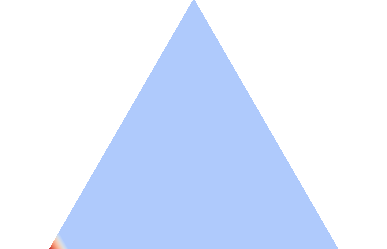
\includegraphics[width=0.3\textwidth]{figures/MNIST_cool/MNIST_3Classes_in_dist_coolwarm_0.png}}
        \subfloat{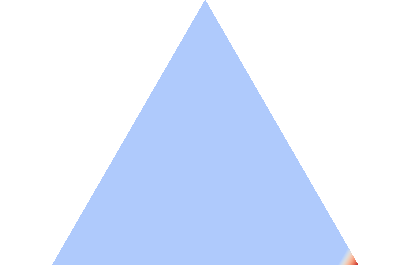
\includegraphics[width=0.3\textwidth]{figures/MNIST_cool/MNIST_3Classes_in_dist_coolwarm_1.png}}
        \subfloat{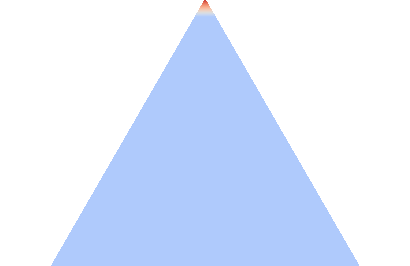
\includegraphics[width=0.3\textwidth]{figures/MNIST_cool/MNIST_3Classes_in_dist_coolwarm_2.png}}
    }

    \vspace{-1em}

    \subfloat[Out-of-distribution predictions]{
        \subfloat{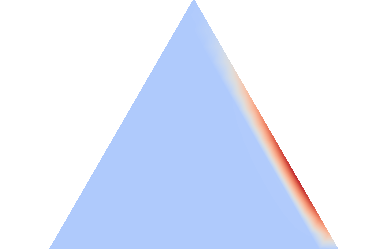
\includegraphics[width=0.3\textwidth]{figures/MNIST_cool/MNIST_3Classes_out_dist_coolwarm_0.png}}
        \subfloat{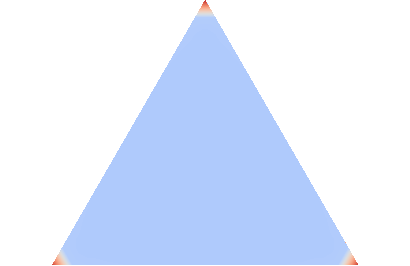
\includegraphics[width=0.3\textwidth]{figures/MNIST_cool/MNIST_3Classes_out_dist_coolwarm_1.png}}
        \subfloat{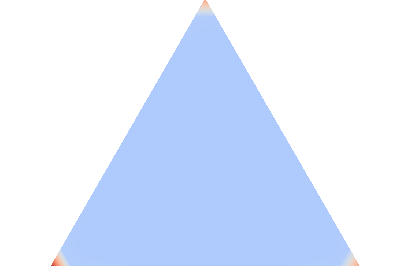
\includegraphics[width=0.3\textwidth]{figures/MNIST_cool/MNIST_3Classes_out_dist_coolwarm_2.png}}
    }

    \caption{\textbf{Top:} In-distribution pdfs. All probability mass is concentrated in the corner of the respective correct class. \textbf{Bottom:} Out-of-distribution pdfs. The probability mass is distributed more equally since the networks' uncertainty about is higher.}
    \label{fig:MNIST_ID_OOD}
\end{figure}\


\begin{table*}[h!]
	\scriptsize
    \centering
    \begin{tabular}{l  l || c c  c | c  c  c}
	     \toprule
         & & \multicolumn{3}{c}{\textbf{Diag Sampling}} &  \multicolumn{3}{c}{\textbf{Laplace Bridge (mean)}}\\
         \textbf{Train} & \textbf{Test} & \textbf{MMC} & \textbf{AUROC} & \textbf{Time} & \textbf{MMC} & \textbf{AUROC} &  \textbf{Time}\\
         \midrule
         MNIST & MNIST & 0.932 $\pm$ 0.007 & - & 6.6 & \textbf{0.987} $\pm$ 0.001 & - & \textbf{0.016} \\
         MNIST & FMNIST & 0.407 $\pm$ 0.010 & 0.989 $\pm$ 0.002 & 6.6 & \textbf{0.377} $\pm$ 0.019 & \textbf{0.994} $\pm$ 0.002 &  \textbf{0.016}\\
         MNIST & notMNIST & \textbf{0.535} $\pm$ 0.018 & 0.958 $\pm$ 0.006 & 12.3 & 0.630 $\pm$ 0.018 & \textbf{0.962} $\pm$ 0.007 &  \textbf{0.029}\\
         MNIST & KMNIST & \textbf{0.500} $\pm$ 0.014 & 0.974 $\pm$ 0.005 & 6.6 & 0.630 $\pm$ 0.018 & \textbf{0.975} $\pm$ 0.004 & \textbf{0.016} \\
         \midrule
         CIFAR-10 & CIFAR-10 & 0.949 $\pm$ 0.001 & - & 6.6 & \textbf{0.969} $\pm$ 0.002 & - & \textbf{0.017} \\
         CIFAR-10 & CIFAR-100 & \textbf{0.724} $\pm$ 0.002 & \textbf{0.884} $\pm$ 0.004 & 6.6 & 0.774 $\pm$ 0.003 & 0.858 $\pm$ 0.004 & \textbf{0.016} \\
         CIFAR-10 & SVHN & \textbf{0.659} $\pm$ 0.028 & \textbf{0.931} $\pm$ 0.007 & 17.0 & 0.704 $\pm$ 0.036 & 0.923 $\pm$ 0.008 & \textbf{0.041} \\
         \midrule
         SVHN & SVHN & 0.986 $\pm$ 0.000 & - & 17.1 & \textbf{0.991} $\pm$ 0.000 & - & \textbf{0.040} \\
         SVHN & CIFAR-10 & 0.537 $\pm$ 0.012 & 0.995 $\pm$ 0.000 & 6.61 & \textbf{0.392} $\pm$ 0.016 & \textbf{0.996} $\pm$ 0.000 & \textbf{0.169} \\
         SVHN & CIFAR-100 & 0.543 $\pm$ 0.009 & 0.994 $\pm$ 0.000 & 6.61 & \textbf{0.400} $\pm$ 0.013 & \textbf{0.996} $\pm$ 0.000 & \textbf{0.016} \\
         \midrule
         CIFAR-100 & CIFAR-100 & \textbf{0.527}s $\pm$ 0.004 & - & 6.68 & 0.263 $\pm$ 0.003 & - & \textbf{0.017} \\
         CIFAR-100 & CIFAR-10 & 0.276 $\pm$ 0.004 & \textbf{0.707} $\pm$ 0.004 & 6.67 & \textbf{0.068} $\pm$ 0.003 & 0.703 $\pm$ 0.003 & \textbf{0.018} \\
         CIFAR-100 & SVHN  & 0.348 $\pm$ 0.014 & 0.647 $\pm$ 0.011 & 17.2 & \textbf{0.074} $\pm$ 0.012 & \textbf{0.661} $\pm$ 0.013 & \textbf{0.040} \\
         \bottomrule
    \end{tabular}
    \caption{OOD detection results. Optimally, the MMC for OOD data is low and the AUROC is high. While there is arguable no clear winner when it comes to discriminating in- and out-distribution data w.r.t. both metrics, the Laplace Bridge is around 400 times faster on average. Time is measured in seconds. Five runs with different seeds per experiment were conducted. 1000 samples were drawn from the Gaussian over the outputs. The (F-, K-, not-)MNIST experiments were done with a Laplace approximation of the entire network while the others only used the last layer.}
    \label{tab:experiments_table}
\end{table*}

\vspace{-0.5em}
\section{OOD detection}
\label{subsec:exp2_numbers}

We compare the performance of the Laplace Bridge to the MC-integral on a standard OOD detection benchmark suite, to test whether the Laplace Bridge gives similar results to the MC sampling method and compare their computational overhead. Following prior literature, we use the standard mean-maximum-confidence (MMC) and area under the ROC-curve (AUROC) metrics \citep{HendycksOODBaseline}. For an in-distribution dataset, a higher MMC value is desirable while for the OOD dataset we want a lower MMC value (optimally, $1/K$ in $K$-class classification problems). For the AUROC metric, the higher the better, since it represents how good a method is for distinguishing in- and out-of-distribution datasets.


The test scenarios are as follows: (i) The same convolutional network as in \Cref{subsec:exp1_MNIST} is trained on the MNIST dataset. To approximate the posterior over the parameter of this network, a full (all-layer) Laplace approximation with the exact Hessian is employed. The OOD datasets for this case are FMNIST \cite{FMNIST2017}, notMNIST \cite{notMNIST2011}, and KMNIST \cite{KMNIST2018}. (ii) For larger datasets, i.e.~CIFAR-10 \cite{CIFAR2009}, SVHN \cite{SVHN2011}, and CIFAR-100 \cite{CIFAR2009}, we use a ResNet-18 network \citep{2015_ResNet}. Since this network is large, \eqref{eq:logit_dist} in conjunction with a full Laplace approximation is too costly. We, therefore, use a last-layer Laplace approximation to obtain the approximate diagonal Gaussian posterior. The OOD datasets for CIFAR-10, SVHN, and CIFAR-100 are SVHN and CIFAR100; CIFAR-10 and CIFAR-100; and SVHN and CIFAR-10, respectively. In all scenarios, the networks are well-trained with $99\%$ accuracy on MNIST, $95.4\%$ on CIFAR-10, $76.6\%$ on CIFAR-100 and $100\%$ on SVHN. For the sampling baseline, we use $1000$ posterior samples to compute the predictive distribution. We use the mean of the Dirichlet to obtain a comparable approximation to the MC-integral. Experiments comparing the Laplace Bridge to a KFAC approximation of the last layer and sampling from all weights of the network can be found in the appendix.

%accuracies: 95% cifar10, 100% SVHN, 59% cifar100
% \begin{table*}[h!]
% 	\scriptsize
%     \centering
%     \begin{tabular}{l  l || c c c c  c  c  c  c}
% 	     \toprule
%          & & \multicolumn{2}{c}{\textbf{MAP}} & \multicolumn{3}{c}{\textbf{Diag Sampling}} &  \multicolumn{3}{c}{\textbf{Dirichlet mode}}\\
%          \textbf{Train} & \textbf{Test} & \textbf{MMC} & \textbf{AUROC} & \textbf{MMC} & \textbf{AUROC} & \textbf{Time} & \textbf{MMC} & \textbf{AUROC} &  \textbf{Time}\\
%          \midrule
%          MNIST & MNIST & \textbf{0.989} $\pm$ 0.001 & - & 0.932 $\pm$ 0.007 & - & 6.6 & 0.987 $\pm$ 0.001 & - & \textbf{0.016} \\
%          MNIST & FMNIST & 0.538 $\pm$ 0.022 & 0.990 $\pm$ 0.001 & 0.407 $\pm$ 0.010 & 0.989 $\pm$ 0.002 & 6.6 & \textbf{0.377} $\pm$ 0.019 & \textbf{0.994} $\pm$ 0.002 &  \textbf{0.016}\\
%          MNIST & notMNIST & 0.706 $\pm$ 0.014 & 0.954 $\pm$ 0.007 & \textbf{0.535} $\pm$ 0.018 & 0.958 $\pm$ 0.006 & 12.3 & 0.630 $\pm$ 0.018 & \textbf{0.962} $\pm$ 0.007 &  \textbf{0.029}\\
%          MNIST & KMNIST & 0.684 $\pm$ 0.015 & 0.974 $\pm$ 0.005 & \textbf{0.500} $\pm$ 0.014 & 0.974 $\pm$ 0.005 & 6.6 & 0.630 $\pm$ 0.018 & \textbf{0.975} $\pm$ 0.004 & \textbf{0.016} \\
%          \midrule
%          CIFAR-10 & CIFAR-10 & \textbf{0.978} $\pm$ 0.001 & - & 0.949 $\pm$ 0.001 & - & 6.6 & 0.969 $\pm$ 0.002 & - & \textbf{0.017} \\
%          CIFAR-10 & CIFAR-100 & 0.828 $\pm$ 0.001 & 0.872 $\pm$ 0.004 & \textbf{0.724} $\pm$ 0.002 & \textbf{0.884} $\pm$ 0.004 & 6.6 & 0.774 $\pm$ 0.003 & 0.858 $\pm$ 0.004 & \textbf{0.016} \\
%          CIFAR-10 & SVHN & 0.777 $\pm$ 0.030 & 0.925 $\pm$ 0.008 & \textbf{0.659} $\pm$ 0.028 & \textbf{0.931} $\pm$ 0.007 & 17.0 & 0.704 $\pm$ 0.036 & 0.923 $\pm$ 0.008 & \textbf{0.041} \\
%          \midrule
%          SVHN & SVHN & \textbf{0.999} $\pm$ 0.000 & - & 0.986 $\pm$ 0.000 & - & 17.1 & 0.991 $\pm$ 0.000 & - & \textbf{0.040} \\
%          SVHN & CIFAR-10 & 0.616 $\pm$ 0.013 & \textbf{0.996} $\pm$ 0.000 & 0.537 $\pm$ 0.012 & 0.995 $\pm$ 0.000 & 6.61 & \textbf{0.392} $\pm$ 0.016 & \textbf{0.996} $\pm$ 0.000 & \textbf{0.169} \\
%          SVHN & CIFAR-100 & 0.621 $\pm$ 0.010 & \textbf{0.996} $\pm$ 0.000 & 0.543 $\pm$ 0.009 & 0.994 $\pm$ 0.000 & 6.61 & \textbf{0.400} $\pm$ 0.013 & \textbf{0.996} $\pm$ 0.000 & \textbf{0.016} \\
%          \midrule
%          CIFAR-100 & CIFAR-100 & \textbf{0.564} $\pm$ 0.018 & - & 0.527 $\pm$ 0.004 & - & 6.68 & 0.263 $\pm$ 0.003 & - & \textbf{0.017} \\
%          CIFAR-100 & CIFAR-10 & 0.298 $\pm$ 0.004 & 0.706 $\pm$ 0.003 & 0.276 $\pm$ 0.004 & \textbf{0.707} $\pm$ 0.004 & 6.67 & \textbf{0.068} $\pm$ 0.003 & 0.703 $\pm$ 0.003 & \textbf{0.018} \\
%          CIFAR-100 & SVHN & 0.372 $\pm$ 0.015 & 0.649 $\pm$ 0.012 & 0.348 $\pm$ 0.014 & 0.647 $\pm$ 0.011 & 17.2 & \textbf{0.074} $\pm$ 0.012 & \textbf{0.661} $\pm$ 0.013 & \textbf{0.040} \\
%          \bottomrule
%     \end{tabular}
%     \caption{Out-of-distribution detection results. A network has been trained on the data set in the \textbf{train} column and is tested on the \textbf{test} column. Optimally, the MMC for out of distribution data is low and the AUROC is high. There is no clear winner when it comes to discriminating in and OOD w.r.t. both metrics. However, the Laplace Bridge is around 400 times faster on average. Time is measured in seconds. Five runs with different seeds per experiment were conducted.}
%     \label{tab:experiments_table}
% \end{table*}


The results are presented in Table \ref{tab:experiments_table}. The Laplace Bridge is competitive to the baseline in terms of the MMC and AUROC metrics. In the case of MNIST and SVHN the Bridge is better than the MC-integral w.r.t. the AUROC metric. Moreover, the Laplace Bridge is also better than the sampling baseline in terms of the MMC metric in the SVHN and CIFAR-100 datasets. The key observation, however, is that the Bridge is on average around $400$ times faster than the sampling baseline, while returning at least competitive, if not even improved fidelity.


\section{Time comparison}
\label{subsec:exp3_time}


We compare the computational cost of the density-estimated $p_\text{sample}$ distribution via sampling and the Dirichlet distribution obtained from the Laplace Bridge $p_\text{LB}$ for approximating the true distribution $p_\text{true}$ over softmax-Gaussian samples\footnote{I.e. samples are obtained by first sampling from a Gaussian and transforming it via the softmax function.}. Different amounts of samples are drawn from the Gaussian, the softmax is applied and the KL divergence between the histogram of the samples with the true distribution is computed. We use KL-divergences $D_\text{KL}(p_\text{true} \Vert p_\text{sample})$ and $D_\text{KL}(p_\text{true} \Vert p_\text{LB})$, respectively, to measure similarity between the approximations and ground truth while the number of samples for $p_\text{sample}$ is increased on a logarithmic scale. The true distribution $p_\text{true}$ is constructed via Monte Carlo with $100$k samples. The experiment is conducted for three different Gaussian distributions over $\R^3$. Since the softmax applied to a Gaussian does not have a closed-form analytic solution, the calculation of the approximation error is not possible and an empirical evaluation via sampling is the best option. The fact that there is no analytic solution is part of the justification for using the Laplace Bridge in the first place.

\Cref{fig:KL_div_samples} suggests that the number of samples required such that the distribution $p_\text{sample}$ is approximating the true distribution $p_\text{true}$ as good as the Dirichlet distribution obtained via the Laplace Bridge is large, i.e. somewhere between $500$ and $10000$. This translates to a wall-clock time advantage of at least a factor of $100$ before sampling becomes competitive in quality with the Laplace Bridge.


\setlength{\figwidth}{0.8\textwidth}
\setlength{\figheight}{0.3\textheight}

\begin{figure}[h!]
    \scriptsize

    \hspace{2em}
    % This file was created by tikzplotlib v0.8.2.
\begin{tikzpicture}

\definecolor{color0}{rgb}{1,0.647058823529412,0}
\definecolor{color1}{rgb}{0.501960784313725,0,0.501960784313725}
\definecolor{color2}{rgb}{0.647058823529412,0.164705882352941,0.164705882352941}

\begin{axis}[
height=\figheight,
legend cell align={left},
legend pos=north east,
legend style={draw=white!80.0!black},
log basis x={10},
tick pos=both,
width=\figwidth,
x grid style={white!69.01960784313725!black},
xlabel={Number of Samples},
xmin=0.562341325190349, xmax=177827.941003892,
xmode=log,
xtick align=inside,
xtick pos=left,
xtick style={color=black},
xtick={0.01,0.1,1,10,100,1000,10000,100000,1000000,10000000},
xticklabels={\(\displaystyle {10^{-2}}\),\(\displaystyle {10^{-1}}\),\(\displaystyle {10^{0}}\),\(\displaystyle {10^{1}}\),\(\displaystyle {10^{2}}\),\(\displaystyle {10^{3}}\),\(\displaystyle {10^{4}}\),\(\displaystyle {10^{5}}\),\(\displaystyle {10^{6}}\),\(\displaystyle {10^{7}}\)},
y grid style={white!69.01960784313725!black},
ylabel={KL Divergence},
ymin=-2.15254313802994, ymax=45.2034058986287,
ytick align=inside,
ytick pos=left,
ytick style={color=black}
]
\path [draw=blue, very thick]
(axis cs:1,41.3722702823216)
--(axis cs:1,41.3722702823216);

\path [draw=blue, very thick]
(axis cs:5,38.8233030125781)
--(axis cs:5,39.0591480735509);

\path [draw=blue, very thick]
(axis cs:10,35.267481412799)
--(axis cs:10,36.9329452871732);

\path [draw=blue, very thick]
(axis cs:25,29.1319009116699)
--(axis cs:25,31.6236385020272);

\path [draw=blue, very thick]
(axis cs:50,21.304965177582)
--(axis cs:50,24.1591645143799);

\path [draw=blue, very thick]
(axis cs:75,16.6383771143455)
--(axis cs:75,17.6845412745849);

\path [draw=blue, very thick]
(axis cs:100,12.4928905678809)
--(axis cs:100,15.2919407971065);

\path [draw=blue, very thick]
(axis cs:250,5.67699779647913)
--(axis cs:250,6.30875076113871);

\path [draw=blue, very thick]
(axis cs:500,2.26833776833095)
--(axis cs:500,3.34790920534813);

\path [draw=blue, very thick]
(axis cs:750,1.58530484653685)
--(axis cs:750,2.09189915175033);

\path [draw=blue, very thick]
(axis cs:1000,1.09512113945861)
--(axis cs:1000,1.25898831175564);

\path [draw=blue, very thick]
(axis cs:2500,0.370662637687383)
--(axis cs:2500,0.499793601288633);

\path [draw=blue, very thick]
(axis cs:5000,0.231181061336582)
--(axis cs:5000,0.279238460248237);

\path [draw=blue, very thick]
(axis cs:7500,0.139836470091655)
--(axis cs:7500,0.164872822137191);

\path [draw=blue, very thick]
(axis cs:10000,0.084337512184737)
--(axis cs:10000,0.106616449204758);

\path [draw=blue, very thick]
(axis cs:25000,0.0358771476288979)
--(axis cs:25000,0.0424959131298682);

\path [draw=blue, very thick]
(axis cs:50000,0.0178279890062826)
--(axis cs:50000,0.0233430690525671);

\path [draw=blue, very thick]
(axis cs:75000,0.0120503163100018)
--(axis cs:75000,0.0172004825023739);

\path [draw=blue, very thick]
(axis cs:100000,0.0100070768674574)
--(axis cs:100000,0.0125073077088456);

\path [draw=color0, very thick]
(axis cs:1,43.0508627605988)
--(axis cs:1,43.0508627605988);

\path [draw=color0, very thick]
(axis cs:5,32.9164696418971)
--(axis cs:5,38.558368232746);

\path [draw=color0, very thick]
(axis cs:10,29.3357170610752)
--(axis cs:10,34.3925399576855);

\path [draw=color0, very thick]
(axis cs:25,18.1543726761943)
--(axis cs:25,23.7064784539694);

\path [draw=color0, very thick]
(axis cs:50,14.1139008509748)
--(axis cs:50,16.7560266158067);

\path [draw=color0, very thick]
(axis cs:75,10.7357449683897)
--(axis cs:75,12.5322548346119);

\path [draw=color0, very thick]
(axis cs:100,9.58497879599963)
--(axis cs:100,10.3003525490437);

\path [draw=color0, very thick]
(axis cs:250,5.67213818176429)
--(axis cs:250,6.88573036979303);

\path [draw=color0, very thick]
(axis cs:500,3.8340459965373)
--(axis cs:500,4.32652116301364);

\path [draw=color0, very thick]
(axis cs:750,2.54909605301928)
--(axis cs:750,3.3883456915885);

\path [draw=color0, very thick]
(axis cs:1000,2.22816978651728)
--(axis cs:1000,2.47026168174398);

\path [draw=color0, very thick]
(axis cs:2500,1.07000462007234)
--(axis cs:2500,1.28476288361077);

\path [draw=color0, very thick]
(axis cs:5000,0.495096355743176)
--(axis cs:5000,0.554422544733448);

\path [draw=color0, very thick]
(axis cs:7500,0.328971266525497)
--(axis cs:7500,0.395221842442994);

\path [draw=color0, very thick]
(axis cs:10000,0.2305577201191)
--(axis cs:10000,0.294069003433279);

\path [draw=color0, very thick]
(axis cs:25000,0.0937054047200392)
--(axis cs:25000,0.100406236295138);

\path [draw=color0, very thick]
(axis cs:50000,0.0370128142188019)
--(axis cs:50000,0.0451002552278923);

\path [draw=color0, very thick]
(axis cs:75000,0.0228132706100869)
--(axis cs:75000,0.024795862739992);

\path [draw=color0, very thick]
(axis cs:100000,0.0153163404700447)
--(axis cs:100000,0.0202666204467783);

\path [draw=green!50.19607843137255!black, very thick]
(axis cs:1,42.93349488395)
--(axis cs:1,42.93349488395);

\path [draw=green!50.19607843137255!black, very thick]
(axis cs:5,37.0750021059541)
--(axis cs:5,38.4748201996713);

\path [draw=green!50.19607843137255!black, very thick]
(axis cs:10,34.2358799246236)
--(axis cs:10,36.0148853930903);

\path [draw=green!50.19607843137255!black, very thick]
(axis cs:25,24.3716676967715)
--(axis cs:25,26.5337565446618);

\path [draw=green!50.19607843137255!black, very thick]
(axis cs:50,18.6676069935368)
--(axis cs:50,19.6412544376819);

\path [draw=green!50.19607843137255!black, very thick]
(axis cs:75,10.6572615218368)
--(axis cs:75,14.6737306768942);

\path [draw=green!50.19607843137255!black, very thick]
(axis cs:100,7.66062640020415)
--(axis cs:100,9.54815976735437);

\path [draw=green!50.19607843137255!black, very thick]
(axis cs:250,2.98932209269546)
--(axis cs:250,4.25632264994355);

\path [draw=green!50.19607843137255!black, very thick]
(axis cs:500,0.843772314988995)
--(axis cs:500,1.2663946119617);

\path [draw=green!50.19607843137255!black, very thick]
(axis cs:750,0.577993218332512)
--(axis cs:750,0.875373247983097);

\path [draw=green!50.19607843137255!black, very thick]
(axis cs:1000,0.301307271541921)
--(axis cs:1000,0.57281390854175);

\path [draw=green!50.19607843137255!black, very thick]
(axis cs:2500,0.175692102095908)
--(axis cs:2500,0.245401076384385);

\path [draw=green!50.19607843137255!black, very thick]
(axis cs:5000,0.0814301408001577)
--(axis cs:5000,0.140221637810137);

\path [draw=green!50.19607843137255!black, very thick]
(axis cs:7500,0.0512626639403834)
--(axis cs:7500,0.065374162994615);

\path [draw=green!50.19607843137255!black, very thick]
(axis cs:10000,0.0406086501456689)
--(axis cs:10000,0.062530297040719);

\path [draw=green!50.19607843137255!black, very thick]
(axis cs:25000,0.0185861002926118)
--(axis cs:25000,0.0263330151450657);

\path [draw=green!50.19607843137255!black, very thick]
(axis cs:50000,0.00797514769943751)
--(axis cs:50000,0.0100283052176679);

\path [draw=green!50.19607843137255!black, very thick]
(axis cs:75000,0.0069841735211465)
--(axis cs:75000,0.00894536725832454);

\path [draw=green!50.19607843137255!black, very thick]
(axis cs:100000,0.00470287418533706)
--(axis cs:100000,0.00678371869152951);

\path [draw=blue, draw opacity=0.7, semithick]
(axis cs:25000,0)
--(axis cs:25000,7);

\path [draw=color0, draw opacity=0.7, semithick]
(axis cs:5000,0)
--(axis cs:5000,7);

\path [draw=green!50.19607843137255!black, draw opacity=0.7, semithick]
(axis cs:500,0)
--(axis cs:500,7);

\addplot [semithick, red, mark=*, mark size=3, mark options={solid}, only marks]
table {%
1 0.0881709970024221
};
\addlegendentry{Laplace Bridge}
\addplot [semithick, color1, mark=*, mark size=3, mark options={solid}, only marks, forget plot]
table {%
1 0.707545925704699
};
\addplot [semithick, color2, mark=*, mark size=3, mark options={solid}, only marks, forget plot]
table {%
1 1.7655057604949
};
\addplot [very thick, red, opacity=0.5, dash pattern=on 1pt off 3pt on 3pt off 3pt, forget plot]
table {%
1 0.0881709970024221
25000 0.0881709970024221
};
\addplot [very thick, color1, opacity=0.5, dash pattern=on 1pt off 3pt on 3pt off 3pt, forget plot]
table {%
1 0.707545925704699
5000 0.707545925704699
};
\addplot [very thick, color2, opacity=0.5, dash pattern=on 1pt off 3pt on 3pt off 3pt, forget plot]
table {%
1 1.7655057604949
500 1.7655057604949
};
\addplot [very thick, blue]
table {%
1 41.3722702823216
5 38.9412255430645
10 36.1002133499861
25 30.3777697068485
50 22.7320648459809
75 17.1614591944652
100 13.8924156824937
250 5.99287427880892
500 2.80812348683954
750 1.83860199914359
1000 1.17705472560713
2500 0.435228119488008
5000 0.255209760792409
7500 0.152354646114423
10000 0.0954769806947477
25000 0.039186530379383
50000 0.0205855290294249
75000 0.0146253994061879
100000 0.0112571922881515
};
\addlegendentry{Monte Carlo}
\addplot [very thick, color0]
table {%
1 43.0508627605988
5 35.7374189373216
10 31.8641285093803
25 20.9304255650818
50 15.4349637333907
75 11.6339999015008
100 9.94266567252169
250 6.27893427577866
500 4.08028357977547
750 2.96872087230389
1000 2.34921573413063
2500 1.17738375184156
5000 0.524759450238312
7500 0.362096554484246
10000 0.262313361776189
25000 0.0970558205075884
50000 0.0410565347233471
75000 0.0238045666750394
100000 0.0177914804584115
};
\addlegendentry{Monte Carlo}
\addplot [very thick, green!50.19607843137255!black]
table {%
1 42.93349488395
5 37.7749111528127
10 35.1253826588569
25 25.4527121207166
50 19.1544307156093
75 12.6654960993655
100 8.60439308377926
250 3.6228223713195
500 1.05508346347535
750 0.726683233157805
1000 0.437060590041835
2500 0.210546589240146
5000 0.110825889305147
7500 0.0583184134674992
10000 0.0515694735931939
25000 0.0224595577188388
50000 0.00900172645855269
75000 0.00796477038973552
100000 0.00574329643843329
};
\addlegendentry{Monte Carlo}
\end{axis}

\end{tikzpicture}%

    \vspace{2em}

    \hspace{2em}
    % This file was created by tikzplotlib v0.8.2.
\begin{tikzpicture}

\definecolor{color0}{rgb}{1,0.647058823529412,0}
\definecolor{color1}{rgb}{0.501960784313725,0,0.501960784313725}
\definecolor{color2}{rgb}{0.647058823529412,0.164705882352941,0.164705882352941}

\begin{axis}[
height=\figheight,
legend cell align={left},
legend pos=north east,
legend style={draw=white!80.0!black},
log basis x={10},
tick pos=both,
width=\figwidth,
x grid style={white!69.01960784313725!black},
xlabel={Time in s},
xmin=0.000219164109011124, xmax=1.57720836573318,
xmode=log,
xtick align=inside,
xtick pos=left,
xtick style={color=black},
xtick={1e-05,0.0001,0.001,0.01,0.1,1,10,100},
xticklabels={\(\displaystyle {10^{-5}}\),\(\displaystyle {10^{-4}}\),\(\displaystyle {10^{-3}}\),\(\displaystyle {10^{-2}}\),\(\displaystyle {10^{-1}}\),\(\displaystyle {10^{0}}\),\(\displaystyle {10^{1}}\),\(\displaystyle {10^{2}}\)},
y grid style={white!69.01960784313725!black},
ylabel={KL Divergence},
ymin=-2.15254313802994, ymax=45.2034058986287,
ytick align=inside,
ytick pos=left,
ytick style={color=black}
]
\path [draw=blue, very thick]
(axis cs:0.000347699400003876,41.3722702823216)
--(axis cs:0.000347699400003876,41.3722702823216);

\path [draw=blue, very thick]
(axis cs:0.00034134719999912,38.8233030125781)
--(axis cs:0.00034134719999912,39.0591480735509);

\path [draw=blue, very thick]
(axis cs:0.000392544400003203,35.267481412799)
--(axis cs:0.000392544400003203,36.9329452871732);

\path [draw=blue, very thick]
(axis cs:0.000552010000004088,29.1319009116699)
--(axis cs:0.000552010000004088,31.6236385020272);

\path [draw=blue, very thick]
(axis cs:0.000753213599996627,21.304965177582)
--(axis cs:0.000753213599996627,24.1591645143799);

\path [draw=blue, very thick]
(axis cs:0.000953311199998552,16.6383771143455)
--(axis cs:0.000953311199998552,17.6845412745849);

\path [draw=blue, very thick]
(axis cs:0.00117008360000312,12.4928905678809)
--(axis cs:0.00117008360000312,15.2919407971065);

\path [draw=blue, very thick]
(axis cs:0.002496716200001,5.67699779647913)
--(axis cs:0.002496716200001,6.30875076113871);

\path [draw=blue, very thick]
(axis cs:0.00535201260000235,2.26833776833095)
--(axis cs:0.00535201260000235,3.34790920534813);

\path [draw=blue, very thick]
(axis cs:0.00664694479999781,1.58530484653685)
--(axis cs:0.00664694479999781,2.09189915175033);

\path [draw=blue, very thick]
(axis cs:0.00847694239999726,1.09512113945861)
--(axis cs:0.00847694239999726,1.25898831175564);

\path [draw=blue, very thick]
(axis cs:0.0210023156000034,0.370662637687383)
--(axis cs:0.0210023156000034,0.499793601288633);

\path [draw=blue, very thick]
(axis cs:0.0419743216000043,0.231181061336582)
--(axis cs:0.0419743216000043,0.279238460248237);

\path [draw=blue, very thick]
(axis cs:0.124657420200003,0.139836470091655)
--(axis cs:0.124657420200003,0.164872822137191);

\path [draw=blue, very thick]
(axis cs:0.171043202599995,0.084337512184737)
--(axis cs:0.171043202599995,0.106616449204758);

\path [draw=blue, very thick]
(axis cs:0.414873980599999,0.0358771476288979)
--(axis cs:0.414873980599999,0.0424959131298682);

\path [draw=blue, very thick]
(axis cs:0.622958016799997,0.0178279890062826)
--(axis cs:0.622958016799997,0.0233430690525671);

\path [draw=blue, very thick]
(axis cs:0.843133083400001,0.0120503163100018)
--(axis cs:0.843133083400001,0.0172004825023739);

\path [draw=blue, very thick]
(axis cs:1.0460591128,0.0100070768674574)
--(axis cs:1.0460591128,0.0125073077088456);

\path [draw=color0, very thick]
(axis cs:0.000328165600001284,43.0508627605988)
--(axis cs:0.000328165600001284,43.0508627605988);

\path [draw=color0, very thick]
(axis cs:0.000356451800006141,32.9164696418971)
--(axis cs:0.000356451800006141,38.558368232746);

\path [draw=color0, very thick]
(axis cs:0.000429854600000112,29.3357170610752)
--(axis cs:0.000429854600000112,34.3925399576855);

\path [draw=color0, very thick]
(axis cs:0.000522573999997178,18.1543726761943)
--(axis cs:0.000522573999997178,23.7064784539694);

\path [draw=color0, very thick]
(axis cs:0.000754682999999545,14.1139008509748)
--(axis cs:0.000754682999999545,16.7560266158067);

\path [draw=color0, very thick]
(axis cs:0.000940918799997803,10.7357449683897)
--(axis cs:0.000940918799997803,12.5322548346119);

\path [draw=color0, very thick]
(axis cs:0.00114930980000025,9.58497879599963)
--(axis cs:0.00114930980000025,10.3003525490437);

\path [draw=color0, very thick]
(axis cs:0.00242379079999608,5.67213818176429)
--(axis cs:0.00242379079999608,6.88573036979303);

\path [draw=color0, very thick]
(axis cs:0.00461063900000624,3.8340459965373)
--(axis cs:0.00461063900000624,4.32652116301364);

\path [draw=color0, very thick]
(axis cs:0.00645582219999738,2.54909605301928)
--(axis cs:0.00645582219999738,3.3883456915885);

\path [draw=color0, very thick]
(axis cs:0.008581556799993,2.22816978651728)
--(axis cs:0.008581556799993,2.47026168174398);

\path [draw=color0, very thick]
(axis cs:0.0208941222000035,1.07000462007234)
--(axis cs:0.0208941222000035,1.28476288361077);

\path [draw=color0, very thick]
(axis cs:0.041313977599998,0.495096355743176)
--(axis cs:0.041313977599998,0.554422544733448);

\path [draw=color0, very thick]
(axis cs:0.135163926200001,0.328971266525497)
--(axis cs:0.135163926200001,0.395221842442994);

\path [draw=color0, very thick]
(axis cs:0.170700134799996,0.2305577201191)
--(axis cs:0.170700134799996,0.294069003433279);

\path [draw=color0, very thick]
(axis cs:0.410511967799992,0.0937054047200392)
--(axis cs:0.410511967799992,0.100406236295138);

\path [draw=color0, very thick]
(axis cs:0.616218821999996,0.0370128142188019)
--(axis cs:0.616218821999996,0.0451002552278923);

\path [draw=color0, very thick]
(axis cs:0.827729683600002,0.0228132706100869)
--(axis cs:0.827729683600002,0.024795862739992);

\path [draw=color0, very thick]
(axis cs:1.0407518114,0.0153163404700447)
--(axis cs:1.0407518114,0.0202666204467783);

\path [draw=green!50.19607843137255!black, very thick]
(axis cs:0.000351066999994032,42.93349488395)
--(axis cs:0.000351066999994032,42.93349488395);

\path [draw=green!50.19607843137255!black, very thick]
(axis cs:0.000371052200007682,37.0750021059541)
--(axis cs:0.000371052200007682,38.4748201996713);

\path [draw=green!50.19607843137255!black, very thick]
(axis cs:0.000424890399990829,34.2358799246236)
--(axis cs:0.000424890399990829,36.0148853930903);

\path [draw=green!50.19607843137255!black, very thick]
(axis cs:0.000527281800000878,24.3716676967715)
--(axis cs:0.000527281800000878,26.5337565446618);

\path [draw=green!50.19607843137255!black, very thick]
(axis cs:0.000747899799998208,18.6676069935368)
--(axis cs:0.000747899799998208,19.6412544376819);

\path [draw=green!50.19607843137255!black, very thick]
(axis cs:0.00145907819999707,10.6572615218368)
--(axis cs:0.00145907819999707,14.6737306768942);

\path [draw=green!50.19607843137255!black, very thick]
(axis cs:0.00118932279999768,7.66062640020415)
--(axis cs:0.00118932279999768,9.54815976735437);

\path [draw=green!50.19607843137255!black, very thick]
(axis cs:0.00242782120000271,2.98932209269546)
--(axis cs:0.00242782120000271,4.25632264994355);

\path [draw=green!50.19607843137255!black, very thick]
(axis cs:0.00457135460000728,0.843772314988995)
--(axis cs:0.00457135460000728,1.2663946119617);

\path [draw=green!50.19607843137255!black, very thick]
(axis cs:0.00679406500000397,0.577993218332512)
--(axis cs:0.00679406500000397,0.875373247983097);

\path [draw=green!50.19607843137255!black, very thick]
(axis cs:0.00846984139999591,0.301307271541921)
--(axis cs:0.00846984139999591,0.57281390854175);

\path [draw=green!50.19607843137255!black, very thick]
(axis cs:0.020912775400005,0.175692102095908)
--(axis cs:0.020912775400005,0.245401076384385);

\path [draw=green!50.19607843137255!black, very thick]
(axis cs:0.042248899600007,0.0814301408001577)
--(axis cs:0.042248899600007,0.140221637810137);

\path [draw=green!50.19607843137255!black, very thick]
(axis cs:0.127125916000007,0.0512626639403834)
--(axis cs:0.127125916000007,0.065374162994615);

\path [draw=green!50.19607843137255!black, very thick]
(axis cs:0.167992996799998,0.0406086501456689)
--(axis cs:0.167992996799998,0.062530297040719);

\path [draw=green!50.19607843137255!black, very thick]
(axis cs:0.407860939999999,0.0185861002926118)
--(axis cs:0.407860939999999,0.0263330151450657);

\path [draw=green!50.19607843137255!black, very thick]
(axis cs:0.617105053200001,0.00797514769943751)
--(axis cs:0.617105053200001,0.0100283052176679);

\path [draw=green!50.19607843137255!black, very thick]
(axis cs:0.830234605999996,0.0069841735211465)
--(axis cs:0.830234605999996,0.00894536725832454);

\path [draw=green!50.19607843137255!black, very thick]
(axis cs:1.0533324218,0.00470287418533706)
--(axis cs:1.0533324218,0.00678371869152951);

\path [draw=blue, draw opacity=0.7, semithick]
(axis cs:0.414873980599999,0)
--(axis cs:0.414873980599999,7);

\path [draw=color0, draw opacity=0.7, semithick]
(axis cs:0.041313977599998,0)
--(axis cs:0.041313977599998,7);

\path [draw=green!50.19607843137255!black, draw opacity=0.7, semithick]
(axis cs:0.00457135460000728,0)
--(axis cs:0.00457135460000728,7);

\addplot [semithick, red, mark=*, mark size=3, mark options={solid}, only marks]
table {%
0.000628673999999663 0.0881709970024221
};
\addlegendentry{Laplace Bridge}
\addplot [semithick, color1, mark=*, mark size=3, mark options={solid}, only marks, forget plot]
table {%
0.000856472999999802 0.707545925704699
};
\addplot [semithick, color2, mark=*, mark size=3, mark options={solid}, only marks, forget plot]
table {%
0.000598666999999331 1.7655057604949
};
\addplot [very thick, red, opacity=0.5, dash pattern=on 1pt off 3pt on 3pt off 3pt, forget plot]
table {%
0.000628673999999663 0.0881709970024221
0.414873980599999 0.0881709970024221
};
\addplot [very thick, color1, opacity=0.5, dash pattern=on 1pt off 3pt on 3pt off 3pt, forget plot]
table {%
0.000856472999999802 0.707545925704699
0.041313977599998 0.707545925704699
};
\addplot [very thick, color2, opacity=0.5, dash pattern=on 1pt off 3pt on 3pt off 3pt, forget plot]
table {%
0.000598666999999331 1.7655057604949
0.00457135460000728 1.7655057604949
};
\addplot [very thick, blue]
table {%
0.000347699400003876 41.3722702823216
0.00034134719999912 38.9412255430645
0.000392544400003203 36.1002133499861
0.000552010000004088 30.3777697068485
0.000753213599996627 22.7320648459809
0.000953311199998552 17.1614591944652
0.00117008360000312 13.8924156824937
0.002496716200001 5.99287427880892
0.00535201260000235 2.80812348683954
0.00664694479999781 1.83860199914359
0.00847694239999726 1.17705472560713
0.0210023156000034 0.435228119488008
0.0419743216000043 0.255209760792409
0.124657420200003 0.152354646114423
0.171043202599995 0.0954769806947477
0.414873980599999 0.039186530379383
0.622958016799997 0.0205855290294249
0.843133083400001 0.0146253994061879
1.0460591128 0.0112571922881515
};
\addlegendentry{Monte Carlo}
\addplot [very thick, color0]
table {%
0.000328165600001284 43.0508627605988
0.000356451800006141 35.7374189373216
0.000429854600000112 31.8641285093803
0.000522573999997178 20.9304255650818
0.000754682999999545 15.4349637333907
0.000940918799997803 11.6339999015008
0.00114930980000025 9.94266567252169
0.00242379079999608 6.27893427577866
0.00461063900000624 4.08028357977547
0.00645582219999738 2.96872087230389
0.008581556799993 2.34921573413063
0.0208941222000035 1.17738375184156
0.041313977599998 0.524759450238312
0.135163926200001 0.362096554484246
0.170700134799996 0.262313361776189
0.410511967799992 0.0970558205075884
0.616218821999996 0.0410565347233471
0.827729683600002 0.0238045666750394
1.0407518114 0.0177914804584115
};
\addlegendentry{Monte Carlo}
\addplot [very thick, green!50.19607843137255!black]
table {%
0.000351066999994032 42.93349488395
0.000371052200007682 37.7749111528127
0.000424890399990829 35.1253826588569
0.000527281800000878 25.4527121207166
0.000747899799998208 19.1544307156093
0.00145907819999707 12.6654960993655
0.00118932279999768 8.60439308377926
0.00242782120000271 3.6228223713195
0.00457135460000728 1.05508346347535
0.00679406500000397 0.726683233157805
0.00846984139999591 0.437060590041835
0.020912775400005 0.210546589240146
0.042248899600007 0.110825889305147
0.127125916000007 0.0583184134674992
0.167992996799998 0.0515694735931939
0.407860939999999 0.0224595577188388
0.617105053200001 0.00900172645855269
0.830234605999996 0.00796477038973552
1.0533324218 0.00574329643843329
};
\addlegendentry{Monte Carlo}
\end{axis}

\end{tikzpicture}%

	\centering
	\caption{KL-divergence plotted against the number of samples (top) and wall-clock time (bottom). Monte Carlo density estimation becomes as good as the Laplace Bridge after around $750$ to $10000$ samples and takes at least $100$ times longer. The three lines represent three different samples.}
	\label{fig:KL_div_samples}
\end{figure}


\section{Toy dataset}
\label{subsec:exp4_toy_dataset}

To understand the properties of the Laplace Bridge we visualize its predictions on a toy dataset. The dataset is generated by drawing from four different 2D Gaussians and the task is for a neural network to classify them. The network is a simple four-layer network with ReLU activations and 100 units per layer. A visualization is created by using different methods for calculating predictive uncertainty for all points on a two-dimensional grid. There are four methods to predict uncertainty that are independent of the Laplace Bridge: the MAP estimate, a diagonal approximation of the Hessian, a Kronecker-factorized approximation of the Hessian and the exact Hessian. Their respective predictive entropy can be found on the left column of Figure \ref{fig:toy_data}. This is compared to the MAP prediction of the Laplace Bridge, its predictive entropy, the variance of the MAP estimate of the Dirichlet and a MAP estimate that is weighted by it's respective variance. These can be found in the right column of Figure \ref{fig:toy_data}. The estimates in the left column get increasingly better since we include more information about the uncertainty. We conclude that the entropy and the variance of the Dirichlet are only marginally better than the original MAP estimate. Reweighing the estimate by the variance improves it slightly. However, the Laplace Bridge is not able to produce a similarly good estimate as a Kronecker-factorized or exact Hessian. 


\newgeometry{top=20mm, bottom=20mm}

\begin{figure}[htb]
	\centering
	\scriptsize
	
	\captionsetup[subfigure]{labelformat=empty}
	
	\subfloat{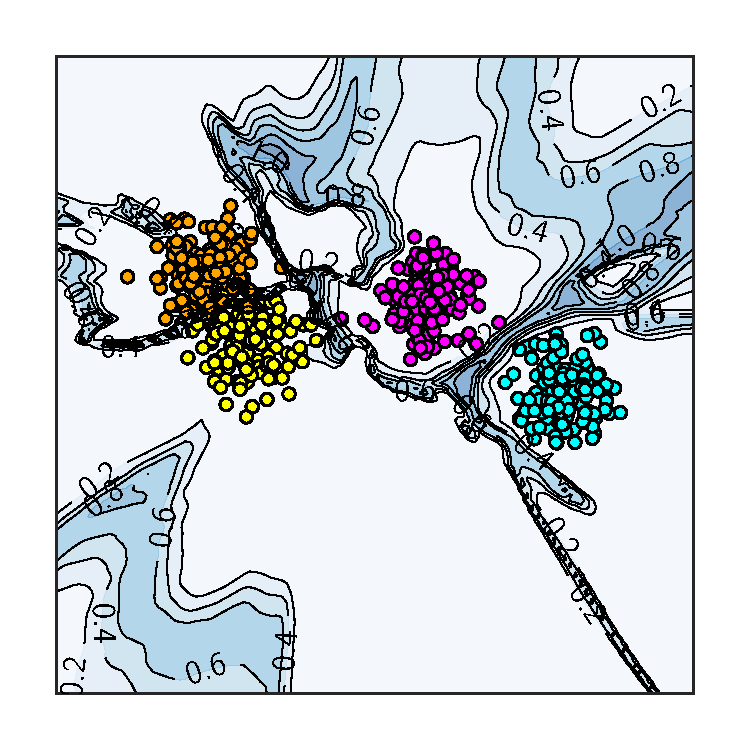
\includegraphics[width=0.4\textwidth]{figures/toy_data/ent_toy_2d_nn_multiclass_map.pdf}}
	\subfloat{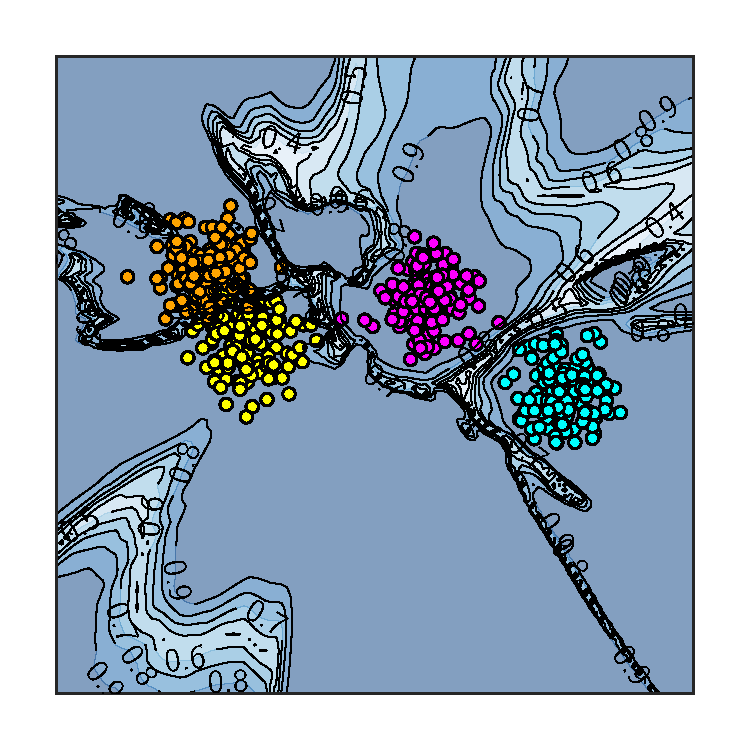
\includegraphics[width=0.4\textwidth]{figures/toy_data/ent_toy_2d_nn_multiclass_LPB_alpha_max.pdf}} \\ [-5ex]	
	\subfloat{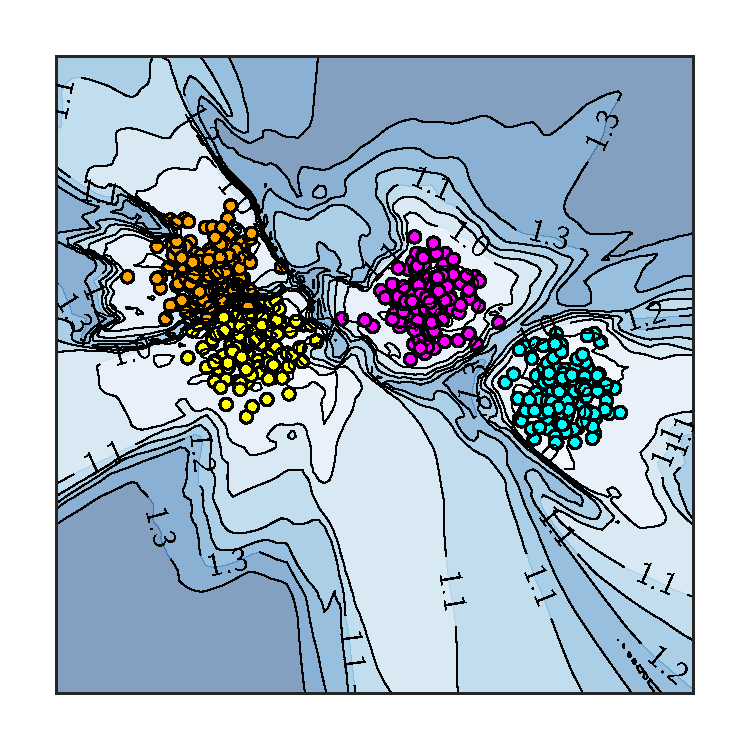
\includegraphics[width=0.4\textwidth]{figures/toy_data/ent_toy_2d_nn_multiclass_laplace_diag.pdf}}
	\subfloat{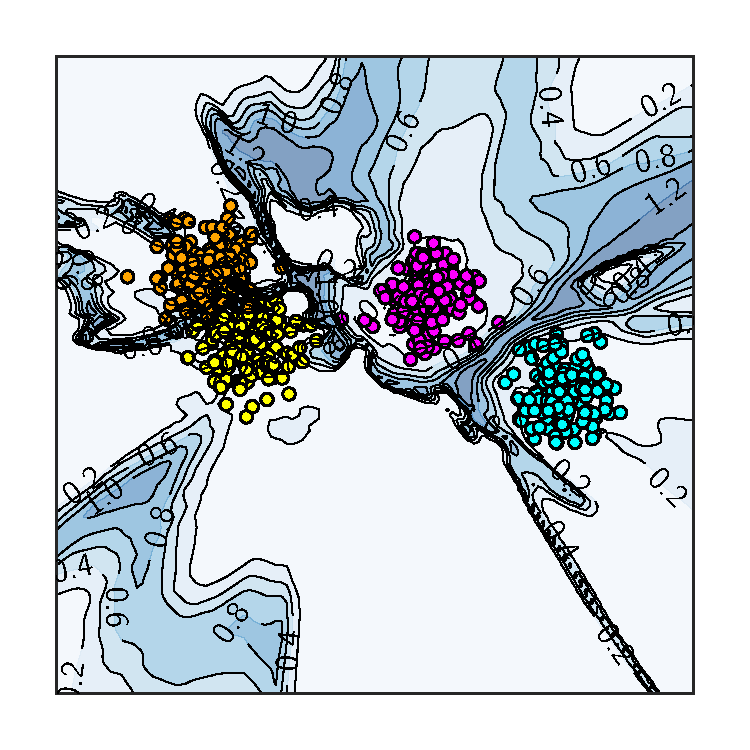
\includegraphics[width=0.4\textwidth]{figures/toy_data/ent_toy_2d_nn_multiclass_LPB_entropy_mode.pdf}} \\ [-5ex]
	\subfloat{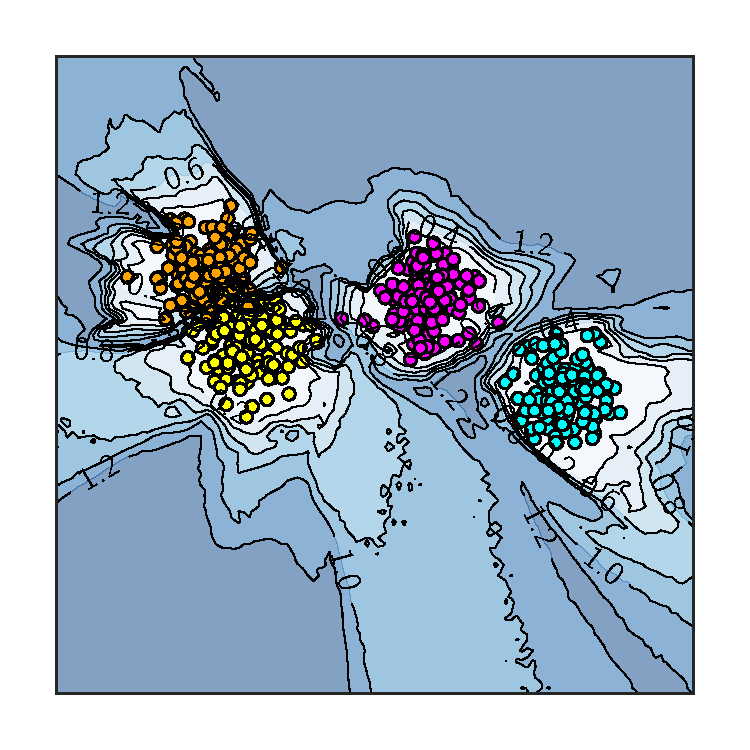
\includegraphics[width=0.4\textwidth]{figures/toy_data/ent_toy_2d_nn_multiclass_laplace_kf.pdf}}
	\subfloat{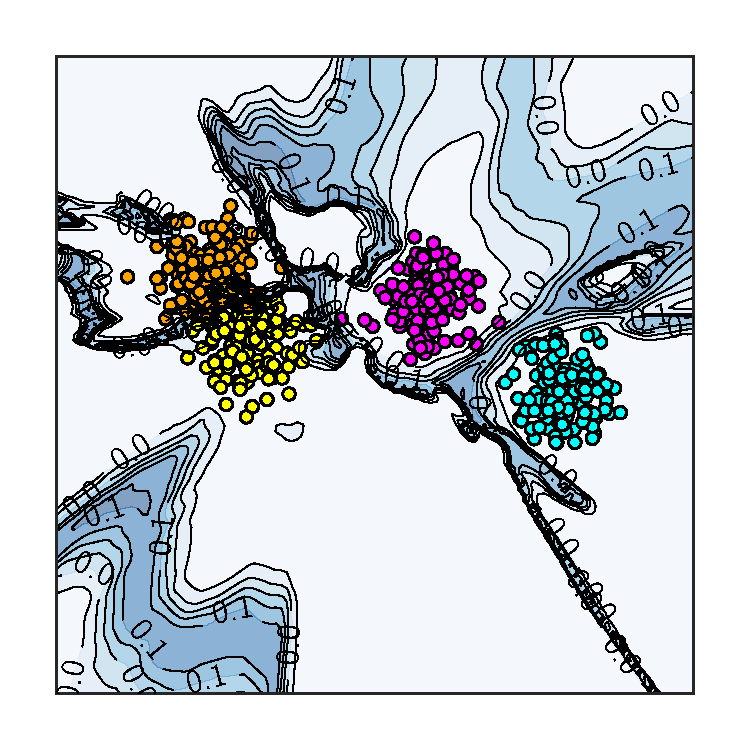
\includegraphics[width=0.4\textwidth]{figures/toy_data/ent_toy_2d_nn_multiclass_LPB_variance_norm_dir.pdf}} \\ [-5ex]	
	\subfloat{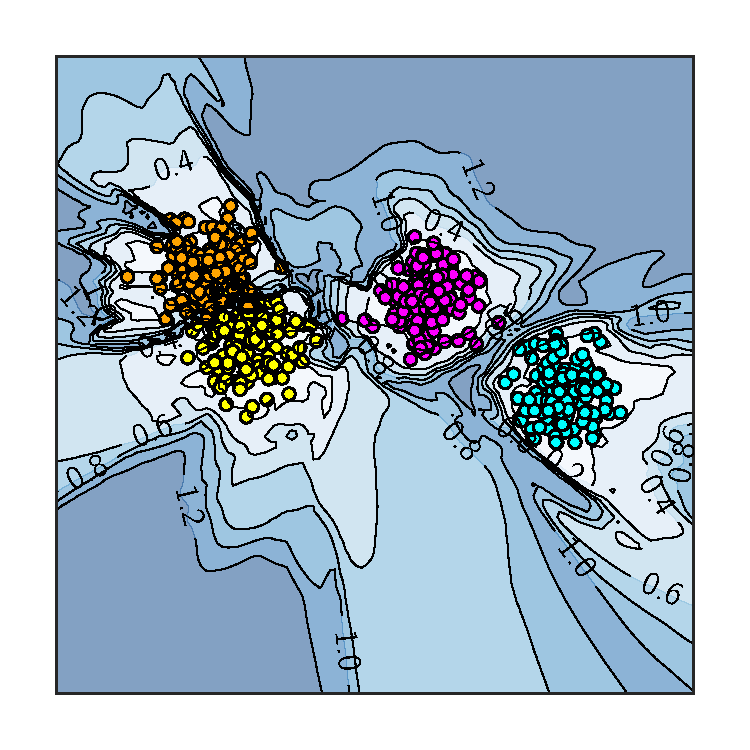
\includegraphics[width=0.4\textwidth]{figures/toy_data/ent_toy_2d_nn_multiclass_laplace_exact.pdf}}
	\subfloat{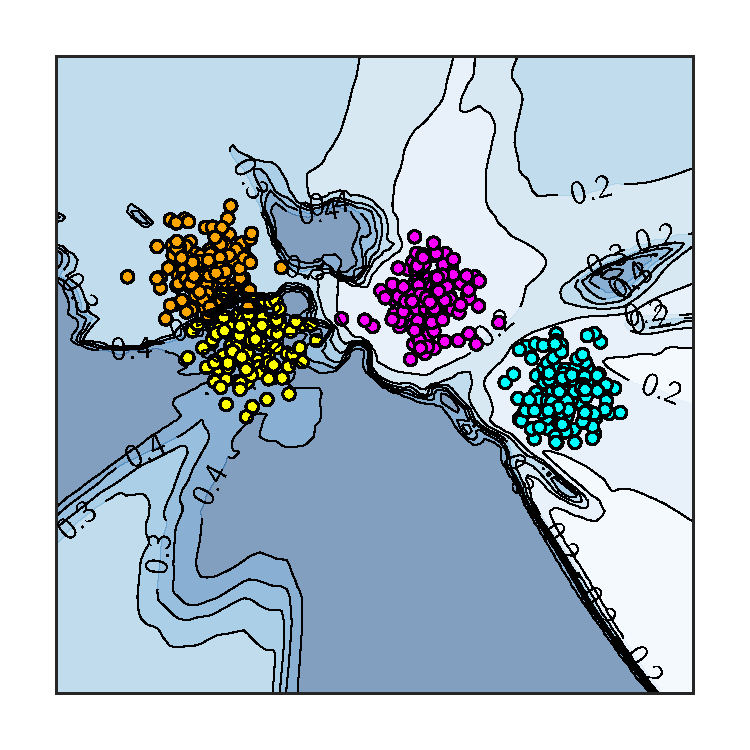
\includegraphics[width=0.4\textwidth]{figures/toy_data/ent_toy_2d_nn_multiclass_LPB_variance_alphas_norm_dir.pdf}} 

	\caption{\textbf{Left:} Entropy of the MAP estimate, a diagonal approximation of the Hessian, a Kronecker-factorized approximation, and the exact Hessian.
	\textbf{Right:} MAP prediction of the Dirichlet coming from the Laplace Bridge, its predictive entropy, the variance of the Dirichlet, and a MAP estimate weighed by its variance. We find that the Laplace Bridge entropy and variance are only marginally better than the MAP estimate but the reweighed version improves it.}
	\label{fig:toy_data}
\end{figure}

\restoregeometry

\section{Uncertainty-aware output ranking on ImageNet}
\label{subsec:exp5_imagenet}

\setlength{\figwidth}{1\textwidth}
\setlength{\figheight}{0.18\textheight}

\begin{figure*}[t]
	\centering
	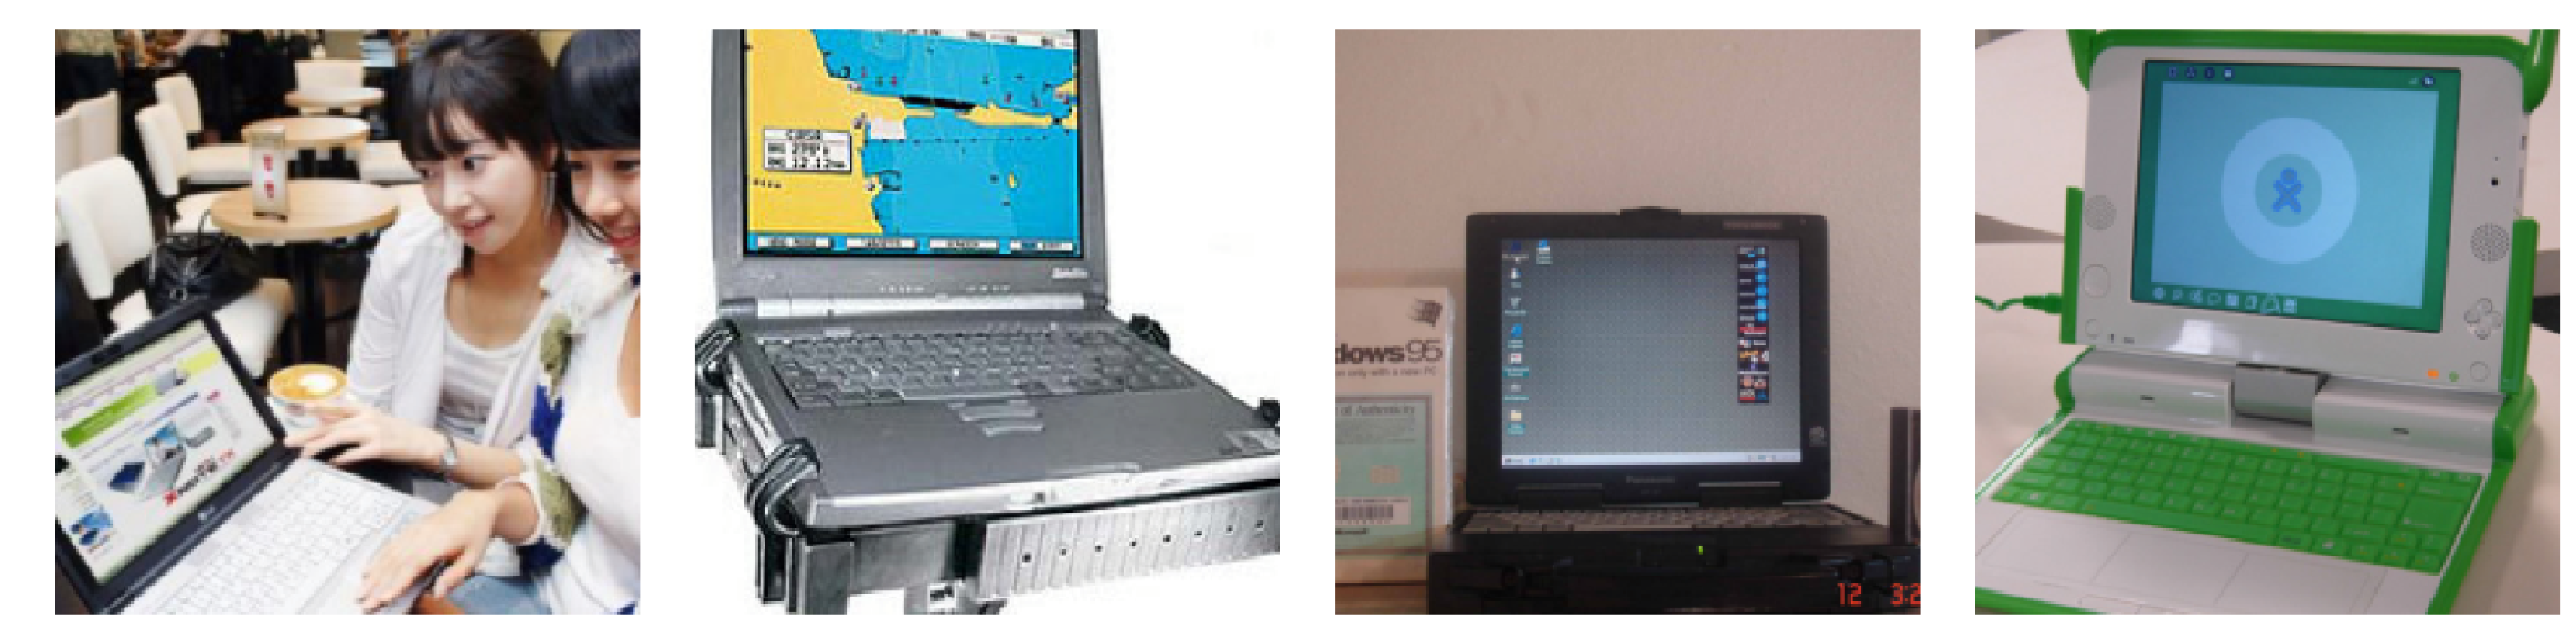
\includegraphics[width=\figwidth,height=\figheight]{figures/imagenet_images.pdf}
	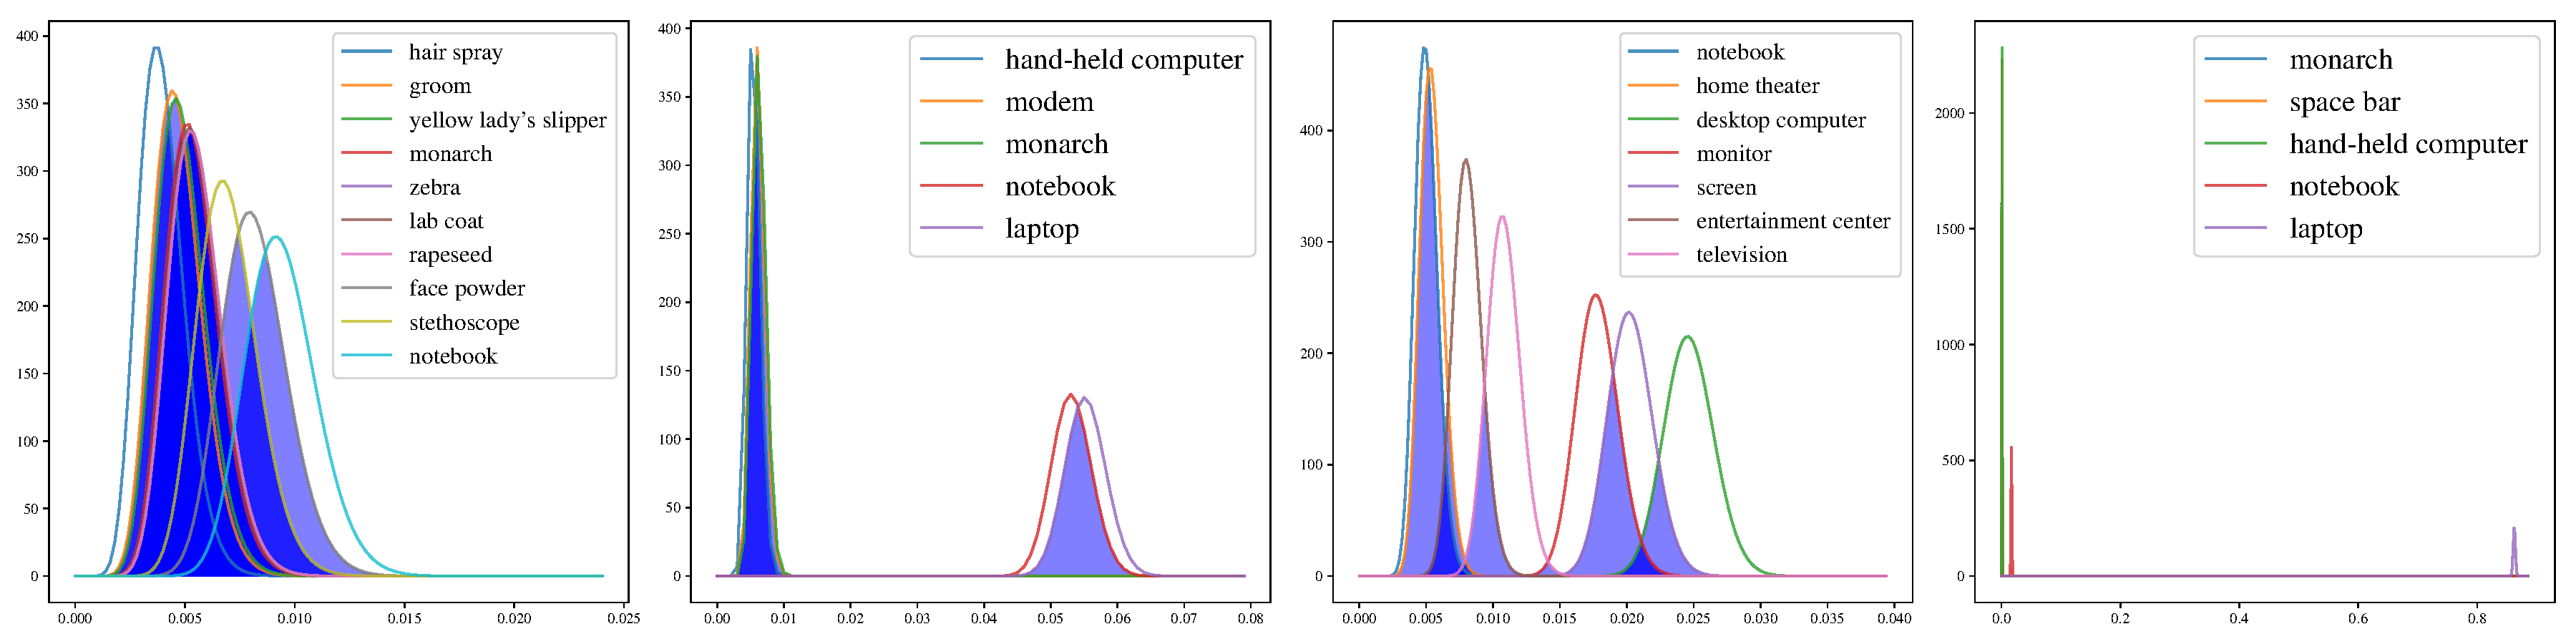
\includegraphics[width=\figwidth,height=\figheight]{figures/imagenet_marginal_betas.pdf}
	%% This file was created by tikzplotlib v0.9.0.
\begin{tikzpicture}

\definecolor{color0}{rgb}{0.12156862745098,0.466666666666667,0.705882352941177}
\definecolor{color1}{rgb}{1,0.498039215686275,0.0549019607843137}
\definecolor{color2}{rgb}{0.172549019607843,0.627450980392157,0.172549019607843}
\definecolor{color3}{rgb}{0.83921568627451,0.152941176470588,0.156862745098039}
\definecolor{color4}{rgb}{0.580392156862745,0.403921568627451,0.741176470588235}
\definecolor{color5}{rgb}{0.549019607843137,0.337254901960784,0.294117647058824}
\definecolor{color6}{rgb}{0.890196078431372,0.466666666666667,0.76078431372549}
\definecolor{color7}{rgb}{0.737254901960784,0.741176470588235,0.133333333333333}
\definecolor{color8}{rgb}{0.0901960784313725,0.745098039215686,0.811764705882353}

\begin{groupplot}[group style={group size=4 by 1}]
\nextgroupplot[
height=\figheight,
legend cell align={left},
legend style={fill opacity=0.8, draw opacity=1, text opacity=1, draw=white!80!black},
tick align=outside,
tick pos=both,
width=\figwidth,
x grid style={white!69.0196078431373!black},
xmin=-0.0012, xmax=0.0252,
xtick style={color=black},
y grid style={white!69.0196078431373!black},
ymin=-19.6580315246557, ymax=412.81866201777,
ytick style={color=black}
]
\path [draw=none, fill=blue, fill opacity=0.5]
(axis cs:0,0)
--(axis cs:0.0001,9.06562214679757e-18)
--(axis cs:0.0002,4.22795300245434e-13)
--(axis cs:0.0003,1.95967516740209e-10)
--(axis cs:0.0004,1.37496114174896e-08)
--(axis cs:0.0005,3.42850048039048e-07)
--(axis cs:0.0006,4.44349918357242e-06)
--(axis cs:0.0007,3.66625165403048e-05)
--(axis cs:0.0008,0.000217352763044482)
--(axis cs:0.0009,0.00100106472149684)
--(axis cs:0.001,0.00377803209216558)
--(axis cs:0.0011,0.0121363833214698)
--(axis cs:0.0012,0.0341292040287655)
--(axis cs:0.0013,0.0858293497739294)
--(axis cs:0.0014,0.196252804450894)
--(axis cs:0.0015,0.413401539768471)
--(axis cs:0.0016,0.81078219972159)
--(axis cs:0.0017,1.49339432825012)
--(axis cs:0.0018,2.60195337937075)
--(axis cs:0.0019,4.31409659524826)
--(axis cs:0.002,6.84154460221035)
--(axis cs:0.0021,10.4226347291393)
--(axis cs:0.0022,15.3102330091327)
--(axis cs:0.0023,21.7556707387632)
--(axis cs:0.0024,29.989931796765)
--(axis cs:0.0025,40.2037467448369)
--(axis cs:0.0026,52.5284673552818)
--(axis cs:0.0027,67.0195768156313)
--(axis cs:0.0028,83.6444501303574)
--(axis cs:0.0029,102.275560540234)
--(axis cs:0.003,122.689795384513)
--(axis cs:0.0031,144.573970822983)
--(axis cs:0.0032,167.536087950985)
--(axis cs:0.0033,191.121409823487)
--(axis cs:0.0034,214.832099146605)
--(axis cs:0.0035,238.148959945159)
--(axis cs:0.0036,260.553774989619)
--(axis cs:0.0037,281.550810397888)
--(axis cs:0.0038,300.686244763745)
--(axis cs:0.0039,317.564541181951)
--(axis cs:0.004,331.861083501153)
--(axis cs:0.0041,343.330711707608)
--(axis cs:0.0042,350.659364364021)
--(axis cs:0.0043,334.446568888299)
--(axis cs:0.0044,316.671390945087)
--(axis cs:0.0045,297.764547275382)
--(axis cs:0.0046,278.132151246613)
--(axis cs:0.0047,258.146896782677)
--(axis cs:0.0048,238.141886324419)
--(axis cs:0.0049,218.406893266479)
--(axis cs:0.005,199.186771160928)
--(axis cs:0.0051,180.681676590763)
--(axis cs:0.0052,163.048755076709)
--(axis cs:0.0053,146.404944168429)
--(axis cs:0.0054,130.83056941505)
--(axis cs:0.0055,116.373441990735)
--(axis cs:0.0056,103.053206760269)
--(axis cs:0.0057,90.8657326546528)
--(axis cs:0.0058,79.7873803369428)
--(axis cs:0.0059,69.779023006632)
--(axis cs:0.006,60.7897332615976)
--(axis cs:0.0061,52.7600812705533)
--(axis cs:0.0062,45.6250166719352)
--(axis cs:0.0063,39.3163285658967)
--(axis cs:0.0064,33.764694951832)
--(axis cs:0.0065,28.9013454265901)
--(axis cs:0.0066,24.6593694570613)
--(axis cs:0.0067,20.9747076870548)
--(axis cs:0.0068,17.7868661496403)
--(axis cs:0.0069,15.0393935200602)
--(axis cs:0.007,12.6801601962024)
--(axis cs:0.0071,10.6614755026768)
--(axis cs:0.0072,8.94007607834724)
--(axis cs:0.0073,7.47701485126041)
--(axis cs:0.0074,6.23747618667221)
--(axis cs:0.0075,5.19053900883877)
--(axis cs:0.0076,4.30890608686193)
--(axis cs:0.0077,3.56861433492195)
--(axis cs:0.0078,2.94873796599512)
--(axis cs:0.0079,2.43109368428247)
--(axis cs:0.008,1.99995481107366)
--(axis cs:0.0081,1.64177930106216)
--(axis cs:0.0082,1.34495499920915)
--(axis cs:0.0083,1.09956418288332)
--(axis cs:0.0084,0.897168396988933)
--(axis cs:0.0085,0.73061378656331)
--(axis cs:0.0086,0.59385652774837)
--(axis cs:0.0087,0.481807521764027)
--(axis cs:0.0088,0.390195217766181)
--(axis cs:0.0089,0.315445242576156)
--(axis cs:0.009,0.254575414817491)
--(axis cs:0.0091,0.205104687868513)
--(axis cs:0.0092,0.164974583259305)
--(axis cs:0.0093,0.132481729640998)
--(axis cs:0.0094,0.106220200791715)
--(axis cs:0.0095,0.0850324401644522)
--(axis cs:0.0096,0.0679676620931031)
--(axis cs:0.0097,0.0542467255102279)
--(axis cs:0.0098,0.0432325808603513)
--(axis cs:0.0099,0.0344054919353093)
--(axis cs:0.01,0.0273423296596845)
--(axis cs:0.0101,0.0216993231931994)
--(axis cs:0.0102,0.0171977344356047)
--(axis cs:0.0103,0.013611994887032)
--(axis cs:0.0104,0.0107599089132325)
--(axis cs:0.0105,0.00849458509029637)
--(axis cs:0.0106,0.00669780790315936)
--(axis cs:0.0107,0.00527460618147189)
--(axis cs:0.0108,0.00414881285588331)
--(axis cs:0.0109,0.00325944350166901)
--(axis cs:0.011,0.00255774928923221)
--(axis cs:0.0111,0.00200482394086903)
--(axis cs:0.0112,0.00156966462258963)
--(axis cs:0.0113,0.00122760385871055)
--(axis cs:0.0114,0.000959043980204529)
--(axis cs:0.0115,0.000748437694616043)
--(axis cs:0.0116,0.000583468440526314)
--(axis cs:0.0117,0.000454392565783103)
--(axis cs:0.0118,0.000353512309656768)
--(axis cs:0.0119,0.000274754302743457)
--(axis cs:0.012,0.000213333020725685)
--(axis cs:0.0121,0.000165482506375253)
--(axis cs:0.0122,0.000128242850643948)
--(axis cs:0.0123,9.92905185611859e-05)
--(axis cs:0.0124,7.68037201326851e-05)
--(axis cs:0.0125,5.9355745309085e-05)
--(axis cs:0.0126,4.58305761506692e-05)
--(axis cs:0.0127,3.53562174155628e-05)
--(axis cs:0.0128,2.72520977192749e-05)
--(axis cs:0.0129,2.09876274370821e-05)
--(axis cs:0.013,1.61495898117959e-05)
--(axis cs:0.0131,1.24165155103202e-05)
--(axis cs:0.0132,9.53857042332152e-06)
--(axis cs:0.0133,7.32179000959193e-06)
--(axis cs:0.0134,5.6157357557516e-06)
--(axis cs:0.0135,4.30384237613123e-06)
--(axis cs:0.0136,3.29587795741631e-06)
--(axis cs:0.0137,2.52206123083152e-06)
--(axis cs:0.0138,1.92847688063577e-06)
--(axis cs:0.0139,1.47350638116977e-06)
--(axis cs:0.014,1.12505239925148e-06)
--(axis cs:0.0141,8.5838259343324e-07)
--(axis cs:0.0142,6.54456317675556e-07)
--(axis cs:0.0143,4.98627395291572e-07)
--(axis cs:0.0144,3.79639444120029e-07)
--(axis cs:0.0145,2.88848538153721e-07)
--(axis cs:0.0146,2.19622342593566e-07)
--(axis cs:0.0147,1.66876097759978e-07)
--(axis cs:0.0148,1.26714616937668e-07)
--(axis cs:0.0149,9.61563293224264e-08)
--(axis cs:0.015,7.29207563822728e-08)
--(axis cs:0.0151,5.52649849126983e-08)
--(axis cs:0.0152,4.18579500369891e-08)
--(axis cs:0.0153,3.16838685043426e-08)
--(axis cs:0.0154,2.39681255123372e-08)
--(axis cs:0.0155,1.81204412737434e-08)
--(axis cs:0.0156,1.36913240004885e-08)
--(axis cs:0.0157,1.03387299919785e-08)
--(axis cs:0.0158,7.8025585154859e-09)
--(axis cs:0.0159,5.88515549863828e-09)
--(axis cs:0.016,4.43642182094435e-09)
--(axis cs:0.0161,3.34244728394577e-09)
--(axis cs:0.0162,2.51684199065801e-09)
--(axis cs:0.0163,1.89412982426803e-09)
--(axis cs:0.0164,1.4247171282791e-09)
--(axis cs:0.0165,1.07106373845201e-09)
--(axis cs:0.0166,8.04771081382379e-10)
--(axis cs:0.0167,6.04369227661805e-10)
--(axis cs:0.0168,4.53636274462889e-10)
--(axis cs:0.0169,3.40322863383456e-10)
--(axis cs:0.017,2.55184812810522e-10)
--(axis cs:0.0171,1.91249914877082e-10)
--(axis cs:0.0172,1.43262573263436e-10)
--(axis cs:0.0173,1.07263414092402e-10)
--(axis cs:0.0174,8.02712667488462e-11)
--(axis cs:0.0175,6.0042735644463e-11)
--(axis cs:0.0176,4.48905435239373e-11)
--(axis cs:0.0177,3.3546362917387e-11)
--(axis cs:0.0178,2.50573023493042e-11)
--(axis cs:0.0179,1.87078360651019e-11)
--(axis cs:0.018,1.3960957590044e-11)
--(axis cs:0.0181,1.0413849001817e-11)
--(axis cs:0.0182,7.76450428095243e-12)
--(axis cs:0.0183,5.78661409835728e-12)
--(axis cs:0.0184,4.31067763326576e-12)
--(axis cs:0.0185,3.20980528044695e-12)
--(axis cs:0.0186,2.3890530370788e-12)
--(axis cs:0.0187,1.77741432325105e-12)
--(axis cs:0.0188,1.32181029046682e-12)
--(axis cs:0.0189,9.82582239659666e-13)
--(axis cs:0.019,7.30112445413e-13)
--(axis cs:0.0191,5.42292199726631e-13)
--(axis cs:0.0192,4.02625619692298e-13)
--(axis cs:0.0193,2.98810289904157e-13)
--(axis cs:0.0194,2.21675354345489e-13)
--(axis cs:0.0195,1.64387425693445e-13)
--(axis cs:0.0196,1.21857053967287e-13)
--(axis cs:0.0197,9.02953120165571e-14)
--(axis cs:0.0198,6.68826864553411e-14)
--(axis cs:0.0199,4.95219454356751e-14)
--(axis cs:0.02,3.66537700284644e-14)
--(axis cs:0.0201,2.71192721526512e-14)
--(axis cs:0.0202,2.00575217613878e-14)
--(axis cs:0.0203,1.4829202501312e-14)
--(axis cs:0.0204,1.0959758809364e-14)
--(axis cs:0.0205,8.09707665522809e-15)
--(axis cs:0.0206,5.97999627347004e-15)
--(axis cs:0.0207,4.41489440195129e-15)
--(axis cs:0.0208,3.25827538993974e-15)
--(axis cs:0.0209,2.40383477905936e-15)
--(axis cs:0.021,1.77285035089687e-15)
--(axis cs:0.0211,1.307047704609e-15)
--(axis cs:0.0212,9.63305278865802e-16)
--(axis cs:0.0213,7.0972614984709e-16)
--(axis cs:0.0214,5.22724971007102e-16)
--(axis cs:0.0215,3.84868574570441e-16)
--(axis cs:0.0216,2.83275877689995e-16)
--(axis cs:0.0217,2.0843268949852e-16)
--(axis cs:0.0218,1.53314174574747e-16)
--(axis cs:0.0219,1.12735358462639e-16)
--(axis cs:0.022,8.28705967052991e-17)
--(axis cs:0.0221,6.08981854453541e-17)
--(axis cs:0.0222,4.47376214030539e-17)
--(axis cs:0.0223,3.28554291903283e-17)
--(axis cs:0.0224,2.41217142550633e-17)
--(axis cs:0.0225,1.77042282007046e-17)
--(axis cs:0.0226,1.29901647606133e-17)
--(axis cs:0.0227,9.52844783207187e-18)
--(axis cs:0.0228,6.98715695218015e-18)
--(axis cs:0.0229,5.12213072451923e-18)
--(axis cs:0.023,3.75382142728391e-18)
--(axis cs:0.0231,2.75023819725803e-18)
--(axis cs:0.0232,2.01438141289907e-18)
--(axis cs:0.0233,1.47498882522264e-18)
--(axis cs:0.0234,1.07972288043767e-18)
--(axis cs:0.0235,7.90156903262815e-19)
--(axis cs:0.0236,5.78086370487335e-19)
--(axis cs:0.0237,4.22815953370766e-19)
--(axis cs:0.0238,3.09164855713053e-19)
--(axis cs:0.0239,2.26000737856617e-19)
--(axis cs:0.024,1.65162493477036e-19)
--cycle;
\path [draw=none, fill=blue, fill opacity=0.5]
(axis cs:0,0)
--(axis cs:0.0001,1.11897989109415e-18)
--(axis cs:0.0002,7.61192645735247e-14)
--(axis cs:0.0003,4.40004337898566e-11)
--(axis cs:0.0004,3.61092349697281e-09)
--(axis cs:0.0005,1.01677519503497e-07)
--(axis cs:0.0006,1.45540906761335e-06)
--(axis cs:0.0007,1.30604942914043e-05)
--(axis cs:0.0008,8.32729233244913e-05)
--(axis cs:0.0009,0.000408957259564032)
--(axis cs:0.001,0.00163463517706023)
--(axis cs:0.0011,0.00553104516706739)
--(axis cs:0.0012,0.016309637005717)
--(axis cs:0.0013,0.0428455989676742)
--(axis cs:0.0014,0.102008198661971)
--(axis cs:0.0015,0.223115882324795)
--(axis cs:0.0016,0.453261075131758)
--(axis cs:0.0017,0.862936778825342)
--(axis cs:0.0018,1.5511170267273)
--(axis cs:0.0019,2.64877144732255)
--(axis cs:0.002,4.31978738912353)
--(axis cs:0.0021,6.75845420865552)
--(axis cs:0.0022,10.1830168367104)
--(axis cs:0.0023,14.8252778811825)
--(axis cs:0.0024,20.9167445288748)
--(axis cs:0.0025,28.6722965565199)
--(axis cs:0.0026,38.2727217377937)
--(axis cs:0.0027,49.847672660101)
--(axis cs:0.0028,63.4606200393569)
--(axis cs:0.0029,79.0972164628218)
--(axis cs:0.003,96.6581704221682)
--(axis cs:0.0031,115.957310437916)
--(axis cs:0.0032,136.725048683837)
--(axis cs:0.0033,158.616988518705)
--(axis cs:0.0034,181.227009291322)
--(axis cs:0.0035,204.103841136994)
--(axis cs:0.0036,226.769934038948)
--(axis cs:0.0037,248.741336192108)
--(axis cs:0.0038,269.547320550091)
--(axis cs:0.0039,288.748618996781)
--(axis cs:0.004,305.953317774446)
--(axis cs:0.0041,320.829709365075)
--(axis cs:0.0042,333.115658709357)
--(axis cs:0.0043,334.446568888299)
--(axis cs:0.0044,316.671390945087)
--(axis cs:0.0045,297.764547275382)
--(axis cs:0.0046,278.132151246613)
--(axis cs:0.0047,258.146896782677)
--(axis cs:0.0048,238.141886324419)
--(axis cs:0.0049,218.406893266479)
--(axis cs:0.005,199.186771160928)
--(axis cs:0.0051,180.681676590763)
--(axis cs:0.0052,163.048755076709)
--(axis cs:0.0053,146.404944168429)
--(axis cs:0.0054,130.83056941505)
--(axis cs:0.0055,116.373441990735)
--(axis cs:0.0056,103.053206760269)
--(axis cs:0.0057,90.8657326546528)
--(axis cs:0.0058,79.7873803369428)
--(axis cs:0.0059,69.779023006632)
--(axis cs:0.006,60.7897332615976)
--(axis cs:0.0061,52.7600812705533)
--(axis cs:0.0062,45.6250166719352)
--(axis cs:0.0063,39.3163285658967)
--(axis cs:0.0064,33.764694951832)
--(axis cs:0.0065,28.9013454265901)
--(axis cs:0.0066,24.6593694570613)
--(axis cs:0.0067,20.9747076870548)
--(axis cs:0.0068,17.7868661496403)
--(axis cs:0.0069,15.0393935200602)
--(axis cs:0.007,12.6801601962024)
--(axis cs:0.0071,10.6614755026768)
--(axis cs:0.0072,8.94007607834724)
--(axis cs:0.0073,7.47701485126041)
--(axis cs:0.0074,6.23747618667221)
--(axis cs:0.0075,5.19053900883877)
--(axis cs:0.0076,4.30890608686193)
--(axis cs:0.0077,3.56861433492195)
--(axis cs:0.0078,2.94873796599512)
--(axis cs:0.0079,2.43109368428247)
--(axis cs:0.008,1.99995481107366)
--(axis cs:0.0081,1.64177930106216)
--(axis cs:0.0082,1.34495499920915)
--(axis cs:0.0083,1.09956418288332)
--(axis cs:0.0084,0.897168396988933)
--(axis cs:0.0085,0.73061378656331)
--(axis cs:0.0086,0.59385652774837)
--(axis cs:0.0087,0.481807521764027)
--(axis cs:0.0088,0.390195217766181)
--(axis cs:0.0089,0.315445242576156)
--(axis cs:0.009,0.254575414817491)
--(axis cs:0.0091,0.205104687868513)
--(axis cs:0.0092,0.164974583259305)
--(axis cs:0.0093,0.132481729640998)
--(axis cs:0.0094,0.106220200791715)
--(axis cs:0.0095,0.0850324401644522)
--(axis cs:0.0096,0.0679676620931031)
--(axis cs:0.0097,0.0542467255102279)
--(axis cs:0.0098,0.0432325808603513)
--(axis cs:0.0099,0.0344054919353093)
--(axis cs:0.01,0.0273423296596845)
--(axis cs:0.0101,0.0216993231931994)
--(axis cs:0.0102,0.0171977344356047)
--(axis cs:0.0103,0.013611994887032)
--(axis cs:0.0104,0.0107599089132325)
--(axis cs:0.0105,0.00849458509029637)
--(axis cs:0.0106,0.00669780790315936)
--(axis cs:0.0107,0.00527460618147189)
--(axis cs:0.0108,0.00414881285588331)
--(axis cs:0.0109,0.00325944350166901)
--(axis cs:0.011,0.00255774928923221)
--(axis cs:0.0111,0.00200482394086903)
--(axis cs:0.0112,0.00156966462258963)
--(axis cs:0.0113,0.00122760385871055)
--(axis cs:0.0114,0.000959043980204529)
--(axis cs:0.0115,0.000748437694616043)
--(axis cs:0.0116,0.000583468440526314)
--(axis cs:0.0117,0.000454392565783103)
--(axis cs:0.0118,0.000353512309656768)
--(axis cs:0.0119,0.000274754302743457)
--(axis cs:0.012,0.000213333020725685)
--(axis cs:0.0121,0.000165482506375253)
--(axis cs:0.0122,0.000128242850643948)
--(axis cs:0.0123,9.92905185611859e-05)
--(axis cs:0.0124,7.68037201326851e-05)
--(axis cs:0.0125,5.9355745309085e-05)
--(axis cs:0.0126,4.58305761506692e-05)
--(axis cs:0.0127,3.53562174155628e-05)
--(axis cs:0.0128,2.72520977192749e-05)
--(axis cs:0.0129,2.09876274370821e-05)
--(axis cs:0.013,1.61495898117959e-05)
--(axis cs:0.0131,1.24165155103202e-05)
--(axis cs:0.0132,9.53857042332152e-06)
--(axis cs:0.0133,7.32179000959193e-06)
--(axis cs:0.0134,5.6157357557516e-06)
--(axis cs:0.0135,4.30384237613123e-06)
--(axis cs:0.0136,3.29587795741631e-06)
--(axis cs:0.0137,2.52206123083152e-06)
--(axis cs:0.0138,1.92847688063577e-06)
--(axis cs:0.0139,1.47350638116977e-06)
--(axis cs:0.014,1.12505239925148e-06)
--(axis cs:0.0141,8.5838259343324e-07)
--(axis cs:0.0142,6.54456317675556e-07)
--(axis cs:0.0143,4.98627395291572e-07)
--(axis cs:0.0144,3.79639444120029e-07)
--(axis cs:0.0145,2.88848538153721e-07)
--(axis cs:0.0146,2.19622342593566e-07)
--(axis cs:0.0147,1.66876097759978e-07)
--(axis cs:0.0148,1.26714616937668e-07)
--(axis cs:0.0149,9.61563293224264e-08)
--(axis cs:0.015,7.29207563822728e-08)
--(axis cs:0.0151,5.52649849126983e-08)
--(axis cs:0.0152,4.18579500369891e-08)
--(axis cs:0.0153,3.16838685043426e-08)
--(axis cs:0.0154,2.39681255123372e-08)
--(axis cs:0.0155,1.81204412737434e-08)
--(axis cs:0.0156,1.36913240004885e-08)
--(axis cs:0.0157,1.03387299919785e-08)
--(axis cs:0.0158,7.8025585154859e-09)
--(axis cs:0.0159,5.88515549863828e-09)
--(axis cs:0.016,4.43642182094435e-09)
--(axis cs:0.0161,3.34244728394577e-09)
--(axis cs:0.0162,2.51684199065801e-09)
--(axis cs:0.0163,1.89412982426803e-09)
--(axis cs:0.0164,1.4247171282791e-09)
--(axis cs:0.0165,1.07106373845201e-09)
--(axis cs:0.0166,8.04771081382379e-10)
--(axis cs:0.0167,6.04369227661805e-10)
--(axis cs:0.0168,4.53636274462889e-10)
--(axis cs:0.0169,3.40322863383456e-10)
--(axis cs:0.017,2.55184812810522e-10)
--(axis cs:0.0171,1.91249914877082e-10)
--(axis cs:0.0172,1.43262573263436e-10)
--(axis cs:0.0173,1.07263414092402e-10)
--(axis cs:0.0174,8.02712667488462e-11)
--(axis cs:0.0175,6.0042735644463e-11)
--(axis cs:0.0176,4.48905435239373e-11)
--(axis cs:0.0177,3.3546362917387e-11)
--(axis cs:0.0178,2.50573023493042e-11)
--(axis cs:0.0179,1.87078360651019e-11)
--(axis cs:0.018,1.3960957590044e-11)
--(axis cs:0.0181,1.0413849001817e-11)
--(axis cs:0.0182,7.76450428095243e-12)
--(axis cs:0.0183,5.78661409835728e-12)
--(axis cs:0.0184,4.31067763326576e-12)
--(axis cs:0.0185,3.20980528044695e-12)
--(axis cs:0.0186,2.3890530370788e-12)
--(axis cs:0.0187,1.77741432325105e-12)
--(axis cs:0.0188,1.32181029046682e-12)
--(axis cs:0.0189,9.82582239659666e-13)
--(axis cs:0.019,7.30112445413e-13)
--(axis cs:0.0191,5.42292199726631e-13)
--(axis cs:0.0192,4.02625619692298e-13)
--(axis cs:0.0193,2.98810289904157e-13)
--(axis cs:0.0194,2.21675354345489e-13)
--(axis cs:0.0195,1.64387425693445e-13)
--(axis cs:0.0196,1.21857053967287e-13)
--(axis cs:0.0197,9.02953120165571e-14)
--(axis cs:0.0198,6.68826864553411e-14)
--(axis cs:0.0199,4.95219454356751e-14)
--(axis cs:0.02,3.66537700284644e-14)
--(axis cs:0.0201,2.71192721526512e-14)
--(axis cs:0.0202,2.00575217613878e-14)
--(axis cs:0.0203,1.4829202501312e-14)
--(axis cs:0.0204,1.0959758809364e-14)
--(axis cs:0.0205,8.09707665522809e-15)
--(axis cs:0.0206,5.97999627347004e-15)
--(axis cs:0.0207,4.41489440195129e-15)
--(axis cs:0.0208,3.25827538993974e-15)
--(axis cs:0.0209,2.40383477905936e-15)
--(axis cs:0.021,1.77285035089687e-15)
--(axis cs:0.0211,1.307047704609e-15)
--(axis cs:0.0212,9.63305278865802e-16)
--(axis cs:0.0213,7.0972614984709e-16)
--(axis cs:0.0214,5.22724971007102e-16)
--(axis cs:0.0215,3.84868574570441e-16)
--(axis cs:0.0216,2.83275877689995e-16)
--(axis cs:0.0217,2.0843268949852e-16)
--(axis cs:0.0218,1.53314174574747e-16)
--(axis cs:0.0219,1.12735358462639e-16)
--(axis cs:0.022,8.28705967052991e-17)
--(axis cs:0.0221,6.08981854453541e-17)
--(axis cs:0.0222,4.47376214030539e-17)
--(axis cs:0.0223,3.28554291903283e-17)
--(axis cs:0.0224,2.41217142550633e-17)
--(axis cs:0.0225,1.77042282007046e-17)
--(axis cs:0.0226,1.29901647606133e-17)
--(axis cs:0.0227,9.52844783207187e-18)
--(axis cs:0.0228,6.98715695218015e-18)
--(axis cs:0.0229,5.12213072451923e-18)
--(axis cs:0.023,3.75382142728391e-18)
--(axis cs:0.0231,2.75023819725803e-18)
--(axis cs:0.0232,2.01438141289907e-18)
--(axis cs:0.0233,1.47498882522264e-18)
--(axis cs:0.0234,1.07972288043767e-18)
--(axis cs:0.0235,7.90156903262815e-19)
--(axis cs:0.0236,5.78086370487335e-19)
--(axis cs:0.0237,4.22815953370766e-19)
--(axis cs:0.0238,3.09164855713053e-19)
--(axis cs:0.0239,2.26000737856617e-19)
--(axis cs:0.024,1.65162493477036e-19)
--cycle;
\path [draw=none, fill=blue, fill opacity=0.5]
(axis cs:0,0)
--(axis cs:0.0001,6.39244670782497e-22)
--(axis cs:0.0002,1.63304653410572e-16)
--(axis cs:0.0003,2.0471487523226e-13)
--(axis cs:0.0004,2.90980802338031e-11)
--(axis cs:0.0005,1.25466030049833e-09)
--(axis cs:0.0006,2.54391471865381e-08)
--(axis cs:0.0007,3.06437163171201e-07)
--(axis cs:0.0008,2.52149359912999e-06)
--(axis cs:0.0009,1.55077864792925e-05)
--(axis cs:0.001,7.58076561312621e-05)
--(axis cs:0.0011,0.000307743345802269)
--(axis cs:0.0012,0.00107160766687709)
--(axis cs:0.0013,0.0032804331918367)
--(axis cs:0.0014,0.0089985803413974)
--(axis cs:0.0015,0.0224565611877336)
--(axis cs:0.0016,0.0516110463947514)
--(axis cs:0.0017,0.110334242969158)
--(axis cs:0.0018,0.221227821059011)
--(axis cs:0.0019,0.418929650862053)
--(axis cs:0.002,0.753634925751084)
--(axis cs:0.0021,1.29441375393259)
--(axis cs:0.0022,2.13180511178777)
--(axis cs:0.0023,3.37912866231096)
--(axis cs:0.0024,5.17199814367324)
--(axis cs:0.0025,7.66564599508246)
--(axis cs:0.0026,11.0298671973361)
--(axis cs:0.0027,15.44163698238)
--(axis cs:0.0028,21.0757198851318)
--(axis cs:0.0029,28.0938316731511)
--(axis cs:0.003,36.6331090584455)
--(axis cs:0.0031,46.7947604765166)
--(axis cs:0.0032,58.6338009969209)
--(axis cs:0.0033,72.1507137805696)
--(axis cs:0.0034,87.2857386482926)
--(axis cs:0.0035,103.916283353858)
--(axis cs:0.0036,121.857708878618)
--(axis cs:0.0037,140.867482577198)
--(axis cs:0.0038,160.652447408685)
--(axis cs:0.0039,180.878743222521)
--(axis cs:0.004,201.183753056193)
--(axis cs:0.0041,221.18934311996)
--(axis cs:0.0042,240.515622550635)
--(axis cs:0.0043,258.794465192817)
--(axis cs:0.0044,275.68210296399)
--(axis cs:0.0045,290.870207829795)
--(axis cs:0.0046,278.132151246613)
--(axis cs:0.0047,258.146896782677)
--(axis cs:0.0048,238.141886324419)
--(axis cs:0.0049,218.406893266479)
--(axis cs:0.005,199.186771160928)
--(axis cs:0.0051,180.681676590763)
--(axis cs:0.0052,163.048755076709)
--(axis cs:0.0053,146.404944168429)
--(axis cs:0.0054,130.83056941505)
--(axis cs:0.0055,116.373441990735)
--(axis cs:0.0056,103.053206760269)
--(axis cs:0.0057,90.8657326546528)
--(axis cs:0.0058,79.7873803369428)
--(axis cs:0.0059,69.779023006632)
--(axis cs:0.006,60.7897332615976)
--(axis cs:0.0061,52.7600812705533)
--(axis cs:0.0062,45.6250166719352)
--(axis cs:0.0063,39.3163285658967)
--(axis cs:0.0064,33.764694951832)
--(axis cs:0.0065,28.9013454265901)
--(axis cs:0.0066,24.6593694570613)
--(axis cs:0.0067,20.9747076870548)
--(axis cs:0.0068,17.7868661496403)
--(axis cs:0.0069,15.0393935200602)
--(axis cs:0.007,12.6801601962024)
--(axis cs:0.0071,10.6614755026768)
--(axis cs:0.0072,8.94007607834724)
--(axis cs:0.0073,7.47701485126041)
--(axis cs:0.0074,6.23747618667221)
--(axis cs:0.0075,5.19053900883877)
--(axis cs:0.0076,4.30890608686193)
--(axis cs:0.0077,3.56861433492195)
--(axis cs:0.0078,2.94873796599512)
--(axis cs:0.0079,2.43109368428247)
--(axis cs:0.008,1.99995481107366)
--(axis cs:0.0081,1.64177930106216)
--(axis cs:0.0082,1.34495499920915)
--(axis cs:0.0083,1.09956418288332)
--(axis cs:0.0084,0.897168396988933)
--(axis cs:0.0085,0.73061378656331)
--(axis cs:0.0086,0.59385652774837)
--(axis cs:0.0087,0.481807521764027)
--(axis cs:0.0088,0.390195217766181)
--(axis cs:0.0089,0.315445242576156)
--(axis cs:0.009,0.254575414817491)
--(axis cs:0.0091,0.205104687868513)
--(axis cs:0.0092,0.164974583259305)
--(axis cs:0.0093,0.132481729640998)
--(axis cs:0.0094,0.106220200791715)
--(axis cs:0.0095,0.0850324401644522)
--(axis cs:0.0096,0.0679676620931031)
--(axis cs:0.0097,0.0542467255102279)
--(axis cs:0.0098,0.0432325808603513)
--(axis cs:0.0099,0.0344054919353093)
--(axis cs:0.01,0.0273423296596845)
--(axis cs:0.0101,0.0216993231931994)
--(axis cs:0.0102,0.0171977344356047)
--(axis cs:0.0103,0.013611994887032)
--(axis cs:0.0104,0.0107599089132325)
--(axis cs:0.0105,0.00849458509029637)
--(axis cs:0.0106,0.00669780790315936)
--(axis cs:0.0107,0.00527460618147189)
--(axis cs:0.0108,0.00414881285588331)
--(axis cs:0.0109,0.00325944350166901)
--(axis cs:0.011,0.00255774928923221)
--(axis cs:0.0111,0.00200482394086903)
--(axis cs:0.0112,0.00156966462258963)
--(axis cs:0.0113,0.00122760385871055)
--(axis cs:0.0114,0.000959043980204529)
--(axis cs:0.0115,0.000748437694616043)
--(axis cs:0.0116,0.000583468440526314)
--(axis cs:0.0117,0.000454392565783103)
--(axis cs:0.0118,0.000353512309656768)
--(axis cs:0.0119,0.000274754302743457)
--(axis cs:0.012,0.000213333020725685)
--(axis cs:0.0121,0.000165482506375253)
--(axis cs:0.0122,0.000128242850643948)
--(axis cs:0.0123,9.92905185611859e-05)
--(axis cs:0.0124,7.68037201326851e-05)
--(axis cs:0.0125,5.9355745309085e-05)
--(axis cs:0.0126,4.58305761506692e-05)
--(axis cs:0.0127,3.53562174155628e-05)
--(axis cs:0.0128,2.72520977192749e-05)
--(axis cs:0.0129,2.09876274370821e-05)
--(axis cs:0.013,1.61495898117959e-05)
--(axis cs:0.0131,1.24165155103202e-05)
--(axis cs:0.0132,9.53857042332152e-06)
--(axis cs:0.0133,7.32179000959193e-06)
--(axis cs:0.0134,5.6157357557516e-06)
--(axis cs:0.0135,4.30384237613123e-06)
--(axis cs:0.0136,3.29587795741631e-06)
--(axis cs:0.0137,2.52206123083152e-06)
--(axis cs:0.0138,1.92847688063577e-06)
--(axis cs:0.0139,1.47350638116977e-06)
--(axis cs:0.014,1.12505239925148e-06)
--(axis cs:0.0141,8.5838259343324e-07)
--(axis cs:0.0142,6.54456317675556e-07)
--(axis cs:0.0143,4.98627395291572e-07)
--(axis cs:0.0144,3.79639444120029e-07)
--(axis cs:0.0145,2.88848538153721e-07)
--(axis cs:0.0146,2.19622342593566e-07)
--(axis cs:0.0147,1.66876097759978e-07)
--(axis cs:0.0148,1.26714616937668e-07)
--(axis cs:0.0149,9.61563293224264e-08)
--(axis cs:0.015,7.29207563822728e-08)
--(axis cs:0.0151,5.52649849126983e-08)
--(axis cs:0.0152,4.18579500369891e-08)
--(axis cs:0.0153,3.16838685043426e-08)
--(axis cs:0.0154,2.39681255123372e-08)
--(axis cs:0.0155,1.81204412737434e-08)
--(axis cs:0.0156,1.36913240004885e-08)
--(axis cs:0.0157,1.03387299919785e-08)
--(axis cs:0.0158,7.8025585154859e-09)
--(axis cs:0.0159,5.88515549863828e-09)
--(axis cs:0.016,4.43642182094435e-09)
--(axis cs:0.0161,3.34244728394577e-09)
--(axis cs:0.0162,2.51684199065801e-09)
--(axis cs:0.0163,1.89412982426803e-09)
--(axis cs:0.0164,1.4247171282791e-09)
--(axis cs:0.0165,1.07106373845201e-09)
--(axis cs:0.0166,8.04771081382379e-10)
--(axis cs:0.0167,6.04369227661805e-10)
--(axis cs:0.0168,4.53636274462889e-10)
--(axis cs:0.0169,3.40322863383456e-10)
--(axis cs:0.017,2.55184812810522e-10)
--(axis cs:0.0171,1.91249914877082e-10)
--(axis cs:0.0172,1.43262573263436e-10)
--(axis cs:0.0173,1.07263414092402e-10)
--(axis cs:0.0174,8.02712667488462e-11)
--(axis cs:0.0175,6.0042735644463e-11)
--(axis cs:0.0176,4.48905435239373e-11)
--(axis cs:0.0177,3.3546362917387e-11)
--(axis cs:0.0178,2.50573023493042e-11)
--(axis cs:0.0179,1.87078360651019e-11)
--(axis cs:0.018,1.3960957590044e-11)
--(axis cs:0.0181,1.0413849001817e-11)
--(axis cs:0.0182,7.76450428095243e-12)
--(axis cs:0.0183,5.78661409835728e-12)
--(axis cs:0.0184,4.31067763326576e-12)
--(axis cs:0.0185,3.20980528044695e-12)
--(axis cs:0.0186,2.3890530370788e-12)
--(axis cs:0.0187,1.77741432325105e-12)
--(axis cs:0.0188,1.32181029046682e-12)
--(axis cs:0.0189,9.82582239659666e-13)
--(axis cs:0.019,7.30112445413e-13)
--(axis cs:0.0191,5.42292199726631e-13)
--(axis cs:0.0192,4.02625619692298e-13)
--(axis cs:0.0193,2.98810289904157e-13)
--(axis cs:0.0194,2.21675354345489e-13)
--(axis cs:0.0195,1.64387425693445e-13)
--(axis cs:0.0196,1.21857053967287e-13)
--(axis cs:0.0197,9.02953120165571e-14)
--(axis cs:0.0198,6.68826864553411e-14)
--(axis cs:0.0199,4.95219454356751e-14)
--(axis cs:0.02,3.66537700284644e-14)
--(axis cs:0.0201,2.71192721526512e-14)
--(axis cs:0.0202,2.00575217613878e-14)
--(axis cs:0.0203,1.4829202501312e-14)
--(axis cs:0.0204,1.0959758809364e-14)
--(axis cs:0.0205,8.09707665522809e-15)
--(axis cs:0.0206,5.97999627347004e-15)
--(axis cs:0.0207,4.41489440195129e-15)
--(axis cs:0.0208,3.25827538993974e-15)
--(axis cs:0.0209,2.40383477905936e-15)
--(axis cs:0.021,1.77285035089687e-15)
--(axis cs:0.0211,1.307047704609e-15)
--(axis cs:0.0212,9.63305278865802e-16)
--(axis cs:0.0213,7.0972614984709e-16)
--(axis cs:0.0214,5.22724971007102e-16)
--(axis cs:0.0215,3.84868574570441e-16)
--(axis cs:0.0216,2.83275877689995e-16)
--(axis cs:0.0217,2.0843268949852e-16)
--(axis cs:0.0218,1.53314174574747e-16)
--(axis cs:0.0219,1.12735358462639e-16)
--(axis cs:0.022,8.28705967052991e-17)
--(axis cs:0.0221,6.08981854453541e-17)
--(axis cs:0.0222,4.47376214030539e-17)
--(axis cs:0.0223,3.28554291903283e-17)
--(axis cs:0.0224,2.41217142550633e-17)
--(axis cs:0.0225,1.77042282007046e-17)
--(axis cs:0.0226,1.29901647606133e-17)
--(axis cs:0.0227,9.52844783207187e-18)
--(axis cs:0.0228,6.98715695218015e-18)
--(axis cs:0.0229,5.12213072451923e-18)
--(axis cs:0.023,3.75382142728391e-18)
--(axis cs:0.0231,2.75023819725803e-18)
--(axis cs:0.0232,2.01438141289907e-18)
--(axis cs:0.0233,1.47498882522264e-18)
--(axis cs:0.0234,1.07972288043767e-18)
--(axis cs:0.0235,7.90156903262815e-19)
--(axis cs:0.0236,5.78086370487335e-19)
--(axis cs:0.0237,4.22815953370766e-19)
--(axis cs:0.0238,3.09164855713053e-19)
--(axis cs:0.0239,2.26000737856617e-19)
--(axis cs:0.024,1.65162493477036e-19)
--cycle;
\path [draw=none, fill=blue, fill opacity=0.5]
(axis cs:0,0)
--(axis cs:0.0001,7.78619827720865e-23)
--(axis cs:0.0002,2.87061962533969e-17)
--(axis cs:0.0003,4.45996574018144e-14)
--(axis cs:0.0004,7.38215500264892e-12)
--(axis cs:0.0005,3.5821993329408e-10)
--(axis cs:0.0006,7.99925233557908e-09)
--(axis cs:0.0007,1.04553227693222e-07)
--(axis cs:0.0008,9.23345890210269e-07)
--(axis cs:0.0009,6.0443233929932e-06)
--(axis cs:0.001,3.12426163997331e-05)
--(axis cs:0.0011,0.000133398125969305)
--(axis cs:0.0012,0.000486425585682615)
--(axis cs:0.0013,0.00155356644670703)
--(axis cs:0.0014,0.00443227584242255)
--(axis cs:0.0015,0.0114729382566287)
--(axis cs:0.0016,0.0272853176447845)
--(axis cs:0.0017,0.0602354479046895)
--(axis cs:0.0018,0.124491716808887)
--(axis cs:0.0019,0.242599724357013)
--(axis cs:0.002,0.448457426929982)
--(axis cs:0.0021,0.790440289503582)
--(axis cs:0.0022,1.33431227744341)
--(axis cs:0.0023,2.16547627786607)
--(axis cs:0.0024,3.39008775333182)
--(axis cs:0.0025,5.13459138090859)
--(axis cs:0.0026,7.54334486722043)
--(axis cs:0.0027,10.7741584264641)
--(axis cs:0.0028,14.9917839314935)
--(axis cs:0.0029,20.3596090251949)
--(axis cs:0.003,27.0300203986886)
--(axis cs:0.0031,35.1340706339427)
--(axis cs:0.0032,44.7711936223266)
--(axis cs:0.0033,55.9997518982214)
--(axis cs:0.0034,68.829161876082)
--(axis cs:0.0035,83.2142356152724)
--(axis cs:0.0036,99.0522136164206)
--(axis cs:0.0037,116.182760831567)
--(axis cs:0.0038,134.390978721141)
--(axis cs:0.0039,153.413270948235)
--(axis cs:0.004,172.945707968733)
--(axis cs:0.0041,192.654381128158)
--(axis cs:0.0042,212.187129650739)
--(axis cs:0.0043,231.185968500282)
--(axis cs:0.0044,249.299540863043)
--(axis cs:0.0045,266.19496103433)
--(axis cs:0.0046,278.132151246613)
--(axis cs:0.0047,258.146896782677)
--(axis cs:0.0048,238.141886324419)
--(axis cs:0.0049,218.406893266479)
--(axis cs:0.005,199.186771160928)
--(axis cs:0.0051,180.681676590763)
--(axis cs:0.0052,163.048755076709)
--(axis cs:0.0053,146.404944168429)
--(axis cs:0.0054,130.83056941505)
--(axis cs:0.0055,116.373441990735)
--(axis cs:0.0056,103.053206760269)
--(axis cs:0.0057,90.8657326546528)
--(axis cs:0.0058,79.7873803369428)
--(axis cs:0.0059,69.779023006632)
--(axis cs:0.006,60.7897332615976)
--(axis cs:0.0061,52.7600812705533)
--(axis cs:0.0062,45.6250166719352)
--(axis cs:0.0063,39.3163285658967)
--(axis cs:0.0064,33.764694951832)
--(axis cs:0.0065,28.9013454265901)
--(axis cs:0.0066,24.6593694570613)
--(axis cs:0.0067,20.9747076870548)
--(axis cs:0.0068,17.7868661496403)
--(axis cs:0.0069,15.0393935200602)
--(axis cs:0.007,12.6801601962024)
--(axis cs:0.0071,10.6614755026768)
--(axis cs:0.0072,8.94007607834724)
--(axis cs:0.0073,7.47701485126041)
--(axis cs:0.0074,6.23747618667221)
--(axis cs:0.0075,5.19053900883877)
--(axis cs:0.0076,4.30890608686193)
--(axis cs:0.0077,3.56861433492195)
--(axis cs:0.0078,2.94873796599512)
--(axis cs:0.0079,2.43109368428247)
--(axis cs:0.008,1.99995481107366)
--(axis cs:0.0081,1.64177930106216)
--(axis cs:0.0082,1.34495499920915)
--(axis cs:0.0083,1.09956418288332)
--(axis cs:0.0084,0.897168396988933)
--(axis cs:0.0085,0.73061378656331)
--(axis cs:0.0086,0.59385652774837)
--(axis cs:0.0087,0.481807521764027)
--(axis cs:0.0088,0.390195217766181)
--(axis cs:0.0089,0.315445242576156)
--(axis cs:0.009,0.254575414817491)
--(axis cs:0.0091,0.205104687868513)
--(axis cs:0.0092,0.164974583259305)
--(axis cs:0.0093,0.132481729640998)
--(axis cs:0.0094,0.106220200791715)
--(axis cs:0.0095,0.0850324401644522)
--(axis cs:0.0096,0.0679676620931031)
--(axis cs:0.0097,0.0542467255102279)
--(axis cs:0.0098,0.0432325808603513)
--(axis cs:0.0099,0.0344054919353093)
--(axis cs:0.01,0.0273423296596845)
--(axis cs:0.0101,0.0216993231931994)
--(axis cs:0.0102,0.0171977344356047)
--(axis cs:0.0103,0.013611994887032)
--(axis cs:0.0104,0.0107599089132325)
--(axis cs:0.0105,0.00849458509029637)
--(axis cs:0.0106,0.00669780790315936)
--(axis cs:0.0107,0.00527460618147189)
--(axis cs:0.0108,0.00414881285588331)
--(axis cs:0.0109,0.00325944350166901)
--(axis cs:0.011,0.00255774928923221)
--(axis cs:0.0111,0.00200482394086903)
--(axis cs:0.0112,0.00156966462258963)
--(axis cs:0.0113,0.00122760385871055)
--(axis cs:0.0114,0.000959043980204529)
--(axis cs:0.0115,0.000748437694616043)
--(axis cs:0.0116,0.000583468440526314)
--(axis cs:0.0117,0.000454392565783103)
--(axis cs:0.0118,0.000353512309656768)
--(axis cs:0.0119,0.000274754302743457)
--(axis cs:0.012,0.000213333020725685)
--(axis cs:0.0121,0.000165482506375253)
--(axis cs:0.0122,0.000128242850643948)
--(axis cs:0.0123,9.92905185611859e-05)
--(axis cs:0.0124,7.68037201326851e-05)
--(axis cs:0.0125,5.9355745309085e-05)
--(axis cs:0.0126,4.58305761506692e-05)
--(axis cs:0.0127,3.53562174155628e-05)
--(axis cs:0.0128,2.72520977192749e-05)
--(axis cs:0.0129,2.09876274370821e-05)
--(axis cs:0.013,1.61495898117959e-05)
--(axis cs:0.0131,1.24165155103202e-05)
--(axis cs:0.0132,9.53857042332152e-06)
--(axis cs:0.0133,7.32179000959193e-06)
--(axis cs:0.0134,5.6157357557516e-06)
--(axis cs:0.0135,4.30384237613123e-06)
--(axis cs:0.0136,3.29587795741631e-06)
--(axis cs:0.0137,2.52206123083152e-06)
--(axis cs:0.0138,1.92847688063577e-06)
--(axis cs:0.0139,1.47350638116977e-06)
--(axis cs:0.014,1.12505239925148e-06)
--(axis cs:0.0141,8.5838259343324e-07)
--(axis cs:0.0142,6.54456317675556e-07)
--(axis cs:0.0143,4.98627395291572e-07)
--(axis cs:0.0144,3.79639444120029e-07)
--(axis cs:0.0145,2.88848538153721e-07)
--(axis cs:0.0146,2.19622342593566e-07)
--(axis cs:0.0147,1.66876097759978e-07)
--(axis cs:0.0148,1.26714616937668e-07)
--(axis cs:0.0149,9.61563293224264e-08)
--(axis cs:0.015,7.29207563822728e-08)
--(axis cs:0.0151,5.52649849126983e-08)
--(axis cs:0.0152,4.18579500369891e-08)
--(axis cs:0.0153,3.16838685043426e-08)
--(axis cs:0.0154,2.39681255123372e-08)
--(axis cs:0.0155,1.81204412737434e-08)
--(axis cs:0.0156,1.36913240004885e-08)
--(axis cs:0.0157,1.03387299919785e-08)
--(axis cs:0.0158,7.8025585154859e-09)
--(axis cs:0.0159,5.88515549863828e-09)
--(axis cs:0.016,4.43642182094435e-09)
--(axis cs:0.0161,3.34244728394577e-09)
--(axis cs:0.0162,2.51684199065801e-09)
--(axis cs:0.0163,1.89412982426803e-09)
--(axis cs:0.0164,1.4247171282791e-09)
--(axis cs:0.0165,1.07106373845201e-09)
--(axis cs:0.0166,8.04771081382379e-10)
--(axis cs:0.0167,6.04369227661805e-10)
--(axis cs:0.0168,4.53636274462889e-10)
--(axis cs:0.0169,3.40322863383456e-10)
--(axis cs:0.017,2.55184812810522e-10)
--(axis cs:0.0171,1.91249914877082e-10)
--(axis cs:0.0172,1.43262573263436e-10)
--(axis cs:0.0173,1.07263414092402e-10)
--(axis cs:0.0174,8.02712667488462e-11)
--(axis cs:0.0175,6.0042735644463e-11)
--(axis cs:0.0176,4.48905435239373e-11)
--(axis cs:0.0177,3.3546362917387e-11)
--(axis cs:0.0178,2.50573023493042e-11)
--(axis cs:0.0179,1.87078360651019e-11)
--(axis cs:0.018,1.3960957590044e-11)
--(axis cs:0.0181,1.0413849001817e-11)
--(axis cs:0.0182,7.76450428095243e-12)
--(axis cs:0.0183,5.78661409835728e-12)
--(axis cs:0.0184,4.31067763326576e-12)
--(axis cs:0.0185,3.20980528044695e-12)
--(axis cs:0.0186,2.3890530370788e-12)
--(axis cs:0.0187,1.77741432325105e-12)
--(axis cs:0.0188,1.32181029046682e-12)
--(axis cs:0.0189,9.82582239659666e-13)
--(axis cs:0.019,7.30112445413e-13)
--(axis cs:0.0191,5.42292199726631e-13)
--(axis cs:0.0192,4.02625619692298e-13)
--(axis cs:0.0193,2.98810289904157e-13)
--(axis cs:0.0194,2.21675354345489e-13)
--(axis cs:0.0195,1.64387425693445e-13)
--(axis cs:0.0196,1.21857053967287e-13)
--(axis cs:0.0197,9.02953120165571e-14)
--(axis cs:0.0198,6.68826864553411e-14)
--(axis cs:0.0199,4.95219454356751e-14)
--(axis cs:0.02,3.66537700284644e-14)
--(axis cs:0.0201,2.71192721526512e-14)
--(axis cs:0.0202,2.00575217613878e-14)
--(axis cs:0.0203,1.4829202501312e-14)
--(axis cs:0.0204,1.0959758809364e-14)
--(axis cs:0.0205,8.09707665522809e-15)
--(axis cs:0.0206,5.97999627347004e-15)
--(axis cs:0.0207,4.41489440195129e-15)
--(axis cs:0.0208,3.25827538993974e-15)
--(axis cs:0.0209,2.40383477905936e-15)
--(axis cs:0.021,1.77285035089687e-15)
--(axis cs:0.0211,1.307047704609e-15)
--(axis cs:0.0212,9.63305278865802e-16)
--(axis cs:0.0213,7.0972614984709e-16)
--(axis cs:0.0214,5.22724971007102e-16)
--(axis cs:0.0215,3.84868574570441e-16)
--(axis cs:0.0216,2.83275877689995e-16)
--(axis cs:0.0217,2.0843268949852e-16)
--(axis cs:0.0218,1.53314174574747e-16)
--(axis cs:0.0219,1.12735358462639e-16)
--(axis cs:0.022,8.28705967052991e-17)
--(axis cs:0.0221,6.08981854453541e-17)
--(axis cs:0.0222,4.47376214030539e-17)
--(axis cs:0.0223,3.28554291903283e-17)
--(axis cs:0.0224,2.41217142550633e-17)
--(axis cs:0.0225,1.77042282007046e-17)
--(axis cs:0.0226,1.29901647606133e-17)
--(axis cs:0.0227,9.52844783207187e-18)
--(axis cs:0.0228,6.98715695218015e-18)
--(axis cs:0.0229,5.12213072451923e-18)
--(axis cs:0.023,3.75382142728391e-18)
--(axis cs:0.0231,2.75023819725803e-18)
--(axis cs:0.0232,2.01438141289907e-18)
--(axis cs:0.0233,1.47498882522264e-18)
--(axis cs:0.0234,1.07972288043767e-18)
--(axis cs:0.0235,7.90156903262815e-19)
--(axis cs:0.0236,5.78086370487335e-19)
--(axis cs:0.0237,4.22815953370766e-19)
--(axis cs:0.0238,3.09164855713053e-19)
--(axis cs:0.0239,2.26000737856617e-19)
--(axis cs:0.024,1.65162493477036e-19)
--cycle;
\path [draw=none, fill=blue, fill opacity=0.5]
(axis cs:0,0)
--(axis cs:0.0001,1.44199798293977e-22)
--(axis cs:0.0002,4.77632767978611e-17)
--(axis cs:0.0003,6.97002471157362e-14)
--(axis cs:0.0004,1.10350468092225e-11)
--(axis cs:0.0005,5.17320733927353e-10)
--(axis cs:0.0006,1.12309897522798e-08)
--(axis cs:0.0007,1.43335906672801e-07)
--(axis cs:0.0008,1.23997965836469e-06)
--(axis cs:0.0009,7.97053037262895e-06)
--(axis cs:0.001,4.05331104838323e-05)
--(axis cs:0.0011,0.000170533499592433)
--(axis cs:0.0012,0.000613522820835944)
--(axis cs:0.0013,0.00193537940257033)
--(axis cs:0.0014,0.00545862533187201)
--(axis cs:0.0015,0.0139795965029105)
--(axis cs:0.0016,0.032916327874361)
--(axis cs:0.0017,0.0719879056572111)
--(axis cs:0.0018,0.147470611530503)
--(axis cs:0.0019,0.284983944880936)
--(axis cs:0.002,0.522639852402313)
--(axis cs:0.0021,0.914259653103581)
--(axis cs:0.0022,1.53224950990862)
--(axis cs:0.0023,2.46965195586216)
--(axis cs:0.0024,3.84087832479369)
--(axis cs:0.0025,5.7806860906568)
--(axis cs:0.0026,8.44109535473997)
--(axis cs:0.0027,11.9861272944307)
--(axis cs:0.0028,16.5844717211536)
--(axis cs:0.0029,22.4004224484696)
--(axis cs:0.003,29.5836281445369)
--(axis cs:0.0031,38.2583662663923)
--(axis cs:0.0032,48.5131391024827)
--(axis cs:0.0033,60.3914037588854)
--(axis cs:0.0034,73.884182008032)
--(axis cs:0.0035,88.92516040332)
--(axis cs:0.0036,105.388702355709)
--(axis cs:0.0037,123.090972985085)
--(axis cs:0.0038,141.794147211553)
--(axis cs:0.0039,161.213453415474)
--(axis cs:0.004,181.026617480686)
--(axis cs:0.0041,200.885128758628)
--(axis cs:0.0042,220.426658502137)
--(axis cs:0.0043,239.287925053623)
--(axis cs:0.0044,257.117315904375)
--(axis cs:0.0045,273.586637948333)
--(axis cs:0.0046,278.132151246613)
--(axis cs:0.0047,258.146896782677)
--(axis cs:0.0048,238.141886324419)
--(axis cs:0.0049,218.406893266479)
--(axis cs:0.005,199.186771160928)
--(axis cs:0.0051,180.681676590763)
--(axis cs:0.0052,163.048755076709)
--(axis cs:0.0053,146.404944168429)
--(axis cs:0.0054,130.83056941505)
--(axis cs:0.0055,116.373441990735)
--(axis cs:0.0056,103.053206760269)
--(axis cs:0.0057,90.8657326546528)
--(axis cs:0.0058,79.7873803369428)
--(axis cs:0.0059,69.779023006632)
--(axis cs:0.006,60.7897332615976)
--(axis cs:0.0061,52.7600812705533)
--(axis cs:0.0062,45.6250166719352)
--(axis cs:0.0063,39.3163285658967)
--(axis cs:0.0064,33.764694951832)
--(axis cs:0.0065,28.9013454265901)
--(axis cs:0.0066,24.6593694570613)
--(axis cs:0.0067,20.9747076870548)
--(axis cs:0.0068,17.7868661496403)
--(axis cs:0.0069,15.0393935200602)
--(axis cs:0.007,12.6801601962024)
--(axis cs:0.0071,10.6614755026768)
--(axis cs:0.0072,8.94007607834724)
--(axis cs:0.0073,7.47701485126041)
--(axis cs:0.0074,6.23747618667221)
--(axis cs:0.0075,5.19053900883877)
--(axis cs:0.0076,4.30890608686193)
--(axis cs:0.0077,3.56861433492195)
--(axis cs:0.0078,2.94873796599512)
--(axis cs:0.0079,2.43109368428247)
--(axis cs:0.008,1.99995481107366)
--(axis cs:0.0081,1.64177930106216)
--(axis cs:0.0082,1.34495499920915)
--(axis cs:0.0083,1.09956418288332)
--(axis cs:0.0084,0.897168396988933)
--(axis cs:0.0085,0.73061378656331)
--(axis cs:0.0086,0.59385652774837)
--(axis cs:0.0087,0.481807521764027)
--(axis cs:0.0088,0.390195217766181)
--(axis cs:0.0089,0.315445242576156)
--(axis cs:0.009,0.254575414817491)
--(axis cs:0.0091,0.205104687868513)
--(axis cs:0.0092,0.164974583259305)
--(axis cs:0.0093,0.132481729640998)
--(axis cs:0.0094,0.106220200791715)
--(axis cs:0.0095,0.0850324401644522)
--(axis cs:0.0096,0.0679676620931031)
--(axis cs:0.0097,0.0542467255102279)
--(axis cs:0.0098,0.0432325808603513)
--(axis cs:0.0099,0.0344054919353093)
--(axis cs:0.01,0.0273423296596845)
--(axis cs:0.0101,0.0216993231931994)
--(axis cs:0.0102,0.0171977344356047)
--(axis cs:0.0103,0.013611994887032)
--(axis cs:0.0104,0.0107599089132325)
--(axis cs:0.0105,0.00849458509029637)
--(axis cs:0.0106,0.00669780790315936)
--(axis cs:0.0107,0.00527460618147189)
--(axis cs:0.0108,0.00414881285588331)
--(axis cs:0.0109,0.00325944350166901)
--(axis cs:0.011,0.00255774928923221)
--(axis cs:0.0111,0.00200482394086903)
--(axis cs:0.0112,0.00156966462258963)
--(axis cs:0.0113,0.00122760385871055)
--(axis cs:0.0114,0.000959043980204529)
--(axis cs:0.0115,0.000748437694616043)
--(axis cs:0.0116,0.000583468440526314)
--(axis cs:0.0117,0.000454392565783103)
--(axis cs:0.0118,0.000353512309656768)
--(axis cs:0.0119,0.000274754302743457)
--(axis cs:0.012,0.000213333020725685)
--(axis cs:0.0121,0.000165482506375253)
--(axis cs:0.0122,0.000128242850643948)
--(axis cs:0.0123,9.92905185611859e-05)
--(axis cs:0.0124,7.68037201326851e-05)
--(axis cs:0.0125,5.9355745309085e-05)
--(axis cs:0.0126,4.58305761506692e-05)
--(axis cs:0.0127,3.53562174155628e-05)
--(axis cs:0.0128,2.72520977192749e-05)
--(axis cs:0.0129,2.09876274370821e-05)
--(axis cs:0.013,1.61495898117959e-05)
--(axis cs:0.0131,1.24165155103202e-05)
--(axis cs:0.0132,9.53857042332152e-06)
--(axis cs:0.0133,7.32179000959193e-06)
--(axis cs:0.0134,5.6157357557516e-06)
--(axis cs:0.0135,4.30384237613123e-06)
--(axis cs:0.0136,3.29587795741631e-06)
--(axis cs:0.0137,2.52206123083152e-06)
--(axis cs:0.0138,1.92847688063577e-06)
--(axis cs:0.0139,1.47350638116977e-06)
--(axis cs:0.014,1.12505239925148e-06)
--(axis cs:0.0141,8.5838259343324e-07)
--(axis cs:0.0142,6.54456317675556e-07)
--(axis cs:0.0143,4.98627395291572e-07)
--(axis cs:0.0144,3.79639444120029e-07)
--(axis cs:0.0145,2.88848538153721e-07)
--(axis cs:0.0146,2.19622342593566e-07)
--(axis cs:0.0147,1.66876097759978e-07)
--(axis cs:0.0148,1.26714616937668e-07)
--(axis cs:0.0149,9.61563293224264e-08)
--(axis cs:0.015,7.29207563822728e-08)
--(axis cs:0.0151,5.52649849126983e-08)
--(axis cs:0.0152,4.18579500369891e-08)
--(axis cs:0.0153,3.16838685043426e-08)
--(axis cs:0.0154,2.39681255123372e-08)
--(axis cs:0.0155,1.81204412737434e-08)
--(axis cs:0.0156,1.36913240004885e-08)
--(axis cs:0.0157,1.03387299919785e-08)
--(axis cs:0.0158,7.8025585154859e-09)
--(axis cs:0.0159,5.88515549863828e-09)
--(axis cs:0.016,4.43642182094435e-09)
--(axis cs:0.0161,3.34244728394577e-09)
--(axis cs:0.0162,2.51684199065801e-09)
--(axis cs:0.0163,1.89412982426803e-09)
--(axis cs:0.0164,1.4247171282791e-09)
--(axis cs:0.0165,1.07106373845201e-09)
--(axis cs:0.0166,8.04771081382379e-10)
--(axis cs:0.0167,6.04369227661805e-10)
--(axis cs:0.0168,4.53636274462889e-10)
--(axis cs:0.0169,3.40322863383456e-10)
--(axis cs:0.017,2.55184812810522e-10)
--(axis cs:0.0171,1.91249914877082e-10)
--(axis cs:0.0172,1.43262573263436e-10)
--(axis cs:0.0173,1.07263414092402e-10)
--(axis cs:0.0174,8.02712667488462e-11)
--(axis cs:0.0175,6.0042735644463e-11)
--(axis cs:0.0176,4.48905435239373e-11)
--(axis cs:0.0177,3.3546362917387e-11)
--(axis cs:0.0178,2.50573023493042e-11)
--(axis cs:0.0179,1.87078360651019e-11)
--(axis cs:0.018,1.3960957590044e-11)
--(axis cs:0.0181,1.0413849001817e-11)
--(axis cs:0.0182,7.76450428095243e-12)
--(axis cs:0.0183,5.78661409835728e-12)
--(axis cs:0.0184,4.31067763326576e-12)
--(axis cs:0.0185,3.20980528044695e-12)
--(axis cs:0.0186,2.3890530370788e-12)
--(axis cs:0.0187,1.77741432325105e-12)
--(axis cs:0.0188,1.32181029046682e-12)
--(axis cs:0.0189,9.82582239659666e-13)
--(axis cs:0.019,7.30112445413e-13)
--(axis cs:0.0191,5.42292199726631e-13)
--(axis cs:0.0192,4.02625619692298e-13)
--(axis cs:0.0193,2.98810289904157e-13)
--(axis cs:0.0194,2.21675354345489e-13)
--(axis cs:0.0195,1.64387425693445e-13)
--(axis cs:0.0196,1.21857053967287e-13)
--(axis cs:0.0197,9.02953120165571e-14)
--(axis cs:0.0198,6.68826864553411e-14)
--(axis cs:0.0199,4.95219454356751e-14)
--(axis cs:0.02,3.66537700284644e-14)
--(axis cs:0.0201,2.71192721526512e-14)
--(axis cs:0.0202,2.00575217613878e-14)
--(axis cs:0.0203,1.4829202501312e-14)
--(axis cs:0.0204,1.0959758809364e-14)
--(axis cs:0.0205,8.09707665522809e-15)
--(axis cs:0.0206,5.97999627347004e-15)
--(axis cs:0.0207,4.41489440195129e-15)
--(axis cs:0.0208,3.25827538993974e-15)
--(axis cs:0.0209,2.40383477905936e-15)
--(axis cs:0.021,1.77285035089687e-15)
--(axis cs:0.0211,1.307047704609e-15)
--(axis cs:0.0212,9.63305278865802e-16)
--(axis cs:0.0213,7.0972614984709e-16)
--(axis cs:0.0214,5.22724971007102e-16)
--(axis cs:0.0215,3.84868574570441e-16)
--(axis cs:0.0216,2.83275877689995e-16)
--(axis cs:0.0217,2.0843268949852e-16)
--(axis cs:0.0218,1.53314174574747e-16)
--(axis cs:0.0219,1.12735358462639e-16)
--(axis cs:0.022,8.28705967052991e-17)
--(axis cs:0.0221,6.08981854453541e-17)
--(axis cs:0.0222,4.47376214030539e-17)
--(axis cs:0.0223,3.28554291903283e-17)
--(axis cs:0.0224,2.41217142550633e-17)
--(axis cs:0.0225,1.77042282007046e-17)
--(axis cs:0.0226,1.29901647606133e-17)
--(axis cs:0.0227,9.52844783207187e-18)
--(axis cs:0.0228,6.98715695218015e-18)
--(axis cs:0.0229,5.12213072451923e-18)
--(axis cs:0.023,3.75382142728391e-18)
--(axis cs:0.0231,2.75023819725803e-18)
--(axis cs:0.0232,2.01438141289907e-18)
--(axis cs:0.0233,1.47498882522264e-18)
--(axis cs:0.0234,1.07972288043767e-18)
--(axis cs:0.0235,7.90156903262815e-19)
--(axis cs:0.0236,5.78086370487335e-19)
--(axis cs:0.0237,4.22815953370766e-19)
--(axis cs:0.0238,3.09164855713053e-19)
--(axis cs:0.0239,2.26000737856617e-19)
--(axis cs:0.024,1.65162493477036e-19)
--cycle;
\path [draw=none, fill=blue, fill opacity=0.5]
(axis cs:0,0)
--(axis cs:0.0001,6.58793203029774e-23)
--(axis cs:0.0002,2.50033281924293e-17)
--(axis cs:0.0003,3.95115542768392e-14)
--(axis cs:0.0004,6.61920264526063e-12)
--(axis cs:0.0005,3.24212176098887e-10)
--(axis cs:0.0006,7.29531684613714e-09)
--(axis cs:0.0007,9.59699881808625e-08)
--(axis cs:0.0008,8.52296949347681e-07)
--(axis cs:0.0009,5.60681885404826e-06)
--(axis cs:0.001,2.91093689969302e-05)
--(axis cs:0.0011,0.000124786912406808)
--(axis cs:0.0012,0.000456687181093467)
--(axis cs:0.0013,0.00146348643518258)
--(axis cs:0.0014,0.00418826597701668)
--(axis cs:0.0015,0.0108727092964508)
--(axis cs:0.0016,0.025927869467974)
--(axis cs:0.0017,0.0573843585303642)
--(axis cs:0.0018,0.118883729553988)
--(axis cs:0.0019,0.232197034633605)
--(axis cs:0.002,0.43015163399355)
--(axis cs:0.0021,0.759727636949379)
--(axis cs:0.0022,1.28497176113775)
--(axis cs:0.0023,2.08929223530623)
--(axis cs:0.0024,3.27666446986953)
--(axis cs:0.0025,4.97130734106754)
--(axis cs:0.0026,7.31548767742108)
--(axis cs:0.0027,10.4652683229254)
--(axis cs:0.0028,14.5842153965101)
--(axis cs:0.0029,19.8352984541827)
--(axis cs:0.003,26.3714255968948)
--(axis cs:0.0031,34.3252278968729)
--(axis cs:0.0032,43.7988227032249)
--(axis cs:0.0033,54.8543301107354)
--(axis cs:0.0034,67.5058869162191)
--(axis cs:0.0035,81.7138025072313)
--(axis cs:0.0036,97.3813437364043)
--(axis cs:0.0037,114.354438797065)
--(axis cs:0.0038,132.424374144004)
--(axis cs:0.0039,151.333344528288)
--(axis cs:0.004,170.782523087049)
--(axis cs:0.0041,190.442161179529)
--(axis cs:0.0042,209.96311643966)
--(axis cs:0.0043,228.989147219965)
--(axis cs:0.0044,247.169302110898)
--(axis cs:0.0045,264.169770107313)
--(axis cs:0.0046,278.132151246613)
--(axis cs:0.0047,258.146896782677)
--(axis cs:0.0048,238.141886324419)
--(axis cs:0.0049,218.406893266479)
--(axis cs:0.005,199.186771160928)
--(axis cs:0.0051,180.681676590763)
--(axis cs:0.0052,163.048755076709)
--(axis cs:0.0053,146.404944168429)
--(axis cs:0.0054,130.83056941505)
--(axis cs:0.0055,116.373441990735)
--(axis cs:0.0056,103.053206760269)
--(axis cs:0.0057,90.8657326546528)
--(axis cs:0.0058,79.7873803369428)
--(axis cs:0.0059,69.779023006632)
--(axis cs:0.006,60.7897332615976)
--(axis cs:0.0061,52.7600812705533)
--(axis cs:0.0062,45.6250166719352)
--(axis cs:0.0063,39.3163285658967)
--(axis cs:0.0064,33.764694951832)
--(axis cs:0.0065,28.9013454265901)
--(axis cs:0.0066,24.6593694570613)
--(axis cs:0.0067,20.9747076870548)
--(axis cs:0.0068,17.7868661496403)
--(axis cs:0.0069,15.0393935200602)
--(axis cs:0.007,12.6801601962024)
--(axis cs:0.0071,10.6614755026768)
--(axis cs:0.0072,8.94007607834724)
--(axis cs:0.0073,7.47701485126041)
--(axis cs:0.0074,6.23747618667221)
--(axis cs:0.0075,5.19053900883877)
--(axis cs:0.0076,4.30890608686193)
--(axis cs:0.0077,3.56861433492195)
--(axis cs:0.0078,2.94873796599512)
--(axis cs:0.0079,2.43109368428247)
--(axis cs:0.008,1.99995481107366)
--(axis cs:0.0081,1.64177930106216)
--(axis cs:0.0082,1.34495499920915)
--(axis cs:0.0083,1.09956418288332)
--(axis cs:0.0084,0.897168396988933)
--(axis cs:0.0085,0.73061378656331)
--(axis cs:0.0086,0.59385652774837)
--(axis cs:0.0087,0.481807521764027)
--(axis cs:0.0088,0.390195217766181)
--(axis cs:0.0089,0.315445242576156)
--(axis cs:0.009,0.254575414817491)
--(axis cs:0.0091,0.205104687868513)
--(axis cs:0.0092,0.164974583259305)
--(axis cs:0.0093,0.132481729640998)
--(axis cs:0.0094,0.106220200791715)
--(axis cs:0.0095,0.0850324401644522)
--(axis cs:0.0096,0.0679676620931031)
--(axis cs:0.0097,0.0542467255102279)
--(axis cs:0.0098,0.0432325808603513)
--(axis cs:0.0099,0.0344054919353093)
--(axis cs:0.01,0.0273423296596845)
--(axis cs:0.0101,0.0216993231931994)
--(axis cs:0.0102,0.0171977344356047)
--(axis cs:0.0103,0.013611994887032)
--(axis cs:0.0104,0.0107599089132325)
--(axis cs:0.0105,0.00849458509029637)
--(axis cs:0.0106,0.00669780790315936)
--(axis cs:0.0107,0.00527460618147189)
--(axis cs:0.0108,0.00414881285588331)
--(axis cs:0.0109,0.00325944350166901)
--(axis cs:0.011,0.00255774928923221)
--(axis cs:0.0111,0.00200482394086903)
--(axis cs:0.0112,0.00156966462258963)
--(axis cs:0.0113,0.00122760385871055)
--(axis cs:0.0114,0.000959043980204529)
--(axis cs:0.0115,0.000748437694616043)
--(axis cs:0.0116,0.000583468440526314)
--(axis cs:0.0117,0.000454392565783103)
--(axis cs:0.0118,0.000353512309656768)
--(axis cs:0.0119,0.000274754302743457)
--(axis cs:0.012,0.000213333020725685)
--(axis cs:0.0121,0.000165482506375253)
--(axis cs:0.0122,0.000128242850643948)
--(axis cs:0.0123,9.92905185611859e-05)
--(axis cs:0.0124,7.68037201326851e-05)
--(axis cs:0.0125,5.9355745309085e-05)
--(axis cs:0.0126,4.58305761506692e-05)
--(axis cs:0.0127,3.53562174155628e-05)
--(axis cs:0.0128,2.72520977192749e-05)
--(axis cs:0.0129,2.09876274370821e-05)
--(axis cs:0.013,1.61495898117959e-05)
--(axis cs:0.0131,1.24165155103202e-05)
--(axis cs:0.0132,9.53857042332152e-06)
--(axis cs:0.0133,7.32179000959193e-06)
--(axis cs:0.0134,5.6157357557516e-06)
--(axis cs:0.0135,4.30384237613123e-06)
--(axis cs:0.0136,3.29587795741631e-06)
--(axis cs:0.0137,2.52206123083152e-06)
--(axis cs:0.0138,1.92847688063577e-06)
--(axis cs:0.0139,1.47350638116977e-06)
--(axis cs:0.014,1.12505239925148e-06)
--(axis cs:0.0141,8.5838259343324e-07)
--(axis cs:0.0142,6.54456317675556e-07)
--(axis cs:0.0143,4.98627395291572e-07)
--(axis cs:0.0144,3.79639444120029e-07)
--(axis cs:0.0145,2.88848538153721e-07)
--(axis cs:0.0146,2.19622342593566e-07)
--(axis cs:0.0147,1.66876097759978e-07)
--(axis cs:0.0148,1.26714616937668e-07)
--(axis cs:0.0149,9.61563293224264e-08)
--(axis cs:0.015,7.29207563822728e-08)
--(axis cs:0.0151,5.52649849126983e-08)
--(axis cs:0.0152,4.18579500369891e-08)
--(axis cs:0.0153,3.16838685043426e-08)
--(axis cs:0.0154,2.39681255123372e-08)
--(axis cs:0.0155,1.81204412737434e-08)
--(axis cs:0.0156,1.36913240004885e-08)
--(axis cs:0.0157,1.03387299919785e-08)
--(axis cs:0.0158,7.8025585154859e-09)
--(axis cs:0.0159,5.88515549863828e-09)
--(axis cs:0.016,4.43642182094435e-09)
--(axis cs:0.0161,3.34244728394577e-09)
--(axis cs:0.0162,2.51684199065801e-09)
--(axis cs:0.0163,1.89412982426803e-09)
--(axis cs:0.0164,1.4247171282791e-09)
--(axis cs:0.0165,1.07106373845201e-09)
--(axis cs:0.0166,8.04771081382379e-10)
--(axis cs:0.0167,6.04369227661805e-10)
--(axis cs:0.0168,4.53636274462889e-10)
--(axis cs:0.0169,3.40322863383456e-10)
--(axis cs:0.017,2.55184812810522e-10)
--(axis cs:0.0171,1.91249914877082e-10)
--(axis cs:0.0172,1.43262573263436e-10)
--(axis cs:0.0173,1.07263414092402e-10)
--(axis cs:0.0174,8.02712667488462e-11)
--(axis cs:0.0175,6.0042735644463e-11)
--(axis cs:0.0176,4.48905435239373e-11)
--(axis cs:0.0177,3.3546362917387e-11)
--(axis cs:0.0178,2.50573023493042e-11)
--(axis cs:0.0179,1.87078360651019e-11)
--(axis cs:0.018,1.3960957590044e-11)
--(axis cs:0.0181,1.0413849001817e-11)
--(axis cs:0.0182,7.76450428095243e-12)
--(axis cs:0.0183,5.78661409835728e-12)
--(axis cs:0.0184,4.31067763326576e-12)
--(axis cs:0.0185,3.20980528044695e-12)
--(axis cs:0.0186,2.3890530370788e-12)
--(axis cs:0.0187,1.77741432325105e-12)
--(axis cs:0.0188,1.32181029046682e-12)
--(axis cs:0.0189,9.82582239659666e-13)
--(axis cs:0.019,7.30112445413e-13)
--(axis cs:0.0191,5.42292199726631e-13)
--(axis cs:0.0192,4.02625619692298e-13)
--(axis cs:0.0193,2.98810289904157e-13)
--(axis cs:0.0194,2.21675354345489e-13)
--(axis cs:0.0195,1.64387425693445e-13)
--(axis cs:0.0196,1.21857053967287e-13)
--(axis cs:0.0197,9.02953120165571e-14)
--(axis cs:0.0198,6.68826864553411e-14)
--(axis cs:0.0199,4.95219454356751e-14)
--(axis cs:0.02,3.66537700284644e-14)
--(axis cs:0.0201,2.71192721526512e-14)
--(axis cs:0.0202,2.00575217613878e-14)
--(axis cs:0.0203,1.4829202501312e-14)
--(axis cs:0.0204,1.0959758809364e-14)
--(axis cs:0.0205,8.09707665522809e-15)
--(axis cs:0.0206,5.97999627347004e-15)
--(axis cs:0.0207,4.41489440195129e-15)
--(axis cs:0.0208,3.25827538993974e-15)
--(axis cs:0.0209,2.40383477905936e-15)
--(axis cs:0.021,1.77285035089687e-15)
--(axis cs:0.0211,1.307047704609e-15)
--(axis cs:0.0212,9.63305278865802e-16)
--(axis cs:0.0213,7.0972614984709e-16)
--(axis cs:0.0214,5.22724971007102e-16)
--(axis cs:0.0215,3.84868574570441e-16)
--(axis cs:0.0216,2.83275877689995e-16)
--(axis cs:0.0217,2.0843268949852e-16)
--(axis cs:0.0218,1.53314174574747e-16)
--(axis cs:0.0219,1.12735358462639e-16)
--(axis cs:0.022,8.28705967052991e-17)
--(axis cs:0.0221,6.08981854453541e-17)
--(axis cs:0.0222,4.47376214030539e-17)
--(axis cs:0.0223,3.28554291903283e-17)
--(axis cs:0.0224,2.41217142550633e-17)
--(axis cs:0.0225,1.77042282007046e-17)
--(axis cs:0.0226,1.29901647606133e-17)
--(axis cs:0.0227,9.52844783207187e-18)
--(axis cs:0.0228,6.98715695218015e-18)
--(axis cs:0.0229,5.12213072451923e-18)
--(axis cs:0.023,3.75382142728391e-18)
--(axis cs:0.0231,2.75023819725803e-18)
--(axis cs:0.0232,2.01438141289907e-18)
--(axis cs:0.0233,1.47498882522264e-18)
--(axis cs:0.0234,1.07972288043767e-18)
--(axis cs:0.0235,7.90156903262815e-19)
--(axis cs:0.0236,5.78086370487335e-19)
--(axis cs:0.0237,4.22815953370766e-19)
--(axis cs:0.0238,3.09164855713053e-19)
--(axis cs:0.0239,2.26000737856617e-19)
--(axis cs:0.024,1.65162493477036e-19)
--cycle;
\path [draw=none, fill=blue, fill opacity=0.5]
(axis cs:0,0)
--(axis cs:0.0001,1.42576938340764e-40)
--(axis cs:0.0002,4.38630231113233e-32)
--(axis cs:0.0003,3.48769355198748e-27)
--(axis cs:0.0004,9.42164546775413e-24)
--(axis cs:0.0005,3.98896022373598e-21)
--(axis cs:0.0006,5.22996289695702e-19)
--(axis cs:0.0007,3.05359633108978e-17)
--(axis cs:0.0008,9.86216555458081e-16)
--(axis cs:0.0009,2.02639663637217e-14)
--(axis cs:0.001,2.9143627354464e-13)
--(axis cs:0.0011,3.14059913120161e-12)
--(axis cs:0.0012,2.66669889722348e-11)
--(axis cs:0.0013,1.85359867251013e-10)
--(axis cs:0.0014,1.08650456690335e-09)
--(axis cs:0.0015,5.4984835412536e-09)
--(axis cs:0.0016,2.44844210199571e-08)
--(axis cs:0.0017,9.74343468606509e-08)
--(axis cs:0.0018,3.50988320156314e-07)
--(axis cs:0.0019,1.15693323126816e-06)
--(axis cs:0.002,3.52140105748224e-06)
--(axis cs:0.0021,9.97450302754502e-06)
--(axis cs:0.0022,2.64692151139118e-05)
--(axis cs:0.0023,6.61885175095851e-05)
--(axis cs:0.0024,0.000156751672867648)
--(axis cs:0.0025,0.000353147979400221)
--(axis cs:0.0026,0.000759830128964595)
--(axis cs:0.0027,0.00156674816245625)
--(axis cs:0.0028,0.00310561691820713)
--(axis cs:0.0029,0.00593422823672463)
--(axis cs:0.003,0.0109579090659142)
--(axis cs:0.0031,0.01959798512321)
--(axis cs:0.0032,0.034016993111393)
--(axis cs:0.0033,0.0574090508413801)
--(axis cs:0.0034,0.0943609589409247)
--(axis cs:0.0035,0.151285101319835)
--(axis cs:0.0036,0.236919036551997)
--(axis cs:0.0037,0.362879042668466)
--(axis cs:0.0038,0.544246235965627)
--(axis cs:0.0039,0.800154889101008)
--(axis cs:0.004,1.15434405660579)
--(axis cs:0.0041,1.63562650936976)
--(axis cs:0.0042,2.27822422319553)
--(axis cs:0.0043,3.12191810243284)
--(axis cs:0.0044,4.21196189035521)
--(axis cs:0.0045,5.59871667784561)
--(axis cs:0.0046,7.33697307600828)
--(axis cs:0.0047,9.48494259421064)
--(axis cs:0.0048,12.1029173241866)
--(axis cs:0.0049,15.2516166171012)
--(axis cs:0.005,18.9902597620454)
--(axis cs:0.0051,23.3744233098147)
--(axis cs:0.0052,28.4537592035236)
--(axis cs:0.0053,34.2696639567095)
--(axis cs:0.0054,40.8529986597383)
--(axis cs:0.0055,48.221963806532)
--(axis cs:0.0056,56.3802313963309)
--(axis cs:0.0057,65.3154294597152)
--(axis cs:0.0058,74.9980614577203)
--(axis cs:0.0059,69.779023006632)
--(axis cs:0.006,60.7897332615976)
--(axis cs:0.0061,52.7600812705533)
--(axis cs:0.0062,45.6250166719352)
--(axis cs:0.0063,39.3163285658967)
--(axis cs:0.0064,33.764694951832)
--(axis cs:0.0065,28.9013454265901)
--(axis cs:0.0066,24.6593694570613)
--(axis cs:0.0067,20.9747076870548)
--(axis cs:0.0068,17.7868661496403)
--(axis cs:0.0069,15.0393935200602)
--(axis cs:0.007,12.6801601962024)
--(axis cs:0.0071,10.6614755026768)
--(axis cs:0.0072,8.94007607834724)
--(axis cs:0.0073,7.47701485126041)
--(axis cs:0.0074,6.23747618667221)
--(axis cs:0.0075,5.19053900883877)
--(axis cs:0.0076,4.30890608686193)
--(axis cs:0.0077,3.56861433492195)
--(axis cs:0.0078,2.94873796599512)
--(axis cs:0.0079,2.43109368428247)
--(axis cs:0.008,1.99995481107366)
--(axis cs:0.0081,1.64177930106216)
--(axis cs:0.0082,1.34495499920915)
--(axis cs:0.0083,1.09956418288332)
--(axis cs:0.0084,0.897168396988933)
--(axis cs:0.0085,0.73061378656331)
--(axis cs:0.0086,0.59385652774837)
--(axis cs:0.0087,0.481807521764027)
--(axis cs:0.0088,0.390195217766181)
--(axis cs:0.0089,0.315445242576156)
--(axis cs:0.009,0.254575414817491)
--(axis cs:0.0091,0.205104687868513)
--(axis cs:0.0092,0.164974583259305)
--(axis cs:0.0093,0.132481729640998)
--(axis cs:0.0094,0.106220200791715)
--(axis cs:0.0095,0.0850324401644522)
--(axis cs:0.0096,0.0679676620931031)
--(axis cs:0.0097,0.0542467255102279)
--(axis cs:0.0098,0.0432325808603513)
--(axis cs:0.0099,0.0344054919353093)
--(axis cs:0.01,0.0273423296596845)
--(axis cs:0.0101,0.0216993231931994)
--(axis cs:0.0102,0.0171977344356047)
--(axis cs:0.0103,0.013611994887032)
--(axis cs:0.0104,0.0107599089132325)
--(axis cs:0.0105,0.00849458509029637)
--(axis cs:0.0106,0.00669780790315936)
--(axis cs:0.0107,0.00527460618147189)
--(axis cs:0.0108,0.00414881285588331)
--(axis cs:0.0109,0.00325944350166901)
--(axis cs:0.011,0.00255774928923221)
--(axis cs:0.0111,0.00200482394086903)
--(axis cs:0.0112,0.00156966462258963)
--(axis cs:0.0113,0.00122760385871055)
--(axis cs:0.0114,0.000959043980204529)
--(axis cs:0.0115,0.000748437694616043)
--(axis cs:0.0116,0.000583468440526314)
--(axis cs:0.0117,0.000454392565783103)
--(axis cs:0.0118,0.000353512309656768)
--(axis cs:0.0119,0.000274754302743457)
--(axis cs:0.012,0.000213333020725685)
--(axis cs:0.0121,0.000165482506375253)
--(axis cs:0.0122,0.000128242850643948)
--(axis cs:0.0123,9.92905185611859e-05)
--(axis cs:0.0124,7.68037201326851e-05)
--(axis cs:0.0125,5.9355745309085e-05)
--(axis cs:0.0126,4.58305761506692e-05)
--(axis cs:0.0127,3.53562174155628e-05)
--(axis cs:0.0128,2.72520977192749e-05)
--(axis cs:0.0129,2.09876274370821e-05)
--(axis cs:0.013,1.61495898117959e-05)
--(axis cs:0.0131,1.24165155103202e-05)
--(axis cs:0.0132,9.53857042332152e-06)
--(axis cs:0.0133,7.32179000959193e-06)
--(axis cs:0.0134,5.6157357557516e-06)
--(axis cs:0.0135,4.30384237613123e-06)
--(axis cs:0.0136,3.29587795741631e-06)
--(axis cs:0.0137,2.52206123083152e-06)
--(axis cs:0.0138,1.92847688063577e-06)
--(axis cs:0.0139,1.47350638116977e-06)
--(axis cs:0.014,1.12505239925148e-06)
--(axis cs:0.0141,8.5838259343324e-07)
--(axis cs:0.0142,6.54456317675556e-07)
--(axis cs:0.0143,4.98627395291572e-07)
--(axis cs:0.0144,3.79639444120029e-07)
--(axis cs:0.0145,2.88848538153721e-07)
--(axis cs:0.0146,2.19622342593566e-07)
--(axis cs:0.0147,1.66876097759978e-07)
--(axis cs:0.0148,1.26714616937668e-07)
--(axis cs:0.0149,9.61563293224264e-08)
--(axis cs:0.015,7.29207563822728e-08)
--(axis cs:0.0151,5.52649849126983e-08)
--(axis cs:0.0152,4.18579500369891e-08)
--(axis cs:0.0153,3.16838685043426e-08)
--(axis cs:0.0154,2.39681255123372e-08)
--(axis cs:0.0155,1.81204412737434e-08)
--(axis cs:0.0156,1.36913240004885e-08)
--(axis cs:0.0157,1.03387299919785e-08)
--(axis cs:0.0158,7.8025585154859e-09)
--(axis cs:0.0159,5.88515549863828e-09)
--(axis cs:0.016,4.43642182094435e-09)
--(axis cs:0.0161,3.34244728394577e-09)
--(axis cs:0.0162,2.51684199065801e-09)
--(axis cs:0.0163,1.89412982426803e-09)
--(axis cs:0.0164,1.4247171282791e-09)
--(axis cs:0.0165,1.07106373845201e-09)
--(axis cs:0.0166,8.04771081382379e-10)
--(axis cs:0.0167,6.04369227661805e-10)
--(axis cs:0.0168,4.53636274462889e-10)
--(axis cs:0.0169,3.40322863383456e-10)
--(axis cs:0.017,2.55184812810522e-10)
--(axis cs:0.0171,1.91249914877082e-10)
--(axis cs:0.0172,1.43262573263436e-10)
--(axis cs:0.0173,1.07263414092402e-10)
--(axis cs:0.0174,8.02712667488462e-11)
--(axis cs:0.0175,6.0042735644463e-11)
--(axis cs:0.0176,4.48905435239373e-11)
--(axis cs:0.0177,3.3546362917387e-11)
--(axis cs:0.0178,2.50573023493042e-11)
--(axis cs:0.0179,1.87078360651019e-11)
--(axis cs:0.018,1.3960957590044e-11)
--(axis cs:0.0181,1.0413849001817e-11)
--(axis cs:0.0182,7.76450428095243e-12)
--(axis cs:0.0183,5.78661409835728e-12)
--(axis cs:0.0184,4.31067763326576e-12)
--(axis cs:0.0185,3.20980528044695e-12)
--(axis cs:0.0186,2.3890530370788e-12)
--(axis cs:0.0187,1.77741432325105e-12)
--(axis cs:0.0188,1.32181029046682e-12)
--(axis cs:0.0189,9.82582239659666e-13)
--(axis cs:0.019,7.30112445413e-13)
--(axis cs:0.0191,5.42292199726631e-13)
--(axis cs:0.0192,4.02625619692298e-13)
--(axis cs:0.0193,2.98810289904157e-13)
--(axis cs:0.0194,2.21675354345489e-13)
--(axis cs:0.0195,1.64387425693445e-13)
--(axis cs:0.0196,1.21857053967287e-13)
--(axis cs:0.0197,9.02953120165571e-14)
--(axis cs:0.0198,6.68826864553411e-14)
--(axis cs:0.0199,4.95219454356751e-14)
--(axis cs:0.02,3.66537700284644e-14)
--(axis cs:0.0201,2.71192721526512e-14)
--(axis cs:0.0202,2.00575217613878e-14)
--(axis cs:0.0203,1.4829202501312e-14)
--(axis cs:0.0204,1.0959758809364e-14)
--(axis cs:0.0205,8.09707665522809e-15)
--(axis cs:0.0206,5.97999627347004e-15)
--(axis cs:0.0207,4.41489440195129e-15)
--(axis cs:0.0208,3.25827538993974e-15)
--(axis cs:0.0209,2.40383477905936e-15)
--(axis cs:0.021,1.77285035089687e-15)
--(axis cs:0.0211,1.307047704609e-15)
--(axis cs:0.0212,9.63305278865802e-16)
--(axis cs:0.0213,7.0972614984709e-16)
--(axis cs:0.0214,5.22724971007102e-16)
--(axis cs:0.0215,3.84868574570441e-16)
--(axis cs:0.0216,2.83275877689995e-16)
--(axis cs:0.0217,2.0843268949852e-16)
--(axis cs:0.0218,1.53314174574747e-16)
--(axis cs:0.0219,1.12735358462639e-16)
--(axis cs:0.022,8.28705967052991e-17)
--(axis cs:0.0221,6.08981854453541e-17)
--(axis cs:0.0222,4.47376214030539e-17)
--(axis cs:0.0223,3.28554291903283e-17)
--(axis cs:0.0224,2.41217142550633e-17)
--(axis cs:0.0225,1.77042282007046e-17)
--(axis cs:0.0226,1.29901647606133e-17)
--(axis cs:0.0227,9.52844783207187e-18)
--(axis cs:0.0228,6.98715695218015e-18)
--(axis cs:0.0229,5.12213072451923e-18)
--(axis cs:0.023,3.75382142728391e-18)
--(axis cs:0.0231,2.75023819725803e-18)
--(axis cs:0.0232,2.01438141289907e-18)
--(axis cs:0.0233,1.47498882522264e-18)
--(axis cs:0.0234,1.07972288043767e-18)
--(axis cs:0.0235,7.90156903262815e-19)
--(axis cs:0.0236,5.78086370487335e-19)
--(axis cs:0.0237,4.22815953370766e-19)
--(axis cs:0.0238,3.09164855713053e-19)
--(axis cs:0.0239,2.26000737856617e-19)
--(axis cs:0.024,1.65162493477036e-19)
--cycle;
\path [draw=none, fill=blue, fill opacity=0.5]
(axis cs:0,0)
--(axis cs:0.0001,3.02927295534642e-32)
--(axis cs:0.0002,4.28964223063707e-25)
--(axis cs:0.0003,5.63255477418824e-21)
--(axis cs:0.0004,4.23925669893049e-18)
--(axis cs:0.0005,6.66016058998032e-16)
--(axis cs:0.0006,3.8843035174309e-14)
--(axis cs:0.0007,1.14325957696511e-12)
--(axis cs:0.0008,2.03980960361959e-11)
--(axis cs:0.0009,2.48311882195148e-10)
--(axis cs:0.001,2.23578413477403e-09)
--(axis cs:0.0011,1.57722849454452e-08)
--(axis cs:0.0012,9.09612932925116e-08)
--(axis cs:0.0013,4.42933315592343e-07)
--(axis cs:0.0014,1.86740983355346e-06)
--(axis cs:0.0015,6.95346391747057e-06)
--(axis cs:0.0016,2.32374652780952e-05)
--(axis cs:0.0017,7.06154596480295e-05)
--(axis cs:0.0018,0.00019726676995222)
--(axis cs:0.0019,0.000511216240805821)
--(axis cs:0.002,0.00123850159771812)
--(axis cs:0.0021,0.00282347853874988)
--(axis cs:0.0022,0.00609150384571705)
--(axis cs:0.0023,0.0124981309898944)
--(axis cs:0.0024,0.0244907822733581)
--(axis cs:0.0025,0.0460072561434749)
--(axis cs:0.0026,0.0831291604329364)
--(axis cs:0.0027,0.14489664924308)
--(axis cs:0.0028,0.244273624310176)
--(axis cs:0.0029,0.399230696431486)
--(axis cs:0.003,0.633888506344497)
--(axis cs:0.0031,0.979639134864356)
--(axis cs:0.0032,1.47614150045633)
--(axis cs:0.0033,2.17207120173128)
--(axis cs:0.0034,3.12549923236712)
--(axis cs:0.0035,4.40377960200709)
--(axis cs:0.0036,6.08284419664121)
--(axis cs:0.0037,8.24583387106012)
--(axis cs:0.0038,10.9810360144135)
--(axis cs:0.0039,14.379147609332)
--(axis cs:0.004,18.5299350809066)
--(axis cs:0.0041,23.5184134264281)
--(axis cs:0.0042,29.4207126030825)
--(axis cs:0.0043,36.2998347421953)
--(axis cs:0.0044,44.2015281358291)
--(axis cs:0.0045,53.1505109690802)
--(axis cs:0.0046,63.1472686753469)
--(axis cs:0.0047,74.1656241875648)
--(axis cs:0.0048,86.1512421387252)
--(axis cs:0.0049,99.0211791699845)
--(axis cs:0.005,112.664536610035)
--(axis cs:0.0051,126.944212949509)
--(axis cs:0.0052,141.699695822165)
--(axis cs:0.0053,146.404944168429)
--(axis cs:0.0054,130.83056941505)
--(axis cs:0.0055,116.373441990735)
--(axis cs:0.0056,103.053206760269)
--(axis cs:0.0057,90.8657326546528)
--(axis cs:0.0058,79.7873803369428)
--(axis cs:0.0059,69.779023006632)
--(axis cs:0.006,60.7897332615976)
--(axis cs:0.0061,52.7600812705533)
--(axis cs:0.0062,45.6250166719352)
--(axis cs:0.0063,39.3163285658967)
--(axis cs:0.0064,33.764694951832)
--(axis cs:0.0065,28.9013454265901)
--(axis cs:0.0066,24.6593694570613)
--(axis cs:0.0067,20.9747076870548)
--(axis cs:0.0068,17.7868661496403)
--(axis cs:0.0069,15.0393935200602)
--(axis cs:0.007,12.6801601962024)
--(axis cs:0.0071,10.6614755026768)
--(axis cs:0.0072,8.94007607834724)
--(axis cs:0.0073,7.47701485126041)
--(axis cs:0.0074,6.23747618667221)
--(axis cs:0.0075,5.19053900883877)
--(axis cs:0.0076,4.30890608686193)
--(axis cs:0.0077,3.56861433492195)
--(axis cs:0.0078,2.94873796599512)
--(axis cs:0.0079,2.43109368428247)
--(axis cs:0.008,1.99995481107366)
--(axis cs:0.0081,1.64177930106216)
--(axis cs:0.0082,1.34495499920915)
--(axis cs:0.0083,1.09956418288332)
--(axis cs:0.0084,0.897168396988933)
--(axis cs:0.0085,0.73061378656331)
--(axis cs:0.0086,0.59385652774837)
--(axis cs:0.0087,0.481807521764027)
--(axis cs:0.0088,0.390195217766181)
--(axis cs:0.0089,0.315445242576156)
--(axis cs:0.009,0.254575414817491)
--(axis cs:0.0091,0.205104687868513)
--(axis cs:0.0092,0.164974583259305)
--(axis cs:0.0093,0.132481729640998)
--(axis cs:0.0094,0.106220200791715)
--(axis cs:0.0095,0.0850324401644522)
--(axis cs:0.0096,0.0679676620931031)
--(axis cs:0.0097,0.0542467255102279)
--(axis cs:0.0098,0.0432325808603513)
--(axis cs:0.0099,0.0344054919353093)
--(axis cs:0.01,0.0273423296596845)
--(axis cs:0.0101,0.0216993231931994)
--(axis cs:0.0102,0.0171977344356047)
--(axis cs:0.0103,0.013611994887032)
--(axis cs:0.0104,0.0107599089132325)
--(axis cs:0.0105,0.00849458509029637)
--(axis cs:0.0106,0.00669780790315936)
--(axis cs:0.0107,0.00527460618147189)
--(axis cs:0.0108,0.00414881285588331)
--(axis cs:0.0109,0.00325944350166901)
--(axis cs:0.011,0.00255774928923221)
--(axis cs:0.0111,0.00200482394086903)
--(axis cs:0.0112,0.00156966462258963)
--(axis cs:0.0113,0.00122760385871055)
--(axis cs:0.0114,0.000959043980204529)
--(axis cs:0.0115,0.000748437694616043)
--(axis cs:0.0116,0.000583468440526314)
--(axis cs:0.0117,0.000454392565783103)
--(axis cs:0.0118,0.000353512309656768)
--(axis cs:0.0119,0.000274754302743457)
--(axis cs:0.012,0.000213333020725685)
--(axis cs:0.0121,0.000165482506375253)
--(axis cs:0.0122,0.000128242850643948)
--(axis cs:0.0123,9.92905185611859e-05)
--(axis cs:0.0124,7.68037201326851e-05)
--(axis cs:0.0125,5.9355745309085e-05)
--(axis cs:0.0126,4.58305761506692e-05)
--(axis cs:0.0127,3.53562174155628e-05)
--(axis cs:0.0128,2.72520977192749e-05)
--(axis cs:0.0129,2.09876274370821e-05)
--(axis cs:0.013,1.61495898117959e-05)
--(axis cs:0.0131,1.24165155103202e-05)
--(axis cs:0.0132,9.53857042332152e-06)
--(axis cs:0.0133,7.32179000959193e-06)
--(axis cs:0.0134,5.6157357557516e-06)
--(axis cs:0.0135,4.30384237613123e-06)
--(axis cs:0.0136,3.29587795741631e-06)
--(axis cs:0.0137,2.52206123083152e-06)
--(axis cs:0.0138,1.92847688063577e-06)
--(axis cs:0.0139,1.47350638116977e-06)
--(axis cs:0.014,1.12505239925148e-06)
--(axis cs:0.0141,8.5838259343324e-07)
--(axis cs:0.0142,6.54456317675556e-07)
--(axis cs:0.0143,4.98627395291572e-07)
--(axis cs:0.0144,3.79639444120029e-07)
--(axis cs:0.0145,2.88848538153721e-07)
--(axis cs:0.0146,2.19622342593566e-07)
--(axis cs:0.0147,1.66876097759978e-07)
--(axis cs:0.0148,1.26714616937668e-07)
--(axis cs:0.0149,9.61563293224264e-08)
--(axis cs:0.015,7.29207563822728e-08)
--(axis cs:0.0151,5.52649849126983e-08)
--(axis cs:0.0152,4.18579500369891e-08)
--(axis cs:0.0153,3.16838685043426e-08)
--(axis cs:0.0154,2.39681255123372e-08)
--(axis cs:0.0155,1.81204412737434e-08)
--(axis cs:0.0156,1.36913240004885e-08)
--(axis cs:0.0157,1.03387299919785e-08)
--(axis cs:0.0158,7.8025585154859e-09)
--(axis cs:0.0159,5.88515549863828e-09)
--(axis cs:0.016,4.43642182094435e-09)
--(axis cs:0.0161,3.34244728394577e-09)
--(axis cs:0.0162,2.51684199065801e-09)
--(axis cs:0.0163,1.89412982426803e-09)
--(axis cs:0.0164,1.4247171282791e-09)
--(axis cs:0.0165,1.07106373845201e-09)
--(axis cs:0.0166,8.04771081382379e-10)
--(axis cs:0.0167,6.04369227661805e-10)
--(axis cs:0.0168,4.53636274462889e-10)
--(axis cs:0.0169,3.40322863383456e-10)
--(axis cs:0.017,2.55184812810522e-10)
--(axis cs:0.0171,1.91249914877082e-10)
--(axis cs:0.0172,1.43262573263436e-10)
--(axis cs:0.0173,1.07263414092402e-10)
--(axis cs:0.0174,8.02712667488462e-11)
--(axis cs:0.0175,6.0042735644463e-11)
--(axis cs:0.0176,4.48905435239373e-11)
--(axis cs:0.0177,3.3546362917387e-11)
--(axis cs:0.0178,2.50573023493042e-11)
--(axis cs:0.0179,1.87078360651019e-11)
--(axis cs:0.018,1.3960957590044e-11)
--(axis cs:0.0181,1.0413849001817e-11)
--(axis cs:0.0182,7.76450428095243e-12)
--(axis cs:0.0183,5.78661409835728e-12)
--(axis cs:0.0184,4.31067763326576e-12)
--(axis cs:0.0185,3.20980528044695e-12)
--(axis cs:0.0186,2.3890530370788e-12)
--(axis cs:0.0187,1.77741432325105e-12)
--(axis cs:0.0188,1.32181029046682e-12)
--(axis cs:0.0189,9.82582239659666e-13)
--(axis cs:0.019,7.30112445413e-13)
--(axis cs:0.0191,5.42292199726631e-13)
--(axis cs:0.0192,4.02625619692298e-13)
--(axis cs:0.0193,2.98810289904157e-13)
--(axis cs:0.0194,2.21675354345489e-13)
--(axis cs:0.0195,1.64387425693445e-13)
--(axis cs:0.0196,1.21857053967287e-13)
--(axis cs:0.0197,9.02953120165571e-14)
--(axis cs:0.0198,6.68826864553411e-14)
--(axis cs:0.0199,4.95219454356751e-14)
--(axis cs:0.02,3.66537700284644e-14)
--(axis cs:0.0201,2.71192721526512e-14)
--(axis cs:0.0202,2.00575217613878e-14)
--(axis cs:0.0203,1.4829202501312e-14)
--(axis cs:0.0204,1.0959758809364e-14)
--(axis cs:0.0205,8.09707665522809e-15)
--(axis cs:0.0206,5.97999627347004e-15)
--(axis cs:0.0207,4.41489440195129e-15)
--(axis cs:0.0208,3.25827538993974e-15)
--(axis cs:0.0209,2.40383477905936e-15)
--(axis cs:0.021,1.77285035089687e-15)
--(axis cs:0.0211,1.307047704609e-15)
--(axis cs:0.0212,9.63305278865802e-16)
--(axis cs:0.0213,7.0972614984709e-16)
--(axis cs:0.0214,5.22724971007102e-16)
--(axis cs:0.0215,3.84868574570441e-16)
--(axis cs:0.0216,2.83275877689995e-16)
--(axis cs:0.0217,2.0843268949852e-16)
--(axis cs:0.0218,1.53314174574747e-16)
--(axis cs:0.0219,1.12735358462639e-16)
--(axis cs:0.022,8.28705967052991e-17)
--(axis cs:0.0221,6.08981854453541e-17)
--(axis cs:0.0222,4.47376214030539e-17)
--(axis cs:0.0223,3.28554291903283e-17)
--(axis cs:0.0224,2.41217142550633e-17)
--(axis cs:0.0225,1.77042282007046e-17)
--(axis cs:0.0226,1.29901647606133e-17)
--(axis cs:0.0227,9.52844783207187e-18)
--(axis cs:0.0228,6.98715695218015e-18)
--(axis cs:0.0229,5.12213072451923e-18)
--(axis cs:0.023,3.75382142728391e-18)
--(axis cs:0.0231,2.75023819725803e-18)
--(axis cs:0.0232,2.01438141289907e-18)
--(axis cs:0.0233,1.47498882522264e-18)
--(axis cs:0.0234,1.07972288043767e-18)
--(axis cs:0.0235,7.90156903262815e-19)
--(axis cs:0.0236,5.78086370487335e-19)
--(axis cs:0.0237,4.22815953370766e-19)
--(axis cs:0.0238,3.09164855713053e-19)
--(axis cs:0.0239,2.26000737856617e-19)
--(axis cs:0.024,1.65162493477036e-19)
--cycle;
\path [draw=none, fill=blue, fill opacity=0.5]
(axis cs:0,0)
--(axis cs:0.0001,4.72336110513504e-49)
--(axis cs:0.0002,3.00097034650853e-39)
--(axis cs:0.0003,1.4027596252436e-33)
--(axis cs:0.0004,1.33180595158039e-29)
--(axis cs:0.0005,1.4949462404525e-26)
--(axis cs:0.0006,4.34794883594433e-24)
--(axis cs:0.0007,4.97946269530744e-22)
--(axis cs:0.0008,2.88281813447308e-20)
--(axis cs:0.0009,9.91224024762994e-19)
--(axis cs:0.001,2.25959278886682e-17)
--(axis cs:0.0011,3.69381116219767e-16)
--(axis cs:0.0012,4.58849753621502e-15)
--(axis cs:0.0013,4.52614347137734e-14)
--(axis cs:0.0014,3.66862376248184e-13)
--(axis cs:0.0015,2.51056333795848e-12)
--(axis cs:0.0016,1.4826057132876e-11)
--(axis cs:0.0017,7.69186343112958e-11)
--(axis cs:0.0018,3.55812394866283e-10)
--(axis cs:0.0019,1.4858748298043e-09)
--(axis cs:0.002,5.6607416830461e-09)
--(axis cs:0.0021,1.9851122779759e-08)
--(axis cs:0.0022,6.45750577460221e-08)
--(axis cs:0.0023,1.961612639591e-07)
--(axis cs:0.0024,5.59706827273519e-07)
--(axis cs:0.0025,1.50774204272398e-06)
--(axis cs:0.0026,3.85186816583851e-06)
--(axis cs:0.0027,9.36980788096819e-06)
--(axis cs:0.0028,2.17797182193631e-05)
--(axis cs:0.0029,4.85311483396277e-05)
--(axis cs:0.003,0.000103963098101098)
--(axis cs:0.0031,0.000214659156875488)
--(axis cs:0.0032,0.000428198943529838)
--(axis cs:0.0033,0.000826967545691559)
--(axis cs:0.0034,0.00154923143069868)
--(axis cs:0.0035,0.00282029433019255)
--(axis cs:0.0036,0.00499716303584501)
--(axis cs:0.0037,0.00863071146671253)
--(axis cs:0.0038,0.0145497409226953)
--(axis cs:0.0039,0.0239714875626685)
--(axis cs:0.004,0.0386429091930658)
--(axis cs:0.0041,0.0610163809086181)
--(axis cs:0.0042,0.0944621505149839)
--(axis cs:0.0043,0.143517992634227)
--(axis cs:0.0044,0.214173948050834)
--(axis cs:0.0045,0.314186898149232)
--(axis cs:0.0046,0.453416129407434)
--(axis cs:0.0047,0.644167186945514)
--(axis cs:0.0048,0.901527460031158)
--(axis cs:0.0049,1.24367339604844)
--(axis cs:0.005,1.69212633933122)
--(axis cs:0.0051,2.27193207325651)
--(axis cs:0.0052,3.01173851254532)
--(axis cs:0.0053,3.94374689036942)
--(axis cs:0.0054,5.10351436468107)
--(axis cs:0.0055,6.52959027228648)
--(axis cs:0.0056,8.26297420559593)
--(axis cs:0.0057,10.3463914666133)
--(axis cs:0.0058,12.8233899369747)
--(axis cs:0.0059,15.73727156159)
--(axis cs:0.006,19.1298809719443)
--(axis cs:0.0061,23.0402827277017)
--(axis cs:0.0062,27.5033666828899)
--(axis cs:0.0063,32.5484275718086)
--(axis cs:0.0064,33.764694951832)
--(axis cs:0.0065,28.9013454265901)
--(axis cs:0.0066,24.6593694570613)
--(axis cs:0.0067,20.9747076870548)
--(axis cs:0.0068,17.7868661496403)
--(axis cs:0.0069,15.0393935200602)
--(axis cs:0.007,12.6801601962024)
--(axis cs:0.0071,10.6614755026768)
--(axis cs:0.0072,8.94007607834724)
--(axis cs:0.0073,7.47701485126041)
--(axis cs:0.0074,6.23747618667221)
--(axis cs:0.0075,5.19053900883877)
--(axis cs:0.0076,4.30890608686193)
--(axis cs:0.0077,3.56861433492195)
--(axis cs:0.0078,2.94873796599512)
--(axis cs:0.0079,2.43109368428247)
--(axis cs:0.008,1.99995481107366)
--(axis cs:0.0081,1.64177930106216)
--(axis cs:0.0082,1.34495499920915)
--(axis cs:0.0083,1.09956418288332)
--(axis cs:0.0084,0.897168396988933)
--(axis cs:0.0085,0.73061378656331)
--(axis cs:0.0086,0.59385652774837)
--(axis cs:0.0087,0.481807521764027)
--(axis cs:0.0088,0.390195217766181)
--(axis cs:0.0089,0.315445242576156)
--(axis cs:0.009,0.254575414817491)
--(axis cs:0.0091,0.205104687868513)
--(axis cs:0.0092,0.164974583259305)
--(axis cs:0.0093,0.132481729640998)
--(axis cs:0.0094,0.106220200791715)
--(axis cs:0.0095,0.0850324401644522)
--(axis cs:0.0096,0.0679676620931031)
--(axis cs:0.0097,0.0542467255102279)
--(axis cs:0.0098,0.0432325808603513)
--(axis cs:0.0099,0.0344054919353093)
--(axis cs:0.01,0.0273423296596845)
--(axis cs:0.0101,0.0216993231931994)
--(axis cs:0.0102,0.0171977344356047)
--(axis cs:0.0103,0.013611994887032)
--(axis cs:0.0104,0.0107599089132325)
--(axis cs:0.0105,0.00849458509029637)
--(axis cs:0.0106,0.00669780790315936)
--(axis cs:0.0107,0.00527460618147189)
--(axis cs:0.0108,0.00414881285588331)
--(axis cs:0.0109,0.00325944350166901)
--(axis cs:0.011,0.00255774928923221)
--(axis cs:0.0111,0.00200482394086903)
--(axis cs:0.0112,0.00156966462258963)
--(axis cs:0.0113,0.00122760385871055)
--(axis cs:0.0114,0.000959043980204529)
--(axis cs:0.0115,0.000748437694616043)
--(axis cs:0.0116,0.000583468440526314)
--(axis cs:0.0117,0.000454392565783103)
--(axis cs:0.0118,0.000353512309656768)
--(axis cs:0.0119,0.000274754302743457)
--(axis cs:0.012,0.000213333020725685)
--(axis cs:0.0121,0.000165482506375253)
--(axis cs:0.0122,0.000128242850643948)
--(axis cs:0.0123,9.92905185611859e-05)
--(axis cs:0.0124,7.68037201326851e-05)
--(axis cs:0.0125,5.9355745309085e-05)
--(axis cs:0.0126,4.58305761506692e-05)
--(axis cs:0.0127,3.53562174155628e-05)
--(axis cs:0.0128,2.72520977192749e-05)
--(axis cs:0.0129,2.09876274370821e-05)
--(axis cs:0.013,1.61495898117959e-05)
--(axis cs:0.0131,1.24165155103202e-05)
--(axis cs:0.0132,9.53857042332152e-06)
--(axis cs:0.0133,7.32179000959193e-06)
--(axis cs:0.0134,5.6157357557516e-06)
--(axis cs:0.0135,4.30384237613123e-06)
--(axis cs:0.0136,3.29587795741631e-06)
--(axis cs:0.0137,2.52206123083152e-06)
--(axis cs:0.0138,1.92847688063577e-06)
--(axis cs:0.0139,1.47350638116977e-06)
--(axis cs:0.014,1.12505239925148e-06)
--(axis cs:0.0141,8.5838259343324e-07)
--(axis cs:0.0142,6.54456317675556e-07)
--(axis cs:0.0143,4.98627395291572e-07)
--(axis cs:0.0144,3.79639444120029e-07)
--(axis cs:0.0145,2.88848538153721e-07)
--(axis cs:0.0146,2.19622342593566e-07)
--(axis cs:0.0147,1.66876097759978e-07)
--(axis cs:0.0148,1.26714616937668e-07)
--(axis cs:0.0149,9.61563293224264e-08)
--(axis cs:0.015,7.29207563822728e-08)
--(axis cs:0.0151,5.52649849126983e-08)
--(axis cs:0.0152,4.18579500369891e-08)
--(axis cs:0.0153,3.16838685043426e-08)
--(axis cs:0.0154,2.39681255123372e-08)
--(axis cs:0.0155,1.81204412737434e-08)
--(axis cs:0.0156,1.36913240004885e-08)
--(axis cs:0.0157,1.03387299919785e-08)
--(axis cs:0.0158,7.8025585154859e-09)
--(axis cs:0.0159,5.88515549863828e-09)
--(axis cs:0.016,4.43642182094435e-09)
--(axis cs:0.0161,3.34244728394577e-09)
--(axis cs:0.0162,2.51684199065801e-09)
--(axis cs:0.0163,1.89412982426803e-09)
--(axis cs:0.0164,1.4247171282791e-09)
--(axis cs:0.0165,1.07106373845201e-09)
--(axis cs:0.0166,8.04771081382379e-10)
--(axis cs:0.0167,6.04369227661805e-10)
--(axis cs:0.0168,4.53636274462889e-10)
--(axis cs:0.0169,3.40322863383456e-10)
--(axis cs:0.017,2.55184812810522e-10)
--(axis cs:0.0171,1.91249914877082e-10)
--(axis cs:0.0172,1.43262573263436e-10)
--(axis cs:0.0173,1.07263414092402e-10)
--(axis cs:0.0174,8.02712667488462e-11)
--(axis cs:0.0175,6.0042735644463e-11)
--(axis cs:0.0176,4.48905435239373e-11)
--(axis cs:0.0177,3.3546362917387e-11)
--(axis cs:0.0178,2.50573023493042e-11)
--(axis cs:0.0179,1.87078360651019e-11)
--(axis cs:0.018,1.3960957590044e-11)
--(axis cs:0.0181,1.0413849001817e-11)
--(axis cs:0.0182,7.76450428095243e-12)
--(axis cs:0.0183,5.78661409835728e-12)
--(axis cs:0.0184,4.31067763326576e-12)
--(axis cs:0.0185,3.20980528044695e-12)
--(axis cs:0.0186,2.3890530370788e-12)
--(axis cs:0.0187,1.77741432325105e-12)
--(axis cs:0.0188,1.32181029046682e-12)
--(axis cs:0.0189,9.82582239659666e-13)
--(axis cs:0.019,7.30112445413e-13)
--(axis cs:0.0191,5.42292199726631e-13)
--(axis cs:0.0192,4.02625619692298e-13)
--(axis cs:0.0193,2.98810289904157e-13)
--(axis cs:0.0194,2.21675354345489e-13)
--(axis cs:0.0195,1.64387425693445e-13)
--(axis cs:0.0196,1.21857053967287e-13)
--(axis cs:0.0197,9.02953120165571e-14)
--(axis cs:0.0198,6.68826864553411e-14)
--(axis cs:0.0199,4.95219454356751e-14)
--(axis cs:0.02,3.66537700284644e-14)
--(axis cs:0.0201,2.71192721526512e-14)
--(axis cs:0.0202,2.00575217613878e-14)
--(axis cs:0.0203,1.4829202501312e-14)
--(axis cs:0.0204,1.0959758809364e-14)
--(axis cs:0.0205,8.09707665522809e-15)
--(axis cs:0.0206,5.97999627347004e-15)
--(axis cs:0.0207,4.41489440195129e-15)
--(axis cs:0.0208,3.25827538993974e-15)
--(axis cs:0.0209,2.40383477905936e-15)
--(axis cs:0.021,1.77285035089687e-15)
--(axis cs:0.0211,1.307047704609e-15)
--(axis cs:0.0212,9.63305278865802e-16)
--(axis cs:0.0213,7.0972614984709e-16)
--(axis cs:0.0214,5.22724971007102e-16)
--(axis cs:0.0215,3.84868574570441e-16)
--(axis cs:0.0216,2.83275877689995e-16)
--(axis cs:0.0217,2.0843268949852e-16)
--(axis cs:0.0218,1.53314174574747e-16)
--(axis cs:0.0219,1.12735358462639e-16)
--(axis cs:0.022,8.28705967052991e-17)
--(axis cs:0.0221,6.08981854453541e-17)
--(axis cs:0.0222,4.47376214030539e-17)
--(axis cs:0.0223,3.28554291903283e-17)
--(axis cs:0.0224,2.41217142550633e-17)
--(axis cs:0.0225,1.77042282007046e-17)
--(axis cs:0.0226,1.29901647606133e-17)
--(axis cs:0.0227,9.52844783207187e-18)
--(axis cs:0.0228,6.98715695218015e-18)
--(axis cs:0.0229,5.12213072451923e-18)
--(axis cs:0.023,3.75382142728391e-18)
--(axis cs:0.0231,2.75023819725803e-18)
--(axis cs:0.0232,2.01438141289907e-18)
--(axis cs:0.0233,1.47498882522264e-18)
--(axis cs:0.0234,1.07972288043767e-18)
--(axis cs:0.0235,7.90156903262815e-19)
--(axis cs:0.0236,5.78086370487335e-19)
--(axis cs:0.0237,4.22815953370766e-19)
--(axis cs:0.0238,3.09164855713053e-19)
--(axis cs:0.0239,2.26000737856617e-19)
--(axis cs:0.024,1.65162493477036e-19)
--cycle;
\path [draw=none, fill=blue, fill opacity=0.5]
(axis cs:0,0)
--(axis cs:0.0001,1.11897989109415e-18)
--(axis cs:0.0002,7.61192645735247e-14)
--(axis cs:0.0003,4.40004337898566e-11)
--(axis cs:0.0004,3.61092349697281e-09)
--(axis cs:0.0005,1.01677519503497e-07)
--(axis cs:0.0006,1.45540906761335e-06)
--(axis cs:0.0007,1.30604942914043e-05)
--(axis cs:0.0008,8.32729233244913e-05)
--(axis cs:0.0009,0.000408957259564032)
--(axis cs:0.001,0.00163463517706023)
--(axis cs:0.0011,0.00553104516706739)
--(axis cs:0.0012,0.016309637005717)
--(axis cs:0.0013,0.0428455989676742)
--(axis cs:0.0014,0.102008198661971)
--(axis cs:0.0015,0.223115882324795)
--(axis cs:0.0016,0.453261075131758)
--(axis cs:0.0017,0.862936778825342)
--(axis cs:0.0018,1.5511170267273)
--(axis cs:0.0019,2.64877144732255)
--(axis cs:0.002,4.31978738912353)
--(axis cs:0.0021,6.75845420865552)
--(axis cs:0.0022,10.1830168367104)
--(axis cs:0.0023,14.8252778811825)
--(axis cs:0.0024,20.9167445288748)
--(axis cs:0.0025,28.6722965565199)
--(axis cs:0.0026,38.2727217377937)
--(axis cs:0.0027,49.847672660101)
--(axis cs:0.0028,63.4606200393569)
--(axis cs:0.0029,79.0972164628218)
--(axis cs:0.003,96.6581704221682)
--(axis cs:0.0031,115.957310437916)
--(axis cs:0.0032,136.725048683837)
--(axis cs:0.0033,158.616988518705)
--(axis cs:0.0034,181.227009291322)
--(axis cs:0.0035,204.103841136994)
--(axis cs:0.0036,226.769934038948)
--(axis cs:0.0037,248.741336192108)
--(axis cs:0.0038,269.547320550091)
--(axis cs:0.0039,288.748618996781)
--(axis cs:0.004,305.953317774446)
--(axis cs:0.0041,320.829709365075)
--(axis cs:0.0042,333.115658709357)
--(axis cs:0.0043,342.624301737219)
--(axis cs:0.0044,349.246132216938)
--(axis cs:0.0045,352.947734659141)
--(axis cs:0.0046,353.767577642377)
--(axis cs:0.0047,349.385946560053)
--(axis cs:0.0048,340.892444776181)
--(axis cs:0.0049,330.286963295393)
--(axis cs:0.005,317.870126226892)
--(axis cs:0.0051,303.953453061682)
--(axis cs:0.0052,288.849553341082)
--(axis cs:0.0053,272.863569105573)
--(axis cs:0.0054,256.286017343453)
--(axis cs:0.0055,239.38709580137)
--(axis cs:0.0056,222.412439864701)
--(axis cs:0.0057,205.580257335674)
--(axis cs:0.0058,189.079722158915)
--(axis cs:0.0059,173.070476825301)
--(axis cs:0.006,157.683074976465)
--(axis cs:0.0061,143.020188833774)
--(axis cs:0.0062,129.15840845009)
--(axis cs:0.0063,116.150469340369)
--(axis cs:0.0064,104.027759779785)
--(axis cs:0.0065,92.8029771405558)
--(axis cs:0.0066,82.4728224869533)
--(axis cs:0.0067,73.0206429539345)
--(axis cs:0.0068,64.418951169431)
--(axis cs:0.0069,56.6317693834429)
--(axis cs:0.007,49.6167625224316)
--(axis cs:0.0071,43.3271387890775)
--(axis cs:0.0072,37.7133085450788)
--(axis cs:0.0073,32.7243020553506)
--(axis cs:0.0074,28.3089543469283)
--(axis cs:0.0075,24.4168711276196)
--(axis cs:0.0076,20.9991936459158)
--(axis cs:0.0077,18.0091828048993)
--(axis cs:0.0078,15.4026440241404)
--(axis cs:0.0079,13.138214521382)
--(axis cs:0.008,11.1775340891288)
--(axis cs:0.0081,9.48531927515773)
--(axis cs:0.0082,8.02935931856564)
--(axis cs:0.0083,6.78045039430084)
--(axis cs:0.0084,5.71228280177854)
--(axis cs:0.0085,4.80129379395627)
--(axis cs:0.0086,4.02649685568888)
--(axis cs:0.0087,3.3692964574882)
--(axis cs:0.0088,2.81329566877787)
--(axis cs:0.0089,2.34410253493776)
--(axis cs:0.009,1.94913981490007)
--(axis cs:0.0091,1.61746154200041)
--(axis cs:0.0092,1.33957890477063)
--(axis cs:0.0093,1.10729713630412)
--(axis cs:0.0094,0.913564437606188)
--(axis cs:0.0095,0.752333427102318)
--(axis cs:0.0096,0.618435189640704)
--(axis cs:0.0097,0.507465678391171)
--(axis cs:0.0098,0.415683987125745)
--(axis cs:0.0099,0.339921844601067)
--(axis cs:0.01,0.277503574526014)
--(axis cs:0.0101,0.226175702641956)
--(axis cs:0.0102,0.184045366929219)
--(axis cs:0.0103,0.149526689422991)
--(axis cs:0.0104,0.121294291427453)
--(axis cs:0.0105,0.0982431721144613)
--(axis cs:0.0106,0.0794542187269003)
--(axis cs:0.0107,0.0641646709809077)
--(axis cs:0.0108,0.0517429197120304)
--(axis cs:0.0109,0.0416670779857518)
--(axis cs:0.011,0.0335068200368587)
--(axis cs:0.0111,0.0269080382519615)
--(axis cs:0.0112,0.0215799201029034)
--(axis cs:0.0113,0.017284094933136)
--(axis cs:0.0114,0.0138255445023038)
--(axis cs:0.0115,0.0110450111055317)
--(axis cs:0.0116,0.00881267294525788)
--(axis cs:0.0117,0.00702288838948326)
--(axis cs:0.0118,0.00558983901571188)
--(axis cs:0.0119,0.00444392617396599)
--(axis cs:0.012,0.00352879748888552)
--(axis cs:0.0121,0.0027988985533817)
--(axis cs:0.0122,0.00221746133601891)
--(axis cs:0.0123,0.00175485481283596)
--(axis cs:0.0124,0.00138723530792914)
--(axis cs:0.0125,0.00109544423325395)
--(axis cs:0.0126,0.000864109583526985)
--(axis cs:0.0127,0.000680914872165981)
--(axis cs:0.0128,0.000536005372954958)
--(axis cs:0.0129,0.000421506723078459)
--(axis cs:0.013,0.00033113529045748)
--(axis cs:0.0131,0.000259883338077569)
--(axis cs:0.0132,0.000203765039925337)
--(axis cs:0.0133,0.000159611912088468)
--(axis cs:0.0134,0.000124908300098191)
--(axis cs:0.0135,9.76592795139221e-05)
--(axis cs:0.0136,7.62847405416888e-05)
--(axis cs:0.0137,5.95345895959129e-05)
--(axis cs:0.0138,4.6420953790526e-05)
--(axis cs:0.0139,3.61640542685231e-05)
--(axis cs:0.014,2.81490511547575e-05)
--(axis cs:0.0141,2.18916819147074e-05)
--(axis cs:0.0142,1.70109369999016e-05)
--(axis cs:0.0143,1.32073592890651e-05)
--(axis cs:0.0144,1.02458314352702e-05)
--(axis cs:0.0145,7.94193973658769e-06)
--(axis cs:0.0146,6.15118439560684e-06)
--(axis cs:0.0147,4.76045210615041e-06)
--(axis cs:0.0148,3.68128443355421e-06)
--(axis cs:0.0149,2.84456986242225e-06)
--(axis cs:0.015,2.1963631010631e-06)
--(axis cs:0.0151,1.69459586210284e-06)
--(axis cs:0.0152,1.30649181636633e-06)
--(axis cs:0.0153,1.00653712094674e-06)
--(axis cs:0.0154,7.74888778617601e-07)
--(axis cs:0.0155,5.96127651086743e-07)
--(axis cs:0.0156,4.5828247881716e-07)
--(axis cs:0.0157,3.52066766487686e-07)
--(axis cs:0.0158,2.70282688558907e-07)
--(axis cs:0.0159,2.07355906248475e-07)
--(axis cs:0.016,1.58972888238179e-07)
--(axis cs:0.0161,1.21798410804798e-07)
--(axis cs:0.0162,9.3255712797952e-08)
--(axis cs:0.0163,7.13555633716149e-08)
--(axis cs:0.0164,5.45634777566251e-08)
--(axis cs:0.0165,4.16966573486066e-08)
--(axis cs:0.0166,3.18440689554753e-08)
--(axis cs:0.0167,2.43045204530425e-08)
--(axis cs:0.0168,1.85387204875035e-08)
--(axis cs:0.0169,1.41321948015659e-08)
--(axis cs:0.017,1.07666238287212e-08)
--(axis cs:0.0171,8.19770688429455e-09)
--(axis cs:0.0172,6.238080275349e-09)
--(axis cs:0.0173,4.74414568668281e-09)
--(axis cs:0.0174,3.60592150732689e-09)
--(axis cs:0.0175,2.73922922755842e-09)
--(axis cs:0.0176,2.07968212190716e-09)
--(axis cs:0.0177,1.5780639029572e-09)
--(axis cs:0.0178,1.19677852625666e-09)
--(axis cs:0.0179,9.07124823664011e-10)
--(axis cs:0.018,6.87205808105705e-10)
--(axis cs:0.0181,5.2032596862017e-10)
--(axis cs:0.0182,3.93763499329262e-10)
--(axis cs:0.0183,2.9783039013983e-10)
--(axis cs:0.0184,2.25153370260175e-10)
--(axis cs:0.0185,1.70124174685046e-10)
--(axis cs:0.0186,1.28479536596914e-10)
--(axis cs:0.0187,9.69805004011444e-11)
--(axis cs:0.0188,7.3167725019549e-11)
--(axis cs:0.0189,5.5174888479416e-11)
--(axis cs:0.019,4.15864867650185e-11)
--(axis cs:0.0191,3.1329531490845e-11)
--(axis cs:0.0192,2.3591115560581e-11)
--(axis cs:0.0193,1.77557059749551e-11)
--(axis cs:0.0194,1.33574712820726e-11)
--(axis cs:0.0195,1.00440602613118e-11)
--(axis cs:0.0196,7.54909716595647e-12)
--(axis cs:0.0197,5.67130789893844e-12)
--(axis cs:0.0198,4.2586875071307e-12)
--(axis cs:0.0199,3.19649818555059e-12)
--(axis cs:0.02,2.39817608909909e-12)
--(axis cs:0.0201,1.79844575382472e-12)
--(axis cs:0.0202,1.34810900327012e-12)
--(axis cs:0.0203,1.01010324424072e-12)
--(axis cs:0.0204,7.56521520562321e-13)
--(axis cs:0.0205,5.66360844143093e-13)
--(axis cs:0.0206,4.23821702237897e-13)
--(axis cs:0.0207,3.17024481574908e-13)
--(axis cs:0.0208,2.37041085325845e-13)
--(axis cs:0.0209,1.7716471271547e-13)
--(axis cs:0.021,1.32359502443409e-13)
--(axis cs:0.0211,9.88459415518573e-14)
--(axis cs:0.0212,7.37887008057146e-14)
--(axis cs:0.0213,5.50617053200276e-14)
--(axis cs:0.0214,4.10714156450754e-14)
--(axis cs:0.0215,3.06239589994151e-14)
--(axis cs:0.0216,2.28252767651452e-14)
--(axis cs:0.0217,1.70061189695888e-14)
--(axis cs:0.0218,1.26657288252302e-14)
--(axis cs:0.0219,9.42957935603079e-15)
--(axis cs:0.022,7.0176700806092e-15)
--(axis cs:0.0221,5.22075581095293e-15)
--(axis cs:0.0222,3.88253085379576e-15)
--(axis cs:0.0223,2.88628246074053e-15)
--(axis cs:0.0224,2.14489671943879e-15)
--(axis cs:0.0225,1.59337802590195e-15)
--(axis cs:0.0226,1.18325234325703e-15)
--(axis cs:0.0227,8.78381630299028e-16)
--(axis cs:0.0228,6.51834935557492e-16)
--(axis cs:0.0229,4.83550367067647e-16)
--(axis cs:0.023,3.58588750638783e-16)
--(axis cs:0.0231,2.65829768421238e-16)
--(axis cs:0.0232,1.96998857004142e-16)
--(axis cs:0.0233,1.45941249521455e-16)
--(axis cs:0.0234,1.08080608000636e-16)
--(axis cs:0.0235,8.00154686368376e-17)
--(axis cs:0.0236,5.92185349401817e-17)
--(axis cs:0.0237,4.38126940290526e-17)
--(axis cs:0.0238,3.2404244611104e-17)
--(axis cs:0.0239,2.39587703367485e-17)
--(axis cs:0.024,1.77087884307283e-17)
--cycle;
\path [draw=none, fill=blue, fill opacity=0.5]
(axis cs:0,0)
--(axis cs:0.0001,6.39244670782497e-22)
--(axis cs:0.0002,1.63304653410572e-16)
--(axis cs:0.0003,2.0471487523226e-13)
--(axis cs:0.0004,2.90980802338031e-11)
--(axis cs:0.0005,1.25466030049833e-09)
--(axis cs:0.0006,2.54391471865381e-08)
--(axis cs:0.0007,3.06437163171201e-07)
--(axis cs:0.0008,2.52149359912999e-06)
--(axis cs:0.0009,1.55077864792925e-05)
--(axis cs:0.001,7.58076561312621e-05)
--(axis cs:0.0011,0.000307743345802269)
--(axis cs:0.0012,0.00107160766687709)
--(axis cs:0.0013,0.0032804331918367)
--(axis cs:0.0014,0.0089985803413974)
--(axis cs:0.0015,0.0224565611877336)
--(axis cs:0.0016,0.0516110463947514)
--(axis cs:0.0017,0.110334242969158)
--(axis cs:0.0018,0.221227821059011)
--(axis cs:0.0019,0.418929650862053)
--(axis cs:0.002,0.753634925751084)
--(axis cs:0.0021,1.29441375393259)
--(axis cs:0.0022,2.13180511178777)
--(axis cs:0.0023,3.37912866231096)
--(axis cs:0.0024,5.17199814367324)
--(axis cs:0.0025,7.66564599508246)
--(axis cs:0.0026,11.0298671973361)
--(axis cs:0.0027,15.44163698238)
--(axis cs:0.0028,21.0757198851318)
--(axis cs:0.0029,28.0938316731511)
--(axis cs:0.003,36.6331090584455)
--(axis cs:0.0031,46.7947604765166)
--(axis cs:0.0032,58.6338009969209)
--(axis cs:0.0033,72.1507137805696)
--(axis cs:0.0034,87.2857386482926)
--(axis cs:0.0035,103.916283353858)
--(axis cs:0.0036,121.857708878618)
--(axis cs:0.0037,140.867482577198)
--(axis cs:0.0038,160.652447408685)
--(axis cs:0.0039,180.878743222521)
--(axis cs:0.004,201.183753056193)
--(axis cs:0.0041,221.18934311996)
--(axis cs:0.0042,240.515622550635)
--(axis cs:0.0043,258.794465192817)
--(axis cs:0.0044,275.68210296399)
--(axis cs:0.0045,290.870207829795)
--(axis cs:0.0046,304.095014317866)
--(axis cs:0.0047,315.144183708926)
--(axis cs:0.0048,323.861262245946)
--(axis cs:0.0049,330.147728283648)
--(axis cs:0.005,317.870126226892)
--(axis cs:0.0051,303.953453061682)
--(axis cs:0.0052,288.849553341082)
--(axis cs:0.0053,272.863569105573)
--(axis cs:0.0054,256.286017343453)
--(axis cs:0.0055,239.38709580137)
--(axis cs:0.0056,222.412439864701)
--(axis cs:0.0057,205.580257335674)
--(axis cs:0.0058,189.079722158915)
--(axis cs:0.0059,173.070476825301)
--(axis cs:0.006,157.683074976465)
--(axis cs:0.0061,143.020188833774)
--(axis cs:0.0062,129.15840845009)
--(axis cs:0.0063,116.150469340369)
--(axis cs:0.0064,104.027759779785)
--(axis cs:0.0065,92.8029771405558)
--(axis cs:0.0066,82.4728224869533)
--(axis cs:0.0067,73.0206429539345)
--(axis cs:0.0068,64.418951169431)
--(axis cs:0.0069,56.6317693834429)
--(axis cs:0.007,49.6167625224316)
--(axis cs:0.0071,43.3271387890775)
--(axis cs:0.0072,37.7133085450788)
--(axis cs:0.0073,32.7243020553506)
--(axis cs:0.0074,28.3089543469283)
--(axis cs:0.0075,24.4168711276196)
--(axis cs:0.0076,20.9991936459158)
--(axis cs:0.0077,18.0091828048993)
--(axis cs:0.0078,15.4026440241404)
--(axis cs:0.0079,13.138214521382)
--(axis cs:0.008,11.1775340891288)
--(axis cs:0.0081,9.48531927515773)
--(axis cs:0.0082,8.02935931856564)
--(axis cs:0.0083,6.78045039430084)
--(axis cs:0.0084,5.71228280177854)
--(axis cs:0.0085,4.80129379395627)
--(axis cs:0.0086,4.02649685568888)
--(axis cs:0.0087,3.3692964574882)
--(axis cs:0.0088,2.81329566877787)
--(axis cs:0.0089,2.34410253493776)
--(axis cs:0.009,1.94913981490007)
--(axis cs:0.0091,1.61746154200041)
--(axis cs:0.0092,1.33957890477063)
--(axis cs:0.0093,1.10729713630412)
--(axis cs:0.0094,0.913564437606188)
--(axis cs:0.0095,0.752333427102318)
--(axis cs:0.0096,0.618435189640704)
--(axis cs:0.0097,0.507465678391171)
--(axis cs:0.0098,0.415683987125745)
--(axis cs:0.0099,0.339921844601067)
--(axis cs:0.01,0.277503574526014)
--(axis cs:0.0101,0.226175702641956)
--(axis cs:0.0102,0.184045366929219)
--(axis cs:0.0103,0.149526689422991)
--(axis cs:0.0104,0.121294291427453)
--(axis cs:0.0105,0.0982431721144613)
--(axis cs:0.0106,0.0794542187269003)
--(axis cs:0.0107,0.0641646709809077)
--(axis cs:0.0108,0.0517429197120304)
--(axis cs:0.0109,0.0416670779857518)
--(axis cs:0.011,0.0335068200368587)
--(axis cs:0.0111,0.0269080382519615)
--(axis cs:0.0112,0.0215799201029034)
--(axis cs:0.0113,0.017284094933136)
--(axis cs:0.0114,0.0138255445023038)
--(axis cs:0.0115,0.0110450111055317)
--(axis cs:0.0116,0.00881267294525788)
--(axis cs:0.0117,0.00702288838948326)
--(axis cs:0.0118,0.00558983901571188)
--(axis cs:0.0119,0.00444392617396599)
--(axis cs:0.012,0.00352879748888552)
--(axis cs:0.0121,0.0027988985533817)
--(axis cs:0.0122,0.00221746133601891)
--(axis cs:0.0123,0.00175485481283596)
--(axis cs:0.0124,0.00138723530792914)
--(axis cs:0.0125,0.00109544423325395)
--(axis cs:0.0126,0.000864109583526985)
--(axis cs:0.0127,0.000680914872165981)
--(axis cs:0.0128,0.000536005372954958)
--(axis cs:0.0129,0.000421506723078459)
--(axis cs:0.013,0.00033113529045748)
--(axis cs:0.0131,0.000259883338077569)
--(axis cs:0.0132,0.000203765039925337)
--(axis cs:0.0133,0.000159611912088468)
--(axis cs:0.0134,0.000124908300098191)
--(axis cs:0.0135,9.76592795139221e-05)
--(axis cs:0.0136,7.62847405416888e-05)
--(axis cs:0.0137,5.95345895959129e-05)
--(axis cs:0.0138,4.6420953790526e-05)
--(axis cs:0.0139,3.61640542685231e-05)
--(axis cs:0.014,2.81490511547575e-05)
--(axis cs:0.0141,2.18916819147074e-05)
--(axis cs:0.0142,1.70109369999016e-05)
--(axis cs:0.0143,1.32073592890651e-05)
--(axis cs:0.0144,1.02458314352702e-05)
--(axis cs:0.0145,7.94193973658769e-06)
--(axis cs:0.0146,6.15118439560684e-06)
--(axis cs:0.0147,4.76045210615041e-06)
--(axis cs:0.0148,3.68128443355421e-06)
--(axis cs:0.0149,2.84456986242225e-06)
--(axis cs:0.015,2.1963631010631e-06)
--(axis cs:0.0151,1.69459586210284e-06)
--(axis cs:0.0152,1.30649181636633e-06)
--(axis cs:0.0153,1.00653712094674e-06)
--(axis cs:0.0154,7.74888778617601e-07)
--(axis cs:0.0155,5.96127651086743e-07)
--(axis cs:0.0156,4.5828247881716e-07)
--(axis cs:0.0157,3.52066766487686e-07)
--(axis cs:0.0158,2.70282688558907e-07)
--(axis cs:0.0159,2.07355906248475e-07)
--(axis cs:0.016,1.58972888238179e-07)
--(axis cs:0.0161,1.21798410804798e-07)
--(axis cs:0.0162,9.3255712797952e-08)
--(axis cs:0.0163,7.13555633716149e-08)
--(axis cs:0.0164,5.45634777566251e-08)
--(axis cs:0.0165,4.16966573486066e-08)
--(axis cs:0.0166,3.18440689554753e-08)
--(axis cs:0.0167,2.43045204530425e-08)
--(axis cs:0.0168,1.85387204875035e-08)
--(axis cs:0.0169,1.41321948015659e-08)
--(axis cs:0.017,1.07666238287212e-08)
--(axis cs:0.0171,8.19770688429455e-09)
--(axis cs:0.0172,6.238080275349e-09)
--(axis cs:0.0173,4.74414568668281e-09)
--(axis cs:0.0174,3.60592150732689e-09)
--(axis cs:0.0175,2.73922922755842e-09)
--(axis cs:0.0176,2.07968212190716e-09)
--(axis cs:0.0177,1.5780639029572e-09)
--(axis cs:0.0178,1.19677852625666e-09)
--(axis cs:0.0179,9.07124823664011e-10)
--(axis cs:0.018,6.87205808105705e-10)
--(axis cs:0.0181,5.2032596862017e-10)
--(axis cs:0.0182,3.93763499329262e-10)
--(axis cs:0.0183,2.9783039013983e-10)
--(axis cs:0.0184,2.25153370260175e-10)
--(axis cs:0.0185,1.70124174685046e-10)
--(axis cs:0.0186,1.28479536596914e-10)
--(axis cs:0.0187,9.69805004011444e-11)
--(axis cs:0.0188,7.3167725019549e-11)
--(axis cs:0.0189,5.5174888479416e-11)
--(axis cs:0.019,4.15864867650185e-11)
--(axis cs:0.0191,3.1329531490845e-11)
--(axis cs:0.0192,2.3591115560581e-11)
--(axis cs:0.0193,1.77557059749551e-11)
--(axis cs:0.0194,1.33574712820726e-11)
--(axis cs:0.0195,1.00440602613118e-11)
--(axis cs:0.0196,7.54909716595647e-12)
--(axis cs:0.0197,5.67130789893844e-12)
--(axis cs:0.0198,4.2586875071307e-12)
--(axis cs:0.0199,3.19649818555059e-12)
--(axis cs:0.02,2.39817608909909e-12)
--(axis cs:0.0201,1.79844575382472e-12)
--(axis cs:0.0202,1.34810900327012e-12)
--(axis cs:0.0203,1.01010324424072e-12)
--(axis cs:0.0204,7.56521520562321e-13)
--(axis cs:0.0205,5.66360844143093e-13)
--(axis cs:0.0206,4.23821702237897e-13)
--(axis cs:0.0207,3.17024481574908e-13)
--(axis cs:0.0208,2.37041085325845e-13)
--(axis cs:0.0209,1.7716471271547e-13)
--(axis cs:0.021,1.32359502443409e-13)
--(axis cs:0.0211,9.88459415518573e-14)
--(axis cs:0.0212,7.37887008057146e-14)
--(axis cs:0.0213,5.50617053200276e-14)
--(axis cs:0.0214,4.10714156450754e-14)
--(axis cs:0.0215,3.06239589994151e-14)
--(axis cs:0.0216,2.28252767651452e-14)
--(axis cs:0.0217,1.70061189695888e-14)
--(axis cs:0.0218,1.26657288252302e-14)
--(axis cs:0.0219,9.42957935603079e-15)
--(axis cs:0.022,7.0176700806092e-15)
--(axis cs:0.0221,5.22075581095293e-15)
--(axis cs:0.0222,3.88253085379576e-15)
--(axis cs:0.0223,2.88628246074053e-15)
--(axis cs:0.0224,2.14489671943879e-15)
--(axis cs:0.0225,1.59337802590195e-15)
--(axis cs:0.0226,1.18325234325703e-15)
--(axis cs:0.0227,8.78381630299028e-16)
--(axis cs:0.0228,6.51834935557492e-16)
--(axis cs:0.0229,4.83550367067647e-16)
--(axis cs:0.023,3.58588750638783e-16)
--(axis cs:0.0231,2.65829768421238e-16)
--(axis cs:0.0232,1.96998857004142e-16)
--(axis cs:0.0233,1.45941249521455e-16)
--(axis cs:0.0234,1.08080608000636e-16)
--(axis cs:0.0235,8.00154686368376e-17)
--(axis cs:0.0236,5.92185349401817e-17)
--(axis cs:0.0237,4.38126940290526e-17)
--(axis cs:0.0238,3.2404244611104e-17)
--(axis cs:0.0239,2.39587703367485e-17)
--(axis cs:0.024,1.77087884307283e-17)
--cycle;
\path [draw=none, fill=blue, fill opacity=0.5]
(axis cs:0,0)
--(axis cs:0.0001,7.78619827720865e-23)
--(axis cs:0.0002,2.87061962533969e-17)
--(axis cs:0.0003,4.45996574018144e-14)
--(axis cs:0.0004,7.38215500264892e-12)
--(axis cs:0.0005,3.5821993329408e-10)
--(axis cs:0.0006,7.99925233557908e-09)
--(axis cs:0.0007,1.04553227693222e-07)
--(axis cs:0.0008,9.23345890210269e-07)
--(axis cs:0.0009,6.0443233929932e-06)
--(axis cs:0.001,3.12426163997331e-05)
--(axis cs:0.0011,0.000133398125969305)
--(axis cs:0.0012,0.000486425585682615)
--(axis cs:0.0013,0.00155356644670703)
--(axis cs:0.0014,0.00443227584242255)
--(axis cs:0.0015,0.0114729382566287)
--(axis cs:0.0016,0.0272853176447845)
--(axis cs:0.0017,0.0602354479046895)
--(axis cs:0.0018,0.124491716808887)
--(axis cs:0.0019,0.242599724357013)
--(axis cs:0.002,0.448457426929982)
--(axis cs:0.0021,0.790440289503582)
--(axis cs:0.0022,1.33431227744341)
--(axis cs:0.0023,2.16547627786607)
--(axis cs:0.0024,3.39008775333182)
--(axis cs:0.0025,5.13459138090859)
--(axis cs:0.0026,7.54334486722043)
--(axis cs:0.0027,10.7741584264641)
--(axis cs:0.0028,14.9917839314935)
--(axis cs:0.0029,20.3596090251949)
--(axis cs:0.003,27.0300203986886)
--(axis cs:0.0031,35.1340706339427)
--(axis cs:0.0032,44.7711936223266)
--(axis cs:0.0033,55.9997518982214)
--(axis cs:0.0034,68.829161876082)
--(axis cs:0.0035,83.2142356152724)
--(axis cs:0.0036,99.0522136164206)
--(axis cs:0.0037,116.182760831567)
--(axis cs:0.0038,134.390978721141)
--(axis cs:0.0039,153.413270948235)
--(axis cs:0.004,172.945707968733)
--(axis cs:0.0041,192.654381128158)
--(axis cs:0.0042,212.187129650739)
--(axis cs:0.0043,231.185968500282)
--(axis cs:0.0044,249.299540863043)
--(axis cs:0.0045,266.19496103433)
--(axis cs:0.0046,281.568493665345)
--(axis cs:0.0047,295.154623518633)
--(axis cs:0.0048,306.733195142688)
--(axis cs:0.0049,316.13443348799)
--(axis cs:0.005,317.870126226892)
--(axis cs:0.0051,303.953453061682)
--(axis cs:0.0052,288.849553341082)
--(axis cs:0.0053,272.863569105573)
--(axis cs:0.0054,256.286017343453)
--(axis cs:0.0055,239.38709580137)
--(axis cs:0.0056,222.412439864701)
--(axis cs:0.0057,205.580257335674)
--(axis cs:0.0058,189.079722158915)
--(axis cs:0.0059,173.070476825301)
--(axis cs:0.006,157.683074976465)
--(axis cs:0.0061,143.020188833774)
--(axis cs:0.0062,129.15840845009)
--(axis cs:0.0063,116.150469340369)
--(axis cs:0.0064,104.027759779785)
--(axis cs:0.0065,92.8029771405558)
--(axis cs:0.0066,82.4728224869533)
--(axis cs:0.0067,73.0206429539345)
--(axis cs:0.0068,64.418951169431)
--(axis cs:0.0069,56.6317693834429)
--(axis cs:0.007,49.6167625224316)
--(axis cs:0.0071,43.3271387890775)
--(axis cs:0.0072,37.7133085450788)
--(axis cs:0.0073,32.7243020553506)
--(axis cs:0.0074,28.3089543469283)
--(axis cs:0.0075,24.4168711276196)
--(axis cs:0.0076,20.9991936459158)
--(axis cs:0.0077,18.0091828048993)
--(axis cs:0.0078,15.4026440241404)
--(axis cs:0.0079,13.138214521382)
--(axis cs:0.008,11.1775340891288)
--(axis cs:0.0081,9.48531927515773)
--(axis cs:0.0082,8.02935931856564)
--(axis cs:0.0083,6.78045039430084)
--(axis cs:0.0084,5.71228280177854)
--(axis cs:0.0085,4.80129379395627)
--(axis cs:0.0086,4.02649685568888)
--(axis cs:0.0087,3.3692964574882)
--(axis cs:0.0088,2.81329566877787)
--(axis cs:0.0089,2.34410253493776)
--(axis cs:0.009,1.94913981490007)
--(axis cs:0.0091,1.61746154200041)
--(axis cs:0.0092,1.33957890477063)
--(axis cs:0.0093,1.10729713630412)
--(axis cs:0.0094,0.913564437606188)
--(axis cs:0.0095,0.752333427102318)
--(axis cs:0.0096,0.618435189640704)
--(axis cs:0.0097,0.507465678391171)
--(axis cs:0.0098,0.415683987125745)
--(axis cs:0.0099,0.339921844601067)
--(axis cs:0.01,0.277503574526014)
--(axis cs:0.0101,0.226175702641956)
--(axis cs:0.0102,0.184045366929219)
--(axis cs:0.0103,0.149526689422991)
--(axis cs:0.0104,0.121294291427453)
--(axis cs:0.0105,0.0982431721144613)
--(axis cs:0.0106,0.0794542187269003)
--(axis cs:0.0107,0.0641646709809077)
--(axis cs:0.0108,0.0517429197120304)
--(axis cs:0.0109,0.0416670779857518)
--(axis cs:0.011,0.0335068200368587)
--(axis cs:0.0111,0.0269080382519615)
--(axis cs:0.0112,0.0215799201029034)
--(axis cs:0.0113,0.017284094933136)
--(axis cs:0.0114,0.0138255445023038)
--(axis cs:0.0115,0.0110450111055317)
--(axis cs:0.0116,0.00881267294525788)
--(axis cs:0.0117,0.00702288838948326)
--(axis cs:0.0118,0.00558983901571188)
--(axis cs:0.0119,0.00444392617396599)
--(axis cs:0.012,0.00352879748888552)
--(axis cs:0.0121,0.0027988985533817)
--(axis cs:0.0122,0.00221746133601891)
--(axis cs:0.0123,0.00175485481283596)
--(axis cs:0.0124,0.00138723530792914)
--(axis cs:0.0125,0.00109544423325395)
--(axis cs:0.0126,0.000864109583526985)
--(axis cs:0.0127,0.000680914872165981)
--(axis cs:0.0128,0.000536005372954958)
--(axis cs:0.0129,0.000421506723078459)
--(axis cs:0.013,0.00033113529045748)
--(axis cs:0.0131,0.000259883338077569)
--(axis cs:0.0132,0.000203765039925337)
--(axis cs:0.0133,0.000159611912088468)
--(axis cs:0.0134,0.000124908300098191)
--(axis cs:0.0135,9.76592795139221e-05)
--(axis cs:0.0136,7.62847405416888e-05)
--(axis cs:0.0137,5.95345895959129e-05)
--(axis cs:0.0138,4.6420953790526e-05)
--(axis cs:0.0139,3.61640542685231e-05)
--(axis cs:0.014,2.81490511547575e-05)
--(axis cs:0.0141,2.18916819147074e-05)
--(axis cs:0.0142,1.70109369999016e-05)
--(axis cs:0.0143,1.32073592890651e-05)
--(axis cs:0.0144,1.02458314352702e-05)
--(axis cs:0.0145,7.94193973658769e-06)
--(axis cs:0.0146,6.15118439560684e-06)
--(axis cs:0.0147,4.76045210615041e-06)
--(axis cs:0.0148,3.68128443355421e-06)
--(axis cs:0.0149,2.84456986242225e-06)
--(axis cs:0.015,2.1963631010631e-06)
--(axis cs:0.0151,1.69459586210284e-06)
--(axis cs:0.0152,1.30649181636633e-06)
--(axis cs:0.0153,1.00653712094674e-06)
--(axis cs:0.0154,7.74888778617601e-07)
--(axis cs:0.0155,5.96127651086743e-07)
--(axis cs:0.0156,4.5828247881716e-07)
--(axis cs:0.0157,3.52066766487686e-07)
--(axis cs:0.0158,2.70282688558907e-07)
--(axis cs:0.0159,2.07355906248475e-07)
--(axis cs:0.016,1.58972888238179e-07)
--(axis cs:0.0161,1.21798410804798e-07)
--(axis cs:0.0162,9.3255712797952e-08)
--(axis cs:0.0163,7.13555633716149e-08)
--(axis cs:0.0164,5.45634777566251e-08)
--(axis cs:0.0165,4.16966573486066e-08)
--(axis cs:0.0166,3.18440689554753e-08)
--(axis cs:0.0167,2.43045204530425e-08)
--(axis cs:0.0168,1.85387204875035e-08)
--(axis cs:0.0169,1.41321948015659e-08)
--(axis cs:0.017,1.07666238287212e-08)
--(axis cs:0.0171,8.19770688429455e-09)
--(axis cs:0.0172,6.238080275349e-09)
--(axis cs:0.0173,4.74414568668281e-09)
--(axis cs:0.0174,3.60592150732689e-09)
--(axis cs:0.0175,2.73922922755842e-09)
--(axis cs:0.0176,2.07968212190716e-09)
--(axis cs:0.0177,1.5780639029572e-09)
--(axis cs:0.0178,1.19677852625666e-09)
--(axis cs:0.0179,9.07124823664011e-10)
--(axis cs:0.018,6.87205808105705e-10)
--(axis cs:0.0181,5.2032596862017e-10)
--(axis cs:0.0182,3.93763499329262e-10)
--(axis cs:0.0183,2.9783039013983e-10)
--(axis cs:0.0184,2.25153370260175e-10)
--(axis cs:0.0185,1.70124174685046e-10)
--(axis cs:0.0186,1.28479536596914e-10)
--(axis cs:0.0187,9.69805004011444e-11)
--(axis cs:0.0188,7.3167725019549e-11)
--(axis cs:0.0189,5.5174888479416e-11)
--(axis cs:0.019,4.15864867650185e-11)
--(axis cs:0.0191,3.1329531490845e-11)
--(axis cs:0.0192,2.3591115560581e-11)
--(axis cs:0.0193,1.77557059749551e-11)
--(axis cs:0.0194,1.33574712820726e-11)
--(axis cs:0.0195,1.00440602613118e-11)
--(axis cs:0.0196,7.54909716595647e-12)
--(axis cs:0.0197,5.67130789893844e-12)
--(axis cs:0.0198,4.2586875071307e-12)
--(axis cs:0.0199,3.19649818555059e-12)
--(axis cs:0.02,2.39817608909909e-12)
--(axis cs:0.0201,1.79844575382472e-12)
--(axis cs:0.0202,1.34810900327012e-12)
--(axis cs:0.0203,1.01010324424072e-12)
--(axis cs:0.0204,7.56521520562321e-13)
--(axis cs:0.0205,5.66360844143093e-13)
--(axis cs:0.0206,4.23821702237897e-13)
--(axis cs:0.0207,3.17024481574908e-13)
--(axis cs:0.0208,2.37041085325845e-13)
--(axis cs:0.0209,1.7716471271547e-13)
--(axis cs:0.021,1.32359502443409e-13)
--(axis cs:0.0211,9.88459415518573e-14)
--(axis cs:0.0212,7.37887008057146e-14)
--(axis cs:0.0213,5.50617053200276e-14)
--(axis cs:0.0214,4.10714156450754e-14)
--(axis cs:0.0215,3.06239589994151e-14)
--(axis cs:0.0216,2.28252767651452e-14)
--(axis cs:0.0217,1.70061189695888e-14)
--(axis cs:0.0218,1.26657288252302e-14)
--(axis cs:0.0219,9.42957935603079e-15)
--(axis cs:0.022,7.0176700806092e-15)
--(axis cs:0.0221,5.22075581095293e-15)
--(axis cs:0.0222,3.88253085379576e-15)
--(axis cs:0.0223,2.88628246074053e-15)
--(axis cs:0.0224,2.14489671943879e-15)
--(axis cs:0.0225,1.59337802590195e-15)
--(axis cs:0.0226,1.18325234325703e-15)
--(axis cs:0.0227,8.78381630299028e-16)
--(axis cs:0.0228,6.51834935557492e-16)
--(axis cs:0.0229,4.83550367067647e-16)
--(axis cs:0.023,3.58588750638783e-16)
--(axis cs:0.0231,2.65829768421238e-16)
--(axis cs:0.0232,1.96998857004142e-16)
--(axis cs:0.0233,1.45941249521455e-16)
--(axis cs:0.0234,1.08080608000636e-16)
--(axis cs:0.0235,8.00154686368376e-17)
--(axis cs:0.0236,5.92185349401817e-17)
--(axis cs:0.0237,4.38126940290526e-17)
--(axis cs:0.0238,3.2404244611104e-17)
--(axis cs:0.0239,2.39587703367485e-17)
--(axis cs:0.024,1.77087884307283e-17)
--cycle;
\path [draw=none, fill=blue, fill opacity=0.5]
(axis cs:0,0)
--(axis cs:0.0001,1.44199798293977e-22)
--(axis cs:0.0002,4.77632767978611e-17)
--(axis cs:0.0003,6.97002471157362e-14)
--(axis cs:0.0004,1.10350468092225e-11)
--(axis cs:0.0005,5.17320733927353e-10)
--(axis cs:0.0006,1.12309897522798e-08)
--(axis cs:0.0007,1.43335906672801e-07)
--(axis cs:0.0008,1.23997965836469e-06)
--(axis cs:0.0009,7.97053037262895e-06)
--(axis cs:0.001,4.05331104838323e-05)
--(axis cs:0.0011,0.000170533499592433)
--(axis cs:0.0012,0.000613522820835944)
--(axis cs:0.0013,0.00193537940257033)
--(axis cs:0.0014,0.00545862533187201)
--(axis cs:0.0015,0.0139795965029105)
--(axis cs:0.0016,0.032916327874361)
--(axis cs:0.0017,0.0719879056572111)
--(axis cs:0.0018,0.147470611530503)
--(axis cs:0.0019,0.284983944880936)
--(axis cs:0.002,0.522639852402313)
--(axis cs:0.0021,0.914259653103581)
--(axis cs:0.0022,1.53224950990862)
--(axis cs:0.0023,2.46965195586216)
--(axis cs:0.0024,3.84087832479369)
--(axis cs:0.0025,5.7806860906568)
--(axis cs:0.0026,8.44109535473997)
--(axis cs:0.0027,11.9861272944307)
--(axis cs:0.0028,16.5844717211536)
--(axis cs:0.0029,22.4004224484696)
--(axis cs:0.003,29.5836281445369)
--(axis cs:0.0031,38.2583662663923)
--(axis cs:0.0032,48.5131391024827)
--(axis cs:0.0033,60.3914037588854)
--(axis cs:0.0034,73.884182008032)
--(axis cs:0.0035,88.92516040332)
--(axis cs:0.0036,105.388702355709)
--(axis cs:0.0037,123.090972985085)
--(axis cs:0.0038,141.794147211553)
--(axis cs:0.0039,161.213453415474)
--(axis cs:0.004,181.026617480686)
--(axis cs:0.0041,200.885128758628)
--(axis cs:0.0042,220.426658502137)
--(axis cs:0.0043,239.287925053623)
--(axis cs:0.0044,257.117315904375)
--(axis cs:0.0045,273.586637948333)
--(axis cs:0.0046,288.401464242004)
--(axis cs:0.0047,301.309667171251)
--(axis cs:0.0048,312.107862563584)
--(axis cs:0.0049,320.645626074244)
--(axis cs:0.005,317.870126226892)
--(axis cs:0.0051,303.953453061682)
--(axis cs:0.0052,288.849553341082)
--(axis cs:0.0053,272.863569105573)
--(axis cs:0.0054,256.286017343453)
--(axis cs:0.0055,239.38709580137)
--(axis cs:0.0056,222.412439864701)
--(axis cs:0.0057,205.580257335674)
--(axis cs:0.0058,189.079722158915)
--(axis cs:0.0059,173.070476825301)
--(axis cs:0.006,157.683074976465)
--(axis cs:0.0061,143.020188833774)
--(axis cs:0.0062,129.15840845009)
--(axis cs:0.0063,116.150469340369)
--(axis cs:0.0064,104.027759779785)
--(axis cs:0.0065,92.8029771405558)
--(axis cs:0.0066,82.4728224869533)
--(axis cs:0.0067,73.0206429539345)
--(axis cs:0.0068,64.418951169431)
--(axis cs:0.0069,56.6317693834429)
--(axis cs:0.007,49.6167625224316)
--(axis cs:0.0071,43.3271387890775)
--(axis cs:0.0072,37.7133085450788)
--(axis cs:0.0073,32.7243020553506)
--(axis cs:0.0074,28.3089543469283)
--(axis cs:0.0075,24.4168711276196)
--(axis cs:0.0076,20.9991936459158)
--(axis cs:0.0077,18.0091828048993)
--(axis cs:0.0078,15.4026440241404)
--(axis cs:0.0079,13.138214521382)
--(axis cs:0.008,11.1775340891288)
--(axis cs:0.0081,9.48531927515773)
--(axis cs:0.0082,8.02935931856564)
--(axis cs:0.0083,6.78045039430084)
--(axis cs:0.0084,5.71228280177854)
--(axis cs:0.0085,4.80129379395627)
--(axis cs:0.0086,4.02649685568888)
--(axis cs:0.0087,3.3692964574882)
--(axis cs:0.0088,2.81329566877787)
--(axis cs:0.0089,2.34410253493776)
--(axis cs:0.009,1.94913981490007)
--(axis cs:0.0091,1.61746154200041)
--(axis cs:0.0092,1.33957890477063)
--(axis cs:0.0093,1.10729713630412)
--(axis cs:0.0094,0.913564437606188)
--(axis cs:0.0095,0.752333427102318)
--(axis cs:0.0096,0.618435189640704)
--(axis cs:0.0097,0.507465678391171)
--(axis cs:0.0098,0.415683987125745)
--(axis cs:0.0099,0.339921844601067)
--(axis cs:0.01,0.277503574526014)
--(axis cs:0.0101,0.226175702641956)
--(axis cs:0.0102,0.184045366929219)
--(axis cs:0.0103,0.149526689422991)
--(axis cs:0.0104,0.121294291427453)
--(axis cs:0.0105,0.0982431721144613)
--(axis cs:0.0106,0.0794542187269003)
--(axis cs:0.0107,0.0641646709809077)
--(axis cs:0.0108,0.0517429197120304)
--(axis cs:0.0109,0.0416670779857518)
--(axis cs:0.011,0.0335068200368587)
--(axis cs:0.0111,0.0269080382519615)
--(axis cs:0.0112,0.0215799201029034)
--(axis cs:0.0113,0.017284094933136)
--(axis cs:0.0114,0.0138255445023038)
--(axis cs:0.0115,0.0110450111055317)
--(axis cs:0.0116,0.00881267294525788)
--(axis cs:0.0117,0.00702288838948326)
--(axis cs:0.0118,0.00558983901571188)
--(axis cs:0.0119,0.00444392617396599)
--(axis cs:0.012,0.00352879748888552)
--(axis cs:0.0121,0.0027988985533817)
--(axis cs:0.0122,0.00221746133601891)
--(axis cs:0.0123,0.00175485481283596)
--(axis cs:0.0124,0.00138723530792914)
--(axis cs:0.0125,0.00109544423325395)
--(axis cs:0.0126,0.000864109583526985)
--(axis cs:0.0127,0.000680914872165981)
--(axis cs:0.0128,0.000536005372954958)
--(axis cs:0.0129,0.000421506723078459)
--(axis cs:0.013,0.00033113529045748)
--(axis cs:0.0131,0.000259883338077569)
--(axis cs:0.0132,0.000203765039925337)
--(axis cs:0.0133,0.000159611912088468)
--(axis cs:0.0134,0.000124908300098191)
--(axis cs:0.0135,9.76592795139221e-05)
--(axis cs:0.0136,7.62847405416888e-05)
--(axis cs:0.0137,5.95345895959129e-05)
--(axis cs:0.0138,4.6420953790526e-05)
--(axis cs:0.0139,3.61640542685231e-05)
--(axis cs:0.014,2.81490511547575e-05)
--(axis cs:0.0141,2.18916819147074e-05)
--(axis cs:0.0142,1.70109369999016e-05)
--(axis cs:0.0143,1.32073592890651e-05)
--(axis cs:0.0144,1.02458314352702e-05)
--(axis cs:0.0145,7.94193973658769e-06)
--(axis cs:0.0146,6.15118439560684e-06)
--(axis cs:0.0147,4.76045210615041e-06)
--(axis cs:0.0148,3.68128443355421e-06)
--(axis cs:0.0149,2.84456986242225e-06)
--(axis cs:0.015,2.1963631010631e-06)
--(axis cs:0.0151,1.69459586210284e-06)
--(axis cs:0.0152,1.30649181636633e-06)
--(axis cs:0.0153,1.00653712094674e-06)
--(axis cs:0.0154,7.74888778617601e-07)
--(axis cs:0.0155,5.96127651086743e-07)
--(axis cs:0.0156,4.5828247881716e-07)
--(axis cs:0.0157,3.52066766487686e-07)
--(axis cs:0.0158,2.70282688558907e-07)
--(axis cs:0.0159,2.07355906248475e-07)
--(axis cs:0.016,1.58972888238179e-07)
--(axis cs:0.0161,1.21798410804798e-07)
--(axis cs:0.0162,9.3255712797952e-08)
--(axis cs:0.0163,7.13555633716149e-08)
--(axis cs:0.0164,5.45634777566251e-08)
--(axis cs:0.0165,4.16966573486066e-08)
--(axis cs:0.0166,3.18440689554753e-08)
--(axis cs:0.0167,2.43045204530425e-08)
--(axis cs:0.0168,1.85387204875035e-08)
--(axis cs:0.0169,1.41321948015659e-08)
--(axis cs:0.017,1.07666238287212e-08)
--(axis cs:0.0171,8.19770688429455e-09)
--(axis cs:0.0172,6.238080275349e-09)
--(axis cs:0.0173,4.74414568668281e-09)
--(axis cs:0.0174,3.60592150732689e-09)
--(axis cs:0.0175,2.73922922755842e-09)
--(axis cs:0.0176,2.07968212190716e-09)
--(axis cs:0.0177,1.5780639029572e-09)
--(axis cs:0.0178,1.19677852625666e-09)
--(axis cs:0.0179,9.07124823664011e-10)
--(axis cs:0.018,6.87205808105705e-10)
--(axis cs:0.0181,5.2032596862017e-10)
--(axis cs:0.0182,3.93763499329262e-10)
--(axis cs:0.0183,2.9783039013983e-10)
--(axis cs:0.0184,2.25153370260175e-10)
--(axis cs:0.0185,1.70124174685046e-10)
--(axis cs:0.0186,1.28479536596914e-10)
--(axis cs:0.0187,9.69805004011444e-11)
--(axis cs:0.0188,7.3167725019549e-11)
--(axis cs:0.0189,5.5174888479416e-11)
--(axis cs:0.019,4.15864867650185e-11)
--(axis cs:0.0191,3.1329531490845e-11)
--(axis cs:0.0192,2.3591115560581e-11)
--(axis cs:0.0193,1.77557059749551e-11)
--(axis cs:0.0194,1.33574712820726e-11)
--(axis cs:0.0195,1.00440602613118e-11)
--(axis cs:0.0196,7.54909716595647e-12)
--(axis cs:0.0197,5.67130789893844e-12)
--(axis cs:0.0198,4.2586875071307e-12)
--(axis cs:0.0199,3.19649818555059e-12)
--(axis cs:0.02,2.39817608909909e-12)
--(axis cs:0.0201,1.79844575382472e-12)
--(axis cs:0.0202,1.34810900327012e-12)
--(axis cs:0.0203,1.01010324424072e-12)
--(axis cs:0.0204,7.56521520562321e-13)
--(axis cs:0.0205,5.66360844143093e-13)
--(axis cs:0.0206,4.23821702237897e-13)
--(axis cs:0.0207,3.17024481574908e-13)
--(axis cs:0.0208,2.37041085325845e-13)
--(axis cs:0.0209,1.7716471271547e-13)
--(axis cs:0.021,1.32359502443409e-13)
--(axis cs:0.0211,9.88459415518573e-14)
--(axis cs:0.0212,7.37887008057146e-14)
--(axis cs:0.0213,5.50617053200276e-14)
--(axis cs:0.0214,4.10714156450754e-14)
--(axis cs:0.0215,3.06239589994151e-14)
--(axis cs:0.0216,2.28252767651452e-14)
--(axis cs:0.0217,1.70061189695888e-14)
--(axis cs:0.0218,1.26657288252302e-14)
--(axis cs:0.0219,9.42957935603079e-15)
--(axis cs:0.022,7.0176700806092e-15)
--(axis cs:0.0221,5.22075581095293e-15)
--(axis cs:0.0222,3.88253085379576e-15)
--(axis cs:0.0223,2.88628246074053e-15)
--(axis cs:0.0224,2.14489671943879e-15)
--(axis cs:0.0225,1.59337802590195e-15)
--(axis cs:0.0226,1.18325234325703e-15)
--(axis cs:0.0227,8.78381630299028e-16)
--(axis cs:0.0228,6.51834935557492e-16)
--(axis cs:0.0229,4.83550367067647e-16)
--(axis cs:0.023,3.58588750638783e-16)
--(axis cs:0.0231,2.65829768421238e-16)
--(axis cs:0.0232,1.96998857004142e-16)
--(axis cs:0.0233,1.45941249521455e-16)
--(axis cs:0.0234,1.08080608000636e-16)
--(axis cs:0.0235,8.00154686368376e-17)
--(axis cs:0.0236,5.92185349401817e-17)
--(axis cs:0.0237,4.38126940290526e-17)
--(axis cs:0.0238,3.2404244611104e-17)
--(axis cs:0.0239,2.39587703367485e-17)
--(axis cs:0.024,1.77087884307283e-17)
--cycle;
\path [draw=none, fill=blue, fill opacity=0.5]
(axis cs:0,0)
--(axis cs:0.0001,6.58793203029774e-23)
--(axis cs:0.0002,2.50033281924293e-17)
--(axis cs:0.0003,3.95115542768392e-14)
--(axis cs:0.0004,6.61920264526063e-12)
--(axis cs:0.0005,3.24212176098887e-10)
--(axis cs:0.0006,7.29531684613714e-09)
--(axis cs:0.0007,9.59699881808625e-08)
--(axis cs:0.0008,8.52296949347681e-07)
--(axis cs:0.0009,5.60681885404826e-06)
--(axis cs:0.001,2.91093689969302e-05)
--(axis cs:0.0011,0.000124786912406808)
--(axis cs:0.0012,0.000456687181093467)
--(axis cs:0.0013,0.00146348643518258)
--(axis cs:0.0014,0.00418826597701668)
--(axis cs:0.0015,0.0108727092964508)
--(axis cs:0.0016,0.025927869467974)
--(axis cs:0.0017,0.0573843585303642)
--(axis cs:0.0018,0.118883729553988)
--(axis cs:0.0019,0.232197034633605)
--(axis cs:0.002,0.43015163399355)
--(axis cs:0.0021,0.759727636949379)
--(axis cs:0.0022,1.28497176113775)
--(axis cs:0.0023,2.08929223530623)
--(axis cs:0.0024,3.27666446986953)
--(axis cs:0.0025,4.97130734106754)
--(axis cs:0.0026,7.31548767742108)
--(axis cs:0.0027,10.4652683229254)
--(axis cs:0.0028,14.5842153965101)
--(axis cs:0.0029,19.8352984541827)
--(axis cs:0.003,26.3714255968948)
--(axis cs:0.0031,34.3252278968729)
--(axis cs:0.0032,43.7988227032249)
--(axis cs:0.0033,54.8543301107354)
--(axis cs:0.0034,67.5058869162191)
--(axis cs:0.0035,81.7138025072313)
--(axis cs:0.0036,97.3813437364043)
--(axis cs:0.0037,114.354438797065)
--(axis cs:0.0038,132.424374144004)
--(axis cs:0.0039,151.333344528288)
--(axis cs:0.004,170.782523087049)
--(axis cs:0.0041,190.442161179529)
--(axis cs:0.0042,209.96311643966)
--(axis cs:0.0043,228.989147219965)
--(axis cs:0.0044,247.169302110898)
--(axis cs:0.0045,264.169770107313)
--(axis cs:0.0046,279.684632551789)
--(axis cs:0.0047,293.445062394427)
--(axis cs:0.0048,305.226638812366)
--(axis cs:0.0049,314.85457518504)
--(axis cs:0.005,317.870126226892)
--(axis cs:0.0051,303.953453061682)
--(axis cs:0.0052,288.849553341082)
--(axis cs:0.0053,272.863569105573)
--(axis cs:0.0054,256.286017343453)
--(axis cs:0.0055,239.38709580137)
--(axis cs:0.0056,222.412439864701)
--(axis cs:0.0057,205.580257335674)
--(axis cs:0.0058,189.079722158915)
--(axis cs:0.0059,173.070476825301)
--(axis cs:0.006,157.683074976465)
--(axis cs:0.0061,143.020188833774)
--(axis cs:0.0062,129.15840845009)
--(axis cs:0.0063,116.150469340369)
--(axis cs:0.0064,104.027759779785)
--(axis cs:0.0065,92.8029771405558)
--(axis cs:0.0066,82.4728224869533)
--(axis cs:0.0067,73.0206429539345)
--(axis cs:0.0068,64.418951169431)
--(axis cs:0.0069,56.6317693834429)
--(axis cs:0.007,49.6167625224316)
--(axis cs:0.0071,43.3271387890775)
--(axis cs:0.0072,37.7133085450788)
--(axis cs:0.0073,32.7243020553506)
--(axis cs:0.0074,28.3089543469283)
--(axis cs:0.0075,24.4168711276196)
--(axis cs:0.0076,20.9991936459158)
--(axis cs:0.0077,18.0091828048993)
--(axis cs:0.0078,15.4026440241404)
--(axis cs:0.0079,13.138214521382)
--(axis cs:0.008,11.1775340891288)
--(axis cs:0.0081,9.48531927515773)
--(axis cs:0.0082,8.02935931856564)
--(axis cs:0.0083,6.78045039430084)
--(axis cs:0.0084,5.71228280177854)
--(axis cs:0.0085,4.80129379395627)
--(axis cs:0.0086,4.02649685568888)
--(axis cs:0.0087,3.3692964574882)
--(axis cs:0.0088,2.81329566877787)
--(axis cs:0.0089,2.34410253493776)
--(axis cs:0.009,1.94913981490007)
--(axis cs:0.0091,1.61746154200041)
--(axis cs:0.0092,1.33957890477063)
--(axis cs:0.0093,1.10729713630412)
--(axis cs:0.0094,0.913564437606188)
--(axis cs:0.0095,0.752333427102318)
--(axis cs:0.0096,0.618435189640704)
--(axis cs:0.0097,0.507465678391171)
--(axis cs:0.0098,0.415683987125745)
--(axis cs:0.0099,0.339921844601067)
--(axis cs:0.01,0.277503574526014)
--(axis cs:0.0101,0.226175702641956)
--(axis cs:0.0102,0.184045366929219)
--(axis cs:0.0103,0.149526689422991)
--(axis cs:0.0104,0.121294291427453)
--(axis cs:0.0105,0.0982431721144613)
--(axis cs:0.0106,0.0794542187269003)
--(axis cs:0.0107,0.0641646709809077)
--(axis cs:0.0108,0.0517429197120304)
--(axis cs:0.0109,0.0416670779857518)
--(axis cs:0.011,0.0335068200368587)
--(axis cs:0.0111,0.0269080382519615)
--(axis cs:0.0112,0.0215799201029034)
--(axis cs:0.0113,0.017284094933136)
--(axis cs:0.0114,0.0138255445023038)
--(axis cs:0.0115,0.0110450111055317)
--(axis cs:0.0116,0.00881267294525788)
--(axis cs:0.0117,0.00702288838948326)
--(axis cs:0.0118,0.00558983901571188)
--(axis cs:0.0119,0.00444392617396599)
--(axis cs:0.012,0.00352879748888552)
--(axis cs:0.0121,0.0027988985533817)
--(axis cs:0.0122,0.00221746133601891)
--(axis cs:0.0123,0.00175485481283596)
--(axis cs:0.0124,0.00138723530792914)
--(axis cs:0.0125,0.00109544423325395)
--(axis cs:0.0126,0.000864109583526985)
--(axis cs:0.0127,0.000680914872165981)
--(axis cs:0.0128,0.000536005372954958)
--(axis cs:0.0129,0.000421506723078459)
--(axis cs:0.013,0.00033113529045748)
--(axis cs:0.0131,0.000259883338077569)
--(axis cs:0.0132,0.000203765039925337)
--(axis cs:0.0133,0.000159611912088468)
--(axis cs:0.0134,0.000124908300098191)
--(axis cs:0.0135,9.76592795139221e-05)
--(axis cs:0.0136,7.62847405416888e-05)
--(axis cs:0.0137,5.95345895959129e-05)
--(axis cs:0.0138,4.6420953790526e-05)
--(axis cs:0.0139,3.61640542685231e-05)
--(axis cs:0.014,2.81490511547575e-05)
--(axis cs:0.0141,2.18916819147074e-05)
--(axis cs:0.0142,1.70109369999016e-05)
--(axis cs:0.0143,1.32073592890651e-05)
--(axis cs:0.0144,1.02458314352702e-05)
--(axis cs:0.0145,7.94193973658769e-06)
--(axis cs:0.0146,6.15118439560684e-06)
--(axis cs:0.0147,4.76045210615041e-06)
--(axis cs:0.0148,3.68128443355421e-06)
--(axis cs:0.0149,2.84456986242225e-06)
--(axis cs:0.015,2.1963631010631e-06)
--(axis cs:0.0151,1.69459586210284e-06)
--(axis cs:0.0152,1.30649181636633e-06)
--(axis cs:0.0153,1.00653712094674e-06)
--(axis cs:0.0154,7.74888778617601e-07)
--(axis cs:0.0155,5.96127651086743e-07)
--(axis cs:0.0156,4.5828247881716e-07)
--(axis cs:0.0157,3.52066766487686e-07)
--(axis cs:0.0158,2.70282688558907e-07)
--(axis cs:0.0159,2.07355906248475e-07)
--(axis cs:0.016,1.58972888238179e-07)
--(axis cs:0.0161,1.21798410804798e-07)
--(axis cs:0.0162,9.3255712797952e-08)
--(axis cs:0.0163,7.13555633716149e-08)
--(axis cs:0.0164,5.45634777566251e-08)
--(axis cs:0.0165,4.16966573486066e-08)
--(axis cs:0.0166,3.18440689554753e-08)
--(axis cs:0.0167,2.43045204530425e-08)
--(axis cs:0.0168,1.85387204875035e-08)
--(axis cs:0.0169,1.41321948015659e-08)
--(axis cs:0.017,1.07666238287212e-08)
--(axis cs:0.0171,8.19770688429455e-09)
--(axis cs:0.0172,6.238080275349e-09)
--(axis cs:0.0173,4.74414568668281e-09)
--(axis cs:0.0174,3.60592150732689e-09)
--(axis cs:0.0175,2.73922922755842e-09)
--(axis cs:0.0176,2.07968212190716e-09)
--(axis cs:0.0177,1.5780639029572e-09)
--(axis cs:0.0178,1.19677852625666e-09)
--(axis cs:0.0179,9.07124823664011e-10)
--(axis cs:0.018,6.87205808105705e-10)
--(axis cs:0.0181,5.2032596862017e-10)
--(axis cs:0.0182,3.93763499329262e-10)
--(axis cs:0.0183,2.9783039013983e-10)
--(axis cs:0.0184,2.25153370260175e-10)
--(axis cs:0.0185,1.70124174685046e-10)
--(axis cs:0.0186,1.28479536596914e-10)
--(axis cs:0.0187,9.69805004011444e-11)
--(axis cs:0.0188,7.3167725019549e-11)
--(axis cs:0.0189,5.5174888479416e-11)
--(axis cs:0.019,4.15864867650185e-11)
--(axis cs:0.0191,3.1329531490845e-11)
--(axis cs:0.0192,2.3591115560581e-11)
--(axis cs:0.0193,1.77557059749551e-11)
--(axis cs:0.0194,1.33574712820726e-11)
--(axis cs:0.0195,1.00440602613118e-11)
--(axis cs:0.0196,7.54909716595647e-12)
--(axis cs:0.0197,5.67130789893844e-12)
--(axis cs:0.0198,4.2586875071307e-12)
--(axis cs:0.0199,3.19649818555059e-12)
--(axis cs:0.02,2.39817608909909e-12)
--(axis cs:0.0201,1.79844575382472e-12)
--(axis cs:0.0202,1.34810900327012e-12)
--(axis cs:0.0203,1.01010324424072e-12)
--(axis cs:0.0204,7.56521520562321e-13)
--(axis cs:0.0205,5.66360844143093e-13)
--(axis cs:0.0206,4.23821702237897e-13)
--(axis cs:0.0207,3.17024481574908e-13)
--(axis cs:0.0208,2.37041085325845e-13)
--(axis cs:0.0209,1.7716471271547e-13)
--(axis cs:0.021,1.32359502443409e-13)
--(axis cs:0.0211,9.88459415518573e-14)
--(axis cs:0.0212,7.37887008057146e-14)
--(axis cs:0.0213,5.50617053200276e-14)
--(axis cs:0.0214,4.10714156450754e-14)
--(axis cs:0.0215,3.06239589994151e-14)
--(axis cs:0.0216,2.28252767651452e-14)
--(axis cs:0.0217,1.70061189695888e-14)
--(axis cs:0.0218,1.26657288252302e-14)
--(axis cs:0.0219,9.42957935603079e-15)
--(axis cs:0.022,7.0176700806092e-15)
--(axis cs:0.0221,5.22075581095293e-15)
--(axis cs:0.0222,3.88253085379576e-15)
--(axis cs:0.0223,2.88628246074053e-15)
--(axis cs:0.0224,2.14489671943879e-15)
--(axis cs:0.0225,1.59337802590195e-15)
--(axis cs:0.0226,1.18325234325703e-15)
--(axis cs:0.0227,8.78381630299028e-16)
--(axis cs:0.0228,6.51834935557492e-16)
--(axis cs:0.0229,4.83550367067647e-16)
--(axis cs:0.023,3.58588750638783e-16)
--(axis cs:0.0231,2.65829768421238e-16)
--(axis cs:0.0232,1.96998857004142e-16)
--(axis cs:0.0233,1.45941249521455e-16)
--(axis cs:0.0234,1.08080608000636e-16)
--(axis cs:0.0235,8.00154686368376e-17)
--(axis cs:0.0236,5.92185349401817e-17)
--(axis cs:0.0237,4.38126940290526e-17)
--(axis cs:0.0238,3.2404244611104e-17)
--(axis cs:0.0239,2.39587703367485e-17)
--(axis cs:0.024,1.77087884307283e-17)
--cycle;
\path [draw=none, fill=blue, fill opacity=0.5]
(axis cs:0,0)
--(axis cs:0.0001,1.42576938340764e-40)
--(axis cs:0.0002,4.38630231113233e-32)
--(axis cs:0.0003,3.48769355198748e-27)
--(axis cs:0.0004,9.42164546775413e-24)
--(axis cs:0.0005,3.98896022373598e-21)
--(axis cs:0.0006,5.22996289695702e-19)
--(axis cs:0.0007,3.05359633108978e-17)
--(axis cs:0.0008,9.86216555458081e-16)
--(axis cs:0.0009,2.02639663637217e-14)
--(axis cs:0.001,2.9143627354464e-13)
--(axis cs:0.0011,3.14059913120161e-12)
--(axis cs:0.0012,2.66669889722348e-11)
--(axis cs:0.0013,1.85359867251013e-10)
--(axis cs:0.0014,1.08650456690335e-09)
--(axis cs:0.0015,5.4984835412536e-09)
--(axis cs:0.0016,2.44844210199571e-08)
--(axis cs:0.0017,9.74343468606509e-08)
--(axis cs:0.0018,3.50988320156314e-07)
--(axis cs:0.0019,1.15693323126816e-06)
--(axis cs:0.002,3.52140105748224e-06)
--(axis cs:0.0021,9.97450302754502e-06)
--(axis cs:0.0022,2.64692151139118e-05)
--(axis cs:0.0023,6.61885175095851e-05)
--(axis cs:0.0024,0.000156751672867648)
--(axis cs:0.0025,0.000353147979400221)
--(axis cs:0.0026,0.000759830128964595)
--(axis cs:0.0027,0.00156674816245625)
--(axis cs:0.0028,0.00310561691820713)
--(axis cs:0.0029,0.00593422823672463)
--(axis cs:0.003,0.0109579090659142)
--(axis cs:0.0031,0.01959798512321)
--(axis cs:0.0032,0.034016993111393)
--(axis cs:0.0033,0.0574090508413801)
--(axis cs:0.0034,0.0943609589409247)
--(axis cs:0.0035,0.151285101319835)
--(axis cs:0.0036,0.236919036551997)
--(axis cs:0.0037,0.362879042668466)
--(axis cs:0.0038,0.544246235965627)
--(axis cs:0.0039,0.800154889101008)
--(axis cs:0.004,1.15434405660579)
--(axis cs:0.0041,1.63562650936976)
--(axis cs:0.0042,2.27822422319553)
--(axis cs:0.0043,3.12191810243284)
--(axis cs:0.0044,4.21196189035521)
--(axis cs:0.0045,5.59871667784561)
--(axis cs:0.0046,7.33697307600828)
--(axis cs:0.0047,9.48494259421064)
--(axis cs:0.0048,12.1029173241866)
--(axis cs:0.0049,15.2516166171012)
--(axis cs:0.005,18.9902597620454)
--(axis cs:0.0051,23.3744233098147)
--(axis cs:0.0052,28.4537592035236)
--(axis cs:0.0053,34.2696639567095)
--(axis cs:0.0054,40.8529986597383)
--(axis cs:0.0055,48.221963806532)
--(axis cs:0.0056,56.3802313963309)
--(axis cs:0.0057,65.3154294597152)
--(axis cs:0.0058,74.9980614577203)
--(axis cs:0.0059,85.3809256388174)
--(axis cs:0.006,96.399078434761)
--(axis cs:0.0061,107.970362569024)
--(axis cs:0.0062,119.996496092707)
--(axis cs:0.0063,116.150469340369)
--(axis cs:0.0064,104.027759779785)
--(axis cs:0.0065,92.8029771405558)
--(axis cs:0.0066,82.4728224869533)
--(axis cs:0.0067,73.0206429539345)
--(axis cs:0.0068,64.418951169431)
--(axis cs:0.0069,56.6317693834429)
--(axis cs:0.007,49.6167625224316)
--(axis cs:0.0071,43.3271387890775)
--(axis cs:0.0072,37.7133085450788)
--(axis cs:0.0073,32.7243020553506)
--(axis cs:0.0074,28.3089543469283)
--(axis cs:0.0075,24.4168711276196)
--(axis cs:0.0076,20.9991936459158)
--(axis cs:0.0077,18.0091828048993)
--(axis cs:0.0078,15.4026440241404)
--(axis cs:0.0079,13.138214521382)
--(axis cs:0.008,11.1775340891288)
--(axis cs:0.0081,9.48531927515773)
--(axis cs:0.0082,8.02935931856564)
--(axis cs:0.0083,6.78045039430084)
--(axis cs:0.0084,5.71228280177854)
--(axis cs:0.0085,4.80129379395627)
--(axis cs:0.0086,4.02649685568888)
--(axis cs:0.0087,3.3692964574882)
--(axis cs:0.0088,2.81329566877787)
--(axis cs:0.0089,2.34410253493776)
--(axis cs:0.009,1.94913981490007)
--(axis cs:0.0091,1.61746154200041)
--(axis cs:0.0092,1.33957890477063)
--(axis cs:0.0093,1.10729713630412)
--(axis cs:0.0094,0.913564437606188)
--(axis cs:0.0095,0.752333427102318)
--(axis cs:0.0096,0.618435189640704)
--(axis cs:0.0097,0.507465678391171)
--(axis cs:0.0098,0.415683987125745)
--(axis cs:0.0099,0.339921844601067)
--(axis cs:0.01,0.277503574526014)
--(axis cs:0.0101,0.226175702641956)
--(axis cs:0.0102,0.184045366929219)
--(axis cs:0.0103,0.149526689422991)
--(axis cs:0.0104,0.121294291427453)
--(axis cs:0.0105,0.0982431721144613)
--(axis cs:0.0106,0.0794542187269003)
--(axis cs:0.0107,0.0641646709809077)
--(axis cs:0.0108,0.0517429197120304)
--(axis cs:0.0109,0.0416670779857518)
--(axis cs:0.011,0.0335068200368587)
--(axis cs:0.0111,0.0269080382519615)
--(axis cs:0.0112,0.0215799201029034)
--(axis cs:0.0113,0.017284094933136)
--(axis cs:0.0114,0.0138255445023038)
--(axis cs:0.0115,0.0110450111055317)
--(axis cs:0.0116,0.00881267294525788)
--(axis cs:0.0117,0.00702288838948326)
--(axis cs:0.0118,0.00558983901571188)
--(axis cs:0.0119,0.00444392617396599)
--(axis cs:0.012,0.00352879748888552)
--(axis cs:0.0121,0.0027988985533817)
--(axis cs:0.0122,0.00221746133601891)
--(axis cs:0.0123,0.00175485481283596)
--(axis cs:0.0124,0.00138723530792914)
--(axis cs:0.0125,0.00109544423325395)
--(axis cs:0.0126,0.000864109583526985)
--(axis cs:0.0127,0.000680914872165981)
--(axis cs:0.0128,0.000536005372954958)
--(axis cs:0.0129,0.000421506723078459)
--(axis cs:0.013,0.00033113529045748)
--(axis cs:0.0131,0.000259883338077569)
--(axis cs:0.0132,0.000203765039925337)
--(axis cs:0.0133,0.000159611912088468)
--(axis cs:0.0134,0.000124908300098191)
--(axis cs:0.0135,9.76592795139221e-05)
--(axis cs:0.0136,7.62847405416888e-05)
--(axis cs:0.0137,5.95345895959129e-05)
--(axis cs:0.0138,4.6420953790526e-05)
--(axis cs:0.0139,3.61640542685231e-05)
--(axis cs:0.014,2.81490511547575e-05)
--(axis cs:0.0141,2.18916819147074e-05)
--(axis cs:0.0142,1.70109369999016e-05)
--(axis cs:0.0143,1.32073592890651e-05)
--(axis cs:0.0144,1.02458314352702e-05)
--(axis cs:0.0145,7.94193973658769e-06)
--(axis cs:0.0146,6.15118439560684e-06)
--(axis cs:0.0147,4.76045210615041e-06)
--(axis cs:0.0148,3.68128443355421e-06)
--(axis cs:0.0149,2.84456986242225e-06)
--(axis cs:0.015,2.1963631010631e-06)
--(axis cs:0.0151,1.69459586210284e-06)
--(axis cs:0.0152,1.30649181636633e-06)
--(axis cs:0.0153,1.00653712094674e-06)
--(axis cs:0.0154,7.74888778617601e-07)
--(axis cs:0.0155,5.96127651086743e-07)
--(axis cs:0.0156,4.5828247881716e-07)
--(axis cs:0.0157,3.52066766487686e-07)
--(axis cs:0.0158,2.70282688558907e-07)
--(axis cs:0.0159,2.07355906248475e-07)
--(axis cs:0.016,1.58972888238179e-07)
--(axis cs:0.0161,1.21798410804798e-07)
--(axis cs:0.0162,9.3255712797952e-08)
--(axis cs:0.0163,7.13555633716149e-08)
--(axis cs:0.0164,5.45634777566251e-08)
--(axis cs:0.0165,4.16966573486066e-08)
--(axis cs:0.0166,3.18440689554753e-08)
--(axis cs:0.0167,2.43045204530425e-08)
--(axis cs:0.0168,1.85387204875035e-08)
--(axis cs:0.0169,1.41321948015659e-08)
--(axis cs:0.017,1.07666238287212e-08)
--(axis cs:0.0171,8.19770688429455e-09)
--(axis cs:0.0172,6.238080275349e-09)
--(axis cs:0.0173,4.74414568668281e-09)
--(axis cs:0.0174,3.60592150732689e-09)
--(axis cs:0.0175,2.73922922755842e-09)
--(axis cs:0.0176,2.07968212190716e-09)
--(axis cs:0.0177,1.5780639029572e-09)
--(axis cs:0.0178,1.19677852625666e-09)
--(axis cs:0.0179,9.07124823664011e-10)
--(axis cs:0.018,6.87205808105705e-10)
--(axis cs:0.0181,5.2032596862017e-10)
--(axis cs:0.0182,3.93763499329262e-10)
--(axis cs:0.0183,2.9783039013983e-10)
--(axis cs:0.0184,2.25153370260175e-10)
--(axis cs:0.0185,1.70124174685046e-10)
--(axis cs:0.0186,1.28479536596914e-10)
--(axis cs:0.0187,9.69805004011444e-11)
--(axis cs:0.0188,7.3167725019549e-11)
--(axis cs:0.0189,5.5174888479416e-11)
--(axis cs:0.019,4.15864867650185e-11)
--(axis cs:0.0191,3.1329531490845e-11)
--(axis cs:0.0192,2.3591115560581e-11)
--(axis cs:0.0193,1.77557059749551e-11)
--(axis cs:0.0194,1.33574712820726e-11)
--(axis cs:0.0195,1.00440602613118e-11)
--(axis cs:0.0196,7.54909716595647e-12)
--(axis cs:0.0197,5.67130789893844e-12)
--(axis cs:0.0198,4.2586875071307e-12)
--(axis cs:0.0199,3.19649818555059e-12)
--(axis cs:0.02,2.39817608909909e-12)
--(axis cs:0.0201,1.79844575382472e-12)
--(axis cs:0.0202,1.34810900327012e-12)
--(axis cs:0.0203,1.01010324424072e-12)
--(axis cs:0.0204,7.56521520562321e-13)
--(axis cs:0.0205,5.66360844143093e-13)
--(axis cs:0.0206,4.23821702237897e-13)
--(axis cs:0.0207,3.17024481574908e-13)
--(axis cs:0.0208,2.37041085325845e-13)
--(axis cs:0.0209,1.7716471271547e-13)
--(axis cs:0.021,1.32359502443409e-13)
--(axis cs:0.0211,9.88459415518573e-14)
--(axis cs:0.0212,7.37887008057146e-14)
--(axis cs:0.0213,5.50617053200276e-14)
--(axis cs:0.0214,4.10714156450754e-14)
--(axis cs:0.0215,3.06239589994151e-14)
--(axis cs:0.0216,2.28252767651452e-14)
--(axis cs:0.0217,1.70061189695888e-14)
--(axis cs:0.0218,1.26657288252302e-14)
--(axis cs:0.0219,9.42957935603079e-15)
--(axis cs:0.022,7.0176700806092e-15)
--(axis cs:0.0221,5.22075581095293e-15)
--(axis cs:0.0222,3.88253085379576e-15)
--(axis cs:0.0223,2.88628246074053e-15)
--(axis cs:0.0224,2.14489671943879e-15)
--(axis cs:0.0225,1.59337802590195e-15)
--(axis cs:0.0226,1.18325234325703e-15)
--(axis cs:0.0227,8.78381630299028e-16)
--(axis cs:0.0228,6.51834935557492e-16)
--(axis cs:0.0229,4.83550367067647e-16)
--(axis cs:0.023,3.58588750638783e-16)
--(axis cs:0.0231,2.65829768421238e-16)
--(axis cs:0.0232,1.96998857004142e-16)
--(axis cs:0.0233,1.45941249521455e-16)
--(axis cs:0.0234,1.08080608000636e-16)
--(axis cs:0.0235,8.00154686368376e-17)
--(axis cs:0.0236,5.92185349401817e-17)
--(axis cs:0.0237,4.38126940290526e-17)
--(axis cs:0.0238,3.2404244611104e-17)
--(axis cs:0.0239,2.39587703367485e-17)
--(axis cs:0.024,1.77087884307283e-17)
--cycle;
\path [draw=none, fill=blue, fill opacity=0.5]
(axis cs:0,0)
--(axis cs:0.0001,3.02927295534642e-32)
--(axis cs:0.0002,4.28964223063707e-25)
--(axis cs:0.0003,5.63255477418824e-21)
--(axis cs:0.0004,4.23925669893049e-18)
--(axis cs:0.0005,6.66016058998032e-16)
--(axis cs:0.0006,3.8843035174309e-14)
--(axis cs:0.0007,1.14325957696511e-12)
--(axis cs:0.0008,2.03980960361959e-11)
--(axis cs:0.0009,2.48311882195148e-10)
--(axis cs:0.001,2.23578413477403e-09)
--(axis cs:0.0011,1.57722849454452e-08)
--(axis cs:0.0012,9.09612932925116e-08)
--(axis cs:0.0013,4.42933315592343e-07)
--(axis cs:0.0014,1.86740983355346e-06)
--(axis cs:0.0015,6.95346391747057e-06)
--(axis cs:0.0016,2.32374652780952e-05)
--(axis cs:0.0017,7.06154596480295e-05)
--(axis cs:0.0018,0.00019726676995222)
--(axis cs:0.0019,0.000511216240805821)
--(axis cs:0.002,0.00123850159771812)
--(axis cs:0.0021,0.00282347853874988)
--(axis cs:0.0022,0.00609150384571705)
--(axis cs:0.0023,0.0124981309898944)
--(axis cs:0.0024,0.0244907822733581)
--(axis cs:0.0025,0.0460072561434749)
--(axis cs:0.0026,0.0831291604329364)
--(axis cs:0.0027,0.14489664924308)
--(axis cs:0.0028,0.244273624310176)
--(axis cs:0.0029,0.399230696431486)
--(axis cs:0.003,0.633888506344497)
--(axis cs:0.0031,0.979639134864356)
--(axis cs:0.0032,1.47614150045633)
--(axis cs:0.0033,2.17207120173128)
--(axis cs:0.0034,3.12549923236712)
--(axis cs:0.0035,4.40377960200709)
--(axis cs:0.0036,6.08284419664121)
--(axis cs:0.0037,8.24583387106012)
--(axis cs:0.0038,10.9810360144135)
--(axis cs:0.0039,14.379147609332)
--(axis cs:0.004,18.5299350809066)
--(axis cs:0.0041,23.5184134264281)
--(axis cs:0.0042,29.4207126030825)
--(axis cs:0.0043,36.2998347421953)
--(axis cs:0.0044,44.2015281358291)
--(axis cs:0.0045,53.1505109690802)
--(axis cs:0.0046,63.1472686753469)
--(axis cs:0.0047,74.1656241875648)
--(axis cs:0.0048,86.1512421387252)
--(axis cs:0.0049,99.0211791699845)
--(axis cs:0.005,112.664536610035)
--(axis cs:0.0051,126.944212949509)
--(axis cs:0.0052,141.699695822165)
--(axis cs:0.0053,156.750780381962)
--(axis cs:0.0054,171.902056209116)
--(axis cs:0.0055,186.947970587352)
--(axis cs:0.0056,201.678253673426)
--(axis cs:0.0057,205.580257335674)
--(axis cs:0.0058,189.079722158915)
--(axis cs:0.0059,173.070476825301)
--(axis cs:0.006,157.683074976465)
--(axis cs:0.0061,143.020188833774)
--(axis cs:0.0062,129.15840845009)
--(axis cs:0.0063,116.150469340369)
--(axis cs:0.0064,104.027759779785)
--(axis cs:0.0065,92.8029771405558)
--(axis cs:0.0066,82.4728224869533)
--(axis cs:0.0067,73.0206429539345)
--(axis cs:0.0068,64.418951169431)
--(axis cs:0.0069,56.6317693834429)
--(axis cs:0.007,49.6167625224316)
--(axis cs:0.0071,43.3271387890775)
--(axis cs:0.0072,37.7133085450788)
--(axis cs:0.0073,32.7243020553506)
--(axis cs:0.0074,28.3089543469283)
--(axis cs:0.0075,24.4168711276196)
--(axis cs:0.0076,20.9991936459158)
--(axis cs:0.0077,18.0091828048993)
--(axis cs:0.0078,15.4026440241404)
--(axis cs:0.0079,13.138214521382)
--(axis cs:0.008,11.1775340891288)
--(axis cs:0.0081,9.48531927515773)
--(axis cs:0.0082,8.02935931856564)
--(axis cs:0.0083,6.78045039430084)
--(axis cs:0.0084,5.71228280177854)
--(axis cs:0.0085,4.80129379395627)
--(axis cs:0.0086,4.02649685568888)
--(axis cs:0.0087,3.3692964574882)
--(axis cs:0.0088,2.81329566877787)
--(axis cs:0.0089,2.34410253493776)
--(axis cs:0.009,1.94913981490007)
--(axis cs:0.0091,1.61746154200041)
--(axis cs:0.0092,1.33957890477063)
--(axis cs:0.0093,1.10729713630412)
--(axis cs:0.0094,0.913564437606188)
--(axis cs:0.0095,0.752333427102318)
--(axis cs:0.0096,0.618435189640704)
--(axis cs:0.0097,0.507465678391171)
--(axis cs:0.0098,0.415683987125745)
--(axis cs:0.0099,0.339921844601067)
--(axis cs:0.01,0.277503574526014)
--(axis cs:0.0101,0.226175702641956)
--(axis cs:0.0102,0.184045366929219)
--(axis cs:0.0103,0.149526689422991)
--(axis cs:0.0104,0.121294291427453)
--(axis cs:0.0105,0.0982431721144613)
--(axis cs:0.0106,0.0794542187269003)
--(axis cs:0.0107,0.0641646709809077)
--(axis cs:0.0108,0.0517429197120304)
--(axis cs:0.0109,0.0416670779857518)
--(axis cs:0.011,0.0335068200368587)
--(axis cs:0.0111,0.0269080382519615)
--(axis cs:0.0112,0.0215799201029034)
--(axis cs:0.0113,0.017284094933136)
--(axis cs:0.0114,0.0138255445023038)
--(axis cs:0.0115,0.0110450111055317)
--(axis cs:0.0116,0.00881267294525788)
--(axis cs:0.0117,0.00702288838948326)
--(axis cs:0.0118,0.00558983901571188)
--(axis cs:0.0119,0.00444392617396599)
--(axis cs:0.012,0.00352879748888552)
--(axis cs:0.0121,0.0027988985533817)
--(axis cs:0.0122,0.00221746133601891)
--(axis cs:0.0123,0.00175485481283596)
--(axis cs:0.0124,0.00138723530792914)
--(axis cs:0.0125,0.00109544423325395)
--(axis cs:0.0126,0.000864109583526985)
--(axis cs:0.0127,0.000680914872165981)
--(axis cs:0.0128,0.000536005372954958)
--(axis cs:0.0129,0.000421506723078459)
--(axis cs:0.013,0.00033113529045748)
--(axis cs:0.0131,0.000259883338077569)
--(axis cs:0.0132,0.000203765039925337)
--(axis cs:0.0133,0.000159611912088468)
--(axis cs:0.0134,0.000124908300098191)
--(axis cs:0.0135,9.76592795139221e-05)
--(axis cs:0.0136,7.62847405416888e-05)
--(axis cs:0.0137,5.95345895959129e-05)
--(axis cs:0.0138,4.6420953790526e-05)
--(axis cs:0.0139,3.61640542685231e-05)
--(axis cs:0.014,2.81490511547575e-05)
--(axis cs:0.0141,2.18916819147074e-05)
--(axis cs:0.0142,1.70109369999016e-05)
--(axis cs:0.0143,1.32073592890651e-05)
--(axis cs:0.0144,1.02458314352702e-05)
--(axis cs:0.0145,7.94193973658769e-06)
--(axis cs:0.0146,6.15118439560684e-06)
--(axis cs:0.0147,4.76045210615041e-06)
--(axis cs:0.0148,3.68128443355421e-06)
--(axis cs:0.0149,2.84456986242225e-06)
--(axis cs:0.015,2.1963631010631e-06)
--(axis cs:0.0151,1.69459586210284e-06)
--(axis cs:0.0152,1.30649181636633e-06)
--(axis cs:0.0153,1.00653712094674e-06)
--(axis cs:0.0154,7.74888778617601e-07)
--(axis cs:0.0155,5.96127651086743e-07)
--(axis cs:0.0156,4.5828247881716e-07)
--(axis cs:0.0157,3.52066766487686e-07)
--(axis cs:0.0158,2.70282688558907e-07)
--(axis cs:0.0159,2.07355906248475e-07)
--(axis cs:0.016,1.58972888238179e-07)
--(axis cs:0.0161,1.21798410804798e-07)
--(axis cs:0.0162,9.3255712797952e-08)
--(axis cs:0.0163,7.13555633716149e-08)
--(axis cs:0.0164,5.45634777566251e-08)
--(axis cs:0.0165,4.16966573486066e-08)
--(axis cs:0.0166,3.18440689554753e-08)
--(axis cs:0.0167,2.43045204530425e-08)
--(axis cs:0.0168,1.85387204875035e-08)
--(axis cs:0.0169,1.41321948015659e-08)
--(axis cs:0.017,1.07666238287212e-08)
--(axis cs:0.0171,8.19770688429455e-09)
--(axis cs:0.0172,6.238080275349e-09)
--(axis cs:0.0173,4.74414568668281e-09)
--(axis cs:0.0174,3.60592150732689e-09)
--(axis cs:0.0175,2.73922922755842e-09)
--(axis cs:0.0176,2.07968212190716e-09)
--(axis cs:0.0177,1.5780639029572e-09)
--(axis cs:0.0178,1.19677852625666e-09)
--(axis cs:0.0179,9.07124823664011e-10)
--(axis cs:0.018,6.87205808105705e-10)
--(axis cs:0.0181,5.2032596862017e-10)
--(axis cs:0.0182,3.93763499329262e-10)
--(axis cs:0.0183,2.9783039013983e-10)
--(axis cs:0.0184,2.25153370260175e-10)
--(axis cs:0.0185,1.70124174685046e-10)
--(axis cs:0.0186,1.28479536596914e-10)
--(axis cs:0.0187,9.69805004011444e-11)
--(axis cs:0.0188,7.3167725019549e-11)
--(axis cs:0.0189,5.5174888479416e-11)
--(axis cs:0.019,4.15864867650185e-11)
--(axis cs:0.0191,3.1329531490845e-11)
--(axis cs:0.0192,2.3591115560581e-11)
--(axis cs:0.0193,1.77557059749551e-11)
--(axis cs:0.0194,1.33574712820726e-11)
--(axis cs:0.0195,1.00440602613118e-11)
--(axis cs:0.0196,7.54909716595647e-12)
--(axis cs:0.0197,5.67130789893844e-12)
--(axis cs:0.0198,4.2586875071307e-12)
--(axis cs:0.0199,3.19649818555059e-12)
--(axis cs:0.02,2.39817608909909e-12)
--(axis cs:0.0201,1.79844575382472e-12)
--(axis cs:0.0202,1.34810900327012e-12)
--(axis cs:0.0203,1.01010324424072e-12)
--(axis cs:0.0204,7.56521520562321e-13)
--(axis cs:0.0205,5.66360844143093e-13)
--(axis cs:0.0206,4.23821702237897e-13)
--(axis cs:0.0207,3.17024481574908e-13)
--(axis cs:0.0208,2.37041085325845e-13)
--(axis cs:0.0209,1.7716471271547e-13)
--(axis cs:0.021,1.32359502443409e-13)
--(axis cs:0.0211,9.88459415518573e-14)
--(axis cs:0.0212,7.37887008057146e-14)
--(axis cs:0.0213,5.50617053200276e-14)
--(axis cs:0.0214,4.10714156450754e-14)
--(axis cs:0.0215,3.06239589994151e-14)
--(axis cs:0.0216,2.28252767651452e-14)
--(axis cs:0.0217,1.70061189695888e-14)
--(axis cs:0.0218,1.26657288252302e-14)
--(axis cs:0.0219,9.42957935603079e-15)
--(axis cs:0.022,7.0176700806092e-15)
--(axis cs:0.0221,5.22075581095293e-15)
--(axis cs:0.0222,3.88253085379576e-15)
--(axis cs:0.0223,2.88628246074053e-15)
--(axis cs:0.0224,2.14489671943879e-15)
--(axis cs:0.0225,1.59337802590195e-15)
--(axis cs:0.0226,1.18325234325703e-15)
--(axis cs:0.0227,8.78381630299028e-16)
--(axis cs:0.0228,6.51834935557492e-16)
--(axis cs:0.0229,4.83550367067647e-16)
--(axis cs:0.023,3.58588750638783e-16)
--(axis cs:0.0231,2.65829768421238e-16)
--(axis cs:0.0232,1.96998857004142e-16)
--(axis cs:0.0233,1.45941249521455e-16)
--(axis cs:0.0234,1.08080608000636e-16)
--(axis cs:0.0235,8.00154686368376e-17)
--(axis cs:0.0236,5.92185349401817e-17)
--(axis cs:0.0237,4.38126940290526e-17)
--(axis cs:0.0238,3.2404244611104e-17)
--(axis cs:0.0239,2.39587703367485e-17)
--(axis cs:0.024,1.77087884307283e-17)
--cycle;
\path [draw=none, fill=blue, fill opacity=0.5]
(axis cs:0,0)
--(axis cs:0.0001,4.72336110513504e-49)
--(axis cs:0.0002,3.00097034650853e-39)
--(axis cs:0.0003,1.4027596252436e-33)
--(axis cs:0.0004,1.33180595158039e-29)
--(axis cs:0.0005,1.4949462404525e-26)
--(axis cs:0.0006,4.34794883594433e-24)
--(axis cs:0.0007,4.97946269530744e-22)
--(axis cs:0.0008,2.88281813447308e-20)
--(axis cs:0.0009,9.91224024762994e-19)
--(axis cs:0.001,2.25959278886682e-17)
--(axis cs:0.0011,3.69381116219767e-16)
--(axis cs:0.0012,4.58849753621502e-15)
--(axis cs:0.0013,4.52614347137734e-14)
--(axis cs:0.0014,3.66862376248184e-13)
--(axis cs:0.0015,2.51056333795848e-12)
--(axis cs:0.0016,1.4826057132876e-11)
--(axis cs:0.0017,7.69186343112958e-11)
--(axis cs:0.0018,3.55812394866283e-10)
--(axis cs:0.0019,1.4858748298043e-09)
--(axis cs:0.002,5.6607416830461e-09)
--(axis cs:0.0021,1.9851122779759e-08)
--(axis cs:0.0022,6.45750577460221e-08)
--(axis cs:0.0023,1.961612639591e-07)
--(axis cs:0.0024,5.59706827273519e-07)
--(axis cs:0.0025,1.50774204272398e-06)
--(axis cs:0.0026,3.85186816583851e-06)
--(axis cs:0.0027,9.36980788096819e-06)
--(axis cs:0.0028,2.17797182193631e-05)
--(axis cs:0.0029,4.85311483396277e-05)
--(axis cs:0.003,0.000103963098101098)
--(axis cs:0.0031,0.000214659156875488)
--(axis cs:0.0032,0.000428198943529838)
--(axis cs:0.0033,0.000826967545691559)
--(axis cs:0.0034,0.00154923143069868)
--(axis cs:0.0035,0.00282029433019255)
--(axis cs:0.0036,0.00499716303584501)
--(axis cs:0.0037,0.00863071146671253)
--(axis cs:0.0038,0.0145497409226953)
--(axis cs:0.0039,0.0239714875626685)
--(axis cs:0.004,0.0386429091930658)
--(axis cs:0.0041,0.0610163809086181)
--(axis cs:0.0042,0.0944621505149839)
--(axis cs:0.0043,0.143517992634227)
--(axis cs:0.0044,0.214173948050834)
--(axis cs:0.0045,0.314186898149232)
--(axis cs:0.0046,0.453416129407434)
--(axis cs:0.0047,0.644167186945514)
--(axis cs:0.0048,0.901527460031158)
--(axis cs:0.0049,1.24367339604844)
--(axis cs:0.005,1.69212633933122)
--(axis cs:0.0051,2.27193207325651)
--(axis cs:0.0052,3.01173851254532)
--(axis cs:0.0053,3.94374689036942)
--(axis cs:0.0054,5.10351436468107)
--(axis cs:0.0055,6.52959027228648)
--(axis cs:0.0056,8.26297420559593)
--(axis cs:0.0057,10.3463914666133)
--(axis cs:0.0058,12.8233899369747)
--(axis cs:0.0059,15.73727156159)
--(axis cs:0.006,19.1298809719443)
--(axis cs:0.0061,23.0402827277017)
--(axis cs:0.0062,27.5033666828899)
--(axis cs:0.0063,32.5484275718086)
--(axis cs:0.0064,38.197769617239)
--(axis cs:0.0065,44.4653894492121)
--(axis cs:0.0066,51.3557906719054)
--(axis cs:0.0067,58.8629809546768)
--(axis cs:0.0068,64.418951169431)
--(axis cs:0.0069,56.6317693834429)
--(axis cs:0.007,49.6167625224316)
--(axis cs:0.0071,43.3271387890775)
--(axis cs:0.0072,37.7133085450788)
--(axis cs:0.0073,32.7243020553506)
--(axis cs:0.0074,28.3089543469283)
--(axis cs:0.0075,24.4168711276196)
--(axis cs:0.0076,20.9991936459158)
--(axis cs:0.0077,18.0091828048993)
--(axis cs:0.0078,15.4026440241404)
--(axis cs:0.0079,13.138214521382)
--(axis cs:0.008,11.1775340891288)
--(axis cs:0.0081,9.48531927515773)
--(axis cs:0.0082,8.02935931856564)
--(axis cs:0.0083,6.78045039430084)
--(axis cs:0.0084,5.71228280177854)
--(axis cs:0.0085,4.80129379395627)
--(axis cs:0.0086,4.02649685568888)
--(axis cs:0.0087,3.3692964574882)
--(axis cs:0.0088,2.81329566877787)
--(axis cs:0.0089,2.34410253493776)
--(axis cs:0.009,1.94913981490007)
--(axis cs:0.0091,1.61746154200041)
--(axis cs:0.0092,1.33957890477063)
--(axis cs:0.0093,1.10729713630412)
--(axis cs:0.0094,0.913564437606188)
--(axis cs:0.0095,0.752333427102318)
--(axis cs:0.0096,0.618435189640704)
--(axis cs:0.0097,0.507465678391171)
--(axis cs:0.0098,0.415683987125745)
--(axis cs:0.0099,0.339921844601067)
--(axis cs:0.01,0.277503574526014)
--(axis cs:0.0101,0.226175702641956)
--(axis cs:0.0102,0.184045366929219)
--(axis cs:0.0103,0.149526689422991)
--(axis cs:0.0104,0.121294291427453)
--(axis cs:0.0105,0.0982431721144613)
--(axis cs:0.0106,0.0794542187269003)
--(axis cs:0.0107,0.0641646709809077)
--(axis cs:0.0108,0.0517429197120304)
--(axis cs:0.0109,0.0416670779857518)
--(axis cs:0.011,0.0335068200368587)
--(axis cs:0.0111,0.0269080382519615)
--(axis cs:0.0112,0.0215799201029034)
--(axis cs:0.0113,0.017284094933136)
--(axis cs:0.0114,0.0138255445023038)
--(axis cs:0.0115,0.0110450111055317)
--(axis cs:0.0116,0.00881267294525788)
--(axis cs:0.0117,0.00702288838948326)
--(axis cs:0.0118,0.00558983901571188)
--(axis cs:0.0119,0.00444392617396599)
--(axis cs:0.012,0.00352879748888552)
--(axis cs:0.0121,0.0027988985533817)
--(axis cs:0.0122,0.00221746133601891)
--(axis cs:0.0123,0.00175485481283596)
--(axis cs:0.0124,0.00138723530792914)
--(axis cs:0.0125,0.00109544423325395)
--(axis cs:0.0126,0.000864109583526985)
--(axis cs:0.0127,0.000680914872165981)
--(axis cs:0.0128,0.000536005372954958)
--(axis cs:0.0129,0.000421506723078459)
--(axis cs:0.013,0.00033113529045748)
--(axis cs:0.0131,0.000259883338077569)
--(axis cs:0.0132,0.000203765039925337)
--(axis cs:0.0133,0.000159611912088468)
--(axis cs:0.0134,0.000124908300098191)
--(axis cs:0.0135,9.76592795139221e-05)
--(axis cs:0.0136,7.62847405416888e-05)
--(axis cs:0.0137,5.95345895959129e-05)
--(axis cs:0.0138,4.6420953790526e-05)
--(axis cs:0.0139,3.61640542685231e-05)
--(axis cs:0.014,2.81490511547575e-05)
--(axis cs:0.0141,2.18916819147074e-05)
--(axis cs:0.0142,1.70109369999016e-05)
--(axis cs:0.0143,1.32073592890651e-05)
--(axis cs:0.0144,1.02458314352702e-05)
--(axis cs:0.0145,7.94193973658769e-06)
--(axis cs:0.0146,6.15118439560684e-06)
--(axis cs:0.0147,4.76045210615041e-06)
--(axis cs:0.0148,3.68128443355421e-06)
--(axis cs:0.0149,2.84456986242225e-06)
--(axis cs:0.015,2.1963631010631e-06)
--(axis cs:0.0151,1.69459586210284e-06)
--(axis cs:0.0152,1.30649181636633e-06)
--(axis cs:0.0153,1.00653712094674e-06)
--(axis cs:0.0154,7.74888778617601e-07)
--(axis cs:0.0155,5.96127651086743e-07)
--(axis cs:0.0156,4.5828247881716e-07)
--(axis cs:0.0157,3.52066766487686e-07)
--(axis cs:0.0158,2.70282688558907e-07)
--(axis cs:0.0159,2.07355906248475e-07)
--(axis cs:0.016,1.58972888238179e-07)
--(axis cs:0.0161,1.21798410804798e-07)
--(axis cs:0.0162,9.3255712797952e-08)
--(axis cs:0.0163,7.13555633716149e-08)
--(axis cs:0.0164,5.45634777566251e-08)
--(axis cs:0.0165,4.16966573486066e-08)
--(axis cs:0.0166,3.18440689554753e-08)
--(axis cs:0.0167,2.43045204530425e-08)
--(axis cs:0.0168,1.85387204875035e-08)
--(axis cs:0.0169,1.41321948015659e-08)
--(axis cs:0.017,1.07666238287212e-08)
--(axis cs:0.0171,8.19770688429455e-09)
--(axis cs:0.0172,6.238080275349e-09)
--(axis cs:0.0173,4.74414568668281e-09)
--(axis cs:0.0174,3.60592150732689e-09)
--(axis cs:0.0175,2.73922922755842e-09)
--(axis cs:0.0176,2.07968212190716e-09)
--(axis cs:0.0177,1.5780639029572e-09)
--(axis cs:0.0178,1.19677852625666e-09)
--(axis cs:0.0179,9.07124823664011e-10)
--(axis cs:0.018,6.87205808105705e-10)
--(axis cs:0.0181,5.2032596862017e-10)
--(axis cs:0.0182,3.93763499329262e-10)
--(axis cs:0.0183,2.9783039013983e-10)
--(axis cs:0.0184,2.25153370260175e-10)
--(axis cs:0.0185,1.70124174685046e-10)
--(axis cs:0.0186,1.28479536596914e-10)
--(axis cs:0.0187,9.69805004011444e-11)
--(axis cs:0.0188,7.3167725019549e-11)
--(axis cs:0.0189,5.5174888479416e-11)
--(axis cs:0.019,4.15864867650185e-11)
--(axis cs:0.0191,3.1329531490845e-11)
--(axis cs:0.0192,2.3591115560581e-11)
--(axis cs:0.0193,1.77557059749551e-11)
--(axis cs:0.0194,1.33574712820726e-11)
--(axis cs:0.0195,1.00440602613118e-11)
--(axis cs:0.0196,7.54909716595647e-12)
--(axis cs:0.0197,5.67130789893844e-12)
--(axis cs:0.0198,4.2586875071307e-12)
--(axis cs:0.0199,3.19649818555059e-12)
--(axis cs:0.02,2.39817608909909e-12)
--(axis cs:0.0201,1.79844575382472e-12)
--(axis cs:0.0202,1.34810900327012e-12)
--(axis cs:0.0203,1.01010324424072e-12)
--(axis cs:0.0204,7.56521520562321e-13)
--(axis cs:0.0205,5.66360844143093e-13)
--(axis cs:0.0206,4.23821702237897e-13)
--(axis cs:0.0207,3.17024481574908e-13)
--(axis cs:0.0208,2.37041085325845e-13)
--(axis cs:0.0209,1.7716471271547e-13)
--(axis cs:0.021,1.32359502443409e-13)
--(axis cs:0.0211,9.88459415518573e-14)
--(axis cs:0.0212,7.37887008057146e-14)
--(axis cs:0.0213,5.50617053200276e-14)
--(axis cs:0.0214,4.10714156450754e-14)
--(axis cs:0.0215,3.06239589994151e-14)
--(axis cs:0.0216,2.28252767651452e-14)
--(axis cs:0.0217,1.70061189695888e-14)
--(axis cs:0.0218,1.26657288252302e-14)
--(axis cs:0.0219,9.42957935603079e-15)
--(axis cs:0.022,7.0176700806092e-15)
--(axis cs:0.0221,5.22075581095293e-15)
--(axis cs:0.0222,3.88253085379576e-15)
--(axis cs:0.0223,2.88628246074053e-15)
--(axis cs:0.0224,2.14489671943879e-15)
--(axis cs:0.0225,1.59337802590195e-15)
--(axis cs:0.0226,1.18325234325703e-15)
--(axis cs:0.0227,8.78381630299028e-16)
--(axis cs:0.0228,6.51834935557492e-16)
--(axis cs:0.0229,4.83550367067647e-16)
--(axis cs:0.023,3.58588750638783e-16)
--(axis cs:0.0231,2.65829768421238e-16)
--(axis cs:0.0232,1.96998857004142e-16)
--(axis cs:0.0233,1.45941249521455e-16)
--(axis cs:0.0234,1.08080608000636e-16)
--(axis cs:0.0235,8.00154686368376e-17)
--(axis cs:0.0236,5.92185349401817e-17)
--(axis cs:0.0237,4.38126940290526e-17)
--(axis cs:0.0238,3.2404244611104e-17)
--(axis cs:0.0239,2.39587703367485e-17)
--(axis cs:0.024,1.77087884307283e-17)
--cycle;
\path [draw=none, fill=blue, fill opacity=0.5]
(axis cs:0,0)
--(axis cs:0.0001,6.39244670782497e-22)
--(axis cs:0.0002,1.63304653410572e-16)
--(axis cs:0.0003,2.0471487523226e-13)
--(axis cs:0.0004,2.90980802338031e-11)
--(axis cs:0.0005,1.25466030049833e-09)
--(axis cs:0.0006,2.54391471865381e-08)
--(axis cs:0.0007,3.06437163171201e-07)
--(axis cs:0.0008,2.52149359912999e-06)
--(axis cs:0.0009,1.55077864792925e-05)
--(axis cs:0.001,7.58076561312621e-05)
--(axis cs:0.0011,0.000307743345802269)
--(axis cs:0.0012,0.00107160766687709)
--(axis cs:0.0013,0.0032804331918367)
--(axis cs:0.0014,0.0089985803413974)
--(axis cs:0.0015,0.0224565611877336)
--(axis cs:0.0016,0.0516110463947514)
--(axis cs:0.0017,0.110334242969158)
--(axis cs:0.0018,0.221227821059011)
--(axis cs:0.0019,0.418929650862053)
--(axis cs:0.002,0.753634925751084)
--(axis cs:0.0021,1.29441375393259)
--(axis cs:0.0022,2.13180511178777)
--(axis cs:0.0023,3.37912866231096)
--(axis cs:0.0024,5.17199814367324)
--(axis cs:0.0025,7.66564599508246)
--(axis cs:0.0026,11.0298671973361)
--(axis cs:0.0027,15.44163698238)
--(axis cs:0.0028,21.0757198851318)
--(axis cs:0.0029,28.0938316731511)
--(axis cs:0.003,36.6331090584455)
--(axis cs:0.0031,46.7947604765166)
--(axis cs:0.0032,58.6338009969209)
--(axis cs:0.0033,72.1507137805696)
--(axis cs:0.0034,87.2857386482926)
--(axis cs:0.0035,103.916283353858)
--(axis cs:0.0036,121.857708878618)
--(axis cs:0.0037,140.867482577198)
--(axis cs:0.0038,160.652447408685)
--(axis cs:0.0039,180.878743222521)
--(axis cs:0.004,201.183753056193)
--(axis cs:0.0041,221.18934311996)
--(axis cs:0.0042,240.515622550635)
--(axis cs:0.0043,258.794465192817)
--(axis cs:0.0044,275.68210296399)
--(axis cs:0.0045,290.870207829795)
--(axis cs:0.0046,304.095014317866)
--(axis cs:0.0047,315.144183708926)
--(axis cs:0.0048,323.861262245946)
--(axis cs:0.0049,330.147728283648)
--(axis cs:0.005,331.097097920626)
--(axis cs:0.0051,320.051200551189)
--(axis cs:0.0052,307.397169591144)
--(axis cs:0.0053,293.428325134959)
--(axis cs:0.0054,278.436077650686)
--(axis cs:0.0055,262.702579640531)
--(axis cs:0.0056,246.494649171655)
--(axis cs:0.0057,230.059000963958)
--(axis cs:0.0058,213.618758823852)
--(axis cs:0.0059,197.371173943159)
--(axis cs:0.006,181.486437029819)
--(axis cs:0.0061,166.107447738089)
--(axis cs:0.0062,151.350391217959)
--(axis cs:0.0063,137.305967262694)
--(axis cs:0.0064,124.041120785831)
--(axis cs:0.0065,111.601131462677)
--(axis cs:0.0066,100.011933662309)
--(axis cs:0.0067,89.2825537666949)
--(axis cs:0.0068,79.4075693181014)
--(axis cs:0.0069,70.3695120763889)
--(axis cs:0.007,62.1411541566471)
--(axis cs:0.0071,54.6876323284733)
--(axis cs:0.0072,47.9683798653516)
--(axis cs:0.0073,41.9388477839394)
--(axis cs:0.0074,36.5520078018336)
--(axis cs:0.0075,31.7596378756271)
--(axis cs:0.0076,27.5133978528566)
--(axis cs:0.0077,23.7657077356476)
--(axis cs:0.0078,20.4704445030645)
--(axis cs:0.0079,17.5834755849589)
--(axis cs:0.008,15.063048139348)
--(axis cs:0.0081,12.8700534682452)
--(axis cs:0.0082,10.9681854093018)
--(axis cs:0.0083,9.324010539046)
--(axis cs:0.0084,7.90696667177293)
--(axis cs:0.0085,6.68930456668884)
--(axis cs:0.0086,5.64598607193122)
--(axis cs:0.0087,4.75455022288672)
--(axis cs:0.0088,3.99495713920016)
--(axis cs:0.0089,3.34941797787722)
--(axis cs:0.009,2.80221773170423)
--(axis cs:0.0091,2.33953633315481)
--(axis cs:0.0092,1.94927234418957)
--(axis cs:0.0093,1.62087248414182)
--(axis cs:0.0094,1.34516936751816)
--(axis cs:0.0095,1.11422908304385)
--(axis cs:0.0096,0.9212096338105)
--(axis cs:0.0097,0.760230763376578)
--(axis cs:0.0098,0.626255300784991)
--(axis cs:0.0099,0.514981855253433)
--(axis cs:0.01,0.42274846574095)
--(axis cs:0.0101,0.346446649465098)
--(axis cs:0.0102,0.283445185521903)
--(axis cs:0.0103,0.231522904973323)
--(axis cs:0.0104,0.188809728248726)
--(axis cs:0.0105,0.153735186777495)
--(axis cs:0.0106,0.124983681895028)
--(axis cs:0.0107,0.101455764769275)
--(axis cs:0.0108,0.0822347618707651)
--(axis cs:0.0109,0.0665581177072708)
--(axis cs:0.011,0.0537928772674796)
--(axis cs:0.0111,0.0434147826160976)
--(axis cs:0.0112,0.0349905096527558)
--(axis cs:0.0113,0.0281626209416599)
--(axis cs:0.0114,0.0226368578650084)
--(axis cs:0.0115,0.0181714395785334)
--(axis cs:0.0116,0.0145680770183744)
--(axis cs:0.0117,0.0116644473758995)
--(axis cs:0.0118,0.0093279080114947)
--(axis cs:0.0119,0.00745025881279512)
--(axis cs:0.012,0.00594338868209651)
--(axis cs:0.0121,0.00473566537431701)
--(axis cs:0.0122,0.00376894854181817)
--(axis cs:0.0123,0.00299612383026291)
--(axis cs:0.0124,0.00237907146773072)
--(axis cs:0.0125,0.00188699624918889)
--(axis cs:0.0126,0.00149505738056734)
--(axis cs:0.0127,0.00118324653653194)
--(axis cs:0.0128,0.000935470911759743)
--(axis cs:0.0129,0.000738805196878538)
--(axis cs:0.013,0.000582882458416365)
--(axis cs:0.0131,0.000459399000056957)
--(axis cs:0.0132,0.000361712565739222)
--(axis cs:0.0133,0.000284516832882625)
--(axis cs:0.0134,0.0002235781404359)
--(axis cs:0.0135,0.000175522892010479)
--(axis cs:0.0136,0.000137666147229334)
--(axis cs:0.0137,0.000107873631769255)
--(axis cs:0.0138,8.44508158591391e-05)
--(axis cs:0.0139,6.60538811609777e-05)
--(axis cs:0.014,5.16183585156872e-05)
--(axis cs:0.0141,4.03020090631474e-05)
--(axis cs:0.0142,3.14391682796165e-05)
--(axis cs:0.0143,2.45043012999568e-05)
--(axis cs:0.0144,1.90829492356098e-05)
--(axis cs:0.0145,1.48485973466821e-05)
--(axis cs:0.0146,1.15442812485094e-05)
--(axis cs:0.0147,8.96797874418131e-06)
--(axis cs:0.0148,6.9610222268174e-06)
--(axis cs:0.0149,5.39891801456534e-06)
--(axis cs:0.015,4.18408115287677e-06)
--(axis cs:0.0151,3.24009263012012e-06)
--(axis cs:0.0152,2.50716509816976e-06)
--(axis cs:0.0153,1.93856674166646e-06)
--(axis cs:0.0154,1.49780389284948e-06)
--(axis cs:0.0155,1.15640378023525e-06)
--(axis cs:0.0156,8.92171408243447e-07)
--(axis cs:0.0157,6.87820595609959e-07)
--(axis cs:0.0158,5.29899951305346e-07)
--(axis cs:0.0159,4.07951086228314e-07)
--(axis cs:0.016,3.13849492572507e-07)
--(axis cs:0.0161,2.41288950938853e-07)
--(axis cs:0.0162,1.85378594792661e-07)
--(axis cs:0.0163,1.42328311442367e-07)
--(axis cs:0.0164,1.0920333976009e-07)
--(axis cs:0.0165,8.37330184412557e-08)
--(axis cs:0.0166,6.41618691818942e-08)
--(axis cs:0.0167,4.91337457498489e-08)
--(axis cs:0.0168,3.7601785096784e-08)
--(axis cs:0.0169,2.87584737710011e-08)
--(axis cs:0.017,2.19813819838646e-08)
--(axis cs:0.0171,1.6791090167518e-08)
--(axis cs:0.0172,1.2818595305834e-08)
--(axis cs:0.0173,9.78008147660098e-09)
--(axis cs:0.0174,7.45740627181704e-09)
--(axis cs:0.0175,5.68301997177121e-09)
--(axis cs:0.0176,4.32831953568279e-09)
--(axis cs:0.0177,3.29466195765617e-09)
--(axis cs:0.0178,2.5064349436483e-09)
--(axis cs:0.0179,1.90571789447708e-09)
--(axis cs:0.018,1.4481712293854e-09)
--(axis cs:0.0181,1.09987373735721e-09)
--(axis cs:0.0182,8.3489105423697e-10)
--(axis cs:0.0183,6.33407565344671e-10)
--(axis cs:0.0184,4.80292177084666e-10)
--(axis cs:0.0185,3.63997947321628e-10)
--(axis cs:0.0186,2.75718431925808e-10)
--(axis cs:0.0187,2.08741289057366e-10)
--(axis cs:0.0188,1.57953347408636e-10)
--(axis cs:0.0189,1.19461894992753e-10)
--(axis cs:0.019,9.03050845606961e-11)
--(axis cs:0.0191,6.82306264177976e-11)
--(axis cs:0.0192,5.15267728595561e-11)
--(axis cs:0.0193,3.88933189054182e-11)
--(axis cs:0.0194,2.93432056497533e-11)
--(axis cs:0.0195,2.21275120142282e-11)
--(axis cs:0.0196,1.66783099860174e-11)
--(axis cs:0.0197,1.25651549743092e-11)
--(axis cs:0.0198,9.46197732965061e-12)
--(axis cs:0.0199,7.12190322736386e-12)
--(axis cs:0.02,5.3581168652589e-12)
--(axis cs:0.0201,4.02932272853128e-12)
--(axis cs:0.0202,3.02870843139119e-12)
--(axis cs:0.0203,2.2755698811634e-12)
--(axis cs:0.0204,1.70896006831727e-12)
--(axis cs:0.0205,1.28287513011049e-12)
--(axis cs:0.0206,9.62607563091312e-13)
--(axis cs:0.0207,7.21985077589435e-13)
--(axis cs:0.0208,5.4128111253654e-13)
--(axis cs:0.0209,4.05634450614505e-13)
--(axis cs:0.021,3.03854508696917e-13)
--(axis cs:0.0211,2.27518644899755e-13)
--(axis cs:0.0212,1.70290450773551e-13)
--(axis cs:0.0213,1.27405187506446e-13)
--(axis cs:0.0214,9.52815773485272e-14)
--(axis cs:0.0215,7.12290662728043e-14)
--(axis cs:0.0216,5.32271859618645e-14)
--(axis cs:0.0217,3.97593374102444e-14)
--(axis cs:0.0218,2.96876323072844e-14)
--(axis cs:0.0219,2.21586947450579e-14)
--(axis cs:0.022,1.65327977068176e-14)
--(axis cs:0.0221,1.23305784764987e-14)
--(axis cs:0.0222,9.19299054581887e-15)
--(axis cs:0.0223,6.85121756365768e-15)
--(axis cs:0.0224,5.10408139634969e-15)
--(axis cs:0.0225,3.80108514074937e-15)
--(axis cs:0.0226,2.82969120950356e-15)
--(axis cs:0.0227,2.1057809289854e-15)
--(axis cs:0.0228,1.56650310711317e-15)
--(axis cs:0.0229,1.16491565668402e-15)
--(axis cs:0.023,8.65972411911608e-16)
--(axis cs:0.0231,6.43518698942162e-16)
--(axis cs:0.0232,4.78043037803117e-16)
--(axis cs:0.0233,3.54995373816297e-16)
--(axis cs:0.0234,2.63529598823739e-16)
--(axis cs:0.0235,1.95563700784272e-16)
--(axis cs:0.0236,1.45077594230184e-16)
--(axis cs:0.0237,1.0758873322541e-16)
--(axis cs:0.0238,7.97606489054128e-17)
--(axis cs:0.0239,5.91108317089935e-17)
--(axis cs:0.024,4.37928315113879e-17)
--cycle;
\path [draw=none, fill=blue, fill opacity=0.5]
(axis cs:0,0)
--(axis cs:0.0001,7.78619827720865e-23)
--(axis cs:0.0002,2.87061962533969e-17)
--(axis cs:0.0003,4.45996574018144e-14)
--(axis cs:0.0004,7.38215500264892e-12)
--(axis cs:0.0005,3.5821993329408e-10)
--(axis cs:0.0006,7.99925233557908e-09)
--(axis cs:0.0007,1.04553227693222e-07)
--(axis cs:0.0008,9.23345890210269e-07)
--(axis cs:0.0009,6.0443233929932e-06)
--(axis cs:0.001,3.12426163997331e-05)
--(axis cs:0.0011,0.000133398125969305)
--(axis cs:0.0012,0.000486425585682615)
--(axis cs:0.0013,0.00155356644670703)
--(axis cs:0.0014,0.00443227584242255)
--(axis cs:0.0015,0.0114729382566287)
--(axis cs:0.0016,0.0272853176447845)
--(axis cs:0.0017,0.0602354479046895)
--(axis cs:0.0018,0.124491716808887)
--(axis cs:0.0019,0.242599724357013)
--(axis cs:0.002,0.448457426929982)
--(axis cs:0.0021,0.790440289503582)
--(axis cs:0.0022,1.33431227744341)
--(axis cs:0.0023,2.16547627786607)
--(axis cs:0.0024,3.39008775333182)
--(axis cs:0.0025,5.13459138090859)
--(axis cs:0.0026,7.54334486722043)
--(axis cs:0.0027,10.7741584264641)
--(axis cs:0.0028,14.9917839314935)
--(axis cs:0.0029,20.3596090251949)
--(axis cs:0.003,27.0300203986886)
--(axis cs:0.0031,35.1340706339427)
--(axis cs:0.0032,44.7711936223266)
--(axis cs:0.0033,55.9997518982214)
--(axis cs:0.0034,68.829161876082)
--(axis cs:0.0035,83.2142356152724)
--(axis cs:0.0036,99.0522136164206)
--(axis cs:0.0037,116.182760831567)
--(axis cs:0.0038,134.390978721141)
--(axis cs:0.0039,153.413270948235)
--(axis cs:0.004,172.945707968733)
--(axis cs:0.0041,192.654381128158)
--(axis cs:0.0042,212.187129650739)
--(axis cs:0.0043,231.185968500282)
--(axis cs:0.0044,249.299540863043)
--(axis cs:0.0045,266.19496103433)
--(axis cs:0.0046,281.568493665345)
--(axis cs:0.0047,295.154623518633)
--(axis cs:0.0048,306.733195142688)
--(axis cs:0.0049,316.13443348799)
--(axis cs:0.005,323.241784801446)
--(axis cs:0.0051,320.051200551189)
--(axis cs:0.0052,307.397169591144)
--(axis cs:0.0053,293.428325134959)
--(axis cs:0.0054,278.436077650686)
--(axis cs:0.0055,262.702579640531)
--(axis cs:0.0056,246.494649171655)
--(axis cs:0.0057,230.059000963958)
--(axis cs:0.0058,213.618758823852)
--(axis cs:0.0059,197.371173943159)
--(axis cs:0.006,181.486437029819)
--(axis cs:0.0061,166.107447738089)
--(axis cs:0.0062,151.350391217959)
--(axis cs:0.0063,137.305967262694)
--(axis cs:0.0064,124.041120785831)
--(axis cs:0.0065,111.601131462677)
--(axis cs:0.0066,100.011933662309)
--(axis cs:0.0067,89.2825537666949)
--(axis cs:0.0068,79.4075693181014)
--(axis cs:0.0069,70.3695120763889)
--(axis cs:0.007,62.1411541566471)
--(axis cs:0.0071,54.6876323284733)
--(axis cs:0.0072,47.9683798653516)
--(axis cs:0.0073,41.9388477839394)
--(axis cs:0.0074,36.5520078018336)
--(axis cs:0.0075,31.7596378756271)
--(axis cs:0.0076,27.5133978528566)
--(axis cs:0.0077,23.7657077356476)
--(axis cs:0.0078,20.4704445030645)
--(axis cs:0.0079,17.5834755849589)
--(axis cs:0.008,15.063048139348)
--(axis cs:0.0081,12.8700534682452)
--(axis cs:0.0082,10.9681854093018)
--(axis cs:0.0083,9.324010539046)
--(axis cs:0.0084,7.90696667177293)
--(axis cs:0.0085,6.68930456668884)
--(axis cs:0.0086,5.64598607193122)
--(axis cs:0.0087,4.75455022288672)
--(axis cs:0.0088,3.99495713920016)
--(axis cs:0.0089,3.34941797787722)
--(axis cs:0.009,2.80221773170423)
--(axis cs:0.0091,2.33953633315481)
--(axis cs:0.0092,1.94927234418957)
--(axis cs:0.0093,1.62087248414182)
--(axis cs:0.0094,1.34516936751816)
--(axis cs:0.0095,1.11422908304385)
--(axis cs:0.0096,0.9212096338105)
--(axis cs:0.0097,0.760230763376578)
--(axis cs:0.0098,0.626255300784991)
--(axis cs:0.0099,0.514981855253433)
--(axis cs:0.01,0.42274846574095)
--(axis cs:0.0101,0.346446649465098)
--(axis cs:0.0102,0.283445185521903)
--(axis cs:0.0103,0.231522904973323)
--(axis cs:0.0104,0.188809728248726)
--(axis cs:0.0105,0.153735186777495)
--(axis cs:0.0106,0.124983681895028)
--(axis cs:0.0107,0.101455764769275)
--(axis cs:0.0108,0.0822347618707651)
--(axis cs:0.0109,0.0665581177072708)
--(axis cs:0.011,0.0537928772674796)
--(axis cs:0.0111,0.0434147826160976)
--(axis cs:0.0112,0.0349905096527558)
--(axis cs:0.0113,0.0281626209416599)
--(axis cs:0.0114,0.0226368578650084)
--(axis cs:0.0115,0.0181714395785334)
--(axis cs:0.0116,0.0145680770183744)
--(axis cs:0.0117,0.0116644473758995)
--(axis cs:0.0118,0.0093279080114947)
--(axis cs:0.0119,0.00745025881279512)
--(axis cs:0.012,0.00594338868209651)
--(axis cs:0.0121,0.00473566537431701)
--(axis cs:0.0122,0.00376894854181817)
--(axis cs:0.0123,0.00299612383026291)
--(axis cs:0.0124,0.00237907146773072)
--(axis cs:0.0125,0.00188699624918889)
--(axis cs:0.0126,0.00149505738056734)
--(axis cs:0.0127,0.00118324653653194)
--(axis cs:0.0128,0.000935470911759743)
--(axis cs:0.0129,0.000738805196878538)
--(axis cs:0.013,0.000582882458416365)
--(axis cs:0.0131,0.000459399000056957)
--(axis cs:0.0132,0.000361712565739222)
--(axis cs:0.0133,0.000284516832882625)
--(axis cs:0.0134,0.0002235781404359)
--(axis cs:0.0135,0.000175522892010479)
--(axis cs:0.0136,0.000137666147229334)
--(axis cs:0.0137,0.000107873631769255)
--(axis cs:0.0138,8.44508158591391e-05)
--(axis cs:0.0139,6.60538811609777e-05)
--(axis cs:0.014,5.16183585156872e-05)
--(axis cs:0.0141,4.03020090631474e-05)
--(axis cs:0.0142,3.14391682796165e-05)
--(axis cs:0.0143,2.45043012999568e-05)
--(axis cs:0.0144,1.90829492356098e-05)
--(axis cs:0.0145,1.48485973466821e-05)
--(axis cs:0.0146,1.15442812485094e-05)
--(axis cs:0.0147,8.96797874418131e-06)
--(axis cs:0.0148,6.9610222268174e-06)
--(axis cs:0.0149,5.39891801456534e-06)
--(axis cs:0.015,4.18408115287677e-06)
--(axis cs:0.0151,3.24009263012012e-06)
--(axis cs:0.0152,2.50716509816976e-06)
--(axis cs:0.0153,1.93856674166646e-06)
--(axis cs:0.0154,1.49780389284948e-06)
--(axis cs:0.0155,1.15640378023525e-06)
--(axis cs:0.0156,8.92171408243447e-07)
--(axis cs:0.0157,6.87820595609959e-07)
--(axis cs:0.0158,5.29899951305346e-07)
--(axis cs:0.0159,4.07951086228314e-07)
--(axis cs:0.016,3.13849492572507e-07)
--(axis cs:0.0161,2.41288950938853e-07)
--(axis cs:0.0162,1.85378594792661e-07)
--(axis cs:0.0163,1.42328311442367e-07)
--(axis cs:0.0164,1.0920333976009e-07)
--(axis cs:0.0165,8.37330184412557e-08)
--(axis cs:0.0166,6.41618691818942e-08)
--(axis cs:0.0167,4.91337457498489e-08)
--(axis cs:0.0168,3.7601785096784e-08)
--(axis cs:0.0169,2.87584737710011e-08)
--(axis cs:0.017,2.19813819838646e-08)
--(axis cs:0.0171,1.6791090167518e-08)
--(axis cs:0.0172,1.2818595305834e-08)
--(axis cs:0.0173,9.78008147660098e-09)
--(axis cs:0.0174,7.45740627181704e-09)
--(axis cs:0.0175,5.68301997177121e-09)
--(axis cs:0.0176,4.32831953568279e-09)
--(axis cs:0.0177,3.29466195765617e-09)
--(axis cs:0.0178,2.5064349436483e-09)
--(axis cs:0.0179,1.90571789447708e-09)
--(axis cs:0.018,1.4481712293854e-09)
--(axis cs:0.0181,1.09987373735721e-09)
--(axis cs:0.0182,8.3489105423697e-10)
--(axis cs:0.0183,6.33407565344671e-10)
--(axis cs:0.0184,4.80292177084666e-10)
--(axis cs:0.0185,3.63997947321628e-10)
--(axis cs:0.0186,2.75718431925808e-10)
--(axis cs:0.0187,2.08741289057366e-10)
--(axis cs:0.0188,1.57953347408636e-10)
--(axis cs:0.0189,1.19461894992753e-10)
--(axis cs:0.019,9.03050845606961e-11)
--(axis cs:0.0191,6.82306264177976e-11)
--(axis cs:0.0192,5.15267728595561e-11)
--(axis cs:0.0193,3.88933189054182e-11)
--(axis cs:0.0194,2.93432056497533e-11)
--(axis cs:0.0195,2.21275120142282e-11)
--(axis cs:0.0196,1.66783099860174e-11)
--(axis cs:0.0197,1.25651549743092e-11)
--(axis cs:0.0198,9.46197732965061e-12)
--(axis cs:0.0199,7.12190322736386e-12)
--(axis cs:0.02,5.3581168652589e-12)
--(axis cs:0.0201,4.02932272853128e-12)
--(axis cs:0.0202,3.02870843139119e-12)
--(axis cs:0.0203,2.2755698811634e-12)
--(axis cs:0.0204,1.70896006831727e-12)
--(axis cs:0.0205,1.28287513011049e-12)
--(axis cs:0.0206,9.62607563091312e-13)
--(axis cs:0.0207,7.21985077589435e-13)
--(axis cs:0.0208,5.4128111253654e-13)
--(axis cs:0.0209,4.05634450614505e-13)
--(axis cs:0.021,3.03854508696917e-13)
--(axis cs:0.0211,2.27518644899755e-13)
--(axis cs:0.0212,1.70290450773551e-13)
--(axis cs:0.0213,1.27405187506446e-13)
--(axis cs:0.0214,9.52815773485272e-14)
--(axis cs:0.0215,7.12290662728043e-14)
--(axis cs:0.0216,5.32271859618645e-14)
--(axis cs:0.0217,3.97593374102444e-14)
--(axis cs:0.0218,2.96876323072844e-14)
--(axis cs:0.0219,2.21586947450579e-14)
--(axis cs:0.022,1.65327977068176e-14)
--(axis cs:0.0221,1.23305784764987e-14)
--(axis cs:0.0222,9.19299054581887e-15)
--(axis cs:0.0223,6.85121756365768e-15)
--(axis cs:0.0224,5.10408139634969e-15)
--(axis cs:0.0225,3.80108514074937e-15)
--(axis cs:0.0226,2.82969120950356e-15)
--(axis cs:0.0227,2.1057809289854e-15)
--(axis cs:0.0228,1.56650310711317e-15)
--(axis cs:0.0229,1.16491565668402e-15)
--(axis cs:0.023,8.65972411911608e-16)
--(axis cs:0.0231,6.43518698942162e-16)
--(axis cs:0.0232,4.78043037803117e-16)
--(axis cs:0.0233,3.54995373816297e-16)
--(axis cs:0.0234,2.63529598823739e-16)
--(axis cs:0.0235,1.95563700784272e-16)
--(axis cs:0.0236,1.45077594230184e-16)
--(axis cs:0.0237,1.0758873322541e-16)
--(axis cs:0.0238,7.97606489054128e-17)
--(axis cs:0.0239,5.91108317089935e-17)
--(axis cs:0.024,4.37928315113879e-17)
--cycle;
\path [draw=none, fill=blue, fill opacity=0.5]
(axis cs:0,0)
--(axis cs:0.0001,1.44199798293977e-22)
--(axis cs:0.0002,4.77632767978611e-17)
--(axis cs:0.0003,6.97002471157362e-14)
--(axis cs:0.0004,1.10350468092225e-11)
--(axis cs:0.0005,5.17320733927353e-10)
--(axis cs:0.0006,1.12309897522798e-08)
--(axis cs:0.0007,1.43335906672801e-07)
--(axis cs:0.0008,1.23997965836469e-06)
--(axis cs:0.0009,7.97053037262895e-06)
--(axis cs:0.001,4.05331104838323e-05)
--(axis cs:0.0011,0.000170533499592433)
--(axis cs:0.0012,0.000613522820835944)
--(axis cs:0.0013,0.00193537940257033)
--(axis cs:0.0014,0.00545862533187201)
--(axis cs:0.0015,0.0139795965029105)
--(axis cs:0.0016,0.032916327874361)
--(axis cs:0.0017,0.0719879056572111)
--(axis cs:0.0018,0.147470611530503)
--(axis cs:0.0019,0.284983944880936)
--(axis cs:0.002,0.522639852402313)
--(axis cs:0.0021,0.914259653103581)
--(axis cs:0.0022,1.53224950990862)
--(axis cs:0.0023,2.46965195586216)
--(axis cs:0.0024,3.84087832479369)
--(axis cs:0.0025,5.7806860906568)
--(axis cs:0.0026,8.44109535473997)
--(axis cs:0.0027,11.9861272944307)
--(axis cs:0.0028,16.5844717211536)
--(axis cs:0.0029,22.4004224484696)
--(axis cs:0.003,29.5836281445369)
--(axis cs:0.0031,38.2583662663923)
--(axis cs:0.0032,48.5131391024827)
--(axis cs:0.0033,60.3914037588854)
--(axis cs:0.0034,73.884182008032)
--(axis cs:0.0035,88.92516040332)
--(axis cs:0.0036,105.388702355709)
--(axis cs:0.0037,123.090972985085)
--(axis cs:0.0038,141.794147211553)
--(axis cs:0.0039,161.213453415474)
--(axis cs:0.004,181.026617480686)
--(axis cs:0.0041,200.885128758628)
--(axis cs:0.0042,220.426658502137)
--(axis cs:0.0043,239.287925053623)
--(axis cs:0.0044,257.117315904375)
--(axis cs:0.0045,273.586637948333)
--(axis cs:0.0046,288.401464242004)
--(axis cs:0.0047,301.309667171251)
--(axis cs:0.0048,312.107862563584)
--(axis cs:0.0049,320.645626074244)
--(axis cs:0.005,326.827472666344)
--(axis cs:0.0051,320.051200551189)
--(axis cs:0.0052,307.397169591144)
--(axis cs:0.0053,293.428325134959)
--(axis cs:0.0054,278.436077650686)
--(axis cs:0.0055,262.702579640531)
--(axis cs:0.0056,246.494649171655)
--(axis cs:0.0057,230.059000963958)
--(axis cs:0.0058,213.618758823852)
--(axis cs:0.0059,197.371173943159)
--(axis cs:0.006,181.486437029819)
--(axis cs:0.0061,166.107447738089)
--(axis cs:0.0062,151.350391217959)
--(axis cs:0.0063,137.305967262694)
--(axis cs:0.0064,124.041120785831)
--(axis cs:0.0065,111.601131462677)
--(axis cs:0.0066,100.011933662309)
--(axis cs:0.0067,89.2825537666949)
--(axis cs:0.0068,79.4075693181014)
--(axis cs:0.0069,70.3695120763889)
--(axis cs:0.007,62.1411541566471)
--(axis cs:0.0071,54.6876323284733)
--(axis cs:0.0072,47.9683798653516)
--(axis cs:0.0073,41.9388477839394)
--(axis cs:0.0074,36.5520078018336)
--(axis cs:0.0075,31.7596378756271)
--(axis cs:0.0076,27.5133978528566)
--(axis cs:0.0077,23.7657077356476)
--(axis cs:0.0078,20.4704445030645)
--(axis cs:0.0079,17.5834755849589)
--(axis cs:0.008,15.063048139348)
--(axis cs:0.0081,12.8700534682452)
--(axis cs:0.0082,10.9681854093018)
--(axis cs:0.0083,9.324010539046)
--(axis cs:0.0084,7.90696667177293)
--(axis cs:0.0085,6.68930456668884)
--(axis cs:0.0086,5.64598607193122)
--(axis cs:0.0087,4.75455022288672)
--(axis cs:0.0088,3.99495713920016)
--(axis cs:0.0089,3.34941797787722)
--(axis cs:0.009,2.80221773170423)
--(axis cs:0.0091,2.33953633315481)
--(axis cs:0.0092,1.94927234418957)
--(axis cs:0.0093,1.62087248414182)
--(axis cs:0.0094,1.34516936751816)
--(axis cs:0.0095,1.11422908304385)
--(axis cs:0.0096,0.9212096338105)
--(axis cs:0.0097,0.760230763376578)
--(axis cs:0.0098,0.626255300784991)
--(axis cs:0.0099,0.514981855253433)
--(axis cs:0.01,0.42274846574095)
--(axis cs:0.0101,0.346446649465098)
--(axis cs:0.0102,0.283445185521903)
--(axis cs:0.0103,0.231522904973323)
--(axis cs:0.0104,0.188809728248726)
--(axis cs:0.0105,0.153735186777495)
--(axis cs:0.0106,0.124983681895028)
--(axis cs:0.0107,0.101455764769275)
--(axis cs:0.0108,0.0822347618707651)
--(axis cs:0.0109,0.0665581177072708)
--(axis cs:0.011,0.0537928772674796)
--(axis cs:0.0111,0.0434147826160976)
--(axis cs:0.0112,0.0349905096527558)
--(axis cs:0.0113,0.0281626209416599)
--(axis cs:0.0114,0.0226368578650084)
--(axis cs:0.0115,0.0181714395785334)
--(axis cs:0.0116,0.0145680770183744)
--(axis cs:0.0117,0.0116644473758995)
--(axis cs:0.0118,0.0093279080114947)
--(axis cs:0.0119,0.00745025881279512)
--(axis cs:0.012,0.00594338868209651)
--(axis cs:0.0121,0.00473566537431701)
--(axis cs:0.0122,0.00376894854181817)
--(axis cs:0.0123,0.00299612383026291)
--(axis cs:0.0124,0.00237907146773072)
--(axis cs:0.0125,0.00188699624918889)
--(axis cs:0.0126,0.00149505738056734)
--(axis cs:0.0127,0.00118324653653194)
--(axis cs:0.0128,0.000935470911759743)
--(axis cs:0.0129,0.000738805196878538)
--(axis cs:0.013,0.000582882458416365)
--(axis cs:0.0131,0.000459399000056957)
--(axis cs:0.0132,0.000361712565739222)
--(axis cs:0.0133,0.000284516832882625)
--(axis cs:0.0134,0.0002235781404359)
--(axis cs:0.0135,0.000175522892010479)
--(axis cs:0.0136,0.000137666147229334)
--(axis cs:0.0137,0.000107873631769255)
--(axis cs:0.0138,8.44508158591391e-05)
--(axis cs:0.0139,6.60538811609777e-05)
--(axis cs:0.014,5.16183585156872e-05)
--(axis cs:0.0141,4.03020090631474e-05)
--(axis cs:0.0142,3.14391682796165e-05)
--(axis cs:0.0143,2.45043012999568e-05)
--(axis cs:0.0144,1.90829492356098e-05)
--(axis cs:0.0145,1.48485973466821e-05)
--(axis cs:0.0146,1.15442812485094e-05)
--(axis cs:0.0147,8.96797874418131e-06)
--(axis cs:0.0148,6.9610222268174e-06)
--(axis cs:0.0149,5.39891801456534e-06)
--(axis cs:0.015,4.18408115287677e-06)
--(axis cs:0.0151,3.24009263012012e-06)
--(axis cs:0.0152,2.50716509816976e-06)
--(axis cs:0.0153,1.93856674166646e-06)
--(axis cs:0.0154,1.49780389284948e-06)
--(axis cs:0.0155,1.15640378023525e-06)
--(axis cs:0.0156,8.92171408243447e-07)
--(axis cs:0.0157,6.87820595609959e-07)
--(axis cs:0.0158,5.29899951305346e-07)
--(axis cs:0.0159,4.07951086228314e-07)
--(axis cs:0.016,3.13849492572507e-07)
--(axis cs:0.0161,2.41288950938853e-07)
--(axis cs:0.0162,1.85378594792661e-07)
--(axis cs:0.0163,1.42328311442367e-07)
--(axis cs:0.0164,1.0920333976009e-07)
--(axis cs:0.0165,8.37330184412557e-08)
--(axis cs:0.0166,6.41618691818942e-08)
--(axis cs:0.0167,4.91337457498489e-08)
--(axis cs:0.0168,3.7601785096784e-08)
--(axis cs:0.0169,2.87584737710011e-08)
--(axis cs:0.017,2.19813819838646e-08)
--(axis cs:0.0171,1.6791090167518e-08)
--(axis cs:0.0172,1.2818595305834e-08)
--(axis cs:0.0173,9.78008147660098e-09)
--(axis cs:0.0174,7.45740627181704e-09)
--(axis cs:0.0175,5.68301997177121e-09)
--(axis cs:0.0176,4.32831953568279e-09)
--(axis cs:0.0177,3.29466195765617e-09)
--(axis cs:0.0178,2.5064349436483e-09)
--(axis cs:0.0179,1.90571789447708e-09)
--(axis cs:0.018,1.4481712293854e-09)
--(axis cs:0.0181,1.09987373735721e-09)
--(axis cs:0.0182,8.3489105423697e-10)
--(axis cs:0.0183,6.33407565344671e-10)
--(axis cs:0.0184,4.80292177084666e-10)
--(axis cs:0.0185,3.63997947321628e-10)
--(axis cs:0.0186,2.75718431925808e-10)
--(axis cs:0.0187,2.08741289057366e-10)
--(axis cs:0.0188,1.57953347408636e-10)
--(axis cs:0.0189,1.19461894992753e-10)
--(axis cs:0.019,9.03050845606961e-11)
--(axis cs:0.0191,6.82306264177976e-11)
--(axis cs:0.0192,5.15267728595561e-11)
--(axis cs:0.0193,3.88933189054182e-11)
--(axis cs:0.0194,2.93432056497533e-11)
--(axis cs:0.0195,2.21275120142282e-11)
--(axis cs:0.0196,1.66783099860174e-11)
--(axis cs:0.0197,1.25651549743092e-11)
--(axis cs:0.0198,9.46197732965061e-12)
--(axis cs:0.0199,7.12190322736386e-12)
--(axis cs:0.02,5.3581168652589e-12)
--(axis cs:0.0201,4.02932272853128e-12)
--(axis cs:0.0202,3.02870843139119e-12)
--(axis cs:0.0203,2.2755698811634e-12)
--(axis cs:0.0204,1.70896006831727e-12)
--(axis cs:0.0205,1.28287513011049e-12)
--(axis cs:0.0206,9.62607563091312e-13)
--(axis cs:0.0207,7.21985077589435e-13)
--(axis cs:0.0208,5.4128111253654e-13)
--(axis cs:0.0209,4.05634450614505e-13)
--(axis cs:0.021,3.03854508696917e-13)
--(axis cs:0.0211,2.27518644899755e-13)
--(axis cs:0.0212,1.70290450773551e-13)
--(axis cs:0.0213,1.27405187506446e-13)
--(axis cs:0.0214,9.52815773485272e-14)
--(axis cs:0.0215,7.12290662728043e-14)
--(axis cs:0.0216,5.32271859618645e-14)
--(axis cs:0.0217,3.97593374102444e-14)
--(axis cs:0.0218,2.96876323072844e-14)
--(axis cs:0.0219,2.21586947450579e-14)
--(axis cs:0.022,1.65327977068176e-14)
--(axis cs:0.0221,1.23305784764987e-14)
--(axis cs:0.0222,9.19299054581887e-15)
--(axis cs:0.0223,6.85121756365768e-15)
--(axis cs:0.0224,5.10408139634969e-15)
--(axis cs:0.0225,3.80108514074937e-15)
--(axis cs:0.0226,2.82969120950356e-15)
--(axis cs:0.0227,2.1057809289854e-15)
--(axis cs:0.0228,1.56650310711317e-15)
--(axis cs:0.0229,1.16491565668402e-15)
--(axis cs:0.023,8.65972411911608e-16)
--(axis cs:0.0231,6.43518698942162e-16)
--(axis cs:0.0232,4.78043037803117e-16)
--(axis cs:0.0233,3.54995373816297e-16)
--(axis cs:0.0234,2.63529598823739e-16)
--(axis cs:0.0235,1.95563700784272e-16)
--(axis cs:0.0236,1.45077594230184e-16)
--(axis cs:0.0237,1.0758873322541e-16)
--(axis cs:0.0238,7.97606489054128e-17)
--(axis cs:0.0239,5.91108317089935e-17)
--(axis cs:0.024,4.37928315113879e-17)
--cycle;
\path [draw=none, fill=blue, fill opacity=0.5]
(axis cs:0,0)
--(axis cs:0.0001,6.58793203029774e-23)
--(axis cs:0.0002,2.50033281924293e-17)
--(axis cs:0.0003,3.95115542768392e-14)
--(axis cs:0.0004,6.61920264526063e-12)
--(axis cs:0.0005,3.24212176098887e-10)
--(axis cs:0.0006,7.29531684613714e-09)
--(axis cs:0.0007,9.59699881808625e-08)
--(axis cs:0.0008,8.52296949347681e-07)
--(axis cs:0.0009,5.60681885404826e-06)
--(axis cs:0.001,2.91093689969302e-05)
--(axis cs:0.0011,0.000124786912406808)
--(axis cs:0.0012,0.000456687181093467)
--(axis cs:0.0013,0.00146348643518258)
--(axis cs:0.0014,0.00418826597701668)
--(axis cs:0.0015,0.0108727092964508)
--(axis cs:0.0016,0.025927869467974)
--(axis cs:0.0017,0.0573843585303642)
--(axis cs:0.0018,0.118883729553988)
--(axis cs:0.0019,0.232197034633605)
--(axis cs:0.002,0.43015163399355)
--(axis cs:0.0021,0.759727636949379)
--(axis cs:0.0022,1.28497176113775)
--(axis cs:0.0023,2.08929223530623)
--(axis cs:0.0024,3.27666446986953)
--(axis cs:0.0025,4.97130734106754)
--(axis cs:0.0026,7.31548767742108)
--(axis cs:0.0027,10.4652683229254)
--(axis cs:0.0028,14.5842153965101)
--(axis cs:0.0029,19.8352984541827)
--(axis cs:0.003,26.3714255968948)
--(axis cs:0.0031,34.3252278968729)
--(axis cs:0.0032,43.7988227032249)
--(axis cs:0.0033,54.8543301107354)
--(axis cs:0.0034,67.5058869162191)
--(axis cs:0.0035,81.7138025072313)
--(axis cs:0.0036,97.3813437364043)
--(axis cs:0.0037,114.354438797065)
--(axis cs:0.0038,132.424374144004)
--(axis cs:0.0039,151.333344528288)
--(axis cs:0.004,170.782523087049)
--(axis cs:0.0041,190.442161179529)
--(axis cs:0.0042,209.96311643966)
--(axis cs:0.0043,228.989147219965)
--(axis cs:0.0044,247.169302110898)
--(axis cs:0.0045,264.169770107313)
--(axis cs:0.0046,279.684632551789)
--(axis cs:0.0047,293.445062394427)
--(axis cs:0.0048,305.226638812366)
--(axis cs:0.0049,314.85457518504)
--(axis cs:0.005,322.206786149517)
--(axis cs:0.0051,320.051200551189)
--(axis cs:0.0052,307.397169591144)
--(axis cs:0.0053,293.428325134959)
--(axis cs:0.0054,278.436077650686)
--(axis cs:0.0055,262.702579640531)
--(axis cs:0.0056,246.494649171655)
--(axis cs:0.0057,230.059000963958)
--(axis cs:0.0058,213.618758823852)
--(axis cs:0.0059,197.371173943159)
--(axis cs:0.006,181.486437029819)
--(axis cs:0.0061,166.107447738089)
--(axis cs:0.0062,151.350391217959)
--(axis cs:0.0063,137.305967262694)
--(axis cs:0.0064,124.041120785831)
--(axis cs:0.0065,111.601131462677)
--(axis cs:0.0066,100.011933662309)
--(axis cs:0.0067,89.2825537666949)
--(axis cs:0.0068,79.4075693181014)
--(axis cs:0.0069,70.3695120763889)
--(axis cs:0.007,62.1411541566471)
--(axis cs:0.0071,54.6876323284733)
--(axis cs:0.0072,47.9683798653516)
--(axis cs:0.0073,41.9388477839394)
--(axis cs:0.0074,36.5520078018336)
--(axis cs:0.0075,31.7596378756271)
--(axis cs:0.0076,27.5133978528566)
--(axis cs:0.0077,23.7657077356476)
--(axis cs:0.0078,20.4704445030645)
--(axis cs:0.0079,17.5834755849589)
--(axis cs:0.008,15.063048139348)
--(axis cs:0.0081,12.8700534682452)
--(axis cs:0.0082,10.9681854093018)
--(axis cs:0.0083,9.324010539046)
--(axis cs:0.0084,7.90696667177293)
--(axis cs:0.0085,6.68930456668884)
--(axis cs:0.0086,5.64598607193122)
--(axis cs:0.0087,4.75455022288672)
--(axis cs:0.0088,3.99495713920016)
--(axis cs:0.0089,3.34941797787722)
--(axis cs:0.009,2.80221773170423)
--(axis cs:0.0091,2.33953633315481)
--(axis cs:0.0092,1.94927234418957)
--(axis cs:0.0093,1.62087248414182)
--(axis cs:0.0094,1.34516936751816)
--(axis cs:0.0095,1.11422908304385)
--(axis cs:0.0096,0.9212096338105)
--(axis cs:0.0097,0.760230763376578)
--(axis cs:0.0098,0.626255300784991)
--(axis cs:0.0099,0.514981855253433)
--(axis cs:0.01,0.42274846574095)
--(axis cs:0.0101,0.346446649465098)
--(axis cs:0.0102,0.283445185521903)
--(axis cs:0.0103,0.231522904973323)
--(axis cs:0.0104,0.188809728248726)
--(axis cs:0.0105,0.153735186777495)
--(axis cs:0.0106,0.124983681895028)
--(axis cs:0.0107,0.101455764769275)
--(axis cs:0.0108,0.0822347618707651)
--(axis cs:0.0109,0.0665581177072708)
--(axis cs:0.011,0.0537928772674796)
--(axis cs:0.0111,0.0434147826160976)
--(axis cs:0.0112,0.0349905096527558)
--(axis cs:0.0113,0.0281626209416599)
--(axis cs:0.0114,0.0226368578650084)
--(axis cs:0.0115,0.0181714395785334)
--(axis cs:0.0116,0.0145680770183744)
--(axis cs:0.0117,0.0116644473758995)
--(axis cs:0.0118,0.0093279080114947)
--(axis cs:0.0119,0.00745025881279512)
--(axis cs:0.012,0.00594338868209651)
--(axis cs:0.0121,0.00473566537431701)
--(axis cs:0.0122,0.00376894854181817)
--(axis cs:0.0123,0.00299612383026291)
--(axis cs:0.0124,0.00237907146773072)
--(axis cs:0.0125,0.00188699624918889)
--(axis cs:0.0126,0.00149505738056734)
--(axis cs:0.0127,0.00118324653653194)
--(axis cs:0.0128,0.000935470911759743)
--(axis cs:0.0129,0.000738805196878538)
--(axis cs:0.013,0.000582882458416365)
--(axis cs:0.0131,0.000459399000056957)
--(axis cs:0.0132,0.000361712565739222)
--(axis cs:0.0133,0.000284516832882625)
--(axis cs:0.0134,0.0002235781404359)
--(axis cs:0.0135,0.000175522892010479)
--(axis cs:0.0136,0.000137666147229334)
--(axis cs:0.0137,0.000107873631769255)
--(axis cs:0.0138,8.44508158591391e-05)
--(axis cs:0.0139,6.60538811609777e-05)
--(axis cs:0.014,5.16183585156872e-05)
--(axis cs:0.0141,4.03020090631474e-05)
--(axis cs:0.0142,3.14391682796165e-05)
--(axis cs:0.0143,2.45043012999568e-05)
--(axis cs:0.0144,1.90829492356098e-05)
--(axis cs:0.0145,1.48485973466821e-05)
--(axis cs:0.0146,1.15442812485094e-05)
--(axis cs:0.0147,8.96797874418131e-06)
--(axis cs:0.0148,6.9610222268174e-06)
--(axis cs:0.0149,5.39891801456534e-06)
--(axis cs:0.015,4.18408115287677e-06)
--(axis cs:0.0151,3.24009263012012e-06)
--(axis cs:0.0152,2.50716509816976e-06)
--(axis cs:0.0153,1.93856674166646e-06)
--(axis cs:0.0154,1.49780389284948e-06)
--(axis cs:0.0155,1.15640378023525e-06)
--(axis cs:0.0156,8.92171408243447e-07)
--(axis cs:0.0157,6.87820595609959e-07)
--(axis cs:0.0158,5.29899951305346e-07)
--(axis cs:0.0159,4.07951086228314e-07)
--(axis cs:0.016,3.13849492572507e-07)
--(axis cs:0.0161,2.41288950938853e-07)
--(axis cs:0.0162,1.85378594792661e-07)
--(axis cs:0.0163,1.42328311442367e-07)
--(axis cs:0.0164,1.0920333976009e-07)
--(axis cs:0.0165,8.37330184412557e-08)
--(axis cs:0.0166,6.41618691818942e-08)
--(axis cs:0.0167,4.91337457498489e-08)
--(axis cs:0.0168,3.7601785096784e-08)
--(axis cs:0.0169,2.87584737710011e-08)
--(axis cs:0.017,2.19813819838646e-08)
--(axis cs:0.0171,1.6791090167518e-08)
--(axis cs:0.0172,1.2818595305834e-08)
--(axis cs:0.0173,9.78008147660098e-09)
--(axis cs:0.0174,7.45740627181704e-09)
--(axis cs:0.0175,5.68301997177121e-09)
--(axis cs:0.0176,4.32831953568279e-09)
--(axis cs:0.0177,3.29466195765617e-09)
--(axis cs:0.0178,2.5064349436483e-09)
--(axis cs:0.0179,1.90571789447708e-09)
--(axis cs:0.018,1.4481712293854e-09)
--(axis cs:0.0181,1.09987373735721e-09)
--(axis cs:0.0182,8.3489105423697e-10)
--(axis cs:0.0183,6.33407565344671e-10)
--(axis cs:0.0184,4.80292177084666e-10)
--(axis cs:0.0185,3.63997947321628e-10)
--(axis cs:0.0186,2.75718431925808e-10)
--(axis cs:0.0187,2.08741289057366e-10)
--(axis cs:0.0188,1.57953347408636e-10)
--(axis cs:0.0189,1.19461894992753e-10)
--(axis cs:0.019,9.03050845606961e-11)
--(axis cs:0.0191,6.82306264177976e-11)
--(axis cs:0.0192,5.15267728595561e-11)
--(axis cs:0.0193,3.88933189054182e-11)
--(axis cs:0.0194,2.93432056497533e-11)
--(axis cs:0.0195,2.21275120142282e-11)
--(axis cs:0.0196,1.66783099860174e-11)
--(axis cs:0.0197,1.25651549743092e-11)
--(axis cs:0.0198,9.46197732965061e-12)
--(axis cs:0.0199,7.12190322736386e-12)
--(axis cs:0.02,5.3581168652589e-12)
--(axis cs:0.0201,4.02932272853128e-12)
--(axis cs:0.0202,3.02870843139119e-12)
--(axis cs:0.0203,2.2755698811634e-12)
--(axis cs:0.0204,1.70896006831727e-12)
--(axis cs:0.0205,1.28287513011049e-12)
--(axis cs:0.0206,9.62607563091312e-13)
--(axis cs:0.0207,7.21985077589435e-13)
--(axis cs:0.0208,5.4128111253654e-13)
--(axis cs:0.0209,4.05634450614505e-13)
--(axis cs:0.021,3.03854508696917e-13)
--(axis cs:0.0211,2.27518644899755e-13)
--(axis cs:0.0212,1.70290450773551e-13)
--(axis cs:0.0213,1.27405187506446e-13)
--(axis cs:0.0214,9.52815773485272e-14)
--(axis cs:0.0215,7.12290662728043e-14)
--(axis cs:0.0216,5.32271859618645e-14)
--(axis cs:0.0217,3.97593374102444e-14)
--(axis cs:0.0218,2.96876323072844e-14)
--(axis cs:0.0219,2.21586947450579e-14)
--(axis cs:0.022,1.65327977068176e-14)
--(axis cs:0.0221,1.23305784764987e-14)
--(axis cs:0.0222,9.19299054581887e-15)
--(axis cs:0.0223,6.85121756365768e-15)
--(axis cs:0.0224,5.10408139634969e-15)
--(axis cs:0.0225,3.80108514074937e-15)
--(axis cs:0.0226,2.82969120950356e-15)
--(axis cs:0.0227,2.1057809289854e-15)
--(axis cs:0.0228,1.56650310711317e-15)
--(axis cs:0.0229,1.16491565668402e-15)
--(axis cs:0.023,8.65972411911608e-16)
--(axis cs:0.0231,6.43518698942162e-16)
--(axis cs:0.0232,4.78043037803117e-16)
--(axis cs:0.0233,3.54995373816297e-16)
--(axis cs:0.0234,2.63529598823739e-16)
--(axis cs:0.0235,1.95563700784272e-16)
--(axis cs:0.0236,1.45077594230184e-16)
--(axis cs:0.0237,1.0758873322541e-16)
--(axis cs:0.0238,7.97606489054128e-17)
--(axis cs:0.0239,5.91108317089935e-17)
--(axis cs:0.024,4.37928315113879e-17)
--cycle;
\path [draw=none, fill=blue, fill opacity=0.5]
(axis cs:0,0)
--(axis cs:0.0001,1.42576938340764e-40)
--(axis cs:0.0002,4.38630231113233e-32)
--(axis cs:0.0003,3.48769355198748e-27)
--(axis cs:0.0004,9.42164546775413e-24)
--(axis cs:0.0005,3.98896022373598e-21)
--(axis cs:0.0006,5.22996289695702e-19)
--(axis cs:0.0007,3.05359633108978e-17)
--(axis cs:0.0008,9.86216555458081e-16)
--(axis cs:0.0009,2.02639663637217e-14)
--(axis cs:0.001,2.9143627354464e-13)
--(axis cs:0.0011,3.14059913120161e-12)
--(axis cs:0.0012,2.66669889722348e-11)
--(axis cs:0.0013,1.85359867251013e-10)
--(axis cs:0.0014,1.08650456690335e-09)
--(axis cs:0.0015,5.4984835412536e-09)
--(axis cs:0.0016,2.44844210199571e-08)
--(axis cs:0.0017,9.74343468606509e-08)
--(axis cs:0.0018,3.50988320156314e-07)
--(axis cs:0.0019,1.15693323126816e-06)
--(axis cs:0.002,3.52140105748224e-06)
--(axis cs:0.0021,9.97450302754502e-06)
--(axis cs:0.0022,2.64692151139118e-05)
--(axis cs:0.0023,6.61885175095851e-05)
--(axis cs:0.0024,0.000156751672867648)
--(axis cs:0.0025,0.000353147979400221)
--(axis cs:0.0026,0.000759830128964595)
--(axis cs:0.0027,0.00156674816245625)
--(axis cs:0.0028,0.00310561691820713)
--(axis cs:0.0029,0.00593422823672463)
--(axis cs:0.003,0.0109579090659142)
--(axis cs:0.0031,0.01959798512321)
--(axis cs:0.0032,0.034016993111393)
--(axis cs:0.0033,0.0574090508413801)
--(axis cs:0.0034,0.0943609589409247)
--(axis cs:0.0035,0.151285101319835)
--(axis cs:0.0036,0.236919036551997)
--(axis cs:0.0037,0.362879042668466)
--(axis cs:0.0038,0.544246235965627)
--(axis cs:0.0039,0.800154889101008)
--(axis cs:0.004,1.15434405660579)
--(axis cs:0.0041,1.63562650936976)
--(axis cs:0.0042,2.27822422319553)
--(axis cs:0.0043,3.12191810243284)
--(axis cs:0.0044,4.21196189035521)
--(axis cs:0.0045,5.59871667784561)
--(axis cs:0.0046,7.33697307600828)
--(axis cs:0.0047,9.48494259421064)
--(axis cs:0.0048,12.1029173241866)
--(axis cs:0.0049,15.2516166171012)
--(axis cs:0.005,18.9902597620454)
--(axis cs:0.0051,23.3744233098147)
--(axis cs:0.0052,28.4537592035236)
--(axis cs:0.0053,34.2696639567095)
--(axis cs:0.0054,40.8529986597383)
--(axis cs:0.0055,48.221963806532)
--(axis cs:0.0056,56.3802313963309)
--(axis cs:0.0057,65.3154294597152)
--(axis cs:0.0058,74.9980614577203)
--(axis cs:0.0059,85.3809256388174)
--(axis cs:0.006,96.399078434761)
--(axis cs:0.0061,107.970362569024)
--(axis cs:0.0062,119.996496092707)
--(axis cs:0.0063,132.364694426299)
--(axis cs:0.0064,124.041120785831)
--(axis cs:0.0065,111.601131462677)
--(axis cs:0.0066,100.011933662309)
--(axis cs:0.0067,89.2825537666949)
--(axis cs:0.0068,79.4075693181014)
--(axis cs:0.0069,70.3695120763889)
--(axis cs:0.007,62.1411541566471)
--(axis cs:0.0071,54.6876323284733)
--(axis cs:0.0072,47.9683798653516)
--(axis cs:0.0073,41.9388477839394)
--(axis cs:0.0074,36.5520078018336)
--(axis cs:0.0075,31.7596378756271)
--(axis cs:0.0076,27.5133978528566)
--(axis cs:0.0077,23.7657077356476)
--(axis cs:0.0078,20.4704445030645)
--(axis cs:0.0079,17.5834755849589)
--(axis cs:0.008,15.063048139348)
--(axis cs:0.0081,12.8700534682452)
--(axis cs:0.0082,10.9681854093018)
--(axis cs:0.0083,9.324010539046)
--(axis cs:0.0084,7.90696667177293)
--(axis cs:0.0085,6.68930456668884)
--(axis cs:0.0086,5.64598607193122)
--(axis cs:0.0087,4.75455022288672)
--(axis cs:0.0088,3.99495713920016)
--(axis cs:0.0089,3.34941797787722)
--(axis cs:0.009,2.80221773170423)
--(axis cs:0.0091,2.33953633315481)
--(axis cs:0.0092,1.94927234418957)
--(axis cs:0.0093,1.62087248414182)
--(axis cs:0.0094,1.34516936751816)
--(axis cs:0.0095,1.11422908304385)
--(axis cs:0.0096,0.9212096338105)
--(axis cs:0.0097,0.760230763376578)
--(axis cs:0.0098,0.626255300784991)
--(axis cs:0.0099,0.514981855253433)
--(axis cs:0.01,0.42274846574095)
--(axis cs:0.0101,0.346446649465098)
--(axis cs:0.0102,0.283445185521903)
--(axis cs:0.0103,0.231522904973323)
--(axis cs:0.0104,0.188809728248726)
--(axis cs:0.0105,0.153735186777495)
--(axis cs:0.0106,0.124983681895028)
--(axis cs:0.0107,0.101455764769275)
--(axis cs:0.0108,0.0822347618707651)
--(axis cs:0.0109,0.0665581177072708)
--(axis cs:0.011,0.0537928772674796)
--(axis cs:0.0111,0.0434147826160976)
--(axis cs:0.0112,0.0349905096527558)
--(axis cs:0.0113,0.0281626209416599)
--(axis cs:0.0114,0.0226368578650084)
--(axis cs:0.0115,0.0181714395785334)
--(axis cs:0.0116,0.0145680770183744)
--(axis cs:0.0117,0.0116644473758995)
--(axis cs:0.0118,0.0093279080114947)
--(axis cs:0.0119,0.00745025881279512)
--(axis cs:0.012,0.00594338868209651)
--(axis cs:0.0121,0.00473566537431701)
--(axis cs:0.0122,0.00376894854181817)
--(axis cs:0.0123,0.00299612383026291)
--(axis cs:0.0124,0.00237907146773072)
--(axis cs:0.0125,0.00188699624918889)
--(axis cs:0.0126,0.00149505738056734)
--(axis cs:0.0127,0.00118324653653194)
--(axis cs:0.0128,0.000935470911759743)
--(axis cs:0.0129,0.000738805196878538)
--(axis cs:0.013,0.000582882458416365)
--(axis cs:0.0131,0.000459399000056957)
--(axis cs:0.0132,0.000361712565739222)
--(axis cs:0.0133,0.000284516832882625)
--(axis cs:0.0134,0.0002235781404359)
--(axis cs:0.0135,0.000175522892010479)
--(axis cs:0.0136,0.000137666147229334)
--(axis cs:0.0137,0.000107873631769255)
--(axis cs:0.0138,8.44508158591391e-05)
--(axis cs:0.0139,6.60538811609777e-05)
--(axis cs:0.014,5.16183585156872e-05)
--(axis cs:0.0141,4.03020090631474e-05)
--(axis cs:0.0142,3.14391682796165e-05)
--(axis cs:0.0143,2.45043012999568e-05)
--(axis cs:0.0144,1.90829492356098e-05)
--(axis cs:0.0145,1.48485973466821e-05)
--(axis cs:0.0146,1.15442812485094e-05)
--(axis cs:0.0147,8.96797874418131e-06)
--(axis cs:0.0148,6.9610222268174e-06)
--(axis cs:0.0149,5.39891801456534e-06)
--(axis cs:0.015,4.18408115287677e-06)
--(axis cs:0.0151,3.24009263012012e-06)
--(axis cs:0.0152,2.50716509816976e-06)
--(axis cs:0.0153,1.93856674166646e-06)
--(axis cs:0.0154,1.49780389284948e-06)
--(axis cs:0.0155,1.15640378023525e-06)
--(axis cs:0.0156,8.92171408243447e-07)
--(axis cs:0.0157,6.87820595609959e-07)
--(axis cs:0.0158,5.29899951305346e-07)
--(axis cs:0.0159,4.07951086228314e-07)
--(axis cs:0.016,3.13849492572507e-07)
--(axis cs:0.0161,2.41288950938853e-07)
--(axis cs:0.0162,1.85378594792661e-07)
--(axis cs:0.0163,1.42328311442367e-07)
--(axis cs:0.0164,1.0920333976009e-07)
--(axis cs:0.0165,8.37330184412557e-08)
--(axis cs:0.0166,6.41618691818942e-08)
--(axis cs:0.0167,4.91337457498489e-08)
--(axis cs:0.0168,3.7601785096784e-08)
--(axis cs:0.0169,2.87584737710011e-08)
--(axis cs:0.017,2.19813819838646e-08)
--(axis cs:0.0171,1.6791090167518e-08)
--(axis cs:0.0172,1.2818595305834e-08)
--(axis cs:0.0173,9.78008147660098e-09)
--(axis cs:0.0174,7.45740627181704e-09)
--(axis cs:0.0175,5.68301997177121e-09)
--(axis cs:0.0176,4.32831953568279e-09)
--(axis cs:0.0177,3.29466195765617e-09)
--(axis cs:0.0178,2.5064349436483e-09)
--(axis cs:0.0179,1.90571789447708e-09)
--(axis cs:0.018,1.4481712293854e-09)
--(axis cs:0.0181,1.09987373735721e-09)
--(axis cs:0.0182,8.3489105423697e-10)
--(axis cs:0.0183,6.33407565344671e-10)
--(axis cs:0.0184,4.80292177084666e-10)
--(axis cs:0.0185,3.63997947321628e-10)
--(axis cs:0.0186,2.75718431925808e-10)
--(axis cs:0.0187,2.08741289057366e-10)
--(axis cs:0.0188,1.57953347408636e-10)
--(axis cs:0.0189,1.19461894992753e-10)
--(axis cs:0.019,9.03050845606961e-11)
--(axis cs:0.0191,6.82306264177976e-11)
--(axis cs:0.0192,5.15267728595561e-11)
--(axis cs:0.0193,3.88933189054182e-11)
--(axis cs:0.0194,2.93432056497533e-11)
--(axis cs:0.0195,2.21275120142282e-11)
--(axis cs:0.0196,1.66783099860174e-11)
--(axis cs:0.0197,1.25651549743092e-11)
--(axis cs:0.0198,9.46197732965061e-12)
--(axis cs:0.0199,7.12190322736386e-12)
--(axis cs:0.02,5.3581168652589e-12)
--(axis cs:0.0201,4.02932272853128e-12)
--(axis cs:0.0202,3.02870843139119e-12)
--(axis cs:0.0203,2.2755698811634e-12)
--(axis cs:0.0204,1.70896006831727e-12)
--(axis cs:0.0205,1.28287513011049e-12)
--(axis cs:0.0206,9.62607563091312e-13)
--(axis cs:0.0207,7.21985077589435e-13)
--(axis cs:0.0208,5.4128111253654e-13)
--(axis cs:0.0209,4.05634450614505e-13)
--(axis cs:0.021,3.03854508696917e-13)
--(axis cs:0.0211,2.27518644899755e-13)
--(axis cs:0.0212,1.70290450773551e-13)
--(axis cs:0.0213,1.27405187506446e-13)
--(axis cs:0.0214,9.52815773485272e-14)
--(axis cs:0.0215,7.12290662728043e-14)
--(axis cs:0.0216,5.32271859618645e-14)
--(axis cs:0.0217,3.97593374102444e-14)
--(axis cs:0.0218,2.96876323072844e-14)
--(axis cs:0.0219,2.21586947450579e-14)
--(axis cs:0.022,1.65327977068176e-14)
--(axis cs:0.0221,1.23305784764987e-14)
--(axis cs:0.0222,9.19299054581887e-15)
--(axis cs:0.0223,6.85121756365768e-15)
--(axis cs:0.0224,5.10408139634969e-15)
--(axis cs:0.0225,3.80108514074937e-15)
--(axis cs:0.0226,2.82969120950356e-15)
--(axis cs:0.0227,2.1057809289854e-15)
--(axis cs:0.0228,1.56650310711317e-15)
--(axis cs:0.0229,1.16491565668402e-15)
--(axis cs:0.023,8.65972411911608e-16)
--(axis cs:0.0231,6.43518698942162e-16)
--(axis cs:0.0232,4.78043037803117e-16)
--(axis cs:0.0233,3.54995373816297e-16)
--(axis cs:0.0234,2.63529598823739e-16)
--(axis cs:0.0235,1.95563700784272e-16)
--(axis cs:0.0236,1.45077594230184e-16)
--(axis cs:0.0237,1.0758873322541e-16)
--(axis cs:0.0238,7.97606489054128e-17)
--(axis cs:0.0239,5.91108317089935e-17)
--(axis cs:0.024,4.37928315113879e-17)
--cycle;
\path [draw=none, fill=blue, fill opacity=0.5]
(axis cs:0,0)
--(axis cs:0.0001,3.02927295534642e-32)
--(axis cs:0.0002,4.28964223063707e-25)
--(axis cs:0.0003,5.63255477418824e-21)
--(axis cs:0.0004,4.23925669893049e-18)
--(axis cs:0.0005,6.66016058998032e-16)
--(axis cs:0.0006,3.8843035174309e-14)
--(axis cs:0.0007,1.14325957696511e-12)
--(axis cs:0.0008,2.03980960361959e-11)
--(axis cs:0.0009,2.48311882195148e-10)
--(axis cs:0.001,2.23578413477403e-09)
--(axis cs:0.0011,1.57722849454452e-08)
--(axis cs:0.0012,9.09612932925116e-08)
--(axis cs:0.0013,4.42933315592343e-07)
--(axis cs:0.0014,1.86740983355346e-06)
--(axis cs:0.0015,6.95346391747057e-06)
--(axis cs:0.0016,2.32374652780952e-05)
--(axis cs:0.0017,7.06154596480295e-05)
--(axis cs:0.0018,0.00019726676995222)
--(axis cs:0.0019,0.000511216240805821)
--(axis cs:0.002,0.00123850159771812)
--(axis cs:0.0021,0.00282347853874988)
--(axis cs:0.0022,0.00609150384571705)
--(axis cs:0.0023,0.0124981309898944)
--(axis cs:0.0024,0.0244907822733581)
--(axis cs:0.0025,0.0460072561434749)
--(axis cs:0.0026,0.0831291604329364)
--(axis cs:0.0027,0.14489664924308)
--(axis cs:0.0028,0.244273624310176)
--(axis cs:0.0029,0.399230696431486)
--(axis cs:0.003,0.633888506344497)
--(axis cs:0.0031,0.979639134864356)
--(axis cs:0.0032,1.47614150045633)
--(axis cs:0.0033,2.17207120173128)
--(axis cs:0.0034,3.12549923236712)
--(axis cs:0.0035,4.40377960200709)
--(axis cs:0.0036,6.08284419664121)
--(axis cs:0.0037,8.24583387106012)
--(axis cs:0.0038,10.9810360144135)
--(axis cs:0.0039,14.379147609332)
--(axis cs:0.004,18.5299350809066)
--(axis cs:0.0041,23.5184134264281)
--(axis cs:0.0042,29.4207126030825)
--(axis cs:0.0043,36.2998347421953)
--(axis cs:0.0044,44.2015281358291)
--(axis cs:0.0045,53.1505109690802)
--(axis cs:0.0046,63.1472686753469)
--(axis cs:0.0047,74.1656241875648)
--(axis cs:0.0048,86.1512421387252)
--(axis cs:0.0049,99.0211791699845)
--(axis cs:0.005,112.664536610035)
--(axis cs:0.0051,126.944212949509)
--(axis cs:0.0052,141.699695822165)
--(axis cs:0.0053,156.750780381962)
--(axis cs:0.0054,171.902056209116)
--(axis cs:0.0055,186.947970587352)
--(axis cs:0.0056,201.678253673426)
--(axis cs:0.0057,215.883481316829)
--(axis cs:0.0058,213.618758823852)
--(axis cs:0.0059,197.371173943159)
--(axis cs:0.006,181.486437029819)
--(axis cs:0.0061,166.107447738089)
--(axis cs:0.0062,151.350391217959)
--(axis cs:0.0063,137.305967262694)
--(axis cs:0.0064,124.041120785831)
--(axis cs:0.0065,111.601131462677)
--(axis cs:0.0066,100.011933662309)
--(axis cs:0.0067,89.2825537666949)
--(axis cs:0.0068,79.4075693181014)
--(axis cs:0.0069,70.3695120763889)
--(axis cs:0.007,62.1411541566471)
--(axis cs:0.0071,54.6876323284733)
--(axis cs:0.0072,47.9683798653516)
--(axis cs:0.0073,41.9388477839394)
--(axis cs:0.0074,36.5520078018336)
--(axis cs:0.0075,31.7596378756271)
--(axis cs:0.0076,27.5133978528566)
--(axis cs:0.0077,23.7657077356476)
--(axis cs:0.0078,20.4704445030645)
--(axis cs:0.0079,17.5834755849589)
--(axis cs:0.008,15.063048139348)
--(axis cs:0.0081,12.8700534682452)
--(axis cs:0.0082,10.9681854093018)
--(axis cs:0.0083,9.324010539046)
--(axis cs:0.0084,7.90696667177293)
--(axis cs:0.0085,6.68930456668884)
--(axis cs:0.0086,5.64598607193122)
--(axis cs:0.0087,4.75455022288672)
--(axis cs:0.0088,3.99495713920016)
--(axis cs:0.0089,3.34941797787722)
--(axis cs:0.009,2.80221773170423)
--(axis cs:0.0091,2.33953633315481)
--(axis cs:0.0092,1.94927234418957)
--(axis cs:0.0093,1.62087248414182)
--(axis cs:0.0094,1.34516936751816)
--(axis cs:0.0095,1.11422908304385)
--(axis cs:0.0096,0.9212096338105)
--(axis cs:0.0097,0.760230763376578)
--(axis cs:0.0098,0.626255300784991)
--(axis cs:0.0099,0.514981855253433)
--(axis cs:0.01,0.42274846574095)
--(axis cs:0.0101,0.346446649465098)
--(axis cs:0.0102,0.283445185521903)
--(axis cs:0.0103,0.231522904973323)
--(axis cs:0.0104,0.188809728248726)
--(axis cs:0.0105,0.153735186777495)
--(axis cs:0.0106,0.124983681895028)
--(axis cs:0.0107,0.101455764769275)
--(axis cs:0.0108,0.0822347618707651)
--(axis cs:0.0109,0.0665581177072708)
--(axis cs:0.011,0.0537928772674796)
--(axis cs:0.0111,0.0434147826160976)
--(axis cs:0.0112,0.0349905096527558)
--(axis cs:0.0113,0.0281626209416599)
--(axis cs:0.0114,0.0226368578650084)
--(axis cs:0.0115,0.0181714395785334)
--(axis cs:0.0116,0.0145680770183744)
--(axis cs:0.0117,0.0116644473758995)
--(axis cs:0.0118,0.0093279080114947)
--(axis cs:0.0119,0.00745025881279512)
--(axis cs:0.012,0.00594338868209651)
--(axis cs:0.0121,0.00473566537431701)
--(axis cs:0.0122,0.00376894854181817)
--(axis cs:0.0123,0.00299612383026291)
--(axis cs:0.0124,0.00237907146773072)
--(axis cs:0.0125,0.00188699624918889)
--(axis cs:0.0126,0.00149505738056734)
--(axis cs:0.0127,0.00118324653653194)
--(axis cs:0.0128,0.000935470911759743)
--(axis cs:0.0129,0.000738805196878538)
--(axis cs:0.013,0.000582882458416365)
--(axis cs:0.0131,0.000459399000056957)
--(axis cs:0.0132,0.000361712565739222)
--(axis cs:0.0133,0.000284516832882625)
--(axis cs:0.0134,0.0002235781404359)
--(axis cs:0.0135,0.000175522892010479)
--(axis cs:0.0136,0.000137666147229334)
--(axis cs:0.0137,0.000107873631769255)
--(axis cs:0.0138,8.44508158591391e-05)
--(axis cs:0.0139,6.60538811609777e-05)
--(axis cs:0.014,5.16183585156872e-05)
--(axis cs:0.0141,4.03020090631474e-05)
--(axis cs:0.0142,3.14391682796165e-05)
--(axis cs:0.0143,2.45043012999568e-05)
--(axis cs:0.0144,1.90829492356098e-05)
--(axis cs:0.0145,1.48485973466821e-05)
--(axis cs:0.0146,1.15442812485094e-05)
--(axis cs:0.0147,8.96797874418131e-06)
--(axis cs:0.0148,6.9610222268174e-06)
--(axis cs:0.0149,5.39891801456534e-06)
--(axis cs:0.015,4.18408115287677e-06)
--(axis cs:0.0151,3.24009263012012e-06)
--(axis cs:0.0152,2.50716509816976e-06)
--(axis cs:0.0153,1.93856674166646e-06)
--(axis cs:0.0154,1.49780389284948e-06)
--(axis cs:0.0155,1.15640378023525e-06)
--(axis cs:0.0156,8.92171408243447e-07)
--(axis cs:0.0157,6.87820595609959e-07)
--(axis cs:0.0158,5.29899951305346e-07)
--(axis cs:0.0159,4.07951086228314e-07)
--(axis cs:0.016,3.13849492572507e-07)
--(axis cs:0.0161,2.41288950938853e-07)
--(axis cs:0.0162,1.85378594792661e-07)
--(axis cs:0.0163,1.42328311442367e-07)
--(axis cs:0.0164,1.0920333976009e-07)
--(axis cs:0.0165,8.37330184412557e-08)
--(axis cs:0.0166,6.41618691818942e-08)
--(axis cs:0.0167,4.91337457498489e-08)
--(axis cs:0.0168,3.7601785096784e-08)
--(axis cs:0.0169,2.87584737710011e-08)
--(axis cs:0.017,2.19813819838646e-08)
--(axis cs:0.0171,1.6791090167518e-08)
--(axis cs:0.0172,1.2818595305834e-08)
--(axis cs:0.0173,9.78008147660098e-09)
--(axis cs:0.0174,7.45740627181704e-09)
--(axis cs:0.0175,5.68301997177121e-09)
--(axis cs:0.0176,4.32831953568279e-09)
--(axis cs:0.0177,3.29466195765617e-09)
--(axis cs:0.0178,2.5064349436483e-09)
--(axis cs:0.0179,1.90571789447708e-09)
--(axis cs:0.018,1.4481712293854e-09)
--(axis cs:0.0181,1.09987373735721e-09)
--(axis cs:0.0182,8.3489105423697e-10)
--(axis cs:0.0183,6.33407565344671e-10)
--(axis cs:0.0184,4.80292177084666e-10)
--(axis cs:0.0185,3.63997947321628e-10)
--(axis cs:0.0186,2.75718431925808e-10)
--(axis cs:0.0187,2.08741289057366e-10)
--(axis cs:0.0188,1.57953347408636e-10)
--(axis cs:0.0189,1.19461894992753e-10)
--(axis cs:0.019,9.03050845606961e-11)
--(axis cs:0.0191,6.82306264177976e-11)
--(axis cs:0.0192,5.15267728595561e-11)
--(axis cs:0.0193,3.88933189054182e-11)
--(axis cs:0.0194,2.93432056497533e-11)
--(axis cs:0.0195,2.21275120142282e-11)
--(axis cs:0.0196,1.66783099860174e-11)
--(axis cs:0.0197,1.25651549743092e-11)
--(axis cs:0.0198,9.46197732965061e-12)
--(axis cs:0.0199,7.12190322736386e-12)
--(axis cs:0.02,5.3581168652589e-12)
--(axis cs:0.0201,4.02932272853128e-12)
--(axis cs:0.0202,3.02870843139119e-12)
--(axis cs:0.0203,2.2755698811634e-12)
--(axis cs:0.0204,1.70896006831727e-12)
--(axis cs:0.0205,1.28287513011049e-12)
--(axis cs:0.0206,9.62607563091312e-13)
--(axis cs:0.0207,7.21985077589435e-13)
--(axis cs:0.0208,5.4128111253654e-13)
--(axis cs:0.0209,4.05634450614505e-13)
--(axis cs:0.021,3.03854508696917e-13)
--(axis cs:0.0211,2.27518644899755e-13)
--(axis cs:0.0212,1.70290450773551e-13)
--(axis cs:0.0213,1.27405187506446e-13)
--(axis cs:0.0214,9.52815773485272e-14)
--(axis cs:0.0215,7.12290662728043e-14)
--(axis cs:0.0216,5.32271859618645e-14)
--(axis cs:0.0217,3.97593374102444e-14)
--(axis cs:0.0218,2.96876323072844e-14)
--(axis cs:0.0219,2.21586947450579e-14)
--(axis cs:0.022,1.65327977068176e-14)
--(axis cs:0.0221,1.23305784764987e-14)
--(axis cs:0.0222,9.19299054581887e-15)
--(axis cs:0.0223,6.85121756365768e-15)
--(axis cs:0.0224,5.10408139634969e-15)
--(axis cs:0.0225,3.80108514074937e-15)
--(axis cs:0.0226,2.82969120950356e-15)
--(axis cs:0.0227,2.1057809289854e-15)
--(axis cs:0.0228,1.56650310711317e-15)
--(axis cs:0.0229,1.16491565668402e-15)
--(axis cs:0.023,8.65972411911608e-16)
--(axis cs:0.0231,6.43518698942162e-16)
--(axis cs:0.0232,4.78043037803117e-16)
--(axis cs:0.0233,3.54995373816297e-16)
--(axis cs:0.0234,2.63529598823739e-16)
--(axis cs:0.0235,1.95563700784272e-16)
--(axis cs:0.0236,1.45077594230184e-16)
--(axis cs:0.0237,1.0758873322541e-16)
--(axis cs:0.0238,7.97606489054128e-17)
--(axis cs:0.0239,5.91108317089935e-17)
--(axis cs:0.024,4.37928315113879e-17)
--cycle;
\path [draw=none, fill=blue, fill opacity=0.5]
(axis cs:0,0)
--(axis cs:0.0001,4.72336110513504e-49)
--(axis cs:0.0002,3.00097034650853e-39)
--(axis cs:0.0003,1.4027596252436e-33)
--(axis cs:0.0004,1.33180595158039e-29)
--(axis cs:0.0005,1.4949462404525e-26)
--(axis cs:0.0006,4.34794883594433e-24)
--(axis cs:0.0007,4.97946269530744e-22)
--(axis cs:0.0008,2.88281813447308e-20)
--(axis cs:0.0009,9.91224024762994e-19)
--(axis cs:0.001,2.25959278886682e-17)
--(axis cs:0.0011,3.69381116219767e-16)
--(axis cs:0.0012,4.58849753621502e-15)
--(axis cs:0.0013,4.52614347137734e-14)
--(axis cs:0.0014,3.66862376248184e-13)
--(axis cs:0.0015,2.51056333795848e-12)
--(axis cs:0.0016,1.4826057132876e-11)
--(axis cs:0.0017,7.69186343112958e-11)
--(axis cs:0.0018,3.55812394866283e-10)
--(axis cs:0.0019,1.4858748298043e-09)
--(axis cs:0.002,5.6607416830461e-09)
--(axis cs:0.0021,1.9851122779759e-08)
--(axis cs:0.0022,6.45750577460221e-08)
--(axis cs:0.0023,1.961612639591e-07)
--(axis cs:0.0024,5.59706827273519e-07)
--(axis cs:0.0025,1.50774204272398e-06)
--(axis cs:0.0026,3.85186816583851e-06)
--(axis cs:0.0027,9.36980788096819e-06)
--(axis cs:0.0028,2.17797182193631e-05)
--(axis cs:0.0029,4.85311483396277e-05)
--(axis cs:0.003,0.000103963098101098)
--(axis cs:0.0031,0.000214659156875488)
--(axis cs:0.0032,0.000428198943529838)
--(axis cs:0.0033,0.000826967545691559)
--(axis cs:0.0034,0.00154923143069868)
--(axis cs:0.0035,0.00282029433019255)
--(axis cs:0.0036,0.00499716303584501)
--(axis cs:0.0037,0.00863071146671253)
--(axis cs:0.0038,0.0145497409226953)
--(axis cs:0.0039,0.0239714875626685)
--(axis cs:0.004,0.0386429091930658)
--(axis cs:0.0041,0.0610163809086181)
--(axis cs:0.0042,0.0944621505149839)
--(axis cs:0.0043,0.143517992634227)
--(axis cs:0.0044,0.214173948050834)
--(axis cs:0.0045,0.314186898149232)
--(axis cs:0.0046,0.453416129407434)
--(axis cs:0.0047,0.644167186945514)
--(axis cs:0.0048,0.901527460031158)
--(axis cs:0.0049,1.24367339604844)
--(axis cs:0.005,1.69212633933122)
--(axis cs:0.0051,2.27193207325651)
--(axis cs:0.0052,3.01173851254532)
--(axis cs:0.0053,3.94374689036942)
--(axis cs:0.0054,5.10351436468107)
--(axis cs:0.0055,6.52959027228648)
--(axis cs:0.0056,8.26297420559593)
--(axis cs:0.0057,10.3463914666133)
--(axis cs:0.0058,12.8233899369747)
--(axis cs:0.0059,15.73727156159)
--(axis cs:0.006,19.1298809719443)
--(axis cs:0.0061,23.0402827277017)
--(axis cs:0.0062,27.5033666828899)
--(axis cs:0.0063,32.5484275718086)
--(axis cs:0.0064,38.197769617239)
--(axis cs:0.0065,44.4653894492121)
--(axis cs:0.0066,51.3557906719054)
--(axis cs:0.0067,58.8629809546768)
--(axis cs:0.0068,66.9696976206799)
--(axis cs:0.0069,70.3695120763889)
--(axis cs:0.007,62.1411541566471)
--(axis cs:0.0071,54.6876323284733)
--(axis cs:0.0072,47.9683798653516)
--(axis cs:0.0073,41.9388477839394)
--(axis cs:0.0074,36.5520078018336)
--(axis cs:0.0075,31.7596378756271)
--(axis cs:0.0076,27.5133978528566)
--(axis cs:0.0077,23.7657077356476)
--(axis cs:0.0078,20.4704445030645)
--(axis cs:0.0079,17.5834755849589)
--(axis cs:0.008,15.063048139348)
--(axis cs:0.0081,12.8700534682452)
--(axis cs:0.0082,10.9681854093018)
--(axis cs:0.0083,9.324010539046)
--(axis cs:0.0084,7.90696667177293)
--(axis cs:0.0085,6.68930456668884)
--(axis cs:0.0086,5.64598607193122)
--(axis cs:0.0087,4.75455022288672)
--(axis cs:0.0088,3.99495713920016)
--(axis cs:0.0089,3.34941797787722)
--(axis cs:0.009,2.80221773170423)
--(axis cs:0.0091,2.33953633315481)
--(axis cs:0.0092,1.94927234418957)
--(axis cs:0.0093,1.62087248414182)
--(axis cs:0.0094,1.34516936751816)
--(axis cs:0.0095,1.11422908304385)
--(axis cs:0.0096,0.9212096338105)
--(axis cs:0.0097,0.760230763376578)
--(axis cs:0.0098,0.626255300784991)
--(axis cs:0.0099,0.514981855253433)
--(axis cs:0.01,0.42274846574095)
--(axis cs:0.0101,0.346446649465098)
--(axis cs:0.0102,0.283445185521903)
--(axis cs:0.0103,0.231522904973323)
--(axis cs:0.0104,0.188809728248726)
--(axis cs:0.0105,0.153735186777495)
--(axis cs:0.0106,0.124983681895028)
--(axis cs:0.0107,0.101455764769275)
--(axis cs:0.0108,0.0822347618707651)
--(axis cs:0.0109,0.0665581177072708)
--(axis cs:0.011,0.0537928772674796)
--(axis cs:0.0111,0.0434147826160976)
--(axis cs:0.0112,0.0349905096527558)
--(axis cs:0.0113,0.0281626209416599)
--(axis cs:0.0114,0.0226368578650084)
--(axis cs:0.0115,0.0181714395785334)
--(axis cs:0.0116,0.0145680770183744)
--(axis cs:0.0117,0.0116644473758995)
--(axis cs:0.0118,0.0093279080114947)
--(axis cs:0.0119,0.00745025881279512)
--(axis cs:0.012,0.00594338868209651)
--(axis cs:0.0121,0.00473566537431701)
--(axis cs:0.0122,0.00376894854181817)
--(axis cs:0.0123,0.00299612383026291)
--(axis cs:0.0124,0.00237907146773072)
--(axis cs:0.0125,0.00188699624918889)
--(axis cs:0.0126,0.00149505738056734)
--(axis cs:0.0127,0.00118324653653194)
--(axis cs:0.0128,0.000935470911759743)
--(axis cs:0.0129,0.000738805196878538)
--(axis cs:0.013,0.000582882458416365)
--(axis cs:0.0131,0.000459399000056957)
--(axis cs:0.0132,0.000361712565739222)
--(axis cs:0.0133,0.000284516832882625)
--(axis cs:0.0134,0.0002235781404359)
--(axis cs:0.0135,0.000175522892010479)
--(axis cs:0.0136,0.000137666147229334)
--(axis cs:0.0137,0.000107873631769255)
--(axis cs:0.0138,8.44508158591391e-05)
--(axis cs:0.0139,6.60538811609777e-05)
--(axis cs:0.014,5.16183585156872e-05)
--(axis cs:0.0141,4.03020090631474e-05)
--(axis cs:0.0142,3.14391682796165e-05)
--(axis cs:0.0143,2.45043012999568e-05)
--(axis cs:0.0144,1.90829492356098e-05)
--(axis cs:0.0145,1.48485973466821e-05)
--(axis cs:0.0146,1.15442812485094e-05)
--(axis cs:0.0147,8.96797874418131e-06)
--(axis cs:0.0148,6.9610222268174e-06)
--(axis cs:0.0149,5.39891801456534e-06)
--(axis cs:0.015,4.18408115287677e-06)
--(axis cs:0.0151,3.24009263012012e-06)
--(axis cs:0.0152,2.50716509816976e-06)
--(axis cs:0.0153,1.93856674166646e-06)
--(axis cs:0.0154,1.49780389284948e-06)
--(axis cs:0.0155,1.15640378023525e-06)
--(axis cs:0.0156,8.92171408243447e-07)
--(axis cs:0.0157,6.87820595609959e-07)
--(axis cs:0.0158,5.29899951305346e-07)
--(axis cs:0.0159,4.07951086228314e-07)
--(axis cs:0.016,3.13849492572507e-07)
--(axis cs:0.0161,2.41288950938853e-07)
--(axis cs:0.0162,1.85378594792661e-07)
--(axis cs:0.0163,1.42328311442367e-07)
--(axis cs:0.0164,1.0920333976009e-07)
--(axis cs:0.0165,8.37330184412557e-08)
--(axis cs:0.0166,6.41618691818942e-08)
--(axis cs:0.0167,4.91337457498489e-08)
--(axis cs:0.0168,3.7601785096784e-08)
--(axis cs:0.0169,2.87584737710011e-08)
--(axis cs:0.017,2.19813819838646e-08)
--(axis cs:0.0171,1.6791090167518e-08)
--(axis cs:0.0172,1.2818595305834e-08)
--(axis cs:0.0173,9.78008147660098e-09)
--(axis cs:0.0174,7.45740627181704e-09)
--(axis cs:0.0175,5.68301997177121e-09)
--(axis cs:0.0176,4.32831953568279e-09)
--(axis cs:0.0177,3.29466195765617e-09)
--(axis cs:0.0178,2.5064349436483e-09)
--(axis cs:0.0179,1.90571789447708e-09)
--(axis cs:0.018,1.4481712293854e-09)
--(axis cs:0.0181,1.09987373735721e-09)
--(axis cs:0.0182,8.3489105423697e-10)
--(axis cs:0.0183,6.33407565344671e-10)
--(axis cs:0.0184,4.80292177084666e-10)
--(axis cs:0.0185,3.63997947321628e-10)
--(axis cs:0.0186,2.75718431925808e-10)
--(axis cs:0.0187,2.08741289057366e-10)
--(axis cs:0.0188,1.57953347408636e-10)
--(axis cs:0.0189,1.19461894992753e-10)
--(axis cs:0.019,9.03050845606961e-11)
--(axis cs:0.0191,6.82306264177976e-11)
--(axis cs:0.0192,5.15267728595561e-11)
--(axis cs:0.0193,3.88933189054182e-11)
--(axis cs:0.0194,2.93432056497533e-11)
--(axis cs:0.0195,2.21275120142282e-11)
--(axis cs:0.0196,1.66783099860174e-11)
--(axis cs:0.0197,1.25651549743092e-11)
--(axis cs:0.0198,9.46197732965061e-12)
--(axis cs:0.0199,7.12190322736386e-12)
--(axis cs:0.02,5.3581168652589e-12)
--(axis cs:0.0201,4.02932272853128e-12)
--(axis cs:0.0202,3.02870843139119e-12)
--(axis cs:0.0203,2.2755698811634e-12)
--(axis cs:0.0204,1.70896006831727e-12)
--(axis cs:0.0205,1.28287513011049e-12)
--(axis cs:0.0206,9.62607563091312e-13)
--(axis cs:0.0207,7.21985077589435e-13)
--(axis cs:0.0208,5.4128111253654e-13)
--(axis cs:0.0209,4.05634450614505e-13)
--(axis cs:0.021,3.03854508696917e-13)
--(axis cs:0.0211,2.27518644899755e-13)
--(axis cs:0.0212,1.70290450773551e-13)
--(axis cs:0.0213,1.27405187506446e-13)
--(axis cs:0.0214,9.52815773485272e-14)
--(axis cs:0.0215,7.12290662728043e-14)
--(axis cs:0.0216,5.32271859618645e-14)
--(axis cs:0.0217,3.97593374102444e-14)
--(axis cs:0.0218,2.96876323072844e-14)
--(axis cs:0.0219,2.21586947450579e-14)
--(axis cs:0.022,1.65327977068176e-14)
--(axis cs:0.0221,1.23305784764987e-14)
--(axis cs:0.0222,9.19299054581887e-15)
--(axis cs:0.0223,6.85121756365768e-15)
--(axis cs:0.0224,5.10408139634969e-15)
--(axis cs:0.0225,3.80108514074937e-15)
--(axis cs:0.0226,2.82969120950356e-15)
--(axis cs:0.0227,2.1057809289854e-15)
--(axis cs:0.0228,1.56650310711317e-15)
--(axis cs:0.0229,1.16491565668402e-15)
--(axis cs:0.023,8.65972411911608e-16)
--(axis cs:0.0231,6.43518698942162e-16)
--(axis cs:0.0232,4.78043037803117e-16)
--(axis cs:0.0233,3.54995373816297e-16)
--(axis cs:0.0234,2.63529598823739e-16)
--(axis cs:0.0235,1.95563700784272e-16)
--(axis cs:0.0236,1.45077594230184e-16)
--(axis cs:0.0237,1.0758873322541e-16)
--(axis cs:0.0238,7.97606489054128e-17)
--(axis cs:0.0239,5.91108317089935e-17)
--(axis cs:0.024,4.37928315113879e-17)
--cycle;
\path [draw=none, fill=blue, fill opacity=0.5]
(axis cs:0,0)
--(axis cs:0.0001,7.78619827720865e-23)
--(axis cs:0.0002,2.87061962533969e-17)
--(axis cs:0.0003,4.45996574018144e-14)
--(axis cs:0.0004,7.38215500264892e-12)
--(axis cs:0.0005,3.5821993329408e-10)
--(axis cs:0.0006,7.99925233557908e-09)
--(axis cs:0.0007,1.04553227693222e-07)
--(axis cs:0.0008,9.23345890210269e-07)
--(axis cs:0.0009,6.0443233929932e-06)
--(axis cs:0.001,3.12426163997331e-05)
--(axis cs:0.0011,0.000133398125969305)
--(axis cs:0.0012,0.000486425585682615)
--(axis cs:0.0013,0.00155356644670703)
--(axis cs:0.0014,0.00443227584242255)
--(axis cs:0.0015,0.0114729382566287)
--(axis cs:0.0016,0.0272853176447845)
--(axis cs:0.0017,0.0602354479046895)
--(axis cs:0.0018,0.124491716808887)
--(axis cs:0.0019,0.242599724357013)
--(axis cs:0.002,0.448457426929982)
--(axis cs:0.0021,0.790440289503582)
--(axis cs:0.0022,1.33431227744341)
--(axis cs:0.0023,2.16547627786607)
--(axis cs:0.0024,3.39008775333182)
--(axis cs:0.0025,5.13459138090859)
--(axis cs:0.0026,7.54334486722043)
--(axis cs:0.0027,10.7741584264641)
--(axis cs:0.0028,14.9917839314935)
--(axis cs:0.0029,20.3596090251949)
--(axis cs:0.003,27.0300203986886)
--(axis cs:0.0031,35.1340706339427)
--(axis cs:0.0032,44.7711936223266)
--(axis cs:0.0033,55.9997518982214)
--(axis cs:0.0034,68.829161876082)
--(axis cs:0.0035,83.2142356152724)
--(axis cs:0.0036,99.0522136164206)
--(axis cs:0.0037,116.182760831567)
--(axis cs:0.0038,134.390978721141)
--(axis cs:0.0039,153.413270948235)
--(axis cs:0.004,172.945707968733)
--(axis cs:0.0041,192.654381128158)
--(axis cs:0.0042,212.187129650739)
--(axis cs:0.0043,231.185968500282)
--(axis cs:0.0044,249.299540863043)
--(axis cs:0.0045,266.19496103433)
--(axis cs:0.0046,281.568493665345)
--(axis cs:0.0047,295.154623518633)
--(axis cs:0.0048,306.733195142688)
--(axis cs:0.0049,316.13443348799)
--(axis cs:0.005,323.241784801446)
--(axis cs:0.0051,327.992634176131)
--(axis cs:0.0052,330.377055934632)
--(axis cs:0.0053,330.434831751291)
--(axis cs:0.0054,325.534799085384)
--(axis cs:0.0055,318.1485162415)
--(axis cs:0.0056,309.024310466083)
--(axis cs:0.0057,298.386795860529)
--(axis cs:0.0058,286.470438616187)
--(axis cs:0.0059,273.512866695225)
--(axis cs:0.006,259.748868967789)
--(axis cs:0.0061,245.405202344222)
--(axis cs:0.0062,230.696275128522)
--(axis cs:0.0063,215.820729764615)
--(axis cs:0.0064,200.958909646343)
--(axis cs:0.0065,186.271163403964)
--(axis cs:0.0066,171.896916227713)
--(axis cs:0.0067,157.95442108487)
--(axis cs:0.0068,144.541092554638)
--(axis cs:0.0069,131.734321651752)
--(axis cs:0.007,119.592670514931)
--(axis cs:0.0071,108.157350229805)
--(axis cs:0.0072,97.4538923817262)
--(axis cs:0.0073,87.4939342948167)
--(axis cs:0.0074,78.2770485071028)
--(axis cs:0.0075,69.7925581676795)
--(axis cs:0.0076,62.0212911535369)
--(axis cs:0.0077,54.9372363468062)
--(axis cs:0.0078,48.5090753606369)
--(axis cs:0.0079,42.7015718320715)
--(axis cs:0.008,37.4768080842784)
--(axis cs:0.0081,32.7952654461185)
--(axis cs:0.0082,28.6167498138539)
--(axis cs:0.0083,24.9011682044763)
--(axis cs:0.0084,21.6091651725825)
--(axis cs:0.0085,18.7026301547676)
--(axis cs:0.0086,16.1450881904592)
--(axis cs:0.0087,13.9019871731582)
--(axis cs:0.0088,11.9408949354873)
--(axis cs:0.0089,10.2316191825838)
--(axis cs:0.009,8.74626266792109)
--(axis cs:0.0091,7.45922514820198)
--(axis cs:0.0092,6.34716264087156)
--(axis cs:0.0093,5.38891340716709)
--(axis cs:0.0094,4.56539895083454)
--(axis cs:0.0095,3.85950720121796)
--(axis cs:0.0096,3.25596397229389)
--(axis cs:0.0097,2.74119777996129)
--(axis cs:0.0098,2.30320217419976)
--(axis cs:0.0099,1.93139890969042)
--(axis cs:0.01,1.61650454197908)
--(axis cs:0.0101,1.35040239595442)
--(axis cs:0.0102,1.12602130592532)
--(axis cs:0.0103,0.937222066308977)
--(axis cs:0.0104,0.77869215182818)
--(axis cs:0.0105,0.645848958257942)
--(axis cs:0.0106,0.534751570883728)
--(axis cs:0.0107,0.442020879684168)
--(axis cs:0.0108,0.364767719860701)
--(axis cs:0.0109,0.300528616223978)
--(axis cs:0.011,0.247208643245249)
--(axis cs:0.0111,0.203030873104734)
--(axis cs:0.0112,0.166491866350165)
--(axis cs:0.0113,0.136322659055643)
--(axis cs:0.0114,0.111454712568036)
--(axis cs:0.0115,0.0909903136047061)
--(axis cs:0.0116,0.0741769407678494)
--(axis cs:0.0117,0.0603851461350286)
--(axis cs:0.0118,0.0490895356025638)
--(axis cs:0.0119,0.0398524676290264)
--(axis cs:0.012,0.0323101258225112)
--(axis cs:0.0121,0.0261606555989069)
--(axis cs:0.0122,0.0211540883083413)
--(axis cs:0.0123,0.017083807378012)
--(axis cs:0.0124,0.0137793399025455)
--(axis cs:0.0125,0.0111002836017697)
--(axis cs:0.0126,0.00893120312896225)
--(axis cs:0.0127,0.00717735138996626)
--(axis cs:0.0128,0.00576109091603547)
--(axis cs:0.0129,0.0046189075474042)
--(axis cs:0.013,0.00369892387946485)
--(axis cs:0.0131,0.00295883326079337)
--(axis cs:0.0132,0.00236418677869029)
--(axis cs:0.0133,0.00188697578899266)
--(axis cs:0.0134,0.00150446130315117)
--(axis cs:0.0135,0.00119820908928161)
--(axis cs:0.0136,0.000953295817434555)
--(axis cs:0.0137,0.000757657113871927)
--(axis cs:0.0138,0.000601553104271344)
--(axis cs:0.0139,0.000477131029424045)
--(axis cs:0.014,0.000378067905717709)
--(axis cs:0.0141,0.000299279062269113)
--(axis cs:0.0142,0.000236680792640458)
--(axis cs:0.0143,0.000186997377950167)
--(axis cs:0.0144,0.0001476044276804)
--(axis cs:0.0145,0.000116401894718978)
--(axis cs:0.0146,9.17112954174405e-05)
--(axis cs:0.0147,7.21926408750495e-05)
--(axis cs:0.0148,5.67773940803756e-05)
--(axis cs:0.0149,4.46144360722041e-05)
--(axis cs:0.015,3.50265759457039e-05)
--(axis cs:0.0151,2.74755938161866e-05)
--(axis cs:0.0152,2.15341792001447e-05)
--(axis cs:0.0153,1.68634335056599e-05)
--(axis cs:0.0154,1.31948560323714e-05)
--(axis cs:0.0155,1.03159377559112e-05)
--(axis cs:0.0156,8.05865429334375e-06)
--(axis cs:0.0157,6.29028553499786e-06)
--(axis cs:0.0158,4.9061000592821e-06)
--(axis cs:0.0159,3.82353223476231e-06)
--(axis cs:0.016,2.97755266794665e-06)
--(axis cs:0.0161,2.31699151495245e-06)
--(axis cs:0.0162,1.8016217212e-06)
--(axis cs:0.0163,1.39984760284888e-06)
--(axis cs:0.0164,1.08687507048972e-06)
--(axis cs:0.0165,8.43264636409408e-07)
--(axis cs:0.0166,6.53788297169587e-07)
--(axis cs:0.0167,5.06527384179852e-07)
--(axis cs:0.0168,3.92161291128713e-07)
--(axis cs:0.0169,3.03407239007492e-07)
--(axis cs:0.017,2.34579429601707e-07)
--(axis cs:0.0171,1.81242473146233e-07)
--(axis cs:0.0172,1.39939183488036e-07)
--(axis cs:0.0173,1.07976979106273e-07)
--(axis cs:0.0174,8.32604236358792e-08)
--(axis cs:0.0175,6.41600562733262e-08)
--(axis cs:0.0176,4.94097379728479e-08)
--(axis cs:0.0177,3.80263837606016e-08)
--(axis cs:0.0178,2.92472529178579e-08)
--(axis cs:0.0179,2.24809976437287e-08)
--(axis cs:0.018,1.7269483325279e-08)
--(axis cs:0.0181,1.32580345407276e-08)
--(axis cs:0.0182,1.01722660889628e-08)
--(axis cs:0.0183,7.80005605800887e-09)
--(axis cs:0.0184,5.97753076019741e-09)
--(axis cs:0.0185,4.57817715820504e-09)
--(axis cs:0.0186,3.50439135698977e-09)
--(axis cs:0.0187,2.68092306080987e-09)
--(axis cs:0.0188,2.04979446219223e-09)
--(axis cs:0.0189,1.56636484666967e-09)
--(axis cs:0.019,1.19628479054174e-09)
--(axis cs:0.0191,9.1314055492005e-10)
--(axis cs:0.0192,6.96633567508887e-10)
--(axis cs:0.0193,5.31174431324096e-10)
--(axis cs:0.0194,4.04797826285059e-10)
--(axis cs:0.0195,3.0832563894334e-10)
--(axis cs:0.0196,2.34721972140453e-10)
--(axis cs:0.0197,1.78596372205152e-10)
--(axis cs:0.0198,1.35821466411226e-10)
--(axis cs:0.0199,1.03238853421774e-10)
--(axis cs:0.02,7.84330231220916e-11)
--(axis cs:0.0201,5.95576811274742e-11)
--(axis cs:0.0202,4.52024149086559e-11)
--(axis cs:0.0203,3.4290394780938e-11)
--(axis cs:0.0204,2.59999344847354e-11)
--(axis cs:0.0205,1.97043831853877e-11)
--(axis cs:0.0206,1.49260926007679e-11)
--(axis cs:0.0207,1.13011844071933e-11)
--(axis cs:0.0208,8.55259986988054e-12)
--(axis cs:0.0209,6.46949681052925e-12)
--(axis cs:0.021,4.89150808995468e-12)
--(axis cs:0.0211,3.69672135185313e-12)
--(axis cs:0.0212,2.7925055208629e-12)
--(axis cs:0.0213,2.10851377711084e-12)
--(axis cs:0.0214,1.59134957922416e-12)
--(axis cs:0.0215,1.20050269252456e-12)
--(axis cs:0.0216,9.05254517671245e-13)
--(axis cs:0.0217,6.82322796925251e-13)
--(axis cs:0.0218,5.14069999253187e-13)
--(axis cs:0.0219,3.87141199571731e-13)
--(axis cs:0.022,2.91429031467523e-13)
--(axis cs:0.0221,2.19287582060417e-13)
--(axis cs:0.0222,1.64935660252564e-13)
--(axis cs:0.0223,1.24004047324508e-13)
--(axis cs:0.0224,9.31921612189804e-14)
--(axis cs:0.0225,7.00078222462304e-14)
--(axis cs:0.0226,5.25701031751156e-14)
--(axis cs:0.0227,3.94600438921123e-14)
--(axis cs:0.0228,2.96076644544015e-14)
--(axis cs:0.0229,2.22064915148666e-14)
--(axis cs:0.023,1.66489289581266e-14)
--(axis cs:0.0231,1.24774124396307e-14)
--(axis cs:0.0232,9.34751020436902e-15)
--(axis cs:0.0233,7.00006127997247e-15)
--(axis cs:0.0234,5.24014720070934e-15)
--(axis cs:0.0235,3.92122840978461e-15)
--(axis cs:0.0236,2.93318222365883e-15)
--(axis cs:0.0237,2.1932867964507e-15)
--(axis cs:0.0238,1.63942853674557e-15)
--(axis cs:0.0239,1.22498688168592e-15)
--(axis cs:0.024,9.14983888264259e-16)
--cycle;
\path [draw=none, fill=blue, fill opacity=0.5]
(axis cs:0,0)
--(axis cs:0.0001,1.44199798293977e-22)
--(axis cs:0.0002,4.77632767978611e-17)
--(axis cs:0.0003,6.97002471157362e-14)
--(axis cs:0.0004,1.10350468092225e-11)
--(axis cs:0.0005,5.17320733927353e-10)
--(axis cs:0.0006,1.12309897522798e-08)
--(axis cs:0.0007,1.43335906672801e-07)
--(axis cs:0.0008,1.23997965836469e-06)
--(axis cs:0.0009,7.97053037262895e-06)
--(axis cs:0.001,4.05331104838323e-05)
--(axis cs:0.0011,0.000170533499592433)
--(axis cs:0.0012,0.000613522820835944)
--(axis cs:0.0013,0.00193537940257033)
--(axis cs:0.0014,0.00545862533187201)
--(axis cs:0.0015,0.0139795965029105)
--(axis cs:0.0016,0.032916327874361)
--(axis cs:0.0017,0.0719879056572111)
--(axis cs:0.0018,0.147470611530503)
--(axis cs:0.0019,0.284983944880936)
--(axis cs:0.002,0.522639852402313)
--(axis cs:0.0021,0.914259653103581)
--(axis cs:0.0022,1.53224950990862)
--(axis cs:0.0023,2.46965195586216)
--(axis cs:0.0024,3.84087832479369)
--(axis cs:0.0025,5.7806860906568)
--(axis cs:0.0026,8.44109535473997)
--(axis cs:0.0027,11.9861272944307)
--(axis cs:0.0028,16.5844717211536)
--(axis cs:0.0029,22.4004224484696)
--(axis cs:0.003,29.5836281445369)
--(axis cs:0.0031,38.2583662663923)
--(axis cs:0.0032,48.5131391024827)
--(axis cs:0.0033,60.3914037588854)
--(axis cs:0.0034,73.884182008032)
--(axis cs:0.0035,88.92516040332)
--(axis cs:0.0036,105.388702355709)
--(axis cs:0.0037,123.090972985085)
--(axis cs:0.0038,141.794147211553)
--(axis cs:0.0039,161.213453415474)
--(axis cs:0.004,181.026617480686)
--(axis cs:0.0041,200.885128758628)
--(axis cs:0.0042,220.426658502137)
--(axis cs:0.0043,239.287925053623)
--(axis cs:0.0044,257.117315904375)
--(axis cs:0.0045,273.586637948333)
--(axis cs:0.0046,288.401464242004)
--(axis cs:0.0047,301.309667171251)
--(axis cs:0.0048,312.107862563584)
--(axis cs:0.0049,320.645626074244)
--(axis cs:0.005,326.827472666344)
--(axis cs:0.0051,330.612704705236)
--(axis cs:0.0052,332.013328813822)
--(axis cs:0.0053,330.975604623738)
--(axis cs:0.0054,325.534799085384)
--(axis cs:0.0055,318.1485162415)
--(axis cs:0.0056,309.024310466083)
--(axis cs:0.0057,298.386795860529)
--(axis cs:0.0058,286.470438616187)
--(axis cs:0.0059,273.512866695225)
--(axis cs:0.006,259.748868967789)
--(axis cs:0.0061,245.405202344222)
--(axis cs:0.0062,230.696275128522)
--(axis cs:0.0063,215.820729764615)
--(axis cs:0.0064,200.958909646343)
--(axis cs:0.0065,186.271163403964)
--(axis cs:0.0066,171.896916227713)
--(axis cs:0.0067,157.95442108487)
--(axis cs:0.0068,144.541092554638)
--(axis cs:0.0069,131.734321651752)
--(axis cs:0.007,119.592670514931)
--(axis cs:0.0071,108.157350229805)
--(axis cs:0.0072,97.4538923817262)
--(axis cs:0.0073,87.4939342948167)
--(axis cs:0.0074,78.2770485071028)
--(axis cs:0.0075,69.7925581676795)
--(axis cs:0.0076,62.0212911535369)
--(axis cs:0.0077,54.9372363468062)
--(axis cs:0.0078,48.5090753606369)
--(axis cs:0.0079,42.7015718320715)
--(axis cs:0.008,37.4768080842784)
--(axis cs:0.0081,32.7952654461185)
--(axis cs:0.0082,28.6167498138539)
--(axis cs:0.0083,24.9011682044763)
--(axis cs:0.0084,21.6091651725825)
--(axis cs:0.0085,18.7026301547676)
--(axis cs:0.0086,16.1450881904592)
--(axis cs:0.0087,13.9019871731582)
--(axis cs:0.0088,11.9408949354873)
--(axis cs:0.0089,10.2316191825838)
--(axis cs:0.009,8.74626266792109)
--(axis cs:0.0091,7.45922514820198)
--(axis cs:0.0092,6.34716264087156)
--(axis cs:0.0093,5.38891340716709)
--(axis cs:0.0094,4.56539895083454)
--(axis cs:0.0095,3.85950720121796)
--(axis cs:0.0096,3.25596397229389)
--(axis cs:0.0097,2.74119777996129)
--(axis cs:0.0098,2.30320217419976)
--(axis cs:0.0099,1.93139890969042)
--(axis cs:0.01,1.61650454197908)
--(axis cs:0.0101,1.35040239595442)
--(axis cs:0.0102,1.12602130592532)
--(axis cs:0.0103,0.937222066308977)
--(axis cs:0.0104,0.77869215182818)
--(axis cs:0.0105,0.645848958257942)
--(axis cs:0.0106,0.534751570883728)
--(axis cs:0.0107,0.442020879684168)
--(axis cs:0.0108,0.364767719860701)
--(axis cs:0.0109,0.300528616223978)
--(axis cs:0.011,0.247208643245249)
--(axis cs:0.0111,0.203030873104734)
--(axis cs:0.0112,0.166491866350165)
--(axis cs:0.0113,0.136322659055643)
--(axis cs:0.0114,0.111454712568036)
--(axis cs:0.0115,0.0909903136047061)
--(axis cs:0.0116,0.0741769407678494)
--(axis cs:0.0117,0.0603851461350286)
--(axis cs:0.0118,0.0490895356025638)
--(axis cs:0.0119,0.0398524676290264)
--(axis cs:0.012,0.0323101258225112)
--(axis cs:0.0121,0.0261606555989069)
--(axis cs:0.0122,0.0211540883083413)
--(axis cs:0.0123,0.017083807378012)
--(axis cs:0.0124,0.0137793399025455)
--(axis cs:0.0125,0.0111002836017697)
--(axis cs:0.0126,0.00893120312896225)
--(axis cs:0.0127,0.00717735138996626)
--(axis cs:0.0128,0.00576109091603547)
--(axis cs:0.0129,0.0046189075474042)
--(axis cs:0.013,0.00369892387946485)
--(axis cs:0.0131,0.00295883326079337)
--(axis cs:0.0132,0.00236418677869029)
--(axis cs:0.0133,0.00188697578899266)
--(axis cs:0.0134,0.00150446130315117)
--(axis cs:0.0135,0.00119820908928161)
--(axis cs:0.0136,0.000953295817434555)
--(axis cs:0.0137,0.000757657113871927)
--(axis cs:0.0138,0.000601553104271344)
--(axis cs:0.0139,0.000477131029424045)
--(axis cs:0.014,0.000378067905717709)
--(axis cs:0.0141,0.000299279062269113)
--(axis cs:0.0142,0.000236680792640458)
--(axis cs:0.0143,0.000186997377950167)
--(axis cs:0.0144,0.0001476044276804)
--(axis cs:0.0145,0.000116401894718978)
--(axis cs:0.0146,9.17112954174405e-05)
--(axis cs:0.0147,7.21926408750495e-05)
--(axis cs:0.0148,5.67773940803756e-05)
--(axis cs:0.0149,4.46144360722041e-05)
--(axis cs:0.015,3.50265759457039e-05)
--(axis cs:0.0151,2.74755938161866e-05)
--(axis cs:0.0152,2.15341792001447e-05)
--(axis cs:0.0153,1.68634335056599e-05)
--(axis cs:0.0154,1.31948560323714e-05)
--(axis cs:0.0155,1.03159377559112e-05)
--(axis cs:0.0156,8.05865429334375e-06)
--(axis cs:0.0157,6.29028553499786e-06)
--(axis cs:0.0158,4.9061000592821e-06)
--(axis cs:0.0159,3.82353223476231e-06)
--(axis cs:0.016,2.97755266794665e-06)
--(axis cs:0.0161,2.31699151495245e-06)
--(axis cs:0.0162,1.8016217212e-06)
--(axis cs:0.0163,1.39984760284888e-06)
--(axis cs:0.0164,1.08687507048972e-06)
--(axis cs:0.0165,8.43264636409408e-07)
--(axis cs:0.0166,6.53788297169587e-07)
--(axis cs:0.0167,5.06527384179852e-07)
--(axis cs:0.0168,3.92161291128713e-07)
--(axis cs:0.0169,3.03407239007492e-07)
--(axis cs:0.017,2.34579429601707e-07)
--(axis cs:0.0171,1.81242473146233e-07)
--(axis cs:0.0172,1.39939183488036e-07)
--(axis cs:0.0173,1.07976979106273e-07)
--(axis cs:0.0174,8.32604236358792e-08)
--(axis cs:0.0175,6.41600562733262e-08)
--(axis cs:0.0176,4.94097379728479e-08)
--(axis cs:0.0177,3.80263837606016e-08)
--(axis cs:0.0178,2.92472529178579e-08)
--(axis cs:0.0179,2.24809976437287e-08)
--(axis cs:0.018,1.7269483325279e-08)
--(axis cs:0.0181,1.32580345407276e-08)
--(axis cs:0.0182,1.01722660889628e-08)
--(axis cs:0.0183,7.80005605800887e-09)
--(axis cs:0.0184,5.97753076019741e-09)
--(axis cs:0.0185,4.57817715820504e-09)
--(axis cs:0.0186,3.50439135698977e-09)
--(axis cs:0.0187,2.68092306080987e-09)
--(axis cs:0.0188,2.04979446219223e-09)
--(axis cs:0.0189,1.56636484666967e-09)
--(axis cs:0.019,1.19628479054174e-09)
--(axis cs:0.0191,9.1314055492005e-10)
--(axis cs:0.0192,6.96633567508887e-10)
--(axis cs:0.0193,5.31174431324096e-10)
--(axis cs:0.0194,4.04797826285059e-10)
--(axis cs:0.0195,3.0832563894334e-10)
--(axis cs:0.0196,2.34721972140453e-10)
--(axis cs:0.0197,1.78596372205152e-10)
--(axis cs:0.0198,1.35821466411226e-10)
--(axis cs:0.0199,1.03238853421774e-10)
--(axis cs:0.02,7.84330231220916e-11)
--(axis cs:0.0201,5.95576811274742e-11)
--(axis cs:0.0202,4.52024149086559e-11)
--(axis cs:0.0203,3.4290394780938e-11)
--(axis cs:0.0204,2.59999344847354e-11)
--(axis cs:0.0205,1.97043831853877e-11)
--(axis cs:0.0206,1.49260926007679e-11)
--(axis cs:0.0207,1.13011844071933e-11)
--(axis cs:0.0208,8.55259986988054e-12)
--(axis cs:0.0209,6.46949681052925e-12)
--(axis cs:0.021,4.89150808995468e-12)
--(axis cs:0.0211,3.69672135185313e-12)
--(axis cs:0.0212,2.7925055208629e-12)
--(axis cs:0.0213,2.10851377711084e-12)
--(axis cs:0.0214,1.59134957922416e-12)
--(axis cs:0.0215,1.20050269252456e-12)
--(axis cs:0.0216,9.05254517671245e-13)
--(axis cs:0.0217,6.82322796925251e-13)
--(axis cs:0.0218,5.14069999253187e-13)
--(axis cs:0.0219,3.87141199571731e-13)
--(axis cs:0.022,2.91429031467523e-13)
--(axis cs:0.0221,2.19287582060417e-13)
--(axis cs:0.0222,1.64935660252564e-13)
--(axis cs:0.0223,1.24004047324508e-13)
--(axis cs:0.0224,9.31921612189804e-14)
--(axis cs:0.0225,7.00078222462304e-14)
--(axis cs:0.0226,5.25701031751156e-14)
--(axis cs:0.0227,3.94600438921123e-14)
--(axis cs:0.0228,2.96076644544015e-14)
--(axis cs:0.0229,2.22064915148666e-14)
--(axis cs:0.023,1.66489289581266e-14)
--(axis cs:0.0231,1.24774124396307e-14)
--(axis cs:0.0232,9.34751020436902e-15)
--(axis cs:0.0233,7.00006127997247e-15)
--(axis cs:0.0234,5.24014720070934e-15)
--(axis cs:0.0235,3.92122840978461e-15)
--(axis cs:0.0236,2.93318222365883e-15)
--(axis cs:0.0237,2.1932867964507e-15)
--(axis cs:0.0238,1.63942853674557e-15)
--(axis cs:0.0239,1.22498688168592e-15)
--(axis cs:0.024,9.14983888264259e-16)
--cycle;
\path [draw=none, fill=blue, fill opacity=0.5]
(axis cs:0,0)
--(axis cs:0.0001,6.58793203029774e-23)
--(axis cs:0.0002,2.50033281924293e-17)
--(axis cs:0.0003,3.95115542768392e-14)
--(axis cs:0.0004,6.61920264526063e-12)
--(axis cs:0.0005,3.24212176098887e-10)
--(axis cs:0.0006,7.29531684613714e-09)
--(axis cs:0.0007,9.59699881808625e-08)
--(axis cs:0.0008,8.52296949347681e-07)
--(axis cs:0.0009,5.60681885404826e-06)
--(axis cs:0.001,2.91093689969302e-05)
--(axis cs:0.0011,0.000124786912406808)
--(axis cs:0.0012,0.000456687181093467)
--(axis cs:0.0013,0.00146348643518258)
--(axis cs:0.0014,0.00418826597701668)
--(axis cs:0.0015,0.0108727092964508)
--(axis cs:0.0016,0.025927869467974)
--(axis cs:0.0017,0.0573843585303642)
--(axis cs:0.0018,0.118883729553988)
--(axis cs:0.0019,0.232197034633605)
--(axis cs:0.002,0.43015163399355)
--(axis cs:0.0021,0.759727636949379)
--(axis cs:0.0022,1.28497176113775)
--(axis cs:0.0023,2.08929223530623)
--(axis cs:0.0024,3.27666446986953)
--(axis cs:0.0025,4.97130734106754)
--(axis cs:0.0026,7.31548767742108)
--(axis cs:0.0027,10.4652683229254)
--(axis cs:0.0028,14.5842153965101)
--(axis cs:0.0029,19.8352984541827)
--(axis cs:0.003,26.3714255968948)
--(axis cs:0.0031,34.3252278968729)
--(axis cs:0.0032,43.7988227032249)
--(axis cs:0.0033,54.8543301107354)
--(axis cs:0.0034,67.5058869162191)
--(axis cs:0.0035,81.7138025072313)
--(axis cs:0.0036,97.3813437364043)
--(axis cs:0.0037,114.354438797065)
--(axis cs:0.0038,132.424374144004)
--(axis cs:0.0039,151.333344528288)
--(axis cs:0.004,170.782523087049)
--(axis cs:0.0041,190.442161179529)
--(axis cs:0.0042,209.96311643966)
--(axis cs:0.0043,228.989147219965)
--(axis cs:0.0044,247.169302110898)
--(axis cs:0.0045,264.169770107313)
--(axis cs:0.0046,279.684632551789)
--(axis cs:0.0047,293.445062394427)
--(axis cs:0.0048,305.226638812366)
--(axis cs:0.0049,314.85457518504)
--(axis cs:0.005,322.206786149517)
--(axis cs:0.0051,327.214836878088)
--(axis cs:0.0052,329.86291869807)
--(axis cs:0.0053,330.185075674578)
--(axis cs:0.0054,325.534799085384)
--(axis cs:0.0055,318.1485162415)
--(axis cs:0.0056,309.024310466083)
--(axis cs:0.0057,298.386795860529)
--(axis cs:0.0058,286.470438616187)
--(axis cs:0.0059,273.512866695225)
--(axis cs:0.006,259.748868967789)
--(axis cs:0.0061,245.405202344222)
--(axis cs:0.0062,230.696275128522)
--(axis cs:0.0063,215.820729764615)
--(axis cs:0.0064,200.958909646343)
--(axis cs:0.0065,186.271163403964)
--(axis cs:0.0066,171.896916227713)
--(axis cs:0.0067,157.95442108487)
--(axis cs:0.0068,144.541092554638)
--(axis cs:0.0069,131.734321651752)
--(axis cs:0.007,119.592670514931)
--(axis cs:0.0071,108.157350229805)
--(axis cs:0.0072,97.4538923817262)
--(axis cs:0.0073,87.4939342948167)
--(axis cs:0.0074,78.2770485071028)
--(axis cs:0.0075,69.7925581676795)
--(axis cs:0.0076,62.0212911535369)
--(axis cs:0.0077,54.9372363468062)
--(axis cs:0.0078,48.5090753606369)
--(axis cs:0.0079,42.7015718320715)
--(axis cs:0.008,37.4768080842784)
--(axis cs:0.0081,32.7952654461185)
--(axis cs:0.0082,28.6167498138539)
--(axis cs:0.0083,24.9011682044763)
--(axis cs:0.0084,21.6091651725825)
--(axis cs:0.0085,18.7026301547676)
--(axis cs:0.0086,16.1450881904592)
--(axis cs:0.0087,13.9019871731582)
--(axis cs:0.0088,11.9408949354873)
--(axis cs:0.0089,10.2316191825838)
--(axis cs:0.009,8.74626266792109)
--(axis cs:0.0091,7.45922514820198)
--(axis cs:0.0092,6.34716264087156)
--(axis cs:0.0093,5.38891340716709)
--(axis cs:0.0094,4.56539895083454)
--(axis cs:0.0095,3.85950720121796)
--(axis cs:0.0096,3.25596397229389)
--(axis cs:0.0097,2.74119777996129)
--(axis cs:0.0098,2.30320217419976)
--(axis cs:0.0099,1.93139890969042)
--(axis cs:0.01,1.61650454197908)
--(axis cs:0.0101,1.35040239595442)
--(axis cs:0.0102,1.12602130592532)
--(axis cs:0.0103,0.937222066308977)
--(axis cs:0.0104,0.77869215182818)
--(axis cs:0.0105,0.645848958257942)
--(axis cs:0.0106,0.534751570883728)
--(axis cs:0.0107,0.442020879684168)
--(axis cs:0.0108,0.364767719860701)
--(axis cs:0.0109,0.300528616223978)
--(axis cs:0.011,0.247208643245249)
--(axis cs:0.0111,0.203030873104734)
--(axis cs:0.0112,0.166491866350165)
--(axis cs:0.0113,0.136322659055643)
--(axis cs:0.0114,0.111454712568036)
--(axis cs:0.0115,0.0909903136047061)
--(axis cs:0.0116,0.0741769407678494)
--(axis cs:0.0117,0.0603851461350286)
--(axis cs:0.0118,0.0490895356025638)
--(axis cs:0.0119,0.0398524676290264)
--(axis cs:0.012,0.0323101258225112)
--(axis cs:0.0121,0.0261606555989069)
--(axis cs:0.0122,0.0211540883083413)
--(axis cs:0.0123,0.017083807378012)
--(axis cs:0.0124,0.0137793399025455)
--(axis cs:0.0125,0.0111002836017697)
--(axis cs:0.0126,0.00893120312896225)
--(axis cs:0.0127,0.00717735138996626)
--(axis cs:0.0128,0.00576109091603547)
--(axis cs:0.0129,0.0046189075474042)
--(axis cs:0.013,0.00369892387946485)
--(axis cs:0.0131,0.00295883326079337)
--(axis cs:0.0132,0.00236418677869029)
--(axis cs:0.0133,0.00188697578899266)
--(axis cs:0.0134,0.00150446130315117)
--(axis cs:0.0135,0.00119820908928161)
--(axis cs:0.0136,0.000953295817434555)
--(axis cs:0.0137,0.000757657113871927)
--(axis cs:0.0138,0.000601553104271344)
--(axis cs:0.0139,0.000477131029424045)
--(axis cs:0.014,0.000378067905717709)
--(axis cs:0.0141,0.000299279062269113)
--(axis cs:0.0142,0.000236680792640458)
--(axis cs:0.0143,0.000186997377950167)
--(axis cs:0.0144,0.0001476044276804)
--(axis cs:0.0145,0.000116401894718978)
--(axis cs:0.0146,9.17112954174405e-05)
--(axis cs:0.0147,7.21926408750495e-05)
--(axis cs:0.0148,5.67773940803756e-05)
--(axis cs:0.0149,4.46144360722041e-05)
--(axis cs:0.015,3.50265759457039e-05)
--(axis cs:0.0151,2.74755938161866e-05)
--(axis cs:0.0152,2.15341792001447e-05)
--(axis cs:0.0153,1.68634335056599e-05)
--(axis cs:0.0154,1.31948560323714e-05)
--(axis cs:0.0155,1.03159377559112e-05)
--(axis cs:0.0156,8.05865429334375e-06)
--(axis cs:0.0157,6.29028553499786e-06)
--(axis cs:0.0158,4.9061000592821e-06)
--(axis cs:0.0159,3.82353223476231e-06)
--(axis cs:0.016,2.97755266794665e-06)
--(axis cs:0.0161,2.31699151495245e-06)
--(axis cs:0.0162,1.8016217212e-06)
--(axis cs:0.0163,1.39984760284888e-06)
--(axis cs:0.0164,1.08687507048972e-06)
--(axis cs:0.0165,8.43264636409408e-07)
--(axis cs:0.0166,6.53788297169587e-07)
--(axis cs:0.0167,5.06527384179852e-07)
--(axis cs:0.0168,3.92161291128713e-07)
--(axis cs:0.0169,3.03407239007492e-07)
--(axis cs:0.017,2.34579429601707e-07)
--(axis cs:0.0171,1.81242473146233e-07)
--(axis cs:0.0172,1.39939183488036e-07)
--(axis cs:0.0173,1.07976979106273e-07)
--(axis cs:0.0174,8.32604236358792e-08)
--(axis cs:0.0175,6.41600562733262e-08)
--(axis cs:0.0176,4.94097379728479e-08)
--(axis cs:0.0177,3.80263837606016e-08)
--(axis cs:0.0178,2.92472529178579e-08)
--(axis cs:0.0179,2.24809976437287e-08)
--(axis cs:0.018,1.7269483325279e-08)
--(axis cs:0.0181,1.32580345407276e-08)
--(axis cs:0.0182,1.01722660889628e-08)
--(axis cs:0.0183,7.80005605800887e-09)
--(axis cs:0.0184,5.97753076019741e-09)
--(axis cs:0.0185,4.57817715820504e-09)
--(axis cs:0.0186,3.50439135698977e-09)
--(axis cs:0.0187,2.68092306080987e-09)
--(axis cs:0.0188,2.04979446219223e-09)
--(axis cs:0.0189,1.56636484666967e-09)
--(axis cs:0.019,1.19628479054174e-09)
--(axis cs:0.0191,9.1314055492005e-10)
--(axis cs:0.0192,6.96633567508887e-10)
--(axis cs:0.0193,5.31174431324096e-10)
--(axis cs:0.0194,4.04797826285059e-10)
--(axis cs:0.0195,3.0832563894334e-10)
--(axis cs:0.0196,2.34721972140453e-10)
--(axis cs:0.0197,1.78596372205152e-10)
--(axis cs:0.0198,1.35821466411226e-10)
--(axis cs:0.0199,1.03238853421774e-10)
--(axis cs:0.02,7.84330231220916e-11)
--(axis cs:0.0201,5.95576811274742e-11)
--(axis cs:0.0202,4.52024149086559e-11)
--(axis cs:0.0203,3.4290394780938e-11)
--(axis cs:0.0204,2.59999344847354e-11)
--(axis cs:0.0205,1.97043831853877e-11)
--(axis cs:0.0206,1.49260926007679e-11)
--(axis cs:0.0207,1.13011844071933e-11)
--(axis cs:0.0208,8.55259986988054e-12)
--(axis cs:0.0209,6.46949681052925e-12)
--(axis cs:0.021,4.89150808995468e-12)
--(axis cs:0.0211,3.69672135185313e-12)
--(axis cs:0.0212,2.7925055208629e-12)
--(axis cs:0.0213,2.10851377711084e-12)
--(axis cs:0.0214,1.59134957922416e-12)
--(axis cs:0.0215,1.20050269252456e-12)
--(axis cs:0.0216,9.05254517671245e-13)
--(axis cs:0.0217,6.82322796925251e-13)
--(axis cs:0.0218,5.14069999253187e-13)
--(axis cs:0.0219,3.87141199571731e-13)
--(axis cs:0.022,2.91429031467523e-13)
--(axis cs:0.0221,2.19287582060417e-13)
--(axis cs:0.0222,1.64935660252564e-13)
--(axis cs:0.0223,1.24004047324508e-13)
--(axis cs:0.0224,9.31921612189804e-14)
--(axis cs:0.0225,7.00078222462304e-14)
--(axis cs:0.0226,5.25701031751156e-14)
--(axis cs:0.0227,3.94600438921123e-14)
--(axis cs:0.0228,2.96076644544015e-14)
--(axis cs:0.0229,2.22064915148666e-14)
--(axis cs:0.023,1.66489289581266e-14)
--(axis cs:0.0231,1.24774124396307e-14)
--(axis cs:0.0232,9.34751020436902e-15)
--(axis cs:0.0233,7.00006127997247e-15)
--(axis cs:0.0234,5.24014720070934e-15)
--(axis cs:0.0235,3.92122840978461e-15)
--(axis cs:0.0236,2.93318222365883e-15)
--(axis cs:0.0237,2.1932867964507e-15)
--(axis cs:0.0238,1.63942853674557e-15)
--(axis cs:0.0239,1.22498688168592e-15)
--(axis cs:0.024,9.14983888264259e-16)
--cycle;
\path [draw=none, fill=blue, fill opacity=0.5]
(axis cs:0,0)
--(axis cs:0.0001,1.42576938340764e-40)
--(axis cs:0.0002,4.38630231113233e-32)
--(axis cs:0.0003,3.48769355198748e-27)
--(axis cs:0.0004,9.42164546775413e-24)
--(axis cs:0.0005,3.98896022373598e-21)
--(axis cs:0.0006,5.22996289695702e-19)
--(axis cs:0.0007,3.05359633108978e-17)
--(axis cs:0.0008,9.86216555458081e-16)
--(axis cs:0.0009,2.02639663637217e-14)
--(axis cs:0.001,2.9143627354464e-13)
--(axis cs:0.0011,3.14059913120161e-12)
--(axis cs:0.0012,2.66669889722348e-11)
--(axis cs:0.0013,1.85359867251013e-10)
--(axis cs:0.0014,1.08650456690335e-09)
--(axis cs:0.0015,5.4984835412536e-09)
--(axis cs:0.0016,2.44844210199571e-08)
--(axis cs:0.0017,9.74343468606509e-08)
--(axis cs:0.0018,3.50988320156314e-07)
--(axis cs:0.0019,1.15693323126816e-06)
--(axis cs:0.002,3.52140105748224e-06)
--(axis cs:0.0021,9.97450302754502e-06)
--(axis cs:0.0022,2.64692151139118e-05)
--(axis cs:0.0023,6.61885175095851e-05)
--(axis cs:0.0024,0.000156751672867648)
--(axis cs:0.0025,0.000353147979400221)
--(axis cs:0.0026,0.000759830128964595)
--(axis cs:0.0027,0.00156674816245625)
--(axis cs:0.0028,0.00310561691820713)
--(axis cs:0.0029,0.00593422823672463)
--(axis cs:0.003,0.0109579090659142)
--(axis cs:0.0031,0.01959798512321)
--(axis cs:0.0032,0.034016993111393)
--(axis cs:0.0033,0.0574090508413801)
--(axis cs:0.0034,0.0943609589409247)
--(axis cs:0.0035,0.151285101319835)
--(axis cs:0.0036,0.236919036551997)
--(axis cs:0.0037,0.362879042668466)
--(axis cs:0.0038,0.544246235965627)
--(axis cs:0.0039,0.800154889101008)
--(axis cs:0.004,1.15434405660579)
--(axis cs:0.0041,1.63562650936976)
--(axis cs:0.0042,2.27822422319553)
--(axis cs:0.0043,3.12191810243284)
--(axis cs:0.0044,4.21196189035521)
--(axis cs:0.0045,5.59871667784561)
--(axis cs:0.0046,7.33697307600828)
--(axis cs:0.0047,9.48494259421064)
--(axis cs:0.0048,12.1029173241866)
--(axis cs:0.0049,15.2516166171012)
--(axis cs:0.005,18.9902597620454)
--(axis cs:0.0051,23.3744233098147)
--(axis cs:0.0052,28.4537592035236)
--(axis cs:0.0053,34.2696639567095)
--(axis cs:0.0054,40.8529986597383)
--(axis cs:0.0055,48.221963806532)
--(axis cs:0.0056,56.3802313963309)
--(axis cs:0.0057,65.3154294597152)
--(axis cs:0.0058,74.9980614577203)
--(axis cs:0.0059,85.3809256388174)
--(axis cs:0.006,96.399078434761)
--(axis cs:0.0061,107.970362569024)
--(axis cs:0.0062,119.996496092707)
--(axis cs:0.0063,132.364694426299)
--(axis cs:0.0064,144.949774971286)
--(axis cs:0.0065,157.616674112434)
--(axis cs:0.0066,170.223290391324)
--(axis cs:0.0067,157.95442108487)
--(axis cs:0.0068,144.541092554638)
--(axis cs:0.0069,131.734321651752)
--(axis cs:0.007,119.592670514931)
--(axis cs:0.0071,108.157350229805)
--(axis cs:0.0072,97.4538923817262)
--(axis cs:0.0073,87.4939342948167)
--(axis cs:0.0074,78.2770485071028)
--(axis cs:0.0075,69.7925581676795)
--(axis cs:0.0076,62.0212911535369)
--(axis cs:0.0077,54.9372363468062)
--(axis cs:0.0078,48.5090753606369)
--(axis cs:0.0079,42.7015718320715)
--(axis cs:0.008,37.4768080842784)
--(axis cs:0.0081,32.7952654461185)
--(axis cs:0.0082,28.6167498138539)
--(axis cs:0.0083,24.9011682044763)
--(axis cs:0.0084,21.6091651725825)
--(axis cs:0.0085,18.7026301547676)
--(axis cs:0.0086,16.1450881904592)
--(axis cs:0.0087,13.9019871731582)
--(axis cs:0.0088,11.9408949354873)
--(axis cs:0.0089,10.2316191825838)
--(axis cs:0.009,8.74626266792109)
--(axis cs:0.0091,7.45922514820198)
--(axis cs:0.0092,6.34716264087156)
--(axis cs:0.0093,5.38891340716709)
--(axis cs:0.0094,4.56539895083454)
--(axis cs:0.0095,3.85950720121796)
--(axis cs:0.0096,3.25596397229389)
--(axis cs:0.0097,2.74119777996129)
--(axis cs:0.0098,2.30320217419976)
--(axis cs:0.0099,1.93139890969042)
--(axis cs:0.01,1.61650454197908)
--(axis cs:0.0101,1.35040239595442)
--(axis cs:0.0102,1.12602130592532)
--(axis cs:0.0103,0.937222066308977)
--(axis cs:0.0104,0.77869215182818)
--(axis cs:0.0105,0.645848958257942)
--(axis cs:0.0106,0.534751570883728)
--(axis cs:0.0107,0.442020879684168)
--(axis cs:0.0108,0.364767719860701)
--(axis cs:0.0109,0.300528616223978)
--(axis cs:0.011,0.247208643245249)
--(axis cs:0.0111,0.203030873104734)
--(axis cs:0.0112,0.166491866350165)
--(axis cs:0.0113,0.136322659055643)
--(axis cs:0.0114,0.111454712568036)
--(axis cs:0.0115,0.0909903136047061)
--(axis cs:0.0116,0.0741769407678494)
--(axis cs:0.0117,0.0603851461350286)
--(axis cs:0.0118,0.0490895356025638)
--(axis cs:0.0119,0.0398524676290264)
--(axis cs:0.012,0.0323101258225112)
--(axis cs:0.0121,0.0261606555989069)
--(axis cs:0.0122,0.0211540883083413)
--(axis cs:0.0123,0.017083807378012)
--(axis cs:0.0124,0.0137793399025455)
--(axis cs:0.0125,0.0111002836017697)
--(axis cs:0.0126,0.00893120312896225)
--(axis cs:0.0127,0.00717735138996626)
--(axis cs:0.0128,0.00576109091603547)
--(axis cs:0.0129,0.0046189075474042)
--(axis cs:0.013,0.00369892387946485)
--(axis cs:0.0131,0.00295883326079337)
--(axis cs:0.0132,0.00236418677869029)
--(axis cs:0.0133,0.00188697578899266)
--(axis cs:0.0134,0.00150446130315117)
--(axis cs:0.0135,0.00119820908928161)
--(axis cs:0.0136,0.000953295817434555)
--(axis cs:0.0137,0.000757657113871927)
--(axis cs:0.0138,0.000601553104271344)
--(axis cs:0.0139,0.000477131029424045)
--(axis cs:0.014,0.000378067905717709)
--(axis cs:0.0141,0.000299279062269113)
--(axis cs:0.0142,0.000236680792640458)
--(axis cs:0.0143,0.000186997377950167)
--(axis cs:0.0144,0.0001476044276804)
--(axis cs:0.0145,0.000116401894718978)
--(axis cs:0.0146,9.17112954174405e-05)
--(axis cs:0.0147,7.21926408750495e-05)
--(axis cs:0.0148,5.67773940803756e-05)
--(axis cs:0.0149,4.46144360722041e-05)
--(axis cs:0.015,3.50265759457039e-05)
--(axis cs:0.0151,2.74755938161866e-05)
--(axis cs:0.0152,2.15341792001447e-05)
--(axis cs:0.0153,1.68634335056599e-05)
--(axis cs:0.0154,1.31948560323714e-05)
--(axis cs:0.0155,1.03159377559112e-05)
--(axis cs:0.0156,8.05865429334375e-06)
--(axis cs:0.0157,6.29028553499786e-06)
--(axis cs:0.0158,4.9061000592821e-06)
--(axis cs:0.0159,3.82353223476231e-06)
--(axis cs:0.016,2.97755266794665e-06)
--(axis cs:0.0161,2.31699151495245e-06)
--(axis cs:0.0162,1.8016217212e-06)
--(axis cs:0.0163,1.39984760284888e-06)
--(axis cs:0.0164,1.08687507048972e-06)
--(axis cs:0.0165,8.43264636409408e-07)
--(axis cs:0.0166,6.53788297169587e-07)
--(axis cs:0.0167,5.06527384179852e-07)
--(axis cs:0.0168,3.92161291128713e-07)
--(axis cs:0.0169,3.03407239007492e-07)
--(axis cs:0.017,2.34579429601707e-07)
--(axis cs:0.0171,1.81242473146233e-07)
--(axis cs:0.0172,1.39939183488036e-07)
--(axis cs:0.0173,1.07976979106273e-07)
--(axis cs:0.0174,8.32604236358792e-08)
--(axis cs:0.0175,6.41600562733262e-08)
--(axis cs:0.0176,4.94097379728479e-08)
--(axis cs:0.0177,3.80263837606016e-08)
--(axis cs:0.0178,2.92472529178579e-08)
--(axis cs:0.0179,2.24809976437287e-08)
--(axis cs:0.018,1.7269483325279e-08)
--(axis cs:0.0181,1.32580345407276e-08)
--(axis cs:0.0182,1.01722660889628e-08)
--(axis cs:0.0183,7.80005605800887e-09)
--(axis cs:0.0184,5.97753076019741e-09)
--(axis cs:0.0185,4.57817715820504e-09)
--(axis cs:0.0186,3.50439135698977e-09)
--(axis cs:0.0187,2.68092306080987e-09)
--(axis cs:0.0188,2.04979446219223e-09)
--(axis cs:0.0189,1.56636484666967e-09)
--(axis cs:0.019,1.19628479054174e-09)
--(axis cs:0.0191,9.1314055492005e-10)
--(axis cs:0.0192,6.96633567508887e-10)
--(axis cs:0.0193,5.31174431324096e-10)
--(axis cs:0.0194,4.04797826285059e-10)
--(axis cs:0.0195,3.0832563894334e-10)
--(axis cs:0.0196,2.34721972140453e-10)
--(axis cs:0.0197,1.78596372205152e-10)
--(axis cs:0.0198,1.35821466411226e-10)
--(axis cs:0.0199,1.03238853421774e-10)
--(axis cs:0.02,7.84330231220916e-11)
--(axis cs:0.0201,5.95576811274742e-11)
--(axis cs:0.0202,4.52024149086559e-11)
--(axis cs:0.0203,3.4290394780938e-11)
--(axis cs:0.0204,2.59999344847354e-11)
--(axis cs:0.0205,1.97043831853877e-11)
--(axis cs:0.0206,1.49260926007679e-11)
--(axis cs:0.0207,1.13011844071933e-11)
--(axis cs:0.0208,8.55259986988054e-12)
--(axis cs:0.0209,6.46949681052925e-12)
--(axis cs:0.021,4.89150808995468e-12)
--(axis cs:0.0211,3.69672135185313e-12)
--(axis cs:0.0212,2.7925055208629e-12)
--(axis cs:0.0213,2.10851377711084e-12)
--(axis cs:0.0214,1.59134957922416e-12)
--(axis cs:0.0215,1.20050269252456e-12)
--(axis cs:0.0216,9.05254517671245e-13)
--(axis cs:0.0217,6.82322796925251e-13)
--(axis cs:0.0218,5.14069999253187e-13)
--(axis cs:0.0219,3.87141199571731e-13)
--(axis cs:0.022,2.91429031467523e-13)
--(axis cs:0.0221,2.19287582060417e-13)
--(axis cs:0.0222,1.64935660252564e-13)
--(axis cs:0.0223,1.24004047324508e-13)
--(axis cs:0.0224,9.31921612189804e-14)
--(axis cs:0.0225,7.00078222462304e-14)
--(axis cs:0.0226,5.25701031751156e-14)
--(axis cs:0.0227,3.94600438921123e-14)
--(axis cs:0.0228,2.96076644544015e-14)
--(axis cs:0.0229,2.22064915148666e-14)
--(axis cs:0.023,1.66489289581266e-14)
--(axis cs:0.0231,1.24774124396307e-14)
--(axis cs:0.0232,9.34751020436902e-15)
--(axis cs:0.0233,7.00006127997247e-15)
--(axis cs:0.0234,5.24014720070934e-15)
--(axis cs:0.0235,3.92122840978461e-15)
--(axis cs:0.0236,2.93318222365883e-15)
--(axis cs:0.0237,2.1932867964507e-15)
--(axis cs:0.0238,1.63942853674557e-15)
--(axis cs:0.0239,1.22498688168592e-15)
--(axis cs:0.024,9.14983888264259e-16)
--cycle;
\path [draw=none, fill=blue, fill opacity=0.5]
(axis cs:0,0)
--(axis cs:0.0001,3.02927295534642e-32)
--(axis cs:0.0002,4.28964223063707e-25)
--(axis cs:0.0003,5.63255477418824e-21)
--(axis cs:0.0004,4.23925669893049e-18)
--(axis cs:0.0005,6.66016058998032e-16)
--(axis cs:0.0006,3.8843035174309e-14)
--(axis cs:0.0007,1.14325957696511e-12)
--(axis cs:0.0008,2.03980960361959e-11)
--(axis cs:0.0009,2.48311882195148e-10)
--(axis cs:0.001,2.23578413477403e-09)
--(axis cs:0.0011,1.57722849454452e-08)
--(axis cs:0.0012,9.09612932925116e-08)
--(axis cs:0.0013,4.42933315592343e-07)
--(axis cs:0.0014,1.86740983355346e-06)
--(axis cs:0.0015,6.95346391747057e-06)
--(axis cs:0.0016,2.32374652780952e-05)
--(axis cs:0.0017,7.06154596480295e-05)
--(axis cs:0.0018,0.00019726676995222)
--(axis cs:0.0019,0.000511216240805821)
--(axis cs:0.002,0.00123850159771812)
--(axis cs:0.0021,0.00282347853874988)
--(axis cs:0.0022,0.00609150384571705)
--(axis cs:0.0023,0.0124981309898944)
--(axis cs:0.0024,0.0244907822733581)
--(axis cs:0.0025,0.0460072561434749)
--(axis cs:0.0026,0.0831291604329364)
--(axis cs:0.0027,0.14489664924308)
--(axis cs:0.0028,0.244273624310176)
--(axis cs:0.0029,0.399230696431486)
--(axis cs:0.003,0.633888506344497)
--(axis cs:0.0031,0.979639134864356)
--(axis cs:0.0032,1.47614150045633)
--(axis cs:0.0033,2.17207120173128)
--(axis cs:0.0034,3.12549923236712)
--(axis cs:0.0035,4.40377960200709)
--(axis cs:0.0036,6.08284419664121)
--(axis cs:0.0037,8.24583387106012)
--(axis cs:0.0038,10.9810360144135)
--(axis cs:0.0039,14.379147609332)
--(axis cs:0.004,18.5299350809066)
--(axis cs:0.0041,23.5184134264281)
--(axis cs:0.0042,29.4207126030825)
--(axis cs:0.0043,36.2998347421953)
--(axis cs:0.0044,44.2015281358291)
--(axis cs:0.0045,53.1505109690802)
--(axis cs:0.0046,63.1472686753469)
--(axis cs:0.0047,74.1656241875648)
--(axis cs:0.0048,86.1512421387252)
--(axis cs:0.0049,99.0211791699845)
--(axis cs:0.005,112.664536610035)
--(axis cs:0.0051,126.944212949509)
--(axis cs:0.0052,141.699695822165)
--(axis cs:0.0053,156.750780381962)
--(axis cs:0.0054,171.902056209116)
--(axis cs:0.0055,186.947970587352)
--(axis cs:0.0056,201.678253673426)
--(axis cs:0.0057,215.883481316829)
--(axis cs:0.0058,229.360553795801)
--(axis cs:0.0059,241.917882468677)
--(axis cs:0.006,253.380099640291)
--(axis cs:0.0061,245.405202344222)
--(axis cs:0.0062,230.696275128522)
--(axis cs:0.0063,215.820729764615)
--(axis cs:0.0064,200.958909646343)
--(axis cs:0.0065,186.271163403964)
--(axis cs:0.0066,171.896916227713)
--(axis cs:0.0067,157.95442108487)
--(axis cs:0.0068,144.541092554638)
--(axis cs:0.0069,131.734321651752)
--(axis cs:0.007,119.592670514931)
--(axis cs:0.0071,108.157350229805)
--(axis cs:0.0072,97.4538923817262)
--(axis cs:0.0073,87.4939342948167)
--(axis cs:0.0074,78.2770485071028)
--(axis cs:0.0075,69.7925581676795)
--(axis cs:0.0076,62.0212911535369)
--(axis cs:0.0077,54.9372363468062)
--(axis cs:0.0078,48.5090753606369)
--(axis cs:0.0079,42.7015718320715)
--(axis cs:0.008,37.4768080842784)
--(axis cs:0.0081,32.7952654461185)
--(axis cs:0.0082,28.6167498138539)
--(axis cs:0.0083,24.9011682044763)
--(axis cs:0.0084,21.6091651725825)
--(axis cs:0.0085,18.7026301547676)
--(axis cs:0.0086,16.1450881904592)
--(axis cs:0.0087,13.9019871731582)
--(axis cs:0.0088,11.9408949354873)
--(axis cs:0.0089,10.2316191825838)
--(axis cs:0.009,8.74626266792109)
--(axis cs:0.0091,7.45922514820198)
--(axis cs:0.0092,6.34716264087156)
--(axis cs:0.0093,5.38891340716709)
--(axis cs:0.0094,4.56539895083454)
--(axis cs:0.0095,3.85950720121796)
--(axis cs:0.0096,3.25596397229389)
--(axis cs:0.0097,2.74119777996129)
--(axis cs:0.0098,2.30320217419976)
--(axis cs:0.0099,1.93139890969042)
--(axis cs:0.01,1.61650454197908)
--(axis cs:0.0101,1.35040239595442)
--(axis cs:0.0102,1.12602130592532)
--(axis cs:0.0103,0.937222066308977)
--(axis cs:0.0104,0.77869215182818)
--(axis cs:0.0105,0.645848958257942)
--(axis cs:0.0106,0.534751570883728)
--(axis cs:0.0107,0.442020879684168)
--(axis cs:0.0108,0.364767719860701)
--(axis cs:0.0109,0.300528616223978)
--(axis cs:0.011,0.247208643245249)
--(axis cs:0.0111,0.203030873104734)
--(axis cs:0.0112,0.166491866350165)
--(axis cs:0.0113,0.136322659055643)
--(axis cs:0.0114,0.111454712568036)
--(axis cs:0.0115,0.0909903136047061)
--(axis cs:0.0116,0.0741769407678494)
--(axis cs:0.0117,0.0603851461350286)
--(axis cs:0.0118,0.0490895356025638)
--(axis cs:0.0119,0.0398524676290264)
--(axis cs:0.012,0.0323101258225112)
--(axis cs:0.0121,0.0261606555989069)
--(axis cs:0.0122,0.0211540883083413)
--(axis cs:0.0123,0.017083807378012)
--(axis cs:0.0124,0.0137793399025455)
--(axis cs:0.0125,0.0111002836017697)
--(axis cs:0.0126,0.00893120312896225)
--(axis cs:0.0127,0.00717735138996626)
--(axis cs:0.0128,0.00576109091603547)
--(axis cs:0.0129,0.0046189075474042)
--(axis cs:0.013,0.00369892387946485)
--(axis cs:0.0131,0.00295883326079337)
--(axis cs:0.0132,0.00236418677869029)
--(axis cs:0.0133,0.00188697578899266)
--(axis cs:0.0134,0.00150446130315117)
--(axis cs:0.0135,0.00119820908928161)
--(axis cs:0.0136,0.000953295817434555)
--(axis cs:0.0137,0.000757657113871927)
--(axis cs:0.0138,0.000601553104271344)
--(axis cs:0.0139,0.000477131029424045)
--(axis cs:0.014,0.000378067905717709)
--(axis cs:0.0141,0.000299279062269113)
--(axis cs:0.0142,0.000236680792640458)
--(axis cs:0.0143,0.000186997377950167)
--(axis cs:0.0144,0.0001476044276804)
--(axis cs:0.0145,0.000116401894718978)
--(axis cs:0.0146,9.17112954174405e-05)
--(axis cs:0.0147,7.21926408750495e-05)
--(axis cs:0.0148,5.67773940803756e-05)
--(axis cs:0.0149,4.46144360722041e-05)
--(axis cs:0.015,3.50265759457039e-05)
--(axis cs:0.0151,2.74755938161866e-05)
--(axis cs:0.0152,2.15341792001447e-05)
--(axis cs:0.0153,1.68634335056599e-05)
--(axis cs:0.0154,1.31948560323714e-05)
--(axis cs:0.0155,1.03159377559112e-05)
--(axis cs:0.0156,8.05865429334375e-06)
--(axis cs:0.0157,6.29028553499786e-06)
--(axis cs:0.0158,4.9061000592821e-06)
--(axis cs:0.0159,3.82353223476231e-06)
--(axis cs:0.016,2.97755266794665e-06)
--(axis cs:0.0161,2.31699151495245e-06)
--(axis cs:0.0162,1.8016217212e-06)
--(axis cs:0.0163,1.39984760284888e-06)
--(axis cs:0.0164,1.08687507048972e-06)
--(axis cs:0.0165,8.43264636409408e-07)
--(axis cs:0.0166,6.53788297169587e-07)
--(axis cs:0.0167,5.06527384179852e-07)
--(axis cs:0.0168,3.92161291128713e-07)
--(axis cs:0.0169,3.03407239007492e-07)
--(axis cs:0.017,2.34579429601707e-07)
--(axis cs:0.0171,1.81242473146233e-07)
--(axis cs:0.0172,1.39939183488036e-07)
--(axis cs:0.0173,1.07976979106273e-07)
--(axis cs:0.0174,8.32604236358792e-08)
--(axis cs:0.0175,6.41600562733262e-08)
--(axis cs:0.0176,4.94097379728479e-08)
--(axis cs:0.0177,3.80263837606016e-08)
--(axis cs:0.0178,2.92472529178579e-08)
--(axis cs:0.0179,2.24809976437287e-08)
--(axis cs:0.018,1.7269483325279e-08)
--(axis cs:0.0181,1.32580345407276e-08)
--(axis cs:0.0182,1.01722660889628e-08)
--(axis cs:0.0183,7.80005605800887e-09)
--(axis cs:0.0184,5.97753076019741e-09)
--(axis cs:0.0185,4.57817715820504e-09)
--(axis cs:0.0186,3.50439135698977e-09)
--(axis cs:0.0187,2.68092306080987e-09)
--(axis cs:0.0188,2.04979446219223e-09)
--(axis cs:0.0189,1.56636484666967e-09)
--(axis cs:0.019,1.19628479054174e-09)
--(axis cs:0.0191,9.1314055492005e-10)
--(axis cs:0.0192,6.96633567508887e-10)
--(axis cs:0.0193,5.31174431324096e-10)
--(axis cs:0.0194,4.04797826285059e-10)
--(axis cs:0.0195,3.0832563894334e-10)
--(axis cs:0.0196,2.34721972140453e-10)
--(axis cs:0.0197,1.78596372205152e-10)
--(axis cs:0.0198,1.35821466411226e-10)
--(axis cs:0.0199,1.03238853421774e-10)
--(axis cs:0.02,7.84330231220916e-11)
--(axis cs:0.0201,5.95576811274742e-11)
--(axis cs:0.0202,4.52024149086559e-11)
--(axis cs:0.0203,3.4290394780938e-11)
--(axis cs:0.0204,2.59999344847354e-11)
--(axis cs:0.0205,1.97043831853877e-11)
--(axis cs:0.0206,1.49260926007679e-11)
--(axis cs:0.0207,1.13011844071933e-11)
--(axis cs:0.0208,8.55259986988054e-12)
--(axis cs:0.0209,6.46949681052925e-12)
--(axis cs:0.021,4.89150808995468e-12)
--(axis cs:0.0211,3.69672135185313e-12)
--(axis cs:0.0212,2.7925055208629e-12)
--(axis cs:0.0213,2.10851377711084e-12)
--(axis cs:0.0214,1.59134957922416e-12)
--(axis cs:0.0215,1.20050269252456e-12)
--(axis cs:0.0216,9.05254517671245e-13)
--(axis cs:0.0217,6.82322796925251e-13)
--(axis cs:0.0218,5.14069999253187e-13)
--(axis cs:0.0219,3.87141199571731e-13)
--(axis cs:0.022,2.91429031467523e-13)
--(axis cs:0.0221,2.19287582060417e-13)
--(axis cs:0.0222,1.64935660252564e-13)
--(axis cs:0.0223,1.24004047324508e-13)
--(axis cs:0.0224,9.31921612189804e-14)
--(axis cs:0.0225,7.00078222462304e-14)
--(axis cs:0.0226,5.25701031751156e-14)
--(axis cs:0.0227,3.94600438921123e-14)
--(axis cs:0.0228,2.96076644544015e-14)
--(axis cs:0.0229,2.22064915148666e-14)
--(axis cs:0.023,1.66489289581266e-14)
--(axis cs:0.0231,1.24774124396307e-14)
--(axis cs:0.0232,9.34751020436902e-15)
--(axis cs:0.0233,7.00006127997247e-15)
--(axis cs:0.0234,5.24014720070934e-15)
--(axis cs:0.0235,3.92122840978461e-15)
--(axis cs:0.0236,2.93318222365883e-15)
--(axis cs:0.0237,2.1932867964507e-15)
--(axis cs:0.0238,1.63942853674557e-15)
--(axis cs:0.0239,1.22498688168592e-15)
--(axis cs:0.024,9.14983888264259e-16)
--cycle;
\path [draw=none, fill=blue, fill opacity=0.5]
(axis cs:0,0)
--(axis cs:0.0001,4.72336110513504e-49)
--(axis cs:0.0002,3.00097034650853e-39)
--(axis cs:0.0003,1.4027596252436e-33)
--(axis cs:0.0004,1.33180595158039e-29)
--(axis cs:0.0005,1.4949462404525e-26)
--(axis cs:0.0006,4.34794883594433e-24)
--(axis cs:0.0007,4.97946269530744e-22)
--(axis cs:0.0008,2.88281813447308e-20)
--(axis cs:0.0009,9.91224024762994e-19)
--(axis cs:0.001,2.25959278886682e-17)
--(axis cs:0.0011,3.69381116219767e-16)
--(axis cs:0.0012,4.58849753621502e-15)
--(axis cs:0.0013,4.52614347137734e-14)
--(axis cs:0.0014,3.66862376248184e-13)
--(axis cs:0.0015,2.51056333795848e-12)
--(axis cs:0.0016,1.4826057132876e-11)
--(axis cs:0.0017,7.69186343112958e-11)
--(axis cs:0.0018,3.55812394866283e-10)
--(axis cs:0.0019,1.4858748298043e-09)
--(axis cs:0.002,5.6607416830461e-09)
--(axis cs:0.0021,1.9851122779759e-08)
--(axis cs:0.0022,6.45750577460221e-08)
--(axis cs:0.0023,1.961612639591e-07)
--(axis cs:0.0024,5.59706827273519e-07)
--(axis cs:0.0025,1.50774204272398e-06)
--(axis cs:0.0026,3.85186816583851e-06)
--(axis cs:0.0027,9.36980788096819e-06)
--(axis cs:0.0028,2.17797182193631e-05)
--(axis cs:0.0029,4.85311483396277e-05)
--(axis cs:0.003,0.000103963098101098)
--(axis cs:0.0031,0.000214659156875488)
--(axis cs:0.0032,0.000428198943529838)
--(axis cs:0.0033,0.000826967545691559)
--(axis cs:0.0034,0.00154923143069868)
--(axis cs:0.0035,0.00282029433019255)
--(axis cs:0.0036,0.00499716303584501)
--(axis cs:0.0037,0.00863071146671253)
--(axis cs:0.0038,0.0145497409226953)
--(axis cs:0.0039,0.0239714875626685)
--(axis cs:0.004,0.0386429091930658)
--(axis cs:0.0041,0.0610163809086181)
--(axis cs:0.0042,0.0944621505149839)
--(axis cs:0.0043,0.143517992634227)
--(axis cs:0.0044,0.214173948050834)
--(axis cs:0.0045,0.314186898149232)
--(axis cs:0.0046,0.453416129407434)
--(axis cs:0.0047,0.644167186945514)
--(axis cs:0.0048,0.901527460031158)
--(axis cs:0.0049,1.24367339604844)
--(axis cs:0.005,1.69212633933122)
--(axis cs:0.0051,2.27193207325651)
--(axis cs:0.0052,3.01173851254532)
--(axis cs:0.0053,3.94374689036942)
--(axis cs:0.0054,5.10351436468107)
--(axis cs:0.0055,6.52959027228648)
--(axis cs:0.0056,8.26297420559593)
--(axis cs:0.0057,10.3463914666133)
--(axis cs:0.0058,12.8233899369747)
--(axis cs:0.0059,15.73727156159)
--(axis cs:0.006,19.1298809719443)
--(axis cs:0.0061,23.0402827277017)
--(axis cs:0.0062,27.5033666828899)
--(axis cs:0.0063,32.5484275718086)
--(axis cs:0.0064,38.197769617239)
--(axis cs:0.0065,44.4653894492121)
--(axis cs:0.0066,51.3557906719054)
--(axis cs:0.0067,58.8629809546768)
--(axis cs:0.0068,66.9696976206799)
--(axis cs:0.0069,75.6469005719334)
--(axis cs:0.007,84.8535623562632)
--(axis cs:0.0071,94.5367746838809)
--(axis cs:0.0072,97.4538923817262)
--(axis cs:0.0073,87.4939342948167)
--(axis cs:0.0074,78.2770485071028)
--(axis cs:0.0075,69.7925581676795)
--(axis cs:0.0076,62.0212911535369)
--(axis cs:0.0077,54.9372363468062)
--(axis cs:0.0078,48.5090753606369)
--(axis cs:0.0079,42.7015718320715)
--(axis cs:0.008,37.4768080842784)
--(axis cs:0.0081,32.7952654461185)
--(axis cs:0.0082,28.6167498138539)
--(axis cs:0.0083,24.9011682044763)
--(axis cs:0.0084,21.6091651725825)
--(axis cs:0.0085,18.7026301547676)
--(axis cs:0.0086,16.1450881904592)
--(axis cs:0.0087,13.9019871731582)
--(axis cs:0.0088,11.9408949354873)
--(axis cs:0.0089,10.2316191825838)
--(axis cs:0.009,8.74626266792109)
--(axis cs:0.0091,7.45922514820198)
--(axis cs:0.0092,6.34716264087156)
--(axis cs:0.0093,5.38891340716709)
--(axis cs:0.0094,4.56539895083454)
--(axis cs:0.0095,3.85950720121796)
--(axis cs:0.0096,3.25596397229389)
--(axis cs:0.0097,2.74119777996129)
--(axis cs:0.0098,2.30320217419976)
--(axis cs:0.0099,1.93139890969042)
--(axis cs:0.01,1.61650454197908)
--(axis cs:0.0101,1.35040239595442)
--(axis cs:0.0102,1.12602130592532)
--(axis cs:0.0103,0.937222066308977)
--(axis cs:0.0104,0.77869215182818)
--(axis cs:0.0105,0.645848958257942)
--(axis cs:0.0106,0.534751570883728)
--(axis cs:0.0107,0.442020879684168)
--(axis cs:0.0108,0.364767719860701)
--(axis cs:0.0109,0.300528616223978)
--(axis cs:0.011,0.247208643245249)
--(axis cs:0.0111,0.203030873104734)
--(axis cs:0.0112,0.166491866350165)
--(axis cs:0.0113,0.136322659055643)
--(axis cs:0.0114,0.111454712568036)
--(axis cs:0.0115,0.0909903136047061)
--(axis cs:0.0116,0.0741769407678494)
--(axis cs:0.0117,0.0603851461350286)
--(axis cs:0.0118,0.0490895356025638)
--(axis cs:0.0119,0.0398524676290264)
--(axis cs:0.012,0.0323101258225112)
--(axis cs:0.0121,0.0261606555989069)
--(axis cs:0.0122,0.0211540883083413)
--(axis cs:0.0123,0.017083807378012)
--(axis cs:0.0124,0.0137793399025455)
--(axis cs:0.0125,0.0111002836017697)
--(axis cs:0.0126,0.00893120312896225)
--(axis cs:0.0127,0.00717735138996626)
--(axis cs:0.0128,0.00576109091603547)
--(axis cs:0.0129,0.0046189075474042)
--(axis cs:0.013,0.00369892387946485)
--(axis cs:0.0131,0.00295883326079337)
--(axis cs:0.0132,0.00236418677869029)
--(axis cs:0.0133,0.00188697578899266)
--(axis cs:0.0134,0.00150446130315117)
--(axis cs:0.0135,0.00119820908928161)
--(axis cs:0.0136,0.000953295817434555)
--(axis cs:0.0137,0.000757657113871927)
--(axis cs:0.0138,0.000601553104271344)
--(axis cs:0.0139,0.000477131029424045)
--(axis cs:0.014,0.000378067905717709)
--(axis cs:0.0141,0.000299279062269113)
--(axis cs:0.0142,0.000236680792640458)
--(axis cs:0.0143,0.000186997377950167)
--(axis cs:0.0144,0.0001476044276804)
--(axis cs:0.0145,0.000116401894718978)
--(axis cs:0.0146,9.17112954174405e-05)
--(axis cs:0.0147,7.21926408750495e-05)
--(axis cs:0.0148,5.67773940803756e-05)
--(axis cs:0.0149,4.46144360722041e-05)
--(axis cs:0.015,3.50265759457039e-05)
--(axis cs:0.0151,2.74755938161866e-05)
--(axis cs:0.0152,2.15341792001447e-05)
--(axis cs:0.0153,1.68634335056599e-05)
--(axis cs:0.0154,1.31948560323714e-05)
--(axis cs:0.0155,1.03159377559112e-05)
--(axis cs:0.0156,8.05865429334375e-06)
--(axis cs:0.0157,6.29028553499786e-06)
--(axis cs:0.0158,4.9061000592821e-06)
--(axis cs:0.0159,3.82353223476231e-06)
--(axis cs:0.016,2.97755266794665e-06)
--(axis cs:0.0161,2.31699151495245e-06)
--(axis cs:0.0162,1.8016217212e-06)
--(axis cs:0.0163,1.39984760284888e-06)
--(axis cs:0.0164,1.08687507048972e-06)
--(axis cs:0.0165,8.43264636409408e-07)
--(axis cs:0.0166,6.53788297169587e-07)
--(axis cs:0.0167,5.06527384179852e-07)
--(axis cs:0.0168,3.92161291128713e-07)
--(axis cs:0.0169,3.03407239007492e-07)
--(axis cs:0.017,2.34579429601707e-07)
--(axis cs:0.0171,1.81242473146233e-07)
--(axis cs:0.0172,1.39939183488036e-07)
--(axis cs:0.0173,1.07976979106273e-07)
--(axis cs:0.0174,8.32604236358792e-08)
--(axis cs:0.0175,6.41600562733262e-08)
--(axis cs:0.0176,4.94097379728479e-08)
--(axis cs:0.0177,3.80263837606016e-08)
--(axis cs:0.0178,2.92472529178579e-08)
--(axis cs:0.0179,2.24809976437287e-08)
--(axis cs:0.018,1.7269483325279e-08)
--(axis cs:0.0181,1.32580345407276e-08)
--(axis cs:0.0182,1.01722660889628e-08)
--(axis cs:0.0183,7.80005605800887e-09)
--(axis cs:0.0184,5.97753076019741e-09)
--(axis cs:0.0185,4.57817715820504e-09)
--(axis cs:0.0186,3.50439135698977e-09)
--(axis cs:0.0187,2.68092306080987e-09)
--(axis cs:0.0188,2.04979446219223e-09)
--(axis cs:0.0189,1.56636484666967e-09)
--(axis cs:0.019,1.19628479054174e-09)
--(axis cs:0.0191,9.1314055492005e-10)
--(axis cs:0.0192,6.96633567508887e-10)
--(axis cs:0.0193,5.31174431324096e-10)
--(axis cs:0.0194,4.04797826285059e-10)
--(axis cs:0.0195,3.0832563894334e-10)
--(axis cs:0.0196,2.34721972140453e-10)
--(axis cs:0.0197,1.78596372205152e-10)
--(axis cs:0.0198,1.35821466411226e-10)
--(axis cs:0.0199,1.03238853421774e-10)
--(axis cs:0.02,7.84330231220916e-11)
--(axis cs:0.0201,5.95576811274742e-11)
--(axis cs:0.0202,4.52024149086559e-11)
--(axis cs:0.0203,3.4290394780938e-11)
--(axis cs:0.0204,2.59999344847354e-11)
--(axis cs:0.0205,1.97043831853877e-11)
--(axis cs:0.0206,1.49260926007679e-11)
--(axis cs:0.0207,1.13011844071933e-11)
--(axis cs:0.0208,8.55259986988054e-12)
--(axis cs:0.0209,6.46949681052925e-12)
--(axis cs:0.021,4.89150808995468e-12)
--(axis cs:0.0211,3.69672135185313e-12)
--(axis cs:0.0212,2.7925055208629e-12)
--(axis cs:0.0213,2.10851377711084e-12)
--(axis cs:0.0214,1.59134957922416e-12)
--(axis cs:0.0215,1.20050269252456e-12)
--(axis cs:0.0216,9.05254517671245e-13)
--(axis cs:0.0217,6.82322796925251e-13)
--(axis cs:0.0218,5.14069999253187e-13)
--(axis cs:0.0219,3.87141199571731e-13)
--(axis cs:0.022,2.91429031467523e-13)
--(axis cs:0.0221,2.19287582060417e-13)
--(axis cs:0.0222,1.64935660252564e-13)
--(axis cs:0.0223,1.24004047324508e-13)
--(axis cs:0.0224,9.31921612189804e-14)
--(axis cs:0.0225,7.00078222462304e-14)
--(axis cs:0.0226,5.25701031751156e-14)
--(axis cs:0.0227,3.94600438921123e-14)
--(axis cs:0.0228,2.96076644544015e-14)
--(axis cs:0.0229,2.22064915148666e-14)
--(axis cs:0.023,1.66489289581266e-14)
--(axis cs:0.0231,1.24774124396307e-14)
--(axis cs:0.0232,9.34751020436902e-15)
--(axis cs:0.0233,7.00006127997247e-15)
--(axis cs:0.0234,5.24014720070934e-15)
--(axis cs:0.0235,3.92122840978461e-15)
--(axis cs:0.0236,2.93318222365883e-15)
--(axis cs:0.0237,2.1932867964507e-15)
--(axis cs:0.0238,1.63942853674557e-15)
--(axis cs:0.0239,1.22498688168592e-15)
--(axis cs:0.024,9.14983888264259e-16)
--cycle;
\path [draw=none, fill=blue, fill opacity=0.5]
(axis cs:0,0)
--(axis cs:0.0001,7.78619827720865e-23)
--(axis cs:0.0002,2.87061962533969e-17)
--(axis cs:0.0003,4.45996574018144e-14)
--(axis cs:0.0004,7.38215500264892e-12)
--(axis cs:0.0005,3.5821993329408e-10)
--(axis cs:0.0006,7.99925233557908e-09)
--(axis cs:0.0007,1.04553227693222e-07)
--(axis cs:0.0008,9.23345890210269e-07)
--(axis cs:0.0009,6.0443233929932e-06)
--(axis cs:0.001,3.12426163997331e-05)
--(axis cs:0.0011,0.000133398125969305)
--(axis cs:0.0012,0.000486425585682615)
--(axis cs:0.0013,0.00155356644670703)
--(axis cs:0.0014,0.00443227584242255)
--(axis cs:0.0015,0.0114729382566287)
--(axis cs:0.0016,0.0272853176447845)
--(axis cs:0.0017,0.0602354479046895)
--(axis cs:0.0018,0.124491716808887)
--(axis cs:0.0019,0.242599724357013)
--(axis cs:0.002,0.448457426929982)
--(axis cs:0.0021,0.790440289503582)
--(axis cs:0.0022,1.33431227744341)
--(axis cs:0.0023,2.16547627786607)
--(axis cs:0.0024,3.39008775333182)
--(axis cs:0.0025,5.13459138090859)
--(axis cs:0.0026,7.54334486722043)
--(axis cs:0.0027,10.7741584264641)
--(axis cs:0.0028,14.9917839314935)
--(axis cs:0.0029,20.3596090251949)
--(axis cs:0.003,27.0300203986886)
--(axis cs:0.0031,35.1340706339427)
--(axis cs:0.0032,44.7711936223266)
--(axis cs:0.0033,55.9997518982214)
--(axis cs:0.0034,68.829161876082)
--(axis cs:0.0035,83.2142356152724)
--(axis cs:0.0036,99.0522136164206)
--(axis cs:0.0037,116.182760831567)
--(axis cs:0.0038,134.390978721141)
--(axis cs:0.0039,153.413270948235)
--(axis cs:0.004,172.945707968733)
--(axis cs:0.0041,192.654381128158)
--(axis cs:0.0042,212.187129650739)
--(axis cs:0.0043,231.185968500282)
--(axis cs:0.0044,249.299540863043)
--(axis cs:0.0045,266.19496103433)
--(axis cs:0.0046,281.568493665345)
--(axis cs:0.0047,295.154623518633)
--(axis cs:0.0048,306.733195142688)
--(axis cs:0.0049,316.13443348799)
--(axis cs:0.005,323.241784801446)
--(axis cs:0.0051,327.992634176131)
--(axis cs:0.0052,330.377055934632)
--(axis cs:0.0053,330.434831751291)
--(axis cs:0.0054,327.948504053069)
--(axis cs:0.0055,322.730545414494)
--(axis cs:0.0056,315.610146296069)
--(axis cs:0.0057,306.785028062465)
--(axis cs:0.0058,296.46985213264)
--(axis cs:0.0059,284.889389999502)
--(axis cs:0.006,272.272150752996)
--(axis cs:0.0061,258.844632083519)
--(axis cs:0.0062,244.826311575023)
--(axis cs:0.0063,230.425448522601)
--(axis cs:0.0064,215.835724402564)
--(axis cs:0.0065,201.233713759061)
--(axis cs:0.0066,186.77714737272)
--(axis cs:0.0067,172.603906382935)
--(axis cs:0.0068,158.83166939296)
--(axis cs:0.0069,145.55812403716)
--(axis cs:0.007,132.861649361001)
--(axis cs:0.0071,120.802374852251)
--(axis cs:0.0072,109.423525201146)
--(axis cs:0.0073,98.7529659909518)
--(axis cs:0.0074,88.8048737038958)
--(axis cs:0.0075,79.5814629228146)
--(axis cs:0.0076,71.0747137642668)
--(axis cs:0.0077,63.2680528504471)
--(axis cs:0.0078,56.1379510814392)
--(axis cs:0.0079,49.6554107787408)
--(axis cs:0.008,43.7873232069078)
--(axis cs:0.0081,38.49768489987)
--(axis cs:0.0082,33.7486675534372)
--(axis cs:0.0083,29.5015414867017)
--(axis cs:0.0084,25.717456860267)
--(axis cs:0.0085,22.3580900405433)
--(axis cs:0.0086,19.3861648116425)
--(axis cs:0.0087,16.765859668776)
--(axis cs:0.0088,14.4631132938788)
--(axis cs:0.0089,12.4458406299767)
--(axis cs:0.009,10.6840718447148)
--(axis cs:0.0091,9.15002600651893)
--(axis cs:0.0092,7.81813057951323)
--(axis cs:0.0093,6.66499695447645)
--(axis cs:0.0094,5.66936123970293)
--(axis cs:0.0095,4.81199849281558)
--(axis cs:0.0096,4.0756175265045)
--(axis cs:0.0097,3.44474240186309)
--(axis cs:0.0098,2.90558575756373)
--(axis cs:0.0099,2.44591822894806)
--(axis cs:0.01,2.05493739907559)
--(axis cs:0.0101,1.72313899948025)
--(axis cs:0.0102,1.44219244318659)
--(axis cs:0.0103,1.20482222457187)
--(axis cs:0.0104,1.00469625570293)
--(axis cs:0.0105,0.836321820941534)
--(axis cs:0.0106,0.694949514002269)
--(axis cs:0.0107,0.576485266819378)
--(axis cs:0.0108,0.477410379936765)
--(axis cs:0.0109,0.39470931223224)
--(axis cs:0.011,0.325804876526534)
--(axis cs:0.0111,0.268500410417562)
--(axis cs:0.0112,0.220928442520729)
--(axis cs:0.0113,0.181505347824855)
--(axis cs:0.0114,0.148891477378268)
--(axis cs:0.0115,0.121956252925943)
--(axis cs:0.0116,0.0997477329541815)
--(axis cs:0.0117,0.0814661799537229)
--(axis cs:0.0118,0.0664411871810735)
--(axis cs:0.0119,0.0541119548314811)
--(axis cs:0.012,0.0440103387810881)
--(axis cs:0.0121,0.0357463286994673)
--(axis cs:0.0122,0.0289956454569549)
--(axis cs:0.0123,0.0234891796777727)
--(axis cs:0.0124,0.0190040235452072)
--(axis cs:0.0125,0.0153558762375523)
--(axis cs:0.0126,0.0123926294820924)
--(axis cs:0.0127,0.00998896357992204)
--(axis cs:0.0128,0.00804180587557924)
--(axis cs:0.0129,0.00646652307882261)
--(axis cs:0.013,0.00519373618909181)
--(axis cs:0.0131,0.00416666215183808)
--(axis cs:0.0132,0.00333889993268949)
--(axis cs:0.0133,0.00267259058183163)
--(axis cs:0.0134,0.00213689123097192)
--(axis cs:0.0135,0.00170671197037108)
--(axis cs:0.0136,0.00136167233949938)
--(axis cs:0.0137,0.00108524086958924)
--(axis cs:0.0138,0.000864026867838253)
--(axis cs:0.0139,0.000687198548956695)
--(axis cs:0.014,0.000546005807160571)
--(axis cs:0.0141,0.000433389476936693)
--(axis cs:0.0142,0.000343661940044616)
--(axis cs:0.0143,0.000272246475606253)
--(axis cs:0.0144,0.000215464887035409)
--(axis cs:0.0145,0.000170364732886014)
--(axis cs:0.0146,0.000134578989767629)
--(axis cs:0.0147,0.000106212228769013)
--(axis cs:0.0148,8.37484307189143e-05)
--(axis cs:0.0149,6.59764330606213e-05)
--(axis cs:0.015,5.19297203253406e-05)
--(axis cs:0.0151,4.08378651954106e-05)
--(axis cs:0.0152,3.20874183650162e-05)
--(axis cs:0.0153,2.51904501115026e-05)
--(axis cs:0.0154,1.9759279261365e-05)
--(axis cs:0.0155,1.54861983328961e-05)
--(axis cs:0.0156,1.21272273451925e-05)
--(axis cs:0.0157,9.48911170119774e-06)
--(axis cs:0.0158,7.41892885450926e-06)
--(axis cs:0.0159,5.79579012453444e-06)
--(axis cs:0.016,4.52422298617316e-06)
--(axis cs:0.0161,3.52889953059038e-06)
--(axis cs:0.0162,2.75044196165776e-06)
--(axis cs:0.0163,2.14208875199014e-06)
--(axis cs:0.0164,1.66704773122399e-06)
--(axis cs:0.0165,1.29639680387419e-06)
--(axis cs:0.0166,1.00742074044527e-06)
--(axis cs:0.0167,7.82294817448751e-07)
--(axis cs:0.0168,6.07044031286042e-07)
--(axis cs:0.0169,4.70721018174086e-07)
--(axis cs:0.017,3.64757361091102e-07)
--(axis cs:0.0171,2.82452210205773e-07)
--(axis cs:0.0172,2.18569535391021e-07)
--(axis cs:0.0173,1.69021232372385e-07)
--(axis cs:0.0174,1.30618012066543e-07)
--(axis cs:0.0175,1.00873753123714e-07)
--(axis cs:0.0176,7.78519818383923e-08)
--(axis cs:0.0177,6.00455152725258e-08)
--(axis cs:0.0178,4.62821862125025e-08)
--(axis cs:0.0179,3.56510615783916e-08)
--(axis cs:0.018,2.74447485205084e-08)
--(axis cs:0.0181,2.11143181953553e-08)
--(axis cs:0.0182,1.6234116858454e-08)
--(axis cs:0.0183,1.24743179400606e-08)
--(axis cs:0.0184,9.57952945182513e-09)
--(axis cs:0.0185,7.35213409481467e-09)
--(axis cs:0.0186,5.63932522263679e-09)
--(axis cs:0.0187,4.32302657342635e-09)
--(axis cs:0.0188,3.31206028275151e-09)
--(axis cs:0.0189,2.53606631584044e-09)
--(axis cs:0.019,1.94078517597756e-09)
--(axis cs:0.0191,1.48440093129717e-09)
--(axis cs:0.0192,1.13470828859746e-09)
--(axis cs:0.0193,8.66919601366501e-10)
--(axis cs:0.0194,6.61968459383362e-10)
--(axis cs:0.0195,5.05198332651281e-10)
--(axis cs:0.0196,3.85349570575785e-10)
--(axis cs:0.0197,2.93777410522805e-10)
--(axis cs:0.0198,2.2384872308735e-10)
--(axis cs:0.0199,1.7047695161156e-10)
--(axis cs:0.02,1.29763824843081e-10)
--(axis cs:0.0201,9.87235087594023e-11)
--(axis cs:0.0202,7.50703658895768e-11)
--(axis cs:0.0203,5.70557590687863e-11)
--(axis cs:0.0204,4.3342645575275e-11)
--(axis cs:0.0205,3.29092708270226e-11)
--(axis cs:0.0206,2.49752548808235e-11)
--(axis cs:0.0207,1.89448996250805e-11)
--(axis cs:0.0208,1.43637307368144e-11)
--(axis cs:0.0209,1.08852046598112e-11)
--(axis cs:0.021,8.24521801416301e-12)
--(axis cs:0.0211,6.24260228273712e-12)
--(axis cs:0.0212,4.72420703343228e-12)
--(axis cs:0.0213,3.57349876600161e-12)
--(axis cs:0.0214,2.70185174122966e-12)
--(axis cs:0.0215,2.04189889956785e-12)
--(axis cs:0.0216,1.54245838297033e-12)
--(axis cs:0.0217,1.1646644192685e-12)
--(axis cs:0.0218,8.79018274445295e-13)
--(axis cs:0.0219,6.6314169044504e-13)
--(axis cs:0.022,5.00066381644288e-13)
--(axis cs:0.0221,3.76932365491899e-13)
--(axis cs:0.0222,2.83997926881723e-13)
--(axis cs:0.0223,2.1388699666045e-13)
--(axis cs:0.0224,1.61017304107681e-13)
--(axis cs:0.0225,1.21166102918392e-13)
--(axis cs:0.0226,9.11405390698865e-14)
--(axis cs:0.0227,6.85275705679157e-14)
--(axis cs:0.0228,5.15043337669998e-14)
--(axis cs:0.0229,3.86944159060052e-14)
--(axis cs:0.023,2.90589735679794e-14)
--(axis cs:0.0231,2.18142883307811e-14)
--(axis cs:0.0232,1.63693700702481e-14)
--(axis cs:0.0233,1.22787551931664e-14)
--(axis cs:0.0234,9.20681612959743e-15)
--(axis cs:0.0235,6.90078724083616e-15)
--(axis cs:0.0236,5.17038771890748e-15)
--(axis cs:0.0237,3.87243503994797e-15)
--(axis cs:0.0238,2.89923195175591e-15)
--(axis cs:0.0239,2.16980544086348e-15)
--(axis cs:0.024,1.6233001918256e-15)
--cycle;
\path [draw=none, fill=blue, fill opacity=0.5]
(axis cs:0,0)
--(axis cs:0.0001,6.58793203029774e-23)
--(axis cs:0.0002,2.50033281924293e-17)
--(axis cs:0.0003,3.95115542768392e-14)
--(axis cs:0.0004,6.61920264526063e-12)
--(axis cs:0.0005,3.24212176098887e-10)
--(axis cs:0.0006,7.29531684613714e-09)
--(axis cs:0.0007,9.59699881808625e-08)
--(axis cs:0.0008,8.52296949347681e-07)
--(axis cs:0.0009,5.60681885404826e-06)
--(axis cs:0.001,2.91093689969302e-05)
--(axis cs:0.0011,0.000124786912406808)
--(axis cs:0.0012,0.000456687181093467)
--(axis cs:0.0013,0.00146348643518258)
--(axis cs:0.0014,0.00418826597701668)
--(axis cs:0.0015,0.0108727092964508)
--(axis cs:0.0016,0.025927869467974)
--(axis cs:0.0017,0.0573843585303642)
--(axis cs:0.0018,0.118883729553988)
--(axis cs:0.0019,0.232197034633605)
--(axis cs:0.002,0.43015163399355)
--(axis cs:0.0021,0.759727636949379)
--(axis cs:0.0022,1.28497176113775)
--(axis cs:0.0023,2.08929223530623)
--(axis cs:0.0024,3.27666446986953)
--(axis cs:0.0025,4.97130734106754)
--(axis cs:0.0026,7.31548767742108)
--(axis cs:0.0027,10.4652683229254)
--(axis cs:0.0028,14.5842153965101)
--(axis cs:0.0029,19.8352984541827)
--(axis cs:0.003,26.3714255968948)
--(axis cs:0.0031,34.3252278968729)
--(axis cs:0.0032,43.7988227032249)
--(axis cs:0.0033,54.8543301107354)
--(axis cs:0.0034,67.5058869162191)
--(axis cs:0.0035,81.7138025072313)
--(axis cs:0.0036,97.3813437364043)
--(axis cs:0.0037,114.354438797065)
--(axis cs:0.0038,132.424374144004)
--(axis cs:0.0039,151.333344528288)
--(axis cs:0.004,170.782523087049)
--(axis cs:0.0041,190.442161179529)
--(axis cs:0.0042,209.96311643966)
--(axis cs:0.0043,228.989147219965)
--(axis cs:0.0044,247.169302110898)
--(axis cs:0.0045,264.169770107313)
--(axis cs:0.0046,279.684632551789)
--(axis cs:0.0047,293.445062394427)
--(axis cs:0.0048,305.226638812366)
--(axis cs:0.0049,314.85457518504)
--(axis cs:0.005,322.206786149517)
--(axis cs:0.0051,327.214836878088)
--(axis cs:0.0052,329.86291869807)
--(axis cs:0.0053,330.185075674578)
--(axis cs:0.0054,328.251027276394)
--(axis cs:0.0055,323.950451034069)
--(axis cs:0.0056,317.691331028443)
--(axis cs:0.0057,309.658537424128)
--(axis cs:0.0058,300.056657202816)
--(axis cs:0.0059,289.10319253849)
--(axis cs:0.006,277.022112528999)
--(axis cs:0.0061,264.037941418511)
--(axis cs:0.0062,250.370518701325)
--(axis cs:0.0063,236.230520162019)
--(axis cs:0.0064,221.815786056421)
--(axis cs:0.0065,207.308464770022)
--(axis cs:0.0066,192.872948348342)
--(axis cs:0.0067,178.65455072753)
--(axis cs:0.0068,164.778860334457)
--(axis cs:0.0069,151.351685671638)
--(axis cs:0.007,138.459505004863)
--(axis cs:0.0071,126.17032861654)
--(axis cs:0.0072,114.534883469691)
--(axis cs:0.0073,103.588034711127)
--(axis cs:0.0074,93.3503654120481)
--(axis cs:0.0075,83.8298445419543)
--(axis cs:0.0076,75.0235227223848)
--(axis cs:0.0077,66.9192052334505)
--(axis cs:0.0078,59.4970615764508)
--(axis cs:0.0079,52.7311402620047)
--(axis cs:0.008,46.5907661257491)
--(axis cs:0.0081,41.0418051923462)
--(axis cs:0.0082,36.0477888103356)
--(axis cs:0.0083,31.5708944264782)
--(axis cs:0.0084,27.5727849718714)
--(axis cs:0.0085,24.0153124453689)
--(axis cs:0.0086,20.8610939827748)
--(axis cs:0.0087,18.0739705911765)
--(axis cs:0.0088,15.6193599142421)
--(axis cs:0.0089,13.464514987186)
--(axis cs:0.009,11.5787010474745)
--(axis cs:0.0091,9.9333021912749)
--(axis cs:0.0092,8.50186909911387)
--(axis cs:0.0093,7.26011827954727)
--(axis cs:0.0094,6.18589236804231)
--(axis cs:0.0095,5.2590900292503)
--(axis cs:0.0096,4.4615729931021)
--(axis cs:0.0097,3.77705674699259)
--(axis cs:0.0098,3.19099043689396)
--(axis cs:0.0099,2.69043062054091)
--(axis cs:0.01,2.26391267995024)
--(axis cs:0.0101,1.9013229467925)
--(axis cs:0.0102,1.59377392616427)
--(axis cs:0.0103,1.33348442210013)
--(axis cs:0.0104,1.11366586893935)
--(axis cs:0.0105,0.928415751638397)
--(axis cs:0.0106,0.772618649198693)
--(axis cs:0.0107,0.641855151646171)
--(axis cs:0.0108,0.532318675188314)
--(axis cs:0.0109,0.440740024986893)
--(axis cs:0.011,0.36431942334206)
--(axis cs:0.0111,0.300665626312571)
--(axis cs:0.0112,0.247741687742021)
--(axis cs:0.0113,0.203816890756284)
--(axis cs:0.0114,0.167424348101066)
--(axis cs:0.0115,0.137323769878122)
--(axis cs:0.0116,0.112468906597157)
--(axis cs:0.0117,0.0919791938371184)
--(axis cs:0.0118,0.0751151495753036)
--(axis cs:0.0119,0.0612571042374507)
--(axis cs:0.012,0.0498868750040704)
--(axis cs:0.0121,0.0405720284995793)
--(axis cs:0.0122,0.0329524086247424)
--(axis cs:0.0123,0.0267286381677458)
--(axis cs:0.0124,0.0216523333629739)
--(axis cs:0.0125,0.017517799358616)
--(axis cs:0.0126,0.0141550013499145)
--(axis cs:0.0127,0.0114236307952363)
--(axis cs:0.0128,0.00920810860869809)
--(axis cs:0.0129,0.00741338753506948)
--(axis cs:0.013,0.0059614341297812)
--(axis cs:0.0131,0.00478828699373937)
--(axis cs:0.0132,0.0038416022772897)
--(axis cs:0.0133,0.00307861011171653)
--(axis cs:0.0134,0.00246441669806522)
--(axis cs:0.0135,0.00197059643052999)
--(axis cs:0.0136,0.00157402680036694)
--(axis cs:0.0137,0.0012559260551253)
--(axis cs:0.0138,0.00100105980744145)
--(axis cs:0.0139,0.000797088118631251)
--(axis cs:0.014,0.000634029135601277)
--(axis cs:0.0141,0.000503819235576709)
--(axis cs:0.0142,0.000399952922025719)
--(axis cs:0.0143,0.000317188497376664)
--(axis cs:0.0144,0.000251307884880475)
--(axis cs:0.0145,0.000198920945906374)
--(axis cs:0.0146,0.000157306294866217)
--(axis cs:0.0147,0.000124281999512118)
--(axis cs:0.0148,9.81007108197785e-05)
--(axis cs:0.0149,7.7364729633133e-05)
--(axis cs:0.015,6.0957317239249e-05)
--(axis cs:0.0151,4.79872201716957e-05)
--(axis cs:0.0152,3.77439280400285e-05)
--(axis cs:0.0153,2.96616359247485e-05)
--(axis cs:0.0154,2.32902558254876e-05)
--(axis cs:0.0155,1.82721282679775e-05)
--(axis cs:0.0156,1.43233367813761e-05)
--(axis cs:0.0157,1.1218734040891e-05)
--(axis cs:0.0158,8.77995696507616e-06)
--(axis cs:0.0159,6.86584557835453e-06)
--(axis cs:0.016,5.36479250008616e-06)
--(axis cs:0.0161,4.1886410681373e-06)
--(axis cs:0.0162,3.26782412750546e-06)
--(axis cs:0.0163,2.54749553563558e-06)
--(axis cs:0.0164,1.98445502917811e-06)
--(axis cs:0.0165,1.54470637890933e-06)
--(axis cs:0.0166,1.20152046791494e-06)
--(axis cs:0.0167,9.33900486409147e-07)
--(axis cs:0.0168,7.2536700869825e-07)
--(axis cs:0.0169,5.62997253805086e-07)
--(axis cs:0.017,4.36666105161689e-07)
--(axis cs:0.0171,3.3844710606283e-07)
--(axis cs:0.0172,2.62140167381038e-07)
--(axis cs:0.0173,2.02899536706884e-07)
--(axis cs:0.0174,1.56941018917358e-07)
--(axis cs:0.0175,1.21311778152577e-07)
--(axis cs:0.0176,9.37095089143312e-08)
--(axis cs:0.0177,7.23405156159584e-08)
--(axis cs:0.0178,5.58084270995014e-08)
--(axis cs:0.0179,4.30270092146621e-08)
--(axis cs:0.018,3.31519158355106e-08)
--(axis cs:0.0181,2.55273098265751e-08)
--(axis cs:0.0182,1.96441489875536e-08)
--(axis cs:0.0183,1.51076146709447e-08)
--(axis cs:0.0184,1.16116999001352e-08)
--(axis cs:0.0185,8.91939916301068e-09)
--(axis cs:0.0186,6.84727729805362e-09)
--(axis cs:0.0187,5.2534588549558e-09)
--(axis cs:0.0188,4.02828695370443e-09)
--(axis cs:0.0189,3.08706384758076e-09)
--(axis cs:0.019,2.36441351651664e-09)
--(axis cs:0.0191,1.80990711810009e-09)
--(axis cs:0.0192,1.38467088704529e-09)
--(axis cs:0.0193,1.05875774658254e-09)
--(axis cs:0.0194,8.09112143045524e-10)
--(axis cs:0.0195,6.17995327522166e-10)
--(axis cs:0.0196,4.71767761043607e-10)
--(axis cs:0.0197,3.59948302197384e-10)
--(axis cs:0.0198,2.74487754760908e-10)
--(axis cs:0.0199,2.09208312216074e-10)
--(axis cs:0.02,1.59371301958963e-10)
--(axis cs:0.0201,1.21344083394632e-10)
--(axis cs:0.0202,9.23435223039749e-11)
--(axis cs:0.0203,7.02385645549286e-11)
--(axis cs:0.0204,5.3398390260612e-11)
--(axis cs:0.0205,4.05756985248988e-11)
--(axis cs:0.0206,3.08170508635796e-11)
--(axis cs:0.0207,2.33940425147354e-11)
--(axis cs:0.0208,1.77504953099345e-11)
--(axis cs:0.0209,1.34619670765733e-11)
--(axis cs:0.021,1.02047233929746e-11)
--(axis cs:0.0211,7.73197441776933e-12)
--(axis cs:0.0212,5.85568632532008e-12)
--(axis cs:0.0213,4.43266762626125e-12)
--(axis cs:0.0214,3.35393171322925e-12)
--(axis cs:0.0215,2.53656877780001e-12)
--(axis cs:0.0216,1.91753860960166e-12)
--(axis cs:0.0217,1.44893294393308e-12)
--(axis cs:0.0218,1.09436142350987e-12)
--(axis cs:0.0219,8.26196184474285e-13)
--(axis cs:0.022,6.23472201634812e-13)
--(axis cs:0.0221,4.7028817913294e-13)
--(axis cs:0.0222,3.54589300004174e-13)
--(axis cs:0.0223,2.67241131311427e-13)
--(axis cs:0.0224,2.01325406384701e-13)
--(axis cs:0.0225,1.51604799565629e-13)
--(axis cs:0.0226,1.14116345766126e-13)
--(axis cs:0.0227,8.58627389779894e-14)
--(axis cs:0.0228,6.45780629660316e-14)
--(axis cs:0.0229,4.85500949154673e-14)
--(axis cs:0.023,3.64855860479582e-14)
--(axis cs:0.0231,2.74081742354101e-14)
--(axis cs:0.0232,2.058106140172e-14)
--(axis cs:0.0233,1.54484759030975e-14)
--(axis cs:0.0234,1.1591377006404e-14)
--(axis cs:0.0235,8.69395197590656e-15)
--(axis cs:0.0236,6.51828782611222e-15)
--(axis cs:0.0237,4.88523187849949e-15)
--(axis cs:0.0238,3.65993547211678e-15)
--(axis cs:0.0239,2.74093982476593e-15)
--(axis cs:0.024,2.05193979417027e-15)
--cycle;
\path [draw=none, fill=blue, fill opacity=0.5]
(axis cs:0,0)
--(axis cs:0.0001,1.42576938340764e-40)
--(axis cs:0.0002,4.38630231113233e-32)
--(axis cs:0.0003,3.48769355198748e-27)
--(axis cs:0.0004,9.42164546775413e-24)
--(axis cs:0.0005,3.98896022373598e-21)
--(axis cs:0.0006,5.22996289695702e-19)
--(axis cs:0.0007,3.05359633108978e-17)
--(axis cs:0.0008,9.86216555458081e-16)
--(axis cs:0.0009,2.02639663637217e-14)
--(axis cs:0.001,2.9143627354464e-13)
--(axis cs:0.0011,3.14059913120161e-12)
--(axis cs:0.0012,2.66669889722348e-11)
--(axis cs:0.0013,1.85359867251013e-10)
--(axis cs:0.0014,1.08650456690335e-09)
--(axis cs:0.0015,5.4984835412536e-09)
--(axis cs:0.0016,2.44844210199571e-08)
--(axis cs:0.0017,9.74343468606509e-08)
--(axis cs:0.0018,3.50988320156314e-07)
--(axis cs:0.0019,1.15693323126816e-06)
--(axis cs:0.002,3.52140105748224e-06)
--(axis cs:0.0021,9.97450302754502e-06)
--(axis cs:0.0022,2.64692151139118e-05)
--(axis cs:0.0023,6.61885175095851e-05)
--(axis cs:0.0024,0.000156751672867648)
--(axis cs:0.0025,0.000353147979400221)
--(axis cs:0.0026,0.000759830128964595)
--(axis cs:0.0027,0.00156674816245625)
--(axis cs:0.0028,0.00310561691820713)
--(axis cs:0.0029,0.00593422823672463)
--(axis cs:0.003,0.0109579090659142)
--(axis cs:0.0031,0.01959798512321)
--(axis cs:0.0032,0.034016993111393)
--(axis cs:0.0033,0.0574090508413801)
--(axis cs:0.0034,0.0943609589409247)
--(axis cs:0.0035,0.151285101319835)
--(axis cs:0.0036,0.236919036551997)
--(axis cs:0.0037,0.362879042668466)
--(axis cs:0.0038,0.544246235965627)
--(axis cs:0.0039,0.800154889101008)
--(axis cs:0.004,1.15434405660579)
--(axis cs:0.0041,1.63562650936976)
--(axis cs:0.0042,2.27822422319553)
--(axis cs:0.0043,3.12191810243284)
--(axis cs:0.0044,4.21196189035521)
--(axis cs:0.0045,5.59871667784561)
--(axis cs:0.0046,7.33697307600828)
--(axis cs:0.0047,9.48494259421064)
--(axis cs:0.0048,12.1029173241866)
--(axis cs:0.0049,15.2516166171012)
--(axis cs:0.005,18.9902597620454)
--(axis cs:0.0051,23.3744233098147)
--(axis cs:0.0052,28.4537592035236)
--(axis cs:0.0053,34.2696639567095)
--(axis cs:0.0054,40.8529986597383)
--(axis cs:0.0055,48.221963806532)
--(axis cs:0.0056,56.3802313963309)
--(axis cs:0.0057,65.3154294597152)
--(axis cs:0.0058,74.9980614577203)
--(axis cs:0.0059,85.3809256388174)
--(axis cs:0.006,96.399078434761)
--(axis cs:0.0061,107.970362569024)
--(axis cs:0.0062,119.996496092707)
--(axis cs:0.0063,132.364694426299)
--(axis cs:0.0064,144.949774971286)
--(axis cs:0.0065,157.616674112434)
--(axis cs:0.0066,170.223290391324)
--(axis cs:0.0067,178.65455072753)
--(axis cs:0.0068,164.778860334457)
--(axis cs:0.0069,151.351685671638)
--(axis cs:0.007,138.459505004863)
--(axis cs:0.0071,126.17032861654)
--(axis cs:0.0072,114.534883469691)
--(axis cs:0.0073,103.588034711127)
--(axis cs:0.0074,93.3503654120481)
--(axis cs:0.0075,83.8298445419543)
--(axis cs:0.0076,75.0235227223848)
--(axis cs:0.0077,66.9192052334505)
--(axis cs:0.0078,59.4970615764508)
--(axis cs:0.0079,52.7311402620047)
--(axis cs:0.008,46.5907661257491)
--(axis cs:0.0081,41.0418051923462)
--(axis cs:0.0082,36.0477888103356)
--(axis cs:0.0083,31.5708944264782)
--(axis cs:0.0084,27.5727849718714)
--(axis cs:0.0085,24.0153124453689)
--(axis cs:0.0086,20.8610939827748)
--(axis cs:0.0087,18.0739705911765)
--(axis cs:0.0088,15.6193599142421)
--(axis cs:0.0089,13.464514987186)
--(axis cs:0.009,11.5787010474745)
--(axis cs:0.0091,9.9333021912749)
--(axis cs:0.0092,8.50186909911387)
--(axis cs:0.0093,7.26011827954727)
--(axis cs:0.0094,6.18589236804231)
--(axis cs:0.0095,5.2590900292503)
--(axis cs:0.0096,4.4615729931021)
--(axis cs:0.0097,3.77705674699259)
--(axis cs:0.0098,3.19099043689396)
--(axis cs:0.0099,2.69043062054091)
--(axis cs:0.01,2.26391267995024)
--(axis cs:0.0101,1.9013229467925)
--(axis cs:0.0102,1.59377392616427)
--(axis cs:0.0103,1.33348442210013)
--(axis cs:0.0104,1.11366586893935)
--(axis cs:0.0105,0.928415751638397)
--(axis cs:0.0106,0.772618649198693)
--(axis cs:0.0107,0.641855151646171)
--(axis cs:0.0108,0.532318675188314)
--(axis cs:0.0109,0.440740024986893)
--(axis cs:0.011,0.36431942334206)
--(axis cs:0.0111,0.300665626312571)
--(axis cs:0.0112,0.247741687742021)
--(axis cs:0.0113,0.203816890756284)
--(axis cs:0.0114,0.167424348101066)
--(axis cs:0.0115,0.137323769878122)
--(axis cs:0.0116,0.112468906597157)
--(axis cs:0.0117,0.0919791938371184)
--(axis cs:0.0118,0.0751151495753036)
--(axis cs:0.0119,0.0612571042374507)
--(axis cs:0.012,0.0498868750040704)
--(axis cs:0.0121,0.0405720284995793)
--(axis cs:0.0122,0.0329524086247424)
--(axis cs:0.0123,0.0267286381677458)
--(axis cs:0.0124,0.0216523333629739)
--(axis cs:0.0125,0.017517799358616)
--(axis cs:0.0126,0.0141550013499145)
--(axis cs:0.0127,0.0114236307952363)
--(axis cs:0.0128,0.00920810860869809)
--(axis cs:0.0129,0.00741338753506948)
--(axis cs:0.013,0.0059614341297812)
--(axis cs:0.0131,0.00478828699373937)
--(axis cs:0.0132,0.0038416022772897)
--(axis cs:0.0133,0.00307861011171653)
--(axis cs:0.0134,0.00246441669806522)
--(axis cs:0.0135,0.00197059643052999)
--(axis cs:0.0136,0.00157402680036694)
--(axis cs:0.0137,0.0012559260551253)
--(axis cs:0.0138,0.00100105980744145)
--(axis cs:0.0139,0.000797088118631251)
--(axis cs:0.014,0.000634029135601277)
--(axis cs:0.0141,0.000503819235576709)
--(axis cs:0.0142,0.000399952922025719)
--(axis cs:0.0143,0.000317188497376664)
--(axis cs:0.0144,0.000251307884880475)
--(axis cs:0.0145,0.000198920945906374)
--(axis cs:0.0146,0.000157306294866217)
--(axis cs:0.0147,0.000124281999512118)
--(axis cs:0.0148,9.81007108197785e-05)
--(axis cs:0.0149,7.7364729633133e-05)
--(axis cs:0.015,6.0957317239249e-05)
--(axis cs:0.0151,4.79872201716957e-05)
--(axis cs:0.0152,3.77439280400285e-05)
--(axis cs:0.0153,2.96616359247485e-05)
--(axis cs:0.0154,2.32902558254876e-05)
--(axis cs:0.0155,1.82721282679775e-05)
--(axis cs:0.0156,1.43233367813761e-05)
--(axis cs:0.0157,1.1218734040891e-05)
--(axis cs:0.0158,8.77995696507616e-06)
--(axis cs:0.0159,6.86584557835453e-06)
--(axis cs:0.016,5.36479250008616e-06)
--(axis cs:0.0161,4.1886410681373e-06)
--(axis cs:0.0162,3.26782412750546e-06)
--(axis cs:0.0163,2.54749553563558e-06)
--(axis cs:0.0164,1.98445502917811e-06)
--(axis cs:0.0165,1.54470637890933e-06)
--(axis cs:0.0166,1.20152046791494e-06)
--(axis cs:0.0167,9.33900486409147e-07)
--(axis cs:0.0168,7.2536700869825e-07)
--(axis cs:0.0169,5.62997253805086e-07)
--(axis cs:0.017,4.36666105161689e-07)
--(axis cs:0.0171,3.3844710606283e-07)
--(axis cs:0.0172,2.62140167381038e-07)
--(axis cs:0.0173,2.02899536706884e-07)
--(axis cs:0.0174,1.56941018917358e-07)
--(axis cs:0.0175,1.21311778152577e-07)
--(axis cs:0.0176,9.37095089143312e-08)
--(axis cs:0.0177,7.23405156159584e-08)
--(axis cs:0.0178,5.58084270995014e-08)
--(axis cs:0.0179,4.30270092146621e-08)
--(axis cs:0.018,3.31519158355106e-08)
--(axis cs:0.0181,2.55273098265751e-08)
--(axis cs:0.0182,1.96441489875536e-08)
--(axis cs:0.0183,1.51076146709447e-08)
--(axis cs:0.0184,1.16116999001352e-08)
--(axis cs:0.0185,8.91939916301068e-09)
--(axis cs:0.0186,6.84727729805362e-09)
--(axis cs:0.0187,5.2534588549558e-09)
--(axis cs:0.0188,4.02828695370443e-09)
--(axis cs:0.0189,3.08706384758076e-09)
--(axis cs:0.019,2.36441351651664e-09)
--(axis cs:0.0191,1.80990711810009e-09)
--(axis cs:0.0192,1.38467088704529e-09)
--(axis cs:0.0193,1.05875774658254e-09)
--(axis cs:0.0194,8.09112143045524e-10)
--(axis cs:0.0195,6.17995327522166e-10)
--(axis cs:0.0196,4.71767761043607e-10)
--(axis cs:0.0197,3.59948302197384e-10)
--(axis cs:0.0198,2.74487754760908e-10)
--(axis cs:0.0199,2.09208312216074e-10)
--(axis cs:0.02,1.59371301958963e-10)
--(axis cs:0.0201,1.21344083394632e-10)
--(axis cs:0.0202,9.23435223039749e-11)
--(axis cs:0.0203,7.02385645549286e-11)
--(axis cs:0.0204,5.3398390260612e-11)
--(axis cs:0.0205,4.05756985248988e-11)
--(axis cs:0.0206,3.08170508635796e-11)
--(axis cs:0.0207,2.33940425147354e-11)
--(axis cs:0.0208,1.77504953099345e-11)
--(axis cs:0.0209,1.34619670765733e-11)
--(axis cs:0.021,1.02047233929746e-11)
--(axis cs:0.0211,7.73197441776933e-12)
--(axis cs:0.0212,5.85568632532008e-12)
--(axis cs:0.0213,4.43266762626125e-12)
--(axis cs:0.0214,3.35393171322925e-12)
--(axis cs:0.0215,2.53656877780001e-12)
--(axis cs:0.0216,1.91753860960166e-12)
--(axis cs:0.0217,1.44893294393308e-12)
--(axis cs:0.0218,1.09436142350987e-12)
--(axis cs:0.0219,8.26196184474285e-13)
--(axis cs:0.022,6.23472201634812e-13)
--(axis cs:0.0221,4.7028817913294e-13)
--(axis cs:0.0222,3.54589300004174e-13)
--(axis cs:0.0223,2.67241131311427e-13)
--(axis cs:0.0224,2.01325406384701e-13)
--(axis cs:0.0225,1.51604799565629e-13)
--(axis cs:0.0226,1.14116345766126e-13)
--(axis cs:0.0227,8.58627389779894e-14)
--(axis cs:0.0228,6.45780629660316e-14)
--(axis cs:0.0229,4.85500949154673e-14)
--(axis cs:0.023,3.64855860479582e-14)
--(axis cs:0.0231,2.74081742354101e-14)
--(axis cs:0.0232,2.058106140172e-14)
--(axis cs:0.0233,1.54484759030975e-14)
--(axis cs:0.0234,1.1591377006404e-14)
--(axis cs:0.0235,8.69395197590656e-15)
--(axis cs:0.0236,6.51828782611222e-15)
--(axis cs:0.0237,4.88523187849949e-15)
--(axis cs:0.0238,3.65993547211678e-15)
--(axis cs:0.0239,2.74093982476593e-15)
--(axis cs:0.024,2.05193979417027e-15)
--cycle;
\path [draw=none, fill=blue, fill opacity=0.5]
(axis cs:0,0)
--(axis cs:0.0001,3.02927295534642e-32)
--(axis cs:0.0002,4.28964223063707e-25)
--(axis cs:0.0003,5.63255477418824e-21)
--(axis cs:0.0004,4.23925669893049e-18)
--(axis cs:0.0005,6.66016058998032e-16)
--(axis cs:0.0006,3.8843035174309e-14)
--(axis cs:0.0007,1.14325957696511e-12)
--(axis cs:0.0008,2.03980960361959e-11)
--(axis cs:0.0009,2.48311882195148e-10)
--(axis cs:0.001,2.23578413477403e-09)
--(axis cs:0.0011,1.57722849454452e-08)
--(axis cs:0.0012,9.09612932925116e-08)
--(axis cs:0.0013,4.42933315592343e-07)
--(axis cs:0.0014,1.86740983355346e-06)
--(axis cs:0.0015,6.95346391747057e-06)
--(axis cs:0.0016,2.32374652780952e-05)
--(axis cs:0.0017,7.06154596480295e-05)
--(axis cs:0.0018,0.00019726676995222)
--(axis cs:0.0019,0.000511216240805821)
--(axis cs:0.002,0.00123850159771812)
--(axis cs:0.0021,0.00282347853874988)
--(axis cs:0.0022,0.00609150384571705)
--(axis cs:0.0023,0.0124981309898944)
--(axis cs:0.0024,0.0244907822733581)
--(axis cs:0.0025,0.0460072561434749)
--(axis cs:0.0026,0.0831291604329364)
--(axis cs:0.0027,0.14489664924308)
--(axis cs:0.0028,0.244273624310176)
--(axis cs:0.0029,0.399230696431486)
--(axis cs:0.003,0.633888506344497)
--(axis cs:0.0031,0.979639134864356)
--(axis cs:0.0032,1.47614150045633)
--(axis cs:0.0033,2.17207120173128)
--(axis cs:0.0034,3.12549923236712)
--(axis cs:0.0035,4.40377960200709)
--(axis cs:0.0036,6.08284419664121)
--(axis cs:0.0037,8.24583387106012)
--(axis cs:0.0038,10.9810360144135)
--(axis cs:0.0039,14.379147609332)
--(axis cs:0.004,18.5299350809066)
--(axis cs:0.0041,23.5184134264281)
--(axis cs:0.0042,29.4207126030825)
--(axis cs:0.0043,36.2998347421953)
--(axis cs:0.0044,44.2015281358291)
--(axis cs:0.0045,53.1505109690802)
--(axis cs:0.0046,63.1472686753469)
--(axis cs:0.0047,74.1656241875648)
--(axis cs:0.0048,86.1512421387252)
--(axis cs:0.0049,99.0211791699845)
--(axis cs:0.005,112.664536610035)
--(axis cs:0.0051,126.944212949509)
--(axis cs:0.0052,141.699695822165)
--(axis cs:0.0053,156.750780381962)
--(axis cs:0.0054,171.902056209116)
--(axis cs:0.0055,186.947970587352)
--(axis cs:0.0056,201.678253673426)
--(axis cs:0.0057,215.883481316829)
--(axis cs:0.0058,229.360553795801)
--(axis cs:0.0059,241.917882468677)
--(axis cs:0.006,253.380099640291)
--(axis cs:0.0061,263.592137726443)
--(axis cs:0.0062,250.370518701325)
--(axis cs:0.0063,236.230520162019)
--(axis cs:0.0064,221.815786056421)
--(axis cs:0.0065,207.308464770022)
--(axis cs:0.0066,192.872948348342)
--(axis cs:0.0067,178.65455072753)
--(axis cs:0.0068,164.778860334457)
--(axis cs:0.0069,151.351685671638)
--(axis cs:0.007,138.459505004863)
--(axis cs:0.0071,126.17032861654)
--(axis cs:0.0072,114.534883469691)
--(axis cs:0.0073,103.588034711127)
--(axis cs:0.0074,93.3503654120481)
--(axis cs:0.0075,83.8298445419543)
--(axis cs:0.0076,75.0235227223848)
--(axis cs:0.0077,66.9192052334505)
--(axis cs:0.0078,59.4970615764508)
--(axis cs:0.0079,52.7311402620047)
--(axis cs:0.008,46.5907661257491)
--(axis cs:0.0081,41.0418051923462)
--(axis cs:0.0082,36.0477888103356)
--(axis cs:0.0083,31.5708944264782)
--(axis cs:0.0084,27.5727849718714)
--(axis cs:0.0085,24.0153124453689)
--(axis cs:0.0086,20.8610939827748)
--(axis cs:0.0087,18.0739705911765)
--(axis cs:0.0088,15.6193599142421)
--(axis cs:0.0089,13.464514987186)
--(axis cs:0.009,11.5787010474745)
--(axis cs:0.0091,9.9333021912749)
--(axis cs:0.0092,8.50186909911387)
--(axis cs:0.0093,7.26011827954727)
--(axis cs:0.0094,6.18589236804231)
--(axis cs:0.0095,5.2590900292503)
--(axis cs:0.0096,4.4615729931021)
--(axis cs:0.0097,3.77705674699259)
--(axis cs:0.0098,3.19099043689396)
--(axis cs:0.0099,2.69043062054091)
--(axis cs:0.01,2.26391267995024)
--(axis cs:0.0101,1.9013229467925)
--(axis cs:0.0102,1.59377392616427)
--(axis cs:0.0103,1.33348442210013)
--(axis cs:0.0104,1.11366586893935)
--(axis cs:0.0105,0.928415751638397)
--(axis cs:0.0106,0.772618649198693)
--(axis cs:0.0107,0.641855151646171)
--(axis cs:0.0108,0.532318675188314)
--(axis cs:0.0109,0.440740024986893)
--(axis cs:0.011,0.36431942334206)
--(axis cs:0.0111,0.300665626312571)
--(axis cs:0.0112,0.247741687742021)
--(axis cs:0.0113,0.203816890756284)
--(axis cs:0.0114,0.167424348101066)
--(axis cs:0.0115,0.137323769878122)
--(axis cs:0.0116,0.112468906597157)
--(axis cs:0.0117,0.0919791938371184)
--(axis cs:0.0118,0.0751151495753036)
--(axis cs:0.0119,0.0612571042374507)
--(axis cs:0.012,0.0498868750040704)
--(axis cs:0.0121,0.0405720284995793)
--(axis cs:0.0122,0.0329524086247424)
--(axis cs:0.0123,0.0267286381677458)
--(axis cs:0.0124,0.0216523333629739)
--(axis cs:0.0125,0.017517799358616)
--(axis cs:0.0126,0.0141550013499145)
--(axis cs:0.0127,0.0114236307952363)
--(axis cs:0.0128,0.00920810860869809)
--(axis cs:0.0129,0.00741338753506948)
--(axis cs:0.013,0.0059614341297812)
--(axis cs:0.0131,0.00478828699373937)
--(axis cs:0.0132,0.0038416022772897)
--(axis cs:0.0133,0.00307861011171653)
--(axis cs:0.0134,0.00246441669806522)
--(axis cs:0.0135,0.00197059643052999)
--(axis cs:0.0136,0.00157402680036694)
--(axis cs:0.0137,0.0012559260551253)
--(axis cs:0.0138,0.00100105980744145)
--(axis cs:0.0139,0.000797088118631251)
--(axis cs:0.014,0.000634029135601277)
--(axis cs:0.0141,0.000503819235576709)
--(axis cs:0.0142,0.000399952922025719)
--(axis cs:0.0143,0.000317188497376664)
--(axis cs:0.0144,0.000251307884880475)
--(axis cs:0.0145,0.000198920945906374)
--(axis cs:0.0146,0.000157306294866217)
--(axis cs:0.0147,0.000124281999512118)
--(axis cs:0.0148,9.81007108197785e-05)
--(axis cs:0.0149,7.7364729633133e-05)
--(axis cs:0.015,6.0957317239249e-05)
--(axis cs:0.0151,4.79872201716957e-05)
--(axis cs:0.0152,3.77439280400285e-05)
--(axis cs:0.0153,2.96616359247485e-05)
--(axis cs:0.0154,2.32902558254876e-05)
--(axis cs:0.0155,1.82721282679775e-05)
--(axis cs:0.0156,1.43233367813761e-05)
--(axis cs:0.0157,1.1218734040891e-05)
--(axis cs:0.0158,8.77995696507616e-06)
--(axis cs:0.0159,6.86584557835453e-06)
--(axis cs:0.016,5.36479250008616e-06)
--(axis cs:0.0161,4.1886410681373e-06)
--(axis cs:0.0162,3.26782412750546e-06)
--(axis cs:0.0163,2.54749553563558e-06)
--(axis cs:0.0164,1.98445502917811e-06)
--(axis cs:0.0165,1.54470637890933e-06)
--(axis cs:0.0166,1.20152046791494e-06)
--(axis cs:0.0167,9.33900486409147e-07)
--(axis cs:0.0168,7.2536700869825e-07)
--(axis cs:0.0169,5.62997253805086e-07)
--(axis cs:0.017,4.36666105161689e-07)
--(axis cs:0.0171,3.3844710606283e-07)
--(axis cs:0.0172,2.62140167381038e-07)
--(axis cs:0.0173,2.02899536706884e-07)
--(axis cs:0.0174,1.56941018917358e-07)
--(axis cs:0.0175,1.21311778152577e-07)
--(axis cs:0.0176,9.37095089143312e-08)
--(axis cs:0.0177,7.23405156159584e-08)
--(axis cs:0.0178,5.58084270995014e-08)
--(axis cs:0.0179,4.30270092146621e-08)
--(axis cs:0.018,3.31519158355106e-08)
--(axis cs:0.0181,2.55273098265751e-08)
--(axis cs:0.0182,1.96441489875536e-08)
--(axis cs:0.0183,1.51076146709447e-08)
--(axis cs:0.0184,1.16116999001352e-08)
--(axis cs:0.0185,8.91939916301068e-09)
--(axis cs:0.0186,6.84727729805362e-09)
--(axis cs:0.0187,5.2534588549558e-09)
--(axis cs:0.0188,4.02828695370443e-09)
--(axis cs:0.0189,3.08706384758076e-09)
--(axis cs:0.019,2.36441351651664e-09)
--(axis cs:0.0191,1.80990711810009e-09)
--(axis cs:0.0192,1.38467088704529e-09)
--(axis cs:0.0193,1.05875774658254e-09)
--(axis cs:0.0194,8.09112143045524e-10)
--(axis cs:0.0195,6.17995327522166e-10)
--(axis cs:0.0196,4.71767761043607e-10)
--(axis cs:0.0197,3.59948302197384e-10)
--(axis cs:0.0198,2.74487754760908e-10)
--(axis cs:0.0199,2.09208312216074e-10)
--(axis cs:0.02,1.59371301958963e-10)
--(axis cs:0.0201,1.21344083394632e-10)
--(axis cs:0.0202,9.23435223039749e-11)
--(axis cs:0.0203,7.02385645549286e-11)
--(axis cs:0.0204,5.3398390260612e-11)
--(axis cs:0.0205,4.05756985248988e-11)
--(axis cs:0.0206,3.08170508635796e-11)
--(axis cs:0.0207,2.33940425147354e-11)
--(axis cs:0.0208,1.77504953099345e-11)
--(axis cs:0.0209,1.34619670765733e-11)
--(axis cs:0.021,1.02047233929746e-11)
--(axis cs:0.0211,7.73197441776933e-12)
--(axis cs:0.0212,5.85568632532008e-12)
--(axis cs:0.0213,4.43266762626125e-12)
--(axis cs:0.0214,3.35393171322925e-12)
--(axis cs:0.0215,2.53656877780001e-12)
--(axis cs:0.0216,1.91753860960166e-12)
--(axis cs:0.0217,1.44893294393308e-12)
--(axis cs:0.0218,1.09436142350987e-12)
--(axis cs:0.0219,8.26196184474285e-13)
--(axis cs:0.022,6.23472201634812e-13)
--(axis cs:0.0221,4.7028817913294e-13)
--(axis cs:0.0222,3.54589300004174e-13)
--(axis cs:0.0223,2.67241131311427e-13)
--(axis cs:0.0224,2.01325406384701e-13)
--(axis cs:0.0225,1.51604799565629e-13)
--(axis cs:0.0226,1.14116345766126e-13)
--(axis cs:0.0227,8.58627389779894e-14)
--(axis cs:0.0228,6.45780629660316e-14)
--(axis cs:0.0229,4.85500949154673e-14)
--(axis cs:0.023,3.64855860479582e-14)
--(axis cs:0.0231,2.74081742354101e-14)
--(axis cs:0.0232,2.058106140172e-14)
--(axis cs:0.0233,1.54484759030975e-14)
--(axis cs:0.0234,1.1591377006404e-14)
--(axis cs:0.0235,8.69395197590656e-15)
--(axis cs:0.0236,6.51828782611222e-15)
--(axis cs:0.0237,4.88523187849949e-15)
--(axis cs:0.0238,3.65993547211678e-15)
--(axis cs:0.0239,2.74093982476593e-15)
--(axis cs:0.024,2.05193979417027e-15)
--cycle;
\path [draw=none, fill=blue, fill opacity=0.5]
(axis cs:0,0)
--(axis cs:0.0001,4.72336110513504e-49)
--(axis cs:0.0002,3.00097034650853e-39)
--(axis cs:0.0003,1.4027596252436e-33)
--(axis cs:0.0004,1.33180595158039e-29)
--(axis cs:0.0005,1.4949462404525e-26)
--(axis cs:0.0006,4.34794883594433e-24)
--(axis cs:0.0007,4.97946269530744e-22)
--(axis cs:0.0008,2.88281813447308e-20)
--(axis cs:0.0009,9.91224024762994e-19)
--(axis cs:0.001,2.25959278886682e-17)
--(axis cs:0.0011,3.69381116219767e-16)
--(axis cs:0.0012,4.58849753621502e-15)
--(axis cs:0.0013,4.52614347137734e-14)
--(axis cs:0.0014,3.66862376248184e-13)
--(axis cs:0.0015,2.51056333795848e-12)
--(axis cs:0.0016,1.4826057132876e-11)
--(axis cs:0.0017,7.69186343112958e-11)
--(axis cs:0.0018,3.55812394866283e-10)
--(axis cs:0.0019,1.4858748298043e-09)
--(axis cs:0.002,5.6607416830461e-09)
--(axis cs:0.0021,1.9851122779759e-08)
--(axis cs:0.0022,6.45750577460221e-08)
--(axis cs:0.0023,1.961612639591e-07)
--(axis cs:0.0024,5.59706827273519e-07)
--(axis cs:0.0025,1.50774204272398e-06)
--(axis cs:0.0026,3.85186816583851e-06)
--(axis cs:0.0027,9.36980788096819e-06)
--(axis cs:0.0028,2.17797182193631e-05)
--(axis cs:0.0029,4.85311483396277e-05)
--(axis cs:0.003,0.000103963098101098)
--(axis cs:0.0031,0.000214659156875488)
--(axis cs:0.0032,0.000428198943529838)
--(axis cs:0.0033,0.000826967545691559)
--(axis cs:0.0034,0.00154923143069868)
--(axis cs:0.0035,0.00282029433019255)
--(axis cs:0.0036,0.00499716303584501)
--(axis cs:0.0037,0.00863071146671253)
--(axis cs:0.0038,0.0145497409226953)
--(axis cs:0.0039,0.0239714875626685)
--(axis cs:0.004,0.0386429091930658)
--(axis cs:0.0041,0.0610163809086181)
--(axis cs:0.0042,0.0944621505149839)
--(axis cs:0.0043,0.143517992634227)
--(axis cs:0.0044,0.214173948050834)
--(axis cs:0.0045,0.314186898149232)
--(axis cs:0.0046,0.453416129407434)
--(axis cs:0.0047,0.644167186945514)
--(axis cs:0.0048,0.901527460031158)
--(axis cs:0.0049,1.24367339604844)
--(axis cs:0.005,1.69212633933122)
--(axis cs:0.0051,2.27193207325651)
--(axis cs:0.0052,3.01173851254532)
--(axis cs:0.0053,3.94374689036942)
--(axis cs:0.0054,5.10351436468107)
--(axis cs:0.0055,6.52959027228648)
--(axis cs:0.0056,8.26297420559593)
--(axis cs:0.0057,10.3463914666133)
--(axis cs:0.0058,12.8233899369747)
--(axis cs:0.0059,15.73727156159)
--(axis cs:0.006,19.1298809719443)
--(axis cs:0.0061,23.0402827277017)
--(axis cs:0.0062,27.5033666828899)
--(axis cs:0.0063,32.5484275718086)
--(axis cs:0.0064,38.197769617239)
--(axis cs:0.0065,44.4653894492121)
--(axis cs:0.0066,51.3557906719054)
--(axis cs:0.0067,58.8629809546768)
--(axis cs:0.0068,66.9696976206799)
--(axis cs:0.0069,75.6469005719334)
--(axis cs:0.007,84.8535623562632)
--(axis cs:0.0071,94.5367746838809)
--(axis cs:0.0072,104.632179248452)
--(axis cs:0.0073,103.588034711127)
--(axis cs:0.0074,93.3503654120481)
--(axis cs:0.0075,83.8298445419543)
--(axis cs:0.0076,75.0235227223848)
--(axis cs:0.0077,66.9192052334505)
--(axis cs:0.0078,59.4970615764508)
--(axis cs:0.0079,52.7311402620047)
--(axis cs:0.008,46.5907661257491)
--(axis cs:0.0081,41.0418051923462)
--(axis cs:0.0082,36.0477888103356)
--(axis cs:0.0083,31.5708944264782)
--(axis cs:0.0084,27.5727849718714)
--(axis cs:0.0085,24.0153124453689)
--(axis cs:0.0086,20.8610939827748)
--(axis cs:0.0087,18.0739705911765)
--(axis cs:0.0088,15.6193599142421)
--(axis cs:0.0089,13.464514987186)
--(axis cs:0.009,11.5787010474745)
--(axis cs:0.0091,9.9333021912749)
--(axis cs:0.0092,8.50186909911387)
--(axis cs:0.0093,7.26011827954727)
--(axis cs:0.0094,6.18589236804231)
--(axis cs:0.0095,5.2590900292503)
--(axis cs:0.0096,4.4615729931021)
--(axis cs:0.0097,3.77705674699259)
--(axis cs:0.0098,3.19099043689396)
--(axis cs:0.0099,2.69043062054091)
--(axis cs:0.01,2.26391267995024)
--(axis cs:0.0101,1.9013229467925)
--(axis cs:0.0102,1.59377392616427)
--(axis cs:0.0103,1.33348442210013)
--(axis cs:0.0104,1.11366586893935)
--(axis cs:0.0105,0.928415751638397)
--(axis cs:0.0106,0.772618649198693)
--(axis cs:0.0107,0.641855151646171)
--(axis cs:0.0108,0.532318675188314)
--(axis cs:0.0109,0.440740024986893)
--(axis cs:0.011,0.36431942334206)
--(axis cs:0.0111,0.300665626312571)
--(axis cs:0.0112,0.247741687742021)
--(axis cs:0.0113,0.203816890756284)
--(axis cs:0.0114,0.167424348101066)
--(axis cs:0.0115,0.137323769878122)
--(axis cs:0.0116,0.112468906597157)
--(axis cs:0.0117,0.0919791938371184)
--(axis cs:0.0118,0.0751151495753036)
--(axis cs:0.0119,0.0612571042374507)
--(axis cs:0.012,0.0498868750040704)
--(axis cs:0.0121,0.0405720284995793)
--(axis cs:0.0122,0.0329524086247424)
--(axis cs:0.0123,0.0267286381677458)
--(axis cs:0.0124,0.0216523333629739)
--(axis cs:0.0125,0.017517799358616)
--(axis cs:0.0126,0.0141550013499145)
--(axis cs:0.0127,0.0114236307952363)
--(axis cs:0.0128,0.00920810860869809)
--(axis cs:0.0129,0.00741338753506948)
--(axis cs:0.013,0.0059614341297812)
--(axis cs:0.0131,0.00478828699373937)
--(axis cs:0.0132,0.0038416022772897)
--(axis cs:0.0133,0.00307861011171653)
--(axis cs:0.0134,0.00246441669806522)
--(axis cs:0.0135,0.00197059643052999)
--(axis cs:0.0136,0.00157402680036694)
--(axis cs:0.0137,0.0012559260551253)
--(axis cs:0.0138,0.00100105980744145)
--(axis cs:0.0139,0.000797088118631251)
--(axis cs:0.014,0.000634029135601277)
--(axis cs:0.0141,0.000503819235576709)
--(axis cs:0.0142,0.000399952922025719)
--(axis cs:0.0143,0.000317188497376664)
--(axis cs:0.0144,0.000251307884880475)
--(axis cs:0.0145,0.000198920945906374)
--(axis cs:0.0146,0.000157306294866217)
--(axis cs:0.0147,0.000124281999512118)
--(axis cs:0.0148,9.81007108197785e-05)
--(axis cs:0.0149,7.7364729633133e-05)
--(axis cs:0.015,6.0957317239249e-05)
--(axis cs:0.0151,4.79872201716957e-05)
--(axis cs:0.0152,3.77439280400285e-05)
--(axis cs:0.0153,2.96616359247485e-05)
--(axis cs:0.0154,2.32902558254876e-05)
--(axis cs:0.0155,1.82721282679775e-05)
--(axis cs:0.0156,1.43233367813761e-05)
--(axis cs:0.0157,1.1218734040891e-05)
--(axis cs:0.0158,8.77995696507616e-06)
--(axis cs:0.0159,6.86584557835453e-06)
--(axis cs:0.016,5.36479250008616e-06)
--(axis cs:0.0161,4.1886410681373e-06)
--(axis cs:0.0162,3.26782412750546e-06)
--(axis cs:0.0163,2.54749553563558e-06)
--(axis cs:0.0164,1.98445502917811e-06)
--(axis cs:0.0165,1.54470637890933e-06)
--(axis cs:0.0166,1.20152046791494e-06)
--(axis cs:0.0167,9.33900486409147e-07)
--(axis cs:0.0168,7.2536700869825e-07)
--(axis cs:0.0169,5.62997253805086e-07)
--(axis cs:0.017,4.36666105161689e-07)
--(axis cs:0.0171,3.3844710606283e-07)
--(axis cs:0.0172,2.62140167381038e-07)
--(axis cs:0.0173,2.02899536706884e-07)
--(axis cs:0.0174,1.56941018917358e-07)
--(axis cs:0.0175,1.21311778152577e-07)
--(axis cs:0.0176,9.37095089143312e-08)
--(axis cs:0.0177,7.23405156159584e-08)
--(axis cs:0.0178,5.58084270995014e-08)
--(axis cs:0.0179,4.30270092146621e-08)
--(axis cs:0.018,3.31519158355106e-08)
--(axis cs:0.0181,2.55273098265751e-08)
--(axis cs:0.0182,1.96441489875536e-08)
--(axis cs:0.0183,1.51076146709447e-08)
--(axis cs:0.0184,1.16116999001352e-08)
--(axis cs:0.0185,8.91939916301068e-09)
--(axis cs:0.0186,6.84727729805362e-09)
--(axis cs:0.0187,5.2534588549558e-09)
--(axis cs:0.0188,4.02828695370443e-09)
--(axis cs:0.0189,3.08706384758076e-09)
--(axis cs:0.019,2.36441351651664e-09)
--(axis cs:0.0191,1.80990711810009e-09)
--(axis cs:0.0192,1.38467088704529e-09)
--(axis cs:0.0193,1.05875774658254e-09)
--(axis cs:0.0194,8.09112143045524e-10)
--(axis cs:0.0195,6.17995327522166e-10)
--(axis cs:0.0196,4.71767761043607e-10)
--(axis cs:0.0197,3.59948302197384e-10)
--(axis cs:0.0198,2.74487754760908e-10)
--(axis cs:0.0199,2.09208312216074e-10)
--(axis cs:0.02,1.59371301958963e-10)
--(axis cs:0.0201,1.21344083394632e-10)
--(axis cs:0.0202,9.23435223039749e-11)
--(axis cs:0.0203,7.02385645549286e-11)
--(axis cs:0.0204,5.3398390260612e-11)
--(axis cs:0.0205,4.05756985248988e-11)
--(axis cs:0.0206,3.08170508635796e-11)
--(axis cs:0.0207,2.33940425147354e-11)
--(axis cs:0.0208,1.77504953099345e-11)
--(axis cs:0.0209,1.34619670765733e-11)
--(axis cs:0.021,1.02047233929746e-11)
--(axis cs:0.0211,7.73197441776933e-12)
--(axis cs:0.0212,5.85568632532008e-12)
--(axis cs:0.0213,4.43266762626125e-12)
--(axis cs:0.0214,3.35393171322925e-12)
--(axis cs:0.0215,2.53656877780001e-12)
--(axis cs:0.0216,1.91753860960166e-12)
--(axis cs:0.0217,1.44893294393308e-12)
--(axis cs:0.0218,1.09436142350987e-12)
--(axis cs:0.0219,8.26196184474285e-13)
--(axis cs:0.022,6.23472201634812e-13)
--(axis cs:0.0221,4.7028817913294e-13)
--(axis cs:0.0222,3.54589300004174e-13)
--(axis cs:0.0223,2.67241131311427e-13)
--(axis cs:0.0224,2.01325406384701e-13)
--(axis cs:0.0225,1.51604799565629e-13)
--(axis cs:0.0226,1.14116345766126e-13)
--(axis cs:0.0227,8.58627389779894e-14)
--(axis cs:0.0228,6.45780629660316e-14)
--(axis cs:0.0229,4.85500949154673e-14)
--(axis cs:0.023,3.64855860479582e-14)
--(axis cs:0.0231,2.74081742354101e-14)
--(axis cs:0.0232,2.058106140172e-14)
--(axis cs:0.0233,1.54484759030975e-14)
--(axis cs:0.0234,1.1591377006404e-14)
--(axis cs:0.0235,8.69395197590656e-15)
--(axis cs:0.0236,6.51828782611222e-15)
--(axis cs:0.0237,4.88523187849949e-15)
--(axis cs:0.0238,3.65993547211678e-15)
--(axis cs:0.0239,2.74093982476593e-15)
--(axis cs:0.024,2.05193979417027e-15)
--cycle;
\path [draw=none, fill=blue, fill opacity=0.5]
(axis cs:0,0)
--(axis cs:0.0001,6.58793203029774e-23)
--(axis cs:0.0002,2.50033281924293e-17)
--(axis cs:0.0003,3.95115542768392e-14)
--(axis cs:0.0004,6.61920264526063e-12)
--(axis cs:0.0005,3.24212176098887e-10)
--(axis cs:0.0006,7.29531684613714e-09)
--(axis cs:0.0007,9.59699881808625e-08)
--(axis cs:0.0008,8.52296949347681e-07)
--(axis cs:0.0009,5.60681885404826e-06)
--(axis cs:0.001,2.91093689969302e-05)
--(axis cs:0.0011,0.000124786912406808)
--(axis cs:0.0012,0.000456687181093467)
--(axis cs:0.0013,0.00146348643518258)
--(axis cs:0.0014,0.00418826597701668)
--(axis cs:0.0015,0.0108727092964508)
--(axis cs:0.0016,0.025927869467974)
--(axis cs:0.0017,0.0573843585303642)
--(axis cs:0.0018,0.118883729553988)
--(axis cs:0.0019,0.232197034633605)
--(axis cs:0.002,0.43015163399355)
--(axis cs:0.0021,0.759727636949379)
--(axis cs:0.0022,1.28497176113775)
--(axis cs:0.0023,2.08929223530623)
--(axis cs:0.0024,3.27666446986953)
--(axis cs:0.0025,4.97130734106754)
--(axis cs:0.0026,7.31548767742108)
--(axis cs:0.0027,10.4652683229254)
--(axis cs:0.0028,14.5842153965101)
--(axis cs:0.0029,19.8352984541827)
--(axis cs:0.003,26.3714255968948)
--(axis cs:0.0031,34.3252278968729)
--(axis cs:0.0032,43.7988227032249)
--(axis cs:0.0033,54.8543301107354)
--(axis cs:0.0034,67.5058869162191)
--(axis cs:0.0035,81.7138025072313)
--(axis cs:0.0036,97.3813437364043)
--(axis cs:0.0037,114.354438797065)
--(axis cs:0.0038,132.424374144004)
--(axis cs:0.0039,151.333344528288)
--(axis cs:0.004,170.782523087049)
--(axis cs:0.0041,190.442161179529)
--(axis cs:0.0042,209.96311643966)
--(axis cs:0.0043,228.989147219965)
--(axis cs:0.0044,247.169302110898)
--(axis cs:0.0045,264.169770107313)
--(axis cs:0.0046,279.684632551789)
--(axis cs:0.0047,293.445062394427)
--(axis cs:0.0048,305.226638812366)
--(axis cs:0.0049,314.85457518504)
--(axis cs:0.005,322.206786149517)
--(axis cs:0.0051,327.214836878088)
--(axis cs:0.0052,329.86291869807)
--(axis cs:0.0053,330.185075674578)
--(axis cs:0.0054,327.948504053069)
--(axis cs:0.0055,322.730545414494)
--(axis cs:0.0056,315.610146296069)
--(axis cs:0.0057,306.785028062465)
--(axis cs:0.0058,296.46985213264)
--(axis cs:0.0059,284.889389999502)
--(axis cs:0.006,272.272150752996)
--(axis cs:0.0061,258.844632083519)
--(axis cs:0.0062,244.826311575023)
--(axis cs:0.0063,230.425448522601)
--(axis cs:0.0064,215.835724402564)
--(axis cs:0.0065,201.233713759061)
--(axis cs:0.0066,186.77714737272)
--(axis cs:0.0067,172.603906382935)
--(axis cs:0.0068,158.83166939296)
--(axis cs:0.0069,145.55812403716)
--(axis cs:0.007,132.861649361001)
--(axis cs:0.0071,120.802374852251)
--(axis cs:0.0072,109.423525201146)
--(axis cs:0.0073,98.7529659909518)
--(axis cs:0.0074,88.8048737038958)
--(axis cs:0.0075,79.5814629228146)
--(axis cs:0.0076,71.0747137642668)
--(axis cs:0.0077,63.2680528504471)
--(axis cs:0.0078,56.1379510814392)
--(axis cs:0.0079,49.6554107787408)
--(axis cs:0.008,43.7873232069078)
--(axis cs:0.0081,38.49768489987)
--(axis cs:0.0082,33.7486675534372)
--(axis cs:0.0083,29.5015414867017)
--(axis cs:0.0084,25.717456860267)
--(axis cs:0.0085,22.3580900405433)
--(axis cs:0.0086,19.3861648116425)
--(axis cs:0.0087,16.765859668776)
--(axis cs:0.0088,14.4631132938788)
--(axis cs:0.0089,12.4458406299767)
--(axis cs:0.009,10.6840718447148)
--(axis cs:0.0091,9.15002600651893)
--(axis cs:0.0092,7.81813057951323)
--(axis cs:0.0093,6.66499695447645)
--(axis cs:0.0094,5.66936123970293)
--(axis cs:0.0095,4.81199849281558)
--(axis cs:0.0096,4.0756175265045)
--(axis cs:0.0097,3.44474240186309)
--(axis cs:0.0098,2.90558575756373)
--(axis cs:0.0099,2.44591822894806)
--(axis cs:0.01,2.05493739907559)
--(axis cs:0.0101,1.72313899948025)
--(axis cs:0.0102,1.44219244318659)
--(axis cs:0.0103,1.20482222457187)
--(axis cs:0.0104,1.00469625570293)
--(axis cs:0.0105,0.836321820941534)
--(axis cs:0.0106,0.694949514002269)
--(axis cs:0.0107,0.576485266819378)
--(axis cs:0.0108,0.477410379936765)
--(axis cs:0.0109,0.39470931223224)
--(axis cs:0.011,0.325804876526534)
--(axis cs:0.0111,0.268500410417562)
--(axis cs:0.0112,0.220928442520729)
--(axis cs:0.0113,0.181505347824855)
--(axis cs:0.0114,0.148891477378268)
--(axis cs:0.0115,0.121956252925943)
--(axis cs:0.0116,0.0997477329541815)
--(axis cs:0.0117,0.0814661799537229)
--(axis cs:0.0118,0.0664411871810735)
--(axis cs:0.0119,0.0541119548314811)
--(axis cs:0.012,0.0440103387810881)
--(axis cs:0.0121,0.0357463286994673)
--(axis cs:0.0122,0.0289956454569549)
--(axis cs:0.0123,0.0234891796777727)
--(axis cs:0.0124,0.0190040235452072)
--(axis cs:0.0125,0.0153558762375523)
--(axis cs:0.0126,0.0123926294820924)
--(axis cs:0.0127,0.00998896357992204)
--(axis cs:0.0128,0.00804180587557924)
--(axis cs:0.0129,0.00646652307882261)
--(axis cs:0.013,0.00519373618909181)
--(axis cs:0.0131,0.00416666215183808)
--(axis cs:0.0132,0.00333889993268949)
--(axis cs:0.0133,0.00267259058183163)
--(axis cs:0.0134,0.00213689123097192)
--(axis cs:0.0135,0.00170671197037108)
--(axis cs:0.0136,0.00136167233949938)
--(axis cs:0.0137,0.00108524086958924)
--(axis cs:0.0138,0.000864026867838253)
--(axis cs:0.0139,0.000687198548956695)
--(axis cs:0.014,0.000546005807160571)
--(axis cs:0.0141,0.000433389476936693)
--(axis cs:0.0142,0.000343661940044616)
--(axis cs:0.0143,0.000272246475606253)
--(axis cs:0.0144,0.000215464887035409)
--(axis cs:0.0145,0.000170364732886014)
--(axis cs:0.0146,0.000134578989767629)
--(axis cs:0.0147,0.000106212228769013)
--(axis cs:0.0148,8.37484307189143e-05)
--(axis cs:0.0149,6.59764330606213e-05)
--(axis cs:0.015,5.19297203253406e-05)
--(axis cs:0.0151,4.08378651954106e-05)
--(axis cs:0.0152,3.20874183650162e-05)
--(axis cs:0.0153,2.51904501115026e-05)
--(axis cs:0.0154,1.9759279261365e-05)
--(axis cs:0.0155,1.54861983328961e-05)
--(axis cs:0.0156,1.21272273451925e-05)
--(axis cs:0.0157,9.48911170119774e-06)
--(axis cs:0.0158,7.41892885450926e-06)
--(axis cs:0.0159,5.79579012453444e-06)
--(axis cs:0.016,4.52422298617316e-06)
--(axis cs:0.0161,3.52889953059038e-06)
--(axis cs:0.0162,2.75044196165776e-06)
--(axis cs:0.0163,2.14208875199014e-06)
--(axis cs:0.0164,1.66704773122399e-06)
--(axis cs:0.0165,1.29639680387419e-06)
--(axis cs:0.0166,1.00742074044527e-06)
--(axis cs:0.0167,7.82294817448751e-07)
--(axis cs:0.0168,6.07044031286042e-07)
--(axis cs:0.0169,4.70721018174086e-07)
--(axis cs:0.017,3.64757361091102e-07)
--(axis cs:0.0171,2.82452210205773e-07)
--(axis cs:0.0172,2.18569535391021e-07)
--(axis cs:0.0173,1.69021232372385e-07)
--(axis cs:0.0174,1.30618012066543e-07)
--(axis cs:0.0175,1.00873753123714e-07)
--(axis cs:0.0176,7.78519818383923e-08)
--(axis cs:0.0177,6.00455152725258e-08)
--(axis cs:0.0178,4.62821862125025e-08)
--(axis cs:0.0179,3.56510615783916e-08)
--(axis cs:0.018,2.74447485205084e-08)
--(axis cs:0.0181,2.11143181953553e-08)
--(axis cs:0.0182,1.6234116858454e-08)
--(axis cs:0.0183,1.24743179400606e-08)
--(axis cs:0.0184,9.57952945182513e-09)
--(axis cs:0.0185,7.35213409481467e-09)
--(axis cs:0.0186,5.63932522263679e-09)
--(axis cs:0.0187,4.32302657342635e-09)
--(axis cs:0.0188,3.31206028275151e-09)
--(axis cs:0.0189,2.53606631584044e-09)
--(axis cs:0.019,1.94078517597756e-09)
--(axis cs:0.0191,1.48440093129717e-09)
--(axis cs:0.0192,1.13470828859746e-09)
--(axis cs:0.0193,8.66919601366501e-10)
--(axis cs:0.0194,6.61968459383362e-10)
--(axis cs:0.0195,5.05198332651281e-10)
--(axis cs:0.0196,3.85349570575785e-10)
--(axis cs:0.0197,2.93777410522805e-10)
--(axis cs:0.0198,2.2384872308735e-10)
--(axis cs:0.0199,1.7047695161156e-10)
--(axis cs:0.02,1.29763824843081e-10)
--(axis cs:0.0201,9.87235087594023e-11)
--(axis cs:0.0202,7.50703658895768e-11)
--(axis cs:0.0203,5.70557590687863e-11)
--(axis cs:0.0204,4.3342645575275e-11)
--(axis cs:0.0205,3.29092708270226e-11)
--(axis cs:0.0206,2.49752548808235e-11)
--(axis cs:0.0207,1.89448996250805e-11)
--(axis cs:0.0208,1.43637307368144e-11)
--(axis cs:0.0209,1.08852046598112e-11)
--(axis cs:0.021,8.24521801416301e-12)
--(axis cs:0.0211,6.24260228273712e-12)
--(axis cs:0.0212,4.72420703343228e-12)
--(axis cs:0.0213,3.57349876600161e-12)
--(axis cs:0.0214,2.70185174122966e-12)
--(axis cs:0.0215,2.04189889956785e-12)
--(axis cs:0.0216,1.54245838297033e-12)
--(axis cs:0.0217,1.1646644192685e-12)
--(axis cs:0.0218,8.79018274445295e-13)
--(axis cs:0.0219,6.6314169044504e-13)
--(axis cs:0.022,5.00066381644288e-13)
--(axis cs:0.0221,3.76932365491899e-13)
--(axis cs:0.0222,2.83997926881723e-13)
--(axis cs:0.0223,2.1388699666045e-13)
--(axis cs:0.0224,1.61017304107681e-13)
--(axis cs:0.0225,1.21166102918392e-13)
--(axis cs:0.0226,9.11405390698865e-14)
--(axis cs:0.0227,6.85275705679157e-14)
--(axis cs:0.0228,5.15043337669998e-14)
--(axis cs:0.0229,3.86944159060052e-14)
--(axis cs:0.023,2.90589735679794e-14)
--(axis cs:0.0231,2.18142883307811e-14)
--(axis cs:0.0232,1.63693700702481e-14)
--(axis cs:0.0233,1.22787551931664e-14)
--(axis cs:0.0234,9.20681612959743e-15)
--(axis cs:0.0235,6.90078724083616e-15)
--(axis cs:0.0236,5.17038771890748e-15)
--(axis cs:0.0237,3.87243503994797e-15)
--(axis cs:0.0238,2.89923195175591e-15)
--(axis cs:0.0239,2.16980544086348e-15)
--(axis cs:0.024,1.6233001918256e-15)
--cycle;
\path [draw=none, fill=blue, fill opacity=0.5]
(axis cs:0,0)
--(axis cs:0.0001,1.42576938340764e-40)
--(axis cs:0.0002,4.38630231113233e-32)
--(axis cs:0.0003,3.48769355198748e-27)
--(axis cs:0.0004,9.42164546775413e-24)
--(axis cs:0.0005,3.98896022373598e-21)
--(axis cs:0.0006,5.22996289695702e-19)
--(axis cs:0.0007,3.05359633108978e-17)
--(axis cs:0.0008,9.86216555458081e-16)
--(axis cs:0.0009,2.02639663637217e-14)
--(axis cs:0.001,2.9143627354464e-13)
--(axis cs:0.0011,3.14059913120161e-12)
--(axis cs:0.0012,2.66669889722348e-11)
--(axis cs:0.0013,1.85359867251013e-10)
--(axis cs:0.0014,1.08650456690335e-09)
--(axis cs:0.0015,5.4984835412536e-09)
--(axis cs:0.0016,2.44844210199571e-08)
--(axis cs:0.0017,9.74343468606509e-08)
--(axis cs:0.0018,3.50988320156314e-07)
--(axis cs:0.0019,1.15693323126816e-06)
--(axis cs:0.002,3.52140105748224e-06)
--(axis cs:0.0021,9.97450302754502e-06)
--(axis cs:0.0022,2.64692151139118e-05)
--(axis cs:0.0023,6.61885175095851e-05)
--(axis cs:0.0024,0.000156751672867648)
--(axis cs:0.0025,0.000353147979400221)
--(axis cs:0.0026,0.000759830128964595)
--(axis cs:0.0027,0.00156674816245625)
--(axis cs:0.0028,0.00310561691820713)
--(axis cs:0.0029,0.00593422823672463)
--(axis cs:0.003,0.0109579090659142)
--(axis cs:0.0031,0.01959798512321)
--(axis cs:0.0032,0.034016993111393)
--(axis cs:0.0033,0.0574090508413801)
--(axis cs:0.0034,0.0943609589409247)
--(axis cs:0.0035,0.151285101319835)
--(axis cs:0.0036,0.236919036551997)
--(axis cs:0.0037,0.362879042668466)
--(axis cs:0.0038,0.544246235965627)
--(axis cs:0.0039,0.800154889101008)
--(axis cs:0.004,1.15434405660579)
--(axis cs:0.0041,1.63562650936976)
--(axis cs:0.0042,2.27822422319553)
--(axis cs:0.0043,3.12191810243284)
--(axis cs:0.0044,4.21196189035521)
--(axis cs:0.0045,5.59871667784561)
--(axis cs:0.0046,7.33697307600828)
--(axis cs:0.0047,9.48494259421064)
--(axis cs:0.0048,12.1029173241866)
--(axis cs:0.0049,15.2516166171012)
--(axis cs:0.005,18.9902597620454)
--(axis cs:0.0051,23.3744233098147)
--(axis cs:0.0052,28.4537592035236)
--(axis cs:0.0053,34.2696639567095)
--(axis cs:0.0054,40.8529986597383)
--(axis cs:0.0055,48.221963806532)
--(axis cs:0.0056,56.3802313963309)
--(axis cs:0.0057,65.3154294597152)
--(axis cs:0.0058,74.9980614577203)
--(axis cs:0.0059,85.3809256388174)
--(axis cs:0.006,96.399078434761)
--(axis cs:0.0061,107.970362569024)
--(axis cs:0.0062,119.996496092707)
--(axis cs:0.0063,132.364694426299)
--(axis cs:0.0064,144.949774971286)
--(axis cs:0.0065,157.616674112434)
--(axis cs:0.0066,170.223290391324)
--(axis cs:0.0067,172.603906382935)
--(axis cs:0.0068,158.83166939296)
--(axis cs:0.0069,145.55812403716)
--(axis cs:0.007,132.861649361001)
--(axis cs:0.0071,120.802374852251)
--(axis cs:0.0072,109.423525201146)
--(axis cs:0.0073,98.7529659909518)
--(axis cs:0.0074,88.8048737038958)
--(axis cs:0.0075,79.5814629228146)
--(axis cs:0.0076,71.0747137642668)
--(axis cs:0.0077,63.2680528504471)
--(axis cs:0.0078,56.1379510814392)
--(axis cs:0.0079,49.6554107787408)
--(axis cs:0.008,43.7873232069078)
--(axis cs:0.0081,38.49768489987)
--(axis cs:0.0082,33.7486675534372)
--(axis cs:0.0083,29.5015414867017)
--(axis cs:0.0084,25.717456860267)
--(axis cs:0.0085,22.3580900405433)
--(axis cs:0.0086,19.3861648116425)
--(axis cs:0.0087,16.765859668776)
--(axis cs:0.0088,14.4631132938788)
--(axis cs:0.0089,12.4458406299767)
--(axis cs:0.009,10.6840718447148)
--(axis cs:0.0091,9.15002600651893)
--(axis cs:0.0092,7.81813057951323)
--(axis cs:0.0093,6.66499695447645)
--(axis cs:0.0094,5.66936123970293)
--(axis cs:0.0095,4.81199849281558)
--(axis cs:0.0096,4.0756175265045)
--(axis cs:0.0097,3.44474240186309)
--(axis cs:0.0098,2.90558575756373)
--(axis cs:0.0099,2.44591822894806)
--(axis cs:0.01,2.05493739907559)
--(axis cs:0.0101,1.72313899948025)
--(axis cs:0.0102,1.44219244318659)
--(axis cs:0.0103,1.20482222457187)
--(axis cs:0.0104,1.00469625570293)
--(axis cs:0.0105,0.836321820941534)
--(axis cs:0.0106,0.694949514002269)
--(axis cs:0.0107,0.576485266819378)
--(axis cs:0.0108,0.477410379936765)
--(axis cs:0.0109,0.39470931223224)
--(axis cs:0.011,0.325804876526534)
--(axis cs:0.0111,0.268500410417562)
--(axis cs:0.0112,0.220928442520729)
--(axis cs:0.0113,0.181505347824855)
--(axis cs:0.0114,0.148891477378268)
--(axis cs:0.0115,0.121956252925943)
--(axis cs:0.0116,0.0997477329541815)
--(axis cs:0.0117,0.0814661799537229)
--(axis cs:0.0118,0.0664411871810735)
--(axis cs:0.0119,0.0541119548314811)
--(axis cs:0.012,0.0440103387810881)
--(axis cs:0.0121,0.0357463286994673)
--(axis cs:0.0122,0.0289956454569549)
--(axis cs:0.0123,0.0234891796777727)
--(axis cs:0.0124,0.0190040235452072)
--(axis cs:0.0125,0.0153558762375523)
--(axis cs:0.0126,0.0123926294820924)
--(axis cs:0.0127,0.00998896357992204)
--(axis cs:0.0128,0.00804180587557924)
--(axis cs:0.0129,0.00646652307882261)
--(axis cs:0.013,0.00519373618909181)
--(axis cs:0.0131,0.00416666215183808)
--(axis cs:0.0132,0.00333889993268949)
--(axis cs:0.0133,0.00267259058183163)
--(axis cs:0.0134,0.00213689123097192)
--(axis cs:0.0135,0.00170671197037108)
--(axis cs:0.0136,0.00136167233949938)
--(axis cs:0.0137,0.00108524086958924)
--(axis cs:0.0138,0.000864026867838253)
--(axis cs:0.0139,0.000687198548956695)
--(axis cs:0.014,0.000546005807160571)
--(axis cs:0.0141,0.000433389476936693)
--(axis cs:0.0142,0.000343661940044616)
--(axis cs:0.0143,0.000272246475606253)
--(axis cs:0.0144,0.000215464887035409)
--(axis cs:0.0145,0.000170364732886014)
--(axis cs:0.0146,0.000134578989767629)
--(axis cs:0.0147,0.000106212228769013)
--(axis cs:0.0148,8.37484307189143e-05)
--(axis cs:0.0149,6.59764330606213e-05)
--(axis cs:0.015,5.19297203253406e-05)
--(axis cs:0.0151,4.08378651954106e-05)
--(axis cs:0.0152,3.20874183650162e-05)
--(axis cs:0.0153,2.51904501115026e-05)
--(axis cs:0.0154,1.9759279261365e-05)
--(axis cs:0.0155,1.54861983328961e-05)
--(axis cs:0.0156,1.21272273451925e-05)
--(axis cs:0.0157,9.48911170119774e-06)
--(axis cs:0.0158,7.41892885450926e-06)
--(axis cs:0.0159,5.79579012453444e-06)
--(axis cs:0.016,4.52422298617316e-06)
--(axis cs:0.0161,3.52889953059038e-06)
--(axis cs:0.0162,2.75044196165776e-06)
--(axis cs:0.0163,2.14208875199014e-06)
--(axis cs:0.0164,1.66704773122399e-06)
--(axis cs:0.0165,1.29639680387419e-06)
--(axis cs:0.0166,1.00742074044527e-06)
--(axis cs:0.0167,7.82294817448751e-07)
--(axis cs:0.0168,6.07044031286042e-07)
--(axis cs:0.0169,4.70721018174086e-07)
--(axis cs:0.017,3.64757361091102e-07)
--(axis cs:0.0171,2.82452210205773e-07)
--(axis cs:0.0172,2.18569535391021e-07)
--(axis cs:0.0173,1.69021232372385e-07)
--(axis cs:0.0174,1.30618012066543e-07)
--(axis cs:0.0175,1.00873753123714e-07)
--(axis cs:0.0176,7.78519818383923e-08)
--(axis cs:0.0177,6.00455152725258e-08)
--(axis cs:0.0178,4.62821862125025e-08)
--(axis cs:0.0179,3.56510615783916e-08)
--(axis cs:0.018,2.74447485205084e-08)
--(axis cs:0.0181,2.11143181953553e-08)
--(axis cs:0.0182,1.6234116858454e-08)
--(axis cs:0.0183,1.24743179400606e-08)
--(axis cs:0.0184,9.57952945182513e-09)
--(axis cs:0.0185,7.35213409481467e-09)
--(axis cs:0.0186,5.63932522263679e-09)
--(axis cs:0.0187,4.32302657342635e-09)
--(axis cs:0.0188,3.31206028275151e-09)
--(axis cs:0.0189,2.53606631584044e-09)
--(axis cs:0.019,1.94078517597756e-09)
--(axis cs:0.0191,1.48440093129717e-09)
--(axis cs:0.0192,1.13470828859746e-09)
--(axis cs:0.0193,8.66919601366501e-10)
--(axis cs:0.0194,6.61968459383362e-10)
--(axis cs:0.0195,5.05198332651281e-10)
--(axis cs:0.0196,3.85349570575785e-10)
--(axis cs:0.0197,2.93777410522805e-10)
--(axis cs:0.0198,2.2384872308735e-10)
--(axis cs:0.0199,1.7047695161156e-10)
--(axis cs:0.02,1.29763824843081e-10)
--(axis cs:0.0201,9.87235087594023e-11)
--(axis cs:0.0202,7.50703658895768e-11)
--(axis cs:0.0203,5.70557590687863e-11)
--(axis cs:0.0204,4.3342645575275e-11)
--(axis cs:0.0205,3.29092708270226e-11)
--(axis cs:0.0206,2.49752548808235e-11)
--(axis cs:0.0207,1.89448996250805e-11)
--(axis cs:0.0208,1.43637307368144e-11)
--(axis cs:0.0209,1.08852046598112e-11)
--(axis cs:0.021,8.24521801416301e-12)
--(axis cs:0.0211,6.24260228273712e-12)
--(axis cs:0.0212,4.72420703343228e-12)
--(axis cs:0.0213,3.57349876600161e-12)
--(axis cs:0.0214,2.70185174122966e-12)
--(axis cs:0.0215,2.04189889956785e-12)
--(axis cs:0.0216,1.54245838297033e-12)
--(axis cs:0.0217,1.1646644192685e-12)
--(axis cs:0.0218,8.79018274445295e-13)
--(axis cs:0.0219,6.6314169044504e-13)
--(axis cs:0.022,5.00066381644288e-13)
--(axis cs:0.0221,3.76932365491899e-13)
--(axis cs:0.0222,2.83997926881723e-13)
--(axis cs:0.0223,2.1388699666045e-13)
--(axis cs:0.0224,1.61017304107681e-13)
--(axis cs:0.0225,1.21166102918392e-13)
--(axis cs:0.0226,9.11405390698865e-14)
--(axis cs:0.0227,6.85275705679157e-14)
--(axis cs:0.0228,5.15043337669998e-14)
--(axis cs:0.0229,3.86944159060052e-14)
--(axis cs:0.023,2.90589735679794e-14)
--(axis cs:0.0231,2.18142883307811e-14)
--(axis cs:0.0232,1.63693700702481e-14)
--(axis cs:0.0233,1.22787551931664e-14)
--(axis cs:0.0234,9.20681612959743e-15)
--(axis cs:0.0235,6.90078724083616e-15)
--(axis cs:0.0236,5.17038771890748e-15)
--(axis cs:0.0237,3.87243503994797e-15)
--(axis cs:0.0238,2.89923195175591e-15)
--(axis cs:0.0239,2.16980544086348e-15)
--(axis cs:0.024,1.6233001918256e-15)
--cycle;
\path [draw=none, fill=blue, fill opacity=0.5]
(axis cs:0,0)
--(axis cs:0.0001,3.02927295534642e-32)
--(axis cs:0.0002,4.28964223063707e-25)
--(axis cs:0.0003,5.63255477418824e-21)
--(axis cs:0.0004,4.23925669893049e-18)
--(axis cs:0.0005,6.66016058998032e-16)
--(axis cs:0.0006,3.8843035174309e-14)
--(axis cs:0.0007,1.14325957696511e-12)
--(axis cs:0.0008,2.03980960361959e-11)
--(axis cs:0.0009,2.48311882195148e-10)
--(axis cs:0.001,2.23578413477403e-09)
--(axis cs:0.0011,1.57722849454452e-08)
--(axis cs:0.0012,9.09612932925116e-08)
--(axis cs:0.0013,4.42933315592343e-07)
--(axis cs:0.0014,1.86740983355346e-06)
--(axis cs:0.0015,6.95346391747057e-06)
--(axis cs:0.0016,2.32374652780952e-05)
--(axis cs:0.0017,7.06154596480295e-05)
--(axis cs:0.0018,0.00019726676995222)
--(axis cs:0.0019,0.000511216240805821)
--(axis cs:0.002,0.00123850159771812)
--(axis cs:0.0021,0.00282347853874988)
--(axis cs:0.0022,0.00609150384571705)
--(axis cs:0.0023,0.0124981309898944)
--(axis cs:0.0024,0.0244907822733581)
--(axis cs:0.0025,0.0460072561434749)
--(axis cs:0.0026,0.0831291604329364)
--(axis cs:0.0027,0.14489664924308)
--(axis cs:0.0028,0.244273624310176)
--(axis cs:0.0029,0.399230696431486)
--(axis cs:0.003,0.633888506344497)
--(axis cs:0.0031,0.979639134864356)
--(axis cs:0.0032,1.47614150045633)
--(axis cs:0.0033,2.17207120173128)
--(axis cs:0.0034,3.12549923236712)
--(axis cs:0.0035,4.40377960200709)
--(axis cs:0.0036,6.08284419664121)
--(axis cs:0.0037,8.24583387106012)
--(axis cs:0.0038,10.9810360144135)
--(axis cs:0.0039,14.379147609332)
--(axis cs:0.004,18.5299350809066)
--(axis cs:0.0041,23.5184134264281)
--(axis cs:0.0042,29.4207126030825)
--(axis cs:0.0043,36.2998347421953)
--(axis cs:0.0044,44.2015281358291)
--(axis cs:0.0045,53.1505109690802)
--(axis cs:0.0046,63.1472686753469)
--(axis cs:0.0047,74.1656241875648)
--(axis cs:0.0048,86.1512421387252)
--(axis cs:0.0049,99.0211791699845)
--(axis cs:0.005,112.664536610035)
--(axis cs:0.0051,126.944212949509)
--(axis cs:0.0052,141.699695822165)
--(axis cs:0.0053,156.750780381962)
--(axis cs:0.0054,171.902056209116)
--(axis cs:0.0055,186.947970587352)
--(axis cs:0.0056,201.678253673426)
--(axis cs:0.0057,215.883481316829)
--(axis cs:0.0058,229.360553795801)
--(axis cs:0.0059,241.917882468677)
--(axis cs:0.006,253.380099640291)
--(axis cs:0.0061,258.844632083519)
--(axis cs:0.0062,244.826311575023)
--(axis cs:0.0063,230.425448522601)
--(axis cs:0.0064,215.835724402564)
--(axis cs:0.0065,201.233713759061)
--(axis cs:0.0066,186.77714737272)
--(axis cs:0.0067,172.603906382935)
--(axis cs:0.0068,158.83166939296)
--(axis cs:0.0069,145.55812403716)
--(axis cs:0.007,132.861649361001)
--(axis cs:0.0071,120.802374852251)
--(axis cs:0.0072,109.423525201146)
--(axis cs:0.0073,98.7529659909518)
--(axis cs:0.0074,88.8048737038958)
--(axis cs:0.0075,79.5814629228146)
--(axis cs:0.0076,71.0747137642668)
--(axis cs:0.0077,63.2680528504471)
--(axis cs:0.0078,56.1379510814392)
--(axis cs:0.0079,49.6554107787408)
--(axis cs:0.008,43.7873232069078)
--(axis cs:0.0081,38.49768489987)
--(axis cs:0.0082,33.7486675534372)
--(axis cs:0.0083,29.5015414867017)
--(axis cs:0.0084,25.717456860267)
--(axis cs:0.0085,22.3580900405433)
--(axis cs:0.0086,19.3861648116425)
--(axis cs:0.0087,16.765859668776)
--(axis cs:0.0088,14.4631132938788)
--(axis cs:0.0089,12.4458406299767)
--(axis cs:0.009,10.6840718447148)
--(axis cs:0.0091,9.15002600651893)
--(axis cs:0.0092,7.81813057951323)
--(axis cs:0.0093,6.66499695447645)
--(axis cs:0.0094,5.66936123970293)
--(axis cs:0.0095,4.81199849281558)
--(axis cs:0.0096,4.0756175265045)
--(axis cs:0.0097,3.44474240186309)
--(axis cs:0.0098,2.90558575756373)
--(axis cs:0.0099,2.44591822894806)
--(axis cs:0.01,2.05493739907559)
--(axis cs:0.0101,1.72313899948025)
--(axis cs:0.0102,1.44219244318659)
--(axis cs:0.0103,1.20482222457187)
--(axis cs:0.0104,1.00469625570293)
--(axis cs:0.0105,0.836321820941534)
--(axis cs:0.0106,0.694949514002269)
--(axis cs:0.0107,0.576485266819378)
--(axis cs:0.0108,0.477410379936765)
--(axis cs:0.0109,0.39470931223224)
--(axis cs:0.011,0.325804876526534)
--(axis cs:0.0111,0.268500410417562)
--(axis cs:0.0112,0.220928442520729)
--(axis cs:0.0113,0.181505347824855)
--(axis cs:0.0114,0.148891477378268)
--(axis cs:0.0115,0.121956252925943)
--(axis cs:0.0116,0.0997477329541815)
--(axis cs:0.0117,0.0814661799537229)
--(axis cs:0.0118,0.0664411871810735)
--(axis cs:0.0119,0.0541119548314811)
--(axis cs:0.012,0.0440103387810881)
--(axis cs:0.0121,0.0357463286994673)
--(axis cs:0.0122,0.0289956454569549)
--(axis cs:0.0123,0.0234891796777727)
--(axis cs:0.0124,0.0190040235452072)
--(axis cs:0.0125,0.0153558762375523)
--(axis cs:0.0126,0.0123926294820924)
--(axis cs:0.0127,0.00998896357992204)
--(axis cs:0.0128,0.00804180587557924)
--(axis cs:0.0129,0.00646652307882261)
--(axis cs:0.013,0.00519373618909181)
--(axis cs:0.0131,0.00416666215183808)
--(axis cs:0.0132,0.00333889993268949)
--(axis cs:0.0133,0.00267259058183163)
--(axis cs:0.0134,0.00213689123097192)
--(axis cs:0.0135,0.00170671197037108)
--(axis cs:0.0136,0.00136167233949938)
--(axis cs:0.0137,0.00108524086958924)
--(axis cs:0.0138,0.000864026867838253)
--(axis cs:0.0139,0.000687198548956695)
--(axis cs:0.014,0.000546005807160571)
--(axis cs:0.0141,0.000433389476936693)
--(axis cs:0.0142,0.000343661940044616)
--(axis cs:0.0143,0.000272246475606253)
--(axis cs:0.0144,0.000215464887035409)
--(axis cs:0.0145,0.000170364732886014)
--(axis cs:0.0146,0.000134578989767629)
--(axis cs:0.0147,0.000106212228769013)
--(axis cs:0.0148,8.37484307189143e-05)
--(axis cs:0.0149,6.59764330606213e-05)
--(axis cs:0.015,5.19297203253406e-05)
--(axis cs:0.0151,4.08378651954106e-05)
--(axis cs:0.0152,3.20874183650162e-05)
--(axis cs:0.0153,2.51904501115026e-05)
--(axis cs:0.0154,1.9759279261365e-05)
--(axis cs:0.0155,1.54861983328961e-05)
--(axis cs:0.0156,1.21272273451925e-05)
--(axis cs:0.0157,9.48911170119774e-06)
--(axis cs:0.0158,7.41892885450926e-06)
--(axis cs:0.0159,5.79579012453444e-06)
--(axis cs:0.016,4.52422298617316e-06)
--(axis cs:0.0161,3.52889953059038e-06)
--(axis cs:0.0162,2.75044196165776e-06)
--(axis cs:0.0163,2.14208875199014e-06)
--(axis cs:0.0164,1.66704773122399e-06)
--(axis cs:0.0165,1.29639680387419e-06)
--(axis cs:0.0166,1.00742074044527e-06)
--(axis cs:0.0167,7.82294817448751e-07)
--(axis cs:0.0168,6.07044031286042e-07)
--(axis cs:0.0169,4.70721018174086e-07)
--(axis cs:0.017,3.64757361091102e-07)
--(axis cs:0.0171,2.82452210205773e-07)
--(axis cs:0.0172,2.18569535391021e-07)
--(axis cs:0.0173,1.69021232372385e-07)
--(axis cs:0.0174,1.30618012066543e-07)
--(axis cs:0.0175,1.00873753123714e-07)
--(axis cs:0.0176,7.78519818383923e-08)
--(axis cs:0.0177,6.00455152725258e-08)
--(axis cs:0.0178,4.62821862125025e-08)
--(axis cs:0.0179,3.56510615783916e-08)
--(axis cs:0.018,2.74447485205084e-08)
--(axis cs:0.0181,2.11143181953553e-08)
--(axis cs:0.0182,1.6234116858454e-08)
--(axis cs:0.0183,1.24743179400606e-08)
--(axis cs:0.0184,9.57952945182513e-09)
--(axis cs:0.0185,7.35213409481467e-09)
--(axis cs:0.0186,5.63932522263679e-09)
--(axis cs:0.0187,4.32302657342635e-09)
--(axis cs:0.0188,3.31206028275151e-09)
--(axis cs:0.0189,2.53606631584044e-09)
--(axis cs:0.019,1.94078517597756e-09)
--(axis cs:0.0191,1.48440093129717e-09)
--(axis cs:0.0192,1.13470828859746e-09)
--(axis cs:0.0193,8.66919601366501e-10)
--(axis cs:0.0194,6.61968459383362e-10)
--(axis cs:0.0195,5.05198332651281e-10)
--(axis cs:0.0196,3.85349570575785e-10)
--(axis cs:0.0197,2.93777410522805e-10)
--(axis cs:0.0198,2.2384872308735e-10)
--(axis cs:0.0199,1.7047695161156e-10)
--(axis cs:0.02,1.29763824843081e-10)
--(axis cs:0.0201,9.87235087594023e-11)
--(axis cs:0.0202,7.50703658895768e-11)
--(axis cs:0.0203,5.70557590687863e-11)
--(axis cs:0.0204,4.3342645575275e-11)
--(axis cs:0.0205,3.29092708270226e-11)
--(axis cs:0.0206,2.49752548808235e-11)
--(axis cs:0.0207,1.89448996250805e-11)
--(axis cs:0.0208,1.43637307368144e-11)
--(axis cs:0.0209,1.08852046598112e-11)
--(axis cs:0.021,8.24521801416301e-12)
--(axis cs:0.0211,6.24260228273712e-12)
--(axis cs:0.0212,4.72420703343228e-12)
--(axis cs:0.0213,3.57349876600161e-12)
--(axis cs:0.0214,2.70185174122966e-12)
--(axis cs:0.0215,2.04189889956785e-12)
--(axis cs:0.0216,1.54245838297033e-12)
--(axis cs:0.0217,1.1646644192685e-12)
--(axis cs:0.0218,8.79018274445295e-13)
--(axis cs:0.0219,6.6314169044504e-13)
--(axis cs:0.022,5.00066381644288e-13)
--(axis cs:0.0221,3.76932365491899e-13)
--(axis cs:0.0222,2.83997926881723e-13)
--(axis cs:0.0223,2.1388699666045e-13)
--(axis cs:0.0224,1.61017304107681e-13)
--(axis cs:0.0225,1.21166102918392e-13)
--(axis cs:0.0226,9.11405390698865e-14)
--(axis cs:0.0227,6.85275705679157e-14)
--(axis cs:0.0228,5.15043337669998e-14)
--(axis cs:0.0229,3.86944159060052e-14)
--(axis cs:0.023,2.90589735679794e-14)
--(axis cs:0.0231,2.18142883307811e-14)
--(axis cs:0.0232,1.63693700702481e-14)
--(axis cs:0.0233,1.22787551931664e-14)
--(axis cs:0.0234,9.20681612959743e-15)
--(axis cs:0.0235,6.90078724083616e-15)
--(axis cs:0.0236,5.17038771890748e-15)
--(axis cs:0.0237,3.87243503994797e-15)
--(axis cs:0.0238,2.89923195175591e-15)
--(axis cs:0.0239,2.16980544086348e-15)
--(axis cs:0.024,1.6233001918256e-15)
--cycle;
\path [draw=none, fill=blue, fill opacity=0.5]
(axis cs:0,0)
--(axis cs:0.0001,4.72336110513504e-49)
--(axis cs:0.0002,3.00097034650853e-39)
--(axis cs:0.0003,1.4027596252436e-33)
--(axis cs:0.0004,1.33180595158039e-29)
--(axis cs:0.0005,1.4949462404525e-26)
--(axis cs:0.0006,4.34794883594433e-24)
--(axis cs:0.0007,4.97946269530744e-22)
--(axis cs:0.0008,2.88281813447308e-20)
--(axis cs:0.0009,9.91224024762994e-19)
--(axis cs:0.001,2.25959278886682e-17)
--(axis cs:0.0011,3.69381116219767e-16)
--(axis cs:0.0012,4.58849753621502e-15)
--(axis cs:0.0013,4.52614347137734e-14)
--(axis cs:0.0014,3.66862376248184e-13)
--(axis cs:0.0015,2.51056333795848e-12)
--(axis cs:0.0016,1.4826057132876e-11)
--(axis cs:0.0017,7.69186343112958e-11)
--(axis cs:0.0018,3.55812394866283e-10)
--(axis cs:0.0019,1.4858748298043e-09)
--(axis cs:0.002,5.6607416830461e-09)
--(axis cs:0.0021,1.9851122779759e-08)
--(axis cs:0.0022,6.45750577460221e-08)
--(axis cs:0.0023,1.961612639591e-07)
--(axis cs:0.0024,5.59706827273519e-07)
--(axis cs:0.0025,1.50774204272398e-06)
--(axis cs:0.0026,3.85186816583851e-06)
--(axis cs:0.0027,9.36980788096819e-06)
--(axis cs:0.0028,2.17797182193631e-05)
--(axis cs:0.0029,4.85311483396277e-05)
--(axis cs:0.003,0.000103963098101098)
--(axis cs:0.0031,0.000214659156875488)
--(axis cs:0.0032,0.000428198943529838)
--(axis cs:0.0033,0.000826967545691559)
--(axis cs:0.0034,0.00154923143069868)
--(axis cs:0.0035,0.00282029433019255)
--(axis cs:0.0036,0.00499716303584501)
--(axis cs:0.0037,0.00863071146671253)
--(axis cs:0.0038,0.0145497409226953)
--(axis cs:0.0039,0.0239714875626685)
--(axis cs:0.004,0.0386429091930658)
--(axis cs:0.0041,0.0610163809086181)
--(axis cs:0.0042,0.0944621505149839)
--(axis cs:0.0043,0.143517992634227)
--(axis cs:0.0044,0.214173948050834)
--(axis cs:0.0045,0.314186898149232)
--(axis cs:0.0046,0.453416129407434)
--(axis cs:0.0047,0.644167186945514)
--(axis cs:0.0048,0.901527460031158)
--(axis cs:0.0049,1.24367339604844)
--(axis cs:0.005,1.69212633933122)
--(axis cs:0.0051,2.27193207325651)
--(axis cs:0.0052,3.01173851254532)
--(axis cs:0.0053,3.94374689036942)
--(axis cs:0.0054,5.10351436468107)
--(axis cs:0.0055,6.52959027228648)
--(axis cs:0.0056,8.26297420559593)
--(axis cs:0.0057,10.3463914666133)
--(axis cs:0.0058,12.8233899369747)
--(axis cs:0.0059,15.73727156159)
--(axis cs:0.006,19.1298809719443)
--(axis cs:0.0061,23.0402827277017)
--(axis cs:0.0062,27.5033666828899)
--(axis cs:0.0063,32.5484275718086)
--(axis cs:0.0064,38.197769617239)
--(axis cs:0.0065,44.4653894492121)
--(axis cs:0.0066,51.3557906719054)
--(axis cs:0.0067,58.8629809546768)
--(axis cs:0.0068,66.9696976206799)
--(axis cs:0.0069,75.6469005719334)
--(axis cs:0.007,84.8535623562632)
--(axis cs:0.0071,94.5367746838809)
--(axis cs:0.0072,104.632179248452)
--(axis cs:0.0073,98.7529659909518)
--(axis cs:0.0074,88.8048737038958)
--(axis cs:0.0075,79.5814629228146)
--(axis cs:0.0076,71.0747137642668)
--(axis cs:0.0077,63.2680528504471)
--(axis cs:0.0078,56.1379510814392)
--(axis cs:0.0079,49.6554107787408)
--(axis cs:0.008,43.7873232069078)
--(axis cs:0.0081,38.49768489987)
--(axis cs:0.0082,33.7486675534372)
--(axis cs:0.0083,29.5015414867017)
--(axis cs:0.0084,25.717456860267)
--(axis cs:0.0085,22.3580900405433)
--(axis cs:0.0086,19.3861648116425)
--(axis cs:0.0087,16.765859668776)
--(axis cs:0.0088,14.4631132938788)
--(axis cs:0.0089,12.4458406299767)
--(axis cs:0.009,10.6840718447148)
--(axis cs:0.0091,9.15002600651893)
--(axis cs:0.0092,7.81813057951323)
--(axis cs:0.0093,6.66499695447645)
--(axis cs:0.0094,5.66936123970293)
--(axis cs:0.0095,4.81199849281558)
--(axis cs:0.0096,4.0756175265045)
--(axis cs:0.0097,3.44474240186309)
--(axis cs:0.0098,2.90558575756373)
--(axis cs:0.0099,2.44591822894806)
--(axis cs:0.01,2.05493739907559)
--(axis cs:0.0101,1.72313899948025)
--(axis cs:0.0102,1.44219244318659)
--(axis cs:0.0103,1.20482222457187)
--(axis cs:0.0104,1.00469625570293)
--(axis cs:0.0105,0.836321820941534)
--(axis cs:0.0106,0.694949514002269)
--(axis cs:0.0107,0.576485266819378)
--(axis cs:0.0108,0.477410379936765)
--(axis cs:0.0109,0.39470931223224)
--(axis cs:0.011,0.325804876526534)
--(axis cs:0.0111,0.268500410417562)
--(axis cs:0.0112,0.220928442520729)
--(axis cs:0.0113,0.181505347824855)
--(axis cs:0.0114,0.148891477378268)
--(axis cs:0.0115,0.121956252925943)
--(axis cs:0.0116,0.0997477329541815)
--(axis cs:0.0117,0.0814661799537229)
--(axis cs:0.0118,0.0664411871810735)
--(axis cs:0.0119,0.0541119548314811)
--(axis cs:0.012,0.0440103387810881)
--(axis cs:0.0121,0.0357463286994673)
--(axis cs:0.0122,0.0289956454569549)
--(axis cs:0.0123,0.0234891796777727)
--(axis cs:0.0124,0.0190040235452072)
--(axis cs:0.0125,0.0153558762375523)
--(axis cs:0.0126,0.0123926294820924)
--(axis cs:0.0127,0.00998896357992204)
--(axis cs:0.0128,0.00804180587557924)
--(axis cs:0.0129,0.00646652307882261)
--(axis cs:0.013,0.00519373618909181)
--(axis cs:0.0131,0.00416666215183808)
--(axis cs:0.0132,0.00333889993268949)
--(axis cs:0.0133,0.00267259058183163)
--(axis cs:0.0134,0.00213689123097192)
--(axis cs:0.0135,0.00170671197037108)
--(axis cs:0.0136,0.00136167233949938)
--(axis cs:0.0137,0.00108524086958924)
--(axis cs:0.0138,0.000864026867838253)
--(axis cs:0.0139,0.000687198548956695)
--(axis cs:0.014,0.000546005807160571)
--(axis cs:0.0141,0.000433389476936693)
--(axis cs:0.0142,0.000343661940044616)
--(axis cs:0.0143,0.000272246475606253)
--(axis cs:0.0144,0.000215464887035409)
--(axis cs:0.0145,0.000170364732886014)
--(axis cs:0.0146,0.000134578989767629)
--(axis cs:0.0147,0.000106212228769013)
--(axis cs:0.0148,8.37484307189143e-05)
--(axis cs:0.0149,6.59764330606213e-05)
--(axis cs:0.015,5.19297203253406e-05)
--(axis cs:0.0151,4.08378651954106e-05)
--(axis cs:0.0152,3.20874183650162e-05)
--(axis cs:0.0153,2.51904501115026e-05)
--(axis cs:0.0154,1.9759279261365e-05)
--(axis cs:0.0155,1.54861983328961e-05)
--(axis cs:0.0156,1.21272273451925e-05)
--(axis cs:0.0157,9.48911170119774e-06)
--(axis cs:0.0158,7.41892885450926e-06)
--(axis cs:0.0159,5.79579012453444e-06)
--(axis cs:0.016,4.52422298617316e-06)
--(axis cs:0.0161,3.52889953059038e-06)
--(axis cs:0.0162,2.75044196165776e-06)
--(axis cs:0.0163,2.14208875199014e-06)
--(axis cs:0.0164,1.66704773122399e-06)
--(axis cs:0.0165,1.29639680387419e-06)
--(axis cs:0.0166,1.00742074044527e-06)
--(axis cs:0.0167,7.82294817448751e-07)
--(axis cs:0.0168,6.07044031286042e-07)
--(axis cs:0.0169,4.70721018174086e-07)
--(axis cs:0.017,3.64757361091102e-07)
--(axis cs:0.0171,2.82452210205773e-07)
--(axis cs:0.0172,2.18569535391021e-07)
--(axis cs:0.0173,1.69021232372385e-07)
--(axis cs:0.0174,1.30618012066543e-07)
--(axis cs:0.0175,1.00873753123714e-07)
--(axis cs:0.0176,7.78519818383923e-08)
--(axis cs:0.0177,6.00455152725258e-08)
--(axis cs:0.0178,4.62821862125025e-08)
--(axis cs:0.0179,3.56510615783916e-08)
--(axis cs:0.018,2.74447485205084e-08)
--(axis cs:0.0181,2.11143181953553e-08)
--(axis cs:0.0182,1.6234116858454e-08)
--(axis cs:0.0183,1.24743179400606e-08)
--(axis cs:0.0184,9.57952945182513e-09)
--(axis cs:0.0185,7.35213409481467e-09)
--(axis cs:0.0186,5.63932522263679e-09)
--(axis cs:0.0187,4.32302657342635e-09)
--(axis cs:0.0188,3.31206028275151e-09)
--(axis cs:0.0189,2.53606631584044e-09)
--(axis cs:0.019,1.94078517597756e-09)
--(axis cs:0.0191,1.48440093129717e-09)
--(axis cs:0.0192,1.13470828859746e-09)
--(axis cs:0.0193,8.66919601366501e-10)
--(axis cs:0.0194,6.61968459383362e-10)
--(axis cs:0.0195,5.05198332651281e-10)
--(axis cs:0.0196,3.85349570575785e-10)
--(axis cs:0.0197,2.93777410522805e-10)
--(axis cs:0.0198,2.2384872308735e-10)
--(axis cs:0.0199,1.7047695161156e-10)
--(axis cs:0.02,1.29763824843081e-10)
--(axis cs:0.0201,9.87235087594023e-11)
--(axis cs:0.0202,7.50703658895768e-11)
--(axis cs:0.0203,5.70557590687863e-11)
--(axis cs:0.0204,4.3342645575275e-11)
--(axis cs:0.0205,3.29092708270226e-11)
--(axis cs:0.0206,2.49752548808235e-11)
--(axis cs:0.0207,1.89448996250805e-11)
--(axis cs:0.0208,1.43637307368144e-11)
--(axis cs:0.0209,1.08852046598112e-11)
--(axis cs:0.021,8.24521801416301e-12)
--(axis cs:0.0211,6.24260228273712e-12)
--(axis cs:0.0212,4.72420703343228e-12)
--(axis cs:0.0213,3.57349876600161e-12)
--(axis cs:0.0214,2.70185174122966e-12)
--(axis cs:0.0215,2.04189889956785e-12)
--(axis cs:0.0216,1.54245838297033e-12)
--(axis cs:0.0217,1.1646644192685e-12)
--(axis cs:0.0218,8.79018274445295e-13)
--(axis cs:0.0219,6.6314169044504e-13)
--(axis cs:0.022,5.00066381644288e-13)
--(axis cs:0.0221,3.76932365491899e-13)
--(axis cs:0.0222,2.83997926881723e-13)
--(axis cs:0.0223,2.1388699666045e-13)
--(axis cs:0.0224,1.61017304107681e-13)
--(axis cs:0.0225,1.21166102918392e-13)
--(axis cs:0.0226,9.11405390698865e-14)
--(axis cs:0.0227,6.85275705679157e-14)
--(axis cs:0.0228,5.15043337669998e-14)
--(axis cs:0.0229,3.86944159060052e-14)
--(axis cs:0.023,2.90589735679794e-14)
--(axis cs:0.0231,2.18142883307811e-14)
--(axis cs:0.0232,1.63693700702481e-14)
--(axis cs:0.0233,1.22787551931664e-14)
--(axis cs:0.0234,9.20681612959743e-15)
--(axis cs:0.0235,6.90078724083616e-15)
--(axis cs:0.0236,5.17038771890748e-15)
--(axis cs:0.0237,3.87243503994797e-15)
--(axis cs:0.0238,2.89923195175591e-15)
--(axis cs:0.0239,2.16980544086348e-15)
--(axis cs:0.024,1.6233001918256e-15)
--cycle;
\path [draw=none, fill=blue, fill opacity=0.5]
(axis cs:0,0)
--(axis cs:0.0001,1.42576938340764e-40)
--(axis cs:0.0002,4.38630231113233e-32)
--(axis cs:0.0003,3.48769355198748e-27)
--(axis cs:0.0004,9.42164546775413e-24)
--(axis cs:0.0005,3.98896022373598e-21)
--(axis cs:0.0006,5.22996289695702e-19)
--(axis cs:0.0007,3.05359633108978e-17)
--(axis cs:0.0008,9.86216555458081e-16)
--(axis cs:0.0009,2.02639663637217e-14)
--(axis cs:0.001,2.9143627354464e-13)
--(axis cs:0.0011,3.14059913120161e-12)
--(axis cs:0.0012,2.66669889722348e-11)
--(axis cs:0.0013,1.85359867251013e-10)
--(axis cs:0.0014,1.08650456690335e-09)
--(axis cs:0.0015,5.4984835412536e-09)
--(axis cs:0.0016,2.44844210199571e-08)
--(axis cs:0.0017,9.74343468606509e-08)
--(axis cs:0.0018,3.50988320156314e-07)
--(axis cs:0.0019,1.15693323126816e-06)
--(axis cs:0.002,3.52140105748224e-06)
--(axis cs:0.0021,9.97450302754502e-06)
--(axis cs:0.0022,2.64692151139118e-05)
--(axis cs:0.0023,6.61885175095851e-05)
--(axis cs:0.0024,0.000156751672867648)
--(axis cs:0.0025,0.000353147979400221)
--(axis cs:0.0026,0.000759830128964595)
--(axis cs:0.0027,0.00156674816245625)
--(axis cs:0.0028,0.00310561691820713)
--(axis cs:0.0029,0.00593422823672463)
--(axis cs:0.003,0.0109579090659142)
--(axis cs:0.0031,0.01959798512321)
--(axis cs:0.0032,0.034016993111393)
--(axis cs:0.0033,0.0574090508413801)
--(axis cs:0.0034,0.0943609589409247)
--(axis cs:0.0035,0.151285101319835)
--(axis cs:0.0036,0.236919036551997)
--(axis cs:0.0037,0.362879042668466)
--(axis cs:0.0038,0.544246235965627)
--(axis cs:0.0039,0.800154889101008)
--(axis cs:0.004,1.15434405660579)
--(axis cs:0.0041,1.63562650936976)
--(axis cs:0.0042,2.27822422319553)
--(axis cs:0.0043,3.12191810243284)
--(axis cs:0.0044,4.21196189035521)
--(axis cs:0.0045,5.59871667784561)
--(axis cs:0.0046,7.33697307600828)
--(axis cs:0.0047,9.48494259421064)
--(axis cs:0.0048,12.1029173241866)
--(axis cs:0.0049,15.2516166171012)
--(axis cs:0.005,18.9902597620454)
--(axis cs:0.0051,23.3744233098147)
--(axis cs:0.0052,28.4537592035236)
--(axis cs:0.0053,34.2696639567095)
--(axis cs:0.0054,40.8529986597383)
--(axis cs:0.0055,48.221963806532)
--(axis cs:0.0056,56.3802313963309)
--(axis cs:0.0057,65.3154294597152)
--(axis cs:0.0058,74.9980614577203)
--(axis cs:0.0059,85.3809256388174)
--(axis cs:0.006,96.399078434761)
--(axis cs:0.0061,107.970362569024)
--(axis cs:0.0062,119.996496092707)
--(axis cs:0.0063,132.364694426299)
--(axis cs:0.0064,144.949774971286)
--(axis cs:0.0065,157.616674112434)
--(axis cs:0.0066,170.223290391324)
--(axis cs:0.0067,180.289816444547)
--(axis cs:0.0068,166.39094249668)
--(axis cs:0.0069,152.926444797205)
--(axis cs:0.007,139.984977047662)
--(axis cs:0.0071,127.636682237552)
--(axis cs:0.0072,115.934331544271)
--(axis cs:0.0073,104.914709719493)
--(axis cs:0.0074,94.6001679291746)
--(axis cs:0.0075,85.0002733477516)
--(axis cs:0.0076,76.1134941728492)
--(axis cs:0.0077,67.9288685401725)
--(axis cs:0.0078,60.4276155973675)
--(axis cs:0.0079,53.5846563618018)
--(axis cs:0.008,47.3700206604959)
--(axis cs:0.0081,41.7501242401083)
--(axis cs:0.0082,36.6889069284383)
--(axis cs:0.0083,32.1488284796223)
--(axis cs:0.0084,28.0917234489209)
--(axis cs:0.0085,24.4795201664615)
--(axis cs:0.0086,21.2748316880067)
--(axis cs:0.0087,18.4414285898816)
--(axis cs:0.0088,15.9446047501456)
--(axis cs:0.0089,13.7514479283771)
--(axis cs:0.009,11.8310271298241)
--(axis cs:0.0091,10.1545085181489)
--(axis cs:0.0092,8.6952111181369)
--(axis cs:0.0093,7.42861280875806)
--(axis cs:0.0094,6.33231622002179)
--(axis cs:0.0095,5.38598317488711)
--(axis cs:0.0096,4.57124530993385)
--(axis cs:0.0097,3.87159750504177)
--(axis cs:0.0098,3.27227978320237)
--(axis cs:0.0099,2.76015242881565)
--(axis cs:0.01,2.32356823135405)
--(axis cs:0.0101,1.95224500019972)
--(axis cs:0.0102,1.6371408200762)
--(axis cs:0.0103,1.37033392529889)
--(axis cs:0.0104,1.14490856272043)
--(axis cs:0.0105,0.95484778328206)
--(axis cs:0.0106,0.794933744641845)
--(axis cs:0.0107,0.660655815692092)
--(axis cs:0.0108,0.548126540735307)
--(axis cs:0.0109,0.454005339423868)
--(axis cs:0.011,0.375429681218069)
--(axis cs:0.0111,0.309953373397697)
--(axis cs:0.0112,0.255491533381875)
--(axis cs:0.0113,0.210271773656773)
--(axis cs:0.0114,0.172791105980003)
--(axis cs:0.0115,0.141778066337482)
--(axis cs:0.0116,0.116159569591466)
--(axis cs:0.0117,0.0950320196616479)
--(axis cs:0.0118,0.0776362247336516)
--(axis cs:0.0119,0.0633356951757201)
--(axis cs:0.012,0.0515979327701638)
--(axis cs:0.0121,0.0419783521064752)
--(axis cs:0.0122,0.0341065074305667)
--(axis cs:0.0123,0.0276743300618944)
--(axis cs:0.0124,0.0224261120651527)
--(axis cs:0.0125,0.0181500007696031)
--(axis cs:0.0126,0.0146707956910648)
--(axis cs:0.0127,0.0118438642730389)
--(axis cs:0.0128,0.00955001556189569)
--(axis cs:0.0129,0.0076911914749923)
--(axis cs:0.013,0.00618685377119825)
--(axis cs:0.0131,0.00497096128901525)
--(axis cs:0.0132,0.00398944660171198)
--(axis cs:0.0133,0.00319811409015845)
--(axis cs:0.0134,0.00256089269833464)
--(axis cs:0.0135,0.00204838646138351)
--(axis cs:0.0136,0.00163667442640372)
--(axis cs:0.0137,0.00130631896091714)
--(axis cs:0.0138,0.00104154779409292)
--(axis cs:0.0139,0.000829580583067891)
--(axis cs:0.014,0.000660075452761531)
--(axis cs:0.0141,0.000524674923887803)
--(axis cs:0.0142,0.000416634011714716)
--(axis cs:0.0143,0.000330516129040322)
--(axis cs:0.0144,0.000261944833104547)
--(axis cs:0.0145,0.000207401481399624)
--(axis cs:0.0146,0.000164060561318553)
--(axis cs:0.0147,0.000129655881840657)
--(axis cs:0.0148,0.000102372004077384)
--(axis cs:0.0149,8.07562777917825e-05)
--(axis cs:0.015,6.36476741482536e-05)
--(axis cs:0.0151,5.01192876302974e-05)
--(axis cs:0.0152,3.94319450280711e-05)
--(axis cs:0.0153,3.09968259666171e-05)
--(axis cs:0.0154,2.43453839750448e-05)
--(axis cs:0.0155,1.91051733900472e-05)
--(axis cs:0.0156,1.49804470564146e-05)
--(axis cs:0.0157,1.17366025745029e-05)
--(axis cs:0.0158,9.18772890022433e-06)
--(axis cs:0.0159,7.18664722730169e-06)
--(axis cs:0.016,5.61695593416862e-06)
--(axis cs:0.0161,4.3866836582482e-06)
--(axis cs:0.0162,3.42323116077753e-06)
--(axis cs:0.0163,2.66934478290318e-06)
--(axis cs:0.0164,2.07991462131355e-06)
--(axis cs:0.0165,1.61943125240609e-06)
--(axis cs:0.0166,1.25996770085529e-06)
--(axis cs:0.0167,9.79579851054093e-07)
--(axis cs:0.0168,7.6103984052187e-07)
--(axis cs:0.0169,5.90834134733253e-07)
--(axis cs:0.017,4.58371763162202e-07)
--(axis cs:0.0171,3.55359247795654e-07)
--(axis cs:0.0172,2.7530760687414e-07)
--(axis cs:0.0173,2.13143897116298e-07)
--(axis cs:0.0174,1.64905414482916e-07)
--(axis cs:0.0175,1.27499187396382e-07)
--(axis cs:0.0176,9.85129938774576e-08)
--(axis cs:0.0177,7.60669979427123e-08)
--(axis cs:0.0178,5.86973778185031e-08)
--(axis cs:0.0179,4.52651272058424e-08)
--(axis cs:0.018,3.48846457806647e-08)
--(axis cs:0.0181,2.68678723193135e-08)
--(axis cs:0.0182,2.06806141146334e-08)
--(axis cs:0.0183,1.59084383069921e-08)
--(axis cs:0.0184,1.2230053205374e-08)
--(axis cs:0.0185,9.39655156082032e-09)
--(axis cs:0.0186,7.21523772012225e-09)
--(axis cs:0.0187,5.53703623316523e-09)
--(axis cs:0.0188,4.24669638531252e-09)
--(axis cs:0.0189,3.25517763469227e-09)
--(axis cs:0.019,2.49373484918187e-09)
--(axis cs:0.0191,1.90932731559641e-09)
--(axis cs:0.0192,1.46105786890699e-09)
--(axis cs:0.0193,1.11741300933332e-09)
--(axis cs:0.0194,8.54125365511676e-10)
--(axis cs:0.0195,6.52519338993362e-10)
--(axis cs:0.0196,4.98231604938351e-10)
--(axis cs:0.0197,3.8022221553486e-10)
--(axis cs:0.0198,2.90010826031021e-10)
--(axis cs:0.0199,2.21087192485272e-10)
--(axis cs:0.02,1.68456481004786e-10)
--(axis cs:0.0201,1.28288790207957e-10)
--(axis cs:0.0202,9.76491778580082e-11)
--(axis cs:0.0203,7.42898340644321e-11)
--(axis cs:0.0204,5.64901972032708e-11)
--(axis cs:0.0205,4.29340303824298e-11)
--(axis cs:0.0206,3.26149731643592e-11)
--(axis cs:0.0207,2.47640169887335e-11)
--(axis cs:0.0208,1.87938492401451e-11)
--(axis cs:0.0209,1.42561682092298e-11)
--(axis cs:0.021,1.08089655494924e-11)
--(axis cs:0.0211,8.19146349741505e-12)
--(axis cs:0.0212,6.20492712167372e-12)
--(axis cs:0.0213,4.69798291060113e-12)
--(axis cs:0.0214,3.55539178611517e-12)
--(axis cs:0.0215,2.68946860221281e-12)
--(axis cs:0.0216,2.03352795779895e-12)
--(axis cs:0.0217,1.5368805783408e-12)
--(axis cs:0.0218,1.16101553384927e-12)
--(axis cs:0.0219,8.76688837385424e-13)
--(axis cs:0.022,6.61704434051589e-13)
--(axis cs:0.0221,4.99223816413856e-13)
--(axis cs:0.0222,3.76479012548669e-13)
--(axis cs:0.0223,2.83793202323875e-13)
--(axis cs:0.0224,2.13835816271175e-13)
--(axis cs:0.0225,1.6105626760169e-13)
--(axis cs:0.0226,1.21253697975333e-13)
--(axis cs:0.0227,9.12502315920702e-14)
--(axis cs:0.0228,6.86429595305323e-14)
--(axis cs:0.0229,5.16157768345882e-14)
--(axis cs:0.023,3.87966979691754e-14)
--(axis cs:0.0231,2.91497109877135e-14)
--(axis cs:0.0232,2.18928491194375e-14)
--(axis cs:0.0233,1.64361534391525e-14)
--(axis cs:0.0234,1.23347194344956e-14)
--(axis cs:0.0235,9.25317650020475e-15)
--(axis cs:0.0236,6.93882890962642e-15)
--(axis cs:0.0237,5.20135550685931e-15)
--(axis cs:0.0238,3.89747350253865e-15)
--(axis cs:0.0239,2.91935769361402e-15)
--(axis cs:0.024,2.18589940234101e-15)
--cycle;
\path [draw=none, fill=blue, fill opacity=0.5]
(axis cs:0,0)
--(axis cs:0.0001,3.02927295534642e-32)
--(axis cs:0.0002,4.28964223063707e-25)
--(axis cs:0.0003,5.63255477418824e-21)
--(axis cs:0.0004,4.23925669893049e-18)
--(axis cs:0.0005,6.66016058998032e-16)
--(axis cs:0.0006,3.8843035174309e-14)
--(axis cs:0.0007,1.14325957696511e-12)
--(axis cs:0.0008,2.03980960361959e-11)
--(axis cs:0.0009,2.48311882195148e-10)
--(axis cs:0.001,2.23578413477403e-09)
--(axis cs:0.0011,1.57722849454452e-08)
--(axis cs:0.0012,9.09612932925116e-08)
--(axis cs:0.0013,4.42933315592343e-07)
--(axis cs:0.0014,1.86740983355346e-06)
--(axis cs:0.0015,6.95346391747057e-06)
--(axis cs:0.0016,2.32374652780952e-05)
--(axis cs:0.0017,7.06154596480295e-05)
--(axis cs:0.0018,0.00019726676995222)
--(axis cs:0.0019,0.000511216240805821)
--(axis cs:0.002,0.00123850159771812)
--(axis cs:0.0021,0.00282347853874988)
--(axis cs:0.0022,0.00609150384571705)
--(axis cs:0.0023,0.0124981309898944)
--(axis cs:0.0024,0.0244907822733581)
--(axis cs:0.0025,0.0460072561434749)
--(axis cs:0.0026,0.0831291604329364)
--(axis cs:0.0027,0.14489664924308)
--(axis cs:0.0028,0.244273624310176)
--(axis cs:0.0029,0.399230696431486)
--(axis cs:0.003,0.633888506344497)
--(axis cs:0.0031,0.979639134864356)
--(axis cs:0.0032,1.47614150045633)
--(axis cs:0.0033,2.17207120173128)
--(axis cs:0.0034,3.12549923236712)
--(axis cs:0.0035,4.40377960200709)
--(axis cs:0.0036,6.08284419664121)
--(axis cs:0.0037,8.24583387106012)
--(axis cs:0.0038,10.9810360144135)
--(axis cs:0.0039,14.379147609332)
--(axis cs:0.004,18.5299350809066)
--(axis cs:0.0041,23.5184134264281)
--(axis cs:0.0042,29.4207126030825)
--(axis cs:0.0043,36.2998347421953)
--(axis cs:0.0044,44.2015281358291)
--(axis cs:0.0045,53.1505109690802)
--(axis cs:0.0046,63.1472686753469)
--(axis cs:0.0047,74.1656241875648)
--(axis cs:0.0048,86.1512421387252)
--(axis cs:0.0049,99.0211791699845)
--(axis cs:0.005,112.664536610035)
--(axis cs:0.0051,126.944212949509)
--(axis cs:0.0052,141.699695822165)
--(axis cs:0.0053,156.750780381962)
--(axis cs:0.0054,171.902056209116)
--(axis cs:0.0055,186.947970587352)
--(axis cs:0.0056,201.678253673426)
--(axis cs:0.0057,215.883481316829)
--(axis cs:0.0058,229.360553795801)
--(axis cs:0.0059,241.917882468677)
--(axis cs:0.006,253.380099640291)
--(axis cs:0.0061,263.592137726443)
--(axis cs:0.0062,251.83822176869)
--(axis cs:0.0063,237.775483657017)
--(axis cs:0.0064,223.41460037644)
--(axis cs:0.0065,208.939106099322)
--(axis cs:0.0066,194.515095466985)
--(axis cs:0.0067,180.289816444547)
--(axis cs:0.0068,166.39094249668)
--(axis cs:0.0069,152.926444797205)
--(axis cs:0.007,139.984977047662)
--(axis cs:0.0071,127.636682237552)
--(axis cs:0.0072,115.934331544271)
--(axis cs:0.0073,104.914709719493)
--(axis cs:0.0074,94.6001679291746)
--(axis cs:0.0075,85.0002733477516)
--(axis cs:0.0076,76.1134941728492)
--(axis cs:0.0077,67.9288685401725)
--(axis cs:0.0078,60.4276155973675)
--(axis cs:0.0079,53.5846563618018)
--(axis cs:0.008,47.3700206604959)
--(axis cs:0.0081,41.7501242401083)
--(axis cs:0.0082,36.6889069284383)
--(axis cs:0.0083,32.1488284796223)
--(axis cs:0.0084,28.0917234489209)
--(axis cs:0.0085,24.4795201664615)
--(axis cs:0.0086,21.2748316880067)
--(axis cs:0.0087,18.4414285898816)
--(axis cs:0.0088,15.9446047501456)
--(axis cs:0.0089,13.7514479283771)
--(axis cs:0.009,11.8310271298241)
--(axis cs:0.0091,10.1545085181489)
--(axis cs:0.0092,8.6952111181369)
--(axis cs:0.0093,7.42861280875806)
--(axis cs:0.0094,6.33231622002179)
--(axis cs:0.0095,5.38598317488711)
--(axis cs:0.0096,4.57124530993385)
--(axis cs:0.0097,3.87159750504177)
--(axis cs:0.0098,3.27227978320237)
--(axis cs:0.0099,2.76015242881565)
--(axis cs:0.01,2.32356823135405)
--(axis cs:0.0101,1.95224500019972)
--(axis cs:0.0102,1.6371408200762)
--(axis cs:0.0103,1.37033392529889)
--(axis cs:0.0104,1.14490856272043)
--(axis cs:0.0105,0.95484778328206)
--(axis cs:0.0106,0.794933744641845)
--(axis cs:0.0107,0.660655815692092)
--(axis cs:0.0108,0.548126540735307)
--(axis cs:0.0109,0.454005339423868)
--(axis cs:0.011,0.375429681218069)
--(axis cs:0.0111,0.309953373397697)
--(axis cs:0.0112,0.255491533381875)
--(axis cs:0.0113,0.210271773656773)
--(axis cs:0.0114,0.172791105980003)
--(axis cs:0.0115,0.141778066337482)
--(axis cs:0.0116,0.116159569591466)
--(axis cs:0.0117,0.0950320196616479)
--(axis cs:0.0118,0.0776362247336516)
--(axis cs:0.0119,0.0633356951757201)
--(axis cs:0.012,0.0515979327701638)
--(axis cs:0.0121,0.0419783521064752)
--(axis cs:0.0122,0.0341065074305667)
--(axis cs:0.0123,0.0276743300618944)
--(axis cs:0.0124,0.0224261120651527)
--(axis cs:0.0125,0.0181500007696031)
--(axis cs:0.0126,0.0146707956910648)
--(axis cs:0.0127,0.0118438642730389)
--(axis cs:0.0128,0.00955001556189569)
--(axis cs:0.0129,0.0076911914749923)
--(axis cs:0.013,0.00618685377119825)
--(axis cs:0.0131,0.00497096128901525)
--(axis cs:0.0132,0.00398944660171198)
--(axis cs:0.0133,0.00319811409015845)
--(axis cs:0.0134,0.00256089269833464)
--(axis cs:0.0135,0.00204838646138351)
--(axis cs:0.0136,0.00163667442640372)
--(axis cs:0.0137,0.00130631896091714)
--(axis cs:0.0138,0.00104154779409292)
--(axis cs:0.0139,0.000829580583067891)
--(axis cs:0.014,0.000660075452761531)
--(axis cs:0.0141,0.000524674923887803)
--(axis cs:0.0142,0.000416634011714716)
--(axis cs:0.0143,0.000330516129040322)
--(axis cs:0.0144,0.000261944833104547)
--(axis cs:0.0145,0.000207401481399624)
--(axis cs:0.0146,0.000164060561318553)
--(axis cs:0.0147,0.000129655881840657)
--(axis cs:0.0148,0.000102372004077384)
--(axis cs:0.0149,8.07562777917825e-05)
--(axis cs:0.015,6.36476741482536e-05)
--(axis cs:0.0151,5.01192876302974e-05)
--(axis cs:0.0152,3.94319450280711e-05)
--(axis cs:0.0153,3.09968259666171e-05)
--(axis cs:0.0154,2.43453839750448e-05)
--(axis cs:0.0155,1.91051733900472e-05)
--(axis cs:0.0156,1.49804470564146e-05)
--(axis cs:0.0157,1.17366025745029e-05)
--(axis cs:0.0158,9.18772890022433e-06)
--(axis cs:0.0159,7.18664722730169e-06)
--(axis cs:0.016,5.61695593416862e-06)
--(axis cs:0.0161,4.3866836582482e-06)
--(axis cs:0.0162,3.42323116077753e-06)
--(axis cs:0.0163,2.66934478290318e-06)
--(axis cs:0.0164,2.07991462131355e-06)
--(axis cs:0.0165,1.61943125240609e-06)
--(axis cs:0.0166,1.25996770085529e-06)
--(axis cs:0.0167,9.79579851054093e-07)
--(axis cs:0.0168,7.6103984052187e-07)
--(axis cs:0.0169,5.90834134733253e-07)
--(axis cs:0.017,4.58371763162202e-07)
--(axis cs:0.0171,3.55359247795654e-07)
--(axis cs:0.0172,2.7530760687414e-07)
--(axis cs:0.0173,2.13143897116298e-07)
--(axis cs:0.0174,1.64905414482916e-07)
--(axis cs:0.0175,1.27499187396382e-07)
--(axis cs:0.0176,9.85129938774576e-08)
--(axis cs:0.0177,7.60669979427123e-08)
--(axis cs:0.0178,5.86973778185031e-08)
--(axis cs:0.0179,4.52651272058424e-08)
--(axis cs:0.018,3.48846457806647e-08)
--(axis cs:0.0181,2.68678723193135e-08)
--(axis cs:0.0182,2.06806141146334e-08)
--(axis cs:0.0183,1.59084383069921e-08)
--(axis cs:0.0184,1.2230053205374e-08)
--(axis cs:0.0185,9.39655156082032e-09)
--(axis cs:0.0186,7.21523772012225e-09)
--(axis cs:0.0187,5.53703623316523e-09)
--(axis cs:0.0188,4.24669638531252e-09)
--(axis cs:0.0189,3.25517763469227e-09)
--(axis cs:0.019,2.49373484918187e-09)
--(axis cs:0.0191,1.90932731559641e-09)
--(axis cs:0.0192,1.46105786890699e-09)
--(axis cs:0.0193,1.11741300933332e-09)
--(axis cs:0.0194,8.54125365511676e-10)
--(axis cs:0.0195,6.52519338993362e-10)
--(axis cs:0.0196,4.98231604938351e-10)
--(axis cs:0.0197,3.8022221553486e-10)
--(axis cs:0.0198,2.90010826031021e-10)
--(axis cs:0.0199,2.21087192485272e-10)
--(axis cs:0.02,1.68456481004786e-10)
--(axis cs:0.0201,1.28288790207957e-10)
--(axis cs:0.0202,9.76491778580082e-11)
--(axis cs:0.0203,7.42898340644321e-11)
--(axis cs:0.0204,5.64901972032708e-11)
--(axis cs:0.0205,4.29340303824298e-11)
--(axis cs:0.0206,3.26149731643592e-11)
--(axis cs:0.0207,2.47640169887335e-11)
--(axis cs:0.0208,1.87938492401451e-11)
--(axis cs:0.0209,1.42561682092298e-11)
--(axis cs:0.021,1.08089655494924e-11)
--(axis cs:0.0211,8.19146349741505e-12)
--(axis cs:0.0212,6.20492712167372e-12)
--(axis cs:0.0213,4.69798291060113e-12)
--(axis cs:0.0214,3.55539178611517e-12)
--(axis cs:0.0215,2.68946860221281e-12)
--(axis cs:0.0216,2.03352795779895e-12)
--(axis cs:0.0217,1.5368805783408e-12)
--(axis cs:0.0218,1.16101553384927e-12)
--(axis cs:0.0219,8.76688837385424e-13)
--(axis cs:0.022,6.61704434051589e-13)
--(axis cs:0.0221,4.99223816413856e-13)
--(axis cs:0.0222,3.76479012548669e-13)
--(axis cs:0.0223,2.83793202323875e-13)
--(axis cs:0.0224,2.13835816271175e-13)
--(axis cs:0.0225,1.6105626760169e-13)
--(axis cs:0.0226,1.21253697975333e-13)
--(axis cs:0.0227,9.12502315920702e-14)
--(axis cs:0.0228,6.86429595305323e-14)
--(axis cs:0.0229,5.16157768345882e-14)
--(axis cs:0.023,3.87966979691754e-14)
--(axis cs:0.0231,2.91497109877135e-14)
--(axis cs:0.0232,2.18928491194375e-14)
--(axis cs:0.0233,1.64361534391525e-14)
--(axis cs:0.0234,1.23347194344956e-14)
--(axis cs:0.0235,9.25317650020475e-15)
--(axis cs:0.0236,6.93882890962642e-15)
--(axis cs:0.0237,5.20135550685931e-15)
--(axis cs:0.0238,3.89747350253865e-15)
--(axis cs:0.0239,2.91935769361402e-15)
--(axis cs:0.024,2.18589940234101e-15)
--cycle;
\path [draw=none, fill=blue, fill opacity=0.5]
(axis cs:0,0)
--(axis cs:0.0001,4.72336110513504e-49)
--(axis cs:0.0002,3.00097034650853e-39)
--(axis cs:0.0003,1.4027596252436e-33)
--(axis cs:0.0004,1.33180595158039e-29)
--(axis cs:0.0005,1.4949462404525e-26)
--(axis cs:0.0006,4.34794883594433e-24)
--(axis cs:0.0007,4.97946269530744e-22)
--(axis cs:0.0008,2.88281813447308e-20)
--(axis cs:0.0009,9.91224024762994e-19)
--(axis cs:0.001,2.25959278886682e-17)
--(axis cs:0.0011,3.69381116219767e-16)
--(axis cs:0.0012,4.58849753621502e-15)
--(axis cs:0.0013,4.52614347137734e-14)
--(axis cs:0.0014,3.66862376248184e-13)
--(axis cs:0.0015,2.51056333795848e-12)
--(axis cs:0.0016,1.4826057132876e-11)
--(axis cs:0.0017,7.69186343112958e-11)
--(axis cs:0.0018,3.55812394866283e-10)
--(axis cs:0.0019,1.4858748298043e-09)
--(axis cs:0.002,5.6607416830461e-09)
--(axis cs:0.0021,1.9851122779759e-08)
--(axis cs:0.0022,6.45750577460221e-08)
--(axis cs:0.0023,1.961612639591e-07)
--(axis cs:0.0024,5.59706827273519e-07)
--(axis cs:0.0025,1.50774204272398e-06)
--(axis cs:0.0026,3.85186816583851e-06)
--(axis cs:0.0027,9.36980788096819e-06)
--(axis cs:0.0028,2.17797182193631e-05)
--(axis cs:0.0029,4.85311483396277e-05)
--(axis cs:0.003,0.000103963098101098)
--(axis cs:0.0031,0.000214659156875488)
--(axis cs:0.0032,0.000428198943529838)
--(axis cs:0.0033,0.000826967545691559)
--(axis cs:0.0034,0.00154923143069868)
--(axis cs:0.0035,0.00282029433019255)
--(axis cs:0.0036,0.00499716303584501)
--(axis cs:0.0037,0.00863071146671253)
--(axis cs:0.0038,0.0145497409226953)
--(axis cs:0.0039,0.0239714875626685)
--(axis cs:0.004,0.0386429091930658)
--(axis cs:0.0041,0.0610163809086181)
--(axis cs:0.0042,0.0944621505149839)
--(axis cs:0.0043,0.143517992634227)
--(axis cs:0.0044,0.214173948050834)
--(axis cs:0.0045,0.314186898149232)
--(axis cs:0.0046,0.453416129407434)
--(axis cs:0.0047,0.644167186945514)
--(axis cs:0.0048,0.901527460031158)
--(axis cs:0.0049,1.24367339604844)
--(axis cs:0.005,1.69212633933122)
--(axis cs:0.0051,2.27193207325651)
--(axis cs:0.0052,3.01173851254532)
--(axis cs:0.0053,3.94374689036942)
--(axis cs:0.0054,5.10351436468107)
--(axis cs:0.0055,6.52959027228648)
--(axis cs:0.0056,8.26297420559593)
--(axis cs:0.0057,10.3463914666133)
--(axis cs:0.0058,12.8233899369747)
--(axis cs:0.0059,15.73727156159)
--(axis cs:0.006,19.1298809719443)
--(axis cs:0.0061,23.0402827277017)
--(axis cs:0.0062,27.5033666828899)
--(axis cs:0.0063,32.5484275718086)
--(axis cs:0.0064,38.197769617239)
--(axis cs:0.0065,44.4653894492121)
--(axis cs:0.0066,51.3557906719054)
--(axis cs:0.0067,58.8629809546768)
--(axis cs:0.0068,66.9696976206799)
--(axis cs:0.0069,75.6469005719334)
--(axis cs:0.007,84.8535623562632)
--(axis cs:0.0071,94.5367746838809)
--(axis cs:0.0072,104.632179248452)
--(axis cs:0.0073,104.914709719493)
--(axis cs:0.0074,94.6001679291746)
--(axis cs:0.0075,85.0002733477516)
--(axis cs:0.0076,76.1134941728492)
--(axis cs:0.0077,67.9288685401725)
--(axis cs:0.0078,60.4276155973675)
--(axis cs:0.0079,53.5846563618018)
--(axis cs:0.008,47.3700206604959)
--(axis cs:0.0081,41.7501242401083)
--(axis cs:0.0082,36.6889069284383)
--(axis cs:0.0083,32.1488284796223)
--(axis cs:0.0084,28.0917234489209)
--(axis cs:0.0085,24.4795201664615)
--(axis cs:0.0086,21.2748316880067)
--(axis cs:0.0087,18.4414285898816)
--(axis cs:0.0088,15.9446047501456)
--(axis cs:0.0089,13.7514479283771)
--(axis cs:0.009,11.8310271298241)
--(axis cs:0.0091,10.1545085181489)
--(axis cs:0.0092,8.6952111181369)
--(axis cs:0.0093,7.42861280875806)
--(axis cs:0.0094,6.33231622002179)
--(axis cs:0.0095,5.38598317488711)
--(axis cs:0.0096,4.57124530993385)
--(axis cs:0.0097,3.87159750504177)
--(axis cs:0.0098,3.27227978320237)
--(axis cs:0.0099,2.76015242881565)
--(axis cs:0.01,2.32356823135405)
--(axis cs:0.0101,1.95224500019972)
--(axis cs:0.0102,1.6371408200762)
--(axis cs:0.0103,1.37033392529889)
--(axis cs:0.0104,1.14490856272043)
--(axis cs:0.0105,0.95484778328206)
--(axis cs:0.0106,0.794933744641845)
--(axis cs:0.0107,0.660655815692092)
--(axis cs:0.0108,0.548126540735307)
--(axis cs:0.0109,0.454005339423868)
--(axis cs:0.011,0.375429681218069)
--(axis cs:0.0111,0.309953373397697)
--(axis cs:0.0112,0.255491533381875)
--(axis cs:0.0113,0.210271773656773)
--(axis cs:0.0114,0.172791105980003)
--(axis cs:0.0115,0.141778066337482)
--(axis cs:0.0116,0.116159569591466)
--(axis cs:0.0117,0.0950320196616479)
--(axis cs:0.0118,0.0776362247336516)
--(axis cs:0.0119,0.0633356951757201)
--(axis cs:0.012,0.0515979327701638)
--(axis cs:0.0121,0.0419783521064752)
--(axis cs:0.0122,0.0341065074305667)
--(axis cs:0.0123,0.0276743300618944)
--(axis cs:0.0124,0.0224261120651527)
--(axis cs:0.0125,0.0181500007696031)
--(axis cs:0.0126,0.0146707956910648)
--(axis cs:0.0127,0.0118438642730389)
--(axis cs:0.0128,0.00955001556189569)
--(axis cs:0.0129,0.0076911914749923)
--(axis cs:0.013,0.00618685377119825)
--(axis cs:0.0131,0.00497096128901525)
--(axis cs:0.0132,0.00398944660171198)
--(axis cs:0.0133,0.00319811409015845)
--(axis cs:0.0134,0.00256089269833464)
--(axis cs:0.0135,0.00204838646138351)
--(axis cs:0.0136,0.00163667442640372)
--(axis cs:0.0137,0.00130631896091714)
--(axis cs:0.0138,0.00104154779409292)
--(axis cs:0.0139,0.000829580583067891)
--(axis cs:0.014,0.000660075452761531)
--(axis cs:0.0141,0.000524674923887803)
--(axis cs:0.0142,0.000416634011714716)
--(axis cs:0.0143,0.000330516129040322)
--(axis cs:0.0144,0.000261944833104547)
--(axis cs:0.0145,0.000207401481399624)
--(axis cs:0.0146,0.000164060561318553)
--(axis cs:0.0147,0.000129655881840657)
--(axis cs:0.0148,0.000102372004077384)
--(axis cs:0.0149,8.07562777917825e-05)
--(axis cs:0.015,6.36476741482536e-05)
--(axis cs:0.0151,5.01192876302974e-05)
--(axis cs:0.0152,3.94319450280711e-05)
--(axis cs:0.0153,3.09968259666171e-05)
--(axis cs:0.0154,2.43453839750448e-05)
--(axis cs:0.0155,1.91051733900472e-05)
--(axis cs:0.0156,1.49804470564146e-05)
--(axis cs:0.0157,1.17366025745029e-05)
--(axis cs:0.0158,9.18772890022433e-06)
--(axis cs:0.0159,7.18664722730169e-06)
--(axis cs:0.016,5.61695593416862e-06)
--(axis cs:0.0161,4.3866836582482e-06)
--(axis cs:0.0162,3.42323116077753e-06)
--(axis cs:0.0163,2.66934478290318e-06)
--(axis cs:0.0164,2.07991462131355e-06)
--(axis cs:0.0165,1.61943125240609e-06)
--(axis cs:0.0166,1.25996770085529e-06)
--(axis cs:0.0167,9.79579851054093e-07)
--(axis cs:0.0168,7.6103984052187e-07)
--(axis cs:0.0169,5.90834134733253e-07)
--(axis cs:0.017,4.58371763162202e-07)
--(axis cs:0.0171,3.55359247795654e-07)
--(axis cs:0.0172,2.7530760687414e-07)
--(axis cs:0.0173,2.13143897116298e-07)
--(axis cs:0.0174,1.64905414482916e-07)
--(axis cs:0.0175,1.27499187396382e-07)
--(axis cs:0.0176,9.85129938774576e-08)
--(axis cs:0.0177,7.60669979427123e-08)
--(axis cs:0.0178,5.86973778185031e-08)
--(axis cs:0.0179,4.52651272058424e-08)
--(axis cs:0.018,3.48846457806647e-08)
--(axis cs:0.0181,2.68678723193135e-08)
--(axis cs:0.0182,2.06806141146334e-08)
--(axis cs:0.0183,1.59084383069921e-08)
--(axis cs:0.0184,1.2230053205374e-08)
--(axis cs:0.0185,9.39655156082032e-09)
--(axis cs:0.0186,7.21523772012225e-09)
--(axis cs:0.0187,5.53703623316523e-09)
--(axis cs:0.0188,4.24669638531252e-09)
--(axis cs:0.0189,3.25517763469227e-09)
--(axis cs:0.019,2.49373484918187e-09)
--(axis cs:0.0191,1.90932731559641e-09)
--(axis cs:0.0192,1.46105786890699e-09)
--(axis cs:0.0193,1.11741300933332e-09)
--(axis cs:0.0194,8.54125365511676e-10)
--(axis cs:0.0195,6.52519338993362e-10)
--(axis cs:0.0196,4.98231604938351e-10)
--(axis cs:0.0197,3.8022221553486e-10)
--(axis cs:0.0198,2.90010826031021e-10)
--(axis cs:0.0199,2.21087192485272e-10)
--(axis cs:0.02,1.68456481004786e-10)
--(axis cs:0.0201,1.28288790207957e-10)
--(axis cs:0.0202,9.76491778580082e-11)
--(axis cs:0.0203,7.42898340644321e-11)
--(axis cs:0.0204,5.64901972032708e-11)
--(axis cs:0.0205,4.29340303824298e-11)
--(axis cs:0.0206,3.26149731643592e-11)
--(axis cs:0.0207,2.47640169887335e-11)
--(axis cs:0.0208,1.87938492401451e-11)
--(axis cs:0.0209,1.42561682092298e-11)
--(axis cs:0.021,1.08089655494924e-11)
--(axis cs:0.0211,8.19146349741505e-12)
--(axis cs:0.0212,6.20492712167372e-12)
--(axis cs:0.0213,4.69798291060113e-12)
--(axis cs:0.0214,3.55539178611517e-12)
--(axis cs:0.0215,2.68946860221281e-12)
--(axis cs:0.0216,2.03352795779895e-12)
--(axis cs:0.0217,1.5368805783408e-12)
--(axis cs:0.0218,1.16101553384927e-12)
--(axis cs:0.0219,8.76688837385424e-13)
--(axis cs:0.022,6.61704434051589e-13)
--(axis cs:0.0221,4.99223816413856e-13)
--(axis cs:0.0222,3.76479012548669e-13)
--(axis cs:0.0223,2.83793202323875e-13)
--(axis cs:0.0224,2.13835816271175e-13)
--(axis cs:0.0225,1.6105626760169e-13)
--(axis cs:0.0226,1.21253697975333e-13)
--(axis cs:0.0227,9.12502315920702e-14)
--(axis cs:0.0228,6.86429595305323e-14)
--(axis cs:0.0229,5.16157768345882e-14)
--(axis cs:0.023,3.87966979691754e-14)
--(axis cs:0.0231,2.91497109877135e-14)
--(axis cs:0.0232,2.18928491194375e-14)
--(axis cs:0.0233,1.64361534391525e-14)
--(axis cs:0.0234,1.23347194344956e-14)
--(axis cs:0.0235,9.25317650020475e-15)
--(axis cs:0.0236,6.93882890962642e-15)
--(axis cs:0.0237,5.20135550685931e-15)
--(axis cs:0.0238,3.89747350253865e-15)
--(axis cs:0.0239,2.91935769361402e-15)
--(axis cs:0.024,2.18589940234101e-15)
--cycle;
\path [draw=none, fill=blue, fill opacity=0.5]
(axis cs:0,0)
--(axis cs:0.0001,1.42576938340764e-40)
--(axis cs:0.0002,4.38630231113233e-32)
--(axis cs:0.0003,3.48769355198748e-27)
--(axis cs:0.0004,9.42164546775413e-24)
--(axis cs:0.0005,3.98896022373598e-21)
--(axis cs:0.0006,5.22996289695702e-19)
--(axis cs:0.0007,3.05359633108978e-17)
--(axis cs:0.0008,9.86216555458081e-16)
--(axis cs:0.0009,2.02639663637217e-14)
--(axis cs:0.001,2.9143627354464e-13)
--(axis cs:0.0011,3.14059913120161e-12)
--(axis cs:0.0012,2.66669889722348e-11)
--(axis cs:0.0013,1.85359867251013e-10)
--(axis cs:0.0014,1.08650456690335e-09)
--(axis cs:0.0015,5.4984835412536e-09)
--(axis cs:0.0016,2.44844210199571e-08)
--(axis cs:0.0017,9.74343468606509e-08)
--(axis cs:0.0018,3.50988320156314e-07)
--(axis cs:0.0019,1.15693323126816e-06)
--(axis cs:0.002,3.52140105748224e-06)
--(axis cs:0.0021,9.97450302754502e-06)
--(axis cs:0.0022,2.64692151139118e-05)
--(axis cs:0.0023,6.61885175095851e-05)
--(axis cs:0.0024,0.000156751672867648)
--(axis cs:0.0025,0.000353147979400221)
--(axis cs:0.0026,0.000759830128964595)
--(axis cs:0.0027,0.00156674816245625)
--(axis cs:0.0028,0.00310561691820713)
--(axis cs:0.0029,0.00593422823672463)
--(axis cs:0.003,0.0109579090659142)
--(axis cs:0.0031,0.01959798512321)
--(axis cs:0.0032,0.034016993111393)
--(axis cs:0.0033,0.0574090508413801)
--(axis cs:0.0034,0.0943609589409247)
--(axis cs:0.0035,0.151285101319835)
--(axis cs:0.0036,0.236919036551997)
--(axis cs:0.0037,0.362879042668466)
--(axis cs:0.0038,0.544246235965627)
--(axis cs:0.0039,0.800154889101008)
--(axis cs:0.004,1.15434405660579)
--(axis cs:0.0041,1.63562650936976)
--(axis cs:0.0042,2.27822422319553)
--(axis cs:0.0043,3.12191810243284)
--(axis cs:0.0044,4.21196189035521)
--(axis cs:0.0045,5.59871667784561)
--(axis cs:0.0046,7.33697307600828)
--(axis cs:0.0047,9.48494259421064)
--(axis cs:0.0048,12.1029173241866)
--(axis cs:0.0049,15.2516166171012)
--(axis cs:0.005,18.9902597620454)
--(axis cs:0.0051,23.3744233098147)
--(axis cs:0.0052,28.4537592035236)
--(axis cs:0.0053,34.2696639567095)
--(axis cs:0.0054,40.8529986597383)
--(axis cs:0.0055,48.221963806532)
--(axis cs:0.0056,56.3802313963309)
--(axis cs:0.0057,65.3154294597152)
--(axis cs:0.0058,74.9980614577203)
--(axis cs:0.0059,85.3809256388174)
--(axis cs:0.006,96.399078434761)
--(axis cs:0.0061,107.970362569024)
--(axis cs:0.0062,119.996496092707)
--(axis cs:0.0063,132.364694426299)
--(axis cs:0.0064,144.949774971286)
--(axis cs:0.0065,157.616674112434)
--(axis cs:0.0066,170.223290391324)
--(axis cs:0.0067,182.623555965357)
--(axis cs:0.0068,194.670631562012)
--(axis cs:0.0069,206.220118097554)
--(axis cs:0.007,217.133180785212)
--(axis cs:0.0071,227.279488505671)
--(axis cs:0.0072,236.539881854436)
--(axis cs:0.0073,244.808696876002)
--(axis cs:0.0074,251.995687216163)
--(axis cs:0.0075,250.096781749592)
--(axis cs:0.0076,240.109565154236)
--(axis cs:0.0077,229.545955555938)
--(axis cs:0.0078,218.542425587442)
--(axis cs:0.0079,207.230228564479)
--(axis cs:0.008,195.733553164238)
--(axis cs:0.0081,184.168033005114)
--(axis cs:0.0082,172.639607097943)
--(axis cs:0.0083,161.243717168353)
--(axis cs:0.0084,150.06481979406)
--(axis cs:0.0085,139.176185163152)
--(axis cs:0.0086,128.63994996229)
--(axis cs:0.0087,118.507389309975)
--(axis cs:0.0088,108.819371575935)
--(axis cs:0.0089,99.6069601631854)
--(axis cs:0.009,90.8921276480365)
--(axis cs:0.0091,82.6885498486633)
--(axis cs:0.0092,75.002450205011)
--(axis cs:0.0093,67.8334680976745)
--(axis cs:0.0094,61.1755282281401)
--(axis cs:0.0095,55.0176917680729)
--(axis cs:0.0096,49.344973528739)
--(axis cs:0.0097,44.139112795898)
--(axis cs:0.0098,39.3792886394928)
--(axis cs:0.0099,35.0427733827216)
--(axis cs:0.01,31.1055204646969)
--(axis cs:0.0101,27.5426851359084)
--(axis cs:0.0102,24.3290782826384)
--(axis cs:0.0103,21.439555193869)
--(axis cs:0.0104,18.8493422807296)
--(axis cs:0.0105,16.5343056590586)
--(axis cs:0.0106,14.4711661403143)
--(axis cs:0.0107,12.6376655772443)
--(axis cs:0.0108,11.012689711825)
--(axis cs:0.0109,9.57635270708868)
--(axis cs:0.011,8.31004844305997)
--(axis cs:0.0111,7.19647344952475)
--(axis cs:0.0112,6.21962606128075)
--(axis cs:0.0113,5.36478603849713)
--(axis cs:0.0114,4.61847851618221)
--(axis cs:0.0115,3.96842574975965)
--(axis cs:0.0116,3.40348972257237)
--(axis cs:0.0117,2.91360828712401)
--(axis cs:0.0118,2.48972713377504)
--(axis cs:0.0119,2.12372952491932)
--(axis cs:0.012,1.80836540381978)
--(axis cs:0.0121,1.53718118805916)
--(axis cs:0.0122,1.3044512893037)
--(axis cs:0.0123,1.105112163997)
--(axis cs:0.0124,0.934699493011194)
--(axis cs:0.0125,0.789288910823973)
--(axis cs:0.0126,0.665440554604601)
--(axis cs:0.0127,0.560147578517666)
--(axis cs:0.0128,0.470788676221954)
--(axis cs:0.0129,0.39508457251876)
--(axis cs:0.013,0.331058380959296)
--(axis cs:0.0131,0.276999675599899)
--(axis cs:0.0132,0.231432089769658)
--(axis cs:0.0133,0.193084230615664)
--(axis cs:0.0134,0.160863683425722)
--(axis cs:0.0135,0.133833872595385)
--(axis cs:0.0136,0.111193545097079)
--(axis cs:0.0137,0.0922586461038018)
--(axis cs:0.0138,0.0764463638792013)
--(axis cs:0.0139,0.0632611311997723)
--(axis cs:0.014,0.0522823826082634)
--(axis cs:0.0141,0.0431538800363291)
--(axis cs:0.0142,0.035574433229481)
--(axis cs:0.0143,0.0292898555198192)
--(axis cs:0.0144,0.0240860094782703)
--(axis cs:0.0145,0.0197828105764864)
--(axis cs:0.0146,0.016229070006668)
--(axis cs:0.0147,0.0132980701103078)
--(axis cs:0.0148,0.0108837773668214)
--(axis cs:0.0149,0.00889760854073811)
--(axis cs:0.015,0.00726567536281934)
--(axis cs:0.0151,0.00592644203074855)
--(axis cs:0.0152,0.00482873788155366)
--(axis cs:0.0153,0.00393007484627775)
--(axis cs:0.0154,0.00319522579235741)
--(axis cs:0.0155,0.00259502564125912)
--(axis cs:0.0156,0.00210536227202998)
--(axis cs:0.0157,0.00170632874055632)
--(axis cs:0.0158,0.00138151231424654)
--(axis cs:0.0159,0.00111739929572557)
--(axis cs:0.016,0.000902877637792488)
--(axis cs:0.0161,0.000728821983240023)
--(axis cs:0.0162,0.00058774804174528)
--(axis cs:0.0163,0.000473525183013422)
--(axis cs:0.0164,0.000381137818224309)
--(axis cs:0.0165,0.000306487594622058)
--(axis cs:0.0166,0.000246229671424615)
--(axis cs:0.0167,0.000197637406506225)
--(axis cs:0.0168,0.000158490686887278)
--(axis cs:0.0169,0.000126983903502405)
--(axis cs:0.017,0.000101650220991295)
--(axis cs:0.0171,8.12993429992965e-05)
--(axis cs:0.0172,6.49664372059235e-05)
--(axis cs:0.0173,5.18702746441004e-05)
--(axis cs:0.0174,4.13789657654764e-05)
--(axis cs:0.0175,3.29819505882379e-05)
--(axis cs:0.0176,2.62671302556463e-05)
--(axis cs:0.0177,2.09022194029829e-05)
--(axis cs:0.0178,1.66195588353419e-05)
--(axis cs:0.0179,1.32037612396947e-05)
--(axis cs:0.018,1.04816733125501e-05)
--(axis cs:0.0181,8.31422944446031e-06)
--(axis cs:0.0182,6.58984806578497e-06)
--(axis cs:0.0183,5.21908454210581e-06)
--(axis cs:0.0184,4.13030631697093e-06)
--(axis cs:0.0185,3.26619868653224e-06)
--(axis cs:0.0186,2.58094470824131e-06)
--(axis cs:0.0187,2.03795159356617e-06)
--(axis cs:0.0188,1.60801959781534e-06)
--(axis cs:0.0189,1.26786880291628e-06)
--(axis cs:0.019,9.98955043649507e-07)
--(axis cs:0.0191,7.86519178942585e-07)
--(axis cs:0.0192,6.18824475032918e-07)
--(axis cs:0.0193,4.86545474887036e-07)
--(axis cs:0.0194,3.8227873195778e-07)
--(axis cs:0.0195,3.00151477857415e-07)
--(axis cs:0.0196,2.35508912963666e-07)
--(axis cs:0.0197,1.84664553744202e-07)
--(axis cs:0.0198,1.44701102682449e-07)
--(axis cs:0.0199,1.13311758869696e-07)
--(axis cs:0.02,8.8673868227445e-08)
--(axis cs:0.0201,6.93484107070827e-08)
--(axis cs:0.0202,5.42001101106119e-08)
--(axis cs:0.0203,4.23339894079599e-08)
--(axis cs:0.0204,3.3045028622791e-08)
--(axis cs:0.0205,2.57782525525258e-08)
--(axis cs:0.0206,2.00971134614997e-08)
--(axis cs:0.0207,1.56584651206482e-08)
--(axis cs:0.0208,1.21927699557356e-08)
--(axis cs:0.0209,9.48845742301603e-09)
--(axis cs:0.021,7.37957263668854e-09)
--(axis cs:0.0211,5.73603068253052e-09)
--(axis cs:0.0212,4.45593279488571e-09)
--(axis cs:0.0213,3.45951275583795e-09)
--(axis cs:0.0214,2.68437120910418e-09)
--(axis cs:0.0215,2.08172665554219e-09)
--(axis cs:0.0216,1.61346839341639e-09)
--(axis cs:0.0217,1.24984153502775e-09)
--(axis cs:0.0218,9.67629833967732e-10)
--(axis cs:0.0219,7.48730283219312e-10)
--(axis cs:0.022,5.79035802943952e-10)
--(axis cs:0.0221,4.47560032828461e-10)
--(axis cs:0.0222,3.45752238012749e-10)
--(axis cs:0.0223,2.66961395227839e-10)
--(axis cs:0.0224,2.06017255977852e-10)
--(axis cs:0.0225,1.58903070771773e-10)
--(axis cs:0.0226,1.22500087346044e-10)
--(axis cs:0.0227,9.43882119412072e-11)
--(axis cs:0.0228,7.26905882086746e-11)
--(axis cs:0.0229,5.59524951301815e-11)
--(axis cs:0.023,4.30470453490778e-11)
--(axis cs:0.0231,3.31017986997666e-11)
--(axis cs:0.0232,2.54416874400353e-11)
--(axis cs:0.0233,1.95446547266263e-11)
--(axis cs:0.0234,1.50071953893039e-11)
--(axis cs:0.0235,1.15176046941437e-11)
--(axis cs:0.0236,8.83522328295906e-12)
--(axis cs:0.0237,6.7743437511957e-12)
--(axis cs:0.0238,5.19173912534171e-12)
--(axis cs:0.0239,3.97700369726459e-12)
--(axis cs:0.024,3.04507630349425e-12)
--cycle;
\path [draw=none, fill=blue, fill opacity=0.5]
(axis cs:0,0)
--(axis cs:0.0001,4.72336110513504e-49)
--(axis cs:0.0002,3.00097034650853e-39)
--(axis cs:0.0003,1.4027596252436e-33)
--(axis cs:0.0004,1.33180595158039e-29)
--(axis cs:0.0005,1.4949462404525e-26)
--(axis cs:0.0006,4.34794883594433e-24)
--(axis cs:0.0007,4.97946269530744e-22)
--(axis cs:0.0008,2.88281813447308e-20)
--(axis cs:0.0009,9.91224024762994e-19)
--(axis cs:0.001,2.25959278886682e-17)
--(axis cs:0.0011,3.69381116219767e-16)
--(axis cs:0.0012,4.58849753621502e-15)
--(axis cs:0.0013,4.52614347137734e-14)
--(axis cs:0.0014,3.66862376248184e-13)
--(axis cs:0.0015,2.51056333795848e-12)
--(axis cs:0.0016,1.4826057132876e-11)
--(axis cs:0.0017,7.69186343112958e-11)
--(axis cs:0.0018,3.55812394866283e-10)
--(axis cs:0.0019,1.4858748298043e-09)
--(axis cs:0.002,5.6607416830461e-09)
--(axis cs:0.0021,1.9851122779759e-08)
--(axis cs:0.0022,6.45750577460221e-08)
--(axis cs:0.0023,1.961612639591e-07)
--(axis cs:0.0024,5.59706827273519e-07)
--(axis cs:0.0025,1.50774204272398e-06)
--(axis cs:0.0026,3.85186816583851e-06)
--(axis cs:0.0027,9.36980788096819e-06)
--(axis cs:0.0028,2.17797182193631e-05)
--(axis cs:0.0029,4.85311483396277e-05)
--(axis cs:0.003,0.000103963098101098)
--(axis cs:0.0031,0.000214659156875488)
--(axis cs:0.0032,0.000428198943529838)
--(axis cs:0.0033,0.000826967545691559)
--(axis cs:0.0034,0.00154923143069868)
--(axis cs:0.0035,0.00282029433019255)
--(axis cs:0.0036,0.00499716303584501)
--(axis cs:0.0037,0.00863071146671253)
--(axis cs:0.0038,0.0145497409226953)
--(axis cs:0.0039,0.0239714875626685)
--(axis cs:0.004,0.0386429091930658)
--(axis cs:0.0041,0.0610163809086181)
--(axis cs:0.0042,0.0944621505149839)
--(axis cs:0.0043,0.143517992634227)
--(axis cs:0.0044,0.214173948050834)
--(axis cs:0.0045,0.314186898149232)
--(axis cs:0.0046,0.453416129407434)
--(axis cs:0.0047,0.644167186945514)
--(axis cs:0.0048,0.901527460031158)
--(axis cs:0.0049,1.24367339604844)
--(axis cs:0.005,1.69212633933122)
--(axis cs:0.0051,2.27193207325651)
--(axis cs:0.0052,3.01173851254532)
--(axis cs:0.0053,3.94374689036942)
--(axis cs:0.0054,5.10351436468107)
--(axis cs:0.0055,6.52959027228648)
--(axis cs:0.0056,8.26297420559593)
--(axis cs:0.0057,10.3463914666133)
--(axis cs:0.0058,12.8233899369747)
--(axis cs:0.0059,15.73727156159)
--(axis cs:0.006,19.1298809719443)
--(axis cs:0.0061,23.0402827277017)
--(axis cs:0.0062,27.5033666828899)
--(axis cs:0.0063,32.5484275718086)
--(axis cs:0.0064,38.197769617239)
--(axis cs:0.0065,44.4653894492121)
--(axis cs:0.0066,51.3557906719054)
--(axis cs:0.0067,58.8629809546768)
--(axis cs:0.0068,66.9696976206799)
--(axis cs:0.0069,75.6469005719334)
--(axis cs:0.007,84.8535623562632)
--(axis cs:0.0071,94.5367746838809)
--(axis cs:0.0072,104.632179248452)
--(axis cs:0.0073,115.064718849227)
--(axis cs:0.0074,125.749693106881)
--(axis cs:0.0075,136.594092052195)
--(axis cs:0.0076,147.49817102892)
--(axis cs:0.0077,158.357222098549)
--(axis cs:0.0078,169.06349078164)
--(axis cs:0.0079,179.508182727292)
--(axis cs:0.008,189.583502870042)
--(axis cs:0.0081,199.184669804056)
--(axis cs:0.0082,208.211850369454)
--(axis cs:0.0083,216.571963608233)
--(axis cs:0.0084,224.180309039073)
--(axis cs:0.0085,230.96198129936)
--(axis cs:0.0086,236.853041252113)
--(axis cs:0.0087,237.614486613419)
--(axis cs:0.0088,229.651425311885)
--(axis cs:0.0089,221.125603104233)
--(axis cs:0.009,212.138042254452)
--(axis cs:0.0091,202.788123607098)
--(axis cs:0.0092,193.172172002542)
--(axis cs:0.0093,183.382232686011)
--(axis cs:0.0094,173.505046651131)
--(axis cs:0.0095,163.621226712164)
--(axis cs:0.0096,153.804630673516)
--(axis cs:0.0097,144.121923341927)
--(axis cs:0.0098,134.632315345131)
--(axis cs:0.0099,125.387463784798)
--(axis cs:0.01,116.431517634651)
--(axis cs:0.0101,107.80128944463)
--(axis cs:0.0102,99.5265342599624)
--(axis cs:0.0103,91.6303166258179)
--(axis cs:0.0104,84.1294470340541)
--(axis cs:0.0105,77.0349700837003)
--(axis cs:0.0106,70.3526878790396)
--(axis cs:0.0107,64.0837036885534)
--(axis cs:0.0108,58.2249725528034)
--(axis cs:0.0109,52.7698472849417)
--(axis cs:0.011,47.708610089379)
--(axis cs:0.0111,43.0289817776696)
--(axis cs:0.0112,38.7166022410736)
--(axis cs:0.0113,34.7554774121524)
--(axis cs:0.0114,31.128389387621)
--(axis cs:0.0115,27.8172676745012)
--(axis cs:0.0116,24.8035206519357)
--(axis cs:0.0117,22.0683273087062)
--(axis cs:0.0118,19.5928901237509)
--(axis cs:0.0119,17.3586506102815)
--(axis cs:0.012,15.3474695532124)
--(axis cs:0.0121,13.5417743466875)
--(axis cs:0.0122,11.9246760970423)
--(axis cs:0.0123,10.4800593111857)
--(axis cs:0.0124,9.19264705566421)
--(axis cs:0.0125,8.04804446206548)
--(axis cs:0.0126,7.03276338370732)
--(axis cs:0.0127,6.13423088950651)
--(axis cs:0.0128,5.34078412532097)
--(axis cs:0.0129,4.64165389129681)
--(axis cs:0.013,4.02693908502129)
--(axis cs:0.0131,3.4875739524004)
--(axis cs:0.0132,3.01528987771138)
--(axis cs:0.0133,2.60257323659612)
--(axis cs:0.0134,2.24262063508061)
--(axis cs:0.0135,1.92929266728528)
--(axis cs:0.0136,1.65706714665881)
--(axis cs:0.0137,1.42099260189554)
--(axis cs:0.0138,1.21664268008281)
--(axis cs:0.0139,1.0400719664344)
--(axis cs:0.014,0.887773612098774)
--(axis cs:0.0141,0.756639058552636)
--(axis cs:0.0142,0.643920058287472)
--(axis cs:0.0143,0.547193115971056)
--(axis cs:0.0144,0.464326410982204)
--(axis cs:0.0145,0.393449210074017)
--(axis cs:0.0146,0.332923736774929)
--(axis cs:0.0147,0.281319430857353)
--(axis cs:0.0148,0.237389505687213)
--(axis cs:0.0149,0.200049692462847)
--(axis cs:0.015,0.16835904727833)
--(axis cs:0.0151,0.141502688696149)
--(axis cs:0.0152,0.118776329266274)
--(axis cs:0.0153,0.0995724634440029)
--(axis cs:0.0154,0.0833680759840717)
--(axis cs:0.0155,0.0697137385514537)
--(axis cs:0.0156,0.0582239674953547)
--(axis cs:0.0157,0.0485687220599858)
--(axis cs:0.0158,0.040465929398118)
--(axis cs:0.0159,0.0336749303152992)
--(axis cs:0.016,0.0279907474620875)
--(axis cs:0.0161,0.0232390855144039)
--(axis cs:0.0162,0.0192719805847814)
--(axis cs:0.0163,0.0159640235727782)
--(axis cs:0.0164,0.0132090893039687)
--(axis cs:0.0165,0.0109175100624667)
--(axis cs:0.0166,0.00901363845163145)
--(axis cs:0.0167,0.00743375039867425)
--(axis cs:0.0168,0.00612424454255283)
--(axis cs:0.0169,0.00504009921286661)
--(axis cs:0.017,0.00414355273124991)
--(axis cs:0.0171,0.00340297686291197)
--(axis cs:0.0172,0.00279191693605117)
--(axis cs:0.0173,0.00228827545548471)
--(axis cs:0.0174,0.00187361899036578)
--(axis cs:0.0175,0.00153259074161693)
--(axis cs:0.0176,0.00125241352004595)
--(axis cs:0.0177,0.00102246991792391)
--(axis cs:0.0178,0.000833948261027627)
--(axis cs:0.0179,0.000679544509481189)
--(axis cs:0.018,0.000553211657396421)
--(axis cs:0.0181,0.000449949384941992)
--(axis cs:0.0182,0.000365627762028711)
--(axis cs:0.0183,0.000296839708578381)
--(axis cs:0.0184,0.000240777698977602)
--(axis cs:0.0185,0.00019513087285658)
--(axis cs:0.0186,0.00015799929429328)
--(axis cs:0.0187,0.000127822599027303)
--(axis cs:0.0188,0.00010332069503795)
--(axis cs:0.0189,8.34445454424303e-05)
--(axis cs:0.019,6.73353725225924e-05)
--(axis cs:0.0191,5.4290885196951e-05)
--(axis cs:0.0192,4.37373559046175e-05)
--(axis cs:0.0193,3.52065623211562e-05)
--(axis cs:0.0194,2.83167695105991e-05)
--(axis cs:0.0195,2.27570633067769e-05)
--(axis cs:0.0196,1.82744596079048e-05)
--(axis cs:0.0197,1.46633100496801e-05)
--(axis cs:0.0198,1.17566049371012e-05)
--(axis cs:0.0199,9.41884171740038e-06)
--(axis cs:0.02,7.540183680422e-06)
--(axis cs:0.0201,6.03168069855599e-06)
--(axis cs:0.0202,4.82136313147342e-06)
--(axis cs:0.0203,3.851052767019e-06)
--(axis cs:0.0204,3.07376190545244e-06)
--(axis cs:0.0205,2.45157431418792e-06)
--(axis cs:0.0206,1.95392053995944e-06)
--(axis cs:0.0207,1.5561756020538e-06)
--(axis cs:0.0208,1.23851994013429e-06)
--(axis cs:0.0209,9.8501510366302e-07)
--(axis cs:0.021,7.82854424753148e-07)
--(axis cs:0.0211,6.21756128639598e-07)
--(axis cs:0.0212,4.93472270100794e-07)
--(axis cs:0.0213,3.91391760563337e-07)
--(axis cs:0.0214,3.10219752930684e-07)
--(axis cs:0.0215,2.45718932136585e-07)
--(axis cs:0.0216,1.94500945874803e-07)
--(axis cs:0.0217,1.53858407075943e-07)
--(axis cs:0.0218,1.21629694569092e-07)
--(axis cs:0.0219,9.60902429829528e-08)
--(axis cs:0.022,7.58652067521529e-08)
--(axis cs:0.0221,5.98593551141291e-08)
--(axis cs:0.0222,4.72008455684243e-08)
--(axis cs:0.0223,3.71961656115554e-08)
--(axis cs:0.0224,2.92940539123387e-08)
--(axis cs:0.0225,2.30566348114896e-08)
--(axis cs:0.0226,1.81363424296575e-08)
--(axis cs:0.0227,1.42574877351383e-08)
--(axis cs:0.0228,1.12015459029968e-08)
--(axis cs:0.0229,8.79542218770188e-09)
--(axis cs:0.023,6.90210048232848e-09)
--(axis cs:0.0231,5.41319638688404e-09)
--(axis cs:0.0232,4.24303135636104e-09)
--(axis cs:0.0233,3.32392073392931e-09)
--(axis cs:0.0234,2.6024297581957e-09)
--(axis cs:0.0235,2.03640085411921e-09)
--(axis cs:0.0236,1.59259501455864e-09)
--(axis cs:0.0237,1.2448217468534e-09)
--(axis cs:0.0238,9.72457426693062e-10)
--(axis cs:0.0239,7.59272205807972e-10)
--(axis cs:0.024,5.92501857818914e-10)
--cycle;
\path [draw=none, fill=blue, fill opacity=0.5]
(axis cs:0,0)
--(axis cs:0.0001,4.72336110513504e-49)
--(axis cs:0.0002,3.00097034650853e-39)
--(axis cs:0.0003,1.4027596252436e-33)
--(axis cs:0.0004,1.33180595158039e-29)
--(axis cs:0.0005,1.4949462404525e-26)
--(axis cs:0.0006,4.34794883594433e-24)
--(axis cs:0.0007,4.97946269530744e-22)
--(axis cs:0.0008,2.88281813447308e-20)
--(axis cs:0.0009,9.91224024762994e-19)
--(axis cs:0.001,2.25959278886682e-17)
--(axis cs:0.0011,3.69381116219767e-16)
--(axis cs:0.0012,4.58849753621502e-15)
--(axis cs:0.0013,4.52614347137734e-14)
--(axis cs:0.0014,3.66862376248184e-13)
--(axis cs:0.0015,2.51056333795848e-12)
--(axis cs:0.0016,1.4826057132876e-11)
--(axis cs:0.0017,7.69186343112958e-11)
--(axis cs:0.0018,3.55812394866283e-10)
--(axis cs:0.0019,1.4858748298043e-09)
--(axis cs:0.002,5.6607416830461e-09)
--(axis cs:0.0021,1.9851122779759e-08)
--(axis cs:0.0022,6.45750577460221e-08)
--(axis cs:0.0023,1.961612639591e-07)
--(axis cs:0.0024,5.59706827273519e-07)
--(axis cs:0.0025,1.50774204272398e-06)
--(axis cs:0.0026,3.85186816583851e-06)
--(axis cs:0.0027,9.36980788096819e-06)
--(axis cs:0.0028,2.17797182193631e-05)
--(axis cs:0.0029,4.85311483396277e-05)
--(axis cs:0.003,0.000103963098101098)
--(axis cs:0.0031,0.000214659156875488)
--(axis cs:0.0032,0.000428198943529838)
--(axis cs:0.0033,0.000826967545691559)
--(axis cs:0.0034,0.00154923143069868)
--(axis cs:0.0035,0.00282029433019255)
--(axis cs:0.0036,0.00499716303584501)
--(axis cs:0.0037,0.00863071146671253)
--(axis cs:0.0038,0.0145497409226953)
--(axis cs:0.0039,0.0239714875626685)
--(axis cs:0.004,0.0386429091930658)
--(axis cs:0.0041,0.0610163809086181)
--(axis cs:0.0042,0.0944621505149839)
--(axis cs:0.0043,0.143517992634227)
--(axis cs:0.0044,0.214173948050834)
--(axis cs:0.0045,0.314186898149232)
--(axis cs:0.0046,0.453416129407434)
--(axis cs:0.0047,0.644167186945514)
--(axis cs:0.0048,0.901527460031158)
--(axis cs:0.0049,1.24367339604844)
--(axis cs:0.005,1.69212633933122)
--(axis cs:0.0051,2.27193207325651)
--(axis cs:0.0052,3.01173851254532)
--(axis cs:0.0053,3.94374689036942)
--(axis cs:0.0054,5.10351436468107)
--(axis cs:0.0055,6.52959027228648)
--(axis cs:0.0056,8.26297420559593)
--(axis cs:0.0057,10.3463914666133)
--(axis cs:0.0058,12.8233899369747)
--(axis cs:0.0059,15.73727156159)
--(axis cs:0.006,19.1298809719443)
--(axis cs:0.0061,23.0402827277017)
--(axis cs:0.0062,27.5033666828899)
--(axis cs:0.0063,32.5484275718086)
--(axis cs:0.0064,38.197769617239)
--(axis cs:0.0065,44.4653894492121)
--(axis cs:0.0066,51.3557906719054)
--(axis cs:0.0067,58.8629809546768)
--(axis cs:0.0068,66.9696976206799)
--(axis cs:0.0069,75.6469005719334)
--(axis cs:0.007,84.8535623562632)
--(axis cs:0.0071,94.5367746838809)
--(axis cs:0.0072,104.632179248452)
--(axis cs:0.0073,115.064718849227)
--(axis cs:0.0074,125.749693106881)
--(axis cs:0.0075,136.594092052195)
--(axis cs:0.0076,147.49817102892)
--(axis cs:0.0077,158.357222098549)
--(axis cs:0.0078,169.06349078164)
--(axis cs:0.0079,179.508182727292)
--(axis cs:0.008,189.583502870042)
--(axis cs:0.0081,184.168033005114)
--(axis cs:0.0082,172.639607097943)
--(axis cs:0.0083,161.243717168353)
--(axis cs:0.0084,150.06481979406)
--(axis cs:0.0085,139.176185163152)
--(axis cs:0.0086,128.63994996229)
--(axis cs:0.0087,118.507389309975)
--(axis cs:0.0088,108.819371575935)
--(axis cs:0.0089,99.6069601631854)
--(axis cs:0.009,90.8921276480365)
--(axis cs:0.0091,82.6885498486633)
--(axis cs:0.0092,75.002450205011)
--(axis cs:0.0093,67.8334680976745)
--(axis cs:0.0094,61.1755282281401)
--(axis cs:0.0095,55.0176917680729)
--(axis cs:0.0096,49.344973528739)
--(axis cs:0.0097,44.139112795898)
--(axis cs:0.0098,39.3792886394928)
--(axis cs:0.0099,35.0427733827216)
--(axis cs:0.01,31.1055204646969)
--(axis cs:0.0101,27.5426851359084)
--(axis cs:0.0102,24.3290782826384)
--(axis cs:0.0103,21.439555193869)
--(axis cs:0.0104,18.8493422807296)
--(axis cs:0.0105,16.5343056590586)
--(axis cs:0.0106,14.4711661403143)
--(axis cs:0.0107,12.6376655772443)
--(axis cs:0.0108,11.012689711825)
--(axis cs:0.0109,9.57635270708868)
--(axis cs:0.011,8.31004844305997)
--(axis cs:0.0111,7.19647344952475)
--(axis cs:0.0112,6.21962606128075)
--(axis cs:0.0113,5.36478603849713)
--(axis cs:0.0114,4.61847851618221)
--(axis cs:0.0115,3.96842574975965)
--(axis cs:0.0116,3.40348972257237)
--(axis cs:0.0117,2.91360828712401)
--(axis cs:0.0118,2.48972713377504)
--(axis cs:0.0119,2.12372952491932)
--(axis cs:0.012,1.80836540381978)
--(axis cs:0.0121,1.53718118805916)
--(axis cs:0.0122,1.3044512893037)
--(axis cs:0.0123,1.105112163997)
--(axis cs:0.0124,0.934699493011194)
--(axis cs:0.0125,0.789288910823973)
--(axis cs:0.0126,0.665440554604601)
--(axis cs:0.0127,0.560147578517666)
--(axis cs:0.0128,0.470788676221954)
--(axis cs:0.0129,0.39508457251876)
--(axis cs:0.013,0.331058380959296)
--(axis cs:0.0131,0.276999675599899)
--(axis cs:0.0132,0.231432089769658)
--(axis cs:0.0133,0.193084230615664)
--(axis cs:0.0134,0.160863683425722)
--(axis cs:0.0135,0.133833872595385)
--(axis cs:0.0136,0.111193545097079)
--(axis cs:0.0137,0.0922586461038018)
--(axis cs:0.0138,0.0764463638792013)
--(axis cs:0.0139,0.0632611311997723)
--(axis cs:0.014,0.0522823826082634)
--(axis cs:0.0141,0.0431538800363291)
--(axis cs:0.0142,0.035574433229481)
--(axis cs:0.0143,0.0292898555198192)
--(axis cs:0.0144,0.0240860094782703)
--(axis cs:0.0145,0.0197828105764864)
--(axis cs:0.0146,0.016229070006668)
--(axis cs:0.0147,0.0132980701103078)
--(axis cs:0.0148,0.0108837773668214)
--(axis cs:0.0149,0.00889760854073811)
--(axis cs:0.015,0.00726567536281934)
--(axis cs:0.0151,0.00592644203074855)
--(axis cs:0.0152,0.00482873788155366)
--(axis cs:0.0153,0.00393007484627775)
--(axis cs:0.0154,0.00319522579235741)
--(axis cs:0.0155,0.00259502564125912)
--(axis cs:0.0156,0.00210536227202998)
--(axis cs:0.0157,0.00170632874055632)
--(axis cs:0.0158,0.00138151231424654)
--(axis cs:0.0159,0.00111739929572557)
--(axis cs:0.016,0.000902877637792488)
--(axis cs:0.0161,0.000728821983240023)
--(axis cs:0.0162,0.00058774804174528)
--(axis cs:0.0163,0.000473525183013422)
--(axis cs:0.0164,0.000381137818224309)
--(axis cs:0.0165,0.000306487594622058)
--(axis cs:0.0166,0.000246229671424615)
--(axis cs:0.0167,0.000197637406506225)
--(axis cs:0.0168,0.000158490686887278)
--(axis cs:0.0169,0.000126983903502405)
--(axis cs:0.017,0.000101650220991295)
--(axis cs:0.0171,8.12993429992965e-05)
--(axis cs:0.0172,6.49664372059235e-05)
--(axis cs:0.0173,5.18702746441004e-05)
--(axis cs:0.0174,4.13789657654764e-05)
--(axis cs:0.0175,3.29819505882379e-05)
--(axis cs:0.0176,2.62671302556463e-05)
--(axis cs:0.0177,2.09022194029829e-05)
--(axis cs:0.0178,1.66195588353419e-05)
--(axis cs:0.0179,1.32037612396947e-05)
--(axis cs:0.018,1.04816733125501e-05)
--(axis cs:0.0181,8.31422944446031e-06)
--(axis cs:0.0182,6.58984806578497e-06)
--(axis cs:0.0183,5.21908454210581e-06)
--(axis cs:0.0184,4.13030631697093e-06)
--(axis cs:0.0185,3.26619868653224e-06)
--(axis cs:0.0186,2.58094470824131e-06)
--(axis cs:0.0187,2.03795159356617e-06)
--(axis cs:0.0188,1.60801959781534e-06)
--(axis cs:0.0189,1.26786880291628e-06)
--(axis cs:0.019,9.98955043649507e-07)
--(axis cs:0.0191,7.86519178942585e-07)
--(axis cs:0.0192,6.18824475032918e-07)
--(axis cs:0.0193,4.86545474887036e-07)
--(axis cs:0.0194,3.8227873195778e-07)
--(axis cs:0.0195,3.00151477857415e-07)
--(axis cs:0.0196,2.35508912963666e-07)
--(axis cs:0.0197,1.84664553744202e-07)
--(axis cs:0.0198,1.44701102682449e-07)
--(axis cs:0.0199,1.13311758869696e-07)
--(axis cs:0.02,8.8673868227445e-08)
--(axis cs:0.0201,6.93484107070827e-08)
--(axis cs:0.0202,5.42001101106119e-08)
--(axis cs:0.0203,4.23339894079599e-08)
--(axis cs:0.0204,3.3045028622791e-08)
--(axis cs:0.0205,2.57782525525258e-08)
--(axis cs:0.0206,2.00971134614997e-08)
--(axis cs:0.0207,1.56584651206482e-08)
--(axis cs:0.0208,1.21927699557356e-08)
--(axis cs:0.0209,9.48845742301603e-09)
--(axis cs:0.021,7.37957263668854e-09)
--(axis cs:0.0211,5.73603068253052e-09)
--(axis cs:0.0212,4.45593279488571e-09)
--(axis cs:0.0213,3.45951275583795e-09)
--(axis cs:0.0214,2.68437120910418e-09)
--(axis cs:0.0215,2.08172665554219e-09)
--(axis cs:0.0216,1.61346839341639e-09)
--(axis cs:0.0217,1.24984153502775e-09)
--(axis cs:0.0218,9.67629833967732e-10)
--(axis cs:0.0219,7.48730283219312e-10)
--(axis cs:0.022,5.79035802943952e-10)
--(axis cs:0.0221,4.47560032828461e-10)
--(axis cs:0.0222,3.45752238012749e-10)
--(axis cs:0.0223,2.66961395227839e-10)
--(axis cs:0.0224,2.06017255977852e-10)
--(axis cs:0.0225,1.58903070771773e-10)
--(axis cs:0.0226,1.22500087346044e-10)
--(axis cs:0.0227,9.43882119412072e-11)
--(axis cs:0.0228,7.26905882086746e-11)
--(axis cs:0.0229,5.59524951301815e-11)
--(axis cs:0.023,4.30470453490778e-11)
--(axis cs:0.0231,3.31017986997666e-11)
--(axis cs:0.0232,2.54416874400353e-11)
--(axis cs:0.0233,1.95446547266263e-11)
--(axis cs:0.0234,1.50071953893039e-11)
--(axis cs:0.0235,1.15176046941437e-11)
--(axis cs:0.0236,8.83522328295906e-12)
--(axis cs:0.0237,6.7743437511957e-12)
--(axis cs:0.0238,5.19173912534171e-12)
--(axis cs:0.0239,3.97700369726459e-12)
--(axis cs:0.024,3.04507630349425e-12)
--cycle;
\addplot [semithick, color0, opacity=0.8]
table {%
0 0
0.0001 1.82753049059321e-13
0.0002 1.35779868892061e-09
0.0003 2.14872490152008e-07
0.0004 7.03264588182167e-06
0.0005 9.70582674029086e-05
0.0006 0.00077576425362708
0.0007 0.00425325286854517
0.0008 0.0176964530460067
0.0009 0.0596386676750017
0.001 0.170204669765065
0.0011 0.424620237002829
0.0012 0.94796666203739
0.0013 1.92786886390573
0.0014 3.62127703759399
0.0015 6.35196984958527
0.0016 10.4967990499091
0.0017 16.4606683887193
0.0018 24.6423166977686
0.0019 35.3946935626861
0.002 48.984743375605
0.0021 65.5576033279705
0.0022 85.1096124950481
0.0023 107.473305365391
0.0024 132.315987069706
0.0025 159.151838282287
0.0026 187.366018608405
0.0027 216.248103030587
0.0028 245.031490169539
0.0029 272.935179719565
0.003 299.204482964383
0.0031 323.147716421735
0.0032 344.166625554478
0.0033 361.779082436639
0.0034 375.633399784193
0.0035 385.514326315557
0.0036 391.341382229453
0.0037 393.160630493114
0.0038 391.131253002505
0.0039 385.508420803798
0.004 376.6239364113
0.0041 364.866012371143
0.0042 350.659364364021
0.0043 334.446568888299
0.0044 316.671390945087
0.0045 297.764547275382
0.0046 278.132151246613
0.0047 258.146896782677
0.0048 238.141886324419
0.0049 218.406893266479
0.005 199.186771160928
0.0051 180.681676590763
0.0052 163.048755076709
0.0053 146.404944168429
0.0054 130.83056941505
0.0055 116.373441990735
0.0056 103.053206760269
0.0057 90.8657326546528
0.0058 79.7873803369428
0.0059 69.779023006632
0.006 60.7897332615976
0.0061 52.7600812705533
0.0062 45.6250166719352
0.0063 39.3163285658967
0.0064 33.764694951832
0.0065 28.9013454265901
0.0066 24.6593694570613
0.0067 20.9747076870548
0.0068 17.7868661496403
0.0069 15.0393935200602
0.007 12.6801601962024
0.0071 10.6614755026768
0.0072 8.94007607834724
0.0073 7.47701485126041
0.0074 6.23747618667221
0.0075 5.19053900883877
0.0076 4.30890608686193
0.0077 3.56861433492195
0.0078 2.94873796599512
0.0079 2.43109368428247
0.008 1.99995481107366
0.0081 1.64177930106216
0.0082 1.34495499920915
0.0083 1.09956418288332
0.0084 0.897168396988933
0.0085 0.73061378656331
0.0086 0.59385652774837
0.0087 0.481807521764027
0.0088 0.390195217766181
0.0089 0.315445242576156
0.009 0.254575414817491
0.0091 0.205104687868513
0.0092 0.164974583259305
0.0093 0.132481729640998
0.0094 0.106220200791715
0.0095 0.0850324401644522
0.0096 0.0679676620931031
0.0097 0.0542467255102279
0.0098 0.0432325808603513
0.0099 0.0344054919353093
0.01 0.0273423296596845
0.0101 0.0216993231931994
0.0102 0.0171977344356047
0.0103 0.013611994887032
0.0104 0.0107599089132325
0.0105 0.00849458509029637
0.0106 0.00669780790315936
0.0107 0.00527460618147189
0.0108 0.00414881285588331
0.0109 0.00325944350166901
0.011 0.00255774928923221
0.0111 0.00200482394086903
0.0112 0.00156966462258963
0.0113 0.00122760385871055
0.0114 0.000959043980204529
0.0115 0.000748437694616043
0.0116 0.000583468440526314
0.0117 0.000454392565783103
0.0118 0.000353512309656768
0.0119 0.000274754302743457
0.012 0.000213333020725685
0.0121 0.000165482506375253
0.0122 0.000128242850643948
0.0123 9.92905185611859e-05
0.0124 7.68037201326851e-05
0.0125 5.9355745309085e-05
0.0126 4.58305761506692e-05
0.0127 3.53562174155628e-05
0.0128 2.72520977192749e-05
0.0129 2.09876274370821e-05
0.013 1.61495898117959e-05
0.0131 1.24165155103202e-05
0.0132 9.53857042332152e-06
0.0133 7.32179000959193e-06
0.0134 5.6157357557516e-06
0.0135 4.30384237613123e-06
0.0136 3.29587795741631e-06
0.0137 2.52206123083152e-06
0.0138 1.92847688063577e-06
0.0139 1.47350638116977e-06
0.014 1.12505239925148e-06
0.0141 8.5838259343324e-07
0.0142 6.54456317675556e-07
0.0143 4.98627395291572e-07
0.0144 3.79639444120029e-07
0.0145 2.88848538153721e-07
0.0146 2.19622342593566e-07
0.0147 1.66876097759978e-07
0.0148 1.26714616937668e-07
0.0149 9.61563293224264e-08
0.015 7.29207563822728e-08
0.0151 5.52649849126983e-08
0.0152 4.18579500369891e-08
0.0153 3.16838685043426e-08
0.0154 2.39681255123372e-08
0.0155 1.81204412737434e-08
0.0156 1.36913240004885e-08
0.0157 1.03387299919785e-08
0.0158 7.8025585154859e-09
0.0159 5.88515549863828e-09
0.016 4.43642182094435e-09
0.0161 3.34244728394577e-09
0.0162 2.51684199065801e-09
0.0163 1.89412982426803e-09
0.0164 1.4247171282791e-09
0.0165 1.07106373845201e-09
0.0166 8.04771081382379e-10
0.0167 6.04369227661805e-10
0.0168 4.53636274462889e-10
0.0169 3.40322863383456e-10
0.017 2.55184812810522e-10
0.0171 1.91249914877082e-10
0.0172 1.43262573263436e-10
0.0173 1.07263414092402e-10
0.0174 8.02712667488462e-11
0.0175 6.0042735644463e-11
0.0176 4.48905435239373e-11
0.0177 3.3546362917387e-11
0.0178 2.50573023493042e-11
0.0179 1.87078360651019e-11
0.018 1.3960957590044e-11
0.0181 1.0413849001817e-11
0.0182 7.76450428095243e-12
0.0183 5.78661409835728e-12
0.0184 4.31067763326576e-12
0.0185 3.20980528044695e-12
0.0186 2.3890530370788e-12
0.0187 1.77741432325105e-12
0.0188 1.32181029046682e-12
0.0189 9.82582239659666e-13
0.019 7.30112445413e-13
0.0191 5.42292199726631e-13
0.0192 4.02625619692298e-13
0.0193 2.98810289904157e-13
0.0194 2.21675354345489e-13
0.0195 1.64387425693445e-13
0.0196 1.21857053967287e-13
0.0197 9.02953120165571e-14
0.0198 6.68826864553411e-14
0.0199 4.95219454356751e-14
0.02 3.66537700284644e-14
0.0201 2.71192721526512e-14
0.0202 2.00575217613878e-14
0.0203 1.4829202501312e-14
0.0204 1.0959758809364e-14
0.0205 8.09707665522809e-15
0.0206 5.97999627347004e-15
0.0207 4.41489440195129e-15
0.0208 3.25827538993974e-15
0.0209 2.40383477905936e-15
0.021 1.77285035089687e-15
0.0211 1.307047704609e-15
0.0212 9.63305278865802e-16
0.0213 7.0972614984709e-16
0.0214 5.22724971007102e-16
0.0215 3.84868574570441e-16
0.0216 2.83275877689995e-16
0.0217 2.0843268949852e-16
0.0218 1.53314174574747e-16
0.0219 1.12735358462639e-16
0.022 8.28705967052991e-17
0.0221 6.08981854453541e-17
0.0222 4.47376214030539e-17
0.0223 3.28554291903283e-17
0.0224 2.41217142550633e-17
0.0225 1.77042282007046e-17
0.0226 1.29901647606133e-17
0.0227 9.52844783207187e-18
0.0228 6.98715695218015e-18
0.0229 5.12213072451923e-18
0.023 3.75382142728391e-18
0.0231 2.75023819725803e-18
0.0232 2.01438141289907e-18
0.0233 1.47498882522264e-18
0.0234 1.07972288043767e-18
0.0235 7.90156903262815e-19
0.0236 5.78086370487335e-19
0.0237 4.22815953370766e-19
0.0238 3.09164855713053e-19
0.0239 2.26000737856617e-19
0.024 1.65162493477036e-19
};
\addlegendentry{hair spray}
\addplot [semithick, color1, opacity=0.8]
table {%
0 0
0.0001 9.06562214679757e-18
0.0002 4.22795300245434e-13
0.0003 1.95967516740209e-10
0.0004 1.37496114174896e-08
0.0005 3.42850048039048e-07
0.0006 4.44349918357242e-06
0.0007 3.66625165403048e-05
0.0008 0.000217352763044482
0.0009 0.00100106472149684
0.001 0.00377803209216558
0.0011 0.0121363833214698
0.0012 0.0341292040287655
0.0013 0.0858293497739294
0.0014 0.196252804450894
0.0015 0.413401539768471
0.0016 0.81078219972159
0.0017 1.49339432825012
0.0018 2.60195337937075
0.0019 4.31409659524826
0.002 6.84154460221035
0.0021 10.4226347291393
0.0022 15.3102330091327
0.0023 21.7556707387632
0.0024 29.989931796765
0.0025 40.2037467448369
0.0026 52.5284673552818
0.0027 67.0195768156313
0.0028 83.6444501303574
0.0029 102.275560540234
0.003 122.689795384513
0.0031 144.573970822983
0.0032 167.536087950985
0.0033 191.121409823487
0.0034 214.832099146605
0.0035 238.148959945159
0.0036 260.553774989619
0.0037 281.550810397888
0.0038 300.686244763745
0.0039 317.564541181951
0.004 331.861083501153
0.0041 343.330711707608
0.0042 351.812088721991
0.0043 357.22809146683
0.0044 359.582629080389
0.0045 358.9544435596
0.0046 355.488541792698
0.0047 349.385946560053
0.0048 340.892444776181
0.0049 330.286963295393
0.005 317.870126226892
0.0051 303.953453061682
0.0052 288.849553341082
0.0053 272.863569105573
0.0054 256.286017343453
0.0055 239.38709580137
0.0056 222.412439864701
0.0057 205.580257335674
0.0058 189.079722158915
0.0059 173.070476825301
0.006 157.683074976465
0.0061 143.020188833774
0.0062 129.15840845009
0.0063 116.150469340369
0.0064 104.027759779785
0.0065 92.8029771405558
0.0066 82.4728224869533
0.0067 73.0206429539345
0.0068 64.418951169431
0.0069 56.6317693834429
0.007 49.6167625224316
0.0071 43.3271387890775
0.0072 37.7133085450788
0.0073 32.7243020553506
0.0074 28.3089543469283
0.0075 24.4168711276196
0.0076 20.9991936459158
0.0077 18.0091828048993
0.0078 15.4026440241404
0.0079 13.138214521382
0.008 11.1775340891288
0.0081 9.48531927515773
0.0082 8.02935931856564
0.0083 6.78045039430084
0.0084 5.71228280177854
0.0085 4.80129379395627
0.0086 4.02649685568888
0.0087 3.3692964574882
0.0088 2.81329566877787
0.0089 2.34410253493776
0.009 1.94913981490007
0.0091 1.61746154200041
0.0092 1.33957890477063
0.0093 1.10729713630412
0.0094 0.913564437606188
0.0095 0.752333427102318
0.0096 0.618435189640704
0.0097 0.507465678391171
0.0098 0.415683987125745
0.0099 0.339921844601067
0.01 0.277503574526014
0.0101 0.226175702641956
0.0102 0.184045366929219
0.0103 0.149526689422991
0.0104 0.121294291427453
0.0105 0.0982431721144613
0.0106 0.0794542187269003
0.0107 0.0641646709809077
0.0108 0.0517429197120304
0.0109 0.0416670779857518
0.011 0.0335068200368587
0.0111 0.0269080382519615
0.0112 0.0215799201029034
0.0113 0.017284094933136
0.0114 0.0138255445023038
0.0115 0.0110450111055317
0.0116 0.00881267294525788
0.0117 0.00702288838948326
0.0118 0.00558983901571188
0.0119 0.00444392617396599
0.012 0.00352879748888552
0.0121 0.0027988985533817
0.0122 0.00221746133601891
0.0123 0.00175485481283596
0.0124 0.00138723530792914
0.0125 0.00109544423325395
0.0126 0.000864109583526985
0.0127 0.000680914872165981
0.0128 0.000536005372954958
0.0129 0.000421506723078459
0.013 0.00033113529045748
0.0131 0.000259883338077569
0.0132 0.000203765039925337
0.0133 0.000159611912088468
0.0134 0.000124908300098191
0.0135 9.76592795139221e-05
0.0136 7.62847405416888e-05
0.0137 5.95345895959129e-05
0.0138 4.6420953790526e-05
0.0139 3.61640542685231e-05
0.014 2.81490511547575e-05
0.0141 2.18916819147074e-05
0.0142 1.70109369999016e-05
0.0143 1.32073592890651e-05
0.0144 1.02458314352702e-05
0.0145 7.94193973658769e-06
0.0146 6.15118439560684e-06
0.0147 4.76045210615041e-06
0.0148 3.68128443355421e-06
0.0149 2.84456986242225e-06
0.015 2.1963631010631e-06
0.0151 1.69459586210284e-06
0.0152 1.30649181636633e-06
0.0153 1.00653712094674e-06
0.0154 7.74888778617601e-07
0.0155 5.96127651086743e-07
0.0156 4.5828247881716e-07
0.0157 3.52066766487686e-07
0.0158 2.70282688558907e-07
0.0159 2.07355906248475e-07
0.016 1.58972888238179e-07
0.0161 1.21798410804798e-07
0.0162 9.3255712797952e-08
0.0163 7.13555633716149e-08
0.0164 5.45634777566251e-08
0.0165 4.16966573486066e-08
0.0166 3.18440689554753e-08
0.0167 2.43045204530425e-08
0.0168 1.85387204875035e-08
0.0169 1.41321948015659e-08
0.017 1.07666238287212e-08
0.0171 8.19770688429455e-09
0.0172 6.238080275349e-09
0.0173 4.74414568668281e-09
0.0174 3.60592150732689e-09
0.0175 2.73922922755842e-09
0.0176 2.07968212190716e-09
0.0177 1.5780639029572e-09
0.0178 1.19677852625666e-09
0.0179 9.07124823664011e-10
0.018 6.87205808105705e-10
0.0181 5.2032596862017e-10
0.0182 3.93763499329262e-10
0.0183 2.9783039013983e-10
0.0184 2.25153370260175e-10
0.0185 1.70124174685046e-10
0.0186 1.28479536596914e-10
0.0187 9.69805004011444e-11
0.0188 7.3167725019549e-11
0.0189 5.5174888479416e-11
0.019 4.15864867650185e-11
0.0191 3.1329531490845e-11
0.0192 2.3591115560581e-11
0.0193 1.77557059749551e-11
0.0194 1.33574712820726e-11
0.0195 1.00440602613118e-11
0.0196 7.54909716595647e-12
0.0197 5.67130789893844e-12
0.0198 4.2586875071307e-12
0.0199 3.19649818555059e-12
0.02 2.39817608909909e-12
0.0201 1.79844575382472e-12
0.0202 1.34810900327012e-12
0.0203 1.01010324424072e-12
0.0204 7.56521520562321e-13
0.0205 5.66360844143093e-13
0.0206 4.23821702237897e-13
0.0207 3.17024481574908e-13
0.0208 2.37041085325845e-13
0.0209 1.7716471271547e-13
0.021 1.32359502443409e-13
0.0211 9.88459415518573e-14
0.0212 7.37887008057146e-14
0.0213 5.50617053200276e-14
0.0214 4.10714156450754e-14
0.0215 3.06239589994151e-14
0.0216 2.28252767651452e-14
0.0217 1.70061189695888e-14
0.0218 1.26657288252302e-14
0.0219 9.42957935603079e-15
0.022 7.0176700806092e-15
0.0221 5.22075581095293e-15
0.0222 3.88253085379576e-15
0.0223 2.88628246074053e-15
0.0224 2.14489671943879e-15
0.0225 1.59337802590195e-15
0.0226 1.18325234325703e-15
0.0227 8.78381630299028e-16
0.0228 6.51834935557492e-16
0.0229 4.83550367067647e-16
0.023 3.58588750638783e-16
0.0231 2.65829768421238e-16
0.0232 1.96998857004142e-16
0.0233 1.45941249521455e-16
0.0234 1.08080608000636e-16
0.0235 8.00154686368376e-17
0.0236 5.92185349401817e-17
0.0237 4.38126940290526e-17
0.0238 3.2404244611104e-17
0.0239 2.39587703367485e-17
0.024 1.77087884307283e-17
};
\addlegendentry{groom}
\addplot [semithick, color2, opacity=0.8]
table {%
0 0
0.0001 1.11897989109415e-18
0.0002 7.61192645735247e-14
0.0003 4.40004337898566e-11
0.0004 3.61092349697281e-09
0.0005 1.01677519503497e-07
0.0006 1.45540906761335e-06
0.0007 1.30604942914043e-05
0.0008 8.32729233244913e-05
0.0009 0.000408957259564032
0.001 0.00163463517706023
0.0011 0.00553104516706739
0.0012 0.016309637005717
0.0013 0.0428455989676742
0.0014 0.102008198661971
0.0015 0.223115882324795
0.0016 0.453261075131758
0.0017 0.862936778825342
0.0018 1.5511170267273
0.0019 2.64877144732255
0.002 4.31978738912353
0.0021 6.75845420865552
0.0022 10.1830168367104
0.0023 14.8252778811825
0.0024 20.9167445288748
0.0025 28.6722965565199
0.0026 38.2727217377937
0.0027 49.847672660101
0.0028 63.4606200393569
0.0029 79.0972164628218
0.003 96.6581704221682
0.0031 115.957310437916
0.0032 136.725048683837
0.0033 158.616988518705
0.0034 181.227009291322
0.0035 204.103841136994
0.0036 226.769934038948
0.0037 248.741336192108
0.0038 269.547320550091
0.0039 288.748618996781
0.004 305.953317774446
0.0041 320.829709365075
0.0042 333.115658709357
0.0043 342.624301737219
0.0044 349.246132216938
0.0045 352.947734659141
0.0046 353.767577642377
0.0047 351.809389788022
0.0048 347.233700435724
0.0049 340.248143032422
0.005 331.097097920626
0.0051 320.051200551189
0.0052 307.397169591144
0.0053 293.428325134959
0.0054 278.436077650686
0.0055 262.702579640531
0.0056 246.494649171655
0.0057 230.059000963958
0.0058 213.618758823852
0.0059 197.371173943159
0.006 181.486437029819
0.0061 166.107447738089
0.0062 151.350391217959
0.0063 137.305967262694
0.0064 124.041120785831
0.0065 111.601131462677
0.0066 100.011933662309
0.0067 89.2825537666949
0.0068 79.4075693181014
0.0069 70.3695120763889
0.007 62.1411541566471
0.0071 54.6876323284733
0.0072 47.9683798653516
0.0073 41.9388477839394
0.0074 36.5520078018336
0.0075 31.7596378756271
0.0076 27.5133978528566
0.0077 23.7657077356476
0.0078 20.4704445030645
0.0079 17.5834755849589
0.008 15.063048139348
0.0081 12.8700534682452
0.0082 10.9681854093018
0.0083 9.324010539046
0.0084 7.90696667177293
0.0085 6.68930456668884
0.0086 5.64598607193122
0.0087 4.75455022288672
0.0088 3.99495713920016
0.0089 3.34941797787722
0.009 2.80221773170423
0.0091 2.33953633315481
0.0092 1.94927234418957
0.0093 1.62087248414182
0.0094 1.34516936751816
0.0095 1.11422908304385
0.0096 0.9212096338105
0.0097 0.760230763376578
0.0098 0.626255300784991
0.0099 0.514981855253433
0.01 0.42274846574095
0.0101 0.346446649465098
0.0102 0.283445185521903
0.0103 0.231522904973323
0.0104 0.188809728248726
0.0105 0.153735186777495
0.0106 0.124983681895028
0.0107 0.101455764769275
0.0108 0.0822347618707651
0.0109 0.0665581177072708
0.011 0.0537928772674796
0.0111 0.0434147826160976
0.0112 0.0349905096527558
0.0113 0.0281626209416599
0.0114 0.0226368578650084
0.0115 0.0181714395785334
0.0116 0.0145680770183744
0.0117 0.0116644473758995
0.0118 0.0093279080114947
0.0119 0.00745025881279512
0.012 0.00594338868209651
0.0121 0.00473566537431701
0.0122 0.00376894854181817
0.0123 0.00299612383026291
0.0124 0.00237907146773072
0.0125 0.00188699624918889
0.0126 0.00149505738056734
0.0127 0.00118324653653194
0.0128 0.000935470911759743
0.0129 0.000738805196878538
0.013 0.000582882458416365
0.0131 0.000459399000056957
0.0132 0.000361712565739222
0.0133 0.000284516832882625
0.0134 0.0002235781404359
0.0135 0.000175522892010479
0.0136 0.000137666147229334
0.0137 0.000107873631769255
0.0138 8.44508158591391e-05
0.0139 6.60538811609777e-05
0.014 5.16183585156872e-05
0.0141 4.03020090631474e-05
0.0142 3.14391682796165e-05
0.0143 2.45043012999568e-05
0.0144 1.90829492356098e-05
0.0145 1.48485973466821e-05
0.0146 1.15442812485094e-05
0.0147 8.96797874418131e-06
0.0148 6.9610222268174e-06
0.0149 5.39891801456534e-06
0.015 4.18408115287677e-06
0.0151 3.24009263012012e-06
0.0152 2.50716509816976e-06
0.0153 1.93856674166646e-06
0.0154 1.49780389284948e-06
0.0155 1.15640378023525e-06
0.0156 8.92171408243447e-07
0.0157 6.87820595609959e-07
0.0158 5.29899951305346e-07
0.0159 4.07951086228314e-07
0.016 3.13849492572507e-07
0.0161 2.41288950938853e-07
0.0162 1.85378594792661e-07
0.0163 1.42328311442367e-07
0.0164 1.0920333976009e-07
0.0165 8.37330184412557e-08
0.0166 6.41618691818942e-08
0.0167 4.91337457498489e-08
0.0168 3.7601785096784e-08
0.0169 2.87584737710011e-08
0.017 2.19813819838646e-08
0.0171 1.6791090167518e-08
0.0172 1.2818595305834e-08
0.0173 9.78008147660098e-09
0.0174 7.45740627181704e-09
0.0175 5.68301997177121e-09
0.0176 4.32831953568279e-09
0.0177 3.29466195765617e-09
0.0178 2.5064349436483e-09
0.0179 1.90571789447708e-09
0.018 1.4481712293854e-09
0.0181 1.09987373735721e-09
0.0182 8.3489105423697e-10
0.0183 6.33407565344671e-10
0.0184 4.80292177084666e-10
0.0185 3.63997947321628e-10
0.0186 2.75718431925808e-10
0.0187 2.08741289057366e-10
0.0188 1.57953347408636e-10
0.0189 1.19461894992753e-10
0.019 9.03050845606961e-11
0.0191 6.82306264177976e-11
0.0192 5.15267728595561e-11
0.0193 3.88933189054182e-11
0.0194 2.93432056497533e-11
0.0195 2.21275120142282e-11
0.0196 1.66783099860174e-11
0.0197 1.25651549743092e-11
0.0198 9.46197732965061e-12
0.0199 7.12190322736386e-12
0.02 5.3581168652589e-12
0.0201 4.02932272853128e-12
0.0202 3.02870843139119e-12
0.0203 2.2755698811634e-12
0.0204 1.70896006831727e-12
0.0205 1.28287513011049e-12
0.0206 9.62607563091312e-13
0.0207 7.21985077589435e-13
0.0208 5.4128111253654e-13
0.0209 4.05634450614505e-13
0.021 3.03854508696917e-13
0.0211 2.27518644899755e-13
0.0212 1.70290450773551e-13
0.0213 1.27405187506446e-13
0.0214 9.52815773485272e-14
0.0215 7.12290662728043e-14
0.0216 5.32271859618645e-14
0.0217 3.97593374102444e-14
0.0218 2.96876323072844e-14
0.0219 2.21586947450579e-14
0.022 1.65327977068176e-14
0.0221 1.23305784764987e-14
0.0222 9.19299054581887e-15
0.0223 6.85121756365768e-15
0.0224 5.10408139634969e-15
0.0225 3.80108514074937e-15
0.0226 2.82969120950356e-15
0.0227 2.1057809289854e-15
0.0228 1.56650310711317e-15
0.0229 1.16491565668402e-15
0.023 8.65972411911608e-16
0.0231 6.43518698942162e-16
0.0232 4.78043037803117e-16
0.0233 3.54995373816297e-16
0.0234 2.63529598823739e-16
0.0235 1.95563700784272e-16
0.0236 1.45077594230184e-16
0.0237 1.0758873322541e-16
0.0238 7.97606489054128e-17
0.0239 5.91108317089935e-17
0.024 4.37928315113879e-17
};
\addlegendentry{yellow lady's slipper}
\addplot [semithick, color3, opacity=0.8]
table {%
0 0
0.0001 6.39244670782497e-22
0.0002 1.63304653410572e-16
0.0003 2.0471487523226e-13
0.0004 2.90980802338031e-11
0.0005 1.25466030049833e-09
0.0006 2.54391471865381e-08
0.0007 3.06437163171201e-07
0.0008 2.52149359912999e-06
0.0009 1.55077864792925e-05
0.001 7.58076561312621e-05
0.0011 0.000307743345802269
0.0012 0.00107160766687709
0.0013 0.0032804331918367
0.0014 0.0089985803413974
0.0015 0.0224565611877336
0.0016 0.0516110463947514
0.0017 0.110334242969158
0.0018 0.221227821059011
0.0019 0.418929650862053
0.002 0.753634925751084
0.0021 1.29441375393259
0.0022 2.13180511178777
0.0023 3.37912866231096
0.0024 5.17199814367324
0.0025 7.66564599508246
0.0026 11.0298671973361
0.0027 15.44163698238
0.0028 21.0757198851318
0.0029 28.0938316731511
0.003 36.6331090584455
0.0031 46.7947604765166
0.0032 58.6338009969209
0.0033 72.1507137805696
0.0034 87.2857386482926
0.0035 103.916283353858
0.0036 121.857708878618
0.0037 140.867482577198
0.0038 160.652447408685
0.0039 180.878743222521
0.004 201.183753056193
0.0041 221.18934311996
0.0042 240.515622550635
0.0043 258.794465192817
0.0044 275.68210296399
0.0045 290.870207829795
0.0046 304.095014317866
0.0047 315.144183708926
0.0048 323.861262245946
0.0049 330.147728283648
0.005 333.96274892689
0.0051 335.320869589925
0.0052 334.287936806464
0.0053 330.975604623738
0.0054 325.534799085384
0.0055 318.1485162415
0.0056 309.024310466083
0.0057 298.386795860529
0.0058 286.470438616187
0.0059 273.512866695225
0.006 259.748868967789
0.0061 245.405202344222
0.0062 230.696275128522
0.0063 215.820729764615
0.0064 200.958909646343
0.0065 186.271163403964
0.0066 171.896916227713
0.0067 157.95442108487
0.0068 144.541092554638
0.0069 131.734321651752
0.007 119.592670514931
0.0071 108.157350229805
0.0072 97.4538923817262
0.0073 87.4939342948167
0.0074 78.2770485071028
0.0075 69.7925581676795
0.0076 62.0212911535369
0.0077 54.9372363468062
0.0078 48.5090753606369
0.0079 42.7015718320715
0.008 37.4768080842784
0.0081 32.7952654461185
0.0082 28.6167498138539
0.0083 24.9011682044763
0.0084 21.6091651725825
0.0085 18.7026301547676
0.0086 16.1450881904592
0.0087 13.9019871731582
0.0088 11.9408949354873
0.0089 10.2316191825838
0.009 8.74626266792109
0.0091 7.45922514820198
0.0092 6.34716264087156
0.0093 5.38891340716709
0.0094 4.56539895083454
0.0095 3.85950720121796
0.0096 3.25596397229389
0.0097 2.74119777996129
0.0098 2.30320217419976
0.0099 1.93139890969042
0.01 1.61650454197908
0.0101 1.35040239595442
0.0102 1.12602130592532
0.0103 0.937222066308977
0.0104 0.77869215182818
0.0105 0.645848958257942
0.0106 0.534751570883728
0.0107 0.442020879684168
0.0108 0.364767719860701
0.0109 0.300528616223978
0.011 0.247208643245249
0.0111 0.203030873104734
0.0112 0.166491866350165
0.0113 0.136322659055643
0.0114 0.111454712568036
0.0115 0.0909903136047061
0.0116 0.0741769407678494
0.0117 0.0603851461350286
0.0118 0.0490895356025638
0.0119 0.0398524676290264
0.012 0.0323101258225112
0.0121 0.0261606555989069
0.0122 0.0211540883083413
0.0123 0.017083807378012
0.0124 0.0137793399025455
0.0125 0.0111002836017697
0.0126 0.00893120312896225
0.0127 0.00717735138996626
0.0128 0.00576109091603547
0.0129 0.0046189075474042
0.013 0.00369892387946485
0.0131 0.00295883326079337
0.0132 0.00236418677869029
0.0133 0.00188697578899266
0.0134 0.00150446130315117
0.0135 0.00119820908928161
0.0136 0.000953295817434555
0.0137 0.000757657113871927
0.0138 0.000601553104271344
0.0139 0.000477131029424045
0.014 0.000378067905717709
0.0141 0.000299279062269113
0.0142 0.000236680792640458
0.0143 0.000186997377950167
0.0144 0.0001476044276804
0.0145 0.000116401894718978
0.0146 9.17112954174405e-05
0.0147 7.21926408750495e-05
0.0148 5.67773940803756e-05
0.0149 4.46144360722041e-05
0.015 3.50265759457039e-05
0.0151 2.74755938161866e-05
0.0152 2.15341792001447e-05
0.0153 1.68634335056599e-05
0.0154 1.31948560323714e-05
0.0155 1.03159377559112e-05
0.0156 8.05865429334375e-06
0.0157 6.29028553499786e-06
0.0158 4.9061000592821e-06
0.0159 3.82353223476231e-06
0.016 2.97755266794665e-06
0.0161 2.31699151495245e-06
0.0162 1.8016217212e-06
0.0163 1.39984760284888e-06
0.0164 1.08687507048972e-06
0.0165 8.43264636409408e-07
0.0166 6.53788297169587e-07
0.0167 5.06527384179852e-07
0.0168 3.92161291128713e-07
0.0169 3.03407239007492e-07
0.017 2.34579429601707e-07
0.0171 1.81242473146233e-07
0.0172 1.39939183488036e-07
0.0173 1.07976979106273e-07
0.0174 8.32604236358792e-08
0.0175 6.41600562733262e-08
0.0176 4.94097379728479e-08
0.0177 3.80263837606016e-08
0.0178 2.92472529178579e-08
0.0179 2.24809976437287e-08
0.018 1.7269483325279e-08
0.0181 1.32580345407276e-08
0.0182 1.01722660889628e-08
0.0183 7.80005605800887e-09
0.0184 5.97753076019741e-09
0.0185 4.57817715820504e-09
0.0186 3.50439135698977e-09
0.0187 2.68092306080987e-09
0.0188 2.04979446219223e-09
0.0189 1.56636484666967e-09
0.019 1.19628479054174e-09
0.0191 9.1314055492005e-10
0.0192 6.96633567508887e-10
0.0193 5.31174431324096e-10
0.0194 4.04797826285059e-10
0.0195 3.0832563894334e-10
0.0196 2.34721972140453e-10
0.0197 1.78596372205152e-10
0.0198 1.35821466411226e-10
0.0199 1.03238853421774e-10
0.02 7.84330231220916e-11
0.0201 5.95576811274742e-11
0.0202 4.52024149086559e-11
0.0203 3.4290394780938e-11
0.0204 2.59999344847354e-11
0.0205 1.97043831853877e-11
0.0206 1.49260926007679e-11
0.0207 1.13011844071933e-11
0.0208 8.55259986988054e-12
0.0209 6.46949681052925e-12
0.021 4.89150808995468e-12
0.0211 3.69672135185313e-12
0.0212 2.7925055208629e-12
0.0213 2.10851377711084e-12
0.0214 1.59134957922416e-12
0.0215 1.20050269252456e-12
0.0216 9.05254517671245e-13
0.0217 6.82322796925251e-13
0.0218 5.14069999253187e-13
0.0219 3.87141199571731e-13
0.022 2.91429031467523e-13
0.0221 2.19287582060417e-13
0.0222 1.64935660252564e-13
0.0223 1.24004047324508e-13
0.0224 9.31921612189804e-14
0.0225 7.00078222462304e-14
0.0226 5.25701031751156e-14
0.0227 3.94600438921123e-14
0.0228 2.96076644544015e-14
0.0229 2.22064915148666e-14
0.023 1.66489289581266e-14
0.0231 1.24774124396307e-14
0.0232 9.34751020436902e-15
0.0233 7.00006127997247e-15
0.0234 5.24014720070934e-15
0.0235 3.92122840978461e-15
0.0236 2.93318222365883e-15
0.0237 2.1932867964507e-15
0.0238 1.63942853674557e-15
0.0239 1.22498688168592e-15
0.024 9.14983888264259e-16
};
\addlegendentry{monarch}
\addplot [semithick, color4, opacity=0.8]
table {%
0 0
0.0001 7.78619827720865e-23
0.0002 2.87061962533969e-17
0.0003 4.45996574018144e-14
0.0004 7.38215500264892e-12
0.0005 3.5821993329408e-10
0.0006 7.99925233557908e-09
0.0007 1.04553227693222e-07
0.0008 9.23345890210269e-07
0.0009 6.0443233929932e-06
0.001 3.12426163997331e-05
0.0011 0.000133398125969305
0.0012 0.000486425585682615
0.0013 0.00155356644670703
0.0014 0.00443227584242255
0.0015 0.0114729382566287
0.0016 0.0272853176447845
0.0017 0.0602354479046895
0.0018 0.124491716808887
0.0019 0.242599724357013
0.002 0.448457426929982
0.0021 0.790440289503582
0.0022 1.33431227744341
0.0023 2.16547627786607
0.0024 3.39008775333182
0.0025 5.13459138090859
0.0026 7.54334486722043
0.0027 10.7741584264641
0.0028 14.9917839314935
0.0029 20.3596090251949
0.003 27.0300203986886
0.0031 35.1340706339427
0.0032 44.7711936223266
0.0033 55.9997518982214
0.0034 68.829161876082
0.0035 83.2142356152724
0.0036 99.0522136164206
0.0037 116.182760831567
0.0038 134.390978721141
0.0039 153.413270948235
0.004 172.945707968733
0.0041 192.654381128158
0.0042 212.187129650739
0.0043 231.185968500282
0.0044 249.299540863043
0.0045 266.19496103433
0.0046 281.568493665345
0.0047 295.154623518633
0.0048 306.733195142688
0.0049 316.13443348799
0.005 323.241784801446
0.0051 327.992634176131
0.0052 330.377055934632
0.0053 330.434831751291
0.0054 328.251027276394
0.0055 323.950451034069
0.0056 317.691331028443
0.0057 309.658537424128
0.0058 300.056657202816
0.0059 289.10319253849
0.006 277.022112528999
0.0061 264.037941418511
0.0062 250.370518701325
0.0063 236.230520162019
0.0064 221.815786056421
0.0065 207.308464770022
0.0066 192.872948348342
0.0067 178.65455072753
0.0068 164.778860334457
0.0069 151.351685671638
0.007 138.459505004863
0.0071 126.17032861654
0.0072 114.534883469691
0.0073 103.588034711127
0.0074 93.3503654120481
0.0075 83.8298445419543
0.0076 75.0235227223848
0.0077 66.9192052334505
0.0078 59.4970615764508
0.0079 52.7311402620047
0.008 46.5907661257491
0.0081 41.0418051923462
0.0082 36.0477888103356
0.0083 31.5708944264782
0.0084 27.5727849718714
0.0085 24.0153124453689
0.0086 20.8610939827748
0.0087 18.0739705911765
0.0088 15.6193599142421
0.0089 13.464514987186
0.009 11.5787010474745
0.0091 9.9333021912749
0.0092 8.50186909911387
0.0093 7.26011827954727
0.0094 6.18589236804231
0.0095 5.2590900292503
0.0096 4.4615729931021
0.0097 3.77705674699259
0.0098 3.19099043689396
0.0099 2.69043062054091
0.01 2.26391267995024
0.0101 1.9013229467925
0.0102 1.59377392616427
0.0103 1.33348442210013
0.0104 1.11366586893935
0.0105 0.928415751638397
0.0106 0.772618649198693
0.0107 0.641855151646171
0.0108 0.532318675188314
0.0109 0.440740024986893
0.011 0.36431942334206
0.0111 0.300665626312571
0.0112 0.247741687742021
0.0113 0.203816890756284
0.0114 0.167424348101066
0.0115 0.137323769878122
0.0116 0.112468906597157
0.0117 0.0919791938371184
0.0118 0.0751151495753036
0.0119 0.0612571042374507
0.012 0.0498868750040704
0.0121 0.0405720284995793
0.0122 0.0329524086247424
0.0123 0.0267286381677458
0.0124 0.0216523333629739
0.0125 0.017517799358616
0.0126 0.0141550013499145
0.0127 0.0114236307952363
0.0128 0.00920810860869809
0.0129 0.00741338753506948
0.013 0.0059614341297812
0.0131 0.00478828699373937
0.0132 0.0038416022772897
0.0133 0.00307861011171653
0.0134 0.00246441669806522
0.0135 0.00197059643052999
0.0136 0.00157402680036694
0.0137 0.0012559260551253
0.0138 0.00100105980744145
0.0139 0.000797088118631251
0.014 0.000634029135601277
0.0141 0.000503819235576709
0.0142 0.000399952922025719
0.0143 0.000317188497376664
0.0144 0.000251307884880475
0.0145 0.000198920945906374
0.0146 0.000157306294866217
0.0147 0.000124281999512118
0.0148 9.81007108197785e-05
0.0149 7.7364729633133e-05
0.015 6.0957317239249e-05
0.0151 4.79872201716957e-05
0.0152 3.77439280400285e-05
0.0153 2.96616359247485e-05
0.0154 2.32902558254876e-05
0.0155 1.82721282679775e-05
0.0156 1.43233367813761e-05
0.0157 1.1218734040891e-05
0.0158 8.77995696507616e-06
0.0159 6.86584557835453e-06
0.016 5.36479250008616e-06
0.0161 4.1886410681373e-06
0.0162 3.26782412750546e-06
0.0163 2.54749553563558e-06
0.0164 1.98445502917811e-06
0.0165 1.54470637890933e-06
0.0166 1.20152046791494e-06
0.0167 9.33900486409147e-07
0.0168 7.2536700869825e-07
0.0169 5.62997253805086e-07
0.017 4.36666105161689e-07
0.0171 3.3844710606283e-07
0.0172 2.62140167381038e-07
0.0173 2.02899536706884e-07
0.0174 1.56941018917358e-07
0.0175 1.21311778152577e-07
0.0176 9.37095089143312e-08
0.0177 7.23405156159584e-08
0.0178 5.58084270995014e-08
0.0179 4.30270092146621e-08
0.018 3.31519158355106e-08
0.0181 2.55273098265751e-08
0.0182 1.96441489875536e-08
0.0183 1.51076146709447e-08
0.0184 1.16116999001352e-08
0.0185 8.91939916301068e-09
0.0186 6.84727729805362e-09
0.0187 5.2534588549558e-09
0.0188 4.02828695370443e-09
0.0189 3.08706384758076e-09
0.019 2.36441351651664e-09
0.0191 1.80990711810009e-09
0.0192 1.38467088704529e-09
0.0193 1.05875774658254e-09
0.0194 8.09112143045524e-10
0.0195 6.17995327522166e-10
0.0196 4.71767761043607e-10
0.0197 3.59948302197384e-10
0.0198 2.74487754760908e-10
0.0199 2.09208312216074e-10
0.02 1.59371301958963e-10
0.0201 1.21344083394632e-10
0.0202 9.23435223039749e-11
0.0203 7.02385645549286e-11
0.0204 5.3398390260612e-11
0.0205 4.05756985248988e-11
0.0206 3.08170508635796e-11
0.0207 2.33940425147354e-11
0.0208 1.77504953099345e-11
0.0209 1.34619670765733e-11
0.021 1.02047233929746e-11
0.0211 7.73197441776933e-12
0.0212 5.85568632532008e-12
0.0213 4.43266762626125e-12
0.0214 3.35393171322925e-12
0.0215 2.53656877780001e-12
0.0216 1.91753860960166e-12
0.0217 1.44893294393308e-12
0.0218 1.09436142350987e-12
0.0219 8.26196184474285e-13
0.022 6.23472201634812e-13
0.0221 4.7028817913294e-13
0.0222 3.54589300004174e-13
0.0223 2.67241131311427e-13
0.0224 2.01325406384701e-13
0.0225 1.51604799565629e-13
0.0226 1.14116345766126e-13
0.0227 8.58627389779894e-14
0.0228 6.45780629660316e-14
0.0229 4.85500949154673e-14
0.023 3.64855860479582e-14
0.0231 2.74081742354101e-14
0.0232 2.058106140172e-14
0.0233 1.54484759030975e-14
0.0234 1.1591377006404e-14
0.0235 8.69395197590656e-15
0.0236 6.51828782611222e-15
0.0237 4.88523187849949e-15
0.0238 3.65993547211678e-15
0.0239 2.74093982476593e-15
0.024 2.05193979417027e-15
};
\addlegendentry{zebra}
\addplot [semithick, color5, opacity=0.8]
table {%
0 0
0.0001 1.44199798293977e-22
0.0002 4.77632767978611e-17
0.0003 6.97002471157362e-14
0.0004 1.10350468092225e-11
0.0005 5.17320733927353e-10
0.0006 1.12309897522798e-08
0.0007 1.43335906672801e-07
0.0008 1.23997965836469e-06
0.0009 7.97053037262895e-06
0.001 4.05331104838323e-05
0.0011 0.000170533499592433
0.0012 0.000613522820835944
0.0013 0.00193537940257033
0.0014 0.00545862533187201
0.0015 0.0139795965029105
0.0016 0.032916327874361
0.0017 0.0719879056572111
0.0018 0.147470611530503
0.0019 0.284983944880936
0.002 0.522639852402313
0.0021 0.914259653103581
0.0022 1.53224950990862
0.0023 2.46965195586216
0.0024 3.84087832479369
0.0025 5.7806860906568
0.0026 8.44109535473997
0.0027 11.9861272944307
0.0028 16.5844717211536
0.0029 22.4004224484696
0.003 29.5836281445369
0.0031 38.2583662663923
0.0032 48.5131391024827
0.0033 60.3914037588854
0.0034 73.884182008032
0.0035 88.92516040332
0.0036 105.388702355709
0.0037 123.090972985085
0.0038 141.794147211553
0.0039 161.213453415474
0.004 181.026617480686
0.0041 200.885128758628
0.0042 220.426658502137
0.0043 239.287925053623
0.0044 257.117315904375
0.0045 273.586637948333
0.0046 288.401464242004
0.0047 301.309667171251
0.0048 312.107862563584
0.0049 320.645626074244
0.005 326.827472666344
0.0051 330.612704705236
0.0052 332.013328813822
0.0053 331.090313137274
0.0054 327.948504053069
0.0055 322.730545414494
0.0056 315.610146296069
0.0057 306.785028062465
0.0058 296.46985213264
0.0059 284.889389999502
0.006 272.272150752996
0.0061 258.844632083519
0.0062 244.826311575023
0.0063 230.425448522601
0.0064 215.835724402564
0.0065 201.233713759061
0.0066 186.77714737272
0.0067 172.603906382935
0.0068 158.83166939296
0.0069 145.55812403716
0.007 132.861649361001
0.0071 120.802374852251
0.0072 109.423525201146
0.0073 98.7529659909518
0.0074 88.8048737038958
0.0075 79.5814629228146
0.0076 71.0747137642668
0.0077 63.2680528504471
0.0078 56.1379510814392
0.0079 49.6554107787408
0.008 43.7873232069078
0.0081 38.49768489987
0.0082 33.7486675534372
0.0083 29.5015414867017
0.0084 25.717456860267
0.0085 22.3580900405433
0.0086 19.3861648116425
0.0087 16.765859668776
0.0088 14.4631132938788
0.0089 12.4458406299767
0.009 10.6840718447148
0.0091 9.15002600651893
0.0092 7.81813057951323
0.0093 6.66499695447645
0.0094 5.66936123970293
0.0095 4.81199849281558
0.0096 4.0756175265045
0.0097 3.44474240186309
0.0098 2.90558575756373
0.0099 2.44591822894806
0.01 2.05493739907559
0.0101 1.72313899948025
0.0102 1.44219244318659
0.0103 1.20482222457187
0.0104 1.00469625570293
0.0105 0.836321820941534
0.0106 0.694949514002269
0.0107 0.576485266819378
0.0108 0.477410379936765
0.0109 0.39470931223224
0.011 0.325804876526534
0.0111 0.268500410417562
0.0112 0.220928442520729
0.0113 0.181505347824855
0.0114 0.148891477378268
0.0115 0.121956252925943
0.0116 0.0997477329541815
0.0117 0.0814661799537229
0.0118 0.0664411871810735
0.0119 0.0541119548314811
0.012 0.0440103387810881
0.0121 0.0357463286994673
0.0122 0.0289956454569549
0.0123 0.0234891796777727
0.0124 0.0190040235452072
0.0125 0.0153558762375523
0.0126 0.0123926294820924
0.0127 0.00998896357992204
0.0128 0.00804180587557924
0.0129 0.00646652307882261
0.013 0.00519373618909181
0.0131 0.00416666215183808
0.0132 0.00333889993268949
0.0133 0.00267259058183163
0.0134 0.00213689123097192
0.0135 0.00170671197037108
0.0136 0.00136167233949938
0.0137 0.00108524086958924
0.0138 0.000864026867838253
0.0139 0.000687198548956695
0.014 0.000546005807160571
0.0141 0.000433389476936693
0.0142 0.000343661940044616
0.0143 0.000272246475606253
0.0144 0.000215464887035409
0.0145 0.000170364732886014
0.0146 0.000134578989767629
0.0147 0.000106212228769013
0.0148 8.37484307189143e-05
0.0149 6.59764330606213e-05
0.015 5.19297203253406e-05
0.0151 4.08378651954106e-05
0.0152 3.20874183650162e-05
0.0153 2.51904501115026e-05
0.0154 1.9759279261365e-05
0.0155 1.54861983328961e-05
0.0156 1.21272273451925e-05
0.0157 9.48911170119774e-06
0.0158 7.41892885450926e-06
0.0159 5.79579012453444e-06
0.016 4.52422298617316e-06
0.0161 3.52889953059038e-06
0.0162 2.75044196165776e-06
0.0163 2.14208875199014e-06
0.0164 1.66704773122399e-06
0.0165 1.29639680387419e-06
0.0166 1.00742074044527e-06
0.0167 7.82294817448751e-07
0.0168 6.07044031286042e-07
0.0169 4.70721018174086e-07
0.017 3.64757361091102e-07
0.0171 2.82452210205773e-07
0.0172 2.18569535391021e-07
0.0173 1.69021232372385e-07
0.0174 1.30618012066543e-07
0.0175 1.00873753123714e-07
0.0176 7.78519818383923e-08
0.0177 6.00455152725258e-08
0.0178 4.62821862125025e-08
0.0179 3.56510615783916e-08
0.018 2.74447485205084e-08
0.0181 2.11143181953553e-08
0.0182 1.6234116858454e-08
0.0183 1.24743179400606e-08
0.0184 9.57952945182513e-09
0.0185 7.35213409481467e-09
0.0186 5.63932522263679e-09
0.0187 4.32302657342635e-09
0.0188 3.31206028275151e-09
0.0189 2.53606631584044e-09
0.019 1.94078517597756e-09
0.0191 1.48440093129717e-09
0.0192 1.13470828859746e-09
0.0193 8.66919601366501e-10
0.0194 6.61968459383362e-10
0.0195 5.05198332651281e-10
0.0196 3.85349570575785e-10
0.0197 2.93777410522805e-10
0.0198 2.2384872308735e-10
0.0199 1.7047695161156e-10
0.02 1.29763824843081e-10
0.0201 9.87235087594023e-11
0.0202 7.50703658895768e-11
0.0203 5.70557590687863e-11
0.0204 4.3342645575275e-11
0.0205 3.29092708270226e-11
0.0206 2.49752548808235e-11
0.0207 1.89448996250805e-11
0.0208 1.43637307368144e-11
0.0209 1.08852046598112e-11
0.021 8.24521801416301e-12
0.0211 6.24260228273712e-12
0.0212 4.72420703343228e-12
0.0213 3.57349876600161e-12
0.0214 2.70185174122966e-12
0.0215 2.04189889956785e-12
0.0216 1.54245838297033e-12
0.0217 1.1646644192685e-12
0.0218 8.79018274445295e-13
0.0219 6.6314169044504e-13
0.022 5.00066381644288e-13
0.0221 3.76932365491899e-13
0.0222 2.83997926881723e-13
0.0223 2.1388699666045e-13
0.0224 1.61017304107681e-13
0.0225 1.21166102918392e-13
0.0226 9.11405390698865e-14
0.0227 6.85275705679157e-14
0.0228 5.15043337669998e-14
0.0229 3.86944159060052e-14
0.023 2.90589735679794e-14
0.0231 2.18142883307811e-14
0.0232 1.63693700702481e-14
0.0233 1.22787551931664e-14
0.0234 9.20681612959743e-15
0.0235 6.90078724083616e-15
0.0236 5.17038771890748e-15
0.0237 3.87243503994797e-15
0.0238 2.89923195175591e-15
0.0239 2.16980544086348e-15
0.024 1.6233001918256e-15
};
\addlegendentry{lab coat}
\addplot [semithick, color6, opacity=0.8]
table {%
0 0
0.0001 6.58793203029774e-23
0.0002 2.50033281924293e-17
0.0003 3.95115542768392e-14
0.0004 6.61920264526063e-12
0.0005 3.24212176098887e-10
0.0006 7.29531684613714e-09
0.0007 9.59699881808625e-08
0.0008 8.52296949347681e-07
0.0009 5.60681885404826e-06
0.001 2.91093689969302e-05
0.0011 0.000124786912406808
0.0012 0.000456687181093467
0.0013 0.00146348643518258
0.0014 0.00418826597701668
0.0015 0.0108727092964508
0.0016 0.025927869467974
0.0017 0.0573843585303642
0.0018 0.118883729553988
0.0019 0.232197034633605
0.002 0.43015163399355
0.0021 0.759727636949379
0.0022 1.28497176113775
0.0023 2.08929223530623
0.0024 3.27666446986953
0.0025 4.97130734106754
0.0026 7.31548767742108
0.0027 10.4652683229254
0.0028 14.5842153965101
0.0029 19.8352984541827
0.003 26.3714255968948
0.0031 34.3252278968729
0.0032 43.7988227032249
0.0033 54.8543301107354
0.0034 67.5058869162191
0.0035 81.7138025072313
0.0036 97.3813437364043
0.0037 114.354438797065
0.0038 132.424374144004
0.0039 151.333344528288
0.004 170.782523087049
0.0041 190.442161179529
0.0042 209.96311643966
0.0043 228.989147219965
0.0044 247.169302110898
0.0045 264.169770107313
0.0046 279.684632551789
0.0047 293.445062394427
0.0048 305.226638812366
0.0049 314.85457518504
0.005 322.206786149517
0.0051 327.214836878088
0.0052 329.86291869807
0.0053 330.185075674578
0.0054 328.26096479538
0.0055 324.210467748744
0.0056 318.187486292588
0.0057 310.373248340625
0.0058 300.969431361826
0.0059 290.191377129324
0.006 278.261630974412
0.0061 265.403993040757
0.0062 251.83822176869
0.0063 237.775483657017
0.0064 223.41460037644
0.0065 208.939106099322
0.0066 194.515095466985
0.0067 180.289816444547
0.0068 166.39094249668
0.0069 152.926444797205
0.007 139.984977047662
0.0071 127.636682237552
0.0072 115.934331544271
0.0073 104.914709719493
0.0074 94.6001679291746
0.0075 85.0002733477516
0.0076 76.1134941728492
0.0077 67.9288685401725
0.0078 60.4276155973675
0.0079 53.5846563618018
0.008 47.3700206604959
0.0081 41.7501242401083
0.0082 36.6889069284383
0.0083 32.1488284796223
0.0084 28.0917234489209
0.0085 24.4795201664615
0.0086 21.2748316880067
0.0087 18.4414285898816
0.0088 15.9446047501456
0.0089 13.7514479283771
0.009 11.8310271298241
0.0091 10.1545085181489
0.0092 8.6952111181369
0.0093 7.42861280875806
0.0094 6.33231622002179
0.0095 5.38598317488711
0.0096 4.57124530993385
0.0097 3.87159750504177
0.0098 3.27227978320237
0.0099 2.76015242881565
0.01 2.32356823135405
0.0101 1.95224500019972
0.0102 1.6371408200762
0.0103 1.37033392529889
0.0104 1.14490856272043
0.0105 0.95484778328206
0.0106 0.794933744641845
0.0107 0.660655815692092
0.0108 0.548126540735307
0.0109 0.454005339423868
0.011 0.375429681218069
0.0111 0.309953373397697
0.0112 0.255491533381875
0.0113 0.210271773656773
0.0114 0.172791105980003
0.0115 0.141778066337482
0.0116 0.116159569591466
0.0117 0.0950320196616479
0.0118 0.0776362247336516
0.0119 0.0633356951757201
0.012 0.0515979327701638
0.0121 0.0419783521064752
0.0122 0.0341065074305667
0.0123 0.0276743300618944
0.0124 0.0224261120651527
0.0125 0.0181500007696031
0.0126 0.0146707956910648
0.0127 0.0118438642730389
0.0128 0.00955001556189569
0.0129 0.0076911914749923
0.013 0.00618685377119825
0.0131 0.00497096128901525
0.0132 0.00398944660171198
0.0133 0.00319811409015845
0.0134 0.00256089269833464
0.0135 0.00204838646138351
0.0136 0.00163667442640372
0.0137 0.00130631896091714
0.0138 0.00104154779409292
0.0139 0.000829580583067891
0.014 0.000660075452761531
0.0141 0.000524674923887803
0.0142 0.000416634011714716
0.0143 0.000330516129040322
0.0144 0.000261944833104547
0.0145 0.000207401481399624
0.0146 0.000164060561318553
0.0147 0.000129655881840657
0.0148 0.000102372004077384
0.0149 8.07562777917825e-05
0.015 6.36476741482536e-05
0.0151 5.01192876302974e-05
0.0152 3.94319450280711e-05
0.0153 3.09968259666171e-05
0.0154 2.43453839750448e-05
0.0155 1.91051733900472e-05
0.0156 1.49804470564146e-05
0.0157 1.17366025745029e-05
0.0158 9.18772890022433e-06
0.0159 7.18664722730169e-06
0.016 5.61695593416862e-06
0.0161 4.3866836582482e-06
0.0162 3.42323116077753e-06
0.0163 2.66934478290318e-06
0.0164 2.07991462131355e-06
0.0165 1.61943125240609e-06
0.0166 1.25996770085529e-06
0.0167 9.79579851054093e-07
0.0168 7.6103984052187e-07
0.0169 5.90834134733253e-07
0.017 4.58371763162202e-07
0.0171 3.55359247795654e-07
0.0172 2.7530760687414e-07
0.0173 2.13143897116298e-07
0.0174 1.64905414482916e-07
0.0175 1.27499187396382e-07
0.0176 9.85129938774576e-08
0.0177 7.60669979427123e-08
0.0178 5.86973778185031e-08
0.0179 4.52651272058424e-08
0.018 3.48846457806647e-08
0.0181 2.68678723193135e-08
0.0182 2.06806141146334e-08
0.0183 1.59084383069921e-08
0.0184 1.2230053205374e-08
0.0185 9.39655156082032e-09
0.0186 7.21523772012225e-09
0.0187 5.53703623316523e-09
0.0188 4.24669638531252e-09
0.0189 3.25517763469227e-09
0.019 2.49373484918187e-09
0.0191 1.90932731559641e-09
0.0192 1.46105786890699e-09
0.0193 1.11741300933332e-09
0.0194 8.54125365511676e-10
0.0195 6.52519338993362e-10
0.0196 4.98231604938351e-10
0.0197 3.8022221553486e-10
0.0198 2.90010826031021e-10
0.0199 2.21087192485272e-10
0.02 1.68456481004786e-10
0.0201 1.28288790207957e-10
0.0202 9.76491778580082e-11
0.0203 7.42898340644321e-11
0.0204 5.64901972032708e-11
0.0205 4.29340303824298e-11
0.0206 3.26149731643592e-11
0.0207 2.47640169887335e-11
0.0208 1.87938492401451e-11
0.0209 1.42561682092298e-11
0.021 1.08089655494924e-11
0.0211 8.19146349741505e-12
0.0212 6.20492712167372e-12
0.0213 4.69798291060113e-12
0.0214 3.55539178611517e-12
0.0215 2.68946860221281e-12
0.0216 2.03352795779895e-12
0.0217 1.5368805783408e-12
0.0218 1.16101553384927e-12
0.0219 8.76688837385424e-13
0.022 6.61704434051589e-13
0.0221 4.99223816413856e-13
0.0222 3.76479012548669e-13
0.0223 2.83793202323875e-13
0.0224 2.13835816271175e-13
0.0225 1.6105626760169e-13
0.0226 1.21253697975333e-13
0.0227 9.12502315920702e-14
0.0228 6.86429595305323e-14
0.0229 5.16157768345882e-14
0.023 3.87966979691754e-14
0.0231 2.91497109877135e-14
0.0232 2.18928491194375e-14
0.0233 1.64361534391525e-14
0.0234 1.23347194344956e-14
0.0235 9.25317650020475e-15
0.0236 6.93882890962642e-15
0.0237 5.20135550685931e-15
0.0238 3.89747350253865e-15
0.0239 2.91935769361402e-15
0.024 2.18589940234101e-15
};
\addlegendentry{rapeseed}
\addplot [semithick, white!49.8039215686275!black, opacity=0.8]
table {%
0 0
0.0001 1.42576938340764e-40
0.0002 4.38630231113233e-32
0.0003 3.48769355198748e-27
0.0004 9.42164546775413e-24
0.0005 3.98896022373598e-21
0.0006 5.22996289695702e-19
0.0007 3.05359633108978e-17
0.0008 9.86216555458081e-16
0.0009 2.02639663637217e-14
0.001 2.9143627354464e-13
0.0011 3.14059913120161e-12
0.0012 2.66669889722348e-11
0.0013 1.85359867251013e-10
0.0014 1.08650456690335e-09
0.0015 5.4984835412536e-09
0.0016 2.44844210199571e-08
0.0017 9.74343468606509e-08
0.0018 3.50988320156314e-07
0.0019 1.15693323126816e-06
0.002 3.52140105748224e-06
0.0021 9.97450302754502e-06
0.0022 2.64692151139118e-05
0.0023 6.61885175095851e-05
0.0024 0.000156751672867648
0.0025 0.000353147979400221
0.0026 0.000759830128964595
0.0027 0.00156674816245625
0.0028 0.00310561691820713
0.0029 0.00593422823672463
0.003 0.0109579090659142
0.0031 0.01959798512321
0.0032 0.034016993111393
0.0033 0.0574090508413801
0.0034 0.0943609589409247
0.0035 0.151285101319835
0.0036 0.236919036551997
0.0037 0.362879042668466
0.0038 0.544246235965627
0.0039 0.800154889101008
0.004 1.15434405660579
0.0041 1.63562650936976
0.0042 2.27822422319553
0.0043 3.12191810243284
0.0044 4.21196189035521
0.0045 5.59871667784561
0.0046 7.33697307600828
0.0047 9.48494259421064
0.0048 12.1029173241866
0.0049 15.2516166171012
0.005 18.9902597620454
0.0051 23.3744233098147
0.0052 28.4537592035236
0.0053 34.2696639567095
0.0054 40.8529986597383
0.0055 48.221963806532
0.0056 56.3802313963309
0.0057 65.3154294597152
0.0058 74.9980614577203
0.0059 85.3809256388174
0.006 96.399078434761
0.0061 107.970362569024
0.0062 119.996496092707
0.0063 132.364694426299
0.0064 144.949774971286
0.0065 157.616674112434
0.0066 170.223290391324
0.0067 182.623555965357
0.0068 194.670631562012
0.0069 206.220118097554
0.007 217.133180785212
0.0071 227.279488505671
0.0072 236.539881854436
0.0073 244.808696876002
0.0074 251.995687216163
0.0075 258.027504408267
0.0076 262.848713411787
0.0077 266.422337553514
0.0078 268.729942990138
0.0079 269.771287140324
0.008 269.563567784846
0.0081 268.140319404071
0.0082 265.550010653712
0.0083 261.854401639756
0.0084 257.126721925673
0.0085 251.449730171753
0.0086 244.913714220057
0.0087 237.614486613419
0.0088 229.651425311885
0.0089 221.125603104233
0.009 212.138042254452
0.0091 202.788123607098
0.0092 193.172172002542
0.0093 183.382232686011
0.0094 173.505046651131
0.0095 163.621226712164
0.0096 153.804630673516
0.0097 144.121923341927
0.0098 134.632315345131
0.0099 125.387463784798
0.01 116.431517634651
0.0101 107.80128944463
0.0102 99.5265342599624
0.0103 91.6303166258179
0.0104 84.1294470340541
0.0105 77.0349700837003
0.0106 70.3526878790396
0.0107 64.0837036885534
0.0108 58.2249725528034
0.0109 52.7698472849417
0.011 47.708610089379
0.0111 43.0289817776696
0.0112 38.7166022410736
0.0113 34.7554774121524
0.0114 31.128389387621
0.0115 27.8172676745012
0.0116 24.8035206519357
0.0117 22.0683273087062
0.0118 19.5928901237509
0.0119 17.3586506102815
0.012 15.3474695532124
0.0121 13.5417743466875
0.0122 11.9246760970423
0.0123 10.4800593111857
0.0124 9.19264705566421
0.0125 8.04804446206548
0.0126 7.03276338370732
0.0127 6.13423088950651
0.0128 5.34078412532097
0.0129 4.64165389129681
0.013 4.02693908502129
0.0131 3.4875739524004
0.0132 3.01528987771138
0.0133 2.60257323659612
0.0134 2.24262063508061
0.0135 1.92929266728528
0.0136 1.65706714665881
0.0137 1.42099260189554
0.0138 1.21664268008281
0.0139 1.0400719664344
0.014 0.887773612098774
0.0141 0.756639058552636
0.0142 0.643920058287472
0.0143 0.547193115971056
0.0144 0.464326410982204
0.0145 0.393449210074017
0.0146 0.332923736774929
0.0147 0.281319430857353
0.0148 0.237389505687213
0.0149 0.200049692462847
0.015 0.16835904727833
0.0151 0.141502688696149
0.0152 0.118776329266274
0.0153 0.0995724634440029
0.0154 0.0833680759840717
0.0155 0.0697137385514537
0.0156 0.0582239674953547
0.0157 0.0485687220599858
0.0158 0.040465929398118
0.0159 0.0336749303152992
0.016 0.0279907474620875
0.0161 0.0232390855144039
0.0162 0.0192719805847814
0.0163 0.0159640235727782
0.0164 0.0132090893039687
0.0165 0.0109175100624667
0.0166 0.00901363845163145
0.0167 0.00743375039867425
0.0168 0.00612424454255283
0.0169 0.00504009921286661
0.017 0.00414355273124991
0.0171 0.00340297686291197
0.0172 0.00279191693605117
0.0173 0.00228827545548471
0.0174 0.00187361899036578
0.0175 0.00153259074161693
0.0176 0.00125241352004595
0.0177 0.00102246991792391
0.0178 0.000833948261027627
0.0179 0.000679544509481189
0.018 0.000553211657396421
0.0181 0.000449949384941992
0.0182 0.000365627762028711
0.0183 0.000296839708578381
0.0184 0.000240777698977602
0.0185 0.00019513087285658
0.0186 0.00015799929429328
0.0187 0.000127822599027303
0.0188 0.00010332069503795
0.0189 8.34445454424303e-05
0.019 6.73353725225924e-05
0.0191 5.4290885196951e-05
0.0192 4.37373559046175e-05
0.0193 3.52065623211562e-05
0.0194 2.83167695105991e-05
0.0195 2.27570633067769e-05
0.0196 1.82744596079048e-05
0.0197 1.46633100496801e-05
0.0198 1.17566049371012e-05
0.0199 9.41884171740038e-06
0.02 7.540183680422e-06
0.0201 6.03168069855599e-06
0.0202 4.82136313147342e-06
0.0203 3.851052767019e-06
0.0204 3.07376190545244e-06
0.0205 2.45157431418792e-06
0.0206 1.95392053995944e-06
0.0207 1.5561756020538e-06
0.0208 1.23851994013429e-06
0.0209 9.8501510366302e-07
0.021 7.82854424753148e-07
0.0211 6.21756128639598e-07
0.0212 4.93472270100794e-07
0.0213 3.91391760563337e-07
0.0214 3.10219752930684e-07
0.0215 2.45718932136585e-07
0.0216 1.94500945874803e-07
0.0217 1.53858407075943e-07
0.0218 1.21629694569092e-07
0.0219 9.60902429829528e-08
0.022 7.58652067521529e-08
0.0221 5.98593551141291e-08
0.0222 4.72008455684243e-08
0.0223 3.71961656115554e-08
0.0224 2.92940539123387e-08
0.0225 2.30566348114896e-08
0.0226 1.81363424296575e-08
0.0227 1.42574877351383e-08
0.0228 1.12015459029968e-08
0.0229 8.79542218770188e-09
0.023 6.90210048232848e-09
0.0231 5.41319638688404e-09
0.0232 4.24303135636104e-09
0.0233 3.32392073392931e-09
0.0234 2.6024297581957e-09
0.0235 2.03640085411921e-09
0.0236 1.59259501455864e-09
0.0237 1.2448217468534e-09
0.0238 9.72457426693062e-10
0.0239 7.59272205807972e-10
0.024 5.92501857818914e-10
};
\addlegendentry{face powder}
\addplot [semithick, color7, opacity=0.8]
table {%
0 0
0.0001 3.02927295534642e-32
0.0002 4.28964223063707e-25
0.0003 5.63255477418824e-21
0.0004 4.23925669893049e-18
0.0005 6.66016058998032e-16
0.0006 3.8843035174309e-14
0.0007 1.14325957696511e-12
0.0008 2.03980960361959e-11
0.0009 2.48311882195148e-10
0.001 2.23578413477403e-09
0.0011 1.57722849454452e-08
0.0012 9.09612932925116e-08
0.0013 4.42933315592343e-07
0.0014 1.86740983355346e-06
0.0015 6.95346391747057e-06
0.0016 2.32374652780952e-05
0.0017 7.06154596480295e-05
0.0018 0.00019726676995222
0.0019 0.000511216240805821
0.002 0.00123850159771812
0.0021 0.00282347853874988
0.0022 0.00609150384571705
0.0023 0.0124981309898944
0.0024 0.0244907822733581
0.0025 0.0460072561434749
0.0026 0.0831291604329364
0.0027 0.14489664924308
0.0028 0.244273624310176
0.0029 0.399230696431486
0.003 0.633888506344497
0.0031 0.979639134864356
0.0032 1.47614150045633
0.0033 2.17207120173128
0.0034 3.12549923236712
0.0035 4.40377960200709
0.0036 6.08284419664121
0.0037 8.24583387106012
0.0038 10.9810360144135
0.0039 14.379147609332
0.004 18.5299350809066
0.0041 23.5184134264281
0.0042 29.4207126030825
0.0043 36.2998347421953
0.0044 44.2015281358291
0.0045 53.1505109690802
0.0046 63.1472686753469
0.0047 74.1656241875648
0.0048 86.1512421387252
0.0049 99.0211791699845
0.005 112.664536610035
0.0051 126.944212949509
0.0052 141.699695822165
0.0053 156.750780381962
0.0054 171.902056209116
0.0055 186.947970587352
0.0056 201.678253673426
0.0057 215.883481316829
0.0058 229.360553795801
0.0059 241.917882468677
0.006 253.380099640291
0.0061 263.592137726443
0.0062 272.422559738058
0.0063 279.766061813265
0.0064 285.545107710075
0.0065 289.710692776834
0.0066 292.24226921071
0.0067 293.146894053385
0.0068 292.457685433134
0.0069 290.23169052999
0.007 286.54728048786
0.0071 281.501193231946
0.0072 275.205345355062
0.0073 267.783529604032
0.0074 259.368105858065
0.0075 250.096781749592
0.0076 240.109565154236
0.0077 229.545955555938
0.0078 218.542425587442
0.0079 207.230228564479
0.008 195.733553164238
0.0081 184.168033005114
0.0082 172.639607097943
0.0083 161.243717168353
0.0084 150.06481979406
0.0085 139.176185163152
0.0086 128.63994996229
0.0087 118.507389309975
0.0088 108.819371575935
0.0089 99.6069601631854
0.009 90.8921276480365
0.0091 82.6885498486633
0.0092 75.002450205011
0.0093 67.8334680976745
0.0094 61.1755282281401
0.0095 55.0176917680729
0.0096 49.344973528739
0.0097 44.139112795898
0.0098 39.3792886394928
0.0099 35.0427733827216
0.01 31.1055204646969
0.0101 27.5426851359084
0.0102 24.3290782826384
0.0103 21.439555193869
0.0104 18.8493422807296
0.0105 16.5343056590586
0.0106 14.4711661403143
0.0107 12.6376655772443
0.0108 11.012689711825
0.0109 9.57635270708868
0.011 8.31004844305997
0.0111 7.19647344952475
0.0112 6.21962606128075
0.0113 5.36478603849713
0.0114 4.61847851618221
0.0115 3.96842574975965
0.0116 3.40348972257237
0.0117 2.91360828712401
0.0118 2.48972713377504
0.0119 2.12372952491932
0.012 1.80836540381978
0.0121 1.53718118805916
0.0122 1.3044512893037
0.0123 1.105112163997
0.0124 0.934699493011194
0.0125 0.789288910823973
0.0126 0.665440554604601
0.0127 0.560147578517666
0.0128 0.470788676221954
0.0129 0.39508457251876
0.013 0.331058380959296
0.0131 0.276999675599899
0.0132 0.231432089769658
0.0133 0.193084230615664
0.0134 0.160863683425722
0.0135 0.133833872595385
0.0136 0.111193545097079
0.0137 0.0922586461038018
0.0138 0.0764463638792013
0.0139 0.0632611311997723
0.014 0.0522823826082634
0.0141 0.0431538800363291
0.0142 0.035574433229481
0.0143 0.0292898555198192
0.0144 0.0240860094782703
0.0145 0.0197828105764864
0.0146 0.016229070006668
0.0147 0.0132980701103078
0.0148 0.0108837773668214
0.0149 0.00889760854073811
0.015 0.00726567536281934
0.0151 0.00592644203074855
0.0152 0.00482873788155366
0.0153 0.00393007484627775
0.0154 0.00319522579235741
0.0155 0.00259502564125912
0.0156 0.00210536227202998
0.0157 0.00170632874055632
0.0158 0.00138151231424654
0.0159 0.00111739929572557
0.016 0.000902877637792488
0.0161 0.000728821983240023
0.0162 0.00058774804174528
0.0163 0.000473525183013422
0.0164 0.000381137818224309
0.0165 0.000306487594622058
0.0166 0.000246229671424615
0.0167 0.000197637406506225
0.0168 0.000158490686887278
0.0169 0.000126983903502405
0.017 0.000101650220991295
0.0171 8.12993429992965e-05
0.0172 6.49664372059235e-05
0.0173 5.18702746441004e-05
0.0174 4.13789657654764e-05
0.0175 3.29819505882379e-05
0.0176 2.62671302556463e-05
0.0177 2.09022194029829e-05
0.0178 1.66195588353419e-05
0.0179 1.32037612396947e-05
0.018 1.04816733125501e-05
0.0181 8.31422944446031e-06
0.0182 6.58984806578497e-06
0.0183 5.21908454210581e-06
0.0184 4.13030631697093e-06
0.0185 3.26619868653224e-06
0.0186 2.58094470824131e-06
0.0187 2.03795159356617e-06
0.0188 1.60801959781534e-06
0.0189 1.26786880291628e-06
0.019 9.98955043649507e-07
0.0191 7.86519178942585e-07
0.0192 6.18824475032918e-07
0.0193 4.86545474887036e-07
0.0194 3.8227873195778e-07
0.0195 3.00151477857415e-07
0.0196 2.35508912963666e-07
0.0197 1.84664553744202e-07
0.0198 1.44701102682449e-07
0.0199 1.13311758869696e-07
0.02 8.8673868227445e-08
0.0201 6.93484107070827e-08
0.0202 5.42001101106119e-08
0.0203 4.23339894079599e-08
0.0204 3.3045028622791e-08
0.0205 2.57782525525258e-08
0.0206 2.00971134614997e-08
0.0207 1.56584651206482e-08
0.0208 1.21927699557356e-08
0.0209 9.48845742301603e-09
0.021 7.37957263668854e-09
0.0211 5.73603068253052e-09
0.0212 4.45593279488571e-09
0.0213 3.45951275583795e-09
0.0214 2.68437120910418e-09
0.0215 2.08172665554219e-09
0.0216 1.61346839341639e-09
0.0217 1.24984153502775e-09
0.0218 9.67629833967732e-10
0.0219 7.48730283219312e-10
0.022 5.79035802943952e-10
0.0221 4.47560032828461e-10
0.0222 3.45752238012749e-10
0.0223 2.66961395227839e-10
0.0224 2.06017255977852e-10
0.0225 1.58903070771773e-10
0.0226 1.22500087346044e-10
0.0227 9.43882119412072e-11
0.0228 7.26905882086746e-11
0.0229 5.59524951301815e-11
0.023 4.30470453490778e-11
0.0231 3.31017986997666e-11
0.0232 2.54416874400353e-11
0.0233 1.95446547266263e-11
0.0234 1.50071953893039e-11
0.0235 1.15176046941437e-11
0.0236 8.83522328295906e-12
0.0237 6.7743437511957e-12
0.0238 5.19173912534171e-12
0.0239 3.97700369726459e-12
0.024 3.04507630349425e-12
};
\addlegendentry{stethoscope}
\addplot [semithick, color8, opacity=0.8]
table {%
0 0
0.0001 4.72336110513504e-49
0.0002 3.00097034650853e-39
0.0003 1.4027596252436e-33
0.0004 1.33180595158039e-29
0.0005 1.4949462404525e-26
0.0006 4.34794883594433e-24
0.0007 4.97946269530744e-22
0.0008 2.88281813447308e-20
0.0009 9.91224024762994e-19
0.001 2.25959278886682e-17
0.0011 3.69381116219767e-16
0.0012 4.58849753621502e-15
0.0013 4.52614347137734e-14
0.0014 3.66862376248184e-13
0.0015 2.51056333795848e-12
0.0016 1.4826057132876e-11
0.0017 7.69186343112958e-11
0.0018 3.55812394866283e-10
0.0019 1.4858748298043e-09
0.002 5.6607416830461e-09
0.0021 1.9851122779759e-08
0.0022 6.45750577460221e-08
0.0023 1.961612639591e-07
0.0024 5.59706827273519e-07
0.0025 1.50774204272398e-06
0.0026 3.85186816583851e-06
0.0027 9.36980788096819e-06
0.0028 2.17797182193631e-05
0.0029 4.85311483396277e-05
0.003 0.000103963098101098
0.0031 0.000214659156875488
0.0032 0.000428198943529838
0.0033 0.000826967545691559
0.0034 0.00154923143069868
0.0035 0.00282029433019255
0.0036 0.00499716303584501
0.0037 0.00863071146671253
0.0038 0.0145497409226953
0.0039 0.0239714875626685
0.004 0.0386429091930658
0.0041 0.0610163809086181
0.0042 0.0944621505149839
0.0043 0.143517992634227
0.0044 0.214173948050834
0.0045 0.314186898149232
0.0046 0.453416129407434
0.0047 0.644167186945514
0.0048 0.901527460031158
0.0049 1.24367339604844
0.005 1.69212633933122
0.0051 2.27193207325651
0.0052 3.01173851254532
0.0053 3.94374689036942
0.0054 5.10351436468107
0.0055 6.52959027228648
0.0056 8.26297420559593
0.0057 10.3463914666133
0.0058 12.8233899369747
0.0059 15.73727156159
0.006 19.1298809719443
0.0061 23.0402827277017
0.0062 27.5033666828899
0.0063 32.5484275718086
0.0064 38.197769617239
0.0065 44.4653894492121
0.0066 51.3557906719054
0.0067 58.8629809546768
0.0068 66.9696976206799
0.0069 75.6469005719334
0.007 84.8535623562632
0.0071 94.5367746838809
0.0072 104.632179248452
0.0073 115.064718849227
0.0074 125.749693106881
0.0075 136.594092052195
0.0076 147.49817102892
0.0077 158.357222098549
0.0078 169.06349078164
0.0079 179.508182727292
0.008 189.583502870042
0.0081 199.184669804056
0.0082 208.211850369454
0.0083 216.571963608233
0.0084 224.180309039073
0.0085 230.96198129936
0.0086 236.853041252113
0.0087 241.801422286105
0.0088 245.767559381408
0.0089 248.724737225276
0.009 250.659161932366
0.0091 251.569768481338
0.0092 251.46778261353
0.0093 250.376061488068
0.0094 248.328241752336
0.0095 245.367726818638
0.0096 241.546547045343
0.0097 236.924127252324
0.0098 231.565995646678
0.0099 225.542466914026
0.01 218.927330084995
0.0101 211.79656897013
0.0102 204.227139631271
0.0103 196.295825682158
0.0104 188.078188340518
0.0105 179.647624227766
0.0106 171.074540058163
0.0107 162.425649683198
0.0108 153.763395548578
0.0109 145.145493547607
0.011 136.624597564587
0.0111 128.248077725204
0.0112 120.05790451958
0.0113 112.090629535202
0.0114 104.37745251686
0.0115 96.9443638318442
0.0116 89.8123511282774
0.0117 82.9976589925933
0.0118 76.5120906958682
0.0119 70.363341623431
0.012 64.5553546633596
0.0121 59.0886886441525
0.0122 53.9608918195513
0.0123 49.1668733625613
0.0124 44.6992668179575
0.0125 40.5487804450126
0.0126 36.7045303356969
0.0127 33.1543530990947
0.0128 29.8850957453023
0.0129 26.8828811708559
0.013 24.1333483356877
0.0131 21.6218668249206
0.0132 19.3337260066615
0.0133 17.2542994306911
0.0134 15.3691854660599
0.0135 13.6643254529318
0.0136 12.1261008516253
0.0137 10.7414110163953
0.0138 9.49773331026087
0.0139 8.3831673174697
0.014 7.38646490920381
0.0141 6.49704788290392
0.0142 5.70501483272526
0.0143 5.00113882420433
0.0144 4.37685734578378
0.0145 3.82425589831422
0.0146 3.33604646533651
0.0147 2.90554198551987
0.0148 2.52662782719297
0.0149 2.19373114595491
0.015 1.90178889191935
0.0151 1.64621512473743
0.0152 1.42286819328888
0.0153 1.22801824355781
0.0154 1.05831543316462
0.0155 0.910759154454671
0.0156 0.782668499914721
0.0157 0.671654143757969
0.0158 0.575591761439819
0.0159 0.492597064174027
0.016 0.42100248768295
0.0161 0.359335542871618
0.0162 0.306298810261757
0.0163 0.260751539268697
0.0164 0.221692797162713
0.0165 0.188246100263907
0.0166 0.159645451042525
0.0167 0.135222698837185
0.0168 0.114396138404948
0.0169 0.0966602590618327
0.017 0.0815765573886167
0.0171 0.0687653280317151
0.0172 0.0578983497313499
0.0173 0.0486923871067107
0.0174 0.0409034327024832
0.0175 0.0343216181694744
0.0176 0.0287667280593347
0.0177 0.024084254433035
0.0178 0.0201419352110787
0.0179 0.0168267238486522
0.018 0.0140421424372554
0.0181 0.0117059746676236
0.0182 0.00974825920262719
0.0183 0.00810954787980615
0.0184 0.00673939677729878
0.0185 0.00559506152782673
0.0186 0.00464037135271352
0.0187 0.00384475911626024
0.0188 0.00318242727831303
0.0189 0.00263163196047115
0.019 0.00217406945196777
0.0191 0.00179435137887383
0.0192 0.0014795564597677
0.0193 0.00121884828745146
0.0194 0.00100314992469322
0.0195 0.000824867297006741
0.0196 0.000677654421267221
0.0197 0.000556214438950576
0.0198 0.000456131239621635
0.0199 0.000373727175795161
0.02 0.00030594299538263
0.0201 0.000250236662663634
0.0202 0.000204498212267579
0.0203 0.000166978191354141
0.0204 0.000136227600576992
0.0205 0.000111047551279524
0.0206 9.04471207709321e-05
0.0207 7.36081148751057e-05
0.0208 5.98556420372414e-05
0.0209 4.86335703661291e-05
0.021 3.94840818321226e-05
0.0211 3.20306597289195e-05
0.0212 2.59639493292087e-05
0.0213 2.10300199443084e-05
0.0214 1.70206315355404e-05
0.0215 1.37651725312847e-05
0.0216 1.11239892354256e-05
0.0217 8.98287260279092e-06
0.0218 7.24850644094875e-06
0.0219 5.84471333915057e-06
0.022 4.70936173768033e-06
0.0221 3.79182031730262e-06
0.0222 3.05086497834185e-06
0.0223 2.45295966364311e-06
0.0224 1.97084564601369e-06
0.0225 1.58238506268611e-06
0.0226 1.26961378811133e-06
0.0227 1.01796648967882e-06
0.0228 8.15643160454774e-07
0.0229 6.53091781305144e-07
0.023 5.22586210984816e-07
0.0231 4.17882087738105e-07
0.0232 3.33936576376143e-07
0.0233 2.66680317000151e-07
0.0234 2.12832014598657e-07
0.0235 1.69747827177525e-07
0.0236 1.35299126133894e-07
0.0237 1.0777336818806e-07
0.0238 8.57937766006982e-08
0.0239 6.82543166180361e-08
0.024 5.42670960075561e-08
};
\addlegendentry{notebook}

\nextgroupplot[
height=\figheight,
legend cell align={left},
legend style={fill opacity=0.8, draw opacity=1, text opacity=1, draw=white!80!black},
tick align=outside,
tick pos=both,
width=\figwidth,
x grid style={white!69.0196078431373!black},
xmin=-0.0035, xmax=0.0735,
xtick style={color=black},
y grid style={white!69.0196078431373!black},
ymin=-20.3824618080194, ymax=428.031697968407,
ytick style={color=black}
]
\path [draw=none, fill=blue, fill opacity=0.5]
(axis cs:0,0)
--(axis cs:0.0001,8.37311710594618e-43)
--(axis cs:0.0002,4.48921513557169e-33)
--(axis cs:0.0003,1.75236919907064e-27)
--(axis cs:0.0004,1.38341843050947e-23)
--(axis cs:0.0005,1.2882008211049e-20)
--(axis cs:0.0006,3.10339067226161e-18)
--(axis cs:0.0007,2.94087396403946e-16)
--(axis cs:0.0008,1.40773166175415e-14)
--(axis cs:0.0009,3.99969306895265e-13)
--(axis cs:0.001,7.5306614288899e-12)
--(axis cs:0.0011,1.01638669146963e-10)
--(axis cs:0.0012,1.04207012395825e-09)
--(axis cs:0.0013,8.48161763093964e-09)
--(axis cs:0.0014,5.67120740683119e-08)
--(axis cs:0.0015,3.20093222088692e-07)
--(axis cs:0.0016,1.55878158507836e-06)
--(axis cs:0.0017,6.66768899789334e-06)
--(axis cs:0.0018,2.54264621130668e-05)
--(axis cs:0.0019,8.75207450941544e-05)
--(axis cs:0.002,0.000274798181256152)
--(axis cs:0.0021,0.000794125992411545)
--(axis cs:0.0022,0.0021285737747269)
--(axis cs:0.0023,0.00532740422547733)
--(axis cs:0.0024,0.012522850588004)
--(axis cs:0.0025,0.0277890669849932)
--(axis cs:0.0026,0.0584775188394858)
--(axis cs:0.0027,0.117162057665716)
--(axis cs:0.0028,0.224293772336981)
--(axis cs:0.0029,0.411590715632571)
--(axis cs:0.003,0.726067519098887)
--(axis cs:0.0031,1.23445137192795)
--(axis cs:0.0032,2.02755208021598)
--(axis cs:0.0033,3.22398377870241)
--(axis cs:0.0034,4.97250981429272)
--(axis cs:0.0035,7.45223602704533)
--(axis cs:0.0036,10.8699393149098)
--(axis cs:0.0037,15.454001550284)
--(axis cs:0.0038,21.4447176539575)
--(axis cs:0.0039,29.0811340776829)
--(axis cs:0.004,38.5850050992666)
--(axis cs:0.0041,50.1428724589634)
--(axis cs:0.0042,63.8876194068955)
--(axis cs:0.0043,79.88107049985)
--(axis cs:0.0044,98.0992662907666)
--(axis cs:0.0045,118.421921706358)
--(axis cs:0.0046,140.627286624005)
--(axis cs:0.0047,164.393197599469)
--(axis cs:0.0048,189.304589113685)
--(axis cs:0.0049,214.867179698703)
--(axis cs:0.005,240.526523527352)
--(axis cs:0.0051,265.691176237227)
--(axis cs:0.0052,289.758407207022)
--(axis cs:0.0053,312.140724839149)
--(axis cs:0.0054,332.291473955134)
--(axis cs:0.0055,349.7279050938)
--(axis cs:0.0056,364.050379771672)
--(axis cs:0.0057,374.956728968492)
--(axis cs:0.0058,365.261789399293)
--(axis cs:0.0059,347.484719548256)
--(axis cs:0.006,327.748216254779)
--(axis cs:0.0061,306.57766954061)
--(axis cs:0.0062,284.480620052239)
--(axis cs:0.0063,261.931468731718)
--(axis cs:0.0064,239.359736367935)
--(axis cs:0.0065,217.141900657326)
--(axis cs:0.0066,195.596629600808)
--(axis cs:0.0067,174.983072085199)
--(axis cs:0.0068,155.501760224671)
--(axis cs:0.0069,137.29762016802)
--(axis cs:0.007,120.464572363519)
--(axis cs:0.0071,105.051220723096)
--(axis cs:0.0072,91.0671740665267)
--(axis cs:0.0073,78.4896041463951)
--(axis cs:0.0074,67.2697147408621)
--(axis cs:0.0075,57.3388692261697)
--(axis cs:0.0076,48.6141945624189)
--(axis cs:0.0077,41.0035440194733)
--(axis cs:0.0078,34.40975683823)
--(axis cs:0.0079,28.7341991263462)
--(axis cs:0.008,23.8796063318801)
--(axis cs:0.0081,19.7522740431789)
--(axis cs:0.0082,16.2636615454238)
--(axis cs:0.0083,13.3314827408394)
--(axis cs:0.0084,10.8803630655459)
--(axis cs:0.0085,8.84214027689089)
--(axis cs:0.0086,7.15588272451367)
--(axis cs:0.0087,5.76769209882295)
--(axis cs:0.0088,4.63034963963965)
--(axis cs:0.0089,3.70285616730485)
--(axis cs:0.009,2.94990766857048)
--(axis cs:0.0091,2.34133996375403)
--(axis cs:0.0092,1.85156848880504)
--(axis cs:0.0093,1.45904261487341)
--(axis cs:0.0094,1.14572827238965)
--(axis cs:0.0095,0.896627948741196)
--(axis cs:0.0096,0.699343339939321)
--(axis cs:0.0097,0.543682975942496)
--(axis cs:0.0098,0.421314906731797)
--(axis cs:0.0099,0.32546292457934)
--(axis cs:0.01,0.250643700619543)
--(axis cs:0.0101,0.192441530484298)
--(axis cs:0.0102,0.147317023758051)
--(axis cs:0.0103,0.11244595625718)
--(axis cs:0.0104,0.0855845656972451)
--(axis cs:0.0105,0.0649577551057873)
--(axis cs:0.0106,0.0491669303126561)
--(axis cs:0.0107,0.0371145037748768)
--(axis cs:0.0108,0.0279424211172662)
--(axis cs:0.0109,0.0209823904397313)
--(axis cs:0.011,0.0157158047851607)
--(axis cs:0.0111,0.0117416368875311)
--(axis cs:0.0112,0.00875084766480118)
--(axis cs:0.0113,0.00650608375455136)
--(axis cs:0.0114,0.004825644472971)
--(axis cs:0.0115,0.00357087596729193)
--(axis cs:0.0116,0.00263630191643017)
--(axis cs:0.0117,0.00194192827874074)
--(axis cs:0.0118,0.00142726686831735)
--(axis cs:0.0119,0.00104671156996244)
--(axis cs:0.012,0.000765974288866585)
--(axis cs:0.0121,0.000559347609282073)
--(axis cs:0.0122,0.000407609721747802)
--(axis cs:0.0123,0.000296426345839211)
--(axis cs:0.0124,0.000215135758961843)
--(axis cs:0.0125,0.000155828044428903)
--(axis cs:0.0126,0.00011264948345286)
--(axis cs:0.0127,8.12786329323578e-05)
--(axis cs:0.0128,5.85328816997244e-05)
--(axis cs:0.0129,4.2073843003396e-05)
--(axis cs:0.013,3.01873758278666e-05)
--(axis cs:0.0131,2.16197818887773e-05)
--(axis cs:0.0132,1.5456160345016e-05)
--(axis cs:0.0133,1.10303072697494e-05)
--(axis cs:0.0134,7.85815104127127e-06)
--(axis cs:0.0135,5.58869909493071e-06)
--(axis cs:0.0136,3.96797807705407e-06)
--(axis cs:0.0137,2.81258941832707e-06)
--(axis cs:0.0138,1.99036203902108e-06)
--(axis cs:0.0139,1.40623012917504e-06)
--(axis cs:0.014,9.91948194179301e-07)
--(axis cs:0.0141,6.98617317850864e-07)
--(axis cs:0.0142,4.91266052729013e-07)
--(axis cs:0.0143,3.44929474537501e-07)
--(axis cs:0.0144,2.41818156363608e-07)
--(axis cs:0.0145,1.69278292268914e-07)
--(axis cs:0.0146,1.1832484233434e-07)
--(axis cs:0.0147,8.25888206619715e-08)
--(axis cs:0.0148,5.75632693474868e-08)
--(axis cs:0.0149,4.00642044746807e-08)
--(axis cs:0.015,2.78459696414973e-08)
--(axis cs:0.0151,1.93272749844858e-08)
--(axis cs:0.0152,1.33964251246944e-08)
--(axis cs:0.0153,9.27309349692952e-09)
--(axis cs:0.0154,6.41039868854669e-09)
--(axis cs:0.0155,4.42565187689001e-09)
--(axis cs:0.0156,3.05146397716043e-09)
--(axis cs:0.0157,2.10128463782031e-09)
--(axis cs:0.0158,1.4451531791408e-09)
--(axis cs:0.0159,9.92662991754636e-10)
--(axis cs:0.016,6.81012680057153e-10)
--(axis cs:0.0161,4.66638246787752e-10)
--(axis cs:0.0162,3.19362162361153e-10)
--(axis cs:0.0163,2.18308526072753e-10)
--(axis cs:0.0164,1.49055513570772e-10)
--(axis cs:0.0165,1.01653279793357e-10)
--(axis cs:0.0166,6.92462936959194e-11)
--(axis cs:0.0167,4.71171637320424e-11)
--(axis cs:0.0168,3.20239422204741e-11)
--(axis cs:0.0169,2.17414734886263e-11)
--(axis cs:0.017,1.47443986465567e-11)
--(axis cs:0.0171,9.98836379467413e-12)
--(axis cs:0.0172,6.75921142693649e-12)
--(axis cs:0.0173,4.56916885370658e-12)
--(axis cs:0.0174,3.08548114809888e-12)
--(axis cs:0.0175,2.08141188442327e-12)
--(axis cs:0.0176,1.40264397764679e-12)
--(axis cs:0.0177,9.44269418521956e-13)
--(axis cs:0.0178,6.3505031009733e-13)
--(axis cs:0.0179,4.26666630774336e-13)
--(axis cs:0.018,2.86379607366953e-13)
--(axis cs:0.0181,1.92031651370989e-13)
--(axis cs:0.0182,1.28642727090882e-13)
--(axis cs:0.0183,8.60961357356549e-14)
--(axis cs:0.0184,5.75668300945276e-14)
--(axis cs:0.0185,3.84552264862473e-14)
--(axis cs:0.0186,2.56647436935456e-14)
--(axis cs:0.0187,1.71127979363532e-14)
--(axis cs:0.0188,1.14001775282407e-14)
--(axis cs:0.0189,7.58774299738798e-15)
--(axis cs:0.019,5.04577475923118e-15)
--(axis cs:0.0191,3.35244096535768e-15)
--(axis cs:0.0192,2.22544144926385e-15)
--(axis cs:0.0193,1.47603489927726e-15)
--(axis cs:0.0194,9.78151459596578e-16)
--(axis cs:0.0195,6.47661630431345e-16)
--(axis cs:0.0196,4.28475809837299e-16)
--(axis cs:0.0197,2.83233076721014e-16)
--(axis cs:0.0198,1.87070172200449e-16)
--(axis cs:0.0199,1.23455765506301e-16)
--(axis cs:0.02,8.14081250518803e-17)
--(axis cs:0.0201,5.36385357846755e-17)
--(axis cs:0.0202,3.53136049428493e-17)
--(axis cs:0.0203,2.32309151263411e-17)
--(axis cs:0.0204,1.52704840811315e-17)
--(axis cs:0.0205,1.00300839239734e-17)
--(axis cs:0.0206,6.58301149662594e-18)
--(axis cs:0.0207,4.31733659807685e-18)
--(axis cs:0.0208,2.82931548446552e-18)
--(axis cs:0.0209,1.85278017150331e-18)
--(axis cs:0.021,1.21240104315078e-18)
--(axis cs:0.0211,7.92777645767309e-19)
--(axis cs:0.0212,5.18014522573121e-19)
--(axis cs:0.0213,3.38236630791809e-19)
--(axis cs:0.0214,2.20693828749527e-19)
--(axis cs:0.0215,1.4389749291627e-19)
--(axis cs:0.0216,9.37588691879722e-20)
--(axis cs:0.0217,6.10478199099023e-20)
--(axis cs:0.0218,3.97218217369545e-20)
--(axis cs:0.0219,2.58280641605181e-20)
--(axis cs:0.022,1.67826570738711e-20)
--(axis cs:0.0221,1.08977836558244e-20)
--(axis cs:0.0222,7.07174577735379e-21)
--(axis cs:0.0223,4.5859409738698e-21)
--(axis cs:0.0224,2.97198066050003e-21)
--(axis cs:0.0225,1.92478177823443e-21)
--(axis cs:0.0226,1.24576834712019e-21)
--(axis cs:0.0227,8.0577836372085e-22)
--(axis cs:0.0228,5.20857162785058e-22)
--(axis cs:0.0229,3.36471739323289e-22)
--(axis cs:0.023,2.17223903510431e-22)
--(axis cs:0.0231,1.40151525601493e-22)
--(axis cs:0.0232,9.0369387808568e-23)
--(axis cs:0.0233,5.82344821611548e-23)
--(axis cs:0.0234,3.75039065860042e-23)
--(axis cs:0.0235,2.41386084731755e-23)
--(axis cs:0.0236,1.55270652602735e-23)
--(axis cs:0.0237,9.98182426987863e-24)
--(axis cs:0.0238,6.41321497949095e-24)
--(axis cs:0.0239,4.11802456020904e-24)
--(axis cs:0.024,2.64272039884326e-24)
--(axis cs:0.0241,1.69497978434894e-24)
--(axis cs:0.0242,1.08650241917794e-24)
--(axis cs:0.0243,6.96067835769658e-25)
--(axis cs:0.0244,4.45685936741358e-25)
--(axis cs:0.0245,2.85209883148042e-25)
--(axis cs:0.0246,1.82414872902304e-25)
--(axis cs:0.0247,1.16605138714137e-25)
--(axis cs:0.0248,7.44969720810031e-26)
--(axis cs:0.0249,4.75690779925447e-26)
--(axis cs:0.025,3.03583177227021e-26)
--(axis cs:0.0251,1.93641830680797e-26)
--(axis cs:0.0252,1.23449916921939e-26)
--(axis cs:0.0253,7.86600437277279e-27)
--(axis cs:0.0254,5.00946008006165e-27)
--(axis cs:0.0255,3.18861870002693e-27)
--(axis cs:0.0256,2.02857349970517e-27)
--(axis cs:0.0257,1.28990265683082e-27)
--(axis cs:0.0258,8.19790118797434e-28)
--(axis cs:0.0259,5.20750239343961e-28)
--(axis cs:0.026,3.30627384009937e-28)
--(axis cs:0.0261,2.09812895397555e-28)
--(axis cs:0.0262,1.33079450639481e-28)
--(axis cs:0.0263,8.43677999362958e-29)
--(axis cs:0.0264,5.34602236049143e-29)
--(axis cs:0.0265,3.38590324254406e-29)
--(axis cs:0.0266,2.14343061198972e-29)
--(axis cs:0.0267,1.35624078281387e-29)
--(axis cs:0.0268,8.57744638509724e-30)
--(axis cs:0.0269,5.42218595157762e-30)
--(axis cs:0.027,3.4259996322124e-30)
--(axis cs:0.0271,2.16370494336546e-30)
--(axis cs:0.0272,1.36586532653712e-30)
--(axis cs:0.0273,8.61823086167836e-31)
--(axis cs:0.0274,5.43538154869967e-31)
--(axis cs:0.0275,3.42645372784152e-31)
--(axis cs:0.0276,2.15905582221419e-31)
--(axis cs:0.0277,1.35984141104768e-31)
--(axis cs:0.0278,8.56089675716708e-32)
--(axis cs:0.0279,5.38713753183671e-32)
--(axis cs:0.028,3.38848729028021e-32)
--(axis cs:0.0281,2.13041312240806e-32)
--(axis cs:0.0282,1.33885371551706e-32)
--(axis cs:0.0283,8.41036627957073e-33)
--(axis cs:0.0284,5.28092880334607e-33)
--(axis cs:0.0285,3.31451860325349e-33)
--(axis cs:0.0286,2.07944036285512e-33)
--(axis cs:0.0287,1.30403557886645e-33)
--(axis cs:0.0288,8.17429797845028e-34)
--(axis cs:0.0289,5.12189442005154e-34)
--(axis cs:0.029,3.20797503156245e-34)
--(axis cs:0.0291,2.00841101478789e-34)
--(axis cs:0.0292,1.25688780741058e-34)
--(axis cs:0.0293,7.86255635193862e-35)
--(axis cs:0.0294,4.91649263035683e-35)
--(axis cs:0.0295,3.07306956639543e-35)
--(axis cs:0.0296,1.92006429833108e-35)
--(axis cs:0.0297,1.19918594110885e-35)
--(axis cs:0.0298,7.48661746276322e-36)
--(axis cs:0.0299,4.6721210864197e-36)
--(axis cs:0.03,2.91455887514165e-36)
--(axis cs:0.0301,1.81745148085026e-36)
--(axis cs:0.0302,1.13288287865133e-36)
--(axis cs:0.0303,7.05895365834467e-37)
--(axis cs:0.0304,4.39672905995551e-37)
--(axis cs:0.0305,2.73749950452473e-37)
--(axis cs:0.0306,1.7037829759076e-37)
--(axis cs:0.0307,1.06001321181842e-37)
--(axis cs:0.0308,6.59243642678539e-38)
--(axis cs:0.0309,4.09844557333052e-38)
--(axis cs:0.031,2.54701683678907e-38)
--(axis cs:0.0311,1.5822851262962e-38)
--(axis cs:0.0312,9.82604655168556e-39)
--(axis cs:0.0313,6.0997899231168e-39)
--(axis cs:0.0314,3.78524302164988e-39)
--(axis cs:0.0315,2.34809852893383e-39)
--(axis cs:0.0316,1.45607366898988e-39)
--(axis cs:0.0317,9.02600726050436e-40)
--(axis cs:0.0318,5.59311970960478e-40)
--(axis cs:0.0319,3.46465070233921e-40)
--(axis cs:0.032,2.14542085003383e-40)
--(axis cs:0.0321,1.32804875948348e-40)
--(axis cs:0.0322,8.21797479396454e-41)
--(axis cs:0.0323,5.08353268601309e-41)
--(axis cs:0.0324,3.14352725378086e-41)
--(axis cs:0.0325,1.94321292181522e-41)
--(axis cs:0.0326,1.20081429323327e-41)
--(axis cs:0.0327,7.41795763551317e-42)
--(axis cs:0.0328,4.58085584430901e-42)
--(axis cs:0.0329,2.82789582191625e-42)
--(axis cs:0.033,1.74516065791736e-42)
--(axis cs:0.0331,1.07662228035165e-42)
--(axis cs:0.0332,6.63969243944079e-43)
--(axis cs:0.0333,4.09345400171171e-43)
--(axis cs:0.0334,2.52284119966926e-43)
--(axis cs:0.0335,1.55434940955649e-43)
--(axis cs:0.0336,9.57341336412453e-44)
--(axis cs:0.0337,5.89447416423816e-44)
--(axis cs:0.0338,3.62814048377153e-44)
--(axis cs:0.0339,2.23246446909611e-44)
--(axis cs:0.034,1.37324210175997e-44)
--(axis cs:0.0341,8.44447026852119e-45)
--(axis cs:0.0342,5.19112045585832e-45)
--(axis cs:0.0343,3.19017008427734e-45)
--(axis cs:0.0344,1.95988794730186e-45)
--(axis cs:0.0345,1.20368805026381e-45)
--(axis cs:0.0346,7.39030877195466e-46)
--(axis cs:0.0347,4.5360493020663e-46)
--(axis cs:0.0348,2.78330058113829e-46)
--(axis cs:0.0349,1.70730151171711e-46)
--(axis cs:0.035,1.04695668328753e-46)
--(axis cs:0.0351,6.41824328007091e-47)
--(axis cs:0.0352,3.93344608403458e-47)
--(axis cs:0.0353,2.40990755018815e-47)
--(axis cs:0.0354,1.47604058810391e-47)
--(axis cs:0.0355,9.03790001256351e-48)
--(axis cs:0.0356,5.5323373297621e-48)
--(axis cs:0.0357,3.3854954156527e-48)
--(axis cs:0.0358,2.07113699894666e-48)
--(axis cs:0.0359,1.26668609341868e-48)
--(axis cs:0.036,7.74467701834709e-49)
--(axis cs:0.0361,4.7338261127048e-49)
--(axis cs:0.0362,2.89265419020399e-49)
--(axis cs:0.0363,1.76708118088776e-49)
--(axis cs:0.0364,1.0791772667667e-49)
--(axis cs:0.0365,6.58879368217427e-50)
--(axis cs:0.0366,4.02157700972854e-50)
--(axis cs:0.0367,2.45394459825428e-50)
--(axis cs:0.0368,1.49696456104767e-50)
--(axis cs:0.0369,9.12929413291796e-51)
--(axis cs:0.037,5.56598850592232e-51)
--(axis cs:0.0371,3.39255846743926e-51)
--(axis cs:0.0372,2.06724908644707e-51)
--(axis cs:0.0373,1.25932900263057e-51)
--(axis cs:0.0374,7.66949951607715e-52)
--(axis cs:0.0375,4.66956854631332e-52)
--(axis cs:0.0376,2.84229324160141e-52)
--(axis cs:0.0377,1.72959287726254e-52)
--(axis cs:0.0378,1.05220957527869e-52)
--(axis cs:0.0379,6.39947638252531e-53)
--(axis cs:0.038,3.89108690866414e-53)
--(axis cs:0.0381,2.36527797071474e-53)
--(axis cs:0.0382,1.43740341026072e-53)
--(axis cs:0.0383,8.73294734489938e-54)
--(axis cs:0.0384,5.30431313388733e-54)
--(axis cs:0.0385,3.22095057210894e-54)
--(axis cs:0.0386,1.95535676312084e-54)
--(axis cs:0.0387,1.18673961861976e-54)
--(axis cs:0.0388,7.2006682353178e-55)
--(axis cs:0.0389,4.36795873073968e-55)
--(axis cs:0.039,2.64894566260278e-55)
--(axis cs:0.0391,1.60604164498021e-55)
--(axis cs:0.0392,9.73487124378521e-56)
--(axis cs:0.0393,5.8992079011938e-56)
--(axis cs:0.0394,3.57394359199375e-56)
--(axis cs:0.0395,2.1646745173079e-56)
--(axis cs:0.0396,1.31077711113655e-56)
--(axis cs:0.0397,7.93518101662388e-57)
--(axis cs:0.0398,4.80260623363029e-57)
--(axis cs:0.0399,2.90596032004309e-57)
--(axis cs:0.04,1.7579047473431e-57)
--(axis cs:0.0401,1.06314954196656e-57)
--(axis cs:0.0402,6.42816665900764e-58)
--(axis cs:0.0403,3.88574275783125e-58)
--(axis cs:0.0404,2.34831039867957e-58)
--(axis cs:0.0405,1.41883495613284e-58)
--(axis cs:0.0406,8.57044881888715e-59)
--(axis cs:0.0407,5.17572198807178e-59)
--(axis cs:0.0408,3.12488746373006e-59)
--(axis cs:0.0409,1.88622833891902e-59)
--(axis cs:0.041,1.1382848720731e-59)
--(axis cs:0.0411,6.86759771504614e-60)
--(axis cs:0.0412,4.14244053457473e-60)
--(axis cs:0.0413,2.49807592782391e-60)
--(axis cs:0.0414,1.5060981121061e-60)
--(axis cs:0.0415,9.07819549838904e-61)
--(axis cs:0.0416,5.47072382962808e-61)
--(axis cs:0.0417,3.29601666909494e-61)
--(axis cs:0.0418,1.98533457517002e-61)
--(axis cs:0.0419,1.19557839938714e-61)
--(axis cs:0.042,7.19818173995335e-62)
--(axis cs:0.0421,4.33279650414729e-62)
--(axis cs:0.0422,2.60744319235622e-62)
--(axis cs:0.0423,1.56878285912401e-62)
--(axis cs:0.0424,9.43653530208141e-63)
--(axis cs:0.0425,5.67498070878885e-63)
--(axis cs:0.0426,3.41207547176992e-63)
--(axis cs:0.0427,2.05104701548758e-63)
--(axis cs:0.0428,1.23263835443087e-63)
--(axis cs:0.0429,7.40626312149329e-64)
--(axis cs:0.043,4.44904007966932e-64)
--(axis cs:0.0431,2.67200668227431e-64)
--(axis cs:0.0432,1.60440172379788e-64)
--(axis cs:0.0433,9.63148768124668e-65)
--(axis cs:0.0434,5.78067580525419e-65)
--(axis cs:0.0435,3.46871925808619e-65)
--(axis cs:0.0436,2.08096749005221e-65)
--(axis cs:0.0437,1.24815164157595e-65)
--(axis cs:0.0438,7.48472117117617e-66)
--(axis cs:0.0439,4.48735490803845e-66)
--(axis cs:0.044,2.68975072054131e-66)
--(axis cs:0.0441,1.61190990212111e-66)
--(axis cs:0.0442,9.65777109335088e-67)
--(axis cs:0.0443,5.78523173327267e-67)
--(axis cs:0.0444,3.46475564892537e-67)
--(axis cs:0.0445,2.07459225814007e-67)
--(axis cs:0.0446,1.24194245040105e-67)
--(axis cs:0.0447,7.43325538668755e-68)
--(axis cs:0.0448,4.44801029997766e-68)
--(axis cs:0.0449,2.66110458879302e-68)
--(axis cs:0.045,1.59172417834695e-68)
--(axis cs:0.0451,9.51883219303612e-69)
--(axis cs:0.0452,5.69127790357451e-69)
--(axis cs:0.0453,3.40209513104034e-69)
--(axis cs:0.0454,2.03326472306546e-69)
--(axis cs:0.0455,1.21493342506804e-69)
--(axis cs:0.0456,7.25809062526249e-70)
--(axis cs:0.0457,4.33514782497164e-70)
--(axis cs:0.0458,2.58879296458518e-70)
--(axis cs:0.0459,1.54562052299594e-70)
--(axis cs:0.046,9.22615701160169e-71)
--(axis cs:0.0461,5.50619358563652e-71)
--(axis cs:0.0462,3.28545133749785e-71)
--(axis cs:0.0463,1.95998066193124e-71)
--(axis cs:0.0464,1.16902008636834e-71)
--(axis cs:0.0465,6.97117288123203e-72)
--(axis cs:0.0466,4.15626928078244e-72)
--(axis cs:0.0467,2.47751159623146e-72)
--(axis cs:0.0468,1.47652959841194e-72)
--(axis cs:0.0469,8.79798683830225e-73)
--(axis cs:0.047,5.24130452219474e-73)
--(axis cs:0.0471,3.12184011071443e-73)
--(axis cs:0.0472,1.85907683482843e-73)
--(axis cs:0.0473,1.10687781378457e-73)
--(axis cs:0.0474,6.58897598551796e-74)
--(axis cs:0.0475,3.92150075539905e-74)
--(axis cs:0.0476,2.33347446682873e-74)
--(axis cs:0.0477,1.38825871747305e-74)
--(axis cs:0.0478,8.25761449478539e-75)
--(axis cs:0.0479,4.91084095001751e-75)
--(axis cs:0.048,2.91994339665418e-75)
--(axis cs:0.0481,1.73584332775908e-75)
--(axis cs:0.0482,1.03172598927773e-75)
--(axis cs:0.0483,6.13106889717235e-76)
--(axis cs:0.0484,3.64272365504278e-76)
--(axis cs:0.0485,2.16388751653702e-76)
--(axis cs:0.0486,1.28517356548332e-76)
--(axis cs:0.0487,7.63146212760739e-77)
--(axis cs:0.0488,4.53077825513257e-77)
--(axis cs:0.0489,2.68941091734896e-77)
--(axis cs:0.049,1.59610345182032e-77)
--(axis cs:0.0491,9.47075586470672e-78)
--(axis cs:0.0492,5.61860098037511e-78)
--(axis cs:0.0493,3.33266680255201e-78)
--(axis cs:0.0494,1.97640510079449e-78)
--(axis cs:0.0495,1.17187317065738e-78)
--(axis cs:0.0496,6.94713981088841e-79)
--(axis cs:0.0497,4.11767869470203e-79)
--(axis cs:0.0498,2.44016989596559e-79)
--(axis cs:0.0499,1.44580283459248e-79)
--(axis cs:0.05,8.56484836365445e-80)
--(axis cs:0.0501,5.07285075919561e-80)
--(axis cs:0.0502,3.00404541442257e-80)
--(axis cs:0.0503,1.77861971383133e-80)
--(axis cs:0.0504,1.05288783124909e-80)
--(axis cs:0.0505,6.2316593436165e-81)
--(axis cs:0.0506,3.68763638078778e-81)
--(axis cs:0.0507,2.18180262401254e-81)
--(axis cs:0.0508,1.29064262361856e-81)
--(axis cs:0.0509,7.63343328271732e-82)
--(axis cs:0.051,4.51395662597842e-82)
--(axis cs:0.0511,2.66881577160357e-82)
--(axis cs:0.0512,1.57762486869026e-82)
--(axis cs:0.0513,9.32423075885756e-83)
--(axis cs:0.0514,5.50993644677824e-83)
--(axis cs:0.0515,3.25540224028986e-83)
--(axis cs:0.0516,1.92303594423467e-83)
--(axis cs:0.0517,1.13578205767563e-83)
--(axis cs:0.0518,6.70698978499036e-84)
--(axis cs:0.0519,3.95991173501539e-84)
--(axis cs:0.052,2.33759228681477e-84)
--(axis cs:0.0521,1.37967756579382e-84)
--(axis cs:0.0522,8.14164559574804e-85)
--(axis cs:0.0523,4.80366502680434e-85)
--(axis cs:0.0524,2.83373570329329e-85)
--(axis cs:0.0525,1.67136863623466e-85)
--(axis cs:0.0526,9.85624764096615e-86)
--(axis cs:0.0527,5.81135745340074e-86)
--(axis cs:0.0528,3.42586596474185e-86)
--(axis cs:0.0529,2.01925008794472e-86)
--(axis cs:0.053,1.1899726713028e-86)
--(axis cs:0.0531,7.0115036860735e-87)
--(axis cs:0.0532,4.13059689992509e-87)
--(axis cs:0.0533,2.43299993753615e-87)
--(axis cs:0.0534,1.43284489523944e-87)
--(axis cs:0.0535,8.43692576424995e-88)
--(axis cs:0.0536,4.96703707852738e-88)
--(axis cs:0.0537,2.92374078126841e-88)
--(axis cs:0.0538,1.72071434577161e-88)
--(axis cs:0.0539,1.01252861195608e-88)
--(axis cs:0.054,5.95709600611141e-89)
--(axis cs:0.0541,3.50421563524526e-89)
--(axis cs:0.0542,2.06099117853442e-89)
--(axis cs:0.0543,1.21196669522342e-89)
--(axis cs:0.0544,7.12581653946965e-90)
--(axis cs:0.0545,4.18897859812295e-90)
--(axis cs:0.0546,2.46213211846055e-90)
--(axis cs:0.0547,1.44691968787655e-90)
--(axis cs:0.0548,8.50173396878559e-91)
--(axis cs:0.0549,4.99460054598307e-91)
--(axis cs:0.055,2.93375825045685e-91)
--(axis cs:0.0551,1.7229725234338e-91)
--(axis cs:0.0552,1.01172618985675e-91)
--(axis cs:0.0553,5.93988988458823e-92)
--(axis cs:0.0554,3.48678126276297e-92)
--(axis cs:0.0555,2.04645437812402e-92)
--(axis cs:0.0556,1.20091046898185e-92)
--(axis cs:0.0557,7.04612816850419e-93)
--(axis cs:0.0558,4.13353800270304e-93)
--(axis cs:0.0559,2.42451548415004e-93)
--(axis cs:0.056,1.42186957992117e-93)
--(axis cs:0.0561,8.33732014846572e-94)
--(axis cs:0.0562,4.88793306039177e-94)
--(axis cs:0.0563,2.86520840352628e-94)
--(axis cs:0.0564,1.67926608658602e-94)
--(axis cs:0.0565,9.84045752723935e-95)
--(axis cs:0.0566,5.7655889332328e-95)
--(axis cs:0.0567,3.37757348652117e-95)
--(axis cs:0.0568,1.97833038523053e-95)
--(axis cs:0.0569,1.15857953901015e-95)
--(axis cs:0.057,6.78400314278218e-96)
--(axis cs:0.0571,3.97172813422391e-96)
--(axis cs:0.0572,2.32491139442592e-96)
--(axis cs:0.0573,1.36071399295226e-96)
--(axis cs:0.0574,7.96271147621375e-97)
--(axis cs:0.0575,4.65895937020506e-97)
--(axis cs:0.0576,2.72552902557948e-97)
--(axis cs:0.0577,1.59421457060556e-97)
--(axis cs:0.0578,9.3234563081443e-98)
--(axis cs:0.0579,5.45181910216997e-98)
--(axis cs:0.058,3.18742806762942e-98)
--(axis cs:0.0581,1.86326202810615e-98)
--(axis cs:0.0582,1.08903587262103e-98)
--(axis cs:0.0583,6.36422132179305e-99)
--(axis cs:0.0584,3.71863304378564e-99)
--(axis cs:0.0585,2.17248336247598e-99)
--(axis cs:0.0586,1.26900929375174e-99)
--(axis cs:0.0587,7.41154035064646e-100)
--(axis cs:0.0588,4.32800351837746e-100)
--(axis cs:0.0589,2.52698292492597e-100)
--(axis cs:0.059,1.47520611752496e-100)
--(axis cs:0.0591,8.610709093794e-101)
--(axis cs:0.0592,5.02528924884774e-101)
--(axis cs:0.0593,2.93237335458094e-101)
--(axis cs:0.0594,1.71085670583412e-101)
--(axis cs:0.0595,9.98031611189448e-102)
--(axis cs:0.0596,5.82118449275387e-102)
--(axis cs:0.0597,3.39480593244138e-102)
--(axis cs:0.0598,1.97949850857175e-102)
--(axis cs:0.0599,1.15407001697078e-102)
--(axis cs:0.06,6.72738069349805e-103)
--(axis cs:0.0601,3.92099990694748e-103)
--(axis cs:0.0602,2.28499236743376e-103)
--(axis cs:0.0603,1.33140407660671e-103)
--(axis cs:0.0604,7.75661668283055e-104)
--(axis cs:0.0605,4.51827029452816e-104)
--(axis cs:0.0606,2.63153788818879e-104)
--(axis cs:0.0607,1.53244430004237e-104)
--(axis cs:0.0608,8.92272545449828e-105)
--(axis cs:0.0609,5.19455361189464e-105)
--(axis cs:0.061,3.02368756955853e-105)
--(axis cs:0.0611,1.75980149870103e-105)
--(axis cs:0.0612,1.02406764835123e-105)
--(axis cs:0.0613,5.95843095260113e-106)
--(axis cs:0.0614,3.46635935240808e-106)
--(axis cs:0.0615,2.0162935892755e-106)
--(axis cs:0.0616,1.17266124912394e-106)
--(axis cs:0.0617,6.81914777961195e-107)
--(axis cs:0.0618,3.96484723058523e-107)
--(axis cs:0.0619,2.30495125529504e-107)
--(axis cs:0.062,1.33978794899461e-107)
--(axis cs:0.0621,7.78662976940555e-108)
--(axis cs:0.0622,4.5248295451513e-108)
--(axis cs:0.0623,2.62902225128276e-108)
--(axis cs:0.0624,1.52730488835604e-108)
--(axis cs:0.0625,8.87149401276655e-109)
--(axis cs:0.0626,5.15237456757967e-109)
--(axis cs:0.0627,2.99197412577929e-109)
--(axis cs:0.0628,1.73719303565539e-109)
--(axis cs:0.0629,1.00850548540439e-109)
--(axis cs:0.063,5.85394296544167e-110)
--(axis cs:0.0631,3.39749513336899e-110)
--(axis cs:0.0632,1.97155742521214e-110)
--(axis cs:0.0633,1.14393236355497e-110)
--(axis cs:0.0634,6.63638673689722e-111)
--(axis cs:0.0635,3.84949310252986e-111)
--(axis cs:0.0636,2.23262621264124e-111)
--(axis cs:0.0637,1.29470016081877e-111)
--(axis cs:0.0638,7.5069441985833e-112)
--(axis cs:0.0639,4.35209202599443e-112)
--(axis cs:0.064,2.5227484169707e-112)
--(axis cs:0.0641,1.46214652744492e-112)
--(axis cs:0.0642,8.47323061595883e-113)
--(axis cs:0.0643,4.90962614374164e-113)
--(axis cs:0.0644,2.84439022099767e-113)
--(axis cs:0.0645,1.64767434468202e-113)
--(axis cs:0.0646,9.54322407639751e-114)
--(axis cs:0.0647,5.5266312960648e-114)
--(axis cs:0.0648,3.20012970612107e-114)
--(axis cs:0.0649,1.85274853342877e-114)
--(axis cs:0.065,1.07252462238867e-114)
--(axis cs:0.0651,6.20783333566032e-115)
--(axis cs:0.0652,3.59264990497863e-115)
--(axis cs:0.0653,2.07889190130369e-115)
--(axis cs:0.0654,1.20279375005905e-115)
--(axis cs:0.0655,6.9581334036878e-116)
--(axis cs:0.0656,4.02473006484274e-116)
--(axis cs:0.0657,2.32767996951815e-116)
--(axis cs:0.0658,1.34602265750711e-116)
--(axis cs:0.0659,7.78258989531774e-117)
--(axis cs:0.066,4.49923502697876e-117)
--(axis cs:0.0661,2.60073472820905e-117)
--(axis cs:0.0662,1.5031293680001e-117)
--(axis cs:0.0663,8.68639696571469e-118)
--(axis cs:0.0664,5.01910264214266e-118)
--(axis cs:0.0665,2.89971727767466e-118)
--(axis cs:0.0666,1.67505276337728e-118)
--(axis cs:0.0667,9.67485945759771e-119)
--(axis cs:0.0668,5.5873291600423e-119)
--(axis cs:0.0669,3.22631932328555e-119)
--(axis cs:0.067,1.86274763805703e-119)
--(axis cs:0.0671,1.07533641665571e-119)
--(axis cs:0.0672,6.20695255097344e-120)
--(axis cs:0.0673,3.58225350365085e-120)
--(axis cs:0.0674,2.06717909520283e-120)
--(axis cs:0.0675,1.1927347399977e-120)
--(axis cs:0.0676,6.8810337407825e-121)
--(axis cs:0.0677,3.96924254490182e-121)
--(axis cs:0.0678,2.28931628301747e-121)
--(axis cs:0.0679,1.32022588296314e-121)
--(axis cs:0.068,7.61263576576289e-122)
--(axis cs:0.0681,4.38900724857831e-122)
--(axis cs:0.0682,2.53012547754848e-122)
--(axis cs:0.0683,1.45835216862429e-122)
--(axis cs:0.0684,8.40480088177846e-123)
--(axis cs:0.0685,4.84325333649023e-123)
--(axis cs:0.0686,2.79056252747596e-123)
--(axis cs:0.0687,1.60764893963694e-123)
--(axis cs:0.0688,9.26052569165674e-124)
--(axis cs:0.0689,5.33365719289822e-124)
--(axis cs:0.069,3.07156468604694e-124)
--(axis cs:0.0691,1.76863988171467e-124)
--(axis cs:0.0692,1.01827343863038e-124)
--(axis cs:0.0693,5.86185056224073e-125)
--(axis cs:0.0694,3.37404186547079e-125)
--(axis cs:0.0695,1.94183202821651e-125)
--(axis cs:0.0696,1.11742502277845e-125)
--(axis cs:0.0697,6.42940427921015e-126)
--(axis cs:0.0698,3.69886735963388e-126)
--(axis cs:0.0699,2.12771047313472e-126)
--(axis cs:0.07,1.223776543627e-126)
--cycle;
\path [draw=none, fill=blue, fill opacity=0.5]
(axis cs:0,0)
--(axis cs:0.0001,2.30349133216918e-44)
--(axis cs:0.0002,2.26094005270966e-34)
--(axis cs:0.0003,1.25713626870164e-28)
--(axis cs:0.0004,1.27564340667836e-24)
--(axis cs:0.0005,1.44320990830178e-21)
--(axis cs:0.0006,4.07650706979925e-19)
--(axis cs:0.0007,4.41938826792181e-17)
--(axis cs:0.0008,2.37699642068506e-15)
--(axis cs:0.0009,7.48500946228126e-14)
--(axis cs:0.001,1.54507617310345e-12)
--(axis cs:0.0011,2.26631103946516e-11)
--(axis cs:0.0012,2.50701811958135e-10)
--(axis cs:0.0013,2.18826190657861e-09)
--(axis cs:0.0014,1.5610183293296e-08)
--(axis cs:0.0015,9.35800102583464e-08)
--(axis cs:0.0016,4.82146036170514e-07)
--(axis cs:0.0017,2.17456660594651e-06)
--(axis cs:0.0018,8.71714518630108e-06)
--(axis cs:0.0019,3.14571444858835e-05)
--(axis cs:0.002,0.000103297845546622)
--(axis cs:0.0021,0.000311521263445976)
--(axis cs:0.0022,0.000869656769085003)
--(axis cs:0.0023,0.0022628314900627)
--(axis cs:0.0024,0.00552077898924516)
--(axis cs:0.0025,0.0126961919023843)
--(axis cs:0.0026,0.0276493036908281)
--(axis cs:0.0027,0.0572554981253624)
--(axis cs:0.0028,0.113152034034951)
--(axis cs:0.0029,0.214112569440948)
--(axis cs:0.003,0.389075904777595)
--(axis cs:0.0031,0.680755095733011)
--(axis cs:0.0032,1.14961949461147)
--(axis cs:0.0033,1.87788941223615)
--(axis cs:0.0034,2.97303387437649)
--(axis cs:0.0035,4.57014534355102)
--(axis cs:0.0036,6.83251140165241)
--(axis cs:0.0037,9.94973742695727)
--(axis cs:0.0038,14.1329105458963)
--(axis cs:0.0039,19.606532527875)
--(axis cs:0.004,26.5972695349157)
--(axis cs:0.0041,35.3199355788189)
--(axis cs:0.0042,45.9614985871149)
--(axis cs:0.0043,58.6642228822523)
--(axis cs:0.0044,73.5092925663292)
--(axis cs:0.0045,90.5023603645704)
--(axis cs:0.0046,109.562415929297)
--(axis cs:0.0047,130.515165978905)
--(axis cs:0.0048,153.091785000772)
--(axis cs:0.0049,176.933465209428)
--(axis cs:0.005,201.601714961611)
--(axis cs:0.0051,226.593877552596)
--(axis cs:0.0052,251.362916827446)
--(axis cs:0.0053,275.340183792701)
--(axis cs:0.0054,297.959668299364)
--(axis cs:0.0055,318.682165799311)
--(axis cs:0.0056,337.017849795786)
--(axis cs:0.0057,352.545920911065)
--(axis cs:0.0058,364.930277895382)
--(axis cs:0.0059,347.484719548256)
--(axis cs:0.006,327.748216254779)
--(axis cs:0.0061,306.57766954061)
--(axis cs:0.0062,284.480620052239)
--(axis cs:0.0063,261.931468731718)
--(axis cs:0.0064,239.359736367935)
--(axis cs:0.0065,217.141900657326)
--(axis cs:0.0066,195.596629600808)
--(axis cs:0.0067,174.983072085199)
--(axis cs:0.0068,155.501760224671)
--(axis cs:0.0069,137.29762016802)
--(axis cs:0.007,120.464572363519)
--(axis cs:0.0071,105.051220723096)
--(axis cs:0.0072,91.0671740665267)
--(axis cs:0.0073,78.4896041463951)
--(axis cs:0.0074,67.2697147408621)
--(axis cs:0.0075,57.3388692261697)
--(axis cs:0.0076,48.6141945624189)
--(axis cs:0.0077,41.0035440194733)
--(axis cs:0.0078,34.40975683823)
--(axis cs:0.0079,28.7341991263462)
--(axis cs:0.008,23.8796063318801)
--(axis cs:0.0081,19.7522740431789)
--(axis cs:0.0082,16.2636615454238)
--(axis cs:0.0083,13.3314827408394)
--(axis cs:0.0084,10.8803630655459)
--(axis cs:0.0085,8.84214027689089)
--(axis cs:0.0086,7.15588272451367)
--(axis cs:0.0087,5.76769209882295)
--(axis cs:0.0088,4.63034963963965)
--(axis cs:0.0089,3.70285616730485)
--(axis cs:0.009,2.94990766857048)
--(axis cs:0.0091,2.34133996375403)
--(axis cs:0.0092,1.85156848880504)
--(axis cs:0.0093,1.45904261487341)
--(axis cs:0.0094,1.14572827238965)
--(axis cs:0.0095,0.896627948741196)
--(axis cs:0.0096,0.699343339939321)
--(axis cs:0.0097,0.543682975942496)
--(axis cs:0.0098,0.421314906731797)
--(axis cs:0.0099,0.32546292457934)
--(axis cs:0.01,0.250643700619543)
--(axis cs:0.0101,0.192441530484298)
--(axis cs:0.0102,0.147317023758051)
--(axis cs:0.0103,0.11244595625718)
--(axis cs:0.0104,0.0855845656972451)
--(axis cs:0.0105,0.0649577551057873)
--(axis cs:0.0106,0.0491669303126561)
--(axis cs:0.0107,0.0371145037748768)
--(axis cs:0.0108,0.0279424211172662)
--(axis cs:0.0109,0.0209823904397313)
--(axis cs:0.011,0.0157158047851607)
--(axis cs:0.0111,0.0117416368875311)
--(axis cs:0.0112,0.00875084766480118)
--(axis cs:0.0113,0.00650608375455136)
--(axis cs:0.0114,0.004825644472971)
--(axis cs:0.0115,0.00357087596729193)
--(axis cs:0.0116,0.00263630191643017)
--(axis cs:0.0117,0.00194192827874074)
--(axis cs:0.0118,0.00142726686831735)
--(axis cs:0.0119,0.00104671156996244)
--(axis cs:0.012,0.000765974288866585)
--(axis cs:0.0121,0.000559347609282073)
--(axis cs:0.0122,0.000407609721747802)
--(axis cs:0.0123,0.000296426345839211)
--(axis cs:0.0124,0.000215135758961843)
--(axis cs:0.0125,0.000155828044428903)
--(axis cs:0.0126,0.00011264948345286)
--(axis cs:0.0127,8.12786329323578e-05)
--(axis cs:0.0128,5.85328816997244e-05)
--(axis cs:0.0129,4.2073843003396e-05)
--(axis cs:0.013,3.01873758278666e-05)
--(axis cs:0.0131,2.16197818887773e-05)
--(axis cs:0.0132,1.5456160345016e-05)
--(axis cs:0.0133,1.10303072697494e-05)
--(axis cs:0.0134,7.85815104127127e-06)
--(axis cs:0.0135,5.58869909493071e-06)
--(axis cs:0.0136,3.96797807705407e-06)
--(axis cs:0.0137,2.81258941832707e-06)
--(axis cs:0.0138,1.99036203902108e-06)
--(axis cs:0.0139,1.40623012917504e-06)
--(axis cs:0.014,9.91948194179301e-07)
--(axis cs:0.0141,6.98617317850864e-07)
--(axis cs:0.0142,4.91266052729013e-07)
--(axis cs:0.0143,3.44929474537501e-07)
--(axis cs:0.0144,2.41818156363608e-07)
--(axis cs:0.0145,1.69278292268914e-07)
--(axis cs:0.0146,1.1832484233434e-07)
--(axis cs:0.0147,8.25888206619715e-08)
--(axis cs:0.0148,5.75632693474868e-08)
--(axis cs:0.0149,4.00642044746807e-08)
--(axis cs:0.015,2.78459696414973e-08)
--(axis cs:0.0151,1.93272749844858e-08)
--(axis cs:0.0152,1.33964251246944e-08)
--(axis cs:0.0153,9.27309349692952e-09)
--(axis cs:0.0154,6.41039868854669e-09)
--(axis cs:0.0155,4.42565187689001e-09)
--(axis cs:0.0156,3.05146397716043e-09)
--(axis cs:0.0157,2.10128463782031e-09)
--(axis cs:0.0158,1.4451531791408e-09)
--(axis cs:0.0159,9.92662991754636e-10)
--(axis cs:0.016,6.81012680057153e-10)
--(axis cs:0.0161,4.66638246787752e-10)
--(axis cs:0.0162,3.19362162361153e-10)
--(axis cs:0.0163,2.18308526072753e-10)
--(axis cs:0.0164,1.49055513570772e-10)
--(axis cs:0.0165,1.01653279793357e-10)
--(axis cs:0.0166,6.92462936959194e-11)
--(axis cs:0.0167,4.71171637320424e-11)
--(axis cs:0.0168,3.20239422204741e-11)
--(axis cs:0.0169,2.17414734886263e-11)
--(axis cs:0.017,1.47443986465567e-11)
--(axis cs:0.0171,9.98836379467413e-12)
--(axis cs:0.0172,6.75921142693649e-12)
--(axis cs:0.0173,4.56916885370658e-12)
--(axis cs:0.0174,3.08548114809888e-12)
--(axis cs:0.0175,2.08141188442327e-12)
--(axis cs:0.0176,1.40264397764679e-12)
--(axis cs:0.0177,9.44269418521956e-13)
--(axis cs:0.0178,6.3505031009733e-13)
--(axis cs:0.0179,4.26666630774336e-13)
--(axis cs:0.018,2.86379607366953e-13)
--(axis cs:0.0181,1.92031651370989e-13)
--(axis cs:0.0182,1.28642727090882e-13)
--(axis cs:0.0183,8.60961357356549e-14)
--(axis cs:0.0184,5.75668300945276e-14)
--(axis cs:0.0185,3.84552264862473e-14)
--(axis cs:0.0186,2.56647436935456e-14)
--(axis cs:0.0187,1.71127979363532e-14)
--(axis cs:0.0188,1.14001775282407e-14)
--(axis cs:0.0189,7.58774299738798e-15)
--(axis cs:0.019,5.04577475923118e-15)
--(axis cs:0.0191,3.35244096535768e-15)
--(axis cs:0.0192,2.22544144926385e-15)
--(axis cs:0.0193,1.47603489927726e-15)
--(axis cs:0.0194,9.78151459596578e-16)
--(axis cs:0.0195,6.47661630431345e-16)
--(axis cs:0.0196,4.28475809837299e-16)
--(axis cs:0.0197,2.83233076721014e-16)
--(axis cs:0.0198,1.87070172200449e-16)
--(axis cs:0.0199,1.23455765506301e-16)
--(axis cs:0.02,8.14081250518803e-17)
--(axis cs:0.0201,5.36385357846755e-17)
--(axis cs:0.0202,3.53136049428493e-17)
--(axis cs:0.0203,2.32309151263411e-17)
--(axis cs:0.0204,1.52704840811315e-17)
--(axis cs:0.0205,1.00300839239734e-17)
--(axis cs:0.0206,6.58301149662594e-18)
--(axis cs:0.0207,4.31733659807685e-18)
--(axis cs:0.0208,2.82931548446552e-18)
--(axis cs:0.0209,1.85278017150331e-18)
--(axis cs:0.021,1.21240104315078e-18)
--(axis cs:0.0211,7.92777645767309e-19)
--(axis cs:0.0212,5.18014522573121e-19)
--(axis cs:0.0213,3.38236630791809e-19)
--(axis cs:0.0214,2.20693828749527e-19)
--(axis cs:0.0215,1.4389749291627e-19)
--(axis cs:0.0216,9.37588691879722e-20)
--(axis cs:0.0217,6.10478199099023e-20)
--(axis cs:0.0218,3.97218217369545e-20)
--(axis cs:0.0219,2.58280641605181e-20)
--(axis cs:0.022,1.67826570738711e-20)
--(axis cs:0.0221,1.08977836558244e-20)
--(axis cs:0.0222,7.07174577735379e-21)
--(axis cs:0.0223,4.5859409738698e-21)
--(axis cs:0.0224,2.97198066050003e-21)
--(axis cs:0.0225,1.92478177823443e-21)
--(axis cs:0.0226,1.24576834712019e-21)
--(axis cs:0.0227,8.0577836372085e-22)
--(axis cs:0.0228,5.20857162785058e-22)
--(axis cs:0.0229,3.36471739323289e-22)
--(axis cs:0.023,2.17223903510431e-22)
--(axis cs:0.0231,1.40151525601493e-22)
--(axis cs:0.0232,9.0369387808568e-23)
--(axis cs:0.0233,5.82344821611548e-23)
--(axis cs:0.0234,3.75039065860042e-23)
--(axis cs:0.0235,2.41386084731755e-23)
--(axis cs:0.0236,1.55270652602735e-23)
--(axis cs:0.0237,9.98182426987863e-24)
--(axis cs:0.0238,6.41321497949095e-24)
--(axis cs:0.0239,4.11802456020904e-24)
--(axis cs:0.024,2.64272039884326e-24)
--(axis cs:0.0241,1.69497978434894e-24)
--(axis cs:0.0242,1.08650241917794e-24)
--(axis cs:0.0243,6.96067835769658e-25)
--(axis cs:0.0244,4.45685936741358e-25)
--(axis cs:0.0245,2.85209883148042e-25)
--(axis cs:0.0246,1.82414872902304e-25)
--(axis cs:0.0247,1.16605138714137e-25)
--(axis cs:0.0248,7.44969720810031e-26)
--(axis cs:0.0249,4.75690779925447e-26)
--(axis cs:0.025,3.03583177227021e-26)
--(axis cs:0.0251,1.93641830680797e-26)
--(axis cs:0.0252,1.23449916921939e-26)
--(axis cs:0.0253,7.86600437277279e-27)
--(axis cs:0.0254,5.00946008006165e-27)
--(axis cs:0.0255,3.18861870002693e-27)
--(axis cs:0.0256,2.02857349970517e-27)
--(axis cs:0.0257,1.28990265683082e-27)
--(axis cs:0.0258,8.19790118797434e-28)
--(axis cs:0.0259,5.20750239343961e-28)
--(axis cs:0.026,3.30627384009937e-28)
--(axis cs:0.0261,2.09812895397555e-28)
--(axis cs:0.0262,1.33079450639481e-28)
--(axis cs:0.0263,8.43677999362958e-29)
--(axis cs:0.0264,5.34602236049143e-29)
--(axis cs:0.0265,3.38590324254406e-29)
--(axis cs:0.0266,2.14343061198972e-29)
--(axis cs:0.0267,1.35624078281387e-29)
--(axis cs:0.0268,8.57744638509724e-30)
--(axis cs:0.0269,5.42218595157762e-30)
--(axis cs:0.027,3.4259996322124e-30)
--(axis cs:0.0271,2.16370494336546e-30)
--(axis cs:0.0272,1.36586532653712e-30)
--(axis cs:0.0273,8.61823086167836e-31)
--(axis cs:0.0274,5.43538154869967e-31)
--(axis cs:0.0275,3.42645372784152e-31)
--(axis cs:0.0276,2.15905582221419e-31)
--(axis cs:0.0277,1.35984141104768e-31)
--(axis cs:0.0278,8.56089675716708e-32)
--(axis cs:0.0279,5.38713753183671e-32)
--(axis cs:0.028,3.38848729028021e-32)
--(axis cs:0.0281,2.13041312240806e-32)
--(axis cs:0.0282,1.33885371551706e-32)
--(axis cs:0.0283,8.41036627957073e-33)
--(axis cs:0.0284,5.28092880334607e-33)
--(axis cs:0.0285,3.31451860325349e-33)
--(axis cs:0.0286,2.07944036285512e-33)
--(axis cs:0.0287,1.30403557886645e-33)
--(axis cs:0.0288,8.17429797845028e-34)
--(axis cs:0.0289,5.12189442005154e-34)
--(axis cs:0.029,3.20797503156245e-34)
--(axis cs:0.0291,2.00841101478789e-34)
--(axis cs:0.0292,1.25688780741058e-34)
--(axis cs:0.0293,7.86255635193862e-35)
--(axis cs:0.0294,4.91649263035683e-35)
--(axis cs:0.0295,3.07306956639543e-35)
--(axis cs:0.0296,1.92006429833108e-35)
--(axis cs:0.0297,1.19918594110885e-35)
--(axis cs:0.0298,7.48661746276322e-36)
--(axis cs:0.0299,4.6721210864197e-36)
--(axis cs:0.03,2.91455887514165e-36)
--(axis cs:0.0301,1.81745148085026e-36)
--(axis cs:0.0302,1.13288287865133e-36)
--(axis cs:0.0303,7.05895365834467e-37)
--(axis cs:0.0304,4.39672905995551e-37)
--(axis cs:0.0305,2.73749950452473e-37)
--(axis cs:0.0306,1.7037829759076e-37)
--(axis cs:0.0307,1.06001321181842e-37)
--(axis cs:0.0308,6.59243642678539e-38)
--(axis cs:0.0309,4.09844557333052e-38)
--(axis cs:0.031,2.54701683678907e-38)
--(axis cs:0.0311,1.5822851262962e-38)
--(axis cs:0.0312,9.82604655168556e-39)
--(axis cs:0.0313,6.0997899231168e-39)
--(axis cs:0.0314,3.78524302164988e-39)
--(axis cs:0.0315,2.34809852893383e-39)
--(axis cs:0.0316,1.45607366898988e-39)
--(axis cs:0.0317,9.02600726050436e-40)
--(axis cs:0.0318,5.59311970960478e-40)
--(axis cs:0.0319,3.46465070233921e-40)
--(axis cs:0.032,2.14542085003383e-40)
--(axis cs:0.0321,1.32804875948348e-40)
--(axis cs:0.0322,8.21797479396454e-41)
--(axis cs:0.0323,5.08353268601309e-41)
--(axis cs:0.0324,3.14352725378086e-41)
--(axis cs:0.0325,1.94321292181522e-41)
--(axis cs:0.0326,1.20081429323327e-41)
--(axis cs:0.0327,7.41795763551317e-42)
--(axis cs:0.0328,4.58085584430901e-42)
--(axis cs:0.0329,2.82789582191625e-42)
--(axis cs:0.033,1.74516065791736e-42)
--(axis cs:0.0331,1.07662228035165e-42)
--(axis cs:0.0332,6.63969243944079e-43)
--(axis cs:0.0333,4.09345400171171e-43)
--(axis cs:0.0334,2.52284119966926e-43)
--(axis cs:0.0335,1.55434940955649e-43)
--(axis cs:0.0336,9.57341336412453e-44)
--(axis cs:0.0337,5.89447416423816e-44)
--(axis cs:0.0338,3.62814048377153e-44)
--(axis cs:0.0339,2.23246446909611e-44)
--(axis cs:0.034,1.37324210175997e-44)
--(axis cs:0.0341,8.44447026852119e-45)
--(axis cs:0.0342,5.19112045585832e-45)
--(axis cs:0.0343,3.19017008427734e-45)
--(axis cs:0.0344,1.95988794730186e-45)
--(axis cs:0.0345,1.20368805026381e-45)
--(axis cs:0.0346,7.39030877195466e-46)
--(axis cs:0.0347,4.5360493020663e-46)
--(axis cs:0.0348,2.78330058113829e-46)
--(axis cs:0.0349,1.70730151171711e-46)
--(axis cs:0.035,1.04695668328753e-46)
--(axis cs:0.0351,6.41824328007091e-47)
--(axis cs:0.0352,3.93344608403458e-47)
--(axis cs:0.0353,2.40990755018815e-47)
--(axis cs:0.0354,1.47604058810391e-47)
--(axis cs:0.0355,9.03790001256351e-48)
--(axis cs:0.0356,5.5323373297621e-48)
--(axis cs:0.0357,3.3854954156527e-48)
--(axis cs:0.0358,2.07113699894666e-48)
--(axis cs:0.0359,1.26668609341868e-48)
--(axis cs:0.036,7.74467701834709e-49)
--(axis cs:0.0361,4.7338261127048e-49)
--(axis cs:0.0362,2.89265419020399e-49)
--(axis cs:0.0363,1.76708118088776e-49)
--(axis cs:0.0364,1.0791772667667e-49)
--(axis cs:0.0365,6.58879368217427e-50)
--(axis cs:0.0366,4.02157700972854e-50)
--(axis cs:0.0367,2.45394459825428e-50)
--(axis cs:0.0368,1.49696456104767e-50)
--(axis cs:0.0369,9.12929413291796e-51)
--(axis cs:0.037,5.56598850592232e-51)
--(axis cs:0.0371,3.39255846743926e-51)
--(axis cs:0.0372,2.06724908644707e-51)
--(axis cs:0.0373,1.25932900263057e-51)
--(axis cs:0.0374,7.66949951607715e-52)
--(axis cs:0.0375,4.66956854631332e-52)
--(axis cs:0.0376,2.84229324160141e-52)
--(axis cs:0.0377,1.72959287726254e-52)
--(axis cs:0.0378,1.05220957527869e-52)
--(axis cs:0.0379,6.39947638252531e-53)
--(axis cs:0.038,3.89108690866414e-53)
--(axis cs:0.0381,2.36527797071474e-53)
--(axis cs:0.0382,1.43740341026072e-53)
--(axis cs:0.0383,8.73294734489938e-54)
--(axis cs:0.0384,5.30431313388733e-54)
--(axis cs:0.0385,3.22095057210894e-54)
--(axis cs:0.0386,1.95535676312084e-54)
--(axis cs:0.0387,1.18673961861976e-54)
--(axis cs:0.0388,7.2006682353178e-55)
--(axis cs:0.0389,4.36795873073968e-55)
--(axis cs:0.039,2.64894566260278e-55)
--(axis cs:0.0391,1.60604164498021e-55)
--(axis cs:0.0392,9.73487124378521e-56)
--(axis cs:0.0393,5.8992079011938e-56)
--(axis cs:0.0394,3.57394359199375e-56)
--(axis cs:0.0395,2.1646745173079e-56)
--(axis cs:0.0396,1.31077711113655e-56)
--(axis cs:0.0397,7.93518101662388e-57)
--(axis cs:0.0398,4.80260623363029e-57)
--(axis cs:0.0399,2.90596032004309e-57)
--(axis cs:0.04,1.7579047473431e-57)
--(axis cs:0.0401,1.06314954196656e-57)
--(axis cs:0.0402,6.42816665900764e-58)
--(axis cs:0.0403,3.88574275783125e-58)
--(axis cs:0.0404,2.34831039867957e-58)
--(axis cs:0.0405,1.41883495613284e-58)
--(axis cs:0.0406,8.57044881888715e-59)
--(axis cs:0.0407,5.17572198807178e-59)
--(axis cs:0.0408,3.12488746373006e-59)
--(axis cs:0.0409,1.88622833891902e-59)
--(axis cs:0.041,1.1382848720731e-59)
--(axis cs:0.0411,6.86759771504614e-60)
--(axis cs:0.0412,4.14244053457473e-60)
--(axis cs:0.0413,2.49807592782391e-60)
--(axis cs:0.0414,1.5060981121061e-60)
--(axis cs:0.0415,9.07819549838904e-61)
--(axis cs:0.0416,5.47072382962808e-61)
--(axis cs:0.0417,3.29601666909494e-61)
--(axis cs:0.0418,1.98533457517002e-61)
--(axis cs:0.0419,1.19557839938714e-61)
--(axis cs:0.042,7.19818173995335e-62)
--(axis cs:0.0421,4.33279650414729e-62)
--(axis cs:0.0422,2.60744319235622e-62)
--(axis cs:0.0423,1.56878285912401e-62)
--(axis cs:0.0424,9.43653530208141e-63)
--(axis cs:0.0425,5.67498070878885e-63)
--(axis cs:0.0426,3.41207547176992e-63)
--(axis cs:0.0427,2.05104701548758e-63)
--(axis cs:0.0428,1.23263835443087e-63)
--(axis cs:0.0429,7.40626312149329e-64)
--(axis cs:0.043,4.44904007966932e-64)
--(axis cs:0.0431,2.67200668227431e-64)
--(axis cs:0.0432,1.60440172379788e-64)
--(axis cs:0.0433,9.63148768124668e-65)
--(axis cs:0.0434,5.78067580525419e-65)
--(axis cs:0.0435,3.46871925808619e-65)
--(axis cs:0.0436,2.08096749005221e-65)
--(axis cs:0.0437,1.24815164157595e-65)
--(axis cs:0.0438,7.48472117117617e-66)
--(axis cs:0.0439,4.48735490803845e-66)
--(axis cs:0.044,2.68975072054131e-66)
--(axis cs:0.0441,1.61190990212111e-66)
--(axis cs:0.0442,9.65777109335088e-67)
--(axis cs:0.0443,5.78523173327267e-67)
--(axis cs:0.0444,3.46475564892537e-67)
--(axis cs:0.0445,2.07459225814007e-67)
--(axis cs:0.0446,1.24194245040105e-67)
--(axis cs:0.0447,7.43325538668755e-68)
--(axis cs:0.0448,4.44801029997766e-68)
--(axis cs:0.0449,2.66110458879302e-68)
--(axis cs:0.045,1.59172417834695e-68)
--(axis cs:0.0451,9.51883219303612e-69)
--(axis cs:0.0452,5.69127790357451e-69)
--(axis cs:0.0453,3.40209513104034e-69)
--(axis cs:0.0454,2.03326472306546e-69)
--(axis cs:0.0455,1.21493342506804e-69)
--(axis cs:0.0456,7.25809062526249e-70)
--(axis cs:0.0457,4.33514782497164e-70)
--(axis cs:0.0458,2.58879296458518e-70)
--(axis cs:0.0459,1.54562052299594e-70)
--(axis cs:0.046,9.22615701160169e-71)
--(axis cs:0.0461,5.50619358563652e-71)
--(axis cs:0.0462,3.28545133749785e-71)
--(axis cs:0.0463,1.95998066193124e-71)
--(axis cs:0.0464,1.16902008636834e-71)
--(axis cs:0.0465,6.97117288123203e-72)
--(axis cs:0.0466,4.15626928078244e-72)
--(axis cs:0.0467,2.47751159623146e-72)
--(axis cs:0.0468,1.47652959841194e-72)
--(axis cs:0.0469,8.79798683830225e-73)
--(axis cs:0.047,5.24130452219474e-73)
--(axis cs:0.0471,3.12184011071443e-73)
--(axis cs:0.0472,1.85907683482843e-73)
--(axis cs:0.0473,1.10687781378457e-73)
--(axis cs:0.0474,6.58897598551796e-74)
--(axis cs:0.0475,3.92150075539905e-74)
--(axis cs:0.0476,2.33347446682873e-74)
--(axis cs:0.0477,1.38825871747305e-74)
--(axis cs:0.0478,8.25761449478539e-75)
--(axis cs:0.0479,4.91084095001751e-75)
--(axis cs:0.048,2.91994339665418e-75)
--(axis cs:0.0481,1.73584332775908e-75)
--(axis cs:0.0482,1.03172598927773e-75)
--(axis cs:0.0483,6.13106889717235e-76)
--(axis cs:0.0484,3.64272365504278e-76)
--(axis cs:0.0485,2.16388751653702e-76)
--(axis cs:0.0486,1.28517356548332e-76)
--(axis cs:0.0487,7.63146212760739e-77)
--(axis cs:0.0488,4.53077825513257e-77)
--(axis cs:0.0489,2.68941091734896e-77)
--(axis cs:0.049,1.59610345182032e-77)
--(axis cs:0.0491,9.47075586470672e-78)
--(axis cs:0.0492,5.61860098037511e-78)
--(axis cs:0.0493,3.33266680255201e-78)
--(axis cs:0.0494,1.97640510079449e-78)
--(axis cs:0.0495,1.17187317065738e-78)
--(axis cs:0.0496,6.94713981088841e-79)
--(axis cs:0.0497,4.11767869470203e-79)
--(axis cs:0.0498,2.44016989596559e-79)
--(axis cs:0.0499,1.44580283459248e-79)
--(axis cs:0.05,8.56484836365445e-80)
--(axis cs:0.0501,5.07285075919561e-80)
--(axis cs:0.0502,3.00404541442257e-80)
--(axis cs:0.0503,1.77861971383133e-80)
--(axis cs:0.0504,1.05288783124909e-80)
--(axis cs:0.0505,6.2316593436165e-81)
--(axis cs:0.0506,3.68763638078778e-81)
--(axis cs:0.0507,2.18180262401254e-81)
--(axis cs:0.0508,1.29064262361856e-81)
--(axis cs:0.0509,7.63343328271732e-82)
--(axis cs:0.051,4.51395662597842e-82)
--(axis cs:0.0511,2.66881577160357e-82)
--(axis cs:0.0512,1.57762486869026e-82)
--(axis cs:0.0513,9.32423075885756e-83)
--(axis cs:0.0514,5.50993644677824e-83)
--(axis cs:0.0515,3.25540224028986e-83)
--(axis cs:0.0516,1.92303594423467e-83)
--(axis cs:0.0517,1.13578205767563e-83)
--(axis cs:0.0518,6.70698978499036e-84)
--(axis cs:0.0519,3.95991173501539e-84)
--(axis cs:0.052,2.33759228681477e-84)
--(axis cs:0.0521,1.37967756579382e-84)
--(axis cs:0.0522,8.14164559574804e-85)
--(axis cs:0.0523,4.80366502680434e-85)
--(axis cs:0.0524,2.83373570329329e-85)
--(axis cs:0.0525,1.67136863623466e-85)
--(axis cs:0.0526,9.85624764096615e-86)
--(axis cs:0.0527,5.81135745340074e-86)
--(axis cs:0.0528,3.42586596474185e-86)
--(axis cs:0.0529,2.01925008794472e-86)
--(axis cs:0.053,1.1899726713028e-86)
--(axis cs:0.0531,7.0115036860735e-87)
--(axis cs:0.0532,4.13059689992509e-87)
--(axis cs:0.0533,2.43299993753615e-87)
--(axis cs:0.0534,1.43284489523944e-87)
--(axis cs:0.0535,8.43692576424995e-88)
--(axis cs:0.0536,4.96703707852738e-88)
--(axis cs:0.0537,2.92374078126841e-88)
--(axis cs:0.0538,1.72071434577161e-88)
--(axis cs:0.0539,1.01252861195608e-88)
--(axis cs:0.054,5.95709600611141e-89)
--(axis cs:0.0541,3.50421563524526e-89)
--(axis cs:0.0542,2.06099117853442e-89)
--(axis cs:0.0543,1.21196669522342e-89)
--(axis cs:0.0544,7.12581653946965e-90)
--(axis cs:0.0545,4.18897859812295e-90)
--(axis cs:0.0546,2.46213211846055e-90)
--(axis cs:0.0547,1.44691968787655e-90)
--(axis cs:0.0548,8.50173396878559e-91)
--(axis cs:0.0549,4.99460054598307e-91)
--(axis cs:0.055,2.93375825045685e-91)
--(axis cs:0.0551,1.7229725234338e-91)
--(axis cs:0.0552,1.01172618985675e-91)
--(axis cs:0.0553,5.93988988458823e-92)
--(axis cs:0.0554,3.48678126276297e-92)
--(axis cs:0.0555,2.04645437812402e-92)
--(axis cs:0.0556,1.20091046898185e-92)
--(axis cs:0.0557,7.04612816850419e-93)
--(axis cs:0.0558,4.13353800270304e-93)
--(axis cs:0.0559,2.42451548415004e-93)
--(axis cs:0.056,1.42186957992117e-93)
--(axis cs:0.0561,8.33732014846572e-94)
--(axis cs:0.0562,4.88793306039177e-94)
--(axis cs:0.0563,2.86520840352628e-94)
--(axis cs:0.0564,1.67926608658602e-94)
--(axis cs:0.0565,9.84045752723935e-95)
--(axis cs:0.0566,5.7655889332328e-95)
--(axis cs:0.0567,3.37757348652117e-95)
--(axis cs:0.0568,1.97833038523053e-95)
--(axis cs:0.0569,1.15857953901015e-95)
--(axis cs:0.057,6.78400314278218e-96)
--(axis cs:0.0571,3.97172813422391e-96)
--(axis cs:0.0572,2.32491139442592e-96)
--(axis cs:0.0573,1.36071399295226e-96)
--(axis cs:0.0574,7.96271147621375e-97)
--(axis cs:0.0575,4.65895937020506e-97)
--(axis cs:0.0576,2.72552902557948e-97)
--(axis cs:0.0577,1.59421457060556e-97)
--(axis cs:0.0578,9.3234563081443e-98)
--(axis cs:0.0579,5.45181910216997e-98)
--(axis cs:0.058,3.18742806762942e-98)
--(axis cs:0.0581,1.86326202810615e-98)
--(axis cs:0.0582,1.08903587262103e-98)
--(axis cs:0.0583,6.36422132179305e-99)
--(axis cs:0.0584,3.71863304378564e-99)
--(axis cs:0.0585,2.17248336247598e-99)
--(axis cs:0.0586,1.26900929375174e-99)
--(axis cs:0.0587,7.41154035064646e-100)
--(axis cs:0.0588,4.32800351837746e-100)
--(axis cs:0.0589,2.52698292492597e-100)
--(axis cs:0.059,1.47520611752496e-100)
--(axis cs:0.0591,8.610709093794e-101)
--(axis cs:0.0592,5.02528924884774e-101)
--(axis cs:0.0593,2.93237335458094e-101)
--(axis cs:0.0594,1.71085670583412e-101)
--(axis cs:0.0595,9.98031611189448e-102)
--(axis cs:0.0596,5.82118449275387e-102)
--(axis cs:0.0597,3.39480593244138e-102)
--(axis cs:0.0598,1.97949850857175e-102)
--(axis cs:0.0599,1.15407001697078e-102)
--(axis cs:0.06,6.72738069349805e-103)
--(axis cs:0.0601,3.92099990694748e-103)
--(axis cs:0.0602,2.28499236743376e-103)
--(axis cs:0.0603,1.33140407660671e-103)
--(axis cs:0.0604,7.75661668283055e-104)
--(axis cs:0.0605,4.51827029452816e-104)
--(axis cs:0.0606,2.63153788818879e-104)
--(axis cs:0.0607,1.53244430004237e-104)
--(axis cs:0.0608,8.92272545449828e-105)
--(axis cs:0.0609,5.19455361189464e-105)
--(axis cs:0.061,3.02368756955853e-105)
--(axis cs:0.0611,1.75980149870103e-105)
--(axis cs:0.0612,1.02406764835123e-105)
--(axis cs:0.0613,5.95843095260113e-106)
--(axis cs:0.0614,3.46635935240808e-106)
--(axis cs:0.0615,2.0162935892755e-106)
--(axis cs:0.0616,1.17266124912394e-106)
--(axis cs:0.0617,6.81914777961195e-107)
--(axis cs:0.0618,3.96484723058523e-107)
--(axis cs:0.0619,2.30495125529504e-107)
--(axis cs:0.062,1.33978794899461e-107)
--(axis cs:0.0621,7.78662976940555e-108)
--(axis cs:0.0622,4.5248295451513e-108)
--(axis cs:0.0623,2.62902225128276e-108)
--(axis cs:0.0624,1.52730488835604e-108)
--(axis cs:0.0625,8.87149401276655e-109)
--(axis cs:0.0626,5.15237456757967e-109)
--(axis cs:0.0627,2.99197412577929e-109)
--(axis cs:0.0628,1.73719303565539e-109)
--(axis cs:0.0629,1.00850548540439e-109)
--(axis cs:0.063,5.85394296544167e-110)
--(axis cs:0.0631,3.39749513336899e-110)
--(axis cs:0.0632,1.97155742521214e-110)
--(axis cs:0.0633,1.14393236355497e-110)
--(axis cs:0.0634,6.63638673689722e-111)
--(axis cs:0.0635,3.84949310252986e-111)
--(axis cs:0.0636,2.23262621264124e-111)
--(axis cs:0.0637,1.29470016081877e-111)
--(axis cs:0.0638,7.5069441985833e-112)
--(axis cs:0.0639,4.35209202599443e-112)
--(axis cs:0.064,2.5227484169707e-112)
--(axis cs:0.0641,1.46214652744492e-112)
--(axis cs:0.0642,8.47323061595883e-113)
--(axis cs:0.0643,4.90962614374164e-113)
--(axis cs:0.0644,2.84439022099767e-113)
--(axis cs:0.0645,1.64767434468202e-113)
--(axis cs:0.0646,9.54322407639751e-114)
--(axis cs:0.0647,5.5266312960648e-114)
--(axis cs:0.0648,3.20012970612107e-114)
--(axis cs:0.0649,1.85274853342877e-114)
--(axis cs:0.065,1.07252462238867e-114)
--(axis cs:0.0651,6.20783333566032e-115)
--(axis cs:0.0652,3.59264990497863e-115)
--(axis cs:0.0653,2.07889190130369e-115)
--(axis cs:0.0654,1.20279375005905e-115)
--(axis cs:0.0655,6.9581334036878e-116)
--(axis cs:0.0656,4.02473006484274e-116)
--(axis cs:0.0657,2.32767996951815e-116)
--(axis cs:0.0658,1.34602265750711e-116)
--(axis cs:0.0659,7.78258989531774e-117)
--(axis cs:0.066,4.49923502697876e-117)
--(axis cs:0.0661,2.60073472820905e-117)
--(axis cs:0.0662,1.5031293680001e-117)
--(axis cs:0.0663,8.68639696571469e-118)
--(axis cs:0.0664,5.01910264214266e-118)
--(axis cs:0.0665,2.89971727767466e-118)
--(axis cs:0.0666,1.67505276337728e-118)
--(axis cs:0.0667,9.67485945759771e-119)
--(axis cs:0.0668,5.5873291600423e-119)
--(axis cs:0.0669,3.22631932328555e-119)
--(axis cs:0.067,1.86274763805703e-119)
--(axis cs:0.0671,1.07533641665571e-119)
--(axis cs:0.0672,6.20695255097344e-120)
--(axis cs:0.0673,3.58225350365085e-120)
--(axis cs:0.0674,2.06717909520283e-120)
--(axis cs:0.0675,1.1927347399977e-120)
--(axis cs:0.0676,6.8810337407825e-121)
--(axis cs:0.0677,3.96924254490182e-121)
--(axis cs:0.0678,2.28931628301747e-121)
--(axis cs:0.0679,1.32022588296314e-121)
--(axis cs:0.068,7.61263576576289e-122)
--(axis cs:0.0681,4.38900724857831e-122)
--(axis cs:0.0682,2.53012547754848e-122)
--(axis cs:0.0683,1.45835216862429e-122)
--(axis cs:0.0684,8.40480088177846e-123)
--(axis cs:0.0685,4.84325333649023e-123)
--(axis cs:0.0686,2.79056252747596e-123)
--(axis cs:0.0687,1.60764893963694e-123)
--(axis cs:0.0688,9.26052569165674e-124)
--(axis cs:0.0689,5.33365719289822e-124)
--(axis cs:0.069,3.07156468604694e-124)
--(axis cs:0.0691,1.76863988171467e-124)
--(axis cs:0.0692,1.01827343863038e-124)
--(axis cs:0.0693,5.86185056224073e-125)
--(axis cs:0.0694,3.37404186547079e-125)
--(axis cs:0.0695,1.94183202821651e-125)
--(axis cs:0.0696,1.11742502277845e-125)
--(axis cs:0.0697,6.42940427921015e-126)
--(axis cs:0.0698,3.69886735963388e-126)
--(axis cs:0.0699,2.12771047313472e-126)
--(axis cs:0.07,1.223776543627e-126)
--cycle;
\path [draw=none, fill=blue, fill opacity=0.5]
(axis cs:0,0)
--(axis cs:0.0001,0)
--(axis cs:0.0002,0)
--(axis cs:0.0003,0)
--(axis cs:0.0004,0)
--(axis cs:0.0005,0)
--(axis cs:0.0006,0)
--(axis cs:0.0007,0)
--(axis cs:0.0008,0)
--(axis cs:0.0009,0)
--(axis cs:0.001,0)
--(axis cs:0.0011,0)
--(axis cs:0.0012,0)
--(axis cs:0.0013,0)
--(axis cs:0.0014,0)
--(axis cs:0.0015,0)
--(axis cs:0.0016,0)
--(axis cs:0.0017,1.47954874566203e-318)
--(axis cs:0.0018,1.84154374724759e-311)
--(axis cs:0.0019,9.20654551525215e-305)
--(axis cs:0.002,2.03014981812474e-298)
--(axis cs:0.0021,2.13883351218565e-292)
--(axis cs:0.0022,1.15318352450113e-286)
--(axis cs:0.0023,3.37725608526711e-281)
--(axis cs:0.0024,5.65900843276708e-276)
--(axis cs:0.0025,5.67844256658442e-271)
--(axis cs:0.0026,3.55223389726175e-266)
--(axis cs:0.0027,1.43565249629645e-261)
--(axis cs:0.0028,3.86966861169308e-257)
--(axis cs:0.0029,7.15686303439371e-253)
--(axis cs:0.003,9.31724947218955e-249)
--(axis cs:0.0031,8.73713487191797e-245)
--(axis cs:0.0032,6.02579185549813e-241)
--(axis cs:0.0033,3.11483486438689e-237)
--(axis cs:0.0034,1.22774493407414e-233)
--(axis cs:0.0035,3.74851792270867e-230)
--(axis cs:0.0036,8.9937007109545e-227)
--(axis cs:0.0037,1.71822483969701e-223)
--(axis cs:0.0038,2.64582223429022e-220)
--(axis cs:0.0039,3.32082184727206e-217)
--(axis cs:0.004,3.43265608779348e-214)
--(axis cs:0.0041,2.95037548821215e-211)
--(axis cs:0.0042,2.1273947564356e-208)
--(axis cs:0.0043,1.29757228262332e-205)
--(axis cs:0.0044,6.74635280384166e-203)
--(axis cs:0.0045,3.01145643564311e-200)
--(axis cs:0.0046,1.16188919668244e-197)
--(axis cs:0.0047,3.89902638147274e-195)
--(axis cs:0.0048,1.14472644234346e-192)
--(axis cs:0.0049,2.95661165715993e-190)
--(axis cs:0.005,6.7527672970312e-188)
--(axis cs:0.0051,1.3704984713735e-185)
--(axis cs:0.0052,2.48299451742102e-183)
--(axis cs:0.0053,4.03320935376165e-181)
--(axis cs:0.0054,5.89760458742171e-179)
--(axis cs:0.0055,7.79336363630298e-177)
--(axis cs:0.0056,9.34076900471506e-175)
--(axis cs:0.0057,1.01893999293375e-172)
--(axis cs:0.0058,1.01494962911933e-170)
--(axis cs:0.0059,9.26017050106799e-169)
--(axis cs:0.006,7.76162738981217e-167)
--(axis cs:0.0061,5.99325970297746e-165)
--(axis cs:0.0062,4.27472038487324e-163)
--(axis cs:0.0063,2.82350695790721e-161)
--(axis cs:0.0064,1.73123768206292e-159)
--(axis cs:0.0065,9.87671483994559e-158)
--(axis cs:0.0066,5.25426235211619e-156)
--(axis cs:0.0067,2.61196132842156e-154)
--(axis cs:0.0068,1.21576394560159e-152)
--(axis cs:0.0069,5.3087576646494e-151)
--(axis cs:0.007,2.17868917797679e-149)
--(axis cs:0.0071,8.41821575157952e-148)
--(axis cs:0.0072,3.06760086396345e-146)
--(axis cs:0.0073,1.05592487343388e-144)
--(axis cs:0.0074,3.43870782281791e-143)
--(axis cs:0.0075,1.0610387555358e-141)
--(axis cs:0.0076,3.10642521765453e-140)
--(axis cs:0.0077,8.64131628073326e-139)
--(axis cs:0.0078,2.2869719535993e-137)
--(axis cs:0.0079,5.76573170301898e-136)
--(axis cs:0.008,1.38640655839917e-134)
--(axis cs:0.0081,3.18331446752967e-133)
--(axis cs:0.0082,6.98735238084797e-132)
--(axis cs:0.0083,1.46778836902983e-130)
--(axis cs:0.0084,2.95385006392004e-129)
--(axis cs:0.0085,5.70069712305652e-128)
--(axis cs:0.0086,1.05610442103138e-126)
--(axis cs:0.0087,1.87990216003915e-125)
--(axis cs:0.0088,3.21817150536785e-124)
--(axis cs:0.0089,5.30287399598942e-123)
--(axis cs:0.009,8.41804844498113e-122)
--(axis cs:0.0091,1.28844851885359e-120)
--(axis cs:0.0092,1.90293555393106e-119)
--(axis cs:0.0093,2.71404507922098e-118)
--(axis cs:0.0094,3.74084634390167e-117)
--(axis cs:0.0095,4.98650325915596e-116)
--(axis cs:0.0096,6.43279194784575e-115)
--(axis cs:0.0097,8.03663710076624e-114)
--(axis cs:0.0098,9.72984456159052e-113)
--(axis cs:0.0099,1.14227504330038e-111)
--(axis cs:0.01,1.30117864576101e-110)
--(axis cs:0.0101,1.43901335191379e-109)
--(axis cs:0.0102,1.54599074799185e-108)
--(axis cs:0.0103,1.61438922589257e-107)
--(axis cs:0.0104,1.63948300987937e-106)
--(axis cs:0.0105,1.62007113337015e-105)
--(axis cs:0.0106,1.55852707006826e-104)
--(axis cs:0.0107,1.46038041773313e-103)
--(axis cs:0.0108,1.33352519837022e-102)
--(axis cs:0.0109,1.18720672982994e-101)
--(axis cs:0.011,1.03096053371918e-100)
--(axis cs:0.0111,8.73662147240084e-100)
--(axis cs:0.0112,7.22804347830238e-99)
--(axis cs:0.0113,5.84061598507976e-98)
--(axis cs:0.0114,4.61144702499883e-97)
--(axis cs:0.0115,3.55903097747321e-96)
--(axis cs:0.0116,2.68604342648307e-95)
--(axis cs:0.0117,1.98311252195058e-94)
--(axis cs:0.0118,1.43283720292848e-93)
--(axis cs:0.0119,1.01349008259794e-92)
--(axis cs:0.012,7.02052109385449e-92)
--(axis cs:0.0121,4.76427234556404e-91)
--(axis cs:0.0122,3.16845601277016e-90)
--(axis cs:0.0123,2.0656919392154e-89)
--(axis cs:0.0124,1.32065574246265e-88)
--(axis cs:0.0125,8.28239534887084e-88)
--(axis cs:0.0126,5.09679737096923e-87)
--(axis cs:0.0127,3.07853092917741e-86)
--(axis cs:0.0128,1.82566474757957e-85)
--(axis cs:0.0129,1.06329445877074e-84)
--(axis cs:0.013,6.08361715932729e-84)
--(axis cs:0.0131,3.42029859236878e-83)
--(axis cs:0.0132,1.8900587756007e-82)
--(axis cs:0.0133,1.02685341531286e-81)
--(axis cs:0.0134,5.48622514909621e-81)
--(axis cs:0.0135,2.88322513093549e-80)
--(axis cs:0.0136,1.49083153932275e-79)
--(axis cs:0.0137,7.58624210660275e-79)
--(axis cs:0.0138,3.79991347289857e-78)
--(axis cs:0.0139,1.87399396603204e-77)
--(axis cs:0.014,9.10136664373718e-77)
--(axis cs:0.0141,4.35394944869092e-76)
--(axis cs:0.0142,2.05206405349155e-75)
--(axis cs:0.0143,9.5305872887418e-75)
--(axis cs:0.0144,4.36272867810781e-74)
--(axis cs:0.0145,1.96876222817243e-73)
--(axis cs:0.0146,8.76011481653853e-73)
--(axis cs:0.0147,3.84406743594109e-72)
--(axis cs:0.0148,1.66386611854309e-71)
--(axis cs:0.0149,7.10512633075265e-71)
--(axis cs:0.015,2.9938465544224e-70)
--(axis cs:0.0151,1.24499692709617e-69)
--(axis cs:0.0152,5.11049788825599e-69)
--(axis cs:0.0153,2.07103787783788e-68)
--(axis cs:0.0154,8.28733755617548e-68)
--(axis cs:0.0155,3.27502811944021e-67)
--(axis cs:0.0156,1.27837287761311e-66)
--(axis cs:0.0157,4.92958924134257e-66)
--(axis cs:0.0158,1.87819833275506e-65)
--(axis cs:0.0159,7.07156107858647e-65)
--(axis cs:0.016,2.63145915791406e-64)
--(axis cs:0.0161,9.67940409172112e-64)
--(axis cs:0.0162,3.51992365552243e-63)
--(axis cs:0.0163,1.2656433584587e-62)
--(axis cs:0.0164,4.50031224216193e-62)
--(axis cs:0.0165,1.58265330050604e-61)
--(axis cs:0.0166,5.50551992736424e-61)
--(axis cs:0.0167,1.89468420994799e-60)
--(axis cs:0.0168,6.45144205462262e-60)
--(axis cs:0.0169,2.17376588240509e-59)
--(axis cs:0.017,7.24866962376275e-59)
--(axis cs:0.0171,2.39246746647852e-58)
--(axis cs:0.0172,7.81677619040574e-58)
--(axis cs:0.0173,2.52844797429437e-57)
--(axis cs:0.0174,8.09794833709511e-57)
--(axis cs:0.0175,2.56826412742176e-56)
--(axis cs:0.0176,8.06670739493714e-56)
--(axis cs:0.0177,2.50952927697585e-55)
--(axis cs:0.0178,7.73346603672797e-55)
--(axis cs:0.0179,2.36095591101949e-54)
--(axis cs:0.018,7.14131860903066e-54)
--(axis cs:0.0181,2.14037608730558e-53)
--(axis cs:0.0182,6.35720911428607e-53)
--(axis cs:0.0183,1.87133048322121e-52)
--(axis cs:0.0184,5.45989430145285e-52)
--(axis cs:0.0185,1.57909842988292e-51)
--(axis cs:0.0186,4.52758065574255e-51)
--(axis cs:0.0187,1.28704984004419e-50)
--(axis cs:0.0188,3.62774051028694e-50)
--(axis cs:0.0189,1.01397587330927e-49)
--(axis cs:0.019,2.81065697786411e-49)
--(axis cs:0.0191,7.72706466748305e-49)
--(axis cs:0.0192,2.10709827749953e-48)
--(axis cs:0.0193,5.6997403535209e-48)
--(axis cs:0.0194,1.52954166586522e-47)
--(axis cs:0.0195,4.07229172515573e-47)
--(axis cs:0.0196,1.07577787810647e-46)
--(axis cs:0.0197,2.81998494942694e-46)
--(axis cs:0.0198,7.33576144488405e-46)
--(axis cs:0.0199,1.89387408719987e-45)
--(axis cs:0.02,4.8528543899075e-45)
--(axis cs:0.0201,1.23428641591015e-44)
--(axis cs:0.0202,3.11629786054333e-44)
--(axis cs:0.0203,7.81083779459196e-44)
--(axis cs:0.0204,1.94367112129883e-43)
--(axis cs:0.0205,4.80225102535909e-43)
--(axis cs:0.0206,1.17813161431185e-42)
--(axis cs:0.0207,2.87011412884408e-42)
--(axis cs:0.0208,6.94368528087282e-42)
--(axis cs:0.0209,1.66838039493398e-41)
--(axis cs:0.021,3.9814621023952e-41)
--(axis cs:0.0211,9.43757513373564e-41)
--(axis cs:0.0212,2.22216374922278e-40)
--(axis cs:0.0213,5.19776428507905e-40)
--(axis cs:0.0214,1.20783801129337e-39)
--(axis cs:0.0215,2.78855186440136e-39)
--(axis cs:0.0216,6.39665083548359e-39)
--(axis cs:0.0217,1.45799506446912e-38)
--(axis cs:0.0218,3.30228235165381e-38)
--(axis cs:0.0219,7.43279232738753e-38)
--(axis cs:0.022,1.66262383997763e-37)
--(axis cs:0.0221,3.69627646754929e-37)
--(axis cs:0.0222,8.16746405688889e-37)
--(axis cs:0.0223,1.79384922083697e-36)
--(axis cs:0.0224,3.91637097326899e-36)
--(axis cs:0.0225,8.49970482366409e-36)
--(axis cs:0.0226,1.8338704176888e-35)
--(axis cs:0.0227,3.93369399186133e-35)
--(axis cs:0.0228,8.38922182335555e-35)
--(axis cs:0.0229,1.77890896271664e-34)
--(axis cs:0.023,3.75075058539897e-34)
--(axis cs:0.0231,7.86386887202104e-34)
--(axis cs:0.0232,1.6395659047708e-33)
--(axis cs:0.0233,3.3995128305906e-33)
--(axis cs:0.0234,7.01003310948667e-33)
--(axis cs:0.0235,1.43766982929889e-32)
--(axis cs:0.0236,2.93260670776174e-32)
--(axis cs:0.0237,5.95009201171377e-32)
--(axis cs:0.0238,1.20084817729565e-31)
--(axis cs:0.0239,2.41082793263592e-31)
--(axis cs:0.024,4.81478504563591e-31)
--(axis cs:0.0241,9.56618596429946e-31)
--(axis cs:0.0242,1.89090792836062e-30)
--(axis cs:0.0243,3.71868836751421e-30)
--(axis cs:0.0244,7.27637367354764e-30)
--(axis cs:0.0245,1.41665388006209e-29)
--(axis cs:0.0246,2.74443911073694e-29)
--(axis cs:0.0247,5.29056242781826e-29)
--(axis cs:0.0248,1.01490546866809e-28)
--(axis cs:0.0249,1.93750016223659e-28)
--(axis cs:0.025,3.68101006289339e-28)
--(axis cs:0.0251,6.96013816299476e-28)
--(axis cs:0.0252,1.30981697756597e-27)
--(axis cs:0.0253,2.45336053396767e-27)
--(axis cs:0.0254,4.57389356316299e-27)
--(axis cs:0.0255,3.18861870002693e-27)
--(axis cs:0.0256,2.02857349970517e-27)
--(axis cs:0.0257,1.28990265683082e-27)
--(axis cs:0.0258,8.19790118797434e-28)
--(axis cs:0.0259,5.20750239343961e-28)
--(axis cs:0.026,3.30627384009937e-28)
--(axis cs:0.0261,2.09812895397555e-28)
--(axis cs:0.0262,1.33079450639481e-28)
--(axis cs:0.0263,8.43677999362958e-29)
--(axis cs:0.0264,5.34602236049143e-29)
--(axis cs:0.0265,3.38590324254406e-29)
--(axis cs:0.0266,2.14343061198972e-29)
--(axis cs:0.0267,1.35624078281387e-29)
--(axis cs:0.0268,8.57744638509724e-30)
--(axis cs:0.0269,5.42218595157762e-30)
--(axis cs:0.027,3.4259996322124e-30)
--(axis cs:0.0271,2.16370494336546e-30)
--(axis cs:0.0272,1.36586532653712e-30)
--(axis cs:0.0273,8.61823086167836e-31)
--(axis cs:0.0274,5.43538154869967e-31)
--(axis cs:0.0275,3.42645372784152e-31)
--(axis cs:0.0276,2.15905582221419e-31)
--(axis cs:0.0277,1.35984141104768e-31)
--(axis cs:0.0278,8.56089675716708e-32)
--(axis cs:0.0279,5.38713753183671e-32)
--(axis cs:0.028,3.38848729028021e-32)
--(axis cs:0.0281,2.13041312240806e-32)
--(axis cs:0.0282,1.33885371551706e-32)
--(axis cs:0.0283,8.41036627957073e-33)
--(axis cs:0.0284,5.28092880334607e-33)
--(axis cs:0.0285,3.31451860325349e-33)
--(axis cs:0.0286,2.07944036285512e-33)
--(axis cs:0.0287,1.30403557886645e-33)
--(axis cs:0.0288,8.17429797845028e-34)
--(axis cs:0.0289,5.12189442005154e-34)
--(axis cs:0.029,3.20797503156245e-34)
--(axis cs:0.0291,2.00841101478789e-34)
--(axis cs:0.0292,1.25688780741058e-34)
--(axis cs:0.0293,7.86255635193862e-35)
--(axis cs:0.0294,4.91649263035683e-35)
--(axis cs:0.0295,3.07306956639543e-35)
--(axis cs:0.0296,1.92006429833108e-35)
--(axis cs:0.0297,1.19918594110885e-35)
--(axis cs:0.0298,7.48661746276322e-36)
--(axis cs:0.0299,4.6721210864197e-36)
--(axis cs:0.03,2.91455887514165e-36)
--(axis cs:0.0301,1.81745148085026e-36)
--(axis cs:0.0302,1.13288287865133e-36)
--(axis cs:0.0303,7.05895365834467e-37)
--(axis cs:0.0304,4.39672905995551e-37)
--(axis cs:0.0305,2.73749950452473e-37)
--(axis cs:0.0306,1.7037829759076e-37)
--(axis cs:0.0307,1.06001321181842e-37)
--(axis cs:0.0308,6.59243642678539e-38)
--(axis cs:0.0309,4.09844557333052e-38)
--(axis cs:0.031,2.54701683678907e-38)
--(axis cs:0.0311,1.5822851262962e-38)
--(axis cs:0.0312,9.82604655168556e-39)
--(axis cs:0.0313,6.0997899231168e-39)
--(axis cs:0.0314,3.78524302164988e-39)
--(axis cs:0.0315,2.34809852893383e-39)
--(axis cs:0.0316,1.45607366898988e-39)
--(axis cs:0.0317,9.02600726050436e-40)
--(axis cs:0.0318,5.59311970960478e-40)
--(axis cs:0.0319,3.46465070233921e-40)
--(axis cs:0.032,2.14542085003383e-40)
--(axis cs:0.0321,1.32804875948348e-40)
--(axis cs:0.0322,8.21797479396454e-41)
--(axis cs:0.0323,5.08353268601309e-41)
--(axis cs:0.0324,3.14352725378086e-41)
--(axis cs:0.0325,1.94321292181522e-41)
--(axis cs:0.0326,1.20081429323327e-41)
--(axis cs:0.0327,7.41795763551317e-42)
--(axis cs:0.0328,4.58085584430901e-42)
--(axis cs:0.0329,2.82789582191625e-42)
--(axis cs:0.033,1.74516065791736e-42)
--(axis cs:0.0331,1.07662228035165e-42)
--(axis cs:0.0332,6.63969243944079e-43)
--(axis cs:0.0333,4.09345400171171e-43)
--(axis cs:0.0334,2.52284119966926e-43)
--(axis cs:0.0335,1.55434940955649e-43)
--(axis cs:0.0336,9.57341336412453e-44)
--(axis cs:0.0337,5.89447416423816e-44)
--(axis cs:0.0338,3.62814048377153e-44)
--(axis cs:0.0339,2.23246446909611e-44)
--(axis cs:0.034,1.37324210175997e-44)
--(axis cs:0.0341,8.44447026852119e-45)
--(axis cs:0.0342,5.19112045585832e-45)
--(axis cs:0.0343,3.19017008427734e-45)
--(axis cs:0.0344,1.95988794730186e-45)
--(axis cs:0.0345,1.20368805026381e-45)
--(axis cs:0.0346,7.39030877195466e-46)
--(axis cs:0.0347,4.5360493020663e-46)
--(axis cs:0.0348,2.78330058113829e-46)
--(axis cs:0.0349,1.70730151171711e-46)
--(axis cs:0.035,1.04695668328753e-46)
--(axis cs:0.0351,6.41824328007091e-47)
--(axis cs:0.0352,3.93344608403458e-47)
--(axis cs:0.0353,2.40990755018815e-47)
--(axis cs:0.0354,1.47604058810391e-47)
--(axis cs:0.0355,9.03790001256351e-48)
--(axis cs:0.0356,5.5323373297621e-48)
--(axis cs:0.0357,3.3854954156527e-48)
--(axis cs:0.0358,2.07113699894666e-48)
--(axis cs:0.0359,1.26668609341868e-48)
--(axis cs:0.036,7.74467701834709e-49)
--(axis cs:0.0361,4.7338261127048e-49)
--(axis cs:0.0362,2.89265419020399e-49)
--(axis cs:0.0363,1.76708118088776e-49)
--(axis cs:0.0364,1.0791772667667e-49)
--(axis cs:0.0365,6.58879368217427e-50)
--(axis cs:0.0366,4.02157700972854e-50)
--(axis cs:0.0367,2.45394459825428e-50)
--(axis cs:0.0368,1.49696456104767e-50)
--(axis cs:0.0369,9.12929413291796e-51)
--(axis cs:0.037,5.56598850592232e-51)
--(axis cs:0.0371,3.39255846743926e-51)
--(axis cs:0.0372,2.06724908644707e-51)
--(axis cs:0.0373,1.25932900263057e-51)
--(axis cs:0.0374,7.66949951607715e-52)
--(axis cs:0.0375,4.66956854631332e-52)
--(axis cs:0.0376,2.84229324160141e-52)
--(axis cs:0.0377,1.72959287726254e-52)
--(axis cs:0.0378,1.05220957527869e-52)
--(axis cs:0.0379,6.39947638252531e-53)
--(axis cs:0.038,3.89108690866414e-53)
--(axis cs:0.0381,2.36527797071474e-53)
--(axis cs:0.0382,1.43740341026072e-53)
--(axis cs:0.0383,8.73294734489938e-54)
--(axis cs:0.0384,5.30431313388733e-54)
--(axis cs:0.0385,3.22095057210894e-54)
--(axis cs:0.0386,1.95535676312084e-54)
--(axis cs:0.0387,1.18673961861976e-54)
--(axis cs:0.0388,7.2006682353178e-55)
--(axis cs:0.0389,4.36795873073968e-55)
--(axis cs:0.039,2.64894566260278e-55)
--(axis cs:0.0391,1.60604164498021e-55)
--(axis cs:0.0392,9.73487124378521e-56)
--(axis cs:0.0393,5.8992079011938e-56)
--(axis cs:0.0394,3.57394359199375e-56)
--(axis cs:0.0395,2.1646745173079e-56)
--(axis cs:0.0396,1.31077711113655e-56)
--(axis cs:0.0397,7.93518101662388e-57)
--(axis cs:0.0398,4.80260623363029e-57)
--(axis cs:0.0399,2.90596032004309e-57)
--(axis cs:0.04,1.7579047473431e-57)
--(axis cs:0.0401,1.06314954196656e-57)
--(axis cs:0.0402,6.42816665900764e-58)
--(axis cs:0.0403,3.88574275783125e-58)
--(axis cs:0.0404,2.34831039867957e-58)
--(axis cs:0.0405,1.41883495613284e-58)
--(axis cs:0.0406,8.57044881888715e-59)
--(axis cs:0.0407,5.17572198807178e-59)
--(axis cs:0.0408,3.12488746373006e-59)
--(axis cs:0.0409,1.88622833891902e-59)
--(axis cs:0.041,1.1382848720731e-59)
--(axis cs:0.0411,6.86759771504614e-60)
--(axis cs:0.0412,4.14244053457473e-60)
--(axis cs:0.0413,2.49807592782391e-60)
--(axis cs:0.0414,1.5060981121061e-60)
--(axis cs:0.0415,9.07819549838904e-61)
--(axis cs:0.0416,5.47072382962808e-61)
--(axis cs:0.0417,3.29601666909494e-61)
--(axis cs:0.0418,1.98533457517002e-61)
--(axis cs:0.0419,1.19557839938714e-61)
--(axis cs:0.042,7.19818173995335e-62)
--(axis cs:0.0421,4.33279650414729e-62)
--(axis cs:0.0422,2.60744319235622e-62)
--(axis cs:0.0423,1.56878285912401e-62)
--(axis cs:0.0424,9.43653530208141e-63)
--(axis cs:0.0425,5.67498070878885e-63)
--(axis cs:0.0426,3.41207547176992e-63)
--(axis cs:0.0427,2.05104701548758e-63)
--(axis cs:0.0428,1.23263835443087e-63)
--(axis cs:0.0429,7.40626312149329e-64)
--(axis cs:0.043,4.44904007966932e-64)
--(axis cs:0.0431,2.67200668227431e-64)
--(axis cs:0.0432,1.60440172379788e-64)
--(axis cs:0.0433,9.63148768124668e-65)
--(axis cs:0.0434,5.78067580525419e-65)
--(axis cs:0.0435,3.46871925808619e-65)
--(axis cs:0.0436,2.08096749005221e-65)
--(axis cs:0.0437,1.24815164157595e-65)
--(axis cs:0.0438,7.48472117117617e-66)
--(axis cs:0.0439,4.48735490803845e-66)
--(axis cs:0.044,2.68975072054131e-66)
--(axis cs:0.0441,1.61190990212111e-66)
--(axis cs:0.0442,9.65777109335088e-67)
--(axis cs:0.0443,5.78523173327267e-67)
--(axis cs:0.0444,3.46475564892537e-67)
--(axis cs:0.0445,2.07459225814007e-67)
--(axis cs:0.0446,1.24194245040105e-67)
--(axis cs:0.0447,7.43325538668755e-68)
--(axis cs:0.0448,4.44801029997766e-68)
--(axis cs:0.0449,2.66110458879302e-68)
--(axis cs:0.045,1.59172417834695e-68)
--(axis cs:0.0451,9.51883219303612e-69)
--(axis cs:0.0452,5.69127790357451e-69)
--(axis cs:0.0453,3.40209513104034e-69)
--(axis cs:0.0454,2.03326472306546e-69)
--(axis cs:0.0455,1.21493342506804e-69)
--(axis cs:0.0456,7.25809062526249e-70)
--(axis cs:0.0457,4.33514782497164e-70)
--(axis cs:0.0458,2.58879296458518e-70)
--(axis cs:0.0459,1.54562052299594e-70)
--(axis cs:0.046,9.22615701160169e-71)
--(axis cs:0.0461,5.50619358563652e-71)
--(axis cs:0.0462,3.28545133749785e-71)
--(axis cs:0.0463,1.95998066193124e-71)
--(axis cs:0.0464,1.16902008636834e-71)
--(axis cs:0.0465,6.97117288123203e-72)
--(axis cs:0.0466,4.15626928078244e-72)
--(axis cs:0.0467,2.47751159623146e-72)
--(axis cs:0.0468,1.47652959841194e-72)
--(axis cs:0.0469,8.79798683830225e-73)
--(axis cs:0.047,5.24130452219474e-73)
--(axis cs:0.0471,3.12184011071443e-73)
--(axis cs:0.0472,1.85907683482843e-73)
--(axis cs:0.0473,1.10687781378457e-73)
--(axis cs:0.0474,6.58897598551796e-74)
--(axis cs:0.0475,3.92150075539905e-74)
--(axis cs:0.0476,2.33347446682873e-74)
--(axis cs:0.0477,1.38825871747305e-74)
--(axis cs:0.0478,8.25761449478539e-75)
--(axis cs:0.0479,4.91084095001751e-75)
--(axis cs:0.048,2.91994339665418e-75)
--(axis cs:0.0481,1.73584332775908e-75)
--(axis cs:0.0482,1.03172598927773e-75)
--(axis cs:0.0483,6.13106889717235e-76)
--(axis cs:0.0484,3.64272365504278e-76)
--(axis cs:0.0485,2.16388751653702e-76)
--(axis cs:0.0486,1.28517356548332e-76)
--(axis cs:0.0487,7.63146212760739e-77)
--(axis cs:0.0488,4.53077825513257e-77)
--(axis cs:0.0489,2.68941091734896e-77)
--(axis cs:0.049,1.59610345182032e-77)
--(axis cs:0.0491,9.47075586470672e-78)
--(axis cs:0.0492,5.61860098037511e-78)
--(axis cs:0.0493,3.33266680255201e-78)
--(axis cs:0.0494,1.97640510079449e-78)
--(axis cs:0.0495,1.17187317065738e-78)
--(axis cs:0.0496,6.94713981088841e-79)
--(axis cs:0.0497,4.11767869470203e-79)
--(axis cs:0.0498,2.44016989596559e-79)
--(axis cs:0.0499,1.44580283459248e-79)
--(axis cs:0.05,8.56484836365445e-80)
--(axis cs:0.0501,5.07285075919561e-80)
--(axis cs:0.0502,3.00404541442257e-80)
--(axis cs:0.0503,1.77861971383133e-80)
--(axis cs:0.0504,1.05288783124909e-80)
--(axis cs:0.0505,6.2316593436165e-81)
--(axis cs:0.0506,3.68763638078778e-81)
--(axis cs:0.0507,2.18180262401254e-81)
--(axis cs:0.0508,1.29064262361856e-81)
--(axis cs:0.0509,7.63343328271732e-82)
--(axis cs:0.051,4.51395662597842e-82)
--(axis cs:0.0511,2.66881577160357e-82)
--(axis cs:0.0512,1.57762486869026e-82)
--(axis cs:0.0513,9.32423075885756e-83)
--(axis cs:0.0514,5.50993644677824e-83)
--(axis cs:0.0515,3.25540224028986e-83)
--(axis cs:0.0516,1.92303594423467e-83)
--(axis cs:0.0517,1.13578205767563e-83)
--(axis cs:0.0518,6.70698978499036e-84)
--(axis cs:0.0519,3.95991173501539e-84)
--(axis cs:0.052,2.33759228681477e-84)
--(axis cs:0.0521,1.37967756579382e-84)
--(axis cs:0.0522,8.14164559574804e-85)
--(axis cs:0.0523,4.80366502680434e-85)
--(axis cs:0.0524,2.83373570329329e-85)
--(axis cs:0.0525,1.67136863623466e-85)
--(axis cs:0.0526,9.85624764096615e-86)
--(axis cs:0.0527,5.81135745340074e-86)
--(axis cs:0.0528,3.42586596474185e-86)
--(axis cs:0.0529,2.01925008794472e-86)
--(axis cs:0.053,1.1899726713028e-86)
--(axis cs:0.0531,7.0115036860735e-87)
--(axis cs:0.0532,4.13059689992509e-87)
--(axis cs:0.0533,2.43299993753615e-87)
--(axis cs:0.0534,1.43284489523944e-87)
--(axis cs:0.0535,8.43692576424995e-88)
--(axis cs:0.0536,4.96703707852738e-88)
--(axis cs:0.0537,2.92374078126841e-88)
--(axis cs:0.0538,1.72071434577161e-88)
--(axis cs:0.0539,1.01252861195608e-88)
--(axis cs:0.054,5.95709600611141e-89)
--(axis cs:0.0541,3.50421563524526e-89)
--(axis cs:0.0542,2.06099117853442e-89)
--(axis cs:0.0543,1.21196669522342e-89)
--(axis cs:0.0544,7.12581653946965e-90)
--(axis cs:0.0545,4.18897859812295e-90)
--(axis cs:0.0546,2.46213211846055e-90)
--(axis cs:0.0547,1.44691968787655e-90)
--(axis cs:0.0548,8.50173396878559e-91)
--(axis cs:0.0549,4.99460054598307e-91)
--(axis cs:0.055,2.93375825045685e-91)
--(axis cs:0.0551,1.7229725234338e-91)
--(axis cs:0.0552,1.01172618985675e-91)
--(axis cs:0.0553,5.93988988458823e-92)
--(axis cs:0.0554,3.48678126276297e-92)
--(axis cs:0.0555,2.04645437812402e-92)
--(axis cs:0.0556,1.20091046898185e-92)
--(axis cs:0.0557,7.04612816850419e-93)
--(axis cs:0.0558,4.13353800270304e-93)
--(axis cs:0.0559,2.42451548415004e-93)
--(axis cs:0.056,1.42186957992117e-93)
--(axis cs:0.0561,8.33732014846572e-94)
--(axis cs:0.0562,4.88793306039177e-94)
--(axis cs:0.0563,2.86520840352628e-94)
--(axis cs:0.0564,1.67926608658602e-94)
--(axis cs:0.0565,9.84045752723935e-95)
--(axis cs:0.0566,5.7655889332328e-95)
--(axis cs:0.0567,3.37757348652117e-95)
--(axis cs:0.0568,1.97833038523053e-95)
--(axis cs:0.0569,1.15857953901015e-95)
--(axis cs:0.057,6.78400314278218e-96)
--(axis cs:0.0571,3.97172813422391e-96)
--(axis cs:0.0572,2.32491139442592e-96)
--(axis cs:0.0573,1.36071399295226e-96)
--(axis cs:0.0574,7.96271147621375e-97)
--(axis cs:0.0575,4.65895937020506e-97)
--(axis cs:0.0576,2.72552902557948e-97)
--(axis cs:0.0577,1.59421457060556e-97)
--(axis cs:0.0578,9.3234563081443e-98)
--(axis cs:0.0579,5.45181910216997e-98)
--(axis cs:0.058,3.18742806762942e-98)
--(axis cs:0.0581,1.86326202810615e-98)
--(axis cs:0.0582,1.08903587262103e-98)
--(axis cs:0.0583,6.36422132179305e-99)
--(axis cs:0.0584,3.71863304378564e-99)
--(axis cs:0.0585,2.17248336247598e-99)
--(axis cs:0.0586,1.26900929375174e-99)
--(axis cs:0.0587,7.41154035064646e-100)
--(axis cs:0.0588,4.32800351837746e-100)
--(axis cs:0.0589,2.52698292492597e-100)
--(axis cs:0.059,1.47520611752496e-100)
--(axis cs:0.0591,8.610709093794e-101)
--(axis cs:0.0592,5.02528924884774e-101)
--(axis cs:0.0593,2.93237335458094e-101)
--(axis cs:0.0594,1.71085670583412e-101)
--(axis cs:0.0595,9.98031611189448e-102)
--(axis cs:0.0596,5.82118449275387e-102)
--(axis cs:0.0597,3.39480593244138e-102)
--(axis cs:0.0598,1.97949850857175e-102)
--(axis cs:0.0599,1.15407001697078e-102)
--(axis cs:0.06,6.72738069349805e-103)
--(axis cs:0.0601,3.92099990694748e-103)
--(axis cs:0.0602,2.28499236743376e-103)
--(axis cs:0.0603,1.33140407660671e-103)
--(axis cs:0.0604,7.75661668283055e-104)
--(axis cs:0.0605,4.51827029452816e-104)
--(axis cs:0.0606,2.63153788818879e-104)
--(axis cs:0.0607,1.53244430004237e-104)
--(axis cs:0.0608,8.92272545449828e-105)
--(axis cs:0.0609,5.19455361189464e-105)
--(axis cs:0.061,3.02368756955853e-105)
--(axis cs:0.0611,1.75980149870103e-105)
--(axis cs:0.0612,1.02406764835123e-105)
--(axis cs:0.0613,5.95843095260113e-106)
--(axis cs:0.0614,3.46635935240808e-106)
--(axis cs:0.0615,2.0162935892755e-106)
--(axis cs:0.0616,1.17266124912394e-106)
--(axis cs:0.0617,6.81914777961195e-107)
--(axis cs:0.0618,3.96484723058523e-107)
--(axis cs:0.0619,2.30495125529504e-107)
--(axis cs:0.062,1.33978794899461e-107)
--(axis cs:0.0621,7.78662976940555e-108)
--(axis cs:0.0622,4.5248295451513e-108)
--(axis cs:0.0623,2.62902225128276e-108)
--(axis cs:0.0624,1.52730488835604e-108)
--(axis cs:0.0625,8.87149401276655e-109)
--(axis cs:0.0626,5.15237456757967e-109)
--(axis cs:0.0627,2.99197412577929e-109)
--(axis cs:0.0628,1.73719303565539e-109)
--(axis cs:0.0629,1.00850548540439e-109)
--(axis cs:0.063,5.85394296544167e-110)
--(axis cs:0.0631,3.39749513336899e-110)
--(axis cs:0.0632,1.97155742521214e-110)
--(axis cs:0.0633,1.14393236355497e-110)
--(axis cs:0.0634,6.63638673689722e-111)
--(axis cs:0.0635,3.84949310252986e-111)
--(axis cs:0.0636,2.23262621264124e-111)
--(axis cs:0.0637,1.29470016081877e-111)
--(axis cs:0.0638,7.5069441985833e-112)
--(axis cs:0.0639,4.35209202599443e-112)
--(axis cs:0.064,2.5227484169707e-112)
--(axis cs:0.0641,1.46214652744492e-112)
--(axis cs:0.0642,8.47323061595883e-113)
--(axis cs:0.0643,4.90962614374164e-113)
--(axis cs:0.0644,2.84439022099767e-113)
--(axis cs:0.0645,1.64767434468202e-113)
--(axis cs:0.0646,9.54322407639751e-114)
--(axis cs:0.0647,5.5266312960648e-114)
--(axis cs:0.0648,3.20012970612107e-114)
--(axis cs:0.0649,1.85274853342877e-114)
--(axis cs:0.065,1.07252462238867e-114)
--(axis cs:0.0651,6.20783333566032e-115)
--(axis cs:0.0652,3.59264990497863e-115)
--(axis cs:0.0653,2.07889190130369e-115)
--(axis cs:0.0654,1.20279375005905e-115)
--(axis cs:0.0655,6.9581334036878e-116)
--(axis cs:0.0656,4.02473006484274e-116)
--(axis cs:0.0657,2.32767996951815e-116)
--(axis cs:0.0658,1.34602265750711e-116)
--(axis cs:0.0659,7.78258989531774e-117)
--(axis cs:0.066,4.49923502697876e-117)
--(axis cs:0.0661,2.60073472820905e-117)
--(axis cs:0.0662,1.5031293680001e-117)
--(axis cs:0.0663,8.68639696571469e-118)
--(axis cs:0.0664,5.01910264214266e-118)
--(axis cs:0.0665,2.89971727767466e-118)
--(axis cs:0.0666,1.67505276337728e-118)
--(axis cs:0.0667,9.67485945759771e-119)
--(axis cs:0.0668,5.5873291600423e-119)
--(axis cs:0.0669,3.22631932328555e-119)
--(axis cs:0.067,1.86274763805703e-119)
--(axis cs:0.0671,1.07533641665571e-119)
--(axis cs:0.0672,6.20695255097344e-120)
--(axis cs:0.0673,3.58225350365085e-120)
--(axis cs:0.0674,2.06717909520283e-120)
--(axis cs:0.0675,1.1927347399977e-120)
--(axis cs:0.0676,6.8810337407825e-121)
--(axis cs:0.0677,3.96924254490182e-121)
--(axis cs:0.0678,2.28931628301747e-121)
--(axis cs:0.0679,1.32022588296314e-121)
--(axis cs:0.068,7.61263576576289e-122)
--(axis cs:0.0681,4.38900724857831e-122)
--(axis cs:0.0682,2.53012547754848e-122)
--(axis cs:0.0683,1.45835216862429e-122)
--(axis cs:0.0684,8.40480088177846e-123)
--(axis cs:0.0685,4.84325333649023e-123)
--(axis cs:0.0686,2.79056252747596e-123)
--(axis cs:0.0687,1.60764893963694e-123)
--(axis cs:0.0688,9.26052569165674e-124)
--(axis cs:0.0689,5.33365719289822e-124)
--(axis cs:0.069,3.07156468604694e-124)
--(axis cs:0.0691,1.76863988171467e-124)
--(axis cs:0.0692,1.01827343863038e-124)
--(axis cs:0.0693,5.86185056224073e-125)
--(axis cs:0.0694,3.37404186547079e-125)
--(axis cs:0.0695,1.94183202821651e-125)
--(axis cs:0.0696,1.11742502277845e-125)
--(axis cs:0.0697,6.42940427921015e-126)
--(axis cs:0.0698,3.69886735963388e-126)
--(axis cs:0.0699,2.12771047313472e-126)
--(axis cs:0.07,1.223776543627e-126)
--cycle;
\path [draw=none, fill=blue, fill opacity=0.5]
(axis cs:0,0)
--(axis cs:0.0001,0)
--(axis cs:0.0002,0)
--(axis cs:0.0003,0)
--(axis cs:0.0004,0)
--(axis cs:0.0005,0)
--(axis cs:0.0006,0)
--(axis cs:0.0007,0)
--(axis cs:0.0008,0)
--(axis cs:0.0009,0)
--(axis cs:0.001,0)
--(axis cs:0.0011,0)
--(axis cs:0.0012,0)
--(axis cs:0.0013,0)
--(axis cs:0.0014,0)
--(axis cs:0.0015,0)
--(axis cs:0.0016,0)
--(axis cs:0.0017,0)
--(axis cs:0.0018,0)
--(axis cs:0.0019,4.49599737715534e-322)
--(axis cs:0.002,1.80855680220225e-315)
--(axis cs:0.0021,3.37824910704187e-309)
--(axis cs:0.0022,3.14467163819379e-303)
--(axis cs:0.0023,1.55196411320631e-297)
--(axis cs:0.0024,4.28620873837643e-292)
--(axis cs:0.0025,6.94605308232483e-287)
--(axis cs:0.0026,6.88716451476508e-282)
--(axis cs:0.0027,4.33598176037084e-277)
--(axis cs:0.0028,1.79154682412191e-272)
--(axis cs:0.0029,5.00380777114971e-268)
--(axis cs:0.003,9.70145177563557e-264)
--(axis cs:0.0031,1.33731496447763e-259)
--(axis cs:0.0032,1.33936266120928e-255)
--(axis cs:0.0033,9.93958448619225e-252)
--(axis cs:0.0034,5.56438333694692e-248)
--(axis cs:0.0035,2.38859051811179e-244)
--(axis cs:0.0036,7.98067046768084e-241)
--(axis cs:0.0037,2.10413244690463e-237)
--(axis cs:0.0038,4.43331548593979e-234)
--(axis cs:0.0039,7.55204122141457e-231)
--(axis cs:0.004,1.05136674560834e-227)
--(axis cs:0.0041,1.20816434601131e-224)
--(axis cs:0.0042,1.15663013023861e-221)
--(axis cs:0.0043,9.30445747216763e-219)
--(axis cs:0.0044,6.34000577867609e-216)
--(axis cs:0.0045,3.68663407298171e-213)
--(axis cs:0.0046,1.842206382858e-210)
--(axis cs:0.0047,7.96242274334582e-208)
--(axis cs:0.0048,2.99504181500213e-205)
--(axis cs:0.0049,9.86050603380111e-203)
--(axis cs:0.005,2.85674390501788e-200)
--(axis cs:0.0051,7.32010800338035e-198)
--(axis cs:0.0052,1.66689386868443e-195)
--(axis cs:0.0053,3.3883993176457e-193)
--(axis cs:0.0054,6.17475638773643e-191)
--(axis cs:0.0055,1.01280229366944e-188)
--(axis cs:0.0056,1.50091469916991e-186)
--(axis cs:0.0057,2.01684841570398e-184)
--(axis cs:0.0058,2.46578084595991e-182)
--(axis cs:0.0059,2.75170523865429e-180)
--(axis cs:0.006,2.81155839455437e-178)
--(axis cs:0.0061,2.63788328119648e-176)
--(axis cs:0.0062,2.27893051310089e-174)
--(axis cs:0.0063,1.81768915576546e-172)
--(axis cs:0.0064,1.34187793826169e-170)
--(axis cs:0.0065,9.1907790110692e-169)
--(axis cs:0.0066,5.85370611097845e-167)
--(axis cs:0.0067,3.47454014079709e-165)
--(axis cs:0.0068,1.92600746967812e-163)
--(axis cs:0.0069,9.99032240871248e-162)
--(axis cs:0.007,4.8583770711663e-160)
--(axis cs:0.0071,2.21915222390985e-158)
--(axis cs:0.0072,9.53735168587407e-157)
--(axis cs:0.0073,3.86315841782719e-155)
--(axis cs:0.0074,1.47717068116073e-153)
--(axis cs:0.0075,5.3402739826095e-152)
--(axis cs:0.0076,1.82803994134908e-150)
--(axis cs:0.0077,5.93357460522443e-149)
--(axis cs:0.0078,1.82873614380838e-147)
--(axis cs:0.0079,5.35873376173727e-146)
--(axis cs:0.008,1.4948608620893e-144)
--(axis cs:0.0081,3.97463502760723e-143)
--(axis cs:0.0082,1.00846897148484e-141)
--(axis cs:0.0083,2.44449387917881e-140)
--(axis cs:0.0084,5.66697289600254e-139)
--(axis cs:0.0085,1.25778633197364e-137)
--(axis cs:0.0086,2.67545643615007e-136)
--(axis cs:0.0087,5.45947116037957e-135)
--(axis cs:0.0088,1.06973629207504e-133)
--(axis cs:0.0089,2.01453198836064e-132)
--(axis cs:0.009,3.64944965351347e-131)
--(axis cs:0.0091,6.36514200698218e-130)
--(axis cs:0.0092,1.06973420231906e-128)
--(axis cs:0.0093,1.73371864562028e-127)
--(axis cs:0.0094,2.71177117190504e-126)
--(axis cs:0.0095,4.09661525197685e-125)
--(axis cs:0.0096,5.98150993612456e-124)
--(axis cs:0.0097,8.44726208620954e-123)
--(axis cs:0.0098,1.15461490670396e-121)
--(axis cs:0.0099,1.52848763933982e-120)
--(axis cs:0.01,1.96096183052097e-119)
--(axis cs:0.0101,2.43966009535384e-118)
--(axis cs:0.0102,2.94513370427385e-117)
--(axis cs:0.0103,3.45184330917499e-116)
--(axis cs:0.0104,3.93020280635606e-115)
--(axis cs:0.0105,4.34947702697002e-114)
--(axis cs:0.0106,4.68113147860534e-113)
--(axis cs:0.0107,4.90211282919707e-112)
--(axis cs:0.0108,4.99752581499188e-111)
--(axis cs:0.0109,4.96227219187821e-110)
--(axis cs:0.011,4.80140730189426e-109)
--(axis cs:0.0111,4.5292043498724e-108)
--(axis cs:0.0112,4.16714098807834e-107)
--(axis cs:0.0113,3.74118881590033e-106)
--(axis cs:0.0114,3.27886379555031e-105)
--(axis cs:0.0115,2.80647836622492e-104)
--(axis cs:0.0116,2.34694070751839e-103)
--(axis cs:0.0117,1.91830467446573e-102)
--(axis cs:0.0118,1.53312171879338e-101)
--(axis cs:0.0119,1.19851518112832e-100)
--(axis cs:0.012,9.16808095919789e-100)
--(axis cs:0.0121,6.8649518283388e-99)
--(axis cs:0.0122,5.03353397181737e-98)
--(axis cs:0.0123,3.61521009315858e-97)
--(axis cs:0.0124,2.54427509327284e-96)
--(axis cs:0.0125,1.75511690768639e-95)
--(axis cs:0.0126,1.18712808090836e-94)
--(axis cs:0.0127,7.87541526218194e-94)
--(axis cs:0.0128,5.12584352133796e-93)
--(axis cs:0.0129,3.27417424558434e-92)
--(axis cs:0.013,2.05309186557918e-91)
--(axis cs:0.0131,1.26417683337677e-90)
--(axis cs:0.0132,7.64574878606759e-90)
--(axis cs:0.0133,4.5432031787586e-89)
--(axis cs:0.0134,2.65307046750042e-88)
--(axis cs:0.0135,1.52297193085933e-87)
--(axis cs:0.0136,8.59609128147733e-87)
--(axis cs:0.0137,4.77181122131916e-86)
--(axis cs:0.0138,2.6058137960481e-85)
--(axis cs:0.0139,1.40018008764865e-84)
--(axis cs:0.014,7.40465975766897e-84)
--(axis cs:0.0141,3.85482944671804e-83)
--(axis cs:0.0142,1.97596912433875e-82)
--(axis cs:0.0143,9.97525760858906e-82)
--(axis cs:0.0144,4.96054224419296e-81)
--(axis cs:0.0145,2.43044292303477e-80)
--(axis cs:0.0146,1.17349503857255e-79)
--(axis cs:0.0147,5.58474249765476e-79)
--(axis cs:0.0148,2.62020855758059e-78)
--(axis cs:0.0149,1.21216688384542e-77)
--(axis cs:0.015,5.53049730591008e-77)
--(axis cs:0.0151,2.4889771969289e-76)
--(axis cs:0.0152,1.1051234146006e-75)
--(axis cs:0.0153,4.84183965531775e-75)
--(axis cs:0.0154,2.09360582117345e-74)
--(axis cs:0.0155,8.93589374118421e-74)
--(axis cs:0.0156,3.76540669542001e-73)
--(axis cs:0.0157,1.56670585878457e-72)
--(axis cs:0.0158,6.4377520110787e-72)
--(axis cs:0.0159,2.61288573646998e-71)
--(axis cs:0.016,1.04764202141619e-70)
--(axis cs:0.0161,4.15027988206923e-70)
--(axis cs:0.0162,1.62471911816797e-69)
--(axis cs:0.0163,6.28606523719318e-69)
--(axis cs:0.0164,2.40403762391482e-68)
--(axis cs:0.0165,9.08921514791259e-68)
--(axis cs:0.0166,3.39777105489171e-67)
--(axis cs:0.0167,1.25603929432854e-66)
--(axis cs:0.0168,4.59210121820975e-66)
--(axis cs:0.0169,1.66063997887545e-65)
--(axis cs:0.017,5.94088345168626e-65)
--(axis cs:0.0171,2.10277496402816e-64)
--(axis cs:0.0172,7.36469121520801e-64)
--(axis cs:0.0173,2.55263717940686e-63)
--(axis cs:0.0174,8.75685887994986e-63)
--(axis cs:0.0175,2.97360542938784e-62)
--(axis cs:0.0176,9.99641334731399e-62)
--(axis cs:0.0177,3.32721018997078e-61)
--(axis cs:0.0178,1.09657892635744e-60)
--(axis cs:0.0179,3.57907521046953e-60)
--(axis cs:0.018,1.15696407390828e-59)
--(axis cs:0.0181,3.70452995872634e-59)
--(axis cs:0.0182,1.17504864597612e-58)
--(axis cs:0.0183,3.69260320169193e-58)
--(axis cs:0.0184,1.14976036243282e-57)
--(axis cs:0.0185,3.54750519112876e-57)
--(axis cs:0.0186,1.08473133962601e-56)
--(axis cs:0.0187,3.28735433959011e-56)
--(axis cs:0.0188,9.87500003675947e-56)
--(axis cs:0.0189,2.94058927982231e-55)
--(axis cs:0.019,8.68116657991054e-55)
--(axis cs:0.0191,2.54101611864266e-54)
--(axis cs:0.0192,7.37498090253259e-54)
--(axis cs:0.0193,2.12264061294671e-53)
--(axis cs:0.0194,6.05886783482611e-53)
--(axis cs:0.0195,1.71531033358749e-52)
--(axis cs:0.0196,4.8168858479127e-52)
--(axis cs:0.0197,1.34183182459091e-51)
--(axis cs:0.0198,3.70828428278515e-51)
--(axis cs:0.0199,1.01677705425962e-50)
--(axis cs:0.02,2.76624283557957e-50)
--(axis cs:0.0201,7.46793056449948e-50)
--(axis cs:0.0202,2.00073099311443e-49)
--(axis cs:0.0203,5.31971239557737e-49)
--(axis cs:0.0204,1.4038823603596e-48)
--(axis cs:0.0205,3.67746041265047e-48)
--(axis cs:0.0206,9.5624939564326e-48)
--(axis cs:0.0207,2.46848742849736e-47)
--(axis cs:0.0208,6.32641243287113e-47)
--(axis cs:0.0209,1.609832677593e-46)
--(axis cs:0.021,4.067523087894e-46)
--(axis cs:0.0211,1.02055012441345e-45)
--(axis cs:0.0212,2.54285878324586e-45)
--(axis cs:0.0213,6.29248073709954e-45)
--(axis cs:0.0214,1.54653965989072e-44)
--(axis cs:0.0215,3.77543606074556e-44)
--(axis cs:0.0216,9.15518372162189e-44)
--(axis cs:0.0217,2.20540073842483e-43)
--(axis cs:0.0218,5.27782187298719e-43)
--(axis cs:0.0219,1.25485803610841e-42)
--(axis cs:0.022,2.96437169477005e-42)
--(axis cs:0.0221,6.95815509872612e-42)
--(axis cs:0.0222,1.62294494886642e-41)
--(axis cs:0.0223,3.76171790115241e-41)
--(axis cs:0.0224,8.66494074190119e-41)
--(axis cs:0.0225,1.98365330921097e-40)
--(axis cs:0.0226,4.51346720958956e-40)
--(axis cs:0.0227,1.02075705940744e-39)
--(axis cs:0.0228,2.29469515998775e-39)
--(axis cs:0.0229,5.12791408399584e-39)
--(axis cs:0.023,1.1391789303744e-38)
--(axis cs:0.0231,2.51594214613111e-38)
--(axis cs:0.0232,5.52444447893318e-38)
--(axis cs:0.0233,1.20608330452811e-37)
--(axis cs:0.0234,2.61811021252384e-37)
--(axis cs:0.0235,5.65120935225894e-37)
--(axis cs:0.0236,1.21299323701152e-36)
--(axis cs:0.0237,2.58916228019928e-36)
--(axis cs:0.0238,5.4962213085436e-36)
--(axis cs:0.0239,1.16036089865564e-35)
--(axis cs:0.024,2.4364950354929e-35)
--(axis cs:0.0241,5.08863075778916e-35)
--(axis cs:0.0242,1.05710581073385e-34)
--(axis cs:0.0243,2.18442434967001e-34)
--(axis cs:0.0244,4.49029905468522e-34)
--(axis cs:0.0245,9.1823043376518e-34)
--(axis cs:0.0246,1.86803274788691e-33)
--(axis cs:0.0247,3.78086941471825e-33)
--(axis cs:0.0248,7.61361734492411e-33)
--(axis cs:0.0249,1.52545766759652e-32)
--(axis cs:0.025,3.04113977224369e-32)
--(axis cs:0.0251,6.03277127305125e-32)
--(axis cs:0.0252,1.1908540652593e-31)
--(axis cs:0.0253,2.33925829455301e-31)
--(axis cs:0.0254,4.57290638442702e-31)
--(axis cs:0.0255,8.89646129602552e-31)
--(axis cs:0.0256,1.72253988761858e-30)
--(axis cs:0.0257,3.3194357177853e-30)
--(axis cs:0.0258,6.36675305014951e-30)
--(axis cs:0.0259,1.21547523853023e-29)
--(axis cs:0.026,2.30974489923338e-29)
--(axis cs:0.0261,4.36904935911104e-29)
--(axis cs:0.0262,8.22678197818093e-29)
--(axis cs:0.0263,8.43677999362958e-29)
--(axis cs:0.0264,5.34602236049143e-29)
--(axis cs:0.0265,3.38590324254406e-29)
--(axis cs:0.0266,2.14343061198972e-29)
--(axis cs:0.0267,1.35624078281387e-29)
--(axis cs:0.0268,8.57744638509724e-30)
--(axis cs:0.0269,5.42218595157762e-30)
--(axis cs:0.027,3.4259996322124e-30)
--(axis cs:0.0271,2.16370494336546e-30)
--(axis cs:0.0272,1.36586532653712e-30)
--(axis cs:0.0273,8.61823086167836e-31)
--(axis cs:0.0274,5.43538154869967e-31)
--(axis cs:0.0275,3.42645372784152e-31)
--(axis cs:0.0276,2.15905582221419e-31)
--(axis cs:0.0277,1.35984141104768e-31)
--(axis cs:0.0278,8.56089675716708e-32)
--(axis cs:0.0279,5.38713753183671e-32)
--(axis cs:0.028,3.38848729028021e-32)
--(axis cs:0.0281,2.13041312240806e-32)
--(axis cs:0.0282,1.33885371551706e-32)
--(axis cs:0.0283,8.41036627957073e-33)
--(axis cs:0.0284,5.28092880334607e-33)
--(axis cs:0.0285,3.31451860325349e-33)
--(axis cs:0.0286,2.07944036285512e-33)
--(axis cs:0.0287,1.30403557886645e-33)
--(axis cs:0.0288,8.17429797845028e-34)
--(axis cs:0.0289,5.12189442005154e-34)
--(axis cs:0.029,3.20797503156245e-34)
--(axis cs:0.0291,2.00841101478789e-34)
--(axis cs:0.0292,1.25688780741058e-34)
--(axis cs:0.0293,7.86255635193862e-35)
--(axis cs:0.0294,4.91649263035683e-35)
--(axis cs:0.0295,3.07306956639543e-35)
--(axis cs:0.0296,1.92006429833108e-35)
--(axis cs:0.0297,1.19918594110885e-35)
--(axis cs:0.0298,7.48661746276322e-36)
--(axis cs:0.0299,4.6721210864197e-36)
--(axis cs:0.03,2.91455887514165e-36)
--(axis cs:0.0301,1.81745148085026e-36)
--(axis cs:0.0302,1.13288287865133e-36)
--(axis cs:0.0303,7.05895365834467e-37)
--(axis cs:0.0304,4.39672905995551e-37)
--(axis cs:0.0305,2.73749950452473e-37)
--(axis cs:0.0306,1.7037829759076e-37)
--(axis cs:0.0307,1.06001321181842e-37)
--(axis cs:0.0308,6.59243642678539e-38)
--(axis cs:0.0309,4.09844557333052e-38)
--(axis cs:0.031,2.54701683678907e-38)
--(axis cs:0.0311,1.5822851262962e-38)
--(axis cs:0.0312,9.82604655168556e-39)
--(axis cs:0.0313,6.0997899231168e-39)
--(axis cs:0.0314,3.78524302164988e-39)
--(axis cs:0.0315,2.34809852893383e-39)
--(axis cs:0.0316,1.45607366898988e-39)
--(axis cs:0.0317,9.02600726050436e-40)
--(axis cs:0.0318,5.59311970960478e-40)
--(axis cs:0.0319,3.46465070233921e-40)
--(axis cs:0.032,2.14542085003383e-40)
--(axis cs:0.0321,1.32804875948348e-40)
--(axis cs:0.0322,8.21797479396454e-41)
--(axis cs:0.0323,5.08353268601309e-41)
--(axis cs:0.0324,3.14352725378086e-41)
--(axis cs:0.0325,1.94321292181522e-41)
--(axis cs:0.0326,1.20081429323327e-41)
--(axis cs:0.0327,7.41795763551317e-42)
--(axis cs:0.0328,4.58085584430901e-42)
--(axis cs:0.0329,2.82789582191625e-42)
--(axis cs:0.033,1.74516065791736e-42)
--(axis cs:0.0331,1.07662228035165e-42)
--(axis cs:0.0332,6.63969243944079e-43)
--(axis cs:0.0333,4.09345400171171e-43)
--(axis cs:0.0334,2.52284119966926e-43)
--(axis cs:0.0335,1.55434940955649e-43)
--(axis cs:0.0336,9.57341336412453e-44)
--(axis cs:0.0337,5.89447416423816e-44)
--(axis cs:0.0338,3.62814048377153e-44)
--(axis cs:0.0339,2.23246446909611e-44)
--(axis cs:0.034,1.37324210175997e-44)
--(axis cs:0.0341,8.44447026852119e-45)
--(axis cs:0.0342,5.19112045585832e-45)
--(axis cs:0.0343,3.19017008427734e-45)
--(axis cs:0.0344,1.95988794730186e-45)
--(axis cs:0.0345,1.20368805026381e-45)
--(axis cs:0.0346,7.39030877195466e-46)
--(axis cs:0.0347,4.5360493020663e-46)
--(axis cs:0.0348,2.78330058113829e-46)
--(axis cs:0.0349,1.70730151171711e-46)
--(axis cs:0.035,1.04695668328753e-46)
--(axis cs:0.0351,6.41824328007091e-47)
--(axis cs:0.0352,3.93344608403458e-47)
--(axis cs:0.0353,2.40990755018815e-47)
--(axis cs:0.0354,1.47604058810391e-47)
--(axis cs:0.0355,9.03790001256351e-48)
--(axis cs:0.0356,5.5323373297621e-48)
--(axis cs:0.0357,3.3854954156527e-48)
--(axis cs:0.0358,2.07113699894666e-48)
--(axis cs:0.0359,1.26668609341868e-48)
--(axis cs:0.036,7.74467701834709e-49)
--(axis cs:0.0361,4.7338261127048e-49)
--(axis cs:0.0362,2.89265419020399e-49)
--(axis cs:0.0363,1.76708118088776e-49)
--(axis cs:0.0364,1.0791772667667e-49)
--(axis cs:0.0365,6.58879368217427e-50)
--(axis cs:0.0366,4.02157700972854e-50)
--(axis cs:0.0367,2.45394459825428e-50)
--(axis cs:0.0368,1.49696456104767e-50)
--(axis cs:0.0369,9.12929413291796e-51)
--(axis cs:0.037,5.56598850592232e-51)
--(axis cs:0.0371,3.39255846743926e-51)
--(axis cs:0.0372,2.06724908644707e-51)
--(axis cs:0.0373,1.25932900263057e-51)
--(axis cs:0.0374,7.66949951607715e-52)
--(axis cs:0.0375,4.66956854631332e-52)
--(axis cs:0.0376,2.84229324160141e-52)
--(axis cs:0.0377,1.72959287726254e-52)
--(axis cs:0.0378,1.05220957527869e-52)
--(axis cs:0.0379,6.39947638252531e-53)
--(axis cs:0.038,3.89108690866414e-53)
--(axis cs:0.0381,2.36527797071474e-53)
--(axis cs:0.0382,1.43740341026072e-53)
--(axis cs:0.0383,8.73294734489938e-54)
--(axis cs:0.0384,5.30431313388733e-54)
--(axis cs:0.0385,3.22095057210894e-54)
--(axis cs:0.0386,1.95535676312084e-54)
--(axis cs:0.0387,1.18673961861976e-54)
--(axis cs:0.0388,7.2006682353178e-55)
--(axis cs:0.0389,4.36795873073968e-55)
--(axis cs:0.039,2.64894566260278e-55)
--(axis cs:0.0391,1.60604164498021e-55)
--(axis cs:0.0392,9.73487124378521e-56)
--(axis cs:0.0393,5.8992079011938e-56)
--(axis cs:0.0394,3.57394359199375e-56)
--(axis cs:0.0395,2.1646745173079e-56)
--(axis cs:0.0396,1.31077711113655e-56)
--(axis cs:0.0397,7.93518101662388e-57)
--(axis cs:0.0398,4.80260623363029e-57)
--(axis cs:0.0399,2.90596032004309e-57)
--(axis cs:0.04,1.7579047473431e-57)
--(axis cs:0.0401,1.06314954196656e-57)
--(axis cs:0.0402,6.42816665900764e-58)
--(axis cs:0.0403,3.88574275783125e-58)
--(axis cs:0.0404,2.34831039867957e-58)
--(axis cs:0.0405,1.41883495613284e-58)
--(axis cs:0.0406,8.57044881888715e-59)
--(axis cs:0.0407,5.17572198807178e-59)
--(axis cs:0.0408,3.12488746373006e-59)
--(axis cs:0.0409,1.88622833891902e-59)
--(axis cs:0.041,1.1382848720731e-59)
--(axis cs:0.0411,6.86759771504614e-60)
--(axis cs:0.0412,4.14244053457473e-60)
--(axis cs:0.0413,2.49807592782391e-60)
--(axis cs:0.0414,1.5060981121061e-60)
--(axis cs:0.0415,9.07819549838904e-61)
--(axis cs:0.0416,5.47072382962808e-61)
--(axis cs:0.0417,3.29601666909494e-61)
--(axis cs:0.0418,1.98533457517002e-61)
--(axis cs:0.0419,1.19557839938714e-61)
--(axis cs:0.042,7.19818173995335e-62)
--(axis cs:0.0421,4.33279650414729e-62)
--(axis cs:0.0422,2.60744319235622e-62)
--(axis cs:0.0423,1.56878285912401e-62)
--(axis cs:0.0424,9.43653530208141e-63)
--(axis cs:0.0425,5.67498070878885e-63)
--(axis cs:0.0426,3.41207547176992e-63)
--(axis cs:0.0427,2.05104701548758e-63)
--(axis cs:0.0428,1.23263835443087e-63)
--(axis cs:0.0429,7.40626312149329e-64)
--(axis cs:0.043,4.44904007966932e-64)
--(axis cs:0.0431,2.67200668227431e-64)
--(axis cs:0.0432,1.60440172379788e-64)
--(axis cs:0.0433,9.63148768124668e-65)
--(axis cs:0.0434,5.78067580525419e-65)
--(axis cs:0.0435,3.46871925808619e-65)
--(axis cs:0.0436,2.08096749005221e-65)
--(axis cs:0.0437,1.24815164157595e-65)
--(axis cs:0.0438,7.48472117117617e-66)
--(axis cs:0.0439,4.48735490803845e-66)
--(axis cs:0.044,2.68975072054131e-66)
--(axis cs:0.0441,1.61190990212111e-66)
--(axis cs:0.0442,9.65777109335088e-67)
--(axis cs:0.0443,5.78523173327267e-67)
--(axis cs:0.0444,3.46475564892537e-67)
--(axis cs:0.0445,2.07459225814007e-67)
--(axis cs:0.0446,1.24194245040105e-67)
--(axis cs:0.0447,7.43325538668755e-68)
--(axis cs:0.0448,4.44801029997766e-68)
--(axis cs:0.0449,2.66110458879302e-68)
--(axis cs:0.045,1.59172417834695e-68)
--(axis cs:0.0451,9.51883219303612e-69)
--(axis cs:0.0452,5.69127790357451e-69)
--(axis cs:0.0453,3.40209513104034e-69)
--(axis cs:0.0454,2.03326472306546e-69)
--(axis cs:0.0455,1.21493342506804e-69)
--(axis cs:0.0456,7.25809062526249e-70)
--(axis cs:0.0457,4.33514782497164e-70)
--(axis cs:0.0458,2.58879296458518e-70)
--(axis cs:0.0459,1.54562052299594e-70)
--(axis cs:0.046,9.22615701160169e-71)
--(axis cs:0.0461,5.50619358563652e-71)
--(axis cs:0.0462,3.28545133749785e-71)
--(axis cs:0.0463,1.95998066193124e-71)
--(axis cs:0.0464,1.16902008636834e-71)
--(axis cs:0.0465,6.97117288123203e-72)
--(axis cs:0.0466,4.15626928078244e-72)
--(axis cs:0.0467,2.47751159623146e-72)
--(axis cs:0.0468,1.47652959841194e-72)
--(axis cs:0.0469,8.79798683830225e-73)
--(axis cs:0.047,5.24130452219474e-73)
--(axis cs:0.0471,3.12184011071443e-73)
--(axis cs:0.0472,1.85907683482843e-73)
--(axis cs:0.0473,1.10687781378457e-73)
--(axis cs:0.0474,6.58897598551796e-74)
--(axis cs:0.0475,3.92150075539905e-74)
--(axis cs:0.0476,2.33347446682873e-74)
--(axis cs:0.0477,1.38825871747305e-74)
--(axis cs:0.0478,8.25761449478539e-75)
--(axis cs:0.0479,4.91084095001751e-75)
--(axis cs:0.048,2.91994339665418e-75)
--(axis cs:0.0481,1.73584332775908e-75)
--(axis cs:0.0482,1.03172598927773e-75)
--(axis cs:0.0483,6.13106889717235e-76)
--(axis cs:0.0484,3.64272365504278e-76)
--(axis cs:0.0485,2.16388751653702e-76)
--(axis cs:0.0486,1.28517356548332e-76)
--(axis cs:0.0487,7.63146212760739e-77)
--(axis cs:0.0488,4.53077825513257e-77)
--(axis cs:0.0489,2.68941091734896e-77)
--(axis cs:0.049,1.59610345182032e-77)
--(axis cs:0.0491,9.47075586470672e-78)
--(axis cs:0.0492,5.61860098037511e-78)
--(axis cs:0.0493,3.33266680255201e-78)
--(axis cs:0.0494,1.97640510079449e-78)
--(axis cs:0.0495,1.17187317065738e-78)
--(axis cs:0.0496,6.94713981088841e-79)
--(axis cs:0.0497,4.11767869470203e-79)
--(axis cs:0.0498,2.44016989596559e-79)
--(axis cs:0.0499,1.44580283459248e-79)
--(axis cs:0.05,8.56484836365445e-80)
--(axis cs:0.0501,5.07285075919561e-80)
--(axis cs:0.0502,3.00404541442257e-80)
--(axis cs:0.0503,1.77861971383133e-80)
--(axis cs:0.0504,1.05288783124909e-80)
--(axis cs:0.0505,6.2316593436165e-81)
--(axis cs:0.0506,3.68763638078778e-81)
--(axis cs:0.0507,2.18180262401254e-81)
--(axis cs:0.0508,1.29064262361856e-81)
--(axis cs:0.0509,7.63343328271732e-82)
--(axis cs:0.051,4.51395662597842e-82)
--(axis cs:0.0511,2.66881577160357e-82)
--(axis cs:0.0512,1.57762486869026e-82)
--(axis cs:0.0513,9.32423075885756e-83)
--(axis cs:0.0514,5.50993644677824e-83)
--(axis cs:0.0515,3.25540224028986e-83)
--(axis cs:0.0516,1.92303594423467e-83)
--(axis cs:0.0517,1.13578205767563e-83)
--(axis cs:0.0518,6.70698978499036e-84)
--(axis cs:0.0519,3.95991173501539e-84)
--(axis cs:0.052,2.33759228681477e-84)
--(axis cs:0.0521,1.37967756579382e-84)
--(axis cs:0.0522,8.14164559574804e-85)
--(axis cs:0.0523,4.80366502680434e-85)
--(axis cs:0.0524,2.83373570329329e-85)
--(axis cs:0.0525,1.67136863623466e-85)
--(axis cs:0.0526,9.85624764096615e-86)
--(axis cs:0.0527,5.81135745340074e-86)
--(axis cs:0.0528,3.42586596474185e-86)
--(axis cs:0.0529,2.01925008794472e-86)
--(axis cs:0.053,1.1899726713028e-86)
--(axis cs:0.0531,7.0115036860735e-87)
--(axis cs:0.0532,4.13059689992509e-87)
--(axis cs:0.0533,2.43299993753615e-87)
--(axis cs:0.0534,1.43284489523944e-87)
--(axis cs:0.0535,8.43692576424995e-88)
--(axis cs:0.0536,4.96703707852738e-88)
--(axis cs:0.0537,2.92374078126841e-88)
--(axis cs:0.0538,1.72071434577161e-88)
--(axis cs:0.0539,1.01252861195608e-88)
--(axis cs:0.054,5.95709600611141e-89)
--(axis cs:0.0541,3.50421563524526e-89)
--(axis cs:0.0542,2.06099117853442e-89)
--(axis cs:0.0543,1.21196669522342e-89)
--(axis cs:0.0544,7.12581653946965e-90)
--(axis cs:0.0545,4.18897859812295e-90)
--(axis cs:0.0546,2.46213211846055e-90)
--(axis cs:0.0547,1.44691968787655e-90)
--(axis cs:0.0548,8.50173396878559e-91)
--(axis cs:0.0549,4.99460054598307e-91)
--(axis cs:0.055,2.93375825045685e-91)
--(axis cs:0.0551,1.7229725234338e-91)
--(axis cs:0.0552,1.01172618985675e-91)
--(axis cs:0.0553,5.93988988458823e-92)
--(axis cs:0.0554,3.48678126276297e-92)
--(axis cs:0.0555,2.04645437812402e-92)
--(axis cs:0.0556,1.20091046898185e-92)
--(axis cs:0.0557,7.04612816850419e-93)
--(axis cs:0.0558,4.13353800270304e-93)
--(axis cs:0.0559,2.42451548415004e-93)
--(axis cs:0.056,1.42186957992117e-93)
--(axis cs:0.0561,8.33732014846572e-94)
--(axis cs:0.0562,4.88793306039177e-94)
--(axis cs:0.0563,2.86520840352628e-94)
--(axis cs:0.0564,1.67926608658602e-94)
--(axis cs:0.0565,9.84045752723935e-95)
--(axis cs:0.0566,5.7655889332328e-95)
--(axis cs:0.0567,3.37757348652117e-95)
--(axis cs:0.0568,1.97833038523053e-95)
--(axis cs:0.0569,1.15857953901015e-95)
--(axis cs:0.057,6.78400314278218e-96)
--(axis cs:0.0571,3.97172813422391e-96)
--(axis cs:0.0572,2.32491139442592e-96)
--(axis cs:0.0573,1.36071399295226e-96)
--(axis cs:0.0574,7.96271147621375e-97)
--(axis cs:0.0575,4.65895937020506e-97)
--(axis cs:0.0576,2.72552902557948e-97)
--(axis cs:0.0577,1.59421457060556e-97)
--(axis cs:0.0578,9.3234563081443e-98)
--(axis cs:0.0579,5.45181910216997e-98)
--(axis cs:0.058,3.18742806762942e-98)
--(axis cs:0.0581,1.86326202810615e-98)
--(axis cs:0.0582,1.08903587262103e-98)
--(axis cs:0.0583,6.36422132179305e-99)
--(axis cs:0.0584,3.71863304378564e-99)
--(axis cs:0.0585,2.17248336247598e-99)
--(axis cs:0.0586,1.26900929375174e-99)
--(axis cs:0.0587,7.41154035064646e-100)
--(axis cs:0.0588,4.32800351837746e-100)
--(axis cs:0.0589,2.52698292492597e-100)
--(axis cs:0.059,1.47520611752496e-100)
--(axis cs:0.0591,8.610709093794e-101)
--(axis cs:0.0592,5.02528924884774e-101)
--(axis cs:0.0593,2.93237335458094e-101)
--(axis cs:0.0594,1.71085670583412e-101)
--(axis cs:0.0595,9.98031611189448e-102)
--(axis cs:0.0596,5.82118449275387e-102)
--(axis cs:0.0597,3.39480593244138e-102)
--(axis cs:0.0598,1.97949850857175e-102)
--(axis cs:0.0599,1.15407001697078e-102)
--(axis cs:0.06,6.72738069349805e-103)
--(axis cs:0.0601,3.92099990694748e-103)
--(axis cs:0.0602,2.28499236743376e-103)
--(axis cs:0.0603,1.33140407660671e-103)
--(axis cs:0.0604,7.75661668283055e-104)
--(axis cs:0.0605,4.51827029452816e-104)
--(axis cs:0.0606,2.63153788818879e-104)
--(axis cs:0.0607,1.53244430004237e-104)
--(axis cs:0.0608,8.92272545449828e-105)
--(axis cs:0.0609,5.19455361189464e-105)
--(axis cs:0.061,3.02368756955853e-105)
--(axis cs:0.0611,1.75980149870103e-105)
--(axis cs:0.0612,1.02406764835123e-105)
--(axis cs:0.0613,5.95843095260113e-106)
--(axis cs:0.0614,3.46635935240808e-106)
--(axis cs:0.0615,2.0162935892755e-106)
--(axis cs:0.0616,1.17266124912394e-106)
--(axis cs:0.0617,6.81914777961195e-107)
--(axis cs:0.0618,3.96484723058523e-107)
--(axis cs:0.0619,2.30495125529504e-107)
--(axis cs:0.062,1.33978794899461e-107)
--(axis cs:0.0621,7.78662976940555e-108)
--(axis cs:0.0622,4.5248295451513e-108)
--(axis cs:0.0623,2.62902225128276e-108)
--(axis cs:0.0624,1.52730488835604e-108)
--(axis cs:0.0625,8.87149401276655e-109)
--(axis cs:0.0626,5.15237456757967e-109)
--(axis cs:0.0627,2.99197412577929e-109)
--(axis cs:0.0628,1.73719303565539e-109)
--(axis cs:0.0629,1.00850548540439e-109)
--(axis cs:0.063,5.85394296544167e-110)
--(axis cs:0.0631,3.39749513336899e-110)
--(axis cs:0.0632,1.97155742521214e-110)
--(axis cs:0.0633,1.14393236355497e-110)
--(axis cs:0.0634,6.63638673689722e-111)
--(axis cs:0.0635,3.84949310252986e-111)
--(axis cs:0.0636,2.23262621264124e-111)
--(axis cs:0.0637,1.29470016081877e-111)
--(axis cs:0.0638,7.5069441985833e-112)
--(axis cs:0.0639,4.35209202599443e-112)
--(axis cs:0.064,2.5227484169707e-112)
--(axis cs:0.0641,1.46214652744492e-112)
--(axis cs:0.0642,8.47323061595883e-113)
--(axis cs:0.0643,4.90962614374164e-113)
--(axis cs:0.0644,2.84439022099767e-113)
--(axis cs:0.0645,1.64767434468202e-113)
--(axis cs:0.0646,9.54322407639751e-114)
--(axis cs:0.0647,5.5266312960648e-114)
--(axis cs:0.0648,3.20012970612107e-114)
--(axis cs:0.0649,1.85274853342877e-114)
--(axis cs:0.065,1.07252462238867e-114)
--(axis cs:0.0651,6.20783333566032e-115)
--(axis cs:0.0652,3.59264990497863e-115)
--(axis cs:0.0653,2.07889190130369e-115)
--(axis cs:0.0654,1.20279375005905e-115)
--(axis cs:0.0655,6.9581334036878e-116)
--(axis cs:0.0656,4.02473006484274e-116)
--(axis cs:0.0657,2.32767996951815e-116)
--(axis cs:0.0658,1.34602265750711e-116)
--(axis cs:0.0659,7.78258989531774e-117)
--(axis cs:0.066,4.49923502697876e-117)
--(axis cs:0.0661,2.60073472820905e-117)
--(axis cs:0.0662,1.5031293680001e-117)
--(axis cs:0.0663,8.68639696571469e-118)
--(axis cs:0.0664,5.01910264214266e-118)
--(axis cs:0.0665,2.89971727767466e-118)
--(axis cs:0.0666,1.67505276337728e-118)
--(axis cs:0.0667,9.67485945759771e-119)
--(axis cs:0.0668,5.5873291600423e-119)
--(axis cs:0.0669,3.22631932328555e-119)
--(axis cs:0.067,1.86274763805703e-119)
--(axis cs:0.0671,1.07533641665571e-119)
--(axis cs:0.0672,6.20695255097344e-120)
--(axis cs:0.0673,3.58225350365085e-120)
--(axis cs:0.0674,2.06717909520283e-120)
--(axis cs:0.0675,1.1927347399977e-120)
--(axis cs:0.0676,6.8810337407825e-121)
--(axis cs:0.0677,3.96924254490182e-121)
--(axis cs:0.0678,2.28931628301747e-121)
--(axis cs:0.0679,1.32022588296314e-121)
--(axis cs:0.068,7.61263576576289e-122)
--(axis cs:0.0681,4.38900724857831e-122)
--(axis cs:0.0682,2.53012547754848e-122)
--(axis cs:0.0683,1.45835216862429e-122)
--(axis cs:0.0684,8.40480088177846e-123)
--(axis cs:0.0685,4.84325333649023e-123)
--(axis cs:0.0686,2.79056252747596e-123)
--(axis cs:0.0687,1.60764893963694e-123)
--(axis cs:0.0688,9.26052569165674e-124)
--(axis cs:0.0689,5.33365719289822e-124)
--(axis cs:0.069,3.07156468604694e-124)
--(axis cs:0.0691,1.76863988171467e-124)
--(axis cs:0.0692,1.01827343863038e-124)
--(axis cs:0.0693,5.86185056224073e-125)
--(axis cs:0.0694,3.37404186547079e-125)
--(axis cs:0.0695,1.94183202821651e-125)
--(axis cs:0.0696,1.11742502277845e-125)
--(axis cs:0.0697,6.42940427921015e-126)
--(axis cs:0.0698,3.69886735963388e-126)
--(axis cs:0.0699,2.12771047313472e-126)
--(axis cs:0.07,1.223776543627e-126)
--cycle;
\path [draw=none, fill=blue, fill opacity=0.5]
(axis cs:0,0)
--(axis cs:0.0001,2.30349133216918e-44)
--(axis cs:0.0002,2.26094005270966e-34)
--(axis cs:0.0003,1.25713626870164e-28)
--(axis cs:0.0004,1.27564340667836e-24)
--(axis cs:0.0005,1.44320990830178e-21)
--(axis cs:0.0006,4.07650706979925e-19)
--(axis cs:0.0007,4.41938826792181e-17)
--(axis cs:0.0008,2.37699642068506e-15)
--(axis cs:0.0009,7.48500946228126e-14)
--(axis cs:0.001,1.54507617310345e-12)
--(axis cs:0.0011,2.26631103946516e-11)
--(axis cs:0.0012,2.50701811958135e-10)
--(axis cs:0.0013,2.18826190657861e-09)
--(axis cs:0.0014,1.5610183293296e-08)
--(axis cs:0.0015,9.35800102583464e-08)
--(axis cs:0.0016,4.82146036170514e-07)
--(axis cs:0.0017,2.17456660594651e-06)
--(axis cs:0.0018,8.71714518630108e-06)
--(axis cs:0.0019,3.14571444858835e-05)
--(axis cs:0.002,0.000103297845546622)
--(axis cs:0.0021,0.000311521263445976)
--(axis cs:0.0022,0.000869656769085003)
--(axis cs:0.0023,0.0022628314900627)
--(axis cs:0.0024,0.00552077898924516)
--(axis cs:0.0025,0.0126961919023843)
--(axis cs:0.0026,0.0276493036908281)
--(axis cs:0.0027,0.0572554981253624)
--(axis cs:0.0028,0.113152034034951)
--(axis cs:0.0029,0.214112569440948)
--(axis cs:0.003,0.389075904777595)
--(axis cs:0.0031,0.680755095733011)
--(axis cs:0.0032,1.14961949461147)
--(axis cs:0.0033,1.87788941223615)
--(axis cs:0.0034,2.97303387437649)
--(axis cs:0.0035,4.57014534355102)
--(axis cs:0.0036,6.83251140165241)
--(axis cs:0.0037,9.94973742695727)
--(axis cs:0.0038,14.1329105458963)
--(axis cs:0.0039,19.606532527875)
--(axis cs:0.004,26.5972695349157)
--(axis cs:0.0041,35.3199355788189)
--(axis cs:0.0042,45.9614985871149)
--(axis cs:0.0043,58.6642228822523)
--(axis cs:0.0044,73.5092925663292)
--(axis cs:0.0045,90.5023603645704)
--(axis cs:0.0046,109.562415929297)
--(axis cs:0.0047,130.515165978905)
--(axis cs:0.0048,153.091785000772)
--(axis cs:0.0049,176.933465209428)
--(axis cs:0.005,201.601714961611)
--(axis cs:0.0051,226.593877552596)
--(axis cs:0.0052,251.362916827446)
--(axis cs:0.0053,275.340183792701)
--(axis cs:0.0054,297.959668299364)
--(axis cs:0.0055,318.682165799311)
--(axis cs:0.0056,337.017849795786)
--(axis cs:0.0057,352.545920911065)
--(axis cs:0.0058,364.930277895382)
--(axis cs:0.0059,373.930492166562)
--(axis cs:0.006,379.407730891438)
--(axis cs:0.0061,381.325630901389)
--(axis cs:0.0062,375.159465285701)
--(axis cs:0.0063,365.131303019348)
--(axis cs:0.0064,352.398073684914)
--(axis cs:0.0065,337.350741893779)
--(axis cs:0.0066,320.406070292241)
--(axis cs:0.0067,301.99038938491)
--(axis cs:0.0068,282.524865264505)
--(axis cs:0.0069,262.41276654188)
--(axis cs:0.007,242.029049094857)
--(axis cs:0.0071,221.712404772307)
--(axis cs:0.0072,201.759767758903)
--(axis cs:0.0073,182.423146418655)
--(axis cs:0.0074,163.908552395719)
--(axis cs:0.0075,146.37673306946)
--(axis cs:0.0076,129.94537641373)
--(axis cs:0.0077,114.692445546641)
--(axis cs:0.0078,100.660309411461)
--(axis cs:0.0079,87.8603612622347)
--(axis cs:0.008,76.2778530918751)
--(axis cs:0.0081,65.8767173231282)
--(axis cs:0.0082,56.6041930494612)
--(axis cs:0.0083,48.3951196451339)
--(axis cs:0.0084,41.1758032070321)
--(axis cs:0.0085,34.8673993405047)
--(axis cs:0.0086,29.3887882296043)
--(axis cs:0.0087,24.6589442926683)
--(axis cs:0.0088,20.5988230343363)
--(axis cs:0.0089,17.1328023301742)
--(axis cs:0.009,14.1897249207388)
--(axis cs:0.0091,11.7035940878284)
--(axis cs:0.0092,9.61397613335637)
--(axis cs:0.0093,7.86616217152042)
--(axis cs:0.0094,6.41113861663092)
--(axis cs:0.0095,5.20541125929392)
--(axis cs:0.0096,4.2107225313949)
--(axis cs:0.0097,3.39369592007473)
--(axis cs:0.0098,2.72543585526315)
--(axis cs:0.0099,2.18110602300699)
--(axis cs:0.01,1.73950412373907)
--(axis cs:0.0101,1.38264670735711)
--(axis cs:0.0102,1.09537392605034)
--(axis cs:0.0103,0.864980858791243)
--(axis cs:0.0104,0.680879454549512)
--(axis cs:0.0105,0.53429306966184)
--(axis cs:0.0106,0.417983980662301)
--(axis cs:0.0107,0.326013073359495)
--(axis cs:0.0108,0.253530077007789)
--(axis cs:0.0109,0.196592166520843)
--(axis cs:0.011,0.152008438140819)
--(axis cs:0.0111,0.117207623438842)
--(axis cs:0.0112,0.0901263985587638)
--(axis cs:0.0113,0.0691157328603917)
--(axis cs:0.0114,0.0528628729423423)
--(axis cs:0.0115,0.0403267499886277)
--(axis cs:0.0116,0.0306848115223739)
--(axis cs:0.0117,0.0232894987126831)
--(axis cs:0.0118,0.0176328070560404)
--(axis cs:0.0119,0.0133175744475503)
--(axis cs:0.012,0.0100343318310296)
--(axis cs:0.0121,0.00754272520884934)
--(axis cs:0.0122,0.00565667272315186)
--(axis cs:0.0123,0.00423255678353345)
--(axis cs:0.0124,0.00315986954693656)
--(axis cs:0.0125,0.00235383166689248)
--(axis cs:0.0126,0.00174959061251428)
--(axis cs:0.0127,0.00129767763143336)
--(axis cs:0.0128,0.00096046323331405)
--(axis cs:0.0129,0.00070940148493728)
--(axis cs:0.013,0.000522894914383514)
--(axis cs:0.0131,0.000384645770031515)
--(axis cs:0.0132,0.000282386975310749)
--(axis cs:0.0133,0.000206908421263096)
--(axis cs:0.0134,0.000151312162908263)
--(axis cs:0.0135,0.000110444416464321)
--(axis cs:0.0136,8.04636562197565e-05)
--(axis cs:0.0137,5.8513138289699e-05)
--(axis cs:0.0138,4.24732954054362e-05)
--(axis cs:0.0139,3.07750327657017e-05)
--(axis cs:0.014,2.22593210062889e-05)
--(axis cs:0.0141,1.60718813024641e-05)
--(axis cs:0.0142,1.15843935424961e-05)
--(axis cs:0.0143,8.3356951142999e-06)
--(axis cs:0.0144,5.98800575825377e-06)
--(axis cs:0.0145,4.29441683593691e-06)
--(axis cs:0.0146,3.07480312507006e-06)
--(axis cs:0.0147,2.19801623021637e-06)
--(axis cs:0.0148,1.56875124991912e-06)
--(axis cs:0.0149,1.11788169125967e-06)
--(axis cs:0.015,7.95362205700675e-07)
--(axis cs:0.0151,5.65028052561337e-07)
--(axis cs:0.0152,4.00792381637085e-07)
--(axis cs:0.0153,2.83871348586008e-07)
--(axis cs:0.0154,2.00763346570498e-07)
--(axis cs:0.0155,1.41780336629434e-07)
--(axis cs:0.0156,9.99825218591286e-08)
--(axis cs:0.0157,7.04070783978555e-08)
--(axis cs:0.0158,4.95108306926731e-08)
--(axis cs:0.0159,3.47682726069099e-08)
--(axis cs:0.016,2.43821639111533e-08)
--(axis cs:0.0161,1.70755497513827e-08)
--(axis cs:0.0162,1.19425594523452e-08)
--(axis cs:0.0163,8.34155893572425e-09)
--(axis cs:0.0164,5.81876510664649e-09)
--(axis cs:0.0165,4.05372981079555e-09)
--(axis cs:0.0166,2.82049671903558e-09)
--(axis cs:0.0167,1.95997064766142e-09)
--(axis cs:0.0168,1.3602944683737e-09)
--(axis cs:0.0169,9.42935114740562e-10)
--(axis cs:0.017,6.52833161576269e-10)
--(axis cs:0.0171,4.51439990212986e-10)
--(axis cs:0.0172,3.1180356112148e-10)
--(axis cs:0.0173,2.15105261992955e-10)
--(axis cs:0.0174,1.48222972215919e-10)
--(axis cs:0.0175,1.02018756067677e-10)
--(axis cs:0.0176,7.0137448348685e-11)
--(axis cs:0.0177,4.81648984364371e-11)
--(axis cs:0.0178,3.30390317791134e-11)
--(axis cs:0.0179,2.26383666498389e-11)
--(axis cs:0.018,1.54949091871247e-11)
--(axis cs:0.0181,1.05941012221142e-11)
--(axis cs:0.0182,7.23561124143814e-12)
--(axis cs:0.0183,4.93659116648176e-12)
--(axis cs:0.0184,3.36453194896769e-12)
--(axis cs:0.0185,2.29072185987606e-12)
--(axis cs:0.0186,1.55802652798558e-12)
--(axis cs:0.0187,1.05861153446404e-12)
--(axis cs:0.0188,7.18558466697681e-13)
--(axis cs:0.0189,4.87254293899171e-13)
--(axis cs:0.019,3.30081818819095e-13)
--(axis cs:0.0191,2.23390201266041e-13)
--(axis cs:0.0192,1.51038400671804e-13)
--(axis cs:0.0193,1.02022384922585e-13)
--(axis cs:0.0194,6.88481741158084e-14)
--(axis cs:0.0195,4.64175496128795e-14)
--(axis cs:0.0196,3.1265740992467e-14)
--(axis cs:0.0197,2.10404885003943e-14)
--(axis cs:0.0198,1.41464436915392e-14)
--(axis cs:0.0199,9.50269575202012e-15)
--(axis cs:0.02,6.37761267195656e-15)
--(axis cs:0.0201,4.27646418294685e-15)
--(axis cs:0.0202,2.86503865508347e-15)
--(axis cs:0.0203,1.91777914520959e-15)
--(axis cs:0.0204,1.28260407552488e-15)
--(axis cs:0.0205,8.57069353557599e-16)
--(axis cs:0.0206,5.72231817692011e-16)
--(axis cs:0.0207,3.81736803956225e-16)
--(axis cs:0.0208,2.54445820132159e-16)
--(axis cs:0.0209,1.69460732966722e-16)
--(axis cs:0.021,1.12768675745017e-16)
--(axis cs:0.0211,7.4981935108255e-17)
--(axis cs:0.0212,4.98168945376441e-17)
--(axis cs:0.0213,3.30713205331381e-17)
--(axis cs:0.0214,2.19373565188178e-17)
--(axis cs:0.0215,1.45404508361068e-17)
--(axis cs:0.0216,9.63019726497587e-18)
--(axis cs:0.0217,6.37322271919525e-18)
--(axis cs:0.0218,4.2145619216753e-18)
--(axis cs:0.0219,2.78495385901709e-18)
--(axis cs:0.022,1.83890182477969e-18)
--(axis cs:0.0221,1.2133239568119e-18)
--(axis cs:0.0222,7.99973073681517e-19)
--(axis cs:0.0223,5.27056259463419e-19)
--(axis cs:0.0224,3.46995783712324e-19)
--(axis cs:0.0225,2.28286173058418e-19)
--(axis cs:0.0226,1.5008100963561e-19)
--(axis cs:0.0227,9.85973190328102e-20)
--(axis cs:0.0228,6.47291894574007e-20)
--(axis cs:0.0229,4.24652190400283e-20)
--(axis cs:0.023,2.78398641404362e-20)
--(axis cs:0.0231,1.82391154574895e-20)
--(axis cs:0.0232,1.1941137392312e-20)
--(axis cs:0.0233,7.81259287811474e-21)
--(axis cs:0.0234,5.10804307145026e-21)
--(axis cs:0.0235,3.33753648076848e-21)
--(axis cs:0.0236,2.17927397002391e-21)
--(axis cs:0.0237,1.42204774594489e-21)
--(axis cs:0.0238,9.27331967492476e-22)
--(axis cs:0.0239,6.04334145051142e-22)
--(axis cs:0.024,3.93588135036249e-22)
--(axis cs:0.0241,2.56172151420637e-22)
--(axis cs:0.0242,1.66628371108586e-22)
--(axis cs:0.0243,1.08316628799578e-22)
--(axis cs:0.0244,7.03675589217243e-23)
--(axis cs:0.0245,4.56859845176741e-23)
--(axis cs:0.0246,2.9643440398068e-23)
--(axis cs:0.0247,1.92225623484096e-23)
--(axis cs:0.0248,1.24575580580735e-23)
--(axis cs:0.0249,8.06854867655816e-24)
--(axis cs:0.025,5.22276708280347e-24)
--(axis cs:0.0251,3.37870653218463e-24)
--(axis cs:0.0252,2.1844730335816e-24)
--(axis cs:0.0253,1.41153324327105e-24)
--(axis cs:0.0254,9.11560550036012e-25)
--(axis cs:0.0255,5.88344478020376e-25)
--(axis cs:0.0256,3.79517083943407e-25)
--(axis cs:0.0257,2.44673079166325e-25)
--(axis cs:0.0258,1.57651443805676e-25)
--(axis cs:0.0259,1.01523902861357e-25)
--(axis cs:0.026,6.53429752148489e-26)
--(axis cs:0.0261,4.20330973669901e-26)
--(axis cs:0.0262,2.70238606899585e-26)
--(axis cs:0.0263,1.73647488875171e-26)
--(axis cs:0.0264,1.11520914164823e-26)
--(axis cs:0.0265,7.15834129678745e-27)
--(axis cs:0.0266,4.59238507812384e-27)
--(axis cs:0.0267,2.94466260601068e-27)
--(axis cs:0.0268,1.88714663979032e-27)
--(axis cs:0.0269,1.2087879310068e-27)
--(axis cs:0.027,7.73874298767626e-28)
--(axis cs:0.0271,4.95185634837261e-28)
--(axis cs:0.0272,3.16697332450517e-28)
--(axis cs:0.0273,2.02442158505434e-28)
--(axis cs:0.0274,1.29341864078217e-28)
--(axis cs:0.0275,8.25962396345933e-29)
--(axis cs:0.0276,5.27188374305863e-29)
--(axis cs:0.0277,3.36323437279939e-29)
--(axis cs:0.0278,2.14454693961981e-29)
--(axis cs:0.0279,1.36679202499991e-29)
--(axis cs:0.028,8.70681062016143e-30)
--(axis cs:0.0281,5.54379108070759e-30)
--(axis cs:0.0282,3.52814971240575e-30)
--(axis cs:0.0283,2.24429960583133e-30)
--(axis cs:0.0284,1.42695280331104e-30)
--(axis cs:0.0285,9.06848189458293e-31)
--(axis cs:0.0286,5.76045808612966e-31)
--(axis cs:0.0287,3.65744776308738e-31)
--(axis cs:0.0288,2.32112827295974e-31)
--(axis cs:0.0289,1.47238456076393e-31)
--(axis cs:0.029,9.33567371416515e-32)
--(axis cs:0.0291,5.91661828074815e-32)
--(axis cs:0.0292,3.74805609903825e-32)
--(axis cs:0.0293,2.37325505860502e-32)
--(axis cs:0.0294,1.50206834350942e-32)
--(axis cs:0.0295,9.5026131467248e-33)
--(axis cs:0.0296,6.00904704939807e-33)
--(axis cs:0.0297,3.79820558519692e-33)
--(axis cs:0.0298,2.39973197694297e-33)
--(axis cs:0.0299,1.51551243220743e-33)
--(axis cs:0.03,9.56686925278931e-34)
--(axis cs:0.0301,6.03663350671885e-34)
--(axis cs:0.0302,3.80746107603896e-34)
--(axis cs:0.0303,2.40045113535071e-34)
--(axis cs:0.0304,1.51275304725299e-34)
--(axis cs:0.0305,9.52932186706378e-35)
--(axis cs:0.0306,6.00033865608675e-35)
--(axis cs:0.0307,3.77668130950252e-35)
--(axis cs:0.0308,2.37611097118176e-35)
--(axis cs:0.0309,1.49432784237212e-35)
--(axis cs:0.031,9.39396244637523e-36)
--(axis cs:0.0311,5.90305023047522e-36)
--(axis cs:0.0312,3.70791543809261e-36)
--(axis cs:0.0313,2.32814375691877e-36)
--(axis cs:0.0314,1.46122580358661e-36)
--(axis cs:0.0315,9.16755169615273e-37)
--(axis cs:0.0316,5.74935092349376e-37)
--(axis cs:0.0317,3.60424739368855e-37)
--(axis cs:0.0318,2.25861181887366e-37)
--(axis cs:0.0319,1.41481847061037e-37)
--(axis cs:0.032,8.85916625253614e-38)
--(axis cs:0.0321,5.5452210820965e-38)
--(axis cs:0.0322,3.46960177329844e-38)
--(axis cs:0.0323,2.17008131915186e-38)
--(axis cs:0.0324,1.3567781780706e-38)
--(axis cs:0.0325,8.47967095214204e-39)
--(axis cs:0.0326,5.29769919669534e-39)
--(axis cs:0.0327,3.30852609832325e-39)
--(axis cs:0.0328,2.06548302152865e-39)
--(axis cs:0.0329,1.28898927202686e-39)
--(axis cs:0.033,8.04115421740054e-40)
--(axis cs:0.0331,5.01452376254302e-40)
--(axis cs:0.0332,3.12596421029768e-40)
--(axis cs:0.0333,1.94796925854303e-40)
--(axis cs:0.0334,1.21345803944885e-40)
--(axis cs:0.0335,7.55636216742463e-41)
--(axis cs:0.0336,4.70377854743616e-41)
--(axis cs:0.0337,2.92703439733418e-41)
--(axis cs:0.0338,1.82077546117649e-41)
--(axis cs:0.0339,1.13222647760904e-41)
--(axis cs:0.034,7.03816279242595e-42)
--(axis cs:0.0341,4.37356035864269e-42)
--(axis cs:0.0342,2.71682384468515e-42)
--(axis cs:0.0343,1.68709326612887e-42)
--(axis cs:0.0344,1.04729413249799e-42)
--(axis cs:0.0345,6.49906558860417e-43)
--(axis cs:0.0346,4.03168449764348e-43)
--(axis cs:0.0347,2.50020845270023e-43)
--(axis cs:0.0348,1.54996055923949e-43)
--(axis cs:0.0349,9.60551164803721e-44)
--(axis cs:0.035,5.9508151634981e-44)
--(axis cs:0.0351,3.68543867998274e-44)
--(axis cs:0.0352,2.28170425127646e-44)
--(axis cs:0.0353,1.41217202512233e-44)
--(axis cs:0.0354,8.7372466948782e-45)
--(axis cs:0.0355,5.40407017525583e-45)
--(axis cs:0.0356,3.34139170279981e-45)
--(axis cs:0.0357,2.06535382211584e-45)
--(axis cs:0.0358,1.27621201214356e-45)
--(axis cs:0.0359,7.88339177892881e-46)
--(axis cs:0.036,4.86817215486112e-46)
--(axis cs:0.0361,3.00525892269513e-46)
--(axis cs:0.0362,1.8546485346602e-46)
--(axis cs:0.0363,1.14420991803641e-46)
--(axis cs:0.0364,7.05691287023772e-47)
--(axis cs:0.0365,4.35100273806546e-47)
--(axis cs:0.0366,2.68182293333878e-47)
--(axis cs:0.0367,1.65248516825706e-47)
--(axis cs:0.0368,1.01791694805961e-47)
--(axis cs:0.0369,6.26837543278086e-48)
--(axis cs:0.037,3.85892291489935e-48)
--(axis cs:0.0371,2.37490488312985e-48)
--(axis cs:0.0372,1.46115373196041e-48)
--(axis cs:0.0373,8.98702050311866e-49)
--(axis cs:0.0374,5.52594087938324e-49)
--(axis cs:0.0375,3.39678425272839e-49)
--(axis cs:0.0376,2.08737973365962e-49)
--(axis cs:0.0377,1.2823520473595e-49)
--(axis cs:0.0378,7.87564112040038e-50)
--(axis cs:0.0379,4.83546157976832e-50)
--(axis cs:0.038,2.96799969450108e-50)
--(axis cs:0.0381,1.82122743396753e-50)
--(axis cs:0.0382,1.11722192253035e-50)
--(axis cs:0.0383,6.85157097009631e-51)
--(axis cs:0.0384,4.20065318883365e-51)
--(axis cs:0.0385,2.57466039910856e-51)
--(axis cs:0.0386,1.57761141286621e-51)
--(axis cs:0.0387,9.66401471491457e-52)
--(axis cs:0.0388,5.91824684758017e-52)
--(axis cs:0.0389,3.62332263497303e-52)
--(axis cs:0.039,2.21768501820965e-52)
--(axis cs:0.0391,1.35697586488573e-52)
--(axis cs:0.0392,8.30088251468466e-53)
--(axis cs:0.0393,5.07641089979671e-53)
--(axis cs:0.0394,3.10363110633116e-53)
--(axis cs:0.0395,1.8969885867852e-53)
--(axis cs:0.0396,1.15915389019371e-53)
--(axis cs:0.0397,7.08108312887844e-54)
--(axis cs:0.0398,4.32455038449323e-54)
--(axis cs:0.0399,2.640373438312e-54)
--(axis cs:0.04,1.61165961489089e-54)
--(axis cs:0.0401,9.83479500407891e-55)
--(axis cs:0.0402,5.9998689281392e-55)
--(axis cs:0.0403,3.65934297164907e-55)
--(axis cs:0.0404,2.23125807686331e-55)
--(axis cs:0.0405,1.36013577948468e-55)
--(axis cs:0.0406,8.28897679593484e-56)
--(axis cs:0.0407,5.05017243947388e-56)
--(axis cs:0.0408,3.0760864653365e-56)
--(axis cs:0.0409,1.87317493406462e-56)
--(axis cs:0.041,1.14037062157614e-56)
--(axis cs:0.0411,6.94067966336354e-57)
--(axis cs:0.0412,4.22324900846793e-57)
--(axis cs:0.0413,2.56909694168272e-57)
--(axis cs:0.0414,1.56244167781829e-57)
--(axis cs:0.0415,9.49985680898136e-58)
--(axis cs:0.0416,5.77458293182965e-58)
--(axis cs:0.0417,3.50925479180987e-58)
--(axis cs:0.0418,2.13206425042789e-58)
--(axis cs:0.0419,1.29502207754978e-58)
--(axis cs:0.042,7.86404411613883e-59)
--(axis cs:0.0421,4.77427003006462e-59)
--(axis cs:0.0422,2.89774834689268e-59)
--(axis cs:0.0423,1.75835833172196e-59)
--(axis cs:0.0424,1.06671279739916e-59)
--(axis cs:0.0425,6.46965921775198e-60)
--(axis cs:0.0426,3.922920020457e-60)
--(axis cs:0.0427,2.37811043869045e-60)
--(axis cs:0.0428,1.44128367175535e-60)
--(axis cs:0.0429,8.73297382704538e-61)
--(axis cs:0.043,5.29018007480495e-61)
--(axis cs:0.0431,3.20386873753988e-61)
--(axis cs:0.0432,1.93988190298053e-61)
--(axis cs:0.0433,1.17428236397227e-61)
--(axis cs:0.0434,7.10668073750582e-62)
--(axis cs:0.0435,4.29990083939158e-62)
--(axis cs:0.0436,2.60104453486671e-62)
--(axis cs:0.0437,1.57302343141735e-62)
--(axis cs:0.0438,9.51088633881105e-63)
--(axis cs:0.0439,5.74917496261049e-63)
--(axis cs:0.044,3.47447450623534e-63)
--(axis cs:0.0441,2.09928854727253e-63)
--(axis cs:0.0442,1.26810401562529e-63)
--(axis cs:0.0443,7.65839358583483e-64)
--(axis cs:0.0444,4.62403248095436e-64)
--(axis cs:0.0445,2.79128886934748e-64)
--(axis cs:0.0446,1.68457257985873e-64)
--(axis cs:0.0447,1.01642661042821e-64)
--(axis cs:0.0448,6.13146140706462e-65)
--(axis cs:0.0449,3.69788976332267e-65)
--(axis cs:0.045,2.22969892206919e-65)
--(axis cs:0.0451,1.34412946282174e-65)
--(axis cs:0.0452,8.10100499846881e-66)
--(axis cs:0.0453,4.88134978300942e-66)
--(axis cs:0.0454,2.94065782123976e-66)
--(axis cs:0.0455,1.77114000691947e-66)
--(axis cs:0.0456,1.06651122830078e-66)
--(axis cs:0.0457,6.42070043922619e-67)
--(axis cs:0.0458,3.86459616195892e-67)
--(axis cs:0.0459,2.32557771498917e-67)
--(axis cs:0.046,1.39914562167862e-67)
--(axis cs:0.0461,8.41590047918832e-68)
--(axis cs:0.0462,5.06109123525524e-68)
--(axis cs:0.0463,3.04294379230335e-68)
--(axis cs:0.0464,1.82915356804695e-68)
--(axis cs:0.0465,1.09929224493517e-68)
--(axis cs:0.0466,6.60515781954455e-69)
--(axis cs:0.0467,3.96789848020604e-69)
--(axis cs:0.0468,2.3831177518885e-69)
--(axis cs:0.0469,1.43099568372891e-69)
--(axis cs:0.047,8.59091243668763e-70)
--(axis cs:0.0471,5.15642470130898e-70)
--(axis cs:0.0472,3.09433092353855e-70)
--(axis cs:0.0473,1.85649504052042e-70)
--(axis cs:0.0474,1.11360213504435e-70)
--(axis cs:0.0475,6.67845197870425e-71)
--(axis cs:0.0476,4.00434340731354e-71)
--(axis cs:0.0477,2.40047307546489e-71)
--(axis cs:0.0478,1.43870794012062e-71)
--(axis cs:0.0479,8.62102644979432e-72)
--(axis cs:0.048,5.16483090466877e-72)
--(axis cs:0.0481,3.09360089974524e-72)
--(axis cs:0.0482,1.85260898162166e-72)
--(axis cs:0.0483,1.10921261220988e-72)
--(axis cs:0.0484,6.63984035232696e-73)
--(axis cs:0.0485,3.97385969209113e-73)
--(axis cs:0.0486,2.37782408446232e-73)
--(axis cs:0.0487,1.42252353621466e-73)
--(axis cs:0.0488,8.50848016177495e-74)
--(axis cs:0.0489,5.08812244522196e-74)
--(axis cs:0.049,3.04212035615481e-74)
--(axis cs:0.0491,1.81848090321295e-74)
--(axis cs:0.0492,1.086813062845e-74)
--(axis cs:0.0493,6.49403977150734e-75)
--(axis cs:0.0494,3.87962065487674e-75)
--(axis cs:0.0495,2.31727747337152e-75)
--(axis cs:0.0496,1.38382606760285e-75)
--(axis cs:0.0497,8.26227976191694e-76)
--(axis cs:0.0498,4.93211774292799e-76)
--(axis cs:0.0499,2.94362412978469e-76)
--(axis cs:0.05,1.75649483966228e-76)
--(axis cs:0.0501,1.04791783723253e-76)
--(axis cs:0.0502,6.2506278388413e-77)
--(axis cs:0.0503,3.72766029527869e-77)
--(axis cs:0.0504,2.22262150442732e-77)
--(axis cs:0.0505,1.3249863793484e-77)
--(axis cs:0.0506,7.89722027639513e-78)
--(axis cs:0.0507,4.70602514474663e-78)
--(axis cs:0.0508,2.80382951951547e-78)
--(axis cs:0.0509,1.67019257181985e-78)
--(axis cs:0.051,9.94716423556478e-79)
--(axis cs:0.0511,5.92311326911544e-79)
--(axis cs:0.0512,3.52629796325124e-79)
--(axis cs:0.0513,2.09897083071522e-79)
--(axis cs:0.0514,1.24914380015232e-79)
--(axis cs:0.0515,7.43254100234328e-80)
--(axis cs:0.0516,4.4216182043043e-80)
--(axis cs:0.0517,2.62993139093814e-80)
--(axis cs:0.0518,1.56396508941872e-80)
--(axis cs:0.0519,9.29885228139577e-81)
--(axis cs:0.052,5.52778956810444e-81)
--(axis cs:0.0521,3.28544131283771e-81)
--(axis cs:0.0522,1.9523432840578e-81)
--(axis cs:0.0523,1.15994956397834e-81)
--(axis cs:0.0524,6.89037215809129e-82)
--(axis cs:0.0525,4.09229655287484e-82)
--(axis cs:0.0526,2.43003514690727e-82)
--(axis cs:0.0527,1.44271066985395e-82)
--(axis cs:0.0528,8.5638165442564e-83)
--(axis cs:0.0529,5.08249640124983e-83)
--(axis cs:0.053,3.01584215061909e-83)
--(axis cs:0.0531,1.78921332657441e-83)
--(axis cs:0.0532,1.06129915692314e-83)
--(axis cs:0.0533,6.29413244890537e-84)
--(axis cs:0.0534,3.73212760535763e-84)
--(axis cs:0.0535,2.21258428286812e-84)
--(axis cs:0.0536,1.31149330089401e-84)
--(axis cs:0.0537,7.77240507185298e-85)
--(axis cs:0.0538,4.60540738973624e-85)
--(axis cs:0.0539,2.72837547522601e-85)
--(axis cs:0.054,1.61608372204751e-85)
--(axis cs:0.0541,9.57078118881898e-86)
--(axis cs:0.0542,5.66702212175566e-86)
--(axis cs:0.0543,3.35495418040711e-86)
--(axis cs:0.0544,1.98583251679111e-86)
--(axis cs:0.0545,1.17523077318508e-86)
--(axis cs:0.0546,6.95389897647483e-87)
--(axis cs:0.0547,4.11394476192764e-87)
--(axis cs:0.0548,2.43340032845945e-87)
--(axis cs:0.0549,1.43910958382029e-87)
--(axis cs:0.055,8.50941165787103e-88)
--(axis cs:0.0551,5.03072682956688e-88)
--(axis cs:0.0552,2.9736348449215e-88)
--(axis cs:0.0553,1.75739911916887e-88)
--(axis cs:0.0554,1.03843472443126e-88)
--(axis cs:0.0555,6.13499473577459e-89)
--(axis cs:0.0556,3.62389448576659e-89)
--(axis cs:0.0557,2.14024461752327e-89)
--(axis cs:0.0558,1.26379887287327e-89)
--(axis cs:0.0559,7.46138337255684e-90)
--(axis cs:0.056,4.40441006928744e-90)
--(axis cs:0.0561,2.59946095033527e-90)
--(axis cs:0.0562,1.53393220429412e-90)
--(axis cs:0.0563,9.05016519371073e-91)
--(axis cs:0.0564,5.33868721547132e-91)
--(axis cs:0.0565,3.14876487404426e-91)
--(axis cs:0.0566,1.85683761657741e-91)
--(axis cs:0.0567,1.0948023256156e-91)
--(axis cs:0.0568,6.45395215320984e-92)
--(axis cs:0.0569,3.80403205326783e-92)
--(axis cs:0.057,2.24177045413869e-92)
--(axis cs:0.0571,1.32089048359361e-92)
--(axis cs:0.0572,7.78164344964389e-93)
--(axis cs:0.0573,4.58358024412511e-93)
--(axis cs:0.0574,2.69940154501429e-93)
--(axis cs:0.0575,1.58949598142588e-93)
--(axis cs:0.0576,9.35795195849878e-94)
--(axis cs:0.0577,5.50847989145796e-94)
--(axis cs:0.0578,3.2419958153624e-94)
--(axis cs:0.0579,1.90775675315693e-94)
--(axis cs:0.058,1.12244109840084e-94)
--(axis cs:0.0581,6.60289321298777e-95)
--(axis cs:0.0582,3.88360705505555e-95)
--(axis cs:0.0583,2.28384551583023e-95)
--(axis cs:0.0584,1.3428538269196e-95)
--(axis cs:0.0585,7.89444261235672e-96)
--(axis cs:0.0586,4.6402892706231e-96)
--(axis cs:0.0587,2.72709098153787e-96)
--(axis cs:0.0588,1.60245309341027e-96)
--(axis cs:0.0589,9.41460897721329e-97)
--(axis cs:0.059,5.53032489304425e-97)
--(axis cs:0.0591,3.24810856824202e-97)
--(axis cs:0.0592,1.90740139037062e-97)
--(axis cs:0.0593,1.11991600740493e-97)
--(axis cs:0.0594,6.57446990563696e-98)
--(axis cs:0.0595,3.85894061456048e-98)
--(axis cs:0.0596,2.26468416704668e-98)
--(axis cs:0.0597,1.32886088450035e-98)
--(axis cs:0.0598,7.7962157197101e-99)
--(axis cs:0.0599,4.57320596500306e-99)
--(axis cs:0.06,2.68219524276407e-99)
--(axis cs:0.0601,1.57287009406036e-99)
--(axis cs:0.0602,9.22206735140089e-100)
--(axis cs:0.0603,5.40625863268995e-100)
--(axis cs:0.0604,3.16882726830459e-100)
--(axis cs:0.0605,1.85709302847546e-100)
--(axis cs:0.0606,1.08818371412848e-100)
--(axis cs:0.0607,6.3753550659044e-101)
--(axis cs:0.0608,3.73456694171791e-101)
--(axis cs:0.0609,2.18730808633529e-101)
--(axis cs:0.061,1.28089529088167e-101)
--(axis cs:0.0611,7.49982934300583e-102)
--(axis cs:0.0612,4.39059456849478e-102)
--(axis cs:0.0613,2.56997922564953e-102)
--(axis cs:0.0614,1.5040779046825e-102)
--(axis cs:0.0615,8.801275397539e-103)
--(axis cs:0.0616,5.14938742795871e-103)
--(axis cs:0.0617,3.01231456981985e-103)
--(axis cs:0.0618,1.76189486385792e-103)
--(axis cs:0.0619,1.03037351328536e-103)
--(axis cs:0.062,6.02482626864346e-104)
--(axis cs:0.0621,3.52232666505894e-104)
--(axis cs:0.0622,2.05897042236964e-104)
--(axis cs:0.0623,1.20338910244449e-104)
--(axis cs:0.0624,7.03230410619203e-105)
--(axis cs:0.0625,4.10889390270004e-105)
--(axis cs:0.0626,2.40042443524933e-105)
--(axis cs:0.0627,1.40212615307404e-105)
--(axis cs:0.0628,8.18883633912378e-106)
--(axis cs:0.0629,4.78182252977082e-106)
--(axis cs:0.063,2.79190725558905e-106)
--(axis cs:0.0631,1.62983973416007e-106)
--(axis cs:0.0632,9.51317103230142e-107)
--(axis cs:0.0633,5.55190857723406e-107)
--(axis cs:0.0634,3.23963448250298e-107)
--(axis cs:0.0635,1.89010761918628e-107)
--(axis cs:0.0636,1.10258980469044e-107)
--(axis cs:0.0637,6.43099893858437e-108)
--(axis cs:0.0638,3.75042111481688e-108)
--(axis cs:0.0639,2.18684936585637e-108)
--(axis cs:0.064,1.27495555216651e-108)
--(axis cs:0.0641,7.43205073336365e-109)
--(axis cs:0.0642,4.33171460999944e-109)
--(axis cs:0.0643,2.52434470498392e-109)
--(axis cs:0.0644,1.47087320355298e-109)
--(axis cs:0.0645,8.56918799221324e-110)
--(axis cs:0.0646,4.9916262929401e-110)
--(axis cs:0.0647,2.90725091860446e-110)
--(axis cs:0.0648,1.69301626100106e-110)
--(axis cs:0.0649,9.85775460405177e-111)
--(axis cs:0.065,5.73896050562254e-111)
--(axis cs:0.0651,3.34061885753288e-111)
--(axis cs:0.0652,1.94428165435845e-111)
--(axis cs:0.0653,1.13143623738498e-111)
--(axis cs:0.0654,6.58324083767749e-112)
--(axis cs:0.0655,3.82990722033003e-112)
--(axis cs:0.0656,2.22779749143982e-112)
--(axis cs:0.0657,1.29569329534049e-112)
--(axis cs:0.0658,7.53473273043157e-113)
--(axis cs:0.0659,4.38099468964568e-113)
--(axis cs:0.066,2.54692954451068e-113)
--(axis cs:0.0661,1.48047323297688e-113)
--(axis cs:0.0662,8.60446170474713e-114)
--(axis cs:0.0663,5.0001894989206e-114)
--(axis cs:0.0664,2.90528622995196e-114)
--(axis cs:0.0665,1.6878396488976e-114)
--(axis cs:0.0666,9.80422642700542e-115)
--(axis cs:0.0667,5.6942359832543e-115)
--(axis cs:0.0668,3.30672182786656e-115)
--(axis cs:0.0669,1.91999468190839e-115)
--(axis cs:0.067,1.11466057994533e-115)
--(axis cs:0.0671,6.47031765364381e-116)
--(axis cs:0.0672,3.75533768092786e-116)
--(axis cs:0.0673,2.17927937784934e-116)
--(axis cs:0.0674,1.26449592422956e-116)
--(axis cs:0.0675,7.33605632463349e-117)
--(axis cs:0.0676,4.25548110741014e-117)
--(axis cs:0.0677,2.46817273361319e-117)
--(axis cs:0.0678,1.43134193267125e-117)
--(axis cs:0.0679,8.29950682241767e-118)
--(axis cs:0.068,4.81174176262973e-118)
--(axis cs:0.0681,2.78928926912725e-118)
--(axis cs:0.0682,1.61668759218288e-118)
--(axis cs:0.0683,9.36914680444487e-119)
--(axis cs:0.0684,5.42894518630009e-119)
--(axis cs:0.0685,3.14537498053134e-119)
--(axis cs:0.0686,1.82209510359823e-119)
--(axis cs:0.0687,1.05538612332587e-119)
--(axis cs:0.0688,6.11214328103265e-120)
--(axis cs:0.0689,3.53930153278602e-120)
--(axis cs:0.069,2.04919635644202e-120)
--(axis cs:0.0691,1.18629210673611e-120)
--(axis cs:0.0692,6.86660147970198e-121)
--(axis cs:0.0693,3.97405855766203e-121)
--(axis cs:0.0694,2.2996883203012e-121)
--(axis cs:0.0695,1.33059557608467e-121)
--(axis cs:0.0696,7.69778237699738e-122)
--(axis cs:0.0697,4.45274393370056e-122)
--(axis cs:0.0698,2.57532728515791e-122)
--(axis cs:0.0699,1.4892919201922e-122)
--(axis cs:0.07,8.61132562339268e-123)
--cycle;
\path [draw=none, fill=blue, fill opacity=0.5]
(axis cs:0,0)
--(axis cs:0.0001,0)
--(axis cs:0.0002,0)
--(axis cs:0.0003,0)
--(axis cs:0.0004,0)
--(axis cs:0.0005,0)
--(axis cs:0.0006,0)
--(axis cs:0.0007,0)
--(axis cs:0.0008,0)
--(axis cs:0.0009,0)
--(axis cs:0.001,0)
--(axis cs:0.0011,0)
--(axis cs:0.0012,0)
--(axis cs:0.0013,0)
--(axis cs:0.0014,0)
--(axis cs:0.0015,0)
--(axis cs:0.0016,0)
--(axis cs:0.0017,1.47954874566203e-318)
--(axis cs:0.0018,1.84154374724759e-311)
--(axis cs:0.0019,9.20654551525215e-305)
--(axis cs:0.002,2.03014981812474e-298)
--(axis cs:0.0021,2.13883351218565e-292)
--(axis cs:0.0022,1.15318352450113e-286)
--(axis cs:0.0023,3.37725608526711e-281)
--(axis cs:0.0024,5.65900843276708e-276)
--(axis cs:0.0025,5.67844256658442e-271)
--(axis cs:0.0026,3.55223389726175e-266)
--(axis cs:0.0027,1.43565249629645e-261)
--(axis cs:0.0028,3.86966861169308e-257)
--(axis cs:0.0029,7.15686303439371e-253)
--(axis cs:0.003,9.31724947218955e-249)
--(axis cs:0.0031,8.73713487191797e-245)
--(axis cs:0.0032,6.02579185549813e-241)
--(axis cs:0.0033,3.11483486438689e-237)
--(axis cs:0.0034,1.22774493407414e-233)
--(axis cs:0.0035,3.74851792270867e-230)
--(axis cs:0.0036,8.9937007109545e-227)
--(axis cs:0.0037,1.71822483969701e-223)
--(axis cs:0.0038,2.64582223429022e-220)
--(axis cs:0.0039,3.32082184727206e-217)
--(axis cs:0.004,3.43265608779348e-214)
--(axis cs:0.0041,2.95037548821215e-211)
--(axis cs:0.0042,2.1273947564356e-208)
--(axis cs:0.0043,1.29757228262332e-205)
--(axis cs:0.0044,6.74635280384166e-203)
--(axis cs:0.0045,3.01145643564311e-200)
--(axis cs:0.0046,1.16188919668244e-197)
--(axis cs:0.0047,3.89902638147274e-195)
--(axis cs:0.0048,1.14472644234346e-192)
--(axis cs:0.0049,2.95661165715993e-190)
--(axis cs:0.005,6.7527672970312e-188)
--(axis cs:0.0051,1.3704984713735e-185)
--(axis cs:0.0052,2.48299451742102e-183)
--(axis cs:0.0053,4.03320935376165e-181)
--(axis cs:0.0054,5.89760458742171e-179)
--(axis cs:0.0055,7.79336363630298e-177)
--(axis cs:0.0056,9.34076900471506e-175)
--(axis cs:0.0057,1.01893999293375e-172)
--(axis cs:0.0058,1.01494962911933e-170)
--(axis cs:0.0059,9.26017050106799e-169)
--(axis cs:0.006,7.76162738981217e-167)
--(axis cs:0.0061,5.99325970297746e-165)
--(axis cs:0.0062,4.27472038487324e-163)
--(axis cs:0.0063,2.82350695790721e-161)
--(axis cs:0.0064,1.73123768206292e-159)
--(axis cs:0.0065,9.87671483994559e-158)
--(axis cs:0.0066,5.25426235211619e-156)
--(axis cs:0.0067,2.61196132842156e-154)
--(axis cs:0.0068,1.21576394560159e-152)
--(axis cs:0.0069,5.3087576646494e-151)
--(axis cs:0.007,2.17868917797679e-149)
--(axis cs:0.0071,8.41821575157952e-148)
--(axis cs:0.0072,3.06760086396345e-146)
--(axis cs:0.0073,1.05592487343388e-144)
--(axis cs:0.0074,3.43870782281791e-143)
--(axis cs:0.0075,1.0610387555358e-141)
--(axis cs:0.0076,3.10642521765453e-140)
--(axis cs:0.0077,8.64131628073326e-139)
--(axis cs:0.0078,2.2869719535993e-137)
--(axis cs:0.0079,5.76573170301898e-136)
--(axis cs:0.008,1.38640655839917e-134)
--(axis cs:0.0081,3.18331446752967e-133)
--(axis cs:0.0082,6.98735238084797e-132)
--(axis cs:0.0083,1.46778836902983e-130)
--(axis cs:0.0084,2.95385006392004e-129)
--(axis cs:0.0085,5.70069712305652e-128)
--(axis cs:0.0086,1.05610442103138e-126)
--(axis cs:0.0087,1.87990216003915e-125)
--(axis cs:0.0088,3.21817150536785e-124)
--(axis cs:0.0089,5.30287399598942e-123)
--(axis cs:0.009,8.41804844498113e-122)
--(axis cs:0.0091,1.28844851885359e-120)
--(axis cs:0.0092,1.90293555393106e-119)
--(axis cs:0.0093,2.71404507922098e-118)
--(axis cs:0.0094,3.74084634390167e-117)
--(axis cs:0.0095,4.98650325915596e-116)
--(axis cs:0.0096,6.43279194784575e-115)
--(axis cs:0.0097,8.03663710076624e-114)
--(axis cs:0.0098,9.72984456159052e-113)
--(axis cs:0.0099,1.14227504330038e-111)
--(axis cs:0.01,1.30117864576101e-110)
--(axis cs:0.0101,1.43901335191379e-109)
--(axis cs:0.0102,1.54599074799185e-108)
--(axis cs:0.0103,1.61438922589257e-107)
--(axis cs:0.0104,1.63948300987937e-106)
--(axis cs:0.0105,1.62007113337015e-105)
--(axis cs:0.0106,1.55852707006826e-104)
--(axis cs:0.0107,1.46038041773313e-103)
--(axis cs:0.0108,1.33352519837022e-102)
--(axis cs:0.0109,1.18720672982994e-101)
--(axis cs:0.011,1.03096053371918e-100)
--(axis cs:0.0111,8.73662147240084e-100)
--(axis cs:0.0112,7.22804347830238e-99)
--(axis cs:0.0113,5.84061598507976e-98)
--(axis cs:0.0114,4.61144702499883e-97)
--(axis cs:0.0115,3.55903097747321e-96)
--(axis cs:0.0116,2.68604342648307e-95)
--(axis cs:0.0117,1.98311252195058e-94)
--(axis cs:0.0118,1.43283720292848e-93)
--(axis cs:0.0119,1.01349008259794e-92)
--(axis cs:0.012,7.02052109385449e-92)
--(axis cs:0.0121,4.76427234556404e-91)
--(axis cs:0.0122,3.16845601277016e-90)
--(axis cs:0.0123,2.0656919392154e-89)
--(axis cs:0.0124,1.32065574246265e-88)
--(axis cs:0.0125,8.28239534887084e-88)
--(axis cs:0.0126,5.09679737096923e-87)
--(axis cs:0.0127,3.07853092917741e-86)
--(axis cs:0.0128,1.82566474757957e-85)
--(axis cs:0.0129,1.06329445877074e-84)
--(axis cs:0.013,6.08361715932729e-84)
--(axis cs:0.0131,3.42029859236878e-83)
--(axis cs:0.0132,1.8900587756007e-82)
--(axis cs:0.0133,1.02685341531286e-81)
--(axis cs:0.0134,5.48622514909621e-81)
--(axis cs:0.0135,2.88322513093549e-80)
--(axis cs:0.0136,1.49083153932275e-79)
--(axis cs:0.0137,7.58624210660275e-79)
--(axis cs:0.0138,3.79991347289857e-78)
--(axis cs:0.0139,1.87399396603204e-77)
--(axis cs:0.014,9.10136664373718e-77)
--(axis cs:0.0141,4.35394944869092e-76)
--(axis cs:0.0142,2.05206405349155e-75)
--(axis cs:0.0143,9.5305872887418e-75)
--(axis cs:0.0144,4.36272867810781e-74)
--(axis cs:0.0145,1.96876222817243e-73)
--(axis cs:0.0146,8.76011481653853e-73)
--(axis cs:0.0147,3.84406743594109e-72)
--(axis cs:0.0148,1.66386611854309e-71)
--(axis cs:0.0149,7.10512633075265e-71)
--(axis cs:0.015,2.9938465544224e-70)
--(axis cs:0.0151,1.24499692709617e-69)
--(axis cs:0.0152,5.11049788825599e-69)
--(axis cs:0.0153,2.07103787783788e-68)
--(axis cs:0.0154,8.28733755617548e-68)
--(axis cs:0.0155,3.27502811944021e-67)
--(axis cs:0.0156,1.27837287761311e-66)
--(axis cs:0.0157,4.92958924134257e-66)
--(axis cs:0.0158,1.87819833275506e-65)
--(axis cs:0.0159,7.07156107858647e-65)
--(axis cs:0.016,2.63145915791406e-64)
--(axis cs:0.0161,9.67940409172112e-64)
--(axis cs:0.0162,3.51992365552243e-63)
--(axis cs:0.0163,1.2656433584587e-62)
--(axis cs:0.0164,4.50031224216193e-62)
--(axis cs:0.0165,1.58265330050604e-61)
--(axis cs:0.0166,5.50551992736424e-61)
--(axis cs:0.0167,1.89468420994799e-60)
--(axis cs:0.0168,6.45144205462262e-60)
--(axis cs:0.0169,2.17376588240509e-59)
--(axis cs:0.017,7.24866962376275e-59)
--(axis cs:0.0171,2.39246746647852e-58)
--(axis cs:0.0172,7.81677619040574e-58)
--(axis cs:0.0173,2.52844797429437e-57)
--(axis cs:0.0174,8.09794833709511e-57)
--(axis cs:0.0175,2.56826412742176e-56)
--(axis cs:0.0176,8.06670739493714e-56)
--(axis cs:0.0177,2.50952927697585e-55)
--(axis cs:0.0178,7.73346603672797e-55)
--(axis cs:0.0179,2.36095591101949e-54)
--(axis cs:0.018,7.14131860903066e-54)
--(axis cs:0.0181,2.14037608730558e-53)
--(axis cs:0.0182,6.35720911428607e-53)
--(axis cs:0.0183,1.87133048322121e-52)
--(axis cs:0.0184,5.45989430145285e-52)
--(axis cs:0.0185,1.57909842988292e-51)
--(axis cs:0.0186,4.52758065574255e-51)
--(axis cs:0.0187,1.28704984004419e-50)
--(axis cs:0.0188,3.62774051028694e-50)
--(axis cs:0.0189,1.01397587330927e-49)
--(axis cs:0.019,2.81065697786411e-49)
--(axis cs:0.0191,7.72706466748305e-49)
--(axis cs:0.0192,2.10709827749953e-48)
--(axis cs:0.0193,5.6997403535209e-48)
--(axis cs:0.0194,1.52954166586522e-47)
--(axis cs:0.0195,4.07229172515573e-47)
--(axis cs:0.0196,1.07577787810647e-46)
--(axis cs:0.0197,2.81998494942694e-46)
--(axis cs:0.0198,7.33576144488405e-46)
--(axis cs:0.0199,1.89387408719987e-45)
--(axis cs:0.02,4.8528543899075e-45)
--(axis cs:0.0201,1.23428641591015e-44)
--(axis cs:0.0202,3.11629786054333e-44)
--(axis cs:0.0203,7.81083779459196e-44)
--(axis cs:0.0204,1.94367112129883e-43)
--(axis cs:0.0205,4.80225102535909e-43)
--(axis cs:0.0206,1.17813161431185e-42)
--(axis cs:0.0207,2.87011412884408e-42)
--(axis cs:0.0208,6.94368528087282e-42)
--(axis cs:0.0209,1.66838039493398e-41)
--(axis cs:0.021,3.9814621023952e-41)
--(axis cs:0.0211,9.43757513373564e-41)
--(axis cs:0.0212,2.22216374922278e-40)
--(axis cs:0.0213,5.19776428507905e-40)
--(axis cs:0.0214,1.20783801129337e-39)
--(axis cs:0.0215,2.78855186440136e-39)
--(axis cs:0.0216,6.39665083548359e-39)
--(axis cs:0.0217,1.45799506446912e-38)
--(axis cs:0.0218,3.30228235165381e-38)
--(axis cs:0.0219,7.43279232738753e-38)
--(axis cs:0.022,1.66262383997763e-37)
--(axis cs:0.0221,3.69627646754929e-37)
--(axis cs:0.0222,8.16746405688889e-37)
--(axis cs:0.0223,1.79384922083697e-36)
--(axis cs:0.0224,3.91637097326899e-36)
--(axis cs:0.0225,8.49970482366409e-36)
--(axis cs:0.0226,1.8338704176888e-35)
--(axis cs:0.0227,3.93369399186133e-35)
--(axis cs:0.0228,8.38922182335555e-35)
--(axis cs:0.0229,1.77890896271664e-34)
--(axis cs:0.023,3.75075058539897e-34)
--(axis cs:0.0231,7.86386887202104e-34)
--(axis cs:0.0232,1.6395659047708e-33)
--(axis cs:0.0233,3.3995128305906e-33)
--(axis cs:0.0234,7.01003310948667e-33)
--(axis cs:0.0235,1.43766982929889e-32)
--(axis cs:0.0236,2.93260670776174e-32)
--(axis cs:0.0237,5.95009201171377e-32)
--(axis cs:0.0238,1.20084817729565e-31)
--(axis cs:0.0239,2.41082793263592e-31)
--(axis cs:0.024,4.81478504563591e-31)
--(axis cs:0.0241,9.56618596429946e-31)
--(axis cs:0.0242,1.89090792836062e-30)
--(axis cs:0.0243,3.71868836751421e-30)
--(axis cs:0.0244,7.27637367354764e-30)
--(axis cs:0.0245,1.41665388006209e-29)
--(axis cs:0.0246,2.74443911073694e-29)
--(axis cs:0.0247,5.29056242781826e-29)
--(axis cs:0.0248,1.01490546866809e-28)
--(axis cs:0.0249,1.93750016223659e-28)
--(axis cs:0.025,3.68101006289339e-28)
--(axis cs:0.0251,6.96013816299476e-28)
--(axis cs:0.0252,1.30981697756597e-27)
--(axis cs:0.0253,2.45336053396767e-27)
--(axis cs:0.0254,4.57389356316299e-27)
--(axis cs:0.0255,8.48790248340932e-27)
--(axis cs:0.0256,1.56790555708279e-26)
--(axis cs:0.0257,2.88310174733094e-26)
--(axis cs:0.0258,5.2775915205145e-26)
--(axis cs:0.0259,9.61750270602973e-26)
--(axis cs:0.026,6.53429752148489e-26)
--(axis cs:0.0261,4.20330973669901e-26)
--(axis cs:0.0262,2.70238606899585e-26)
--(axis cs:0.0263,1.73647488875171e-26)
--(axis cs:0.0264,1.11520914164823e-26)
--(axis cs:0.0265,7.15834129678745e-27)
--(axis cs:0.0266,4.59238507812384e-27)
--(axis cs:0.0267,2.94466260601068e-27)
--(axis cs:0.0268,1.88714663979032e-27)
--(axis cs:0.0269,1.2087879310068e-27)
--(axis cs:0.027,7.73874298767626e-28)
--(axis cs:0.0271,4.95185634837261e-28)
--(axis cs:0.0272,3.16697332450517e-28)
--(axis cs:0.0273,2.02442158505434e-28)
--(axis cs:0.0274,1.29341864078217e-28)
--(axis cs:0.0275,8.25962396345933e-29)
--(axis cs:0.0276,5.27188374305863e-29)
--(axis cs:0.0277,3.36323437279939e-29)
--(axis cs:0.0278,2.14454693961981e-29)
--(axis cs:0.0279,1.36679202499991e-29)
--(axis cs:0.028,8.70681062016143e-30)
--(axis cs:0.0281,5.54379108070759e-30)
--(axis cs:0.0282,3.52814971240575e-30)
--(axis cs:0.0283,2.24429960583133e-30)
--(axis cs:0.0284,1.42695280331104e-30)
--(axis cs:0.0285,9.06848189458293e-31)
--(axis cs:0.0286,5.76045808612966e-31)
--(axis cs:0.0287,3.65744776308738e-31)
--(axis cs:0.0288,2.32112827295974e-31)
--(axis cs:0.0289,1.47238456076393e-31)
--(axis cs:0.029,9.33567371416515e-32)
--(axis cs:0.0291,5.91661828074815e-32)
--(axis cs:0.0292,3.74805609903825e-32)
--(axis cs:0.0293,2.37325505860502e-32)
--(axis cs:0.0294,1.50206834350942e-32)
--(axis cs:0.0295,9.5026131467248e-33)
--(axis cs:0.0296,6.00904704939807e-33)
--(axis cs:0.0297,3.79820558519692e-33)
--(axis cs:0.0298,2.39973197694297e-33)
--(axis cs:0.0299,1.51551243220743e-33)
--(axis cs:0.03,9.56686925278931e-34)
--(axis cs:0.0301,6.03663350671885e-34)
--(axis cs:0.0302,3.80746107603896e-34)
--(axis cs:0.0303,2.40045113535071e-34)
--(axis cs:0.0304,1.51275304725299e-34)
--(axis cs:0.0305,9.52932186706378e-35)
--(axis cs:0.0306,6.00033865608675e-35)
--(axis cs:0.0307,3.77668130950252e-35)
--(axis cs:0.0308,2.37611097118176e-35)
--(axis cs:0.0309,1.49432784237212e-35)
--(axis cs:0.031,9.39396244637523e-36)
--(axis cs:0.0311,5.90305023047522e-36)
--(axis cs:0.0312,3.70791543809261e-36)
--(axis cs:0.0313,2.32814375691877e-36)
--(axis cs:0.0314,1.46122580358661e-36)
--(axis cs:0.0315,9.16755169615273e-37)
--(axis cs:0.0316,5.74935092349376e-37)
--(axis cs:0.0317,3.60424739368855e-37)
--(axis cs:0.0318,2.25861181887366e-37)
--(axis cs:0.0319,1.41481847061037e-37)
--(axis cs:0.032,8.85916625253614e-38)
--(axis cs:0.0321,5.5452210820965e-38)
--(axis cs:0.0322,3.46960177329844e-38)
--(axis cs:0.0323,2.17008131915186e-38)
--(axis cs:0.0324,1.3567781780706e-38)
--(axis cs:0.0325,8.47967095214204e-39)
--(axis cs:0.0326,5.29769919669534e-39)
--(axis cs:0.0327,3.30852609832325e-39)
--(axis cs:0.0328,2.06548302152865e-39)
--(axis cs:0.0329,1.28898927202686e-39)
--(axis cs:0.033,8.04115421740054e-40)
--(axis cs:0.0331,5.01452376254302e-40)
--(axis cs:0.0332,3.12596421029768e-40)
--(axis cs:0.0333,1.94796925854303e-40)
--(axis cs:0.0334,1.21345803944885e-40)
--(axis cs:0.0335,7.55636216742463e-41)
--(axis cs:0.0336,4.70377854743616e-41)
--(axis cs:0.0337,2.92703439733418e-41)
--(axis cs:0.0338,1.82077546117649e-41)
--(axis cs:0.0339,1.13222647760904e-41)
--(axis cs:0.034,7.03816279242595e-42)
--(axis cs:0.0341,4.37356035864269e-42)
--(axis cs:0.0342,2.71682384468515e-42)
--(axis cs:0.0343,1.68709326612887e-42)
--(axis cs:0.0344,1.04729413249799e-42)
--(axis cs:0.0345,6.49906558860417e-43)
--(axis cs:0.0346,4.03168449764348e-43)
--(axis cs:0.0347,2.50020845270023e-43)
--(axis cs:0.0348,1.54996055923949e-43)
--(axis cs:0.0349,9.60551164803721e-44)
--(axis cs:0.035,5.9508151634981e-44)
--(axis cs:0.0351,3.68543867998274e-44)
--(axis cs:0.0352,2.28170425127646e-44)
--(axis cs:0.0353,1.41217202512233e-44)
--(axis cs:0.0354,8.7372466948782e-45)
--(axis cs:0.0355,5.40407017525583e-45)
--(axis cs:0.0356,3.34139170279981e-45)
--(axis cs:0.0357,2.06535382211584e-45)
--(axis cs:0.0358,1.27621201214356e-45)
--(axis cs:0.0359,7.88339177892881e-46)
--(axis cs:0.036,4.86817215486112e-46)
--(axis cs:0.0361,3.00525892269513e-46)
--(axis cs:0.0362,1.8546485346602e-46)
--(axis cs:0.0363,1.14420991803641e-46)
--(axis cs:0.0364,7.05691287023772e-47)
--(axis cs:0.0365,4.35100273806546e-47)
--(axis cs:0.0366,2.68182293333878e-47)
--(axis cs:0.0367,1.65248516825706e-47)
--(axis cs:0.0368,1.01791694805961e-47)
--(axis cs:0.0369,6.26837543278086e-48)
--(axis cs:0.037,3.85892291489935e-48)
--(axis cs:0.0371,2.37490488312985e-48)
--(axis cs:0.0372,1.46115373196041e-48)
--(axis cs:0.0373,8.98702050311866e-49)
--(axis cs:0.0374,5.52594087938324e-49)
--(axis cs:0.0375,3.39678425272839e-49)
--(axis cs:0.0376,2.08737973365962e-49)
--(axis cs:0.0377,1.2823520473595e-49)
--(axis cs:0.0378,7.87564112040038e-50)
--(axis cs:0.0379,4.83546157976832e-50)
--(axis cs:0.038,2.96799969450108e-50)
--(axis cs:0.0381,1.82122743396753e-50)
--(axis cs:0.0382,1.11722192253035e-50)
--(axis cs:0.0383,6.85157097009631e-51)
--(axis cs:0.0384,4.20065318883365e-51)
--(axis cs:0.0385,2.57466039910856e-51)
--(axis cs:0.0386,1.57761141286621e-51)
--(axis cs:0.0387,9.66401471491457e-52)
--(axis cs:0.0388,5.91824684758017e-52)
--(axis cs:0.0389,3.62332263497303e-52)
--(axis cs:0.039,2.21768501820965e-52)
--(axis cs:0.0391,1.35697586488573e-52)
--(axis cs:0.0392,8.30088251468466e-53)
--(axis cs:0.0393,5.07641089979671e-53)
--(axis cs:0.0394,3.10363110633116e-53)
--(axis cs:0.0395,1.8969885867852e-53)
--(axis cs:0.0396,1.15915389019371e-53)
--(axis cs:0.0397,7.08108312887844e-54)
--(axis cs:0.0398,4.32455038449323e-54)
--(axis cs:0.0399,2.640373438312e-54)
--(axis cs:0.04,1.61165961489089e-54)
--(axis cs:0.0401,9.83479500407891e-55)
--(axis cs:0.0402,5.9998689281392e-55)
--(axis cs:0.0403,3.65934297164907e-55)
--(axis cs:0.0404,2.23125807686331e-55)
--(axis cs:0.0405,1.36013577948468e-55)
--(axis cs:0.0406,8.28897679593484e-56)
--(axis cs:0.0407,5.05017243947388e-56)
--(axis cs:0.0408,3.0760864653365e-56)
--(axis cs:0.0409,1.87317493406462e-56)
--(axis cs:0.041,1.14037062157614e-56)
--(axis cs:0.0411,6.94067966336354e-57)
--(axis cs:0.0412,4.22324900846793e-57)
--(axis cs:0.0413,2.56909694168272e-57)
--(axis cs:0.0414,1.56244167781829e-57)
--(axis cs:0.0415,9.49985680898136e-58)
--(axis cs:0.0416,5.77458293182965e-58)
--(axis cs:0.0417,3.50925479180987e-58)
--(axis cs:0.0418,2.13206425042789e-58)
--(axis cs:0.0419,1.29502207754978e-58)
--(axis cs:0.042,7.86404411613883e-59)
--(axis cs:0.0421,4.77427003006462e-59)
--(axis cs:0.0422,2.89774834689268e-59)
--(axis cs:0.0423,1.75835833172196e-59)
--(axis cs:0.0424,1.06671279739916e-59)
--(axis cs:0.0425,6.46965921775198e-60)
--(axis cs:0.0426,3.922920020457e-60)
--(axis cs:0.0427,2.37811043869045e-60)
--(axis cs:0.0428,1.44128367175535e-60)
--(axis cs:0.0429,8.73297382704538e-61)
--(axis cs:0.043,5.29018007480495e-61)
--(axis cs:0.0431,3.20386873753988e-61)
--(axis cs:0.0432,1.93988190298053e-61)
--(axis cs:0.0433,1.17428236397227e-61)
--(axis cs:0.0434,7.10668073750582e-62)
--(axis cs:0.0435,4.29990083939158e-62)
--(axis cs:0.0436,2.60104453486671e-62)
--(axis cs:0.0437,1.57302343141735e-62)
--(axis cs:0.0438,9.51088633881105e-63)
--(axis cs:0.0439,5.74917496261049e-63)
--(axis cs:0.044,3.47447450623534e-63)
--(axis cs:0.0441,2.09928854727253e-63)
--(axis cs:0.0442,1.26810401562529e-63)
--(axis cs:0.0443,7.65839358583483e-64)
--(axis cs:0.0444,4.62403248095436e-64)
--(axis cs:0.0445,2.79128886934748e-64)
--(axis cs:0.0446,1.68457257985873e-64)
--(axis cs:0.0447,1.01642661042821e-64)
--(axis cs:0.0448,6.13146140706462e-65)
--(axis cs:0.0449,3.69788976332267e-65)
--(axis cs:0.045,2.22969892206919e-65)
--(axis cs:0.0451,1.34412946282174e-65)
--(axis cs:0.0452,8.10100499846881e-66)
--(axis cs:0.0453,4.88134978300942e-66)
--(axis cs:0.0454,2.94065782123976e-66)
--(axis cs:0.0455,1.77114000691947e-66)
--(axis cs:0.0456,1.06651122830078e-66)
--(axis cs:0.0457,6.42070043922619e-67)
--(axis cs:0.0458,3.86459616195892e-67)
--(axis cs:0.0459,2.32557771498917e-67)
--(axis cs:0.046,1.39914562167862e-67)
--(axis cs:0.0461,8.41590047918832e-68)
--(axis cs:0.0462,5.06109123525524e-68)
--(axis cs:0.0463,3.04294379230335e-68)
--(axis cs:0.0464,1.82915356804695e-68)
--(axis cs:0.0465,1.09929224493517e-68)
--(axis cs:0.0466,6.60515781954455e-69)
--(axis cs:0.0467,3.96789848020604e-69)
--(axis cs:0.0468,2.3831177518885e-69)
--(axis cs:0.0469,1.43099568372891e-69)
--(axis cs:0.047,8.59091243668763e-70)
--(axis cs:0.0471,5.15642470130898e-70)
--(axis cs:0.0472,3.09433092353855e-70)
--(axis cs:0.0473,1.85649504052042e-70)
--(axis cs:0.0474,1.11360213504435e-70)
--(axis cs:0.0475,6.67845197870425e-71)
--(axis cs:0.0476,4.00434340731354e-71)
--(axis cs:0.0477,2.40047307546489e-71)
--(axis cs:0.0478,1.43870794012062e-71)
--(axis cs:0.0479,8.62102644979432e-72)
--(axis cs:0.048,5.16483090466877e-72)
--(axis cs:0.0481,3.09360089974524e-72)
--(axis cs:0.0482,1.85260898162166e-72)
--(axis cs:0.0483,1.10921261220988e-72)
--(axis cs:0.0484,6.63984035232696e-73)
--(axis cs:0.0485,3.97385969209113e-73)
--(axis cs:0.0486,2.37782408446232e-73)
--(axis cs:0.0487,1.42252353621466e-73)
--(axis cs:0.0488,8.50848016177495e-74)
--(axis cs:0.0489,5.08812244522196e-74)
--(axis cs:0.049,3.04212035615481e-74)
--(axis cs:0.0491,1.81848090321295e-74)
--(axis cs:0.0492,1.086813062845e-74)
--(axis cs:0.0493,6.49403977150734e-75)
--(axis cs:0.0494,3.87962065487674e-75)
--(axis cs:0.0495,2.31727747337152e-75)
--(axis cs:0.0496,1.38382606760285e-75)
--(axis cs:0.0497,8.26227976191694e-76)
--(axis cs:0.0498,4.93211774292799e-76)
--(axis cs:0.0499,2.94362412978469e-76)
--(axis cs:0.05,1.75649483966228e-76)
--(axis cs:0.0501,1.04791783723253e-76)
--(axis cs:0.0502,6.2506278388413e-77)
--(axis cs:0.0503,3.72766029527869e-77)
--(axis cs:0.0504,2.22262150442732e-77)
--(axis cs:0.0505,1.3249863793484e-77)
--(axis cs:0.0506,7.89722027639513e-78)
--(axis cs:0.0507,4.70602514474663e-78)
--(axis cs:0.0508,2.80382951951547e-78)
--(axis cs:0.0509,1.67019257181985e-78)
--(axis cs:0.051,9.94716423556478e-79)
--(axis cs:0.0511,5.92311326911544e-79)
--(axis cs:0.0512,3.52629796325124e-79)
--(axis cs:0.0513,2.09897083071522e-79)
--(axis cs:0.0514,1.24914380015232e-79)
--(axis cs:0.0515,7.43254100234328e-80)
--(axis cs:0.0516,4.4216182043043e-80)
--(axis cs:0.0517,2.62993139093814e-80)
--(axis cs:0.0518,1.56396508941872e-80)
--(axis cs:0.0519,9.29885228139577e-81)
--(axis cs:0.052,5.52778956810444e-81)
--(axis cs:0.0521,3.28544131283771e-81)
--(axis cs:0.0522,1.9523432840578e-81)
--(axis cs:0.0523,1.15994956397834e-81)
--(axis cs:0.0524,6.89037215809129e-82)
--(axis cs:0.0525,4.09229655287484e-82)
--(axis cs:0.0526,2.43003514690727e-82)
--(axis cs:0.0527,1.44271066985395e-82)
--(axis cs:0.0528,8.5638165442564e-83)
--(axis cs:0.0529,5.08249640124983e-83)
--(axis cs:0.053,3.01584215061909e-83)
--(axis cs:0.0531,1.78921332657441e-83)
--(axis cs:0.0532,1.06129915692314e-83)
--(axis cs:0.0533,6.29413244890537e-84)
--(axis cs:0.0534,3.73212760535763e-84)
--(axis cs:0.0535,2.21258428286812e-84)
--(axis cs:0.0536,1.31149330089401e-84)
--(axis cs:0.0537,7.77240507185298e-85)
--(axis cs:0.0538,4.60540738973624e-85)
--(axis cs:0.0539,2.72837547522601e-85)
--(axis cs:0.054,1.61608372204751e-85)
--(axis cs:0.0541,9.57078118881898e-86)
--(axis cs:0.0542,5.66702212175566e-86)
--(axis cs:0.0543,3.35495418040711e-86)
--(axis cs:0.0544,1.98583251679111e-86)
--(axis cs:0.0545,1.17523077318508e-86)
--(axis cs:0.0546,6.95389897647483e-87)
--(axis cs:0.0547,4.11394476192764e-87)
--(axis cs:0.0548,2.43340032845945e-87)
--(axis cs:0.0549,1.43910958382029e-87)
--(axis cs:0.055,8.50941165787103e-88)
--(axis cs:0.0551,5.03072682956688e-88)
--(axis cs:0.0552,2.9736348449215e-88)
--(axis cs:0.0553,1.75739911916887e-88)
--(axis cs:0.0554,1.03843472443126e-88)
--(axis cs:0.0555,6.13499473577459e-89)
--(axis cs:0.0556,3.62389448576659e-89)
--(axis cs:0.0557,2.14024461752327e-89)
--(axis cs:0.0558,1.26379887287327e-89)
--(axis cs:0.0559,7.46138337255684e-90)
--(axis cs:0.056,4.40441006928744e-90)
--(axis cs:0.0561,2.59946095033527e-90)
--(axis cs:0.0562,1.53393220429412e-90)
--(axis cs:0.0563,9.05016519371073e-91)
--(axis cs:0.0564,5.33868721547132e-91)
--(axis cs:0.0565,3.14876487404426e-91)
--(axis cs:0.0566,1.85683761657741e-91)
--(axis cs:0.0567,1.0948023256156e-91)
--(axis cs:0.0568,6.45395215320984e-92)
--(axis cs:0.0569,3.80403205326783e-92)
--(axis cs:0.057,2.24177045413869e-92)
--(axis cs:0.0571,1.32089048359361e-92)
--(axis cs:0.0572,7.78164344964389e-93)
--(axis cs:0.0573,4.58358024412511e-93)
--(axis cs:0.0574,2.69940154501429e-93)
--(axis cs:0.0575,1.58949598142588e-93)
--(axis cs:0.0576,9.35795195849878e-94)
--(axis cs:0.0577,5.50847989145796e-94)
--(axis cs:0.0578,3.2419958153624e-94)
--(axis cs:0.0579,1.90775675315693e-94)
--(axis cs:0.058,1.12244109840084e-94)
--(axis cs:0.0581,6.60289321298777e-95)
--(axis cs:0.0582,3.88360705505555e-95)
--(axis cs:0.0583,2.28384551583023e-95)
--(axis cs:0.0584,1.3428538269196e-95)
--(axis cs:0.0585,7.89444261235672e-96)
--(axis cs:0.0586,4.6402892706231e-96)
--(axis cs:0.0587,2.72709098153787e-96)
--(axis cs:0.0588,1.60245309341027e-96)
--(axis cs:0.0589,9.41460897721329e-97)
--(axis cs:0.059,5.53032489304425e-97)
--(axis cs:0.0591,3.24810856824202e-97)
--(axis cs:0.0592,1.90740139037062e-97)
--(axis cs:0.0593,1.11991600740493e-97)
--(axis cs:0.0594,6.57446990563696e-98)
--(axis cs:0.0595,3.85894061456048e-98)
--(axis cs:0.0596,2.26468416704668e-98)
--(axis cs:0.0597,1.32886088450035e-98)
--(axis cs:0.0598,7.7962157197101e-99)
--(axis cs:0.0599,4.57320596500306e-99)
--(axis cs:0.06,2.68219524276407e-99)
--(axis cs:0.0601,1.57287009406036e-99)
--(axis cs:0.0602,9.22206735140089e-100)
--(axis cs:0.0603,5.40625863268995e-100)
--(axis cs:0.0604,3.16882726830459e-100)
--(axis cs:0.0605,1.85709302847546e-100)
--(axis cs:0.0606,1.08818371412848e-100)
--(axis cs:0.0607,6.3753550659044e-101)
--(axis cs:0.0608,3.73456694171791e-101)
--(axis cs:0.0609,2.18730808633529e-101)
--(axis cs:0.061,1.28089529088167e-101)
--(axis cs:0.0611,7.49982934300583e-102)
--(axis cs:0.0612,4.39059456849478e-102)
--(axis cs:0.0613,2.56997922564953e-102)
--(axis cs:0.0614,1.5040779046825e-102)
--(axis cs:0.0615,8.801275397539e-103)
--(axis cs:0.0616,5.14938742795871e-103)
--(axis cs:0.0617,3.01231456981985e-103)
--(axis cs:0.0618,1.76189486385792e-103)
--(axis cs:0.0619,1.03037351328536e-103)
--(axis cs:0.062,6.02482626864346e-104)
--(axis cs:0.0621,3.52232666505894e-104)
--(axis cs:0.0622,2.05897042236964e-104)
--(axis cs:0.0623,1.20338910244449e-104)
--(axis cs:0.0624,7.03230410619203e-105)
--(axis cs:0.0625,4.10889390270004e-105)
--(axis cs:0.0626,2.40042443524933e-105)
--(axis cs:0.0627,1.40212615307404e-105)
--(axis cs:0.0628,8.18883633912378e-106)
--(axis cs:0.0629,4.78182252977082e-106)
--(axis cs:0.063,2.79190725558905e-106)
--(axis cs:0.0631,1.62983973416007e-106)
--(axis cs:0.0632,9.51317103230142e-107)
--(axis cs:0.0633,5.55190857723406e-107)
--(axis cs:0.0634,3.23963448250298e-107)
--(axis cs:0.0635,1.89010761918628e-107)
--(axis cs:0.0636,1.10258980469044e-107)
--(axis cs:0.0637,6.43099893858437e-108)
--(axis cs:0.0638,3.75042111481688e-108)
--(axis cs:0.0639,2.18684936585637e-108)
--(axis cs:0.064,1.27495555216651e-108)
--(axis cs:0.0641,7.43205073336365e-109)
--(axis cs:0.0642,4.33171460999944e-109)
--(axis cs:0.0643,2.52434470498392e-109)
--(axis cs:0.0644,1.47087320355298e-109)
--(axis cs:0.0645,8.56918799221324e-110)
--(axis cs:0.0646,4.9916262929401e-110)
--(axis cs:0.0647,2.90725091860446e-110)
--(axis cs:0.0648,1.69301626100106e-110)
--(axis cs:0.0649,9.85775460405177e-111)
--(axis cs:0.065,5.73896050562254e-111)
--(axis cs:0.0651,3.34061885753288e-111)
--(axis cs:0.0652,1.94428165435845e-111)
--(axis cs:0.0653,1.13143623738498e-111)
--(axis cs:0.0654,6.58324083767749e-112)
--(axis cs:0.0655,3.82990722033003e-112)
--(axis cs:0.0656,2.22779749143982e-112)
--(axis cs:0.0657,1.29569329534049e-112)
--(axis cs:0.0658,7.53473273043157e-113)
--(axis cs:0.0659,4.38099468964568e-113)
--(axis cs:0.066,2.54692954451068e-113)
--(axis cs:0.0661,1.48047323297688e-113)
--(axis cs:0.0662,8.60446170474713e-114)
--(axis cs:0.0663,5.0001894989206e-114)
--(axis cs:0.0664,2.90528622995196e-114)
--(axis cs:0.0665,1.6878396488976e-114)
--(axis cs:0.0666,9.80422642700542e-115)
--(axis cs:0.0667,5.6942359832543e-115)
--(axis cs:0.0668,3.30672182786656e-115)
--(axis cs:0.0669,1.91999468190839e-115)
--(axis cs:0.067,1.11466057994533e-115)
--(axis cs:0.0671,6.47031765364381e-116)
--(axis cs:0.0672,3.75533768092786e-116)
--(axis cs:0.0673,2.17927937784934e-116)
--(axis cs:0.0674,1.26449592422956e-116)
--(axis cs:0.0675,7.33605632463349e-117)
--(axis cs:0.0676,4.25548110741014e-117)
--(axis cs:0.0677,2.46817273361319e-117)
--(axis cs:0.0678,1.43134193267125e-117)
--(axis cs:0.0679,8.29950682241767e-118)
--(axis cs:0.068,4.81174176262973e-118)
--(axis cs:0.0681,2.78928926912725e-118)
--(axis cs:0.0682,1.61668759218288e-118)
--(axis cs:0.0683,9.36914680444487e-119)
--(axis cs:0.0684,5.42894518630009e-119)
--(axis cs:0.0685,3.14537498053134e-119)
--(axis cs:0.0686,1.82209510359823e-119)
--(axis cs:0.0687,1.05538612332587e-119)
--(axis cs:0.0688,6.11214328103265e-120)
--(axis cs:0.0689,3.53930153278602e-120)
--(axis cs:0.069,2.04919635644202e-120)
--(axis cs:0.0691,1.18629210673611e-120)
--(axis cs:0.0692,6.86660147970198e-121)
--(axis cs:0.0693,3.97405855766203e-121)
--(axis cs:0.0694,2.2996883203012e-121)
--(axis cs:0.0695,1.33059557608467e-121)
--(axis cs:0.0696,7.69778237699738e-122)
--(axis cs:0.0697,4.45274393370056e-122)
--(axis cs:0.0698,2.57532728515791e-122)
--(axis cs:0.0699,1.4892919201922e-122)
--(axis cs:0.07,8.61132562339268e-123)
--cycle;
\path [draw=none, fill=blue, fill opacity=0.5]
(axis cs:0,0)
--(axis cs:0.0001,0)
--(axis cs:0.0002,0)
--(axis cs:0.0003,0)
--(axis cs:0.0004,0)
--(axis cs:0.0005,0)
--(axis cs:0.0006,0)
--(axis cs:0.0007,0)
--(axis cs:0.0008,0)
--(axis cs:0.0009,0)
--(axis cs:0.001,0)
--(axis cs:0.0011,0)
--(axis cs:0.0012,0)
--(axis cs:0.0013,0)
--(axis cs:0.0014,0)
--(axis cs:0.0015,0)
--(axis cs:0.0016,0)
--(axis cs:0.0017,0)
--(axis cs:0.0018,0)
--(axis cs:0.0019,4.49599737715534e-322)
--(axis cs:0.002,1.80855680220225e-315)
--(axis cs:0.0021,3.37824910704187e-309)
--(axis cs:0.0022,3.14467163819379e-303)
--(axis cs:0.0023,1.55196411320631e-297)
--(axis cs:0.0024,4.28620873837643e-292)
--(axis cs:0.0025,6.94605308232483e-287)
--(axis cs:0.0026,6.88716451476508e-282)
--(axis cs:0.0027,4.33598176037084e-277)
--(axis cs:0.0028,1.79154682412191e-272)
--(axis cs:0.0029,5.00380777114971e-268)
--(axis cs:0.003,9.70145177563557e-264)
--(axis cs:0.0031,1.33731496447763e-259)
--(axis cs:0.0032,1.33936266120928e-255)
--(axis cs:0.0033,9.93958448619225e-252)
--(axis cs:0.0034,5.56438333694692e-248)
--(axis cs:0.0035,2.38859051811179e-244)
--(axis cs:0.0036,7.98067046768084e-241)
--(axis cs:0.0037,2.10413244690463e-237)
--(axis cs:0.0038,4.43331548593979e-234)
--(axis cs:0.0039,7.55204122141457e-231)
--(axis cs:0.004,1.05136674560834e-227)
--(axis cs:0.0041,1.20816434601131e-224)
--(axis cs:0.0042,1.15663013023861e-221)
--(axis cs:0.0043,9.30445747216763e-219)
--(axis cs:0.0044,6.34000577867609e-216)
--(axis cs:0.0045,3.68663407298171e-213)
--(axis cs:0.0046,1.842206382858e-210)
--(axis cs:0.0047,7.96242274334582e-208)
--(axis cs:0.0048,2.99504181500213e-205)
--(axis cs:0.0049,9.86050603380111e-203)
--(axis cs:0.005,2.85674390501788e-200)
--(axis cs:0.0051,7.32010800338035e-198)
--(axis cs:0.0052,1.66689386868443e-195)
--(axis cs:0.0053,3.3883993176457e-193)
--(axis cs:0.0054,6.17475638773643e-191)
--(axis cs:0.0055,1.01280229366944e-188)
--(axis cs:0.0056,1.50091469916991e-186)
--(axis cs:0.0057,2.01684841570398e-184)
--(axis cs:0.0058,2.46578084595991e-182)
--(axis cs:0.0059,2.75170523865429e-180)
--(axis cs:0.006,2.81155839455437e-178)
--(axis cs:0.0061,2.63788328119648e-176)
--(axis cs:0.0062,2.27893051310089e-174)
--(axis cs:0.0063,1.81768915576546e-172)
--(axis cs:0.0064,1.34187793826169e-170)
--(axis cs:0.0065,9.1907790110692e-169)
--(axis cs:0.0066,5.85370611097845e-167)
--(axis cs:0.0067,3.47454014079709e-165)
--(axis cs:0.0068,1.92600746967812e-163)
--(axis cs:0.0069,9.99032240871248e-162)
--(axis cs:0.007,4.8583770711663e-160)
--(axis cs:0.0071,2.21915222390985e-158)
--(axis cs:0.0072,9.53735168587407e-157)
--(axis cs:0.0073,3.86315841782719e-155)
--(axis cs:0.0074,1.47717068116073e-153)
--(axis cs:0.0075,5.3402739826095e-152)
--(axis cs:0.0076,1.82803994134908e-150)
--(axis cs:0.0077,5.93357460522443e-149)
--(axis cs:0.0078,1.82873614380838e-147)
--(axis cs:0.0079,5.35873376173727e-146)
--(axis cs:0.008,1.4948608620893e-144)
--(axis cs:0.0081,3.97463502760723e-143)
--(axis cs:0.0082,1.00846897148484e-141)
--(axis cs:0.0083,2.44449387917881e-140)
--(axis cs:0.0084,5.66697289600254e-139)
--(axis cs:0.0085,1.25778633197364e-137)
--(axis cs:0.0086,2.67545643615007e-136)
--(axis cs:0.0087,5.45947116037957e-135)
--(axis cs:0.0088,1.06973629207504e-133)
--(axis cs:0.0089,2.01453198836064e-132)
--(axis cs:0.009,3.64944965351347e-131)
--(axis cs:0.0091,6.36514200698218e-130)
--(axis cs:0.0092,1.06973420231906e-128)
--(axis cs:0.0093,1.73371864562028e-127)
--(axis cs:0.0094,2.71177117190504e-126)
--(axis cs:0.0095,4.09661525197685e-125)
--(axis cs:0.0096,5.98150993612456e-124)
--(axis cs:0.0097,8.44726208620954e-123)
--(axis cs:0.0098,1.15461490670396e-121)
--(axis cs:0.0099,1.52848763933982e-120)
--(axis cs:0.01,1.96096183052097e-119)
--(axis cs:0.0101,2.43966009535384e-118)
--(axis cs:0.0102,2.94513370427385e-117)
--(axis cs:0.0103,3.45184330917499e-116)
--(axis cs:0.0104,3.93020280635606e-115)
--(axis cs:0.0105,4.34947702697002e-114)
--(axis cs:0.0106,4.68113147860534e-113)
--(axis cs:0.0107,4.90211282919707e-112)
--(axis cs:0.0108,4.99752581499188e-111)
--(axis cs:0.0109,4.96227219187821e-110)
--(axis cs:0.011,4.80140730189426e-109)
--(axis cs:0.0111,4.5292043498724e-108)
--(axis cs:0.0112,4.16714098807834e-107)
--(axis cs:0.0113,3.74118881590033e-106)
--(axis cs:0.0114,3.27886379555031e-105)
--(axis cs:0.0115,2.80647836622492e-104)
--(axis cs:0.0116,2.34694070751839e-103)
--(axis cs:0.0117,1.91830467446573e-102)
--(axis cs:0.0118,1.53312171879338e-101)
--(axis cs:0.0119,1.19851518112832e-100)
--(axis cs:0.012,9.16808095919789e-100)
--(axis cs:0.0121,6.8649518283388e-99)
--(axis cs:0.0122,5.03353397181737e-98)
--(axis cs:0.0123,3.61521009315858e-97)
--(axis cs:0.0124,2.54427509327284e-96)
--(axis cs:0.0125,1.75511690768639e-95)
--(axis cs:0.0126,1.18712808090836e-94)
--(axis cs:0.0127,7.87541526218194e-94)
--(axis cs:0.0128,5.12584352133796e-93)
--(axis cs:0.0129,3.27417424558434e-92)
--(axis cs:0.013,2.05309186557918e-91)
--(axis cs:0.0131,1.26417683337677e-90)
--(axis cs:0.0132,7.64574878606759e-90)
--(axis cs:0.0133,4.5432031787586e-89)
--(axis cs:0.0134,2.65307046750042e-88)
--(axis cs:0.0135,1.52297193085933e-87)
--(axis cs:0.0136,8.59609128147733e-87)
--(axis cs:0.0137,4.77181122131916e-86)
--(axis cs:0.0138,2.6058137960481e-85)
--(axis cs:0.0139,1.40018008764865e-84)
--(axis cs:0.014,7.40465975766897e-84)
--(axis cs:0.0141,3.85482944671804e-83)
--(axis cs:0.0142,1.97596912433875e-82)
--(axis cs:0.0143,9.97525760858906e-82)
--(axis cs:0.0144,4.96054224419296e-81)
--(axis cs:0.0145,2.43044292303477e-80)
--(axis cs:0.0146,1.17349503857255e-79)
--(axis cs:0.0147,5.58474249765476e-79)
--(axis cs:0.0148,2.62020855758059e-78)
--(axis cs:0.0149,1.21216688384542e-77)
--(axis cs:0.015,5.53049730591008e-77)
--(axis cs:0.0151,2.4889771969289e-76)
--(axis cs:0.0152,1.1051234146006e-75)
--(axis cs:0.0153,4.84183965531775e-75)
--(axis cs:0.0154,2.09360582117345e-74)
--(axis cs:0.0155,8.93589374118421e-74)
--(axis cs:0.0156,3.76540669542001e-73)
--(axis cs:0.0157,1.56670585878457e-72)
--(axis cs:0.0158,6.4377520110787e-72)
--(axis cs:0.0159,2.61288573646998e-71)
--(axis cs:0.016,1.04764202141619e-70)
--(axis cs:0.0161,4.15027988206923e-70)
--(axis cs:0.0162,1.62471911816797e-69)
--(axis cs:0.0163,6.28606523719318e-69)
--(axis cs:0.0164,2.40403762391482e-68)
--(axis cs:0.0165,9.08921514791259e-68)
--(axis cs:0.0166,3.39777105489171e-67)
--(axis cs:0.0167,1.25603929432854e-66)
--(axis cs:0.0168,4.59210121820975e-66)
--(axis cs:0.0169,1.66063997887545e-65)
--(axis cs:0.017,5.94088345168626e-65)
--(axis cs:0.0171,2.10277496402816e-64)
--(axis cs:0.0172,7.36469121520801e-64)
--(axis cs:0.0173,2.55263717940686e-63)
--(axis cs:0.0174,8.75685887994986e-63)
--(axis cs:0.0175,2.97360542938784e-62)
--(axis cs:0.0176,9.99641334731399e-62)
--(axis cs:0.0177,3.32721018997078e-61)
--(axis cs:0.0178,1.09657892635744e-60)
--(axis cs:0.0179,3.57907521046953e-60)
--(axis cs:0.018,1.15696407390828e-59)
--(axis cs:0.0181,3.70452995872634e-59)
--(axis cs:0.0182,1.17504864597612e-58)
--(axis cs:0.0183,3.69260320169193e-58)
--(axis cs:0.0184,1.14976036243282e-57)
--(axis cs:0.0185,3.54750519112876e-57)
--(axis cs:0.0186,1.08473133962601e-56)
--(axis cs:0.0187,3.28735433959011e-56)
--(axis cs:0.0188,9.87500003675947e-56)
--(axis cs:0.0189,2.94058927982231e-55)
--(axis cs:0.019,8.68116657991054e-55)
--(axis cs:0.0191,2.54101611864266e-54)
--(axis cs:0.0192,7.37498090253259e-54)
--(axis cs:0.0193,2.12264061294671e-53)
--(axis cs:0.0194,6.05886783482611e-53)
--(axis cs:0.0195,1.71531033358749e-52)
--(axis cs:0.0196,4.8168858479127e-52)
--(axis cs:0.0197,1.34183182459091e-51)
--(axis cs:0.0198,3.70828428278515e-51)
--(axis cs:0.0199,1.01677705425962e-50)
--(axis cs:0.02,2.76624283557957e-50)
--(axis cs:0.0201,7.46793056449948e-50)
--(axis cs:0.0202,2.00073099311443e-49)
--(axis cs:0.0203,5.31971239557737e-49)
--(axis cs:0.0204,1.4038823603596e-48)
--(axis cs:0.0205,3.67746041265047e-48)
--(axis cs:0.0206,9.5624939564326e-48)
--(axis cs:0.0207,2.46848742849736e-47)
--(axis cs:0.0208,6.32641243287113e-47)
--(axis cs:0.0209,1.609832677593e-46)
--(axis cs:0.021,4.067523087894e-46)
--(axis cs:0.0211,1.02055012441345e-45)
--(axis cs:0.0212,2.54285878324586e-45)
--(axis cs:0.0213,6.29248073709954e-45)
--(axis cs:0.0214,1.54653965989072e-44)
--(axis cs:0.0215,3.77543606074556e-44)
--(axis cs:0.0216,9.15518372162189e-44)
--(axis cs:0.0217,2.20540073842483e-43)
--(axis cs:0.0218,5.27782187298719e-43)
--(axis cs:0.0219,1.25485803610841e-42)
--(axis cs:0.022,2.96437169477005e-42)
--(axis cs:0.0221,6.95815509872612e-42)
--(axis cs:0.0222,1.62294494886642e-41)
--(axis cs:0.0223,3.76171790115241e-41)
--(axis cs:0.0224,8.66494074190119e-41)
--(axis cs:0.0225,1.98365330921097e-40)
--(axis cs:0.0226,4.51346720958956e-40)
--(axis cs:0.0227,1.02075705940744e-39)
--(axis cs:0.0228,2.29469515998775e-39)
--(axis cs:0.0229,5.12791408399584e-39)
--(axis cs:0.023,1.1391789303744e-38)
--(axis cs:0.0231,2.51594214613111e-38)
--(axis cs:0.0232,5.52444447893318e-38)
--(axis cs:0.0233,1.20608330452811e-37)
--(axis cs:0.0234,2.61811021252384e-37)
--(axis cs:0.0235,5.65120935225894e-37)
--(axis cs:0.0236,1.21299323701152e-36)
--(axis cs:0.0237,2.58916228019928e-36)
--(axis cs:0.0238,5.4962213085436e-36)
--(axis cs:0.0239,1.16036089865564e-35)
--(axis cs:0.024,2.4364950354929e-35)
--(axis cs:0.0241,5.08863075778916e-35)
--(axis cs:0.0242,1.05710581073385e-34)
--(axis cs:0.0243,2.18442434967001e-34)
--(axis cs:0.0244,4.49029905468522e-34)
--(axis cs:0.0245,9.1823043376518e-34)
--(axis cs:0.0246,1.86803274788691e-33)
--(axis cs:0.0247,3.78086941471825e-33)
--(axis cs:0.0248,7.61361734492411e-33)
--(axis cs:0.0249,1.52545766759652e-32)
--(axis cs:0.025,3.04113977224369e-32)
--(axis cs:0.0251,6.03277127305125e-32)
--(axis cs:0.0252,1.1908540652593e-31)
--(axis cs:0.0253,2.33925829455301e-31)
--(axis cs:0.0254,4.57290638442702e-31)
--(axis cs:0.0255,8.89646129602552e-31)
--(axis cs:0.0256,1.72253988761858e-30)
--(axis cs:0.0257,3.3194357177853e-30)
--(axis cs:0.0258,6.36675305014951e-30)
--(axis cs:0.0259,1.21547523853023e-29)
--(axis cs:0.026,2.30974489923338e-29)
--(axis cs:0.0261,4.36904935911104e-29)
--(axis cs:0.0262,8.22678197818093e-29)
--(axis cs:0.0263,1.54208397381531e-28)
--(axis cs:0.0264,2.87763551783542e-28)
--(axis cs:0.0265,5.34598618485536e-28)
--(axis cs:0.0266,9.88777464225522e-28)
--(axis cs:0.0267,1.82079981572042e-27)
--(axis cs:0.0268,1.88714663979032e-27)
--(axis cs:0.0269,1.2087879310068e-27)
--(axis cs:0.027,7.73874298767626e-28)
--(axis cs:0.0271,4.95185634837261e-28)
--(axis cs:0.0272,3.16697332450517e-28)
--(axis cs:0.0273,2.02442158505434e-28)
--(axis cs:0.0274,1.29341864078217e-28)
--(axis cs:0.0275,8.25962396345933e-29)
--(axis cs:0.0276,5.27188374305863e-29)
--(axis cs:0.0277,3.36323437279939e-29)
--(axis cs:0.0278,2.14454693961981e-29)
--(axis cs:0.0279,1.36679202499991e-29)
--(axis cs:0.028,8.70681062016143e-30)
--(axis cs:0.0281,5.54379108070759e-30)
--(axis cs:0.0282,3.52814971240575e-30)
--(axis cs:0.0283,2.24429960583133e-30)
--(axis cs:0.0284,1.42695280331104e-30)
--(axis cs:0.0285,9.06848189458293e-31)
--(axis cs:0.0286,5.76045808612966e-31)
--(axis cs:0.0287,3.65744776308738e-31)
--(axis cs:0.0288,2.32112827295974e-31)
--(axis cs:0.0289,1.47238456076393e-31)
--(axis cs:0.029,9.33567371416515e-32)
--(axis cs:0.0291,5.91661828074815e-32)
--(axis cs:0.0292,3.74805609903825e-32)
--(axis cs:0.0293,2.37325505860502e-32)
--(axis cs:0.0294,1.50206834350942e-32)
--(axis cs:0.0295,9.5026131467248e-33)
--(axis cs:0.0296,6.00904704939807e-33)
--(axis cs:0.0297,3.79820558519692e-33)
--(axis cs:0.0298,2.39973197694297e-33)
--(axis cs:0.0299,1.51551243220743e-33)
--(axis cs:0.03,9.56686925278931e-34)
--(axis cs:0.0301,6.03663350671885e-34)
--(axis cs:0.0302,3.80746107603896e-34)
--(axis cs:0.0303,2.40045113535071e-34)
--(axis cs:0.0304,1.51275304725299e-34)
--(axis cs:0.0305,9.52932186706378e-35)
--(axis cs:0.0306,6.00033865608675e-35)
--(axis cs:0.0307,3.77668130950252e-35)
--(axis cs:0.0308,2.37611097118176e-35)
--(axis cs:0.0309,1.49432784237212e-35)
--(axis cs:0.031,9.39396244637523e-36)
--(axis cs:0.0311,5.90305023047522e-36)
--(axis cs:0.0312,3.70791543809261e-36)
--(axis cs:0.0313,2.32814375691877e-36)
--(axis cs:0.0314,1.46122580358661e-36)
--(axis cs:0.0315,9.16755169615273e-37)
--(axis cs:0.0316,5.74935092349376e-37)
--(axis cs:0.0317,3.60424739368855e-37)
--(axis cs:0.0318,2.25861181887366e-37)
--(axis cs:0.0319,1.41481847061037e-37)
--(axis cs:0.032,8.85916625253614e-38)
--(axis cs:0.0321,5.5452210820965e-38)
--(axis cs:0.0322,3.46960177329844e-38)
--(axis cs:0.0323,2.17008131915186e-38)
--(axis cs:0.0324,1.3567781780706e-38)
--(axis cs:0.0325,8.47967095214204e-39)
--(axis cs:0.0326,5.29769919669534e-39)
--(axis cs:0.0327,3.30852609832325e-39)
--(axis cs:0.0328,2.06548302152865e-39)
--(axis cs:0.0329,1.28898927202686e-39)
--(axis cs:0.033,8.04115421740054e-40)
--(axis cs:0.0331,5.01452376254302e-40)
--(axis cs:0.0332,3.12596421029768e-40)
--(axis cs:0.0333,1.94796925854303e-40)
--(axis cs:0.0334,1.21345803944885e-40)
--(axis cs:0.0335,7.55636216742463e-41)
--(axis cs:0.0336,4.70377854743616e-41)
--(axis cs:0.0337,2.92703439733418e-41)
--(axis cs:0.0338,1.82077546117649e-41)
--(axis cs:0.0339,1.13222647760904e-41)
--(axis cs:0.034,7.03816279242595e-42)
--(axis cs:0.0341,4.37356035864269e-42)
--(axis cs:0.0342,2.71682384468515e-42)
--(axis cs:0.0343,1.68709326612887e-42)
--(axis cs:0.0344,1.04729413249799e-42)
--(axis cs:0.0345,6.49906558860417e-43)
--(axis cs:0.0346,4.03168449764348e-43)
--(axis cs:0.0347,2.50020845270023e-43)
--(axis cs:0.0348,1.54996055923949e-43)
--(axis cs:0.0349,9.60551164803721e-44)
--(axis cs:0.035,5.9508151634981e-44)
--(axis cs:0.0351,3.68543867998274e-44)
--(axis cs:0.0352,2.28170425127646e-44)
--(axis cs:0.0353,1.41217202512233e-44)
--(axis cs:0.0354,8.7372466948782e-45)
--(axis cs:0.0355,5.40407017525583e-45)
--(axis cs:0.0356,3.34139170279981e-45)
--(axis cs:0.0357,2.06535382211584e-45)
--(axis cs:0.0358,1.27621201214356e-45)
--(axis cs:0.0359,7.88339177892881e-46)
--(axis cs:0.036,4.86817215486112e-46)
--(axis cs:0.0361,3.00525892269513e-46)
--(axis cs:0.0362,1.8546485346602e-46)
--(axis cs:0.0363,1.14420991803641e-46)
--(axis cs:0.0364,7.05691287023772e-47)
--(axis cs:0.0365,4.35100273806546e-47)
--(axis cs:0.0366,2.68182293333878e-47)
--(axis cs:0.0367,1.65248516825706e-47)
--(axis cs:0.0368,1.01791694805961e-47)
--(axis cs:0.0369,6.26837543278086e-48)
--(axis cs:0.037,3.85892291489935e-48)
--(axis cs:0.0371,2.37490488312985e-48)
--(axis cs:0.0372,1.46115373196041e-48)
--(axis cs:0.0373,8.98702050311866e-49)
--(axis cs:0.0374,5.52594087938324e-49)
--(axis cs:0.0375,3.39678425272839e-49)
--(axis cs:0.0376,2.08737973365962e-49)
--(axis cs:0.0377,1.2823520473595e-49)
--(axis cs:0.0378,7.87564112040038e-50)
--(axis cs:0.0379,4.83546157976832e-50)
--(axis cs:0.038,2.96799969450108e-50)
--(axis cs:0.0381,1.82122743396753e-50)
--(axis cs:0.0382,1.11722192253035e-50)
--(axis cs:0.0383,6.85157097009631e-51)
--(axis cs:0.0384,4.20065318883365e-51)
--(axis cs:0.0385,2.57466039910856e-51)
--(axis cs:0.0386,1.57761141286621e-51)
--(axis cs:0.0387,9.66401471491457e-52)
--(axis cs:0.0388,5.91824684758017e-52)
--(axis cs:0.0389,3.62332263497303e-52)
--(axis cs:0.039,2.21768501820965e-52)
--(axis cs:0.0391,1.35697586488573e-52)
--(axis cs:0.0392,8.30088251468466e-53)
--(axis cs:0.0393,5.07641089979671e-53)
--(axis cs:0.0394,3.10363110633116e-53)
--(axis cs:0.0395,1.8969885867852e-53)
--(axis cs:0.0396,1.15915389019371e-53)
--(axis cs:0.0397,7.08108312887844e-54)
--(axis cs:0.0398,4.32455038449323e-54)
--(axis cs:0.0399,2.640373438312e-54)
--(axis cs:0.04,1.61165961489089e-54)
--(axis cs:0.0401,9.83479500407891e-55)
--(axis cs:0.0402,5.9998689281392e-55)
--(axis cs:0.0403,3.65934297164907e-55)
--(axis cs:0.0404,2.23125807686331e-55)
--(axis cs:0.0405,1.36013577948468e-55)
--(axis cs:0.0406,8.28897679593484e-56)
--(axis cs:0.0407,5.05017243947388e-56)
--(axis cs:0.0408,3.0760864653365e-56)
--(axis cs:0.0409,1.87317493406462e-56)
--(axis cs:0.041,1.14037062157614e-56)
--(axis cs:0.0411,6.94067966336354e-57)
--(axis cs:0.0412,4.22324900846793e-57)
--(axis cs:0.0413,2.56909694168272e-57)
--(axis cs:0.0414,1.56244167781829e-57)
--(axis cs:0.0415,9.49985680898136e-58)
--(axis cs:0.0416,5.77458293182965e-58)
--(axis cs:0.0417,3.50925479180987e-58)
--(axis cs:0.0418,2.13206425042789e-58)
--(axis cs:0.0419,1.29502207754978e-58)
--(axis cs:0.042,7.86404411613883e-59)
--(axis cs:0.0421,4.77427003006462e-59)
--(axis cs:0.0422,2.89774834689268e-59)
--(axis cs:0.0423,1.75835833172196e-59)
--(axis cs:0.0424,1.06671279739916e-59)
--(axis cs:0.0425,6.46965921775198e-60)
--(axis cs:0.0426,3.922920020457e-60)
--(axis cs:0.0427,2.37811043869045e-60)
--(axis cs:0.0428,1.44128367175535e-60)
--(axis cs:0.0429,8.73297382704538e-61)
--(axis cs:0.043,5.29018007480495e-61)
--(axis cs:0.0431,3.20386873753988e-61)
--(axis cs:0.0432,1.93988190298053e-61)
--(axis cs:0.0433,1.17428236397227e-61)
--(axis cs:0.0434,7.10668073750582e-62)
--(axis cs:0.0435,4.29990083939158e-62)
--(axis cs:0.0436,2.60104453486671e-62)
--(axis cs:0.0437,1.57302343141735e-62)
--(axis cs:0.0438,9.51088633881105e-63)
--(axis cs:0.0439,5.74917496261049e-63)
--(axis cs:0.044,3.47447450623534e-63)
--(axis cs:0.0441,2.09928854727253e-63)
--(axis cs:0.0442,1.26810401562529e-63)
--(axis cs:0.0443,7.65839358583483e-64)
--(axis cs:0.0444,4.62403248095436e-64)
--(axis cs:0.0445,2.79128886934748e-64)
--(axis cs:0.0446,1.68457257985873e-64)
--(axis cs:0.0447,1.01642661042821e-64)
--(axis cs:0.0448,6.13146140706462e-65)
--(axis cs:0.0449,3.69788976332267e-65)
--(axis cs:0.045,2.22969892206919e-65)
--(axis cs:0.0451,1.34412946282174e-65)
--(axis cs:0.0452,8.10100499846881e-66)
--(axis cs:0.0453,4.88134978300942e-66)
--(axis cs:0.0454,2.94065782123976e-66)
--(axis cs:0.0455,1.77114000691947e-66)
--(axis cs:0.0456,1.06651122830078e-66)
--(axis cs:0.0457,6.42070043922619e-67)
--(axis cs:0.0458,3.86459616195892e-67)
--(axis cs:0.0459,2.32557771498917e-67)
--(axis cs:0.046,1.39914562167862e-67)
--(axis cs:0.0461,8.41590047918832e-68)
--(axis cs:0.0462,5.06109123525524e-68)
--(axis cs:0.0463,3.04294379230335e-68)
--(axis cs:0.0464,1.82915356804695e-68)
--(axis cs:0.0465,1.09929224493517e-68)
--(axis cs:0.0466,6.60515781954455e-69)
--(axis cs:0.0467,3.96789848020604e-69)
--(axis cs:0.0468,2.3831177518885e-69)
--(axis cs:0.0469,1.43099568372891e-69)
--(axis cs:0.047,8.59091243668763e-70)
--(axis cs:0.0471,5.15642470130898e-70)
--(axis cs:0.0472,3.09433092353855e-70)
--(axis cs:0.0473,1.85649504052042e-70)
--(axis cs:0.0474,1.11360213504435e-70)
--(axis cs:0.0475,6.67845197870425e-71)
--(axis cs:0.0476,4.00434340731354e-71)
--(axis cs:0.0477,2.40047307546489e-71)
--(axis cs:0.0478,1.43870794012062e-71)
--(axis cs:0.0479,8.62102644979432e-72)
--(axis cs:0.048,5.16483090466877e-72)
--(axis cs:0.0481,3.09360089974524e-72)
--(axis cs:0.0482,1.85260898162166e-72)
--(axis cs:0.0483,1.10921261220988e-72)
--(axis cs:0.0484,6.63984035232696e-73)
--(axis cs:0.0485,3.97385969209113e-73)
--(axis cs:0.0486,2.37782408446232e-73)
--(axis cs:0.0487,1.42252353621466e-73)
--(axis cs:0.0488,8.50848016177495e-74)
--(axis cs:0.0489,5.08812244522196e-74)
--(axis cs:0.049,3.04212035615481e-74)
--(axis cs:0.0491,1.81848090321295e-74)
--(axis cs:0.0492,1.086813062845e-74)
--(axis cs:0.0493,6.49403977150734e-75)
--(axis cs:0.0494,3.87962065487674e-75)
--(axis cs:0.0495,2.31727747337152e-75)
--(axis cs:0.0496,1.38382606760285e-75)
--(axis cs:0.0497,8.26227976191694e-76)
--(axis cs:0.0498,4.93211774292799e-76)
--(axis cs:0.0499,2.94362412978469e-76)
--(axis cs:0.05,1.75649483966228e-76)
--(axis cs:0.0501,1.04791783723253e-76)
--(axis cs:0.0502,6.2506278388413e-77)
--(axis cs:0.0503,3.72766029527869e-77)
--(axis cs:0.0504,2.22262150442732e-77)
--(axis cs:0.0505,1.3249863793484e-77)
--(axis cs:0.0506,7.89722027639513e-78)
--(axis cs:0.0507,4.70602514474663e-78)
--(axis cs:0.0508,2.80382951951547e-78)
--(axis cs:0.0509,1.67019257181985e-78)
--(axis cs:0.051,9.94716423556478e-79)
--(axis cs:0.0511,5.92311326911544e-79)
--(axis cs:0.0512,3.52629796325124e-79)
--(axis cs:0.0513,2.09897083071522e-79)
--(axis cs:0.0514,1.24914380015232e-79)
--(axis cs:0.0515,7.43254100234328e-80)
--(axis cs:0.0516,4.4216182043043e-80)
--(axis cs:0.0517,2.62993139093814e-80)
--(axis cs:0.0518,1.56396508941872e-80)
--(axis cs:0.0519,9.29885228139577e-81)
--(axis cs:0.052,5.52778956810444e-81)
--(axis cs:0.0521,3.28544131283771e-81)
--(axis cs:0.0522,1.9523432840578e-81)
--(axis cs:0.0523,1.15994956397834e-81)
--(axis cs:0.0524,6.89037215809129e-82)
--(axis cs:0.0525,4.09229655287484e-82)
--(axis cs:0.0526,2.43003514690727e-82)
--(axis cs:0.0527,1.44271066985395e-82)
--(axis cs:0.0528,8.5638165442564e-83)
--(axis cs:0.0529,5.08249640124983e-83)
--(axis cs:0.053,3.01584215061909e-83)
--(axis cs:0.0531,1.78921332657441e-83)
--(axis cs:0.0532,1.06129915692314e-83)
--(axis cs:0.0533,6.29413244890537e-84)
--(axis cs:0.0534,3.73212760535763e-84)
--(axis cs:0.0535,2.21258428286812e-84)
--(axis cs:0.0536,1.31149330089401e-84)
--(axis cs:0.0537,7.77240507185298e-85)
--(axis cs:0.0538,4.60540738973624e-85)
--(axis cs:0.0539,2.72837547522601e-85)
--(axis cs:0.054,1.61608372204751e-85)
--(axis cs:0.0541,9.57078118881898e-86)
--(axis cs:0.0542,5.66702212175566e-86)
--(axis cs:0.0543,3.35495418040711e-86)
--(axis cs:0.0544,1.98583251679111e-86)
--(axis cs:0.0545,1.17523077318508e-86)
--(axis cs:0.0546,6.95389897647483e-87)
--(axis cs:0.0547,4.11394476192764e-87)
--(axis cs:0.0548,2.43340032845945e-87)
--(axis cs:0.0549,1.43910958382029e-87)
--(axis cs:0.055,8.50941165787103e-88)
--(axis cs:0.0551,5.03072682956688e-88)
--(axis cs:0.0552,2.9736348449215e-88)
--(axis cs:0.0553,1.75739911916887e-88)
--(axis cs:0.0554,1.03843472443126e-88)
--(axis cs:0.0555,6.13499473577459e-89)
--(axis cs:0.0556,3.62389448576659e-89)
--(axis cs:0.0557,2.14024461752327e-89)
--(axis cs:0.0558,1.26379887287327e-89)
--(axis cs:0.0559,7.46138337255684e-90)
--(axis cs:0.056,4.40441006928744e-90)
--(axis cs:0.0561,2.59946095033527e-90)
--(axis cs:0.0562,1.53393220429412e-90)
--(axis cs:0.0563,9.05016519371073e-91)
--(axis cs:0.0564,5.33868721547132e-91)
--(axis cs:0.0565,3.14876487404426e-91)
--(axis cs:0.0566,1.85683761657741e-91)
--(axis cs:0.0567,1.0948023256156e-91)
--(axis cs:0.0568,6.45395215320984e-92)
--(axis cs:0.0569,3.80403205326783e-92)
--(axis cs:0.057,2.24177045413869e-92)
--(axis cs:0.0571,1.32089048359361e-92)
--(axis cs:0.0572,7.78164344964389e-93)
--(axis cs:0.0573,4.58358024412511e-93)
--(axis cs:0.0574,2.69940154501429e-93)
--(axis cs:0.0575,1.58949598142588e-93)
--(axis cs:0.0576,9.35795195849878e-94)
--(axis cs:0.0577,5.50847989145796e-94)
--(axis cs:0.0578,3.2419958153624e-94)
--(axis cs:0.0579,1.90775675315693e-94)
--(axis cs:0.058,1.12244109840084e-94)
--(axis cs:0.0581,6.60289321298777e-95)
--(axis cs:0.0582,3.88360705505555e-95)
--(axis cs:0.0583,2.28384551583023e-95)
--(axis cs:0.0584,1.3428538269196e-95)
--(axis cs:0.0585,7.89444261235672e-96)
--(axis cs:0.0586,4.6402892706231e-96)
--(axis cs:0.0587,2.72709098153787e-96)
--(axis cs:0.0588,1.60245309341027e-96)
--(axis cs:0.0589,9.41460897721329e-97)
--(axis cs:0.059,5.53032489304425e-97)
--(axis cs:0.0591,3.24810856824202e-97)
--(axis cs:0.0592,1.90740139037062e-97)
--(axis cs:0.0593,1.11991600740493e-97)
--(axis cs:0.0594,6.57446990563696e-98)
--(axis cs:0.0595,3.85894061456048e-98)
--(axis cs:0.0596,2.26468416704668e-98)
--(axis cs:0.0597,1.32886088450035e-98)
--(axis cs:0.0598,7.7962157197101e-99)
--(axis cs:0.0599,4.57320596500306e-99)
--(axis cs:0.06,2.68219524276407e-99)
--(axis cs:0.0601,1.57287009406036e-99)
--(axis cs:0.0602,9.22206735140089e-100)
--(axis cs:0.0603,5.40625863268995e-100)
--(axis cs:0.0604,3.16882726830459e-100)
--(axis cs:0.0605,1.85709302847546e-100)
--(axis cs:0.0606,1.08818371412848e-100)
--(axis cs:0.0607,6.3753550659044e-101)
--(axis cs:0.0608,3.73456694171791e-101)
--(axis cs:0.0609,2.18730808633529e-101)
--(axis cs:0.061,1.28089529088167e-101)
--(axis cs:0.0611,7.49982934300583e-102)
--(axis cs:0.0612,4.39059456849478e-102)
--(axis cs:0.0613,2.56997922564953e-102)
--(axis cs:0.0614,1.5040779046825e-102)
--(axis cs:0.0615,8.801275397539e-103)
--(axis cs:0.0616,5.14938742795871e-103)
--(axis cs:0.0617,3.01231456981985e-103)
--(axis cs:0.0618,1.76189486385792e-103)
--(axis cs:0.0619,1.03037351328536e-103)
--(axis cs:0.062,6.02482626864346e-104)
--(axis cs:0.0621,3.52232666505894e-104)
--(axis cs:0.0622,2.05897042236964e-104)
--(axis cs:0.0623,1.20338910244449e-104)
--(axis cs:0.0624,7.03230410619203e-105)
--(axis cs:0.0625,4.10889390270004e-105)
--(axis cs:0.0626,2.40042443524933e-105)
--(axis cs:0.0627,1.40212615307404e-105)
--(axis cs:0.0628,8.18883633912378e-106)
--(axis cs:0.0629,4.78182252977082e-106)
--(axis cs:0.063,2.79190725558905e-106)
--(axis cs:0.0631,1.62983973416007e-106)
--(axis cs:0.0632,9.51317103230142e-107)
--(axis cs:0.0633,5.55190857723406e-107)
--(axis cs:0.0634,3.23963448250298e-107)
--(axis cs:0.0635,1.89010761918628e-107)
--(axis cs:0.0636,1.10258980469044e-107)
--(axis cs:0.0637,6.43099893858437e-108)
--(axis cs:0.0638,3.75042111481688e-108)
--(axis cs:0.0639,2.18684936585637e-108)
--(axis cs:0.064,1.27495555216651e-108)
--(axis cs:0.0641,7.43205073336365e-109)
--(axis cs:0.0642,4.33171460999944e-109)
--(axis cs:0.0643,2.52434470498392e-109)
--(axis cs:0.0644,1.47087320355298e-109)
--(axis cs:0.0645,8.56918799221324e-110)
--(axis cs:0.0646,4.9916262929401e-110)
--(axis cs:0.0647,2.90725091860446e-110)
--(axis cs:0.0648,1.69301626100106e-110)
--(axis cs:0.0649,9.85775460405177e-111)
--(axis cs:0.065,5.73896050562254e-111)
--(axis cs:0.0651,3.34061885753288e-111)
--(axis cs:0.0652,1.94428165435845e-111)
--(axis cs:0.0653,1.13143623738498e-111)
--(axis cs:0.0654,6.58324083767749e-112)
--(axis cs:0.0655,3.82990722033003e-112)
--(axis cs:0.0656,2.22779749143982e-112)
--(axis cs:0.0657,1.29569329534049e-112)
--(axis cs:0.0658,7.53473273043157e-113)
--(axis cs:0.0659,4.38099468964568e-113)
--(axis cs:0.066,2.54692954451068e-113)
--(axis cs:0.0661,1.48047323297688e-113)
--(axis cs:0.0662,8.60446170474713e-114)
--(axis cs:0.0663,5.0001894989206e-114)
--(axis cs:0.0664,2.90528622995196e-114)
--(axis cs:0.0665,1.6878396488976e-114)
--(axis cs:0.0666,9.80422642700542e-115)
--(axis cs:0.0667,5.6942359832543e-115)
--(axis cs:0.0668,3.30672182786656e-115)
--(axis cs:0.0669,1.91999468190839e-115)
--(axis cs:0.067,1.11466057994533e-115)
--(axis cs:0.0671,6.47031765364381e-116)
--(axis cs:0.0672,3.75533768092786e-116)
--(axis cs:0.0673,2.17927937784934e-116)
--(axis cs:0.0674,1.26449592422956e-116)
--(axis cs:0.0675,7.33605632463349e-117)
--(axis cs:0.0676,4.25548110741014e-117)
--(axis cs:0.0677,2.46817273361319e-117)
--(axis cs:0.0678,1.43134193267125e-117)
--(axis cs:0.0679,8.29950682241767e-118)
--(axis cs:0.068,4.81174176262973e-118)
--(axis cs:0.0681,2.78928926912725e-118)
--(axis cs:0.0682,1.61668759218288e-118)
--(axis cs:0.0683,9.36914680444487e-119)
--(axis cs:0.0684,5.42894518630009e-119)
--(axis cs:0.0685,3.14537498053134e-119)
--(axis cs:0.0686,1.82209510359823e-119)
--(axis cs:0.0687,1.05538612332587e-119)
--(axis cs:0.0688,6.11214328103265e-120)
--(axis cs:0.0689,3.53930153278602e-120)
--(axis cs:0.069,2.04919635644202e-120)
--(axis cs:0.0691,1.18629210673611e-120)
--(axis cs:0.0692,6.86660147970198e-121)
--(axis cs:0.0693,3.97405855766203e-121)
--(axis cs:0.0694,2.2996883203012e-121)
--(axis cs:0.0695,1.33059557608467e-121)
--(axis cs:0.0696,7.69778237699738e-122)
--(axis cs:0.0697,4.45274393370056e-122)
--(axis cs:0.0698,2.57532728515791e-122)
--(axis cs:0.0699,1.4892919201922e-122)
--(axis cs:0.07,8.61132562339268e-123)
--cycle;
\path [draw=none, fill=blue, fill opacity=0.5]
(axis cs:0,0)
--(axis cs:0.0001,0)
--(axis cs:0.0002,0)
--(axis cs:0.0003,0)
--(axis cs:0.0004,0)
--(axis cs:0.0005,0)
--(axis cs:0.0006,0)
--(axis cs:0.0007,0)
--(axis cs:0.0008,0)
--(axis cs:0.0009,0)
--(axis cs:0.001,0)
--(axis cs:0.0011,0)
--(axis cs:0.0012,0)
--(axis cs:0.0013,0)
--(axis cs:0.0014,0)
--(axis cs:0.0015,0)
--(axis cs:0.0016,0)
--(axis cs:0.0017,1.47954874566203e-318)
--(axis cs:0.0018,1.84154374724759e-311)
--(axis cs:0.0019,9.20654551525215e-305)
--(axis cs:0.002,2.03014981812474e-298)
--(axis cs:0.0021,2.13883351218565e-292)
--(axis cs:0.0022,1.15318352450113e-286)
--(axis cs:0.0023,3.37725608526711e-281)
--(axis cs:0.0024,5.65900843276708e-276)
--(axis cs:0.0025,5.67844256658442e-271)
--(axis cs:0.0026,3.55223389726175e-266)
--(axis cs:0.0027,1.43565249629645e-261)
--(axis cs:0.0028,3.86966861169308e-257)
--(axis cs:0.0029,7.15686303439371e-253)
--(axis cs:0.003,9.31724947218955e-249)
--(axis cs:0.0031,8.73713487191797e-245)
--(axis cs:0.0032,6.02579185549813e-241)
--(axis cs:0.0033,3.11483486438689e-237)
--(axis cs:0.0034,1.22774493407414e-233)
--(axis cs:0.0035,3.74851792270867e-230)
--(axis cs:0.0036,8.9937007109545e-227)
--(axis cs:0.0037,1.71822483969701e-223)
--(axis cs:0.0038,2.64582223429022e-220)
--(axis cs:0.0039,3.32082184727206e-217)
--(axis cs:0.004,3.43265608779348e-214)
--(axis cs:0.0041,2.95037548821215e-211)
--(axis cs:0.0042,2.1273947564356e-208)
--(axis cs:0.0043,1.29757228262332e-205)
--(axis cs:0.0044,6.74635280384166e-203)
--(axis cs:0.0045,3.01145643564311e-200)
--(axis cs:0.0046,1.16188919668244e-197)
--(axis cs:0.0047,3.89902638147274e-195)
--(axis cs:0.0048,1.14472644234346e-192)
--(axis cs:0.0049,2.95661165715993e-190)
--(axis cs:0.005,6.7527672970312e-188)
--(axis cs:0.0051,1.3704984713735e-185)
--(axis cs:0.0052,2.48299451742102e-183)
--(axis cs:0.0053,4.03320935376165e-181)
--(axis cs:0.0054,5.89760458742171e-179)
--(axis cs:0.0055,7.79336363630298e-177)
--(axis cs:0.0056,9.34076900471506e-175)
--(axis cs:0.0057,1.01893999293375e-172)
--(axis cs:0.0058,1.01494962911933e-170)
--(axis cs:0.0059,9.26017050106799e-169)
--(axis cs:0.006,7.76162738981217e-167)
--(axis cs:0.0061,5.99325970297746e-165)
--(axis cs:0.0062,4.27472038487324e-163)
--(axis cs:0.0063,2.82350695790721e-161)
--(axis cs:0.0064,1.73123768206292e-159)
--(axis cs:0.0065,9.87671483994559e-158)
--(axis cs:0.0066,5.25426235211619e-156)
--(axis cs:0.0067,2.61196132842156e-154)
--(axis cs:0.0068,1.21576394560159e-152)
--(axis cs:0.0069,5.3087576646494e-151)
--(axis cs:0.007,2.17868917797679e-149)
--(axis cs:0.0071,8.41821575157952e-148)
--(axis cs:0.0072,3.06760086396345e-146)
--(axis cs:0.0073,1.05592487343388e-144)
--(axis cs:0.0074,3.43870782281791e-143)
--(axis cs:0.0075,1.0610387555358e-141)
--(axis cs:0.0076,3.10642521765453e-140)
--(axis cs:0.0077,8.64131628073326e-139)
--(axis cs:0.0078,2.2869719535993e-137)
--(axis cs:0.0079,5.76573170301898e-136)
--(axis cs:0.008,1.38640655839917e-134)
--(axis cs:0.0081,3.18331446752967e-133)
--(axis cs:0.0082,6.98735238084797e-132)
--(axis cs:0.0083,1.46778836902983e-130)
--(axis cs:0.0084,2.95385006392004e-129)
--(axis cs:0.0085,5.70069712305652e-128)
--(axis cs:0.0086,1.05610442103138e-126)
--(axis cs:0.0087,1.87990216003915e-125)
--(axis cs:0.0088,3.21817150536785e-124)
--(axis cs:0.0089,5.30287399598942e-123)
--(axis cs:0.009,8.41804844498113e-122)
--(axis cs:0.0091,1.28844851885359e-120)
--(axis cs:0.0092,1.90293555393106e-119)
--(axis cs:0.0093,2.71404507922098e-118)
--(axis cs:0.0094,3.74084634390167e-117)
--(axis cs:0.0095,4.98650325915596e-116)
--(axis cs:0.0096,6.43279194784575e-115)
--(axis cs:0.0097,8.03663710076624e-114)
--(axis cs:0.0098,9.72984456159052e-113)
--(axis cs:0.0099,1.14227504330038e-111)
--(axis cs:0.01,1.30117864576101e-110)
--(axis cs:0.0101,1.43901335191379e-109)
--(axis cs:0.0102,1.54599074799185e-108)
--(axis cs:0.0103,1.61438922589257e-107)
--(axis cs:0.0104,1.63948300987937e-106)
--(axis cs:0.0105,1.62007113337015e-105)
--(axis cs:0.0106,1.55852707006826e-104)
--(axis cs:0.0107,1.46038041773313e-103)
--(axis cs:0.0108,1.33352519837022e-102)
--(axis cs:0.0109,1.18720672982994e-101)
--(axis cs:0.011,1.03096053371918e-100)
--(axis cs:0.0111,8.73662147240084e-100)
--(axis cs:0.0112,7.22804347830238e-99)
--(axis cs:0.0113,5.84061598507976e-98)
--(axis cs:0.0114,4.61144702499883e-97)
--(axis cs:0.0115,3.55903097747321e-96)
--(axis cs:0.0116,2.68604342648307e-95)
--(axis cs:0.0117,1.98311252195058e-94)
--(axis cs:0.0118,1.43283720292848e-93)
--(axis cs:0.0119,1.01349008259794e-92)
--(axis cs:0.012,7.02052109385449e-92)
--(axis cs:0.0121,4.76427234556404e-91)
--(axis cs:0.0122,3.16845601277016e-90)
--(axis cs:0.0123,2.0656919392154e-89)
--(axis cs:0.0124,1.32065574246265e-88)
--(axis cs:0.0125,8.28239534887084e-88)
--(axis cs:0.0126,5.09679737096923e-87)
--(axis cs:0.0127,3.07853092917741e-86)
--(axis cs:0.0128,1.82566474757957e-85)
--(axis cs:0.0129,1.06329445877074e-84)
--(axis cs:0.013,6.08361715932729e-84)
--(axis cs:0.0131,3.42029859236878e-83)
--(axis cs:0.0132,1.8900587756007e-82)
--(axis cs:0.0133,1.02685341531286e-81)
--(axis cs:0.0134,5.48622514909621e-81)
--(axis cs:0.0135,2.88322513093549e-80)
--(axis cs:0.0136,1.49083153932275e-79)
--(axis cs:0.0137,7.58624210660275e-79)
--(axis cs:0.0138,3.79991347289857e-78)
--(axis cs:0.0139,1.87399396603204e-77)
--(axis cs:0.014,9.10136664373718e-77)
--(axis cs:0.0141,4.35394944869092e-76)
--(axis cs:0.0142,2.05206405349155e-75)
--(axis cs:0.0143,9.5305872887418e-75)
--(axis cs:0.0144,4.36272867810781e-74)
--(axis cs:0.0145,1.96876222817243e-73)
--(axis cs:0.0146,8.76011481653853e-73)
--(axis cs:0.0147,3.84406743594109e-72)
--(axis cs:0.0148,1.66386611854309e-71)
--(axis cs:0.0149,7.10512633075265e-71)
--(axis cs:0.015,2.9938465544224e-70)
--(axis cs:0.0151,1.24499692709617e-69)
--(axis cs:0.0152,5.11049788825599e-69)
--(axis cs:0.0153,2.07103787783788e-68)
--(axis cs:0.0154,8.28733755617548e-68)
--(axis cs:0.0155,3.27502811944021e-67)
--(axis cs:0.0156,1.27837287761311e-66)
--(axis cs:0.0157,4.92958924134257e-66)
--(axis cs:0.0158,1.87819833275506e-65)
--(axis cs:0.0159,7.07156107858647e-65)
--(axis cs:0.016,2.63145915791406e-64)
--(axis cs:0.0161,9.67940409172112e-64)
--(axis cs:0.0162,3.51992365552243e-63)
--(axis cs:0.0163,1.2656433584587e-62)
--(axis cs:0.0164,4.50031224216193e-62)
--(axis cs:0.0165,1.58265330050604e-61)
--(axis cs:0.0166,5.50551992736424e-61)
--(axis cs:0.0167,1.89468420994799e-60)
--(axis cs:0.0168,6.45144205462262e-60)
--(axis cs:0.0169,2.17376588240509e-59)
--(axis cs:0.017,7.24866962376275e-59)
--(axis cs:0.0171,2.39246746647852e-58)
--(axis cs:0.0172,7.81677619040574e-58)
--(axis cs:0.0173,2.52844797429437e-57)
--(axis cs:0.0174,8.09794833709511e-57)
--(axis cs:0.0175,2.56826412742176e-56)
--(axis cs:0.0176,8.06670739493714e-56)
--(axis cs:0.0177,2.50952927697585e-55)
--(axis cs:0.0178,7.73346603672797e-55)
--(axis cs:0.0179,2.36095591101949e-54)
--(axis cs:0.018,7.14131860903066e-54)
--(axis cs:0.0181,2.14037608730558e-53)
--(axis cs:0.0182,6.35720911428607e-53)
--(axis cs:0.0183,1.87133048322121e-52)
--(axis cs:0.0184,5.45989430145285e-52)
--(axis cs:0.0185,1.57909842988292e-51)
--(axis cs:0.0186,4.52758065574255e-51)
--(axis cs:0.0187,1.28704984004419e-50)
--(axis cs:0.0188,3.62774051028694e-50)
--(axis cs:0.0189,1.01397587330927e-49)
--(axis cs:0.019,2.81065697786411e-49)
--(axis cs:0.0191,7.72706466748305e-49)
--(axis cs:0.0192,2.10709827749953e-48)
--(axis cs:0.0193,5.6997403535209e-48)
--(axis cs:0.0194,1.52954166586522e-47)
--(axis cs:0.0195,4.07229172515573e-47)
--(axis cs:0.0196,1.07577787810647e-46)
--(axis cs:0.0197,2.81998494942694e-46)
--(axis cs:0.0198,7.33576144488405e-46)
--(axis cs:0.0199,1.89387408719987e-45)
--(axis cs:0.02,4.8528543899075e-45)
--(axis cs:0.0201,1.23428641591015e-44)
--(axis cs:0.0202,3.11629786054333e-44)
--(axis cs:0.0203,7.81083779459196e-44)
--(axis cs:0.0204,1.94367112129883e-43)
--(axis cs:0.0205,4.80225102535909e-43)
--(axis cs:0.0206,1.17813161431185e-42)
--(axis cs:0.0207,2.87011412884408e-42)
--(axis cs:0.0208,6.94368528087282e-42)
--(axis cs:0.0209,1.66838039493398e-41)
--(axis cs:0.021,3.9814621023952e-41)
--(axis cs:0.0211,9.43757513373564e-41)
--(axis cs:0.0212,2.22216374922278e-40)
--(axis cs:0.0213,5.19776428507905e-40)
--(axis cs:0.0214,1.20783801129337e-39)
--(axis cs:0.0215,2.78855186440136e-39)
--(axis cs:0.0216,6.39665083548359e-39)
--(axis cs:0.0217,1.45799506446912e-38)
--(axis cs:0.0218,3.30228235165381e-38)
--(axis cs:0.0219,7.43279232738753e-38)
--(axis cs:0.022,1.66262383997763e-37)
--(axis cs:0.0221,3.69627646754929e-37)
--(axis cs:0.0222,8.16746405688889e-37)
--(axis cs:0.0223,1.79384922083697e-36)
--(axis cs:0.0224,3.91637097326899e-36)
--(axis cs:0.0225,8.49970482366409e-36)
--(axis cs:0.0226,1.8338704176888e-35)
--(axis cs:0.0227,3.93369399186133e-35)
--(axis cs:0.0228,8.38922182335555e-35)
--(axis cs:0.0229,1.77890896271664e-34)
--(axis cs:0.023,3.75075058539897e-34)
--(axis cs:0.0231,7.86386887202104e-34)
--(axis cs:0.0232,1.6395659047708e-33)
--(axis cs:0.0233,3.3995128305906e-33)
--(axis cs:0.0234,7.01003310948667e-33)
--(axis cs:0.0235,1.43766982929889e-32)
--(axis cs:0.0236,2.93260670776174e-32)
--(axis cs:0.0237,5.95009201171377e-32)
--(axis cs:0.0238,1.20084817729565e-31)
--(axis cs:0.0239,2.41082793263592e-31)
--(axis cs:0.024,4.81478504563591e-31)
--(axis cs:0.0241,9.56618596429946e-31)
--(axis cs:0.0242,1.89090792836062e-30)
--(axis cs:0.0243,3.71868836751421e-30)
--(axis cs:0.0244,7.27637367354764e-30)
--(axis cs:0.0245,1.41665388006209e-29)
--(axis cs:0.0246,2.74443911073694e-29)
--(axis cs:0.0247,5.29056242781826e-29)
--(axis cs:0.0248,1.01490546866809e-28)
--(axis cs:0.0249,1.93750016223659e-28)
--(axis cs:0.025,3.68101006289339e-28)
--(axis cs:0.0251,6.96013816299476e-28)
--(axis cs:0.0252,1.30981697756597e-27)
--(axis cs:0.0253,2.45336053396767e-27)
--(axis cs:0.0254,4.57389356316299e-27)
--(axis cs:0.0255,8.48790248340932e-27)
--(axis cs:0.0256,1.56790555708279e-26)
--(axis cs:0.0257,2.88310174733094e-26)
--(axis cs:0.0258,5.2775915205145e-26)
--(axis cs:0.0259,9.61750270602973e-26)
--(axis cs:0.026,1.7448352772851e-25)
--(axis cs:0.0261,1.5172161996378e-25)
--(axis cs:0.0262,9.78793380855873e-26)
--(axis cs:0.0263,6.31094181282946e-26)
--(axis cs:0.0264,4.06685375060626e-26)
--(axis cs:0.0265,2.61930317304588e-26)
--(axis cs:0.0266,1.6860770180069e-26)
--(axis cs:0.0267,1.08476345714703e-26)
--(axis cs:0.0268,6.9752573738266e-27)
--(axis cs:0.0269,4.48285319892563e-27)
--(axis cs:0.027,2.87951541234212e-27)
--(axis cs:0.0271,1.84865730298104e-27)
--(axis cs:0.0272,1.18622483915583e-27)
--(axis cs:0.0273,7.60768787903189e-28)
--(axis cs:0.0274,4.87657471763276e-28)
--(axis cs:0.0275,3.12431663050234e-28)
--(axis cs:0.0276,2.00066595582392e-28)
--(axis cs:0.0277,1.28048623442018e-28)
--(axis cs:0.0278,8.19138668687194e-29)
--(axis cs:0.0279,5.23749353857599e-29)
--(axis cs:0.028,3.347144735942e-29)
--(axis cs:0.0281,2.13801994060777e-29)
--(axis cs:0.0282,1.36501244183527e-29)
--(axis cs:0.0283,8.71064643694471e-30)
--(axis cs:0.0284,5.555899542882e-30)
--(axis cs:0.0285,3.54201091877369e-30)
--(axis cs:0.0286,2.25703449311992e-30)
--(axis cs:0.0287,1.43754202560837e-30)
--(axis cs:0.0288,9.15162480510559e-31)
--(axis cs:0.0289,5.82334344178583e-31)
--(axis cs:0.029,3.70377304132389e-31)
--(axis cs:0.0291,2.35459005166379e-31)
--(axis cs:0.0292,1.49618886641375e-31)
--(axis cs:0.0293,9.50295986004372e-32)
--(axis cs:0.0294,6.03300808998032e-32)
--(axis cs:0.0295,3.82835867647084e-32)
--(axis cs:0.0296,2.42826556823937e-32)
--(axis cs:0.0297,1.53952140893406e-32)
--(axis cs:0.0298,9.75623830644781e-33)
--(axis cs:0.0299,6.17998327025777e-33)
--(axis cs:0.03,3.91292511145641e-33)
--(axis cs:0.0301,2.4764308393617e-33)
--(axis cs:0.0302,1.56661537683311e-33)
--(axis cs:0.0303,9.90629260905882e-34)
--(axis cs:0.0304,6.26143052060093e-34)
--(axis cs:0.0305,3.95594894149848e-34)
--(axis cs:0.0306,2.49829390090775e-34)
--(axis cs:0.0307,1.57707790169574e-34)
--(axis cs:0.0308,9.95131683322437e-35)
--(axis cs:0.0309,6.27663334605065e-35)
--(axis cs:0.031,3.95724341416798e-35)
--(axis cs:0.0311,2.49390301299704e-35)
--(axis cs:0.0312,1.57104319363809e-35)
--(axis cs:0.0313,9.89280465142966e-36)
--(axis cs:0.0314,6.22693662336469e-36)
--(axis cs:0.0315,3.91790693024998e-36)
--(axis cs:0.0316,2.46410599796666e-36)
--(axis cs:0.0317,1.54914187152684e-36)
--(axis cs:0.0318,9.73532515367308e-37)
--(axis cs:0.0319,6.11558644037911e-37)
--(axis cs:0.032,3.84021062163493e-37)
--(axis cs:0.0321,2.41047242427385e-37)
--(axis cs:0.0322,1.51244771344534e-37)
--(axis cs:0.0323,9.48616193499834e-38)
--(axis cs:0.0324,5.94748746877532e-38)
--(axis cs:0.0325,3.72743639363279e-38)
--(axis cs:0.0326,2.33518616785392e-38)
--(axis cs:0.0327,1.46240677810973e-38)
--(axis cs:0.0328,9.15484782245977e-39)
--(axis cs:0.0329,5.72889891840828e-39)
--(axis cs:0.033,3.58367905773059e-39)
--(axis cs:0.0331,2.24091713404971e-39)
--(axis cs:0.0332,1.40075453588378e-39)
--(axis cs:0.0333,8.75263130348382e-40)
--(axis cs:0.0334,5.46709205354687e-40)
--(axis cs:0.0335,3.41362714852278e-40)
--(axis cs:0.0336,2.13068137726965e-40)
--(axis cs:0.0337,1.32942683739154e-40)
--(axis cs:0.0338,8.29191131194794e-41)
--(axis cs:0.0339,5.16999225664472e-41)
--(axis cs:0.034,3.22233679509323e-41)
--(axis cs:0.0341,2.00769857593346e-41)
--(axis cs:0.0342,1.2504702869571e-41)
--(axis cs:0.0343,7.78567487164857e-42)
--(axis cs:0.0344,4.84582695597006e-42)
--(axis cs:0.0345,3.01501177847746e-42)
--(axis cs:0.0346,1.87525492790721e-42)
--(axis cs:0.0347,1.16595695914731e-42)
--(axis cs:0.0348,7.24696773852223e-43)
--(axis cs:0.0349,4.50279775433562e-43)
--(axis cs:0.035,2.79680089338449e-43)
--(axis cs:0.0351,1.73657818373008e-43)
--(axis cs:0.0352,1.07790750171339e-43)
--(axis cs:0.0353,6.68842228313146e-44)
--(axis cs:0.0354,4.14879123157824e-44)
--(axis cs:0.0355,2.57262121538144e-44)
--(axis cs:0.0356,1.59472990414425e-44)
--(axis cs:0.0357,9.88225616654533e-45)
--(axis cs:0.0358,6.12186010388242e-45)
--(axis cs:0.0359,3.79113857715954e-45)
--(axis cs:0.036,2.34701312578845e-45)
--(axis cs:0.0361,1.45251828409711e-45)
--(axis cs:0.0362,8.98645808111516e-46)
--(axis cs:0.0363,5.55797991009388e-46)
--(axis cs:0.0364,3.43642984256077e-46)
--(axis cs:0.0365,2.12403021207684e-46)
--(axis cs:0.0366,1.31243317830965e-46)
--(axis cs:0.0367,8.10695223310441e-47)
--(axis cs:0.0368,5.00613462072319e-47)
--(axis cs:0.0369,3.0903845237305e-47)
--(axis cs:0.037,1.90716464500037e-47)
--(axis cs:0.0371,1.17660341562872e-47)
--(axis cs:0.0372,7.256694635638e-48)
--(axis cs:0.0373,4.4741958212771e-48)
--(axis cs:0.0374,2.75777664681373e-48)
--(axis cs:0.0375,1.69930648473015e-48)
--(axis cs:0.0376,1.04677518805472e-48)
--(axis cs:0.0377,6.446214569791e-49)
--(axis cs:0.0378,3.96849899863403e-49)
--(axis cs:0.0379,2.44240970094659e-49)
--(axis cs:0.038,1.50273367988648e-49)
--(axis cs:0.0381,9.24309297125404e-50)
--(axis cs:0.0382,5.68361891165522e-50)
--(axis cs:0.0383,3.49385948152292e-50)
--(axis cs:0.0384,2.14713471809433e-50)
--(axis cs:0.0385,1.31912833443497e-50)
--(axis cs:0.0386,8.10194353449677e-51)
--(axis cs:0.0387,4.97469310489499e-51)
--(axis cs:0.0388,3.05364677781652e-51)
--(axis cs:0.0389,1.87390354300509e-51)
--(axis cs:0.039,1.14961412015033e-51)
--(axis cs:0.0391,7.05072644540643e-52)
--(axis cs:0.0392,4.32307778856611e-52)
--(axis cs:0.0393,2.64990394052744e-52)
--(axis cs:0.0394,1.62384880616955e-52)
--(axis cs:0.0395,9.94809462349711e-53)
--(axis cs:0.0396,6.09275279902533e-53)
--(axis cs:0.0397,3.7304997333215e-53)
--(axis cs:0.0398,2.2834985593279e-53)
--(axis cs:0.0399,1.39738220530923e-53)
--(axis cs:0.04,8.54891254145121e-54)
--(axis cs:0.0401,5.22863344265367e-54)
--(axis cs:0.0402,3.1970367564066e-54)
--(axis cs:0.0403,1.95429276387905e-54)
--(axis cs:0.0404,1.19430328657739e-54)
--(axis cs:0.0405,7.29664275681147e-55)
--(axis cs:0.0406,4.45672086002105e-55)
--(axis cs:0.0407,2.72139833186675e-55)
--(axis cs:0.0408,1.66132101937456e-55)
--(axis cs:0.0409,1.01391185584371e-55)
--(axis cs:0.041,6.18632121539339e-56)
--(axis cs:0.0411,3.77355582586799e-56)
--(axis cs:0.0412,2.30120633887304e-56)
--(axis cs:0.0413,1.4029662756393e-56)
--(axis cs:0.0414,8.55118307355212e-57)
--(axis cs:0.0415,5.21066187329098e-57)
--(axis cs:0.0416,3.17429806189145e-57)
--(axis cs:0.0417,1.93326347509781e-57)
--(axis cs:0.0418,1.17712700004802e-57)
--(axis cs:0.0419,7.16547409639606e-58)
--(axis cs:0.042,4.36070060708094e-58)
--(axis cs:0.0421,2.65312514528764e-58)
--(axis cs:0.0422,1.61380002606371e-58)
--(axis cs:0.0423,9.81369613011373e-59)
--(axis cs:0.0424,5.96632334876912e-59)
--(axis cs:0.0425,3.62637441264596e-59)
--(axis cs:0.0426,2.20358878027658e-59)
--(axis cs:0.0427,1.3386927043001e-59)
--(axis cs:0.0428,8.13062720931447e-60)
--(axis cs:0.0429,4.93696879703624e-60)
--(axis cs:0.043,2.99702431427062e-60)
--(axis cs:0.0431,1.81892196730911e-60)
--(axis cs:0.0432,1.10365199338557e-60)
--(axis cs:0.0433,6.69491211576106e-61)
--(axis cs:0.0434,4.06024848082735e-61)
--(axis cs:0.0435,2.46181665427241e-61)
--(axis cs:0.0436,1.49229441414032e-61)
--(axis cs:0.0437,9.04376749200365e-62)
--(axis cs:0.0438,5.47949683159681e-62)
--(axis cs:0.0439,3.31916418396764e-62)
--(axis cs:0.044,2.01008257706235e-62)
--(axis cs:0.0441,1.21701663235524e-62)
--(axis cs:0.0442,7.36676673612791e-63)
--(axis cs:0.0443,4.45815795171971e-63)
--(axis cs:0.0444,2.6973198455008e-63)
--(axis cs:0.0445,1.63157950133057e-63)
--(axis cs:0.0446,9.86695528153607e-64)
--(axis cs:0.0447,5.96564676946837e-64)
--(axis cs:0.0448,3.60604956151248e-64)
--(axis cs:0.0449,2.17924447367023e-64)
--(axis cs:0.045,1.31668122399203e-64)
--(axis cs:0.0451,7.95345958363544e-65)
--(axis cs:0.0452,4.8032211031964e-65)
--(axis cs:0.0453,2.90008320526836e-65)
--(axis cs:0.0454,1.75061252133273e-65)
--(axis cs:0.0455,1.05650512046042e-65)
--(axis cs:0.0456,6.37463752001216e-66)
--(axis cs:0.0457,3.84540425358005e-66)
--(axis cs:0.0458,2.31916385829657e-66)
--(axis cs:0.0459,1.39837642433063e-66)
--(axis cs:0.046,8.42985841306704e-67)
--(axis cs:0.0461,5.08066188466425e-67)
--(axis cs:0.0462,3.0614306837745e-67)
--(axis cs:0.0463,1.84430602832887e-67)
--(axis cs:0.0464,1.11082655182549e-67)
--(axis cs:0.0465,6.689051202861e-68)
--(axis cs:0.0466,4.02705981028207e-68)
--(axis cs:0.0467,2.42391405868475e-68)
--(axis cs:0.0468,1.4586537703583e-68)
--(axis cs:0.0469,8.77593437946432e-69)
--(axis cs:0.047,5.27886972115446e-69)
--(axis cs:0.0471,3.17464544689686e-69)
--(axis cs:0.0472,1.90878274496588e-69)
--(axis cs:0.0473,1.14742691794698e-69)
--(axis cs:0.0474,6.89606115353637e-70)
--(axis cs:0.0475,4.14366830481648e-70)
--(axis cs:0.0476,2.48929830101775e-70)
--(axis cs:0.0477,1.49512413105258e-70)
--(axis cs:0.0478,8.97813591388651e-71)
--(axis cs:0.0479,5.39018886035069e-71)
--(axis cs:0.048,3.23542200270096e-71)
--(axis cs:0.0481,1.94163367284471e-71)
--(axis cs:0.0482,1.16496619814523e-71)
--(axis cs:0.0483,6.98826364421343e-72)
--(axis cs:0.0484,4.19117140807398e-72)
--(axis cs:0.0485,2.5131129309059e-72)
--(axis cs:0.0486,1.50660457299066e-72)
--(axis cs:0.0487,9.03020281965308e-73)
--(axis cs:0.0488,5.41136621521041e-73)
--(axis cs:0.0489,3.24211036033567e-73)
--(axis cs:0.049,1.9420497751163e-73)
--(axis cs:0.0491,1.16306733949266e-73)
--(axis cs:0.0492,6.96404468722314e-74)
--(axis cs:0.0493,4.16898820724226e-74)
--(axis cs:0.0494,2.49524074848079e-74)
--(axis cs:0.0495,1.49316276541986e-74)
--(axis cs:0.0496,8.93336333023962e-75)
--(axis cs:0.0497,5.34362815491125e-75)
--(axis cs:0.0498,3.19573738024808e-75)
--(axis cs:0.0499,1.91082005724842e-75)
--(axis cs:0.05,1.14230634263601e-75)
--(axis cs:0.0501,6.82746849351069e-76)
--(axis cs:0.0502,4.07991739934221e-76)
--(axis cs:0.0503,2.43757403083194e-76)
--(axis cs:0.0504,1.45605997256033e-76)
--(axis cs:0.0505,8.69592814747937e-77)
--(axis cs:0.0506,5.19239923227856e-77)
--(axis cs:0.0507,3.09981581295745e-77)
--(axis cs:0.0508,1.8502039392255e-77)
--(axis cs:0.0509,1.10412802409996e-77)
--(axis cs:0.051,6.58772715040932e-78)
--(axis cs:0.0511,3.92978083225293e-78)
--(axis cs:0.0512,2.34378531755312e-78)
--(axis cs:0.0513,1.39760458342354e-78)
--(axis cs:0.0514,8.33235959821402e-79)
--(axis cs:0.0515,4.96671347166877e-79)
--(axis cs:0.0516,2.95997356996881e-79)
--(axis cs:0.0517,1.76369869989157e-79)
--(axis cs:0.0518,1.05070064712687e-79)
--(axis cs:0.0519,6.25823483290685e-80)
--(axis cs:0.052,3.72686076805855e-80)
--(axis cs:0.0521,2.21897874805094e-80)
--(axis cs:0.0522,1.32093662891538e-80)
--(axis cs:0.0523,7.86194301298011e-81)
--(axis cs:0.0524,4.67839696735264e-81)
--(axis cs:0.0525,2.7834518753243e-81)
--(axis cs:0.0526,1.6557319644464e-81)
--(axis cs:0.0527,9.84727838205538e-82)
--(axis cs:0.0528,5.85547944973579e-82)
--(axis cs:0.0529,3.4811999226495e-82)
--(axis cs:0.053,2.0692640951467e-82)
--(axis cs:0.0531,1.22976895480438e-82)
--(axis cs:0.0532,7.30721635708713e-83)
--(axis cs:0.0533,4.34111645915133e-83)
--(axis cs:0.0534,2.57852962979605e-83)
--(axis cs:0.0535,1.53131389558518e-83)
--(axis cs:0.0536,9.09238707938178e-84)
--(axis cs:0.0537,5.39775776598613e-84)
--(axis cs:0.0538,3.2038401034559e-84)
--(axis cs:0.0539,1.9012990346288e-84)
--(axis cs:0.054,1.12811236001118e-84)
--(axis cs:0.0541,6.69232163591154e-85)
--(axis cs:0.0542,3.96939165107504e-85)
--(axis cs:0.0543,2.35393235286493e-85)
--(axis cs:0.0544,1.39568388046717e-85)
--(axis cs:0.0545,8.27376886002709e-86)
--(axis cs:0.0546,4.90391709590304e-86)
--(axis cs:0.0547,2.90607250271883e-86)
--(axis cs:0.0548,1.72184294794052e-86)
--(axis cs:0.0549,1.02001032258594e-86)
--(axis cs:0.055,6.04142947874886e-87)
--(axis cs:0.0551,3.5776606057671e-87)
--(axis cs:0.0552,2.118278331947e-87)
--(axis cs:0.0553,1.25398267218826e-87)
--(axis cs:0.0554,7.42206652949118e-88)
--(axis cs:0.0555,4.39221018755041e-88)
--(axis cs:0.0556,2.59876206641102e-88)
--(axis cs:0.0557,1.53735873987288e-88)
--(axis cs:0.0558,9.09304598738699e-89)
--(axis cs:0.0559,5.3773608697773e-89)
--(axis cs:0.056,3.17947028224844e-89)
--(axis cs:0.0561,1.87960379387617e-89)
--(axis cs:0.0562,1.11097419896796e-89)
--(axis cs:0.0563,6.56550160108732e-90)
--(axis cs:0.0564,3.87934396687587e-90)
--(axis cs:0.0565,2.29179233911438e-90)
--(axis cs:0.0566,1.35368929445066e-90)
--(axis cs:0.0567,7.99446929939811e-91)
--(axis cs:0.0568,4.7204929591433e-91)
--(axis cs:0.0569,2.78684166929328e-91)
--(axis cs:0.057,1.64499513577052e-91)
--(axis cs:0.0571,9.70832878645648e-92)
--(axis cs:0.0572,5.72864647922099e-92)
--(axis cs:0.0573,3.37977204686782e-92)
--(axis cs:0.0574,1.99365859655049e-92)
--(axis cs:0.0575,1.17582398024196e-92)
--(axis cs:0.0576,6.93365342518821e-93)
--(axis cs:0.0577,4.08799531286079e-93)
--(axis cs:0.0578,2.40983462063278e-93)
--(axis cs:0.0579,1.4203416678014e-93)
--(axis cs:0.058,8.37003553177858e-94)
--(axis cs:0.0581,4.93163364141182e-94)
--(axis cs:0.0582,2.90524985138455e-94)
--(axis cs:0.0583,1.71121858964998e-94)
--(axis cs:0.0584,1.00775962719696e-94)
--(axis cs:0.0585,5.93387002122782e-95)
--(axis cs:0.0586,3.49340430981305e-95)
--(axis cs:0.0587,2.05631462792451e-95)
--(axis cs:0.0588,1.21020880787332e-95)
--(axis cs:0.0589,7.12133186217111e-96)
--(axis cs:0.059,4.18979187704877e-96)
--(axis cs:0.0591,2.46464358593659e-96)
--(axis cs:0.0592,1.44959400622827e-96)
--(axis cs:0.0593,8.52450888443965e-97)
--(axis cs:0.0594,5.01214019287058e-97)
--(axis cs:0.0595,2.9465108650131e-97)
--(axis cs:0.0596,1.7319047887816e-97)
--(axis cs:0.0597,1.01782061447686e-97)
--(axis cs:0.0598,5.98067040235406e-98)
--(axis cs:0.0599,3.513662345215e-98)
--(axis cs:0.06,2.06396268510268e-98)
--(axis cs:0.0601,1.21220326838283e-98)
--(axis cs:0.0602,7.11837696465474e-99)
--(axis cs:0.0603,4.17944455608302e-99)
--(axis cs:0.0604,2.45351284353182e-99)
--(axis cs:0.0605,1.44009258370672e-99)
--(axis cs:0.0606,8.45132747899181e-100)
--(axis cs:0.0607,4.9589760720115e-100)
--(axis cs:0.0608,2.90932197487129e-100)
--(axis cs:0.0609,1.70657107339091e-100)
--(axis cs:0.061,1.00089821811291e-100)
--(axis cs:0.0611,5.86932989099666e-101)
--(axis cs:0.0612,3.44128242147141e-101)
--(axis cs:0.0613,2.01736939147622e-101)
--(axis cs:0.0614,1.18245324176619e-101)
--(axis cs:0.0615,6.92972635464419e-102)
--(axis cs:0.0616,4.06052207263365e-102)
--(axis cs:0.0617,2.37892893202147e-102)
--(axis cs:0.0618,1.39352570144992e-102)
--(axis cs:0.0619,8.16173594118154e-103)
--(axis cs:0.062,4.77951971652832e-103)
--(axis cs:0.0621,2.79846741517096e-103)
--(axis cs:0.0622,1.63828950202012e-103)
--(axis cs:0.0623,9.58949101193527e-104)
--(axis cs:0.0624,5.61222527405301e-104)
--(axis cs:0.0625,3.28404712694951e-104)
--(axis cs:0.0626,1.92140328253697e-104)
--(axis cs:0.0627,1.12399053161328e-104)
--(axis cs:0.0628,6.57418420172946e-105)
--(axis cs:0.0629,3.84464538849557e-105)
--(axis cs:0.063,2.24805031380068e-105)
--(axis cs:0.0631,1.31428997601572e-105)
--(axis cs:0.0632,7.68266517968678e-106)
--(axis cs:0.0633,4.49022673255425e-106)
--(axis cs:0.0634,2.62397927351954e-106)
--(axis cs:0.0635,1.53316326276371e-106)
--(axis cs:0.0636,8.95679001821643e-107)
--(axis cs:0.0637,5.23181616092027e-107)
--(axis cs:0.0638,3.0555455317745e-107)
--(axis cs:0.0639,1.78427320986405e-107)
--(axis cs:0.064,1.04176645239681e-107)
--(axis cs:0.0641,6.0815727470783e-108)
--(axis cs:0.0642,3.54975251727067e-108)
--(axis cs:0.0643,2.0716528563212e-108)
--(axis cs:0.0644,1.208850886659e-108)
--(axis cs:0.0645,7.05286273480703e-109)
--(axis cs:0.0646,4.11429267058831e-109)
--(axis cs:0.0647,2.39972838608562e-109)
--(axis cs:0.0648,1.39947857810433e-109)
--(axis cs:0.0649,8.16033116739e-110)
--(axis cs:0.065,4.75758742514123e-110)
--(axis cs:0.0651,2.77334142082762e-110)
--(axis cs:0.0652,1.61643247329014e-110)
--(axis cs:0.0653,9.41997096512658e-111)
--(axis cs:0.0654,5.48882559081979e-111)
--(axis cs:0.0655,3.1977703208766e-111)
--(axis cs:0.0656,1.86274399670538e-111)
--(axis cs:0.0657,1.08491882529611e-111)
--(axis cs:0.0658,6.31799945047901e-112)
--(axis cs:0.0659,3.67875009744922e-112)
--(axis cs:0.066,2.14170401581855e-112)
--(axis cs:0.0661,1.24668626274835e-112)
--(axis cs:0.0662,7.25593781681645e-113)
--(axis cs:0.0663,4.22249050451388e-113)
--(axis cs:0.0664,2.4568727188596e-113)
--(axis cs:0.0665,1.42934009457926e-113)
--(axis cs:0.0666,8.31433523818428e-114)
--(axis cs:0.0667,4.83569184609424e-114)
--(axis cs:0.0668,2.81208813996692e-114)
--(axis cs:0.0669,1.63507831203212e-114)
--(axis cs:0.067,9.50577648796099e-115)
--(axis cs:0.0671,5.52555800535177e-115)
--(axis cs:0.0672,3.21147305029621e-115)
--(axis cs:0.0673,1.86625983165478e-115)
--(axis cs:0.0674,1.08437554249445e-115)
--(axis cs:0.0675,6.29980617635727e-116)
--(axis cs:0.0676,3.65943992001322e-116)
--(axis cs:0.0677,2.12540698775477e-116)
--(axis cs:0.0678,1.23426872734317e-116)
--(axis cs:0.0679,7.16667275896711e-117)
--(axis cs:0.068,4.16069364536263e-117)
--(axis cs:0.0681,2.41520672434662e-117)
--(axis cs:0.0682,1.40179133429134e-117)
--(axis cs:0.0683,8.13491486264493e-118)
--(axis cs:0.0684,4.72023172771881e-118)
--(axis cs:0.0685,2.73851030984673e-118)
--(axis cs:0.0686,1.58856971904632e-118)
--(axis cs:0.0687,9.21380685737509e-119)
--(axis cs:0.0688,5.34334158825531e-119)
--(axis cs:0.0689,3.09833139653548e-119)
--(axis cs:0.069,1.79632112254605e-119)
--(axis cs:0.0691,1.04131314099499e-119)
--(axis cs:0.0692,6.03559470311471e-120)
--(axis cs:0.0693,3.49784224819079e-120)
--(axis cs:0.0694,2.02685127680018e-120)
--(axis cs:0.0695,1.17431644527642e-120)
--(axis cs:0.0696,6.8028372502465e-121)
--(axis cs:0.0697,3.94036796357554e-121)
--(axis cs:0.0698,2.28205086007362e-121)
--(axis cs:0.0699,1.32146535506297e-121)
--(axis cs:0.07,7.65117697083413e-122)
--cycle;
\path [draw=none, fill=blue, fill opacity=0.5]
(axis cs:0,0)
--(axis cs:0.0001,0)
--(axis cs:0.0002,0)
--(axis cs:0.0003,0)
--(axis cs:0.0004,0)
--(axis cs:0.0005,0)
--(axis cs:0.0006,0)
--(axis cs:0.0007,0)
--(axis cs:0.0008,0)
--(axis cs:0.0009,0)
--(axis cs:0.001,0)
--(axis cs:0.0011,0)
--(axis cs:0.0012,0)
--(axis cs:0.0013,0)
--(axis cs:0.0014,0)
--(axis cs:0.0015,0)
--(axis cs:0.0016,0)
--(axis cs:0.0017,0)
--(axis cs:0.0018,0)
--(axis cs:0.0019,4.49599737715534e-322)
--(axis cs:0.002,1.80855680220225e-315)
--(axis cs:0.0021,3.37824910704187e-309)
--(axis cs:0.0022,3.14467163819379e-303)
--(axis cs:0.0023,1.55196411320631e-297)
--(axis cs:0.0024,4.28620873837643e-292)
--(axis cs:0.0025,6.94605308232483e-287)
--(axis cs:0.0026,6.88716451476508e-282)
--(axis cs:0.0027,4.33598176037084e-277)
--(axis cs:0.0028,1.79154682412191e-272)
--(axis cs:0.0029,5.00380777114971e-268)
--(axis cs:0.003,9.70145177563557e-264)
--(axis cs:0.0031,1.33731496447763e-259)
--(axis cs:0.0032,1.33936266120928e-255)
--(axis cs:0.0033,9.93958448619225e-252)
--(axis cs:0.0034,5.56438333694692e-248)
--(axis cs:0.0035,2.38859051811179e-244)
--(axis cs:0.0036,7.98067046768084e-241)
--(axis cs:0.0037,2.10413244690463e-237)
--(axis cs:0.0038,4.43331548593979e-234)
--(axis cs:0.0039,7.55204122141457e-231)
--(axis cs:0.004,1.05136674560834e-227)
--(axis cs:0.0041,1.20816434601131e-224)
--(axis cs:0.0042,1.15663013023861e-221)
--(axis cs:0.0043,9.30445747216763e-219)
--(axis cs:0.0044,6.34000577867609e-216)
--(axis cs:0.0045,3.68663407298171e-213)
--(axis cs:0.0046,1.842206382858e-210)
--(axis cs:0.0047,7.96242274334582e-208)
--(axis cs:0.0048,2.99504181500213e-205)
--(axis cs:0.0049,9.86050603380111e-203)
--(axis cs:0.005,2.85674390501788e-200)
--(axis cs:0.0051,7.32010800338035e-198)
--(axis cs:0.0052,1.66689386868443e-195)
--(axis cs:0.0053,3.3883993176457e-193)
--(axis cs:0.0054,6.17475638773643e-191)
--(axis cs:0.0055,1.01280229366944e-188)
--(axis cs:0.0056,1.50091469916991e-186)
--(axis cs:0.0057,2.01684841570398e-184)
--(axis cs:0.0058,2.46578084595991e-182)
--(axis cs:0.0059,2.75170523865429e-180)
--(axis cs:0.006,2.81155839455437e-178)
--(axis cs:0.0061,2.63788328119648e-176)
--(axis cs:0.0062,2.27893051310089e-174)
--(axis cs:0.0063,1.81768915576546e-172)
--(axis cs:0.0064,1.34187793826169e-170)
--(axis cs:0.0065,9.1907790110692e-169)
--(axis cs:0.0066,5.85370611097845e-167)
--(axis cs:0.0067,3.47454014079709e-165)
--(axis cs:0.0068,1.92600746967812e-163)
--(axis cs:0.0069,9.99032240871248e-162)
--(axis cs:0.007,4.8583770711663e-160)
--(axis cs:0.0071,2.21915222390985e-158)
--(axis cs:0.0072,9.53735168587407e-157)
--(axis cs:0.0073,3.86315841782719e-155)
--(axis cs:0.0074,1.47717068116073e-153)
--(axis cs:0.0075,5.3402739826095e-152)
--(axis cs:0.0076,1.82803994134908e-150)
--(axis cs:0.0077,5.93357460522443e-149)
--(axis cs:0.0078,1.82873614380838e-147)
--(axis cs:0.0079,5.35873376173727e-146)
--(axis cs:0.008,1.4948608620893e-144)
--(axis cs:0.0081,3.97463502760723e-143)
--(axis cs:0.0082,1.00846897148484e-141)
--(axis cs:0.0083,2.44449387917881e-140)
--(axis cs:0.0084,5.66697289600254e-139)
--(axis cs:0.0085,1.25778633197364e-137)
--(axis cs:0.0086,2.67545643615007e-136)
--(axis cs:0.0087,5.45947116037957e-135)
--(axis cs:0.0088,1.06973629207504e-133)
--(axis cs:0.0089,2.01453198836064e-132)
--(axis cs:0.009,3.64944965351347e-131)
--(axis cs:0.0091,6.36514200698218e-130)
--(axis cs:0.0092,1.06973420231906e-128)
--(axis cs:0.0093,1.73371864562028e-127)
--(axis cs:0.0094,2.71177117190504e-126)
--(axis cs:0.0095,4.09661525197685e-125)
--(axis cs:0.0096,5.98150993612456e-124)
--(axis cs:0.0097,8.44726208620954e-123)
--(axis cs:0.0098,1.15461490670396e-121)
--(axis cs:0.0099,1.52848763933982e-120)
--(axis cs:0.01,1.96096183052097e-119)
--(axis cs:0.0101,2.43966009535384e-118)
--(axis cs:0.0102,2.94513370427385e-117)
--(axis cs:0.0103,3.45184330917499e-116)
--(axis cs:0.0104,3.93020280635606e-115)
--(axis cs:0.0105,4.34947702697002e-114)
--(axis cs:0.0106,4.68113147860534e-113)
--(axis cs:0.0107,4.90211282919707e-112)
--(axis cs:0.0108,4.99752581499188e-111)
--(axis cs:0.0109,4.96227219187821e-110)
--(axis cs:0.011,4.80140730189426e-109)
--(axis cs:0.0111,4.5292043498724e-108)
--(axis cs:0.0112,4.16714098807834e-107)
--(axis cs:0.0113,3.74118881590033e-106)
--(axis cs:0.0114,3.27886379555031e-105)
--(axis cs:0.0115,2.80647836622492e-104)
--(axis cs:0.0116,2.34694070751839e-103)
--(axis cs:0.0117,1.91830467446573e-102)
--(axis cs:0.0118,1.53312171879338e-101)
--(axis cs:0.0119,1.19851518112832e-100)
--(axis cs:0.012,9.16808095919789e-100)
--(axis cs:0.0121,6.8649518283388e-99)
--(axis cs:0.0122,5.03353397181737e-98)
--(axis cs:0.0123,3.61521009315858e-97)
--(axis cs:0.0124,2.54427509327284e-96)
--(axis cs:0.0125,1.75511690768639e-95)
--(axis cs:0.0126,1.18712808090836e-94)
--(axis cs:0.0127,7.87541526218194e-94)
--(axis cs:0.0128,5.12584352133796e-93)
--(axis cs:0.0129,3.27417424558434e-92)
--(axis cs:0.013,2.05309186557918e-91)
--(axis cs:0.0131,1.26417683337677e-90)
--(axis cs:0.0132,7.64574878606759e-90)
--(axis cs:0.0133,4.5432031787586e-89)
--(axis cs:0.0134,2.65307046750042e-88)
--(axis cs:0.0135,1.52297193085933e-87)
--(axis cs:0.0136,8.59609128147733e-87)
--(axis cs:0.0137,4.77181122131916e-86)
--(axis cs:0.0138,2.6058137960481e-85)
--(axis cs:0.0139,1.40018008764865e-84)
--(axis cs:0.014,7.40465975766897e-84)
--(axis cs:0.0141,3.85482944671804e-83)
--(axis cs:0.0142,1.97596912433875e-82)
--(axis cs:0.0143,9.97525760858906e-82)
--(axis cs:0.0144,4.96054224419296e-81)
--(axis cs:0.0145,2.43044292303477e-80)
--(axis cs:0.0146,1.17349503857255e-79)
--(axis cs:0.0147,5.58474249765476e-79)
--(axis cs:0.0148,2.62020855758059e-78)
--(axis cs:0.0149,1.21216688384542e-77)
--(axis cs:0.015,5.53049730591008e-77)
--(axis cs:0.0151,2.4889771969289e-76)
--(axis cs:0.0152,1.1051234146006e-75)
--(axis cs:0.0153,4.84183965531775e-75)
--(axis cs:0.0154,2.09360582117345e-74)
--(axis cs:0.0155,8.93589374118421e-74)
--(axis cs:0.0156,3.76540669542001e-73)
--(axis cs:0.0157,1.56670585878457e-72)
--(axis cs:0.0158,6.4377520110787e-72)
--(axis cs:0.0159,2.61288573646998e-71)
--(axis cs:0.016,1.04764202141619e-70)
--(axis cs:0.0161,4.15027988206923e-70)
--(axis cs:0.0162,1.62471911816797e-69)
--(axis cs:0.0163,6.28606523719318e-69)
--(axis cs:0.0164,2.40403762391482e-68)
--(axis cs:0.0165,9.08921514791259e-68)
--(axis cs:0.0166,3.39777105489171e-67)
--(axis cs:0.0167,1.25603929432854e-66)
--(axis cs:0.0168,4.59210121820975e-66)
--(axis cs:0.0169,1.66063997887545e-65)
--(axis cs:0.017,5.94088345168626e-65)
--(axis cs:0.0171,2.10277496402816e-64)
--(axis cs:0.0172,7.36469121520801e-64)
--(axis cs:0.0173,2.55263717940686e-63)
--(axis cs:0.0174,8.75685887994986e-63)
--(axis cs:0.0175,2.97360542938784e-62)
--(axis cs:0.0176,9.99641334731399e-62)
--(axis cs:0.0177,3.32721018997078e-61)
--(axis cs:0.0178,1.09657892635744e-60)
--(axis cs:0.0179,3.57907521046953e-60)
--(axis cs:0.018,1.15696407390828e-59)
--(axis cs:0.0181,3.70452995872634e-59)
--(axis cs:0.0182,1.17504864597612e-58)
--(axis cs:0.0183,3.69260320169193e-58)
--(axis cs:0.0184,1.14976036243282e-57)
--(axis cs:0.0185,3.54750519112876e-57)
--(axis cs:0.0186,1.08473133962601e-56)
--(axis cs:0.0187,3.28735433959011e-56)
--(axis cs:0.0188,9.87500003675947e-56)
--(axis cs:0.0189,2.94058927982231e-55)
--(axis cs:0.019,8.68116657991054e-55)
--(axis cs:0.0191,2.54101611864266e-54)
--(axis cs:0.0192,7.37498090253259e-54)
--(axis cs:0.0193,2.12264061294671e-53)
--(axis cs:0.0194,6.05886783482611e-53)
--(axis cs:0.0195,1.71531033358749e-52)
--(axis cs:0.0196,4.8168858479127e-52)
--(axis cs:0.0197,1.34183182459091e-51)
--(axis cs:0.0198,3.70828428278515e-51)
--(axis cs:0.0199,1.01677705425962e-50)
--(axis cs:0.02,2.76624283557957e-50)
--(axis cs:0.0201,7.46793056449948e-50)
--(axis cs:0.0202,2.00073099311443e-49)
--(axis cs:0.0203,5.31971239557737e-49)
--(axis cs:0.0204,1.4038823603596e-48)
--(axis cs:0.0205,3.67746041265047e-48)
--(axis cs:0.0206,9.5624939564326e-48)
--(axis cs:0.0207,2.46848742849736e-47)
--(axis cs:0.0208,6.32641243287113e-47)
--(axis cs:0.0209,1.609832677593e-46)
--(axis cs:0.021,4.067523087894e-46)
--(axis cs:0.0211,1.02055012441345e-45)
--(axis cs:0.0212,2.54285878324586e-45)
--(axis cs:0.0213,6.29248073709954e-45)
--(axis cs:0.0214,1.54653965989072e-44)
--(axis cs:0.0215,3.77543606074556e-44)
--(axis cs:0.0216,9.15518372162189e-44)
--(axis cs:0.0217,2.20540073842483e-43)
--(axis cs:0.0218,5.27782187298719e-43)
--(axis cs:0.0219,1.25485803610841e-42)
--(axis cs:0.022,2.96437169477005e-42)
--(axis cs:0.0221,6.95815509872612e-42)
--(axis cs:0.0222,1.62294494886642e-41)
--(axis cs:0.0223,3.76171790115241e-41)
--(axis cs:0.0224,8.66494074190119e-41)
--(axis cs:0.0225,1.98365330921097e-40)
--(axis cs:0.0226,4.51346720958956e-40)
--(axis cs:0.0227,1.02075705940744e-39)
--(axis cs:0.0228,2.29469515998775e-39)
--(axis cs:0.0229,5.12791408399584e-39)
--(axis cs:0.023,1.1391789303744e-38)
--(axis cs:0.0231,2.51594214613111e-38)
--(axis cs:0.0232,5.52444447893318e-38)
--(axis cs:0.0233,1.20608330452811e-37)
--(axis cs:0.0234,2.61811021252384e-37)
--(axis cs:0.0235,5.65120935225894e-37)
--(axis cs:0.0236,1.21299323701152e-36)
--(axis cs:0.0237,2.58916228019928e-36)
--(axis cs:0.0238,5.4962213085436e-36)
--(axis cs:0.0239,1.16036089865564e-35)
--(axis cs:0.024,2.4364950354929e-35)
--(axis cs:0.0241,5.08863075778916e-35)
--(axis cs:0.0242,1.05710581073385e-34)
--(axis cs:0.0243,2.18442434967001e-34)
--(axis cs:0.0244,4.49029905468522e-34)
--(axis cs:0.0245,9.1823043376518e-34)
--(axis cs:0.0246,1.86803274788691e-33)
--(axis cs:0.0247,3.78086941471825e-33)
--(axis cs:0.0248,7.61361734492411e-33)
--(axis cs:0.0249,1.52545766759652e-32)
--(axis cs:0.025,3.04113977224369e-32)
--(axis cs:0.0251,6.03277127305125e-32)
--(axis cs:0.0252,1.1908540652593e-31)
--(axis cs:0.0253,2.33925829455301e-31)
--(axis cs:0.0254,4.57290638442702e-31)
--(axis cs:0.0255,8.89646129602552e-31)
--(axis cs:0.0256,1.72253988761858e-30)
--(axis cs:0.0257,3.3194357177853e-30)
--(axis cs:0.0258,6.36675305014951e-30)
--(axis cs:0.0259,1.21547523853023e-29)
--(axis cs:0.026,2.30974489923338e-29)
--(axis cs:0.0261,4.36904935911104e-29)
--(axis cs:0.0262,8.22678197818093e-29)
--(axis cs:0.0263,1.54208397381531e-28)
--(axis cs:0.0264,2.87763551783542e-28)
--(axis cs:0.0265,5.34598618485536e-28)
--(axis cs:0.0266,9.88777464225522e-28)
--(axis cs:0.0267,1.82079981572042e-27)
--(axis cs:0.0268,3.33835739327573e-27)
--(axis cs:0.0269,4.48285319892563e-27)
--(axis cs:0.027,2.87951541234212e-27)
--(axis cs:0.0271,1.84865730298104e-27)
--(axis cs:0.0272,1.18622483915583e-27)
--(axis cs:0.0273,7.60768787903189e-28)
--(axis cs:0.0274,4.87657471763276e-28)
--(axis cs:0.0275,3.12431663050234e-28)
--(axis cs:0.0276,2.00066595582392e-28)
--(axis cs:0.0277,1.28048623442018e-28)
--(axis cs:0.0278,8.19138668687194e-29)
--(axis cs:0.0279,5.23749353857599e-29)
--(axis cs:0.028,3.347144735942e-29)
--(axis cs:0.0281,2.13801994060777e-29)
--(axis cs:0.0282,1.36501244183527e-29)
--(axis cs:0.0283,8.71064643694471e-30)
--(axis cs:0.0284,5.555899542882e-30)
--(axis cs:0.0285,3.54201091877369e-30)
--(axis cs:0.0286,2.25703449311992e-30)
--(axis cs:0.0287,1.43754202560837e-30)
--(axis cs:0.0288,9.15162480510559e-31)
--(axis cs:0.0289,5.82334344178583e-31)
--(axis cs:0.029,3.70377304132389e-31)
--(axis cs:0.0291,2.35459005166379e-31)
--(axis cs:0.0292,1.49618886641375e-31)
--(axis cs:0.0293,9.50295986004372e-32)
--(axis cs:0.0294,6.03300808998032e-32)
--(axis cs:0.0295,3.82835867647084e-32)
--(axis cs:0.0296,2.42826556823937e-32)
--(axis cs:0.0297,1.53952140893406e-32)
--(axis cs:0.0298,9.75623830644781e-33)
--(axis cs:0.0299,6.17998327025777e-33)
--(axis cs:0.03,3.91292511145641e-33)
--(axis cs:0.0301,2.4764308393617e-33)
--(axis cs:0.0302,1.56661537683311e-33)
--(axis cs:0.0303,9.90629260905882e-34)
--(axis cs:0.0304,6.26143052060093e-34)
--(axis cs:0.0305,3.95594894149848e-34)
--(axis cs:0.0306,2.49829390090775e-34)
--(axis cs:0.0307,1.57707790169574e-34)
--(axis cs:0.0308,9.95131683322437e-35)
--(axis cs:0.0309,6.27663334605065e-35)
--(axis cs:0.031,3.95724341416798e-35)
--(axis cs:0.0311,2.49390301299704e-35)
--(axis cs:0.0312,1.57104319363809e-35)
--(axis cs:0.0313,9.89280465142966e-36)
--(axis cs:0.0314,6.22693662336469e-36)
--(axis cs:0.0315,3.91790693024998e-36)
--(axis cs:0.0316,2.46410599796666e-36)
--(axis cs:0.0317,1.54914187152684e-36)
--(axis cs:0.0318,9.73532515367308e-37)
--(axis cs:0.0319,6.11558644037911e-37)
--(axis cs:0.032,3.84021062163493e-37)
--(axis cs:0.0321,2.41047242427385e-37)
--(axis cs:0.0322,1.51244771344534e-37)
--(axis cs:0.0323,9.48616193499834e-38)
--(axis cs:0.0324,5.94748746877532e-38)
--(axis cs:0.0325,3.72743639363279e-38)
--(axis cs:0.0326,2.33518616785392e-38)
--(axis cs:0.0327,1.46240677810973e-38)
--(axis cs:0.0328,9.15484782245977e-39)
--(axis cs:0.0329,5.72889891840828e-39)
--(axis cs:0.033,3.58367905773059e-39)
--(axis cs:0.0331,2.24091713404971e-39)
--(axis cs:0.0332,1.40075453588378e-39)
--(axis cs:0.0333,8.75263130348382e-40)
--(axis cs:0.0334,5.46709205354687e-40)
--(axis cs:0.0335,3.41362714852278e-40)
--(axis cs:0.0336,2.13068137726965e-40)
--(axis cs:0.0337,1.32942683739154e-40)
--(axis cs:0.0338,8.29191131194794e-41)
--(axis cs:0.0339,5.16999225664472e-41)
--(axis cs:0.034,3.22233679509323e-41)
--(axis cs:0.0341,2.00769857593346e-41)
--(axis cs:0.0342,1.2504702869571e-41)
--(axis cs:0.0343,7.78567487164857e-42)
--(axis cs:0.0344,4.84582695597006e-42)
--(axis cs:0.0345,3.01501177847746e-42)
--(axis cs:0.0346,1.87525492790721e-42)
--(axis cs:0.0347,1.16595695914731e-42)
--(axis cs:0.0348,7.24696773852223e-43)
--(axis cs:0.0349,4.50279775433562e-43)
--(axis cs:0.035,2.79680089338449e-43)
--(axis cs:0.0351,1.73657818373008e-43)
--(axis cs:0.0352,1.07790750171339e-43)
--(axis cs:0.0353,6.68842228313146e-44)
--(axis cs:0.0354,4.14879123157824e-44)
--(axis cs:0.0355,2.57262121538144e-44)
--(axis cs:0.0356,1.59472990414425e-44)
--(axis cs:0.0357,9.88225616654533e-45)
--(axis cs:0.0358,6.12186010388242e-45)
--(axis cs:0.0359,3.79113857715954e-45)
--(axis cs:0.036,2.34701312578845e-45)
--(axis cs:0.0361,1.45251828409711e-45)
--(axis cs:0.0362,8.98645808111516e-46)
--(axis cs:0.0363,5.55797991009388e-46)
--(axis cs:0.0364,3.43642984256077e-46)
--(axis cs:0.0365,2.12403021207684e-46)
--(axis cs:0.0366,1.31243317830965e-46)
--(axis cs:0.0367,8.10695223310441e-47)
--(axis cs:0.0368,5.00613462072319e-47)
--(axis cs:0.0369,3.0903845237305e-47)
--(axis cs:0.037,1.90716464500037e-47)
--(axis cs:0.0371,1.17660341562872e-47)
--(axis cs:0.0372,7.256694635638e-48)
--(axis cs:0.0373,4.4741958212771e-48)
--(axis cs:0.0374,2.75777664681373e-48)
--(axis cs:0.0375,1.69930648473015e-48)
--(axis cs:0.0376,1.04677518805472e-48)
--(axis cs:0.0377,6.446214569791e-49)
--(axis cs:0.0378,3.96849899863403e-49)
--(axis cs:0.0379,2.44240970094659e-49)
--(axis cs:0.038,1.50273367988648e-49)
--(axis cs:0.0381,9.24309297125404e-50)
--(axis cs:0.0382,5.68361891165522e-50)
--(axis cs:0.0383,3.49385948152292e-50)
--(axis cs:0.0384,2.14713471809433e-50)
--(axis cs:0.0385,1.31912833443497e-50)
--(axis cs:0.0386,8.10194353449677e-51)
--(axis cs:0.0387,4.97469310489499e-51)
--(axis cs:0.0388,3.05364677781652e-51)
--(axis cs:0.0389,1.87390354300509e-51)
--(axis cs:0.039,1.14961412015033e-51)
--(axis cs:0.0391,7.05072644540643e-52)
--(axis cs:0.0392,4.32307778856611e-52)
--(axis cs:0.0393,2.64990394052744e-52)
--(axis cs:0.0394,1.62384880616955e-52)
--(axis cs:0.0395,9.94809462349711e-53)
--(axis cs:0.0396,6.09275279902533e-53)
--(axis cs:0.0397,3.7304997333215e-53)
--(axis cs:0.0398,2.2834985593279e-53)
--(axis cs:0.0399,1.39738220530923e-53)
--(axis cs:0.04,8.54891254145121e-54)
--(axis cs:0.0401,5.22863344265367e-54)
--(axis cs:0.0402,3.1970367564066e-54)
--(axis cs:0.0403,1.95429276387905e-54)
--(axis cs:0.0404,1.19430328657739e-54)
--(axis cs:0.0405,7.29664275681147e-55)
--(axis cs:0.0406,4.45672086002105e-55)
--(axis cs:0.0407,2.72139833186675e-55)
--(axis cs:0.0408,1.66132101937456e-55)
--(axis cs:0.0409,1.01391185584371e-55)
--(axis cs:0.041,6.18632121539339e-56)
--(axis cs:0.0411,3.77355582586799e-56)
--(axis cs:0.0412,2.30120633887304e-56)
--(axis cs:0.0413,1.4029662756393e-56)
--(axis cs:0.0414,8.55118307355212e-57)
--(axis cs:0.0415,5.21066187329098e-57)
--(axis cs:0.0416,3.17429806189145e-57)
--(axis cs:0.0417,1.93326347509781e-57)
--(axis cs:0.0418,1.17712700004802e-57)
--(axis cs:0.0419,7.16547409639606e-58)
--(axis cs:0.042,4.36070060708094e-58)
--(axis cs:0.0421,2.65312514528764e-58)
--(axis cs:0.0422,1.61380002606371e-58)
--(axis cs:0.0423,9.81369613011373e-59)
--(axis cs:0.0424,5.96632334876912e-59)
--(axis cs:0.0425,3.62637441264596e-59)
--(axis cs:0.0426,2.20358878027658e-59)
--(axis cs:0.0427,1.3386927043001e-59)
--(axis cs:0.0428,8.13062720931447e-60)
--(axis cs:0.0429,4.93696879703624e-60)
--(axis cs:0.043,2.99702431427062e-60)
--(axis cs:0.0431,1.81892196730911e-60)
--(axis cs:0.0432,1.10365199338557e-60)
--(axis cs:0.0433,6.69491211576106e-61)
--(axis cs:0.0434,4.06024848082735e-61)
--(axis cs:0.0435,2.46181665427241e-61)
--(axis cs:0.0436,1.49229441414032e-61)
--(axis cs:0.0437,9.04376749200365e-62)
--(axis cs:0.0438,5.47949683159681e-62)
--(axis cs:0.0439,3.31916418396764e-62)
--(axis cs:0.044,2.01008257706235e-62)
--(axis cs:0.0441,1.21701663235524e-62)
--(axis cs:0.0442,7.36676673612791e-63)
--(axis cs:0.0443,4.45815795171971e-63)
--(axis cs:0.0444,2.6973198455008e-63)
--(axis cs:0.0445,1.63157950133057e-63)
--(axis cs:0.0446,9.86695528153607e-64)
--(axis cs:0.0447,5.96564676946837e-64)
--(axis cs:0.0448,3.60604956151248e-64)
--(axis cs:0.0449,2.17924447367023e-64)
--(axis cs:0.045,1.31668122399203e-64)
--(axis cs:0.0451,7.95345958363544e-65)
--(axis cs:0.0452,4.8032211031964e-65)
--(axis cs:0.0453,2.90008320526836e-65)
--(axis cs:0.0454,1.75061252133273e-65)
--(axis cs:0.0455,1.05650512046042e-65)
--(axis cs:0.0456,6.37463752001216e-66)
--(axis cs:0.0457,3.84540425358005e-66)
--(axis cs:0.0458,2.31916385829657e-66)
--(axis cs:0.0459,1.39837642433063e-66)
--(axis cs:0.046,8.42985841306704e-67)
--(axis cs:0.0461,5.08066188466425e-67)
--(axis cs:0.0462,3.0614306837745e-67)
--(axis cs:0.0463,1.84430602832887e-67)
--(axis cs:0.0464,1.11082655182549e-67)
--(axis cs:0.0465,6.689051202861e-68)
--(axis cs:0.0466,4.02705981028207e-68)
--(axis cs:0.0467,2.42391405868475e-68)
--(axis cs:0.0468,1.4586537703583e-68)
--(axis cs:0.0469,8.77593437946432e-69)
--(axis cs:0.047,5.27886972115446e-69)
--(axis cs:0.0471,3.17464544689686e-69)
--(axis cs:0.0472,1.90878274496588e-69)
--(axis cs:0.0473,1.14742691794698e-69)
--(axis cs:0.0474,6.89606115353637e-70)
--(axis cs:0.0475,4.14366830481648e-70)
--(axis cs:0.0476,2.48929830101775e-70)
--(axis cs:0.0477,1.49512413105258e-70)
--(axis cs:0.0478,8.97813591388651e-71)
--(axis cs:0.0479,5.39018886035069e-71)
--(axis cs:0.048,3.23542200270096e-71)
--(axis cs:0.0481,1.94163367284471e-71)
--(axis cs:0.0482,1.16496619814523e-71)
--(axis cs:0.0483,6.98826364421343e-72)
--(axis cs:0.0484,4.19117140807398e-72)
--(axis cs:0.0485,2.5131129309059e-72)
--(axis cs:0.0486,1.50660457299066e-72)
--(axis cs:0.0487,9.03020281965308e-73)
--(axis cs:0.0488,5.41136621521041e-73)
--(axis cs:0.0489,3.24211036033567e-73)
--(axis cs:0.049,1.9420497751163e-73)
--(axis cs:0.0491,1.16306733949266e-73)
--(axis cs:0.0492,6.96404468722314e-74)
--(axis cs:0.0493,4.16898820724226e-74)
--(axis cs:0.0494,2.49524074848079e-74)
--(axis cs:0.0495,1.49316276541986e-74)
--(axis cs:0.0496,8.93336333023962e-75)
--(axis cs:0.0497,5.34362815491125e-75)
--(axis cs:0.0498,3.19573738024808e-75)
--(axis cs:0.0499,1.91082005724842e-75)
--(axis cs:0.05,1.14230634263601e-75)
--(axis cs:0.0501,6.82746849351069e-76)
--(axis cs:0.0502,4.07991739934221e-76)
--(axis cs:0.0503,2.43757403083194e-76)
--(axis cs:0.0504,1.45605997256033e-76)
--(axis cs:0.0505,8.69592814747937e-77)
--(axis cs:0.0506,5.19239923227856e-77)
--(axis cs:0.0507,3.09981581295745e-77)
--(axis cs:0.0508,1.8502039392255e-77)
--(axis cs:0.0509,1.10412802409996e-77)
--(axis cs:0.051,6.58772715040932e-78)
--(axis cs:0.0511,3.92978083225293e-78)
--(axis cs:0.0512,2.34378531755312e-78)
--(axis cs:0.0513,1.39760458342354e-78)
--(axis cs:0.0514,8.33235959821402e-79)
--(axis cs:0.0515,4.96671347166877e-79)
--(axis cs:0.0516,2.95997356996881e-79)
--(axis cs:0.0517,1.76369869989157e-79)
--(axis cs:0.0518,1.05070064712687e-79)
--(axis cs:0.0519,6.25823483290685e-80)
--(axis cs:0.052,3.72686076805855e-80)
--(axis cs:0.0521,2.21897874805094e-80)
--(axis cs:0.0522,1.32093662891538e-80)
--(axis cs:0.0523,7.86194301298011e-81)
--(axis cs:0.0524,4.67839696735264e-81)
--(axis cs:0.0525,2.7834518753243e-81)
--(axis cs:0.0526,1.6557319644464e-81)
--(axis cs:0.0527,9.84727838205538e-82)
--(axis cs:0.0528,5.85547944973579e-82)
--(axis cs:0.0529,3.4811999226495e-82)
--(axis cs:0.053,2.0692640951467e-82)
--(axis cs:0.0531,1.22976895480438e-82)
--(axis cs:0.0532,7.30721635708713e-83)
--(axis cs:0.0533,4.34111645915133e-83)
--(axis cs:0.0534,2.57852962979605e-83)
--(axis cs:0.0535,1.53131389558518e-83)
--(axis cs:0.0536,9.09238707938178e-84)
--(axis cs:0.0537,5.39775776598613e-84)
--(axis cs:0.0538,3.2038401034559e-84)
--(axis cs:0.0539,1.9012990346288e-84)
--(axis cs:0.054,1.12811236001118e-84)
--(axis cs:0.0541,6.69232163591154e-85)
--(axis cs:0.0542,3.96939165107504e-85)
--(axis cs:0.0543,2.35393235286493e-85)
--(axis cs:0.0544,1.39568388046717e-85)
--(axis cs:0.0545,8.27376886002709e-86)
--(axis cs:0.0546,4.90391709590304e-86)
--(axis cs:0.0547,2.90607250271883e-86)
--(axis cs:0.0548,1.72184294794052e-86)
--(axis cs:0.0549,1.02001032258594e-86)
--(axis cs:0.055,6.04142947874886e-87)
--(axis cs:0.0551,3.5776606057671e-87)
--(axis cs:0.0552,2.118278331947e-87)
--(axis cs:0.0553,1.25398267218826e-87)
--(axis cs:0.0554,7.42206652949118e-88)
--(axis cs:0.0555,4.39221018755041e-88)
--(axis cs:0.0556,2.59876206641102e-88)
--(axis cs:0.0557,1.53735873987288e-88)
--(axis cs:0.0558,9.09304598738699e-89)
--(axis cs:0.0559,5.3773608697773e-89)
--(axis cs:0.056,3.17947028224844e-89)
--(axis cs:0.0561,1.87960379387617e-89)
--(axis cs:0.0562,1.11097419896796e-89)
--(axis cs:0.0563,6.56550160108732e-90)
--(axis cs:0.0564,3.87934396687587e-90)
--(axis cs:0.0565,2.29179233911438e-90)
--(axis cs:0.0566,1.35368929445066e-90)
--(axis cs:0.0567,7.99446929939811e-91)
--(axis cs:0.0568,4.7204929591433e-91)
--(axis cs:0.0569,2.78684166929328e-91)
--(axis cs:0.057,1.64499513577052e-91)
--(axis cs:0.0571,9.70832878645648e-92)
--(axis cs:0.0572,5.72864647922099e-92)
--(axis cs:0.0573,3.37977204686782e-92)
--(axis cs:0.0574,1.99365859655049e-92)
--(axis cs:0.0575,1.17582398024196e-92)
--(axis cs:0.0576,6.93365342518821e-93)
--(axis cs:0.0577,4.08799531286079e-93)
--(axis cs:0.0578,2.40983462063278e-93)
--(axis cs:0.0579,1.4203416678014e-93)
--(axis cs:0.058,8.37003553177858e-94)
--(axis cs:0.0581,4.93163364141182e-94)
--(axis cs:0.0582,2.90524985138455e-94)
--(axis cs:0.0583,1.71121858964998e-94)
--(axis cs:0.0584,1.00775962719696e-94)
--(axis cs:0.0585,5.93387002122782e-95)
--(axis cs:0.0586,3.49340430981305e-95)
--(axis cs:0.0587,2.05631462792451e-95)
--(axis cs:0.0588,1.21020880787332e-95)
--(axis cs:0.0589,7.12133186217111e-96)
--(axis cs:0.059,4.18979187704877e-96)
--(axis cs:0.0591,2.46464358593659e-96)
--(axis cs:0.0592,1.44959400622827e-96)
--(axis cs:0.0593,8.52450888443965e-97)
--(axis cs:0.0594,5.01214019287058e-97)
--(axis cs:0.0595,2.9465108650131e-97)
--(axis cs:0.0596,1.7319047887816e-97)
--(axis cs:0.0597,1.01782061447686e-97)
--(axis cs:0.0598,5.98067040235406e-98)
--(axis cs:0.0599,3.513662345215e-98)
--(axis cs:0.06,2.06396268510268e-98)
--(axis cs:0.0601,1.21220326838283e-98)
--(axis cs:0.0602,7.11837696465474e-99)
--(axis cs:0.0603,4.17944455608302e-99)
--(axis cs:0.0604,2.45351284353182e-99)
--(axis cs:0.0605,1.44009258370672e-99)
--(axis cs:0.0606,8.45132747899181e-100)
--(axis cs:0.0607,4.9589760720115e-100)
--(axis cs:0.0608,2.90932197487129e-100)
--(axis cs:0.0609,1.70657107339091e-100)
--(axis cs:0.061,1.00089821811291e-100)
--(axis cs:0.0611,5.86932989099666e-101)
--(axis cs:0.0612,3.44128242147141e-101)
--(axis cs:0.0613,2.01736939147622e-101)
--(axis cs:0.0614,1.18245324176619e-101)
--(axis cs:0.0615,6.92972635464419e-102)
--(axis cs:0.0616,4.06052207263365e-102)
--(axis cs:0.0617,2.37892893202147e-102)
--(axis cs:0.0618,1.39352570144992e-102)
--(axis cs:0.0619,8.16173594118154e-103)
--(axis cs:0.062,4.77951971652832e-103)
--(axis cs:0.0621,2.79846741517096e-103)
--(axis cs:0.0622,1.63828950202012e-103)
--(axis cs:0.0623,9.58949101193527e-104)
--(axis cs:0.0624,5.61222527405301e-104)
--(axis cs:0.0625,3.28404712694951e-104)
--(axis cs:0.0626,1.92140328253697e-104)
--(axis cs:0.0627,1.12399053161328e-104)
--(axis cs:0.0628,6.57418420172946e-105)
--(axis cs:0.0629,3.84464538849557e-105)
--(axis cs:0.063,2.24805031380068e-105)
--(axis cs:0.0631,1.31428997601572e-105)
--(axis cs:0.0632,7.68266517968678e-106)
--(axis cs:0.0633,4.49022673255425e-106)
--(axis cs:0.0634,2.62397927351954e-106)
--(axis cs:0.0635,1.53316326276371e-106)
--(axis cs:0.0636,8.95679001821643e-107)
--(axis cs:0.0637,5.23181616092027e-107)
--(axis cs:0.0638,3.0555455317745e-107)
--(axis cs:0.0639,1.78427320986405e-107)
--(axis cs:0.064,1.04176645239681e-107)
--(axis cs:0.0641,6.0815727470783e-108)
--(axis cs:0.0642,3.54975251727067e-108)
--(axis cs:0.0643,2.0716528563212e-108)
--(axis cs:0.0644,1.208850886659e-108)
--(axis cs:0.0645,7.05286273480703e-109)
--(axis cs:0.0646,4.11429267058831e-109)
--(axis cs:0.0647,2.39972838608562e-109)
--(axis cs:0.0648,1.39947857810433e-109)
--(axis cs:0.0649,8.16033116739e-110)
--(axis cs:0.065,4.75758742514123e-110)
--(axis cs:0.0651,2.77334142082762e-110)
--(axis cs:0.0652,1.61643247329014e-110)
--(axis cs:0.0653,9.41997096512658e-111)
--(axis cs:0.0654,5.48882559081979e-111)
--(axis cs:0.0655,3.1977703208766e-111)
--(axis cs:0.0656,1.86274399670538e-111)
--(axis cs:0.0657,1.08491882529611e-111)
--(axis cs:0.0658,6.31799945047901e-112)
--(axis cs:0.0659,3.67875009744922e-112)
--(axis cs:0.066,2.14170401581855e-112)
--(axis cs:0.0661,1.24668626274835e-112)
--(axis cs:0.0662,7.25593781681645e-113)
--(axis cs:0.0663,4.22249050451388e-113)
--(axis cs:0.0664,2.4568727188596e-113)
--(axis cs:0.0665,1.42934009457926e-113)
--(axis cs:0.0666,8.31433523818428e-114)
--(axis cs:0.0667,4.83569184609424e-114)
--(axis cs:0.0668,2.81208813996692e-114)
--(axis cs:0.0669,1.63507831203212e-114)
--(axis cs:0.067,9.50577648796099e-115)
--(axis cs:0.0671,5.52555800535177e-115)
--(axis cs:0.0672,3.21147305029621e-115)
--(axis cs:0.0673,1.86625983165478e-115)
--(axis cs:0.0674,1.08437554249445e-115)
--(axis cs:0.0675,6.29980617635727e-116)
--(axis cs:0.0676,3.65943992001322e-116)
--(axis cs:0.0677,2.12540698775477e-116)
--(axis cs:0.0678,1.23426872734317e-116)
--(axis cs:0.0679,7.16667275896711e-117)
--(axis cs:0.068,4.16069364536263e-117)
--(axis cs:0.0681,2.41520672434662e-117)
--(axis cs:0.0682,1.40179133429134e-117)
--(axis cs:0.0683,8.13491486264493e-118)
--(axis cs:0.0684,4.72023172771881e-118)
--(axis cs:0.0685,2.73851030984673e-118)
--(axis cs:0.0686,1.58856971904632e-118)
--(axis cs:0.0687,9.21380685737509e-119)
--(axis cs:0.0688,5.34334158825531e-119)
--(axis cs:0.0689,3.09833139653548e-119)
--(axis cs:0.069,1.79632112254605e-119)
--(axis cs:0.0691,1.04131314099499e-119)
--(axis cs:0.0692,6.03559470311471e-120)
--(axis cs:0.0693,3.49784224819079e-120)
--(axis cs:0.0694,2.02685127680018e-120)
--(axis cs:0.0695,1.17431644527642e-120)
--(axis cs:0.0696,6.8028372502465e-121)
--(axis cs:0.0697,3.94036796357554e-121)
--(axis cs:0.0698,2.28205086007362e-121)
--(axis cs:0.0699,1.32146535506297e-121)
--(axis cs:0.07,7.65117697083413e-122)
--cycle;
\path [draw=none, fill=blue, fill opacity=0.5]
(axis cs:0,0)
--(axis cs:0.0001,0)
--(axis cs:0.0002,0)
--(axis cs:0.0003,0)
--(axis cs:0.0004,0)
--(axis cs:0.0005,0)
--(axis cs:0.0006,0)
--(axis cs:0.0007,0)
--(axis cs:0.0008,0)
--(axis cs:0.0009,0)
--(axis cs:0.001,0)
--(axis cs:0.0011,0)
--(axis cs:0.0012,0)
--(axis cs:0.0013,0)
--(axis cs:0.0014,0)
--(axis cs:0.0015,0)
--(axis cs:0.0016,0)
--(axis cs:0.0017,0)
--(axis cs:0.0018,0)
--(axis cs:0.0019,4.49599737715534e-322)
--(axis cs:0.002,1.80855680220225e-315)
--(axis cs:0.0021,3.37824910704187e-309)
--(axis cs:0.0022,3.14467163819379e-303)
--(axis cs:0.0023,1.55196411320631e-297)
--(axis cs:0.0024,4.28620873837643e-292)
--(axis cs:0.0025,6.94605308232483e-287)
--(axis cs:0.0026,6.88716451476508e-282)
--(axis cs:0.0027,4.33598176037084e-277)
--(axis cs:0.0028,1.79154682412191e-272)
--(axis cs:0.0029,5.00380777114971e-268)
--(axis cs:0.003,9.70145177563557e-264)
--(axis cs:0.0031,1.33731496447763e-259)
--(axis cs:0.0032,1.33936266120928e-255)
--(axis cs:0.0033,9.93958448619225e-252)
--(axis cs:0.0034,5.56438333694692e-248)
--(axis cs:0.0035,2.38859051811179e-244)
--(axis cs:0.0036,7.98067046768084e-241)
--(axis cs:0.0037,2.10413244690463e-237)
--(axis cs:0.0038,4.43331548593979e-234)
--(axis cs:0.0039,7.55204122141457e-231)
--(axis cs:0.004,1.05136674560834e-227)
--(axis cs:0.0041,1.20816434601131e-224)
--(axis cs:0.0042,1.15663013023861e-221)
--(axis cs:0.0043,9.30445747216763e-219)
--(axis cs:0.0044,6.34000577867609e-216)
--(axis cs:0.0045,3.68663407298171e-213)
--(axis cs:0.0046,1.842206382858e-210)
--(axis cs:0.0047,7.96242274334582e-208)
--(axis cs:0.0048,2.99504181500213e-205)
--(axis cs:0.0049,9.86050603380111e-203)
--(axis cs:0.005,2.85674390501788e-200)
--(axis cs:0.0051,7.32010800338035e-198)
--(axis cs:0.0052,1.66689386868443e-195)
--(axis cs:0.0053,3.3883993176457e-193)
--(axis cs:0.0054,6.17475638773643e-191)
--(axis cs:0.0055,1.01280229366944e-188)
--(axis cs:0.0056,1.50091469916991e-186)
--(axis cs:0.0057,2.01684841570398e-184)
--(axis cs:0.0058,2.46578084595991e-182)
--(axis cs:0.0059,2.75170523865429e-180)
--(axis cs:0.006,2.81155839455437e-178)
--(axis cs:0.0061,2.63788328119648e-176)
--(axis cs:0.0062,2.27893051310089e-174)
--(axis cs:0.0063,1.81768915576546e-172)
--(axis cs:0.0064,1.34187793826169e-170)
--(axis cs:0.0065,9.1907790110692e-169)
--(axis cs:0.0066,5.85370611097845e-167)
--(axis cs:0.0067,3.47454014079709e-165)
--(axis cs:0.0068,1.92600746967812e-163)
--(axis cs:0.0069,9.99032240871248e-162)
--(axis cs:0.007,4.8583770711663e-160)
--(axis cs:0.0071,2.21915222390985e-158)
--(axis cs:0.0072,9.53735168587407e-157)
--(axis cs:0.0073,3.86315841782719e-155)
--(axis cs:0.0074,1.47717068116073e-153)
--(axis cs:0.0075,5.3402739826095e-152)
--(axis cs:0.0076,1.82803994134908e-150)
--(axis cs:0.0077,5.93357460522443e-149)
--(axis cs:0.0078,1.82873614380838e-147)
--(axis cs:0.0079,5.35873376173727e-146)
--(axis cs:0.008,1.4948608620893e-144)
--(axis cs:0.0081,3.97463502760723e-143)
--(axis cs:0.0082,1.00846897148484e-141)
--(axis cs:0.0083,2.44449387917881e-140)
--(axis cs:0.0084,5.66697289600254e-139)
--(axis cs:0.0085,1.25778633197364e-137)
--(axis cs:0.0086,2.67545643615007e-136)
--(axis cs:0.0087,5.45947116037957e-135)
--(axis cs:0.0088,1.06973629207504e-133)
--(axis cs:0.0089,2.01453198836064e-132)
--(axis cs:0.009,3.64944965351347e-131)
--(axis cs:0.0091,6.36514200698218e-130)
--(axis cs:0.0092,1.06973420231906e-128)
--(axis cs:0.0093,1.73371864562028e-127)
--(axis cs:0.0094,2.71177117190504e-126)
--(axis cs:0.0095,4.09661525197685e-125)
--(axis cs:0.0096,5.98150993612456e-124)
--(axis cs:0.0097,8.44726208620954e-123)
--(axis cs:0.0098,1.15461490670396e-121)
--(axis cs:0.0099,1.52848763933982e-120)
--(axis cs:0.01,1.96096183052097e-119)
--(axis cs:0.0101,2.43966009535384e-118)
--(axis cs:0.0102,2.94513370427385e-117)
--(axis cs:0.0103,3.45184330917499e-116)
--(axis cs:0.0104,3.93020280635606e-115)
--(axis cs:0.0105,4.34947702697002e-114)
--(axis cs:0.0106,4.68113147860534e-113)
--(axis cs:0.0107,4.90211282919707e-112)
--(axis cs:0.0108,4.99752581499188e-111)
--(axis cs:0.0109,4.96227219187821e-110)
--(axis cs:0.011,4.80140730189426e-109)
--(axis cs:0.0111,4.5292043498724e-108)
--(axis cs:0.0112,4.16714098807834e-107)
--(axis cs:0.0113,3.74118881590033e-106)
--(axis cs:0.0114,3.27886379555031e-105)
--(axis cs:0.0115,2.80647836622492e-104)
--(axis cs:0.0116,2.34694070751839e-103)
--(axis cs:0.0117,1.91830467446573e-102)
--(axis cs:0.0118,1.53312171879338e-101)
--(axis cs:0.0119,1.19851518112832e-100)
--(axis cs:0.012,9.16808095919789e-100)
--(axis cs:0.0121,6.8649518283388e-99)
--(axis cs:0.0122,5.03353397181737e-98)
--(axis cs:0.0123,3.61521009315858e-97)
--(axis cs:0.0124,2.54427509327284e-96)
--(axis cs:0.0125,1.75511690768639e-95)
--(axis cs:0.0126,1.18712808090836e-94)
--(axis cs:0.0127,7.87541526218194e-94)
--(axis cs:0.0128,5.12584352133796e-93)
--(axis cs:0.0129,3.27417424558434e-92)
--(axis cs:0.013,2.05309186557918e-91)
--(axis cs:0.0131,1.26417683337677e-90)
--(axis cs:0.0132,7.64574878606759e-90)
--(axis cs:0.0133,4.5432031787586e-89)
--(axis cs:0.0134,2.65307046750042e-88)
--(axis cs:0.0135,1.52297193085933e-87)
--(axis cs:0.0136,8.59609128147733e-87)
--(axis cs:0.0137,4.77181122131916e-86)
--(axis cs:0.0138,2.6058137960481e-85)
--(axis cs:0.0139,1.40018008764865e-84)
--(axis cs:0.014,7.40465975766897e-84)
--(axis cs:0.0141,3.85482944671804e-83)
--(axis cs:0.0142,1.97596912433875e-82)
--(axis cs:0.0143,9.97525760858906e-82)
--(axis cs:0.0144,4.96054224419296e-81)
--(axis cs:0.0145,2.43044292303477e-80)
--(axis cs:0.0146,1.17349503857255e-79)
--(axis cs:0.0147,5.58474249765476e-79)
--(axis cs:0.0148,2.62020855758059e-78)
--(axis cs:0.0149,1.21216688384542e-77)
--(axis cs:0.015,5.53049730591008e-77)
--(axis cs:0.0151,2.4889771969289e-76)
--(axis cs:0.0152,1.1051234146006e-75)
--(axis cs:0.0153,4.84183965531775e-75)
--(axis cs:0.0154,2.09360582117345e-74)
--(axis cs:0.0155,8.93589374118421e-74)
--(axis cs:0.0156,3.76540669542001e-73)
--(axis cs:0.0157,1.56670585878457e-72)
--(axis cs:0.0158,6.4377520110787e-72)
--(axis cs:0.0159,2.61288573646998e-71)
--(axis cs:0.016,1.04764202141619e-70)
--(axis cs:0.0161,4.15027988206923e-70)
--(axis cs:0.0162,1.62471911816797e-69)
--(axis cs:0.0163,6.28606523719318e-69)
--(axis cs:0.0164,2.40403762391482e-68)
--(axis cs:0.0165,9.08921514791259e-68)
--(axis cs:0.0166,3.39777105489171e-67)
--(axis cs:0.0167,1.25603929432854e-66)
--(axis cs:0.0168,4.59210121820975e-66)
--(axis cs:0.0169,1.66063997887545e-65)
--(axis cs:0.017,5.94088345168626e-65)
--(axis cs:0.0171,2.10277496402816e-64)
--(axis cs:0.0172,7.36469121520801e-64)
--(axis cs:0.0173,2.55263717940686e-63)
--(axis cs:0.0174,8.75685887994986e-63)
--(axis cs:0.0175,2.97360542938784e-62)
--(axis cs:0.0176,9.99641334731399e-62)
--(axis cs:0.0177,3.32721018997078e-61)
--(axis cs:0.0178,1.09657892635744e-60)
--(axis cs:0.0179,3.57907521046953e-60)
--(axis cs:0.018,1.15696407390828e-59)
--(axis cs:0.0181,3.70452995872634e-59)
--(axis cs:0.0182,1.17504864597612e-58)
--(axis cs:0.0183,3.69260320169193e-58)
--(axis cs:0.0184,1.14976036243282e-57)
--(axis cs:0.0185,3.54750519112876e-57)
--(axis cs:0.0186,1.08473133962601e-56)
--(axis cs:0.0187,3.28735433959011e-56)
--(axis cs:0.0188,9.87500003675947e-56)
--(axis cs:0.0189,2.94058927982231e-55)
--(axis cs:0.019,8.68116657991054e-55)
--(axis cs:0.0191,2.54101611864266e-54)
--(axis cs:0.0192,7.37498090253259e-54)
--(axis cs:0.0193,2.12264061294671e-53)
--(axis cs:0.0194,6.05886783482611e-53)
--(axis cs:0.0195,1.71531033358749e-52)
--(axis cs:0.0196,4.8168858479127e-52)
--(axis cs:0.0197,1.34183182459091e-51)
--(axis cs:0.0198,3.70828428278515e-51)
--(axis cs:0.0199,1.01677705425962e-50)
--(axis cs:0.02,2.76624283557957e-50)
--(axis cs:0.0201,7.46793056449948e-50)
--(axis cs:0.0202,2.00073099311443e-49)
--(axis cs:0.0203,5.31971239557737e-49)
--(axis cs:0.0204,1.4038823603596e-48)
--(axis cs:0.0205,3.67746041265047e-48)
--(axis cs:0.0206,9.5624939564326e-48)
--(axis cs:0.0207,2.46848742849736e-47)
--(axis cs:0.0208,6.32641243287113e-47)
--(axis cs:0.0209,1.609832677593e-46)
--(axis cs:0.021,4.067523087894e-46)
--(axis cs:0.0211,1.02055012441345e-45)
--(axis cs:0.0212,2.54285878324586e-45)
--(axis cs:0.0213,6.29248073709954e-45)
--(axis cs:0.0214,1.54653965989072e-44)
--(axis cs:0.0215,3.77543606074556e-44)
--(axis cs:0.0216,9.15518372162189e-44)
--(axis cs:0.0217,2.20540073842483e-43)
--(axis cs:0.0218,5.27782187298719e-43)
--(axis cs:0.0219,1.25485803610841e-42)
--(axis cs:0.022,2.96437169477005e-42)
--(axis cs:0.0221,6.95815509872612e-42)
--(axis cs:0.0222,1.62294494886642e-41)
--(axis cs:0.0223,3.76171790115241e-41)
--(axis cs:0.0224,8.66494074190119e-41)
--(axis cs:0.0225,1.98365330921097e-40)
--(axis cs:0.0226,4.51346720958956e-40)
--(axis cs:0.0227,1.02075705940744e-39)
--(axis cs:0.0228,2.29469515998775e-39)
--(axis cs:0.0229,5.12791408399584e-39)
--(axis cs:0.023,1.1391789303744e-38)
--(axis cs:0.0231,2.51594214613111e-38)
--(axis cs:0.0232,5.52444447893318e-38)
--(axis cs:0.0233,1.20608330452811e-37)
--(axis cs:0.0234,2.61811021252384e-37)
--(axis cs:0.0235,5.65120935225894e-37)
--(axis cs:0.0236,1.21299323701152e-36)
--(axis cs:0.0237,2.58916228019928e-36)
--(axis cs:0.0238,5.4962213085436e-36)
--(axis cs:0.0239,1.16036089865564e-35)
--(axis cs:0.024,2.4364950354929e-35)
--(axis cs:0.0241,5.08863075778916e-35)
--(axis cs:0.0242,1.05710581073385e-34)
--(axis cs:0.0243,2.18442434967001e-34)
--(axis cs:0.0244,4.49029905468522e-34)
--(axis cs:0.0245,9.1823043376518e-34)
--(axis cs:0.0246,1.86803274788691e-33)
--(axis cs:0.0247,3.78086941471825e-33)
--(axis cs:0.0248,7.61361734492411e-33)
--(axis cs:0.0249,1.52545766759652e-32)
--(axis cs:0.025,3.04113977224369e-32)
--(axis cs:0.0251,6.03277127305125e-32)
--(axis cs:0.0252,1.1908540652593e-31)
--(axis cs:0.0253,2.33925829455301e-31)
--(axis cs:0.0254,4.57290638442702e-31)
--(axis cs:0.0255,8.89646129602552e-31)
--(axis cs:0.0256,1.72253988761858e-30)
--(axis cs:0.0257,3.3194357177853e-30)
--(axis cs:0.0258,6.36675305014951e-30)
--(axis cs:0.0259,1.21547523853023e-29)
--(axis cs:0.026,2.30974489923338e-29)
--(axis cs:0.0261,4.36904935911104e-29)
--(axis cs:0.0262,8.22678197818093e-29)
--(axis cs:0.0263,1.54208397381531e-28)
--(axis cs:0.0264,2.87763551783542e-28)
--(axis cs:0.0265,5.34598618485536e-28)
--(axis cs:0.0266,9.88777464225522e-28)
--(axis cs:0.0267,1.82079981572042e-27)
--(axis cs:0.0268,3.33835739327573e-27)
--(axis cs:0.0269,6.0943074522473e-27)
--(axis cs:0.027,1.10777243852506e-26)
--(axis cs:0.0271,2.005049153444e-26)
--(axis cs:0.0272,3.61377594294419e-26)
--(axis cs:0.0273,6.48593305194566e-26)
--(axis cs:0.0274,1.15923612048478e-25)
--(axis cs:0.0275,2.06334843056791e-25)
--(axis cs:0.0276,3.65752531820439e-25)
--(axis cs:0.0277,6.45697270139565e-25)
--(axis cs:0.0278,1.13529833277226e-24)
--(axis cs:0.0279,1.98812165167347e-24)
--(axis cs:0.028,3.46768904113277e-24)
--(axis cs:0.0281,6.02439961009567e-24)
--(axis cs:0.0282,1.04249960998361e-23)
--(axis cs:0.0283,1.7969602686318e-23)
--(axis cs:0.0284,3.08541301311437e-23)
--(axis cs:0.0285,5.27730368859432e-23)
--(axis cs:0.0286,8.99179467743717e-23)
--(axis cs:0.0287,1.52625688520053e-22)
--(axis cs:0.0288,2.58087622466759e-22)
--(axis cs:0.0289,4.34786661122678e-22)
--(axis cs:0.029,7.29736102881152e-22)
--(axis cs:0.0291,1.22024494655348e-21)
--(axis cs:0.0292,2.03296841086126e-21)
--(axis cs:0.0293,3.37463979731641e-21)
--(axis cs:0.0294,5.58146288240053e-21)
--(axis cs:0.0295,9.19820355324875e-21)
--(axis cs:0.0296,1.51043756053271e-20)
--(axis cs:0.0297,2.47148309879523e-20)
--(axis cs:0.0298,4.02974753268769e-20)
--(axis cs:0.0299,6.5474693080526e-20)
--(axis cs:0.03,1.06011885358369e-19)
--(axis cs:0.0301,1.71053124877072e-19)
--(axis cs:0.0302,2.7505063308822e-19)
--(axis cs:0.0303,4.40767115063838e-19)
--(axis cs:0.0304,7.03931244726457e-19)
--(axis cs:0.0305,1.12043159537871e-18)
--(axis cs:0.0306,1.7773949119758e-18)
--(axis cs:0.0307,2.8101877693486e-18)
--(axis cs:0.0308,4.4284201331714e-18)
--(axis cs:0.0309,6.95558278313694e-18)
--(axis cs:0.031,1.08892641163811e-17)
--(axis cs:0.0311,1.6992325664482e-17)
--(axis cs:0.0312,2.64304948230266e-17)
--(axis cs:0.0313,4.0979320756364e-17)
--(axis cs:0.0314,6.33344399198597e-17)
--(axis cs:0.0315,9.75752052376781e-17)
--(axis cs:0.0316,1.49855240097772e-16)
--(axis cs:0.0317,2.29427670391893e-16)
--(axis cs:0.0318,3.5016235744447e-16)
--(axis cs:0.0319,5.32784081771778e-16)
--(axis cs:0.032,8.08163789135568e-16)
--(axis cs:0.0321,1.22214310652478e-15)
--(axis cs:0.0322,1.84258425101588e-15)
--(axis cs:0.0323,2.7696397141271e-15)
--(axis cs:0.0324,4.15066584251109e-15)
--(axis cs:0.0325,6.20181346807575e-15)
--(axis cs:0.0326,9.2391891311868e-15)
--(axis cs:0.0327,1.3723692088066e-14)
--(axis cs:0.0328,2.03253332320532e-14)
--(axis cs:0.0329,3.00152223968387e-14)
--(axis cs:0.033,4.41967312327648e-14)
--(axis cs:0.0331,6.48919570866443e-14)
--(axis cs:0.0332,9.50060162024359e-14)
--(axis cs:0.0333,1.38700544425268e-13)
--(axis cs:0.0334,2.01919978106479e-13)
--(axis cs:0.0335,2.93130939842761e-13)
--(axis cs:0.0336,4.24357996326996e-13)
--(axis cs:0.0337,6.126303816154e-13)
--(axis cs:0.0338,8.81996922897779e-13)
--(axis cs:0.0339,1.26632428202846e-12)
--(axis cs:0.034,1.81317194065596e-12)
--(axis cs:0.0341,2.58914301150578e-12)
--(axis cs:0.0342,3.68725207460577e-12)
--(axis cs:0.0343,5.23704183220243e-12)
--(axis cs:0.0344,7.41843523323371e-12)
--(axis cs:0.0345,1.04806495031684e-11)
--(axis cs:0.0346,1.47679502023915e-11)
--(axis cs:0.0347,2.07546221265286e-11)
--(axis cs:0.0348,2.90923250893172e-11)
--(axis cs:0.0349,4.06740452792439e-11)
--(axis cs:0.035,5.67202228756521e-11)
--(axis cs:0.0351,7.88944315300313e-11)
--(axis cs:0.0352,1.09458330201045e-10)
--(axis cs:0.0353,1.51478662403263e-10)
--(axis cs:0.0354,2.09103045605231e-10)
--(axis cs:0.0355,2.8792643254732e-10)
--(axis cs:0.0356,3.95476763527647e-10)
--(axis cs:0.0357,5.41856876687921e-10)
--(axis cs:0.0358,7.4059072090291e-10)
--(axis cs:0.0359,1.0097359737458e-09)
--(axis cs:0.036,1.37334311873352e-09)
--(axis cs:0.0361,1.86336389567169e-09)
--(axis cs:0.0362,2.52214106539329e-09)
--(axis cs:0.0363,3.40564818628992e-09)
--(axis cs:0.0364,4.58769451213757e-09)
--(axis cs:0.0365,6.16536856149479e-09)
--(axis cs:0.0366,8.26606729028184e-09)
--(axis cs:0.0367,1.10565496832616e-08)
--(axis cs:0.0368,1.47545683116013e-08)
--(axis cs:0.0369,1.96437752639552e-08)
--(axis cs:0.037,2.6092776248558e-08)
--(axis cs:0.0371,3.45794263152938e-08)
--(axis cs:0.0372,4.57217318714392e-08)
--(axis cs:0.0373,6.03170576368827e-08)
--(axis cs:0.0374,7.9391747277011e-08)
--(axis cs:0.0375,1.04263768606349e-07)
--(axis cs:0.0376,1.36621607427151e-07)
--(axis cs:0.0377,1.78623380702947e-07)
--(axis cs:0.0378,2.33021046377604e-07)
--(axis cs:0.0379,3.03315684920835e-07)
--(axis cs:0.038,3.93951153191311e-07)
--(axis cs:0.0381,5.10555007195418e-07)
--(axis cs:0.0382,6.60237506553013e-07)
--(axis cs:0.0383,8.51961807710355e-07)
--(axis cs:0.0384,1.0970011919315e-06)
--(axis cs:0.0385,1.40950243474666e-06)
--(axis cs:0.0386,1.80717829408904e-06)
--(axis cs:0.0387,2.31215667568952e-06)
--(axis cs:0.0388,2.95201944126357e-06)
--(axis cs:0.0389,3.7610701878836e-06)
--(axis cs:0.039,4.78187779279172e-06)
--(axis cs:0.0391,6.06715125214481e-06)
--(axis cs:0.0392,7.6820115301116e-06)
--(axis cs:0.0393,9.70673798264385e-06)
--(axis cs:0.0394,1.2240080657226e-05)
--(axis cs:0.0395,1.54032456486079e-05)
--(axis cs:0.0396,1.9344678988532e-05)
--(axis cs:0.0397,2.42457955678374e-05)
--(axis cs:0.0398,3.03278236612228e-05)
--(axis cs:0.0399,3.78599631033726e-05)
--(axis cs:0.04,4.71690864312789e-05)
--(axis cs:0.0401,5.86512477660992e-05)
--(axis cs:0.0402,7.27853042877998e-05)
--(axis cs:0.0403,9.01490003044337e-05)
--(axis cs:0.0404,0.000111437914601411)
--(axis cs:0.0405,0.000137487728450924)
--(axis cs:0.0406,0.000169300334851249)
--(axis cs:0.0407,0.000208074379733424)
--(axis cs:0.0408,0.00025524090349214)
--(axis cs:0.0409,0.000312504836720682)
--(axis cs:0.041,0.000381893197883262)
--(axis cs:0.0411,0.000465810943215024)
--(axis cs:0.0412,0.000567105530722522)
--(axis cs:0.0413,0.000689141381004675)
--(axis cs:0.0414,0.000835885547868375)
--(axis cs:0.0415,0.00101200605140441)
--(axis cs:0.0416,0.00122298447520115)
--(axis cs:0.0417,0.00147524458743032)
--(axis cs:0.0418,0.00177629891217415)
--(axis cs:0.0419,0.00213491535188128)
--(axis cs:0.042,0.00256130614332519)
--(axis cs:0.0421,0.0030673416166871)
--(axis cs:0.0422,0.00366679141884618)
--(axis cs:0.0423,0.0043755960559056)
--(axis cs:0.0424,0.00521217180406075)
--(axis cs:0.0425,0.00619775222971825)
--(axis cs:0.0426,0.00735676974620575)
--(axis cs:0.0427,0.00871728081210686)
--(axis cs:0.0428,0.0103114385414312)
--(axis cs:0.0429,0.0121760166440632)
--(axis cs:0.043,0.014352988741732)
--(axis cs:0.0431,0.0168901672046527)
--(axis cs:0.0432,0.0198419057215999)
--(axis cs:0.0433,0.0232698698455363)
--(axis cs:0.0434,0.0272438797413458)
--(axis cs:0.0435,0.0318428292954416)
--(axis cs:0.0436,0.0371556856217173)
--(axis cs:0.0437,0.0432825728074914)
--(axis cs:0.0438,0.0503359434794543)
--(axis cs:0.0439,0.0584418414259133)
--(axis cs:0.044,0.0677412580805793)
--(axis cs:0.0441,0.0783915851477624)
--(axis cs:0.0442,0.0905681650228709)
--(axis cs:0.0443,0.104465939928846)
--(axis cs:0.0444,0.120301199844181)
--(axis cs:0.0445,0.138313428335133)
--(axis cs:0.0446,0.158767244323638)
--(axis cs:0.0447,0.1819544366152)
--(axis cs:0.0448,0.208196086685289)
--(axis cs:0.0449,0.237844773767927)
--(axis cs:0.045,0.271286854721821)
--(axis cs:0.0451,0.30894480946131)
--(axis cs:0.0452,0.351279640941608)
--(axis cs:0.0453,0.398793316794656)
--(axis cs:0.0454,0.452031237726257)
--(axis cs:0.0455,0.511584715723199)
--(axis cs:0.0456,0.578093443007004)
--(axis cs:0.0457,0.65224793050984)
--(axis cs:0.0458,0.7347918924777)
--(axis cs:0.0459,0.82652455163714)
--(axis cs:0.046,0.928302837236422)
--(axis cs:0.0461,1.0410434461976)
--(axis cs:0.0462,1.16572473564867)
--(axis cs:0.0463,1.30338841326532)
--(axis cs:0.0464,1.45514099016943)
--(axis cs:0.0465,1.62215495965524)
--(axis cs:0.0466,1.80566966379401)
--(axis cs:0.0467,2.00699180898092)
--(axis cs:0.0468,2.22749559087625)
--(axis cs:0.0469,2.46862238888152)
--(axis cs:0.047,2.73187999040491)
--(axis cs:0.0471,3.01884130568502)
--(axis cs:0.0472,3.33114253494465)
--(axis cs:0.0473,3.67048075107961)
--(axis cs:0.0474,4.03861086310891)
--(axis cs:0.0475,4.43734192809383)
--(axis cs:0.0476,4.86853278230299)
--(axis cs:0.0477,5.33408696601992)
--(axis cs:0.0478,5.83594692057163)
--(axis cs:0.0479,6.37608744088368)
--(axis cs:0.048,6.95650837216909)
--(axis cs:0.0481,7.57922654514004)
--(axis cs:0.0482,8.24626695051495)
--(axis cs:0.0483,8.95965316028541)
--(axis cs:0.0484,9.72139701051582)
--(axis cs:0.0485,10.5334875679536)
--(axis cs:0.0486,11.3978794106797)
--(axis cs:0.0487,12.3164802611684)
--(axis cs:0.0488,13.2911380183881)
--(axis cs:0.0489,14.323627244084)
--(axis cs:0.049,15.4156351666923)
--(axis cs:0.0491,16.5687472746971)
--(axis cs:0.0492,17.7844325794246)
--(axis cs:0.0493,19.0640286349519)
--(axis cs:0.0494,20.4087264104393)
--(axis cs:0.0495,21.8195551170126)
--(axis cs:0.0496,23.2973670976553)
--(axis cs:0.0497,24.8428228943418)
--(axis cs:0.0498,26.4563766112346)
--(axis cs:0.0499,28.1382616970255)
--(axis cs:0.05,29.888477272067)
--(axis cs:0.0501,31.7067751281697)
--(axis cs:0.0502,33.5926475294738)
--(axis cs:0.0503,35.5453159423374)
--(axis cs:0.0504,37.56372082069)
--(axis cs:0.0505,39.6465125700185)
--(axis cs:0.0506,41.7920438091924)
--(axis cs:0.0507,43.9983630433288)
--(axis cs:0.0508,46.2632098544731)
--(axis cs:0.0509,48.5840117081671)
--(axis cs:0.051,50.9578824651769)
--(axis cs:0.0511,53.3816226761646)
--(axis cs:0.0512,55.8517217263949)
--(axis cs:0.0513,58.3643618838568)
--(axis cs:0.0514,60.9154242911086)
--(axis cs:0.0515,63.5004969265078)
--(axis cs:0.0516,66.1148845449495)
--(axis cs:0.0517,68.7536205931678)
--(axis cs:0.0518,71.411481077824)
--(axis cs:0.0519,74.0830003487933)
--(axis cs:0.052,76.7624887430961)
--(axis cs:0.0521,79.4440520191243)
--(axis cs:0.0522,82.1216124942257)
--(axis cs:0.0523,84.788931783113)
--(axis cs:0.0524,87.439635020033)
--(axis cs:0.0525,90.0672364323496)
--(axis cs:0.0526,92.6651661208372)
--(axis cs:0.0527,95.2267978889346)
--(axis cs:0.0528,97.745477952594)
--(axis cs:0.0529,100.21455435228)
--(axis cs:0.053,102.627406880749)
--(axis cs:0.0531,104.977477333324)
--(axis cs:0.0532,107.25829988211)
--(axis cs:0.0533,109.463531373074)
--(axis cs:0.0534,111.586981342192)
--(axis cs:0.0535,113.622641548005)
--(axis cs:0.0536,115.564714819458)
--(axis cs:0.0537,117.407643022121)
--(axis cs:0.0538,119.14613395052)
--(axis cs:0.0539,120.77518696317)
--(axis cs:0.054,122.290117184095)
--(axis cs:0.0541,123.686578106117)
--(axis cs:0.0542,122.629295157042)
--(axis cs:0.0543,120.962450460239)
--(axis cs:0.0544,119.191889874202)
--(axis cs:0.0545,117.323284333078)
--(axis cs:0.0546,115.362504752804)
--(axis cs:0.0547,113.315592461277)
--(axis cs:0.0548,111.188729449436)
--(axis cs:0.0549,108.988208638253)
--(axis cs:0.055,106.720404349739)
--(axis cs:0.0551,104.391743163913)
--(axis cs:0.0552,102.008675335101)
--(axis cs:0.0553,99.5776469305362)
--(axis cs:0.0554,97.105072844169)
--(axis cs:0.0555,94.597310827241)
--(axis cs:0.0556,92.0606366637055)
--(axis cs:0.0557,89.5012206069338)
--(axis cs:0.0558,86.925105179538)
--(axis cs:0.0559,84.3381844253946)
--(axis cs:0.056,81.7461846877089)
--(axis cs:0.0561,79.1546469745119)
--(axis cs:0.0562,76.5689109574606)
--(axis cs:0.0563,73.9941006373742)
--(axis cs:0.0564,71.435111695686)
--(axis cs:0.0565,68.8966005385482)
--(axis cs:0.0566,66.382975027508)
--(axis cs:0.0567,63.8983868792949)
--(axis cs:0.0568,61.4467257058403)
--(axis cs:0.0569,59.0316146554056)
--(axis cs:0.057,56.6564076062584)
--(axis cs:0.0571,54.3241878557063)
--(axis cs:0.0572,52.0377682394549)
--(axis cs:0.0573,49.7996926096348)
--(axis cs:0.0574,47.6122385937639)
--(axis cs:0.0575,45.4774215521822)
--(axis cs:0.0576,43.3969996473563)
--(axis cs:0.0577,41.3724799355296)
--(axis cs:0.0578,39.4051253887096)
--(axis cs:0.0579,37.4959627540178)
--(axis cs:0.058,35.6457911566639)
--(axis cs:0.0581,33.8551913530865)
--(axis cs:0.0582,32.1245355418907)
--(axis cs:0.0583,30.4539976417088)
--(axis cs:0.0584,28.8435639475734)
--(axis cs:0.0585,27.2930440800409)
--(axis cs:0.0586,25.8020821446415)
--(axis cs:0.0587,24.3701680231069)
--(axis cs:0.0588,22.9966487218128)
--(axis cs:0.0589,21.680739707365)
--(axis cs:0.059,20.4215361638852)
--(axis cs:0.0591,19.2180241115524)
--(axis cs:0.0592,18.0690913307907)
--(axis cs:0.0593,16.9735380417503)
--(axis cs:0.0594,15.9300872937395)
--(axis cs:0.0595,14.9373950244562)
--(axis cs:0.0596,13.994059753863)
--(axis cs:0.0597,13.0986318825856)
--(axis cs:0.0598,12.2496225694529)
--(axis cs:0.0599,11.4455121675343)
--(axis cs:0.06,10.6847582024863)
--(axis cs:0.0601,9.96580288124852)
--(axis cs:0.0602,9.28708012317709)
--(axis cs:0.0603,8.64702210952329)
--(axis cs:0.0604,8.04406535054672)
--(axis cs:0.0605,7.47665627295051)
--(axis cs:0.0606,6.94325633317157)
--(axis cs:0.0607,6.44234666478481)
--(axis cs:0.0608,5.9724322706728)
--(axis cs:0.0609,5.53204577275865)
--(axis cs:0.061,5.11975073391132)
--(axis cs:0.0611,4.73414456826627)
--(axis cs:0.0612,4.37386105751153)
--(axis cs:0.0613,4.0375724917819)
--(axis cs:0.0614,3.72399145468901)
--(axis cs:0.0615,3.43187227260774)
--(axis cs:0.0616,3.160012148834)
--(axis cs:0.0617,2.90725200340292)
--(axis cs:0.0618,2.6724770395045)
--(axis cs:0.0619,2.45461705727177)
--(axis cs:0.062,2.25264653553158)
--(axis cs:0.0621,2.06558450171885)
--(axis cs:0.0622,1.89249420968059)
--(axis cs:0.0623,1.73248264452936)
--(axis cs:0.0624,1.58469987302346)
--(axis cs:0.0625,1.44833825722844)
--(axis cs:0.0626,1.32263154842045)
--(axis cs:0.0627,1.20685387733519)
--(axis cs:0.0628,1.10031865600784)
--(axis cs:0.0629,1.00237740553321)
--(axis cs:0.063,0.912418523163483)
--(axis cs:0.0631,0.829866001235721)
--(axis cs:0.0632,0.754178109500213)
--(axis cs:0.0633,0.684846051503238)
--(axis cs:0.0634,0.621392604790255)
--(axis cs:0.0635,0.563370753806188)
--(axis cs:0.0636,0.510362323530355)
--(axis cs:0.0637,0.461976621056349)
--(axis cs:0.0638,0.417849091543485)
--(axis cs:0.0639,0.37763999421427)
--(axis cs:0.064,0.341033103361625)
--(axis cs:0.0641,0.307734438656034)
--(axis cs:0.0642,0.277471028412403)
--(axis cs:0.0643,0.249989708886338)
--(axis cs:0.0644,0.22505596212209)
--(axis cs:0.0645,0.202452794367776)
--(axis cs:0.0646,0.181979656608028)
--(axis cs:0.0647,0.163451408339468)
--(axis cs:0.0648,0.146697325326946)
--(axis cs:0.0649,0.131560151731149)
--(axis cs:0.065,0.117895196684117)
--(axis cs:0.0651,0.105569475112857)
--(axis cs:0.0652,0.0944608923637231)
--(axis cs:0.0653,0.0844574719679134)
--(axis cs:0.0654,0.0754566257012843)
--(axis cs:0.0655,0.0673644649345772)
--(axis cs:0.0656,0.0600951521357913)
--(axis cs:0.0657,0.053570291277505)
--(axis cs:0.0658,0.0477183558125958)
--(axis cs:0.0659,0.0424741528131741)
--(axis cs:0.066,0.0377783218158894)
--(axis cs:0.0661,0.0335768668816863)
--(axis cs:0.0662,0.0298207203568649)
--(axis cs:0.0663,0.0264653368141071)
--(axis cs:0.0664,0.0234703156554401)
--(axis cs:0.0665,0.0207990508716641)
--(axis cs:0.0666,0.0184184064746398)
--(axis cs:0.0667,0.01629841614758)
--(axis cs:0.0668,0.0144120056935921)
--(axis cs:0.0669,0.0127347369031038)
--(axis cs:0.067,0.0112445715052932)
--(axis cs:0.0671,0.00992165391653263)
--(axis cs:0.0672,0.00874811154942964)
--(axis cs:0.0673,0.00770787149830353)
--(axis cs:0.0674,0.0067864924706276)
--(axis cs:0.0675,0.00597101088823876)
--(axis cs:0.0676,0.00524980013655205)
--(axis cs:0.0677,0.0046124419943546)
--(axis cs:0.0678,0.00404960933027653)
--(axis cs:0.0679,0.0035529592048468)
--(axis cs:0.068,0.00311503556845258)
--(axis cs:0.0681,0.00272918079568234)
--(axis cs:0.0682,0.00238945534494858)
--(axis cs:0.0683,0.00209056487908142)
--(axis cs:0.0684,0.00182779422740853)
--(axis cs:0.0685,0.00159694761282249)
--(axis cs:0.0686,0.00139429460824663)
--(axis cs:0.0687,0.00121652132586722)
--(axis cs:0.0688,0.00106068637938192)
--(axis cs:0.0689,0.000924181194388129)
--(axis cs:0.069,0.000804694274913388)
--(axis cs:0.0691,0.000700179064993158)
--(axis cs:0.0692,0.00060882507320244)
--(axis cs:0.0693,0.000529031955175813)
--(axis cs:0.0694,0.000459386274484548)
--(axis cs:0.0695,0.000398640685854624)
--(axis cs:0.0696,0.000345695306651087)
--(axis cs:0.0697,0.000299581062929265)
--(axis cs:0.0698,0.000259444815222373)
--(axis cs:0.0699,0.0002245360866726)
--(axis cs:0.07,0.000194195232215713)
--cycle;
\addplot [semithick, color0, opacity=0.8]
table {%
0 0
0.0001 9.7482009914079e-37
0.0002 4.79326472045186e-28
0.0003 4.6246751180367e-23
0.0004 1.35421775062966e-19
0.0005 5.84240962479331e-17
0.0006 7.50613263713898e-15
0.0007 4.18013791333869e-13
0.0008 1.26249353133849e-11
0.0009 2.38946916583461e-10
0.001 3.12799477908694e-09
0.0011 3.03873076623574e-08
0.0012 2.30755083132164e-07
0.0013 1.42489881118511e-06
0.0014 7.37758655754976e-06
0.0015 3.28174185424754e-05
0.0016 0.000127899582494838
0.0017 0.000443785386739629
0.0018 0.00138926541858699
0.0019 0.00396769669460929
0.002 0.0104356901882469
0.0021 0.0254813829063023
0.0022 0.0581629256319222
0.0023 0.124851182565076
0.0024 0.253356252078999
0.0025 0.488263740290362
0.0026 0.897259641783781
0.0027 1.57790385809572
0.0028 2.66397154511347
0.0029 4.33019049080783
0.003 6.79404167174568
0.0031 10.3133284257778
0.0032 15.1784970102048
0.0033 21.6992038290886
0.0034 30.1853202726252
0.0035 40.9233509877484
0.0036 54.1499956758086
0.0037 70.0251845785241
0.0038 88.6072594528785
0.0039 109.832989495027
0.004 133.504789945242
0.0041 159.286886556924
0.0042 186.711322748021
0.0043 215.193748778508
0.0044 244.057985513845
0.0045 272.567533325285
0.0046 299.961590027922
0.0047 325.492807027851
0.0048 348.463968326503
0.0049 368.261004507113
0.005 384.380205282111
0.0051 396.448101559613
0.0052 404.233174213849
0.0053 407.649236160388
0.0054 406.750961264731
0.0055 401.722548223235
0.0056 392.860878799091
0.0057 380.554745564895
0.0058 365.261789399293
0.0059 347.484719548256
0.006 327.748216254779
0.0061 306.57766954061
0.0062 284.480620052239
0.0063 261.931468731718
0.0064 239.359736367935
0.0065 217.141900657326
0.0066 195.596629600808
0.0067 174.983072085199
0.0068 155.501760224671
0.0069 137.29762016802
0.007 120.464572363519
0.0071 105.051220723096
0.0072 91.0671740665267
0.0073 78.4896041463951
0.0074 67.2697147408621
0.0075 57.3388692261697
0.0076 48.6141945624189
0.0077 41.0035440194733
0.0078 34.40975683823
0.0079 28.7341991263462
0.008 23.8796063318801
0.0081 19.7522740431789
0.0082 16.2636615454238
0.0083 13.3314827408394
0.0084 10.8803630655459
0.0085 8.84214027689089
0.0086 7.15588272451367
0.0087 5.76769209882295
0.0088 4.63034963963965
0.0089 3.70285616730485
0.009 2.94990766857048
0.0091 2.34133996375403
0.0092 1.85156848880504
0.0093 1.45904261487341
0.0094 1.14572827238965
0.0095 0.896627948741196
0.0096 0.699343339939321
0.0097 0.543682975942496
0.0098 0.421314906731797
0.0099 0.32546292457934
0.01 0.250643700619543
0.0101 0.192441530484298
0.0102 0.147317023758051
0.0103 0.11244595625718
0.0104 0.0855845656972451
0.0105 0.0649577551057873
0.0106 0.0491669303126561
0.0107 0.0371145037748768
0.0108 0.0279424211172662
0.0109 0.0209823904397313
0.011 0.0157158047851607
0.0111 0.0117416368875311
0.0112 0.00875084766480118
0.0113 0.00650608375455136
0.0114 0.004825644472971
0.0115 0.00357087596729193
0.0116 0.00263630191643017
0.0117 0.00194192827874074
0.0118 0.00142726686831735
0.0119 0.00104671156996244
0.012 0.000765974288866585
0.0121 0.000559347609282073
0.0122 0.000407609721747802
0.0123 0.000296426345839211
0.0124 0.000215135758961843
0.0125 0.000155828044428903
0.0126 0.00011264948345286
0.0127 8.12786329323578e-05
0.0128 5.85328816997244e-05
0.0129 4.2073843003396e-05
0.013 3.01873758278666e-05
0.0131 2.16197818887773e-05
0.0132 1.5456160345016e-05
0.0133 1.10303072697494e-05
0.0134 7.85815104127127e-06
0.0135 5.58869909493071e-06
0.0136 3.96797807705407e-06
0.0137 2.81258941832707e-06
0.0138 1.99036203902108e-06
0.0139 1.40623012917504e-06
0.014 9.91948194179301e-07
0.0141 6.98617317850864e-07
0.0142 4.91266052729013e-07
0.0143 3.44929474537501e-07
0.0144 2.41818156363608e-07
0.0145 1.69278292268914e-07
0.0146 1.1832484233434e-07
0.0147 8.25888206619715e-08
0.0148 5.75632693474868e-08
0.0149 4.00642044746807e-08
0.015 2.78459696414973e-08
0.0151 1.93272749844858e-08
0.0152 1.33964251246944e-08
0.0153 9.27309349692952e-09
0.0154 6.41039868854669e-09
0.0155 4.42565187689001e-09
0.0156 3.05146397716043e-09
0.0157 2.10128463782031e-09
0.0158 1.4451531791408e-09
0.0159 9.92662991754636e-10
0.016 6.81012680057153e-10
0.0161 4.66638246787752e-10
0.0162 3.19362162361153e-10
0.0163 2.18308526072753e-10
0.0164 1.49055513570772e-10
0.0165 1.01653279793357e-10
0.0166 6.92462936959194e-11
0.0167 4.71171637320424e-11
0.0168 3.20239422204741e-11
0.0169 2.17414734886263e-11
0.017 1.47443986465567e-11
0.0171 9.98836379467413e-12
0.0172 6.75921142693649e-12
0.0173 4.56916885370658e-12
0.0174 3.08548114809888e-12
0.0175 2.08141188442327e-12
0.0176 1.40264397764679e-12
0.0177 9.44269418521956e-13
0.0178 6.3505031009733e-13
0.0179 4.26666630774336e-13
0.018 2.86379607366953e-13
0.0181 1.92031651370989e-13
0.0182 1.28642727090882e-13
0.0183 8.60961357356549e-14
0.0184 5.75668300945276e-14
0.0185 3.84552264862473e-14
0.0186 2.56647436935456e-14
0.0187 1.71127979363532e-14
0.0188 1.14001775282407e-14
0.0189 7.58774299738798e-15
0.019 5.04577475923118e-15
0.0191 3.35244096535768e-15
0.0192 2.22544144926385e-15
0.0193 1.47603489927726e-15
0.0194 9.78151459596578e-16
0.0195 6.47661630431345e-16
0.0196 4.28475809837299e-16
0.0197 2.83233076721014e-16
0.0198 1.87070172200449e-16
0.0199 1.23455765506301e-16
0.02 8.14081250518803e-17
0.0201 5.36385357846755e-17
0.0202 3.53136049428493e-17
0.0203 2.32309151263411e-17
0.0204 1.52704840811315e-17
0.0205 1.00300839239734e-17
0.0206 6.58301149662594e-18
0.0207 4.31733659807685e-18
0.0208 2.82931548446552e-18
0.0209 1.85278017150331e-18
0.021 1.21240104315078e-18
0.0211 7.92777645767309e-19
0.0212 5.18014522573121e-19
0.0213 3.38236630791809e-19
0.0214 2.20693828749527e-19
0.0215 1.4389749291627e-19
0.0216 9.37588691879722e-20
0.0217 6.10478199099023e-20
0.0218 3.97218217369545e-20
0.0219 2.58280641605181e-20
0.022 1.67826570738711e-20
0.0221 1.08977836558244e-20
0.0222 7.07174577735379e-21
0.0223 4.5859409738698e-21
0.0224 2.97198066050003e-21
0.0225 1.92478177823443e-21
0.0226 1.24576834712019e-21
0.0227 8.0577836372085e-22
0.0228 5.20857162785058e-22
0.0229 3.36471739323289e-22
0.023 2.17223903510431e-22
0.0231 1.40151525601493e-22
0.0232 9.0369387808568e-23
0.0233 5.82344821611548e-23
0.0234 3.75039065860042e-23
0.0235 2.41386084731755e-23
0.0236 1.55270652602735e-23
0.0237 9.98182426987863e-24
0.0238 6.41321497949095e-24
0.0239 4.11802456020904e-24
0.024 2.64272039884326e-24
0.0241 1.69497978434894e-24
0.0242 1.08650241917794e-24
0.0243 6.96067835769658e-25
0.0244 4.45685936741358e-25
0.0245 2.85209883148042e-25
0.0246 1.82414872902304e-25
0.0247 1.16605138714137e-25
0.0248 7.44969720810031e-26
0.0249 4.75690779925447e-26
0.025 3.03583177227021e-26
0.0251 1.93641830680797e-26
0.0252 1.23449916921939e-26
0.0253 7.86600437277279e-27
0.0254 5.00946008006165e-27
0.0255 3.18861870002693e-27
0.0256 2.02857349970517e-27
0.0257 1.28990265683082e-27
0.0258 8.19790118797434e-28
0.0259 5.20750239343961e-28
0.026 3.30627384009937e-28
0.0261 2.09812895397555e-28
0.0262 1.33079450639481e-28
0.0263 8.43677999362958e-29
0.0264 5.34602236049143e-29
0.0265 3.38590324254406e-29
0.0266 2.14343061198972e-29
0.0267 1.35624078281387e-29
0.0268 8.57744638509724e-30
0.0269 5.42218595157762e-30
0.027 3.4259996322124e-30
0.0271 2.16370494336546e-30
0.0272 1.36586532653712e-30
0.0273 8.61823086167836e-31
0.0274 5.43538154869967e-31
0.0275 3.42645372784152e-31
0.0276 2.15905582221419e-31
0.0277 1.35984141104768e-31
0.0278 8.56089675716708e-32
0.0279 5.38713753183671e-32
0.028 3.38848729028021e-32
0.0281 2.13041312240806e-32
0.0282 1.33885371551706e-32
0.0283 8.41036627957073e-33
0.0284 5.28092880334607e-33
0.0285 3.31451860325349e-33
0.0286 2.07944036285512e-33
0.0287 1.30403557886645e-33
0.0288 8.17429797845028e-34
0.0289 5.12189442005154e-34
0.029 3.20797503156245e-34
0.0291 2.00841101478789e-34
0.0292 1.25688780741058e-34
0.0293 7.86255635193862e-35
0.0294 4.91649263035683e-35
0.0295 3.07306956639543e-35
0.0296 1.92006429833108e-35
0.0297 1.19918594110885e-35
0.0298 7.48661746276322e-36
0.0299 4.6721210864197e-36
0.03 2.91455887514165e-36
0.0301 1.81745148085026e-36
0.0302 1.13288287865133e-36
0.0303 7.05895365834467e-37
0.0304 4.39672905995551e-37
0.0305 2.73749950452473e-37
0.0306 1.7037829759076e-37
0.0307 1.06001321181842e-37
0.0308 6.59243642678539e-38
0.0309 4.09844557333052e-38
0.031 2.54701683678907e-38
0.0311 1.5822851262962e-38
0.0312 9.82604655168556e-39
0.0313 6.0997899231168e-39
0.0314 3.78524302164988e-39
0.0315 2.34809852893383e-39
0.0316 1.45607366898988e-39
0.0317 9.02600726050436e-40
0.0318 5.59311970960478e-40
0.0319 3.46465070233921e-40
0.032 2.14542085003383e-40
0.0321 1.32804875948348e-40
0.0322 8.21797479396454e-41
0.0323 5.08353268601309e-41
0.0324 3.14352725378086e-41
0.0325 1.94321292181522e-41
0.0326 1.20081429323327e-41
0.0327 7.41795763551317e-42
0.0328 4.58085584430901e-42
0.0329 2.82789582191625e-42
0.033 1.74516065791736e-42
0.0331 1.07662228035165e-42
0.0332 6.63969243944079e-43
0.0333 4.09345400171171e-43
0.0334 2.52284119966926e-43
0.0335 1.55434940955649e-43
0.0336 9.57341336412453e-44
0.0337 5.89447416423816e-44
0.0338 3.62814048377153e-44
0.0339 2.23246446909611e-44
0.034 1.37324210175997e-44
0.0341 8.44447026852119e-45
0.0342 5.19112045585832e-45
0.0343 3.19017008427734e-45
0.0344 1.95988794730186e-45
0.0345 1.20368805026381e-45
0.0346 7.39030877195466e-46
0.0347 4.5360493020663e-46
0.0348 2.78330058113829e-46
0.0349 1.70730151171711e-46
0.035 1.04695668328753e-46
0.0351 6.41824328007091e-47
0.0352 3.93344608403458e-47
0.0353 2.40990755018815e-47
0.0354 1.47604058810391e-47
0.0355 9.03790001256351e-48
0.0356 5.5323373297621e-48
0.0357 3.3854954156527e-48
0.0358 2.07113699894666e-48
0.0359 1.26668609341868e-48
0.036 7.74467701834709e-49
0.0361 4.7338261127048e-49
0.0362 2.89265419020399e-49
0.0363 1.76708118088776e-49
0.0364 1.0791772667667e-49
0.0365 6.58879368217427e-50
0.0366 4.02157700972854e-50
0.0367 2.45394459825428e-50
0.0368 1.49696456104767e-50
0.0369 9.12929413291796e-51
0.037 5.56598850592232e-51
0.0371 3.39255846743926e-51
0.0372 2.06724908644707e-51
0.0373 1.25932900263057e-51
0.0374 7.66949951607715e-52
0.0375 4.66956854631332e-52
0.0376 2.84229324160141e-52
0.0377 1.72959287726254e-52
0.0378 1.05220957527869e-52
0.0379 6.39947638252531e-53
0.038 3.89108690866414e-53
0.0381 2.36527797071474e-53
0.0382 1.43740341026072e-53
0.0383 8.73294734489938e-54
0.0384 5.30431313388733e-54
0.0385 3.22095057210894e-54
0.0386 1.95535676312084e-54
0.0387 1.18673961861976e-54
0.0388 7.2006682353178e-55
0.0389 4.36795873073968e-55
0.039 2.64894566260278e-55
0.0391 1.60604164498021e-55
0.0392 9.73487124378521e-56
0.0393 5.8992079011938e-56
0.0394 3.57394359199375e-56
0.0395 2.1646745173079e-56
0.0396 1.31077711113655e-56
0.0397 7.93518101662388e-57
0.0398 4.80260623363029e-57
0.0399 2.90596032004309e-57
0.04 1.7579047473431e-57
0.0401 1.06314954196656e-57
0.0402 6.42816665900764e-58
0.0403 3.88574275783125e-58
0.0404 2.34831039867957e-58
0.0405 1.41883495613284e-58
0.0406 8.57044881888715e-59
0.0407 5.17572198807178e-59
0.0408 3.12488746373006e-59
0.0409 1.88622833891902e-59
0.041 1.1382848720731e-59
0.0411 6.86759771504614e-60
0.0412 4.14244053457473e-60
0.0413 2.49807592782391e-60
0.0414 1.5060981121061e-60
0.0415 9.07819549838904e-61
0.0416 5.47072382962808e-61
0.0417 3.29601666909494e-61
0.0418 1.98533457517002e-61
0.0419 1.19557839938714e-61
0.042 7.19818173995335e-62
0.0421 4.33279650414729e-62
0.0422 2.60744319235622e-62
0.0423 1.56878285912401e-62
0.0424 9.43653530208141e-63
0.0425 5.67498070878885e-63
0.0426 3.41207547176992e-63
0.0427 2.05104701548758e-63
0.0428 1.23263835443087e-63
0.0429 7.40626312149329e-64
0.043 4.44904007966932e-64
0.0431 2.67200668227431e-64
0.0432 1.60440172379788e-64
0.0433 9.63148768124668e-65
0.0434 5.78067580525419e-65
0.0435 3.46871925808619e-65
0.0436 2.08096749005221e-65
0.0437 1.24815164157595e-65
0.0438 7.48472117117617e-66
0.0439 4.48735490803845e-66
0.044 2.68975072054131e-66
0.0441 1.61190990212111e-66
0.0442 9.65777109335088e-67
0.0443 5.78523173327267e-67
0.0444 3.46475564892537e-67
0.0445 2.07459225814007e-67
0.0446 1.24194245040105e-67
0.0447 7.43325538668755e-68
0.0448 4.44801029997766e-68
0.0449 2.66110458879302e-68
0.045 1.59172417834695e-68
0.0451 9.51883219303612e-69
0.0452 5.69127790357451e-69
0.0453 3.40209513104034e-69
0.0454 2.03326472306546e-69
0.0455 1.21493342506804e-69
0.0456 7.25809062526249e-70
0.0457 4.33514782497164e-70
0.0458 2.58879296458518e-70
0.0459 1.54562052299594e-70
0.046 9.22615701160169e-71
0.0461 5.50619358563652e-71
0.0462 3.28545133749785e-71
0.0463 1.95998066193124e-71
0.0464 1.16902008636834e-71
0.0465 6.97117288123203e-72
0.0466 4.15626928078244e-72
0.0467 2.47751159623146e-72
0.0468 1.47652959841194e-72
0.0469 8.79798683830225e-73
0.047 5.24130452219474e-73
0.0471 3.12184011071443e-73
0.0472 1.85907683482843e-73
0.0473 1.10687781378457e-73
0.0474 6.58897598551796e-74
0.0475 3.92150075539905e-74
0.0476 2.33347446682873e-74
0.0477 1.38825871747305e-74
0.0478 8.25761449478539e-75
0.0479 4.91084095001751e-75
0.048 2.91994339665418e-75
0.0481 1.73584332775908e-75
0.0482 1.03172598927773e-75
0.0483 6.13106889717235e-76
0.0484 3.64272365504278e-76
0.0485 2.16388751653702e-76
0.0486 1.28517356548332e-76
0.0487 7.63146212760739e-77
0.0488 4.53077825513257e-77
0.0489 2.68941091734896e-77
0.049 1.59610345182032e-77
0.0491 9.47075586470672e-78
0.0492 5.61860098037511e-78
0.0493 3.33266680255201e-78
0.0494 1.97640510079449e-78
0.0495 1.17187317065738e-78
0.0496 6.94713981088841e-79
0.0497 4.11767869470203e-79
0.0498 2.44016989596559e-79
0.0499 1.44580283459248e-79
0.05 8.56484836365445e-80
0.0501 5.07285075919561e-80
0.0502 3.00404541442257e-80
0.0503 1.77861971383133e-80
0.0504 1.05288783124909e-80
0.0505 6.2316593436165e-81
0.0506 3.68763638078778e-81
0.0507 2.18180262401254e-81
0.0508 1.29064262361856e-81
0.0509 7.63343328271732e-82
0.051 4.51395662597842e-82
0.0511 2.66881577160357e-82
0.0512 1.57762486869026e-82
0.0513 9.32423075885756e-83
0.0514 5.50993644677824e-83
0.0515 3.25540224028986e-83
0.0516 1.92303594423467e-83
0.0517 1.13578205767563e-83
0.0518 6.70698978499036e-84
0.0519 3.95991173501539e-84
0.052 2.33759228681477e-84
0.0521 1.37967756579382e-84
0.0522 8.14164559574804e-85
0.0523 4.80366502680434e-85
0.0524 2.83373570329329e-85
0.0525 1.67136863623466e-85
0.0526 9.85624764096615e-86
0.0527 5.81135745340074e-86
0.0528 3.42586596474185e-86
0.0529 2.01925008794472e-86
0.053 1.1899726713028e-86
0.0531 7.0115036860735e-87
0.0532 4.13059689992509e-87
0.0533 2.43299993753615e-87
0.0534 1.43284489523944e-87
0.0535 8.43692576424995e-88
0.0536 4.96703707852738e-88
0.0537 2.92374078126841e-88
0.0538 1.72071434577161e-88
0.0539 1.01252861195608e-88
0.054 5.95709600611141e-89
0.0541 3.50421563524526e-89
0.0542 2.06099117853442e-89
0.0543 1.21196669522342e-89
0.0544 7.12581653946965e-90
0.0545 4.18897859812295e-90
0.0546 2.46213211846055e-90
0.0547 1.44691968787655e-90
0.0548 8.50173396878559e-91
0.0549 4.99460054598307e-91
0.055 2.93375825045685e-91
0.0551 1.7229725234338e-91
0.0552 1.01172618985675e-91
0.0553 5.93988988458823e-92
0.0554 3.48678126276297e-92
0.0555 2.04645437812402e-92
0.0556 1.20091046898185e-92
0.0557 7.04612816850419e-93
0.0558 4.13353800270304e-93
0.0559 2.42451548415004e-93
0.056 1.42186957992117e-93
0.0561 8.33732014846572e-94
0.0562 4.88793306039177e-94
0.0563 2.86520840352628e-94
0.0564 1.67926608658602e-94
0.0565 9.84045752723935e-95
0.0566 5.7655889332328e-95
0.0567 3.37757348652117e-95
0.0568 1.97833038523053e-95
0.0569 1.15857953901015e-95
0.057 6.78400314278218e-96
0.0571 3.97172813422391e-96
0.0572 2.32491139442592e-96
0.0573 1.36071399295226e-96
0.0574 7.96271147621375e-97
0.0575 4.65895937020506e-97
0.0576 2.72552902557948e-97
0.0577 1.59421457060556e-97
0.0578 9.3234563081443e-98
0.0579 5.45181910216997e-98
0.058 3.18742806762942e-98
0.0581 1.86326202810615e-98
0.0582 1.08903587262103e-98
0.0583 6.36422132179305e-99
0.0584 3.71863304378564e-99
0.0585 2.17248336247598e-99
0.0586 1.26900929375174e-99
0.0587 7.41154035064646e-100
0.0588 4.32800351837746e-100
0.0589 2.52698292492597e-100
0.059 1.47520611752496e-100
0.0591 8.610709093794e-101
0.0592 5.02528924884774e-101
0.0593 2.93237335458094e-101
0.0594 1.71085670583412e-101
0.0595 9.98031611189448e-102
0.0596 5.82118449275387e-102
0.0597 3.39480593244138e-102
0.0598 1.97949850857175e-102
0.0599 1.15407001697078e-102
0.06 6.72738069349805e-103
0.0601 3.92099990694748e-103
0.0602 2.28499236743376e-103
0.0603 1.33140407660671e-103
0.0604 7.75661668283055e-104
0.0605 4.51827029452816e-104
0.0606 2.63153788818879e-104
0.0607 1.53244430004237e-104
0.0608 8.92272545449828e-105
0.0609 5.19455361189464e-105
0.061 3.02368756955853e-105
0.0611 1.75980149870103e-105
0.0612 1.02406764835123e-105
0.0613 5.95843095260113e-106
0.0614 3.46635935240808e-106
0.0615 2.0162935892755e-106
0.0616 1.17266124912394e-106
0.0617 6.81914777961195e-107
0.0618 3.96484723058523e-107
0.0619 2.30495125529504e-107
0.062 1.33978794899461e-107
0.0621 7.78662976940555e-108
0.0622 4.5248295451513e-108
0.0623 2.62902225128276e-108
0.0624 1.52730488835604e-108
0.0625 8.87149401276655e-109
0.0626 5.15237456757967e-109
0.0627 2.99197412577929e-109
0.0628 1.73719303565539e-109
0.0629 1.00850548540439e-109
0.063 5.85394296544167e-110
0.0631 3.39749513336899e-110
0.0632 1.97155742521214e-110
0.0633 1.14393236355497e-110
0.0634 6.63638673689722e-111
0.0635 3.84949310252986e-111
0.0636 2.23262621264124e-111
0.0637 1.29470016081877e-111
0.0638 7.5069441985833e-112
0.0639 4.35209202599443e-112
0.064 2.5227484169707e-112
0.0641 1.46214652744492e-112
0.0642 8.47323061595883e-113
0.0643 4.90962614374164e-113
0.0644 2.84439022099767e-113
0.0645 1.64767434468202e-113
0.0646 9.54322407639751e-114
0.0647 5.5266312960648e-114
0.0648 3.20012970612107e-114
0.0649 1.85274853342877e-114
0.065 1.07252462238867e-114
0.0651 6.20783333566032e-115
0.0652 3.59264990497863e-115
0.0653 2.07889190130369e-115
0.0654 1.20279375005905e-115
0.0655 6.9581334036878e-116
0.0656 4.02473006484274e-116
0.0657 2.32767996951815e-116
0.0658 1.34602265750711e-116
0.0659 7.78258989531774e-117
0.066 4.49923502697876e-117
0.0661 2.60073472820905e-117
0.0662 1.5031293680001e-117
0.0663 8.68639696571469e-118
0.0664 5.01910264214266e-118
0.0665 2.89971727767466e-118
0.0666 1.67505276337728e-118
0.0667 9.67485945759771e-119
0.0668 5.5873291600423e-119
0.0669 3.22631932328555e-119
0.067 1.86274763805703e-119
0.0671 1.07533641665571e-119
0.0672 6.20695255097344e-120
0.0673 3.58225350365085e-120
0.0674 2.06717909520283e-120
0.0675 1.1927347399977e-120
0.0676 6.8810337407825e-121
0.0677 3.96924254490182e-121
0.0678 2.28931628301747e-121
0.0679 1.32022588296314e-121
0.068 7.61263576576289e-122
0.0681 4.38900724857831e-122
0.0682 2.53012547754848e-122
0.0683 1.45835216862429e-122
0.0684 8.40480088177846e-123
0.0685 4.84325333649023e-123
0.0686 2.79056252747596e-123
0.0687 1.60764893963694e-123
0.0688 9.26052569165674e-124
0.0689 5.33365719289822e-124
0.069 3.07156468604694e-124
0.0691 1.76863988171467e-124
0.0692 1.01827343863038e-124
0.0693 5.86185056224073e-125
0.0694 3.37404186547079e-125
0.0695 1.94183202821651e-125
0.0696 1.11742502277845e-125
0.0697 6.42940427921015e-126
0.0698 3.69886735963388e-126
0.0699 2.12771047313472e-126
0.07 1.223776543627e-126
};
\addlegendentry{hand-held computer}
\addplot [semithick, color1, opacity=0.8]
table {%
0 0
0.0001 8.37311710594618e-43
0.0002 4.48921513557169e-33
0.0003 1.75236919907064e-27
0.0004 1.38341843050947e-23
0.0005 1.2882008211049e-20
0.0006 3.10339067226161e-18
0.0007 2.94087396403946e-16
0.0008 1.40773166175415e-14
0.0009 3.99969306895265e-13
0.001 7.5306614288899e-12
0.0011 1.01638669146963e-10
0.0012 1.04207012395825e-09
0.0013 8.48161763093964e-09
0.0014 5.67120740683119e-08
0.0015 3.20093222088692e-07
0.0016 1.55878158507836e-06
0.0017 6.66768899789334e-06
0.0018 2.54264621130668e-05
0.0019 8.75207450941544e-05
0.002 0.000274798181256152
0.0021 0.000794125992411545
0.0022 0.0021285737747269
0.0023 0.00532740422547733
0.0024 0.012522850588004
0.0025 0.0277890669849932
0.0026 0.0584775188394858
0.0027 0.117162057665716
0.0028 0.224293772336981
0.0029 0.411590715632571
0.003 0.726067519098887
0.0031 1.23445137192795
0.0032 2.02755208021598
0.0033 3.22398377870241
0.0034 4.97250981429272
0.0035 7.45223602704533
0.0036 10.8699393149098
0.0037 15.454001550284
0.0038 21.4447176539575
0.0039 29.0811340776829
0.004 38.5850050992666
0.0041 50.1428724589634
0.0042 63.8876194068955
0.0043 79.88107049985
0.0044 98.0992662907666
0.0045 118.421921706358
0.0046 140.627286624005
0.0047 164.393197599469
0.0048 189.304589113685
0.0049 214.867179698703
0.005 240.526523527352
0.0051 265.691176237227
0.0052 289.758407207022
0.0053 312.140724839149
0.0054 332.291473955134
0.0055 349.7279050938
0.0056 364.050379771672
0.0057 374.956728968492
0.0058 382.251184456784
0.0059 385.847714082132
0.006 385.767976666012
0.0061 382.134440886332
0.0062 375.159465285701
0.0063 365.131303019348
0.0064 352.398073684914
0.0065 337.350741893779
0.0066 320.406070292241
0.0067 301.99038938491
0.0068 282.524865264505
0.0069 262.41276654188
0.007 242.029049094857
0.0071 221.712404772307
0.0072 201.759767758903
0.0073 182.423146418655
0.0074 163.908552395719
0.0075 146.37673306946
0.0076 129.94537641373
0.0077 114.692445546641
0.0078 100.660309411461
0.0079 87.8603612622347
0.008 76.2778530918751
0.0081 65.8767173231282
0.0082 56.6041930494612
0.0083 48.3951196451339
0.0084 41.1758032070321
0.0085 34.8673993405047
0.0086 29.3887882296043
0.0087 24.6589442926683
0.0088 20.5988230343363
0.0089 17.1328023301742
0.009 14.1897249207388
0.0091 11.7035940878284
0.0092 9.61397613335637
0.0093 7.86616217152042
0.0094 6.41113861663092
0.0095 5.20541125929392
0.0096 4.2107225313949
0.0097 3.39369592007473
0.0098 2.72543585526315
0.0099 2.18110602300699
0.01 1.73950412373907
0.0101 1.38264670735711
0.0102 1.09537392605034
0.0103 0.864980858791243
0.0104 0.680879454549512
0.0105 0.53429306966184
0.0106 0.417983980662301
0.0107 0.326013073359495
0.0108 0.253530077007789
0.0109 0.196592166520843
0.011 0.152008438140819
0.0111 0.117207623438842
0.0112 0.0901263985587638
0.0113 0.0691157328603917
0.0114 0.0528628729423423
0.0115 0.0403267499886277
0.0116 0.0306848115223739
0.0117 0.0232894987126831
0.0118 0.0176328070560404
0.0119 0.0133175744475503
0.012 0.0100343318310296
0.0121 0.00754272520884934
0.0122 0.00565667272315186
0.0123 0.00423255678353345
0.0124 0.00315986954693656
0.0125 0.00235383166689248
0.0126 0.00174959061251428
0.0127 0.00129767763143336
0.0128 0.00096046323331405
0.0129 0.00070940148493728
0.013 0.000522894914383514
0.0131 0.000384645770031515
0.0132 0.000282386975310749
0.0133 0.000206908421263096
0.0134 0.000151312162908263
0.0135 0.000110444416464321
0.0136 8.04636562197565e-05
0.0137 5.8513138289699e-05
0.0138 4.24732954054362e-05
0.0139 3.07750327657017e-05
0.014 2.22593210062889e-05
0.0141 1.60718813024641e-05
0.0142 1.15843935424961e-05
0.0143 8.3356951142999e-06
0.0144 5.98800575825377e-06
0.0145 4.29441683593691e-06
0.0146 3.07480312507006e-06
0.0147 2.19801623021637e-06
0.0148 1.56875124991912e-06
0.0149 1.11788169125967e-06
0.015 7.95362205700675e-07
0.0151 5.65028052561337e-07
0.0152 4.00792381637085e-07
0.0153 2.83871348586008e-07
0.0154 2.00763346570498e-07
0.0155 1.41780336629434e-07
0.0156 9.99825218591286e-08
0.0157 7.04070783978555e-08
0.0158 4.95108306926731e-08
0.0159 3.47682726069099e-08
0.016 2.43821639111533e-08
0.0161 1.70755497513827e-08
0.0162 1.19425594523452e-08
0.0163 8.34155893572425e-09
0.0164 5.81876510664649e-09
0.0165 4.05372981079555e-09
0.0166 2.82049671903558e-09
0.0167 1.95997064766142e-09
0.0168 1.3602944683737e-09
0.0169 9.42935114740562e-10
0.017 6.52833161576269e-10
0.0171 4.51439990212986e-10
0.0172 3.1180356112148e-10
0.0173 2.15105261992955e-10
0.0174 1.48222972215919e-10
0.0175 1.02018756067677e-10
0.0176 7.0137448348685e-11
0.0177 4.81648984364371e-11
0.0178 3.30390317791134e-11
0.0179 2.26383666498389e-11
0.018 1.54949091871247e-11
0.0181 1.05941012221142e-11
0.0182 7.23561124143814e-12
0.0183 4.93659116648176e-12
0.0184 3.36453194896769e-12
0.0185 2.29072185987606e-12
0.0186 1.55802652798558e-12
0.0187 1.05861153446404e-12
0.0188 7.18558466697681e-13
0.0189 4.87254293899171e-13
0.019 3.30081818819095e-13
0.0191 2.23390201266041e-13
0.0192 1.51038400671804e-13
0.0193 1.02022384922585e-13
0.0194 6.88481741158084e-14
0.0195 4.64175496128795e-14
0.0196 3.1265740992467e-14
0.0197 2.10404885003943e-14
0.0198 1.41464436915392e-14
0.0199 9.50269575202012e-15
0.02 6.37761267195656e-15
0.0201 4.27646418294685e-15
0.0202 2.86503865508347e-15
0.0203 1.91777914520959e-15
0.0204 1.28260407552488e-15
0.0205 8.57069353557599e-16
0.0206 5.72231817692011e-16
0.0207 3.81736803956225e-16
0.0208 2.54445820132159e-16
0.0209 1.69460732966722e-16
0.021 1.12768675745017e-16
0.0211 7.4981935108255e-17
0.0212 4.98168945376441e-17
0.0213 3.30713205331381e-17
0.0214 2.19373565188178e-17
0.0215 1.45404508361068e-17
0.0216 9.63019726497587e-18
0.0217 6.37322271919525e-18
0.0218 4.2145619216753e-18
0.0219 2.78495385901709e-18
0.022 1.83890182477969e-18
0.0221 1.2133239568119e-18
0.0222 7.99973073681517e-19
0.0223 5.27056259463419e-19
0.0224 3.46995783712324e-19
0.0225 2.28286173058418e-19
0.0226 1.5008100963561e-19
0.0227 9.85973190328102e-20
0.0228 6.47291894574007e-20
0.0229 4.24652190400283e-20
0.023 2.78398641404362e-20
0.0231 1.82391154574895e-20
0.0232 1.1941137392312e-20
0.0233 7.81259287811474e-21
0.0234 5.10804307145026e-21
0.0235 3.33753648076848e-21
0.0236 2.17927397002391e-21
0.0237 1.42204774594489e-21
0.0238 9.27331967492476e-22
0.0239 6.04334145051142e-22
0.024 3.93588135036249e-22
0.0241 2.56172151420637e-22
0.0242 1.66628371108586e-22
0.0243 1.08316628799578e-22
0.0244 7.03675589217243e-23
0.0245 4.56859845176741e-23
0.0246 2.9643440398068e-23
0.0247 1.92225623484096e-23
0.0248 1.24575580580735e-23
0.0249 8.06854867655816e-24
0.025 5.22276708280347e-24
0.0251 3.37870653218463e-24
0.0252 2.1844730335816e-24
0.0253 1.41153324327105e-24
0.0254 9.11560550036012e-25
0.0255 5.88344478020376e-25
0.0256 3.79517083943407e-25
0.0257 2.44673079166325e-25
0.0258 1.57651443805676e-25
0.0259 1.01523902861357e-25
0.026 6.53429752148489e-26
0.0261 4.20330973669901e-26
0.0262 2.70238606899585e-26
0.0263 1.73647488875171e-26
0.0264 1.11520914164823e-26
0.0265 7.15834129678745e-27
0.0266 4.59238507812384e-27
0.0267 2.94466260601068e-27
0.0268 1.88714663979032e-27
0.0269 1.2087879310068e-27
0.027 7.73874298767626e-28
0.0271 4.95185634837261e-28
0.0272 3.16697332450517e-28
0.0273 2.02442158505434e-28
0.0274 1.29341864078217e-28
0.0275 8.25962396345933e-29
0.0276 5.27188374305863e-29
0.0277 3.36323437279939e-29
0.0278 2.14454693961981e-29
0.0279 1.36679202499991e-29
0.028 8.70681062016143e-30
0.0281 5.54379108070759e-30
0.0282 3.52814971240575e-30
0.0283 2.24429960583133e-30
0.0284 1.42695280331104e-30
0.0285 9.06848189458293e-31
0.0286 5.76045808612966e-31
0.0287 3.65744776308738e-31
0.0288 2.32112827295974e-31
0.0289 1.47238456076393e-31
0.029 9.33567371416515e-32
0.0291 5.91661828074815e-32
0.0292 3.74805609903825e-32
0.0293 2.37325505860502e-32
0.0294 1.50206834350942e-32
0.0295 9.5026131467248e-33
0.0296 6.00904704939807e-33
0.0297 3.79820558519692e-33
0.0298 2.39973197694297e-33
0.0299 1.51551243220743e-33
0.03 9.56686925278931e-34
0.0301 6.03663350671885e-34
0.0302 3.80746107603896e-34
0.0303 2.40045113535071e-34
0.0304 1.51275304725299e-34
0.0305 9.52932186706378e-35
0.0306 6.00033865608675e-35
0.0307 3.77668130950252e-35
0.0308 2.37611097118176e-35
0.0309 1.49432784237212e-35
0.031 9.39396244637523e-36
0.0311 5.90305023047522e-36
0.0312 3.70791543809261e-36
0.0313 2.32814375691877e-36
0.0314 1.46122580358661e-36
0.0315 9.16755169615273e-37
0.0316 5.74935092349376e-37
0.0317 3.60424739368855e-37
0.0318 2.25861181887366e-37
0.0319 1.41481847061037e-37
0.032 8.85916625253614e-38
0.0321 5.5452210820965e-38
0.0322 3.46960177329844e-38
0.0323 2.17008131915186e-38
0.0324 1.3567781780706e-38
0.0325 8.47967095214204e-39
0.0326 5.29769919669534e-39
0.0327 3.30852609832325e-39
0.0328 2.06548302152865e-39
0.0329 1.28898927202686e-39
0.033 8.04115421740054e-40
0.0331 5.01452376254302e-40
0.0332 3.12596421029768e-40
0.0333 1.94796925854303e-40
0.0334 1.21345803944885e-40
0.0335 7.55636216742463e-41
0.0336 4.70377854743616e-41
0.0337 2.92703439733418e-41
0.0338 1.82077546117649e-41
0.0339 1.13222647760904e-41
0.034 7.03816279242595e-42
0.0341 4.37356035864269e-42
0.0342 2.71682384468515e-42
0.0343 1.68709326612887e-42
0.0344 1.04729413249799e-42
0.0345 6.49906558860417e-43
0.0346 4.03168449764348e-43
0.0347 2.50020845270023e-43
0.0348 1.54996055923949e-43
0.0349 9.60551164803721e-44
0.035 5.9508151634981e-44
0.0351 3.68543867998274e-44
0.0352 2.28170425127646e-44
0.0353 1.41217202512233e-44
0.0354 8.7372466948782e-45
0.0355 5.40407017525583e-45
0.0356 3.34139170279981e-45
0.0357 2.06535382211584e-45
0.0358 1.27621201214356e-45
0.0359 7.88339177892881e-46
0.036 4.86817215486112e-46
0.0361 3.00525892269513e-46
0.0362 1.8546485346602e-46
0.0363 1.14420991803641e-46
0.0364 7.05691287023772e-47
0.0365 4.35100273806546e-47
0.0366 2.68182293333878e-47
0.0367 1.65248516825706e-47
0.0368 1.01791694805961e-47
0.0369 6.26837543278086e-48
0.037 3.85892291489935e-48
0.0371 2.37490488312985e-48
0.0372 1.46115373196041e-48
0.0373 8.98702050311866e-49
0.0374 5.52594087938324e-49
0.0375 3.39678425272839e-49
0.0376 2.08737973365962e-49
0.0377 1.2823520473595e-49
0.0378 7.87564112040038e-50
0.0379 4.83546157976832e-50
0.038 2.96799969450108e-50
0.0381 1.82122743396753e-50
0.0382 1.11722192253035e-50
0.0383 6.85157097009631e-51
0.0384 4.20065318883365e-51
0.0385 2.57466039910856e-51
0.0386 1.57761141286621e-51
0.0387 9.66401471491457e-52
0.0388 5.91824684758017e-52
0.0389 3.62332263497303e-52
0.039 2.21768501820965e-52
0.0391 1.35697586488573e-52
0.0392 8.30088251468466e-53
0.0393 5.07641089979671e-53
0.0394 3.10363110633116e-53
0.0395 1.8969885867852e-53
0.0396 1.15915389019371e-53
0.0397 7.08108312887844e-54
0.0398 4.32455038449323e-54
0.0399 2.640373438312e-54
0.04 1.61165961489089e-54
0.0401 9.83479500407891e-55
0.0402 5.9998689281392e-55
0.0403 3.65934297164907e-55
0.0404 2.23125807686331e-55
0.0405 1.36013577948468e-55
0.0406 8.28897679593484e-56
0.0407 5.05017243947388e-56
0.0408 3.0760864653365e-56
0.0409 1.87317493406462e-56
0.041 1.14037062157614e-56
0.0411 6.94067966336354e-57
0.0412 4.22324900846793e-57
0.0413 2.56909694168272e-57
0.0414 1.56244167781829e-57
0.0415 9.49985680898136e-58
0.0416 5.77458293182965e-58
0.0417 3.50925479180987e-58
0.0418 2.13206425042789e-58
0.0419 1.29502207754978e-58
0.042 7.86404411613883e-59
0.0421 4.77427003006462e-59
0.0422 2.89774834689268e-59
0.0423 1.75835833172196e-59
0.0424 1.06671279739916e-59
0.0425 6.46965921775198e-60
0.0426 3.922920020457e-60
0.0427 2.37811043869045e-60
0.0428 1.44128367175535e-60
0.0429 8.73297382704538e-61
0.043 5.29018007480495e-61
0.0431 3.20386873753988e-61
0.0432 1.93988190298053e-61
0.0433 1.17428236397227e-61
0.0434 7.10668073750582e-62
0.0435 4.29990083939158e-62
0.0436 2.60104453486671e-62
0.0437 1.57302343141735e-62
0.0438 9.51088633881105e-63
0.0439 5.74917496261049e-63
0.044 3.47447450623534e-63
0.0441 2.09928854727253e-63
0.0442 1.26810401562529e-63
0.0443 7.65839358583483e-64
0.0444 4.62403248095436e-64
0.0445 2.79128886934748e-64
0.0446 1.68457257985873e-64
0.0447 1.01642661042821e-64
0.0448 6.13146140706462e-65
0.0449 3.69788976332267e-65
0.045 2.22969892206919e-65
0.0451 1.34412946282174e-65
0.0452 8.10100499846881e-66
0.0453 4.88134978300942e-66
0.0454 2.94065782123976e-66
0.0455 1.77114000691947e-66
0.0456 1.06651122830078e-66
0.0457 6.42070043922619e-67
0.0458 3.86459616195892e-67
0.0459 2.32557771498917e-67
0.046 1.39914562167862e-67
0.0461 8.41590047918832e-68
0.0462 5.06109123525524e-68
0.0463 3.04294379230335e-68
0.0464 1.82915356804695e-68
0.0465 1.09929224493517e-68
0.0466 6.60515781954455e-69
0.0467 3.96789848020604e-69
0.0468 2.3831177518885e-69
0.0469 1.43099568372891e-69
0.047 8.59091243668763e-70
0.0471 5.15642470130898e-70
0.0472 3.09433092353855e-70
0.0473 1.85649504052042e-70
0.0474 1.11360213504435e-70
0.0475 6.67845197870425e-71
0.0476 4.00434340731354e-71
0.0477 2.40047307546489e-71
0.0478 1.43870794012062e-71
0.0479 8.62102644979432e-72
0.048 5.16483090466877e-72
0.0481 3.09360089974524e-72
0.0482 1.85260898162166e-72
0.0483 1.10921261220988e-72
0.0484 6.63984035232696e-73
0.0485 3.97385969209113e-73
0.0486 2.37782408446232e-73
0.0487 1.42252353621466e-73
0.0488 8.50848016177495e-74
0.0489 5.08812244522196e-74
0.049 3.04212035615481e-74
0.0491 1.81848090321295e-74
0.0492 1.086813062845e-74
0.0493 6.49403977150734e-75
0.0494 3.87962065487674e-75
0.0495 2.31727747337152e-75
0.0496 1.38382606760285e-75
0.0497 8.26227976191694e-76
0.0498 4.93211774292799e-76
0.0499 2.94362412978469e-76
0.05 1.75649483966228e-76
0.0501 1.04791783723253e-76
0.0502 6.2506278388413e-77
0.0503 3.72766029527869e-77
0.0504 2.22262150442732e-77
0.0505 1.3249863793484e-77
0.0506 7.89722027639513e-78
0.0507 4.70602514474663e-78
0.0508 2.80382951951547e-78
0.0509 1.67019257181985e-78
0.051 9.94716423556478e-79
0.0511 5.92311326911544e-79
0.0512 3.52629796325124e-79
0.0513 2.09897083071522e-79
0.0514 1.24914380015232e-79
0.0515 7.43254100234328e-80
0.0516 4.4216182043043e-80
0.0517 2.62993139093814e-80
0.0518 1.56396508941872e-80
0.0519 9.29885228139577e-81
0.052 5.52778956810444e-81
0.0521 3.28544131283771e-81
0.0522 1.9523432840578e-81
0.0523 1.15994956397834e-81
0.0524 6.89037215809129e-82
0.0525 4.09229655287484e-82
0.0526 2.43003514690727e-82
0.0527 1.44271066985395e-82
0.0528 8.5638165442564e-83
0.0529 5.08249640124983e-83
0.053 3.01584215061909e-83
0.0531 1.78921332657441e-83
0.0532 1.06129915692314e-83
0.0533 6.29413244890537e-84
0.0534 3.73212760535763e-84
0.0535 2.21258428286812e-84
0.0536 1.31149330089401e-84
0.0537 7.77240507185298e-85
0.0538 4.60540738973624e-85
0.0539 2.72837547522601e-85
0.054 1.61608372204751e-85
0.0541 9.57078118881898e-86
0.0542 5.66702212175566e-86
0.0543 3.35495418040711e-86
0.0544 1.98583251679111e-86
0.0545 1.17523077318508e-86
0.0546 6.95389897647483e-87
0.0547 4.11394476192764e-87
0.0548 2.43340032845945e-87
0.0549 1.43910958382029e-87
0.055 8.50941165787103e-88
0.0551 5.03072682956688e-88
0.0552 2.9736348449215e-88
0.0553 1.75739911916887e-88
0.0554 1.03843472443126e-88
0.0555 6.13499473577459e-89
0.0556 3.62389448576659e-89
0.0557 2.14024461752327e-89
0.0558 1.26379887287327e-89
0.0559 7.46138337255684e-90
0.056 4.40441006928744e-90
0.0561 2.59946095033527e-90
0.0562 1.53393220429412e-90
0.0563 9.05016519371073e-91
0.0564 5.33868721547132e-91
0.0565 3.14876487404426e-91
0.0566 1.85683761657741e-91
0.0567 1.0948023256156e-91
0.0568 6.45395215320984e-92
0.0569 3.80403205326783e-92
0.057 2.24177045413869e-92
0.0571 1.32089048359361e-92
0.0572 7.78164344964389e-93
0.0573 4.58358024412511e-93
0.0574 2.69940154501429e-93
0.0575 1.58949598142588e-93
0.0576 9.35795195849878e-94
0.0577 5.50847989145796e-94
0.0578 3.2419958153624e-94
0.0579 1.90775675315693e-94
0.058 1.12244109840084e-94
0.0581 6.60289321298777e-95
0.0582 3.88360705505555e-95
0.0583 2.28384551583023e-95
0.0584 1.3428538269196e-95
0.0585 7.89444261235672e-96
0.0586 4.6402892706231e-96
0.0587 2.72709098153787e-96
0.0588 1.60245309341027e-96
0.0589 9.41460897721329e-97
0.059 5.53032489304425e-97
0.0591 3.24810856824202e-97
0.0592 1.90740139037062e-97
0.0593 1.11991600740493e-97
0.0594 6.57446990563696e-98
0.0595 3.85894061456048e-98
0.0596 2.26468416704668e-98
0.0597 1.32886088450035e-98
0.0598 7.7962157197101e-99
0.0599 4.57320596500306e-99
0.06 2.68219524276407e-99
0.0601 1.57287009406036e-99
0.0602 9.22206735140089e-100
0.0603 5.40625863268995e-100
0.0604 3.16882726830459e-100
0.0605 1.85709302847546e-100
0.0606 1.08818371412848e-100
0.0607 6.3753550659044e-101
0.0608 3.73456694171791e-101
0.0609 2.18730808633529e-101
0.061 1.28089529088167e-101
0.0611 7.49982934300583e-102
0.0612 4.39059456849478e-102
0.0613 2.56997922564953e-102
0.0614 1.5040779046825e-102
0.0615 8.801275397539e-103
0.0616 5.14938742795871e-103
0.0617 3.01231456981985e-103
0.0618 1.76189486385792e-103
0.0619 1.03037351328536e-103
0.062 6.02482626864346e-104
0.0621 3.52232666505894e-104
0.0622 2.05897042236964e-104
0.0623 1.20338910244449e-104
0.0624 7.03230410619203e-105
0.0625 4.10889390270004e-105
0.0626 2.40042443524933e-105
0.0627 1.40212615307404e-105
0.0628 8.18883633912378e-106
0.0629 4.78182252977082e-106
0.063 2.79190725558905e-106
0.0631 1.62983973416007e-106
0.0632 9.51317103230142e-107
0.0633 5.55190857723406e-107
0.0634 3.23963448250298e-107
0.0635 1.89010761918628e-107
0.0636 1.10258980469044e-107
0.0637 6.43099893858437e-108
0.0638 3.75042111481688e-108
0.0639 2.18684936585637e-108
0.064 1.27495555216651e-108
0.0641 7.43205073336365e-109
0.0642 4.33171460999944e-109
0.0643 2.52434470498392e-109
0.0644 1.47087320355298e-109
0.0645 8.56918799221324e-110
0.0646 4.9916262929401e-110
0.0647 2.90725091860446e-110
0.0648 1.69301626100106e-110
0.0649 9.85775460405177e-111
0.065 5.73896050562254e-111
0.0651 3.34061885753288e-111
0.0652 1.94428165435845e-111
0.0653 1.13143623738498e-111
0.0654 6.58324083767749e-112
0.0655 3.82990722033003e-112
0.0656 2.22779749143982e-112
0.0657 1.29569329534049e-112
0.0658 7.53473273043157e-113
0.0659 4.38099468964568e-113
0.066 2.54692954451068e-113
0.0661 1.48047323297688e-113
0.0662 8.60446170474713e-114
0.0663 5.0001894989206e-114
0.0664 2.90528622995196e-114
0.0665 1.6878396488976e-114
0.0666 9.80422642700542e-115
0.0667 5.6942359832543e-115
0.0668 3.30672182786656e-115
0.0669 1.91999468190839e-115
0.067 1.11466057994533e-115
0.0671 6.47031765364381e-116
0.0672 3.75533768092786e-116
0.0673 2.17927937784934e-116
0.0674 1.26449592422956e-116
0.0675 7.33605632463349e-117
0.0676 4.25548110741014e-117
0.0677 2.46817273361319e-117
0.0678 1.43134193267125e-117
0.0679 8.29950682241767e-118
0.068 4.81174176262973e-118
0.0681 2.78928926912725e-118
0.0682 1.61668759218288e-118
0.0683 9.36914680444487e-119
0.0684 5.42894518630009e-119
0.0685 3.14537498053134e-119
0.0686 1.82209510359823e-119
0.0687 1.05538612332587e-119
0.0688 6.11214328103265e-120
0.0689 3.53930153278602e-120
0.069 2.04919635644202e-120
0.0691 1.18629210673611e-120
0.0692 6.86660147970198e-121
0.0693 3.97405855766203e-121
0.0694 2.2996883203012e-121
0.0695 1.33059557608467e-121
0.0696 7.69778237699738e-122
0.0697 4.45274393370056e-122
0.0698 2.57532728515791e-122
0.0699 1.4892919201922e-122
0.07 8.61132562339268e-123
};
\addlegendentry{modem}
\addplot [semithick, color2, opacity=0.8]
table {%
0 0
0.0001 2.30349133216918e-44
0.0002 2.26094005270966e-34
0.0003 1.25713626870164e-28
0.0004 1.27564340667836e-24
0.0005 1.44320990830178e-21
0.0006 4.07650706979925e-19
0.0007 4.41938826792181e-17
0.0008 2.37699642068506e-15
0.0009 7.48500946228126e-14
0.001 1.54507617310345e-12
0.0011 2.26631103946516e-11
0.0012 2.50701811958135e-10
0.0013 2.18826190657861e-09
0.0014 1.5610183293296e-08
0.0015 9.35800102583464e-08
0.0016 4.82146036170514e-07
0.0017 2.17456660594651e-06
0.0018 8.71714518630108e-06
0.0019 3.14571444858835e-05
0.002 0.000103297845546622
0.0021 0.000311521263445976
0.0022 0.000869656769085003
0.0023 0.0022628314900627
0.0024 0.00552077898924516
0.0025 0.0126961919023843
0.0026 0.0276493036908281
0.0027 0.0572554981253624
0.0028 0.113152034034951
0.0029 0.214112569440948
0.003 0.389075904777595
0.0031 0.680755095733011
0.0032 1.14961949461147
0.0033 1.87788941223615
0.0034 2.97303387437649
0.0035 4.57014534355102
0.0036 6.83251140165241
0.0037 9.94973742695727
0.0038 14.1329105458963
0.0039 19.606532527875
0.004 26.5972695349157
0.0041 35.3199355788189
0.0042 45.9614985871149
0.0043 58.6642228822523
0.0044 73.5092925663292
0.0045 90.5023603645704
0.0046 109.562415929297
0.0047 130.515165978905
0.0048 153.091785000772
0.0049 176.933465209428
0.005 201.601714961611
0.0051 226.593877552596
0.0052 251.362916827446
0.0053 275.340183792701
0.0054 297.959668299364
0.0055 318.682165799311
0.0056 337.017849795786
0.0057 352.545920911065
0.0058 364.930277895382
0.0059 373.930492166562
0.006 379.407730891438
0.0061 381.325630901389
0.0062 379.746448147158
0.0063 374.823072998474
0.0064 366.787696441034
0.0065 355.938030142288
0.0066 342.622025816823
0.0067 327.222013736559
0.0068 310.139098383177
0.0069 291.778525502331
0.007 272.536584451434
0.0071 252.789447436863
0.0072 232.884186029292
0.0073 213.132055820181
0.0074 193.804010021962
0.0075 175.128297134237
0.0076 157.289918745464
0.0077 140.431671062766
0.0078 124.65646600556
0.0079 110.030621513541
0.008 96.5878221831444
0.0081 84.3334762079148
0.0082 73.2492286555414
0.0083 63.2974304966385
0.0084 54.4254041578113
0.0085 46.5693869833406
0.0086 39.6580717961261
0.0087 33.6156973328269
0.0088 28.3646698511774
0.0089 23.8277203244729
0.009 19.9296193965953
0.0091 16.5984850119884
0.0092 13.7667258983376
0.0093 11.3716685204077
0.0094 9.3559164436012
0.0095 7.66748994003044
0.0096 6.25979078711944
0.0097 5.09143312615426
0.0098 4.12597645722164
0.0099 3.3315917482266
0.01 2.68068654080692
0.0101 2.14951007446036
0.0102 1.71775497914407
0.0103 1.36816810190216
0.0104 1.08617958127641
0.0105 0.859556372652813
0.0106 0.678084038636594
0.0107 0.533278712226081
0.0108 0.418129666441104
0.0109 0.326871825755353
0.011 0.25478677443149
0.0111 0.19803029880297
0.0112 0.153484192913456
0.0113 0.118629913359793
0.0114 0.0914416494028905
0.0115 0.07029644433528
0.0116 0.0538991356400139
0.0117 0.0412200520870529
0.0118 0.0314435979663987
0.0119 0.0239260547962895
0.012 0.0181611293086123
0.0121 0.0137519664945243
0.0122 0.010388523546458
0.0123 0.00782936205680115
0.0124 0.00588706062269583
0.0125 0.00441657787584262
0.0126 0.00330600743695664
0.0127 0.00246926239048491
0.0128 0.00184030887453096
0.0129 0.0013686377141031
0.013 0.00101572116203083
0.0131 0.000752250186682816
0.0132 0.000555987712863935
0.0133 0.000410106025241021
0.0134 0.000301903300105696
0.0135 0.000221815928796383
0.0136 0.000162660794474419
0.0137 0.000119055702316333
0.0138 8.69773698925728e-05
0.0139 6.34252884522776e-05
0.014 4.61668082374535e-05
0.0141 3.35443468953824e-05
0.0142 2.43299693842316e-05
0.0143 1.76159850311933e-05
0.0144 1.27328507941713e-05
0.0145 9.18771894542186e-06
0.0146 6.61855021685108e-06
0.0147 4.75993180705873e-06
0.0148 3.41767431680082e-06
0.0149 2.44997637198536e-06
0.015 1.753490453047e-06
0.0151 1.25303740486234e-06
0.0152 8.94030719781789e-07
0.0153 6.36908596889338e-07
0.0154 4.53050238136417e-07
0.0155 3.21786897498484e-07
0.0156 2.28218629266605e-07
0.0157 1.61622722709505e-07
0.0158 1.14295737100353e-07
0.0159 8.07126278065232e-08
0.016 5.69172870947981e-08
0.0161 4.00816339950071e-08
0.0162 2.81872237010954e-08
0.0163 1.97957449063985e-08
0.0164 1.3883882624533e-08
0.0165 9.72470210734075e-09
0.0166 6.80259469653059e-09
0.0167 4.75239259301312e-09
0.0168 3.31585736637213e-09
0.0169 2.31063562785245e-09
0.017 1.60814554079926e-09
0.0171 1.11785006104113e-09
0.0172 7.76089896338454e-10
0.0173 5.38166454171361e-10
0.0174 3.72737495548717e-10
0.0175 2.57855890401044e-10
0.0176 1.78173904237351e-10
0.0177 1.22972969227853e-10
0.0178 8.47772080479007e-11
0.0179 5.83791440120694e-11
0.018 4.01560220815062e-11
0.0181 2.75907238586242e-11
0.0182 1.89365112029679e-11
0.0183 1.29827364528252e-11
0.0184 8.89133068650393e-12
0.0185 6.08283880400649e-12
0.0186 4.15709138778361e-12
0.0187 2.83805740696891e-12
0.0188 1.93555566647025e-12
0.0189 1.3187045861467e-12
0.019 8.97534456856203e-13
0.0191 6.1026834197124e-13
0.0192 4.14534723340772e-13
0.0193 2.8130376867383e-13
0.0194 1.90707987007643e-13
0.0195 1.29165039055136e-13
0.0196 8.73992791751981e-14
0.0197 5.90828507654946e-14
0.0198 3.9903375906891e-14
0.0199 2.69250346371041e-14
0.02 1.81511901111211e-14
0.0201 1.22253093496703e-14
0.0202 8.22667203753066e-15
0.0203 5.53097492723011e-15
0.0204 3.71531742637601e-15
0.0205 2.49350582488115e-15
0.0206 1.67204716728915e-15
0.0207 1.12024685590801e-15
0.0208 7.49910376150798e-16
0.0209 5.01578267791059e-16
0.021 3.35200788459136e-16
0.0211 2.23826513246889e-16
0.0212 1.49334917080188e-16
0.0213 9.95537570580961e-17
0.0214 6.63137319143982e-17
0.0215 4.41369011480163e-17
0.0216 2.93532198620721e-17
0.0217 1.95059965334252e-17
0.0218 1.29521518644075e-17
0.0219 8.59369562385276e-18
0.022 5.69750987849864e-18
0.0221 3.77450558637776e-18
0.0222 2.49866292780846e-18
0.0223 1.65283918748275e-18
0.0224 1.09252537082744e-18
0.0225 7.21627545773351e-19
0.0226 4.76297081199551e-19
0.0227 3.14143843675366e-19
0.0228 2.07046330379781e-19
0.0229 1.36363260156004e-19
0.023 8.97471233639538e-20
0.0231 5.90254707323206e-20
0.0232 3.87932841782911e-20
0.0233 2.54785188503972e-20
0.0234 1.67222492383158e-20
0.0235 1.09678223119423e-20
0.0236 7.18875368445603e-21
0.0237 4.70865140341151e-21
0.0238 3.08213346820978e-21
0.0239 2.01613917304447e-21
0.024 1.31797116930899e-21
0.0241 8.61013165273292e-22
0.0242 5.62126773772001e-22
0.0243 3.66759555709022e-22
0.0244 2.39140624041006e-22
0.0245 1.558303591298e-22
0.0246 1.01479797707138e-22
0.0247 6.60446909428382e-23
0.0248 4.29565105903109e-23
0.0249 2.79225312675786e-23
0.025 1.81391612404523e-23
0.0251 1.17765515572231e-23
0.0252 7.64116307556296e-24
0.0253 4.95499298517634e-24
0.0254 3.21122468345112e-24
0.0255 2.07990847169506e-24
0.0256 1.34637308514518e-24
0.0257 8.71035891125704e-25
0.0258 5.6319378822147e-25
0.0259 3.63942322283012e-25
0.026 2.35050874966248e-25
0.0261 1.5172161996378e-25
0.0262 9.78793380855873e-26
0.0263 6.31094181282946e-26
0.0264 4.06685375060626e-26
0.0265 2.61930317304588e-26
0.0266 1.6860770180069e-26
0.0267 1.08476345714703e-26
0.0268 6.9752573738266e-27
0.0269 4.48285319892563e-27
0.027 2.87951541234212e-27
0.0271 1.84865730298104e-27
0.0272 1.18622483915583e-27
0.0273 7.60768787903189e-28
0.0274 4.87657471763276e-28
0.0275 3.12431663050234e-28
0.0276 2.00066595582392e-28
0.0277 1.28048623442018e-28
0.0278 8.19138668687194e-29
0.0279 5.23749353857599e-29
0.028 3.347144735942e-29
0.0281 2.13801994060777e-29
0.0282 1.36501244183527e-29
0.0283 8.71064643694471e-30
0.0284 5.555899542882e-30
0.0285 3.54201091877369e-30
0.0286 2.25703449311992e-30
0.0287 1.43754202560837e-30
0.0288 9.15162480510559e-31
0.0289 5.82334344178583e-31
0.029 3.70377304132389e-31
0.0291 2.35459005166379e-31
0.0292 1.49618886641375e-31
0.0293 9.50295986004372e-32
0.0294 6.03300808998032e-32
0.0295 3.82835867647084e-32
0.0296 2.42826556823937e-32
0.0297 1.53952140893406e-32
0.0298 9.75623830644781e-33
0.0299 6.17998327025777e-33
0.03 3.91292511145641e-33
0.0301 2.4764308393617e-33
0.0302 1.56661537683311e-33
0.0303 9.90629260905882e-34
0.0304 6.26143052060093e-34
0.0305 3.95594894149848e-34
0.0306 2.49829390090775e-34
0.0307 1.57707790169574e-34
0.0308 9.95131683322437e-35
0.0309 6.27663334605065e-35
0.031 3.95724341416798e-35
0.0311 2.49390301299704e-35
0.0312 1.57104319363809e-35
0.0313 9.89280465142966e-36
0.0314 6.22693662336469e-36
0.0315 3.91790693024998e-36
0.0316 2.46410599796666e-36
0.0317 1.54914187152684e-36
0.0318 9.73532515367308e-37
0.0319 6.11558644037911e-37
0.032 3.84021062163493e-37
0.0321 2.41047242427385e-37
0.0322 1.51244771344534e-37
0.0323 9.48616193499834e-38
0.0324 5.94748746877532e-38
0.0325 3.72743639363279e-38
0.0326 2.33518616785392e-38
0.0327 1.46240677810973e-38
0.0328 9.15484782245977e-39
0.0329 5.72889891840828e-39
0.033 3.58367905773059e-39
0.0331 2.24091713404971e-39
0.0332 1.40075453588378e-39
0.0333 8.75263130348382e-40
0.0334 5.46709205354687e-40
0.0335 3.41362714852278e-40
0.0336 2.13068137726965e-40
0.0337 1.32942683739154e-40
0.0338 8.29191131194794e-41
0.0339 5.16999225664472e-41
0.034 3.22233679509323e-41
0.0341 2.00769857593346e-41
0.0342 1.2504702869571e-41
0.0343 7.78567487164857e-42
0.0344 4.84582695597006e-42
0.0345 3.01501177847746e-42
0.0346 1.87525492790721e-42
0.0347 1.16595695914731e-42
0.0348 7.24696773852223e-43
0.0349 4.50279775433562e-43
0.035 2.79680089338449e-43
0.0351 1.73657818373008e-43
0.0352 1.07790750171339e-43
0.0353 6.68842228313146e-44
0.0354 4.14879123157824e-44
0.0355 2.57262121538144e-44
0.0356 1.59472990414425e-44
0.0357 9.88225616654533e-45
0.0358 6.12186010388242e-45
0.0359 3.79113857715954e-45
0.036 2.34701312578845e-45
0.0361 1.45251828409711e-45
0.0362 8.98645808111516e-46
0.0363 5.55797991009388e-46
0.0364 3.43642984256077e-46
0.0365 2.12403021207684e-46
0.0366 1.31243317830965e-46
0.0367 8.10695223310441e-47
0.0368 5.00613462072319e-47
0.0369 3.0903845237305e-47
0.037 1.90716464500037e-47
0.0371 1.17660341562872e-47
0.0372 7.256694635638e-48
0.0373 4.4741958212771e-48
0.0374 2.75777664681373e-48
0.0375 1.69930648473015e-48
0.0376 1.04677518805472e-48
0.0377 6.446214569791e-49
0.0378 3.96849899863403e-49
0.0379 2.44240970094659e-49
0.038 1.50273367988648e-49
0.0381 9.24309297125404e-50
0.0382 5.68361891165522e-50
0.0383 3.49385948152292e-50
0.0384 2.14713471809433e-50
0.0385 1.31912833443497e-50
0.0386 8.10194353449677e-51
0.0387 4.97469310489499e-51
0.0388 3.05364677781652e-51
0.0389 1.87390354300509e-51
0.039 1.14961412015033e-51
0.0391 7.05072644540643e-52
0.0392 4.32307778856611e-52
0.0393 2.64990394052744e-52
0.0394 1.62384880616955e-52
0.0395 9.94809462349711e-53
0.0396 6.09275279902533e-53
0.0397 3.7304997333215e-53
0.0398 2.2834985593279e-53
0.0399 1.39738220530923e-53
0.04 8.54891254145121e-54
0.0401 5.22863344265367e-54
0.0402 3.1970367564066e-54
0.0403 1.95429276387905e-54
0.0404 1.19430328657739e-54
0.0405 7.29664275681147e-55
0.0406 4.45672086002105e-55
0.0407 2.72139833186675e-55
0.0408 1.66132101937456e-55
0.0409 1.01391185584371e-55
0.041 6.18632121539339e-56
0.0411 3.77355582586799e-56
0.0412 2.30120633887304e-56
0.0413 1.4029662756393e-56
0.0414 8.55118307355212e-57
0.0415 5.21066187329098e-57
0.0416 3.17429806189145e-57
0.0417 1.93326347509781e-57
0.0418 1.17712700004802e-57
0.0419 7.16547409639606e-58
0.042 4.36070060708094e-58
0.0421 2.65312514528764e-58
0.0422 1.61380002606371e-58
0.0423 9.81369613011373e-59
0.0424 5.96632334876912e-59
0.0425 3.62637441264596e-59
0.0426 2.20358878027658e-59
0.0427 1.3386927043001e-59
0.0428 8.13062720931447e-60
0.0429 4.93696879703624e-60
0.043 2.99702431427062e-60
0.0431 1.81892196730911e-60
0.0432 1.10365199338557e-60
0.0433 6.69491211576106e-61
0.0434 4.06024848082735e-61
0.0435 2.46181665427241e-61
0.0436 1.49229441414032e-61
0.0437 9.04376749200365e-62
0.0438 5.47949683159681e-62
0.0439 3.31916418396764e-62
0.044 2.01008257706235e-62
0.0441 1.21701663235524e-62
0.0442 7.36676673612791e-63
0.0443 4.45815795171971e-63
0.0444 2.6973198455008e-63
0.0445 1.63157950133057e-63
0.0446 9.86695528153607e-64
0.0447 5.96564676946837e-64
0.0448 3.60604956151248e-64
0.0449 2.17924447367023e-64
0.045 1.31668122399203e-64
0.0451 7.95345958363544e-65
0.0452 4.8032211031964e-65
0.0453 2.90008320526836e-65
0.0454 1.75061252133273e-65
0.0455 1.05650512046042e-65
0.0456 6.37463752001216e-66
0.0457 3.84540425358005e-66
0.0458 2.31916385829657e-66
0.0459 1.39837642433063e-66
0.046 8.42985841306704e-67
0.0461 5.08066188466425e-67
0.0462 3.0614306837745e-67
0.0463 1.84430602832887e-67
0.0464 1.11082655182549e-67
0.0465 6.689051202861e-68
0.0466 4.02705981028207e-68
0.0467 2.42391405868475e-68
0.0468 1.4586537703583e-68
0.0469 8.77593437946432e-69
0.047 5.27886972115446e-69
0.0471 3.17464544689686e-69
0.0472 1.90878274496588e-69
0.0473 1.14742691794698e-69
0.0474 6.89606115353637e-70
0.0475 4.14366830481648e-70
0.0476 2.48929830101775e-70
0.0477 1.49512413105258e-70
0.0478 8.97813591388651e-71
0.0479 5.39018886035069e-71
0.048 3.23542200270096e-71
0.0481 1.94163367284471e-71
0.0482 1.16496619814523e-71
0.0483 6.98826364421343e-72
0.0484 4.19117140807398e-72
0.0485 2.5131129309059e-72
0.0486 1.50660457299066e-72
0.0487 9.03020281965308e-73
0.0488 5.41136621521041e-73
0.0489 3.24211036033567e-73
0.049 1.9420497751163e-73
0.0491 1.16306733949266e-73
0.0492 6.96404468722314e-74
0.0493 4.16898820724226e-74
0.0494 2.49524074848079e-74
0.0495 1.49316276541986e-74
0.0496 8.93336333023962e-75
0.0497 5.34362815491125e-75
0.0498 3.19573738024808e-75
0.0499 1.91082005724842e-75
0.05 1.14230634263601e-75
0.0501 6.82746849351069e-76
0.0502 4.07991739934221e-76
0.0503 2.43757403083194e-76
0.0504 1.45605997256033e-76
0.0505 8.69592814747937e-77
0.0506 5.19239923227856e-77
0.0507 3.09981581295745e-77
0.0508 1.8502039392255e-77
0.0509 1.10412802409996e-77
0.051 6.58772715040932e-78
0.0511 3.92978083225293e-78
0.0512 2.34378531755312e-78
0.0513 1.39760458342354e-78
0.0514 8.33235959821402e-79
0.0515 4.96671347166877e-79
0.0516 2.95997356996881e-79
0.0517 1.76369869989157e-79
0.0518 1.05070064712687e-79
0.0519 6.25823483290685e-80
0.052 3.72686076805855e-80
0.0521 2.21897874805094e-80
0.0522 1.32093662891538e-80
0.0523 7.86194301298011e-81
0.0524 4.67839696735264e-81
0.0525 2.7834518753243e-81
0.0526 1.6557319644464e-81
0.0527 9.84727838205538e-82
0.0528 5.85547944973579e-82
0.0529 3.4811999226495e-82
0.053 2.0692640951467e-82
0.0531 1.22976895480438e-82
0.0532 7.30721635708713e-83
0.0533 4.34111645915133e-83
0.0534 2.57852962979605e-83
0.0535 1.53131389558518e-83
0.0536 9.09238707938178e-84
0.0537 5.39775776598613e-84
0.0538 3.2038401034559e-84
0.0539 1.9012990346288e-84
0.054 1.12811236001118e-84
0.0541 6.69232163591154e-85
0.0542 3.96939165107504e-85
0.0543 2.35393235286493e-85
0.0544 1.39568388046717e-85
0.0545 8.27376886002709e-86
0.0546 4.90391709590304e-86
0.0547 2.90607250271883e-86
0.0548 1.72184294794052e-86
0.0549 1.02001032258594e-86
0.055 6.04142947874886e-87
0.0551 3.5776606057671e-87
0.0552 2.118278331947e-87
0.0553 1.25398267218826e-87
0.0554 7.42206652949118e-88
0.0555 4.39221018755041e-88
0.0556 2.59876206641102e-88
0.0557 1.53735873987288e-88
0.0558 9.09304598738699e-89
0.0559 5.3773608697773e-89
0.056 3.17947028224844e-89
0.0561 1.87960379387617e-89
0.0562 1.11097419896796e-89
0.0563 6.56550160108732e-90
0.0564 3.87934396687587e-90
0.0565 2.29179233911438e-90
0.0566 1.35368929445066e-90
0.0567 7.99446929939811e-91
0.0568 4.7204929591433e-91
0.0569 2.78684166929328e-91
0.057 1.64499513577052e-91
0.0571 9.70832878645648e-92
0.0572 5.72864647922099e-92
0.0573 3.37977204686782e-92
0.0574 1.99365859655049e-92
0.0575 1.17582398024196e-92
0.0576 6.93365342518821e-93
0.0577 4.08799531286079e-93
0.0578 2.40983462063278e-93
0.0579 1.4203416678014e-93
0.058 8.37003553177858e-94
0.0581 4.93163364141182e-94
0.0582 2.90524985138455e-94
0.0583 1.71121858964998e-94
0.0584 1.00775962719696e-94
0.0585 5.93387002122782e-95
0.0586 3.49340430981305e-95
0.0587 2.05631462792451e-95
0.0588 1.21020880787332e-95
0.0589 7.12133186217111e-96
0.059 4.18979187704877e-96
0.0591 2.46464358593659e-96
0.0592 1.44959400622827e-96
0.0593 8.52450888443965e-97
0.0594 5.01214019287058e-97
0.0595 2.9465108650131e-97
0.0596 1.7319047887816e-97
0.0597 1.01782061447686e-97
0.0598 5.98067040235406e-98
0.0599 3.513662345215e-98
0.06 2.06396268510268e-98
0.0601 1.21220326838283e-98
0.0602 7.11837696465474e-99
0.0603 4.17944455608302e-99
0.0604 2.45351284353182e-99
0.0605 1.44009258370672e-99
0.0606 8.45132747899181e-100
0.0607 4.9589760720115e-100
0.0608 2.90932197487129e-100
0.0609 1.70657107339091e-100
0.061 1.00089821811291e-100
0.0611 5.86932989099666e-101
0.0612 3.44128242147141e-101
0.0613 2.01736939147622e-101
0.0614 1.18245324176619e-101
0.0615 6.92972635464419e-102
0.0616 4.06052207263365e-102
0.0617 2.37892893202147e-102
0.0618 1.39352570144992e-102
0.0619 8.16173594118154e-103
0.062 4.77951971652832e-103
0.0621 2.79846741517096e-103
0.0622 1.63828950202012e-103
0.0623 9.58949101193527e-104
0.0624 5.61222527405301e-104
0.0625 3.28404712694951e-104
0.0626 1.92140328253697e-104
0.0627 1.12399053161328e-104
0.0628 6.57418420172946e-105
0.0629 3.84464538849557e-105
0.063 2.24805031380068e-105
0.0631 1.31428997601572e-105
0.0632 7.68266517968678e-106
0.0633 4.49022673255425e-106
0.0634 2.62397927351954e-106
0.0635 1.53316326276371e-106
0.0636 8.95679001821643e-107
0.0637 5.23181616092027e-107
0.0638 3.0555455317745e-107
0.0639 1.78427320986405e-107
0.064 1.04176645239681e-107
0.0641 6.0815727470783e-108
0.0642 3.54975251727067e-108
0.0643 2.0716528563212e-108
0.0644 1.208850886659e-108
0.0645 7.05286273480703e-109
0.0646 4.11429267058831e-109
0.0647 2.39972838608562e-109
0.0648 1.39947857810433e-109
0.0649 8.16033116739e-110
0.065 4.75758742514123e-110
0.0651 2.77334142082762e-110
0.0652 1.61643247329014e-110
0.0653 9.41997096512658e-111
0.0654 5.48882559081979e-111
0.0655 3.1977703208766e-111
0.0656 1.86274399670538e-111
0.0657 1.08491882529611e-111
0.0658 6.31799945047901e-112
0.0659 3.67875009744922e-112
0.066 2.14170401581855e-112
0.0661 1.24668626274835e-112
0.0662 7.25593781681645e-113
0.0663 4.22249050451388e-113
0.0664 2.4568727188596e-113
0.0665 1.42934009457926e-113
0.0666 8.31433523818428e-114
0.0667 4.83569184609424e-114
0.0668 2.81208813996692e-114
0.0669 1.63507831203212e-114
0.067 9.50577648796099e-115
0.0671 5.52555800535177e-115
0.0672 3.21147305029621e-115
0.0673 1.86625983165478e-115
0.0674 1.08437554249445e-115
0.0675 6.29980617635727e-116
0.0676 3.65943992001322e-116
0.0677 2.12540698775477e-116
0.0678 1.23426872734317e-116
0.0679 7.16667275896711e-117
0.068 4.16069364536263e-117
0.0681 2.41520672434662e-117
0.0682 1.40179133429134e-117
0.0683 8.13491486264493e-118
0.0684 4.72023172771881e-118
0.0685 2.73851030984673e-118
0.0686 1.58856971904632e-118
0.0687 9.21380685737509e-119
0.0688 5.34334158825531e-119
0.0689 3.09833139653548e-119
0.069 1.79632112254605e-119
0.0691 1.04131314099499e-119
0.0692 6.03559470311471e-120
0.0693 3.49784224819079e-120
0.0694 2.02685127680018e-120
0.0695 1.17431644527642e-120
0.0696 6.8028372502465e-121
0.0697 3.94036796357554e-121
0.0698 2.28205086007362e-121
0.0699 1.32146535506297e-121
0.07 7.65117697083413e-122
};
\addlegendentry{monarch}
\addplot [semithick, color3, opacity=0.8]
table {%
0 0
0.0001 0
0.0002 0
0.0003 0
0.0004 0
0.0005 0
0.0006 0
0.0007 0
0.0008 0
0.0009 0
0.001 0
0.0011 0
0.0012 0
0.0013 0
0.0014 0
0.0015 0
0.0016 0
0.0017 1.47954874566203e-318
0.0018 1.84154374724759e-311
0.0019 9.20654551525215e-305
0.002 2.03014981812474e-298
0.0021 2.13883351218565e-292
0.0022 1.15318352450113e-286
0.0023 3.37725608526711e-281
0.0024 5.65900843276708e-276
0.0025 5.67844256658442e-271
0.0026 3.55223389726175e-266
0.0027 1.43565249629645e-261
0.0028 3.86966861169308e-257
0.0029 7.15686303439371e-253
0.003 9.31724947218955e-249
0.0031 8.73713487191797e-245
0.0032 6.02579185549813e-241
0.0033 3.11483486438689e-237
0.0034 1.22774493407414e-233
0.0035 3.74851792270867e-230
0.0036 8.9937007109545e-227
0.0037 1.71822483969701e-223
0.0038 2.64582223429022e-220
0.0039 3.32082184727206e-217
0.004 3.43265608779348e-214
0.0041 2.95037548821215e-211
0.0042 2.1273947564356e-208
0.0043 1.29757228262332e-205
0.0044 6.74635280384166e-203
0.0045 3.01145643564311e-200
0.0046 1.16188919668244e-197
0.0047 3.89902638147274e-195
0.0048 1.14472644234346e-192
0.0049 2.95661165715993e-190
0.005 6.7527672970312e-188
0.0051 1.3704984713735e-185
0.0052 2.48299451742102e-183
0.0053 4.03320935376165e-181
0.0054 5.89760458742171e-179
0.0055 7.79336363630298e-177
0.0056 9.34076900471506e-175
0.0057 1.01893999293375e-172
0.0058 1.01494962911933e-170
0.0059 9.26017050106799e-169
0.006 7.76162738981217e-167
0.0061 5.99325970297746e-165
0.0062 4.27472038487324e-163
0.0063 2.82350695790721e-161
0.0064 1.73123768206292e-159
0.0065 9.87671483994559e-158
0.0066 5.25426235211619e-156
0.0067 2.61196132842156e-154
0.0068 1.21576394560159e-152
0.0069 5.3087576646494e-151
0.007 2.17868917797679e-149
0.0071 8.41821575157952e-148
0.0072 3.06760086396345e-146
0.0073 1.05592487343388e-144
0.0074 3.43870782281791e-143
0.0075 1.0610387555358e-141
0.0076 3.10642521765453e-140
0.0077 8.64131628073326e-139
0.0078 2.2869719535993e-137
0.0079 5.76573170301898e-136
0.008 1.38640655839917e-134
0.0081 3.18331446752967e-133
0.0082 6.98735238084797e-132
0.0083 1.46778836902983e-130
0.0084 2.95385006392004e-129
0.0085 5.70069712305652e-128
0.0086 1.05610442103138e-126
0.0087 1.87990216003915e-125
0.0088 3.21817150536785e-124
0.0089 5.30287399598942e-123
0.009 8.41804844498113e-122
0.0091 1.28844851885359e-120
0.0092 1.90293555393106e-119
0.0093 2.71404507922098e-118
0.0094 3.74084634390167e-117
0.0095 4.98650325915596e-116
0.0096 6.43279194784575e-115
0.0097 8.03663710076624e-114
0.0098 9.72984456159052e-113
0.0099 1.14227504330038e-111
0.01 1.30117864576101e-110
0.0101 1.43901335191379e-109
0.0102 1.54599074799185e-108
0.0103 1.61438922589257e-107
0.0104 1.63948300987937e-106
0.0105 1.62007113337015e-105
0.0106 1.55852707006826e-104
0.0107 1.46038041773313e-103
0.0108 1.33352519837022e-102
0.0109 1.18720672982994e-101
0.011 1.03096053371918e-100
0.0111 8.73662147240084e-100
0.0112 7.22804347830238e-99
0.0113 5.84061598507976e-98
0.0114 4.61144702499883e-97
0.0115 3.55903097747321e-96
0.0116 2.68604342648307e-95
0.0117 1.98311252195058e-94
0.0118 1.43283720292848e-93
0.0119 1.01349008259794e-92
0.012 7.02052109385449e-92
0.0121 4.76427234556404e-91
0.0122 3.16845601277016e-90
0.0123 2.0656919392154e-89
0.0124 1.32065574246265e-88
0.0125 8.28239534887084e-88
0.0126 5.09679737096923e-87
0.0127 3.07853092917741e-86
0.0128 1.82566474757957e-85
0.0129 1.06329445877074e-84
0.013 6.08361715932729e-84
0.0131 3.42029859236878e-83
0.0132 1.8900587756007e-82
0.0133 1.02685341531286e-81
0.0134 5.48622514909621e-81
0.0135 2.88322513093549e-80
0.0136 1.49083153932275e-79
0.0137 7.58624210660275e-79
0.0138 3.79991347289857e-78
0.0139 1.87399396603204e-77
0.014 9.10136664373718e-77
0.0141 4.35394944869092e-76
0.0142 2.05206405349155e-75
0.0143 9.5305872887418e-75
0.0144 4.36272867810781e-74
0.0145 1.96876222817243e-73
0.0146 8.76011481653853e-73
0.0147 3.84406743594109e-72
0.0148 1.66386611854309e-71
0.0149 7.10512633075265e-71
0.015 2.9938465544224e-70
0.0151 1.24499692709617e-69
0.0152 5.11049788825599e-69
0.0153 2.07103787783788e-68
0.0154 8.28733755617548e-68
0.0155 3.27502811944021e-67
0.0156 1.27837287761311e-66
0.0157 4.92958924134257e-66
0.0158 1.87819833275506e-65
0.0159 7.07156107858647e-65
0.016 2.63145915791406e-64
0.0161 9.67940409172112e-64
0.0162 3.51992365552243e-63
0.0163 1.2656433584587e-62
0.0164 4.50031224216193e-62
0.0165 1.58265330050604e-61
0.0166 5.50551992736424e-61
0.0167 1.89468420994799e-60
0.0168 6.45144205462262e-60
0.0169 2.17376588240509e-59
0.017 7.24866962376275e-59
0.0171 2.39246746647852e-58
0.0172 7.81677619040574e-58
0.0173 2.52844797429437e-57
0.0174 8.09794833709511e-57
0.0175 2.56826412742176e-56
0.0176 8.06670739493714e-56
0.0177 2.50952927697585e-55
0.0178 7.73346603672797e-55
0.0179 2.36095591101949e-54
0.018 7.14131860903066e-54
0.0181 2.14037608730558e-53
0.0182 6.35720911428607e-53
0.0183 1.87133048322121e-52
0.0184 5.45989430145285e-52
0.0185 1.57909842988292e-51
0.0186 4.52758065574255e-51
0.0187 1.28704984004419e-50
0.0188 3.62774051028694e-50
0.0189 1.01397587330927e-49
0.019 2.81065697786411e-49
0.0191 7.72706466748305e-49
0.0192 2.10709827749953e-48
0.0193 5.6997403535209e-48
0.0194 1.52954166586522e-47
0.0195 4.07229172515573e-47
0.0196 1.07577787810647e-46
0.0197 2.81998494942694e-46
0.0198 7.33576144488405e-46
0.0199 1.89387408719987e-45
0.02 4.8528543899075e-45
0.0201 1.23428641591015e-44
0.0202 3.11629786054333e-44
0.0203 7.81083779459196e-44
0.0204 1.94367112129883e-43
0.0205 4.80225102535909e-43
0.0206 1.17813161431185e-42
0.0207 2.87011412884408e-42
0.0208 6.94368528087282e-42
0.0209 1.66838039493398e-41
0.021 3.9814621023952e-41
0.0211 9.43757513373564e-41
0.0212 2.22216374922278e-40
0.0213 5.19776428507905e-40
0.0214 1.20783801129337e-39
0.0215 2.78855186440136e-39
0.0216 6.39665083548359e-39
0.0217 1.45799506446912e-38
0.0218 3.30228235165381e-38
0.0219 7.43279232738753e-38
0.022 1.66262383997763e-37
0.0221 3.69627646754929e-37
0.0222 8.16746405688889e-37
0.0223 1.79384922083697e-36
0.0224 3.91637097326899e-36
0.0225 8.49970482366409e-36
0.0226 1.8338704176888e-35
0.0227 3.93369399186133e-35
0.0228 8.38922182335555e-35
0.0229 1.77890896271664e-34
0.023 3.75075058539897e-34
0.0231 7.86386887202104e-34
0.0232 1.6395659047708e-33
0.0233 3.3995128305906e-33
0.0234 7.01003310948667e-33
0.0235 1.43766982929889e-32
0.0236 2.93260670776174e-32
0.0237 5.95009201171377e-32
0.0238 1.20084817729565e-31
0.0239 2.41082793263592e-31
0.024 4.81478504563591e-31
0.0241 9.56618596429946e-31
0.0242 1.89090792836062e-30
0.0243 3.71868836751421e-30
0.0244 7.27637367354764e-30
0.0245 1.41665388006209e-29
0.0246 2.74443911073694e-29
0.0247 5.29056242781826e-29
0.0248 1.01490546866809e-28
0.0249 1.93750016223659e-28
0.025 3.68101006289339e-28
0.0251 6.96013816299476e-28
0.0252 1.30981697756597e-27
0.0253 2.45336053396767e-27
0.0254 4.57389356316299e-27
0.0255 8.48790248340932e-27
0.0256 1.56790555708279e-26
0.0257 2.88310174733094e-26
0.0258 5.2775915205145e-26
0.0259 9.61750270602973e-26
0.026 1.7448352772851e-25
0.0261 3.15156873224001e-25
0.0262 5.66753041785988e-25
0.0263 1.01477554037246e-24
0.0264 1.80912818757193e-24
0.0265 3.21148510615568e-24
0.0266 5.67666873827908e-24
0.0267 9.99185097818759e-24
0.0268 1.75136488351601e-23
0.0269 3.05702509610397e-23
0.027 5.31405791598588e-23
0.0271 9.19965548754556e-23
0.0272 1.58616290882784e-22
0.0273 2.72375325799423e-22
0.0274 4.65847901036822e-22
0.0275 7.9357769639115e-22
0.0276 1.34653014326025e-21
0.0277 2.27581142941035e-21
0.0278 3.83144111466361e-21
0.0279 6.42548200641695e-21
0.028 1.07344254292672e-20
0.0281 1.78645945065256e-20
0.0282 2.96183184572113e-20
0.0283 4.89206246786021e-20
0.0284 8.05006362251027e-20
0.0285 1.31975585575381e-19
0.0286 2.15568834388552e-19
0.0287 3.5082250755421e-19
0.0288 5.68864609307662e-19
0.0289 9.19096592377538e-19
0.029 1.47963582086616e-18
0.0291 2.37356164935621e-18
0.0292 3.79409887017158e-18
0.0293 6.04351440757419e-18
0.0294 9.59297927314704e-18
0.0295 1.51743678888223e-17
0.0296 2.39205355816901e-17
0.0297 3.75789208847638e-17
0.0298 5.88356631296103e-17
0.0299 9.18057053531966e-17
0.03 1.42771325901343e-16
0.0301 2.21291203564066e-16
0.0302 3.41860234202376e-16
0.0303 5.26385168404426e-16
0.0304 8.07864601851754e-16
0.0305 1.23584087096931e-15
0.0306 1.88445009514671e-15
0.0307 2.86426913807274e-15
0.0308 4.3396929075508e-15
0.0309 6.55434012484386e-15
0.031 9.86807578423092e-15
0.0311 1.48107872247008e-14
0.0312 2.2160243647189e-14
0.0313 3.30544636887733e-14
0.0314 4.91533687761082e-14
0.0315 7.2870602910741e-14
0.0316 1.07704927638437e-13
0.0317 1.58712479071493e-13
0.0318 2.33177664223914e-13
0.0319 3.41563293537279e-13
0.032 4.9885202295173e-13
0.0321 7.26434457166929e-13
0.0322 1.05475858096809e-12
0.0323 1.52703622189351e-12
0.0324 2.20441260903784e-12
0.0325 3.17315491771012e-12
0.0326 4.55461845085436e-12
0.0327 6.51902265091596e-12
0.0328 9.30443701925787e-12
0.0329 1.32428702451356e-11
0.033 1.87960150719886e-11
0.0331 2.66040798091548e-11
0.0332 3.75523041928648e-11
0.0333 5.2861302466636e-11
0.0334 7.42094165418603e-11
0.0335 1.03897947182707e-10
0.0336 1.45073654607662e-10
0.0337 2.02027529494683e-10
0.0338 2.80594847743079e-10
0.0339 3.88689340787277e-10
0.034 5.37014449796131e-10
0.0341 7.40007734701082e-10
0.0342 1.01709139500361e-09
0.0343 1.3943235563524e-09
0.0344 1.90657277278379e-09
0.0345 2.60037369796555e-09
0.0346 3.53766709266839e-09
0.0347 4.80068474561605e-09
0.0348 6.49831256533505e-09
0.0349 8.77435684215981e-09
0.035 1.18182541398533e-08
0.0351 1.58789101601912e-08
0.0352 2.12825341946379e-08
0.0353 2.84555619071601e-08
0.0354 3.79540404533722e-08
0.0355 5.05011987480552e-08
0.0356 6.70353569950592e-08
0.0357 8.87708613358262e-08
0.0358 1.17275383116762e-07
0.0359 1.54567723404638e-07
0.036 2.03241242377467e-07
0.0361 2.66619226051109e-07
0.0362 3.48949951878082e-07
0.0363 4.55650969913036e-07
0.0364 5.93614235824234e-07
0.0365 7.71586284090686e-07
0.0366 1.00064069333813e-06
0.0367 1.29476376245409e-06
0.0368 1.67157869141746e-06
0.0369 2.15323876585528e-06
0.037 2.76752621777603e-06
0.0371 3.54920073458166e-06
0.0372 4.54165019326753e-06
0.0373 5.79890630874791e-06
0.0374 7.38809973154298e-06
0.0375 9.39244296457917e-06
0.0376 1.19148455742333e-05
0.0377 1.50822848598896e-05
0.0378 1.90510767639139e-05
0.0379 2.40132167274109e-05
0.038 3.02039888371721e-05
0.0381 3.79110744104689e-05
0.0382 4.74854286035e-05
0.0383 5.93542362159762e-05
0.0384 7.40363061359638e-05
0.0385 9.21603183903564e-05
0.0386 0.000114486399121872
0.0387 0.000141931567604757
0.0388 0.000175599676245024
0.0389 0.000216816549992602
0.039 0.000267171126317532
0.0391 0.000328563501428897
0.0392 0.000403260903272236
0.0393 0.00049396273748644
0.0394 0.000603875989309786
0.0395 0.00073680241267973
0.0396 0.000897239097603328
0.0397 0.00109049417828433
0.0398 0.00132281962725244
0.0399 0.00160156327445375
0.04 0.00193534239420308
0.0401 0.00233424141615987
0.0402 0.00281003653766936
0.0403 0.00337645024236058
0.0404 0.00404943896162636
0.0405 0.00484751734909809
0.0406 0.00579212287044075
0.0407 0.00690802463829277
0.0408 0.00822378064085549
0.0409 0.00977224771809108
0.041 0.0115911488263814
0.0411 0.0137237022952949
0.0412 0.016219317912542
0.0413 0.0191343647682414
0.0414 0.0225330158401424
0.0415 0.0264881742997153
0.0416 0.0310824864560873
0.0417 0.0364094461232647
0.0418 0.0425745949856278
0.0419 0.0496968232393336
0.042 0.0579097743935045
0.0421 0.0673633576157256
0.0422 0.0782253703929597
0.0423 0.0906832335435546
0.0424 0.104945839749659
0.0425 0.121245515777141
0.0426 0.139840097404557
0.0427 0.161015114790505
0.0428 0.185086084567379
0.0429 0.212400903355197
0.043 0.24334233564868
0.0431 0.278330587139634
0.0432 0.317825952508597
0.0433 0.362331524557261
0.0434 0.412395949271317
0.0435 0.468616209014851
0.0436 0.531640413583201
0.0437 0.60217057629691
0.0438 0.68096534973505
0.0439 0.768842693110044
0.044 0.866682440700314
0.0441 0.975428738232588
0.0442 1.09609231166257
0.0443 1.229752530492
0.0444 1.3775592256235
0.0445 1.54073421983396
0.0446 1.72057252728532
0.0447 1.91844317714685
0.0448 2.13578961542009
0.0449 2.37412963845267
0.045 2.63505481152107
0.0451 2.92022932620466
0.0452 3.2313882511795
0.0453 3.57033513253432
0.0454 3.93893890180651
0.0455 4.33913005262733
0.0456 4.77289605028178
0.0457 5.24227594251894
0.0458 5.74935414469354
0.0459 6.29625337774609
0.046 6.88512674359099
0.0461 7.51814892926932
0.0462 8.19750653852645
0.0463 8.92538755746628
0.0464 9.70396996939734
0.0465 10.5354095428675
0.0466 11.4218268263281
0.0467 12.3652933924325
0.0468 13.3678173848866
0.0469 14.4313284307454
0.047 15.5576619911148
0.0471 16.7485432330451
0.0472 18.0055705152122
0.0473 19.3301985891669
0.0474 20.7237216270183
0.0475 22.1872561944547
0.0476 23.7217242957079
0.0477 25.3278366237296
0.0478 27.0060761543752
0.0479 28.756682228288
0.048 30.5796352672969
0.0481 32.4746422743597
0.0482 34.4411232668826
0.0483 36.4781987921946
0.0484 38.5846786721368
0.0485 40.7590521194639
0.0486 42.9994793635626
0.0487 45.3037849160013
0.0488 47.6694525978259
0.0489 50.093622440213
0.049 52.5730895589514
0.0491 55.1043050896305
0.0492 57.6833792565652
0.0493 60.3060866327341
0.0494 62.9678736313243
0.0495 65.6638682523392
0.0496 68.3888920886597
0.0497 71.1374745781749
0.0498 73.9038694681072
0.0499 76.682073439225
0.05 79.4658468174158
0.0501 82.2487362812881
0.0502 85.0240994552651
0.0503 87.7851312599436
0.0504 90.5248918733304
0.0505 93.2363361412567
0.0506 95.9123442591563
0.0507 98.5457535343863
0.0508 101.129391025863
0.0509 103.65610684748
0.051 106.118807913106
0.0511 108.510491894656
0.0512 110.824281159662
0.0513 113.053456452788
0.0514 115.191490085646
0.0515 117.232078400226
0.0516 119.169173276305
0.0517 120.997012459203
0.0518 122.710148491558
0.0519 124.303476044711
0.052 125.772257455593
0.0521 127.112146290389
0.0522 128.319208770817
0.0523 129.389942916475
0.0524 130.321295273759
0.0525 131.110675123328
0.0526 131.755966075573
0.0527 132.255534986982
0.0528 132.608238149391
0.0529 132.81342472778
0.053 132.870937441889
0.0531 132.78111050995
0.0532 132.54476489266
0.0533 132.163200896787
0.0534 131.638188216589
0.0535 130.97195351056
0.0536 130.167165628133
0.0537 129.226918616844
0.0538 128.154712655967
0.0539 126.954433075273
0.054 125.630327628736
0.0541 124.186982204354
0.0542 122.629295157042
0.0543 120.962450460239
0.0544 119.191889874202
0.0545 117.323284333078
0.0546 115.362504752804
0.0547 113.315592461277
0.0548 111.188729449436
0.0549 108.988208638253
0.055 106.720404349739
0.0551 104.391743163913
0.0552 102.008675335101
0.0553 99.5776469305362
0.0554 97.105072844169
0.0555 94.597310827241
0.0556 92.0606366637055
0.0557 89.5012206069338
0.0558 86.925105179538
0.0559 84.3381844253946
0.056 81.7461846877089
0.0561 79.1546469745119
0.0562 76.5689109574606
0.0563 73.9941006373742
0.0564 71.435111695686
0.0565 68.8966005385482
0.0566 66.382975027508
0.0567 63.8983868792949
0.0568 61.4467257058403
0.0569 59.0316146554056
0.057 56.6564076062584
0.0571 54.3241878557063
0.0572 52.0377682394549
0.0573 49.7996926096348
0.0574 47.6122385937639
0.0575 45.4774215521822
0.0576 43.3969996473563
0.0577 41.3724799355296
0.0578 39.4051253887096
0.0579 37.4959627540178
0.058 35.6457911566639
0.0581 33.8551913530865
0.0582 32.1245355418907
0.0583 30.4539976417088
0.0584 28.8435639475734
0.0585 27.2930440800409
0.0586 25.8020821446415
0.0587 24.3701680231069
0.0588 22.9966487218128
0.0589 21.680739707365
0.059 20.4215361638852
0.0591 19.2180241115524
0.0592 18.0690913307907
0.0593 16.9735380417503
0.0594 15.9300872937395
0.0595 14.9373950244562
0.0596 13.994059753863
0.0597 13.0986318825856
0.0598 12.2496225694529
0.0599 11.4455121675343
0.06 10.6847582024863
0.0601 9.96580288124852
0.0602 9.28708012317709
0.0603 8.64702210952329
0.0604 8.04406535054672
0.0605 7.47665627295051
0.0606 6.94325633317157
0.0607 6.44234666478481
0.0608 5.9724322706728
0.0609 5.53204577275865
0.061 5.11975073391132
0.0611 4.73414456826627
0.0612 4.37386105751153
0.0613 4.0375724917819
0.0614 3.72399145468901
0.0615 3.43187227260774
0.0616 3.160012148834
0.0617 2.90725200340292
0.0618 2.6724770395045
0.0619 2.45461705727177
0.062 2.25264653553158
0.0621 2.06558450171885
0.0622 1.89249420968059
0.0623 1.73248264452936
0.0624 1.58469987302346
0.0625 1.44833825722844
0.0626 1.32263154842045
0.0627 1.20685387733519
0.0628 1.10031865600784
0.0629 1.00237740553321
0.063 0.912418523163483
0.0631 0.829866001235721
0.0632 0.754178109500213
0.0633 0.684846051503238
0.0634 0.621392604790255
0.0635 0.563370753806188
0.0636 0.510362323530355
0.0637 0.461976621056349
0.0638 0.417849091543485
0.0639 0.37763999421427
0.064 0.341033103361625
0.0641 0.307734438656034
0.0642 0.277471028412403
0.0643 0.249989708886338
0.0644 0.22505596212209
0.0645 0.202452794367776
0.0646 0.181979656608028
0.0647 0.163451408339468
0.0648 0.146697325326946
0.0649 0.131560151731149
0.065 0.117895196684117
0.0651 0.105569475112857
0.0652 0.0944608923637231
0.0653 0.0844574719679134
0.0654 0.0754566257012843
0.0655 0.0673644649345772
0.0656 0.0600951521357913
0.0657 0.053570291277505
0.0658 0.0477183558125958
0.0659 0.0424741528131741
0.066 0.0377783218158894
0.0661 0.0335768668816863
0.0662 0.0298207203568649
0.0663 0.0264653368141071
0.0664 0.0234703156554401
0.0665 0.0207990508716641
0.0666 0.0184184064746398
0.0667 0.01629841614758
0.0668 0.0144120056935921
0.0669 0.0127347369031038
0.067 0.0112445715052932
0.0671 0.00992165391653263
0.0672 0.00874811154942964
0.0673 0.00770787149830353
0.0674 0.0067864924706276
0.0675 0.00597101088823876
0.0676 0.00524980013655205
0.0677 0.0046124419943546
0.0678 0.00404960933027653
0.0679 0.0035529592048468
0.068 0.00311503556845258
0.0681 0.00272918079568234
0.0682 0.00238945534494858
0.0683 0.00209056487908142
0.0684 0.00182779422740853
0.0685 0.00159694761282249
0.0686 0.00139429460824663
0.0687 0.00121652132586722
0.0688 0.00106068637938192
0.0689 0.000924181194388129
0.069 0.000804694274913388
0.0691 0.000700179064993158
0.0692 0.00060882507320244
0.0693 0.000529031955175813
0.0694 0.000459386274484548
0.0695 0.000398640685854624
0.0696 0.000345695306651087
0.0697 0.000299581062929265
0.0698 0.000259444815222373
0.0699 0.0002245360866726
0.07 0.000194195232215713
};
\addlegendentry{notebook}
\addplot [semithick, color4, opacity=0.8]
table {%
0 0
0.0001 0
0.0002 0
0.0003 0
0.0004 0
0.0005 0
0.0006 0
0.0007 0
0.0008 0
0.0009 0
0.001 0
0.0011 0
0.0012 0
0.0013 0
0.0014 0
0.0015 0
0.0016 0
0.0017 0
0.0018 0
0.0019 4.49599737715534e-322
0.002 1.80855680220225e-315
0.0021 3.37824910704187e-309
0.0022 3.14467163819379e-303
0.0023 1.55196411320631e-297
0.0024 4.28620873837643e-292
0.0025 6.94605308232483e-287
0.0026 6.88716451476508e-282
0.0027 4.33598176037084e-277
0.0028 1.79154682412191e-272
0.0029 5.00380777114971e-268
0.003 9.70145177563557e-264
0.0031 1.33731496447763e-259
0.0032 1.33936266120928e-255
0.0033 9.93958448619225e-252
0.0034 5.56438333694692e-248
0.0035 2.38859051811179e-244
0.0036 7.98067046768084e-241
0.0037 2.10413244690463e-237
0.0038 4.43331548593979e-234
0.0039 7.55204122141457e-231
0.004 1.05136674560834e-227
0.0041 1.20816434601131e-224
0.0042 1.15663013023861e-221
0.0043 9.30445747216763e-219
0.0044 6.34000577867609e-216
0.0045 3.68663407298171e-213
0.0046 1.842206382858e-210
0.0047 7.96242274334582e-208
0.0048 2.99504181500213e-205
0.0049 9.86050603380111e-203
0.005 2.85674390501788e-200
0.0051 7.32010800338035e-198
0.0052 1.66689386868443e-195
0.0053 3.3883993176457e-193
0.0054 6.17475638773643e-191
0.0055 1.01280229366944e-188
0.0056 1.50091469916991e-186
0.0057 2.01684841570398e-184
0.0058 2.46578084595991e-182
0.0059 2.75170523865429e-180
0.006 2.81155839455437e-178
0.0061 2.63788328119648e-176
0.0062 2.27893051310089e-174
0.0063 1.81768915576546e-172
0.0064 1.34187793826169e-170
0.0065 9.1907790110692e-169
0.0066 5.85370611097845e-167
0.0067 3.47454014079709e-165
0.0068 1.92600746967812e-163
0.0069 9.99032240871248e-162
0.007 4.8583770711663e-160
0.0071 2.21915222390985e-158
0.0072 9.53735168587407e-157
0.0073 3.86315841782719e-155
0.0074 1.47717068116073e-153
0.0075 5.3402739826095e-152
0.0076 1.82803994134908e-150
0.0077 5.93357460522443e-149
0.0078 1.82873614380838e-147
0.0079 5.35873376173727e-146
0.008 1.4948608620893e-144
0.0081 3.97463502760723e-143
0.0082 1.00846897148484e-141
0.0083 2.44449387917881e-140
0.0084 5.66697289600254e-139
0.0085 1.25778633197364e-137
0.0086 2.67545643615007e-136
0.0087 5.45947116037957e-135
0.0088 1.06973629207504e-133
0.0089 2.01453198836064e-132
0.009 3.64944965351347e-131
0.0091 6.36514200698218e-130
0.0092 1.06973420231906e-128
0.0093 1.73371864562028e-127
0.0094 2.71177117190504e-126
0.0095 4.09661525197685e-125
0.0096 5.98150993612456e-124
0.0097 8.44726208620954e-123
0.0098 1.15461490670396e-121
0.0099 1.52848763933982e-120
0.01 1.96096183052097e-119
0.0101 2.43966009535384e-118
0.0102 2.94513370427385e-117
0.0103 3.45184330917499e-116
0.0104 3.93020280635606e-115
0.0105 4.34947702697002e-114
0.0106 4.68113147860534e-113
0.0107 4.90211282919707e-112
0.0108 4.99752581499188e-111
0.0109 4.96227219187821e-110
0.011 4.80140730189426e-109
0.0111 4.5292043498724e-108
0.0112 4.16714098807834e-107
0.0113 3.74118881590033e-106
0.0114 3.27886379555031e-105
0.0115 2.80647836622492e-104
0.0116 2.34694070751839e-103
0.0117 1.91830467446573e-102
0.0118 1.53312171879338e-101
0.0119 1.19851518112832e-100
0.012 9.16808095919789e-100
0.0121 6.8649518283388e-99
0.0122 5.03353397181737e-98
0.0123 3.61521009315858e-97
0.0124 2.54427509327284e-96
0.0125 1.75511690768639e-95
0.0126 1.18712808090836e-94
0.0127 7.87541526218194e-94
0.0128 5.12584352133796e-93
0.0129 3.27417424558434e-92
0.013 2.05309186557918e-91
0.0131 1.26417683337677e-90
0.0132 7.64574878606759e-90
0.0133 4.5432031787586e-89
0.0134 2.65307046750042e-88
0.0135 1.52297193085933e-87
0.0136 8.59609128147733e-87
0.0137 4.77181122131916e-86
0.0138 2.6058137960481e-85
0.0139 1.40018008764865e-84
0.014 7.40465975766897e-84
0.0141 3.85482944671804e-83
0.0142 1.97596912433875e-82
0.0143 9.97525760858906e-82
0.0144 4.96054224419296e-81
0.0145 2.43044292303477e-80
0.0146 1.17349503857255e-79
0.0147 5.58474249765476e-79
0.0148 2.62020855758059e-78
0.0149 1.21216688384542e-77
0.015 5.53049730591008e-77
0.0151 2.4889771969289e-76
0.0152 1.1051234146006e-75
0.0153 4.84183965531775e-75
0.0154 2.09360582117345e-74
0.0155 8.93589374118421e-74
0.0156 3.76540669542001e-73
0.0157 1.56670585878457e-72
0.0158 6.4377520110787e-72
0.0159 2.61288573646998e-71
0.016 1.04764202141619e-70
0.0161 4.15027988206923e-70
0.0162 1.62471911816797e-69
0.0163 6.28606523719318e-69
0.0164 2.40403762391482e-68
0.0165 9.08921514791259e-68
0.0166 3.39777105489171e-67
0.0167 1.25603929432854e-66
0.0168 4.59210121820975e-66
0.0169 1.66063997887545e-65
0.017 5.94088345168626e-65
0.0171 2.10277496402816e-64
0.0172 7.36469121520801e-64
0.0173 2.55263717940686e-63
0.0174 8.75685887994986e-63
0.0175 2.97360542938784e-62
0.0176 9.99641334731399e-62
0.0177 3.32721018997078e-61
0.0178 1.09657892635744e-60
0.0179 3.57907521046953e-60
0.018 1.15696407390828e-59
0.0181 3.70452995872634e-59
0.0182 1.17504864597612e-58
0.0183 3.69260320169193e-58
0.0184 1.14976036243282e-57
0.0185 3.54750519112876e-57
0.0186 1.08473133962601e-56
0.0187 3.28735433959011e-56
0.0188 9.87500003675947e-56
0.0189 2.94058927982231e-55
0.019 8.68116657991054e-55
0.0191 2.54101611864266e-54
0.0192 7.37498090253259e-54
0.0193 2.12264061294671e-53
0.0194 6.05886783482611e-53
0.0195 1.71531033358749e-52
0.0196 4.8168858479127e-52
0.0197 1.34183182459091e-51
0.0198 3.70828428278515e-51
0.0199 1.01677705425962e-50
0.02 2.76624283557957e-50
0.0201 7.46793056449948e-50
0.0202 2.00073099311443e-49
0.0203 5.31971239557737e-49
0.0204 1.4038823603596e-48
0.0205 3.67746041265047e-48
0.0206 9.5624939564326e-48
0.0207 2.46848742849736e-47
0.0208 6.32641243287113e-47
0.0209 1.609832677593e-46
0.021 4.067523087894e-46
0.0211 1.02055012441345e-45
0.0212 2.54285878324586e-45
0.0213 6.29248073709954e-45
0.0214 1.54653965989072e-44
0.0215 3.77543606074556e-44
0.0216 9.15518372162189e-44
0.0217 2.20540073842483e-43
0.0218 5.27782187298719e-43
0.0219 1.25485803610841e-42
0.022 2.96437169477005e-42
0.0221 6.95815509872612e-42
0.0222 1.62294494886642e-41
0.0223 3.76171790115241e-41
0.0224 8.66494074190119e-41
0.0225 1.98365330921097e-40
0.0226 4.51346720958956e-40
0.0227 1.02075705940744e-39
0.0228 2.29469515998775e-39
0.0229 5.12791408399584e-39
0.023 1.1391789303744e-38
0.0231 2.51594214613111e-38
0.0232 5.52444447893318e-38
0.0233 1.20608330452811e-37
0.0234 2.61811021252384e-37
0.0235 5.65120935225894e-37
0.0236 1.21299323701152e-36
0.0237 2.58916228019928e-36
0.0238 5.4962213085436e-36
0.0239 1.16036089865564e-35
0.024 2.4364950354929e-35
0.0241 5.08863075778916e-35
0.0242 1.05710581073385e-34
0.0243 2.18442434967001e-34
0.0244 4.49029905468522e-34
0.0245 9.1823043376518e-34
0.0246 1.86803274788691e-33
0.0247 3.78086941471825e-33
0.0248 7.61361734492411e-33
0.0249 1.52545766759652e-32
0.025 3.04113977224369e-32
0.0251 6.03277127305125e-32
0.0252 1.1908540652593e-31
0.0253 2.33925829455301e-31
0.0254 4.57290638442702e-31
0.0255 8.89646129602552e-31
0.0256 1.72253988761858e-30
0.0257 3.3194357177853e-30
0.0258 6.36675305014951e-30
0.0259 1.21547523853023e-29
0.026 2.30974489923338e-29
0.0261 4.36904935911104e-29
0.0262 8.22678197818093e-29
0.0263 1.54208397381531e-28
0.0264 2.87763551783542e-28
0.0265 5.34598618485536e-28
0.0266 9.88777464225522e-28
0.0267 1.82079981572042e-27
0.0268 3.33835739327573e-27
0.0269 6.0943074522473e-27
0.027 1.10777243852506e-26
0.0271 2.005049153444e-26
0.0272 3.61377594294419e-26
0.0273 6.48593305194566e-26
0.0274 1.15923612048478e-25
0.0275 2.06334843056791e-25
0.0276 3.65752531820439e-25
0.0277 6.45697270139565e-25
0.0278 1.13529833277226e-24
0.0279 1.98812165167347e-24
0.028 3.46768904113277e-24
0.0281 6.02439961009567e-24
0.0282 1.04249960998361e-23
0.0283 1.7969602686318e-23
0.0284 3.08541301311437e-23
0.0285 5.27730368859432e-23
0.0286 8.99179467743717e-23
0.0287 1.52625688520053e-22
0.0288 2.58087622466759e-22
0.0289 4.34786661122678e-22
0.029 7.29736102881152e-22
0.0291 1.22024494655348e-21
0.0292 2.03296841086126e-21
0.0293 3.37463979731641e-21
0.0294 5.58146288240053e-21
0.0295 9.19820355324875e-21
0.0296 1.51043756053271e-20
0.0297 2.47148309879523e-20
0.0298 4.02974753268769e-20
0.0299 6.5474693080526e-20
0.03 1.06011885358369e-19
0.0301 1.71053124877072e-19
0.0302 2.7505063308822e-19
0.0303 4.40767115063838e-19
0.0304 7.03931244726457e-19
0.0305 1.12043159537871e-18
0.0306 1.7773949119758e-18
0.0307 2.8101877693486e-18
0.0308 4.4284201331714e-18
0.0309 6.95558278313694e-18
0.031 1.08892641163811e-17
0.0311 1.6992325664482e-17
0.0312 2.64304948230266e-17
0.0313 4.0979320756364e-17
0.0314 6.33344399198597e-17
0.0315 9.75752052376781e-17
0.0316 1.49855240097772e-16
0.0317 2.29427670391893e-16
0.0318 3.5016235744447e-16
0.0319 5.32784081771778e-16
0.032 8.08163789135568e-16
0.0321 1.22214310652478e-15
0.0322 1.84258425101588e-15
0.0323 2.7696397141271e-15
0.0324 4.15066584251109e-15
0.0325 6.20181346807575e-15
0.0326 9.2391891311868e-15
0.0327 1.3723692088066e-14
0.0328 2.03253332320532e-14
0.0329 3.00152223968387e-14
0.033 4.41967312327648e-14
0.0331 6.48919570866443e-14
0.0332 9.50060162024359e-14
0.0333 1.38700544425268e-13
0.0334 2.01919978106479e-13
0.0335 2.93130939842761e-13
0.0336 4.24357996326996e-13
0.0337 6.126303816154e-13
0.0338 8.81996922897779e-13
0.0339 1.26632428202846e-12
0.034 1.81317194065596e-12
0.0341 2.58914301150578e-12
0.0342 3.68725207460577e-12
0.0343 5.23704183220243e-12
0.0344 7.41843523323371e-12
0.0345 1.04806495031684e-11
0.0346 1.47679502023915e-11
0.0347 2.07546221265286e-11
0.0348 2.90923250893172e-11
0.0349 4.06740452792439e-11
0.035 5.67202228756521e-11
0.0351 7.88944315300313e-11
0.0352 1.09458330201045e-10
0.0353 1.51478662403263e-10
0.0354 2.09103045605231e-10
0.0355 2.8792643254732e-10
0.0356 3.95476763527647e-10
0.0357 5.41856876687921e-10
0.0358 7.4059072090291e-10
0.0359 1.0097359737458e-09
0.036 1.37334311873352e-09
0.0361 1.86336389567169e-09
0.0362 2.52214106539329e-09
0.0363 3.40564818628992e-09
0.0364 4.58769451213757e-09
0.0365 6.16536856149479e-09
0.0366 8.26606729028184e-09
0.0367 1.10565496832616e-08
0.0368 1.47545683116013e-08
0.0369 1.96437752639552e-08
0.037 2.6092776248558e-08
0.0371 3.45794263152938e-08
0.0372 4.57217318714392e-08
0.0373 6.03170576368827e-08
0.0374 7.9391747277011e-08
0.0375 1.04263768606349e-07
0.0376 1.36621607427151e-07
0.0377 1.78623380702947e-07
0.0378 2.33021046377604e-07
0.0379 3.03315684920835e-07
0.038 3.93951153191311e-07
0.0381 5.10555007195418e-07
0.0382 6.60237506553013e-07
0.0383 8.51961807710355e-07
0.0384 1.0970011919315e-06
0.0385 1.40950243474666e-06
0.0386 1.80717829408904e-06
0.0387 2.31215667568952e-06
0.0388 2.95201944126357e-06
0.0389 3.7610701878836e-06
0.039 4.78187779279172e-06
0.0391 6.06715125214481e-06
0.0392 7.6820115301116e-06
0.0393 9.70673798264385e-06
0.0394 1.2240080657226e-05
0.0395 1.54032456486079e-05
0.0396 1.9344678988532e-05
0.0397 2.42457955678374e-05
0.0398 3.03278236612228e-05
0.0399 3.78599631033726e-05
0.04 4.71690864312789e-05
0.0401 5.86512477660992e-05
0.0402 7.27853042877998e-05
0.0403 9.01490003044337e-05
0.0404 0.000111437914601411
0.0405 0.000137487728450924
0.0406 0.000169300334851249
0.0407 0.000208074379733424
0.0408 0.00025524090349214
0.0409 0.000312504836720682
0.041 0.000381893197883262
0.0411 0.000465810943215024
0.0412 0.000567105530722522
0.0413 0.000689141381004675
0.0414 0.000835885547868375
0.0415 0.00101200605140441
0.0416 0.00122298447520115
0.0417 0.00147524458743032
0.0418 0.00177629891217415
0.0419 0.00213491535188128
0.042 0.00256130614332519
0.0421 0.0030673416166871
0.0422 0.00366679141884618
0.0423 0.0043755960559056
0.0424 0.00521217180406075
0.0425 0.00619775222971825
0.0426 0.00735676974620575
0.0427 0.00871728081210686
0.0428 0.0103114385414312
0.0429 0.0121760166440632
0.043 0.014352988741732
0.0431 0.0168901672046527
0.0432 0.0198419057215999
0.0433 0.0232698698455363
0.0434 0.0272438797413458
0.0435 0.0318428292954416
0.0436 0.0371556856217173
0.0437 0.0432825728074914
0.0438 0.0503359434794543
0.0439 0.0584418414259133
0.044 0.0677412580805793
0.0441 0.0783915851477624
0.0442 0.0905681650228709
0.0443 0.104465939928846
0.0444 0.120301199844181
0.0445 0.138313428335133
0.0446 0.158767244323638
0.0447 0.1819544366152
0.0448 0.208196086685289
0.0449 0.237844773767927
0.045 0.271286854721821
0.0451 0.30894480946131
0.0452 0.351279640941608
0.0453 0.398793316794656
0.0454 0.452031237726257
0.0455 0.511584715723199
0.0456 0.578093443007004
0.0457 0.65224793050984
0.0458 0.7347918924777
0.0459 0.82652455163714
0.046 0.928302837236422
0.0461 1.0410434461976
0.0462 1.16572473564867
0.0463 1.30338841326532
0.0464 1.45514099016943
0.0465 1.62215495965524
0.0466 1.80566966379401
0.0467 2.00699180898092
0.0468 2.22749559087625
0.0469 2.46862238888152
0.047 2.73187999040491
0.0471 3.01884130568502
0.0472 3.33114253494465
0.0473 3.67048075107961
0.0474 4.03861086310891
0.0475 4.43734192809383
0.0476 4.86853278230299
0.0477 5.33408696601992
0.0478 5.83594692057163
0.0479 6.37608744088368
0.048 6.95650837216909
0.0481 7.57922654514004
0.0482 8.24626695051495
0.0483 8.95965316028541
0.0484 9.72139701051582
0.0485 10.5334875679536
0.0486 11.3978794106797
0.0487 12.3164802611684
0.0488 13.2911380183881
0.0489 14.323627244084
0.049 15.4156351666923
0.0491 16.5687472746971
0.0492 17.7844325794246
0.0493 19.0640286349519
0.0494 20.4087264104393
0.0495 21.8195551170126
0.0496 23.2973670976553
0.0497 24.8428228943418
0.0498 26.4563766112346
0.0499 28.1382616970255
0.05 29.888477272067
0.0501 31.7067751281697
0.0502 33.5926475294738
0.0503 35.5453159423374
0.0504 37.56372082069
0.0505 39.6465125700185
0.0506 41.7920438091924
0.0507 43.9983630433288
0.0508 46.2632098544731
0.0509 48.5840117081671
0.051 50.9578824651769
0.0511 53.3816226761646
0.0512 55.8517217263949
0.0513 58.3643618838568
0.0514 60.9154242911086
0.0515 63.5004969265078
0.0516 66.1148845449495
0.0517 68.7536205931678
0.0518 71.411481077824
0.0519 74.0830003487933
0.052 76.7624887430961
0.0521 79.4440520191243
0.0522 82.1216124942257
0.0523 84.788931783113
0.0524 87.439635020033
0.0525 90.0672364323496
0.0526 92.6651661208372
0.0527 95.2267978889346
0.0528 97.745477952594
0.0529 100.21455435228
0.053 102.627406880749
0.0531 104.977477333324
0.0532 107.25829988211
0.0533 109.463531373074
0.0534 111.586981342192
0.0535 113.622641548005
0.0536 115.564714819458
0.0537 117.407643022121
0.0538 119.14613395052
0.0539 120.77518696317
0.054 122.290117184095
0.0541 123.686578106117
0.0542 124.96058244304
0.0543 126.108521090584
0.0544 127.127180070872
0.0545 128.0137553506
0.0546 128.765865439126
0.0547 129.381561690301
0.0548 129.859336249241
0.0549 130.198127603242
0.055 130.397323714525
0.0551 130.456762730487
0.0552 130.376731285972
0.0553 130.157960428488
0.0554 129.801619216461
0.0555 129.309306055723
0.0556 128.683037856204
0.0557 127.925237105788
0.0558 127.038716971333
0.0559 126.02666455083
0.056 124.89262241123
0.0561 123.640468556862
0.0562 122.274394982325
0.0563 120.798884970382
0.0564 119.218689301922
0.0565 117.538801548569
0.0566 115.764432621552
0.0567 113.900984751789
0.0568 111.95402507538
0.0569 109.929258997825
0.057 107.832503506074
0.0571 105.66966059447
0.0572 103.446690963787
0.0573 101.169588146991
0.0574 98.8443532066249
0.0575 96.476970140584
0.0576 94.0733821236514
0.0577 91.6394687015696
0.0578 89.1810240437567
0.0579 86.70373634998
0.058 84.2131684940615
0.0581 81.7147399763313
0.0582 79.2137102445807
0.0583 76.7151634312826
0.0584 74.2239945430215
0.0585 71.7448971265243
0.0586 69.2823524246644
0.0587 66.8406200243144
0.0588 64.4237299882174
0.0589 62.0354764526315
0.059 59.67941266359
0.0591 57.3588474155352
0.0592 55.0768428489033
0.0593 52.8362135551965
0.0594 50.6395269322892
0.0595 48.4891047267933
0.0596 46.3870256954075
0.0597 44.3351293133003
0.0598 42.3350204538742
0.0599 40.3880749622937
0.06 38.4954460427062
0.0601 36.6580713785146
0.0602 34.8766809044099
0.0603 33.1518051490884
0.0604 31.4837840685841
0.0605 29.8727762913496
0.0606 28.3187686984304
0.0607 26.8215862640359
0.0608 25.3809020851259
0.0609 23.9962475314001
0.061 22.6670224506668
0.0611 21.3925053686248
0.0612 20.1718636254237
0.0613 19.0041633962726
0.0614 17.8883795469428
0.0615 16.8234052798678
0.0616 15.8080615305255
0.0617 14.8411060784241
0.0618 13.9212423412632
0.0619 13.0471278249847
0.062 12.2173822067682
0.0621 11.4305950319151
0.0622 10.6853330094657
0.0623 9.98014689514402
0.0624 9.31357795362619
0.0625 8.68416399549085
0.0626 8.09044498732774
0.0627 7.53096823618103
0.0628 7.00429315232443
0.0629 6.50899559657919
0.063 6.04367182065603
0.0631 5.60694201083635
0.0632 5.19745344707509
0.0633 4.81388329098421
0.0634 4.4549410174814
0.0635 4.11937050586788
0.0636 3.8059518069566
0.0637 3.51350260352103
0.0638 3.24087938178575
0.0639 2.98697833199417
0.064 2.75073599622089
0.0641 2.53112968160835
0.0642 2.32717765707798
0.0643 2.13793915131695
0.0644 1.96251416949887
0.0645 1.80004314575867
0.0646 1.64970644791253
0.0647 1.51072375033745
0.0648 1.38235329026806
0.0649 1.26389102208224
0.065 1.15466968341511
0.0651 1.05405778618452
0.0652 0.961458544828905
0.0653 0.876308753282793
0.0654 0.798077621408269
0.0655 0.726265580824991
0.0656 0.660403069292429
0.0657 0.600049302034452
0.0658 0.544791037649953
0.0659 0.49424134552142
0.066 0.448038380940999
0.0661 0.405844173494205
0.0662 0.367343433604178
0.0663 0.332242381531241
0.0664 0.300267602543422
0.0665 0.271164931438429
0.0666 0.244698369087784
0.0667 0.220649033205183
0.0668 0.198814145107432
0.0669 0.179006053832645
0.067 0.161051298616836
0.0671 0.144789710393151
0.0672 0.130073552678547
0.0673 0.116766701940078
0.0674 0.104743867290735
0.0675 0.0938898491514586
0.0676 0.084098836327052
0.0677 0.0752737407812463
0.0678 0.067325569255721
0.0679 0.0601728307597918
0.068 0.0537409788583914
0.0681 0.0479618876069459
0.0682 0.0427733599171506
0.0683 0.038118667091216
0.0684 0.0339461182270786
0.0685 0.0302086581763008
0.0686 0.0268634927259873
0.0687 0.0238717396755756
0.0688 0.0211981044881916
0.0689 0.0188105792119111
0.069 0.0166801633893602
0.0691 0.0147806057019683
0.0692 0.0130881651285849
0.0693 0.011581390434853
0.0694 0.0102409168498292
0.0695 0.00904927882897756
0.0696 0.00799073784698033
0.0697 0.00705112420946421
0.0698 0.00621769191933493
0.0699 0.00547898568012725
0.07 0.00482471916574644
};
\addlegendentry{laptop}

\nextgroupplot[
height=\figheight,
legend cell align={left},
legend style={fill opacity=0.8, draw opacity=1, text opacity=1, draw=white!80!black},
tick align=outside,
tick pos=both,
width=\figwidth,
x grid style={white!69.0196078431373!black},
xmin=-0.00197, xmax=0.04137,
xtick style={color=black},
y grid style={white!69.0196078431373!black},
ymin=-23.825294476892, ymax=500.331184014732,
ytick style={color=black}
]
\path [draw=none, fill=blue, fill opacity=0.5]
(axis cs:0,0)
--(axis cs:0.0001,6.52459975332711e-46)
--(axis cs:0.0002,4.04368514862087e-35)
--(axis cs:0.0003,6.23510175307427e-29)
--(axis cs:0.0004,1.25272008938949e-24)
--(axis cs:0.0005,2.33316650521606e-21)
--(axis cs:0.0006,9.65346259577257e-19)
--(axis cs:0.0007,1.41428670180725e-16)
--(axis cs:0.0008,9.69094321532076e-15)
--(axis cs:0.0009,3.71641601899022e-13)
--(axis cs:0.001,9.01653559458301e-12)
--(axis cs:0.0011,1.51034837871397e-10)
--(axis cs:0.0012,1.86323886206438e-09)
--(axis cs:0.0013,1.777876726018e-08)
--(axis cs:0.0014,1.36308759054038e-07)
--(axis cs:0.0015,8.65470964114757e-07)
--(axis cs:0.0016,4.66297027012948e-06)
--(axis cs:0.0017,2.17472169978944e-05)
--(axis cs:0.0018,8.92566476238349e-05)
--(axis cs:0.0019,0.00032687004228861)
--(axis cs:0.002,0.0010806496464931)
--(axis cs:0.0021,0.00325764566377179)
--(axis cs:0.0022,0.00903151459729266)
--(axis cs:0.0023,0.0231999111477705)
--(axis cs:0.0024,0.0555775579214406)
--(axis cs:0.0025,0.124874309939355)
--(axis cs:0.0026,0.264477804740357)
--(axis cs:0.0027,0.53037457112793)
--(axis cs:0.0028,1.01106053297254)
--(axis cs:0.0029,1.83871651225627)
--(axis cs:0.003,3.20022716358246)
--(axis cs:0.0031,5.34594150821266)
--(axis cs:0.0032,8.59359582485187)
--(axis cs:0.0033,13.3247353912657)
--(axis cs:0.0034,19.9714205468096)
--(axis cs:0.0035,28.9920243781893)
--(axis cs:0.0036,40.8364337262247)
--(axis cs:0.0037,55.9027347114018)
--(axis cs:0.0038,74.489190934246)
--(axis cs:0.0039,96.7466721548403)
--(axis cs:0.004,122.63737500972)
--(axis cs:0.0041,151.90551764662)
--(axis cs:0.0042,184.064660928411)
--(axis cs:0.0043,218.404542153715)
--(axis cs:0.0044,254.018066296762)
--(axis cs:0.0045,289.84672605939)
--(axis cs:0.0046,324.74056978027)
--(axis cs:0.0047,357.527209156766)
--(axis cs:0.0048,387.083461543562)
--(axis cs:0.0049,412.403134389108)
--(axis cs:0.005,432.655136750648)
--(axis cs:0.0051,447.227394678313)
--(axis cs:0.0052,444.894558756359)
--(axis cs:0.0053,423.675579024715)
--(axis cs:0.0054,398.581697445687)
--(axis cs:0.0055,370.597057686567)
--(axis cs:0.0056,340.698284065176)
--(axis cs:0.0057,309.809164311632)
--(axis cs:0.0058,278.765390132612)
--(axis cs:0.0059,248.29001868924)
--(axis cs:0.006,218.979357069213)
--(axis cs:0.0061,191.298236621034)
--(axis cs:0.0062,165.58315457169)
--(axis cs:0.0063,142.051506112788)
--(axis cs:0.0064,120.815079026538)
--(axis cs:0.0065,101.896090484759)
--(axis cs:0.0066,85.2442631844142)
--(axis cs:0.0067,70.7537188527918)
--(axis cs:0.0068,58.2787711177048)
--(axis cs:0.0069,47.6479952709129)
--(axis cs:0.007,38.6762174669473)
--(axis cs:0.0071,31.1742872089341)
--(axis cs:0.0072,24.9566689864978)
--(axis cs:0.0073,19.8470119426773)
--(axis cs:0.0074,15.6819348518085)
--(axis cs:0.0075,12.3133043364903)
--(axis cs:0.0076,9.6092950684639)
--(axis cs:0.0077,7.45450965117002)
--(axis cs:0.0078,5.74941026071925)
--(axis cs:0.0079,4.40928012102378)
--(axis cs:0.008,3.36289542641486)
--(axis cs:0.0081,2.55105103989535)
--(axis cs:0.0082,1.92504865939838)
--(axis cs:0.0083,1.44522564300106)
--(axis cs:0.0084,1.07957702041241)
--(axis cs:0.0085,0.802502517927488)
--(axis cs:0.0086,0.593694418792337)
--(axis cs:0.0087,0.437170261329836)
--(axis cs:0.0088,0.320446113786265)
--(axis cs:0.0089,0.233840796427445)
--(axis cs:0.009,0.169898314826288)
--(axis cs:0.0091,0.122914355167776)
--(axis cs:0.0092,0.0885524876070683)
--(axis cs:0.0093,0.0635363307795351)
--(axis cs:0.0094,0.0454050383416075)
--(axis cs:0.0095,0.0323208425165798)
--(axis cs:0.0096,0.0229188611207476)
--(axis cs:0.0097,0.0161908280421365)
--(axis cs:0.0098,0.0113957692002469)
--(axis cs:0.0099,0.00799187484960711)
--(axis cs:0.01,0.00558489580279418)
--(axis cs:0.0101,0.00388931258800777)
--(axis cs:0.0102,0.00269929974117084)
--(axis cs:0.0103,0.00186714535982232)
--(axis cs:0.0104,0.00128730466490826)
--(axis cs:0.0105,0.00088468244383559)
--(axis cs:0.0106,0.000606069215412055)
--(axis cs:0.0107,0.0004139148037856)
--(axis cs:0.0108,0.000281824066500681)
--(axis cs:0.0109,0.000191314270978504)
--(axis cs:0.011,0.000129491710086973)
--(axis cs:0.0111,8.73945565077301e-05)
--(axis cs:0.0112,5.88161400591037e-05)
--(axis cs:0.0113,3.94729600292967e-05)
--(axis cs:0.0114,2.64188958878439e-05)
--(axis cs:0.0115,1.76344385088538e-05)
--(axis cs:0.0116,1.17397891884797e-05)
--(axis cs:0.0117,7.79524606883728e-06)
--(axis cs:0.0118,5.16284297470597e-06)
--(axis cs:0.0119,3.4107962451736e-06)
--(axis cs:0.012,2.24775082783557e-06)
--(axis cs:0.0121,1.47769023123016e-06)
--(axis cs:0.0122,9.69121820503786e-07)
--(axis cs:0.0123,6.34088023011788e-07)
--(axis cs:0.0124,4.13916758159382e-07)
--(axis cs:0.0125,2.69577994507394e-07)
--(axis cs:0.0126,1.75177831434875e-07)
--(axis cs:0.0127,1.1358267197564e-07)
--(axis cs:0.0128,7.34848547104344e-08)
--(axis cs:0.0129,4.74406550965145e-08)
--(axis cs:0.013,3.05621933299358e-08)
--(axis cs:0.0131,1.9647756534919e-08)
--(axis cs:0.0132,1.26051877673596e-08)
--(axis cs:0.0133,8.07061380012038e-09)
--(axis cs:0.0134,5.1570032813465e-09)
--(axis cs:0.0135,3.28877576000868e-09)
--(axis cs:0.0136,2.0932893944091e-09)
--(axis cs:0.0137,1.32982445092627e-09)
--(axis cs:0.0138,8.43220198538763e-10)
--(axis cs:0.0139,5.33679719057768e-10)
--(axis cs:0.014,3.37151058369145e-10)
--(axis cs:0.0141,2.12609843679937e-10)
--(axis cs:0.0142,1.33834435916904e-10)
--(axis cs:0.0143,8.4098542302961e-11)
--(axis cs:0.0144,5.27539961091201e-11)
--(axis cs:0.0145,3.30353227363427e-11)
--(axis cs:0.0146,2.06522717779017e-11)
--(axis cs:0.0147,1.2889402499189e-11)
--(axis cs:0.0148,8.03124382031559e-12)
--(axis cs:0.0149,4.99605386201962e-12)
--(axis cs:0.015,3.10294950655172e-12)
--(axis cs:0.0151,1.92413013231589e-12)
--(axis cs:0.0152,1.19128308015436e-12)
--(axis cs:0.0153,7.36418687747573e-13)
--(axis cs:0.0154,4.54540149913224e-13)
--(axis cs:0.0155,2.80133785307798e-13)
--(axis cs:0.0156,1.72390181140141e-13)
--(axis cs:0.0157,1.0593054693222e-13)
--(axis cs:0.0158,6.49978903194613e-14)
--(axis cs:0.0159,3.98248568519781e-14)
--(axis cs:0.016,2.43665206508037e-14)
--(axis cs:0.0161,1.48875909537709e-14)
--(axis cs:0.0162,9.08351819191971e-15)
--(axis cs:0.0163,5.53464179310892e-15)
--(axis cs:0.0164,3.36773254243571e-15)
--(axis cs:0.0165,2.04646854014191e-15)
--(axis cs:0.0166,1.24193420842092e-15)
--(axis cs:0.0167,7.52704753179753e-16)
--(axis cs:0.0168,4.55606253832252e-16)
--(axis cs:0.0169,2.75422824497574e-16)
--(axis cs:0.017,1.66288257913556e-16)
--(axis cs:0.0171,1.00272237854073e-16)
--(axis cs:0.0172,6.03897535029679e-17)
--(axis cs:0.0173,3.63257914384954e-17)
--(axis cs:0.0174,2.1824381482602e-17)
--(axis cs:0.0175,1.3096326316305e-17)
--(axis cs:0.0176,7.84952309420417e-18)
--(axis cs:0.0177,4.69925224684332e-18)
--(axis cs:0.0178,2.81003232437693e-18)
--(axis cs:0.0179,1.67840291265073e-18)
--(axis cs:0.018,1.00135639304338e-18)
--(axis cs:0.0181,5.96751845983217e-19)
--(axis cs:0.0182,3.55235641677016e-19)
--(axis cs:0.0183,2.1123306376054e-19)
--(axis cs:0.0184,1.25468504813723e-19)
--(axis cs:0.0185,7.44457284479383e-20)
--(axis cs:0.0186,4.4124701636192e-20)
--(axis cs:0.0187,2.61255439049894e-20)
--(axis cs:0.0188,1.54523668801194e-20)
--(axis cs:0.0189,9.1300944414777e-21)
--(axis cs:0.019,5.38902904610328e-21)
--(axis cs:0.0191,3.17764305716212e-21)
--(axis cs:0.0192,1.87181662615934e-21)
--(axis cs:0.0193,1.1015121546846e-21)
--(axis cs:0.0194,6.47570756759223e-22)
--(axis cs:0.0195,3.80330520740091e-22)
--(axis cs:0.0196,2.23159383585354e-22)
--(axis cs:0.0197,1.30813661886095e-22)
--(axis cs:0.0198,7.66088454499077e-23)
--(axis cs:0.0199,4.48225361348278e-23)
--(axis cs:0.02,2.62004893068498e-23)
--(axis cs:0.0201,1.53010615292889e-23)
--(axis cs:0.0202,8.92763785971532e-24)
--(axis cs:0.0203,5.20424842605757e-24)
--(axis cs:0.0204,3.03102471455776e-24)
--(axis cs:0.0205,1.76373949568433e-24)
--(axis cs:0.0206,1.02540718757071e-24)
--(axis cs:0.0207,5.95632831519896e-25)
--(axis cs:0.0208,3.45688238253561e-25)
--(axis cs:0.0209,2.0045531895301e-25)
--(axis cs:0.021,1.1613973381258e-25)
--(axis cs:0.0211,6.72322331748742e-26)
--(axis cs:0.0212,3.88875765368101e-26)
--(axis cs:0.0213,2.2474185949801e-26)
--(axis cs:0.0214,1.29777643437928e-26)
--(axis cs:0.0215,7.48792785502245e-27)
--(axis cs:0.0216,4.31690271137589e-27)
--(axis cs:0.0217,2.48676450743512e-27)
--(axis cs:0.0218,1.43136948614258e-27)
--(axis cs:0.0219,8.23239899380669e-28)
--(axis cs:0.022,4.7310926805422e-28)
--(axis cs:0.0221,2.71681256971349e-28)
--(axis cs:0.0222,1.55891999605845e-28)
--(axis cs:0.0223,8.93833481802228e-29)
--(axis cs:0.0224,5.12107018312939e-29)
--(axis cs:0.0225,2.93183007772331e-29)
--(axis cs:0.0226,1.67723311744901e-29)
--(axis cs:0.0227,9.58798174209153e-30)
--(axis cs:0.0228,5.47699873987991e-30)
--(axis cs:0.0229,3.12638357832729e-30)
--(axis cs:0.023,1.78331691502149e-30)
--(axis cs:0.0231,1.01649181038912e-30)
--(axis cs:0.0232,5.78989560321019e-31)
--(axis cs:0.0233,3.29557691615325e-31)
--(axis cs:0.0234,1.87451269749009e-31)
--(axis cs:0.0235,1.06547644129813e-31)
--(axis cs:0.0236,6.05201690680936e-32)
--(axis cs:0.0237,3.43525900279834e-32)
--(axis cs:0.0238,1.94860647371264e-32)
--(axis cs:0.0239,1.10457776390083e-32)
--(axis cs:0.024,6.25717244805115e-33)
--(axis cs:0.0241,3.54218932834722e-33)
--(axis cs:0.0242,2.0039152602773e-33)
--(axis cs:0.0243,1.13292970256224e-33)
--(axis cs:0.0244,6.40095343780388e-34)
--(axis cs:0.0245,3.61415278688104e-34)
--(axis cs:0.0246,2.0393440465356e-34)
--(axis cs:0.0247,1.15000209790677e-34)
--(axis cs:0.0248,6.48086350573449e-35)
--(axis cs:0.0249,3.65001936900154e-35)
--(axis cs:0.025,2.05441148839129e-35)
--(axis cs:0.0251,1.15561073930708e-35)
--(axis cs:0.0252,6.4963504541668e-36)
--(axis cs:0.0253,3.64974830340166e-36)
--(axis cs:0.0254,2.04924464279847e-36)
--(axis cs:0.0255,1.14991021643845e-36)
--(axis cs:0.0256,6.44874307040056e-37)
--(axis cs:0.0257,3.61433995841545e-37)
--(axis cs:0.0258,2.02454508309857e-37)
--(axis cs:0.0259,1.1333711620067e-37)
--(axis cs:0.026,6.34110320078355e-38)
--(axis cs:0.0261,3.54574196097515e-38)
--(axis cs:0.0262,1.98153040354014e-38)
--(axis cs:0.0263,1.10674433551419e-38)
--(axis cs:0.0264,6.17800786984118e-39)
--(axis cs:0.0265,3.44671835780141e-39)
--(axis cs:0.0266,1.92185633197062e-39)
--(axis cs:0.0267,1.07101460932553e-39)
--(axis cs:0.0268,5.96527926936136e-40)
--(axis cs:0.0269,3.32069212903145e-40)
--(axis cs:0.027,1.84752537803359e-40)
--(axis cs:0.0271,1.0273482454324e-40)
--(axis cs:0.0272,5.70968188505042e-41)
--(axis cs:0.0273,3.17157195568809e-41)
--(axis cs:0.0274,1.76078815528641e-41)
--(axis cs:0.0275,9.77036903460273e-42)
--(axis cs:0.0276,5.4186059585716e-42)
--(axis cs:0.0277,3.00357390626031e-42)
--(axis cs:0.0278,1.66404327671261e-42)
--(axis cs:0.0279,9.21441629187248e-43)
--(axis cs:0.028,5.09975510408039e-43)
--(axis cs:0.0281,2.82104777201379e-43)
--(axis cs:0.0282,1.5597411127119e-43)
--(axis cs:0.0283,8.61939685708362e-44)
--(axis cs:0.0284,4.76085349466722e-44)
--(axis cs:0.0285,2.62831631302611e-44)
--(axis cs:0.0286,1.45029581675223e-44)
--(axis cs:0.0287,7.99876563105607e-45)
--(axis cs:0.0288,4.40938493130639e-45)
--(axis cs:0.0289,2.42953386323444e-45)
--(axis cs:0.029,1.3380089717475e-45)
--(axis cs:0.0291,7.36524896336265e-46)
--(axis cs:0.0292,4.05237263667289e-46)
--(axis cs:0.0293,2.22856876753215e-46)
--(axis cs:0.0294,1.22500709199272e-46)
--(axis cs:0.0295,6.7305139122483e-47)
--(axis cs:0.0296,3.69620508597466e-47)
--(axis cs:0.0297,2.02891215448877e-47)
--(axis cs:0.0298,1.11319412170508e-47)
--(axis cs:0.0299,6.10492253671758e-48)
--(axis cs:0.03,3.34650985758505e-48)
--(axis cs:0.0301,1.83361372328353e-48)
--(axis cs:0.0302,1.00421907518375e-48)
--(axis cs:0.0303,5.49737075932477e-49)
--(axis cs:0.0304,3.00807455797737e-49)
--(axis cs:0.0305,1.64524364639227e-49)
--(axis cs:0.0306,8.99458118226471e-50)
--(axis cs:0.0307,4.91520682877604e-50)
--(axis cs:0.0308,2.68481148237362e-50)
--(axis cs:0.0309,1.46587842651022e-50)
--(axis cs:0.031,8.00009727731514e-51)
--(axis cs:0.0311,4.36422095642663e-51)
--(axis cs:0.0312,2.37976088390367e-51)
--(axis cs:0.0313,1.29710762752061e-51)
--(axis cs:0.0314,7.06701098749733e-52)
--(axis cs:0.0315,3.84869534452459e-52)
--(axis cs:0.0316,2.0951265513022e-52)
--(axis cs:0.0317,1.14005782412908e-52)
--(axis cs:0.0318,6.2010369128817e-53)
--(axis cs:0.0319,3.37150252175159e-53)
--(axis cs:0.032,1.83233680229848e-53)
--(axis cs:0.0321,9.95429857290056e-54)
--(axis cs:0.0322,5.40555705491807e-54)
--(axis cs:0.0323,2.93423954048315e-54)
--(axis cs:0.0324,1.59212391595571e-54)
--(axis cs:0.0325,8.63545499086645e-55)
--(axis cs:0.0326,4.68189317030407e-55)
--(axis cs:0.0327,2.53738601259949e-55)
--(axis cs:0.0328,1.37461535925932e-55)
--(axis cs:0.0329,7.44399866926696e-56)
--(axis cs:0.033,4.0296066309506e-56)
--(axis cs:0.0331,2.18047498553061e-56)
--(axis cs:0.0332,1.17943080786081e-56)
--(axis cs:0.0333,6.37716324156247e-57)
--(axis cs:0.0334,3.44680810294073e-57)
--(axis cs:0.0335,1.86226710201604e-57)
--(axis cs:0.0336,1.00577981451736e-57)
--(axis cs:0.0337,5.43001104927162e-58)
--(axis cs:0.0338,2.93046227125017e-58)
--(axis cs:0.0339,1.58092017071746e-58)
--(axis cs:0.034,8.52555945485244e-59)
--(axis cs:0.0341,4.59595453073093e-59)
--(axis cs:0.0342,2.4766759715603e-59)
--(axis cs:0.0343,1.33414804656941e-59)
--(axis cs:0.0344,7.184242020946e-60)
--(axis cs:0.0345,3.86723623399029e-60)
--(axis cs:0.0346,2.08096120856607e-60)
--(axis cs:0.0347,1.11936445351732e-60)
--(axis cs:0.0348,6.01899505301586e-61)
--(axis cs:0.0349,3.23535624127077e-61)
--(axis cs:0.035,1.73846745830563e-61)
--(axis cs:0.0351,9.33808982663451e-62)
--(axis cs:0.0352,5.01414895848345e-62)
--(axis cs:0.0353,2.6914405593425e-62)
--(axis cs:0.0354,1.4441802412468e-62)
--(axis cs:0.0355,7.74653900722122e-63)
--(axis cs:0.0356,4.15378859254108e-63)
--(axis cs:0.0357,2.22654810026011e-63)
--(axis cs:0.0358,1.1930851351353e-63)
--(axis cs:0.0359,6.39091569808853e-64)
--(axis cs:0.036,3.42221805823752e-64)
--(axis cs:0.0361,1.83191717159315e-64)
--(axis cs:0.0362,9.80298138120522e-65)
--(axis cs:0.0363,5.24403196454237e-65)
--(axis cs:0.0364,2.80432216538558e-65)
--(axis cs:0.0365,1.49915490393877e-65)
--(axis cs:0.0366,8.01164595555668e-66)
--(axis cs:0.0367,4.28010300808945e-66)
--(axis cs:0.0368,2.28583311371841e-66)
--(axis cs:0.0369,1.22037480729183e-66)
--(axis cs:0.037,6.51329797203411e-67)
--(axis cs:0.0371,3.4751074564942e-67)
--(axis cs:0.0372,1.85351319674645e-67)
--(axis cs:0.0373,9.88288744292586e-68)
--(axis cs:0.0374,5.26784882758811e-68)
--(axis cs:0.0375,2.80701417526989e-68)
--(axis cs:0.0376,1.4952654973008e-68)
--(axis cs:0.0377,7.96260136951364e-69)
--(axis cs:0.0378,4.23891920517638e-69)
--(axis cs:0.0379,2.2558974265607e-69)
--(axis cs:0.038,1.2001848555619e-69)
--(axis cs:0.0381,6.38325293389612e-70)
--(axis cs:0.0382,3.39392008576943e-70)
--(axis cs:0.0383,1.80396182796442e-70)
--(axis cs:0.0384,9.58561031136903e-71)
--(axis cs:0.0385,5.0918946175204e-71)
--(axis cs:0.0386,2.70400050940451e-71)
--(axis cs:0.0387,1.43549725128996e-71)
--(axis cs:0.0388,7.61845138342213e-72)
--(axis cs:0.0389,4.04203691943491e-72)
--(axis cs:0.039,2.14389538326699e-72)
--(axis cs:0.0391,1.13678185551447e-72)
--(axis cs:0.0392,6.02589274852925e-73)
--(axis cs:0.0393,3.19327902623972e-73)
--(axis cs:0.0394,1.69170264255059e-73)
--cycle;
\path [draw=none, fill=blue, fill opacity=0.5]
(axis cs:0,0)
--(axis cs:0.0001,0)
--(axis cs:0.0002,6.88149847089383e-283)
--(axis cs:0.0003,4.55598274146291e-253)
--(axis cs:0.0004,5.38329324547414e-232)
--(axis cs:0.0005,1.02293545255584e-215)
--(axis cs:0.0006,1.80526708928995e-202)
--(axis cs:0.0007,2.57511635462554e-191)
--(axis cs:0.0008,1.0802222727238e-181)
--(axis cs:0.0009,3.06535974355483e-173)
--(axis cs:0.001,1.03927455538975e-165)
--(axis cs:0.0011,6.31618751610071e-159)
--(axis cs:0.0012,9.284355067112e-153)
--(axis cs:0.0013,4.14397290458603e-147)
--(axis cs:0.0014,6.70264999764463e-142)
--(axis cs:0.0015,4.51980288558825e-137)
--(axis cs:0.0016,1.42270014450123e-132)
--(axis cs:0.0017,2.29282280269322e-128)
--(axis cs:0.0018,2.04241209795704e-124)
--(axis cs:0.0019,1.07222641836331e-120)
--(axis cs:0.002,3.50239373677996e-117)
--(axis cs:0.0021,7.45576722450443e-114)
--(axis cs:0.0022,1.0763994483646e-110)
--(axis cs:0.0023,1.09094848446491e-107)
--(axis cs:0.0024,7.99953899528515e-105)
--(axis cs:0.0025,4.35745876495972e-102)
--(axis cs:0.0026,1.80482808273425e-99)
--(axis cs:0.0027,5.80299572717311e-97)
--(axis cs:0.0028,1.47530594980937e-94)
--(axis cs:0.0029,3.01496668558571e-92)
--(axis cs:0.003,5.0266949465783e-90)
--(axis cs:0.0031,6.92912727320085e-88)
--(axis cs:0.0032,7.99309022920627e-86)
--(axis cs:0.0033,7.80101289127316e-84)
--(axis cs:0.0034,6.50610273957532e-82)
--(axis cs:0.0035,4.67930202759565e-80)
--(axis cs:0.0036,2.92653432604146e-78)
--(axis cs:0.0037,1.60384689109878e-76)
--(axis cs:0.0038,7.75652633853781e-75)
--(axis cs:0.0039,3.3318595778392e-73)
--(axis cs:0.004,1.27887150345601e-71)
--(axis cs:0.0041,4.41062995862632e-70)
--(axis cs:0.0042,1.37387136164765e-68)
--(axis cs:0.0043,3.88368029918153e-67)
--(axis cs:0.0044,1.00075911725486e-65)
--(axis cs:0.0045,2.36053508765726e-64)
--(axis cs:0.0046,5.11650284411508e-63)
--(axis cs:0.0047,1.02281245676014e-61)
--(axis cs:0.0048,1.89215762100807e-60)
--(axis cs:0.0049,3.24970655302297e-59)
--(axis cs:0.005,5.19708066546697e-58)
--(axis cs:0.0051,7.76119824638988e-57)
--(axis cs:0.0052,1.08519112913327e-55)
--(axis cs:0.0053,1.42422958940868e-54)
--(axis cs:0.0054,1.75864114867945e-53)
--(axis cs:0.0055,2.04771028871842e-52)
--(axis cs:0.0056,2.25305595468255e-51)
--(axis cs:0.0057,2.34723730075482e-50)
--(axis cs:0.0058,2.31978418006334e-49)
--(axis cs:0.0059,2.17884069245409e-48)
--(axis cs:0.006,1.94819763121604e-47)
--(axis cs:0.0061,1.6610231913548e-46)
--(axis cs:0.0062,1.35246061951633e-45)
--(axis cs:0.0063,1.05321900425087e-44)
--(axis cs:0.0064,7.85536854187431e-44)
--(axis cs:0.0065,5.61886557928038e-43)
--(axis cs:0.0066,3.85939041326377e-42)
--(axis cs:0.0067,2.54862294100019e-41)
--(axis cs:0.0068,1.61999834203236e-40)
--(axis cs:0.0069,9.92267649632429e-40)
--(axis cs:0.007,5.8628757428418e-39)
--(axis cs:0.0071,3.34505129711313e-38)
--(axis cs:0.0072,1.84471455956781e-37)
--(axis cs:0.0073,9.8422952089185e-37)
--(axis cs:0.0074,5.08503961140203e-36)
--(axis cs:0.0075,2.54622780173523e-35)
--(axis cs:0.0076,1.23670034865055e-34)
--(axis cs:0.0077,5.8309763389747e-34)
--(axis cs:0.0078,2.67091172323767e-33)
--(axis cs:0.0079,1.18942881338312e-32)
--(axis cs:0.008,5.15329732842381e-32)
--(axis cs:0.0081,2.17367936858093e-31)
--(axis cs:0.0082,8.93211136472859e-31)
--(axis cs:0.0083,3.5779610312148e-30)
--(axis cs:0.0084,1.39799146700368e-29)
--(axis cs:0.0085,5.33109084896284e-29)
--(axis cs:0.0086,1.98525615382389e-28)
--(axis cs:0.0087,7.2234328055514e-28)
--(axis cs:0.0088,2.56937152193057e-27)
--(axis cs:0.0089,8.93898357714815e-27)
--(axis cs:0.009,3.04327839977601e-26)
--(axis cs:0.0091,1.01436622359024e-25)
--(axis cs:0.0092,3.31167624895744e-25)
--(axis cs:0.0093,1.0594852356379e-24)
--(axis cs:0.0094,3.32294847816438e-24)
--(axis cs:0.0095,1.02215258313272e-23)
--(axis cs:0.0096,3.08494431084593e-23)
--(axis cs:0.0097,9.13879592768238e-23)
--(axis cs:0.0098,2.65831236795176e-22)
--(axis cs:0.0099,7.59554110886483e-22)
--(axis cs:0.01,2.1325663849262e-21)
--(axis cs:0.0101,5.88556760404936e-21)
--(axis cs:0.0102,1.59721161269042e-20)
--(axis cs:0.0103,4.26350675643515e-20)
--(axis cs:0.0104,1.11979829006939e-19)
--(axis cs:0.0105,2.89477617615573e-19)
--(axis cs:0.0106,7.36754354703253e-19)
--(axis cs:0.0107,1.8466708098418e-18)
--(axis cs:0.0108,4.55972127990545e-18)
--(axis cs:0.0109,1.10940146545729e-17)
--(axis cs:0.011,2.66046231163419e-17)
--(axis cs:0.0111,6.29008590365004e-17)
--(axis cs:0.0112,1.46655123482879e-16)
--(axis cs:0.0113,3.37276647459965e-16)
--(axis cs:0.0114,7.65293478264192e-16)
--(axis cs:0.0115,1.71365765172376e-15)
--(axis cs:0.0116,3.7876809871124e-15)
--(axis cs:0.0117,8.26556255840062e-15)
--(axis cs:0.0118,1.78120985335917e-14)
--(axis cs:0.0119,3.7913421994705e-14)
--(axis cs:0.012,7.97251566953794e-14)
--(axis cs:0.0121,1.65656824759846e-13)
--(axis cs:0.0122,3.4018858950948e-13)
--(axis cs:0.0123,6.90572747592493e-13)
--(axis cs:0.0124,1.38598721522646e-12)
--(axis cs:0.0125,2.75073006023557e-12)
--(axis cs:0.0126,5.39948902691054e-12)
--(axis cs:0.0127,1.04845174365773e-11)
--(axis cs:0.0128,2.01422837127883e-11)
--(axis cs:0.0129,3.82917418636759e-11)
--(axis cs:0.013,7.20456391440064e-11)
--(axis cs:0.0131,1.34179088848243e-10)
--(axis cs:0.0132,2.47402100952021e-10)
--(axis cs:0.0133,4.51677711817925e-10)
--(axis cs:0.0134,8.16628494582459e-10)
--(axis cs:0.0135,1.46235705616233e-09)
--(axis cs:0.0136,2.0932893944091e-09)
--(axis cs:0.0137,1.32982445092627e-09)
--(axis cs:0.0138,8.43220198538763e-10)
--(axis cs:0.0139,5.33679719057768e-10)
--(axis cs:0.014,3.37151058369145e-10)
--(axis cs:0.0141,2.12609843679937e-10)
--(axis cs:0.0142,1.33834435916904e-10)
--(axis cs:0.0143,8.4098542302961e-11)
--(axis cs:0.0144,5.27539961091201e-11)
--(axis cs:0.0145,3.30353227363427e-11)
--(axis cs:0.0146,2.06522717779017e-11)
--(axis cs:0.0147,1.2889402499189e-11)
--(axis cs:0.0148,8.03124382031559e-12)
--(axis cs:0.0149,4.99605386201962e-12)
--(axis cs:0.015,3.10294950655172e-12)
--(axis cs:0.0151,1.92413013231589e-12)
--(axis cs:0.0152,1.19128308015436e-12)
--(axis cs:0.0153,7.36418687747573e-13)
--(axis cs:0.0154,4.54540149913224e-13)
--(axis cs:0.0155,2.80133785307798e-13)
--(axis cs:0.0156,1.72390181140141e-13)
--(axis cs:0.0157,1.0593054693222e-13)
--(axis cs:0.0158,6.49978903194613e-14)
--(axis cs:0.0159,3.98248568519781e-14)
--(axis cs:0.016,2.43665206508037e-14)
--(axis cs:0.0161,1.48875909537709e-14)
--(axis cs:0.0162,9.08351819191971e-15)
--(axis cs:0.0163,5.53464179310892e-15)
--(axis cs:0.0164,3.36773254243571e-15)
--(axis cs:0.0165,2.04646854014191e-15)
--(axis cs:0.0166,1.24193420842092e-15)
--(axis cs:0.0167,7.52704753179753e-16)
--(axis cs:0.0168,4.55606253832252e-16)
--(axis cs:0.0169,2.75422824497574e-16)
--(axis cs:0.017,1.66288257913556e-16)
--(axis cs:0.0171,1.00272237854073e-16)
--(axis cs:0.0172,6.03897535029679e-17)
--(axis cs:0.0173,3.63257914384954e-17)
--(axis cs:0.0174,2.1824381482602e-17)
--(axis cs:0.0175,1.3096326316305e-17)
--(axis cs:0.0176,7.84952309420417e-18)
--(axis cs:0.0177,4.69925224684332e-18)
--(axis cs:0.0178,2.81003232437693e-18)
--(axis cs:0.0179,1.67840291265073e-18)
--(axis cs:0.018,1.00135639304338e-18)
--(axis cs:0.0181,5.96751845983217e-19)
--(axis cs:0.0182,3.55235641677016e-19)
--(axis cs:0.0183,2.1123306376054e-19)
--(axis cs:0.0184,1.25468504813723e-19)
--(axis cs:0.0185,7.44457284479383e-20)
--(axis cs:0.0186,4.4124701636192e-20)
--(axis cs:0.0187,2.61255439049894e-20)
--(axis cs:0.0188,1.54523668801194e-20)
--(axis cs:0.0189,9.1300944414777e-21)
--(axis cs:0.019,5.38902904610328e-21)
--(axis cs:0.0191,3.17764305716212e-21)
--(axis cs:0.0192,1.87181662615934e-21)
--(axis cs:0.0193,1.1015121546846e-21)
--(axis cs:0.0194,6.47570756759223e-22)
--(axis cs:0.0195,3.80330520740091e-22)
--(axis cs:0.0196,2.23159383585354e-22)
--(axis cs:0.0197,1.30813661886095e-22)
--(axis cs:0.0198,7.66088454499077e-23)
--(axis cs:0.0199,4.48225361348278e-23)
--(axis cs:0.02,2.62004893068498e-23)
--(axis cs:0.0201,1.53010615292889e-23)
--(axis cs:0.0202,8.92763785971532e-24)
--(axis cs:0.0203,5.20424842605757e-24)
--(axis cs:0.0204,3.03102471455776e-24)
--(axis cs:0.0205,1.76373949568433e-24)
--(axis cs:0.0206,1.02540718757071e-24)
--(axis cs:0.0207,5.95632831519896e-25)
--(axis cs:0.0208,3.45688238253561e-25)
--(axis cs:0.0209,2.0045531895301e-25)
--(axis cs:0.021,1.1613973381258e-25)
--(axis cs:0.0211,6.72322331748742e-26)
--(axis cs:0.0212,3.88875765368101e-26)
--(axis cs:0.0213,2.2474185949801e-26)
--(axis cs:0.0214,1.29777643437928e-26)
--(axis cs:0.0215,7.48792785502245e-27)
--(axis cs:0.0216,4.31690271137589e-27)
--(axis cs:0.0217,2.48676450743512e-27)
--(axis cs:0.0218,1.43136948614258e-27)
--(axis cs:0.0219,8.23239899380669e-28)
--(axis cs:0.022,4.7310926805422e-28)
--(axis cs:0.0221,2.71681256971349e-28)
--(axis cs:0.0222,1.55891999605845e-28)
--(axis cs:0.0223,8.93833481802228e-29)
--(axis cs:0.0224,5.12107018312939e-29)
--(axis cs:0.0225,2.93183007772331e-29)
--(axis cs:0.0226,1.67723311744901e-29)
--(axis cs:0.0227,9.58798174209153e-30)
--(axis cs:0.0228,5.47699873987991e-30)
--(axis cs:0.0229,3.12638357832729e-30)
--(axis cs:0.023,1.78331691502149e-30)
--(axis cs:0.0231,1.01649181038912e-30)
--(axis cs:0.0232,5.78989560321019e-31)
--(axis cs:0.0233,3.29557691615325e-31)
--(axis cs:0.0234,1.87451269749009e-31)
--(axis cs:0.0235,1.06547644129813e-31)
--(axis cs:0.0236,6.05201690680936e-32)
--(axis cs:0.0237,3.43525900279834e-32)
--(axis cs:0.0238,1.94860647371264e-32)
--(axis cs:0.0239,1.10457776390083e-32)
--(axis cs:0.024,6.25717244805115e-33)
--(axis cs:0.0241,3.54218932834722e-33)
--(axis cs:0.0242,2.0039152602773e-33)
--(axis cs:0.0243,1.13292970256224e-33)
--(axis cs:0.0244,6.40095343780388e-34)
--(axis cs:0.0245,3.61415278688104e-34)
--(axis cs:0.0246,2.0393440465356e-34)
--(axis cs:0.0247,1.15000209790677e-34)
--(axis cs:0.0248,6.48086350573449e-35)
--(axis cs:0.0249,3.65001936900154e-35)
--(axis cs:0.025,2.05441148839129e-35)
--(axis cs:0.0251,1.15561073930708e-35)
--(axis cs:0.0252,6.4963504541668e-36)
--(axis cs:0.0253,3.64974830340166e-36)
--(axis cs:0.0254,2.04924464279847e-36)
--(axis cs:0.0255,1.14991021643845e-36)
--(axis cs:0.0256,6.44874307040056e-37)
--(axis cs:0.0257,3.61433995841545e-37)
--(axis cs:0.0258,2.02454508309857e-37)
--(axis cs:0.0259,1.1333711620067e-37)
--(axis cs:0.026,6.34110320078355e-38)
--(axis cs:0.0261,3.54574196097515e-38)
--(axis cs:0.0262,1.98153040354014e-38)
--(axis cs:0.0263,1.10674433551419e-38)
--(axis cs:0.0264,6.17800786984118e-39)
--(axis cs:0.0265,3.44671835780141e-39)
--(axis cs:0.0266,1.92185633197062e-39)
--(axis cs:0.0267,1.07101460932553e-39)
--(axis cs:0.0268,5.96527926936136e-40)
--(axis cs:0.0269,3.32069212903145e-40)
--(axis cs:0.027,1.84752537803359e-40)
--(axis cs:0.0271,1.0273482454324e-40)
--(axis cs:0.0272,5.70968188505042e-41)
--(axis cs:0.0273,3.17157195568809e-41)
--(axis cs:0.0274,1.76078815528641e-41)
--(axis cs:0.0275,9.77036903460273e-42)
--(axis cs:0.0276,5.4186059585716e-42)
--(axis cs:0.0277,3.00357390626031e-42)
--(axis cs:0.0278,1.66404327671261e-42)
--(axis cs:0.0279,9.21441629187248e-43)
--(axis cs:0.028,5.09975510408039e-43)
--(axis cs:0.0281,2.82104777201379e-43)
--(axis cs:0.0282,1.5597411127119e-43)
--(axis cs:0.0283,8.61939685708362e-44)
--(axis cs:0.0284,4.76085349466722e-44)
--(axis cs:0.0285,2.62831631302611e-44)
--(axis cs:0.0286,1.45029581675223e-44)
--(axis cs:0.0287,7.99876563105607e-45)
--(axis cs:0.0288,4.40938493130639e-45)
--(axis cs:0.0289,2.42953386323444e-45)
--(axis cs:0.029,1.3380089717475e-45)
--(axis cs:0.0291,7.36524896336265e-46)
--(axis cs:0.0292,4.05237263667289e-46)
--(axis cs:0.0293,2.22856876753215e-46)
--(axis cs:0.0294,1.22500709199272e-46)
--(axis cs:0.0295,6.7305139122483e-47)
--(axis cs:0.0296,3.69620508597466e-47)
--(axis cs:0.0297,2.02891215448877e-47)
--(axis cs:0.0298,1.11319412170508e-47)
--(axis cs:0.0299,6.10492253671758e-48)
--(axis cs:0.03,3.34650985758505e-48)
--(axis cs:0.0301,1.83361372328353e-48)
--(axis cs:0.0302,1.00421907518375e-48)
--(axis cs:0.0303,5.49737075932477e-49)
--(axis cs:0.0304,3.00807455797737e-49)
--(axis cs:0.0305,1.64524364639227e-49)
--(axis cs:0.0306,8.99458118226471e-50)
--(axis cs:0.0307,4.91520682877604e-50)
--(axis cs:0.0308,2.68481148237362e-50)
--(axis cs:0.0309,1.46587842651022e-50)
--(axis cs:0.031,8.00009727731514e-51)
--(axis cs:0.0311,4.36422095642663e-51)
--(axis cs:0.0312,2.37976088390367e-51)
--(axis cs:0.0313,1.29710762752061e-51)
--(axis cs:0.0314,7.06701098749733e-52)
--(axis cs:0.0315,3.84869534452459e-52)
--(axis cs:0.0316,2.0951265513022e-52)
--(axis cs:0.0317,1.14005782412908e-52)
--(axis cs:0.0318,6.2010369128817e-53)
--(axis cs:0.0319,3.37150252175159e-53)
--(axis cs:0.032,1.83233680229848e-53)
--(axis cs:0.0321,9.95429857290056e-54)
--(axis cs:0.0322,5.40555705491807e-54)
--(axis cs:0.0323,2.93423954048315e-54)
--(axis cs:0.0324,1.59212391595571e-54)
--(axis cs:0.0325,8.63545499086645e-55)
--(axis cs:0.0326,4.68189317030407e-55)
--(axis cs:0.0327,2.53738601259949e-55)
--(axis cs:0.0328,1.37461535925932e-55)
--(axis cs:0.0329,7.44399866926696e-56)
--(axis cs:0.033,4.0296066309506e-56)
--(axis cs:0.0331,2.18047498553061e-56)
--(axis cs:0.0332,1.17943080786081e-56)
--(axis cs:0.0333,6.37716324156247e-57)
--(axis cs:0.0334,3.44680810294073e-57)
--(axis cs:0.0335,1.86226710201604e-57)
--(axis cs:0.0336,1.00577981451736e-57)
--(axis cs:0.0337,5.43001104927162e-58)
--(axis cs:0.0338,2.93046227125017e-58)
--(axis cs:0.0339,1.58092017071746e-58)
--(axis cs:0.034,8.52555945485244e-59)
--(axis cs:0.0341,4.59595453073093e-59)
--(axis cs:0.0342,2.4766759715603e-59)
--(axis cs:0.0343,1.33414804656941e-59)
--(axis cs:0.0344,7.184242020946e-60)
--(axis cs:0.0345,3.86723623399029e-60)
--(axis cs:0.0346,2.08096120856607e-60)
--(axis cs:0.0347,1.11936445351732e-60)
--(axis cs:0.0348,6.01899505301586e-61)
--(axis cs:0.0349,3.23535624127077e-61)
--(axis cs:0.035,1.73846745830563e-61)
--(axis cs:0.0351,9.33808982663451e-62)
--(axis cs:0.0352,5.01414895848345e-62)
--(axis cs:0.0353,2.6914405593425e-62)
--(axis cs:0.0354,1.4441802412468e-62)
--(axis cs:0.0355,7.74653900722122e-63)
--(axis cs:0.0356,4.15378859254108e-63)
--(axis cs:0.0357,2.22654810026011e-63)
--(axis cs:0.0358,1.1930851351353e-63)
--(axis cs:0.0359,6.39091569808853e-64)
--(axis cs:0.036,3.42221805823752e-64)
--(axis cs:0.0361,1.83191717159315e-64)
--(axis cs:0.0362,9.80298138120522e-65)
--(axis cs:0.0363,5.24403196454237e-65)
--(axis cs:0.0364,2.80432216538558e-65)
--(axis cs:0.0365,1.49915490393877e-65)
--(axis cs:0.0366,8.01164595555668e-66)
--(axis cs:0.0367,4.28010300808945e-66)
--(axis cs:0.0368,2.28583311371841e-66)
--(axis cs:0.0369,1.22037480729183e-66)
--(axis cs:0.037,6.51329797203411e-67)
--(axis cs:0.0371,3.4751074564942e-67)
--(axis cs:0.0372,1.85351319674645e-67)
--(axis cs:0.0373,9.88288744292586e-68)
--(axis cs:0.0374,5.26784882758811e-68)
--(axis cs:0.0375,2.80701417526989e-68)
--(axis cs:0.0376,1.4952654973008e-68)
--(axis cs:0.0377,7.96260136951364e-69)
--(axis cs:0.0378,4.23891920517638e-69)
--(axis cs:0.0379,2.2558974265607e-69)
--(axis cs:0.038,1.2001848555619e-69)
--(axis cs:0.0381,6.38325293389612e-70)
--(axis cs:0.0382,3.39392008576943e-70)
--(axis cs:0.0383,1.80396182796442e-70)
--(axis cs:0.0384,9.58561031136903e-71)
--(axis cs:0.0385,5.0918946175204e-71)
--(axis cs:0.0386,2.70400050940451e-71)
--(axis cs:0.0387,1.43549725128996e-71)
--(axis cs:0.0388,7.61845138342213e-72)
--(axis cs:0.0389,4.04203691943491e-72)
--(axis cs:0.039,2.14389538326699e-72)
--(axis cs:0.0391,1.13678185551447e-72)
--(axis cs:0.0392,6.02589274852925e-73)
--(axis cs:0.0393,3.19327902623972e-73)
--(axis cs:0.0394,1.69170264255059e-73)
--cycle;
\path [draw=none, fill=blue, fill opacity=0.5]
(axis cs:0,0)
--(axis cs:0.0001,2.07121476164656e-222)
--(axis cs:0.0002,1.24681940844559e-185)
--(axis cs:0.0003,3.06940604520888e-164)
--(axis cs:0.0004,3.78429989649157e-149)
--(axis cs:0.0005,1.64694941312701e-137)
--(axis cs:0.0006,4.69624390399748e-128)
--(axis cs:0.0007,4.16785936153389e-120)
--(axis cs:0.0008,2.91814488510357e-113)
--(axis cs:0.0009,2.93684613376148e-107)
--(axis cs:0.001,6.39937004086229e-102)
--(axis cs:0.0011,4.04356641554079e-97)
--(axis cs:0.0012,9.19292845684038e-93)
--(axis cs:0.0013,8.85839021346601e-89)
--(axis cs:0.0014,4.10935002282113e-85)
--(axis cs:0.0015,1.01520009441427e-81)
--(axis cs:0.0016,1.44888628628164e-78)
--(axis cs:0.0017,1.27682141117279e-75)
--(axis cs:0.0018,7.34152876082861e-73)
--(axis cs:0.0019,2.8844509136199e-70)
--(axis cs:0.002,8.0525019711728e-68)
--(axis cs:0.0021,1.65148504927571e-65)
--(axis cs:0.0022,2.56068941187556e-63)
--(axis cs:0.0023,3.0773516741745e-61)
--(axis cs:0.0024,2.9292421581097e-59)
--(axis cs:0.0025,2.25090493939808e-57)
--(axis cs:0.0026,1.41995830907816e-55)
--(axis cs:0.0027,7.46409919494403e-54)
--(axis cs:0.0028,3.31301642990214e-52)
--(axis cs:0.0029,1.25651731572025e-50)
--(axis cs:0.003,4.11568387030809e-49)
--(axis cs:0.0031,1.1754889407099e-47)
--(axis cs:0.0032,2.95307692152295e-46)
--(axis cs:0.0033,6.57716260767267e-45)
--(axis cs:0.0034,1.30806963691571e-43)
--(axis cs:0.0035,2.33830423738789e-42)
--(axis cs:0.0036,3.77970210701459e-41)
--(axis cs:0.0037,5.55513496067537e-40)
--(axis cs:0.0038,7.46130251996167e-39)
--(axis cs:0.0039,9.20128575661267e-38)
--(axis cs:0.004,1.04633990725249e-36)
--(axis cs:0.0041,1.10160270597662e-35)
--(axis cs:0.0042,1.07774752268699e-34)
--(axis cs:0.0043,9.8321162561667e-34)
--(axis cs:0.0044,8.3909217479038e-33)
--(axis cs:0.0045,6.71901710659818e-32)
--(axis cs:0.0046,5.06232673594148e-31)
--(axis cs:0.0047,3.59815187699322e-30)
--(axis cs:0.0048,2.41856883933146e-29)
--(axis cs:0.0049,1.54094074517967e-28)
--(axis cs:0.005,9.32610456511297e-28)
--(axis cs:0.0051,5.37259446582921e-27)
--(axis cs:0.0052,2.95167434916092e-26)
--(axis cs:0.0053,1.54930557708731e-25)
--(axis cs:0.0054,7.78268945730413e-25)
--(axis cs:0.0055,3.74753141881992e-24)
--(axis cs:0.0056,1.73238744737497e-23)
--(axis cs:0.0057,7.69936711420442e-23)
--(axis cs:0.0058,3.29434213604689e-22)
--(axis cs:0.0059,1.35877964731001e-21)
--(axis cs:0.006,5.40916986257712e-21)
--(axis cs:0.0061,2.08075786620902e-20)
--(axis cs:0.0062,7.74292596344275e-20)
--(axis cs:0.0063,2.79023897459483e-19)
--(axis cs:0.0064,9.74695105038983e-19)
--(axis cs:0.0065,3.30373516825168e-18)
--(axis cs:0.0066,1.08755078580298e-17)
--(axis cs:0.0067,3.48002667815133e-17)
--(axis cs:0.0068,1.08334855272526e-16)
--(axis cs:0.0069,3.2836314842539e-16)
--(axis cs:0.007,9.69782013606882e-16)
--(axis cs:0.0071,2.79284041907975e-15)
--(axis cs:0.0072,7.84830360507471e-15)
--(axis cs:0.0073,2.1535546851336e-14)
--(axis cs:0.0074,5.7738733862825e-14)
--(axis cs:0.0075,1.51348928009324e-13)
--(axis cs:0.0076,3.88106550443288e-13)
--(axis cs:0.0077,9.74161062261853e-13)
--(axis cs:0.0078,2.39473656171717e-12)
--(axis cs:0.0079,5.76848525367386e-12)
--(axis cs:0.008,1.36227283385691e-11)
--(axis cs:0.0081,3.15556864744695e-11)
--(axis cs:0.0082,7.17311040949162e-11)
--(axis cs:0.0083,1.60085282249961e-10)
--(axis cs:0.0084,3.50913326863578e-10)
--(axis cs:0.0085,7.55851842074266e-10)
--(axis cs:0.0086,1.6004392380367e-09)
--(axis cs:0.0087,3.3325647612498e-09)
--(axis cs:0.0088,6.82684778432269e-09)
--(axis cs:0.0089,1.37633379406462e-08)
--(axis cs:0.009,2.73176680030113e-08)
--(axis cs:0.0091,5.33984945025741e-08)
--(axis cs:0.0092,1.02831056135345e-07)
--(axis cs:0.0093,1.95150263934705e-07)
--(axis cs:0.0094,3.65088994324908e-07)
--(axis cs:0.0095,6.73509905422287e-07)
--(axis cs:0.0096,1.22555178042531e-06)
--(axis cs:0.0097,2.20031377195661e-06)
--(axis cs:0.0098,3.89871873397428e-06)
--(axis cs:0.0099,6.81960097760774e-06)
--(axis cs:0.01,1.17789817815586e-05)
--(axis cs:0.0101,2.00944847412462e-05)
--(axis cs:0.0102,3.3866611040304e-05)
--(axis cs:0.0103,5.64020205934504e-05)
--(axis cs:0.0104,9.28421083067902e-05)
--(axis cs:0.0105,0.000151084263598142)
--(axis cs:0.0106,0.000243114650517988)
--(axis cs:0.0107,0.000386911647246241)
--(axis cs:0.0108,0.000281824066500681)
--(axis cs:0.0109,0.000191314270978504)
--(axis cs:0.011,0.000129491710086973)
--(axis cs:0.0111,8.73945565077301e-05)
--(axis cs:0.0112,5.88161400591037e-05)
--(axis cs:0.0113,3.94729600292967e-05)
--(axis cs:0.0114,2.64188958878439e-05)
--(axis cs:0.0115,1.76344385088538e-05)
--(axis cs:0.0116,1.17397891884797e-05)
--(axis cs:0.0117,7.79524606883728e-06)
--(axis cs:0.0118,5.16284297470597e-06)
--(axis cs:0.0119,3.4107962451736e-06)
--(axis cs:0.012,2.24775082783557e-06)
--(axis cs:0.0121,1.47769023123016e-06)
--(axis cs:0.0122,9.69121820503786e-07)
--(axis cs:0.0123,6.34088023011788e-07)
--(axis cs:0.0124,4.13916758159382e-07)
--(axis cs:0.0125,2.69577994507394e-07)
--(axis cs:0.0126,1.75177831434875e-07)
--(axis cs:0.0127,1.1358267197564e-07)
--(axis cs:0.0128,7.34848547104344e-08)
--(axis cs:0.0129,4.74406550965145e-08)
--(axis cs:0.013,3.05621933299358e-08)
--(axis cs:0.0131,1.9647756534919e-08)
--(axis cs:0.0132,1.26051877673596e-08)
--(axis cs:0.0133,8.07061380012038e-09)
--(axis cs:0.0134,5.1570032813465e-09)
--(axis cs:0.0135,3.28877576000868e-09)
--(axis cs:0.0136,2.0932893944091e-09)
--(axis cs:0.0137,1.32982445092627e-09)
--(axis cs:0.0138,8.43220198538763e-10)
--(axis cs:0.0139,5.33679719057768e-10)
--(axis cs:0.014,3.37151058369145e-10)
--(axis cs:0.0141,2.12609843679937e-10)
--(axis cs:0.0142,1.33834435916904e-10)
--(axis cs:0.0143,8.4098542302961e-11)
--(axis cs:0.0144,5.27539961091201e-11)
--(axis cs:0.0145,3.30353227363427e-11)
--(axis cs:0.0146,2.06522717779017e-11)
--(axis cs:0.0147,1.2889402499189e-11)
--(axis cs:0.0148,8.03124382031559e-12)
--(axis cs:0.0149,4.99605386201962e-12)
--(axis cs:0.015,3.10294950655172e-12)
--(axis cs:0.0151,1.92413013231589e-12)
--(axis cs:0.0152,1.19128308015436e-12)
--(axis cs:0.0153,7.36418687747573e-13)
--(axis cs:0.0154,4.54540149913224e-13)
--(axis cs:0.0155,2.80133785307798e-13)
--(axis cs:0.0156,1.72390181140141e-13)
--(axis cs:0.0157,1.0593054693222e-13)
--(axis cs:0.0158,6.49978903194613e-14)
--(axis cs:0.0159,3.98248568519781e-14)
--(axis cs:0.016,2.43665206508037e-14)
--(axis cs:0.0161,1.48875909537709e-14)
--(axis cs:0.0162,9.08351819191971e-15)
--(axis cs:0.0163,5.53464179310892e-15)
--(axis cs:0.0164,3.36773254243571e-15)
--(axis cs:0.0165,2.04646854014191e-15)
--(axis cs:0.0166,1.24193420842092e-15)
--(axis cs:0.0167,7.52704753179753e-16)
--(axis cs:0.0168,4.55606253832252e-16)
--(axis cs:0.0169,2.75422824497574e-16)
--(axis cs:0.017,1.66288257913556e-16)
--(axis cs:0.0171,1.00272237854073e-16)
--(axis cs:0.0172,6.03897535029679e-17)
--(axis cs:0.0173,3.63257914384954e-17)
--(axis cs:0.0174,2.1824381482602e-17)
--(axis cs:0.0175,1.3096326316305e-17)
--(axis cs:0.0176,7.84952309420417e-18)
--(axis cs:0.0177,4.69925224684332e-18)
--(axis cs:0.0178,2.81003232437693e-18)
--(axis cs:0.0179,1.67840291265073e-18)
--(axis cs:0.018,1.00135639304338e-18)
--(axis cs:0.0181,5.96751845983217e-19)
--(axis cs:0.0182,3.55235641677016e-19)
--(axis cs:0.0183,2.1123306376054e-19)
--(axis cs:0.0184,1.25468504813723e-19)
--(axis cs:0.0185,7.44457284479383e-20)
--(axis cs:0.0186,4.4124701636192e-20)
--(axis cs:0.0187,2.61255439049894e-20)
--(axis cs:0.0188,1.54523668801194e-20)
--(axis cs:0.0189,9.1300944414777e-21)
--(axis cs:0.019,5.38902904610328e-21)
--(axis cs:0.0191,3.17764305716212e-21)
--(axis cs:0.0192,1.87181662615934e-21)
--(axis cs:0.0193,1.1015121546846e-21)
--(axis cs:0.0194,6.47570756759223e-22)
--(axis cs:0.0195,3.80330520740091e-22)
--(axis cs:0.0196,2.23159383585354e-22)
--(axis cs:0.0197,1.30813661886095e-22)
--(axis cs:0.0198,7.66088454499077e-23)
--(axis cs:0.0199,4.48225361348278e-23)
--(axis cs:0.02,2.62004893068498e-23)
--(axis cs:0.0201,1.53010615292889e-23)
--(axis cs:0.0202,8.92763785971532e-24)
--(axis cs:0.0203,5.20424842605757e-24)
--(axis cs:0.0204,3.03102471455776e-24)
--(axis cs:0.0205,1.76373949568433e-24)
--(axis cs:0.0206,1.02540718757071e-24)
--(axis cs:0.0207,5.95632831519896e-25)
--(axis cs:0.0208,3.45688238253561e-25)
--(axis cs:0.0209,2.0045531895301e-25)
--(axis cs:0.021,1.1613973381258e-25)
--(axis cs:0.0211,6.72322331748742e-26)
--(axis cs:0.0212,3.88875765368101e-26)
--(axis cs:0.0213,2.2474185949801e-26)
--(axis cs:0.0214,1.29777643437928e-26)
--(axis cs:0.0215,7.48792785502245e-27)
--(axis cs:0.0216,4.31690271137589e-27)
--(axis cs:0.0217,2.48676450743512e-27)
--(axis cs:0.0218,1.43136948614258e-27)
--(axis cs:0.0219,8.23239899380669e-28)
--(axis cs:0.022,4.7310926805422e-28)
--(axis cs:0.0221,2.71681256971349e-28)
--(axis cs:0.0222,1.55891999605845e-28)
--(axis cs:0.0223,8.93833481802228e-29)
--(axis cs:0.0224,5.12107018312939e-29)
--(axis cs:0.0225,2.93183007772331e-29)
--(axis cs:0.0226,1.67723311744901e-29)
--(axis cs:0.0227,9.58798174209153e-30)
--(axis cs:0.0228,5.47699873987991e-30)
--(axis cs:0.0229,3.12638357832729e-30)
--(axis cs:0.023,1.78331691502149e-30)
--(axis cs:0.0231,1.01649181038912e-30)
--(axis cs:0.0232,5.78989560321019e-31)
--(axis cs:0.0233,3.29557691615325e-31)
--(axis cs:0.0234,1.87451269749009e-31)
--(axis cs:0.0235,1.06547644129813e-31)
--(axis cs:0.0236,6.05201690680936e-32)
--(axis cs:0.0237,3.43525900279834e-32)
--(axis cs:0.0238,1.94860647371264e-32)
--(axis cs:0.0239,1.10457776390083e-32)
--(axis cs:0.024,6.25717244805115e-33)
--(axis cs:0.0241,3.54218932834722e-33)
--(axis cs:0.0242,2.0039152602773e-33)
--(axis cs:0.0243,1.13292970256224e-33)
--(axis cs:0.0244,6.40095343780388e-34)
--(axis cs:0.0245,3.61415278688104e-34)
--(axis cs:0.0246,2.0393440465356e-34)
--(axis cs:0.0247,1.15000209790677e-34)
--(axis cs:0.0248,6.48086350573449e-35)
--(axis cs:0.0249,3.65001936900154e-35)
--(axis cs:0.025,2.05441148839129e-35)
--(axis cs:0.0251,1.15561073930708e-35)
--(axis cs:0.0252,6.4963504541668e-36)
--(axis cs:0.0253,3.64974830340166e-36)
--(axis cs:0.0254,2.04924464279847e-36)
--(axis cs:0.0255,1.14991021643845e-36)
--(axis cs:0.0256,6.44874307040056e-37)
--(axis cs:0.0257,3.61433995841545e-37)
--(axis cs:0.0258,2.02454508309857e-37)
--(axis cs:0.0259,1.1333711620067e-37)
--(axis cs:0.026,6.34110320078355e-38)
--(axis cs:0.0261,3.54574196097515e-38)
--(axis cs:0.0262,1.98153040354014e-38)
--(axis cs:0.0263,1.10674433551419e-38)
--(axis cs:0.0264,6.17800786984118e-39)
--(axis cs:0.0265,3.44671835780141e-39)
--(axis cs:0.0266,1.92185633197062e-39)
--(axis cs:0.0267,1.07101460932553e-39)
--(axis cs:0.0268,5.96527926936136e-40)
--(axis cs:0.0269,3.32069212903145e-40)
--(axis cs:0.027,1.84752537803359e-40)
--(axis cs:0.0271,1.0273482454324e-40)
--(axis cs:0.0272,5.70968188505042e-41)
--(axis cs:0.0273,3.17157195568809e-41)
--(axis cs:0.0274,1.76078815528641e-41)
--(axis cs:0.0275,9.77036903460273e-42)
--(axis cs:0.0276,5.4186059585716e-42)
--(axis cs:0.0277,3.00357390626031e-42)
--(axis cs:0.0278,1.66404327671261e-42)
--(axis cs:0.0279,9.21441629187248e-43)
--(axis cs:0.028,5.09975510408039e-43)
--(axis cs:0.0281,2.82104777201379e-43)
--(axis cs:0.0282,1.5597411127119e-43)
--(axis cs:0.0283,8.61939685708362e-44)
--(axis cs:0.0284,4.76085349466722e-44)
--(axis cs:0.0285,2.62831631302611e-44)
--(axis cs:0.0286,1.45029581675223e-44)
--(axis cs:0.0287,7.99876563105607e-45)
--(axis cs:0.0288,4.40938493130639e-45)
--(axis cs:0.0289,2.42953386323444e-45)
--(axis cs:0.029,1.3380089717475e-45)
--(axis cs:0.0291,7.36524896336265e-46)
--(axis cs:0.0292,4.05237263667289e-46)
--(axis cs:0.0293,2.22856876753215e-46)
--(axis cs:0.0294,1.22500709199272e-46)
--(axis cs:0.0295,6.7305139122483e-47)
--(axis cs:0.0296,3.69620508597466e-47)
--(axis cs:0.0297,2.02891215448877e-47)
--(axis cs:0.0298,1.11319412170508e-47)
--(axis cs:0.0299,6.10492253671758e-48)
--(axis cs:0.03,3.34650985758505e-48)
--(axis cs:0.0301,1.83361372328353e-48)
--(axis cs:0.0302,1.00421907518375e-48)
--(axis cs:0.0303,5.49737075932477e-49)
--(axis cs:0.0304,3.00807455797737e-49)
--(axis cs:0.0305,1.64524364639227e-49)
--(axis cs:0.0306,8.99458118226471e-50)
--(axis cs:0.0307,4.91520682877604e-50)
--(axis cs:0.0308,2.68481148237362e-50)
--(axis cs:0.0309,1.46587842651022e-50)
--(axis cs:0.031,8.00009727731514e-51)
--(axis cs:0.0311,4.36422095642663e-51)
--(axis cs:0.0312,2.37976088390367e-51)
--(axis cs:0.0313,1.29710762752061e-51)
--(axis cs:0.0314,7.06701098749733e-52)
--(axis cs:0.0315,3.84869534452459e-52)
--(axis cs:0.0316,2.0951265513022e-52)
--(axis cs:0.0317,1.14005782412908e-52)
--(axis cs:0.0318,6.2010369128817e-53)
--(axis cs:0.0319,3.37150252175159e-53)
--(axis cs:0.032,1.83233680229848e-53)
--(axis cs:0.0321,9.95429857290056e-54)
--(axis cs:0.0322,5.40555705491807e-54)
--(axis cs:0.0323,2.93423954048315e-54)
--(axis cs:0.0324,1.59212391595571e-54)
--(axis cs:0.0325,8.63545499086645e-55)
--(axis cs:0.0326,4.68189317030407e-55)
--(axis cs:0.0327,2.53738601259949e-55)
--(axis cs:0.0328,1.37461535925932e-55)
--(axis cs:0.0329,7.44399866926696e-56)
--(axis cs:0.033,4.0296066309506e-56)
--(axis cs:0.0331,2.18047498553061e-56)
--(axis cs:0.0332,1.17943080786081e-56)
--(axis cs:0.0333,6.37716324156247e-57)
--(axis cs:0.0334,3.44680810294073e-57)
--(axis cs:0.0335,1.86226710201604e-57)
--(axis cs:0.0336,1.00577981451736e-57)
--(axis cs:0.0337,5.43001104927162e-58)
--(axis cs:0.0338,2.93046227125017e-58)
--(axis cs:0.0339,1.58092017071746e-58)
--(axis cs:0.034,8.52555945485244e-59)
--(axis cs:0.0341,4.59595453073093e-59)
--(axis cs:0.0342,2.4766759715603e-59)
--(axis cs:0.0343,1.33414804656941e-59)
--(axis cs:0.0344,7.184242020946e-60)
--(axis cs:0.0345,3.86723623399029e-60)
--(axis cs:0.0346,2.08096120856607e-60)
--(axis cs:0.0347,1.11936445351732e-60)
--(axis cs:0.0348,6.01899505301586e-61)
--(axis cs:0.0349,3.23535624127077e-61)
--(axis cs:0.035,1.73846745830563e-61)
--(axis cs:0.0351,9.33808982663451e-62)
--(axis cs:0.0352,5.01414895848345e-62)
--(axis cs:0.0353,2.6914405593425e-62)
--(axis cs:0.0354,1.4441802412468e-62)
--(axis cs:0.0355,7.74653900722122e-63)
--(axis cs:0.0356,4.15378859254108e-63)
--(axis cs:0.0357,2.22654810026011e-63)
--(axis cs:0.0358,1.1930851351353e-63)
--(axis cs:0.0359,6.39091569808853e-64)
--(axis cs:0.036,3.42221805823752e-64)
--(axis cs:0.0361,1.83191717159315e-64)
--(axis cs:0.0362,9.80298138120522e-65)
--(axis cs:0.0363,5.24403196454237e-65)
--(axis cs:0.0364,2.80432216538558e-65)
--(axis cs:0.0365,1.49915490393877e-65)
--(axis cs:0.0366,8.01164595555668e-66)
--(axis cs:0.0367,4.28010300808945e-66)
--(axis cs:0.0368,2.28583311371841e-66)
--(axis cs:0.0369,1.22037480729183e-66)
--(axis cs:0.037,6.51329797203411e-67)
--(axis cs:0.0371,3.4751074564942e-67)
--(axis cs:0.0372,1.85351319674645e-67)
--(axis cs:0.0373,9.88288744292586e-68)
--(axis cs:0.0374,5.26784882758811e-68)
--(axis cs:0.0375,2.80701417526989e-68)
--(axis cs:0.0376,1.4952654973008e-68)
--(axis cs:0.0377,7.96260136951364e-69)
--(axis cs:0.0378,4.23891920517638e-69)
--(axis cs:0.0379,2.2558974265607e-69)
--(axis cs:0.038,1.2001848555619e-69)
--(axis cs:0.0381,6.38325293389612e-70)
--(axis cs:0.0382,3.39392008576943e-70)
--(axis cs:0.0383,1.80396182796442e-70)
--(axis cs:0.0384,9.58561031136903e-71)
--(axis cs:0.0385,5.0918946175204e-71)
--(axis cs:0.0386,2.70400050940451e-71)
--(axis cs:0.0387,1.43549725128996e-71)
--(axis cs:0.0388,7.61845138342213e-72)
--(axis cs:0.0389,4.04203691943491e-72)
--(axis cs:0.039,2.14389538326699e-72)
--(axis cs:0.0391,1.13678185551447e-72)
--(axis cs:0.0392,6.02589274852925e-73)
--(axis cs:0.0393,3.19327902623972e-73)
--(axis cs:0.0394,1.69170264255059e-73)
--cycle;
\path [draw=none, fill=blue, fill opacity=0.5]
(axis cs:0,0)
--(axis cs:0.0001,7.52120257017515e-262)
--(axis cs:0.0002,7.07051949791944e-220)
--(axis cs:0.0003,1.90136722588673e-195)
--(axis cs:0.0004,3.35713224621954e-178)
--(axis cs:0.0005,6.87278226455592e-165)
--(axis cs:0.0006,4.55876472150082e-154)
--(axis cs:0.0007,5.7890420055999e-145)
--(axis cs:0.0008,4.06372766744917e-137)
--(axis cs:0.0009,3.12493850558307e-130)
--(axis cs:0.001,4.19927757126269e-124)
--(axis cs:0.0011,1.37589470404515e-118)
--(axis cs:0.0012,1.40567805458719e-113)
--(axis cs:0.0013,5.39748193865049e-109)
--(axis cs:0.0014,9.00643402552461e-105)
--(axis cs:0.0015,7.32747111438064e-101)
--(axis cs:0.0016,3.18925325198261e-97)
--(axis cs:0.0017,8.01153065049362e-94)
--(axis cs:0.0018,1.23690071259004e-90)
--(axis cs:0.0019,1.2371328342072e-87)
--(axis cs:0.002,8.38122637353824e-85)
--(axis cs:0.0021,3.9950512457425e-82)
--(axis cs:0.0022,1.38442183846587e-79)
--(axis cs:0.0023,3.58804498639541e-77)
--(axis cs:0.0024,7.12902189670533e-75)
--(axis cs:0.0025,1.10970651036007e-72)
--(axis cs:0.0026,1.3794522412844e-70)
--(axis cs:0.0027,1.39282989161752e-68)
--(axis cs:0.0028,1.15971222412979e-66)
--(axis cs:0.0029,8.07122315349021e-65)
--(axis cs:0.003,4.75273753659039e-63)
--(axis cs:0.0031,2.39399189454821e-61)
--(axis cs:0.0032,1.04179315001234e-59)
--(axis cs:0.0033,3.95210372769556e-58)
--(axis cs:0.0034,1.31771394306738e-56)
--(axis cs:0.0035,3.8905266397947e-55)
--(axis cs:0.0036,1.02415094765992e-53)
--(axis cs:0.0037,2.41889636605702e-52)
--(axis cs:0.0038,5.15560039198329e-51)
--(axis cs:0.0039,9.96931236541915e-50)
--(axis cs:0.004,1.75757764872752e-48)
--(axis cs:0.0041,2.83797185214946e-47)
--(axis cs:0.0042,4.2148638496568e-46)
--(axis cs:0.0043,5.78027948067052e-45)
--(axis cs:0.0044,7.3467295284001e-44)
--(axis cs:0.0045,8.68364543568893e-43)
--(axis cs:0.0046,9.57542435968325e-42)
--(axis cs:0.0047,9.88001532774666e-41)
--(axis cs:0.0048,9.56565522459126e-40)
--(axis cs:0.0049,8.71300824436546e-39)
--(axis cs:0.005,7.48492710605918e-38)
--(axis cs:0.0051,6.07825992868615e-37)
--(axis cs:0.0052,4.67617522469868e-36)
--(axis cs:0.0053,3.4151951034446e-35)
--(axis cs:0.0054,2.37244858785325e-34)
--(axis cs:0.0055,1.57047683963599e-33)
--(axis cs:0.0056,9.92369722206861e-33)
--(axis cs:0.0057,5.99565306508079e-32)
--(axis cs:0.0058,3.46894198997681e-31)
--(axis cs:0.0059,1.92485033989257e-30)
--(axis cs:0.006,1.02575999424703e-29)
--(axis cs:0.0061,5.25681447131821e-29)
--(axis cs:0.0062,2.59405173111155e-28)
--(axis cs:0.0063,1.23406558877558e-27)
--(axis cs:0.0064,5.66632176036028e-27)
--(axis cs:0.0065,2.51387748516091e-26)
--(axis cs:0.0066,1.07875184310474e-25)
--(axis cs:0.0067,4.48195741062778e-25)
--(axis cs:0.0068,1.80466875933379e-24)
--(axis cs:0.0069,7.04867639619008e-24)
--(axis cs:0.007,2.67286801654633e-23)
--(axis cs:0.0071,9.84851484526301e-23)
--(axis cs:0.0072,3.52886813743904e-22)
--(axis cs:0.0073,1.23056719936654e-21)
--(axis cs:0.0074,4.1792715817461e-21)
--(axis cs:0.0075,1.38333846108805e-20)
--(axis cs:0.0076,4.46564241233065e-20)
--(axis cs:0.0077,1.40685887308587e-19)
--(axis cs:0.0078,4.32813414557636e-19)
--(axis cs:0.0079,1.3010576963095e-18)
--(axis cs:0.008,3.82375668734256e-18)
--(axis cs:0.0081,1.09932114047186e-17)
--(axis cs:0.0082,3.09338087199957e-17)
--(axis cs:0.0083,8.52397254588598e-17)
--(axis cs:0.0084,2.3012710139591e-16)
--(axis cs:0.0085,6.09003943946432e-16)
--(axis cs:0.0086,1.58052451958739e-15)
--(axis cs:0.0087,4.02444812763245e-15)
--(axis cs:0.0088,1.00582834740469e-14)
--(axis cs:0.0089,2.46851594588487e-14)
--(axis cs:0.009,5.95139142432837e-14)
--(axis cs:0.0091,1.41007351136443e-13)
--(axis cs:0.0092,3.28450725704436e-13)
--(axis cs:0.0093,7.52424904352429e-13)
--(axis cs:0.0094,1.69580021234189e-12)
--(axis cs:0.0095,3.76143902788007e-12)
--(axis cs:0.0096,8.21383031334312e-12)
--(axis cs:0.0097,1.76640316398597e-11)
--(axis cs:0.0098,3.74215771035445e-11)
--(axis cs:0.0099,7.81221322403725e-11)
--(axis cs:0.01,1.60758325803006e-10)
--(axis cs:0.0101,3.26170042991497e-10)
--(axis cs:0.0102,6.52688622108691e-10)
--(axis cs:0.0103,1.28847511659337e-09)
--(axis cs:0.0104,2.50996299416417e-09)
--(axis cs:0.0105,4.82602874756836e-09)
--(axis cs:0.0106,9.16116446427591e-09)
--(axis cs:0.0107,1.71732905943317e-08)
--(axis cs:0.0108,3.17979701351146e-08)
--(axis cs:0.0109,5.81683169534916e-08)
--(axis cs:0.011,1.05150251268355e-07)
--(axis cs:0.0111,1.87872730644264e-07)
--(axis cs:0.0112,3.31846466176376e-07)
--(axis cs:0.0113,5.79587022993559e-07)
--(axis cs:0.0114,1.00113761423932e-06)
--(axis cs:0.0115,1.71059025463466e-06)
--(axis cs:0.0116,2.89172206747296e-06)
--(axis cs:0.0117,4.83731763347946e-06)
--(axis cs:0.0118,5.16284297470597e-06)
--(axis cs:0.0119,3.4107962451736e-06)
--(axis cs:0.012,2.24775082783557e-06)
--(axis cs:0.0121,1.47769023123016e-06)
--(axis cs:0.0122,9.69121820503786e-07)
--(axis cs:0.0123,6.34088023011788e-07)
--(axis cs:0.0124,4.13916758159382e-07)
--(axis cs:0.0125,2.69577994507394e-07)
--(axis cs:0.0126,1.75177831434875e-07)
--(axis cs:0.0127,1.1358267197564e-07)
--(axis cs:0.0128,7.34848547104344e-08)
--(axis cs:0.0129,4.74406550965145e-08)
--(axis cs:0.013,3.05621933299358e-08)
--(axis cs:0.0131,1.9647756534919e-08)
--(axis cs:0.0132,1.26051877673596e-08)
--(axis cs:0.0133,8.07061380012038e-09)
--(axis cs:0.0134,5.1570032813465e-09)
--(axis cs:0.0135,3.28877576000868e-09)
--(axis cs:0.0136,2.0932893944091e-09)
--(axis cs:0.0137,1.32982445092627e-09)
--(axis cs:0.0138,8.43220198538763e-10)
--(axis cs:0.0139,5.33679719057768e-10)
--(axis cs:0.014,3.37151058369145e-10)
--(axis cs:0.0141,2.12609843679937e-10)
--(axis cs:0.0142,1.33834435916904e-10)
--(axis cs:0.0143,8.4098542302961e-11)
--(axis cs:0.0144,5.27539961091201e-11)
--(axis cs:0.0145,3.30353227363427e-11)
--(axis cs:0.0146,2.06522717779017e-11)
--(axis cs:0.0147,1.2889402499189e-11)
--(axis cs:0.0148,8.03124382031559e-12)
--(axis cs:0.0149,4.99605386201962e-12)
--(axis cs:0.015,3.10294950655172e-12)
--(axis cs:0.0151,1.92413013231589e-12)
--(axis cs:0.0152,1.19128308015436e-12)
--(axis cs:0.0153,7.36418687747573e-13)
--(axis cs:0.0154,4.54540149913224e-13)
--(axis cs:0.0155,2.80133785307798e-13)
--(axis cs:0.0156,1.72390181140141e-13)
--(axis cs:0.0157,1.0593054693222e-13)
--(axis cs:0.0158,6.49978903194613e-14)
--(axis cs:0.0159,3.98248568519781e-14)
--(axis cs:0.016,2.43665206508037e-14)
--(axis cs:0.0161,1.48875909537709e-14)
--(axis cs:0.0162,9.08351819191971e-15)
--(axis cs:0.0163,5.53464179310892e-15)
--(axis cs:0.0164,3.36773254243571e-15)
--(axis cs:0.0165,2.04646854014191e-15)
--(axis cs:0.0166,1.24193420842092e-15)
--(axis cs:0.0167,7.52704753179753e-16)
--(axis cs:0.0168,4.55606253832252e-16)
--(axis cs:0.0169,2.75422824497574e-16)
--(axis cs:0.017,1.66288257913556e-16)
--(axis cs:0.0171,1.00272237854073e-16)
--(axis cs:0.0172,6.03897535029679e-17)
--(axis cs:0.0173,3.63257914384954e-17)
--(axis cs:0.0174,2.1824381482602e-17)
--(axis cs:0.0175,1.3096326316305e-17)
--(axis cs:0.0176,7.84952309420417e-18)
--(axis cs:0.0177,4.69925224684332e-18)
--(axis cs:0.0178,2.81003232437693e-18)
--(axis cs:0.0179,1.67840291265073e-18)
--(axis cs:0.018,1.00135639304338e-18)
--(axis cs:0.0181,5.96751845983217e-19)
--(axis cs:0.0182,3.55235641677016e-19)
--(axis cs:0.0183,2.1123306376054e-19)
--(axis cs:0.0184,1.25468504813723e-19)
--(axis cs:0.0185,7.44457284479383e-20)
--(axis cs:0.0186,4.4124701636192e-20)
--(axis cs:0.0187,2.61255439049894e-20)
--(axis cs:0.0188,1.54523668801194e-20)
--(axis cs:0.0189,9.1300944414777e-21)
--(axis cs:0.019,5.38902904610328e-21)
--(axis cs:0.0191,3.17764305716212e-21)
--(axis cs:0.0192,1.87181662615934e-21)
--(axis cs:0.0193,1.1015121546846e-21)
--(axis cs:0.0194,6.47570756759223e-22)
--(axis cs:0.0195,3.80330520740091e-22)
--(axis cs:0.0196,2.23159383585354e-22)
--(axis cs:0.0197,1.30813661886095e-22)
--(axis cs:0.0198,7.66088454499077e-23)
--(axis cs:0.0199,4.48225361348278e-23)
--(axis cs:0.02,2.62004893068498e-23)
--(axis cs:0.0201,1.53010615292889e-23)
--(axis cs:0.0202,8.92763785971532e-24)
--(axis cs:0.0203,5.20424842605757e-24)
--(axis cs:0.0204,3.03102471455776e-24)
--(axis cs:0.0205,1.76373949568433e-24)
--(axis cs:0.0206,1.02540718757071e-24)
--(axis cs:0.0207,5.95632831519896e-25)
--(axis cs:0.0208,3.45688238253561e-25)
--(axis cs:0.0209,2.0045531895301e-25)
--(axis cs:0.021,1.1613973381258e-25)
--(axis cs:0.0211,6.72322331748742e-26)
--(axis cs:0.0212,3.88875765368101e-26)
--(axis cs:0.0213,2.2474185949801e-26)
--(axis cs:0.0214,1.29777643437928e-26)
--(axis cs:0.0215,7.48792785502245e-27)
--(axis cs:0.0216,4.31690271137589e-27)
--(axis cs:0.0217,2.48676450743512e-27)
--(axis cs:0.0218,1.43136948614258e-27)
--(axis cs:0.0219,8.23239899380669e-28)
--(axis cs:0.022,4.7310926805422e-28)
--(axis cs:0.0221,2.71681256971349e-28)
--(axis cs:0.0222,1.55891999605845e-28)
--(axis cs:0.0223,8.93833481802228e-29)
--(axis cs:0.0224,5.12107018312939e-29)
--(axis cs:0.0225,2.93183007772331e-29)
--(axis cs:0.0226,1.67723311744901e-29)
--(axis cs:0.0227,9.58798174209153e-30)
--(axis cs:0.0228,5.47699873987991e-30)
--(axis cs:0.0229,3.12638357832729e-30)
--(axis cs:0.023,1.78331691502149e-30)
--(axis cs:0.0231,1.01649181038912e-30)
--(axis cs:0.0232,5.78989560321019e-31)
--(axis cs:0.0233,3.29557691615325e-31)
--(axis cs:0.0234,1.87451269749009e-31)
--(axis cs:0.0235,1.06547644129813e-31)
--(axis cs:0.0236,6.05201690680936e-32)
--(axis cs:0.0237,3.43525900279834e-32)
--(axis cs:0.0238,1.94860647371264e-32)
--(axis cs:0.0239,1.10457776390083e-32)
--(axis cs:0.024,6.25717244805115e-33)
--(axis cs:0.0241,3.54218932834722e-33)
--(axis cs:0.0242,2.0039152602773e-33)
--(axis cs:0.0243,1.13292970256224e-33)
--(axis cs:0.0244,6.40095343780388e-34)
--(axis cs:0.0245,3.61415278688104e-34)
--(axis cs:0.0246,2.0393440465356e-34)
--(axis cs:0.0247,1.15000209790677e-34)
--(axis cs:0.0248,6.48086350573449e-35)
--(axis cs:0.0249,3.65001936900154e-35)
--(axis cs:0.025,2.05441148839129e-35)
--(axis cs:0.0251,1.15561073930708e-35)
--(axis cs:0.0252,6.4963504541668e-36)
--(axis cs:0.0253,3.64974830340166e-36)
--(axis cs:0.0254,2.04924464279847e-36)
--(axis cs:0.0255,1.14991021643845e-36)
--(axis cs:0.0256,6.44874307040056e-37)
--(axis cs:0.0257,3.61433995841545e-37)
--(axis cs:0.0258,2.02454508309857e-37)
--(axis cs:0.0259,1.1333711620067e-37)
--(axis cs:0.026,6.34110320078355e-38)
--(axis cs:0.0261,3.54574196097515e-38)
--(axis cs:0.0262,1.98153040354014e-38)
--(axis cs:0.0263,1.10674433551419e-38)
--(axis cs:0.0264,6.17800786984118e-39)
--(axis cs:0.0265,3.44671835780141e-39)
--(axis cs:0.0266,1.92185633197062e-39)
--(axis cs:0.0267,1.07101460932553e-39)
--(axis cs:0.0268,5.96527926936136e-40)
--(axis cs:0.0269,3.32069212903145e-40)
--(axis cs:0.027,1.84752537803359e-40)
--(axis cs:0.0271,1.0273482454324e-40)
--(axis cs:0.0272,5.70968188505042e-41)
--(axis cs:0.0273,3.17157195568809e-41)
--(axis cs:0.0274,1.76078815528641e-41)
--(axis cs:0.0275,9.77036903460273e-42)
--(axis cs:0.0276,5.4186059585716e-42)
--(axis cs:0.0277,3.00357390626031e-42)
--(axis cs:0.0278,1.66404327671261e-42)
--(axis cs:0.0279,9.21441629187248e-43)
--(axis cs:0.028,5.09975510408039e-43)
--(axis cs:0.0281,2.82104777201379e-43)
--(axis cs:0.0282,1.5597411127119e-43)
--(axis cs:0.0283,8.61939685708362e-44)
--(axis cs:0.0284,4.76085349466722e-44)
--(axis cs:0.0285,2.62831631302611e-44)
--(axis cs:0.0286,1.45029581675223e-44)
--(axis cs:0.0287,7.99876563105607e-45)
--(axis cs:0.0288,4.40938493130639e-45)
--(axis cs:0.0289,2.42953386323444e-45)
--(axis cs:0.029,1.3380089717475e-45)
--(axis cs:0.0291,7.36524896336265e-46)
--(axis cs:0.0292,4.05237263667289e-46)
--(axis cs:0.0293,2.22856876753215e-46)
--(axis cs:0.0294,1.22500709199272e-46)
--(axis cs:0.0295,6.7305139122483e-47)
--(axis cs:0.0296,3.69620508597466e-47)
--(axis cs:0.0297,2.02891215448877e-47)
--(axis cs:0.0298,1.11319412170508e-47)
--(axis cs:0.0299,6.10492253671758e-48)
--(axis cs:0.03,3.34650985758505e-48)
--(axis cs:0.0301,1.83361372328353e-48)
--(axis cs:0.0302,1.00421907518375e-48)
--(axis cs:0.0303,5.49737075932477e-49)
--(axis cs:0.0304,3.00807455797737e-49)
--(axis cs:0.0305,1.64524364639227e-49)
--(axis cs:0.0306,8.99458118226471e-50)
--(axis cs:0.0307,4.91520682877604e-50)
--(axis cs:0.0308,2.68481148237362e-50)
--(axis cs:0.0309,1.46587842651022e-50)
--(axis cs:0.031,8.00009727731514e-51)
--(axis cs:0.0311,4.36422095642663e-51)
--(axis cs:0.0312,2.37976088390367e-51)
--(axis cs:0.0313,1.29710762752061e-51)
--(axis cs:0.0314,7.06701098749733e-52)
--(axis cs:0.0315,3.84869534452459e-52)
--(axis cs:0.0316,2.0951265513022e-52)
--(axis cs:0.0317,1.14005782412908e-52)
--(axis cs:0.0318,6.2010369128817e-53)
--(axis cs:0.0319,3.37150252175159e-53)
--(axis cs:0.032,1.83233680229848e-53)
--(axis cs:0.0321,9.95429857290056e-54)
--(axis cs:0.0322,5.40555705491807e-54)
--(axis cs:0.0323,2.93423954048315e-54)
--(axis cs:0.0324,1.59212391595571e-54)
--(axis cs:0.0325,8.63545499086645e-55)
--(axis cs:0.0326,4.68189317030407e-55)
--(axis cs:0.0327,2.53738601259949e-55)
--(axis cs:0.0328,1.37461535925932e-55)
--(axis cs:0.0329,7.44399866926696e-56)
--(axis cs:0.033,4.0296066309506e-56)
--(axis cs:0.0331,2.18047498553061e-56)
--(axis cs:0.0332,1.17943080786081e-56)
--(axis cs:0.0333,6.37716324156247e-57)
--(axis cs:0.0334,3.44680810294073e-57)
--(axis cs:0.0335,1.86226710201604e-57)
--(axis cs:0.0336,1.00577981451736e-57)
--(axis cs:0.0337,5.43001104927162e-58)
--(axis cs:0.0338,2.93046227125017e-58)
--(axis cs:0.0339,1.58092017071746e-58)
--(axis cs:0.034,8.52555945485244e-59)
--(axis cs:0.0341,4.59595453073093e-59)
--(axis cs:0.0342,2.4766759715603e-59)
--(axis cs:0.0343,1.33414804656941e-59)
--(axis cs:0.0344,7.184242020946e-60)
--(axis cs:0.0345,3.86723623399029e-60)
--(axis cs:0.0346,2.08096120856607e-60)
--(axis cs:0.0347,1.11936445351732e-60)
--(axis cs:0.0348,6.01899505301586e-61)
--(axis cs:0.0349,3.23535624127077e-61)
--(axis cs:0.035,1.73846745830563e-61)
--(axis cs:0.0351,9.33808982663451e-62)
--(axis cs:0.0352,5.01414895848345e-62)
--(axis cs:0.0353,2.6914405593425e-62)
--(axis cs:0.0354,1.4441802412468e-62)
--(axis cs:0.0355,7.74653900722122e-63)
--(axis cs:0.0356,4.15378859254108e-63)
--(axis cs:0.0357,2.22654810026011e-63)
--(axis cs:0.0358,1.1930851351353e-63)
--(axis cs:0.0359,6.39091569808853e-64)
--(axis cs:0.036,3.42221805823752e-64)
--(axis cs:0.0361,1.83191717159315e-64)
--(axis cs:0.0362,9.80298138120522e-65)
--(axis cs:0.0363,5.24403196454237e-65)
--(axis cs:0.0364,2.80432216538558e-65)
--(axis cs:0.0365,1.49915490393877e-65)
--(axis cs:0.0366,8.01164595555668e-66)
--(axis cs:0.0367,4.28010300808945e-66)
--(axis cs:0.0368,2.28583311371841e-66)
--(axis cs:0.0369,1.22037480729183e-66)
--(axis cs:0.037,6.51329797203411e-67)
--(axis cs:0.0371,3.4751074564942e-67)
--(axis cs:0.0372,1.85351319674645e-67)
--(axis cs:0.0373,9.88288744292586e-68)
--(axis cs:0.0374,5.26784882758811e-68)
--(axis cs:0.0375,2.80701417526989e-68)
--(axis cs:0.0376,1.4952654973008e-68)
--(axis cs:0.0377,7.96260136951364e-69)
--(axis cs:0.0378,4.23891920517638e-69)
--(axis cs:0.0379,2.2558974265607e-69)
--(axis cs:0.038,1.2001848555619e-69)
--(axis cs:0.0381,6.38325293389612e-70)
--(axis cs:0.0382,3.39392008576943e-70)
--(axis cs:0.0383,1.80396182796442e-70)
--(axis cs:0.0384,9.58561031136903e-71)
--(axis cs:0.0385,5.0918946175204e-71)
--(axis cs:0.0386,2.70400050940451e-71)
--(axis cs:0.0387,1.43549725128996e-71)
--(axis cs:0.0388,7.61845138342213e-72)
--(axis cs:0.0389,4.04203691943491e-72)
--(axis cs:0.039,2.14389538326699e-72)
--(axis cs:0.0391,1.13678185551447e-72)
--(axis cs:0.0392,6.02589274852925e-73)
--(axis cs:0.0393,3.19327902623972e-73)
--(axis cs:0.0394,1.69170264255059e-73)
--cycle;
\path [draw=none, fill=blue, fill opacity=0.5]
(axis cs:0,0)
--(axis cs:0.0001,6.35361474634572e-80)
--(axis cs:0.0002,1.59862054051401e-63)
--(axis cs:0.0003,4.70880069123362e-54)
--(axis cs:0.0004,2.01433889039574e-47)
--(axis cs:0.0005,2.40053027832422e-42)
--(axis cs:0.0006,2.97077629654634e-38)
--(axis cs:0.0007,7.70268290837548e-35)
--(axis cs:0.0008,6.36171904282589e-32)
--(axis cs:0.0009,2.1929540197401e-29)
--(axis cs:0.001,3.79438340819427e-27)
--(axis cs:0.0011,3.75894451186721e-25)
--(axis cs:0.0012,2.34966409367811e-23)
--(axis cs:0.0013,9.97722080223009e-22)
--(axis cs:0.0014,3.04782019614733e-20)
--(axis cs:0.0015,7.00960698791257e-19)
--(axis cs:0.0016,1.25904990534363e-17)
--(axis cs:0.0017,1.81994813872144e-16)
--(axis cs:0.0018,2.17034474693635e-15)
--(axis cs:0.0019,2.18015740061675e-14)
--(axis cs:0.002,1.87750330629904e-13)
--(axis cs:0.0021,1.40712275821165e-12)
--(axis cs:0.0022,9.2972654226903e-12)
--(axis cs:0.0023,5.4766499571069e-11)
--(axis cs:0.0024,2.90438635134726e-10)
--(axis cs:0.0025,1.39861023190295e-09)
--(axis cs:0.0026,6.16207408914511e-09)
--(axis cs:0.0027,2.5006790019509e-08)
--(axis cs:0.0028,9.40339740634871e-08)
--(axis cs:0.0029,3.29404223735658e-07)
--(axis cs:0.003,1.0801313742615e-06)
--(axis cs:0.0031,3.32971718553561e-06)
--(axis cs:0.0032,9.68774339936991e-06)
--(axis cs:0.0033,2.66972482690828e-05)
--(axis cs:0.0034,6.99108734785651e-05)
--(axis cs:0.0035,0.00017447804895059)
--(axis cs:0.0036,0.000416130640341037)
--(axis cs:0.0037,0.000950801403973281)
--(axis cs:0.0038,0.00208599494885405)
--(axis cs:0.0039,0.00440367015295856)
--(axis cs:0.004,0.00896271696907974)
--(axis cs:0.0041,0.0176185680114606)
--(axis cs:0.0042,0.0335068515028188)
--(axis cs:0.0043,0.0617452460323214)
--(axis cs:0.0044,0.110410042257394)
--(axis cs:0.0045,0.191838012329993)
--(axis cs:0.0046,0.32428663564024)
--(axis cs:0.0047,0.53395379135755)
--(axis cs:0.0048,0.857310496430777)
--(axis cs:0.0049,1.34363832846569)
--(axis cs:0.005,2.0575910593128)
--(axis cs:0.0051,3.08152524432726)
--(axis cs:0.0052,4.51727747541394)
--(axis cs:0.0053,6.48701898617611)
--(axis cs:0.0054,9.13280377204685)
--(axis cs:0.0055,12.6144549694769)
--(axis cs:0.0056,17.105512518158)
--(axis cs:0.0057,22.787093835593)
--(axis cs:0.0058,29.8396920784007)
--(axis cs:0.0059,38.4331401035446)
--(axis cs:0.006,48.7151828613912)
--(axis cs:0.0061,60.7993029475101)
--(axis cs:0.0062,74.7526085244504)
--(axis cs:0.0063,90.5846970480861)
--(axis cs:0.0064,108.238434806541)
--(axis cs:0.0065,101.896090484759)
--(axis cs:0.0066,85.2442631844142)
--(axis cs:0.0067,70.7537188527918)
--(axis cs:0.0068,58.2787711177048)
--(axis cs:0.0069,47.6479952709129)
--(axis cs:0.007,38.6762174669473)
--(axis cs:0.0071,31.1742872089341)
--(axis cs:0.0072,24.9566689864978)
--(axis cs:0.0073,19.8470119426773)
--(axis cs:0.0074,15.6819348518085)
--(axis cs:0.0075,12.3133043364903)
--(axis cs:0.0076,9.6092950684639)
--(axis cs:0.0077,7.45450965117002)
--(axis cs:0.0078,5.74941026071925)
--(axis cs:0.0079,4.40928012102378)
--(axis cs:0.008,3.36289542641486)
--(axis cs:0.0081,2.55105103989535)
--(axis cs:0.0082,1.92504865939838)
--(axis cs:0.0083,1.44522564300106)
--(axis cs:0.0084,1.07957702041241)
--(axis cs:0.0085,0.802502517927488)
--(axis cs:0.0086,0.593694418792337)
--(axis cs:0.0087,0.437170261329836)
--(axis cs:0.0088,0.320446113786265)
--(axis cs:0.0089,0.233840796427445)
--(axis cs:0.009,0.169898314826288)
--(axis cs:0.0091,0.122914355167776)
--(axis cs:0.0092,0.0885524876070683)
--(axis cs:0.0093,0.0635363307795351)
--(axis cs:0.0094,0.0454050383416075)
--(axis cs:0.0095,0.0323208425165798)
--(axis cs:0.0096,0.0229188611207476)
--(axis cs:0.0097,0.0161908280421365)
--(axis cs:0.0098,0.0113957692002469)
--(axis cs:0.0099,0.00799187484960711)
--(axis cs:0.01,0.00558489580279418)
--(axis cs:0.0101,0.00388931258800777)
--(axis cs:0.0102,0.00269929974117084)
--(axis cs:0.0103,0.00186714535982232)
--(axis cs:0.0104,0.00128730466490826)
--(axis cs:0.0105,0.00088468244383559)
--(axis cs:0.0106,0.000606069215412055)
--(axis cs:0.0107,0.0004139148037856)
--(axis cs:0.0108,0.000281824066500681)
--(axis cs:0.0109,0.000191314270978504)
--(axis cs:0.011,0.000129491710086973)
--(axis cs:0.0111,8.73945565077301e-05)
--(axis cs:0.0112,5.88161400591037e-05)
--(axis cs:0.0113,3.94729600292967e-05)
--(axis cs:0.0114,2.64188958878439e-05)
--(axis cs:0.0115,1.76344385088538e-05)
--(axis cs:0.0116,1.17397891884797e-05)
--(axis cs:0.0117,7.79524606883728e-06)
--(axis cs:0.0118,5.16284297470597e-06)
--(axis cs:0.0119,3.4107962451736e-06)
--(axis cs:0.012,2.24775082783557e-06)
--(axis cs:0.0121,1.47769023123016e-06)
--(axis cs:0.0122,9.69121820503786e-07)
--(axis cs:0.0123,6.34088023011788e-07)
--(axis cs:0.0124,4.13916758159382e-07)
--(axis cs:0.0125,2.69577994507394e-07)
--(axis cs:0.0126,1.75177831434875e-07)
--(axis cs:0.0127,1.1358267197564e-07)
--(axis cs:0.0128,7.34848547104344e-08)
--(axis cs:0.0129,4.74406550965145e-08)
--(axis cs:0.013,3.05621933299358e-08)
--(axis cs:0.0131,1.9647756534919e-08)
--(axis cs:0.0132,1.26051877673596e-08)
--(axis cs:0.0133,8.07061380012038e-09)
--(axis cs:0.0134,5.1570032813465e-09)
--(axis cs:0.0135,3.28877576000868e-09)
--(axis cs:0.0136,2.0932893944091e-09)
--(axis cs:0.0137,1.32982445092627e-09)
--(axis cs:0.0138,8.43220198538763e-10)
--(axis cs:0.0139,5.33679719057768e-10)
--(axis cs:0.014,3.37151058369145e-10)
--(axis cs:0.0141,2.12609843679937e-10)
--(axis cs:0.0142,1.33834435916904e-10)
--(axis cs:0.0143,8.4098542302961e-11)
--(axis cs:0.0144,5.27539961091201e-11)
--(axis cs:0.0145,3.30353227363427e-11)
--(axis cs:0.0146,2.06522717779017e-11)
--(axis cs:0.0147,1.2889402499189e-11)
--(axis cs:0.0148,8.03124382031559e-12)
--(axis cs:0.0149,4.99605386201962e-12)
--(axis cs:0.015,3.10294950655172e-12)
--(axis cs:0.0151,1.92413013231589e-12)
--(axis cs:0.0152,1.19128308015436e-12)
--(axis cs:0.0153,7.36418687747573e-13)
--(axis cs:0.0154,4.54540149913224e-13)
--(axis cs:0.0155,2.80133785307798e-13)
--(axis cs:0.0156,1.72390181140141e-13)
--(axis cs:0.0157,1.0593054693222e-13)
--(axis cs:0.0158,6.49978903194613e-14)
--(axis cs:0.0159,3.98248568519781e-14)
--(axis cs:0.016,2.43665206508037e-14)
--(axis cs:0.0161,1.48875909537709e-14)
--(axis cs:0.0162,9.08351819191971e-15)
--(axis cs:0.0163,5.53464179310892e-15)
--(axis cs:0.0164,3.36773254243571e-15)
--(axis cs:0.0165,2.04646854014191e-15)
--(axis cs:0.0166,1.24193420842092e-15)
--(axis cs:0.0167,7.52704753179753e-16)
--(axis cs:0.0168,4.55606253832252e-16)
--(axis cs:0.0169,2.75422824497574e-16)
--(axis cs:0.017,1.66288257913556e-16)
--(axis cs:0.0171,1.00272237854073e-16)
--(axis cs:0.0172,6.03897535029679e-17)
--(axis cs:0.0173,3.63257914384954e-17)
--(axis cs:0.0174,2.1824381482602e-17)
--(axis cs:0.0175,1.3096326316305e-17)
--(axis cs:0.0176,7.84952309420417e-18)
--(axis cs:0.0177,4.69925224684332e-18)
--(axis cs:0.0178,2.81003232437693e-18)
--(axis cs:0.0179,1.67840291265073e-18)
--(axis cs:0.018,1.00135639304338e-18)
--(axis cs:0.0181,5.96751845983217e-19)
--(axis cs:0.0182,3.55235641677016e-19)
--(axis cs:0.0183,2.1123306376054e-19)
--(axis cs:0.0184,1.25468504813723e-19)
--(axis cs:0.0185,7.44457284479383e-20)
--(axis cs:0.0186,4.4124701636192e-20)
--(axis cs:0.0187,2.61255439049894e-20)
--(axis cs:0.0188,1.54523668801194e-20)
--(axis cs:0.0189,9.1300944414777e-21)
--(axis cs:0.019,5.38902904610328e-21)
--(axis cs:0.0191,3.17764305716212e-21)
--(axis cs:0.0192,1.87181662615934e-21)
--(axis cs:0.0193,1.1015121546846e-21)
--(axis cs:0.0194,6.47570756759223e-22)
--(axis cs:0.0195,3.80330520740091e-22)
--(axis cs:0.0196,2.23159383585354e-22)
--(axis cs:0.0197,1.30813661886095e-22)
--(axis cs:0.0198,7.66088454499077e-23)
--(axis cs:0.0199,4.48225361348278e-23)
--(axis cs:0.02,2.62004893068498e-23)
--(axis cs:0.0201,1.53010615292889e-23)
--(axis cs:0.0202,8.92763785971532e-24)
--(axis cs:0.0203,5.20424842605757e-24)
--(axis cs:0.0204,3.03102471455776e-24)
--(axis cs:0.0205,1.76373949568433e-24)
--(axis cs:0.0206,1.02540718757071e-24)
--(axis cs:0.0207,5.95632831519896e-25)
--(axis cs:0.0208,3.45688238253561e-25)
--(axis cs:0.0209,2.0045531895301e-25)
--(axis cs:0.021,1.1613973381258e-25)
--(axis cs:0.0211,6.72322331748742e-26)
--(axis cs:0.0212,3.88875765368101e-26)
--(axis cs:0.0213,2.2474185949801e-26)
--(axis cs:0.0214,1.29777643437928e-26)
--(axis cs:0.0215,7.48792785502245e-27)
--(axis cs:0.0216,4.31690271137589e-27)
--(axis cs:0.0217,2.48676450743512e-27)
--(axis cs:0.0218,1.43136948614258e-27)
--(axis cs:0.0219,8.23239899380669e-28)
--(axis cs:0.022,4.7310926805422e-28)
--(axis cs:0.0221,2.71681256971349e-28)
--(axis cs:0.0222,1.55891999605845e-28)
--(axis cs:0.0223,8.93833481802228e-29)
--(axis cs:0.0224,5.12107018312939e-29)
--(axis cs:0.0225,2.93183007772331e-29)
--(axis cs:0.0226,1.67723311744901e-29)
--(axis cs:0.0227,9.58798174209153e-30)
--(axis cs:0.0228,5.47699873987991e-30)
--(axis cs:0.0229,3.12638357832729e-30)
--(axis cs:0.023,1.78331691502149e-30)
--(axis cs:0.0231,1.01649181038912e-30)
--(axis cs:0.0232,5.78989560321019e-31)
--(axis cs:0.0233,3.29557691615325e-31)
--(axis cs:0.0234,1.87451269749009e-31)
--(axis cs:0.0235,1.06547644129813e-31)
--(axis cs:0.0236,6.05201690680936e-32)
--(axis cs:0.0237,3.43525900279834e-32)
--(axis cs:0.0238,1.94860647371264e-32)
--(axis cs:0.0239,1.10457776390083e-32)
--(axis cs:0.024,6.25717244805115e-33)
--(axis cs:0.0241,3.54218932834722e-33)
--(axis cs:0.0242,2.0039152602773e-33)
--(axis cs:0.0243,1.13292970256224e-33)
--(axis cs:0.0244,6.40095343780388e-34)
--(axis cs:0.0245,3.61415278688104e-34)
--(axis cs:0.0246,2.0393440465356e-34)
--(axis cs:0.0247,1.15000209790677e-34)
--(axis cs:0.0248,6.48086350573449e-35)
--(axis cs:0.0249,3.65001936900154e-35)
--(axis cs:0.025,2.05441148839129e-35)
--(axis cs:0.0251,1.15561073930708e-35)
--(axis cs:0.0252,6.4963504541668e-36)
--(axis cs:0.0253,3.64974830340166e-36)
--(axis cs:0.0254,2.04924464279847e-36)
--(axis cs:0.0255,1.14991021643845e-36)
--(axis cs:0.0256,6.44874307040056e-37)
--(axis cs:0.0257,3.61433995841545e-37)
--(axis cs:0.0258,2.02454508309857e-37)
--(axis cs:0.0259,1.1333711620067e-37)
--(axis cs:0.026,6.34110320078355e-38)
--(axis cs:0.0261,3.54574196097515e-38)
--(axis cs:0.0262,1.98153040354014e-38)
--(axis cs:0.0263,1.10674433551419e-38)
--(axis cs:0.0264,6.17800786984118e-39)
--(axis cs:0.0265,3.44671835780141e-39)
--(axis cs:0.0266,1.92185633197062e-39)
--(axis cs:0.0267,1.07101460932553e-39)
--(axis cs:0.0268,5.96527926936136e-40)
--(axis cs:0.0269,3.32069212903145e-40)
--(axis cs:0.027,1.84752537803359e-40)
--(axis cs:0.0271,1.0273482454324e-40)
--(axis cs:0.0272,5.70968188505042e-41)
--(axis cs:0.0273,3.17157195568809e-41)
--(axis cs:0.0274,1.76078815528641e-41)
--(axis cs:0.0275,9.77036903460273e-42)
--(axis cs:0.0276,5.4186059585716e-42)
--(axis cs:0.0277,3.00357390626031e-42)
--(axis cs:0.0278,1.66404327671261e-42)
--(axis cs:0.0279,9.21441629187248e-43)
--(axis cs:0.028,5.09975510408039e-43)
--(axis cs:0.0281,2.82104777201379e-43)
--(axis cs:0.0282,1.5597411127119e-43)
--(axis cs:0.0283,8.61939685708362e-44)
--(axis cs:0.0284,4.76085349466722e-44)
--(axis cs:0.0285,2.62831631302611e-44)
--(axis cs:0.0286,1.45029581675223e-44)
--(axis cs:0.0287,7.99876563105607e-45)
--(axis cs:0.0288,4.40938493130639e-45)
--(axis cs:0.0289,2.42953386323444e-45)
--(axis cs:0.029,1.3380089717475e-45)
--(axis cs:0.0291,7.36524896336265e-46)
--(axis cs:0.0292,4.05237263667289e-46)
--(axis cs:0.0293,2.22856876753215e-46)
--(axis cs:0.0294,1.22500709199272e-46)
--(axis cs:0.0295,6.7305139122483e-47)
--(axis cs:0.0296,3.69620508597466e-47)
--(axis cs:0.0297,2.02891215448877e-47)
--(axis cs:0.0298,1.11319412170508e-47)
--(axis cs:0.0299,6.10492253671758e-48)
--(axis cs:0.03,3.34650985758505e-48)
--(axis cs:0.0301,1.83361372328353e-48)
--(axis cs:0.0302,1.00421907518375e-48)
--(axis cs:0.0303,5.49737075932477e-49)
--(axis cs:0.0304,3.00807455797737e-49)
--(axis cs:0.0305,1.64524364639227e-49)
--(axis cs:0.0306,8.99458118226471e-50)
--(axis cs:0.0307,4.91520682877604e-50)
--(axis cs:0.0308,2.68481148237362e-50)
--(axis cs:0.0309,1.46587842651022e-50)
--(axis cs:0.031,8.00009727731514e-51)
--(axis cs:0.0311,4.36422095642663e-51)
--(axis cs:0.0312,2.37976088390367e-51)
--(axis cs:0.0313,1.29710762752061e-51)
--(axis cs:0.0314,7.06701098749733e-52)
--(axis cs:0.0315,3.84869534452459e-52)
--(axis cs:0.0316,2.0951265513022e-52)
--(axis cs:0.0317,1.14005782412908e-52)
--(axis cs:0.0318,6.2010369128817e-53)
--(axis cs:0.0319,3.37150252175159e-53)
--(axis cs:0.032,1.83233680229848e-53)
--(axis cs:0.0321,9.95429857290056e-54)
--(axis cs:0.0322,5.40555705491807e-54)
--(axis cs:0.0323,2.93423954048315e-54)
--(axis cs:0.0324,1.59212391595571e-54)
--(axis cs:0.0325,8.63545499086645e-55)
--(axis cs:0.0326,4.68189317030407e-55)
--(axis cs:0.0327,2.53738601259949e-55)
--(axis cs:0.0328,1.37461535925932e-55)
--(axis cs:0.0329,7.44399866926696e-56)
--(axis cs:0.033,4.0296066309506e-56)
--(axis cs:0.0331,2.18047498553061e-56)
--(axis cs:0.0332,1.17943080786081e-56)
--(axis cs:0.0333,6.37716324156247e-57)
--(axis cs:0.0334,3.44680810294073e-57)
--(axis cs:0.0335,1.86226710201604e-57)
--(axis cs:0.0336,1.00577981451736e-57)
--(axis cs:0.0337,5.43001104927162e-58)
--(axis cs:0.0338,2.93046227125017e-58)
--(axis cs:0.0339,1.58092017071746e-58)
--(axis cs:0.034,8.52555945485244e-59)
--(axis cs:0.0341,4.59595453073093e-59)
--(axis cs:0.0342,2.4766759715603e-59)
--(axis cs:0.0343,1.33414804656941e-59)
--(axis cs:0.0344,7.184242020946e-60)
--(axis cs:0.0345,3.86723623399029e-60)
--(axis cs:0.0346,2.08096120856607e-60)
--(axis cs:0.0347,1.11936445351732e-60)
--(axis cs:0.0348,6.01899505301586e-61)
--(axis cs:0.0349,3.23535624127077e-61)
--(axis cs:0.035,1.73846745830563e-61)
--(axis cs:0.0351,9.33808982663451e-62)
--(axis cs:0.0352,5.01414895848345e-62)
--(axis cs:0.0353,2.6914405593425e-62)
--(axis cs:0.0354,1.4441802412468e-62)
--(axis cs:0.0355,7.74653900722122e-63)
--(axis cs:0.0356,4.15378859254108e-63)
--(axis cs:0.0357,2.22654810026011e-63)
--(axis cs:0.0358,1.1930851351353e-63)
--(axis cs:0.0359,6.39091569808853e-64)
--(axis cs:0.036,3.42221805823752e-64)
--(axis cs:0.0361,1.83191717159315e-64)
--(axis cs:0.0362,9.80298138120522e-65)
--(axis cs:0.0363,5.24403196454237e-65)
--(axis cs:0.0364,2.80432216538558e-65)
--(axis cs:0.0365,1.49915490393877e-65)
--(axis cs:0.0366,8.01164595555668e-66)
--(axis cs:0.0367,4.28010300808945e-66)
--(axis cs:0.0368,2.28583311371841e-66)
--(axis cs:0.0369,1.22037480729183e-66)
--(axis cs:0.037,6.51329797203411e-67)
--(axis cs:0.0371,3.4751074564942e-67)
--(axis cs:0.0372,1.85351319674645e-67)
--(axis cs:0.0373,9.88288744292586e-68)
--(axis cs:0.0374,5.26784882758811e-68)
--(axis cs:0.0375,2.80701417526989e-68)
--(axis cs:0.0376,1.4952654973008e-68)
--(axis cs:0.0377,7.96260136951364e-69)
--(axis cs:0.0378,4.23891920517638e-69)
--(axis cs:0.0379,2.2558974265607e-69)
--(axis cs:0.038,1.2001848555619e-69)
--(axis cs:0.0381,6.38325293389612e-70)
--(axis cs:0.0382,3.39392008576943e-70)
--(axis cs:0.0383,1.80396182796442e-70)
--(axis cs:0.0384,9.58561031136903e-71)
--(axis cs:0.0385,5.0918946175204e-71)
--(axis cs:0.0386,2.70400050940451e-71)
--(axis cs:0.0387,1.43549725128996e-71)
--(axis cs:0.0388,7.61845138342213e-72)
--(axis cs:0.0389,4.04203691943491e-72)
--(axis cs:0.039,2.14389538326699e-72)
--(axis cs:0.0391,1.13678185551447e-72)
--(axis cs:0.0392,6.02589274852925e-73)
--(axis cs:0.0393,3.19327902623972e-73)
--(axis cs:0.0394,1.69170264255059e-73)
--cycle;
\path [draw=none, fill=blue, fill opacity=0.5]
(axis cs:0,0)
--(axis cs:0.0001,1.9449502014285e-117)
--(axis cs:0.0002,2.55329303009598e-95)
--(axis cs:0.0003,1.6638424138399e-82)
--(axis cs:0.0004,1.68182412350504e-73)
--(axis cs:0.0005,1.39036319107517e-66)
--(axis cs:0.0006,5.49781289889967e-61)
--(axis cs:0.0007,2.66762840080058e-56)
--(axis cs:0.0008,2.78718791670709e-52)
--(axis cs:0.0009,9.01254123630654e-49)
--(axis cs:0.001,1.15539866519647e-45)
--(axis cs:0.0011,7.00713840079613e-43)
--(axis cs:0.0012,2.29045339557146e-40)
--(axis cs:0.0013,4.4554649781869e-38)
--(axis cs:0.0014,5.57050636268994e-36)
--(axis cs:0.0015,4.75811380956435e-34)
--(axis cs:0.0016,2.91664333325709e-32)
--(axis cs:0.0017,1.33573194375158e-30)
--(axis cs:0.0018,4.72521876543319e-29)
--(axis cs:0.0019,1.3277606934321e-27)
--(axis cs:0.002,3.03440752670528e-26)
--(axis cs:0.0021,5.75495931836027e-25)
--(axis cs:0.0022,9.2163699131261e-24)
--(axis cs:0.0023,1.26519212109033e-22)
--(axis cs:0.0024,1.50843826973494e-21)
--(axis cs:0.0025,1.58004989247127e-20)
--(axis cs:0.0026,1.46891166386691e-19)
--(axis cs:0.0027,1.22295976877771e-18)
--(axis cs:0.0028,9.19186255467381e-18)
--(axis cs:0.0029,6.28182977246304e-17)
--(axis cs:0.003,3.92879593928923e-16)
--(axis cs:0.0031,2.26176443772976e-15)
--(axis cs:0.0032,1.20485095111868e-14)
--(axis cs:0.0033,5.96746589227772e-14)
--(axis cs:0.0034,2.75996884779829e-13)
--(axis cs:0.0035,1.19673734876812e-12)
--(axis cs:0.0036,4.8825997596155e-12)
--(axis cs:0.0037,1.88065243390529e-11)
--(axis cs:0.0038,6.85966297166094e-11)
--(axis cs:0.0039,2.37608370328967e-10)
--(axis cs:0.004,7.83646193730588e-10)
--(axis cs:0.0041,2.466767454706e-09)
--(axis cs:0.0042,7.42781149314522e-09)
--(axis cs:0.0043,2.14399517773819e-08)
--(axis cs:0.0044,5.94374689671225e-08)
--(axis cs:0.0045,1.58546561047224e-07)
--(axis cs:0.0046,4.07612920102254e-07)
--(axis cs:0.0047,1.01162798010518e-06)
--(axis cs:0.0048,2.42727662171799e-06)
--(axis cs:0.0049,5.638287374081e-06)
--(axis cs:0.005,1.26961478962858e-05)
--(axis cs:0.0051,2.77477132859995e-05)
--(axis cs:0.0052,5.89271481250347e-05)
--(axis cs:0.0053,0.000121733600245029)
--(axis cs:0.0054,0.00024488352824238)
--(axis cs:0.0055,0.000480159327243233)
--(axis cs:0.0056,0.000918517912095324)
--(axis cs:0.0057,0.00171571402623363)
--(axis cs:0.0058,0.00313195835741374)
--(axis cs:0.0059,0.00559166641031373)
--(axis cs:0.006,0.00977111118024442)
--(axis cs:0.0061,0.0167236580616704)
--(axis cs:0.0062,0.0280540417034728)
--(axis cs:0.0063,0.0461545600410209)
--(axis cs:0.0064,0.0745167406233305)
--(axis cs:0.0065,0.118131536880814)
--(axis cs:0.0066,0.183988958680021)
--(axis cs:0.0067,0.281683772290706)
--(axis cs:0.0068,0.424127151084662)
--(axis cs:0.0069,0.628354727774326)
--(axis cs:0.007,0.916409463495715)
--(axis cs:0.0071,1.31626352039015)
--(axis cs:0.0072,1.86272770489421)
--(axis cs:0.0073,2.59828124136622)
--(axis cs:0.0074,3.57374020060483)
--(axis cs:0.0075,4.84867166324075)
--(axis cs:0.0076,6.49145456201812)
--(axis cs:0.0077,7.45450965117002)
--(axis cs:0.0078,5.74941026071925)
--(axis cs:0.0079,4.40928012102378)
--(axis cs:0.008,3.36289542641486)
--(axis cs:0.0081,2.55105103989535)
--(axis cs:0.0082,1.92504865939838)
--(axis cs:0.0083,1.44522564300106)
--(axis cs:0.0084,1.07957702041241)
--(axis cs:0.0085,0.802502517927488)
--(axis cs:0.0086,0.593694418792337)
--(axis cs:0.0087,0.437170261329836)
--(axis cs:0.0088,0.320446113786265)
--(axis cs:0.0089,0.233840796427445)
--(axis cs:0.009,0.169898314826288)
--(axis cs:0.0091,0.122914355167776)
--(axis cs:0.0092,0.0885524876070683)
--(axis cs:0.0093,0.0635363307795351)
--(axis cs:0.0094,0.0454050383416075)
--(axis cs:0.0095,0.0323208425165798)
--(axis cs:0.0096,0.0229188611207476)
--(axis cs:0.0097,0.0161908280421365)
--(axis cs:0.0098,0.0113957692002469)
--(axis cs:0.0099,0.00799187484960711)
--(axis cs:0.01,0.00558489580279418)
--(axis cs:0.0101,0.00388931258800777)
--(axis cs:0.0102,0.00269929974117084)
--(axis cs:0.0103,0.00186714535982232)
--(axis cs:0.0104,0.00128730466490826)
--(axis cs:0.0105,0.00088468244383559)
--(axis cs:0.0106,0.000606069215412055)
--(axis cs:0.0107,0.0004139148037856)
--(axis cs:0.0108,0.000281824066500681)
--(axis cs:0.0109,0.000191314270978504)
--(axis cs:0.011,0.000129491710086973)
--(axis cs:0.0111,8.73945565077301e-05)
--(axis cs:0.0112,5.88161400591037e-05)
--(axis cs:0.0113,3.94729600292967e-05)
--(axis cs:0.0114,2.64188958878439e-05)
--(axis cs:0.0115,1.76344385088538e-05)
--(axis cs:0.0116,1.17397891884797e-05)
--(axis cs:0.0117,7.79524606883728e-06)
--(axis cs:0.0118,5.16284297470597e-06)
--(axis cs:0.0119,3.4107962451736e-06)
--(axis cs:0.012,2.24775082783557e-06)
--(axis cs:0.0121,1.47769023123016e-06)
--(axis cs:0.0122,9.69121820503786e-07)
--(axis cs:0.0123,6.34088023011788e-07)
--(axis cs:0.0124,4.13916758159382e-07)
--(axis cs:0.0125,2.69577994507394e-07)
--(axis cs:0.0126,1.75177831434875e-07)
--(axis cs:0.0127,1.1358267197564e-07)
--(axis cs:0.0128,7.34848547104344e-08)
--(axis cs:0.0129,4.74406550965145e-08)
--(axis cs:0.013,3.05621933299358e-08)
--(axis cs:0.0131,1.9647756534919e-08)
--(axis cs:0.0132,1.26051877673596e-08)
--(axis cs:0.0133,8.07061380012038e-09)
--(axis cs:0.0134,5.1570032813465e-09)
--(axis cs:0.0135,3.28877576000868e-09)
--(axis cs:0.0136,2.0932893944091e-09)
--(axis cs:0.0137,1.32982445092627e-09)
--(axis cs:0.0138,8.43220198538763e-10)
--(axis cs:0.0139,5.33679719057768e-10)
--(axis cs:0.014,3.37151058369145e-10)
--(axis cs:0.0141,2.12609843679937e-10)
--(axis cs:0.0142,1.33834435916904e-10)
--(axis cs:0.0143,8.4098542302961e-11)
--(axis cs:0.0144,5.27539961091201e-11)
--(axis cs:0.0145,3.30353227363427e-11)
--(axis cs:0.0146,2.06522717779017e-11)
--(axis cs:0.0147,1.2889402499189e-11)
--(axis cs:0.0148,8.03124382031559e-12)
--(axis cs:0.0149,4.99605386201962e-12)
--(axis cs:0.015,3.10294950655172e-12)
--(axis cs:0.0151,1.92413013231589e-12)
--(axis cs:0.0152,1.19128308015436e-12)
--(axis cs:0.0153,7.36418687747573e-13)
--(axis cs:0.0154,4.54540149913224e-13)
--(axis cs:0.0155,2.80133785307798e-13)
--(axis cs:0.0156,1.72390181140141e-13)
--(axis cs:0.0157,1.0593054693222e-13)
--(axis cs:0.0158,6.49978903194613e-14)
--(axis cs:0.0159,3.98248568519781e-14)
--(axis cs:0.016,2.43665206508037e-14)
--(axis cs:0.0161,1.48875909537709e-14)
--(axis cs:0.0162,9.08351819191971e-15)
--(axis cs:0.0163,5.53464179310892e-15)
--(axis cs:0.0164,3.36773254243571e-15)
--(axis cs:0.0165,2.04646854014191e-15)
--(axis cs:0.0166,1.24193420842092e-15)
--(axis cs:0.0167,7.52704753179753e-16)
--(axis cs:0.0168,4.55606253832252e-16)
--(axis cs:0.0169,2.75422824497574e-16)
--(axis cs:0.017,1.66288257913556e-16)
--(axis cs:0.0171,1.00272237854073e-16)
--(axis cs:0.0172,6.03897535029679e-17)
--(axis cs:0.0173,3.63257914384954e-17)
--(axis cs:0.0174,2.1824381482602e-17)
--(axis cs:0.0175,1.3096326316305e-17)
--(axis cs:0.0176,7.84952309420417e-18)
--(axis cs:0.0177,4.69925224684332e-18)
--(axis cs:0.0178,2.81003232437693e-18)
--(axis cs:0.0179,1.67840291265073e-18)
--(axis cs:0.018,1.00135639304338e-18)
--(axis cs:0.0181,5.96751845983217e-19)
--(axis cs:0.0182,3.55235641677016e-19)
--(axis cs:0.0183,2.1123306376054e-19)
--(axis cs:0.0184,1.25468504813723e-19)
--(axis cs:0.0185,7.44457284479383e-20)
--(axis cs:0.0186,4.4124701636192e-20)
--(axis cs:0.0187,2.61255439049894e-20)
--(axis cs:0.0188,1.54523668801194e-20)
--(axis cs:0.0189,9.1300944414777e-21)
--(axis cs:0.019,5.38902904610328e-21)
--(axis cs:0.0191,3.17764305716212e-21)
--(axis cs:0.0192,1.87181662615934e-21)
--(axis cs:0.0193,1.1015121546846e-21)
--(axis cs:0.0194,6.47570756759223e-22)
--(axis cs:0.0195,3.80330520740091e-22)
--(axis cs:0.0196,2.23159383585354e-22)
--(axis cs:0.0197,1.30813661886095e-22)
--(axis cs:0.0198,7.66088454499077e-23)
--(axis cs:0.0199,4.48225361348278e-23)
--(axis cs:0.02,2.62004893068498e-23)
--(axis cs:0.0201,1.53010615292889e-23)
--(axis cs:0.0202,8.92763785971532e-24)
--(axis cs:0.0203,5.20424842605757e-24)
--(axis cs:0.0204,3.03102471455776e-24)
--(axis cs:0.0205,1.76373949568433e-24)
--(axis cs:0.0206,1.02540718757071e-24)
--(axis cs:0.0207,5.95632831519896e-25)
--(axis cs:0.0208,3.45688238253561e-25)
--(axis cs:0.0209,2.0045531895301e-25)
--(axis cs:0.021,1.1613973381258e-25)
--(axis cs:0.0211,6.72322331748742e-26)
--(axis cs:0.0212,3.88875765368101e-26)
--(axis cs:0.0213,2.2474185949801e-26)
--(axis cs:0.0214,1.29777643437928e-26)
--(axis cs:0.0215,7.48792785502245e-27)
--(axis cs:0.0216,4.31690271137589e-27)
--(axis cs:0.0217,2.48676450743512e-27)
--(axis cs:0.0218,1.43136948614258e-27)
--(axis cs:0.0219,8.23239899380669e-28)
--(axis cs:0.022,4.7310926805422e-28)
--(axis cs:0.0221,2.71681256971349e-28)
--(axis cs:0.0222,1.55891999605845e-28)
--(axis cs:0.0223,8.93833481802228e-29)
--(axis cs:0.0224,5.12107018312939e-29)
--(axis cs:0.0225,2.93183007772331e-29)
--(axis cs:0.0226,1.67723311744901e-29)
--(axis cs:0.0227,9.58798174209153e-30)
--(axis cs:0.0228,5.47699873987991e-30)
--(axis cs:0.0229,3.12638357832729e-30)
--(axis cs:0.023,1.78331691502149e-30)
--(axis cs:0.0231,1.01649181038912e-30)
--(axis cs:0.0232,5.78989560321019e-31)
--(axis cs:0.0233,3.29557691615325e-31)
--(axis cs:0.0234,1.87451269749009e-31)
--(axis cs:0.0235,1.06547644129813e-31)
--(axis cs:0.0236,6.05201690680936e-32)
--(axis cs:0.0237,3.43525900279834e-32)
--(axis cs:0.0238,1.94860647371264e-32)
--(axis cs:0.0239,1.10457776390083e-32)
--(axis cs:0.024,6.25717244805115e-33)
--(axis cs:0.0241,3.54218932834722e-33)
--(axis cs:0.0242,2.0039152602773e-33)
--(axis cs:0.0243,1.13292970256224e-33)
--(axis cs:0.0244,6.40095343780388e-34)
--(axis cs:0.0245,3.61415278688104e-34)
--(axis cs:0.0246,2.0393440465356e-34)
--(axis cs:0.0247,1.15000209790677e-34)
--(axis cs:0.0248,6.48086350573449e-35)
--(axis cs:0.0249,3.65001936900154e-35)
--(axis cs:0.025,2.05441148839129e-35)
--(axis cs:0.0251,1.15561073930708e-35)
--(axis cs:0.0252,6.4963504541668e-36)
--(axis cs:0.0253,3.64974830340166e-36)
--(axis cs:0.0254,2.04924464279847e-36)
--(axis cs:0.0255,1.14991021643845e-36)
--(axis cs:0.0256,6.44874307040056e-37)
--(axis cs:0.0257,3.61433995841545e-37)
--(axis cs:0.0258,2.02454508309857e-37)
--(axis cs:0.0259,1.1333711620067e-37)
--(axis cs:0.026,6.34110320078355e-38)
--(axis cs:0.0261,3.54574196097515e-38)
--(axis cs:0.0262,1.98153040354014e-38)
--(axis cs:0.0263,1.10674433551419e-38)
--(axis cs:0.0264,6.17800786984118e-39)
--(axis cs:0.0265,3.44671835780141e-39)
--(axis cs:0.0266,1.92185633197062e-39)
--(axis cs:0.0267,1.07101460932553e-39)
--(axis cs:0.0268,5.96527926936136e-40)
--(axis cs:0.0269,3.32069212903145e-40)
--(axis cs:0.027,1.84752537803359e-40)
--(axis cs:0.0271,1.0273482454324e-40)
--(axis cs:0.0272,5.70968188505042e-41)
--(axis cs:0.0273,3.17157195568809e-41)
--(axis cs:0.0274,1.76078815528641e-41)
--(axis cs:0.0275,9.77036903460273e-42)
--(axis cs:0.0276,5.4186059585716e-42)
--(axis cs:0.0277,3.00357390626031e-42)
--(axis cs:0.0278,1.66404327671261e-42)
--(axis cs:0.0279,9.21441629187248e-43)
--(axis cs:0.028,5.09975510408039e-43)
--(axis cs:0.0281,2.82104777201379e-43)
--(axis cs:0.0282,1.5597411127119e-43)
--(axis cs:0.0283,8.61939685708362e-44)
--(axis cs:0.0284,4.76085349466722e-44)
--(axis cs:0.0285,2.62831631302611e-44)
--(axis cs:0.0286,1.45029581675223e-44)
--(axis cs:0.0287,7.99876563105607e-45)
--(axis cs:0.0288,4.40938493130639e-45)
--(axis cs:0.0289,2.42953386323444e-45)
--(axis cs:0.029,1.3380089717475e-45)
--(axis cs:0.0291,7.36524896336265e-46)
--(axis cs:0.0292,4.05237263667289e-46)
--(axis cs:0.0293,2.22856876753215e-46)
--(axis cs:0.0294,1.22500709199272e-46)
--(axis cs:0.0295,6.7305139122483e-47)
--(axis cs:0.0296,3.69620508597466e-47)
--(axis cs:0.0297,2.02891215448877e-47)
--(axis cs:0.0298,1.11319412170508e-47)
--(axis cs:0.0299,6.10492253671758e-48)
--(axis cs:0.03,3.34650985758505e-48)
--(axis cs:0.0301,1.83361372328353e-48)
--(axis cs:0.0302,1.00421907518375e-48)
--(axis cs:0.0303,5.49737075932477e-49)
--(axis cs:0.0304,3.00807455797737e-49)
--(axis cs:0.0305,1.64524364639227e-49)
--(axis cs:0.0306,8.99458118226471e-50)
--(axis cs:0.0307,4.91520682877604e-50)
--(axis cs:0.0308,2.68481148237362e-50)
--(axis cs:0.0309,1.46587842651022e-50)
--(axis cs:0.031,8.00009727731514e-51)
--(axis cs:0.0311,4.36422095642663e-51)
--(axis cs:0.0312,2.37976088390367e-51)
--(axis cs:0.0313,1.29710762752061e-51)
--(axis cs:0.0314,7.06701098749733e-52)
--(axis cs:0.0315,3.84869534452459e-52)
--(axis cs:0.0316,2.0951265513022e-52)
--(axis cs:0.0317,1.14005782412908e-52)
--(axis cs:0.0318,6.2010369128817e-53)
--(axis cs:0.0319,3.37150252175159e-53)
--(axis cs:0.032,1.83233680229848e-53)
--(axis cs:0.0321,9.95429857290056e-54)
--(axis cs:0.0322,5.40555705491807e-54)
--(axis cs:0.0323,2.93423954048315e-54)
--(axis cs:0.0324,1.59212391595571e-54)
--(axis cs:0.0325,8.63545499086645e-55)
--(axis cs:0.0326,4.68189317030407e-55)
--(axis cs:0.0327,2.53738601259949e-55)
--(axis cs:0.0328,1.37461535925932e-55)
--(axis cs:0.0329,7.44399866926696e-56)
--(axis cs:0.033,4.0296066309506e-56)
--(axis cs:0.0331,2.18047498553061e-56)
--(axis cs:0.0332,1.17943080786081e-56)
--(axis cs:0.0333,6.37716324156247e-57)
--(axis cs:0.0334,3.44680810294073e-57)
--(axis cs:0.0335,1.86226710201604e-57)
--(axis cs:0.0336,1.00577981451736e-57)
--(axis cs:0.0337,5.43001104927162e-58)
--(axis cs:0.0338,2.93046227125017e-58)
--(axis cs:0.0339,1.58092017071746e-58)
--(axis cs:0.034,8.52555945485244e-59)
--(axis cs:0.0341,4.59595453073093e-59)
--(axis cs:0.0342,2.4766759715603e-59)
--(axis cs:0.0343,1.33414804656941e-59)
--(axis cs:0.0344,7.184242020946e-60)
--(axis cs:0.0345,3.86723623399029e-60)
--(axis cs:0.0346,2.08096120856607e-60)
--(axis cs:0.0347,1.11936445351732e-60)
--(axis cs:0.0348,6.01899505301586e-61)
--(axis cs:0.0349,3.23535624127077e-61)
--(axis cs:0.035,1.73846745830563e-61)
--(axis cs:0.0351,9.33808982663451e-62)
--(axis cs:0.0352,5.01414895848345e-62)
--(axis cs:0.0353,2.6914405593425e-62)
--(axis cs:0.0354,1.4441802412468e-62)
--(axis cs:0.0355,7.74653900722122e-63)
--(axis cs:0.0356,4.15378859254108e-63)
--(axis cs:0.0357,2.22654810026011e-63)
--(axis cs:0.0358,1.1930851351353e-63)
--(axis cs:0.0359,6.39091569808853e-64)
--(axis cs:0.036,3.42221805823752e-64)
--(axis cs:0.0361,1.83191717159315e-64)
--(axis cs:0.0362,9.80298138120522e-65)
--(axis cs:0.0363,5.24403196454237e-65)
--(axis cs:0.0364,2.80432216538558e-65)
--(axis cs:0.0365,1.49915490393877e-65)
--(axis cs:0.0366,8.01164595555668e-66)
--(axis cs:0.0367,4.28010300808945e-66)
--(axis cs:0.0368,2.28583311371841e-66)
--(axis cs:0.0369,1.22037480729183e-66)
--(axis cs:0.037,6.51329797203411e-67)
--(axis cs:0.0371,3.4751074564942e-67)
--(axis cs:0.0372,1.85351319674645e-67)
--(axis cs:0.0373,9.88288744292586e-68)
--(axis cs:0.0374,5.26784882758811e-68)
--(axis cs:0.0375,2.80701417526989e-68)
--(axis cs:0.0376,1.4952654973008e-68)
--(axis cs:0.0377,7.96260136951364e-69)
--(axis cs:0.0378,4.23891920517638e-69)
--(axis cs:0.0379,2.2558974265607e-69)
--(axis cs:0.038,1.2001848555619e-69)
--(axis cs:0.0381,6.38325293389612e-70)
--(axis cs:0.0382,3.39392008576943e-70)
--(axis cs:0.0383,1.80396182796442e-70)
--(axis cs:0.0384,9.58561031136903e-71)
--(axis cs:0.0385,5.0918946175204e-71)
--(axis cs:0.0386,2.70400050940451e-71)
--(axis cs:0.0387,1.43549725128996e-71)
--(axis cs:0.0388,7.61845138342213e-72)
--(axis cs:0.0389,4.04203691943491e-72)
--(axis cs:0.039,2.14389538326699e-72)
--(axis cs:0.0391,1.13678185551447e-72)
--(axis cs:0.0392,6.02589274852925e-73)
--(axis cs:0.0393,3.19327902623972e-73)
--(axis cs:0.0394,1.69170264255059e-73)
--cycle;
\path [draw=none, fill=blue, fill opacity=0.5]
(axis cs:0,0)
--(axis cs:0.0001,0)
--(axis cs:0.0002,6.88149847089383e-283)
--(axis cs:0.0003,4.55598274146291e-253)
--(axis cs:0.0004,5.38329324547414e-232)
--(axis cs:0.0005,1.02293545255584e-215)
--(axis cs:0.0006,1.80526708928995e-202)
--(axis cs:0.0007,2.57511635462554e-191)
--(axis cs:0.0008,1.0802222727238e-181)
--(axis cs:0.0009,3.06535974355483e-173)
--(axis cs:0.001,1.03927455538975e-165)
--(axis cs:0.0011,6.31618751610071e-159)
--(axis cs:0.0012,9.284355067112e-153)
--(axis cs:0.0013,4.14397290458603e-147)
--(axis cs:0.0014,6.70264999764463e-142)
--(axis cs:0.0015,4.51980288558825e-137)
--(axis cs:0.0016,1.42270014450123e-132)
--(axis cs:0.0017,2.29282280269322e-128)
--(axis cs:0.0018,2.04241209795704e-124)
--(axis cs:0.0019,1.07222641836331e-120)
--(axis cs:0.002,3.50239373677996e-117)
--(axis cs:0.0021,7.45576722450443e-114)
--(axis cs:0.0022,1.0763994483646e-110)
--(axis cs:0.0023,1.09094848446491e-107)
--(axis cs:0.0024,7.99953899528515e-105)
--(axis cs:0.0025,4.35745876495972e-102)
--(axis cs:0.0026,1.80482808273425e-99)
--(axis cs:0.0027,5.80299572717311e-97)
--(axis cs:0.0028,1.47530594980937e-94)
--(axis cs:0.0029,3.01496668558571e-92)
--(axis cs:0.003,5.0266949465783e-90)
--(axis cs:0.0031,6.92912727320085e-88)
--(axis cs:0.0032,7.99309022920627e-86)
--(axis cs:0.0033,7.80101289127316e-84)
--(axis cs:0.0034,6.50610273957532e-82)
--(axis cs:0.0035,4.67930202759565e-80)
--(axis cs:0.0036,2.92653432604146e-78)
--(axis cs:0.0037,1.60384689109878e-76)
--(axis cs:0.0038,7.75652633853781e-75)
--(axis cs:0.0039,3.3318595778392e-73)
--(axis cs:0.004,1.27887150345601e-71)
--(axis cs:0.0041,4.41062995862632e-70)
--(axis cs:0.0042,1.37387136164765e-68)
--(axis cs:0.0043,3.88368029918153e-67)
--(axis cs:0.0044,1.00075911725486e-65)
--(axis cs:0.0045,2.36053508765726e-64)
--(axis cs:0.0046,5.11650284411508e-63)
--(axis cs:0.0047,1.02281245676014e-61)
--(axis cs:0.0048,1.89215762100807e-60)
--(axis cs:0.0049,3.24970655302297e-59)
--(axis cs:0.005,5.19708066546697e-58)
--(axis cs:0.0051,7.76119824638988e-57)
--(axis cs:0.0052,1.08519112913327e-55)
--(axis cs:0.0053,1.42422958940868e-54)
--(axis cs:0.0054,1.75864114867945e-53)
--(axis cs:0.0055,2.04771028871842e-52)
--(axis cs:0.0056,2.25305595468255e-51)
--(axis cs:0.0057,2.34723730075482e-50)
--(axis cs:0.0058,2.31978418006334e-49)
--(axis cs:0.0059,2.17884069245409e-48)
--(axis cs:0.006,1.94819763121604e-47)
--(axis cs:0.0061,1.6610231913548e-46)
--(axis cs:0.0062,1.35246061951633e-45)
--(axis cs:0.0063,1.05321900425087e-44)
--(axis cs:0.0064,7.85536854187431e-44)
--(axis cs:0.0065,5.61886557928038e-43)
--(axis cs:0.0066,3.85939041326377e-42)
--(axis cs:0.0067,2.54862294100019e-41)
--(axis cs:0.0068,1.61999834203236e-40)
--(axis cs:0.0069,9.92267649632429e-40)
--(axis cs:0.007,5.8628757428418e-39)
--(axis cs:0.0071,3.34505129711313e-38)
--(axis cs:0.0072,1.84471455956781e-37)
--(axis cs:0.0073,9.8422952089185e-37)
--(axis cs:0.0074,5.08503961140203e-36)
--(axis cs:0.0075,2.54622780173523e-35)
--(axis cs:0.0076,1.23670034865055e-34)
--(axis cs:0.0077,5.8309763389747e-34)
--(axis cs:0.0078,2.67091172323767e-33)
--(axis cs:0.0079,1.18942881338312e-32)
--(axis cs:0.008,5.15329732842381e-32)
--(axis cs:0.0081,2.17367936858093e-31)
--(axis cs:0.0082,8.93211136472859e-31)
--(axis cs:0.0083,3.5779610312148e-30)
--(axis cs:0.0084,1.39799146700368e-29)
--(axis cs:0.0085,5.33109084896284e-29)
--(axis cs:0.0086,1.98525615382389e-28)
--(axis cs:0.0087,7.2234328055514e-28)
--(axis cs:0.0088,2.56937152193057e-27)
--(axis cs:0.0089,8.93898357714815e-27)
--(axis cs:0.009,3.04327839977601e-26)
--(axis cs:0.0091,1.01436622359024e-25)
--(axis cs:0.0092,3.31167624895744e-25)
--(axis cs:0.0093,1.0594852356379e-24)
--(axis cs:0.0094,3.32294847816438e-24)
--(axis cs:0.0095,1.02215258313272e-23)
--(axis cs:0.0096,3.08494431084593e-23)
--(axis cs:0.0097,9.13879592768238e-23)
--(axis cs:0.0098,2.65831236795176e-22)
--(axis cs:0.0099,7.59554110886483e-22)
--(axis cs:0.01,2.1325663849262e-21)
--(axis cs:0.0101,5.88556760404936e-21)
--(axis cs:0.0102,1.59721161269042e-20)
--(axis cs:0.0103,4.26350675643515e-20)
--(axis cs:0.0104,1.11979829006939e-19)
--(axis cs:0.0105,2.89477617615573e-19)
--(axis cs:0.0106,7.36754354703253e-19)
--(axis cs:0.0107,1.8466708098418e-18)
--(axis cs:0.0108,4.55972127990545e-18)
--(axis cs:0.0109,1.10940146545729e-17)
--(axis cs:0.011,2.66046231163419e-17)
--(axis cs:0.0111,6.29008590365004e-17)
--(axis cs:0.0112,1.46655123482879e-16)
--(axis cs:0.0113,3.37276647459965e-16)
--(axis cs:0.0114,7.65293478264192e-16)
--(axis cs:0.0115,1.71365765172376e-15)
--(axis cs:0.0116,3.7876809871124e-15)
--(axis cs:0.0117,8.26556255840062e-15)
--(axis cs:0.0118,1.78120985335917e-14)
--(axis cs:0.0119,3.7913421994705e-14)
--(axis cs:0.012,7.97251566953794e-14)
--(axis cs:0.0121,1.65656824759846e-13)
--(axis cs:0.0122,3.4018858950948e-13)
--(axis cs:0.0123,6.90572747592493e-13)
--(axis cs:0.0124,1.38598721522646e-12)
--(axis cs:0.0125,2.75073006023557e-12)
--(axis cs:0.0126,5.39948902691054e-12)
--(axis cs:0.0127,1.04845174365773e-11)
--(axis cs:0.0128,2.01422837127883e-11)
--(axis cs:0.0129,3.82917418636759e-11)
--(axis cs:0.013,7.20456391440064e-11)
--(axis cs:0.0131,1.34179088848243e-10)
--(axis cs:0.0132,2.47402100952021e-10)
--(axis cs:0.0133,4.51677711817925e-10)
--(axis cs:0.0134,8.16628494582459e-10)
--(axis cs:0.0135,1.46235705616233e-09)
--(axis cs:0.0136,2.59403838921817e-09)
--(axis cs:0.0137,4.55882752411956e-09)
--(axis cs:0.0138,7.93856711154157e-09)
--(axis cs:0.0139,8.99306753447718e-09)
--(axis cs:0.014,5.79914781556753e-09)
--(axis cs:0.0141,3.73226934675894e-09)
--(axis cs:0.0142,2.39742918516806e-09)
--(axis cs:0.0143,1.53707090175587e-09)
--(axis cs:0.0144,9.83622316412938e-10)
--(axis cs:0.0145,6.2828983253248e-10)
--(axis cs:0.0146,4.00589423659466e-10)
--(axis cs:0.0147,2.54951223773636e-10)
--(axis cs:0.0148,1.61973166427244e-10)
--(axis cs:0.0149,1.02722921364335e-10)
--(axis cs:0.015,6.50338909349618e-11)
--(axis cs:0.0151,4.11026455021114e-11)
--(axis cs:0.0152,2.59338417965968e-11)
--(axis cs:0.0153,1.63357915522062e-11)
--(axis cs:0.0154,1.02730351130093e-11)
--(axis cs:0.0155,6.44987754953658e-12)
--(axis cs:0.0156,4.04302985151058e-12)
--(axis cs:0.0157,2.53030989814135e-12)
--(axis cs:0.0158,1.58110282220569e-12)
--(axis cs:0.0159,9.86448310219191e-13)
--(axis cs:0.016,6.14503562618277e-13)
--(axis cs:0.0161,3.82224227786814e-13)
--(axis cs:0.0162,2.37390584422077e-13)
--(axis cs:0.0163,1.4722034499705e-13)
--(axis cs:0.0164,9.1167215395404e-14)
--(axis cs:0.0165,5.63745883342552e-14)
--(axis cs:0.0166,3.48104066439517e-14)
--(axis cs:0.0167,2.14646041812443e-14)
--(axis cs:0.0168,1.32169630292309e-14)
--(axis cs:0.0169,8.12722483680596e-15)
--(axis cs:0.017,4.99069887932052e-15)
--(axis cs:0.0171,3.06052209520152e-15)
--(axis cs:0.0172,1.87435212674958e-15)
--(axis cs:0.0173,1.14639609705888e-15)
--(axis cs:0.0174,7.00248674727646e-16)
--(axis cs:0.0175,4.27179198113181e-16)
--(axis cs:0.0176,2.60264010969948e-16)
--(axis cs:0.0177,1.58369037758622e-16)
--(axis cs:0.0178,9.62463769271557e-17)
--(axis cs:0.0179,5.84200833329819e-17)
--(axis cs:0.018,3.54167940614942e-17)
--(axis cs:0.0181,2.14452513335321e-17)
--(axis cs:0.0182,1.29698003774648e-17)
--(axis cs:0.0183,7.83467611535842e-18)
--(axis cs:0.0184,4.7271530918389e-18)
--(axis cs:0.0185,2.8488811113603e-18)
--(axis cs:0.0186,1.71494467053479e-18)
--(axis cs:0.0187,1.03117419722134e-18)
--(axis cs:0.0188,6.19334149097625e-19)
--(axis cs:0.0189,3.71564258517847e-19)
--(axis cs:0.019,2.22670930626025e-19)
--(axis cs:0.0191,1.3329642504216e-19)
--(axis cs:0.0192,7.97082893690277e-20)
--(axis cs:0.0193,4.7612724812621e-20)
--(axis cs:0.0194,2.84106797975296e-20)
--(axis cs:0.0195,1.6934940223428e-20)
--(axis cs:0.0196,1.00840155791236e-20)
--(axis cs:0.0197,5.99839999610767e-21)
--(axis cs:0.0198,3.56445901111221e-21)
--(axis cs:0.0199,2.11598343362191e-21)
--(axis cs:0.02,1.25486042699487e-21)
--(axis cs:0.0201,7.43442066644205e-22)
--(axis cs:0.0202,4.40018920549441e-22)
--(axis cs:0.0203,2.60178849815147e-22)
--(axis cs:0.0204,1.53692577618315e-22)
--(axis cs:0.0205,9.0702207663771e-23)
--(axis cs:0.0206,5.34774408776781e-23)
--(axis cs:0.0207,3.15003117414204e-23)
--(axis cs:0.0208,1.85376292933918e-23)
--(axis cs:0.0209,1.0899139634717e-23)
--(axis cs:0.021,6.40224732564722e-24)
--(axis cs:0.0211,3.7573215228154e-24)
--(axis cs:0.0212,2.20309578999997e-24)
--(axis cs:0.0213,1.29062741290243e-24)
--(axis cs:0.0214,7.55412564088324e-25)
--(axis cs:0.0215,4.41760233453963e-25)
--(axis cs:0.0216,2.58113884798824e-25)
--(axis cs:0.0217,1.50682092060251e-25)
--(axis cs:0.0218,8.7890227501203e-26)
--(axis cs:0.0219,5.12213845892264e-26)
--(axis cs:0.022,2.98261281271697e-26)
--(axis cs:0.0221,1.73532292708139e-26)
--(axis cs:0.0222,1.00879882995762e-26)
--(axis cs:0.0223,5.85966264871946e-27)
--(axis cs:0.0224,3.40084889151921e-27)
--(axis cs:0.0225,1.97220291450454e-27)
--(axis cs:0.0226,1.14279470199847e-27)
--(axis cs:0.0227,6.61667779460581e-28)
--(axis cs:0.0228,3.82797991013378e-28)
--(axis cs:0.0229,2.21289047602696e-28)
--(axis cs:0.023,1.27824314593684e-28)
--(axis cs:0.0231,7.37790316054067e-29)
--(axis cs:0.0232,4.25520963387255e-29)
--(axis cs:0.0233,2.45233657998188e-29)
--(axis cs:0.0234,1.41225408013708e-29)
--(axis cs:0.0235,8.12684083103115e-30)
--(axis cs:0.0236,4.67314546043816e-30)
--(axis cs:0.0237,2.68520791757207e-30)
--(axis cs:0.0238,1.54180704611887e-30)
--(axis cs:0.0239,8.8464291452288e-31)
--(axis cs:0.024,5.07217470679387e-31)
--(axis cs:0.0241,2.90610265687666e-31)
--(axis cs:0.0242,1.66387440219997e-31)
--(axis cs:0.0243,9.51974328012946e-32)
--(axis cs:0.0244,5.4428614463191e-32)
--(axis cs:0.0245,3.10977435274631e-32)
--(axis cs:0.0246,1.77554717500868e-32)
--(axis cs:0.0247,1.01306998992998e-32)
--(axis cs:0.0248,5.77633952463157e-33)
--(axis cs:0.0249,3.29135029693658e-33)
--(axis cs:0.025,1.87415588932812e-33)
--(axis cs:0.0251,1.06647230865831e-33)
--(axis cs:0.0252,6.06467804373849e-34)
--(axis cs:0.0253,3.4465312354851e-34)
--(axis cs:0.0254,1.95737920655727e-34)
--(axis cs:0.0255,1.11093324592346e-34)
--(axis cs:0.0256,6.30119810772174e-35)
--(axis cs:0.0257,3.5717610227014e-35)
--(axis cs:0.0258,2.02333425052184e-35)
--(axis cs:0.0259,1.14546209101828e-35)
--(axis cs:0.026,6.48072365427423e-36)
--(axis cs:0.0261,3.66435722641768e-36)
--(axis cs:0.0262,2.07064396562142e-36)
--(axis cs:0.0263,1.16935981335986e-36)
--(axis cs:0.0264,6.59975431842602e-37)
--(axis cs:0.0265,3.72259668933695e-37)
--(axis cs:0.0266,2.09847858540786e-37)
--(axis cs:0.0267,1.18223860662684e-37)
--(axis cs:0.0268,6.65655398417971e-38)
--(axis cs:0.0269,3.74575329892619e-38)
--(axis cs:0.027,2.10657012662075e-38)
--(axis cs:0.0271,1.18402627113157e-38)
--(axis cs:0.0272,6.65115446267256e-39)
--(axis cs:0.0273,3.73408843760205e-39)
--(axis cs:0.0274,2.0952006066426e-39)
--(axis cs:0.0275,1.17495606339834e-39)
--(axis cs:0.0276,6.5852791193173e-40)
--(axis cs:0.0277,3.68879751991147e-40)
--(axis cs:0.0278,2.06516627344732e-40)
--(axis cs:0.0279,1.15554349953842e-40)
--(axis cs:0.028,6.46219586689164e-41)
--(axis cs:0.0281,3.61191846884249e-41)
--(axis cs:0.0282,2.0177214295937e-41)
--(axis cs:0.0283,1.12655227687613e-41)
--(axis cs:0.0284,6.28651246634623e-42)
--(axis cs:0.0285,3.50620979859753e-42)
--(axis cs:0.0286,1.95450635618193e-42)
--(axis cs:0.0287,1.08895194282325e-42)
--(axis cs:0.0288,6.06392937465401e-43)
--(axis cs:0.0289,3.3750070848769e-43)
--(axis cs:0.029,1.87746436861622e-43)
--(axis cs:0.0291,1.04387017955786e-43)
--(axis cs:0.0292,5.8009664131289e-44)
--(axis cs:0.0293,3.22206701187412e-44)
--(axis cs:0.0294,1.78875316998022e-44)
--(axis cs:0.0295,9.92542595997466e-45)
--(axis cs:0.0296,5.50467937292145e-45)
--(axis cs:0.0297,3.05140794203692e-45)
--(axis cs:0.0298,1.69065544747347e-45)
--(axis cs:0.0299,9.36262749794154e-46)
--(axis cs:0.03,5.18238148622274e-46)
--(axis cs:0.0301,2.86715515982943e-46)
--(axis cs:0.0302,1.58549314377919e-46)
--(axis cs:0.0303,8.76334798490726e-47)
--(axis cs:0.0304,4.84138269202927e-47)
--(axis cs:0.0305,2.67339772393625e-47)
--(axis cs:0.0306,1.47554910417118e-47)
--(axis cs:0.0307,8.14030744441214e-48)
--(axis cs:0.0308,4.48875706629181e-48)
--(axis cs:0.0309,2.47406236750531e-48)
--(axis cs:0.031,1.36299893327607e-48)
--(axis cs:0.0311,7.50553738655212e-49)
--(axis cs:0.0312,4.13114592599943e-49)
--(axis cs:0.0313,2.27280825703075e-49)
--(axis cs:0.0314,1.24985497245378e-49)
--(axis cs:0.0315,6.87008388349838e-50)
--(axis cs:0.0316,3.77460119646181e-50)
--(axis cs:0.0317,2.07294478899681e-50)
--(axis cs:0.0318,1.13792340123613e-50)
--(axis cs:0.0319,6.24378510317636e-51)
--(axis cs:0.032,3.4244708583103e-51)
--(axis cs:0.0321,1.87737308023474e-51)
--(axis cs:0.0322,1.02877463298859e-51)
--(axis cs:0.0323,5.63512318243278e-52)
--(axis cs:0.0324,3.08532582781497e-52)
--(axis cs:0.0325,1.68855047751881e-52)
--(axis cs:0.0326,9.2372645944798e-53)
--(axis cs:0.0327,5.05114649062364e-53)
--(axis cs:0.0328,2.7609255834434e-53)
--(axis cs:0.0329,1.50847633023289e-53)
--(axis cs:0.033,8.23838828545169e-54)
--(axis cs:0.0331,4.49745534598503e-54)
--(axis cs:0.0332,2.45421829531249e-54)
--(axis cs:0.0333,1.33869646529515e-54)
--(axis cs:0.0334,7.29918727184782e-55)
--(axis cs:0.0335,3.9782421492115e-55)
--(axis cs:0.0336,2.16737015903793e-55)
--(axis cs:0.0337,1.18032327943704e-55)
--(axis cs:0.0338,6.42533384294508e-56)
--(axis cs:0.0339,3.49637566848554e-56)
--(axis cs:0.034,1.90181805977008e-56)
--(axis cs:0.0341,1.03406810364801e-56)
--(axis cs:0.0342,5.62029897630528e-57)
--(axis cs:0.0343,3.05351876869429e-57)
--(axis cs:0.0344,1.65833954505777e-57)
--(axis cs:0.0345,9.00282466217742e-58)
--(axis cs:0.0346,4.88559400972066e-58)
--(axis cs:0.0347,2.65026910649749e-58)
--(axis cs:0.0348,1.43713429611765e-58)
--(axis cs:0.0349,7.79005042780405e-59)
--(axis cs:0.035,4.22104002158139e-59)
--(axis cs:0.0351,2.28631307159299e-59)
--(axis cs:0.0352,1.2379117751643e-59)
--(axis cs:0.0353,6.70011387840342e-60)
--(axis cs:0.0354,3.62504910675334e-60)
--(axis cs:0.0355,1.96058439470562e-60)
--(axis cs:0.0356,1.05998040843784e-60)
--(axis cs:0.0357,5.72863945919229e-61)
--(axis cs:0.0358,3.09490410293414e-61)
--(axis cs:0.0359,1.67142022112545e-61)
--(axis cs:0.036,9.02334461341669e-62)
--(axis cs:0.0361,4.86960298258972e-62)
--(axis cs:0.0362,2.62702593828628e-62)
--(axis cs:0.0363,1.41670893570305e-62)
--(axis cs:0.0364,7.63735603578234e-63)
--(axis cs:0.0365,4.115780750986e-63)
--(axis cs:0.0366,2.21722043117976e-63)
--(axis cs:0.0367,1.19402551202116e-63)
--(axis cs:0.0368,6.42786990157014e-64)
--(axis cs:0.0369,3.45915423025094e-64)
--(axis cs:0.037,1.86089891413977e-64)
--(axis cs:0.0371,1.00075155932868e-64)
--(axis cs:0.0372,5.37998453912766e-65)
--(axis cs:0.0373,2.8912633854447e-65)
--(axis cs:0.0374,1.5532693565287e-65)
--(axis cs:0.0375,8.34178494225509e-66)
--(axis cs:0.0376,4.47842085405192e-66)
--(axis cs:0.0377,2.40350547053731e-66)
--(axis cs:0.0378,1.28949664552523e-66)
--(axis cs:0.0379,6.91593331367229e-67)
--(axis cs:0.038,3.70798048055983e-67)
--(axis cs:0.0381,1.98737911921767e-67)
--(axis cs:0.0382,1.06483231137532e-67)
--(axis cs:0.0383,5.70347450149259e-68)
--(axis cs:0.0384,3.05390932274284e-68)
--(axis cs:0.0385,1.6346759836065e-68)
--(axis cs:0.0386,8.74715240754835e-69)
--(axis cs:0.0387,4.67909350720063e-69)
--(axis cs:0.0388,2.50217293175214e-69)
--(axis cs:0.0389,1.33762392828612e-69)
--(axis cs:0.039,7.14845826172323e-70)
--(axis cs:0.0391,3.81902873879608e-70)
--(axis cs:0.0392,2.03965250032098e-70)
--(axis cs:0.0393,1.0889869595336e-70)
--(axis cs:0.0394,5.8123658209206e-71)
--cycle;
\path [draw=none, fill=blue, fill opacity=0.5]
(axis cs:0,0)
--(axis cs:0.0001,2.07121476164656e-222)
--(axis cs:0.0002,1.24681940844559e-185)
--(axis cs:0.0003,3.06940604520888e-164)
--(axis cs:0.0004,3.78429989649157e-149)
--(axis cs:0.0005,1.64694941312701e-137)
--(axis cs:0.0006,4.69624390399748e-128)
--(axis cs:0.0007,4.16785936153389e-120)
--(axis cs:0.0008,2.91814488510357e-113)
--(axis cs:0.0009,2.93684613376148e-107)
--(axis cs:0.001,6.39937004086229e-102)
--(axis cs:0.0011,4.04356641554079e-97)
--(axis cs:0.0012,9.19292845684038e-93)
--(axis cs:0.0013,8.85839021346601e-89)
--(axis cs:0.0014,4.10935002282113e-85)
--(axis cs:0.0015,1.01520009441427e-81)
--(axis cs:0.0016,1.44888628628164e-78)
--(axis cs:0.0017,1.27682141117279e-75)
--(axis cs:0.0018,7.34152876082861e-73)
--(axis cs:0.0019,2.8844509136199e-70)
--(axis cs:0.002,8.0525019711728e-68)
--(axis cs:0.0021,1.65148504927571e-65)
--(axis cs:0.0022,2.56068941187556e-63)
--(axis cs:0.0023,3.0773516741745e-61)
--(axis cs:0.0024,2.9292421581097e-59)
--(axis cs:0.0025,2.25090493939808e-57)
--(axis cs:0.0026,1.41995830907816e-55)
--(axis cs:0.0027,7.46409919494403e-54)
--(axis cs:0.0028,3.31301642990214e-52)
--(axis cs:0.0029,1.25651731572025e-50)
--(axis cs:0.003,4.11568387030809e-49)
--(axis cs:0.0031,1.1754889407099e-47)
--(axis cs:0.0032,2.95307692152295e-46)
--(axis cs:0.0033,6.57716260767267e-45)
--(axis cs:0.0034,1.30806963691571e-43)
--(axis cs:0.0035,2.33830423738789e-42)
--(axis cs:0.0036,3.77970210701459e-41)
--(axis cs:0.0037,5.55513496067537e-40)
--(axis cs:0.0038,7.46130251996167e-39)
--(axis cs:0.0039,9.20128575661267e-38)
--(axis cs:0.004,1.04633990725249e-36)
--(axis cs:0.0041,1.10160270597662e-35)
--(axis cs:0.0042,1.07774752268699e-34)
--(axis cs:0.0043,9.8321162561667e-34)
--(axis cs:0.0044,8.3909217479038e-33)
--(axis cs:0.0045,6.71901710659818e-32)
--(axis cs:0.0046,5.06232673594148e-31)
--(axis cs:0.0047,3.59815187699322e-30)
--(axis cs:0.0048,2.41856883933146e-29)
--(axis cs:0.0049,1.54094074517967e-28)
--(axis cs:0.005,9.32610456511297e-28)
--(axis cs:0.0051,5.37259446582921e-27)
--(axis cs:0.0052,2.95167434916092e-26)
--(axis cs:0.0053,1.54930557708731e-25)
--(axis cs:0.0054,7.78268945730413e-25)
--(axis cs:0.0055,3.74753141881992e-24)
--(axis cs:0.0056,1.73238744737497e-23)
--(axis cs:0.0057,7.69936711420442e-23)
--(axis cs:0.0058,3.29434213604689e-22)
--(axis cs:0.0059,1.35877964731001e-21)
--(axis cs:0.006,5.40916986257712e-21)
--(axis cs:0.0061,2.08075786620902e-20)
--(axis cs:0.0062,7.74292596344275e-20)
--(axis cs:0.0063,2.79023897459483e-19)
--(axis cs:0.0064,9.74695105038983e-19)
--(axis cs:0.0065,3.30373516825168e-18)
--(axis cs:0.0066,1.08755078580298e-17)
--(axis cs:0.0067,3.48002667815133e-17)
--(axis cs:0.0068,1.08334855272526e-16)
--(axis cs:0.0069,3.2836314842539e-16)
--(axis cs:0.007,9.69782013606882e-16)
--(axis cs:0.0071,2.79284041907975e-15)
--(axis cs:0.0072,7.84830360507471e-15)
--(axis cs:0.0073,2.1535546851336e-14)
--(axis cs:0.0074,5.7738733862825e-14)
--(axis cs:0.0075,1.51348928009324e-13)
--(axis cs:0.0076,3.88106550443288e-13)
--(axis cs:0.0077,9.74161062261853e-13)
--(axis cs:0.0078,2.39473656171717e-12)
--(axis cs:0.0079,5.76848525367386e-12)
--(axis cs:0.008,1.36227283385691e-11)
--(axis cs:0.0081,3.15556864744695e-11)
--(axis cs:0.0082,7.17311040949162e-11)
--(axis cs:0.0083,1.60085282249961e-10)
--(axis cs:0.0084,3.50913326863578e-10)
--(axis cs:0.0085,7.55851842074266e-10)
--(axis cs:0.0086,1.6004392380367e-09)
--(axis cs:0.0087,3.3325647612498e-09)
--(axis cs:0.0088,6.82684778432269e-09)
--(axis cs:0.0089,1.37633379406462e-08)
--(axis cs:0.009,2.73176680030113e-08)
--(axis cs:0.0091,5.33984945025741e-08)
--(axis cs:0.0092,1.02831056135345e-07)
--(axis cs:0.0093,1.95150263934705e-07)
--(axis cs:0.0094,3.65088994324908e-07)
--(axis cs:0.0095,6.73509905422287e-07)
--(axis cs:0.0096,1.22555178042531e-06)
--(axis cs:0.0097,2.20031377195661e-06)
--(axis cs:0.0098,3.89871873397428e-06)
--(axis cs:0.0099,6.81960097760774e-06)
--(axis cs:0.01,1.17789817815586e-05)
--(axis cs:0.0101,2.00944847412462e-05)
--(axis cs:0.0102,3.3866611040304e-05)
--(axis cs:0.0103,5.64020205934504e-05)
--(axis cs:0.0104,9.28421083067902e-05)
--(axis cs:0.0105,0.000151084263598142)
--(axis cs:0.0106,0.000243114650517988)
--(axis cs:0.0107,0.000386911647246241)
--(axis cs:0.0108,0.000609129762155081)
--(axis cs:0.0109,0.000948836319489895)
--(axis cs:0.011,0.00111790791988685)
--(axis cs:0.0111,0.00077422467148964)
--(axis cs:0.0112,0.000534562153913613)
--(axis cs:0.0113,0.000367978737959706)
--(axis cs:0.0114,0.00025255910834419)
--(axis cs:0.0115,0.00017283871394624)
--(axis cs:0.0116,0.000117944587665254)
--(axis cs:0.0117,8.02591907486186e-05)
--(axis cs:0.0118,5.44642522814749e-05)
--(axis cs:0.0119,3.68593821670805e-05)
--(axis cs:0.012,2.48784617872186e-05)
--(axis cs:0.0121,1.6747759616737e-05)
--(axis cs:0.0122,1.12451673411679e-05)
--(axis cs:0.0123,7.53128318265022e-06)
--(axis cs:0.0124,5.03133566191059e-06)
--(axis cs:0.0125,3.35294055153579e-06)
--(axis cs:0.0126,2.22901629785383e-06)
--(axis cs:0.0127,1.47829685220555e-06)
--(axis cs:0.0128,9.78108167672577e-07)
--(axis cs:0.0129,6.45660743966625e-07)
--(axis cs:0.013,4.25235215155964e-07)
--(axis cs:0.0131,2.79432000978378e-07)
--(axis cs:0.0132,1.8321436994974e-07)
--(axis cs:0.0133,1.19865298761751e-07)
--(axis cs:0.0134,7.82513271224556e-08)
--(axis cs:0.0135,5.09762284231347e-08)
--(axis cs:0.0136,3.31386328456154e-08)
--(axis cs:0.0137,2.1498355205823e-08)
--(axis cs:0.0138,1.39184931767362e-08)
--(axis cs:0.0139,8.99306753447718e-09)
--(axis cs:0.014,5.79914781556753e-09)
--(axis cs:0.0141,3.73226934675894e-09)
--(axis cs:0.0142,2.39742918516806e-09)
--(axis cs:0.0143,1.53707090175587e-09)
--(axis cs:0.0144,9.83622316412938e-10)
--(axis cs:0.0145,6.2828983253248e-10)
--(axis cs:0.0146,4.00589423659466e-10)
--(axis cs:0.0147,2.54951223773636e-10)
--(axis cs:0.0148,1.61973166427244e-10)
--(axis cs:0.0149,1.02722921364335e-10)
--(axis cs:0.015,6.50338909349618e-11)
--(axis cs:0.0151,4.11026455021114e-11)
--(axis cs:0.0152,2.59338417965968e-11)
--(axis cs:0.0153,1.63357915522062e-11)
--(axis cs:0.0154,1.02730351130093e-11)
--(axis cs:0.0155,6.44987754953658e-12)
--(axis cs:0.0156,4.04302985151058e-12)
--(axis cs:0.0157,2.53030989814135e-12)
--(axis cs:0.0158,1.58110282220569e-12)
--(axis cs:0.0159,9.86448310219191e-13)
--(axis cs:0.016,6.14503562618277e-13)
--(axis cs:0.0161,3.82224227786814e-13)
--(axis cs:0.0162,2.37390584422077e-13)
--(axis cs:0.0163,1.4722034499705e-13)
--(axis cs:0.0164,9.1167215395404e-14)
--(axis cs:0.0165,5.63745883342552e-14)
--(axis cs:0.0166,3.48104066439517e-14)
--(axis cs:0.0167,2.14646041812443e-14)
--(axis cs:0.0168,1.32169630292309e-14)
--(axis cs:0.0169,8.12722483680596e-15)
--(axis cs:0.017,4.99069887932052e-15)
--(axis cs:0.0171,3.06052209520152e-15)
--(axis cs:0.0172,1.87435212674958e-15)
--(axis cs:0.0173,1.14639609705888e-15)
--(axis cs:0.0174,7.00248674727646e-16)
--(axis cs:0.0175,4.27179198113181e-16)
--(axis cs:0.0176,2.60264010969948e-16)
--(axis cs:0.0177,1.58369037758622e-16)
--(axis cs:0.0178,9.62463769271557e-17)
--(axis cs:0.0179,5.84200833329819e-17)
--(axis cs:0.018,3.54167940614942e-17)
--(axis cs:0.0181,2.14452513335321e-17)
--(axis cs:0.0182,1.29698003774648e-17)
--(axis cs:0.0183,7.83467611535842e-18)
--(axis cs:0.0184,4.7271530918389e-18)
--(axis cs:0.0185,2.8488811113603e-18)
--(axis cs:0.0186,1.71494467053479e-18)
--(axis cs:0.0187,1.03117419722134e-18)
--(axis cs:0.0188,6.19334149097625e-19)
--(axis cs:0.0189,3.71564258517847e-19)
--(axis cs:0.019,2.22670930626025e-19)
--(axis cs:0.0191,1.3329642504216e-19)
--(axis cs:0.0192,7.97082893690277e-20)
--(axis cs:0.0193,4.7612724812621e-20)
--(axis cs:0.0194,2.84106797975296e-20)
--(axis cs:0.0195,1.6934940223428e-20)
--(axis cs:0.0196,1.00840155791236e-20)
--(axis cs:0.0197,5.99839999610767e-21)
--(axis cs:0.0198,3.56445901111221e-21)
--(axis cs:0.0199,2.11598343362191e-21)
--(axis cs:0.02,1.25486042699487e-21)
--(axis cs:0.0201,7.43442066644205e-22)
--(axis cs:0.0202,4.40018920549441e-22)
--(axis cs:0.0203,2.60178849815147e-22)
--(axis cs:0.0204,1.53692577618315e-22)
--(axis cs:0.0205,9.0702207663771e-23)
--(axis cs:0.0206,5.34774408776781e-23)
--(axis cs:0.0207,3.15003117414204e-23)
--(axis cs:0.0208,1.85376292933918e-23)
--(axis cs:0.0209,1.0899139634717e-23)
--(axis cs:0.021,6.40224732564722e-24)
--(axis cs:0.0211,3.7573215228154e-24)
--(axis cs:0.0212,2.20309578999997e-24)
--(axis cs:0.0213,1.29062741290243e-24)
--(axis cs:0.0214,7.55412564088324e-25)
--(axis cs:0.0215,4.41760233453963e-25)
--(axis cs:0.0216,2.58113884798824e-25)
--(axis cs:0.0217,1.50682092060251e-25)
--(axis cs:0.0218,8.7890227501203e-26)
--(axis cs:0.0219,5.12213845892264e-26)
--(axis cs:0.022,2.98261281271697e-26)
--(axis cs:0.0221,1.73532292708139e-26)
--(axis cs:0.0222,1.00879882995762e-26)
--(axis cs:0.0223,5.85966264871946e-27)
--(axis cs:0.0224,3.40084889151921e-27)
--(axis cs:0.0225,1.97220291450454e-27)
--(axis cs:0.0226,1.14279470199847e-27)
--(axis cs:0.0227,6.61667779460581e-28)
--(axis cs:0.0228,3.82797991013378e-28)
--(axis cs:0.0229,2.21289047602696e-28)
--(axis cs:0.023,1.27824314593684e-28)
--(axis cs:0.0231,7.37790316054067e-29)
--(axis cs:0.0232,4.25520963387255e-29)
--(axis cs:0.0233,2.45233657998188e-29)
--(axis cs:0.0234,1.41225408013708e-29)
--(axis cs:0.0235,8.12684083103115e-30)
--(axis cs:0.0236,4.67314546043816e-30)
--(axis cs:0.0237,2.68520791757207e-30)
--(axis cs:0.0238,1.54180704611887e-30)
--(axis cs:0.0239,8.8464291452288e-31)
--(axis cs:0.024,5.07217470679387e-31)
--(axis cs:0.0241,2.90610265687666e-31)
--(axis cs:0.0242,1.66387440219997e-31)
--(axis cs:0.0243,9.51974328012946e-32)
--(axis cs:0.0244,5.4428614463191e-32)
--(axis cs:0.0245,3.10977435274631e-32)
--(axis cs:0.0246,1.77554717500868e-32)
--(axis cs:0.0247,1.01306998992998e-32)
--(axis cs:0.0248,5.77633952463157e-33)
--(axis cs:0.0249,3.29135029693658e-33)
--(axis cs:0.025,1.87415588932812e-33)
--(axis cs:0.0251,1.06647230865831e-33)
--(axis cs:0.0252,6.06467804373849e-34)
--(axis cs:0.0253,3.4465312354851e-34)
--(axis cs:0.0254,1.95737920655727e-34)
--(axis cs:0.0255,1.11093324592346e-34)
--(axis cs:0.0256,6.30119810772174e-35)
--(axis cs:0.0257,3.5717610227014e-35)
--(axis cs:0.0258,2.02333425052184e-35)
--(axis cs:0.0259,1.14546209101828e-35)
--(axis cs:0.026,6.48072365427423e-36)
--(axis cs:0.0261,3.66435722641768e-36)
--(axis cs:0.0262,2.07064396562142e-36)
--(axis cs:0.0263,1.16935981335986e-36)
--(axis cs:0.0264,6.59975431842602e-37)
--(axis cs:0.0265,3.72259668933695e-37)
--(axis cs:0.0266,2.09847858540786e-37)
--(axis cs:0.0267,1.18223860662684e-37)
--(axis cs:0.0268,6.65655398417971e-38)
--(axis cs:0.0269,3.74575329892619e-38)
--(axis cs:0.027,2.10657012662075e-38)
--(axis cs:0.0271,1.18402627113157e-38)
--(axis cs:0.0272,6.65115446267256e-39)
--(axis cs:0.0273,3.73408843760205e-39)
--(axis cs:0.0274,2.0952006066426e-39)
--(axis cs:0.0275,1.17495606339834e-39)
--(axis cs:0.0276,6.5852791193173e-40)
--(axis cs:0.0277,3.68879751991147e-40)
--(axis cs:0.0278,2.06516627344732e-40)
--(axis cs:0.0279,1.15554349953842e-40)
--(axis cs:0.028,6.46219586689164e-41)
--(axis cs:0.0281,3.61191846884249e-41)
--(axis cs:0.0282,2.0177214295937e-41)
--(axis cs:0.0283,1.12655227687613e-41)
--(axis cs:0.0284,6.28651246634623e-42)
--(axis cs:0.0285,3.50620979859753e-42)
--(axis cs:0.0286,1.95450635618193e-42)
--(axis cs:0.0287,1.08895194282325e-42)
--(axis cs:0.0288,6.06392937465401e-43)
--(axis cs:0.0289,3.3750070848769e-43)
--(axis cs:0.029,1.87746436861622e-43)
--(axis cs:0.0291,1.04387017955786e-43)
--(axis cs:0.0292,5.8009664131289e-44)
--(axis cs:0.0293,3.22206701187412e-44)
--(axis cs:0.0294,1.78875316998022e-44)
--(axis cs:0.0295,9.92542595997466e-45)
--(axis cs:0.0296,5.50467937292145e-45)
--(axis cs:0.0297,3.05140794203692e-45)
--(axis cs:0.0298,1.69065544747347e-45)
--(axis cs:0.0299,9.36262749794154e-46)
--(axis cs:0.03,5.18238148622274e-46)
--(axis cs:0.0301,2.86715515982943e-46)
--(axis cs:0.0302,1.58549314377919e-46)
--(axis cs:0.0303,8.76334798490726e-47)
--(axis cs:0.0304,4.84138269202927e-47)
--(axis cs:0.0305,2.67339772393625e-47)
--(axis cs:0.0306,1.47554910417118e-47)
--(axis cs:0.0307,8.14030744441214e-48)
--(axis cs:0.0308,4.48875706629181e-48)
--(axis cs:0.0309,2.47406236750531e-48)
--(axis cs:0.031,1.36299893327607e-48)
--(axis cs:0.0311,7.50553738655212e-49)
--(axis cs:0.0312,4.13114592599943e-49)
--(axis cs:0.0313,2.27280825703075e-49)
--(axis cs:0.0314,1.24985497245378e-49)
--(axis cs:0.0315,6.87008388349838e-50)
--(axis cs:0.0316,3.77460119646181e-50)
--(axis cs:0.0317,2.07294478899681e-50)
--(axis cs:0.0318,1.13792340123613e-50)
--(axis cs:0.0319,6.24378510317636e-51)
--(axis cs:0.032,3.4244708583103e-51)
--(axis cs:0.0321,1.87737308023474e-51)
--(axis cs:0.0322,1.02877463298859e-51)
--(axis cs:0.0323,5.63512318243278e-52)
--(axis cs:0.0324,3.08532582781497e-52)
--(axis cs:0.0325,1.68855047751881e-52)
--(axis cs:0.0326,9.2372645944798e-53)
--(axis cs:0.0327,5.05114649062364e-53)
--(axis cs:0.0328,2.7609255834434e-53)
--(axis cs:0.0329,1.50847633023289e-53)
--(axis cs:0.033,8.23838828545169e-54)
--(axis cs:0.0331,4.49745534598503e-54)
--(axis cs:0.0332,2.45421829531249e-54)
--(axis cs:0.0333,1.33869646529515e-54)
--(axis cs:0.0334,7.29918727184782e-55)
--(axis cs:0.0335,3.9782421492115e-55)
--(axis cs:0.0336,2.16737015903793e-55)
--(axis cs:0.0337,1.18032327943704e-55)
--(axis cs:0.0338,6.42533384294508e-56)
--(axis cs:0.0339,3.49637566848554e-56)
--(axis cs:0.034,1.90181805977008e-56)
--(axis cs:0.0341,1.03406810364801e-56)
--(axis cs:0.0342,5.62029897630528e-57)
--(axis cs:0.0343,3.05351876869429e-57)
--(axis cs:0.0344,1.65833954505777e-57)
--(axis cs:0.0345,9.00282466217742e-58)
--(axis cs:0.0346,4.88559400972066e-58)
--(axis cs:0.0347,2.65026910649749e-58)
--(axis cs:0.0348,1.43713429611765e-58)
--(axis cs:0.0349,7.79005042780405e-59)
--(axis cs:0.035,4.22104002158139e-59)
--(axis cs:0.0351,2.28631307159299e-59)
--(axis cs:0.0352,1.2379117751643e-59)
--(axis cs:0.0353,6.70011387840342e-60)
--(axis cs:0.0354,3.62504910675334e-60)
--(axis cs:0.0355,1.96058439470562e-60)
--(axis cs:0.0356,1.05998040843784e-60)
--(axis cs:0.0357,5.72863945919229e-61)
--(axis cs:0.0358,3.09490410293414e-61)
--(axis cs:0.0359,1.67142022112545e-61)
--(axis cs:0.036,9.02334461341669e-62)
--(axis cs:0.0361,4.86960298258972e-62)
--(axis cs:0.0362,2.62702593828628e-62)
--(axis cs:0.0363,1.41670893570305e-62)
--(axis cs:0.0364,7.63735603578234e-63)
--(axis cs:0.0365,4.115780750986e-63)
--(axis cs:0.0366,2.21722043117976e-63)
--(axis cs:0.0367,1.19402551202116e-63)
--(axis cs:0.0368,6.42786990157014e-64)
--(axis cs:0.0369,3.45915423025094e-64)
--(axis cs:0.037,1.86089891413977e-64)
--(axis cs:0.0371,1.00075155932868e-64)
--(axis cs:0.0372,5.37998453912766e-65)
--(axis cs:0.0373,2.8912633854447e-65)
--(axis cs:0.0374,1.5532693565287e-65)
--(axis cs:0.0375,8.34178494225509e-66)
--(axis cs:0.0376,4.47842085405192e-66)
--(axis cs:0.0377,2.40350547053731e-66)
--(axis cs:0.0378,1.28949664552523e-66)
--(axis cs:0.0379,6.91593331367229e-67)
--(axis cs:0.038,3.70798048055983e-67)
--(axis cs:0.0381,1.98737911921767e-67)
--(axis cs:0.0382,1.06483231137532e-67)
--(axis cs:0.0383,5.70347450149259e-68)
--(axis cs:0.0384,3.05390932274284e-68)
--(axis cs:0.0385,1.6346759836065e-68)
--(axis cs:0.0386,8.74715240754835e-69)
--(axis cs:0.0387,4.67909350720063e-69)
--(axis cs:0.0388,2.50217293175214e-69)
--(axis cs:0.0389,1.33762392828612e-69)
--(axis cs:0.039,7.14845826172323e-70)
--(axis cs:0.0391,3.81902873879608e-70)
--(axis cs:0.0392,2.03965250032098e-70)
--(axis cs:0.0393,1.0889869595336e-70)
--(axis cs:0.0394,5.8123658209206e-71)
--cycle;
\path [draw=none, fill=blue, fill opacity=0.5]
(axis cs:0,0)
--(axis cs:0.0001,7.52120257017515e-262)
--(axis cs:0.0002,7.07051949791944e-220)
--(axis cs:0.0003,1.90136722588673e-195)
--(axis cs:0.0004,3.35713224621954e-178)
--(axis cs:0.0005,6.87278226455592e-165)
--(axis cs:0.0006,4.55876472150082e-154)
--(axis cs:0.0007,5.7890420055999e-145)
--(axis cs:0.0008,4.06372766744917e-137)
--(axis cs:0.0009,3.12493850558307e-130)
--(axis cs:0.001,4.19927757126269e-124)
--(axis cs:0.0011,1.37589470404515e-118)
--(axis cs:0.0012,1.40567805458719e-113)
--(axis cs:0.0013,5.39748193865049e-109)
--(axis cs:0.0014,9.00643402552461e-105)
--(axis cs:0.0015,7.32747111438064e-101)
--(axis cs:0.0016,3.18925325198261e-97)
--(axis cs:0.0017,8.01153065049362e-94)
--(axis cs:0.0018,1.23690071259004e-90)
--(axis cs:0.0019,1.2371328342072e-87)
--(axis cs:0.002,8.38122637353824e-85)
--(axis cs:0.0021,3.9950512457425e-82)
--(axis cs:0.0022,1.38442183846587e-79)
--(axis cs:0.0023,3.58804498639541e-77)
--(axis cs:0.0024,7.12902189670533e-75)
--(axis cs:0.0025,1.10970651036007e-72)
--(axis cs:0.0026,1.3794522412844e-70)
--(axis cs:0.0027,1.39282989161752e-68)
--(axis cs:0.0028,1.15971222412979e-66)
--(axis cs:0.0029,8.07122315349021e-65)
--(axis cs:0.003,4.75273753659039e-63)
--(axis cs:0.0031,2.39399189454821e-61)
--(axis cs:0.0032,1.04179315001234e-59)
--(axis cs:0.0033,3.95210372769556e-58)
--(axis cs:0.0034,1.31771394306738e-56)
--(axis cs:0.0035,3.8905266397947e-55)
--(axis cs:0.0036,1.02415094765992e-53)
--(axis cs:0.0037,2.41889636605702e-52)
--(axis cs:0.0038,5.15560039198329e-51)
--(axis cs:0.0039,9.96931236541915e-50)
--(axis cs:0.004,1.75757764872752e-48)
--(axis cs:0.0041,2.83797185214946e-47)
--(axis cs:0.0042,4.2148638496568e-46)
--(axis cs:0.0043,5.78027948067052e-45)
--(axis cs:0.0044,7.3467295284001e-44)
--(axis cs:0.0045,8.68364543568893e-43)
--(axis cs:0.0046,9.57542435968325e-42)
--(axis cs:0.0047,9.88001532774666e-41)
--(axis cs:0.0048,9.56565522459126e-40)
--(axis cs:0.0049,8.71300824436546e-39)
--(axis cs:0.005,7.48492710605918e-38)
--(axis cs:0.0051,6.07825992868615e-37)
--(axis cs:0.0052,4.67617522469868e-36)
--(axis cs:0.0053,3.4151951034446e-35)
--(axis cs:0.0054,2.37244858785325e-34)
--(axis cs:0.0055,1.57047683963599e-33)
--(axis cs:0.0056,9.92369722206861e-33)
--(axis cs:0.0057,5.99565306508079e-32)
--(axis cs:0.0058,3.46894198997681e-31)
--(axis cs:0.0059,1.92485033989257e-30)
--(axis cs:0.006,1.02575999424703e-29)
--(axis cs:0.0061,5.25681447131821e-29)
--(axis cs:0.0062,2.59405173111155e-28)
--(axis cs:0.0063,1.23406558877558e-27)
--(axis cs:0.0064,5.66632176036028e-27)
--(axis cs:0.0065,2.51387748516091e-26)
--(axis cs:0.0066,1.07875184310474e-25)
--(axis cs:0.0067,4.48195741062778e-25)
--(axis cs:0.0068,1.80466875933379e-24)
--(axis cs:0.0069,7.04867639619008e-24)
--(axis cs:0.007,2.67286801654633e-23)
--(axis cs:0.0071,9.84851484526301e-23)
--(axis cs:0.0072,3.52886813743904e-22)
--(axis cs:0.0073,1.23056719936654e-21)
--(axis cs:0.0074,4.1792715817461e-21)
--(axis cs:0.0075,1.38333846108805e-20)
--(axis cs:0.0076,4.46564241233065e-20)
--(axis cs:0.0077,1.40685887308587e-19)
--(axis cs:0.0078,4.32813414557636e-19)
--(axis cs:0.0079,1.3010576963095e-18)
--(axis cs:0.008,3.82375668734256e-18)
--(axis cs:0.0081,1.09932114047186e-17)
--(axis cs:0.0082,3.09338087199957e-17)
--(axis cs:0.0083,8.52397254588598e-17)
--(axis cs:0.0084,2.3012710139591e-16)
--(axis cs:0.0085,6.09003943946432e-16)
--(axis cs:0.0086,1.58052451958739e-15)
--(axis cs:0.0087,4.02444812763245e-15)
--(axis cs:0.0088,1.00582834740469e-14)
--(axis cs:0.0089,2.46851594588487e-14)
--(axis cs:0.009,5.95139142432837e-14)
--(axis cs:0.0091,1.41007351136443e-13)
--(axis cs:0.0092,3.28450725704436e-13)
--(axis cs:0.0093,7.52424904352429e-13)
--(axis cs:0.0094,1.69580021234189e-12)
--(axis cs:0.0095,3.76143902788007e-12)
--(axis cs:0.0096,8.21383031334312e-12)
--(axis cs:0.0097,1.76640316398597e-11)
--(axis cs:0.0098,3.74215771035445e-11)
--(axis cs:0.0099,7.81221322403725e-11)
--(axis cs:0.01,1.60758325803006e-10)
--(axis cs:0.0101,3.26170042991497e-10)
--(axis cs:0.0102,6.52688622108691e-10)
--(axis cs:0.0103,1.28847511659337e-09)
--(axis cs:0.0104,2.50996299416417e-09)
--(axis cs:0.0105,4.82602874756836e-09)
--(axis cs:0.0106,9.16116446427591e-09)
--(axis cs:0.0107,1.71732905943317e-08)
--(axis cs:0.0108,3.17979701351146e-08)
--(axis cs:0.0109,5.81683169534916e-08)
--(axis cs:0.011,1.05150251268355e-07)
--(axis cs:0.0111,1.87872730644264e-07)
--(axis cs:0.0112,3.31846466176376e-07)
--(axis cs:0.0113,5.79587022993559e-07)
--(axis cs:0.0114,1.00113761423932e-06)
--(axis cs:0.0115,1.71059025463466e-06)
--(axis cs:0.0116,2.89172206747296e-06)
--(axis cs:0.0117,4.83731763347946e-06)
--(axis cs:0.0118,8.00879727229867e-06)
--(axis cs:0.0119,1.31256197726281e-05)
--(axis cs:0.012,2.12978350679836e-05)
--(axis cs:0.0121,1.6747759616737e-05)
--(axis cs:0.0122,1.12451673411679e-05)
--(axis cs:0.0123,7.53128318265022e-06)
--(axis cs:0.0124,5.03133566191059e-06)
--(axis cs:0.0125,3.35294055153579e-06)
--(axis cs:0.0126,2.22901629785383e-06)
--(axis cs:0.0127,1.47829685220555e-06)
--(axis cs:0.0128,9.78108167672577e-07)
--(axis cs:0.0129,6.45660743966625e-07)
--(axis cs:0.013,4.25235215155964e-07)
--(axis cs:0.0131,2.79432000978378e-07)
--(axis cs:0.0132,1.8321436994974e-07)
--(axis cs:0.0133,1.19865298761751e-07)
--(axis cs:0.0134,7.82513271224556e-08)
--(axis cs:0.0135,5.09762284231347e-08)
--(axis cs:0.0136,3.31386328456154e-08)
--(axis cs:0.0137,2.1498355205823e-08)
--(axis cs:0.0138,1.39184931767362e-08)
--(axis cs:0.0139,8.99306753447718e-09)
--(axis cs:0.014,5.79914781556753e-09)
--(axis cs:0.0141,3.73226934675894e-09)
--(axis cs:0.0142,2.39742918516806e-09)
--(axis cs:0.0143,1.53707090175587e-09)
--(axis cs:0.0144,9.83622316412938e-10)
--(axis cs:0.0145,6.2828983253248e-10)
--(axis cs:0.0146,4.00589423659466e-10)
--(axis cs:0.0147,2.54951223773636e-10)
--(axis cs:0.0148,1.61973166427244e-10)
--(axis cs:0.0149,1.02722921364335e-10)
--(axis cs:0.015,6.50338909349618e-11)
--(axis cs:0.0151,4.11026455021114e-11)
--(axis cs:0.0152,2.59338417965968e-11)
--(axis cs:0.0153,1.63357915522062e-11)
--(axis cs:0.0154,1.02730351130093e-11)
--(axis cs:0.0155,6.44987754953658e-12)
--(axis cs:0.0156,4.04302985151058e-12)
--(axis cs:0.0157,2.53030989814135e-12)
--(axis cs:0.0158,1.58110282220569e-12)
--(axis cs:0.0159,9.86448310219191e-13)
--(axis cs:0.016,6.14503562618277e-13)
--(axis cs:0.0161,3.82224227786814e-13)
--(axis cs:0.0162,2.37390584422077e-13)
--(axis cs:0.0163,1.4722034499705e-13)
--(axis cs:0.0164,9.1167215395404e-14)
--(axis cs:0.0165,5.63745883342552e-14)
--(axis cs:0.0166,3.48104066439517e-14)
--(axis cs:0.0167,2.14646041812443e-14)
--(axis cs:0.0168,1.32169630292309e-14)
--(axis cs:0.0169,8.12722483680596e-15)
--(axis cs:0.017,4.99069887932052e-15)
--(axis cs:0.0171,3.06052209520152e-15)
--(axis cs:0.0172,1.87435212674958e-15)
--(axis cs:0.0173,1.14639609705888e-15)
--(axis cs:0.0174,7.00248674727646e-16)
--(axis cs:0.0175,4.27179198113181e-16)
--(axis cs:0.0176,2.60264010969948e-16)
--(axis cs:0.0177,1.58369037758622e-16)
--(axis cs:0.0178,9.62463769271557e-17)
--(axis cs:0.0179,5.84200833329819e-17)
--(axis cs:0.018,3.54167940614942e-17)
--(axis cs:0.0181,2.14452513335321e-17)
--(axis cs:0.0182,1.29698003774648e-17)
--(axis cs:0.0183,7.83467611535842e-18)
--(axis cs:0.0184,4.7271530918389e-18)
--(axis cs:0.0185,2.8488811113603e-18)
--(axis cs:0.0186,1.71494467053479e-18)
--(axis cs:0.0187,1.03117419722134e-18)
--(axis cs:0.0188,6.19334149097625e-19)
--(axis cs:0.0189,3.71564258517847e-19)
--(axis cs:0.019,2.22670930626025e-19)
--(axis cs:0.0191,1.3329642504216e-19)
--(axis cs:0.0192,7.97082893690277e-20)
--(axis cs:0.0193,4.7612724812621e-20)
--(axis cs:0.0194,2.84106797975296e-20)
--(axis cs:0.0195,1.6934940223428e-20)
--(axis cs:0.0196,1.00840155791236e-20)
--(axis cs:0.0197,5.99839999610767e-21)
--(axis cs:0.0198,3.56445901111221e-21)
--(axis cs:0.0199,2.11598343362191e-21)
--(axis cs:0.02,1.25486042699487e-21)
--(axis cs:0.0201,7.43442066644205e-22)
--(axis cs:0.0202,4.40018920549441e-22)
--(axis cs:0.0203,2.60178849815147e-22)
--(axis cs:0.0204,1.53692577618315e-22)
--(axis cs:0.0205,9.0702207663771e-23)
--(axis cs:0.0206,5.34774408776781e-23)
--(axis cs:0.0207,3.15003117414204e-23)
--(axis cs:0.0208,1.85376292933918e-23)
--(axis cs:0.0209,1.0899139634717e-23)
--(axis cs:0.021,6.40224732564722e-24)
--(axis cs:0.0211,3.7573215228154e-24)
--(axis cs:0.0212,2.20309578999997e-24)
--(axis cs:0.0213,1.29062741290243e-24)
--(axis cs:0.0214,7.55412564088324e-25)
--(axis cs:0.0215,4.41760233453963e-25)
--(axis cs:0.0216,2.58113884798824e-25)
--(axis cs:0.0217,1.50682092060251e-25)
--(axis cs:0.0218,8.7890227501203e-26)
--(axis cs:0.0219,5.12213845892264e-26)
--(axis cs:0.022,2.98261281271697e-26)
--(axis cs:0.0221,1.73532292708139e-26)
--(axis cs:0.0222,1.00879882995762e-26)
--(axis cs:0.0223,5.85966264871946e-27)
--(axis cs:0.0224,3.40084889151921e-27)
--(axis cs:0.0225,1.97220291450454e-27)
--(axis cs:0.0226,1.14279470199847e-27)
--(axis cs:0.0227,6.61667779460581e-28)
--(axis cs:0.0228,3.82797991013378e-28)
--(axis cs:0.0229,2.21289047602696e-28)
--(axis cs:0.023,1.27824314593684e-28)
--(axis cs:0.0231,7.37790316054067e-29)
--(axis cs:0.0232,4.25520963387255e-29)
--(axis cs:0.0233,2.45233657998188e-29)
--(axis cs:0.0234,1.41225408013708e-29)
--(axis cs:0.0235,8.12684083103115e-30)
--(axis cs:0.0236,4.67314546043816e-30)
--(axis cs:0.0237,2.68520791757207e-30)
--(axis cs:0.0238,1.54180704611887e-30)
--(axis cs:0.0239,8.8464291452288e-31)
--(axis cs:0.024,5.07217470679387e-31)
--(axis cs:0.0241,2.90610265687666e-31)
--(axis cs:0.0242,1.66387440219997e-31)
--(axis cs:0.0243,9.51974328012946e-32)
--(axis cs:0.0244,5.4428614463191e-32)
--(axis cs:0.0245,3.10977435274631e-32)
--(axis cs:0.0246,1.77554717500868e-32)
--(axis cs:0.0247,1.01306998992998e-32)
--(axis cs:0.0248,5.77633952463157e-33)
--(axis cs:0.0249,3.29135029693658e-33)
--(axis cs:0.025,1.87415588932812e-33)
--(axis cs:0.0251,1.06647230865831e-33)
--(axis cs:0.0252,6.06467804373849e-34)
--(axis cs:0.0253,3.4465312354851e-34)
--(axis cs:0.0254,1.95737920655727e-34)
--(axis cs:0.0255,1.11093324592346e-34)
--(axis cs:0.0256,6.30119810772174e-35)
--(axis cs:0.0257,3.5717610227014e-35)
--(axis cs:0.0258,2.02333425052184e-35)
--(axis cs:0.0259,1.14546209101828e-35)
--(axis cs:0.026,6.48072365427423e-36)
--(axis cs:0.0261,3.66435722641768e-36)
--(axis cs:0.0262,2.07064396562142e-36)
--(axis cs:0.0263,1.16935981335986e-36)
--(axis cs:0.0264,6.59975431842602e-37)
--(axis cs:0.0265,3.72259668933695e-37)
--(axis cs:0.0266,2.09847858540786e-37)
--(axis cs:0.0267,1.18223860662684e-37)
--(axis cs:0.0268,6.65655398417971e-38)
--(axis cs:0.0269,3.74575329892619e-38)
--(axis cs:0.027,2.10657012662075e-38)
--(axis cs:0.0271,1.18402627113157e-38)
--(axis cs:0.0272,6.65115446267256e-39)
--(axis cs:0.0273,3.73408843760205e-39)
--(axis cs:0.0274,2.0952006066426e-39)
--(axis cs:0.0275,1.17495606339834e-39)
--(axis cs:0.0276,6.5852791193173e-40)
--(axis cs:0.0277,3.68879751991147e-40)
--(axis cs:0.0278,2.06516627344732e-40)
--(axis cs:0.0279,1.15554349953842e-40)
--(axis cs:0.028,6.46219586689164e-41)
--(axis cs:0.0281,3.61191846884249e-41)
--(axis cs:0.0282,2.0177214295937e-41)
--(axis cs:0.0283,1.12655227687613e-41)
--(axis cs:0.0284,6.28651246634623e-42)
--(axis cs:0.0285,3.50620979859753e-42)
--(axis cs:0.0286,1.95450635618193e-42)
--(axis cs:0.0287,1.08895194282325e-42)
--(axis cs:0.0288,6.06392937465401e-43)
--(axis cs:0.0289,3.3750070848769e-43)
--(axis cs:0.029,1.87746436861622e-43)
--(axis cs:0.0291,1.04387017955786e-43)
--(axis cs:0.0292,5.8009664131289e-44)
--(axis cs:0.0293,3.22206701187412e-44)
--(axis cs:0.0294,1.78875316998022e-44)
--(axis cs:0.0295,9.92542595997466e-45)
--(axis cs:0.0296,5.50467937292145e-45)
--(axis cs:0.0297,3.05140794203692e-45)
--(axis cs:0.0298,1.69065544747347e-45)
--(axis cs:0.0299,9.36262749794154e-46)
--(axis cs:0.03,5.18238148622274e-46)
--(axis cs:0.0301,2.86715515982943e-46)
--(axis cs:0.0302,1.58549314377919e-46)
--(axis cs:0.0303,8.76334798490726e-47)
--(axis cs:0.0304,4.84138269202927e-47)
--(axis cs:0.0305,2.67339772393625e-47)
--(axis cs:0.0306,1.47554910417118e-47)
--(axis cs:0.0307,8.14030744441214e-48)
--(axis cs:0.0308,4.48875706629181e-48)
--(axis cs:0.0309,2.47406236750531e-48)
--(axis cs:0.031,1.36299893327607e-48)
--(axis cs:0.0311,7.50553738655212e-49)
--(axis cs:0.0312,4.13114592599943e-49)
--(axis cs:0.0313,2.27280825703075e-49)
--(axis cs:0.0314,1.24985497245378e-49)
--(axis cs:0.0315,6.87008388349838e-50)
--(axis cs:0.0316,3.77460119646181e-50)
--(axis cs:0.0317,2.07294478899681e-50)
--(axis cs:0.0318,1.13792340123613e-50)
--(axis cs:0.0319,6.24378510317636e-51)
--(axis cs:0.032,3.4244708583103e-51)
--(axis cs:0.0321,1.87737308023474e-51)
--(axis cs:0.0322,1.02877463298859e-51)
--(axis cs:0.0323,5.63512318243278e-52)
--(axis cs:0.0324,3.08532582781497e-52)
--(axis cs:0.0325,1.68855047751881e-52)
--(axis cs:0.0326,9.2372645944798e-53)
--(axis cs:0.0327,5.05114649062364e-53)
--(axis cs:0.0328,2.7609255834434e-53)
--(axis cs:0.0329,1.50847633023289e-53)
--(axis cs:0.033,8.23838828545169e-54)
--(axis cs:0.0331,4.49745534598503e-54)
--(axis cs:0.0332,2.45421829531249e-54)
--(axis cs:0.0333,1.33869646529515e-54)
--(axis cs:0.0334,7.29918727184782e-55)
--(axis cs:0.0335,3.9782421492115e-55)
--(axis cs:0.0336,2.16737015903793e-55)
--(axis cs:0.0337,1.18032327943704e-55)
--(axis cs:0.0338,6.42533384294508e-56)
--(axis cs:0.0339,3.49637566848554e-56)
--(axis cs:0.034,1.90181805977008e-56)
--(axis cs:0.0341,1.03406810364801e-56)
--(axis cs:0.0342,5.62029897630528e-57)
--(axis cs:0.0343,3.05351876869429e-57)
--(axis cs:0.0344,1.65833954505777e-57)
--(axis cs:0.0345,9.00282466217742e-58)
--(axis cs:0.0346,4.88559400972066e-58)
--(axis cs:0.0347,2.65026910649749e-58)
--(axis cs:0.0348,1.43713429611765e-58)
--(axis cs:0.0349,7.79005042780405e-59)
--(axis cs:0.035,4.22104002158139e-59)
--(axis cs:0.0351,2.28631307159299e-59)
--(axis cs:0.0352,1.2379117751643e-59)
--(axis cs:0.0353,6.70011387840342e-60)
--(axis cs:0.0354,3.62504910675334e-60)
--(axis cs:0.0355,1.96058439470562e-60)
--(axis cs:0.0356,1.05998040843784e-60)
--(axis cs:0.0357,5.72863945919229e-61)
--(axis cs:0.0358,3.09490410293414e-61)
--(axis cs:0.0359,1.67142022112545e-61)
--(axis cs:0.036,9.02334461341669e-62)
--(axis cs:0.0361,4.86960298258972e-62)
--(axis cs:0.0362,2.62702593828628e-62)
--(axis cs:0.0363,1.41670893570305e-62)
--(axis cs:0.0364,7.63735603578234e-63)
--(axis cs:0.0365,4.115780750986e-63)
--(axis cs:0.0366,2.21722043117976e-63)
--(axis cs:0.0367,1.19402551202116e-63)
--(axis cs:0.0368,6.42786990157014e-64)
--(axis cs:0.0369,3.45915423025094e-64)
--(axis cs:0.037,1.86089891413977e-64)
--(axis cs:0.0371,1.00075155932868e-64)
--(axis cs:0.0372,5.37998453912766e-65)
--(axis cs:0.0373,2.8912633854447e-65)
--(axis cs:0.0374,1.5532693565287e-65)
--(axis cs:0.0375,8.34178494225509e-66)
--(axis cs:0.0376,4.47842085405192e-66)
--(axis cs:0.0377,2.40350547053731e-66)
--(axis cs:0.0378,1.28949664552523e-66)
--(axis cs:0.0379,6.91593331367229e-67)
--(axis cs:0.038,3.70798048055983e-67)
--(axis cs:0.0381,1.98737911921767e-67)
--(axis cs:0.0382,1.06483231137532e-67)
--(axis cs:0.0383,5.70347450149259e-68)
--(axis cs:0.0384,3.05390932274284e-68)
--(axis cs:0.0385,1.6346759836065e-68)
--(axis cs:0.0386,8.74715240754835e-69)
--(axis cs:0.0387,4.67909350720063e-69)
--(axis cs:0.0388,2.50217293175214e-69)
--(axis cs:0.0389,1.33762392828612e-69)
--(axis cs:0.039,7.14845826172323e-70)
--(axis cs:0.0391,3.81902873879608e-70)
--(axis cs:0.0392,2.03965250032098e-70)
--(axis cs:0.0393,1.0889869595336e-70)
--(axis cs:0.0394,5.8123658209206e-71)
--cycle;
\path [draw=none, fill=blue, fill opacity=0.5]
(axis cs:0,0)
--(axis cs:0.0001,6.35361474634572e-80)
--(axis cs:0.0002,1.59862054051401e-63)
--(axis cs:0.0003,4.70880069123362e-54)
--(axis cs:0.0004,2.01433889039574e-47)
--(axis cs:0.0005,2.40053027832422e-42)
--(axis cs:0.0006,2.97077629654634e-38)
--(axis cs:0.0007,7.70268290837548e-35)
--(axis cs:0.0008,6.36171904282589e-32)
--(axis cs:0.0009,2.1929540197401e-29)
--(axis cs:0.001,3.79438340819427e-27)
--(axis cs:0.0011,3.75894451186721e-25)
--(axis cs:0.0012,2.34966409367811e-23)
--(axis cs:0.0013,9.97722080223009e-22)
--(axis cs:0.0014,3.04782019614733e-20)
--(axis cs:0.0015,7.00960698791257e-19)
--(axis cs:0.0016,1.25904990534363e-17)
--(axis cs:0.0017,1.81994813872144e-16)
--(axis cs:0.0018,2.17034474693635e-15)
--(axis cs:0.0019,2.18015740061675e-14)
--(axis cs:0.002,1.87750330629904e-13)
--(axis cs:0.0021,1.40712275821165e-12)
--(axis cs:0.0022,9.2972654226903e-12)
--(axis cs:0.0023,5.4766499571069e-11)
--(axis cs:0.0024,2.90438635134726e-10)
--(axis cs:0.0025,1.39861023190295e-09)
--(axis cs:0.0026,6.16207408914511e-09)
--(axis cs:0.0027,2.5006790019509e-08)
--(axis cs:0.0028,9.40339740634871e-08)
--(axis cs:0.0029,3.29404223735658e-07)
--(axis cs:0.003,1.0801313742615e-06)
--(axis cs:0.0031,3.32971718553561e-06)
--(axis cs:0.0032,9.68774339936991e-06)
--(axis cs:0.0033,2.66972482690828e-05)
--(axis cs:0.0034,6.99108734785651e-05)
--(axis cs:0.0035,0.00017447804895059)
--(axis cs:0.0036,0.000416130640341037)
--(axis cs:0.0037,0.000950801403973281)
--(axis cs:0.0038,0.00208599494885405)
--(axis cs:0.0039,0.00440367015295856)
--(axis cs:0.004,0.00896271696907974)
--(axis cs:0.0041,0.0176185680114606)
--(axis cs:0.0042,0.0335068515028188)
--(axis cs:0.0043,0.0617452460323214)
--(axis cs:0.0044,0.110410042257394)
--(axis cs:0.0045,0.191838012329993)
--(axis cs:0.0046,0.32428663564024)
--(axis cs:0.0047,0.53395379135755)
--(axis cs:0.0048,0.857310496430777)
--(axis cs:0.0049,1.34363832846569)
--(axis cs:0.005,2.0575910593128)
--(axis cs:0.0051,3.08152524432726)
--(axis cs:0.0052,4.51727747541394)
--(axis cs:0.0053,6.48701898617611)
--(axis cs:0.0054,9.13280377204685)
--(axis cs:0.0055,12.6144549694769)
--(axis cs:0.0056,17.105512518158)
--(axis cs:0.0057,22.787093835593)
--(axis cs:0.0058,29.8396920784007)
--(axis cs:0.0059,38.4331401035446)
--(axis cs:0.006,48.7151828613912)
--(axis cs:0.0061,60.7993029475101)
--(axis cs:0.0062,74.7526085244504)
--(axis cs:0.0063,90.5846970480861)
--(axis cs:0.0064,108.238434806541)
--(axis cs:0.0065,127.583531802123)
--(axis cs:0.0066,148.413644172392)
--(axis cs:0.0067,148.862935357028)
--(axis cs:0.0068,127.889117288277)
--(axis cs:0.0069,108.990486713174)
--(axis cs:0.007,92.161852432548)
--(axis cs:0.0071,77.3422444699303)
--(axis cs:0.0072,64.4283023771624)
--(axis cs:0.0073,53.2866642860335)
--(axis cs:0.0074,43.7649384616828)
--(axis cs:0.0075,35.7010245660666)
--(axis cs:0.0076,28.9307060251247)
--(axis cs:0.0077,23.2935546115759)
--(axis cs:0.0078,18.6372741031152)
--(axis cs:0.0079,14.8206647352418)
--(axis cs:0.008,11.7154187861733)
--(axis cs:0.0081,9.20696535976657)
--(axis cs:0.0082,7.19457466602162)
--(axis cs:0.0083,5.59091381446247)
--(axis cs:0.0084,4.32122161225997)
--(axis cs:0.0085,3.32224254641216)
--(axis cs:0.0086,2.54103263182437)
--(axis cs:0.0087,1.93372394384948)
--(axis cs:0.0088,1.4643115661178)
--(axis cs:0.0089,1.10350696496553)
--(axis cs:0.009,0.82768562598747)
--(axis cs:0.0091,0.617944036776841)
--(axis cs:0.0092,0.459271463321069)
--(axis cs:0.0093,0.339835031243705)
--(axis cs:0.0094,0.250371931866057)
--(axis cs:0.0095,0.183679676644295)
--(axis cs:0.0096,0.134193806359963)
--(axis cs:0.0097,0.0976419595273071)
--(axis cs:0.0098,0.0707634126579589)
--(axis cs:0.0099,0.0510838773259532)
--(axis cs:0.01,0.0367362846068369)
--(axis cs:0.0101,0.0263193642380936)
--(axis cs:0.0102,0.018786932501781)
--(axis cs:0.0103,0.0133618712079294)
--(axis cs:0.0104,0.00946976789378442)
--(axis cs:0.0105,0.0066880714167443)
--(axis cs:0.0106,0.00470738837305254)
--(axis cs:0.0107,0.00330220458359761)
--(axis cs:0.0108,0.00230886868815283)
--(axis cs:0.0109,0.00160913161476533)
--(axis cs:0.011,0.00111790791988685)
--(axis cs:0.0111,0.00077422467148964)
--(axis cs:0.0112,0.000534562153913613)
--(axis cs:0.0113,0.000367978737959706)
--(axis cs:0.0114,0.00025255910834419)
--(axis cs:0.0115,0.00017283871394624)
--(axis cs:0.0116,0.000117944587665254)
--(axis cs:0.0117,8.02591907486186e-05)
--(axis cs:0.0118,5.44642522814749e-05)
--(axis cs:0.0119,3.68593821670805e-05)
--(axis cs:0.012,2.48784617872186e-05)
--(axis cs:0.0121,1.6747759616737e-05)
--(axis cs:0.0122,1.12451673411679e-05)
--(axis cs:0.0123,7.53128318265022e-06)
--(axis cs:0.0124,5.03133566191059e-06)
--(axis cs:0.0125,3.35294055153579e-06)
--(axis cs:0.0126,2.22901629785383e-06)
--(axis cs:0.0127,1.47829685220555e-06)
--(axis cs:0.0128,9.78108167672577e-07)
--(axis cs:0.0129,6.45660743966625e-07)
--(axis cs:0.013,4.25235215155964e-07)
--(axis cs:0.0131,2.79432000978378e-07)
--(axis cs:0.0132,1.8321436994974e-07)
--(axis cs:0.0133,1.19865298761751e-07)
--(axis cs:0.0134,7.82513271224556e-08)
--(axis cs:0.0135,5.09762284231347e-08)
--(axis cs:0.0136,3.31386328456154e-08)
--(axis cs:0.0137,2.1498355205823e-08)
--(axis cs:0.0138,1.39184931767362e-08)
--(axis cs:0.0139,8.99306753447718e-09)
--(axis cs:0.014,5.79914781556753e-09)
--(axis cs:0.0141,3.73226934675894e-09)
--(axis cs:0.0142,2.39742918516806e-09)
--(axis cs:0.0143,1.53707090175587e-09)
--(axis cs:0.0144,9.83622316412938e-10)
--(axis cs:0.0145,6.2828983253248e-10)
--(axis cs:0.0146,4.00589423659466e-10)
--(axis cs:0.0147,2.54951223773636e-10)
--(axis cs:0.0148,1.61973166427244e-10)
--(axis cs:0.0149,1.02722921364335e-10)
--(axis cs:0.015,6.50338909349618e-11)
--(axis cs:0.0151,4.11026455021114e-11)
--(axis cs:0.0152,2.59338417965968e-11)
--(axis cs:0.0153,1.63357915522062e-11)
--(axis cs:0.0154,1.02730351130093e-11)
--(axis cs:0.0155,6.44987754953658e-12)
--(axis cs:0.0156,4.04302985151058e-12)
--(axis cs:0.0157,2.53030989814135e-12)
--(axis cs:0.0158,1.58110282220569e-12)
--(axis cs:0.0159,9.86448310219191e-13)
--(axis cs:0.016,6.14503562618277e-13)
--(axis cs:0.0161,3.82224227786814e-13)
--(axis cs:0.0162,2.37390584422077e-13)
--(axis cs:0.0163,1.4722034499705e-13)
--(axis cs:0.0164,9.1167215395404e-14)
--(axis cs:0.0165,5.63745883342552e-14)
--(axis cs:0.0166,3.48104066439517e-14)
--(axis cs:0.0167,2.14646041812443e-14)
--(axis cs:0.0168,1.32169630292309e-14)
--(axis cs:0.0169,8.12722483680596e-15)
--(axis cs:0.017,4.99069887932052e-15)
--(axis cs:0.0171,3.06052209520152e-15)
--(axis cs:0.0172,1.87435212674958e-15)
--(axis cs:0.0173,1.14639609705888e-15)
--(axis cs:0.0174,7.00248674727646e-16)
--(axis cs:0.0175,4.27179198113181e-16)
--(axis cs:0.0176,2.60264010969948e-16)
--(axis cs:0.0177,1.58369037758622e-16)
--(axis cs:0.0178,9.62463769271557e-17)
--(axis cs:0.0179,5.84200833329819e-17)
--(axis cs:0.018,3.54167940614942e-17)
--(axis cs:0.0181,2.14452513335321e-17)
--(axis cs:0.0182,1.29698003774648e-17)
--(axis cs:0.0183,7.83467611535842e-18)
--(axis cs:0.0184,4.7271530918389e-18)
--(axis cs:0.0185,2.8488811113603e-18)
--(axis cs:0.0186,1.71494467053479e-18)
--(axis cs:0.0187,1.03117419722134e-18)
--(axis cs:0.0188,6.19334149097625e-19)
--(axis cs:0.0189,3.71564258517847e-19)
--(axis cs:0.019,2.22670930626025e-19)
--(axis cs:0.0191,1.3329642504216e-19)
--(axis cs:0.0192,7.97082893690277e-20)
--(axis cs:0.0193,4.7612724812621e-20)
--(axis cs:0.0194,2.84106797975296e-20)
--(axis cs:0.0195,1.6934940223428e-20)
--(axis cs:0.0196,1.00840155791236e-20)
--(axis cs:0.0197,5.99839999610767e-21)
--(axis cs:0.0198,3.56445901111221e-21)
--(axis cs:0.0199,2.11598343362191e-21)
--(axis cs:0.02,1.25486042699487e-21)
--(axis cs:0.0201,7.43442066644205e-22)
--(axis cs:0.0202,4.40018920549441e-22)
--(axis cs:0.0203,2.60178849815147e-22)
--(axis cs:0.0204,1.53692577618315e-22)
--(axis cs:0.0205,9.0702207663771e-23)
--(axis cs:0.0206,5.34774408776781e-23)
--(axis cs:0.0207,3.15003117414204e-23)
--(axis cs:0.0208,1.85376292933918e-23)
--(axis cs:0.0209,1.0899139634717e-23)
--(axis cs:0.021,6.40224732564722e-24)
--(axis cs:0.0211,3.7573215228154e-24)
--(axis cs:0.0212,2.20309578999997e-24)
--(axis cs:0.0213,1.29062741290243e-24)
--(axis cs:0.0214,7.55412564088324e-25)
--(axis cs:0.0215,4.41760233453963e-25)
--(axis cs:0.0216,2.58113884798824e-25)
--(axis cs:0.0217,1.50682092060251e-25)
--(axis cs:0.0218,8.7890227501203e-26)
--(axis cs:0.0219,5.12213845892264e-26)
--(axis cs:0.022,2.98261281271697e-26)
--(axis cs:0.0221,1.73532292708139e-26)
--(axis cs:0.0222,1.00879882995762e-26)
--(axis cs:0.0223,5.85966264871946e-27)
--(axis cs:0.0224,3.40084889151921e-27)
--(axis cs:0.0225,1.97220291450454e-27)
--(axis cs:0.0226,1.14279470199847e-27)
--(axis cs:0.0227,6.61667779460581e-28)
--(axis cs:0.0228,3.82797991013378e-28)
--(axis cs:0.0229,2.21289047602696e-28)
--(axis cs:0.023,1.27824314593684e-28)
--(axis cs:0.0231,7.37790316054067e-29)
--(axis cs:0.0232,4.25520963387255e-29)
--(axis cs:0.0233,2.45233657998188e-29)
--(axis cs:0.0234,1.41225408013708e-29)
--(axis cs:0.0235,8.12684083103115e-30)
--(axis cs:0.0236,4.67314546043816e-30)
--(axis cs:0.0237,2.68520791757207e-30)
--(axis cs:0.0238,1.54180704611887e-30)
--(axis cs:0.0239,8.8464291452288e-31)
--(axis cs:0.024,5.07217470679387e-31)
--(axis cs:0.0241,2.90610265687666e-31)
--(axis cs:0.0242,1.66387440219997e-31)
--(axis cs:0.0243,9.51974328012946e-32)
--(axis cs:0.0244,5.4428614463191e-32)
--(axis cs:0.0245,3.10977435274631e-32)
--(axis cs:0.0246,1.77554717500868e-32)
--(axis cs:0.0247,1.01306998992998e-32)
--(axis cs:0.0248,5.77633952463157e-33)
--(axis cs:0.0249,3.29135029693658e-33)
--(axis cs:0.025,1.87415588932812e-33)
--(axis cs:0.0251,1.06647230865831e-33)
--(axis cs:0.0252,6.06467804373849e-34)
--(axis cs:0.0253,3.4465312354851e-34)
--(axis cs:0.0254,1.95737920655727e-34)
--(axis cs:0.0255,1.11093324592346e-34)
--(axis cs:0.0256,6.30119810772174e-35)
--(axis cs:0.0257,3.5717610227014e-35)
--(axis cs:0.0258,2.02333425052184e-35)
--(axis cs:0.0259,1.14546209101828e-35)
--(axis cs:0.026,6.48072365427423e-36)
--(axis cs:0.0261,3.66435722641768e-36)
--(axis cs:0.0262,2.07064396562142e-36)
--(axis cs:0.0263,1.16935981335986e-36)
--(axis cs:0.0264,6.59975431842602e-37)
--(axis cs:0.0265,3.72259668933695e-37)
--(axis cs:0.0266,2.09847858540786e-37)
--(axis cs:0.0267,1.18223860662684e-37)
--(axis cs:0.0268,6.65655398417971e-38)
--(axis cs:0.0269,3.74575329892619e-38)
--(axis cs:0.027,2.10657012662075e-38)
--(axis cs:0.0271,1.18402627113157e-38)
--(axis cs:0.0272,6.65115446267256e-39)
--(axis cs:0.0273,3.73408843760205e-39)
--(axis cs:0.0274,2.0952006066426e-39)
--(axis cs:0.0275,1.17495606339834e-39)
--(axis cs:0.0276,6.5852791193173e-40)
--(axis cs:0.0277,3.68879751991147e-40)
--(axis cs:0.0278,2.06516627344732e-40)
--(axis cs:0.0279,1.15554349953842e-40)
--(axis cs:0.028,6.46219586689164e-41)
--(axis cs:0.0281,3.61191846884249e-41)
--(axis cs:0.0282,2.0177214295937e-41)
--(axis cs:0.0283,1.12655227687613e-41)
--(axis cs:0.0284,6.28651246634623e-42)
--(axis cs:0.0285,3.50620979859753e-42)
--(axis cs:0.0286,1.95450635618193e-42)
--(axis cs:0.0287,1.08895194282325e-42)
--(axis cs:0.0288,6.06392937465401e-43)
--(axis cs:0.0289,3.3750070848769e-43)
--(axis cs:0.029,1.87746436861622e-43)
--(axis cs:0.0291,1.04387017955786e-43)
--(axis cs:0.0292,5.8009664131289e-44)
--(axis cs:0.0293,3.22206701187412e-44)
--(axis cs:0.0294,1.78875316998022e-44)
--(axis cs:0.0295,9.92542595997466e-45)
--(axis cs:0.0296,5.50467937292145e-45)
--(axis cs:0.0297,3.05140794203692e-45)
--(axis cs:0.0298,1.69065544747347e-45)
--(axis cs:0.0299,9.36262749794154e-46)
--(axis cs:0.03,5.18238148622274e-46)
--(axis cs:0.0301,2.86715515982943e-46)
--(axis cs:0.0302,1.58549314377919e-46)
--(axis cs:0.0303,8.76334798490726e-47)
--(axis cs:0.0304,4.84138269202927e-47)
--(axis cs:0.0305,2.67339772393625e-47)
--(axis cs:0.0306,1.47554910417118e-47)
--(axis cs:0.0307,8.14030744441214e-48)
--(axis cs:0.0308,4.48875706629181e-48)
--(axis cs:0.0309,2.47406236750531e-48)
--(axis cs:0.031,1.36299893327607e-48)
--(axis cs:0.0311,7.50553738655212e-49)
--(axis cs:0.0312,4.13114592599943e-49)
--(axis cs:0.0313,2.27280825703075e-49)
--(axis cs:0.0314,1.24985497245378e-49)
--(axis cs:0.0315,6.87008388349838e-50)
--(axis cs:0.0316,3.77460119646181e-50)
--(axis cs:0.0317,2.07294478899681e-50)
--(axis cs:0.0318,1.13792340123613e-50)
--(axis cs:0.0319,6.24378510317636e-51)
--(axis cs:0.032,3.4244708583103e-51)
--(axis cs:0.0321,1.87737308023474e-51)
--(axis cs:0.0322,1.02877463298859e-51)
--(axis cs:0.0323,5.63512318243278e-52)
--(axis cs:0.0324,3.08532582781497e-52)
--(axis cs:0.0325,1.68855047751881e-52)
--(axis cs:0.0326,9.2372645944798e-53)
--(axis cs:0.0327,5.05114649062364e-53)
--(axis cs:0.0328,2.7609255834434e-53)
--(axis cs:0.0329,1.50847633023289e-53)
--(axis cs:0.033,8.23838828545169e-54)
--(axis cs:0.0331,4.49745534598503e-54)
--(axis cs:0.0332,2.45421829531249e-54)
--(axis cs:0.0333,1.33869646529515e-54)
--(axis cs:0.0334,7.29918727184782e-55)
--(axis cs:0.0335,3.9782421492115e-55)
--(axis cs:0.0336,2.16737015903793e-55)
--(axis cs:0.0337,1.18032327943704e-55)
--(axis cs:0.0338,6.42533384294508e-56)
--(axis cs:0.0339,3.49637566848554e-56)
--(axis cs:0.034,1.90181805977008e-56)
--(axis cs:0.0341,1.03406810364801e-56)
--(axis cs:0.0342,5.62029897630528e-57)
--(axis cs:0.0343,3.05351876869429e-57)
--(axis cs:0.0344,1.65833954505777e-57)
--(axis cs:0.0345,9.00282466217742e-58)
--(axis cs:0.0346,4.88559400972066e-58)
--(axis cs:0.0347,2.65026910649749e-58)
--(axis cs:0.0348,1.43713429611765e-58)
--(axis cs:0.0349,7.79005042780405e-59)
--(axis cs:0.035,4.22104002158139e-59)
--(axis cs:0.0351,2.28631307159299e-59)
--(axis cs:0.0352,1.2379117751643e-59)
--(axis cs:0.0353,6.70011387840342e-60)
--(axis cs:0.0354,3.62504910675334e-60)
--(axis cs:0.0355,1.96058439470562e-60)
--(axis cs:0.0356,1.05998040843784e-60)
--(axis cs:0.0357,5.72863945919229e-61)
--(axis cs:0.0358,3.09490410293414e-61)
--(axis cs:0.0359,1.67142022112545e-61)
--(axis cs:0.036,9.02334461341669e-62)
--(axis cs:0.0361,4.86960298258972e-62)
--(axis cs:0.0362,2.62702593828628e-62)
--(axis cs:0.0363,1.41670893570305e-62)
--(axis cs:0.0364,7.63735603578234e-63)
--(axis cs:0.0365,4.115780750986e-63)
--(axis cs:0.0366,2.21722043117976e-63)
--(axis cs:0.0367,1.19402551202116e-63)
--(axis cs:0.0368,6.42786990157014e-64)
--(axis cs:0.0369,3.45915423025094e-64)
--(axis cs:0.037,1.86089891413977e-64)
--(axis cs:0.0371,1.00075155932868e-64)
--(axis cs:0.0372,5.37998453912766e-65)
--(axis cs:0.0373,2.8912633854447e-65)
--(axis cs:0.0374,1.5532693565287e-65)
--(axis cs:0.0375,8.34178494225509e-66)
--(axis cs:0.0376,4.47842085405192e-66)
--(axis cs:0.0377,2.40350547053731e-66)
--(axis cs:0.0378,1.28949664552523e-66)
--(axis cs:0.0379,6.91593331367229e-67)
--(axis cs:0.038,3.70798048055983e-67)
--(axis cs:0.0381,1.98737911921767e-67)
--(axis cs:0.0382,1.06483231137532e-67)
--(axis cs:0.0383,5.70347450149259e-68)
--(axis cs:0.0384,3.05390932274284e-68)
--(axis cs:0.0385,1.6346759836065e-68)
--(axis cs:0.0386,8.74715240754835e-69)
--(axis cs:0.0387,4.67909350720063e-69)
--(axis cs:0.0388,2.50217293175214e-69)
--(axis cs:0.0389,1.33762392828612e-69)
--(axis cs:0.039,7.14845826172323e-70)
--(axis cs:0.0391,3.81902873879608e-70)
--(axis cs:0.0392,2.03965250032098e-70)
--(axis cs:0.0393,1.0889869595336e-70)
--(axis cs:0.0394,5.8123658209206e-71)
--cycle;
\path [draw=none, fill=blue, fill opacity=0.5]
(axis cs:0,0)
--(axis cs:0.0001,1.9449502014285e-117)
--(axis cs:0.0002,2.55329303009598e-95)
--(axis cs:0.0003,1.6638424138399e-82)
--(axis cs:0.0004,1.68182412350504e-73)
--(axis cs:0.0005,1.39036319107517e-66)
--(axis cs:0.0006,5.49781289889967e-61)
--(axis cs:0.0007,2.66762840080058e-56)
--(axis cs:0.0008,2.78718791670709e-52)
--(axis cs:0.0009,9.01254123630654e-49)
--(axis cs:0.001,1.15539866519647e-45)
--(axis cs:0.0011,7.00713840079613e-43)
--(axis cs:0.0012,2.29045339557146e-40)
--(axis cs:0.0013,4.4554649781869e-38)
--(axis cs:0.0014,5.57050636268994e-36)
--(axis cs:0.0015,4.75811380956435e-34)
--(axis cs:0.0016,2.91664333325709e-32)
--(axis cs:0.0017,1.33573194375158e-30)
--(axis cs:0.0018,4.72521876543319e-29)
--(axis cs:0.0019,1.3277606934321e-27)
--(axis cs:0.002,3.03440752670528e-26)
--(axis cs:0.0021,5.75495931836027e-25)
--(axis cs:0.0022,9.2163699131261e-24)
--(axis cs:0.0023,1.26519212109033e-22)
--(axis cs:0.0024,1.50843826973494e-21)
--(axis cs:0.0025,1.58004989247127e-20)
--(axis cs:0.0026,1.46891166386691e-19)
--(axis cs:0.0027,1.22295976877771e-18)
--(axis cs:0.0028,9.19186255467381e-18)
--(axis cs:0.0029,6.28182977246304e-17)
--(axis cs:0.003,3.92879593928923e-16)
--(axis cs:0.0031,2.26176443772976e-15)
--(axis cs:0.0032,1.20485095111868e-14)
--(axis cs:0.0033,5.96746589227772e-14)
--(axis cs:0.0034,2.75996884779829e-13)
--(axis cs:0.0035,1.19673734876812e-12)
--(axis cs:0.0036,4.8825997596155e-12)
--(axis cs:0.0037,1.88065243390529e-11)
--(axis cs:0.0038,6.85966297166094e-11)
--(axis cs:0.0039,2.37608370328967e-10)
--(axis cs:0.004,7.83646193730588e-10)
--(axis cs:0.0041,2.466767454706e-09)
--(axis cs:0.0042,7.42781149314522e-09)
--(axis cs:0.0043,2.14399517773819e-08)
--(axis cs:0.0044,5.94374689671225e-08)
--(axis cs:0.0045,1.58546561047224e-07)
--(axis cs:0.0046,4.07612920102254e-07)
--(axis cs:0.0047,1.01162798010518e-06)
--(axis cs:0.0048,2.42727662171799e-06)
--(axis cs:0.0049,5.638287374081e-06)
--(axis cs:0.005,1.26961478962858e-05)
--(axis cs:0.0051,2.77477132859995e-05)
--(axis cs:0.0052,5.89271481250347e-05)
--(axis cs:0.0053,0.000121733600245029)
--(axis cs:0.0054,0.00024488352824238)
--(axis cs:0.0055,0.000480159327243233)
--(axis cs:0.0056,0.000918517912095324)
--(axis cs:0.0057,0.00171571402623363)
--(axis cs:0.0058,0.00313195835741374)
--(axis cs:0.0059,0.00559166641031373)
--(axis cs:0.006,0.00977111118024442)
--(axis cs:0.0061,0.0167236580616704)
--(axis cs:0.0062,0.0280540417034728)
--(axis cs:0.0063,0.0461545600410209)
--(axis cs:0.0064,0.0745167406233305)
--(axis cs:0.0065,0.118131536880814)
--(axis cs:0.0066,0.183988958680021)
--(axis cs:0.0067,0.281683772290706)
--(axis cs:0.0068,0.424127151084662)
--(axis cs:0.0069,0.628354727774326)
--(axis cs:0.007,0.916409463495715)
--(axis cs:0.0071,1.31626352039015)
--(axis cs:0.0072,1.86272770489421)
--(axis cs:0.0073,2.59828124136622)
--(axis cs:0.0074,3.57374020060483)
--(axis cs:0.0075,4.84867166324075)
--(axis cs:0.0076,6.49145456201812)
--(axis cs:0.0077,8.5788889342103)
--(axis cs:0.0078,11.1952645063309)
--(axis cs:0.0079,14.4308180423115)
--(axis cs:0.008,11.7154187861733)
--(axis cs:0.0081,9.20696535976657)
--(axis cs:0.0082,7.19457466602162)
--(axis cs:0.0083,5.59091381446247)
--(axis cs:0.0084,4.32122161225997)
--(axis cs:0.0085,3.32224254641216)
--(axis cs:0.0086,2.54103263182437)
--(axis cs:0.0087,1.93372394384948)
--(axis cs:0.0088,1.4643115661178)
--(axis cs:0.0089,1.10350696496553)
--(axis cs:0.009,0.82768562598747)
--(axis cs:0.0091,0.617944036776841)
--(axis cs:0.0092,0.459271463321069)
--(axis cs:0.0093,0.339835031243705)
--(axis cs:0.0094,0.250371931866057)
--(axis cs:0.0095,0.183679676644295)
--(axis cs:0.0096,0.134193806359963)
--(axis cs:0.0097,0.0976419595273071)
--(axis cs:0.0098,0.0707634126579589)
--(axis cs:0.0099,0.0510838773259532)
--(axis cs:0.01,0.0367362846068369)
--(axis cs:0.0101,0.0263193642380936)
--(axis cs:0.0102,0.018786932501781)
--(axis cs:0.0103,0.0133618712079294)
--(axis cs:0.0104,0.00946976789378442)
--(axis cs:0.0105,0.0066880714167443)
--(axis cs:0.0106,0.00470738837305254)
--(axis cs:0.0107,0.00330220458359761)
--(axis cs:0.0108,0.00230886868815283)
--(axis cs:0.0109,0.00160913161476533)
--(axis cs:0.011,0.00111790791988685)
--(axis cs:0.0111,0.00077422467148964)
--(axis cs:0.0112,0.000534562153913613)
--(axis cs:0.0113,0.000367978737959706)
--(axis cs:0.0114,0.00025255910834419)
--(axis cs:0.0115,0.00017283871394624)
--(axis cs:0.0116,0.000117944587665254)
--(axis cs:0.0117,8.02591907486186e-05)
--(axis cs:0.0118,5.44642522814749e-05)
--(axis cs:0.0119,3.68593821670805e-05)
--(axis cs:0.012,2.48784617872186e-05)
--(axis cs:0.0121,1.6747759616737e-05)
--(axis cs:0.0122,1.12451673411679e-05)
--(axis cs:0.0123,7.53128318265022e-06)
--(axis cs:0.0124,5.03133566191059e-06)
--(axis cs:0.0125,3.35294055153579e-06)
--(axis cs:0.0126,2.22901629785383e-06)
--(axis cs:0.0127,1.47829685220555e-06)
--(axis cs:0.0128,9.78108167672577e-07)
--(axis cs:0.0129,6.45660743966625e-07)
--(axis cs:0.013,4.25235215155964e-07)
--(axis cs:0.0131,2.79432000978378e-07)
--(axis cs:0.0132,1.8321436994974e-07)
--(axis cs:0.0133,1.19865298761751e-07)
--(axis cs:0.0134,7.82513271224556e-08)
--(axis cs:0.0135,5.09762284231347e-08)
--(axis cs:0.0136,3.31386328456154e-08)
--(axis cs:0.0137,2.1498355205823e-08)
--(axis cs:0.0138,1.39184931767362e-08)
--(axis cs:0.0139,8.99306753447718e-09)
--(axis cs:0.014,5.79914781556753e-09)
--(axis cs:0.0141,3.73226934675894e-09)
--(axis cs:0.0142,2.39742918516806e-09)
--(axis cs:0.0143,1.53707090175587e-09)
--(axis cs:0.0144,9.83622316412938e-10)
--(axis cs:0.0145,6.2828983253248e-10)
--(axis cs:0.0146,4.00589423659466e-10)
--(axis cs:0.0147,2.54951223773636e-10)
--(axis cs:0.0148,1.61973166427244e-10)
--(axis cs:0.0149,1.02722921364335e-10)
--(axis cs:0.015,6.50338909349618e-11)
--(axis cs:0.0151,4.11026455021114e-11)
--(axis cs:0.0152,2.59338417965968e-11)
--(axis cs:0.0153,1.63357915522062e-11)
--(axis cs:0.0154,1.02730351130093e-11)
--(axis cs:0.0155,6.44987754953658e-12)
--(axis cs:0.0156,4.04302985151058e-12)
--(axis cs:0.0157,2.53030989814135e-12)
--(axis cs:0.0158,1.58110282220569e-12)
--(axis cs:0.0159,9.86448310219191e-13)
--(axis cs:0.016,6.14503562618277e-13)
--(axis cs:0.0161,3.82224227786814e-13)
--(axis cs:0.0162,2.37390584422077e-13)
--(axis cs:0.0163,1.4722034499705e-13)
--(axis cs:0.0164,9.1167215395404e-14)
--(axis cs:0.0165,5.63745883342552e-14)
--(axis cs:0.0166,3.48104066439517e-14)
--(axis cs:0.0167,2.14646041812443e-14)
--(axis cs:0.0168,1.32169630292309e-14)
--(axis cs:0.0169,8.12722483680596e-15)
--(axis cs:0.017,4.99069887932052e-15)
--(axis cs:0.0171,3.06052209520152e-15)
--(axis cs:0.0172,1.87435212674958e-15)
--(axis cs:0.0173,1.14639609705888e-15)
--(axis cs:0.0174,7.00248674727646e-16)
--(axis cs:0.0175,4.27179198113181e-16)
--(axis cs:0.0176,2.60264010969948e-16)
--(axis cs:0.0177,1.58369037758622e-16)
--(axis cs:0.0178,9.62463769271557e-17)
--(axis cs:0.0179,5.84200833329819e-17)
--(axis cs:0.018,3.54167940614942e-17)
--(axis cs:0.0181,2.14452513335321e-17)
--(axis cs:0.0182,1.29698003774648e-17)
--(axis cs:0.0183,7.83467611535842e-18)
--(axis cs:0.0184,4.7271530918389e-18)
--(axis cs:0.0185,2.8488811113603e-18)
--(axis cs:0.0186,1.71494467053479e-18)
--(axis cs:0.0187,1.03117419722134e-18)
--(axis cs:0.0188,6.19334149097625e-19)
--(axis cs:0.0189,3.71564258517847e-19)
--(axis cs:0.019,2.22670930626025e-19)
--(axis cs:0.0191,1.3329642504216e-19)
--(axis cs:0.0192,7.97082893690277e-20)
--(axis cs:0.0193,4.7612724812621e-20)
--(axis cs:0.0194,2.84106797975296e-20)
--(axis cs:0.0195,1.6934940223428e-20)
--(axis cs:0.0196,1.00840155791236e-20)
--(axis cs:0.0197,5.99839999610767e-21)
--(axis cs:0.0198,3.56445901111221e-21)
--(axis cs:0.0199,2.11598343362191e-21)
--(axis cs:0.02,1.25486042699487e-21)
--(axis cs:0.0201,7.43442066644205e-22)
--(axis cs:0.0202,4.40018920549441e-22)
--(axis cs:0.0203,2.60178849815147e-22)
--(axis cs:0.0204,1.53692577618315e-22)
--(axis cs:0.0205,9.0702207663771e-23)
--(axis cs:0.0206,5.34774408776781e-23)
--(axis cs:0.0207,3.15003117414204e-23)
--(axis cs:0.0208,1.85376292933918e-23)
--(axis cs:0.0209,1.0899139634717e-23)
--(axis cs:0.021,6.40224732564722e-24)
--(axis cs:0.0211,3.7573215228154e-24)
--(axis cs:0.0212,2.20309578999997e-24)
--(axis cs:0.0213,1.29062741290243e-24)
--(axis cs:0.0214,7.55412564088324e-25)
--(axis cs:0.0215,4.41760233453963e-25)
--(axis cs:0.0216,2.58113884798824e-25)
--(axis cs:0.0217,1.50682092060251e-25)
--(axis cs:0.0218,8.7890227501203e-26)
--(axis cs:0.0219,5.12213845892264e-26)
--(axis cs:0.022,2.98261281271697e-26)
--(axis cs:0.0221,1.73532292708139e-26)
--(axis cs:0.0222,1.00879882995762e-26)
--(axis cs:0.0223,5.85966264871946e-27)
--(axis cs:0.0224,3.40084889151921e-27)
--(axis cs:0.0225,1.97220291450454e-27)
--(axis cs:0.0226,1.14279470199847e-27)
--(axis cs:0.0227,6.61667779460581e-28)
--(axis cs:0.0228,3.82797991013378e-28)
--(axis cs:0.0229,2.21289047602696e-28)
--(axis cs:0.023,1.27824314593684e-28)
--(axis cs:0.0231,7.37790316054067e-29)
--(axis cs:0.0232,4.25520963387255e-29)
--(axis cs:0.0233,2.45233657998188e-29)
--(axis cs:0.0234,1.41225408013708e-29)
--(axis cs:0.0235,8.12684083103115e-30)
--(axis cs:0.0236,4.67314546043816e-30)
--(axis cs:0.0237,2.68520791757207e-30)
--(axis cs:0.0238,1.54180704611887e-30)
--(axis cs:0.0239,8.8464291452288e-31)
--(axis cs:0.024,5.07217470679387e-31)
--(axis cs:0.0241,2.90610265687666e-31)
--(axis cs:0.0242,1.66387440219997e-31)
--(axis cs:0.0243,9.51974328012946e-32)
--(axis cs:0.0244,5.4428614463191e-32)
--(axis cs:0.0245,3.10977435274631e-32)
--(axis cs:0.0246,1.77554717500868e-32)
--(axis cs:0.0247,1.01306998992998e-32)
--(axis cs:0.0248,5.77633952463157e-33)
--(axis cs:0.0249,3.29135029693658e-33)
--(axis cs:0.025,1.87415588932812e-33)
--(axis cs:0.0251,1.06647230865831e-33)
--(axis cs:0.0252,6.06467804373849e-34)
--(axis cs:0.0253,3.4465312354851e-34)
--(axis cs:0.0254,1.95737920655727e-34)
--(axis cs:0.0255,1.11093324592346e-34)
--(axis cs:0.0256,6.30119810772174e-35)
--(axis cs:0.0257,3.5717610227014e-35)
--(axis cs:0.0258,2.02333425052184e-35)
--(axis cs:0.0259,1.14546209101828e-35)
--(axis cs:0.026,6.48072365427423e-36)
--(axis cs:0.0261,3.66435722641768e-36)
--(axis cs:0.0262,2.07064396562142e-36)
--(axis cs:0.0263,1.16935981335986e-36)
--(axis cs:0.0264,6.59975431842602e-37)
--(axis cs:0.0265,3.72259668933695e-37)
--(axis cs:0.0266,2.09847858540786e-37)
--(axis cs:0.0267,1.18223860662684e-37)
--(axis cs:0.0268,6.65655398417971e-38)
--(axis cs:0.0269,3.74575329892619e-38)
--(axis cs:0.027,2.10657012662075e-38)
--(axis cs:0.0271,1.18402627113157e-38)
--(axis cs:0.0272,6.65115446267256e-39)
--(axis cs:0.0273,3.73408843760205e-39)
--(axis cs:0.0274,2.0952006066426e-39)
--(axis cs:0.0275,1.17495606339834e-39)
--(axis cs:0.0276,6.5852791193173e-40)
--(axis cs:0.0277,3.68879751991147e-40)
--(axis cs:0.0278,2.06516627344732e-40)
--(axis cs:0.0279,1.15554349953842e-40)
--(axis cs:0.028,6.46219586689164e-41)
--(axis cs:0.0281,3.61191846884249e-41)
--(axis cs:0.0282,2.0177214295937e-41)
--(axis cs:0.0283,1.12655227687613e-41)
--(axis cs:0.0284,6.28651246634623e-42)
--(axis cs:0.0285,3.50620979859753e-42)
--(axis cs:0.0286,1.95450635618193e-42)
--(axis cs:0.0287,1.08895194282325e-42)
--(axis cs:0.0288,6.06392937465401e-43)
--(axis cs:0.0289,3.3750070848769e-43)
--(axis cs:0.029,1.87746436861622e-43)
--(axis cs:0.0291,1.04387017955786e-43)
--(axis cs:0.0292,5.8009664131289e-44)
--(axis cs:0.0293,3.22206701187412e-44)
--(axis cs:0.0294,1.78875316998022e-44)
--(axis cs:0.0295,9.92542595997466e-45)
--(axis cs:0.0296,5.50467937292145e-45)
--(axis cs:0.0297,3.05140794203692e-45)
--(axis cs:0.0298,1.69065544747347e-45)
--(axis cs:0.0299,9.36262749794154e-46)
--(axis cs:0.03,5.18238148622274e-46)
--(axis cs:0.0301,2.86715515982943e-46)
--(axis cs:0.0302,1.58549314377919e-46)
--(axis cs:0.0303,8.76334798490726e-47)
--(axis cs:0.0304,4.84138269202927e-47)
--(axis cs:0.0305,2.67339772393625e-47)
--(axis cs:0.0306,1.47554910417118e-47)
--(axis cs:0.0307,8.14030744441214e-48)
--(axis cs:0.0308,4.48875706629181e-48)
--(axis cs:0.0309,2.47406236750531e-48)
--(axis cs:0.031,1.36299893327607e-48)
--(axis cs:0.0311,7.50553738655212e-49)
--(axis cs:0.0312,4.13114592599943e-49)
--(axis cs:0.0313,2.27280825703075e-49)
--(axis cs:0.0314,1.24985497245378e-49)
--(axis cs:0.0315,6.87008388349838e-50)
--(axis cs:0.0316,3.77460119646181e-50)
--(axis cs:0.0317,2.07294478899681e-50)
--(axis cs:0.0318,1.13792340123613e-50)
--(axis cs:0.0319,6.24378510317636e-51)
--(axis cs:0.032,3.4244708583103e-51)
--(axis cs:0.0321,1.87737308023474e-51)
--(axis cs:0.0322,1.02877463298859e-51)
--(axis cs:0.0323,5.63512318243278e-52)
--(axis cs:0.0324,3.08532582781497e-52)
--(axis cs:0.0325,1.68855047751881e-52)
--(axis cs:0.0326,9.2372645944798e-53)
--(axis cs:0.0327,5.05114649062364e-53)
--(axis cs:0.0328,2.7609255834434e-53)
--(axis cs:0.0329,1.50847633023289e-53)
--(axis cs:0.033,8.23838828545169e-54)
--(axis cs:0.0331,4.49745534598503e-54)
--(axis cs:0.0332,2.45421829531249e-54)
--(axis cs:0.0333,1.33869646529515e-54)
--(axis cs:0.0334,7.29918727184782e-55)
--(axis cs:0.0335,3.9782421492115e-55)
--(axis cs:0.0336,2.16737015903793e-55)
--(axis cs:0.0337,1.18032327943704e-55)
--(axis cs:0.0338,6.42533384294508e-56)
--(axis cs:0.0339,3.49637566848554e-56)
--(axis cs:0.034,1.90181805977008e-56)
--(axis cs:0.0341,1.03406810364801e-56)
--(axis cs:0.0342,5.62029897630528e-57)
--(axis cs:0.0343,3.05351876869429e-57)
--(axis cs:0.0344,1.65833954505777e-57)
--(axis cs:0.0345,9.00282466217742e-58)
--(axis cs:0.0346,4.88559400972066e-58)
--(axis cs:0.0347,2.65026910649749e-58)
--(axis cs:0.0348,1.43713429611765e-58)
--(axis cs:0.0349,7.79005042780405e-59)
--(axis cs:0.035,4.22104002158139e-59)
--(axis cs:0.0351,2.28631307159299e-59)
--(axis cs:0.0352,1.2379117751643e-59)
--(axis cs:0.0353,6.70011387840342e-60)
--(axis cs:0.0354,3.62504910675334e-60)
--(axis cs:0.0355,1.96058439470562e-60)
--(axis cs:0.0356,1.05998040843784e-60)
--(axis cs:0.0357,5.72863945919229e-61)
--(axis cs:0.0358,3.09490410293414e-61)
--(axis cs:0.0359,1.67142022112545e-61)
--(axis cs:0.036,9.02334461341669e-62)
--(axis cs:0.0361,4.86960298258972e-62)
--(axis cs:0.0362,2.62702593828628e-62)
--(axis cs:0.0363,1.41670893570305e-62)
--(axis cs:0.0364,7.63735603578234e-63)
--(axis cs:0.0365,4.115780750986e-63)
--(axis cs:0.0366,2.21722043117976e-63)
--(axis cs:0.0367,1.19402551202116e-63)
--(axis cs:0.0368,6.42786990157014e-64)
--(axis cs:0.0369,3.45915423025094e-64)
--(axis cs:0.037,1.86089891413977e-64)
--(axis cs:0.0371,1.00075155932868e-64)
--(axis cs:0.0372,5.37998453912766e-65)
--(axis cs:0.0373,2.8912633854447e-65)
--(axis cs:0.0374,1.5532693565287e-65)
--(axis cs:0.0375,8.34178494225509e-66)
--(axis cs:0.0376,4.47842085405192e-66)
--(axis cs:0.0377,2.40350547053731e-66)
--(axis cs:0.0378,1.28949664552523e-66)
--(axis cs:0.0379,6.91593331367229e-67)
--(axis cs:0.038,3.70798048055983e-67)
--(axis cs:0.0381,1.98737911921767e-67)
--(axis cs:0.0382,1.06483231137532e-67)
--(axis cs:0.0383,5.70347450149259e-68)
--(axis cs:0.0384,3.05390932274284e-68)
--(axis cs:0.0385,1.6346759836065e-68)
--(axis cs:0.0386,8.74715240754835e-69)
--(axis cs:0.0387,4.67909350720063e-69)
--(axis cs:0.0388,2.50217293175214e-69)
--(axis cs:0.0389,1.33762392828612e-69)
--(axis cs:0.039,7.14845826172323e-70)
--(axis cs:0.0391,3.81902873879608e-70)
--(axis cs:0.0392,2.03965250032098e-70)
--(axis cs:0.0393,1.0889869595336e-70)
--(axis cs:0.0394,5.8123658209206e-71)
--cycle;
\path [draw=none, fill=blue, fill opacity=0.5]
(axis cs:0,0)
--(axis cs:0.0001,0)
--(axis cs:0.0002,6.88149847089383e-283)
--(axis cs:0.0003,4.55598274146291e-253)
--(axis cs:0.0004,5.38329324547414e-232)
--(axis cs:0.0005,1.02293545255584e-215)
--(axis cs:0.0006,1.80526708928995e-202)
--(axis cs:0.0007,2.57511635462554e-191)
--(axis cs:0.0008,1.0802222727238e-181)
--(axis cs:0.0009,3.06535974355483e-173)
--(axis cs:0.001,1.03927455538975e-165)
--(axis cs:0.0011,6.31618751610071e-159)
--(axis cs:0.0012,9.284355067112e-153)
--(axis cs:0.0013,4.14397290458603e-147)
--(axis cs:0.0014,6.70264999764463e-142)
--(axis cs:0.0015,4.51980288558825e-137)
--(axis cs:0.0016,1.42270014450123e-132)
--(axis cs:0.0017,2.29282280269322e-128)
--(axis cs:0.0018,2.04241209795704e-124)
--(axis cs:0.0019,1.07222641836331e-120)
--(axis cs:0.002,3.50239373677996e-117)
--(axis cs:0.0021,7.45576722450443e-114)
--(axis cs:0.0022,1.0763994483646e-110)
--(axis cs:0.0023,1.09094848446491e-107)
--(axis cs:0.0024,7.99953899528515e-105)
--(axis cs:0.0025,4.35745876495972e-102)
--(axis cs:0.0026,1.80482808273425e-99)
--(axis cs:0.0027,5.80299572717311e-97)
--(axis cs:0.0028,1.47530594980937e-94)
--(axis cs:0.0029,3.01496668558571e-92)
--(axis cs:0.003,5.0266949465783e-90)
--(axis cs:0.0031,6.92912727320085e-88)
--(axis cs:0.0032,7.99309022920627e-86)
--(axis cs:0.0033,7.80101289127316e-84)
--(axis cs:0.0034,6.50610273957532e-82)
--(axis cs:0.0035,4.67930202759565e-80)
--(axis cs:0.0036,2.92653432604146e-78)
--(axis cs:0.0037,1.60384689109878e-76)
--(axis cs:0.0038,7.75652633853781e-75)
--(axis cs:0.0039,3.3318595778392e-73)
--(axis cs:0.004,1.27887150345601e-71)
--(axis cs:0.0041,4.41062995862632e-70)
--(axis cs:0.0042,1.37387136164765e-68)
--(axis cs:0.0043,3.88368029918153e-67)
--(axis cs:0.0044,1.00075911725486e-65)
--(axis cs:0.0045,2.36053508765726e-64)
--(axis cs:0.0046,5.11650284411508e-63)
--(axis cs:0.0047,1.02281245676014e-61)
--(axis cs:0.0048,1.89215762100807e-60)
--(axis cs:0.0049,3.24970655302297e-59)
--(axis cs:0.005,5.19708066546697e-58)
--(axis cs:0.0051,7.76119824638988e-57)
--(axis cs:0.0052,1.08519112913327e-55)
--(axis cs:0.0053,1.42422958940868e-54)
--(axis cs:0.0054,1.75864114867945e-53)
--(axis cs:0.0055,2.04771028871842e-52)
--(axis cs:0.0056,2.25305595468255e-51)
--(axis cs:0.0057,2.34723730075482e-50)
--(axis cs:0.0058,2.31978418006334e-49)
--(axis cs:0.0059,2.17884069245409e-48)
--(axis cs:0.006,1.94819763121604e-47)
--(axis cs:0.0061,1.6610231913548e-46)
--(axis cs:0.0062,1.35246061951633e-45)
--(axis cs:0.0063,1.05321900425087e-44)
--(axis cs:0.0064,7.85536854187431e-44)
--(axis cs:0.0065,5.61886557928038e-43)
--(axis cs:0.0066,3.85939041326377e-42)
--(axis cs:0.0067,2.54862294100019e-41)
--(axis cs:0.0068,1.61999834203236e-40)
--(axis cs:0.0069,9.92267649632429e-40)
--(axis cs:0.007,5.8628757428418e-39)
--(axis cs:0.0071,3.34505129711313e-38)
--(axis cs:0.0072,1.84471455956781e-37)
--(axis cs:0.0073,9.8422952089185e-37)
--(axis cs:0.0074,5.08503961140203e-36)
--(axis cs:0.0075,2.54622780173523e-35)
--(axis cs:0.0076,1.23670034865055e-34)
--(axis cs:0.0077,5.8309763389747e-34)
--(axis cs:0.0078,2.67091172323767e-33)
--(axis cs:0.0079,1.18942881338312e-32)
--(axis cs:0.008,5.15329732842381e-32)
--(axis cs:0.0081,2.17367936858093e-31)
--(axis cs:0.0082,8.93211136472859e-31)
--(axis cs:0.0083,3.5779610312148e-30)
--(axis cs:0.0084,1.39799146700368e-29)
--(axis cs:0.0085,5.33109084896284e-29)
--(axis cs:0.0086,1.98525615382389e-28)
--(axis cs:0.0087,7.2234328055514e-28)
--(axis cs:0.0088,2.56937152193057e-27)
--(axis cs:0.0089,8.93898357714815e-27)
--(axis cs:0.009,3.04327839977601e-26)
--(axis cs:0.0091,1.01436622359024e-25)
--(axis cs:0.0092,3.31167624895744e-25)
--(axis cs:0.0093,1.0594852356379e-24)
--(axis cs:0.0094,3.32294847816438e-24)
--(axis cs:0.0095,1.02215258313272e-23)
--(axis cs:0.0096,3.08494431084593e-23)
--(axis cs:0.0097,9.13879592768238e-23)
--(axis cs:0.0098,2.65831236795176e-22)
--(axis cs:0.0099,7.59554110886483e-22)
--(axis cs:0.01,2.1325663849262e-21)
--(axis cs:0.0101,5.88556760404936e-21)
--(axis cs:0.0102,1.59721161269042e-20)
--(axis cs:0.0103,4.26350675643515e-20)
--(axis cs:0.0104,1.11979829006939e-19)
--(axis cs:0.0105,2.89477617615573e-19)
--(axis cs:0.0106,7.36754354703253e-19)
--(axis cs:0.0107,1.8466708098418e-18)
--(axis cs:0.0108,4.55972127990545e-18)
--(axis cs:0.0109,1.10940146545729e-17)
--(axis cs:0.011,2.66046231163419e-17)
--(axis cs:0.0111,6.29008590365004e-17)
--(axis cs:0.0112,1.46655123482879e-16)
--(axis cs:0.0113,3.37276647459965e-16)
--(axis cs:0.0114,7.65293478264192e-16)
--(axis cs:0.0115,1.71365765172376e-15)
--(axis cs:0.0116,3.7876809871124e-15)
--(axis cs:0.0117,8.26556255840062e-15)
--(axis cs:0.0118,1.78120985335917e-14)
--(axis cs:0.0119,3.7913421994705e-14)
--(axis cs:0.012,7.97251566953794e-14)
--(axis cs:0.0121,1.65656824759846e-13)
--(axis cs:0.0122,3.4018858950948e-13)
--(axis cs:0.0123,6.90572747592493e-13)
--(axis cs:0.0124,1.38598721522646e-12)
--(axis cs:0.0125,2.75073006023557e-12)
--(axis cs:0.0126,5.39948902691054e-12)
--(axis cs:0.0127,1.04845174365773e-11)
--(axis cs:0.0128,2.01422837127883e-11)
--(axis cs:0.0129,3.82917418636759e-11)
--(axis cs:0.013,7.20456391440064e-11)
--(axis cs:0.0131,1.34179088848243e-10)
--(axis cs:0.0132,2.47402100952021e-10)
--(axis cs:0.0133,4.51677711817925e-10)
--(axis cs:0.0134,8.16628494582459e-10)
--(axis cs:0.0135,1.46235705616233e-09)
--(axis cs:0.0136,2.59403838921817e-09)
--(axis cs:0.0137,4.55882752411956e-09)
--(axis cs:0.0138,7.93856711154157e-09)
--(axis cs:0.0139,1.36993643920345e-08)
--(axis cs:0.014,2.34306300004452e-08)
--(axis cs:0.0141,3.9723497963731e-08)
--(axis cs:0.0142,6.67643356640233e-08)
--(axis cs:0.0143,1.11257049715186e-07)
--(axis cs:0.0144,1.83843314480245e-07)
--(axis cs:0.0145,3.01269874616708e-07)
--(axis cs:0.0146,4.89666471389706e-07)
--(axis cs:0.0147,7.89459851609879e-07)
--(axis cs:0.0148,1.2626761922186e-06)
--(axis cs:0.0149,2.00369902151552e-06)
--(axis cs:0.015,3.15498203452717e-06)
--(axis cs:0.0151,4.92980408562098e-06)
--(axis cs:0.0152,7.64494508653064e-06)
--(axis cs:0.0153,1.17672163215357e-05)
--(axis cs:0.0154,1.7979170213845e-05)
--(axis cs:0.0155,2.72711316048011e-05)
--(axis cs:0.0156,4.10690407641051e-05)
--(axis cs:0.0157,6.14106011318021e-05)
--(axis cs:0.0158,9.11860238376426e-05)
--(axis cs:0.0159,0.000134464415310741)
--(axis cs:0.016,0.000196932737783124)
--(axis cs:0.0161,0.000286481470077695)
--(axis cs:0.0162,0.000413979796989082)
--(axis cs:0.0163,0.000594293544132471)
--(axis cs:0.0164,0.000847611318286239)
--(axis cs:0.0165,0.00120115854460568)
--(axis cs:0.0166,0.00169139539232139)
--(axis cs:0.0167,0.00236681295417157)
--(axis cs:0.0168,0.003291462393694)
--(axis cs:0.0169,0.00454937386841169)
--(axis cs:0.017,0.0062500454828601)
--(axis cs:0.0171,0.00853520673611202)
--(axis cs:0.0172,0.0115870850932161)
--(axis cs:0.0173,0.0156384273687182)
--(axis cs:0.0174,0.0209845482354142)
--(axis cs:0.0175,0.0279976947577313)
--(axis cs:0.0176,0.0371440265188652)
--(axis cs:0.0177,0.0490035135340846)
--(axis cs:0.0178,0.0642930463763373)
--(axis cs:0.0179,0.0838930322907719)
--(axis cs:0.018,0.108877714983386)
--(axis cs:0.0181,0.140549401721365)
--(axis cs:0.0182,0.180476707043854)
--(axis cs:0.0183,0.230536825752315)
--(axis cs:0.0184,0.292961727437675)
--(axis cs:0.0185,0.370388019811684)
--(axis cs:0.0186,0.465910058625537)
--(axis cs:0.0187,0.583135689137257)
--(axis cs:0.0188,0.726243790315821)
--(axis cs:0.0189,0.900042561997676)
--(axis cs:0.019,1.11002725226193)
--(axis cs:0.0191,1.36243577408872)
--(axis cs:0.0192,1.66430041509408)
--(axis cs:0.0193,2.02349361136582)
--(axis cs:0.0194,2.4487655468853)
--(axis cs:0.0195,2.94977116534544)
--(axis cs:0.0196,3.5370840535338)
--(axis cs:0.0197,4.22219458706526)
--(axis cs:0.0198,5.01748973197458)
--(axis cs:0.0199,5.9362119802572)
--(axis cs:0.02,6.99239507315247)
--(axis cs:0.0201,8.20077443967334)
--(axis cs:0.0202,9.57667065386176)
--(axis cs:0.0203,11.1358446932408)
--(axis cs:0.0204,12.8943243600301)
--(axis cs:0.0205,14.8682018988176)
--(axis cs:0.0206,17.0734035981651)
--(axis cs:0.0207,19.5254329834458)
--(axis cs:0.0208,22.2390900744056)
--(axis cs:0.0209,25.2281700697658)
--(axis cs:0.021,28.5051457064319)
--(axis cs:0.0211,31.2049422091212)
--(axis cs:0.0212,27.7618954211491)
--(axis cs:0.0213,24.6293892265535)
--(axis cs:0.0214,21.7895424162046)
--(axis cs:0.0215,19.2239888037094)
--(axis cs:0.0216,16.9141687949919)
--(axis cs:0.0217,14.8415841967248)
--(axis cs:0.0218,12.9880167701224)
--(axis cs:0.0219,11.335711736477)
--(axis cs:0.022,9.86752800549861)
--(axis cs:0.0221,8.56705733295244)
--(axis cs:0.0222,7.41871492887164)
--(axis cs:0.0223,6.40780424269503)
--(axis cs:0.0224,5.52055875933554)
--(axis cs:0.0225,4.74416366363974)
--(axis cs:0.0226,4.06676018328376)
--(axis cs:0.0227,3.47743531506288)
--(axis cs:0.0228,2.96619948938404)
--(axis cs:0.0229,2.52395454413751)
--(axis cs:0.023,2.14245417264068)
--(axis cs:0.0231,1.81425879034465)
--(axis cs:0.0232,1.53268653943172)
--(axis cs:0.0233,1.29176192612118)
--(axis cs:0.0234,1.08616336780916)
--(axis cs:0.0235,0.911170720397073)
--(axis cs:0.0236,0.76261366342503)
--(axis cs:0.0237,0.63682164410701)
--(axis cs:0.0238,0.530575922349809)
--(axis cs:0.0239,0.441064117909996)
--(axis cs:0.024,0.365837537964855)
--(axis cs:0.0241,0.302771458038207)
--(axis cs:0.0242,0.250028440537005)
--(axis cs:0.0243,0.206024701976895)
--(axis cs:0.0244,0.169399480962606)
--(axis cs:0.0245,0.138987312708171)
--(axis cs:0.0246,0.113793080852648)
--(axis cs:0.0247,0.0929696920791775)
--(axis cs:0.0248,0.0757982021597045)
--(axis cs:0.0249,0.0616702121870749)
--(axis cs:0.025,0.0500723496819741)
--(axis cs:0.0251,0.0405726498496925)
--(axis cs:0.0252,0.0328086565119342)
--(axis cs:0.0253,0.026477069269638)
--(axis cs:0.0254,0.0213247725075256)
--(axis cs:0.0255,0.0171410922850074)
--(axis cs:0.0256,0.0137511384350888)
--(axis cs:0.0257,0.0110101008738461)
--(axis cs:0.0258,0.00879838085750516)
--(axis cs:0.0259,0.00701744943829783)
--(axis cs:0.026,0.00558633645818186)
--(axis cs:0.0261,0.00443866393223992)
--(axis cs:0.0262,0.00352014751036091)
--(axis cs:0.0263,0.00278649880557719)
--(axis cs:0.0264,0.0022016697110189)
--(axis cs:0.0265,0.00173638739092141)
--(axis cs:0.0266,0.0013669354400426)
--(axis cs:0.0267,0.00107414278997118)
--(axis cs:0.0268,0.000842547340201024)
--(axis cs:0.0269,0.000659706053152921)
--(axis cs:0.027,0.000515627426063578)
--(axis cs:0.0271,0.000402305890992993)
--(axis cs:0.0272,0.000313340849114407)
--(axis cs:0.0273,0.000243625767568725)
--(axis cs:0.0274,0.000189095104711343)
--(axis cs:0.0275,0.000146518827809439)
--(axis cs:0.0276,0.00011333598801155)
--(axis cs:0.0277,8.7520258967754e-05)
--(axis cs:0.0278,6.74715624447029e-05)
--(axis cs:0.0279,5.19289276752425e-05)
--(axis cs:0.028,3.99005885881548e-05)
--(axis cs:0.0281,3.0608038806661e-05)
--(axis cs:0.0282,2.34413596984823e-05)
--(axis cs:0.0283,1.79236303575659e-05)
--(axis cs:0.0284,1.3682636249639e-05)
--(axis cs:0.0285,1.04284291708283e-05)
--(axis cs:0.0286,7.93556697071585e-06)
--(axis cs:0.0287,6.02908724288036e-06)
--(axis cs:0.0288,4.57345341808433e-06)
--(axis cs:0.0289,3.46386160437208e-06)
--(axis cs:0.029,2.61941815048323e-06)
--(axis cs:0.0291,1.97779632176167e-06)
--(axis cs:0.0292,1.49105988537527e-06)
--(axis cs:0.0293,1.12240530222131e-06)
--(axis cs:0.0294,8.43625509032096e-07)
--(axis cs:0.0295,6.33139329604394e-07)
--(axis cs:0.0296,4.74463336067587e-07)
--(axis cs:0.0297,3.55029091549927e-07)
--(axis cs:0.0298,2.65269451197919e-07)
--(axis cs:0.0299,1.97914041730152e-07)
--(axis cs:0.03,1.47447041872296e-07)
--(axis cs:0.0301,1.0969064317355e-07)
--(axis cs:0.0302,8.14856437416443e-08)
--(axis cs:0.0303,6.04469670143255e-08)
--(axis cs:0.0304,4.47768648879564e-08)
--(axis cs:0.0305,3.31224478641865e-08)
--(axis cs:0.0306,2.44672142554971e-08)
--(axis cs:0.0307,1.80486086352338e-08)
--(axis cs:0.0308,1.32954714741728e-08)
--(axis cs:0.0309,9.7806618046985e-09)
--(axis cs:0.031,7.18523313166044e-09)
--(axis cs:0.0311,5.27139074217011e-09)
--(axis cs:0.0312,3.86211184480844e-09)
--(axis cs:0.0313,2.82581227891791e-09)
--(axis cs:0.0314,2.0648290071526e-09)
--(axis cs:0.0315,1.50678284263536e-09)
--(axis cs:0.0316,1.09811155552866e-09)
--(axis cs:0.0317,7.9923570751117e-10)
--(axis cs:0.0318,5.80950707694493e-10)
--(axis cs:0.0319,4.2173827467592e-10)
--(axis cs:0.032,3.05766131800596e-10)
--(axis cs:0.0321,2.21402053676052e-10)
--(axis cs:0.0322,1.60111695949653e-10)
--(axis cs:0.0323,1.15642329130252e-10)
--(axis cs:0.0324,8.34192239271124e-11)
--(axis cs:0.0325,6.00999563098106e-11)
--(axis cs:0.0326,4.32458052135747e-11)
--(axis cs:0.0327,3.10798372118418e-11)
--(axis cs:0.0328,2.2309069997019e-11)
--(axis cs:0.0329,1.59939310373054e-11)
--(axis cs:0.033,1.14525713369952e-11)
--(axis cs:0.0331,8.19082806564185e-12)
--(axis cs:0.0332,5.85103354789937e-12)
--(axis cs:0.0333,4.17465193132315e-12)
--(axis cs:0.0334,2.97504653091987e-12)
--(axis cs:0.0335,2.11765856905837e-12)
--(axis cs:0.0336,1.50560016949624e-12)
--(axis cs:0.0337,1.06919700634556e-12)
--(axis cs:0.0338,7.58408127498507e-13)
--(axis cs:0.0339,5.37338754573288e-13)
--(axis cs:0.034,3.80273483880839e-13)
--(axis cs:0.0341,2.68812427783406e-13)
--(axis cs:0.0342,1.89806362745019e-13)
--(axis cs:0.0343,1.33869916995528e-13)
--(axis cs:0.0344,9.43123749013075e-14)
--(axis cs:0.0345,6.63697926289711e-14)
--(axis cs:0.0346,4.66542210861782e-14)
--(axis cs:0.0347,3.27591568612442e-14)
--(axis cs:0.0348,2.29772655367192e-14)
--(axis cs:0.0349,1.60986837425122e-14)
--(axis cs:0.035,1.12670783224797e-14)
--(axis cs:0.0351,7.87705134040439e-15)
--(axis cs:0.0352,5.50110500809886e-15)
--(axis cs:0.0353,3.83771347530336e-15)
--(axis cs:0.0354,2.67444670514748e-15)
--(axis cs:0.0355,1.86181511991727e-15)
--(axis cs:0.0356,1.29474057046822e-15)
--(axis cs:0.0357,8.9944566715174e-16)
--(axis cs:0.0358,6.24188034795496e-16)
--(axis cs:0.0359,4.32719640310304e-16)
--(axis cs:0.036,2.9967516537154e-16)
--(axis cs:0.0361,2.07324283872841e-16)
--(axis cs:0.0362,1.43287117184139e-16)
--(axis cs:0.0363,9.89290697074419e-17)
--(axis cs:0.0364,6.82343019931502e-17)
--(axis cs:0.0365,4.70160186778684e-17)
--(axis cs:0.0366,3.23634952024334e-17)
--(axis cs:0.0367,2.22553097183457e-17)
--(axis cs:0.0368,1.52891270231179e-17)
--(axis cs:0.0369,1.04931216093646e-17)
--(axis cs:0.037,7.19452002562637e-18)
--(axis cs:0.0371,4.92806198530851e-18)
--(axis cs:0.0372,3.37232801960942e-18)
--(axis cs:0.0373,2.30549854942171e-18)
--(axis cs:0.0374,1.57464751428699e-18)
--(axis cs:0.0375,1.07445282842401e-18)
--(axis cs:0.0376,7.32451525804251e-19)
--(axis cs:0.0377,4.9883850570832e-19)
--(axis cs:0.0378,3.39416222766471e-19)
--(axis cs:0.0379,2.30727175380911e-19)
--(axis cs:0.038,1.56696896785998e-19)
--(axis cs:0.0381,1.0632110610553e-19)
--(axis cs:0.0382,7.20738888345073e-20)
--(axis cs:0.0383,4.88132500250995e-20)
--(axis cs:0.0384,3.30294009683984e-20)
--(axis cs:0.0385,2.23289738232826e-20)
--(axis cs:0.0386,1.5081474411321e-20)
--(axis cs:0.0387,1.01771849954152e-20)
--(axis cs:0.0388,6.86154969376638e-21)
--(axis cs:0.0389,4.62199281095035e-21)
--(axis cs:0.039,3.11064639137136e-21)
--(axis cs:0.0391,2.09164585293009e-21)
--(axis cs:0.0392,1.40521760798034e-21)
--(axis cs:0.0393,9.43232395903829e-22)
--(axis cs:0.0394,6.32579760713982e-22)
--cycle;
\path [draw=none, fill=blue, fill opacity=0.5]
(axis cs:0,0)
--(axis cs:0.0001,0)
--(axis cs:0.0002,6.88149847089383e-283)
--(axis cs:0.0003,4.55598274146291e-253)
--(axis cs:0.0004,5.38329324547414e-232)
--(axis cs:0.0005,1.02293545255584e-215)
--(axis cs:0.0006,1.80526708928995e-202)
--(axis cs:0.0007,2.57511635462554e-191)
--(axis cs:0.0008,1.0802222727238e-181)
--(axis cs:0.0009,3.06535974355483e-173)
--(axis cs:0.001,1.03927455538975e-165)
--(axis cs:0.0011,6.31618751610071e-159)
--(axis cs:0.0012,9.284355067112e-153)
--(axis cs:0.0013,4.14397290458603e-147)
--(axis cs:0.0014,6.70264999764463e-142)
--(axis cs:0.0015,4.51980288558825e-137)
--(axis cs:0.0016,1.42270014450123e-132)
--(axis cs:0.0017,2.29282280269322e-128)
--(axis cs:0.0018,2.04241209795704e-124)
--(axis cs:0.0019,1.07222641836331e-120)
--(axis cs:0.002,3.50239373677996e-117)
--(axis cs:0.0021,7.45576722450443e-114)
--(axis cs:0.0022,1.0763994483646e-110)
--(axis cs:0.0023,1.09094848446491e-107)
--(axis cs:0.0024,7.99953899528515e-105)
--(axis cs:0.0025,4.35745876495972e-102)
--(axis cs:0.0026,1.80482808273425e-99)
--(axis cs:0.0027,5.80299572717311e-97)
--(axis cs:0.0028,1.47530594980937e-94)
--(axis cs:0.0029,3.01496668558571e-92)
--(axis cs:0.003,5.0266949465783e-90)
--(axis cs:0.0031,6.92912727320085e-88)
--(axis cs:0.0032,7.99309022920627e-86)
--(axis cs:0.0033,7.80101289127316e-84)
--(axis cs:0.0034,6.50610273957532e-82)
--(axis cs:0.0035,4.67930202759565e-80)
--(axis cs:0.0036,2.92653432604146e-78)
--(axis cs:0.0037,1.60384689109878e-76)
--(axis cs:0.0038,7.75652633853781e-75)
--(axis cs:0.0039,3.3318595778392e-73)
--(axis cs:0.004,1.27887150345601e-71)
--(axis cs:0.0041,4.41062995862632e-70)
--(axis cs:0.0042,1.37387136164765e-68)
--(axis cs:0.0043,3.88368029918153e-67)
--(axis cs:0.0044,1.00075911725486e-65)
--(axis cs:0.0045,2.36053508765726e-64)
--(axis cs:0.0046,5.11650284411508e-63)
--(axis cs:0.0047,1.02281245676014e-61)
--(axis cs:0.0048,1.89215762100807e-60)
--(axis cs:0.0049,3.24970655302297e-59)
--(axis cs:0.005,5.19708066546697e-58)
--(axis cs:0.0051,7.76119824638988e-57)
--(axis cs:0.0052,1.08519112913327e-55)
--(axis cs:0.0053,1.42422958940868e-54)
--(axis cs:0.0054,1.75864114867945e-53)
--(axis cs:0.0055,2.04771028871842e-52)
--(axis cs:0.0056,2.25305595468255e-51)
--(axis cs:0.0057,2.34723730075482e-50)
--(axis cs:0.0058,2.31978418006334e-49)
--(axis cs:0.0059,2.17884069245409e-48)
--(axis cs:0.006,1.94819763121604e-47)
--(axis cs:0.0061,1.6610231913548e-46)
--(axis cs:0.0062,1.35246061951633e-45)
--(axis cs:0.0063,1.05321900425087e-44)
--(axis cs:0.0064,7.85536854187431e-44)
--(axis cs:0.0065,5.61886557928038e-43)
--(axis cs:0.0066,3.85939041326377e-42)
--(axis cs:0.0067,2.54862294100019e-41)
--(axis cs:0.0068,1.61999834203236e-40)
--(axis cs:0.0069,9.92267649632429e-40)
--(axis cs:0.007,5.8628757428418e-39)
--(axis cs:0.0071,3.34505129711313e-38)
--(axis cs:0.0072,1.84471455956781e-37)
--(axis cs:0.0073,9.8422952089185e-37)
--(axis cs:0.0074,5.08503961140203e-36)
--(axis cs:0.0075,2.54622780173523e-35)
--(axis cs:0.0076,1.23670034865055e-34)
--(axis cs:0.0077,5.8309763389747e-34)
--(axis cs:0.0078,2.67091172323767e-33)
--(axis cs:0.0079,1.18942881338312e-32)
--(axis cs:0.008,5.15329732842381e-32)
--(axis cs:0.0081,2.17367936858093e-31)
--(axis cs:0.0082,8.93211136472859e-31)
--(axis cs:0.0083,3.5779610312148e-30)
--(axis cs:0.0084,1.39799146700368e-29)
--(axis cs:0.0085,5.33109084896284e-29)
--(axis cs:0.0086,1.98525615382389e-28)
--(axis cs:0.0087,7.2234328055514e-28)
--(axis cs:0.0088,2.56937152193057e-27)
--(axis cs:0.0089,8.93898357714815e-27)
--(axis cs:0.009,3.04327839977601e-26)
--(axis cs:0.0091,1.01436622359024e-25)
--(axis cs:0.0092,3.31167624895744e-25)
--(axis cs:0.0093,1.0594852356379e-24)
--(axis cs:0.0094,3.32294847816438e-24)
--(axis cs:0.0095,1.02215258313272e-23)
--(axis cs:0.0096,3.08494431084593e-23)
--(axis cs:0.0097,9.13879592768238e-23)
--(axis cs:0.0098,2.65831236795176e-22)
--(axis cs:0.0099,7.59554110886483e-22)
--(axis cs:0.01,2.1325663849262e-21)
--(axis cs:0.0101,5.88556760404936e-21)
--(axis cs:0.0102,1.59721161269042e-20)
--(axis cs:0.0103,4.26350675643515e-20)
--(axis cs:0.0104,1.11979829006939e-19)
--(axis cs:0.0105,2.89477617615573e-19)
--(axis cs:0.0106,7.36754354703253e-19)
--(axis cs:0.0107,1.8466708098418e-18)
--(axis cs:0.0108,4.55972127990545e-18)
--(axis cs:0.0109,1.10940146545729e-17)
--(axis cs:0.011,2.66046231163419e-17)
--(axis cs:0.0111,6.29008590365004e-17)
--(axis cs:0.0112,1.46655123482879e-16)
--(axis cs:0.0113,3.37276647459965e-16)
--(axis cs:0.0114,7.65293478264192e-16)
--(axis cs:0.0115,1.71365765172376e-15)
--(axis cs:0.0116,3.7876809871124e-15)
--(axis cs:0.0117,8.26556255840062e-15)
--(axis cs:0.0118,1.78120985335917e-14)
--(axis cs:0.0119,3.7913421994705e-14)
--(axis cs:0.012,7.97251566953794e-14)
--(axis cs:0.0121,1.65656824759846e-13)
--(axis cs:0.0122,3.4018858950948e-13)
--(axis cs:0.0123,6.90572747592493e-13)
--(axis cs:0.0124,1.38598721522646e-12)
--(axis cs:0.0125,2.75073006023557e-12)
--(axis cs:0.0126,5.39948902691054e-12)
--(axis cs:0.0127,1.04845174365773e-11)
--(axis cs:0.0128,2.01422837127883e-11)
--(axis cs:0.0129,3.82917418636759e-11)
--(axis cs:0.013,7.20456391440064e-11)
--(axis cs:0.0131,1.34179088848243e-10)
--(axis cs:0.0132,2.47402100952021e-10)
--(axis cs:0.0133,4.51677711817925e-10)
--(axis cs:0.0134,8.16628494582459e-10)
--(axis cs:0.0135,1.46235705616233e-09)
--(axis cs:0.0136,2.59403838921817e-09)
--(axis cs:0.0137,4.55882752411956e-09)
--(axis cs:0.0138,7.93856711154157e-09)
--(axis cs:0.0139,1.36993643920345e-08)
--(axis cs:0.014,2.34306300004452e-08)
--(axis cs:0.0141,3.9723497963731e-08)
--(axis cs:0.0142,6.67643356640233e-08)
--(axis cs:0.0143,1.11257049715186e-07)
--(axis cs:0.0144,1.83843314480245e-07)
--(axis cs:0.0145,3.01269874616708e-07)
--(axis cs:0.0146,4.89666471389706e-07)
--(axis cs:0.0147,7.89459851609879e-07)
--(axis cs:0.0148,1.2626761922186e-06)
--(axis cs:0.0149,2.00369902151552e-06)
--(axis cs:0.015,3.15498203452717e-06)
--(axis cs:0.0151,4.92980408562098e-06)
--(axis cs:0.0152,7.64494508653064e-06)
--(axis cs:0.0153,1.17672163215357e-05)
--(axis cs:0.0154,1.7979170213845e-05)
--(axis cs:0.0155,2.72711316048011e-05)
--(axis cs:0.0156,4.10690407641051e-05)
--(axis cs:0.0157,6.14106011318021e-05)
--(axis cs:0.0158,9.11860238376426e-05)
--(axis cs:0.0159,0.000134464415310741)
--(axis cs:0.016,0.000196932737783124)
--(axis cs:0.0161,0.000286481470077695)
--(axis cs:0.0162,0.000413979796989082)
--(axis cs:0.0163,0.000594293544132471)
--(axis cs:0.0164,0.000847611318286239)
--(axis cs:0.0165,0.00120115854460568)
--(axis cs:0.0166,0.00169139539232139)
--(axis cs:0.0167,0.00236681295417157)
--(axis cs:0.0168,0.003291462393694)
--(axis cs:0.0169,0.00454937386841169)
--(axis cs:0.017,0.0062500454828601)
--(axis cs:0.0171,0.00853520673611202)
--(axis cs:0.0172,0.0115870850932161)
--(axis cs:0.0173,0.0156384273687182)
--(axis cs:0.0174,0.0209845482354142)
--(axis cs:0.0175,0.0279976947577313)
--(axis cs:0.0176,0.0371440265188652)
--(axis cs:0.0177,0.0490035135340846)
--(axis cs:0.0178,0.0642930463763373)
--(axis cs:0.0179,0.0838930322907719)
--(axis cs:0.018,0.108877714983386)
--(axis cs:0.0181,0.140549401721365)
--(axis cs:0.0182,0.180476707043854)
--(axis cs:0.0183,0.230536825752315)
--(axis cs:0.0184,0.292961727437675)
--(axis cs:0.0185,0.370388019811684)
--(axis cs:0.0186,0.465910058625537)
--(axis cs:0.0187,0.583135689137257)
--(axis cs:0.0188,0.726243790315821)
--(axis cs:0.0189,0.900042561997676)
--(axis cs:0.019,1.11002725226193)
--(axis cs:0.0191,1.36243577408872)
--(axis cs:0.0192,1.66430041509408)
--(axis cs:0.0193,2.02349361136582)
--(axis cs:0.0194,2.4487655468853)
--(axis cs:0.0195,2.94977116534544)
--(axis cs:0.0196,3.5370840535338)
--(axis cs:0.0197,4.22219458706526)
--(axis cs:0.0198,5.01748973197458)
--(axis cs:0.0199,5.9362119802572)
--(axis cs:0.02,6.99239507315247)
--(axis cs:0.0201,8.20077443967334)
--(axis cs:0.0202,9.57667065386176)
--(axis cs:0.0203,11.1358446932408)
--(axis cs:0.0204,12.8943243600301)
--(axis cs:0.0205,14.8682018988176)
--(axis cs:0.0206,17.0734035981651)
--(axis cs:0.0207,19.5254329834458)
--(axis cs:0.0208,22.2390900744056)
--(axis cs:0.0209,25.2281700697658)
--(axis cs:0.021,28.5051457064319)
--(axis cs:0.0211,32.0808383931052)
--(axis cs:0.0212,35.9640840071515)
--(axis cs:0.0213,40.1613999384945)
--(axis cs:0.0214,44.6766605348988)
--(axis cs:0.0215,49.5107885214736)
--(axis cs:0.0216,54.6614702084668)
--(axis cs:0.0217,60.1229023450293)
--(axis cs:0.0218,65.8855783073964)
--(axis cs:0.0219,71.9361209198443)
--(axis cs:0.022,78.2571685923711)
--(axis cs:0.0221,84.8273206288138)
--(axis cs:0.0222,91.6211465226821)
--(axis cs:0.0223,98.6092628398866)
--(axis cs:0.0224,103.118466326843)
--(axis cs:0.0225,95.8627800955241)
--(axis cs:0.0226,88.8644303563046)
--(axis cs:0.0227,82.1449557965865)
--(axis cs:0.0228,75.7215206023922)
--(axis cs:0.0229,69.6071084060902)
--(axis cs:0.023,63.8107597647364)
--(axis cs:0.0231,58.3378445336239)
--(axis cs:0.0232,53.1903606992744)
--(axis cs:0.0233,48.3672516121029)
--(axis cs:0.0234,43.8647340785928)
--(axis cs:0.0235,39.6766304086488)
--(axis cs:0.0236,35.794698231767)
--(axis cs:0.0237,32.2089526705481)
--(axis cs:0.0238,28.9079762621495)
--(axis cs:0.0239,25.8792128254062)
--(axis cs:0.024,23.1092422614582)
--(axis cs:0.0241,20.5840340314848)
--(axis cs:0.0242,18.2891777620824)
--(axis cs:0.0243,16.2100900758568)
--(axis cs:0.0244,14.3321973242304)
--(axis cs:0.0245,12.641094406346)
--(axis cs:0.0246,11.1226802899885)
--(axis cs:0.0247,9.76327120823123)
--(axis cs:0.0248,8.5496927906303)
--(axis cs:0.0249,7.46935260453469)
--(axis cs:0.025,6.51029473521079)
--(axis cs:0.0251,5.66123812906523)
--(axis cs:0.0252,4.91160046880308)
--(axis cs:0.0253,4.25150934981473)
--(axis cs:0.0254,3.67180249028864)
--(axis cs:0.0255,3.16401864035889)
--(axis cs:0.0256,2.72038076443975)
--(axis cs:0.0257,2.3337729618053)
--(axis cs:0.0258,1.9977124689199)
--(axis cs:0.0259,1.70631795789559)
--(axis cs:0.026,1.4542752129583)
--(axis cs:0.0261,1.23680113456235)
--(axis cs:0.0262,1.04960689175367)
--(axis cs:0.0263,0.888860919912377)
--(axis cs:0.0264,0.751152344904728)
--(axis cs:0.0265,0.633455307247221)
--(axis cs:0.0266,0.533094561978577)
--(axis cs:0.0267,0.447712642012633)
--(axis cs:0.0268,0.37523879492738)
--(axis cs:0.0269,0.313859835308551)
--(axis cs:0.027,0.261992996537101)
--(axis cs:0.0271,0.218260816778136)
--(axis cs:0.0272,0.181468053245895)
--(axis cs:0.0273,0.150580585867378)
--(axis cs:0.0274,0.124706245475069)
--(axis cs:0.0275,0.103077481847837)
--(axis cs:0.0276,0.0850357725091174)
--(axis cs:0.0277,0.0700176634344121)
--(axis cs:0.0278,0.0575423270059376)
--(axis cs:0.0279,0.0472005200205262)
--(axis cs:0.028,0.038644824705325)
--(axis cs:0.0281,0.0315810579822234)
--(axis cs:0.0282,0.0257607381643917)
--(axis cs:0.0283,0.0209745034494252)
--(axis cs:0.0284,0.0170463826302373)
--(axis cs:0.0285,0.0138288250735663)
--(axis cs:0.0286,0.0111984039614772)
--(axis cs:0.0287,0.0090521138465256)
--(axis cs:0.0288,0.00730419057073215)
--(axis cs:0.0289,0.00588338841264774)
--(axis cs:0.029,0.0047306558591358)
--(axis cs:0.0291,0.00379715757891282)
--(axis cs:0.0292,0.00304259595678884)
--(axis cs:0.0293,0.00243379090318931)
--(axis cs:0.0294,0.00194348157065519)
--(axis cs:0.0295,0.0015493180876206)
--(axis cs:0.0296,0.0012330154694237)
--(axis cs:0.0297,0.000979645503883932)
--(axis cs:0.0298,0.000777045655683668)
--(axis cs:0.0299,0.000615326915432153)
--(axis cs:0.03,0.000486465062960411)
--(axis cs:0.0301,0.000383962048288857)
--(axis cs:0.0302,0.000302566146091308)
--(axis cs:0.0303,0.000238041238014722)
--(axis cs:0.0304,0.00018697704844155)
--(axis cs:0.0305,0.000146633428297171)
--(axis cs:0.0306,0.000114812871709676)
--(axis cs:0.0307,8.97563833040662e-05)
--(axis cs:0.0308,7.00586093683498e-05)
--(axis cs:0.0309,5.45988218953894e-05)
--(axis cs:0.031,4.2484916600035e-05)
--(axis cs:0.0311,3.30080687060139e-05)
--(axis cs:0.0312,2.56060962327199e-05)
--(axis cs:0.0313,1.9833920808232e-05)
--(axis cs:0.0314,1.53398004244612e-05)
--(axis cs:0.0315,1.18462455006467e-05)
--(axis cs:0.0316,9.13472646610638e-06)
--(axis cs:0.0317,7.03344413043778e-06)
--(axis cs:0.0318,5.40756879979802e-06)
--(axis cs:0.0319,4.15146505099217e-06)
--(axis cs:0.032,3.18251022839673e-06)
--(axis cs:0.0321,2.43618941864014e-06)
--(axis cs:0.0322,1.86221069963013e-06)
--(axis cs:0.0323,1.42143422175903e-06)
--(axis cs:0.0324,1.08344914359411e-06)
--(axis cs:0.0325,8.24665268583873e-07)
--(axis cs:0.0326,6.26812791986565e-07)
--(axis cs:0.0327,4.75765012042941e-07)
--(axis cs:0.0328,3.6061613226628e-07)
--(axis cs:0.0329,2.72960162423878e-07)
--(axis cs:0.033,2.06328055433611e-07)
--(axis cs:0.0331,1.55749121451121e-07)
--(axis cs:0.0332,1.17409868378581e-07)
--(axis cs:0.0333,8.8389079978481e-08)
--(axis cs:0.0334,6.64524433226212e-08)
--(axis cs:0.0335,4.9893607190435e-08)
--(axis cs:0.0336,3.74113788594143e-08)
--(axis cs:0.0337,2.80149990225016e-08)
--(axis cs:0.0338,2.09511944436424e-08)
--(axis cs:0.0339,1.56480926431542e-08)
--(axis cs:0.034,1.16721702412188e-08)
--(axis cs:0.0341,8.69525877729722e-09)
--(axis cs:0.0342,6.4692984389792e-09)
--(axis cs:0.0343,4.80705059962732e-09)
--(axis cs:0.0344,3.56738566186036e-09)
--(axis cs:0.0345,2.64407820037606e-09)
--(axis cs:0.0346,1.95728635927153e-09)
--(axis cs:0.0347,1.4470823110121e-09)
--(axis cs:0.0348,1.06854746121432e-09)
--(axis cs:0.0349,7.88059512016686e-10)
--(axis cs:0.035,5.80485940657903e-10)
--(axis cs:0.0351,4.27065744706805e-10)
--(axis cs:0.0352,3.13813005027762e-10)
--(axis cs:0.0353,2.30315468556159e-10)
--(axis cs:0.0354,1.68831712046916e-10)
--(axis cs:0.0355,1.23613653858474e-10)
--(axis cs:0.0356,9.03988896788645e-11)
--(axis cs:0.0357,6.60308199259619e-11)
--(axis cs:0.0358,4.81747989009494e-11)
--(axis cs:0.0359,3.51063291290651e-11)
--(axis cs:0.036,2.55532332739877e-11)
--(axis cs:0.0361,1.85782091349727e-11)
--(axis cs:0.0362,1.34915541309124e-11)
--(axis cs:0.0363,9.78639707738649e-12)
--(axis cs:0.0364,7.09069752729882e-12)
--(axis cs:0.0365,5.1317193034665e-12)
--(axis cs:0.0366,3.70977136869238e-12)
--(axis cs:0.0367,2.67882415818954e-12)
--(axis cs:0.0368,1.93221989411021e-12)
--(axis cs:0.0369,1.39215189582938e-12)
--(axis cs:0.037,1.00192879722832e-12)
--(axis cs:0.0371,7.20293786498028e-13)
--(axis cs:0.0372,5.17258269270647e-13)
--(axis cs:0.0373,3.71050100145636e-13)
--(axis cs:0.0374,2.65881030828973e-13)
--(axis cs:0.0375,1.90315508082647e-13)
--(axis cs:0.0376,1.36080326664345e-13)
--(axis cs:0.0377,9.71970634519179e-14)
--(axis cs:0.0378,6.93505420970246e-14)
--(axis cs:0.0379,4.94296746632526e-14)
--(axis cs:0.038,3.51940350459016e-14)
--(axis cs:0.0381,2.50320268223298e-14)
--(axis cs:0.0382,1.77856941332027e-14)
--(axis cs:0.0383,1.26239615655331e-14)
--(axis cs:0.0384,8.95102399128808e-15)
--(axis cs:0.0385,6.34021737096031e-15)
--(axis cs:0.0386,4.48633895026745e-15)
--(axis cs:0.0387,3.17130963350232e-15)
--(axis cs:0.0388,2.23947360167532e-15)
--(axis cs:0.0389,1.5798507969599e-15)
--(axis cs:0.039,1.11339969632567e-15)
--(axis cs:0.0391,7.83886309496901e-16)
--(axis cs:0.0392,5.51345784477401e-16)
--(axis cs:0.0393,3.8740574848861e-16)
--(axis cs:0.0394,2.71945011684331e-16)
--cycle;
\path [draw=none, fill=blue, fill opacity=0.5]
(axis cs:0,0)
--(axis cs:0.0001,0)
--(axis cs:0.0002,6.88149847089383e-283)
--(axis cs:0.0003,4.55598274146291e-253)
--(axis cs:0.0004,5.38329324547414e-232)
--(axis cs:0.0005,1.02293545255584e-215)
--(axis cs:0.0006,1.80526708928995e-202)
--(axis cs:0.0007,2.57511635462554e-191)
--(axis cs:0.0008,1.0802222727238e-181)
--(axis cs:0.0009,3.06535974355483e-173)
--(axis cs:0.001,1.03927455538975e-165)
--(axis cs:0.0011,6.31618751610071e-159)
--(axis cs:0.0012,9.284355067112e-153)
--(axis cs:0.0013,4.14397290458603e-147)
--(axis cs:0.0014,6.70264999764463e-142)
--(axis cs:0.0015,4.51980288558825e-137)
--(axis cs:0.0016,1.42270014450123e-132)
--(axis cs:0.0017,2.29282280269322e-128)
--(axis cs:0.0018,2.04241209795704e-124)
--(axis cs:0.0019,1.07222641836331e-120)
--(axis cs:0.002,3.50239373677996e-117)
--(axis cs:0.0021,7.45576722450443e-114)
--(axis cs:0.0022,1.0763994483646e-110)
--(axis cs:0.0023,1.09094848446491e-107)
--(axis cs:0.0024,7.99953899528515e-105)
--(axis cs:0.0025,4.35745876495972e-102)
--(axis cs:0.0026,1.80482808273425e-99)
--(axis cs:0.0027,5.80299572717311e-97)
--(axis cs:0.0028,1.47530594980937e-94)
--(axis cs:0.0029,3.01496668558571e-92)
--(axis cs:0.003,5.0266949465783e-90)
--(axis cs:0.0031,6.92912727320085e-88)
--(axis cs:0.0032,7.99309022920627e-86)
--(axis cs:0.0033,7.80101289127316e-84)
--(axis cs:0.0034,6.50610273957532e-82)
--(axis cs:0.0035,4.67930202759565e-80)
--(axis cs:0.0036,2.92653432604146e-78)
--(axis cs:0.0037,1.60384689109878e-76)
--(axis cs:0.0038,7.75652633853781e-75)
--(axis cs:0.0039,3.3318595778392e-73)
--(axis cs:0.004,1.27887150345601e-71)
--(axis cs:0.0041,4.41062995862632e-70)
--(axis cs:0.0042,1.37387136164765e-68)
--(axis cs:0.0043,3.88368029918153e-67)
--(axis cs:0.0044,1.00075911725486e-65)
--(axis cs:0.0045,2.36053508765726e-64)
--(axis cs:0.0046,5.11650284411508e-63)
--(axis cs:0.0047,1.02281245676014e-61)
--(axis cs:0.0048,1.89215762100807e-60)
--(axis cs:0.0049,3.24970655302297e-59)
--(axis cs:0.005,5.19708066546697e-58)
--(axis cs:0.0051,7.76119824638988e-57)
--(axis cs:0.0052,1.08519112913327e-55)
--(axis cs:0.0053,1.42422958940868e-54)
--(axis cs:0.0054,1.75864114867945e-53)
--(axis cs:0.0055,2.04771028871842e-52)
--(axis cs:0.0056,2.25305595468255e-51)
--(axis cs:0.0057,2.34723730075482e-50)
--(axis cs:0.0058,2.31978418006334e-49)
--(axis cs:0.0059,2.17884069245409e-48)
--(axis cs:0.006,1.94819763121604e-47)
--(axis cs:0.0061,1.6610231913548e-46)
--(axis cs:0.0062,1.35246061951633e-45)
--(axis cs:0.0063,1.05321900425087e-44)
--(axis cs:0.0064,7.85536854187431e-44)
--(axis cs:0.0065,5.61886557928038e-43)
--(axis cs:0.0066,3.85939041326377e-42)
--(axis cs:0.0067,2.54862294100019e-41)
--(axis cs:0.0068,1.61999834203236e-40)
--(axis cs:0.0069,9.92267649632429e-40)
--(axis cs:0.007,5.8628757428418e-39)
--(axis cs:0.0071,3.34505129711313e-38)
--(axis cs:0.0072,1.84471455956781e-37)
--(axis cs:0.0073,9.8422952089185e-37)
--(axis cs:0.0074,5.08503961140203e-36)
--(axis cs:0.0075,2.54622780173523e-35)
--(axis cs:0.0076,1.23670034865055e-34)
--(axis cs:0.0077,5.8309763389747e-34)
--(axis cs:0.0078,2.67091172323767e-33)
--(axis cs:0.0079,1.18942881338312e-32)
--(axis cs:0.008,5.15329732842381e-32)
--(axis cs:0.0081,2.17367936858093e-31)
--(axis cs:0.0082,8.93211136472859e-31)
--(axis cs:0.0083,3.5779610312148e-30)
--(axis cs:0.0084,1.39799146700368e-29)
--(axis cs:0.0085,5.33109084896284e-29)
--(axis cs:0.0086,1.98525615382389e-28)
--(axis cs:0.0087,7.2234328055514e-28)
--(axis cs:0.0088,2.56937152193057e-27)
--(axis cs:0.0089,8.93898357714815e-27)
--(axis cs:0.009,3.04327839977601e-26)
--(axis cs:0.0091,1.01436622359024e-25)
--(axis cs:0.0092,3.31167624895744e-25)
--(axis cs:0.0093,1.0594852356379e-24)
--(axis cs:0.0094,3.32294847816438e-24)
--(axis cs:0.0095,1.02215258313272e-23)
--(axis cs:0.0096,3.08494431084593e-23)
--(axis cs:0.0097,9.13879592768238e-23)
--(axis cs:0.0098,2.65831236795176e-22)
--(axis cs:0.0099,7.59554110886483e-22)
--(axis cs:0.01,2.1325663849262e-21)
--(axis cs:0.0101,5.88556760404936e-21)
--(axis cs:0.0102,1.59721161269042e-20)
--(axis cs:0.0103,4.26350675643515e-20)
--(axis cs:0.0104,1.11979829006939e-19)
--(axis cs:0.0105,2.89477617615573e-19)
--(axis cs:0.0106,7.36754354703253e-19)
--(axis cs:0.0107,1.8466708098418e-18)
--(axis cs:0.0108,4.55972127990545e-18)
--(axis cs:0.0109,1.10940146545729e-17)
--(axis cs:0.011,2.66046231163419e-17)
--(axis cs:0.0111,6.29008590365004e-17)
--(axis cs:0.0112,1.46655123482879e-16)
--(axis cs:0.0113,3.37276647459965e-16)
--(axis cs:0.0114,7.65293478264192e-16)
--(axis cs:0.0115,1.71365765172376e-15)
--(axis cs:0.0116,3.7876809871124e-15)
--(axis cs:0.0117,8.26556255840062e-15)
--(axis cs:0.0118,1.78120985335917e-14)
--(axis cs:0.0119,3.7913421994705e-14)
--(axis cs:0.012,7.97251566953794e-14)
--(axis cs:0.0121,1.65656824759846e-13)
--(axis cs:0.0122,3.4018858950948e-13)
--(axis cs:0.0123,6.90572747592493e-13)
--(axis cs:0.0124,1.38598721522646e-12)
--(axis cs:0.0125,2.75073006023557e-12)
--(axis cs:0.0126,5.39948902691054e-12)
--(axis cs:0.0127,1.04845174365773e-11)
--(axis cs:0.0128,2.01422837127883e-11)
--(axis cs:0.0129,3.82917418636759e-11)
--(axis cs:0.013,7.20456391440064e-11)
--(axis cs:0.0131,1.34179088848243e-10)
--(axis cs:0.0132,2.47402100952021e-10)
--(axis cs:0.0133,4.51677711817925e-10)
--(axis cs:0.0134,8.16628494582459e-10)
--(axis cs:0.0135,1.46235705616233e-09)
--(axis cs:0.0136,2.59403838921817e-09)
--(axis cs:0.0137,4.55882752411956e-09)
--(axis cs:0.0138,7.93856711154157e-09)
--(axis cs:0.0139,1.36993643920345e-08)
--(axis cs:0.014,2.34306300004452e-08)
--(axis cs:0.0141,3.9723497963731e-08)
--(axis cs:0.0142,6.67643356640233e-08)
--(axis cs:0.0143,1.11257049715186e-07)
--(axis cs:0.0144,1.83843314480245e-07)
--(axis cs:0.0145,3.01269874616708e-07)
--(axis cs:0.0146,4.89666471389706e-07)
--(axis cs:0.0147,7.89459851609879e-07)
--(axis cs:0.0148,1.2626761922186e-06)
--(axis cs:0.0149,2.00369902151552e-06)
--(axis cs:0.015,3.15498203452717e-06)
--(axis cs:0.0151,4.92980408562098e-06)
--(axis cs:0.0152,7.64494508653064e-06)
--(axis cs:0.0153,1.17672163215357e-05)
--(axis cs:0.0154,1.7979170213845e-05)
--(axis cs:0.0155,2.72711316048011e-05)
--(axis cs:0.0156,3.7658079611177e-05)
--(axis cs:0.0157,2.65975415706611e-05)
--(axis cs:0.0158,1.87420165753465e-05)
--(axis cs:0.0159,1.31763451209662e-05)
--(axis cs:0.016,9.24250139028707e-06)
--(axis cs:0.0161,6.46862354082274e-06)
--(axis cs:0.0162,4.5172452326614e-06)
--(axis cs:0.0163,3.14764925704093e-06)
--(axis cs:0.0164,2.18857329389199e-06)
--(axis cs:0.0165,1.51847964806132e-06)
--(axis cs:0.0166,1.05133420160334e-06)
--(axis cs:0.0167,7.26385510345397e-07)
--(axis cs:0.0168,5.00839471261352e-07)
--(axis cs:0.0169,3.44623722455493e-07)
--(axis cs:0.017,2.36655772209254e-07)
--(axis cs:0.0171,1.62190060458213e-07)
--(axis cs:0.0172,1.10936966886697e-07)
--(axis cs:0.0173,7.57325892333359e-08)
--(axis cs:0.0174,5.16004121551136e-08)
--(axis cs:0.0175,3.50910694763128e-08)
--(axis cs:0.0176,2.38189257271155e-08)
--(axis cs:0.0177,1.6137593688995e-08)
--(axis cs:0.0178,1.09132770888478e-08)
--(axis cs:0.0179,7.36681896695424e-09)
--(axis cs:0.018,4.96388475445766e-09)
--(axis cs:0.0181,3.33878601339002e-09)
--(axis cs:0.0182,2.2417587444063e-09)
--(axis cs:0.0183,1.50255578387683e-09)
--(axis cs:0.0184,1.00536023534575e-09)
--(axis cs:0.0185,6.71537025848226e-10)
--(axis cs:0.0186,4.47798927374872e-10)
--(axis cs:0.0187,2.98104481733049e-10)
--(axis cs:0.0188,1.98122479510485e-10)
--(axis cs:0.0189,1.31457721656841e-10)
--(axis cs:0.019,8.7082869969346e-11)
--(axis cs:0.0191,5.75944621912075e-11)
--(axis cs:0.0192,3.80309388371811e-11)
--(axis cs:0.0193,2.50731297061826e-11)
--(axis cs:0.0194,1.65044850569294e-11)
--(axis cs:0.0195,1.08473583141e-11)
--(axis cs:0.0196,7.11837908731441e-12)
--(axis cs:0.0197,4.66422831321022e-12)
--(axis cs:0.0198,3.05159149971245e-12)
--(axis cs:0.0199,1.99355007218936e-12)
--(axis cs:0.02,1.30043368831224e-12)
--(axis cs:0.0201,8.47062877018634e-13)
--(axis cs:0.0202,5.50954117508255e-13)
--(axis cs:0.0203,3.57843759425619e-13)
--(axis cs:0.0204,2.32089498543993e-13)
--(axis cs:0.0205,1.50316713622936e-13)
--(axis cs:0.0206,9.72197326187167e-14)
--(axis cs:0.0207,6.27917355576339e-14)
--(axis cs:0.0208,4.0500178081169e-14)
--(axis cs:0.0209,2.60869404687138e-14)
--(axis cs:0.021,1.67805596237452e-14)
--(axis cs:0.0211,1.0779833345397e-14)
--(axis cs:0.0212,6.91584302087708e-15)
--(axis cs:0.0213,4.43109200752169e-15)
--(axis cs:0.0214,2.83539771694205e-15)
--(axis cs:0.0215,1.81200638959354e-15)
--(axis cs:0.0216,1.15651924143567e-15)
--(axis cs:0.0217,7.37221865963574e-16)
--(axis cs:0.0218,4.69353977721349e-16)
--(axis cs:0.0219,2.98445080630059e-16)
--(axis cs:0.022,1.89537255017966e-16)
--(axis cs:0.0221,1.20225208548062e-16)
--(axis cs:0.0222,7.61678629358275e-17)
--(axis cs:0.0223,4.8197854831759e-17)
--(axis cs:0.0224,3.04626530052703e-17)
--(axis cs:0.0225,1.92307456311792e-17)
--(axis cs:0.0226,1.21259887645579e-17)
--(axis cs:0.0227,7.63721530117576e-18)
--(axis cs:0.0228,4.80456288052996e-18)
--(axis cs:0.0229,3.01910203436455e-18)
--(axis cs:0.023,1.8950068938661e-18)
--(axis cs:0.0231,1.18811060445751e-18)
--(axis cs:0.0232,7.44080551455369e-19)
--(axis cs:0.0233,4.65483097018213e-19)
--(axis cs:0.0234,2.90879145590291e-19)
--(axis cs:0.0235,1.81572362425636e-19)
--(axis cs:0.0236,1.1321894943238e-19)
--(axis cs:0.0237,7.05219639975866e-20)
--(axis cs:0.0238,4.38802622641073e-20)
--(axis cs:0.0239,2.72745227059483e-20)
--(axis cs:0.024,1.69352564892312e-20)
--(axis cs:0.0241,1.05045287401822e-20)
--(axis cs:0.0242,6.50901095377492e-21)
--(axis cs:0.0243,4.02912257513533e-21)
--(axis cs:0.0244,2.49153147957588e-21)
--(axis cs:0.0245,1.53916801678445e-21)
--(axis cs:0.0246,9.49888708849199e-22)
--(axis cs:0.0247,5.85638627370644e-22)
--(axis cs:0.0248,3.60711681893591e-22)
--(axis cs:0.0249,2.21956249467193e-22)
--(axis cs:0.025,1.3644397353969e-22)
--(axis cs:0.0251,8.37961848758402e-23)
--(axis cs:0.0252,5.14138469226384e-23)
--(axis cs:0.0253,3.15155537991857e-23)
--(axis cs:0.0254,1.93001978872092e-23)
--(axis cs:0.0255,1.18084666771817e-23)
--(axis cs:0.0256,7.21810340585825e-24)
--(axis cs:0.0257,4.40812009364406e-24)
--(axis cs:0.0258,2.68959762500427e-24)
--(axis cs:0.0259,1.63956107733802e-24)
--(axis cs:0.026,9.98566661792328e-25)
--(axis cs:0.0261,6.07628942950071e-25)
--(axis cs:0.0262,3.6941496807468e-25)
--(axis cs:0.0263,2.24392253058644e-25)
--(axis cs:0.0264,1.36182474916111e-25)
--(axis cs:0.0265,8.25766396632698e-26)
--(axis cs:0.0266,5.00286065871767e-26)
--(axis cs:0.0267,3.02835925304577e-26)
--(axis cs:0.0268,1.83158343383945e-26)
--(axis cs:0.0269,1.10682473540265e-26)
--(axis cs:0.027,6.68292097066354e-27)
--(axis cs:0.0271,4.03173120168566e-27)
--(axis cs:0.0272,2.43028394239313e-27)
--(axis cs:0.0273,1.4637438045751e-27)
--(axis cs:0.0274,8.80882743445791e-28)
--(axis cs:0.0275,5.29685962134553e-28)
--(axis cs:0.0276,3.18250047040028e-28)
--(axis cs:0.0277,1.91060293199246e-28)
--(axis cs:0.0278,1.14611085680212e-28)
--(axis cs:0.0279,6.8697239352425e-29)
--(axis cs:0.028,4.11443911103716e-29)
--(axis cs:0.0281,2.46231091939422e-29)
--(axis cs:0.0282,1.47244206536675e-29)
--(axis cs:0.0283,8.79830004703987e-30)
--(axis cs:0.0284,5.25323318970638e-30)
--(axis cs:0.0285,3.13418088159332e-30)
--(axis cs:0.0286,1.86849950728891e-30)
--(axis cs:0.0287,1.1131034668213e-30)
--(axis cs:0.0288,6.62603526420191e-31)
--(axis cs:0.0289,3.94139200694342e-31)
--(axis cs:0.029,2.34274598112145e-31)
--(axis cs:0.0291,1.39149750686903e-31)
--(axis cs:0.0292,8.25892046285214e-32)
--(axis cs:0.0293,4.89834865238551e-32)
--(axis cs:0.0294,2.90311060532944e-32)
--(axis cs:0.0295,1.71936011650009e-32)
--(axis cs:0.0296,1.01756315239963e-32)
--(axis cs:0.0297,6.01795609049664e-33)
--(axis cs:0.0298,3.5565721067613e-33)
--(axis cs:0.0299,2.10044351082942e-33)
--(axis cs:0.03,1.23962116880601e-33)
--(axis cs:0.0301,7.31084100197481e-34)
--(axis cs:0.0302,4.30871570850815e-34)
--(axis cs:0.0303,2.53765301805304e-34)
--(axis cs:0.0304,1.49355861358081e-34)
--(axis cs:0.0305,8.78455268728859e-35)
--(axis cs:0.0306,5.16328482435287e-35)
--(axis cs:0.0307,3.03279633859881e-35)
--(axis cs:0.0308,1.78021645790086e-35)
--(axis cs:0.0309,1.04427871834227e-35)
--(axis cs:0.031,6.12175196186357e-36)
--(axis cs:0.0311,3.58634722790928e-36)
--(axis cs:0.0312,2.09965456035204e-36)
--(axis cs:0.0313,1.22846803162615e-36)
--(axis cs:0.0314,7.18293501274318e-37)
--(axis cs:0.0315,4.19723842919904e-37)
--(axis cs:0.0316,2.45104063814212e-37)
--(axis cs:0.0317,1.43042166448342e-37)
--(axis cs:0.0318,8.34268518420225e-38)
--(axis cs:0.0319,4.8626984687949e-38)
--(axis cs:0.032,2.83256587034247e-38)
--(axis cs:0.0321,1.64897989225397e-38)
--(axis cs:0.0322,9.59367104341985e-39)
--(axis cs:0.0323,5.57814565980659e-39)
--(axis cs:0.0324,3.24139436756253e-39)
--(axis cs:0.0325,1.88240170346038e-39)
--(axis cs:0.0326,1.09252795039009e-39)
--(axis cs:0.0327,6.33715035949441e-40)
--(axis cs:0.0328,3.67365231123331e-40)
--(axis cs:0.0329,2.12836465745511e-40)
--(axis cs:0.033,1.23236492322482e-40)
--(axis cs:0.0331,7.13147330088779e-41)
--(axis cs:0.0332,4.12446063746452e-41)
--(axis cs:0.0333,2.38398957761984e-41)
--(axis cs:0.0334,1.37718452035046e-41)
--(axis cs:0.0335,7.95118386225328e-42)
--(axis cs:0.0336,4.58801283402551e-42)
--(axis cs:0.0337,2.64589061452616e-42)
--(axis cs:0.0338,1.52501754192857e-42)
--(axis cs:0.0339,8.78485770978227e-43)
--(axis cs:0.034,5.05769688891288e-43)
--(axis cs:0.0341,2.91024977453947e-43)
--(axis cs:0.0342,1.67366426563217e-43)
--(axis cs:0.0343,9.61984865735208e-44)
--(axis cs:0.0344,5.52625785272222e-44)
--(axis cs:0.0345,3.17291357042146e-44)
--(axis cs:0.0346,1.82075161131955e-44)
--(axis cs:0.0347,1.04426251606617e-44)
--(axis cs:0.0348,5.98599503975823e-45)
--(axis cs:0.0349,3.42950811533256e-45)
--(axis cs:0.035,1.9638000548463e-45)
--(axis cs:0.0351,1.1239157922219e-45)
--(axis cs:0.0352,6.42898577109859e-46)
--(axis cs:0.0353,3.67556784702375e-46)
--(axis cs:0.0354,2.1002974480877e-46)
--(axis cs:0.0355,1.19953419134991e-46)
--(axis cs:0.0356,6.84732590989572e-47)
--(axis cs:0.0357,3.90667221658915e-47)
--(axis cs:0.0358,2.22777646835226e-47)
--(axis cs:0.0359,1.26974339469092e-47)
--(axis cs:0.036,7.23337637178125e-48)
--(axis cs:0.0361,4.11858416554483e-48)
--(axis cs:0.0362,2.34389218482664e-48)
--(axis cs:0.0363,1.33324859009121e-48)
--(axis cs:0.0364,7.58000438263052e-49)
--(axis cs:0.0365,4.30738407940796e-49)
--(axis cs:0.0366,2.44649620718702e-49)
--(axis cs:0.0367,1.38887538768589e-49)
--(axis cs:0.0368,7.88080852298557e-50)
--(axis cs:0.0369,4.46959314985506e-50)
--(axis cs:0.037,2.53370407054759e-50)
--(axis cs:0.0371,1.43560649147623e-50)
--(axis cs:0.0372,8.13031751342969e-51)
--(axis cs:0.0373,4.60228067738874e-51)
--(axis cs:0.0374,2.60395289449275e-51)
--(axis cs:0.0375,1.47261253015087e-51)
--(axis cs:0.0376,8.32415418185093e-52)
--(axis cs:0.0377,4.70315075348134e-52)
--(axis cs:0.0378,2.6560469014955e-52)
--(axis cs:0.0379,1.49927577805089e-52)
--(axis cs:0.038,8.45915799726862e-53)
--(axis cs:0.0381,4.77060490640829e-53)
--(axis cs:0.0382,2.68918905048345e-53)
--(axis cs:0.0383,1.51520588737219e-53)
--(axis cs:0.0384,8.53346181345964e-54)
--(axis cs:0.0385,4.80377859568444e-54)
--(axis cs:0.0386,2.70299778679314e-54)
--(axis cs:0.0387,1.52024717801909e-54)
--(axis cs:0.0388,8.54652088167659e-55)
--(axis cs:0.0389,4.80255080667542e-55)
--(axis cs:0.039,2.69750867965481e-55)
--(axis cs:0.0391,1.51447746350985e-55)
--(axis cs:0.0392,8.49909460584531e-56)
--(axis cs:0.0393,4.76752734075831e-56)
--(axis cs:0.0394,2.67316146339825e-56)
--cycle;
\path [draw=none, fill=blue, fill opacity=0.5]
(axis cs:0,0)
--(axis cs:0.0001,0)
--(axis cs:0.0002,6.88149847089383e-283)
--(axis cs:0.0003,4.55598274146291e-253)
--(axis cs:0.0004,5.38329324547414e-232)
--(axis cs:0.0005,1.02293545255584e-215)
--(axis cs:0.0006,1.80526708928995e-202)
--(axis cs:0.0007,2.57511635462554e-191)
--(axis cs:0.0008,1.0802222727238e-181)
--(axis cs:0.0009,3.06535974355483e-173)
--(axis cs:0.001,1.03927455538975e-165)
--(axis cs:0.0011,6.31618751610071e-159)
--(axis cs:0.0012,9.284355067112e-153)
--(axis cs:0.0013,4.14397290458603e-147)
--(axis cs:0.0014,6.70264999764463e-142)
--(axis cs:0.0015,4.51980288558825e-137)
--(axis cs:0.0016,1.42270014450123e-132)
--(axis cs:0.0017,2.29282280269322e-128)
--(axis cs:0.0018,2.04241209795704e-124)
--(axis cs:0.0019,1.07222641836331e-120)
--(axis cs:0.002,3.50239373677996e-117)
--(axis cs:0.0021,7.45576722450443e-114)
--(axis cs:0.0022,1.0763994483646e-110)
--(axis cs:0.0023,1.09094848446491e-107)
--(axis cs:0.0024,7.99953899528515e-105)
--(axis cs:0.0025,4.35745876495972e-102)
--(axis cs:0.0026,1.80482808273425e-99)
--(axis cs:0.0027,5.80299572717311e-97)
--(axis cs:0.0028,1.47530594980937e-94)
--(axis cs:0.0029,3.01496668558571e-92)
--(axis cs:0.003,5.0266949465783e-90)
--(axis cs:0.0031,6.92912727320085e-88)
--(axis cs:0.0032,7.99309022920627e-86)
--(axis cs:0.0033,7.80101289127316e-84)
--(axis cs:0.0034,6.50610273957532e-82)
--(axis cs:0.0035,4.67930202759565e-80)
--(axis cs:0.0036,2.92653432604146e-78)
--(axis cs:0.0037,1.60384689109878e-76)
--(axis cs:0.0038,7.75652633853781e-75)
--(axis cs:0.0039,3.3318595778392e-73)
--(axis cs:0.004,1.27887150345601e-71)
--(axis cs:0.0041,4.41062995862632e-70)
--(axis cs:0.0042,1.37387136164765e-68)
--(axis cs:0.0043,3.88368029918153e-67)
--(axis cs:0.0044,1.00075911725486e-65)
--(axis cs:0.0045,2.36053508765726e-64)
--(axis cs:0.0046,5.11650284411508e-63)
--(axis cs:0.0047,1.02281245676014e-61)
--(axis cs:0.0048,1.89215762100807e-60)
--(axis cs:0.0049,3.24970655302297e-59)
--(axis cs:0.005,5.19708066546697e-58)
--(axis cs:0.0051,7.76119824638988e-57)
--(axis cs:0.0052,1.08519112913327e-55)
--(axis cs:0.0053,1.42422958940868e-54)
--(axis cs:0.0054,1.75864114867945e-53)
--(axis cs:0.0055,2.04771028871842e-52)
--(axis cs:0.0056,2.25305595468255e-51)
--(axis cs:0.0057,2.34723730075482e-50)
--(axis cs:0.0058,2.31978418006334e-49)
--(axis cs:0.0059,2.17884069245409e-48)
--(axis cs:0.006,1.94819763121604e-47)
--(axis cs:0.0061,1.6610231913548e-46)
--(axis cs:0.0062,1.35246061951633e-45)
--(axis cs:0.0063,1.05321900425087e-44)
--(axis cs:0.0064,7.85536854187431e-44)
--(axis cs:0.0065,5.61886557928038e-43)
--(axis cs:0.0066,3.85939041326377e-42)
--(axis cs:0.0067,2.54862294100019e-41)
--(axis cs:0.0068,1.61999834203236e-40)
--(axis cs:0.0069,9.92267649632429e-40)
--(axis cs:0.007,5.8628757428418e-39)
--(axis cs:0.0071,3.34505129711313e-38)
--(axis cs:0.0072,1.84471455956781e-37)
--(axis cs:0.0073,9.8422952089185e-37)
--(axis cs:0.0074,5.08503961140203e-36)
--(axis cs:0.0075,2.54622780173523e-35)
--(axis cs:0.0076,1.23670034865055e-34)
--(axis cs:0.0077,5.8309763389747e-34)
--(axis cs:0.0078,2.67091172323767e-33)
--(axis cs:0.0079,1.18942881338312e-32)
--(axis cs:0.008,5.15329732842381e-32)
--(axis cs:0.0081,2.17367936858093e-31)
--(axis cs:0.0082,8.93211136472859e-31)
--(axis cs:0.0083,3.5779610312148e-30)
--(axis cs:0.0084,1.39799146700368e-29)
--(axis cs:0.0085,5.33109084896284e-29)
--(axis cs:0.0086,1.98525615382389e-28)
--(axis cs:0.0087,7.2234328055514e-28)
--(axis cs:0.0088,2.56937152193057e-27)
--(axis cs:0.0089,8.93898357714815e-27)
--(axis cs:0.009,3.04327839977601e-26)
--(axis cs:0.0091,1.01436622359024e-25)
--(axis cs:0.0092,3.31167624895744e-25)
--(axis cs:0.0093,1.0594852356379e-24)
--(axis cs:0.0094,3.32294847816438e-24)
--(axis cs:0.0095,1.02215258313272e-23)
--(axis cs:0.0096,3.08494431084593e-23)
--(axis cs:0.0097,9.13879592768238e-23)
--(axis cs:0.0098,2.65831236795176e-22)
--(axis cs:0.0099,7.59554110886483e-22)
--(axis cs:0.01,2.1325663849262e-21)
--(axis cs:0.0101,5.88556760404936e-21)
--(axis cs:0.0102,1.59721161269042e-20)
--(axis cs:0.0103,4.26350675643515e-20)
--(axis cs:0.0104,1.11979829006939e-19)
--(axis cs:0.0105,2.89477617615573e-19)
--(axis cs:0.0106,7.36754354703253e-19)
--(axis cs:0.0107,1.8466708098418e-18)
--(axis cs:0.0108,4.55972127990545e-18)
--(axis cs:0.0109,1.10940146545729e-17)
--(axis cs:0.011,2.66046231163419e-17)
--(axis cs:0.0111,6.29008590365004e-17)
--(axis cs:0.0112,1.46655123482879e-16)
--(axis cs:0.0113,3.37276647459965e-16)
--(axis cs:0.0114,7.65293478264192e-16)
--(axis cs:0.0115,1.71365765172376e-15)
--(axis cs:0.0116,3.7876809871124e-15)
--(axis cs:0.0117,8.26556255840062e-15)
--(axis cs:0.0118,1.78120985335917e-14)
--(axis cs:0.0119,3.7913421994705e-14)
--(axis cs:0.012,7.97251566953794e-14)
--(axis cs:0.0121,1.65656824759846e-13)
--(axis cs:0.0122,3.4018858950948e-13)
--(axis cs:0.0123,6.90572747592493e-13)
--(axis cs:0.0124,1.38598721522646e-12)
--(axis cs:0.0125,2.75073006023557e-12)
--(axis cs:0.0126,5.39948902691054e-12)
--(axis cs:0.0127,1.04845174365773e-11)
--(axis cs:0.0128,2.01422837127883e-11)
--(axis cs:0.0129,3.82917418636759e-11)
--(axis cs:0.013,7.20456391440064e-11)
--(axis cs:0.0131,1.34179088848243e-10)
--(axis cs:0.0132,2.47402100952021e-10)
--(axis cs:0.0133,4.51677711817925e-10)
--(axis cs:0.0134,8.16628494582459e-10)
--(axis cs:0.0135,1.46235705616233e-09)
--(axis cs:0.0136,2.59403838921817e-09)
--(axis cs:0.0137,4.55882752411956e-09)
--(axis cs:0.0138,7.93856711154157e-09)
--(axis cs:0.0139,1.36993643920345e-08)
--(axis cs:0.014,2.34306300004452e-08)
--(axis cs:0.0141,3.9723497963731e-08)
--(axis cs:0.0142,6.67643356640233e-08)
--(axis cs:0.0143,1.11257049715186e-07)
--(axis cs:0.0144,1.83843314480245e-07)
--(axis cs:0.0145,3.01269874616708e-07)
--(axis cs:0.0146,4.89666471389706e-07)
--(axis cs:0.0147,7.89459851609879e-07)
--(axis cs:0.0148,1.2626761922186e-06)
--(axis cs:0.0149,2.00369902151552e-06)
--(axis cs:0.015,3.15498203452717e-06)
--(axis cs:0.0151,4.92980408562098e-06)
--(axis cs:0.0152,7.64494508653064e-06)
--(axis cs:0.0153,1.17672163215357e-05)
--(axis cs:0.0154,1.7979170213845e-05)
--(axis cs:0.0155,2.72711316048011e-05)
--(axis cs:0.0156,4.10690407641051e-05)
--(axis cs:0.0157,6.14106011318021e-05)
--(axis cs:0.0158,9.11860238376426e-05)
--(axis cs:0.0159,0.000134464415310741)
--(axis cs:0.016,0.000196932737783124)
--(axis cs:0.0161,0.000286481470077695)
--(axis cs:0.0162,0.000413979796989082)
--(axis cs:0.0163,0.000594293544132471)
--(axis cs:0.0164,0.000847611318286239)
--(axis cs:0.0165,0.00120115854460568)
--(axis cs:0.0166,0.00169139539232139)
--(axis cs:0.0167,0.00236681295417157)
--(axis cs:0.0168,0.003291462393694)
--(axis cs:0.0169,0.00454937386841169)
--(axis cs:0.017,0.0062500454828601)
--(axis cs:0.0171,0.00853520673611202)
--(axis cs:0.0172,0.0115870850932161)
--(axis cs:0.0173,0.0102185061478241)
--(axis cs:0.0174,0.00778273944702365)
--(axis cs:0.0175,0.00591259749745094)
--(axis cs:0.0176,0.00448060903275038)
--(axis cs:0.0177,0.00338704258017118)
--(axis cs:0.0178,0.00255411761700844)
--(axis cs:0.0179,0.00192136254085929)
--(axis cs:0.018,0.00144190717862481)
--(axis cs:0.0181,0.00107953325362206)
--(axis cs:0.0182,0.000806336789362508)
--(axis cs:0.0183,0.000600882377769734)
--(axis cs:0.0184,0.000446751107565886)
--(axis cs:0.0185,0.000331402246991531)
--(axis cs:0.0186,0.000245283985078712)
--(axis cs:0.0187,0.000181141099599478)
--(axis cs:0.0188,0.00013347773643944)
--(axis cs:0.0189,9.81419087810108e-05)
--(axis cs:0.019,7.20051655177482e-05)
--(axis cs:0.0191,5.27164055513081e-05)
--(axis cs:0.0192,3.85132583475396e-05)
--(axis cs:0.0193,2.80780068226409e-05)
--(axis cs:0.0194,2.04278607692691e-05)
--(axis cs:0.0195,1.48316349150168e-05)
--(axis cs:0.0196,1.07466590998682e-05)
--(axis cs:0.0197,7.77114259087756e-06)
--(axis cs:0.0198,5.60830677274215e-06)
--(axis cs:0.0199,4.03945257557959e-06)
--(axis cs:0.02,2.90379129483597e-06)
--(axis cs:0.0201,2.08338031972295e-06)
--(axis cs:0.0202,1.49190101011772e-06)
--(axis cs:0.0203,1.06632023586867e-06)
--(axis cs:0.0204,7.60710253355381e-07)
--(axis cs:0.0205,5.41679667562612e-07)
--(axis cs:0.0206,3.85003786698849e-07)
--(axis cs:0.0207,2.73145542548901e-07)
--(axis cs:0.0208,1.93435964732349e-07)
--(axis cs:0.0209,1.36741882129383e-07)
--(axis cs:0.021,9.64926505877817e-08)
--(axis cs:0.0211,6.79707874771911e-08)
--(axis cs:0.0212,4.77961238059279e-08)
--(axis cs:0.0213,3.3551519608427e-08)
--(axis cs:0.0214,2.35118925731706e-08)
--(axis cs:0.0215,1.6448469708027e-08)
--(axis cs:0.0216,1.14876838412627e-08)
--(axis cs:0.0217,8.00967642158094e-09)
--(axis cs:0.0218,5.57544271889242e-09)
--(axis cs:0.0219,3.87464497366026e-09)
--(axis cs:0.022,2.68830683625505e-09)
--(axis cs:0.0221,1.86219961476733e-09)
--(axis cs:0.0222,1.28789403121594e-09)
--(axis cs:0.0223,8.8929628137174e-10)
--(axis cs:0.0224,6.13099745745081e-10)
--(axis cs:0.0225,4.22026670066699e-10)
--(axis cs:0.0226,2.90053740312067e-10)
--(axis cs:0.0227,1.99045557854592e-10)
--(axis cs:0.0228,1.36385285237948e-10)
--(axis cs:0.0229,9.33101821190473e-11)
--(axis cs:0.023,6.37444630840224e-11)
--(axis cs:0.0231,4.34823645017813e-11)
--(axis cs:0.0232,2.96173615640384e-11)
--(axis cs:0.0233,2.01440745224482e-11)
--(axis cs:0.0234,1.36811041615753e-11)
--(axis cs:0.0235,9.27839658797549e-12)
--(axis cs:0.0236,6.2835876296212e-12)
--(axis cs:0.0237,4.24942656588258e-12)
--(axis cs:0.0238,2.86976128942386e-12)
--(axis cs:0.0239,1.93534694558324e-12)
--(axis cs:0.024,1.3033896418131e-12)
--(axis cs:0.0241,8.76590534597791e-13)
--(axis cs:0.0242,5.88750121415524e-13)
--(axis cs:0.0243,3.94894922757106e-13)
--(axis cs:0.0244,2.64516597164137e-13)
--(axis cs:0.0245,1.76949612176448e-13)
--(axis cs:0.0246,1.18215938123978e-13)
--(axis cs:0.0247,7.88744867112021e-14)
--(axis cs:0.0248,5.255759287684e-14)
--(axis cs:0.0249,3.49765568338665e-14)
--(axis cs:0.025,2.32469252232671e-14)
--(axis cs:0.0251,1.54313889405562e-14)
--(axis cs:0.0252,1.02305659610502e-14)
--(axis cs:0.0253,6.77412966165186e-15)
--(axis cs:0.0254,4.47992316053469e-15)
--(axis cs:0.0255,2.95906703601435e-15)
--(axis cs:0.0256,1.95213630999053e-15)
--(axis cs:0.0257,1.286294590653e-15)
--(axis cs:0.0258,8.46544011725541e-16)
--(axis cs:0.0259,5.56469310177534e-16)
--(axis cs:0.026,3.65358493949292e-16)
--(axis cs:0.0261,2.39600218381928e-16)
--(axis cs:0.0262,1.56945502083572e-16)
--(axis cs:0.0263,1.02685190174088e-16)
--(axis cs:0.0264,6.71069643194406e-17)
--(axis cs:0.0265,4.38058132632768e-17)
--(axis cs:0.0266,2.85629962894664e-17)
--(axis cs:0.0267,1.86031758346548e-17)
--(axis cs:0.0268,1.21027800607901e-17)
--(axis cs:0.0269,7.86504635560878e-18)
--(axis cs:0.027,5.10550684580449e-18)
--(axis cs:0.0271,3.31055774769216e-18)
--(axis cs:0.0272,2.14432921898816e-18)
--(axis cs:0.0273,1.38743605114604e-18)
--(axis cs:0.0274,8.96744853650233e-19)
--(axis cs:0.0275,5.78978414335248e-19)
--(axis cs:0.0276,3.73419105674198e-19)
--(axis cs:0.0277,2.40588279150753e-19)
--(axis cs:0.0278,1.54845725029218e-19)
--(axis cs:0.0279,9.95574621285254e-20)
--(axis cs:0.028,6.39442128938801e-20)
--(axis cs:0.0281,4.10283887416697e-20)
--(axis cs:0.0282,2.6298222127352e-20)
--(axis cs:0.0283,1.68395282865029e-20)
--(axis cs:0.0284,1.07720391140932e-20)
--(axis cs:0.0285,6.88387889636568e-21)
--(axis cs:0.0286,4.39479501814542e-21)
--(axis cs:0.0287,2.80296000550857e-21)
--(axis cs:0.0288,1.78595617606647e-21)
--(axis cs:0.0289,1.13684964311588e-21)
--(axis cs:0.029,7.2296335358632e-22)
--(axis cs:0.0291,4.59317740212884e-22)
--(axis cs:0.0292,2.91538871761007e-22)
--(axis cs:0.0293,1.84870934517826e-22)
--(axis cs:0.0294,1.17120333717999e-22)
--(axis cs:0.0295,7.41293196894757e-23)
--(axis cs:0.0296,4.6875326137853e-23)
--(axis cs:0.0297,2.96140404462558e-23)
--(axis cs:0.0298,1.86918625143203e-23)
--(axis cs:0.0299,1.17872227505737e-23)
--(axis cs:0.03,7.42637420595622e-24)
--(axis cs:0.0301,4.67467038647671e-24)
--(axis cs:0.0302,2.93992575451275e-24)
--(axis cs:0.0303,1.84729089261234e-24)
--(axis cs:0.0304,1.15971187226631e-24)
--(axis cs:0.0305,7.27416440122339e-25)
--(axis cs:0.0306,4.5586536851254e-25)
--(axis cs:0.0307,2.85438684200437e-25)
--(axis cs:0.0308,1.78572279395691e-25)
--(axis cs:0.0309,1.1162011184163e-25)
--(axis cs:0.031,6.97108311119898e-26)
--(axis cs:0.0311,4.35000382771695e-26)
--(axis cs:0.0312,2.71214399231177e-26)
--(axis cs:0.0313,1.68955255884795e-26)
--(axis cs:0.0314,1.05164374156872e-26)
--(axis cs:0.0315,6.54042005728854e-27)
--(axis cs:0.0316,4.06429084905467e-27)
--(axis cs:0.0317,2.52352788371791e-27)
--(axis cs:0.0318,1.56558863728127e-27)
--(axis cs:0.0319,9.70499804511413e-28)
--(axis cs:0.032,6.0112318400383e-28)
--(axis cs:0.0321,3.72034927905381e-28)
--(axis cs:0.0322,2.30069008420888e-28)
--(axis cs:0.0323,1.42163673021714e-28)
--(axis cs:0.0324,8.77762820435934e-29)
--(axis cs:0.0325,5.41533916790764e-29)
--(axis cs:0.0326,3.33838149293861e-29)
--(axis cs:0.0327,2.05641118063393e-29)
--(axis cs:0.0328,1.26575453175437e-29)
--(axis cs:0.0329,7.78496030548933e-30)
--(axis cs:0.033,4.78445538515688e-30)
--(axis cs:0.0331,2.93818821504073e-30)
--(axis cs:0.0332,1.80301565501958e-30)
--(axis cs:0.0333,1.1055895713443e-30)
--(axis cs:0.0334,6.77430386453264e-31)
--(axis cs:0.0335,4.14775842368803e-31)
--(axis cs:0.0336,2.53771003756134e-31)
--(axis cs:0.0337,1.5515008214509e-31)
--(axis cs:0.0338,9.47862151705772e-32)
--(axis cs:0.0339,5.78659637097942e-32)
--(axis cs:0.034,3.5301055865143e-32)
--(axis cs:0.0341,2.15199047089695e-32)
--(axis cs:0.0342,1.31093985672291e-32)
--(axis cs:0.0343,7.98025160079545e-33)
--(axis cs:0.0344,4.85448760330276e-33)
--(axis cs:0.0345,2.95096999806105e-33)
--(axis cs:0.0346,1.79259570964789e-33)
--(axis cs:0.0347,1.08817221777583e-33)
--(axis cs:0.0348,6.60103727962226e-34)
--(axis cs:0.0349,4.00154350320699e-34)
--(axis cs:0.035,2.42407039237887e-34)
--(axis cs:0.0351,1.46746160504685e-34)
--(axis cs:0.0352,8.87755963276196e-35)
--(axis cs:0.0353,5.36694646601452e-35)
--(axis cs:0.0354,3.24241957372043e-35)
--(axis cs:0.0355,1.95758623843308e-35)
--(axis cs:0.0356,1.18109214487747e-35)
--(axis cs:0.0357,7.1212999549826e-36)
--(axis cs:0.0358,4.29090419393295e-36)
--(axis cs:0.0359,2.58376973430995e-36)
--(axis cs:0.036,1.55480397682429e-36)
--(axis cs:0.0361,9.35008828583864e-37)
--(axis cs:0.0362,5.61921160918253e-37)
--(axis cs:0.0363,3.37486210037712e-37)
--(axis cs:0.0364,2.02562476103656e-37)
--(axis cs:0.0365,1.21502614416866e-37)
--(axis cs:0.0366,7.28345159341886e-38)
--(axis cs:0.0367,4.36330087436066e-38)
--(axis cs:0.0368,2.61228585498635e-38)
--(axis cs:0.0369,1.56298621573795e-38)
--(axis cs:0.037,9.34587126154641e-39)
--(axis cs:0.0371,5.58490658889898e-39)
--(axis cs:0.0372,3.33537578121633e-39)
--(axis cs:0.0373,1.99070827207006e-39)
--(axis cs:0.0374,1.18742368919572e-39)
--(axis cs:0.0375,7.07848423320309e-40)
--(axis cs:0.0376,4.2170866661322e-40)
--(axis cs:0.0377,2.51086692499093e-40)
--(axis cs:0.0378,1.49408388950585e-40)
--(axis cs:0.0379,8.88520767206697e-41)
--(axis cs:0.038,5.28083602364121e-41)
--(axis cs:0.0381,3.13676120320273e-41)
--(axis cs:0.0382,1.86210890398195e-41)
--(axis cs:0.0383,1.10477718637875e-41)
--(axis cs:0.0384,6.55075669093197e-42)
--(axis cs:0.0385,3.88200894455593e-42)
--(axis cs:0.0386,2.29916964220208e-42)
--(axis cs:0.0387,1.3609308088308e-42)
--(axis cs:0.0388,8.05105388170408e-43)
--(axis cs:0.0389,4.76016693831238e-43)
--(axis cs:0.039,2.81284300656489e-43)
--(axis cs:0.0391,1.66120699351691e-43)
--(axis cs:0.0392,9.80523563488412e-44)
--(axis cs:0.0393,5.78428145665441e-44)
--(axis cs:0.0394,3.41035006246725e-44)
--cycle;
\path [draw=none, fill=blue, fill opacity=0.5]
(axis cs:0,0)
--(axis cs:0.0001,7.52120257017515e-262)
--(axis cs:0.0002,7.07051949791944e-220)
--(axis cs:0.0003,1.90136722588673e-195)
--(axis cs:0.0004,3.35713224621954e-178)
--(axis cs:0.0005,6.87278226455592e-165)
--(axis cs:0.0006,4.55876472150082e-154)
--(axis cs:0.0007,5.7890420055999e-145)
--(axis cs:0.0008,4.06372766744917e-137)
--(axis cs:0.0009,3.12493850558307e-130)
--(axis cs:0.001,4.19927757126269e-124)
--(axis cs:0.0011,1.37589470404515e-118)
--(axis cs:0.0012,1.40567805458719e-113)
--(axis cs:0.0013,5.39748193865049e-109)
--(axis cs:0.0014,9.00643402552461e-105)
--(axis cs:0.0015,7.32747111438064e-101)
--(axis cs:0.0016,3.18925325198261e-97)
--(axis cs:0.0017,8.01153065049362e-94)
--(axis cs:0.0018,1.23690071259004e-90)
--(axis cs:0.0019,1.2371328342072e-87)
--(axis cs:0.002,8.38122637353824e-85)
--(axis cs:0.0021,3.9950512457425e-82)
--(axis cs:0.0022,1.38442183846587e-79)
--(axis cs:0.0023,3.58804498639541e-77)
--(axis cs:0.0024,7.12902189670533e-75)
--(axis cs:0.0025,1.10970651036007e-72)
--(axis cs:0.0026,1.3794522412844e-70)
--(axis cs:0.0027,1.39282989161752e-68)
--(axis cs:0.0028,1.15971222412979e-66)
--(axis cs:0.0029,8.07122315349021e-65)
--(axis cs:0.003,4.75273753659039e-63)
--(axis cs:0.0031,2.39399189454821e-61)
--(axis cs:0.0032,1.04179315001234e-59)
--(axis cs:0.0033,3.95210372769556e-58)
--(axis cs:0.0034,1.31771394306738e-56)
--(axis cs:0.0035,3.8905266397947e-55)
--(axis cs:0.0036,1.02415094765992e-53)
--(axis cs:0.0037,2.41889636605702e-52)
--(axis cs:0.0038,5.15560039198329e-51)
--(axis cs:0.0039,9.96931236541915e-50)
--(axis cs:0.004,1.75757764872752e-48)
--(axis cs:0.0041,2.83797185214946e-47)
--(axis cs:0.0042,4.2148638496568e-46)
--(axis cs:0.0043,5.78027948067052e-45)
--(axis cs:0.0044,7.3467295284001e-44)
--(axis cs:0.0045,8.68364543568893e-43)
--(axis cs:0.0046,9.57542435968325e-42)
--(axis cs:0.0047,9.88001532774666e-41)
--(axis cs:0.0048,9.56565522459126e-40)
--(axis cs:0.0049,8.71300824436546e-39)
--(axis cs:0.005,7.48492710605918e-38)
--(axis cs:0.0051,6.07825992868615e-37)
--(axis cs:0.0052,4.67617522469868e-36)
--(axis cs:0.0053,3.4151951034446e-35)
--(axis cs:0.0054,2.37244858785325e-34)
--(axis cs:0.0055,1.57047683963599e-33)
--(axis cs:0.0056,9.92369722206861e-33)
--(axis cs:0.0057,5.99565306508079e-32)
--(axis cs:0.0058,3.46894198997681e-31)
--(axis cs:0.0059,1.92485033989257e-30)
--(axis cs:0.006,1.02575999424703e-29)
--(axis cs:0.0061,5.25681447131821e-29)
--(axis cs:0.0062,2.59405173111155e-28)
--(axis cs:0.0063,1.23406558877558e-27)
--(axis cs:0.0064,5.66632176036028e-27)
--(axis cs:0.0065,2.51387748516091e-26)
--(axis cs:0.0066,1.07875184310474e-25)
--(axis cs:0.0067,4.48195741062778e-25)
--(axis cs:0.0068,1.80466875933379e-24)
--(axis cs:0.0069,7.04867639619008e-24)
--(axis cs:0.007,2.67286801654633e-23)
--(axis cs:0.0071,9.84851484526301e-23)
--(axis cs:0.0072,3.52886813743904e-22)
--(axis cs:0.0073,1.23056719936654e-21)
--(axis cs:0.0074,4.1792715817461e-21)
--(axis cs:0.0075,1.38333846108805e-20)
--(axis cs:0.0076,4.46564241233065e-20)
--(axis cs:0.0077,1.40685887308587e-19)
--(axis cs:0.0078,4.32813414557636e-19)
--(axis cs:0.0079,1.3010576963095e-18)
--(axis cs:0.008,3.82375668734256e-18)
--(axis cs:0.0081,1.09932114047186e-17)
--(axis cs:0.0082,3.09338087199957e-17)
--(axis cs:0.0083,8.52397254588598e-17)
--(axis cs:0.0084,2.3012710139591e-16)
--(axis cs:0.0085,6.09003943946432e-16)
--(axis cs:0.0086,1.58052451958739e-15)
--(axis cs:0.0087,4.02444812763245e-15)
--(axis cs:0.0088,1.00582834740469e-14)
--(axis cs:0.0089,2.46851594588487e-14)
--(axis cs:0.009,5.95139142432837e-14)
--(axis cs:0.0091,1.41007351136443e-13)
--(axis cs:0.0092,3.28450725704436e-13)
--(axis cs:0.0093,7.52424904352429e-13)
--(axis cs:0.0094,1.69580021234189e-12)
--(axis cs:0.0095,3.76143902788007e-12)
--(axis cs:0.0096,8.21383031334312e-12)
--(axis cs:0.0097,1.76640316398597e-11)
--(axis cs:0.0098,3.74215771035445e-11)
--(axis cs:0.0099,7.81221322403725e-11)
--(axis cs:0.01,1.60758325803006e-10)
--(axis cs:0.0101,3.26170042991497e-10)
--(axis cs:0.0102,6.52688622108691e-10)
--(axis cs:0.0103,1.28847511659337e-09)
--(axis cs:0.0104,2.50996299416417e-09)
--(axis cs:0.0105,4.82602874756836e-09)
--(axis cs:0.0106,9.16116446427591e-09)
--(axis cs:0.0107,1.71732905943317e-08)
--(axis cs:0.0108,3.17979701351146e-08)
--(axis cs:0.0109,5.81683169534916e-08)
--(axis cs:0.011,1.05150251268355e-07)
--(axis cs:0.0111,1.87872730644264e-07)
--(axis cs:0.0112,3.31846466176376e-07)
--(axis cs:0.0113,5.79587022993559e-07)
--(axis cs:0.0114,1.00113761423932e-06)
--(axis cs:0.0115,1.71059025463466e-06)
--(axis cs:0.0116,2.89172206747296e-06)
--(axis cs:0.0117,4.83731763347946e-06)
--(axis cs:0.0118,8.00879727229867e-06)
--(axis cs:0.0119,1.31256197726281e-05)
--(axis cs:0.012,2.12978350679836e-05)
--(axis cs:0.0121,3.42204482041266e-05)
--(axis cs:0.0122,5.44553092320697e-05)
--(axis cs:0.0123,8.58355244726191e-05)
--(axis cs:0.0124,0.000134039423465113)
--(axis cs:0.0125,0.0002073965061797)
--(axis cs:0.0126,0.000318007176388045)
--(axis cs:0.0127,0.000483282097549414)
--(axis cs:0.0128,0.000728036322089197)
--(axis cs:0.0129,0.00108730849772015)
--(axis cs:0.013,0.0016101168440237)
--(axis cs:0.0131,0.00236441136898622)
--(axis cs:0.0132,0.00344353575065258)
--(axis cs:0.0133,0.00497457175399692)
--(axis cs:0.0134,0.00712900268421548)
--(axis cs:0.0135,0.0101361981446098)
--(axis cs:0.0136,0.0143002873493135)
--(axis cs:0.0137,0.0200210485464579)
--(axis cs:0.0138,0.0278194928102673)
--(axis cs:0.0139,0.038368855594572)
--(axis cs:0.014,0.0525317220624886)
--(axis cs:0.0141,0.0714039945529693)
--(axis cs:0.0142,0.0963663542846326)
--(axis cs:0.0143,0.129143766003207)
--(axis cs:0.0144,0.171873415509561)
--(axis cs:0.0145,0.227181248494589)
--(axis cs:0.0146,0.298266989051259)
--(axis cs:0.0147,0.388997154134208)
--(axis cs:0.0148,0.504005145686858)
--(axis cs:0.0149,0.64879699858216)
--(axis cs:0.015,0.829860797883638)
--(axis cs:0.0151,1.05477716622647)
--(axis cs:0.0152,1.33232757972859)
--(axis cs:0.0153,1.67259662259916)
--(axis cs:0.0154,2.08706366547733)
--(axis cs:0.0155,2.58867888401963)
--(axis cs:0.0156,3.19191805935217)
--(axis cs:0.0157,3.9128102597215)
--(axis cs:0.0158,4.76893233237364)
--(axis cs:0.0159,5.77936417382982)
--(axis cs:0.016,6.96459902866247)
--(axis cs:0.0161,8.34640361845537)
--(axis cs:0.0162,9.94762374169503)
--(axis cs:0.0163,11.7919321187875)
--(axis cs:0.0164,13.9035166777831)
--(axis cs:0.0165,16.3067091656648)
--(axis cs:0.0166,19.0255558911488)
--(axis cs:0.0167,22.0833345078129)
--(axis cs:0.0168,25.5020229662806)
--(axis cs:0.0169,29.3017290236972)
--(axis cs:0.017,33.5000909117679)
--(axis cs:0.0171,38.1116618369644)
--(axis cs:0.0172,43.1472928224831)
--(axis cs:0.0173,48.6135299072187)
--(axis cs:0.0174,54.5120428038473)
--(axis cs:0.0175,60.8391027105568)
--(axis cs:0.0176,67.5851270066647)
--(axis cs:0.0177,74.7343080004019)
--(axis cs:0.0178,82.2643417177921)
--(axis cs:0.0179,90.1462709295684)
--(axis cs:0.018,98.3444542406121)
--(axis cs:0.0181,106.816670167877)
--(axis cs:0.0182,115.514361790022)
--(axis cs:0.0183,124.383023866187)
--(axis cs:0.0184,133.362730410417)
--(axis cs:0.0185,142.388796707471)
--(axis cs:0.0186,151.392565798958)
--(axis cs:0.0187,160.302305704323)
--(axis cs:0.0188,169.04420019866)
--(axis cs:0.0189,177.543412979801)
--(axis cs:0.019,180.643788201455)
--(axis cs:0.0191,171.624385306915)
--(axis cs:0.0192,162.494169280991)
--(axis cs:0.0193,153.325581881101)
--(axis cs:0.0194,144.186468575044)
--(axis cs:0.0195,135.139464375538)
--(axis cs:0.0196,126.24152132235)
--(axis cs:0.0197,117.543575113165)
--(axis cs:0.0198,109.090345237702)
--(axis cs:0.0199,100.920260291012)
--(axis cs:0.02,93.0654979661408)
--(axis cs:0.0201,85.5521275643878)
--(axis cs:0.0202,78.4003417082175)
--(axis cs:0.0203,71.6247632730395)
--(axis cs:0.0204,65.2348133355188)
--(axis cs:0.0205,59.2351261189238)
--(axis cs:0.0206,53.6259974478233)
--(axis cs:0.0207,48.4038540449857)
--(axis cs:0.0208,43.5617320532775)
--(axis cs:0.0209,39.0897543838768)
--(axis cs:0.021,34.9755978219366)
--(axis cs:0.0211,31.2049422091212)
--(axis cs:0.0212,27.7618954211491)
--(axis cs:0.0213,24.6293892265535)
--(axis cs:0.0214,21.7895424162046)
--(axis cs:0.0215,19.2239888037094)
--(axis cs:0.0216,16.9141687949919)
--(axis cs:0.0217,14.8415841967248)
--(axis cs:0.0218,12.9880167701224)
--(axis cs:0.0219,11.335711736477)
--(axis cs:0.022,9.86752800549861)
--(axis cs:0.0221,8.56705733295244)
--(axis cs:0.0222,7.41871492887164)
--(axis cs:0.0223,6.40780424269503)
--(axis cs:0.0224,5.52055875933554)
--(axis cs:0.0225,4.74416366363974)
--(axis cs:0.0226,4.06676018328376)
--(axis cs:0.0227,3.47743531506288)
--(axis cs:0.0228,2.96619948938404)
--(axis cs:0.0229,2.52395454413751)
--(axis cs:0.023,2.14245417264068)
--(axis cs:0.0231,1.81425879034465)
--(axis cs:0.0232,1.53268653943172)
--(axis cs:0.0233,1.29176192612118)
--(axis cs:0.0234,1.08616336780916)
--(axis cs:0.0235,0.911170720397073)
--(axis cs:0.0236,0.76261366342503)
--(axis cs:0.0237,0.63682164410701)
--(axis cs:0.0238,0.530575922349809)
--(axis cs:0.0239,0.441064117909996)
--(axis cs:0.024,0.365837537964855)
--(axis cs:0.0241,0.302771458038207)
--(axis cs:0.0242,0.250028440537005)
--(axis cs:0.0243,0.206024701976895)
--(axis cs:0.0244,0.169399480962606)
--(axis cs:0.0245,0.138987312708171)
--(axis cs:0.0246,0.113793080852648)
--(axis cs:0.0247,0.0929696920791775)
--(axis cs:0.0248,0.0757982021597045)
--(axis cs:0.0249,0.0616702121870749)
--(axis cs:0.025,0.0500723496819741)
--(axis cs:0.0251,0.0405726498496925)
--(axis cs:0.0252,0.0328086565119342)
--(axis cs:0.0253,0.026477069269638)
--(axis cs:0.0254,0.0213247725075256)
--(axis cs:0.0255,0.0171410922850074)
--(axis cs:0.0256,0.0137511384350888)
--(axis cs:0.0257,0.0110101008738461)
--(axis cs:0.0258,0.00879838085750516)
--(axis cs:0.0259,0.00701744943829783)
--(axis cs:0.026,0.00558633645818186)
--(axis cs:0.0261,0.00443866393223992)
--(axis cs:0.0262,0.00352014751036091)
--(axis cs:0.0263,0.00278649880557719)
--(axis cs:0.0264,0.0022016697110189)
--(axis cs:0.0265,0.00173638739092141)
--(axis cs:0.0266,0.0013669354400426)
--(axis cs:0.0267,0.00107414278997118)
--(axis cs:0.0268,0.000842547340201024)
--(axis cs:0.0269,0.000659706053152921)
--(axis cs:0.027,0.000515627426063578)
--(axis cs:0.0271,0.000402305890992993)
--(axis cs:0.0272,0.000313340849114407)
--(axis cs:0.0273,0.000243625767568725)
--(axis cs:0.0274,0.000189095104711343)
--(axis cs:0.0275,0.000146518827809439)
--(axis cs:0.0276,0.00011333598801155)
--(axis cs:0.0277,8.7520258967754e-05)
--(axis cs:0.0278,6.74715624447029e-05)
--(axis cs:0.0279,5.19289276752425e-05)
--(axis cs:0.028,3.99005885881548e-05)
--(axis cs:0.0281,3.0608038806661e-05)
--(axis cs:0.0282,2.34413596984823e-05)
--(axis cs:0.0283,1.79236303575659e-05)
--(axis cs:0.0284,1.3682636249639e-05)
--(axis cs:0.0285,1.04284291708283e-05)
--(axis cs:0.0286,7.93556697071585e-06)
--(axis cs:0.0287,6.02908724288036e-06)
--(axis cs:0.0288,4.57345341808433e-06)
--(axis cs:0.0289,3.46386160437208e-06)
--(axis cs:0.029,2.61941815048323e-06)
--(axis cs:0.0291,1.97779632176167e-06)
--(axis cs:0.0292,1.49105988537527e-06)
--(axis cs:0.0293,1.12240530222131e-06)
--(axis cs:0.0294,8.43625509032096e-07)
--(axis cs:0.0295,6.33139329604394e-07)
--(axis cs:0.0296,4.74463336067587e-07)
--(axis cs:0.0297,3.55029091549927e-07)
--(axis cs:0.0298,2.65269451197919e-07)
--(axis cs:0.0299,1.97914041730152e-07)
--(axis cs:0.03,1.47447041872296e-07)
--(axis cs:0.0301,1.0969064317355e-07)
--(axis cs:0.0302,8.14856437416443e-08)
--(axis cs:0.0303,6.04469670143255e-08)
--(axis cs:0.0304,4.47768648879564e-08)
--(axis cs:0.0305,3.31224478641865e-08)
--(axis cs:0.0306,2.44672142554971e-08)
--(axis cs:0.0307,1.80486086352338e-08)
--(axis cs:0.0308,1.32954714741728e-08)
--(axis cs:0.0309,9.7806618046985e-09)
--(axis cs:0.031,7.18523313166044e-09)
--(axis cs:0.0311,5.27139074217011e-09)
--(axis cs:0.0312,3.86211184480844e-09)
--(axis cs:0.0313,2.82581227891791e-09)
--(axis cs:0.0314,2.0648290071526e-09)
--(axis cs:0.0315,1.50678284263536e-09)
--(axis cs:0.0316,1.09811155552866e-09)
--(axis cs:0.0317,7.9923570751117e-10)
--(axis cs:0.0318,5.80950707694493e-10)
--(axis cs:0.0319,4.2173827467592e-10)
--(axis cs:0.032,3.05766131800596e-10)
--(axis cs:0.0321,2.21402053676052e-10)
--(axis cs:0.0322,1.60111695949653e-10)
--(axis cs:0.0323,1.15642329130252e-10)
--(axis cs:0.0324,8.34192239271124e-11)
--(axis cs:0.0325,6.00999563098106e-11)
--(axis cs:0.0326,4.32458052135747e-11)
--(axis cs:0.0327,3.10798372118418e-11)
--(axis cs:0.0328,2.2309069997019e-11)
--(axis cs:0.0329,1.59939310373054e-11)
--(axis cs:0.033,1.14525713369952e-11)
--(axis cs:0.0331,8.19082806564185e-12)
--(axis cs:0.0332,5.85103354789937e-12)
--(axis cs:0.0333,4.17465193132315e-12)
--(axis cs:0.0334,2.97504653091987e-12)
--(axis cs:0.0335,2.11765856905837e-12)
--(axis cs:0.0336,1.50560016949624e-12)
--(axis cs:0.0337,1.06919700634556e-12)
--(axis cs:0.0338,7.58408127498507e-13)
--(axis cs:0.0339,5.37338754573288e-13)
--(axis cs:0.034,3.80273483880839e-13)
--(axis cs:0.0341,2.68812427783406e-13)
--(axis cs:0.0342,1.89806362745019e-13)
--(axis cs:0.0343,1.33869916995528e-13)
--(axis cs:0.0344,9.43123749013075e-14)
--(axis cs:0.0345,6.63697926289711e-14)
--(axis cs:0.0346,4.66542210861782e-14)
--(axis cs:0.0347,3.27591568612442e-14)
--(axis cs:0.0348,2.29772655367192e-14)
--(axis cs:0.0349,1.60986837425122e-14)
--(axis cs:0.035,1.12670783224797e-14)
--(axis cs:0.0351,7.87705134040439e-15)
--(axis cs:0.0352,5.50110500809886e-15)
--(axis cs:0.0353,3.83771347530336e-15)
--(axis cs:0.0354,2.67444670514748e-15)
--(axis cs:0.0355,1.86181511991727e-15)
--(axis cs:0.0356,1.29474057046822e-15)
--(axis cs:0.0357,8.9944566715174e-16)
--(axis cs:0.0358,6.24188034795496e-16)
--(axis cs:0.0359,4.32719640310304e-16)
--(axis cs:0.036,2.9967516537154e-16)
--(axis cs:0.0361,2.07324283872841e-16)
--(axis cs:0.0362,1.43287117184139e-16)
--(axis cs:0.0363,9.89290697074419e-17)
--(axis cs:0.0364,6.82343019931502e-17)
--(axis cs:0.0365,4.70160186778684e-17)
--(axis cs:0.0366,3.23634952024334e-17)
--(axis cs:0.0367,2.22553097183457e-17)
--(axis cs:0.0368,1.52891270231179e-17)
--(axis cs:0.0369,1.04931216093646e-17)
--(axis cs:0.037,7.19452002562637e-18)
--(axis cs:0.0371,4.92806198530851e-18)
--(axis cs:0.0372,3.37232801960942e-18)
--(axis cs:0.0373,2.30549854942171e-18)
--(axis cs:0.0374,1.57464751428699e-18)
--(axis cs:0.0375,1.07445282842401e-18)
--(axis cs:0.0376,7.32451525804251e-19)
--(axis cs:0.0377,4.9883850570832e-19)
--(axis cs:0.0378,3.39416222766471e-19)
--(axis cs:0.0379,2.30727175380911e-19)
--(axis cs:0.038,1.56696896785998e-19)
--(axis cs:0.0381,1.0632110610553e-19)
--(axis cs:0.0382,7.20738888345073e-20)
--(axis cs:0.0383,4.88132500250995e-20)
--(axis cs:0.0384,3.30294009683984e-20)
--(axis cs:0.0385,2.23289738232826e-20)
--(axis cs:0.0386,1.5081474411321e-20)
--(axis cs:0.0387,1.01771849954152e-20)
--(axis cs:0.0388,6.86154969376638e-21)
--(axis cs:0.0389,4.62199281095035e-21)
--(axis cs:0.039,3.11064639137136e-21)
--(axis cs:0.0391,2.09164585293009e-21)
--(axis cs:0.0392,1.40521760798034e-21)
--(axis cs:0.0393,9.43232395903829e-22)
--(axis cs:0.0394,6.32579760713982e-22)
--cycle;
\path [draw=none, fill=blue, fill opacity=0.5]
(axis cs:0,0)
--(axis cs:0.0001,2.07121476164656e-222)
--(axis cs:0.0002,1.24681940844559e-185)
--(axis cs:0.0003,3.06940604520888e-164)
--(axis cs:0.0004,3.78429989649157e-149)
--(axis cs:0.0005,1.64694941312701e-137)
--(axis cs:0.0006,4.69624390399748e-128)
--(axis cs:0.0007,4.16785936153389e-120)
--(axis cs:0.0008,2.91814488510357e-113)
--(axis cs:0.0009,2.93684613376148e-107)
--(axis cs:0.001,6.39937004086229e-102)
--(axis cs:0.0011,4.04356641554079e-97)
--(axis cs:0.0012,9.19292845684038e-93)
--(axis cs:0.0013,8.85839021346601e-89)
--(axis cs:0.0014,4.10935002282113e-85)
--(axis cs:0.0015,1.01520009441427e-81)
--(axis cs:0.0016,1.44888628628164e-78)
--(axis cs:0.0017,1.27682141117279e-75)
--(axis cs:0.0018,7.34152876082861e-73)
--(axis cs:0.0019,2.8844509136199e-70)
--(axis cs:0.002,8.0525019711728e-68)
--(axis cs:0.0021,1.65148504927571e-65)
--(axis cs:0.0022,2.56068941187556e-63)
--(axis cs:0.0023,3.0773516741745e-61)
--(axis cs:0.0024,2.9292421581097e-59)
--(axis cs:0.0025,2.25090493939808e-57)
--(axis cs:0.0026,1.41995830907816e-55)
--(axis cs:0.0027,7.46409919494403e-54)
--(axis cs:0.0028,3.31301642990214e-52)
--(axis cs:0.0029,1.25651731572025e-50)
--(axis cs:0.003,4.11568387030809e-49)
--(axis cs:0.0031,1.1754889407099e-47)
--(axis cs:0.0032,2.95307692152295e-46)
--(axis cs:0.0033,6.57716260767267e-45)
--(axis cs:0.0034,1.30806963691571e-43)
--(axis cs:0.0035,2.33830423738789e-42)
--(axis cs:0.0036,3.77970210701459e-41)
--(axis cs:0.0037,5.55513496067537e-40)
--(axis cs:0.0038,7.46130251996167e-39)
--(axis cs:0.0039,9.20128575661267e-38)
--(axis cs:0.004,1.04633990725249e-36)
--(axis cs:0.0041,1.10160270597662e-35)
--(axis cs:0.0042,1.07774752268699e-34)
--(axis cs:0.0043,9.8321162561667e-34)
--(axis cs:0.0044,8.3909217479038e-33)
--(axis cs:0.0045,6.71901710659818e-32)
--(axis cs:0.0046,5.06232673594148e-31)
--(axis cs:0.0047,3.59815187699322e-30)
--(axis cs:0.0048,2.41856883933146e-29)
--(axis cs:0.0049,1.54094074517967e-28)
--(axis cs:0.005,9.32610456511297e-28)
--(axis cs:0.0051,5.37259446582921e-27)
--(axis cs:0.0052,2.95167434916092e-26)
--(axis cs:0.0053,1.54930557708731e-25)
--(axis cs:0.0054,7.78268945730413e-25)
--(axis cs:0.0055,3.74753141881992e-24)
--(axis cs:0.0056,1.73238744737497e-23)
--(axis cs:0.0057,7.69936711420442e-23)
--(axis cs:0.0058,3.29434213604689e-22)
--(axis cs:0.0059,1.35877964731001e-21)
--(axis cs:0.006,5.40916986257712e-21)
--(axis cs:0.0061,2.08075786620902e-20)
--(axis cs:0.0062,7.74292596344275e-20)
--(axis cs:0.0063,2.79023897459483e-19)
--(axis cs:0.0064,9.74695105038983e-19)
--(axis cs:0.0065,3.30373516825168e-18)
--(axis cs:0.0066,1.08755078580298e-17)
--(axis cs:0.0067,3.48002667815133e-17)
--(axis cs:0.0068,1.08334855272526e-16)
--(axis cs:0.0069,3.2836314842539e-16)
--(axis cs:0.007,9.69782013606882e-16)
--(axis cs:0.0071,2.79284041907975e-15)
--(axis cs:0.0072,7.84830360507471e-15)
--(axis cs:0.0073,2.1535546851336e-14)
--(axis cs:0.0074,5.7738733862825e-14)
--(axis cs:0.0075,1.51348928009324e-13)
--(axis cs:0.0076,3.88106550443288e-13)
--(axis cs:0.0077,9.74161062261853e-13)
--(axis cs:0.0078,2.39473656171717e-12)
--(axis cs:0.0079,5.76848525367386e-12)
--(axis cs:0.008,1.36227283385691e-11)
--(axis cs:0.0081,3.15556864744695e-11)
--(axis cs:0.0082,7.17311040949162e-11)
--(axis cs:0.0083,1.60085282249961e-10)
--(axis cs:0.0084,3.50913326863578e-10)
--(axis cs:0.0085,7.55851842074266e-10)
--(axis cs:0.0086,1.6004392380367e-09)
--(axis cs:0.0087,3.3325647612498e-09)
--(axis cs:0.0088,6.82684778432269e-09)
--(axis cs:0.0089,1.37633379406462e-08)
--(axis cs:0.009,2.73176680030113e-08)
--(axis cs:0.0091,5.33984945025741e-08)
--(axis cs:0.0092,1.02831056135345e-07)
--(axis cs:0.0093,1.95150263934705e-07)
--(axis cs:0.0094,3.65088994324908e-07)
--(axis cs:0.0095,6.73509905422287e-07)
--(axis cs:0.0096,1.22555178042531e-06)
--(axis cs:0.0097,2.20031377195661e-06)
--(axis cs:0.0098,3.89871873397428e-06)
--(axis cs:0.0099,6.81960097760774e-06)
--(axis cs:0.01,1.17789817815586e-05)
--(axis cs:0.0101,2.00944847412462e-05)
--(axis cs:0.0102,3.3866611040304e-05)
--(axis cs:0.0103,5.64020205934504e-05)
--(axis cs:0.0104,9.28421083067902e-05)
--(axis cs:0.0105,0.000151084263598142)
--(axis cs:0.0106,0.000243114650517988)
--(axis cs:0.0107,0.000386911647246241)
--(axis cs:0.0108,0.000609129762155081)
--(axis cs:0.0109,0.000948836319489895)
--(axis cs:0.011,0.00146264862143454)
--(axis cs:0.0111,0.00223170827754235)
--(axis cs:0.0112,0.00337103179365444)
--(axis cs:0.0113,0.00504189106869131)
--(axis cs:0.0114,0.00746800143814087)
--(axis cs:0.0115,0.0109564237912155)
--(axis cs:0.0116,0.0159242143929695)
--(axis cs:0.0117,0.0229319722755945)
--(axis cs:0.0118,0.0327255277864527)
--(axis cs:0.0119,0.0462870729308198)
--(axis cs:0.012,0.0648970380843938)
--(axis cs:0.0121,0.090207952274786)
--(axis cs:0.0122,0.12433136640818)
--(axis cs:0.0123,0.169938651625304)
--(axis cs:0.0124,0.230376091159419)
--(axis cs:0.0125,0.309794149793858)
--(axis cs:0.0126,0.367106247261684)
--(axis cs:0.0127,0.282627208707869)
--(axis cs:0.0128,0.216826052554323)
--(axis cs:0.0129,0.16577059740454)
--(axis cs:0.013,0.126306236283288)
--(axis cs:0.0131,0.0959147772329022)
--(axis cs:0.0132,0.0725957783827948)
--(axis cs:0.0133,0.0547675751286458)
--(axis cs:0.0134,0.0411853416623558)
--(axis cs:0.0135,0.0308737296295691)
--(axis cs:0.0136,0.0230718587213021)
--(axis cs:0.0137,0.0171886789399302)
--(axis cs:0.0138,0.012766968508524)
--(axis cs:0.0139,0.0094544654317233)
--(axis cs:0.014,0.00698084839717244)
--(axis cs:0.0141,0.00513948044654411)
--(axis cs:0.0142,0.00377300501691588)
--(axis cs:0.0143,0.00276203834935813)
--(axis cs:0.0144,0.0020163356605606)
--(axis cs:0.0145,0.00146792229173854)
--(axis cs:0.0146,0.00106577707534001)
--(axis cs:0.0147,0.000771735354381374)
--(axis cs:0.0148,0.000557345440476419)
--(axis cs:0.0149,0.000401466724184673)
--(axis cs:0.015,0.00028844194244243)
--(axis cs:0.0151,0.000206711881910033)
--(axis cs:0.0152,0.000147769489564178)
--(axis cs:0.0153,0.000105373222416717)
--(axis cs:0.0154,7.49575680292609e-05)
--(axis cs:0.0155,5.31929124633727e-05)
--(axis cs:0.0156,3.7658079611177e-05)
--(axis cs:0.0157,2.65975415706611e-05)
--(axis cs:0.0158,1.87420165753465e-05)
--(axis cs:0.0159,1.31763451209662e-05)
--(axis cs:0.016,9.24250139028707e-06)
--(axis cs:0.0161,6.46862354082274e-06)
--(axis cs:0.0162,4.5172452326614e-06)
--(axis cs:0.0163,3.14764925704093e-06)
--(axis cs:0.0164,2.18857329389199e-06)
--(axis cs:0.0165,1.51847964806132e-06)
--(axis cs:0.0166,1.05133420160334e-06)
--(axis cs:0.0167,7.26385510345397e-07)
--(axis cs:0.0168,5.00839471261352e-07)
--(axis cs:0.0169,3.44623722455493e-07)
--(axis cs:0.017,2.36655772209254e-07)
--(axis cs:0.0171,1.62190060458213e-07)
--(axis cs:0.0172,1.10936966886697e-07)
--(axis cs:0.0173,7.57325892333359e-08)
--(axis cs:0.0174,5.16004121551136e-08)
--(axis cs:0.0175,3.50910694763128e-08)
--(axis cs:0.0176,2.38189257271155e-08)
--(axis cs:0.0177,1.6137593688995e-08)
--(axis cs:0.0178,1.09132770888478e-08)
--(axis cs:0.0179,7.36681896695424e-09)
--(axis cs:0.018,4.96388475445766e-09)
--(axis cs:0.0181,3.33878601339002e-09)
--(axis cs:0.0182,2.2417587444063e-09)
--(axis cs:0.0183,1.50255578387683e-09)
--(axis cs:0.0184,1.00536023534575e-09)
--(axis cs:0.0185,6.71537025848226e-10)
--(axis cs:0.0186,4.47798927374872e-10)
--(axis cs:0.0187,2.98104481733049e-10)
--(axis cs:0.0188,1.98122479510485e-10)
--(axis cs:0.0189,1.31457721656841e-10)
--(axis cs:0.019,8.7082869969346e-11)
--(axis cs:0.0191,5.75944621912075e-11)
--(axis cs:0.0192,3.80309388371811e-11)
--(axis cs:0.0193,2.50731297061826e-11)
--(axis cs:0.0194,1.65044850569294e-11)
--(axis cs:0.0195,1.08473583141e-11)
--(axis cs:0.0196,7.11837908731441e-12)
--(axis cs:0.0197,4.66422831321022e-12)
--(axis cs:0.0198,3.05159149971245e-12)
--(axis cs:0.0199,1.99355007218936e-12)
--(axis cs:0.02,1.30043368831224e-12)
--(axis cs:0.0201,8.47062877018634e-13)
--(axis cs:0.0202,5.50954117508255e-13)
--(axis cs:0.0203,3.57843759425619e-13)
--(axis cs:0.0204,2.32089498543993e-13)
--(axis cs:0.0205,1.50316713622936e-13)
--(axis cs:0.0206,9.72197326187167e-14)
--(axis cs:0.0207,6.27917355576339e-14)
--(axis cs:0.0208,4.0500178081169e-14)
--(axis cs:0.0209,2.60869404687138e-14)
--(axis cs:0.021,1.67805596237452e-14)
--(axis cs:0.0211,1.0779833345397e-14)
--(axis cs:0.0212,6.91584302087708e-15)
--(axis cs:0.0213,4.43109200752169e-15)
--(axis cs:0.0214,2.83539771694205e-15)
--(axis cs:0.0215,1.81200638959354e-15)
--(axis cs:0.0216,1.15651924143567e-15)
--(axis cs:0.0217,7.37221865963574e-16)
--(axis cs:0.0218,4.69353977721349e-16)
--(axis cs:0.0219,2.98445080630059e-16)
--(axis cs:0.022,1.89537255017966e-16)
--(axis cs:0.0221,1.20225208548062e-16)
--(axis cs:0.0222,7.61678629358275e-17)
--(axis cs:0.0223,4.8197854831759e-17)
--(axis cs:0.0224,3.04626530052703e-17)
--(axis cs:0.0225,1.92307456311792e-17)
--(axis cs:0.0226,1.21259887645579e-17)
--(axis cs:0.0227,7.63721530117576e-18)
--(axis cs:0.0228,4.80456288052996e-18)
--(axis cs:0.0229,3.01910203436455e-18)
--(axis cs:0.023,1.8950068938661e-18)
--(axis cs:0.0231,1.18811060445751e-18)
--(axis cs:0.0232,7.44080551455369e-19)
--(axis cs:0.0233,4.65483097018213e-19)
--(axis cs:0.0234,2.90879145590291e-19)
--(axis cs:0.0235,1.81572362425636e-19)
--(axis cs:0.0236,1.1321894943238e-19)
--(axis cs:0.0237,7.05219639975866e-20)
--(axis cs:0.0238,4.38802622641073e-20)
--(axis cs:0.0239,2.72745227059483e-20)
--(axis cs:0.024,1.69352564892312e-20)
--(axis cs:0.0241,1.05045287401822e-20)
--(axis cs:0.0242,6.50901095377492e-21)
--(axis cs:0.0243,4.02912257513533e-21)
--(axis cs:0.0244,2.49153147957588e-21)
--(axis cs:0.0245,1.53916801678445e-21)
--(axis cs:0.0246,9.49888708849199e-22)
--(axis cs:0.0247,5.85638627370644e-22)
--(axis cs:0.0248,3.60711681893591e-22)
--(axis cs:0.0249,2.21956249467193e-22)
--(axis cs:0.025,1.3644397353969e-22)
--(axis cs:0.0251,8.37961848758402e-23)
--(axis cs:0.0252,5.14138469226384e-23)
--(axis cs:0.0253,3.15155537991857e-23)
--(axis cs:0.0254,1.93001978872092e-23)
--(axis cs:0.0255,1.18084666771817e-23)
--(axis cs:0.0256,7.21810340585825e-24)
--(axis cs:0.0257,4.40812009364406e-24)
--(axis cs:0.0258,2.68959762500427e-24)
--(axis cs:0.0259,1.63956107733802e-24)
--(axis cs:0.026,9.98566661792328e-25)
--(axis cs:0.0261,6.07628942950071e-25)
--(axis cs:0.0262,3.6941496807468e-25)
--(axis cs:0.0263,2.24392253058644e-25)
--(axis cs:0.0264,1.36182474916111e-25)
--(axis cs:0.0265,8.25766396632698e-26)
--(axis cs:0.0266,5.00286065871767e-26)
--(axis cs:0.0267,3.02835925304577e-26)
--(axis cs:0.0268,1.83158343383945e-26)
--(axis cs:0.0269,1.10682473540265e-26)
--(axis cs:0.027,6.68292097066354e-27)
--(axis cs:0.0271,4.03173120168566e-27)
--(axis cs:0.0272,2.43028394239313e-27)
--(axis cs:0.0273,1.4637438045751e-27)
--(axis cs:0.0274,8.80882743445791e-28)
--(axis cs:0.0275,5.29685962134553e-28)
--(axis cs:0.0276,3.18250047040028e-28)
--(axis cs:0.0277,1.91060293199246e-28)
--(axis cs:0.0278,1.14611085680212e-28)
--(axis cs:0.0279,6.8697239352425e-29)
--(axis cs:0.028,4.11443911103716e-29)
--(axis cs:0.0281,2.46231091939422e-29)
--(axis cs:0.0282,1.47244206536675e-29)
--(axis cs:0.0283,8.79830004703987e-30)
--(axis cs:0.0284,5.25323318970638e-30)
--(axis cs:0.0285,3.13418088159332e-30)
--(axis cs:0.0286,1.86849950728891e-30)
--(axis cs:0.0287,1.1131034668213e-30)
--(axis cs:0.0288,6.62603526420191e-31)
--(axis cs:0.0289,3.94139200694342e-31)
--(axis cs:0.029,2.34274598112145e-31)
--(axis cs:0.0291,1.39149750686903e-31)
--(axis cs:0.0292,8.25892046285214e-32)
--(axis cs:0.0293,4.89834865238551e-32)
--(axis cs:0.0294,2.90311060532944e-32)
--(axis cs:0.0295,1.71936011650009e-32)
--(axis cs:0.0296,1.01756315239963e-32)
--(axis cs:0.0297,6.01795609049664e-33)
--(axis cs:0.0298,3.5565721067613e-33)
--(axis cs:0.0299,2.10044351082942e-33)
--(axis cs:0.03,1.23962116880601e-33)
--(axis cs:0.0301,7.31084100197481e-34)
--(axis cs:0.0302,4.30871570850815e-34)
--(axis cs:0.0303,2.53765301805304e-34)
--(axis cs:0.0304,1.49355861358081e-34)
--(axis cs:0.0305,8.78455268728859e-35)
--(axis cs:0.0306,5.16328482435287e-35)
--(axis cs:0.0307,3.03279633859881e-35)
--(axis cs:0.0308,1.78021645790086e-35)
--(axis cs:0.0309,1.04427871834227e-35)
--(axis cs:0.031,6.12175196186357e-36)
--(axis cs:0.0311,3.58634722790928e-36)
--(axis cs:0.0312,2.09965456035204e-36)
--(axis cs:0.0313,1.22846803162615e-36)
--(axis cs:0.0314,7.18293501274318e-37)
--(axis cs:0.0315,4.19723842919904e-37)
--(axis cs:0.0316,2.45104063814212e-37)
--(axis cs:0.0317,1.43042166448342e-37)
--(axis cs:0.0318,8.34268518420225e-38)
--(axis cs:0.0319,4.8626984687949e-38)
--(axis cs:0.032,2.83256587034247e-38)
--(axis cs:0.0321,1.64897989225397e-38)
--(axis cs:0.0322,9.59367104341985e-39)
--(axis cs:0.0323,5.57814565980659e-39)
--(axis cs:0.0324,3.24139436756253e-39)
--(axis cs:0.0325,1.88240170346038e-39)
--(axis cs:0.0326,1.09252795039009e-39)
--(axis cs:0.0327,6.33715035949441e-40)
--(axis cs:0.0328,3.67365231123331e-40)
--(axis cs:0.0329,2.12836465745511e-40)
--(axis cs:0.033,1.23236492322482e-40)
--(axis cs:0.0331,7.13147330088779e-41)
--(axis cs:0.0332,4.12446063746452e-41)
--(axis cs:0.0333,2.38398957761984e-41)
--(axis cs:0.0334,1.37718452035046e-41)
--(axis cs:0.0335,7.95118386225328e-42)
--(axis cs:0.0336,4.58801283402551e-42)
--(axis cs:0.0337,2.64589061452616e-42)
--(axis cs:0.0338,1.52501754192857e-42)
--(axis cs:0.0339,8.78485770978227e-43)
--(axis cs:0.034,5.05769688891288e-43)
--(axis cs:0.0341,2.91024977453947e-43)
--(axis cs:0.0342,1.67366426563217e-43)
--(axis cs:0.0343,9.61984865735208e-44)
--(axis cs:0.0344,5.52625785272222e-44)
--(axis cs:0.0345,3.17291357042146e-44)
--(axis cs:0.0346,1.82075161131955e-44)
--(axis cs:0.0347,1.04426251606617e-44)
--(axis cs:0.0348,5.98599503975823e-45)
--(axis cs:0.0349,3.42950811533256e-45)
--(axis cs:0.035,1.9638000548463e-45)
--(axis cs:0.0351,1.1239157922219e-45)
--(axis cs:0.0352,6.42898577109859e-46)
--(axis cs:0.0353,3.67556784702375e-46)
--(axis cs:0.0354,2.1002974480877e-46)
--(axis cs:0.0355,1.19953419134991e-46)
--(axis cs:0.0356,6.84732590989572e-47)
--(axis cs:0.0357,3.90667221658915e-47)
--(axis cs:0.0358,2.22777646835226e-47)
--(axis cs:0.0359,1.26974339469092e-47)
--(axis cs:0.036,7.23337637178125e-48)
--(axis cs:0.0361,4.11858416554483e-48)
--(axis cs:0.0362,2.34389218482664e-48)
--(axis cs:0.0363,1.33324859009121e-48)
--(axis cs:0.0364,7.58000438263052e-49)
--(axis cs:0.0365,4.30738407940796e-49)
--(axis cs:0.0366,2.44649620718702e-49)
--(axis cs:0.0367,1.38887538768589e-49)
--(axis cs:0.0368,7.88080852298557e-50)
--(axis cs:0.0369,4.46959314985506e-50)
--(axis cs:0.037,2.53370407054759e-50)
--(axis cs:0.0371,1.43560649147623e-50)
--(axis cs:0.0372,8.13031751342969e-51)
--(axis cs:0.0373,4.60228067738874e-51)
--(axis cs:0.0374,2.60395289449275e-51)
--(axis cs:0.0375,1.47261253015087e-51)
--(axis cs:0.0376,8.32415418185093e-52)
--(axis cs:0.0377,4.70315075348134e-52)
--(axis cs:0.0378,2.6560469014955e-52)
--(axis cs:0.0379,1.49927577805089e-52)
--(axis cs:0.038,8.45915799726862e-53)
--(axis cs:0.0381,4.77060490640829e-53)
--(axis cs:0.0382,2.68918905048345e-53)
--(axis cs:0.0383,1.51520588737219e-53)
--(axis cs:0.0384,8.53346181345964e-54)
--(axis cs:0.0385,4.80377859568444e-54)
--(axis cs:0.0386,2.70299778679314e-54)
--(axis cs:0.0387,1.52024717801909e-54)
--(axis cs:0.0388,8.54652088167659e-55)
--(axis cs:0.0389,4.80255080667542e-55)
--(axis cs:0.039,2.69750867965481e-55)
--(axis cs:0.0391,1.51447746350985e-55)
--(axis cs:0.0392,8.49909460584531e-56)
--(axis cs:0.0393,4.76752734075831e-56)
--(axis cs:0.0394,2.67316146339825e-56)
--cycle;
\path [draw=none, fill=blue, fill opacity=0.5]
(axis cs:0,0)
--(axis cs:0.0001,2.07121476164656e-222)
--(axis cs:0.0002,1.24681940844559e-185)
--(axis cs:0.0003,3.06940604520888e-164)
--(axis cs:0.0004,3.78429989649157e-149)
--(axis cs:0.0005,1.64694941312701e-137)
--(axis cs:0.0006,4.69624390399748e-128)
--(axis cs:0.0007,4.16785936153389e-120)
--(axis cs:0.0008,2.91814488510357e-113)
--(axis cs:0.0009,2.93684613376148e-107)
--(axis cs:0.001,6.39937004086229e-102)
--(axis cs:0.0011,4.04356641554079e-97)
--(axis cs:0.0012,9.19292845684038e-93)
--(axis cs:0.0013,8.85839021346601e-89)
--(axis cs:0.0014,4.10935002282113e-85)
--(axis cs:0.0015,1.01520009441427e-81)
--(axis cs:0.0016,1.44888628628164e-78)
--(axis cs:0.0017,1.27682141117279e-75)
--(axis cs:0.0018,7.34152876082861e-73)
--(axis cs:0.0019,2.8844509136199e-70)
--(axis cs:0.002,8.0525019711728e-68)
--(axis cs:0.0021,1.65148504927571e-65)
--(axis cs:0.0022,2.56068941187556e-63)
--(axis cs:0.0023,3.0773516741745e-61)
--(axis cs:0.0024,2.9292421581097e-59)
--(axis cs:0.0025,2.25090493939808e-57)
--(axis cs:0.0026,1.41995830907816e-55)
--(axis cs:0.0027,7.46409919494403e-54)
--(axis cs:0.0028,3.31301642990214e-52)
--(axis cs:0.0029,1.25651731572025e-50)
--(axis cs:0.003,4.11568387030809e-49)
--(axis cs:0.0031,1.1754889407099e-47)
--(axis cs:0.0032,2.95307692152295e-46)
--(axis cs:0.0033,6.57716260767267e-45)
--(axis cs:0.0034,1.30806963691571e-43)
--(axis cs:0.0035,2.33830423738789e-42)
--(axis cs:0.0036,3.77970210701459e-41)
--(axis cs:0.0037,5.55513496067537e-40)
--(axis cs:0.0038,7.46130251996167e-39)
--(axis cs:0.0039,9.20128575661267e-38)
--(axis cs:0.004,1.04633990725249e-36)
--(axis cs:0.0041,1.10160270597662e-35)
--(axis cs:0.0042,1.07774752268699e-34)
--(axis cs:0.0043,9.8321162561667e-34)
--(axis cs:0.0044,8.3909217479038e-33)
--(axis cs:0.0045,6.71901710659818e-32)
--(axis cs:0.0046,5.06232673594148e-31)
--(axis cs:0.0047,3.59815187699322e-30)
--(axis cs:0.0048,2.41856883933146e-29)
--(axis cs:0.0049,1.54094074517967e-28)
--(axis cs:0.005,9.32610456511297e-28)
--(axis cs:0.0051,5.37259446582921e-27)
--(axis cs:0.0052,2.95167434916092e-26)
--(axis cs:0.0053,1.54930557708731e-25)
--(axis cs:0.0054,7.78268945730413e-25)
--(axis cs:0.0055,3.74753141881992e-24)
--(axis cs:0.0056,1.73238744737497e-23)
--(axis cs:0.0057,7.69936711420442e-23)
--(axis cs:0.0058,3.29434213604689e-22)
--(axis cs:0.0059,1.35877964731001e-21)
--(axis cs:0.006,5.40916986257712e-21)
--(axis cs:0.0061,2.08075786620902e-20)
--(axis cs:0.0062,7.74292596344275e-20)
--(axis cs:0.0063,2.79023897459483e-19)
--(axis cs:0.0064,9.74695105038983e-19)
--(axis cs:0.0065,3.30373516825168e-18)
--(axis cs:0.0066,1.08755078580298e-17)
--(axis cs:0.0067,3.48002667815133e-17)
--(axis cs:0.0068,1.08334855272526e-16)
--(axis cs:0.0069,3.2836314842539e-16)
--(axis cs:0.007,9.69782013606882e-16)
--(axis cs:0.0071,2.79284041907975e-15)
--(axis cs:0.0072,7.84830360507471e-15)
--(axis cs:0.0073,2.1535546851336e-14)
--(axis cs:0.0074,5.7738733862825e-14)
--(axis cs:0.0075,1.51348928009324e-13)
--(axis cs:0.0076,3.88106550443288e-13)
--(axis cs:0.0077,9.74161062261853e-13)
--(axis cs:0.0078,2.39473656171717e-12)
--(axis cs:0.0079,5.76848525367386e-12)
--(axis cs:0.008,1.36227283385691e-11)
--(axis cs:0.0081,3.15556864744695e-11)
--(axis cs:0.0082,7.17311040949162e-11)
--(axis cs:0.0083,1.60085282249961e-10)
--(axis cs:0.0084,3.50913326863578e-10)
--(axis cs:0.0085,7.55851842074266e-10)
--(axis cs:0.0086,1.6004392380367e-09)
--(axis cs:0.0087,3.3325647612498e-09)
--(axis cs:0.0088,6.82684778432269e-09)
--(axis cs:0.0089,1.37633379406462e-08)
--(axis cs:0.009,2.73176680030113e-08)
--(axis cs:0.0091,5.33984945025741e-08)
--(axis cs:0.0092,1.02831056135345e-07)
--(axis cs:0.0093,1.95150263934705e-07)
--(axis cs:0.0094,3.65088994324908e-07)
--(axis cs:0.0095,6.73509905422287e-07)
--(axis cs:0.0096,1.22555178042531e-06)
--(axis cs:0.0097,2.20031377195661e-06)
--(axis cs:0.0098,3.89871873397428e-06)
--(axis cs:0.0099,6.81960097760774e-06)
--(axis cs:0.01,1.17789817815586e-05)
--(axis cs:0.0101,2.00944847412462e-05)
--(axis cs:0.0102,3.3866611040304e-05)
--(axis cs:0.0103,5.64020205934504e-05)
--(axis cs:0.0104,9.28421083067902e-05)
--(axis cs:0.0105,0.000151084263598142)
--(axis cs:0.0106,0.000243114650517988)
--(axis cs:0.0107,0.000386911647246241)
--(axis cs:0.0108,0.000609129762155081)
--(axis cs:0.0109,0.000948836319489895)
--(axis cs:0.011,0.00146264862143454)
--(axis cs:0.0111,0.00223170827754235)
--(axis cs:0.0112,0.00337103179365444)
--(axis cs:0.0113,0.00504189106869131)
--(axis cs:0.0114,0.00746800143814087)
--(axis cs:0.0115,0.0109564237912155)
--(axis cs:0.0116,0.0159242143929695)
--(axis cs:0.0117,0.0229319722755945)
--(axis cs:0.0118,0.0327255277864527)
--(axis cs:0.0119,0.0462870729308198)
--(axis cs:0.012,0.0648970380843938)
--(axis cs:0.0121,0.090207952274786)
--(axis cs:0.0122,0.12433136640818)
--(axis cs:0.0123,0.169938651625304)
--(axis cs:0.0124,0.230376091159419)
--(axis cs:0.0125,0.309794149793858)
--(axis cs:0.0126,0.413290121770664)
--(axis cs:0.0127,0.547062524625199)
--(axis cs:0.0128,0.71857463105485)
--(axis cs:0.0129,0.936723432732323)
--(axis cs:0.013,1.21200914038453)
--(axis cs:0.0131,1.5566990878728)
--(axis cs:0.0132,1.98497868160372)
--(axis cs:0.0133,2.51308088921272)
--(axis cs:0.0134,3.15938477142859)
--(axis cs:0.0135,3.94447281293886)
--(axis cs:0.0136,4.89113638839976)
--(axis cs:0.0137,6.02431869190381)
--(axis cs:0.0138,7.37098493642559)
--(axis cs:0.0139,8.95991065344752)
--(axis cs:0.014,10.8213805301847)
--(axis cs:0.0141,12.9867924244234)
--(axis cs:0.0142,11.2785303309885)
--(axis cs:0.0143,9.45165857179361)
--(axis cs:0.0144,7.89134633657271)
--(axis cs:0.0145,6.56452995568681)
--(axis cs:0.0146,5.44110428079139)
--(axis cs:0.0147,4.49388902552592)
--(axis cs:0.0148,3.69853799204927)
--(axis cs:0.0149,3.0334051743189)
--(axis cs:0.015,2.4793800811449)
--(axis cs:0.0151,2.0197029113421)
--(axis cs:0.0152,1.63976851873599)
--(axis cs:0.0153,1.32692648659755)
--(axis cs:0.0154,1.07028313230223)
--(axis cs:0.0155,0.860509911749053)
--(axis cs:0.0156,0.689661504730145)
--(axis cs:0.0157,0.551005842140782)
--(axis cs:0.0158,0.438867480799633)
--(axis cs:0.0159,0.348485032938911)
--(axis cs:0.016,0.275882802307981)
--(axis cs:0.0161,0.21775635201149)
--(axis cs:0.0162,0.171371414177485)
--(axis cs:0.0163,0.134475331638204)
--(axis cs:0.0164,0.105220080883349)
--(axis cs:0.0165,0.0820958485913463)
--(axis cs:0.0166,0.0638741074673723)
--(axis cs:0.0167,0.0495591489546551)
--(axis cs:0.0168,0.0383470703560727)
--(axis cs:0.0169,0.0295912733825619)
--(axis cs:0.017,0.0227736030712954)
--(axis cs:0.0171,0.0174803347524835)
--(axis cs:0.0172,0.0133822979151883)
--(axis cs:0.0173,0.0102185061478241)
--(axis cs:0.0174,0.00778273944702365)
--(axis cs:0.0175,0.00591259749745094)
--(axis cs:0.0176,0.00448060903275038)
--(axis cs:0.0177,0.00338704258017118)
--(axis cs:0.0178,0.00255411761700844)
--(axis cs:0.0179,0.00192136254085929)
--(axis cs:0.018,0.00144190717862481)
--(axis cs:0.0181,0.00107953325362206)
--(axis cs:0.0182,0.000806336789362508)
--(axis cs:0.0183,0.000600882377769734)
--(axis cs:0.0184,0.000446751107565886)
--(axis cs:0.0185,0.000331402246991531)
--(axis cs:0.0186,0.000245283985078712)
--(axis cs:0.0187,0.000181141099599478)
--(axis cs:0.0188,0.00013347773643944)
--(axis cs:0.0189,9.81419087810108e-05)
--(axis cs:0.019,7.20051655177482e-05)
--(axis cs:0.0191,5.27164055513081e-05)
--(axis cs:0.0192,3.85132583475396e-05)
--(axis cs:0.0193,2.80780068226409e-05)
--(axis cs:0.0194,2.04278607692691e-05)
--(axis cs:0.0195,1.48316349150168e-05)
--(axis cs:0.0196,1.07466590998682e-05)
--(axis cs:0.0197,7.77114259087756e-06)
--(axis cs:0.0198,5.60830677274215e-06)
--(axis cs:0.0199,4.03945257557959e-06)
--(axis cs:0.02,2.90379129483597e-06)
--(axis cs:0.0201,2.08338031972295e-06)
--(axis cs:0.0202,1.49190101011772e-06)
--(axis cs:0.0203,1.06632023586867e-06)
--(axis cs:0.0204,7.60710253355381e-07)
--(axis cs:0.0205,5.41679667562612e-07)
--(axis cs:0.0206,3.85003786698849e-07)
--(axis cs:0.0207,2.73145542548901e-07)
--(axis cs:0.0208,1.93435964732349e-07)
--(axis cs:0.0209,1.36741882129383e-07)
--(axis cs:0.021,9.64926505877817e-08)
--(axis cs:0.0211,6.79707874771911e-08)
--(axis cs:0.0212,4.77961238059279e-08)
--(axis cs:0.0213,3.3551519608427e-08)
--(axis cs:0.0214,2.35118925731706e-08)
--(axis cs:0.0215,1.6448469708027e-08)
--(axis cs:0.0216,1.14876838412627e-08)
--(axis cs:0.0217,8.00967642158094e-09)
--(axis cs:0.0218,5.57544271889242e-09)
--(axis cs:0.0219,3.87464497366026e-09)
--(axis cs:0.022,2.68830683625505e-09)
--(axis cs:0.0221,1.86219961476733e-09)
--(axis cs:0.0222,1.28789403121594e-09)
--(axis cs:0.0223,8.8929628137174e-10)
--(axis cs:0.0224,6.13099745745081e-10)
--(axis cs:0.0225,4.22026670066699e-10)
--(axis cs:0.0226,2.90053740312067e-10)
--(axis cs:0.0227,1.99045557854592e-10)
--(axis cs:0.0228,1.36385285237948e-10)
--(axis cs:0.0229,9.33101821190473e-11)
--(axis cs:0.023,6.37444630840224e-11)
--(axis cs:0.0231,4.34823645017813e-11)
--(axis cs:0.0232,2.96173615640384e-11)
--(axis cs:0.0233,2.01440745224482e-11)
--(axis cs:0.0234,1.36811041615753e-11)
--(axis cs:0.0235,9.27839658797549e-12)
--(axis cs:0.0236,6.2835876296212e-12)
--(axis cs:0.0237,4.24942656588258e-12)
--(axis cs:0.0238,2.86976128942386e-12)
--(axis cs:0.0239,1.93534694558324e-12)
--(axis cs:0.024,1.3033896418131e-12)
--(axis cs:0.0241,8.76590534597791e-13)
--(axis cs:0.0242,5.88750121415524e-13)
--(axis cs:0.0243,3.94894922757106e-13)
--(axis cs:0.0244,2.64516597164137e-13)
--(axis cs:0.0245,1.76949612176448e-13)
--(axis cs:0.0246,1.18215938123978e-13)
--(axis cs:0.0247,7.88744867112021e-14)
--(axis cs:0.0248,5.255759287684e-14)
--(axis cs:0.0249,3.49765568338665e-14)
--(axis cs:0.025,2.32469252232671e-14)
--(axis cs:0.0251,1.54313889405562e-14)
--(axis cs:0.0252,1.02305659610502e-14)
--(axis cs:0.0253,6.77412966165186e-15)
--(axis cs:0.0254,4.47992316053469e-15)
--(axis cs:0.0255,2.95906703601435e-15)
--(axis cs:0.0256,1.95213630999053e-15)
--(axis cs:0.0257,1.286294590653e-15)
--(axis cs:0.0258,8.46544011725541e-16)
--(axis cs:0.0259,5.56469310177534e-16)
--(axis cs:0.026,3.65358493949292e-16)
--(axis cs:0.0261,2.39600218381928e-16)
--(axis cs:0.0262,1.56945502083572e-16)
--(axis cs:0.0263,1.02685190174088e-16)
--(axis cs:0.0264,6.71069643194406e-17)
--(axis cs:0.0265,4.38058132632768e-17)
--(axis cs:0.0266,2.85629962894664e-17)
--(axis cs:0.0267,1.86031758346548e-17)
--(axis cs:0.0268,1.21027800607901e-17)
--(axis cs:0.0269,7.86504635560878e-18)
--(axis cs:0.027,5.10550684580449e-18)
--(axis cs:0.0271,3.31055774769216e-18)
--(axis cs:0.0272,2.14432921898816e-18)
--(axis cs:0.0273,1.38743605114604e-18)
--(axis cs:0.0274,8.96744853650233e-19)
--(axis cs:0.0275,5.78978414335248e-19)
--(axis cs:0.0276,3.73419105674198e-19)
--(axis cs:0.0277,2.40588279150753e-19)
--(axis cs:0.0278,1.54845725029218e-19)
--(axis cs:0.0279,9.95574621285254e-20)
--(axis cs:0.028,6.39442128938801e-20)
--(axis cs:0.0281,4.10283887416697e-20)
--(axis cs:0.0282,2.6298222127352e-20)
--(axis cs:0.0283,1.68395282865029e-20)
--(axis cs:0.0284,1.07720391140932e-20)
--(axis cs:0.0285,6.88387889636568e-21)
--(axis cs:0.0286,4.39479501814542e-21)
--(axis cs:0.0287,2.80296000550857e-21)
--(axis cs:0.0288,1.78595617606647e-21)
--(axis cs:0.0289,1.13684964311588e-21)
--(axis cs:0.029,7.2296335358632e-22)
--(axis cs:0.0291,4.59317740212884e-22)
--(axis cs:0.0292,2.91538871761007e-22)
--(axis cs:0.0293,1.84870934517826e-22)
--(axis cs:0.0294,1.17120333717999e-22)
--(axis cs:0.0295,7.41293196894757e-23)
--(axis cs:0.0296,4.6875326137853e-23)
--(axis cs:0.0297,2.96140404462558e-23)
--(axis cs:0.0298,1.86918625143203e-23)
--(axis cs:0.0299,1.17872227505737e-23)
--(axis cs:0.03,7.42637420595622e-24)
--(axis cs:0.0301,4.67467038647671e-24)
--(axis cs:0.0302,2.93992575451275e-24)
--(axis cs:0.0303,1.84729089261234e-24)
--(axis cs:0.0304,1.15971187226631e-24)
--(axis cs:0.0305,7.27416440122339e-25)
--(axis cs:0.0306,4.5586536851254e-25)
--(axis cs:0.0307,2.85438684200437e-25)
--(axis cs:0.0308,1.78572279395691e-25)
--(axis cs:0.0309,1.1162011184163e-25)
--(axis cs:0.031,6.97108311119898e-26)
--(axis cs:0.0311,4.35000382771695e-26)
--(axis cs:0.0312,2.71214399231177e-26)
--(axis cs:0.0313,1.68955255884795e-26)
--(axis cs:0.0314,1.05164374156872e-26)
--(axis cs:0.0315,6.54042005728854e-27)
--(axis cs:0.0316,4.06429084905467e-27)
--(axis cs:0.0317,2.52352788371791e-27)
--(axis cs:0.0318,1.56558863728127e-27)
--(axis cs:0.0319,9.70499804511413e-28)
--(axis cs:0.032,6.0112318400383e-28)
--(axis cs:0.0321,3.72034927905381e-28)
--(axis cs:0.0322,2.30069008420888e-28)
--(axis cs:0.0323,1.42163673021714e-28)
--(axis cs:0.0324,8.77762820435934e-29)
--(axis cs:0.0325,5.41533916790764e-29)
--(axis cs:0.0326,3.33838149293861e-29)
--(axis cs:0.0327,2.05641118063393e-29)
--(axis cs:0.0328,1.26575453175437e-29)
--(axis cs:0.0329,7.78496030548933e-30)
--(axis cs:0.033,4.78445538515688e-30)
--(axis cs:0.0331,2.93818821504073e-30)
--(axis cs:0.0332,1.80301565501958e-30)
--(axis cs:0.0333,1.1055895713443e-30)
--(axis cs:0.0334,6.77430386453264e-31)
--(axis cs:0.0335,4.14775842368803e-31)
--(axis cs:0.0336,2.53771003756134e-31)
--(axis cs:0.0337,1.5515008214509e-31)
--(axis cs:0.0338,9.47862151705772e-32)
--(axis cs:0.0339,5.78659637097942e-32)
--(axis cs:0.034,3.5301055865143e-32)
--(axis cs:0.0341,2.15199047089695e-32)
--(axis cs:0.0342,1.31093985672291e-32)
--(axis cs:0.0343,7.98025160079545e-33)
--(axis cs:0.0344,4.85448760330276e-33)
--(axis cs:0.0345,2.95096999806105e-33)
--(axis cs:0.0346,1.79259570964789e-33)
--(axis cs:0.0347,1.08817221777583e-33)
--(axis cs:0.0348,6.60103727962226e-34)
--(axis cs:0.0349,4.00154350320699e-34)
--(axis cs:0.035,2.42407039237887e-34)
--(axis cs:0.0351,1.46746160504685e-34)
--(axis cs:0.0352,8.87755963276196e-35)
--(axis cs:0.0353,5.36694646601452e-35)
--(axis cs:0.0354,3.24241957372043e-35)
--(axis cs:0.0355,1.95758623843308e-35)
--(axis cs:0.0356,1.18109214487747e-35)
--(axis cs:0.0357,7.1212999549826e-36)
--(axis cs:0.0358,4.29090419393295e-36)
--(axis cs:0.0359,2.58376973430995e-36)
--(axis cs:0.036,1.55480397682429e-36)
--(axis cs:0.0361,9.35008828583864e-37)
--(axis cs:0.0362,5.61921160918253e-37)
--(axis cs:0.0363,3.37486210037712e-37)
--(axis cs:0.0364,2.02562476103656e-37)
--(axis cs:0.0365,1.21502614416866e-37)
--(axis cs:0.0366,7.28345159341886e-38)
--(axis cs:0.0367,4.36330087436066e-38)
--(axis cs:0.0368,2.61228585498635e-38)
--(axis cs:0.0369,1.56298621573795e-38)
--(axis cs:0.037,9.34587126154641e-39)
--(axis cs:0.0371,5.58490658889898e-39)
--(axis cs:0.0372,3.33537578121633e-39)
--(axis cs:0.0373,1.99070827207006e-39)
--(axis cs:0.0374,1.18742368919572e-39)
--(axis cs:0.0375,7.07848423320309e-40)
--(axis cs:0.0376,4.2170866661322e-40)
--(axis cs:0.0377,2.51086692499093e-40)
--(axis cs:0.0378,1.49408388950585e-40)
--(axis cs:0.0379,8.88520767206697e-41)
--(axis cs:0.038,5.28083602364121e-41)
--(axis cs:0.0381,3.13676120320273e-41)
--(axis cs:0.0382,1.86210890398195e-41)
--(axis cs:0.0383,1.10477718637875e-41)
--(axis cs:0.0384,6.55075669093197e-42)
--(axis cs:0.0385,3.88200894455593e-42)
--(axis cs:0.0386,2.29916964220208e-42)
--(axis cs:0.0387,1.3609308088308e-42)
--(axis cs:0.0388,8.05105388170408e-43)
--(axis cs:0.0389,4.76016693831238e-43)
--(axis cs:0.039,2.81284300656489e-43)
--(axis cs:0.0391,1.66120699351691e-43)
--(axis cs:0.0392,9.80523563488412e-44)
--(axis cs:0.0393,5.78428145665441e-44)
--(axis cs:0.0394,3.41035006246725e-44)
--cycle;
\path [draw=none, fill=blue, fill opacity=0.5]
(axis cs:0,0)
--(axis cs:0.0001,7.52120257017515e-262)
--(axis cs:0.0002,7.07051949791944e-220)
--(axis cs:0.0003,1.90136722588673e-195)
--(axis cs:0.0004,3.35713224621954e-178)
--(axis cs:0.0005,6.87278226455592e-165)
--(axis cs:0.0006,4.55876472150082e-154)
--(axis cs:0.0007,5.7890420055999e-145)
--(axis cs:0.0008,4.06372766744917e-137)
--(axis cs:0.0009,3.12493850558307e-130)
--(axis cs:0.001,4.19927757126269e-124)
--(axis cs:0.0011,1.37589470404515e-118)
--(axis cs:0.0012,1.40567805458719e-113)
--(axis cs:0.0013,5.39748193865049e-109)
--(axis cs:0.0014,9.00643402552461e-105)
--(axis cs:0.0015,7.32747111438064e-101)
--(axis cs:0.0016,3.18925325198261e-97)
--(axis cs:0.0017,8.01153065049362e-94)
--(axis cs:0.0018,1.23690071259004e-90)
--(axis cs:0.0019,1.2371328342072e-87)
--(axis cs:0.002,8.38122637353824e-85)
--(axis cs:0.0021,3.9950512457425e-82)
--(axis cs:0.0022,1.38442183846587e-79)
--(axis cs:0.0023,3.58804498639541e-77)
--(axis cs:0.0024,7.12902189670533e-75)
--(axis cs:0.0025,1.10970651036007e-72)
--(axis cs:0.0026,1.3794522412844e-70)
--(axis cs:0.0027,1.39282989161752e-68)
--(axis cs:0.0028,1.15971222412979e-66)
--(axis cs:0.0029,8.07122315349021e-65)
--(axis cs:0.003,4.75273753659039e-63)
--(axis cs:0.0031,2.39399189454821e-61)
--(axis cs:0.0032,1.04179315001234e-59)
--(axis cs:0.0033,3.95210372769556e-58)
--(axis cs:0.0034,1.31771394306738e-56)
--(axis cs:0.0035,3.8905266397947e-55)
--(axis cs:0.0036,1.02415094765992e-53)
--(axis cs:0.0037,2.41889636605702e-52)
--(axis cs:0.0038,5.15560039198329e-51)
--(axis cs:0.0039,9.96931236541915e-50)
--(axis cs:0.004,1.75757764872752e-48)
--(axis cs:0.0041,2.83797185214946e-47)
--(axis cs:0.0042,4.2148638496568e-46)
--(axis cs:0.0043,5.78027948067052e-45)
--(axis cs:0.0044,7.3467295284001e-44)
--(axis cs:0.0045,8.68364543568893e-43)
--(axis cs:0.0046,9.57542435968325e-42)
--(axis cs:0.0047,9.88001532774666e-41)
--(axis cs:0.0048,9.56565522459126e-40)
--(axis cs:0.0049,8.71300824436546e-39)
--(axis cs:0.005,7.48492710605918e-38)
--(axis cs:0.0051,6.07825992868615e-37)
--(axis cs:0.0052,4.67617522469868e-36)
--(axis cs:0.0053,3.4151951034446e-35)
--(axis cs:0.0054,2.37244858785325e-34)
--(axis cs:0.0055,1.57047683963599e-33)
--(axis cs:0.0056,9.92369722206861e-33)
--(axis cs:0.0057,5.99565306508079e-32)
--(axis cs:0.0058,3.46894198997681e-31)
--(axis cs:0.0059,1.92485033989257e-30)
--(axis cs:0.006,1.02575999424703e-29)
--(axis cs:0.0061,5.25681447131821e-29)
--(axis cs:0.0062,2.59405173111155e-28)
--(axis cs:0.0063,1.23406558877558e-27)
--(axis cs:0.0064,5.66632176036028e-27)
--(axis cs:0.0065,2.51387748516091e-26)
--(axis cs:0.0066,1.07875184310474e-25)
--(axis cs:0.0067,4.48195741062778e-25)
--(axis cs:0.0068,1.80466875933379e-24)
--(axis cs:0.0069,7.04867639619008e-24)
--(axis cs:0.007,2.67286801654633e-23)
--(axis cs:0.0071,9.84851484526301e-23)
--(axis cs:0.0072,3.52886813743904e-22)
--(axis cs:0.0073,1.23056719936654e-21)
--(axis cs:0.0074,4.1792715817461e-21)
--(axis cs:0.0075,1.38333846108805e-20)
--(axis cs:0.0076,4.46564241233065e-20)
--(axis cs:0.0077,1.40685887308587e-19)
--(axis cs:0.0078,4.32813414557636e-19)
--(axis cs:0.0079,1.3010576963095e-18)
--(axis cs:0.008,3.82375668734256e-18)
--(axis cs:0.0081,1.09932114047186e-17)
--(axis cs:0.0082,3.09338087199957e-17)
--(axis cs:0.0083,8.52397254588598e-17)
--(axis cs:0.0084,2.3012710139591e-16)
--(axis cs:0.0085,6.09003943946432e-16)
--(axis cs:0.0086,1.58052451958739e-15)
--(axis cs:0.0087,4.02444812763245e-15)
--(axis cs:0.0088,1.00582834740469e-14)
--(axis cs:0.0089,2.46851594588487e-14)
--(axis cs:0.009,5.95139142432837e-14)
--(axis cs:0.0091,1.41007351136443e-13)
--(axis cs:0.0092,3.28450725704436e-13)
--(axis cs:0.0093,7.52424904352429e-13)
--(axis cs:0.0094,1.69580021234189e-12)
--(axis cs:0.0095,3.76143902788007e-12)
--(axis cs:0.0096,8.21383031334312e-12)
--(axis cs:0.0097,1.76640316398597e-11)
--(axis cs:0.0098,3.74215771035445e-11)
--(axis cs:0.0099,7.81221322403725e-11)
--(axis cs:0.01,1.60758325803006e-10)
--(axis cs:0.0101,3.26170042991497e-10)
--(axis cs:0.0102,6.52688622108691e-10)
--(axis cs:0.0103,1.28847511659337e-09)
--(axis cs:0.0104,2.50996299416417e-09)
--(axis cs:0.0105,4.82602874756836e-09)
--(axis cs:0.0106,9.16116446427591e-09)
--(axis cs:0.0107,1.71732905943317e-08)
--(axis cs:0.0108,3.17979701351146e-08)
--(axis cs:0.0109,5.81683169534916e-08)
--(axis cs:0.011,1.05150251268355e-07)
--(axis cs:0.0111,1.87872730644264e-07)
--(axis cs:0.0112,3.31846466176376e-07)
--(axis cs:0.0113,5.79587022993559e-07)
--(axis cs:0.0114,1.00113761423932e-06)
--(axis cs:0.0115,1.71059025463466e-06)
--(axis cs:0.0116,2.89172206747296e-06)
--(axis cs:0.0117,4.83731763347946e-06)
--(axis cs:0.0118,8.00879727229867e-06)
--(axis cs:0.0119,1.31256197726281e-05)
--(axis cs:0.012,2.12978350679836e-05)
--(axis cs:0.0121,3.42204482041266e-05)
--(axis cs:0.0122,5.44553092320697e-05)
--(axis cs:0.0123,8.58355244726191e-05)
--(axis cs:0.0124,0.000134039423465113)
--(axis cs:0.0125,0.0002073965061797)
--(axis cs:0.0126,0.000318007176388045)
--(axis cs:0.0127,0.000483282097549414)
--(axis cs:0.0128,0.000728036322089197)
--(axis cs:0.0129,0.00108730849772015)
--(axis cs:0.013,0.0016101168440237)
--(axis cs:0.0131,0.00236441136898622)
--(axis cs:0.0132,0.00344353575065258)
--(axis cs:0.0133,0.00497457175399692)
--(axis cs:0.0134,0.00712900268421548)
--(axis cs:0.0135,0.0101361981446098)
--(axis cs:0.0136,0.0143002873493135)
--(axis cs:0.0137,0.0171886789399302)
--(axis cs:0.0138,0.012766968508524)
--(axis cs:0.0139,0.0094544654317233)
--(axis cs:0.014,0.00698084839717244)
--(axis cs:0.0141,0.00513948044654411)
--(axis cs:0.0142,0.00377300501691588)
--(axis cs:0.0143,0.00276203834935813)
--(axis cs:0.0144,0.0020163356605606)
--(axis cs:0.0145,0.00146792229173854)
--(axis cs:0.0146,0.00106577707534001)
--(axis cs:0.0147,0.000771735354381374)
--(axis cs:0.0148,0.000557345440476419)
--(axis cs:0.0149,0.000401466724184673)
--(axis cs:0.015,0.00028844194244243)
--(axis cs:0.0151,0.000206711881910033)
--(axis cs:0.0152,0.000147769489564178)
--(axis cs:0.0153,0.000105373222416717)
--(axis cs:0.0154,7.49575680292609e-05)
--(axis cs:0.0155,5.31929124633727e-05)
--(axis cs:0.0156,3.7658079611177e-05)
--(axis cs:0.0157,2.65975415706611e-05)
--(axis cs:0.0158,1.87420165753465e-05)
--(axis cs:0.0159,1.31763451209662e-05)
--(axis cs:0.016,9.24250139028707e-06)
--(axis cs:0.0161,6.46862354082274e-06)
--(axis cs:0.0162,4.5172452326614e-06)
--(axis cs:0.0163,3.14764925704093e-06)
--(axis cs:0.0164,2.18857329389199e-06)
--(axis cs:0.0165,1.51847964806132e-06)
--(axis cs:0.0166,1.05133420160334e-06)
--(axis cs:0.0167,7.26385510345397e-07)
--(axis cs:0.0168,5.00839471261352e-07)
--(axis cs:0.0169,3.44623722455493e-07)
--(axis cs:0.017,2.36655772209254e-07)
--(axis cs:0.0171,1.62190060458213e-07)
--(axis cs:0.0172,1.10936966886697e-07)
--(axis cs:0.0173,7.57325892333359e-08)
--(axis cs:0.0174,5.16004121551136e-08)
--(axis cs:0.0175,3.50910694763128e-08)
--(axis cs:0.0176,2.38189257271155e-08)
--(axis cs:0.0177,1.6137593688995e-08)
--(axis cs:0.0178,1.09132770888478e-08)
--(axis cs:0.0179,7.36681896695424e-09)
--(axis cs:0.018,4.96388475445766e-09)
--(axis cs:0.0181,3.33878601339002e-09)
--(axis cs:0.0182,2.2417587444063e-09)
--(axis cs:0.0183,1.50255578387683e-09)
--(axis cs:0.0184,1.00536023534575e-09)
--(axis cs:0.0185,6.71537025848226e-10)
--(axis cs:0.0186,4.47798927374872e-10)
--(axis cs:0.0187,2.98104481733049e-10)
--(axis cs:0.0188,1.98122479510485e-10)
--(axis cs:0.0189,1.31457721656841e-10)
--(axis cs:0.019,8.7082869969346e-11)
--(axis cs:0.0191,5.75944621912075e-11)
--(axis cs:0.0192,3.80309388371811e-11)
--(axis cs:0.0193,2.50731297061826e-11)
--(axis cs:0.0194,1.65044850569294e-11)
--(axis cs:0.0195,1.08473583141e-11)
--(axis cs:0.0196,7.11837908731441e-12)
--(axis cs:0.0197,4.66422831321022e-12)
--(axis cs:0.0198,3.05159149971245e-12)
--(axis cs:0.0199,1.99355007218936e-12)
--(axis cs:0.02,1.30043368831224e-12)
--(axis cs:0.0201,8.47062877018634e-13)
--(axis cs:0.0202,5.50954117508255e-13)
--(axis cs:0.0203,3.57843759425619e-13)
--(axis cs:0.0204,2.32089498543993e-13)
--(axis cs:0.0205,1.50316713622936e-13)
--(axis cs:0.0206,9.72197326187167e-14)
--(axis cs:0.0207,6.27917355576339e-14)
--(axis cs:0.0208,4.0500178081169e-14)
--(axis cs:0.0209,2.60869404687138e-14)
--(axis cs:0.021,1.67805596237452e-14)
--(axis cs:0.0211,1.0779833345397e-14)
--(axis cs:0.0212,6.91584302087708e-15)
--(axis cs:0.0213,4.43109200752169e-15)
--(axis cs:0.0214,2.83539771694205e-15)
--(axis cs:0.0215,1.81200638959354e-15)
--(axis cs:0.0216,1.15651924143567e-15)
--(axis cs:0.0217,7.37221865963574e-16)
--(axis cs:0.0218,4.69353977721349e-16)
--(axis cs:0.0219,2.98445080630059e-16)
--(axis cs:0.022,1.89537255017966e-16)
--(axis cs:0.0221,1.20225208548062e-16)
--(axis cs:0.0222,7.61678629358275e-17)
--(axis cs:0.0223,4.8197854831759e-17)
--(axis cs:0.0224,3.04626530052703e-17)
--(axis cs:0.0225,1.92307456311792e-17)
--(axis cs:0.0226,1.21259887645579e-17)
--(axis cs:0.0227,7.63721530117576e-18)
--(axis cs:0.0228,4.80456288052996e-18)
--(axis cs:0.0229,3.01910203436455e-18)
--(axis cs:0.023,1.8950068938661e-18)
--(axis cs:0.0231,1.18811060445751e-18)
--(axis cs:0.0232,7.44080551455369e-19)
--(axis cs:0.0233,4.65483097018213e-19)
--(axis cs:0.0234,2.90879145590291e-19)
--(axis cs:0.0235,1.81572362425636e-19)
--(axis cs:0.0236,1.1321894943238e-19)
--(axis cs:0.0237,7.05219639975866e-20)
--(axis cs:0.0238,4.38802622641073e-20)
--(axis cs:0.0239,2.72745227059483e-20)
--(axis cs:0.024,1.69352564892312e-20)
--(axis cs:0.0241,1.05045287401822e-20)
--(axis cs:0.0242,6.50901095377492e-21)
--(axis cs:0.0243,4.02912257513533e-21)
--(axis cs:0.0244,2.49153147957588e-21)
--(axis cs:0.0245,1.53916801678445e-21)
--(axis cs:0.0246,9.49888708849199e-22)
--(axis cs:0.0247,5.85638627370644e-22)
--(axis cs:0.0248,3.60711681893591e-22)
--(axis cs:0.0249,2.21956249467193e-22)
--(axis cs:0.025,1.3644397353969e-22)
--(axis cs:0.0251,8.37961848758402e-23)
--(axis cs:0.0252,5.14138469226384e-23)
--(axis cs:0.0253,3.15155537991857e-23)
--(axis cs:0.0254,1.93001978872092e-23)
--(axis cs:0.0255,1.18084666771817e-23)
--(axis cs:0.0256,7.21810340585825e-24)
--(axis cs:0.0257,4.40812009364406e-24)
--(axis cs:0.0258,2.68959762500427e-24)
--(axis cs:0.0259,1.63956107733802e-24)
--(axis cs:0.026,9.98566661792328e-25)
--(axis cs:0.0261,6.07628942950071e-25)
--(axis cs:0.0262,3.6941496807468e-25)
--(axis cs:0.0263,2.24392253058644e-25)
--(axis cs:0.0264,1.36182474916111e-25)
--(axis cs:0.0265,8.25766396632698e-26)
--(axis cs:0.0266,5.00286065871767e-26)
--(axis cs:0.0267,3.02835925304577e-26)
--(axis cs:0.0268,1.83158343383945e-26)
--(axis cs:0.0269,1.10682473540265e-26)
--(axis cs:0.027,6.68292097066354e-27)
--(axis cs:0.0271,4.03173120168566e-27)
--(axis cs:0.0272,2.43028394239313e-27)
--(axis cs:0.0273,1.4637438045751e-27)
--(axis cs:0.0274,8.80882743445791e-28)
--(axis cs:0.0275,5.29685962134553e-28)
--(axis cs:0.0276,3.18250047040028e-28)
--(axis cs:0.0277,1.91060293199246e-28)
--(axis cs:0.0278,1.14611085680212e-28)
--(axis cs:0.0279,6.8697239352425e-29)
--(axis cs:0.028,4.11443911103716e-29)
--(axis cs:0.0281,2.46231091939422e-29)
--(axis cs:0.0282,1.47244206536675e-29)
--(axis cs:0.0283,8.79830004703987e-30)
--(axis cs:0.0284,5.25323318970638e-30)
--(axis cs:0.0285,3.13418088159332e-30)
--(axis cs:0.0286,1.86849950728891e-30)
--(axis cs:0.0287,1.1131034668213e-30)
--(axis cs:0.0288,6.62603526420191e-31)
--(axis cs:0.0289,3.94139200694342e-31)
--(axis cs:0.029,2.34274598112145e-31)
--(axis cs:0.0291,1.39149750686903e-31)
--(axis cs:0.0292,8.25892046285214e-32)
--(axis cs:0.0293,4.89834865238551e-32)
--(axis cs:0.0294,2.90311060532944e-32)
--(axis cs:0.0295,1.71936011650009e-32)
--(axis cs:0.0296,1.01756315239963e-32)
--(axis cs:0.0297,6.01795609049664e-33)
--(axis cs:0.0298,3.5565721067613e-33)
--(axis cs:0.0299,2.10044351082942e-33)
--(axis cs:0.03,1.23962116880601e-33)
--(axis cs:0.0301,7.31084100197481e-34)
--(axis cs:0.0302,4.30871570850815e-34)
--(axis cs:0.0303,2.53765301805304e-34)
--(axis cs:0.0304,1.49355861358081e-34)
--(axis cs:0.0305,8.78455268728859e-35)
--(axis cs:0.0306,5.16328482435287e-35)
--(axis cs:0.0307,3.03279633859881e-35)
--(axis cs:0.0308,1.78021645790086e-35)
--(axis cs:0.0309,1.04427871834227e-35)
--(axis cs:0.031,6.12175196186357e-36)
--(axis cs:0.0311,3.58634722790928e-36)
--(axis cs:0.0312,2.09965456035204e-36)
--(axis cs:0.0313,1.22846803162615e-36)
--(axis cs:0.0314,7.18293501274318e-37)
--(axis cs:0.0315,4.19723842919904e-37)
--(axis cs:0.0316,2.45104063814212e-37)
--(axis cs:0.0317,1.43042166448342e-37)
--(axis cs:0.0318,8.34268518420225e-38)
--(axis cs:0.0319,4.8626984687949e-38)
--(axis cs:0.032,2.83256587034247e-38)
--(axis cs:0.0321,1.64897989225397e-38)
--(axis cs:0.0322,9.59367104341985e-39)
--(axis cs:0.0323,5.57814565980659e-39)
--(axis cs:0.0324,3.24139436756253e-39)
--(axis cs:0.0325,1.88240170346038e-39)
--(axis cs:0.0326,1.09252795039009e-39)
--(axis cs:0.0327,6.33715035949441e-40)
--(axis cs:0.0328,3.67365231123331e-40)
--(axis cs:0.0329,2.12836465745511e-40)
--(axis cs:0.033,1.23236492322482e-40)
--(axis cs:0.0331,7.13147330088779e-41)
--(axis cs:0.0332,4.12446063746452e-41)
--(axis cs:0.0333,2.38398957761984e-41)
--(axis cs:0.0334,1.37718452035046e-41)
--(axis cs:0.0335,7.95118386225328e-42)
--(axis cs:0.0336,4.58801283402551e-42)
--(axis cs:0.0337,2.64589061452616e-42)
--(axis cs:0.0338,1.52501754192857e-42)
--(axis cs:0.0339,8.78485770978227e-43)
--(axis cs:0.034,5.05769688891288e-43)
--(axis cs:0.0341,2.91024977453947e-43)
--(axis cs:0.0342,1.67366426563217e-43)
--(axis cs:0.0343,9.61984865735208e-44)
--(axis cs:0.0344,5.52625785272222e-44)
--(axis cs:0.0345,3.17291357042146e-44)
--(axis cs:0.0346,1.82075161131955e-44)
--(axis cs:0.0347,1.04426251606617e-44)
--(axis cs:0.0348,5.98599503975823e-45)
--(axis cs:0.0349,3.42950811533256e-45)
--(axis cs:0.035,1.9638000548463e-45)
--(axis cs:0.0351,1.1239157922219e-45)
--(axis cs:0.0352,6.42898577109859e-46)
--(axis cs:0.0353,3.67556784702375e-46)
--(axis cs:0.0354,2.1002974480877e-46)
--(axis cs:0.0355,1.19953419134991e-46)
--(axis cs:0.0356,6.84732590989572e-47)
--(axis cs:0.0357,3.90667221658915e-47)
--(axis cs:0.0358,2.22777646835226e-47)
--(axis cs:0.0359,1.26974339469092e-47)
--(axis cs:0.036,7.23337637178125e-48)
--(axis cs:0.0361,4.11858416554483e-48)
--(axis cs:0.0362,2.34389218482664e-48)
--(axis cs:0.0363,1.33324859009121e-48)
--(axis cs:0.0364,7.58000438263052e-49)
--(axis cs:0.0365,4.30738407940796e-49)
--(axis cs:0.0366,2.44649620718702e-49)
--(axis cs:0.0367,1.38887538768589e-49)
--(axis cs:0.0368,7.88080852298557e-50)
--(axis cs:0.0369,4.46959314985506e-50)
--(axis cs:0.037,2.53370407054759e-50)
--(axis cs:0.0371,1.43560649147623e-50)
--(axis cs:0.0372,8.13031751342969e-51)
--(axis cs:0.0373,4.60228067738874e-51)
--(axis cs:0.0374,2.60395289449275e-51)
--(axis cs:0.0375,1.47261253015087e-51)
--(axis cs:0.0376,8.32415418185093e-52)
--(axis cs:0.0377,4.70315075348134e-52)
--(axis cs:0.0378,2.6560469014955e-52)
--(axis cs:0.0379,1.49927577805089e-52)
--(axis cs:0.038,8.45915799726862e-53)
--(axis cs:0.0381,4.77060490640829e-53)
--(axis cs:0.0382,2.68918905048345e-53)
--(axis cs:0.0383,1.51520588737219e-53)
--(axis cs:0.0384,8.53346181345964e-54)
--(axis cs:0.0385,4.80377859568444e-54)
--(axis cs:0.0386,2.70299778679314e-54)
--(axis cs:0.0387,1.52024717801909e-54)
--(axis cs:0.0388,8.54652088167659e-55)
--(axis cs:0.0389,4.80255080667542e-55)
--(axis cs:0.039,2.69750867965481e-55)
--(axis cs:0.0391,1.51447746350985e-55)
--(axis cs:0.0392,8.49909460584531e-56)
--(axis cs:0.0393,4.76752734075831e-56)
--(axis cs:0.0394,2.67316146339825e-56)
--cycle;
\path [draw=none, fill=blue, fill opacity=0.5]
(axis cs:0,0)
--(axis cs:0.0001,7.52120257017515e-262)
--(axis cs:0.0002,7.07051949791944e-220)
--(axis cs:0.0003,1.90136722588673e-195)
--(axis cs:0.0004,3.35713224621954e-178)
--(axis cs:0.0005,6.87278226455592e-165)
--(axis cs:0.0006,4.55876472150082e-154)
--(axis cs:0.0007,5.7890420055999e-145)
--(axis cs:0.0008,4.06372766744917e-137)
--(axis cs:0.0009,3.12493850558307e-130)
--(axis cs:0.001,4.19927757126269e-124)
--(axis cs:0.0011,1.37589470404515e-118)
--(axis cs:0.0012,1.40567805458719e-113)
--(axis cs:0.0013,5.39748193865049e-109)
--(axis cs:0.0014,9.00643402552461e-105)
--(axis cs:0.0015,7.32747111438064e-101)
--(axis cs:0.0016,3.18925325198261e-97)
--(axis cs:0.0017,8.01153065049362e-94)
--(axis cs:0.0018,1.23690071259004e-90)
--(axis cs:0.0019,1.2371328342072e-87)
--(axis cs:0.002,8.38122637353824e-85)
--(axis cs:0.0021,3.9950512457425e-82)
--(axis cs:0.0022,1.38442183846587e-79)
--(axis cs:0.0023,3.58804498639541e-77)
--(axis cs:0.0024,7.12902189670533e-75)
--(axis cs:0.0025,1.10970651036007e-72)
--(axis cs:0.0026,1.3794522412844e-70)
--(axis cs:0.0027,1.39282989161752e-68)
--(axis cs:0.0028,1.15971222412979e-66)
--(axis cs:0.0029,8.07122315349021e-65)
--(axis cs:0.003,4.75273753659039e-63)
--(axis cs:0.0031,2.39399189454821e-61)
--(axis cs:0.0032,1.04179315001234e-59)
--(axis cs:0.0033,3.95210372769556e-58)
--(axis cs:0.0034,1.31771394306738e-56)
--(axis cs:0.0035,3.8905266397947e-55)
--(axis cs:0.0036,1.02415094765992e-53)
--(axis cs:0.0037,2.41889636605702e-52)
--(axis cs:0.0038,5.15560039198329e-51)
--(axis cs:0.0039,9.96931236541915e-50)
--(axis cs:0.004,1.75757764872752e-48)
--(axis cs:0.0041,2.83797185214946e-47)
--(axis cs:0.0042,4.2148638496568e-46)
--(axis cs:0.0043,5.78027948067052e-45)
--(axis cs:0.0044,7.3467295284001e-44)
--(axis cs:0.0045,8.68364543568893e-43)
--(axis cs:0.0046,9.57542435968325e-42)
--(axis cs:0.0047,9.88001532774666e-41)
--(axis cs:0.0048,9.56565522459126e-40)
--(axis cs:0.0049,8.71300824436546e-39)
--(axis cs:0.005,7.48492710605918e-38)
--(axis cs:0.0051,6.07825992868615e-37)
--(axis cs:0.0052,4.67617522469868e-36)
--(axis cs:0.0053,3.4151951034446e-35)
--(axis cs:0.0054,2.37244858785325e-34)
--(axis cs:0.0055,1.57047683963599e-33)
--(axis cs:0.0056,9.92369722206861e-33)
--(axis cs:0.0057,5.99565306508079e-32)
--(axis cs:0.0058,3.46894198997681e-31)
--(axis cs:0.0059,1.92485033989257e-30)
--(axis cs:0.006,1.02575999424703e-29)
--(axis cs:0.0061,5.25681447131821e-29)
--(axis cs:0.0062,2.59405173111155e-28)
--(axis cs:0.0063,1.23406558877558e-27)
--(axis cs:0.0064,5.66632176036028e-27)
--(axis cs:0.0065,2.51387748516091e-26)
--(axis cs:0.0066,1.07875184310474e-25)
--(axis cs:0.0067,4.48195741062778e-25)
--(axis cs:0.0068,1.80466875933379e-24)
--(axis cs:0.0069,7.04867639619008e-24)
--(axis cs:0.007,2.67286801654633e-23)
--(axis cs:0.0071,9.84851484526301e-23)
--(axis cs:0.0072,3.52886813743904e-22)
--(axis cs:0.0073,1.23056719936654e-21)
--(axis cs:0.0074,4.1792715817461e-21)
--(axis cs:0.0075,1.38333846108805e-20)
--(axis cs:0.0076,4.46564241233065e-20)
--(axis cs:0.0077,1.40685887308587e-19)
--(axis cs:0.0078,4.32813414557636e-19)
--(axis cs:0.0079,1.3010576963095e-18)
--(axis cs:0.008,3.82375668734256e-18)
--(axis cs:0.0081,1.09932114047186e-17)
--(axis cs:0.0082,3.09338087199957e-17)
--(axis cs:0.0083,8.52397254588598e-17)
--(axis cs:0.0084,2.3012710139591e-16)
--(axis cs:0.0085,6.09003943946432e-16)
--(axis cs:0.0086,1.58052451958739e-15)
--(axis cs:0.0087,4.02444812763245e-15)
--(axis cs:0.0088,1.00582834740469e-14)
--(axis cs:0.0089,2.46851594588487e-14)
--(axis cs:0.009,5.95139142432837e-14)
--(axis cs:0.0091,1.41007351136443e-13)
--(axis cs:0.0092,3.28450725704436e-13)
--(axis cs:0.0093,7.52424904352429e-13)
--(axis cs:0.0094,1.69580021234189e-12)
--(axis cs:0.0095,3.76143902788007e-12)
--(axis cs:0.0096,8.21383031334312e-12)
--(axis cs:0.0097,1.76640316398597e-11)
--(axis cs:0.0098,3.74215771035445e-11)
--(axis cs:0.0099,7.81221322403725e-11)
--(axis cs:0.01,1.60758325803006e-10)
--(axis cs:0.0101,3.26170042991497e-10)
--(axis cs:0.0102,6.52688622108691e-10)
--(axis cs:0.0103,1.28847511659337e-09)
--(axis cs:0.0104,2.50996299416417e-09)
--(axis cs:0.0105,4.82602874756836e-09)
--(axis cs:0.0106,9.16116446427591e-09)
--(axis cs:0.0107,1.71732905943317e-08)
--(axis cs:0.0108,3.17979701351146e-08)
--(axis cs:0.0109,5.81683169534916e-08)
--(axis cs:0.011,1.05150251268355e-07)
--(axis cs:0.0111,1.87872730644264e-07)
--(axis cs:0.0112,3.31846466176376e-07)
--(axis cs:0.0113,5.79587022993559e-07)
--(axis cs:0.0114,1.00113761423932e-06)
--(axis cs:0.0115,1.71059025463466e-06)
--(axis cs:0.0116,2.89172206747296e-06)
--(axis cs:0.0117,4.83731763347946e-06)
--(axis cs:0.0118,8.00879727229867e-06)
--(axis cs:0.0119,1.31256197726281e-05)
--(axis cs:0.012,2.12978350679836e-05)
--(axis cs:0.0121,3.42204482041266e-05)
--(axis cs:0.0122,5.44553092320697e-05)
--(axis cs:0.0123,8.58355244726191e-05)
--(axis cs:0.0124,0.000134039423465113)
--(axis cs:0.0125,0.0002073965061797)
--(axis cs:0.0126,0.000318007176388045)
--(axis cs:0.0127,0.000483282097549414)
--(axis cs:0.0128,0.000728036322089197)
--(axis cs:0.0129,0.00108730849772015)
--(axis cs:0.013,0.0016101168440237)
--(axis cs:0.0131,0.00236441136898622)
--(axis cs:0.0132,0.00344353575065258)
--(axis cs:0.0133,0.00497457175399692)
--(axis cs:0.0134,0.00712900268421548)
--(axis cs:0.0135,0.0101361981446098)
--(axis cs:0.0136,0.0143002873493135)
--(axis cs:0.0137,0.0200210485464579)
--(axis cs:0.0138,0.0278194928102673)
--(axis cs:0.0139,0.038368855594572)
--(axis cs:0.014,0.0525317220624886)
--(axis cs:0.0141,0.0714039945529693)
--(axis cs:0.0142,0.0963663542846326)
--(axis cs:0.0143,0.129143766003207)
--(axis cs:0.0144,0.171873415509561)
--(axis cs:0.0145,0.227181248494589)
--(axis cs:0.0146,0.298266989051259)
--(axis cs:0.0147,0.388997154134208)
--(axis cs:0.0148,0.504005145686858)
--(axis cs:0.0149,0.64879699858216)
--(axis cs:0.015,0.829860797883638)
--(axis cs:0.0151,1.05477716622647)
--(axis cs:0.0152,1.33232757972859)
--(axis cs:0.0153,1.32692648659755)
--(axis cs:0.0154,1.07028313230223)
--(axis cs:0.0155,0.860509911749053)
--(axis cs:0.0156,0.689661504730145)
--(axis cs:0.0157,0.551005842140782)
--(axis cs:0.0158,0.438867480799633)
--(axis cs:0.0159,0.348485032938911)
--(axis cs:0.016,0.275882802307981)
--(axis cs:0.0161,0.21775635201149)
--(axis cs:0.0162,0.171371414177485)
--(axis cs:0.0163,0.134475331638204)
--(axis cs:0.0164,0.105220080883349)
--(axis cs:0.0165,0.0820958485913463)
--(axis cs:0.0166,0.0638741074673723)
--(axis cs:0.0167,0.0495591489546551)
--(axis cs:0.0168,0.0383470703560727)
--(axis cs:0.0169,0.0295912733825619)
--(axis cs:0.017,0.0227736030712954)
--(axis cs:0.0171,0.0174803347524835)
--(axis cs:0.0172,0.0133822979151883)
--(axis cs:0.0173,0.0102185061478241)
--(axis cs:0.0174,0.00778273944702365)
--(axis cs:0.0175,0.00591259749745094)
--(axis cs:0.0176,0.00448060903275038)
--(axis cs:0.0177,0.00338704258017118)
--(axis cs:0.0178,0.00255411761700844)
--(axis cs:0.0179,0.00192136254085929)
--(axis cs:0.018,0.00144190717862481)
--(axis cs:0.0181,0.00107953325362206)
--(axis cs:0.0182,0.000806336789362508)
--(axis cs:0.0183,0.000600882377769734)
--(axis cs:0.0184,0.000446751107565886)
--(axis cs:0.0185,0.000331402246991531)
--(axis cs:0.0186,0.000245283985078712)
--(axis cs:0.0187,0.000181141099599478)
--(axis cs:0.0188,0.00013347773643944)
--(axis cs:0.0189,9.81419087810108e-05)
--(axis cs:0.019,7.20051655177482e-05)
--(axis cs:0.0191,5.27164055513081e-05)
--(axis cs:0.0192,3.85132583475396e-05)
--(axis cs:0.0193,2.80780068226409e-05)
--(axis cs:0.0194,2.04278607692691e-05)
--(axis cs:0.0195,1.48316349150168e-05)
--(axis cs:0.0196,1.07466590998682e-05)
--(axis cs:0.0197,7.77114259087756e-06)
--(axis cs:0.0198,5.60830677274215e-06)
--(axis cs:0.0199,4.03945257557959e-06)
--(axis cs:0.02,2.90379129483597e-06)
--(axis cs:0.0201,2.08338031972295e-06)
--(axis cs:0.0202,1.49190101011772e-06)
--(axis cs:0.0203,1.06632023586867e-06)
--(axis cs:0.0204,7.60710253355381e-07)
--(axis cs:0.0205,5.41679667562612e-07)
--(axis cs:0.0206,3.85003786698849e-07)
--(axis cs:0.0207,2.73145542548901e-07)
--(axis cs:0.0208,1.93435964732349e-07)
--(axis cs:0.0209,1.36741882129383e-07)
--(axis cs:0.021,9.64926505877817e-08)
--(axis cs:0.0211,6.79707874771911e-08)
--(axis cs:0.0212,4.77961238059279e-08)
--(axis cs:0.0213,3.3551519608427e-08)
--(axis cs:0.0214,2.35118925731706e-08)
--(axis cs:0.0215,1.6448469708027e-08)
--(axis cs:0.0216,1.14876838412627e-08)
--(axis cs:0.0217,8.00967642158094e-09)
--(axis cs:0.0218,5.57544271889242e-09)
--(axis cs:0.0219,3.87464497366026e-09)
--(axis cs:0.022,2.68830683625505e-09)
--(axis cs:0.0221,1.86219961476733e-09)
--(axis cs:0.0222,1.28789403121594e-09)
--(axis cs:0.0223,8.8929628137174e-10)
--(axis cs:0.0224,6.13099745745081e-10)
--(axis cs:0.0225,4.22026670066699e-10)
--(axis cs:0.0226,2.90053740312067e-10)
--(axis cs:0.0227,1.99045557854592e-10)
--(axis cs:0.0228,1.36385285237948e-10)
--(axis cs:0.0229,9.33101821190473e-11)
--(axis cs:0.023,6.37444630840224e-11)
--(axis cs:0.0231,4.34823645017813e-11)
--(axis cs:0.0232,2.96173615640384e-11)
--(axis cs:0.0233,2.01440745224482e-11)
--(axis cs:0.0234,1.36811041615753e-11)
--(axis cs:0.0235,9.27839658797549e-12)
--(axis cs:0.0236,6.2835876296212e-12)
--(axis cs:0.0237,4.24942656588258e-12)
--(axis cs:0.0238,2.86976128942386e-12)
--(axis cs:0.0239,1.93534694558324e-12)
--(axis cs:0.024,1.3033896418131e-12)
--(axis cs:0.0241,8.76590534597791e-13)
--(axis cs:0.0242,5.88750121415524e-13)
--(axis cs:0.0243,3.94894922757106e-13)
--(axis cs:0.0244,2.64516597164137e-13)
--(axis cs:0.0245,1.76949612176448e-13)
--(axis cs:0.0246,1.18215938123978e-13)
--(axis cs:0.0247,7.88744867112021e-14)
--(axis cs:0.0248,5.255759287684e-14)
--(axis cs:0.0249,3.49765568338665e-14)
--(axis cs:0.025,2.32469252232671e-14)
--(axis cs:0.0251,1.54313889405562e-14)
--(axis cs:0.0252,1.02305659610502e-14)
--(axis cs:0.0253,6.77412966165186e-15)
--(axis cs:0.0254,4.47992316053469e-15)
--(axis cs:0.0255,2.95906703601435e-15)
--(axis cs:0.0256,1.95213630999053e-15)
--(axis cs:0.0257,1.286294590653e-15)
--(axis cs:0.0258,8.46544011725541e-16)
--(axis cs:0.0259,5.56469310177534e-16)
--(axis cs:0.026,3.65358493949292e-16)
--(axis cs:0.0261,2.39600218381928e-16)
--(axis cs:0.0262,1.56945502083572e-16)
--(axis cs:0.0263,1.02685190174088e-16)
--(axis cs:0.0264,6.71069643194406e-17)
--(axis cs:0.0265,4.38058132632768e-17)
--(axis cs:0.0266,2.85629962894664e-17)
--(axis cs:0.0267,1.86031758346548e-17)
--(axis cs:0.0268,1.21027800607901e-17)
--(axis cs:0.0269,7.86504635560878e-18)
--(axis cs:0.027,5.10550684580449e-18)
--(axis cs:0.0271,3.31055774769216e-18)
--(axis cs:0.0272,2.14432921898816e-18)
--(axis cs:0.0273,1.38743605114604e-18)
--(axis cs:0.0274,8.96744853650233e-19)
--(axis cs:0.0275,5.78978414335248e-19)
--(axis cs:0.0276,3.73419105674198e-19)
--(axis cs:0.0277,2.40588279150753e-19)
--(axis cs:0.0278,1.54845725029218e-19)
--(axis cs:0.0279,9.95574621285254e-20)
--(axis cs:0.028,6.39442128938801e-20)
--(axis cs:0.0281,4.10283887416697e-20)
--(axis cs:0.0282,2.6298222127352e-20)
--(axis cs:0.0283,1.68395282865029e-20)
--(axis cs:0.0284,1.07720391140932e-20)
--(axis cs:0.0285,6.88387889636568e-21)
--(axis cs:0.0286,4.39479501814542e-21)
--(axis cs:0.0287,2.80296000550857e-21)
--(axis cs:0.0288,1.78595617606647e-21)
--(axis cs:0.0289,1.13684964311588e-21)
--(axis cs:0.029,7.2296335358632e-22)
--(axis cs:0.0291,4.59317740212884e-22)
--(axis cs:0.0292,2.91538871761007e-22)
--(axis cs:0.0293,1.84870934517826e-22)
--(axis cs:0.0294,1.17120333717999e-22)
--(axis cs:0.0295,7.41293196894757e-23)
--(axis cs:0.0296,4.6875326137853e-23)
--(axis cs:0.0297,2.96140404462558e-23)
--(axis cs:0.0298,1.86918625143203e-23)
--(axis cs:0.0299,1.17872227505737e-23)
--(axis cs:0.03,7.42637420595622e-24)
--(axis cs:0.0301,4.67467038647671e-24)
--(axis cs:0.0302,2.93992575451275e-24)
--(axis cs:0.0303,1.84729089261234e-24)
--(axis cs:0.0304,1.15971187226631e-24)
--(axis cs:0.0305,7.27416440122339e-25)
--(axis cs:0.0306,4.5586536851254e-25)
--(axis cs:0.0307,2.85438684200437e-25)
--(axis cs:0.0308,1.78572279395691e-25)
--(axis cs:0.0309,1.1162011184163e-25)
--(axis cs:0.031,6.97108311119898e-26)
--(axis cs:0.0311,4.35000382771695e-26)
--(axis cs:0.0312,2.71214399231177e-26)
--(axis cs:0.0313,1.68955255884795e-26)
--(axis cs:0.0314,1.05164374156872e-26)
--(axis cs:0.0315,6.54042005728854e-27)
--(axis cs:0.0316,4.06429084905467e-27)
--(axis cs:0.0317,2.52352788371791e-27)
--(axis cs:0.0318,1.56558863728127e-27)
--(axis cs:0.0319,9.70499804511413e-28)
--(axis cs:0.032,6.0112318400383e-28)
--(axis cs:0.0321,3.72034927905381e-28)
--(axis cs:0.0322,2.30069008420888e-28)
--(axis cs:0.0323,1.42163673021714e-28)
--(axis cs:0.0324,8.77762820435934e-29)
--(axis cs:0.0325,5.41533916790764e-29)
--(axis cs:0.0326,3.33838149293861e-29)
--(axis cs:0.0327,2.05641118063393e-29)
--(axis cs:0.0328,1.26575453175437e-29)
--(axis cs:0.0329,7.78496030548933e-30)
--(axis cs:0.033,4.78445538515688e-30)
--(axis cs:0.0331,2.93818821504073e-30)
--(axis cs:0.0332,1.80301565501958e-30)
--(axis cs:0.0333,1.1055895713443e-30)
--(axis cs:0.0334,6.77430386453264e-31)
--(axis cs:0.0335,4.14775842368803e-31)
--(axis cs:0.0336,2.53771003756134e-31)
--(axis cs:0.0337,1.5515008214509e-31)
--(axis cs:0.0338,9.47862151705772e-32)
--(axis cs:0.0339,5.78659637097942e-32)
--(axis cs:0.034,3.5301055865143e-32)
--(axis cs:0.0341,2.15199047089695e-32)
--(axis cs:0.0342,1.31093985672291e-32)
--(axis cs:0.0343,7.98025160079545e-33)
--(axis cs:0.0344,4.85448760330276e-33)
--(axis cs:0.0345,2.95096999806105e-33)
--(axis cs:0.0346,1.79259570964789e-33)
--(axis cs:0.0347,1.08817221777583e-33)
--(axis cs:0.0348,6.60103727962226e-34)
--(axis cs:0.0349,4.00154350320699e-34)
--(axis cs:0.035,2.42407039237887e-34)
--(axis cs:0.0351,1.46746160504685e-34)
--(axis cs:0.0352,8.87755963276196e-35)
--(axis cs:0.0353,5.36694646601452e-35)
--(axis cs:0.0354,3.24241957372043e-35)
--(axis cs:0.0355,1.95758623843308e-35)
--(axis cs:0.0356,1.18109214487747e-35)
--(axis cs:0.0357,7.1212999549826e-36)
--(axis cs:0.0358,4.29090419393295e-36)
--(axis cs:0.0359,2.58376973430995e-36)
--(axis cs:0.036,1.55480397682429e-36)
--(axis cs:0.0361,9.35008828583864e-37)
--(axis cs:0.0362,5.61921160918253e-37)
--(axis cs:0.0363,3.37486210037712e-37)
--(axis cs:0.0364,2.02562476103656e-37)
--(axis cs:0.0365,1.21502614416866e-37)
--(axis cs:0.0366,7.28345159341886e-38)
--(axis cs:0.0367,4.36330087436066e-38)
--(axis cs:0.0368,2.61228585498635e-38)
--(axis cs:0.0369,1.56298621573795e-38)
--(axis cs:0.037,9.34587126154641e-39)
--(axis cs:0.0371,5.58490658889898e-39)
--(axis cs:0.0372,3.33537578121633e-39)
--(axis cs:0.0373,1.99070827207006e-39)
--(axis cs:0.0374,1.18742368919572e-39)
--(axis cs:0.0375,7.07848423320309e-40)
--(axis cs:0.0376,4.2170866661322e-40)
--(axis cs:0.0377,2.51086692499093e-40)
--(axis cs:0.0378,1.49408388950585e-40)
--(axis cs:0.0379,8.88520767206697e-41)
--(axis cs:0.038,5.28083602364121e-41)
--(axis cs:0.0381,3.13676120320273e-41)
--(axis cs:0.0382,1.86210890398195e-41)
--(axis cs:0.0383,1.10477718637875e-41)
--(axis cs:0.0384,6.55075669093197e-42)
--(axis cs:0.0385,3.88200894455593e-42)
--(axis cs:0.0386,2.29916964220208e-42)
--(axis cs:0.0387,1.3609308088308e-42)
--(axis cs:0.0388,8.05105388170408e-43)
--(axis cs:0.0389,4.76016693831238e-43)
--(axis cs:0.039,2.81284300656489e-43)
--(axis cs:0.0391,1.66120699351691e-43)
--(axis cs:0.0392,9.80523563488412e-44)
--(axis cs:0.0393,5.78428145665441e-44)
--(axis cs:0.0394,3.41035006246725e-44)
--cycle;
\path [draw=none, fill=blue, fill opacity=0.5]
(axis cs:0,0)
--(axis cs:0.0001,1.9449502014285e-117)
--(axis cs:0.0002,2.55329303009598e-95)
--(axis cs:0.0003,1.6638424138399e-82)
--(axis cs:0.0004,1.68182412350504e-73)
--(axis cs:0.0005,1.39036319107517e-66)
--(axis cs:0.0006,5.49781289889967e-61)
--(axis cs:0.0007,2.66762840080058e-56)
--(axis cs:0.0008,2.78718791670709e-52)
--(axis cs:0.0009,9.01254123630654e-49)
--(axis cs:0.001,1.15539866519647e-45)
--(axis cs:0.0011,7.00713840079613e-43)
--(axis cs:0.0012,2.29045339557146e-40)
--(axis cs:0.0013,4.4554649781869e-38)
--(axis cs:0.0014,5.57050636268994e-36)
--(axis cs:0.0015,4.75811380956435e-34)
--(axis cs:0.0016,2.91664333325709e-32)
--(axis cs:0.0017,1.33573194375158e-30)
--(axis cs:0.0018,4.72521876543319e-29)
--(axis cs:0.0019,1.3277606934321e-27)
--(axis cs:0.002,3.03440752670528e-26)
--(axis cs:0.0021,5.75495931836027e-25)
--(axis cs:0.0022,9.2163699131261e-24)
--(axis cs:0.0023,1.26519212109033e-22)
--(axis cs:0.0024,1.50843826973494e-21)
--(axis cs:0.0025,1.58004989247127e-20)
--(axis cs:0.0026,1.46891166386691e-19)
--(axis cs:0.0027,1.22295976877771e-18)
--(axis cs:0.0028,9.19186255467381e-18)
--(axis cs:0.0029,6.28182977246304e-17)
--(axis cs:0.003,3.92879593928923e-16)
--(axis cs:0.0031,2.26176443772976e-15)
--(axis cs:0.0032,1.20485095111868e-14)
--(axis cs:0.0033,5.96746589227772e-14)
--(axis cs:0.0034,2.75996884779829e-13)
--(axis cs:0.0035,1.19673734876812e-12)
--(axis cs:0.0036,4.8825997596155e-12)
--(axis cs:0.0037,1.88065243390529e-11)
--(axis cs:0.0038,6.85966297166094e-11)
--(axis cs:0.0039,2.37608370328967e-10)
--(axis cs:0.004,7.83646193730588e-10)
--(axis cs:0.0041,2.466767454706e-09)
--(axis cs:0.0042,7.42781149314522e-09)
--(axis cs:0.0043,2.14399517773819e-08)
--(axis cs:0.0044,5.94374689671225e-08)
--(axis cs:0.0045,1.58546561047224e-07)
--(axis cs:0.0046,4.07612920102254e-07)
--(axis cs:0.0047,1.01162798010518e-06)
--(axis cs:0.0048,2.42727662171799e-06)
--(axis cs:0.0049,5.638287374081e-06)
--(axis cs:0.005,1.26961478962858e-05)
--(axis cs:0.0051,2.77477132859995e-05)
--(axis cs:0.0052,5.89271481250347e-05)
--(axis cs:0.0053,0.000121733600245029)
--(axis cs:0.0054,0.00024488352824238)
--(axis cs:0.0055,0.000480159327243233)
--(axis cs:0.0056,0.000918517912095324)
--(axis cs:0.0057,0.00171571402623363)
--(axis cs:0.0058,0.00313195835741374)
--(axis cs:0.0059,0.00559166641031373)
--(axis cs:0.006,0.00977111118024442)
--(axis cs:0.0061,0.0167236580616704)
--(axis cs:0.0062,0.0280540417034728)
--(axis cs:0.0063,0.0461545600410209)
--(axis cs:0.0064,0.0745167406233305)
--(axis cs:0.0065,0.118131536880814)
--(axis cs:0.0066,0.183988958680021)
--(axis cs:0.0067,0.281683772290706)
--(axis cs:0.0068,0.424127151084662)
--(axis cs:0.0069,0.628354727774326)
--(axis cs:0.007,0.916409463495715)
--(axis cs:0.0071,1.31626352039015)
--(axis cs:0.0072,1.86272770489421)
--(axis cs:0.0073,2.59828124136622)
--(axis cs:0.0074,3.57374020060483)
--(axis cs:0.0075,4.84867166324075)
--(axis cs:0.0076,6.49145456201812)
--(axis cs:0.0077,8.5788889342103)
--(axis cs:0.0078,11.1952645063309)
--(axis cs:0.0079,14.4308180423115)
--(axis cs:0.008,18.3795368595609)
--(axis cs:0.0081,23.1363025898114)
--(axis cs:0.0082,28.7934129004416)
--(axis cs:0.0083,35.4365668430459)
--(axis cs:0.0084,43.1404483402246)
--(axis cs:0.0085,51.9640881324503)
--(axis cs:0.0086,61.9462231884466)
--(axis cs:0.0087,73.1009002547808)
--(axis cs:0.0088,85.4135836108871)
--(axis cs:0.0089,98.8380238955683)
--(axis cs:0.009,113.294124010367)
--(axis cs:0.0091,128.666999920908)
--(axis cs:0.0092,144.807380446516)
--(axis cs:0.0093,161.533423960658)
--(axis cs:0.0094,165.48788308252)
--(axis cs:0.0095,148.139090582273)
--(axis cs:0.0096,131.787026921522)
--(axis cs:0.0097,116.528052766485)
--(axis cs:0.0098,102.422833784496)
--(axis cs:0.0099,89.5001058176933)
--(axis cs:0.01,77.7608857315053)
--(axis cs:0.0101,67.1828862346633)
--(axis cs:0.0102,57.7249279146676)
--(axis cs:0.0103,49.3311804789327)
--(axis cs:0.0104,41.9351047754794)
--(axis cs:0.0105,35.463005197723)
--(axis cs:0.0106,29.8371367797266)
--(axis cs:0.0107,24.9783414758985)
--(axis cs:0.0108,20.8082131422306)
--(axis cs:0.0109,17.2508103988243)
--(axis cs:0.011,14.2339510184086)
--(axis cs:0.0111,11.6901311798071)
--(axis cs:0.0112,9.55711844836904)
--(axis cs:0.0113,7.77826939030873)
--(axis cs:0.0114,6.30262201512299)
--(axis cs:0.0115,5.08481046673162)
--(axis cs:0.0116,4.08484518709801)
--(axis cs:0.0117,3.26779671070411)
--(axis cs:0.0118,2.60341577529304)
--(axis cs:0.0119,2.06571691824191)
--(axis cs:0.012,1.63254744116085)
--(axis cs:0.0121,1.28515875705775)
--(axis cs:0.0122,1.00779280227118)
--(axis cs:0.0123,0.78729245824207)
--(axis cs:0.0124,0.612741798994738)
--(axis cs:0.0125,0.475139437877199)
--(axis cs:0.0126,0.367106247261684)
--(axis cs:0.0127,0.282627208707869)
--(axis cs:0.0128,0.216826052554323)
--(axis cs:0.0129,0.16577059740454)
--(axis cs:0.013,0.126306236283288)
--(axis cs:0.0131,0.0959147772329022)
--(axis cs:0.0132,0.0725957783827948)
--(axis cs:0.0133,0.0547675751286458)
--(axis cs:0.0134,0.0411853416623558)
--(axis cs:0.0135,0.0308737296295691)
--(axis cs:0.0136,0.0230718587213021)
--(axis cs:0.0137,0.0171886789399302)
--(axis cs:0.0138,0.012766968508524)
--(axis cs:0.0139,0.0094544654317233)
--(axis cs:0.014,0.00698084839717244)
--(axis cs:0.0141,0.00513948044654411)
--(axis cs:0.0142,0.00377300501691588)
--(axis cs:0.0143,0.00276203834935813)
--(axis cs:0.0144,0.0020163356605606)
--(axis cs:0.0145,0.00146792229173854)
--(axis cs:0.0146,0.00106577707534001)
--(axis cs:0.0147,0.000771735354381374)
--(axis cs:0.0148,0.000557345440476419)
--(axis cs:0.0149,0.000401466724184673)
--(axis cs:0.015,0.00028844194244243)
--(axis cs:0.0151,0.000206711881910033)
--(axis cs:0.0152,0.000147769489564178)
--(axis cs:0.0153,0.000105373222416717)
--(axis cs:0.0154,7.49575680292609e-05)
--(axis cs:0.0155,5.31929124633727e-05)
--(axis cs:0.0156,3.7658079611177e-05)
--(axis cs:0.0157,2.65975415706611e-05)
--(axis cs:0.0158,1.87420165753465e-05)
--(axis cs:0.0159,1.31763451209662e-05)
--(axis cs:0.016,9.24250139028707e-06)
--(axis cs:0.0161,6.46862354082274e-06)
--(axis cs:0.0162,4.5172452326614e-06)
--(axis cs:0.0163,3.14764925704093e-06)
--(axis cs:0.0164,2.18857329389199e-06)
--(axis cs:0.0165,1.51847964806132e-06)
--(axis cs:0.0166,1.05133420160334e-06)
--(axis cs:0.0167,7.26385510345397e-07)
--(axis cs:0.0168,5.00839471261352e-07)
--(axis cs:0.0169,3.44623722455493e-07)
--(axis cs:0.017,2.36655772209254e-07)
--(axis cs:0.0171,1.62190060458213e-07)
--(axis cs:0.0172,1.10936966886697e-07)
--(axis cs:0.0173,7.57325892333359e-08)
--(axis cs:0.0174,5.16004121551136e-08)
--(axis cs:0.0175,3.50910694763128e-08)
--(axis cs:0.0176,2.38189257271155e-08)
--(axis cs:0.0177,1.6137593688995e-08)
--(axis cs:0.0178,1.09132770888478e-08)
--(axis cs:0.0179,7.36681896695424e-09)
--(axis cs:0.018,4.96388475445766e-09)
--(axis cs:0.0181,3.33878601339002e-09)
--(axis cs:0.0182,2.2417587444063e-09)
--(axis cs:0.0183,1.50255578387683e-09)
--(axis cs:0.0184,1.00536023534575e-09)
--(axis cs:0.0185,6.71537025848226e-10)
--(axis cs:0.0186,4.47798927374872e-10)
--(axis cs:0.0187,2.98104481733049e-10)
--(axis cs:0.0188,1.98122479510485e-10)
--(axis cs:0.0189,1.31457721656841e-10)
--(axis cs:0.019,8.7082869969346e-11)
--(axis cs:0.0191,5.75944621912075e-11)
--(axis cs:0.0192,3.80309388371811e-11)
--(axis cs:0.0193,2.50731297061826e-11)
--(axis cs:0.0194,1.65044850569294e-11)
--(axis cs:0.0195,1.08473583141e-11)
--(axis cs:0.0196,7.11837908731441e-12)
--(axis cs:0.0197,4.66422831321022e-12)
--(axis cs:0.0198,3.05159149971245e-12)
--(axis cs:0.0199,1.99355007218936e-12)
--(axis cs:0.02,1.30043368831224e-12)
--(axis cs:0.0201,8.47062877018634e-13)
--(axis cs:0.0202,5.50954117508255e-13)
--(axis cs:0.0203,3.57843759425619e-13)
--(axis cs:0.0204,2.32089498543993e-13)
--(axis cs:0.0205,1.50316713622936e-13)
--(axis cs:0.0206,9.72197326187167e-14)
--(axis cs:0.0207,6.27917355576339e-14)
--(axis cs:0.0208,4.0500178081169e-14)
--(axis cs:0.0209,2.60869404687138e-14)
--(axis cs:0.021,1.67805596237452e-14)
--(axis cs:0.0211,1.0779833345397e-14)
--(axis cs:0.0212,6.91584302087708e-15)
--(axis cs:0.0213,4.43109200752169e-15)
--(axis cs:0.0214,2.83539771694205e-15)
--(axis cs:0.0215,1.81200638959354e-15)
--(axis cs:0.0216,1.15651924143567e-15)
--(axis cs:0.0217,7.37221865963574e-16)
--(axis cs:0.0218,4.69353977721349e-16)
--(axis cs:0.0219,2.98445080630059e-16)
--(axis cs:0.022,1.89537255017966e-16)
--(axis cs:0.0221,1.20225208548062e-16)
--(axis cs:0.0222,7.61678629358275e-17)
--(axis cs:0.0223,4.8197854831759e-17)
--(axis cs:0.0224,3.04626530052703e-17)
--(axis cs:0.0225,1.92307456311792e-17)
--(axis cs:0.0226,1.21259887645579e-17)
--(axis cs:0.0227,7.63721530117576e-18)
--(axis cs:0.0228,4.80456288052996e-18)
--(axis cs:0.0229,3.01910203436455e-18)
--(axis cs:0.023,1.8950068938661e-18)
--(axis cs:0.0231,1.18811060445751e-18)
--(axis cs:0.0232,7.44080551455369e-19)
--(axis cs:0.0233,4.65483097018213e-19)
--(axis cs:0.0234,2.90879145590291e-19)
--(axis cs:0.0235,1.81572362425636e-19)
--(axis cs:0.0236,1.1321894943238e-19)
--(axis cs:0.0237,7.05219639975866e-20)
--(axis cs:0.0238,4.38802622641073e-20)
--(axis cs:0.0239,2.72745227059483e-20)
--(axis cs:0.024,1.69352564892312e-20)
--(axis cs:0.0241,1.05045287401822e-20)
--(axis cs:0.0242,6.50901095377492e-21)
--(axis cs:0.0243,4.02912257513533e-21)
--(axis cs:0.0244,2.49153147957588e-21)
--(axis cs:0.0245,1.53916801678445e-21)
--(axis cs:0.0246,9.49888708849199e-22)
--(axis cs:0.0247,5.85638627370644e-22)
--(axis cs:0.0248,3.60711681893591e-22)
--(axis cs:0.0249,2.21956249467193e-22)
--(axis cs:0.025,1.3644397353969e-22)
--(axis cs:0.0251,8.37961848758402e-23)
--(axis cs:0.0252,5.14138469226384e-23)
--(axis cs:0.0253,3.15155537991857e-23)
--(axis cs:0.0254,1.93001978872092e-23)
--(axis cs:0.0255,1.18084666771817e-23)
--(axis cs:0.0256,7.21810340585825e-24)
--(axis cs:0.0257,4.40812009364406e-24)
--(axis cs:0.0258,2.68959762500427e-24)
--(axis cs:0.0259,1.63956107733802e-24)
--(axis cs:0.026,9.98566661792328e-25)
--(axis cs:0.0261,6.07628942950071e-25)
--(axis cs:0.0262,3.6941496807468e-25)
--(axis cs:0.0263,2.24392253058644e-25)
--(axis cs:0.0264,1.36182474916111e-25)
--(axis cs:0.0265,8.25766396632698e-26)
--(axis cs:0.0266,5.00286065871767e-26)
--(axis cs:0.0267,3.02835925304577e-26)
--(axis cs:0.0268,1.83158343383945e-26)
--(axis cs:0.0269,1.10682473540265e-26)
--(axis cs:0.027,6.68292097066354e-27)
--(axis cs:0.0271,4.03173120168566e-27)
--(axis cs:0.0272,2.43028394239313e-27)
--(axis cs:0.0273,1.4637438045751e-27)
--(axis cs:0.0274,8.80882743445791e-28)
--(axis cs:0.0275,5.29685962134553e-28)
--(axis cs:0.0276,3.18250047040028e-28)
--(axis cs:0.0277,1.91060293199246e-28)
--(axis cs:0.0278,1.14611085680212e-28)
--(axis cs:0.0279,6.8697239352425e-29)
--(axis cs:0.028,4.11443911103716e-29)
--(axis cs:0.0281,2.46231091939422e-29)
--(axis cs:0.0282,1.47244206536675e-29)
--(axis cs:0.0283,8.79830004703987e-30)
--(axis cs:0.0284,5.25323318970638e-30)
--(axis cs:0.0285,3.13418088159332e-30)
--(axis cs:0.0286,1.86849950728891e-30)
--(axis cs:0.0287,1.1131034668213e-30)
--(axis cs:0.0288,6.62603526420191e-31)
--(axis cs:0.0289,3.94139200694342e-31)
--(axis cs:0.029,2.34274598112145e-31)
--(axis cs:0.0291,1.39149750686903e-31)
--(axis cs:0.0292,8.25892046285214e-32)
--(axis cs:0.0293,4.89834865238551e-32)
--(axis cs:0.0294,2.90311060532944e-32)
--(axis cs:0.0295,1.71936011650009e-32)
--(axis cs:0.0296,1.01756315239963e-32)
--(axis cs:0.0297,6.01795609049664e-33)
--(axis cs:0.0298,3.5565721067613e-33)
--(axis cs:0.0299,2.10044351082942e-33)
--(axis cs:0.03,1.23962116880601e-33)
--(axis cs:0.0301,7.31084100197481e-34)
--(axis cs:0.0302,4.30871570850815e-34)
--(axis cs:0.0303,2.53765301805304e-34)
--(axis cs:0.0304,1.49355861358081e-34)
--(axis cs:0.0305,8.78455268728859e-35)
--(axis cs:0.0306,5.16328482435287e-35)
--(axis cs:0.0307,3.03279633859881e-35)
--(axis cs:0.0308,1.78021645790086e-35)
--(axis cs:0.0309,1.04427871834227e-35)
--(axis cs:0.031,6.12175196186357e-36)
--(axis cs:0.0311,3.58634722790928e-36)
--(axis cs:0.0312,2.09965456035204e-36)
--(axis cs:0.0313,1.22846803162615e-36)
--(axis cs:0.0314,7.18293501274318e-37)
--(axis cs:0.0315,4.19723842919904e-37)
--(axis cs:0.0316,2.45104063814212e-37)
--(axis cs:0.0317,1.43042166448342e-37)
--(axis cs:0.0318,8.34268518420225e-38)
--(axis cs:0.0319,4.8626984687949e-38)
--(axis cs:0.032,2.83256587034247e-38)
--(axis cs:0.0321,1.64897989225397e-38)
--(axis cs:0.0322,9.59367104341985e-39)
--(axis cs:0.0323,5.57814565980659e-39)
--(axis cs:0.0324,3.24139436756253e-39)
--(axis cs:0.0325,1.88240170346038e-39)
--(axis cs:0.0326,1.09252795039009e-39)
--(axis cs:0.0327,6.33715035949441e-40)
--(axis cs:0.0328,3.67365231123331e-40)
--(axis cs:0.0329,2.12836465745511e-40)
--(axis cs:0.033,1.23236492322482e-40)
--(axis cs:0.0331,7.13147330088779e-41)
--(axis cs:0.0332,4.12446063746452e-41)
--(axis cs:0.0333,2.38398957761984e-41)
--(axis cs:0.0334,1.37718452035046e-41)
--(axis cs:0.0335,7.95118386225328e-42)
--(axis cs:0.0336,4.58801283402551e-42)
--(axis cs:0.0337,2.64589061452616e-42)
--(axis cs:0.0338,1.52501754192857e-42)
--(axis cs:0.0339,8.78485770978227e-43)
--(axis cs:0.034,5.05769688891288e-43)
--(axis cs:0.0341,2.91024977453947e-43)
--(axis cs:0.0342,1.67366426563217e-43)
--(axis cs:0.0343,9.61984865735208e-44)
--(axis cs:0.0344,5.52625785272222e-44)
--(axis cs:0.0345,3.17291357042146e-44)
--(axis cs:0.0346,1.82075161131955e-44)
--(axis cs:0.0347,1.04426251606617e-44)
--(axis cs:0.0348,5.98599503975823e-45)
--(axis cs:0.0349,3.42950811533256e-45)
--(axis cs:0.035,1.9638000548463e-45)
--(axis cs:0.0351,1.1239157922219e-45)
--(axis cs:0.0352,6.42898577109859e-46)
--(axis cs:0.0353,3.67556784702375e-46)
--(axis cs:0.0354,2.1002974480877e-46)
--(axis cs:0.0355,1.19953419134991e-46)
--(axis cs:0.0356,6.84732590989572e-47)
--(axis cs:0.0357,3.90667221658915e-47)
--(axis cs:0.0358,2.22777646835226e-47)
--(axis cs:0.0359,1.26974339469092e-47)
--(axis cs:0.036,7.23337637178125e-48)
--(axis cs:0.0361,4.11858416554483e-48)
--(axis cs:0.0362,2.34389218482664e-48)
--(axis cs:0.0363,1.33324859009121e-48)
--(axis cs:0.0364,7.58000438263052e-49)
--(axis cs:0.0365,4.30738407940796e-49)
--(axis cs:0.0366,2.44649620718702e-49)
--(axis cs:0.0367,1.38887538768589e-49)
--(axis cs:0.0368,7.88080852298557e-50)
--(axis cs:0.0369,4.46959314985506e-50)
--(axis cs:0.037,2.53370407054759e-50)
--(axis cs:0.0371,1.43560649147623e-50)
--(axis cs:0.0372,8.13031751342969e-51)
--(axis cs:0.0373,4.60228067738874e-51)
--(axis cs:0.0374,2.60395289449275e-51)
--(axis cs:0.0375,1.47261253015087e-51)
--(axis cs:0.0376,8.32415418185093e-52)
--(axis cs:0.0377,4.70315075348134e-52)
--(axis cs:0.0378,2.6560469014955e-52)
--(axis cs:0.0379,1.49927577805089e-52)
--(axis cs:0.038,8.45915799726862e-53)
--(axis cs:0.0381,4.77060490640829e-53)
--(axis cs:0.0382,2.68918905048345e-53)
--(axis cs:0.0383,1.51520588737219e-53)
--(axis cs:0.0384,8.53346181345964e-54)
--(axis cs:0.0385,4.80377859568444e-54)
--(axis cs:0.0386,2.70299778679314e-54)
--(axis cs:0.0387,1.52024717801909e-54)
--(axis cs:0.0388,8.54652088167659e-55)
--(axis cs:0.0389,4.80255080667542e-55)
--(axis cs:0.039,2.69750867965481e-55)
--(axis cs:0.0391,1.51447746350985e-55)
--(axis cs:0.0392,8.49909460584531e-56)
--(axis cs:0.0393,4.76752734075831e-56)
--(axis cs:0.0394,2.67316146339825e-56)
--cycle;
\addplot [semithick, color0, opacity=0.8]
table {%
0 0
0.0001 4.51185550417782e-41
0.0002 3.95089986982401e-31
0.0003 1.93892886008582e-25
0.0004 1.7288904267305e-21
0.0005 1.7146476722481e-18
0.0006 4.2390984453977e-16
0.0007 4.01813927456887e-14
0.0008 1.88811660352377e-12
0.0009 5.19121385624118e-11
0.001 9.35180497548891e-10
0.0011 1.19664452650334e-08
0.0012 1.15441697355956e-07
0.0013 8.78506844013005e-07
0.0014 5.46251003336046e-06
0.0015 2.85375563763457e-05
0.0016 0.000128110137580322
0.0017 0.000503360718794459
0.0018 0.00175760125050102
0.0019 0.00552393637662199
0.002 0.0157962100273986
0.0021 0.041479637231816
0.0022 0.100817953923259
0.0023 0.228373311602659
0.0024 0.485020261218208
0.0025 0.970879048468434
0.0026 1.84024622579568
0.0027 3.31649183244546
0.0028 5.70381922363986
0.0029 9.39205046763782
0.003 14.8505340782921
0.0031 22.6080964847353
0.0032 33.2177029909548
0.0033 47.2069486334619
0.0034 65.0182405218694
0.0035 86.9450114788377
0.0036 113.071974323329
0.0037 143.227878247716
0.0038 176.958291931182
0.0039 213.523719136579
0.004 251.92521080782
0.0041 290.956102540115
0.0042 329.27516283
0.0043 365.493809257373
0.0044 398.268505124031
0.0045 426.389148790812
0.0046 448.85515884413
0.0047 464.932807818509
0.0048 474.189815847679
0.0049 476.50588953784
0.005 472.060411156707
0.0051 461.300556282469
0.0052 444.894558756359
0.0053 423.675579024715
0.0054 398.581697445687
0.0055 370.597057686567
0.0056 340.698284065176
0.0057 309.809164311632
0.0058 278.765390132612
0.0059 248.29001868924
0.006 218.979357069213
0.0061 191.298236621034
0.0062 165.58315457169
0.0063 142.051506112788
0.0064 120.815079026538
0.0065 101.896090484759
0.0066 85.2442631844142
0.0067 70.7537188527918
0.0068 58.2787711177048
0.0069 47.6479952709129
0.007 38.6762174669473
0.0071 31.1742872089341
0.0072 24.9566689864978
0.0073 19.8470119426773
0.0074 15.6819348518085
0.0075 12.3133043364903
0.0076 9.6092950684639
0.0077 7.45450965117002
0.0078 5.74941026071925
0.0079 4.40928012102378
0.008 3.36289542641486
0.0081 2.55105103989535
0.0082 1.92504865939838
0.0083 1.44522564300106
0.0084 1.07957702041241
0.0085 0.802502517927488
0.0086 0.593694418792337
0.0087 0.437170261329836
0.0088 0.320446113786265
0.0089 0.233840796427445
0.009 0.169898314826288
0.0091 0.122914355167776
0.0092 0.0885524876070683
0.0093 0.0635363307795351
0.0094 0.0454050383416075
0.0095 0.0323208425165798
0.0096 0.0229188611207476
0.0097 0.0161908280421365
0.0098 0.0113957692002469
0.0099 0.00799187484960711
0.01 0.00558489580279418
0.0101 0.00388931258800777
0.0102 0.00269929974117084
0.0103 0.00186714535982232
0.0104 0.00128730466490826
0.0105 0.00088468244383559
0.0106 0.000606069215412055
0.0107 0.0004139148037856
0.0108 0.000281824066500681
0.0109 0.000191314270978504
0.011 0.000129491710086973
0.0111 8.73945565077301e-05
0.0112 5.88161400591037e-05
0.0113 3.94729600292967e-05
0.0114 2.64188958878439e-05
0.0115 1.76344385088538e-05
0.0116 1.17397891884797e-05
0.0117 7.79524606883728e-06
0.0118 5.16284297470597e-06
0.0119 3.4107962451736e-06
0.012 2.24775082783557e-06
0.0121 1.47769023123016e-06
0.0122 9.69121820503786e-07
0.0123 6.34088023011788e-07
0.0124 4.13916758159382e-07
0.0125 2.69577994507394e-07
0.0126 1.75177831434875e-07
0.0127 1.1358267197564e-07
0.0128 7.34848547104344e-08
0.0129 4.74406550965145e-08
0.013 3.05621933299358e-08
0.0131 1.9647756534919e-08
0.0132 1.26051877673596e-08
0.0133 8.07061380012038e-09
0.0134 5.1570032813465e-09
0.0135 3.28877576000868e-09
0.0136 2.0932893944091e-09
0.0137 1.32982445092627e-09
0.0138 8.43220198538763e-10
0.0139 5.33679719057768e-10
0.014 3.37151058369145e-10
0.0141 2.12609843679937e-10
0.0142 1.33834435916904e-10
0.0143 8.4098542302961e-11
0.0144 5.27539961091201e-11
0.0145 3.30353227363427e-11
0.0146 2.06522717779017e-11
0.0147 1.2889402499189e-11
0.0148 8.03124382031559e-12
0.0149 4.99605386201962e-12
0.015 3.10294950655172e-12
0.0151 1.92413013231589e-12
0.0152 1.19128308015436e-12
0.0153 7.36418687747573e-13
0.0154 4.54540149913224e-13
0.0155 2.80133785307798e-13
0.0156 1.72390181140141e-13
0.0157 1.0593054693222e-13
0.0158 6.49978903194613e-14
0.0159 3.98248568519781e-14
0.016 2.43665206508037e-14
0.0161 1.48875909537709e-14
0.0162 9.08351819191971e-15
0.0163 5.53464179310892e-15
0.0164 3.36773254243571e-15
0.0165 2.04646854014191e-15
0.0166 1.24193420842092e-15
0.0167 7.52704753179753e-16
0.0168 4.55606253832252e-16
0.0169 2.75422824497574e-16
0.017 1.66288257913556e-16
0.0171 1.00272237854073e-16
0.0172 6.03897535029679e-17
0.0173 3.63257914384954e-17
0.0174 2.1824381482602e-17
0.0175 1.3096326316305e-17
0.0176 7.84952309420417e-18
0.0177 4.69925224684332e-18
0.0178 2.81003232437693e-18
0.0179 1.67840291265073e-18
0.018 1.00135639304338e-18
0.0181 5.96751845983217e-19
0.0182 3.55235641677016e-19
0.0183 2.1123306376054e-19
0.0184 1.25468504813723e-19
0.0185 7.44457284479383e-20
0.0186 4.4124701636192e-20
0.0187 2.61255439049894e-20
0.0188 1.54523668801194e-20
0.0189 9.1300944414777e-21
0.019 5.38902904610328e-21
0.0191 3.17764305716212e-21
0.0192 1.87181662615934e-21
0.0193 1.1015121546846e-21
0.0194 6.47570756759223e-22
0.0195 3.80330520740091e-22
0.0196 2.23159383585354e-22
0.0197 1.30813661886095e-22
0.0198 7.66088454499077e-23
0.0199 4.48225361348278e-23
0.02 2.62004893068498e-23
0.0201 1.53010615292889e-23
0.0202 8.92763785971532e-24
0.0203 5.20424842605757e-24
0.0204 3.03102471455776e-24
0.0205 1.76373949568433e-24
0.0206 1.02540718757071e-24
0.0207 5.95632831519896e-25
0.0208 3.45688238253561e-25
0.0209 2.0045531895301e-25
0.021 1.1613973381258e-25
0.0211 6.72322331748742e-26
0.0212 3.88875765368101e-26
0.0213 2.2474185949801e-26
0.0214 1.29777643437928e-26
0.0215 7.48792785502245e-27
0.0216 4.31690271137589e-27
0.0217 2.48676450743512e-27
0.0218 1.43136948614258e-27
0.0219 8.23239899380669e-28
0.022 4.7310926805422e-28
0.0221 2.71681256971349e-28
0.0222 1.55891999605845e-28
0.0223 8.93833481802228e-29
0.0224 5.12107018312939e-29
0.0225 2.93183007772331e-29
0.0226 1.67723311744901e-29
0.0227 9.58798174209153e-30
0.0228 5.47699873987991e-30
0.0229 3.12638357832729e-30
0.023 1.78331691502149e-30
0.0231 1.01649181038912e-30
0.0232 5.78989560321019e-31
0.0233 3.29557691615325e-31
0.0234 1.87451269749009e-31
0.0235 1.06547644129813e-31
0.0236 6.05201690680936e-32
0.0237 3.43525900279834e-32
0.0238 1.94860647371264e-32
0.0239 1.10457776390083e-32
0.024 6.25717244805115e-33
0.0241 3.54218932834722e-33
0.0242 2.0039152602773e-33
0.0243 1.13292970256224e-33
0.0244 6.40095343780388e-34
0.0245 3.61415278688104e-34
0.0246 2.0393440465356e-34
0.0247 1.15000209790677e-34
0.0248 6.48086350573449e-35
0.0249 3.65001936900154e-35
0.025 2.05441148839129e-35
0.0251 1.15561073930708e-35
0.0252 6.4963504541668e-36
0.0253 3.64974830340166e-36
0.0254 2.04924464279847e-36
0.0255 1.14991021643845e-36
0.0256 6.44874307040056e-37
0.0257 3.61433995841545e-37
0.0258 2.02454508309857e-37
0.0259 1.1333711620067e-37
0.026 6.34110320078355e-38
0.0261 3.54574196097515e-38
0.0262 1.98153040354014e-38
0.0263 1.10674433551419e-38
0.0264 6.17800786984118e-39
0.0265 3.44671835780141e-39
0.0266 1.92185633197062e-39
0.0267 1.07101460932553e-39
0.0268 5.96527926936136e-40
0.0269 3.32069212903145e-40
0.027 1.84752537803359e-40
0.0271 1.0273482454324e-40
0.0272 5.70968188505042e-41
0.0273 3.17157195568809e-41
0.0274 1.76078815528641e-41
0.0275 9.77036903460273e-42
0.0276 5.4186059585716e-42
0.0277 3.00357390626031e-42
0.0278 1.66404327671261e-42
0.0279 9.21441629187248e-43
0.028 5.09975510408039e-43
0.0281 2.82104777201379e-43
0.0282 1.5597411127119e-43
0.0283 8.61939685708362e-44
0.0284 4.76085349466722e-44
0.0285 2.62831631302611e-44
0.0286 1.45029581675223e-44
0.0287 7.99876563105607e-45
0.0288 4.40938493130639e-45
0.0289 2.42953386323444e-45
0.029 1.3380089717475e-45
0.0291 7.36524896336265e-46
0.0292 4.05237263667289e-46
0.0293 2.22856876753215e-46
0.0294 1.22500709199272e-46
0.0295 6.7305139122483e-47
0.0296 3.69620508597466e-47
0.0297 2.02891215448877e-47
0.0298 1.11319412170508e-47
0.0299 6.10492253671758e-48
0.03 3.34650985758505e-48
0.0301 1.83361372328353e-48
0.0302 1.00421907518375e-48
0.0303 5.49737075932477e-49
0.0304 3.00807455797737e-49
0.0305 1.64524364639227e-49
0.0306 8.99458118226471e-50
0.0307 4.91520682877604e-50
0.0308 2.68481148237362e-50
0.0309 1.46587842651022e-50
0.031 8.00009727731514e-51
0.0311 4.36422095642663e-51
0.0312 2.37976088390367e-51
0.0313 1.29710762752061e-51
0.0314 7.06701098749733e-52
0.0315 3.84869534452459e-52
0.0316 2.0951265513022e-52
0.0317 1.14005782412908e-52
0.0318 6.2010369128817e-53
0.0319 3.37150252175159e-53
0.032 1.83233680229848e-53
0.0321 9.95429857290056e-54
0.0322 5.40555705491807e-54
0.0323 2.93423954048315e-54
0.0324 1.59212391595571e-54
0.0325 8.63545499086645e-55
0.0326 4.68189317030407e-55
0.0327 2.53738601259949e-55
0.0328 1.37461535925932e-55
0.0329 7.44399866926696e-56
0.033 4.0296066309506e-56
0.0331 2.18047498553061e-56
0.0332 1.17943080786081e-56
0.0333 6.37716324156247e-57
0.0334 3.44680810294073e-57
0.0335 1.86226710201604e-57
0.0336 1.00577981451736e-57
0.0337 5.43001104927162e-58
0.0338 2.93046227125017e-58
0.0339 1.58092017071746e-58
0.034 8.52555945485244e-59
0.0341 4.59595453073093e-59
0.0342 2.4766759715603e-59
0.0343 1.33414804656941e-59
0.0344 7.184242020946e-60
0.0345 3.86723623399029e-60
0.0346 2.08096120856607e-60
0.0347 1.11936445351732e-60
0.0348 6.01899505301586e-61
0.0349 3.23535624127077e-61
0.035 1.73846745830563e-61
0.0351 9.33808982663451e-62
0.0352 5.01414895848345e-62
0.0353 2.6914405593425e-62
0.0354 1.4441802412468e-62
0.0355 7.74653900722122e-63
0.0356 4.15378859254108e-63
0.0357 2.22654810026011e-63
0.0358 1.1930851351353e-63
0.0359 6.39091569808853e-64
0.036 3.42221805823752e-64
0.0361 1.83191717159315e-64
0.0362 9.80298138120522e-65
0.0363 5.24403196454237e-65
0.0364 2.80432216538558e-65
0.0365 1.49915490393877e-65
0.0366 8.01164595555668e-66
0.0367 4.28010300808945e-66
0.0368 2.28583311371841e-66
0.0369 1.22037480729183e-66
0.037 6.51329797203411e-67
0.0371 3.4751074564942e-67
0.0372 1.85351319674645e-67
0.0373 9.88288744292586e-68
0.0374 5.26784882758811e-68
0.0375 2.80701417526989e-68
0.0376 1.4952654973008e-68
0.0377 7.96260136951364e-69
0.0378 4.23891920517638e-69
0.0379 2.2558974265607e-69
0.038 1.2001848555619e-69
0.0381 6.38325293389612e-70
0.0382 3.39392008576943e-70
0.0383 1.80396182796442e-70
0.0384 9.58561031136903e-71
0.0385 5.0918946175204e-71
0.0386 2.70400050940451e-71
0.0387 1.43549725128996e-71
0.0388 7.61845138342213e-72
0.0389 4.04203691943491e-72
0.039 2.14389538326699e-72
0.0391 1.13678185551447e-72
0.0392 6.02589274852925e-73
0.0393 3.19327902623972e-73
0.0394 1.69170264255059e-73
};
\addlegendentry{notebook}
\addplot [semithick, color1, opacity=0.8]
table {%
0 0
0.0001 6.52459975332711e-46
0.0002 4.04368514862087e-35
0.0003 6.23510175307427e-29
0.0004 1.25272008938949e-24
0.0005 2.33316650521606e-21
0.0006 9.65346259577257e-19
0.0007 1.41428670180725e-16
0.0008 9.69094321532076e-15
0.0009 3.71641601899022e-13
0.001 9.01653559458301e-12
0.0011 1.51034837871397e-10
0.0012 1.86323886206438e-09
0.0013 1.777876726018e-08
0.0014 1.36308759054038e-07
0.0015 8.65470964114757e-07
0.0016 4.66297027012948e-06
0.0017 2.17472169978944e-05
0.0018 8.92566476238349e-05
0.0019 0.00032687004228861
0.002 0.0010806496464931
0.0021 0.00325764566377179
0.0022 0.00903151459729266
0.0023 0.0231999111477705
0.0024 0.0555775579214406
0.0025 0.124874309939355
0.0026 0.264477804740357
0.0027 0.53037457112793
0.0028 1.01106053297254
0.0029 1.83871651225627
0.003 3.20022716358246
0.0031 5.34594150821266
0.0032 8.59359582485187
0.0033 13.3247353912657
0.0034 19.9714205468096
0.0035 28.9920243781893
0.0036 40.8364337262247
0.0037 55.9027347114018
0.0038 74.489190934246
0.0039 96.7466721548403
0.004 122.63737500972
0.0041 151.90551764662
0.0042 184.064660928411
0.0043 218.404542153715
0.0044 254.018066296762
0.0045 289.84672605939
0.0046 324.74056978027
0.0047 357.527209156766
0.0048 387.083461543562
0.0049 412.403134389108
0.005 432.655136750648
0.0051 447.227394678313
0.0052 455.753734287534
0.0053 458.122731759378
0.0054 454.469278713062
0.0055 445.1510833099
0.0056 430.713393972366
0.0057 411.845835285929
0.0058 389.335391130023
0.0059 364.019317235955
0.006 336.74120792832
0.0061 308.312689895954
0.0062 279.482379356421
0.0063 250.912914690785
0.0064 223.166139852648
0.0065 196.695914769299
0.0066 171.847592783236
0.0067 148.862935357028
0.0068 127.889117288277
0.0069 108.990486713174
0.007 92.161852432548
0.0071 77.3422444699303
0.0072 64.4283023771624
0.0073 53.2866642860335
0.0074 43.7649384616828
0.0075 35.7010245660666
0.0076 28.9307060251247
0.0077 23.2935546115759
0.0078 18.6372741031152
0.0079 14.8206647352418
0.008 11.7154187861733
0.0081 9.20696535976657
0.0082 7.19457466602162
0.0083 5.59091381446247
0.0084 4.32122161225997
0.0085 3.32224254641216
0.0086 2.54103263182437
0.0087 1.93372394384948
0.0088 1.4643115661178
0.0089 1.10350696496553
0.009 0.82768562598747
0.0091 0.617944036776841
0.0092 0.459271463321069
0.0093 0.339835031243705
0.0094 0.250371931866057
0.0095 0.183679676644295
0.0096 0.134193806359963
0.0097 0.0976419595273071
0.0098 0.0707634126579589
0.0099 0.0510838773259532
0.01 0.0367362846068369
0.0101 0.0263193642380936
0.0102 0.018786932501781
0.0103 0.0133618712079294
0.0104 0.00946976789378442
0.0105 0.0066880714167443
0.0106 0.00470738837305254
0.0107 0.00330220458359761
0.0108 0.00230886868815283
0.0109 0.00160913161476533
0.011 0.00111790791988685
0.0111 0.00077422467148964
0.0112 0.000534562153913613
0.0113 0.000367978737959706
0.0114 0.00025255910834419
0.0115 0.00017283871394624
0.0116 0.000117944587665254
0.0117 8.02591907486186e-05
0.0118 5.44642522814749e-05
0.0119 3.68593821670805e-05
0.012 2.48784617872186e-05
0.0121 1.6747759616737e-05
0.0122 1.12451673411679e-05
0.0123 7.53128318265022e-06
0.0124 5.03133566191059e-06
0.0125 3.35294055153579e-06
0.0126 2.22901629785383e-06
0.0127 1.47829685220555e-06
0.0128 9.78108167672577e-07
0.0129 6.45660743966625e-07
0.013 4.25235215155964e-07
0.0131 2.79432000978378e-07
0.0132 1.8321436994974e-07
0.0133 1.19865298761751e-07
0.0134 7.82513271224556e-08
0.0135 5.09762284231347e-08
0.0136 3.31386328456154e-08
0.0137 2.1498355205823e-08
0.0138 1.39184931767362e-08
0.0139 8.99306753447718e-09
0.014 5.79914781556753e-09
0.0141 3.73226934675894e-09
0.0142 2.39742918516806e-09
0.0143 1.53707090175587e-09
0.0144 9.83622316412938e-10
0.0145 6.2828983253248e-10
0.0146 4.00589423659466e-10
0.0147 2.54951223773636e-10
0.0148 1.61973166427244e-10
0.0149 1.02722921364335e-10
0.015 6.50338909349618e-11
0.0151 4.11026455021114e-11
0.0152 2.59338417965968e-11
0.0153 1.63357915522062e-11
0.0154 1.02730351130093e-11
0.0155 6.44987754953658e-12
0.0156 4.04302985151058e-12
0.0157 2.53030989814135e-12
0.0158 1.58110282220569e-12
0.0159 9.86448310219191e-13
0.016 6.14503562618277e-13
0.0161 3.82224227786814e-13
0.0162 2.37390584422077e-13
0.0163 1.4722034499705e-13
0.0164 9.1167215395404e-14
0.0165 5.63745883342552e-14
0.0166 3.48104066439517e-14
0.0167 2.14646041812443e-14
0.0168 1.32169630292309e-14
0.0169 8.12722483680596e-15
0.017 4.99069887932052e-15
0.0171 3.06052209520152e-15
0.0172 1.87435212674958e-15
0.0173 1.14639609705888e-15
0.0174 7.00248674727646e-16
0.0175 4.27179198113181e-16
0.0176 2.60264010969948e-16
0.0177 1.58369037758622e-16
0.0178 9.62463769271557e-17
0.0179 5.84200833329819e-17
0.018 3.54167940614942e-17
0.0181 2.14452513335321e-17
0.0182 1.29698003774648e-17
0.0183 7.83467611535842e-18
0.0184 4.7271530918389e-18
0.0185 2.8488811113603e-18
0.0186 1.71494467053479e-18
0.0187 1.03117419722134e-18
0.0188 6.19334149097625e-19
0.0189 3.71564258517847e-19
0.019 2.22670930626025e-19
0.0191 1.3329642504216e-19
0.0192 7.97082893690277e-20
0.0193 4.7612724812621e-20
0.0194 2.84106797975296e-20
0.0195 1.6934940223428e-20
0.0196 1.00840155791236e-20
0.0197 5.99839999610767e-21
0.0198 3.56445901111221e-21
0.0199 2.11598343362191e-21
0.02 1.25486042699487e-21
0.0201 7.43442066644205e-22
0.0202 4.40018920549441e-22
0.0203 2.60178849815147e-22
0.0204 1.53692577618315e-22
0.0205 9.0702207663771e-23
0.0206 5.34774408776781e-23
0.0207 3.15003117414204e-23
0.0208 1.85376292933918e-23
0.0209 1.0899139634717e-23
0.021 6.40224732564722e-24
0.0211 3.7573215228154e-24
0.0212 2.20309578999997e-24
0.0213 1.29062741290243e-24
0.0214 7.55412564088324e-25
0.0215 4.41760233453963e-25
0.0216 2.58113884798824e-25
0.0217 1.50682092060251e-25
0.0218 8.7890227501203e-26
0.0219 5.12213845892264e-26
0.022 2.98261281271697e-26
0.0221 1.73532292708139e-26
0.0222 1.00879882995762e-26
0.0223 5.85966264871946e-27
0.0224 3.40084889151921e-27
0.0225 1.97220291450454e-27
0.0226 1.14279470199847e-27
0.0227 6.61667779460581e-28
0.0228 3.82797991013378e-28
0.0229 2.21289047602696e-28
0.023 1.27824314593684e-28
0.0231 7.37790316054067e-29
0.0232 4.25520963387255e-29
0.0233 2.45233657998188e-29
0.0234 1.41225408013708e-29
0.0235 8.12684083103115e-30
0.0236 4.67314546043816e-30
0.0237 2.68520791757207e-30
0.0238 1.54180704611887e-30
0.0239 8.8464291452288e-31
0.024 5.07217470679387e-31
0.0241 2.90610265687666e-31
0.0242 1.66387440219997e-31
0.0243 9.51974328012946e-32
0.0244 5.4428614463191e-32
0.0245 3.10977435274631e-32
0.0246 1.77554717500868e-32
0.0247 1.01306998992998e-32
0.0248 5.77633952463157e-33
0.0249 3.29135029693658e-33
0.025 1.87415588932812e-33
0.0251 1.06647230865831e-33
0.0252 6.06467804373849e-34
0.0253 3.4465312354851e-34
0.0254 1.95737920655727e-34
0.0255 1.11093324592346e-34
0.0256 6.30119810772174e-35
0.0257 3.5717610227014e-35
0.0258 2.02333425052184e-35
0.0259 1.14546209101828e-35
0.026 6.48072365427423e-36
0.0261 3.66435722641768e-36
0.0262 2.07064396562142e-36
0.0263 1.16935981335986e-36
0.0264 6.59975431842602e-37
0.0265 3.72259668933695e-37
0.0266 2.09847858540786e-37
0.0267 1.18223860662684e-37
0.0268 6.65655398417971e-38
0.0269 3.74575329892619e-38
0.027 2.10657012662075e-38
0.0271 1.18402627113157e-38
0.0272 6.65115446267256e-39
0.0273 3.73408843760205e-39
0.0274 2.0952006066426e-39
0.0275 1.17495606339834e-39
0.0276 6.5852791193173e-40
0.0277 3.68879751991147e-40
0.0278 2.06516627344732e-40
0.0279 1.15554349953842e-40
0.028 6.46219586689164e-41
0.0281 3.61191846884249e-41
0.0282 2.0177214295937e-41
0.0283 1.12655227687613e-41
0.0284 6.28651246634623e-42
0.0285 3.50620979859753e-42
0.0286 1.95450635618193e-42
0.0287 1.08895194282325e-42
0.0288 6.06392937465401e-43
0.0289 3.3750070848769e-43
0.029 1.87746436861622e-43
0.0291 1.04387017955786e-43
0.0292 5.8009664131289e-44
0.0293 3.22206701187412e-44
0.0294 1.78875316998022e-44
0.0295 9.92542595997466e-45
0.0296 5.50467937292145e-45
0.0297 3.05140794203692e-45
0.0298 1.69065544747347e-45
0.0299 9.36262749794154e-46
0.03 5.18238148622274e-46
0.0301 2.86715515982943e-46
0.0302 1.58549314377919e-46
0.0303 8.76334798490726e-47
0.0304 4.84138269202927e-47
0.0305 2.67339772393625e-47
0.0306 1.47554910417118e-47
0.0307 8.14030744441214e-48
0.0308 4.48875706629181e-48
0.0309 2.47406236750531e-48
0.031 1.36299893327607e-48
0.0311 7.50553738655212e-49
0.0312 4.13114592599943e-49
0.0313 2.27280825703075e-49
0.0314 1.24985497245378e-49
0.0315 6.87008388349838e-50
0.0316 3.77460119646181e-50
0.0317 2.07294478899681e-50
0.0318 1.13792340123613e-50
0.0319 6.24378510317636e-51
0.032 3.4244708583103e-51
0.0321 1.87737308023474e-51
0.0322 1.02877463298859e-51
0.0323 5.63512318243278e-52
0.0324 3.08532582781497e-52
0.0325 1.68855047751881e-52
0.0326 9.2372645944798e-53
0.0327 5.05114649062364e-53
0.0328 2.7609255834434e-53
0.0329 1.50847633023289e-53
0.033 8.23838828545169e-54
0.0331 4.49745534598503e-54
0.0332 2.45421829531249e-54
0.0333 1.33869646529515e-54
0.0334 7.29918727184782e-55
0.0335 3.9782421492115e-55
0.0336 2.16737015903793e-55
0.0337 1.18032327943704e-55
0.0338 6.42533384294508e-56
0.0339 3.49637566848554e-56
0.034 1.90181805977008e-56
0.0341 1.03406810364801e-56
0.0342 5.62029897630528e-57
0.0343 3.05351876869429e-57
0.0344 1.65833954505777e-57
0.0345 9.00282466217742e-58
0.0346 4.88559400972066e-58
0.0347 2.65026910649749e-58
0.0348 1.43713429611765e-58
0.0349 7.79005042780405e-59
0.035 4.22104002158139e-59
0.0351 2.28631307159299e-59
0.0352 1.2379117751643e-59
0.0353 6.70011387840342e-60
0.0354 3.62504910675334e-60
0.0355 1.96058439470562e-60
0.0356 1.05998040843784e-60
0.0357 5.72863945919229e-61
0.0358 3.09490410293414e-61
0.0359 1.67142022112545e-61
0.036 9.02334461341669e-62
0.0361 4.86960298258972e-62
0.0362 2.62702593828628e-62
0.0363 1.41670893570305e-62
0.0364 7.63735603578234e-63
0.0365 4.115780750986e-63
0.0366 2.21722043117976e-63
0.0367 1.19402551202116e-63
0.0368 6.42786990157014e-64
0.0369 3.45915423025094e-64
0.037 1.86089891413977e-64
0.0371 1.00075155932868e-64
0.0372 5.37998453912766e-65
0.0373 2.8912633854447e-65
0.0374 1.5532693565287e-65
0.0375 8.34178494225509e-66
0.0376 4.47842085405192e-66
0.0377 2.40350547053731e-66
0.0378 1.28949664552523e-66
0.0379 6.91593331367229e-67
0.038 3.70798048055983e-67
0.0381 1.98737911921767e-67
0.0382 1.06483231137532e-67
0.0383 5.70347450149259e-68
0.0384 3.05390932274284e-68
0.0385 1.6346759836065e-68
0.0386 8.74715240754835e-69
0.0387 4.67909350720063e-69
0.0388 2.50217293175214e-69
0.0389 1.33762392828612e-69
0.039 7.14845826172323e-70
0.0391 3.81902873879608e-70
0.0392 2.03965250032098e-70
0.0393 1.0889869595336e-70
0.0394 5.8123658209206e-71
};
\addlegendentry{home theater}
\addplot [semithick, color2, opacity=0.8]
table {%
0 0
0.0001 0
0.0002 6.88149847089383e-283
0.0003 4.55598274146291e-253
0.0004 5.38329324547414e-232
0.0005 1.02293545255584e-215
0.0006 1.80526708928995e-202
0.0007 2.57511635462554e-191
0.0008 1.0802222727238e-181
0.0009 3.06535974355483e-173
0.001 1.03927455538975e-165
0.0011 6.31618751610071e-159
0.0012 9.284355067112e-153
0.0013 4.14397290458603e-147
0.0014 6.70264999764463e-142
0.0015 4.51980288558825e-137
0.0016 1.42270014450123e-132
0.0017 2.29282280269322e-128
0.0018 2.04241209795704e-124
0.0019 1.07222641836331e-120
0.002 3.50239373677996e-117
0.0021 7.45576722450443e-114
0.0022 1.0763994483646e-110
0.0023 1.09094848446491e-107
0.0024 7.99953899528515e-105
0.0025 4.35745876495972e-102
0.0026 1.80482808273425e-99
0.0027 5.80299572717311e-97
0.0028 1.47530594980937e-94
0.0029 3.01496668558571e-92
0.003 5.0266949465783e-90
0.0031 6.92912727320085e-88
0.0032 7.99309022920627e-86
0.0033 7.80101289127316e-84
0.0034 6.50610273957532e-82
0.0035 4.67930202759565e-80
0.0036 2.92653432604146e-78
0.0037 1.60384689109878e-76
0.0038 7.75652633853781e-75
0.0039 3.3318595778392e-73
0.004 1.27887150345601e-71
0.0041 4.41062995862632e-70
0.0042 1.37387136164765e-68
0.0043 3.88368029918153e-67
0.0044 1.00075911725486e-65
0.0045 2.36053508765726e-64
0.0046 5.11650284411508e-63
0.0047 1.02281245676014e-61
0.0048 1.89215762100807e-60
0.0049 3.24970655302297e-59
0.005 5.19708066546697e-58
0.0051 7.76119824638988e-57
0.0052 1.08519112913327e-55
0.0053 1.42422958940868e-54
0.0054 1.75864114867945e-53
0.0055 2.04771028871842e-52
0.0056 2.25305595468255e-51
0.0057 2.34723730075482e-50
0.0058 2.31978418006334e-49
0.0059 2.17884069245409e-48
0.006 1.94819763121604e-47
0.0061 1.6610231913548e-46
0.0062 1.35246061951633e-45
0.0063 1.05321900425087e-44
0.0064 7.85536854187431e-44
0.0065 5.61886557928038e-43
0.0066 3.85939041326377e-42
0.0067 2.54862294100019e-41
0.0068 1.61999834203236e-40
0.0069 9.92267649632429e-40
0.007 5.8628757428418e-39
0.0071 3.34505129711313e-38
0.0072 1.84471455956781e-37
0.0073 9.8422952089185e-37
0.0074 5.08503961140203e-36
0.0075 2.54622780173523e-35
0.0076 1.23670034865055e-34
0.0077 5.8309763389747e-34
0.0078 2.67091172323767e-33
0.0079 1.18942881338312e-32
0.008 5.15329732842381e-32
0.0081 2.17367936858093e-31
0.0082 8.93211136472859e-31
0.0083 3.5779610312148e-30
0.0084 1.39799146700368e-29
0.0085 5.33109084896284e-29
0.0086 1.98525615382389e-28
0.0087 7.2234328055514e-28
0.0088 2.56937152193057e-27
0.0089 8.93898357714815e-27
0.009 3.04327839977601e-26
0.0091 1.01436622359024e-25
0.0092 3.31167624895744e-25
0.0093 1.0594852356379e-24
0.0094 3.32294847816438e-24
0.0095 1.02215258313272e-23
0.0096 3.08494431084593e-23
0.0097 9.13879592768238e-23
0.0098 2.65831236795176e-22
0.0099 7.59554110886483e-22
0.01 2.1325663849262e-21
0.0101 5.88556760404936e-21
0.0102 1.59721161269042e-20
0.0103 4.26350675643515e-20
0.0104 1.11979829006939e-19
0.0105 2.89477617615573e-19
0.0106 7.36754354703253e-19
0.0107 1.8466708098418e-18
0.0108 4.55972127990545e-18
0.0109 1.10940146545729e-17
0.011 2.66046231163419e-17
0.0111 6.29008590365004e-17
0.0112 1.46655123482879e-16
0.0113 3.37276647459965e-16
0.0114 7.65293478264192e-16
0.0115 1.71365765172376e-15
0.0116 3.7876809871124e-15
0.0117 8.26556255840062e-15
0.0118 1.78120985335917e-14
0.0119 3.7913421994705e-14
0.012 7.97251566953794e-14
0.0121 1.65656824759846e-13
0.0122 3.4018858950948e-13
0.0123 6.90572747592493e-13
0.0124 1.38598721522646e-12
0.0125 2.75073006023557e-12
0.0126 5.39948902691054e-12
0.0127 1.04845174365773e-11
0.0128 2.01422837127883e-11
0.0129 3.82917418636759e-11
0.013 7.20456391440064e-11
0.0131 1.34179088848243e-10
0.0132 2.47402100952021e-10
0.0133 4.51677711817925e-10
0.0134 8.16628494582459e-10
0.0135 1.46235705616233e-09
0.0136 2.59403838921817e-09
0.0137 4.55882752411956e-09
0.0138 7.93856711154157e-09
0.0139 1.36993643920345e-08
0.014 2.34306300004452e-08
0.0141 3.9723497963731e-08
0.0142 6.67643356640233e-08
0.0143 1.11257049715186e-07
0.0144 1.83843314480245e-07
0.0145 3.01269874616708e-07
0.0146 4.89666471389706e-07
0.0147 7.89459851609879e-07
0.0148 1.2626761922186e-06
0.0149 2.00369902151552e-06
0.015 3.15498203452717e-06
0.0151 4.92980408562098e-06
0.0152 7.64494508653064e-06
0.0153 1.17672163215357e-05
0.0154 1.7979170213845e-05
0.0155 2.72711316048011e-05
0.0156 4.10690407641051e-05
0.0157 6.14106011318021e-05
0.0158 9.11860238376426e-05
0.0159 0.000134464415310741
0.016 0.000196932737783124
0.0161 0.000286481470077695
0.0162 0.000413979796989082
0.0163 0.000594293544132471
0.0164 0.000847611318286239
0.0165 0.00120115854460568
0.0166 0.00169139539232139
0.0167 0.00236681295417157
0.0168 0.003291462393694
0.0169 0.00454937386841169
0.017 0.0062500454828601
0.0171 0.00853520673611202
0.0172 0.0115870850932161
0.0173 0.0156384273687182
0.0174 0.0209845482354142
0.0175 0.0279976947577313
0.0176 0.0371440265188652
0.0177 0.0490035135340846
0.0178 0.0642930463763373
0.0179 0.0838930322907719
0.018 0.108877714983386
0.0181 0.140549401721365
0.0182 0.180476707043854
0.0183 0.230536825752315
0.0184 0.292961727437675
0.0185 0.370388019811684
0.0186 0.465910058625537
0.0187 0.583135689137257
0.0188 0.726243790315821
0.0189 0.900042561997676
0.019 1.11002725226193
0.0191 1.36243577408872
0.0192 1.66430041509408
0.0193 2.02349361136582
0.0194 2.4487655468853
0.0195 2.94977116534544
0.0196 3.5370840535338
0.0197 4.22219458706526
0.0198 5.01748973197458
0.0199 5.9362119802572
0.02 6.99239507315247
0.0201 8.20077443967334
0.0202 9.57667065386176
0.0203 11.1358446932408
0.0204 12.8943243600301
0.0205 14.8682018988176
0.0206 17.0734035981651
0.0207 19.5254329834458
0.0208 22.2390900744056
0.0209 25.2281700697658
0.021 28.5051457064319
0.0211 32.0808383931052
0.0212 35.9640840071515
0.0213 40.1613999384945
0.0214 44.6766605348988
0.0215 49.5107885214736
0.0216 54.6614702084668
0.0217 60.1229023450293
0.0218 65.8855783073964
0.0219 71.9361209198443
0.022 78.2571685923711
0.0221 84.8273206288138
0.0222 91.6211465226821
0.0223 98.6092628398866
0.0224 105.758479911965
0.0225 113.032019067206
0.0226 120.38979954693
0.0227 127.788792635097
0.0228 135.183438916364
0.0229 142.526123017104
0.023 149.767698722649
0.0231 156.858056045672
0.0232 163.746720685541
0.0233 170.383475401132
0.0234 176.718992149162
0.0235 182.705463438219
0.0236 188.297221225538
0.0237 193.451331848051
0.0238 198.128155922669
0.0239 202.291862862776
0.024 205.910890617481
0.0241 208.95834241803
0.0242 211.412313680501
0.0243 213.25614372271
0.0244 214.478588567525
0.0245 215.073912777701
0.0246 215.041899952673
0.0247 214.387783176037
0.0248 213.122098284032
0.0249 211.260464299374
0.025 208.823296702023
0.0251 205.835460362028
0.0252 202.325869917506
0.0253 198.327046126617
0.0254 193.874637245711
0.0255 189.006914786183
0.0256 183.764253081408
0.0257 178.188601962948
0.0258 172.322961516423
0.0259 166.210867382482
0.026 159.895894406816
0.0261 153.421185654282
0.0262 146.829012911792
0.0263 140.160373838575
0.0264 133.454629913765
0.0265 126.749188301601
0.0266 120.079229733793
0.0267 113.477483518699
0.0268 106.974049847052
0.0269 100.596268695785
0.027 94.3686338448545
0.0271 88.3127498316169
0.0272 82.4473290789113
0.0273 76.7882259516943
0.0274 71.3485041235013
0.0275 66.1385333676953
0.0276 61.1661117241199
0.0277 56.4366089236105
0.0278 51.9531269734913
0.0279 47.7166739059529
0.028 43.726346859192
0.0281 39.9795208866965
0.0282 36.4720401617675
0.0283 33.198408552558
0.0284 30.1519768750148
0.0285 27.3251244791339
0.0286 24.7094331770909
0.0287 22.2958518728214
0.0288 20.0748505940625
0.0289 18.0365629531368
0.029 16.1709163678962
0.0291 14.4677496543559
0.0292 12.9169178555411
0.0293 11.5083843948737
0.0294 10.2323008361552
0.0295 9.07907469582532
0.0296 8.03942588731629
0.0297 7.10443248313712
0.0298 6.26556655955109
0.0299 5.51472094336948
0.03 4.84422771277173
0.0301 4.24686931670942
0.0302 3.71588317288378
0.0303 3.24496058507867
0.0304 2.82824078929698
0.0305 2.46030089712462
0.0306 2.13614245624748
0.0307 1.85117529417881
0.0308 1.60119925386587
0.0309 1.38238437064034
0.031 1.19124998031315
0.0311 1.02464318940914
0.0312 0.879717081508035
0.0313 0.753908979267389
0.0314 0.644919030540246
0.0315 0.5506893395286
0.0316 0.469383820414796
0.0317 0.399368911561849
0.0318 0.339195253214369
0.0319 0.287580400612674
0.032 0.243392617438687
0.0321 0.20563577134581
0.0322 0.173435333766309
0.0323 0.146025469956564
0.0324 0.122737192065047
0.0325 0.102987537575056
0.0326 0.0862697274977952
0.0327 0.0721442528665511
0.0328 0.0602308341323727
0.0329 0.0502011957108811
0.033 0.0417725969301809
0.0331 0.0347020607480443
0.0332 0.0287812426330238
0.0333 0.0238318837504611
0.0334 0.019701794893277
0.0335 0.0162613203040666
0.0336 0.0134002335232519
0.0337 0.0110250205617776
0.0338 0.00905650894641977
0.0339 0.00742780444838424
0.034 0.00608250052212452
0.0341 0.00497312860486283
0.0342 0.00405982042295815
0.0343 0.00330915629306086
0.0344 0.00269317607639867
0.0345 0.00218853193269847
0.0346 0.00177576432103223
0.0347 0.00143868480770313
0.0348 0.00116385116920287
0.0349 0.000940122027187469
0.035 0.000758279830267585
0.0351 0.000610712413665786
0.0352 0.00049114463290525
0.0353 0.000394412692628768
0.0354 0.00031627478765365
0.0355 0.000253252551566999
0.0356 0.000202498579474155
0.0357 0.000161685966373936
0.0358 0.000128916390980941
0.0359 0.000102643785947521
0.036 8.16110779963494e-05
0.0361 6.4797863412622e-05
0.0362 5.13772129292449e-05
0.0363 4.06800818546883e-05
0.0364 3.21660422831698e-05
0.0365 2.53992597077068e-05
0.0366 2.00288110665282e-05
0.0367 1.57725893940378e-05
0.0368 1.24041655210445e-05
0.0369 9.74208292832731e-06
0.037 7.64115074510302e-06
0.0371 5.98537447410923e-06
0.0372 4.68222646366409e-06
0.0373 3.65801028775494e-06
0.0374 2.85411663334271e-06
0.0375 2.22400439809475e-06
0.0376 1.73077064148876e-06
0.0377 1.34519780445922e-06
0.0378 1.04418706414512e-06
0.0379 8.09503537862516e-07
0.038 6.2677289956069e-07
0.0381 4.84680332405377e-07
0.0382 3.74332040693653e-07
0.0383 2.88747141331804e-07
0.0384 2.22453948782417e-07
0.0385 1.71169706925143e-07
0.0386 1.31546913680614e-07
0.0387 1.00972701113255e-07
0.0388 7.74104168757179e-08
0.0389 5.92747192774602e-08
0.039 4.53332442018682e-08
0.0391 3.46293065808874e-08
0.0392 2.64212268867879e-08
0.0393 2.0134777014589e-08
0.0394 1.53259631452647e-08
};
\addlegendentry{desktop computer}
\addplot [semithick, color3, opacity=0.8]
table {%
0 0
0.0001 2.07121476164656e-222
0.0002 1.24681940844559e-185
0.0003 3.06940604520888e-164
0.0004 3.78429989649157e-149
0.0005 1.64694941312701e-137
0.0006 4.69624390399748e-128
0.0007 4.16785936153389e-120
0.0008 2.91814488510357e-113
0.0009 2.93684613376148e-107
0.001 6.39937004086229e-102
0.0011 4.04356641554079e-97
0.0012 9.19292845684038e-93
0.0013 8.85839021346601e-89
0.0014 4.10935002282113e-85
0.0015 1.01520009441427e-81
0.0016 1.44888628628164e-78
0.0017 1.27682141117279e-75
0.0018 7.34152876082861e-73
0.0019 2.8844509136199e-70
0.002 8.0525019711728e-68
0.0021 1.65148504927571e-65
0.0022 2.56068941187556e-63
0.0023 3.0773516741745e-61
0.0024 2.9292421581097e-59
0.0025 2.25090493939808e-57
0.0026 1.41995830907816e-55
0.0027 7.46409919494403e-54
0.0028 3.31301642990214e-52
0.0029 1.25651731572025e-50
0.003 4.11568387030809e-49
0.0031 1.1754889407099e-47
0.0032 2.95307692152295e-46
0.0033 6.57716260767267e-45
0.0034 1.30806963691571e-43
0.0035 2.33830423738789e-42
0.0036 3.77970210701459e-41
0.0037 5.55513496067537e-40
0.0038 7.46130251996167e-39
0.0039 9.20128575661267e-38
0.004 1.04633990725249e-36
0.0041 1.10160270597662e-35
0.0042 1.07774752268699e-34
0.0043 9.8321162561667e-34
0.0044 8.3909217479038e-33
0.0045 6.71901710659818e-32
0.0046 5.06232673594148e-31
0.0047 3.59815187699322e-30
0.0048 2.41856883933146e-29
0.0049 1.54094074517967e-28
0.005 9.32610456511297e-28
0.0051 5.37259446582921e-27
0.0052 2.95167434916092e-26
0.0053 1.54930557708731e-25
0.0054 7.78268945730413e-25
0.0055 3.74753141881992e-24
0.0056 1.73238744737497e-23
0.0057 7.69936711420442e-23
0.0058 3.29434213604689e-22
0.0059 1.35877964731001e-21
0.006 5.40916986257712e-21
0.0061 2.08075786620902e-20
0.0062 7.74292596344275e-20
0.0063 2.79023897459483e-19
0.0064 9.74695105038983e-19
0.0065 3.30373516825168e-18
0.0066 1.08755078580298e-17
0.0067 3.48002667815133e-17
0.0068 1.08334855272526e-16
0.0069 3.2836314842539e-16
0.007 9.69782013606882e-16
0.0071 2.79284041907975e-15
0.0072 7.84830360507471e-15
0.0073 2.1535546851336e-14
0.0074 5.7738733862825e-14
0.0075 1.51348928009324e-13
0.0076 3.88106550443288e-13
0.0077 9.74161062261853e-13
0.0078 2.39473656171717e-12
0.0079 5.76848525367386e-12
0.008 1.36227283385691e-11
0.0081 3.15556864744695e-11
0.0082 7.17311040949162e-11
0.0083 1.60085282249961e-10
0.0084 3.50913326863578e-10
0.0085 7.55851842074266e-10
0.0086 1.6004392380367e-09
0.0087 3.3325647612498e-09
0.0088 6.82684778432269e-09
0.0089 1.37633379406462e-08
0.009 2.73176680030113e-08
0.0091 5.33984945025741e-08
0.0092 1.02831056135345e-07
0.0093 1.95150263934705e-07
0.0094 3.65088994324908e-07
0.0095 6.73509905422287e-07
0.0096 1.22555178042531e-06
0.0097 2.20031377195661e-06
0.0098 3.89871873397428e-06
0.0099 6.81960097760774e-06
0.01 1.17789817815586e-05
0.0101 2.00944847412462e-05
0.0102 3.3866611040304e-05
0.0103 5.64020205934504e-05
0.0104 9.28421083067902e-05
0.0105 0.000151084263598142
0.0106 0.000243114650517988
0.0107 0.000386911647246241
0.0108 0.000609129762155081
0.0109 0.000948836319489895
0.011 0.00146264862143454
0.0111 0.00223170827754235
0.0112 0.00337103179365444
0.0113 0.00504189106869131
0.0114 0.00746800143814087
0.0115 0.0109564237912155
0.0116 0.0159242143929695
0.0117 0.0229319722755945
0.0118 0.0327255277864527
0.0119 0.0462870729308198
0.012 0.0648970380843938
0.0121 0.090207952274786
0.0122 0.12433136640818
0.0123 0.169938651625304
0.0124 0.230376091159419
0.0125 0.309794149793858
0.0126 0.413290121770664
0.0127 0.547062524625199
0.0128 0.71857463105485
0.0129 0.936723432732323
0.013 1.21200914038453
0.0131 1.5566990878728
0.0132 1.98497868160372
0.0133 2.51308088921272
0.0134 3.15938477142859
0.0135 3.94447281293886
0.0136 4.89113638839976
0.0137 6.02431869190381
0.0138 7.37098493642559
0.0139 8.95991065344752
0.014 10.8213805301847
0.0141 12.9867924244234
0.0142 15.4881639756421
0.0143 18.3575425327869
0.0144 21.6263228554087
0.0145 25.3244810936607
0.0146 29.4797377603284
0.0147 34.1166665959565
0.0148 39.2557701993348
0.0149 44.9125468448118
0.015 51.0965758321095
0.0151 57.8106508234736
0.0152 65.0499917528924
0.0153 72.8015659133099
0.0154 81.043547656562
0.0155 89.7449437448838
0.0156 98.8654077980709
0.0157 108.355262568622
0.0158 118.155743089958
0.0159 128.199467270663
0.016 138.411133486056
0.0161 148.70843741745
0.0162 159.003193096051
0.0163 169.20263612122
0.0164 179.210880628243
0.0165 188.930496046333
0.0166 198.264165244307
0.0167 207.116382494076
0.0168 215.395147924022
0.0169 223.013614850114
0.017 229.891647574822
0.0171 235.957249872208
0.0172 241.147828318187
0.0173 245.411259710354
0.0174 248.706737842329
0.0175 251.005381607663
0.0176 252.290593545106
0.0177 252.558165231705
0.0178 251.816133107019
0.0179 250.084395128737
0.018 247.394104883597
0.0181 243.786865218001
0.0182 239.313747960238
0.0183 234.03416977269
0.0184 228.014656534806
0.0185 221.32752990705
0.0186 214.049549881916
0.0187 206.260546266818
0.0188 198.042070256027
0.0189 189.476094669176
0.019 180.643788201455
0.0191 171.624385306915
0.0192 162.494169280991
0.0193 153.325581881101
0.0194 144.186468575044
0.0195 135.139464375538
0.0196 126.24152132235
0.0197 117.543575113165
0.0198 109.090345237702
0.0199 100.920260291012
0.02 93.0654979661408
0.0201 85.5521275643878
0.0202 78.4003417082175
0.0203 71.6247632730395
0.0204 65.2348133355188
0.0205 59.2351261189238
0.0206 53.6259974478233
0.0207 48.4038540449857
0.0208 43.5617320532775
0.0209 39.0897543838768
0.021 34.9755978219366
0.0211 31.2049422091212
0.0212 27.7618954211491
0.0213 24.6293892265535
0.0214 21.7895424162046
0.0215 19.2239888037094
0.0216 16.9141687949919
0.0217 14.8415841967248
0.0218 12.9880167701224
0.0219 11.335711736477
0.022 9.86752800549861
0.0221 8.56705733295244
0.0222 7.41871492887164
0.0223 6.40780424269503
0.0224 5.52055875933554
0.0225 4.74416366363974
0.0226 4.06676018328376
0.0227 3.47743531506288
0.0228 2.96619948938404
0.0229 2.52395454413751
0.023 2.14245417264068
0.0231 1.81425879034465
0.0232 1.53268653943172
0.0233 1.29176192612118
0.0234 1.08616336780916
0.0235 0.911170720397073
0.0236 0.76261366342503
0.0237 0.63682164410701
0.0238 0.530575922349809
0.0239 0.441064117909996
0.024 0.365837537964855
0.0241 0.302771458038207
0.0242 0.250028440537005
0.0243 0.206024701976895
0.0244 0.169399480962606
0.0245 0.138987312708171
0.0246 0.113793080852648
0.0247 0.0929696920791775
0.0248 0.0757982021597045
0.0249 0.0616702121870749
0.025 0.0500723496819741
0.0251 0.0405726498496925
0.0252 0.0328086565119342
0.0253 0.026477069269638
0.0254 0.0213247725075256
0.0255 0.0171410922850074
0.0256 0.0137511384350888
0.0257 0.0110101008738461
0.0258 0.00879838085750516
0.0259 0.00701744943829783
0.026 0.00558633645818186
0.0261 0.00443866393223992
0.0262 0.00352014751036091
0.0263 0.00278649880557719
0.0264 0.0022016697110189
0.0265 0.00173638739092141
0.0266 0.0013669354400426
0.0267 0.00107414278997118
0.0268 0.000842547340201024
0.0269 0.000659706053152921
0.027 0.000515627426063578
0.0271 0.000402305890992993
0.0272 0.000313340849114407
0.0273 0.000243625767568725
0.0274 0.000189095104711343
0.0275 0.000146518827809439
0.0276 0.00011333598801155
0.0277 8.7520258967754e-05
0.0278 6.74715624447029e-05
0.0279 5.19289276752425e-05
0.028 3.99005885881548e-05
0.0281 3.0608038806661e-05
0.0282 2.34413596984823e-05
0.0283 1.79236303575659e-05
0.0284 1.3682636249639e-05
0.0285 1.04284291708283e-05
0.0286 7.93556697071585e-06
0.0287 6.02908724288036e-06
0.0288 4.57345341808433e-06
0.0289 3.46386160437208e-06
0.029 2.61941815048323e-06
0.0291 1.97779632176167e-06
0.0292 1.49105988537527e-06
0.0293 1.12240530222131e-06
0.0294 8.43625509032096e-07
0.0295 6.33139329604394e-07
0.0296 4.74463336067587e-07
0.0297 3.55029091549927e-07
0.0298 2.65269451197919e-07
0.0299 1.97914041730152e-07
0.03 1.47447041872296e-07
0.0301 1.0969064317355e-07
0.0302 8.14856437416443e-08
0.0303 6.04469670143255e-08
0.0304 4.47768648879564e-08
0.0305 3.31224478641865e-08
0.0306 2.44672142554971e-08
0.0307 1.80486086352338e-08
0.0308 1.32954714741728e-08
0.0309 9.7806618046985e-09
0.031 7.18523313166044e-09
0.0311 5.27139074217011e-09
0.0312 3.86211184480844e-09
0.0313 2.82581227891791e-09
0.0314 2.0648290071526e-09
0.0315 1.50678284263536e-09
0.0316 1.09811155552866e-09
0.0317 7.9923570751117e-10
0.0318 5.80950707694493e-10
0.0319 4.2173827467592e-10
0.032 3.05766131800596e-10
0.0321 2.21402053676052e-10
0.0322 1.60111695949653e-10
0.0323 1.15642329130252e-10
0.0324 8.34192239271124e-11
0.0325 6.00999563098106e-11
0.0326 4.32458052135747e-11
0.0327 3.10798372118418e-11
0.0328 2.2309069997019e-11
0.0329 1.59939310373054e-11
0.033 1.14525713369952e-11
0.0331 8.19082806564185e-12
0.0332 5.85103354789937e-12
0.0333 4.17465193132315e-12
0.0334 2.97504653091987e-12
0.0335 2.11765856905837e-12
0.0336 1.50560016949624e-12
0.0337 1.06919700634556e-12
0.0338 7.58408127498507e-13
0.0339 5.37338754573288e-13
0.034 3.80273483880839e-13
0.0341 2.68812427783406e-13
0.0342 1.89806362745019e-13
0.0343 1.33869916995528e-13
0.0344 9.43123749013075e-14
0.0345 6.63697926289711e-14
0.0346 4.66542210861782e-14
0.0347 3.27591568612442e-14
0.0348 2.29772655367192e-14
0.0349 1.60986837425122e-14
0.035 1.12670783224797e-14
0.0351 7.87705134040439e-15
0.0352 5.50110500809886e-15
0.0353 3.83771347530336e-15
0.0354 2.67444670514748e-15
0.0355 1.86181511991727e-15
0.0356 1.29474057046822e-15
0.0357 8.9944566715174e-16
0.0358 6.24188034795496e-16
0.0359 4.32719640310304e-16
0.036 2.9967516537154e-16
0.0361 2.07324283872841e-16
0.0362 1.43287117184139e-16
0.0363 9.89290697074419e-17
0.0364 6.82343019931502e-17
0.0365 4.70160186778684e-17
0.0366 3.23634952024334e-17
0.0367 2.22553097183457e-17
0.0368 1.52891270231179e-17
0.0369 1.04931216093646e-17
0.037 7.19452002562637e-18
0.0371 4.92806198530851e-18
0.0372 3.37232801960942e-18
0.0373 2.30549854942171e-18
0.0374 1.57464751428699e-18
0.0375 1.07445282842401e-18
0.0376 7.32451525804251e-19
0.0377 4.9883850570832e-19
0.0378 3.39416222766471e-19
0.0379 2.30727175380911e-19
0.038 1.56696896785998e-19
0.0381 1.0632110610553e-19
0.0382 7.20738888345073e-20
0.0383 4.88132500250995e-20
0.0384 3.30294009683984e-20
0.0385 2.23289738232826e-20
0.0386 1.5081474411321e-20
0.0387 1.01771849954152e-20
0.0388 6.86154969376638e-21
0.0389 4.62199281095035e-21
0.039 3.11064639137136e-21
0.0391 2.09164585293009e-21
0.0392 1.40521760798034e-21
0.0393 9.43232395903829e-22
0.0394 6.32579760713982e-22
};
\addlegendentry{monitor}
\addplot [semithick, color4, opacity=0.8]
table {%
0 0
0.0001 7.52120257017515e-262
0.0002 7.07051949791944e-220
0.0003 1.90136722588673e-195
0.0004 3.35713224621954e-178
0.0005 6.87278226455592e-165
0.0006 4.55876472150082e-154
0.0007 5.7890420055999e-145
0.0008 4.06372766744917e-137
0.0009 3.12493850558307e-130
0.001 4.19927757126269e-124
0.0011 1.37589470404515e-118
0.0012 1.40567805458719e-113
0.0013 5.39748193865049e-109
0.0014 9.00643402552461e-105
0.0015 7.32747111438064e-101
0.0016 3.18925325198261e-97
0.0017 8.01153065049362e-94
0.0018 1.23690071259004e-90
0.0019 1.2371328342072e-87
0.002 8.38122637353824e-85
0.0021 3.9950512457425e-82
0.0022 1.38442183846587e-79
0.0023 3.58804498639541e-77
0.0024 7.12902189670533e-75
0.0025 1.10970651036007e-72
0.0026 1.3794522412844e-70
0.0027 1.39282989161752e-68
0.0028 1.15971222412979e-66
0.0029 8.07122315349021e-65
0.003 4.75273753659039e-63
0.0031 2.39399189454821e-61
0.0032 1.04179315001234e-59
0.0033 3.95210372769556e-58
0.0034 1.31771394306738e-56
0.0035 3.8905266397947e-55
0.0036 1.02415094765992e-53
0.0037 2.41889636605702e-52
0.0038 5.15560039198329e-51
0.0039 9.96931236541915e-50
0.004 1.75757764872752e-48
0.0041 2.83797185214946e-47
0.0042 4.2148638496568e-46
0.0043 5.78027948067052e-45
0.0044 7.3467295284001e-44
0.0045 8.68364543568893e-43
0.0046 9.57542435968325e-42
0.0047 9.88001532774666e-41
0.0048 9.56565522459126e-40
0.0049 8.71300824436546e-39
0.005 7.48492710605918e-38
0.0051 6.07825992868615e-37
0.0052 4.67617522469868e-36
0.0053 3.4151951034446e-35
0.0054 2.37244858785325e-34
0.0055 1.57047683963599e-33
0.0056 9.92369722206861e-33
0.0057 5.99565306508079e-32
0.0058 3.46894198997681e-31
0.0059 1.92485033989257e-30
0.006 1.02575999424703e-29
0.0061 5.25681447131821e-29
0.0062 2.59405173111155e-28
0.0063 1.23406558877558e-27
0.0064 5.66632176036028e-27
0.0065 2.51387748516091e-26
0.0066 1.07875184310474e-25
0.0067 4.48195741062778e-25
0.0068 1.80466875933379e-24
0.0069 7.04867639619008e-24
0.007 2.67286801654633e-23
0.0071 9.84851484526301e-23
0.0072 3.52886813743904e-22
0.0073 1.23056719936654e-21
0.0074 4.1792715817461e-21
0.0075 1.38333846108805e-20
0.0076 4.46564241233065e-20
0.0077 1.40685887308587e-19
0.0078 4.32813414557636e-19
0.0079 1.3010576963095e-18
0.008 3.82375668734256e-18
0.0081 1.09932114047186e-17
0.0082 3.09338087199957e-17
0.0083 8.52397254588598e-17
0.0084 2.3012710139591e-16
0.0085 6.09003943946432e-16
0.0086 1.58052451958739e-15
0.0087 4.02444812763245e-15
0.0088 1.00582834740469e-14
0.0089 2.46851594588487e-14
0.009 5.95139142432837e-14
0.0091 1.41007351136443e-13
0.0092 3.28450725704436e-13
0.0093 7.52424904352429e-13
0.0094 1.69580021234189e-12
0.0095 3.76143902788007e-12
0.0096 8.21383031334312e-12
0.0097 1.76640316398597e-11
0.0098 3.74215771035445e-11
0.0099 7.81221322403725e-11
0.01 1.60758325803006e-10
0.0101 3.26170042991497e-10
0.0102 6.52688622108691e-10
0.0103 1.28847511659337e-09
0.0104 2.50996299416417e-09
0.0105 4.82602874756836e-09
0.0106 9.16116446427591e-09
0.0107 1.71732905943317e-08
0.0108 3.17979701351146e-08
0.0109 5.81683169534916e-08
0.011 1.05150251268355e-07
0.0111 1.87872730644264e-07
0.0112 3.31846466176376e-07
0.0113 5.79587022993559e-07
0.0114 1.00113761423932e-06
0.0115 1.71059025463466e-06
0.0116 2.89172206747296e-06
0.0117 4.83731763347946e-06
0.0118 8.00879727229867e-06
0.0119 1.31256197726281e-05
0.012 2.12978350679836e-05
0.0121 3.42204482041266e-05
0.0122 5.44553092320697e-05
0.0123 8.58355244726191e-05
0.0124 0.000134039423465113
0.0125 0.0002073965061797
0.0126 0.000318007176388045
0.0127 0.000483282097549414
0.0128 0.000728036322089197
0.0129 0.00108730849772015
0.013 0.0016101168440237
0.0131 0.00236441136898622
0.0132 0.00344353575065258
0.0133 0.00497457175399692
0.0134 0.00712900268421548
0.0135 0.0101361981446098
0.0136 0.0143002873493135
0.0137 0.0200210485464579
0.0138 0.0278194928102673
0.0139 0.038368855594572
0.014 0.0525317220624886
0.0141 0.0714039945529693
0.0142 0.0963663542846326
0.0143 0.129143766003207
0.0144 0.171873415509561
0.0145 0.227181248494589
0.0146 0.298266989051259
0.0147 0.388997154134208
0.0148 0.504005145686858
0.0149 0.64879699858216
0.015 0.829860797883638
0.0151 1.05477716622647
0.0152 1.33232757972859
0.0153 1.67259662259916
0.0154 2.08706366547733
0.0155 2.58867888401963
0.0156 3.19191805935217
0.0157 3.9128102597215
0.0158 4.76893233237364
0.0159 5.77936417382982
0.016 6.96459902866247
0.0161 8.34640361845537
0.0162 9.94762374169503
0.0163 11.7919321187875
0.0164 13.9035166777831
0.0165 16.3067091656648
0.0166 19.0255558911488
0.0167 22.0833345078129
0.0168 25.5020229662806
0.0169 29.3017290236972
0.017 33.5000909117679
0.0171 38.1116618369644
0.0172 43.1472928224831
0.0173 48.6135299072187
0.0174 54.5120428038473
0.0175 60.8391027105568
0.0176 67.5851270066647
0.0177 74.7343080004019
0.0178 82.2643417177921
0.0179 90.1462709295684
0.018 98.3444542406121
0.0181 106.816670167877
0.0182 115.514361790022
0.0183 124.383023866187
0.0184 133.362730410417
0.0185 142.388796707471
0.0186 151.392565798958
0.0187 160.302305704323
0.0188 169.04420019866
0.0189 177.543412979801
0.019 185.725202628365
0.0191 193.516063988862
0.0192 200.84487054017
0.0193 207.643992022115
0.0194 213.850362049618
0.0195 219.406471659513
0.0196 224.261266652776
0.0197 228.370929146217
0.0198 231.69952683913
0.0199 234.219517023626
0.02 235.912096199222
0.0201 236.767390161691
0.0202 236.784483492525
0.0203 235.971291347154
0.0204 234.344280206117
0.0205 231.928047705175
0.0206 228.754774702605
0.0207 224.863565297644
0.0208 220.299692533207
0.0209 215.113768956394
0.021 209.360862067862
0.0211 203.099574964675
0.0212 196.391112204931
0.0213 189.298350132282
0.0214 181.884929654833
0.0215 174.214387843242
0.0216 166.349342768124
0.0217 158.350743821869
0.0218 150.277197440381
0.0219 142.184375736639
0.022 134.124513155393
0.0221 126.145993922821
0.0222 118.293030857027
0.0223 110.605434075973
0.0224 103.118466326843
0.0225 95.8627800955241
0.0226 88.8644303563046
0.0227 82.1449557965865
0.0228 75.7215206023922
0.0229 69.6071084060902
0.023 63.8107597647364
0.0231 58.3378445336239
0.0232 53.1903606992744
0.0233 48.3672516121029
0.0234 43.8647340785928
0.0235 39.6766304086488
0.0236 35.794698231767
0.0237 32.2089526705481
0.0238 28.9079762621495
0.0239 25.8792128254062
0.024 23.1092422614582
0.0241 20.5840340314848
0.0242 18.2891777620824
0.0243 16.2100900758568
0.0244 14.3321973242304
0.0245 12.641094406346
0.0246 11.1226802899885
0.0247 9.76327120823123
0.0248 8.5496927906303
0.0249 7.46935260453469
0.025 6.51029473521079
0.0251 5.66123812906523
0.0252 4.91160046880308
0.0253 4.25150934981473
0.0254 3.67180249028864
0.0255 3.16401864035889
0.0256 2.72038076443975
0.0257 2.3337729618053
0.0258 1.9977124689199
0.0259 1.70631795789559
0.026 1.4542752129583
0.0261 1.23680113456235
0.0262 1.04960689175367
0.0263 0.888860919912377
0.0264 0.751152344904728
0.0265 0.633455307247221
0.0266 0.533094561978577
0.0267 0.447712642012633
0.0268 0.37523879492738
0.0269 0.313859835308551
0.027 0.261992996537101
0.0271 0.218260816778136
0.0272 0.181468053245895
0.0273 0.150580585867378
0.0274 0.124706245475069
0.0275 0.103077481847837
0.0276 0.0850357725091174
0.0277 0.0700176634344121
0.0278 0.0575423270059376
0.0279 0.0472005200205262
0.028 0.038644824705325
0.0281 0.0315810579822234
0.0282 0.0257607381643917
0.0283 0.0209745034494252
0.0284 0.0170463826302373
0.0285 0.0138288250735663
0.0286 0.0111984039614772
0.0287 0.0090521138465256
0.0288 0.00730419057073215
0.0289 0.00588338841264774
0.029 0.0047306558591358
0.0291 0.00379715757891282
0.0292 0.00304259595678884
0.0293 0.00243379090318931
0.0294 0.00194348157065519
0.0295 0.0015493180876206
0.0296 0.0012330154694237
0.0297 0.000979645503883932
0.0298 0.000777045655683668
0.0299 0.000615326915432153
0.03 0.000486465062960411
0.0301 0.000383962048288857
0.0302 0.000302566146091308
0.0303 0.000238041238014722
0.0304 0.00018697704844155
0.0305 0.000146633428297171
0.0306 0.000114812871709676
0.0307 8.97563833040662e-05
0.0308 7.00586093683498e-05
0.0309 5.45988218953894e-05
0.031 4.2484916600035e-05
0.0311 3.30080687060139e-05
0.0312 2.56060962327199e-05
0.0313 1.9833920808232e-05
0.0314 1.53398004244612e-05
0.0315 1.18462455006467e-05
0.0316 9.13472646610638e-06
0.0317 7.03344413043778e-06
0.0318 5.40756879979802e-06
0.0319 4.15146505099217e-06
0.032 3.18251022839673e-06
0.0321 2.43618941864014e-06
0.0322 1.86221069963013e-06
0.0323 1.42143422175903e-06
0.0324 1.08344914359411e-06
0.0325 8.24665268583873e-07
0.0326 6.26812791986565e-07
0.0327 4.75765012042941e-07
0.0328 3.6061613226628e-07
0.0329 2.72960162423878e-07
0.033 2.06328055433611e-07
0.0331 1.55749121451121e-07
0.0332 1.17409868378581e-07
0.0333 8.8389079978481e-08
0.0334 6.64524433226212e-08
0.0335 4.9893607190435e-08
0.0336 3.74113788594143e-08
0.0337 2.80149990225016e-08
0.0338 2.09511944436424e-08
0.0339 1.56480926431542e-08
0.034 1.16721702412188e-08
0.0341 8.69525877729722e-09
0.0342 6.4692984389792e-09
0.0343 4.80705059962732e-09
0.0344 3.56738566186036e-09
0.0345 2.64407820037606e-09
0.0346 1.95728635927153e-09
0.0347 1.4470823110121e-09
0.0348 1.06854746121432e-09
0.0349 7.88059512016686e-10
0.035 5.80485940657903e-10
0.0351 4.27065744706805e-10
0.0352 3.13813005027762e-10
0.0353 2.30315468556159e-10
0.0354 1.68831712046916e-10
0.0355 1.23613653858474e-10
0.0356 9.03988896788645e-11
0.0357 6.60308199259619e-11
0.0358 4.81747989009494e-11
0.0359 3.51063291290651e-11
0.036 2.55532332739877e-11
0.0361 1.85782091349727e-11
0.0362 1.34915541309124e-11
0.0363 9.78639707738649e-12
0.0364 7.09069752729882e-12
0.0365 5.1317193034665e-12
0.0366 3.70977136869238e-12
0.0367 2.67882415818954e-12
0.0368 1.93221989411021e-12
0.0369 1.39215189582938e-12
0.037 1.00192879722832e-12
0.0371 7.20293786498028e-13
0.0372 5.17258269270647e-13
0.0373 3.71050100145636e-13
0.0374 2.65881030828973e-13
0.0375 1.90315508082647e-13
0.0376 1.36080326664345e-13
0.0377 9.71970634519179e-14
0.0378 6.93505420970246e-14
0.0379 4.94296746632526e-14
0.038 3.51940350459016e-14
0.0381 2.50320268223298e-14
0.0382 1.77856941332027e-14
0.0383 1.26239615655331e-14
0.0384 8.95102399128808e-15
0.0385 6.34021737096031e-15
0.0386 4.48633895026745e-15
0.0387 3.17130963350232e-15
0.0388 2.23947360167532e-15
0.0389 1.5798507969599e-15
0.039 1.11339969632567e-15
0.0391 7.83886309496901e-16
0.0392 5.51345784477401e-16
0.0393 3.8740574848861e-16
0.0394 2.71945011684331e-16
};
\addlegendentry{screen}
\addplot [semithick, color5, opacity=0.8]
table {%
0 0
0.0001 6.35361474634572e-80
0.0002 1.59862054051401e-63
0.0003 4.70880069123362e-54
0.0004 2.01433889039574e-47
0.0005 2.40053027832422e-42
0.0006 2.97077629654634e-38
0.0007 7.70268290837548e-35
0.0008 6.36171904282589e-32
0.0009 2.1929540197401e-29
0.001 3.79438340819427e-27
0.0011 3.75894451186721e-25
0.0012 2.34966409367811e-23
0.0013 9.97722080223009e-22
0.0014 3.04782019614733e-20
0.0015 7.00960698791257e-19
0.0016 1.25904990534363e-17
0.0017 1.81994813872144e-16
0.0018 2.17034474693635e-15
0.0019 2.18015740061675e-14
0.002 1.87750330629904e-13
0.0021 1.40712275821165e-12
0.0022 9.2972654226903e-12
0.0023 5.4766499571069e-11
0.0024 2.90438635134726e-10
0.0025 1.39861023190295e-09
0.0026 6.16207408914511e-09
0.0027 2.5006790019509e-08
0.0028 9.40339740634871e-08
0.0029 3.29404223735658e-07
0.003 1.0801313742615e-06
0.0031 3.32971718553561e-06
0.0032 9.68774339936991e-06
0.0033 2.66972482690828e-05
0.0034 6.99108734785651e-05
0.0035 0.00017447804895059
0.0036 0.000416130640341037
0.0037 0.000950801403973281
0.0038 0.00208599494885405
0.0039 0.00440367015295856
0.004 0.00896271696907974
0.0041 0.0176185680114606
0.0042 0.0335068515028188
0.0043 0.0617452460323214
0.0044 0.110410042257394
0.0045 0.191838012329993
0.0046 0.32428663564024
0.0047 0.53395379135755
0.0048 0.857310496430777
0.0049 1.34363832846569
0.005 2.0575910593128
0.0051 3.08152524432726
0.0052 4.51727747541394
0.0053 6.48701898617611
0.0054 9.13280377204685
0.0055 12.6144549694769
0.0056 17.105512518158
0.0057 22.787093835593
0.0058 29.8396920784007
0.0059 38.4331401035446
0.006 48.7151828613912
0.0061 60.7993029475101
0.0062 74.7526085244504
0.0063 90.5846970480861
0.0064 108.238434806541
0.0065 127.583531802123
0.0066 148.413644172392
0.0067 170.447512277523
0.0068 193.334360833966
0.0069 216.663473861157
0.007 239.977541268642
0.0071 262.789085463539
0.0072 284.599042113547
0.0073 304.916409880598
0.0074 323.277812243375
0.0075 339.265834147174
0.0076 352.525101961038
0.0077 362.775254103032
0.0078 369.820182835286
0.0079 373.553192694518
0.008 373.95799434267
0.0081 371.105712137509
0.0082 365.148310561923
0.0083 356.309024614227
0.0084 344.870503591877
0.0085 331.161443203694
0.0086 315.542489549099
0.0087 298.392156422748
0.0088 280.093413973026
0.0089 261.021493206976
0.009 241.533319073515
0.0091 221.958846358331
0.0092 202.594437566125
0.0093 183.698298662394
0.0094 165.48788308252
0.0095 148.139090582273
0.0096 131.787026921522
0.0097 116.528052766485
0.0098 102.422833784496
0.0099 89.5001058176933
0.01 77.7608857315053
0.0101 67.1828862346633
0.0102 57.7249279146676
0.0103 49.3311804789327
0.0104 41.9351047754794
0.0105 35.463005197723
0.0106 29.8371367797266
0.0107 24.9783414758985
0.0108 20.8082131422306
0.0109 17.2508103988243
0.011 14.2339510184086
0.0111 11.6901311798071
0.0112 9.55711844836904
0.0113 7.77826939030873
0.0114 6.30262201512299
0.0115 5.08481046673162
0.0116 4.08484518709801
0.0117 3.26779671070411
0.0118 2.60341577529304
0.0119 2.06571691824191
0.012 1.63254744116085
0.0121 1.28515875705775
0.0122 1.00779280227118
0.0123 0.78729245824207
0.0124 0.612741798994738
0.0125 0.475139437877199
0.0126 0.367106247261684
0.0127 0.282627208707869
0.0128 0.216826052554323
0.0129 0.16577059740454
0.013 0.126306236283288
0.0131 0.0959147772329022
0.0132 0.0725957783827948
0.0133 0.0547675751286458
0.0134 0.0411853416623558
0.0135 0.0308737296295691
0.0136 0.0230718587213021
0.0137 0.0171886789399302
0.0138 0.012766968508524
0.0139 0.0094544654317233
0.014 0.00698084839717244
0.0141 0.00513948044654411
0.0142 0.00377300501691588
0.0143 0.00276203834935813
0.0144 0.0020163356605606
0.0145 0.00146792229173854
0.0146 0.00106577707534001
0.0147 0.000771735354381374
0.0148 0.000557345440476419
0.0149 0.000401466724184673
0.015 0.00028844194244243
0.0151 0.000206711881910033
0.0152 0.000147769489564178
0.0153 0.000105373222416717
0.0154 7.49575680292609e-05
0.0155 5.31929124633727e-05
0.0156 3.7658079611177e-05
0.0157 2.65975415706611e-05
0.0158 1.87420165753465e-05
0.0159 1.31763451209662e-05
0.016 9.24250139028707e-06
0.0161 6.46862354082274e-06
0.0162 4.5172452326614e-06
0.0163 3.14764925704093e-06
0.0164 2.18857329389199e-06
0.0165 1.51847964806132e-06
0.0166 1.05133420160334e-06
0.0167 7.26385510345397e-07
0.0168 5.00839471261352e-07
0.0169 3.44623722455493e-07
0.017 2.36655772209254e-07
0.0171 1.62190060458213e-07
0.0172 1.10936966886697e-07
0.0173 7.57325892333359e-08
0.0174 5.16004121551136e-08
0.0175 3.50910694763128e-08
0.0176 2.38189257271155e-08
0.0177 1.6137593688995e-08
0.0178 1.09132770888478e-08
0.0179 7.36681896695424e-09
0.018 4.96388475445766e-09
0.0181 3.33878601339002e-09
0.0182 2.2417587444063e-09
0.0183 1.50255578387683e-09
0.0184 1.00536023534575e-09
0.0185 6.71537025848226e-10
0.0186 4.47798927374872e-10
0.0187 2.98104481733049e-10
0.0188 1.98122479510485e-10
0.0189 1.31457721656841e-10
0.019 8.7082869969346e-11
0.0191 5.75944621912075e-11
0.0192 3.80309388371811e-11
0.0193 2.50731297061826e-11
0.0194 1.65044850569294e-11
0.0195 1.08473583141e-11
0.0196 7.11837908731441e-12
0.0197 4.66422831321022e-12
0.0198 3.05159149971245e-12
0.0199 1.99355007218936e-12
0.02 1.30043368831224e-12
0.0201 8.47062877018634e-13
0.0202 5.50954117508255e-13
0.0203 3.57843759425619e-13
0.0204 2.32089498543993e-13
0.0205 1.50316713622936e-13
0.0206 9.72197326187167e-14
0.0207 6.27917355576339e-14
0.0208 4.0500178081169e-14
0.0209 2.60869404687138e-14
0.021 1.67805596237452e-14
0.0211 1.0779833345397e-14
0.0212 6.91584302087708e-15
0.0213 4.43109200752169e-15
0.0214 2.83539771694205e-15
0.0215 1.81200638959354e-15
0.0216 1.15651924143567e-15
0.0217 7.37221865963574e-16
0.0218 4.69353977721349e-16
0.0219 2.98445080630059e-16
0.022 1.89537255017966e-16
0.0221 1.20225208548062e-16
0.0222 7.61678629358275e-17
0.0223 4.8197854831759e-17
0.0224 3.04626530052703e-17
0.0225 1.92307456311792e-17
0.0226 1.21259887645579e-17
0.0227 7.63721530117576e-18
0.0228 4.80456288052996e-18
0.0229 3.01910203436455e-18
0.023 1.8950068938661e-18
0.0231 1.18811060445751e-18
0.0232 7.44080551455369e-19
0.0233 4.65483097018213e-19
0.0234 2.90879145590291e-19
0.0235 1.81572362425636e-19
0.0236 1.1321894943238e-19
0.0237 7.05219639975866e-20
0.0238 4.38802622641073e-20
0.0239 2.72745227059483e-20
0.024 1.69352564892312e-20
0.0241 1.05045287401822e-20
0.0242 6.50901095377492e-21
0.0243 4.02912257513533e-21
0.0244 2.49153147957588e-21
0.0245 1.53916801678445e-21
0.0246 9.49888708849199e-22
0.0247 5.85638627370644e-22
0.0248 3.60711681893591e-22
0.0249 2.21956249467193e-22
0.025 1.3644397353969e-22
0.0251 8.37961848758402e-23
0.0252 5.14138469226384e-23
0.0253 3.15155537991857e-23
0.0254 1.93001978872092e-23
0.0255 1.18084666771817e-23
0.0256 7.21810340585825e-24
0.0257 4.40812009364406e-24
0.0258 2.68959762500427e-24
0.0259 1.63956107733802e-24
0.026 9.98566661792328e-25
0.0261 6.07628942950071e-25
0.0262 3.6941496807468e-25
0.0263 2.24392253058644e-25
0.0264 1.36182474916111e-25
0.0265 8.25766396632698e-26
0.0266 5.00286065871767e-26
0.0267 3.02835925304577e-26
0.0268 1.83158343383945e-26
0.0269 1.10682473540265e-26
0.027 6.68292097066354e-27
0.0271 4.03173120168566e-27
0.0272 2.43028394239313e-27
0.0273 1.4637438045751e-27
0.0274 8.80882743445791e-28
0.0275 5.29685962134553e-28
0.0276 3.18250047040028e-28
0.0277 1.91060293199246e-28
0.0278 1.14611085680212e-28
0.0279 6.8697239352425e-29
0.028 4.11443911103716e-29
0.0281 2.46231091939422e-29
0.0282 1.47244206536675e-29
0.0283 8.79830004703987e-30
0.0284 5.25323318970638e-30
0.0285 3.13418088159332e-30
0.0286 1.86849950728891e-30
0.0287 1.1131034668213e-30
0.0288 6.62603526420191e-31
0.0289 3.94139200694342e-31
0.029 2.34274598112145e-31
0.0291 1.39149750686903e-31
0.0292 8.25892046285214e-32
0.0293 4.89834865238551e-32
0.0294 2.90311060532944e-32
0.0295 1.71936011650009e-32
0.0296 1.01756315239963e-32
0.0297 6.01795609049664e-33
0.0298 3.5565721067613e-33
0.0299 2.10044351082942e-33
0.03 1.23962116880601e-33
0.0301 7.31084100197481e-34
0.0302 4.30871570850815e-34
0.0303 2.53765301805304e-34
0.0304 1.49355861358081e-34
0.0305 8.78455268728859e-35
0.0306 5.16328482435287e-35
0.0307 3.03279633859881e-35
0.0308 1.78021645790086e-35
0.0309 1.04427871834227e-35
0.031 6.12175196186357e-36
0.0311 3.58634722790928e-36
0.0312 2.09965456035204e-36
0.0313 1.22846803162615e-36
0.0314 7.18293501274318e-37
0.0315 4.19723842919904e-37
0.0316 2.45104063814212e-37
0.0317 1.43042166448342e-37
0.0318 8.34268518420225e-38
0.0319 4.8626984687949e-38
0.032 2.83256587034247e-38
0.0321 1.64897989225397e-38
0.0322 9.59367104341985e-39
0.0323 5.57814565980659e-39
0.0324 3.24139436756253e-39
0.0325 1.88240170346038e-39
0.0326 1.09252795039009e-39
0.0327 6.33715035949441e-40
0.0328 3.67365231123331e-40
0.0329 2.12836465745511e-40
0.033 1.23236492322482e-40
0.0331 7.13147330088779e-41
0.0332 4.12446063746452e-41
0.0333 2.38398957761984e-41
0.0334 1.37718452035046e-41
0.0335 7.95118386225328e-42
0.0336 4.58801283402551e-42
0.0337 2.64589061452616e-42
0.0338 1.52501754192857e-42
0.0339 8.78485770978227e-43
0.034 5.05769688891288e-43
0.0341 2.91024977453947e-43
0.0342 1.67366426563217e-43
0.0343 9.61984865735208e-44
0.0344 5.52625785272222e-44
0.0345 3.17291357042146e-44
0.0346 1.82075161131955e-44
0.0347 1.04426251606617e-44
0.0348 5.98599503975823e-45
0.0349 3.42950811533256e-45
0.035 1.9638000548463e-45
0.0351 1.1239157922219e-45
0.0352 6.42898577109859e-46
0.0353 3.67556784702375e-46
0.0354 2.1002974480877e-46
0.0355 1.19953419134991e-46
0.0356 6.84732590989572e-47
0.0357 3.90667221658915e-47
0.0358 2.22777646835226e-47
0.0359 1.26974339469092e-47
0.036 7.23337637178125e-48
0.0361 4.11858416554483e-48
0.0362 2.34389218482664e-48
0.0363 1.33324859009121e-48
0.0364 7.58000438263052e-49
0.0365 4.30738407940796e-49
0.0366 2.44649620718702e-49
0.0367 1.38887538768589e-49
0.0368 7.88080852298557e-50
0.0369 4.46959314985506e-50
0.037 2.53370407054759e-50
0.0371 1.43560649147623e-50
0.0372 8.13031751342969e-51
0.0373 4.60228067738874e-51
0.0374 2.60395289449275e-51
0.0375 1.47261253015087e-51
0.0376 8.32415418185093e-52
0.0377 4.70315075348134e-52
0.0378 2.6560469014955e-52
0.0379 1.49927577805089e-52
0.038 8.45915799726862e-53
0.0381 4.77060490640829e-53
0.0382 2.68918905048345e-53
0.0383 1.51520588737219e-53
0.0384 8.53346181345964e-54
0.0385 4.80377859568444e-54
0.0386 2.70299778679314e-54
0.0387 1.52024717801909e-54
0.0388 8.54652088167659e-55
0.0389 4.80255080667542e-55
0.039 2.69750867965481e-55
0.0391 1.51447746350985e-55
0.0392 8.49909460584531e-56
0.0393 4.76752734075831e-56
0.0394 2.67316146339825e-56
};
\addlegendentry{entertainment center}
\addplot [semithick, color6, opacity=0.8]
table {%
0 0
0.0001 1.9449502014285e-117
0.0002 2.55329303009598e-95
0.0003 1.6638424138399e-82
0.0004 1.68182412350504e-73
0.0005 1.39036319107517e-66
0.0006 5.49781289889967e-61
0.0007 2.66762840080058e-56
0.0008 2.78718791670709e-52
0.0009 9.01254123630654e-49
0.001 1.15539866519647e-45
0.0011 7.00713840079613e-43
0.0012 2.29045339557146e-40
0.0013 4.4554649781869e-38
0.0014 5.57050636268994e-36
0.0015 4.75811380956435e-34
0.0016 2.91664333325709e-32
0.0017 1.33573194375158e-30
0.0018 4.72521876543319e-29
0.0019 1.3277606934321e-27
0.002 3.03440752670528e-26
0.0021 5.75495931836027e-25
0.0022 9.2163699131261e-24
0.0023 1.26519212109033e-22
0.0024 1.50843826973494e-21
0.0025 1.58004989247127e-20
0.0026 1.46891166386691e-19
0.0027 1.22295976877771e-18
0.0028 9.19186255467381e-18
0.0029 6.28182977246304e-17
0.003 3.92879593928923e-16
0.0031 2.26176443772976e-15
0.0032 1.20485095111868e-14
0.0033 5.96746589227772e-14
0.0034 2.75996884779829e-13
0.0035 1.19673734876812e-12
0.0036 4.8825997596155e-12
0.0037 1.88065243390529e-11
0.0038 6.85966297166094e-11
0.0039 2.37608370328967e-10
0.004 7.83646193730588e-10
0.0041 2.466767454706e-09
0.0042 7.42781149314522e-09
0.0043 2.14399517773819e-08
0.0044 5.94374689671225e-08
0.0045 1.58546561047224e-07
0.0046 4.07612920102254e-07
0.0047 1.01162798010518e-06
0.0048 2.42727662171799e-06
0.0049 5.638287374081e-06
0.005 1.26961478962858e-05
0.0051 2.77477132859995e-05
0.0052 5.89271481250347e-05
0.0053 0.000121733600245029
0.0054 0.00024488352824238
0.0055 0.000480159327243233
0.0056 0.000918517912095324
0.0057 0.00171571402623363
0.0058 0.00313195835741374
0.0059 0.00559166641031373
0.006 0.00977111118024442
0.0061 0.0167236580616704
0.0062 0.0280540417034728
0.0063 0.0461545600410209
0.0064 0.0745167406233305
0.0065 0.118131536880814
0.0066 0.183988958680021
0.0067 0.281683772290706
0.0068 0.424127151084662
0.0069 0.628354727774326
0.007 0.916409463495715
0.0071 1.31626352039015
0.0072 1.86272770489421
0.0073 2.59828124136622
0.0074 3.57374020060483
0.0075 4.84867166324075
0.0076 6.49145456201812
0.0077 8.5788889342103
0.0078 11.1952645063309
0.0079 14.4308180423115
0.008 18.3795368595609
0.0081 23.1363025898114
0.0082 28.7934129004416
0.0083 35.4365668430459
0.0084 43.1404483402246
0.0085 51.9640881324503
0.0086 61.9462231884466
0.0087 73.1009002547808
0.0088 85.4135836108871
0.0089 98.8380238955683
0.009 113.294124010367
0.0091 128.666999920908
0.0092 144.807380446516
0.0093 161.533423960658
0.0094 178.633955532491
0.0095 195.873050389664
0.0096 212.995813988652
0.0097 229.73514065408
0.0098 245.819176375318
0.0099 260.979170705822
0.01 274.957380384007
0.0101 287.514684500381
0.0102 298.437587579442
0.0103 307.54432127347
0.0104 314.689804767927
0.0105 319.769284849563
0.0106 322.720544684573
0.0107 323.524641248616
0.0108 322.205200696454
0.0109 318.826364809866
0.011 313.489536716451
0.0111 306.329117854542
0.0112 297.507459103879
0.0113 287.209266482705
0.0114 275.635706083237
0.0115 262.998445005376
0.0116 249.513846594636
0.0117 235.397511383008
0.0118 220.859322105232
0.0119 206.099114430931
0.012 191.303056940233
0.0121 176.640786478703
0.0122 162.263310146721
0.0123 148.301654206293
0.0124 134.866214122589
0.0125 122.046739378354
0.0126 109.912871811589
0.0127 98.5151469013822
0.0128 87.8863632630511
0.0129 78.0432260067233
0.013 68.9881738239281
0.0131 60.7113068825953
0.0132 53.1923420081801
0.0133 46.4025324167011
0.0134 40.3065007250231
0.0135 34.86394547142
0.0136 30.0311924250773
0.0137 25.7625721522627
0.0138 22.0116143616537
0.0139 18.7320573004262
0.014 15.8786768394761
0.0141 13.4079448730612
0.0142 11.2785303309885
0.0143 9.45165857179361
0.0144 7.89134633657271
0.0145 6.56452995568681
0.0146 5.44110428079139
0.0147 4.49388902552592
0.0148 3.69853799204927
0.0149 3.0334051743189
0.015 2.4793800811449
0.0151 2.0197029113421
0.0152 1.63976851873599
0.0153 1.32692648659755
0.0154 1.07028313230223
0.0155 0.860509911749053
0.0156 0.689661504730145
0.0157 0.551005842140782
0.0158 0.438867480799633
0.0159 0.348485032938911
0.016 0.275882802307981
0.0161 0.21775635201149
0.0162 0.171371414177485
0.0163 0.134475331638204
0.0164 0.105220080883349
0.0165 0.0820958485913463
0.0166 0.0638741074673723
0.0167 0.0495591489546551
0.0168 0.0383470703560727
0.0169 0.0295912733825619
0.017 0.0227736030712954
0.0171 0.0174803347524835
0.0172 0.0133822979151883
0.0173 0.0102185061478241
0.0174 0.00778273944702365
0.0175 0.00591259749745094
0.0176 0.00448060903275038
0.0177 0.00338704258017118
0.0178 0.00255411761700844
0.0179 0.00192136254085929
0.018 0.00144190717862481
0.0181 0.00107953325362206
0.0182 0.000806336789362508
0.0183 0.000600882377769734
0.0184 0.000446751107565886
0.0185 0.000331402246991531
0.0186 0.000245283985078712
0.0187 0.000181141099599478
0.0188 0.00013347773643944
0.0189 9.81419087810108e-05
0.019 7.20051655177482e-05
0.0191 5.27164055513081e-05
0.0192 3.85132583475396e-05
0.0193 2.80780068226409e-05
0.0194 2.04278607692691e-05
0.0195 1.48316349150168e-05
0.0196 1.07466590998682e-05
0.0197 7.77114259087756e-06
0.0198 5.60830677274215e-06
0.0199 4.03945257557959e-06
0.02 2.90379129483597e-06
0.0201 2.08338031972295e-06
0.0202 1.49190101011772e-06
0.0203 1.06632023586867e-06
0.0204 7.60710253355381e-07
0.0205 5.41679667562612e-07
0.0206 3.85003786698849e-07
0.0207 2.73145542548901e-07
0.0208 1.93435964732349e-07
0.0209 1.36741882129383e-07
0.021 9.64926505877817e-08
0.0211 6.79707874771911e-08
0.0212 4.77961238059279e-08
0.0213 3.3551519608427e-08
0.0214 2.35118925731706e-08
0.0215 1.6448469708027e-08
0.0216 1.14876838412627e-08
0.0217 8.00967642158094e-09
0.0218 5.57544271889242e-09
0.0219 3.87464497366026e-09
0.022 2.68830683625505e-09
0.0221 1.86219961476733e-09
0.0222 1.28789403121594e-09
0.0223 8.8929628137174e-10
0.0224 6.13099745745081e-10
0.0225 4.22026670066699e-10
0.0226 2.90053740312067e-10
0.0227 1.99045557854592e-10
0.0228 1.36385285237948e-10
0.0229 9.33101821190473e-11
0.023 6.37444630840224e-11
0.0231 4.34823645017813e-11
0.0232 2.96173615640384e-11
0.0233 2.01440745224482e-11
0.0234 1.36811041615753e-11
0.0235 9.27839658797549e-12
0.0236 6.2835876296212e-12
0.0237 4.24942656588258e-12
0.0238 2.86976128942386e-12
0.0239 1.93534694558324e-12
0.024 1.3033896418131e-12
0.0241 8.76590534597791e-13
0.0242 5.88750121415524e-13
0.0243 3.94894922757106e-13
0.0244 2.64516597164137e-13
0.0245 1.76949612176448e-13
0.0246 1.18215938123978e-13
0.0247 7.88744867112021e-14
0.0248 5.255759287684e-14
0.0249 3.49765568338665e-14
0.025 2.32469252232671e-14
0.0251 1.54313889405562e-14
0.0252 1.02305659610502e-14
0.0253 6.77412966165186e-15
0.0254 4.47992316053469e-15
0.0255 2.95906703601435e-15
0.0256 1.95213630999053e-15
0.0257 1.286294590653e-15
0.0258 8.46544011725541e-16
0.0259 5.56469310177534e-16
0.026 3.65358493949292e-16
0.0261 2.39600218381928e-16
0.0262 1.56945502083572e-16
0.0263 1.02685190174088e-16
0.0264 6.71069643194406e-17
0.0265 4.38058132632768e-17
0.0266 2.85629962894664e-17
0.0267 1.86031758346548e-17
0.0268 1.21027800607901e-17
0.0269 7.86504635560878e-18
0.027 5.10550684580449e-18
0.0271 3.31055774769216e-18
0.0272 2.14432921898816e-18
0.0273 1.38743605114604e-18
0.0274 8.96744853650233e-19
0.0275 5.78978414335248e-19
0.0276 3.73419105674198e-19
0.0277 2.40588279150753e-19
0.0278 1.54845725029218e-19
0.0279 9.95574621285254e-20
0.028 6.39442128938801e-20
0.0281 4.10283887416697e-20
0.0282 2.6298222127352e-20
0.0283 1.68395282865029e-20
0.0284 1.07720391140932e-20
0.0285 6.88387889636568e-21
0.0286 4.39479501814542e-21
0.0287 2.80296000550857e-21
0.0288 1.78595617606647e-21
0.0289 1.13684964311588e-21
0.029 7.2296335358632e-22
0.0291 4.59317740212884e-22
0.0292 2.91538871761007e-22
0.0293 1.84870934517826e-22
0.0294 1.17120333717999e-22
0.0295 7.41293196894757e-23
0.0296 4.6875326137853e-23
0.0297 2.96140404462558e-23
0.0298 1.86918625143203e-23
0.0299 1.17872227505737e-23
0.03 7.42637420595622e-24
0.0301 4.67467038647671e-24
0.0302 2.93992575451275e-24
0.0303 1.84729089261234e-24
0.0304 1.15971187226631e-24
0.0305 7.27416440122339e-25
0.0306 4.5586536851254e-25
0.0307 2.85438684200437e-25
0.0308 1.78572279395691e-25
0.0309 1.1162011184163e-25
0.031 6.97108311119898e-26
0.0311 4.35000382771695e-26
0.0312 2.71214399231177e-26
0.0313 1.68955255884795e-26
0.0314 1.05164374156872e-26
0.0315 6.54042005728854e-27
0.0316 4.06429084905467e-27
0.0317 2.52352788371791e-27
0.0318 1.56558863728127e-27
0.0319 9.70499804511413e-28
0.032 6.0112318400383e-28
0.0321 3.72034927905381e-28
0.0322 2.30069008420888e-28
0.0323 1.42163673021714e-28
0.0324 8.77762820435934e-29
0.0325 5.41533916790764e-29
0.0326 3.33838149293861e-29
0.0327 2.05641118063393e-29
0.0328 1.26575453175437e-29
0.0329 7.78496030548933e-30
0.033 4.78445538515688e-30
0.0331 2.93818821504073e-30
0.0332 1.80301565501958e-30
0.0333 1.1055895713443e-30
0.0334 6.77430386453264e-31
0.0335 4.14775842368803e-31
0.0336 2.53771003756134e-31
0.0337 1.5515008214509e-31
0.0338 9.47862151705772e-32
0.0339 5.78659637097942e-32
0.034 3.5301055865143e-32
0.0341 2.15199047089695e-32
0.0342 1.31093985672291e-32
0.0343 7.98025160079545e-33
0.0344 4.85448760330276e-33
0.0345 2.95096999806105e-33
0.0346 1.79259570964789e-33
0.0347 1.08817221777583e-33
0.0348 6.60103727962226e-34
0.0349 4.00154350320699e-34
0.035 2.42407039237887e-34
0.0351 1.46746160504685e-34
0.0352 8.87755963276196e-35
0.0353 5.36694646601452e-35
0.0354 3.24241957372043e-35
0.0355 1.95758623843308e-35
0.0356 1.18109214487747e-35
0.0357 7.1212999549826e-36
0.0358 4.29090419393295e-36
0.0359 2.58376973430995e-36
0.036 1.55480397682429e-36
0.0361 9.35008828583864e-37
0.0362 5.61921160918253e-37
0.0363 3.37486210037712e-37
0.0364 2.02562476103656e-37
0.0365 1.21502614416866e-37
0.0366 7.28345159341886e-38
0.0367 4.36330087436066e-38
0.0368 2.61228585498635e-38
0.0369 1.56298621573795e-38
0.037 9.34587126154641e-39
0.0371 5.58490658889898e-39
0.0372 3.33537578121633e-39
0.0373 1.99070827207006e-39
0.0374 1.18742368919572e-39
0.0375 7.07848423320309e-40
0.0376 4.2170866661322e-40
0.0377 2.51086692499093e-40
0.0378 1.49408388950585e-40
0.0379 8.88520767206697e-41
0.038 5.28083602364121e-41
0.0381 3.13676120320273e-41
0.0382 1.86210890398195e-41
0.0383 1.10477718637875e-41
0.0384 6.55075669093197e-42
0.0385 3.88200894455593e-42
0.0386 2.29916964220208e-42
0.0387 1.3609308088308e-42
0.0388 8.05105388170408e-43
0.0389 4.76016693831238e-43
0.039 2.81284300656489e-43
0.0391 1.66120699351691e-43
0.0392 9.80523563488412e-44
0.0393 5.78428145665441e-44
0.0394 3.41035006246725e-44
};
\addlegendentry{television}

\nextgroupplot[
height=\figheight,
legend cell align={left},
legend style={fill opacity=0.8, draw opacity=1, text opacity=1, draw=white!80!black},
tick align=outside,
tick pos=both,
width=\figwidth,
x grid style={white!69.0196078431373!black},
xmin=-0.04386, xmax=0.92106,
xtick style={color=black},
y grid style={white!69.0196078431373!black},
ymin=-136.216160038236, ymax=2860.53936080295,
ytick style={color=black}
]
\path [draw=none, fill=blue, fill opacity=0.5]
(axis cs:0,0)
--(axis cs:0.0001,1.09942568753805e-15)
--(axis cs:0.0002,1.06489828614525e-07)
--(axis cs:0.0003,0.00125348262340715)
--(axis cs:0.0004,0.367980199302211)
--(axis cs:0.0005,14.2907055344013)
--(axis cs:0.0006,154.374020932206)
--(axis cs:0.0007,689.541614575908)
--(axis cs:0.0008,1613.56038981688)
--(axis cs:0.0009,885.875337960002)
--(axis cs:0.001,322.58271626249)
--(axis cs:0.0011,94.0629569532348)
--(axis cs:0.0012,22.8294773446749)
--(axis cs:0.0013,4.74924092115547)
--(axis cs:0.0014,0.86639299908069)
--(axis cs:0.0015,0.141131980645341)
--(axis cs:0.0016,0.0208300280557205)
--(axis cs:0.0017,0.00281896125696434)
--(axis cs:0.0018,0.00035327661039867)
--(axis cs:0.0019,4.13392110137043e-05)
--(axis cs:0.002,4.5485439001751e-06)
--(axis cs:0.0021,4.73414358101504e-07)
--(axis cs:0.0022,4.68492561879274e-08)
--(axis cs:0.0023,4.42783698861975e-09)
--(axis cs:0.0024,4.01232744970893e-10)
--(axis cs:0.0025,3.49782652120449e-11)
--(axis cs:0.0026,2.94241735983724e-12)
--(axis cs:0.0027,2.39482241945915e-13)
--(axis cs:0.0028,1.89033084951354e-14)
--(axis cs:0.0029,1.45017862488325e-15)
--(axis cs:0.003,1.08331330228178e-16)
--(axis cs:0.0031,7.8937548222774e-18)
--(axis cs:0.0032,5.61936159605183e-19)
--(axis cs:0.0033,3.91361791655262e-20)
--(axis cs:0.0034,2.67003678099681e-21)
--(axis cs:0.0035,1.78654544579262e-22)
--(axis cs:0.0036,1.1736439320732e-23)
--(axis cs:0.0037,7.57727659038497e-25)
--(axis cs:0.0038,4.81214949684645e-26)
--(axis cs:0.0039,3.0086952399705e-27)
--(axis cs:0.004,1.85338944612998e-28)
--(axis cs:0.0041,1.12568255317208e-29)
--(axis cs:0.0042,6.7455100896802e-31)
--(axis cs:0.0043,3.99054050094257e-32)
--(axis cs:0.0044,2.33193612039701e-33)
--(axis cs:0.0045,1.34679859824166e-34)
--(axis cs:0.0046,7.69143632695768e-36)
--(axis cs:0.0047,4.34544930177684e-37)
--(axis cs:0.0048,2.429825926874e-38)
--(axis cs:0.0049,1.34526504730951e-39)
--(axis cs:0.005,7.37735891461139e-41)
--(axis cs:0.0051,4.00878226559249e-42)
--(axis cs:0.0052,2.15919295405974e-43)
--(axis cs:0.0053,1.15313004037037e-44)
--(axis cs:0.0054,6.10809106479745e-46)
--(axis cs:0.0055,3.20995058555162e-47)
--(axis cs:0.0056,1.67407644580606e-48)
--(axis cs:0.0057,8.66659489856539e-50)
--(axis cs:0.0058,4.45475989552122e-51)
--(axis cs:0.0059,2.27406862365793e-52)
--(axis cs:0.006,1.15314008937915e-53)
--(axis cs:0.0061,5.80966169488425e-55)
--(axis cs:0.0062,2.90868351801062e-56)
--(axis cs:0.0063,1.44744269299885e-57)
--(axis cs:0.0064,7.16051238187588e-59)
--(axis cs:0.0065,3.52208240830047e-60)
--(axis cs:0.0066,1.72281666514521e-61)
--(axis cs:0.0067,8.3816780405992e-63)
--(axis cs:0.0068,4.05639681146086e-64)
--(axis cs:0.0069,1.9531237903882e-65)
--(axis cs:0.007,9.35747394104202e-67)
--(axis cs:0.0071,4.46153292034814e-68)
--(axis cs:0.0072,2.11719519498732e-69)
--(axis cs:0.0073,1.0000954649636e-70)
--(axis cs:0.0074,4.70301185033094e-72)
--(axis cs:0.0075,2.20197819877927e-73)
--(axis cs:0.0076,1.02659379202081e-74)
--(axis cs:0.0077,4.76625705545574e-76)
--(axis cs:0.0078,2.20390212540839e-77)
--(axis cs:0.0079,1.0150427432521e-78)
--(axis cs:0.008,4.65685972914961e-80)
--(axis cs:0.0081,2.12841797745793e-81)
--(axis cs:0.0082,9.69197641020627e-83)
--(axis cs:0.0083,4.39738855305132e-84)
--(axis cs:0.0084,1.98810135027947e-85)
--(axis cs:0.0085,8.95728297249043e-87)
--(axis cs:0.0086,4.02198010325371e-88)
--(axis cs:0.0087,1.79994834621216e-89)
--(axis cs:0.0088,8.02908890921306e-91)
--(axis cs:0.0089,3.57015595350277e-92)
--(axis cs:0.009,1.58252448966646e-93)
--(axis cs:0.0091,6.9933093722424e-95)
--(axis cs:0.0092,3.08112937152849e-96)
--(axis cs:0.0093,1.35349613662819e-97)
--(axis cs:0.0094,5.92854607807558e-99)
--(axis cs:0.0095,2.5894462549396e-100)
--(axis cs:0.0096,1.12786162150214e-101)
--(axis cs:0.0097,4.89910715217294e-103)
--(axis cs:0.0098,2.12232343154481e-104)
--(axis cs:0.0099,9.16981068827743e-106)
--(axis cs:0.01,3.95169462233851e-107)
--(axis cs:0.0101,1.69863482628166e-108)
--(axis cs:0.0102,7.28331636262625e-110)
--(axis cs:0.0103,3.11522296662526e-111)
--(axis cs:0.0104,1.32922250097385e-112)
--(axis cs:0.0105,5.6581191025829e-114)
--(axis cs:0.0106,2.40286356064768e-115)
--(axis cs:0.0107,1.01808740203349e-116)
--(axis cs:0.0108,4.30383670904288e-118)
--(axis cs:0.0109,1.81533458981165e-119)
--(axis cs:0.011,7.64016500319958e-121)
--(axis cs:0.0111,3.2085478901228e-122)
--(axis cs:0.0112,1.34458489528389e-123)
--(axis cs:0.0113,5.62283899329784e-125)
--(axis cs:0.0114,2.34651979523457e-126)
--(axis cs:0.0115,9.77253052423566e-128)
--(axis cs:0.0116,4.06178406688651e-129)
--(axis cs:0.0117,1.68486855547556e-130)
--(axis cs:0.0118,6.97536139074767e-132)
--(axis cs:0.0119,2.88224361378736e-133)
--(axis cs:0.012,1.18869226225084e-134)
--(axis cs:0.0121,4.8932135511932e-136)
--(axis cs:0.0122,2.0105543461256e-137)
--(axis cs:0.0123,8.24603240344506e-139)
--(axis cs:0.0124,3.37592066059034e-140)
--(axis cs:0.0125,1.37964562917213e-141)
--(axis cs:0.0126,5.62834741610501e-143)
--(axis cs:0.0127,2.29214424512714e-144)
--(axis cs:0.0128,9.31880306877041e-146)
--(axis cs:0.0129,3.78220171117423e-147)
--(axis cs:0.013,1.53251456003575e-148)
--(axis cs:0.0131,6.19938631960696e-150)
--(axis cs:0.0132,2.50371884413912e-151)
--(axis cs:0.0133,1.00954012220903e-152)
--(axis cs:0.0134,4.06416180953935e-154)
--(axis cs:0.0135,1.63356269446166e-155)
--(axis cs:0.0136,6.5558028285874e-157)
--(axis cs:0.0137,2.62693239880076e-158)
--(axis cs:0.0138,1.05102333019127e-159)
--(axis cs:0.0139,4.19878471640802e-161)
--(axis cs:0.014,1.67490368336033e-162)
--(axis cs:0.0141,6.67141687519345e-164)
--(axis cs:0.0142,2.65347631423443e-165)
--(axis cs:0.0143,1.05387228567142e-166)
--(axis cs:0.0144,4.17967949376179e-168)
--(axis cs:0.0145,1.65533792050358e-169)
--(axis cs:0.0146,6.54674400180724e-171)
--(axis cs:0.0147,2.58562334336565e-172)
--(axis cs:0.0148,1.01979395884338e-173)
--(axis cs:0.0149,4.01673174414479e-175)
--(axis cs:0.015,1.57998245946121e-176)
--(axis cs:0.0151,6.20663854445999e-178)
--(axis cs:0.0152,2.43495527590601e-179)
--(axis cs:0.0153,9.54028509475906e-181)
--(axis cs:0.0154,3.73312836110359e-182)
--(axis cs:0.0155,1.45891829341303e-183)
--(axis cs:0.0156,5.69430417464052e-185)
--(axis cs:0.0157,2.21976535663212e-186)
--(axis cs:0.0158,8.64241590874386e-188)
--(axis cs:0.0159,3.36070056923331e-189)
--(axis cs:0.016,1.30525638137975e-190)
--(axis cs:0.0161,5.06334913187836e-192)
--(axis cs:0.0162,1.96182639726379e-193)
--(axis cs:0.0163,7.59221408058922e-195)
--(axis cs:0.0164,2.93471496898249e-196)
--(axis cs:0.0165,1.13307165509739e-197)
--(axis cs:0.0166,4.36965417147255e-199)
--(axis cs:0.0167,1.68321348181799e-200)
--(axis cs:0.0168,6.47646318743695e-202)
--(axis cs:0.0169,2.48912792658119e-203)
--(axis cs:0.017,9.55588966251468e-205)
--(axis cs:0.0171,3.66448995479338e-206)
--(axis cs:0.0172,1.40371287190511e-207)
--(axis cs:0.0173,5.37117296132376e-209)
--(axis cs:0.0174,2.05300405088817e-210)
--(axis cs:0.0175,7.83869793114662e-212)
--(axis cs:0.0176,2.9897514389991e-213)
--(axis cs:0.0177,1.13911294356442e-214)
--(axis cs:0.0178,4.33553298727198e-216)
--(axis cs:0.0179,1.64841138835582e-217)
--(axis cs:0.018,6.26093883958636e-219)
--(axis cs:0.0181,2.37556733478203e-220)
--(axis cs:0.0182,9.00435246536086e-222)
--(axis cs:0.0183,3.40955784472061e-223)
--(axis cs:0.0184,1.28975493208125e-224)
--(axis cs:0.0185,4.87397124340154e-226)
--(axis cs:0.0186,1.84004473099652e-227)
--(axis cs:0.0187,6.93979153967536e-229)
--(axis cs:0.0188,2.61480929944626e-230)
--(axis cs:0.0189,9.84265008683671e-232)
--(axis cs:0.019,3.70139413359828e-233)
--(axis cs:0.0191,1.39060141497555e-234)
--(axis cs:0.0192,5.21947464957666e-236)
--(axis cs:0.0193,1.95722344216955e-237)
--(axis cs:0.0194,7.33240040368807e-239)
--(axis cs:0.0195,2.74439550890228e-240)
--(axis cs:0.0196,1.02622966784646e-241)
--(axis cs:0.0197,3.83391345771395e-243)
--(axis cs:0.0198,1.43100916475948e-244)
--(axis cs:0.0199,5.33638743834421e-246)
--(axis cs:0.02,1.98819757673142e-247)
--(axis cs:0.0201,7.40084587525267e-249)
--(axis cs:0.0202,2.75242288928617e-250)
--(axis cs:0.0203,1.0227353219667e-251)
--(axis cs:0.0204,3.79688918219855e-253)
--(axis cs:0.0205,1.4083526151249e-254)
--(axis cs:0.0206,5.21934391713508e-256)
--(axis cs:0.0207,1.9326073670396e-257)
--(axis cs:0.0208,7.14984619112002e-259)
--(axis cs:0.0209,2.64287872895784e-260)
--(axis cs:0.021,9.76084292719275e-262)
--(axis cs:0.0211,3.60187817065612e-263)
--(axis cs:0.0212,1.32801917476769e-264)
--(axis cs:0.0213,4.89232499401871e-266)
--(axis cs:0.0214,1.80079322082669e-267)
--(axis cs:0.0215,6.62295689545602e-269)
--(axis cs:0.0216,2.43378077057622e-270)
--(axis cs:0.0217,8.93622947646727e-272)
--(axis cs:0.0218,3.27847864188763e-273)
--(axis cs:0.0219,1.20181446319463e-274)
--(axis cs:0.022,4.40201301358139e-276)
--(axis cs:0.0221,1.61107525964141e-277)
--(axis cs:0.0222,5.89159252943739e-279)
--(axis cs:0.0223,2.15279996862763e-280)
--(axis cs:0.0224,7.86014332110329e-282)
--(axis cs:0.0225,2.86757475852434e-283)
--(axis cs:0.0226,1.04534150357928e-284)
--(axis cs:0.0227,3.80769751388322e-286)
--(axis cs:0.0228,1.38589110747037e-287)
--(axis cs:0.0229,5.04033954810946e-289)
--(axis cs:0.023,1.83170729292297e-290)
--(axis cs:0.0231,6.65149860669187e-292)
--(axis cs:0.0232,2.41352398109581e-293)
--(axis cs:0.0233,8.75092437531138e-295)
--(axis cs:0.0234,3.17050130257996e-296)
--(axis cs:0.0235,1.14782349200576e-297)
--(axis cs:0.0236,4.15237823216649e-299)
--(axis cs:0.0237,1.50104863139697e-300)
--(axis cs:0.0238,5.42213215918166e-302)
--(axis cs:0.0239,1.9571509088284e-303)
--(axis cs:0.024,7.05925369579821e-305)
--(axis cs:0.0241,2.54433851156734e-306)
--(axis cs:0.0242,9.16376547679174e-308)
--(axis cs:0.0243,3.29805081941637e-309)
--(axis cs:0.0244,1.18611374043912e-310)
--(axis cs:0.0245,4.26267521359574e-312)
--(axis cs:0.0246,1.53082781252223e-313)
--(axis cs:0.0247,5.49363628038146e-315)
--(axis cs:0.0248,1.97008137747643e-316)
--(axis cs:0.0249,7.05993128362266e-318)
--(axis cs:0.025,2.52818331633424e-319)
--(axis cs:0.0251,9.04634197535322e-321)
--(axis cs:0.0252,3.2114266979681e-322)
--(axis cs:0.0253,9.88131291682493e-324)
--(axis cs:0.0254,0)
--(axis cs:0.0255,0)
--(axis cs:0.0256,0)
--(axis cs:0.0257,0)
--(axis cs:0.0258,0)
--(axis cs:0.0259,0)
--(axis cs:0.026,0)
--(axis cs:0.0261,0)
--(axis cs:0.0262,0)
--(axis cs:0.0263,0)
--(axis cs:0.0264,0)
--(axis cs:0.0265,0)
--(axis cs:0.0266,0)
--(axis cs:0.0267,0)
--(axis cs:0.0268,0)
--(axis cs:0.0269,0)
--(axis cs:0.027,0)
--(axis cs:0.0271,0)
--(axis cs:0.0272,0)
--(axis cs:0.0273,0)
--(axis cs:0.0274,0)
--(axis cs:0.0275,0)
--(axis cs:0.0276,0)
--(axis cs:0.0277,0)
--(axis cs:0.0278,0)
--(axis cs:0.0279,0)
--(axis cs:0.028,0)
--(axis cs:0.0281,0)
--(axis cs:0.0282,0)
--(axis cs:0.0283,0)
--(axis cs:0.0284,0)
--(axis cs:0.0285,0)
--(axis cs:0.0286,0)
--(axis cs:0.0287,0)
--(axis cs:0.0288,0)
--(axis cs:0.0289,0)
--(axis cs:0.029,0)
--(axis cs:0.0291,0)
--(axis cs:0.0292,0)
--(axis cs:0.0293,0)
--(axis cs:0.0294,0)
--(axis cs:0.0295,0)
--(axis cs:0.0296,0)
--(axis cs:0.0297,0)
--(axis cs:0.0298,0)
--(axis cs:0.0299,0)
--(axis cs:0.03,0)
--(axis cs:0.0301,0)
--(axis cs:0.0302,0)
--(axis cs:0.0303,0)
--(axis cs:0.0304,0)
--(axis cs:0.0305,0)
--(axis cs:0.0306,0)
--(axis cs:0.0307,0)
--(axis cs:0.0308,0)
--(axis cs:0.0309,0)
--(axis cs:0.031,0)
--(axis cs:0.0311,0)
--(axis cs:0.0312,0)
--(axis cs:0.0313,0)
--(axis cs:0.0314,0)
--(axis cs:0.0315,0)
--(axis cs:0.0316,0)
--(axis cs:0.0317,0)
--(axis cs:0.0318,0)
--(axis cs:0.0319,0)
--(axis cs:0.032,0)
--(axis cs:0.0321,0)
--(axis cs:0.0322,0)
--(axis cs:0.0323,0)
--(axis cs:0.0324,0)
--(axis cs:0.0325,0)
--(axis cs:0.0326,0)
--(axis cs:0.0327,0)
--(axis cs:0.0328,0)
--(axis cs:0.0329,0)
--(axis cs:0.033,0)
--(axis cs:0.0331,0)
--(axis cs:0.0332,0)
--(axis cs:0.0333,0)
--(axis cs:0.0334,0)
--(axis cs:0.0335,0)
--(axis cs:0.0336,0)
--(axis cs:0.0337,0)
--(axis cs:0.0338,0)
--(axis cs:0.0339,0)
--(axis cs:0.034,0)
--(axis cs:0.0341,0)
--(axis cs:0.0342,0)
--(axis cs:0.0343,0)
--(axis cs:0.0344,0)
--(axis cs:0.0345,0)
--(axis cs:0.0346,0)
--(axis cs:0.0347,0)
--(axis cs:0.0348,0)
--(axis cs:0.0349,0)
--(axis cs:0.035,0)
--(axis cs:0.0351,0)
--(axis cs:0.0352,0)
--(axis cs:0.0353,0)
--(axis cs:0.0354,0)
--(axis cs:0.0355,0)
--(axis cs:0.0356,0)
--(axis cs:0.0357,0)
--(axis cs:0.0358,0)
--(axis cs:0.0359,0)
--(axis cs:0.036,0)
--(axis cs:0.0361,0)
--(axis cs:0.0362,0)
--(axis cs:0.0363,0)
--(axis cs:0.0364,0)
--(axis cs:0.0365,0)
--(axis cs:0.0366,0)
--(axis cs:0.0367,0)
--(axis cs:0.0368,0)
--(axis cs:0.0369,0)
--(axis cs:0.037,0)
--(axis cs:0.0371,0)
--(axis cs:0.0372,0)
--(axis cs:0.0373,0)
--(axis cs:0.0374,0)
--(axis cs:0.0375,0)
--(axis cs:0.0376,0)
--(axis cs:0.0377,0)
--(axis cs:0.0378,0)
--(axis cs:0.0379,0)
--(axis cs:0.038,0)
--(axis cs:0.0381,0)
--(axis cs:0.0382,0)
--(axis cs:0.0383,0)
--(axis cs:0.0384,0)
--(axis cs:0.0385,0)
--(axis cs:0.0386,0)
--(axis cs:0.0387,0)
--(axis cs:0.0388,0)
--(axis cs:0.0389,0)
--(axis cs:0.039,0)
--(axis cs:0.0391,0)
--(axis cs:0.0392,0)
--(axis cs:0.0393,0)
--(axis cs:0.0394,0)
--(axis cs:0.0395,0)
--(axis cs:0.0396,0)
--(axis cs:0.0397,0)
--(axis cs:0.0398,0)
--(axis cs:0.0399,0)
--(axis cs:0.04,0)
--(axis cs:0.0401,0)
--(axis cs:0.0402,0)
--(axis cs:0.0403,0)
--(axis cs:0.0404,0)
--(axis cs:0.0405,0)
--(axis cs:0.0406,0)
--(axis cs:0.0407,0)
--(axis cs:0.0408,0)
--(axis cs:0.0409,0)
--(axis cs:0.041,0)
--(axis cs:0.0411,0)
--(axis cs:0.0412,0)
--(axis cs:0.0413,0)
--(axis cs:0.0414,0)
--(axis cs:0.0415,0)
--(axis cs:0.0416,0)
--(axis cs:0.0417,0)
--(axis cs:0.0418,0)
--(axis cs:0.0419,0)
--(axis cs:0.042,0)
--(axis cs:0.0421,0)
--(axis cs:0.0422,0)
--(axis cs:0.0423,0)
--(axis cs:0.0424,0)
--(axis cs:0.0425,0)
--(axis cs:0.0426,0)
--(axis cs:0.0427,0)
--(axis cs:0.0428,0)
--(axis cs:0.0429,0)
--(axis cs:0.043,0)
--(axis cs:0.0431,0)
--(axis cs:0.0432,0)
--(axis cs:0.0433,0)
--(axis cs:0.0434,0)
--(axis cs:0.0435,0)
--(axis cs:0.0436,0)
--(axis cs:0.0437,0)
--(axis cs:0.0438,0)
--(axis cs:0.0439,0)
--(axis cs:0.044,0)
--(axis cs:0.0441,0)
--(axis cs:0.0442,0)
--(axis cs:0.0443,0)
--(axis cs:0.0444,0)
--(axis cs:0.0445,0)
--(axis cs:0.0446,0)
--(axis cs:0.0447,0)
--(axis cs:0.0448,0)
--(axis cs:0.0449,0)
--(axis cs:0.045,0)
--(axis cs:0.0451,0)
--(axis cs:0.0452,0)
--(axis cs:0.0453,0)
--(axis cs:0.0454,0)
--(axis cs:0.0455,0)
--(axis cs:0.0456,0)
--(axis cs:0.0457,0)
--(axis cs:0.0458,0)
--(axis cs:0.0459,0)
--(axis cs:0.046,0)
--(axis cs:0.0461,0)
--(axis cs:0.0462,0)
--(axis cs:0.0463,0)
--(axis cs:0.0464,0)
--(axis cs:0.0465,0)
--(axis cs:0.0466,0)
--(axis cs:0.0467,0)
--(axis cs:0.0468,0)
--(axis cs:0.0469,0)
--(axis cs:0.047,0)
--(axis cs:0.0471,0)
--(axis cs:0.0472,0)
--(axis cs:0.0473,0)
--(axis cs:0.0474,0)
--(axis cs:0.0475,0)
--(axis cs:0.0476,0)
--(axis cs:0.0477,0)
--(axis cs:0.0478,0)
--(axis cs:0.0479,0)
--(axis cs:0.048,0)
--(axis cs:0.0481,0)
--(axis cs:0.0482,0)
--(axis cs:0.0483,0)
--(axis cs:0.0484,0)
--(axis cs:0.0485,0)
--(axis cs:0.0486,0)
--(axis cs:0.0487,0)
--(axis cs:0.0488,0)
--(axis cs:0.0489,0)
--(axis cs:0.049,0)
--(axis cs:0.0491,0)
--(axis cs:0.0492,0)
--(axis cs:0.0493,0)
--(axis cs:0.0494,0)
--(axis cs:0.0495,0)
--(axis cs:0.0496,0)
--(axis cs:0.0497,0)
--(axis cs:0.0498,0)
--(axis cs:0.0499,0)
--(axis cs:0.05,0)
--(axis cs:0.0501,0)
--(axis cs:0.0502,0)
--(axis cs:0.0503,0)
--(axis cs:0.0504,0)
--(axis cs:0.0505,0)
--(axis cs:0.0506,0)
--(axis cs:0.0507,0)
--(axis cs:0.0508,0)
--(axis cs:0.0509,0)
--(axis cs:0.051,0)
--(axis cs:0.0511,0)
--(axis cs:0.0512,0)
--(axis cs:0.0513,0)
--(axis cs:0.0514,0)
--(axis cs:0.0515,0)
--(axis cs:0.0516,0)
--(axis cs:0.0517,0)
--(axis cs:0.0518,0)
--(axis cs:0.0519,0)
--(axis cs:0.052,0)
--(axis cs:0.0521,0)
--(axis cs:0.0522,0)
--(axis cs:0.0523,0)
--(axis cs:0.0524,0)
--(axis cs:0.0525,0)
--(axis cs:0.0526,0)
--(axis cs:0.0527,0)
--(axis cs:0.0528,0)
--(axis cs:0.0529,0)
--(axis cs:0.053,0)
--(axis cs:0.0531,0)
--(axis cs:0.0532,0)
--(axis cs:0.0533,0)
--(axis cs:0.0534,0)
--(axis cs:0.0535,0)
--(axis cs:0.0536,0)
--(axis cs:0.0537,0)
--(axis cs:0.0538,0)
--(axis cs:0.0539,0)
--(axis cs:0.054,0)
--(axis cs:0.0541,0)
--(axis cs:0.0542,0)
--(axis cs:0.0543,0)
--(axis cs:0.0544,0)
--(axis cs:0.0545,0)
--(axis cs:0.0546,0)
--(axis cs:0.0547,0)
--(axis cs:0.0548,0)
--(axis cs:0.0549,0)
--(axis cs:0.055,0)
--(axis cs:0.0551,0)
--(axis cs:0.0552,0)
--(axis cs:0.0553,0)
--(axis cs:0.0554,0)
--(axis cs:0.0555,0)
--(axis cs:0.0556,0)
--(axis cs:0.0557,0)
--(axis cs:0.0558,0)
--(axis cs:0.0559,0)
--(axis cs:0.056,0)
--(axis cs:0.0561,0)
--(axis cs:0.0562,0)
--(axis cs:0.0563,0)
--(axis cs:0.0564,0)
--(axis cs:0.0565,0)
--(axis cs:0.0566,0)
--(axis cs:0.0567,0)
--(axis cs:0.0568,0)
--(axis cs:0.0569,0)
--(axis cs:0.057,0)
--(axis cs:0.0571,0)
--(axis cs:0.0572,0)
--(axis cs:0.0573,0)
--(axis cs:0.0574,0)
--(axis cs:0.0575,0)
--(axis cs:0.0576,0)
--(axis cs:0.0577,0)
--(axis cs:0.0578,0)
--(axis cs:0.0579,0)
--(axis cs:0.058,0)
--(axis cs:0.0581,0)
--(axis cs:0.0582,0)
--(axis cs:0.0583,0)
--(axis cs:0.0584,0)
--(axis cs:0.0585,0)
--(axis cs:0.0586,0)
--(axis cs:0.0587,0)
--(axis cs:0.0588,0)
--(axis cs:0.0589,0)
--(axis cs:0.059,0)
--(axis cs:0.0591,0)
--(axis cs:0.0592,0)
--(axis cs:0.0593,0)
--(axis cs:0.0594,0)
--(axis cs:0.0595,0)
--(axis cs:0.0596,0)
--(axis cs:0.0597,0)
--(axis cs:0.0598,0)
--(axis cs:0.0599,0)
--(axis cs:0.06,0)
--(axis cs:0.0601,0)
--(axis cs:0.0602,0)
--(axis cs:0.0603,0)
--(axis cs:0.0604,0)
--(axis cs:0.0605,0)
--(axis cs:0.0606,0)
--(axis cs:0.0607,0)
--(axis cs:0.0608,0)
--(axis cs:0.0609,0)
--(axis cs:0.061,0)
--(axis cs:0.0611,0)
--(axis cs:0.0612,0)
--(axis cs:0.0613,0)
--(axis cs:0.0614,0)
--(axis cs:0.0615,0)
--(axis cs:0.0616,0)
--(axis cs:0.0617,0)
--(axis cs:0.0618,0)
--(axis cs:0.0619,0)
--(axis cs:0.062,0)
--(axis cs:0.0621,0)
--(axis cs:0.0622,0)
--(axis cs:0.0623,0)
--(axis cs:0.0624,0)
--(axis cs:0.0625,0)
--(axis cs:0.0626,0)
--(axis cs:0.0627,0)
--(axis cs:0.0628,0)
--(axis cs:0.0629,0)
--(axis cs:0.063,0)
--(axis cs:0.0631,0)
--(axis cs:0.0632,0)
--(axis cs:0.0633,0)
--(axis cs:0.0634,0)
--(axis cs:0.0635,0)
--(axis cs:0.0636,0)
--(axis cs:0.0637,0)
--(axis cs:0.0638,0)
--(axis cs:0.0639,0)
--(axis cs:0.064,0)
--(axis cs:0.0641,0)
--(axis cs:0.0642,0)
--(axis cs:0.0643,0)
--(axis cs:0.0644,0)
--(axis cs:0.0645,0)
--(axis cs:0.0646,0)
--(axis cs:0.0647,0)
--(axis cs:0.0648,0)
--(axis cs:0.0649,0)
--(axis cs:0.065,0)
--(axis cs:0.0651,0)
--(axis cs:0.0652,0)
--(axis cs:0.0653,0)
--(axis cs:0.0654,0)
--(axis cs:0.0655,0)
--(axis cs:0.0656,0)
--(axis cs:0.0657,0)
--(axis cs:0.0658,0)
--(axis cs:0.0659,0)
--(axis cs:0.066,0)
--(axis cs:0.0661,0)
--(axis cs:0.0662,0)
--(axis cs:0.0663,0)
--(axis cs:0.0664,0)
--(axis cs:0.0665,0)
--(axis cs:0.0666,0)
--(axis cs:0.0667,0)
--(axis cs:0.0668,0)
--(axis cs:0.0669,0)
--(axis cs:0.067,0)
--(axis cs:0.0671,0)
--(axis cs:0.0672,0)
--(axis cs:0.0673,0)
--(axis cs:0.0674,0)
--(axis cs:0.0675,0)
--(axis cs:0.0676,0)
--(axis cs:0.0677,0)
--(axis cs:0.0678,0)
--(axis cs:0.0679,0)
--(axis cs:0.068,0)
--(axis cs:0.0681,0)
--(axis cs:0.0682,0)
--(axis cs:0.0683,0)
--(axis cs:0.0684,0)
--(axis cs:0.0685,0)
--(axis cs:0.0686,0)
--(axis cs:0.0687,0)
--(axis cs:0.0688,0)
--(axis cs:0.0689,0)
--(axis cs:0.069,0)
--(axis cs:0.0691,0)
--(axis cs:0.0692,0)
--(axis cs:0.0693,0)
--(axis cs:0.0694,0)
--(axis cs:0.0695,0)
--(axis cs:0.0696,0)
--(axis cs:0.0697,0)
--(axis cs:0.0698,0)
--(axis cs:0.0699,0)
--(axis cs:0.07,0)
--(axis cs:0.0701,0)
--(axis cs:0.0702,0)
--(axis cs:0.0703,0)
--(axis cs:0.0704,0)
--(axis cs:0.0705,0)
--(axis cs:0.0706,0)
--(axis cs:0.0707,0)
--(axis cs:0.0708,0)
--(axis cs:0.0709,0)
--(axis cs:0.071,0)
--(axis cs:0.0711,0)
--(axis cs:0.0712,0)
--(axis cs:0.0713,0)
--(axis cs:0.0714,0)
--(axis cs:0.0715,0)
--(axis cs:0.0716,0)
--(axis cs:0.0717,0)
--(axis cs:0.0718,0)
--(axis cs:0.0719,0)
--(axis cs:0.072,0)
--(axis cs:0.0721,0)
--(axis cs:0.0722,0)
--(axis cs:0.0723,0)
--(axis cs:0.0724,0)
--(axis cs:0.0725,0)
--(axis cs:0.0726,0)
--(axis cs:0.0727,0)
--(axis cs:0.0728,0)
--(axis cs:0.0729,0)
--(axis cs:0.073,0)
--(axis cs:0.0731,0)
--(axis cs:0.0732,0)
--(axis cs:0.0733,0)
--(axis cs:0.0734,0)
--(axis cs:0.0735,0)
--(axis cs:0.0736,0)
--(axis cs:0.0737,0)
--(axis cs:0.0738,0)
--(axis cs:0.0739,0)
--(axis cs:0.074,0)
--(axis cs:0.0741,0)
--(axis cs:0.0742,0)
--(axis cs:0.0743,0)
--(axis cs:0.0744,0)
--(axis cs:0.0745,0)
--(axis cs:0.0746,0)
--(axis cs:0.0747,0)
--(axis cs:0.0748,0)
--(axis cs:0.0749,0)
--(axis cs:0.075,0)
--(axis cs:0.0751,0)
--(axis cs:0.0752,0)
--(axis cs:0.0753,0)
--(axis cs:0.0754,0)
--(axis cs:0.0755,0)
--(axis cs:0.0756,0)
--(axis cs:0.0757,0)
--(axis cs:0.0758,0)
--(axis cs:0.0759,0)
--(axis cs:0.076,0)
--(axis cs:0.0761,0)
--(axis cs:0.0762,0)
--(axis cs:0.0763,0)
--(axis cs:0.0764,0)
--(axis cs:0.0765,0)
--(axis cs:0.0766,0)
--(axis cs:0.0767,0)
--(axis cs:0.0768,0)
--(axis cs:0.0769,0)
--(axis cs:0.077,0)
--(axis cs:0.0771,0)
--(axis cs:0.0772,0)
--(axis cs:0.0773,0)
--(axis cs:0.0774,0)
--(axis cs:0.0775,0)
--(axis cs:0.0776,0)
--(axis cs:0.0777,0)
--(axis cs:0.0778,0)
--(axis cs:0.0779,0)
--(axis cs:0.078,0)
--(axis cs:0.0781,0)
--(axis cs:0.0782,0)
--(axis cs:0.0783,0)
--(axis cs:0.0784,0)
--(axis cs:0.0785,0)
--(axis cs:0.0786,0)
--(axis cs:0.0787,0)
--(axis cs:0.0788,0)
--(axis cs:0.0789,0)
--(axis cs:0.079,0)
--(axis cs:0.0791,0)
--(axis cs:0.0792,0)
--(axis cs:0.0793,0)
--(axis cs:0.0794,0)
--(axis cs:0.0795,0)
--(axis cs:0.0796,0)
--(axis cs:0.0797,0)
--(axis cs:0.0798,0)
--(axis cs:0.0799,0)
--(axis cs:0.08,0)
--(axis cs:0.0801,0)
--(axis cs:0.0802,0)
--(axis cs:0.0803,0)
--(axis cs:0.0804,0)
--(axis cs:0.0805,0)
--(axis cs:0.0806,0)
--(axis cs:0.0807,0)
--(axis cs:0.0808,0)
--(axis cs:0.0809,0)
--(axis cs:0.081,0)
--(axis cs:0.0811,0)
--(axis cs:0.0812,0)
--(axis cs:0.0813,0)
--(axis cs:0.0814,0)
--(axis cs:0.0815,0)
--(axis cs:0.0816,0)
--(axis cs:0.0817,0)
--(axis cs:0.0818,0)
--(axis cs:0.0819,0)
--(axis cs:0.082,0)
--(axis cs:0.0821,0)
--(axis cs:0.0822,0)
--(axis cs:0.0823,0)
--(axis cs:0.0824,0)
--(axis cs:0.0825,0)
--(axis cs:0.0826,0)
--(axis cs:0.0827,0)
--(axis cs:0.0828,0)
--(axis cs:0.0829,0)
--(axis cs:0.083,0)
--(axis cs:0.0831,0)
--(axis cs:0.0832,0)
--(axis cs:0.0833,0)
--(axis cs:0.0834,0)
--(axis cs:0.0835,0)
--(axis cs:0.0836,0)
--(axis cs:0.0837,0)
--(axis cs:0.0838,0)
--(axis cs:0.0839,0)
--(axis cs:0.084,0)
--(axis cs:0.0841,0)
--(axis cs:0.0842,0)
--(axis cs:0.0843,0)
--(axis cs:0.0844,0)
--(axis cs:0.0845,0)
--(axis cs:0.0846,0)
--(axis cs:0.0847,0)
--(axis cs:0.0848,0)
--(axis cs:0.0849,0)
--(axis cs:0.085,0)
--(axis cs:0.0851,0)
--(axis cs:0.0852,0)
--(axis cs:0.0853,0)
--(axis cs:0.0854,0)
--(axis cs:0.0855,0)
--(axis cs:0.0856,0)
--(axis cs:0.0857,0)
--(axis cs:0.0858,0)
--(axis cs:0.0859,0)
--(axis cs:0.086,0)
--(axis cs:0.0861,0)
--(axis cs:0.0862,0)
--(axis cs:0.0863,0)
--(axis cs:0.0864,0)
--(axis cs:0.0865,0)
--(axis cs:0.0866,0)
--(axis cs:0.0867,0)
--(axis cs:0.0868,0)
--(axis cs:0.0869,0)
--(axis cs:0.087,0)
--(axis cs:0.0871,0)
--(axis cs:0.0872,0)
--(axis cs:0.0873,0)
--(axis cs:0.0874,0)
--(axis cs:0.0875,0)
--(axis cs:0.0876,0)
--(axis cs:0.0877,0)
--(axis cs:0.0878,0)
--(axis cs:0.0879,0)
--(axis cs:0.088,0)
--(axis cs:0.0881,0)
--(axis cs:0.0882,0)
--(axis cs:0.0883,0)
--(axis cs:0.0884,0)
--(axis cs:0.0885,0)
--(axis cs:0.0886,0)
--(axis cs:0.0887,0)
--(axis cs:0.0888,0)
--(axis cs:0.0889,0)
--(axis cs:0.089,0)
--(axis cs:0.0891,0)
--(axis cs:0.0892,0)
--(axis cs:0.0893,0)
--(axis cs:0.0894,0)
--(axis cs:0.0895,0)
--(axis cs:0.0896,0)
--(axis cs:0.0897,0)
--(axis cs:0.0898,0)
--(axis cs:0.0899,0)
--(axis cs:0.09,0)
--(axis cs:0.0901,0)
--(axis cs:0.0902,0)
--(axis cs:0.0903,0)
--(axis cs:0.0904,0)
--(axis cs:0.0905,0)
--(axis cs:0.0906,0)
--(axis cs:0.0907,0)
--(axis cs:0.0908,0)
--(axis cs:0.0909,0)
--(axis cs:0.091,0)
--(axis cs:0.0911,0)
--(axis cs:0.0912,0)
--(axis cs:0.0913,0)
--(axis cs:0.0914,0)
--(axis cs:0.0915,0)
--(axis cs:0.0916,0)
--(axis cs:0.0917,0)
--(axis cs:0.0918,0)
--(axis cs:0.0919,0)
--(axis cs:0.092,0)
--(axis cs:0.0921,0)
--(axis cs:0.0922,0)
--(axis cs:0.0923,0)
--(axis cs:0.0924,0)
--(axis cs:0.0925,0)
--(axis cs:0.0926,0)
--(axis cs:0.0927,0)
--(axis cs:0.0928,0)
--(axis cs:0.0929,0)
--(axis cs:0.093,0)
--(axis cs:0.0931,0)
--(axis cs:0.0932,0)
--(axis cs:0.0933,0)
--(axis cs:0.0934,0)
--(axis cs:0.0935,0)
--(axis cs:0.0936,0)
--(axis cs:0.0937,0)
--(axis cs:0.0938,0)
--(axis cs:0.0939,0)
--(axis cs:0.094,0)
--(axis cs:0.0941,0)
--(axis cs:0.0942,0)
--(axis cs:0.0943,0)
--(axis cs:0.0944,0)
--(axis cs:0.0945,0)
--(axis cs:0.0946,0)
--(axis cs:0.0947,0)
--(axis cs:0.0948,0)
--(axis cs:0.0949,0)
--(axis cs:0.095,0)
--(axis cs:0.0951,0)
--(axis cs:0.0952,0)
--(axis cs:0.0953,0)
--(axis cs:0.0954,0)
--(axis cs:0.0955,0)
--(axis cs:0.0956,0)
--(axis cs:0.0957,0)
--(axis cs:0.0958,0)
--(axis cs:0.0959,0)
--(axis cs:0.096,0)
--(axis cs:0.0961,0)
--(axis cs:0.0962,0)
--(axis cs:0.0963,0)
--(axis cs:0.0964,0)
--(axis cs:0.0965,0)
--(axis cs:0.0966,0)
--(axis cs:0.0967,0)
--(axis cs:0.0968,0)
--(axis cs:0.0969,0)
--(axis cs:0.097,0)
--(axis cs:0.0971,0)
--(axis cs:0.0972,0)
--(axis cs:0.0973,0)
--(axis cs:0.0974,0)
--(axis cs:0.0975,0)
--(axis cs:0.0976,0)
--(axis cs:0.0977,0)
--(axis cs:0.0978,0)
--(axis cs:0.0979,0)
--(axis cs:0.098,0)
--(axis cs:0.0981,0)
--(axis cs:0.0982,0)
--(axis cs:0.0983,0)
--(axis cs:0.0984,0)
--(axis cs:0.0985,0)
--(axis cs:0.0986,0)
--(axis cs:0.0987,0)
--(axis cs:0.0988,0)
--(axis cs:0.0989,0)
--(axis cs:0.099,0)
--(axis cs:0.0991,0)
--(axis cs:0.0992,0)
--(axis cs:0.0993,0)
--(axis cs:0.0994,0)
--(axis cs:0.0995,0)
--(axis cs:0.0996,0)
--(axis cs:0.0997,0)
--(axis cs:0.0998,0)
--(axis cs:0.0999,0)
--(axis cs:0.1,0)
--(axis cs:0.1001,0)
--(axis cs:0.1002,0)
--(axis cs:0.1003,0)
--(axis cs:0.1004,0)
--(axis cs:0.1005,0)
--(axis cs:0.1006,0)
--(axis cs:0.1007,0)
--(axis cs:0.1008,0)
--(axis cs:0.1009,0)
--(axis cs:0.101,0)
--(axis cs:0.1011,0)
--(axis cs:0.1012,0)
--(axis cs:0.1013,0)
--(axis cs:0.1014,0)
--(axis cs:0.1015,0)
--(axis cs:0.1016,0)
--(axis cs:0.1017,0)
--(axis cs:0.1018,0)
--(axis cs:0.1019,0)
--(axis cs:0.102,0)
--(axis cs:0.1021,0)
--(axis cs:0.1022,0)
--(axis cs:0.1023,0)
--(axis cs:0.1024,0)
--(axis cs:0.1025,0)
--(axis cs:0.1026,0)
--(axis cs:0.1027,0)
--(axis cs:0.1028,0)
--(axis cs:0.1029,0)
--(axis cs:0.103,0)
--(axis cs:0.1031,0)
--(axis cs:0.1032,0)
--(axis cs:0.1033,0)
--(axis cs:0.1034,0)
--(axis cs:0.1035,0)
--(axis cs:0.1036,0)
--(axis cs:0.1037,0)
--(axis cs:0.1038,0)
--(axis cs:0.1039,0)
--(axis cs:0.104,0)
--(axis cs:0.1041,0)
--(axis cs:0.1042,0)
--(axis cs:0.1043,0)
--(axis cs:0.1044,0)
--(axis cs:0.1045,0)
--(axis cs:0.1046,0)
--(axis cs:0.1047,0)
--(axis cs:0.1048,0)
--(axis cs:0.1049,0)
--(axis cs:0.105,0)
--(axis cs:0.1051,0)
--(axis cs:0.1052,0)
--(axis cs:0.1053,0)
--(axis cs:0.1054,0)
--(axis cs:0.1055,0)
--(axis cs:0.1056,0)
--(axis cs:0.1057,0)
--(axis cs:0.1058,0)
--(axis cs:0.1059,0)
--(axis cs:0.106,0)
--(axis cs:0.1061,0)
--(axis cs:0.1062,0)
--(axis cs:0.1063,0)
--(axis cs:0.1064,0)
--(axis cs:0.1065,0)
--(axis cs:0.1066,0)
--(axis cs:0.1067,0)
--(axis cs:0.1068,0)
--(axis cs:0.1069,0)
--(axis cs:0.107,0)
--(axis cs:0.1071,0)
--(axis cs:0.1072,0)
--(axis cs:0.1073,0)
--(axis cs:0.1074,0)
--(axis cs:0.1075,0)
--(axis cs:0.1076,0)
--(axis cs:0.1077,0)
--(axis cs:0.1078,0)
--(axis cs:0.1079,0)
--(axis cs:0.108,0)
--(axis cs:0.1081,0)
--(axis cs:0.1082,0)
--(axis cs:0.1083,0)
--(axis cs:0.1084,0)
--(axis cs:0.1085,0)
--(axis cs:0.1086,0)
--(axis cs:0.1087,0)
--(axis cs:0.1088,0)
--(axis cs:0.1089,0)
--(axis cs:0.109,0)
--(axis cs:0.1091,0)
--(axis cs:0.1092,0)
--(axis cs:0.1093,0)
--(axis cs:0.1094,0)
--(axis cs:0.1095,0)
--(axis cs:0.1096,0)
--(axis cs:0.1097,0)
--(axis cs:0.1098,0)
--(axis cs:0.1099,0)
--(axis cs:0.11,0)
--(axis cs:0.1101,0)
--(axis cs:0.1102,0)
--(axis cs:0.1103,0)
--(axis cs:0.1104,0)
--(axis cs:0.1105,0)
--(axis cs:0.1106,0)
--(axis cs:0.1107,0)
--(axis cs:0.1108,0)
--(axis cs:0.1109,0)
--(axis cs:0.111,0)
--(axis cs:0.1111,0)
--(axis cs:0.1112,0)
--(axis cs:0.1113,0)
--(axis cs:0.1114,0)
--(axis cs:0.1115,0)
--(axis cs:0.1116,0)
--(axis cs:0.1117,0)
--(axis cs:0.1118,0)
--(axis cs:0.1119,0)
--(axis cs:0.112,0)
--(axis cs:0.1121,0)
--(axis cs:0.1122,0)
--(axis cs:0.1123,0)
--(axis cs:0.1124,0)
--(axis cs:0.1125,0)
--(axis cs:0.1126,0)
--(axis cs:0.1127,0)
--(axis cs:0.1128,0)
--(axis cs:0.1129,0)
--(axis cs:0.113,0)
--(axis cs:0.1131,0)
--(axis cs:0.1132,0)
--(axis cs:0.1133,0)
--(axis cs:0.1134,0)
--(axis cs:0.1135,0)
--(axis cs:0.1136,0)
--(axis cs:0.1137,0)
--(axis cs:0.1138,0)
--(axis cs:0.1139,0)
--(axis cs:0.114,0)
--(axis cs:0.1141,0)
--(axis cs:0.1142,0)
--(axis cs:0.1143,0)
--(axis cs:0.1144,0)
--(axis cs:0.1145,0)
--(axis cs:0.1146,0)
--(axis cs:0.1147,0)
--(axis cs:0.1148,0)
--(axis cs:0.1149,0)
--(axis cs:0.115,0)
--(axis cs:0.1151,0)
--(axis cs:0.1152,0)
--(axis cs:0.1153,0)
--(axis cs:0.1154,0)
--(axis cs:0.1155,0)
--(axis cs:0.1156,0)
--(axis cs:0.1157,0)
--(axis cs:0.1158,0)
--(axis cs:0.1159,0)
--(axis cs:0.116,0)
--(axis cs:0.1161,0)
--(axis cs:0.1162,0)
--(axis cs:0.1163,0)
--(axis cs:0.1164,0)
--(axis cs:0.1165,0)
--(axis cs:0.1166,0)
--(axis cs:0.1167,0)
--(axis cs:0.1168,0)
--(axis cs:0.1169,0)
--(axis cs:0.117,0)
--(axis cs:0.1171,0)
--(axis cs:0.1172,0)
--(axis cs:0.1173,0)
--(axis cs:0.1174,0)
--(axis cs:0.1175,0)
--(axis cs:0.1176,0)
--(axis cs:0.1177,0)
--(axis cs:0.1178,0)
--(axis cs:0.1179,0)
--(axis cs:0.118,0)
--(axis cs:0.1181,0)
--(axis cs:0.1182,0)
--(axis cs:0.1183,0)
--(axis cs:0.1184,0)
--(axis cs:0.1185,0)
--(axis cs:0.1186,0)
--(axis cs:0.1187,0)
--(axis cs:0.1188,0)
--(axis cs:0.1189,0)
--(axis cs:0.119,0)
--(axis cs:0.1191,0)
--(axis cs:0.1192,0)
--(axis cs:0.1193,0)
--(axis cs:0.1194,0)
--(axis cs:0.1195,0)
--(axis cs:0.1196,0)
--(axis cs:0.1197,0)
--(axis cs:0.1198,0)
--(axis cs:0.1199,0)
--(axis cs:0.12,0)
--(axis cs:0.1201,0)
--(axis cs:0.1202,0)
--(axis cs:0.1203,0)
--(axis cs:0.1204,0)
--(axis cs:0.1205,0)
--(axis cs:0.1206,0)
--(axis cs:0.1207,0)
--(axis cs:0.1208,0)
--(axis cs:0.1209,0)
--(axis cs:0.121,0)
--(axis cs:0.1211,0)
--(axis cs:0.1212,0)
--(axis cs:0.1213,0)
--(axis cs:0.1214,0)
--(axis cs:0.1215,0)
--(axis cs:0.1216,0)
--(axis cs:0.1217,0)
--(axis cs:0.1218,0)
--(axis cs:0.1219,0)
--(axis cs:0.122,0)
--(axis cs:0.1221,0)
--(axis cs:0.1222,0)
--(axis cs:0.1223,0)
--(axis cs:0.1224,0)
--(axis cs:0.1225,0)
--(axis cs:0.1226,0)
--(axis cs:0.1227,0)
--(axis cs:0.1228,0)
--(axis cs:0.1229,0)
--(axis cs:0.123,0)
--(axis cs:0.1231,0)
--(axis cs:0.1232,0)
--(axis cs:0.1233,0)
--(axis cs:0.1234,0)
--(axis cs:0.1235,0)
--(axis cs:0.1236,0)
--(axis cs:0.1237,0)
--(axis cs:0.1238,0)
--(axis cs:0.1239,0)
--(axis cs:0.124,0)
--(axis cs:0.1241,0)
--(axis cs:0.1242,0)
--(axis cs:0.1243,0)
--(axis cs:0.1244,0)
--(axis cs:0.1245,0)
--(axis cs:0.1246,0)
--(axis cs:0.1247,0)
--(axis cs:0.1248,0)
--(axis cs:0.1249,0)
--(axis cs:0.125,0)
--(axis cs:0.1251,0)
--(axis cs:0.1252,0)
--(axis cs:0.1253,0)
--(axis cs:0.1254,0)
--(axis cs:0.1255,0)
--(axis cs:0.1256,0)
--(axis cs:0.1257,0)
--(axis cs:0.1258,0)
--(axis cs:0.1259,0)
--(axis cs:0.126,0)
--(axis cs:0.1261,0)
--(axis cs:0.1262,0)
--(axis cs:0.1263,0)
--(axis cs:0.1264,0)
--(axis cs:0.1265,0)
--(axis cs:0.1266,0)
--(axis cs:0.1267,0)
--(axis cs:0.1268,0)
--(axis cs:0.1269,0)
--(axis cs:0.127,0)
--(axis cs:0.1271,0)
--(axis cs:0.1272,0)
--(axis cs:0.1273,0)
--(axis cs:0.1274,0)
--(axis cs:0.1275,0)
--(axis cs:0.1276,0)
--(axis cs:0.1277,0)
--(axis cs:0.1278,0)
--(axis cs:0.1279,0)
--(axis cs:0.128,0)
--(axis cs:0.1281,0)
--(axis cs:0.1282,0)
--(axis cs:0.1283,0)
--(axis cs:0.1284,0)
--(axis cs:0.1285,0)
--(axis cs:0.1286,0)
--(axis cs:0.1287,0)
--(axis cs:0.1288,0)
--(axis cs:0.1289,0)
--(axis cs:0.129,0)
--(axis cs:0.1291,0)
--(axis cs:0.1292,0)
--(axis cs:0.1293,0)
--(axis cs:0.1294,0)
--(axis cs:0.1295,0)
--(axis cs:0.1296,0)
--(axis cs:0.1297,0)
--(axis cs:0.1298,0)
--(axis cs:0.1299,0)
--(axis cs:0.13,0)
--(axis cs:0.1301,0)
--(axis cs:0.1302,0)
--(axis cs:0.1303,0)
--(axis cs:0.1304,0)
--(axis cs:0.1305,0)
--(axis cs:0.1306,0)
--(axis cs:0.1307,0)
--(axis cs:0.1308,0)
--(axis cs:0.1309,0)
--(axis cs:0.131,0)
--(axis cs:0.1311,0)
--(axis cs:0.1312,0)
--(axis cs:0.1313,0)
--(axis cs:0.1314,0)
--(axis cs:0.1315,0)
--(axis cs:0.1316,0)
--(axis cs:0.1317,0)
--(axis cs:0.1318,0)
--(axis cs:0.1319,0)
--(axis cs:0.132,0)
--(axis cs:0.1321,0)
--(axis cs:0.1322,0)
--(axis cs:0.1323,0)
--(axis cs:0.1324,0)
--(axis cs:0.1325,0)
--(axis cs:0.1326,0)
--(axis cs:0.1327,0)
--(axis cs:0.1328,0)
--(axis cs:0.1329,0)
--(axis cs:0.133,0)
--(axis cs:0.1331,0)
--(axis cs:0.1332,0)
--(axis cs:0.1333,0)
--(axis cs:0.1334,0)
--(axis cs:0.1335,0)
--(axis cs:0.1336,0)
--(axis cs:0.1337,0)
--(axis cs:0.1338,0)
--(axis cs:0.1339,0)
--(axis cs:0.134,0)
--(axis cs:0.1341,0)
--(axis cs:0.1342,0)
--(axis cs:0.1343,0)
--(axis cs:0.1344,0)
--(axis cs:0.1345,0)
--(axis cs:0.1346,0)
--(axis cs:0.1347,0)
--(axis cs:0.1348,0)
--(axis cs:0.1349,0)
--(axis cs:0.135,0)
--(axis cs:0.1351,0)
--(axis cs:0.1352,0)
--(axis cs:0.1353,0)
--(axis cs:0.1354,0)
--(axis cs:0.1355,0)
--(axis cs:0.1356,0)
--(axis cs:0.1357,0)
--(axis cs:0.1358,0)
--(axis cs:0.1359,0)
--(axis cs:0.136,0)
--(axis cs:0.1361,0)
--(axis cs:0.1362,0)
--(axis cs:0.1363,0)
--(axis cs:0.1364,0)
--(axis cs:0.1365,0)
--(axis cs:0.1366,0)
--(axis cs:0.1367,0)
--(axis cs:0.1368,0)
--(axis cs:0.1369,0)
--(axis cs:0.137,0)
--(axis cs:0.1371,0)
--(axis cs:0.1372,0)
--(axis cs:0.1373,0)
--(axis cs:0.1374,0)
--(axis cs:0.1375,0)
--(axis cs:0.1376,0)
--(axis cs:0.1377,0)
--(axis cs:0.1378,0)
--(axis cs:0.1379,0)
--(axis cs:0.138,0)
--(axis cs:0.1381,0)
--(axis cs:0.1382,0)
--(axis cs:0.1383,0)
--(axis cs:0.1384,0)
--(axis cs:0.1385,0)
--(axis cs:0.1386,0)
--(axis cs:0.1387,0)
--(axis cs:0.1388,0)
--(axis cs:0.1389,0)
--(axis cs:0.139,0)
--(axis cs:0.1391,0)
--(axis cs:0.1392,0)
--(axis cs:0.1393,0)
--(axis cs:0.1394,0)
--(axis cs:0.1395,0)
--(axis cs:0.1396,0)
--(axis cs:0.1397,0)
--(axis cs:0.1398,0)
--(axis cs:0.1399,0)
--(axis cs:0.14,0)
--(axis cs:0.1401,0)
--(axis cs:0.1402,0)
--(axis cs:0.1403,0)
--(axis cs:0.1404,0)
--(axis cs:0.1405,0)
--(axis cs:0.1406,0)
--(axis cs:0.1407,0)
--(axis cs:0.1408,0)
--(axis cs:0.1409,0)
--(axis cs:0.141,0)
--(axis cs:0.1411,0)
--(axis cs:0.1412,0)
--(axis cs:0.1413,0)
--(axis cs:0.1414,0)
--(axis cs:0.1415,0)
--(axis cs:0.1416,0)
--(axis cs:0.1417,0)
--(axis cs:0.1418,0)
--(axis cs:0.1419,0)
--(axis cs:0.142,0)
--(axis cs:0.1421,0)
--(axis cs:0.1422,0)
--(axis cs:0.1423,0)
--(axis cs:0.1424,0)
--(axis cs:0.1425,0)
--(axis cs:0.1426,0)
--(axis cs:0.1427,0)
--(axis cs:0.1428,0)
--(axis cs:0.1429,0)
--(axis cs:0.143,0)
--(axis cs:0.1431,0)
--(axis cs:0.1432,0)
--(axis cs:0.1433,0)
--(axis cs:0.1434,0)
--(axis cs:0.1435,0)
--(axis cs:0.1436,0)
--(axis cs:0.1437,0)
--(axis cs:0.1438,0)
--(axis cs:0.1439,0)
--(axis cs:0.144,0)
--(axis cs:0.1441,0)
--(axis cs:0.1442,0)
--(axis cs:0.1443,0)
--(axis cs:0.1444,0)
--(axis cs:0.1445,0)
--(axis cs:0.1446,0)
--(axis cs:0.1447,0)
--(axis cs:0.1448,0)
--(axis cs:0.1449,0)
--(axis cs:0.145,0)
--(axis cs:0.1451,0)
--(axis cs:0.1452,0)
--(axis cs:0.1453,0)
--(axis cs:0.1454,0)
--(axis cs:0.1455,0)
--(axis cs:0.1456,0)
--(axis cs:0.1457,0)
--(axis cs:0.1458,0)
--(axis cs:0.1459,0)
--(axis cs:0.146,0)
--(axis cs:0.1461,0)
--(axis cs:0.1462,0)
--(axis cs:0.1463,0)
--(axis cs:0.1464,0)
--(axis cs:0.1465,0)
--(axis cs:0.1466,0)
--(axis cs:0.1467,0)
--(axis cs:0.1468,0)
--(axis cs:0.1469,0)
--(axis cs:0.147,0)
--(axis cs:0.1471,0)
--(axis cs:0.1472,0)
--(axis cs:0.1473,0)
--(axis cs:0.1474,0)
--(axis cs:0.1475,0)
--(axis cs:0.1476,0)
--(axis cs:0.1477,0)
--(axis cs:0.1478,0)
--(axis cs:0.1479,0)
--(axis cs:0.148,0)
--(axis cs:0.1481,0)
--(axis cs:0.1482,0)
--(axis cs:0.1483,0)
--(axis cs:0.1484,0)
--(axis cs:0.1485,0)
--(axis cs:0.1486,0)
--(axis cs:0.1487,0)
--(axis cs:0.1488,0)
--(axis cs:0.1489,0)
--(axis cs:0.149,0)
--(axis cs:0.1491,0)
--(axis cs:0.1492,0)
--(axis cs:0.1493,0)
--(axis cs:0.1494,0)
--(axis cs:0.1495,0)
--(axis cs:0.1496,0)
--(axis cs:0.1497,0)
--(axis cs:0.1498,0)
--(axis cs:0.1499,0)
--(axis cs:0.15,0)
--(axis cs:0.1501,0)
--(axis cs:0.1502,0)
--(axis cs:0.1503,0)
--(axis cs:0.1504,0)
--(axis cs:0.1505,0)
--(axis cs:0.1506,0)
--(axis cs:0.1507,0)
--(axis cs:0.1508,0)
--(axis cs:0.1509,0)
--(axis cs:0.151,0)
--(axis cs:0.1511,0)
--(axis cs:0.1512,0)
--(axis cs:0.1513,0)
--(axis cs:0.1514,0)
--(axis cs:0.1515,0)
--(axis cs:0.1516,0)
--(axis cs:0.1517,0)
--(axis cs:0.1518,0)
--(axis cs:0.1519,0)
--(axis cs:0.152,0)
--(axis cs:0.1521,0)
--(axis cs:0.1522,0)
--(axis cs:0.1523,0)
--(axis cs:0.1524,0)
--(axis cs:0.1525,0)
--(axis cs:0.1526,0)
--(axis cs:0.1527,0)
--(axis cs:0.1528,0)
--(axis cs:0.1529,0)
--(axis cs:0.153,0)
--(axis cs:0.1531,0)
--(axis cs:0.1532,0)
--(axis cs:0.1533,0)
--(axis cs:0.1534,0)
--(axis cs:0.1535,0)
--(axis cs:0.1536,0)
--(axis cs:0.1537,0)
--(axis cs:0.1538,0)
--(axis cs:0.1539,0)
--(axis cs:0.154,0)
--(axis cs:0.1541,0)
--(axis cs:0.1542,0)
--(axis cs:0.1543,0)
--(axis cs:0.1544,0)
--(axis cs:0.1545,0)
--(axis cs:0.1546,0)
--(axis cs:0.1547,0)
--(axis cs:0.1548,0)
--(axis cs:0.1549,0)
--(axis cs:0.155,0)
--(axis cs:0.1551,0)
--(axis cs:0.1552,0)
--(axis cs:0.1553,0)
--(axis cs:0.1554,0)
--(axis cs:0.1555,0)
--(axis cs:0.1556,0)
--(axis cs:0.1557,0)
--(axis cs:0.1558,0)
--(axis cs:0.1559,0)
--(axis cs:0.156,0)
--(axis cs:0.1561,0)
--(axis cs:0.1562,0)
--(axis cs:0.1563,0)
--(axis cs:0.1564,0)
--(axis cs:0.1565,0)
--(axis cs:0.1566,0)
--(axis cs:0.1567,0)
--(axis cs:0.1568,0)
--(axis cs:0.1569,0)
--(axis cs:0.157,0)
--(axis cs:0.1571,0)
--(axis cs:0.1572,0)
--(axis cs:0.1573,0)
--(axis cs:0.1574,0)
--(axis cs:0.1575,0)
--(axis cs:0.1576,0)
--(axis cs:0.1577,0)
--(axis cs:0.1578,0)
--(axis cs:0.1579,0)
--(axis cs:0.158,0)
--(axis cs:0.1581,0)
--(axis cs:0.1582,0)
--(axis cs:0.1583,0)
--(axis cs:0.1584,0)
--(axis cs:0.1585,0)
--(axis cs:0.1586,0)
--(axis cs:0.1587,0)
--(axis cs:0.1588,0)
--(axis cs:0.1589,0)
--(axis cs:0.159,0)
--(axis cs:0.1591,0)
--(axis cs:0.1592,0)
--(axis cs:0.1593,0)
--(axis cs:0.1594,0)
--(axis cs:0.1595,0)
--(axis cs:0.1596,0)
--(axis cs:0.1597,0)
--(axis cs:0.1598,0)
--(axis cs:0.1599,0)
--(axis cs:0.16,0)
--(axis cs:0.1601,0)
--(axis cs:0.1602,0)
--(axis cs:0.1603,0)
--(axis cs:0.1604,0)
--(axis cs:0.1605,0)
--(axis cs:0.1606,0)
--(axis cs:0.1607,0)
--(axis cs:0.1608,0)
--(axis cs:0.1609,0)
--(axis cs:0.161,0)
--(axis cs:0.1611,0)
--(axis cs:0.1612,0)
--(axis cs:0.1613,0)
--(axis cs:0.1614,0)
--(axis cs:0.1615,0)
--(axis cs:0.1616,0)
--(axis cs:0.1617,0)
--(axis cs:0.1618,0)
--(axis cs:0.1619,0)
--(axis cs:0.162,0)
--(axis cs:0.1621,0)
--(axis cs:0.1622,0)
--(axis cs:0.1623,0)
--(axis cs:0.1624,0)
--(axis cs:0.1625,0)
--(axis cs:0.1626,0)
--(axis cs:0.1627,0)
--(axis cs:0.1628,0)
--(axis cs:0.1629,0)
--(axis cs:0.163,0)
--(axis cs:0.1631,0)
--(axis cs:0.1632,0)
--(axis cs:0.1633,0)
--(axis cs:0.1634,0)
--(axis cs:0.1635,0)
--(axis cs:0.1636,0)
--(axis cs:0.1637,0)
--(axis cs:0.1638,0)
--(axis cs:0.1639,0)
--(axis cs:0.164,0)
--(axis cs:0.1641,0)
--(axis cs:0.1642,0)
--(axis cs:0.1643,0)
--(axis cs:0.1644,0)
--(axis cs:0.1645,0)
--(axis cs:0.1646,0)
--(axis cs:0.1647,0)
--(axis cs:0.1648,0)
--(axis cs:0.1649,0)
--(axis cs:0.165,0)
--(axis cs:0.1651,0)
--(axis cs:0.1652,0)
--(axis cs:0.1653,0)
--(axis cs:0.1654,0)
--(axis cs:0.1655,0)
--(axis cs:0.1656,0)
--(axis cs:0.1657,0)
--(axis cs:0.1658,0)
--(axis cs:0.1659,0)
--(axis cs:0.166,0)
--(axis cs:0.1661,0)
--(axis cs:0.1662,0)
--(axis cs:0.1663,0)
--(axis cs:0.1664,0)
--(axis cs:0.1665,0)
--(axis cs:0.1666,0)
--(axis cs:0.1667,0)
--(axis cs:0.1668,0)
--(axis cs:0.1669,0)
--(axis cs:0.167,0)
--(axis cs:0.1671,0)
--(axis cs:0.1672,0)
--(axis cs:0.1673,0)
--(axis cs:0.1674,0)
--(axis cs:0.1675,0)
--(axis cs:0.1676,0)
--(axis cs:0.1677,0)
--(axis cs:0.1678,0)
--(axis cs:0.1679,0)
--(axis cs:0.168,0)
--(axis cs:0.1681,0)
--(axis cs:0.1682,0)
--(axis cs:0.1683,0)
--(axis cs:0.1684,0)
--(axis cs:0.1685,0)
--(axis cs:0.1686,0)
--(axis cs:0.1687,0)
--(axis cs:0.1688,0)
--(axis cs:0.1689,0)
--(axis cs:0.169,0)
--(axis cs:0.1691,0)
--(axis cs:0.1692,0)
--(axis cs:0.1693,0)
--(axis cs:0.1694,0)
--(axis cs:0.1695,0)
--(axis cs:0.1696,0)
--(axis cs:0.1697,0)
--(axis cs:0.1698,0)
--(axis cs:0.1699,0)
--(axis cs:0.17,0)
--(axis cs:0.1701,0)
--(axis cs:0.1702,0)
--(axis cs:0.1703,0)
--(axis cs:0.1704,0)
--(axis cs:0.1705,0)
--(axis cs:0.1706,0)
--(axis cs:0.1707,0)
--(axis cs:0.1708,0)
--(axis cs:0.1709,0)
--(axis cs:0.171,0)
--(axis cs:0.1711,0)
--(axis cs:0.1712,0)
--(axis cs:0.1713,0)
--(axis cs:0.1714,0)
--(axis cs:0.1715,0)
--(axis cs:0.1716,0)
--(axis cs:0.1717,0)
--(axis cs:0.1718,0)
--(axis cs:0.1719,0)
--(axis cs:0.172,0)
--(axis cs:0.1721,0)
--(axis cs:0.1722,0)
--(axis cs:0.1723,0)
--(axis cs:0.1724,0)
--(axis cs:0.1725,0)
--(axis cs:0.1726,0)
--(axis cs:0.1727,0)
--(axis cs:0.1728,0)
--(axis cs:0.1729,0)
--(axis cs:0.173,0)
--(axis cs:0.1731,0)
--(axis cs:0.1732,0)
--(axis cs:0.1733,0)
--(axis cs:0.1734,0)
--(axis cs:0.1735,0)
--(axis cs:0.1736,0)
--(axis cs:0.1737,0)
--(axis cs:0.1738,0)
--(axis cs:0.1739,0)
--(axis cs:0.174,0)
--(axis cs:0.1741,0)
--(axis cs:0.1742,0)
--(axis cs:0.1743,0)
--(axis cs:0.1744,0)
--(axis cs:0.1745,0)
--(axis cs:0.1746,0)
--(axis cs:0.1747,0)
--(axis cs:0.1748,0)
--(axis cs:0.1749,0)
--(axis cs:0.175,0)
--(axis cs:0.1751,0)
--(axis cs:0.1752,0)
--(axis cs:0.1753,0)
--(axis cs:0.1754,0)
--(axis cs:0.1755,0)
--(axis cs:0.1756,0)
--(axis cs:0.1757,0)
--(axis cs:0.1758,0)
--(axis cs:0.1759,0)
--(axis cs:0.176,0)
--(axis cs:0.1761,0)
--(axis cs:0.1762,0)
--(axis cs:0.1763,0)
--(axis cs:0.1764,0)
--(axis cs:0.1765,0)
--(axis cs:0.1766,0)
--(axis cs:0.1767,0)
--(axis cs:0.1768,0)
--(axis cs:0.1769,0)
--(axis cs:0.177,0)
--(axis cs:0.1771,0)
--(axis cs:0.1772,0)
--(axis cs:0.1773,0)
--(axis cs:0.1774,0)
--(axis cs:0.1775,0)
--(axis cs:0.1776,0)
--(axis cs:0.1777,0)
--(axis cs:0.1778,0)
--(axis cs:0.1779,0)
--(axis cs:0.178,0)
--(axis cs:0.1781,0)
--(axis cs:0.1782,0)
--(axis cs:0.1783,0)
--(axis cs:0.1784,0)
--(axis cs:0.1785,0)
--(axis cs:0.1786,0)
--(axis cs:0.1787,0)
--(axis cs:0.1788,0)
--(axis cs:0.1789,0)
--(axis cs:0.179,0)
--(axis cs:0.1791,0)
--(axis cs:0.1792,0)
--(axis cs:0.1793,0)
--(axis cs:0.1794,0)
--(axis cs:0.1795,0)
--(axis cs:0.1796,0)
--(axis cs:0.1797,0)
--(axis cs:0.1798,0)
--(axis cs:0.1799,0)
--(axis cs:0.18,0)
--(axis cs:0.1801,0)
--(axis cs:0.1802,0)
--(axis cs:0.1803,0)
--(axis cs:0.1804,0)
--(axis cs:0.1805,0)
--(axis cs:0.1806,0)
--(axis cs:0.1807,0)
--(axis cs:0.1808,0)
--(axis cs:0.1809,0)
--(axis cs:0.181,0)
--(axis cs:0.1811,0)
--(axis cs:0.1812,0)
--(axis cs:0.1813,0)
--(axis cs:0.1814,0)
--(axis cs:0.1815,0)
--(axis cs:0.1816,0)
--(axis cs:0.1817,0)
--(axis cs:0.1818,0)
--(axis cs:0.1819,0)
--(axis cs:0.182,0)
--(axis cs:0.1821,0)
--(axis cs:0.1822,0)
--(axis cs:0.1823,0)
--(axis cs:0.1824,0)
--(axis cs:0.1825,0)
--(axis cs:0.1826,0)
--(axis cs:0.1827,0)
--(axis cs:0.1828,0)
--(axis cs:0.1829,0)
--(axis cs:0.183,0)
--(axis cs:0.1831,0)
--(axis cs:0.1832,0)
--(axis cs:0.1833,0)
--(axis cs:0.1834,0)
--(axis cs:0.1835,0)
--(axis cs:0.1836,0)
--(axis cs:0.1837,0)
--(axis cs:0.1838,0)
--(axis cs:0.1839,0)
--(axis cs:0.184,0)
--(axis cs:0.1841,0)
--(axis cs:0.1842,0)
--(axis cs:0.1843,0)
--(axis cs:0.1844,0)
--(axis cs:0.1845,0)
--(axis cs:0.1846,0)
--(axis cs:0.1847,0)
--(axis cs:0.1848,0)
--(axis cs:0.1849,0)
--(axis cs:0.185,0)
--(axis cs:0.1851,0)
--(axis cs:0.1852,0)
--(axis cs:0.1853,0)
--(axis cs:0.1854,0)
--(axis cs:0.1855,0)
--(axis cs:0.1856,0)
--(axis cs:0.1857,0)
--(axis cs:0.1858,0)
--(axis cs:0.1859,0)
--(axis cs:0.186,0)
--(axis cs:0.1861,0)
--(axis cs:0.1862,0)
--(axis cs:0.1863,0)
--(axis cs:0.1864,0)
--(axis cs:0.1865,0)
--(axis cs:0.1866,0)
--(axis cs:0.1867,0)
--(axis cs:0.1868,0)
--(axis cs:0.1869,0)
--(axis cs:0.187,0)
--(axis cs:0.1871,0)
--(axis cs:0.1872,0)
--(axis cs:0.1873,0)
--(axis cs:0.1874,0)
--(axis cs:0.1875,0)
--(axis cs:0.1876,0)
--(axis cs:0.1877,0)
--(axis cs:0.1878,0)
--(axis cs:0.1879,0)
--(axis cs:0.188,0)
--(axis cs:0.1881,0)
--(axis cs:0.1882,0)
--(axis cs:0.1883,0)
--(axis cs:0.1884,0)
--(axis cs:0.1885,0)
--(axis cs:0.1886,0)
--(axis cs:0.1887,0)
--(axis cs:0.1888,0)
--(axis cs:0.1889,0)
--(axis cs:0.189,0)
--(axis cs:0.1891,0)
--(axis cs:0.1892,0)
--(axis cs:0.1893,0)
--(axis cs:0.1894,0)
--(axis cs:0.1895,0)
--(axis cs:0.1896,0)
--(axis cs:0.1897,0)
--(axis cs:0.1898,0)
--(axis cs:0.1899,0)
--(axis cs:0.19,0)
--(axis cs:0.1901,0)
--(axis cs:0.1902,0)
--(axis cs:0.1903,0)
--(axis cs:0.1904,0)
--(axis cs:0.1905,0)
--(axis cs:0.1906,0)
--(axis cs:0.1907,0)
--(axis cs:0.1908,0)
--(axis cs:0.1909,0)
--(axis cs:0.191,0)
--(axis cs:0.1911,0)
--(axis cs:0.1912,0)
--(axis cs:0.1913,0)
--(axis cs:0.1914,0)
--(axis cs:0.1915,0)
--(axis cs:0.1916,0)
--(axis cs:0.1917,0)
--(axis cs:0.1918,0)
--(axis cs:0.1919,0)
--(axis cs:0.192,0)
--(axis cs:0.1921,0)
--(axis cs:0.1922,0)
--(axis cs:0.1923,0)
--(axis cs:0.1924,0)
--(axis cs:0.1925,0)
--(axis cs:0.1926,0)
--(axis cs:0.1927,0)
--(axis cs:0.1928,0)
--(axis cs:0.1929,0)
--(axis cs:0.193,0)
--(axis cs:0.1931,0)
--(axis cs:0.1932,0)
--(axis cs:0.1933,0)
--(axis cs:0.1934,0)
--(axis cs:0.1935,0)
--(axis cs:0.1936,0)
--(axis cs:0.1937,0)
--(axis cs:0.1938,0)
--(axis cs:0.1939,0)
--(axis cs:0.194,0)
--(axis cs:0.1941,0)
--(axis cs:0.1942,0)
--(axis cs:0.1943,0)
--(axis cs:0.1944,0)
--(axis cs:0.1945,0)
--(axis cs:0.1946,0)
--(axis cs:0.1947,0)
--(axis cs:0.1948,0)
--(axis cs:0.1949,0)
--(axis cs:0.195,0)
--(axis cs:0.1951,0)
--(axis cs:0.1952,0)
--(axis cs:0.1953,0)
--(axis cs:0.1954,0)
--(axis cs:0.1955,0)
--(axis cs:0.1956,0)
--(axis cs:0.1957,0)
--(axis cs:0.1958,0)
--(axis cs:0.1959,0)
--(axis cs:0.196,0)
--(axis cs:0.1961,0)
--(axis cs:0.1962,0)
--(axis cs:0.1963,0)
--(axis cs:0.1964,0)
--(axis cs:0.1965,0)
--(axis cs:0.1966,0)
--(axis cs:0.1967,0)
--(axis cs:0.1968,0)
--(axis cs:0.1969,0)
--(axis cs:0.197,0)
--(axis cs:0.1971,0)
--(axis cs:0.1972,0)
--(axis cs:0.1973,0)
--(axis cs:0.1974,0)
--(axis cs:0.1975,0)
--(axis cs:0.1976,0)
--(axis cs:0.1977,0)
--(axis cs:0.1978,0)
--(axis cs:0.1979,0)
--(axis cs:0.198,0)
--(axis cs:0.1981,0)
--(axis cs:0.1982,0)
--(axis cs:0.1983,0)
--(axis cs:0.1984,0)
--(axis cs:0.1985,0)
--(axis cs:0.1986,0)
--(axis cs:0.1987,0)
--(axis cs:0.1988,0)
--(axis cs:0.1989,0)
--(axis cs:0.199,0)
--(axis cs:0.1991,0)
--(axis cs:0.1992,0)
--(axis cs:0.1993,0)
--(axis cs:0.1994,0)
--(axis cs:0.1995,0)
--(axis cs:0.1996,0)
--(axis cs:0.1997,0)
--(axis cs:0.1998,0)
--(axis cs:0.1999,0)
--(axis cs:0.2,0)
--(axis cs:0.2001,0)
--(axis cs:0.2002,0)
--(axis cs:0.2003,0)
--(axis cs:0.2004,0)
--(axis cs:0.2005,0)
--(axis cs:0.2006,0)
--(axis cs:0.2007,0)
--(axis cs:0.2008,0)
--(axis cs:0.2009,0)
--(axis cs:0.201,0)
--(axis cs:0.2011,0)
--(axis cs:0.2012,0)
--(axis cs:0.2013,0)
--(axis cs:0.2014,0)
--(axis cs:0.2015,0)
--(axis cs:0.2016,0)
--(axis cs:0.2017,0)
--(axis cs:0.2018,0)
--(axis cs:0.2019,0)
--(axis cs:0.202,0)
--(axis cs:0.2021,0)
--(axis cs:0.2022,0)
--(axis cs:0.2023,0)
--(axis cs:0.2024,0)
--(axis cs:0.2025,0)
--(axis cs:0.2026,0)
--(axis cs:0.2027,0)
--(axis cs:0.2028,0)
--(axis cs:0.2029,0)
--(axis cs:0.203,0)
--(axis cs:0.2031,0)
--(axis cs:0.2032,0)
--(axis cs:0.2033,0)
--(axis cs:0.2034,0)
--(axis cs:0.2035,0)
--(axis cs:0.2036,0)
--(axis cs:0.2037,0)
--(axis cs:0.2038,0)
--(axis cs:0.2039,0)
--(axis cs:0.204,0)
--(axis cs:0.2041,0)
--(axis cs:0.2042,0)
--(axis cs:0.2043,0)
--(axis cs:0.2044,0)
--(axis cs:0.2045,0)
--(axis cs:0.2046,0)
--(axis cs:0.2047,0)
--(axis cs:0.2048,0)
--(axis cs:0.2049,0)
--(axis cs:0.205,0)
--(axis cs:0.2051,0)
--(axis cs:0.2052,0)
--(axis cs:0.2053,0)
--(axis cs:0.2054,0)
--(axis cs:0.2055,0)
--(axis cs:0.2056,0)
--(axis cs:0.2057,0)
--(axis cs:0.2058,0)
--(axis cs:0.2059,0)
--(axis cs:0.206,0)
--(axis cs:0.2061,0)
--(axis cs:0.2062,0)
--(axis cs:0.2063,0)
--(axis cs:0.2064,0)
--(axis cs:0.2065,0)
--(axis cs:0.2066,0)
--(axis cs:0.2067,0)
--(axis cs:0.2068,0)
--(axis cs:0.2069,0)
--(axis cs:0.207,0)
--(axis cs:0.2071,0)
--(axis cs:0.2072,0)
--(axis cs:0.2073,0)
--(axis cs:0.2074,0)
--(axis cs:0.2075,0)
--(axis cs:0.2076,0)
--(axis cs:0.2077,0)
--(axis cs:0.2078,0)
--(axis cs:0.2079,0)
--(axis cs:0.208,0)
--(axis cs:0.2081,0)
--(axis cs:0.2082,0)
--(axis cs:0.2083,0)
--(axis cs:0.2084,0)
--(axis cs:0.2085,0)
--(axis cs:0.2086,0)
--(axis cs:0.2087,0)
--(axis cs:0.2088,0)
--(axis cs:0.2089,0)
--(axis cs:0.209,0)
--(axis cs:0.2091,0)
--(axis cs:0.2092,0)
--(axis cs:0.2093,0)
--(axis cs:0.2094,0)
--(axis cs:0.2095,0)
--(axis cs:0.2096,0)
--(axis cs:0.2097,0)
--(axis cs:0.2098,0)
--(axis cs:0.2099,0)
--(axis cs:0.21,0)
--(axis cs:0.2101,0)
--(axis cs:0.2102,0)
--(axis cs:0.2103,0)
--(axis cs:0.2104,0)
--(axis cs:0.2105,0)
--(axis cs:0.2106,0)
--(axis cs:0.2107,0)
--(axis cs:0.2108,0)
--(axis cs:0.2109,0)
--(axis cs:0.211,0)
--(axis cs:0.2111,0)
--(axis cs:0.2112,0)
--(axis cs:0.2113,0)
--(axis cs:0.2114,0)
--(axis cs:0.2115,0)
--(axis cs:0.2116,0)
--(axis cs:0.2117,0)
--(axis cs:0.2118,0)
--(axis cs:0.2119,0)
--(axis cs:0.212,0)
--(axis cs:0.2121,0)
--(axis cs:0.2122,0)
--(axis cs:0.2123,0)
--(axis cs:0.2124,0)
--(axis cs:0.2125,0)
--(axis cs:0.2126,0)
--(axis cs:0.2127,0)
--(axis cs:0.2128,0)
--(axis cs:0.2129,0)
--(axis cs:0.213,0)
--(axis cs:0.2131,0)
--(axis cs:0.2132,0)
--(axis cs:0.2133,0)
--(axis cs:0.2134,0)
--(axis cs:0.2135,0)
--(axis cs:0.2136,0)
--(axis cs:0.2137,0)
--(axis cs:0.2138,0)
--(axis cs:0.2139,0)
--(axis cs:0.214,0)
--(axis cs:0.2141,0)
--(axis cs:0.2142,0)
--(axis cs:0.2143,0)
--(axis cs:0.2144,0)
--(axis cs:0.2145,0)
--(axis cs:0.2146,0)
--(axis cs:0.2147,0)
--(axis cs:0.2148,0)
--(axis cs:0.2149,0)
--(axis cs:0.215,0)
--(axis cs:0.2151,0)
--(axis cs:0.2152,0)
--(axis cs:0.2153,0)
--(axis cs:0.2154,0)
--(axis cs:0.2155,0)
--(axis cs:0.2156,0)
--(axis cs:0.2157,0)
--(axis cs:0.2158,0)
--(axis cs:0.2159,0)
--(axis cs:0.216,0)
--(axis cs:0.2161,0)
--(axis cs:0.2162,0)
--(axis cs:0.2163,0)
--(axis cs:0.2164,0)
--(axis cs:0.2165,0)
--(axis cs:0.2166,0)
--(axis cs:0.2167,0)
--(axis cs:0.2168,0)
--(axis cs:0.2169,0)
--(axis cs:0.217,0)
--(axis cs:0.2171,0)
--(axis cs:0.2172,0)
--(axis cs:0.2173,0)
--(axis cs:0.2174,0)
--(axis cs:0.2175,0)
--(axis cs:0.2176,0)
--(axis cs:0.2177,0)
--(axis cs:0.2178,0)
--(axis cs:0.2179,0)
--(axis cs:0.218,0)
--(axis cs:0.2181,0)
--(axis cs:0.2182,0)
--(axis cs:0.2183,0)
--(axis cs:0.2184,0)
--(axis cs:0.2185,0)
--(axis cs:0.2186,0)
--(axis cs:0.2187,0)
--(axis cs:0.2188,0)
--(axis cs:0.2189,0)
--(axis cs:0.219,0)
--(axis cs:0.2191,0)
--(axis cs:0.2192,0)
--(axis cs:0.2193,0)
--(axis cs:0.2194,0)
--(axis cs:0.2195,0)
--(axis cs:0.2196,0)
--(axis cs:0.2197,0)
--(axis cs:0.2198,0)
--(axis cs:0.2199,0)
--(axis cs:0.22,0)
--(axis cs:0.2201,0)
--(axis cs:0.2202,0)
--(axis cs:0.2203,0)
--(axis cs:0.2204,0)
--(axis cs:0.2205,0)
--(axis cs:0.2206,0)
--(axis cs:0.2207,0)
--(axis cs:0.2208,0)
--(axis cs:0.2209,0)
--(axis cs:0.221,0)
--(axis cs:0.2211,0)
--(axis cs:0.2212,0)
--(axis cs:0.2213,0)
--(axis cs:0.2214,0)
--(axis cs:0.2215,0)
--(axis cs:0.2216,0)
--(axis cs:0.2217,0)
--(axis cs:0.2218,0)
--(axis cs:0.2219,0)
--(axis cs:0.222,0)
--(axis cs:0.2221,0)
--(axis cs:0.2222,0)
--(axis cs:0.2223,0)
--(axis cs:0.2224,0)
--(axis cs:0.2225,0)
--(axis cs:0.2226,0)
--(axis cs:0.2227,0)
--(axis cs:0.2228,0)
--(axis cs:0.2229,0)
--(axis cs:0.223,0)
--(axis cs:0.2231,0)
--(axis cs:0.2232,0)
--(axis cs:0.2233,0)
--(axis cs:0.2234,0)
--(axis cs:0.2235,0)
--(axis cs:0.2236,0)
--(axis cs:0.2237,0)
--(axis cs:0.2238,0)
--(axis cs:0.2239,0)
--(axis cs:0.224,0)
--(axis cs:0.2241,0)
--(axis cs:0.2242,0)
--(axis cs:0.2243,0)
--(axis cs:0.2244,0)
--(axis cs:0.2245,0)
--(axis cs:0.2246,0)
--(axis cs:0.2247,0)
--(axis cs:0.2248,0)
--(axis cs:0.2249,0)
--(axis cs:0.225,0)
--(axis cs:0.2251,0)
--(axis cs:0.2252,0)
--(axis cs:0.2253,0)
--(axis cs:0.2254,0)
--(axis cs:0.2255,0)
--(axis cs:0.2256,0)
--(axis cs:0.2257,0)
--(axis cs:0.2258,0)
--(axis cs:0.2259,0)
--(axis cs:0.226,0)
--(axis cs:0.2261,0)
--(axis cs:0.2262,0)
--(axis cs:0.2263,0)
--(axis cs:0.2264,0)
--(axis cs:0.2265,0)
--(axis cs:0.2266,0)
--(axis cs:0.2267,0)
--(axis cs:0.2268,0)
--(axis cs:0.2269,0)
--(axis cs:0.227,0)
--(axis cs:0.2271,0)
--(axis cs:0.2272,0)
--(axis cs:0.2273,0)
--(axis cs:0.2274,0)
--(axis cs:0.2275,0)
--(axis cs:0.2276,0)
--(axis cs:0.2277,0)
--(axis cs:0.2278,0)
--(axis cs:0.2279,0)
--(axis cs:0.228,0)
--(axis cs:0.2281,0)
--(axis cs:0.2282,0)
--(axis cs:0.2283,0)
--(axis cs:0.2284,0)
--(axis cs:0.2285,0)
--(axis cs:0.2286,0)
--(axis cs:0.2287,0)
--(axis cs:0.2288,0)
--(axis cs:0.2289,0)
--(axis cs:0.229,0)
--(axis cs:0.2291,0)
--(axis cs:0.2292,0)
--(axis cs:0.2293,0)
--(axis cs:0.2294,0)
--(axis cs:0.2295,0)
--(axis cs:0.2296,0)
--(axis cs:0.2297,0)
--(axis cs:0.2298,0)
--(axis cs:0.2299,0)
--(axis cs:0.23,0)
--(axis cs:0.2301,0)
--(axis cs:0.2302,0)
--(axis cs:0.2303,0)
--(axis cs:0.2304,0)
--(axis cs:0.2305,0)
--(axis cs:0.2306,0)
--(axis cs:0.2307,0)
--(axis cs:0.2308,0)
--(axis cs:0.2309,0)
--(axis cs:0.231,0)
--(axis cs:0.2311,0)
--(axis cs:0.2312,0)
--(axis cs:0.2313,0)
--(axis cs:0.2314,0)
--(axis cs:0.2315,0)
--(axis cs:0.2316,0)
--(axis cs:0.2317,0)
--(axis cs:0.2318,0)
--(axis cs:0.2319,0)
--(axis cs:0.232,0)
--(axis cs:0.2321,0)
--(axis cs:0.2322,0)
--(axis cs:0.2323,0)
--(axis cs:0.2324,0)
--(axis cs:0.2325,0)
--(axis cs:0.2326,0)
--(axis cs:0.2327,0)
--(axis cs:0.2328,0)
--(axis cs:0.2329,0)
--(axis cs:0.233,0)
--(axis cs:0.2331,0)
--(axis cs:0.2332,0)
--(axis cs:0.2333,0)
--(axis cs:0.2334,0)
--(axis cs:0.2335,0)
--(axis cs:0.2336,0)
--(axis cs:0.2337,0)
--(axis cs:0.2338,0)
--(axis cs:0.2339,0)
--(axis cs:0.234,0)
--(axis cs:0.2341,0)
--(axis cs:0.2342,0)
--(axis cs:0.2343,0)
--(axis cs:0.2344,0)
--(axis cs:0.2345,0)
--(axis cs:0.2346,0)
--(axis cs:0.2347,0)
--(axis cs:0.2348,0)
--(axis cs:0.2349,0)
--(axis cs:0.235,0)
--(axis cs:0.2351,0)
--(axis cs:0.2352,0)
--(axis cs:0.2353,0)
--(axis cs:0.2354,0)
--(axis cs:0.2355,0)
--(axis cs:0.2356,0)
--(axis cs:0.2357,0)
--(axis cs:0.2358,0)
--(axis cs:0.2359,0)
--(axis cs:0.236,0)
--(axis cs:0.2361,0)
--(axis cs:0.2362,0)
--(axis cs:0.2363,0)
--(axis cs:0.2364,0)
--(axis cs:0.2365,0)
--(axis cs:0.2366,0)
--(axis cs:0.2367,0)
--(axis cs:0.2368,0)
--(axis cs:0.2369,0)
--(axis cs:0.237,0)
--(axis cs:0.2371,0)
--(axis cs:0.2372,0)
--(axis cs:0.2373,0)
--(axis cs:0.2374,0)
--(axis cs:0.2375,0)
--(axis cs:0.2376,0)
--(axis cs:0.2377,0)
--(axis cs:0.2378,0)
--(axis cs:0.2379,0)
--(axis cs:0.238,0)
--(axis cs:0.2381,0)
--(axis cs:0.2382,0)
--(axis cs:0.2383,0)
--(axis cs:0.2384,0)
--(axis cs:0.2385,0)
--(axis cs:0.2386,0)
--(axis cs:0.2387,0)
--(axis cs:0.2388,0)
--(axis cs:0.2389,0)
--(axis cs:0.239,0)
--(axis cs:0.2391,0)
--(axis cs:0.2392,0)
--(axis cs:0.2393,0)
--(axis cs:0.2394,0)
--(axis cs:0.2395,0)
--(axis cs:0.2396,0)
--(axis cs:0.2397,0)
--(axis cs:0.2398,0)
--(axis cs:0.2399,0)
--(axis cs:0.24,0)
--(axis cs:0.2401,0)
--(axis cs:0.2402,0)
--(axis cs:0.2403,0)
--(axis cs:0.2404,0)
--(axis cs:0.2405,0)
--(axis cs:0.2406,0)
--(axis cs:0.2407,0)
--(axis cs:0.2408,0)
--(axis cs:0.2409,0)
--(axis cs:0.241,0)
--(axis cs:0.2411,0)
--(axis cs:0.2412,0)
--(axis cs:0.2413,0)
--(axis cs:0.2414,0)
--(axis cs:0.2415,0)
--(axis cs:0.2416,0)
--(axis cs:0.2417,0)
--(axis cs:0.2418,0)
--(axis cs:0.2419,0)
--(axis cs:0.242,0)
--(axis cs:0.2421,0)
--(axis cs:0.2422,0)
--(axis cs:0.2423,0)
--(axis cs:0.2424,0)
--(axis cs:0.2425,0)
--(axis cs:0.2426,0)
--(axis cs:0.2427,0)
--(axis cs:0.2428,0)
--(axis cs:0.2429,0)
--(axis cs:0.243,0)
--(axis cs:0.2431,0)
--(axis cs:0.2432,0)
--(axis cs:0.2433,0)
--(axis cs:0.2434,0)
--(axis cs:0.2435,0)
--(axis cs:0.2436,0)
--(axis cs:0.2437,0)
--(axis cs:0.2438,0)
--(axis cs:0.2439,0)
--(axis cs:0.244,0)
--(axis cs:0.2441,0)
--(axis cs:0.2442,0)
--(axis cs:0.2443,0)
--(axis cs:0.2444,0)
--(axis cs:0.2445,0)
--(axis cs:0.2446,0)
--(axis cs:0.2447,0)
--(axis cs:0.2448,0)
--(axis cs:0.2449,0)
--(axis cs:0.245,0)
--(axis cs:0.2451,0)
--(axis cs:0.2452,0)
--(axis cs:0.2453,0)
--(axis cs:0.2454,0)
--(axis cs:0.2455,0)
--(axis cs:0.2456,0)
--(axis cs:0.2457,0)
--(axis cs:0.2458,0)
--(axis cs:0.2459,0)
--(axis cs:0.246,0)
--(axis cs:0.2461,0)
--(axis cs:0.2462,0)
--(axis cs:0.2463,0)
--(axis cs:0.2464,0)
--(axis cs:0.2465,0)
--(axis cs:0.2466,0)
--(axis cs:0.2467,0)
--(axis cs:0.2468,0)
--(axis cs:0.2469,0)
--(axis cs:0.247,0)
--(axis cs:0.2471,0)
--(axis cs:0.2472,0)
--(axis cs:0.2473,0)
--(axis cs:0.2474,0)
--(axis cs:0.2475,0)
--(axis cs:0.2476,0)
--(axis cs:0.2477,0)
--(axis cs:0.2478,0)
--(axis cs:0.2479,0)
--(axis cs:0.248,0)
--(axis cs:0.2481,0)
--(axis cs:0.2482,0)
--(axis cs:0.2483,0)
--(axis cs:0.2484,0)
--(axis cs:0.2485,0)
--(axis cs:0.2486,0)
--(axis cs:0.2487,0)
--(axis cs:0.2488,0)
--(axis cs:0.2489,0)
--(axis cs:0.249,0)
--(axis cs:0.2491,0)
--(axis cs:0.2492,0)
--(axis cs:0.2493,0)
--(axis cs:0.2494,0)
--(axis cs:0.2495,0)
--(axis cs:0.2496,0)
--(axis cs:0.2497,0)
--(axis cs:0.2498,0)
--(axis cs:0.2499,0)
--(axis cs:0.25,0)
--(axis cs:0.2501,0)
--(axis cs:0.2502,0)
--(axis cs:0.2503,0)
--(axis cs:0.2504,0)
--(axis cs:0.2505,0)
--(axis cs:0.2506,0)
--(axis cs:0.2507,0)
--(axis cs:0.2508,0)
--(axis cs:0.2509,0)
--(axis cs:0.251,0)
--(axis cs:0.2511,0)
--(axis cs:0.2512,0)
--(axis cs:0.2513,0)
--(axis cs:0.2514,0)
--(axis cs:0.2515,0)
--(axis cs:0.2516,0)
--(axis cs:0.2517,0)
--(axis cs:0.2518,0)
--(axis cs:0.2519,0)
--(axis cs:0.252,0)
--(axis cs:0.2521,0)
--(axis cs:0.2522,0)
--(axis cs:0.2523,0)
--(axis cs:0.2524,0)
--(axis cs:0.2525,0)
--(axis cs:0.2526,0)
--(axis cs:0.2527,0)
--(axis cs:0.2528,0)
--(axis cs:0.2529,0)
--(axis cs:0.253,0)
--(axis cs:0.2531,0)
--(axis cs:0.2532,0)
--(axis cs:0.2533,0)
--(axis cs:0.2534,0)
--(axis cs:0.2535,0)
--(axis cs:0.2536,0)
--(axis cs:0.2537,0)
--(axis cs:0.2538,0)
--(axis cs:0.2539,0)
--(axis cs:0.254,0)
--(axis cs:0.2541,0)
--(axis cs:0.2542,0)
--(axis cs:0.2543,0)
--(axis cs:0.2544,0)
--(axis cs:0.2545,0)
--(axis cs:0.2546,0)
--(axis cs:0.2547,0)
--(axis cs:0.2548,0)
--(axis cs:0.2549,0)
--(axis cs:0.255,0)
--(axis cs:0.2551,0)
--(axis cs:0.2552,0)
--(axis cs:0.2553,0)
--(axis cs:0.2554,0)
--(axis cs:0.2555,0)
--(axis cs:0.2556,0)
--(axis cs:0.2557,0)
--(axis cs:0.2558,0)
--(axis cs:0.2559,0)
--(axis cs:0.256,0)
--(axis cs:0.2561,0)
--(axis cs:0.2562,0)
--(axis cs:0.2563,0)
--(axis cs:0.2564,0)
--(axis cs:0.2565,0)
--(axis cs:0.2566,0)
--(axis cs:0.2567,0)
--(axis cs:0.2568,0)
--(axis cs:0.2569,0)
--(axis cs:0.257,0)
--(axis cs:0.2571,0)
--(axis cs:0.2572,0)
--(axis cs:0.2573,0)
--(axis cs:0.2574,0)
--(axis cs:0.2575,0)
--(axis cs:0.2576,0)
--(axis cs:0.2577,0)
--(axis cs:0.2578,0)
--(axis cs:0.2579,0)
--(axis cs:0.258,0)
--(axis cs:0.2581,0)
--(axis cs:0.2582,0)
--(axis cs:0.2583,0)
--(axis cs:0.2584,0)
--(axis cs:0.2585,0)
--(axis cs:0.2586,0)
--(axis cs:0.2587,0)
--(axis cs:0.2588,0)
--(axis cs:0.2589,0)
--(axis cs:0.259,0)
--(axis cs:0.2591,0)
--(axis cs:0.2592,0)
--(axis cs:0.2593,0)
--(axis cs:0.2594,0)
--(axis cs:0.2595,0)
--(axis cs:0.2596,0)
--(axis cs:0.2597,0)
--(axis cs:0.2598,0)
--(axis cs:0.2599,0)
--(axis cs:0.26,0)
--(axis cs:0.2601,0)
--(axis cs:0.2602,0)
--(axis cs:0.2603,0)
--(axis cs:0.2604,0)
--(axis cs:0.2605,0)
--(axis cs:0.2606,0)
--(axis cs:0.2607,0)
--(axis cs:0.2608,0)
--(axis cs:0.2609,0)
--(axis cs:0.261,0)
--(axis cs:0.2611,0)
--(axis cs:0.2612,0)
--(axis cs:0.2613,0)
--(axis cs:0.2614,0)
--(axis cs:0.2615,0)
--(axis cs:0.2616,0)
--(axis cs:0.2617,0)
--(axis cs:0.2618,0)
--(axis cs:0.2619,0)
--(axis cs:0.262,0)
--(axis cs:0.2621,0)
--(axis cs:0.2622,0)
--(axis cs:0.2623,0)
--(axis cs:0.2624,0)
--(axis cs:0.2625,0)
--(axis cs:0.2626,0)
--(axis cs:0.2627,0)
--(axis cs:0.2628,0)
--(axis cs:0.2629,0)
--(axis cs:0.263,0)
--(axis cs:0.2631,0)
--(axis cs:0.2632,0)
--(axis cs:0.2633,0)
--(axis cs:0.2634,0)
--(axis cs:0.2635,0)
--(axis cs:0.2636,0)
--(axis cs:0.2637,0)
--(axis cs:0.2638,0)
--(axis cs:0.2639,0)
--(axis cs:0.264,0)
--(axis cs:0.2641,0)
--(axis cs:0.2642,0)
--(axis cs:0.2643,0)
--(axis cs:0.2644,0)
--(axis cs:0.2645,0)
--(axis cs:0.2646,0)
--(axis cs:0.2647,0)
--(axis cs:0.2648,0)
--(axis cs:0.2649,0)
--(axis cs:0.265,0)
--(axis cs:0.2651,0)
--(axis cs:0.2652,0)
--(axis cs:0.2653,0)
--(axis cs:0.2654,0)
--(axis cs:0.2655,0)
--(axis cs:0.2656,0)
--(axis cs:0.2657,0)
--(axis cs:0.2658,0)
--(axis cs:0.2659,0)
--(axis cs:0.266,0)
--(axis cs:0.2661,0)
--(axis cs:0.2662,0)
--(axis cs:0.2663,0)
--(axis cs:0.2664,0)
--(axis cs:0.2665,0)
--(axis cs:0.2666,0)
--(axis cs:0.2667,0)
--(axis cs:0.2668,0)
--(axis cs:0.2669,0)
--(axis cs:0.267,0)
--(axis cs:0.2671,0)
--(axis cs:0.2672,0)
--(axis cs:0.2673,0)
--(axis cs:0.2674,0)
--(axis cs:0.2675,0)
--(axis cs:0.2676,0)
--(axis cs:0.2677,0)
--(axis cs:0.2678,0)
--(axis cs:0.2679,0)
--(axis cs:0.268,0)
--(axis cs:0.2681,0)
--(axis cs:0.2682,0)
--(axis cs:0.2683,0)
--(axis cs:0.2684,0)
--(axis cs:0.2685,0)
--(axis cs:0.2686,0)
--(axis cs:0.2687,0)
--(axis cs:0.2688,0)
--(axis cs:0.2689,0)
--(axis cs:0.269,0)
--(axis cs:0.2691,0)
--(axis cs:0.2692,0)
--(axis cs:0.2693,0)
--(axis cs:0.2694,0)
--(axis cs:0.2695,0)
--(axis cs:0.2696,0)
--(axis cs:0.2697,0)
--(axis cs:0.2698,0)
--(axis cs:0.2699,0)
--(axis cs:0.27,0)
--(axis cs:0.2701,0)
--(axis cs:0.2702,0)
--(axis cs:0.2703,0)
--(axis cs:0.2704,0)
--(axis cs:0.2705,0)
--(axis cs:0.2706,0)
--(axis cs:0.2707,0)
--(axis cs:0.2708,0)
--(axis cs:0.2709,0)
--(axis cs:0.271,0)
--(axis cs:0.2711,0)
--(axis cs:0.2712,0)
--(axis cs:0.2713,0)
--(axis cs:0.2714,0)
--(axis cs:0.2715,0)
--(axis cs:0.2716,0)
--(axis cs:0.2717,0)
--(axis cs:0.2718,0)
--(axis cs:0.2719,0)
--(axis cs:0.272,0)
--(axis cs:0.2721,0)
--(axis cs:0.2722,0)
--(axis cs:0.2723,0)
--(axis cs:0.2724,0)
--(axis cs:0.2725,0)
--(axis cs:0.2726,0)
--(axis cs:0.2727,0)
--(axis cs:0.2728,0)
--(axis cs:0.2729,0)
--(axis cs:0.273,0)
--(axis cs:0.2731,0)
--(axis cs:0.2732,0)
--(axis cs:0.2733,0)
--(axis cs:0.2734,0)
--(axis cs:0.2735,0)
--(axis cs:0.2736,0)
--(axis cs:0.2737,0)
--(axis cs:0.2738,0)
--(axis cs:0.2739,0)
--(axis cs:0.274,0)
--(axis cs:0.2741,0)
--(axis cs:0.2742,0)
--(axis cs:0.2743,0)
--(axis cs:0.2744,0)
--(axis cs:0.2745,0)
--(axis cs:0.2746,0)
--(axis cs:0.2747,0)
--(axis cs:0.2748,0)
--(axis cs:0.2749,0)
--(axis cs:0.275,0)
--(axis cs:0.2751,0)
--(axis cs:0.2752,0)
--(axis cs:0.2753,0)
--(axis cs:0.2754,0)
--(axis cs:0.2755,0)
--(axis cs:0.2756,0)
--(axis cs:0.2757,0)
--(axis cs:0.2758,0)
--(axis cs:0.2759,0)
--(axis cs:0.276,0)
--(axis cs:0.2761,0)
--(axis cs:0.2762,0)
--(axis cs:0.2763,0)
--(axis cs:0.2764,0)
--(axis cs:0.2765,0)
--(axis cs:0.2766,0)
--(axis cs:0.2767,0)
--(axis cs:0.2768,0)
--(axis cs:0.2769,0)
--(axis cs:0.277,0)
--(axis cs:0.2771,0)
--(axis cs:0.2772,0)
--(axis cs:0.2773,0)
--(axis cs:0.2774,0)
--(axis cs:0.2775,0)
--(axis cs:0.2776,0)
--(axis cs:0.2777,0)
--(axis cs:0.2778,0)
--(axis cs:0.2779,0)
--(axis cs:0.278,0)
--(axis cs:0.2781,0)
--(axis cs:0.2782,0)
--(axis cs:0.2783,0)
--(axis cs:0.2784,0)
--(axis cs:0.2785,0)
--(axis cs:0.2786,0)
--(axis cs:0.2787,0)
--(axis cs:0.2788,0)
--(axis cs:0.2789,0)
--(axis cs:0.279,0)
--(axis cs:0.2791,0)
--(axis cs:0.2792,0)
--(axis cs:0.2793,0)
--(axis cs:0.2794,0)
--(axis cs:0.2795,0)
--(axis cs:0.2796,0)
--(axis cs:0.2797,0)
--(axis cs:0.2798,0)
--(axis cs:0.2799,0)
--(axis cs:0.28,0)
--(axis cs:0.2801,0)
--(axis cs:0.2802,0)
--(axis cs:0.2803,0)
--(axis cs:0.2804,0)
--(axis cs:0.2805,0)
--(axis cs:0.2806,0)
--(axis cs:0.2807,0)
--(axis cs:0.2808,0)
--(axis cs:0.2809,0)
--(axis cs:0.281,0)
--(axis cs:0.2811,0)
--(axis cs:0.2812,0)
--(axis cs:0.2813,0)
--(axis cs:0.2814,0)
--(axis cs:0.2815,0)
--(axis cs:0.2816,0)
--(axis cs:0.2817,0)
--(axis cs:0.2818,0)
--(axis cs:0.2819,0)
--(axis cs:0.282,0)
--(axis cs:0.2821,0)
--(axis cs:0.2822,0)
--(axis cs:0.2823,0)
--(axis cs:0.2824,0)
--(axis cs:0.2825,0)
--(axis cs:0.2826,0)
--(axis cs:0.2827,0)
--(axis cs:0.2828,0)
--(axis cs:0.2829,0)
--(axis cs:0.283,0)
--(axis cs:0.2831,0)
--(axis cs:0.2832,0)
--(axis cs:0.2833,0)
--(axis cs:0.2834,0)
--(axis cs:0.2835,0)
--(axis cs:0.2836,0)
--(axis cs:0.2837,0)
--(axis cs:0.2838,0)
--(axis cs:0.2839,0)
--(axis cs:0.284,0)
--(axis cs:0.2841,0)
--(axis cs:0.2842,0)
--(axis cs:0.2843,0)
--(axis cs:0.2844,0)
--(axis cs:0.2845,0)
--(axis cs:0.2846,0)
--(axis cs:0.2847,0)
--(axis cs:0.2848,0)
--(axis cs:0.2849,0)
--(axis cs:0.285,0)
--(axis cs:0.2851,0)
--(axis cs:0.2852,0)
--(axis cs:0.2853,0)
--(axis cs:0.2854,0)
--(axis cs:0.2855,0)
--(axis cs:0.2856,0)
--(axis cs:0.2857,0)
--(axis cs:0.2858,0)
--(axis cs:0.2859,0)
--(axis cs:0.286,0)
--(axis cs:0.2861,0)
--(axis cs:0.2862,0)
--(axis cs:0.2863,0)
--(axis cs:0.2864,0)
--(axis cs:0.2865,0)
--(axis cs:0.2866,0)
--(axis cs:0.2867,0)
--(axis cs:0.2868,0)
--(axis cs:0.2869,0)
--(axis cs:0.287,0)
--(axis cs:0.2871,0)
--(axis cs:0.2872,0)
--(axis cs:0.2873,0)
--(axis cs:0.2874,0)
--(axis cs:0.2875,0)
--(axis cs:0.2876,0)
--(axis cs:0.2877,0)
--(axis cs:0.2878,0)
--(axis cs:0.2879,0)
--(axis cs:0.288,0)
--(axis cs:0.2881,0)
--(axis cs:0.2882,0)
--(axis cs:0.2883,0)
--(axis cs:0.2884,0)
--(axis cs:0.2885,0)
--(axis cs:0.2886,0)
--(axis cs:0.2887,0)
--(axis cs:0.2888,0)
--(axis cs:0.2889,0)
--(axis cs:0.289,0)
--(axis cs:0.2891,0)
--(axis cs:0.2892,0)
--(axis cs:0.2893,0)
--(axis cs:0.2894,0)
--(axis cs:0.2895,0)
--(axis cs:0.2896,0)
--(axis cs:0.2897,0)
--(axis cs:0.2898,0)
--(axis cs:0.2899,0)
--(axis cs:0.29,0)
--(axis cs:0.2901,0)
--(axis cs:0.2902,0)
--(axis cs:0.2903,0)
--(axis cs:0.2904,0)
--(axis cs:0.2905,0)
--(axis cs:0.2906,0)
--(axis cs:0.2907,0)
--(axis cs:0.2908,0)
--(axis cs:0.2909,0)
--(axis cs:0.291,0)
--(axis cs:0.2911,0)
--(axis cs:0.2912,0)
--(axis cs:0.2913,0)
--(axis cs:0.2914,0)
--(axis cs:0.2915,0)
--(axis cs:0.2916,0)
--(axis cs:0.2917,0)
--(axis cs:0.2918,0)
--(axis cs:0.2919,0)
--(axis cs:0.292,0)
--(axis cs:0.2921,0)
--(axis cs:0.2922,0)
--(axis cs:0.2923,0)
--(axis cs:0.2924,0)
--(axis cs:0.2925,0)
--(axis cs:0.2926,0)
--(axis cs:0.2927,0)
--(axis cs:0.2928,0)
--(axis cs:0.2929,0)
--(axis cs:0.293,0)
--(axis cs:0.2931,0)
--(axis cs:0.2932,0)
--(axis cs:0.2933,0)
--(axis cs:0.2934,0)
--(axis cs:0.2935,0)
--(axis cs:0.2936,0)
--(axis cs:0.2937,0)
--(axis cs:0.2938,0)
--(axis cs:0.2939,0)
--(axis cs:0.294,0)
--(axis cs:0.2941,0)
--(axis cs:0.2942,0)
--(axis cs:0.2943,0)
--(axis cs:0.2944,0)
--(axis cs:0.2945,0)
--(axis cs:0.2946,0)
--(axis cs:0.2947,0)
--(axis cs:0.2948,0)
--(axis cs:0.2949,0)
--(axis cs:0.295,0)
--(axis cs:0.2951,0)
--(axis cs:0.2952,0)
--(axis cs:0.2953,0)
--(axis cs:0.2954,0)
--(axis cs:0.2955,0)
--(axis cs:0.2956,0)
--(axis cs:0.2957,0)
--(axis cs:0.2958,0)
--(axis cs:0.2959,0)
--(axis cs:0.296,0)
--(axis cs:0.2961,0)
--(axis cs:0.2962,0)
--(axis cs:0.2963,0)
--(axis cs:0.2964,0)
--(axis cs:0.2965,0)
--(axis cs:0.2966,0)
--(axis cs:0.2967,0)
--(axis cs:0.2968,0)
--(axis cs:0.2969,0)
--(axis cs:0.297,0)
--(axis cs:0.2971,0)
--(axis cs:0.2972,0)
--(axis cs:0.2973,0)
--(axis cs:0.2974,0)
--(axis cs:0.2975,0)
--(axis cs:0.2976,0)
--(axis cs:0.2977,0)
--(axis cs:0.2978,0)
--(axis cs:0.2979,0)
--(axis cs:0.298,0)
--(axis cs:0.2981,0)
--(axis cs:0.2982,0)
--(axis cs:0.2983,0)
--(axis cs:0.2984,0)
--(axis cs:0.2985,0)
--(axis cs:0.2986,0)
--(axis cs:0.2987,0)
--(axis cs:0.2988,0)
--(axis cs:0.2989,0)
--(axis cs:0.299,0)
--(axis cs:0.2991,0)
--(axis cs:0.2992,0)
--(axis cs:0.2993,0)
--(axis cs:0.2994,0)
--(axis cs:0.2995,0)
--(axis cs:0.2996,0)
--(axis cs:0.2997,0)
--(axis cs:0.2998,0)
--(axis cs:0.2999,0)
--(axis cs:0.3,0)
--(axis cs:0.3001,0)
--(axis cs:0.3002,0)
--(axis cs:0.3003,0)
--(axis cs:0.3004,0)
--(axis cs:0.3005,0)
--(axis cs:0.3006,0)
--(axis cs:0.3007,0)
--(axis cs:0.3008,0)
--(axis cs:0.3009,0)
--(axis cs:0.301,0)
--(axis cs:0.3011,0)
--(axis cs:0.3012,0)
--(axis cs:0.3013,0)
--(axis cs:0.3014,0)
--(axis cs:0.3015,0)
--(axis cs:0.3016,0)
--(axis cs:0.3017,0)
--(axis cs:0.3018,0)
--(axis cs:0.3019,0)
--(axis cs:0.302,0)
--(axis cs:0.3021,0)
--(axis cs:0.3022,0)
--(axis cs:0.3023,0)
--(axis cs:0.3024,0)
--(axis cs:0.3025,0)
--(axis cs:0.3026,0)
--(axis cs:0.3027,0)
--(axis cs:0.3028,0)
--(axis cs:0.3029,0)
--(axis cs:0.303,0)
--(axis cs:0.3031,0)
--(axis cs:0.3032,0)
--(axis cs:0.3033,0)
--(axis cs:0.3034,0)
--(axis cs:0.3035,0)
--(axis cs:0.3036,0)
--(axis cs:0.3037,0)
--(axis cs:0.3038,0)
--(axis cs:0.3039,0)
--(axis cs:0.304,0)
--(axis cs:0.3041,0)
--(axis cs:0.3042,0)
--(axis cs:0.3043,0)
--(axis cs:0.3044,0)
--(axis cs:0.3045,0)
--(axis cs:0.3046,0)
--(axis cs:0.3047,0)
--(axis cs:0.3048,0)
--(axis cs:0.3049,0)
--(axis cs:0.305,0)
--(axis cs:0.3051,0)
--(axis cs:0.3052,0)
--(axis cs:0.3053,0)
--(axis cs:0.3054,0)
--(axis cs:0.3055,0)
--(axis cs:0.3056,0)
--(axis cs:0.3057,0)
--(axis cs:0.3058,0)
--(axis cs:0.3059,0)
--(axis cs:0.306,0)
--(axis cs:0.3061,0)
--(axis cs:0.3062,0)
--(axis cs:0.3063,0)
--(axis cs:0.3064,0)
--(axis cs:0.3065,0)
--(axis cs:0.3066,0)
--(axis cs:0.3067,0)
--(axis cs:0.3068,0)
--(axis cs:0.3069,0)
--(axis cs:0.307,0)
--(axis cs:0.3071,0)
--(axis cs:0.3072,0)
--(axis cs:0.3073,0)
--(axis cs:0.3074,0)
--(axis cs:0.3075,0)
--(axis cs:0.3076,0)
--(axis cs:0.3077,0)
--(axis cs:0.3078,0)
--(axis cs:0.3079,0)
--(axis cs:0.308,0)
--(axis cs:0.3081,0)
--(axis cs:0.3082,0)
--(axis cs:0.3083,0)
--(axis cs:0.3084,0)
--(axis cs:0.3085,0)
--(axis cs:0.3086,0)
--(axis cs:0.3087,0)
--(axis cs:0.3088,0)
--(axis cs:0.3089,0)
--(axis cs:0.309,0)
--(axis cs:0.3091,0)
--(axis cs:0.3092,0)
--(axis cs:0.3093,0)
--(axis cs:0.3094,0)
--(axis cs:0.3095,0)
--(axis cs:0.3096,0)
--(axis cs:0.3097,0)
--(axis cs:0.3098,0)
--(axis cs:0.3099,0)
--(axis cs:0.31,0)
--(axis cs:0.3101,0)
--(axis cs:0.3102,0)
--(axis cs:0.3103,0)
--(axis cs:0.3104,0)
--(axis cs:0.3105,0)
--(axis cs:0.3106,0)
--(axis cs:0.3107,0)
--(axis cs:0.3108,0)
--(axis cs:0.3109,0)
--(axis cs:0.311,0)
--(axis cs:0.3111,0)
--(axis cs:0.3112,0)
--(axis cs:0.3113,0)
--(axis cs:0.3114,0)
--(axis cs:0.3115,0)
--(axis cs:0.3116,0)
--(axis cs:0.3117,0)
--(axis cs:0.3118,0)
--(axis cs:0.3119,0)
--(axis cs:0.312,0)
--(axis cs:0.3121,0)
--(axis cs:0.3122,0)
--(axis cs:0.3123,0)
--(axis cs:0.3124,0)
--(axis cs:0.3125,0)
--(axis cs:0.3126,0)
--(axis cs:0.3127,0)
--(axis cs:0.3128,0)
--(axis cs:0.3129,0)
--(axis cs:0.313,0)
--(axis cs:0.3131,0)
--(axis cs:0.3132,0)
--(axis cs:0.3133,0)
--(axis cs:0.3134,0)
--(axis cs:0.3135,0)
--(axis cs:0.3136,0)
--(axis cs:0.3137,0)
--(axis cs:0.3138,0)
--(axis cs:0.3139,0)
--(axis cs:0.314,0)
--(axis cs:0.3141,0)
--(axis cs:0.3142,0)
--(axis cs:0.3143,0)
--(axis cs:0.3144,0)
--(axis cs:0.3145,0)
--(axis cs:0.3146,0)
--(axis cs:0.3147,0)
--(axis cs:0.3148,0)
--(axis cs:0.3149,0)
--(axis cs:0.315,0)
--(axis cs:0.3151,0)
--(axis cs:0.3152,0)
--(axis cs:0.3153,0)
--(axis cs:0.3154,0)
--(axis cs:0.3155,0)
--(axis cs:0.3156,0)
--(axis cs:0.3157,0)
--(axis cs:0.3158,0)
--(axis cs:0.3159,0)
--(axis cs:0.316,0)
--(axis cs:0.3161,0)
--(axis cs:0.3162,0)
--(axis cs:0.3163,0)
--(axis cs:0.3164,0)
--(axis cs:0.3165,0)
--(axis cs:0.3166,0)
--(axis cs:0.3167,0)
--(axis cs:0.3168,0)
--(axis cs:0.3169,0)
--(axis cs:0.317,0)
--(axis cs:0.3171,0)
--(axis cs:0.3172,0)
--(axis cs:0.3173,0)
--(axis cs:0.3174,0)
--(axis cs:0.3175,0)
--(axis cs:0.3176,0)
--(axis cs:0.3177,0)
--(axis cs:0.3178,0)
--(axis cs:0.3179,0)
--(axis cs:0.318,0)
--(axis cs:0.3181,0)
--(axis cs:0.3182,0)
--(axis cs:0.3183,0)
--(axis cs:0.3184,0)
--(axis cs:0.3185,0)
--(axis cs:0.3186,0)
--(axis cs:0.3187,0)
--(axis cs:0.3188,0)
--(axis cs:0.3189,0)
--(axis cs:0.319,0)
--(axis cs:0.3191,0)
--(axis cs:0.3192,0)
--(axis cs:0.3193,0)
--(axis cs:0.3194,0)
--(axis cs:0.3195,0)
--(axis cs:0.3196,0)
--(axis cs:0.3197,0)
--(axis cs:0.3198,0)
--(axis cs:0.3199,0)
--(axis cs:0.32,0)
--(axis cs:0.3201,0)
--(axis cs:0.3202,0)
--(axis cs:0.3203,0)
--(axis cs:0.3204,0)
--(axis cs:0.3205,0)
--(axis cs:0.3206,0)
--(axis cs:0.3207,0)
--(axis cs:0.3208,0)
--(axis cs:0.3209,0)
--(axis cs:0.321,0)
--(axis cs:0.3211,0)
--(axis cs:0.3212,0)
--(axis cs:0.3213,0)
--(axis cs:0.3214,0)
--(axis cs:0.3215,0)
--(axis cs:0.3216,0)
--(axis cs:0.3217,0)
--(axis cs:0.3218,0)
--(axis cs:0.3219,0)
--(axis cs:0.322,0)
--(axis cs:0.3221,0)
--(axis cs:0.3222,0)
--(axis cs:0.3223,0)
--(axis cs:0.3224,0)
--(axis cs:0.3225,0)
--(axis cs:0.3226,0)
--(axis cs:0.3227,0)
--(axis cs:0.3228,0)
--(axis cs:0.3229,0)
--(axis cs:0.323,0)
--(axis cs:0.3231,0)
--(axis cs:0.3232,0)
--(axis cs:0.3233,0)
--(axis cs:0.3234,0)
--(axis cs:0.3235,0)
--(axis cs:0.3236,0)
--(axis cs:0.3237,0)
--(axis cs:0.3238,0)
--(axis cs:0.3239,0)
--(axis cs:0.324,0)
--(axis cs:0.3241,0)
--(axis cs:0.3242,0)
--(axis cs:0.3243,0)
--(axis cs:0.3244,0)
--(axis cs:0.3245,0)
--(axis cs:0.3246,0)
--(axis cs:0.3247,0)
--(axis cs:0.3248,0)
--(axis cs:0.3249,0)
--(axis cs:0.325,0)
--(axis cs:0.3251,0)
--(axis cs:0.3252,0)
--(axis cs:0.3253,0)
--(axis cs:0.3254,0)
--(axis cs:0.3255,0)
--(axis cs:0.3256,0)
--(axis cs:0.3257,0)
--(axis cs:0.3258,0)
--(axis cs:0.3259,0)
--(axis cs:0.326,0)
--(axis cs:0.3261,0)
--(axis cs:0.3262,0)
--(axis cs:0.3263,0)
--(axis cs:0.3264,0)
--(axis cs:0.3265,0)
--(axis cs:0.3266,0)
--(axis cs:0.3267,0)
--(axis cs:0.3268,0)
--(axis cs:0.3269,0)
--(axis cs:0.327,0)
--(axis cs:0.3271,0)
--(axis cs:0.3272,0)
--(axis cs:0.3273,0)
--(axis cs:0.3274,0)
--(axis cs:0.3275,0)
--(axis cs:0.3276,0)
--(axis cs:0.3277,0)
--(axis cs:0.3278,0)
--(axis cs:0.3279,0)
--(axis cs:0.328,0)
--(axis cs:0.3281,0)
--(axis cs:0.3282,0)
--(axis cs:0.3283,0)
--(axis cs:0.3284,0)
--(axis cs:0.3285,0)
--(axis cs:0.3286,0)
--(axis cs:0.3287,0)
--(axis cs:0.3288,0)
--(axis cs:0.3289,0)
--(axis cs:0.329,0)
--(axis cs:0.3291,0)
--(axis cs:0.3292,0)
--(axis cs:0.3293,0)
--(axis cs:0.3294,0)
--(axis cs:0.3295,0)
--(axis cs:0.3296,0)
--(axis cs:0.3297,0)
--(axis cs:0.3298,0)
--(axis cs:0.3299,0)
--(axis cs:0.33,0)
--(axis cs:0.3301,0)
--(axis cs:0.3302,0)
--(axis cs:0.3303,0)
--(axis cs:0.3304,0)
--(axis cs:0.3305,0)
--(axis cs:0.3306,0)
--(axis cs:0.3307,0)
--(axis cs:0.3308,0)
--(axis cs:0.3309,0)
--(axis cs:0.331,0)
--(axis cs:0.3311,0)
--(axis cs:0.3312,0)
--(axis cs:0.3313,0)
--(axis cs:0.3314,0)
--(axis cs:0.3315,0)
--(axis cs:0.3316,0)
--(axis cs:0.3317,0)
--(axis cs:0.3318,0)
--(axis cs:0.3319,0)
--(axis cs:0.332,0)
--(axis cs:0.3321,0)
--(axis cs:0.3322,0)
--(axis cs:0.3323,0)
--(axis cs:0.3324,0)
--(axis cs:0.3325,0)
--(axis cs:0.3326,0)
--(axis cs:0.3327,0)
--(axis cs:0.3328,0)
--(axis cs:0.3329,0)
--(axis cs:0.333,0)
--(axis cs:0.3331,0)
--(axis cs:0.3332,0)
--(axis cs:0.3333,0)
--(axis cs:0.3334,0)
--(axis cs:0.3335,0)
--(axis cs:0.3336,0)
--(axis cs:0.3337,0)
--(axis cs:0.3338,0)
--(axis cs:0.3339,0)
--(axis cs:0.334,0)
--(axis cs:0.3341,0)
--(axis cs:0.3342,0)
--(axis cs:0.3343,0)
--(axis cs:0.3344,0)
--(axis cs:0.3345,0)
--(axis cs:0.3346,0)
--(axis cs:0.3347,0)
--(axis cs:0.3348,0)
--(axis cs:0.3349,0)
--(axis cs:0.335,0)
--(axis cs:0.3351,0)
--(axis cs:0.3352,0)
--(axis cs:0.3353,0)
--(axis cs:0.3354,0)
--(axis cs:0.3355,0)
--(axis cs:0.3356,0)
--(axis cs:0.3357,0)
--(axis cs:0.3358,0)
--(axis cs:0.3359,0)
--(axis cs:0.336,0)
--(axis cs:0.3361,0)
--(axis cs:0.3362,0)
--(axis cs:0.3363,0)
--(axis cs:0.3364,0)
--(axis cs:0.3365,0)
--(axis cs:0.3366,0)
--(axis cs:0.3367,0)
--(axis cs:0.3368,0)
--(axis cs:0.3369,0)
--(axis cs:0.337,0)
--(axis cs:0.3371,0)
--(axis cs:0.3372,0)
--(axis cs:0.3373,0)
--(axis cs:0.3374,0)
--(axis cs:0.3375,0)
--(axis cs:0.3376,0)
--(axis cs:0.3377,0)
--(axis cs:0.3378,0)
--(axis cs:0.3379,0)
--(axis cs:0.338,0)
--(axis cs:0.3381,0)
--(axis cs:0.3382,0)
--(axis cs:0.3383,0)
--(axis cs:0.3384,0)
--(axis cs:0.3385,0)
--(axis cs:0.3386,0)
--(axis cs:0.3387,0)
--(axis cs:0.3388,0)
--(axis cs:0.3389,0)
--(axis cs:0.339,0)
--(axis cs:0.3391,0)
--(axis cs:0.3392,0)
--(axis cs:0.3393,0)
--(axis cs:0.3394,0)
--(axis cs:0.3395,0)
--(axis cs:0.3396,0)
--(axis cs:0.3397,0)
--(axis cs:0.3398,0)
--(axis cs:0.3399,0)
--(axis cs:0.34,0)
--(axis cs:0.3401,0)
--(axis cs:0.3402,0)
--(axis cs:0.3403,0)
--(axis cs:0.3404,0)
--(axis cs:0.3405,0)
--(axis cs:0.3406,0)
--(axis cs:0.3407,0)
--(axis cs:0.3408,0)
--(axis cs:0.3409,0)
--(axis cs:0.341,0)
--(axis cs:0.3411,0)
--(axis cs:0.3412,0)
--(axis cs:0.3413,0)
--(axis cs:0.3414,0)
--(axis cs:0.3415,0)
--(axis cs:0.3416,0)
--(axis cs:0.3417,0)
--(axis cs:0.3418,0)
--(axis cs:0.3419,0)
--(axis cs:0.342,0)
--(axis cs:0.3421,0)
--(axis cs:0.3422,0)
--(axis cs:0.3423,0)
--(axis cs:0.3424,0)
--(axis cs:0.3425,0)
--(axis cs:0.3426,0)
--(axis cs:0.3427,0)
--(axis cs:0.3428,0)
--(axis cs:0.3429,0)
--(axis cs:0.343,0)
--(axis cs:0.3431,0)
--(axis cs:0.3432,0)
--(axis cs:0.3433,0)
--(axis cs:0.3434,0)
--(axis cs:0.3435,0)
--(axis cs:0.3436,0)
--(axis cs:0.3437,0)
--(axis cs:0.3438,0)
--(axis cs:0.3439,0)
--(axis cs:0.344,0)
--(axis cs:0.3441,0)
--(axis cs:0.3442,0)
--(axis cs:0.3443,0)
--(axis cs:0.3444,0)
--(axis cs:0.3445,0)
--(axis cs:0.3446,0)
--(axis cs:0.3447,0)
--(axis cs:0.3448,0)
--(axis cs:0.3449,0)
--(axis cs:0.345,0)
--(axis cs:0.3451,0)
--(axis cs:0.3452,0)
--(axis cs:0.3453,0)
--(axis cs:0.3454,0)
--(axis cs:0.3455,0)
--(axis cs:0.3456,0)
--(axis cs:0.3457,0)
--(axis cs:0.3458,0)
--(axis cs:0.3459,0)
--(axis cs:0.346,0)
--(axis cs:0.3461,0)
--(axis cs:0.3462,0)
--(axis cs:0.3463,0)
--(axis cs:0.3464,0)
--(axis cs:0.3465,0)
--(axis cs:0.3466,0)
--(axis cs:0.3467,0)
--(axis cs:0.3468,0)
--(axis cs:0.3469,0)
--(axis cs:0.347,0)
--(axis cs:0.3471,0)
--(axis cs:0.3472,0)
--(axis cs:0.3473,0)
--(axis cs:0.3474,0)
--(axis cs:0.3475,0)
--(axis cs:0.3476,0)
--(axis cs:0.3477,0)
--(axis cs:0.3478,0)
--(axis cs:0.3479,0)
--(axis cs:0.348,0)
--(axis cs:0.3481,0)
--(axis cs:0.3482,0)
--(axis cs:0.3483,0)
--(axis cs:0.3484,0)
--(axis cs:0.3485,0)
--(axis cs:0.3486,0)
--(axis cs:0.3487,0)
--(axis cs:0.3488,0)
--(axis cs:0.3489,0)
--(axis cs:0.349,0)
--(axis cs:0.3491,0)
--(axis cs:0.3492,0)
--(axis cs:0.3493,0)
--(axis cs:0.3494,0)
--(axis cs:0.3495,0)
--(axis cs:0.3496,0)
--(axis cs:0.3497,0)
--(axis cs:0.3498,0)
--(axis cs:0.3499,0)
--(axis cs:0.35,0)
--(axis cs:0.3501,0)
--(axis cs:0.3502,0)
--(axis cs:0.3503,0)
--(axis cs:0.3504,0)
--(axis cs:0.3505,0)
--(axis cs:0.3506,0)
--(axis cs:0.3507,0)
--(axis cs:0.3508,0)
--(axis cs:0.3509,0)
--(axis cs:0.351,0)
--(axis cs:0.3511,0)
--(axis cs:0.3512,0)
--(axis cs:0.3513,0)
--(axis cs:0.3514,0)
--(axis cs:0.3515,0)
--(axis cs:0.3516,0)
--(axis cs:0.3517,0)
--(axis cs:0.3518,0)
--(axis cs:0.3519,0)
--(axis cs:0.352,0)
--(axis cs:0.3521,0)
--(axis cs:0.3522,0)
--(axis cs:0.3523,0)
--(axis cs:0.3524,0)
--(axis cs:0.3525,0)
--(axis cs:0.3526,0)
--(axis cs:0.3527,0)
--(axis cs:0.3528,0)
--(axis cs:0.3529,0)
--(axis cs:0.353,0)
--(axis cs:0.3531,0)
--(axis cs:0.3532,0)
--(axis cs:0.3533,0)
--(axis cs:0.3534,0)
--(axis cs:0.3535,0)
--(axis cs:0.3536,0)
--(axis cs:0.3537,0)
--(axis cs:0.3538,0)
--(axis cs:0.3539,0)
--(axis cs:0.354,0)
--(axis cs:0.3541,0)
--(axis cs:0.3542,0)
--(axis cs:0.3543,0)
--(axis cs:0.3544,0)
--(axis cs:0.3545,0)
--(axis cs:0.3546,0)
--(axis cs:0.3547,0)
--(axis cs:0.3548,0)
--(axis cs:0.3549,0)
--(axis cs:0.355,0)
--(axis cs:0.3551,0)
--(axis cs:0.3552,0)
--(axis cs:0.3553,0)
--(axis cs:0.3554,0)
--(axis cs:0.3555,0)
--(axis cs:0.3556,0)
--(axis cs:0.3557,0)
--(axis cs:0.3558,0)
--(axis cs:0.3559,0)
--(axis cs:0.356,0)
--(axis cs:0.3561,0)
--(axis cs:0.3562,0)
--(axis cs:0.3563,0)
--(axis cs:0.3564,0)
--(axis cs:0.3565,0)
--(axis cs:0.3566,0)
--(axis cs:0.3567,0)
--(axis cs:0.3568,0)
--(axis cs:0.3569,0)
--(axis cs:0.357,0)
--(axis cs:0.3571,0)
--(axis cs:0.3572,0)
--(axis cs:0.3573,0)
--(axis cs:0.3574,0)
--(axis cs:0.3575,0)
--(axis cs:0.3576,0)
--(axis cs:0.3577,0)
--(axis cs:0.3578,0)
--(axis cs:0.3579,0)
--(axis cs:0.358,0)
--(axis cs:0.3581,0)
--(axis cs:0.3582,0)
--(axis cs:0.3583,0)
--(axis cs:0.3584,0)
--(axis cs:0.3585,0)
--(axis cs:0.3586,0)
--(axis cs:0.3587,0)
--(axis cs:0.3588,0)
--(axis cs:0.3589,0)
--(axis cs:0.359,0)
--(axis cs:0.3591,0)
--(axis cs:0.3592,0)
--(axis cs:0.3593,0)
--(axis cs:0.3594,0)
--(axis cs:0.3595,0)
--(axis cs:0.3596,0)
--(axis cs:0.3597,0)
--(axis cs:0.3598,0)
--(axis cs:0.3599,0)
--(axis cs:0.36,0)
--(axis cs:0.3601,0)
--(axis cs:0.3602,0)
--(axis cs:0.3603,0)
--(axis cs:0.3604,0)
--(axis cs:0.3605,0)
--(axis cs:0.3606,0)
--(axis cs:0.3607,0)
--(axis cs:0.3608,0)
--(axis cs:0.3609,0)
--(axis cs:0.361,0)
--(axis cs:0.3611,0)
--(axis cs:0.3612,0)
--(axis cs:0.3613,0)
--(axis cs:0.3614,0)
--(axis cs:0.3615,0)
--(axis cs:0.3616,0)
--(axis cs:0.3617,0)
--(axis cs:0.3618,0)
--(axis cs:0.3619,0)
--(axis cs:0.362,0)
--(axis cs:0.3621,0)
--(axis cs:0.3622,0)
--(axis cs:0.3623,0)
--(axis cs:0.3624,0)
--(axis cs:0.3625,0)
--(axis cs:0.3626,0)
--(axis cs:0.3627,0)
--(axis cs:0.3628,0)
--(axis cs:0.3629,0)
--(axis cs:0.363,0)
--(axis cs:0.3631,0)
--(axis cs:0.3632,0)
--(axis cs:0.3633,0)
--(axis cs:0.3634,0)
--(axis cs:0.3635,0)
--(axis cs:0.3636,0)
--(axis cs:0.3637,0)
--(axis cs:0.3638,0)
--(axis cs:0.3639,0)
--(axis cs:0.364,0)
--(axis cs:0.3641,0)
--(axis cs:0.3642,0)
--(axis cs:0.3643,0)
--(axis cs:0.3644,0)
--(axis cs:0.3645,0)
--(axis cs:0.3646,0)
--(axis cs:0.3647,0)
--(axis cs:0.3648,0)
--(axis cs:0.3649,0)
--(axis cs:0.365,0)
--(axis cs:0.3651,0)
--(axis cs:0.3652,0)
--(axis cs:0.3653,0)
--(axis cs:0.3654,0)
--(axis cs:0.3655,0)
--(axis cs:0.3656,0)
--(axis cs:0.3657,0)
--(axis cs:0.3658,0)
--(axis cs:0.3659,0)
--(axis cs:0.366,0)
--(axis cs:0.3661,0)
--(axis cs:0.3662,0)
--(axis cs:0.3663,0)
--(axis cs:0.3664,0)
--(axis cs:0.3665,0)
--(axis cs:0.3666,0)
--(axis cs:0.3667,0)
--(axis cs:0.3668,0)
--(axis cs:0.3669,0)
--(axis cs:0.367,0)
--(axis cs:0.3671,0)
--(axis cs:0.3672,0)
--(axis cs:0.3673,0)
--(axis cs:0.3674,0)
--(axis cs:0.3675,0)
--(axis cs:0.3676,0)
--(axis cs:0.3677,0)
--(axis cs:0.3678,0)
--(axis cs:0.3679,0)
--(axis cs:0.368,0)
--(axis cs:0.3681,0)
--(axis cs:0.3682,0)
--(axis cs:0.3683,0)
--(axis cs:0.3684,0)
--(axis cs:0.3685,0)
--(axis cs:0.3686,0)
--(axis cs:0.3687,0)
--(axis cs:0.3688,0)
--(axis cs:0.3689,0)
--(axis cs:0.369,0)
--(axis cs:0.3691,0)
--(axis cs:0.3692,0)
--(axis cs:0.3693,0)
--(axis cs:0.3694,0)
--(axis cs:0.3695,0)
--(axis cs:0.3696,0)
--(axis cs:0.3697,0)
--(axis cs:0.3698,0)
--(axis cs:0.3699,0)
--(axis cs:0.37,0)
--(axis cs:0.3701,0)
--(axis cs:0.3702,0)
--(axis cs:0.3703,0)
--(axis cs:0.3704,0)
--(axis cs:0.3705,0)
--(axis cs:0.3706,0)
--(axis cs:0.3707,0)
--(axis cs:0.3708,0)
--(axis cs:0.3709,0)
--(axis cs:0.371,0)
--(axis cs:0.3711,0)
--(axis cs:0.3712,0)
--(axis cs:0.3713,0)
--(axis cs:0.3714,0)
--(axis cs:0.3715,0)
--(axis cs:0.3716,0)
--(axis cs:0.3717,0)
--(axis cs:0.3718,0)
--(axis cs:0.3719,0)
--(axis cs:0.372,0)
--(axis cs:0.3721,0)
--(axis cs:0.3722,0)
--(axis cs:0.3723,0)
--(axis cs:0.3724,0)
--(axis cs:0.3725,0)
--(axis cs:0.3726,0)
--(axis cs:0.3727,0)
--(axis cs:0.3728,0)
--(axis cs:0.3729,0)
--(axis cs:0.373,0)
--(axis cs:0.3731,0)
--(axis cs:0.3732,0)
--(axis cs:0.3733,0)
--(axis cs:0.3734,0)
--(axis cs:0.3735,0)
--(axis cs:0.3736,0)
--(axis cs:0.3737,0)
--(axis cs:0.3738,0)
--(axis cs:0.3739,0)
--(axis cs:0.374,0)
--(axis cs:0.3741,0)
--(axis cs:0.3742,0)
--(axis cs:0.3743,0)
--(axis cs:0.3744,0)
--(axis cs:0.3745,0)
--(axis cs:0.3746,0)
--(axis cs:0.3747,0)
--(axis cs:0.3748,0)
--(axis cs:0.3749,0)
--(axis cs:0.375,0)
--(axis cs:0.3751,0)
--(axis cs:0.3752,0)
--(axis cs:0.3753,0)
--(axis cs:0.3754,0)
--(axis cs:0.3755,0)
--(axis cs:0.3756,0)
--(axis cs:0.3757,0)
--(axis cs:0.3758,0)
--(axis cs:0.3759,0)
--(axis cs:0.376,0)
--(axis cs:0.3761,0)
--(axis cs:0.3762,0)
--(axis cs:0.3763,0)
--(axis cs:0.3764,0)
--(axis cs:0.3765,0)
--(axis cs:0.3766,0)
--(axis cs:0.3767,0)
--(axis cs:0.3768,0)
--(axis cs:0.3769,0)
--(axis cs:0.377,0)
--(axis cs:0.3771,0)
--(axis cs:0.3772,0)
--(axis cs:0.3773,0)
--(axis cs:0.3774,0)
--(axis cs:0.3775,0)
--(axis cs:0.3776,0)
--(axis cs:0.3777,0)
--(axis cs:0.3778,0)
--(axis cs:0.3779,0)
--(axis cs:0.378,0)
--(axis cs:0.3781,0)
--(axis cs:0.3782,0)
--(axis cs:0.3783,0)
--(axis cs:0.3784,0)
--(axis cs:0.3785,0)
--(axis cs:0.3786,0)
--(axis cs:0.3787,0)
--(axis cs:0.3788,0)
--(axis cs:0.3789,0)
--(axis cs:0.379,0)
--(axis cs:0.3791,0)
--(axis cs:0.3792,0)
--(axis cs:0.3793,0)
--(axis cs:0.3794,0)
--(axis cs:0.3795,0)
--(axis cs:0.3796,0)
--(axis cs:0.3797,0)
--(axis cs:0.3798,0)
--(axis cs:0.3799,0)
--(axis cs:0.38,0)
--(axis cs:0.3801,0)
--(axis cs:0.3802,0)
--(axis cs:0.3803,0)
--(axis cs:0.3804,0)
--(axis cs:0.3805,0)
--(axis cs:0.3806,0)
--(axis cs:0.3807,0)
--(axis cs:0.3808,0)
--(axis cs:0.3809,0)
--(axis cs:0.381,0)
--(axis cs:0.3811,0)
--(axis cs:0.3812,0)
--(axis cs:0.3813,0)
--(axis cs:0.3814,0)
--(axis cs:0.3815,0)
--(axis cs:0.3816,0)
--(axis cs:0.3817,0)
--(axis cs:0.3818,0)
--(axis cs:0.3819,0)
--(axis cs:0.382,0)
--(axis cs:0.3821,0)
--(axis cs:0.3822,0)
--(axis cs:0.3823,0)
--(axis cs:0.3824,0)
--(axis cs:0.3825,0)
--(axis cs:0.3826,0)
--(axis cs:0.3827,0)
--(axis cs:0.3828,0)
--(axis cs:0.3829,0)
--(axis cs:0.383,0)
--(axis cs:0.3831,0)
--(axis cs:0.3832,0)
--(axis cs:0.3833,0)
--(axis cs:0.3834,0)
--(axis cs:0.3835,0)
--(axis cs:0.3836,0)
--(axis cs:0.3837,0)
--(axis cs:0.3838,0)
--(axis cs:0.3839,0)
--(axis cs:0.384,0)
--(axis cs:0.3841,0)
--(axis cs:0.3842,0)
--(axis cs:0.3843,0)
--(axis cs:0.3844,0)
--(axis cs:0.3845,0)
--(axis cs:0.3846,0)
--(axis cs:0.3847,0)
--(axis cs:0.3848,0)
--(axis cs:0.3849,0)
--(axis cs:0.385,0)
--(axis cs:0.3851,0)
--(axis cs:0.3852,0)
--(axis cs:0.3853,0)
--(axis cs:0.3854,0)
--(axis cs:0.3855,0)
--(axis cs:0.3856,0)
--(axis cs:0.3857,0)
--(axis cs:0.3858,0)
--(axis cs:0.3859,0)
--(axis cs:0.386,0)
--(axis cs:0.3861,0)
--(axis cs:0.3862,0)
--(axis cs:0.3863,0)
--(axis cs:0.3864,0)
--(axis cs:0.3865,0)
--(axis cs:0.3866,0)
--(axis cs:0.3867,0)
--(axis cs:0.3868,0)
--(axis cs:0.3869,0)
--(axis cs:0.387,0)
--(axis cs:0.3871,0)
--(axis cs:0.3872,0)
--(axis cs:0.3873,0)
--(axis cs:0.3874,0)
--(axis cs:0.3875,0)
--(axis cs:0.3876,0)
--(axis cs:0.3877,0)
--(axis cs:0.3878,0)
--(axis cs:0.3879,0)
--(axis cs:0.388,0)
--(axis cs:0.3881,0)
--(axis cs:0.3882,0)
--(axis cs:0.3883,0)
--(axis cs:0.3884,0)
--(axis cs:0.3885,0)
--(axis cs:0.3886,0)
--(axis cs:0.3887,0)
--(axis cs:0.3888,0)
--(axis cs:0.3889,0)
--(axis cs:0.389,0)
--(axis cs:0.3891,0)
--(axis cs:0.3892,0)
--(axis cs:0.3893,0)
--(axis cs:0.3894,0)
--(axis cs:0.3895,0)
--(axis cs:0.3896,0)
--(axis cs:0.3897,0)
--(axis cs:0.3898,0)
--(axis cs:0.3899,0)
--(axis cs:0.39,0)
--(axis cs:0.3901,0)
--(axis cs:0.3902,0)
--(axis cs:0.3903,0)
--(axis cs:0.3904,0)
--(axis cs:0.3905,0)
--(axis cs:0.3906,0)
--(axis cs:0.3907,0)
--(axis cs:0.3908,0)
--(axis cs:0.3909,0)
--(axis cs:0.391,0)
--(axis cs:0.3911,0)
--(axis cs:0.3912,0)
--(axis cs:0.3913,0)
--(axis cs:0.3914,0)
--(axis cs:0.3915,0)
--(axis cs:0.3916,0)
--(axis cs:0.3917,0)
--(axis cs:0.3918,0)
--(axis cs:0.3919,0)
--(axis cs:0.392,0)
--(axis cs:0.3921,0)
--(axis cs:0.3922,0)
--(axis cs:0.3923,0)
--(axis cs:0.3924,0)
--(axis cs:0.3925,0)
--(axis cs:0.3926,0)
--(axis cs:0.3927,0)
--(axis cs:0.3928,0)
--(axis cs:0.3929,0)
--(axis cs:0.393,0)
--(axis cs:0.3931,0)
--(axis cs:0.3932,0)
--(axis cs:0.3933,0)
--(axis cs:0.3934,0)
--(axis cs:0.3935,0)
--(axis cs:0.3936,0)
--(axis cs:0.3937,0)
--(axis cs:0.3938,0)
--(axis cs:0.3939,0)
--(axis cs:0.394,0)
--(axis cs:0.3941,0)
--(axis cs:0.3942,0)
--(axis cs:0.3943,0)
--(axis cs:0.3944,0)
--(axis cs:0.3945,0)
--(axis cs:0.3946,0)
--(axis cs:0.3947,0)
--(axis cs:0.3948,0)
--(axis cs:0.3949,0)
--(axis cs:0.395,0)
--(axis cs:0.3951,0)
--(axis cs:0.3952,0)
--(axis cs:0.3953,0)
--(axis cs:0.3954,0)
--(axis cs:0.3955,0)
--(axis cs:0.3956,0)
--(axis cs:0.3957,0)
--(axis cs:0.3958,0)
--(axis cs:0.3959,0)
--(axis cs:0.396,0)
--(axis cs:0.3961,0)
--(axis cs:0.3962,0)
--(axis cs:0.3963,0)
--(axis cs:0.3964,0)
--(axis cs:0.3965,0)
--(axis cs:0.3966,0)
--(axis cs:0.3967,0)
--(axis cs:0.3968,0)
--(axis cs:0.3969,0)
--(axis cs:0.397,0)
--(axis cs:0.3971,0)
--(axis cs:0.3972,0)
--(axis cs:0.3973,0)
--(axis cs:0.3974,0)
--(axis cs:0.3975,0)
--(axis cs:0.3976,0)
--(axis cs:0.3977,0)
--(axis cs:0.3978,0)
--(axis cs:0.3979,0)
--(axis cs:0.398,0)
--(axis cs:0.3981,0)
--(axis cs:0.3982,0)
--(axis cs:0.3983,0)
--(axis cs:0.3984,0)
--(axis cs:0.3985,0)
--(axis cs:0.3986,0)
--(axis cs:0.3987,0)
--(axis cs:0.3988,0)
--(axis cs:0.3989,0)
--(axis cs:0.399,0)
--(axis cs:0.3991,0)
--(axis cs:0.3992,0)
--(axis cs:0.3993,0)
--(axis cs:0.3994,0)
--(axis cs:0.3995,0)
--(axis cs:0.3996,0)
--(axis cs:0.3997,0)
--(axis cs:0.3998,0)
--(axis cs:0.3999,0)
--(axis cs:0.4,0)
--(axis cs:0.4001,0)
--(axis cs:0.4002,0)
--(axis cs:0.4003,0)
--(axis cs:0.4004,0)
--(axis cs:0.4005,0)
--(axis cs:0.4006,0)
--(axis cs:0.4007,0)
--(axis cs:0.4008,0)
--(axis cs:0.4009,0)
--(axis cs:0.401,0)
--(axis cs:0.4011,0)
--(axis cs:0.4012,0)
--(axis cs:0.4013,0)
--(axis cs:0.4014,0)
--(axis cs:0.4015,0)
--(axis cs:0.4016,0)
--(axis cs:0.4017,0)
--(axis cs:0.4018,0)
--(axis cs:0.4019,0)
--(axis cs:0.402,0)
--(axis cs:0.4021,0)
--(axis cs:0.4022,0)
--(axis cs:0.4023,0)
--(axis cs:0.4024,0)
--(axis cs:0.4025,0)
--(axis cs:0.4026,0)
--(axis cs:0.4027,0)
--(axis cs:0.4028,0)
--(axis cs:0.4029,0)
--(axis cs:0.403,0)
--(axis cs:0.4031,0)
--(axis cs:0.4032,0)
--(axis cs:0.4033,0)
--(axis cs:0.4034,0)
--(axis cs:0.4035,0)
--(axis cs:0.4036,0)
--(axis cs:0.4037,0)
--(axis cs:0.4038,0)
--(axis cs:0.4039,0)
--(axis cs:0.404,0)
--(axis cs:0.4041,0)
--(axis cs:0.4042,0)
--(axis cs:0.4043,0)
--(axis cs:0.4044,0)
--(axis cs:0.4045,0)
--(axis cs:0.4046,0)
--(axis cs:0.4047,0)
--(axis cs:0.4048,0)
--(axis cs:0.4049,0)
--(axis cs:0.405,0)
--(axis cs:0.4051,0)
--(axis cs:0.4052,0)
--(axis cs:0.4053,0)
--(axis cs:0.4054,0)
--(axis cs:0.4055,0)
--(axis cs:0.4056,0)
--(axis cs:0.4057,0)
--(axis cs:0.4058,0)
--(axis cs:0.4059,0)
--(axis cs:0.406,0)
--(axis cs:0.4061,0)
--(axis cs:0.4062,0)
--(axis cs:0.4063,0)
--(axis cs:0.4064,0)
--(axis cs:0.4065,0)
--(axis cs:0.4066,0)
--(axis cs:0.4067,0)
--(axis cs:0.4068,0)
--(axis cs:0.4069,0)
--(axis cs:0.407,0)
--(axis cs:0.4071,0)
--(axis cs:0.4072,0)
--(axis cs:0.4073,0)
--(axis cs:0.4074,0)
--(axis cs:0.4075,0)
--(axis cs:0.4076,0)
--(axis cs:0.4077,0)
--(axis cs:0.4078,0)
--(axis cs:0.4079,0)
--(axis cs:0.408,0)
--(axis cs:0.4081,0)
--(axis cs:0.4082,0)
--(axis cs:0.4083,0)
--(axis cs:0.4084,0)
--(axis cs:0.4085,0)
--(axis cs:0.4086,0)
--(axis cs:0.4087,0)
--(axis cs:0.4088,0)
--(axis cs:0.4089,0)
--(axis cs:0.409,0)
--(axis cs:0.4091,0)
--(axis cs:0.4092,0)
--(axis cs:0.4093,0)
--(axis cs:0.4094,0)
--(axis cs:0.4095,0)
--(axis cs:0.4096,0)
--(axis cs:0.4097,0)
--(axis cs:0.4098,0)
--(axis cs:0.4099,0)
--(axis cs:0.41,0)
--(axis cs:0.4101,0)
--(axis cs:0.4102,0)
--(axis cs:0.4103,0)
--(axis cs:0.4104,0)
--(axis cs:0.4105,0)
--(axis cs:0.4106,0)
--(axis cs:0.4107,0)
--(axis cs:0.4108,0)
--(axis cs:0.4109,0)
--(axis cs:0.411,0)
--(axis cs:0.4111,0)
--(axis cs:0.4112,0)
--(axis cs:0.4113,0)
--(axis cs:0.4114,0)
--(axis cs:0.4115,0)
--(axis cs:0.4116,0)
--(axis cs:0.4117,0)
--(axis cs:0.4118,0)
--(axis cs:0.4119,0)
--(axis cs:0.412,0)
--(axis cs:0.4121,0)
--(axis cs:0.4122,0)
--(axis cs:0.4123,0)
--(axis cs:0.4124,0)
--(axis cs:0.4125,0)
--(axis cs:0.4126,0)
--(axis cs:0.4127,0)
--(axis cs:0.4128,0)
--(axis cs:0.4129,0)
--(axis cs:0.413,0)
--(axis cs:0.4131,0)
--(axis cs:0.4132,0)
--(axis cs:0.4133,0)
--(axis cs:0.4134,0)
--(axis cs:0.4135,0)
--(axis cs:0.4136,0)
--(axis cs:0.4137,0)
--(axis cs:0.4138,0)
--(axis cs:0.4139,0)
--(axis cs:0.414,0)
--(axis cs:0.4141,0)
--(axis cs:0.4142,0)
--(axis cs:0.4143,0)
--(axis cs:0.4144,0)
--(axis cs:0.4145,0)
--(axis cs:0.4146,0)
--(axis cs:0.4147,0)
--(axis cs:0.4148,0)
--(axis cs:0.4149,0)
--(axis cs:0.415,0)
--(axis cs:0.4151,0)
--(axis cs:0.4152,0)
--(axis cs:0.4153,0)
--(axis cs:0.4154,0)
--(axis cs:0.4155,0)
--(axis cs:0.4156,0)
--(axis cs:0.4157,0)
--(axis cs:0.4158,0)
--(axis cs:0.4159,0)
--(axis cs:0.416,0)
--(axis cs:0.4161,0)
--(axis cs:0.4162,0)
--(axis cs:0.4163,0)
--(axis cs:0.4164,0)
--(axis cs:0.4165,0)
--(axis cs:0.4166,0)
--(axis cs:0.4167,0)
--(axis cs:0.4168,0)
--(axis cs:0.4169,0)
--(axis cs:0.417,0)
--(axis cs:0.4171,0)
--(axis cs:0.4172,0)
--(axis cs:0.4173,0)
--(axis cs:0.4174,0)
--(axis cs:0.4175,0)
--(axis cs:0.4176,0)
--(axis cs:0.4177,0)
--(axis cs:0.4178,0)
--(axis cs:0.4179,0)
--(axis cs:0.418,0)
--(axis cs:0.4181,0)
--(axis cs:0.4182,0)
--(axis cs:0.4183,0)
--(axis cs:0.4184,0)
--(axis cs:0.4185,0)
--(axis cs:0.4186,0)
--(axis cs:0.4187,0)
--(axis cs:0.4188,0)
--(axis cs:0.4189,0)
--(axis cs:0.419,0)
--(axis cs:0.4191,0)
--(axis cs:0.4192,0)
--(axis cs:0.4193,0)
--(axis cs:0.4194,0)
--(axis cs:0.4195,0)
--(axis cs:0.4196,0)
--(axis cs:0.4197,0)
--(axis cs:0.4198,0)
--(axis cs:0.4199,0)
--(axis cs:0.42,0)
--(axis cs:0.4201,0)
--(axis cs:0.4202,0)
--(axis cs:0.4203,0)
--(axis cs:0.4204,0)
--(axis cs:0.4205,0)
--(axis cs:0.4206,0)
--(axis cs:0.4207,0)
--(axis cs:0.4208,0)
--(axis cs:0.4209,0)
--(axis cs:0.421,0)
--(axis cs:0.4211,0)
--(axis cs:0.4212,0)
--(axis cs:0.4213,0)
--(axis cs:0.4214,0)
--(axis cs:0.4215,0)
--(axis cs:0.4216,0)
--(axis cs:0.4217,0)
--(axis cs:0.4218,0)
--(axis cs:0.4219,0)
--(axis cs:0.422,0)
--(axis cs:0.4221,0)
--(axis cs:0.4222,0)
--(axis cs:0.4223,0)
--(axis cs:0.4224,0)
--(axis cs:0.4225,0)
--(axis cs:0.4226,0)
--(axis cs:0.4227,0)
--(axis cs:0.4228,0)
--(axis cs:0.4229,0)
--(axis cs:0.423,0)
--(axis cs:0.4231,0)
--(axis cs:0.4232,0)
--(axis cs:0.4233,0)
--(axis cs:0.4234,0)
--(axis cs:0.4235,0)
--(axis cs:0.4236,0)
--(axis cs:0.4237,0)
--(axis cs:0.4238,0)
--(axis cs:0.4239,0)
--(axis cs:0.424,0)
--(axis cs:0.4241,0)
--(axis cs:0.4242,0)
--(axis cs:0.4243,0)
--(axis cs:0.4244,0)
--(axis cs:0.4245,0)
--(axis cs:0.4246,0)
--(axis cs:0.4247,0)
--(axis cs:0.4248,0)
--(axis cs:0.4249,0)
--(axis cs:0.425,0)
--(axis cs:0.4251,0)
--(axis cs:0.4252,0)
--(axis cs:0.4253,0)
--(axis cs:0.4254,0)
--(axis cs:0.4255,0)
--(axis cs:0.4256,0)
--(axis cs:0.4257,0)
--(axis cs:0.4258,0)
--(axis cs:0.4259,0)
--(axis cs:0.426,0)
--(axis cs:0.4261,0)
--(axis cs:0.4262,0)
--(axis cs:0.4263,0)
--(axis cs:0.4264,0)
--(axis cs:0.4265,0)
--(axis cs:0.4266,0)
--(axis cs:0.4267,0)
--(axis cs:0.4268,0)
--(axis cs:0.4269,0)
--(axis cs:0.427,0)
--(axis cs:0.4271,0)
--(axis cs:0.4272,0)
--(axis cs:0.4273,0)
--(axis cs:0.4274,0)
--(axis cs:0.4275,0)
--(axis cs:0.4276,0)
--(axis cs:0.4277,0)
--(axis cs:0.4278,0)
--(axis cs:0.4279,0)
--(axis cs:0.428,0)
--(axis cs:0.4281,0)
--(axis cs:0.4282,0)
--(axis cs:0.4283,0)
--(axis cs:0.4284,0)
--(axis cs:0.4285,0)
--(axis cs:0.4286,0)
--(axis cs:0.4287,0)
--(axis cs:0.4288,0)
--(axis cs:0.4289,0)
--(axis cs:0.429,0)
--(axis cs:0.4291,0)
--(axis cs:0.4292,0)
--(axis cs:0.4293,0)
--(axis cs:0.4294,0)
--(axis cs:0.4295,0)
--(axis cs:0.4296,0)
--(axis cs:0.4297,0)
--(axis cs:0.4298,0)
--(axis cs:0.4299,0)
--(axis cs:0.43,0)
--(axis cs:0.4301,0)
--(axis cs:0.4302,0)
--(axis cs:0.4303,0)
--(axis cs:0.4304,0)
--(axis cs:0.4305,0)
--(axis cs:0.4306,0)
--(axis cs:0.4307,0)
--(axis cs:0.4308,0)
--(axis cs:0.4309,0)
--(axis cs:0.431,0)
--(axis cs:0.4311,0)
--(axis cs:0.4312,0)
--(axis cs:0.4313,0)
--(axis cs:0.4314,0)
--(axis cs:0.4315,0)
--(axis cs:0.4316,0)
--(axis cs:0.4317,0)
--(axis cs:0.4318,0)
--(axis cs:0.4319,0)
--(axis cs:0.432,0)
--(axis cs:0.4321,0)
--(axis cs:0.4322,0)
--(axis cs:0.4323,0)
--(axis cs:0.4324,0)
--(axis cs:0.4325,0)
--(axis cs:0.4326,0)
--(axis cs:0.4327,0)
--(axis cs:0.4328,0)
--(axis cs:0.4329,0)
--(axis cs:0.433,0)
--(axis cs:0.4331,0)
--(axis cs:0.4332,0)
--(axis cs:0.4333,0)
--(axis cs:0.4334,0)
--(axis cs:0.4335,0)
--(axis cs:0.4336,0)
--(axis cs:0.4337,0)
--(axis cs:0.4338,0)
--(axis cs:0.4339,0)
--(axis cs:0.434,0)
--(axis cs:0.4341,0)
--(axis cs:0.4342,0)
--(axis cs:0.4343,0)
--(axis cs:0.4344,0)
--(axis cs:0.4345,0)
--(axis cs:0.4346,0)
--(axis cs:0.4347,0)
--(axis cs:0.4348,0)
--(axis cs:0.4349,0)
--(axis cs:0.435,0)
--(axis cs:0.4351,0)
--(axis cs:0.4352,0)
--(axis cs:0.4353,0)
--(axis cs:0.4354,0)
--(axis cs:0.4355,0)
--(axis cs:0.4356,0)
--(axis cs:0.4357,0)
--(axis cs:0.4358,0)
--(axis cs:0.4359,0)
--(axis cs:0.436,0)
--(axis cs:0.4361,0)
--(axis cs:0.4362,0)
--(axis cs:0.4363,0)
--(axis cs:0.4364,0)
--(axis cs:0.4365,0)
--(axis cs:0.4366,0)
--(axis cs:0.4367,0)
--(axis cs:0.4368,0)
--(axis cs:0.4369,0)
--(axis cs:0.437,0)
--(axis cs:0.4371,0)
--(axis cs:0.4372,0)
--(axis cs:0.4373,0)
--(axis cs:0.4374,0)
--(axis cs:0.4375,0)
--(axis cs:0.4376,0)
--(axis cs:0.4377,0)
--(axis cs:0.4378,0)
--(axis cs:0.4379,0)
--(axis cs:0.438,0)
--(axis cs:0.4381,0)
--(axis cs:0.4382,0)
--(axis cs:0.4383,0)
--(axis cs:0.4384,0)
--(axis cs:0.4385,0)
--(axis cs:0.4386,0)
--(axis cs:0.4387,0)
--(axis cs:0.4388,0)
--(axis cs:0.4389,0)
--(axis cs:0.439,0)
--(axis cs:0.4391,0)
--(axis cs:0.4392,0)
--(axis cs:0.4393,0)
--(axis cs:0.4394,0)
--(axis cs:0.4395,0)
--(axis cs:0.4396,0)
--(axis cs:0.4397,0)
--(axis cs:0.4398,0)
--(axis cs:0.4399,0)
--(axis cs:0.44,0)
--(axis cs:0.4401,0)
--(axis cs:0.4402,0)
--(axis cs:0.4403,0)
--(axis cs:0.4404,0)
--(axis cs:0.4405,0)
--(axis cs:0.4406,0)
--(axis cs:0.4407,0)
--(axis cs:0.4408,0)
--(axis cs:0.4409,0)
--(axis cs:0.441,0)
--(axis cs:0.4411,0)
--(axis cs:0.4412,0)
--(axis cs:0.4413,0)
--(axis cs:0.4414,0)
--(axis cs:0.4415,0)
--(axis cs:0.4416,0)
--(axis cs:0.4417,0)
--(axis cs:0.4418,0)
--(axis cs:0.4419,0)
--(axis cs:0.442,0)
--(axis cs:0.4421,0)
--(axis cs:0.4422,0)
--(axis cs:0.4423,0)
--(axis cs:0.4424,0)
--(axis cs:0.4425,0)
--(axis cs:0.4426,0)
--(axis cs:0.4427,0)
--(axis cs:0.4428,0)
--(axis cs:0.4429,0)
--(axis cs:0.443,0)
--(axis cs:0.4431,0)
--(axis cs:0.4432,0)
--(axis cs:0.4433,0)
--(axis cs:0.4434,0)
--(axis cs:0.4435,0)
--(axis cs:0.4436,0)
--(axis cs:0.4437,0)
--(axis cs:0.4438,0)
--(axis cs:0.4439,0)
--(axis cs:0.444,0)
--(axis cs:0.4441,0)
--(axis cs:0.4442,0)
--(axis cs:0.4443,0)
--(axis cs:0.4444,0)
--(axis cs:0.4445,0)
--(axis cs:0.4446,0)
--(axis cs:0.4447,0)
--(axis cs:0.4448,0)
--(axis cs:0.4449,0)
--(axis cs:0.445,0)
--(axis cs:0.4451,0)
--(axis cs:0.4452,0)
--(axis cs:0.4453,0)
--(axis cs:0.4454,0)
--(axis cs:0.4455,0)
--(axis cs:0.4456,0)
--(axis cs:0.4457,0)
--(axis cs:0.4458,0)
--(axis cs:0.4459,0)
--(axis cs:0.446,0)
--(axis cs:0.4461,0)
--(axis cs:0.4462,0)
--(axis cs:0.4463,0)
--(axis cs:0.4464,0)
--(axis cs:0.4465,0)
--(axis cs:0.4466,0)
--(axis cs:0.4467,0)
--(axis cs:0.4468,0)
--(axis cs:0.4469,0)
--(axis cs:0.447,0)
--(axis cs:0.4471,0)
--(axis cs:0.4472,0)
--(axis cs:0.4473,0)
--(axis cs:0.4474,0)
--(axis cs:0.4475,0)
--(axis cs:0.4476,0)
--(axis cs:0.4477,0)
--(axis cs:0.4478,0)
--(axis cs:0.4479,0)
--(axis cs:0.448,0)
--(axis cs:0.4481,0)
--(axis cs:0.4482,0)
--(axis cs:0.4483,0)
--(axis cs:0.4484,0)
--(axis cs:0.4485,0)
--(axis cs:0.4486,0)
--(axis cs:0.4487,0)
--(axis cs:0.4488,0)
--(axis cs:0.4489,0)
--(axis cs:0.449,0)
--(axis cs:0.4491,0)
--(axis cs:0.4492,0)
--(axis cs:0.4493,0)
--(axis cs:0.4494,0)
--(axis cs:0.4495,0)
--(axis cs:0.4496,0)
--(axis cs:0.4497,0)
--(axis cs:0.4498,0)
--(axis cs:0.4499,0)
--(axis cs:0.45,0)
--(axis cs:0.4501,0)
--(axis cs:0.4502,0)
--(axis cs:0.4503,0)
--(axis cs:0.4504,0)
--(axis cs:0.4505,0)
--(axis cs:0.4506,0)
--(axis cs:0.4507,0)
--(axis cs:0.4508,0)
--(axis cs:0.4509,0)
--(axis cs:0.451,0)
--(axis cs:0.4511,0)
--(axis cs:0.4512,0)
--(axis cs:0.4513,0)
--(axis cs:0.4514,0)
--(axis cs:0.4515,0)
--(axis cs:0.4516,0)
--(axis cs:0.4517,0)
--(axis cs:0.4518,0)
--(axis cs:0.4519,0)
--(axis cs:0.452,0)
--(axis cs:0.4521,0)
--(axis cs:0.4522,0)
--(axis cs:0.4523,0)
--(axis cs:0.4524,0)
--(axis cs:0.4525,0)
--(axis cs:0.4526,0)
--(axis cs:0.4527,0)
--(axis cs:0.4528,0)
--(axis cs:0.4529,0)
--(axis cs:0.453,0)
--(axis cs:0.4531,0)
--(axis cs:0.4532,0)
--(axis cs:0.4533,0)
--(axis cs:0.4534,0)
--(axis cs:0.4535,0)
--(axis cs:0.4536,0)
--(axis cs:0.4537,0)
--(axis cs:0.4538,0)
--(axis cs:0.4539,0)
--(axis cs:0.454,0)
--(axis cs:0.4541,0)
--(axis cs:0.4542,0)
--(axis cs:0.4543,0)
--(axis cs:0.4544,0)
--(axis cs:0.4545,0)
--(axis cs:0.4546,0)
--(axis cs:0.4547,0)
--(axis cs:0.4548,0)
--(axis cs:0.4549,0)
--(axis cs:0.455,0)
--(axis cs:0.4551,0)
--(axis cs:0.4552,0)
--(axis cs:0.4553,0)
--(axis cs:0.4554,0)
--(axis cs:0.4555,0)
--(axis cs:0.4556,0)
--(axis cs:0.4557,0)
--(axis cs:0.4558,0)
--(axis cs:0.4559,0)
--(axis cs:0.456,0)
--(axis cs:0.4561,0)
--(axis cs:0.4562,0)
--(axis cs:0.4563,0)
--(axis cs:0.4564,0)
--(axis cs:0.4565,0)
--(axis cs:0.4566,0)
--(axis cs:0.4567,0)
--(axis cs:0.4568,0)
--(axis cs:0.4569,0)
--(axis cs:0.457,0)
--(axis cs:0.4571,0)
--(axis cs:0.4572,0)
--(axis cs:0.4573,0)
--(axis cs:0.4574,0)
--(axis cs:0.4575,0)
--(axis cs:0.4576,0)
--(axis cs:0.4577,0)
--(axis cs:0.4578,0)
--(axis cs:0.4579,0)
--(axis cs:0.458,0)
--(axis cs:0.4581,0)
--(axis cs:0.4582,0)
--(axis cs:0.4583,0)
--(axis cs:0.4584,0)
--(axis cs:0.4585,0)
--(axis cs:0.4586,0)
--(axis cs:0.4587,0)
--(axis cs:0.4588,0)
--(axis cs:0.4589,0)
--(axis cs:0.459,0)
--(axis cs:0.4591,0)
--(axis cs:0.4592,0)
--(axis cs:0.4593,0)
--(axis cs:0.4594,0)
--(axis cs:0.4595,0)
--(axis cs:0.4596,0)
--(axis cs:0.4597,0)
--(axis cs:0.4598,0)
--(axis cs:0.4599,0)
--(axis cs:0.46,0)
--(axis cs:0.4601,0)
--(axis cs:0.4602,0)
--(axis cs:0.4603,0)
--(axis cs:0.4604,0)
--(axis cs:0.4605,0)
--(axis cs:0.4606,0)
--(axis cs:0.4607,0)
--(axis cs:0.4608,0)
--(axis cs:0.4609,0)
--(axis cs:0.461,0)
--(axis cs:0.4611,0)
--(axis cs:0.4612,0)
--(axis cs:0.4613,0)
--(axis cs:0.4614,0)
--(axis cs:0.4615,0)
--(axis cs:0.4616,0)
--(axis cs:0.4617,0)
--(axis cs:0.4618,0)
--(axis cs:0.4619,0)
--(axis cs:0.462,0)
--(axis cs:0.4621,0)
--(axis cs:0.4622,0)
--(axis cs:0.4623,0)
--(axis cs:0.4624,0)
--(axis cs:0.4625,0)
--(axis cs:0.4626,0)
--(axis cs:0.4627,0)
--(axis cs:0.4628,0)
--(axis cs:0.4629,0)
--(axis cs:0.463,0)
--(axis cs:0.4631,0)
--(axis cs:0.4632,0)
--(axis cs:0.4633,0)
--(axis cs:0.4634,0)
--(axis cs:0.4635,0)
--(axis cs:0.4636,0)
--(axis cs:0.4637,0)
--(axis cs:0.4638,0)
--(axis cs:0.4639,0)
--(axis cs:0.464,0)
--(axis cs:0.4641,0)
--(axis cs:0.4642,0)
--(axis cs:0.4643,0)
--(axis cs:0.4644,0)
--(axis cs:0.4645,0)
--(axis cs:0.4646,0)
--(axis cs:0.4647,0)
--(axis cs:0.4648,0)
--(axis cs:0.4649,0)
--(axis cs:0.465,0)
--(axis cs:0.4651,0)
--(axis cs:0.4652,0)
--(axis cs:0.4653,0)
--(axis cs:0.4654,0)
--(axis cs:0.4655,0)
--(axis cs:0.4656,0)
--(axis cs:0.4657,0)
--(axis cs:0.4658,0)
--(axis cs:0.4659,0)
--(axis cs:0.466,0)
--(axis cs:0.4661,0)
--(axis cs:0.4662,0)
--(axis cs:0.4663,0)
--(axis cs:0.4664,0)
--(axis cs:0.4665,0)
--(axis cs:0.4666,0)
--(axis cs:0.4667,0)
--(axis cs:0.4668,0)
--(axis cs:0.4669,0)
--(axis cs:0.467,0)
--(axis cs:0.4671,0)
--(axis cs:0.4672,0)
--(axis cs:0.4673,0)
--(axis cs:0.4674,0)
--(axis cs:0.4675,0)
--(axis cs:0.4676,0)
--(axis cs:0.4677,0)
--(axis cs:0.4678,0)
--(axis cs:0.4679,0)
--(axis cs:0.468,0)
--(axis cs:0.4681,0)
--(axis cs:0.4682,0)
--(axis cs:0.4683,0)
--(axis cs:0.4684,0)
--(axis cs:0.4685,0)
--(axis cs:0.4686,0)
--(axis cs:0.4687,0)
--(axis cs:0.4688,0)
--(axis cs:0.4689,0)
--(axis cs:0.469,0)
--(axis cs:0.4691,0)
--(axis cs:0.4692,0)
--(axis cs:0.4693,0)
--(axis cs:0.4694,0)
--(axis cs:0.4695,0)
--(axis cs:0.4696,0)
--(axis cs:0.4697,0)
--(axis cs:0.4698,0)
--(axis cs:0.4699,0)
--(axis cs:0.47,0)
--(axis cs:0.4701,0)
--(axis cs:0.4702,0)
--(axis cs:0.4703,0)
--(axis cs:0.4704,0)
--(axis cs:0.4705,0)
--(axis cs:0.4706,0)
--(axis cs:0.4707,0)
--(axis cs:0.4708,0)
--(axis cs:0.4709,0)
--(axis cs:0.471,0)
--(axis cs:0.4711,0)
--(axis cs:0.4712,0)
--(axis cs:0.4713,0)
--(axis cs:0.4714,0)
--(axis cs:0.4715,0)
--(axis cs:0.4716,0)
--(axis cs:0.4717,0)
--(axis cs:0.4718,0)
--(axis cs:0.4719,0)
--(axis cs:0.472,0)
--(axis cs:0.4721,0)
--(axis cs:0.4722,0)
--(axis cs:0.4723,0)
--(axis cs:0.4724,0)
--(axis cs:0.4725,0)
--(axis cs:0.4726,0)
--(axis cs:0.4727,0)
--(axis cs:0.4728,0)
--(axis cs:0.4729,0)
--(axis cs:0.473,0)
--(axis cs:0.4731,0)
--(axis cs:0.4732,0)
--(axis cs:0.4733,0)
--(axis cs:0.4734,0)
--(axis cs:0.4735,0)
--(axis cs:0.4736,0)
--(axis cs:0.4737,0)
--(axis cs:0.4738,0)
--(axis cs:0.4739,0)
--(axis cs:0.474,0)
--(axis cs:0.4741,0)
--(axis cs:0.4742,0)
--(axis cs:0.4743,0)
--(axis cs:0.4744,0)
--(axis cs:0.4745,0)
--(axis cs:0.4746,0)
--(axis cs:0.4747,0)
--(axis cs:0.4748,0)
--(axis cs:0.4749,0)
--(axis cs:0.475,0)
--(axis cs:0.4751,0)
--(axis cs:0.4752,0)
--(axis cs:0.4753,0)
--(axis cs:0.4754,0)
--(axis cs:0.4755,0)
--(axis cs:0.4756,0)
--(axis cs:0.4757,0)
--(axis cs:0.4758,0)
--(axis cs:0.4759,0)
--(axis cs:0.476,0)
--(axis cs:0.4761,0)
--(axis cs:0.4762,0)
--(axis cs:0.4763,0)
--(axis cs:0.4764,0)
--(axis cs:0.4765,0)
--(axis cs:0.4766,0)
--(axis cs:0.4767,0)
--(axis cs:0.4768,0)
--(axis cs:0.4769,0)
--(axis cs:0.477,0)
--(axis cs:0.4771,0)
--(axis cs:0.4772,0)
--(axis cs:0.4773,0)
--(axis cs:0.4774,0)
--(axis cs:0.4775,0)
--(axis cs:0.4776,0)
--(axis cs:0.4777,0)
--(axis cs:0.4778,0)
--(axis cs:0.4779,0)
--(axis cs:0.478,0)
--(axis cs:0.4781,0)
--(axis cs:0.4782,0)
--(axis cs:0.4783,0)
--(axis cs:0.4784,0)
--(axis cs:0.4785,0)
--(axis cs:0.4786,0)
--(axis cs:0.4787,0)
--(axis cs:0.4788,0)
--(axis cs:0.4789,0)
--(axis cs:0.479,0)
--(axis cs:0.4791,0)
--(axis cs:0.4792,0)
--(axis cs:0.4793,0)
--(axis cs:0.4794,0)
--(axis cs:0.4795,0)
--(axis cs:0.4796,0)
--(axis cs:0.4797,0)
--(axis cs:0.4798,0)
--(axis cs:0.4799,0)
--(axis cs:0.48,0)
--(axis cs:0.4801,0)
--(axis cs:0.4802,0)
--(axis cs:0.4803,0)
--(axis cs:0.4804,0)
--(axis cs:0.4805,0)
--(axis cs:0.4806,0)
--(axis cs:0.4807,0)
--(axis cs:0.4808,0)
--(axis cs:0.4809,0)
--(axis cs:0.481,0)
--(axis cs:0.4811,0)
--(axis cs:0.4812,0)
--(axis cs:0.4813,0)
--(axis cs:0.4814,0)
--(axis cs:0.4815,0)
--(axis cs:0.4816,0)
--(axis cs:0.4817,0)
--(axis cs:0.4818,0)
--(axis cs:0.4819,0)
--(axis cs:0.482,0)
--(axis cs:0.4821,0)
--(axis cs:0.4822,0)
--(axis cs:0.4823,0)
--(axis cs:0.4824,0)
--(axis cs:0.4825,0)
--(axis cs:0.4826,0)
--(axis cs:0.4827,0)
--(axis cs:0.4828,0)
--(axis cs:0.4829,0)
--(axis cs:0.483,0)
--(axis cs:0.4831,0)
--(axis cs:0.4832,0)
--(axis cs:0.4833,0)
--(axis cs:0.4834,0)
--(axis cs:0.4835,0)
--(axis cs:0.4836,0)
--(axis cs:0.4837,0)
--(axis cs:0.4838,0)
--(axis cs:0.4839,0)
--(axis cs:0.484,0)
--(axis cs:0.4841,0)
--(axis cs:0.4842,0)
--(axis cs:0.4843,0)
--(axis cs:0.4844,0)
--(axis cs:0.4845,0)
--(axis cs:0.4846,0)
--(axis cs:0.4847,0)
--(axis cs:0.4848,0)
--(axis cs:0.4849,0)
--(axis cs:0.485,0)
--(axis cs:0.4851,0)
--(axis cs:0.4852,0)
--(axis cs:0.4853,0)
--(axis cs:0.4854,0)
--(axis cs:0.4855,0)
--(axis cs:0.4856,0)
--(axis cs:0.4857,0)
--(axis cs:0.4858,0)
--(axis cs:0.4859,0)
--(axis cs:0.486,0)
--(axis cs:0.4861,0)
--(axis cs:0.4862,0)
--(axis cs:0.4863,0)
--(axis cs:0.4864,0)
--(axis cs:0.4865,0)
--(axis cs:0.4866,0)
--(axis cs:0.4867,0)
--(axis cs:0.4868,0)
--(axis cs:0.4869,0)
--(axis cs:0.487,0)
--(axis cs:0.4871,0)
--(axis cs:0.4872,0)
--(axis cs:0.4873,0)
--(axis cs:0.4874,0)
--(axis cs:0.4875,0)
--(axis cs:0.4876,0)
--(axis cs:0.4877,0)
--(axis cs:0.4878,0)
--(axis cs:0.4879,0)
--(axis cs:0.488,0)
--(axis cs:0.4881,0)
--(axis cs:0.4882,0)
--(axis cs:0.4883,0)
--(axis cs:0.4884,0)
--(axis cs:0.4885,0)
--(axis cs:0.4886,0)
--(axis cs:0.4887,0)
--(axis cs:0.4888,0)
--(axis cs:0.4889,0)
--(axis cs:0.489,0)
--(axis cs:0.4891,0)
--(axis cs:0.4892,0)
--(axis cs:0.4893,0)
--(axis cs:0.4894,0)
--(axis cs:0.4895,0)
--(axis cs:0.4896,0)
--(axis cs:0.4897,0)
--(axis cs:0.4898,0)
--(axis cs:0.4899,0)
--(axis cs:0.49,0)
--(axis cs:0.4901,0)
--(axis cs:0.4902,0)
--(axis cs:0.4903,0)
--(axis cs:0.4904,0)
--(axis cs:0.4905,0)
--(axis cs:0.4906,0)
--(axis cs:0.4907,0)
--(axis cs:0.4908,0)
--(axis cs:0.4909,0)
--(axis cs:0.491,0)
--(axis cs:0.4911,0)
--(axis cs:0.4912,0)
--(axis cs:0.4913,0)
--(axis cs:0.4914,0)
--(axis cs:0.4915,0)
--(axis cs:0.4916,0)
--(axis cs:0.4917,0)
--(axis cs:0.4918,0)
--(axis cs:0.4919,0)
--(axis cs:0.492,0)
--(axis cs:0.4921,0)
--(axis cs:0.4922,0)
--(axis cs:0.4923,0)
--(axis cs:0.4924,0)
--(axis cs:0.4925,0)
--(axis cs:0.4926,0)
--(axis cs:0.4927,0)
--(axis cs:0.4928,0)
--(axis cs:0.4929,0)
--(axis cs:0.493,0)
--(axis cs:0.4931,0)
--(axis cs:0.4932,0)
--(axis cs:0.4933,0)
--(axis cs:0.4934,0)
--(axis cs:0.4935,0)
--(axis cs:0.4936,0)
--(axis cs:0.4937,0)
--(axis cs:0.4938,0)
--(axis cs:0.4939,0)
--(axis cs:0.494,0)
--(axis cs:0.4941,0)
--(axis cs:0.4942,0)
--(axis cs:0.4943,0)
--(axis cs:0.4944,0)
--(axis cs:0.4945,0)
--(axis cs:0.4946,0)
--(axis cs:0.4947,0)
--(axis cs:0.4948,0)
--(axis cs:0.4949,0)
--(axis cs:0.495,0)
--(axis cs:0.4951,0)
--(axis cs:0.4952,0)
--(axis cs:0.4953,0)
--(axis cs:0.4954,0)
--(axis cs:0.4955,0)
--(axis cs:0.4956,0)
--(axis cs:0.4957,0)
--(axis cs:0.4958,0)
--(axis cs:0.4959,0)
--(axis cs:0.496,0)
--(axis cs:0.4961,0)
--(axis cs:0.4962,0)
--(axis cs:0.4963,0)
--(axis cs:0.4964,0)
--(axis cs:0.4965,0)
--(axis cs:0.4966,0)
--(axis cs:0.4967,0)
--(axis cs:0.4968,0)
--(axis cs:0.4969,0)
--(axis cs:0.497,0)
--(axis cs:0.4971,0)
--(axis cs:0.4972,0)
--(axis cs:0.4973,0)
--(axis cs:0.4974,0)
--(axis cs:0.4975,0)
--(axis cs:0.4976,0)
--(axis cs:0.4977,0)
--(axis cs:0.4978,0)
--(axis cs:0.4979,0)
--(axis cs:0.498,0)
--(axis cs:0.4981,0)
--(axis cs:0.4982,0)
--(axis cs:0.4983,0)
--(axis cs:0.4984,0)
--(axis cs:0.4985,0)
--(axis cs:0.4986,0)
--(axis cs:0.4987,0)
--(axis cs:0.4988,0)
--(axis cs:0.4989,0)
--(axis cs:0.499,0)
--(axis cs:0.4991,0)
--(axis cs:0.4992,0)
--(axis cs:0.4993,0)
--(axis cs:0.4994,0)
--(axis cs:0.4995,0)
--(axis cs:0.4996,0)
--(axis cs:0.4997,0)
--(axis cs:0.4998,0)
--(axis cs:0.4999,0)
--(axis cs:0.5,0)
--(axis cs:0.5001,0)
--(axis cs:0.5002,0)
--(axis cs:0.5003,0)
--(axis cs:0.5004,0)
--(axis cs:0.5005,0)
--(axis cs:0.5006,0)
--(axis cs:0.5007,0)
--(axis cs:0.5008,0)
--(axis cs:0.5009,0)
--(axis cs:0.501,0)
--(axis cs:0.5011,0)
--(axis cs:0.5012,0)
--(axis cs:0.5013,0)
--(axis cs:0.5014,0)
--(axis cs:0.5015,0)
--(axis cs:0.5016,0)
--(axis cs:0.5017,0)
--(axis cs:0.5018,0)
--(axis cs:0.5019,0)
--(axis cs:0.502,0)
--(axis cs:0.5021,0)
--(axis cs:0.5022,0)
--(axis cs:0.5023,0)
--(axis cs:0.5024,0)
--(axis cs:0.5025,0)
--(axis cs:0.5026,0)
--(axis cs:0.5027,0)
--(axis cs:0.5028,0)
--(axis cs:0.5029,0)
--(axis cs:0.503,0)
--(axis cs:0.5031,0)
--(axis cs:0.5032,0)
--(axis cs:0.5033,0)
--(axis cs:0.5034,0)
--(axis cs:0.5035,0)
--(axis cs:0.5036,0)
--(axis cs:0.5037,0)
--(axis cs:0.5038,0)
--(axis cs:0.5039,0)
--(axis cs:0.504,0)
--(axis cs:0.5041,0)
--(axis cs:0.5042,0)
--(axis cs:0.5043,0)
--(axis cs:0.5044,0)
--(axis cs:0.5045,0)
--(axis cs:0.5046,0)
--(axis cs:0.5047,0)
--(axis cs:0.5048,0)
--(axis cs:0.5049,0)
--(axis cs:0.505,0)
--(axis cs:0.5051,0)
--(axis cs:0.5052,0)
--(axis cs:0.5053,0)
--(axis cs:0.5054,0)
--(axis cs:0.5055,0)
--(axis cs:0.5056,0)
--(axis cs:0.5057,0)
--(axis cs:0.5058,0)
--(axis cs:0.5059,0)
--(axis cs:0.506,0)
--(axis cs:0.5061,0)
--(axis cs:0.5062,0)
--(axis cs:0.5063,0)
--(axis cs:0.5064,0)
--(axis cs:0.5065,0)
--(axis cs:0.5066,0)
--(axis cs:0.5067,0)
--(axis cs:0.5068,0)
--(axis cs:0.5069,0)
--(axis cs:0.507,0)
--(axis cs:0.5071,0)
--(axis cs:0.5072,0)
--(axis cs:0.5073,0)
--(axis cs:0.5074,0)
--(axis cs:0.5075,0)
--(axis cs:0.5076,0)
--(axis cs:0.5077,0)
--(axis cs:0.5078,0)
--(axis cs:0.5079,0)
--(axis cs:0.508,0)
--(axis cs:0.5081,0)
--(axis cs:0.5082,0)
--(axis cs:0.5083,0)
--(axis cs:0.5084,0)
--(axis cs:0.5085,0)
--(axis cs:0.5086,0)
--(axis cs:0.5087,0)
--(axis cs:0.5088,0)
--(axis cs:0.5089,0)
--(axis cs:0.509,0)
--(axis cs:0.5091,0)
--(axis cs:0.5092,0)
--(axis cs:0.5093,0)
--(axis cs:0.5094,0)
--(axis cs:0.5095,0)
--(axis cs:0.5096,0)
--(axis cs:0.5097,0)
--(axis cs:0.5098,0)
--(axis cs:0.5099,0)
--(axis cs:0.51,0)
--(axis cs:0.5101,0)
--(axis cs:0.5102,0)
--(axis cs:0.5103,0)
--(axis cs:0.5104,0)
--(axis cs:0.5105,0)
--(axis cs:0.5106,0)
--(axis cs:0.5107,0)
--(axis cs:0.5108,0)
--(axis cs:0.5109,0)
--(axis cs:0.511,0)
--(axis cs:0.5111,0)
--(axis cs:0.5112,0)
--(axis cs:0.5113,0)
--(axis cs:0.5114,0)
--(axis cs:0.5115,0)
--(axis cs:0.5116,0)
--(axis cs:0.5117,0)
--(axis cs:0.5118,0)
--(axis cs:0.5119,0)
--(axis cs:0.512,0)
--(axis cs:0.5121,0)
--(axis cs:0.5122,0)
--(axis cs:0.5123,0)
--(axis cs:0.5124,0)
--(axis cs:0.5125,0)
--(axis cs:0.5126,0)
--(axis cs:0.5127,0)
--(axis cs:0.5128,0)
--(axis cs:0.5129,0)
--(axis cs:0.513,0)
--(axis cs:0.5131,0)
--(axis cs:0.5132,0)
--(axis cs:0.5133,0)
--(axis cs:0.5134,0)
--(axis cs:0.5135,0)
--(axis cs:0.5136,0)
--(axis cs:0.5137,0)
--(axis cs:0.5138,0)
--(axis cs:0.5139,0)
--(axis cs:0.514,0)
--(axis cs:0.5141,0)
--(axis cs:0.5142,0)
--(axis cs:0.5143,0)
--(axis cs:0.5144,0)
--(axis cs:0.5145,0)
--(axis cs:0.5146,0)
--(axis cs:0.5147,0)
--(axis cs:0.5148,0)
--(axis cs:0.5149,0)
--(axis cs:0.515,0)
--(axis cs:0.5151,0)
--(axis cs:0.5152,0)
--(axis cs:0.5153,0)
--(axis cs:0.5154,0)
--(axis cs:0.5155,0)
--(axis cs:0.5156,0)
--(axis cs:0.5157,0)
--(axis cs:0.5158,0)
--(axis cs:0.5159,0)
--(axis cs:0.516,0)
--(axis cs:0.5161,0)
--(axis cs:0.5162,0)
--(axis cs:0.5163,0)
--(axis cs:0.5164,0)
--(axis cs:0.5165,0)
--(axis cs:0.5166,0)
--(axis cs:0.5167,0)
--(axis cs:0.5168,0)
--(axis cs:0.5169,0)
--(axis cs:0.517,0)
--(axis cs:0.5171,0)
--(axis cs:0.5172,0)
--(axis cs:0.5173,0)
--(axis cs:0.5174,0)
--(axis cs:0.5175,0)
--(axis cs:0.5176,0)
--(axis cs:0.5177,0)
--(axis cs:0.5178,0)
--(axis cs:0.5179,0)
--(axis cs:0.518,0)
--(axis cs:0.5181,0)
--(axis cs:0.5182,0)
--(axis cs:0.5183,0)
--(axis cs:0.5184,0)
--(axis cs:0.5185,0)
--(axis cs:0.5186,0)
--(axis cs:0.5187,0)
--(axis cs:0.5188,0)
--(axis cs:0.5189,0)
--(axis cs:0.519,0)
--(axis cs:0.5191,0)
--(axis cs:0.5192,0)
--(axis cs:0.5193,0)
--(axis cs:0.5194,0)
--(axis cs:0.5195,0)
--(axis cs:0.5196,0)
--(axis cs:0.5197,0)
--(axis cs:0.5198,0)
--(axis cs:0.5199,0)
--(axis cs:0.52,0)
--(axis cs:0.5201,0)
--(axis cs:0.5202,0)
--(axis cs:0.5203,0)
--(axis cs:0.5204,0)
--(axis cs:0.5205,0)
--(axis cs:0.5206,0)
--(axis cs:0.5207,0)
--(axis cs:0.5208,0)
--(axis cs:0.5209,0)
--(axis cs:0.521,0)
--(axis cs:0.5211,0)
--(axis cs:0.5212,0)
--(axis cs:0.5213,0)
--(axis cs:0.5214,0)
--(axis cs:0.5215,0)
--(axis cs:0.5216,0)
--(axis cs:0.5217,0)
--(axis cs:0.5218,0)
--(axis cs:0.5219,0)
--(axis cs:0.522,0)
--(axis cs:0.5221,0)
--(axis cs:0.5222,0)
--(axis cs:0.5223,0)
--(axis cs:0.5224,0)
--(axis cs:0.5225,0)
--(axis cs:0.5226,0)
--(axis cs:0.5227,0)
--(axis cs:0.5228,0)
--(axis cs:0.5229,0)
--(axis cs:0.523,0)
--(axis cs:0.5231,0)
--(axis cs:0.5232,0)
--(axis cs:0.5233,0)
--(axis cs:0.5234,0)
--(axis cs:0.5235,0)
--(axis cs:0.5236,0)
--(axis cs:0.5237,0)
--(axis cs:0.5238,0)
--(axis cs:0.5239,0)
--(axis cs:0.524,0)
--(axis cs:0.5241,0)
--(axis cs:0.5242,0)
--(axis cs:0.5243,0)
--(axis cs:0.5244,0)
--(axis cs:0.5245,0)
--(axis cs:0.5246,0)
--(axis cs:0.5247,0)
--(axis cs:0.5248,0)
--(axis cs:0.5249,0)
--(axis cs:0.525,0)
--(axis cs:0.5251,0)
--(axis cs:0.5252,0)
--(axis cs:0.5253,0)
--(axis cs:0.5254,0)
--(axis cs:0.5255,0)
--(axis cs:0.5256,0)
--(axis cs:0.5257,0)
--(axis cs:0.5258,0)
--(axis cs:0.5259,0)
--(axis cs:0.526,0)
--(axis cs:0.5261,0)
--(axis cs:0.5262,0)
--(axis cs:0.5263,0)
--(axis cs:0.5264,0)
--(axis cs:0.5265,0)
--(axis cs:0.5266,0)
--(axis cs:0.5267,0)
--(axis cs:0.5268,0)
--(axis cs:0.5269,0)
--(axis cs:0.527,0)
--(axis cs:0.5271,0)
--(axis cs:0.5272,0)
--(axis cs:0.5273,0)
--(axis cs:0.5274,0)
--(axis cs:0.5275,0)
--(axis cs:0.5276,0)
--(axis cs:0.5277,0)
--(axis cs:0.5278,0)
--(axis cs:0.5279,0)
--(axis cs:0.528,0)
--(axis cs:0.5281,0)
--(axis cs:0.5282,0)
--(axis cs:0.5283,0)
--(axis cs:0.5284,0)
--(axis cs:0.5285,0)
--(axis cs:0.5286,0)
--(axis cs:0.5287,0)
--(axis cs:0.5288,0)
--(axis cs:0.5289,0)
--(axis cs:0.529,0)
--(axis cs:0.5291,0)
--(axis cs:0.5292,0)
--(axis cs:0.5293,0)
--(axis cs:0.5294,0)
--(axis cs:0.5295,0)
--(axis cs:0.5296,0)
--(axis cs:0.5297,0)
--(axis cs:0.5298,0)
--(axis cs:0.5299,0)
--(axis cs:0.53,0)
--(axis cs:0.5301,0)
--(axis cs:0.5302,0)
--(axis cs:0.5303,0)
--(axis cs:0.5304,0)
--(axis cs:0.5305,0)
--(axis cs:0.5306,0)
--(axis cs:0.5307,0)
--(axis cs:0.5308,0)
--(axis cs:0.5309,0)
--(axis cs:0.531,0)
--(axis cs:0.5311,0)
--(axis cs:0.5312,0)
--(axis cs:0.5313,0)
--(axis cs:0.5314,0)
--(axis cs:0.5315,0)
--(axis cs:0.5316,0)
--(axis cs:0.5317,0)
--(axis cs:0.5318,0)
--(axis cs:0.5319,0)
--(axis cs:0.532,0)
--(axis cs:0.5321,0)
--(axis cs:0.5322,0)
--(axis cs:0.5323,0)
--(axis cs:0.5324,0)
--(axis cs:0.5325,0)
--(axis cs:0.5326,0)
--(axis cs:0.5327,0)
--(axis cs:0.5328,0)
--(axis cs:0.5329,0)
--(axis cs:0.533,0)
--(axis cs:0.5331,0)
--(axis cs:0.5332,0)
--(axis cs:0.5333,0)
--(axis cs:0.5334,0)
--(axis cs:0.5335,0)
--(axis cs:0.5336,0)
--(axis cs:0.5337,0)
--(axis cs:0.5338,0)
--(axis cs:0.5339,0)
--(axis cs:0.534,0)
--(axis cs:0.5341,0)
--(axis cs:0.5342,0)
--(axis cs:0.5343,0)
--(axis cs:0.5344,0)
--(axis cs:0.5345,0)
--(axis cs:0.5346,0)
--(axis cs:0.5347,0)
--(axis cs:0.5348,0)
--(axis cs:0.5349,0)
--(axis cs:0.535,0)
--(axis cs:0.5351,0)
--(axis cs:0.5352,0)
--(axis cs:0.5353,0)
--(axis cs:0.5354,0)
--(axis cs:0.5355,0)
--(axis cs:0.5356,0)
--(axis cs:0.5357,0)
--(axis cs:0.5358,0)
--(axis cs:0.5359,0)
--(axis cs:0.536,0)
--(axis cs:0.5361,0)
--(axis cs:0.5362,0)
--(axis cs:0.5363,0)
--(axis cs:0.5364,0)
--(axis cs:0.5365,0)
--(axis cs:0.5366,0)
--(axis cs:0.5367,0)
--(axis cs:0.5368,0)
--(axis cs:0.5369,0)
--(axis cs:0.537,0)
--(axis cs:0.5371,0)
--(axis cs:0.5372,0)
--(axis cs:0.5373,0)
--(axis cs:0.5374,0)
--(axis cs:0.5375,0)
--(axis cs:0.5376,0)
--(axis cs:0.5377,0)
--(axis cs:0.5378,0)
--(axis cs:0.5379,0)
--(axis cs:0.538,0)
--(axis cs:0.5381,0)
--(axis cs:0.5382,0)
--(axis cs:0.5383,0)
--(axis cs:0.5384,0)
--(axis cs:0.5385,0)
--(axis cs:0.5386,0)
--(axis cs:0.5387,0)
--(axis cs:0.5388,0)
--(axis cs:0.5389,0)
--(axis cs:0.539,0)
--(axis cs:0.5391,0)
--(axis cs:0.5392,0)
--(axis cs:0.5393,0)
--(axis cs:0.5394,0)
--(axis cs:0.5395,0)
--(axis cs:0.5396,0)
--(axis cs:0.5397,0)
--(axis cs:0.5398,0)
--(axis cs:0.5399,0)
--(axis cs:0.54,0)
--(axis cs:0.5401,0)
--(axis cs:0.5402,0)
--(axis cs:0.5403,0)
--(axis cs:0.5404,0)
--(axis cs:0.5405,0)
--(axis cs:0.5406,0)
--(axis cs:0.5407,0)
--(axis cs:0.5408,0)
--(axis cs:0.5409,0)
--(axis cs:0.541,0)
--(axis cs:0.5411,0)
--(axis cs:0.5412,0)
--(axis cs:0.5413,0)
--(axis cs:0.5414,0)
--(axis cs:0.5415,0)
--(axis cs:0.5416,0)
--(axis cs:0.5417,0)
--(axis cs:0.5418,0)
--(axis cs:0.5419,0)
--(axis cs:0.542,0)
--(axis cs:0.5421,0)
--(axis cs:0.5422,0)
--(axis cs:0.5423,0)
--(axis cs:0.5424,0)
--(axis cs:0.5425,0)
--(axis cs:0.5426,0)
--(axis cs:0.5427,0)
--(axis cs:0.5428,0)
--(axis cs:0.5429,0)
--(axis cs:0.543,0)
--(axis cs:0.5431,0)
--(axis cs:0.5432,0)
--(axis cs:0.5433,0)
--(axis cs:0.5434,0)
--(axis cs:0.5435,0)
--(axis cs:0.5436,0)
--(axis cs:0.5437,0)
--(axis cs:0.5438,0)
--(axis cs:0.5439,0)
--(axis cs:0.544,0)
--(axis cs:0.5441,0)
--(axis cs:0.5442,0)
--(axis cs:0.5443,0)
--(axis cs:0.5444,0)
--(axis cs:0.5445,0)
--(axis cs:0.5446,0)
--(axis cs:0.5447,0)
--(axis cs:0.5448,0)
--(axis cs:0.5449,0)
--(axis cs:0.545,0)
--(axis cs:0.5451,0)
--(axis cs:0.5452,0)
--(axis cs:0.5453,0)
--(axis cs:0.5454,0)
--(axis cs:0.5455,0)
--(axis cs:0.5456,0)
--(axis cs:0.5457,0)
--(axis cs:0.5458,0)
--(axis cs:0.5459,0)
--(axis cs:0.546,0)
--(axis cs:0.5461,0)
--(axis cs:0.5462,0)
--(axis cs:0.5463,0)
--(axis cs:0.5464,0)
--(axis cs:0.5465,0)
--(axis cs:0.5466,0)
--(axis cs:0.5467,0)
--(axis cs:0.5468,0)
--(axis cs:0.5469,0)
--(axis cs:0.547,0)
--(axis cs:0.5471,0)
--(axis cs:0.5472,0)
--(axis cs:0.5473,0)
--(axis cs:0.5474,0)
--(axis cs:0.5475,0)
--(axis cs:0.5476,0)
--(axis cs:0.5477,0)
--(axis cs:0.5478,0)
--(axis cs:0.5479,0)
--(axis cs:0.548,0)
--(axis cs:0.5481,0)
--(axis cs:0.5482,0)
--(axis cs:0.5483,0)
--(axis cs:0.5484,0)
--(axis cs:0.5485,0)
--(axis cs:0.5486,0)
--(axis cs:0.5487,0)
--(axis cs:0.5488,0)
--(axis cs:0.5489,0)
--(axis cs:0.549,0)
--(axis cs:0.5491,0)
--(axis cs:0.5492,0)
--(axis cs:0.5493,0)
--(axis cs:0.5494,0)
--(axis cs:0.5495,0)
--(axis cs:0.5496,0)
--(axis cs:0.5497,0)
--(axis cs:0.5498,0)
--(axis cs:0.5499,0)
--(axis cs:0.55,0)
--(axis cs:0.5501,0)
--(axis cs:0.5502,0)
--(axis cs:0.5503,0)
--(axis cs:0.5504,0)
--(axis cs:0.5505,0)
--(axis cs:0.5506,0)
--(axis cs:0.5507,0)
--(axis cs:0.5508,0)
--(axis cs:0.5509,0)
--(axis cs:0.551,0)
--(axis cs:0.5511,0)
--(axis cs:0.5512,0)
--(axis cs:0.5513,0)
--(axis cs:0.5514,0)
--(axis cs:0.5515,0)
--(axis cs:0.5516,0)
--(axis cs:0.5517,0)
--(axis cs:0.5518,0)
--(axis cs:0.5519,0)
--(axis cs:0.552,0)
--(axis cs:0.5521,0)
--(axis cs:0.5522,0)
--(axis cs:0.5523,0)
--(axis cs:0.5524,0)
--(axis cs:0.5525,0)
--(axis cs:0.5526,0)
--(axis cs:0.5527,0)
--(axis cs:0.5528,0)
--(axis cs:0.5529,0)
--(axis cs:0.553,0)
--(axis cs:0.5531,0)
--(axis cs:0.5532,0)
--(axis cs:0.5533,0)
--(axis cs:0.5534,0)
--(axis cs:0.5535,0)
--(axis cs:0.5536,0)
--(axis cs:0.5537,0)
--(axis cs:0.5538,0)
--(axis cs:0.5539,0)
--(axis cs:0.554,0)
--(axis cs:0.5541,0)
--(axis cs:0.5542,0)
--(axis cs:0.5543,0)
--(axis cs:0.5544,0)
--(axis cs:0.5545,0)
--(axis cs:0.5546,0)
--(axis cs:0.5547,0)
--(axis cs:0.5548,0)
--(axis cs:0.5549,0)
--(axis cs:0.555,0)
--(axis cs:0.5551,0)
--(axis cs:0.5552,0)
--(axis cs:0.5553,0)
--(axis cs:0.5554,0)
--(axis cs:0.5555,0)
--(axis cs:0.5556,0)
--(axis cs:0.5557,0)
--(axis cs:0.5558,0)
--(axis cs:0.5559,0)
--(axis cs:0.556,0)
--(axis cs:0.5561,0)
--(axis cs:0.5562,0)
--(axis cs:0.5563,0)
--(axis cs:0.5564,0)
--(axis cs:0.5565,0)
--(axis cs:0.5566,0)
--(axis cs:0.5567,0)
--(axis cs:0.5568,0)
--(axis cs:0.5569,0)
--(axis cs:0.557,0)
--(axis cs:0.5571,0)
--(axis cs:0.5572,0)
--(axis cs:0.5573,0)
--(axis cs:0.5574,0)
--(axis cs:0.5575,0)
--(axis cs:0.5576,0)
--(axis cs:0.5577,0)
--(axis cs:0.5578,0)
--(axis cs:0.5579,0)
--(axis cs:0.558,0)
--(axis cs:0.5581,0)
--(axis cs:0.5582,0)
--(axis cs:0.5583,0)
--(axis cs:0.5584,0)
--(axis cs:0.5585,0)
--(axis cs:0.5586,0)
--(axis cs:0.5587,0)
--(axis cs:0.5588,0)
--(axis cs:0.5589,0)
--(axis cs:0.559,0)
--(axis cs:0.5591,0)
--(axis cs:0.5592,0)
--(axis cs:0.5593,0)
--(axis cs:0.5594,0)
--(axis cs:0.5595,0)
--(axis cs:0.5596,0)
--(axis cs:0.5597,0)
--(axis cs:0.5598,0)
--(axis cs:0.5599,0)
--(axis cs:0.56,0)
--(axis cs:0.5601,0)
--(axis cs:0.5602,0)
--(axis cs:0.5603,0)
--(axis cs:0.5604,0)
--(axis cs:0.5605,0)
--(axis cs:0.5606,0)
--(axis cs:0.5607,0)
--(axis cs:0.5608,0)
--(axis cs:0.5609,0)
--(axis cs:0.561,0)
--(axis cs:0.5611,0)
--(axis cs:0.5612,0)
--(axis cs:0.5613,0)
--(axis cs:0.5614,0)
--(axis cs:0.5615,0)
--(axis cs:0.5616,0)
--(axis cs:0.5617,0)
--(axis cs:0.5618,0)
--(axis cs:0.5619,0)
--(axis cs:0.562,0)
--(axis cs:0.5621,0)
--(axis cs:0.5622,0)
--(axis cs:0.5623,0)
--(axis cs:0.5624,0)
--(axis cs:0.5625,0)
--(axis cs:0.5626,0)
--(axis cs:0.5627,0)
--(axis cs:0.5628,0)
--(axis cs:0.5629,0)
--(axis cs:0.563,0)
--(axis cs:0.5631,0)
--(axis cs:0.5632,0)
--(axis cs:0.5633,0)
--(axis cs:0.5634,0)
--(axis cs:0.5635,0)
--(axis cs:0.5636,0)
--(axis cs:0.5637,0)
--(axis cs:0.5638,0)
--(axis cs:0.5639,0)
--(axis cs:0.564,0)
--(axis cs:0.5641,0)
--(axis cs:0.5642,0)
--(axis cs:0.5643,0)
--(axis cs:0.5644,0)
--(axis cs:0.5645,0)
--(axis cs:0.5646,0)
--(axis cs:0.5647,0)
--(axis cs:0.5648,0)
--(axis cs:0.5649,0)
--(axis cs:0.565,0)
--(axis cs:0.5651,0)
--(axis cs:0.5652,0)
--(axis cs:0.5653,0)
--(axis cs:0.5654,0)
--(axis cs:0.5655,0)
--(axis cs:0.5656,0)
--(axis cs:0.5657,0)
--(axis cs:0.5658,0)
--(axis cs:0.5659,0)
--(axis cs:0.566,0)
--(axis cs:0.5661,0)
--(axis cs:0.5662,0)
--(axis cs:0.5663,0)
--(axis cs:0.5664,0)
--(axis cs:0.5665,0)
--(axis cs:0.5666,0)
--(axis cs:0.5667,0)
--(axis cs:0.5668,0)
--(axis cs:0.5669,0)
--(axis cs:0.567,0)
--(axis cs:0.5671,0)
--(axis cs:0.5672,0)
--(axis cs:0.5673,0)
--(axis cs:0.5674,0)
--(axis cs:0.5675,0)
--(axis cs:0.5676,0)
--(axis cs:0.5677,0)
--(axis cs:0.5678,0)
--(axis cs:0.5679,0)
--(axis cs:0.568,0)
--(axis cs:0.5681,0)
--(axis cs:0.5682,0)
--(axis cs:0.5683,0)
--(axis cs:0.5684,0)
--(axis cs:0.5685,0)
--(axis cs:0.5686,0)
--(axis cs:0.5687,0)
--(axis cs:0.5688,0)
--(axis cs:0.5689,0)
--(axis cs:0.569,0)
--(axis cs:0.5691,0)
--(axis cs:0.5692,0)
--(axis cs:0.5693,0)
--(axis cs:0.5694,0)
--(axis cs:0.5695,0)
--(axis cs:0.5696,0)
--(axis cs:0.5697,0)
--(axis cs:0.5698,0)
--(axis cs:0.5699,0)
--(axis cs:0.57,0)
--(axis cs:0.5701,0)
--(axis cs:0.5702,0)
--(axis cs:0.5703,0)
--(axis cs:0.5704,0)
--(axis cs:0.5705,0)
--(axis cs:0.5706,0)
--(axis cs:0.5707,0)
--(axis cs:0.5708,0)
--(axis cs:0.5709,0)
--(axis cs:0.571,0)
--(axis cs:0.5711,0)
--(axis cs:0.5712,0)
--(axis cs:0.5713,0)
--(axis cs:0.5714,0)
--(axis cs:0.5715,0)
--(axis cs:0.5716,0)
--(axis cs:0.5717,0)
--(axis cs:0.5718,0)
--(axis cs:0.5719,0)
--(axis cs:0.572,0)
--(axis cs:0.5721,0)
--(axis cs:0.5722,0)
--(axis cs:0.5723,0)
--(axis cs:0.5724,0)
--(axis cs:0.5725,0)
--(axis cs:0.5726,0)
--(axis cs:0.5727,0)
--(axis cs:0.5728,0)
--(axis cs:0.5729,0)
--(axis cs:0.573,0)
--(axis cs:0.5731,0)
--(axis cs:0.5732,0)
--(axis cs:0.5733,0)
--(axis cs:0.5734,0)
--(axis cs:0.5735,0)
--(axis cs:0.5736,0)
--(axis cs:0.5737,0)
--(axis cs:0.5738,0)
--(axis cs:0.5739,0)
--(axis cs:0.574,0)
--(axis cs:0.5741,0)
--(axis cs:0.5742,0)
--(axis cs:0.5743,0)
--(axis cs:0.5744,0)
--(axis cs:0.5745,0)
--(axis cs:0.5746,0)
--(axis cs:0.5747,0)
--(axis cs:0.5748,0)
--(axis cs:0.5749,0)
--(axis cs:0.575,0)
--(axis cs:0.5751,0)
--(axis cs:0.5752,0)
--(axis cs:0.5753,0)
--(axis cs:0.5754,0)
--(axis cs:0.5755,0)
--(axis cs:0.5756,0)
--(axis cs:0.5757,0)
--(axis cs:0.5758,0)
--(axis cs:0.5759,0)
--(axis cs:0.576,0)
--(axis cs:0.5761,0)
--(axis cs:0.5762,0)
--(axis cs:0.5763,0)
--(axis cs:0.5764,0)
--(axis cs:0.5765,0)
--(axis cs:0.5766,0)
--(axis cs:0.5767,0)
--(axis cs:0.5768,0)
--(axis cs:0.5769,0)
--(axis cs:0.577,0)
--(axis cs:0.5771,0)
--(axis cs:0.5772,0)
--(axis cs:0.5773,0)
--(axis cs:0.5774,0)
--(axis cs:0.5775,0)
--(axis cs:0.5776,0)
--(axis cs:0.5777,0)
--(axis cs:0.5778,0)
--(axis cs:0.5779,0)
--(axis cs:0.578,0)
--(axis cs:0.5781,0)
--(axis cs:0.5782,0)
--(axis cs:0.5783,0)
--(axis cs:0.5784,0)
--(axis cs:0.5785,0)
--(axis cs:0.5786,0)
--(axis cs:0.5787,0)
--(axis cs:0.5788,0)
--(axis cs:0.5789,0)
--(axis cs:0.579,0)
--(axis cs:0.5791,0)
--(axis cs:0.5792,0)
--(axis cs:0.5793,0)
--(axis cs:0.5794,0)
--(axis cs:0.5795,0)
--(axis cs:0.5796,0)
--(axis cs:0.5797,0)
--(axis cs:0.5798,0)
--(axis cs:0.5799,0)
--(axis cs:0.58,0)
--(axis cs:0.5801,0)
--(axis cs:0.5802,0)
--(axis cs:0.5803,0)
--(axis cs:0.5804,0)
--(axis cs:0.5805,0)
--(axis cs:0.5806,0)
--(axis cs:0.5807,0)
--(axis cs:0.5808,0)
--(axis cs:0.5809,0)
--(axis cs:0.581,0)
--(axis cs:0.5811,0)
--(axis cs:0.5812,0)
--(axis cs:0.5813,0)
--(axis cs:0.5814,0)
--(axis cs:0.5815,0)
--(axis cs:0.5816,0)
--(axis cs:0.5817,0)
--(axis cs:0.5818,0)
--(axis cs:0.5819,0)
--(axis cs:0.582,0)
--(axis cs:0.5821,0)
--(axis cs:0.5822,0)
--(axis cs:0.5823,0)
--(axis cs:0.5824,0)
--(axis cs:0.5825,0)
--(axis cs:0.5826,0)
--(axis cs:0.5827,0)
--(axis cs:0.5828,0)
--(axis cs:0.5829,0)
--(axis cs:0.583,0)
--(axis cs:0.5831,0)
--(axis cs:0.5832,0)
--(axis cs:0.5833,0)
--(axis cs:0.5834,0)
--(axis cs:0.5835,0)
--(axis cs:0.5836,0)
--(axis cs:0.5837,0)
--(axis cs:0.5838,0)
--(axis cs:0.5839,0)
--(axis cs:0.584,0)
--(axis cs:0.5841,0)
--(axis cs:0.5842,0)
--(axis cs:0.5843,0)
--(axis cs:0.5844,0)
--(axis cs:0.5845,0)
--(axis cs:0.5846,0)
--(axis cs:0.5847,0)
--(axis cs:0.5848,0)
--(axis cs:0.5849,0)
--(axis cs:0.585,0)
--(axis cs:0.5851,0)
--(axis cs:0.5852,0)
--(axis cs:0.5853,0)
--(axis cs:0.5854,0)
--(axis cs:0.5855,0)
--(axis cs:0.5856,0)
--(axis cs:0.5857,0)
--(axis cs:0.5858,0)
--(axis cs:0.5859,0)
--(axis cs:0.586,0)
--(axis cs:0.5861,0)
--(axis cs:0.5862,0)
--(axis cs:0.5863,0)
--(axis cs:0.5864,0)
--(axis cs:0.5865,0)
--(axis cs:0.5866,0)
--(axis cs:0.5867,0)
--(axis cs:0.5868,0)
--(axis cs:0.5869,0)
--(axis cs:0.587,0)
--(axis cs:0.5871,0)
--(axis cs:0.5872,0)
--(axis cs:0.5873,0)
--(axis cs:0.5874,0)
--(axis cs:0.5875,0)
--(axis cs:0.5876,0)
--(axis cs:0.5877,0)
--(axis cs:0.5878,0)
--(axis cs:0.5879,0)
--(axis cs:0.588,0)
--(axis cs:0.5881,0)
--(axis cs:0.5882,0)
--(axis cs:0.5883,0)
--(axis cs:0.5884,0)
--(axis cs:0.5885,0)
--(axis cs:0.5886,0)
--(axis cs:0.5887,0)
--(axis cs:0.5888,0)
--(axis cs:0.5889,0)
--(axis cs:0.589,0)
--(axis cs:0.5891,0)
--(axis cs:0.5892,0)
--(axis cs:0.5893,0)
--(axis cs:0.5894,0)
--(axis cs:0.5895,0)
--(axis cs:0.5896,0)
--(axis cs:0.5897,0)
--(axis cs:0.5898,0)
--(axis cs:0.5899,0)
--(axis cs:0.59,0)
--(axis cs:0.5901,0)
--(axis cs:0.5902,0)
--(axis cs:0.5903,0)
--(axis cs:0.5904,0)
--(axis cs:0.5905,0)
--(axis cs:0.5906,0)
--(axis cs:0.5907,0)
--(axis cs:0.5908,0)
--(axis cs:0.5909,0)
--(axis cs:0.591,0)
--(axis cs:0.5911,0)
--(axis cs:0.5912,0)
--(axis cs:0.5913,0)
--(axis cs:0.5914,0)
--(axis cs:0.5915,0)
--(axis cs:0.5916,0)
--(axis cs:0.5917,0)
--(axis cs:0.5918,0)
--(axis cs:0.5919,0)
--(axis cs:0.592,0)
--(axis cs:0.5921,0)
--(axis cs:0.5922,0)
--(axis cs:0.5923,0)
--(axis cs:0.5924,0)
--(axis cs:0.5925,0)
--(axis cs:0.5926,0)
--(axis cs:0.5927,0)
--(axis cs:0.5928,0)
--(axis cs:0.5929,0)
--(axis cs:0.593,0)
--(axis cs:0.5931,0)
--(axis cs:0.5932,0)
--(axis cs:0.5933,0)
--(axis cs:0.5934,0)
--(axis cs:0.5935,0)
--(axis cs:0.5936,0)
--(axis cs:0.5937,0)
--(axis cs:0.5938,0)
--(axis cs:0.5939,0)
--(axis cs:0.594,0)
--(axis cs:0.5941,0)
--(axis cs:0.5942,0)
--(axis cs:0.5943,0)
--(axis cs:0.5944,0)
--(axis cs:0.5945,0)
--(axis cs:0.5946,0)
--(axis cs:0.5947,0)
--(axis cs:0.5948,0)
--(axis cs:0.5949,0)
--(axis cs:0.595,0)
--(axis cs:0.5951,0)
--(axis cs:0.5952,0)
--(axis cs:0.5953,0)
--(axis cs:0.5954,0)
--(axis cs:0.5955,0)
--(axis cs:0.5956,0)
--(axis cs:0.5957,0)
--(axis cs:0.5958,0)
--(axis cs:0.5959,0)
--(axis cs:0.596,0)
--(axis cs:0.5961,0)
--(axis cs:0.5962,0)
--(axis cs:0.5963,0)
--(axis cs:0.5964,0)
--(axis cs:0.5965,0)
--(axis cs:0.5966,0)
--(axis cs:0.5967,0)
--(axis cs:0.5968,0)
--(axis cs:0.5969,0)
--(axis cs:0.597,0)
--(axis cs:0.5971,0)
--(axis cs:0.5972,0)
--(axis cs:0.5973,0)
--(axis cs:0.5974,0)
--(axis cs:0.5975,0)
--(axis cs:0.5976,0)
--(axis cs:0.5977,0)
--(axis cs:0.5978,0)
--(axis cs:0.5979,0)
--(axis cs:0.598,0)
--(axis cs:0.5981,0)
--(axis cs:0.5982,0)
--(axis cs:0.5983,0)
--(axis cs:0.5984,0)
--(axis cs:0.5985,0)
--(axis cs:0.5986,0)
--(axis cs:0.5987,0)
--(axis cs:0.5988,0)
--(axis cs:0.5989,0)
--(axis cs:0.599,0)
--(axis cs:0.5991,0)
--(axis cs:0.5992,0)
--(axis cs:0.5993,0)
--(axis cs:0.5994,0)
--(axis cs:0.5995,0)
--(axis cs:0.5996,0)
--(axis cs:0.5997,0)
--(axis cs:0.5998,0)
--(axis cs:0.5999,0)
--(axis cs:0.6,0)
--(axis cs:0.6001,0)
--(axis cs:0.6002,0)
--(axis cs:0.6003,0)
--(axis cs:0.6004,0)
--(axis cs:0.6005,0)
--(axis cs:0.6006,0)
--(axis cs:0.6007,0)
--(axis cs:0.6008,0)
--(axis cs:0.6009,0)
--(axis cs:0.601,0)
--(axis cs:0.6011,0)
--(axis cs:0.6012,0)
--(axis cs:0.6013,0)
--(axis cs:0.6014,0)
--(axis cs:0.6015,0)
--(axis cs:0.6016,0)
--(axis cs:0.6017,0)
--(axis cs:0.6018,0)
--(axis cs:0.6019,0)
--(axis cs:0.602,0)
--(axis cs:0.6021,0)
--(axis cs:0.6022,0)
--(axis cs:0.6023,0)
--(axis cs:0.6024,0)
--(axis cs:0.6025,0)
--(axis cs:0.6026,0)
--(axis cs:0.6027,0)
--(axis cs:0.6028,0)
--(axis cs:0.6029,0)
--(axis cs:0.603,0)
--(axis cs:0.6031,0)
--(axis cs:0.6032,0)
--(axis cs:0.6033,0)
--(axis cs:0.6034,0)
--(axis cs:0.6035,0)
--(axis cs:0.6036,0)
--(axis cs:0.6037,0)
--(axis cs:0.6038,0)
--(axis cs:0.6039,0)
--(axis cs:0.604,0)
--(axis cs:0.6041,0)
--(axis cs:0.6042,0)
--(axis cs:0.6043,0)
--(axis cs:0.6044,0)
--(axis cs:0.6045,0)
--(axis cs:0.6046,0)
--(axis cs:0.6047,0)
--(axis cs:0.6048,0)
--(axis cs:0.6049,0)
--(axis cs:0.605,0)
--(axis cs:0.6051,0)
--(axis cs:0.6052,0)
--(axis cs:0.6053,0)
--(axis cs:0.6054,0)
--(axis cs:0.6055,0)
--(axis cs:0.6056,0)
--(axis cs:0.6057,0)
--(axis cs:0.6058,0)
--(axis cs:0.6059,0)
--(axis cs:0.606,0)
--(axis cs:0.6061,0)
--(axis cs:0.6062,0)
--(axis cs:0.6063,0)
--(axis cs:0.6064,0)
--(axis cs:0.6065,0)
--(axis cs:0.6066,0)
--(axis cs:0.6067,0)
--(axis cs:0.6068,0)
--(axis cs:0.6069,0)
--(axis cs:0.607,0)
--(axis cs:0.6071,0)
--(axis cs:0.6072,0)
--(axis cs:0.6073,0)
--(axis cs:0.6074,0)
--(axis cs:0.6075,0)
--(axis cs:0.6076,0)
--(axis cs:0.6077,0)
--(axis cs:0.6078,0)
--(axis cs:0.6079,0)
--(axis cs:0.608,0)
--(axis cs:0.6081,0)
--(axis cs:0.6082,0)
--(axis cs:0.6083,0)
--(axis cs:0.6084,0)
--(axis cs:0.6085,0)
--(axis cs:0.6086,0)
--(axis cs:0.6087,0)
--(axis cs:0.6088,0)
--(axis cs:0.6089,0)
--(axis cs:0.609,0)
--(axis cs:0.6091,0)
--(axis cs:0.6092,0)
--(axis cs:0.6093,0)
--(axis cs:0.6094,0)
--(axis cs:0.6095,0)
--(axis cs:0.6096,0)
--(axis cs:0.6097,0)
--(axis cs:0.6098,0)
--(axis cs:0.6099,0)
--(axis cs:0.61,0)
--(axis cs:0.6101,0)
--(axis cs:0.6102,0)
--(axis cs:0.6103,0)
--(axis cs:0.6104,0)
--(axis cs:0.6105,0)
--(axis cs:0.6106,0)
--(axis cs:0.6107,0)
--(axis cs:0.6108,0)
--(axis cs:0.6109,0)
--(axis cs:0.611,0)
--(axis cs:0.6111,0)
--(axis cs:0.6112,0)
--(axis cs:0.6113,0)
--(axis cs:0.6114,0)
--(axis cs:0.6115,0)
--(axis cs:0.6116,0)
--(axis cs:0.6117,0)
--(axis cs:0.6118,0)
--(axis cs:0.6119,0)
--(axis cs:0.612,0)
--(axis cs:0.6121,0)
--(axis cs:0.6122,0)
--(axis cs:0.6123,0)
--(axis cs:0.6124,0)
--(axis cs:0.6125,0)
--(axis cs:0.6126,0)
--(axis cs:0.6127,0)
--(axis cs:0.6128,0)
--(axis cs:0.6129,0)
--(axis cs:0.613,0)
--(axis cs:0.6131,0)
--(axis cs:0.6132,0)
--(axis cs:0.6133,0)
--(axis cs:0.6134,0)
--(axis cs:0.6135,0)
--(axis cs:0.6136,0)
--(axis cs:0.6137,0)
--(axis cs:0.6138,0)
--(axis cs:0.6139,0)
--(axis cs:0.614,0)
--(axis cs:0.6141,0)
--(axis cs:0.6142,0)
--(axis cs:0.6143,0)
--(axis cs:0.6144,0)
--(axis cs:0.6145,0)
--(axis cs:0.6146,0)
--(axis cs:0.6147,0)
--(axis cs:0.6148,0)
--(axis cs:0.6149,0)
--(axis cs:0.615,0)
--(axis cs:0.6151,0)
--(axis cs:0.6152,0)
--(axis cs:0.6153,0)
--(axis cs:0.6154,0)
--(axis cs:0.6155,0)
--(axis cs:0.6156,0)
--(axis cs:0.6157,0)
--(axis cs:0.6158,0)
--(axis cs:0.6159,0)
--(axis cs:0.616,0)
--(axis cs:0.6161,0)
--(axis cs:0.6162,0)
--(axis cs:0.6163,0)
--(axis cs:0.6164,0)
--(axis cs:0.6165,0)
--(axis cs:0.6166,0)
--(axis cs:0.6167,0)
--(axis cs:0.6168,0)
--(axis cs:0.6169,0)
--(axis cs:0.617,0)
--(axis cs:0.6171,0)
--(axis cs:0.6172,0)
--(axis cs:0.6173,0)
--(axis cs:0.6174,0)
--(axis cs:0.6175,0)
--(axis cs:0.6176,0)
--(axis cs:0.6177,0)
--(axis cs:0.6178,0)
--(axis cs:0.6179,0)
--(axis cs:0.618,0)
--(axis cs:0.6181,0)
--(axis cs:0.6182,0)
--(axis cs:0.6183,0)
--(axis cs:0.6184,0)
--(axis cs:0.6185,0)
--(axis cs:0.6186,0)
--(axis cs:0.6187,0)
--(axis cs:0.6188,0)
--(axis cs:0.6189,0)
--(axis cs:0.619,0)
--(axis cs:0.6191,0)
--(axis cs:0.6192,0)
--(axis cs:0.6193,0)
--(axis cs:0.6194,0)
--(axis cs:0.6195,0)
--(axis cs:0.6196,0)
--(axis cs:0.6197,0)
--(axis cs:0.6198,0)
--(axis cs:0.6199,0)
--(axis cs:0.62,0)
--(axis cs:0.6201,0)
--(axis cs:0.6202,0)
--(axis cs:0.6203,0)
--(axis cs:0.6204,0)
--(axis cs:0.6205,0)
--(axis cs:0.6206,0)
--(axis cs:0.6207,0)
--(axis cs:0.6208,0)
--(axis cs:0.6209,0)
--(axis cs:0.621,0)
--(axis cs:0.6211,0)
--(axis cs:0.6212,0)
--(axis cs:0.6213,0)
--(axis cs:0.6214,0)
--(axis cs:0.6215,0)
--(axis cs:0.6216,0)
--(axis cs:0.6217,0)
--(axis cs:0.6218,0)
--(axis cs:0.6219,0)
--(axis cs:0.622,0)
--(axis cs:0.6221,0)
--(axis cs:0.6222,0)
--(axis cs:0.6223,0)
--(axis cs:0.6224,0)
--(axis cs:0.6225,0)
--(axis cs:0.6226,0)
--(axis cs:0.6227,0)
--(axis cs:0.6228,0)
--(axis cs:0.6229,0)
--(axis cs:0.623,0)
--(axis cs:0.6231,0)
--(axis cs:0.6232,0)
--(axis cs:0.6233,0)
--(axis cs:0.6234,0)
--(axis cs:0.6235,0)
--(axis cs:0.6236,0)
--(axis cs:0.6237,0)
--(axis cs:0.6238,0)
--(axis cs:0.6239,0)
--(axis cs:0.624,0)
--(axis cs:0.6241,0)
--(axis cs:0.6242,0)
--(axis cs:0.6243,0)
--(axis cs:0.6244,0)
--(axis cs:0.6245,0)
--(axis cs:0.6246,0)
--(axis cs:0.6247,0)
--(axis cs:0.6248,0)
--(axis cs:0.6249,0)
--(axis cs:0.625,0)
--(axis cs:0.6251,0)
--(axis cs:0.6252,0)
--(axis cs:0.6253,0)
--(axis cs:0.6254,0)
--(axis cs:0.6255,0)
--(axis cs:0.6256,0)
--(axis cs:0.6257,0)
--(axis cs:0.6258,0)
--(axis cs:0.6259,0)
--(axis cs:0.626,0)
--(axis cs:0.6261,0)
--(axis cs:0.6262,0)
--(axis cs:0.6263,0)
--(axis cs:0.6264,0)
--(axis cs:0.6265,0)
--(axis cs:0.6266,0)
--(axis cs:0.6267,0)
--(axis cs:0.6268,0)
--(axis cs:0.6269,0)
--(axis cs:0.627,0)
--(axis cs:0.6271,0)
--(axis cs:0.6272,0)
--(axis cs:0.6273,0)
--(axis cs:0.6274,0)
--(axis cs:0.6275,0)
--(axis cs:0.6276,0)
--(axis cs:0.6277,0)
--(axis cs:0.6278,0)
--(axis cs:0.6279,0)
--(axis cs:0.628,0)
--(axis cs:0.6281,0)
--(axis cs:0.6282,0)
--(axis cs:0.6283,0)
--(axis cs:0.6284,0)
--(axis cs:0.6285,0)
--(axis cs:0.6286,0)
--(axis cs:0.6287,0)
--(axis cs:0.6288,0)
--(axis cs:0.6289,0)
--(axis cs:0.629,0)
--(axis cs:0.6291,0)
--(axis cs:0.6292,0)
--(axis cs:0.6293,0)
--(axis cs:0.6294,0)
--(axis cs:0.6295,0)
--(axis cs:0.6296,0)
--(axis cs:0.6297,0)
--(axis cs:0.6298,0)
--(axis cs:0.6299,0)
--(axis cs:0.63,0)
--(axis cs:0.6301,0)
--(axis cs:0.6302,0)
--(axis cs:0.6303,0)
--(axis cs:0.6304,0)
--(axis cs:0.6305,0)
--(axis cs:0.6306,0)
--(axis cs:0.6307,0)
--(axis cs:0.6308,0)
--(axis cs:0.6309,0)
--(axis cs:0.631,0)
--(axis cs:0.6311,0)
--(axis cs:0.6312,0)
--(axis cs:0.6313,0)
--(axis cs:0.6314,0)
--(axis cs:0.6315,0)
--(axis cs:0.6316,0)
--(axis cs:0.6317,0)
--(axis cs:0.6318,0)
--(axis cs:0.6319,0)
--(axis cs:0.632,0)
--(axis cs:0.6321,0)
--(axis cs:0.6322,0)
--(axis cs:0.6323,0)
--(axis cs:0.6324,0)
--(axis cs:0.6325,0)
--(axis cs:0.6326,0)
--(axis cs:0.6327,0)
--(axis cs:0.6328,0)
--(axis cs:0.6329,0)
--(axis cs:0.633,0)
--(axis cs:0.6331,0)
--(axis cs:0.6332,0)
--(axis cs:0.6333,0)
--(axis cs:0.6334,0)
--(axis cs:0.6335,0)
--(axis cs:0.6336,0)
--(axis cs:0.6337,0)
--(axis cs:0.6338,0)
--(axis cs:0.6339,0)
--(axis cs:0.634,0)
--(axis cs:0.6341,0)
--(axis cs:0.6342,0)
--(axis cs:0.6343,0)
--(axis cs:0.6344,0)
--(axis cs:0.6345,0)
--(axis cs:0.6346,0)
--(axis cs:0.6347,0)
--(axis cs:0.6348,0)
--(axis cs:0.6349,0)
--(axis cs:0.635,0)
--(axis cs:0.6351,0)
--(axis cs:0.6352,0)
--(axis cs:0.6353,0)
--(axis cs:0.6354,0)
--(axis cs:0.6355,0)
--(axis cs:0.6356,0)
--(axis cs:0.6357,0)
--(axis cs:0.6358,0)
--(axis cs:0.6359,0)
--(axis cs:0.636,0)
--(axis cs:0.6361,0)
--(axis cs:0.6362,0)
--(axis cs:0.6363,0)
--(axis cs:0.6364,0)
--(axis cs:0.6365,0)
--(axis cs:0.6366,0)
--(axis cs:0.6367,0)
--(axis cs:0.6368,0)
--(axis cs:0.6369,0)
--(axis cs:0.637,0)
--(axis cs:0.6371,0)
--(axis cs:0.6372,0)
--(axis cs:0.6373,0)
--(axis cs:0.6374,0)
--(axis cs:0.6375,0)
--(axis cs:0.6376,0)
--(axis cs:0.6377,0)
--(axis cs:0.6378,0)
--(axis cs:0.6379,0)
--(axis cs:0.638,0)
--(axis cs:0.6381,0)
--(axis cs:0.6382,0)
--(axis cs:0.6383,0)
--(axis cs:0.6384,0)
--(axis cs:0.6385,0)
--(axis cs:0.6386,0)
--(axis cs:0.6387,0)
--(axis cs:0.6388,0)
--(axis cs:0.6389,0)
--(axis cs:0.639,0)
--(axis cs:0.6391,0)
--(axis cs:0.6392,0)
--(axis cs:0.6393,0)
--(axis cs:0.6394,0)
--(axis cs:0.6395,0)
--(axis cs:0.6396,0)
--(axis cs:0.6397,0)
--(axis cs:0.6398,0)
--(axis cs:0.6399,0)
--(axis cs:0.64,0)
--(axis cs:0.6401,0)
--(axis cs:0.6402,0)
--(axis cs:0.6403,0)
--(axis cs:0.6404,0)
--(axis cs:0.6405,0)
--(axis cs:0.6406,0)
--(axis cs:0.6407,0)
--(axis cs:0.6408,0)
--(axis cs:0.6409,0)
--(axis cs:0.641,0)
--(axis cs:0.6411,0)
--(axis cs:0.6412,0)
--(axis cs:0.6413,0)
--(axis cs:0.6414,0)
--(axis cs:0.6415,0)
--(axis cs:0.6416,0)
--(axis cs:0.6417,0)
--(axis cs:0.6418,0)
--(axis cs:0.6419,0)
--(axis cs:0.642,0)
--(axis cs:0.6421,0)
--(axis cs:0.6422,0)
--(axis cs:0.6423,0)
--(axis cs:0.6424,0)
--(axis cs:0.6425,0)
--(axis cs:0.6426,0)
--(axis cs:0.6427,0)
--(axis cs:0.6428,0)
--(axis cs:0.6429,0)
--(axis cs:0.643,0)
--(axis cs:0.6431,0)
--(axis cs:0.6432,0)
--(axis cs:0.6433,0)
--(axis cs:0.6434,0)
--(axis cs:0.6435,0)
--(axis cs:0.6436,0)
--(axis cs:0.6437,0)
--(axis cs:0.6438,0)
--(axis cs:0.6439,0)
--(axis cs:0.644,0)
--(axis cs:0.6441,0)
--(axis cs:0.6442,0)
--(axis cs:0.6443,0)
--(axis cs:0.6444,0)
--(axis cs:0.6445,0)
--(axis cs:0.6446,0)
--(axis cs:0.6447,0)
--(axis cs:0.6448,0)
--(axis cs:0.6449,0)
--(axis cs:0.645,0)
--(axis cs:0.6451,0)
--(axis cs:0.6452,0)
--(axis cs:0.6453,0)
--(axis cs:0.6454,0)
--(axis cs:0.6455,0)
--(axis cs:0.6456,0)
--(axis cs:0.6457,0)
--(axis cs:0.6458,0)
--(axis cs:0.6459,0)
--(axis cs:0.646,0)
--(axis cs:0.6461,0)
--(axis cs:0.6462,0)
--(axis cs:0.6463,0)
--(axis cs:0.6464,0)
--(axis cs:0.6465,0)
--(axis cs:0.6466,0)
--(axis cs:0.6467,0)
--(axis cs:0.6468,0)
--(axis cs:0.6469,0)
--(axis cs:0.647,0)
--(axis cs:0.6471,0)
--(axis cs:0.6472,0)
--(axis cs:0.6473,0)
--(axis cs:0.6474,0)
--(axis cs:0.6475,0)
--(axis cs:0.6476,0)
--(axis cs:0.6477,0)
--(axis cs:0.6478,0)
--(axis cs:0.6479,0)
--(axis cs:0.648,0)
--(axis cs:0.6481,0)
--(axis cs:0.6482,0)
--(axis cs:0.6483,0)
--(axis cs:0.6484,0)
--(axis cs:0.6485,0)
--(axis cs:0.6486,0)
--(axis cs:0.6487,0)
--(axis cs:0.6488,0)
--(axis cs:0.6489,0)
--(axis cs:0.649,0)
--(axis cs:0.6491,0)
--(axis cs:0.6492,0)
--(axis cs:0.6493,0)
--(axis cs:0.6494,0)
--(axis cs:0.6495,0)
--(axis cs:0.6496,0)
--(axis cs:0.6497,0)
--(axis cs:0.6498,0)
--(axis cs:0.6499,0)
--(axis cs:0.65,0)
--(axis cs:0.6501,0)
--(axis cs:0.6502,0)
--(axis cs:0.6503,0)
--(axis cs:0.6504,0)
--(axis cs:0.6505,0)
--(axis cs:0.6506,0)
--(axis cs:0.6507,0)
--(axis cs:0.6508,0)
--(axis cs:0.6509,0)
--(axis cs:0.651,0)
--(axis cs:0.6511,0)
--(axis cs:0.6512,0)
--(axis cs:0.6513,0)
--(axis cs:0.6514,0)
--(axis cs:0.6515,0)
--(axis cs:0.6516,0)
--(axis cs:0.6517,0)
--(axis cs:0.6518,0)
--(axis cs:0.6519,0)
--(axis cs:0.652,0)
--(axis cs:0.6521,0)
--(axis cs:0.6522,0)
--(axis cs:0.6523,0)
--(axis cs:0.6524,0)
--(axis cs:0.6525,0)
--(axis cs:0.6526,0)
--(axis cs:0.6527,0)
--(axis cs:0.6528,0)
--(axis cs:0.6529,0)
--(axis cs:0.653,0)
--(axis cs:0.6531,0)
--(axis cs:0.6532,0)
--(axis cs:0.6533,0)
--(axis cs:0.6534,0)
--(axis cs:0.6535,0)
--(axis cs:0.6536,0)
--(axis cs:0.6537,0)
--(axis cs:0.6538,0)
--(axis cs:0.6539,0)
--(axis cs:0.654,0)
--(axis cs:0.6541,0)
--(axis cs:0.6542,0)
--(axis cs:0.6543,0)
--(axis cs:0.6544,0)
--(axis cs:0.6545,0)
--(axis cs:0.6546,0)
--(axis cs:0.6547,0)
--(axis cs:0.6548,0)
--(axis cs:0.6549,0)
--(axis cs:0.655,0)
--(axis cs:0.6551,0)
--(axis cs:0.6552,0)
--(axis cs:0.6553,0)
--(axis cs:0.6554,0)
--(axis cs:0.6555,0)
--(axis cs:0.6556,0)
--(axis cs:0.6557,0)
--(axis cs:0.6558,0)
--(axis cs:0.6559,0)
--(axis cs:0.656,0)
--(axis cs:0.6561,0)
--(axis cs:0.6562,0)
--(axis cs:0.6563,0)
--(axis cs:0.6564,0)
--(axis cs:0.6565,0)
--(axis cs:0.6566,0)
--(axis cs:0.6567,0)
--(axis cs:0.6568,0)
--(axis cs:0.6569,0)
--(axis cs:0.657,0)
--(axis cs:0.6571,0)
--(axis cs:0.6572,0)
--(axis cs:0.6573,0)
--(axis cs:0.6574,0)
--(axis cs:0.6575,0)
--(axis cs:0.6576,0)
--(axis cs:0.6577,0)
--(axis cs:0.6578,0)
--(axis cs:0.6579,0)
--(axis cs:0.658,0)
--(axis cs:0.6581,0)
--(axis cs:0.6582,0)
--(axis cs:0.6583,0)
--(axis cs:0.6584,0)
--(axis cs:0.6585,0)
--(axis cs:0.6586,0)
--(axis cs:0.6587,0)
--(axis cs:0.6588,0)
--(axis cs:0.6589,0)
--(axis cs:0.659,0)
--(axis cs:0.6591,0)
--(axis cs:0.6592,0)
--(axis cs:0.6593,0)
--(axis cs:0.6594,0)
--(axis cs:0.6595,0)
--(axis cs:0.6596,0)
--(axis cs:0.6597,0)
--(axis cs:0.6598,0)
--(axis cs:0.6599,0)
--(axis cs:0.66,0)
--(axis cs:0.6601,0)
--(axis cs:0.6602,0)
--(axis cs:0.6603,0)
--(axis cs:0.6604,0)
--(axis cs:0.6605,0)
--(axis cs:0.6606,0)
--(axis cs:0.6607,0)
--(axis cs:0.6608,0)
--(axis cs:0.6609,0)
--(axis cs:0.661,0)
--(axis cs:0.6611,0)
--(axis cs:0.6612,0)
--(axis cs:0.6613,0)
--(axis cs:0.6614,0)
--(axis cs:0.6615,0)
--(axis cs:0.6616,0)
--(axis cs:0.6617,0)
--(axis cs:0.6618,0)
--(axis cs:0.6619,0)
--(axis cs:0.662,0)
--(axis cs:0.6621,0)
--(axis cs:0.6622,0)
--(axis cs:0.6623,0)
--(axis cs:0.6624,0)
--(axis cs:0.6625,0)
--(axis cs:0.6626,0)
--(axis cs:0.6627,0)
--(axis cs:0.6628,0)
--(axis cs:0.6629,0)
--(axis cs:0.663,0)
--(axis cs:0.6631,0)
--(axis cs:0.6632,0)
--(axis cs:0.6633,0)
--(axis cs:0.6634,0)
--(axis cs:0.6635,0)
--(axis cs:0.6636,0)
--(axis cs:0.6637,0)
--(axis cs:0.6638,0)
--(axis cs:0.6639,0)
--(axis cs:0.664,0)
--(axis cs:0.6641,0)
--(axis cs:0.6642,0)
--(axis cs:0.6643,0)
--(axis cs:0.6644,0)
--(axis cs:0.6645,0)
--(axis cs:0.6646,0)
--(axis cs:0.6647,0)
--(axis cs:0.6648,0)
--(axis cs:0.6649,0)
--(axis cs:0.665,0)
--(axis cs:0.6651,0)
--(axis cs:0.6652,0)
--(axis cs:0.6653,0)
--(axis cs:0.6654,0)
--(axis cs:0.6655,0)
--(axis cs:0.6656,0)
--(axis cs:0.6657,0)
--(axis cs:0.6658,0)
--(axis cs:0.6659,0)
--(axis cs:0.666,0)
--(axis cs:0.6661,0)
--(axis cs:0.6662,0)
--(axis cs:0.6663,0)
--(axis cs:0.6664,0)
--(axis cs:0.6665,0)
--(axis cs:0.6666,0)
--(axis cs:0.6667,0)
--(axis cs:0.6668,0)
--(axis cs:0.6669,0)
--(axis cs:0.667,0)
--(axis cs:0.6671,0)
--(axis cs:0.6672,0)
--(axis cs:0.6673,0)
--(axis cs:0.6674,0)
--(axis cs:0.6675,0)
--(axis cs:0.6676,0)
--(axis cs:0.6677,0)
--(axis cs:0.6678,0)
--(axis cs:0.6679,0)
--(axis cs:0.668,0)
--(axis cs:0.6681,0)
--(axis cs:0.6682,0)
--(axis cs:0.6683,0)
--(axis cs:0.6684,0)
--(axis cs:0.6685,0)
--(axis cs:0.6686,0)
--(axis cs:0.6687,0)
--(axis cs:0.6688,0)
--(axis cs:0.6689,0)
--(axis cs:0.669,0)
--(axis cs:0.6691,0)
--(axis cs:0.6692,0)
--(axis cs:0.6693,0)
--(axis cs:0.6694,0)
--(axis cs:0.6695,0)
--(axis cs:0.6696,0)
--(axis cs:0.6697,0)
--(axis cs:0.6698,0)
--(axis cs:0.6699,0)
--(axis cs:0.67,0)
--(axis cs:0.6701,0)
--(axis cs:0.6702,0)
--(axis cs:0.6703,0)
--(axis cs:0.6704,0)
--(axis cs:0.6705,0)
--(axis cs:0.6706,0)
--(axis cs:0.6707,0)
--(axis cs:0.6708,0)
--(axis cs:0.6709,0)
--(axis cs:0.671,0)
--(axis cs:0.6711,0)
--(axis cs:0.6712,0)
--(axis cs:0.6713,0)
--(axis cs:0.6714,0)
--(axis cs:0.6715,0)
--(axis cs:0.6716,0)
--(axis cs:0.6717,0)
--(axis cs:0.6718,0)
--(axis cs:0.6719,0)
--(axis cs:0.672,0)
--(axis cs:0.6721,0)
--(axis cs:0.6722,0)
--(axis cs:0.6723,0)
--(axis cs:0.6724,0)
--(axis cs:0.6725,0)
--(axis cs:0.6726,0)
--(axis cs:0.6727,0)
--(axis cs:0.6728,0)
--(axis cs:0.6729,0)
--(axis cs:0.673,0)
--(axis cs:0.6731,0)
--(axis cs:0.6732,0)
--(axis cs:0.6733,0)
--(axis cs:0.6734,0)
--(axis cs:0.6735,0)
--(axis cs:0.6736,0)
--(axis cs:0.6737,0)
--(axis cs:0.6738,0)
--(axis cs:0.6739,0)
--(axis cs:0.674,0)
--(axis cs:0.6741,0)
--(axis cs:0.6742,0)
--(axis cs:0.6743,0)
--(axis cs:0.6744,0)
--(axis cs:0.6745,0)
--(axis cs:0.6746,0)
--(axis cs:0.6747,0)
--(axis cs:0.6748,0)
--(axis cs:0.6749,0)
--(axis cs:0.675,0)
--(axis cs:0.6751,0)
--(axis cs:0.6752,0)
--(axis cs:0.6753,0)
--(axis cs:0.6754,0)
--(axis cs:0.6755,0)
--(axis cs:0.6756,0)
--(axis cs:0.6757,0)
--(axis cs:0.6758,0)
--(axis cs:0.6759,0)
--(axis cs:0.676,0)
--(axis cs:0.6761,0)
--(axis cs:0.6762,0)
--(axis cs:0.6763,0)
--(axis cs:0.6764,0)
--(axis cs:0.6765,0)
--(axis cs:0.6766,0)
--(axis cs:0.6767,0)
--(axis cs:0.6768,0)
--(axis cs:0.6769,0)
--(axis cs:0.677,0)
--(axis cs:0.6771,0)
--(axis cs:0.6772,0)
--(axis cs:0.6773,0)
--(axis cs:0.6774,0)
--(axis cs:0.6775,0)
--(axis cs:0.6776,0)
--(axis cs:0.6777,0)
--(axis cs:0.6778,0)
--(axis cs:0.6779,0)
--(axis cs:0.678,0)
--(axis cs:0.6781,0)
--(axis cs:0.6782,0)
--(axis cs:0.6783,0)
--(axis cs:0.6784,0)
--(axis cs:0.6785,0)
--(axis cs:0.6786,0)
--(axis cs:0.6787,0)
--(axis cs:0.6788,0)
--(axis cs:0.6789,0)
--(axis cs:0.679,0)
--(axis cs:0.6791,0)
--(axis cs:0.6792,0)
--(axis cs:0.6793,0)
--(axis cs:0.6794,0)
--(axis cs:0.6795,0)
--(axis cs:0.6796,0)
--(axis cs:0.6797,0)
--(axis cs:0.6798,0)
--(axis cs:0.6799,0)
--(axis cs:0.68,0)
--(axis cs:0.6801,0)
--(axis cs:0.6802,0)
--(axis cs:0.6803,0)
--(axis cs:0.6804,0)
--(axis cs:0.6805,0)
--(axis cs:0.6806,0)
--(axis cs:0.6807,0)
--(axis cs:0.6808,0)
--(axis cs:0.6809,0)
--(axis cs:0.681,0)
--(axis cs:0.6811,0)
--(axis cs:0.6812,0)
--(axis cs:0.6813,0)
--(axis cs:0.6814,0)
--(axis cs:0.6815,0)
--(axis cs:0.6816,0)
--(axis cs:0.6817,0)
--(axis cs:0.6818,0)
--(axis cs:0.6819,0)
--(axis cs:0.682,0)
--(axis cs:0.6821,0)
--(axis cs:0.6822,0)
--(axis cs:0.6823,0)
--(axis cs:0.6824,0)
--(axis cs:0.6825,0)
--(axis cs:0.6826,0)
--(axis cs:0.6827,0)
--(axis cs:0.6828,0)
--(axis cs:0.6829,0)
--(axis cs:0.683,0)
--(axis cs:0.6831,0)
--(axis cs:0.6832,0)
--(axis cs:0.6833,0)
--(axis cs:0.6834,0)
--(axis cs:0.6835,0)
--(axis cs:0.6836,0)
--(axis cs:0.6837,0)
--(axis cs:0.6838,0)
--(axis cs:0.6839,0)
--(axis cs:0.684,0)
--(axis cs:0.6841,0)
--(axis cs:0.6842,0)
--(axis cs:0.6843,0)
--(axis cs:0.6844,0)
--(axis cs:0.6845,0)
--(axis cs:0.6846,0)
--(axis cs:0.6847,0)
--(axis cs:0.6848,0)
--(axis cs:0.6849,0)
--(axis cs:0.685,0)
--(axis cs:0.6851,0)
--(axis cs:0.6852,0)
--(axis cs:0.6853,0)
--(axis cs:0.6854,0)
--(axis cs:0.6855,0)
--(axis cs:0.6856,0)
--(axis cs:0.6857,0)
--(axis cs:0.6858,0)
--(axis cs:0.6859,0)
--(axis cs:0.686,0)
--(axis cs:0.6861,0)
--(axis cs:0.6862,0)
--(axis cs:0.6863,0)
--(axis cs:0.6864,0)
--(axis cs:0.6865,0)
--(axis cs:0.6866,0)
--(axis cs:0.6867,0)
--(axis cs:0.6868,0)
--(axis cs:0.6869,0)
--(axis cs:0.687,0)
--(axis cs:0.6871,0)
--(axis cs:0.6872,0)
--(axis cs:0.6873,0)
--(axis cs:0.6874,0)
--(axis cs:0.6875,0)
--(axis cs:0.6876,0)
--(axis cs:0.6877,0)
--(axis cs:0.6878,0)
--(axis cs:0.6879,0)
--(axis cs:0.688,0)
--(axis cs:0.6881,0)
--(axis cs:0.6882,0)
--(axis cs:0.6883,0)
--(axis cs:0.6884,0)
--(axis cs:0.6885,0)
--(axis cs:0.6886,0)
--(axis cs:0.6887,0)
--(axis cs:0.6888,0)
--(axis cs:0.6889,0)
--(axis cs:0.689,0)
--(axis cs:0.6891,0)
--(axis cs:0.6892,0)
--(axis cs:0.6893,0)
--(axis cs:0.6894,0)
--(axis cs:0.6895,0)
--(axis cs:0.6896,0)
--(axis cs:0.6897,0)
--(axis cs:0.6898,0)
--(axis cs:0.6899,0)
--(axis cs:0.69,0)
--(axis cs:0.6901,0)
--(axis cs:0.6902,0)
--(axis cs:0.6903,0)
--(axis cs:0.6904,0)
--(axis cs:0.6905,0)
--(axis cs:0.6906,0)
--(axis cs:0.6907,0)
--(axis cs:0.6908,0)
--(axis cs:0.6909,0)
--(axis cs:0.691,0)
--(axis cs:0.6911,0)
--(axis cs:0.6912,0)
--(axis cs:0.6913,0)
--(axis cs:0.6914,0)
--(axis cs:0.6915,0)
--(axis cs:0.6916,0)
--(axis cs:0.6917,0)
--(axis cs:0.6918,0)
--(axis cs:0.6919,0)
--(axis cs:0.692,0)
--(axis cs:0.6921,0)
--(axis cs:0.6922,0)
--(axis cs:0.6923,0)
--(axis cs:0.6924,0)
--(axis cs:0.6925,0)
--(axis cs:0.6926,0)
--(axis cs:0.6927,0)
--(axis cs:0.6928,0)
--(axis cs:0.6929,0)
--(axis cs:0.693,0)
--(axis cs:0.6931,0)
--(axis cs:0.6932,0)
--(axis cs:0.6933,0)
--(axis cs:0.6934,0)
--(axis cs:0.6935,0)
--(axis cs:0.6936,0)
--(axis cs:0.6937,0)
--(axis cs:0.6938,0)
--(axis cs:0.6939,0)
--(axis cs:0.694,0)
--(axis cs:0.6941,0)
--(axis cs:0.6942,0)
--(axis cs:0.6943,0)
--(axis cs:0.6944,0)
--(axis cs:0.6945,0)
--(axis cs:0.6946,0)
--(axis cs:0.6947,0)
--(axis cs:0.6948,0)
--(axis cs:0.6949,0)
--(axis cs:0.695,0)
--(axis cs:0.6951,0)
--(axis cs:0.6952,0)
--(axis cs:0.6953,0)
--(axis cs:0.6954,0)
--(axis cs:0.6955,0)
--(axis cs:0.6956,0)
--(axis cs:0.6957,0)
--(axis cs:0.6958,0)
--(axis cs:0.6959,0)
--(axis cs:0.696,0)
--(axis cs:0.6961,0)
--(axis cs:0.6962,0)
--(axis cs:0.6963,0)
--(axis cs:0.6964,0)
--(axis cs:0.6965,0)
--(axis cs:0.6966,0)
--(axis cs:0.6967,0)
--(axis cs:0.6968,0)
--(axis cs:0.6969,0)
--(axis cs:0.697,0)
--(axis cs:0.6971,0)
--(axis cs:0.6972,0)
--(axis cs:0.6973,0)
--(axis cs:0.6974,0)
--(axis cs:0.6975,0)
--(axis cs:0.6976,0)
--(axis cs:0.6977,0)
--(axis cs:0.6978,0)
--(axis cs:0.6979,0)
--(axis cs:0.698,0)
--(axis cs:0.6981,0)
--(axis cs:0.6982,0)
--(axis cs:0.6983,0)
--(axis cs:0.6984,0)
--(axis cs:0.6985,0)
--(axis cs:0.6986,0)
--(axis cs:0.6987,0)
--(axis cs:0.6988,0)
--(axis cs:0.6989,0)
--(axis cs:0.699,0)
--(axis cs:0.6991,0)
--(axis cs:0.6992,0)
--(axis cs:0.6993,0)
--(axis cs:0.6994,0)
--(axis cs:0.6995,0)
--(axis cs:0.6996,0)
--(axis cs:0.6997,0)
--(axis cs:0.6998,0)
--(axis cs:0.6999,0)
--(axis cs:0.7,0)
--(axis cs:0.7001,0)
--(axis cs:0.7002,0)
--(axis cs:0.7003,0)
--(axis cs:0.7004,0)
--(axis cs:0.7005,0)
--(axis cs:0.7006,0)
--(axis cs:0.7007,0)
--(axis cs:0.7008,0)
--(axis cs:0.7009,0)
--(axis cs:0.701,0)
--(axis cs:0.7011,0)
--(axis cs:0.7012,0)
--(axis cs:0.7013,0)
--(axis cs:0.7014,0)
--(axis cs:0.7015,0)
--(axis cs:0.7016,0)
--(axis cs:0.7017,0)
--(axis cs:0.7018,0)
--(axis cs:0.7019,0)
--(axis cs:0.702,0)
--(axis cs:0.7021,0)
--(axis cs:0.7022,0)
--(axis cs:0.7023,0)
--(axis cs:0.7024,0)
--(axis cs:0.7025,0)
--(axis cs:0.7026,0)
--(axis cs:0.7027,0)
--(axis cs:0.7028,0)
--(axis cs:0.7029,0)
--(axis cs:0.703,0)
--(axis cs:0.7031,0)
--(axis cs:0.7032,0)
--(axis cs:0.7033,0)
--(axis cs:0.7034,0)
--(axis cs:0.7035,0)
--(axis cs:0.7036,0)
--(axis cs:0.7037,0)
--(axis cs:0.7038,0)
--(axis cs:0.7039,0)
--(axis cs:0.704,0)
--(axis cs:0.7041,0)
--(axis cs:0.7042,0)
--(axis cs:0.7043,0)
--(axis cs:0.7044,0)
--(axis cs:0.7045,0)
--(axis cs:0.7046,0)
--(axis cs:0.7047,0)
--(axis cs:0.7048,0)
--(axis cs:0.7049,0)
--(axis cs:0.705,0)
--(axis cs:0.7051,0)
--(axis cs:0.7052,0)
--(axis cs:0.7053,0)
--(axis cs:0.7054,0)
--(axis cs:0.7055,0)
--(axis cs:0.7056,0)
--(axis cs:0.7057,0)
--(axis cs:0.7058,0)
--(axis cs:0.7059,0)
--(axis cs:0.706,0)
--(axis cs:0.7061,0)
--(axis cs:0.7062,0)
--(axis cs:0.7063,0)
--(axis cs:0.7064,0)
--(axis cs:0.7065,0)
--(axis cs:0.7066,0)
--(axis cs:0.7067,0)
--(axis cs:0.7068,0)
--(axis cs:0.7069,0)
--(axis cs:0.707,0)
--(axis cs:0.7071,0)
--(axis cs:0.7072,0)
--(axis cs:0.7073,0)
--(axis cs:0.7074,0)
--(axis cs:0.7075,0)
--(axis cs:0.7076,0)
--(axis cs:0.7077,0)
--(axis cs:0.7078,0)
--(axis cs:0.7079,0)
--(axis cs:0.708,0)
--(axis cs:0.7081,0)
--(axis cs:0.7082,0)
--(axis cs:0.7083,0)
--(axis cs:0.7084,0)
--(axis cs:0.7085,0)
--(axis cs:0.7086,0)
--(axis cs:0.7087,0)
--(axis cs:0.7088,0)
--(axis cs:0.7089,0)
--(axis cs:0.709,0)
--(axis cs:0.7091,0)
--(axis cs:0.7092,0)
--(axis cs:0.7093,0)
--(axis cs:0.7094,0)
--(axis cs:0.7095,0)
--(axis cs:0.7096,0)
--(axis cs:0.7097,0)
--(axis cs:0.7098,0)
--(axis cs:0.7099,0)
--(axis cs:0.71,0)
--(axis cs:0.7101,0)
--(axis cs:0.7102,0)
--(axis cs:0.7103,0)
--(axis cs:0.7104,0)
--(axis cs:0.7105,0)
--(axis cs:0.7106,0)
--(axis cs:0.7107,0)
--(axis cs:0.7108,0)
--(axis cs:0.7109,0)
--(axis cs:0.711,0)
--(axis cs:0.7111,0)
--(axis cs:0.7112,0)
--(axis cs:0.7113,0)
--(axis cs:0.7114,0)
--(axis cs:0.7115,0)
--(axis cs:0.7116,0)
--(axis cs:0.7117,0)
--(axis cs:0.7118,0)
--(axis cs:0.7119,0)
--(axis cs:0.712,0)
--(axis cs:0.7121,0)
--(axis cs:0.7122,0)
--(axis cs:0.7123,0)
--(axis cs:0.7124,0)
--(axis cs:0.7125,0)
--(axis cs:0.7126,0)
--(axis cs:0.7127,0)
--(axis cs:0.7128,0)
--(axis cs:0.7129,0)
--(axis cs:0.713,0)
--(axis cs:0.7131,0)
--(axis cs:0.7132,0)
--(axis cs:0.7133,0)
--(axis cs:0.7134,0)
--(axis cs:0.7135,0)
--(axis cs:0.7136,0)
--(axis cs:0.7137,0)
--(axis cs:0.7138,0)
--(axis cs:0.7139,0)
--(axis cs:0.714,0)
--(axis cs:0.7141,0)
--(axis cs:0.7142,0)
--(axis cs:0.7143,0)
--(axis cs:0.7144,0)
--(axis cs:0.7145,0)
--(axis cs:0.7146,0)
--(axis cs:0.7147,0)
--(axis cs:0.7148,0)
--(axis cs:0.7149,0)
--(axis cs:0.715,0)
--(axis cs:0.7151,0)
--(axis cs:0.7152,0)
--(axis cs:0.7153,0)
--(axis cs:0.7154,0)
--(axis cs:0.7155,0)
--(axis cs:0.7156,0)
--(axis cs:0.7157,0)
--(axis cs:0.7158,0)
--(axis cs:0.7159,0)
--(axis cs:0.716,0)
--(axis cs:0.7161,0)
--(axis cs:0.7162,0)
--(axis cs:0.7163,0)
--(axis cs:0.7164,0)
--(axis cs:0.7165,0)
--(axis cs:0.7166,0)
--(axis cs:0.7167,0)
--(axis cs:0.7168,0)
--(axis cs:0.7169,0)
--(axis cs:0.717,0)
--(axis cs:0.7171,0)
--(axis cs:0.7172,0)
--(axis cs:0.7173,0)
--(axis cs:0.7174,0)
--(axis cs:0.7175,0)
--(axis cs:0.7176,0)
--(axis cs:0.7177,0)
--(axis cs:0.7178,0)
--(axis cs:0.7179,0)
--(axis cs:0.718,0)
--(axis cs:0.7181,0)
--(axis cs:0.7182,0)
--(axis cs:0.7183,0)
--(axis cs:0.7184,0)
--(axis cs:0.7185,0)
--(axis cs:0.7186,0)
--(axis cs:0.7187,0)
--(axis cs:0.7188,0)
--(axis cs:0.7189,0)
--(axis cs:0.719,0)
--(axis cs:0.7191,0)
--(axis cs:0.7192,0)
--(axis cs:0.7193,0)
--(axis cs:0.7194,0)
--(axis cs:0.7195,0)
--(axis cs:0.7196,0)
--(axis cs:0.7197,0)
--(axis cs:0.7198,0)
--(axis cs:0.7199,0)
--(axis cs:0.72,0)
--(axis cs:0.7201,0)
--(axis cs:0.7202,0)
--(axis cs:0.7203,0)
--(axis cs:0.7204,0)
--(axis cs:0.7205,0)
--(axis cs:0.7206,0)
--(axis cs:0.7207,0)
--(axis cs:0.7208,0)
--(axis cs:0.7209,0)
--(axis cs:0.721,0)
--(axis cs:0.7211,0)
--(axis cs:0.7212,0)
--(axis cs:0.7213,0)
--(axis cs:0.7214,0)
--(axis cs:0.7215,0)
--(axis cs:0.7216,0)
--(axis cs:0.7217,0)
--(axis cs:0.7218,0)
--(axis cs:0.7219,0)
--(axis cs:0.722,0)
--(axis cs:0.7221,0)
--(axis cs:0.7222,0)
--(axis cs:0.7223,0)
--(axis cs:0.7224,0)
--(axis cs:0.7225,0)
--(axis cs:0.7226,0)
--(axis cs:0.7227,0)
--(axis cs:0.7228,0)
--(axis cs:0.7229,0)
--(axis cs:0.723,0)
--(axis cs:0.7231,0)
--(axis cs:0.7232,0)
--(axis cs:0.7233,0)
--(axis cs:0.7234,0)
--(axis cs:0.7235,0)
--(axis cs:0.7236,0)
--(axis cs:0.7237,0)
--(axis cs:0.7238,0)
--(axis cs:0.7239,0)
--(axis cs:0.724,0)
--(axis cs:0.7241,0)
--(axis cs:0.7242,0)
--(axis cs:0.7243,0)
--(axis cs:0.7244,0)
--(axis cs:0.7245,0)
--(axis cs:0.7246,0)
--(axis cs:0.7247,0)
--(axis cs:0.7248,0)
--(axis cs:0.7249,0)
--(axis cs:0.725,0)
--(axis cs:0.7251,0)
--(axis cs:0.7252,0)
--(axis cs:0.7253,0)
--(axis cs:0.7254,0)
--(axis cs:0.7255,0)
--(axis cs:0.7256,0)
--(axis cs:0.7257,0)
--(axis cs:0.7258,0)
--(axis cs:0.7259,0)
--(axis cs:0.726,0)
--(axis cs:0.7261,0)
--(axis cs:0.7262,0)
--(axis cs:0.7263,0)
--(axis cs:0.7264,0)
--(axis cs:0.7265,0)
--(axis cs:0.7266,0)
--(axis cs:0.7267,0)
--(axis cs:0.7268,0)
--(axis cs:0.7269,0)
--(axis cs:0.727,0)
--(axis cs:0.7271,0)
--(axis cs:0.7272,0)
--(axis cs:0.7273,0)
--(axis cs:0.7274,0)
--(axis cs:0.7275,0)
--(axis cs:0.7276,0)
--(axis cs:0.7277,0)
--(axis cs:0.7278,0)
--(axis cs:0.7279,0)
--(axis cs:0.728,0)
--(axis cs:0.7281,0)
--(axis cs:0.7282,0)
--(axis cs:0.7283,0)
--(axis cs:0.7284,0)
--(axis cs:0.7285,0)
--(axis cs:0.7286,0)
--(axis cs:0.7287,0)
--(axis cs:0.7288,0)
--(axis cs:0.7289,0)
--(axis cs:0.729,0)
--(axis cs:0.7291,0)
--(axis cs:0.7292,0)
--(axis cs:0.7293,0)
--(axis cs:0.7294,0)
--(axis cs:0.7295,0)
--(axis cs:0.7296,0)
--(axis cs:0.7297,0)
--(axis cs:0.7298,0)
--(axis cs:0.7299,0)
--(axis cs:0.73,0)
--(axis cs:0.7301,0)
--(axis cs:0.7302,0)
--(axis cs:0.7303,0)
--(axis cs:0.7304,0)
--(axis cs:0.7305,0)
--(axis cs:0.7306,0)
--(axis cs:0.7307,0)
--(axis cs:0.7308,0)
--(axis cs:0.7309,0)
--(axis cs:0.731,0)
--(axis cs:0.7311,0)
--(axis cs:0.7312,0)
--(axis cs:0.7313,0)
--(axis cs:0.7314,0)
--(axis cs:0.7315,0)
--(axis cs:0.7316,0)
--(axis cs:0.7317,0)
--(axis cs:0.7318,0)
--(axis cs:0.7319,0)
--(axis cs:0.732,0)
--(axis cs:0.7321,0)
--(axis cs:0.7322,0)
--(axis cs:0.7323,0)
--(axis cs:0.7324,0)
--(axis cs:0.7325,0)
--(axis cs:0.7326,0)
--(axis cs:0.7327,0)
--(axis cs:0.7328,0)
--(axis cs:0.7329,0)
--(axis cs:0.733,0)
--(axis cs:0.7331,0)
--(axis cs:0.7332,0)
--(axis cs:0.7333,0)
--(axis cs:0.7334,0)
--(axis cs:0.7335,0)
--(axis cs:0.7336,0)
--(axis cs:0.7337,0)
--(axis cs:0.7338,0)
--(axis cs:0.7339,0)
--(axis cs:0.734,0)
--(axis cs:0.7341,0)
--(axis cs:0.7342,0)
--(axis cs:0.7343,0)
--(axis cs:0.7344,0)
--(axis cs:0.7345,0)
--(axis cs:0.7346,0)
--(axis cs:0.7347,0)
--(axis cs:0.7348,0)
--(axis cs:0.7349,0)
--(axis cs:0.735,0)
--(axis cs:0.7351,0)
--(axis cs:0.7352,0)
--(axis cs:0.7353,0)
--(axis cs:0.7354,0)
--(axis cs:0.7355,0)
--(axis cs:0.7356,0)
--(axis cs:0.7357,0)
--(axis cs:0.7358,0)
--(axis cs:0.7359,0)
--(axis cs:0.736,0)
--(axis cs:0.7361,0)
--(axis cs:0.7362,0)
--(axis cs:0.7363,0)
--(axis cs:0.7364,0)
--(axis cs:0.7365,0)
--(axis cs:0.7366,0)
--(axis cs:0.7367,0)
--(axis cs:0.7368,0)
--(axis cs:0.7369,0)
--(axis cs:0.737,0)
--(axis cs:0.7371,0)
--(axis cs:0.7372,0)
--(axis cs:0.7373,0)
--(axis cs:0.7374,0)
--(axis cs:0.7375,0)
--(axis cs:0.7376,0)
--(axis cs:0.7377,0)
--(axis cs:0.7378,0)
--(axis cs:0.7379,0)
--(axis cs:0.738,0)
--(axis cs:0.7381,0)
--(axis cs:0.7382,0)
--(axis cs:0.7383,0)
--(axis cs:0.7384,0)
--(axis cs:0.7385,0)
--(axis cs:0.7386,0)
--(axis cs:0.7387,0)
--(axis cs:0.7388,0)
--(axis cs:0.7389,0)
--(axis cs:0.739,0)
--(axis cs:0.7391,0)
--(axis cs:0.7392,0)
--(axis cs:0.7393,0)
--(axis cs:0.7394,0)
--(axis cs:0.7395,0)
--(axis cs:0.7396,0)
--(axis cs:0.7397,0)
--(axis cs:0.7398,0)
--(axis cs:0.7399,0)
--(axis cs:0.74,0)
--(axis cs:0.7401,0)
--(axis cs:0.7402,0)
--(axis cs:0.7403,0)
--(axis cs:0.7404,0)
--(axis cs:0.7405,0)
--(axis cs:0.7406,0)
--(axis cs:0.7407,0)
--(axis cs:0.7408,0)
--(axis cs:0.7409,0)
--(axis cs:0.741,0)
--(axis cs:0.7411,0)
--(axis cs:0.7412,0)
--(axis cs:0.7413,0)
--(axis cs:0.7414,0)
--(axis cs:0.7415,0)
--(axis cs:0.7416,0)
--(axis cs:0.7417,0)
--(axis cs:0.7418,0)
--(axis cs:0.7419,0)
--(axis cs:0.742,0)
--(axis cs:0.7421,0)
--(axis cs:0.7422,0)
--(axis cs:0.7423,0)
--(axis cs:0.7424,0)
--(axis cs:0.7425,0)
--(axis cs:0.7426,0)
--(axis cs:0.7427,0)
--(axis cs:0.7428,0)
--(axis cs:0.7429,0)
--(axis cs:0.743,0)
--(axis cs:0.7431,0)
--(axis cs:0.7432,0)
--(axis cs:0.7433,0)
--(axis cs:0.7434,0)
--(axis cs:0.7435,0)
--(axis cs:0.7436,0)
--(axis cs:0.7437,0)
--(axis cs:0.7438,0)
--(axis cs:0.7439,0)
--(axis cs:0.744,0)
--(axis cs:0.7441,0)
--(axis cs:0.7442,0)
--(axis cs:0.7443,0)
--(axis cs:0.7444,0)
--(axis cs:0.7445,0)
--(axis cs:0.7446,0)
--(axis cs:0.7447,0)
--(axis cs:0.7448,0)
--(axis cs:0.7449,0)
--(axis cs:0.745,0)
--(axis cs:0.7451,0)
--(axis cs:0.7452,0)
--(axis cs:0.7453,0)
--(axis cs:0.7454,0)
--(axis cs:0.7455,0)
--(axis cs:0.7456,0)
--(axis cs:0.7457,0)
--(axis cs:0.7458,0)
--(axis cs:0.7459,0)
--(axis cs:0.746,0)
--(axis cs:0.7461,0)
--(axis cs:0.7462,0)
--(axis cs:0.7463,0)
--(axis cs:0.7464,0)
--(axis cs:0.7465,0)
--(axis cs:0.7466,0)
--(axis cs:0.7467,0)
--(axis cs:0.7468,0)
--(axis cs:0.7469,0)
--(axis cs:0.747,0)
--(axis cs:0.7471,0)
--(axis cs:0.7472,0)
--(axis cs:0.7473,0)
--(axis cs:0.7474,0)
--(axis cs:0.7475,0)
--(axis cs:0.7476,0)
--(axis cs:0.7477,0)
--(axis cs:0.7478,0)
--(axis cs:0.7479,0)
--(axis cs:0.748,0)
--(axis cs:0.7481,0)
--(axis cs:0.7482,0)
--(axis cs:0.7483,0)
--(axis cs:0.7484,0)
--(axis cs:0.7485,0)
--(axis cs:0.7486,0)
--(axis cs:0.7487,0)
--(axis cs:0.7488,0)
--(axis cs:0.7489,0)
--(axis cs:0.749,0)
--(axis cs:0.7491,0)
--(axis cs:0.7492,0)
--(axis cs:0.7493,0)
--(axis cs:0.7494,0)
--(axis cs:0.7495,0)
--(axis cs:0.7496,0)
--(axis cs:0.7497,0)
--(axis cs:0.7498,0)
--(axis cs:0.7499,0)
--(axis cs:0.75,0)
--(axis cs:0.7501,0)
--(axis cs:0.7502,0)
--(axis cs:0.7503,0)
--(axis cs:0.7504,0)
--(axis cs:0.7505,0)
--(axis cs:0.7506,0)
--(axis cs:0.7507,0)
--(axis cs:0.7508,0)
--(axis cs:0.7509,0)
--(axis cs:0.751,0)
--(axis cs:0.7511,0)
--(axis cs:0.7512,0)
--(axis cs:0.7513,0)
--(axis cs:0.7514,0)
--(axis cs:0.7515,0)
--(axis cs:0.7516,0)
--(axis cs:0.7517,0)
--(axis cs:0.7518,0)
--(axis cs:0.7519,0)
--(axis cs:0.752,0)
--(axis cs:0.7521,0)
--(axis cs:0.7522,0)
--(axis cs:0.7523,0)
--(axis cs:0.7524,0)
--(axis cs:0.7525,0)
--(axis cs:0.7526,0)
--(axis cs:0.7527,0)
--(axis cs:0.7528,0)
--(axis cs:0.7529,0)
--(axis cs:0.753,0)
--(axis cs:0.7531,0)
--(axis cs:0.7532,0)
--(axis cs:0.7533,0)
--(axis cs:0.7534,0)
--(axis cs:0.7535,0)
--(axis cs:0.7536,0)
--(axis cs:0.7537,0)
--(axis cs:0.7538,0)
--(axis cs:0.7539,0)
--(axis cs:0.754,0)
--(axis cs:0.7541,0)
--(axis cs:0.7542,0)
--(axis cs:0.7543,0)
--(axis cs:0.7544,0)
--(axis cs:0.7545,0)
--(axis cs:0.7546,0)
--(axis cs:0.7547,0)
--(axis cs:0.7548,0)
--(axis cs:0.7549,0)
--(axis cs:0.755,0)
--(axis cs:0.7551,0)
--(axis cs:0.7552,0)
--(axis cs:0.7553,0)
--(axis cs:0.7554,0)
--(axis cs:0.7555,0)
--(axis cs:0.7556,0)
--(axis cs:0.7557,0)
--(axis cs:0.7558,0)
--(axis cs:0.7559,0)
--(axis cs:0.756,0)
--(axis cs:0.7561,0)
--(axis cs:0.7562,0)
--(axis cs:0.7563,0)
--(axis cs:0.7564,0)
--(axis cs:0.7565,0)
--(axis cs:0.7566,0)
--(axis cs:0.7567,0)
--(axis cs:0.7568,0)
--(axis cs:0.7569,0)
--(axis cs:0.757,0)
--(axis cs:0.7571,0)
--(axis cs:0.7572,0)
--(axis cs:0.7573,0)
--(axis cs:0.7574,0)
--(axis cs:0.7575,0)
--(axis cs:0.7576,0)
--(axis cs:0.7577,0)
--(axis cs:0.7578,0)
--(axis cs:0.7579,0)
--(axis cs:0.758,0)
--(axis cs:0.7581,0)
--(axis cs:0.7582,0)
--(axis cs:0.7583,0)
--(axis cs:0.7584,0)
--(axis cs:0.7585,0)
--(axis cs:0.7586,0)
--(axis cs:0.7587,0)
--(axis cs:0.7588,0)
--(axis cs:0.7589,0)
--(axis cs:0.759,0)
--(axis cs:0.7591,0)
--(axis cs:0.7592,0)
--(axis cs:0.7593,0)
--(axis cs:0.7594,0)
--(axis cs:0.7595,0)
--(axis cs:0.7596,0)
--(axis cs:0.7597,0)
--(axis cs:0.7598,0)
--(axis cs:0.7599,0)
--(axis cs:0.76,0)
--(axis cs:0.7601,0)
--(axis cs:0.7602,0)
--(axis cs:0.7603,0)
--(axis cs:0.7604,0)
--(axis cs:0.7605,0)
--(axis cs:0.7606,0)
--(axis cs:0.7607,0)
--(axis cs:0.7608,0)
--(axis cs:0.7609,0)
--(axis cs:0.761,0)
--(axis cs:0.7611,0)
--(axis cs:0.7612,0)
--(axis cs:0.7613,0)
--(axis cs:0.7614,0)
--(axis cs:0.7615,0)
--(axis cs:0.7616,0)
--(axis cs:0.7617,0)
--(axis cs:0.7618,0)
--(axis cs:0.7619,0)
--(axis cs:0.762,0)
--(axis cs:0.7621,0)
--(axis cs:0.7622,0)
--(axis cs:0.7623,0)
--(axis cs:0.7624,0)
--(axis cs:0.7625,0)
--(axis cs:0.7626,0)
--(axis cs:0.7627,0)
--(axis cs:0.7628,0)
--(axis cs:0.7629,0)
--(axis cs:0.763,0)
--(axis cs:0.7631,0)
--(axis cs:0.7632,0)
--(axis cs:0.7633,0)
--(axis cs:0.7634,0)
--(axis cs:0.7635,0)
--(axis cs:0.7636,0)
--(axis cs:0.7637,0)
--(axis cs:0.7638,0)
--(axis cs:0.7639,0)
--(axis cs:0.764,0)
--(axis cs:0.7641,0)
--(axis cs:0.7642,0)
--(axis cs:0.7643,0)
--(axis cs:0.7644,0)
--(axis cs:0.7645,0)
--(axis cs:0.7646,0)
--(axis cs:0.7647,0)
--(axis cs:0.7648,0)
--(axis cs:0.7649,0)
--(axis cs:0.765,0)
--(axis cs:0.7651,0)
--(axis cs:0.7652,0)
--(axis cs:0.7653,0)
--(axis cs:0.7654,0)
--(axis cs:0.7655,0)
--(axis cs:0.7656,0)
--(axis cs:0.7657,0)
--(axis cs:0.7658,0)
--(axis cs:0.7659,0)
--(axis cs:0.766,0)
--(axis cs:0.7661,0)
--(axis cs:0.7662,0)
--(axis cs:0.7663,0)
--(axis cs:0.7664,0)
--(axis cs:0.7665,0)
--(axis cs:0.7666,0)
--(axis cs:0.7667,0)
--(axis cs:0.7668,0)
--(axis cs:0.7669,0)
--(axis cs:0.767,0)
--(axis cs:0.7671,0)
--(axis cs:0.7672,0)
--(axis cs:0.7673,0)
--(axis cs:0.7674,0)
--(axis cs:0.7675,0)
--(axis cs:0.7676,0)
--(axis cs:0.7677,0)
--(axis cs:0.7678,0)
--(axis cs:0.7679,0)
--(axis cs:0.768,0)
--(axis cs:0.7681,0)
--(axis cs:0.7682,0)
--(axis cs:0.7683,0)
--(axis cs:0.7684,0)
--(axis cs:0.7685,0)
--(axis cs:0.7686,0)
--(axis cs:0.7687,0)
--(axis cs:0.7688,0)
--(axis cs:0.7689,0)
--(axis cs:0.769,0)
--(axis cs:0.7691,0)
--(axis cs:0.7692,0)
--(axis cs:0.7693,0)
--(axis cs:0.7694,0)
--(axis cs:0.7695,0)
--(axis cs:0.7696,0)
--(axis cs:0.7697,0)
--(axis cs:0.7698,0)
--(axis cs:0.7699,0)
--(axis cs:0.77,0)
--(axis cs:0.7701,0)
--(axis cs:0.7702,0)
--(axis cs:0.7703,0)
--(axis cs:0.7704,0)
--(axis cs:0.7705,0)
--(axis cs:0.7706,0)
--(axis cs:0.7707,0)
--(axis cs:0.7708,0)
--(axis cs:0.7709,0)
--(axis cs:0.771,0)
--(axis cs:0.7711,0)
--(axis cs:0.7712,0)
--(axis cs:0.7713,0)
--(axis cs:0.7714,0)
--(axis cs:0.7715,0)
--(axis cs:0.7716,0)
--(axis cs:0.7717,0)
--(axis cs:0.7718,0)
--(axis cs:0.7719,0)
--(axis cs:0.772,0)
--(axis cs:0.7721,0)
--(axis cs:0.7722,0)
--(axis cs:0.7723,0)
--(axis cs:0.7724,0)
--(axis cs:0.7725,0)
--(axis cs:0.7726,0)
--(axis cs:0.7727,0)
--(axis cs:0.7728,0)
--(axis cs:0.7729,0)
--(axis cs:0.773,0)
--(axis cs:0.7731,0)
--(axis cs:0.7732,0)
--(axis cs:0.7733,0)
--(axis cs:0.7734,0)
--(axis cs:0.7735,0)
--(axis cs:0.7736,0)
--(axis cs:0.7737,0)
--(axis cs:0.7738,0)
--(axis cs:0.7739,0)
--(axis cs:0.774,0)
--(axis cs:0.7741,0)
--(axis cs:0.7742,0)
--(axis cs:0.7743,0)
--(axis cs:0.7744,0)
--(axis cs:0.7745,0)
--(axis cs:0.7746,0)
--(axis cs:0.7747,0)
--(axis cs:0.7748,0)
--(axis cs:0.7749,0)
--(axis cs:0.775,0)
--(axis cs:0.7751,0)
--(axis cs:0.7752,0)
--(axis cs:0.7753,0)
--(axis cs:0.7754,0)
--(axis cs:0.7755,0)
--(axis cs:0.7756,0)
--(axis cs:0.7757,0)
--(axis cs:0.7758,0)
--(axis cs:0.7759,0)
--(axis cs:0.776,0)
--(axis cs:0.7761,0)
--(axis cs:0.7762,0)
--(axis cs:0.7763,0)
--(axis cs:0.7764,0)
--(axis cs:0.7765,0)
--(axis cs:0.7766,0)
--(axis cs:0.7767,0)
--(axis cs:0.7768,0)
--(axis cs:0.7769,0)
--(axis cs:0.777,0)
--(axis cs:0.7771,0)
--(axis cs:0.7772,0)
--(axis cs:0.7773,0)
--(axis cs:0.7774,0)
--(axis cs:0.7775,0)
--(axis cs:0.7776,0)
--(axis cs:0.7777,0)
--(axis cs:0.7778,0)
--(axis cs:0.7779,0)
--(axis cs:0.778,0)
--(axis cs:0.7781,0)
--(axis cs:0.7782,0)
--(axis cs:0.7783,0)
--(axis cs:0.7784,0)
--(axis cs:0.7785,0)
--(axis cs:0.7786,0)
--(axis cs:0.7787,0)
--(axis cs:0.7788,0)
--(axis cs:0.7789,0)
--(axis cs:0.779,0)
--(axis cs:0.7791,0)
--(axis cs:0.7792,0)
--(axis cs:0.7793,0)
--(axis cs:0.7794,0)
--(axis cs:0.7795,0)
--(axis cs:0.7796,0)
--(axis cs:0.7797,0)
--(axis cs:0.7798,0)
--(axis cs:0.7799,0)
--(axis cs:0.78,0)
--(axis cs:0.7801,0)
--(axis cs:0.7802,0)
--(axis cs:0.7803,0)
--(axis cs:0.7804,0)
--(axis cs:0.7805,0)
--(axis cs:0.7806,0)
--(axis cs:0.7807,0)
--(axis cs:0.7808,0)
--(axis cs:0.7809,0)
--(axis cs:0.781,0)
--(axis cs:0.7811,0)
--(axis cs:0.7812,0)
--(axis cs:0.7813,0)
--(axis cs:0.7814,0)
--(axis cs:0.7815,0)
--(axis cs:0.7816,0)
--(axis cs:0.7817,0)
--(axis cs:0.7818,0)
--(axis cs:0.7819,0)
--(axis cs:0.782,0)
--(axis cs:0.7821,0)
--(axis cs:0.7822,0)
--(axis cs:0.7823,0)
--(axis cs:0.7824,0)
--(axis cs:0.7825,0)
--(axis cs:0.7826,0)
--(axis cs:0.7827,0)
--(axis cs:0.7828,0)
--(axis cs:0.7829,0)
--(axis cs:0.783,0)
--(axis cs:0.7831,0)
--(axis cs:0.7832,0)
--(axis cs:0.7833,0)
--(axis cs:0.7834,0)
--(axis cs:0.7835,0)
--(axis cs:0.7836,0)
--(axis cs:0.7837,0)
--(axis cs:0.7838,0)
--(axis cs:0.7839,0)
--(axis cs:0.784,0)
--(axis cs:0.7841,0)
--(axis cs:0.7842,0)
--(axis cs:0.7843,0)
--(axis cs:0.7844,0)
--(axis cs:0.7845,0)
--(axis cs:0.7846,0)
--(axis cs:0.7847,0)
--(axis cs:0.7848,0)
--(axis cs:0.7849,0)
--(axis cs:0.785,0)
--(axis cs:0.7851,0)
--(axis cs:0.7852,0)
--(axis cs:0.7853,0)
--(axis cs:0.7854,0)
--(axis cs:0.7855,0)
--(axis cs:0.7856,0)
--(axis cs:0.7857,0)
--(axis cs:0.7858,0)
--(axis cs:0.7859,0)
--(axis cs:0.786,0)
--(axis cs:0.7861,0)
--(axis cs:0.7862,0)
--(axis cs:0.7863,0)
--(axis cs:0.7864,0)
--(axis cs:0.7865,0)
--(axis cs:0.7866,0)
--(axis cs:0.7867,0)
--(axis cs:0.7868,0)
--(axis cs:0.7869,0)
--(axis cs:0.787,0)
--(axis cs:0.7871,0)
--(axis cs:0.7872,0)
--(axis cs:0.7873,0)
--(axis cs:0.7874,0)
--(axis cs:0.7875,0)
--(axis cs:0.7876,0)
--(axis cs:0.7877,0)
--(axis cs:0.7878,0)
--(axis cs:0.7879,0)
--(axis cs:0.788,0)
--(axis cs:0.7881,0)
--(axis cs:0.7882,0)
--(axis cs:0.7883,0)
--(axis cs:0.7884,0)
--(axis cs:0.7885,0)
--(axis cs:0.7886,0)
--(axis cs:0.7887,0)
--(axis cs:0.7888,0)
--(axis cs:0.7889,0)
--(axis cs:0.789,0)
--(axis cs:0.7891,0)
--(axis cs:0.7892,0)
--(axis cs:0.7893,0)
--(axis cs:0.7894,0)
--(axis cs:0.7895,0)
--(axis cs:0.7896,0)
--(axis cs:0.7897,0)
--(axis cs:0.7898,0)
--(axis cs:0.7899,0)
--(axis cs:0.79,0)
--(axis cs:0.7901,0)
--(axis cs:0.7902,0)
--(axis cs:0.7903,0)
--(axis cs:0.7904,0)
--(axis cs:0.7905,0)
--(axis cs:0.7906,0)
--(axis cs:0.7907,0)
--(axis cs:0.7908,0)
--(axis cs:0.7909,0)
--(axis cs:0.791,0)
--(axis cs:0.7911,0)
--(axis cs:0.7912,0)
--(axis cs:0.7913,0)
--(axis cs:0.7914,0)
--(axis cs:0.7915,0)
--(axis cs:0.7916,0)
--(axis cs:0.7917,0)
--(axis cs:0.7918,0)
--(axis cs:0.7919,0)
--(axis cs:0.792,0)
--(axis cs:0.7921,0)
--(axis cs:0.7922,0)
--(axis cs:0.7923,0)
--(axis cs:0.7924,0)
--(axis cs:0.7925,0)
--(axis cs:0.7926,0)
--(axis cs:0.7927,0)
--(axis cs:0.7928,0)
--(axis cs:0.7929,0)
--(axis cs:0.793,0)
--(axis cs:0.7931,0)
--(axis cs:0.7932,0)
--(axis cs:0.7933,0)
--(axis cs:0.7934,0)
--(axis cs:0.7935,0)
--(axis cs:0.7936,0)
--(axis cs:0.7937,0)
--(axis cs:0.7938,0)
--(axis cs:0.7939,0)
--(axis cs:0.794,0)
--(axis cs:0.7941,0)
--(axis cs:0.7942,0)
--(axis cs:0.7943,0)
--(axis cs:0.7944,0)
--(axis cs:0.7945,0)
--(axis cs:0.7946,0)
--(axis cs:0.7947,0)
--(axis cs:0.7948,0)
--(axis cs:0.7949,0)
--(axis cs:0.795,0)
--(axis cs:0.7951,0)
--(axis cs:0.7952,0)
--(axis cs:0.7953,0)
--(axis cs:0.7954,0)
--(axis cs:0.7955,0)
--(axis cs:0.7956,0)
--(axis cs:0.7957,0)
--(axis cs:0.7958,0)
--(axis cs:0.7959,0)
--(axis cs:0.796,0)
--(axis cs:0.7961,0)
--(axis cs:0.7962,0)
--(axis cs:0.7963,0)
--(axis cs:0.7964,0)
--(axis cs:0.7965,0)
--(axis cs:0.7966,0)
--(axis cs:0.7967,0)
--(axis cs:0.7968,0)
--(axis cs:0.7969,0)
--(axis cs:0.797,0)
--(axis cs:0.7971,0)
--(axis cs:0.7972,0)
--(axis cs:0.7973,0)
--(axis cs:0.7974,0)
--(axis cs:0.7975,0)
--(axis cs:0.7976,0)
--(axis cs:0.7977,0)
--(axis cs:0.7978,0)
--(axis cs:0.7979,0)
--(axis cs:0.798,0)
--(axis cs:0.7981,0)
--(axis cs:0.7982,0)
--(axis cs:0.7983,0)
--(axis cs:0.7984,0)
--(axis cs:0.7985,0)
--(axis cs:0.7986,0)
--(axis cs:0.7987,0)
--(axis cs:0.7988,0)
--(axis cs:0.7989,0)
--(axis cs:0.799,0)
--(axis cs:0.7991,0)
--(axis cs:0.7992,0)
--(axis cs:0.7993,0)
--(axis cs:0.7994,0)
--(axis cs:0.7995,0)
--(axis cs:0.7996,0)
--(axis cs:0.7997,0)
--(axis cs:0.7998,0)
--(axis cs:0.7999,0)
--(axis cs:0.8,0)
--(axis cs:0.8001,0)
--(axis cs:0.8002,0)
--(axis cs:0.8003,0)
--(axis cs:0.8004,0)
--(axis cs:0.8005,0)
--(axis cs:0.8006,0)
--(axis cs:0.8007,0)
--(axis cs:0.8008,0)
--(axis cs:0.8009,0)
--(axis cs:0.801,0)
--(axis cs:0.8011,0)
--(axis cs:0.8012,0)
--(axis cs:0.8013,0)
--(axis cs:0.8014,0)
--(axis cs:0.8015,0)
--(axis cs:0.8016,0)
--(axis cs:0.8017,0)
--(axis cs:0.8018,0)
--(axis cs:0.8019,0)
--(axis cs:0.802,0)
--(axis cs:0.8021,0)
--(axis cs:0.8022,0)
--(axis cs:0.8023,0)
--(axis cs:0.8024,0)
--(axis cs:0.8025,0)
--(axis cs:0.8026,0)
--(axis cs:0.8027,0)
--(axis cs:0.8028,0)
--(axis cs:0.8029,0)
--(axis cs:0.803,0)
--(axis cs:0.8031,0)
--(axis cs:0.8032,0)
--(axis cs:0.8033,0)
--(axis cs:0.8034,0)
--(axis cs:0.8035,0)
--(axis cs:0.8036,0)
--(axis cs:0.8037,0)
--(axis cs:0.8038,0)
--(axis cs:0.8039,0)
--(axis cs:0.804,0)
--(axis cs:0.8041,0)
--(axis cs:0.8042,0)
--(axis cs:0.8043,0)
--(axis cs:0.8044,0)
--(axis cs:0.8045,0)
--(axis cs:0.8046,0)
--(axis cs:0.8047,0)
--(axis cs:0.8048,0)
--(axis cs:0.8049,0)
--(axis cs:0.805,0)
--(axis cs:0.8051,0)
--(axis cs:0.8052,0)
--(axis cs:0.8053,0)
--(axis cs:0.8054,0)
--(axis cs:0.8055,0)
--(axis cs:0.8056,0)
--(axis cs:0.8057,0)
--(axis cs:0.8058,0)
--(axis cs:0.8059,0)
--(axis cs:0.806,0)
--(axis cs:0.8061,0)
--(axis cs:0.8062,0)
--(axis cs:0.8063,0)
--(axis cs:0.8064,0)
--(axis cs:0.8065,0)
--(axis cs:0.8066,0)
--(axis cs:0.8067,0)
--(axis cs:0.8068,0)
--(axis cs:0.8069,0)
--(axis cs:0.807,0)
--(axis cs:0.8071,0)
--(axis cs:0.8072,0)
--(axis cs:0.8073,0)
--(axis cs:0.8074,0)
--(axis cs:0.8075,0)
--(axis cs:0.8076,0)
--(axis cs:0.8077,0)
--(axis cs:0.8078,0)
--(axis cs:0.8079,0)
--(axis cs:0.808,0)
--(axis cs:0.8081,0)
--(axis cs:0.8082,0)
--(axis cs:0.8083,0)
--(axis cs:0.8084,0)
--(axis cs:0.8085,0)
--(axis cs:0.8086,0)
--(axis cs:0.8087,0)
--(axis cs:0.8088,0)
--(axis cs:0.8089,0)
--(axis cs:0.809,0)
--(axis cs:0.8091,0)
--(axis cs:0.8092,0)
--(axis cs:0.8093,0)
--(axis cs:0.8094,0)
--(axis cs:0.8095,0)
--(axis cs:0.8096,0)
--(axis cs:0.8097,0)
--(axis cs:0.8098,0)
--(axis cs:0.8099,0)
--(axis cs:0.81,0)
--(axis cs:0.8101,0)
--(axis cs:0.8102,0)
--(axis cs:0.8103,0)
--(axis cs:0.8104,0)
--(axis cs:0.8105,0)
--(axis cs:0.8106,0)
--(axis cs:0.8107,0)
--(axis cs:0.8108,0)
--(axis cs:0.8109,0)
--(axis cs:0.811,0)
--(axis cs:0.8111,0)
--(axis cs:0.8112,0)
--(axis cs:0.8113,0)
--(axis cs:0.8114,0)
--(axis cs:0.8115,0)
--(axis cs:0.8116,0)
--(axis cs:0.8117,0)
--(axis cs:0.8118,0)
--(axis cs:0.8119,0)
--(axis cs:0.812,0)
--(axis cs:0.8121,0)
--(axis cs:0.8122,0)
--(axis cs:0.8123,0)
--(axis cs:0.8124,0)
--(axis cs:0.8125,0)
--(axis cs:0.8126,0)
--(axis cs:0.8127,0)
--(axis cs:0.8128,0)
--(axis cs:0.8129,0)
--(axis cs:0.813,0)
--(axis cs:0.8131,0)
--(axis cs:0.8132,0)
--(axis cs:0.8133,0)
--(axis cs:0.8134,0)
--(axis cs:0.8135,0)
--(axis cs:0.8136,0)
--(axis cs:0.8137,0)
--(axis cs:0.8138,0)
--(axis cs:0.8139,0)
--(axis cs:0.814,0)
--(axis cs:0.8141,0)
--(axis cs:0.8142,0)
--(axis cs:0.8143,0)
--(axis cs:0.8144,0)
--(axis cs:0.8145,0)
--(axis cs:0.8146,0)
--(axis cs:0.8147,0)
--(axis cs:0.8148,0)
--(axis cs:0.8149,0)
--(axis cs:0.815,0)
--(axis cs:0.8151,0)
--(axis cs:0.8152,0)
--(axis cs:0.8153,0)
--(axis cs:0.8154,0)
--(axis cs:0.8155,0)
--(axis cs:0.8156,0)
--(axis cs:0.8157,0)
--(axis cs:0.8158,0)
--(axis cs:0.8159,0)
--(axis cs:0.816,0)
--(axis cs:0.8161,0)
--(axis cs:0.8162,0)
--(axis cs:0.8163,0)
--(axis cs:0.8164,0)
--(axis cs:0.8165,0)
--(axis cs:0.8166,0)
--(axis cs:0.8167,0)
--(axis cs:0.8168,0)
--(axis cs:0.8169,0)
--(axis cs:0.817,0)
--(axis cs:0.8171,0)
--(axis cs:0.8172,0)
--(axis cs:0.8173,0)
--(axis cs:0.8174,0)
--(axis cs:0.8175,0)
--(axis cs:0.8176,0)
--(axis cs:0.8177,0)
--(axis cs:0.8178,0)
--(axis cs:0.8179,0)
--(axis cs:0.818,0)
--(axis cs:0.8181,0)
--(axis cs:0.8182,0)
--(axis cs:0.8183,0)
--(axis cs:0.8184,0)
--(axis cs:0.8185,0)
--(axis cs:0.8186,0)
--(axis cs:0.8187,0)
--(axis cs:0.8188,0)
--(axis cs:0.8189,0)
--(axis cs:0.819,0)
--(axis cs:0.8191,0)
--(axis cs:0.8192,0)
--(axis cs:0.8193,0)
--(axis cs:0.8194,0)
--(axis cs:0.8195,0)
--(axis cs:0.8196,0)
--(axis cs:0.8197,0)
--(axis cs:0.8198,0)
--(axis cs:0.8199,0)
--(axis cs:0.82,0)
--(axis cs:0.8201,0)
--(axis cs:0.8202,0)
--(axis cs:0.8203,0)
--(axis cs:0.8204,0)
--(axis cs:0.8205,0)
--(axis cs:0.8206,0)
--(axis cs:0.8207,0)
--(axis cs:0.8208,0)
--(axis cs:0.8209,0)
--(axis cs:0.821,0)
--(axis cs:0.8211,0)
--(axis cs:0.8212,0)
--(axis cs:0.8213,0)
--(axis cs:0.8214,0)
--(axis cs:0.8215,0)
--(axis cs:0.8216,0)
--(axis cs:0.8217,0)
--(axis cs:0.8218,0)
--(axis cs:0.8219,0)
--(axis cs:0.822,0)
--(axis cs:0.8221,0)
--(axis cs:0.8222,0)
--(axis cs:0.8223,0)
--(axis cs:0.8224,0)
--(axis cs:0.8225,0)
--(axis cs:0.8226,0)
--(axis cs:0.8227,0)
--(axis cs:0.8228,0)
--(axis cs:0.8229,0)
--(axis cs:0.823,0)
--(axis cs:0.8231,0)
--(axis cs:0.8232,0)
--(axis cs:0.8233,0)
--(axis cs:0.8234,0)
--(axis cs:0.8235,0)
--(axis cs:0.8236,0)
--(axis cs:0.8237,0)
--(axis cs:0.8238,0)
--(axis cs:0.8239,0)
--(axis cs:0.824,0)
--(axis cs:0.8241,0)
--(axis cs:0.8242,0)
--(axis cs:0.8243,0)
--(axis cs:0.8244,0)
--(axis cs:0.8245,0)
--(axis cs:0.8246,0)
--(axis cs:0.8247,0)
--(axis cs:0.8248,0)
--(axis cs:0.8249,0)
--(axis cs:0.825,0)
--(axis cs:0.8251,0)
--(axis cs:0.8252,0)
--(axis cs:0.8253,0)
--(axis cs:0.8254,0)
--(axis cs:0.8255,0)
--(axis cs:0.8256,0)
--(axis cs:0.8257,0)
--(axis cs:0.8258,0)
--(axis cs:0.8259,0)
--(axis cs:0.826,0)
--(axis cs:0.8261,0)
--(axis cs:0.8262,0)
--(axis cs:0.8263,0)
--(axis cs:0.8264,0)
--(axis cs:0.8265,0)
--(axis cs:0.8266,0)
--(axis cs:0.8267,0)
--(axis cs:0.8268,0)
--(axis cs:0.8269,0)
--(axis cs:0.827,0)
--(axis cs:0.8271,0)
--(axis cs:0.8272,0)
--(axis cs:0.8273,0)
--(axis cs:0.8274,0)
--(axis cs:0.8275,0)
--(axis cs:0.8276,0)
--(axis cs:0.8277,0)
--(axis cs:0.8278,0)
--(axis cs:0.8279,0)
--(axis cs:0.828,0)
--(axis cs:0.8281,0)
--(axis cs:0.8282,0)
--(axis cs:0.8283,0)
--(axis cs:0.8284,0)
--(axis cs:0.8285,0)
--(axis cs:0.8286,0)
--(axis cs:0.8287,0)
--(axis cs:0.8288,0)
--(axis cs:0.8289,0)
--(axis cs:0.829,0)
--(axis cs:0.8291,0)
--(axis cs:0.8292,0)
--(axis cs:0.8293,0)
--(axis cs:0.8294,0)
--(axis cs:0.8295,0)
--(axis cs:0.8296,0)
--(axis cs:0.8297,0)
--(axis cs:0.8298,0)
--(axis cs:0.8299,0)
--(axis cs:0.83,0)
--(axis cs:0.8301,0)
--(axis cs:0.8302,0)
--(axis cs:0.8303,0)
--(axis cs:0.8304,0)
--(axis cs:0.8305,0)
--(axis cs:0.8306,0)
--(axis cs:0.8307,0)
--(axis cs:0.8308,0)
--(axis cs:0.8309,0)
--(axis cs:0.831,0)
--(axis cs:0.8311,0)
--(axis cs:0.8312,0)
--(axis cs:0.8313,0)
--(axis cs:0.8314,0)
--(axis cs:0.8315,0)
--(axis cs:0.8316,0)
--(axis cs:0.8317,0)
--(axis cs:0.8318,0)
--(axis cs:0.8319,0)
--(axis cs:0.832,0)
--(axis cs:0.8321,0)
--(axis cs:0.8322,0)
--(axis cs:0.8323,0)
--(axis cs:0.8324,0)
--(axis cs:0.8325,0)
--(axis cs:0.8326,0)
--(axis cs:0.8327,0)
--(axis cs:0.8328,0)
--(axis cs:0.8329,0)
--(axis cs:0.833,0)
--(axis cs:0.8331,0)
--(axis cs:0.8332,0)
--(axis cs:0.8333,0)
--(axis cs:0.8334,0)
--(axis cs:0.8335,0)
--(axis cs:0.8336,0)
--(axis cs:0.8337,0)
--(axis cs:0.8338,0)
--(axis cs:0.8339,0)
--(axis cs:0.834,0)
--(axis cs:0.8341,0)
--(axis cs:0.8342,0)
--(axis cs:0.8343,0)
--(axis cs:0.8344,0)
--(axis cs:0.8345,0)
--(axis cs:0.8346,0)
--(axis cs:0.8347,0)
--(axis cs:0.8348,0)
--(axis cs:0.8349,0)
--(axis cs:0.835,0)
--(axis cs:0.8351,0)
--(axis cs:0.8352,0)
--(axis cs:0.8353,0)
--(axis cs:0.8354,0)
--(axis cs:0.8355,0)
--(axis cs:0.8356,0)
--(axis cs:0.8357,0)
--(axis cs:0.8358,0)
--(axis cs:0.8359,0)
--(axis cs:0.836,0)
--(axis cs:0.8361,0)
--(axis cs:0.8362,0)
--(axis cs:0.8363,0)
--(axis cs:0.8364,0)
--(axis cs:0.8365,0)
--(axis cs:0.8366,0)
--(axis cs:0.8367,0)
--(axis cs:0.8368,0)
--(axis cs:0.8369,0)
--(axis cs:0.837,0)
--(axis cs:0.8371,0)
--(axis cs:0.8372,0)
--(axis cs:0.8373,0)
--(axis cs:0.8374,0)
--(axis cs:0.8375,0)
--(axis cs:0.8376,0)
--(axis cs:0.8377,0)
--(axis cs:0.8378,0)
--(axis cs:0.8379,0)
--(axis cs:0.838,0)
--(axis cs:0.8381,0)
--(axis cs:0.8382,0)
--(axis cs:0.8383,0)
--(axis cs:0.8384,0)
--(axis cs:0.8385,0)
--(axis cs:0.8386,0)
--(axis cs:0.8387,0)
--(axis cs:0.8388,0)
--(axis cs:0.8389,0)
--(axis cs:0.839,0)
--(axis cs:0.8391,0)
--(axis cs:0.8392,0)
--(axis cs:0.8393,0)
--(axis cs:0.8394,0)
--(axis cs:0.8395,0)
--(axis cs:0.8396,0)
--(axis cs:0.8397,0)
--(axis cs:0.8398,0)
--(axis cs:0.8399,0)
--(axis cs:0.84,0)
--(axis cs:0.8401,0)
--(axis cs:0.8402,0)
--(axis cs:0.8403,0)
--(axis cs:0.8404,0)
--(axis cs:0.8405,0)
--(axis cs:0.8406,0)
--(axis cs:0.8407,0)
--(axis cs:0.8408,0)
--(axis cs:0.8409,0)
--(axis cs:0.841,0)
--(axis cs:0.8411,0)
--(axis cs:0.8412,0)
--(axis cs:0.8413,0)
--(axis cs:0.8414,0)
--(axis cs:0.8415,0)
--(axis cs:0.8416,0)
--(axis cs:0.8417,0)
--(axis cs:0.8418,0)
--(axis cs:0.8419,0)
--(axis cs:0.842,0)
--(axis cs:0.8421,0)
--(axis cs:0.8422,0)
--(axis cs:0.8423,0)
--(axis cs:0.8424,0)
--(axis cs:0.8425,0)
--(axis cs:0.8426,0)
--(axis cs:0.8427,0)
--(axis cs:0.8428,0)
--(axis cs:0.8429,0)
--(axis cs:0.843,0)
--(axis cs:0.8431,0)
--(axis cs:0.8432,0)
--(axis cs:0.8433,0)
--(axis cs:0.8434,0)
--(axis cs:0.8435,0)
--(axis cs:0.8436,0)
--(axis cs:0.8437,0)
--(axis cs:0.8438,0)
--(axis cs:0.8439,0)
--(axis cs:0.844,0)
--(axis cs:0.8441,0)
--(axis cs:0.8442,0)
--(axis cs:0.8443,0)
--(axis cs:0.8444,0)
--(axis cs:0.8445,0)
--(axis cs:0.8446,0)
--(axis cs:0.8447,0)
--(axis cs:0.8448,0)
--(axis cs:0.8449,0)
--(axis cs:0.845,0)
--(axis cs:0.8451,0)
--(axis cs:0.8452,0)
--(axis cs:0.8453,0)
--(axis cs:0.8454,0)
--(axis cs:0.8455,0)
--(axis cs:0.8456,0)
--(axis cs:0.8457,0)
--(axis cs:0.8458,0)
--(axis cs:0.8459,0)
--(axis cs:0.846,0)
--(axis cs:0.8461,0)
--(axis cs:0.8462,0)
--(axis cs:0.8463,0)
--(axis cs:0.8464,0)
--(axis cs:0.8465,0)
--(axis cs:0.8466,0)
--(axis cs:0.8467,0)
--(axis cs:0.8468,0)
--(axis cs:0.8469,0)
--(axis cs:0.847,0)
--(axis cs:0.8471,0)
--(axis cs:0.8472,0)
--(axis cs:0.8473,0)
--(axis cs:0.8474,0)
--(axis cs:0.8475,0)
--(axis cs:0.8476,0)
--(axis cs:0.8477,0)
--(axis cs:0.8478,0)
--(axis cs:0.8479,0)
--(axis cs:0.848,0)
--(axis cs:0.8481,0)
--(axis cs:0.8482,0)
--(axis cs:0.8483,0)
--(axis cs:0.8484,0)
--(axis cs:0.8485,0)
--(axis cs:0.8486,0)
--(axis cs:0.8487,0)
--(axis cs:0.8488,0)
--(axis cs:0.8489,0)
--(axis cs:0.849,0)
--(axis cs:0.8491,0)
--(axis cs:0.8492,0)
--(axis cs:0.8493,0)
--(axis cs:0.8494,0)
--(axis cs:0.8495,0)
--(axis cs:0.8496,0)
--(axis cs:0.8497,0)
--(axis cs:0.8498,0)
--(axis cs:0.8499,0)
--(axis cs:0.85,0)
--(axis cs:0.8501,0)
--(axis cs:0.8502,0)
--(axis cs:0.8503,0)
--(axis cs:0.8504,0)
--(axis cs:0.8505,0)
--(axis cs:0.8506,0)
--(axis cs:0.8507,0)
--(axis cs:0.8508,0)
--(axis cs:0.8509,0)
--(axis cs:0.851,0)
--(axis cs:0.8511,0)
--(axis cs:0.8512,0)
--(axis cs:0.8513,0)
--(axis cs:0.8514,0)
--(axis cs:0.8515,0)
--(axis cs:0.8516,0)
--(axis cs:0.8517,0)
--(axis cs:0.8518,0)
--(axis cs:0.8519,0)
--(axis cs:0.852,0)
--(axis cs:0.8521,0)
--(axis cs:0.8522,0)
--(axis cs:0.8523,0)
--(axis cs:0.8524,0)
--(axis cs:0.8525,0)
--(axis cs:0.8526,0)
--(axis cs:0.8527,0)
--(axis cs:0.8528,0)
--(axis cs:0.8529,0)
--(axis cs:0.853,0)
--(axis cs:0.8531,0)
--(axis cs:0.8532,0)
--(axis cs:0.8533,0)
--(axis cs:0.8534,0)
--(axis cs:0.8535,0)
--(axis cs:0.8536,0)
--(axis cs:0.8537,0)
--(axis cs:0.8538,0)
--(axis cs:0.8539,0)
--(axis cs:0.854,0)
--(axis cs:0.8541,0)
--(axis cs:0.8542,0)
--(axis cs:0.8543,0)
--(axis cs:0.8544,0)
--(axis cs:0.8545,0)
--(axis cs:0.8546,0)
--(axis cs:0.8547,0)
--(axis cs:0.8548,0)
--(axis cs:0.8549,0)
--(axis cs:0.855,0)
--(axis cs:0.8551,0)
--(axis cs:0.8552,0)
--(axis cs:0.8553,0)
--(axis cs:0.8554,0)
--(axis cs:0.8555,0)
--(axis cs:0.8556,0)
--(axis cs:0.8557,0)
--(axis cs:0.8558,0)
--(axis cs:0.8559,0)
--(axis cs:0.856,0)
--(axis cs:0.8561,0)
--(axis cs:0.8562,0)
--(axis cs:0.8563,0)
--(axis cs:0.8564,0)
--(axis cs:0.8565,0)
--(axis cs:0.8566,0)
--(axis cs:0.8567,0)
--(axis cs:0.8568,0)
--(axis cs:0.8569,0)
--(axis cs:0.857,0)
--(axis cs:0.8571,0)
--(axis cs:0.8572,0)
--(axis cs:0.8573,0)
--(axis cs:0.8574,0)
--(axis cs:0.8575,0)
--(axis cs:0.8576,0)
--(axis cs:0.8577,0)
--(axis cs:0.8578,0)
--(axis cs:0.8579,0)
--(axis cs:0.858,0)
--(axis cs:0.8581,0)
--(axis cs:0.8582,0)
--(axis cs:0.8583,0)
--(axis cs:0.8584,0)
--(axis cs:0.8585,0)
--(axis cs:0.8586,0)
--(axis cs:0.8587,0)
--(axis cs:0.8588,0)
--(axis cs:0.8589,0)
--(axis cs:0.859,0)
--(axis cs:0.8591,0)
--(axis cs:0.8592,0)
--(axis cs:0.8593,0)
--(axis cs:0.8594,0)
--(axis cs:0.8595,0)
--(axis cs:0.8596,0)
--(axis cs:0.8597,0)
--(axis cs:0.8598,0)
--(axis cs:0.8599,0)
--(axis cs:0.86,0)
--(axis cs:0.8601,0)
--(axis cs:0.8602,0)
--(axis cs:0.8603,0)
--(axis cs:0.8604,0)
--(axis cs:0.8605,0)
--(axis cs:0.8606,0)
--(axis cs:0.8607,0)
--(axis cs:0.8608,0)
--(axis cs:0.8609,0)
--(axis cs:0.861,0)
--(axis cs:0.8611,0)
--(axis cs:0.8612,0)
--(axis cs:0.8613,0)
--(axis cs:0.8614,0)
--(axis cs:0.8615,0)
--(axis cs:0.8616,0)
--(axis cs:0.8617,0)
--(axis cs:0.8618,0)
--(axis cs:0.8619,0)
--(axis cs:0.862,0)
--(axis cs:0.8621,0)
--(axis cs:0.8622,0)
--(axis cs:0.8623,0)
--(axis cs:0.8624,0)
--(axis cs:0.8625,0)
--(axis cs:0.8626,0)
--(axis cs:0.8627,0)
--(axis cs:0.8628,0)
--(axis cs:0.8629,0)
--(axis cs:0.863,0)
--(axis cs:0.8631,0)
--(axis cs:0.8632,0)
--(axis cs:0.8633,0)
--(axis cs:0.8634,0)
--(axis cs:0.8635,0)
--(axis cs:0.8636,0)
--(axis cs:0.8637,0)
--(axis cs:0.8638,0)
--(axis cs:0.8639,0)
--(axis cs:0.864,0)
--(axis cs:0.8641,0)
--(axis cs:0.8642,0)
--(axis cs:0.8643,0)
--(axis cs:0.8644,0)
--(axis cs:0.8645,0)
--(axis cs:0.8646,0)
--(axis cs:0.8647,0)
--(axis cs:0.8648,0)
--(axis cs:0.8649,0)
--(axis cs:0.865,0)
--(axis cs:0.8651,0)
--(axis cs:0.8652,0)
--(axis cs:0.8653,0)
--(axis cs:0.8654,0)
--(axis cs:0.8655,0)
--(axis cs:0.8656,0)
--(axis cs:0.8657,0)
--(axis cs:0.8658,0)
--(axis cs:0.8659,0)
--(axis cs:0.866,0)
--(axis cs:0.8661,0)
--(axis cs:0.8662,0)
--(axis cs:0.8663,0)
--(axis cs:0.8664,0)
--(axis cs:0.8665,0)
--(axis cs:0.8666,0)
--(axis cs:0.8667,0)
--(axis cs:0.8668,0)
--(axis cs:0.8669,0)
--(axis cs:0.867,0)
--(axis cs:0.8671,0)
--(axis cs:0.8672,0)
--(axis cs:0.8673,0)
--(axis cs:0.8674,0)
--(axis cs:0.8675,0)
--(axis cs:0.8676,0)
--(axis cs:0.8677,0)
--(axis cs:0.8678,0)
--(axis cs:0.8679,0)
--(axis cs:0.868,0)
--(axis cs:0.8681,0)
--(axis cs:0.8682,0)
--(axis cs:0.8683,0)
--(axis cs:0.8684,0)
--(axis cs:0.8685,0)
--(axis cs:0.8686,0)
--(axis cs:0.8687,0)
--(axis cs:0.8688,0)
--(axis cs:0.8689,0)
--(axis cs:0.869,0)
--(axis cs:0.8691,0)
--(axis cs:0.8692,0)
--(axis cs:0.8693,0)
--(axis cs:0.8694,0)
--(axis cs:0.8695,0)
--(axis cs:0.8696,0)
--(axis cs:0.8697,0)
--(axis cs:0.8698,0)
--(axis cs:0.8699,0)
--(axis cs:0.87,0)
--(axis cs:0.8701,0)
--(axis cs:0.8702,0)
--(axis cs:0.8703,0)
--(axis cs:0.8704,0)
--(axis cs:0.8705,0)
--(axis cs:0.8706,0)
--(axis cs:0.8707,0)
--(axis cs:0.8708,0)
--(axis cs:0.8709,0)
--(axis cs:0.871,0)
--(axis cs:0.8711,0)
--(axis cs:0.8712,0)
--(axis cs:0.8713,0)
--(axis cs:0.8714,0)
--(axis cs:0.8715,0)
--(axis cs:0.8716,0)
--(axis cs:0.8717,0)
--(axis cs:0.8718,0)
--(axis cs:0.8719,0)
--(axis cs:0.872,0)
--(axis cs:0.8721,0)
--(axis cs:0.8722,0)
--(axis cs:0.8723,0)
--(axis cs:0.8724,0)
--(axis cs:0.8725,0)
--(axis cs:0.8726,0)
--(axis cs:0.8727,0)
--(axis cs:0.8728,0)
--(axis cs:0.8729,0)
--(axis cs:0.873,0)
--(axis cs:0.8731,0)
--(axis cs:0.8732,0)
--(axis cs:0.8733,0)
--(axis cs:0.8734,0)
--(axis cs:0.8735,0)
--(axis cs:0.8736,0)
--(axis cs:0.8737,0)
--(axis cs:0.8738,0)
--(axis cs:0.8739,0)
--(axis cs:0.874,0)
--(axis cs:0.8741,0)
--(axis cs:0.8742,0)
--(axis cs:0.8743,0)
--(axis cs:0.8744,0)
--(axis cs:0.8745,0)
--(axis cs:0.8746,0)
--(axis cs:0.8747,0)
--(axis cs:0.8748,0)
--(axis cs:0.8749,0)
--(axis cs:0.875,0)
--(axis cs:0.8751,0)
--(axis cs:0.8752,0)
--(axis cs:0.8753,0)
--(axis cs:0.8754,0)
--(axis cs:0.8755,0)
--(axis cs:0.8756,0)
--(axis cs:0.8757,0)
--(axis cs:0.8758,0)
--(axis cs:0.8759,0)
--(axis cs:0.876,0)
--(axis cs:0.8761,0)
--(axis cs:0.8762,0)
--(axis cs:0.8763,0)
--(axis cs:0.8764,0)
--(axis cs:0.8765,0)
--(axis cs:0.8766,0)
--(axis cs:0.8767,0)
--(axis cs:0.8768,0)
--(axis cs:0.8769,0)
--(axis cs:0.877,0)
--(axis cs:0.8771,0)
--(axis cs:0.8772,0)
--cycle;
\path [draw=none, fill=blue, fill opacity=0.5]
(axis cs:0,0)
--(axis cs:0.0001,4.64342434104723e-18)
--(axis cs:0.0002,2.3476081357705e-09)
--(axis cs:0.0003,7.2656448734142e-05)
--(axis cs:0.0004,0.0423536109490288)
--(axis cs:0.0005,2.80039927815575)
--(axis cs:0.0006,46.7285324580275)
--(axis cs:0.0007,301.472530788091)
--(axis cs:0.0008,970.07851600369)
--(axis cs:0.0009,885.875337960002)
--(axis cs:0.001,322.58271626249)
--(axis cs:0.0011,94.0629569532348)
--(axis cs:0.0012,22.8294773446749)
--(axis cs:0.0013,4.74924092115547)
--(axis cs:0.0014,0.86639299908069)
--(axis cs:0.0015,0.141131980645341)
--(axis cs:0.0016,0.0208300280557205)
--(axis cs:0.0017,0.00281896125696434)
--(axis cs:0.0018,0.00035327661039867)
--(axis cs:0.0019,4.13392110137043e-05)
--(axis cs:0.002,4.5485439001751e-06)
--(axis cs:0.0021,4.73414358101504e-07)
--(axis cs:0.0022,4.68492561879274e-08)
--(axis cs:0.0023,4.42783698861975e-09)
--(axis cs:0.0024,4.01232744970893e-10)
--(axis cs:0.0025,3.49782652120449e-11)
--(axis cs:0.0026,2.94241735983724e-12)
--(axis cs:0.0027,2.39482241945915e-13)
--(axis cs:0.0028,1.89033084951354e-14)
--(axis cs:0.0029,1.45017862488325e-15)
--(axis cs:0.003,1.08331330228178e-16)
--(axis cs:0.0031,7.8937548222774e-18)
--(axis cs:0.0032,5.61936159605183e-19)
--(axis cs:0.0033,3.91361791655262e-20)
--(axis cs:0.0034,2.67003678099681e-21)
--(axis cs:0.0035,1.78654544579262e-22)
--(axis cs:0.0036,1.1736439320732e-23)
--(axis cs:0.0037,7.57727659038497e-25)
--(axis cs:0.0038,4.81214949684645e-26)
--(axis cs:0.0039,3.0086952399705e-27)
--(axis cs:0.004,1.85338944612998e-28)
--(axis cs:0.0041,1.12568255317208e-29)
--(axis cs:0.0042,6.7455100896802e-31)
--(axis cs:0.0043,3.99054050094257e-32)
--(axis cs:0.0044,2.33193612039701e-33)
--(axis cs:0.0045,1.34679859824166e-34)
--(axis cs:0.0046,7.69143632695768e-36)
--(axis cs:0.0047,4.34544930177684e-37)
--(axis cs:0.0048,2.429825926874e-38)
--(axis cs:0.0049,1.34526504730951e-39)
--(axis cs:0.005,7.37735891461139e-41)
--(axis cs:0.0051,4.00878226559249e-42)
--(axis cs:0.0052,2.15919295405974e-43)
--(axis cs:0.0053,1.15313004037037e-44)
--(axis cs:0.0054,6.10809106479745e-46)
--(axis cs:0.0055,3.20995058555162e-47)
--(axis cs:0.0056,1.67407644580606e-48)
--(axis cs:0.0057,8.66659489856539e-50)
--(axis cs:0.0058,4.45475989552122e-51)
--(axis cs:0.0059,2.27406862365793e-52)
--(axis cs:0.006,1.15314008937915e-53)
--(axis cs:0.0061,5.80966169488425e-55)
--(axis cs:0.0062,2.90868351801062e-56)
--(axis cs:0.0063,1.44744269299885e-57)
--(axis cs:0.0064,7.16051238187588e-59)
--(axis cs:0.0065,3.52208240830047e-60)
--(axis cs:0.0066,1.72281666514521e-61)
--(axis cs:0.0067,8.3816780405992e-63)
--(axis cs:0.0068,4.05639681146086e-64)
--(axis cs:0.0069,1.9531237903882e-65)
--(axis cs:0.007,9.35747394104202e-67)
--(axis cs:0.0071,4.46153292034814e-68)
--(axis cs:0.0072,2.11719519498732e-69)
--(axis cs:0.0073,1.0000954649636e-70)
--(axis cs:0.0074,4.70301185033094e-72)
--(axis cs:0.0075,2.20197819877927e-73)
--(axis cs:0.0076,1.02659379202081e-74)
--(axis cs:0.0077,4.76625705545574e-76)
--(axis cs:0.0078,2.20390212540839e-77)
--(axis cs:0.0079,1.0150427432521e-78)
--(axis cs:0.008,4.65685972914961e-80)
--(axis cs:0.0081,2.12841797745793e-81)
--(axis cs:0.0082,9.69197641020627e-83)
--(axis cs:0.0083,4.39738855305132e-84)
--(axis cs:0.0084,1.98810135027947e-85)
--(axis cs:0.0085,8.95728297249043e-87)
--(axis cs:0.0086,4.02198010325371e-88)
--(axis cs:0.0087,1.79994834621216e-89)
--(axis cs:0.0088,8.02908890921306e-91)
--(axis cs:0.0089,3.57015595350277e-92)
--(axis cs:0.009,1.58252448966646e-93)
--(axis cs:0.0091,6.9933093722424e-95)
--(axis cs:0.0092,3.08112937152849e-96)
--(axis cs:0.0093,1.35349613662819e-97)
--(axis cs:0.0094,5.92854607807558e-99)
--(axis cs:0.0095,2.5894462549396e-100)
--(axis cs:0.0096,1.12786162150214e-101)
--(axis cs:0.0097,4.89910715217294e-103)
--(axis cs:0.0098,2.12232343154481e-104)
--(axis cs:0.0099,9.16981068827743e-106)
--(axis cs:0.01,3.95169462233851e-107)
--(axis cs:0.0101,1.69863482628166e-108)
--(axis cs:0.0102,7.28331636262625e-110)
--(axis cs:0.0103,3.11522296662526e-111)
--(axis cs:0.0104,1.32922250097385e-112)
--(axis cs:0.0105,5.6581191025829e-114)
--(axis cs:0.0106,2.40286356064768e-115)
--(axis cs:0.0107,1.01808740203349e-116)
--(axis cs:0.0108,4.30383670904288e-118)
--(axis cs:0.0109,1.81533458981165e-119)
--(axis cs:0.011,7.64016500319958e-121)
--(axis cs:0.0111,3.2085478901228e-122)
--(axis cs:0.0112,1.34458489528389e-123)
--(axis cs:0.0113,5.62283899329784e-125)
--(axis cs:0.0114,2.34651979523457e-126)
--(axis cs:0.0115,9.77253052423566e-128)
--(axis cs:0.0116,4.06178406688651e-129)
--(axis cs:0.0117,1.68486855547556e-130)
--(axis cs:0.0118,6.97536139074767e-132)
--(axis cs:0.0119,2.88224361378736e-133)
--(axis cs:0.012,1.18869226225084e-134)
--(axis cs:0.0121,4.8932135511932e-136)
--(axis cs:0.0122,2.0105543461256e-137)
--(axis cs:0.0123,8.24603240344506e-139)
--(axis cs:0.0124,3.37592066059034e-140)
--(axis cs:0.0125,1.37964562917213e-141)
--(axis cs:0.0126,5.62834741610501e-143)
--(axis cs:0.0127,2.29214424512714e-144)
--(axis cs:0.0128,9.31880306877041e-146)
--(axis cs:0.0129,3.78220171117423e-147)
--(axis cs:0.013,1.53251456003575e-148)
--(axis cs:0.0131,6.19938631960696e-150)
--(axis cs:0.0132,2.50371884413912e-151)
--(axis cs:0.0133,1.00954012220903e-152)
--(axis cs:0.0134,4.06416180953935e-154)
--(axis cs:0.0135,1.63356269446166e-155)
--(axis cs:0.0136,6.5558028285874e-157)
--(axis cs:0.0137,2.62693239880076e-158)
--(axis cs:0.0138,1.05102333019127e-159)
--(axis cs:0.0139,4.19878471640802e-161)
--(axis cs:0.014,1.67490368336033e-162)
--(axis cs:0.0141,6.67141687519345e-164)
--(axis cs:0.0142,2.65347631423443e-165)
--(axis cs:0.0143,1.05387228567142e-166)
--(axis cs:0.0144,4.17967949376179e-168)
--(axis cs:0.0145,1.65533792050358e-169)
--(axis cs:0.0146,6.54674400180724e-171)
--(axis cs:0.0147,2.58562334336565e-172)
--(axis cs:0.0148,1.01979395884338e-173)
--(axis cs:0.0149,4.01673174414479e-175)
--(axis cs:0.015,1.57998245946121e-176)
--(axis cs:0.0151,6.20663854445999e-178)
--(axis cs:0.0152,2.43495527590601e-179)
--(axis cs:0.0153,9.54028509475906e-181)
--(axis cs:0.0154,3.73312836110359e-182)
--(axis cs:0.0155,1.45891829341303e-183)
--(axis cs:0.0156,5.69430417464052e-185)
--(axis cs:0.0157,2.21976535663212e-186)
--(axis cs:0.0158,8.64241590874386e-188)
--(axis cs:0.0159,3.36070056923331e-189)
--(axis cs:0.016,1.30525638137975e-190)
--(axis cs:0.0161,5.06334913187836e-192)
--(axis cs:0.0162,1.96182639726379e-193)
--(axis cs:0.0163,7.59221408058922e-195)
--(axis cs:0.0164,2.93471496898249e-196)
--(axis cs:0.0165,1.13307165509739e-197)
--(axis cs:0.0166,4.36965417147255e-199)
--(axis cs:0.0167,1.68321348181799e-200)
--(axis cs:0.0168,6.47646318743695e-202)
--(axis cs:0.0169,2.48912792658119e-203)
--(axis cs:0.017,9.55588966251468e-205)
--(axis cs:0.0171,3.66448995479338e-206)
--(axis cs:0.0172,1.40371287190511e-207)
--(axis cs:0.0173,5.37117296132376e-209)
--(axis cs:0.0174,2.05300405088817e-210)
--(axis cs:0.0175,7.83869793114662e-212)
--(axis cs:0.0176,2.9897514389991e-213)
--(axis cs:0.0177,1.13911294356442e-214)
--(axis cs:0.0178,4.33553298727198e-216)
--(axis cs:0.0179,1.64841138835582e-217)
--(axis cs:0.018,6.26093883958636e-219)
--(axis cs:0.0181,2.37556733478203e-220)
--(axis cs:0.0182,9.00435246536086e-222)
--(axis cs:0.0183,3.40955784472061e-223)
--(axis cs:0.0184,1.28975493208125e-224)
--(axis cs:0.0185,4.87397124340154e-226)
--(axis cs:0.0186,1.84004473099652e-227)
--(axis cs:0.0187,6.93979153967536e-229)
--(axis cs:0.0188,2.61480929944626e-230)
--(axis cs:0.0189,9.84265008683671e-232)
--(axis cs:0.019,3.70139413359828e-233)
--(axis cs:0.0191,1.39060141497555e-234)
--(axis cs:0.0192,5.21947464957666e-236)
--(axis cs:0.0193,1.95722344216955e-237)
--(axis cs:0.0194,7.33240040368807e-239)
--(axis cs:0.0195,2.74439550890228e-240)
--(axis cs:0.0196,1.02622966784646e-241)
--(axis cs:0.0197,3.83391345771395e-243)
--(axis cs:0.0198,1.43100916475948e-244)
--(axis cs:0.0199,5.33638743834421e-246)
--(axis cs:0.02,1.98819757673142e-247)
--(axis cs:0.0201,7.40084587525267e-249)
--(axis cs:0.0202,2.75242288928617e-250)
--(axis cs:0.0203,1.0227353219667e-251)
--(axis cs:0.0204,3.79688918219855e-253)
--(axis cs:0.0205,1.4083526151249e-254)
--(axis cs:0.0206,5.21934391713508e-256)
--(axis cs:0.0207,1.9326073670396e-257)
--(axis cs:0.0208,7.14984619112002e-259)
--(axis cs:0.0209,2.64287872895784e-260)
--(axis cs:0.021,9.76084292719275e-262)
--(axis cs:0.0211,3.60187817065612e-263)
--(axis cs:0.0212,1.32801917476769e-264)
--(axis cs:0.0213,4.89232499401871e-266)
--(axis cs:0.0214,1.80079322082669e-267)
--(axis cs:0.0215,6.62295689545602e-269)
--(axis cs:0.0216,2.43378077057622e-270)
--(axis cs:0.0217,8.93622947646727e-272)
--(axis cs:0.0218,3.27847864188763e-273)
--(axis cs:0.0219,1.20181446319463e-274)
--(axis cs:0.022,4.40201301358139e-276)
--(axis cs:0.0221,1.61107525964141e-277)
--(axis cs:0.0222,5.89159252943739e-279)
--(axis cs:0.0223,2.15279996862763e-280)
--(axis cs:0.0224,7.86014332110329e-282)
--(axis cs:0.0225,2.86757475852434e-283)
--(axis cs:0.0226,1.04534150357928e-284)
--(axis cs:0.0227,3.80769751388322e-286)
--(axis cs:0.0228,1.38589110747037e-287)
--(axis cs:0.0229,5.04033954810946e-289)
--(axis cs:0.023,1.83170729292297e-290)
--(axis cs:0.0231,6.65149860669187e-292)
--(axis cs:0.0232,2.41352398109581e-293)
--(axis cs:0.0233,8.75092437531138e-295)
--(axis cs:0.0234,3.17050130257996e-296)
--(axis cs:0.0235,1.14782349200576e-297)
--(axis cs:0.0236,4.15237823216649e-299)
--(axis cs:0.0237,1.50104863139697e-300)
--(axis cs:0.0238,5.42213215918166e-302)
--(axis cs:0.0239,1.9571509088284e-303)
--(axis cs:0.024,7.05925369579821e-305)
--(axis cs:0.0241,2.54433851156734e-306)
--(axis cs:0.0242,9.16376547679174e-308)
--(axis cs:0.0243,3.29805081941637e-309)
--(axis cs:0.0244,1.18611374043912e-310)
--(axis cs:0.0245,4.26267521359574e-312)
--(axis cs:0.0246,1.53082781252223e-313)
--(axis cs:0.0247,5.49363628038146e-315)
--(axis cs:0.0248,1.97008137747643e-316)
--(axis cs:0.0249,7.05993128362266e-318)
--(axis cs:0.025,2.52818331633424e-319)
--(axis cs:0.0251,9.04634197535322e-321)
--(axis cs:0.0252,3.2114266979681e-322)
--(axis cs:0.0253,9.88131291682493e-324)
--(axis cs:0.0254,0)
--(axis cs:0.0255,0)
--(axis cs:0.0256,0)
--(axis cs:0.0257,0)
--(axis cs:0.0258,0)
--(axis cs:0.0259,0)
--(axis cs:0.026,0)
--(axis cs:0.0261,0)
--(axis cs:0.0262,0)
--(axis cs:0.0263,0)
--(axis cs:0.0264,0)
--(axis cs:0.0265,0)
--(axis cs:0.0266,0)
--(axis cs:0.0267,0)
--(axis cs:0.0268,0)
--(axis cs:0.0269,0)
--(axis cs:0.027,0)
--(axis cs:0.0271,0)
--(axis cs:0.0272,0)
--(axis cs:0.0273,0)
--(axis cs:0.0274,0)
--(axis cs:0.0275,0)
--(axis cs:0.0276,0)
--(axis cs:0.0277,0)
--(axis cs:0.0278,0)
--(axis cs:0.0279,0)
--(axis cs:0.028,0)
--(axis cs:0.0281,0)
--(axis cs:0.0282,0)
--(axis cs:0.0283,0)
--(axis cs:0.0284,0)
--(axis cs:0.0285,0)
--(axis cs:0.0286,0)
--(axis cs:0.0287,0)
--(axis cs:0.0288,0)
--(axis cs:0.0289,0)
--(axis cs:0.029,0)
--(axis cs:0.0291,0)
--(axis cs:0.0292,0)
--(axis cs:0.0293,0)
--(axis cs:0.0294,0)
--(axis cs:0.0295,0)
--(axis cs:0.0296,0)
--(axis cs:0.0297,0)
--(axis cs:0.0298,0)
--(axis cs:0.0299,0)
--(axis cs:0.03,0)
--(axis cs:0.0301,0)
--(axis cs:0.0302,0)
--(axis cs:0.0303,0)
--(axis cs:0.0304,0)
--(axis cs:0.0305,0)
--(axis cs:0.0306,0)
--(axis cs:0.0307,0)
--(axis cs:0.0308,0)
--(axis cs:0.0309,0)
--(axis cs:0.031,0)
--(axis cs:0.0311,0)
--(axis cs:0.0312,0)
--(axis cs:0.0313,0)
--(axis cs:0.0314,0)
--(axis cs:0.0315,0)
--(axis cs:0.0316,0)
--(axis cs:0.0317,0)
--(axis cs:0.0318,0)
--(axis cs:0.0319,0)
--(axis cs:0.032,0)
--(axis cs:0.0321,0)
--(axis cs:0.0322,0)
--(axis cs:0.0323,0)
--(axis cs:0.0324,0)
--(axis cs:0.0325,0)
--(axis cs:0.0326,0)
--(axis cs:0.0327,0)
--(axis cs:0.0328,0)
--(axis cs:0.0329,0)
--(axis cs:0.033,0)
--(axis cs:0.0331,0)
--(axis cs:0.0332,0)
--(axis cs:0.0333,0)
--(axis cs:0.0334,0)
--(axis cs:0.0335,0)
--(axis cs:0.0336,0)
--(axis cs:0.0337,0)
--(axis cs:0.0338,0)
--(axis cs:0.0339,0)
--(axis cs:0.034,0)
--(axis cs:0.0341,0)
--(axis cs:0.0342,0)
--(axis cs:0.0343,0)
--(axis cs:0.0344,0)
--(axis cs:0.0345,0)
--(axis cs:0.0346,0)
--(axis cs:0.0347,0)
--(axis cs:0.0348,0)
--(axis cs:0.0349,0)
--(axis cs:0.035,0)
--(axis cs:0.0351,0)
--(axis cs:0.0352,0)
--(axis cs:0.0353,0)
--(axis cs:0.0354,0)
--(axis cs:0.0355,0)
--(axis cs:0.0356,0)
--(axis cs:0.0357,0)
--(axis cs:0.0358,0)
--(axis cs:0.0359,0)
--(axis cs:0.036,0)
--(axis cs:0.0361,0)
--(axis cs:0.0362,0)
--(axis cs:0.0363,0)
--(axis cs:0.0364,0)
--(axis cs:0.0365,0)
--(axis cs:0.0366,0)
--(axis cs:0.0367,0)
--(axis cs:0.0368,0)
--(axis cs:0.0369,0)
--(axis cs:0.037,0)
--(axis cs:0.0371,0)
--(axis cs:0.0372,0)
--(axis cs:0.0373,0)
--(axis cs:0.0374,0)
--(axis cs:0.0375,0)
--(axis cs:0.0376,0)
--(axis cs:0.0377,0)
--(axis cs:0.0378,0)
--(axis cs:0.0379,0)
--(axis cs:0.038,0)
--(axis cs:0.0381,0)
--(axis cs:0.0382,0)
--(axis cs:0.0383,0)
--(axis cs:0.0384,0)
--(axis cs:0.0385,0)
--(axis cs:0.0386,0)
--(axis cs:0.0387,0)
--(axis cs:0.0388,0)
--(axis cs:0.0389,0)
--(axis cs:0.039,0)
--(axis cs:0.0391,0)
--(axis cs:0.0392,0)
--(axis cs:0.0393,0)
--(axis cs:0.0394,0)
--(axis cs:0.0395,0)
--(axis cs:0.0396,0)
--(axis cs:0.0397,0)
--(axis cs:0.0398,0)
--(axis cs:0.0399,0)
--(axis cs:0.04,0)
--(axis cs:0.0401,0)
--(axis cs:0.0402,0)
--(axis cs:0.0403,0)
--(axis cs:0.0404,0)
--(axis cs:0.0405,0)
--(axis cs:0.0406,0)
--(axis cs:0.0407,0)
--(axis cs:0.0408,0)
--(axis cs:0.0409,0)
--(axis cs:0.041,0)
--(axis cs:0.0411,0)
--(axis cs:0.0412,0)
--(axis cs:0.0413,0)
--(axis cs:0.0414,0)
--(axis cs:0.0415,0)
--(axis cs:0.0416,0)
--(axis cs:0.0417,0)
--(axis cs:0.0418,0)
--(axis cs:0.0419,0)
--(axis cs:0.042,0)
--(axis cs:0.0421,0)
--(axis cs:0.0422,0)
--(axis cs:0.0423,0)
--(axis cs:0.0424,0)
--(axis cs:0.0425,0)
--(axis cs:0.0426,0)
--(axis cs:0.0427,0)
--(axis cs:0.0428,0)
--(axis cs:0.0429,0)
--(axis cs:0.043,0)
--(axis cs:0.0431,0)
--(axis cs:0.0432,0)
--(axis cs:0.0433,0)
--(axis cs:0.0434,0)
--(axis cs:0.0435,0)
--(axis cs:0.0436,0)
--(axis cs:0.0437,0)
--(axis cs:0.0438,0)
--(axis cs:0.0439,0)
--(axis cs:0.044,0)
--(axis cs:0.0441,0)
--(axis cs:0.0442,0)
--(axis cs:0.0443,0)
--(axis cs:0.0444,0)
--(axis cs:0.0445,0)
--(axis cs:0.0446,0)
--(axis cs:0.0447,0)
--(axis cs:0.0448,0)
--(axis cs:0.0449,0)
--(axis cs:0.045,0)
--(axis cs:0.0451,0)
--(axis cs:0.0452,0)
--(axis cs:0.0453,0)
--(axis cs:0.0454,0)
--(axis cs:0.0455,0)
--(axis cs:0.0456,0)
--(axis cs:0.0457,0)
--(axis cs:0.0458,0)
--(axis cs:0.0459,0)
--(axis cs:0.046,0)
--(axis cs:0.0461,0)
--(axis cs:0.0462,0)
--(axis cs:0.0463,0)
--(axis cs:0.0464,0)
--(axis cs:0.0465,0)
--(axis cs:0.0466,0)
--(axis cs:0.0467,0)
--(axis cs:0.0468,0)
--(axis cs:0.0469,0)
--(axis cs:0.047,0)
--(axis cs:0.0471,0)
--(axis cs:0.0472,0)
--(axis cs:0.0473,0)
--(axis cs:0.0474,0)
--(axis cs:0.0475,0)
--(axis cs:0.0476,0)
--(axis cs:0.0477,0)
--(axis cs:0.0478,0)
--(axis cs:0.0479,0)
--(axis cs:0.048,0)
--(axis cs:0.0481,0)
--(axis cs:0.0482,0)
--(axis cs:0.0483,0)
--(axis cs:0.0484,0)
--(axis cs:0.0485,0)
--(axis cs:0.0486,0)
--(axis cs:0.0487,0)
--(axis cs:0.0488,0)
--(axis cs:0.0489,0)
--(axis cs:0.049,0)
--(axis cs:0.0491,0)
--(axis cs:0.0492,0)
--(axis cs:0.0493,0)
--(axis cs:0.0494,0)
--(axis cs:0.0495,0)
--(axis cs:0.0496,0)
--(axis cs:0.0497,0)
--(axis cs:0.0498,0)
--(axis cs:0.0499,0)
--(axis cs:0.05,0)
--(axis cs:0.0501,0)
--(axis cs:0.0502,0)
--(axis cs:0.0503,0)
--(axis cs:0.0504,0)
--(axis cs:0.0505,0)
--(axis cs:0.0506,0)
--(axis cs:0.0507,0)
--(axis cs:0.0508,0)
--(axis cs:0.0509,0)
--(axis cs:0.051,0)
--(axis cs:0.0511,0)
--(axis cs:0.0512,0)
--(axis cs:0.0513,0)
--(axis cs:0.0514,0)
--(axis cs:0.0515,0)
--(axis cs:0.0516,0)
--(axis cs:0.0517,0)
--(axis cs:0.0518,0)
--(axis cs:0.0519,0)
--(axis cs:0.052,0)
--(axis cs:0.0521,0)
--(axis cs:0.0522,0)
--(axis cs:0.0523,0)
--(axis cs:0.0524,0)
--(axis cs:0.0525,0)
--(axis cs:0.0526,0)
--(axis cs:0.0527,0)
--(axis cs:0.0528,0)
--(axis cs:0.0529,0)
--(axis cs:0.053,0)
--(axis cs:0.0531,0)
--(axis cs:0.0532,0)
--(axis cs:0.0533,0)
--(axis cs:0.0534,0)
--(axis cs:0.0535,0)
--(axis cs:0.0536,0)
--(axis cs:0.0537,0)
--(axis cs:0.0538,0)
--(axis cs:0.0539,0)
--(axis cs:0.054,0)
--(axis cs:0.0541,0)
--(axis cs:0.0542,0)
--(axis cs:0.0543,0)
--(axis cs:0.0544,0)
--(axis cs:0.0545,0)
--(axis cs:0.0546,0)
--(axis cs:0.0547,0)
--(axis cs:0.0548,0)
--(axis cs:0.0549,0)
--(axis cs:0.055,0)
--(axis cs:0.0551,0)
--(axis cs:0.0552,0)
--(axis cs:0.0553,0)
--(axis cs:0.0554,0)
--(axis cs:0.0555,0)
--(axis cs:0.0556,0)
--(axis cs:0.0557,0)
--(axis cs:0.0558,0)
--(axis cs:0.0559,0)
--(axis cs:0.056,0)
--(axis cs:0.0561,0)
--(axis cs:0.0562,0)
--(axis cs:0.0563,0)
--(axis cs:0.0564,0)
--(axis cs:0.0565,0)
--(axis cs:0.0566,0)
--(axis cs:0.0567,0)
--(axis cs:0.0568,0)
--(axis cs:0.0569,0)
--(axis cs:0.057,0)
--(axis cs:0.0571,0)
--(axis cs:0.0572,0)
--(axis cs:0.0573,0)
--(axis cs:0.0574,0)
--(axis cs:0.0575,0)
--(axis cs:0.0576,0)
--(axis cs:0.0577,0)
--(axis cs:0.0578,0)
--(axis cs:0.0579,0)
--(axis cs:0.058,0)
--(axis cs:0.0581,0)
--(axis cs:0.0582,0)
--(axis cs:0.0583,0)
--(axis cs:0.0584,0)
--(axis cs:0.0585,0)
--(axis cs:0.0586,0)
--(axis cs:0.0587,0)
--(axis cs:0.0588,0)
--(axis cs:0.0589,0)
--(axis cs:0.059,0)
--(axis cs:0.0591,0)
--(axis cs:0.0592,0)
--(axis cs:0.0593,0)
--(axis cs:0.0594,0)
--(axis cs:0.0595,0)
--(axis cs:0.0596,0)
--(axis cs:0.0597,0)
--(axis cs:0.0598,0)
--(axis cs:0.0599,0)
--(axis cs:0.06,0)
--(axis cs:0.0601,0)
--(axis cs:0.0602,0)
--(axis cs:0.0603,0)
--(axis cs:0.0604,0)
--(axis cs:0.0605,0)
--(axis cs:0.0606,0)
--(axis cs:0.0607,0)
--(axis cs:0.0608,0)
--(axis cs:0.0609,0)
--(axis cs:0.061,0)
--(axis cs:0.0611,0)
--(axis cs:0.0612,0)
--(axis cs:0.0613,0)
--(axis cs:0.0614,0)
--(axis cs:0.0615,0)
--(axis cs:0.0616,0)
--(axis cs:0.0617,0)
--(axis cs:0.0618,0)
--(axis cs:0.0619,0)
--(axis cs:0.062,0)
--(axis cs:0.0621,0)
--(axis cs:0.0622,0)
--(axis cs:0.0623,0)
--(axis cs:0.0624,0)
--(axis cs:0.0625,0)
--(axis cs:0.0626,0)
--(axis cs:0.0627,0)
--(axis cs:0.0628,0)
--(axis cs:0.0629,0)
--(axis cs:0.063,0)
--(axis cs:0.0631,0)
--(axis cs:0.0632,0)
--(axis cs:0.0633,0)
--(axis cs:0.0634,0)
--(axis cs:0.0635,0)
--(axis cs:0.0636,0)
--(axis cs:0.0637,0)
--(axis cs:0.0638,0)
--(axis cs:0.0639,0)
--(axis cs:0.064,0)
--(axis cs:0.0641,0)
--(axis cs:0.0642,0)
--(axis cs:0.0643,0)
--(axis cs:0.0644,0)
--(axis cs:0.0645,0)
--(axis cs:0.0646,0)
--(axis cs:0.0647,0)
--(axis cs:0.0648,0)
--(axis cs:0.0649,0)
--(axis cs:0.065,0)
--(axis cs:0.0651,0)
--(axis cs:0.0652,0)
--(axis cs:0.0653,0)
--(axis cs:0.0654,0)
--(axis cs:0.0655,0)
--(axis cs:0.0656,0)
--(axis cs:0.0657,0)
--(axis cs:0.0658,0)
--(axis cs:0.0659,0)
--(axis cs:0.066,0)
--(axis cs:0.0661,0)
--(axis cs:0.0662,0)
--(axis cs:0.0663,0)
--(axis cs:0.0664,0)
--(axis cs:0.0665,0)
--(axis cs:0.0666,0)
--(axis cs:0.0667,0)
--(axis cs:0.0668,0)
--(axis cs:0.0669,0)
--(axis cs:0.067,0)
--(axis cs:0.0671,0)
--(axis cs:0.0672,0)
--(axis cs:0.0673,0)
--(axis cs:0.0674,0)
--(axis cs:0.0675,0)
--(axis cs:0.0676,0)
--(axis cs:0.0677,0)
--(axis cs:0.0678,0)
--(axis cs:0.0679,0)
--(axis cs:0.068,0)
--(axis cs:0.0681,0)
--(axis cs:0.0682,0)
--(axis cs:0.0683,0)
--(axis cs:0.0684,0)
--(axis cs:0.0685,0)
--(axis cs:0.0686,0)
--(axis cs:0.0687,0)
--(axis cs:0.0688,0)
--(axis cs:0.0689,0)
--(axis cs:0.069,0)
--(axis cs:0.0691,0)
--(axis cs:0.0692,0)
--(axis cs:0.0693,0)
--(axis cs:0.0694,0)
--(axis cs:0.0695,0)
--(axis cs:0.0696,0)
--(axis cs:0.0697,0)
--(axis cs:0.0698,0)
--(axis cs:0.0699,0)
--(axis cs:0.07,0)
--(axis cs:0.0701,0)
--(axis cs:0.0702,0)
--(axis cs:0.0703,0)
--(axis cs:0.0704,0)
--(axis cs:0.0705,0)
--(axis cs:0.0706,0)
--(axis cs:0.0707,0)
--(axis cs:0.0708,0)
--(axis cs:0.0709,0)
--(axis cs:0.071,0)
--(axis cs:0.0711,0)
--(axis cs:0.0712,0)
--(axis cs:0.0713,0)
--(axis cs:0.0714,0)
--(axis cs:0.0715,0)
--(axis cs:0.0716,0)
--(axis cs:0.0717,0)
--(axis cs:0.0718,0)
--(axis cs:0.0719,0)
--(axis cs:0.072,0)
--(axis cs:0.0721,0)
--(axis cs:0.0722,0)
--(axis cs:0.0723,0)
--(axis cs:0.0724,0)
--(axis cs:0.0725,0)
--(axis cs:0.0726,0)
--(axis cs:0.0727,0)
--(axis cs:0.0728,0)
--(axis cs:0.0729,0)
--(axis cs:0.073,0)
--(axis cs:0.0731,0)
--(axis cs:0.0732,0)
--(axis cs:0.0733,0)
--(axis cs:0.0734,0)
--(axis cs:0.0735,0)
--(axis cs:0.0736,0)
--(axis cs:0.0737,0)
--(axis cs:0.0738,0)
--(axis cs:0.0739,0)
--(axis cs:0.074,0)
--(axis cs:0.0741,0)
--(axis cs:0.0742,0)
--(axis cs:0.0743,0)
--(axis cs:0.0744,0)
--(axis cs:0.0745,0)
--(axis cs:0.0746,0)
--(axis cs:0.0747,0)
--(axis cs:0.0748,0)
--(axis cs:0.0749,0)
--(axis cs:0.075,0)
--(axis cs:0.0751,0)
--(axis cs:0.0752,0)
--(axis cs:0.0753,0)
--(axis cs:0.0754,0)
--(axis cs:0.0755,0)
--(axis cs:0.0756,0)
--(axis cs:0.0757,0)
--(axis cs:0.0758,0)
--(axis cs:0.0759,0)
--(axis cs:0.076,0)
--(axis cs:0.0761,0)
--(axis cs:0.0762,0)
--(axis cs:0.0763,0)
--(axis cs:0.0764,0)
--(axis cs:0.0765,0)
--(axis cs:0.0766,0)
--(axis cs:0.0767,0)
--(axis cs:0.0768,0)
--(axis cs:0.0769,0)
--(axis cs:0.077,0)
--(axis cs:0.0771,0)
--(axis cs:0.0772,0)
--(axis cs:0.0773,0)
--(axis cs:0.0774,0)
--(axis cs:0.0775,0)
--(axis cs:0.0776,0)
--(axis cs:0.0777,0)
--(axis cs:0.0778,0)
--(axis cs:0.0779,0)
--(axis cs:0.078,0)
--(axis cs:0.0781,0)
--(axis cs:0.0782,0)
--(axis cs:0.0783,0)
--(axis cs:0.0784,0)
--(axis cs:0.0785,0)
--(axis cs:0.0786,0)
--(axis cs:0.0787,0)
--(axis cs:0.0788,0)
--(axis cs:0.0789,0)
--(axis cs:0.079,0)
--(axis cs:0.0791,0)
--(axis cs:0.0792,0)
--(axis cs:0.0793,0)
--(axis cs:0.0794,0)
--(axis cs:0.0795,0)
--(axis cs:0.0796,0)
--(axis cs:0.0797,0)
--(axis cs:0.0798,0)
--(axis cs:0.0799,0)
--(axis cs:0.08,0)
--(axis cs:0.0801,0)
--(axis cs:0.0802,0)
--(axis cs:0.0803,0)
--(axis cs:0.0804,0)
--(axis cs:0.0805,0)
--(axis cs:0.0806,0)
--(axis cs:0.0807,0)
--(axis cs:0.0808,0)
--(axis cs:0.0809,0)
--(axis cs:0.081,0)
--(axis cs:0.0811,0)
--(axis cs:0.0812,0)
--(axis cs:0.0813,0)
--(axis cs:0.0814,0)
--(axis cs:0.0815,0)
--(axis cs:0.0816,0)
--(axis cs:0.0817,0)
--(axis cs:0.0818,0)
--(axis cs:0.0819,0)
--(axis cs:0.082,0)
--(axis cs:0.0821,0)
--(axis cs:0.0822,0)
--(axis cs:0.0823,0)
--(axis cs:0.0824,0)
--(axis cs:0.0825,0)
--(axis cs:0.0826,0)
--(axis cs:0.0827,0)
--(axis cs:0.0828,0)
--(axis cs:0.0829,0)
--(axis cs:0.083,0)
--(axis cs:0.0831,0)
--(axis cs:0.0832,0)
--(axis cs:0.0833,0)
--(axis cs:0.0834,0)
--(axis cs:0.0835,0)
--(axis cs:0.0836,0)
--(axis cs:0.0837,0)
--(axis cs:0.0838,0)
--(axis cs:0.0839,0)
--(axis cs:0.084,0)
--(axis cs:0.0841,0)
--(axis cs:0.0842,0)
--(axis cs:0.0843,0)
--(axis cs:0.0844,0)
--(axis cs:0.0845,0)
--(axis cs:0.0846,0)
--(axis cs:0.0847,0)
--(axis cs:0.0848,0)
--(axis cs:0.0849,0)
--(axis cs:0.085,0)
--(axis cs:0.0851,0)
--(axis cs:0.0852,0)
--(axis cs:0.0853,0)
--(axis cs:0.0854,0)
--(axis cs:0.0855,0)
--(axis cs:0.0856,0)
--(axis cs:0.0857,0)
--(axis cs:0.0858,0)
--(axis cs:0.0859,0)
--(axis cs:0.086,0)
--(axis cs:0.0861,0)
--(axis cs:0.0862,0)
--(axis cs:0.0863,0)
--(axis cs:0.0864,0)
--(axis cs:0.0865,0)
--(axis cs:0.0866,0)
--(axis cs:0.0867,0)
--(axis cs:0.0868,0)
--(axis cs:0.0869,0)
--(axis cs:0.087,0)
--(axis cs:0.0871,0)
--(axis cs:0.0872,0)
--(axis cs:0.0873,0)
--(axis cs:0.0874,0)
--(axis cs:0.0875,0)
--(axis cs:0.0876,0)
--(axis cs:0.0877,0)
--(axis cs:0.0878,0)
--(axis cs:0.0879,0)
--(axis cs:0.088,0)
--(axis cs:0.0881,0)
--(axis cs:0.0882,0)
--(axis cs:0.0883,0)
--(axis cs:0.0884,0)
--(axis cs:0.0885,0)
--(axis cs:0.0886,0)
--(axis cs:0.0887,0)
--(axis cs:0.0888,0)
--(axis cs:0.0889,0)
--(axis cs:0.089,0)
--(axis cs:0.0891,0)
--(axis cs:0.0892,0)
--(axis cs:0.0893,0)
--(axis cs:0.0894,0)
--(axis cs:0.0895,0)
--(axis cs:0.0896,0)
--(axis cs:0.0897,0)
--(axis cs:0.0898,0)
--(axis cs:0.0899,0)
--(axis cs:0.09,0)
--(axis cs:0.0901,0)
--(axis cs:0.0902,0)
--(axis cs:0.0903,0)
--(axis cs:0.0904,0)
--(axis cs:0.0905,0)
--(axis cs:0.0906,0)
--(axis cs:0.0907,0)
--(axis cs:0.0908,0)
--(axis cs:0.0909,0)
--(axis cs:0.091,0)
--(axis cs:0.0911,0)
--(axis cs:0.0912,0)
--(axis cs:0.0913,0)
--(axis cs:0.0914,0)
--(axis cs:0.0915,0)
--(axis cs:0.0916,0)
--(axis cs:0.0917,0)
--(axis cs:0.0918,0)
--(axis cs:0.0919,0)
--(axis cs:0.092,0)
--(axis cs:0.0921,0)
--(axis cs:0.0922,0)
--(axis cs:0.0923,0)
--(axis cs:0.0924,0)
--(axis cs:0.0925,0)
--(axis cs:0.0926,0)
--(axis cs:0.0927,0)
--(axis cs:0.0928,0)
--(axis cs:0.0929,0)
--(axis cs:0.093,0)
--(axis cs:0.0931,0)
--(axis cs:0.0932,0)
--(axis cs:0.0933,0)
--(axis cs:0.0934,0)
--(axis cs:0.0935,0)
--(axis cs:0.0936,0)
--(axis cs:0.0937,0)
--(axis cs:0.0938,0)
--(axis cs:0.0939,0)
--(axis cs:0.094,0)
--(axis cs:0.0941,0)
--(axis cs:0.0942,0)
--(axis cs:0.0943,0)
--(axis cs:0.0944,0)
--(axis cs:0.0945,0)
--(axis cs:0.0946,0)
--(axis cs:0.0947,0)
--(axis cs:0.0948,0)
--(axis cs:0.0949,0)
--(axis cs:0.095,0)
--(axis cs:0.0951,0)
--(axis cs:0.0952,0)
--(axis cs:0.0953,0)
--(axis cs:0.0954,0)
--(axis cs:0.0955,0)
--(axis cs:0.0956,0)
--(axis cs:0.0957,0)
--(axis cs:0.0958,0)
--(axis cs:0.0959,0)
--(axis cs:0.096,0)
--(axis cs:0.0961,0)
--(axis cs:0.0962,0)
--(axis cs:0.0963,0)
--(axis cs:0.0964,0)
--(axis cs:0.0965,0)
--(axis cs:0.0966,0)
--(axis cs:0.0967,0)
--(axis cs:0.0968,0)
--(axis cs:0.0969,0)
--(axis cs:0.097,0)
--(axis cs:0.0971,0)
--(axis cs:0.0972,0)
--(axis cs:0.0973,0)
--(axis cs:0.0974,0)
--(axis cs:0.0975,0)
--(axis cs:0.0976,0)
--(axis cs:0.0977,0)
--(axis cs:0.0978,0)
--(axis cs:0.0979,0)
--(axis cs:0.098,0)
--(axis cs:0.0981,0)
--(axis cs:0.0982,0)
--(axis cs:0.0983,0)
--(axis cs:0.0984,0)
--(axis cs:0.0985,0)
--(axis cs:0.0986,0)
--(axis cs:0.0987,0)
--(axis cs:0.0988,0)
--(axis cs:0.0989,0)
--(axis cs:0.099,0)
--(axis cs:0.0991,0)
--(axis cs:0.0992,0)
--(axis cs:0.0993,0)
--(axis cs:0.0994,0)
--(axis cs:0.0995,0)
--(axis cs:0.0996,0)
--(axis cs:0.0997,0)
--(axis cs:0.0998,0)
--(axis cs:0.0999,0)
--(axis cs:0.1,0)
--(axis cs:0.1001,0)
--(axis cs:0.1002,0)
--(axis cs:0.1003,0)
--(axis cs:0.1004,0)
--(axis cs:0.1005,0)
--(axis cs:0.1006,0)
--(axis cs:0.1007,0)
--(axis cs:0.1008,0)
--(axis cs:0.1009,0)
--(axis cs:0.101,0)
--(axis cs:0.1011,0)
--(axis cs:0.1012,0)
--(axis cs:0.1013,0)
--(axis cs:0.1014,0)
--(axis cs:0.1015,0)
--(axis cs:0.1016,0)
--(axis cs:0.1017,0)
--(axis cs:0.1018,0)
--(axis cs:0.1019,0)
--(axis cs:0.102,0)
--(axis cs:0.1021,0)
--(axis cs:0.1022,0)
--(axis cs:0.1023,0)
--(axis cs:0.1024,0)
--(axis cs:0.1025,0)
--(axis cs:0.1026,0)
--(axis cs:0.1027,0)
--(axis cs:0.1028,0)
--(axis cs:0.1029,0)
--(axis cs:0.103,0)
--(axis cs:0.1031,0)
--(axis cs:0.1032,0)
--(axis cs:0.1033,0)
--(axis cs:0.1034,0)
--(axis cs:0.1035,0)
--(axis cs:0.1036,0)
--(axis cs:0.1037,0)
--(axis cs:0.1038,0)
--(axis cs:0.1039,0)
--(axis cs:0.104,0)
--(axis cs:0.1041,0)
--(axis cs:0.1042,0)
--(axis cs:0.1043,0)
--(axis cs:0.1044,0)
--(axis cs:0.1045,0)
--(axis cs:0.1046,0)
--(axis cs:0.1047,0)
--(axis cs:0.1048,0)
--(axis cs:0.1049,0)
--(axis cs:0.105,0)
--(axis cs:0.1051,0)
--(axis cs:0.1052,0)
--(axis cs:0.1053,0)
--(axis cs:0.1054,0)
--(axis cs:0.1055,0)
--(axis cs:0.1056,0)
--(axis cs:0.1057,0)
--(axis cs:0.1058,0)
--(axis cs:0.1059,0)
--(axis cs:0.106,0)
--(axis cs:0.1061,0)
--(axis cs:0.1062,0)
--(axis cs:0.1063,0)
--(axis cs:0.1064,0)
--(axis cs:0.1065,0)
--(axis cs:0.1066,0)
--(axis cs:0.1067,0)
--(axis cs:0.1068,0)
--(axis cs:0.1069,0)
--(axis cs:0.107,0)
--(axis cs:0.1071,0)
--(axis cs:0.1072,0)
--(axis cs:0.1073,0)
--(axis cs:0.1074,0)
--(axis cs:0.1075,0)
--(axis cs:0.1076,0)
--(axis cs:0.1077,0)
--(axis cs:0.1078,0)
--(axis cs:0.1079,0)
--(axis cs:0.108,0)
--(axis cs:0.1081,0)
--(axis cs:0.1082,0)
--(axis cs:0.1083,0)
--(axis cs:0.1084,0)
--(axis cs:0.1085,0)
--(axis cs:0.1086,0)
--(axis cs:0.1087,0)
--(axis cs:0.1088,0)
--(axis cs:0.1089,0)
--(axis cs:0.109,0)
--(axis cs:0.1091,0)
--(axis cs:0.1092,0)
--(axis cs:0.1093,0)
--(axis cs:0.1094,0)
--(axis cs:0.1095,0)
--(axis cs:0.1096,0)
--(axis cs:0.1097,0)
--(axis cs:0.1098,0)
--(axis cs:0.1099,0)
--(axis cs:0.11,0)
--(axis cs:0.1101,0)
--(axis cs:0.1102,0)
--(axis cs:0.1103,0)
--(axis cs:0.1104,0)
--(axis cs:0.1105,0)
--(axis cs:0.1106,0)
--(axis cs:0.1107,0)
--(axis cs:0.1108,0)
--(axis cs:0.1109,0)
--(axis cs:0.111,0)
--(axis cs:0.1111,0)
--(axis cs:0.1112,0)
--(axis cs:0.1113,0)
--(axis cs:0.1114,0)
--(axis cs:0.1115,0)
--(axis cs:0.1116,0)
--(axis cs:0.1117,0)
--(axis cs:0.1118,0)
--(axis cs:0.1119,0)
--(axis cs:0.112,0)
--(axis cs:0.1121,0)
--(axis cs:0.1122,0)
--(axis cs:0.1123,0)
--(axis cs:0.1124,0)
--(axis cs:0.1125,0)
--(axis cs:0.1126,0)
--(axis cs:0.1127,0)
--(axis cs:0.1128,0)
--(axis cs:0.1129,0)
--(axis cs:0.113,0)
--(axis cs:0.1131,0)
--(axis cs:0.1132,0)
--(axis cs:0.1133,0)
--(axis cs:0.1134,0)
--(axis cs:0.1135,0)
--(axis cs:0.1136,0)
--(axis cs:0.1137,0)
--(axis cs:0.1138,0)
--(axis cs:0.1139,0)
--(axis cs:0.114,0)
--(axis cs:0.1141,0)
--(axis cs:0.1142,0)
--(axis cs:0.1143,0)
--(axis cs:0.1144,0)
--(axis cs:0.1145,0)
--(axis cs:0.1146,0)
--(axis cs:0.1147,0)
--(axis cs:0.1148,0)
--(axis cs:0.1149,0)
--(axis cs:0.115,0)
--(axis cs:0.1151,0)
--(axis cs:0.1152,0)
--(axis cs:0.1153,0)
--(axis cs:0.1154,0)
--(axis cs:0.1155,0)
--(axis cs:0.1156,0)
--(axis cs:0.1157,0)
--(axis cs:0.1158,0)
--(axis cs:0.1159,0)
--(axis cs:0.116,0)
--(axis cs:0.1161,0)
--(axis cs:0.1162,0)
--(axis cs:0.1163,0)
--(axis cs:0.1164,0)
--(axis cs:0.1165,0)
--(axis cs:0.1166,0)
--(axis cs:0.1167,0)
--(axis cs:0.1168,0)
--(axis cs:0.1169,0)
--(axis cs:0.117,0)
--(axis cs:0.1171,0)
--(axis cs:0.1172,0)
--(axis cs:0.1173,0)
--(axis cs:0.1174,0)
--(axis cs:0.1175,0)
--(axis cs:0.1176,0)
--(axis cs:0.1177,0)
--(axis cs:0.1178,0)
--(axis cs:0.1179,0)
--(axis cs:0.118,0)
--(axis cs:0.1181,0)
--(axis cs:0.1182,0)
--(axis cs:0.1183,0)
--(axis cs:0.1184,0)
--(axis cs:0.1185,0)
--(axis cs:0.1186,0)
--(axis cs:0.1187,0)
--(axis cs:0.1188,0)
--(axis cs:0.1189,0)
--(axis cs:0.119,0)
--(axis cs:0.1191,0)
--(axis cs:0.1192,0)
--(axis cs:0.1193,0)
--(axis cs:0.1194,0)
--(axis cs:0.1195,0)
--(axis cs:0.1196,0)
--(axis cs:0.1197,0)
--(axis cs:0.1198,0)
--(axis cs:0.1199,0)
--(axis cs:0.12,0)
--(axis cs:0.1201,0)
--(axis cs:0.1202,0)
--(axis cs:0.1203,0)
--(axis cs:0.1204,0)
--(axis cs:0.1205,0)
--(axis cs:0.1206,0)
--(axis cs:0.1207,0)
--(axis cs:0.1208,0)
--(axis cs:0.1209,0)
--(axis cs:0.121,0)
--(axis cs:0.1211,0)
--(axis cs:0.1212,0)
--(axis cs:0.1213,0)
--(axis cs:0.1214,0)
--(axis cs:0.1215,0)
--(axis cs:0.1216,0)
--(axis cs:0.1217,0)
--(axis cs:0.1218,0)
--(axis cs:0.1219,0)
--(axis cs:0.122,0)
--(axis cs:0.1221,0)
--(axis cs:0.1222,0)
--(axis cs:0.1223,0)
--(axis cs:0.1224,0)
--(axis cs:0.1225,0)
--(axis cs:0.1226,0)
--(axis cs:0.1227,0)
--(axis cs:0.1228,0)
--(axis cs:0.1229,0)
--(axis cs:0.123,0)
--(axis cs:0.1231,0)
--(axis cs:0.1232,0)
--(axis cs:0.1233,0)
--(axis cs:0.1234,0)
--(axis cs:0.1235,0)
--(axis cs:0.1236,0)
--(axis cs:0.1237,0)
--(axis cs:0.1238,0)
--(axis cs:0.1239,0)
--(axis cs:0.124,0)
--(axis cs:0.1241,0)
--(axis cs:0.1242,0)
--(axis cs:0.1243,0)
--(axis cs:0.1244,0)
--(axis cs:0.1245,0)
--(axis cs:0.1246,0)
--(axis cs:0.1247,0)
--(axis cs:0.1248,0)
--(axis cs:0.1249,0)
--(axis cs:0.125,0)
--(axis cs:0.1251,0)
--(axis cs:0.1252,0)
--(axis cs:0.1253,0)
--(axis cs:0.1254,0)
--(axis cs:0.1255,0)
--(axis cs:0.1256,0)
--(axis cs:0.1257,0)
--(axis cs:0.1258,0)
--(axis cs:0.1259,0)
--(axis cs:0.126,0)
--(axis cs:0.1261,0)
--(axis cs:0.1262,0)
--(axis cs:0.1263,0)
--(axis cs:0.1264,0)
--(axis cs:0.1265,0)
--(axis cs:0.1266,0)
--(axis cs:0.1267,0)
--(axis cs:0.1268,0)
--(axis cs:0.1269,0)
--(axis cs:0.127,0)
--(axis cs:0.1271,0)
--(axis cs:0.1272,0)
--(axis cs:0.1273,0)
--(axis cs:0.1274,0)
--(axis cs:0.1275,0)
--(axis cs:0.1276,0)
--(axis cs:0.1277,0)
--(axis cs:0.1278,0)
--(axis cs:0.1279,0)
--(axis cs:0.128,0)
--(axis cs:0.1281,0)
--(axis cs:0.1282,0)
--(axis cs:0.1283,0)
--(axis cs:0.1284,0)
--(axis cs:0.1285,0)
--(axis cs:0.1286,0)
--(axis cs:0.1287,0)
--(axis cs:0.1288,0)
--(axis cs:0.1289,0)
--(axis cs:0.129,0)
--(axis cs:0.1291,0)
--(axis cs:0.1292,0)
--(axis cs:0.1293,0)
--(axis cs:0.1294,0)
--(axis cs:0.1295,0)
--(axis cs:0.1296,0)
--(axis cs:0.1297,0)
--(axis cs:0.1298,0)
--(axis cs:0.1299,0)
--(axis cs:0.13,0)
--(axis cs:0.1301,0)
--(axis cs:0.1302,0)
--(axis cs:0.1303,0)
--(axis cs:0.1304,0)
--(axis cs:0.1305,0)
--(axis cs:0.1306,0)
--(axis cs:0.1307,0)
--(axis cs:0.1308,0)
--(axis cs:0.1309,0)
--(axis cs:0.131,0)
--(axis cs:0.1311,0)
--(axis cs:0.1312,0)
--(axis cs:0.1313,0)
--(axis cs:0.1314,0)
--(axis cs:0.1315,0)
--(axis cs:0.1316,0)
--(axis cs:0.1317,0)
--(axis cs:0.1318,0)
--(axis cs:0.1319,0)
--(axis cs:0.132,0)
--(axis cs:0.1321,0)
--(axis cs:0.1322,0)
--(axis cs:0.1323,0)
--(axis cs:0.1324,0)
--(axis cs:0.1325,0)
--(axis cs:0.1326,0)
--(axis cs:0.1327,0)
--(axis cs:0.1328,0)
--(axis cs:0.1329,0)
--(axis cs:0.133,0)
--(axis cs:0.1331,0)
--(axis cs:0.1332,0)
--(axis cs:0.1333,0)
--(axis cs:0.1334,0)
--(axis cs:0.1335,0)
--(axis cs:0.1336,0)
--(axis cs:0.1337,0)
--(axis cs:0.1338,0)
--(axis cs:0.1339,0)
--(axis cs:0.134,0)
--(axis cs:0.1341,0)
--(axis cs:0.1342,0)
--(axis cs:0.1343,0)
--(axis cs:0.1344,0)
--(axis cs:0.1345,0)
--(axis cs:0.1346,0)
--(axis cs:0.1347,0)
--(axis cs:0.1348,0)
--(axis cs:0.1349,0)
--(axis cs:0.135,0)
--(axis cs:0.1351,0)
--(axis cs:0.1352,0)
--(axis cs:0.1353,0)
--(axis cs:0.1354,0)
--(axis cs:0.1355,0)
--(axis cs:0.1356,0)
--(axis cs:0.1357,0)
--(axis cs:0.1358,0)
--(axis cs:0.1359,0)
--(axis cs:0.136,0)
--(axis cs:0.1361,0)
--(axis cs:0.1362,0)
--(axis cs:0.1363,0)
--(axis cs:0.1364,0)
--(axis cs:0.1365,0)
--(axis cs:0.1366,0)
--(axis cs:0.1367,0)
--(axis cs:0.1368,0)
--(axis cs:0.1369,0)
--(axis cs:0.137,0)
--(axis cs:0.1371,0)
--(axis cs:0.1372,0)
--(axis cs:0.1373,0)
--(axis cs:0.1374,0)
--(axis cs:0.1375,0)
--(axis cs:0.1376,0)
--(axis cs:0.1377,0)
--(axis cs:0.1378,0)
--(axis cs:0.1379,0)
--(axis cs:0.138,0)
--(axis cs:0.1381,0)
--(axis cs:0.1382,0)
--(axis cs:0.1383,0)
--(axis cs:0.1384,0)
--(axis cs:0.1385,0)
--(axis cs:0.1386,0)
--(axis cs:0.1387,0)
--(axis cs:0.1388,0)
--(axis cs:0.1389,0)
--(axis cs:0.139,0)
--(axis cs:0.1391,0)
--(axis cs:0.1392,0)
--(axis cs:0.1393,0)
--(axis cs:0.1394,0)
--(axis cs:0.1395,0)
--(axis cs:0.1396,0)
--(axis cs:0.1397,0)
--(axis cs:0.1398,0)
--(axis cs:0.1399,0)
--(axis cs:0.14,0)
--(axis cs:0.1401,0)
--(axis cs:0.1402,0)
--(axis cs:0.1403,0)
--(axis cs:0.1404,0)
--(axis cs:0.1405,0)
--(axis cs:0.1406,0)
--(axis cs:0.1407,0)
--(axis cs:0.1408,0)
--(axis cs:0.1409,0)
--(axis cs:0.141,0)
--(axis cs:0.1411,0)
--(axis cs:0.1412,0)
--(axis cs:0.1413,0)
--(axis cs:0.1414,0)
--(axis cs:0.1415,0)
--(axis cs:0.1416,0)
--(axis cs:0.1417,0)
--(axis cs:0.1418,0)
--(axis cs:0.1419,0)
--(axis cs:0.142,0)
--(axis cs:0.1421,0)
--(axis cs:0.1422,0)
--(axis cs:0.1423,0)
--(axis cs:0.1424,0)
--(axis cs:0.1425,0)
--(axis cs:0.1426,0)
--(axis cs:0.1427,0)
--(axis cs:0.1428,0)
--(axis cs:0.1429,0)
--(axis cs:0.143,0)
--(axis cs:0.1431,0)
--(axis cs:0.1432,0)
--(axis cs:0.1433,0)
--(axis cs:0.1434,0)
--(axis cs:0.1435,0)
--(axis cs:0.1436,0)
--(axis cs:0.1437,0)
--(axis cs:0.1438,0)
--(axis cs:0.1439,0)
--(axis cs:0.144,0)
--(axis cs:0.1441,0)
--(axis cs:0.1442,0)
--(axis cs:0.1443,0)
--(axis cs:0.1444,0)
--(axis cs:0.1445,0)
--(axis cs:0.1446,0)
--(axis cs:0.1447,0)
--(axis cs:0.1448,0)
--(axis cs:0.1449,0)
--(axis cs:0.145,0)
--(axis cs:0.1451,0)
--(axis cs:0.1452,0)
--(axis cs:0.1453,0)
--(axis cs:0.1454,0)
--(axis cs:0.1455,0)
--(axis cs:0.1456,0)
--(axis cs:0.1457,0)
--(axis cs:0.1458,0)
--(axis cs:0.1459,0)
--(axis cs:0.146,0)
--(axis cs:0.1461,0)
--(axis cs:0.1462,0)
--(axis cs:0.1463,0)
--(axis cs:0.1464,0)
--(axis cs:0.1465,0)
--(axis cs:0.1466,0)
--(axis cs:0.1467,0)
--(axis cs:0.1468,0)
--(axis cs:0.1469,0)
--(axis cs:0.147,0)
--(axis cs:0.1471,0)
--(axis cs:0.1472,0)
--(axis cs:0.1473,0)
--(axis cs:0.1474,0)
--(axis cs:0.1475,0)
--(axis cs:0.1476,0)
--(axis cs:0.1477,0)
--(axis cs:0.1478,0)
--(axis cs:0.1479,0)
--(axis cs:0.148,0)
--(axis cs:0.1481,0)
--(axis cs:0.1482,0)
--(axis cs:0.1483,0)
--(axis cs:0.1484,0)
--(axis cs:0.1485,0)
--(axis cs:0.1486,0)
--(axis cs:0.1487,0)
--(axis cs:0.1488,0)
--(axis cs:0.1489,0)
--(axis cs:0.149,0)
--(axis cs:0.1491,0)
--(axis cs:0.1492,0)
--(axis cs:0.1493,0)
--(axis cs:0.1494,0)
--(axis cs:0.1495,0)
--(axis cs:0.1496,0)
--(axis cs:0.1497,0)
--(axis cs:0.1498,0)
--(axis cs:0.1499,0)
--(axis cs:0.15,0)
--(axis cs:0.1501,0)
--(axis cs:0.1502,0)
--(axis cs:0.1503,0)
--(axis cs:0.1504,0)
--(axis cs:0.1505,0)
--(axis cs:0.1506,0)
--(axis cs:0.1507,0)
--(axis cs:0.1508,0)
--(axis cs:0.1509,0)
--(axis cs:0.151,0)
--(axis cs:0.1511,0)
--(axis cs:0.1512,0)
--(axis cs:0.1513,0)
--(axis cs:0.1514,0)
--(axis cs:0.1515,0)
--(axis cs:0.1516,0)
--(axis cs:0.1517,0)
--(axis cs:0.1518,0)
--(axis cs:0.1519,0)
--(axis cs:0.152,0)
--(axis cs:0.1521,0)
--(axis cs:0.1522,0)
--(axis cs:0.1523,0)
--(axis cs:0.1524,0)
--(axis cs:0.1525,0)
--(axis cs:0.1526,0)
--(axis cs:0.1527,0)
--(axis cs:0.1528,0)
--(axis cs:0.1529,0)
--(axis cs:0.153,0)
--(axis cs:0.1531,0)
--(axis cs:0.1532,0)
--(axis cs:0.1533,0)
--(axis cs:0.1534,0)
--(axis cs:0.1535,0)
--(axis cs:0.1536,0)
--(axis cs:0.1537,0)
--(axis cs:0.1538,0)
--(axis cs:0.1539,0)
--(axis cs:0.154,0)
--(axis cs:0.1541,0)
--(axis cs:0.1542,0)
--(axis cs:0.1543,0)
--(axis cs:0.1544,0)
--(axis cs:0.1545,0)
--(axis cs:0.1546,0)
--(axis cs:0.1547,0)
--(axis cs:0.1548,0)
--(axis cs:0.1549,0)
--(axis cs:0.155,0)
--(axis cs:0.1551,0)
--(axis cs:0.1552,0)
--(axis cs:0.1553,0)
--(axis cs:0.1554,0)
--(axis cs:0.1555,0)
--(axis cs:0.1556,0)
--(axis cs:0.1557,0)
--(axis cs:0.1558,0)
--(axis cs:0.1559,0)
--(axis cs:0.156,0)
--(axis cs:0.1561,0)
--(axis cs:0.1562,0)
--(axis cs:0.1563,0)
--(axis cs:0.1564,0)
--(axis cs:0.1565,0)
--(axis cs:0.1566,0)
--(axis cs:0.1567,0)
--(axis cs:0.1568,0)
--(axis cs:0.1569,0)
--(axis cs:0.157,0)
--(axis cs:0.1571,0)
--(axis cs:0.1572,0)
--(axis cs:0.1573,0)
--(axis cs:0.1574,0)
--(axis cs:0.1575,0)
--(axis cs:0.1576,0)
--(axis cs:0.1577,0)
--(axis cs:0.1578,0)
--(axis cs:0.1579,0)
--(axis cs:0.158,0)
--(axis cs:0.1581,0)
--(axis cs:0.1582,0)
--(axis cs:0.1583,0)
--(axis cs:0.1584,0)
--(axis cs:0.1585,0)
--(axis cs:0.1586,0)
--(axis cs:0.1587,0)
--(axis cs:0.1588,0)
--(axis cs:0.1589,0)
--(axis cs:0.159,0)
--(axis cs:0.1591,0)
--(axis cs:0.1592,0)
--(axis cs:0.1593,0)
--(axis cs:0.1594,0)
--(axis cs:0.1595,0)
--(axis cs:0.1596,0)
--(axis cs:0.1597,0)
--(axis cs:0.1598,0)
--(axis cs:0.1599,0)
--(axis cs:0.16,0)
--(axis cs:0.1601,0)
--(axis cs:0.1602,0)
--(axis cs:0.1603,0)
--(axis cs:0.1604,0)
--(axis cs:0.1605,0)
--(axis cs:0.1606,0)
--(axis cs:0.1607,0)
--(axis cs:0.1608,0)
--(axis cs:0.1609,0)
--(axis cs:0.161,0)
--(axis cs:0.1611,0)
--(axis cs:0.1612,0)
--(axis cs:0.1613,0)
--(axis cs:0.1614,0)
--(axis cs:0.1615,0)
--(axis cs:0.1616,0)
--(axis cs:0.1617,0)
--(axis cs:0.1618,0)
--(axis cs:0.1619,0)
--(axis cs:0.162,0)
--(axis cs:0.1621,0)
--(axis cs:0.1622,0)
--(axis cs:0.1623,0)
--(axis cs:0.1624,0)
--(axis cs:0.1625,0)
--(axis cs:0.1626,0)
--(axis cs:0.1627,0)
--(axis cs:0.1628,0)
--(axis cs:0.1629,0)
--(axis cs:0.163,0)
--(axis cs:0.1631,0)
--(axis cs:0.1632,0)
--(axis cs:0.1633,0)
--(axis cs:0.1634,0)
--(axis cs:0.1635,0)
--(axis cs:0.1636,0)
--(axis cs:0.1637,0)
--(axis cs:0.1638,0)
--(axis cs:0.1639,0)
--(axis cs:0.164,0)
--(axis cs:0.1641,0)
--(axis cs:0.1642,0)
--(axis cs:0.1643,0)
--(axis cs:0.1644,0)
--(axis cs:0.1645,0)
--(axis cs:0.1646,0)
--(axis cs:0.1647,0)
--(axis cs:0.1648,0)
--(axis cs:0.1649,0)
--(axis cs:0.165,0)
--(axis cs:0.1651,0)
--(axis cs:0.1652,0)
--(axis cs:0.1653,0)
--(axis cs:0.1654,0)
--(axis cs:0.1655,0)
--(axis cs:0.1656,0)
--(axis cs:0.1657,0)
--(axis cs:0.1658,0)
--(axis cs:0.1659,0)
--(axis cs:0.166,0)
--(axis cs:0.1661,0)
--(axis cs:0.1662,0)
--(axis cs:0.1663,0)
--(axis cs:0.1664,0)
--(axis cs:0.1665,0)
--(axis cs:0.1666,0)
--(axis cs:0.1667,0)
--(axis cs:0.1668,0)
--(axis cs:0.1669,0)
--(axis cs:0.167,0)
--(axis cs:0.1671,0)
--(axis cs:0.1672,0)
--(axis cs:0.1673,0)
--(axis cs:0.1674,0)
--(axis cs:0.1675,0)
--(axis cs:0.1676,0)
--(axis cs:0.1677,0)
--(axis cs:0.1678,0)
--(axis cs:0.1679,0)
--(axis cs:0.168,0)
--(axis cs:0.1681,0)
--(axis cs:0.1682,0)
--(axis cs:0.1683,0)
--(axis cs:0.1684,0)
--(axis cs:0.1685,0)
--(axis cs:0.1686,0)
--(axis cs:0.1687,0)
--(axis cs:0.1688,0)
--(axis cs:0.1689,0)
--(axis cs:0.169,0)
--(axis cs:0.1691,0)
--(axis cs:0.1692,0)
--(axis cs:0.1693,0)
--(axis cs:0.1694,0)
--(axis cs:0.1695,0)
--(axis cs:0.1696,0)
--(axis cs:0.1697,0)
--(axis cs:0.1698,0)
--(axis cs:0.1699,0)
--(axis cs:0.17,0)
--(axis cs:0.1701,0)
--(axis cs:0.1702,0)
--(axis cs:0.1703,0)
--(axis cs:0.1704,0)
--(axis cs:0.1705,0)
--(axis cs:0.1706,0)
--(axis cs:0.1707,0)
--(axis cs:0.1708,0)
--(axis cs:0.1709,0)
--(axis cs:0.171,0)
--(axis cs:0.1711,0)
--(axis cs:0.1712,0)
--(axis cs:0.1713,0)
--(axis cs:0.1714,0)
--(axis cs:0.1715,0)
--(axis cs:0.1716,0)
--(axis cs:0.1717,0)
--(axis cs:0.1718,0)
--(axis cs:0.1719,0)
--(axis cs:0.172,0)
--(axis cs:0.1721,0)
--(axis cs:0.1722,0)
--(axis cs:0.1723,0)
--(axis cs:0.1724,0)
--(axis cs:0.1725,0)
--(axis cs:0.1726,0)
--(axis cs:0.1727,0)
--(axis cs:0.1728,0)
--(axis cs:0.1729,0)
--(axis cs:0.173,0)
--(axis cs:0.1731,0)
--(axis cs:0.1732,0)
--(axis cs:0.1733,0)
--(axis cs:0.1734,0)
--(axis cs:0.1735,0)
--(axis cs:0.1736,0)
--(axis cs:0.1737,0)
--(axis cs:0.1738,0)
--(axis cs:0.1739,0)
--(axis cs:0.174,0)
--(axis cs:0.1741,0)
--(axis cs:0.1742,0)
--(axis cs:0.1743,0)
--(axis cs:0.1744,0)
--(axis cs:0.1745,0)
--(axis cs:0.1746,0)
--(axis cs:0.1747,0)
--(axis cs:0.1748,0)
--(axis cs:0.1749,0)
--(axis cs:0.175,0)
--(axis cs:0.1751,0)
--(axis cs:0.1752,0)
--(axis cs:0.1753,0)
--(axis cs:0.1754,0)
--(axis cs:0.1755,0)
--(axis cs:0.1756,0)
--(axis cs:0.1757,0)
--(axis cs:0.1758,0)
--(axis cs:0.1759,0)
--(axis cs:0.176,0)
--(axis cs:0.1761,0)
--(axis cs:0.1762,0)
--(axis cs:0.1763,0)
--(axis cs:0.1764,0)
--(axis cs:0.1765,0)
--(axis cs:0.1766,0)
--(axis cs:0.1767,0)
--(axis cs:0.1768,0)
--(axis cs:0.1769,0)
--(axis cs:0.177,0)
--(axis cs:0.1771,0)
--(axis cs:0.1772,0)
--(axis cs:0.1773,0)
--(axis cs:0.1774,0)
--(axis cs:0.1775,0)
--(axis cs:0.1776,0)
--(axis cs:0.1777,0)
--(axis cs:0.1778,0)
--(axis cs:0.1779,0)
--(axis cs:0.178,0)
--(axis cs:0.1781,0)
--(axis cs:0.1782,0)
--(axis cs:0.1783,0)
--(axis cs:0.1784,0)
--(axis cs:0.1785,0)
--(axis cs:0.1786,0)
--(axis cs:0.1787,0)
--(axis cs:0.1788,0)
--(axis cs:0.1789,0)
--(axis cs:0.179,0)
--(axis cs:0.1791,0)
--(axis cs:0.1792,0)
--(axis cs:0.1793,0)
--(axis cs:0.1794,0)
--(axis cs:0.1795,0)
--(axis cs:0.1796,0)
--(axis cs:0.1797,0)
--(axis cs:0.1798,0)
--(axis cs:0.1799,0)
--(axis cs:0.18,0)
--(axis cs:0.1801,0)
--(axis cs:0.1802,0)
--(axis cs:0.1803,0)
--(axis cs:0.1804,0)
--(axis cs:0.1805,0)
--(axis cs:0.1806,0)
--(axis cs:0.1807,0)
--(axis cs:0.1808,0)
--(axis cs:0.1809,0)
--(axis cs:0.181,0)
--(axis cs:0.1811,0)
--(axis cs:0.1812,0)
--(axis cs:0.1813,0)
--(axis cs:0.1814,0)
--(axis cs:0.1815,0)
--(axis cs:0.1816,0)
--(axis cs:0.1817,0)
--(axis cs:0.1818,0)
--(axis cs:0.1819,0)
--(axis cs:0.182,0)
--(axis cs:0.1821,0)
--(axis cs:0.1822,0)
--(axis cs:0.1823,0)
--(axis cs:0.1824,0)
--(axis cs:0.1825,0)
--(axis cs:0.1826,0)
--(axis cs:0.1827,0)
--(axis cs:0.1828,0)
--(axis cs:0.1829,0)
--(axis cs:0.183,0)
--(axis cs:0.1831,0)
--(axis cs:0.1832,0)
--(axis cs:0.1833,0)
--(axis cs:0.1834,0)
--(axis cs:0.1835,0)
--(axis cs:0.1836,0)
--(axis cs:0.1837,0)
--(axis cs:0.1838,0)
--(axis cs:0.1839,0)
--(axis cs:0.184,0)
--(axis cs:0.1841,0)
--(axis cs:0.1842,0)
--(axis cs:0.1843,0)
--(axis cs:0.1844,0)
--(axis cs:0.1845,0)
--(axis cs:0.1846,0)
--(axis cs:0.1847,0)
--(axis cs:0.1848,0)
--(axis cs:0.1849,0)
--(axis cs:0.185,0)
--(axis cs:0.1851,0)
--(axis cs:0.1852,0)
--(axis cs:0.1853,0)
--(axis cs:0.1854,0)
--(axis cs:0.1855,0)
--(axis cs:0.1856,0)
--(axis cs:0.1857,0)
--(axis cs:0.1858,0)
--(axis cs:0.1859,0)
--(axis cs:0.186,0)
--(axis cs:0.1861,0)
--(axis cs:0.1862,0)
--(axis cs:0.1863,0)
--(axis cs:0.1864,0)
--(axis cs:0.1865,0)
--(axis cs:0.1866,0)
--(axis cs:0.1867,0)
--(axis cs:0.1868,0)
--(axis cs:0.1869,0)
--(axis cs:0.187,0)
--(axis cs:0.1871,0)
--(axis cs:0.1872,0)
--(axis cs:0.1873,0)
--(axis cs:0.1874,0)
--(axis cs:0.1875,0)
--(axis cs:0.1876,0)
--(axis cs:0.1877,0)
--(axis cs:0.1878,0)
--(axis cs:0.1879,0)
--(axis cs:0.188,0)
--(axis cs:0.1881,0)
--(axis cs:0.1882,0)
--(axis cs:0.1883,0)
--(axis cs:0.1884,0)
--(axis cs:0.1885,0)
--(axis cs:0.1886,0)
--(axis cs:0.1887,0)
--(axis cs:0.1888,0)
--(axis cs:0.1889,0)
--(axis cs:0.189,0)
--(axis cs:0.1891,0)
--(axis cs:0.1892,0)
--(axis cs:0.1893,0)
--(axis cs:0.1894,0)
--(axis cs:0.1895,0)
--(axis cs:0.1896,0)
--(axis cs:0.1897,0)
--(axis cs:0.1898,0)
--(axis cs:0.1899,0)
--(axis cs:0.19,0)
--(axis cs:0.1901,0)
--(axis cs:0.1902,0)
--(axis cs:0.1903,0)
--(axis cs:0.1904,0)
--(axis cs:0.1905,0)
--(axis cs:0.1906,0)
--(axis cs:0.1907,0)
--(axis cs:0.1908,0)
--(axis cs:0.1909,0)
--(axis cs:0.191,0)
--(axis cs:0.1911,0)
--(axis cs:0.1912,0)
--(axis cs:0.1913,0)
--(axis cs:0.1914,0)
--(axis cs:0.1915,0)
--(axis cs:0.1916,0)
--(axis cs:0.1917,0)
--(axis cs:0.1918,0)
--(axis cs:0.1919,0)
--(axis cs:0.192,0)
--(axis cs:0.1921,0)
--(axis cs:0.1922,0)
--(axis cs:0.1923,0)
--(axis cs:0.1924,0)
--(axis cs:0.1925,0)
--(axis cs:0.1926,0)
--(axis cs:0.1927,0)
--(axis cs:0.1928,0)
--(axis cs:0.1929,0)
--(axis cs:0.193,0)
--(axis cs:0.1931,0)
--(axis cs:0.1932,0)
--(axis cs:0.1933,0)
--(axis cs:0.1934,0)
--(axis cs:0.1935,0)
--(axis cs:0.1936,0)
--(axis cs:0.1937,0)
--(axis cs:0.1938,0)
--(axis cs:0.1939,0)
--(axis cs:0.194,0)
--(axis cs:0.1941,0)
--(axis cs:0.1942,0)
--(axis cs:0.1943,0)
--(axis cs:0.1944,0)
--(axis cs:0.1945,0)
--(axis cs:0.1946,0)
--(axis cs:0.1947,0)
--(axis cs:0.1948,0)
--(axis cs:0.1949,0)
--(axis cs:0.195,0)
--(axis cs:0.1951,0)
--(axis cs:0.1952,0)
--(axis cs:0.1953,0)
--(axis cs:0.1954,0)
--(axis cs:0.1955,0)
--(axis cs:0.1956,0)
--(axis cs:0.1957,0)
--(axis cs:0.1958,0)
--(axis cs:0.1959,0)
--(axis cs:0.196,0)
--(axis cs:0.1961,0)
--(axis cs:0.1962,0)
--(axis cs:0.1963,0)
--(axis cs:0.1964,0)
--(axis cs:0.1965,0)
--(axis cs:0.1966,0)
--(axis cs:0.1967,0)
--(axis cs:0.1968,0)
--(axis cs:0.1969,0)
--(axis cs:0.197,0)
--(axis cs:0.1971,0)
--(axis cs:0.1972,0)
--(axis cs:0.1973,0)
--(axis cs:0.1974,0)
--(axis cs:0.1975,0)
--(axis cs:0.1976,0)
--(axis cs:0.1977,0)
--(axis cs:0.1978,0)
--(axis cs:0.1979,0)
--(axis cs:0.198,0)
--(axis cs:0.1981,0)
--(axis cs:0.1982,0)
--(axis cs:0.1983,0)
--(axis cs:0.1984,0)
--(axis cs:0.1985,0)
--(axis cs:0.1986,0)
--(axis cs:0.1987,0)
--(axis cs:0.1988,0)
--(axis cs:0.1989,0)
--(axis cs:0.199,0)
--(axis cs:0.1991,0)
--(axis cs:0.1992,0)
--(axis cs:0.1993,0)
--(axis cs:0.1994,0)
--(axis cs:0.1995,0)
--(axis cs:0.1996,0)
--(axis cs:0.1997,0)
--(axis cs:0.1998,0)
--(axis cs:0.1999,0)
--(axis cs:0.2,0)
--(axis cs:0.2001,0)
--(axis cs:0.2002,0)
--(axis cs:0.2003,0)
--(axis cs:0.2004,0)
--(axis cs:0.2005,0)
--(axis cs:0.2006,0)
--(axis cs:0.2007,0)
--(axis cs:0.2008,0)
--(axis cs:0.2009,0)
--(axis cs:0.201,0)
--(axis cs:0.2011,0)
--(axis cs:0.2012,0)
--(axis cs:0.2013,0)
--(axis cs:0.2014,0)
--(axis cs:0.2015,0)
--(axis cs:0.2016,0)
--(axis cs:0.2017,0)
--(axis cs:0.2018,0)
--(axis cs:0.2019,0)
--(axis cs:0.202,0)
--(axis cs:0.2021,0)
--(axis cs:0.2022,0)
--(axis cs:0.2023,0)
--(axis cs:0.2024,0)
--(axis cs:0.2025,0)
--(axis cs:0.2026,0)
--(axis cs:0.2027,0)
--(axis cs:0.2028,0)
--(axis cs:0.2029,0)
--(axis cs:0.203,0)
--(axis cs:0.2031,0)
--(axis cs:0.2032,0)
--(axis cs:0.2033,0)
--(axis cs:0.2034,0)
--(axis cs:0.2035,0)
--(axis cs:0.2036,0)
--(axis cs:0.2037,0)
--(axis cs:0.2038,0)
--(axis cs:0.2039,0)
--(axis cs:0.204,0)
--(axis cs:0.2041,0)
--(axis cs:0.2042,0)
--(axis cs:0.2043,0)
--(axis cs:0.2044,0)
--(axis cs:0.2045,0)
--(axis cs:0.2046,0)
--(axis cs:0.2047,0)
--(axis cs:0.2048,0)
--(axis cs:0.2049,0)
--(axis cs:0.205,0)
--(axis cs:0.2051,0)
--(axis cs:0.2052,0)
--(axis cs:0.2053,0)
--(axis cs:0.2054,0)
--(axis cs:0.2055,0)
--(axis cs:0.2056,0)
--(axis cs:0.2057,0)
--(axis cs:0.2058,0)
--(axis cs:0.2059,0)
--(axis cs:0.206,0)
--(axis cs:0.2061,0)
--(axis cs:0.2062,0)
--(axis cs:0.2063,0)
--(axis cs:0.2064,0)
--(axis cs:0.2065,0)
--(axis cs:0.2066,0)
--(axis cs:0.2067,0)
--(axis cs:0.2068,0)
--(axis cs:0.2069,0)
--(axis cs:0.207,0)
--(axis cs:0.2071,0)
--(axis cs:0.2072,0)
--(axis cs:0.2073,0)
--(axis cs:0.2074,0)
--(axis cs:0.2075,0)
--(axis cs:0.2076,0)
--(axis cs:0.2077,0)
--(axis cs:0.2078,0)
--(axis cs:0.2079,0)
--(axis cs:0.208,0)
--(axis cs:0.2081,0)
--(axis cs:0.2082,0)
--(axis cs:0.2083,0)
--(axis cs:0.2084,0)
--(axis cs:0.2085,0)
--(axis cs:0.2086,0)
--(axis cs:0.2087,0)
--(axis cs:0.2088,0)
--(axis cs:0.2089,0)
--(axis cs:0.209,0)
--(axis cs:0.2091,0)
--(axis cs:0.2092,0)
--(axis cs:0.2093,0)
--(axis cs:0.2094,0)
--(axis cs:0.2095,0)
--(axis cs:0.2096,0)
--(axis cs:0.2097,0)
--(axis cs:0.2098,0)
--(axis cs:0.2099,0)
--(axis cs:0.21,0)
--(axis cs:0.2101,0)
--(axis cs:0.2102,0)
--(axis cs:0.2103,0)
--(axis cs:0.2104,0)
--(axis cs:0.2105,0)
--(axis cs:0.2106,0)
--(axis cs:0.2107,0)
--(axis cs:0.2108,0)
--(axis cs:0.2109,0)
--(axis cs:0.211,0)
--(axis cs:0.2111,0)
--(axis cs:0.2112,0)
--(axis cs:0.2113,0)
--(axis cs:0.2114,0)
--(axis cs:0.2115,0)
--(axis cs:0.2116,0)
--(axis cs:0.2117,0)
--(axis cs:0.2118,0)
--(axis cs:0.2119,0)
--(axis cs:0.212,0)
--(axis cs:0.2121,0)
--(axis cs:0.2122,0)
--(axis cs:0.2123,0)
--(axis cs:0.2124,0)
--(axis cs:0.2125,0)
--(axis cs:0.2126,0)
--(axis cs:0.2127,0)
--(axis cs:0.2128,0)
--(axis cs:0.2129,0)
--(axis cs:0.213,0)
--(axis cs:0.2131,0)
--(axis cs:0.2132,0)
--(axis cs:0.2133,0)
--(axis cs:0.2134,0)
--(axis cs:0.2135,0)
--(axis cs:0.2136,0)
--(axis cs:0.2137,0)
--(axis cs:0.2138,0)
--(axis cs:0.2139,0)
--(axis cs:0.214,0)
--(axis cs:0.2141,0)
--(axis cs:0.2142,0)
--(axis cs:0.2143,0)
--(axis cs:0.2144,0)
--(axis cs:0.2145,0)
--(axis cs:0.2146,0)
--(axis cs:0.2147,0)
--(axis cs:0.2148,0)
--(axis cs:0.2149,0)
--(axis cs:0.215,0)
--(axis cs:0.2151,0)
--(axis cs:0.2152,0)
--(axis cs:0.2153,0)
--(axis cs:0.2154,0)
--(axis cs:0.2155,0)
--(axis cs:0.2156,0)
--(axis cs:0.2157,0)
--(axis cs:0.2158,0)
--(axis cs:0.2159,0)
--(axis cs:0.216,0)
--(axis cs:0.2161,0)
--(axis cs:0.2162,0)
--(axis cs:0.2163,0)
--(axis cs:0.2164,0)
--(axis cs:0.2165,0)
--(axis cs:0.2166,0)
--(axis cs:0.2167,0)
--(axis cs:0.2168,0)
--(axis cs:0.2169,0)
--(axis cs:0.217,0)
--(axis cs:0.2171,0)
--(axis cs:0.2172,0)
--(axis cs:0.2173,0)
--(axis cs:0.2174,0)
--(axis cs:0.2175,0)
--(axis cs:0.2176,0)
--(axis cs:0.2177,0)
--(axis cs:0.2178,0)
--(axis cs:0.2179,0)
--(axis cs:0.218,0)
--(axis cs:0.2181,0)
--(axis cs:0.2182,0)
--(axis cs:0.2183,0)
--(axis cs:0.2184,0)
--(axis cs:0.2185,0)
--(axis cs:0.2186,0)
--(axis cs:0.2187,0)
--(axis cs:0.2188,0)
--(axis cs:0.2189,0)
--(axis cs:0.219,0)
--(axis cs:0.2191,0)
--(axis cs:0.2192,0)
--(axis cs:0.2193,0)
--(axis cs:0.2194,0)
--(axis cs:0.2195,0)
--(axis cs:0.2196,0)
--(axis cs:0.2197,0)
--(axis cs:0.2198,0)
--(axis cs:0.2199,0)
--(axis cs:0.22,0)
--(axis cs:0.2201,0)
--(axis cs:0.2202,0)
--(axis cs:0.2203,0)
--(axis cs:0.2204,0)
--(axis cs:0.2205,0)
--(axis cs:0.2206,0)
--(axis cs:0.2207,0)
--(axis cs:0.2208,0)
--(axis cs:0.2209,0)
--(axis cs:0.221,0)
--(axis cs:0.2211,0)
--(axis cs:0.2212,0)
--(axis cs:0.2213,0)
--(axis cs:0.2214,0)
--(axis cs:0.2215,0)
--(axis cs:0.2216,0)
--(axis cs:0.2217,0)
--(axis cs:0.2218,0)
--(axis cs:0.2219,0)
--(axis cs:0.222,0)
--(axis cs:0.2221,0)
--(axis cs:0.2222,0)
--(axis cs:0.2223,0)
--(axis cs:0.2224,0)
--(axis cs:0.2225,0)
--(axis cs:0.2226,0)
--(axis cs:0.2227,0)
--(axis cs:0.2228,0)
--(axis cs:0.2229,0)
--(axis cs:0.223,0)
--(axis cs:0.2231,0)
--(axis cs:0.2232,0)
--(axis cs:0.2233,0)
--(axis cs:0.2234,0)
--(axis cs:0.2235,0)
--(axis cs:0.2236,0)
--(axis cs:0.2237,0)
--(axis cs:0.2238,0)
--(axis cs:0.2239,0)
--(axis cs:0.224,0)
--(axis cs:0.2241,0)
--(axis cs:0.2242,0)
--(axis cs:0.2243,0)
--(axis cs:0.2244,0)
--(axis cs:0.2245,0)
--(axis cs:0.2246,0)
--(axis cs:0.2247,0)
--(axis cs:0.2248,0)
--(axis cs:0.2249,0)
--(axis cs:0.225,0)
--(axis cs:0.2251,0)
--(axis cs:0.2252,0)
--(axis cs:0.2253,0)
--(axis cs:0.2254,0)
--(axis cs:0.2255,0)
--(axis cs:0.2256,0)
--(axis cs:0.2257,0)
--(axis cs:0.2258,0)
--(axis cs:0.2259,0)
--(axis cs:0.226,0)
--(axis cs:0.2261,0)
--(axis cs:0.2262,0)
--(axis cs:0.2263,0)
--(axis cs:0.2264,0)
--(axis cs:0.2265,0)
--(axis cs:0.2266,0)
--(axis cs:0.2267,0)
--(axis cs:0.2268,0)
--(axis cs:0.2269,0)
--(axis cs:0.227,0)
--(axis cs:0.2271,0)
--(axis cs:0.2272,0)
--(axis cs:0.2273,0)
--(axis cs:0.2274,0)
--(axis cs:0.2275,0)
--(axis cs:0.2276,0)
--(axis cs:0.2277,0)
--(axis cs:0.2278,0)
--(axis cs:0.2279,0)
--(axis cs:0.228,0)
--(axis cs:0.2281,0)
--(axis cs:0.2282,0)
--(axis cs:0.2283,0)
--(axis cs:0.2284,0)
--(axis cs:0.2285,0)
--(axis cs:0.2286,0)
--(axis cs:0.2287,0)
--(axis cs:0.2288,0)
--(axis cs:0.2289,0)
--(axis cs:0.229,0)
--(axis cs:0.2291,0)
--(axis cs:0.2292,0)
--(axis cs:0.2293,0)
--(axis cs:0.2294,0)
--(axis cs:0.2295,0)
--(axis cs:0.2296,0)
--(axis cs:0.2297,0)
--(axis cs:0.2298,0)
--(axis cs:0.2299,0)
--(axis cs:0.23,0)
--(axis cs:0.2301,0)
--(axis cs:0.2302,0)
--(axis cs:0.2303,0)
--(axis cs:0.2304,0)
--(axis cs:0.2305,0)
--(axis cs:0.2306,0)
--(axis cs:0.2307,0)
--(axis cs:0.2308,0)
--(axis cs:0.2309,0)
--(axis cs:0.231,0)
--(axis cs:0.2311,0)
--(axis cs:0.2312,0)
--(axis cs:0.2313,0)
--(axis cs:0.2314,0)
--(axis cs:0.2315,0)
--(axis cs:0.2316,0)
--(axis cs:0.2317,0)
--(axis cs:0.2318,0)
--(axis cs:0.2319,0)
--(axis cs:0.232,0)
--(axis cs:0.2321,0)
--(axis cs:0.2322,0)
--(axis cs:0.2323,0)
--(axis cs:0.2324,0)
--(axis cs:0.2325,0)
--(axis cs:0.2326,0)
--(axis cs:0.2327,0)
--(axis cs:0.2328,0)
--(axis cs:0.2329,0)
--(axis cs:0.233,0)
--(axis cs:0.2331,0)
--(axis cs:0.2332,0)
--(axis cs:0.2333,0)
--(axis cs:0.2334,0)
--(axis cs:0.2335,0)
--(axis cs:0.2336,0)
--(axis cs:0.2337,0)
--(axis cs:0.2338,0)
--(axis cs:0.2339,0)
--(axis cs:0.234,0)
--(axis cs:0.2341,0)
--(axis cs:0.2342,0)
--(axis cs:0.2343,0)
--(axis cs:0.2344,0)
--(axis cs:0.2345,0)
--(axis cs:0.2346,0)
--(axis cs:0.2347,0)
--(axis cs:0.2348,0)
--(axis cs:0.2349,0)
--(axis cs:0.235,0)
--(axis cs:0.2351,0)
--(axis cs:0.2352,0)
--(axis cs:0.2353,0)
--(axis cs:0.2354,0)
--(axis cs:0.2355,0)
--(axis cs:0.2356,0)
--(axis cs:0.2357,0)
--(axis cs:0.2358,0)
--(axis cs:0.2359,0)
--(axis cs:0.236,0)
--(axis cs:0.2361,0)
--(axis cs:0.2362,0)
--(axis cs:0.2363,0)
--(axis cs:0.2364,0)
--(axis cs:0.2365,0)
--(axis cs:0.2366,0)
--(axis cs:0.2367,0)
--(axis cs:0.2368,0)
--(axis cs:0.2369,0)
--(axis cs:0.237,0)
--(axis cs:0.2371,0)
--(axis cs:0.2372,0)
--(axis cs:0.2373,0)
--(axis cs:0.2374,0)
--(axis cs:0.2375,0)
--(axis cs:0.2376,0)
--(axis cs:0.2377,0)
--(axis cs:0.2378,0)
--(axis cs:0.2379,0)
--(axis cs:0.238,0)
--(axis cs:0.2381,0)
--(axis cs:0.2382,0)
--(axis cs:0.2383,0)
--(axis cs:0.2384,0)
--(axis cs:0.2385,0)
--(axis cs:0.2386,0)
--(axis cs:0.2387,0)
--(axis cs:0.2388,0)
--(axis cs:0.2389,0)
--(axis cs:0.239,0)
--(axis cs:0.2391,0)
--(axis cs:0.2392,0)
--(axis cs:0.2393,0)
--(axis cs:0.2394,0)
--(axis cs:0.2395,0)
--(axis cs:0.2396,0)
--(axis cs:0.2397,0)
--(axis cs:0.2398,0)
--(axis cs:0.2399,0)
--(axis cs:0.24,0)
--(axis cs:0.2401,0)
--(axis cs:0.2402,0)
--(axis cs:0.2403,0)
--(axis cs:0.2404,0)
--(axis cs:0.2405,0)
--(axis cs:0.2406,0)
--(axis cs:0.2407,0)
--(axis cs:0.2408,0)
--(axis cs:0.2409,0)
--(axis cs:0.241,0)
--(axis cs:0.2411,0)
--(axis cs:0.2412,0)
--(axis cs:0.2413,0)
--(axis cs:0.2414,0)
--(axis cs:0.2415,0)
--(axis cs:0.2416,0)
--(axis cs:0.2417,0)
--(axis cs:0.2418,0)
--(axis cs:0.2419,0)
--(axis cs:0.242,0)
--(axis cs:0.2421,0)
--(axis cs:0.2422,0)
--(axis cs:0.2423,0)
--(axis cs:0.2424,0)
--(axis cs:0.2425,0)
--(axis cs:0.2426,0)
--(axis cs:0.2427,0)
--(axis cs:0.2428,0)
--(axis cs:0.2429,0)
--(axis cs:0.243,0)
--(axis cs:0.2431,0)
--(axis cs:0.2432,0)
--(axis cs:0.2433,0)
--(axis cs:0.2434,0)
--(axis cs:0.2435,0)
--(axis cs:0.2436,0)
--(axis cs:0.2437,0)
--(axis cs:0.2438,0)
--(axis cs:0.2439,0)
--(axis cs:0.244,0)
--(axis cs:0.2441,0)
--(axis cs:0.2442,0)
--(axis cs:0.2443,0)
--(axis cs:0.2444,0)
--(axis cs:0.2445,0)
--(axis cs:0.2446,0)
--(axis cs:0.2447,0)
--(axis cs:0.2448,0)
--(axis cs:0.2449,0)
--(axis cs:0.245,0)
--(axis cs:0.2451,0)
--(axis cs:0.2452,0)
--(axis cs:0.2453,0)
--(axis cs:0.2454,0)
--(axis cs:0.2455,0)
--(axis cs:0.2456,0)
--(axis cs:0.2457,0)
--(axis cs:0.2458,0)
--(axis cs:0.2459,0)
--(axis cs:0.246,0)
--(axis cs:0.2461,0)
--(axis cs:0.2462,0)
--(axis cs:0.2463,0)
--(axis cs:0.2464,0)
--(axis cs:0.2465,0)
--(axis cs:0.2466,0)
--(axis cs:0.2467,0)
--(axis cs:0.2468,0)
--(axis cs:0.2469,0)
--(axis cs:0.247,0)
--(axis cs:0.2471,0)
--(axis cs:0.2472,0)
--(axis cs:0.2473,0)
--(axis cs:0.2474,0)
--(axis cs:0.2475,0)
--(axis cs:0.2476,0)
--(axis cs:0.2477,0)
--(axis cs:0.2478,0)
--(axis cs:0.2479,0)
--(axis cs:0.248,0)
--(axis cs:0.2481,0)
--(axis cs:0.2482,0)
--(axis cs:0.2483,0)
--(axis cs:0.2484,0)
--(axis cs:0.2485,0)
--(axis cs:0.2486,0)
--(axis cs:0.2487,0)
--(axis cs:0.2488,0)
--(axis cs:0.2489,0)
--(axis cs:0.249,0)
--(axis cs:0.2491,0)
--(axis cs:0.2492,0)
--(axis cs:0.2493,0)
--(axis cs:0.2494,0)
--(axis cs:0.2495,0)
--(axis cs:0.2496,0)
--(axis cs:0.2497,0)
--(axis cs:0.2498,0)
--(axis cs:0.2499,0)
--(axis cs:0.25,0)
--(axis cs:0.2501,0)
--(axis cs:0.2502,0)
--(axis cs:0.2503,0)
--(axis cs:0.2504,0)
--(axis cs:0.2505,0)
--(axis cs:0.2506,0)
--(axis cs:0.2507,0)
--(axis cs:0.2508,0)
--(axis cs:0.2509,0)
--(axis cs:0.251,0)
--(axis cs:0.2511,0)
--(axis cs:0.2512,0)
--(axis cs:0.2513,0)
--(axis cs:0.2514,0)
--(axis cs:0.2515,0)
--(axis cs:0.2516,0)
--(axis cs:0.2517,0)
--(axis cs:0.2518,0)
--(axis cs:0.2519,0)
--(axis cs:0.252,0)
--(axis cs:0.2521,0)
--(axis cs:0.2522,0)
--(axis cs:0.2523,0)
--(axis cs:0.2524,0)
--(axis cs:0.2525,0)
--(axis cs:0.2526,0)
--(axis cs:0.2527,0)
--(axis cs:0.2528,0)
--(axis cs:0.2529,0)
--(axis cs:0.253,0)
--(axis cs:0.2531,0)
--(axis cs:0.2532,0)
--(axis cs:0.2533,0)
--(axis cs:0.2534,0)
--(axis cs:0.2535,0)
--(axis cs:0.2536,0)
--(axis cs:0.2537,0)
--(axis cs:0.2538,0)
--(axis cs:0.2539,0)
--(axis cs:0.254,0)
--(axis cs:0.2541,0)
--(axis cs:0.2542,0)
--(axis cs:0.2543,0)
--(axis cs:0.2544,0)
--(axis cs:0.2545,0)
--(axis cs:0.2546,0)
--(axis cs:0.2547,0)
--(axis cs:0.2548,0)
--(axis cs:0.2549,0)
--(axis cs:0.255,0)
--(axis cs:0.2551,0)
--(axis cs:0.2552,0)
--(axis cs:0.2553,0)
--(axis cs:0.2554,0)
--(axis cs:0.2555,0)
--(axis cs:0.2556,0)
--(axis cs:0.2557,0)
--(axis cs:0.2558,0)
--(axis cs:0.2559,0)
--(axis cs:0.256,0)
--(axis cs:0.2561,0)
--(axis cs:0.2562,0)
--(axis cs:0.2563,0)
--(axis cs:0.2564,0)
--(axis cs:0.2565,0)
--(axis cs:0.2566,0)
--(axis cs:0.2567,0)
--(axis cs:0.2568,0)
--(axis cs:0.2569,0)
--(axis cs:0.257,0)
--(axis cs:0.2571,0)
--(axis cs:0.2572,0)
--(axis cs:0.2573,0)
--(axis cs:0.2574,0)
--(axis cs:0.2575,0)
--(axis cs:0.2576,0)
--(axis cs:0.2577,0)
--(axis cs:0.2578,0)
--(axis cs:0.2579,0)
--(axis cs:0.258,0)
--(axis cs:0.2581,0)
--(axis cs:0.2582,0)
--(axis cs:0.2583,0)
--(axis cs:0.2584,0)
--(axis cs:0.2585,0)
--(axis cs:0.2586,0)
--(axis cs:0.2587,0)
--(axis cs:0.2588,0)
--(axis cs:0.2589,0)
--(axis cs:0.259,0)
--(axis cs:0.2591,0)
--(axis cs:0.2592,0)
--(axis cs:0.2593,0)
--(axis cs:0.2594,0)
--(axis cs:0.2595,0)
--(axis cs:0.2596,0)
--(axis cs:0.2597,0)
--(axis cs:0.2598,0)
--(axis cs:0.2599,0)
--(axis cs:0.26,0)
--(axis cs:0.2601,0)
--(axis cs:0.2602,0)
--(axis cs:0.2603,0)
--(axis cs:0.2604,0)
--(axis cs:0.2605,0)
--(axis cs:0.2606,0)
--(axis cs:0.2607,0)
--(axis cs:0.2608,0)
--(axis cs:0.2609,0)
--(axis cs:0.261,0)
--(axis cs:0.2611,0)
--(axis cs:0.2612,0)
--(axis cs:0.2613,0)
--(axis cs:0.2614,0)
--(axis cs:0.2615,0)
--(axis cs:0.2616,0)
--(axis cs:0.2617,0)
--(axis cs:0.2618,0)
--(axis cs:0.2619,0)
--(axis cs:0.262,0)
--(axis cs:0.2621,0)
--(axis cs:0.2622,0)
--(axis cs:0.2623,0)
--(axis cs:0.2624,0)
--(axis cs:0.2625,0)
--(axis cs:0.2626,0)
--(axis cs:0.2627,0)
--(axis cs:0.2628,0)
--(axis cs:0.2629,0)
--(axis cs:0.263,0)
--(axis cs:0.2631,0)
--(axis cs:0.2632,0)
--(axis cs:0.2633,0)
--(axis cs:0.2634,0)
--(axis cs:0.2635,0)
--(axis cs:0.2636,0)
--(axis cs:0.2637,0)
--(axis cs:0.2638,0)
--(axis cs:0.2639,0)
--(axis cs:0.264,0)
--(axis cs:0.2641,0)
--(axis cs:0.2642,0)
--(axis cs:0.2643,0)
--(axis cs:0.2644,0)
--(axis cs:0.2645,0)
--(axis cs:0.2646,0)
--(axis cs:0.2647,0)
--(axis cs:0.2648,0)
--(axis cs:0.2649,0)
--(axis cs:0.265,0)
--(axis cs:0.2651,0)
--(axis cs:0.2652,0)
--(axis cs:0.2653,0)
--(axis cs:0.2654,0)
--(axis cs:0.2655,0)
--(axis cs:0.2656,0)
--(axis cs:0.2657,0)
--(axis cs:0.2658,0)
--(axis cs:0.2659,0)
--(axis cs:0.266,0)
--(axis cs:0.2661,0)
--(axis cs:0.2662,0)
--(axis cs:0.2663,0)
--(axis cs:0.2664,0)
--(axis cs:0.2665,0)
--(axis cs:0.2666,0)
--(axis cs:0.2667,0)
--(axis cs:0.2668,0)
--(axis cs:0.2669,0)
--(axis cs:0.267,0)
--(axis cs:0.2671,0)
--(axis cs:0.2672,0)
--(axis cs:0.2673,0)
--(axis cs:0.2674,0)
--(axis cs:0.2675,0)
--(axis cs:0.2676,0)
--(axis cs:0.2677,0)
--(axis cs:0.2678,0)
--(axis cs:0.2679,0)
--(axis cs:0.268,0)
--(axis cs:0.2681,0)
--(axis cs:0.2682,0)
--(axis cs:0.2683,0)
--(axis cs:0.2684,0)
--(axis cs:0.2685,0)
--(axis cs:0.2686,0)
--(axis cs:0.2687,0)
--(axis cs:0.2688,0)
--(axis cs:0.2689,0)
--(axis cs:0.269,0)
--(axis cs:0.2691,0)
--(axis cs:0.2692,0)
--(axis cs:0.2693,0)
--(axis cs:0.2694,0)
--(axis cs:0.2695,0)
--(axis cs:0.2696,0)
--(axis cs:0.2697,0)
--(axis cs:0.2698,0)
--(axis cs:0.2699,0)
--(axis cs:0.27,0)
--(axis cs:0.2701,0)
--(axis cs:0.2702,0)
--(axis cs:0.2703,0)
--(axis cs:0.2704,0)
--(axis cs:0.2705,0)
--(axis cs:0.2706,0)
--(axis cs:0.2707,0)
--(axis cs:0.2708,0)
--(axis cs:0.2709,0)
--(axis cs:0.271,0)
--(axis cs:0.2711,0)
--(axis cs:0.2712,0)
--(axis cs:0.2713,0)
--(axis cs:0.2714,0)
--(axis cs:0.2715,0)
--(axis cs:0.2716,0)
--(axis cs:0.2717,0)
--(axis cs:0.2718,0)
--(axis cs:0.2719,0)
--(axis cs:0.272,0)
--(axis cs:0.2721,0)
--(axis cs:0.2722,0)
--(axis cs:0.2723,0)
--(axis cs:0.2724,0)
--(axis cs:0.2725,0)
--(axis cs:0.2726,0)
--(axis cs:0.2727,0)
--(axis cs:0.2728,0)
--(axis cs:0.2729,0)
--(axis cs:0.273,0)
--(axis cs:0.2731,0)
--(axis cs:0.2732,0)
--(axis cs:0.2733,0)
--(axis cs:0.2734,0)
--(axis cs:0.2735,0)
--(axis cs:0.2736,0)
--(axis cs:0.2737,0)
--(axis cs:0.2738,0)
--(axis cs:0.2739,0)
--(axis cs:0.274,0)
--(axis cs:0.2741,0)
--(axis cs:0.2742,0)
--(axis cs:0.2743,0)
--(axis cs:0.2744,0)
--(axis cs:0.2745,0)
--(axis cs:0.2746,0)
--(axis cs:0.2747,0)
--(axis cs:0.2748,0)
--(axis cs:0.2749,0)
--(axis cs:0.275,0)
--(axis cs:0.2751,0)
--(axis cs:0.2752,0)
--(axis cs:0.2753,0)
--(axis cs:0.2754,0)
--(axis cs:0.2755,0)
--(axis cs:0.2756,0)
--(axis cs:0.2757,0)
--(axis cs:0.2758,0)
--(axis cs:0.2759,0)
--(axis cs:0.276,0)
--(axis cs:0.2761,0)
--(axis cs:0.2762,0)
--(axis cs:0.2763,0)
--(axis cs:0.2764,0)
--(axis cs:0.2765,0)
--(axis cs:0.2766,0)
--(axis cs:0.2767,0)
--(axis cs:0.2768,0)
--(axis cs:0.2769,0)
--(axis cs:0.277,0)
--(axis cs:0.2771,0)
--(axis cs:0.2772,0)
--(axis cs:0.2773,0)
--(axis cs:0.2774,0)
--(axis cs:0.2775,0)
--(axis cs:0.2776,0)
--(axis cs:0.2777,0)
--(axis cs:0.2778,0)
--(axis cs:0.2779,0)
--(axis cs:0.278,0)
--(axis cs:0.2781,0)
--(axis cs:0.2782,0)
--(axis cs:0.2783,0)
--(axis cs:0.2784,0)
--(axis cs:0.2785,0)
--(axis cs:0.2786,0)
--(axis cs:0.2787,0)
--(axis cs:0.2788,0)
--(axis cs:0.2789,0)
--(axis cs:0.279,0)
--(axis cs:0.2791,0)
--(axis cs:0.2792,0)
--(axis cs:0.2793,0)
--(axis cs:0.2794,0)
--(axis cs:0.2795,0)
--(axis cs:0.2796,0)
--(axis cs:0.2797,0)
--(axis cs:0.2798,0)
--(axis cs:0.2799,0)
--(axis cs:0.28,0)
--(axis cs:0.2801,0)
--(axis cs:0.2802,0)
--(axis cs:0.2803,0)
--(axis cs:0.2804,0)
--(axis cs:0.2805,0)
--(axis cs:0.2806,0)
--(axis cs:0.2807,0)
--(axis cs:0.2808,0)
--(axis cs:0.2809,0)
--(axis cs:0.281,0)
--(axis cs:0.2811,0)
--(axis cs:0.2812,0)
--(axis cs:0.2813,0)
--(axis cs:0.2814,0)
--(axis cs:0.2815,0)
--(axis cs:0.2816,0)
--(axis cs:0.2817,0)
--(axis cs:0.2818,0)
--(axis cs:0.2819,0)
--(axis cs:0.282,0)
--(axis cs:0.2821,0)
--(axis cs:0.2822,0)
--(axis cs:0.2823,0)
--(axis cs:0.2824,0)
--(axis cs:0.2825,0)
--(axis cs:0.2826,0)
--(axis cs:0.2827,0)
--(axis cs:0.2828,0)
--(axis cs:0.2829,0)
--(axis cs:0.283,0)
--(axis cs:0.2831,0)
--(axis cs:0.2832,0)
--(axis cs:0.2833,0)
--(axis cs:0.2834,0)
--(axis cs:0.2835,0)
--(axis cs:0.2836,0)
--(axis cs:0.2837,0)
--(axis cs:0.2838,0)
--(axis cs:0.2839,0)
--(axis cs:0.284,0)
--(axis cs:0.2841,0)
--(axis cs:0.2842,0)
--(axis cs:0.2843,0)
--(axis cs:0.2844,0)
--(axis cs:0.2845,0)
--(axis cs:0.2846,0)
--(axis cs:0.2847,0)
--(axis cs:0.2848,0)
--(axis cs:0.2849,0)
--(axis cs:0.285,0)
--(axis cs:0.2851,0)
--(axis cs:0.2852,0)
--(axis cs:0.2853,0)
--(axis cs:0.2854,0)
--(axis cs:0.2855,0)
--(axis cs:0.2856,0)
--(axis cs:0.2857,0)
--(axis cs:0.2858,0)
--(axis cs:0.2859,0)
--(axis cs:0.286,0)
--(axis cs:0.2861,0)
--(axis cs:0.2862,0)
--(axis cs:0.2863,0)
--(axis cs:0.2864,0)
--(axis cs:0.2865,0)
--(axis cs:0.2866,0)
--(axis cs:0.2867,0)
--(axis cs:0.2868,0)
--(axis cs:0.2869,0)
--(axis cs:0.287,0)
--(axis cs:0.2871,0)
--(axis cs:0.2872,0)
--(axis cs:0.2873,0)
--(axis cs:0.2874,0)
--(axis cs:0.2875,0)
--(axis cs:0.2876,0)
--(axis cs:0.2877,0)
--(axis cs:0.2878,0)
--(axis cs:0.2879,0)
--(axis cs:0.288,0)
--(axis cs:0.2881,0)
--(axis cs:0.2882,0)
--(axis cs:0.2883,0)
--(axis cs:0.2884,0)
--(axis cs:0.2885,0)
--(axis cs:0.2886,0)
--(axis cs:0.2887,0)
--(axis cs:0.2888,0)
--(axis cs:0.2889,0)
--(axis cs:0.289,0)
--(axis cs:0.2891,0)
--(axis cs:0.2892,0)
--(axis cs:0.2893,0)
--(axis cs:0.2894,0)
--(axis cs:0.2895,0)
--(axis cs:0.2896,0)
--(axis cs:0.2897,0)
--(axis cs:0.2898,0)
--(axis cs:0.2899,0)
--(axis cs:0.29,0)
--(axis cs:0.2901,0)
--(axis cs:0.2902,0)
--(axis cs:0.2903,0)
--(axis cs:0.2904,0)
--(axis cs:0.2905,0)
--(axis cs:0.2906,0)
--(axis cs:0.2907,0)
--(axis cs:0.2908,0)
--(axis cs:0.2909,0)
--(axis cs:0.291,0)
--(axis cs:0.2911,0)
--(axis cs:0.2912,0)
--(axis cs:0.2913,0)
--(axis cs:0.2914,0)
--(axis cs:0.2915,0)
--(axis cs:0.2916,0)
--(axis cs:0.2917,0)
--(axis cs:0.2918,0)
--(axis cs:0.2919,0)
--(axis cs:0.292,0)
--(axis cs:0.2921,0)
--(axis cs:0.2922,0)
--(axis cs:0.2923,0)
--(axis cs:0.2924,0)
--(axis cs:0.2925,0)
--(axis cs:0.2926,0)
--(axis cs:0.2927,0)
--(axis cs:0.2928,0)
--(axis cs:0.2929,0)
--(axis cs:0.293,0)
--(axis cs:0.2931,0)
--(axis cs:0.2932,0)
--(axis cs:0.2933,0)
--(axis cs:0.2934,0)
--(axis cs:0.2935,0)
--(axis cs:0.2936,0)
--(axis cs:0.2937,0)
--(axis cs:0.2938,0)
--(axis cs:0.2939,0)
--(axis cs:0.294,0)
--(axis cs:0.2941,0)
--(axis cs:0.2942,0)
--(axis cs:0.2943,0)
--(axis cs:0.2944,0)
--(axis cs:0.2945,0)
--(axis cs:0.2946,0)
--(axis cs:0.2947,0)
--(axis cs:0.2948,0)
--(axis cs:0.2949,0)
--(axis cs:0.295,0)
--(axis cs:0.2951,0)
--(axis cs:0.2952,0)
--(axis cs:0.2953,0)
--(axis cs:0.2954,0)
--(axis cs:0.2955,0)
--(axis cs:0.2956,0)
--(axis cs:0.2957,0)
--(axis cs:0.2958,0)
--(axis cs:0.2959,0)
--(axis cs:0.296,0)
--(axis cs:0.2961,0)
--(axis cs:0.2962,0)
--(axis cs:0.2963,0)
--(axis cs:0.2964,0)
--(axis cs:0.2965,0)
--(axis cs:0.2966,0)
--(axis cs:0.2967,0)
--(axis cs:0.2968,0)
--(axis cs:0.2969,0)
--(axis cs:0.297,0)
--(axis cs:0.2971,0)
--(axis cs:0.2972,0)
--(axis cs:0.2973,0)
--(axis cs:0.2974,0)
--(axis cs:0.2975,0)
--(axis cs:0.2976,0)
--(axis cs:0.2977,0)
--(axis cs:0.2978,0)
--(axis cs:0.2979,0)
--(axis cs:0.298,0)
--(axis cs:0.2981,0)
--(axis cs:0.2982,0)
--(axis cs:0.2983,0)
--(axis cs:0.2984,0)
--(axis cs:0.2985,0)
--(axis cs:0.2986,0)
--(axis cs:0.2987,0)
--(axis cs:0.2988,0)
--(axis cs:0.2989,0)
--(axis cs:0.299,0)
--(axis cs:0.2991,0)
--(axis cs:0.2992,0)
--(axis cs:0.2993,0)
--(axis cs:0.2994,0)
--(axis cs:0.2995,0)
--(axis cs:0.2996,0)
--(axis cs:0.2997,0)
--(axis cs:0.2998,0)
--(axis cs:0.2999,0)
--(axis cs:0.3,0)
--(axis cs:0.3001,0)
--(axis cs:0.3002,0)
--(axis cs:0.3003,0)
--(axis cs:0.3004,0)
--(axis cs:0.3005,0)
--(axis cs:0.3006,0)
--(axis cs:0.3007,0)
--(axis cs:0.3008,0)
--(axis cs:0.3009,0)
--(axis cs:0.301,0)
--(axis cs:0.3011,0)
--(axis cs:0.3012,0)
--(axis cs:0.3013,0)
--(axis cs:0.3014,0)
--(axis cs:0.3015,0)
--(axis cs:0.3016,0)
--(axis cs:0.3017,0)
--(axis cs:0.3018,0)
--(axis cs:0.3019,0)
--(axis cs:0.302,0)
--(axis cs:0.3021,0)
--(axis cs:0.3022,0)
--(axis cs:0.3023,0)
--(axis cs:0.3024,0)
--(axis cs:0.3025,0)
--(axis cs:0.3026,0)
--(axis cs:0.3027,0)
--(axis cs:0.3028,0)
--(axis cs:0.3029,0)
--(axis cs:0.303,0)
--(axis cs:0.3031,0)
--(axis cs:0.3032,0)
--(axis cs:0.3033,0)
--(axis cs:0.3034,0)
--(axis cs:0.3035,0)
--(axis cs:0.3036,0)
--(axis cs:0.3037,0)
--(axis cs:0.3038,0)
--(axis cs:0.3039,0)
--(axis cs:0.304,0)
--(axis cs:0.3041,0)
--(axis cs:0.3042,0)
--(axis cs:0.3043,0)
--(axis cs:0.3044,0)
--(axis cs:0.3045,0)
--(axis cs:0.3046,0)
--(axis cs:0.3047,0)
--(axis cs:0.3048,0)
--(axis cs:0.3049,0)
--(axis cs:0.305,0)
--(axis cs:0.3051,0)
--(axis cs:0.3052,0)
--(axis cs:0.3053,0)
--(axis cs:0.3054,0)
--(axis cs:0.3055,0)
--(axis cs:0.3056,0)
--(axis cs:0.3057,0)
--(axis cs:0.3058,0)
--(axis cs:0.3059,0)
--(axis cs:0.306,0)
--(axis cs:0.3061,0)
--(axis cs:0.3062,0)
--(axis cs:0.3063,0)
--(axis cs:0.3064,0)
--(axis cs:0.3065,0)
--(axis cs:0.3066,0)
--(axis cs:0.3067,0)
--(axis cs:0.3068,0)
--(axis cs:0.3069,0)
--(axis cs:0.307,0)
--(axis cs:0.3071,0)
--(axis cs:0.3072,0)
--(axis cs:0.3073,0)
--(axis cs:0.3074,0)
--(axis cs:0.3075,0)
--(axis cs:0.3076,0)
--(axis cs:0.3077,0)
--(axis cs:0.3078,0)
--(axis cs:0.3079,0)
--(axis cs:0.308,0)
--(axis cs:0.3081,0)
--(axis cs:0.3082,0)
--(axis cs:0.3083,0)
--(axis cs:0.3084,0)
--(axis cs:0.3085,0)
--(axis cs:0.3086,0)
--(axis cs:0.3087,0)
--(axis cs:0.3088,0)
--(axis cs:0.3089,0)
--(axis cs:0.309,0)
--(axis cs:0.3091,0)
--(axis cs:0.3092,0)
--(axis cs:0.3093,0)
--(axis cs:0.3094,0)
--(axis cs:0.3095,0)
--(axis cs:0.3096,0)
--(axis cs:0.3097,0)
--(axis cs:0.3098,0)
--(axis cs:0.3099,0)
--(axis cs:0.31,0)
--(axis cs:0.3101,0)
--(axis cs:0.3102,0)
--(axis cs:0.3103,0)
--(axis cs:0.3104,0)
--(axis cs:0.3105,0)
--(axis cs:0.3106,0)
--(axis cs:0.3107,0)
--(axis cs:0.3108,0)
--(axis cs:0.3109,0)
--(axis cs:0.311,0)
--(axis cs:0.3111,0)
--(axis cs:0.3112,0)
--(axis cs:0.3113,0)
--(axis cs:0.3114,0)
--(axis cs:0.3115,0)
--(axis cs:0.3116,0)
--(axis cs:0.3117,0)
--(axis cs:0.3118,0)
--(axis cs:0.3119,0)
--(axis cs:0.312,0)
--(axis cs:0.3121,0)
--(axis cs:0.3122,0)
--(axis cs:0.3123,0)
--(axis cs:0.3124,0)
--(axis cs:0.3125,0)
--(axis cs:0.3126,0)
--(axis cs:0.3127,0)
--(axis cs:0.3128,0)
--(axis cs:0.3129,0)
--(axis cs:0.313,0)
--(axis cs:0.3131,0)
--(axis cs:0.3132,0)
--(axis cs:0.3133,0)
--(axis cs:0.3134,0)
--(axis cs:0.3135,0)
--(axis cs:0.3136,0)
--(axis cs:0.3137,0)
--(axis cs:0.3138,0)
--(axis cs:0.3139,0)
--(axis cs:0.314,0)
--(axis cs:0.3141,0)
--(axis cs:0.3142,0)
--(axis cs:0.3143,0)
--(axis cs:0.3144,0)
--(axis cs:0.3145,0)
--(axis cs:0.3146,0)
--(axis cs:0.3147,0)
--(axis cs:0.3148,0)
--(axis cs:0.3149,0)
--(axis cs:0.315,0)
--(axis cs:0.3151,0)
--(axis cs:0.3152,0)
--(axis cs:0.3153,0)
--(axis cs:0.3154,0)
--(axis cs:0.3155,0)
--(axis cs:0.3156,0)
--(axis cs:0.3157,0)
--(axis cs:0.3158,0)
--(axis cs:0.3159,0)
--(axis cs:0.316,0)
--(axis cs:0.3161,0)
--(axis cs:0.3162,0)
--(axis cs:0.3163,0)
--(axis cs:0.3164,0)
--(axis cs:0.3165,0)
--(axis cs:0.3166,0)
--(axis cs:0.3167,0)
--(axis cs:0.3168,0)
--(axis cs:0.3169,0)
--(axis cs:0.317,0)
--(axis cs:0.3171,0)
--(axis cs:0.3172,0)
--(axis cs:0.3173,0)
--(axis cs:0.3174,0)
--(axis cs:0.3175,0)
--(axis cs:0.3176,0)
--(axis cs:0.3177,0)
--(axis cs:0.3178,0)
--(axis cs:0.3179,0)
--(axis cs:0.318,0)
--(axis cs:0.3181,0)
--(axis cs:0.3182,0)
--(axis cs:0.3183,0)
--(axis cs:0.3184,0)
--(axis cs:0.3185,0)
--(axis cs:0.3186,0)
--(axis cs:0.3187,0)
--(axis cs:0.3188,0)
--(axis cs:0.3189,0)
--(axis cs:0.319,0)
--(axis cs:0.3191,0)
--(axis cs:0.3192,0)
--(axis cs:0.3193,0)
--(axis cs:0.3194,0)
--(axis cs:0.3195,0)
--(axis cs:0.3196,0)
--(axis cs:0.3197,0)
--(axis cs:0.3198,0)
--(axis cs:0.3199,0)
--(axis cs:0.32,0)
--(axis cs:0.3201,0)
--(axis cs:0.3202,0)
--(axis cs:0.3203,0)
--(axis cs:0.3204,0)
--(axis cs:0.3205,0)
--(axis cs:0.3206,0)
--(axis cs:0.3207,0)
--(axis cs:0.3208,0)
--(axis cs:0.3209,0)
--(axis cs:0.321,0)
--(axis cs:0.3211,0)
--(axis cs:0.3212,0)
--(axis cs:0.3213,0)
--(axis cs:0.3214,0)
--(axis cs:0.3215,0)
--(axis cs:0.3216,0)
--(axis cs:0.3217,0)
--(axis cs:0.3218,0)
--(axis cs:0.3219,0)
--(axis cs:0.322,0)
--(axis cs:0.3221,0)
--(axis cs:0.3222,0)
--(axis cs:0.3223,0)
--(axis cs:0.3224,0)
--(axis cs:0.3225,0)
--(axis cs:0.3226,0)
--(axis cs:0.3227,0)
--(axis cs:0.3228,0)
--(axis cs:0.3229,0)
--(axis cs:0.323,0)
--(axis cs:0.3231,0)
--(axis cs:0.3232,0)
--(axis cs:0.3233,0)
--(axis cs:0.3234,0)
--(axis cs:0.3235,0)
--(axis cs:0.3236,0)
--(axis cs:0.3237,0)
--(axis cs:0.3238,0)
--(axis cs:0.3239,0)
--(axis cs:0.324,0)
--(axis cs:0.3241,0)
--(axis cs:0.3242,0)
--(axis cs:0.3243,0)
--(axis cs:0.3244,0)
--(axis cs:0.3245,0)
--(axis cs:0.3246,0)
--(axis cs:0.3247,0)
--(axis cs:0.3248,0)
--(axis cs:0.3249,0)
--(axis cs:0.325,0)
--(axis cs:0.3251,0)
--(axis cs:0.3252,0)
--(axis cs:0.3253,0)
--(axis cs:0.3254,0)
--(axis cs:0.3255,0)
--(axis cs:0.3256,0)
--(axis cs:0.3257,0)
--(axis cs:0.3258,0)
--(axis cs:0.3259,0)
--(axis cs:0.326,0)
--(axis cs:0.3261,0)
--(axis cs:0.3262,0)
--(axis cs:0.3263,0)
--(axis cs:0.3264,0)
--(axis cs:0.3265,0)
--(axis cs:0.3266,0)
--(axis cs:0.3267,0)
--(axis cs:0.3268,0)
--(axis cs:0.3269,0)
--(axis cs:0.327,0)
--(axis cs:0.3271,0)
--(axis cs:0.3272,0)
--(axis cs:0.3273,0)
--(axis cs:0.3274,0)
--(axis cs:0.3275,0)
--(axis cs:0.3276,0)
--(axis cs:0.3277,0)
--(axis cs:0.3278,0)
--(axis cs:0.3279,0)
--(axis cs:0.328,0)
--(axis cs:0.3281,0)
--(axis cs:0.3282,0)
--(axis cs:0.3283,0)
--(axis cs:0.3284,0)
--(axis cs:0.3285,0)
--(axis cs:0.3286,0)
--(axis cs:0.3287,0)
--(axis cs:0.3288,0)
--(axis cs:0.3289,0)
--(axis cs:0.329,0)
--(axis cs:0.3291,0)
--(axis cs:0.3292,0)
--(axis cs:0.3293,0)
--(axis cs:0.3294,0)
--(axis cs:0.3295,0)
--(axis cs:0.3296,0)
--(axis cs:0.3297,0)
--(axis cs:0.3298,0)
--(axis cs:0.3299,0)
--(axis cs:0.33,0)
--(axis cs:0.3301,0)
--(axis cs:0.3302,0)
--(axis cs:0.3303,0)
--(axis cs:0.3304,0)
--(axis cs:0.3305,0)
--(axis cs:0.3306,0)
--(axis cs:0.3307,0)
--(axis cs:0.3308,0)
--(axis cs:0.3309,0)
--(axis cs:0.331,0)
--(axis cs:0.3311,0)
--(axis cs:0.3312,0)
--(axis cs:0.3313,0)
--(axis cs:0.3314,0)
--(axis cs:0.3315,0)
--(axis cs:0.3316,0)
--(axis cs:0.3317,0)
--(axis cs:0.3318,0)
--(axis cs:0.3319,0)
--(axis cs:0.332,0)
--(axis cs:0.3321,0)
--(axis cs:0.3322,0)
--(axis cs:0.3323,0)
--(axis cs:0.3324,0)
--(axis cs:0.3325,0)
--(axis cs:0.3326,0)
--(axis cs:0.3327,0)
--(axis cs:0.3328,0)
--(axis cs:0.3329,0)
--(axis cs:0.333,0)
--(axis cs:0.3331,0)
--(axis cs:0.3332,0)
--(axis cs:0.3333,0)
--(axis cs:0.3334,0)
--(axis cs:0.3335,0)
--(axis cs:0.3336,0)
--(axis cs:0.3337,0)
--(axis cs:0.3338,0)
--(axis cs:0.3339,0)
--(axis cs:0.334,0)
--(axis cs:0.3341,0)
--(axis cs:0.3342,0)
--(axis cs:0.3343,0)
--(axis cs:0.3344,0)
--(axis cs:0.3345,0)
--(axis cs:0.3346,0)
--(axis cs:0.3347,0)
--(axis cs:0.3348,0)
--(axis cs:0.3349,0)
--(axis cs:0.335,0)
--(axis cs:0.3351,0)
--(axis cs:0.3352,0)
--(axis cs:0.3353,0)
--(axis cs:0.3354,0)
--(axis cs:0.3355,0)
--(axis cs:0.3356,0)
--(axis cs:0.3357,0)
--(axis cs:0.3358,0)
--(axis cs:0.3359,0)
--(axis cs:0.336,0)
--(axis cs:0.3361,0)
--(axis cs:0.3362,0)
--(axis cs:0.3363,0)
--(axis cs:0.3364,0)
--(axis cs:0.3365,0)
--(axis cs:0.3366,0)
--(axis cs:0.3367,0)
--(axis cs:0.3368,0)
--(axis cs:0.3369,0)
--(axis cs:0.337,0)
--(axis cs:0.3371,0)
--(axis cs:0.3372,0)
--(axis cs:0.3373,0)
--(axis cs:0.3374,0)
--(axis cs:0.3375,0)
--(axis cs:0.3376,0)
--(axis cs:0.3377,0)
--(axis cs:0.3378,0)
--(axis cs:0.3379,0)
--(axis cs:0.338,0)
--(axis cs:0.3381,0)
--(axis cs:0.3382,0)
--(axis cs:0.3383,0)
--(axis cs:0.3384,0)
--(axis cs:0.3385,0)
--(axis cs:0.3386,0)
--(axis cs:0.3387,0)
--(axis cs:0.3388,0)
--(axis cs:0.3389,0)
--(axis cs:0.339,0)
--(axis cs:0.3391,0)
--(axis cs:0.3392,0)
--(axis cs:0.3393,0)
--(axis cs:0.3394,0)
--(axis cs:0.3395,0)
--(axis cs:0.3396,0)
--(axis cs:0.3397,0)
--(axis cs:0.3398,0)
--(axis cs:0.3399,0)
--(axis cs:0.34,0)
--(axis cs:0.3401,0)
--(axis cs:0.3402,0)
--(axis cs:0.3403,0)
--(axis cs:0.3404,0)
--(axis cs:0.3405,0)
--(axis cs:0.3406,0)
--(axis cs:0.3407,0)
--(axis cs:0.3408,0)
--(axis cs:0.3409,0)
--(axis cs:0.341,0)
--(axis cs:0.3411,0)
--(axis cs:0.3412,0)
--(axis cs:0.3413,0)
--(axis cs:0.3414,0)
--(axis cs:0.3415,0)
--(axis cs:0.3416,0)
--(axis cs:0.3417,0)
--(axis cs:0.3418,0)
--(axis cs:0.3419,0)
--(axis cs:0.342,0)
--(axis cs:0.3421,0)
--(axis cs:0.3422,0)
--(axis cs:0.3423,0)
--(axis cs:0.3424,0)
--(axis cs:0.3425,0)
--(axis cs:0.3426,0)
--(axis cs:0.3427,0)
--(axis cs:0.3428,0)
--(axis cs:0.3429,0)
--(axis cs:0.343,0)
--(axis cs:0.3431,0)
--(axis cs:0.3432,0)
--(axis cs:0.3433,0)
--(axis cs:0.3434,0)
--(axis cs:0.3435,0)
--(axis cs:0.3436,0)
--(axis cs:0.3437,0)
--(axis cs:0.3438,0)
--(axis cs:0.3439,0)
--(axis cs:0.344,0)
--(axis cs:0.3441,0)
--(axis cs:0.3442,0)
--(axis cs:0.3443,0)
--(axis cs:0.3444,0)
--(axis cs:0.3445,0)
--(axis cs:0.3446,0)
--(axis cs:0.3447,0)
--(axis cs:0.3448,0)
--(axis cs:0.3449,0)
--(axis cs:0.345,0)
--(axis cs:0.3451,0)
--(axis cs:0.3452,0)
--(axis cs:0.3453,0)
--(axis cs:0.3454,0)
--(axis cs:0.3455,0)
--(axis cs:0.3456,0)
--(axis cs:0.3457,0)
--(axis cs:0.3458,0)
--(axis cs:0.3459,0)
--(axis cs:0.346,0)
--(axis cs:0.3461,0)
--(axis cs:0.3462,0)
--(axis cs:0.3463,0)
--(axis cs:0.3464,0)
--(axis cs:0.3465,0)
--(axis cs:0.3466,0)
--(axis cs:0.3467,0)
--(axis cs:0.3468,0)
--(axis cs:0.3469,0)
--(axis cs:0.347,0)
--(axis cs:0.3471,0)
--(axis cs:0.3472,0)
--(axis cs:0.3473,0)
--(axis cs:0.3474,0)
--(axis cs:0.3475,0)
--(axis cs:0.3476,0)
--(axis cs:0.3477,0)
--(axis cs:0.3478,0)
--(axis cs:0.3479,0)
--(axis cs:0.348,0)
--(axis cs:0.3481,0)
--(axis cs:0.3482,0)
--(axis cs:0.3483,0)
--(axis cs:0.3484,0)
--(axis cs:0.3485,0)
--(axis cs:0.3486,0)
--(axis cs:0.3487,0)
--(axis cs:0.3488,0)
--(axis cs:0.3489,0)
--(axis cs:0.349,0)
--(axis cs:0.3491,0)
--(axis cs:0.3492,0)
--(axis cs:0.3493,0)
--(axis cs:0.3494,0)
--(axis cs:0.3495,0)
--(axis cs:0.3496,0)
--(axis cs:0.3497,0)
--(axis cs:0.3498,0)
--(axis cs:0.3499,0)
--(axis cs:0.35,0)
--(axis cs:0.3501,0)
--(axis cs:0.3502,0)
--(axis cs:0.3503,0)
--(axis cs:0.3504,0)
--(axis cs:0.3505,0)
--(axis cs:0.3506,0)
--(axis cs:0.3507,0)
--(axis cs:0.3508,0)
--(axis cs:0.3509,0)
--(axis cs:0.351,0)
--(axis cs:0.3511,0)
--(axis cs:0.3512,0)
--(axis cs:0.3513,0)
--(axis cs:0.3514,0)
--(axis cs:0.3515,0)
--(axis cs:0.3516,0)
--(axis cs:0.3517,0)
--(axis cs:0.3518,0)
--(axis cs:0.3519,0)
--(axis cs:0.352,0)
--(axis cs:0.3521,0)
--(axis cs:0.3522,0)
--(axis cs:0.3523,0)
--(axis cs:0.3524,0)
--(axis cs:0.3525,0)
--(axis cs:0.3526,0)
--(axis cs:0.3527,0)
--(axis cs:0.3528,0)
--(axis cs:0.3529,0)
--(axis cs:0.353,0)
--(axis cs:0.3531,0)
--(axis cs:0.3532,0)
--(axis cs:0.3533,0)
--(axis cs:0.3534,0)
--(axis cs:0.3535,0)
--(axis cs:0.3536,0)
--(axis cs:0.3537,0)
--(axis cs:0.3538,0)
--(axis cs:0.3539,0)
--(axis cs:0.354,0)
--(axis cs:0.3541,0)
--(axis cs:0.3542,0)
--(axis cs:0.3543,0)
--(axis cs:0.3544,0)
--(axis cs:0.3545,0)
--(axis cs:0.3546,0)
--(axis cs:0.3547,0)
--(axis cs:0.3548,0)
--(axis cs:0.3549,0)
--(axis cs:0.355,0)
--(axis cs:0.3551,0)
--(axis cs:0.3552,0)
--(axis cs:0.3553,0)
--(axis cs:0.3554,0)
--(axis cs:0.3555,0)
--(axis cs:0.3556,0)
--(axis cs:0.3557,0)
--(axis cs:0.3558,0)
--(axis cs:0.3559,0)
--(axis cs:0.356,0)
--(axis cs:0.3561,0)
--(axis cs:0.3562,0)
--(axis cs:0.3563,0)
--(axis cs:0.3564,0)
--(axis cs:0.3565,0)
--(axis cs:0.3566,0)
--(axis cs:0.3567,0)
--(axis cs:0.3568,0)
--(axis cs:0.3569,0)
--(axis cs:0.357,0)
--(axis cs:0.3571,0)
--(axis cs:0.3572,0)
--(axis cs:0.3573,0)
--(axis cs:0.3574,0)
--(axis cs:0.3575,0)
--(axis cs:0.3576,0)
--(axis cs:0.3577,0)
--(axis cs:0.3578,0)
--(axis cs:0.3579,0)
--(axis cs:0.358,0)
--(axis cs:0.3581,0)
--(axis cs:0.3582,0)
--(axis cs:0.3583,0)
--(axis cs:0.3584,0)
--(axis cs:0.3585,0)
--(axis cs:0.3586,0)
--(axis cs:0.3587,0)
--(axis cs:0.3588,0)
--(axis cs:0.3589,0)
--(axis cs:0.359,0)
--(axis cs:0.3591,0)
--(axis cs:0.3592,0)
--(axis cs:0.3593,0)
--(axis cs:0.3594,0)
--(axis cs:0.3595,0)
--(axis cs:0.3596,0)
--(axis cs:0.3597,0)
--(axis cs:0.3598,0)
--(axis cs:0.3599,0)
--(axis cs:0.36,0)
--(axis cs:0.3601,0)
--(axis cs:0.3602,0)
--(axis cs:0.3603,0)
--(axis cs:0.3604,0)
--(axis cs:0.3605,0)
--(axis cs:0.3606,0)
--(axis cs:0.3607,0)
--(axis cs:0.3608,0)
--(axis cs:0.3609,0)
--(axis cs:0.361,0)
--(axis cs:0.3611,0)
--(axis cs:0.3612,0)
--(axis cs:0.3613,0)
--(axis cs:0.3614,0)
--(axis cs:0.3615,0)
--(axis cs:0.3616,0)
--(axis cs:0.3617,0)
--(axis cs:0.3618,0)
--(axis cs:0.3619,0)
--(axis cs:0.362,0)
--(axis cs:0.3621,0)
--(axis cs:0.3622,0)
--(axis cs:0.3623,0)
--(axis cs:0.3624,0)
--(axis cs:0.3625,0)
--(axis cs:0.3626,0)
--(axis cs:0.3627,0)
--(axis cs:0.3628,0)
--(axis cs:0.3629,0)
--(axis cs:0.363,0)
--(axis cs:0.3631,0)
--(axis cs:0.3632,0)
--(axis cs:0.3633,0)
--(axis cs:0.3634,0)
--(axis cs:0.3635,0)
--(axis cs:0.3636,0)
--(axis cs:0.3637,0)
--(axis cs:0.3638,0)
--(axis cs:0.3639,0)
--(axis cs:0.364,0)
--(axis cs:0.3641,0)
--(axis cs:0.3642,0)
--(axis cs:0.3643,0)
--(axis cs:0.3644,0)
--(axis cs:0.3645,0)
--(axis cs:0.3646,0)
--(axis cs:0.3647,0)
--(axis cs:0.3648,0)
--(axis cs:0.3649,0)
--(axis cs:0.365,0)
--(axis cs:0.3651,0)
--(axis cs:0.3652,0)
--(axis cs:0.3653,0)
--(axis cs:0.3654,0)
--(axis cs:0.3655,0)
--(axis cs:0.3656,0)
--(axis cs:0.3657,0)
--(axis cs:0.3658,0)
--(axis cs:0.3659,0)
--(axis cs:0.366,0)
--(axis cs:0.3661,0)
--(axis cs:0.3662,0)
--(axis cs:0.3663,0)
--(axis cs:0.3664,0)
--(axis cs:0.3665,0)
--(axis cs:0.3666,0)
--(axis cs:0.3667,0)
--(axis cs:0.3668,0)
--(axis cs:0.3669,0)
--(axis cs:0.367,0)
--(axis cs:0.3671,0)
--(axis cs:0.3672,0)
--(axis cs:0.3673,0)
--(axis cs:0.3674,0)
--(axis cs:0.3675,0)
--(axis cs:0.3676,0)
--(axis cs:0.3677,0)
--(axis cs:0.3678,0)
--(axis cs:0.3679,0)
--(axis cs:0.368,0)
--(axis cs:0.3681,0)
--(axis cs:0.3682,0)
--(axis cs:0.3683,0)
--(axis cs:0.3684,0)
--(axis cs:0.3685,0)
--(axis cs:0.3686,0)
--(axis cs:0.3687,0)
--(axis cs:0.3688,0)
--(axis cs:0.3689,0)
--(axis cs:0.369,0)
--(axis cs:0.3691,0)
--(axis cs:0.3692,0)
--(axis cs:0.3693,0)
--(axis cs:0.3694,0)
--(axis cs:0.3695,0)
--(axis cs:0.3696,0)
--(axis cs:0.3697,0)
--(axis cs:0.3698,0)
--(axis cs:0.3699,0)
--(axis cs:0.37,0)
--(axis cs:0.3701,0)
--(axis cs:0.3702,0)
--(axis cs:0.3703,0)
--(axis cs:0.3704,0)
--(axis cs:0.3705,0)
--(axis cs:0.3706,0)
--(axis cs:0.3707,0)
--(axis cs:0.3708,0)
--(axis cs:0.3709,0)
--(axis cs:0.371,0)
--(axis cs:0.3711,0)
--(axis cs:0.3712,0)
--(axis cs:0.3713,0)
--(axis cs:0.3714,0)
--(axis cs:0.3715,0)
--(axis cs:0.3716,0)
--(axis cs:0.3717,0)
--(axis cs:0.3718,0)
--(axis cs:0.3719,0)
--(axis cs:0.372,0)
--(axis cs:0.3721,0)
--(axis cs:0.3722,0)
--(axis cs:0.3723,0)
--(axis cs:0.3724,0)
--(axis cs:0.3725,0)
--(axis cs:0.3726,0)
--(axis cs:0.3727,0)
--(axis cs:0.3728,0)
--(axis cs:0.3729,0)
--(axis cs:0.373,0)
--(axis cs:0.3731,0)
--(axis cs:0.3732,0)
--(axis cs:0.3733,0)
--(axis cs:0.3734,0)
--(axis cs:0.3735,0)
--(axis cs:0.3736,0)
--(axis cs:0.3737,0)
--(axis cs:0.3738,0)
--(axis cs:0.3739,0)
--(axis cs:0.374,0)
--(axis cs:0.3741,0)
--(axis cs:0.3742,0)
--(axis cs:0.3743,0)
--(axis cs:0.3744,0)
--(axis cs:0.3745,0)
--(axis cs:0.3746,0)
--(axis cs:0.3747,0)
--(axis cs:0.3748,0)
--(axis cs:0.3749,0)
--(axis cs:0.375,0)
--(axis cs:0.3751,0)
--(axis cs:0.3752,0)
--(axis cs:0.3753,0)
--(axis cs:0.3754,0)
--(axis cs:0.3755,0)
--(axis cs:0.3756,0)
--(axis cs:0.3757,0)
--(axis cs:0.3758,0)
--(axis cs:0.3759,0)
--(axis cs:0.376,0)
--(axis cs:0.3761,0)
--(axis cs:0.3762,0)
--(axis cs:0.3763,0)
--(axis cs:0.3764,0)
--(axis cs:0.3765,0)
--(axis cs:0.3766,0)
--(axis cs:0.3767,0)
--(axis cs:0.3768,0)
--(axis cs:0.3769,0)
--(axis cs:0.377,0)
--(axis cs:0.3771,0)
--(axis cs:0.3772,0)
--(axis cs:0.3773,0)
--(axis cs:0.3774,0)
--(axis cs:0.3775,0)
--(axis cs:0.3776,0)
--(axis cs:0.3777,0)
--(axis cs:0.3778,0)
--(axis cs:0.3779,0)
--(axis cs:0.378,0)
--(axis cs:0.3781,0)
--(axis cs:0.3782,0)
--(axis cs:0.3783,0)
--(axis cs:0.3784,0)
--(axis cs:0.3785,0)
--(axis cs:0.3786,0)
--(axis cs:0.3787,0)
--(axis cs:0.3788,0)
--(axis cs:0.3789,0)
--(axis cs:0.379,0)
--(axis cs:0.3791,0)
--(axis cs:0.3792,0)
--(axis cs:0.3793,0)
--(axis cs:0.3794,0)
--(axis cs:0.3795,0)
--(axis cs:0.3796,0)
--(axis cs:0.3797,0)
--(axis cs:0.3798,0)
--(axis cs:0.3799,0)
--(axis cs:0.38,0)
--(axis cs:0.3801,0)
--(axis cs:0.3802,0)
--(axis cs:0.3803,0)
--(axis cs:0.3804,0)
--(axis cs:0.3805,0)
--(axis cs:0.3806,0)
--(axis cs:0.3807,0)
--(axis cs:0.3808,0)
--(axis cs:0.3809,0)
--(axis cs:0.381,0)
--(axis cs:0.3811,0)
--(axis cs:0.3812,0)
--(axis cs:0.3813,0)
--(axis cs:0.3814,0)
--(axis cs:0.3815,0)
--(axis cs:0.3816,0)
--(axis cs:0.3817,0)
--(axis cs:0.3818,0)
--(axis cs:0.3819,0)
--(axis cs:0.382,0)
--(axis cs:0.3821,0)
--(axis cs:0.3822,0)
--(axis cs:0.3823,0)
--(axis cs:0.3824,0)
--(axis cs:0.3825,0)
--(axis cs:0.3826,0)
--(axis cs:0.3827,0)
--(axis cs:0.3828,0)
--(axis cs:0.3829,0)
--(axis cs:0.383,0)
--(axis cs:0.3831,0)
--(axis cs:0.3832,0)
--(axis cs:0.3833,0)
--(axis cs:0.3834,0)
--(axis cs:0.3835,0)
--(axis cs:0.3836,0)
--(axis cs:0.3837,0)
--(axis cs:0.3838,0)
--(axis cs:0.3839,0)
--(axis cs:0.384,0)
--(axis cs:0.3841,0)
--(axis cs:0.3842,0)
--(axis cs:0.3843,0)
--(axis cs:0.3844,0)
--(axis cs:0.3845,0)
--(axis cs:0.3846,0)
--(axis cs:0.3847,0)
--(axis cs:0.3848,0)
--(axis cs:0.3849,0)
--(axis cs:0.385,0)
--(axis cs:0.3851,0)
--(axis cs:0.3852,0)
--(axis cs:0.3853,0)
--(axis cs:0.3854,0)
--(axis cs:0.3855,0)
--(axis cs:0.3856,0)
--(axis cs:0.3857,0)
--(axis cs:0.3858,0)
--(axis cs:0.3859,0)
--(axis cs:0.386,0)
--(axis cs:0.3861,0)
--(axis cs:0.3862,0)
--(axis cs:0.3863,0)
--(axis cs:0.3864,0)
--(axis cs:0.3865,0)
--(axis cs:0.3866,0)
--(axis cs:0.3867,0)
--(axis cs:0.3868,0)
--(axis cs:0.3869,0)
--(axis cs:0.387,0)
--(axis cs:0.3871,0)
--(axis cs:0.3872,0)
--(axis cs:0.3873,0)
--(axis cs:0.3874,0)
--(axis cs:0.3875,0)
--(axis cs:0.3876,0)
--(axis cs:0.3877,0)
--(axis cs:0.3878,0)
--(axis cs:0.3879,0)
--(axis cs:0.388,0)
--(axis cs:0.3881,0)
--(axis cs:0.3882,0)
--(axis cs:0.3883,0)
--(axis cs:0.3884,0)
--(axis cs:0.3885,0)
--(axis cs:0.3886,0)
--(axis cs:0.3887,0)
--(axis cs:0.3888,0)
--(axis cs:0.3889,0)
--(axis cs:0.389,0)
--(axis cs:0.3891,0)
--(axis cs:0.3892,0)
--(axis cs:0.3893,0)
--(axis cs:0.3894,0)
--(axis cs:0.3895,0)
--(axis cs:0.3896,0)
--(axis cs:0.3897,0)
--(axis cs:0.3898,0)
--(axis cs:0.3899,0)
--(axis cs:0.39,0)
--(axis cs:0.3901,0)
--(axis cs:0.3902,0)
--(axis cs:0.3903,0)
--(axis cs:0.3904,0)
--(axis cs:0.3905,0)
--(axis cs:0.3906,0)
--(axis cs:0.3907,0)
--(axis cs:0.3908,0)
--(axis cs:0.3909,0)
--(axis cs:0.391,0)
--(axis cs:0.3911,0)
--(axis cs:0.3912,0)
--(axis cs:0.3913,0)
--(axis cs:0.3914,0)
--(axis cs:0.3915,0)
--(axis cs:0.3916,0)
--(axis cs:0.3917,0)
--(axis cs:0.3918,0)
--(axis cs:0.3919,0)
--(axis cs:0.392,0)
--(axis cs:0.3921,0)
--(axis cs:0.3922,0)
--(axis cs:0.3923,0)
--(axis cs:0.3924,0)
--(axis cs:0.3925,0)
--(axis cs:0.3926,0)
--(axis cs:0.3927,0)
--(axis cs:0.3928,0)
--(axis cs:0.3929,0)
--(axis cs:0.393,0)
--(axis cs:0.3931,0)
--(axis cs:0.3932,0)
--(axis cs:0.3933,0)
--(axis cs:0.3934,0)
--(axis cs:0.3935,0)
--(axis cs:0.3936,0)
--(axis cs:0.3937,0)
--(axis cs:0.3938,0)
--(axis cs:0.3939,0)
--(axis cs:0.394,0)
--(axis cs:0.3941,0)
--(axis cs:0.3942,0)
--(axis cs:0.3943,0)
--(axis cs:0.3944,0)
--(axis cs:0.3945,0)
--(axis cs:0.3946,0)
--(axis cs:0.3947,0)
--(axis cs:0.3948,0)
--(axis cs:0.3949,0)
--(axis cs:0.395,0)
--(axis cs:0.3951,0)
--(axis cs:0.3952,0)
--(axis cs:0.3953,0)
--(axis cs:0.3954,0)
--(axis cs:0.3955,0)
--(axis cs:0.3956,0)
--(axis cs:0.3957,0)
--(axis cs:0.3958,0)
--(axis cs:0.3959,0)
--(axis cs:0.396,0)
--(axis cs:0.3961,0)
--(axis cs:0.3962,0)
--(axis cs:0.3963,0)
--(axis cs:0.3964,0)
--(axis cs:0.3965,0)
--(axis cs:0.3966,0)
--(axis cs:0.3967,0)
--(axis cs:0.3968,0)
--(axis cs:0.3969,0)
--(axis cs:0.397,0)
--(axis cs:0.3971,0)
--(axis cs:0.3972,0)
--(axis cs:0.3973,0)
--(axis cs:0.3974,0)
--(axis cs:0.3975,0)
--(axis cs:0.3976,0)
--(axis cs:0.3977,0)
--(axis cs:0.3978,0)
--(axis cs:0.3979,0)
--(axis cs:0.398,0)
--(axis cs:0.3981,0)
--(axis cs:0.3982,0)
--(axis cs:0.3983,0)
--(axis cs:0.3984,0)
--(axis cs:0.3985,0)
--(axis cs:0.3986,0)
--(axis cs:0.3987,0)
--(axis cs:0.3988,0)
--(axis cs:0.3989,0)
--(axis cs:0.399,0)
--(axis cs:0.3991,0)
--(axis cs:0.3992,0)
--(axis cs:0.3993,0)
--(axis cs:0.3994,0)
--(axis cs:0.3995,0)
--(axis cs:0.3996,0)
--(axis cs:0.3997,0)
--(axis cs:0.3998,0)
--(axis cs:0.3999,0)
--(axis cs:0.4,0)
--(axis cs:0.4001,0)
--(axis cs:0.4002,0)
--(axis cs:0.4003,0)
--(axis cs:0.4004,0)
--(axis cs:0.4005,0)
--(axis cs:0.4006,0)
--(axis cs:0.4007,0)
--(axis cs:0.4008,0)
--(axis cs:0.4009,0)
--(axis cs:0.401,0)
--(axis cs:0.4011,0)
--(axis cs:0.4012,0)
--(axis cs:0.4013,0)
--(axis cs:0.4014,0)
--(axis cs:0.4015,0)
--(axis cs:0.4016,0)
--(axis cs:0.4017,0)
--(axis cs:0.4018,0)
--(axis cs:0.4019,0)
--(axis cs:0.402,0)
--(axis cs:0.4021,0)
--(axis cs:0.4022,0)
--(axis cs:0.4023,0)
--(axis cs:0.4024,0)
--(axis cs:0.4025,0)
--(axis cs:0.4026,0)
--(axis cs:0.4027,0)
--(axis cs:0.4028,0)
--(axis cs:0.4029,0)
--(axis cs:0.403,0)
--(axis cs:0.4031,0)
--(axis cs:0.4032,0)
--(axis cs:0.4033,0)
--(axis cs:0.4034,0)
--(axis cs:0.4035,0)
--(axis cs:0.4036,0)
--(axis cs:0.4037,0)
--(axis cs:0.4038,0)
--(axis cs:0.4039,0)
--(axis cs:0.404,0)
--(axis cs:0.4041,0)
--(axis cs:0.4042,0)
--(axis cs:0.4043,0)
--(axis cs:0.4044,0)
--(axis cs:0.4045,0)
--(axis cs:0.4046,0)
--(axis cs:0.4047,0)
--(axis cs:0.4048,0)
--(axis cs:0.4049,0)
--(axis cs:0.405,0)
--(axis cs:0.4051,0)
--(axis cs:0.4052,0)
--(axis cs:0.4053,0)
--(axis cs:0.4054,0)
--(axis cs:0.4055,0)
--(axis cs:0.4056,0)
--(axis cs:0.4057,0)
--(axis cs:0.4058,0)
--(axis cs:0.4059,0)
--(axis cs:0.406,0)
--(axis cs:0.4061,0)
--(axis cs:0.4062,0)
--(axis cs:0.4063,0)
--(axis cs:0.4064,0)
--(axis cs:0.4065,0)
--(axis cs:0.4066,0)
--(axis cs:0.4067,0)
--(axis cs:0.4068,0)
--(axis cs:0.4069,0)
--(axis cs:0.407,0)
--(axis cs:0.4071,0)
--(axis cs:0.4072,0)
--(axis cs:0.4073,0)
--(axis cs:0.4074,0)
--(axis cs:0.4075,0)
--(axis cs:0.4076,0)
--(axis cs:0.4077,0)
--(axis cs:0.4078,0)
--(axis cs:0.4079,0)
--(axis cs:0.408,0)
--(axis cs:0.4081,0)
--(axis cs:0.4082,0)
--(axis cs:0.4083,0)
--(axis cs:0.4084,0)
--(axis cs:0.4085,0)
--(axis cs:0.4086,0)
--(axis cs:0.4087,0)
--(axis cs:0.4088,0)
--(axis cs:0.4089,0)
--(axis cs:0.409,0)
--(axis cs:0.4091,0)
--(axis cs:0.4092,0)
--(axis cs:0.4093,0)
--(axis cs:0.4094,0)
--(axis cs:0.4095,0)
--(axis cs:0.4096,0)
--(axis cs:0.4097,0)
--(axis cs:0.4098,0)
--(axis cs:0.4099,0)
--(axis cs:0.41,0)
--(axis cs:0.4101,0)
--(axis cs:0.4102,0)
--(axis cs:0.4103,0)
--(axis cs:0.4104,0)
--(axis cs:0.4105,0)
--(axis cs:0.4106,0)
--(axis cs:0.4107,0)
--(axis cs:0.4108,0)
--(axis cs:0.4109,0)
--(axis cs:0.411,0)
--(axis cs:0.4111,0)
--(axis cs:0.4112,0)
--(axis cs:0.4113,0)
--(axis cs:0.4114,0)
--(axis cs:0.4115,0)
--(axis cs:0.4116,0)
--(axis cs:0.4117,0)
--(axis cs:0.4118,0)
--(axis cs:0.4119,0)
--(axis cs:0.412,0)
--(axis cs:0.4121,0)
--(axis cs:0.4122,0)
--(axis cs:0.4123,0)
--(axis cs:0.4124,0)
--(axis cs:0.4125,0)
--(axis cs:0.4126,0)
--(axis cs:0.4127,0)
--(axis cs:0.4128,0)
--(axis cs:0.4129,0)
--(axis cs:0.413,0)
--(axis cs:0.4131,0)
--(axis cs:0.4132,0)
--(axis cs:0.4133,0)
--(axis cs:0.4134,0)
--(axis cs:0.4135,0)
--(axis cs:0.4136,0)
--(axis cs:0.4137,0)
--(axis cs:0.4138,0)
--(axis cs:0.4139,0)
--(axis cs:0.414,0)
--(axis cs:0.4141,0)
--(axis cs:0.4142,0)
--(axis cs:0.4143,0)
--(axis cs:0.4144,0)
--(axis cs:0.4145,0)
--(axis cs:0.4146,0)
--(axis cs:0.4147,0)
--(axis cs:0.4148,0)
--(axis cs:0.4149,0)
--(axis cs:0.415,0)
--(axis cs:0.4151,0)
--(axis cs:0.4152,0)
--(axis cs:0.4153,0)
--(axis cs:0.4154,0)
--(axis cs:0.4155,0)
--(axis cs:0.4156,0)
--(axis cs:0.4157,0)
--(axis cs:0.4158,0)
--(axis cs:0.4159,0)
--(axis cs:0.416,0)
--(axis cs:0.4161,0)
--(axis cs:0.4162,0)
--(axis cs:0.4163,0)
--(axis cs:0.4164,0)
--(axis cs:0.4165,0)
--(axis cs:0.4166,0)
--(axis cs:0.4167,0)
--(axis cs:0.4168,0)
--(axis cs:0.4169,0)
--(axis cs:0.417,0)
--(axis cs:0.4171,0)
--(axis cs:0.4172,0)
--(axis cs:0.4173,0)
--(axis cs:0.4174,0)
--(axis cs:0.4175,0)
--(axis cs:0.4176,0)
--(axis cs:0.4177,0)
--(axis cs:0.4178,0)
--(axis cs:0.4179,0)
--(axis cs:0.418,0)
--(axis cs:0.4181,0)
--(axis cs:0.4182,0)
--(axis cs:0.4183,0)
--(axis cs:0.4184,0)
--(axis cs:0.4185,0)
--(axis cs:0.4186,0)
--(axis cs:0.4187,0)
--(axis cs:0.4188,0)
--(axis cs:0.4189,0)
--(axis cs:0.419,0)
--(axis cs:0.4191,0)
--(axis cs:0.4192,0)
--(axis cs:0.4193,0)
--(axis cs:0.4194,0)
--(axis cs:0.4195,0)
--(axis cs:0.4196,0)
--(axis cs:0.4197,0)
--(axis cs:0.4198,0)
--(axis cs:0.4199,0)
--(axis cs:0.42,0)
--(axis cs:0.4201,0)
--(axis cs:0.4202,0)
--(axis cs:0.4203,0)
--(axis cs:0.4204,0)
--(axis cs:0.4205,0)
--(axis cs:0.4206,0)
--(axis cs:0.4207,0)
--(axis cs:0.4208,0)
--(axis cs:0.4209,0)
--(axis cs:0.421,0)
--(axis cs:0.4211,0)
--(axis cs:0.4212,0)
--(axis cs:0.4213,0)
--(axis cs:0.4214,0)
--(axis cs:0.4215,0)
--(axis cs:0.4216,0)
--(axis cs:0.4217,0)
--(axis cs:0.4218,0)
--(axis cs:0.4219,0)
--(axis cs:0.422,0)
--(axis cs:0.4221,0)
--(axis cs:0.4222,0)
--(axis cs:0.4223,0)
--(axis cs:0.4224,0)
--(axis cs:0.4225,0)
--(axis cs:0.4226,0)
--(axis cs:0.4227,0)
--(axis cs:0.4228,0)
--(axis cs:0.4229,0)
--(axis cs:0.423,0)
--(axis cs:0.4231,0)
--(axis cs:0.4232,0)
--(axis cs:0.4233,0)
--(axis cs:0.4234,0)
--(axis cs:0.4235,0)
--(axis cs:0.4236,0)
--(axis cs:0.4237,0)
--(axis cs:0.4238,0)
--(axis cs:0.4239,0)
--(axis cs:0.424,0)
--(axis cs:0.4241,0)
--(axis cs:0.4242,0)
--(axis cs:0.4243,0)
--(axis cs:0.4244,0)
--(axis cs:0.4245,0)
--(axis cs:0.4246,0)
--(axis cs:0.4247,0)
--(axis cs:0.4248,0)
--(axis cs:0.4249,0)
--(axis cs:0.425,0)
--(axis cs:0.4251,0)
--(axis cs:0.4252,0)
--(axis cs:0.4253,0)
--(axis cs:0.4254,0)
--(axis cs:0.4255,0)
--(axis cs:0.4256,0)
--(axis cs:0.4257,0)
--(axis cs:0.4258,0)
--(axis cs:0.4259,0)
--(axis cs:0.426,0)
--(axis cs:0.4261,0)
--(axis cs:0.4262,0)
--(axis cs:0.4263,0)
--(axis cs:0.4264,0)
--(axis cs:0.4265,0)
--(axis cs:0.4266,0)
--(axis cs:0.4267,0)
--(axis cs:0.4268,0)
--(axis cs:0.4269,0)
--(axis cs:0.427,0)
--(axis cs:0.4271,0)
--(axis cs:0.4272,0)
--(axis cs:0.4273,0)
--(axis cs:0.4274,0)
--(axis cs:0.4275,0)
--(axis cs:0.4276,0)
--(axis cs:0.4277,0)
--(axis cs:0.4278,0)
--(axis cs:0.4279,0)
--(axis cs:0.428,0)
--(axis cs:0.4281,0)
--(axis cs:0.4282,0)
--(axis cs:0.4283,0)
--(axis cs:0.4284,0)
--(axis cs:0.4285,0)
--(axis cs:0.4286,0)
--(axis cs:0.4287,0)
--(axis cs:0.4288,0)
--(axis cs:0.4289,0)
--(axis cs:0.429,0)
--(axis cs:0.4291,0)
--(axis cs:0.4292,0)
--(axis cs:0.4293,0)
--(axis cs:0.4294,0)
--(axis cs:0.4295,0)
--(axis cs:0.4296,0)
--(axis cs:0.4297,0)
--(axis cs:0.4298,0)
--(axis cs:0.4299,0)
--(axis cs:0.43,0)
--(axis cs:0.4301,0)
--(axis cs:0.4302,0)
--(axis cs:0.4303,0)
--(axis cs:0.4304,0)
--(axis cs:0.4305,0)
--(axis cs:0.4306,0)
--(axis cs:0.4307,0)
--(axis cs:0.4308,0)
--(axis cs:0.4309,0)
--(axis cs:0.431,0)
--(axis cs:0.4311,0)
--(axis cs:0.4312,0)
--(axis cs:0.4313,0)
--(axis cs:0.4314,0)
--(axis cs:0.4315,0)
--(axis cs:0.4316,0)
--(axis cs:0.4317,0)
--(axis cs:0.4318,0)
--(axis cs:0.4319,0)
--(axis cs:0.432,0)
--(axis cs:0.4321,0)
--(axis cs:0.4322,0)
--(axis cs:0.4323,0)
--(axis cs:0.4324,0)
--(axis cs:0.4325,0)
--(axis cs:0.4326,0)
--(axis cs:0.4327,0)
--(axis cs:0.4328,0)
--(axis cs:0.4329,0)
--(axis cs:0.433,0)
--(axis cs:0.4331,0)
--(axis cs:0.4332,0)
--(axis cs:0.4333,0)
--(axis cs:0.4334,0)
--(axis cs:0.4335,0)
--(axis cs:0.4336,0)
--(axis cs:0.4337,0)
--(axis cs:0.4338,0)
--(axis cs:0.4339,0)
--(axis cs:0.434,0)
--(axis cs:0.4341,0)
--(axis cs:0.4342,0)
--(axis cs:0.4343,0)
--(axis cs:0.4344,0)
--(axis cs:0.4345,0)
--(axis cs:0.4346,0)
--(axis cs:0.4347,0)
--(axis cs:0.4348,0)
--(axis cs:0.4349,0)
--(axis cs:0.435,0)
--(axis cs:0.4351,0)
--(axis cs:0.4352,0)
--(axis cs:0.4353,0)
--(axis cs:0.4354,0)
--(axis cs:0.4355,0)
--(axis cs:0.4356,0)
--(axis cs:0.4357,0)
--(axis cs:0.4358,0)
--(axis cs:0.4359,0)
--(axis cs:0.436,0)
--(axis cs:0.4361,0)
--(axis cs:0.4362,0)
--(axis cs:0.4363,0)
--(axis cs:0.4364,0)
--(axis cs:0.4365,0)
--(axis cs:0.4366,0)
--(axis cs:0.4367,0)
--(axis cs:0.4368,0)
--(axis cs:0.4369,0)
--(axis cs:0.437,0)
--(axis cs:0.4371,0)
--(axis cs:0.4372,0)
--(axis cs:0.4373,0)
--(axis cs:0.4374,0)
--(axis cs:0.4375,0)
--(axis cs:0.4376,0)
--(axis cs:0.4377,0)
--(axis cs:0.4378,0)
--(axis cs:0.4379,0)
--(axis cs:0.438,0)
--(axis cs:0.4381,0)
--(axis cs:0.4382,0)
--(axis cs:0.4383,0)
--(axis cs:0.4384,0)
--(axis cs:0.4385,0)
--(axis cs:0.4386,0)
--(axis cs:0.4387,0)
--(axis cs:0.4388,0)
--(axis cs:0.4389,0)
--(axis cs:0.439,0)
--(axis cs:0.4391,0)
--(axis cs:0.4392,0)
--(axis cs:0.4393,0)
--(axis cs:0.4394,0)
--(axis cs:0.4395,0)
--(axis cs:0.4396,0)
--(axis cs:0.4397,0)
--(axis cs:0.4398,0)
--(axis cs:0.4399,0)
--(axis cs:0.44,0)
--(axis cs:0.4401,0)
--(axis cs:0.4402,0)
--(axis cs:0.4403,0)
--(axis cs:0.4404,0)
--(axis cs:0.4405,0)
--(axis cs:0.4406,0)
--(axis cs:0.4407,0)
--(axis cs:0.4408,0)
--(axis cs:0.4409,0)
--(axis cs:0.441,0)
--(axis cs:0.4411,0)
--(axis cs:0.4412,0)
--(axis cs:0.4413,0)
--(axis cs:0.4414,0)
--(axis cs:0.4415,0)
--(axis cs:0.4416,0)
--(axis cs:0.4417,0)
--(axis cs:0.4418,0)
--(axis cs:0.4419,0)
--(axis cs:0.442,0)
--(axis cs:0.4421,0)
--(axis cs:0.4422,0)
--(axis cs:0.4423,0)
--(axis cs:0.4424,0)
--(axis cs:0.4425,0)
--(axis cs:0.4426,0)
--(axis cs:0.4427,0)
--(axis cs:0.4428,0)
--(axis cs:0.4429,0)
--(axis cs:0.443,0)
--(axis cs:0.4431,0)
--(axis cs:0.4432,0)
--(axis cs:0.4433,0)
--(axis cs:0.4434,0)
--(axis cs:0.4435,0)
--(axis cs:0.4436,0)
--(axis cs:0.4437,0)
--(axis cs:0.4438,0)
--(axis cs:0.4439,0)
--(axis cs:0.444,0)
--(axis cs:0.4441,0)
--(axis cs:0.4442,0)
--(axis cs:0.4443,0)
--(axis cs:0.4444,0)
--(axis cs:0.4445,0)
--(axis cs:0.4446,0)
--(axis cs:0.4447,0)
--(axis cs:0.4448,0)
--(axis cs:0.4449,0)
--(axis cs:0.445,0)
--(axis cs:0.4451,0)
--(axis cs:0.4452,0)
--(axis cs:0.4453,0)
--(axis cs:0.4454,0)
--(axis cs:0.4455,0)
--(axis cs:0.4456,0)
--(axis cs:0.4457,0)
--(axis cs:0.4458,0)
--(axis cs:0.4459,0)
--(axis cs:0.446,0)
--(axis cs:0.4461,0)
--(axis cs:0.4462,0)
--(axis cs:0.4463,0)
--(axis cs:0.4464,0)
--(axis cs:0.4465,0)
--(axis cs:0.4466,0)
--(axis cs:0.4467,0)
--(axis cs:0.4468,0)
--(axis cs:0.4469,0)
--(axis cs:0.447,0)
--(axis cs:0.4471,0)
--(axis cs:0.4472,0)
--(axis cs:0.4473,0)
--(axis cs:0.4474,0)
--(axis cs:0.4475,0)
--(axis cs:0.4476,0)
--(axis cs:0.4477,0)
--(axis cs:0.4478,0)
--(axis cs:0.4479,0)
--(axis cs:0.448,0)
--(axis cs:0.4481,0)
--(axis cs:0.4482,0)
--(axis cs:0.4483,0)
--(axis cs:0.4484,0)
--(axis cs:0.4485,0)
--(axis cs:0.4486,0)
--(axis cs:0.4487,0)
--(axis cs:0.4488,0)
--(axis cs:0.4489,0)
--(axis cs:0.449,0)
--(axis cs:0.4491,0)
--(axis cs:0.4492,0)
--(axis cs:0.4493,0)
--(axis cs:0.4494,0)
--(axis cs:0.4495,0)
--(axis cs:0.4496,0)
--(axis cs:0.4497,0)
--(axis cs:0.4498,0)
--(axis cs:0.4499,0)
--(axis cs:0.45,0)
--(axis cs:0.4501,0)
--(axis cs:0.4502,0)
--(axis cs:0.4503,0)
--(axis cs:0.4504,0)
--(axis cs:0.4505,0)
--(axis cs:0.4506,0)
--(axis cs:0.4507,0)
--(axis cs:0.4508,0)
--(axis cs:0.4509,0)
--(axis cs:0.451,0)
--(axis cs:0.4511,0)
--(axis cs:0.4512,0)
--(axis cs:0.4513,0)
--(axis cs:0.4514,0)
--(axis cs:0.4515,0)
--(axis cs:0.4516,0)
--(axis cs:0.4517,0)
--(axis cs:0.4518,0)
--(axis cs:0.4519,0)
--(axis cs:0.452,0)
--(axis cs:0.4521,0)
--(axis cs:0.4522,0)
--(axis cs:0.4523,0)
--(axis cs:0.4524,0)
--(axis cs:0.4525,0)
--(axis cs:0.4526,0)
--(axis cs:0.4527,0)
--(axis cs:0.4528,0)
--(axis cs:0.4529,0)
--(axis cs:0.453,0)
--(axis cs:0.4531,0)
--(axis cs:0.4532,0)
--(axis cs:0.4533,0)
--(axis cs:0.4534,0)
--(axis cs:0.4535,0)
--(axis cs:0.4536,0)
--(axis cs:0.4537,0)
--(axis cs:0.4538,0)
--(axis cs:0.4539,0)
--(axis cs:0.454,0)
--(axis cs:0.4541,0)
--(axis cs:0.4542,0)
--(axis cs:0.4543,0)
--(axis cs:0.4544,0)
--(axis cs:0.4545,0)
--(axis cs:0.4546,0)
--(axis cs:0.4547,0)
--(axis cs:0.4548,0)
--(axis cs:0.4549,0)
--(axis cs:0.455,0)
--(axis cs:0.4551,0)
--(axis cs:0.4552,0)
--(axis cs:0.4553,0)
--(axis cs:0.4554,0)
--(axis cs:0.4555,0)
--(axis cs:0.4556,0)
--(axis cs:0.4557,0)
--(axis cs:0.4558,0)
--(axis cs:0.4559,0)
--(axis cs:0.456,0)
--(axis cs:0.4561,0)
--(axis cs:0.4562,0)
--(axis cs:0.4563,0)
--(axis cs:0.4564,0)
--(axis cs:0.4565,0)
--(axis cs:0.4566,0)
--(axis cs:0.4567,0)
--(axis cs:0.4568,0)
--(axis cs:0.4569,0)
--(axis cs:0.457,0)
--(axis cs:0.4571,0)
--(axis cs:0.4572,0)
--(axis cs:0.4573,0)
--(axis cs:0.4574,0)
--(axis cs:0.4575,0)
--(axis cs:0.4576,0)
--(axis cs:0.4577,0)
--(axis cs:0.4578,0)
--(axis cs:0.4579,0)
--(axis cs:0.458,0)
--(axis cs:0.4581,0)
--(axis cs:0.4582,0)
--(axis cs:0.4583,0)
--(axis cs:0.4584,0)
--(axis cs:0.4585,0)
--(axis cs:0.4586,0)
--(axis cs:0.4587,0)
--(axis cs:0.4588,0)
--(axis cs:0.4589,0)
--(axis cs:0.459,0)
--(axis cs:0.4591,0)
--(axis cs:0.4592,0)
--(axis cs:0.4593,0)
--(axis cs:0.4594,0)
--(axis cs:0.4595,0)
--(axis cs:0.4596,0)
--(axis cs:0.4597,0)
--(axis cs:0.4598,0)
--(axis cs:0.4599,0)
--(axis cs:0.46,0)
--(axis cs:0.4601,0)
--(axis cs:0.4602,0)
--(axis cs:0.4603,0)
--(axis cs:0.4604,0)
--(axis cs:0.4605,0)
--(axis cs:0.4606,0)
--(axis cs:0.4607,0)
--(axis cs:0.4608,0)
--(axis cs:0.4609,0)
--(axis cs:0.461,0)
--(axis cs:0.4611,0)
--(axis cs:0.4612,0)
--(axis cs:0.4613,0)
--(axis cs:0.4614,0)
--(axis cs:0.4615,0)
--(axis cs:0.4616,0)
--(axis cs:0.4617,0)
--(axis cs:0.4618,0)
--(axis cs:0.4619,0)
--(axis cs:0.462,0)
--(axis cs:0.4621,0)
--(axis cs:0.4622,0)
--(axis cs:0.4623,0)
--(axis cs:0.4624,0)
--(axis cs:0.4625,0)
--(axis cs:0.4626,0)
--(axis cs:0.4627,0)
--(axis cs:0.4628,0)
--(axis cs:0.4629,0)
--(axis cs:0.463,0)
--(axis cs:0.4631,0)
--(axis cs:0.4632,0)
--(axis cs:0.4633,0)
--(axis cs:0.4634,0)
--(axis cs:0.4635,0)
--(axis cs:0.4636,0)
--(axis cs:0.4637,0)
--(axis cs:0.4638,0)
--(axis cs:0.4639,0)
--(axis cs:0.464,0)
--(axis cs:0.4641,0)
--(axis cs:0.4642,0)
--(axis cs:0.4643,0)
--(axis cs:0.4644,0)
--(axis cs:0.4645,0)
--(axis cs:0.4646,0)
--(axis cs:0.4647,0)
--(axis cs:0.4648,0)
--(axis cs:0.4649,0)
--(axis cs:0.465,0)
--(axis cs:0.4651,0)
--(axis cs:0.4652,0)
--(axis cs:0.4653,0)
--(axis cs:0.4654,0)
--(axis cs:0.4655,0)
--(axis cs:0.4656,0)
--(axis cs:0.4657,0)
--(axis cs:0.4658,0)
--(axis cs:0.4659,0)
--(axis cs:0.466,0)
--(axis cs:0.4661,0)
--(axis cs:0.4662,0)
--(axis cs:0.4663,0)
--(axis cs:0.4664,0)
--(axis cs:0.4665,0)
--(axis cs:0.4666,0)
--(axis cs:0.4667,0)
--(axis cs:0.4668,0)
--(axis cs:0.4669,0)
--(axis cs:0.467,0)
--(axis cs:0.4671,0)
--(axis cs:0.4672,0)
--(axis cs:0.4673,0)
--(axis cs:0.4674,0)
--(axis cs:0.4675,0)
--(axis cs:0.4676,0)
--(axis cs:0.4677,0)
--(axis cs:0.4678,0)
--(axis cs:0.4679,0)
--(axis cs:0.468,0)
--(axis cs:0.4681,0)
--(axis cs:0.4682,0)
--(axis cs:0.4683,0)
--(axis cs:0.4684,0)
--(axis cs:0.4685,0)
--(axis cs:0.4686,0)
--(axis cs:0.4687,0)
--(axis cs:0.4688,0)
--(axis cs:0.4689,0)
--(axis cs:0.469,0)
--(axis cs:0.4691,0)
--(axis cs:0.4692,0)
--(axis cs:0.4693,0)
--(axis cs:0.4694,0)
--(axis cs:0.4695,0)
--(axis cs:0.4696,0)
--(axis cs:0.4697,0)
--(axis cs:0.4698,0)
--(axis cs:0.4699,0)
--(axis cs:0.47,0)
--(axis cs:0.4701,0)
--(axis cs:0.4702,0)
--(axis cs:0.4703,0)
--(axis cs:0.4704,0)
--(axis cs:0.4705,0)
--(axis cs:0.4706,0)
--(axis cs:0.4707,0)
--(axis cs:0.4708,0)
--(axis cs:0.4709,0)
--(axis cs:0.471,0)
--(axis cs:0.4711,0)
--(axis cs:0.4712,0)
--(axis cs:0.4713,0)
--(axis cs:0.4714,0)
--(axis cs:0.4715,0)
--(axis cs:0.4716,0)
--(axis cs:0.4717,0)
--(axis cs:0.4718,0)
--(axis cs:0.4719,0)
--(axis cs:0.472,0)
--(axis cs:0.4721,0)
--(axis cs:0.4722,0)
--(axis cs:0.4723,0)
--(axis cs:0.4724,0)
--(axis cs:0.4725,0)
--(axis cs:0.4726,0)
--(axis cs:0.4727,0)
--(axis cs:0.4728,0)
--(axis cs:0.4729,0)
--(axis cs:0.473,0)
--(axis cs:0.4731,0)
--(axis cs:0.4732,0)
--(axis cs:0.4733,0)
--(axis cs:0.4734,0)
--(axis cs:0.4735,0)
--(axis cs:0.4736,0)
--(axis cs:0.4737,0)
--(axis cs:0.4738,0)
--(axis cs:0.4739,0)
--(axis cs:0.474,0)
--(axis cs:0.4741,0)
--(axis cs:0.4742,0)
--(axis cs:0.4743,0)
--(axis cs:0.4744,0)
--(axis cs:0.4745,0)
--(axis cs:0.4746,0)
--(axis cs:0.4747,0)
--(axis cs:0.4748,0)
--(axis cs:0.4749,0)
--(axis cs:0.475,0)
--(axis cs:0.4751,0)
--(axis cs:0.4752,0)
--(axis cs:0.4753,0)
--(axis cs:0.4754,0)
--(axis cs:0.4755,0)
--(axis cs:0.4756,0)
--(axis cs:0.4757,0)
--(axis cs:0.4758,0)
--(axis cs:0.4759,0)
--(axis cs:0.476,0)
--(axis cs:0.4761,0)
--(axis cs:0.4762,0)
--(axis cs:0.4763,0)
--(axis cs:0.4764,0)
--(axis cs:0.4765,0)
--(axis cs:0.4766,0)
--(axis cs:0.4767,0)
--(axis cs:0.4768,0)
--(axis cs:0.4769,0)
--(axis cs:0.477,0)
--(axis cs:0.4771,0)
--(axis cs:0.4772,0)
--(axis cs:0.4773,0)
--(axis cs:0.4774,0)
--(axis cs:0.4775,0)
--(axis cs:0.4776,0)
--(axis cs:0.4777,0)
--(axis cs:0.4778,0)
--(axis cs:0.4779,0)
--(axis cs:0.478,0)
--(axis cs:0.4781,0)
--(axis cs:0.4782,0)
--(axis cs:0.4783,0)
--(axis cs:0.4784,0)
--(axis cs:0.4785,0)
--(axis cs:0.4786,0)
--(axis cs:0.4787,0)
--(axis cs:0.4788,0)
--(axis cs:0.4789,0)
--(axis cs:0.479,0)
--(axis cs:0.4791,0)
--(axis cs:0.4792,0)
--(axis cs:0.4793,0)
--(axis cs:0.4794,0)
--(axis cs:0.4795,0)
--(axis cs:0.4796,0)
--(axis cs:0.4797,0)
--(axis cs:0.4798,0)
--(axis cs:0.4799,0)
--(axis cs:0.48,0)
--(axis cs:0.4801,0)
--(axis cs:0.4802,0)
--(axis cs:0.4803,0)
--(axis cs:0.4804,0)
--(axis cs:0.4805,0)
--(axis cs:0.4806,0)
--(axis cs:0.4807,0)
--(axis cs:0.4808,0)
--(axis cs:0.4809,0)
--(axis cs:0.481,0)
--(axis cs:0.4811,0)
--(axis cs:0.4812,0)
--(axis cs:0.4813,0)
--(axis cs:0.4814,0)
--(axis cs:0.4815,0)
--(axis cs:0.4816,0)
--(axis cs:0.4817,0)
--(axis cs:0.4818,0)
--(axis cs:0.4819,0)
--(axis cs:0.482,0)
--(axis cs:0.4821,0)
--(axis cs:0.4822,0)
--(axis cs:0.4823,0)
--(axis cs:0.4824,0)
--(axis cs:0.4825,0)
--(axis cs:0.4826,0)
--(axis cs:0.4827,0)
--(axis cs:0.4828,0)
--(axis cs:0.4829,0)
--(axis cs:0.483,0)
--(axis cs:0.4831,0)
--(axis cs:0.4832,0)
--(axis cs:0.4833,0)
--(axis cs:0.4834,0)
--(axis cs:0.4835,0)
--(axis cs:0.4836,0)
--(axis cs:0.4837,0)
--(axis cs:0.4838,0)
--(axis cs:0.4839,0)
--(axis cs:0.484,0)
--(axis cs:0.4841,0)
--(axis cs:0.4842,0)
--(axis cs:0.4843,0)
--(axis cs:0.4844,0)
--(axis cs:0.4845,0)
--(axis cs:0.4846,0)
--(axis cs:0.4847,0)
--(axis cs:0.4848,0)
--(axis cs:0.4849,0)
--(axis cs:0.485,0)
--(axis cs:0.4851,0)
--(axis cs:0.4852,0)
--(axis cs:0.4853,0)
--(axis cs:0.4854,0)
--(axis cs:0.4855,0)
--(axis cs:0.4856,0)
--(axis cs:0.4857,0)
--(axis cs:0.4858,0)
--(axis cs:0.4859,0)
--(axis cs:0.486,0)
--(axis cs:0.4861,0)
--(axis cs:0.4862,0)
--(axis cs:0.4863,0)
--(axis cs:0.4864,0)
--(axis cs:0.4865,0)
--(axis cs:0.4866,0)
--(axis cs:0.4867,0)
--(axis cs:0.4868,0)
--(axis cs:0.4869,0)
--(axis cs:0.487,0)
--(axis cs:0.4871,0)
--(axis cs:0.4872,0)
--(axis cs:0.4873,0)
--(axis cs:0.4874,0)
--(axis cs:0.4875,0)
--(axis cs:0.4876,0)
--(axis cs:0.4877,0)
--(axis cs:0.4878,0)
--(axis cs:0.4879,0)
--(axis cs:0.488,0)
--(axis cs:0.4881,0)
--(axis cs:0.4882,0)
--(axis cs:0.4883,0)
--(axis cs:0.4884,0)
--(axis cs:0.4885,0)
--(axis cs:0.4886,0)
--(axis cs:0.4887,0)
--(axis cs:0.4888,0)
--(axis cs:0.4889,0)
--(axis cs:0.489,0)
--(axis cs:0.4891,0)
--(axis cs:0.4892,0)
--(axis cs:0.4893,0)
--(axis cs:0.4894,0)
--(axis cs:0.4895,0)
--(axis cs:0.4896,0)
--(axis cs:0.4897,0)
--(axis cs:0.4898,0)
--(axis cs:0.4899,0)
--(axis cs:0.49,0)
--(axis cs:0.4901,0)
--(axis cs:0.4902,0)
--(axis cs:0.4903,0)
--(axis cs:0.4904,0)
--(axis cs:0.4905,0)
--(axis cs:0.4906,0)
--(axis cs:0.4907,0)
--(axis cs:0.4908,0)
--(axis cs:0.4909,0)
--(axis cs:0.491,0)
--(axis cs:0.4911,0)
--(axis cs:0.4912,0)
--(axis cs:0.4913,0)
--(axis cs:0.4914,0)
--(axis cs:0.4915,0)
--(axis cs:0.4916,0)
--(axis cs:0.4917,0)
--(axis cs:0.4918,0)
--(axis cs:0.4919,0)
--(axis cs:0.492,0)
--(axis cs:0.4921,0)
--(axis cs:0.4922,0)
--(axis cs:0.4923,0)
--(axis cs:0.4924,0)
--(axis cs:0.4925,0)
--(axis cs:0.4926,0)
--(axis cs:0.4927,0)
--(axis cs:0.4928,0)
--(axis cs:0.4929,0)
--(axis cs:0.493,0)
--(axis cs:0.4931,0)
--(axis cs:0.4932,0)
--(axis cs:0.4933,0)
--(axis cs:0.4934,0)
--(axis cs:0.4935,0)
--(axis cs:0.4936,0)
--(axis cs:0.4937,0)
--(axis cs:0.4938,0)
--(axis cs:0.4939,0)
--(axis cs:0.494,0)
--(axis cs:0.4941,0)
--(axis cs:0.4942,0)
--(axis cs:0.4943,0)
--(axis cs:0.4944,0)
--(axis cs:0.4945,0)
--(axis cs:0.4946,0)
--(axis cs:0.4947,0)
--(axis cs:0.4948,0)
--(axis cs:0.4949,0)
--(axis cs:0.495,0)
--(axis cs:0.4951,0)
--(axis cs:0.4952,0)
--(axis cs:0.4953,0)
--(axis cs:0.4954,0)
--(axis cs:0.4955,0)
--(axis cs:0.4956,0)
--(axis cs:0.4957,0)
--(axis cs:0.4958,0)
--(axis cs:0.4959,0)
--(axis cs:0.496,0)
--(axis cs:0.4961,0)
--(axis cs:0.4962,0)
--(axis cs:0.4963,0)
--(axis cs:0.4964,0)
--(axis cs:0.4965,0)
--(axis cs:0.4966,0)
--(axis cs:0.4967,0)
--(axis cs:0.4968,0)
--(axis cs:0.4969,0)
--(axis cs:0.497,0)
--(axis cs:0.4971,0)
--(axis cs:0.4972,0)
--(axis cs:0.4973,0)
--(axis cs:0.4974,0)
--(axis cs:0.4975,0)
--(axis cs:0.4976,0)
--(axis cs:0.4977,0)
--(axis cs:0.4978,0)
--(axis cs:0.4979,0)
--(axis cs:0.498,0)
--(axis cs:0.4981,0)
--(axis cs:0.4982,0)
--(axis cs:0.4983,0)
--(axis cs:0.4984,0)
--(axis cs:0.4985,0)
--(axis cs:0.4986,0)
--(axis cs:0.4987,0)
--(axis cs:0.4988,0)
--(axis cs:0.4989,0)
--(axis cs:0.499,0)
--(axis cs:0.4991,0)
--(axis cs:0.4992,0)
--(axis cs:0.4993,0)
--(axis cs:0.4994,0)
--(axis cs:0.4995,0)
--(axis cs:0.4996,0)
--(axis cs:0.4997,0)
--(axis cs:0.4998,0)
--(axis cs:0.4999,0)
--(axis cs:0.5,0)
--(axis cs:0.5001,0)
--(axis cs:0.5002,0)
--(axis cs:0.5003,0)
--(axis cs:0.5004,0)
--(axis cs:0.5005,0)
--(axis cs:0.5006,0)
--(axis cs:0.5007,0)
--(axis cs:0.5008,0)
--(axis cs:0.5009,0)
--(axis cs:0.501,0)
--(axis cs:0.5011,0)
--(axis cs:0.5012,0)
--(axis cs:0.5013,0)
--(axis cs:0.5014,0)
--(axis cs:0.5015,0)
--(axis cs:0.5016,0)
--(axis cs:0.5017,0)
--(axis cs:0.5018,0)
--(axis cs:0.5019,0)
--(axis cs:0.502,0)
--(axis cs:0.5021,0)
--(axis cs:0.5022,0)
--(axis cs:0.5023,0)
--(axis cs:0.5024,0)
--(axis cs:0.5025,0)
--(axis cs:0.5026,0)
--(axis cs:0.5027,0)
--(axis cs:0.5028,0)
--(axis cs:0.5029,0)
--(axis cs:0.503,0)
--(axis cs:0.5031,0)
--(axis cs:0.5032,0)
--(axis cs:0.5033,0)
--(axis cs:0.5034,0)
--(axis cs:0.5035,0)
--(axis cs:0.5036,0)
--(axis cs:0.5037,0)
--(axis cs:0.5038,0)
--(axis cs:0.5039,0)
--(axis cs:0.504,0)
--(axis cs:0.5041,0)
--(axis cs:0.5042,0)
--(axis cs:0.5043,0)
--(axis cs:0.5044,0)
--(axis cs:0.5045,0)
--(axis cs:0.5046,0)
--(axis cs:0.5047,0)
--(axis cs:0.5048,0)
--(axis cs:0.5049,0)
--(axis cs:0.505,0)
--(axis cs:0.5051,0)
--(axis cs:0.5052,0)
--(axis cs:0.5053,0)
--(axis cs:0.5054,0)
--(axis cs:0.5055,0)
--(axis cs:0.5056,0)
--(axis cs:0.5057,0)
--(axis cs:0.5058,0)
--(axis cs:0.5059,0)
--(axis cs:0.506,0)
--(axis cs:0.5061,0)
--(axis cs:0.5062,0)
--(axis cs:0.5063,0)
--(axis cs:0.5064,0)
--(axis cs:0.5065,0)
--(axis cs:0.5066,0)
--(axis cs:0.5067,0)
--(axis cs:0.5068,0)
--(axis cs:0.5069,0)
--(axis cs:0.507,0)
--(axis cs:0.5071,0)
--(axis cs:0.5072,0)
--(axis cs:0.5073,0)
--(axis cs:0.5074,0)
--(axis cs:0.5075,0)
--(axis cs:0.5076,0)
--(axis cs:0.5077,0)
--(axis cs:0.5078,0)
--(axis cs:0.5079,0)
--(axis cs:0.508,0)
--(axis cs:0.5081,0)
--(axis cs:0.5082,0)
--(axis cs:0.5083,0)
--(axis cs:0.5084,0)
--(axis cs:0.5085,0)
--(axis cs:0.5086,0)
--(axis cs:0.5087,0)
--(axis cs:0.5088,0)
--(axis cs:0.5089,0)
--(axis cs:0.509,0)
--(axis cs:0.5091,0)
--(axis cs:0.5092,0)
--(axis cs:0.5093,0)
--(axis cs:0.5094,0)
--(axis cs:0.5095,0)
--(axis cs:0.5096,0)
--(axis cs:0.5097,0)
--(axis cs:0.5098,0)
--(axis cs:0.5099,0)
--(axis cs:0.51,0)
--(axis cs:0.5101,0)
--(axis cs:0.5102,0)
--(axis cs:0.5103,0)
--(axis cs:0.5104,0)
--(axis cs:0.5105,0)
--(axis cs:0.5106,0)
--(axis cs:0.5107,0)
--(axis cs:0.5108,0)
--(axis cs:0.5109,0)
--(axis cs:0.511,0)
--(axis cs:0.5111,0)
--(axis cs:0.5112,0)
--(axis cs:0.5113,0)
--(axis cs:0.5114,0)
--(axis cs:0.5115,0)
--(axis cs:0.5116,0)
--(axis cs:0.5117,0)
--(axis cs:0.5118,0)
--(axis cs:0.5119,0)
--(axis cs:0.512,0)
--(axis cs:0.5121,0)
--(axis cs:0.5122,0)
--(axis cs:0.5123,0)
--(axis cs:0.5124,0)
--(axis cs:0.5125,0)
--(axis cs:0.5126,0)
--(axis cs:0.5127,0)
--(axis cs:0.5128,0)
--(axis cs:0.5129,0)
--(axis cs:0.513,0)
--(axis cs:0.5131,0)
--(axis cs:0.5132,0)
--(axis cs:0.5133,0)
--(axis cs:0.5134,0)
--(axis cs:0.5135,0)
--(axis cs:0.5136,0)
--(axis cs:0.5137,0)
--(axis cs:0.5138,0)
--(axis cs:0.5139,0)
--(axis cs:0.514,0)
--(axis cs:0.5141,0)
--(axis cs:0.5142,0)
--(axis cs:0.5143,0)
--(axis cs:0.5144,0)
--(axis cs:0.5145,0)
--(axis cs:0.5146,0)
--(axis cs:0.5147,0)
--(axis cs:0.5148,0)
--(axis cs:0.5149,0)
--(axis cs:0.515,0)
--(axis cs:0.5151,0)
--(axis cs:0.5152,0)
--(axis cs:0.5153,0)
--(axis cs:0.5154,0)
--(axis cs:0.5155,0)
--(axis cs:0.5156,0)
--(axis cs:0.5157,0)
--(axis cs:0.5158,0)
--(axis cs:0.5159,0)
--(axis cs:0.516,0)
--(axis cs:0.5161,0)
--(axis cs:0.5162,0)
--(axis cs:0.5163,0)
--(axis cs:0.5164,0)
--(axis cs:0.5165,0)
--(axis cs:0.5166,0)
--(axis cs:0.5167,0)
--(axis cs:0.5168,0)
--(axis cs:0.5169,0)
--(axis cs:0.517,0)
--(axis cs:0.5171,0)
--(axis cs:0.5172,0)
--(axis cs:0.5173,0)
--(axis cs:0.5174,0)
--(axis cs:0.5175,0)
--(axis cs:0.5176,0)
--(axis cs:0.5177,0)
--(axis cs:0.5178,0)
--(axis cs:0.5179,0)
--(axis cs:0.518,0)
--(axis cs:0.5181,0)
--(axis cs:0.5182,0)
--(axis cs:0.5183,0)
--(axis cs:0.5184,0)
--(axis cs:0.5185,0)
--(axis cs:0.5186,0)
--(axis cs:0.5187,0)
--(axis cs:0.5188,0)
--(axis cs:0.5189,0)
--(axis cs:0.519,0)
--(axis cs:0.5191,0)
--(axis cs:0.5192,0)
--(axis cs:0.5193,0)
--(axis cs:0.5194,0)
--(axis cs:0.5195,0)
--(axis cs:0.5196,0)
--(axis cs:0.5197,0)
--(axis cs:0.5198,0)
--(axis cs:0.5199,0)
--(axis cs:0.52,0)
--(axis cs:0.5201,0)
--(axis cs:0.5202,0)
--(axis cs:0.5203,0)
--(axis cs:0.5204,0)
--(axis cs:0.5205,0)
--(axis cs:0.5206,0)
--(axis cs:0.5207,0)
--(axis cs:0.5208,0)
--(axis cs:0.5209,0)
--(axis cs:0.521,0)
--(axis cs:0.5211,0)
--(axis cs:0.5212,0)
--(axis cs:0.5213,0)
--(axis cs:0.5214,0)
--(axis cs:0.5215,0)
--(axis cs:0.5216,0)
--(axis cs:0.5217,0)
--(axis cs:0.5218,0)
--(axis cs:0.5219,0)
--(axis cs:0.522,0)
--(axis cs:0.5221,0)
--(axis cs:0.5222,0)
--(axis cs:0.5223,0)
--(axis cs:0.5224,0)
--(axis cs:0.5225,0)
--(axis cs:0.5226,0)
--(axis cs:0.5227,0)
--(axis cs:0.5228,0)
--(axis cs:0.5229,0)
--(axis cs:0.523,0)
--(axis cs:0.5231,0)
--(axis cs:0.5232,0)
--(axis cs:0.5233,0)
--(axis cs:0.5234,0)
--(axis cs:0.5235,0)
--(axis cs:0.5236,0)
--(axis cs:0.5237,0)
--(axis cs:0.5238,0)
--(axis cs:0.5239,0)
--(axis cs:0.524,0)
--(axis cs:0.5241,0)
--(axis cs:0.5242,0)
--(axis cs:0.5243,0)
--(axis cs:0.5244,0)
--(axis cs:0.5245,0)
--(axis cs:0.5246,0)
--(axis cs:0.5247,0)
--(axis cs:0.5248,0)
--(axis cs:0.5249,0)
--(axis cs:0.525,0)
--(axis cs:0.5251,0)
--(axis cs:0.5252,0)
--(axis cs:0.5253,0)
--(axis cs:0.5254,0)
--(axis cs:0.5255,0)
--(axis cs:0.5256,0)
--(axis cs:0.5257,0)
--(axis cs:0.5258,0)
--(axis cs:0.5259,0)
--(axis cs:0.526,0)
--(axis cs:0.5261,0)
--(axis cs:0.5262,0)
--(axis cs:0.5263,0)
--(axis cs:0.5264,0)
--(axis cs:0.5265,0)
--(axis cs:0.5266,0)
--(axis cs:0.5267,0)
--(axis cs:0.5268,0)
--(axis cs:0.5269,0)
--(axis cs:0.527,0)
--(axis cs:0.5271,0)
--(axis cs:0.5272,0)
--(axis cs:0.5273,0)
--(axis cs:0.5274,0)
--(axis cs:0.5275,0)
--(axis cs:0.5276,0)
--(axis cs:0.5277,0)
--(axis cs:0.5278,0)
--(axis cs:0.5279,0)
--(axis cs:0.528,0)
--(axis cs:0.5281,0)
--(axis cs:0.5282,0)
--(axis cs:0.5283,0)
--(axis cs:0.5284,0)
--(axis cs:0.5285,0)
--(axis cs:0.5286,0)
--(axis cs:0.5287,0)
--(axis cs:0.5288,0)
--(axis cs:0.5289,0)
--(axis cs:0.529,0)
--(axis cs:0.5291,0)
--(axis cs:0.5292,0)
--(axis cs:0.5293,0)
--(axis cs:0.5294,0)
--(axis cs:0.5295,0)
--(axis cs:0.5296,0)
--(axis cs:0.5297,0)
--(axis cs:0.5298,0)
--(axis cs:0.5299,0)
--(axis cs:0.53,0)
--(axis cs:0.5301,0)
--(axis cs:0.5302,0)
--(axis cs:0.5303,0)
--(axis cs:0.5304,0)
--(axis cs:0.5305,0)
--(axis cs:0.5306,0)
--(axis cs:0.5307,0)
--(axis cs:0.5308,0)
--(axis cs:0.5309,0)
--(axis cs:0.531,0)
--(axis cs:0.5311,0)
--(axis cs:0.5312,0)
--(axis cs:0.5313,0)
--(axis cs:0.5314,0)
--(axis cs:0.5315,0)
--(axis cs:0.5316,0)
--(axis cs:0.5317,0)
--(axis cs:0.5318,0)
--(axis cs:0.5319,0)
--(axis cs:0.532,0)
--(axis cs:0.5321,0)
--(axis cs:0.5322,0)
--(axis cs:0.5323,0)
--(axis cs:0.5324,0)
--(axis cs:0.5325,0)
--(axis cs:0.5326,0)
--(axis cs:0.5327,0)
--(axis cs:0.5328,0)
--(axis cs:0.5329,0)
--(axis cs:0.533,0)
--(axis cs:0.5331,0)
--(axis cs:0.5332,0)
--(axis cs:0.5333,0)
--(axis cs:0.5334,0)
--(axis cs:0.5335,0)
--(axis cs:0.5336,0)
--(axis cs:0.5337,0)
--(axis cs:0.5338,0)
--(axis cs:0.5339,0)
--(axis cs:0.534,0)
--(axis cs:0.5341,0)
--(axis cs:0.5342,0)
--(axis cs:0.5343,0)
--(axis cs:0.5344,0)
--(axis cs:0.5345,0)
--(axis cs:0.5346,0)
--(axis cs:0.5347,0)
--(axis cs:0.5348,0)
--(axis cs:0.5349,0)
--(axis cs:0.535,0)
--(axis cs:0.5351,0)
--(axis cs:0.5352,0)
--(axis cs:0.5353,0)
--(axis cs:0.5354,0)
--(axis cs:0.5355,0)
--(axis cs:0.5356,0)
--(axis cs:0.5357,0)
--(axis cs:0.5358,0)
--(axis cs:0.5359,0)
--(axis cs:0.536,0)
--(axis cs:0.5361,0)
--(axis cs:0.5362,0)
--(axis cs:0.5363,0)
--(axis cs:0.5364,0)
--(axis cs:0.5365,0)
--(axis cs:0.5366,0)
--(axis cs:0.5367,0)
--(axis cs:0.5368,0)
--(axis cs:0.5369,0)
--(axis cs:0.537,0)
--(axis cs:0.5371,0)
--(axis cs:0.5372,0)
--(axis cs:0.5373,0)
--(axis cs:0.5374,0)
--(axis cs:0.5375,0)
--(axis cs:0.5376,0)
--(axis cs:0.5377,0)
--(axis cs:0.5378,0)
--(axis cs:0.5379,0)
--(axis cs:0.538,0)
--(axis cs:0.5381,0)
--(axis cs:0.5382,0)
--(axis cs:0.5383,0)
--(axis cs:0.5384,0)
--(axis cs:0.5385,0)
--(axis cs:0.5386,0)
--(axis cs:0.5387,0)
--(axis cs:0.5388,0)
--(axis cs:0.5389,0)
--(axis cs:0.539,0)
--(axis cs:0.5391,0)
--(axis cs:0.5392,0)
--(axis cs:0.5393,0)
--(axis cs:0.5394,0)
--(axis cs:0.5395,0)
--(axis cs:0.5396,0)
--(axis cs:0.5397,0)
--(axis cs:0.5398,0)
--(axis cs:0.5399,0)
--(axis cs:0.54,0)
--(axis cs:0.5401,0)
--(axis cs:0.5402,0)
--(axis cs:0.5403,0)
--(axis cs:0.5404,0)
--(axis cs:0.5405,0)
--(axis cs:0.5406,0)
--(axis cs:0.5407,0)
--(axis cs:0.5408,0)
--(axis cs:0.5409,0)
--(axis cs:0.541,0)
--(axis cs:0.5411,0)
--(axis cs:0.5412,0)
--(axis cs:0.5413,0)
--(axis cs:0.5414,0)
--(axis cs:0.5415,0)
--(axis cs:0.5416,0)
--(axis cs:0.5417,0)
--(axis cs:0.5418,0)
--(axis cs:0.5419,0)
--(axis cs:0.542,0)
--(axis cs:0.5421,0)
--(axis cs:0.5422,0)
--(axis cs:0.5423,0)
--(axis cs:0.5424,0)
--(axis cs:0.5425,0)
--(axis cs:0.5426,0)
--(axis cs:0.5427,0)
--(axis cs:0.5428,0)
--(axis cs:0.5429,0)
--(axis cs:0.543,0)
--(axis cs:0.5431,0)
--(axis cs:0.5432,0)
--(axis cs:0.5433,0)
--(axis cs:0.5434,0)
--(axis cs:0.5435,0)
--(axis cs:0.5436,0)
--(axis cs:0.5437,0)
--(axis cs:0.5438,0)
--(axis cs:0.5439,0)
--(axis cs:0.544,0)
--(axis cs:0.5441,0)
--(axis cs:0.5442,0)
--(axis cs:0.5443,0)
--(axis cs:0.5444,0)
--(axis cs:0.5445,0)
--(axis cs:0.5446,0)
--(axis cs:0.5447,0)
--(axis cs:0.5448,0)
--(axis cs:0.5449,0)
--(axis cs:0.545,0)
--(axis cs:0.5451,0)
--(axis cs:0.5452,0)
--(axis cs:0.5453,0)
--(axis cs:0.5454,0)
--(axis cs:0.5455,0)
--(axis cs:0.5456,0)
--(axis cs:0.5457,0)
--(axis cs:0.5458,0)
--(axis cs:0.5459,0)
--(axis cs:0.546,0)
--(axis cs:0.5461,0)
--(axis cs:0.5462,0)
--(axis cs:0.5463,0)
--(axis cs:0.5464,0)
--(axis cs:0.5465,0)
--(axis cs:0.5466,0)
--(axis cs:0.5467,0)
--(axis cs:0.5468,0)
--(axis cs:0.5469,0)
--(axis cs:0.547,0)
--(axis cs:0.5471,0)
--(axis cs:0.5472,0)
--(axis cs:0.5473,0)
--(axis cs:0.5474,0)
--(axis cs:0.5475,0)
--(axis cs:0.5476,0)
--(axis cs:0.5477,0)
--(axis cs:0.5478,0)
--(axis cs:0.5479,0)
--(axis cs:0.548,0)
--(axis cs:0.5481,0)
--(axis cs:0.5482,0)
--(axis cs:0.5483,0)
--(axis cs:0.5484,0)
--(axis cs:0.5485,0)
--(axis cs:0.5486,0)
--(axis cs:0.5487,0)
--(axis cs:0.5488,0)
--(axis cs:0.5489,0)
--(axis cs:0.549,0)
--(axis cs:0.5491,0)
--(axis cs:0.5492,0)
--(axis cs:0.5493,0)
--(axis cs:0.5494,0)
--(axis cs:0.5495,0)
--(axis cs:0.5496,0)
--(axis cs:0.5497,0)
--(axis cs:0.5498,0)
--(axis cs:0.5499,0)
--(axis cs:0.55,0)
--(axis cs:0.5501,0)
--(axis cs:0.5502,0)
--(axis cs:0.5503,0)
--(axis cs:0.5504,0)
--(axis cs:0.5505,0)
--(axis cs:0.5506,0)
--(axis cs:0.5507,0)
--(axis cs:0.5508,0)
--(axis cs:0.5509,0)
--(axis cs:0.551,0)
--(axis cs:0.5511,0)
--(axis cs:0.5512,0)
--(axis cs:0.5513,0)
--(axis cs:0.5514,0)
--(axis cs:0.5515,0)
--(axis cs:0.5516,0)
--(axis cs:0.5517,0)
--(axis cs:0.5518,0)
--(axis cs:0.5519,0)
--(axis cs:0.552,0)
--(axis cs:0.5521,0)
--(axis cs:0.5522,0)
--(axis cs:0.5523,0)
--(axis cs:0.5524,0)
--(axis cs:0.5525,0)
--(axis cs:0.5526,0)
--(axis cs:0.5527,0)
--(axis cs:0.5528,0)
--(axis cs:0.5529,0)
--(axis cs:0.553,0)
--(axis cs:0.5531,0)
--(axis cs:0.5532,0)
--(axis cs:0.5533,0)
--(axis cs:0.5534,0)
--(axis cs:0.5535,0)
--(axis cs:0.5536,0)
--(axis cs:0.5537,0)
--(axis cs:0.5538,0)
--(axis cs:0.5539,0)
--(axis cs:0.554,0)
--(axis cs:0.5541,0)
--(axis cs:0.5542,0)
--(axis cs:0.5543,0)
--(axis cs:0.5544,0)
--(axis cs:0.5545,0)
--(axis cs:0.5546,0)
--(axis cs:0.5547,0)
--(axis cs:0.5548,0)
--(axis cs:0.5549,0)
--(axis cs:0.555,0)
--(axis cs:0.5551,0)
--(axis cs:0.5552,0)
--(axis cs:0.5553,0)
--(axis cs:0.5554,0)
--(axis cs:0.5555,0)
--(axis cs:0.5556,0)
--(axis cs:0.5557,0)
--(axis cs:0.5558,0)
--(axis cs:0.5559,0)
--(axis cs:0.556,0)
--(axis cs:0.5561,0)
--(axis cs:0.5562,0)
--(axis cs:0.5563,0)
--(axis cs:0.5564,0)
--(axis cs:0.5565,0)
--(axis cs:0.5566,0)
--(axis cs:0.5567,0)
--(axis cs:0.5568,0)
--(axis cs:0.5569,0)
--(axis cs:0.557,0)
--(axis cs:0.5571,0)
--(axis cs:0.5572,0)
--(axis cs:0.5573,0)
--(axis cs:0.5574,0)
--(axis cs:0.5575,0)
--(axis cs:0.5576,0)
--(axis cs:0.5577,0)
--(axis cs:0.5578,0)
--(axis cs:0.5579,0)
--(axis cs:0.558,0)
--(axis cs:0.5581,0)
--(axis cs:0.5582,0)
--(axis cs:0.5583,0)
--(axis cs:0.5584,0)
--(axis cs:0.5585,0)
--(axis cs:0.5586,0)
--(axis cs:0.5587,0)
--(axis cs:0.5588,0)
--(axis cs:0.5589,0)
--(axis cs:0.559,0)
--(axis cs:0.5591,0)
--(axis cs:0.5592,0)
--(axis cs:0.5593,0)
--(axis cs:0.5594,0)
--(axis cs:0.5595,0)
--(axis cs:0.5596,0)
--(axis cs:0.5597,0)
--(axis cs:0.5598,0)
--(axis cs:0.5599,0)
--(axis cs:0.56,0)
--(axis cs:0.5601,0)
--(axis cs:0.5602,0)
--(axis cs:0.5603,0)
--(axis cs:0.5604,0)
--(axis cs:0.5605,0)
--(axis cs:0.5606,0)
--(axis cs:0.5607,0)
--(axis cs:0.5608,0)
--(axis cs:0.5609,0)
--(axis cs:0.561,0)
--(axis cs:0.5611,0)
--(axis cs:0.5612,0)
--(axis cs:0.5613,0)
--(axis cs:0.5614,0)
--(axis cs:0.5615,0)
--(axis cs:0.5616,0)
--(axis cs:0.5617,0)
--(axis cs:0.5618,0)
--(axis cs:0.5619,0)
--(axis cs:0.562,0)
--(axis cs:0.5621,0)
--(axis cs:0.5622,0)
--(axis cs:0.5623,0)
--(axis cs:0.5624,0)
--(axis cs:0.5625,0)
--(axis cs:0.5626,0)
--(axis cs:0.5627,0)
--(axis cs:0.5628,0)
--(axis cs:0.5629,0)
--(axis cs:0.563,0)
--(axis cs:0.5631,0)
--(axis cs:0.5632,0)
--(axis cs:0.5633,0)
--(axis cs:0.5634,0)
--(axis cs:0.5635,0)
--(axis cs:0.5636,0)
--(axis cs:0.5637,0)
--(axis cs:0.5638,0)
--(axis cs:0.5639,0)
--(axis cs:0.564,0)
--(axis cs:0.5641,0)
--(axis cs:0.5642,0)
--(axis cs:0.5643,0)
--(axis cs:0.5644,0)
--(axis cs:0.5645,0)
--(axis cs:0.5646,0)
--(axis cs:0.5647,0)
--(axis cs:0.5648,0)
--(axis cs:0.5649,0)
--(axis cs:0.565,0)
--(axis cs:0.5651,0)
--(axis cs:0.5652,0)
--(axis cs:0.5653,0)
--(axis cs:0.5654,0)
--(axis cs:0.5655,0)
--(axis cs:0.5656,0)
--(axis cs:0.5657,0)
--(axis cs:0.5658,0)
--(axis cs:0.5659,0)
--(axis cs:0.566,0)
--(axis cs:0.5661,0)
--(axis cs:0.5662,0)
--(axis cs:0.5663,0)
--(axis cs:0.5664,0)
--(axis cs:0.5665,0)
--(axis cs:0.5666,0)
--(axis cs:0.5667,0)
--(axis cs:0.5668,0)
--(axis cs:0.5669,0)
--(axis cs:0.567,0)
--(axis cs:0.5671,0)
--(axis cs:0.5672,0)
--(axis cs:0.5673,0)
--(axis cs:0.5674,0)
--(axis cs:0.5675,0)
--(axis cs:0.5676,0)
--(axis cs:0.5677,0)
--(axis cs:0.5678,0)
--(axis cs:0.5679,0)
--(axis cs:0.568,0)
--(axis cs:0.5681,0)
--(axis cs:0.5682,0)
--(axis cs:0.5683,0)
--(axis cs:0.5684,0)
--(axis cs:0.5685,0)
--(axis cs:0.5686,0)
--(axis cs:0.5687,0)
--(axis cs:0.5688,0)
--(axis cs:0.5689,0)
--(axis cs:0.569,0)
--(axis cs:0.5691,0)
--(axis cs:0.5692,0)
--(axis cs:0.5693,0)
--(axis cs:0.5694,0)
--(axis cs:0.5695,0)
--(axis cs:0.5696,0)
--(axis cs:0.5697,0)
--(axis cs:0.5698,0)
--(axis cs:0.5699,0)
--(axis cs:0.57,0)
--(axis cs:0.5701,0)
--(axis cs:0.5702,0)
--(axis cs:0.5703,0)
--(axis cs:0.5704,0)
--(axis cs:0.5705,0)
--(axis cs:0.5706,0)
--(axis cs:0.5707,0)
--(axis cs:0.5708,0)
--(axis cs:0.5709,0)
--(axis cs:0.571,0)
--(axis cs:0.5711,0)
--(axis cs:0.5712,0)
--(axis cs:0.5713,0)
--(axis cs:0.5714,0)
--(axis cs:0.5715,0)
--(axis cs:0.5716,0)
--(axis cs:0.5717,0)
--(axis cs:0.5718,0)
--(axis cs:0.5719,0)
--(axis cs:0.572,0)
--(axis cs:0.5721,0)
--(axis cs:0.5722,0)
--(axis cs:0.5723,0)
--(axis cs:0.5724,0)
--(axis cs:0.5725,0)
--(axis cs:0.5726,0)
--(axis cs:0.5727,0)
--(axis cs:0.5728,0)
--(axis cs:0.5729,0)
--(axis cs:0.573,0)
--(axis cs:0.5731,0)
--(axis cs:0.5732,0)
--(axis cs:0.5733,0)
--(axis cs:0.5734,0)
--(axis cs:0.5735,0)
--(axis cs:0.5736,0)
--(axis cs:0.5737,0)
--(axis cs:0.5738,0)
--(axis cs:0.5739,0)
--(axis cs:0.574,0)
--(axis cs:0.5741,0)
--(axis cs:0.5742,0)
--(axis cs:0.5743,0)
--(axis cs:0.5744,0)
--(axis cs:0.5745,0)
--(axis cs:0.5746,0)
--(axis cs:0.5747,0)
--(axis cs:0.5748,0)
--(axis cs:0.5749,0)
--(axis cs:0.575,0)
--(axis cs:0.5751,0)
--(axis cs:0.5752,0)
--(axis cs:0.5753,0)
--(axis cs:0.5754,0)
--(axis cs:0.5755,0)
--(axis cs:0.5756,0)
--(axis cs:0.5757,0)
--(axis cs:0.5758,0)
--(axis cs:0.5759,0)
--(axis cs:0.576,0)
--(axis cs:0.5761,0)
--(axis cs:0.5762,0)
--(axis cs:0.5763,0)
--(axis cs:0.5764,0)
--(axis cs:0.5765,0)
--(axis cs:0.5766,0)
--(axis cs:0.5767,0)
--(axis cs:0.5768,0)
--(axis cs:0.5769,0)
--(axis cs:0.577,0)
--(axis cs:0.5771,0)
--(axis cs:0.5772,0)
--(axis cs:0.5773,0)
--(axis cs:0.5774,0)
--(axis cs:0.5775,0)
--(axis cs:0.5776,0)
--(axis cs:0.5777,0)
--(axis cs:0.5778,0)
--(axis cs:0.5779,0)
--(axis cs:0.578,0)
--(axis cs:0.5781,0)
--(axis cs:0.5782,0)
--(axis cs:0.5783,0)
--(axis cs:0.5784,0)
--(axis cs:0.5785,0)
--(axis cs:0.5786,0)
--(axis cs:0.5787,0)
--(axis cs:0.5788,0)
--(axis cs:0.5789,0)
--(axis cs:0.579,0)
--(axis cs:0.5791,0)
--(axis cs:0.5792,0)
--(axis cs:0.5793,0)
--(axis cs:0.5794,0)
--(axis cs:0.5795,0)
--(axis cs:0.5796,0)
--(axis cs:0.5797,0)
--(axis cs:0.5798,0)
--(axis cs:0.5799,0)
--(axis cs:0.58,0)
--(axis cs:0.5801,0)
--(axis cs:0.5802,0)
--(axis cs:0.5803,0)
--(axis cs:0.5804,0)
--(axis cs:0.5805,0)
--(axis cs:0.5806,0)
--(axis cs:0.5807,0)
--(axis cs:0.5808,0)
--(axis cs:0.5809,0)
--(axis cs:0.581,0)
--(axis cs:0.5811,0)
--(axis cs:0.5812,0)
--(axis cs:0.5813,0)
--(axis cs:0.5814,0)
--(axis cs:0.5815,0)
--(axis cs:0.5816,0)
--(axis cs:0.5817,0)
--(axis cs:0.5818,0)
--(axis cs:0.5819,0)
--(axis cs:0.582,0)
--(axis cs:0.5821,0)
--(axis cs:0.5822,0)
--(axis cs:0.5823,0)
--(axis cs:0.5824,0)
--(axis cs:0.5825,0)
--(axis cs:0.5826,0)
--(axis cs:0.5827,0)
--(axis cs:0.5828,0)
--(axis cs:0.5829,0)
--(axis cs:0.583,0)
--(axis cs:0.5831,0)
--(axis cs:0.5832,0)
--(axis cs:0.5833,0)
--(axis cs:0.5834,0)
--(axis cs:0.5835,0)
--(axis cs:0.5836,0)
--(axis cs:0.5837,0)
--(axis cs:0.5838,0)
--(axis cs:0.5839,0)
--(axis cs:0.584,0)
--(axis cs:0.5841,0)
--(axis cs:0.5842,0)
--(axis cs:0.5843,0)
--(axis cs:0.5844,0)
--(axis cs:0.5845,0)
--(axis cs:0.5846,0)
--(axis cs:0.5847,0)
--(axis cs:0.5848,0)
--(axis cs:0.5849,0)
--(axis cs:0.585,0)
--(axis cs:0.5851,0)
--(axis cs:0.5852,0)
--(axis cs:0.5853,0)
--(axis cs:0.5854,0)
--(axis cs:0.5855,0)
--(axis cs:0.5856,0)
--(axis cs:0.5857,0)
--(axis cs:0.5858,0)
--(axis cs:0.5859,0)
--(axis cs:0.586,0)
--(axis cs:0.5861,0)
--(axis cs:0.5862,0)
--(axis cs:0.5863,0)
--(axis cs:0.5864,0)
--(axis cs:0.5865,0)
--(axis cs:0.5866,0)
--(axis cs:0.5867,0)
--(axis cs:0.5868,0)
--(axis cs:0.5869,0)
--(axis cs:0.587,0)
--(axis cs:0.5871,0)
--(axis cs:0.5872,0)
--(axis cs:0.5873,0)
--(axis cs:0.5874,0)
--(axis cs:0.5875,0)
--(axis cs:0.5876,0)
--(axis cs:0.5877,0)
--(axis cs:0.5878,0)
--(axis cs:0.5879,0)
--(axis cs:0.588,0)
--(axis cs:0.5881,0)
--(axis cs:0.5882,0)
--(axis cs:0.5883,0)
--(axis cs:0.5884,0)
--(axis cs:0.5885,0)
--(axis cs:0.5886,0)
--(axis cs:0.5887,0)
--(axis cs:0.5888,0)
--(axis cs:0.5889,0)
--(axis cs:0.589,0)
--(axis cs:0.5891,0)
--(axis cs:0.5892,0)
--(axis cs:0.5893,0)
--(axis cs:0.5894,0)
--(axis cs:0.5895,0)
--(axis cs:0.5896,0)
--(axis cs:0.5897,0)
--(axis cs:0.5898,0)
--(axis cs:0.5899,0)
--(axis cs:0.59,0)
--(axis cs:0.5901,0)
--(axis cs:0.5902,0)
--(axis cs:0.5903,0)
--(axis cs:0.5904,0)
--(axis cs:0.5905,0)
--(axis cs:0.5906,0)
--(axis cs:0.5907,0)
--(axis cs:0.5908,0)
--(axis cs:0.5909,0)
--(axis cs:0.591,0)
--(axis cs:0.5911,0)
--(axis cs:0.5912,0)
--(axis cs:0.5913,0)
--(axis cs:0.5914,0)
--(axis cs:0.5915,0)
--(axis cs:0.5916,0)
--(axis cs:0.5917,0)
--(axis cs:0.5918,0)
--(axis cs:0.5919,0)
--(axis cs:0.592,0)
--(axis cs:0.5921,0)
--(axis cs:0.5922,0)
--(axis cs:0.5923,0)
--(axis cs:0.5924,0)
--(axis cs:0.5925,0)
--(axis cs:0.5926,0)
--(axis cs:0.5927,0)
--(axis cs:0.5928,0)
--(axis cs:0.5929,0)
--(axis cs:0.593,0)
--(axis cs:0.5931,0)
--(axis cs:0.5932,0)
--(axis cs:0.5933,0)
--(axis cs:0.5934,0)
--(axis cs:0.5935,0)
--(axis cs:0.5936,0)
--(axis cs:0.5937,0)
--(axis cs:0.5938,0)
--(axis cs:0.5939,0)
--(axis cs:0.594,0)
--(axis cs:0.5941,0)
--(axis cs:0.5942,0)
--(axis cs:0.5943,0)
--(axis cs:0.5944,0)
--(axis cs:0.5945,0)
--(axis cs:0.5946,0)
--(axis cs:0.5947,0)
--(axis cs:0.5948,0)
--(axis cs:0.5949,0)
--(axis cs:0.595,0)
--(axis cs:0.5951,0)
--(axis cs:0.5952,0)
--(axis cs:0.5953,0)
--(axis cs:0.5954,0)
--(axis cs:0.5955,0)
--(axis cs:0.5956,0)
--(axis cs:0.5957,0)
--(axis cs:0.5958,0)
--(axis cs:0.5959,0)
--(axis cs:0.596,0)
--(axis cs:0.5961,0)
--(axis cs:0.5962,0)
--(axis cs:0.5963,0)
--(axis cs:0.5964,0)
--(axis cs:0.5965,0)
--(axis cs:0.5966,0)
--(axis cs:0.5967,0)
--(axis cs:0.5968,0)
--(axis cs:0.5969,0)
--(axis cs:0.597,0)
--(axis cs:0.5971,0)
--(axis cs:0.5972,0)
--(axis cs:0.5973,0)
--(axis cs:0.5974,0)
--(axis cs:0.5975,0)
--(axis cs:0.5976,0)
--(axis cs:0.5977,0)
--(axis cs:0.5978,0)
--(axis cs:0.5979,0)
--(axis cs:0.598,0)
--(axis cs:0.5981,0)
--(axis cs:0.5982,0)
--(axis cs:0.5983,0)
--(axis cs:0.5984,0)
--(axis cs:0.5985,0)
--(axis cs:0.5986,0)
--(axis cs:0.5987,0)
--(axis cs:0.5988,0)
--(axis cs:0.5989,0)
--(axis cs:0.599,0)
--(axis cs:0.5991,0)
--(axis cs:0.5992,0)
--(axis cs:0.5993,0)
--(axis cs:0.5994,0)
--(axis cs:0.5995,0)
--(axis cs:0.5996,0)
--(axis cs:0.5997,0)
--(axis cs:0.5998,0)
--(axis cs:0.5999,0)
--(axis cs:0.6,0)
--(axis cs:0.6001,0)
--(axis cs:0.6002,0)
--(axis cs:0.6003,0)
--(axis cs:0.6004,0)
--(axis cs:0.6005,0)
--(axis cs:0.6006,0)
--(axis cs:0.6007,0)
--(axis cs:0.6008,0)
--(axis cs:0.6009,0)
--(axis cs:0.601,0)
--(axis cs:0.6011,0)
--(axis cs:0.6012,0)
--(axis cs:0.6013,0)
--(axis cs:0.6014,0)
--(axis cs:0.6015,0)
--(axis cs:0.6016,0)
--(axis cs:0.6017,0)
--(axis cs:0.6018,0)
--(axis cs:0.6019,0)
--(axis cs:0.602,0)
--(axis cs:0.6021,0)
--(axis cs:0.6022,0)
--(axis cs:0.6023,0)
--(axis cs:0.6024,0)
--(axis cs:0.6025,0)
--(axis cs:0.6026,0)
--(axis cs:0.6027,0)
--(axis cs:0.6028,0)
--(axis cs:0.6029,0)
--(axis cs:0.603,0)
--(axis cs:0.6031,0)
--(axis cs:0.6032,0)
--(axis cs:0.6033,0)
--(axis cs:0.6034,0)
--(axis cs:0.6035,0)
--(axis cs:0.6036,0)
--(axis cs:0.6037,0)
--(axis cs:0.6038,0)
--(axis cs:0.6039,0)
--(axis cs:0.604,0)
--(axis cs:0.6041,0)
--(axis cs:0.6042,0)
--(axis cs:0.6043,0)
--(axis cs:0.6044,0)
--(axis cs:0.6045,0)
--(axis cs:0.6046,0)
--(axis cs:0.6047,0)
--(axis cs:0.6048,0)
--(axis cs:0.6049,0)
--(axis cs:0.605,0)
--(axis cs:0.6051,0)
--(axis cs:0.6052,0)
--(axis cs:0.6053,0)
--(axis cs:0.6054,0)
--(axis cs:0.6055,0)
--(axis cs:0.6056,0)
--(axis cs:0.6057,0)
--(axis cs:0.6058,0)
--(axis cs:0.6059,0)
--(axis cs:0.606,0)
--(axis cs:0.6061,0)
--(axis cs:0.6062,0)
--(axis cs:0.6063,0)
--(axis cs:0.6064,0)
--(axis cs:0.6065,0)
--(axis cs:0.6066,0)
--(axis cs:0.6067,0)
--(axis cs:0.6068,0)
--(axis cs:0.6069,0)
--(axis cs:0.607,0)
--(axis cs:0.6071,0)
--(axis cs:0.6072,0)
--(axis cs:0.6073,0)
--(axis cs:0.6074,0)
--(axis cs:0.6075,0)
--(axis cs:0.6076,0)
--(axis cs:0.6077,0)
--(axis cs:0.6078,0)
--(axis cs:0.6079,0)
--(axis cs:0.608,0)
--(axis cs:0.6081,0)
--(axis cs:0.6082,0)
--(axis cs:0.6083,0)
--(axis cs:0.6084,0)
--(axis cs:0.6085,0)
--(axis cs:0.6086,0)
--(axis cs:0.6087,0)
--(axis cs:0.6088,0)
--(axis cs:0.6089,0)
--(axis cs:0.609,0)
--(axis cs:0.6091,0)
--(axis cs:0.6092,0)
--(axis cs:0.6093,0)
--(axis cs:0.6094,0)
--(axis cs:0.6095,0)
--(axis cs:0.6096,0)
--(axis cs:0.6097,0)
--(axis cs:0.6098,0)
--(axis cs:0.6099,0)
--(axis cs:0.61,0)
--(axis cs:0.6101,0)
--(axis cs:0.6102,0)
--(axis cs:0.6103,0)
--(axis cs:0.6104,0)
--(axis cs:0.6105,0)
--(axis cs:0.6106,0)
--(axis cs:0.6107,0)
--(axis cs:0.6108,0)
--(axis cs:0.6109,0)
--(axis cs:0.611,0)
--(axis cs:0.6111,0)
--(axis cs:0.6112,0)
--(axis cs:0.6113,0)
--(axis cs:0.6114,0)
--(axis cs:0.6115,0)
--(axis cs:0.6116,0)
--(axis cs:0.6117,0)
--(axis cs:0.6118,0)
--(axis cs:0.6119,0)
--(axis cs:0.612,0)
--(axis cs:0.6121,0)
--(axis cs:0.6122,0)
--(axis cs:0.6123,0)
--(axis cs:0.6124,0)
--(axis cs:0.6125,0)
--(axis cs:0.6126,0)
--(axis cs:0.6127,0)
--(axis cs:0.6128,0)
--(axis cs:0.6129,0)
--(axis cs:0.613,0)
--(axis cs:0.6131,0)
--(axis cs:0.6132,0)
--(axis cs:0.6133,0)
--(axis cs:0.6134,0)
--(axis cs:0.6135,0)
--(axis cs:0.6136,0)
--(axis cs:0.6137,0)
--(axis cs:0.6138,0)
--(axis cs:0.6139,0)
--(axis cs:0.614,0)
--(axis cs:0.6141,0)
--(axis cs:0.6142,0)
--(axis cs:0.6143,0)
--(axis cs:0.6144,0)
--(axis cs:0.6145,0)
--(axis cs:0.6146,0)
--(axis cs:0.6147,0)
--(axis cs:0.6148,0)
--(axis cs:0.6149,0)
--(axis cs:0.615,0)
--(axis cs:0.6151,0)
--(axis cs:0.6152,0)
--(axis cs:0.6153,0)
--(axis cs:0.6154,0)
--(axis cs:0.6155,0)
--(axis cs:0.6156,0)
--(axis cs:0.6157,0)
--(axis cs:0.6158,0)
--(axis cs:0.6159,0)
--(axis cs:0.616,0)
--(axis cs:0.6161,0)
--(axis cs:0.6162,0)
--(axis cs:0.6163,0)
--(axis cs:0.6164,0)
--(axis cs:0.6165,0)
--(axis cs:0.6166,0)
--(axis cs:0.6167,0)
--(axis cs:0.6168,0)
--(axis cs:0.6169,0)
--(axis cs:0.617,0)
--(axis cs:0.6171,0)
--(axis cs:0.6172,0)
--(axis cs:0.6173,0)
--(axis cs:0.6174,0)
--(axis cs:0.6175,0)
--(axis cs:0.6176,0)
--(axis cs:0.6177,0)
--(axis cs:0.6178,0)
--(axis cs:0.6179,0)
--(axis cs:0.618,0)
--(axis cs:0.6181,0)
--(axis cs:0.6182,0)
--(axis cs:0.6183,0)
--(axis cs:0.6184,0)
--(axis cs:0.6185,0)
--(axis cs:0.6186,0)
--(axis cs:0.6187,0)
--(axis cs:0.6188,0)
--(axis cs:0.6189,0)
--(axis cs:0.619,0)
--(axis cs:0.6191,0)
--(axis cs:0.6192,0)
--(axis cs:0.6193,0)
--(axis cs:0.6194,0)
--(axis cs:0.6195,0)
--(axis cs:0.6196,0)
--(axis cs:0.6197,0)
--(axis cs:0.6198,0)
--(axis cs:0.6199,0)
--(axis cs:0.62,0)
--(axis cs:0.6201,0)
--(axis cs:0.6202,0)
--(axis cs:0.6203,0)
--(axis cs:0.6204,0)
--(axis cs:0.6205,0)
--(axis cs:0.6206,0)
--(axis cs:0.6207,0)
--(axis cs:0.6208,0)
--(axis cs:0.6209,0)
--(axis cs:0.621,0)
--(axis cs:0.6211,0)
--(axis cs:0.6212,0)
--(axis cs:0.6213,0)
--(axis cs:0.6214,0)
--(axis cs:0.6215,0)
--(axis cs:0.6216,0)
--(axis cs:0.6217,0)
--(axis cs:0.6218,0)
--(axis cs:0.6219,0)
--(axis cs:0.622,0)
--(axis cs:0.6221,0)
--(axis cs:0.6222,0)
--(axis cs:0.6223,0)
--(axis cs:0.6224,0)
--(axis cs:0.6225,0)
--(axis cs:0.6226,0)
--(axis cs:0.6227,0)
--(axis cs:0.6228,0)
--(axis cs:0.6229,0)
--(axis cs:0.623,0)
--(axis cs:0.6231,0)
--(axis cs:0.6232,0)
--(axis cs:0.6233,0)
--(axis cs:0.6234,0)
--(axis cs:0.6235,0)
--(axis cs:0.6236,0)
--(axis cs:0.6237,0)
--(axis cs:0.6238,0)
--(axis cs:0.6239,0)
--(axis cs:0.624,0)
--(axis cs:0.6241,0)
--(axis cs:0.6242,0)
--(axis cs:0.6243,0)
--(axis cs:0.6244,0)
--(axis cs:0.6245,0)
--(axis cs:0.6246,0)
--(axis cs:0.6247,0)
--(axis cs:0.6248,0)
--(axis cs:0.6249,0)
--(axis cs:0.625,0)
--(axis cs:0.6251,0)
--(axis cs:0.6252,0)
--(axis cs:0.6253,0)
--(axis cs:0.6254,0)
--(axis cs:0.6255,0)
--(axis cs:0.6256,0)
--(axis cs:0.6257,0)
--(axis cs:0.6258,0)
--(axis cs:0.6259,0)
--(axis cs:0.626,0)
--(axis cs:0.6261,0)
--(axis cs:0.6262,0)
--(axis cs:0.6263,0)
--(axis cs:0.6264,0)
--(axis cs:0.6265,0)
--(axis cs:0.6266,0)
--(axis cs:0.6267,0)
--(axis cs:0.6268,0)
--(axis cs:0.6269,0)
--(axis cs:0.627,0)
--(axis cs:0.6271,0)
--(axis cs:0.6272,0)
--(axis cs:0.6273,0)
--(axis cs:0.6274,0)
--(axis cs:0.6275,0)
--(axis cs:0.6276,0)
--(axis cs:0.6277,0)
--(axis cs:0.6278,0)
--(axis cs:0.6279,0)
--(axis cs:0.628,0)
--(axis cs:0.6281,0)
--(axis cs:0.6282,0)
--(axis cs:0.6283,0)
--(axis cs:0.6284,0)
--(axis cs:0.6285,0)
--(axis cs:0.6286,0)
--(axis cs:0.6287,0)
--(axis cs:0.6288,0)
--(axis cs:0.6289,0)
--(axis cs:0.629,0)
--(axis cs:0.6291,0)
--(axis cs:0.6292,0)
--(axis cs:0.6293,0)
--(axis cs:0.6294,0)
--(axis cs:0.6295,0)
--(axis cs:0.6296,0)
--(axis cs:0.6297,0)
--(axis cs:0.6298,0)
--(axis cs:0.6299,0)
--(axis cs:0.63,0)
--(axis cs:0.6301,0)
--(axis cs:0.6302,0)
--(axis cs:0.6303,0)
--(axis cs:0.6304,0)
--(axis cs:0.6305,0)
--(axis cs:0.6306,0)
--(axis cs:0.6307,0)
--(axis cs:0.6308,0)
--(axis cs:0.6309,0)
--(axis cs:0.631,0)
--(axis cs:0.6311,0)
--(axis cs:0.6312,0)
--(axis cs:0.6313,0)
--(axis cs:0.6314,0)
--(axis cs:0.6315,0)
--(axis cs:0.6316,0)
--(axis cs:0.6317,0)
--(axis cs:0.6318,0)
--(axis cs:0.6319,0)
--(axis cs:0.632,0)
--(axis cs:0.6321,0)
--(axis cs:0.6322,0)
--(axis cs:0.6323,0)
--(axis cs:0.6324,0)
--(axis cs:0.6325,0)
--(axis cs:0.6326,0)
--(axis cs:0.6327,0)
--(axis cs:0.6328,0)
--(axis cs:0.6329,0)
--(axis cs:0.633,0)
--(axis cs:0.6331,0)
--(axis cs:0.6332,0)
--(axis cs:0.6333,0)
--(axis cs:0.6334,0)
--(axis cs:0.6335,0)
--(axis cs:0.6336,0)
--(axis cs:0.6337,0)
--(axis cs:0.6338,0)
--(axis cs:0.6339,0)
--(axis cs:0.634,0)
--(axis cs:0.6341,0)
--(axis cs:0.6342,0)
--(axis cs:0.6343,0)
--(axis cs:0.6344,0)
--(axis cs:0.6345,0)
--(axis cs:0.6346,0)
--(axis cs:0.6347,0)
--(axis cs:0.6348,0)
--(axis cs:0.6349,0)
--(axis cs:0.635,0)
--(axis cs:0.6351,0)
--(axis cs:0.6352,0)
--(axis cs:0.6353,0)
--(axis cs:0.6354,0)
--(axis cs:0.6355,0)
--(axis cs:0.6356,0)
--(axis cs:0.6357,0)
--(axis cs:0.6358,0)
--(axis cs:0.6359,0)
--(axis cs:0.636,0)
--(axis cs:0.6361,0)
--(axis cs:0.6362,0)
--(axis cs:0.6363,0)
--(axis cs:0.6364,0)
--(axis cs:0.6365,0)
--(axis cs:0.6366,0)
--(axis cs:0.6367,0)
--(axis cs:0.6368,0)
--(axis cs:0.6369,0)
--(axis cs:0.637,0)
--(axis cs:0.6371,0)
--(axis cs:0.6372,0)
--(axis cs:0.6373,0)
--(axis cs:0.6374,0)
--(axis cs:0.6375,0)
--(axis cs:0.6376,0)
--(axis cs:0.6377,0)
--(axis cs:0.6378,0)
--(axis cs:0.6379,0)
--(axis cs:0.638,0)
--(axis cs:0.6381,0)
--(axis cs:0.6382,0)
--(axis cs:0.6383,0)
--(axis cs:0.6384,0)
--(axis cs:0.6385,0)
--(axis cs:0.6386,0)
--(axis cs:0.6387,0)
--(axis cs:0.6388,0)
--(axis cs:0.6389,0)
--(axis cs:0.639,0)
--(axis cs:0.6391,0)
--(axis cs:0.6392,0)
--(axis cs:0.6393,0)
--(axis cs:0.6394,0)
--(axis cs:0.6395,0)
--(axis cs:0.6396,0)
--(axis cs:0.6397,0)
--(axis cs:0.6398,0)
--(axis cs:0.6399,0)
--(axis cs:0.64,0)
--(axis cs:0.6401,0)
--(axis cs:0.6402,0)
--(axis cs:0.6403,0)
--(axis cs:0.6404,0)
--(axis cs:0.6405,0)
--(axis cs:0.6406,0)
--(axis cs:0.6407,0)
--(axis cs:0.6408,0)
--(axis cs:0.6409,0)
--(axis cs:0.641,0)
--(axis cs:0.6411,0)
--(axis cs:0.6412,0)
--(axis cs:0.6413,0)
--(axis cs:0.6414,0)
--(axis cs:0.6415,0)
--(axis cs:0.6416,0)
--(axis cs:0.6417,0)
--(axis cs:0.6418,0)
--(axis cs:0.6419,0)
--(axis cs:0.642,0)
--(axis cs:0.6421,0)
--(axis cs:0.6422,0)
--(axis cs:0.6423,0)
--(axis cs:0.6424,0)
--(axis cs:0.6425,0)
--(axis cs:0.6426,0)
--(axis cs:0.6427,0)
--(axis cs:0.6428,0)
--(axis cs:0.6429,0)
--(axis cs:0.643,0)
--(axis cs:0.6431,0)
--(axis cs:0.6432,0)
--(axis cs:0.6433,0)
--(axis cs:0.6434,0)
--(axis cs:0.6435,0)
--(axis cs:0.6436,0)
--(axis cs:0.6437,0)
--(axis cs:0.6438,0)
--(axis cs:0.6439,0)
--(axis cs:0.644,0)
--(axis cs:0.6441,0)
--(axis cs:0.6442,0)
--(axis cs:0.6443,0)
--(axis cs:0.6444,0)
--(axis cs:0.6445,0)
--(axis cs:0.6446,0)
--(axis cs:0.6447,0)
--(axis cs:0.6448,0)
--(axis cs:0.6449,0)
--(axis cs:0.645,0)
--(axis cs:0.6451,0)
--(axis cs:0.6452,0)
--(axis cs:0.6453,0)
--(axis cs:0.6454,0)
--(axis cs:0.6455,0)
--(axis cs:0.6456,0)
--(axis cs:0.6457,0)
--(axis cs:0.6458,0)
--(axis cs:0.6459,0)
--(axis cs:0.646,0)
--(axis cs:0.6461,0)
--(axis cs:0.6462,0)
--(axis cs:0.6463,0)
--(axis cs:0.6464,0)
--(axis cs:0.6465,0)
--(axis cs:0.6466,0)
--(axis cs:0.6467,0)
--(axis cs:0.6468,0)
--(axis cs:0.6469,0)
--(axis cs:0.647,0)
--(axis cs:0.6471,0)
--(axis cs:0.6472,0)
--(axis cs:0.6473,0)
--(axis cs:0.6474,0)
--(axis cs:0.6475,0)
--(axis cs:0.6476,0)
--(axis cs:0.6477,0)
--(axis cs:0.6478,0)
--(axis cs:0.6479,0)
--(axis cs:0.648,0)
--(axis cs:0.6481,0)
--(axis cs:0.6482,0)
--(axis cs:0.6483,0)
--(axis cs:0.6484,0)
--(axis cs:0.6485,0)
--(axis cs:0.6486,0)
--(axis cs:0.6487,0)
--(axis cs:0.6488,0)
--(axis cs:0.6489,0)
--(axis cs:0.649,0)
--(axis cs:0.6491,0)
--(axis cs:0.6492,0)
--(axis cs:0.6493,0)
--(axis cs:0.6494,0)
--(axis cs:0.6495,0)
--(axis cs:0.6496,0)
--(axis cs:0.6497,0)
--(axis cs:0.6498,0)
--(axis cs:0.6499,0)
--(axis cs:0.65,0)
--(axis cs:0.6501,0)
--(axis cs:0.6502,0)
--(axis cs:0.6503,0)
--(axis cs:0.6504,0)
--(axis cs:0.6505,0)
--(axis cs:0.6506,0)
--(axis cs:0.6507,0)
--(axis cs:0.6508,0)
--(axis cs:0.6509,0)
--(axis cs:0.651,0)
--(axis cs:0.6511,0)
--(axis cs:0.6512,0)
--(axis cs:0.6513,0)
--(axis cs:0.6514,0)
--(axis cs:0.6515,0)
--(axis cs:0.6516,0)
--(axis cs:0.6517,0)
--(axis cs:0.6518,0)
--(axis cs:0.6519,0)
--(axis cs:0.652,0)
--(axis cs:0.6521,0)
--(axis cs:0.6522,0)
--(axis cs:0.6523,0)
--(axis cs:0.6524,0)
--(axis cs:0.6525,0)
--(axis cs:0.6526,0)
--(axis cs:0.6527,0)
--(axis cs:0.6528,0)
--(axis cs:0.6529,0)
--(axis cs:0.653,0)
--(axis cs:0.6531,0)
--(axis cs:0.6532,0)
--(axis cs:0.6533,0)
--(axis cs:0.6534,0)
--(axis cs:0.6535,0)
--(axis cs:0.6536,0)
--(axis cs:0.6537,0)
--(axis cs:0.6538,0)
--(axis cs:0.6539,0)
--(axis cs:0.654,0)
--(axis cs:0.6541,0)
--(axis cs:0.6542,0)
--(axis cs:0.6543,0)
--(axis cs:0.6544,0)
--(axis cs:0.6545,0)
--(axis cs:0.6546,0)
--(axis cs:0.6547,0)
--(axis cs:0.6548,0)
--(axis cs:0.6549,0)
--(axis cs:0.655,0)
--(axis cs:0.6551,0)
--(axis cs:0.6552,0)
--(axis cs:0.6553,0)
--(axis cs:0.6554,0)
--(axis cs:0.6555,0)
--(axis cs:0.6556,0)
--(axis cs:0.6557,0)
--(axis cs:0.6558,0)
--(axis cs:0.6559,0)
--(axis cs:0.656,0)
--(axis cs:0.6561,0)
--(axis cs:0.6562,0)
--(axis cs:0.6563,0)
--(axis cs:0.6564,0)
--(axis cs:0.6565,0)
--(axis cs:0.6566,0)
--(axis cs:0.6567,0)
--(axis cs:0.6568,0)
--(axis cs:0.6569,0)
--(axis cs:0.657,0)
--(axis cs:0.6571,0)
--(axis cs:0.6572,0)
--(axis cs:0.6573,0)
--(axis cs:0.6574,0)
--(axis cs:0.6575,0)
--(axis cs:0.6576,0)
--(axis cs:0.6577,0)
--(axis cs:0.6578,0)
--(axis cs:0.6579,0)
--(axis cs:0.658,0)
--(axis cs:0.6581,0)
--(axis cs:0.6582,0)
--(axis cs:0.6583,0)
--(axis cs:0.6584,0)
--(axis cs:0.6585,0)
--(axis cs:0.6586,0)
--(axis cs:0.6587,0)
--(axis cs:0.6588,0)
--(axis cs:0.6589,0)
--(axis cs:0.659,0)
--(axis cs:0.6591,0)
--(axis cs:0.6592,0)
--(axis cs:0.6593,0)
--(axis cs:0.6594,0)
--(axis cs:0.6595,0)
--(axis cs:0.6596,0)
--(axis cs:0.6597,0)
--(axis cs:0.6598,0)
--(axis cs:0.6599,0)
--(axis cs:0.66,0)
--(axis cs:0.6601,0)
--(axis cs:0.6602,0)
--(axis cs:0.6603,0)
--(axis cs:0.6604,0)
--(axis cs:0.6605,0)
--(axis cs:0.6606,0)
--(axis cs:0.6607,0)
--(axis cs:0.6608,0)
--(axis cs:0.6609,0)
--(axis cs:0.661,0)
--(axis cs:0.6611,0)
--(axis cs:0.6612,0)
--(axis cs:0.6613,0)
--(axis cs:0.6614,0)
--(axis cs:0.6615,0)
--(axis cs:0.6616,0)
--(axis cs:0.6617,0)
--(axis cs:0.6618,0)
--(axis cs:0.6619,0)
--(axis cs:0.662,0)
--(axis cs:0.6621,0)
--(axis cs:0.6622,0)
--(axis cs:0.6623,0)
--(axis cs:0.6624,0)
--(axis cs:0.6625,0)
--(axis cs:0.6626,0)
--(axis cs:0.6627,0)
--(axis cs:0.6628,0)
--(axis cs:0.6629,0)
--(axis cs:0.663,0)
--(axis cs:0.6631,0)
--(axis cs:0.6632,0)
--(axis cs:0.6633,0)
--(axis cs:0.6634,0)
--(axis cs:0.6635,0)
--(axis cs:0.6636,0)
--(axis cs:0.6637,0)
--(axis cs:0.6638,0)
--(axis cs:0.6639,0)
--(axis cs:0.664,0)
--(axis cs:0.6641,0)
--(axis cs:0.6642,0)
--(axis cs:0.6643,0)
--(axis cs:0.6644,0)
--(axis cs:0.6645,0)
--(axis cs:0.6646,0)
--(axis cs:0.6647,0)
--(axis cs:0.6648,0)
--(axis cs:0.6649,0)
--(axis cs:0.665,0)
--(axis cs:0.6651,0)
--(axis cs:0.6652,0)
--(axis cs:0.6653,0)
--(axis cs:0.6654,0)
--(axis cs:0.6655,0)
--(axis cs:0.6656,0)
--(axis cs:0.6657,0)
--(axis cs:0.6658,0)
--(axis cs:0.6659,0)
--(axis cs:0.666,0)
--(axis cs:0.6661,0)
--(axis cs:0.6662,0)
--(axis cs:0.6663,0)
--(axis cs:0.6664,0)
--(axis cs:0.6665,0)
--(axis cs:0.6666,0)
--(axis cs:0.6667,0)
--(axis cs:0.6668,0)
--(axis cs:0.6669,0)
--(axis cs:0.667,0)
--(axis cs:0.6671,0)
--(axis cs:0.6672,0)
--(axis cs:0.6673,0)
--(axis cs:0.6674,0)
--(axis cs:0.6675,0)
--(axis cs:0.6676,0)
--(axis cs:0.6677,0)
--(axis cs:0.6678,0)
--(axis cs:0.6679,0)
--(axis cs:0.668,0)
--(axis cs:0.6681,0)
--(axis cs:0.6682,0)
--(axis cs:0.6683,0)
--(axis cs:0.6684,0)
--(axis cs:0.6685,0)
--(axis cs:0.6686,0)
--(axis cs:0.6687,0)
--(axis cs:0.6688,0)
--(axis cs:0.6689,0)
--(axis cs:0.669,0)
--(axis cs:0.6691,0)
--(axis cs:0.6692,0)
--(axis cs:0.6693,0)
--(axis cs:0.6694,0)
--(axis cs:0.6695,0)
--(axis cs:0.6696,0)
--(axis cs:0.6697,0)
--(axis cs:0.6698,0)
--(axis cs:0.6699,0)
--(axis cs:0.67,0)
--(axis cs:0.6701,0)
--(axis cs:0.6702,0)
--(axis cs:0.6703,0)
--(axis cs:0.6704,0)
--(axis cs:0.6705,0)
--(axis cs:0.6706,0)
--(axis cs:0.6707,0)
--(axis cs:0.6708,0)
--(axis cs:0.6709,0)
--(axis cs:0.671,0)
--(axis cs:0.6711,0)
--(axis cs:0.6712,0)
--(axis cs:0.6713,0)
--(axis cs:0.6714,0)
--(axis cs:0.6715,0)
--(axis cs:0.6716,0)
--(axis cs:0.6717,0)
--(axis cs:0.6718,0)
--(axis cs:0.6719,0)
--(axis cs:0.672,0)
--(axis cs:0.6721,0)
--(axis cs:0.6722,0)
--(axis cs:0.6723,0)
--(axis cs:0.6724,0)
--(axis cs:0.6725,0)
--(axis cs:0.6726,0)
--(axis cs:0.6727,0)
--(axis cs:0.6728,0)
--(axis cs:0.6729,0)
--(axis cs:0.673,0)
--(axis cs:0.6731,0)
--(axis cs:0.6732,0)
--(axis cs:0.6733,0)
--(axis cs:0.6734,0)
--(axis cs:0.6735,0)
--(axis cs:0.6736,0)
--(axis cs:0.6737,0)
--(axis cs:0.6738,0)
--(axis cs:0.6739,0)
--(axis cs:0.674,0)
--(axis cs:0.6741,0)
--(axis cs:0.6742,0)
--(axis cs:0.6743,0)
--(axis cs:0.6744,0)
--(axis cs:0.6745,0)
--(axis cs:0.6746,0)
--(axis cs:0.6747,0)
--(axis cs:0.6748,0)
--(axis cs:0.6749,0)
--(axis cs:0.675,0)
--(axis cs:0.6751,0)
--(axis cs:0.6752,0)
--(axis cs:0.6753,0)
--(axis cs:0.6754,0)
--(axis cs:0.6755,0)
--(axis cs:0.6756,0)
--(axis cs:0.6757,0)
--(axis cs:0.6758,0)
--(axis cs:0.6759,0)
--(axis cs:0.676,0)
--(axis cs:0.6761,0)
--(axis cs:0.6762,0)
--(axis cs:0.6763,0)
--(axis cs:0.6764,0)
--(axis cs:0.6765,0)
--(axis cs:0.6766,0)
--(axis cs:0.6767,0)
--(axis cs:0.6768,0)
--(axis cs:0.6769,0)
--(axis cs:0.677,0)
--(axis cs:0.6771,0)
--(axis cs:0.6772,0)
--(axis cs:0.6773,0)
--(axis cs:0.6774,0)
--(axis cs:0.6775,0)
--(axis cs:0.6776,0)
--(axis cs:0.6777,0)
--(axis cs:0.6778,0)
--(axis cs:0.6779,0)
--(axis cs:0.678,0)
--(axis cs:0.6781,0)
--(axis cs:0.6782,0)
--(axis cs:0.6783,0)
--(axis cs:0.6784,0)
--(axis cs:0.6785,0)
--(axis cs:0.6786,0)
--(axis cs:0.6787,0)
--(axis cs:0.6788,0)
--(axis cs:0.6789,0)
--(axis cs:0.679,0)
--(axis cs:0.6791,0)
--(axis cs:0.6792,0)
--(axis cs:0.6793,0)
--(axis cs:0.6794,0)
--(axis cs:0.6795,0)
--(axis cs:0.6796,0)
--(axis cs:0.6797,0)
--(axis cs:0.6798,0)
--(axis cs:0.6799,0)
--(axis cs:0.68,0)
--(axis cs:0.6801,0)
--(axis cs:0.6802,0)
--(axis cs:0.6803,0)
--(axis cs:0.6804,0)
--(axis cs:0.6805,0)
--(axis cs:0.6806,0)
--(axis cs:0.6807,0)
--(axis cs:0.6808,0)
--(axis cs:0.6809,0)
--(axis cs:0.681,0)
--(axis cs:0.6811,0)
--(axis cs:0.6812,0)
--(axis cs:0.6813,0)
--(axis cs:0.6814,0)
--(axis cs:0.6815,0)
--(axis cs:0.6816,0)
--(axis cs:0.6817,0)
--(axis cs:0.6818,0)
--(axis cs:0.6819,0)
--(axis cs:0.682,0)
--(axis cs:0.6821,0)
--(axis cs:0.6822,0)
--(axis cs:0.6823,0)
--(axis cs:0.6824,0)
--(axis cs:0.6825,0)
--(axis cs:0.6826,0)
--(axis cs:0.6827,0)
--(axis cs:0.6828,0)
--(axis cs:0.6829,0)
--(axis cs:0.683,0)
--(axis cs:0.6831,0)
--(axis cs:0.6832,0)
--(axis cs:0.6833,0)
--(axis cs:0.6834,0)
--(axis cs:0.6835,0)
--(axis cs:0.6836,0)
--(axis cs:0.6837,0)
--(axis cs:0.6838,0)
--(axis cs:0.6839,0)
--(axis cs:0.684,0)
--(axis cs:0.6841,0)
--(axis cs:0.6842,0)
--(axis cs:0.6843,0)
--(axis cs:0.6844,0)
--(axis cs:0.6845,0)
--(axis cs:0.6846,0)
--(axis cs:0.6847,0)
--(axis cs:0.6848,0)
--(axis cs:0.6849,0)
--(axis cs:0.685,0)
--(axis cs:0.6851,0)
--(axis cs:0.6852,0)
--(axis cs:0.6853,0)
--(axis cs:0.6854,0)
--(axis cs:0.6855,0)
--(axis cs:0.6856,0)
--(axis cs:0.6857,0)
--(axis cs:0.6858,0)
--(axis cs:0.6859,0)
--(axis cs:0.686,0)
--(axis cs:0.6861,0)
--(axis cs:0.6862,0)
--(axis cs:0.6863,0)
--(axis cs:0.6864,0)
--(axis cs:0.6865,0)
--(axis cs:0.6866,0)
--(axis cs:0.6867,0)
--(axis cs:0.6868,0)
--(axis cs:0.6869,0)
--(axis cs:0.687,0)
--(axis cs:0.6871,0)
--(axis cs:0.6872,0)
--(axis cs:0.6873,0)
--(axis cs:0.6874,0)
--(axis cs:0.6875,0)
--(axis cs:0.6876,0)
--(axis cs:0.6877,0)
--(axis cs:0.6878,0)
--(axis cs:0.6879,0)
--(axis cs:0.688,0)
--(axis cs:0.6881,0)
--(axis cs:0.6882,0)
--(axis cs:0.6883,0)
--(axis cs:0.6884,0)
--(axis cs:0.6885,0)
--(axis cs:0.6886,0)
--(axis cs:0.6887,0)
--(axis cs:0.6888,0)
--(axis cs:0.6889,0)
--(axis cs:0.689,0)
--(axis cs:0.6891,0)
--(axis cs:0.6892,0)
--(axis cs:0.6893,0)
--(axis cs:0.6894,0)
--(axis cs:0.6895,0)
--(axis cs:0.6896,0)
--(axis cs:0.6897,0)
--(axis cs:0.6898,0)
--(axis cs:0.6899,0)
--(axis cs:0.69,0)
--(axis cs:0.6901,0)
--(axis cs:0.6902,0)
--(axis cs:0.6903,0)
--(axis cs:0.6904,0)
--(axis cs:0.6905,0)
--(axis cs:0.6906,0)
--(axis cs:0.6907,0)
--(axis cs:0.6908,0)
--(axis cs:0.6909,0)
--(axis cs:0.691,0)
--(axis cs:0.6911,0)
--(axis cs:0.6912,0)
--(axis cs:0.6913,0)
--(axis cs:0.6914,0)
--(axis cs:0.6915,0)
--(axis cs:0.6916,0)
--(axis cs:0.6917,0)
--(axis cs:0.6918,0)
--(axis cs:0.6919,0)
--(axis cs:0.692,0)
--(axis cs:0.6921,0)
--(axis cs:0.6922,0)
--(axis cs:0.6923,0)
--(axis cs:0.6924,0)
--(axis cs:0.6925,0)
--(axis cs:0.6926,0)
--(axis cs:0.6927,0)
--(axis cs:0.6928,0)
--(axis cs:0.6929,0)
--(axis cs:0.693,0)
--(axis cs:0.6931,0)
--(axis cs:0.6932,0)
--(axis cs:0.6933,0)
--(axis cs:0.6934,0)
--(axis cs:0.6935,0)
--(axis cs:0.6936,0)
--(axis cs:0.6937,0)
--(axis cs:0.6938,0)
--(axis cs:0.6939,0)
--(axis cs:0.694,0)
--(axis cs:0.6941,0)
--(axis cs:0.6942,0)
--(axis cs:0.6943,0)
--(axis cs:0.6944,0)
--(axis cs:0.6945,0)
--(axis cs:0.6946,0)
--(axis cs:0.6947,0)
--(axis cs:0.6948,0)
--(axis cs:0.6949,0)
--(axis cs:0.695,0)
--(axis cs:0.6951,0)
--(axis cs:0.6952,0)
--(axis cs:0.6953,0)
--(axis cs:0.6954,0)
--(axis cs:0.6955,0)
--(axis cs:0.6956,0)
--(axis cs:0.6957,0)
--(axis cs:0.6958,0)
--(axis cs:0.6959,0)
--(axis cs:0.696,0)
--(axis cs:0.6961,0)
--(axis cs:0.6962,0)
--(axis cs:0.6963,0)
--(axis cs:0.6964,0)
--(axis cs:0.6965,0)
--(axis cs:0.6966,0)
--(axis cs:0.6967,0)
--(axis cs:0.6968,0)
--(axis cs:0.6969,0)
--(axis cs:0.697,0)
--(axis cs:0.6971,0)
--(axis cs:0.6972,0)
--(axis cs:0.6973,0)
--(axis cs:0.6974,0)
--(axis cs:0.6975,0)
--(axis cs:0.6976,0)
--(axis cs:0.6977,0)
--(axis cs:0.6978,0)
--(axis cs:0.6979,0)
--(axis cs:0.698,0)
--(axis cs:0.6981,0)
--(axis cs:0.6982,0)
--(axis cs:0.6983,0)
--(axis cs:0.6984,0)
--(axis cs:0.6985,0)
--(axis cs:0.6986,0)
--(axis cs:0.6987,0)
--(axis cs:0.6988,0)
--(axis cs:0.6989,0)
--(axis cs:0.699,0)
--(axis cs:0.6991,0)
--(axis cs:0.6992,0)
--(axis cs:0.6993,0)
--(axis cs:0.6994,0)
--(axis cs:0.6995,0)
--(axis cs:0.6996,0)
--(axis cs:0.6997,0)
--(axis cs:0.6998,0)
--(axis cs:0.6999,0)
--(axis cs:0.7,0)
--(axis cs:0.7001,0)
--(axis cs:0.7002,0)
--(axis cs:0.7003,0)
--(axis cs:0.7004,0)
--(axis cs:0.7005,0)
--(axis cs:0.7006,0)
--(axis cs:0.7007,0)
--(axis cs:0.7008,0)
--(axis cs:0.7009,0)
--(axis cs:0.701,0)
--(axis cs:0.7011,0)
--(axis cs:0.7012,0)
--(axis cs:0.7013,0)
--(axis cs:0.7014,0)
--(axis cs:0.7015,0)
--(axis cs:0.7016,0)
--(axis cs:0.7017,0)
--(axis cs:0.7018,0)
--(axis cs:0.7019,0)
--(axis cs:0.702,0)
--(axis cs:0.7021,0)
--(axis cs:0.7022,0)
--(axis cs:0.7023,0)
--(axis cs:0.7024,0)
--(axis cs:0.7025,0)
--(axis cs:0.7026,0)
--(axis cs:0.7027,0)
--(axis cs:0.7028,0)
--(axis cs:0.7029,0)
--(axis cs:0.703,0)
--(axis cs:0.7031,0)
--(axis cs:0.7032,0)
--(axis cs:0.7033,0)
--(axis cs:0.7034,0)
--(axis cs:0.7035,0)
--(axis cs:0.7036,0)
--(axis cs:0.7037,0)
--(axis cs:0.7038,0)
--(axis cs:0.7039,0)
--(axis cs:0.704,0)
--(axis cs:0.7041,0)
--(axis cs:0.7042,0)
--(axis cs:0.7043,0)
--(axis cs:0.7044,0)
--(axis cs:0.7045,0)
--(axis cs:0.7046,0)
--(axis cs:0.7047,0)
--(axis cs:0.7048,0)
--(axis cs:0.7049,0)
--(axis cs:0.705,0)
--(axis cs:0.7051,0)
--(axis cs:0.7052,0)
--(axis cs:0.7053,0)
--(axis cs:0.7054,0)
--(axis cs:0.7055,0)
--(axis cs:0.7056,0)
--(axis cs:0.7057,0)
--(axis cs:0.7058,0)
--(axis cs:0.7059,0)
--(axis cs:0.706,0)
--(axis cs:0.7061,0)
--(axis cs:0.7062,0)
--(axis cs:0.7063,0)
--(axis cs:0.7064,0)
--(axis cs:0.7065,0)
--(axis cs:0.7066,0)
--(axis cs:0.7067,0)
--(axis cs:0.7068,0)
--(axis cs:0.7069,0)
--(axis cs:0.707,0)
--(axis cs:0.7071,0)
--(axis cs:0.7072,0)
--(axis cs:0.7073,0)
--(axis cs:0.7074,0)
--(axis cs:0.7075,0)
--(axis cs:0.7076,0)
--(axis cs:0.7077,0)
--(axis cs:0.7078,0)
--(axis cs:0.7079,0)
--(axis cs:0.708,0)
--(axis cs:0.7081,0)
--(axis cs:0.7082,0)
--(axis cs:0.7083,0)
--(axis cs:0.7084,0)
--(axis cs:0.7085,0)
--(axis cs:0.7086,0)
--(axis cs:0.7087,0)
--(axis cs:0.7088,0)
--(axis cs:0.7089,0)
--(axis cs:0.709,0)
--(axis cs:0.7091,0)
--(axis cs:0.7092,0)
--(axis cs:0.7093,0)
--(axis cs:0.7094,0)
--(axis cs:0.7095,0)
--(axis cs:0.7096,0)
--(axis cs:0.7097,0)
--(axis cs:0.7098,0)
--(axis cs:0.7099,0)
--(axis cs:0.71,0)
--(axis cs:0.7101,0)
--(axis cs:0.7102,0)
--(axis cs:0.7103,0)
--(axis cs:0.7104,0)
--(axis cs:0.7105,0)
--(axis cs:0.7106,0)
--(axis cs:0.7107,0)
--(axis cs:0.7108,0)
--(axis cs:0.7109,0)
--(axis cs:0.711,0)
--(axis cs:0.7111,0)
--(axis cs:0.7112,0)
--(axis cs:0.7113,0)
--(axis cs:0.7114,0)
--(axis cs:0.7115,0)
--(axis cs:0.7116,0)
--(axis cs:0.7117,0)
--(axis cs:0.7118,0)
--(axis cs:0.7119,0)
--(axis cs:0.712,0)
--(axis cs:0.7121,0)
--(axis cs:0.7122,0)
--(axis cs:0.7123,0)
--(axis cs:0.7124,0)
--(axis cs:0.7125,0)
--(axis cs:0.7126,0)
--(axis cs:0.7127,0)
--(axis cs:0.7128,0)
--(axis cs:0.7129,0)
--(axis cs:0.713,0)
--(axis cs:0.7131,0)
--(axis cs:0.7132,0)
--(axis cs:0.7133,0)
--(axis cs:0.7134,0)
--(axis cs:0.7135,0)
--(axis cs:0.7136,0)
--(axis cs:0.7137,0)
--(axis cs:0.7138,0)
--(axis cs:0.7139,0)
--(axis cs:0.714,0)
--(axis cs:0.7141,0)
--(axis cs:0.7142,0)
--(axis cs:0.7143,0)
--(axis cs:0.7144,0)
--(axis cs:0.7145,0)
--(axis cs:0.7146,0)
--(axis cs:0.7147,0)
--(axis cs:0.7148,0)
--(axis cs:0.7149,0)
--(axis cs:0.715,0)
--(axis cs:0.7151,0)
--(axis cs:0.7152,0)
--(axis cs:0.7153,0)
--(axis cs:0.7154,0)
--(axis cs:0.7155,0)
--(axis cs:0.7156,0)
--(axis cs:0.7157,0)
--(axis cs:0.7158,0)
--(axis cs:0.7159,0)
--(axis cs:0.716,0)
--(axis cs:0.7161,0)
--(axis cs:0.7162,0)
--(axis cs:0.7163,0)
--(axis cs:0.7164,0)
--(axis cs:0.7165,0)
--(axis cs:0.7166,0)
--(axis cs:0.7167,0)
--(axis cs:0.7168,0)
--(axis cs:0.7169,0)
--(axis cs:0.717,0)
--(axis cs:0.7171,0)
--(axis cs:0.7172,0)
--(axis cs:0.7173,0)
--(axis cs:0.7174,0)
--(axis cs:0.7175,0)
--(axis cs:0.7176,0)
--(axis cs:0.7177,0)
--(axis cs:0.7178,0)
--(axis cs:0.7179,0)
--(axis cs:0.718,0)
--(axis cs:0.7181,0)
--(axis cs:0.7182,0)
--(axis cs:0.7183,0)
--(axis cs:0.7184,0)
--(axis cs:0.7185,0)
--(axis cs:0.7186,0)
--(axis cs:0.7187,0)
--(axis cs:0.7188,0)
--(axis cs:0.7189,0)
--(axis cs:0.719,0)
--(axis cs:0.7191,0)
--(axis cs:0.7192,0)
--(axis cs:0.7193,0)
--(axis cs:0.7194,0)
--(axis cs:0.7195,0)
--(axis cs:0.7196,0)
--(axis cs:0.7197,0)
--(axis cs:0.7198,0)
--(axis cs:0.7199,0)
--(axis cs:0.72,0)
--(axis cs:0.7201,0)
--(axis cs:0.7202,0)
--(axis cs:0.7203,0)
--(axis cs:0.7204,0)
--(axis cs:0.7205,0)
--(axis cs:0.7206,0)
--(axis cs:0.7207,0)
--(axis cs:0.7208,0)
--(axis cs:0.7209,0)
--(axis cs:0.721,0)
--(axis cs:0.7211,0)
--(axis cs:0.7212,0)
--(axis cs:0.7213,0)
--(axis cs:0.7214,0)
--(axis cs:0.7215,0)
--(axis cs:0.7216,0)
--(axis cs:0.7217,0)
--(axis cs:0.7218,0)
--(axis cs:0.7219,0)
--(axis cs:0.722,0)
--(axis cs:0.7221,0)
--(axis cs:0.7222,0)
--(axis cs:0.7223,0)
--(axis cs:0.7224,0)
--(axis cs:0.7225,0)
--(axis cs:0.7226,0)
--(axis cs:0.7227,0)
--(axis cs:0.7228,0)
--(axis cs:0.7229,0)
--(axis cs:0.723,0)
--(axis cs:0.7231,0)
--(axis cs:0.7232,0)
--(axis cs:0.7233,0)
--(axis cs:0.7234,0)
--(axis cs:0.7235,0)
--(axis cs:0.7236,0)
--(axis cs:0.7237,0)
--(axis cs:0.7238,0)
--(axis cs:0.7239,0)
--(axis cs:0.724,0)
--(axis cs:0.7241,0)
--(axis cs:0.7242,0)
--(axis cs:0.7243,0)
--(axis cs:0.7244,0)
--(axis cs:0.7245,0)
--(axis cs:0.7246,0)
--(axis cs:0.7247,0)
--(axis cs:0.7248,0)
--(axis cs:0.7249,0)
--(axis cs:0.725,0)
--(axis cs:0.7251,0)
--(axis cs:0.7252,0)
--(axis cs:0.7253,0)
--(axis cs:0.7254,0)
--(axis cs:0.7255,0)
--(axis cs:0.7256,0)
--(axis cs:0.7257,0)
--(axis cs:0.7258,0)
--(axis cs:0.7259,0)
--(axis cs:0.726,0)
--(axis cs:0.7261,0)
--(axis cs:0.7262,0)
--(axis cs:0.7263,0)
--(axis cs:0.7264,0)
--(axis cs:0.7265,0)
--(axis cs:0.7266,0)
--(axis cs:0.7267,0)
--(axis cs:0.7268,0)
--(axis cs:0.7269,0)
--(axis cs:0.727,0)
--(axis cs:0.7271,0)
--(axis cs:0.7272,0)
--(axis cs:0.7273,0)
--(axis cs:0.7274,0)
--(axis cs:0.7275,0)
--(axis cs:0.7276,0)
--(axis cs:0.7277,0)
--(axis cs:0.7278,0)
--(axis cs:0.7279,0)
--(axis cs:0.728,0)
--(axis cs:0.7281,0)
--(axis cs:0.7282,0)
--(axis cs:0.7283,0)
--(axis cs:0.7284,0)
--(axis cs:0.7285,0)
--(axis cs:0.7286,0)
--(axis cs:0.7287,0)
--(axis cs:0.7288,0)
--(axis cs:0.7289,0)
--(axis cs:0.729,0)
--(axis cs:0.7291,0)
--(axis cs:0.7292,0)
--(axis cs:0.7293,0)
--(axis cs:0.7294,0)
--(axis cs:0.7295,0)
--(axis cs:0.7296,0)
--(axis cs:0.7297,0)
--(axis cs:0.7298,0)
--(axis cs:0.7299,0)
--(axis cs:0.73,0)
--(axis cs:0.7301,0)
--(axis cs:0.7302,0)
--(axis cs:0.7303,0)
--(axis cs:0.7304,0)
--(axis cs:0.7305,0)
--(axis cs:0.7306,0)
--(axis cs:0.7307,0)
--(axis cs:0.7308,0)
--(axis cs:0.7309,0)
--(axis cs:0.731,0)
--(axis cs:0.7311,0)
--(axis cs:0.7312,0)
--(axis cs:0.7313,0)
--(axis cs:0.7314,0)
--(axis cs:0.7315,0)
--(axis cs:0.7316,0)
--(axis cs:0.7317,0)
--(axis cs:0.7318,0)
--(axis cs:0.7319,0)
--(axis cs:0.732,0)
--(axis cs:0.7321,0)
--(axis cs:0.7322,0)
--(axis cs:0.7323,0)
--(axis cs:0.7324,0)
--(axis cs:0.7325,0)
--(axis cs:0.7326,0)
--(axis cs:0.7327,0)
--(axis cs:0.7328,0)
--(axis cs:0.7329,0)
--(axis cs:0.733,0)
--(axis cs:0.7331,0)
--(axis cs:0.7332,0)
--(axis cs:0.7333,0)
--(axis cs:0.7334,0)
--(axis cs:0.7335,0)
--(axis cs:0.7336,0)
--(axis cs:0.7337,0)
--(axis cs:0.7338,0)
--(axis cs:0.7339,0)
--(axis cs:0.734,0)
--(axis cs:0.7341,0)
--(axis cs:0.7342,0)
--(axis cs:0.7343,0)
--(axis cs:0.7344,0)
--(axis cs:0.7345,0)
--(axis cs:0.7346,0)
--(axis cs:0.7347,0)
--(axis cs:0.7348,0)
--(axis cs:0.7349,0)
--(axis cs:0.735,0)
--(axis cs:0.7351,0)
--(axis cs:0.7352,0)
--(axis cs:0.7353,0)
--(axis cs:0.7354,0)
--(axis cs:0.7355,0)
--(axis cs:0.7356,0)
--(axis cs:0.7357,0)
--(axis cs:0.7358,0)
--(axis cs:0.7359,0)
--(axis cs:0.736,0)
--(axis cs:0.7361,0)
--(axis cs:0.7362,0)
--(axis cs:0.7363,0)
--(axis cs:0.7364,0)
--(axis cs:0.7365,0)
--(axis cs:0.7366,0)
--(axis cs:0.7367,0)
--(axis cs:0.7368,0)
--(axis cs:0.7369,0)
--(axis cs:0.737,0)
--(axis cs:0.7371,0)
--(axis cs:0.7372,0)
--(axis cs:0.7373,0)
--(axis cs:0.7374,0)
--(axis cs:0.7375,0)
--(axis cs:0.7376,0)
--(axis cs:0.7377,0)
--(axis cs:0.7378,0)
--(axis cs:0.7379,0)
--(axis cs:0.738,0)
--(axis cs:0.7381,0)
--(axis cs:0.7382,0)
--(axis cs:0.7383,0)
--(axis cs:0.7384,0)
--(axis cs:0.7385,0)
--(axis cs:0.7386,0)
--(axis cs:0.7387,0)
--(axis cs:0.7388,0)
--(axis cs:0.7389,0)
--(axis cs:0.739,0)
--(axis cs:0.7391,0)
--(axis cs:0.7392,0)
--(axis cs:0.7393,0)
--(axis cs:0.7394,0)
--(axis cs:0.7395,0)
--(axis cs:0.7396,0)
--(axis cs:0.7397,0)
--(axis cs:0.7398,0)
--(axis cs:0.7399,0)
--(axis cs:0.74,0)
--(axis cs:0.7401,0)
--(axis cs:0.7402,0)
--(axis cs:0.7403,0)
--(axis cs:0.7404,0)
--(axis cs:0.7405,0)
--(axis cs:0.7406,0)
--(axis cs:0.7407,0)
--(axis cs:0.7408,0)
--(axis cs:0.7409,0)
--(axis cs:0.741,0)
--(axis cs:0.7411,0)
--(axis cs:0.7412,0)
--(axis cs:0.7413,0)
--(axis cs:0.7414,0)
--(axis cs:0.7415,0)
--(axis cs:0.7416,0)
--(axis cs:0.7417,0)
--(axis cs:0.7418,0)
--(axis cs:0.7419,0)
--(axis cs:0.742,0)
--(axis cs:0.7421,0)
--(axis cs:0.7422,0)
--(axis cs:0.7423,0)
--(axis cs:0.7424,0)
--(axis cs:0.7425,0)
--(axis cs:0.7426,0)
--(axis cs:0.7427,0)
--(axis cs:0.7428,0)
--(axis cs:0.7429,0)
--(axis cs:0.743,0)
--(axis cs:0.7431,0)
--(axis cs:0.7432,0)
--(axis cs:0.7433,0)
--(axis cs:0.7434,0)
--(axis cs:0.7435,0)
--(axis cs:0.7436,0)
--(axis cs:0.7437,0)
--(axis cs:0.7438,0)
--(axis cs:0.7439,0)
--(axis cs:0.744,0)
--(axis cs:0.7441,0)
--(axis cs:0.7442,0)
--(axis cs:0.7443,0)
--(axis cs:0.7444,0)
--(axis cs:0.7445,0)
--(axis cs:0.7446,0)
--(axis cs:0.7447,0)
--(axis cs:0.7448,0)
--(axis cs:0.7449,0)
--(axis cs:0.745,0)
--(axis cs:0.7451,0)
--(axis cs:0.7452,0)
--(axis cs:0.7453,0)
--(axis cs:0.7454,0)
--(axis cs:0.7455,0)
--(axis cs:0.7456,0)
--(axis cs:0.7457,0)
--(axis cs:0.7458,0)
--(axis cs:0.7459,0)
--(axis cs:0.746,0)
--(axis cs:0.7461,0)
--(axis cs:0.7462,0)
--(axis cs:0.7463,0)
--(axis cs:0.7464,0)
--(axis cs:0.7465,0)
--(axis cs:0.7466,0)
--(axis cs:0.7467,0)
--(axis cs:0.7468,0)
--(axis cs:0.7469,0)
--(axis cs:0.747,0)
--(axis cs:0.7471,0)
--(axis cs:0.7472,0)
--(axis cs:0.7473,0)
--(axis cs:0.7474,0)
--(axis cs:0.7475,0)
--(axis cs:0.7476,0)
--(axis cs:0.7477,0)
--(axis cs:0.7478,0)
--(axis cs:0.7479,0)
--(axis cs:0.748,0)
--(axis cs:0.7481,0)
--(axis cs:0.7482,0)
--(axis cs:0.7483,0)
--(axis cs:0.7484,0)
--(axis cs:0.7485,0)
--(axis cs:0.7486,0)
--(axis cs:0.7487,0)
--(axis cs:0.7488,0)
--(axis cs:0.7489,0)
--(axis cs:0.749,0)
--(axis cs:0.7491,0)
--(axis cs:0.7492,0)
--(axis cs:0.7493,0)
--(axis cs:0.7494,0)
--(axis cs:0.7495,0)
--(axis cs:0.7496,0)
--(axis cs:0.7497,0)
--(axis cs:0.7498,0)
--(axis cs:0.7499,0)
--(axis cs:0.75,0)
--(axis cs:0.7501,0)
--(axis cs:0.7502,0)
--(axis cs:0.7503,0)
--(axis cs:0.7504,0)
--(axis cs:0.7505,0)
--(axis cs:0.7506,0)
--(axis cs:0.7507,0)
--(axis cs:0.7508,0)
--(axis cs:0.7509,0)
--(axis cs:0.751,0)
--(axis cs:0.7511,0)
--(axis cs:0.7512,0)
--(axis cs:0.7513,0)
--(axis cs:0.7514,0)
--(axis cs:0.7515,0)
--(axis cs:0.7516,0)
--(axis cs:0.7517,0)
--(axis cs:0.7518,0)
--(axis cs:0.7519,0)
--(axis cs:0.752,0)
--(axis cs:0.7521,0)
--(axis cs:0.7522,0)
--(axis cs:0.7523,0)
--(axis cs:0.7524,0)
--(axis cs:0.7525,0)
--(axis cs:0.7526,0)
--(axis cs:0.7527,0)
--(axis cs:0.7528,0)
--(axis cs:0.7529,0)
--(axis cs:0.753,0)
--(axis cs:0.7531,0)
--(axis cs:0.7532,0)
--(axis cs:0.7533,0)
--(axis cs:0.7534,0)
--(axis cs:0.7535,0)
--(axis cs:0.7536,0)
--(axis cs:0.7537,0)
--(axis cs:0.7538,0)
--(axis cs:0.7539,0)
--(axis cs:0.754,0)
--(axis cs:0.7541,0)
--(axis cs:0.7542,0)
--(axis cs:0.7543,0)
--(axis cs:0.7544,0)
--(axis cs:0.7545,0)
--(axis cs:0.7546,0)
--(axis cs:0.7547,0)
--(axis cs:0.7548,0)
--(axis cs:0.7549,0)
--(axis cs:0.755,0)
--(axis cs:0.7551,0)
--(axis cs:0.7552,0)
--(axis cs:0.7553,0)
--(axis cs:0.7554,0)
--(axis cs:0.7555,0)
--(axis cs:0.7556,0)
--(axis cs:0.7557,0)
--(axis cs:0.7558,0)
--(axis cs:0.7559,0)
--(axis cs:0.756,0)
--(axis cs:0.7561,0)
--(axis cs:0.7562,0)
--(axis cs:0.7563,0)
--(axis cs:0.7564,0)
--(axis cs:0.7565,0)
--(axis cs:0.7566,0)
--(axis cs:0.7567,0)
--(axis cs:0.7568,0)
--(axis cs:0.7569,0)
--(axis cs:0.757,0)
--(axis cs:0.7571,0)
--(axis cs:0.7572,0)
--(axis cs:0.7573,0)
--(axis cs:0.7574,0)
--(axis cs:0.7575,0)
--(axis cs:0.7576,0)
--(axis cs:0.7577,0)
--(axis cs:0.7578,0)
--(axis cs:0.7579,0)
--(axis cs:0.758,0)
--(axis cs:0.7581,0)
--(axis cs:0.7582,0)
--(axis cs:0.7583,0)
--(axis cs:0.7584,0)
--(axis cs:0.7585,0)
--(axis cs:0.7586,0)
--(axis cs:0.7587,0)
--(axis cs:0.7588,0)
--(axis cs:0.7589,0)
--(axis cs:0.759,0)
--(axis cs:0.7591,0)
--(axis cs:0.7592,0)
--(axis cs:0.7593,0)
--(axis cs:0.7594,0)
--(axis cs:0.7595,0)
--(axis cs:0.7596,0)
--(axis cs:0.7597,0)
--(axis cs:0.7598,0)
--(axis cs:0.7599,0)
--(axis cs:0.76,0)
--(axis cs:0.7601,0)
--(axis cs:0.7602,0)
--(axis cs:0.7603,0)
--(axis cs:0.7604,0)
--(axis cs:0.7605,0)
--(axis cs:0.7606,0)
--(axis cs:0.7607,0)
--(axis cs:0.7608,0)
--(axis cs:0.7609,0)
--(axis cs:0.761,0)
--(axis cs:0.7611,0)
--(axis cs:0.7612,0)
--(axis cs:0.7613,0)
--(axis cs:0.7614,0)
--(axis cs:0.7615,0)
--(axis cs:0.7616,0)
--(axis cs:0.7617,0)
--(axis cs:0.7618,0)
--(axis cs:0.7619,0)
--(axis cs:0.762,0)
--(axis cs:0.7621,0)
--(axis cs:0.7622,0)
--(axis cs:0.7623,0)
--(axis cs:0.7624,0)
--(axis cs:0.7625,0)
--(axis cs:0.7626,0)
--(axis cs:0.7627,0)
--(axis cs:0.7628,0)
--(axis cs:0.7629,0)
--(axis cs:0.763,0)
--(axis cs:0.7631,0)
--(axis cs:0.7632,0)
--(axis cs:0.7633,0)
--(axis cs:0.7634,0)
--(axis cs:0.7635,0)
--(axis cs:0.7636,0)
--(axis cs:0.7637,0)
--(axis cs:0.7638,0)
--(axis cs:0.7639,0)
--(axis cs:0.764,0)
--(axis cs:0.7641,0)
--(axis cs:0.7642,0)
--(axis cs:0.7643,0)
--(axis cs:0.7644,0)
--(axis cs:0.7645,0)
--(axis cs:0.7646,0)
--(axis cs:0.7647,0)
--(axis cs:0.7648,0)
--(axis cs:0.7649,0)
--(axis cs:0.765,0)
--(axis cs:0.7651,0)
--(axis cs:0.7652,0)
--(axis cs:0.7653,0)
--(axis cs:0.7654,0)
--(axis cs:0.7655,0)
--(axis cs:0.7656,0)
--(axis cs:0.7657,0)
--(axis cs:0.7658,0)
--(axis cs:0.7659,0)
--(axis cs:0.766,0)
--(axis cs:0.7661,0)
--(axis cs:0.7662,0)
--(axis cs:0.7663,0)
--(axis cs:0.7664,0)
--(axis cs:0.7665,0)
--(axis cs:0.7666,0)
--(axis cs:0.7667,0)
--(axis cs:0.7668,0)
--(axis cs:0.7669,0)
--(axis cs:0.767,0)
--(axis cs:0.7671,0)
--(axis cs:0.7672,0)
--(axis cs:0.7673,0)
--(axis cs:0.7674,0)
--(axis cs:0.7675,0)
--(axis cs:0.7676,0)
--(axis cs:0.7677,0)
--(axis cs:0.7678,0)
--(axis cs:0.7679,0)
--(axis cs:0.768,0)
--(axis cs:0.7681,0)
--(axis cs:0.7682,0)
--(axis cs:0.7683,0)
--(axis cs:0.7684,0)
--(axis cs:0.7685,0)
--(axis cs:0.7686,0)
--(axis cs:0.7687,0)
--(axis cs:0.7688,0)
--(axis cs:0.7689,0)
--(axis cs:0.769,0)
--(axis cs:0.7691,0)
--(axis cs:0.7692,0)
--(axis cs:0.7693,0)
--(axis cs:0.7694,0)
--(axis cs:0.7695,0)
--(axis cs:0.7696,0)
--(axis cs:0.7697,0)
--(axis cs:0.7698,0)
--(axis cs:0.7699,0)
--(axis cs:0.77,0)
--(axis cs:0.7701,0)
--(axis cs:0.7702,0)
--(axis cs:0.7703,0)
--(axis cs:0.7704,0)
--(axis cs:0.7705,0)
--(axis cs:0.7706,0)
--(axis cs:0.7707,0)
--(axis cs:0.7708,0)
--(axis cs:0.7709,0)
--(axis cs:0.771,0)
--(axis cs:0.7711,0)
--(axis cs:0.7712,0)
--(axis cs:0.7713,0)
--(axis cs:0.7714,0)
--(axis cs:0.7715,0)
--(axis cs:0.7716,0)
--(axis cs:0.7717,0)
--(axis cs:0.7718,0)
--(axis cs:0.7719,0)
--(axis cs:0.772,0)
--(axis cs:0.7721,0)
--(axis cs:0.7722,0)
--(axis cs:0.7723,0)
--(axis cs:0.7724,0)
--(axis cs:0.7725,0)
--(axis cs:0.7726,0)
--(axis cs:0.7727,0)
--(axis cs:0.7728,0)
--(axis cs:0.7729,0)
--(axis cs:0.773,0)
--(axis cs:0.7731,0)
--(axis cs:0.7732,0)
--(axis cs:0.7733,0)
--(axis cs:0.7734,0)
--(axis cs:0.7735,0)
--(axis cs:0.7736,0)
--(axis cs:0.7737,0)
--(axis cs:0.7738,0)
--(axis cs:0.7739,0)
--(axis cs:0.774,0)
--(axis cs:0.7741,0)
--(axis cs:0.7742,0)
--(axis cs:0.7743,0)
--(axis cs:0.7744,0)
--(axis cs:0.7745,0)
--(axis cs:0.7746,0)
--(axis cs:0.7747,0)
--(axis cs:0.7748,0)
--(axis cs:0.7749,0)
--(axis cs:0.775,0)
--(axis cs:0.7751,0)
--(axis cs:0.7752,0)
--(axis cs:0.7753,0)
--(axis cs:0.7754,0)
--(axis cs:0.7755,0)
--(axis cs:0.7756,0)
--(axis cs:0.7757,0)
--(axis cs:0.7758,0)
--(axis cs:0.7759,0)
--(axis cs:0.776,0)
--(axis cs:0.7761,0)
--(axis cs:0.7762,0)
--(axis cs:0.7763,0)
--(axis cs:0.7764,0)
--(axis cs:0.7765,0)
--(axis cs:0.7766,0)
--(axis cs:0.7767,0)
--(axis cs:0.7768,0)
--(axis cs:0.7769,0)
--(axis cs:0.777,0)
--(axis cs:0.7771,0)
--(axis cs:0.7772,0)
--(axis cs:0.7773,0)
--(axis cs:0.7774,0)
--(axis cs:0.7775,0)
--(axis cs:0.7776,0)
--(axis cs:0.7777,0)
--(axis cs:0.7778,0)
--(axis cs:0.7779,0)
--(axis cs:0.778,0)
--(axis cs:0.7781,0)
--(axis cs:0.7782,0)
--(axis cs:0.7783,0)
--(axis cs:0.7784,0)
--(axis cs:0.7785,0)
--(axis cs:0.7786,0)
--(axis cs:0.7787,0)
--(axis cs:0.7788,0)
--(axis cs:0.7789,0)
--(axis cs:0.779,0)
--(axis cs:0.7791,0)
--(axis cs:0.7792,0)
--(axis cs:0.7793,0)
--(axis cs:0.7794,0)
--(axis cs:0.7795,0)
--(axis cs:0.7796,0)
--(axis cs:0.7797,0)
--(axis cs:0.7798,0)
--(axis cs:0.7799,0)
--(axis cs:0.78,0)
--(axis cs:0.7801,0)
--(axis cs:0.7802,0)
--(axis cs:0.7803,0)
--(axis cs:0.7804,0)
--(axis cs:0.7805,0)
--(axis cs:0.7806,0)
--(axis cs:0.7807,0)
--(axis cs:0.7808,0)
--(axis cs:0.7809,0)
--(axis cs:0.781,0)
--(axis cs:0.7811,0)
--(axis cs:0.7812,0)
--(axis cs:0.7813,0)
--(axis cs:0.7814,0)
--(axis cs:0.7815,0)
--(axis cs:0.7816,0)
--(axis cs:0.7817,0)
--(axis cs:0.7818,0)
--(axis cs:0.7819,0)
--(axis cs:0.782,0)
--(axis cs:0.7821,0)
--(axis cs:0.7822,0)
--(axis cs:0.7823,0)
--(axis cs:0.7824,0)
--(axis cs:0.7825,0)
--(axis cs:0.7826,0)
--(axis cs:0.7827,0)
--(axis cs:0.7828,0)
--(axis cs:0.7829,0)
--(axis cs:0.783,0)
--(axis cs:0.7831,0)
--(axis cs:0.7832,0)
--(axis cs:0.7833,0)
--(axis cs:0.7834,0)
--(axis cs:0.7835,0)
--(axis cs:0.7836,0)
--(axis cs:0.7837,0)
--(axis cs:0.7838,0)
--(axis cs:0.7839,0)
--(axis cs:0.784,0)
--(axis cs:0.7841,0)
--(axis cs:0.7842,0)
--(axis cs:0.7843,0)
--(axis cs:0.7844,0)
--(axis cs:0.7845,0)
--(axis cs:0.7846,0)
--(axis cs:0.7847,0)
--(axis cs:0.7848,0)
--(axis cs:0.7849,0)
--(axis cs:0.785,0)
--(axis cs:0.7851,0)
--(axis cs:0.7852,0)
--(axis cs:0.7853,0)
--(axis cs:0.7854,0)
--(axis cs:0.7855,0)
--(axis cs:0.7856,0)
--(axis cs:0.7857,0)
--(axis cs:0.7858,0)
--(axis cs:0.7859,0)
--(axis cs:0.786,0)
--(axis cs:0.7861,0)
--(axis cs:0.7862,0)
--(axis cs:0.7863,0)
--(axis cs:0.7864,0)
--(axis cs:0.7865,0)
--(axis cs:0.7866,0)
--(axis cs:0.7867,0)
--(axis cs:0.7868,0)
--(axis cs:0.7869,0)
--(axis cs:0.787,0)
--(axis cs:0.7871,0)
--(axis cs:0.7872,0)
--(axis cs:0.7873,0)
--(axis cs:0.7874,0)
--(axis cs:0.7875,0)
--(axis cs:0.7876,0)
--(axis cs:0.7877,0)
--(axis cs:0.7878,0)
--(axis cs:0.7879,0)
--(axis cs:0.788,0)
--(axis cs:0.7881,0)
--(axis cs:0.7882,0)
--(axis cs:0.7883,0)
--(axis cs:0.7884,0)
--(axis cs:0.7885,0)
--(axis cs:0.7886,0)
--(axis cs:0.7887,0)
--(axis cs:0.7888,0)
--(axis cs:0.7889,0)
--(axis cs:0.789,0)
--(axis cs:0.7891,0)
--(axis cs:0.7892,0)
--(axis cs:0.7893,0)
--(axis cs:0.7894,0)
--(axis cs:0.7895,0)
--(axis cs:0.7896,0)
--(axis cs:0.7897,0)
--(axis cs:0.7898,0)
--(axis cs:0.7899,0)
--(axis cs:0.79,0)
--(axis cs:0.7901,0)
--(axis cs:0.7902,0)
--(axis cs:0.7903,0)
--(axis cs:0.7904,0)
--(axis cs:0.7905,0)
--(axis cs:0.7906,0)
--(axis cs:0.7907,0)
--(axis cs:0.7908,0)
--(axis cs:0.7909,0)
--(axis cs:0.791,0)
--(axis cs:0.7911,0)
--(axis cs:0.7912,0)
--(axis cs:0.7913,0)
--(axis cs:0.7914,0)
--(axis cs:0.7915,0)
--(axis cs:0.7916,0)
--(axis cs:0.7917,0)
--(axis cs:0.7918,0)
--(axis cs:0.7919,0)
--(axis cs:0.792,0)
--(axis cs:0.7921,0)
--(axis cs:0.7922,0)
--(axis cs:0.7923,0)
--(axis cs:0.7924,0)
--(axis cs:0.7925,0)
--(axis cs:0.7926,0)
--(axis cs:0.7927,0)
--(axis cs:0.7928,0)
--(axis cs:0.7929,0)
--(axis cs:0.793,0)
--(axis cs:0.7931,0)
--(axis cs:0.7932,0)
--(axis cs:0.7933,0)
--(axis cs:0.7934,0)
--(axis cs:0.7935,0)
--(axis cs:0.7936,0)
--(axis cs:0.7937,0)
--(axis cs:0.7938,0)
--(axis cs:0.7939,0)
--(axis cs:0.794,0)
--(axis cs:0.7941,0)
--(axis cs:0.7942,0)
--(axis cs:0.7943,0)
--(axis cs:0.7944,0)
--(axis cs:0.7945,0)
--(axis cs:0.7946,0)
--(axis cs:0.7947,0)
--(axis cs:0.7948,0)
--(axis cs:0.7949,0)
--(axis cs:0.795,0)
--(axis cs:0.7951,0)
--(axis cs:0.7952,0)
--(axis cs:0.7953,0)
--(axis cs:0.7954,0)
--(axis cs:0.7955,0)
--(axis cs:0.7956,0)
--(axis cs:0.7957,0)
--(axis cs:0.7958,0)
--(axis cs:0.7959,0)
--(axis cs:0.796,0)
--(axis cs:0.7961,0)
--(axis cs:0.7962,0)
--(axis cs:0.7963,0)
--(axis cs:0.7964,0)
--(axis cs:0.7965,0)
--(axis cs:0.7966,0)
--(axis cs:0.7967,0)
--(axis cs:0.7968,0)
--(axis cs:0.7969,0)
--(axis cs:0.797,0)
--(axis cs:0.7971,0)
--(axis cs:0.7972,0)
--(axis cs:0.7973,0)
--(axis cs:0.7974,0)
--(axis cs:0.7975,0)
--(axis cs:0.7976,0)
--(axis cs:0.7977,0)
--(axis cs:0.7978,0)
--(axis cs:0.7979,0)
--(axis cs:0.798,0)
--(axis cs:0.7981,0)
--(axis cs:0.7982,0)
--(axis cs:0.7983,0)
--(axis cs:0.7984,0)
--(axis cs:0.7985,0)
--(axis cs:0.7986,0)
--(axis cs:0.7987,0)
--(axis cs:0.7988,0)
--(axis cs:0.7989,0)
--(axis cs:0.799,0)
--(axis cs:0.7991,0)
--(axis cs:0.7992,0)
--(axis cs:0.7993,0)
--(axis cs:0.7994,0)
--(axis cs:0.7995,0)
--(axis cs:0.7996,0)
--(axis cs:0.7997,0)
--(axis cs:0.7998,0)
--(axis cs:0.7999,0)
--(axis cs:0.8,0)
--(axis cs:0.8001,0)
--(axis cs:0.8002,0)
--(axis cs:0.8003,0)
--(axis cs:0.8004,0)
--(axis cs:0.8005,0)
--(axis cs:0.8006,0)
--(axis cs:0.8007,0)
--(axis cs:0.8008,0)
--(axis cs:0.8009,0)
--(axis cs:0.801,0)
--(axis cs:0.8011,0)
--(axis cs:0.8012,0)
--(axis cs:0.8013,0)
--(axis cs:0.8014,0)
--(axis cs:0.8015,0)
--(axis cs:0.8016,0)
--(axis cs:0.8017,0)
--(axis cs:0.8018,0)
--(axis cs:0.8019,0)
--(axis cs:0.802,0)
--(axis cs:0.8021,0)
--(axis cs:0.8022,0)
--(axis cs:0.8023,0)
--(axis cs:0.8024,0)
--(axis cs:0.8025,0)
--(axis cs:0.8026,0)
--(axis cs:0.8027,0)
--(axis cs:0.8028,0)
--(axis cs:0.8029,0)
--(axis cs:0.803,0)
--(axis cs:0.8031,0)
--(axis cs:0.8032,0)
--(axis cs:0.8033,0)
--(axis cs:0.8034,0)
--(axis cs:0.8035,0)
--(axis cs:0.8036,0)
--(axis cs:0.8037,0)
--(axis cs:0.8038,0)
--(axis cs:0.8039,0)
--(axis cs:0.804,0)
--(axis cs:0.8041,0)
--(axis cs:0.8042,0)
--(axis cs:0.8043,0)
--(axis cs:0.8044,0)
--(axis cs:0.8045,0)
--(axis cs:0.8046,0)
--(axis cs:0.8047,0)
--(axis cs:0.8048,0)
--(axis cs:0.8049,0)
--(axis cs:0.805,0)
--(axis cs:0.8051,0)
--(axis cs:0.8052,0)
--(axis cs:0.8053,0)
--(axis cs:0.8054,0)
--(axis cs:0.8055,0)
--(axis cs:0.8056,0)
--(axis cs:0.8057,0)
--(axis cs:0.8058,0)
--(axis cs:0.8059,0)
--(axis cs:0.806,0)
--(axis cs:0.8061,0)
--(axis cs:0.8062,0)
--(axis cs:0.8063,0)
--(axis cs:0.8064,0)
--(axis cs:0.8065,0)
--(axis cs:0.8066,0)
--(axis cs:0.8067,0)
--(axis cs:0.8068,0)
--(axis cs:0.8069,0)
--(axis cs:0.807,0)
--(axis cs:0.8071,0)
--(axis cs:0.8072,0)
--(axis cs:0.8073,0)
--(axis cs:0.8074,0)
--(axis cs:0.8075,0)
--(axis cs:0.8076,0)
--(axis cs:0.8077,0)
--(axis cs:0.8078,0)
--(axis cs:0.8079,0)
--(axis cs:0.808,0)
--(axis cs:0.8081,0)
--(axis cs:0.8082,0)
--(axis cs:0.8083,0)
--(axis cs:0.8084,0)
--(axis cs:0.8085,0)
--(axis cs:0.8086,0)
--(axis cs:0.8087,0)
--(axis cs:0.8088,0)
--(axis cs:0.8089,0)
--(axis cs:0.809,0)
--(axis cs:0.8091,0)
--(axis cs:0.8092,0)
--(axis cs:0.8093,0)
--(axis cs:0.8094,0)
--(axis cs:0.8095,0)
--(axis cs:0.8096,0)
--(axis cs:0.8097,0)
--(axis cs:0.8098,0)
--(axis cs:0.8099,0)
--(axis cs:0.81,0)
--(axis cs:0.8101,0)
--(axis cs:0.8102,0)
--(axis cs:0.8103,0)
--(axis cs:0.8104,0)
--(axis cs:0.8105,0)
--(axis cs:0.8106,0)
--(axis cs:0.8107,0)
--(axis cs:0.8108,0)
--(axis cs:0.8109,0)
--(axis cs:0.811,0)
--(axis cs:0.8111,0)
--(axis cs:0.8112,0)
--(axis cs:0.8113,0)
--(axis cs:0.8114,0)
--(axis cs:0.8115,0)
--(axis cs:0.8116,0)
--(axis cs:0.8117,0)
--(axis cs:0.8118,0)
--(axis cs:0.8119,0)
--(axis cs:0.812,0)
--(axis cs:0.8121,0)
--(axis cs:0.8122,0)
--(axis cs:0.8123,0)
--(axis cs:0.8124,0)
--(axis cs:0.8125,0)
--(axis cs:0.8126,0)
--(axis cs:0.8127,0)
--(axis cs:0.8128,0)
--(axis cs:0.8129,0)
--(axis cs:0.813,0)
--(axis cs:0.8131,0)
--(axis cs:0.8132,0)
--(axis cs:0.8133,0)
--(axis cs:0.8134,0)
--(axis cs:0.8135,0)
--(axis cs:0.8136,0)
--(axis cs:0.8137,0)
--(axis cs:0.8138,0)
--(axis cs:0.8139,0)
--(axis cs:0.814,0)
--(axis cs:0.8141,0)
--(axis cs:0.8142,0)
--(axis cs:0.8143,0)
--(axis cs:0.8144,0)
--(axis cs:0.8145,0)
--(axis cs:0.8146,0)
--(axis cs:0.8147,0)
--(axis cs:0.8148,0)
--(axis cs:0.8149,0)
--(axis cs:0.815,0)
--(axis cs:0.8151,0)
--(axis cs:0.8152,0)
--(axis cs:0.8153,0)
--(axis cs:0.8154,0)
--(axis cs:0.8155,0)
--(axis cs:0.8156,0)
--(axis cs:0.8157,0)
--(axis cs:0.8158,0)
--(axis cs:0.8159,0)
--(axis cs:0.816,0)
--(axis cs:0.8161,0)
--(axis cs:0.8162,0)
--(axis cs:0.8163,0)
--(axis cs:0.8164,0)
--(axis cs:0.8165,0)
--(axis cs:0.8166,0)
--(axis cs:0.8167,0)
--(axis cs:0.8168,0)
--(axis cs:0.8169,0)
--(axis cs:0.817,0)
--(axis cs:0.8171,0)
--(axis cs:0.8172,0)
--(axis cs:0.8173,0)
--(axis cs:0.8174,0)
--(axis cs:0.8175,0)
--(axis cs:0.8176,0)
--(axis cs:0.8177,0)
--(axis cs:0.8178,0)
--(axis cs:0.8179,0)
--(axis cs:0.818,0)
--(axis cs:0.8181,0)
--(axis cs:0.8182,0)
--(axis cs:0.8183,0)
--(axis cs:0.8184,0)
--(axis cs:0.8185,0)
--(axis cs:0.8186,0)
--(axis cs:0.8187,0)
--(axis cs:0.8188,0)
--(axis cs:0.8189,0)
--(axis cs:0.819,0)
--(axis cs:0.8191,0)
--(axis cs:0.8192,0)
--(axis cs:0.8193,0)
--(axis cs:0.8194,0)
--(axis cs:0.8195,0)
--(axis cs:0.8196,0)
--(axis cs:0.8197,0)
--(axis cs:0.8198,0)
--(axis cs:0.8199,0)
--(axis cs:0.82,0)
--(axis cs:0.8201,0)
--(axis cs:0.8202,0)
--(axis cs:0.8203,0)
--(axis cs:0.8204,0)
--(axis cs:0.8205,0)
--(axis cs:0.8206,0)
--(axis cs:0.8207,0)
--(axis cs:0.8208,0)
--(axis cs:0.8209,0)
--(axis cs:0.821,0)
--(axis cs:0.8211,0)
--(axis cs:0.8212,0)
--(axis cs:0.8213,0)
--(axis cs:0.8214,0)
--(axis cs:0.8215,0)
--(axis cs:0.8216,0)
--(axis cs:0.8217,0)
--(axis cs:0.8218,0)
--(axis cs:0.8219,0)
--(axis cs:0.822,0)
--(axis cs:0.8221,0)
--(axis cs:0.8222,0)
--(axis cs:0.8223,0)
--(axis cs:0.8224,0)
--(axis cs:0.8225,0)
--(axis cs:0.8226,0)
--(axis cs:0.8227,0)
--(axis cs:0.8228,0)
--(axis cs:0.8229,0)
--(axis cs:0.823,0)
--(axis cs:0.8231,0)
--(axis cs:0.8232,0)
--(axis cs:0.8233,0)
--(axis cs:0.8234,0)
--(axis cs:0.8235,0)
--(axis cs:0.8236,0)
--(axis cs:0.8237,0)
--(axis cs:0.8238,0)
--(axis cs:0.8239,0)
--(axis cs:0.824,0)
--(axis cs:0.8241,0)
--(axis cs:0.8242,0)
--(axis cs:0.8243,0)
--(axis cs:0.8244,0)
--(axis cs:0.8245,0)
--(axis cs:0.8246,0)
--(axis cs:0.8247,0)
--(axis cs:0.8248,0)
--(axis cs:0.8249,0)
--(axis cs:0.825,0)
--(axis cs:0.8251,0)
--(axis cs:0.8252,0)
--(axis cs:0.8253,0)
--(axis cs:0.8254,0)
--(axis cs:0.8255,0)
--(axis cs:0.8256,0)
--(axis cs:0.8257,0)
--(axis cs:0.8258,0)
--(axis cs:0.8259,0)
--(axis cs:0.826,0)
--(axis cs:0.8261,0)
--(axis cs:0.8262,0)
--(axis cs:0.8263,0)
--(axis cs:0.8264,0)
--(axis cs:0.8265,0)
--(axis cs:0.8266,0)
--(axis cs:0.8267,0)
--(axis cs:0.8268,0)
--(axis cs:0.8269,0)
--(axis cs:0.827,0)
--(axis cs:0.8271,0)
--(axis cs:0.8272,0)
--(axis cs:0.8273,0)
--(axis cs:0.8274,0)
--(axis cs:0.8275,0)
--(axis cs:0.8276,0)
--(axis cs:0.8277,0)
--(axis cs:0.8278,0)
--(axis cs:0.8279,0)
--(axis cs:0.828,0)
--(axis cs:0.8281,0)
--(axis cs:0.8282,0)
--(axis cs:0.8283,0)
--(axis cs:0.8284,0)
--(axis cs:0.8285,0)
--(axis cs:0.8286,0)
--(axis cs:0.8287,0)
--(axis cs:0.8288,0)
--(axis cs:0.8289,0)
--(axis cs:0.829,0)
--(axis cs:0.8291,0)
--(axis cs:0.8292,0)
--(axis cs:0.8293,0)
--(axis cs:0.8294,0)
--(axis cs:0.8295,0)
--(axis cs:0.8296,0)
--(axis cs:0.8297,0)
--(axis cs:0.8298,0)
--(axis cs:0.8299,0)
--(axis cs:0.83,0)
--(axis cs:0.8301,0)
--(axis cs:0.8302,0)
--(axis cs:0.8303,0)
--(axis cs:0.8304,0)
--(axis cs:0.8305,0)
--(axis cs:0.8306,0)
--(axis cs:0.8307,0)
--(axis cs:0.8308,0)
--(axis cs:0.8309,0)
--(axis cs:0.831,0)
--(axis cs:0.8311,0)
--(axis cs:0.8312,0)
--(axis cs:0.8313,0)
--(axis cs:0.8314,0)
--(axis cs:0.8315,0)
--(axis cs:0.8316,0)
--(axis cs:0.8317,0)
--(axis cs:0.8318,0)
--(axis cs:0.8319,0)
--(axis cs:0.832,0)
--(axis cs:0.8321,0)
--(axis cs:0.8322,0)
--(axis cs:0.8323,0)
--(axis cs:0.8324,0)
--(axis cs:0.8325,0)
--(axis cs:0.8326,0)
--(axis cs:0.8327,0)
--(axis cs:0.8328,0)
--(axis cs:0.8329,0)
--(axis cs:0.833,0)
--(axis cs:0.8331,0)
--(axis cs:0.8332,0)
--(axis cs:0.8333,0)
--(axis cs:0.8334,0)
--(axis cs:0.8335,0)
--(axis cs:0.8336,0)
--(axis cs:0.8337,0)
--(axis cs:0.8338,0)
--(axis cs:0.8339,0)
--(axis cs:0.834,0)
--(axis cs:0.8341,0)
--(axis cs:0.8342,0)
--(axis cs:0.8343,0)
--(axis cs:0.8344,0)
--(axis cs:0.8345,0)
--(axis cs:0.8346,0)
--(axis cs:0.8347,0)
--(axis cs:0.8348,0)
--(axis cs:0.8349,0)
--(axis cs:0.835,0)
--(axis cs:0.8351,0)
--(axis cs:0.8352,0)
--(axis cs:0.8353,0)
--(axis cs:0.8354,0)
--(axis cs:0.8355,0)
--(axis cs:0.8356,0)
--(axis cs:0.8357,0)
--(axis cs:0.8358,0)
--(axis cs:0.8359,0)
--(axis cs:0.836,0)
--(axis cs:0.8361,0)
--(axis cs:0.8362,0)
--(axis cs:0.8363,0)
--(axis cs:0.8364,0)
--(axis cs:0.8365,0)
--(axis cs:0.8366,0)
--(axis cs:0.8367,0)
--(axis cs:0.8368,0)
--(axis cs:0.8369,0)
--(axis cs:0.837,0)
--(axis cs:0.8371,0)
--(axis cs:0.8372,0)
--(axis cs:0.8373,0)
--(axis cs:0.8374,0)
--(axis cs:0.8375,0)
--(axis cs:0.8376,0)
--(axis cs:0.8377,0)
--(axis cs:0.8378,0)
--(axis cs:0.8379,0)
--(axis cs:0.838,0)
--(axis cs:0.8381,0)
--(axis cs:0.8382,0)
--(axis cs:0.8383,0)
--(axis cs:0.8384,0)
--(axis cs:0.8385,0)
--(axis cs:0.8386,0)
--(axis cs:0.8387,0)
--(axis cs:0.8388,0)
--(axis cs:0.8389,0)
--(axis cs:0.839,0)
--(axis cs:0.8391,0)
--(axis cs:0.8392,0)
--(axis cs:0.8393,0)
--(axis cs:0.8394,0)
--(axis cs:0.8395,0)
--(axis cs:0.8396,0)
--(axis cs:0.8397,0)
--(axis cs:0.8398,0)
--(axis cs:0.8399,0)
--(axis cs:0.84,0)
--(axis cs:0.8401,0)
--(axis cs:0.8402,0)
--(axis cs:0.8403,0)
--(axis cs:0.8404,0)
--(axis cs:0.8405,0)
--(axis cs:0.8406,0)
--(axis cs:0.8407,0)
--(axis cs:0.8408,0)
--(axis cs:0.8409,0)
--(axis cs:0.841,0)
--(axis cs:0.8411,0)
--(axis cs:0.8412,0)
--(axis cs:0.8413,0)
--(axis cs:0.8414,0)
--(axis cs:0.8415,0)
--(axis cs:0.8416,0)
--(axis cs:0.8417,0)
--(axis cs:0.8418,0)
--(axis cs:0.8419,0)
--(axis cs:0.842,0)
--(axis cs:0.8421,0)
--(axis cs:0.8422,0)
--(axis cs:0.8423,0)
--(axis cs:0.8424,0)
--(axis cs:0.8425,0)
--(axis cs:0.8426,0)
--(axis cs:0.8427,0)
--(axis cs:0.8428,0)
--(axis cs:0.8429,0)
--(axis cs:0.843,0)
--(axis cs:0.8431,0)
--(axis cs:0.8432,0)
--(axis cs:0.8433,0)
--(axis cs:0.8434,0)
--(axis cs:0.8435,0)
--(axis cs:0.8436,0)
--(axis cs:0.8437,0)
--(axis cs:0.8438,0)
--(axis cs:0.8439,0)
--(axis cs:0.844,0)
--(axis cs:0.8441,0)
--(axis cs:0.8442,0)
--(axis cs:0.8443,0)
--(axis cs:0.8444,0)
--(axis cs:0.8445,0)
--(axis cs:0.8446,0)
--(axis cs:0.8447,0)
--(axis cs:0.8448,0)
--(axis cs:0.8449,0)
--(axis cs:0.845,0)
--(axis cs:0.8451,0)
--(axis cs:0.8452,0)
--(axis cs:0.8453,0)
--(axis cs:0.8454,0)
--(axis cs:0.8455,0)
--(axis cs:0.8456,0)
--(axis cs:0.8457,0)
--(axis cs:0.8458,0)
--(axis cs:0.8459,0)
--(axis cs:0.846,0)
--(axis cs:0.8461,0)
--(axis cs:0.8462,0)
--(axis cs:0.8463,0)
--(axis cs:0.8464,0)
--(axis cs:0.8465,0)
--(axis cs:0.8466,0)
--(axis cs:0.8467,0)
--(axis cs:0.8468,0)
--(axis cs:0.8469,0)
--(axis cs:0.847,0)
--(axis cs:0.8471,0)
--(axis cs:0.8472,0)
--(axis cs:0.8473,0)
--(axis cs:0.8474,0)
--(axis cs:0.8475,0)
--(axis cs:0.8476,0)
--(axis cs:0.8477,0)
--(axis cs:0.8478,0)
--(axis cs:0.8479,0)
--(axis cs:0.848,0)
--(axis cs:0.8481,0)
--(axis cs:0.8482,0)
--(axis cs:0.8483,0)
--(axis cs:0.8484,0)
--(axis cs:0.8485,0)
--(axis cs:0.8486,0)
--(axis cs:0.8487,0)
--(axis cs:0.8488,0)
--(axis cs:0.8489,0)
--(axis cs:0.849,0)
--(axis cs:0.8491,0)
--(axis cs:0.8492,0)
--(axis cs:0.8493,0)
--(axis cs:0.8494,0)
--(axis cs:0.8495,0)
--(axis cs:0.8496,0)
--(axis cs:0.8497,0)
--(axis cs:0.8498,0)
--(axis cs:0.8499,0)
--(axis cs:0.85,0)
--(axis cs:0.8501,0)
--(axis cs:0.8502,0)
--(axis cs:0.8503,0)
--(axis cs:0.8504,0)
--(axis cs:0.8505,0)
--(axis cs:0.8506,0)
--(axis cs:0.8507,0)
--(axis cs:0.8508,0)
--(axis cs:0.8509,0)
--(axis cs:0.851,0)
--(axis cs:0.8511,0)
--(axis cs:0.8512,0)
--(axis cs:0.8513,0)
--(axis cs:0.8514,0)
--(axis cs:0.8515,0)
--(axis cs:0.8516,0)
--(axis cs:0.8517,0)
--(axis cs:0.8518,0)
--(axis cs:0.8519,0)
--(axis cs:0.852,0)
--(axis cs:0.8521,0)
--(axis cs:0.8522,0)
--(axis cs:0.8523,0)
--(axis cs:0.8524,0)
--(axis cs:0.8525,0)
--(axis cs:0.8526,0)
--(axis cs:0.8527,0)
--(axis cs:0.8528,0)
--(axis cs:0.8529,0)
--(axis cs:0.853,0)
--(axis cs:0.8531,0)
--(axis cs:0.8532,0)
--(axis cs:0.8533,0)
--(axis cs:0.8534,0)
--(axis cs:0.8535,0)
--(axis cs:0.8536,0)
--(axis cs:0.8537,0)
--(axis cs:0.8538,0)
--(axis cs:0.8539,0)
--(axis cs:0.854,0)
--(axis cs:0.8541,0)
--(axis cs:0.8542,0)
--(axis cs:0.8543,0)
--(axis cs:0.8544,0)
--(axis cs:0.8545,0)
--(axis cs:0.8546,0)
--(axis cs:0.8547,0)
--(axis cs:0.8548,0)
--(axis cs:0.8549,0)
--(axis cs:0.855,0)
--(axis cs:0.8551,0)
--(axis cs:0.8552,0)
--(axis cs:0.8553,0)
--(axis cs:0.8554,0)
--(axis cs:0.8555,0)
--(axis cs:0.8556,0)
--(axis cs:0.8557,0)
--(axis cs:0.8558,0)
--(axis cs:0.8559,0)
--(axis cs:0.856,0)
--(axis cs:0.8561,0)
--(axis cs:0.8562,0)
--(axis cs:0.8563,0)
--(axis cs:0.8564,0)
--(axis cs:0.8565,0)
--(axis cs:0.8566,0)
--(axis cs:0.8567,0)
--(axis cs:0.8568,0)
--(axis cs:0.8569,0)
--(axis cs:0.857,0)
--(axis cs:0.8571,0)
--(axis cs:0.8572,0)
--(axis cs:0.8573,0)
--(axis cs:0.8574,0)
--(axis cs:0.8575,0)
--(axis cs:0.8576,0)
--(axis cs:0.8577,0)
--(axis cs:0.8578,0)
--(axis cs:0.8579,0)
--(axis cs:0.858,0)
--(axis cs:0.8581,0)
--(axis cs:0.8582,0)
--(axis cs:0.8583,0)
--(axis cs:0.8584,0)
--(axis cs:0.8585,0)
--(axis cs:0.8586,0)
--(axis cs:0.8587,0)
--(axis cs:0.8588,0)
--(axis cs:0.8589,0)
--(axis cs:0.859,0)
--(axis cs:0.8591,0)
--(axis cs:0.8592,0)
--(axis cs:0.8593,0)
--(axis cs:0.8594,0)
--(axis cs:0.8595,0)
--(axis cs:0.8596,0)
--(axis cs:0.8597,0)
--(axis cs:0.8598,0)
--(axis cs:0.8599,0)
--(axis cs:0.86,0)
--(axis cs:0.8601,0)
--(axis cs:0.8602,0)
--(axis cs:0.8603,0)
--(axis cs:0.8604,0)
--(axis cs:0.8605,0)
--(axis cs:0.8606,0)
--(axis cs:0.8607,0)
--(axis cs:0.8608,0)
--(axis cs:0.8609,0)
--(axis cs:0.861,0)
--(axis cs:0.8611,0)
--(axis cs:0.8612,0)
--(axis cs:0.8613,0)
--(axis cs:0.8614,0)
--(axis cs:0.8615,0)
--(axis cs:0.8616,0)
--(axis cs:0.8617,0)
--(axis cs:0.8618,0)
--(axis cs:0.8619,0)
--(axis cs:0.862,0)
--(axis cs:0.8621,0)
--(axis cs:0.8622,0)
--(axis cs:0.8623,0)
--(axis cs:0.8624,0)
--(axis cs:0.8625,0)
--(axis cs:0.8626,0)
--(axis cs:0.8627,0)
--(axis cs:0.8628,0)
--(axis cs:0.8629,0)
--(axis cs:0.863,0)
--(axis cs:0.8631,0)
--(axis cs:0.8632,0)
--(axis cs:0.8633,0)
--(axis cs:0.8634,0)
--(axis cs:0.8635,0)
--(axis cs:0.8636,0)
--(axis cs:0.8637,0)
--(axis cs:0.8638,0)
--(axis cs:0.8639,0)
--(axis cs:0.864,0)
--(axis cs:0.8641,0)
--(axis cs:0.8642,0)
--(axis cs:0.8643,0)
--(axis cs:0.8644,0)
--(axis cs:0.8645,0)
--(axis cs:0.8646,0)
--(axis cs:0.8647,0)
--(axis cs:0.8648,0)
--(axis cs:0.8649,0)
--(axis cs:0.865,0)
--(axis cs:0.8651,0)
--(axis cs:0.8652,0)
--(axis cs:0.8653,0)
--(axis cs:0.8654,0)
--(axis cs:0.8655,0)
--(axis cs:0.8656,0)
--(axis cs:0.8657,0)
--(axis cs:0.8658,0)
--(axis cs:0.8659,0)
--(axis cs:0.866,0)
--(axis cs:0.8661,0)
--(axis cs:0.8662,0)
--(axis cs:0.8663,0)
--(axis cs:0.8664,0)
--(axis cs:0.8665,0)
--(axis cs:0.8666,0)
--(axis cs:0.8667,0)
--(axis cs:0.8668,0)
--(axis cs:0.8669,0)
--(axis cs:0.867,0)
--(axis cs:0.8671,0)
--(axis cs:0.8672,0)
--(axis cs:0.8673,0)
--(axis cs:0.8674,0)
--(axis cs:0.8675,0)
--(axis cs:0.8676,0)
--(axis cs:0.8677,0)
--(axis cs:0.8678,0)
--(axis cs:0.8679,0)
--(axis cs:0.868,0)
--(axis cs:0.8681,0)
--(axis cs:0.8682,0)
--(axis cs:0.8683,0)
--(axis cs:0.8684,0)
--(axis cs:0.8685,0)
--(axis cs:0.8686,0)
--(axis cs:0.8687,0)
--(axis cs:0.8688,0)
--(axis cs:0.8689,0)
--(axis cs:0.869,0)
--(axis cs:0.8691,0)
--(axis cs:0.8692,0)
--(axis cs:0.8693,0)
--(axis cs:0.8694,0)
--(axis cs:0.8695,0)
--(axis cs:0.8696,0)
--(axis cs:0.8697,0)
--(axis cs:0.8698,0)
--(axis cs:0.8699,0)
--(axis cs:0.87,0)
--(axis cs:0.8701,0)
--(axis cs:0.8702,0)
--(axis cs:0.8703,0)
--(axis cs:0.8704,0)
--(axis cs:0.8705,0)
--(axis cs:0.8706,0)
--(axis cs:0.8707,0)
--(axis cs:0.8708,0)
--(axis cs:0.8709,0)
--(axis cs:0.871,0)
--(axis cs:0.8711,0)
--(axis cs:0.8712,0)
--(axis cs:0.8713,0)
--(axis cs:0.8714,0)
--(axis cs:0.8715,0)
--(axis cs:0.8716,0)
--(axis cs:0.8717,0)
--(axis cs:0.8718,0)
--(axis cs:0.8719,0)
--(axis cs:0.872,0)
--(axis cs:0.8721,0)
--(axis cs:0.8722,0)
--(axis cs:0.8723,0)
--(axis cs:0.8724,0)
--(axis cs:0.8725,0)
--(axis cs:0.8726,0)
--(axis cs:0.8727,0)
--(axis cs:0.8728,0)
--(axis cs:0.8729,0)
--(axis cs:0.873,0)
--(axis cs:0.8731,0)
--(axis cs:0.8732,0)
--(axis cs:0.8733,0)
--(axis cs:0.8734,0)
--(axis cs:0.8735,0)
--(axis cs:0.8736,0)
--(axis cs:0.8737,0)
--(axis cs:0.8738,0)
--(axis cs:0.8739,0)
--(axis cs:0.874,0)
--(axis cs:0.8741,0)
--(axis cs:0.8742,0)
--(axis cs:0.8743,0)
--(axis cs:0.8744,0)
--(axis cs:0.8745,0)
--(axis cs:0.8746,0)
--(axis cs:0.8747,0)
--(axis cs:0.8748,0)
--(axis cs:0.8749,0)
--(axis cs:0.875,0)
--(axis cs:0.8751,0)
--(axis cs:0.8752,0)
--(axis cs:0.8753,0)
--(axis cs:0.8754,0)
--(axis cs:0.8755,0)
--(axis cs:0.8756,0)
--(axis cs:0.8757,0)
--(axis cs:0.8758,0)
--(axis cs:0.8759,0)
--(axis cs:0.876,0)
--(axis cs:0.8761,0)
--(axis cs:0.8762,0)
--(axis cs:0.8763,0)
--(axis cs:0.8764,0)
--(axis cs:0.8765,0)
--(axis cs:0.8766,0)
--(axis cs:0.8767,0)
--(axis cs:0.8768,0)
--(axis cs:0.8769,0)
--(axis cs:0.877,0)
--(axis cs:0.8771,0)
--(axis cs:0.8772,0)
--cycle;
\path [draw=none, fill=blue, fill opacity=0.5]
(axis cs:0,0)
--(axis cs:0.0001,0)
--(axis cs:0.0002,0)
--(axis cs:0.0003,0)
--(axis cs:0.0004,0)
--(axis cs:0.0005,0)
--(axis cs:0.0006,0)
--(axis cs:0.0007,0)
--(axis cs:0.0008,0)
--(axis cs:0.0009,0)
--(axis cs:0.001,0)
--(axis cs:0.0011,0)
--(axis cs:0.0012,0)
--(axis cs:0.0013,0)
--(axis cs:0.0014,0)
--(axis cs:0.0015,0)
--(axis cs:0.0016,0)
--(axis cs:0.0017,0)
--(axis cs:0.0018,0)
--(axis cs:0.0019,2.98421267614506e-316)
--(axis cs:0.002,3.79114210771532e-305)
--(axis cs:0.0021,1.1777916331269e-294)
--(axis cs:0.0022,1.02009566709369e-284)
--(axis cs:0.0023,2.75936492627153e-275)
--(axis cs:0.0024,2.57391657370955e-266)
--(axis cs:0.0025,9.03123476722447e-258)
--(axis cs:0.0026,1.28698578875666e-249)
--(axis cs:0.0027,7.97275602452435e-242)
--(axis cs:0.0028,2.2811930256103e-234)
--(axis cs:0.0029,3.18254396174738e-227)
--(axis cs:0.003,2.27295435483742e-220)
--(axis cs:0.0031,8.68311234053849e-214)
--(axis cs:0.0032,1.8461912799735e-207)
--(axis cs:0.0033,2.26490525479127e-201)
--(axis cs:0.0034,1.65671775447909e-195)
--(axis cs:0.0035,7.44535598309945e-190)
--(axis cs:0.0036,2.11287668158081e-184)
--(axis cs:0.0037,3.88283047818302e-179)
--(axis cs:0.0038,4.72897736501304e-174)
--(axis cs:0.0039,3.8994692149794e-169)
--(axis cs:0.004,2.22041196223942e-164)
--(axis cs:0.0041,8.89174074541417e-160)
--(axis cs:0.0042,2.54698745862164e-155)
--(axis cs:0.0043,5.3014597601841e-151)
--(axis cs:0.0044,8.1369698201199e-147)
--(axis cs:0.0045,9.33617383286413e-143)
--(axis cs:0.0046,8.11078359500196e-139)
--(axis cs:0.0047,5.39926935575669e-135)
--(axis cs:0.0048,2.78514763863512e-131)
--(axis cs:0.0049,1.12503081006154e-127)
--(axis cs:0.005,3.59392471299512e-124)
--(axis cs:0.0051,9.16416040495537e-121)
--(axis cs:0.0052,1.88161811903063e-117)
--(axis cs:0.0053,3.13663797688046e-114)
--(axis cs:0.0054,4.27828491184859e-111)
--(axis cs:0.0055,4.80994060063774e-108)
--(axis cs:0.0056,4.48842689420595e-105)
--(axis cs:0.0057,3.49939044749058e-102)
--(axis cs:0.0058,2.29374228230913e-99)
--(axis cs:0.0059,1.27151644597998e-96)
--(axis cs:0.006,5.99467998609246e-94)
--(axis cs:0.0061,2.41655745645173e-91)
--(axis cs:0.0062,8.37187200863119e-89)
--(axis cs:0.0063,2.50463038254215e-86)
--(axis cs:0.0064,6.50073275209282e-84)
--(axis cs:0.0065,1.47023735355655e-81)
--(axis cs:0.0066,2.90964829130987e-79)
--(axis cs:0.0067,5.05895361121575e-77)
--(axis cs:0.0068,7.75728954694137e-75)
--(axis cs:0.0069,1.05287682188822e-72)
--(axis cs:0.007,1.26935745406657e-70)
--(axis cs:0.0071,1.36390763625121e-68)
--(axis cs:0.0072,2.11719519498732e-69)
--(axis cs:0.0073,1.0000954649636e-70)
--(axis cs:0.0074,4.70301185033094e-72)
--(axis cs:0.0075,2.20197819877927e-73)
--(axis cs:0.0076,1.02659379202081e-74)
--(axis cs:0.0077,4.76625705545574e-76)
--(axis cs:0.0078,2.20390212540839e-77)
--(axis cs:0.0079,1.0150427432521e-78)
--(axis cs:0.008,4.65685972914961e-80)
--(axis cs:0.0081,2.12841797745793e-81)
--(axis cs:0.0082,9.69197641020627e-83)
--(axis cs:0.0083,4.39738855305132e-84)
--(axis cs:0.0084,1.98810135027947e-85)
--(axis cs:0.0085,8.95728297249043e-87)
--(axis cs:0.0086,4.02198010325371e-88)
--(axis cs:0.0087,1.79994834621216e-89)
--(axis cs:0.0088,8.02908890921306e-91)
--(axis cs:0.0089,3.57015595350277e-92)
--(axis cs:0.009,1.58252448966646e-93)
--(axis cs:0.0091,6.9933093722424e-95)
--(axis cs:0.0092,3.08112937152849e-96)
--(axis cs:0.0093,1.35349613662819e-97)
--(axis cs:0.0094,5.92854607807558e-99)
--(axis cs:0.0095,2.5894462549396e-100)
--(axis cs:0.0096,1.12786162150214e-101)
--(axis cs:0.0097,4.89910715217294e-103)
--(axis cs:0.0098,2.12232343154481e-104)
--(axis cs:0.0099,9.16981068827743e-106)
--(axis cs:0.01,3.95169462233851e-107)
--(axis cs:0.0101,1.69863482628166e-108)
--(axis cs:0.0102,7.28331636262625e-110)
--(axis cs:0.0103,3.11522296662526e-111)
--(axis cs:0.0104,1.32922250097385e-112)
--(axis cs:0.0105,5.6581191025829e-114)
--(axis cs:0.0106,2.40286356064768e-115)
--(axis cs:0.0107,1.01808740203349e-116)
--(axis cs:0.0108,4.30383670904288e-118)
--(axis cs:0.0109,1.81533458981165e-119)
--(axis cs:0.011,7.64016500319958e-121)
--(axis cs:0.0111,3.2085478901228e-122)
--(axis cs:0.0112,1.34458489528389e-123)
--(axis cs:0.0113,5.62283899329784e-125)
--(axis cs:0.0114,2.34651979523457e-126)
--(axis cs:0.0115,9.77253052423566e-128)
--(axis cs:0.0116,4.06178406688651e-129)
--(axis cs:0.0117,1.68486855547556e-130)
--(axis cs:0.0118,6.97536139074767e-132)
--(axis cs:0.0119,2.88224361378736e-133)
--(axis cs:0.012,1.18869226225084e-134)
--(axis cs:0.0121,4.8932135511932e-136)
--(axis cs:0.0122,2.0105543461256e-137)
--(axis cs:0.0123,8.24603240344506e-139)
--(axis cs:0.0124,3.37592066059034e-140)
--(axis cs:0.0125,1.37964562917213e-141)
--(axis cs:0.0126,5.62834741610501e-143)
--(axis cs:0.0127,2.29214424512714e-144)
--(axis cs:0.0128,9.31880306877041e-146)
--(axis cs:0.0129,3.78220171117423e-147)
--(axis cs:0.013,1.53251456003575e-148)
--(axis cs:0.0131,6.19938631960696e-150)
--(axis cs:0.0132,2.50371884413912e-151)
--(axis cs:0.0133,1.00954012220903e-152)
--(axis cs:0.0134,4.06416180953935e-154)
--(axis cs:0.0135,1.63356269446166e-155)
--(axis cs:0.0136,6.5558028285874e-157)
--(axis cs:0.0137,2.62693239880076e-158)
--(axis cs:0.0138,1.05102333019127e-159)
--(axis cs:0.0139,4.19878471640802e-161)
--(axis cs:0.014,1.67490368336033e-162)
--(axis cs:0.0141,6.67141687519345e-164)
--(axis cs:0.0142,2.65347631423443e-165)
--(axis cs:0.0143,1.05387228567142e-166)
--(axis cs:0.0144,4.17967949376179e-168)
--(axis cs:0.0145,1.65533792050358e-169)
--(axis cs:0.0146,6.54674400180724e-171)
--(axis cs:0.0147,2.58562334336565e-172)
--(axis cs:0.0148,1.01979395884338e-173)
--(axis cs:0.0149,4.01673174414479e-175)
--(axis cs:0.015,1.57998245946121e-176)
--(axis cs:0.0151,6.20663854445999e-178)
--(axis cs:0.0152,2.43495527590601e-179)
--(axis cs:0.0153,9.54028509475906e-181)
--(axis cs:0.0154,3.73312836110359e-182)
--(axis cs:0.0155,1.45891829341303e-183)
--(axis cs:0.0156,5.69430417464052e-185)
--(axis cs:0.0157,2.21976535663212e-186)
--(axis cs:0.0158,8.64241590874386e-188)
--(axis cs:0.0159,3.36070056923331e-189)
--(axis cs:0.016,1.30525638137975e-190)
--(axis cs:0.0161,5.06334913187836e-192)
--(axis cs:0.0162,1.96182639726379e-193)
--(axis cs:0.0163,7.59221408058922e-195)
--(axis cs:0.0164,2.93471496898249e-196)
--(axis cs:0.0165,1.13307165509739e-197)
--(axis cs:0.0166,4.36965417147255e-199)
--(axis cs:0.0167,1.68321348181799e-200)
--(axis cs:0.0168,6.47646318743695e-202)
--(axis cs:0.0169,2.48912792658119e-203)
--(axis cs:0.017,9.55588966251468e-205)
--(axis cs:0.0171,3.66448995479338e-206)
--(axis cs:0.0172,1.40371287190511e-207)
--(axis cs:0.0173,5.37117296132376e-209)
--(axis cs:0.0174,2.05300405088817e-210)
--(axis cs:0.0175,7.83869793114662e-212)
--(axis cs:0.0176,2.9897514389991e-213)
--(axis cs:0.0177,1.13911294356442e-214)
--(axis cs:0.0178,4.33553298727198e-216)
--(axis cs:0.0179,1.64841138835582e-217)
--(axis cs:0.018,6.26093883958636e-219)
--(axis cs:0.0181,2.37556733478203e-220)
--(axis cs:0.0182,9.00435246536086e-222)
--(axis cs:0.0183,3.40955784472061e-223)
--(axis cs:0.0184,1.28975493208125e-224)
--(axis cs:0.0185,4.87397124340154e-226)
--(axis cs:0.0186,1.84004473099652e-227)
--(axis cs:0.0187,6.93979153967536e-229)
--(axis cs:0.0188,2.61480929944626e-230)
--(axis cs:0.0189,9.84265008683671e-232)
--(axis cs:0.019,3.70139413359828e-233)
--(axis cs:0.0191,1.39060141497555e-234)
--(axis cs:0.0192,5.21947464957666e-236)
--(axis cs:0.0193,1.95722344216955e-237)
--(axis cs:0.0194,7.33240040368807e-239)
--(axis cs:0.0195,2.74439550890228e-240)
--(axis cs:0.0196,1.02622966784646e-241)
--(axis cs:0.0197,3.83391345771395e-243)
--(axis cs:0.0198,1.43100916475948e-244)
--(axis cs:0.0199,5.33638743834421e-246)
--(axis cs:0.02,1.98819757673142e-247)
--(axis cs:0.0201,7.40084587525267e-249)
--(axis cs:0.0202,2.75242288928617e-250)
--(axis cs:0.0203,1.0227353219667e-251)
--(axis cs:0.0204,3.79688918219855e-253)
--(axis cs:0.0205,1.4083526151249e-254)
--(axis cs:0.0206,5.21934391713508e-256)
--(axis cs:0.0207,1.9326073670396e-257)
--(axis cs:0.0208,7.14984619112002e-259)
--(axis cs:0.0209,2.64287872895784e-260)
--(axis cs:0.021,9.76084292719275e-262)
--(axis cs:0.0211,3.60187817065612e-263)
--(axis cs:0.0212,1.32801917476769e-264)
--(axis cs:0.0213,4.89232499401871e-266)
--(axis cs:0.0214,1.80079322082669e-267)
--(axis cs:0.0215,6.62295689545602e-269)
--(axis cs:0.0216,2.43378077057622e-270)
--(axis cs:0.0217,8.93622947646727e-272)
--(axis cs:0.0218,3.27847864188763e-273)
--(axis cs:0.0219,1.20181446319463e-274)
--(axis cs:0.022,4.40201301358139e-276)
--(axis cs:0.0221,1.61107525964141e-277)
--(axis cs:0.0222,5.89159252943739e-279)
--(axis cs:0.0223,2.15279996862763e-280)
--(axis cs:0.0224,7.86014332110329e-282)
--(axis cs:0.0225,2.86757475852434e-283)
--(axis cs:0.0226,1.04534150357928e-284)
--(axis cs:0.0227,3.80769751388322e-286)
--(axis cs:0.0228,1.38589110747037e-287)
--(axis cs:0.0229,5.04033954810946e-289)
--(axis cs:0.023,1.83170729292297e-290)
--(axis cs:0.0231,6.65149860669187e-292)
--(axis cs:0.0232,2.41352398109581e-293)
--(axis cs:0.0233,8.75092437531138e-295)
--(axis cs:0.0234,3.17050130257996e-296)
--(axis cs:0.0235,1.14782349200576e-297)
--(axis cs:0.0236,4.15237823216649e-299)
--(axis cs:0.0237,1.50104863139697e-300)
--(axis cs:0.0238,5.42213215918166e-302)
--(axis cs:0.0239,1.9571509088284e-303)
--(axis cs:0.024,7.05925369579821e-305)
--(axis cs:0.0241,2.54433851156734e-306)
--(axis cs:0.0242,9.16376547679174e-308)
--(axis cs:0.0243,3.29805081941637e-309)
--(axis cs:0.0244,1.18611374043912e-310)
--(axis cs:0.0245,4.26267521359574e-312)
--(axis cs:0.0246,1.53082781252223e-313)
--(axis cs:0.0247,5.49363628038146e-315)
--(axis cs:0.0248,1.97008137747643e-316)
--(axis cs:0.0249,7.05993128362266e-318)
--(axis cs:0.025,2.52818331633424e-319)
--(axis cs:0.0251,9.04634197535322e-321)
--(axis cs:0.0252,3.2114266979681e-322)
--(axis cs:0.0253,9.88131291682493e-324)
--(axis cs:0.0254,0)
--(axis cs:0.0255,0)
--(axis cs:0.0256,0)
--(axis cs:0.0257,0)
--(axis cs:0.0258,0)
--(axis cs:0.0259,0)
--(axis cs:0.026,0)
--(axis cs:0.0261,0)
--(axis cs:0.0262,0)
--(axis cs:0.0263,0)
--(axis cs:0.0264,0)
--(axis cs:0.0265,0)
--(axis cs:0.0266,0)
--(axis cs:0.0267,0)
--(axis cs:0.0268,0)
--(axis cs:0.0269,0)
--(axis cs:0.027,0)
--(axis cs:0.0271,0)
--(axis cs:0.0272,0)
--(axis cs:0.0273,0)
--(axis cs:0.0274,0)
--(axis cs:0.0275,0)
--(axis cs:0.0276,0)
--(axis cs:0.0277,0)
--(axis cs:0.0278,0)
--(axis cs:0.0279,0)
--(axis cs:0.028,0)
--(axis cs:0.0281,0)
--(axis cs:0.0282,0)
--(axis cs:0.0283,0)
--(axis cs:0.0284,0)
--(axis cs:0.0285,0)
--(axis cs:0.0286,0)
--(axis cs:0.0287,0)
--(axis cs:0.0288,0)
--(axis cs:0.0289,0)
--(axis cs:0.029,0)
--(axis cs:0.0291,0)
--(axis cs:0.0292,0)
--(axis cs:0.0293,0)
--(axis cs:0.0294,0)
--(axis cs:0.0295,0)
--(axis cs:0.0296,0)
--(axis cs:0.0297,0)
--(axis cs:0.0298,0)
--(axis cs:0.0299,0)
--(axis cs:0.03,0)
--(axis cs:0.0301,0)
--(axis cs:0.0302,0)
--(axis cs:0.0303,0)
--(axis cs:0.0304,0)
--(axis cs:0.0305,0)
--(axis cs:0.0306,0)
--(axis cs:0.0307,0)
--(axis cs:0.0308,0)
--(axis cs:0.0309,0)
--(axis cs:0.031,0)
--(axis cs:0.0311,0)
--(axis cs:0.0312,0)
--(axis cs:0.0313,0)
--(axis cs:0.0314,0)
--(axis cs:0.0315,0)
--(axis cs:0.0316,0)
--(axis cs:0.0317,0)
--(axis cs:0.0318,0)
--(axis cs:0.0319,0)
--(axis cs:0.032,0)
--(axis cs:0.0321,0)
--(axis cs:0.0322,0)
--(axis cs:0.0323,0)
--(axis cs:0.0324,0)
--(axis cs:0.0325,0)
--(axis cs:0.0326,0)
--(axis cs:0.0327,0)
--(axis cs:0.0328,0)
--(axis cs:0.0329,0)
--(axis cs:0.033,0)
--(axis cs:0.0331,0)
--(axis cs:0.0332,0)
--(axis cs:0.0333,0)
--(axis cs:0.0334,0)
--(axis cs:0.0335,0)
--(axis cs:0.0336,0)
--(axis cs:0.0337,0)
--(axis cs:0.0338,0)
--(axis cs:0.0339,0)
--(axis cs:0.034,0)
--(axis cs:0.0341,0)
--(axis cs:0.0342,0)
--(axis cs:0.0343,0)
--(axis cs:0.0344,0)
--(axis cs:0.0345,0)
--(axis cs:0.0346,0)
--(axis cs:0.0347,0)
--(axis cs:0.0348,0)
--(axis cs:0.0349,0)
--(axis cs:0.035,0)
--(axis cs:0.0351,0)
--(axis cs:0.0352,0)
--(axis cs:0.0353,0)
--(axis cs:0.0354,0)
--(axis cs:0.0355,0)
--(axis cs:0.0356,0)
--(axis cs:0.0357,0)
--(axis cs:0.0358,0)
--(axis cs:0.0359,0)
--(axis cs:0.036,0)
--(axis cs:0.0361,0)
--(axis cs:0.0362,0)
--(axis cs:0.0363,0)
--(axis cs:0.0364,0)
--(axis cs:0.0365,0)
--(axis cs:0.0366,0)
--(axis cs:0.0367,0)
--(axis cs:0.0368,0)
--(axis cs:0.0369,0)
--(axis cs:0.037,0)
--(axis cs:0.0371,0)
--(axis cs:0.0372,0)
--(axis cs:0.0373,0)
--(axis cs:0.0374,0)
--(axis cs:0.0375,0)
--(axis cs:0.0376,0)
--(axis cs:0.0377,0)
--(axis cs:0.0378,0)
--(axis cs:0.0379,0)
--(axis cs:0.038,0)
--(axis cs:0.0381,0)
--(axis cs:0.0382,0)
--(axis cs:0.0383,0)
--(axis cs:0.0384,0)
--(axis cs:0.0385,0)
--(axis cs:0.0386,0)
--(axis cs:0.0387,0)
--(axis cs:0.0388,0)
--(axis cs:0.0389,0)
--(axis cs:0.039,0)
--(axis cs:0.0391,0)
--(axis cs:0.0392,0)
--(axis cs:0.0393,0)
--(axis cs:0.0394,0)
--(axis cs:0.0395,0)
--(axis cs:0.0396,0)
--(axis cs:0.0397,0)
--(axis cs:0.0398,0)
--(axis cs:0.0399,0)
--(axis cs:0.04,0)
--(axis cs:0.0401,0)
--(axis cs:0.0402,0)
--(axis cs:0.0403,0)
--(axis cs:0.0404,0)
--(axis cs:0.0405,0)
--(axis cs:0.0406,0)
--(axis cs:0.0407,0)
--(axis cs:0.0408,0)
--(axis cs:0.0409,0)
--(axis cs:0.041,0)
--(axis cs:0.0411,0)
--(axis cs:0.0412,0)
--(axis cs:0.0413,0)
--(axis cs:0.0414,0)
--(axis cs:0.0415,0)
--(axis cs:0.0416,0)
--(axis cs:0.0417,0)
--(axis cs:0.0418,0)
--(axis cs:0.0419,0)
--(axis cs:0.042,0)
--(axis cs:0.0421,0)
--(axis cs:0.0422,0)
--(axis cs:0.0423,0)
--(axis cs:0.0424,0)
--(axis cs:0.0425,0)
--(axis cs:0.0426,0)
--(axis cs:0.0427,0)
--(axis cs:0.0428,0)
--(axis cs:0.0429,0)
--(axis cs:0.043,0)
--(axis cs:0.0431,0)
--(axis cs:0.0432,0)
--(axis cs:0.0433,0)
--(axis cs:0.0434,0)
--(axis cs:0.0435,0)
--(axis cs:0.0436,0)
--(axis cs:0.0437,0)
--(axis cs:0.0438,0)
--(axis cs:0.0439,0)
--(axis cs:0.044,0)
--(axis cs:0.0441,0)
--(axis cs:0.0442,0)
--(axis cs:0.0443,0)
--(axis cs:0.0444,0)
--(axis cs:0.0445,0)
--(axis cs:0.0446,0)
--(axis cs:0.0447,0)
--(axis cs:0.0448,0)
--(axis cs:0.0449,0)
--(axis cs:0.045,0)
--(axis cs:0.0451,0)
--(axis cs:0.0452,0)
--(axis cs:0.0453,0)
--(axis cs:0.0454,0)
--(axis cs:0.0455,0)
--(axis cs:0.0456,0)
--(axis cs:0.0457,0)
--(axis cs:0.0458,0)
--(axis cs:0.0459,0)
--(axis cs:0.046,0)
--(axis cs:0.0461,0)
--(axis cs:0.0462,0)
--(axis cs:0.0463,0)
--(axis cs:0.0464,0)
--(axis cs:0.0465,0)
--(axis cs:0.0466,0)
--(axis cs:0.0467,0)
--(axis cs:0.0468,0)
--(axis cs:0.0469,0)
--(axis cs:0.047,0)
--(axis cs:0.0471,0)
--(axis cs:0.0472,0)
--(axis cs:0.0473,0)
--(axis cs:0.0474,0)
--(axis cs:0.0475,0)
--(axis cs:0.0476,0)
--(axis cs:0.0477,0)
--(axis cs:0.0478,0)
--(axis cs:0.0479,0)
--(axis cs:0.048,0)
--(axis cs:0.0481,0)
--(axis cs:0.0482,0)
--(axis cs:0.0483,0)
--(axis cs:0.0484,0)
--(axis cs:0.0485,0)
--(axis cs:0.0486,0)
--(axis cs:0.0487,0)
--(axis cs:0.0488,0)
--(axis cs:0.0489,0)
--(axis cs:0.049,0)
--(axis cs:0.0491,0)
--(axis cs:0.0492,0)
--(axis cs:0.0493,0)
--(axis cs:0.0494,0)
--(axis cs:0.0495,0)
--(axis cs:0.0496,0)
--(axis cs:0.0497,0)
--(axis cs:0.0498,0)
--(axis cs:0.0499,0)
--(axis cs:0.05,0)
--(axis cs:0.0501,0)
--(axis cs:0.0502,0)
--(axis cs:0.0503,0)
--(axis cs:0.0504,0)
--(axis cs:0.0505,0)
--(axis cs:0.0506,0)
--(axis cs:0.0507,0)
--(axis cs:0.0508,0)
--(axis cs:0.0509,0)
--(axis cs:0.051,0)
--(axis cs:0.0511,0)
--(axis cs:0.0512,0)
--(axis cs:0.0513,0)
--(axis cs:0.0514,0)
--(axis cs:0.0515,0)
--(axis cs:0.0516,0)
--(axis cs:0.0517,0)
--(axis cs:0.0518,0)
--(axis cs:0.0519,0)
--(axis cs:0.052,0)
--(axis cs:0.0521,0)
--(axis cs:0.0522,0)
--(axis cs:0.0523,0)
--(axis cs:0.0524,0)
--(axis cs:0.0525,0)
--(axis cs:0.0526,0)
--(axis cs:0.0527,0)
--(axis cs:0.0528,0)
--(axis cs:0.0529,0)
--(axis cs:0.053,0)
--(axis cs:0.0531,0)
--(axis cs:0.0532,0)
--(axis cs:0.0533,0)
--(axis cs:0.0534,0)
--(axis cs:0.0535,0)
--(axis cs:0.0536,0)
--(axis cs:0.0537,0)
--(axis cs:0.0538,0)
--(axis cs:0.0539,0)
--(axis cs:0.054,0)
--(axis cs:0.0541,0)
--(axis cs:0.0542,0)
--(axis cs:0.0543,0)
--(axis cs:0.0544,0)
--(axis cs:0.0545,0)
--(axis cs:0.0546,0)
--(axis cs:0.0547,0)
--(axis cs:0.0548,0)
--(axis cs:0.0549,0)
--(axis cs:0.055,0)
--(axis cs:0.0551,0)
--(axis cs:0.0552,0)
--(axis cs:0.0553,0)
--(axis cs:0.0554,0)
--(axis cs:0.0555,0)
--(axis cs:0.0556,0)
--(axis cs:0.0557,0)
--(axis cs:0.0558,0)
--(axis cs:0.0559,0)
--(axis cs:0.056,0)
--(axis cs:0.0561,0)
--(axis cs:0.0562,0)
--(axis cs:0.0563,0)
--(axis cs:0.0564,0)
--(axis cs:0.0565,0)
--(axis cs:0.0566,0)
--(axis cs:0.0567,0)
--(axis cs:0.0568,0)
--(axis cs:0.0569,0)
--(axis cs:0.057,0)
--(axis cs:0.0571,0)
--(axis cs:0.0572,0)
--(axis cs:0.0573,0)
--(axis cs:0.0574,0)
--(axis cs:0.0575,0)
--(axis cs:0.0576,0)
--(axis cs:0.0577,0)
--(axis cs:0.0578,0)
--(axis cs:0.0579,0)
--(axis cs:0.058,0)
--(axis cs:0.0581,0)
--(axis cs:0.0582,0)
--(axis cs:0.0583,0)
--(axis cs:0.0584,0)
--(axis cs:0.0585,0)
--(axis cs:0.0586,0)
--(axis cs:0.0587,0)
--(axis cs:0.0588,0)
--(axis cs:0.0589,0)
--(axis cs:0.059,0)
--(axis cs:0.0591,0)
--(axis cs:0.0592,0)
--(axis cs:0.0593,0)
--(axis cs:0.0594,0)
--(axis cs:0.0595,0)
--(axis cs:0.0596,0)
--(axis cs:0.0597,0)
--(axis cs:0.0598,0)
--(axis cs:0.0599,0)
--(axis cs:0.06,0)
--(axis cs:0.0601,0)
--(axis cs:0.0602,0)
--(axis cs:0.0603,0)
--(axis cs:0.0604,0)
--(axis cs:0.0605,0)
--(axis cs:0.0606,0)
--(axis cs:0.0607,0)
--(axis cs:0.0608,0)
--(axis cs:0.0609,0)
--(axis cs:0.061,0)
--(axis cs:0.0611,0)
--(axis cs:0.0612,0)
--(axis cs:0.0613,0)
--(axis cs:0.0614,0)
--(axis cs:0.0615,0)
--(axis cs:0.0616,0)
--(axis cs:0.0617,0)
--(axis cs:0.0618,0)
--(axis cs:0.0619,0)
--(axis cs:0.062,0)
--(axis cs:0.0621,0)
--(axis cs:0.0622,0)
--(axis cs:0.0623,0)
--(axis cs:0.0624,0)
--(axis cs:0.0625,0)
--(axis cs:0.0626,0)
--(axis cs:0.0627,0)
--(axis cs:0.0628,0)
--(axis cs:0.0629,0)
--(axis cs:0.063,0)
--(axis cs:0.0631,0)
--(axis cs:0.0632,0)
--(axis cs:0.0633,0)
--(axis cs:0.0634,0)
--(axis cs:0.0635,0)
--(axis cs:0.0636,0)
--(axis cs:0.0637,0)
--(axis cs:0.0638,0)
--(axis cs:0.0639,0)
--(axis cs:0.064,0)
--(axis cs:0.0641,0)
--(axis cs:0.0642,0)
--(axis cs:0.0643,0)
--(axis cs:0.0644,0)
--(axis cs:0.0645,0)
--(axis cs:0.0646,0)
--(axis cs:0.0647,0)
--(axis cs:0.0648,0)
--(axis cs:0.0649,0)
--(axis cs:0.065,0)
--(axis cs:0.0651,0)
--(axis cs:0.0652,0)
--(axis cs:0.0653,0)
--(axis cs:0.0654,0)
--(axis cs:0.0655,0)
--(axis cs:0.0656,0)
--(axis cs:0.0657,0)
--(axis cs:0.0658,0)
--(axis cs:0.0659,0)
--(axis cs:0.066,0)
--(axis cs:0.0661,0)
--(axis cs:0.0662,0)
--(axis cs:0.0663,0)
--(axis cs:0.0664,0)
--(axis cs:0.0665,0)
--(axis cs:0.0666,0)
--(axis cs:0.0667,0)
--(axis cs:0.0668,0)
--(axis cs:0.0669,0)
--(axis cs:0.067,0)
--(axis cs:0.0671,0)
--(axis cs:0.0672,0)
--(axis cs:0.0673,0)
--(axis cs:0.0674,0)
--(axis cs:0.0675,0)
--(axis cs:0.0676,0)
--(axis cs:0.0677,0)
--(axis cs:0.0678,0)
--(axis cs:0.0679,0)
--(axis cs:0.068,0)
--(axis cs:0.0681,0)
--(axis cs:0.0682,0)
--(axis cs:0.0683,0)
--(axis cs:0.0684,0)
--(axis cs:0.0685,0)
--(axis cs:0.0686,0)
--(axis cs:0.0687,0)
--(axis cs:0.0688,0)
--(axis cs:0.0689,0)
--(axis cs:0.069,0)
--(axis cs:0.0691,0)
--(axis cs:0.0692,0)
--(axis cs:0.0693,0)
--(axis cs:0.0694,0)
--(axis cs:0.0695,0)
--(axis cs:0.0696,0)
--(axis cs:0.0697,0)
--(axis cs:0.0698,0)
--(axis cs:0.0699,0)
--(axis cs:0.07,0)
--(axis cs:0.0701,0)
--(axis cs:0.0702,0)
--(axis cs:0.0703,0)
--(axis cs:0.0704,0)
--(axis cs:0.0705,0)
--(axis cs:0.0706,0)
--(axis cs:0.0707,0)
--(axis cs:0.0708,0)
--(axis cs:0.0709,0)
--(axis cs:0.071,0)
--(axis cs:0.0711,0)
--(axis cs:0.0712,0)
--(axis cs:0.0713,0)
--(axis cs:0.0714,0)
--(axis cs:0.0715,0)
--(axis cs:0.0716,0)
--(axis cs:0.0717,0)
--(axis cs:0.0718,0)
--(axis cs:0.0719,0)
--(axis cs:0.072,0)
--(axis cs:0.0721,0)
--(axis cs:0.0722,0)
--(axis cs:0.0723,0)
--(axis cs:0.0724,0)
--(axis cs:0.0725,0)
--(axis cs:0.0726,0)
--(axis cs:0.0727,0)
--(axis cs:0.0728,0)
--(axis cs:0.0729,0)
--(axis cs:0.073,0)
--(axis cs:0.0731,0)
--(axis cs:0.0732,0)
--(axis cs:0.0733,0)
--(axis cs:0.0734,0)
--(axis cs:0.0735,0)
--(axis cs:0.0736,0)
--(axis cs:0.0737,0)
--(axis cs:0.0738,0)
--(axis cs:0.0739,0)
--(axis cs:0.074,0)
--(axis cs:0.0741,0)
--(axis cs:0.0742,0)
--(axis cs:0.0743,0)
--(axis cs:0.0744,0)
--(axis cs:0.0745,0)
--(axis cs:0.0746,0)
--(axis cs:0.0747,0)
--(axis cs:0.0748,0)
--(axis cs:0.0749,0)
--(axis cs:0.075,0)
--(axis cs:0.0751,0)
--(axis cs:0.0752,0)
--(axis cs:0.0753,0)
--(axis cs:0.0754,0)
--(axis cs:0.0755,0)
--(axis cs:0.0756,0)
--(axis cs:0.0757,0)
--(axis cs:0.0758,0)
--(axis cs:0.0759,0)
--(axis cs:0.076,0)
--(axis cs:0.0761,0)
--(axis cs:0.0762,0)
--(axis cs:0.0763,0)
--(axis cs:0.0764,0)
--(axis cs:0.0765,0)
--(axis cs:0.0766,0)
--(axis cs:0.0767,0)
--(axis cs:0.0768,0)
--(axis cs:0.0769,0)
--(axis cs:0.077,0)
--(axis cs:0.0771,0)
--(axis cs:0.0772,0)
--(axis cs:0.0773,0)
--(axis cs:0.0774,0)
--(axis cs:0.0775,0)
--(axis cs:0.0776,0)
--(axis cs:0.0777,0)
--(axis cs:0.0778,0)
--(axis cs:0.0779,0)
--(axis cs:0.078,0)
--(axis cs:0.0781,0)
--(axis cs:0.0782,0)
--(axis cs:0.0783,0)
--(axis cs:0.0784,0)
--(axis cs:0.0785,0)
--(axis cs:0.0786,0)
--(axis cs:0.0787,0)
--(axis cs:0.0788,0)
--(axis cs:0.0789,0)
--(axis cs:0.079,0)
--(axis cs:0.0791,0)
--(axis cs:0.0792,0)
--(axis cs:0.0793,0)
--(axis cs:0.0794,0)
--(axis cs:0.0795,0)
--(axis cs:0.0796,0)
--(axis cs:0.0797,0)
--(axis cs:0.0798,0)
--(axis cs:0.0799,0)
--(axis cs:0.08,0)
--(axis cs:0.0801,0)
--(axis cs:0.0802,0)
--(axis cs:0.0803,0)
--(axis cs:0.0804,0)
--(axis cs:0.0805,0)
--(axis cs:0.0806,0)
--(axis cs:0.0807,0)
--(axis cs:0.0808,0)
--(axis cs:0.0809,0)
--(axis cs:0.081,0)
--(axis cs:0.0811,0)
--(axis cs:0.0812,0)
--(axis cs:0.0813,0)
--(axis cs:0.0814,0)
--(axis cs:0.0815,0)
--(axis cs:0.0816,0)
--(axis cs:0.0817,0)
--(axis cs:0.0818,0)
--(axis cs:0.0819,0)
--(axis cs:0.082,0)
--(axis cs:0.0821,0)
--(axis cs:0.0822,0)
--(axis cs:0.0823,0)
--(axis cs:0.0824,0)
--(axis cs:0.0825,0)
--(axis cs:0.0826,0)
--(axis cs:0.0827,0)
--(axis cs:0.0828,0)
--(axis cs:0.0829,0)
--(axis cs:0.083,0)
--(axis cs:0.0831,0)
--(axis cs:0.0832,0)
--(axis cs:0.0833,0)
--(axis cs:0.0834,0)
--(axis cs:0.0835,0)
--(axis cs:0.0836,0)
--(axis cs:0.0837,0)
--(axis cs:0.0838,0)
--(axis cs:0.0839,0)
--(axis cs:0.084,0)
--(axis cs:0.0841,0)
--(axis cs:0.0842,0)
--(axis cs:0.0843,0)
--(axis cs:0.0844,0)
--(axis cs:0.0845,0)
--(axis cs:0.0846,0)
--(axis cs:0.0847,0)
--(axis cs:0.0848,0)
--(axis cs:0.0849,0)
--(axis cs:0.085,0)
--(axis cs:0.0851,0)
--(axis cs:0.0852,0)
--(axis cs:0.0853,0)
--(axis cs:0.0854,0)
--(axis cs:0.0855,0)
--(axis cs:0.0856,0)
--(axis cs:0.0857,0)
--(axis cs:0.0858,0)
--(axis cs:0.0859,0)
--(axis cs:0.086,0)
--(axis cs:0.0861,0)
--(axis cs:0.0862,0)
--(axis cs:0.0863,0)
--(axis cs:0.0864,0)
--(axis cs:0.0865,0)
--(axis cs:0.0866,0)
--(axis cs:0.0867,0)
--(axis cs:0.0868,0)
--(axis cs:0.0869,0)
--(axis cs:0.087,0)
--(axis cs:0.0871,0)
--(axis cs:0.0872,0)
--(axis cs:0.0873,0)
--(axis cs:0.0874,0)
--(axis cs:0.0875,0)
--(axis cs:0.0876,0)
--(axis cs:0.0877,0)
--(axis cs:0.0878,0)
--(axis cs:0.0879,0)
--(axis cs:0.088,0)
--(axis cs:0.0881,0)
--(axis cs:0.0882,0)
--(axis cs:0.0883,0)
--(axis cs:0.0884,0)
--(axis cs:0.0885,0)
--(axis cs:0.0886,0)
--(axis cs:0.0887,0)
--(axis cs:0.0888,0)
--(axis cs:0.0889,0)
--(axis cs:0.089,0)
--(axis cs:0.0891,0)
--(axis cs:0.0892,0)
--(axis cs:0.0893,0)
--(axis cs:0.0894,0)
--(axis cs:0.0895,0)
--(axis cs:0.0896,0)
--(axis cs:0.0897,0)
--(axis cs:0.0898,0)
--(axis cs:0.0899,0)
--(axis cs:0.09,0)
--(axis cs:0.0901,0)
--(axis cs:0.0902,0)
--(axis cs:0.0903,0)
--(axis cs:0.0904,0)
--(axis cs:0.0905,0)
--(axis cs:0.0906,0)
--(axis cs:0.0907,0)
--(axis cs:0.0908,0)
--(axis cs:0.0909,0)
--(axis cs:0.091,0)
--(axis cs:0.0911,0)
--(axis cs:0.0912,0)
--(axis cs:0.0913,0)
--(axis cs:0.0914,0)
--(axis cs:0.0915,0)
--(axis cs:0.0916,0)
--(axis cs:0.0917,0)
--(axis cs:0.0918,0)
--(axis cs:0.0919,0)
--(axis cs:0.092,0)
--(axis cs:0.0921,0)
--(axis cs:0.0922,0)
--(axis cs:0.0923,0)
--(axis cs:0.0924,0)
--(axis cs:0.0925,0)
--(axis cs:0.0926,0)
--(axis cs:0.0927,0)
--(axis cs:0.0928,0)
--(axis cs:0.0929,0)
--(axis cs:0.093,0)
--(axis cs:0.0931,0)
--(axis cs:0.0932,0)
--(axis cs:0.0933,0)
--(axis cs:0.0934,0)
--(axis cs:0.0935,0)
--(axis cs:0.0936,0)
--(axis cs:0.0937,0)
--(axis cs:0.0938,0)
--(axis cs:0.0939,0)
--(axis cs:0.094,0)
--(axis cs:0.0941,0)
--(axis cs:0.0942,0)
--(axis cs:0.0943,0)
--(axis cs:0.0944,0)
--(axis cs:0.0945,0)
--(axis cs:0.0946,0)
--(axis cs:0.0947,0)
--(axis cs:0.0948,0)
--(axis cs:0.0949,0)
--(axis cs:0.095,0)
--(axis cs:0.0951,0)
--(axis cs:0.0952,0)
--(axis cs:0.0953,0)
--(axis cs:0.0954,0)
--(axis cs:0.0955,0)
--(axis cs:0.0956,0)
--(axis cs:0.0957,0)
--(axis cs:0.0958,0)
--(axis cs:0.0959,0)
--(axis cs:0.096,0)
--(axis cs:0.0961,0)
--(axis cs:0.0962,0)
--(axis cs:0.0963,0)
--(axis cs:0.0964,0)
--(axis cs:0.0965,0)
--(axis cs:0.0966,0)
--(axis cs:0.0967,0)
--(axis cs:0.0968,0)
--(axis cs:0.0969,0)
--(axis cs:0.097,0)
--(axis cs:0.0971,0)
--(axis cs:0.0972,0)
--(axis cs:0.0973,0)
--(axis cs:0.0974,0)
--(axis cs:0.0975,0)
--(axis cs:0.0976,0)
--(axis cs:0.0977,0)
--(axis cs:0.0978,0)
--(axis cs:0.0979,0)
--(axis cs:0.098,0)
--(axis cs:0.0981,0)
--(axis cs:0.0982,0)
--(axis cs:0.0983,0)
--(axis cs:0.0984,0)
--(axis cs:0.0985,0)
--(axis cs:0.0986,0)
--(axis cs:0.0987,0)
--(axis cs:0.0988,0)
--(axis cs:0.0989,0)
--(axis cs:0.099,0)
--(axis cs:0.0991,0)
--(axis cs:0.0992,0)
--(axis cs:0.0993,0)
--(axis cs:0.0994,0)
--(axis cs:0.0995,0)
--(axis cs:0.0996,0)
--(axis cs:0.0997,0)
--(axis cs:0.0998,0)
--(axis cs:0.0999,0)
--(axis cs:0.1,0)
--(axis cs:0.1001,0)
--(axis cs:0.1002,0)
--(axis cs:0.1003,0)
--(axis cs:0.1004,0)
--(axis cs:0.1005,0)
--(axis cs:0.1006,0)
--(axis cs:0.1007,0)
--(axis cs:0.1008,0)
--(axis cs:0.1009,0)
--(axis cs:0.101,0)
--(axis cs:0.1011,0)
--(axis cs:0.1012,0)
--(axis cs:0.1013,0)
--(axis cs:0.1014,0)
--(axis cs:0.1015,0)
--(axis cs:0.1016,0)
--(axis cs:0.1017,0)
--(axis cs:0.1018,0)
--(axis cs:0.1019,0)
--(axis cs:0.102,0)
--(axis cs:0.1021,0)
--(axis cs:0.1022,0)
--(axis cs:0.1023,0)
--(axis cs:0.1024,0)
--(axis cs:0.1025,0)
--(axis cs:0.1026,0)
--(axis cs:0.1027,0)
--(axis cs:0.1028,0)
--(axis cs:0.1029,0)
--(axis cs:0.103,0)
--(axis cs:0.1031,0)
--(axis cs:0.1032,0)
--(axis cs:0.1033,0)
--(axis cs:0.1034,0)
--(axis cs:0.1035,0)
--(axis cs:0.1036,0)
--(axis cs:0.1037,0)
--(axis cs:0.1038,0)
--(axis cs:0.1039,0)
--(axis cs:0.104,0)
--(axis cs:0.1041,0)
--(axis cs:0.1042,0)
--(axis cs:0.1043,0)
--(axis cs:0.1044,0)
--(axis cs:0.1045,0)
--(axis cs:0.1046,0)
--(axis cs:0.1047,0)
--(axis cs:0.1048,0)
--(axis cs:0.1049,0)
--(axis cs:0.105,0)
--(axis cs:0.1051,0)
--(axis cs:0.1052,0)
--(axis cs:0.1053,0)
--(axis cs:0.1054,0)
--(axis cs:0.1055,0)
--(axis cs:0.1056,0)
--(axis cs:0.1057,0)
--(axis cs:0.1058,0)
--(axis cs:0.1059,0)
--(axis cs:0.106,0)
--(axis cs:0.1061,0)
--(axis cs:0.1062,0)
--(axis cs:0.1063,0)
--(axis cs:0.1064,0)
--(axis cs:0.1065,0)
--(axis cs:0.1066,0)
--(axis cs:0.1067,0)
--(axis cs:0.1068,0)
--(axis cs:0.1069,0)
--(axis cs:0.107,0)
--(axis cs:0.1071,0)
--(axis cs:0.1072,0)
--(axis cs:0.1073,0)
--(axis cs:0.1074,0)
--(axis cs:0.1075,0)
--(axis cs:0.1076,0)
--(axis cs:0.1077,0)
--(axis cs:0.1078,0)
--(axis cs:0.1079,0)
--(axis cs:0.108,0)
--(axis cs:0.1081,0)
--(axis cs:0.1082,0)
--(axis cs:0.1083,0)
--(axis cs:0.1084,0)
--(axis cs:0.1085,0)
--(axis cs:0.1086,0)
--(axis cs:0.1087,0)
--(axis cs:0.1088,0)
--(axis cs:0.1089,0)
--(axis cs:0.109,0)
--(axis cs:0.1091,0)
--(axis cs:0.1092,0)
--(axis cs:0.1093,0)
--(axis cs:0.1094,0)
--(axis cs:0.1095,0)
--(axis cs:0.1096,0)
--(axis cs:0.1097,0)
--(axis cs:0.1098,0)
--(axis cs:0.1099,0)
--(axis cs:0.11,0)
--(axis cs:0.1101,0)
--(axis cs:0.1102,0)
--(axis cs:0.1103,0)
--(axis cs:0.1104,0)
--(axis cs:0.1105,0)
--(axis cs:0.1106,0)
--(axis cs:0.1107,0)
--(axis cs:0.1108,0)
--(axis cs:0.1109,0)
--(axis cs:0.111,0)
--(axis cs:0.1111,0)
--(axis cs:0.1112,0)
--(axis cs:0.1113,0)
--(axis cs:0.1114,0)
--(axis cs:0.1115,0)
--(axis cs:0.1116,0)
--(axis cs:0.1117,0)
--(axis cs:0.1118,0)
--(axis cs:0.1119,0)
--(axis cs:0.112,0)
--(axis cs:0.1121,0)
--(axis cs:0.1122,0)
--(axis cs:0.1123,0)
--(axis cs:0.1124,0)
--(axis cs:0.1125,0)
--(axis cs:0.1126,0)
--(axis cs:0.1127,0)
--(axis cs:0.1128,0)
--(axis cs:0.1129,0)
--(axis cs:0.113,0)
--(axis cs:0.1131,0)
--(axis cs:0.1132,0)
--(axis cs:0.1133,0)
--(axis cs:0.1134,0)
--(axis cs:0.1135,0)
--(axis cs:0.1136,0)
--(axis cs:0.1137,0)
--(axis cs:0.1138,0)
--(axis cs:0.1139,0)
--(axis cs:0.114,0)
--(axis cs:0.1141,0)
--(axis cs:0.1142,0)
--(axis cs:0.1143,0)
--(axis cs:0.1144,0)
--(axis cs:0.1145,0)
--(axis cs:0.1146,0)
--(axis cs:0.1147,0)
--(axis cs:0.1148,0)
--(axis cs:0.1149,0)
--(axis cs:0.115,0)
--(axis cs:0.1151,0)
--(axis cs:0.1152,0)
--(axis cs:0.1153,0)
--(axis cs:0.1154,0)
--(axis cs:0.1155,0)
--(axis cs:0.1156,0)
--(axis cs:0.1157,0)
--(axis cs:0.1158,0)
--(axis cs:0.1159,0)
--(axis cs:0.116,0)
--(axis cs:0.1161,0)
--(axis cs:0.1162,0)
--(axis cs:0.1163,0)
--(axis cs:0.1164,0)
--(axis cs:0.1165,0)
--(axis cs:0.1166,0)
--(axis cs:0.1167,0)
--(axis cs:0.1168,0)
--(axis cs:0.1169,0)
--(axis cs:0.117,0)
--(axis cs:0.1171,0)
--(axis cs:0.1172,0)
--(axis cs:0.1173,0)
--(axis cs:0.1174,0)
--(axis cs:0.1175,0)
--(axis cs:0.1176,0)
--(axis cs:0.1177,0)
--(axis cs:0.1178,0)
--(axis cs:0.1179,0)
--(axis cs:0.118,0)
--(axis cs:0.1181,0)
--(axis cs:0.1182,0)
--(axis cs:0.1183,0)
--(axis cs:0.1184,0)
--(axis cs:0.1185,0)
--(axis cs:0.1186,0)
--(axis cs:0.1187,0)
--(axis cs:0.1188,0)
--(axis cs:0.1189,0)
--(axis cs:0.119,0)
--(axis cs:0.1191,0)
--(axis cs:0.1192,0)
--(axis cs:0.1193,0)
--(axis cs:0.1194,0)
--(axis cs:0.1195,0)
--(axis cs:0.1196,0)
--(axis cs:0.1197,0)
--(axis cs:0.1198,0)
--(axis cs:0.1199,0)
--(axis cs:0.12,0)
--(axis cs:0.1201,0)
--(axis cs:0.1202,0)
--(axis cs:0.1203,0)
--(axis cs:0.1204,0)
--(axis cs:0.1205,0)
--(axis cs:0.1206,0)
--(axis cs:0.1207,0)
--(axis cs:0.1208,0)
--(axis cs:0.1209,0)
--(axis cs:0.121,0)
--(axis cs:0.1211,0)
--(axis cs:0.1212,0)
--(axis cs:0.1213,0)
--(axis cs:0.1214,0)
--(axis cs:0.1215,0)
--(axis cs:0.1216,0)
--(axis cs:0.1217,0)
--(axis cs:0.1218,0)
--(axis cs:0.1219,0)
--(axis cs:0.122,0)
--(axis cs:0.1221,0)
--(axis cs:0.1222,0)
--(axis cs:0.1223,0)
--(axis cs:0.1224,0)
--(axis cs:0.1225,0)
--(axis cs:0.1226,0)
--(axis cs:0.1227,0)
--(axis cs:0.1228,0)
--(axis cs:0.1229,0)
--(axis cs:0.123,0)
--(axis cs:0.1231,0)
--(axis cs:0.1232,0)
--(axis cs:0.1233,0)
--(axis cs:0.1234,0)
--(axis cs:0.1235,0)
--(axis cs:0.1236,0)
--(axis cs:0.1237,0)
--(axis cs:0.1238,0)
--(axis cs:0.1239,0)
--(axis cs:0.124,0)
--(axis cs:0.1241,0)
--(axis cs:0.1242,0)
--(axis cs:0.1243,0)
--(axis cs:0.1244,0)
--(axis cs:0.1245,0)
--(axis cs:0.1246,0)
--(axis cs:0.1247,0)
--(axis cs:0.1248,0)
--(axis cs:0.1249,0)
--(axis cs:0.125,0)
--(axis cs:0.1251,0)
--(axis cs:0.1252,0)
--(axis cs:0.1253,0)
--(axis cs:0.1254,0)
--(axis cs:0.1255,0)
--(axis cs:0.1256,0)
--(axis cs:0.1257,0)
--(axis cs:0.1258,0)
--(axis cs:0.1259,0)
--(axis cs:0.126,0)
--(axis cs:0.1261,0)
--(axis cs:0.1262,0)
--(axis cs:0.1263,0)
--(axis cs:0.1264,0)
--(axis cs:0.1265,0)
--(axis cs:0.1266,0)
--(axis cs:0.1267,0)
--(axis cs:0.1268,0)
--(axis cs:0.1269,0)
--(axis cs:0.127,0)
--(axis cs:0.1271,0)
--(axis cs:0.1272,0)
--(axis cs:0.1273,0)
--(axis cs:0.1274,0)
--(axis cs:0.1275,0)
--(axis cs:0.1276,0)
--(axis cs:0.1277,0)
--(axis cs:0.1278,0)
--(axis cs:0.1279,0)
--(axis cs:0.128,0)
--(axis cs:0.1281,0)
--(axis cs:0.1282,0)
--(axis cs:0.1283,0)
--(axis cs:0.1284,0)
--(axis cs:0.1285,0)
--(axis cs:0.1286,0)
--(axis cs:0.1287,0)
--(axis cs:0.1288,0)
--(axis cs:0.1289,0)
--(axis cs:0.129,0)
--(axis cs:0.1291,0)
--(axis cs:0.1292,0)
--(axis cs:0.1293,0)
--(axis cs:0.1294,0)
--(axis cs:0.1295,0)
--(axis cs:0.1296,0)
--(axis cs:0.1297,0)
--(axis cs:0.1298,0)
--(axis cs:0.1299,0)
--(axis cs:0.13,0)
--(axis cs:0.1301,0)
--(axis cs:0.1302,0)
--(axis cs:0.1303,0)
--(axis cs:0.1304,0)
--(axis cs:0.1305,0)
--(axis cs:0.1306,0)
--(axis cs:0.1307,0)
--(axis cs:0.1308,0)
--(axis cs:0.1309,0)
--(axis cs:0.131,0)
--(axis cs:0.1311,0)
--(axis cs:0.1312,0)
--(axis cs:0.1313,0)
--(axis cs:0.1314,0)
--(axis cs:0.1315,0)
--(axis cs:0.1316,0)
--(axis cs:0.1317,0)
--(axis cs:0.1318,0)
--(axis cs:0.1319,0)
--(axis cs:0.132,0)
--(axis cs:0.1321,0)
--(axis cs:0.1322,0)
--(axis cs:0.1323,0)
--(axis cs:0.1324,0)
--(axis cs:0.1325,0)
--(axis cs:0.1326,0)
--(axis cs:0.1327,0)
--(axis cs:0.1328,0)
--(axis cs:0.1329,0)
--(axis cs:0.133,0)
--(axis cs:0.1331,0)
--(axis cs:0.1332,0)
--(axis cs:0.1333,0)
--(axis cs:0.1334,0)
--(axis cs:0.1335,0)
--(axis cs:0.1336,0)
--(axis cs:0.1337,0)
--(axis cs:0.1338,0)
--(axis cs:0.1339,0)
--(axis cs:0.134,0)
--(axis cs:0.1341,0)
--(axis cs:0.1342,0)
--(axis cs:0.1343,0)
--(axis cs:0.1344,0)
--(axis cs:0.1345,0)
--(axis cs:0.1346,0)
--(axis cs:0.1347,0)
--(axis cs:0.1348,0)
--(axis cs:0.1349,0)
--(axis cs:0.135,0)
--(axis cs:0.1351,0)
--(axis cs:0.1352,0)
--(axis cs:0.1353,0)
--(axis cs:0.1354,0)
--(axis cs:0.1355,0)
--(axis cs:0.1356,0)
--(axis cs:0.1357,0)
--(axis cs:0.1358,0)
--(axis cs:0.1359,0)
--(axis cs:0.136,0)
--(axis cs:0.1361,0)
--(axis cs:0.1362,0)
--(axis cs:0.1363,0)
--(axis cs:0.1364,0)
--(axis cs:0.1365,0)
--(axis cs:0.1366,0)
--(axis cs:0.1367,0)
--(axis cs:0.1368,0)
--(axis cs:0.1369,0)
--(axis cs:0.137,0)
--(axis cs:0.1371,0)
--(axis cs:0.1372,0)
--(axis cs:0.1373,0)
--(axis cs:0.1374,0)
--(axis cs:0.1375,0)
--(axis cs:0.1376,0)
--(axis cs:0.1377,0)
--(axis cs:0.1378,0)
--(axis cs:0.1379,0)
--(axis cs:0.138,0)
--(axis cs:0.1381,0)
--(axis cs:0.1382,0)
--(axis cs:0.1383,0)
--(axis cs:0.1384,0)
--(axis cs:0.1385,0)
--(axis cs:0.1386,0)
--(axis cs:0.1387,0)
--(axis cs:0.1388,0)
--(axis cs:0.1389,0)
--(axis cs:0.139,0)
--(axis cs:0.1391,0)
--(axis cs:0.1392,0)
--(axis cs:0.1393,0)
--(axis cs:0.1394,0)
--(axis cs:0.1395,0)
--(axis cs:0.1396,0)
--(axis cs:0.1397,0)
--(axis cs:0.1398,0)
--(axis cs:0.1399,0)
--(axis cs:0.14,0)
--(axis cs:0.1401,0)
--(axis cs:0.1402,0)
--(axis cs:0.1403,0)
--(axis cs:0.1404,0)
--(axis cs:0.1405,0)
--(axis cs:0.1406,0)
--(axis cs:0.1407,0)
--(axis cs:0.1408,0)
--(axis cs:0.1409,0)
--(axis cs:0.141,0)
--(axis cs:0.1411,0)
--(axis cs:0.1412,0)
--(axis cs:0.1413,0)
--(axis cs:0.1414,0)
--(axis cs:0.1415,0)
--(axis cs:0.1416,0)
--(axis cs:0.1417,0)
--(axis cs:0.1418,0)
--(axis cs:0.1419,0)
--(axis cs:0.142,0)
--(axis cs:0.1421,0)
--(axis cs:0.1422,0)
--(axis cs:0.1423,0)
--(axis cs:0.1424,0)
--(axis cs:0.1425,0)
--(axis cs:0.1426,0)
--(axis cs:0.1427,0)
--(axis cs:0.1428,0)
--(axis cs:0.1429,0)
--(axis cs:0.143,0)
--(axis cs:0.1431,0)
--(axis cs:0.1432,0)
--(axis cs:0.1433,0)
--(axis cs:0.1434,0)
--(axis cs:0.1435,0)
--(axis cs:0.1436,0)
--(axis cs:0.1437,0)
--(axis cs:0.1438,0)
--(axis cs:0.1439,0)
--(axis cs:0.144,0)
--(axis cs:0.1441,0)
--(axis cs:0.1442,0)
--(axis cs:0.1443,0)
--(axis cs:0.1444,0)
--(axis cs:0.1445,0)
--(axis cs:0.1446,0)
--(axis cs:0.1447,0)
--(axis cs:0.1448,0)
--(axis cs:0.1449,0)
--(axis cs:0.145,0)
--(axis cs:0.1451,0)
--(axis cs:0.1452,0)
--(axis cs:0.1453,0)
--(axis cs:0.1454,0)
--(axis cs:0.1455,0)
--(axis cs:0.1456,0)
--(axis cs:0.1457,0)
--(axis cs:0.1458,0)
--(axis cs:0.1459,0)
--(axis cs:0.146,0)
--(axis cs:0.1461,0)
--(axis cs:0.1462,0)
--(axis cs:0.1463,0)
--(axis cs:0.1464,0)
--(axis cs:0.1465,0)
--(axis cs:0.1466,0)
--(axis cs:0.1467,0)
--(axis cs:0.1468,0)
--(axis cs:0.1469,0)
--(axis cs:0.147,0)
--(axis cs:0.1471,0)
--(axis cs:0.1472,0)
--(axis cs:0.1473,0)
--(axis cs:0.1474,0)
--(axis cs:0.1475,0)
--(axis cs:0.1476,0)
--(axis cs:0.1477,0)
--(axis cs:0.1478,0)
--(axis cs:0.1479,0)
--(axis cs:0.148,0)
--(axis cs:0.1481,0)
--(axis cs:0.1482,0)
--(axis cs:0.1483,0)
--(axis cs:0.1484,0)
--(axis cs:0.1485,0)
--(axis cs:0.1486,0)
--(axis cs:0.1487,0)
--(axis cs:0.1488,0)
--(axis cs:0.1489,0)
--(axis cs:0.149,0)
--(axis cs:0.1491,0)
--(axis cs:0.1492,0)
--(axis cs:0.1493,0)
--(axis cs:0.1494,0)
--(axis cs:0.1495,0)
--(axis cs:0.1496,0)
--(axis cs:0.1497,0)
--(axis cs:0.1498,0)
--(axis cs:0.1499,0)
--(axis cs:0.15,0)
--(axis cs:0.1501,0)
--(axis cs:0.1502,0)
--(axis cs:0.1503,0)
--(axis cs:0.1504,0)
--(axis cs:0.1505,0)
--(axis cs:0.1506,0)
--(axis cs:0.1507,0)
--(axis cs:0.1508,0)
--(axis cs:0.1509,0)
--(axis cs:0.151,0)
--(axis cs:0.1511,0)
--(axis cs:0.1512,0)
--(axis cs:0.1513,0)
--(axis cs:0.1514,0)
--(axis cs:0.1515,0)
--(axis cs:0.1516,0)
--(axis cs:0.1517,0)
--(axis cs:0.1518,0)
--(axis cs:0.1519,0)
--(axis cs:0.152,0)
--(axis cs:0.1521,0)
--(axis cs:0.1522,0)
--(axis cs:0.1523,0)
--(axis cs:0.1524,0)
--(axis cs:0.1525,0)
--(axis cs:0.1526,0)
--(axis cs:0.1527,0)
--(axis cs:0.1528,0)
--(axis cs:0.1529,0)
--(axis cs:0.153,0)
--(axis cs:0.1531,0)
--(axis cs:0.1532,0)
--(axis cs:0.1533,0)
--(axis cs:0.1534,0)
--(axis cs:0.1535,0)
--(axis cs:0.1536,0)
--(axis cs:0.1537,0)
--(axis cs:0.1538,0)
--(axis cs:0.1539,0)
--(axis cs:0.154,0)
--(axis cs:0.1541,0)
--(axis cs:0.1542,0)
--(axis cs:0.1543,0)
--(axis cs:0.1544,0)
--(axis cs:0.1545,0)
--(axis cs:0.1546,0)
--(axis cs:0.1547,0)
--(axis cs:0.1548,0)
--(axis cs:0.1549,0)
--(axis cs:0.155,0)
--(axis cs:0.1551,0)
--(axis cs:0.1552,0)
--(axis cs:0.1553,0)
--(axis cs:0.1554,0)
--(axis cs:0.1555,0)
--(axis cs:0.1556,0)
--(axis cs:0.1557,0)
--(axis cs:0.1558,0)
--(axis cs:0.1559,0)
--(axis cs:0.156,0)
--(axis cs:0.1561,0)
--(axis cs:0.1562,0)
--(axis cs:0.1563,0)
--(axis cs:0.1564,0)
--(axis cs:0.1565,0)
--(axis cs:0.1566,0)
--(axis cs:0.1567,0)
--(axis cs:0.1568,0)
--(axis cs:0.1569,0)
--(axis cs:0.157,0)
--(axis cs:0.1571,0)
--(axis cs:0.1572,0)
--(axis cs:0.1573,0)
--(axis cs:0.1574,0)
--(axis cs:0.1575,0)
--(axis cs:0.1576,0)
--(axis cs:0.1577,0)
--(axis cs:0.1578,0)
--(axis cs:0.1579,0)
--(axis cs:0.158,0)
--(axis cs:0.1581,0)
--(axis cs:0.1582,0)
--(axis cs:0.1583,0)
--(axis cs:0.1584,0)
--(axis cs:0.1585,0)
--(axis cs:0.1586,0)
--(axis cs:0.1587,0)
--(axis cs:0.1588,0)
--(axis cs:0.1589,0)
--(axis cs:0.159,0)
--(axis cs:0.1591,0)
--(axis cs:0.1592,0)
--(axis cs:0.1593,0)
--(axis cs:0.1594,0)
--(axis cs:0.1595,0)
--(axis cs:0.1596,0)
--(axis cs:0.1597,0)
--(axis cs:0.1598,0)
--(axis cs:0.1599,0)
--(axis cs:0.16,0)
--(axis cs:0.1601,0)
--(axis cs:0.1602,0)
--(axis cs:0.1603,0)
--(axis cs:0.1604,0)
--(axis cs:0.1605,0)
--(axis cs:0.1606,0)
--(axis cs:0.1607,0)
--(axis cs:0.1608,0)
--(axis cs:0.1609,0)
--(axis cs:0.161,0)
--(axis cs:0.1611,0)
--(axis cs:0.1612,0)
--(axis cs:0.1613,0)
--(axis cs:0.1614,0)
--(axis cs:0.1615,0)
--(axis cs:0.1616,0)
--(axis cs:0.1617,0)
--(axis cs:0.1618,0)
--(axis cs:0.1619,0)
--(axis cs:0.162,0)
--(axis cs:0.1621,0)
--(axis cs:0.1622,0)
--(axis cs:0.1623,0)
--(axis cs:0.1624,0)
--(axis cs:0.1625,0)
--(axis cs:0.1626,0)
--(axis cs:0.1627,0)
--(axis cs:0.1628,0)
--(axis cs:0.1629,0)
--(axis cs:0.163,0)
--(axis cs:0.1631,0)
--(axis cs:0.1632,0)
--(axis cs:0.1633,0)
--(axis cs:0.1634,0)
--(axis cs:0.1635,0)
--(axis cs:0.1636,0)
--(axis cs:0.1637,0)
--(axis cs:0.1638,0)
--(axis cs:0.1639,0)
--(axis cs:0.164,0)
--(axis cs:0.1641,0)
--(axis cs:0.1642,0)
--(axis cs:0.1643,0)
--(axis cs:0.1644,0)
--(axis cs:0.1645,0)
--(axis cs:0.1646,0)
--(axis cs:0.1647,0)
--(axis cs:0.1648,0)
--(axis cs:0.1649,0)
--(axis cs:0.165,0)
--(axis cs:0.1651,0)
--(axis cs:0.1652,0)
--(axis cs:0.1653,0)
--(axis cs:0.1654,0)
--(axis cs:0.1655,0)
--(axis cs:0.1656,0)
--(axis cs:0.1657,0)
--(axis cs:0.1658,0)
--(axis cs:0.1659,0)
--(axis cs:0.166,0)
--(axis cs:0.1661,0)
--(axis cs:0.1662,0)
--(axis cs:0.1663,0)
--(axis cs:0.1664,0)
--(axis cs:0.1665,0)
--(axis cs:0.1666,0)
--(axis cs:0.1667,0)
--(axis cs:0.1668,0)
--(axis cs:0.1669,0)
--(axis cs:0.167,0)
--(axis cs:0.1671,0)
--(axis cs:0.1672,0)
--(axis cs:0.1673,0)
--(axis cs:0.1674,0)
--(axis cs:0.1675,0)
--(axis cs:0.1676,0)
--(axis cs:0.1677,0)
--(axis cs:0.1678,0)
--(axis cs:0.1679,0)
--(axis cs:0.168,0)
--(axis cs:0.1681,0)
--(axis cs:0.1682,0)
--(axis cs:0.1683,0)
--(axis cs:0.1684,0)
--(axis cs:0.1685,0)
--(axis cs:0.1686,0)
--(axis cs:0.1687,0)
--(axis cs:0.1688,0)
--(axis cs:0.1689,0)
--(axis cs:0.169,0)
--(axis cs:0.1691,0)
--(axis cs:0.1692,0)
--(axis cs:0.1693,0)
--(axis cs:0.1694,0)
--(axis cs:0.1695,0)
--(axis cs:0.1696,0)
--(axis cs:0.1697,0)
--(axis cs:0.1698,0)
--(axis cs:0.1699,0)
--(axis cs:0.17,0)
--(axis cs:0.1701,0)
--(axis cs:0.1702,0)
--(axis cs:0.1703,0)
--(axis cs:0.1704,0)
--(axis cs:0.1705,0)
--(axis cs:0.1706,0)
--(axis cs:0.1707,0)
--(axis cs:0.1708,0)
--(axis cs:0.1709,0)
--(axis cs:0.171,0)
--(axis cs:0.1711,0)
--(axis cs:0.1712,0)
--(axis cs:0.1713,0)
--(axis cs:0.1714,0)
--(axis cs:0.1715,0)
--(axis cs:0.1716,0)
--(axis cs:0.1717,0)
--(axis cs:0.1718,0)
--(axis cs:0.1719,0)
--(axis cs:0.172,0)
--(axis cs:0.1721,0)
--(axis cs:0.1722,0)
--(axis cs:0.1723,0)
--(axis cs:0.1724,0)
--(axis cs:0.1725,0)
--(axis cs:0.1726,0)
--(axis cs:0.1727,0)
--(axis cs:0.1728,0)
--(axis cs:0.1729,0)
--(axis cs:0.173,0)
--(axis cs:0.1731,0)
--(axis cs:0.1732,0)
--(axis cs:0.1733,0)
--(axis cs:0.1734,0)
--(axis cs:0.1735,0)
--(axis cs:0.1736,0)
--(axis cs:0.1737,0)
--(axis cs:0.1738,0)
--(axis cs:0.1739,0)
--(axis cs:0.174,0)
--(axis cs:0.1741,0)
--(axis cs:0.1742,0)
--(axis cs:0.1743,0)
--(axis cs:0.1744,0)
--(axis cs:0.1745,0)
--(axis cs:0.1746,0)
--(axis cs:0.1747,0)
--(axis cs:0.1748,0)
--(axis cs:0.1749,0)
--(axis cs:0.175,0)
--(axis cs:0.1751,0)
--(axis cs:0.1752,0)
--(axis cs:0.1753,0)
--(axis cs:0.1754,0)
--(axis cs:0.1755,0)
--(axis cs:0.1756,0)
--(axis cs:0.1757,0)
--(axis cs:0.1758,0)
--(axis cs:0.1759,0)
--(axis cs:0.176,0)
--(axis cs:0.1761,0)
--(axis cs:0.1762,0)
--(axis cs:0.1763,0)
--(axis cs:0.1764,0)
--(axis cs:0.1765,0)
--(axis cs:0.1766,0)
--(axis cs:0.1767,0)
--(axis cs:0.1768,0)
--(axis cs:0.1769,0)
--(axis cs:0.177,0)
--(axis cs:0.1771,0)
--(axis cs:0.1772,0)
--(axis cs:0.1773,0)
--(axis cs:0.1774,0)
--(axis cs:0.1775,0)
--(axis cs:0.1776,0)
--(axis cs:0.1777,0)
--(axis cs:0.1778,0)
--(axis cs:0.1779,0)
--(axis cs:0.178,0)
--(axis cs:0.1781,0)
--(axis cs:0.1782,0)
--(axis cs:0.1783,0)
--(axis cs:0.1784,0)
--(axis cs:0.1785,0)
--(axis cs:0.1786,0)
--(axis cs:0.1787,0)
--(axis cs:0.1788,0)
--(axis cs:0.1789,0)
--(axis cs:0.179,0)
--(axis cs:0.1791,0)
--(axis cs:0.1792,0)
--(axis cs:0.1793,0)
--(axis cs:0.1794,0)
--(axis cs:0.1795,0)
--(axis cs:0.1796,0)
--(axis cs:0.1797,0)
--(axis cs:0.1798,0)
--(axis cs:0.1799,0)
--(axis cs:0.18,0)
--(axis cs:0.1801,0)
--(axis cs:0.1802,0)
--(axis cs:0.1803,0)
--(axis cs:0.1804,0)
--(axis cs:0.1805,0)
--(axis cs:0.1806,0)
--(axis cs:0.1807,0)
--(axis cs:0.1808,0)
--(axis cs:0.1809,0)
--(axis cs:0.181,0)
--(axis cs:0.1811,0)
--(axis cs:0.1812,0)
--(axis cs:0.1813,0)
--(axis cs:0.1814,0)
--(axis cs:0.1815,0)
--(axis cs:0.1816,0)
--(axis cs:0.1817,0)
--(axis cs:0.1818,0)
--(axis cs:0.1819,0)
--(axis cs:0.182,0)
--(axis cs:0.1821,0)
--(axis cs:0.1822,0)
--(axis cs:0.1823,0)
--(axis cs:0.1824,0)
--(axis cs:0.1825,0)
--(axis cs:0.1826,0)
--(axis cs:0.1827,0)
--(axis cs:0.1828,0)
--(axis cs:0.1829,0)
--(axis cs:0.183,0)
--(axis cs:0.1831,0)
--(axis cs:0.1832,0)
--(axis cs:0.1833,0)
--(axis cs:0.1834,0)
--(axis cs:0.1835,0)
--(axis cs:0.1836,0)
--(axis cs:0.1837,0)
--(axis cs:0.1838,0)
--(axis cs:0.1839,0)
--(axis cs:0.184,0)
--(axis cs:0.1841,0)
--(axis cs:0.1842,0)
--(axis cs:0.1843,0)
--(axis cs:0.1844,0)
--(axis cs:0.1845,0)
--(axis cs:0.1846,0)
--(axis cs:0.1847,0)
--(axis cs:0.1848,0)
--(axis cs:0.1849,0)
--(axis cs:0.185,0)
--(axis cs:0.1851,0)
--(axis cs:0.1852,0)
--(axis cs:0.1853,0)
--(axis cs:0.1854,0)
--(axis cs:0.1855,0)
--(axis cs:0.1856,0)
--(axis cs:0.1857,0)
--(axis cs:0.1858,0)
--(axis cs:0.1859,0)
--(axis cs:0.186,0)
--(axis cs:0.1861,0)
--(axis cs:0.1862,0)
--(axis cs:0.1863,0)
--(axis cs:0.1864,0)
--(axis cs:0.1865,0)
--(axis cs:0.1866,0)
--(axis cs:0.1867,0)
--(axis cs:0.1868,0)
--(axis cs:0.1869,0)
--(axis cs:0.187,0)
--(axis cs:0.1871,0)
--(axis cs:0.1872,0)
--(axis cs:0.1873,0)
--(axis cs:0.1874,0)
--(axis cs:0.1875,0)
--(axis cs:0.1876,0)
--(axis cs:0.1877,0)
--(axis cs:0.1878,0)
--(axis cs:0.1879,0)
--(axis cs:0.188,0)
--(axis cs:0.1881,0)
--(axis cs:0.1882,0)
--(axis cs:0.1883,0)
--(axis cs:0.1884,0)
--(axis cs:0.1885,0)
--(axis cs:0.1886,0)
--(axis cs:0.1887,0)
--(axis cs:0.1888,0)
--(axis cs:0.1889,0)
--(axis cs:0.189,0)
--(axis cs:0.1891,0)
--(axis cs:0.1892,0)
--(axis cs:0.1893,0)
--(axis cs:0.1894,0)
--(axis cs:0.1895,0)
--(axis cs:0.1896,0)
--(axis cs:0.1897,0)
--(axis cs:0.1898,0)
--(axis cs:0.1899,0)
--(axis cs:0.19,0)
--(axis cs:0.1901,0)
--(axis cs:0.1902,0)
--(axis cs:0.1903,0)
--(axis cs:0.1904,0)
--(axis cs:0.1905,0)
--(axis cs:0.1906,0)
--(axis cs:0.1907,0)
--(axis cs:0.1908,0)
--(axis cs:0.1909,0)
--(axis cs:0.191,0)
--(axis cs:0.1911,0)
--(axis cs:0.1912,0)
--(axis cs:0.1913,0)
--(axis cs:0.1914,0)
--(axis cs:0.1915,0)
--(axis cs:0.1916,0)
--(axis cs:0.1917,0)
--(axis cs:0.1918,0)
--(axis cs:0.1919,0)
--(axis cs:0.192,0)
--(axis cs:0.1921,0)
--(axis cs:0.1922,0)
--(axis cs:0.1923,0)
--(axis cs:0.1924,0)
--(axis cs:0.1925,0)
--(axis cs:0.1926,0)
--(axis cs:0.1927,0)
--(axis cs:0.1928,0)
--(axis cs:0.1929,0)
--(axis cs:0.193,0)
--(axis cs:0.1931,0)
--(axis cs:0.1932,0)
--(axis cs:0.1933,0)
--(axis cs:0.1934,0)
--(axis cs:0.1935,0)
--(axis cs:0.1936,0)
--(axis cs:0.1937,0)
--(axis cs:0.1938,0)
--(axis cs:0.1939,0)
--(axis cs:0.194,0)
--(axis cs:0.1941,0)
--(axis cs:0.1942,0)
--(axis cs:0.1943,0)
--(axis cs:0.1944,0)
--(axis cs:0.1945,0)
--(axis cs:0.1946,0)
--(axis cs:0.1947,0)
--(axis cs:0.1948,0)
--(axis cs:0.1949,0)
--(axis cs:0.195,0)
--(axis cs:0.1951,0)
--(axis cs:0.1952,0)
--(axis cs:0.1953,0)
--(axis cs:0.1954,0)
--(axis cs:0.1955,0)
--(axis cs:0.1956,0)
--(axis cs:0.1957,0)
--(axis cs:0.1958,0)
--(axis cs:0.1959,0)
--(axis cs:0.196,0)
--(axis cs:0.1961,0)
--(axis cs:0.1962,0)
--(axis cs:0.1963,0)
--(axis cs:0.1964,0)
--(axis cs:0.1965,0)
--(axis cs:0.1966,0)
--(axis cs:0.1967,0)
--(axis cs:0.1968,0)
--(axis cs:0.1969,0)
--(axis cs:0.197,0)
--(axis cs:0.1971,0)
--(axis cs:0.1972,0)
--(axis cs:0.1973,0)
--(axis cs:0.1974,0)
--(axis cs:0.1975,0)
--(axis cs:0.1976,0)
--(axis cs:0.1977,0)
--(axis cs:0.1978,0)
--(axis cs:0.1979,0)
--(axis cs:0.198,0)
--(axis cs:0.1981,0)
--(axis cs:0.1982,0)
--(axis cs:0.1983,0)
--(axis cs:0.1984,0)
--(axis cs:0.1985,0)
--(axis cs:0.1986,0)
--(axis cs:0.1987,0)
--(axis cs:0.1988,0)
--(axis cs:0.1989,0)
--(axis cs:0.199,0)
--(axis cs:0.1991,0)
--(axis cs:0.1992,0)
--(axis cs:0.1993,0)
--(axis cs:0.1994,0)
--(axis cs:0.1995,0)
--(axis cs:0.1996,0)
--(axis cs:0.1997,0)
--(axis cs:0.1998,0)
--(axis cs:0.1999,0)
--(axis cs:0.2,0)
--(axis cs:0.2001,0)
--(axis cs:0.2002,0)
--(axis cs:0.2003,0)
--(axis cs:0.2004,0)
--(axis cs:0.2005,0)
--(axis cs:0.2006,0)
--(axis cs:0.2007,0)
--(axis cs:0.2008,0)
--(axis cs:0.2009,0)
--(axis cs:0.201,0)
--(axis cs:0.2011,0)
--(axis cs:0.2012,0)
--(axis cs:0.2013,0)
--(axis cs:0.2014,0)
--(axis cs:0.2015,0)
--(axis cs:0.2016,0)
--(axis cs:0.2017,0)
--(axis cs:0.2018,0)
--(axis cs:0.2019,0)
--(axis cs:0.202,0)
--(axis cs:0.2021,0)
--(axis cs:0.2022,0)
--(axis cs:0.2023,0)
--(axis cs:0.2024,0)
--(axis cs:0.2025,0)
--(axis cs:0.2026,0)
--(axis cs:0.2027,0)
--(axis cs:0.2028,0)
--(axis cs:0.2029,0)
--(axis cs:0.203,0)
--(axis cs:0.2031,0)
--(axis cs:0.2032,0)
--(axis cs:0.2033,0)
--(axis cs:0.2034,0)
--(axis cs:0.2035,0)
--(axis cs:0.2036,0)
--(axis cs:0.2037,0)
--(axis cs:0.2038,0)
--(axis cs:0.2039,0)
--(axis cs:0.204,0)
--(axis cs:0.2041,0)
--(axis cs:0.2042,0)
--(axis cs:0.2043,0)
--(axis cs:0.2044,0)
--(axis cs:0.2045,0)
--(axis cs:0.2046,0)
--(axis cs:0.2047,0)
--(axis cs:0.2048,0)
--(axis cs:0.2049,0)
--(axis cs:0.205,0)
--(axis cs:0.2051,0)
--(axis cs:0.2052,0)
--(axis cs:0.2053,0)
--(axis cs:0.2054,0)
--(axis cs:0.2055,0)
--(axis cs:0.2056,0)
--(axis cs:0.2057,0)
--(axis cs:0.2058,0)
--(axis cs:0.2059,0)
--(axis cs:0.206,0)
--(axis cs:0.2061,0)
--(axis cs:0.2062,0)
--(axis cs:0.2063,0)
--(axis cs:0.2064,0)
--(axis cs:0.2065,0)
--(axis cs:0.2066,0)
--(axis cs:0.2067,0)
--(axis cs:0.2068,0)
--(axis cs:0.2069,0)
--(axis cs:0.207,0)
--(axis cs:0.2071,0)
--(axis cs:0.2072,0)
--(axis cs:0.2073,0)
--(axis cs:0.2074,0)
--(axis cs:0.2075,0)
--(axis cs:0.2076,0)
--(axis cs:0.2077,0)
--(axis cs:0.2078,0)
--(axis cs:0.2079,0)
--(axis cs:0.208,0)
--(axis cs:0.2081,0)
--(axis cs:0.2082,0)
--(axis cs:0.2083,0)
--(axis cs:0.2084,0)
--(axis cs:0.2085,0)
--(axis cs:0.2086,0)
--(axis cs:0.2087,0)
--(axis cs:0.2088,0)
--(axis cs:0.2089,0)
--(axis cs:0.209,0)
--(axis cs:0.2091,0)
--(axis cs:0.2092,0)
--(axis cs:0.2093,0)
--(axis cs:0.2094,0)
--(axis cs:0.2095,0)
--(axis cs:0.2096,0)
--(axis cs:0.2097,0)
--(axis cs:0.2098,0)
--(axis cs:0.2099,0)
--(axis cs:0.21,0)
--(axis cs:0.2101,0)
--(axis cs:0.2102,0)
--(axis cs:0.2103,0)
--(axis cs:0.2104,0)
--(axis cs:0.2105,0)
--(axis cs:0.2106,0)
--(axis cs:0.2107,0)
--(axis cs:0.2108,0)
--(axis cs:0.2109,0)
--(axis cs:0.211,0)
--(axis cs:0.2111,0)
--(axis cs:0.2112,0)
--(axis cs:0.2113,0)
--(axis cs:0.2114,0)
--(axis cs:0.2115,0)
--(axis cs:0.2116,0)
--(axis cs:0.2117,0)
--(axis cs:0.2118,0)
--(axis cs:0.2119,0)
--(axis cs:0.212,0)
--(axis cs:0.2121,0)
--(axis cs:0.2122,0)
--(axis cs:0.2123,0)
--(axis cs:0.2124,0)
--(axis cs:0.2125,0)
--(axis cs:0.2126,0)
--(axis cs:0.2127,0)
--(axis cs:0.2128,0)
--(axis cs:0.2129,0)
--(axis cs:0.213,0)
--(axis cs:0.2131,0)
--(axis cs:0.2132,0)
--(axis cs:0.2133,0)
--(axis cs:0.2134,0)
--(axis cs:0.2135,0)
--(axis cs:0.2136,0)
--(axis cs:0.2137,0)
--(axis cs:0.2138,0)
--(axis cs:0.2139,0)
--(axis cs:0.214,0)
--(axis cs:0.2141,0)
--(axis cs:0.2142,0)
--(axis cs:0.2143,0)
--(axis cs:0.2144,0)
--(axis cs:0.2145,0)
--(axis cs:0.2146,0)
--(axis cs:0.2147,0)
--(axis cs:0.2148,0)
--(axis cs:0.2149,0)
--(axis cs:0.215,0)
--(axis cs:0.2151,0)
--(axis cs:0.2152,0)
--(axis cs:0.2153,0)
--(axis cs:0.2154,0)
--(axis cs:0.2155,0)
--(axis cs:0.2156,0)
--(axis cs:0.2157,0)
--(axis cs:0.2158,0)
--(axis cs:0.2159,0)
--(axis cs:0.216,0)
--(axis cs:0.2161,0)
--(axis cs:0.2162,0)
--(axis cs:0.2163,0)
--(axis cs:0.2164,0)
--(axis cs:0.2165,0)
--(axis cs:0.2166,0)
--(axis cs:0.2167,0)
--(axis cs:0.2168,0)
--(axis cs:0.2169,0)
--(axis cs:0.217,0)
--(axis cs:0.2171,0)
--(axis cs:0.2172,0)
--(axis cs:0.2173,0)
--(axis cs:0.2174,0)
--(axis cs:0.2175,0)
--(axis cs:0.2176,0)
--(axis cs:0.2177,0)
--(axis cs:0.2178,0)
--(axis cs:0.2179,0)
--(axis cs:0.218,0)
--(axis cs:0.2181,0)
--(axis cs:0.2182,0)
--(axis cs:0.2183,0)
--(axis cs:0.2184,0)
--(axis cs:0.2185,0)
--(axis cs:0.2186,0)
--(axis cs:0.2187,0)
--(axis cs:0.2188,0)
--(axis cs:0.2189,0)
--(axis cs:0.219,0)
--(axis cs:0.2191,0)
--(axis cs:0.2192,0)
--(axis cs:0.2193,0)
--(axis cs:0.2194,0)
--(axis cs:0.2195,0)
--(axis cs:0.2196,0)
--(axis cs:0.2197,0)
--(axis cs:0.2198,0)
--(axis cs:0.2199,0)
--(axis cs:0.22,0)
--(axis cs:0.2201,0)
--(axis cs:0.2202,0)
--(axis cs:0.2203,0)
--(axis cs:0.2204,0)
--(axis cs:0.2205,0)
--(axis cs:0.2206,0)
--(axis cs:0.2207,0)
--(axis cs:0.2208,0)
--(axis cs:0.2209,0)
--(axis cs:0.221,0)
--(axis cs:0.2211,0)
--(axis cs:0.2212,0)
--(axis cs:0.2213,0)
--(axis cs:0.2214,0)
--(axis cs:0.2215,0)
--(axis cs:0.2216,0)
--(axis cs:0.2217,0)
--(axis cs:0.2218,0)
--(axis cs:0.2219,0)
--(axis cs:0.222,0)
--(axis cs:0.2221,0)
--(axis cs:0.2222,0)
--(axis cs:0.2223,0)
--(axis cs:0.2224,0)
--(axis cs:0.2225,0)
--(axis cs:0.2226,0)
--(axis cs:0.2227,0)
--(axis cs:0.2228,0)
--(axis cs:0.2229,0)
--(axis cs:0.223,0)
--(axis cs:0.2231,0)
--(axis cs:0.2232,0)
--(axis cs:0.2233,0)
--(axis cs:0.2234,0)
--(axis cs:0.2235,0)
--(axis cs:0.2236,0)
--(axis cs:0.2237,0)
--(axis cs:0.2238,0)
--(axis cs:0.2239,0)
--(axis cs:0.224,0)
--(axis cs:0.2241,0)
--(axis cs:0.2242,0)
--(axis cs:0.2243,0)
--(axis cs:0.2244,0)
--(axis cs:0.2245,0)
--(axis cs:0.2246,0)
--(axis cs:0.2247,0)
--(axis cs:0.2248,0)
--(axis cs:0.2249,0)
--(axis cs:0.225,0)
--(axis cs:0.2251,0)
--(axis cs:0.2252,0)
--(axis cs:0.2253,0)
--(axis cs:0.2254,0)
--(axis cs:0.2255,0)
--(axis cs:0.2256,0)
--(axis cs:0.2257,0)
--(axis cs:0.2258,0)
--(axis cs:0.2259,0)
--(axis cs:0.226,0)
--(axis cs:0.2261,0)
--(axis cs:0.2262,0)
--(axis cs:0.2263,0)
--(axis cs:0.2264,0)
--(axis cs:0.2265,0)
--(axis cs:0.2266,0)
--(axis cs:0.2267,0)
--(axis cs:0.2268,0)
--(axis cs:0.2269,0)
--(axis cs:0.227,0)
--(axis cs:0.2271,0)
--(axis cs:0.2272,0)
--(axis cs:0.2273,0)
--(axis cs:0.2274,0)
--(axis cs:0.2275,0)
--(axis cs:0.2276,0)
--(axis cs:0.2277,0)
--(axis cs:0.2278,0)
--(axis cs:0.2279,0)
--(axis cs:0.228,0)
--(axis cs:0.2281,0)
--(axis cs:0.2282,0)
--(axis cs:0.2283,0)
--(axis cs:0.2284,0)
--(axis cs:0.2285,0)
--(axis cs:0.2286,0)
--(axis cs:0.2287,0)
--(axis cs:0.2288,0)
--(axis cs:0.2289,0)
--(axis cs:0.229,0)
--(axis cs:0.2291,0)
--(axis cs:0.2292,0)
--(axis cs:0.2293,0)
--(axis cs:0.2294,0)
--(axis cs:0.2295,0)
--(axis cs:0.2296,0)
--(axis cs:0.2297,0)
--(axis cs:0.2298,0)
--(axis cs:0.2299,0)
--(axis cs:0.23,0)
--(axis cs:0.2301,0)
--(axis cs:0.2302,0)
--(axis cs:0.2303,0)
--(axis cs:0.2304,0)
--(axis cs:0.2305,0)
--(axis cs:0.2306,0)
--(axis cs:0.2307,0)
--(axis cs:0.2308,0)
--(axis cs:0.2309,0)
--(axis cs:0.231,0)
--(axis cs:0.2311,0)
--(axis cs:0.2312,0)
--(axis cs:0.2313,0)
--(axis cs:0.2314,0)
--(axis cs:0.2315,0)
--(axis cs:0.2316,0)
--(axis cs:0.2317,0)
--(axis cs:0.2318,0)
--(axis cs:0.2319,0)
--(axis cs:0.232,0)
--(axis cs:0.2321,0)
--(axis cs:0.2322,0)
--(axis cs:0.2323,0)
--(axis cs:0.2324,0)
--(axis cs:0.2325,0)
--(axis cs:0.2326,0)
--(axis cs:0.2327,0)
--(axis cs:0.2328,0)
--(axis cs:0.2329,0)
--(axis cs:0.233,0)
--(axis cs:0.2331,0)
--(axis cs:0.2332,0)
--(axis cs:0.2333,0)
--(axis cs:0.2334,0)
--(axis cs:0.2335,0)
--(axis cs:0.2336,0)
--(axis cs:0.2337,0)
--(axis cs:0.2338,0)
--(axis cs:0.2339,0)
--(axis cs:0.234,0)
--(axis cs:0.2341,0)
--(axis cs:0.2342,0)
--(axis cs:0.2343,0)
--(axis cs:0.2344,0)
--(axis cs:0.2345,0)
--(axis cs:0.2346,0)
--(axis cs:0.2347,0)
--(axis cs:0.2348,0)
--(axis cs:0.2349,0)
--(axis cs:0.235,0)
--(axis cs:0.2351,0)
--(axis cs:0.2352,0)
--(axis cs:0.2353,0)
--(axis cs:0.2354,0)
--(axis cs:0.2355,0)
--(axis cs:0.2356,0)
--(axis cs:0.2357,0)
--(axis cs:0.2358,0)
--(axis cs:0.2359,0)
--(axis cs:0.236,0)
--(axis cs:0.2361,0)
--(axis cs:0.2362,0)
--(axis cs:0.2363,0)
--(axis cs:0.2364,0)
--(axis cs:0.2365,0)
--(axis cs:0.2366,0)
--(axis cs:0.2367,0)
--(axis cs:0.2368,0)
--(axis cs:0.2369,0)
--(axis cs:0.237,0)
--(axis cs:0.2371,0)
--(axis cs:0.2372,0)
--(axis cs:0.2373,0)
--(axis cs:0.2374,0)
--(axis cs:0.2375,0)
--(axis cs:0.2376,0)
--(axis cs:0.2377,0)
--(axis cs:0.2378,0)
--(axis cs:0.2379,0)
--(axis cs:0.238,0)
--(axis cs:0.2381,0)
--(axis cs:0.2382,0)
--(axis cs:0.2383,0)
--(axis cs:0.2384,0)
--(axis cs:0.2385,0)
--(axis cs:0.2386,0)
--(axis cs:0.2387,0)
--(axis cs:0.2388,0)
--(axis cs:0.2389,0)
--(axis cs:0.239,0)
--(axis cs:0.2391,0)
--(axis cs:0.2392,0)
--(axis cs:0.2393,0)
--(axis cs:0.2394,0)
--(axis cs:0.2395,0)
--(axis cs:0.2396,0)
--(axis cs:0.2397,0)
--(axis cs:0.2398,0)
--(axis cs:0.2399,0)
--(axis cs:0.24,0)
--(axis cs:0.2401,0)
--(axis cs:0.2402,0)
--(axis cs:0.2403,0)
--(axis cs:0.2404,0)
--(axis cs:0.2405,0)
--(axis cs:0.2406,0)
--(axis cs:0.2407,0)
--(axis cs:0.2408,0)
--(axis cs:0.2409,0)
--(axis cs:0.241,0)
--(axis cs:0.2411,0)
--(axis cs:0.2412,0)
--(axis cs:0.2413,0)
--(axis cs:0.2414,0)
--(axis cs:0.2415,0)
--(axis cs:0.2416,0)
--(axis cs:0.2417,0)
--(axis cs:0.2418,0)
--(axis cs:0.2419,0)
--(axis cs:0.242,0)
--(axis cs:0.2421,0)
--(axis cs:0.2422,0)
--(axis cs:0.2423,0)
--(axis cs:0.2424,0)
--(axis cs:0.2425,0)
--(axis cs:0.2426,0)
--(axis cs:0.2427,0)
--(axis cs:0.2428,0)
--(axis cs:0.2429,0)
--(axis cs:0.243,0)
--(axis cs:0.2431,0)
--(axis cs:0.2432,0)
--(axis cs:0.2433,0)
--(axis cs:0.2434,0)
--(axis cs:0.2435,0)
--(axis cs:0.2436,0)
--(axis cs:0.2437,0)
--(axis cs:0.2438,0)
--(axis cs:0.2439,0)
--(axis cs:0.244,0)
--(axis cs:0.2441,0)
--(axis cs:0.2442,0)
--(axis cs:0.2443,0)
--(axis cs:0.2444,0)
--(axis cs:0.2445,0)
--(axis cs:0.2446,0)
--(axis cs:0.2447,0)
--(axis cs:0.2448,0)
--(axis cs:0.2449,0)
--(axis cs:0.245,0)
--(axis cs:0.2451,0)
--(axis cs:0.2452,0)
--(axis cs:0.2453,0)
--(axis cs:0.2454,0)
--(axis cs:0.2455,0)
--(axis cs:0.2456,0)
--(axis cs:0.2457,0)
--(axis cs:0.2458,0)
--(axis cs:0.2459,0)
--(axis cs:0.246,0)
--(axis cs:0.2461,0)
--(axis cs:0.2462,0)
--(axis cs:0.2463,0)
--(axis cs:0.2464,0)
--(axis cs:0.2465,0)
--(axis cs:0.2466,0)
--(axis cs:0.2467,0)
--(axis cs:0.2468,0)
--(axis cs:0.2469,0)
--(axis cs:0.247,0)
--(axis cs:0.2471,0)
--(axis cs:0.2472,0)
--(axis cs:0.2473,0)
--(axis cs:0.2474,0)
--(axis cs:0.2475,0)
--(axis cs:0.2476,0)
--(axis cs:0.2477,0)
--(axis cs:0.2478,0)
--(axis cs:0.2479,0)
--(axis cs:0.248,0)
--(axis cs:0.2481,0)
--(axis cs:0.2482,0)
--(axis cs:0.2483,0)
--(axis cs:0.2484,0)
--(axis cs:0.2485,0)
--(axis cs:0.2486,0)
--(axis cs:0.2487,0)
--(axis cs:0.2488,0)
--(axis cs:0.2489,0)
--(axis cs:0.249,0)
--(axis cs:0.2491,0)
--(axis cs:0.2492,0)
--(axis cs:0.2493,0)
--(axis cs:0.2494,0)
--(axis cs:0.2495,0)
--(axis cs:0.2496,0)
--(axis cs:0.2497,0)
--(axis cs:0.2498,0)
--(axis cs:0.2499,0)
--(axis cs:0.25,0)
--(axis cs:0.2501,0)
--(axis cs:0.2502,0)
--(axis cs:0.2503,0)
--(axis cs:0.2504,0)
--(axis cs:0.2505,0)
--(axis cs:0.2506,0)
--(axis cs:0.2507,0)
--(axis cs:0.2508,0)
--(axis cs:0.2509,0)
--(axis cs:0.251,0)
--(axis cs:0.2511,0)
--(axis cs:0.2512,0)
--(axis cs:0.2513,0)
--(axis cs:0.2514,0)
--(axis cs:0.2515,0)
--(axis cs:0.2516,0)
--(axis cs:0.2517,0)
--(axis cs:0.2518,0)
--(axis cs:0.2519,0)
--(axis cs:0.252,0)
--(axis cs:0.2521,0)
--(axis cs:0.2522,0)
--(axis cs:0.2523,0)
--(axis cs:0.2524,0)
--(axis cs:0.2525,0)
--(axis cs:0.2526,0)
--(axis cs:0.2527,0)
--(axis cs:0.2528,0)
--(axis cs:0.2529,0)
--(axis cs:0.253,0)
--(axis cs:0.2531,0)
--(axis cs:0.2532,0)
--(axis cs:0.2533,0)
--(axis cs:0.2534,0)
--(axis cs:0.2535,0)
--(axis cs:0.2536,0)
--(axis cs:0.2537,0)
--(axis cs:0.2538,0)
--(axis cs:0.2539,0)
--(axis cs:0.254,0)
--(axis cs:0.2541,0)
--(axis cs:0.2542,0)
--(axis cs:0.2543,0)
--(axis cs:0.2544,0)
--(axis cs:0.2545,0)
--(axis cs:0.2546,0)
--(axis cs:0.2547,0)
--(axis cs:0.2548,0)
--(axis cs:0.2549,0)
--(axis cs:0.255,0)
--(axis cs:0.2551,0)
--(axis cs:0.2552,0)
--(axis cs:0.2553,0)
--(axis cs:0.2554,0)
--(axis cs:0.2555,0)
--(axis cs:0.2556,0)
--(axis cs:0.2557,0)
--(axis cs:0.2558,0)
--(axis cs:0.2559,0)
--(axis cs:0.256,0)
--(axis cs:0.2561,0)
--(axis cs:0.2562,0)
--(axis cs:0.2563,0)
--(axis cs:0.2564,0)
--(axis cs:0.2565,0)
--(axis cs:0.2566,0)
--(axis cs:0.2567,0)
--(axis cs:0.2568,0)
--(axis cs:0.2569,0)
--(axis cs:0.257,0)
--(axis cs:0.2571,0)
--(axis cs:0.2572,0)
--(axis cs:0.2573,0)
--(axis cs:0.2574,0)
--(axis cs:0.2575,0)
--(axis cs:0.2576,0)
--(axis cs:0.2577,0)
--(axis cs:0.2578,0)
--(axis cs:0.2579,0)
--(axis cs:0.258,0)
--(axis cs:0.2581,0)
--(axis cs:0.2582,0)
--(axis cs:0.2583,0)
--(axis cs:0.2584,0)
--(axis cs:0.2585,0)
--(axis cs:0.2586,0)
--(axis cs:0.2587,0)
--(axis cs:0.2588,0)
--(axis cs:0.2589,0)
--(axis cs:0.259,0)
--(axis cs:0.2591,0)
--(axis cs:0.2592,0)
--(axis cs:0.2593,0)
--(axis cs:0.2594,0)
--(axis cs:0.2595,0)
--(axis cs:0.2596,0)
--(axis cs:0.2597,0)
--(axis cs:0.2598,0)
--(axis cs:0.2599,0)
--(axis cs:0.26,0)
--(axis cs:0.2601,0)
--(axis cs:0.2602,0)
--(axis cs:0.2603,0)
--(axis cs:0.2604,0)
--(axis cs:0.2605,0)
--(axis cs:0.2606,0)
--(axis cs:0.2607,0)
--(axis cs:0.2608,0)
--(axis cs:0.2609,0)
--(axis cs:0.261,0)
--(axis cs:0.2611,0)
--(axis cs:0.2612,0)
--(axis cs:0.2613,0)
--(axis cs:0.2614,0)
--(axis cs:0.2615,0)
--(axis cs:0.2616,0)
--(axis cs:0.2617,0)
--(axis cs:0.2618,0)
--(axis cs:0.2619,0)
--(axis cs:0.262,0)
--(axis cs:0.2621,0)
--(axis cs:0.2622,0)
--(axis cs:0.2623,0)
--(axis cs:0.2624,0)
--(axis cs:0.2625,0)
--(axis cs:0.2626,0)
--(axis cs:0.2627,0)
--(axis cs:0.2628,0)
--(axis cs:0.2629,0)
--(axis cs:0.263,0)
--(axis cs:0.2631,0)
--(axis cs:0.2632,0)
--(axis cs:0.2633,0)
--(axis cs:0.2634,0)
--(axis cs:0.2635,0)
--(axis cs:0.2636,0)
--(axis cs:0.2637,0)
--(axis cs:0.2638,0)
--(axis cs:0.2639,0)
--(axis cs:0.264,0)
--(axis cs:0.2641,0)
--(axis cs:0.2642,0)
--(axis cs:0.2643,0)
--(axis cs:0.2644,0)
--(axis cs:0.2645,0)
--(axis cs:0.2646,0)
--(axis cs:0.2647,0)
--(axis cs:0.2648,0)
--(axis cs:0.2649,0)
--(axis cs:0.265,0)
--(axis cs:0.2651,0)
--(axis cs:0.2652,0)
--(axis cs:0.2653,0)
--(axis cs:0.2654,0)
--(axis cs:0.2655,0)
--(axis cs:0.2656,0)
--(axis cs:0.2657,0)
--(axis cs:0.2658,0)
--(axis cs:0.2659,0)
--(axis cs:0.266,0)
--(axis cs:0.2661,0)
--(axis cs:0.2662,0)
--(axis cs:0.2663,0)
--(axis cs:0.2664,0)
--(axis cs:0.2665,0)
--(axis cs:0.2666,0)
--(axis cs:0.2667,0)
--(axis cs:0.2668,0)
--(axis cs:0.2669,0)
--(axis cs:0.267,0)
--(axis cs:0.2671,0)
--(axis cs:0.2672,0)
--(axis cs:0.2673,0)
--(axis cs:0.2674,0)
--(axis cs:0.2675,0)
--(axis cs:0.2676,0)
--(axis cs:0.2677,0)
--(axis cs:0.2678,0)
--(axis cs:0.2679,0)
--(axis cs:0.268,0)
--(axis cs:0.2681,0)
--(axis cs:0.2682,0)
--(axis cs:0.2683,0)
--(axis cs:0.2684,0)
--(axis cs:0.2685,0)
--(axis cs:0.2686,0)
--(axis cs:0.2687,0)
--(axis cs:0.2688,0)
--(axis cs:0.2689,0)
--(axis cs:0.269,0)
--(axis cs:0.2691,0)
--(axis cs:0.2692,0)
--(axis cs:0.2693,0)
--(axis cs:0.2694,0)
--(axis cs:0.2695,0)
--(axis cs:0.2696,0)
--(axis cs:0.2697,0)
--(axis cs:0.2698,0)
--(axis cs:0.2699,0)
--(axis cs:0.27,0)
--(axis cs:0.2701,0)
--(axis cs:0.2702,0)
--(axis cs:0.2703,0)
--(axis cs:0.2704,0)
--(axis cs:0.2705,0)
--(axis cs:0.2706,0)
--(axis cs:0.2707,0)
--(axis cs:0.2708,0)
--(axis cs:0.2709,0)
--(axis cs:0.271,0)
--(axis cs:0.2711,0)
--(axis cs:0.2712,0)
--(axis cs:0.2713,0)
--(axis cs:0.2714,0)
--(axis cs:0.2715,0)
--(axis cs:0.2716,0)
--(axis cs:0.2717,0)
--(axis cs:0.2718,0)
--(axis cs:0.2719,0)
--(axis cs:0.272,0)
--(axis cs:0.2721,0)
--(axis cs:0.2722,0)
--(axis cs:0.2723,0)
--(axis cs:0.2724,0)
--(axis cs:0.2725,0)
--(axis cs:0.2726,0)
--(axis cs:0.2727,0)
--(axis cs:0.2728,0)
--(axis cs:0.2729,0)
--(axis cs:0.273,0)
--(axis cs:0.2731,0)
--(axis cs:0.2732,0)
--(axis cs:0.2733,0)
--(axis cs:0.2734,0)
--(axis cs:0.2735,0)
--(axis cs:0.2736,0)
--(axis cs:0.2737,0)
--(axis cs:0.2738,0)
--(axis cs:0.2739,0)
--(axis cs:0.274,0)
--(axis cs:0.2741,0)
--(axis cs:0.2742,0)
--(axis cs:0.2743,0)
--(axis cs:0.2744,0)
--(axis cs:0.2745,0)
--(axis cs:0.2746,0)
--(axis cs:0.2747,0)
--(axis cs:0.2748,0)
--(axis cs:0.2749,0)
--(axis cs:0.275,0)
--(axis cs:0.2751,0)
--(axis cs:0.2752,0)
--(axis cs:0.2753,0)
--(axis cs:0.2754,0)
--(axis cs:0.2755,0)
--(axis cs:0.2756,0)
--(axis cs:0.2757,0)
--(axis cs:0.2758,0)
--(axis cs:0.2759,0)
--(axis cs:0.276,0)
--(axis cs:0.2761,0)
--(axis cs:0.2762,0)
--(axis cs:0.2763,0)
--(axis cs:0.2764,0)
--(axis cs:0.2765,0)
--(axis cs:0.2766,0)
--(axis cs:0.2767,0)
--(axis cs:0.2768,0)
--(axis cs:0.2769,0)
--(axis cs:0.277,0)
--(axis cs:0.2771,0)
--(axis cs:0.2772,0)
--(axis cs:0.2773,0)
--(axis cs:0.2774,0)
--(axis cs:0.2775,0)
--(axis cs:0.2776,0)
--(axis cs:0.2777,0)
--(axis cs:0.2778,0)
--(axis cs:0.2779,0)
--(axis cs:0.278,0)
--(axis cs:0.2781,0)
--(axis cs:0.2782,0)
--(axis cs:0.2783,0)
--(axis cs:0.2784,0)
--(axis cs:0.2785,0)
--(axis cs:0.2786,0)
--(axis cs:0.2787,0)
--(axis cs:0.2788,0)
--(axis cs:0.2789,0)
--(axis cs:0.279,0)
--(axis cs:0.2791,0)
--(axis cs:0.2792,0)
--(axis cs:0.2793,0)
--(axis cs:0.2794,0)
--(axis cs:0.2795,0)
--(axis cs:0.2796,0)
--(axis cs:0.2797,0)
--(axis cs:0.2798,0)
--(axis cs:0.2799,0)
--(axis cs:0.28,0)
--(axis cs:0.2801,0)
--(axis cs:0.2802,0)
--(axis cs:0.2803,0)
--(axis cs:0.2804,0)
--(axis cs:0.2805,0)
--(axis cs:0.2806,0)
--(axis cs:0.2807,0)
--(axis cs:0.2808,0)
--(axis cs:0.2809,0)
--(axis cs:0.281,0)
--(axis cs:0.2811,0)
--(axis cs:0.2812,0)
--(axis cs:0.2813,0)
--(axis cs:0.2814,0)
--(axis cs:0.2815,0)
--(axis cs:0.2816,0)
--(axis cs:0.2817,0)
--(axis cs:0.2818,0)
--(axis cs:0.2819,0)
--(axis cs:0.282,0)
--(axis cs:0.2821,0)
--(axis cs:0.2822,0)
--(axis cs:0.2823,0)
--(axis cs:0.2824,0)
--(axis cs:0.2825,0)
--(axis cs:0.2826,0)
--(axis cs:0.2827,0)
--(axis cs:0.2828,0)
--(axis cs:0.2829,0)
--(axis cs:0.283,0)
--(axis cs:0.2831,0)
--(axis cs:0.2832,0)
--(axis cs:0.2833,0)
--(axis cs:0.2834,0)
--(axis cs:0.2835,0)
--(axis cs:0.2836,0)
--(axis cs:0.2837,0)
--(axis cs:0.2838,0)
--(axis cs:0.2839,0)
--(axis cs:0.284,0)
--(axis cs:0.2841,0)
--(axis cs:0.2842,0)
--(axis cs:0.2843,0)
--(axis cs:0.2844,0)
--(axis cs:0.2845,0)
--(axis cs:0.2846,0)
--(axis cs:0.2847,0)
--(axis cs:0.2848,0)
--(axis cs:0.2849,0)
--(axis cs:0.285,0)
--(axis cs:0.2851,0)
--(axis cs:0.2852,0)
--(axis cs:0.2853,0)
--(axis cs:0.2854,0)
--(axis cs:0.2855,0)
--(axis cs:0.2856,0)
--(axis cs:0.2857,0)
--(axis cs:0.2858,0)
--(axis cs:0.2859,0)
--(axis cs:0.286,0)
--(axis cs:0.2861,0)
--(axis cs:0.2862,0)
--(axis cs:0.2863,0)
--(axis cs:0.2864,0)
--(axis cs:0.2865,0)
--(axis cs:0.2866,0)
--(axis cs:0.2867,0)
--(axis cs:0.2868,0)
--(axis cs:0.2869,0)
--(axis cs:0.287,0)
--(axis cs:0.2871,0)
--(axis cs:0.2872,0)
--(axis cs:0.2873,0)
--(axis cs:0.2874,0)
--(axis cs:0.2875,0)
--(axis cs:0.2876,0)
--(axis cs:0.2877,0)
--(axis cs:0.2878,0)
--(axis cs:0.2879,0)
--(axis cs:0.288,0)
--(axis cs:0.2881,0)
--(axis cs:0.2882,0)
--(axis cs:0.2883,0)
--(axis cs:0.2884,0)
--(axis cs:0.2885,0)
--(axis cs:0.2886,0)
--(axis cs:0.2887,0)
--(axis cs:0.2888,0)
--(axis cs:0.2889,0)
--(axis cs:0.289,0)
--(axis cs:0.2891,0)
--(axis cs:0.2892,0)
--(axis cs:0.2893,0)
--(axis cs:0.2894,0)
--(axis cs:0.2895,0)
--(axis cs:0.2896,0)
--(axis cs:0.2897,0)
--(axis cs:0.2898,0)
--(axis cs:0.2899,0)
--(axis cs:0.29,0)
--(axis cs:0.2901,0)
--(axis cs:0.2902,0)
--(axis cs:0.2903,0)
--(axis cs:0.2904,0)
--(axis cs:0.2905,0)
--(axis cs:0.2906,0)
--(axis cs:0.2907,0)
--(axis cs:0.2908,0)
--(axis cs:0.2909,0)
--(axis cs:0.291,0)
--(axis cs:0.2911,0)
--(axis cs:0.2912,0)
--(axis cs:0.2913,0)
--(axis cs:0.2914,0)
--(axis cs:0.2915,0)
--(axis cs:0.2916,0)
--(axis cs:0.2917,0)
--(axis cs:0.2918,0)
--(axis cs:0.2919,0)
--(axis cs:0.292,0)
--(axis cs:0.2921,0)
--(axis cs:0.2922,0)
--(axis cs:0.2923,0)
--(axis cs:0.2924,0)
--(axis cs:0.2925,0)
--(axis cs:0.2926,0)
--(axis cs:0.2927,0)
--(axis cs:0.2928,0)
--(axis cs:0.2929,0)
--(axis cs:0.293,0)
--(axis cs:0.2931,0)
--(axis cs:0.2932,0)
--(axis cs:0.2933,0)
--(axis cs:0.2934,0)
--(axis cs:0.2935,0)
--(axis cs:0.2936,0)
--(axis cs:0.2937,0)
--(axis cs:0.2938,0)
--(axis cs:0.2939,0)
--(axis cs:0.294,0)
--(axis cs:0.2941,0)
--(axis cs:0.2942,0)
--(axis cs:0.2943,0)
--(axis cs:0.2944,0)
--(axis cs:0.2945,0)
--(axis cs:0.2946,0)
--(axis cs:0.2947,0)
--(axis cs:0.2948,0)
--(axis cs:0.2949,0)
--(axis cs:0.295,0)
--(axis cs:0.2951,0)
--(axis cs:0.2952,0)
--(axis cs:0.2953,0)
--(axis cs:0.2954,0)
--(axis cs:0.2955,0)
--(axis cs:0.2956,0)
--(axis cs:0.2957,0)
--(axis cs:0.2958,0)
--(axis cs:0.2959,0)
--(axis cs:0.296,0)
--(axis cs:0.2961,0)
--(axis cs:0.2962,0)
--(axis cs:0.2963,0)
--(axis cs:0.2964,0)
--(axis cs:0.2965,0)
--(axis cs:0.2966,0)
--(axis cs:0.2967,0)
--(axis cs:0.2968,0)
--(axis cs:0.2969,0)
--(axis cs:0.297,0)
--(axis cs:0.2971,0)
--(axis cs:0.2972,0)
--(axis cs:0.2973,0)
--(axis cs:0.2974,0)
--(axis cs:0.2975,0)
--(axis cs:0.2976,0)
--(axis cs:0.2977,0)
--(axis cs:0.2978,0)
--(axis cs:0.2979,0)
--(axis cs:0.298,0)
--(axis cs:0.2981,0)
--(axis cs:0.2982,0)
--(axis cs:0.2983,0)
--(axis cs:0.2984,0)
--(axis cs:0.2985,0)
--(axis cs:0.2986,0)
--(axis cs:0.2987,0)
--(axis cs:0.2988,0)
--(axis cs:0.2989,0)
--(axis cs:0.299,0)
--(axis cs:0.2991,0)
--(axis cs:0.2992,0)
--(axis cs:0.2993,0)
--(axis cs:0.2994,0)
--(axis cs:0.2995,0)
--(axis cs:0.2996,0)
--(axis cs:0.2997,0)
--(axis cs:0.2998,0)
--(axis cs:0.2999,0)
--(axis cs:0.3,0)
--(axis cs:0.3001,0)
--(axis cs:0.3002,0)
--(axis cs:0.3003,0)
--(axis cs:0.3004,0)
--(axis cs:0.3005,0)
--(axis cs:0.3006,0)
--(axis cs:0.3007,0)
--(axis cs:0.3008,0)
--(axis cs:0.3009,0)
--(axis cs:0.301,0)
--(axis cs:0.3011,0)
--(axis cs:0.3012,0)
--(axis cs:0.3013,0)
--(axis cs:0.3014,0)
--(axis cs:0.3015,0)
--(axis cs:0.3016,0)
--(axis cs:0.3017,0)
--(axis cs:0.3018,0)
--(axis cs:0.3019,0)
--(axis cs:0.302,0)
--(axis cs:0.3021,0)
--(axis cs:0.3022,0)
--(axis cs:0.3023,0)
--(axis cs:0.3024,0)
--(axis cs:0.3025,0)
--(axis cs:0.3026,0)
--(axis cs:0.3027,0)
--(axis cs:0.3028,0)
--(axis cs:0.3029,0)
--(axis cs:0.303,0)
--(axis cs:0.3031,0)
--(axis cs:0.3032,0)
--(axis cs:0.3033,0)
--(axis cs:0.3034,0)
--(axis cs:0.3035,0)
--(axis cs:0.3036,0)
--(axis cs:0.3037,0)
--(axis cs:0.3038,0)
--(axis cs:0.3039,0)
--(axis cs:0.304,0)
--(axis cs:0.3041,0)
--(axis cs:0.3042,0)
--(axis cs:0.3043,0)
--(axis cs:0.3044,0)
--(axis cs:0.3045,0)
--(axis cs:0.3046,0)
--(axis cs:0.3047,0)
--(axis cs:0.3048,0)
--(axis cs:0.3049,0)
--(axis cs:0.305,0)
--(axis cs:0.3051,0)
--(axis cs:0.3052,0)
--(axis cs:0.3053,0)
--(axis cs:0.3054,0)
--(axis cs:0.3055,0)
--(axis cs:0.3056,0)
--(axis cs:0.3057,0)
--(axis cs:0.3058,0)
--(axis cs:0.3059,0)
--(axis cs:0.306,0)
--(axis cs:0.3061,0)
--(axis cs:0.3062,0)
--(axis cs:0.3063,0)
--(axis cs:0.3064,0)
--(axis cs:0.3065,0)
--(axis cs:0.3066,0)
--(axis cs:0.3067,0)
--(axis cs:0.3068,0)
--(axis cs:0.3069,0)
--(axis cs:0.307,0)
--(axis cs:0.3071,0)
--(axis cs:0.3072,0)
--(axis cs:0.3073,0)
--(axis cs:0.3074,0)
--(axis cs:0.3075,0)
--(axis cs:0.3076,0)
--(axis cs:0.3077,0)
--(axis cs:0.3078,0)
--(axis cs:0.3079,0)
--(axis cs:0.308,0)
--(axis cs:0.3081,0)
--(axis cs:0.3082,0)
--(axis cs:0.3083,0)
--(axis cs:0.3084,0)
--(axis cs:0.3085,0)
--(axis cs:0.3086,0)
--(axis cs:0.3087,0)
--(axis cs:0.3088,0)
--(axis cs:0.3089,0)
--(axis cs:0.309,0)
--(axis cs:0.3091,0)
--(axis cs:0.3092,0)
--(axis cs:0.3093,0)
--(axis cs:0.3094,0)
--(axis cs:0.3095,0)
--(axis cs:0.3096,0)
--(axis cs:0.3097,0)
--(axis cs:0.3098,0)
--(axis cs:0.3099,0)
--(axis cs:0.31,0)
--(axis cs:0.3101,0)
--(axis cs:0.3102,0)
--(axis cs:0.3103,0)
--(axis cs:0.3104,0)
--(axis cs:0.3105,0)
--(axis cs:0.3106,0)
--(axis cs:0.3107,0)
--(axis cs:0.3108,0)
--(axis cs:0.3109,0)
--(axis cs:0.311,0)
--(axis cs:0.3111,0)
--(axis cs:0.3112,0)
--(axis cs:0.3113,0)
--(axis cs:0.3114,0)
--(axis cs:0.3115,0)
--(axis cs:0.3116,0)
--(axis cs:0.3117,0)
--(axis cs:0.3118,0)
--(axis cs:0.3119,0)
--(axis cs:0.312,0)
--(axis cs:0.3121,0)
--(axis cs:0.3122,0)
--(axis cs:0.3123,0)
--(axis cs:0.3124,0)
--(axis cs:0.3125,0)
--(axis cs:0.3126,0)
--(axis cs:0.3127,0)
--(axis cs:0.3128,0)
--(axis cs:0.3129,0)
--(axis cs:0.313,0)
--(axis cs:0.3131,0)
--(axis cs:0.3132,0)
--(axis cs:0.3133,0)
--(axis cs:0.3134,0)
--(axis cs:0.3135,0)
--(axis cs:0.3136,0)
--(axis cs:0.3137,0)
--(axis cs:0.3138,0)
--(axis cs:0.3139,0)
--(axis cs:0.314,0)
--(axis cs:0.3141,0)
--(axis cs:0.3142,0)
--(axis cs:0.3143,0)
--(axis cs:0.3144,0)
--(axis cs:0.3145,0)
--(axis cs:0.3146,0)
--(axis cs:0.3147,0)
--(axis cs:0.3148,0)
--(axis cs:0.3149,0)
--(axis cs:0.315,0)
--(axis cs:0.3151,0)
--(axis cs:0.3152,0)
--(axis cs:0.3153,0)
--(axis cs:0.3154,0)
--(axis cs:0.3155,0)
--(axis cs:0.3156,0)
--(axis cs:0.3157,0)
--(axis cs:0.3158,0)
--(axis cs:0.3159,0)
--(axis cs:0.316,0)
--(axis cs:0.3161,0)
--(axis cs:0.3162,0)
--(axis cs:0.3163,0)
--(axis cs:0.3164,0)
--(axis cs:0.3165,0)
--(axis cs:0.3166,0)
--(axis cs:0.3167,0)
--(axis cs:0.3168,0)
--(axis cs:0.3169,0)
--(axis cs:0.317,0)
--(axis cs:0.3171,0)
--(axis cs:0.3172,0)
--(axis cs:0.3173,0)
--(axis cs:0.3174,0)
--(axis cs:0.3175,0)
--(axis cs:0.3176,0)
--(axis cs:0.3177,0)
--(axis cs:0.3178,0)
--(axis cs:0.3179,0)
--(axis cs:0.318,0)
--(axis cs:0.3181,0)
--(axis cs:0.3182,0)
--(axis cs:0.3183,0)
--(axis cs:0.3184,0)
--(axis cs:0.3185,0)
--(axis cs:0.3186,0)
--(axis cs:0.3187,0)
--(axis cs:0.3188,0)
--(axis cs:0.3189,0)
--(axis cs:0.319,0)
--(axis cs:0.3191,0)
--(axis cs:0.3192,0)
--(axis cs:0.3193,0)
--(axis cs:0.3194,0)
--(axis cs:0.3195,0)
--(axis cs:0.3196,0)
--(axis cs:0.3197,0)
--(axis cs:0.3198,0)
--(axis cs:0.3199,0)
--(axis cs:0.32,0)
--(axis cs:0.3201,0)
--(axis cs:0.3202,0)
--(axis cs:0.3203,0)
--(axis cs:0.3204,0)
--(axis cs:0.3205,0)
--(axis cs:0.3206,0)
--(axis cs:0.3207,0)
--(axis cs:0.3208,0)
--(axis cs:0.3209,0)
--(axis cs:0.321,0)
--(axis cs:0.3211,0)
--(axis cs:0.3212,0)
--(axis cs:0.3213,0)
--(axis cs:0.3214,0)
--(axis cs:0.3215,0)
--(axis cs:0.3216,0)
--(axis cs:0.3217,0)
--(axis cs:0.3218,0)
--(axis cs:0.3219,0)
--(axis cs:0.322,0)
--(axis cs:0.3221,0)
--(axis cs:0.3222,0)
--(axis cs:0.3223,0)
--(axis cs:0.3224,0)
--(axis cs:0.3225,0)
--(axis cs:0.3226,0)
--(axis cs:0.3227,0)
--(axis cs:0.3228,0)
--(axis cs:0.3229,0)
--(axis cs:0.323,0)
--(axis cs:0.3231,0)
--(axis cs:0.3232,0)
--(axis cs:0.3233,0)
--(axis cs:0.3234,0)
--(axis cs:0.3235,0)
--(axis cs:0.3236,0)
--(axis cs:0.3237,0)
--(axis cs:0.3238,0)
--(axis cs:0.3239,0)
--(axis cs:0.324,0)
--(axis cs:0.3241,0)
--(axis cs:0.3242,0)
--(axis cs:0.3243,0)
--(axis cs:0.3244,0)
--(axis cs:0.3245,0)
--(axis cs:0.3246,0)
--(axis cs:0.3247,0)
--(axis cs:0.3248,0)
--(axis cs:0.3249,0)
--(axis cs:0.325,0)
--(axis cs:0.3251,0)
--(axis cs:0.3252,0)
--(axis cs:0.3253,0)
--(axis cs:0.3254,0)
--(axis cs:0.3255,0)
--(axis cs:0.3256,0)
--(axis cs:0.3257,0)
--(axis cs:0.3258,0)
--(axis cs:0.3259,0)
--(axis cs:0.326,0)
--(axis cs:0.3261,0)
--(axis cs:0.3262,0)
--(axis cs:0.3263,0)
--(axis cs:0.3264,0)
--(axis cs:0.3265,0)
--(axis cs:0.3266,0)
--(axis cs:0.3267,0)
--(axis cs:0.3268,0)
--(axis cs:0.3269,0)
--(axis cs:0.327,0)
--(axis cs:0.3271,0)
--(axis cs:0.3272,0)
--(axis cs:0.3273,0)
--(axis cs:0.3274,0)
--(axis cs:0.3275,0)
--(axis cs:0.3276,0)
--(axis cs:0.3277,0)
--(axis cs:0.3278,0)
--(axis cs:0.3279,0)
--(axis cs:0.328,0)
--(axis cs:0.3281,0)
--(axis cs:0.3282,0)
--(axis cs:0.3283,0)
--(axis cs:0.3284,0)
--(axis cs:0.3285,0)
--(axis cs:0.3286,0)
--(axis cs:0.3287,0)
--(axis cs:0.3288,0)
--(axis cs:0.3289,0)
--(axis cs:0.329,0)
--(axis cs:0.3291,0)
--(axis cs:0.3292,0)
--(axis cs:0.3293,0)
--(axis cs:0.3294,0)
--(axis cs:0.3295,0)
--(axis cs:0.3296,0)
--(axis cs:0.3297,0)
--(axis cs:0.3298,0)
--(axis cs:0.3299,0)
--(axis cs:0.33,0)
--(axis cs:0.3301,0)
--(axis cs:0.3302,0)
--(axis cs:0.3303,0)
--(axis cs:0.3304,0)
--(axis cs:0.3305,0)
--(axis cs:0.3306,0)
--(axis cs:0.3307,0)
--(axis cs:0.3308,0)
--(axis cs:0.3309,0)
--(axis cs:0.331,0)
--(axis cs:0.3311,0)
--(axis cs:0.3312,0)
--(axis cs:0.3313,0)
--(axis cs:0.3314,0)
--(axis cs:0.3315,0)
--(axis cs:0.3316,0)
--(axis cs:0.3317,0)
--(axis cs:0.3318,0)
--(axis cs:0.3319,0)
--(axis cs:0.332,0)
--(axis cs:0.3321,0)
--(axis cs:0.3322,0)
--(axis cs:0.3323,0)
--(axis cs:0.3324,0)
--(axis cs:0.3325,0)
--(axis cs:0.3326,0)
--(axis cs:0.3327,0)
--(axis cs:0.3328,0)
--(axis cs:0.3329,0)
--(axis cs:0.333,0)
--(axis cs:0.3331,0)
--(axis cs:0.3332,0)
--(axis cs:0.3333,0)
--(axis cs:0.3334,0)
--(axis cs:0.3335,0)
--(axis cs:0.3336,0)
--(axis cs:0.3337,0)
--(axis cs:0.3338,0)
--(axis cs:0.3339,0)
--(axis cs:0.334,0)
--(axis cs:0.3341,0)
--(axis cs:0.3342,0)
--(axis cs:0.3343,0)
--(axis cs:0.3344,0)
--(axis cs:0.3345,0)
--(axis cs:0.3346,0)
--(axis cs:0.3347,0)
--(axis cs:0.3348,0)
--(axis cs:0.3349,0)
--(axis cs:0.335,0)
--(axis cs:0.3351,0)
--(axis cs:0.3352,0)
--(axis cs:0.3353,0)
--(axis cs:0.3354,0)
--(axis cs:0.3355,0)
--(axis cs:0.3356,0)
--(axis cs:0.3357,0)
--(axis cs:0.3358,0)
--(axis cs:0.3359,0)
--(axis cs:0.336,0)
--(axis cs:0.3361,0)
--(axis cs:0.3362,0)
--(axis cs:0.3363,0)
--(axis cs:0.3364,0)
--(axis cs:0.3365,0)
--(axis cs:0.3366,0)
--(axis cs:0.3367,0)
--(axis cs:0.3368,0)
--(axis cs:0.3369,0)
--(axis cs:0.337,0)
--(axis cs:0.3371,0)
--(axis cs:0.3372,0)
--(axis cs:0.3373,0)
--(axis cs:0.3374,0)
--(axis cs:0.3375,0)
--(axis cs:0.3376,0)
--(axis cs:0.3377,0)
--(axis cs:0.3378,0)
--(axis cs:0.3379,0)
--(axis cs:0.338,0)
--(axis cs:0.3381,0)
--(axis cs:0.3382,0)
--(axis cs:0.3383,0)
--(axis cs:0.3384,0)
--(axis cs:0.3385,0)
--(axis cs:0.3386,0)
--(axis cs:0.3387,0)
--(axis cs:0.3388,0)
--(axis cs:0.3389,0)
--(axis cs:0.339,0)
--(axis cs:0.3391,0)
--(axis cs:0.3392,0)
--(axis cs:0.3393,0)
--(axis cs:0.3394,0)
--(axis cs:0.3395,0)
--(axis cs:0.3396,0)
--(axis cs:0.3397,0)
--(axis cs:0.3398,0)
--(axis cs:0.3399,0)
--(axis cs:0.34,0)
--(axis cs:0.3401,0)
--(axis cs:0.3402,0)
--(axis cs:0.3403,0)
--(axis cs:0.3404,0)
--(axis cs:0.3405,0)
--(axis cs:0.3406,0)
--(axis cs:0.3407,0)
--(axis cs:0.3408,0)
--(axis cs:0.3409,0)
--(axis cs:0.341,0)
--(axis cs:0.3411,0)
--(axis cs:0.3412,0)
--(axis cs:0.3413,0)
--(axis cs:0.3414,0)
--(axis cs:0.3415,0)
--(axis cs:0.3416,0)
--(axis cs:0.3417,0)
--(axis cs:0.3418,0)
--(axis cs:0.3419,0)
--(axis cs:0.342,0)
--(axis cs:0.3421,0)
--(axis cs:0.3422,0)
--(axis cs:0.3423,0)
--(axis cs:0.3424,0)
--(axis cs:0.3425,0)
--(axis cs:0.3426,0)
--(axis cs:0.3427,0)
--(axis cs:0.3428,0)
--(axis cs:0.3429,0)
--(axis cs:0.343,0)
--(axis cs:0.3431,0)
--(axis cs:0.3432,0)
--(axis cs:0.3433,0)
--(axis cs:0.3434,0)
--(axis cs:0.3435,0)
--(axis cs:0.3436,0)
--(axis cs:0.3437,0)
--(axis cs:0.3438,0)
--(axis cs:0.3439,0)
--(axis cs:0.344,0)
--(axis cs:0.3441,0)
--(axis cs:0.3442,0)
--(axis cs:0.3443,0)
--(axis cs:0.3444,0)
--(axis cs:0.3445,0)
--(axis cs:0.3446,0)
--(axis cs:0.3447,0)
--(axis cs:0.3448,0)
--(axis cs:0.3449,0)
--(axis cs:0.345,0)
--(axis cs:0.3451,0)
--(axis cs:0.3452,0)
--(axis cs:0.3453,0)
--(axis cs:0.3454,0)
--(axis cs:0.3455,0)
--(axis cs:0.3456,0)
--(axis cs:0.3457,0)
--(axis cs:0.3458,0)
--(axis cs:0.3459,0)
--(axis cs:0.346,0)
--(axis cs:0.3461,0)
--(axis cs:0.3462,0)
--(axis cs:0.3463,0)
--(axis cs:0.3464,0)
--(axis cs:0.3465,0)
--(axis cs:0.3466,0)
--(axis cs:0.3467,0)
--(axis cs:0.3468,0)
--(axis cs:0.3469,0)
--(axis cs:0.347,0)
--(axis cs:0.3471,0)
--(axis cs:0.3472,0)
--(axis cs:0.3473,0)
--(axis cs:0.3474,0)
--(axis cs:0.3475,0)
--(axis cs:0.3476,0)
--(axis cs:0.3477,0)
--(axis cs:0.3478,0)
--(axis cs:0.3479,0)
--(axis cs:0.348,0)
--(axis cs:0.3481,0)
--(axis cs:0.3482,0)
--(axis cs:0.3483,0)
--(axis cs:0.3484,0)
--(axis cs:0.3485,0)
--(axis cs:0.3486,0)
--(axis cs:0.3487,0)
--(axis cs:0.3488,0)
--(axis cs:0.3489,0)
--(axis cs:0.349,0)
--(axis cs:0.3491,0)
--(axis cs:0.3492,0)
--(axis cs:0.3493,0)
--(axis cs:0.3494,0)
--(axis cs:0.3495,0)
--(axis cs:0.3496,0)
--(axis cs:0.3497,0)
--(axis cs:0.3498,0)
--(axis cs:0.3499,0)
--(axis cs:0.35,0)
--(axis cs:0.3501,0)
--(axis cs:0.3502,0)
--(axis cs:0.3503,0)
--(axis cs:0.3504,0)
--(axis cs:0.3505,0)
--(axis cs:0.3506,0)
--(axis cs:0.3507,0)
--(axis cs:0.3508,0)
--(axis cs:0.3509,0)
--(axis cs:0.351,0)
--(axis cs:0.3511,0)
--(axis cs:0.3512,0)
--(axis cs:0.3513,0)
--(axis cs:0.3514,0)
--(axis cs:0.3515,0)
--(axis cs:0.3516,0)
--(axis cs:0.3517,0)
--(axis cs:0.3518,0)
--(axis cs:0.3519,0)
--(axis cs:0.352,0)
--(axis cs:0.3521,0)
--(axis cs:0.3522,0)
--(axis cs:0.3523,0)
--(axis cs:0.3524,0)
--(axis cs:0.3525,0)
--(axis cs:0.3526,0)
--(axis cs:0.3527,0)
--(axis cs:0.3528,0)
--(axis cs:0.3529,0)
--(axis cs:0.353,0)
--(axis cs:0.3531,0)
--(axis cs:0.3532,0)
--(axis cs:0.3533,0)
--(axis cs:0.3534,0)
--(axis cs:0.3535,0)
--(axis cs:0.3536,0)
--(axis cs:0.3537,0)
--(axis cs:0.3538,0)
--(axis cs:0.3539,0)
--(axis cs:0.354,0)
--(axis cs:0.3541,0)
--(axis cs:0.3542,0)
--(axis cs:0.3543,0)
--(axis cs:0.3544,0)
--(axis cs:0.3545,0)
--(axis cs:0.3546,0)
--(axis cs:0.3547,0)
--(axis cs:0.3548,0)
--(axis cs:0.3549,0)
--(axis cs:0.355,0)
--(axis cs:0.3551,0)
--(axis cs:0.3552,0)
--(axis cs:0.3553,0)
--(axis cs:0.3554,0)
--(axis cs:0.3555,0)
--(axis cs:0.3556,0)
--(axis cs:0.3557,0)
--(axis cs:0.3558,0)
--(axis cs:0.3559,0)
--(axis cs:0.356,0)
--(axis cs:0.3561,0)
--(axis cs:0.3562,0)
--(axis cs:0.3563,0)
--(axis cs:0.3564,0)
--(axis cs:0.3565,0)
--(axis cs:0.3566,0)
--(axis cs:0.3567,0)
--(axis cs:0.3568,0)
--(axis cs:0.3569,0)
--(axis cs:0.357,0)
--(axis cs:0.3571,0)
--(axis cs:0.3572,0)
--(axis cs:0.3573,0)
--(axis cs:0.3574,0)
--(axis cs:0.3575,0)
--(axis cs:0.3576,0)
--(axis cs:0.3577,0)
--(axis cs:0.3578,0)
--(axis cs:0.3579,0)
--(axis cs:0.358,0)
--(axis cs:0.3581,0)
--(axis cs:0.3582,0)
--(axis cs:0.3583,0)
--(axis cs:0.3584,0)
--(axis cs:0.3585,0)
--(axis cs:0.3586,0)
--(axis cs:0.3587,0)
--(axis cs:0.3588,0)
--(axis cs:0.3589,0)
--(axis cs:0.359,0)
--(axis cs:0.3591,0)
--(axis cs:0.3592,0)
--(axis cs:0.3593,0)
--(axis cs:0.3594,0)
--(axis cs:0.3595,0)
--(axis cs:0.3596,0)
--(axis cs:0.3597,0)
--(axis cs:0.3598,0)
--(axis cs:0.3599,0)
--(axis cs:0.36,0)
--(axis cs:0.3601,0)
--(axis cs:0.3602,0)
--(axis cs:0.3603,0)
--(axis cs:0.3604,0)
--(axis cs:0.3605,0)
--(axis cs:0.3606,0)
--(axis cs:0.3607,0)
--(axis cs:0.3608,0)
--(axis cs:0.3609,0)
--(axis cs:0.361,0)
--(axis cs:0.3611,0)
--(axis cs:0.3612,0)
--(axis cs:0.3613,0)
--(axis cs:0.3614,0)
--(axis cs:0.3615,0)
--(axis cs:0.3616,0)
--(axis cs:0.3617,0)
--(axis cs:0.3618,0)
--(axis cs:0.3619,0)
--(axis cs:0.362,0)
--(axis cs:0.3621,0)
--(axis cs:0.3622,0)
--(axis cs:0.3623,0)
--(axis cs:0.3624,0)
--(axis cs:0.3625,0)
--(axis cs:0.3626,0)
--(axis cs:0.3627,0)
--(axis cs:0.3628,0)
--(axis cs:0.3629,0)
--(axis cs:0.363,0)
--(axis cs:0.3631,0)
--(axis cs:0.3632,0)
--(axis cs:0.3633,0)
--(axis cs:0.3634,0)
--(axis cs:0.3635,0)
--(axis cs:0.3636,0)
--(axis cs:0.3637,0)
--(axis cs:0.3638,0)
--(axis cs:0.3639,0)
--(axis cs:0.364,0)
--(axis cs:0.3641,0)
--(axis cs:0.3642,0)
--(axis cs:0.3643,0)
--(axis cs:0.3644,0)
--(axis cs:0.3645,0)
--(axis cs:0.3646,0)
--(axis cs:0.3647,0)
--(axis cs:0.3648,0)
--(axis cs:0.3649,0)
--(axis cs:0.365,0)
--(axis cs:0.3651,0)
--(axis cs:0.3652,0)
--(axis cs:0.3653,0)
--(axis cs:0.3654,0)
--(axis cs:0.3655,0)
--(axis cs:0.3656,0)
--(axis cs:0.3657,0)
--(axis cs:0.3658,0)
--(axis cs:0.3659,0)
--(axis cs:0.366,0)
--(axis cs:0.3661,0)
--(axis cs:0.3662,0)
--(axis cs:0.3663,0)
--(axis cs:0.3664,0)
--(axis cs:0.3665,0)
--(axis cs:0.3666,0)
--(axis cs:0.3667,0)
--(axis cs:0.3668,0)
--(axis cs:0.3669,0)
--(axis cs:0.367,0)
--(axis cs:0.3671,0)
--(axis cs:0.3672,0)
--(axis cs:0.3673,0)
--(axis cs:0.3674,0)
--(axis cs:0.3675,0)
--(axis cs:0.3676,0)
--(axis cs:0.3677,0)
--(axis cs:0.3678,0)
--(axis cs:0.3679,0)
--(axis cs:0.368,0)
--(axis cs:0.3681,0)
--(axis cs:0.3682,0)
--(axis cs:0.3683,0)
--(axis cs:0.3684,0)
--(axis cs:0.3685,0)
--(axis cs:0.3686,0)
--(axis cs:0.3687,0)
--(axis cs:0.3688,0)
--(axis cs:0.3689,0)
--(axis cs:0.369,0)
--(axis cs:0.3691,0)
--(axis cs:0.3692,0)
--(axis cs:0.3693,0)
--(axis cs:0.3694,0)
--(axis cs:0.3695,0)
--(axis cs:0.3696,0)
--(axis cs:0.3697,0)
--(axis cs:0.3698,0)
--(axis cs:0.3699,0)
--(axis cs:0.37,0)
--(axis cs:0.3701,0)
--(axis cs:0.3702,0)
--(axis cs:0.3703,0)
--(axis cs:0.3704,0)
--(axis cs:0.3705,0)
--(axis cs:0.3706,0)
--(axis cs:0.3707,0)
--(axis cs:0.3708,0)
--(axis cs:0.3709,0)
--(axis cs:0.371,0)
--(axis cs:0.3711,0)
--(axis cs:0.3712,0)
--(axis cs:0.3713,0)
--(axis cs:0.3714,0)
--(axis cs:0.3715,0)
--(axis cs:0.3716,0)
--(axis cs:0.3717,0)
--(axis cs:0.3718,0)
--(axis cs:0.3719,0)
--(axis cs:0.372,0)
--(axis cs:0.3721,0)
--(axis cs:0.3722,0)
--(axis cs:0.3723,0)
--(axis cs:0.3724,0)
--(axis cs:0.3725,0)
--(axis cs:0.3726,0)
--(axis cs:0.3727,0)
--(axis cs:0.3728,0)
--(axis cs:0.3729,0)
--(axis cs:0.373,0)
--(axis cs:0.3731,0)
--(axis cs:0.3732,0)
--(axis cs:0.3733,0)
--(axis cs:0.3734,0)
--(axis cs:0.3735,0)
--(axis cs:0.3736,0)
--(axis cs:0.3737,0)
--(axis cs:0.3738,0)
--(axis cs:0.3739,0)
--(axis cs:0.374,0)
--(axis cs:0.3741,0)
--(axis cs:0.3742,0)
--(axis cs:0.3743,0)
--(axis cs:0.3744,0)
--(axis cs:0.3745,0)
--(axis cs:0.3746,0)
--(axis cs:0.3747,0)
--(axis cs:0.3748,0)
--(axis cs:0.3749,0)
--(axis cs:0.375,0)
--(axis cs:0.3751,0)
--(axis cs:0.3752,0)
--(axis cs:0.3753,0)
--(axis cs:0.3754,0)
--(axis cs:0.3755,0)
--(axis cs:0.3756,0)
--(axis cs:0.3757,0)
--(axis cs:0.3758,0)
--(axis cs:0.3759,0)
--(axis cs:0.376,0)
--(axis cs:0.3761,0)
--(axis cs:0.3762,0)
--(axis cs:0.3763,0)
--(axis cs:0.3764,0)
--(axis cs:0.3765,0)
--(axis cs:0.3766,0)
--(axis cs:0.3767,0)
--(axis cs:0.3768,0)
--(axis cs:0.3769,0)
--(axis cs:0.377,0)
--(axis cs:0.3771,0)
--(axis cs:0.3772,0)
--(axis cs:0.3773,0)
--(axis cs:0.3774,0)
--(axis cs:0.3775,0)
--(axis cs:0.3776,0)
--(axis cs:0.3777,0)
--(axis cs:0.3778,0)
--(axis cs:0.3779,0)
--(axis cs:0.378,0)
--(axis cs:0.3781,0)
--(axis cs:0.3782,0)
--(axis cs:0.3783,0)
--(axis cs:0.3784,0)
--(axis cs:0.3785,0)
--(axis cs:0.3786,0)
--(axis cs:0.3787,0)
--(axis cs:0.3788,0)
--(axis cs:0.3789,0)
--(axis cs:0.379,0)
--(axis cs:0.3791,0)
--(axis cs:0.3792,0)
--(axis cs:0.3793,0)
--(axis cs:0.3794,0)
--(axis cs:0.3795,0)
--(axis cs:0.3796,0)
--(axis cs:0.3797,0)
--(axis cs:0.3798,0)
--(axis cs:0.3799,0)
--(axis cs:0.38,0)
--(axis cs:0.3801,0)
--(axis cs:0.3802,0)
--(axis cs:0.3803,0)
--(axis cs:0.3804,0)
--(axis cs:0.3805,0)
--(axis cs:0.3806,0)
--(axis cs:0.3807,0)
--(axis cs:0.3808,0)
--(axis cs:0.3809,0)
--(axis cs:0.381,0)
--(axis cs:0.3811,0)
--(axis cs:0.3812,0)
--(axis cs:0.3813,0)
--(axis cs:0.3814,0)
--(axis cs:0.3815,0)
--(axis cs:0.3816,0)
--(axis cs:0.3817,0)
--(axis cs:0.3818,0)
--(axis cs:0.3819,0)
--(axis cs:0.382,0)
--(axis cs:0.3821,0)
--(axis cs:0.3822,0)
--(axis cs:0.3823,0)
--(axis cs:0.3824,0)
--(axis cs:0.3825,0)
--(axis cs:0.3826,0)
--(axis cs:0.3827,0)
--(axis cs:0.3828,0)
--(axis cs:0.3829,0)
--(axis cs:0.383,0)
--(axis cs:0.3831,0)
--(axis cs:0.3832,0)
--(axis cs:0.3833,0)
--(axis cs:0.3834,0)
--(axis cs:0.3835,0)
--(axis cs:0.3836,0)
--(axis cs:0.3837,0)
--(axis cs:0.3838,0)
--(axis cs:0.3839,0)
--(axis cs:0.384,0)
--(axis cs:0.3841,0)
--(axis cs:0.3842,0)
--(axis cs:0.3843,0)
--(axis cs:0.3844,0)
--(axis cs:0.3845,0)
--(axis cs:0.3846,0)
--(axis cs:0.3847,0)
--(axis cs:0.3848,0)
--(axis cs:0.3849,0)
--(axis cs:0.385,0)
--(axis cs:0.3851,0)
--(axis cs:0.3852,0)
--(axis cs:0.3853,0)
--(axis cs:0.3854,0)
--(axis cs:0.3855,0)
--(axis cs:0.3856,0)
--(axis cs:0.3857,0)
--(axis cs:0.3858,0)
--(axis cs:0.3859,0)
--(axis cs:0.386,0)
--(axis cs:0.3861,0)
--(axis cs:0.3862,0)
--(axis cs:0.3863,0)
--(axis cs:0.3864,0)
--(axis cs:0.3865,0)
--(axis cs:0.3866,0)
--(axis cs:0.3867,0)
--(axis cs:0.3868,0)
--(axis cs:0.3869,0)
--(axis cs:0.387,0)
--(axis cs:0.3871,0)
--(axis cs:0.3872,0)
--(axis cs:0.3873,0)
--(axis cs:0.3874,0)
--(axis cs:0.3875,0)
--(axis cs:0.3876,0)
--(axis cs:0.3877,0)
--(axis cs:0.3878,0)
--(axis cs:0.3879,0)
--(axis cs:0.388,0)
--(axis cs:0.3881,0)
--(axis cs:0.3882,0)
--(axis cs:0.3883,0)
--(axis cs:0.3884,0)
--(axis cs:0.3885,0)
--(axis cs:0.3886,0)
--(axis cs:0.3887,0)
--(axis cs:0.3888,0)
--(axis cs:0.3889,0)
--(axis cs:0.389,0)
--(axis cs:0.3891,0)
--(axis cs:0.3892,0)
--(axis cs:0.3893,0)
--(axis cs:0.3894,0)
--(axis cs:0.3895,0)
--(axis cs:0.3896,0)
--(axis cs:0.3897,0)
--(axis cs:0.3898,0)
--(axis cs:0.3899,0)
--(axis cs:0.39,0)
--(axis cs:0.3901,0)
--(axis cs:0.3902,0)
--(axis cs:0.3903,0)
--(axis cs:0.3904,0)
--(axis cs:0.3905,0)
--(axis cs:0.3906,0)
--(axis cs:0.3907,0)
--(axis cs:0.3908,0)
--(axis cs:0.3909,0)
--(axis cs:0.391,0)
--(axis cs:0.3911,0)
--(axis cs:0.3912,0)
--(axis cs:0.3913,0)
--(axis cs:0.3914,0)
--(axis cs:0.3915,0)
--(axis cs:0.3916,0)
--(axis cs:0.3917,0)
--(axis cs:0.3918,0)
--(axis cs:0.3919,0)
--(axis cs:0.392,0)
--(axis cs:0.3921,0)
--(axis cs:0.3922,0)
--(axis cs:0.3923,0)
--(axis cs:0.3924,0)
--(axis cs:0.3925,0)
--(axis cs:0.3926,0)
--(axis cs:0.3927,0)
--(axis cs:0.3928,0)
--(axis cs:0.3929,0)
--(axis cs:0.393,0)
--(axis cs:0.3931,0)
--(axis cs:0.3932,0)
--(axis cs:0.3933,0)
--(axis cs:0.3934,0)
--(axis cs:0.3935,0)
--(axis cs:0.3936,0)
--(axis cs:0.3937,0)
--(axis cs:0.3938,0)
--(axis cs:0.3939,0)
--(axis cs:0.394,0)
--(axis cs:0.3941,0)
--(axis cs:0.3942,0)
--(axis cs:0.3943,0)
--(axis cs:0.3944,0)
--(axis cs:0.3945,0)
--(axis cs:0.3946,0)
--(axis cs:0.3947,0)
--(axis cs:0.3948,0)
--(axis cs:0.3949,0)
--(axis cs:0.395,0)
--(axis cs:0.3951,0)
--(axis cs:0.3952,0)
--(axis cs:0.3953,0)
--(axis cs:0.3954,0)
--(axis cs:0.3955,0)
--(axis cs:0.3956,0)
--(axis cs:0.3957,0)
--(axis cs:0.3958,0)
--(axis cs:0.3959,0)
--(axis cs:0.396,0)
--(axis cs:0.3961,0)
--(axis cs:0.3962,0)
--(axis cs:0.3963,0)
--(axis cs:0.3964,0)
--(axis cs:0.3965,0)
--(axis cs:0.3966,0)
--(axis cs:0.3967,0)
--(axis cs:0.3968,0)
--(axis cs:0.3969,0)
--(axis cs:0.397,0)
--(axis cs:0.3971,0)
--(axis cs:0.3972,0)
--(axis cs:0.3973,0)
--(axis cs:0.3974,0)
--(axis cs:0.3975,0)
--(axis cs:0.3976,0)
--(axis cs:0.3977,0)
--(axis cs:0.3978,0)
--(axis cs:0.3979,0)
--(axis cs:0.398,0)
--(axis cs:0.3981,0)
--(axis cs:0.3982,0)
--(axis cs:0.3983,0)
--(axis cs:0.3984,0)
--(axis cs:0.3985,0)
--(axis cs:0.3986,0)
--(axis cs:0.3987,0)
--(axis cs:0.3988,0)
--(axis cs:0.3989,0)
--(axis cs:0.399,0)
--(axis cs:0.3991,0)
--(axis cs:0.3992,0)
--(axis cs:0.3993,0)
--(axis cs:0.3994,0)
--(axis cs:0.3995,0)
--(axis cs:0.3996,0)
--(axis cs:0.3997,0)
--(axis cs:0.3998,0)
--(axis cs:0.3999,0)
--(axis cs:0.4,0)
--(axis cs:0.4001,0)
--(axis cs:0.4002,0)
--(axis cs:0.4003,0)
--(axis cs:0.4004,0)
--(axis cs:0.4005,0)
--(axis cs:0.4006,0)
--(axis cs:0.4007,0)
--(axis cs:0.4008,0)
--(axis cs:0.4009,0)
--(axis cs:0.401,0)
--(axis cs:0.4011,0)
--(axis cs:0.4012,0)
--(axis cs:0.4013,0)
--(axis cs:0.4014,0)
--(axis cs:0.4015,0)
--(axis cs:0.4016,0)
--(axis cs:0.4017,0)
--(axis cs:0.4018,0)
--(axis cs:0.4019,0)
--(axis cs:0.402,0)
--(axis cs:0.4021,0)
--(axis cs:0.4022,0)
--(axis cs:0.4023,0)
--(axis cs:0.4024,0)
--(axis cs:0.4025,0)
--(axis cs:0.4026,0)
--(axis cs:0.4027,0)
--(axis cs:0.4028,0)
--(axis cs:0.4029,0)
--(axis cs:0.403,0)
--(axis cs:0.4031,0)
--(axis cs:0.4032,0)
--(axis cs:0.4033,0)
--(axis cs:0.4034,0)
--(axis cs:0.4035,0)
--(axis cs:0.4036,0)
--(axis cs:0.4037,0)
--(axis cs:0.4038,0)
--(axis cs:0.4039,0)
--(axis cs:0.404,0)
--(axis cs:0.4041,0)
--(axis cs:0.4042,0)
--(axis cs:0.4043,0)
--(axis cs:0.4044,0)
--(axis cs:0.4045,0)
--(axis cs:0.4046,0)
--(axis cs:0.4047,0)
--(axis cs:0.4048,0)
--(axis cs:0.4049,0)
--(axis cs:0.405,0)
--(axis cs:0.4051,0)
--(axis cs:0.4052,0)
--(axis cs:0.4053,0)
--(axis cs:0.4054,0)
--(axis cs:0.4055,0)
--(axis cs:0.4056,0)
--(axis cs:0.4057,0)
--(axis cs:0.4058,0)
--(axis cs:0.4059,0)
--(axis cs:0.406,0)
--(axis cs:0.4061,0)
--(axis cs:0.4062,0)
--(axis cs:0.4063,0)
--(axis cs:0.4064,0)
--(axis cs:0.4065,0)
--(axis cs:0.4066,0)
--(axis cs:0.4067,0)
--(axis cs:0.4068,0)
--(axis cs:0.4069,0)
--(axis cs:0.407,0)
--(axis cs:0.4071,0)
--(axis cs:0.4072,0)
--(axis cs:0.4073,0)
--(axis cs:0.4074,0)
--(axis cs:0.4075,0)
--(axis cs:0.4076,0)
--(axis cs:0.4077,0)
--(axis cs:0.4078,0)
--(axis cs:0.4079,0)
--(axis cs:0.408,0)
--(axis cs:0.4081,0)
--(axis cs:0.4082,0)
--(axis cs:0.4083,0)
--(axis cs:0.4084,0)
--(axis cs:0.4085,0)
--(axis cs:0.4086,0)
--(axis cs:0.4087,0)
--(axis cs:0.4088,0)
--(axis cs:0.4089,0)
--(axis cs:0.409,0)
--(axis cs:0.4091,0)
--(axis cs:0.4092,0)
--(axis cs:0.4093,0)
--(axis cs:0.4094,0)
--(axis cs:0.4095,0)
--(axis cs:0.4096,0)
--(axis cs:0.4097,0)
--(axis cs:0.4098,0)
--(axis cs:0.4099,0)
--(axis cs:0.41,0)
--(axis cs:0.4101,0)
--(axis cs:0.4102,0)
--(axis cs:0.4103,0)
--(axis cs:0.4104,0)
--(axis cs:0.4105,0)
--(axis cs:0.4106,0)
--(axis cs:0.4107,0)
--(axis cs:0.4108,0)
--(axis cs:0.4109,0)
--(axis cs:0.411,0)
--(axis cs:0.4111,0)
--(axis cs:0.4112,0)
--(axis cs:0.4113,0)
--(axis cs:0.4114,0)
--(axis cs:0.4115,0)
--(axis cs:0.4116,0)
--(axis cs:0.4117,0)
--(axis cs:0.4118,0)
--(axis cs:0.4119,0)
--(axis cs:0.412,0)
--(axis cs:0.4121,0)
--(axis cs:0.4122,0)
--(axis cs:0.4123,0)
--(axis cs:0.4124,0)
--(axis cs:0.4125,0)
--(axis cs:0.4126,0)
--(axis cs:0.4127,0)
--(axis cs:0.4128,0)
--(axis cs:0.4129,0)
--(axis cs:0.413,0)
--(axis cs:0.4131,0)
--(axis cs:0.4132,0)
--(axis cs:0.4133,0)
--(axis cs:0.4134,0)
--(axis cs:0.4135,0)
--(axis cs:0.4136,0)
--(axis cs:0.4137,0)
--(axis cs:0.4138,0)
--(axis cs:0.4139,0)
--(axis cs:0.414,0)
--(axis cs:0.4141,0)
--(axis cs:0.4142,0)
--(axis cs:0.4143,0)
--(axis cs:0.4144,0)
--(axis cs:0.4145,0)
--(axis cs:0.4146,0)
--(axis cs:0.4147,0)
--(axis cs:0.4148,0)
--(axis cs:0.4149,0)
--(axis cs:0.415,0)
--(axis cs:0.4151,0)
--(axis cs:0.4152,0)
--(axis cs:0.4153,0)
--(axis cs:0.4154,0)
--(axis cs:0.4155,0)
--(axis cs:0.4156,0)
--(axis cs:0.4157,0)
--(axis cs:0.4158,0)
--(axis cs:0.4159,0)
--(axis cs:0.416,0)
--(axis cs:0.4161,0)
--(axis cs:0.4162,0)
--(axis cs:0.4163,0)
--(axis cs:0.4164,0)
--(axis cs:0.4165,0)
--(axis cs:0.4166,0)
--(axis cs:0.4167,0)
--(axis cs:0.4168,0)
--(axis cs:0.4169,0)
--(axis cs:0.417,0)
--(axis cs:0.4171,0)
--(axis cs:0.4172,0)
--(axis cs:0.4173,0)
--(axis cs:0.4174,0)
--(axis cs:0.4175,0)
--(axis cs:0.4176,0)
--(axis cs:0.4177,0)
--(axis cs:0.4178,0)
--(axis cs:0.4179,0)
--(axis cs:0.418,0)
--(axis cs:0.4181,0)
--(axis cs:0.4182,0)
--(axis cs:0.4183,0)
--(axis cs:0.4184,0)
--(axis cs:0.4185,0)
--(axis cs:0.4186,0)
--(axis cs:0.4187,0)
--(axis cs:0.4188,0)
--(axis cs:0.4189,0)
--(axis cs:0.419,0)
--(axis cs:0.4191,0)
--(axis cs:0.4192,0)
--(axis cs:0.4193,0)
--(axis cs:0.4194,0)
--(axis cs:0.4195,0)
--(axis cs:0.4196,0)
--(axis cs:0.4197,0)
--(axis cs:0.4198,0)
--(axis cs:0.4199,0)
--(axis cs:0.42,0)
--(axis cs:0.4201,0)
--(axis cs:0.4202,0)
--(axis cs:0.4203,0)
--(axis cs:0.4204,0)
--(axis cs:0.4205,0)
--(axis cs:0.4206,0)
--(axis cs:0.4207,0)
--(axis cs:0.4208,0)
--(axis cs:0.4209,0)
--(axis cs:0.421,0)
--(axis cs:0.4211,0)
--(axis cs:0.4212,0)
--(axis cs:0.4213,0)
--(axis cs:0.4214,0)
--(axis cs:0.4215,0)
--(axis cs:0.4216,0)
--(axis cs:0.4217,0)
--(axis cs:0.4218,0)
--(axis cs:0.4219,0)
--(axis cs:0.422,0)
--(axis cs:0.4221,0)
--(axis cs:0.4222,0)
--(axis cs:0.4223,0)
--(axis cs:0.4224,0)
--(axis cs:0.4225,0)
--(axis cs:0.4226,0)
--(axis cs:0.4227,0)
--(axis cs:0.4228,0)
--(axis cs:0.4229,0)
--(axis cs:0.423,0)
--(axis cs:0.4231,0)
--(axis cs:0.4232,0)
--(axis cs:0.4233,0)
--(axis cs:0.4234,0)
--(axis cs:0.4235,0)
--(axis cs:0.4236,0)
--(axis cs:0.4237,0)
--(axis cs:0.4238,0)
--(axis cs:0.4239,0)
--(axis cs:0.424,0)
--(axis cs:0.4241,0)
--(axis cs:0.4242,0)
--(axis cs:0.4243,0)
--(axis cs:0.4244,0)
--(axis cs:0.4245,0)
--(axis cs:0.4246,0)
--(axis cs:0.4247,0)
--(axis cs:0.4248,0)
--(axis cs:0.4249,0)
--(axis cs:0.425,0)
--(axis cs:0.4251,0)
--(axis cs:0.4252,0)
--(axis cs:0.4253,0)
--(axis cs:0.4254,0)
--(axis cs:0.4255,0)
--(axis cs:0.4256,0)
--(axis cs:0.4257,0)
--(axis cs:0.4258,0)
--(axis cs:0.4259,0)
--(axis cs:0.426,0)
--(axis cs:0.4261,0)
--(axis cs:0.4262,0)
--(axis cs:0.4263,0)
--(axis cs:0.4264,0)
--(axis cs:0.4265,0)
--(axis cs:0.4266,0)
--(axis cs:0.4267,0)
--(axis cs:0.4268,0)
--(axis cs:0.4269,0)
--(axis cs:0.427,0)
--(axis cs:0.4271,0)
--(axis cs:0.4272,0)
--(axis cs:0.4273,0)
--(axis cs:0.4274,0)
--(axis cs:0.4275,0)
--(axis cs:0.4276,0)
--(axis cs:0.4277,0)
--(axis cs:0.4278,0)
--(axis cs:0.4279,0)
--(axis cs:0.428,0)
--(axis cs:0.4281,0)
--(axis cs:0.4282,0)
--(axis cs:0.4283,0)
--(axis cs:0.4284,0)
--(axis cs:0.4285,0)
--(axis cs:0.4286,0)
--(axis cs:0.4287,0)
--(axis cs:0.4288,0)
--(axis cs:0.4289,0)
--(axis cs:0.429,0)
--(axis cs:0.4291,0)
--(axis cs:0.4292,0)
--(axis cs:0.4293,0)
--(axis cs:0.4294,0)
--(axis cs:0.4295,0)
--(axis cs:0.4296,0)
--(axis cs:0.4297,0)
--(axis cs:0.4298,0)
--(axis cs:0.4299,0)
--(axis cs:0.43,0)
--(axis cs:0.4301,0)
--(axis cs:0.4302,0)
--(axis cs:0.4303,0)
--(axis cs:0.4304,0)
--(axis cs:0.4305,0)
--(axis cs:0.4306,0)
--(axis cs:0.4307,0)
--(axis cs:0.4308,0)
--(axis cs:0.4309,0)
--(axis cs:0.431,0)
--(axis cs:0.4311,0)
--(axis cs:0.4312,0)
--(axis cs:0.4313,0)
--(axis cs:0.4314,0)
--(axis cs:0.4315,0)
--(axis cs:0.4316,0)
--(axis cs:0.4317,0)
--(axis cs:0.4318,0)
--(axis cs:0.4319,0)
--(axis cs:0.432,0)
--(axis cs:0.4321,0)
--(axis cs:0.4322,0)
--(axis cs:0.4323,0)
--(axis cs:0.4324,0)
--(axis cs:0.4325,0)
--(axis cs:0.4326,0)
--(axis cs:0.4327,0)
--(axis cs:0.4328,0)
--(axis cs:0.4329,0)
--(axis cs:0.433,0)
--(axis cs:0.4331,0)
--(axis cs:0.4332,0)
--(axis cs:0.4333,0)
--(axis cs:0.4334,0)
--(axis cs:0.4335,0)
--(axis cs:0.4336,0)
--(axis cs:0.4337,0)
--(axis cs:0.4338,0)
--(axis cs:0.4339,0)
--(axis cs:0.434,0)
--(axis cs:0.4341,0)
--(axis cs:0.4342,0)
--(axis cs:0.4343,0)
--(axis cs:0.4344,0)
--(axis cs:0.4345,0)
--(axis cs:0.4346,0)
--(axis cs:0.4347,0)
--(axis cs:0.4348,0)
--(axis cs:0.4349,0)
--(axis cs:0.435,0)
--(axis cs:0.4351,0)
--(axis cs:0.4352,0)
--(axis cs:0.4353,0)
--(axis cs:0.4354,0)
--(axis cs:0.4355,0)
--(axis cs:0.4356,0)
--(axis cs:0.4357,0)
--(axis cs:0.4358,0)
--(axis cs:0.4359,0)
--(axis cs:0.436,0)
--(axis cs:0.4361,0)
--(axis cs:0.4362,0)
--(axis cs:0.4363,0)
--(axis cs:0.4364,0)
--(axis cs:0.4365,0)
--(axis cs:0.4366,0)
--(axis cs:0.4367,0)
--(axis cs:0.4368,0)
--(axis cs:0.4369,0)
--(axis cs:0.437,0)
--(axis cs:0.4371,0)
--(axis cs:0.4372,0)
--(axis cs:0.4373,0)
--(axis cs:0.4374,0)
--(axis cs:0.4375,0)
--(axis cs:0.4376,0)
--(axis cs:0.4377,0)
--(axis cs:0.4378,0)
--(axis cs:0.4379,0)
--(axis cs:0.438,0)
--(axis cs:0.4381,0)
--(axis cs:0.4382,0)
--(axis cs:0.4383,0)
--(axis cs:0.4384,0)
--(axis cs:0.4385,0)
--(axis cs:0.4386,0)
--(axis cs:0.4387,0)
--(axis cs:0.4388,0)
--(axis cs:0.4389,0)
--(axis cs:0.439,0)
--(axis cs:0.4391,0)
--(axis cs:0.4392,0)
--(axis cs:0.4393,0)
--(axis cs:0.4394,0)
--(axis cs:0.4395,0)
--(axis cs:0.4396,0)
--(axis cs:0.4397,0)
--(axis cs:0.4398,0)
--(axis cs:0.4399,0)
--(axis cs:0.44,0)
--(axis cs:0.4401,0)
--(axis cs:0.4402,0)
--(axis cs:0.4403,0)
--(axis cs:0.4404,0)
--(axis cs:0.4405,0)
--(axis cs:0.4406,0)
--(axis cs:0.4407,0)
--(axis cs:0.4408,0)
--(axis cs:0.4409,0)
--(axis cs:0.441,0)
--(axis cs:0.4411,0)
--(axis cs:0.4412,0)
--(axis cs:0.4413,0)
--(axis cs:0.4414,0)
--(axis cs:0.4415,0)
--(axis cs:0.4416,0)
--(axis cs:0.4417,0)
--(axis cs:0.4418,0)
--(axis cs:0.4419,0)
--(axis cs:0.442,0)
--(axis cs:0.4421,0)
--(axis cs:0.4422,0)
--(axis cs:0.4423,0)
--(axis cs:0.4424,0)
--(axis cs:0.4425,0)
--(axis cs:0.4426,0)
--(axis cs:0.4427,0)
--(axis cs:0.4428,0)
--(axis cs:0.4429,0)
--(axis cs:0.443,0)
--(axis cs:0.4431,0)
--(axis cs:0.4432,0)
--(axis cs:0.4433,0)
--(axis cs:0.4434,0)
--(axis cs:0.4435,0)
--(axis cs:0.4436,0)
--(axis cs:0.4437,0)
--(axis cs:0.4438,0)
--(axis cs:0.4439,0)
--(axis cs:0.444,0)
--(axis cs:0.4441,0)
--(axis cs:0.4442,0)
--(axis cs:0.4443,0)
--(axis cs:0.4444,0)
--(axis cs:0.4445,0)
--(axis cs:0.4446,0)
--(axis cs:0.4447,0)
--(axis cs:0.4448,0)
--(axis cs:0.4449,0)
--(axis cs:0.445,0)
--(axis cs:0.4451,0)
--(axis cs:0.4452,0)
--(axis cs:0.4453,0)
--(axis cs:0.4454,0)
--(axis cs:0.4455,0)
--(axis cs:0.4456,0)
--(axis cs:0.4457,0)
--(axis cs:0.4458,0)
--(axis cs:0.4459,0)
--(axis cs:0.446,0)
--(axis cs:0.4461,0)
--(axis cs:0.4462,0)
--(axis cs:0.4463,0)
--(axis cs:0.4464,0)
--(axis cs:0.4465,0)
--(axis cs:0.4466,0)
--(axis cs:0.4467,0)
--(axis cs:0.4468,0)
--(axis cs:0.4469,0)
--(axis cs:0.447,0)
--(axis cs:0.4471,0)
--(axis cs:0.4472,0)
--(axis cs:0.4473,0)
--(axis cs:0.4474,0)
--(axis cs:0.4475,0)
--(axis cs:0.4476,0)
--(axis cs:0.4477,0)
--(axis cs:0.4478,0)
--(axis cs:0.4479,0)
--(axis cs:0.448,0)
--(axis cs:0.4481,0)
--(axis cs:0.4482,0)
--(axis cs:0.4483,0)
--(axis cs:0.4484,0)
--(axis cs:0.4485,0)
--(axis cs:0.4486,0)
--(axis cs:0.4487,0)
--(axis cs:0.4488,0)
--(axis cs:0.4489,0)
--(axis cs:0.449,0)
--(axis cs:0.4491,0)
--(axis cs:0.4492,0)
--(axis cs:0.4493,0)
--(axis cs:0.4494,0)
--(axis cs:0.4495,0)
--(axis cs:0.4496,0)
--(axis cs:0.4497,0)
--(axis cs:0.4498,0)
--(axis cs:0.4499,0)
--(axis cs:0.45,0)
--(axis cs:0.4501,0)
--(axis cs:0.4502,0)
--(axis cs:0.4503,0)
--(axis cs:0.4504,0)
--(axis cs:0.4505,0)
--(axis cs:0.4506,0)
--(axis cs:0.4507,0)
--(axis cs:0.4508,0)
--(axis cs:0.4509,0)
--(axis cs:0.451,0)
--(axis cs:0.4511,0)
--(axis cs:0.4512,0)
--(axis cs:0.4513,0)
--(axis cs:0.4514,0)
--(axis cs:0.4515,0)
--(axis cs:0.4516,0)
--(axis cs:0.4517,0)
--(axis cs:0.4518,0)
--(axis cs:0.4519,0)
--(axis cs:0.452,0)
--(axis cs:0.4521,0)
--(axis cs:0.4522,0)
--(axis cs:0.4523,0)
--(axis cs:0.4524,0)
--(axis cs:0.4525,0)
--(axis cs:0.4526,0)
--(axis cs:0.4527,0)
--(axis cs:0.4528,0)
--(axis cs:0.4529,0)
--(axis cs:0.453,0)
--(axis cs:0.4531,0)
--(axis cs:0.4532,0)
--(axis cs:0.4533,0)
--(axis cs:0.4534,0)
--(axis cs:0.4535,0)
--(axis cs:0.4536,0)
--(axis cs:0.4537,0)
--(axis cs:0.4538,0)
--(axis cs:0.4539,0)
--(axis cs:0.454,0)
--(axis cs:0.4541,0)
--(axis cs:0.4542,0)
--(axis cs:0.4543,0)
--(axis cs:0.4544,0)
--(axis cs:0.4545,0)
--(axis cs:0.4546,0)
--(axis cs:0.4547,0)
--(axis cs:0.4548,0)
--(axis cs:0.4549,0)
--(axis cs:0.455,0)
--(axis cs:0.4551,0)
--(axis cs:0.4552,0)
--(axis cs:0.4553,0)
--(axis cs:0.4554,0)
--(axis cs:0.4555,0)
--(axis cs:0.4556,0)
--(axis cs:0.4557,0)
--(axis cs:0.4558,0)
--(axis cs:0.4559,0)
--(axis cs:0.456,0)
--(axis cs:0.4561,0)
--(axis cs:0.4562,0)
--(axis cs:0.4563,0)
--(axis cs:0.4564,0)
--(axis cs:0.4565,0)
--(axis cs:0.4566,0)
--(axis cs:0.4567,0)
--(axis cs:0.4568,0)
--(axis cs:0.4569,0)
--(axis cs:0.457,0)
--(axis cs:0.4571,0)
--(axis cs:0.4572,0)
--(axis cs:0.4573,0)
--(axis cs:0.4574,0)
--(axis cs:0.4575,0)
--(axis cs:0.4576,0)
--(axis cs:0.4577,0)
--(axis cs:0.4578,0)
--(axis cs:0.4579,0)
--(axis cs:0.458,0)
--(axis cs:0.4581,0)
--(axis cs:0.4582,0)
--(axis cs:0.4583,0)
--(axis cs:0.4584,0)
--(axis cs:0.4585,0)
--(axis cs:0.4586,0)
--(axis cs:0.4587,0)
--(axis cs:0.4588,0)
--(axis cs:0.4589,0)
--(axis cs:0.459,0)
--(axis cs:0.4591,0)
--(axis cs:0.4592,0)
--(axis cs:0.4593,0)
--(axis cs:0.4594,0)
--(axis cs:0.4595,0)
--(axis cs:0.4596,0)
--(axis cs:0.4597,0)
--(axis cs:0.4598,0)
--(axis cs:0.4599,0)
--(axis cs:0.46,0)
--(axis cs:0.4601,0)
--(axis cs:0.4602,0)
--(axis cs:0.4603,0)
--(axis cs:0.4604,0)
--(axis cs:0.4605,0)
--(axis cs:0.4606,0)
--(axis cs:0.4607,0)
--(axis cs:0.4608,0)
--(axis cs:0.4609,0)
--(axis cs:0.461,0)
--(axis cs:0.4611,0)
--(axis cs:0.4612,0)
--(axis cs:0.4613,0)
--(axis cs:0.4614,0)
--(axis cs:0.4615,0)
--(axis cs:0.4616,0)
--(axis cs:0.4617,0)
--(axis cs:0.4618,0)
--(axis cs:0.4619,0)
--(axis cs:0.462,0)
--(axis cs:0.4621,0)
--(axis cs:0.4622,0)
--(axis cs:0.4623,0)
--(axis cs:0.4624,0)
--(axis cs:0.4625,0)
--(axis cs:0.4626,0)
--(axis cs:0.4627,0)
--(axis cs:0.4628,0)
--(axis cs:0.4629,0)
--(axis cs:0.463,0)
--(axis cs:0.4631,0)
--(axis cs:0.4632,0)
--(axis cs:0.4633,0)
--(axis cs:0.4634,0)
--(axis cs:0.4635,0)
--(axis cs:0.4636,0)
--(axis cs:0.4637,0)
--(axis cs:0.4638,0)
--(axis cs:0.4639,0)
--(axis cs:0.464,0)
--(axis cs:0.4641,0)
--(axis cs:0.4642,0)
--(axis cs:0.4643,0)
--(axis cs:0.4644,0)
--(axis cs:0.4645,0)
--(axis cs:0.4646,0)
--(axis cs:0.4647,0)
--(axis cs:0.4648,0)
--(axis cs:0.4649,0)
--(axis cs:0.465,0)
--(axis cs:0.4651,0)
--(axis cs:0.4652,0)
--(axis cs:0.4653,0)
--(axis cs:0.4654,0)
--(axis cs:0.4655,0)
--(axis cs:0.4656,0)
--(axis cs:0.4657,0)
--(axis cs:0.4658,0)
--(axis cs:0.4659,0)
--(axis cs:0.466,0)
--(axis cs:0.4661,0)
--(axis cs:0.4662,0)
--(axis cs:0.4663,0)
--(axis cs:0.4664,0)
--(axis cs:0.4665,0)
--(axis cs:0.4666,0)
--(axis cs:0.4667,0)
--(axis cs:0.4668,0)
--(axis cs:0.4669,0)
--(axis cs:0.467,0)
--(axis cs:0.4671,0)
--(axis cs:0.4672,0)
--(axis cs:0.4673,0)
--(axis cs:0.4674,0)
--(axis cs:0.4675,0)
--(axis cs:0.4676,0)
--(axis cs:0.4677,0)
--(axis cs:0.4678,0)
--(axis cs:0.4679,0)
--(axis cs:0.468,0)
--(axis cs:0.4681,0)
--(axis cs:0.4682,0)
--(axis cs:0.4683,0)
--(axis cs:0.4684,0)
--(axis cs:0.4685,0)
--(axis cs:0.4686,0)
--(axis cs:0.4687,0)
--(axis cs:0.4688,0)
--(axis cs:0.4689,0)
--(axis cs:0.469,0)
--(axis cs:0.4691,0)
--(axis cs:0.4692,0)
--(axis cs:0.4693,0)
--(axis cs:0.4694,0)
--(axis cs:0.4695,0)
--(axis cs:0.4696,0)
--(axis cs:0.4697,0)
--(axis cs:0.4698,0)
--(axis cs:0.4699,0)
--(axis cs:0.47,0)
--(axis cs:0.4701,0)
--(axis cs:0.4702,0)
--(axis cs:0.4703,0)
--(axis cs:0.4704,0)
--(axis cs:0.4705,0)
--(axis cs:0.4706,0)
--(axis cs:0.4707,0)
--(axis cs:0.4708,0)
--(axis cs:0.4709,0)
--(axis cs:0.471,0)
--(axis cs:0.4711,0)
--(axis cs:0.4712,0)
--(axis cs:0.4713,0)
--(axis cs:0.4714,0)
--(axis cs:0.4715,0)
--(axis cs:0.4716,0)
--(axis cs:0.4717,0)
--(axis cs:0.4718,0)
--(axis cs:0.4719,0)
--(axis cs:0.472,0)
--(axis cs:0.4721,0)
--(axis cs:0.4722,0)
--(axis cs:0.4723,0)
--(axis cs:0.4724,0)
--(axis cs:0.4725,0)
--(axis cs:0.4726,0)
--(axis cs:0.4727,0)
--(axis cs:0.4728,0)
--(axis cs:0.4729,0)
--(axis cs:0.473,0)
--(axis cs:0.4731,0)
--(axis cs:0.4732,0)
--(axis cs:0.4733,0)
--(axis cs:0.4734,0)
--(axis cs:0.4735,0)
--(axis cs:0.4736,0)
--(axis cs:0.4737,0)
--(axis cs:0.4738,0)
--(axis cs:0.4739,0)
--(axis cs:0.474,0)
--(axis cs:0.4741,0)
--(axis cs:0.4742,0)
--(axis cs:0.4743,0)
--(axis cs:0.4744,0)
--(axis cs:0.4745,0)
--(axis cs:0.4746,0)
--(axis cs:0.4747,0)
--(axis cs:0.4748,0)
--(axis cs:0.4749,0)
--(axis cs:0.475,0)
--(axis cs:0.4751,0)
--(axis cs:0.4752,0)
--(axis cs:0.4753,0)
--(axis cs:0.4754,0)
--(axis cs:0.4755,0)
--(axis cs:0.4756,0)
--(axis cs:0.4757,0)
--(axis cs:0.4758,0)
--(axis cs:0.4759,0)
--(axis cs:0.476,0)
--(axis cs:0.4761,0)
--(axis cs:0.4762,0)
--(axis cs:0.4763,0)
--(axis cs:0.4764,0)
--(axis cs:0.4765,0)
--(axis cs:0.4766,0)
--(axis cs:0.4767,0)
--(axis cs:0.4768,0)
--(axis cs:0.4769,0)
--(axis cs:0.477,0)
--(axis cs:0.4771,0)
--(axis cs:0.4772,0)
--(axis cs:0.4773,0)
--(axis cs:0.4774,0)
--(axis cs:0.4775,0)
--(axis cs:0.4776,0)
--(axis cs:0.4777,0)
--(axis cs:0.4778,0)
--(axis cs:0.4779,0)
--(axis cs:0.478,0)
--(axis cs:0.4781,0)
--(axis cs:0.4782,0)
--(axis cs:0.4783,0)
--(axis cs:0.4784,0)
--(axis cs:0.4785,0)
--(axis cs:0.4786,0)
--(axis cs:0.4787,0)
--(axis cs:0.4788,0)
--(axis cs:0.4789,0)
--(axis cs:0.479,0)
--(axis cs:0.4791,0)
--(axis cs:0.4792,0)
--(axis cs:0.4793,0)
--(axis cs:0.4794,0)
--(axis cs:0.4795,0)
--(axis cs:0.4796,0)
--(axis cs:0.4797,0)
--(axis cs:0.4798,0)
--(axis cs:0.4799,0)
--(axis cs:0.48,0)
--(axis cs:0.4801,0)
--(axis cs:0.4802,0)
--(axis cs:0.4803,0)
--(axis cs:0.4804,0)
--(axis cs:0.4805,0)
--(axis cs:0.4806,0)
--(axis cs:0.4807,0)
--(axis cs:0.4808,0)
--(axis cs:0.4809,0)
--(axis cs:0.481,0)
--(axis cs:0.4811,0)
--(axis cs:0.4812,0)
--(axis cs:0.4813,0)
--(axis cs:0.4814,0)
--(axis cs:0.4815,0)
--(axis cs:0.4816,0)
--(axis cs:0.4817,0)
--(axis cs:0.4818,0)
--(axis cs:0.4819,0)
--(axis cs:0.482,0)
--(axis cs:0.4821,0)
--(axis cs:0.4822,0)
--(axis cs:0.4823,0)
--(axis cs:0.4824,0)
--(axis cs:0.4825,0)
--(axis cs:0.4826,0)
--(axis cs:0.4827,0)
--(axis cs:0.4828,0)
--(axis cs:0.4829,0)
--(axis cs:0.483,0)
--(axis cs:0.4831,0)
--(axis cs:0.4832,0)
--(axis cs:0.4833,0)
--(axis cs:0.4834,0)
--(axis cs:0.4835,0)
--(axis cs:0.4836,0)
--(axis cs:0.4837,0)
--(axis cs:0.4838,0)
--(axis cs:0.4839,0)
--(axis cs:0.484,0)
--(axis cs:0.4841,0)
--(axis cs:0.4842,0)
--(axis cs:0.4843,0)
--(axis cs:0.4844,0)
--(axis cs:0.4845,0)
--(axis cs:0.4846,0)
--(axis cs:0.4847,0)
--(axis cs:0.4848,0)
--(axis cs:0.4849,0)
--(axis cs:0.485,0)
--(axis cs:0.4851,0)
--(axis cs:0.4852,0)
--(axis cs:0.4853,0)
--(axis cs:0.4854,0)
--(axis cs:0.4855,0)
--(axis cs:0.4856,0)
--(axis cs:0.4857,0)
--(axis cs:0.4858,0)
--(axis cs:0.4859,0)
--(axis cs:0.486,0)
--(axis cs:0.4861,0)
--(axis cs:0.4862,0)
--(axis cs:0.4863,0)
--(axis cs:0.4864,0)
--(axis cs:0.4865,0)
--(axis cs:0.4866,0)
--(axis cs:0.4867,0)
--(axis cs:0.4868,0)
--(axis cs:0.4869,0)
--(axis cs:0.487,0)
--(axis cs:0.4871,0)
--(axis cs:0.4872,0)
--(axis cs:0.4873,0)
--(axis cs:0.4874,0)
--(axis cs:0.4875,0)
--(axis cs:0.4876,0)
--(axis cs:0.4877,0)
--(axis cs:0.4878,0)
--(axis cs:0.4879,0)
--(axis cs:0.488,0)
--(axis cs:0.4881,0)
--(axis cs:0.4882,0)
--(axis cs:0.4883,0)
--(axis cs:0.4884,0)
--(axis cs:0.4885,0)
--(axis cs:0.4886,0)
--(axis cs:0.4887,0)
--(axis cs:0.4888,0)
--(axis cs:0.4889,0)
--(axis cs:0.489,0)
--(axis cs:0.4891,0)
--(axis cs:0.4892,0)
--(axis cs:0.4893,0)
--(axis cs:0.4894,0)
--(axis cs:0.4895,0)
--(axis cs:0.4896,0)
--(axis cs:0.4897,0)
--(axis cs:0.4898,0)
--(axis cs:0.4899,0)
--(axis cs:0.49,0)
--(axis cs:0.4901,0)
--(axis cs:0.4902,0)
--(axis cs:0.4903,0)
--(axis cs:0.4904,0)
--(axis cs:0.4905,0)
--(axis cs:0.4906,0)
--(axis cs:0.4907,0)
--(axis cs:0.4908,0)
--(axis cs:0.4909,0)
--(axis cs:0.491,0)
--(axis cs:0.4911,0)
--(axis cs:0.4912,0)
--(axis cs:0.4913,0)
--(axis cs:0.4914,0)
--(axis cs:0.4915,0)
--(axis cs:0.4916,0)
--(axis cs:0.4917,0)
--(axis cs:0.4918,0)
--(axis cs:0.4919,0)
--(axis cs:0.492,0)
--(axis cs:0.4921,0)
--(axis cs:0.4922,0)
--(axis cs:0.4923,0)
--(axis cs:0.4924,0)
--(axis cs:0.4925,0)
--(axis cs:0.4926,0)
--(axis cs:0.4927,0)
--(axis cs:0.4928,0)
--(axis cs:0.4929,0)
--(axis cs:0.493,0)
--(axis cs:0.4931,0)
--(axis cs:0.4932,0)
--(axis cs:0.4933,0)
--(axis cs:0.4934,0)
--(axis cs:0.4935,0)
--(axis cs:0.4936,0)
--(axis cs:0.4937,0)
--(axis cs:0.4938,0)
--(axis cs:0.4939,0)
--(axis cs:0.494,0)
--(axis cs:0.4941,0)
--(axis cs:0.4942,0)
--(axis cs:0.4943,0)
--(axis cs:0.4944,0)
--(axis cs:0.4945,0)
--(axis cs:0.4946,0)
--(axis cs:0.4947,0)
--(axis cs:0.4948,0)
--(axis cs:0.4949,0)
--(axis cs:0.495,0)
--(axis cs:0.4951,0)
--(axis cs:0.4952,0)
--(axis cs:0.4953,0)
--(axis cs:0.4954,0)
--(axis cs:0.4955,0)
--(axis cs:0.4956,0)
--(axis cs:0.4957,0)
--(axis cs:0.4958,0)
--(axis cs:0.4959,0)
--(axis cs:0.496,0)
--(axis cs:0.4961,0)
--(axis cs:0.4962,0)
--(axis cs:0.4963,0)
--(axis cs:0.4964,0)
--(axis cs:0.4965,0)
--(axis cs:0.4966,0)
--(axis cs:0.4967,0)
--(axis cs:0.4968,0)
--(axis cs:0.4969,0)
--(axis cs:0.497,0)
--(axis cs:0.4971,0)
--(axis cs:0.4972,0)
--(axis cs:0.4973,0)
--(axis cs:0.4974,0)
--(axis cs:0.4975,0)
--(axis cs:0.4976,0)
--(axis cs:0.4977,0)
--(axis cs:0.4978,0)
--(axis cs:0.4979,0)
--(axis cs:0.498,0)
--(axis cs:0.4981,0)
--(axis cs:0.4982,0)
--(axis cs:0.4983,0)
--(axis cs:0.4984,0)
--(axis cs:0.4985,0)
--(axis cs:0.4986,0)
--(axis cs:0.4987,0)
--(axis cs:0.4988,0)
--(axis cs:0.4989,0)
--(axis cs:0.499,0)
--(axis cs:0.4991,0)
--(axis cs:0.4992,0)
--(axis cs:0.4993,0)
--(axis cs:0.4994,0)
--(axis cs:0.4995,0)
--(axis cs:0.4996,0)
--(axis cs:0.4997,0)
--(axis cs:0.4998,0)
--(axis cs:0.4999,0)
--(axis cs:0.5,0)
--(axis cs:0.5001,0)
--(axis cs:0.5002,0)
--(axis cs:0.5003,0)
--(axis cs:0.5004,0)
--(axis cs:0.5005,0)
--(axis cs:0.5006,0)
--(axis cs:0.5007,0)
--(axis cs:0.5008,0)
--(axis cs:0.5009,0)
--(axis cs:0.501,0)
--(axis cs:0.5011,0)
--(axis cs:0.5012,0)
--(axis cs:0.5013,0)
--(axis cs:0.5014,0)
--(axis cs:0.5015,0)
--(axis cs:0.5016,0)
--(axis cs:0.5017,0)
--(axis cs:0.5018,0)
--(axis cs:0.5019,0)
--(axis cs:0.502,0)
--(axis cs:0.5021,0)
--(axis cs:0.5022,0)
--(axis cs:0.5023,0)
--(axis cs:0.5024,0)
--(axis cs:0.5025,0)
--(axis cs:0.5026,0)
--(axis cs:0.5027,0)
--(axis cs:0.5028,0)
--(axis cs:0.5029,0)
--(axis cs:0.503,0)
--(axis cs:0.5031,0)
--(axis cs:0.5032,0)
--(axis cs:0.5033,0)
--(axis cs:0.5034,0)
--(axis cs:0.5035,0)
--(axis cs:0.5036,0)
--(axis cs:0.5037,0)
--(axis cs:0.5038,0)
--(axis cs:0.5039,0)
--(axis cs:0.504,0)
--(axis cs:0.5041,0)
--(axis cs:0.5042,0)
--(axis cs:0.5043,0)
--(axis cs:0.5044,0)
--(axis cs:0.5045,0)
--(axis cs:0.5046,0)
--(axis cs:0.5047,0)
--(axis cs:0.5048,0)
--(axis cs:0.5049,0)
--(axis cs:0.505,0)
--(axis cs:0.5051,0)
--(axis cs:0.5052,0)
--(axis cs:0.5053,0)
--(axis cs:0.5054,0)
--(axis cs:0.5055,0)
--(axis cs:0.5056,0)
--(axis cs:0.5057,0)
--(axis cs:0.5058,0)
--(axis cs:0.5059,0)
--(axis cs:0.506,0)
--(axis cs:0.5061,0)
--(axis cs:0.5062,0)
--(axis cs:0.5063,0)
--(axis cs:0.5064,0)
--(axis cs:0.5065,0)
--(axis cs:0.5066,0)
--(axis cs:0.5067,0)
--(axis cs:0.5068,0)
--(axis cs:0.5069,0)
--(axis cs:0.507,0)
--(axis cs:0.5071,0)
--(axis cs:0.5072,0)
--(axis cs:0.5073,0)
--(axis cs:0.5074,0)
--(axis cs:0.5075,0)
--(axis cs:0.5076,0)
--(axis cs:0.5077,0)
--(axis cs:0.5078,0)
--(axis cs:0.5079,0)
--(axis cs:0.508,0)
--(axis cs:0.5081,0)
--(axis cs:0.5082,0)
--(axis cs:0.5083,0)
--(axis cs:0.5084,0)
--(axis cs:0.5085,0)
--(axis cs:0.5086,0)
--(axis cs:0.5087,0)
--(axis cs:0.5088,0)
--(axis cs:0.5089,0)
--(axis cs:0.509,0)
--(axis cs:0.5091,0)
--(axis cs:0.5092,0)
--(axis cs:0.5093,0)
--(axis cs:0.5094,0)
--(axis cs:0.5095,0)
--(axis cs:0.5096,0)
--(axis cs:0.5097,0)
--(axis cs:0.5098,0)
--(axis cs:0.5099,0)
--(axis cs:0.51,0)
--(axis cs:0.5101,0)
--(axis cs:0.5102,0)
--(axis cs:0.5103,0)
--(axis cs:0.5104,0)
--(axis cs:0.5105,0)
--(axis cs:0.5106,0)
--(axis cs:0.5107,0)
--(axis cs:0.5108,0)
--(axis cs:0.5109,0)
--(axis cs:0.511,0)
--(axis cs:0.5111,0)
--(axis cs:0.5112,0)
--(axis cs:0.5113,0)
--(axis cs:0.5114,0)
--(axis cs:0.5115,0)
--(axis cs:0.5116,0)
--(axis cs:0.5117,0)
--(axis cs:0.5118,0)
--(axis cs:0.5119,0)
--(axis cs:0.512,0)
--(axis cs:0.5121,0)
--(axis cs:0.5122,0)
--(axis cs:0.5123,0)
--(axis cs:0.5124,0)
--(axis cs:0.5125,0)
--(axis cs:0.5126,0)
--(axis cs:0.5127,0)
--(axis cs:0.5128,0)
--(axis cs:0.5129,0)
--(axis cs:0.513,0)
--(axis cs:0.5131,0)
--(axis cs:0.5132,0)
--(axis cs:0.5133,0)
--(axis cs:0.5134,0)
--(axis cs:0.5135,0)
--(axis cs:0.5136,0)
--(axis cs:0.5137,0)
--(axis cs:0.5138,0)
--(axis cs:0.5139,0)
--(axis cs:0.514,0)
--(axis cs:0.5141,0)
--(axis cs:0.5142,0)
--(axis cs:0.5143,0)
--(axis cs:0.5144,0)
--(axis cs:0.5145,0)
--(axis cs:0.5146,0)
--(axis cs:0.5147,0)
--(axis cs:0.5148,0)
--(axis cs:0.5149,0)
--(axis cs:0.515,0)
--(axis cs:0.5151,0)
--(axis cs:0.5152,0)
--(axis cs:0.5153,0)
--(axis cs:0.5154,0)
--(axis cs:0.5155,0)
--(axis cs:0.5156,0)
--(axis cs:0.5157,0)
--(axis cs:0.5158,0)
--(axis cs:0.5159,0)
--(axis cs:0.516,0)
--(axis cs:0.5161,0)
--(axis cs:0.5162,0)
--(axis cs:0.5163,0)
--(axis cs:0.5164,0)
--(axis cs:0.5165,0)
--(axis cs:0.5166,0)
--(axis cs:0.5167,0)
--(axis cs:0.5168,0)
--(axis cs:0.5169,0)
--(axis cs:0.517,0)
--(axis cs:0.5171,0)
--(axis cs:0.5172,0)
--(axis cs:0.5173,0)
--(axis cs:0.5174,0)
--(axis cs:0.5175,0)
--(axis cs:0.5176,0)
--(axis cs:0.5177,0)
--(axis cs:0.5178,0)
--(axis cs:0.5179,0)
--(axis cs:0.518,0)
--(axis cs:0.5181,0)
--(axis cs:0.5182,0)
--(axis cs:0.5183,0)
--(axis cs:0.5184,0)
--(axis cs:0.5185,0)
--(axis cs:0.5186,0)
--(axis cs:0.5187,0)
--(axis cs:0.5188,0)
--(axis cs:0.5189,0)
--(axis cs:0.519,0)
--(axis cs:0.5191,0)
--(axis cs:0.5192,0)
--(axis cs:0.5193,0)
--(axis cs:0.5194,0)
--(axis cs:0.5195,0)
--(axis cs:0.5196,0)
--(axis cs:0.5197,0)
--(axis cs:0.5198,0)
--(axis cs:0.5199,0)
--(axis cs:0.52,0)
--(axis cs:0.5201,0)
--(axis cs:0.5202,0)
--(axis cs:0.5203,0)
--(axis cs:0.5204,0)
--(axis cs:0.5205,0)
--(axis cs:0.5206,0)
--(axis cs:0.5207,0)
--(axis cs:0.5208,0)
--(axis cs:0.5209,0)
--(axis cs:0.521,0)
--(axis cs:0.5211,0)
--(axis cs:0.5212,0)
--(axis cs:0.5213,0)
--(axis cs:0.5214,0)
--(axis cs:0.5215,0)
--(axis cs:0.5216,0)
--(axis cs:0.5217,0)
--(axis cs:0.5218,0)
--(axis cs:0.5219,0)
--(axis cs:0.522,0)
--(axis cs:0.5221,0)
--(axis cs:0.5222,0)
--(axis cs:0.5223,0)
--(axis cs:0.5224,0)
--(axis cs:0.5225,0)
--(axis cs:0.5226,0)
--(axis cs:0.5227,0)
--(axis cs:0.5228,0)
--(axis cs:0.5229,0)
--(axis cs:0.523,0)
--(axis cs:0.5231,0)
--(axis cs:0.5232,0)
--(axis cs:0.5233,0)
--(axis cs:0.5234,0)
--(axis cs:0.5235,0)
--(axis cs:0.5236,0)
--(axis cs:0.5237,0)
--(axis cs:0.5238,0)
--(axis cs:0.5239,0)
--(axis cs:0.524,0)
--(axis cs:0.5241,0)
--(axis cs:0.5242,0)
--(axis cs:0.5243,0)
--(axis cs:0.5244,0)
--(axis cs:0.5245,0)
--(axis cs:0.5246,0)
--(axis cs:0.5247,0)
--(axis cs:0.5248,0)
--(axis cs:0.5249,0)
--(axis cs:0.525,0)
--(axis cs:0.5251,0)
--(axis cs:0.5252,0)
--(axis cs:0.5253,0)
--(axis cs:0.5254,0)
--(axis cs:0.5255,0)
--(axis cs:0.5256,0)
--(axis cs:0.5257,0)
--(axis cs:0.5258,0)
--(axis cs:0.5259,0)
--(axis cs:0.526,0)
--(axis cs:0.5261,0)
--(axis cs:0.5262,0)
--(axis cs:0.5263,0)
--(axis cs:0.5264,0)
--(axis cs:0.5265,0)
--(axis cs:0.5266,0)
--(axis cs:0.5267,0)
--(axis cs:0.5268,0)
--(axis cs:0.5269,0)
--(axis cs:0.527,0)
--(axis cs:0.5271,0)
--(axis cs:0.5272,0)
--(axis cs:0.5273,0)
--(axis cs:0.5274,0)
--(axis cs:0.5275,0)
--(axis cs:0.5276,0)
--(axis cs:0.5277,0)
--(axis cs:0.5278,0)
--(axis cs:0.5279,0)
--(axis cs:0.528,0)
--(axis cs:0.5281,0)
--(axis cs:0.5282,0)
--(axis cs:0.5283,0)
--(axis cs:0.5284,0)
--(axis cs:0.5285,0)
--(axis cs:0.5286,0)
--(axis cs:0.5287,0)
--(axis cs:0.5288,0)
--(axis cs:0.5289,0)
--(axis cs:0.529,0)
--(axis cs:0.5291,0)
--(axis cs:0.5292,0)
--(axis cs:0.5293,0)
--(axis cs:0.5294,0)
--(axis cs:0.5295,0)
--(axis cs:0.5296,0)
--(axis cs:0.5297,0)
--(axis cs:0.5298,0)
--(axis cs:0.5299,0)
--(axis cs:0.53,0)
--(axis cs:0.5301,0)
--(axis cs:0.5302,0)
--(axis cs:0.5303,0)
--(axis cs:0.5304,0)
--(axis cs:0.5305,0)
--(axis cs:0.5306,0)
--(axis cs:0.5307,0)
--(axis cs:0.5308,0)
--(axis cs:0.5309,0)
--(axis cs:0.531,0)
--(axis cs:0.5311,0)
--(axis cs:0.5312,0)
--(axis cs:0.5313,0)
--(axis cs:0.5314,0)
--(axis cs:0.5315,0)
--(axis cs:0.5316,0)
--(axis cs:0.5317,0)
--(axis cs:0.5318,0)
--(axis cs:0.5319,0)
--(axis cs:0.532,0)
--(axis cs:0.5321,0)
--(axis cs:0.5322,0)
--(axis cs:0.5323,0)
--(axis cs:0.5324,0)
--(axis cs:0.5325,0)
--(axis cs:0.5326,0)
--(axis cs:0.5327,0)
--(axis cs:0.5328,0)
--(axis cs:0.5329,0)
--(axis cs:0.533,0)
--(axis cs:0.5331,0)
--(axis cs:0.5332,0)
--(axis cs:0.5333,0)
--(axis cs:0.5334,0)
--(axis cs:0.5335,0)
--(axis cs:0.5336,0)
--(axis cs:0.5337,0)
--(axis cs:0.5338,0)
--(axis cs:0.5339,0)
--(axis cs:0.534,0)
--(axis cs:0.5341,0)
--(axis cs:0.5342,0)
--(axis cs:0.5343,0)
--(axis cs:0.5344,0)
--(axis cs:0.5345,0)
--(axis cs:0.5346,0)
--(axis cs:0.5347,0)
--(axis cs:0.5348,0)
--(axis cs:0.5349,0)
--(axis cs:0.535,0)
--(axis cs:0.5351,0)
--(axis cs:0.5352,0)
--(axis cs:0.5353,0)
--(axis cs:0.5354,0)
--(axis cs:0.5355,0)
--(axis cs:0.5356,0)
--(axis cs:0.5357,0)
--(axis cs:0.5358,0)
--(axis cs:0.5359,0)
--(axis cs:0.536,0)
--(axis cs:0.5361,0)
--(axis cs:0.5362,0)
--(axis cs:0.5363,0)
--(axis cs:0.5364,0)
--(axis cs:0.5365,0)
--(axis cs:0.5366,0)
--(axis cs:0.5367,0)
--(axis cs:0.5368,0)
--(axis cs:0.5369,0)
--(axis cs:0.537,0)
--(axis cs:0.5371,0)
--(axis cs:0.5372,0)
--(axis cs:0.5373,0)
--(axis cs:0.5374,0)
--(axis cs:0.5375,0)
--(axis cs:0.5376,0)
--(axis cs:0.5377,0)
--(axis cs:0.5378,0)
--(axis cs:0.5379,0)
--(axis cs:0.538,0)
--(axis cs:0.5381,0)
--(axis cs:0.5382,0)
--(axis cs:0.5383,0)
--(axis cs:0.5384,0)
--(axis cs:0.5385,0)
--(axis cs:0.5386,0)
--(axis cs:0.5387,0)
--(axis cs:0.5388,0)
--(axis cs:0.5389,0)
--(axis cs:0.539,0)
--(axis cs:0.5391,0)
--(axis cs:0.5392,0)
--(axis cs:0.5393,0)
--(axis cs:0.5394,0)
--(axis cs:0.5395,0)
--(axis cs:0.5396,0)
--(axis cs:0.5397,0)
--(axis cs:0.5398,0)
--(axis cs:0.5399,0)
--(axis cs:0.54,0)
--(axis cs:0.5401,0)
--(axis cs:0.5402,0)
--(axis cs:0.5403,0)
--(axis cs:0.5404,0)
--(axis cs:0.5405,0)
--(axis cs:0.5406,0)
--(axis cs:0.5407,0)
--(axis cs:0.5408,0)
--(axis cs:0.5409,0)
--(axis cs:0.541,0)
--(axis cs:0.5411,0)
--(axis cs:0.5412,0)
--(axis cs:0.5413,0)
--(axis cs:0.5414,0)
--(axis cs:0.5415,0)
--(axis cs:0.5416,0)
--(axis cs:0.5417,0)
--(axis cs:0.5418,0)
--(axis cs:0.5419,0)
--(axis cs:0.542,0)
--(axis cs:0.5421,0)
--(axis cs:0.5422,0)
--(axis cs:0.5423,0)
--(axis cs:0.5424,0)
--(axis cs:0.5425,0)
--(axis cs:0.5426,0)
--(axis cs:0.5427,0)
--(axis cs:0.5428,0)
--(axis cs:0.5429,0)
--(axis cs:0.543,0)
--(axis cs:0.5431,0)
--(axis cs:0.5432,0)
--(axis cs:0.5433,0)
--(axis cs:0.5434,0)
--(axis cs:0.5435,0)
--(axis cs:0.5436,0)
--(axis cs:0.5437,0)
--(axis cs:0.5438,0)
--(axis cs:0.5439,0)
--(axis cs:0.544,0)
--(axis cs:0.5441,0)
--(axis cs:0.5442,0)
--(axis cs:0.5443,0)
--(axis cs:0.5444,0)
--(axis cs:0.5445,0)
--(axis cs:0.5446,0)
--(axis cs:0.5447,0)
--(axis cs:0.5448,0)
--(axis cs:0.5449,0)
--(axis cs:0.545,0)
--(axis cs:0.5451,0)
--(axis cs:0.5452,0)
--(axis cs:0.5453,0)
--(axis cs:0.5454,0)
--(axis cs:0.5455,0)
--(axis cs:0.5456,0)
--(axis cs:0.5457,0)
--(axis cs:0.5458,0)
--(axis cs:0.5459,0)
--(axis cs:0.546,0)
--(axis cs:0.5461,0)
--(axis cs:0.5462,0)
--(axis cs:0.5463,0)
--(axis cs:0.5464,0)
--(axis cs:0.5465,0)
--(axis cs:0.5466,0)
--(axis cs:0.5467,0)
--(axis cs:0.5468,0)
--(axis cs:0.5469,0)
--(axis cs:0.547,0)
--(axis cs:0.5471,0)
--(axis cs:0.5472,0)
--(axis cs:0.5473,0)
--(axis cs:0.5474,0)
--(axis cs:0.5475,0)
--(axis cs:0.5476,0)
--(axis cs:0.5477,0)
--(axis cs:0.5478,0)
--(axis cs:0.5479,0)
--(axis cs:0.548,0)
--(axis cs:0.5481,0)
--(axis cs:0.5482,0)
--(axis cs:0.5483,0)
--(axis cs:0.5484,0)
--(axis cs:0.5485,0)
--(axis cs:0.5486,0)
--(axis cs:0.5487,0)
--(axis cs:0.5488,0)
--(axis cs:0.5489,0)
--(axis cs:0.549,0)
--(axis cs:0.5491,0)
--(axis cs:0.5492,0)
--(axis cs:0.5493,0)
--(axis cs:0.5494,0)
--(axis cs:0.5495,0)
--(axis cs:0.5496,0)
--(axis cs:0.5497,0)
--(axis cs:0.5498,0)
--(axis cs:0.5499,0)
--(axis cs:0.55,0)
--(axis cs:0.5501,0)
--(axis cs:0.5502,0)
--(axis cs:0.5503,0)
--(axis cs:0.5504,0)
--(axis cs:0.5505,0)
--(axis cs:0.5506,0)
--(axis cs:0.5507,0)
--(axis cs:0.5508,0)
--(axis cs:0.5509,0)
--(axis cs:0.551,0)
--(axis cs:0.5511,0)
--(axis cs:0.5512,0)
--(axis cs:0.5513,0)
--(axis cs:0.5514,0)
--(axis cs:0.5515,0)
--(axis cs:0.5516,0)
--(axis cs:0.5517,0)
--(axis cs:0.5518,0)
--(axis cs:0.5519,0)
--(axis cs:0.552,0)
--(axis cs:0.5521,0)
--(axis cs:0.5522,0)
--(axis cs:0.5523,0)
--(axis cs:0.5524,0)
--(axis cs:0.5525,0)
--(axis cs:0.5526,0)
--(axis cs:0.5527,0)
--(axis cs:0.5528,0)
--(axis cs:0.5529,0)
--(axis cs:0.553,0)
--(axis cs:0.5531,0)
--(axis cs:0.5532,0)
--(axis cs:0.5533,0)
--(axis cs:0.5534,0)
--(axis cs:0.5535,0)
--(axis cs:0.5536,0)
--(axis cs:0.5537,0)
--(axis cs:0.5538,0)
--(axis cs:0.5539,0)
--(axis cs:0.554,0)
--(axis cs:0.5541,0)
--(axis cs:0.5542,0)
--(axis cs:0.5543,0)
--(axis cs:0.5544,0)
--(axis cs:0.5545,0)
--(axis cs:0.5546,0)
--(axis cs:0.5547,0)
--(axis cs:0.5548,0)
--(axis cs:0.5549,0)
--(axis cs:0.555,0)
--(axis cs:0.5551,0)
--(axis cs:0.5552,0)
--(axis cs:0.5553,0)
--(axis cs:0.5554,0)
--(axis cs:0.5555,0)
--(axis cs:0.5556,0)
--(axis cs:0.5557,0)
--(axis cs:0.5558,0)
--(axis cs:0.5559,0)
--(axis cs:0.556,0)
--(axis cs:0.5561,0)
--(axis cs:0.5562,0)
--(axis cs:0.5563,0)
--(axis cs:0.5564,0)
--(axis cs:0.5565,0)
--(axis cs:0.5566,0)
--(axis cs:0.5567,0)
--(axis cs:0.5568,0)
--(axis cs:0.5569,0)
--(axis cs:0.557,0)
--(axis cs:0.5571,0)
--(axis cs:0.5572,0)
--(axis cs:0.5573,0)
--(axis cs:0.5574,0)
--(axis cs:0.5575,0)
--(axis cs:0.5576,0)
--(axis cs:0.5577,0)
--(axis cs:0.5578,0)
--(axis cs:0.5579,0)
--(axis cs:0.558,0)
--(axis cs:0.5581,0)
--(axis cs:0.5582,0)
--(axis cs:0.5583,0)
--(axis cs:0.5584,0)
--(axis cs:0.5585,0)
--(axis cs:0.5586,0)
--(axis cs:0.5587,0)
--(axis cs:0.5588,0)
--(axis cs:0.5589,0)
--(axis cs:0.559,0)
--(axis cs:0.5591,0)
--(axis cs:0.5592,0)
--(axis cs:0.5593,0)
--(axis cs:0.5594,0)
--(axis cs:0.5595,0)
--(axis cs:0.5596,0)
--(axis cs:0.5597,0)
--(axis cs:0.5598,0)
--(axis cs:0.5599,0)
--(axis cs:0.56,0)
--(axis cs:0.5601,0)
--(axis cs:0.5602,0)
--(axis cs:0.5603,0)
--(axis cs:0.5604,0)
--(axis cs:0.5605,0)
--(axis cs:0.5606,0)
--(axis cs:0.5607,0)
--(axis cs:0.5608,0)
--(axis cs:0.5609,0)
--(axis cs:0.561,0)
--(axis cs:0.5611,0)
--(axis cs:0.5612,0)
--(axis cs:0.5613,0)
--(axis cs:0.5614,0)
--(axis cs:0.5615,0)
--(axis cs:0.5616,0)
--(axis cs:0.5617,0)
--(axis cs:0.5618,0)
--(axis cs:0.5619,0)
--(axis cs:0.562,0)
--(axis cs:0.5621,0)
--(axis cs:0.5622,0)
--(axis cs:0.5623,0)
--(axis cs:0.5624,0)
--(axis cs:0.5625,0)
--(axis cs:0.5626,0)
--(axis cs:0.5627,0)
--(axis cs:0.5628,0)
--(axis cs:0.5629,0)
--(axis cs:0.563,0)
--(axis cs:0.5631,0)
--(axis cs:0.5632,0)
--(axis cs:0.5633,0)
--(axis cs:0.5634,0)
--(axis cs:0.5635,0)
--(axis cs:0.5636,0)
--(axis cs:0.5637,0)
--(axis cs:0.5638,0)
--(axis cs:0.5639,0)
--(axis cs:0.564,0)
--(axis cs:0.5641,0)
--(axis cs:0.5642,0)
--(axis cs:0.5643,0)
--(axis cs:0.5644,0)
--(axis cs:0.5645,0)
--(axis cs:0.5646,0)
--(axis cs:0.5647,0)
--(axis cs:0.5648,0)
--(axis cs:0.5649,0)
--(axis cs:0.565,0)
--(axis cs:0.5651,0)
--(axis cs:0.5652,0)
--(axis cs:0.5653,0)
--(axis cs:0.5654,0)
--(axis cs:0.5655,0)
--(axis cs:0.5656,0)
--(axis cs:0.5657,0)
--(axis cs:0.5658,0)
--(axis cs:0.5659,0)
--(axis cs:0.566,0)
--(axis cs:0.5661,0)
--(axis cs:0.5662,0)
--(axis cs:0.5663,0)
--(axis cs:0.5664,0)
--(axis cs:0.5665,0)
--(axis cs:0.5666,0)
--(axis cs:0.5667,0)
--(axis cs:0.5668,0)
--(axis cs:0.5669,0)
--(axis cs:0.567,0)
--(axis cs:0.5671,0)
--(axis cs:0.5672,0)
--(axis cs:0.5673,0)
--(axis cs:0.5674,0)
--(axis cs:0.5675,0)
--(axis cs:0.5676,0)
--(axis cs:0.5677,0)
--(axis cs:0.5678,0)
--(axis cs:0.5679,0)
--(axis cs:0.568,0)
--(axis cs:0.5681,0)
--(axis cs:0.5682,0)
--(axis cs:0.5683,0)
--(axis cs:0.5684,0)
--(axis cs:0.5685,0)
--(axis cs:0.5686,0)
--(axis cs:0.5687,0)
--(axis cs:0.5688,0)
--(axis cs:0.5689,0)
--(axis cs:0.569,0)
--(axis cs:0.5691,0)
--(axis cs:0.5692,0)
--(axis cs:0.5693,0)
--(axis cs:0.5694,0)
--(axis cs:0.5695,0)
--(axis cs:0.5696,0)
--(axis cs:0.5697,0)
--(axis cs:0.5698,0)
--(axis cs:0.5699,0)
--(axis cs:0.57,0)
--(axis cs:0.5701,0)
--(axis cs:0.5702,0)
--(axis cs:0.5703,0)
--(axis cs:0.5704,0)
--(axis cs:0.5705,0)
--(axis cs:0.5706,0)
--(axis cs:0.5707,0)
--(axis cs:0.5708,0)
--(axis cs:0.5709,0)
--(axis cs:0.571,0)
--(axis cs:0.5711,0)
--(axis cs:0.5712,0)
--(axis cs:0.5713,0)
--(axis cs:0.5714,0)
--(axis cs:0.5715,0)
--(axis cs:0.5716,0)
--(axis cs:0.5717,0)
--(axis cs:0.5718,0)
--(axis cs:0.5719,0)
--(axis cs:0.572,0)
--(axis cs:0.5721,0)
--(axis cs:0.5722,0)
--(axis cs:0.5723,0)
--(axis cs:0.5724,0)
--(axis cs:0.5725,0)
--(axis cs:0.5726,0)
--(axis cs:0.5727,0)
--(axis cs:0.5728,0)
--(axis cs:0.5729,0)
--(axis cs:0.573,0)
--(axis cs:0.5731,0)
--(axis cs:0.5732,0)
--(axis cs:0.5733,0)
--(axis cs:0.5734,0)
--(axis cs:0.5735,0)
--(axis cs:0.5736,0)
--(axis cs:0.5737,0)
--(axis cs:0.5738,0)
--(axis cs:0.5739,0)
--(axis cs:0.574,0)
--(axis cs:0.5741,0)
--(axis cs:0.5742,0)
--(axis cs:0.5743,0)
--(axis cs:0.5744,0)
--(axis cs:0.5745,0)
--(axis cs:0.5746,0)
--(axis cs:0.5747,0)
--(axis cs:0.5748,0)
--(axis cs:0.5749,0)
--(axis cs:0.575,0)
--(axis cs:0.5751,0)
--(axis cs:0.5752,0)
--(axis cs:0.5753,0)
--(axis cs:0.5754,0)
--(axis cs:0.5755,0)
--(axis cs:0.5756,0)
--(axis cs:0.5757,0)
--(axis cs:0.5758,0)
--(axis cs:0.5759,0)
--(axis cs:0.576,0)
--(axis cs:0.5761,0)
--(axis cs:0.5762,0)
--(axis cs:0.5763,0)
--(axis cs:0.5764,0)
--(axis cs:0.5765,0)
--(axis cs:0.5766,0)
--(axis cs:0.5767,0)
--(axis cs:0.5768,0)
--(axis cs:0.5769,0)
--(axis cs:0.577,0)
--(axis cs:0.5771,0)
--(axis cs:0.5772,0)
--(axis cs:0.5773,0)
--(axis cs:0.5774,0)
--(axis cs:0.5775,0)
--(axis cs:0.5776,0)
--(axis cs:0.5777,0)
--(axis cs:0.5778,0)
--(axis cs:0.5779,0)
--(axis cs:0.578,0)
--(axis cs:0.5781,0)
--(axis cs:0.5782,0)
--(axis cs:0.5783,0)
--(axis cs:0.5784,0)
--(axis cs:0.5785,0)
--(axis cs:0.5786,0)
--(axis cs:0.5787,0)
--(axis cs:0.5788,0)
--(axis cs:0.5789,0)
--(axis cs:0.579,0)
--(axis cs:0.5791,0)
--(axis cs:0.5792,0)
--(axis cs:0.5793,0)
--(axis cs:0.5794,0)
--(axis cs:0.5795,0)
--(axis cs:0.5796,0)
--(axis cs:0.5797,0)
--(axis cs:0.5798,0)
--(axis cs:0.5799,0)
--(axis cs:0.58,0)
--(axis cs:0.5801,0)
--(axis cs:0.5802,0)
--(axis cs:0.5803,0)
--(axis cs:0.5804,0)
--(axis cs:0.5805,0)
--(axis cs:0.5806,0)
--(axis cs:0.5807,0)
--(axis cs:0.5808,0)
--(axis cs:0.5809,0)
--(axis cs:0.581,0)
--(axis cs:0.5811,0)
--(axis cs:0.5812,0)
--(axis cs:0.5813,0)
--(axis cs:0.5814,0)
--(axis cs:0.5815,0)
--(axis cs:0.5816,0)
--(axis cs:0.5817,0)
--(axis cs:0.5818,0)
--(axis cs:0.5819,0)
--(axis cs:0.582,0)
--(axis cs:0.5821,0)
--(axis cs:0.5822,0)
--(axis cs:0.5823,0)
--(axis cs:0.5824,0)
--(axis cs:0.5825,0)
--(axis cs:0.5826,0)
--(axis cs:0.5827,0)
--(axis cs:0.5828,0)
--(axis cs:0.5829,0)
--(axis cs:0.583,0)
--(axis cs:0.5831,0)
--(axis cs:0.5832,0)
--(axis cs:0.5833,0)
--(axis cs:0.5834,0)
--(axis cs:0.5835,0)
--(axis cs:0.5836,0)
--(axis cs:0.5837,0)
--(axis cs:0.5838,0)
--(axis cs:0.5839,0)
--(axis cs:0.584,0)
--(axis cs:0.5841,0)
--(axis cs:0.5842,0)
--(axis cs:0.5843,0)
--(axis cs:0.5844,0)
--(axis cs:0.5845,0)
--(axis cs:0.5846,0)
--(axis cs:0.5847,0)
--(axis cs:0.5848,0)
--(axis cs:0.5849,0)
--(axis cs:0.585,0)
--(axis cs:0.5851,0)
--(axis cs:0.5852,0)
--(axis cs:0.5853,0)
--(axis cs:0.5854,0)
--(axis cs:0.5855,0)
--(axis cs:0.5856,0)
--(axis cs:0.5857,0)
--(axis cs:0.5858,0)
--(axis cs:0.5859,0)
--(axis cs:0.586,0)
--(axis cs:0.5861,0)
--(axis cs:0.5862,0)
--(axis cs:0.5863,0)
--(axis cs:0.5864,0)
--(axis cs:0.5865,0)
--(axis cs:0.5866,0)
--(axis cs:0.5867,0)
--(axis cs:0.5868,0)
--(axis cs:0.5869,0)
--(axis cs:0.587,0)
--(axis cs:0.5871,0)
--(axis cs:0.5872,0)
--(axis cs:0.5873,0)
--(axis cs:0.5874,0)
--(axis cs:0.5875,0)
--(axis cs:0.5876,0)
--(axis cs:0.5877,0)
--(axis cs:0.5878,0)
--(axis cs:0.5879,0)
--(axis cs:0.588,0)
--(axis cs:0.5881,0)
--(axis cs:0.5882,0)
--(axis cs:0.5883,0)
--(axis cs:0.5884,0)
--(axis cs:0.5885,0)
--(axis cs:0.5886,0)
--(axis cs:0.5887,0)
--(axis cs:0.5888,0)
--(axis cs:0.5889,0)
--(axis cs:0.589,0)
--(axis cs:0.5891,0)
--(axis cs:0.5892,0)
--(axis cs:0.5893,0)
--(axis cs:0.5894,0)
--(axis cs:0.5895,0)
--(axis cs:0.5896,0)
--(axis cs:0.5897,0)
--(axis cs:0.5898,0)
--(axis cs:0.5899,0)
--(axis cs:0.59,0)
--(axis cs:0.5901,0)
--(axis cs:0.5902,0)
--(axis cs:0.5903,0)
--(axis cs:0.5904,0)
--(axis cs:0.5905,0)
--(axis cs:0.5906,0)
--(axis cs:0.5907,0)
--(axis cs:0.5908,0)
--(axis cs:0.5909,0)
--(axis cs:0.591,0)
--(axis cs:0.5911,0)
--(axis cs:0.5912,0)
--(axis cs:0.5913,0)
--(axis cs:0.5914,0)
--(axis cs:0.5915,0)
--(axis cs:0.5916,0)
--(axis cs:0.5917,0)
--(axis cs:0.5918,0)
--(axis cs:0.5919,0)
--(axis cs:0.592,0)
--(axis cs:0.5921,0)
--(axis cs:0.5922,0)
--(axis cs:0.5923,0)
--(axis cs:0.5924,0)
--(axis cs:0.5925,0)
--(axis cs:0.5926,0)
--(axis cs:0.5927,0)
--(axis cs:0.5928,0)
--(axis cs:0.5929,0)
--(axis cs:0.593,0)
--(axis cs:0.5931,0)
--(axis cs:0.5932,0)
--(axis cs:0.5933,0)
--(axis cs:0.5934,0)
--(axis cs:0.5935,0)
--(axis cs:0.5936,0)
--(axis cs:0.5937,0)
--(axis cs:0.5938,0)
--(axis cs:0.5939,0)
--(axis cs:0.594,0)
--(axis cs:0.5941,0)
--(axis cs:0.5942,0)
--(axis cs:0.5943,0)
--(axis cs:0.5944,0)
--(axis cs:0.5945,0)
--(axis cs:0.5946,0)
--(axis cs:0.5947,0)
--(axis cs:0.5948,0)
--(axis cs:0.5949,0)
--(axis cs:0.595,0)
--(axis cs:0.5951,0)
--(axis cs:0.5952,0)
--(axis cs:0.5953,0)
--(axis cs:0.5954,0)
--(axis cs:0.5955,0)
--(axis cs:0.5956,0)
--(axis cs:0.5957,0)
--(axis cs:0.5958,0)
--(axis cs:0.5959,0)
--(axis cs:0.596,0)
--(axis cs:0.5961,0)
--(axis cs:0.5962,0)
--(axis cs:0.5963,0)
--(axis cs:0.5964,0)
--(axis cs:0.5965,0)
--(axis cs:0.5966,0)
--(axis cs:0.5967,0)
--(axis cs:0.5968,0)
--(axis cs:0.5969,0)
--(axis cs:0.597,0)
--(axis cs:0.5971,0)
--(axis cs:0.5972,0)
--(axis cs:0.5973,0)
--(axis cs:0.5974,0)
--(axis cs:0.5975,0)
--(axis cs:0.5976,0)
--(axis cs:0.5977,0)
--(axis cs:0.5978,0)
--(axis cs:0.5979,0)
--(axis cs:0.598,0)
--(axis cs:0.5981,0)
--(axis cs:0.5982,0)
--(axis cs:0.5983,0)
--(axis cs:0.5984,0)
--(axis cs:0.5985,0)
--(axis cs:0.5986,0)
--(axis cs:0.5987,0)
--(axis cs:0.5988,0)
--(axis cs:0.5989,0)
--(axis cs:0.599,0)
--(axis cs:0.5991,0)
--(axis cs:0.5992,0)
--(axis cs:0.5993,0)
--(axis cs:0.5994,0)
--(axis cs:0.5995,0)
--(axis cs:0.5996,0)
--(axis cs:0.5997,0)
--(axis cs:0.5998,0)
--(axis cs:0.5999,0)
--(axis cs:0.6,0)
--(axis cs:0.6001,0)
--(axis cs:0.6002,0)
--(axis cs:0.6003,0)
--(axis cs:0.6004,0)
--(axis cs:0.6005,0)
--(axis cs:0.6006,0)
--(axis cs:0.6007,0)
--(axis cs:0.6008,0)
--(axis cs:0.6009,0)
--(axis cs:0.601,0)
--(axis cs:0.6011,0)
--(axis cs:0.6012,0)
--(axis cs:0.6013,0)
--(axis cs:0.6014,0)
--(axis cs:0.6015,0)
--(axis cs:0.6016,0)
--(axis cs:0.6017,0)
--(axis cs:0.6018,0)
--(axis cs:0.6019,0)
--(axis cs:0.602,0)
--(axis cs:0.6021,0)
--(axis cs:0.6022,0)
--(axis cs:0.6023,0)
--(axis cs:0.6024,0)
--(axis cs:0.6025,0)
--(axis cs:0.6026,0)
--(axis cs:0.6027,0)
--(axis cs:0.6028,0)
--(axis cs:0.6029,0)
--(axis cs:0.603,0)
--(axis cs:0.6031,0)
--(axis cs:0.6032,0)
--(axis cs:0.6033,0)
--(axis cs:0.6034,0)
--(axis cs:0.6035,0)
--(axis cs:0.6036,0)
--(axis cs:0.6037,0)
--(axis cs:0.6038,0)
--(axis cs:0.6039,0)
--(axis cs:0.604,0)
--(axis cs:0.6041,0)
--(axis cs:0.6042,0)
--(axis cs:0.6043,0)
--(axis cs:0.6044,0)
--(axis cs:0.6045,0)
--(axis cs:0.6046,0)
--(axis cs:0.6047,0)
--(axis cs:0.6048,0)
--(axis cs:0.6049,0)
--(axis cs:0.605,0)
--(axis cs:0.6051,0)
--(axis cs:0.6052,0)
--(axis cs:0.6053,0)
--(axis cs:0.6054,0)
--(axis cs:0.6055,0)
--(axis cs:0.6056,0)
--(axis cs:0.6057,0)
--(axis cs:0.6058,0)
--(axis cs:0.6059,0)
--(axis cs:0.606,0)
--(axis cs:0.6061,0)
--(axis cs:0.6062,0)
--(axis cs:0.6063,0)
--(axis cs:0.6064,0)
--(axis cs:0.6065,0)
--(axis cs:0.6066,0)
--(axis cs:0.6067,0)
--(axis cs:0.6068,0)
--(axis cs:0.6069,0)
--(axis cs:0.607,0)
--(axis cs:0.6071,0)
--(axis cs:0.6072,0)
--(axis cs:0.6073,0)
--(axis cs:0.6074,0)
--(axis cs:0.6075,0)
--(axis cs:0.6076,0)
--(axis cs:0.6077,0)
--(axis cs:0.6078,0)
--(axis cs:0.6079,0)
--(axis cs:0.608,0)
--(axis cs:0.6081,0)
--(axis cs:0.6082,0)
--(axis cs:0.6083,0)
--(axis cs:0.6084,0)
--(axis cs:0.6085,0)
--(axis cs:0.6086,0)
--(axis cs:0.6087,0)
--(axis cs:0.6088,0)
--(axis cs:0.6089,0)
--(axis cs:0.609,0)
--(axis cs:0.6091,0)
--(axis cs:0.6092,0)
--(axis cs:0.6093,0)
--(axis cs:0.6094,0)
--(axis cs:0.6095,0)
--(axis cs:0.6096,0)
--(axis cs:0.6097,0)
--(axis cs:0.6098,0)
--(axis cs:0.6099,0)
--(axis cs:0.61,0)
--(axis cs:0.6101,0)
--(axis cs:0.6102,0)
--(axis cs:0.6103,0)
--(axis cs:0.6104,0)
--(axis cs:0.6105,0)
--(axis cs:0.6106,0)
--(axis cs:0.6107,0)
--(axis cs:0.6108,0)
--(axis cs:0.6109,0)
--(axis cs:0.611,0)
--(axis cs:0.6111,0)
--(axis cs:0.6112,0)
--(axis cs:0.6113,0)
--(axis cs:0.6114,0)
--(axis cs:0.6115,0)
--(axis cs:0.6116,0)
--(axis cs:0.6117,0)
--(axis cs:0.6118,0)
--(axis cs:0.6119,0)
--(axis cs:0.612,0)
--(axis cs:0.6121,0)
--(axis cs:0.6122,0)
--(axis cs:0.6123,0)
--(axis cs:0.6124,0)
--(axis cs:0.6125,0)
--(axis cs:0.6126,0)
--(axis cs:0.6127,0)
--(axis cs:0.6128,0)
--(axis cs:0.6129,0)
--(axis cs:0.613,0)
--(axis cs:0.6131,0)
--(axis cs:0.6132,0)
--(axis cs:0.6133,0)
--(axis cs:0.6134,0)
--(axis cs:0.6135,0)
--(axis cs:0.6136,0)
--(axis cs:0.6137,0)
--(axis cs:0.6138,0)
--(axis cs:0.6139,0)
--(axis cs:0.614,0)
--(axis cs:0.6141,0)
--(axis cs:0.6142,0)
--(axis cs:0.6143,0)
--(axis cs:0.6144,0)
--(axis cs:0.6145,0)
--(axis cs:0.6146,0)
--(axis cs:0.6147,0)
--(axis cs:0.6148,0)
--(axis cs:0.6149,0)
--(axis cs:0.615,0)
--(axis cs:0.6151,0)
--(axis cs:0.6152,0)
--(axis cs:0.6153,0)
--(axis cs:0.6154,0)
--(axis cs:0.6155,0)
--(axis cs:0.6156,0)
--(axis cs:0.6157,0)
--(axis cs:0.6158,0)
--(axis cs:0.6159,0)
--(axis cs:0.616,0)
--(axis cs:0.6161,0)
--(axis cs:0.6162,0)
--(axis cs:0.6163,0)
--(axis cs:0.6164,0)
--(axis cs:0.6165,0)
--(axis cs:0.6166,0)
--(axis cs:0.6167,0)
--(axis cs:0.6168,0)
--(axis cs:0.6169,0)
--(axis cs:0.617,0)
--(axis cs:0.6171,0)
--(axis cs:0.6172,0)
--(axis cs:0.6173,0)
--(axis cs:0.6174,0)
--(axis cs:0.6175,0)
--(axis cs:0.6176,0)
--(axis cs:0.6177,0)
--(axis cs:0.6178,0)
--(axis cs:0.6179,0)
--(axis cs:0.618,0)
--(axis cs:0.6181,0)
--(axis cs:0.6182,0)
--(axis cs:0.6183,0)
--(axis cs:0.6184,0)
--(axis cs:0.6185,0)
--(axis cs:0.6186,0)
--(axis cs:0.6187,0)
--(axis cs:0.6188,0)
--(axis cs:0.6189,0)
--(axis cs:0.619,0)
--(axis cs:0.6191,0)
--(axis cs:0.6192,0)
--(axis cs:0.6193,0)
--(axis cs:0.6194,0)
--(axis cs:0.6195,0)
--(axis cs:0.6196,0)
--(axis cs:0.6197,0)
--(axis cs:0.6198,0)
--(axis cs:0.6199,0)
--(axis cs:0.62,0)
--(axis cs:0.6201,0)
--(axis cs:0.6202,0)
--(axis cs:0.6203,0)
--(axis cs:0.6204,0)
--(axis cs:0.6205,0)
--(axis cs:0.6206,0)
--(axis cs:0.6207,0)
--(axis cs:0.6208,0)
--(axis cs:0.6209,0)
--(axis cs:0.621,0)
--(axis cs:0.6211,0)
--(axis cs:0.6212,0)
--(axis cs:0.6213,0)
--(axis cs:0.6214,0)
--(axis cs:0.6215,0)
--(axis cs:0.6216,0)
--(axis cs:0.6217,0)
--(axis cs:0.6218,0)
--(axis cs:0.6219,0)
--(axis cs:0.622,0)
--(axis cs:0.6221,0)
--(axis cs:0.6222,0)
--(axis cs:0.6223,0)
--(axis cs:0.6224,0)
--(axis cs:0.6225,0)
--(axis cs:0.6226,0)
--(axis cs:0.6227,0)
--(axis cs:0.6228,0)
--(axis cs:0.6229,0)
--(axis cs:0.623,0)
--(axis cs:0.6231,0)
--(axis cs:0.6232,0)
--(axis cs:0.6233,0)
--(axis cs:0.6234,0)
--(axis cs:0.6235,0)
--(axis cs:0.6236,0)
--(axis cs:0.6237,0)
--(axis cs:0.6238,0)
--(axis cs:0.6239,0)
--(axis cs:0.624,0)
--(axis cs:0.6241,0)
--(axis cs:0.6242,0)
--(axis cs:0.6243,0)
--(axis cs:0.6244,0)
--(axis cs:0.6245,0)
--(axis cs:0.6246,0)
--(axis cs:0.6247,0)
--(axis cs:0.6248,0)
--(axis cs:0.6249,0)
--(axis cs:0.625,0)
--(axis cs:0.6251,0)
--(axis cs:0.6252,0)
--(axis cs:0.6253,0)
--(axis cs:0.6254,0)
--(axis cs:0.6255,0)
--(axis cs:0.6256,0)
--(axis cs:0.6257,0)
--(axis cs:0.6258,0)
--(axis cs:0.6259,0)
--(axis cs:0.626,0)
--(axis cs:0.6261,0)
--(axis cs:0.6262,0)
--(axis cs:0.6263,0)
--(axis cs:0.6264,0)
--(axis cs:0.6265,0)
--(axis cs:0.6266,0)
--(axis cs:0.6267,0)
--(axis cs:0.6268,0)
--(axis cs:0.6269,0)
--(axis cs:0.627,0)
--(axis cs:0.6271,0)
--(axis cs:0.6272,0)
--(axis cs:0.6273,0)
--(axis cs:0.6274,0)
--(axis cs:0.6275,0)
--(axis cs:0.6276,0)
--(axis cs:0.6277,0)
--(axis cs:0.6278,0)
--(axis cs:0.6279,0)
--(axis cs:0.628,0)
--(axis cs:0.6281,0)
--(axis cs:0.6282,0)
--(axis cs:0.6283,0)
--(axis cs:0.6284,0)
--(axis cs:0.6285,0)
--(axis cs:0.6286,0)
--(axis cs:0.6287,0)
--(axis cs:0.6288,0)
--(axis cs:0.6289,0)
--(axis cs:0.629,0)
--(axis cs:0.6291,0)
--(axis cs:0.6292,0)
--(axis cs:0.6293,0)
--(axis cs:0.6294,0)
--(axis cs:0.6295,0)
--(axis cs:0.6296,0)
--(axis cs:0.6297,0)
--(axis cs:0.6298,0)
--(axis cs:0.6299,0)
--(axis cs:0.63,0)
--(axis cs:0.6301,0)
--(axis cs:0.6302,0)
--(axis cs:0.6303,0)
--(axis cs:0.6304,0)
--(axis cs:0.6305,0)
--(axis cs:0.6306,0)
--(axis cs:0.6307,0)
--(axis cs:0.6308,0)
--(axis cs:0.6309,0)
--(axis cs:0.631,0)
--(axis cs:0.6311,0)
--(axis cs:0.6312,0)
--(axis cs:0.6313,0)
--(axis cs:0.6314,0)
--(axis cs:0.6315,0)
--(axis cs:0.6316,0)
--(axis cs:0.6317,0)
--(axis cs:0.6318,0)
--(axis cs:0.6319,0)
--(axis cs:0.632,0)
--(axis cs:0.6321,0)
--(axis cs:0.6322,0)
--(axis cs:0.6323,0)
--(axis cs:0.6324,0)
--(axis cs:0.6325,0)
--(axis cs:0.6326,0)
--(axis cs:0.6327,0)
--(axis cs:0.6328,0)
--(axis cs:0.6329,0)
--(axis cs:0.633,0)
--(axis cs:0.6331,0)
--(axis cs:0.6332,0)
--(axis cs:0.6333,0)
--(axis cs:0.6334,0)
--(axis cs:0.6335,0)
--(axis cs:0.6336,0)
--(axis cs:0.6337,0)
--(axis cs:0.6338,0)
--(axis cs:0.6339,0)
--(axis cs:0.634,0)
--(axis cs:0.6341,0)
--(axis cs:0.6342,0)
--(axis cs:0.6343,0)
--(axis cs:0.6344,0)
--(axis cs:0.6345,0)
--(axis cs:0.6346,0)
--(axis cs:0.6347,0)
--(axis cs:0.6348,0)
--(axis cs:0.6349,0)
--(axis cs:0.635,0)
--(axis cs:0.6351,0)
--(axis cs:0.6352,0)
--(axis cs:0.6353,0)
--(axis cs:0.6354,0)
--(axis cs:0.6355,0)
--(axis cs:0.6356,0)
--(axis cs:0.6357,0)
--(axis cs:0.6358,0)
--(axis cs:0.6359,0)
--(axis cs:0.636,0)
--(axis cs:0.6361,0)
--(axis cs:0.6362,0)
--(axis cs:0.6363,0)
--(axis cs:0.6364,0)
--(axis cs:0.6365,0)
--(axis cs:0.6366,0)
--(axis cs:0.6367,0)
--(axis cs:0.6368,0)
--(axis cs:0.6369,0)
--(axis cs:0.637,0)
--(axis cs:0.6371,0)
--(axis cs:0.6372,0)
--(axis cs:0.6373,0)
--(axis cs:0.6374,0)
--(axis cs:0.6375,0)
--(axis cs:0.6376,0)
--(axis cs:0.6377,0)
--(axis cs:0.6378,0)
--(axis cs:0.6379,0)
--(axis cs:0.638,0)
--(axis cs:0.6381,0)
--(axis cs:0.6382,0)
--(axis cs:0.6383,0)
--(axis cs:0.6384,0)
--(axis cs:0.6385,0)
--(axis cs:0.6386,0)
--(axis cs:0.6387,0)
--(axis cs:0.6388,0)
--(axis cs:0.6389,0)
--(axis cs:0.639,0)
--(axis cs:0.6391,0)
--(axis cs:0.6392,0)
--(axis cs:0.6393,0)
--(axis cs:0.6394,0)
--(axis cs:0.6395,0)
--(axis cs:0.6396,0)
--(axis cs:0.6397,0)
--(axis cs:0.6398,0)
--(axis cs:0.6399,0)
--(axis cs:0.64,0)
--(axis cs:0.6401,0)
--(axis cs:0.6402,0)
--(axis cs:0.6403,0)
--(axis cs:0.6404,0)
--(axis cs:0.6405,0)
--(axis cs:0.6406,0)
--(axis cs:0.6407,0)
--(axis cs:0.6408,0)
--(axis cs:0.6409,0)
--(axis cs:0.641,0)
--(axis cs:0.6411,0)
--(axis cs:0.6412,0)
--(axis cs:0.6413,0)
--(axis cs:0.6414,0)
--(axis cs:0.6415,0)
--(axis cs:0.6416,0)
--(axis cs:0.6417,0)
--(axis cs:0.6418,0)
--(axis cs:0.6419,0)
--(axis cs:0.642,0)
--(axis cs:0.6421,0)
--(axis cs:0.6422,0)
--(axis cs:0.6423,0)
--(axis cs:0.6424,0)
--(axis cs:0.6425,0)
--(axis cs:0.6426,0)
--(axis cs:0.6427,0)
--(axis cs:0.6428,0)
--(axis cs:0.6429,0)
--(axis cs:0.643,0)
--(axis cs:0.6431,0)
--(axis cs:0.6432,0)
--(axis cs:0.6433,0)
--(axis cs:0.6434,0)
--(axis cs:0.6435,0)
--(axis cs:0.6436,0)
--(axis cs:0.6437,0)
--(axis cs:0.6438,0)
--(axis cs:0.6439,0)
--(axis cs:0.644,0)
--(axis cs:0.6441,0)
--(axis cs:0.6442,0)
--(axis cs:0.6443,0)
--(axis cs:0.6444,0)
--(axis cs:0.6445,0)
--(axis cs:0.6446,0)
--(axis cs:0.6447,0)
--(axis cs:0.6448,0)
--(axis cs:0.6449,0)
--(axis cs:0.645,0)
--(axis cs:0.6451,0)
--(axis cs:0.6452,0)
--(axis cs:0.6453,0)
--(axis cs:0.6454,0)
--(axis cs:0.6455,0)
--(axis cs:0.6456,0)
--(axis cs:0.6457,0)
--(axis cs:0.6458,0)
--(axis cs:0.6459,0)
--(axis cs:0.646,0)
--(axis cs:0.6461,0)
--(axis cs:0.6462,0)
--(axis cs:0.6463,0)
--(axis cs:0.6464,0)
--(axis cs:0.6465,0)
--(axis cs:0.6466,0)
--(axis cs:0.6467,0)
--(axis cs:0.6468,0)
--(axis cs:0.6469,0)
--(axis cs:0.647,0)
--(axis cs:0.6471,0)
--(axis cs:0.6472,0)
--(axis cs:0.6473,0)
--(axis cs:0.6474,0)
--(axis cs:0.6475,0)
--(axis cs:0.6476,0)
--(axis cs:0.6477,0)
--(axis cs:0.6478,0)
--(axis cs:0.6479,0)
--(axis cs:0.648,0)
--(axis cs:0.6481,0)
--(axis cs:0.6482,0)
--(axis cs:0.6483,0)
--(axis cs:0.6484,0)
--(axis cs:0.6485,0)
--(axis cs:0.6486,0)
--(axis cs:0.6487,0)
--(axis cs:0.6488,0)
--(axis cs:0.6489,0)
--(axis cs:0.649,0)
--(axis cs:0.6491,0)
--(axis cs:0.6492,0)
--(axis cs:0.6493,0)
--(axis cs:0.6494,0)
--(axis cs:0.6495,0)
--(axis cs:0.6496,0)
--(axis cs:0.6497,0)
--(axis cs:0.6498,0)
--(axis cs:0.6499,0)
--(axis cs:0.65,0)
--(axis cs:0.6501,0)
--(axis cs:0.6502,0)
--(axis cs:0.6503,0)
--(axis cs:0.6504,0)
--(axis cs:0.6505,0)
--(axis cs:0.6506,0)
--(axis cs:0.6507,0)
--(axis cs:0.6508,0)
--(axis cs:0.6509,0)
--(axis cs:0.651,0)
--(axis cs:0.6511,0)
--(axis cs:0.6512,0)
--(axis cs:0.6513,0)
--(axis cs:0.6514,0)
--(axis cs:0.6515,0)
--(axis cs:0.6516,0)
--(axis cs:0.6517,0)
--(axis cs:0.6518,0)
--(axis cs:0.6519,0)
--(axis cs:0.652,0)
--(axis cs:0.6521,0)
--(axis cs:0.6522,0)
--(axis cs:0.6523,0)
--(axis cs:0.6524,0)
--(axis cs:0.6525,0)
--(axis cs:0.6526,0)
--(axis cs:0.6527,0)
--(axis cs:0.6528,0)
--(axis cs:0.6529,0)
--(axis cs:0.653,0)
--(axis cs:0.6531,0)
--(axis cs:0.6532,0)
--(axis cs:0.6533,0)
--(axis cs:0.6534,0)
--(axis cs:0.6535,0)
--(axis cs:0.6536,0)
--(axis cs:0.6537,0)
--(axis cs:0.6538,0)
--(axis cs:0.6539,0)
--(axis cs:0.654,0)
--(axis cs:0.6541,0)
--(axis cs:0.6542,0)
--(axis cs:0.6543,0)
--(axis cs:0.6544,0)
--(axis cs:0.6545,0)
--(axis cs:0.6546,0)
--(axis cs:0.6547,0)
--(axis cs:0.6548,0)
--(axis cs:0.6549,0)
--(axis cs:0.655,0)
--(axis cs:0.6551,0)
--(axis cs:0.6552,0)
--(axis cs:0.6553,0)
--(axis cs:0.6554,0)
--(axis cs:0.6555,0)
--(axis cs:0.6556,0)
--(axis cs:0.6557,0)
--(axis cs:0.6558,0)
--(axis cs:0.6559,0)
--(axis cs:0.656,0)
--(axis cs:0.6561,0)
--(axis cs:0.6562,0)
--(axis cs:0.6563,0)
--(axis cs:0.6564,0)
--(axis cs:0.6565,0)
--(axis cs:0.6566,0)
--(axis cs:0.6567,0)
--(axis cs:0.6568,0)
--(axis cs:0.6569,0)
--(axis cs:0.657,0)
--(axis cs:0.6571,0)
--(axis cs:0.6572,0)
--(axis cs:0.6573,0)
--(axis cs:0.6574,0)
--(axis cs:0.6575,0)
--(axis cs:0.6576,0)
--(axis cs:0.6577,0)
--(axis cs:0.6578,0)
--(axis cs:0.6579,0)
--(axis cs:0.658,0)
--(axis cs:0.6581,0)
--(axis cs:0.6582,0)
--(axis cs:0.6583,0)
--(axis cs:0.6584,0)
--(axis cs:0.6585,0)
--(axis cs:0.6586,0)
--(axis cs:0.6587,0)
--(axis cs:0.6588,0)
--(axis cs:0.6589,0)
--(axis cs:0.659,0)
--(axis cs:0.6591,0)
--(axis cs:0.6592,0)
--(axis cs:0.6593,0)
--(axis cs:0.6594,0)
--(axis cs:0.6595,0)
--(axis cs:0.6596,0)
--(axis cs:0.6597,0)
--(axis cs:0.6598,0)
--(axis cs:0.6599,0)
--(axis cs:0.66,0)
--(axis cs:0.6601,0)
--(axis cs:0.6602,0)
--(axis cs:0.6603,0)
--(axis cs:0.6604,0)
--(axis cs:0.6605,0)
--(axis cs:0.6606,0)
--(axis cs:0.6607,0)
--(axis cs:0.6608,0)
--(axis cs:0.6609,0)
--(axis cs:0.661,0)
--(axis cs:0.6611,0)
--(axis cs:0.6612,0)
--(axis cs:0.6613,0)
--(axis cs:0.6614,0)
--(axis cs:0.6615,0)
--(axis cs:0.6616,0)
--(axis cs:0.6617,0)
--(axis cs:0.6618,0)
--(axis cs:0.6619,0)
--(axis cs:0.662,0)
--(axis cs:0.6621,0)
--(axis cs:0.6622,0)
--(axis cs:0.6623,0)
--(axis cs:0.6624,0)
--(axis cs:0.6625,0)
--(axis cs:0.6626,0)
--(axis cs:0.6627,0)
--(axis cs:0.6628,0)
--(axis cs:0.6629,0)
--(axis cs:0.663,0)
--(axis cs:0.6631,0)
--(axis cs:0.6632,0)
--(axis cs:0.6633,0)
--(axis cs:0.6634,0)
--(axis cs:0.6635,0)
--(axis cs:0.6636,0)
--(axis cs:0.6637,0)
--(axis cs:0.6638,0)
--(axis cs:0.6639,0)
--(axis cs:0.664,0)
--(axis cs:0.6641,0)
--(axis cs:0.6642,0)
--(axis cs:0.6643,0)
--(axis cs:0.6644,0)
--(axis cs:0.6645,0)
--(axis cs:0.6646,0)
--(axis cs:0.6647,0)
--(axis cs:0.6648,0)
--(axis cs:0.6649,0)
--(axis cs:0.665,0)
--(axis cs:0.6651,0)
--(axis cs:0.6652,0)
--(axis cs:0.6653,0)
--(axis cs:0.6654,0)
--(axis cs:0.6655,0)
--(axis cs:0.6656,0)
--(axis cs:0.6657,0)
--(axis cs:0.6658,0)
--(axis cs:0.6659,0)
--(axis cs:0.666,0)
--(axis cs:0.6661,0)
--(axis cs:0.6662,0)
--(axis cs:0.6663,0)
--(axis cs:0.6664,0)
--(axis cs:0.6665,0)
--(axis cs:0.6666,0)
--(axis cs:0.6667,0)
--(axis cs:0.6668,0)
--(axis cs:0.6669,0)
--(axis cs:0.667,0)
--(axis cs:0.6671,0)
--(axis cs:0.6672,0)
--(axis cs:0.6673,0)
--(axis cs:0.6674,0)
--(axis cs:0.6675,0)
--(axis cs:0.6676,0)
--(axis cs:0.6677,0)
--(axis cs:0.6678,0)
--(axis cs:0.6679,0)
--(axis cs:0.668,0)
--(axis cs:0.6681,0)
--(axis cs:0.6682,0)
--(axis cs:0.6683,0)
--(axis cs:0.6684,0)
--(axis cs:0.6685,0)
--(axis cs:0.6686,0)
--(axis cs:0.6687,0)
--(axis cs:0.6688,0)
--(axis cs:0.6689,0)
--(axis cs:0.669,0)
--(axis cs:0.6691,0)
--(axis cs:0.6692,0)
--(axis cs:0.6693,0)
--(axis cs:0.6694,0)
--(axis cs:0.6695,0)
--(axis cs:0.6696,0)
--(axis cs:0.6697,0)
--(axis cs:0.6698,0)
--(axis cs:0.6699,0)
--(axis cs:0.67,0)
--(axis cs:0.6701,0)
--(axis cs:0.6702,0)
--(axis cs:0.6703,0)
--(axis cs:0.6704,0)
--(axis cs:0.6705,0)
--(axis cs:0.6706,0)
--(axis cs:0.6707,0)
--(axis cs:0.6708,0)
--(axis cs:0.6709,0)
--(axis cs:0.671,0)
--(axis cs:0.6711,0)
--(axis cs:0.6712,0)
--(axis cs:0.6713,0)
--(axis cs:0.6714,0)
--(axis cs:0.6715,0)
--(axis cs:0.6716,0)
--(axis cs:0.6717,0)
--(axis cs:0.6718,0)
--(axis cs:0.6719,0)
--(axis cs:0.672,0)
--(axis cs:0.6721,0)
--(axis cs:0.6722,0)
--(axis cs:0.6723,0)
--(axis cs:0.6724,0)
--(axis cs:0.6725,0)
--(axis cs:0.6726,0)
--(axis cs:0.6727,0)
--(axis cs:0.6728,0)
--(axis cs:0.6729,0)
--(axis cs:0.673,0)
--(axis cs:0.6731,0)
--(axis cs:0.6732,0)
--(axis cs:0.6733,0)
--(axis cs:0.6734,0)
--(axis cs:0.6735,0)
--(axis cs:0.6736,0)
--(axis cs:0.6737,0)
--(axis cs:0.6738,0)
--(axis cs:0.6739,0)
--(axis cs:0.674,0)
--(axis cs:0.6741,0)
--(axis cs:0.6742,0)
--(axis cs:0.6743,0)
--(axis cs:0.6744,0)
--(axis cs:0.6745,0)
--(axis cs:0.6746,0)
--(axis cs:0.6747,0)
--(axis cs:0.6748,0)
--(axis cs:0.6749,0)
--(axis cs:0.675,0)
--(axis cs:0.6751,0)
--(axis cs:0.6752,0)
--(axis cs:0.6753,0)
--(axis cs:0.6754,0)
--(axis cs:0.6755,0)
--(axis cs:0.6756,0)
--(axis cs:0.6757,0)
--(axis cs:0.6758,0)
--(axis cs:0.6759,0)
--(axis cs:0.676,0)
--(axis cs:0.6761,0)
--(axis cs:0.6762,0)
--(axis cs:0.6763,0)
--(axis cs:0.6764,0)
--(axis cs:0.6765,0)
--(axis cs:0.6766,0)
--(axis cs:0.6767,0)
--(axis cs:0.6768,0)
--(axis cs:0.6769,0)
--(axis cs:0.677,0)
--(axis cs:0.6771,0)
--(axis cs:0.6772,0)
--(axis cs:0.6773,0)
--(axis cs:0.6774,0)
--(axis cs:0.6775,0)
--(axis cs:0.6776,0)
--(axis cs:0.6777,0)
--(axis cs:0.6778,0)
--(axis cs:0.6779,0)
--(axis cs:0.678,0)
--(axis cs:0.6781,0)
--(axis cs:0.6782,0)
--(axis cs:0.6783,0)
--(axis cs:0.6784,0)
--(axis cs:0.6785,0)
--(axis cs:0.6786,0)
--(axis cs:0.6787,0)
--(axis cs:0.6788,0)
--(axis cs:0.6789,0)
--(axis cs:0.679,0)
--(axis cs:0.6791,0)
--(axis cs:0.6792,0)
--(axis cs:0.6793,0)
--(axis cs:0.6794,0)
--(axis cs:0.6795,0)
--(axis cs:0.6796,0)
--(axis cs:0.6797,0)
--(axis cs:0.6798,0)
--(axis cs:0.6799,0)
--(axis cs:0.68,0)
--(axis cs:0.6801,0)
--(axis cs:0.6802,0)
--(axis cs:0.6803,0)
--(axis cs:0.6804,0)
--(axis cs:0.6805,0)
--(axis cs:0.6806,0)
--(axis cs:0.6807,0)
--(axis cs:0.6808,0)
--(axis cs:0.6809,0)
--(axis cs:0.681,0)
--(axis cs:0.6811,0)
--(axis cs:0.6812,0)
--(axis cs:0.6813,0)
--(axis cs:0.6814,0)
--(axis cs:0.6815,0)
--(axis cs:0.6816,0)
--(axis cs:0.6817,0)
--(axis cs:0.6818,0)
--(axis cs:0.6819,0)
--(axis cs:0.682,0)
--(axis cs:0.6821,0)
--(axis cs:0.6822,0)
--(axis cs:0.6823,0)
--(axis cs:0.6824,0)
--(axis cs:0.6825,0)
--(axis cs:0.6826,0)
--(axis cs:0.6827,0)
--(axis cs:0.6828,0)
--(axis cs:0.6829,0)
--(axis cs:0.683,0)
--(axis cs:0.6831,0)
--(axis cs:0.6832,0)
--(axis cs:0.6833,0)
--(axis cs:0.6834,0)
--(axis cs:0.6835,0)
--(axis cs:0.6836,0)
--(axis cs:0.6837,0)
--(axis cs:0.6838,0)
--(axis cs:0.6839,0)
--(axis cs:0.684,0)
--(axis cs:0.6841,0)
--(axis cs:0.6842,0)
--(axis cs:0.6843,0)
--(axis cs:0.6844,0)
--(axis cs:0.6845,0)
--(axis cs:0.6846,0)
--(axis cs:0.6847,0)
--(axis cs:0.6848,0)
--(axis cs:0.6849,0)
--(axis cs:0.685,0)
--(axis cs:0.6851,0)
--(axis cs:0.6852,0)
--(axis cs:0.6853,0)
--(axis cs:0.6854,0)
--(axis cs:0.6855,0)
--(axis cs:0.6856,0)
--(axis cs:0.6857,0)
--(axis cs:0.6858,0)
--(axis cs:0.6859,0)
--(axis cs:0.686,0)
--(axis cs:0.6861,0)
--(axis cs:0.6862,0)
--(axis cs:0.6863,0)
--(axis cs:0.6864,0)
--(axis cs:0.6865,0)
--(axis cs:0.6866,0)
--(axis cs:0.6867,0)
--(axis cs:0.6868,0)
--(axis cs:0.6869,0)
--(axis cs:0.687,0)
--(axis cs:0.6871,0)
--(axis cs:0.6872,0)
--(axis cs:0.6873,0)
--(axis cs:0.6874,0)
--(axis cs:0.6875,0)
--(axis cs:0.6876,0)
--(axis cs:0.6877,0)
--(axis cs:0.6878,0)
--(axis cs:0.6879,0)
--(axis cs:0.688,0)
--(axis cs:0.6881,0)
--(axis cs:0.6882,0)
--(axis cs:0.6883,0)
--(axis cs:0.6884,0)
--(axis cs:0.6885,0)
--(axis cs:0.6886,0)
--(axis cs:0.6887,0)
--(axis cs:0.6888,0)
--(axis cs:0.6889,0)
--(axis cs:0.689,0)
--(axis cs:0.6891,0)
--(axis cs:0.6892,0)
--(axis cs:0.6893,0)
--(axis cs:0.6894,0)
--(axis cs:0.6895,0)
--(axis cs:0.6896,0)
--(axis cs:0.6897,0)
--(axis cs:0.6898,0)
--(axis cs:0.6899,0)
--(axis cs:0.69,0)
--(axis cs:0.6901,0)
--(axis cs:0.6902,0)
--(axis cs:0.6903,0)
--(axis cs:0.6904,0)
--(axis cs:0.6905,0)
--(axis cs:0.6906,0)
--(axis cs:0.6907,0)
--(axis cs:0.6908,0)
--(axis cs:0.6909,0)
--(axis cs:0.691,0)
--(axis cs:0.6911,0)
--(axis cs:0.6912,0)
--(axis cs:0.6913,0)
--(axis cs:0.6914,0)
--(axis cs:0.6915,0)
--(axis cs:0.6916,0)
--(axis cs:0.6917,0)
--(axis cs:0.6918,0)
--(axis cs:0.6919,0)
--(axis cs:0.692,0)
--(axis cs:0.6921,0)
--(axis cs:0.6922,0)
--(axis cs:0.6923,0)
--(axis cs:0.6924,0)
--(axis cs:0.6925,0)
--(axis cs:0.6926,0)
--(axis cs:0.6927,0)
--(axis cs:0.6928,0)
--(axis cs:0.6929,0)
--(axis cs:0.693,0)
--(axis cs:0.6931,0)
--(axis cs:0.6932,0)
--(axis cs:0.6933,0)
--(axis cs:0.6934,0)
--(axis cs:0.6935,0)
--(axis cs:0.6936,0)
--(axis cs:0.6937,0)
--(axis cs:0.6938,0)
--(axis cs:0.6939,0)
--(axis cs:0.694,0)
--(axis cs:0.6941,0)
--(axis cs:0.6942,0)
--(axis cs:0.6943,0)
--(axis cs:0.6944,0)
--(axis cs:0.6945,0)
--(axis cs:0.6946,0)
--(axis cs:0.6947,0)
--(axis cs:0.6948,0)
--(axis cs:0.6949,0)
--(axis cs:0.695,0)
--(axis cs:0.6951,0)
--(axis cs:0.6952,0)
--(axis cs:0.6953,0)
--(axis cs:0.6954,0)
--(axis cs:0.6955,0)
--(axis cs:0.6956,0)
--(axis cs:0.6957,0)
--(axis cs:0.6958,0)
--(axis cs:0.6959,0)
--(axis cs:0.696,0)
--(axis cs:0.6961,0)
--(axis cs:0.6962,0)
--(axis cs:0.6963,0)
--(axis cs:0.6964,0)
--(axis cs:0.6965,0)
--(axis cs:0.6966,0)
--(axis cs:0.6967,0)
--(axis cs:0.6968,0)
--(axis cs:0.6969,0)
--(axis cs:0.697,0)
--(axis cs:0.6971,0)
--(axis cs:0.6972,0)
--(axis cs:0.6973,0)
--(axis cs:0.6974,0)
--(axis cs:0.6975,0)
--(axis cs:0.6976,0)
--(axis cs:0.6977,0)
--(axis cs:0.6978,0)
--(axis cs:0.6979,0)
--(axis cs:0.698,0)
--(axis cs:0.6981,0)
--(axis cs:0.6982,0)
--(axis cs:0.6983,0)
--(axis cs:0.6984,0)
--(axis cs:0.6985,0)
--(axis cs:0.6986,0)
--(axis cs:0.6987,0)
--(axis cs:0.6988,0)
--(axis cs:0.6989,0)
--(axis cs:0.699,0)
--(axis cs:0.6991,0)
--(axis cs:0.6992,0)
--(axis cs:0.6993,0)
--(axis cs:0.6994,0)
--(axis cs:0.6995,0)
--(axis cs:0.6996,0)
--(axis cs:0.6997,0)
--(axis cs:0.6998,0)
--(axis cs:0.6999,0)
--(axis cs:0.7,0)
--(axis cs:0.7001,0)
--(axis cs:0.7002,0)
--(axis cs:0.7003,0)
--(axis cs:0.7004,0)
--(axis cs:0.7005,0)
--(axis cs:0.7006,0)
--(axis cs:0.7007,0)
--(axis cs:0.7008,0)
--(axis cs:0.7009,0)
--(axis cs:0.701,0)
--(axis cs:0.7011,0)
--(axis cs:0.7012,0)
--(axis cs:0.7013,0)
--(axis cs:0.7014,0)
--(axis cs:0.7015,0)
--(axis cs:0.7016,0)
--(axis cs:0.7017,0)
--(axis cs:0.7018,0)
--(axis cs:0.7019,0)
--(axis cs:0.702,0)
--(axis cs:0.7021,0)
--(axis cs:0.7022,0)
--(axis cs:0.7023,0)
--(axis cs:0.7024,0)
--(axis cs:0.7025,0)
--(axis cs:0.7026,0)
--(axis cs:0.7027,0)
--(axis cs:0.7028,0)
--(axis cs:0.7029,0)
--(axis cs:0.703,0)
--(axis cs:0.7031,0)
--(axis cs:0.7032,0)
--(axis cs:0.7033,0)
--(axis cs:0.7034,0)
--(axis cs:0.7035,0)
--(axis cs:0.7036,0)
--(axis cs:0.7037,0)
--(axis cs:0.7038,0)
--(axis cs:0.7039,0)
--(axis cs:0.704,0)
--(axis cs:0.7041,0)
--(axis cs:0.7042,0)
--(axis cs:0.7043,0)
--(axis cs:0.7044,0)
--(axis cs:0.7045,0)
--(axis cs:0.7046,0)
--(axis cs:0.7047,0)
--(axis cs:0.7048,0)
--(axis cs:0.7049,0)
--(axis cs:0.705,0)
--(axis cs:0.7051,0)
--(axis cs:0.7052,0)
--(axis cs:0.7053,0)
--(axis cs:0.7054,0)
--(axis cs:0.7055,0)
--(axis cs:0.7056,0)
--(axis cs:0.7057,0)
--(axis cs:0.7058,0)
--(axis cs:0.7059,0)
--(axis cs:0.706,0)
--(axis cs:0.7061,0)
--(axis cs:0.7062,0)
--(axis cs:0.7063,0)
--(axis cs:0.7064,0)
--(axis cs:0.7065,0)
--(axis cs:0.7066,0)
--(axis cs:0.7067,0)
--(axis cs:0.7068,0)
--(axis cs:0.7069,0)
--(axis cs:0.707,0)
--(axis cs:0.7071,0)
--(axis cs:0.7072,0)
--(axis cs:0.7073,0)
--(axis cs:0.7074,0)
--(axis cs:0.7075,0)
--(axis cs:0.7076,0)
--(axis cs:0.7077,0)
--(axis cs:0.7078,0)
--(axis cs:0.7079,0)
--(axis cs:0.708,0)
--(axis cs:0.7081,0)
--(axis cs:0.7082,0)
--(axis cs:0.7083,0)
--(axis cs:0.7084,0)
--(axis cs:0.7085,0)
--(axis cs:0.7086,0)
--(axis cs:0.7087,0)
--(axis cs:0.7088,0)
--(axis cs:0.7089,0)
--(axis cs:0.709,0)
--(axis cs:0.7091,0)
--(axis cs:0.7092,0)
--(axis cs:0.7093,0)
--(axis cs:0.7094,0)
--(axis cs:0.7095,0)
--(axis cs:0.7096,0)
--(axis cs:0.7097,0)
--(axis cs:0.7098,0)
--(axis cs:0.7099,0)
--(axis cs:0.71,0)
--(axis cs:0.7101,0)
--(axis cs:0.7102,0)
--(axis cs:0.7103,0)
--(axis cs:0.7104,0)
--(axis cs:0.7105,0)
--(axis cs:0.7106,0)
--(axis cs:0.7107,0)
--(axis cs:0.7108,0)
--(axis cs:0.7109,0)
--(axis cs:0.711,0)
--(axis cs:0.7111,0)
--(axis cs:0.7112,0)
--(axis cs:0.7113,0)
--(axis cs:0.7114,0)
--(axis cs:0.7115,0)
--(axis cs:0.7116,0)
--(axis cs:0.7117,0)
--(axis cs:0.7118,0)
--(axis cs:0.7119,0)
--(axis cs:0.712,0)
--(axis cs:0.7121,0)
--(axis cs:0.7122,0)
--(axis cs:0.7123,0)
--(axis cs:0.7124,0)
--(axis cs:0.7125,0)
--(axis cs:0.7126,0)
--(axis cs:0.7127,0)
--(axis cs:0.7128,0)
--(axis cs:0.7129,0)
--(axis cs:0.713,0)
--(axis cs:0.7131,0)
--(axis cs:0.7132,0)
--(axis cs:0.7133,0)
--(axis cs:0.7134,0)
--(axis cs:0.7135,0)
--(axis cs:0.7136,0)
--(axis cs:0.7137,0)
--(axis cs:0.7138,0)
--(axis cs:0.7139,0)
--(axis cs:0.714,0)
--(axis cs:0.7141,0)
--(axis cs:0.7142,0)
--(axis cs:0.7143,0)
--(axis cs:0.7144,0)
--(axis cs:0.7145,0)
--(axis cs:0.7146,0)
--(axis cs:0.7147,0)
--(axis cs:0.7148,0)
--(axis cs:0.7149,0)
--(axis cs:0.715,0)
--(axis cs:0.7151,0)
--(axis cs:0.7152,0)
--(axis cs:0.7153,0)
--(axis cs:0.7154,0)
--(axis cs:0.7155,0)
--(axis cs:0.7156,0)
--(axis cs:0.7157,0)
--(axis cs:0.7158,0)
--(axis cs:0.7159,0)
--(axis cs:0.716,0)
--(axis cs:0.7161,0)
--(axis cs:0.7162,0)
--(axis cs:0.7163,0)
--(axis cs:0.7164,0)
--(axis cs:0.7165,0)
--(axis cs:0.7166,0)
--(axis cs:0.7167,0)
--(axis cs:0.7168,0)
--(axis cs:0.7169,0)
--(axis cs:0.717,0)
--(axis cs:0.7171,0)
--(axis cs:0.7172,0)
--(axis cs:0.7173,0)
--(axis cs:0.7174,0)
--(axis cs:0.7175,0)
--(axis cs:0.7176,0)
--(axis cs:0.7177,0)
--(axis cs:0.7178,0)
--(axis cs:0.7179,0)
--(axis cs:0.718,0)
--(axis cs:0.7181,0)
--(axis cs:0.7182,0)
--(axis cs:0.7183,0)
--(axis cs:0.7184,0)
--(axis cs:0.7185,0)
--(axis cs:0.7186,0)
--(axis cs:0.7187,0)
--(axis cs:0.7188,0)
--(axis cs:0.7189,0)
--(axis cs:0.719,0)
--(axis cs:0.7191,0)
--(axis cs:0.7192,0)
--(axis cs:0.7193,0)
--(axis cs:0.7194,0)
--(axis cs:0.7195,0)
--(axis cs:0.7196,0)
--(axis cs:0.7197,0)
--(axis cs:0.7198,0)
--(axis cs:0.7199,0)
--(axis cs:0.72,0)
--(axis cs:0.7201,0)
--(axis cs:0.7202,0)
--(axis cs:0.7203,0)
--(axis cs:0.7204,0)
--(axis cs:0.7205,0)
--(axis cs:0.7206,0)
--(axis cs:0.7207,0)
--(axis cs:0.7208,0)
--(axis cs:0.7209,0)
--(axis cs:0.721,0)
--(axis cs:0.7211,0)
--(axis cs:0.7212,0)
--(axis cs:0.7213,0)
--(axis cs:0.7214,0)
--(axis cs:0.7215,0)
--(axis cs:0.7216,0)
--(axis cs:0.7217,0)
--(axis cs:0.7218,0)
--(axis cs:0.7219,0)
--(axis cs:0.722,0)
--(axis cs:0.7221,0)
--(axis cs:0.7222,0)
--(axis cs:0.7223,0)
--(axis cs:0.7224,0)
--(axis cs:0.7225,0)
--(axis cs:0.7226,0)
--(axis cs:0.7227,0)
--(axis cs:0.7228,0)
--(axis cs:0.7229,0)
--(axis cs:0.723,0)
--(axis cs:0.7231,0)
--(axis cs:0.7232,0)
--(axis cs:0.7233,0)
--(axis cs:0.7234,0)
--(axis cs:0.7235,0)
--(axis cs:0.7236,0)
--(axis cs:0.7237,0)
--(axis cs:0.7238,0)
--(axis cs:0.7239,0)
--(axis cs:0.724,0)
--(axis cs:0.7241,0)
--(axis cs:0.7242,0)
--(axis cs:0.7243,0)
--(axis cs:0.7244,0)
--(axis cs:0.7245,0)
--(axis cs:0.7246,0)
--(axis cs:0.7247,0)
--(axis cs:0.7248,0)
--(axis cs:0.7249,0)
--(axis cs:0.725,0)
--(axis cs:0.7251,0)
--(axis cs:0.7252,0)
--(axis cs:0.7253,0)
--(axis cs:0.7254,0)
--(axis cs:0.7255,0)
--(axis cs:0.7256,0)
--(axis cs:0.7257,0)
--(axis cs:0.7258,0)
--(axis cs:0.7259,0)
--(axis cs:0.726,0)
--(axis cs:0.7261,0)
--(axis cs:0.7262,0)
--(axis cs:0.7263,0)
--(axis cs:0.7264,0)
--(axis cs:0.7265,0)
--(axis cs:0.7266,0)
--(axis cs:0.7267,0)
--(axis cs:0.7268,0)
--(axis cs:0.7269,0)
--(axis cs:0.727,0)
--(axis cs:0.7271,0)
--(axis cs:0.7272,0)
--(axis cs:0.7273,0)
--(axis cs:0.7274,0)
--(axis cs:0.7275,0)
--(axis cs:0.7276,0)
--(axis cs:0.7277,0)
--(axis cs:0.7278,0)
--(axis cs:0.7279,0)
--(axis cs:0.728,0)
--(axis cs:0.7281,0)
--(axis cs:0.7282,0)
--(axis cs:0.7283,0)
--(axis cs:0.7284,0)
--(axis cs:0.7285,0)
--(axis cs:0.7286,0)
--(axis cs:0.7287,0)
--(axis cs:0.7288,0)
--(axis cs:0.7289,0)
--(axis cs:0.729,0)
--(axis cs:0.7291,0)
--(axis cs:0.7292,0)
--(axis cs:0.7293,0)
--(axis cs:0.7294,0)
--(axis cs:0.7295,0)
--(axis cs:0.7296,0)
--(axis cs:0.7297,0)
--(axis cs:0.7298,0)
--(axis cs:0.7299,0)
--(axis cs:0.73,0)
--(axis cs:0.7301,0)
--(axis cs:0.7302,0)
--(axis cs:0.7303,0)
--(axis cs:0.7304,0)
--(axis cs:0.7305,0)
--(axis cs:0.7306,0)
--(axis cs:0.7307,0)
--(axis cs:0.7308,0)
--(axis cs:0.7309,0)
--(axis cs:0.731,0)
--(axis cs:0.7311,0)
--(axis cs:0.7312,0)
--(axis cs:0.7313,0)
--(axis cs:0.7314,0)
--(axis cs:0.7315,0)
--(axis cs:0.7316,0)
--(axis cs:0.7317,0)
--(axis cs:0.7318,0)
--(axis cs:0.7319,0)
--(axis cs:0.732,0)
--(axis cs:0.7321,0)
--(axis cs:0.7322,0)
--(axis cs:0.7323,0)
--(axis cs:0.7324,0)
--(axis cs:0.7325,0)
--(axis cs:0.7326,0)
--(axis cs:0.7327,0)
--(axis cs:0.7328,0)
--(axis cs:0.7329,0)
--(axis cs:0.733,0)
--(axis cs:0.7331,0)
--(axis cs:0.7332,0)
--(axis cs:0.7333,0)
--(axis cs:0.7334,0)
--(axis cs:0.7335,0)
--(axis cs:0.7336,0)
--(axis cs:0.7337,0)
--(axis cs:0.7338,0)
--(axis cs:0.7339,0)
--(axis cs:0.734,0)
--(axis cs:0.7341,0)
--(axis cs:0.7342,0)
--(axis cs:0.7343,0)
--(axis cs:0.7344,0)
--(axis cs:0.7345,0)
--(axis cs:0.7346,0)
--(axis cs:0.7347,0)
--(axis cs:0.7348,0)
--(axis cs:0.7349,0)
--(axis cs:0.735,0)
--(axis cs:0.7351,0)
--(axis cs:0.7352,0)
--(axis cs:0.7353,0)
--(axis cs:0.7354,0)
--(axis cs:0.7355,0)
--(axis cs:0.7356,0)
--(axis cs:0.7357,0)
--(axis cs:0.7358,0)
--(axis cs:0.7359,0)
--(axis cs:0.736,0)
--(axis cs:0.7361,0)
--(axis cs:0.7362,0)
--(axis cs:0.7363,0)
--(axis cs:0.7364,0)
--(axis cs:0.7365,0)
--(axis cs:0.7366,0)
--(axis cs:0.7367,0)
--(axis cs:0.7368,0)
--(axis cs:0.7369,0)
--(axis cs:0.737,0)
--(axis cs:0.7371,0)
--(axis cs:0.7372,0)
--(axis cs:0.7373,0)
--(axis cs:0.7374,0)
--(axis cs:0.7375,0)
--(axis cs:0.7376,0)
--(axis cs:0.7377,0)
--(axis cs:0.7378,0)
--(axis cs:0.7379,0)
--(axis cs:0.738,0)
--(axis cs:0.7381,0)
--(axis cs:0.7382,0)
--(axis cs:0.7383,0)
--(axis cs:0.7384,0)
--(axis cs:0.7385,0)
--(axis cs:0.7386,0)
--(axis cs:0.7387,0)
--(axis cs:0.7388,0)
--(axis cs:0.7389,0)
--(axis cs:0.739,0)
--(axis cs:0.7391,0)
--(axis cs:0.7392,0)
--(axis cs:0.7393,0)
--(axis cs:0.7394,0)
--(axis cs:0.7395,0)
--(axis cs:0.7396,0)
--(axis cs:0.7397,0)
--(axis cs:0.7398,0)
--(axis cs:0.7399,0)
--(axis cs:0.74,0)
--(axis cs:0.7401,0)
--(axis cs:0.7402,0)
--(axis cs:0.7403,0)
--(axis cs:0.7404,0)
--(axis cs:0.7405,0)
--(axis cs:0.7406,0)
--(axis cs:0.7407,0)
--(axis cs:0.7408,0)
--(axis cs:0.7409,0)
--(axis cs:0.741,0)
--(axis cs:0.7411,0)
--(axis cs:0.7412,0)
--(axis cs:0.7413,0)
--(axis cs:0.7414,0)
--(axis cs:0.7415,0)
--(axis cs:0.7416,0)
--(axis cs:0.7417,0)
--(axis cs:0.7418,0)
--(axis cs:0.7419,0)
--(axis cs:0.742,0)
--(axis cs:0.7421,0)
--(axis cs:0.7422,0)
--(axis cs:0.7423,0)
--(axis cs:0.7424,0)
--(axis cs:0.7425,0)
--(axis cs:0.7426,0)
--(axis cs:0.7427,0)
--(axis cs:0.7428,0)
--(axis cs:0.7429,0)
--(axis cs:0.743,0)
--(axis cs:0.7431,0)
--(axis cs:0.7432,0)
--(axis cs:0.7433,0)
--(axis cs:0.7434,0)
--(axis cs:0.7435,0)
--(axis cs:0.7436,0)
--(axis cs:0.7437,0)
--(axis cs:0.7438,0)
--(axis cs:0.7439,0)
--(axis cs:0.744,0)
--(axis cs:0.7441,0)
--(axis cs:0.7442,0)
--(axis cs:0.7443,0)
--(axis cs:0.7444,0)
--(axis cs:0.7445,0)
--(axis cs:0.7446,0)
--(axis cs:0.7447,0)
--(axis cs:0.7448,0)
--(axis cs:0.7449,0)
--(axis cs:0.745,0)
--(axis cs:0.7451,0)
--(axis cs:0.7452,0)
--(axis cs:0.7453,0)
--(axis cs:0.7454,0)
--(axis cs:0.7455,0)
--(axis cs:0.7456,0)
--(axis cs:0.7457,0)
--(axis cs:0.7458,0)
--(axis cs:0.7459,0)
--(axis cs:0.746,0)
--(axis cs:0.7461,0)
--(axis cs:0.7462,0)
--(axis cs:0.7463,0)
--(axis cs:0.7464,0)
--(axis cs:0.7465,0)
--(axis cs:0.7466,0)
--(axis cs:0.7467,0)
--(axis cs:0.7468,0)
--(axis cs:0.7469,0)
--(axis cs:0.747,0)
--(axis cs:0.7471,0)
--(axis cs:0.7472,0)
--(axis cs:0.7473,0)
--(axis cs:0.7474,0)
--(axis cs:0.7475,0)
--(axis cs:0.7476,0)
--(axis cs:0.7477,0)
--(axis cs:0.7478,0)
--(axis cs:0.7479,0)
--(axis cs:0.748,0)
--(axis cs:0.7481,0)
--(axis cs:0.7482,0)
--(axis cs:0.7483,0)
--(axis cs:0.7484,0)
--(axis cs:0.7485,0)
--(axis cs:0.7486,0)
--(axis cs:0.7487,0)
--(axis cs:0.7488,0)
--(axis cs:0.7489,0)
--(axis cs:0.749,0)
--(axis cs:0.7491,0)
--(axis cs:0.7492,0)
--(axis cs:0.7493,0)
--(axis cs:0.7494,0)
--(axis cs:0.7495,0)
--(axis cs:0.7496,0)
--(axis cs:0.7497,0)
--(axis cs:0.7498,0)
--(axis cs:0.7499,0)
--(axis cs:0.75,0)
--(axis cs:0.7501,0)
--(axis cs:0.7502,0)
--(axis cs:0.7503,0)
--(axis cs:0.7504,0)
--(axis cs:0.7505,0)
--(axis cs:0.7506,0)
--(axis cs:0.7507,0)
--(axis cs:0.7508,0)
--(axis cs:0.7509,0)
--(axis cs:0.751,0)
--(axis cs:0.7511,0)
--(axis cs:0.7512,0)
--(axis cs:0.7513,0)
--(axis cs:0.7514,0)
--(axis cs:0.7515,0)
--(axis cs:0.7516,0)
--(axis cs:0.7517,0)
--(axis cs:0.7518,0)
--(axis cs:0.7519,0)
--(axis cs:0.752,0)
--(axis cs:0.7521,0)
--(axis cs:0.7522,0)
--(axis cs:0.7523,0)
--(axis cs:0.7524,0)
--(axis cs:0.7525,0)
--(axis cs:0.7526,0)
--(axis cs:0.7527,0)
--(axis cs:0.7528,0)
--(axis cs:0.7529,0)
--(axis cs:0.753,0)
--(axis cs:0.7531,0)
--(axis cs:0.7532,0)
--(axis cs:0.7533,0)
--(axis cs:0.7534,0)
--(axis cs:0.7535,0)
--(axis cs:0.7536,0)
--(axis cs:0.7537,0)
--(axis cs:0.7538,0)
--(axis cs:0.7539,0)
--(axis cs:0.754,0)
--(axis cs:0.7541,0)
--(axis cs:0.7542,0)
--(axis cs:0.7543,0)
--(axis cs:0.7544,0)
--(axis cs:0.7545,0)
--(axis cs:0.7546,0)
--(axis cs:0.7547,0)
--(axis cs:0.7548,0)
--(axis cs:0.7549,0)
--(axis cs:0.755,0)
--(axis cs:0.7551,0)
--(axis cs:0.7552,0)
--(axis cs:0.7553,0)
--(axis cs:0.7554,0)
--(axis cs:0.7555,0)
--(axis cs:0.7556,0)
--(axis cs:0.7557,0)
--(axis cs:0.7558,0)
--(axis cs:0.7559,0)
--(axis cs:0.756,0)
--(axis cs:0.7561,0)
--(axis cs:0.7562,0)
--(axis cs:0.7563,0)
--(axis cs:0.7564,0)
--(axis cs:0.7565,0)
--(axis cs:0.7566,0)
--(axis cs:0.7567,0)
--(axis cs:0.7568,0)
--(axis cs:0.7569,0)
--(axis cs:0.757,0)
--(axis cs:0.7571,0)
--(axis cs:0.7572,0)
--(axis cs:0.7573,0)
--(axis cs:0.7574,0)
--(axis cs:0.7575,0)
--(axis cs:0.7576,0)
--(axis cs:0.7577,0)
--(axis cs:0.7578,0)
--(axis cs:0.7579,0)
--(axis cs:0.758,0)
--(axis cs:0.7581,0)
--(axis cs:0.7582,0)
--(axis cs:0.7583,0)
--(axis cs:0.7584,0)
--(axis cs:0.7585,0)
--(axis cs:0.7586,0)
--(axis cs:0.7587,0)
--(axis cs:0.7588,0)
--(axis cs:0.7589,0)
--(axis cs:0.759,0)
--(axis cs:0.7591,0)
--(axis cs:0.7592,0)
--(axis cs:0.7593,0)
--(axis cs:0.7594,0)
--(axis cs:0.7595,0)
--(axis cs:0.7596,0)
--(axis cs:0.7597,0)
--(axis cs:0.7598,0)
--(axis cs:0.7599,0)
--(axis cs:0.76,0)
--(axis cs:0.7601,0)
--(axis cs:0.7602,0)
--(axis cs:0.7603,0)
--(axis cs:0.7604,0)
--(axis cs:0.7605,0)
--(axis cs:0.7606,0)
--(axis cs:0.7607,0)
--(axis cs:0.7608,0)
--(axis cs:0.7609,0)
--(axis cs:0.761,0)
--(axis cs:0.7611,0)
--(axis cs:0.7612,0)
--(axis cs:0.7613,0)
--(axis cs:0.7614,0)
--(axis cs:0.7615,0)
--(axis cs:0.7616,0)
--(axis cs:0.7617,0)
--(axis cs:0.7618,0)
--(axis cs:0.7619,0)
--(axis cs:0.762,0)
--(axis cs:0.7621,0)
--(axis cs:0.7622,0)
--(axis cs:0.7623,0)
--(axis cs:0.7624,0)
--(axis cs:0.7625,0)
--(axis cs:0.7626,0)
--(axis cs:0.7627,0)
--(axis cs:0.7628,0)
--(axis cs:0.7629,0)
--(axis cs:0.763,0)
--(axis cs:0.7631,0)
--(axis cs:0.7632,0)
--(axis cs:0.7633,0)
--(axis cs:0.7634,0)
--(axis cs:0.7635,0)
--(axis cs:0.7636,0)
--(axis cs:0.7637,0)
--(axis cs:0.7638,0)
--(axis cs:0.7639,0)
--(axis cs:0.764,0)
--(axis cs:0.7641,0)
--(axis cs:0.7642,0)
--(axis cs:0.7643,0)
--(axis cs:0.7644,0)
--(axis cs:0.7645,0)
--(axis cs:0.7646,0)
--(axis cs:0.7647,0)
--(axis cs:0.7648,0)
--(axis cs:0.7649,0)
--(axis cs:0.765,0)
--(axis cs:0.7651,0)
--(axis cs:0.7652,0)
--(axis cs:0.7653,0)
--(axis cs:0.7654,0)
--(axis cs:0.7655,0)
--(axis cs:0.7656,0)
--(axis cs:0.7657,0)
--(axis cs:0.7658,0)
--(axis cs:0.7659,0)
--(axis cs:0.766,0)
--(axis cs:0.7661,0)
--(axis cs:0.7662,0)
--(axis cs:0.7663,0)
--(axis cs:0.7664,0)
--(axis cs:0.7665,0)
--(axis cs:0.7666,0)
--(axis cs:0.7667,0)
--(axis cs:0.7668,0)
--(axis cs:0.7669,0)
--(axis cs:0.767,0)
--(axis cs:0.7671,0)
--(axis cs:0.7672,0)
--(axis cs:0.7673,0)
--(axis cs:0.7674,0)
--(axis cs:0.7675,0)
--(axis cs:0.7676,0)
--(axis cs:0.7677,0)
--(axis cs:0.7678,0)
--(axis cs:0.7679,0)
--(axis cs:0.768,0)
--(axis cs:0.7681,0)
--(axis cs:0.7682,0)
--(axis cs:0.7683,0)
--(axis cs:0.7684,0)
--(axis cs:0.7685,0)
--(axis cs:0.7686,0)
--(axis cs:0.7687,0)
--(axis cs:0.7688,0)
--(axis cs:0.7689,0)
--(axis cs:0.769,0)
--(axis cs:0.7691,0)
--(axis cs:0.7692,0)
--(axis cs:0.7693,0)
--(axis cs:0.7694,0)
--(axis cs:0.7695,0)
--(axis cs:0.7696,0)
--(axis cs:0.7697,0)
--(axis cs:0.7698,0)
--(axis cs:0.7699,0)
--(axis cs:0.77,0)
--(axis cs:0.7701,0)
--(axis cs:0.7702,0)
--(axis cs:0.7703,0)
--(axis cs:0.7704,0)
--(axis cs:0.7705,0)
--(axis cs:0.7706,0)
--(axis cs:0.7707,0)
--(axis cs:0.7708,0)
--(axis cs:0.7709,0)
--(axis cs:0.771,0)
--(axis cs:0.7711,0)
--(axis cs:0.7712,0)
--(axis cs:0.7713,0)
--(axis cs:0.7714,0)
--(axis cs:0.7715,0)
--(axis cs:0.7716,0)
--(axis cs:0.7717,0)
--(axis cs:0.7718,0)
--(axis cs:0.7719,0)
--(axis cs:0.772,0)
--(axis cs:0.7721,0)
--(axis cs:0.7722,0)
--(axis cs:0.7723,0)
--(axis cs:0.7724,0)
--(axis cs:0.7725,0)
--(axis cs:0.7726,0)
--(axis cs:0.7727,0)
--(axis cs:0.7728,0)
--(axis cs:0.7729,0)
--(axis cs:0.773,0)
--(axis cs:0.7731,0)
--(axis cs:0.7732,0)
--(axis cs:0.7733,0)
--(axis cs:0.7734,0)
--(axis cs:0.7735,0)
--(axis cs:0.7736,0)
--(axis cs:0.7737,0)
--(axis cs:0.7738,0)
--(axis cs:0.7739,0)
--(axis cs:0.774,0)
--(axis cs:0.7741,0)
--(axis cs:0.7742,0)
--(axis cs:0.7743,0)
--(axis cs:0.7744,0)
--(axis cs:0.7745,0)
--(axis cs:0.7746,0)
--(axis cs:0.7747,0)
--(axis cs:0.7748,0)
--(axis cs:0.7749,0)
--(axis cs:0.775,0)
--(axis cs:0.7751,0)
--(axis cs:0.7752,0)
--(axis cs:0.7753,0)
--(axis cs:0.7754,0)
--(axis cs:0.7755,0)
--(axis cs:0.7756,0)
--(axis cs:0.7757,0)
--(axis cs:0.7758,0)
--(axis cs:0.7759,0)
--(axis cs:0.776,0)
--(axis cs:0.7761,0)
--(axis cs:0.7762,0)
--(axis cs:0.7763,0)
--(axis cs:0.7764,0)
--(axis cs:0.7765,0)
--(axis cs:0.7766,0)
--(axis cs:0.7767,0)
--(axis cs:0.7768,0)
--(axis cs:0.7769,0)
--(axis cs:0.777,0)
--(axis cs:0.7771,0)
--(axis cs:0.7772,0)
--(axis cs:0.7773,0)
--(axis cs:0.7774,0)
--(axis cs:0.7775,0)
--(axis cs:0.7776,0)
--(axis cs:0.7777,0)
--(axis cs:0.7778,0)
--(axis cs:0.7779,0)
--(axis cs:0.778,0)
--(axis cs:0.7781,0)
--(axis cs:0.7782,0)
--(axis cs:0.7783,0)
--(axis cs:0.7784,0)
--(axis cs:0.7785,0)
--(axis cs:0.7786,0)
--(axis cs:0.7787,0)
--(axis cs:0.7788,0)
--(axis cs:0.7789,0)
--(axis cs:0.779,0)
--(axis cs:0.7791,0)
--(axis cs:0.7792,0)
--(axis cs:0.7793,0)
--(axis cs:0.7794,0)
--(axis cs:0.7795,0)
--(axis cs:0.7796,0)
--(axis cs:0.7797,0)
--(axis cs:0.7798,0)
--(axis cs:0.7799,0)
--(axis cs:0.78,0)
--(axis cs:0.7801,0)
--(axis cs:0.7802,0)
--(axis cs:0.7803,0)
--(axis cs:0.7804,0)
--(axis cs:0.7805,0)
--(axis cs:0.7806,0)
--(axis cs:0.7807,0)
--(axis cs:0.7808,0)
--(axis cs:0.7809,0)
--(axis cs:0.781,0)
--(axis cs:0.7811,0)
--(axis cs:0.7812,0)
--(axis cs:0.7813,0)
--(axis cs:0.7814,0)
--(axis cs:0.7815,0)
--(axis cs:0.7816,0)
--(axis cs:0.7817,0)
--(axis cs:0.7818,0)
--(axis cs:0.7819,0)
--(axis cs:0.782,0)
--(axis cs:0.7821,0)
--(axis cs:0.7822,0)
--(axis cs:0.7823,0)
--(axis cs:0.7824,0)
--(axis cs:0.7825,0)
--(axis cs:0.7826,0)
--(axis cs:0.7827,0)
--(axis cs:0.7828,0)
--(axis cs:0.7829,0)
--(axis cs:0.783,0)
--(axis cs:0.7831,0)
--(axis cs:0.7832,0)
--(axis cs:0.7833,0)
--(axis cs:0.7834,0)
--(axis cs:0.7835,0)
--(axis cs:0.7836,0)
--(axis cs:0.7837,0)
--(axis cs:0.7838,0)
--(axis cs:0.7839,0)
--(axis cs:0.784,0)
--(axis cs:0.7841,0)
--(axis cs:0.7842,0)
--(axis cs:0.7843,0)
--(axis cs:0.7844,0)
--(axis cs:0.7845,0)
--(axis cs:0.7846,0)
--(axis cs:0.7847,0)
--(axis cs:0.7848,0)
--(axis cs:0.7849,0)
--(axis cs:0.785,0)
--(axis cs:0.7851,0)
--(axis cs:0.7852,0)
--(axis cs:0.7853,0)
--(axis cs:0.7854,0)
--(axis cs:0.7855,0)
--(axis cs:0.7856,0)
--(axis cs:0.7857,0)
--(axis cs:0.7858,0)
--(axis cs:0.7859,0)
--(axis cs:0.786,0)
--(axis cs:0.7861,0)
--(axis cs:0.7862,0)
--(axis cs:0.7863,0)
--(axis cs:0.7864,0)
--(axis cs:0.7865,0)
--(axis cs:0.7866,0)
--(axis cs:0.7867,0)
--(axis cs:0.7868,0)
--(axis cs:0.7869,0)
--(axis cs:0.787,0)
--(axis cs:0.7871,0)
--(axis cs:0.7872,0)
--(axis cs:0.7873,0)
--(axis cs:0.7874,0)
--(axis cs:0.7875,0)
--(axis cs:0.7876,0)
--(axis cs:0.7877,0)
--(axis cs:0.7878,0)
--(axis cs:0.7879,0)
--(axis cs:0.788,0)
--(axis cs:0.7881,0)
--(axis cs:0.7882,0)
--(axis cs:0.7883,0)
--(axis cs:0.7884,0)
--(axis cs:0.7885,0)
--(axis cs:0.7886,0)
--(axis cs:0.7887,0)
--(axis cs:0.7888,0)
--(axis cs:0.7889,0)
--(axis cs:0.789,0)
--(axis cs:0.7891,0)
--(axis cs:0.7892,0)
--(axis cs:0.7893,0)
--(axis cs:0.7894,0)
--(axis cs:0.7895,0)
--(axis cs:0.7896,0)
--(axis cs:0.7897,0)
--(axis cs:0.7898,0)
--(axis cs:0.7899,0)
--(axis cs:0.79,0)
--(axis cs:0.7901,0)
--(axis cs:0.7902,0)
--(axis cs:0.7903,0)
--(axis cs:0.7904,0)
--(axis cs:0.7905,0)
--(axis cs:0.7906,0)
--(axis cs:0.7907,0)
--(axis cs:0.7908,0)
--(axis cs:0.7909,0)
--(axis cs:0.791,0)
--(axis cs:0.7911,0)
--(axis cs:0.7912,0)
--(axis cs:0.7913,0)
--(axis cs:0.7914,0)
--(axis cs:0.7915,0)
--(axis cs:0.7916,0)
--(axis cs:0.7917,0)
--(axis cs:0.7918,0)
--(axis cs:0.7919,0)
--(axis cs:0.792,0)
--(axis cs:0.7921,0)
--(axis cs:0.7922,0)
--(axis cs:0.7923,0)
--(axis cs:0.7924,0)
--(axis cs:0.7925,0)
--(axis cs:0.7926,0)
--(axis cs:0.7927,0)
--(axis cs:0.7928,0)
--(axis cs:0.7929,0)
--(axis cs:0.793,0)
--(axis cs:0.7931,0)
--(axis cs:0.7932,0)
--(axis cs:0.7933,0)
--(axis cs:0.7934,0)
--(axis cs:0.7935,0)
--(axis cs:0.7936,0)
--(axis cs:0.7937,0)
--(axis cs:0.7938,0)
--(axis cs:0.7939,0)
--(axis cs:0.794,0)
--(axis cs:0.7941,0)
--(axis cs:0.7942,0)
--(axis cs:0.7943,0)
--(axis cs:0.7944,0)
--(axis cs:0.7945,0)
--(axis cs:0.7946,0)
--(axis cs:0.7947,0)
--(axis cs:0.7948,0)
--(axis cs:0.7949,0)
--(axis cs:0.795,0)
--(axis cs:0.7951,0)
--(axis cs:0.7952,0)
--(axis cs:0.7953,0)
--(axis cs:0.7954,0)
--(axis cs:0.7955,0)
--(axis cs:0.7956,0)
--(axis cs:0.7957,0)
--(axis cs:0.7958,0)
--(axis cs:0.7959,0)
--(axis cs:0.796,0)
--(axis cs:0.7961,0)
--(axis cs:0.7962,0)
--(axis cs:0.7963,0)
--(axis cs:0.7964,0)
--(axis cs:0.7965,0)
--(axis cs:0.7966,0)
--(axis cs:0.7967,0)
--(axis cs:0.7968,0)
--(axis cs:0.7969,0)
--(axis cs:0.797,0)
--(axis cs:0.7971,0)
--(axis cs:0.7972,0)
--(axis cs:0.7973,0)
--(axis cs:0.7974,0)
--(axis cs:0.7975,0)
--(axis cs:0.7976,0)
--(axis cs:0.7977,0)
--(axis cs:0.7978,0)
--(axis cs:0.7979,0)
--(axis cs:0.798,0)
--(axis cs:0.7981,0)
--(axis cs:0.7982,0)
--(axis cs:0.7983,0)
--(axis cs:0.7984,0)
--(axis cs:0.7985,0)
--(axis cs:0.7986,0)
--(axis cs:0.7987,0)
--(axis cs:0.7988,0)
--(axis cs:0.7989,0)
--(axis cs:0.799,0)
--(axis cs:0.7991,0)
--(axis cs:0.7992,0)
--(axis cs:0.7993,0)
--(axis cs:0.7994,0)
--(axis cs:0.7995,0)
--(axis cs:0.7996,0)
--(axis cs:0.7997,0)
--(axis cs:0.7998,0)
--(axis cs:0.7999,0)
--(axis cs:0.8,0)
--(axis cs:0.8001,0)
--(axis cs:0.8002,0)
--(axis cs:0.8003,0)
--(axis cs:0.8004,0)
--(axis cs:0.8005,0)
--(axis cs:0.8006,0)
--(axis cs:0.8007,0)
--(axis cs:0.8008,0)
--(axis cs:0.8009,0)
--(axis cs:0.801,0)
--(axis cs:0.8011,0)
--(axis cs:0.8012,0)
--(axis cs:0.8013,0)
--(axis cs:0.8014,0)
--(axis cs:0.8015,0)
--(axis cs:0.8016,0)
--(axis cs:0.8017,0)
--(axis cs:0.8018,0)
--(axis cs:0.8019,0)
--(axis cs:0.802,0)
--(axis cs:0.8021,0)
--(axis cs:0.8022,0)
--(axis cs:0.8023,0)
--(axis cs:0.8024,0)
--(axis cs:0.8025,0)
--(axis cs:0.8026,0)
--(axis cs:0.8027,0)
--(axis cs:0.8028,0)
--(axis cs:0.8029,0)
--(axis cs:0.803,0)
--(axis cs:0.8031,0)
--(axis cs:0.8032,0)
--(axis cs:0.8033,0)
--(axis cs:0.8034,0)
--(axis cs:0.8035,0)
--(axis cs:0.8036,0)
--(axis cs:0.8037,0)
--(axis cs:0.8038,0)
--(axis cs:0.8039,0)
--(axis cs:0.804,0)
--(axis cs:0.8041,0)
--(axis cs:0.8042,0)
--(axis cs:0.8043,0)
--(axis cs:0.8044,0)
--(axis cs:0.8045,0)
--(axis cs:0.8046,0)
--(axis cs:0.8047,0)
--(axis cs:0.8048,0)
--(axis cs:0.8049,0)
--(axis cs:0.805,0)
--(axis cs:0.8051,0)
--(axis cs:0.8052,0)
--(axis cs:0.8053,0)
--(axis cs:0.8054,0)
--(axis cs:0.8055,0)
--(axis cs:0.8056,0)
--(axis cs:0.8057,0)
--(axis cs:0.8058,0)
--(axis cs:0.8059,0)
--(axis cs:0.806,0)
--(axis cs:0.8061,0)
--(axis cs:0.8062,0)
--(axis cs:0.8063,0)
--(axis cs:0.8064,0)
--(axis cs:0.8065,0)
--(axis cs:0.8066,0)
--(axis cs:0.8067,0)
--(axis cs:0.8068,0)
--(axis cs:0.8069,0)
--(axis cs:0.807,0)
--(axis cs:0.8071,0)
--(axis cs:0.8072,0)
--(axis cs:0.8073,0)
--(axis cs:0.8074,0)
--(axis cs:0.8075,0)
--(axis cs:0.8076,0)
--(axis cs:0.8077,0)
--(axis cs:0.8078,0)
--(axis cs:0.8079,0)
--(axis cs:0.808,0)
--(axis cs:0.8081,0)
--(axis cs:0.8082,0)
--(axis cs:0.8083,0)
--(axis cs:0.8084,0)
--(axis cs:0.8085,0)
--(axis cs:0.8086,0)
--(axis cs:0.8087,0)
--(axis cs:0.8088,0)
--(axis cs:0.8089,0)
--(axis cs:0.809,0)
--(axis cs:0.8091,0)
--(axis cs:0.8092,0)
--(axis cs:0.8093,0)
--(axis cs:0.8094,0)
--(axis cs:0.8095,0)
--(axis cs:0.8096,0)
--(axis cs:0.8097,0)
--(axis cs:0.8098,0)
--(axis cs:0.8099,0)
--(axis cs:0.81,0)
--(axis cs:0.8101,0)
--(axis cs:0.8102,0)
--(axis cs:0.8103,0)
--(axis cs:0.8104,0)
--(axis cs:0.8105,0)
--(axis cs:0.8106,0)
--(axis cs:0.8107,0)
--(axis cs:0.8108,0)
--(axis cs:0.8109,0)
--(axis cs:0.811,0)
--(axis cs:0.8111,0)
--(axis cs:0.8112,0)
--(axis cs:0.8113,0)
--(axis cs:0.8114,0)
--(axis cs:0.8115,0)
--(axis cs:0.8116,0)
--(axis cs:0.8117,0)
--(axis cs:0.8118,0)
--(axis cs:0.8119,0)
--(axis cs:0.812,0)
--(axis cs:0.8121,0)
--(axis cs:0.8122,0)
--(axis cs:0.8123,0)
--(axis cs:0.8124,0)
--(axis cs:0.8125,0)
--(axis cs:0.8126,0)
--(axis cs:0.8127,0)
--(axis cs:0.8128,0)
--(axis cs:0.8129,0)
--(axis cs:0.813,0)
--(axis cs:0.8131,0)
--(axis cs:0.8132,0)
--(axis cs:0.8133,0)
--(axis cs:0.8134,0)
--(axis cs:0.8135,0)
--(axis cs:0.8136,0)
--(axis cs:0.8137,0)
--(axis cs:0.8138,0)
--(axis cs:0.8139,0)
--(axis cs:0.814,0)
--(axis cs:0.8141,0)
--(axis cs:0.8142,0)
--(axis cs:0.8143,0)
--(axis cs:0.8144,0)
--(axis cs:0.8145,0)
--(axis cs:0.8146,0)
--(axis cs:0.8147,0)
--(axis cs:0.8148,0)
--(axis cs:0.8149,0)
--(axis cs:0.815,0)
--(axis cs:0.8151,0)
--(axis cs:0.8152,0)
--(axis cs:0.8153,0)
--(axis cs:0.8154,0)
--(axis cs:0.8155,0)
--(axis cs:0.8156,0)
--(axis cs:0.8157,0)
--(axis cs:0.8158,0)
--(axis cs:0.8159,0)
--(axis cs:0.816,0)
--(axis cs:0.8161,0)
--(axis cs:0.8162,0)
--(axis cs:0.8163,0)
--(axis cs:0.8164,0)
--(axis cs:0.8165,0)
--(axis cs:0.8166,0)
--(axis cs:0.8167,0)
--(axis cs:0.8168,0)
--(axis cs:0.8169,0)
--(axis cs:0.817,0)
--(axis cs:0.8171,0)
--(axis cs:0.8172,0)
--(axis cs:0.8173,0)
--(axis cs:0.8174,0)
--(axis cs:0.8175,0)
--(axis cs:0.8176,0)
--(axis cs:0.8177,0)
--(axis cs:0.8178,0)
--(axis cs:0.8179,0)
--(axis cs:0.818,0)
--(axis cs:0.8181,0)
--(axis cs:0.8182,0)
--(axis cs:0.8183,0)
--(axis cs:0.8184,0)
--(axis cs:0.8185,0)
--(axis cs:0.8186,0)
--(axis cs:0.8187,0)
--(axis cs:0.8188,0)
--(axis cs:0.8189,0)
--(axis cs:0.819,0)
--(axis cs:0.8191,0)
--(axis cs:0.8192,0)
--(axis cs:0.8193,0)
--(axis cs:0.8194,0)
--(axis cs:0.8195,0)
--(axis cs:0.8196,0)
--(axis cs:0.8197,0)
--(axis cs:0.8198,0)
--(axis cs:0.8199,0)
--(axis cs:0.82,0)
--(axis cs:0.8201,0)
--(axis cs:0.8202,0)
--(axis cs:0.8203,0)
--(axis cs:0.8204,0)
--(axis cs:0.8205,0)
--(axis cs:0.8206,0)
--(axis cs:0.8207,0)
--(axis cs:0.8208,0)
--(axis cs:0.8209,0)
--(axis cs:0.821,0)
--(axis cs:0.8211,0)
--(axis cs:0.8212,0)
--(axis cs:0.8213,0)
--(axis cs:0.8214,0)
--(axis cs:0.8215,0)
--(axis cs:0.8216,0)
--(axis cs:0.8217,0)
--(axis cs:0.8218,0)
--(axis cs:0.8219,0)
--(axis cs:0.822,0)
--(axis cs:0.8221,0)
--(axis cs:0.8222,0)
--(axis cs:0.8223,0)
--(axis cs:0.8224,0)
--(axis cs:0.8225,0)
--(axis cs:0.8226,0)
--(axis cs:0.8227,0)
--(axis cs:0.8228,0)
--(axis cs:0.8229,0)
--(axis cs:0.823,0)
--(axis cs:0.8231,0)
--(axis cs:0.8232,0)
--(axis cs:0.8233,0)
--(axis cs:0.8234,0)
--(axis cs:0.8235,0)
--(axis cs:0.8236,0)
--(axis cs:0.8237,0)
--(axis cs:0.8238,0)
--(axis cs:0.8239,0)
--(axis cs:0.824,0)
--(axis cs:0.8241,0)
--(axis cs:0.8242,0)
--(axis cs:0.8243,0)
--(axis cs:0.8244,0)
--(axis cs:0.8245,0)
--(axis cs:0.8246,0)
--(axis cs:0.8247,0)
--(axis cs:0.8248,0)
--(axis cs:0.8249,0)
--(axis cs:0.825,0)
--(axis cs:0.8251,0)
--(axis cs:0.8252,0)
--(axis cs:0.8253,0)
--(axis cs:0.8254,0)
--(axis cs:0.8255,0)
--(axis cs:0.8256,0)
--(axis cs:0.8257,0)
--(axis cs:0.8258,0)
--(axis cs:0.8259,0)
--(axis cs:0.826,0)
--(axis cs:0.8261,0)
--(axis cs:0.8262,0)
--(axis cs:0.8263,0)
--(axis cs:0.8264,0)
--(axis cs:0.8265,0)
--(axis cs:0.8266,0)
--(axis cs:0.8267,0)
--(axis cs:0.8268,0)
--(axis cs:0.8269,0)
--(axis cs:0.827,0)
--(axis cs:0.8271,0)
--(axis cs:0.8272,0)
--(axis cs:0.8273,0)
--(axis cs:0.8274,0)
--(axis cs:0.8275,0)
--(axis cs:0.8276,0)
--(axis cs:0.8277,0)
--(axis cs:0.8278,0)
--(axis cs:0.8279,0)
--(axis cs:0.828,0)
--(axis cs:0.8281,0)
--(axis cs:0.8282,0)
--(axis cs:0.8283,0)
--(axis cs:0.8284,0)
--(axis cs:0.8285,0)
--(axis cs:0.8286,0)
--(axis cs:0.8287,0)
--(axis cs:0.8288,0)
--(axis cs:0.8289,0)
--(axis cs:0.829,0)
--(axis cs:0.8291,0)
--(axis cs:0.8292,0)
--(axis cs:0.8293,0)
--(axis cs:0.8294,0)
--(axis cs:0.8295,0)
--(axis cs:0.8296,0)
--(axis cs:0.8297,0)
--(axis cs:0.8298,0)
--(axis cs:0.8299,0)
--(axis cs:0.83,0)
--(axis cs:0.8301,0)
--(axis cs:0.8302,0)
--(axis cs:0.8303,0)
--(axis cs:0.8304,0)
--(axis cs:0.8305,0)
--(axis cs:0.8306,0)
--(axis cs:0.8307,0)
--(axis cs:0.8308,0)
--(axis cs:0.8309,0)
--(axis cs:0.831,0)
--(axis cs:0.8311,0)
--(axis cs:0.8312,0)
--(axis cs:0.8313,0)
--(axis cs:0.8314,0)
--(axis cs:0.8315,0)
--(axis cs:0.8316,0)
--(axis cs:0.8317,0)
--(axis cs:0.8318,0)
--(axis cs:0.8319,0)
--(axis cs:0.832,0)
--(axis cs:0.8321,0)
--(axis cs:0.8322,0)
--(axis cs:0.8323,0)
--(axis cs:0.8324,0)
--(axis cs:0.8325,0)
--(axis cs:0.8326,0)
--(axis cs:0.8327,0)
--(axis cs:0.8328,0)
--(axis cs:0.8329,0)
--(axis cs:0.833,0)
--(axis cs:0.8331,0)
--(axis cs:0.8332,0)
--(axis cs:0.8333,0)
--(axis cs:0.8334,0)
--(axis cs:0.8335,0)
--(axis cs:0.8336,0)
--(axis cs:0.8337,0)
--(axis cs:0.8338,0)
--(axis cs:0.8339,0)
--(axis cs:0.834,0)
--(axis cs:0.8341,0)
--(axis cs:0.8342,0)
--(axis cs:0.8343,0)
--(axis cs:0.8344,0)
--(axis cs:0.8345,0)
--(axis cs:0.8346,0)
--(axis cs:0.8347,0)
--(axis cs:0.8348,0)
--(axis cs:0.8349,0)
--(axis cs:0.835,0)
--(axis cs:0.8351,0)
--(axis cs:0.8352,0)
--(axis cs:0.8353,0)
--(axis cs:0.8354,0)
--(axis cs:0.8355,0)
--(axis cs:0.8356,0)
--(axis cs:0.8357,0)
--(axis cs:0.8358,0)
--(axis cs:0.8359,0)
--(axis cs:0.836,0)
--(axis cs:0.8361,0)
--(axis cs:0.8362,0)
--(axis cs:0.8363,0)
--(axis cs:0.8364,0)
--(axis cs:0.8365,0)
--(axis cs:0.8366,0)
--(axis cs:0.8367,0)
--(axis cs:0.8368,0)
--(axis cs:0.8369,0)
--(axis cs:0.837,0)
--(axis cs:0.8371,0)
--(axis cs:0.8372,0)
--(axis cs:0.8373,0)
--(axis cs:0.8374,0)
--(axis cs:0.8375,0)
--(axis cs:0.8376,0)
--(axis cs:0.8377,0)
--(axis cs:0.8378,0)
--(axis cs:0.8379,0)
--(axis cs:0.838,0)
--(axis cs:0.8381,0)
--(axis cs:0.8382,0)
--(axis cs:0.8383,0)
--(axis cs:0.8384,0)
--(axis cs:0.8385,0)
--(axis cs:0.8386,0)
--(axis cs:0.8387,0)
--(axis cs:0.8388,0)
--(axis cs:0.8389,0)
--(axis cs:0.839,0)
--(axis cs:0.8391,0)
--(axis cs:0.8392,0)
--(axis cs:0.8393,0)
--(axis cs:0.8394,0)
--(axis cs:0.8395,0)
--(axis cs:0.8396,0)
--(axis cs:0.8397,0)
--(axis cs:0.8398,0)
--(axis cs:0.8399,0)
--(axis cs:0.84,0)
--(axis cs:0.8401,0)
--(axis cs:0.8402,0)
--(axis cs:0.8403,0)
--(axis cs:0.8404,0)
--(axis cs:0.8405,0)
--(axis cs:0.8406,0)
--(axis cs:0.8407,0)
--(axis cs:0.8408,0)
--(axis cs:0.8409,0)
--(axis cs:0.841,0)
--(axis cs:0.8411,0)
--(axis cs:0.8412,0)
--(axis cs:0.8413,0)
--(axis cs:0.8414,0)
--(axis cs:0.8415,0)
--(axis cs:0.8416,0)
--(axis cs:0.8417,0)
--(axis cs:0.8418,0)
--(axis cs:0.8419,0)
--(axis cs:0.842,0)
--(axis cs:0.8421,0)
--(axis cs:0.8422,0)
--(axis cs:0.8423,0)
--(axis cs:0.8424,0)
--(axis cs:0.8425,0)
--(axis cs:0.8426,0)
--(axis cs:0.8427,0)
--(axis cs:0.8428,0)
--(axis cs:0.8429,0)
--(axis cs:0.843,0)
--(axis cs:0.8431,0)
--(axis cs:0.8432,0)
--(axis cs:0.8433,0)
--(axis cs:0.8434,0)
--(axis cs:0.8435,0)
--(axis cs:0.8436,0)
--(axis cs:0.8437,0)
--(axis cs:0.8438,0)
--(axis cs:0.8439,0)
--(axis cs:0.844,0)
--(axis cs:0.8441,0)
--(axis cs:0.8442,0)
--(axis cs:0.8443,0)
--(axis cs:0.8444,0)
--(axis cs:0.8445,0)
--(axis cs:0.8446,0)
--(axis cs:0.8447,0)
--(axis cs:0.8448,0)
--(axis cs:0.8449,0)
--(axis cs:0.845,0)
--(axis cs:0.8451,0)
--(axis cs:0.8452,0)
--(axis cs:0.8453,0)
--(axis cs:0.8454,0)
--(axis cs:0.8455,0)
--(axis cs:0.8456,0)
--(axis cs:0.8457,0)
--(axis cs:0.8458,0)
--(axis cs:0.8459,0)
--(axis cs:0.846,0)
--(axis cs:0.8461,0)
--(axis cs:0.8462,0)
--(axis cs:0.8463,0)
--(axis cs:0.8464,0)
--(axis cs:0.8465,0)
--(axis cs:0.8466,0)
--(axis cs:0.8467,0)
--(axis cs:0.8468,0)
--(axis cs:0.8469,0)
--(axis cs:0.847,0)
--(axis cs:0.8471,0)
--(axis cs:0.8472,0)
--(axis cs:0.8473,0)
--(axis cs:0.8474,0)
--(axis cs:0.8475,0)
--(axis cs:0.8476,0)
--(axis cs:0.8477,0)
--(axis cs:0.8478,0)
--(axis cs:0.8479,0)
--(axis cs:0.848,0)
--(axis cs:0.8481,0)
--(axis cs:0.8482,0)
--(axis cs:0.8483,0)
--(axis cs:0.8484,0)
--(axis cs:0.8485,0)
--(axis cs:0.8486,0)
--(axis cs:0.8487,0)
--(axis cs:0.8488,0)
--(axis cs:0.8489,0)
--(axis cs:0.849,0)
--(axis cs:0.8491,0)
--(axis cs:0.8492,0)
--(axis cs:0.8493,0)
--(axis cs:0.8494,0)
--(axis cs:0.8495,0)
--(axis cs:0.8496,0)
--(axis cs:0.8497,0)
--(axis cs:0.8498,0)
--(axis cs:0.8499,0)
--(axis cs:0.85,0)
--(axis cs:0.8501,0)
--(axis cs:0.8502,0)
--(axis cs:0.8503,0)
--(axis cs:0.8504,0)
--(axis cs:0.8505,0)
--(axis cs:0.8506,0)
--(axis cs:0.8507,0)
--(axis cs:0.8508,0)
--(axis cs:0.8509,0)
--(axis cs:0.851,0)
--(axis cs:0.8511,0)
--(axis cs:0.8512,0)
--(axis cs:0.8513,0)
--(axis cs:0.8514,0)
--(axis cs:0.8515,0)
--(axis cs:0.8516,0)
--(axis cs:0.8517,0)
--(axis cs:0.8518,0)
--(axis cs:0.8519,0)
--(axis cs:0.852,0)
--(axis cs:0.8521,0)
--(axis cs:0.8522,0)
--(axis cs:0.8523,0)
--(axis cs:0.8524,0)
--(axis cs:0.8525,0)
--(axis cs:0.8526,0)
--(axis cs:0.8527,0)
--(axis cs:0.8528,0)
--(axis cs:0.8529,0)
--(axis cs:0.853,0)
--(axis cs:0.8531,0)
--(axis cs:0.8532,0)
--(axis cs:0.8533,0)
--(axis cs:0.8534,0)
--(axis cs:0.8535,0)
--(axis cs:0.8536,0)
--(axis cs:0.8537,0)
--(axis cs:0.8538,0)
--(axis cs:0.8539,0)
--(axis cs:0.854,0)
--(axis cs:0.8541,0)
--(axis cs:0.8542,0)
--(axis cs:0.8543,0)
--(axis cs:0.8544,0)
--(axis cs:0.8545,0)
--(axis cs:0.8546,0)
--(axis cs:0.8547,0)
--(axis cs:0.8548,0)
--(axis cs:0.8549,0)
--(axis cs:0.855,0)
--(axis cs:0.8551,0)
--(axis cs:0.8552,0)
--(axis cs:0.8553,0)
--(axis cs:0.8554,0)
--(axis cs:0.8555,0)
--(axis cs:0.8556,0)
--(axis cs:0.8557,0)
--(axis cs:0.8558,0)
--(axis cs:0.8559,0)
--(axis cs:0.856,0)
--(axis cs:0.8561,0)
--(axis cs:0.8562,0)
--(axis cs:0.8563,0)
--(axis cs:0.8564,0)
--(axis cs:0.8565,0)
--(axis cs:0.8566,0)
--(axis cs:0.8567,0)
--(axis cs:0.8568,0)
--(axis cs:0.8569,0)
--(axis cs:0.857,0)
--(axis cs:0.8571,0)
--(axis cs:0.8572,0)
--(axis cs:0.8573,0)
--(axis cs:0.8574,0)
--(axis cs:0.8575,0)
--(axis cs:0.8576,0)
--(axis cs:0.8577,0)
--(axis cs:0.8578,0)
--(axis cs:0.8579,0)
--(axis cs:0.858,0)
--(axis cs:0.8581,0)
--(axis cs:0.8582,0)
--(axis cs:0.8583,0)
--(axis cs:0.8584,0)
--(axis cs:0.8585,0)
--(axis cs:0.8586,0)
--(axis cs:0.8587,0)
--(axis cs:0.8588,0)
--(axis cs:0.8589,0)
--(axis cs:0.859,0)
--(axis cs:0.8591,0)
--(axis cs:0.8592,0)
--(axis cs:0.8593,0)
--(axis cs:0.8594,0)
--(axis cs:0.8595,0)
--(axis cs:0.8596,0)
--(axis cs:0.8597,0)
--(axis cs:0.8598,0)
--(axis cs:0.8599,0)
--(axis cs:0.86,0)
--(axis cs:0.8601,0)
--(axis cs:0.8602,0)
--(axis cs:0.8603,0)
--(axis cs:0.8604,0)
--(axis cs:0.8605,0)
--(axis cs:0.8606,0)
--(axis cs:0.8607,0)
--(axis cs:0.8608,0)
--(axis cs:0.8609,0)
--(axis cs:0.861,0)
--(axis cs:0.8611,0)
--(axis cs:0.8612,0)
--(axis cs:0.8613,0)
--(axis cs:0.8614,0)
--(axis cs:0.8615,0)
--(axis cs:0.8616,0)
--(axis cs:0.8617,0)
--(axis cs:0.8618,0)
--(axis cs:0.8619,0)
--(axis cs:0.862,0)
--(axis cs:0.8621,0)
--(axis cs:0.8622,0)
--(axis cs:0.8623,0)
--(axis cs:0.8624,0)
--(axis cs:0.8625,0)
--(axis cs:0.8626,0)
--(axis cs:0.8627,0)
--(axis cs:0.8628,0)
--(axis cs:0.8629,0)
--(axis cs:0.863,0)
--(axis cs:0.8631,0)
--(axis cs:0.8632,0)
--(axis cs:0.8633,0)
--(axis cs:0.8634,0)
--(axis cs:0.8635,0)
--(axis cs:0.8636,0)
--(axis cs:0.8637,0)
--(axis cs:0.8638,0)
--(axis cs:0.8639,0)
--(axis cs:0.864,0)
--(axis cs:0.8641,0)
--(axis cs:0.8642,0)
--(axis cs:0.8643,0)
--(axis cs:0.8644,0)
--(axis cs:0.8645,0)
--(axis cs:0.8646,0)
--(axis cs:0.8647,0)
--(axis cs:0.8648,0)
--(axis cs:0.8649,0)
--(axis cs:0.865,0)
--(axis cs:0.8651,0)
--(axis cs:0.8652,0)
--(axis cs:0.8653,0)
--(axis cs:0.8654,0)
--(axis cs:0.8655,0)
--(axis cs:0.8656,0)
--(axis cs:0.8657,0)
--(axis cs:0.8658,0)
--(axis cs:0.8659,0)
--(axis cs:0.866,0)
--(axis cs:0.8661,0)
--(axis cs:0.8662,0)
--(axis cs:0.8663,0)
--(axis cs:0.8664,0)
--(axis cs:0.8665,0)
--(axis cs:0.8666,0)
--(axis cs:0.8667,0)
--(axis cs:0.8668,0)
--(axis cs:0.8669,0)
--(axis cs:0.867,0)
--(axis cs:0.8671,0)
--(axis cs:0.8672,0)
--(axis cs:0.8673,0)
--(axis cs:0.8674,0)
--(axis cs:0.8675,0)
--(axis cs:0.8676,0)
--(axis cs:0.8677,0)
--(axis cs:0.8678,0)
--(axis cs:0.8679,0)
--(axis cs:0.868,0)
--(axis cs:0.8681,0)
--(axis cs:0.8682,0)
--(axis cs:0.8683,0)
--(axis cs:0.8684,0)
--(axis cs:0.8685,0)
--(axis cs:0.8686,0)
--(axis cs:0.8687,0)
--(axis cs:0.8688,0)
--(axis cs:0.8689,0)
--(axis cs:0.869,0)
--(axis cs:0.8691,0)
--(axis cs:0.8692,0)
--(axis cs:0.8693,0)
--(axis cs:0.8694,0)
--(axis cs:0.8695,0)
--(axis cs:0.8696,0)
--(axis cs:0.8697,0)
--(axis cs:0.8698,0)
--(axis cs:0.8699,0)
--(axis cs:0.87,0)
--(axis cs:0.8701,0)
--(axis cs:0.8702,0)
--(axis cs:0.8703,0)
--(axis cs:0.8704,0)
--(axis cs:0.8705,0)
--(axis cs:0.8706,0)
--(axis cs:0.8707,0)
--(axis cs:0.8708,0)
--(axis cs:0.8709,0)
--(axis cs:0.871,0)
--(axis cs:0.8711,0)
--(axis cs:0.8712,0)
--(axis cs:0.8713,0)
--(axis cs:0.8714,0)
--(axis cs:0.8715,0)
--(axis cs:0.8716,0)
--(axis cs:0.8717,0)
--(axis cs:0.8718,0)
--(axis cs:0.8719,0)
--(axis cs:0.872,0)
--(axis cs:0.8721,0)
--(axis cs:0.8722,0)
--(axis cs:0.8723,0)
--(axis cs:0.8724,0)
--(axis cs:0.8725,0)
--(axis cs:0.8726,0)
--(axis cs:0.8727,0)
--(axis cs:0.8728,0)
--(axis cs:0.8729,0)
--(axis cs:0.873,0)
--(axis cs:0.8731,0)
--(axis cs:0.8732,0)
--(axis cs:0.8733,0)
--(axis cs:0.8734,0)
--(axis cs:0.8735,0)
--(axis cs:0.8736,0)
--(axis cs:0.8737,0)
--(axis cs:0.8738,0)
--(axis cs:0.8739,0)
--(axis cs:0.874,0)
--(axis cs:0.8741,0)
--(axis cs:0.8742,0)
--(axis cs:0.8743,0)
--(axis cs:0.8744,0)
--(axis cs:0.8745,0)
--(axis cs:0.8746,0)
--(axis cs:0.8747,0)
--(axis cs:0.8748,0)
--(axis cs:0.8749,0)
--(axis cs:0.875,0)
--(axis cs:0.8751,0)
--(axis cs:0.8752,0)
--(axis cs:0.8753,0)
--(axis cs:0.8754,0)
--(axis cs:0.8755,0)
--(axis cs:0.8756,0)
--(axis cs:0.8757,0)
--(axis cs:0.8758,0)
--(axis cs:0.8759,0)
--(axis cs:0.876,0)
--(axis cs:0.8761,0)
--(axis cs:0.8762,0)
--(axis cs:0.8763,0)
--(axis cs:0.8764,0)
--(axis cs:0.8765,0)
--(axis cs:0.8766,0)
--(axis cs:0.8767,0)
--(axis cs:0.8768,0)
--(axis cs:0.8769,0)
--(axis cs:0.877,0)
--(axis cs:0.8771,0)
--(axis cs:0.8772,0)
--cycle;
\path [draw=none, fill=blue, fill opacity=0.5]
(axis cs:0,0)
--(axis cs:0.0001,0)
--(axis cs:0.0002,0)
--(axis cs:0.0003,0)
--(axis cs:0.0004,0)
--(axis cs:0.0005,0)
--(axis cs:0.0006,0)
--(axis cs:0.0007,0)
--(axis cs:0.0008,0)
--(axis cs:0.0009,0)
--(axis cs:0.001,0)
--(axis cs:0.0011,0)
--(axis cs:0.0012,0)
--(axis cs:0.0013,0)
--(axis cs:0.0014,0)
--(axis cs:0.0015,0)
--(axis cs:0.0016,0)
--(axis cs:0.0017,0)
--(axis cs:0.0018,0)
--(axis cs:0.0019,0)
--(axis cs:0.002,0)
--(axis cs:0.0021,0)
--(axis cs:0.0022,0)
--(axis cs:0.0023,0)
--(axis cs:0.0024,0)
--(axis cs:0.0025,0)
--(axis cs:0.0026,0)
--(axis cs:0.0027,0)
--(axis cs:0.0028,0)
--(axis cs:0.0029,0)
--(axis cs:0.003,0)
--(axis cs:0.0031,0)
--(axis cs:0.0032,0)
--(axis cs:0.0033,0)
--(axis cs:0.0034,0)
--(axis cs:0.0035,0)
--(axis cs:0.0036,0)
--(axis cs:0.0037,0)
--(axis cs:0.0038,0)
--(axis cs:0.0039,0)
--(axis cs:0.004,0)
--(axis cs:0.0041,0)
--(axis cs:0.0042,0)
--(axis cs:0.0043,0)
--(axis cs:0.0044,0)
--(axis cs:0.0045,0)
--(axis cs:0.0046,0)
--(axis cs:0.0047,0)
--(axis cs:0.0048,0)
--(axis cs:0.0049,0)
--(axis cs:0.005,0)
--(axis cs:0.0051,0)
--(axis cs:0.0052,0)
--(axis cs:0.0053,0)
--(axis cs:0.0054,0)
--(axis cs:0.0055,0)
--(axis cs:0.0056,0)
--(axis cs:0.0057,0)
--(axis cs:0.0058,0)
--(axis cs:0.0059,0)
--(axis cs:0.006,0)
--(axis cs:0.0061,0)
--(axis cs:0.0062,0)
--(axis cs:0.0063,0)
--(axis cs:0.0064,0)
--(axis cs:0.0065,0)
--(axis cs:0.0066,0)
--(axis cs:0.0067,0)
--(axis cs:0.0068,0)
--(axis cs:0.0069,0)
--(axis cs:0.007,0)
--(axis cs:0.0071,0)
--(axis cs:0.0072,0)
--(axis cs:0.0073,0)
--(axis cs:0.0074,0)
--(axis cs:0.0075,0)
--(axis cs:0.0076,0)
--(axis cs:0.0077,0)
--(axis cs:0.0078,0)
--(axis cs:0.0079,0)
--(axis cs:0.008,0)
--(axis cs:0.0081,0)
--(axis cs:0.0082,0)
--(axis cs:0.0083,0)
--(axis cs:0.0084,0)
--(axis cs:0.0085,0)
--(axis cs:0.0086,0)
--(axis cs:0.0087,0)
--(axis cs:0.0088,0)
--(axis cs:0.0089,0)
--(axis cs:0.009,0)
--(axis cs:0.0091,0)
--(axis cs:0.0092,0)
--(axis cs:0.0093,0)
--(axis cs:0.0094,0)
--(axis cs:0.0095,0)
--(axis cs:0.0096,0)
--(axis cs:0.0097,0)
--(axis cs:0.0098,0)
--(axis cs:0.0099,0)
--(axis cs:0.01,0)
--(axis cs:0.0101,0)
--(axis cs:0.0102,0)
--(axis cs:0.0103,0)
--(axis cs:0.0104,0)
--(axis cs:0.0105,0)
--(axis cs:0.0106,0)
--(axis cs:0.0107,0)
--(axis cs:0.0108,0)
--(axis cs:0.0109,0)
--(axis cs:0.011,0)
--(axis cs:0.0111,0)
--(axis cs:0.0112,0)
--(axis cs:0.0113,0)
--(axis cs:0.0114,0)
--(axis cs:0.0115,0)
--(axis cs:0.0116,0)
--(axis cs:0.0117,0)
--(axis cs:0.0118,0)
--(axis cs:0.0119,0)
--(axis cs:0.012,0)
--(axis cs:0.0121,0)
--(axis cs:0.0122,0)
--(axis cs:0.0123,0)
--(axis cs:0.0124,0)
--(axis cs:0.0125,0)
--(axis cs:0.0126,0)
--(axis cs:0.0127,0)
--(axis cs:0.0128,0)
--(axis cs:0.0129,0)
--(axis cs:0.013,0)
--(axis cs:0.0131,0)
--(axis cs:0.0132,0)
--(axis cs:0.0133,0)
--(axis cs:0.0134,0)
--(axis cs:0.0135,0)
--(axis cs:0.0136,0)
--(axis cs:0.0137,0)
--(axis cs:0.0138,0)
--(axis cs:0.0139,0)
--(axis cs:0.014,0)
--(axis cs:0.0141,0)
--(axis cs:0.0142,0)
--(axis cs:0.0143,0)
--(axis cs:0.0144,0)
--(axis cs:0.0145,0)
--(axis cs:0.0146,0)
--(axis cs:0.0147,0)
--(axis cs:0.0148,0)
--(axis cs:0.0149,0)
--(axis cs:0.015,0)
--(axis cs:0.0151,0)
--(axis cs:0.0152,0)
--(axis cs:0.0153,0)
--(axis cs:0.0154,0)
--(axis cs:0.0155,0)
--(axis cs:0.0156,0)
--(axis cs:0.0157,0)
--(axis cs:0.0158,0)
--(axis cs:0.0159,0)
--(axis cs:0.016,0)
--(axis cs:0.0161,0)
--(axis cs:0.0162,0)
--(axis cs:0.0163,0)
--(axis cs:0.0164,0)
--(axis cs:0.0165,0)
--(axis cs:0.0166,0)
--(axis cs:0.0167,0)
--(axis cs:0.0168,0)
--(axis cs:0.0169,0)
--(axis cs:0.017,0)
--(axis cs:0.0171,0)
--(axis cs:0.0172,0)
--(axis cs:0.0173,0)
--(axis cs:0.0174,0)
--(axis cs:0.0175,0)
--(axis cs:0.0176,0)
--(axis cs:0.0177,0)
--(axis cs:0.0178,0)
--(axis cs:0.0179,0)
--(axis cs:0.018,0)
--(axis cs:0.0181,0)
--(axis cs:0.0182,0)
--(axis cs:0.0183,0)
--(axis cs:0.0184,0)
--(axis cs:0.0185,0)
--(axis cs:0.0186,0)
--(axis cs:0.0187,0)
--(axis cs:0.0188,0)
--(axis cs:0.0189,0)
--(axis cs:0.019,0)
--(axis cs:0.0191,0)
--(axis cs:0.0192,0)
--(axis cs:0.0193,0)
--(axis cs:0.0194,0)
--(axis cs:0.0195,0)
--(axis cs:0.0196,0)
--(axis cs:0.0197,0)
--(axis cs:0.0198,0)
--(axis cs:0.0199,0)
--(axis cs:0.02,0)
--(axis cs:0.0201,0)
--(axis cs:0.0202,0)
--(axis cs:0.0203,0)
--(axis cs:0.0204,0)
--(axis cs:0.0205,0)
--(axis cs:0.0206,0)
--(axis cs:0.0207,0)
--(axis cs:0.0208,0)
--(axis cs:0.0209,0)
--(axis cs:0.021,0)
--(axis cs:0.0211,0)
--(axis cs:0.0212,0)
--(axis cs:0.0213,0)
--(axis cs:0.0214,0)
--(axis cs:0.0215,0)
--(axis cs:0.0216,0)
--(axis cs:0.0217,0)
--(axis cs:0.0218,0)
--(axis cs:0.0219,0)
--(axis cs:0.022,0)
--(axis cs:0.0221,0)
--(axis cs:0.0222,0)
--(axis cs:0.0223,0)
--(axis cs:0.0224,0)
--(axis cs:0.0225,0)
--(axis cs:0.0226,0)
--(axis cs:0.0227,0)
--(axis cs:0.0228,0)
--(axis cs:0.0229,0)
--(axis cs:0.023,0)
--(axis cs:0.0231,0)
--(axis cs:0.0232,0)
--(axis cs:0.0233,0)
--(axis cs:0.0234,0)
--(axis cs:0.0235,0)
--(axis cs:0.0236,0)
--(axis cs:0.0237,0)
--(axis cs:0.0238,0)
--(axis cs:0.0239,0)
--(axis cs:0.024,0)
--(axis cs:0.0241,0)
--(axis cs:0.0242,0)
--(axis cs:0.0243,0)
--(axis cs:0.0244,0)
--(axis cs:0.0245,0)
--(axis cs:0.0246,0)
--(axis cs:0.0247,0)
--(axis cs:0.0248,0)
--(axis cs:0.0249,0)
--(axis cs:0.025,0)
--(axis cs:0.0251,0)
--(axis cs:0.0252,0)
--(axis cs:0.0253,0)
--(axis cs:0.0254,0)
--(axis cs:0.0255,0)
--(axis cs:0.0256,0)
--(axis cs:0.0257,0)
--(axis cs:0.0258,0)
--(axis cs:0.0259,0)
--(axis cs:0.026,0)
--(axis cs:0.0261,0)
--(axis cs:0.0262,0)
--(axis cs:0.0263,0)
--(axis cs:0.0264,0)
--(axis cs:0.0265,0)
--(axis cs:0.0266,0)
--(axis cs:0.0267,0)
--(axis cs:0.0268,0)
--(axis cs:0.0269,0)
--(axis cs:0.027,0)
--(axis cs:0.0271,0)
--(axis cs:0.0272,0)
--(axis cs:0.0273,0)
--(axis cs:0.0274,0)
--(axis cs:0.0275,0)
--(axis cs:0.0276,0)
--(axis cs:0.0277,0)
--(axis cs:0.0278,0)
--(axis cs:0.0279,0)
--(axis cs:0.028,0)
--(axis cs:0.0281,0)
--(axis cs:0.0282,0)
--(axis cs:0.0283,0)
--(axis cs:0.0284,0)
--(axis cs:0.0285,0)
--(axis cs:0.0286,0)
--(axis cs:0.0287,0)
--(axis cs:0.0288,0)
--(axis cs:0.0289,0)
--(axis cs:0.029,0)
--(axis cs:0.0291,0)
--(axis cs:0.0292,0)
--(axis cs:0.0293,0)
--(axis cs:0.0294,0)
--(axis cs:0.0295,0)
--(axis cs:0.0296,0)
--(axis cs:0.0297,0)
--(axis cs:0.0298,0)
--(axis cs:0.0299,0)
--(axis cs:0.03,0)
--(axis cs:0.0301,0)
--(axis cs:0.0302,0)
--(axis cs:0.0303,0)
--(axis cs:0.0304,0)
--(axis cs:0.0305,0)
--(axis cs:0.0306,0)
--(axis cs:0.0307,0)
--(axis cs:0.0308,0)
--(axis cs:0.0309,0)
--(axis cs:0.031,0)
--(axis cs:0.0311,0)
--(axis cs:0.0312,0)
--(axis cs:0.0313,0)
--(axis cs:0.0314,0)
--(axis cs:0.0315,0)
--(axis cs:0.0316,0)
--(axis cs:0.0317,0)
--(axis cs:0.0318,0)
--(axis cs:0.0319,0)
--(axis cs:0.032,0)
--(axis cs:0.0321,0)
--(axis cs:0.0322,0)
--(axis cs:0.0323,0)
--(axis cs:0.0324,0)
--(axis cs:0.0325,0)
--(axis cs:0.0326,0)
--(axis cs:0.0327,0)
--(axis cs:0.0328,0)
--(axis cs:0.0329,0)
--(axis cs:0.033,0)
--(axis cs:0.0331,0)
--(axis cs:0.0332,0)
--(axis cs:0.0333,0)
--(axis cs:0.0334,0)
--(axis cs:0.0335,0)
--(axis cs:0.0336,0)
--(axis cs:0.0337,0)
--(axis cs:0.0338,0)
--(axis cs:0.0339,0)
--(axis cs:0.034,0)
--(axis cs:0.0341,0)
--(axis cs:0.0342,0)
--(axis cs:0.0343,0)
--(axis cs:0.0344,0)
--(axis cs:0.0345,0)
--(axis cs:0.0346,0)
--(axis cs:0.0347,0)
--(axis cs:0.0348,0)
--(axis cs:0.0349,0)
--(axis cs:0.035,0)
--(axis cs:0.0351,0)
--(axis cs:0.0352,0)
--(axis cs:0.0353,0)
--(axis cs:0.0354,0)
--(axis cs:0.0355,0)
--(axis cs:0.0356,0)
--(axis cs:0.0357,0)
--(axis cs:0.0358,0)
--(axis cs:0.0359,0)
--(axis cs:0.036,0)
--(axis cs:0.0361,0)
--(axis cs:0.0362,0)
--(axis cs:0.0363,0)
--(axis cs:0.0364,0)
--(axis cs:0.0365,0)
--(axis cs:0.0366,0)
--(axis cs:0.0367,0)
--(axis cs:0.0368,0)
--(axis cs:0.0369,0)
--(axis cs:0.037,0)
--(axis cs:0.0371,0)
--(axis cs:0.0372,0)
--(axis cs:0.0373,0)
--(axis cs:0.0374,0)
--(axis cs:0.0375,0)
--(axis cs:0.0376,0)
--(axis cs:0.0377,0)
--(axis cs:0.0378,0)
--(axis cs:0.0379,0)
--(axis cs:0.038,0)
--(axis cs:0.0381,0)
--(axis cs:0.0382,0)
--(axis cs:0.0383,0)
--(axis cs:0.0384,0)
--(axis cs:0.0385,0)
--(axis cs:0.0386,0)
--(axis cs:0.0387,0)
--(axis cs:0.0388,0)
--(axis cs:0.0389,0)
--(axis cs:0.039,0)
--(axis cs:0.0391,0)
--(axis cs:0.0392,0)
--(axis cs:0.0393,0)
--(axis cs:0.0394,0)
--(axis cs:0.0395,0)
--(axis cs:0.0396,0)
--(axis cs:0.0397,0)
--(axis cs:0.0398,0)
--(axis cs:0.0399,0)
--(axis cs:0.04,0)
--(axis cs:0.0401,0)
--(axis cs:0.0402,0)
--(axis cs:0.0403,0)
--(axis cs:0.0404,0)
--(axis cs:0.0405,0)
--(axis cs:0.0406,0)
--(axis cs:0.0407,0)
--(axis cs:0.0408,0)
--(axis cs:0.0409,0)
--(axis cs:0.041,0)
--(axis cs:0.0411,0)
--(axis cs:0.0412,0)
--(axis cs:0.0413,0)
--(axis cs:0.0414,0)
--(axis cs:0.0415,0)
--(axis cs:0.0416,0)
--(axis cs:0.0417,0)
--(axis cs:0.0418,0)
--(axis cs:0.0419,0)
--(axis cs:0.042,0)
--(axis cs:0.0421,0)
--(axis cs:0.0422,0)
--(axis cs:0.0423,0)
--(axis cs:0.0424,0)
--(axis cs:0.0425,0)
--(axis cs:0.0426,0)
--(axis cs:0.0427,0)
--(axis cs:0.0428,0)
--(axis cs:0.0429,0)
--(axis cs:0.043,0)
--(axis cs:0.0431,0)
--(axis cs:0.0432,0)
--(axis cs:0.0433,0)
--(axis cs:0.0434,0)
--(axis cs:0.0435,0)
--(axis cs:0.0436,0)
--(axis cs:0.0437,0)
--(axis cs:0.0438,0)
--(axis cs:0.0439,0)
--(axis cs:0.044,0)
--(axis cs:0.0441,0)
--(axis cs:0.0442,0)
--(axis cs:0.0443,0)
--(axis cs:0.0444,0)
--(axis cs:0.0445,0)
--(axis cs:0.0446,0)
--(axis cs:0.0447,0)
--(axis cs:0.0448,0)
--(axis cs:0.0449,0)
--(axis cs:0.045,0)
--(axis cs:0.0451,0)
--(axis cs:0.0452,0)
--(axis cs:0.0453,0)
--(axis cs:0.0454,0)
--(axis cs:0.0455,0)
--(axis cs:0.0456,0)
--(axis cs:0.0457,0)
--(axis cs:0.0458,0)
--(axis cs:0.0459,0)
--(axis cs:0.046,0)
--(axis cs:0.0461,0)
--(axis cs:0.0462,0)
--(axis cs:0.0463,0)
--(axis cs:0.0464,0)
--(axis cs:0.0465,0)
--(axis cs:0.0466,0)
--(axis cs:0.0467,0)
--(axis cs:0.0468,0)
--(axis cs:0.0469,0)
--(axis cs:0.047,0)
--(axis cs:0.0471,0)
--(axis cs:0.0472,0)
--(axis cs:0.0473,0)
--(axis cs:0.0474,0)
--(axis cs:0.0475,0)
--(axis cs:0.0476,0)
--(axis cs:0.0477,0)
--(axis cs:0.0478,0)
--(axis cs:0.0479,0)
--(axis cs:0.048,0)
--(axis cs:0.0481,0)
--(axis cs:0.0482,0)
--(axis cs:0.0483,0)
--(axis cs:0.0484,0)
--(axis cs:0.0485,0)
--(axis cs:0.0486,0)
--(axis cs:0.0487,0)
--(axis cs:0.0488,0)
--(axis cs:0.0489,0)
--(axis cs:0.049,0)
--(axis cs:0.0491,0)
--(axis cs:0.0492,0)
--(axis cs:0.0493,0)
--(axis cs:0.0494,0)
--(axis cs:0.0495,0)
--(axis cs:0.0496,0)
--(axis cs:0.0497,0)
--(axis cs:0.0498,0)
--(axis cs:0.0499,0)
--(axis cs:0.05,0)
--(axis cs:0.0501,0)
--(axis cs:0.0502,0)
--(axis cs:0.0503,0)
--(axis cs:0.0504,0)
--(axis cs:0.0505,0)
--(axis cs:0.0506,0)
--(axis cs:0.0507,0)
--(axis cs:0.0508,0)
--(axis cs:0.0509,0)
--(axis cs:0.051,0)
--(axis cs:0.0511,0)
--(axis cs:0.0512,0)
--(axis cs:0.0513,0)
--(axis cs:0.0514,0)
--(axis cs:0.0515,0)
--(axis cs:0.0516,0)
--(axis cs:0.0517,0)
--(axis cs:0.0518,0)
--(axis cs:0.0519,0)
--(axis cs:0.052,0)
--(axis cs:0.0521,0)
--(axis cs:0.0522,0)
--(axis cs:0.0523,0)
--(axis cs:0.0524,0)
--(axis cs:0.0525,0)
--(axis cs:0.0526,0)
--(axis cs:0.0527,0)
--(axis cs:0.0528,0)
--(axis cs:0.0529,0)
--(axis cs:0.053,0)
--(axis cs:0.0531,0)
--(axis cs:0.0532,0)
--(axis cs:0.0533,0)
--(axis cs:0.0534,0)
--(axis cs:0.0535,0)
--(axis cs:0.0536,0)
--(axis cs:0.0537,0)
--(axis cs:0.0538,0)
--(axis cs:0.0539,0)
--(axis cs:0.054,0)
--(axis cs:0.0541,0)
--(axis cs:0.0542,0)
--(axis cs:0.0543,0)
--(axis cs:0.0544,0)
--(axis cs:0.0545,0)
--(axis cs:0.0546,0)
--(axis cs:0.0547,0)
--(axis cs:0.0548,0)
--(axis cs:0.0549,0)
--(axis cs:0.055,0)
--(axis cs:0.0551,0)
--(axis cs:0.0552,0)
--(axis cs:0.0553,0)
--(axis cs:0.0554,0)
--(axis cs:0.0555,0)
--(axis cs:0.0556,0)
--(axis cs:0.0557,0)
--(axis cs:0.0558,0)
--(axis cs:0.0559,0)
--(axis cs:0.056,0)
--(axis cs:0.0561,0)
--(axis cs:0.0562,0)
--(axis cs:0.0563,0)
--(axis cs:0.0564,0)
--(axis cs:0.0565,0)
--(axis cs:0.0566,0)
--(axis cs:0.0567,0)
--(axis cs:0.0568,0)
--(axis cs:0.0569,0)
--(axis cs:0.057,0)
--(axis cs:0.0571,0)
--(axis cs:0.0572,0)
--(axis cs:0.0573,0)
--(axis cs:0.0574,0)
--(axis cs:0.0575,0)
--(axis cs:0.0576,0)
--(axis cs:0.0577,0)
--(axis cs:0.0578,0)
--(axis cs:0.0579,0)
--(axis cs:0.058,0)
--(axis cs:0.0581,0)
--(axis cs:0.0582,0)
--(axis cs:0.0583,0)
--(axis cs:0.0584,0)
--(axis cs:0.0585,0)
--(axis cs:0.0586,0)
--(axis cs:0.0587,0)
--(axis cs:0.0588,0)
--(axis cs:0.0589,0)
--(axis cs:0.059,0)
--(axis cs:0.0591,0)
--(axis cs:0.0592,0)
--(axis cs:0.0593,0)
--(axis cs:0.0594,0)
--(axis cs:0.0595,0)
--(axis cs:0.0596,0)
--(axis cs:0.0597,0)
--(axis cs:0.0598,0)
--(axis cs:0.0599,0)
--(axis cs:0.06,0)
--(axis cs:0.0601,0)
--(axis cs:0.0602,0)
--(axis cs:0.0603,0)
--(axis cs:0.0604,0)
--(axis cs:0.0605,0)
--(axis cs:0.0606,0)
--(axis cs:0.0607,0)
--(axis cs:0.0608,0)
--(axis cs:0.0609,0)
--(axis cs:0.061,0)
--(axis cs:0.0611,0)
--(axis cs:0.0612,0)
--(axis cs:0.0613,0)
--(axis cs:0.0614,0)
--(axis cs:0.0615,0)
--(axis cs:0.0616,0)
--(axis cs:0.0617,0)
--(axis cs:0.0618,0)
--(axis cs:0.0619,0)
--(axis cs:0.062,0)
--(axis cs:0.0621,0)
--(axis cs:0.0622,0)
--(axis cs:0.0623,0)
--(axis cs:0.0624,0)
--(axis cs:0.0625,0)
--(axis cs:0.0626,0)
--(axis cs:0.0627,0)
--(axis cs:0.0628,0)
--(axis cs:0.0629,0)
--(axis cs:0.063,0)
--(axis cs:0.0631,0)
--(axis cs:0.0632,0)
--(axis cs:0.0633,0)
--(axis cs:0.0634,0)
--(axis cs:0.0635,0)
--(axis cs:0.0636,0)
--(axis cs:0.0637,0)
--(axis cs:0.0638,0)
--(axis cs:0.0639,0)
--(axis cs:0.064,0)
--(axis cs:0.0641,0)
--(axis cs:0.0642,0)
--(axis cs:0.0643,0)
--(axis cs:0.0644,0)
--(axis cs:0.0645,0)
--(axis cs:0.0646,0)
--(axis cs:0.0647,0)
--(axis cs:0.0648,0)
--(axis cs:0.0649,0)
--(axis cs:0.065,0)
--(axis cs:0.0651,0)
--(axis cs:0.0652,0)
--(axis cs:0.0653,0)
--(axis cs:0.0654,0)
--(axis cs:0.0655,0)
--(axis cs:0.0656,0)
--(axis cs:0.0657,0)
--(axis cs:0.0658,0)
--(axis cs:0.0659,0)
--(axis cs:0.066,0)
--(axis cs:0.0661,0)
--(axis cs:0.0662,0)
--(axis cs:0.0663,0)
--(axis cs:0.0664,0)
--(axis cs:0.0665,0)
--(axis cs:0.0666,0)
--(axis cs:0.0667,0)
--(axis cs:0.0668,0)
--(axis cs:0.0669,0)
--(axis cs:0.067,0)
--(axis cs:0.0671,0)
--(axis cs:0.0672,0)
--(axis cs:0.0673,0)
--(axis cs:0.0674,0)
--(axis cs:0.0675,0)
--(axis cs:0.0676,0)
--(axis cs:0.0677,0)
--(axis cs:0.0678,0)
--(axis cs:0.0679,0)
--(axis cs:0.068,0)
--(axis cs:0.0681,0)
--(axis cs:0.0682,0)
--(axis cs:0.0683,0)
--(axis cs:0.0684,0)
--(axis cs:0.0685,0)
--(axis cs:0.0686,0)
--(axis cs:0.0687,0)
--(axis cs:0.0688,0)
--(axis cs:0.0689,0)
--(axis cs:0.069,0)
--(axis cs:0.0691,0)
--(axis cs:0.0692,0)
--(axis cs:0.0693,0)
--(axis cs:0.0694,0)
--(axis cs:0.0695,0)
--(axis cs:0.0696,0)
--(axis cs:0.0697,0)
--(axis cs:0.0698,0)
--(axis cs:0.0699,0)
--(axis cs:0.07,0)
--(axis cs:0.0701,0)
--(axis cs:0.0702,0)
--(axis cs:0.0703,0)
--(axis cs:0.0704,0)
--(axis cs:0.0705,0)
--(axis cs:0.0706,0)
--(axis cs:0.0707,0)
--(axis cs:0.0708,0)
--(axis cs:0.0709,0)
--(axis cs:0.071,0)
--(axis cs:0.0711,0)
--(axis cs:0.0712,0)
--(axis cs:0.0713,0)
--(axis cs:0.0714,0)
--(axis cs:0.0715,0)
--(axis cs:0.0716,0)
--(axis cs:0.0717,0)
--(axis cs:0.0718,0)
--(axis cs:0.0719,0)
--(axis cs:0.072,0)
--(axis cs:0.0721,0)
--(axis cs:0.0722,0)
--(axis cs:0.0723,0)
--(axis cs:0.0724,0)
--(axis cs:0.0725,0)
--(axis cs:0.0726,0)
--(axis cs:0.0727,0)
--(axis cs:0.0728,0)
--(axis cs:0.0729,0)
--(axis cs:0.073,0)
--(axis cs:0.0731,0)
--(axis cs:0.0732,0)
--(axis cs:0.0733,0)
--(axis cs:0.0734,0)
--(axis cs:0.0735,0)
--(axis cs:0.0736,0)
--(axis cs:0.0737,0)
--(axis cs:0.0738,0)
--(axis cs:0.0739,0)
--(axis cs:0.074,0)
--(axis cs:0.0741,0)
--(axis cs:0.0742,0)
--(axis cs:0.0743,0)
--(axis cs:0.0744,0)
--(axis cs:0.0745,0)
--(axis cs:0.0746,0)
--(axis cs:0.0747,0)
--(axis cs:0.0748,0)
--(axis cs:0.0749,0)
--(axis cs:0.075,0)
--(axis cs:0.0751,0)
--(axis cs:0.0752,0)
--(axis cs:0.0753,0)
--(axis cs:0.0754,0)
--(axis cs:0.0755,0)
--(axis cs:0.0756,0)
--(axis cs:0.0757,0)
--(axis cs:0.0758,0)
--(axis cs:0.0759,0)
--(axis cs:0.076,0)
--(axis cs:0.0761,0)
--(axis cs:0.0762,0)
--(axis cs:0.0763,0)
--(axis cs:0.0764,0)
--(axis cs:0.0765,0)
--(axis cs:0.0766,0)
--(axis cs:0.0767,0)
--(axis cs:0.0768,0)
--(axis cs:0.0769,0)
--(axis cs:0.077,0)
--(axis cs:0.0771,0)
--(axis cs:0.0772,0)
--(axis cs:0.0773,0)
--(axis cs:0.0774,0)
--(axis cs:0.0775,0)
--(axis cs:0.0776,0)
--(axis cs:0.0777,0)
--(axis cs:0.0778,0)
--(axis cs:0.0779,0)
--(axis cs:0.078,0)
--(axis cs:0.0781,0)
--(axis cs:0.0782,0)
--(axis cs:0.0783,0)
--(axis cs:0.0784,0)
--(axis cs:0.0785,0)
--(axis cs:0.0786,0)
--(axis cs:0.0787,0)
--(axis cs:0.0788,0)
--(axis cs:0.0789,0)
--(axis cs:0.079,0)
--(axis cs:0.0791,0)
--(axis cs:0.0792,0)
--(axis cs:0.0793,0)
--(axis cs:0.0794,0)
--(axis cs:0.0795,0)
--(axis cs:0.0796,0)
--(axis cs:0.0797,0)
--(axis cs:0.0798,0)
--(axis cs:0.0799,0)
--(axis cs:0.08,0)
--(axis cs:0.0801,0)
--(axis cs:0.0802,0)
--(axis cs:0.0803,0)
--(axis cs:0.0804,0)
--(axis cs:0.0805,0)
--(axis cs:0.0806,0)
--(axis cs:0.0807,0)
--(axis cs:0.0808,0)
--(axis cs:0.0809,0)
--(axis cs:0.081,0)
--(axis cs:0.0811,0)
--(axis cs:0.0812,0)
--(axis cs:0.0813,0)
--(axis cs:0.0814,0)
--(axis cs:0.0815,0)
--(axis cs:0.0816,0)
--(axis cs:0.0817,0)
--(axis cs:0.0818,0)
--(axis cs:0.0819,0)
--(axis cs:0.082,0)
--(axis cs:0.0821,0)
--(axis cs:0.0822,0)
--(axis cs:0.0823,0)
--(axis cs:0.0824,0)
--(axis cs:0.0825,0)
--(axis cs:0.0826,0)
--(axis cs:0.0827,0)
--(axis cs:0.0828,0)
--(axis cs:0.0829,0)
--(axis cs:0.083,0)
--(axis cs:0.0831,0)
--(axis cs:0.0832,0)
--(axis cs:0.0833,0)
--(axis cs:0.0834,0)
--(axis cs:0.0835,0)
--(axis cs:0.0836,0)
--(axis cs:0.0837,0)
--(axis cs:0.0838,0)
--(axis cs:0.0839,0)
--(axis cs:0.084,0)
--(axis cs:0.0841,0)
--(axis cs:0.0842,0)
--(axis cs:0.0843,0)
--(axis cs:0.0844,0)
--(axis cs:0.0845,0)
--(axis cs:0.0846,0)
--(axis cs:0.0847,0)
--(axis cs:0.0848,0)
--(axis cs:0.0849,0)
--(axis cs:0.085,0)
--(axis cs:0.0851,0)
--(axis cs:0.0852,0)
--(axis cs:0.0853,0)
--(axis cs:0.0854,0)
--(axis cs:0.0855,0)
--(axis cs:0.0856,0)
--(axis cs:0.0857,0)
--(axis cs:0.0858,0)
--(axis cs:0.0859,0)
--(axis cs:0.086,0)
--(axis cs:0.0861,0)
--(axis cs:0.0862,0)
--(axis cs:0.0863,0)
--(axis cs:0.0864,0)
--(axis cs:0.0865,0)
--(axis cs:0.0866,0)
--(axis cs:0.0867,0)
--(axis cs:0.0868,0)
--(axis cs:0.0869,0)
--(axis cs:0.087,0)
--(axis cs:0.0871,0)
--(axis cs:0.0872,0)
--(axis cs:0.0873,0)
--(axis cs:0.0874,0)
--(axis cs:0.0875,0)
--(axis cs:0.0876,0)
--(axis cs:0.0877,0)
--(axis cs:0.0878,0)
--(axis cs:0.0879,0)
--(axis cs:0.088,0)
--(axis cs:0.0881,0)
--(axis cs:0.0882,0)
--(axis cs:0.0883,0)
--(axis cs:0.0884,0)
--(axis cs:0.0885,0)
--(axis cs:0.0886,0)
--(axis cs:0.0887,0)
--(axis cs:0.0888,0)
--(axis cs:0.0889,0)
--(axis cs:0.089,0)
--(axis cs:0.0891,0)
--(axis cs:0.0892,0)
--(axis cs:0.0893,0)
--(axis cs:0.0894,0)
--(axis cs:0.0895,0)
--(axis cs:0.0896,0)
--(axis cs:0.0897,0)
--(axis cs:0.0898,0)
--(axis cs:0.0899,0)
--(axis cs:0.09,0)
--(axis cs:0.0901,0)
--(axis cs:0.0902,0)
--(axis cs:0.0903,0)
--(axis cs:0.0904,0)
--(axis cs:0.0905,0)
--(axis cs:0.0906,0)
--(axis cs:0.0907,0)
--(axis cs:0.0908,0)
--(axis cs:0.0909,0)
--(axis cs:0.091,0)
--(axis cs:0.0911,0)
--(axis cs:0.0912,0)
--(axis cs:0.0913,0)
--(axis cs:0.0914,0)
--(axis cs:0.0915,0)
--(axis cs:0.0916,0)
--(axis cs:0.0917,0)
--(axis cs:0.0918,0)
--(axis cs:0.0919,0)
--(axis cs:0.092,0)
--(axis cs:0.0921,0)
--(axis cs:0.0922,0)
--(axis cs:0.0923,0)
--(axis cs:0.0924,0)
--(axis cs:0.0925,0)
--(axis cs:0.0926,0)
--(axis cs:0.0927,0)
--(axis cs:0.0928,0)
--(axis cs:0.0929,0)
--(axis cs:0.093,0)
--(axis cs:0.0931,0)
--(axis cs:0.0932,0)
--(axis cs:0.0933,0)
--(axis cs:0.0934,0)
--(axis cs:0.0935,0)
--(axis cs:0.0936,0)
--(axis cs:0.0937,0)
--(axis cs:0.0938,0)
--(axis cs:0.0939,0)
--(axis cs:0.094,0)
--(axis cs:0.0941,0)
--(axis cs:0.0942,0)
--(axis cs:0.0943,0)
--(axis cs:0.0944,0)
--(axis cs:0.0945,0)
--(axis cs:0.0946,0)
--(axis cs:0.0947,0)
--(axis cs:0.0948,0)
--(axis cs:0.0949,0)
--(axis cs:0.095,0)
--(axis cs:0.0951,0)
--(axis cs:0.0952,0)
--(axis cs:0.0953,0)
--(axis cs:0.0954,0)
--(axis cs:0.0955,0)
--(axis cs:0.0956,0)
--(axis cs:0.0957,0)
--(axis cs:0.0958,0)
--(axis cs:0.0959,0)
--(axis cs:0.096,0)
--(axis cs:0.0961,0)
--(axis cs:0.0962,0)
--(axis cs:0.0963,0)
--(axis cs:0.0964,0)
--(axis cs:0.0965,0)
--(axis cs:0.0966,0)
--(axis cs:0.0967,0)
--(axis cs:0.0968,0)
--(axis cs:0.0969,0)
--(axis cs:0.097,0)
--(axis cs:0.0971,0)
--(axis cs:0.0972,0)
--(axis cs:0.0973,0)
--(axis cs:0.0974,0)
--(axis cs:0.0975,0)
--(axis cs:0.0976,0)
--(axis cs:0.0977,0)
--(axis cs:0.0978,0)
--(axis cs:0.0979,0)
--(axis cs:0.098,0)
--(axis cs:0.0981,0)
--(axis cs:0.0982,0)
--(axis cs:0.0983,0)
--(axis cs:0.0984,0)
--(axis cs:0.0985,0)
--(axis cs:0.0986,0)
--(axis cs:0.0987,0)
--(axis cs:0.0988,0)
--(axis cs:0.0989,0)
--(axis cs:0.099,0)
--(axis cs:0.0991,0)
--(axis cs:0.0992,0)
--(axis cs:0.0993,0)
--(axis cs:0.0994,0)
--(axis cs:0.0995,0)
--(axis cs:0.0996,0)
--(axis cs:0.0997,0)
--(axis cs:0.0998,0)
--(axis cs:0.0999,0)
--(axis cs:0.1,0)
--(axis cs:0.1001,0)
--(axis cs:0.1002,0)
--(axis cs:0.1003,0)
--(axis cs:0.1004,0)
--(axis cs:0.1005,0)
--(axis cs:0.1006,0)
--(axis cs:0.1007,0)
--(axis cs:0.1008,0)
--(axis cs:0.1009,0)
--(axis cs:0.101,0)
--(axis cs:0.1011,0)
--(axis cs:0.1012,0)
--(axis cs:0.1013,0)
--(axis cs:0.1014,0)
--(axis cs:0.1015,0)
--(axis cs:0.1016,0)
--(axis cs:0.1017,0)
--(axis cs:0.1018,0)
--(axis cs:0.1019,0)
--(axis cs:0.102,0)
--(axis cs:0.1021,0)
--(axis cs:0.1022,0)
--(axis cs:0.1023,0)
--(axis cs:0.1024,0)
--(axis cs:0.1025,0)
--(axis cs:0.1026,0)
--(axis cs:0.1027,0)
--(axis cs:0.1028,0)
--(axis cs:0.1029,0)
--(axis cs:0.103,0)
--(axis cs:0.1031,0)
--(axis cs:0.1032,0)
--(axis cs:0.1033,0)
--(axis cs:0.1034,0)
--(axis cs:0.1035,0)
--(axis cs:0.1036,0)
--(axis cs:0.1037,0)
--(axis cs:0.1038,0)
--(axis cs:0.1039,0)
--(axis cs:0.104,0)
--(axis cs:0.1041,0)
--(axis cs:0.1042,0)
--(axis cs:0.1043,0)
--(axis cs:0.1044,0)
--(axis cs:0.1045,0)
--(axis cs:0.1046,0)
--(axis cs:0.1047,0)
--(axis cs:0.1048,0)
--(axis cs:0.1049,0)
--(axis cs:0.105,0)
--(axis cs:0.1051,0)
--(axis cs:0.1052,0)
--(axis cs:0.1053,0)
--(axis cs:0.1054,0)
--(axis cs:0.1055,0)
--(axis cs:0.1056,0)
--(axis cs:0.1057,0)
--(axis cs:0.1058,0)
--(axis cs:0.1059,0)
--(axis cs:0.106,0)
--(axis cs:0.1061,0)
--(axis cs:0.1062,0)
--(axis cs:0.1063,0)
--(axis cs:0.1064,0)
--(axis cs:0.1065,0)
--(axis cs:0.1066,0)
--(axis cs:0.1067,0)
--(axis cs:0.1068,0)
--(axis cs:0.1069,0)
--(axis cs:0.107,0)
--(axis cs:0.1071,0)
--(axis cs:0.1072,0)
--(axis cs:0.1073,0)
--(axis cs:0.1074,0)
--(axis cs:0.1075,0)
--(axis cs:0.1076,0)
--(axis cs:0.1077,0)
--(axis cs:0.1078,0)
--(axis cs:0.1079,0)
--(axis cs:0.108,0)
--(axis cs:0.1081,0)
--(axis cs:0.1082,0)
--(axis cs:0.1083,0)
--(axis cs:0.1084,0)
--(axis cs:0.1085,0)
--(axis cs:0.1086,0)
--(axis cs:0.1087,0)
--(axis cs:0.1088,0)
--(axis cs:0.1089,0)
--(axis cs:0.109,0)
--(axis cs:0.1091,0)
--(axis cs:0.1092,0)
--(axis cs:0.1093,0)
--(axis cs:0.1094,0)
--(axis cs:0.1095,0)
--(axis cs:0.1096,0)
--(axis cs:0.1097,0)
--(axis cs:0.1098,0)
--(axis cs:0.1099,0)
--(axis cs:0.11,0)
--(axis cs:0.1101,0)
--(axis cs:0.1102,0)
--(axis cs:0.1103,0)
--(axis cs:0.1104,0)
--(axis cs:0.1105,0)
--(axis cs:0.1106,0)
--(axis cs:0.1107,0)
--(axis cs:0.1108,0)
--(axis cs:0.1109,0)
--(axis cs:0.111,0)
--(axis cs:0.1111,0)
--(axis cs:0.1112,0)
--(axis cs:0.1113,0)
--(axis cs:0.1114,0)
--(axis cs:0.1115,0)
--(axis cs:0.1116,0)
--(axis cs:0.1117,0)
--(axis cs:0.1118,0)
--(axis cs:0.1119,0)
--(axis cs:0.112,0)
--(axis cs:0.1121,0)
--(axis cs:0.1122,0)
--(axis cs:0.1123,0)
--(axis cs:0.1124,0)
--(axis cs:0.1125,0)
--(axis cs:0.1126,0)
--(axis cs:0.1127,0)
--(axis cs:0.1128,0)
--(axis cs:0.1129,0)
--(axis cs:0.113,0)
--(axis cs:0.1131,0)
--(axis cs:0.1132,0)
--(axis cs:0.1133,0)
--(axis cs:0.1134,0)
--(axis cs:0.1135,0)
--(axis cs:0.1136,0)
--(axis cs:0.1137,0)
--(axis cs:0.1138,0)
--(axis cs:0.1139,0)
--(axis cs:0.114,0)
--(axis cs:0.1141,0)
--(axis cs:0.1142,0)
--(axis cs:0.1143,0)
--(axis cs:0.1144,0)
--(axis cs:0.1145,0)
--(axis cs:0.1146,0)
--(axis cs:0.1147,0)
--(axis cs:0.1148,0)
--(axis cs:0.1149,0)
--(axis cs:0.115,0)
--(axis cs:0.1151,0)
--(axis cs:0.1152,0)
--(axis cs:0.1153,0)
--(axis cs:0.1154,0)
--(axis cs:0.1155,0)
--(axis cs:0.1156,0)
--(axis cs:0.1157,0)
--(axis cs:0.1158,0)
--(axis cs:0.1159,0)
--(axis cs:0.116,0)
--(axis cs:0.1161,0)
--(axis cs:0.1162,0)
--(axis cs:0.1163,0)
--(axis cs:0.1164,0)
--(axis cs:0.1165,0)
--(axis cs:0.1166,0)
--(axis cs:0.1167,0)
--(axis cs:0.1168,0)
--(axis cs:0.1169,0)
--(axis cs:0.117,0)
--(axis cs:0.1171,0)
--(axis cs:0.1172,0)
--(axis cs:0.1173,0)
--(axis cs:0.1174,0)
--(axis cs:0.1175,0)
--(axis cs:0.1176,0)
--(axis cs:0.1177,0)
--(axis cs:0.1178,0)
--(axis cs:0.1179,0)
--(axis cs:0.118,0)
--(axis cs:0.1181,0)
--(axis cs:0.1182,0)
--(axis cs:0.1183,0)
--(axis cs:0.1184,0)
--(axis cs:0.1185,0)
--(axis cs:0.1186,0)
--(axis cs:0.1187,0)
--(axis cs:0.1188,0)
--(axis cs:0.1189,0)
--(axis cs:0.119,0)
--(axis cs:0.1191,0)
--(axis cs:0.1192,0)
--(axis cs:0.1193,0)
--(axis cs:0.1194,0)
--(axis cs:0.1195,0)
--(axis cs:0.1196,0)
--(axis cs:0.1197,0)
--(axis cs:0.1198,0)
--(axis cs:0.1199,0)
--(axis cs:0.12,0)
--(axis cs:0.1201,0)
--(axis cs:0.1202,0)
--(axis cs:0.1203,0)
--(axis cs:0.1204,0)
--(axis cs:0.1205,0)
--(axis cs:0.1206,0)
--(axis cs:0.1207,0)
--(axis cs:0.1208,0)
--(axis cs:0.1209,0)
--(axis cs:0.121,0)
--(axis cs:0.1211,0)
--(axis cs:0.1212,0)
--(axis cs:0.1213,0)
--(axis cs:0.1214,0)
--(axis cs:0.1215,0)
--(axis cs:0.1216,0)
--(axis cs:0.1217,0)
--(axis cs:0.1218,0)
--(axis cs:0.1219,0)
--(axis cs:0.122,0)
--(axis cs:0.1221,0)
--(axis cs:0.1222,0)
--(axis cs:0.1223,0)
--(axis cs:0.1224,0)
--(axis cs:0.1225,0)
--(axis cs:0.1226,0)
--(axis cs:0.1227,0)
--(axis cs:0.1228,0)
--(axis cs:0.1229,0)
--(axis cs:0.123,0)
--(axis cs:0.1231,0)
--(axis cs:0.1232,0)
--(axis cs:0.1233,0)
--(axis cs:0.1234,0)
--(axis cs:0.1235,0)
--(axis cs:0.1236,0)
--(axis cs:0.1237,0)
--(axis cs:0.1238,0)
--(axis cs:0.1239,0)
--(axis cs:0.124,0)
--(axis cs:0.1241,0)
--(axis cs:0.1242,0)
--(axis cs:0.1243,0)
--(axis cs:0.1244,0)
--(axis cs:0.1245,0)
--(axis cs:0.1246,0)
--(axis cs:0.1247,0)
--(axis cs:0.1248,0)
--(axis cs:0.1249,0)
--(axis cs:0.125,0)
--(axis cs:0.1251,0)
--(axis cs:0.1252,0)
--(axis cs:0.1253,0)
--(axis cs:0.1254,0)
--(axis cs:0.1255,0)
--(axis cs:0.1256,0)
--(axis cs:0.1257,0)
--(axis cs:0.1258,0)
--(axis cs:0.1259,0)
--(axis cs:0.126,0)
--(axis cs:0.1261,0)
--(axis cs:0.1262,0)
--(axis cs:0.1263,0)
--(axis cs:0.1264,0)
--(axis cs:0.1265,0)
--(axis cs:0.1266,0)
--(axis cs:0.1267,0)
--(axis cs:0.1268,0)
--(axis cs:0.1269,0)
--(axis cs:0.127,0)
--(axis cs:0.1271,0)
--(axis cs:0.1272,0)
--(axis cs:0.1273,0)
--(axis cs:0.1274,0)
--(axis cs:0.1275,0)
--(axis cs:0.1276,0)
--(axis cs:0.1277,0)
--(axis cs:0.1278,0)
--(axis cs:0.1279,0)
--(axis cs:0.128,0)
--(axis cs:0.1281,0)
--(axis cs:0.1282,0)
--(axis cs:0.1283,0)
--(axis cs:0.1284,0)
--(axis cs:0.1285,0)
--(axis cs:0.1286,0)
--(axis cs:0.1287,0)
--(axis cs:0.1288,0)
--(axis cs:0.1289,0)
--(axis cs:0.129,0)
--(axis cs:0.1291,0)
--(axis cs:0.1292,0)
--(axis cs:0.1293,0)
--(axis cs:0.1294,0)
--(axis cs:0.1295,0)
--(axis cs:0.1296,0)
--(axis cs:0.1297,0)
--(axis cs:0.1298,0)
--(axis cs:0.1299,0)
--(axis cs:0.13,0)
--(axis cs:0.1301,0)
--(axis cs:0.1302,0)
--(axis cs:0.1303,0)
--(axis cs:0.1304,0)
--(axis cs:0.1305,0)
--(axis cs:0.1306,0)
--(axis cs:0.1307,0)
--(axis cs:0.1308,0)
--(axis cs:0.1309,0)
--(axis cs:0.131,0)
--(axis cs:0.1311,0)
--(axis cs:0.1312,0)
--(axis cs:0.1313,0)
--(axis cs:0.1314,0)
--(axis cs:0.1315,0)
--(axis cs:0.1316,0)
--(axis cs:0.1317,0)
--(axis cs:0.1318,0)
--(axis cs:0.1319,0)
--(axis cs:0.132,0)
--(axis cs:0.1321,0)
--(axis cs:0.1322,0)
--(axis cs:0.1323,0)
--(axis cs:0.1324,0)
--(axis cs:0.1325,0)
--(axis cs:0.1326,0)
--(axis cs:0.1327,0)
--(axis cs:0.1328,0)
--(axis cs:0.1329,0)
--(axis cs:0.133,0)
--(axis cs:0.1331,0)
--(axis cs:0.1332,0)
--(axis cs:0.1333,0)
--(axis cs:0.1334,0)
--(axis cs:0.1335,0)
--(axis cs:0.1336,0)
--(axis cs:0.1337,0)
--(axis cs:0.1338,0)
--(axis cs:0.1339,0)
--(axis cs:0.134,0)
--(axis cs:0.1341,0)
--(axis cs:0.1342,0)
--(axis cs:0.1343,0)
--(axis cs:0.1344,0)
--(axis cs:0.1345,0)
--(axis cs:0.1346,0)
--(axis cs:0.1347,0)
--(axis cs:0.1348,0)
--(axis cs:0.1349,0)
--(axis cs:0.135,0)
--(axis cs:0.1351,0)
--(axis cs:0.1352,0)
--(axis cs:0.1353,0)
--(axis cs:0.1354,0)
--(axis cs:0.1355,0)
--(axis cs:0.1356,0)
--(axis cs:0.1357,0)
--(axis cs:0.1358,0)
--(axis cs:0.1359,0)
--(axis cs:0.136,0)
--(axis cs:0.1361,0)
--(axis cs:0.1362,0)
--(axis cs:0.1363,0)
--(axis cs:0.1364,0)
--(axis cs:0.1365,0)
--(axis cs:0.1366,0)
--(axis cs:0.1367,0)
--(axis cs:0.1368,0)
--(axis cs:0.1369,0)
--(axis cs:0.137,0)
--(axis cs:0.1371,0)
--(axis cs:0.1372,0)
--(axis cs:0.1373,0)
--(axis cs:0.1374,0)
--(axis cs:0.1375,0)
--(axis cs:0.1376,0)
--(axis cs:0.1377,0)
--(axis cs:0.1378,0)
--(axis cs:0.1379,0)
--(axis cs:0.138,0)
--(axis cs:0.1381,0)
--(axis cs:0.1382,0)
--(axis cs:0.1383,0)
--(axis cs:0.1384,0)
--(axis cs:0.1385,0)
--(axis cs:0.1386,0)
--(axis cs:0.1387,0)
--(axis cs:0.1388,0)
--(axis cs:0.1389,0)
--(axis cs:0.139,0)
--(axis cs:0.1391,0)
--(axis cs:0.1392,0)
--(axis cs:0.1393,0)
--(axis cs:0.1394,0)
--(axis cs:0.1395,0)
--(axis cs:0.1396,0)
--(axis cs:0.1397,0)
--(axis cs:0.1398,0)
--(axis cs:0.1399,0)
--(axis cs:0.14,0)
--(axis cs:0.1401,0)
--(axis cs:0.1402,0)
--(axis cs:0.1403,0)
--(axis cs:0.1404,0)
--(axis cs:0.1405,0)
--(axis cs:0.1406,0)
--(axis cs:0.1407,0)
--(axis cs:0.1408,0)
--(axis cs:0.1409,0)
--(axis cs:0.141,0)
--(axis cs:0.1411,0)
--(axis cs:0.1412,0)
--(axis cs:0.1413,0)
--(axis cs:0.1414,0)
--(axis cs:0.1415,0)
--(axis cs:0.1416,0)
--(axis cs:0.1417,0)
--(axis cs:0.1418,0)
--(axis cs:0.1419,0)
--(axis cs:0.142,0)
--(axis cs:0.1421,0)
--(axis cs:0.1422,0)
--(axis cs:0.1423,0)
--(axis cs:0.1424,0)
--(axis cs:0.1425,0)
--(axis cs:0.1426,0)
--(axis cs:0.1427,0)
--(axis cs:0.1428,0)
--(axis cs:0.1429,0)
--(axis cs:0.143,0)
--(axis cs:0.1431,0)
--(axis cs:0.1432,0)
--(axis cs:0.1433,0)
--(axis cs:0.1434,0)
--(axis cs:0.1435,0)
--(axis cs:0.1436,0)
--(axis cs:0.1437,0)
--(axis cs:0.1438,0)
--(axis cs:0.1439,0)
--(axis cs:0.144,0)
--(axis cs:0.1441,0)
--(axis cs:0.1442,0)
--(axis cs:0.1443,0)
--(axis cs:0.1444,0)
--(axis cs:0.1445,0)
--(axis cs:0.1446,0)
--(axis cs:0.1447,0)
--(axis cs:0.1448,0)
--(axis cs:0.1449,0)
--(axis cs:0.145,0)
--(axis cs:0.1451,0)
--(axis cs:0.1452,0)
--(axis cs:0.1453,0)
--(axis cs:0.1454,0)
--(axis cs:0.1455,0)
--(axis cs:0.1456,0)
--(axis cs:0.1457,0)
--(axis cs:0.1458,0)
--(axis cs:0.1459,0)
--(axis cs:0.146,0)
--(axis cs:0.1461,0)
--(axis cs:0.1462,0)
--(axis cs:0.1463,0)
--(axis cs:0.1464,0)
--(axis cs:0.1465,0)
--(axis cs:0.1466,0)
--(axis cs:0.1467,0)
--(axis cs:0.1468,0)
--(axis cs:0.1469,0)
--(axis cs:0.147,0)
--(axis cs:0.1471,0)
--(axis cs:0.1472,0)
--(axis cs:0.1473,0)
--(axis cs:0.1474,0)
--(axis cs:0.1475,0)
--(axis cs:0.1476,0)
--(axis cs:0.1477,0)
--(axis cs:0.1478,0)
--(axis cs:0.1479,0)
--(axis cs:0.148,0)
--(axis cs:0.1481,0)
--(axis cs:0.1482,0)
--(axis cs:0.1483,0)
--(axis cs:0.1484,0)
--(axis cs:0.1485,0)
--(axis cs:0.1486,0)
--(axis cs:0.1487,0)
--(axis cs:0.1488,0)
--(axis cs:0.1489,0)
--(axis cs:0.149,0)
--(axis cs:0.1491,0)
--(axis cs:0.1492,0)
--(axis cs:0.1493,0)
--(axis cs:0.1494,0)
--(axis cs:0.1495,0)
--(axis cs:0.1496,0)
--(axis cs:0.1497,0)
--(axis cs:0.1498,0)
--(axis cs:0.1499,0)
--(axis cs:0.15,0)
--(axis cs:0.1501,0)
--(axis cs:0.1502,0)
--(axis cs:0.1503,0)
--(axis cs:0.1504,0)
--(axis cs:0.1505,0)
--(axis cs:0.1506,0)
--(axis cs:0.1507,0)
--(axis cs:0.1508,0)
--(axis cs:0.1509,0)
--(axis cs:0.151,0)
--(axis cs:0.1511,0)
--(axis cs:0.1512,0)
--(axis cs:0.1513,0)
--(axis cs:0.1514,0)
--(axis cs:0.1515,0)
--(axis cs:0.1516,0)
--(axis cs:0.1517,0)
--(axis cs:0.1518,0)
--(axis cs:0.1519,0)
--(axis cs:0.152,0)
--(axis cs:0.1521,0)
--(axis cs:0.1522,0)
--(axis cs:0.1523,0)
--(axis cs:0.1524,0)
--(axis cs:0.1525,0)
--(axis cs:0.1526,0)
--(axis cs:0.1527,0)
--(axis cs:0.1528,0)
--(axis cs:0.1529,0)
--(axis cs:0.153,0)
--(axis cs:0.1531,0)
--(axis cs:0.1532,0)
--(axis cs:0.1533,0)
--(axis cs:0.1534,0)
--(axis cs:0.1535,0)
--(axis cs:0.1536,0)
--(axis cs:0.1537,0)
--(axis cs:0.1538,0)
--(axis cs:0.1539,0)
--(axis cs:0.154,0)
--(axis cs:0.1541,0)
--(axis cs:0.1542,0)
--(axis cs:0.1543,0)
--(axis cs:0.1544,0)
--(axis cs:0.1545,0)
--(axis cs:0.1546,0)
--(axis cs:0.1547,0)
--(axis cs:0.1548,0)
--(axis cs:0.1549,0)
--(axis cs:0.155,0)
--(axis cs:0.1551,0)
--(axis cs:0.1552,0)
--(axis cs:0.1553,0)
--(axis cs:0.1554,0)
--(axis cs:0.1555,0)
--(axis cs:0.1556,0)
--(axis cs:0.1557,0)
--(axis cs:0.1558,0)
--(axis cs:0.1559,0)
--(axis cs:0.156,0)
--(axis cs:0.1561,0)
--(axis cs:0.1562,0)
--(axis cs:0.1563,0)
--(axis cs:0.1564,0)
--(axis cs:0.1565,0)
--(axis cs:0.1566,0)
--(axis cs:0.1567,0)
--(axis cs:0.1568,0)
--(axis cs:0.1569,0)
--(axis cs:0.157,0)
--(axis cs:0.1571,0)
--(axis cs:0.1572,0)
--(axis cs:0.1573,0)
--(axis cs:0.1574,0)
--(axis cs:0.1575,0)
--(axis cs:0.1576,0)
--(axis cs:0.1577,0)
--(axis cs:0.1578,0)
--(axis cs:0.1579,0)
--(axis cs:0.158,0)
--(axis cs:0.1581,0)
--(axis cs:0.1582,0)
--(axis cs:0.1583,0)
--(axis cs:0.1584,0)
--(axis cs:0.1585,0)
--(axis cs:0.1586,0)
--(axis cs:0.1587,0)
--(axis cs:0.1588,0)
--(axis cs:0.1589,0)
--(axis cs:0.159,0)
--(axis cs:0.1591,0)
--(axis cs:0.1592,0)
--(axis cs:0.1593,0)
--(axis cs:0.1594,0)
--(axis cs:0.1595,0)
--(axis cs:0.1596,0)
--(axis cs:0.1597,0)
--(axis cs:0.1598,0)
--(axis cs:0.1599,0)
--(axis cs:0.16,0)
--(axis cs:0.1601,0)
--(axis cs:0.1602,0)
--(axis cs:0.1603,0)
--(axis cs:0.1604,0)
--(axis cs:0.1605,0)
--(axis cs:0.1606,0)
--(axis cs:0.1607,0)
--(axis cs:0.1608,0)
--(axis cs:0.1609,0)
--(axis cs:0.161,0)
--(axis cs:0.1611,0)
--(axis cs:0.1612,0)
--(axis cs:0.1613,0)
--(axis cs:0.1614,0)
--(axis cs:0.1615,0)
--(axis cs:0.1616,0)
--(axis cs:0.1617,0)
--(axis cs:0.1618,0)
--(axis cs:0.1619,0)
--(axis cs:0.162,0)
--(axis cs:0.1621,0)
--(axis cs:0.1622,0)
--(axis cs:0.1623,0)
--(axis cs:0.1624,0)
--(axis cs:0.1625,0)
--(axis cs:0.1626,0)
--(axis cs:0.1627,0)
--(axis cs:0.1628,0)
--(axis cs:0.1629,0)
--(axis cs:0.163,0)
--(axis cs:0.1631,0)
--(axis cs:0.1632,0)
--(axis cs:0.1633,0)
--(axis cs:0.1634,0)
--(axis cs:0.1635,0)
--(axis cs:0.1636,0)
--(axis cs:0.1637,0)
--(axis cs:0.1638,0)
--(axis cs:0.1639,0)
--(axis cs:0.164,0)
--(axis cs:0.1641,0)
--(axis cs:0.1642,0)
--(axis cs:0.1643,0)
--(axis cs:0.1644,0)
--(axis cs:0.1645,0)
--(axis cs:0.1646,0)
--(axis cs:0.1647,0)
--(axis cs:0.1648,0)
--(axis cs:0.1649,0)
--(axis cs:0.165,0)
--(axis cs:0.1651,0)
--(axis cs:0.1652,0)
--(axis cs:0.1653,0)
--(axis cs:0.1654,0)
--(axis cs:0.1655,0)
--(axis cs:0.1656,0)
--(axis cs:0.1657,0)
--(axis cs:0.1658,0)
--(axis cs:0.1659,0)
--(axis cs:0.166,0)
--(axis cs:0.1661,0)
--(axis cs:0.1662,0)
--(axis cs:0.1663,0)
--(axis cs:0.1664,0)
--(axis cs:0.1665,0)
--(axis cs:0.1666,0)
--(axis cs:0.1667,0)
--(axis cs:0.1668,0)
--(axis cs:0.1669,0)
--(axis cs:0.167,0)
--(axis cs:0.1671,0)
--(axis cs:0.1672,0)
--(axis cs:0.1673,0)
--(axis cs:0.1674,0)
--(axis cs:0.1675,0)
--(axis cs:0.1676,0)
--(axis cs:0.1677,0)
--(axis cs:0.1678,0)
--(axis cs:0.1679,0)
--(axis cs:0.168,0)
--(axis cs:0.1681,0)
--(axis cs:0.1682,0)
--(axis cs:0.1683,0)
--(axis cs:0.1684,0)
--(axis cs:0.1685,0)
--(axis cs:0.1686,0)
--(axis cs:0.1687,0)
--(axis cs:0.1688,0)
--(axis cs:0.1689,0)
--(axis cs:0.169,0)
--(axis cs:0.1691,0)
--(axis cs:0.1692,0)
--(axis cs:0.1693,0)
--(axis cs:0.1694,0)
--(axis cs:0.1695,0)
--(axis cs:0.1696,0)
--(axis cs:0.1697,0)
--(axis cs:0.1698,0)
--(axis cs:0.1699,0)
--(axis cs:0.17,0)
--(axis cs:0.1701,0)
--(axis cs:0.1702,0)
--(axis cs:0.1703,0)
--(axis cs:0.1704,0)
--(axis cs:0.1705,0)
--(axis cs:0.1706,0)
--(axis cs:0.1707,0)
--(axis cs:0.1708,0)
--(axis cs:0.1709,0)
--(axis cs:0.171,0)
--(axis cs:0.1711,0)
--(axis cs:0.1712,0)
--(axis cs:0.1713,0)
--(axis cs:0.1714,0)
--(axis cs:0.1715,0)
--(axis cs:0.1716,0)
--(axis cs:0.1717,0)
--(axis cs:0.1718,0)
--(axis cs:0.1719,0)
--(axis cs:0.172,0)
--(axis cs:0.1721,0)
--(axis cs:0.1722,0)
--(axis cs:0.1723,0)
--(axis cs:0.1724,0)
--(axis cs:0.1725,0)
--(axis cs:0.1726,0)
--(axis cs:0.1727,0)
--(axis cs:0.1728,0)
--(axis cs:0.1729,0)
--(axis cs:0.173,0)
--(axis cs:0.1731,0)
--(axis cs:0.1732,0)
--(axis cs:0.1733,0)
--(axis cs:0.1734,0)
--(axis cs:0.1735,0)
--(axis cs:0.1736,0)
--(axis cs:0.1737,0)
--(axis cs:0.1738,0)
--(axis cs:0.1739,0)
--(axis cs:0.174,0)
--(axis cs:0.1741,0)
--(axis cs:0.1742,0)
--(axis cs:0.1743,0)
--(axis cs:0.1744,0)
--(axis cs:0.1745,0)
--(axis cs:0.1746,0)
--(axis cs:0.1747,0)
--(axis cs:0.1748,0)
--(axis cs:0.1749,0)
--(axis cs:0.175,0)
--(axis cs:0.1751,0)
--(axis cs:0.1752,0)
--(axis cs:0.1753,0)
--(axis cs:0.1754,0)
--(axis cs:0.1755,0)
--(axis cs:0.1756,0)
--(axis cs:0.1757,0)
--(axis cs:0.1758,0)
--(axis cs:0.1759,0)
--(axis cs:0.176,0)
--(axis cs:0.1761,0)
--(axis cs:0.1762,0)
--(axis cs:0.1763,0)
--(axis cs:0.1764,0)
--(axis cs:0.1765,0)
--(axis cs:0.1766,0)
--(axis cs:0.1767,0)
--(axis cs:0.1768,0)
--(axis cs:0.1769,0)
--(axis cs:0.177,0)
--(axis cs:0.1771,0)
--(axis cs:0.1772,0)
--(axis cs:0.1773,0)
--(axis cs:0.1774,0)
--(axis cs:0.1775,0)
--(axis cs:0.1776,0)
--(axis cs:0.1777,0)
--(axis cs:0.1778,0)
--(axis cs:0.1779,0)
--(axis cs:0.178,0)
--(axis cs:0.1781,0)
--(axis cs:0.1782,0)
--(axis cs:0.1783,0)
--(axis cs:0.1784,0)
--(axis cs:0.1785,0)
--(axis cs:0.1786,0)
--(axis cs:0.1787,0)
--(axis cs:0.1788,0)
--(axis cs:0.1789,0)
--(axis cs:0.179,0)
--(axis cs:0.1791,0)
--(axis cs:0.1792,0)
--(axis cs:0.1793,0)
--(axis cs:0.1794,0)
--(axis cs:0.1795,0)
--(axis cs:0.1796,0)
--(axis cs:0.1797,0)
--(axis cs:0.1798,0)
--(axis cs:0.1799,0)
--(axis cs:0.18,0)
--(axis cs:0.1801,0)
--(axis cs:0.1802,0)
--(axis cs:0.1803,0)
--(axis cs:0.1804,0)
--(axis cs:0.1805,0)
--(axis cs:0.1806,0)
--(axis cs:0.1807,0)
--(axis cs:0.1808,0)
--(axis cs:0.1809,0)
--(axis cs:0.181,0)
--(axis cs:0.1811,0)
--(axis cs:0.1812,0)
--(axis cs:0.1813,0)
--(axis cs:0.1814,0)
--(axis cs:0.1815,0)
--(axis cs:0.1816,0)
--(axis cs:0.1817,0)
--(axis cs:0.1818,0)
--(axis cs:0.1819,0)
--(axis cs:0.182,0)
--(axis cs:0.1821,0)
--(axis cs:0.1822,0)
--(axis cs:0.1823,0)
--(axis cs:0.1824,0)
--(axis cs:0.1825,0)
--(axis cs:0.1826,0)
--(axis cs:0.1827,0)
--(axis cs:0.1828,0)
--(axis cs:0.1829,0)
--(axis cs:0.183,0)
--(axis cs:0.1831,0)
--(axis cs:0.1832,0)
--(axis cs:0.1833,0)
--(axis cs:0.1834,0)
--(axis cs:0.1835,0)
--(axis cs:0.1836,0)
--(axis cs:0.1837,0)
--(axis cs:0.1838,0)
--(axis cs:0.1839,0)
--(axis cs:0.184,0)
--(axis cs:0.1841,0)
--(axis cs:0.1842,0)
--(axis cs:0.1843,0)
--(axis cs:0.1844,0)
--(axis cs:0.1845,0)
--(axis cs:0.1846,0)
--(axis cs:0.1847,0)
--(axis cs:0.1848,0)
--(axis cs:0.1849,0)
--(axis cs:0.185,0)
--(axis cs:0.1851,0)
--(axis cs:0.1852,0)
--(axis cs:0.1853,0)
--(axis cs:0.1854,0)
--(axis cs:0.1855,0)
--(axis cs:0.1856,0)
--(axis cs:0.1857,0)
--(axis cs:0.1858,0)
--(axis cs:0.1859,0)
--(axis cs:0.186,0)
--(axis cs:0.1861,0)
--(axis cs:0.1862,0)
--(axis cs:0.1863,0)
--(axis cs:0.1864,0)
--(axis cs:0.1865,0)
--(axis cs:0.1866,0)
--(axis cs:0.1867,0)
--(axis cs:0.1868,0)
--(axis cs:0.1869,0)
--(axis cs:0.187,0)
--(axis cs:0.1871,0)
--(axis cs:0.1872,0)
--(axis cs:0.1873,0)
--(axis cs:0.1874,0)
--(axis cs:0.1875,0)
--(axis cs:0.1876,0)
--(axis cs:0.1877,0)
--(axis cs:0.1878,0)
--(axis cs:0.1879,0)
--(axis cs:0.188,0)
--(axis cs:0.1881,0)
--(axis cs:0.1882,0)
--(axis cs:0.1883,0)
--(axis cs:0.1884,0)
--(axis cs:0.1885,0)
--(axis cs:0.1886,0)
--(axis cs:0.1887,0)
--(axis cs:0.1888,0)
--(axis cs:0.1889,0)
--(axis cs:0.189,0)
--(axis cs:0.1891,0)
--(axis cs:0.1892,0)
--(axis cs:0.1893,0)
--(axis cs:0.1894,0)
--(axis cs:0.1895,0)
--(axis cs:0.1896,0)
--(axis cs:0.1897,0)
--(axis cs:0.1898,0)
--(axis cs:0.1899,0)
--(axis cs:0.19,0)
--(axis cs:0.1901,0)
--(axis cs:0.1902,0)
--(axis cs:0.1903,0)
--(axis cs:0.1904,0)
--(axis cs:0.1905,0)
--(axis cs:0.1906,0)
--(axis cs:0.1907,0)
--(axis cs:0.1908,0)
--(axis cs:0.1909,0)
--(axis cs:0.191,0)
--(axis cs:0.1911,0)
--(axis cs:0.1912,0)
--(axis cs:0.1913,0)
--(axis cs:0.1914,0)
--(axis cs:0.1915,0)
--(axis cs:0.1916,0)
--(axis cs:0.1917,0)
--(axis cs:0.1918,0)
--(axis cs:0.1919,0)
--(axis cs:0.192,0)
--(axis cs:0.1921,0)
--(axis cs:0.1922,0)
--(axis cs:0.1923,0)
--(axis cs:0.1924,0)
--(axis cs:0.1925,0)
--(axis cs:0.1926,0)
--(axis cs:0.1927,0)
--(axis cs:0.1928,0)
--(axis cs:0.1929,0)
--(axis cs:0.193,0)
--(axis cs:0.1931,0)
--(axis cs:0.1932,0)
--(axis cs:0.1933,0)
--(axis cs:0.1934,0)
--(axis cs:0.1935,0)
--(axis cs:0.1936,0)
--(axis cs:0.1937,0)
--(axis cs:0.1938,0)
--(axis cs:0.1939,0)
--(axis cs:0.194,0)
--(axis cs:0.1941,0)
--(axis cs:0.1942,0)
--(axis cs:0.1943,0)
--(axis cs:0.1944,0)
--(axis cs:0.1945,0)
--(axis cs:0.1946,0)
--(axis cs:0.1947,0)
--(axis cs:0.1948,0)
--(axis cs:0.1949,0)
--(axis cs:0.195,0)
--(axis cs:0.1951,0)
--(axis cs:0.1952,0)
--(axis cs:0.1953,0)
--(axis cs:0.1954,0)
--(axis cs:0.1955,0)
--(axis cs:0.1956,0)
--(axis cs:0.1957,0)
--(axis cs:0.1958,0)
--(axis cs:0.1959,0)
--(axis cs:0.196,0)
--(axis cs:0.1961,0)
--(axis cs:0.1962,0)
--(axis cs:0.1963,0)
--(axis cs:0.1964,0)
--(axis cs:0.1965,0)
--(axis cs:0.1966,0)
--(axis cs:0.1967,0)
--(axis cs:0.1968,0)
--(axis cs:0.1969,0)
--(axis cs:0.197,0)
--(axis cs:0.1971,0)
--(axis cs:0.1972,0)
--(axis cs:0.1973,0)
--(axis cs:0.1974,0)
--(axis cs:0.1975,0)
--(axis cs:0.1976,0)
--(axis cs:0.1977,0)
--(axis cs:0.1978,0)
--(axis cs:0.1979,0)
--(axis cs:0.198,0)
--(axis cs:0.1981,0)
--(axis cs:0.1982,0)
--(axis cs:0.1983,0)
--(axis cs:0.1984,0)
--(axis cs:0.1985,0)
--(axis cs:0.1986,0)
--(axis cs:0.1987,0)
--(axis cs:0.1988,0)
--(axis cs:0.1989,0)
--(axis cs:0.199,0)
--(axis cs:0.1991,0)
--(axis cs:0.1992,0)
--(axis cs:0.1993,0)
--(axis cs:0.1994,0)
--(axis cs:0.1995,0)
--(axis cs:0.1996,0)
--(axis cs:0.1997,0)
--(axis cs:0.1998,0)
--(axis cs:0.1999,0)
--(axis cs:0.2,0)
--(axis cs:0.2001,0)
--(axis cs:0.2002,0)
--(axis cs:0.2003,0)
--(axis cs:0.2004,0)
--(axis cs:0.2005,0)
--(axis cs:0.2006,0)
--(axis cs:0.2007,0)
--(axis cs:0.2008,0)
--(axis cs:0.2009,0)
--(axis cs:0.201,0)
--(axis cs:0.2011,0)
--(axis cs:0.2012,0)
--(axis cs:0.2013,0)
--(axis cs:0.2014,0)
--(axis cs:0.2015,0)
--(axis cs:0.2016,0)
--(axis cs:0.2017,0)
--(axis cs:0.2018,0)
--(axis cs:0.2019,0)
--(axis cs:0.202,0)
--(axis cs:0.2021,0)
--(axis cs:0.2022,0)
--(axis cs:0.2023,0)
--(axis cs:0.2024,0)
--(axis cs:0.2025,0)
--(axis cs:0.2026,0)
--(axis cs:0.2027,0)
--(axis cs:0.2028,0)
--(axis cs:0.2029,0)
--(axis cs:0.203,0)
--(axis cs:0.2031,0)
--(axis cs:0.2032,0)
--(axis cs:0.2033,0)
--(axis cs:0.2034,0)
--(axis cs:0.2035,0)
--(axis cs:0.2036,0)
--(axis cs:0.2037,0)
--(axis cs:0.2038,0)
--(axis cs:0.2039,0)
--(axis cs:0.204,0)
--(axis cs:0.2041,0)
--(axis cs:0.2042,0)
--(axis cs:0.2043,0)
--(axis cs:0.2044,0)
--(axis cs:0.2045,0)
--(axis cs:0.2046,0)
--(axis cs:0.2047,0)
--(axis cs:0.2048,0)
--(axis cs:0.2049,0)
--(axis cs:0.205,0)
--(axis cs:0.2051,0)
--(axis cs:0.2052,0)
--(axis cs:0.2053,0)
--(axis cs:0.2054,0)
--(axis cs:0.2055,0)
--(axis cs:0.2056,0)
--(axis cs:0.2057,0)
--(axis cs:0.2058,0)
--(axis cs:0.2059,0)
--(axis cs:0.206,0)
--(axis cs:0.2061,0)
--(axis cs:0.2062,0)
--(axis cs:0.2063,0)
--(axis cs:0.2064,0)
--(axis cs:0.2065,0)
--(axis cs:0.2066,0)
--(axis cs:0.2067,0)
--(axis cs:0.2068,0)
--(axis cs:0.2069,0)
--(axis cs:0.207,0)
--(axis cs:0.2071,0)
--(axis cs:0.2072,0)
--(axis cs:0.2073,0)
--(axis cs:0.2074,0)
--(axis cs:0.2075,0)
--(axis cs:0.2076,0)
--(axis cs:0.2077,0)
--(axis cs:0.2078,0)
--(axis cs:0.2079,0)
--(axis cs:0.208,0)
--(axis cs:0.2081,0)
--(axis cs:0.2082,0)
--(axis cs:0.2083,0)
--(axis cs:0.2084,0)
--(axis cs:0.2085,0)
--(axis cs:0.2086,0)
--(axis cs:0.2087,0)
--(axis cs:0.2088,0)
--(axis cs:0.2089,0)
--(axis cs:0.209,0)
--(axis cs:0.2091,0)
--(axis cs:0.2092,0)
--(axis cs:0.2093,0)
--(axis cs:0.2094,0)
--(axis cs:0.2095,0)
--(axis cs:0.2096,0)
--(axis cs:0.2097,0)
--(axis cs:0.2098,0)
--(axis cs:0.2099,0)
--(axis cs:0.21,0)
--(axis cs:0.2101,0)
--(axis cs:0.2102,0)
--(axis cs:0.2103,0)
--(axis cs:0.2104,0)
--(axis cs:0.2105,0)
--(axis cs:0.2106,0)
--(axis cs:0.2107,0)
--(axis cs:0.2108,0)
--(axis cs:0.2109,0)
--(axis cs:0.211,0)
--(axis cs:0.2111,0)
--(axis cs:0.2112,0)
--(axis cs:0.2113,0)
--(axis cs:0.2114,0)
--(axis cs:0.2115,0)
--(axis cs:0.2116,0)
--(axis cs:0.2117,0)
--(axis cs:0.2118,0)
--(axis cs:0.2119,0)
--(axis cs:0.212,0)
--(axis cs:0.2121,0)
--(axis cs:0.2122,0)
--(axis cs:0.2123,0)
--(axis cs:0.2124,0)
--(axis cs:0.2125,0)
--(axis cs:0.2126,0)
--(axis cs:0.2127,0)
--(axis cs:0.2128,0)
--(axis cs:0.2129,0)
--(axis cs:0.213,0)
--(axis cs:0.2131,0)
--(axis cs:0.2132,0)
--(axis cs:0.2133,0)
--(axis cs:0.2134,0)
--(axis cs:0.2135,0)
--(axis cs:0.2136,0)
--(axis cs:0.2137,0)
--(axis cs:0.2138,0)
--(axis cs:0.2139,0)
--(axis cs:0.214,0)
--(axis cs:0.2141,0)
--(axis cs:0.2142,0)
--(axis cs:0.2143,0)
--(axis cs:0.2144,0)
--(axis cs:0.2145,0)
--(axis cs:0.2146,0)
--(axis cs:0.2147,0)
--(axis cs:0.2148,0)
--(axis cs:0.2149,0)
--(axis cs:0.215,0)
--(axis cs:0.2151,0)
--(axis cs:0.2152,0)
--(axis cs:0.2153,0)
--(axis cs:0.2154,0)
--(axis cs:0.2155,0)
--(axis cs:0.2156,0)
--(axis cs:0.2157,0)
--(axis cs:0.2158,0)
--(axis cs:0.2159,0)
--(axis cs:0.216,0)
--(axis cs:0.2161,0)
--(axis cs:0.2162,0)
--(axis cs:0.2163,0)
--(axis cs:0.2164,0)
--(axis cs:0.2165,0)
--(axis cs:0.2166,0)
--(axis cs:0.2167,0)
--(axis cs:0.2168,0)
--(axis cs:0.2169,0)
--(axis cs:0.217,0)
--(axis cs:0.2171,0)
--(axis cs:0.2172,0)
--(axis cs:0.2173,0)
--(axis cs:0.2174,0)
--(axis cs:0.2175,0)
--(axis cs:0.2176,0)
--(axis cs:0.2177,0)
--(axis cs:0.2178,0)
--(axis cs:0.2179,0)
--(axis cs:0.218,0)
--(axis cs:0.2181,0)
--(axis cs:0.2182,0)
--(axis cs:0.2183,0)
--(axis cs:0.2184,0)
--(axis cs:0.2185,0)
--(axis cs:0.2186,0)
--(axis cs:0.2187,0)
--(axis cs:0.2188,0)
--(axis cs:0.2189,0)
--(axis cs:0.219,0)
--(axis cs:0.2191,0)
--(axis cs:0.2192,0)
--(axis cs:0.2193,0)
--(axis cs:0.2194,0)
--(axis cs:0.2195,0)
--(axis cs:0.2196,0)
--(axis cs:0.2197,0)
--(axis cs:0.2198,0)
--(axis cs:0.2199,0)
--(axis cs:0.22,0)
--(axis cs:0.2201,0)
--(axis cs:0.2202,0)
--(axis cs:0.2203,0)
--(axis cs:0.2204,0)
--(axis cs:0.2205,0)
--(axis cs:0.2206,0)
--(axis cs:0.2207,0)
--(axis cs:0.2208,0)
--(axis cs:0.2209,0)
--(axis cs:0.221,0)
--(axis cs:0.2211,0)
--(axis cs:0.2212,0)
--(axis cs:0.2213,0)
--(axis cs:0.2214,0)
--(axis cs:0.2215,0)
--(axis cs:0.2216,0)
--(axis cs:0.2217,0)
--(axis cs:0.2218,0)
--(axis cs:0.2219,0)
--(axis cs:0.222,0)
--(axis cs:0.2221,0)
--(axis cs:0.2222,0)
--(axis cs:0.2223,0)
--(axis cs:0.2224,0)
--(axis cs:0.2225,0)
--(axis cs:0.2226,0)
--(axis cs:0.2227,0)
--(axis cs:0.2228,0)
--(axis cs:0.2229,0)
--(axis cs:0.223,0)
--(axis cs:0.2231,0)
--(axis cs:0.2232,0)
--(axis cs:0.2233,0)
--(axis cs:0.2234,0)
--(axis cs:0.2235,0)
--(axis cs:0.2236,0)
--(axis cs:0.2237,0)
--(axis cs:0.2238,0)
--(axis cs:0.2239,0)
--(axis cs:0.224,0)
--(axis cs:0.2241,0)
--(axis cs:0.2242,0)
--(axis cs:0.2243,0)
--(axis cs:0.2244,0)
--(axis cs:0.2245,0)
--(axis cs:0.2246,0)
--(axis cs:0.2247,0)
--(axis cs:0.2248,0)
--(axis cs:0.2249,0)
--(axis cs:0.225,0)
--(axis cs:0.2251,0)
--(axis cs:0.2252,0)
--(axis cs:0.2253,0)
--(axis cs:0.2254,0)
--(axis cs:0.2255,0)
--(axis cs:0.2256,0)
--(axis cs:0.2257,0)
--(axis cs:0.2258,0)
--(axis cs:0.2259,0)
--(axis cs:0.226,0)
--(axis cs:0.2261,0)
--(axis cs:0.2262,0)
--(axis cs:0.2263,0)
--(axis cs:0.2264,0)
--(axis cs:0.2265,0)
--(axis cs:0.2266,0)
--(axis cs:0.2267,0)
--(axis cs:0.2268,0)
--(axis cs:0.2269,0)
--(axis cs:0.227,0)
--(axis cs:0.2271,0)
--(axis cs:0.2272,0)
--(axis cs:0.2273,0)
--(axis cs:0.2274,0)
--(axis cs:0.2275,0)
--(axis cs:0.2276,0)
--(axis cs:0.2277,0)
--(axis cs:0.2278,0)
--(axis cs:0.2279,0)
--(axis cs:0.228,0)
--(axis cs:0.2281,0)
--(axis cs:0.2282,0)
--(axis cs:0.2283,0)
--(axis cs:0.2284,0)
--(axis cs:0.2285,0)
--(axis cs:0.2286,0)
--(axis cs:0.2287,0)
--(axis cs:0.2288,0)
--(axis cs:0.2289,0)
--(axis cs:0.229,0)
--(axis cs:0.2291,0)
--(axis cs:0.2292,0)
--(axis cs:0.2293,0)
--(axis cs:0.2294,0)
--(axis cs:0.2295,0)
--(axis cs:0.2296,0)
--(axis cs:0.2297,0)
--(axis cs:0.2298,0)
--(axis cs:0.2299,0)
--(axis cs:0.23,0)
--(axis cs:0.2301,0)
--(axis cs:0.2302,0)
--(axis cs:0.2303,0)
--(axis cs:0.2304,0)
--(axis cs:0.2305,0)
--(axis cs:0.2306,0)
--(axis cs:0.2307,0)
--(axis cs:0.2308,0)
--(axis cs:0.2309,0)
--(axis cs:0.231,0)
--(axis cs:0.2311,0)
--(axis cs:0.2312,0)
--(axis cs:0.2313,0)
--(axis cs:0.2314,0)
--(axis cs:0.2315,0)
--(axis cs:0.2316,0)
--(axis cs:0.2317,0)
--(axis cs:0.2318,0)
--(axis cs:0.2319,0)
--(axis cs:0.232,0)
--(axis cs:0.2321,0)
--(axis cs:0.2322,0)
--(axis cs:0.2323,0)
--(axis cs:0.2324,0)
--(axis cs:0.2325,0)
--(axis cs:0.2326,0)
--(axis cs:0.2327,0)
--(axis cs:0.2328,0)
--(axis cs:0.2329,0)
--(axis cs:0.233,0)
--(axis cs:0.2331,0)
--(axis cs:0.2332,0)
--(axis cs:0.2333,0)
--(axis cs:0.2334,0)
--(axis cs:0.2335,0)
--(axis cs:0.2336,0)
--(axis cs:0.2337,0)
--(axis cs:0.2338,0)
--(axis cs:0.2339,0)
--(axis cs:0.234,0)
--(axis cs:0.2341,0)
--(axis cs:0.2342,0)
--(axis cs:0.2343,0)
--(axis cs:0.2344,0)
--(axis cs:0.2345,0)
--(axis cs:0.2346,0)
--(axis cs:0.2347,0)
--(axis cs:0.2348,0)
--(axis cs:0.2349,0)
--(axis cs:0.235,0)
--(axis cs:0.2351,0)
--(axis cs:0.2352,0)
--(axis cs:0.2353,0)
--(axis cs:0.2354,0)
--(axis cs:0.2355,0)
--(axis cs:0.2356,0)
--(axis cs:0.2357,0)
--(axis cs:0.2358,0)
--(axis cs:0.2359,0)
--(axis cs:0.236,0)
--(axis cs:0.2361,0)
--(axis cs:0.2362,0)
--(axis cs:0.2363,0)
--(axis cs:0.2364,0)
--(axis cs:0.2365,0)
--(axis cs:0.2366,0)
--(axis cs:0.2367,0)
--(axis cs:0.2368,0)
--(axis cs:0.2369,0)
--(axis cs:0.237,0)
--(axis cs:0.2371,0)
--(axis cs:0.2372,0)
--(axis cs:0.2373,0)
--(axis cs:0.2374,0)
--(axis cs:0.2375,0)
--(axis cs:0.2376,0)
--(axis cs:0.2377,0)
--(axis cs:0.2378,0)
--(axis cs:0.2379,0)
--(axis cs:0.238,0)
--(axis cs:0.2381,0)
--(axis cs:0.2382,0)
--(axis cs:0.2383,0)
--(axis cs:0.2384,0)
--(axis cs:0.2385,0)
--(axis cs:0.2386,0)
--(axis cs:0.2387,0)
--(axis cs:0.2388,0)
--(axis cs:0.2389,0)
--(axis cs:0.239,0)
--(axis cs:0.2391,0)
--(axis cs:0.2392,0)
--(axis cs:0.2393,0)
--(axis cs:0.2394,0)
--(axis cs:0.2395,0)
--(axis cs:0.2396,0)
--(axis cs:0.2397,0)
--(axis cs:0.2398,0)
--(axis cs:0.2399,0)
--(axis cs:0.24,0)
--(axis cs:0.2401,0)
--(axis cs:0.2402,0)
--(axis cs:0.2403,0)
--(axis cs:0.2404,0)
--(axis cs:0.2405,0)
--(axis cs:0.2406,0)
--(axis cs:0.2407,0)
--(axis cs:0.2408,0)
--(axis cs:0.2409,0)
--(axis cs:0.241,0)
--(axis cs:0.2411,0)
--(axis cs:0.2412,0)
--(axis cs:0.2413,0)
--(axis cs:0.2414,0)
--(axis cs:0.2415,0)
--(axis cs:0.2416,0)
--(axis cs:0.2417,0)
--(axis cs:0.2418,0)
--(axis cs:0.2419,0)
--(axis cs:0.242,0)
--(axis cs:0.2421,0)
--(axis cs:0.2422,0)
--(axis cs:0.2423,0)
--(axis cs:0.2424,0)
--(axis cs:0.2425,0)
--(axis cs:0.2426,0)
--(axis cs:0.2427,0)
--(axis cs:0.2428,0)
--(axis cs:0.2429,0)
--(axis cs:0.243,0)
--(axis cs:0.2431,0)
--(axis cs:0.2432,0)
--(axis cs:0.2433,0)
--(axis cs:0.2434,0)
--(axis cs:0.2435,0)
--(axis cs:0.2436,0)
--(axis cs:0.2437,0)
--(axis cs:0.2438,0)
--(axis cs:0.2439,0)
--(axis cs:0.244,0)
--(axis cs:0.2441,0)
--(axis cs:0.2442,0)
--(axis cs:0.2443,0)
--(axis cs:0.2444,0)
--(axis cs:0.2445,0)
--(axis cs:0.2446,0)
--(axis cs:0.2447,0)
--(axis cs:0.2448,0)
--(axis cs:0.2449,0)
--(axis cs:0.245,0)
--(axis cs:0.2451,0)
--(axis cs:0.2452,0)
--(axis cs:0.2453,0)
--(axis cs:0.2454,0)
--(axis cs:0.2455,0)
--(axis cs:0.2456,0)
--(axis cs:0.2457,0)
--(axis cs:0.2458,0)
--(axis cs:0.2459,0)
--(axis cs:0.246,0)
--(axis cs:0.2461,0)
--(axis cs:0.2462,0)
--(axis cs:0.2463,0)
--(axis cs:0.2464,0)
--(axis cs:0.2465,0)
--(axis cs:0.2466,0)
--(axis cs:0.2467,0)
--(axis cs:0.2468,0)
--(axis cs:0.2469,0)
--(axis cs:0.247,0)
--(axis cs:0.2471,0)
--(axis cs:0.2472,0)
--(axis cs:0.2473,0)
--(axis cs:0.2474,0)
--(axis cs:0.2475,0)
--(axis cs:0.2476,0)
--(axis cs:0.2477,0)
--(axis cs:0.2478,0)
--(axis cs:0.2479,0)
--(axis cs:0.248,0)
--(axis cs:0.2481,0)
--(axis cs:0.2482,0)
--(axis cs:0.2483,0)
--(axis cs:0.2484,0)
--(axis cs:0.2485,0)
--(axis cs:0.2486,0)
--(axis cs:0.2487,0)
--(axis cs:0.2488,0)
--(axis cs:0.2489,0)
--(axis cs:0.249,0)
--(axis cs:0.2491,0)
--(axis cs:0.2492,0)
--(axis cs:0.2493,0)
--(axis cs:0.2494,0)
--(axis cs:0.2495,0)
--(axis cs:0.2496,0)
--(axis cs:0.2497,0)
--(axis cs:0.2498,0)
--(axis cs:0.2499,0)
--(axis cs:0.25,0)
--(axis cs:0.2501,0)
--(axis cs:0.2502,0)
--(axis cs:0.2503,0)
--(axis cs:0.2504,0)
--(axis cs:0.2505,0)
--(axis cs:0.2506,0)
--(axis cs:0.2507,0)
--(axis cs:0.2508,0)
--(axis cs:0.2509,0)
--(axis cs:0.251,0)
--(axis cs:0.2511,0)
--(axis cs:0.2512,0)
--(axis cs:0.2513,0)
--(axis cs:0.2514,0)
--(axis cs:0.2515,0)
--(axis cs:0.2516,0)
--(axis cs:0.2517,0)
--(axis cs:0.2518,0)
--(axis cs:0.2519,0)
--(axis cs:0.252,0)
--(axis cs:0.2521,0)
--(axis cs:0.2522,0)
--(axis cs:0.2523,0)
--(axis cs:0.2524,0)
--(axis cs:0.2525,0)
--(axis cs:0.2526,0)
--(axis cs:0.2527,0)
--(axis cs:0.2528,0)
--(axis cs:0.2529,0)
--(axis cs:0.253,0)
--(axis cs:0.2531,0)
--(axis cs:0.2532,0)
--(axis cs:0.2533,0)
--(axis cs:0.2534,0)
--(axis cs:0.2535,0)
--(axis cs:0.2536,0)
--(axis cs:0.2537,0)
--(axis cs:0.2538,0)
--(axis cs:0.2539,0)
--(axis cs:0.254,0)
--(axis cs:0.2541,0)
--(axis cs:0.2542,0)
--(axis cs:0.2543,0)
--(axis cs:0.2544,0)
--(axis cs:0.2545,0)
--(axis cs:0.2546,0)
--(axis cs:0.2547,0)
--(axis cs:0.2548,0)
--(axis cs:0.2549,0)
--(axis cs:0.255,0)
--(axis cs:0.2551,0)
--(axis cs:0.2552,0)
--(axis cs:0.2553,0)
--(axis cs:0.2554,0)
--(axis cs:0.2555,0)
--(axis cs:0.2556,0)
--(axis cs:0.2557,0)
--(axis cs:0.2558,0)
--(axis cs:0.2559,0)
--(axis cs:0.256,0)
--(axis cs:0.2561,0)
--(axis cs:0.2562,0)
--(axis cs:0.2563,0)
--(axis cs:0.2564,0)
--(axis cs:0.2565,0)
--(axis cs:0.2566,0)
--(axis cs:0.2567,0)
--(axis cs:0.2568,0)
--(axis cs:0.2569,0)
--(axis cs:0.257,0)
--(axis cs:0.2571,0)
--(axis cs:0.2572,0)
--(axis cs:0.2573,0)
--(axis cs:0.2574,0)
--(axis cs:0.2575,0)
--(axis cs:0.2576,0)
--(axis cs:0.2577,0)
--(axis cs:0.2578,0)
--(axis cs:0.2579,0)
--(axis cs:0.258,0)
--(axis cs:0.2581,0)
--(axis cs:0.2582,0)
--(axis cs:0.2583,0)
--(axis cs:0.2584,0)
--(axis cs:0.2585,0)
--(axis cs:0.2586,0)
--(axis cs:0.2587,0)
--(axis cs:0.2588,0)
--(axis cs:0.2589,0)
--(axis cs:0.259,0)
--(axis cs:0.2591,0)
--(axis cs:0.2592,0)
--(axis cs:0.2593,0)
--(axis cs:0.2594,0)
--(axis cs:0.2595,0)
--(axis cs:0.2596,0)
--(axis cs:0.2597,0)
--(axis cs:0.2598,0)
--(axis cs:0.2599,0)
--(axis cs:0.26,0)
--(axis cs:0.2601,0)
--(axis cs:0.2602,0)
--(axis cs:0.2603,0)
--(axis cs:0.2604,0)
--(axis cs:0.2605,0)
--(axis cs:0.2606,0)
--(axis cs:0.2607,0)
--(axis cs:0.2608,0)
--(axis cs:0.2609,0)
--(axis cs:0.261,0)
--(axis cs:0.2611,0)
--(axis cs:0.2612,0)
--(axis cs:0.2613,0)
--(axis cs:0.2614,0)
--(axis cs:0.2615,0)
--(axis cs:0.2616,0)
--(axis cs:0.2617,0)
--(axis cs:0.2618,0)
--(axis cs:0.2619,0)
--(axis cs:0.262,0)
--(axis cs:0.2621,0)
--(axis cs:0.2622,0)
--(axis cs:0.2623,0)
--(axis cs:0.2624,0)
--(axis cs:0.2625,0)
--(axis cs:0.2626,0)
--(axis cs:0.2627,0)
--(axis cs:0.2628,0)
--(axis cs:0.2629,0)
--(axis cs:0.263,0)
--(axis cs:0.2631,0)
--(axis cs:0.2632,0)
--(axis cs:0.2633,0)
--(axis cs:0.2634,0)
--(axis cs:0.2635,0)
--(axis cs:0.2636,0)
--(axis cs:0.2637,0)
--(axis cs:0.2638,0)
--(axis cs:0.2639,0)
--(axis cs:0.264,0)
--(axis cs:0.2641,0)
--(axis cs:0.2642,0)
--(axis cs:0.2643,0)
--(axis cs:0.2644,0)
--(axis cs:0.2645,0)
--(axis cs:0.2646,0)
--(axis cs:0.2647,0)
--(axis cs:0.2648,0)
--(axis cs:0.2649,0)
--(axis cs:0.265,0)
--(axis cs:0.2651,0)
--(axis cs:0.2652,0)
--(axis cs:0.2653,0)
--(axis cs:0.2654,0)
--(axis cs:0.2655,0)
--(axis cs:0.2656,0)
--(axis cs:0.2657,0)
--(axis cs:0.2658,0)
--(axis cs:0.2659,0)
--(axis cs:0.266,0)
--(axis cs:0.2661,0)
--(axis cs:0.2662,0)
--(axis cs:0.2663,0)
--(axis cs:0.2664,0)
--(axis cs:0.2665,0)
--(axis cs:0.2666,0)
--(axis cs:0.2667,0)
--(axis cs:0.2668,0)
--(axis cs:0.2669,0)
--(axis cs:0.267,0)
--(axis cs:0.2671,0)
--(axis cs:0.2672,0)
--(axis cs:0.2673,0)
--(axis cs:0.2674,0)
--(axis cs:0.2675,0)
--(axis cs:0.2676,0)
--(axis cs:0.2677,0)
--(axis cs:0.2678,0)
--(axis cs:0.2679,0)
--(axis cs:0.268,0)
--(axis cs:0.2681,0)
--(axis cs:0.2682,0)
--(axis cs:0.2683,0)
--(axis cs:0.2684,0)
--(axis cs:0.2685,0)
--(axis cs:0.2686,0)
--(axis cs:0.2687,0)
--(axis cs:0.2688,0)
--(axis cs:0.2689,0)
--(axis cs:0.269,0)
--(axis cs:0.2691,0)
--(axis cs:0.2692,0)
--(axis cs:0.2693,0)
--(axis cs:0.2694,0)
--(axis cs:0.2695,0)
--(axis cs:0.2696,0)
--(axis cs:0.2697,0)
--(axis cs:0.2698,0)
--(axis cs:0.2699,0)
--(axis cs:0.27,0)
--(axis cs:0.2701,0)
--(axis cs:0.2702,0)
--(axis cs:0.2703,0)
--(axis cs:0.2704,0)
--(axis cs:0.2705,0)
--(axis cs:0.2706,0)
--(axis cs:0.2707,0)
--(axis cs:0.2708,0)
--(axis cs:0.2709,0)
--(axis cs:0.271,0)
--(axis cs:0.2711,0)
--(axis cs:0.2712,0)
--(axis cs:0.2713,0)
--(axis cs:0.2714,0)
--(axis cs:0.2715,0)
--(axis cs:0.2716,0)
--(axis cs:0.2717,0)
--(axis cs:0.2718,0)
--(axis cs:0.2719,0)
--(axis cs:0.272,0)
--(axis cs:0.2721,0)
--(axis cs:0.2722,0)
--(axis cs:0.2723,0)
--(axis cs:0.2724,0)
--(axis cs:0.2725,0)
--(axis cs:0.2726,0)
--(axis cs:0.2727,0)
--(axis cs:0.2728,0)
--(axis cs:0.2729,0)
--(axis cs:0.273,0)
--(axis cs:0.2731,0)
--(axis cs:0.2732,0)
--(axis cs:0.2733,0)
--(axis cs:0.2734,0)
--(axis cs:0.2735,0)
--(axis cs:0.2736,0)
--(axis cs:0.2737,0)
--(axis cs:0.2738,0)
--(axis cs:0.2739,0)
--(axis cs:0.274,0)
--(axis cs:0.2741,0)
--(axis cs:0.2742,0)
--(axis cs:0.2743,0)
--(axis cs:0.2744,0)
--(axis cs:0.2745,0)
--(axis cs:0.2746,0)
--(axis cs:0.2747,0)
--(axis cs:0.2748,0)
--(axis cs:0.2749,0)
--(axis cs:0.275,0)
--(axis cs:0.2751,0)
--(axis cs:0.2752,0)
--(axis cs:0.2753,0)
--(axis cs:0.2754,0)
--(axis cs:0.2755,0)
--(axis cs:0.2756,0)
--(axis cs:0.2757,0)
--(axis cs:0.2758,0)
--(axis cs:0.2759,0)
--(axis cs:0.276,0)
--(axis cs:0.2761,0)
--(axis cs:0.2762,0)
--(axis cs:0.2763,0)
--(axis cs:0.2764,0)
--(axis cs:0.2765,0)
--(axis cs:0.2766,0)
--(axis cs:0.2767,0)
--(axis cs:0.2768,0)
--(axis cs:0.2769,0)
--(axis cs:0.277,0)
--(axis cs:0.2771,0)
--(axis cs:0.2772,0)
--(axis cs:0.2773,0)
--(axis cs:0.2774,0)
--(axis cs:0.2775,0)
--(axis cs:0.2776,0)
--(axis cs:0.2777,0)
--(axis cs:0.2778,0)
--(axis cs:0.2779,0)
--(axis cs:0.278,0)
--(axis cs:0.2781,0)
--(axis cs:0.2782,0)
--(axis cs:0.2783,0)
--(axis cs:0.2784,0)
--(axis cs:0.2785,0)
--(axis cs:0.2786,0)
--(axis cs:0.2787,0)
--(axis cs:0.2788,0)
--(axis cs:0.2789,0)
--(axis cs:0.279,0)
--(axis cs:0.2791,0)
--(axis cs:0.2792,0)
--(axis cs:0.2793,0)
--(axis cs:0.2794,0)
--(axis cs:0.2795,0)
--(axis cs:0.2796,0)
--(axis cs:0.2797,0)
--(axis cs:0.2798,0)
--(axis cs:0.2799,0)
--(axis cs:0.28,0)
--(axis cs:0.2801,0)
--(axis cs:0.2802,0)
--(axis cs:0.2803,0)
--(axis cs:0.2804,0)
--(axis cs:0.2805,0)
--(axis cs:0.2806,0)
--(axis cs:0.2807,0)
--(axis cs:0.2808,0)
--(axis cs:0.2809,0)
--(axis cs:0.281,0)
--(axis cs:0.2811,0)
--(axis cs:0.2812,0)
--(axis cs:0.2813,0)
--(axis cs:0.2814,0)
--(axis cs:0.2815,0)
--(axis cs:0.2816,0)
--(axis cs:0.2817,0)
--(axis cs:0.2818,0)
--(axis cs:0.2819,0)
--(axis cs:0.282,0)
--(axis cs:0.2821,0)
--(axis cs:0.2822,0)
--(axis cs:0.2823,0)
--(axis cs:0.2824,0)
--(axis cs:0.2825,0)
--(axis cs:0.2826,0)
--(axis cs:0.2827,0)
--(axis cs:0.2828,0)
--(axis cs:0.2829,0)
--(axis cs:0.283,0)
--(axis cs:0.2831,0)
--(axis cs:0.2832,0)
--(axis cs:0.2833,0)
--(axis cs:0.2834,0)
--(axis cs:0.2835,0)
--(axis cs:0.2836,0)
--(axis cs:0.2837,0)
--(axis cs:0.2838,0)
--(axis cs:0.2839,0)
--(axis cs:0.284,0)
--(axis cs:0.2841,0)
--(axis cs:0.2842,0)
--(axis cs:0.2843,0)
--(axis cs:0.2844,0)
--(axis cs:0.2845,0)
--(axis cs:0.2846,0)
--(axis cs:0.2847,0)
--(axis cs:0.2848,0)
--(axis cs:0.2849,0)
--(axis cs:0.285,0)
--(axis cs:0.2851,0)
--(axis cs:0.2852,0)
--(axis cs:0.2853,0)
--(axis cs:0.2854,0)
--(axis cs:0.2855,0)
--(axis cs:0.2856,0)
--(axis cs:0.2857,0)
--(axis cs:0.2858,0)
--(axis cs:0.2859,0)
--(axis cs:0.286,0)
--(axis cs:0.2861,0)
--(axis cs:0.2862,0)
--(axis cs:0.2863,0)
--(axis cs:0.2864,0)
--(axis cs:0.2865,0)
--(axis cs:0.2866,0)
--(axis cs:0.2867,0)
--(axis cs:0.2868,0)
--(axis cs:0.2869,0)
--(axis cs:0.287,0)
--(axis cs:0.2871,0)
--(axis cs:0.2872,0)
--(axis cs:0.2873,0)
--(axis cs:0.2874,0)
--(axis cs:0.2875,0)
--(axis cs:0.2876,0)
--(axis cs:0.2877,0)
--(axis cs:0.2878,0)
--(axis cs:0.2879,0)
--(axis cs:0.288,0)
--(axis cs:0.2881,0)
--(axis cs:0.2882,0)
--(axis cs:0.2883,0)
--(axis cs:0.2884,0)
--(axis cs:0.2885,0)
--(axis cs:0.2886,0)
--(axis cs:0.2887,0)
--(axis cs:0.2888,0)
--(axis cs:0.2889,0)
--(axis cs:0.289,0)
--(axis cs:0.2891,0)
--(axis cs:0.2892,0)
--(axis cs:0.2893,0)
--(axis cs:0.2894,0)
--(axis cs:0.2895,0)
--(axis cs:0.2896,0)
--(axis cs:0.2897,0)
--(axis cs:0.2898,0)
--(axis cs:0.2899,0)
--(axis cs:0.29,0)
--(axis cs:0.2901,0)
--(axis cs:0.2902,0)
--(axis cs:0.2903,0)
--(axis cs:0.2904,0)
--(axis cs:0.2905,0)
--(axis cs:0.2906,0)
--(axis cs:0.2907,0)
--(axis cs:0.2908,0)
--(axis cs:0.2909,0)
--(axis cs:0.291,0)
--(axis cs:0.2911,0)
--(axis cs:0.2912,0)
--(axis cs:0.2913,0)
--(axis cs:0.2914,0)
--(axis cs:0.2915,0)
--(axis cs:0.2916,0)
--(axis cs:0.2917,0)
--(axis cs:0.2918,0)
--(axis cs:0.2919,0)
--(axis cs:0.292,0)
--(axis cs:0.2921,0)
--(axis cs:0.2922,0)
--(axis cs:0.2923,0)
--(axis cs:0.2924,0)
--(axis cs:0.2925,0)
--(axis cs:0.2926,0)
--(axis cs:0.2927,0)
--(axis cs:0.2928,0)
--(axis cs:0.2929,0)
--(axis cs:0.293,0)
--(axis cs:0.2931,0)
--(axis cs:0.2932,0)
--(axis cs:0.2933,0)
--(axis cs:0.2934,0)
--(axis cs:0.2935,0)
--(axis cs:0.2936,0)
--(axis cs:0.2937,0)
--(axis cs:0.2938,0)
--(axis cs:0.2939,0)
--(axis cs:0.294,0)
--(axis cs:0.2941,0)
--(axis cs:0.2942,0)
--(axis cs:0.2943,0)
--(axis cs:0.2944,0)
--(axis cs:0.2945,0)
--(axis cs:0.2946,0)
--(axis cs:0.2947,0)
--(axis cs:0.2948,0)
--(axis cs:0.2949,0)
--(axis cs:0.295,0)
--(axis cs:0.2951,0)
--(axis cs:0.2952,0)
--(axis cs:0.2953,0)
--(axis cs:0.2954,0)
--(axis cs:0.2955,0)
--(axis cs:0.2956,0)
--(axis cs:0.2957,0)
--(axis cs:0.2958,0)
--(axis cs:0.2959,0)
--(axis cs:0.296,0)
--(axis cs:0.2961,0)
--(axis cs:0.2962,0)
--(axis cs:0.2963,0)
--(axis cs:0.2964,0)
--(axis cs:0.2965,0)
--(axis cs:0.2966,0)
--(axis cs:0.2967,0)
--(axis cs:0.2968,0)
--(axis cs:0.2969,0)
--(axis cs:0.297,0)
--(axis cs:0.2971,0)
--(axis cs:0.2972,0)
--(axis cs:0.2973,0)
--(axis cs:0.2974,0)
--(axis cs:0.2975,0)
--(axis cs:0.2976,0)
--(axis cs:0.2977,0)
--(axis cs:0.2978,0)
--(axis cs:0.2979,0)
--(axis cs:0.298,0)
--(axis cs:0.2981,0)
--(axis cs:0.2982,0)
--(axis cs:0.2983,0)
--(axis cs:0.2984,0)
--(axis cs:0.2985,0)
--(axis cs:0.2986,0)
--(axis cs:0.2987,0)
--(axis cs:0.2988,0)
--(axis cs:0.2989,0)
--(axis cs:0.299,0)
--(axis cs:0.2991,0)
--(axis cs:0.2992,0)
--(axis cs:0.2993,0)
--(axis cs:0.2994,0)
--(axis cs:0.2995,0)
--(axis cs:0.2996,0)
--(axis cs:0.2997,0)
--(axis cs:0.2998,0)
--(axis cs:0.2999,0)
--(axis cs:0.3,0)
--(axis cs:0.3001,0)
--(axis cs:0.3002,0)
--(axis cs:0.3003,0)
--(axis cs:0.3004,0)
--(axis cs:0.3005,0)
--(axis cs:0.3006,0)
--(axis cs:0.3007,0)
--(axis cs:0.3008,0)
--(axis cs:0.3009,0)
--(axis cs:0.301,0)
--(axis cs:0.3011,0)
--(axis cs:0.3012,0)
--(axis cs:0.3013,0)
--(axis cs:0.3014,0)
--(axis cs:0.3015,0)
--(axis cs:0.3016,0)
--(axis cs:0.3017,0)
--(axis cs:0.3018,0)
--(axis cs:0.3019,0)
--(axis cs:0.302,0)
--(axis cs:0.3021,0)
--(axis cs:0.3022,0)
--(axis cs:0.3023,0)
--(axis cs:0.3024,0)
--(axis cs:0.3025,0)
--(axis cs:0.3026,0)
--(axis cs:0.3027,0)
--(axis cs:0.3028,0)
--(axis cs:0.3029,0)
--(axis cs:0.303,0)
--(axis cs:0.3031,0)
--(axis cs:0.3032,0)
--(axis cs:0.3033,0)
--(axis cs:0.3034,0)
--(axis cs:0.3035,0)
--(axis cs:0.3036,0)
--(axis cs:0.3037,0)
--(axis cs:0.3038,0)
--(axis cs:0.3039,0)
--(axis cs:0.304,0)
--(axis cs:0.3041,0)
--(axis cs:0.3042,0)
--(axis cs:0.3043,0)
--(axis cs:0.3044,0)
--(axis cs:0.3045,0)
--(axis cs:0.3046,0)
--(axis cs:0.3047,0)
--(axis cs:0.3048,0)
--(axis cs:0.3049,0)
--(axis cs:0.305,0)
--(axis cs:0.3051,0)
--(axis cs:0.3052,0)
--(axis cs:0.3053,0)
--(axis cs:0.3054,0)
--(axis cs:0.3055,0)
--(axis cs:0.3056,0)
--(axis cs:0.3057,0)
--(axis cs:0.3058,0)
--(axis cs:0.3059,0)
--(axis cs:0.306,0)
--(axis cs:0.3061,0)
--(axis cs:0.3062,0)
--(axis cs:0.3063,0)
--(axis cs:0.3064,0)
--(axis cs:0.3065,0)
--(axis cs:0.3066,0)
--(axis cs:0.3067,0)
--(axis cs:0.3068,0)
--(axis cs:0.3069,0)
--(axis cs:0.307,0)
--(axis cs:0.3071,0)
--(axis cs:0.3072,0)
--(axis cs:0.3073,0)
--(axis cs:0.3074,0)
--(axis cs:0.3075,0)
--(axis cs:0.3076,0)
--(axis cs:0.3077,0)
--(axis cs:0.3078,0)
--(axis cs:0.3079,0)
--(axis cs:0.308,0)
--(axis cs:0.3081,0)
--(axis cs:0.3082,0)
--(axis cs:0.3083,0)
--(axis cs:0.3084,0)
--(axis cs:0.3085,0)
--(axis cs:0.3086,0)
--(axis cs:0.3087,0)
--(axis cs:0.3088,0)
--(axis cs:0.3089,0)
--(axis cs:0.309,0)
--(axis cs:0.3091,0)
--(axis cs:0.3092,0)
--(axis cs:0.3093,0)
--(axis cs:0.3094,0)
--(axis cs:0.3095,0)
--(axis cs:0.3096,0)
--(axis cs:0.3097,0)
--(axis cs:0.3098,0)
--(axis cs:0.3099,0)
--(axis cs:0.31,0)
--(axis cs:0.3101,0)
--(axis cs:0.3102,0)
--(axis cs:0.3103,0)
--(axis cs:0.3104,0)
--(axis cs:0.3105,0)
--(axis cs:0.3106,0)
--(axis cs:0.3107,0)
--(axis cs:0.3108,0)
--(axis cs:0.3109,0)
--(axis cs:0.311,0)
--(axis cs:0.3111,0)
--(axis cs:0.3112,0)
--(axis cs:0.3113,0)
--(axis cs:0.3114,0)
--(axis cs:0.3115,0)
--(axis cs:0.3116,0)
--(axis cs:0.3117,0)
--(axis cs:0.3118,0)
--(axis cs:0.3119,0)
--(axis cs:0.312,0)
--(axis cs:0.3121,0)
--(axis cs:0.3122,0)
--(axis cs:0.3123,0)
--(axis cs:0.3124,0)
--(axis cs:0.3125,0)
--(axis cs:0.3126,0)
--(axis cs:0.3127,0)
--(axis cs:0.3128,0)
--(axis cs:0.3129,0)
--(axis cs:0.313,0)
--(axis cs:0.3131,0)
--(axis cs:0.3132,0)
--(axis cs:0.3133,0)
--(axis cs:0.3134,0)
--(axis cs:0.3135,0)
--(axis cs:0.3136,0)
--(axis cs:0.3137,0)
--(axis cs:0.3138,0)
--(axis cs:0.3139,0)
--(axis cs:0.314,0)
--(axis cs:0.3141,0)
--(axis cs:0.3142,0)
--(axis cs:0.3143,0)
--(axis cs:0.3144,0)
--(axis cs:0.3145,0)
--(axis cs:0.3146,0)
--(axis cs:0.3147,0)
--(axis cs:0.3148,0)
--(axis cs:0.3149,0)
--(axis cs:0.315,0)
--(axis cs:0.3151,0)
--(axis cs:0.3152,0)
--(axis cs:0.3153,0)
--(axis cs:0.3154,0)
--(axis cs:0.3155,0)
--(axis cs:0.3156,0)
--(axis cs:0.3157,0)
--(axis cs:0.3158,0)
--(axis cs:0.3159,0)
--(axis cs:0.316,0)
--(axis cs:0.3161,0)
--(axis cs:0.3162,0)
--(axis cs:0.3163,0)
--(axis cs:0.3164,0)
--(axis cs:0.3165,0)
--(axis cs:0.3166,0)
--(axis cs:0.3167,0)
--(axis cs:0.3168,0)
--(axis cs:0.3169,0)
--(axis cs:0.317,0)
--(axis cs:0.3171,0)
--(axis cs:0.3172,0)
--(axis cs:0.3173,0)
--(axis cs:0.3174,0)
--(axis cs:0.3175,0)
--(axis cs:0.3176,0)
--(axis cs:0.3177,0)
--(axis cs:0.3178,0)
--(axis cs:0.3179,0)
--(axis cs:0.318,0)
--(axis cs:0.3181,0)
--(axis cs:0.3182,0)
--(axis cs:0.3183,0)
--(axis cs:0.3184,0)
--(axis cs:0.3185,0)
--(axis cs:0.3186,0)
--(axis cs:0.3187,0)
--(axis cs:0.3188,0)
--(axis cs:0.3189,0)
--(axis cs:0.319,0)
--(axis cs:0.3191,0)
--(axis cs:0.3192,0)
--(axis cs:0.3193,0)
--(axis cs:0.3194,0)
--(axis cs:0.3195,0)
--(axis cs:0.3196,0)
--(axis cs:0.3197,0)
--(axis cs:0.3198,0)
--(axis cs:0.3199,0)
--(axis cs:0.32,0)
--(axis cs:0.3201,0)
--(axis cs:0.3202,0)
--(axis cs:0.3203,0)
--(axis cs:0.3204,0)
--(axis cs:0.3205,0)
--(axis cs:0.3206,0)
--(axis cs:0.3207,0)
--(axis cs:0.3208,0)
--(axis cs:0.3209,0)
--(axis cs:0.321,0)
--(axis cs:0.3211,0)
--(axis cs:0.3212,0)
--(axis cs:0.3213,0)
--(axis cs:0.3214,0)
--(axis cs:0.3215,0)
--(axis cs:0.3216,0)
--(axis cs:0.3217,0)
--(axis cs:0.3218,0)
--(axis cs:0.3219,0)
--(axis cs:0.322,0)
--(axis cs:0.3221,0)
--(axis cs:0.3222,0)
--(axis cs:0.3223,0)
--(axis cs:0.3224,0)
--(axis cs:0.3225,0)
--(axis cs:0.3226,0)
--(axis cs:0.3227,0)
--(axis cs:0.3228,0)
--(axis cs:0.3229,0)
--(axis cs:0.323,0)
--(axis cs:0.3231,0)
--(axis cs:0.3232,0)
--(axis cs:0.3233,0)
--(axis cs:0.3234,0)
--(axis cs:0.3235,0)
--(axis cs:0.3236,0)
--(axis cs:0.3237,0)
--(axis cs:0.3238,0)
--(axis cs:0.3239,0)
--(axis cs:0.324,0)
--(axis cs:0.3241,0)
--(axis cs:0.3242,0)
--(axis cs:0.3243,0)
--(axis cs:0.3244,0)
--(axis cs:0.3245,0)
--(axis cs:0.3246,0)
--(axis cs:0.3247,0)
--(axis cs:0.3248,0)
--(axis cs:0.3249,0)
--(axis cs:0.325,0)
--(axis cs:0.3251,0)
--(axis cs:0.3252,0)
--(axis cs:0.3253,0)
--(axis cs:0.3254,0)
--(axis cs:0.3255,0)
--(axis cs:0.3256,0)
--(axis cs:0.3257,0)
--(axis cs:0.3258,0)
--(axis cs:0.3259,0)
--(axis cs:0.326,0)
--(axis cs:0.3261,0)
--(axis cs:0.3262,0)
--(axis cs:0.3263,0)
--(axis cs:0.3264,0)
--(axis cs:0.3265,0)
--(axis cs:0.3266,0)
--(axis cs:0.3267,0)
--(axis cs:0.3268,0)
--(axis cs:0.3269,0)
--(axis cs:0.327,0)
--(axis cs:0.3271,0)
--(axis cs:0.3272,0)
--(axis cs:0.3273,0)
--(axis cs:0.3274,0)
--(axis cs:0.3275,0)
--(axis cs:0.3276,0)
--(axis cs:0.3277,0)
--(axis cs:0.3278,0)
--(axis cs:0.3279,0)
--(axis cs:0.328,0)
--(axis cs:0.3281,0)
--(axis cs:0.3282,0)
--(axis cs:0.3283,0)
--(axis cs:0.3284,0)
--(axis cs:0.3285,0)
--(axis cs:0.3286,0)
--(axis cs:0.3287,0)
--(axis cs:0.3288,0)
--(axis cs:0.3289,0)
--(axis cs:0.329,0)
--(axis cs:0.3291,0)
--(axis cs:0.3292,0)
--(axis cs:0.3293,0)
--(axis cs:0.3294,0)
--(axis cs:0.3295,0)
--(axis cs:0.3296,0)
--(axis cs:0.3297,0)
--(axis cs:0.3298,0)
--(axis cs:0.3299,0)
--(axis cs:0.33,0)
--(axis cs:0.3301,0)
--(axis cs:0.3302,0)
--(axis cs:0.3303,0)
--(axis cs:0.3304,0)
--(axis cs:0.3305,0)
--(axis cs:0.3306,0)
--(axis cs:0.3307,0)
--(axis cs:0.3308,0)
--(axis cs:0.3309,0)
--(axis cs:0.331,0)
--(axis cs:0.3311,0)
--(axis cs:0.3312,0)
--(axis cs:0.3313,0)
--(axis cs:0.3314,0)
--(axis cs:0.3315,0)
--(axis cs:0.3316,0)
--(axis cs:0.3317,0)
--(axis cs:0.3318,0)
--(axis cs:0.3319,0)
--(axis cs:0.332,0)
--(axis cs:0.3321,0)
--(axis cs:0.3322,0)
--(axis cs:0.3323,0)
--(axis cs:0.3324,0)
--(axis cs:0.3325,0)
--(axis cs:0.3326,0)
--(axis cs:0.3327,0)
--(axis cs:0.3328,0)
--(axis cs:0.3329,0)
--(axis cs:0.333,0)
--(axis cs:0.3331,0)
--(axis cs:0.3332,0)
--(axis cs:0.3333,0)
--(axis cs:0.3334,0)
--(axis cs:0.3335,0)
--(axis cs:0.3336,0)
--(axis cs:0.3337,0)
--(axis cs:0.3338,0)
--(axis cs:0.3339,0)
--(axis cs:0.334,0)
--(axis cs:0.3341,0)
--(axis cs:0.3342,0)
--(axis cs:0.3343,0)
--(axis cs:0.3344,0)
--(axis cs:0.3345,0)
--(axis cs:0.3346,0)
--(axis cs:0.3347,0)
--(axis cs:0.3348,0)
--(axis cs:0.3349,0)
--(axis cs:0.335,0)
--(axis cs:0.3351,0)
--(axis cs:0.3352,0)
--(axis cs:0.3353,0)
--(axis cs:0.3354,0)
--(axis cs:0.3355,0)
--(axis cs:0.3356,0)
--(axis cs:0.3357,0)
--(axis cs:0.3358,0)
--(axis cs:0.3359,0)
--(axis cs:0.336,0)
--(axis cs:0.3361,0)
--(axis cs:0.3362,0)
--(axis cs:0.3363,0)
--(axis cs:0.3364,0)
--(axis cs:0.3365,0)
--(axis cs:0.3366,0)
--(axis cs:0.3367,0)
--(axis cs:0.3368,0)
--(axis cs:0.3369,0)
--(axis cs:0.337,0)
--(axis cs:0.3371,0)
--(axis cs:0.3372,0)
--(axis cs:0.3373,0)
--(axis cs:0.3374,0)
--(axis cs:0.3375,0)
--(axis cs:0.3376,0)
--(axis cs:0.3377,0)
--(axis cs:0.3378,0)
--(axis cs:0.3379,0)
--(axis cs:0.338,0)
--(axis cs:0.3381,0)
--(axis cs:0.3382,0)
--(axis cs:0.3383,0)
--(axis cs:0.3384,0)
--(axis cs:0.3385,0)
--(axis cs:0.3386,0)
--(axis cs:0.3387,0)
--(axis cs:0.3388,0)
--(axis cs:0.3389,0)
--(axis cs:0.339,0)
--(axis cs:0.3391,0)
--(axis cs:0.3392,0)
--(axis cs:0.3393,0)
--(axis cs:0.3394,0)
--(axis cs:0.3395,0)
--(axis cs:0.3396,0)
--(axis cs:0.3397,0)
--(axis cs:0.3398,0)
--(axis cs:0.3399,0)
--(axis cs:0.34,0)
--(axis cs:0.3401,0)
--(axis cs:0.3402,0)
--(axis cs:0.3403,0)
--(axis cs:0.3404,0)
--(axis cs:0.3405,0)
--(axis cs:0.3406,0)
--(axis cs:0.3407,0)
--(axis cs:0.3408,0)
--(axis cs:0.3409,0)
--(axis cs:0.341,0)
--(axis cs:0.3411,0)
--(axis cs:0.3412,0)
--(axis cs:0.3413,0)
--(axis cs:0.3414,0)
--(axis cs:0.3415,0)
--(axis cs:0.3416,0)
--(axis cs:0.3417,0)
--(axis cs:0.3418,0)
--(axis cs:0.3419,0)
--(axis cs:0.342,0)
--(axis cs:0.3421,0)
--(axis cs:0.3422,0)
--(axis cs:0.3423,0)
--(axis cs:0.3424,0)
--(axis cs:0.3425,0)
--(axis cs:0.3426,0)
--(axis cs:0.3427,0)
--(axis cs:0.3428,0)
--(axis cs:0.3429,0)
--(axis cs:0.343,0)
--(axis cs:0.3431,0)
--(axis cs:0.3432,0)
--(axis cs:0.3433,0)
--(axis cs:0.3434,0)
--(axis cs:0.3435,0)
--(axis cs:0.3436,0)
--(axis cs:0.3437,0)
--(axis cs:0.3438,0)
--(axis cs:0.3439,0)
--(axis cs:0.344,0)
--(axis cs:0.3441,0)
--(axis cs:0.3442,0)
--(axis cs:0.3443,0)
--(axis cs:0.3444,0)
--(axis cs:0.3445,0)
--(axis cs:0.3446,0)
--(axis cs:0.3447,0)
--(axis cs:0.3448,0)
--(axis cs:0.3449,0)
--(axis cs:0.345,0)
--(axis cs:0.3451,0)
--(axis cs:0.3452,0)
--(axis cs:0.3453,0)
--(axis cs:0.3454,0)
--(axis cs:0.3455,0)
--(axis cs:0.3456,0)
--(axis cs:0.3457,0)
--(axis cs:0.3458,0)
--(axis cs:0.3459,0)
--(axis cs:0.346,0)
--(axis cs:0.3461,0)
--(axis cs:0.3462,0)
--(axis cs:0.3463,0)
--(axis cs:0.3464,0)
--(axis cs:0.3465,0)
--(axis cs:0.3466,0)
--(axis cs:0.3467,0)
--(axis cs:0.3468,0)
--(axis cs:0.3469,0)
--(axis cs:0.347,0)
--(axis cs:0.3471,0)
--(axis cs:0.3472,0)
--(axis cs:0.3473,0)
--(axis cs:0.3474,0)
--(axis cs:0.3475,0)
--(axis cs:0.3476,0)
--(axis cs:0.3477,0)
--(axis cs:0.3478,0)
--(axis cs:0.3479,0)
--(axis cs:0.348,0)
--(axis cs:0.3481,0)
--(axis cs:0.3482,0)
--(axis cs:0.3483,0)
--(axis cs:0.3484,0)
--(axis cs:0.3485,0)
--(axis cs:0.3486,0)
--(axis cs:0.3487,0)
--(axis cs:0.3488,0)
--(axis cs:0.3489,0)
--(axis cs:0.349,0)
--(axis cs:0.3491,0)
--(axis cs:0.3492,0)
--(axis cs:0.3493,0)
--(axis cs:0.3494,0)
--(axis cs:0.3495,0)
--(axis cs:0.3496,0)
--(axis cs:0.3497,0)
--(axis cs:0.3498,0)
--(axis cs:0.3499,0)
--(axis cs:0.35,0)
--(axis cs:0.3501,0)
--(axis cs:0.3502,0)
--(axis cs:0.3503,0)
--(axis cs:0.3504,0)
--(axis cs:0.3505,0)
--(axis cs:0.3506,0)
--(axis cs:0.3507,0)
--(axis cs:0.3508,0)
--(axis cs:0.3509,0)
--(axis cs:0.351,0)
--(axis cs:0.3511,0)
--(axis cs:0.3512,0)
--(axis cs:0.3513,0)
--(axis cs:0.3514,0)
--(axis cs:0.3515,0)
--(axis cs:0.3516,0)
--(axis cs:0.3517,0)
--(axis cs:0.3518,0)
--(axis cs:0.3519,0)
--(axis cs:0.352,0)
--(axis cs:0.3521,0)
--(axis cs:0.3522,0)
--(axis cs:0.3523,0)
--(axis cs:0.3524,0)
--(axis cs:0.3525,0)
--(axis cs:0.3526,0)
--(axis cs:0.3527,0)
--(axis cs:0.3528,0)
--(axis cs:0.3529,0)
--(axis cs:0.353,0)
--(axis cs:0.3531,0)
--(axis cs:0.3532,0)
--(axis cs:0.3533,0)
--(axis cs:0.3534,0)
--(axis cs:0.3535,0)
--(axis cs:0.3536,0)
--(axis cs:0.3537,0)
--(axis cs:0.3538,0)
--(axis cs:0.3539,0)
--(axis cs:0.354,0)
--(axis cs:0.3541,0)
--(axis cs:0.3542,0)
--(axis cs:0.3543,0)
--(axis cs:0.3544,0)
--(axis cs:0.3545,0)
--(axis cs:0.3546,0)
--(axis cs:0.3547,0)
--(axis cs:0.3548,0)
--(axis cs:0.3549,0)
--(axis cs:0.355,0)
--(axis cs:0.3551,0)
--(axis cs:0.3552,0)
--(axis cs:0.3553,0)
--(axis cs:0.3554,0)
--(axis cs:0.3555,0)
--(axis cs:0.3556,0)
--(axis cs:0.3557,0)
--(axis cs:0.3558,0)
--(axis cs:0.3559,0)
--(axis cs:0.356,0)
--(axis cs:0.3561,0)
--(axis cs:0.3562,0)
--(axis cs:0.3563,0)
--(axis cs:0.3564,0)
--(axis cs:0.3565,0)
--(axis cs:0.3566,0)
--(axis cs:0.3567,0)
--(axis cs:0.3568,0)
--(axis cs:0.3569,0)
--(axis cs:0.357,0)
--(axis cs:0.3571,0)
--(axis cs:0.3572,0)
--(axis cs:0.3573,0)
--(axis cs:0.3574,0)
--(axis cs:0.3575,0)
--(axis cs:0.3576,0)
--(axis cs:0.3577,0)
--(axis cs:0.3578,0)
--(axis cs:0.3579,0)
--(axis cs:0.358,0)
--(axis cs:0.3581,0)
--(axis cs:0.3582,0)
--(axis cs:0.3583,0)
--(axis cs:0.3584,0)
--(axis cs:0.3585,0)
--(axis cs:0.3586,0)
--(axis cs:0.3587,0)
--(axis cs:0.3588,0)
--(axis cs:0.3589,0)
--(axis cs:0.359,0)
--(axis cs:0.3591,0)
--(axis cs:0.3592,0)
--(axis cs:0.3593,0)
--(axis cs:0.3594,0)
--(axis cs:0.3595,0)
--(axis cs:0.3596,0)
--(axis cs:0.3597,0)
--(axis cs:0.3598,0)
--(axis cs:0.3599,0)
--(axis cs:0.36,0)
--(axis cs:0.3601,0)
--(axis cs:0.3602,0)
--(axis cs:0.3603,0)
--(axis cs:0.3604,0)
--(axis cs:0.3605,0)
--(axis cs:0.3606,0)
--(axis cs:0.3607,0)
--(axis cs:0.3608,0)
--(axis cs:0.3609,0)
--(axis cs:0.361,0)
--(axis cs:0.3611,0)
--(axis cs:0.3612,0)
--(axis cs:0.3613,0)
--(axis cs:0.3614,0)
--(axis cs:0.3615,0)
--(axis cs:0.3616,0)
--(axis cs:0.3617,0)
--(axis cs:0.3618,0)
--(axis cs:0.3619,0)
--(axis cs:0.362,0)
--(axis cs:0.3621,0)
--(axis cs:0.3622,0)
--(axis cs:0.3623,0)
--(axis cs:0.3624,0)
--(axis cs:0.3625,0)
--(axis cs:0.3626,0)
--(axis cs:0.3627,0)
--(axis cs:0.3628,0)
--(axis cs:0.3629,0)
--(axis cs:0.363,0)
--(axis cs:0.3631,0)
--(axis cs:0.3632,0)
--(axis cs:0.3633,0)
--(axis cs:0.3634,0)
--(axis cs:0.3635,0)
--(axis cs:0.3636,0)
--(axis cs:0.3637,0)
--(axis cs:0.3638,0)
--(axis cs:0.3639,0)
--(axis cs:0.364,0)
--(axis cs:0.3641,0)
--(axis cs:0.3642,0)
--(axis cs:0.3643,0)
--(axis cs:0.3644,0)
--(axis cs:0.3645,0)
--(axis cs:0.3646,0)
--(axis cs:0.3647,0)
--(axis cs:0.3648,0)
--(axis cs:0.3649,0)
--(axis cs:0.365,0)
--(axis cs:0.3651,0)
--(axis cs:0.3652,0)
--(axis cs:0.3653,0)
--(axis cs:0.3654,0)
--(axis cs:0.3655,0)
--(axis cs:0.3656,0)
--(axis cs:0.3657,0)
--(axis cs:0.3658,0)
--(axis cs:0.3659,0)
--(axis cs:0.366,0)
--(axis cs:0.3661,0)
--(axis cs:0.3662,0)
--(axis cs:0.3663,0)
--(axis cs:0.3664,0)
--(axis cs:0.3665,0)
--(axis cs:0.3666,0)
--(axis cs:0.3667,0)
--(axis cs:0.3668,0)
--(axis cs:0.3669,0)
--(axis cs:0.367,0)
--(axis cs:0.3671,0)
--(axis cs:0.3672,0)
--(axis cs:0.3673,0)
--(axis cs:0.3674,0)
--(axis cs:0.3675,0)
--(axis cs:0.3676,0)
--(axis cs:0.3677,0)
--(axis cs:0.3678,0)
--(axis cs:0.3679,0)
--(axis cs:0.368,0)
--(axis cs:0.3681,0)
--(axis cs:0.3682,0)
--(axis cs:0.3683,0)
--(axis cs:0.3684,0)
--(axis cs:0.3685,0)
--(axis cs:0.3686,0)
--(axis cs:0.3687,0)
--(axis cs:0.3688,0)
--(axis cs:0.3689,0)
--(axis cs:0.369,0)
--(axis cs:0.3691,0)
--(axis cs:0.3692,0)
--(axis cs:0.3693,0)
--(axis cs:0.3694,0)
--(axis cs:0.3695,0)
--(axis cs:0.3696,0)
--(axis cs:0.3697,0)
--(axis cs:0.3698,0)
--(axis cs:0.3699,0)
--(axis cs:0.37,0)
--(axis cs:0.3701,0)
--(axis cs:0.3702,0)
--(axis cs:0.3703,0)
--(axis cs:0.3704,0)
--(axis cs:0.3705,0)
--(axis cs:0.3706,0)
--(axis cs:0.3707,0)
--(axis cs:0.3708,0)
--(axis cs:0.3709,0)
--(axis cs:0.371,0)
--(axis cs:0.3711,0)
--(axis cs:0.3712,0)
--(axis cs:0.3713,0)
--(axis cs:0.3714,0)
--(axis cs:0.3715,0)
--(axis cs:0.3716,0)
--(axis cs:0.3717,0)
--(axis cs:0.3718,0)
--(axis cs:0.3719,0)
--(axis cs:0.372,0)
--(axis cs:0.3721,0)
--(axis cs:0.3722,0)
--(axis cs:0.3723,0)
--(axis cs:0.3724,0)
--(axis cs:0.3725,0)
--(axis cs:0.3726,0)
--(axis cs:0.3727,0)
--(axis cs:0.3728,0)
--(axis cs:0.3729,0)
--(axis cs:0.373,0)
--(axis cs:0.3731,0)
--(axis cs:0.3732,0)
--(axis cs:0.3733,0)
--(axis cs:0.3734,0)
--(axis cs:0.3735,0)
--(axis cs:0.3736,0)
--(axis cs:0.3737,0)
--(axis cs:0.3738,0)
--(axis cs:0.3739,0)
--(axis cs:0.374,0)
--(axis cs:0.3741,0)
--(axis cs:0.3742,0)
--(axis cs:0.3743,0)
--(axis cs:0.3744,0)
--(axis cs:0.3745,0)
--(axis cs:0.3746,0)
--(axis cs:0.3747,0)
--(axis cs:0.3748,0)
--(axis cs:0.3749,0)
--(axis cs:0.375,0)
--(axis cs:0.3751,0)
--(axis cs:0.3752,0)
--(axis cs:0.3753,0)
--(axis cs:0.3754,0)
--(axis cs:0.3755,0)
--(axis cs:0.3756,0)
--(axis cs:0.3757,0)
--(axis cs:0.3758,0)
--(axis cs:0.3759,0)
--(axis cs:0.376,0)
--(axis cs:0.3761,0)
--(axis cs:0.3762,0)
--(axis cs:0.3763,0)
--(axis cs:0.3764,0)
--(axis cs:0.3765,0)
--(axis cs:0.3766,0)
--(axis cs:0.3767,0)
--(axis cs:0.3768,0)
--(axis cs:0.3769,0)
--(axis cs:0.377,0)
--(axis cs:0.3771,0)
--(axis cs:0.3772,0)
--(axis cs:0.3773,0)
--(axis cs:0.3774,0)
--(axis cs:0.3775,0)
--(axis cs:0.3776,0)
--(axis cs:0.3777,0)
--(axis cs:0.3778,0)
--(axis cs:0.3779,0)
--(axis cs:0.378,0)
--(axis cs:0.3781,0)
--(axis cs:0.3782,0)
--(axis cs:0.3783,0)
--(axis cs:0.3784,0)
--(axis cs:0.3785,0)
--(axis cs:0.3786,0)
--(axis cs:0.3787,0)
--(axis cs:0.3788,0)
--(axis cs:0.3789,0)
--(axis cs:0.379,0)
--(axis cs:0.3791,0)
--(axis cs:0.3792,0)
--(axis cs:0.3793,0)
--(axis cs:0.3794,0)
--(axis cs:0.3795,0)
--(axis cs:0.3796,0)
--(axis cs:0.3797,0)
--(axis cs:0.3798,0)
--(axis cs:0.3799,0)
--(axis cs:0.38,0)
--(axis cs:0.3801,0)
--(axis cs:0.3802,0)
--(axis cs:0.3803,0)
--(axis cs:0.3804,0)
--(axis cs:0.3805,0)
--(axis cs:0.3806,0)
--(axis cs:0.3807,0)
--(axis cs:0.3808,0)
--(axis cs:0.3809,0)
--(axis cs:0.381,0)
--(axis cs:0.3811,0)
--(axis cs:0.3812,0)
--(axis cs:0.3813,0)
--(axis cs:0.3814,0)
--(axis cs:0.3815,0)
--(axis cs:0.3816,0)
--(axis cs:0.3817,0)
--(axis cs:0.3818,0)
--(axis cs:0.3819,0)
--(axis cs:0.382,0)
--(axis cs:0.3821,0)
--(axis cs:0.3822,0)
--(axis cs:0.3823,0)
--(axis cs:0.3824,0)
--(axis cs:0.3825,0)
--(axis cs:0.3826,0)
--(axis cs:0.3827,0)
--(axis cs:0.3828,0)
--(axis cs:0.3829,0)
--(axis cs:0.383,0)
--(axis cs:0.3831,0)
--(axis cs:0.3832,0)
--(axis cs:0.3833,0)
--(axis cs:0.3834,0)
--(axis cs:0.3835,0)
--(axis cs:0.3836,0)
--(axis cs:0.3837,0)
--(axis cs:0.3838,0)
--(axis cs:0.3839,0)
--(axis cs:0.384,0)
--(axis cs:0.3841,0)
--(axis cs:0.3842,0)
--(axis cs:0.3843,0)
--(axis cs:0.3844,0)
--(axis cs:0.3845,0)
--(axis cs:0.3846,0)
--(axis cs:0.3847,0)
--(axis cs:0.3848,0)
--(axis cs:0.3849,0)
--(axis cs:0.385,0)
--(axis cs:0.3851,0)
--(axis cs:0.3852,0)
--(axis cs:0.3853,0)
--(axis cs:0.3854,0)
--(axis cs:0.3855,0)
--(axis cs:0.3856,0)
--(axis cs:0.3857,0)
--(axis cs:0.3858,0)
--(axis cs:0.3859,0)
--(axis cs:0.386,0)
--(axis cs:0.3861,0)
--(axis cs:0.3862,0)
--(axis cs:0.3863,0)
--(axis cs:0.3864,0)
--(axis cs:0.3865,0)
--(axis cs:0.3866,0)
--(axis cs:0.3867,0)
--(axis cs:0.3868,0)
--(axis cs:0.3869,0)
--(axis cs:0.387,0)
--(axis cs:0.3871,0)
--(axis cs:0.3872,0)
--(axis cs:0.3873,0)
--(axis cs:0.3874,0)
--(axis cs:0.3875,0)
--(axis cs:0.3876,0)
--(axis cs:0.3877,0)
--(axis cs:0.3878,0)
--(axis cs:0.3879,0)
--(axis cs:0.388,0)
--(axis cs:0.3881,0)
--(axis cs:0.3882,0)
--(axis cs:0.3883,0)
--(axis cs:0.3884,0)
--(axis cs:0.3885,0)
--(axis cs:0.3886,0)
--(axis cs:0.3887,0)
--(axis cs:0.3888,0)
--(axis cs:0.3889,0)
--(axis cs:0.389,0)
--(axis cs:0.3891,0)
--(axis cs:0.3892,0)
--(axis cs:0.3893,0)
--(axis cs:0.3894,0)
--(axis cs:0.3895,0)
--(axis cs:0.3896,0)
--(axis cs:0.3897,0)
--(axis cs:0.3898,0)
--(axis cs:0.3899,0)
--(axis cs:0.39,0)
--(axis cs:0.3901,0)
--(axis cs:0.3902,0)
--(axis cs:0.3903,0)
--(axis cs:0.3904,0)
--(axis cs:0.3905,0)
--(axis cs:0.3906,0)
--(axis cs:0.3907,0)
--(axis cs:0.3908,0)
--(axis cs:0.3909,0)
--(axis cs:0.391,0)
--(axis cs:0.3911,0)
--(axis cs:0.3912,0)
--(axis cs:0.3913,0)
--(axis cs:0.3914,0)
--(axis cs:0.3915,0)
--(axis cs:0.3916,0)
--(axis cs:0.3917,0)
--(axis cs:0.3918,0)
--(axis cs:0.3919,0)
--(axis cs:0.392,0)
--(axis cs:0.3921,0)
--(axis cs:0.3922,0)
--(axis cs:0.3923,0)
--(axis cs:0.3924,0)
--(axis cs:0.3925,0)
--(axis cs:0.3926,0)
--(axis cs:0.3927,0)
--(axis cs:0.3928,0)
--(axis cs:0.3929,0)
--(axis cs:0.393,0)
--(axis cs:0.3931,0)
--(axis cs:0.3932,0)
--(axis cs:0.3933,0)
--(axis cs:0.3934,0)
--(axis cs:0.3935,0)
--(axis cs:0.3936,0)
--(axis cs:0.3937,0)
--(axis cs:0.3938,0)
--(axis cs:0.3939,0)
--(axis cs:0.394,0)
--(axis cs:0.3941,0)
--(axis cs:0.3942,0)
--(axis cs:0.3943,0)
--(axis cs:0.3944,0)
--(axis cs:0.3945,0)
--(axis cs:0.3946,0)
--(axis cs:0.3947,0)
--(axis cs:0.3948,0)
--(axis cs:0.3949,0)
--(axis cs:0.395,0)
--(axis cs:0.3951,0)
--(axis cs:0.3952,0)
--(axis cs:0.3953,0)
--(axis cs:0.3954,0)
--(axis cs:0.3955,0)
--(axis cs:0.3956,0)
--(axis cs:0.3957,0)
--(axis cs:0.3958,0)
--(axis cs:0.3959,0)
--(axis cs:0.396,0)
--(axis cs:0.3961,0)
--(axis cs:0.3962,0)
--(axis cs:0.3963,0)
--(axis cs:0.3964,0)
--(axis cs:0.3965,0)
--(axis cs:0.3966,0)
--(axis cs:0.3967,0)
--(axis cs:0.3968,0)
--(axis cs:0.3969,0)
--(axis cs:0.397,0)
--(axis cs:0.3971,0)
--(axis cs:0.3972,0)
--(axis cs:0.3973,0)
--(axis cs:0.3974,0)
--(axis cs:0.3975,0)
--(axis cs:0.3976,0)
--(axis cs:0.3977,0)
--(axis cs:0.3978,0)
--(axis cs:0.3979,0)
--(axis cs:0.398,0)
--(axis cs:0.3981,0)
--(axis cs:0.3982,0)
--(axis cs:0.3983,0)
--(axis cs:0.3984,0)
--(axis cs:0.3985,0)
--(axis cs:0.3986,0)
--(axis cs:0.3987,0)
--(axis cs:0.3988,0)
--(axis cs:0.3989,0)
--(axis cs:0.399,0)
--(axis cs:0.3991,0)
--(axis cs:0.3992,0)
--(axis cs:0.3993,0)
--(axis cs:0.3994,0)
--(axis cs:0.3995,0)
--(axis cs:0.3996,0)
--(axis cs:0.3997,0)
--(axis cs:0.3998,0)
--(axis cs:0.3999,0)
--(axis cs:0.4,0)
--(axis cs:0.4001,0)
--(axis cs:0.4002,0)
--(axis cs:0.4003,0)
--(axis cs:0.4004,0)
--(axis cs:0.4005,0)
--(axis cs:0.4006,0)
--(axis cs:0.4007,0)
--(axis cs:0.4008,0)
--(axis cs:0.4009,0)
--(axis cs:0.401,0)
--(axis cs:0.4011,0)
--(axis cs:0.4012,0)
--(axis cs:0.4013,0)
--(axis cs:0.4014,0)
--(axis cs:0.4015,0)
--(axis cs:0.4016,0)
--(axis cs:0.4017,0)
--(axis cs:0.4018,0)
--(axis cs:0.4019,0)
--(axis cs:0.402,0)
--(axis cs:0.4021,0)
--(axis cs:0.4022,0)
--(axis cs:0.4023,0)
--(axis cs:0.4024,0)
--(axis cs:0.4025,0)
--(axis cs:0.4026,0)
--(axis cs:0.4027,0)
--(axis cs:0.4028,0)
--(axis cs:0.4029,0)
--(axis cs:0.403,0)
--(axis cs:0.4031,0)
--(axis cs:0.4032,0)
--(axis cs:0.4033,0)
--(axis cs:0.4034,0)
--(axis cs:0.4035,0)
--(axis cs:0.4036,0)
--(axis cs:0.4037,0)
--(axis cs:0.4038,0)
--(axis cs:0.4039,0)
--(axis cs:0.404,0)
--(axis cs:0.4041,0)
--(axis cs:0.4042,0)
--(axis cs:0.4043,0)
--(axis cs:0.4044,0)
--(axis cs:0.4045,0)
--(axis cs:0.4046,0)
--(axis cs:0.4047,0)
--(axis cs:0.4048,0)
--(axis cs:0.4049,0)
--(axis cs:0.405,0)
--(axis cs:0.4051,0)
--(axis cs:0.4052,0)
--(axis cs:0.4053,0)
--(axis cs:0.4054,0)
--(axis cs:0.4055,0)
--(axis cs:0.4056,0)
--(axis cs:0.4057,0)
--(axis cs:0.4058,0)
--(axis cs:0.4059,0)
--(axis cs:0.406,0)
--(axis cs:0.4061,0)
--(axis cs:0.4062,0)
--(axis cs:0.4063,0)
--(axis cs:0.4064,0)
--(axis cs:0.4065,0)
--(axis cs:0.4066,0)
--(axis cs:0.4067,0)
--(axis cs:0.4068,0)
--(axis cs:0.4069,0)
--(axis cs:0.407,0)
--(axis cs:0.4071,0)
--(axis cs:0.4072,0)
--(axis cs:0.4073,0)
--(axis cs:0.4074,0)
--(axis cs:0.4075,0)
--(axis cs:0.4076,0)
--(axis cs:0.4077,0)
--(axis cs:0.4078,0)
--(axis cs:0.4079,0)
--(axis cs:0.408,0)
--(axis cs:0.4081,0)
--(axis cs:0.4082,0)
--(axis cs:0.4083,0)
--(axis cs:0.4084,0)
--(axis cs:0.4085,0)
--(axis cs:0.4086,0)
--(axis cs:0.4087,0)
--(axis cs:0.4088,0)
--(axis cs:0.4089,0)
--(axis cs:0.409,0)
--(axis cs:0.4091,0)
--(axis cs:0.4092,0)
--(axis cs:0.4093,0)
--(axis cs:0.4094,0)
--(axis cs:0.4095,0)
--(axis cs:0.4096,0)
--(axis cs:0.4097,0)
--(axis cs:0.4098,0)
--(axis cs:0.4099,0)
--(axis cs:0.41,0)
--(axis cs:0.4101,0)
--(axis cs:0.4102,0)
--(axis cs:0.4103,0)
--(axis cs:0.4104,0)
--(axis cs:0.4105,0)
--(axis cs:0.4106,0)
--(axis cs:0.4107,0)
--(axis cs:0.4108,0)
--(axis cs:0.4109,0)
--(axis cs:0.411,0)
--(axis cs:0.4111,0)
--(axis cs:0.4112,0)
--(axis cs:0.4113,0)
--(axis cs:0.4114,0)
--(axis cs:0.4115,0)
--(axis cs:0.4116,0)
--(axis cs:0.4117,0)
--(axis cs:0.4118,0)
--(axis cs:0.4119,0)
--(axis cs:0.412,0)
--(axis cs:0.4121,0)
--(axis cs:0.4122,0)
--(axis cs:0.4123,0)
--(axis cs:0.4124,0)
--(axis cs:0.4125,0)
--(axis cs:0.4126,0)
--(axis cs:0.4127,0)
--(axis cs:0.4128,0)
--(axis cs:0.4129,0)
--(axis cs:0.413,0)
--(axis cs:0.4131,0)
--(axis cs:0.4132,0)
--(axis cs:0.4133,0)
--(axis cs:0.4134,0)
--(axis cs:0.4135,0)
--(axis cs:0.4136,0)
--(axis cs:0.4137,0)
--(axis cs:0.4138,0)
--(axis cs:0.4139,0)
--(axis cs:0.414,0)
--(axis cs:0.4141,0)
--(axis cs:0.4142,0)
--(axis cs:0.4143,0)
--(axis cs:0.4144,0)
--(axis cs:0.4145,0)
--(axis cs:0.4146,0)
--(axis cs:0.4147,0)
--(axis cs:0.4148,0)
--(axis cs:0.4149,0)
--(axis cs:0.415,0)
--(axis cs:0.4151,0)
--(axis cs:0.4152,0)
--(axis cs:0.4153,0)
--(axis cs:0.4154,0)
--(axis cs:0.4155,0)
--(axis cs:0.4156,0)
--(axis cs:0.4157,0)
--(axis cs:0.4158,0)
--(axis cs:0.4159,0)
--(axis cs:0.416,0)
--(axis cs:0.4161,0)
--(axis cs:0.4162,0)
--(axis cs:0.4163,0)
--(axis cs:0.4164,0)
--(axis cs:0.4165,0)
--(axis cs:0.4166,0)
--(axis cs:0.4167,0)
--(axis cs:0.4168,0)
--(axis cs:0.4169,0)
--(axis cs:0.417,0)
--(axis cs:0.4171,0)
--(axis cs:0.4172,0)
--(axis cs:0.4173,0)
--(axis cs:0.4174,0)
--(axis cs:0.4175,0)
--(axis cs:0.4176,0)
--(axis cs:0.4177,0)
--(axis cs:0.4178,0)
--(axis cs:0.4179,0)
--(axis cs:0.418,0)
--(axis cs:0.4181,0)
--(axis cs:0.4182,0)
--(axis cs:0.4183,0)
--(axis cs:0.4184,0)
--(axis cs:0.4185,0)
--(axis cs:0.4186,0)
--(axis cs:0.4187,0)
--(axis cs:0.4188,0)
--(axis cs:0.4189,0)
--(axis cs:0.419,0)
--(axis cs:0.4191,0)
--(axis cs:0.4192,0)
--(axis cs:0.4193,0)
--(axis cs:0.4194,0)
--(axis cs:0.4195,0)
--(axis cs:0.4196,0)
--(axis cs:0.4197,0)
--(axis cs:0.4198,0)
--(axis cs:0.4199,0)
--(axis cs:0.42,0)
--(axis cs:0.4201,0)
--(axis cs:0.4202,0)
--(axis cs:0.4203,0)
--(axis cs:0.4204,0)
--(axis cs:0.4205,0)
--(axis cs:0.4206,0)
--(axis cs:0.4207,0)
--(axis cs:0.4208,0)
--(axis cs:0.4209,0)
--(axis cs:0.421,0)
--(axis cs:0.4211,0)
--(axis cs:0.4212,0)
--(axis cs:0.4213,0)
--(axis cs:0.4214,0)
--(axis cs:0.4215,0)
--(axis cs:0.4216,0)
--(axis cs:0.4217,0)
--(axis cs:0.4218,0)
--(axis cs:0.4219,0)
--(axis cs:0.422,0)
--(axis cs:0.4221,0)
--(axis cs:0.4222,0)
--(axis cs:0.4223,0)
--(axis cs:0.4224,0)
--(axis cs:0.4225,0)
--(axis cs:0.4226,0)
--(axis cs:0.4227,0)
--(axis cs:0.4228,0)
--(axis cs:0.4229,0)
--(axis cs:0.423,0)
--(axis cs:0.4231,0)
--(axis cs:0.4232,0)
--(axis cs:0.4233,0)
--(axis cs:0.4234,0)
--(axis cs:0.4235,0)
--(axis cs:0.4236,0)
--(axis cs:0.4237,0)
--(axis cs:0.4238,0)
--(axis cs:0.4239,0)
--(axis cs:0.424,0)
--(axis cs:0.4241,0)
--(axis cs:0.4242,0)
--(axis cs:0.4243,0)
--(axis cs:0.4244,0)
--(axis cs:0.4245,0)
--(axis cs:0.4246,0)
--(axis cs:0.4247,0)
--(axis cs:0.4248,0)
--(axis cs:0.4249,0)
--(axis cs:0.425,0)
--(axis cs:0.4251,0)
--(axis cs:0.4252,0)
--(axis cs:0.4253,0)
--(axis cs:0.4254,0)
--(axis cs:0.4255,0)
--(axis cs:0.4256,0)
--(axis cs:0.4257,0)
--(axis cs:0.4258,0)
--(axis cs:0.4259,0)
--(axis cs:0.426,0)
--(axis cs:0.4261,0)
--(axis cs:0.4262,0)
--(axis cs:0.4263,0)
--(axis cs:0.4264,0)
--(axis cs:0.4265,0)
--(axis cs:0.4266,0)
--(axis cs:0.4267,0)
--(axis cs:0.4268,0)
--(axis cs:0.4269,0)
--(axis cs:0.427,0)
--(axis cs:0.4271,0)
--(axis cs:0.4272,0)
--(axis cs:0.4273,0)
--(axis cs:0.4274,0)
--(axis cs:0.4275,0)
--(axis cs:0.4276,0)
--(axis cs:0.4277,0)
--(axis cs:0.4278,0)
--(axis cs:0.4279,0)
--(axis cs:0.428,0)
--(axis cs:0.4281,0)
--(axis cs:0.4282,0)
--(axis cs:0.4283,0)
--(axis cs:0.4284,0)
--(axis cs:0.4285,0)
--(axis cs:0.4286,0)
--(axis cs:0.4287,0)
--(axis cs:0.4288,0)
--(axis cs:0.4289,0)
--(axis cs:0.429,0)
--(axis cs:0.4291,0)
--(axis cs:0.4292,0)
--(axis cs:0.4293,0)
--(axis cs:0.4294,0)
--(axis cs:0.4295,0)
--(axis cs:0.4296,0)
--(axis cs:0.4297,0)
--(axis cs:0.4298,0)
--(axis cs:0.4299,0)
--(axis cs:0.43,0)
--(axis cs:0.4301,0)
--(axis cs:0.4302,0)
--(axis cs:0.4303,0)
--(axis cs:0.4304,0)
--(axis cs:0.4305,0)
--(axis cs:0.4306,0)
--(axis cs:0.4307,0)
--(axis cs:0.4308,0)
--(axis cs:0.4309,0)
--(axis cs:0.431,0)
--(axis cs:0.4311,0)
--(axis cs:0.4312,0)
--(axis cs:0.4313,0)
--(axis cs:0.4314,0)
--(axis cs:0.4315,0)
--(axis cs:0.4316,0)
--(axis cs:0.4317,0)
--(axis cs:0.4318,0)
--(axis cs:0.4319,0)
--(axis cs:0.432,0)
--(axis cs:0.4321,0)
--(axis cs:0.4322,0)
--(axis cs:0.4323,0)
--(axis cs:0.4324,0)
--(axis cs:0.4325,0)
--(axis cs:0.4326,0)
--(axis cs:0.4327,0)
--(axis cs:0.4328,0)
--(axis cs:0.4329,0)
--(axis cs:0.433,0)
--(axis cs:0.4331,0)
--(axis cs:0.4332,0)
--(axis cs:0.4333,0)
--(axis cs:0.4334,0)
--(axis cs:0.4335,0)
--(axis cs:0.4336,0)
--(axis cs:0.4337,0)
--(axis cs:0.4338,0)
--(axis cs:0.4339,0)
--(axis cs:0.434,0)
--(axis cs:0.4341,0)
--(axis cs:0.4342,0)
--(axis cs:0.4343,0)
--(axis cs:0.4344,0)
--(axis cs:0.4345,0)
--(axis cs:0.4346,0)
--(axis cs:0.4347,0)
--(axis cs:0.4348,0)
--(axis cs:0.4349,0)
--(axis cs:0.435,0)
--(axis cs:0.4351,0)
--(axis cs:0.4352,0)
--(axis cs:0.4353,0)
--(axis cs:0.4354,0)
--(axis cs:0.4355,0)
--(axis cs:0.4356,0)
--(axis cs:0.4357,0)
--(axis cs:0.4358,0)
--(axis cs:0.4359,0)
--(axis cs:0.436,0)
--(axis cs:0.4361,0)
--(axis cs:0.4362,0)
--(axis cs:0.4363,0)
--(axis cs:0.4364,0)
--(axis cs:0.4365,0)
--(axis cs:0.4366,0)
--(axis cs:0.4367,0)
--(axis cs:0.4368,0)
--(axis cs:0.4369,0)
--(axis cs:0.437,0)
--(axis cs:0.4371,0)
--(axis cs:0.4372,0)
--(axis cs:0.4373,0)
--(axis cs:0.4374,0)
--(axis cs:0.4375,0)
--(axis cs:0.4376,0)
--(axis cs:0.4377,0)
--(axis cs:0.4378,0)
--(axis cs:0.4379,0)
--(axis cs:0.438,0)
--(axis cs:0.4381,0)
--(axis cs:0.4382,0)
--(axis cs:0.4383,0)
--(axis cs:0.4384,0)
--(axis cs:0.4385,0)
--(axis cs:0.4386,0)
--(axis cs:0.4387,0)
--(axis cs:0.4388,0)
--(axis cs:0.4389,0)
--(axis cs:0.439,0)
--(axis cs:0.4391,0)
--(axis cs:0.4392,0)
--(axis cs:0.4393,0)
--(axis cs:0.4394,0)
--(axis cs:0.4395,0)
--(axis cs:0.4396,0)
--(axis cs:0.4397,0)
--(axis cs:0.4398,0)
--(axis cs:0.4399,0)
--(axis cs:0.44,0)
--(axis cs:0.4401,0)
--(axis cs:0.4402,0)
--(axis cs:0.4403,0)
--(axis cs:0.4404,0)
--(axis cs:0.4405,0)
--(axis cs:0.4406,0)
--(axis cs:0.4407,0)
--(axis cs:0.4408,0)
--(axis cs:0.4409,0)
--(axis cs:0.441,0)
--(axis cs:0.4411,0)
--(axis cs:0.4412,0)
--(axis cs:0.4413,0)
--(axis cs:0.4414,0)
--(axis cs:0.4415,0)
--(axis cs:0.4416,0)
--(axis cs:0.4417,0)
--(axis cs:0.4418,0)
--(axis cs:0.4419,0)
--(axis cs:0.442,0)
--(axis cs:0.4421,0)
--(axis cs:0.4422,0)
--(axis cs:0.4423,0)
--(axis cs:0.4424,0)
--(axis cs:0.4425,0)
--(axis cs:0.4426,0)
--(axis cs:0.4427,0)
--(axis cs:0.4428,0)
--(axis cs:0.4429,0)
--(axis cs:0.443,0)
--(axis cs:0.4431,0)
--(axis cs:0.4432,0)
--(axis cs:0.4433,0)
--(axis cs:0.4434,0)
--(axis cs:0.4435,0)
--(axis cs:0.4436,0)
--(axis cs:0.4437,0)
--(axis cs:0.4438,0)
--(axis cs:0.4439,0)
--(axis cs:0.444,0)
--(axis cs:0.4441,0)
--(axis cs:0.4442,0)
--(axis cs:0.4443,0)
--(axis cs:0.4444,0)
--(axis cs:0.4445,0)
--(axis cs:0.4446,0)
--(axis cs:0.4447,0)
--(axis cs:0.4448,0)
--(axis cs:0.4449,0)
--(axis cs:0.445,0)
--(axis cs:0.4451,0)
--(axis cs:0.4452,0)
--(axis cs:0.4453,0)
--(axis cs:0.4454,0)
--(axis cs:0.4455,0)
--(axis cs:0.4456,0)
--(axis cs:0.4457,0)
--(axis cs:0.4458,0)
--(axis cs:0.4459,0)
--(axis cs:0.446,0)
--(axis cs:0.4461,0)
--(axis cs:0.4462,0)
--(axis cs:0.4463,0)
--(axis cs:0.4464,0)
--(axis cs:0.4465,0)
--(axis cs:0.4466,0)
--(axis cs:0.4467,0)
--(axis cs:0.4468,0)
--(axis cs:0.4469,0)
--(axis cs:0.447,0)
--(axis cs:0.4471,0)
--(axis cs:0.4472,0)
--(axis cs:0.4473,0)
--(axis cs:0.4474,0)
--(axis cs:0.4475,0)
--(axis cs:0.4476,0)
--(axis cs:0.4477,0)
--(axis cs:0.4478,0)
--(axis cs:0.4479,0)
--(axis cs:0.448,0)
--(axis cs:0.4481,0)
--(axis cs:0.4482,0)
--(axis cs:0.4483,0)
--(axis cs:0.4484,0)
--(axis cs:0.4485,0)
--(axis cs:0.4486,0)
--(axis cs:0.4487,0)
--(axis cs:0.4488,0)
--(axis cs:0.4489,0)
--(axis cs:0.449,0)
--(axis cs:0.4491,0)
--(axis cs:0.4492,0)
--(axis cs:0.4493,0)
--(axis cs:0.4494,0)
--(axis cs:0.4495,0)
--(axis cs:0.4496,0)
--(axis cs:0.4497,0)
--(axis cs:0.4498,0)
--(axis cs:0.4499,0)
--(axis cs:0.45,0)
--(axis cs:0.4501,0)
--(axis cs:0.4502,0)
--(axis cs:0.4503,0)
--(axis cs:0.4504,0)
--(axis cs:0.4505,0)
--(axis cs:0.4506,0)
--(axis cs:0.4507,0)
--(axis cs:0.4508,0)
--(axis cs:0.4509,0)
--(axis cs:0.451,0)
--(axis cs:0.4511,0)
--(axis cs:0.4512,0)
--(axis cs:0.4513,0)
--(axis cs:0.4514,0)
--(axis cs:0.4515,0)
--(axis cs:0.4516,0)
--(axis cs:0.4517,0)
--(axis cs:0.4518,0)
--(axis cs:0.4519,0)
--(axis cs:0.452,0)
--(axis cs:0.4521,0)
--(axis cs:0.4522,0)
--(axis cs:0.4523,0)
--(axis cs:0.4524,0)
--(axis cs:0.4525,0)
--(axis cs:0.4526,0)
--(axis cs:0.4527,0)
--(axis cs:0.4528,0)
--(axis cs:0.4529,0)
--(axis cs:0.453,0)
--(axis cs:0.4531,0)
--(axis cs:0.4532,0)
--(axis cs:0.4533,0)
--(axis cs:0.4534,0)
--(axis cs:0.4535,0)
--(axis cs:0.4536,0)
--(axis cs:0.4537,0)
--(axis cs:0.4538,0)
--(axis cs:0.4539,0)
--(axis cs:0.454,0)
--(axis cs:0.4541,0)
--(axis cs:0.4542,0)
--(axis cs:0.4543,0)
--(axis cs:0.4544,0)
--(axis cs:0.4545,0)
--(axis cs:0.4546,0)
--(axis cs:0.4547,0)
--(axis cs:0.4548,0)
--(axis cs:0.4549,0)
--(axis cs:0.455,0)
--(axis cs:0.4551,0)
--(axis cs:0.4552,0)
--(axis cs:0.4553,0)
--(axis cs:0.4554,0)
--(axis cs:0.4555,0)
--(axis cs:0.4556,0)
--(axis cs:0.4557,0)
--(axis cs:0.4558,0)
--(axis cs:0.4559,0)
--(axis cs:0.456,0)
--(axis cs:0.4561,0)
--(axis cs:0.4562,0)
--(axis cs:0.4563,0)
--(axis cs:0.4564,0)
--(axis cs:0.4565,0)
--(axis cs:0.4566,0)
--(axis cs:0.4567,0)
--(axis cs:0.4568,0)
--(axis cs:0.4569,0)
--(axis cs:0.457,0)
--(axis cs:0.4571,0)
--(axis cs:0.4572,0)
--(axis cs:0.4573,0)
--(axis cs:0.4574,0)
--(axis cs:0.4575,0)
--(axis cs:0.4576,0)
--(axis cs:0.4577,0)
--(axis cs:0.4578,0)
--(axis cs:0.4579,0)
--(axis cs:0.458,0)
--(axis cs:0.4581,0)
--(axis cs:0.4582,0)
--(axis cs:0.4583,0)
--(axis cs:0.4584,0)
--(axis cs:0.4585,0)
--(axis cs:0.4586,0)
--(axis cs:0.4587,0)
--(axis cs:0.4588,0)
--(axis cs:0.4589,0)
--(axis cs:0.459,0)
--(axis cs:0.4591,0)
--(axis cs:0.4592,0)
--(axis cs:0.4593,0)
--(axis cs:0.4594,0)
--(axis cs:0.4595,0)
--(axis cs:0.4596,0)
--(axis cs:0.4597,0)
--(axis cs:0.4598,0)
--(axis cs:0.4599,0)
--(axis cs:0.46,0)
--(axis cs:0.4601,0)
--(axis cs:0.4602,0)
--(axis cs:0.4603,0)
--(axis cs:0.4604,0)
--(axis cs:0.4605,0)
--(axis cs:0.4606,0)
--(axis cs:0.4607,0)
--(axis cs:0.4608,0)
--(axis cs:0.4609,0)
--(axis cs:0.461,0)
--(axis cs:0.4611,0)
--(axis cs:0.4612,0)
--(axis cs:0.4613,0)
--(axis cs:0.4614,0)
--(axis cs:0.4615,0)
--(axis cs:0.4616,0)
--(axis cs:0.4617,0)
--(axis cs:0.4618,0)
--(axis cs:0.4619,0)
--(axis cs:0.462,0)
--(axis cs:0.4621,0)
--(axis cs:0.4622,0)
--(axis cs:0.4623,0)
--(axis cs:0.4624,0)
--(axis cs:0.4625,0)
--(axis cs:0.4626,0)
--(axis cs:0.4627,0)
--(axis cs:0.4628,0)
--(axis cs:0.4629,0)
--(axis cs:0.463,0)
--(axis cs:0.4631,0)
--(axis cs:0.4632,0)
--(axis cs:0.4633,0)
--(axis cs:0.4634,0)
--(axis cs:0.4635,0)
--(axis cs:0.4636,0)
--(axis cs:0.4637,0)
--(axis cs:0.4638,0)
--(axis cs:0.4639,0)
--(axis cs:0.464,0)
--(axis cs:0.4641,0)
--(axis cs:0.4642,0)
--(axis cs:0.4643,0)
--(axis cs:0.4644,0)
--(axis cs:0.4645,0)
--(axis cs:0.4646,0)
--(axis cs:0.4647,0)
--(axis cs:0.4648,0)
--(axis cs:0.4649,0)
--(axis cs:0.465,0)
--(axis cs:0.4651,0)
--(axis cs:0.4652,0)
--(axis cs:0.4653,0)
--(axis cs:0.4654,0)
--(axis cs:0.4655,0)
--(axis cs:0.4656,0)
--(axis cs:0.4657,0)
--(axis cs:0.4658,0)
--(axis cs:0.4659,0)
--(axis cs:0.466,0)
--(axis cs:0.4661,0)
--(axis cs:0.4662,0)
--(axis cs:0.4663,0)
--(axis cs:0.4664,0)
--(axis cs:0.4665,0)
--(axis cs:0.4666,0)
--(axis cs:0.4667,0)
--(axis cs:0.4668,0)
--(axis cs:0.4669,0)
--(axis cs:0.467,0)
--(axis cs:0.4671,0)
--(axis cs:0.4672,0)
--(axis cs:0.4673,0)
--(axis cs:0.4674,0)
--(axis cs:0.4675,0)
--(axis cs:0.4676,0)
--(axis cs:0.4677,0)
--(axis cs:0.4678,0)
--(axis cs:0.4679,0)
--(axis cs:0.468,0)
--(axis cs:0.4681,0)
--(axis cs:0.4682,0)
--(axis cs:0.4683,0)
--(axis cs:0.4684,0)
--(axis cs:0.4685,0)
--(axis cs:0.4686,0)
--(axis cs:0.4687,0)
--(axis cs:0.4688,0)
--(axis cs:0.4689,0)
--(axis cs:0.469,0)
--(axis cs:0.4691,0)
--(axis cs:0.4692,0)
--(axis cs:0.4693,0)
--(axis cs:0.4694,0)
--(axis cs:0.4695,0)
--(axis cs:0.4696,0)
--(axis cs:0.4697,0)
--(axis cs:0.4698,0)
--(axis cs:0.4699,0)
--(axis cs:0.47,0)
--(axis cs:0.4701,0)
--(axis cs:0.4702,0)
--(axis cs:0.4703,0)
--(axis cs:0.4704,0)
--(axis cs:0.4705,0)
--(axis cs:0.4706,0)
--(axis cs:0.4707,0)
--(axis cs:0.4708,0)
--(axis cs:0.4709,0)
--(axis cs:0.471,0)
--(axis cs:0.4711,0)
--(axis cs:0.4712,0)
--(axis cs:0.4713,0)
--(axis cs:0.4714,0)
--(axis cs:0.4715,0)
--(axis cs:0.4716,0)
--(axis cs:0.4717,0)
--(axis cs:0.4718,0)
--(axis cs:0.4719,0)
--(axis cs:0.472,0)
--(axis cs:0.4721,0)
--(axis cs:0.4722,0)
--(axis cs:0.4723,0)
--(axis cs:0.4724,0)
--(axis cs:0.4725,0)
--(axis cs:0.4726,0)
--(axis cs:0.4727,0)
--(axis cs:0.4728,0)
--(axis cs:0.4729,0)
--(axis cs:0.473,0)
--(axis cs:0.4731,0)
--(axis cs:0.4732,0)
--(axis cs:0.4733,0)
--(axis cs:0.4734,0)
--(axis cs:0.4735,0)
--(axis cs:0.4736,0)
--(axis cs:0.4737,0)
--(axis cs:0.4738,0)
--(axis cs:0.4739,0)
--(axis cs:0.474,0)
--(axis cs:0.4741,0)
--(axis cs:0.4742,0)
--(axis cs:0.4743,0)
--(axis cs:0.4744,0)
--(axis cs:0.4745,0)
--(axis cs:0.4746,0)
--(axis cs:0.4747,0)
--(axis cs:0.4748,0)
--(axis cs:0.4749,0)
--(axis cs:0.475,0)
--(axis cs:0.4751,0)
--(axis cs:0.4752,0)
--(axis cs:0.4753,0)
--(axis cs:0.4754,0)
--(axis cs:0.4755,0)
--(axis cs:0.4756,0)
--(axis cs:0.4757,0)
--(axis cs:0.4758,0)
--(axis cs:0.4759,0)
--(axis cs:0.476,0)
--(axis cs:0.4761,0)
--(axis cs:0.4762,0)
--(axis cs:0.4763,0)
--(axis cs:0.4764,0)
--(axis cs:0.4765,0)
--(axis cs:0.4766,0)
--(axis cs:0.4767,0)
--(axis cs:0.4768,0)
--(axis cs:0.4769,0)
--(axis cs:0.477,0)
--(axis cs:0.4771,0)
--(axis cs:0.4772,0)
--(axis cs:0.4773,0)
--(axis cs:0.4774,0)
--(axis cs:0.4775,0)
--(axis cs:0.4776,0)
--(axis cs:0.4777,0)
--(axis cs:0.4778,0)
--(axis cs:0.4779,0)
--(axis cs:0.478,0)
--(axis cs:0.4781,0)
--(axis cs:0.4782,0)
--(axis cs:0.4783,0)
--(axis cs:0.4784,0)
--(axis cs:0.4785,0)
--(axis cs:0.4786,0)
--(axis cs:0.4787,0)
--(axis cs:0.4788,0)
--(axis cs:0.4789,0)
--(axis cs:0.479,0)
--(axis cs:0.4791,0)
--(axis cs:0.4792,0)
--(axis cs:0.4793,0)
--(axis cs:0.4794,0)
--(axis cs:0.4795,0)
--(axis cs:0.4796,0)
--(axis cs:0.4797,0)
--(axis cs:0.4798,0)
--(axis cs:0.4799,0)
--(axis cs:0.48,0)
--(axis cs:0.4801,0)
--(axis cs:0.4802,0)
--(axis cs:0.4803,0)
--(axis cs:0.4804,0)
--(axis cs:0.4805,0)
--(axis cs:0.4806,0)
--(axis cs:0.4807,0)
--(axis cs:0.4808,0)
--(axis cs:0.4809,0)
--(axis cs:0.481,0)
--(axis cs:0.4811,0)
--(axis cs:0.4812,0)
--(axis cs:0.4813,0)
--(axis cs:0.4814,0)
--(axis cs:0.4815,0)
--(axis cs:0.4816,0)
--(axis cs:0.4817,0)
--(axis cs:0.4818,0)
--(axis cs:0.4819,0)
--(axis cs:0.482,0)
--(axis cs:0.4821,0)
--(axis cs:0.4822,0)
--(axis cs:0.4823,0)
--(axis cs:0.4824,0)
--(axis cs:0.4825,0)
--(axis cs:0.4826,0)
--(axis cs:0.4827,0)
--(axis cs:0.4828,0)
--(axis cs:0.4829,0)
--(axis cs:0.483,0)
--(axis cs:0.4831,0)
--(axis cs:0.4832,0)
--(axis cs:0.4833,0)
--(axis cs:0.4834,0)
--(axis cs:0.4835,0)
--(axis cs:0.4836,0)
--(axis cs:0.4837,0)
--(axis cs:0.4838,0)
--(axis cs:0.4839,0)
--(axis cs:0.484,0)
--(axis cs:0.4841,0)
--(axis cs:0.4842,0)
--(axis cs:0.4843,0)
--(axis cs:0.4844,0)
--(axis cs:0.4845,0)
--(axis cs:0.4846,0)
--(axis cs:0.4847,0)
--(axis cs:0.4848,0)
--(axis cs:0.4849,0)
--(axis cs:0.485,0)
--(axis cs:0.4851,0)
--(axis cs:0.4852,0)
--(axis cs:0.4853,0)
--(axis cs:0.4854,0)
--(axis cs:0.4855,0)
--(axis cs:0.4856,0)
--(axis cs:0.4857,0)
--(axis cs:0.4858,0)
--(axis cs:0.4859,0)
--(axis cs:0.486,0)
--(axis cs:0.4861,0)
--(axis cs:0.4862,0)
--(axis cs:0.4863,0)
--(axis cs:0.4864,0)
--(axis cs:0.4865,0)
--(axis cs:0.4866,0)
--(axis cs:0.4867,0)
--(axis cs:0.4868,0)
--(axis cs:0.4869,0)
--(axis cs:0.487,0)
--(axis cs:0.4871,0)
--(axis cs:0.4872,0)
--(axis cs:0.4873,0)
--(axis cs:0.4874,0)
--(axis cs:0.4875,0)
--(axis cs:0.4876,0)
--(axis cs:0.4877,0)
--(axis cs:0.4878,0)
--(axis cs:0.4879,0)
--(axis cs:0.488,0)
--(axis cs:0.4881,0)
--(axis cs:0.4882,0)
--(axis cs:0.4883,0)
--(axis cs:0.4884,0)
--(axis cs:0.4885,0)
--(axis cs:0.4886,0)
--(axis cs:0.4887,0)
--(axis cs:0.4888,0)
--(axis cs:0.4889,0)
--(axis cs:0.489,0)
--(axis cs:0.4891,0)
--(axis cs:0.4892,0)
--(axis cs:0.4893,0)
--(axis cs:0.4894,0)
--(axis cs:0.4895,0)
--(axis cs:0.4896,0)
--(axis cs:0.4897,0)
--(axis cs:0.4898,0)
--(axis cs:0.4899,0)
--(axis cs:0.49,0)
--(axis cs:0.4901,0)
--(axis cs:0.4902,0)
--(axis cs:0.4903,0)
--(axis cs:0.4904,0)
--(axis cs:0.4905,0)
--(axis cs:0.4906,0)
--(axis cs:0.4907,0)
--(axis cs:0.4908,0)
--(axis cs:0.4909,0)
--(axis cs:0.491,0)
--(axis cs:0.4911,0)
--(axis cs:0.4912,0)
--(axis cs:0.4913,0)
--(axis cs:0.4914,0)
--(axis cs:0.4915,0)
--(axis cs:0.4916,0)
--(axis cs:0.4917,0)
--(axis cs:0.4918,0)
--(axis cs:0.4919,0)
--(axis cs:0.492,0)
--(axis cs:0.4921,0)
--(axis cs:0.4922,0)
--(axis cs:0.4923,0)
--(axis cs:0.4924,0)
--(axis cs:0.4925,0)
--(axis cs:0.4926,0)
--(axis cs:0.4927,0)
--(axis cs:0.4928,0)
--(axis cs:0.4929,0)
--(axis cs:0.493,0)
--(axis cs:0.4931,0)
--(axis cs:0.4932,0)
--(axis cs:0.4933,0)
--(axis cs:0.4934,0)
--(axis cs:0.4935,0)
--(axis cs:0.4936,0)
--(axis cs:0.4937,0)
--(axis cs:0.4938,0)
--(axis cs:0.4939,0)
--(axis cs:0.494,0)
--(axis cs:0.4941,0)
--(axis cs:0.4942,0)
--(axis cs:0.4943,0)
--(axis cs:0.4944,0)
--(axis cs:0.4945,0)
--(axis cs:0.4946,0)
--(axis cs:0.4947,0)
--(axis cs:0.4948,0)
--(axis cs:0.4949,0)
--(axis cs:0.495,0)
--(axis cs:0.4951,0)
--(axis cs:0.4952,0)
--(axis cs:0.4953,0)
--(axis cs:0.4954,0)
--(axis cs:0.4955,0)
--(axis cs:0.4956,0)
--(axis cs:0.4957,0)
--(axis cs:0.4958,0)
--(axis cs:0.4959,0)
--(axis cs:0.496,0)
--(axis cs:0.4961,0)
--(axis cs:0.4962,0)
--(axis cs:0.4963,0)
--(axis cs:0.4964,0)
--(axis cs:0.4965,0)
--(axis cs:0.4966,0)
--(axis cs:0.4967,0)
--(axis cs:0.4968,0)
--(axis cs:0.4969,0)
--(axis cs:0.497,0)
--(axis cs:0.4971,0)
--(axis cs:0.4972,0)
--(axis cs:0.4973,0)
--(axis cs:0.4974,0)
--(axis cs:0.4975,0)
--(axis cs:0.4976,0)
--(axis cs:0.4977,0)
--(axis cs:0.4978,0)
--(axis cs:0.4979,0)
--(axis cs:0.498,0)
--(axis cs:0.4981,0)
--(axis cs:0.4982,0)
--(axis cs:0.4983,0)
--(axis cs:0.4984,0)
--(axis cs:0.4985,0)
--(axis cs:0.4986,0)
--(axis cs:0.4987,0)
--(axis cs:0.4988,0)
--(axis cs:0.4989,0)
--(axis cs:0.499,0)
--(axis cs:0.4991,0)
--(axis cs:0.4992,0)
--(axis cs:0.4993,0)
--(axis cs:0.4994,0)
--(axis cs:0.4995,0)
--(axis cs:0.4996,0)
--(axis cs:0.4997,0)
--(axis cs:0.4998,0)
--(axis cs:0.4999,0)
--(axis cs:0.5,0)
--(axis cs:0.5001,0)
--(axis cs:0.5002,0)
--(axis cs:0.5003,0)
--(axis cs:0.5004,0)
--(axis cs:0.5005,0)
--(axis cs:0.5006,0)
--(axis cs:0.5007,0)
--(axis cs:0.5008,0)
--(axis cs:0.5009,0)
--(axis cs:0.501,0)
--(axis cs:0.5011,0)
--(axis cs:0.5012,0)
--(axis cs:0.5013,0)
--(axis cs:0.5014,0)
--(axis cs:0.5015,0)
--(axis cs:0.5016,0)
--(axis cs:0.5017,0)
--(axis cs:0.5018,0)
--(axis cs:0.5019,0)
--(axis cs:0.502,0)
--(axis cs:0.5021,0)
--(axis cs:0.5022,0)
--(axis cs:0.5023,0)
--(axis cs:0.5024,0)
--(axis cs:0.5025,0)
--(axis cs:0.5026,0)
--(axis cs:0.5027,0)
--(axis cs:0.5028,0)
--(axis cs:0.5029,0)
--(axis cs:0.503,0)
--(axis cs:0.5031,0)
--(axis cs:0.5032,0)
--(axis cs:0.5033,0)
--(axis cs:0.5034,0)
--(axis cs:0.5035,0)
--(axis cs:0.5036,0)
--(axis cs:0.5037,0)
--(axis cs:0.5038,0)
--(axis cs:0.5039,0)
--(axis cs:0.504,0)
--(axis cs:0.5041,0)
--(axis cs:0.5042,0)
--(axis cs:0.5043,0)
--(axis cs:0.5044,0)
--(axis cs:0.5045,0)
--(axis cs:0.5046,0)
--(axis cs:0.5047,0)
--(axis cs:0.5048,0)
--(axis cs:0.5049,0)
--(axis cs:0.505,0)
--(axis cs:0.5051,0)
--(axis cs:0.5052,0)
--(axis cs:0.5053,0)
--(axis cs:0.5054,0)
--(axis cs:0.5055,0)
--(axis cs:0.5056,0)
--(axis cs:0.5057,0)
--(axis cs:0.5058,0)
--(axis cs:0.5059,0)
--(axis cs:0.506,0)
--(axis cs:0.5061,0)
--(axis cs:0.5062,0)
--(axis cs:0.5063,0)
--(axis cs:0.5064,0)
--(axis cs:0.5065,0)
--(axis cs:0.5066,0)
--(axis cs:0.5067,0)
--(axis cs:0.5068,0)
--(axis cs:0.5069,0)
--(axis cs:0.507,0)
--(axis cs:0.5071,0)
--(axis cs:0.5072,0)
--(axis cs:0.5073,0)
--(axis cs:0.5074,0)
--(axis cs:0.5075,0)
--(axis cs:0.5076,0)
--(axis cs:0.5077,0)
--(axis cs:0.5078,0)
--(axis cs:0.5079,0)
--(axis cs:0.508,0)
--(axis cs:0.5081,0)
--(axis cs:0.5082,0)
--(axis cs:0.5083,0)
--(axis cs:0.5084,0)
--(axis cs:0.5085,0)
--(axis cs:0.5086,0)
--(axis cs:0.5087,0)
--(axis cs:0.5088,0)
--(axis cs:0.5089,0)
--(axis cs:0.509,0)
--(axis cs:0.5091,0)
--(axis cs:0.5092,0)
--(axis cs:0.5093,0)
--(axis cs:0.5094,0)
--(axis cs:0.5095,0)
--(axis cs:0.5096,0)
--(axis cs:0.5097,0)
--(axis cs:0.5098,0)
--(axis cs:0.5099,0)
--(axis cs:0.51,0)
--(axis cs:0.5101,0)
--(axis cs:0.5102,0)
--(axis cs:0.5103,0)
--(axis cs:0.5104,0)
--(axis cs:0.5105,0)
--(axis cs:0.5106,0)
--(axis cs:0.5107,0)
--(axis cs:0.5108,0)
--(axis cs:0.5109,0)
--(axis cs:0.511,0)
--(axis cs:0.5111,0)
--(axis cs:0.5112,0)
--(axis cs:0.5113,0)
--(axis cs:0.5114,0)
--(axis cs:0.5115,0)
--(axis cs:0.5116,0)
--(axis cs:0.5117,0)
--(axis cs:0.5118,0)
--(axis cs:0.5119,0)
--(axis cs:0.512,0)
--(axis cs:0.5121,0)
--(axis cs:0.5122,0)
--(axis cs:0.5123,0)
--(axis cs:0.5124,0)
--(axis cs:0.5125,0)
--(axis cs:0.5126,0)
--(axis cs:0.5127,0)
--(axis cs:0.5128,0)
--(axis cs:0.5129,0)
--(axis cs:0.513,0)
--(axis cs:0.5131,0)
--(axis cs:0.5132,0)
--(axis cs:0.5133,0)
--(axis cs:0.5134,0)
--(axis cs:0.5135,0)
--(axis cs:0.5136,0)
--(axis cs:0.5137,0)
--(axis cs:0.5138,0)
--(axis cs:0.5139,0)
--(axis cs:0.514,0)
--(axis cs:0.5141,0)
--(axis cs:0.5142,0)
--(axis cs:0.5143,0)
--(axis cs:0.5144,0)
--(axis cs:0.5145,0)
--(axis cs:0.5146,0)
--(axis cs:0.5147,0)
--(axis cs:0.5148,0)
--(axis cs:0.5149,0)
--(axis cs:0.515,0)
--(axis cs:0.5151,0)
--(axis cs:0.5152,0)
--(axis cs:0.5153,0)
--(axis cs:0.5154,0)
--(axis cs:0.5155,0)
--(axis cs:0.5156,0)
--(axis cs:0.5157,0)
--(axis cs:0.5158,0)
--(axis cs:0.5159,0)
--(axis cs:0.516,0)
--(axis cs:0.5161,0)
--(axis cs:0.5162,0)
--(axis cs:0.5163,0)
--(axis cs:0.5164,0)
--(axis cs:0.5165,0)
--(axis cs:0.5166,0)
--(axis cs:0.5167,0)
--(axis cs:0.5168,0)
--(axis cs:0.5169,0)
--(axis cs:0.517,0)
--(axis cs:0.5171,0)
--(axis cs:0.5172,0)
--(axis cs:0.5173,0)
--(axis cs:0.5174,0)
--(axis cs:0.5175,0)
--(axis cs:0.5176,0)
--(axis cs:0.5177,0)
--(axis cs:0.5178,0)
--(axis cs:0.5179,0)
--(axis cs:0.518,0)
--(axis cs:0.5181,0)
--(axis cs:0.5182,0)
--(axis cs:0.5183,0)
--(axis cs:0.5184,0)
--(axis cs:0.5185,0)
--(axis cs:0.5186,0)
--(axis cs:0.5187,0)
--(axis cs:0.5188,0)
--(axis cs:0.5189,0)
--(axis cs:0.519,0)
--(axis cs:0.5191,0)
--(axis cs:0.5192,0)
--(axis cs:0.5193,0)
--(axis cs:0.5194,0)
--(axis cs:0.5195,0)
--(axis cs:0.5196,0)
--(axis cs:0.5197,0)
--(axis cs:0.5198,0)
--(axis cs:0.5199,0)
--(axis cs:0.52,0)
--(axis cs:0.5201,0)
--(axis cs:0.5202,0)
--(axis cs:0.5203,0)
--(axis cs:0.5204,0)
--(axis cs:0.5205,0)
--(axis cs:0.5206,0)
--(axis cs:0.5207,0)
--(axis cs:0.5208,0)
--(axis cs:0.5209,0)
--(axis cs:0.521,0)
--(axis cs:0.5211,0)
--(axis cs:0.5212,0)
--(axis cs:0.5213,0)
--(axis cs:0.5214,0)
--(axis cs:0.5215,0)
--(axis cs:0.5216,0)
--(axis cs:0.5217,0)
--(axis cs:0.5218,0)
--(axis cs:0.5219,0)
--(axis cs:0.522,0)
--(axis cs:0.5221,0)
--(axis cs:0.5222,0)
--(axis cs:0.5223,0)
--(axis cs:0.5224,0)
--(axis cs:0.5225,0)
--(axis cs:0.5226,0)
--(axis cs:0.5227,0)
--(axis cs:0.5228,0)
--(axis cs:0.5229,0)
--(axis cs:0.523,0)
--(axis cs:0.5231,0)
--(axis cs:0.5232,0)
--(axis cs:0.5233,0)
--(axis cs:0.5234,0)
--(axis cs:0.5235,0)
--(axis cs:0.5236,0)
--(axis cs:0.5237,0)
--(axis cs:0.5238,0)
--(axis cs:0.5239,0)
--(axis cs:0.524,0)
--(axis cs:0.5241,0)
--(axis cs:0.5242,0)
--(axis cs:0.5243,0)
--(axis cs:0.5244,0)
--(axis cs:0.5245,0)
--(axis cs:0.5246,0)
--(axis cs:0.5247,0)
--(axis cs:0.5248,0)
--(axis cs:0.5249,0)
--(axis cs:0.525,0)
--(axis cs:0.5251,0)
--(axis cs:0.5252,0)
--(axis cs:0.5253,0)
--(axis cs:0.5254,0)
--(axis cs:0.5255,0)
--(axis cs:0.5256,0)
--(axis cs:0.5257,0)
--(axis cs:0.5258,0)
--(axis cs:0.5259,0)
--(axis cs:0.526,0)
--(axis cs:0.5261,0)
--(axis cs:0.5262,0)
--(axis cs:0.5263,0)
--(axis cs:0.5264,0)
--(axis cs:0.5265,0)
--(axis cs:0.5266,0)
--(axis cs:0.5267,0)
--(axis cs:0.5268,0)
--(axis cs:0.5269,0)
--(axis cs:0.527,0)
--(axis cs:0.5271,0)
--(axis cs:0.5272,0)
--(axis cs:0.5273,0)
--(axis cs:0.5274,0)
--(axis cs:0.5275,0)
--(axis cs:0.5276,0)
--(axis cs:0.5277,0)
--(axis cs:0.5278,0)
--(axis cs:0.5279,0)
--(axis cs:0.528,0)
--(axis cs:0.5281,0)
--(axis cs:0.5282,0)
--(axis cs:0.5283,0)
--(axis cs:0.5284,0)
--(axis cs:0.5285,0)
--(axis cs:0.5286,0)
--(axis cs:0.5287,0)
--(axis cs:0.5288,0)
--(axis cs:0.5289,0)
--(axis cs:0.529,0)
--(axis cs:0.5291,0)
--(axis cs:0.5292,0)
--(axis cs:0.5293,0)
--(axis cs:0.5294,0)
--(axis cs:0.5295,0)
--(axis cs:0.5296,0)
--(axis cs:0.5297,0)
--(axis cs:0.5298,0)
--(axis cs:0.5299,0)
--(axis cs:0.53,0)
--(axis cs:0.5301,0)
--(axis cs:0.5302,0)
--(axis cs:0.5303,0)
--(axis cs:0.5304,0)
--(axis cs:0.5305,0)
--(axis cs:0.5306,0)
--(axis cs:0.5307,0)
--(axis cs:0.5308,0)
--(axis cs:0.5309,0)
--(axis cs:0.531,0)
--(axis cs:0.5311,0)
--(axis cs:0.5312,0)
--(axis cs:0.5313,0)
--(axis cs:0.5314,0)
--(axis cs:0.5315,0)
--(axis cs:0.5316,0)
--(axis cs:0.5317,0)
--(axis cs:0.5318,0)
--(axis cs:0.5319,0)
--(axis cs:0.532,0)
--(axis cs:0.5321,0)
--(axis cs:0.5322,0)
--(axis cs:0.5323,0)
--(axis cs:0.5324,0)
--(axis cs:0.5325,0)
--(axis cs:0.5326,0)
--(axis cs:0.5327,0)
--(axis cs:0.5328,0)
--(axis cs:0.5329,0)
--(axis cs:0.533,0)
--(axis cs:0.5331,0)
--(axis cs:0.5332,0)
--(axis cs:0.5333,0)
--(axis cs:0.5334,0)
--(axis cs:0.5335,0)
--(axis cs:0.5336,0)
--(axis cs:0.5337,0)
--(axis cs:0.5338,0)
--(axis cs:0.5339,0)
--(axis cs:0.534,0)
--(axis cs:0.5341,0)
--(axis cs:0.5342,0)
--(axis cs:0.5343,0)
--(axis cs:0.5344,0)
--(axis cs:0.5345,0)
--(axis cs:0.5346,0)
--(axis cs:0.5347,0)
--(axis cs:0.5348,0)
--(axis cs:0.5349,0)
--(axis cs:0.535,0)
--(axis cs:0.5351,0)
--(axis cs:0.5352,0)
--(axis cs:0.5353,0)
--(axis cs:0.5354,0)
--(axis cs:0.5355,0)
--(axis cs:0.5356,0)
--(axis cs:0.5357,0)
--(axis cs:0.5358,0)
--(axis cs:0.5359,0)
--(axis cs:0.536,0)
--(axis cs:0.5361,0)
--(axis cs:0.5362,0)
--(axis cs:0.5363,0)
--(axis cs:0.5364,0)
--(axis cs:0.5365,0)
--(axis cs:0.5366,0)
--(axis cs:0.5367,0)
--(axis cs:0.5368,0)
--(axis cs:0.5369,0)
--(axis cs:0.537,0)
--(axis cs:0.5371,0)
--(axis cs:0.5372,0)
--(axis cs:0.5373,0)
--(axis cs:0.5374,0)
--(axis cs:0.5375,0)
--(axis cs:0.5376,0)
--(axis cs:0.5377,0)
--(axis cs:0.5378,0)
--(axis cs:0.5379,0)
--(axis cs:0.538,0)
--(axis cs:0.5381,0)
--(axis cs:0.5382,0)
--(axis cs:0.5383,0)
--(axis cs:0.5384,0)
--(axis cs:0.5385,0)
--(axis cs:0.5386,0)
--(axis cs:0.5387,0)
--(axis cs:0.5388,0)
--(axis cs:0.5389,0)
--(axis cs:0.539,0)
--(axis cs:0.5391,0)
--(axis cs:0.5392,0)
--(axis cs:0.5393,0)
--(axis cs:0.5394,0)
--(axis cs:0.5395,0)
--(axis cs:0.5396,0)
--(axis cs:0.5397,0)
--(axis cs:0.5398,0)
--(axis cs:0.5399,0)
--(axis cs:0.54,0)
--(axis cs:0.5401,0)
--(axis cs:0.5402,0)
--(axis cs:0.5403,0)
--(axis cs:0.5404,0)
--(axis cs:0.5405,0)
--(axis cs:0.5406,0)
--(axis cs:0.5407,0)
--(axis cs:0.5408,0)
--(axis cs:0.5409,0)
--(axis cs:0.541,0)
--(axis cs:0.5411,0)
--(axis cs:0.5412,0)
--(axis cs:0.5413,0)
--(axis cs:0.5414,0)
--(axis cs:0.5415,0)
--(axis cs:0.5416,0)
--(axis cs:0.5417,0)
--(axis cs:0.5418,0)
--(axis cs:0.5419,0)
--(axis cs:0.542,0)
--(axis cs:0.5421,0)
--(axis cs:0.5422,0)
--(axis cs:0.5423,0)
--(axis cs:0.5424,0)
--(axis cs:0.5425,0)
--(axis cs:0.5426,0)
--(axis cs:0.5427,0)
--(axis cs:0.5428,0)
--(axis cs:0.5429,0)
--(axis cs:0.543,0)
--(axis cs:0.5431,0)
--(axis cs:0.5432,0)
--(axis cs:0.5433,0)
--(axis cs:0.5434,0)
--(axis cs:0.5435,0)
--(axis cs:0.5436,0)
--(axis cs:0.5437,0)
--(axis cs:0.5438,0)
--(axis cs:0.5439,0)
--(axis cs:0.544,0)
--(axis cs:0.5441,0)
--(axis cs:0.5442,0)
--(axis cs:0.5443,0)
--(axis cs:0.5444,0)
--(axis cs:0.5445,0)
--(axis cs:0.5446,0)
--(axis cs:0.5447,0)
--(axis cs:0.5448,0)
--(axis cs:0.5449,0)
--(axis cs:0.545,0)
--(axis cs:0.5451,0)
--(axis cs:0.5452,0)
--(axis cs:0.5453,0)
--(axis cs:0.5454,0)
--(axis cs:0.5455,0)
--(axis cs:0.5456,0)
--(axis cs:0.5457,0)
--(axis cs:0.5458,0)
--(axis cs:0.5459,0)
--(axis cs:0.546,0)
--(axis cs:0.5461,0)
--(axis cs:0.5462,0)
--(axis cs:0.5463,0)
--(axis cs:0.5464,0)
--(axis cs:0.5465,0)
--(axis cs:0.5466,0)
--(axis cs:0.5467,0)
--(axis cs:0.5468,0)
--(axis cs:0.5469,0)
--(axis cs:0.547,0)
--(axis cs:0.5471,0)
--(axis cs:0.5472,0)
--(axis cs:0.5473,0)
--(axis cs:0.5474,0)
--(axis cs:0.5475,0)
--(axis cs:0.5476,0)
--(axis cs:0.5477,0)
--(axis cs:0.5478,0)
--(axis cs:0.5479,0)
--(axis cs:0.548,0)
--(axis cs:0.5481,0)
--(axis cs:0.5482,0)
--(axis cs:0.5483,0)
--(axis cs:0.5484,0)
--(axis cs:0.5485,0)
--(axis cs:0.5486,0)
--(axis cs:0.5487,0)
--(axis cs:0.5488,0)
--(axis cs:0.5489,0)
--(axis cs:0.549,0)
--(axis cs:0.5491,0)
--(axis cs:0.5492,0)
--(axis cs:0.5493,0)
--(axis cs:0.5494,0)
--(axis cs:0.5495,0)
--(axis cs:0.5496,0)
--(axis cs:0.5497,0)
--(axis cs:0.5498,0)
--(axis cs:0.5499,0)
--(axis cs:0.55,0)
--(axis cs:0.5501,0)
--(axis cs:0.5502,0)
--(axis cs:0.5503,0)
--(axis cs:0.5504,0)
--(axis cs:0.5505,0)
--(axis cs:0.5506,0)
--(axis cs:0.5507,0)
--(axis cs:0.5508,0)
--(axis cs:0.5509,0)
--(axis cs:0.551,0)
--(axis cs:0.5511,0)
--(axis cs:0.5512,0)
--(axis cs:0.5513,0)
--(axis cs:0.5514,0)
--(axis cs:0.5515,0)
--(axis cs:0.5516,0)
--(axis cs:0.5517,0)
--(axis cs:0.5518,0)
--(axis cs:0.5519,0)
--(axis cs:0.552,0)
--(axis cs:0.5521,0)
--(axis cs:0.5522,0)
--(axis cs:0.5523,0)
--(axis cs:0.5524,0)
--(axis cs:0.5525,0)
--(axis cs:0.5526,0)
--(axis cs:0.5527,0)
--(axis cs:0.5528,0)
--(axis cs:0.5529,0)
--(axis cs:0.553,0)
--(axis cs:0.5531,0)
--(axis cs:0.5532,0)
--(axis cs:0.5533,0)
--(axis cs:0.5534,0)
--(axis cs:0.5535,0)
--(axis cs:0.5536,0)
--(axis cs:0.5537,0)
--(axis cs:0.5538,0)
--(axis cs:0.5539,0)
--(axis cs:0.554,0)
--(axis cs:0.5541,0)
--(axis cs:0.5542,0)
--(axis cs:0.5543,0)
--(axis cs:0.5544,0)
--(axis cs:0.5545,0)
--(axis cs:0.5546,0)
--(axis cs:0.5547,0)
--(axis cs:0.5548,0)
--(axis cs:0.5549,0)
--(axis cs:0.555,0)
--(axis cs:0.5551,0)
--(axis cs:0.5552,0)
--(axis cs:0.5553,0)
--(axis cs:0.5554,0)
--(axis cs:0.5555,0)
--(axis cs:0.5556,0)
--(axis cs:0.5557,0)
--(axis cs:0.5558,0)
--(axis cs:0.5559,0)
--(axis cs:0.556,0)
--(axis cs:0.5561,0)
--(axis cs:0.5562,0)
--(axis cs:0.5563,0)
--(axis cs:0.5564,0)
--(axis cs:0.5565,0)
--(axis cs:0.5566,0)
--(axis cs:0.5567,0)
--(axis cs:0.5568,0)
--(axis cs:0.5569,0)
--(axis cs:0.557,0)
--(axis cs:0.5571,0)
--(axis cs:0.5572,0)
--(axis cs:0.5573,0)
--(axis cs:0.5574,0)
--(axis cs:0.5575,0)
--(axis cs:0.5576,0)
--(axis cs:0.5577,0)
--(axis cs:0.5578,0)
--(axis cs:0.5579,0)
--(axis cs:0.558,0)
--(axis cs:0.5581,0)
--(axis cs:0.5582,0)
--(axis cs:0.5583,0)
--(axis cs:0.5584,0)
--(axis cs:0.5585,0)
--(axis cs:0.5586,0)
--(axis cs:0.5587,0)
--(axis cs:0.5588,0)
--(axis cs:0.5589,0)
--(axis cs:0.559,0)
--(axis cs:0.5591,0)
--(axis cs:0.5592,0)
--(axis cs:0.5593,0)
--(axis cs:0.5594,0)
--(axis cs:0.5595,0)
--(axis cs:0.5596,0)
--(axis cs:0.5597,0)
--(axis cs:0.5598,0)
--(axis cs:0.5599,0)
--(axis cs:0.56,0)
--(axis cs:0.5601,0)
--(axis cs:0.5602,0)
--(axis cs:0.5603,0)
--(axis cs:0.5604,0)
--(axis cs:0.5605,0)
--(axis cs:0.5606,0)
--(axis cs:0.5607,0)
--(axis cs:0.5608,0)
--(axis cs:0.5609,0)
--(axis cs:0.561,0)
--(axis cs:0.5611,0)
--(axis cs:0.5612,0)
--(axis cs:0.5613,0)
--(axis cs:0.5614,0)
--(axis cs:0.5615,0)
--(axis cs:0.5616,0)
--(axis cs:0.5617,0)
--(axis cs:0.5618,0)
--(axis cs:0.5619,0)
--(axis cs:0.562,0)
--(axis cs:0.5621,0)
--(axis cs:0.5622,0)
--(axis cs:0.5623,0)
--(axis cs:0.5624,0)
--(axis cs:0.5625,0)
--(axis cs:0.5626,0)
--(axis cs:0.5627,0)
--(axis cs:0.5628,0)
--(axis cs:0.5629,0)
--(axis cs:0.563,0)
--(axis cs:0.5631,0)
--(axis cs:0.5632,0)
--(axis cs:0.5633,0)
--(axis cs:0.5634,0)
--(axis cs:0.5635,0)
--(axis cs:0.5636,0)
--(axis cs:0.5637,0)
--(axis cs:0.5638,0)
--(axis cs:0.5639,0)
--(axis cs:0.564,0)
--(axis cs:0.5641,0)
--(axis cs:0.5642,0)
--(axis cs:0.5643,0)
--(axis cs:0.5644,0)
--(axis cs:0.5645,0)
--(axis cs:0.5646,0)
--(axis cs:0.5647,0)
--(axis cs:0.5648,0)
--(axis cs:0.5649,0)
--(axis cs:0.565,0)
--(axis cs:0.5651,0)
--(axis cs:0.5652,0)
--(axis cs:0.5653,0)
--(axis cs:0.5654,0)
--(axis cs:0.5655,0)
--(axis cs:0.5656,0)
--(axis cs:0.5657,0)
--(axis cs:0.5658,0)
--(axis cs:0.5659,0)
--(axis cs:0.566,0)
--(axis cs:0.5661,0)
--(axis cs:0.5662,0)
--(axis cs:0.5663,0)
--(axis cs:0.5664,0)
--(axis cs:0.5665,0)
--(axis cs:0.5666,0)
--(axis cs:0.5667,0)
--(axis cs:0.5668,0)
--(axis cs:0.5669,0)
--(axis cs:0.567,0)
--(axis cs:0.5671,0)
--(axis cs:0.5672,0)
--(axis cs:0.5673,0)
--(axis cs:0.5674,0)
--(axis cs:0.5675,0)
--(axis cs:0.5676,0)
--(axis cs:0.5677,0)
--(axis cs:0.5678,0)
--(axis cs:0.5679,0)
--(axis cs:0.568,0)
--(axis cs:0.5681,0)
--(axis cs:0.5682,0)
--(axis cs:0.5683,0)
--(axis cs:0.5684,0)
--(axis cs:0.5685,0)
--(axis cs:0.5686,0)
--(axis cs:0.5687,0)
--(axis cs:0.5688,0)
--(axis cs:0.5689,0)
--(axis cs:0.569,0)
--(axis cs:0.5691,0)
--(axis cs:0.5692,0)
--(axis cs:0.5693,0)
--(axis cs:0.5694,0)
--(axis cs:0.5695,0)
--(axis cs:0.5696,0)
--(axis cs:0.5697,0)
--(axis cs:0.5698,0)
--(axis cs:0.5699,0)
--(axis cs:0.57,0)
--(axis cs:0.5701,0)
--(axis cs:0.5702,0)
--(axis cs:0.5703,0)
--(axis cs:0.5704,0)
--(axis cs:0.5705,0)
--(axis cs:0.5706,0)
--(axis cs:0.5707,0)
--(axis cs:0.5708,0)
--(axis cs:0.5709,0)
--(axis cs:0.571,0)
--(axis cs:0.5711,0)
--(axis cs:0.5712,0)
--(axis cs:0.5713,0)
--(axis cs:0.5714,0)
--(axis cs:0.5715,0)
--(axis cs:0.5716,0)
--(axis cs:0.5717,0)
--(axis cs:0.5718,0)
--(axis cs:0.5719,0)
--(axis cs:0.572,0)
--(axis cs:0.5721,0)
--(axis cs:0.5722,0)
--(axis cs:0.5723,0)
--(axis cs:0.5724,0)
--(axis cs:0.5725,0)
--(axis cs:0.5726,0)
--(axis cs:0.5727,0)
--(axis cs:0.5728,0)
--(axis cs:0.5729,0)
--(axis cs:0.573,0)
--(axis cs:0.5731,0)
--(axis cs:0.5732,0)
--(axis cs:0.5733,0)
--(axis cs:0.5734,0)
--(axis cs:0.5735,0)
--(axis cs:0.5736,0)
--(axis cs:0.5737,0)
--(axis cs:0.5738,0)
--(axis cs:0.5739,0)
--(axis cs:0.574,0)
--(axis cs:0.5741,0)
--(axis cs:0.5742,0)
--(axis cs:0.5743,0)
--(axis cs:0.5744,0)
--(axis cs:0.5745,0)
--(axis cs:0.5746,0)
--(axis cs:0.5747,0)
--(axis cs:0.5748,0)
--(axis cs:0.5749,0)
--(axis cs:0.575,0)
--(axis cs:0.5751,0)
--(axis cs:0.5752,0)
--(axis cs:0.5753,0)
--(axis cs:0.5754,0)
--(axis cs:0.5755,0)
--(axis cs:0.5756,0)
--(axis cs:0.5757,0)
--(axis cs:0.5758,0)
--(axis cs:0.5759,0)
--(axis cs:0.576,0)
--(axis cs:0.5761,0)
--(axis cs:0.5762,0)
--(axis cs:0.5763,0)
--(axis cs:0.5764,0)
--(axis cs:0.5765,0)
--(axis cs:0.5766,0)
--(axis cs:0.5767,0)
--(axis cs:0.5768,0)
--(axis cs:0.5769,0)
--(axis cs:0.577,0)
--(axis cs:0.5771,0)
--(axis cs:0.5772,0)
--(axis cs:0.5773,0)
--(axis cs:0.5774,0)
--(axis cs:0.5775,0)
--(axis cs:0.5776,0)
--(axis cs:0.5777,0)
--(axis cs:0.5778,0)
--(axis cs:0.5779,0)
--(axis cs:0.578,0)
--(axis cs:0.5781,0)
--(axis cs:0.5782,0)
--(axis cs:0.5783,0)
--(axis cs:0.5784,0)
--(axis cs:0.5785,0)
--(axis cs:0.5786,0)
--(axis cs:0.5787,0)
--(axis cs:0.5788,0)
--(axis cs:0.5789,0)
--(axis cs:0.579,0)
--(axis cs:0.5791,0)
--(axis cs:0.5792,0)
--(axis cs:0.5793,0)
--(axis cs:0.5794,0)
--(axis cs:0.5795,0)
--(axis cs:0.5796,0)
--(axis cs:0.5797,0)
--(axis cs:0.5798,0)
--(axis cs:0.5799,0)
--(axis cs:0.58,0)
--(axis cs:0.5801,0)
--(axis cs:0.5802,0)
--(axis cs:0.5803,0)
--(axis cs:0.5804,0)
--(axis cs:0.5805,0)
--(axis cs:0.5806,0)
--(axis cs:0.5807,0)
--(axis cs:0.5808,0)
--(axis cs:0.5809,0)
--(axis cs:0.581,0)
--(axis cs:0.5811,0)
--(axis cs:0.5812,0)
--(axis cs:0.5813,0)
--(axis cs:0.5814,0)
--(axis cs:0.5815,0)
--(axis cs:0.5816,0)
--(axis cs:0.5817,0)
--(axis cs:0.5818,0)
--(axis cs:0.5819,0)
--(axis cs:0.582,0)
--(axis cs:0.5821,0)
--(axis cs:0.5822,0)
--(axis cs:0.5823,0)
--(axis cs:0.5824,0)
--(axis cs:0.5825,0)
--(axis cs:0.5826,0)
--(axis cs:0.5827,0)
--(axis cs:0.5828,0)
--(axis cs:0.5829,0)
--(axis cs:0.583,0)
--(axis cs:0.5831,0)
--(axis cs:0.5832,0)
--(axis cs:0.5833,0)
--(axis cs:0.5834,0)
--(axis cs:0.5835,0)
--(axis cs:0.5836,0)
--(axis cs:0.5837,0)
--(axis cs:0.5838,0)
--(axis cs:0.5839,0)
--(axis cs:0.584,0)
--(axis cs:0.5841,0)
--(axis cs:0.5842,0)
--(axis cs:0.5843,0)
--(axis cs:0.5844,0)
--(axis cs:0.5845,0)
--(axis cs:0.5846,0)
--(axis cs:0.5847,0)
--(axis cs:0.5848,0)
--(axis cs:0.5849,0)
--(axis cs:0.585,0)
--(axis cs:0.5851,0)
--(axis cs:0.5852,0)
--(axis cs:0.5853,0)
--(axis cs:0.5854,0)
--(axis cs:0.5855,0)
--(axis cs:0.5856,0)
--(axis cs:0.5857,0)
--(axis cs:0.5858,0)
--(axis cs:0.5859,0)
--(axis cs:0.586,0)
--(axis cs:0.5861,0)
--(axis cs:0.5862,0)
--(axis cs:0.5863,0)
--(axis cs:0.5864,0)
--(axis cs:0.5865,0)
--(axis cs:0.5866,0)
--(axis cs:0.5867,0)
--(axis cs:0.5868,0)
--(axis cs:0.5869,0)
--(axis cs:0.587,0)
--(axis cs:0.5871,0)
--(axis cs:0.5872,0)
--(axis cs:0.5873,0)
--(axis cs:0.5874,0)
--(axis cs:0.5875,0)
--(axis cs:0.5876,0)
--(axis cs:0.5877,0)
--(axis cs:0.5878,0)
--(axis cs:0.5879,0)
--(axis cs:0.588,0)
--(axis cs:0.5881,0)
--(axis cs:0.5882,0)
--(axis cs:0.5883,0)
--(axis cs:0.5884,0)
--(axis cs:0.5885,0)
--(axis cs:0.5886,0)
--(axis cs:0.5887,0)
--(axis cs:0.5888,0)
--(axis cs:0.5889,0)
--(axis cs:0.589,0)
--(axis cs:0.5891,0)
--(axis cs:0.5892,0)
--(axis cs:0.5893,0)
--(axis cs:0.5894,0)
--(axis cs:0.5895,0)
--(axis cs:0.5896,0)
--(axis cs:0.5897,0)
--(axis cs:0.5898,0)
--(axis cs:0.5899,0)
--(axis cs:0.59,0)
--(axis cs:0.5901,0)
--(axis cs:0.5902,0)
--(axis cs:0.5903,0)
--(axis cs:0.5904,0)
--(axis cs:0.5905,0)
--(axis cs:0.5906,0)
--(axis cs:0.5907,0)
--(axis cs:0.5908,0)
--(axis cs:0.5909,0)
--(axis cs:0.591,0)
--(axis cs:0.5911,0)
--(axis cs:0.5912,0)
--(axis cs:0.5913,0)
--(axis cs:0.5914,0)
--(axis cs:0.5915,0)
--(axis cs:0.5916,0)
--(axis cs:0.5917,0)
--(axis cs:0.5918,0)
--(axis cs:0.5919,0)
--(axis cs:0.592,0)
--(axis cs:0.5921,0)
--(axis cs:0.5922,0)
--(axis cs:0.5923,0)
--(axis cs:0.5924,0)
--(axis cs:0.5925,0)
--(axis cs:0.5926,0)
--(axis cs:0.5927,0)
--(axis cs:0.5928,0)
--(axis cs:0.5929,0)
--(axis cs:0.593,0)
--(axis cs:0.5931,0)
--(axis cs:0.5932,0)
--(axis cs:0.5933,0)
--(axis cs:0.5934,0)
--(axis cs:0.5935,0)
--(axis cs:0.5936,0)
--(axis cs:0.5937,0)
--(axis cs:0.5938,0)
--(axis cs:0.5939,0)
--(axis cs:0.594,0)
--(axis cs:0.5941,0)
--(axis cs:0.5942,0)
--(axis cs:0.5943,0)
--(axis cs:0.5944,0)
--(axis cs:0.5945,0)
--(axis cs:0.5946,0)
--(axis cs:0.5947,0)
--(axis cs:0.5948,0)
--(axis cs:0.5949,0)
--(axis cs:0.595,0)
--(axis cs:0.5951,0)
--(axis cs:0.5952,0)
--(axis cs:0.5953,0)
--(axis cs:0.5954,0)
--(axis cs:0.5955,0)
--(axis cs:0.5956,0)
--(axis cs:0.5957,0)
--(axis cs:0.5958,0)
--(axis cs:0.5959,0)
--(axis cs:0.596,0)
--(axis cs:0.5961,0)
--(axis cs:0.5962,0)
--(axis cs:0.5963,0)
--(axis cs:0.5964,0)
--(axis cs:0.5965,0)
--(axis cs:0.5966,0)
--(axis cs:0.5967,0)
--(axis cs:0.5968,0)
--(axis cs:0.5969,0)
--(axis cs:0.597,0)
--(axis cs:0.5971,0)
--(axis cs:0.5972,0)
--(axis cs:0.5973,0)
--(axis cs:0.5974,0)
--(axis cs:0.5975,0)
--(axis cs:0.5976,0)
--(axis cs:0.5977,0)
--(axis cs:0.5978,0)
--(axis cs:0.5979,0)
--(axis cs:0.598,0)
--(axis cs:0.5981,0)
--(axis cs:0.5982,0)
--(axis cs:0.5983,0)
--(axis cs:0.5984,0)
--(axis cs:0.5985,0)
--(axis cs:0.5986,0)
--(axis cs:0.5987,0)
--(axis cs:0.5988,0)
--(axis cs:0.5989,0)
--(axis cs:0.599,0)
--(axis cs:0.5991,0)
--(axis cs:0.5992,0)
--(axis cs:0.5993,0)
--(axis cs:0.5994,0)
--(axis cs:0.5995,0)
--(axis cs:0.5996,0)
--(axis cs:0.5997,0)
--(axis cs:0.5998,0)
--(axis cs:0.5999,0)
--(axis cs:0.6,0)
--(axis cs:0.6001,0)
--(axis cs:0.6002,0)
--(axis cs:0.6003,0)
--(axis cs:0.6004,0)
--(axis cs:0.6005,0)
--(axis cs:0.6006,0)
--(axis cs:0.6007,0)
--(axis cs:0.6008,0)
--(axis cs:0.6009,0)
--(axis cs:0.601,0)
--(axis cs:0.6011,0)
--(axis cs:0.6012,0)
--(axis cs:0.6013,0)
--(axis cs:0.6014,0)
--(axis cs:0.6015,0)
--(axis cs:0.6016,0)
--(axis cs:0.6017,0)
--(axis cs:0.6018,0)
--(axis cs:0.6019,0)
--(axis cs:0.602,0)
--(axis cs:0.6021,0)
--(axis cs:0.6022,0)
--(axis cs:0.6023,0)
--(axis cs:0.6024,0)
--(axis cs:0.6025,0)
--(axis cs:0.6026,0)
--(axis cs:0.6027,0)
--(axis cs:0.6028,0)
--(axis cs:0.6029,0)
--(axis cs:0.603,0)
--(axis cs:0.6031,0)
--(axis cs:0.6032,0)
--(axis cs:0.6033,0)
--(axis cs:0.6034,0)
--(axis cs:0.6035,0)
--(axis cs:0.6036,0)
--(axis cs:0.6037,0)
--(axis cs:0.6038,0)
--(axis cs:0.6039,0)
--(axis cs:0.604,0)
--(axis cs:0.6041,0)
--(axis cs:0.6042,0)
--(axis cs:0.6043,0)
--(axis cs:0.6044,0)
--(axis cs:0.6045,0)
--(axis cs:0.6046,0)
--(axis cs:0.6047,0)
--(axis cs:0.6048,0)
--(axis cs:0.6049,0)
--(axis cs:0.605,0)
--(axis cs:0.6051,0)
--(axis cs:0.6052,0)
--(axis cs:0.6053,0)
--(axis cs:0.6054,0)
--(axis cs:0.6055,0)
--(axis cs:0.6056,0)
--(axis cs:0.6057,0)
--(axis cs:0.6058,0)
--(axis cs:0.6059,0)
--(axis cs:0.606,0)
--(axis cs:0.6061,0)
--(axis cs:0.6062,0)
--(axis cs:0.6063,0)
--(axis cs:0.6064,0)
--(axis cs:0.6065,0)
--(axis cs:0.6066,0)
--(axis cs:0.6067,0)
--(axis cs:0.6068,0)
--(axis cs:0.6069,0)
--(axis cs:0.607,0)
--(axis cs:0.6071,0)
--(axis cs:0.6072,0)
--(axis cs:0.6073,0)
--(axis cs:0.6074,0)
--(axis cs:0.6075,0)
--(axis cs:0.6076,0)
--(axis cs:0.6077,0)
--(axis cs:0.6078,0)
--(axis cs:0.6079,0)
--(axis cs:0.608,0)
--(axis cs:0.6081,0)
--(axis cs:0.6082,0)
--(axis cs:0.6083,0)
--(axis cs:0.6084,0)
--(axis cs:0.6085,0)
--(axis cs:0.6086,0)
--(axis cs:0.6087,0)
--(axis cs:0.6088,0)
--(axis cs:0.6089,0)
--(axis cs:0.609,0)
--(axis cs:0.6091,0)
--(axis cs:0.6092,0)
--(axis cs:0.6093,0)
--(axis cs:0.6094,0)
--(axis cs:0.6095,0)
--(axis cs:0.6096,0)
--(axis cs:0.6097,0)
--(axis cs:0.6098,0)
--(axis cs:0.6099,0)
--(axis cs:0.61,0)
--(axis cs:0.6101,0)
--(axis cs:0.6102,0)
--(axis cs:0.6103,0)
--(axis cs:0.6104,0)
--(axis cs:0.6105,0)
--(axis cs:0.6106,0)
--(axis cs:0.6107,0)
--(axis cs:0.6108,0)
--(axis cs:0.6109,0)
--(axis cs:0.611,0)
--(axis cs:0.6111,0)
--(axis cs:0.6112,0)
--(axis cs:0.6113,0)
--(axis cs:0.6114,0)
--(axis cs:0.6115,0)
--(axis cs:0.6116,0)
--(axis cs:0.6117,0)
--(axis cs:0.6118,0)
--(axis cs:0.6119,0)
--(axis cs:0.612,0)
--(axis cs:0.6121,0)
--(axis cs:0.6122,0)
--(axis cs:0.6123,0)
--(axis cs:0.6124,0)
--(axis cs:0.6125,0)
--(axis cs:0.6126,0)
--(axis cs:0.6127,0)
--(axis cs:0.6128,0)
--(axis cs:0.6129,0)
--(axis cs:0.613,0)
--(axis cs:0.6131,0)
--(axis cs:0.6132,0)
--(axis cs:0.6133,0)
--(axis cs:0.6134,0)
--(axis cs:0.6135,0)
--(axis cs:0.6136,0)
--(axis cs:0.6137,0)
--(axis cs:0.6138,0)
--(axis cs:0.6139,0)
--(axis cs:0.614,0)
--(axis cs:0.6141,0)
--(axis cs:0.6142,0)
--(axis cs:0.6143,0)
--(axis cs:0.6144,0)
--(axis cs:0.6145,0)
--(axis cs:0.6146,0)
--(axis cs:0.6147,0)
--(axis cs:0.6148,0)
--(axis cs:0.6149,0)
--(axis cs:0.615,0)
--(axis cs:0.6151,0)
--(axis cs:0.6152,0)
--(axis cs:0.6153,0)
--(axis cs:0.6154,0)
--(axis cs:0.6155,0)
--(axis cs:0.6156,0)
--(axis cs:0.6157,0)
--(axis cs:0.6158,0)
--(axis cs:0.6159,0)
--(axis cs:0.616,0)
--(axis cs:0.6161,0)
--(axis cs:0.6162,0)
--(axis cs:0.6163,0)
--(axis cs:0.6164,0)
--(axis cs:0.6165,0)
--(axis cs:0.6166,0)
--(axis cs:0.6167,0)
--(axis cs:0.6168,0)
--(axis cs:0.6169,0)
--(axis cs:0.617,0)
--(axis cs:0.6171,0)
--(axis cs:0.6172,0)
--(axis cs:0.6173,0)
--(axis cs:0.6174,0)
--(axis cs:0.6175,0)
--(axis cs:0.6176,0)
--(axis cs:0.6177,0)
--(axis cs:0.6178,0)
--(axis cs:0.6179,0)
--(axis cs:0.618,0)
--(axis cs:0.6181,0)
--(axis cs:0.6182,0)
--(axis cs:0.6183,0)
--(axis cs:0.6184,0)
--(axis cs:0.6185,0)
--(axis cs:0.6186,0)
--(axis cs:0.6187,0)
--(axis cs:0.6188,0)
--(axis cs:0.6189,0)
--(axis cs:0.619,0)
--(axis cs:0.6191,0)
--(axis cs:0.6192,0)
--(axis cs:0.6193,0)
--(axis cs:0.6194,0)
--(axis cs:0.6195,0)
--(axis cs:0.6196,0)
--(axis cs:0.6197,0)
--(axis cs:0.6198,0)
--(axis cs:0.6199,0)
--(axis cs:0.62,0)
--(axis cs:0.6201,0)
--(axis cs:0.6202,0)
--(axis cs:0.6203,0)
--(axis cs:0.6204,0)
--(axis cs:0.6205,0)
--(axis cs:0.6206,0)
--(axis cs:0.6207,0)
--(axis cs:0.6208,0)
--(axis cs:0.6209,0)
--(axis cs:0.621,0)
--(axis cs:0.6211,0)
--(axis cs:0.6212,0)
--(axis cs:0.6213,0)
--(axis cs:0.6214,0)
--(axis cs:0.6215,0)
--(axis cs:0.6216,0)
--(axis cs:0.6217,0)
--(axis cs:0.6218,0)
--(axis cs:0.6219,0)
--(axis cs:0.622,0)
--(axis cs:0.6221,0)
--(axis cs:0.6222,0)
--(axis cs:0.6223,0)
--(axis cs:0.6224,0)
--(axis cs:0.6225,0)
--(axis cs:0.6226,0)
--(axis cs:0.6227,0)
--(axis cs:0.6228,0)
--(axis cs:0.6229,0)
--(axis cs:0.623,0)
--(axis cs:0.6231,0)
--(axis cs:0.6232,0)
--(axis cs:0.6233,0)
--(axis cs:0.6234,0)
--(axis cs:0.6235,0)
--(axis cs:0.6236,0)
--(axis cs:0.6237,0)
--(axis cs:0.6238,0)
--(axis cs:0.6239,0)
--(axis cs:0.624,0)
--(axis cs:0.6241,0)
--(axis cs:0.6242,0)
--(axis cs:0.6243,0)
--(axis cs:0.6244,0)
--(axis cs:0.6245,0)
--(axis cs:0.6246,0)
--(axis cs:0.6247,0)
--(axis cs:0.6248,0)
--(axis cs:0.6249,0)
--(axis cs:0.625,0)
--(axis cs:0.6251,0)
--(axis cs:0.6252,0)
--(axis cs:0.6253,0)
--(axis cs:0.6254,0)
--(axis cs:0.6255,0)
--(axis cs:0.6256,0)
--(axis cs:0.6257,0)
--(axis cs:0.6258,0)
--(axis cs:0.6259,0)
--(axis cs:0.626,0)
--(axis cs:0.6261,0)
--(axis cs:0.6262,0)
--(axis cs:0.6263,0)
--(axis cs:0.6264,0)
--(axis cs:0.6265,0)
--(axis cs:0.6266,0)
--(axis cs:0.6267,0)
--(axis cs:0.6268,0)
--(axis cs:0.6269,0)
--(axis cs:0.627,0)
--(axis cs:0.6271,0)
--(axis cs:0.6272,0)
--(axis cs:0.6273,0)
--(axis cs:0.6274,0)
--(axis cs:0.6275,0)
--(axis cs:0.6276,0)
--(axis cs:0.6277,0)
--(axis cs:0.6278,0)
--(axis cs:0.6279,0)
--(axis cs:0.628,0)
--(axis cs:0.6281,0)
--(axis cs:0.6282,0)
--(axis cs:0.6283,0)
--(axis cs:0.6284,0)
--(axis cs:0.6285,0)
--(axis cs:0.6286,0)
--(axis cs:0.6287,0)
--(axis cs:0.6288,0)
--(axis cs:0.6289,0)
--(axis cs:0.629,0)
--(axis cs:0.6291,0)
--(axis cs:0.6292,0)
--(axis cs:0.6293,0)
--(axis cs:0.6294,0)
--(axis cs:0.6295,0)
--(axis cs:0.6296,0)
--(axis cs:0.6297,0)
--(axis cs:0.6298,0)
--(axis cs:0.6299,0)
--(axis cs:0.63,0)
--(axis cs:0.6301,0)
--(axis cs:0.6302,0)
--(axis cs:0.6303,0)
--(axis cs:0.6304,0)
--(axis cs:0.6305,0)
--(axis cs:0.6306,0)
--(axis cs:0.6307,0)
--(axis cs:0.6308,0)
--(axis cs:0.6309,0)
--(axis cs:0.631,0)
--(axis cs:0.6311,0)
--(axis cs:0.6312,0)
--(axis cs:0.6313,0)
--(axis cs:0.6314,0)
--(axis cs:0.6315,0)
--(axis cs:0.6316,0)
--(axis cs:0.6317,0)
--(axis cs:0.6318,0)
--(axis cs:0.6319,0)
--(axis cs:0.632,0)
--(axis cs:0.6321,0)
--(axis cs:0.6322,0)
--(axis cs:0.6323,0)
--(axis cs:0.6324,0)
--(axis cs:0.6325,0)
--(axis cs:0.6326,0)
--(axis cs:0.6327,0)
--(axis cs:0.6328,0)
--(axis cs:0.6329,0)
--(axis cs:0.633,0)
--(axis cs:0.6331,0)
--(axis cs:0.6332,0)
--(axis cs:0.6333,0)
--(axis cs:0.6334,0)
--(axis cs:0.6335,0)
--(axis cs:0.6336,0)
--(axis cs:0.6337,0)
--(axis cs:0.6338,0)
--(axis cs:0.6339,0)
--(axis cs:0.634,0)
--(axis cs:0.6341,0)
--(axis cs:0.6342,0)
--(axis cs:0.6343,0)
--(axis cs:0.6344,0)
--(axis cs:0.6345,0)
--(axis cs:0.6346,0)
--(axis cs:0.6347,0)
--(axis cs:0.6348,0)
--(axis cs:0.6349,0)
--(axis cs:0.635,0)
--(axis cs:0.6351,0)
--(axis cs:0.6352,0)
--(axis cs:0.6353,0)
--(axis cs:0.6354,0)
--(axis cs:0.6355,0)
--(axis cs:0.6356,0)
--(axis cs:0.6357,0)
--(axis cs:0.6358,0)
--(axis cs:0.6359,0)
--(axis cs:0.636,0)
--(axis cs:0.6361,0)
--(axis cs:0.6362,0)
--(axis cs:0.6363,0)
--(axis cs:0.6364,0)
--(axis cs:0.6365,0)
--(axis cs:0.6366,0)
--(axis cs:0.6367,0)
--(axis cs:0.6368,0)
--(axis cs:0.6369,0)
--(axis cs:0.637,0)
--(axis cs:0.6371,0)
--(axis cs:0.6372,0)
--(axis cs:0.6373,0)
--(axis cs:0.6374,0)
--(axis cs:0.6375,0)
--(axis cs:0.6376,0)
--(axis cs:0.6377,0)
--(axis cs:0.6378,0)
--(axis cs:0.6379,0)
--(axis cs:0.638,0)
--(axis cs:0.6381,0)
--(axis cs:0.6382,0)
--(axis cs:0.6383,0)
--(axis cs:0.6384,0)
--(axis cs:0.6385,0)
--(axis cs:0.6386,0)
--(axis cs:0.6387,0)
--(axis cs:0.6388,0)
--(axis cs:0.6389,0)
--(axis cs:0.639,0)
--(axis cs:0.6391,0)
--(axis cs:0.6392,0)
--(axis cs:0.6393,0)
--(axis cs:0.6394,0)
--(axis cs:0.6395,0)
--(axis cs:0.6396,0)
--(axis cs:0.6397,0)
--(axis cs:0.6398,0)
--(axis cs:0.6399,0)
--(axis cs:0.64,0)
--(axis cs:0.6401,0)
--(axis cs:0.6402,0)
--(axis cs:0.6403,0)
--(axis cs:0.6404,0)
--(axis cs:0.6405,0)
--(axis cs:0.6406,0)
--(axis cs:0.6407,0)
--(axis cs:0.6408,0)
--(axis cs:0.6409,0)
--(axis cs:0.641,0)
--(axis cs:0.6411,0)
--(axis cs:0.6412,0)
--(axis cs:0.6413,0)
--(axis cs:0.6414,0)
--(axis cs:0.6415,0)
--(axis cs:0.6416,0)
--(axis cs:0.6417,0)
--(axis cs:0.6418,0)
--(axis cs:0.6419,0)
--(axis cs:0.642,0)
--(axis cs:0.6421,0)
--(axis cs:0.6422,0)
--(axis cs:0.6423,0)
--(axis cs:0.6424,0)
--(axis cs:0.6425,0)
--(axis cs:0.6426,0)
--(axis cs:0.6427,0)
--(axis cs:0.6428,0)
--(axis cs:0.6429,0)
--(axis cs:0.643,0)
--(axis cs:0.6431,0)
--(axis cs:0.6432,0)
--(axis cs:0.6433,0)
--(axis cs:0.6434,0)
--(axis cs:0.6435,0)
--(axis cs:0.6436,0)
--(axis cs:0.6437,0)
--(axis cs:0.6438,0)
--(axis cs:0.6439,0)
--(axis cs:0.644,0)
--(axis cs:0.6441,0)
--(axis cs:0.6442,0)
--(axis cs:0.6443,0)
--(axis cs:0.6444,0)
--(axis cs:0.6445,0)
--(axis cs:0.6446,0)
--(axis cs:0.6447,0)
--(axis cs:0.6448,0)
--(axis cs:0.6449,0)
--(axis cs:0.645,0)
--(axis cs:0.6451,0)
--(axis cs:0.6452,0)
--(axis cs:0.6453,0)
--(axis cs:0.6454,0)
--(axis cs:0.6455,0)
--(axis cs:0.6456,0)
--(axis cs:0.6457,0)
--(axis cs:0.6458,0)
--(axis cs:0.6459,0)
--(axis cs:0.646,0)
--(axis cs:0.6461,0)
--(axis cs:0.6462,0)
--(axis cs:0.6463,0)
--(axis cs:0.6464,0)
--(axis cs:0.6465,0)
--(axis cs:0.6466,0)
--(axis cs:0.6467,0)
--(axis cs:0.6468,0)
--(axis cs:0.6469,0)
--(axis cs:0.647,0)
--(axis cs:0.6471,0)
--(axis cs:0.6472,0)
--(axis cs:0.6473,0)
--(axis cs:0.6474,0)
--(axis cs:0.6475,0)
--(axis cs:0.6476,0)
--(axis cs:0.6477,0)
--(axis cs:0.6478,0)
--(axis cs:0.6479,0)
--(axis cs:0.648,0)
--(axis cs:0.6481,0)
--(axis cs:0.6482,0)
--(axis cs:0.6483,0)
--(axis cs:0.6484,0)
--(axis cs:0.6485,0)
--(axis cs:0.6486,0)
--(axis cs:0.6487,0)
--(axis cs:0.6488,0)
--(axis cs:0.6489,0)
--(axis cs:0.649,0)
--(axis cs:0.6491,0)
--(axis cs:0.6492,0)
--(axis cs:0.6493,0)
--(axis cs:0.6494,0)
--(axis cs:0.6495,0)
--(axis cs:0.6496,0)
--(axis cs:0.6497,0)
--(axis cs:0.6498,0)
--(axis cs:0.6499,0)
--(axis cs:0.65,0)
--(axis cs:0.6501,0)
--(axis cs:0.6502,0)
--(axis cs:0.6503,0)
--(axis cs:0.6504,0)
--(axis cs:0.6505,0)
--(axis cs:0.6506,0)
--(axis cs:0.6507,0)
--(axis cs:0.6508,0)
--(axis cs:0.6509,0)
--(axis cs:0.651,0)
--(axis cs:0.6511,0)
--(axis cs:0.6512,0)
--(axis cs:0.6513,0)
--(axis cs:0.6514,0)
--(axis cs:0.6515,0)
--(axis cs:0.6516,0)
--(axis cs:0.6517,0)
--(axis cs:0.6518,0)
--(axis cs:0.6519,0)
--(axis cs:0.652,0)
--(axis cs:0.6521,0)
--(axis cs:0.6522,0)
--(axis cs:0.6523,0)
--(axis cs:0.6524,0)
--(axis cs:0.6525,0)
--(axis cs:0.6526,0)
--(axis cs:0.6527,0)
--(axis cs:0.6528,0)
--(axis cs:0.6529,0)
--(axis cs:0.653,0)
--(axis cs:0.6531,0)
--(axis cs:0.6532,0)
--(axis cs:0.6533,0)
--(axis cs:0.6534,0)
--(axis cs:0.6535,0)
--(axis cs:0.6536,0)
--(axis cs:0.6537,0)
--(axis cs:0.6538,0)
--(axis cs:0.6539,0)
--(axis cs:0.654,0)
--(axis cs:0.6541,0)
--(axis cs:0.6542,0)
--(axis cs:0.6543,0)
--(axis cs:0.6544,0)
--(axis cs:0.6545,0)
--(axis cs:0.6546,0)
--(axis cs:0.6547,0)
--(axis cs:0.6548,0)
--(axis cs:0.6549,0)
--(axis cs:0.655,0)
--(axis cs:0.6551,0)
--(axis cs:0.6552,0)
--(axis cs:0.6553,0)
--(axis cs:0.6554,0)
--(axis cs:0.6555,0)
--(axis cs:0.6556,0)
--(axis cs:0.6557,0)
--(axis cs:0.6558,0)
--(axis cs:0.6559,0)
--(axis cs:0.656,0)
--(axis cs:0.6561,0)
--(axis cs:0.6562,0)
--(axis cs:0.6563,0)
--(axis cs:0.6564,0)
--(axis cs:0.6565,0)
--(axis cs:0.6566,0)
--(axis cs:0.6567,0)
--(axis cs:0.6568,0)
--(axis cs:0.6569,0)
--(axis cs:0.657,0)
--(axis cs:0.6571,0)
--(axis cs:0.6572,0)
--(axis cs:0.6573,0)
--(axis cs:0.6574,0)
--(axis cs:0.6575,0)
--(axis cs:0.6576,0)
--(axis cs:0.6577,0)
--(axis cs:0.6578,0)
--(axis cs:0.6579,0)
--(axis cs:0.658,0)
--(axis cs:0.6581,0)
--(axis cs:0.6582,0)
--(axis cs:0.6583,0)
--(axis cs:0.6584,0)
--(axis cs:0.6585,0)
--(axis cs:0.6586,0)
--(axis cs:0.6587,0)
--(axis cs:0.6588,0)
--(axis cs:0.6589,0)
--(axis cs:0.659,0)
--(axis cs:0.6591,0)
--(axis cs:0.6592,0)
--(axis cs:0.6593,0)
--(axis cs:0.6594,0)
--(axis cs:0.6595,0)
--(axis cs:0.6596,0)
--(axis cs:0.6597,0)
--(axis cs:0.6598,0)
--(axis cs:0.6599,0)
--(axis cs:0.66,0)
--(axis cs:0.6601,0)
--(axis cs:0.6602,0)
--(axis cs:0.6603,0)
--(axis cs:0.6604,0)
--(axis cs:0.6605,0)
--(axis cs:0.6606,0)
--(axis cs:0.6607,0)
--(axis cs:0.6608,0)
--(axis cs:0.6609,0)
--(axis cs:0.661,0)
--(axis cs:0.6611,0)
--(axis cs:0.6612,0)
--(axis cs:0.6613,0)
--(axis cs:0.6614,0)
--(axis cs:0.6615,0)
--(axis cs:0.6616,0)
--(axis cs:0.6617,0)
--(axis cs:0.6618,0)
--(axis cs:0.6619,0)
--(axis cs:0.662,0)
--(axis cs:0.6621,0)
--(axis cs:0.6622,0)
--(axis cs:0.6623,0)
--(axis cs:0.6624,0)
--(axis cs:0.6625,0)
--(axis cs:0.6626,0)
--(axis cs:0.6627,0)
--(axis cs:0.6628,0)
--(axis cs:0.6629,0)
--(axis cs:0.663,0)
--(axis cs:0.6631,0)
--(axis cs:0.6632,0)
--(axis cs:0.6633,0)
--(axis cs:0.6634,0)
--(axis cs:0.6635,0)
--(axis cs:0.6636,0)
--(axis cs:0.6637,0)
--(axis cs:0.6638,0)
--(axis cs:0.6639,0)
--(axis cs:0.664,0)
--(axis cs:0.6641,0)
--(axis cs:0.6642,0)
--(axis cs:0.6643,0)
--(axis cs:0.6644,0)
--(axis cs:0.6645,0)
--(axis cs:0.6646,0)
--(axis cs:0.6647,0)
--(axis cs:0.6648,0)
--(axis cs:0.6649,0)
--(axis cs:0.665,0)
--(axis cs:0.6651,0)
--(axis cs:0.6652,0)
--(axis cs:0.6653,0)
--(axis cs:0.6654,0)
--(axis cs:0.6655,0)
--(axis cs:0.6656,0)
--(axis cs:0.6657,0)
--(axis cs:0.6658,0)
--(axis cs:0.6659,0)
--(axis cs:0.666,0)
--(axis cs:0.6661,0)
--(axis cs:0.6662,0)
--(axis cs:0.6663,0)
--(axis cs:0.6664,0)
--(axis cs:0.6665,0)
--(axis cs:0.6666,0)
--(axis cs:0.6667,0)
--(axis cs:0.6668,0)
--(axis cs:0.6669,0)
--(axis cs:0.667,0)
--(axis cs:0.6671,0)
--(axis cs:0.6672,0)
--(axis cs:0.6673,0)
--(axis cs:0.6674,0)
--(axis cs:0.6675,0)
--(axis cs:0.6676,0)
--(axis cs:0.6677,0)
--(axis cs:0.6678,0)
--(axis cs:0.6679,0)
--(axis cs:0.668,0)
--(axis cs:0.6681,0)
--(axis cs:0.6682,0)
--(axis cs:0.6683,0)
--(axis cs:0.6684,0)
--(axis cs:0.6685,0)
--(axis cs:0.6686,0)
--(axis cs:0.6687,0)
--(axis cs:0.6688,0)
--(axis cs:0.6689,0)
--(axis cs:0.669,0)
--(axis cs:0.6691,0)
--(axis cs:0.6692,0)
--(axis cs:0.6693,0)
--(axis cs:0.6694,0)
--(axis cs:0.6695,0)
--(axis cs:0.6696,0)
--(axis cs:0.6697,0)
--(axis cs:0.6698,0)
--(axis cs:0.6699,0)
--(axis cs:0.67,0)
--(axis cs:0.6701,0)
--(axis cs:0.6702,0)
--(axis cs:0.6703,0)
--(axis cs:0.6704,0)
--(axis cs:0.6705,0)
--(axis cs:0.6706,0)
--(axis cs:0.6707,0)
--(axis cs:0.6708,0)
--(axis cs:0.6709,0)
--(axis cs:0.671,0)
--(axis cs:0.6711,0)
--(axis cs:0.6712,0)
--(axis cs:0.6713,0)
--(axis cs:0.6714,0)
--(axis cs:0.6715,0)
--(axis cs:0.6716,0)
--(axis cs:0.6717,0)
--(axis cs:0.6718,0)
--(axis cs:0.6719,0)
--(axis cs:0.672,0)
--(axis cs:0.6721,0)
--(axis cs:0.6722,0)
--(axis cs:0.6723,0)
--(axis cs:0.6724,0)
--(axis cs:0.6725,0)
--(axis cs:0.6726,0)
--(axis cs:0.6727,0)
--(axis cs:0.6728,0)
--(axis cs:0.6729,0)
--(axis cs:0.673,0)
--(axis cs:0.6731,0)
--(axis cs:0.6732,0)
--(axis cs:0.6733,0)
--(axis cs:0.6734,0)
--(axis cs:0.6735,0)
--(axis cs:0.6736,0)
--(axis cs:0.6737,0)
--(axis cs:0.6738,0)
--(axis cs:0.6739,0)
--(axis cs:0.674,0)
--(axis cs:0.6741,0)
--(axis cs:0.6742,0)
--(axis cs:0.6743,0)
--(axis cs:0.6744,0)
--(axis cs:0.6745,0)
--(axis cs:0.6746,0)
--(axis cs:0.6747,0)
--(axis cs:0.6748,0)
--(axis cs:0.6749,0)
--(axis cs:0.675,0)
--(axis cs:0.6751,0)
--(axis cs:0.6752,0)
--(axis cs:0.6753,0)
--(axis cs:0.6754,0)
--(axis cs:0.6755,0)
--(axis cs:0.6756,0)
--(axis cs:0.6757,0)
--(axis cs:0.6758,0)
--(axis cs:0.6759,0)
--(axis cs:0.676,0)
--(axis cs:0.6761,0)
--(axis cs:0.6762,0)
--(axis cs:0.6763,0)
--(axis cs:0.6764,0)
--(axis cs:0.6765,0)
--(axis cs:0.6766,0)
--(axis cs:0.6767,0)
--(axis cs:0.6768,0)
--(axis cs:0.6769,0)
--(axis cs:0.677,0)
--(axis cs:0.6771,0)
--(axis cs:0.6772,0)
--(axis cs:0.6773,0)
--(axis cs:0.6774,0)
--(axis cs:0.6775,0)
--(axis cs:0.6776,0)
--(axis cs:0.6777,0)
--(axis cs:0.6778,0)
--(axis cs:0.6779,0)
--(axis cs:0.678,0)
--(axis cs:0.6781,0)
--(axis cs:0.6782,0)
--(axis cs:0.6783,0)
--(axis cs:0.6784,0)
--(axis cs:0.6785,0)
--(axis cs:0.6786,0)
--(axis cs:0.6787,0)
--(axis cs:0.6788,0)
--(axis cs:0.6789,0)
--(axis cs:0.679,0)
--(axis cs:0.6791,0)
--(axis cs:0.6792,0)
--(axis cs:0.6793,0)
--(axis cs:0.6794,0)
--(axis cs:0.6795,0)
--(axis cs:0.6796,0)
--(axis cs:0.6797,0)
--(axis cs:0.6798,0)
--(axis cs:0.6799,0)
--(axis cs:0.68,0)
--(axis cs:0.6801,0)
--(axis cs:0.6802,0)
--(axis cs:0.6803,0)
--(axis cs:0.6804,0)
--(axis cs:0.6805,0)
--(axis cs:0.6806,0)
--(axis cs:0.6807,0)
--(axis cs:0.6808,0)
--(axis cs:0.6809,0)
--(axis cs:0.681,0)
--(axis cs:0.6811,0)
--(axis cs:0.6812,0)
--(axis cs:0.6813,0)
--(axis cs:0.6814,0)
--(axis cs:0.6815,0)
--(axis cs:0.6816,0)
--(axis cs:0.6817,0)
--(axis cs:0.6818,0)
--(axis cs:0.6819,0)
--(axis cs:0.682,0)
--(axis cs:0.6821,0)
--(axis cs:0.6822,0)
--(axis cs:0.6823,0)
--(axis cs:0.6824,0)
--(axis cs:0.6825,0)
--(axis cs:0.6826,0)
--(axis cs:0.6827,0)
--(axis cs:0.6828,0)
--(axis cs:0.6829,0)
--(axis cs:0.683,0)
--(axis cs:0.6831,0)
--(axis cs:0.6832,0)
--(axis cs:0.6833,0)
--(axis cs:0.6834,0)
--(axis cs:0.6835,0)
--(axis cs:0.6836,0)
--(axis cs:0.6837,0)
--(axis cs:0.6838,0)
--(axis cs:0.6839,0)
--(axis cs:0.684,0)
--(axis cs:0.6841,0)
--(axis cs:0.6842,0)
--(axis cs:0.6843,0)
--(axis cs:0.6844,0)
--(axis cs:0.6845,0)
--(axis cs:0.6846,0)
--(axis cs:0.6847,0)
--(axis cs:0.6848,0)
--(axis cs:0.6849,0)
--(axis cs:0.685,0)
--(axis cs:0.6851,0)
--(axis cs:0.6852,0)
--(axis cs:0.6853,0)
--(axis cs:0.6854,0)
--(axis cs:0.6855,0)
--(axis cs:0.6856,0)
--(axis cs:0.6857,0)
--(axis cs:0.6858,0)
--(axis cs:0.6859,0)
--(axis cs:0.686,0)
--(axis cs:0.6861,0)
--(axis cs:0.6862,0)
--(axis cs:0.6863,0)
--(axis cs:0.6864,0)
--(axis cs:0.6865,0)
--(axis cs:0.6866,0)
--(axis cs:0.6867,0)
--(axis cs:0.6868,0)
--(axis cs:0.6869,0)
--(axis cs:0.687,0)
--(axis cs:0.6871,0)
--(axis cs:0.6872,0)
--(axis cs:0.6873,0)
--(axis cs:0.6874,0)
--(axis cs:0.6875,0)
--(axis cs:0.6876,0)
--(axis cs:0.6877,0)
--(axis cs:0.6878,0)
--(axis cs:0.6879,0)
--(axis cs:0.688,0)
--(axis cs:0.6881,0)
--(axis cs:0.6882,0)
--(axis cs:0.6883,0)
--(axis cs:0.6884,0)
--(axis cs:0.6885,0)
--(axis cs:0.6886,0)
--(axis cs:0.6887,0)
--(axis cs:0.6888,0)
--(axis cs:0.6889,0)
--(axis cs:0.689,0)
--(axis cs:0.6891,0)
--(axis cs:0.6892,0)
--(axis cs:0.6893,0)
--(axis cs:0.6894,0)
--(axis cs:0.6895,0)
--(axis cs:0.6896,0)
--(axis cs:0.6897,0)
--(axis cs:0.6898,0)
--(axis cs:0.6899,0)
--(axis cs:0.69,0)
--(axis cs:0.6901,0)
--(axis cs:0.6902,0)
--(axis cs:0.6903,0)
--(axis cs:0.6904,0)
--(axis cs:0.6905,0)
--(axis cs:0.6906,0)
--(axis cs:0.6907,0)
--(axis cs:0.6908,0)
--(axis cs:0.6909,0)
--(axis cs:0.691,0)
--(axis cs:0.6911,0)
--(axis cs:0.6912,0)
--(axis cs:0.6913,0)
--(axis cs:0.6914,0)
--(axis cs:0.6915,0)
--(axis cs:0.6916,0)
--(axis cs:0.6917,0)
--(axis cs:0.6918,0)
--(axis cs:0.6919,0)
--(axis cs:0.692,0)
--(axis cs:0.6921,0)
--(axis cs:0.6922,0)
--(axis cs:0.6923,0)
--(axis cs:0.6924,0)
--(axis cs:0.6925,0)
--(axis cs:0.6926,0)
--(axis cs:0.6927,0)
--(axis cs:0.6928,0)
--(axis cs:0.6929,0)
--(axis cs:0.693,0)
--(axis cs:0.6931,0)
--(axis cs:0.6932,0)
--(axis cs:0.6933,0)
--(axis cs:0.6934,0)
--(axis cs:0.6935,0)
--(axis cs:0.6936,0)
--(axis cs:0.6937,0)
--(axis cs:0.6938,0)
--(axis cs:0.6939,0)
--(axis cs:0.694,0)
--(axis cs:0.6941,0)
--(axis cs:0.6942,0)
--(axis cs:0.6943,0)
--(axis cs:0.6944,0)
--(axis cs:0.6945,0)
--(axis cs:0.6946,0)
--(axis cs:0.6947,0)
--(axis cs:0.6948,0)
--(axis cs:0.6949,0)
--(axis cs:0.695,0)
--(axis cs:0.6951,0)
--(axis cs:0.6952,0)
--(axis cs:0.6953,0)
--(axis cs:0.6954,0)
--(axis cs:0.6955,0)
--(axis cs:0.6956,0)
--(axis cs:0.6957,0)
--(axis cs:0.6958,0)
--(axis cs:0.6959,0)
--(axis cs:0.696,0)
--(axis cs:0.6961,0)
--(axis cs:0.6962,0)
--(axis cs:0.6963,0)
--(axis cs:0.6964,0)
--(axis cs:0.6965,0)
--(axis cs:0.6966,0)
--(axis cs:0.6967,0)
--(axis cs:0.6968,0)
--(axis cs:0.6969,0)
--(axis cs:0.697,0)
--(axis cs:0.6971,0)
--(axis cs:0.6972,0)
--(axis cs:0.6973,0)
--(axis cs:0.6974,0)
--(axis cs:0.6975,0)
--(axis cs:0.6976,0)
--(axis cs:0.6977,0)
--(axis cs:0.6978,0)
--(axis cs:0.6979,0)
--(axis cs:0.698,0)
--(axis cs:0.6981,0)
--(axis cs:0.6982,0)
--(axis cs:0.6983,0)
--(axis cs:0.6984,0)
--(axis cs:0.6985,0)
--(axis cs:0.6986,0)
--(axis cs:0.6987,0)
--(axis cs:0.6988,0)
--(axis cs:0.6989,0)
--(axis cs:0.699,0)
--(axis cs:0.6991,0)
--(axis cs:0.6992,0)
--(axis cs:0.6993,0)
--(axis cs:0.6994,0)
--(axis cs:0.6995,0)
--(axis cs:0.6996,0)
--(axis cs:0.6997,0)
--(axis cs:0.6998,0)
--(axis cs:0.6999,0)
--(axis cs:0.7,0)
--(axis cs:0.7001,0)
--(axis cs:0.7002,0)
--(axis cs:0.7003,0)
--(axis cs:0.7004,0)
--(axis cs:0.7005,0)
--(axis cs:0.7006,0)
--(axis cs:0.7007,0)
--(axis cs:0.7008,0)
--(axis cs:0.7009,0)
--(axis cs:0.701,0)
--(axis cs:0.7011,0)
--(axis cs:0.7012,0)
--(axis cs:0.7013,0)
--(axis cs:0.7014,0)
--(axis cs:0.7015,0)
--(axis cs:0.7016,0)
--(axis cs:0.7017,0)
--(axis cs:0.7018,0)
--(axis cs:0.7019,0)
--(axis cs:0.702,0)
--(axis cs:0.7021,0)
--(axis cs:0.7022,0)
--(axis cs:0.7023,0)
--(axis cs:0.7024,0)
--(axis cs:0.7025,0)
--(axis cs:0.7026,0)
--(axis cs:0.7027,0)
--(axis cs:0.7028,0)
--(axis cs:0.7029,0)
--(axis cs:0.703,0)
--(axis cs:0.7031,0)
--(axis cs:0.7032,0)
--(axis cs:0.7033,0)
--(axis cs:0.7034,0)
--(axis cs:0.7035,0)
--(axis cs:0.7036,0)
--(axis cs:0.7037,0)
--(axis cs:0.7038,0)
--(axis cs:0.7039,0)
--(axis cs:0.704,0)
--(axis cs:0.7041,0)
--(axis cs:0.7042,0)
--(axis cs:0.7043,0)
--(axis cs:0.7044,0)
--(axis cs:0.7045,0)
--(axis cs:0.7046,0)
--(axis cs:0.7047,0)
--(axis cs:0.7048,0)
--(axis cs:0.7049,0)
--(axis cs:0.705,0)
--(axis cs:0.7051,0)
--(axis cs:0.7052,0)
--(axis cs:0.7053,0)
--(axis cs:0.7054,0)
--(axis cs:0.7055,0)
--(axis cs:0.7056,0)
--(axis cs:0.7057,0)
--(axis cs:0.7058,0)
--(axis cs:0.7059,0)
--(axis cs:0.706,0)
--(axis cs:0.7061,0)
--(axis cs:0.7062,0)
--(axis cs:0.7063,0)
--(axis cs:0.7064,0)
--(axis cs:0.7065,0)
--(axis cs:0.7066,0)
--(axis cs:0.7067,0)
--(axis cs:0.7068,0)
--(axis cs:0.7069,0)
--(axis cs:0.707,0)
--(axis cs:0.7071,0)
--(axis cs:0.7072,0)
--(axis cs:0.7073,0)
--(axis cs:0.7074,0)
--(axis cs:0.7075,0)
--(axis cs:0.7076,0)
--(axis cs:0.7077,0)
--(axis cs:0.7078,0)
--(axis cs:0.7079,0)
--(axis cs:0.708,0)
--(axis cs:0.7081,0)
--(axis cs:0.7082,0)
--(axis cs:0.7083,0)
--(axis cs:0.7084,0)
--(axis cs:0.7085,0)
--(axis cs:0.7086,0)
--(axis cs:0.7087,0)
--(axis cs:0.7088,0)
--(axis cs:0.7089,0)
--(axis cs:0.709,0)
--(axis cs:0.7091,0)
--(axis cs:0.7092,0)
--(axis cs:0.7093,0)
--(axis cs:0.7094,0)
--(axis cs:0.7095,0)
--(axis cs:0.7096,0)
--(axis cs:0.7097,0)
--(axis cs:0.7098,0)
--(axis cs:0.7099,0)
--(axis cs:0.71,0)
--(axis cs:0.7101,0)
--(axis cs:0.7102,0)
--(axis cs:0.7103,0)
--(axis cs:0.7104,0)
--(axis cs:0.7105,0)
--(axis cs:0.7106,0)
--(axis cs:0.7107,0)
--(axis cs:0.7108,0)
--(axis cs:0.7109,0)
--(axis cs:0.711,0)
--(axis cs:0.7111,0)
--(axis cs:0.7112,0)
--(axis cs:0.7113,0)
--(axis cs:0.7114,0)
--(axis cs:0.7115,0)
--(axis cs:0.7116,0)
--(axis cs:0.7117,0)
--(axis cs:0.7118,0)
--(axis cs:0.7119,0)
--(axis cs:0.712,0)
--(axis cs:0.7121,0)
--(axis cs:0.7122,0)
--(axis cs:0.7123,0)
--(axis cs:0.7124,0)
--(axis cs:0.7125,0)
--(axis cs:0.7126,0)
--(axis cs:0.7127,0)
--(axis cs:0.7128,0)
--(axis cs:0.7129,0)
--(axis cs:0.713,0)
--(axis cs:0.7131,0)
--(axis cs:0.7132,0)
--(axis cs:0.7133,0)
--(axis cs:0.7134,0)
--(axis cs:0.7135,0)
--(axis cs:0.7136,0)
--(axis cs:0.7137,0)
--(axis cs:0.7138,0)
--(axis cs:0.7139,0)
--(axis cs:0.714,0)
--(axis cs:0.7141,0)
--(axis cs:0.7142,0)
--(axis cs:0.7143,0)
--(axis cs:0.7144,0)
--(axis cs:0.7145,0)
--(axis cs:0.7146,0)
--(axis cs:0.7147,0)
--(axis cs:0.7148,0)
--(axis cs:0.7149,0)
--(axis cs:0.715,0)
--(axis cs:0.7151,0)
--(axis cs:0.7152,0)
--(axis cs:0.7153,0)
--(axis cs:0.7154,0)
--(axis cs:0.7155,0)
--(axis cs:0.7156,0)
--(axis cs:0.7157,0)
--(axis cs:0.7158,0)
--(axis cs:0.7159,0)
--(axis cs:0.716,0)
--(axis cs:0.7161,0)
--(axis cs:0.7162,0)
--(axis cs:0.7163,0)
--(axis cs:0.7164,0)
--(axis cs:0.7165,0)
--(axis cs:0.7166,0)
--(axis cs:0.7167,0)
--(axis cs:0.7168,0)
--(axis cs:0.7169,0)
--(axis cs:0.717,0)
--(axis cs:0.7171,0)
--(axis cs:0.7172,0)
--(axis cs:0.7173,0)
--(axis cs:0.7174,0)
--(axis cs:0.7175,0)
--(axis cs:0.7176,0)
--(axis cs:0.7177,0)
--(axis cs:0.7178,0)
--(axis cs:0.7179,0)
--(axis cs:0.718,0)
--(axis cs:0.7181,0)
--(axis cs:0.7182,0)
--(axis cs:0.7183,0)
--(axis cs:0.7184,0)
--(axis cs:0.7185,0)
--(axis cs:0.7186,0)
--(axis cs:0.7187,0)
--(axis cs:0.7188,0)
--(axis cs:0.7189,0)
--(axis cs:0.719,0)
--(axis cs:0.7191,0)
--(axis cs:0.7192,0)
--(axis cs:0.7193,0)
--(axis cs:0.7194,0)
--(axis cs:0.7195,0)
--(axis cs:0.7196,0)
--(axis cs:0.7197,0)
--(axis cs:0.7198,0)
--(axis cs:0.7199,0)
--(axis cs:0.72,0)
--(axis cs:0.7201,0)
--(axis cs:0.7202,0)
--(axis cs:0.7203,0)
--(axis cs:0.7204,0)
--(axis cs:0.7205,0)
--(axis cs:0.7206,0)
--(axis cs:0.7207,0)
--(axis cs:0.7208,0)
--(axis cs:0.7209,0)
--(axis cs:0.721,0)
--(axis cs:0.7211,0)
--(axis cs:0.7212,0)
--(axis cs:0.7213,0)
--(axis cs:0.7214,0)
--(axis cs:0.7215,0)
--(axis cs:0.7216,0)
--(axis cs:0.7217,0)
--(axis cs:0.7218,0)
--(axis cs:0.7219,0)
--(axis cs:0.722,0)
--(axis cs:0.7221,0)
--(axis cs:0.7222,0)
--(axis cs:0.7223,0)
--(axis cs:0.7224,0)
--(axis cs:0.7225,0)
--(axis cs:0.7226,0)
--(axis cs:0.7227,0)
--(axis cs:0.7228,0)
--(axis cs:0.7229,0)
--(axis cs:0.723,0)
--(axis cs:0.7231,0)
--(axis cs:0.7232,0)
--(axis cs:0.7233,0)
--(axis cs:0.7234,0)
--(axis cs:0.7235,0)
--(axis cs:0.7236,0)
--(axis cs:0.7237,0)
--(axis cs:0.7238,0)
--(axis cs:0.7239,0)
--(axis cs:0.724,0)
--(axis cs:0.7241,0)
--(axis cs:0.7242,0)
--(axis cs:0.7243,0)
--(axis cs:0.7244,0)
--(axis cs:0.7245,0)
--(axis cs:0.7246,0)
--(axis cs:0.7247,0)
--(axis cs:0.7248,0)
--(axis cs:0.7249,0)
--(axis cs:0.725,0)
--(axis cs:0.7251,0)
--(axis cs:0.7252,0)
--(axis cs:0.7253,0)
--(axis cs:0.7254,0)
--(axis cs:0.7255,0)
--(axis cs:0.7256,0)
--(axis cs:0.7257,0)
--(axis cs:0.7258,0)
--(axis cs:0.7259,0)
--(axis cs:0.726,0)
--(axis cs:0.7261,0)
--(axis cs:0.7262,0)
--(axis cs:0.7263,0)
--(axis cs:0.7264,0)
--(axis cs:0.7265,0)
--(axis cs:0.7266,0)
--(axis cs:0.7267,0)
--(axis cs:0.7268,0)
--(axis cs:0.7269,0)
--(axis cs:0.727,0)
--(axis cs:0.7271,0)
--(axis cs:0.7272,0)
--(axis cs:0.7273,0)
--(axis cs:0.7274,0)
--(axis cs:0.7275,0)
--(axis cs:0.7276,0)
--(axis cs:0.7277,0)
--(axis cs:0.7278,0)
--(axis cs:0.7279,0)
--(axis cs:0.728,0)
--(axis cs:0.7281,0)
--(axis cs:0.7282,0)
--(axis cs:0.7283,0)
--(axis cs:0.7284,0)
--(axis cs:0.7285,0)
--(axis cs:0.7286,0)
--(axis cs:0.7287,0)
--(axis cs:0.7288,0)
--(axis cs:0.7289,0)
--(axis cs:0.729,0)
--(axis cs:0.7291,0)
--(axis cs:0.7292,0)
--(axis cs:0.7293,0)
--(axis cs:0.7294,0)
--(axis cs:0.7295,0)
--(axis cs:0.7296,0)
--(axis cs:0.7297,0)
--(axis cs:0.7298,0)
--(axis cs:0.7299,0)
--(axis cs:0.73,0)
--(axis cs:0.7301,0)
--(axis cs:0.7302,0)
--(axis cs:0.7303,0)
--(axis cs:0.7304,0)
--(axis cs:0.7305,0)
--(axis cs:0.7306,0)
--(axis cs:0.7307,0)
--(axis cs:0.7308,0)
--(axis cs:0.7309,0)
--(axis cs:0.731,0)
--(axis cs:0.7311,0)
--(axis cs:0.7312,0)
--(axis cs:0.7313,0)
--(axis cs:0.7314,0)
--(axis cs:0.7315,0)
--(axis cs:0.7316,0)
--(axis cs:0.7317,0)
--(axis cs:0.7318,0)
--(axis cs:0.7319,0)
--(axis cs:0.732,0)
--(axis cs:0.7321,0)
--(axis cs:0.7322,0)
--(axis cs:0.7323,0)
--(axis cs:0.7324,0)
--(axis cs:0.7325,0)
--(axis cs:0.7326,0)
--(axis cs:0.7327,0)
--(axis cs:0.7328,0)
--(axis cs:0.7329,0)
--(axis cs:0.733,0)
--(axis cs:0.7331,0)
--(axis cs:0.7332,0)
--(axis cs:0.7333,0)
--(axis cs:0.7334,0)
--(axis cs:0.7335,0)
--(axis cs:0.7336,0)
--(axis cs:0.7337,0)
--(axis cs:0.7338,0)
--(axis cs:0.7339,0)
--(axis cs:0.734,0)
--(axis cs:0.7341,0)
--(axis cs:0.7342,0)
--(axis cs:0.7343,0)
--(axis cs:0.7344,0)
--(axis cs:0.7345,0)
--(axis cs:0.7346,0)
--(axis cs:0.7347,0)
--(axis cs:0.7348,0)
--(axis cs:0.7349,0)
--(axis cs:0.735,0)
--(axis cs:0.7351,0)
--(axis cs:0.7352,0)
--(axis cs:0.7353,0)
--(axis cs:0.7354,0)
--(axis cs:0.7355,0)
--(axis cs:0.7356,0)
--(axis cs:0.7357,0)
--(axis cs:0.7358,0)
--(axis cs:0.7359,0)
--(axis cs:0.736,0)
--(axis cs:0.7361,0)
--(axis cs:0.7362,0)
--(axis cs:0.7363,0)
--(axis cs:0.7364,0)
--(axis cs:0.7365,0)
--(axis cs:0.7366,0)
--(axis cs:0.7367,0)
--(axis cs:0.7368,0)
--(axis cs:0.7369,0)
--(axis cs:0.737,0)
--(axis cs:0.7371,0)
--(axis cs:0.7372,0)
--(axis cs:0.7373,0)
--(axis cs:0.7374,0)
--(axis cs:0.7375,0)
--(axis cs:0.7376,0)
--(axis cs:0.7377,0)
--(axis cs:0.7378,0)
--(axis cs:0.7379,0)
--(axis cs:0.738,0)
--(axis cs:0.7381,0)
--(axis cs:0.7382,0)
--(axis cs:0.7383,0)
--(axis cs:0.7384,0)
--(axis cs:0.7385,0)
--(axis cs:0.7386,0)
--(axis cs:0.7387,0)
--(axis cs:0.7388,0)
--(axis cs:0.7389,0)
--(axis cs:0.739,0)
--(axis cs:0.7391,0)
--(axis cs:0.7392,0)
--(axis cs:0.7393,0)
--(axis cs:0.7394,0)
--(axis cs:0.7395,0)
--(axis cs:0.7396,0)
--(axis cs:0.7397,0)
--(axis cs:0.7398,0)
--(axis cs:0.7399,0)
--(axis cs:0.74,0)
--(axis cs:0.7401,0)
--(axis cs:0.7402,0)
--(axis cs:0.7403,0)
--(axis cs:0.7404,0)
--(axis cs:0.7405,0)
--(axis cs:0.7406,0)
--(axis cs:0.7407,0)
--(axis cs:0.7408,0)
--(axis cs:0.7409,0)
--(axis cs:0.741,0)
--(axis cs:0.7411,0)
--(axis cs:0.7412,0)
--(axis cs:0.7413,0)
--(axis cs:0.7414,0)
--(axis cs:0.7415,0)
--(axis cs:0.7416,0)
--(axis cs:0.7417,0)
--(axis cs:0.7418,0)
--(axis cs:0.7419,0)
--(axis cs:0.742,0)
--(axis cs:0.7421,0)
--(axis cs:0.7422,0)
--(axis cs:0.7423,0)
--(axis cs:0.7424,0)
--(axis cs:0.7425,0)
--(axis cs:0.7426,0)
--(axis cs:0.7427,0)
--(axis cs:0.7428,0)
--(axis cs:0.7429,0)
--(axis cs:0.743,0)
--(axis cs:0.7431,0)
--(axis cs:0.7432,0)
--(axis cs:0.7433,0)
--(axis cs:0.7434,0)
--(axis cs:0.7435,0)
--(axis cs:0.7436,0)
--(axis cs:0.7437,0)
--(axis cs:0.7438,0)
--(axis cs:0.7439,0)
--(axis cs:0.744,0)
--(axis cs:0.7441,0)
--(axis cs:0.7442,0)
--(axis cs:0.7443,0)
--(axis cs:0.7444,0)
--(axis cs:0.7445,0)
--(axis cs:0.7446,0)
--(axis cs:0.7447,0)
--(axis cs:0.7448,0)
--(axis cs:0.7449,0)
--(axis cs:0.745,0)
--(axis cs:0.7451,0)
--(axis cs:0.7452,0)
--(axis cs:0.7453,0)
--(axis cs:0.7454,0)
--(axis cs:0.7455,0)
--(axis cs:0.7456,0)
--(axis cs:0.7457,0)
--(axis cs:0.7458,0)
--(axis cs:0.7459,0)
--(axis cs:0.746,0)
--(axis cs:0.7461,0)
--(axis cs:0.7462,0)
--(axis cs:0.7463,0)
--(axis cs:0.7464,0)
--(axis cs:0.7465,0)
--(axis cs:0.7466,0)
--(axis cs:0.7467,0)
--(axis cs:0.7468,0)
--(axis cs:0.7469,0)
--(axis cs:0.747,0)
--(axis cs:0.7471,0)
--(axis cs:0.7472,0)
--(axis cs:0.7473,0)
--(axis cs:0.7474,0)
--(axis cs:0.7475,0)
--(axis cs:0.7476,0)
--(axis cs:0.7477,0)
--(axis cs:0.7478,0)
--(axis cs:0.7479,0)
--(axis cs:0.748,0)
--(axis cs:0.7481,0)
--(axis cs:0.7482,0)
--(axis cs:0.7483,0)
--(axis cs:0.7484,0)
--(axis cs:0.7485,0)
--(axis cs:0.7486,0)
--(axis cs:0.7487,0)
--(axis cs:0.7488,0)
--(axis cs:0.7489,0)
--(axis cs:0.749,0)
--(axis cs:0.7491,0)
--(axis cs:0.7492,0)
--(axis cs:0.7493,0)
--(axis cs:0.7494,0)
--(axis cs:0.7495,0)
--(axis cs:0.7496,0)
--(axis cs:0.7497,0)
--(axis cs:0.7498,0)
--(axis cs:0.7499,0)
--(axis cs:0.75,0)
--(axis cs:0.7501,0)
--(axis cs:0.7502,0)
--(axis cs:0.7503,0)
--(axis cs:0.7504,0)
--(axis cs:0.7505,0)
--(axis cs:0.7506,0)
--(axis cs:0.7507,0)
--(axis cs:0.7508,0)
--(axis cs:0.7509,0)
--(axis cs:0.751,0)
--(axis cs:0.7511,0)
--(axis cs:0.7512,0)
--(axis cs:0.7513,0)
--(axis cs:0.7514,0)
--(axis cs:0.7515,0)
--(axis cs:0.7516,0)
--(axis cs:0.7517,0)
--(axis cs:0.7518,0)
--(axis cs:0.7519,0)
--(axis cs:0.752,0)
--(axis cs:0.7521,0)
--(axis cs:0.7522,0)
--(axis cs:0.7523,0)
--(axis cs:0.7524,0)
--(axis cs:0.7525,0)
--(axis cs:0.7526,0)
--(axis cs:0.7527,0)
--(axis cs:0.7528,0)
--(axis cs:0.7529,0)
--(axis cs:0.753,0)
--(axis cs:0.7531,0)
--(axis cs:0.7532,0)
--(axis cs:0.7533,0)
--(axis cs:0.7534,0)
--(axis cs:0.7535,0)
--(axis cs:0.7536,0)
--(axis cs:0.7537,0)
--(axis cs:0.7538,0)
--(axis cs:0.7539,0)
--(axis cs:0.754,0)
--(axis cs:0.7541,0)
--(axis cs:0.7542,0)
--(axis cs:0.7543,0)
--(axis cs:0.7544,0)
--(axis cs:0.7545,0)
--(axis cs:0.7546,0)
--(axis cs:0.7547,0)
--(axis cs:0.7548,0)
--(axis cs:0.7549,0)
--(axis cs:0.755,0)
--(axis cs:0.7551,0)
--(axis cs:0.7552,0)
--(axis cs:0.7553,0)
--(axis cs:0.7554,0)
--(axis cs:0.7555,0)
--(axis cs:0.7556,0)
--(axis cs:0.7557,0)
--(axis cs:0.7558,0)
--(axis cs:0.7559,0)
--(axis cs:0.756,0)
--(axis cs:0.7561,0)
--(axis cs:0.7562,0)
--(axis cs:0.7563,0)
--(axis cs:0.7564,0)
--(axis cs:0.7565,0)
--(axis cs:0.7566,0)
--(axis cs:0.7567,0)
--(axis cs:0.7568,0)
--(axis cs:0.7569,0)
--(axis cs:0.757,0)
--(axis cs:0.7571,0)
--(axis cs:0.7572,0)
--(axis cs:0.7573,0)
--(axis cs:0.7574,0)
--(axis cs:0.7575,0)
--(axis cs:0.7576,0)
--(axis cs:0.7577,0)
--(axis cs:0.7578,0)
--(axis cs:0.7579,0)
--(axis cs:0.758,0)
--(axis cs:0.7581,0)
--(axis cs:0.7582,0)
--(axis cs:0.7583,0)
--(axis cs:0.7584,0)
--(axis cs:0.7585,0)
--(axis cs:0.7586,0)
--(axis cs:0.7587,0)
--(axis cs:0.7588,0)
--(axis cs:0.7589,0)
--(axis cs:0.759,0)
--(axis cs:0.7591,0)
--(axis cs:0.7592,0)
--(axis cs:0.7593,0)
--(axis cs:0.7594,0)
--(axis cs:0.7595,0)
--(axis cs:0.7596,0)
--(axis cs:0.7597,0)
--(axis cs:0.7598,0)
--(axis cs:0.7599,0)
--(axis cs:0.76,0)
--(axis cs:0.7601,0)
--(axis cs:0.7602,0)
--(axis cs:0.7603,0)
--(axis cs:0.7604,0)
--(axis cs:0.7605,0)
--(axis cs:0.7606,0)
--(axis cs:0.7607,0)
--(axis cs:0.7608,0)
--(axis cs:0.7609,0)
--(axis cs:0.761,0)
--(axis cs:0.7611,0)
--(axis cs:0.7612,0)
--(axis cs:0.7613,0)
--(axis cs:0.7614,0)
--(axis cs:0.7615,0)
--(axis cs:0.7616,0)
--(axis cs:0.7617,0)
--(axis cs:0.7618,0)
--(axis cs:0.7619,0)
--(axis cs:0.762,0)
--(axis cs:0.7621,0)
--(axis cs:0.7622,0)
--(axis cs:0.7623,0)
--(axis cs:0.7624,0)
--(axis cs:0.7625,0)
--(axis cs:0.7626,0)
--(axis cs:0.7627,0)
--(axis cs:0.7628,0)
--(axis cs:0.7629,0)
--(axis cs:0.763,0)
--(axis cs:0.7631,0)
--(axis cs:0.7632,0)
--(axis cs:0.7633,0)
--(axis cs:0.7634,0)
--(axis cs:0.7635,0)
--(axis cs:0.7636,0)
--(axis cs:0.7637,0)
--(axis cs:0.7638,0)
--(axis cs:0.7639,0)
--(axis cs:0.764,0)
--(axis cs:0.7641,0)
--(axis cs:0.7642,0)
--(axis cs:0.7643,0)
--(axis cs:0.7644,0)
--(axis cs:0.7645,0)
--(axis cs:0.7646,0)
--(axis cs:0.7647,0)
--(axis cs:0.7648,0)
--(axis cs:0.7649,0)
--(axis cs:0.765,0)
--(axis cs:0.7651,0)
--(axis cs:0.7652,0)
--(axis cs:0.7653,0)
--(axis cs:0.7654,0)
--(axis cs:0.7655,0)
--(axis cs:0.7656,0)
--(axis cs:0.7657,0)
--(axis cs:0.7658,0)
--(axis cs:0.7659,0)
--(axis cs:0.766,0)
--(axis cs:0.7661,0)
--(axis cs:0.7662,0)
--(axis cs:0.7663,0)
--(axis cs:0.7664,0)
--(axis cs:0.7665,0)
--(axis cs:0.7666,0)
--(axis cs:0.7667,0)
--(axis cs:0.7668,0)
--(axis cs:0.7669,0)
--(axis cs:0.767,0)
--(axis cs:0.7671,0)
--(axis cs:0.7672,0)
--(axis cs:0.7673,0)
--(axis cs:0.7674,0)
--(axis cs:0.7675,0)
--(axis cs:0.7676,0)
--(axis cs:0.7677,0)
--(axis cs:0.7678,0)
--(axis cs:0.7679,0)
--(axis cs:0.768,0)
--(axis cs:0.7681,0)
--(axis cs:0.7682,0)
--(axis cs:0.7683,0)
--(axis cs:0.7684,0)
--(axis cs:0.7685,0)
--(axis cs:0.7686,0)
--(axis cs:0.7687,0)
--(axis cs:0.7688,0)
--(axis cs:0.7689,0)
--(axis cs:0.769,0)
--(axis cs:0.7691,0)
--(axis cs:0.7692,0)
--(axis cs:0.7693,0)
--(axis cs:0.7694,0)
--(axis cs:0.7695,0)
--(axis cs:0.7696,0)
--(axis cs:0.7697,0)
--(axis cs:0.7698,0)
--(axis cs:0.7699,0)
--(axis cs:0.77,0)
--(axis cs:0.7701,0)
--(axis cs:0.7702,0)
--(axis cs:0.7703,0)
--(axis cs:0.7704,0)
--(axis cs:0.7705,0)
--(axis cs:0.7706,0)
--(axis cs:0.7707,0)
--(axis cs:0.7708,0)
--(axis cs:0.7709,0)
--(axis cs:0.771,0)
--(axis cs:0.7711,0)
--(axis cs:0.7712,0)
--(axis cs:0.7713,0)
--(axis cs:0.7714,0)
--(axis cs:0.7715,0)
--(axis cs:0.7716,0)
--(axis cs:0.7717,0)
--(axis cs:0.7718,0)
--(axis cs:0.7719,0)
--(axis cs:0.772,0)
--(axis cs:0.7721,0)
--(axis cs:0.7722,0)
--(axis cs:0.7723,0)
--(axis cs:0.7724,0)
--(axis cs:0.7725,0)
--(axis cs:0.7726,0)
--(axis cs:0.7727,0)
--(axis cs:0.7728,0)
--(axis cs:0.7729,0)
--(axis cs:0.773,0)
--(axis cs:0.7731,0)
--(axis cs:0.7732,0)
--(axis cs:0.7733,0)
--(axis cs:0.7734,0)
--(axis cs:0.7735,0)
--(axis cs:0.7736,0)
--(axis cs:0.7737,0)
--(axis cs:0.7738,0)
--(axis cs:0.7739,0)
--(axis cs:0.774,0)
--(axis cs:0.7741,0)
--(axis cs:0.7742,0)
--(axis cs:0.7743,0)
--(axis cs:0.7744,0)
--(axis cs:0.7745,0)
--(axis cs:0.7746,0)
--(axis cs:0.7747,0)
--(axis cs:0.7748,0)
--(axis cs:0.7749,0)
--(axis cs:0.775,0)
--(axis cs:0.7751,0)
--(axis cs:0.7752,0)
--(axis cs:0.7753,0)
--(axis cs:0.7754,0)
--(axis cs:0.7755,0)
--(axis cs:0.7756,0)
--(axis cs:0.7757,0)
--(axis cs:0.7758,0)
--(axis cs:0.7759,0)
--(axis cs:0.776,0)
--(axis cs:0.7761,0)
--(axis cs:0.7762,0)
--(axis cs:0.7763,0)
--(axis cs:0.7764,0)
--(axis cs:0.7765,0)
--(axis cs:0.7766,0)
--(axis cs:0.7767,0)
--(axis cs:0.7768,0)
--(axis cs:0.7769,0)
--(axis cs:0.777,0)
--(axis cs:0.7771,0)
--(axis cs:0.7772,0)
--(axis cs:0.7773,0)
--(axis cs:0.7774,0)
--(axis cs:0.7775,0)
--(axis cs:0.7776,0)
--(axis cs:0.7777,0)
--(axis cs:0.7778,0)
--(axis cs:0.7779,0)
--(axis cs:0.778,0)
--(axis cs:0.7781,0)
--(axis cs:0.7782,0)
--(axis cs:0.7783,0)
--(axis cs:0.7784,0)
--(axis cs:0.7785,0)
--(axis cs:0.7786,0)
--(axis cs:0.7787,0)
--(axis cs:0.7788,0)
--(axis cs:0.7789,0)
--(axis cs:0.779,0)
--(axis cs:0.7791,0)
--(axis cs:0.7792,0)
--(axis cs:0.7793,0)
--(axis cs:0.7794,0)
--(axis cs:0.7795,0)
--(axis cs:0.7796,0)
--(axis cs:0.7797,0)
--(axis cs:0.7798,0)
--(axis cs:0.7799,0)
--(axis cs:0.78,0)
--(axis cs:0.7801,0)
--(axis cs:0.7802,0)
--(axis cs:0.7803,0)
--(axis cs:0.7804,0)
--(axis cs:0.7805,0)
--(axis cs:0.7806,0)
--(axis cs:0.7807,0)
--(axis cs:0.7808,0)
--(axis cs:0.7809,0)
--(axis cs:0.781,0)
--(axis cs:0.7811,0)
--(axis cs:0.7812,0)
--(axis cs:0.7813,0)
--(axis cs:0.7814,0)
--(axis cs:0.7815,0)
--(axis cs:0.7816,0)
--(axis cs:0.7817,0)
--(axis cs:0.7818,0)
--(axis cs:0.7819,0)
--(axis cs:0.782,0)
--(axis cs:0.7821,0)
--(axis cs:0.7822,0)
--(axis cs:0.7823,0)
--(axis cs:0.7824,0)
--(axis cs:0.7825,0)
--(axis cs:0.7826,0)
--(axis cs:0.7827,0)
--(axis cs:0.7828,0)
--(axis cs:0.7829,0)
--(axis cs:0.783,0)
--(axis cs:0.7831,0)
--(axis cs:0.7832,0)
--(axis cs:0.7833,0)
--(axis cs:0.7834,0)
--(axis cs:0.7835,0)
--(axis cs:0.7836,0)
--(axis cs:0.7837,0)
--(axis cs:0.7838,0)
--(axis cs:0.7839,0)
--(axis cs:0.784,0)
--(axis cs:0.7841,0)
--(axis cs:0.7842,0)
--(axis cs:0.7843,0)
--(axis cs:0.7844,0)
--(axis cs:0.7845,0)
--(axis cs:0.7846,0)
--(axis cs:0.7847,0)
--(axis cs:0.7848,0)
--(axis cs:0.7849,0)
--(axis cs:0.785,0)
--(axis cs:0.7851,0)
--(axis cs:0.7852,0)
--(axis cs:0.7853,0)
--(axis cs:0.7854,0)
--(axis cs:0.7855,0)
--(axis cs:0.7856,0)
--(axis cs:0.7857,0)
--(axis cs:0.7858,0)
--(axis cs:0.7859,0)
--(axis cs:0.786,0)
--(axis cs:0.7861,0)
--(axis cs:0.7862,0)
--(axis cs:0.7863,0)
--(axis cs:0.7864,0)
--(axis cs:0.7865,0)
--(axis cs:0.7866,0)
--(axis cs:0.7867,0)
--(axis cs:0.7868,0)
--(axis cs:0.7869,0)
--(axis cs:0.787,0)
--(axis cs:0.7871,0)
--(axis cs:0.7872,0)
--(axis cs:0.7873,0)
--(axis cs:0.7874,0)
--(axis cs:0.7875,0)
--(axis cs:0.7876,0)
--(axis cs:0.7877,0)
--(axis cs:0.7878,0)
--(axis cs:0.7879,0)
--(axis cs:0.788,0)
--(axis cs:0.7881,0)
--(axis cs:0.7882,0)
--(axis cs:0.7883,0)
--(axis cs:0.7884,0)
--(axis cs:0.7885,0)
--(axis cs:0.7886,0)
--(axis cs:0.7887,0)
--(axis cs:0.7888,0)
--(axis cs:0.7889,0)
--(axis cs:0.789,0)
--(axis cs:0.7891,0)
--(axis cs:0.7892,0)
--(axis cs:0.7893,0)
--(axis cs:0.7894,0)
--(axis cs:0.7895,0)
--(axis cs:0.7896,0)
--(axis cs:0.7897,0)
--(axis cs:0.7898,0)
--(axis cs:0.7899,0)
--(axis cs:0.79,0)
--(axis cs:0.7901,0)
--(axis cs:0.7902,0)
--(axis cs:0.7903,0)
--(axis cs:0.7904,0)
--(axis cs:0.7905,0)
--(axis cs:0.7906,0)
--(axis cs:0.7907,0)
--(axis cs:0.7908,0)
--(axis cs:0.7909,0)
--(axis cs:0.791,0)
--(axis cs:0.7911,0)
--(axis cs:0.7912,0)
--(axis cs:0.7913,0)
--(axis cs:0.7914,0)
--(axis cs:0.7915,0)
--(axis cs:0.7916,0)
--(axis cs:0.7917,0)
--(axis cs:0.7918,0)
--(axis cs:0.7919,0)
--(axis cs:0.792,0)
--(axis cs:0.7921,0)
--(axis cs:0.7922,0)
--(axis cs:0.7923,0)
--(axis cs:0.7924,0)
--(axis cs:0.7925,0)
--(axis cs:0.7926,0)
--(axis cs:0.7927,0)
--(axis cs:0.7928,0)
--(axis cs:0.7929,0)
--(axis cs:0.793,0)
--(axis cs:0.7931,0)
--(axis cs:0.7932,0)
--(axis cs:0.7933,0)
--(axis cs:0.7934,0)
--(axis cs:0.7935,0)
--(axis cs:0.7936,0)
--(axis cs:0.7937,0)
--(axis cs:0.7938,0)
--(axis cs:0.7939,0)
--(axis cs:0.794,0)
--(axis cs:0.7941,0)
--(axis cs:0.7942,0)
--(axis cs:0.7943,0)
--(axis cs:0.7944,0)
--(axis cs:0.7945,0)
--(axis cs:0.7946,0)
--(axis cs:0.7947,0)
--(axis cs:0.7948,0)
--(axis cs:0.7949,0)
--(axis cs:0.795,0)
--(axis cs:0.7951,0)
--(axis cs:0.7952,0)
--(axis cs:0.7953,0)
--(axis cs:0.7954,0)
--(axis cs:0.7955,0)
--(axis cs:0.7956,0)
--(axis cs:0.7957,0)
--(axis cs:0.7958,0)
--(axis cs:0.7959,0)
--(axis cs:0.796,0)
--(axis cs:0.7961,0)
--(axis cs:0.7962,0)
--(axis cs:0.7963,0)
--(axis cs:0.7964,0)
--(axis cs:0.7965,0)
--(axis cs:0.7966,0)
--(axis cs:0.7967,0)
--(axis cs:0.7968,0)
--(axis cs:0.7969,0)
--(axis cs:0.797,0)
--(axis cs:0.7971,0)
--(axis cs:0.7972,0)
--(axis cs:0.7973,0)
--(axis cs:0.7974,0)
--(axis cs:0.7975,0)
--(axis cs:0.7976,0)
--(axis cs:0.7977,0)
--(axis cs:0.7978,0)
--(axis cs:0.7979,0)
--(axis cs:0.798,0)
--(axis cs:0.7981,0)
--(axis cs:0.7982,0)
--(axis cs:0.7983,0)
--(axis cs:0.7984,0)
--(axis cs:0.7985,0)
--(axis cs:0.7986,0)
--(axis cs:0.7987,0)
--(axis cs:0.7988,0)
--(axis cs:0.7989,0)
--(axis cs:0.799,0)
--(axis cs:0.7991,0)
--(axis cs:0.7992,0)
--(axis cs:0.7993,0)
--(axis cs:0.7994,0)
--(axis cs:0.7995,0)
--(axis cs:0.7996,0)
--(axis cs:0.7997,0)
--(axis cs:0.7998,0)
--(axis cs:0.7999,0)
--(axis cs:0.8,0)
--(axis cs:0.8001,0)
--(axis cs:0.8002,0)
--(axis cs:0.8003,0)
--(axis cs:0.8004,0)
--(axis cs:0.8005,0)
--(axis cs:0.8006,0)
--(axis cs:0.8007,0)
--(axis cs:0.8008,0)
--(axis cs:0.8009,0)
--(axis cs:0.801,0)
--(axis cs:0.8011,0)
--(axis cs:0.8012,0)
--(axis cs:0.8013,0)
--(axis cs:0.8014,0)
--(axis cs:0.8015,0)
--(axis cs:0.8016,0)
--(axis cs:0.8017,0)
--(axis cs:0.8018,0)
--(axis cs:0.8019,0)
--(axis cs:0.802,0)
--(axis cs:0.8021,0)
--(axis cs:0.8022,0)
--(axis cs:0.8023,0)
--(axis cs:0.8024,0)
--(axis cs:0.8025,0)
--(axis cs:0.8026,0)
--(axis cs:0.8027,0)
--(axis cs:0.8028,0)
--(axis cs:0.8029,0)
--(axis cs:0.803,0)
--(axis cs:0.8031,0)
--(axis cs:0.8032,0)
--(axis cs:0.8033,0)
--(axis cs:0.8034,0)
--(axis cs:0.8035,0)
--(axis cs:0.8036,0)
--(axis cs:0.8037,0)
--(axis cs:0.8038,0)
--(axis cs:0.8039,0)
--(axis cs:0.804,0)
--(axis cs:0.8041,0)
--(axis cs:0.8042,0)
--(axis cs:0.8043,0)
--(axis cs:0.8044,0)
--(axis cs:0.8045,0)
--(axis cs:0.8046,0)
--(axis cs:0.8047,0)
--(axis cs:0.8048,0)
--(axis cs:0.8049,0)
--(axis cs:0.805,0)
--(axis cs:0.8051,0)
--(axis cs:0.8052,0)
--(axis cs:0.8053,0)
--(axis cs:0.8054,0)
--(axis cs:0.8055,0)
--(axis cs:0.8056,0)
--(axis cs:0.8057,0)
--(axis cs:0.8058,0)
--(axis cs:0.8059,0)
--(axis cs:0.806,0)
--(axis cs:0.8061,0)
--(axis cs:0.8062,0)
--(axis cs:0.8063,0)
--(axis cs:0.8064,0)
--(axis cs:0.8065,0)
--(axis cs:0.8066,0)
--(axis cs:0.8067,0)
--(axis cs:0.8068,0)
--(axis cs:0.8069,0)
--(axis cs:0.807,0)
--(axis cs:0.8071,0)
--(axis cs:0.8072,0)
--(axis cs:0.8073,0)
--(axis cs:0.8074,0)
--(axis cs:0.8075,0)
--(axis cs:0.8076,0)
--(axis cs:0.8077,0)
--(axis cs:0.8078,0)
--(axis cs:0.8079,0)
--(axis cs:0.808,0)
--(axis cs:0.8081,0)
--(axis cs:0.8082,0)
--(axis cs:0.8083,0)
--(axis cs:0.8084,0)
--(axis cs:0.8085,0)
--(axis cs:0.8086,0)
--(axis cs:0.8087,0)
--(axis cs:0.8088,0)
--(axis cs:0.8089,0)
--(axis cs:0.809,0)
--(axis cs:0.8091,0)
--(axis cs:0.8092,0)
--(axis cs:0.8093,0)
--(axis cs:0.8094,0)
--(axis cs:0.8095,0)
--(axis cs:0.8096,0)
--(axis cs:0.8097,0)
--(axis cs:0.8098,0)
--(axis cs:0.8099,0)
--(axis cs:0.81,0)
--(axis cs:0.8101,0)
--(axis cs:0.8102,0)
--(axis cs:0.8103,0)
--(axis cs:0.8104,0)
--(axis cs:0.8105,0)
--(axis cs:0.8106,0)
--(axis cs:0.8107,0)
--(axis cs:0.8108,0)
--(axis cs:0.8109,0)
--(axis cs:0.811,0)
--(axis cs:0.8111,0)
--(axis cs:0.8112,0)
--(axis cs:0.8113,0)
--(axis cs:0.8114,0)
--(axis cs:0.8115,0)
--(axis cs:0.8116,0)
--(axis cs:0.8117,0)
--(axis cs:0.8118,0)
--(axis cs:0.8119,0)
--(axis cs:0.812,0)
--(axis cs:0.8121,0)
--(axis cs:0.8122,0)
--(axis cs:0.8123,0)
--(axis cs:0.8124,0)
--(axis cs:0.8125,0)
--(axis cs:0.8126,0)
--(axis cs:0.8127,0)
--(axis cs:0.8128,0)
--(axis cs:0.8129,0)
--(axis cs:0.813,0)
--(axis cs:0.8131,0)
--(axis cs:0.8132,0)
--(axis cs:0.8133,0)
--(axis cs:0.8134,0)
--(axis cs:0.8135,0)
--(axis cs:0.8136,0)
--(axis cs:0.8137,0)
--(axis cs:0.8138,0)
--(axis cs:0.8139,0)
--(axis cs:0.814,0)
--(axis cs:0.8141,0)
--(axis cs:0.8142,0)
--(axis cs:0.8143,0)
--(axis cs:0.8144,0)
--(axis cs:0.8145,0)
--(axis cs:0.8146,0)
--(axis cs:0.8147,0)
--(axis cs:0.8148,0)
--(axis cs:0.8149,0)
--(axis cs:0.815,0)
--(axis cs:0.8151,0)
--(axis cs:0.8152,0)
--(axis cs:0.8153,0)
--(axis cs:0.8154,0)
--(axis cs:0.8155,0)
--(axis cs:0.8156,0)
--(axis cs:0.8157,0)
--(axis cs:0.8158,0)
--(axis cs:0.8159,0)
--(axis cs:0.816,0)
--(axis cs:0.8161,0)
--(axis cs:0.8162,0)
--(axis cs:0.8163,0)
--(axis cs:0.8164,0)
--(axis cs:0.8165,0)
--(axis cs:0.8166,0)
--(axis cs:0.8167,0)
--(axis cs:0.8168,0)
--(axis cs:0.8169,0)
--(axis cs:0.817,0)
--(axis cs:0.8171,0)
--(axis cs:0.8172,0)
--(axis cs:0.8173,0)
--(axis cs:0.8174,0)
--(axis cs:0.8175,0)
--(axis cs:0.8176,0)
--(axis cs:0.8177,0)
--(axis cs:0.8178,0)
--(axis cs:0.8179,0)
--(axis cs:0.818,0)
--(axis cs:0.8181,0)
--(axis cs:0.8182,0)
--(axis cs:0.8183,0)
--(axis cs:0.8184,0)
--(axis cs:0.8185,0)
--(axis cs:0.8186,0)
--(axis cs:0.8187,0)
--(axis cs:0.8188,0)
--(axis cs:0.8189,0)
--(axis cs:0.819,0)
--(axis cs:0.8191,0)
--(axis cs:0.8192,0)
--(axis cs:0.8193,0)
--(axis cs:0.8194,0)
--(axis cs:0.8195,0)
--(axis cs:0.8196,0)
--(axis cs:0.8197,0)
--(axis cs:0.8198,0)
--(axis cs:0.8199,0)
--(axis cs:0.82,0)
--(axis cs:0.8201,0)
--(axis cs:0.8202,0)
--(axis cs:0.8203,0)
--(axis cs:0.8204,0)
--(axis cs:0.8205,0)
--(axis cs:0.8206,0)
--(axis cs:0.8207,0)
--(axis cs:0.8208,0)
--(axis cs:0.8209,0)
--(axis cs:0.821,0)
--(axis cs:0.8211,0)
--(axis cs:0.8212,0)
--(axis cs:0.8213,0)
--(axis cs:0.8214,0)
--(axis cs:0.8215,0)
--(axis cs:0.8216,0)
--(axis cs:0.8217,0)
--(axis cs:0.8218,0)
--(axis cs:0.8219,0)
--(axis cs:0.822,0)
--(axis cs:0.8221,0)
--(axis cs:0.8222,0)
--(axis cs:0.8223,0)
--(axis cs:0.8224,0)
--(axis cs:0.8225,0)
--(axis cs:0.8226,0)
--(axis cs:0.8227,0)
--(axis cs:0.8228,0)
--(axis cs:0.8229,0)
--(axis cs:0.823,0)
--(axis cs:0.8231,0)
--(axis cs:0.8232,0)
--(axis cs:0.8233,0)
--(axis cs:0.8234,0)
--(axis cs:0.8235,0)
--(axis cs:0.8236,0)
--(axis cs:0.8237,0)
--(axis cs:0.8238,0)
--(axis cs:0.8239,0)
--(axis cs:0.824,0)
--(axis cs:0.8241,0)
--(axis cs:0.8242,0)
--(axis cs:0.8243,0)
--(axis cs:0.8244,0)
--(axis cs:0.8245,0)
--(axis cs:0.8246,0)
--(axis cs:0.8247,0)
--(axis cs:0.8248,0)
--(axis cs:0.8249,0)
--(axis cs:0.825,0)
--(axis cs:0.8251,0)
--(axis cs:0.8252,0)
--(axis cs:0.8253,0)
--(axis cs:0.8254,0)
--(axis cs:0.8255,0)
--(axis cs:0.8256,0)
--(axis cs:0.8257,0)
--(axis cs:0.8258,0)
--(axis cs:0.8259,0)
--(axis cs:0.826,0)
--(axis cs:0.8261,0)
--(axis cs:0.8262,0)
--(axis cs:0.8263,0)
--(axis cs:0.8264,0)
--(axis cs:0.8265,0)
--(axis cs:0.8266,0)
--(axis cs:0.8267,0)
--(axis cs:0.8268,0)
--(axis cs:0.8269,0)
--(axis cs:0.827,0)
--(axis cs:0.8271,0)
--(axis cs:0.8272,0)
--(axis cs:0.8273,0)
--(axis cs:0.8274,0)
--(axis cs:0.8275,0)
--(axis cs:0.8276,0)
--(axis cs:0.8277,0)
--(axis cs:0.8278,0)
--(axis cs:0.8279,0)
--(axis cs:0.828,0)
--(axis cs:0.8281,0)
--(axis cs:0.8282,0)
--(axis cs:0.8283,0)
--(axis cs:0.8284,0)
--(axis cs:0.8285,0)
--(axis cs:0.8286,0)
--(axis cs:0.8287,0)
--(axis cs:0.8288,0)
--(axis cs:0.8289,0)
--(axis cs:0.829,0)
--(axis cs:0.8291,0)
--(axis cs:0.8292,0)
--(axis cs:0.8293,0)
--(axis cs:0.8294,0)
--(axis cs:0.8295,0)
--(axis cs:0.8296,0)
--(axis cs:0.8297,0)
--(axis cs:0.8298,0)
--(axis cs:0.8299,0)
--(axis cs:0.83,0)
--(axis cs:0.8301,0)
--(axis cs:0.8302,0)
--(axis cs:0.8303,0)
--(axis cs:0.8304,0)
--(axis cs:0.8305,0)
--(axis cs:0.8306,0)
--(axis cs:0.8307,0)
--(axis cs:0.8308,0)
--(axis cs:0.8309,0)
--(axis cs:0.831,0)
--(axis cs:0.8311,0)
--(axis cs:0.8312,0)
--(axis cs:0.8313,0)
--(axis cs:0.8314,0)
--(axis cs:0.8315,0)
--(axis cs:0.8316,0)
--(axis cs:0.8317,0)
--(axis cs:0.8318,0)
--(axis cs:0.8319,0)
--(axis cs:0.832,0)
--(axis cs:0.8321,0)
--(axis cs:0.8322,0)
--(axis cs:0.8323,0)
--(axis cs:0.8324,0)
--(axis cs:0.8325,0)
--(axis cs:0.8326,0)
--(axis cs:0.8327,0)
--(axis cs:0.8328,0)
--(axis cs:0.8329,0)
--(axis cs:0.833,0)
--(axis cs:0.8331,0)
--(axis cs:0.8332,0)
--(axis cs:0.8333,0)
--(axis cs:0.8334,0)
--(axis cs:0.8335,0)
--(axis cs:0.8336,0)
--(axis cs:0.8337,0)
--(axis cs:0.8338,0)
--(axis cs:0.8339,0)
--(axis cs:0.834,0)
--(axis cs:0.8341,0)
--(axis cs:0.8342,0)
--(axis cs:0.8343,0)
--(axis cs:0.8344,0)
--(axis cs:0.8345,0)
--(axis cs:0.8346,0)
--(axis cs:0.8347,0)
--(axis cs:0.8348,0)
--(axis cs:0.8349,0)
--(axis cs:0.835,0)
--(axis cs:0.8351,0)
--(axis cs:0.8352,0)
--(axis cs:0.8353,0)
--(axis cs:0.8354,0)
--(axis cs:0.8355,0)
--(axis cs:0.8356,0)
--(axis cs:0.8357,0)
--(axis cs:0.8358,0)
--(axis cs:0.8359,0)
--(axis cs:0.836,0)
--(axis cs:0.8361,0)
--(axis cs:0.8362,0)
--(axis cs:0.8363,0)
--(axis cs:0.8364,0)
--(axis cs:0.8365,0)
--(axis cs:0.8366,0)
--(axis cs:0.8367,0)
--(axis cs:0.8368,0)
--(axis cs:0.8369,0)
--(axis cs:0.837,0)
--(axis cs:0.8371,0)
--(axis cs:0.8372,0)
--(axis cs:0.8373,0)
--(axis cs:0.8374,0)
--(axis cs:0.8375,0)
--(axis cs:0.8376,0)
--(axis cs:0.8377,0)
--(axis cs:0.8378,0)
--(axis cs:0.8379,0)
--(axis cs:0.838,0)
--(axis cs:0.8381,0)
--(axis cs:0.8382,0)
--(axis cs:0.8383,0)
--(axis cs:0.8384,0)
--(axis cs:0.8385,0)
--(axis cs:0.8386,0)
--(axis cs:0.8387,0)
--(axis cs:0.8388,0)
--(axis cs:0.8389,0)
--(axis cs:0.839,0)
--(axis cs:0.8391,0)
--(axis cs:0.8392,0)
--(axis cs:0.8393,0)
--(axis cs:0.8394,0)
--(axis cs:0.8395,0)
--(axis cs:0.8396,0)
--(axis cs:0.8397,0)
--(axis cs:0.8398,0)
--(axis cs:0.8399,0)
--(axis cs:0.84,0)
--(axis cs:0.8401,0)
--(axis cs:0.8402,0)
--(axis cs:0.8403,0)
--(axis cs:0.8404,0)
--(axis cs:0.8405,0)
--(axis cs:0.8406,0)
--(axis cs:0.8407,0)
--(axis cs:0.8408,0)
--(axis cs:0.8409,0)
--(axis cs:0.841,0)
--(axis cs:0.8411,0)
--(axis cs:0.8412,0)
--(axis cs:0.8413,0)
--(axis cs:0.8414,0)
--(axis cs:0.8415,0)
--(axis cs:0.8416,0)
--(axis cs:0.8417,0)
--(axis cs:0.8418,0)
--(axis cs:0.8419,0)
--(axis cs:0.842,0)
--(axis cs:0.8421,0)
--(axis cs:0.8422,0)
--(axis cs:0.8423,0)
--(axis cs:0.8424,0)
--(axis cs:0.8425,0)
--(axis cs:0.8426,0)
--(axis cs:0.8427,0)
--(axis cs:0.8428,0)
--(axis cs:0.8429,0)
--(axis cs:0.843,0)
--(axis cs:0.8431,0)
--(axis cs:0.8432,0)
--(axis cs:0.8433,0)
--(axis cs:0.8434,0)
--(axis cs:0.8435,0)
--(axis cs:0.8436,0)
--(axis cs:0.8437,0)
--(axis cs:0.8438,0)
--(axis cs:0.8439,0)
--(axis cs:0.844,0)
--(axis cs:0.8441,0)
--(axis cs:0.8442,0)
--(axis cs:0.8443,0)
--(axis cs:0.8444,0)
--(axis cs:0.8445,0)
--(axis cs:0.8446,0)
--(axis cs:0.8447,0)
--(axis cs:0.8448,0)
--(axis cs:0.8449,0)
--(axis cs:0.845,0)
--(axis cs:0.8451,0)
--(axis cs:0.8452,0)
--(axis cs:0.8453,0)
--(axis cs:0.8454,0)
--(axis cs:0.8455,0)
--(axis cs:0.8456,0)
--(axis cs:0.8457,0)
--(axis cs:0.8458,0)
--(axis cs:0.8459,0)
--(axis cs:0.846,0)
--(axis cs:0.8461,0)
--(axis cs:0.8462,0)
--(axis cs:0.8463,0)
--(axis cs:0.8464,0)
--(axis cs:0.8465,0)
--(axis cs:0.8466,0)
--(axis cs:0.8467,0)
--(axis cs:0.8468,0)
--(axis cs:0.8469,0)
--(axis cs:0.847,0)
--(axis cs:0.8471,0)
--(axis cs:0.8472,0)
--(axis cs:0.8473,0)
--(axis cs:0.8474,0)
--(axis cs:0.8475,0)
--(axis cs:0.8476,0)
--(axis cs:0.8477,0)
--(axis cs:0.8478,0)
--(axis cs:0.8479,0)
--(axis cs:0.848,0)
--(axis cs:0.8481,0)
--(axis cs:0.8482,0)
--(axis cs:0.8483,0)
--(axis cs:0.8484,0)
--(axis cs:0.8485,0)
--(axis cs:0.8486,0)
--(axis cs:0.8487,0)
--(axis cs:0.8488,0)
--(axis cs:0.8489,0)
--(axis cs:0.849,0)
--(axis cs:0.8491,0)
--(axis cs:0.8492,0)
--(axis cs:0.8493,0)
--(axis cs:0.8494,0)
--(axis cs:0.8495,0)
--(axis cs:0.8496,0)
--(axis cs:0.8497,0)
--(axis cs:0.8498,0)
--(axis cs:0.8499,0)
--(axis cs:0.85,0)
--(axis cs:0.8501,0)
--(axis cs:0.8502,0)
--(axis cs:0.8503,0)
--(axis cs:0.8504,0)
--(axis cs:0.8505,0)
--(axis cs:0.8506,0)
--(axis cs:0.8507,0)
--(axis cs:0.8508,0)
--(axis cs:0.8509,0)
--(axis cs:0.851,0)
--(axis cs:0.8511,0)
--(axis cs:0.8512,0)
--(axis cs:0.8513,0)
--(axis cs:0.8514,0)
--(axis cs:0.8515,0)
--(axis cs:0.8516,0)
--(axis cs:0.8517,0)
--(axis cs:0.8518,0)
--(axis cs:0.8519,0)
--(axis cs:0.852,0)
--(axis cs:0.8521,0)
--(axis cs:0.8522,0)
--(axis cs:0.8523,0)
--(axis cs:0.8524,0)
--(axis cs:0.8525,0)
--(axis cs:0.8526,0)
--(axis cs:0.8527,0)
--(axis cs:0.8528,0)
--(axis cs:0.8529,0)
--(axis cs:0.853,0)
--(axis cs:0.8531,0)
--(axis cs:0.8532,0)
--(axis cs:0.8533,0)
--(axis cs:0.8534,0)
--(axis cs:0.8535,0)
--(axis cs:0.8536,0)
--(axis cs:0.8537,0)
--(axis cs:0.8538,0)
--(axis cs:0.8539,0)
--(axis cs:0.854,0)
--(axis cs:0.8541,0)
--(axis cs:0.8542,0)
--(axis cs:0.8543,0)
--(axis cs:0.8544,0)
--(axis cs:0.8545,0)
--(axis cs:0.8546,0)
--(axis cs:0.8547,0)
--(axis cs:0.8548,0)
--(axis cs:0.8549,0)
--(axis cs:0.855,0)
--(axis cs:0.8551,0)
--(axis cs:0.8552,0)
--(axis cs:0.8553,0)
--(axis cs:0.8554,0)
--(axis cs:0.8555,0)
--(axis cs:0.8556,0)
--(axis cs:0.8557,0)
--(axis cs:0.8558,0)
--(axis cs:0.8559,0)
--(axis cs:0.856,0)
--(axis cs:0.8561,0)
--(axis cs:0.8562,0)
--(axis cs:0.8563,0)
--(axis cs:0.8564,0)
--(axis cs:0.8565,0)
--(axis cs:0.8566,0)
--(axis cs:0.8567,0)
--(axis cs:0.8568,0)
--(axis cs:0.8569,0)
--(axis cs:0.857,0)
--(axis cs:0.8571,0)
--(axis cs:0.8572,0)
--(axis cs:0.8573,0)
--(axis cs:0.8574,0)
--(axis cs:0.8575,0)
--(axis cs:0.8576,0)
--(axis cs:0.8577,0)
--(axis cs:0.8578,0)
--(axis cs:0.8579,0)
--(axis cs:0.858,0)
--(axis cs:0.8581,0)
--(axis cs:0.8582,0)
--(axis cs:0.8583,0)
--(axis cs:0.8584,0)
--(axis cs:0.8585,0)
--(axis cs:0.8586,0)
--(axis cs:0.8587,0)
--(axis cs:0.8588,0)
--(axis cs:0.8589,0)
--(axis cs:0.859,0)
--(axis cs:0.8591,0)
--(axis cs:0.8592,0)
--(axis cs:0.8593,0)
--(axis cs:0.8594,0)
--(axis cs:0.8595,0)
--(axis cs:0.8596,0)
--(axis cs:0.8597,0)
--(axis cs:0.8598,0)
--(axis cs:0.8599,0)
--(axis cs:0.86,0)
--(axis cs:0.8601,0)
--(axis cs:0.8602,0)
--(axis cs:0.8603,0)
--(axis cs:0.8604,0)
--(axis cs:0.8605,0)
--(axis cs:0.8606,0)
--(axis cs:0.8607,0)
--(axis cs:0.8608,0)
--(axis cs:0.8609,0)
--(axis cs:0.861,0)
--(axis cs:0.8611,0)
--(axis cs:0.8612,0)
--(axis cs:0.8613,0)
--(axis cs:0.8614,0)
--(axis cs:0.8615,0)
--(axis cs:0.8616,0)
--(axis cs:0.8617,0)
--(axis cs:0.8618,0)
--(axis cs:0.8619,0)
--(axis cs:0.862,0)
--(axis cs:0.8621,0)
--(axis cs:0.8622,0)
--(axis cs:0.8623,0)
--(axis cs:0.8624,0)
--(axis cs:0.8625,0)
--(axis cs:0.8626,0)
--(axis cs:0.8627,0)
--(axis cs:0.8628,0)
--(axis cs:0.8629,0)
--(axis cs:0.863,0)
--(axis cs:0.8631,0)
--(axis cs:0.8632,0)
--(axis cs:0.8633,0)
--(axis cs:0.8634,0)
--(axis cs:0.8635,0)
--(axis cs:0.8636,0)
--(axis cs:0.8637,0)
--(axis cs:0.8638,0)
--(axis cs:0.8639,0)
--(axis cs:0.864,0)
--(axis cs:0.8641,0)
--(axis cs:0.8642,0)
--(axis cs:0.8643,0)
--(axis cs:0.8644,0)
--(axis cs:0.8645,0)
--(axis cs:0.8646,0)
--(axis cs:0.8647,0)
--(axis cs:0.8648,0)
--(axis cs:0.8649,0)
--(axis cs:0.865,0)
--(axis cs:0.8651,0)
--(axis cs:0.8652,0)
--(axis cs:0.8653,0)
--(axis cs:0.8654,0)
--(axis cs:0.8655,0)
--(axis cs:0.8656,0)
--(axis cs:0.8657,0)
--(axis cs:0.8658,0)
--(axis cs:0.8659,0)
--(axis cs:0.866,0)
--(axis cs:0.8661,0)
--(axis cs:0.8662,0)
--(axis cs:0.8663,0)
--(axis cs:0.8664,0)
--(axis cs:0.8665,0)
--(axis cs:0.8666,0)
--(axis cs:0.8667,0)
--(axis cs:0.8668,0)
--(axis cs:0.8669,0)
--(axis cs:0.867,0)
--(axis cs:0.8671,0)
--(axis cs:0.8672,0)
--(axis cs:0.8673,0)
--(axis cs:0.8674,0)
--(axis cs:0.8675,0)
--(axis cs:0.8676,0)
--(axis cs:0.8677,0)
--(axis cs:0.8678,0)
--(axis cs:0.8679,0)
--(axis cs:0.868,0)
--(axis cs:0.8681,0)
--(axis cs:0.8682,0)
--(axis cs:0.8683,0)
--(axis cs:0.8684,0)
--(axis cs:0.8685,0)
--(axis cs:0.8686,0)
--(axis cs:0.8687,0)
--(axis cs:0.8688,0)
--(axis cs:0.8689,0)
--(axis cs:0.869,0)
--(axis cs:0.8691,0)
--(axis cs:0.8692,0)
--(axis cs:0.8693,0)
--(axis cs:0.8694,0)
--(axis cs:0.8695,0)
--(axis cs:0.8696,0)
--(axis cs:0.8697,0)
--(axis cs:0.8698,0)
--(axis cs:0.8699,0)
--(axis cs:0.87,0)
--(axis cs:0.8701,0)
--(axis cs:0.8702,0)
--(axis cs:0.8703,0)
--(axis cs:0.8704,0)
--(axis cs:0.8705,0)
--(axis cs:0.8706,0)
--(axis cs:0.8707,0)
--(axis cs:0.8708,0)
--(axis cs:0.8709,0)
--(axis cs:0.871,0)
--(axis cs:0.8711,0)
--(axis cs:0.8712,0)
--(axis cs:0.8713,0)
--(axis cs:0.8714,0)
--(axis cs:0.8715,0)
--(axis cs:0.8716,0)
--(axis cs:0.8717,0)
--(axis cs:0.8718,0)
--(axis cs:0.8719,0)
--(axis cs:0.872,0)
--(axis cs:0.8721,0)
--(axis cs:0.8722,0)
--(axis cs:0.8723,0)
--(axis cs:0.8724,0)
--(axis cs:0.8725,0)
--(axis cs:0.8726,0)
--(axis cs:0.8727,0)
--(axis cs:0.8728,0)
--(axis cs:0.8729,0)
--(axis cs:0.873,0)
--(axis cs:0.8731,0)
--(axis cs:0.8732,0)
--(axis cs:0.8733,0)
--(axis cs:0.8734,0)
--(axis cs:0.8735,0)
--(axis cs:0.8736,0)
--(axis cs:0.8737,0)
--(axis cs:0.8738,0)
--(axis cs:0.8739,0)
--(axis cs:0.874,0)
--(axis cs:0.8741,0)
--(axis cs:0.8742,0)
--(axis cs:0.8743,0)
--(axis cs:0.8744,0)
--(axis cs:0.8745,0)
--(axis cs:0.8746,0)
--(axis cs:0.8747,0)
--(axis cs:0.8748,0)
--(axis cs:0.8749,0)
--(axis cs:0.875,0)
--(axis cs:0.8751,0)
--(axis cs:0.8752,0)
--(axis cs:0.8753,0)
--(axis cs:0.8754,0)
--(axis cs:0.8755,0)
--(axis cs:0.8756,0)
--(axis cs:0.8757,0)
--(axis cs:0.8758,0)
--(axis cs:0.8759,0)
--(axis cs:0.876,0)
--(axis cs:0.8761,0)
--(axis cs:0.8762,0)
--(axis cs:0.8763,0)
--(axis cs:0.8764,0)
--(axis cs:0.8765,0)
--(axis cs:0.8766,0)
--(axis cs:0.8767,0)
--(axis cs:0.8768,0)
--(axis cs:0.8769,0)
--(axis cs:0.877,0)
--(axis cs:0.8771,0)
--(axis cs:0.8772,0)
--cycle;
\path [draw=none, fill=blue, fill opacity=0.5]
(axis cs:0,0)
--(axis cs:0.0001,4.64342434104723e-18)
--(axis cs:0.0002,2.3476081357705e-09)
--(axis cs:0.0003,7.2656448734142e-05)
--(axis cs:0.0004,0.0423536109490288)
--(axis cs:0.0005,2.80039927815575)
--(axis cs:0.0006,46.7285324580275)
--(axis cs:0.0007,301.472530788091)
--(axis cs:0.0008,970.07851600369)
--(axis cs:0.0009,1834.81567882322)
--(axis cs:0.001,2228.86834404618)
--(axis cs:0.0011,1572.91622637574)
--(axis cs:0.0012,855.539029401645)
--(axis cs:0.0013,373.929251216312)
--(axis cs:0.0014,135.651826759061)
--(axis cs:0.0015,41.9086022186251)
--(axis cs:0.0016,11.2567865298503)
--(axis cs:0.0017,2.67371189200243)
--(axis cs:0.0018,0.569503634857923)
--(axis cs:0.0019,0.11006869636166)
--(axis cs:0.002,0.0194954987105334)
--(axis cs:0.0021,0.00319148962746529)
--(axis cs:0.0022,0.000486420426539604)
--(axis cs:0.0023,6.94603715471772e-05)
--(axis cs:0.0024,9.34471343849527e-06)
--(axis cs:0.0025,1.19014937668844e-06)
--(axis cs:0.0026,1.44111625974438e-07)
--(axis cs:0.0027,1.66534386193539e-08)
--(axis cs:0.0028,1.84281570635248e-09)
--(axis cs:0.0029,1.95859363565869e-10)
--(axis cs:0.003,2.00479132047621e-11)
--(axis cs:0.0031,1.98115497328524e-12)
--(axis cs:0.0032,1.89431858848643e-13)
--(axis cs:0.0033,1.75608291644942e-14)
--(axis cs:0.0034,1.58120595426511e-15)
--(axis cs:0.0035,1.38518641798164e-16)
--(axis cs:0.0036,1.18240980232982e-17)
--(axis cs:0.0037,9.84865492842126e-19)
--(axis cs:0.0038,8.01484765331273e-20)
--(axis cs:0.0039,6.38028009807824e-21)
--(axis cs:0.004,4.97379362068654e-22)
--(axis cs:0.0041,3.80085555948425e-23)
--(axis cs:0.0042,2.84990669589117e-24)
--(axis cs:0.0043,2.09853741357251e-25)
--(axis cs:0.0044,1.51877844907414e-26)
--(axis cs:0.0045,1.08117172422648e-27)
--(axis cs:0.0046,7.57576615187542e-29)
--(axis cs:0.0047,5.22852523844572e-30)
--(axis cs:0.0048,3.55650559858768e-31)
--(axis cs:0.0049,2.38568740492788e-32)
--(axis cs:0.005,1.57902148944301e-33)
--(axis cs:0.0051,1.03174299584424e-34)
--(axis cs:0.0052,6.65848530818379e-36)
--(axis cs:0.0053,4.24618729285727e-37)
--(axis cs:0.0054,2.67689172463483e-38)
--(axis cs:0.0055,1.66896886747314e-39)
--(axis cs:0.0056,1.02948408378039e-40)
--(axis cs:0.0057,6.28498541373222e-42)
--(axis cs:0.0058,3.79885836358489e-43)
--(axis cs:0.0059,2.27409880239357e-44)
--(axis cs:0.006,1.3486800860086e-45)
--(axis cs:0.0061,7.92649500252749e-47)
--(axis cs:0.0062,4.61794759952606e-48)
--(axis cs:0.0063,2.66765344117383e-49)
--(axis cs:0.0064,1.52838904891301e-50)
--(axis cs:0.0065,8.68698034701467e-52)
--(axis cs:0.0066,4.89931786313496e-53)
--(axis cs:0.0067,2.74240199340798e-54)
--(axis cs:0.0068,1.52386991025378e-55)
--(axis cs:0.0069,8.40764668652716e-57)
--(axis cs:0.007,4.6067588085775e-58)
--(axis cs:0.0071,2.50721764260246e-59)
--(axis cs:0.0072,1.35563198287688e-60)
--(axis cs:0.0073,7.28314985556637e-62)
--(axis cs:0.0074,3.88862237190284e-63)
--(axis cs:0.0075,2.0636684250368e-64)
--(axis cs:0.0076,1.08872327490149e-65)
--(axis cs:0.0077,5.71073183676061e-67)
--(axis cs:0.0078,2.97867747933152e-68)
--(axis cs:0.0079,1.54515165325989e-69)
--(axis cs:0.008,7.97243351467814e-71)
--(axis cs:0.0081,4.09201316332407e-72)
--(axis cs:0.0082,2.0895925848784e-73)
--(axis cs:0.0083,1.06173212277122e-74)
--(axis cs:0.0084,5.36840773091671e-76)
--(axis cs:0.0085,2.70146882271927e-77)
--(axis cs:0.0086,1.35307992206399e-78)
--(axis cs:0.0087,6.74620432249186e-80)
--(axis cs:0.0088,3.34849855846421e-81)
--(axis cs:0.0089,1.65476350873684e-82)
--(axis cs:0.009,8.14247048492395e-84)
--(axis cs:0.0091,3.98977894117292e-85)
--(axis cs:0.0092,1.94693098145828e-86)
--(axis cs:0.0093,9.4623033670542e-88)
--(axis cs:0.0094,4.580597542125e-89)
--(axis cs:0.0095,2.20881648777319e-90)
--(axis cs:0.0096,1.06106403877625e-91)
--(axis cs:0.0097,5.07807654396333e-93)
--(axis cs:0.0098,2.42137938674047e-94)
--(axis cs:0.0099,1.15043406129874e-95)
--(axis cs:0.01,5.44658606605447e-97)
--(axis cs:0.0101,2.56967597395974e-98)
--(axis cs:0.0102,1.2082324627367e-99)
--(axis cs:0.0103,5.66195981987695e-101)
--(axis cs:0.0104,2.64455413649578e-102)
--(axis cs:0.0105,1.23120978947293e-103)
--(axis cs:0.0106,5.71385746578141e-105)
--(axis cs:0.0107,2.64342895542152e-106)
--(axis cs:0.0108,1.2191840910952e-107)
--(axis cs:0.0109,5.60604033450945e-109)
--(axis cs:0.011,2.57009820807579e-110)
--(axis cs:0.0111,1.17481773275347e-111)
--(axis cs:0.0112,5.35474368415134e-113)
--(axis cs:0.0113,2.43373848222117e-114)
--(axis cs:0.0114,1.1030501245682e-115)
--(axis cs:0.0115,4.98564431234576e-117)
--(axis cs:0.0116,2.24734705247301e-118)
--(axis cs:0.0117,1.0103211495853e-119)
--(axis cs:0.0118,4.53008527395938e-121)
--(axis cs:0.0119,2.02594519839352e-122)
--(axis cs:0.012,9.03732129532875e-124)
--(axis cs:0.0121,4.02122511423625e-125)
--(axis cs:0.0122,1.78483967974529e-126)
--(axis cs:0.0123,7.90273370766642e-128)
--(axis cs:0.0124,3.49066017806154e-129)
--(axis cs:0.0125,1.53816988452416e-130)
--(axis cs:0.0126,6.76210051272277e-132)
--(axis cs:0.0127,2.96587788790678e-133)
--(axis cs:0.0128,1.29787436423118e-134)
--(axis cs:0.0129,5.66673481694856e-136)
--(axis cs:0.013,2.46869121432058e-137)
--(axis cs:0.0131,1.07311633019219e-138)
--(axis cs:0.0132,4.65463043568245e-140)
--(axis cs:0.0133,2.01462359363732e-141)
--(axis cs:0.0134,8.70130933095493e-143)
--(axis cs:0.0135,3.7503231674622e-144)
--(axis cs:0.0136,1.61308527686691e-145)
--(axis cs:0.0137,6.92406957731709e-147)
--(axis cs:0.0138,2.96614005486426e-148)
--(axis cs:0.0139,1.2681144735713e-149)
--(axis cs:0.014,5.41093175319026e-151)
--(axis cs:0.0141,2.30431815483174e-152)
--(axis cs:0.0142,9.79443524578686e-154)
--(axis cs:0.0143,4.15520550462194e-155)
--(axis cs:0.0144,1.75950758475645e-156)
--(axis cs:0.0145,7.43677236090496e-158)
--(axis cs:0.0146,3.13748409766707e-159)
--(axis cs:0.0147,1.32126851490838e-160)
--(axis cs:0.0148,5.55420331914096e-162)
--(axis cs:0.0149,2.33067677288666e-163)
--(axis cs:0.015,9.76293036005037e-165)
--(axis cs:0.0151,4.08248238993327e-166)
--(axis cs:0.0152,1.70420717274109e-167)
--(axis cs:0.0153,7.10202498341022e-169)
--(axis cs:0.0154,2.95468634803189e-170)
--(axis cs:0.0155,1.22720595529685e-171)
--(axis cs:0.0156,5.08871059146049e-173)
--(axis cs:0.0157,2.10663593717904e-174)
--(axis cs:0.0158,8.70702386340084e-176)
--(axis cs:0.0159,3.59298519271201e-177)
--(axis cs:0.016,1.48031238377385e-178)
--(axis cs:0.0161,6.08934033223885e-180)
--(axis cs:0.0162,2.50099374720234e-181)
--(axis cs:0.0163,1.02562094128137e-182)
--(axis cs:0.0164,4.19951737075556e-184)
--(axis cs:0.0165,1.71694471067157e-185)
--(axis cs:0.0166,7.00912408990466e-187)
--(axis cs:0.0167,2.85711467835238e-188)
--(axis cs:0.0168,1.1629310001406e-189)
--(axis cs:0.0169,4.72659440349608e-191)
--(axis cs:0.017,1.91829987292819e-192)
--(axis cs:0.0171,7.77434826431452e-194)
--(axis cs:0.0172,3.1462720964614e-195)
--(axis cs:0.0173,1.27150691057782e-196)
--(axis cs:0.0174,5.13140866151341e-198)
--(axis cs:0.0175,2.06802171212882e-199)
--(axis cs:0.0176,8.32298842573626e-201)
--(axis cs:0.0177,3.34513922507159e-202)
--(axis cs:0.0178,1.34265593429033e-203)
--(axis cs:0.0179,5.38190145038197e-205)
--(axis cs:0.018,2.15442792335058e-206)
--(axis cs:0.0181,8.61307237320853e-208)
--(axis cs:0.0182,3.43889345610629e-209)
--(axis cs:0.0183,1.37125544151289e-210)
--(axis cs:0.0184,5.46086542232445e-212)
--(axis cs:0.0185,2.17196301290824e-213)
--(axis cs:0.0186,8.62770965380553e-215)
--(axis cs:0.0187,3.42290618689234e-216)
--(axis cs:0.0188,1.35629766963048e-217)
--(axis cs:0.0189,5.367594233964e-219)
--(axis cs:0.019,2.1216464556491e-220)
--(axis cs:0.0191,8.37604496929328e-222)
--(axis cs:0.0192,3.30279437933895e-223)
--(axis cs:0.0193,1.30078185760495e-224)
--(axis cs:0.0194,5.11695488779586e-226)
--(axis cs:0.0195,2.01051174485487e-227)
--(axis cs:0.0196,7.89029459874223e-229)
--(axis cs:0.0197,3.09296505314662e-230)
--(axis cs:0.0198,1.2110318195444e-231)
--(axis cs:0.0199,4.73629064304666e-233)
--(axis cs:0.02,1.85023475651152e-234)
--(axis cs:0.0201,7.21978759874526e-236)
--(axis cs:0.0202,2.8140671085892e-237)
--(axis cs:0.0203,1.09562067258981e-238)
--(axis cs:0.0204,4.260935620526e-240)
--(axis cs:0.0205,1.65528169387174e-241)
--(axis cs:0.0206,6.42338849122152e-243)
--(axis cs:0.0207,2.48991722451328e-244)
--(axis cs:0.0208,9.64133411435518e-246)
--(axis cs:0.0209,3.72927042075327e-247)
--(axis cs:0.021,1.44094734573719e-248)
--(axis cs:0.0211,5.56176669735887e-250)
--(axis cs:0.0212,2.14447373654414e-251)
--(axis cs:0.0213,8.25990117050807e-253)
--(axis cs:0.0214,3.17817590544789e-254)
--(axis cs:0.0215,1.2216104448633e-255)
--(axis cs:0.0216,4.69074687200435e-257)
--(axis cs:0.0217,1.79931997276016e-258)
--(axis cs:0.0218,6.89500519941491e-260)
--(axis cs:0.0219,2.63950934573055e-261)
--(axis cs:0.022,1.00943137029679e-262)
--(axis cs:0.0221,3.85654071325646e-264)
--(axis cs:0.0222,1.4719365242986e-265)
--(axis cs:0.0223,5.6124534914251e-267)
--(axis cs:0.0224,2.13791965728452e-268)
--(axis cs:0.0225,8.1359330264658e-270)
--(axis cs:0.0226,3.09316497004785e-271)
--(axis cs:0.0227,1.17484582551357e-272)
--(axis cs:0.0228,4.45803076380546e-274)
--(axis cs:0.0229,1.690020267919e-275)
--(axis cs:0.023,6.40073259964631e-277)
--(axis cs:0.0231,2.42191331958289e-278)
--(axis cs:0.0232,9.15547410893338e-280)
--(axis cs:0.0233,3.45778970268389e-281)
--(axis cs:0.0234,1.30470985813775e-282)
--(axis cs:0.0235,4.91845890885203e-284)
--(axis cs:0.0236,1.85244775010621e-285)
--(axis cs:0.0237,6.9705453335502e-287)
--(axis cs:0.0238,2.62055597468492e-288)
--(axis cs:0.0239,9.84301216099029e-290)
--(axis cs:0.024,3.69379232441528e-291)
--(axis cs:0.0241,1.38493295425077e-292)
--(axis cs:0.0242,5.18798571776401e-294)
--(axis cs:0.0243,1.9417103400007e-295)
--(axis cs:0.0244,7.260852951964e-297)
--(axis cs:0.0245,2.71275279941341e-298)
--(axis cs:0.0246,1.01263751149776e-299)
--(axis cs:0.0247,3.77677247348034e-301)
--(axis cs:0.0248,1.40738344982988e-302)
--(axis cs:0.0249,5.23999204550564e-304)
--(axis cs:0.025,1.94929302582764e-305)
--(axis cs:0.0251,7.24525482449496e-307)
--(axis cs:0.0252,2.69067928639226e-308)
--(axis cs:0.0253,9.98397812612238e-310)
--(axis cs:0.0254,3.70152238874971e-311)
--(axis cs:0.0255,1.37117805577304e-312)
--(axis cs:0.0256,5.07511236122635e-314)
--(axis cs:0.0257,1.87688387748932e-315)
--(axis cs:0.0258,6.93538622748771e-317)
--(axis cs:0.0259,2.56062860729664e-318)
--(axis cs:0.026,9.44653514848463e-320)
--(axis cs:0.0261,3.48316280318079e-321)
--(axis cs:0.0262,1.28457067918724e-322)
--(axis cs:0.0263,4.94065645841247e-324)
--(axis cs:0.0264,0)
--(axis cs:0.0265,0)
--(axis cs:0.0266,0)
--(axis cs:0.0267,0)
--(axis cs:0.0268,0)
--(axis cs:0.0269,0)
--(axis cs:0.027,0)
--(axis cs:0.0271,0)
--(axis cs:0.0272,0)
--(axis cs:0.0273,0)
--(axis cs:0.0274,0)
--(axis cs:0.0275,0)
--(axis cs:0.0276,0)
--(axis cs:0.0277,0)
--(axis cs:0.0278,0)
--(axis cs:0.0279,0)
--(axis cs:0.028,0)
--(axis cs:0.0281,0)
--(axis cs:0.0282,0)
--(axis cs:0.0283,0)
--(axis cs:0.0284,0)
--(axis cs:0.0285,0)
--(axis cs:0.0286,0)
--(axis cs:0.0287,0)
--(axis cs:0.0288,0)
--(axis cs:0.0289,0)
--(axis cs:0.029,0)
--(axis cs:0.0291,0)
--(axis cs:0.0292,0)
--(axis cs:0.0293,0)
--(axis cs:0.0294,0)
--(axis cs:0.0295,0)
--(axis cs:0.0296,0)
--(axis cs:0.0297,0)
--(axis cs:0.0298,0)
--(axis cs:0.0299,0)
--(axis cs:0.03,0)
--(axis cs:0.0301,0)
--(axis cs:0.0302,0)
--(axis cs:0.0303,0)
--(axis cs:0.0304,0)
--(axis cs:0.0305,0)
--(axis cs:0.0306,0)
--(axis cs:0.0307,0)
--(axis cs:0.0308,0)
--(axis cs:0.0309,0)
--(axis cs:0.031,0)
--(axis cs:0.0311,0)
--(axis cs:0.0312,0)
--(axis cs:0.0313,0)
--(axis cs:0.0314,0)
--(axis cs:0.0315,0)
--(axis cs:0.0316,0)
--(axis cs:0.0317,0)
--(axis cs:0.0318,0)
--(axis cs:0.0319,0)
--(axis cs:0.032,0)
--(axis cs:0.0321,0)
--(axis cs:0.0322,0)
--(axis cs:0.0323,0)
--(axis cs:0.0324,0)
--(axis cs:0.0325,0)
--(axis cs:0.0326,0)
--(axis cs:0.0327,0)
--(axis cs:0.0328,0)
--(axis cs:0.0329,0)
--(axis cs:0.033,0)
--(axis cs:0.0331,0)
--(axis cs:0.0332,0)
--(axis cs:0.0333,0)
--(axis cs:0.0334,0)
--(axis cs:0.0335,0)
--(axis cs:0.0336,0)
--(axis cs:0.0337,0)
--(axis cs:0.0338,0)
--(axis cs:0.0339,0)
--(axis cs:0.034,0)
--(axis cs:0.0341,0)
--(axis cs:0.0342,0)
--(axis cs:0.0343,0)
--(axis cs:0.0344,0)
--(axis cs:0.0345,0)
--(axis cs:0.0346,0)
--(axis cs:0.0347,0)
--(axis cs:0.0348,0)
--(axis cs:0.0349,0)
--(axis cs:0.035,0)
--(axis cs:0.0351,0)
--(axis cs:0.0352,0)
--(axis cs:0.0353,0)
--(axis cs:0.0354,0)
--(axis cs:0.0355,0)
--(axis cs:0.0356,0)
--(axis cs:0.0357,0)
--(axis cs:0.0358,0)
--(axis cs:0.0359,0)
--(axis cs:0.036,0)
--(axis cs:0.0361,0)
--(axis cs:0.0362,0)
--(axis cs:0.0363,0)
--(axis cs:0.0364,0)
--(axis cs:0.0365,0)
--(axis cs:0.0366,0)
--(axis cs:0.0367,0)
--(axis cs:0.0368,0)
--(axis cs:0.0369,0)
--(axis cs:0.037,0)
--(axis cs:0.0371,0)
--(axis cs:0.0372,0)
--(axis cs:0.0373,0)
--(axis cs:0.0374,0)
--(axis cs:0.0375,0)
--(axis cs:0.0376,0)
--(axis cs:0.0377,0)
--(axis cs:0.0378,0)
--(axis cs:0.0379,0)
--(axis cs:0.038,0)
--(axis cs:0.0381,0)
--(axis cs:0.0382,0)
--(axis cs:0.0383,0)
--(axis cs:0.0384,0)
--(axis cs:0.0385,0)
--(axis cs:0.0386,0)
--(axis cs:0.0387,0)
--(axis cs:0.0388,0)
--(axis cs:0.0389,0)
--(axis cs:0.039,0)
--(axis cs:0.0391,0)
--(axis cs:0.0392,0)
--(axis cs:0.0393,0)
--(axis cs:0.0394,0)
--(axis cs:0.0395,0)
--(axis cs:0.0396,0)
--(axis cs:0.0397,0)
--(axis cs:0.0398,0)
--(axis cs:0.0399,0)
--(axis cs:0.04,0)
--(axis cs:0.0401,0)
--(axis cs:0.0402,0)
--(axis cs:0.0403,0)
--(axis cs:0.0404,0)
--(axis cs:0.0405,0)
--(axis cs:0.0406,0)
--(axis cs:0.0407,0)
--(axis cs:0.0408,0)
--(axis cs:0.0409,0)
--(axis cs:0.041,0)
--(axis cs:0.0411,0)
--(axis cs:0.0412,0)
--(axis cs:0.0413,0)
--(axis cs:0.0414,0)
--(axis cs:0.0415,0)
--(axis cs:0.0416,0)
--(axis cs:0.0417,0)
--(axis cs:0.0418,0)
--(axis cs:0.0419,0)
--(axis cs:0.042,0)
--(axis cs:0.0421,0)
--(axis cs:0.0422,0)
--(axis cs:0.0423,0)
--(axis cs:0.0424,0)
--(axis cs:0.0425,0)
--(axis cs:0.0426,0)
--(axis cs:0.0427,0)
--(axis cs:0.0428,0)
--(axis cs:0.0429,0)
--(axis cs:0.043,0)
--(axis cs:0.0431,0)
--(axis cs:0.0432,0)
--(axis cs:0.0433,0)
--(axis cs:0.0434,0)
--(axis cs:0.0435,0)
--(axis cs:0.0436,0)
--(axis cs:0.0437,0)
--(axis cs:0.0438,0)
--(axis cs:0.0439,0)
--(axis cs:0.044,0)
--(axis cs:0.0441,0)
--(axis cs:0.0442,0)
--(axis cs:0.0443,0)
--(axis cs:0.0444,0)
--(axis cs:0.0445,0)
--(axis cs:0.0446,0)
--(axis cs:0.0447,0)
--(axis cs:0.0448,0)
--(axis cs:0.0449,0)
--(axis cs:0.045,0)
--(axis cs:0.0451,0)
--(axis cs:0.0452,0)
--(axis cs:0.0453,0)
--(axis cs:0.0454,0)
--(axis cs:0.0455,0)
--(axis cs:0.0456,0)
--(axis cs:0.0457,0)
--(axis cs:0.0458,0)
--(axis cs:0.0459,0)
--(axis cs:0.046,0)
--(axis cs:0.0461,0)
--(axis cs:0.0462,0)
--(axis cs:0.0463,0)
--(axis cs:0.0464,0)
--(axis cs:0.0465,0)
--(axis cs:0.0466,0)
--(axis cs:0.0467,0)
--(axis cs:0.0468,0)
--(axis cs:0.0469,0)
--(axis cs:0.047,0)
--(axis cs:0.0471,0)
--(axis cs:0.0472,0)
--(axis cs:0.0473,0)
--(axis cs:0.0474,0)
--(axis cs:0.0475,0)
--(axis cs:0.0476,0)
--(axis cs:0.0477,0)
--(axis cs:0.0478,0)
--(axis cs:0.0479,0)
--(axis cs:0.048,0)
--(axis cs:0.0481,0)
--(axis cs:0.0482,0)
--(axis cs:0.0483,0)
--(axis cs:0.0484,0)
--(axis cs:0.0485,0)
--(axis cs:0.0486,0)
--(axis cs:0.0487,0)
--(axis cs:0.0488,0)
--(axis cs:0.0489,0)
--(axis cs:0.049,0)
--(axis cs:0.0491,0)
--(axis cs:0.0492,0)
--(axis cs:0.0493,0)
--(axis cs:0.0494,0)
--(axis cs:0.0495,0)
--(axis cs:0.0496,0)
--(axis cs:0.0497,0)
--(axis cs:0.0498,0)
--(axis cs:0.0499,0)
--(axis cs:0.05,0)
--(axis cs:0.0501,0)
--(axis cs:0.0502,0)
--(axis cs:0.0503,0)
--(axis cs:0.0504,0)
--(axis cs:0.0505,0)
--(axis cs:0.0506,0)
--(axis cs:0.0507,0)
--(axis cs:0.0508,0)
--(axis cs:0.0509,0)
--(axis cs:0.051,0)
--(axis cs:0.0511,0)
--(axis cs:0.0512,0)
--(axis cs:0.0513,0)
--(axis cs:0.0514,0)
--(axis cs:0.0515,0)
--(axis cs:0.0516,0)
--(axis cs:0.0517,0)
--(axis cs:0.0518,0)
--(axis cs:0.0519,0)
--(axis cs:0.052,0)
--(axis cs:0.0521,0)
--(axis cs:0.0522,0)
--(axis cs:0.0523,0)
--(axis cs:0.0524,0)
--(axis cs:0.0525,0)
--(axis cs:0.0526,0)
--(axis cs:0.0527,0)
--(axis cs:0.0528,0)
--(axis cs:0.0529,0)
--(axis cs:0.053,0)
--(axis cs:0.0531,0)
--(axis cs:0.0532,0)
--(axis cs:0.0533,0)
--(axis cs:0.0534,0)
--(axis cs:0.0535,0)
--(axis cs:0.0536,0)
--(axis cs:0.0537,0)
--(axis cs:0.0538,0)
--(axis cs:0.0539,0)
--(axis cs:0.054,0)
--(axis cs:0.0541,0)
--(axis cs:0.0542,0)
--(axis cs:0.0543,0)
--(axis cs:0.0544,0)
--(axis cs:0.0545,0)
--(axis cs:0.0546,0)
--(axis cs:0.0547,0)
--(axis cs:0.0548,0)
--(axis cs:0.0549,0)
--(axis cs:0.055,0)
--(axis cs:0.0551,0)
--(axis cs:0.0552,0)
--(axis cs:0.0553,0)
--(axis cs:0.0554,0)
--(axis cs:0.0555,0)
--(axis cs:0.0556,0)
--(axis cs:0.0557,0)
--(axis cs:0.0558,0)
--(axis cs:0.0559,0)
--(axis cs:0.056,0)
--(axis cs:0.0561,0)
--(axis cs:0.0562,0)
--(axis cs:0.0563,0)
--(axis cs:0.0564,0)
--(axis cs:0.0565,0)
--(axis cs:0.0566,0)
--(axis cs:0.0567,0)
--(axis cs:0.0568,0)
--(axis cs:0.0569,0)
--(axis cs:0.057,0)
--(axis cs:0.0571,0)
--(axis cs:0.0572,0)
--(axis cs:0.0573,0)
--(axis cs:0.0574,0)
--(axis cs:0.0575,0)
--(axis cs:0.0576,0)
--(axis cs:0.0577,0)
--(axis cs:0.0578,0)
--(axis cs:0.0579,0)
--(axis cs:0.058,0)
--(axis cs:0.0581,0)
--(axis cs:0.0582,0)
--(axis cs:0.0583,0)
--(axis cs:0.0584,0)
--(axis cs:0.0585,0)
--(axis cs:0.0586,0)
--(axis cs:0.0587,0)
--(axis cs:0.0588,0)
--(axis cs:0.0589,0)
--(axis cs:0.059,0)
--(axis cs:0.0591,0)
--(axis cs:0.0592,0)
--(axis cs:0.0593,0)
--(axis cs:0.0594,0)
--(axis cs:0.0595,0)
--(axis cs:0.0596,0)
--(axis cs:0.0597,0)
--(axis cs:0.0598,0)
--(axis cs:0.0599,0)
--(axis cs:0.06,0)
--(axis cs:0.0601,0)
--(axis cs:0.0602,0)
--(axis cs:0.0603,0)
--(axis cs:0.0604,0)
--(axis cs:0.0605,0)
--(axis cs:0.0606,0)
--(axis cs:0.0607,0)
--(axis cs:0.0608,0)
--(axis cs:0.0609,0)
--(axis cs:0.061,0)
--(axis cs:0.0611,0)
--(axis cs:0.0612,0)
--(axis cs:0.0613,0)
--(axis cs:0.0614,0)
--(axis cs:0.0615,0)
--(axis cs:0.0616,0)
--(axis cs:0.0617,0)
--(axis cs:0.0618,0)
--(axis cs:0.0619,0)
--(axis cs:0.062,0)
--(axis cs:0.0621,0)
--(axis cs:0.0622,0)
--(axis cs:0.0623,0)
--(axis cs:0.0624,0)
--(axis cs:0.0625,0)
--(axis cs:0.0626,0)
--(axis cs:0.0627,0)
--(axis cs:0.0628,0)
--(axis cs:0.0629,0)
--(axis cs:0.063,0)
--(axis cs:0.0631,0)
--(axis cs:0.0632,0)
--(axis cs:0.0633,0)
--(axis cs:0.0634,0)
--(axis cs:0.0635,0)
--(axis cs:0.0636,0)
--(axis cs:0.0637,0)
--(axis cs:0.0638,0)
--(axis cs:0.0639,0)
--(axis cs:0.064,0)
--(axis cs:0.0641,0)
--(axis cs:0.0642,0)
--(axis cs:0.0643,0)
--(axis cs:0.0644,0)
--(axis cs:0.0645,0)
--(axis cs:0.0646,0)
--(axis cs:0.0647,0)
--(axis cs:0.0648,0)
--(axis cs:0.0649,0)
--(axis cs:0.065,0)
--(axis cs:0.0651,0)
--(axis cs:0.0652,0)
--(axis cs:0.0653,0)
--(axis cs:0.0654,0)
--(axis cs:0.0655,0)
--(axis cs:0.0656,0)
--(axis cs:0.0657,0)
--(axis cs:0.0658,0)
--(axis cs:0.0659,0)
--(axis cs:0.066,0)
--(axis cs:0.0661,0)
--(axis cs:0.0662,0)
--(axis cs:0.0663,0)
--(axis cs:0.0664,0)
--(axis cs:0.0665,0)
--(axis cs:0.0666,0)
--(axis cs:0.0667,0)
--(axis cs:0.0668,0)
--(axis cs:0.0669,0)
--(axis cs:0.067,0)
--(axis cs:0.0671,0)
--(axis cs:0.0672,0)
--(axis cs:0.0673,0)
--(axis cs:0.0674,0)
--(axis cs:0.0675,0)
--(axis cs:0.0676,0)
--(axis cs:0.0677,0)
--(axis cs:0.0678,0)
--(axis cs:0.0679,0)
--(axis cs:0.068,0)
--(axis cs:0.0681,0)
--(axis cs:0.0682,0)
--(axis cs:0.0683,0)
--(axis cs:0.0684,0)
--(axis cs:0.0685,0)
--(axis cs:0.0686,0)
--(axis cs:0.0687,0)
--(axis cs:0.0688,0)
--(axis cs:0.0689,0)
--(axis cs:0.069,0)
--(axis cs:0.0691,0)
--(axis cs:0.0692,0)
--(axis cs:0.0693,0)
--(axis cs:0.0694,0)
--(axis cs:0.0695,0)
--(axis cs:0.0696,0)
--(axis cs:0.0697,0)
--(axis cs:0.0698,0)
--(axis cs:0.0699,0)
--(axis cs:0.07,0)
--(axis cs:0.0701,0)
--(axis cs:0.0702,0)
--(axis cs:0.0703,0)
--(axis cs:0.0704,0)
--(axis cs:0.0705,0)
--(axis cs:0.0706,0)
--(axis cs:0.0707,0)
--(axis cs:0.0708,0)
--(axis cs:0.0709,0)
--(axis cs:0.071,0)
--(axis cs:0.0711,0)
--(axis cs:0.0712,0)
--(axis cs:0.0713,0)
--(axis cs:0.0714,0)
--(axis cs:0.0715,0)
--(axis cs:0.0716,0)
--(axis cs:0.0717,0)
--(axis cs:0.0718,0)
--(axis cs:0.0719,0)
--(axis cs:0.072,0)
--(axis cs:0.0721,0)
--(axis cs:0.0722,0)
--(axis cs:0.0723,0)
--(axis cs:0.0724,0)
--(axis cs:0.0725,0)
--(axis cs:0.0726,0)
--(axis cs:0.0727,0)
--(axis cs:0.0728,0)
--(axis cs:0.0729,0)
--(axis cs:0.073,0)
--(axis cs:0.0731,0)
--(axis cs:0.0732,0)
--(axis cs:0.0733,0)
--(axis cs:0.0734,0)
--(axis cs:0.0735,0)
--(axis cs:0.0736,0)
--(axis cs:0.0737,0)
--(axis cs:0.0738,0)
--(axis cs:0.0739,0)
--(axis cs:0.074,0)
--(axis cs:0.0741,0)
--(axis cs:0.0742,0)
--(axis cs:0.0743,0)
--(axis cs:0.0744,0)
--(axis cs:0.0745,0)
--(axis cs:0.0746,0)
--(axis cs:0.0747,0)
--(axis cs:0.0748,0)
--(axis cs:0.0749,0)
--(axis cs:0.075,0)
--(axis cs:0.0751,0)
--(axis cs:0.0752,0)
--(axis cs:0.0753,0)
--(axis cs:0.0754,0)
--(axis cs:0.0755,0)
--(axis cs:0.0756,0)
--(axis cs:0.0757,0)
--(axis cs:0.0758,0)
--(axis cs:0.0759,0)
--(axis cs:0.076,0)
--(axis cs:0.0761,0)
--(axis cs:0.0762,0)
--(axis cs:0.0763,0)
--(axis cs:0.0764,0)
--(axis cs:0.0765,0)
--(axis cs:0.0766,0)
--(axis cs:0.0767,0)
--(axis cs:0.0768,0)
--(axis cs:0.0769,0)
--(axis cs:0.077,0)
--(axis cs:0.0771,0)
--(axis cs:0.0772,0)
--(axis cs:0.0773,0)
--(axis cs:0.0774,0)
--(axis cs:0.0775,0)
--(axis cs:0.0776,0)
--(axis cs:0.0777,0)
--(axis cs:0.0778,0)
--(axis cs:0.0779,0)
--(axis cs:0.078,0)
--(axis cs:0.0781,0)
--(axis cs:0.0782,0)
--(axis cs:0.0783,0)
--(axis cs:0.0784,0)
--(axis cs:0.0785,0)
--(axis cs:0.0786,0)
--(axis cs:0.0787,0)
--(axis cs:0.0788,0)
--(axis cs:0.0789,0)
--(axis cs:0.079,0)
--(axis cs:0.0791,0)
--(axis cs:0.0792,0)
--(axis cs:0.0793,0)
--(axis cs:0.0794,0)
--(axis cs:0.0795,0)
--(axis cs:0.0796,0)
--(axis cs:0.0797,0)
--(axis cs:0.0798,0)
--(axis cs:0.0799,0)
--(axis cs:0.08,0)
--(axis cs:0.0801,0)
--(axis cs:0.0802,0)
--(axis cs:0.0803,0)
--(axis cs:0.0804,0)
--(axis cs:0.0805,0)
--(axis cs:0.0806,0)
--(axis cs:0.0807,0)
--(axis cs:0.0808,0)
--(axis cs:0.0809,0)
--(axis cs:0.081,0)
--(axis cs:0.0811,0)
--(axis cs:0.0812,0)
--(axis cs:0.0813,0)
--(axis cs:0.0814,0)
--(axis cs:0.0815,0)
--(axis cs:0.0816,0)
--(axis cs:0.0817,0)
--(axis cs:0.0818,0)
--(axis cs:0.0819,0)
--(axis cs:0.082,0)
--(axis cs:0.0821,0)
--(axis cs:0.0822,0)
--(axis cs:0.0823,0)
--(axis cs:0.0824,0)
--(axis cs:0.0825,0)
--(axis cs:0.0826,0)
--(axis cs:0.0827,0)
--(axis cs:0.0828,0)
--(axis cs:0.0829,0)
--(axis cs:0.083,0)
--(axis cs:0.0831,0)
--(axis cs:0.0832,0)
--(axis cs:0.0833,0)
--(axis cs:0.0834,0)
--(axis cs:0.0835,0)
--(axis cs:0.0836,0)
--(axis cs:0.0837,0)
--(axis cs:0.0838,0)
--(axis cs:0.0839,0)
--(axis cs:0.084,0)
--(axis cs:0.0841,0)
--(axis cs:0.0842,0)
--(axis cs:0.0843,0)
--(axis cs:0.0844,0)
--(axis cs:0.0845,0)
--(axis cs:0.0846,0)
--(axis cs:0.0847,0)
--(axis cs:0.0848,0)
--(axis cs:0.0849,0)
--(axis cs:0.085,0)
--(axis cs:0.0851,0)
--(axis cs:0.0852,0)
--(axis cs:0.0853,0)
--(axis cs:0.0854,0)
--(axis cs:0.0855,0)
--(axis cs:0.0856,0)
--(axis cs:0.0857,0)
--(axis cs:0.0858,0)
--(axis cs:0.0859,0)
--(axis cs:0.086,0)
--(axis cs:0.0861,0)
--(axis cs:0.0862,0)
--(axis cs:0.0863,0)
--(axis cs:0.0864,0)
--(axis cs:0.0865,0)
--(axis cs:0.0866,0)
--(axis cs:0.0867,0)
--(axis cs:0.0868,0)
--(axis cs:0.0869,0)
--(axis cs:0.087,0)
--(axis cs:0.0871,0)
--(axis cs:0.0872,0)
--(axis cs:0.0873,0)
--(axis cs:0.0874,0)
--(axis cs:0.0875,0)
--(axis cs:0.0876,0)
--(axis cs:0.0877,0)
--(axis cs:0.0878,0)
--(axis cs:0.0879,0)
--(axis cs:0.088,0)
--(axis cs:0.0881,0)
--(axis cs:0.0882,0)
--(axis cs:0.0883,0)
--(axis cs:0.0884,0)
--(axis cs:0.0885,0)
--(axis cs:0.0886,0)
--(axis cs:0.0887,0)
--(axis cs:0.0888,0)
--(axis cs:0.0889,0)
--(axis cs:0.089,0)
--(axis cs:0.0891,0)
--(axis cs:0.0892,0)
--(axis cs:0.0893,0)
--(axis cs:0.0894,0)
--(axis cs:0.0895,0)
--(axis cs:0.0896,0)
--(axis cs:0.0897,0)
--(axis cs:0.0898,0)
--(axis cs:0.0899,0)
--(axis cs:0.09,0)
--(axis cs:0.0901,0)
--(axis cs:0.0902,0)
--(axis cs:0.0903,0)
--(axis cs:0.0904,0)
--(axis cs:0.0905,0)
--(axis cs:0.0906,0)
--(axis cs:0.0907,0)
--(axis cs:0.0908,0)
--(axis cs:0.0909,0)
--(axis cs:0.091,0)
--(axis cs:0.0911,0)
--(axis cs:0.0912,0)
--(axis cs:0.0913,0)
--(axis cs:0.0914,0)
--(axis cs:0.0915,0)
--(axis cs:0.0916,0)
--(axis cs:0.0917,0)
--(axis cs:0.0918,0)
--(axis cs:0.0919,0)
--(axis cs:0.092,0)
--(axis cs:0.0921,0)
--(axis cs:0.0922,0)
--(axis cs:0.0923,0)
--(axis cs:0.0924,0)
--(axis cs:0.0925,0)
--(axis cs:0.0926,0)
--(axis cs:0.0927,0)
--(axis cs:0.0928,0)
--(axis cs:0.0929,0)
--(axis cs:0.093,0)
--(axis cs:0.0931,0)
--(axis cs:0.0932,0)
--(axis cs:0.0933,0)
--(axis cs:0.0934,0)
--(axis cs:0.0935,0)
--(axis cs:0.0936,0)
--(axis cs:0.0937,0)
--(axis cs:0.0938,0)
--(axis cs:0.0939,0)
--(axis cs:0.094,0)
--(axis cs:0.0941,0)
--(axis cs:0.0942,0)
--(axis cs:0.0943,0)
--(axis cs:0.0944,0)
--(axis cs:0.0945,0)
--(axis cs:0.0946,0)
--(axis cs:0.0947,0)
--(axis cs:0.0948,0)
--(axis cs:0.0949,0)
--(axis cs:0.095,0)
--(axis cs:0.0951,0)
--(axis cs:0.0952,0)
--(axis cs:0.0953,0)
--(axis cs:0.0954,0)
--(axis cs:0.0955,0)
--(axis cs:0.0956,0)
--(axis cs:0.0957,0)
--(axis cs:0.0958,0)
--(axis cs:0.0959,0)
--(axis cs:0.096,0)
--(axis cs:0.0961,0)
--(axis cs:0.0962,0)
--(axis cs:0.0963,0)
--(axis cs:0.0964,0)
--(axis cs:0.0965,0)
--(axis cs:0.0966,0)
--(axis cs:0.0967,0)
--(axis cs:0.0968,0)
--(axis cs:0.0969,0)
--(axis cs:0.097,0)
--(axis cs:0.0971,0)
--(axis cs:0.0972,0)
--(axis cs:0.0973,0)
--(axis cs:0.0974,0)
--(axis cs:0.0975,0)
--(axis cs:0.0976,0)
--(axis cs:0.0977,0)
--(axis cs:0.0978,0)
--(axis cs:0.0979,0)
--(axis cs:0.098,0)
--(axis cs:0.0981,0)
--(axis cs:0.0982,0)
--(axis cs:0.0983,0)
--(axis cs:0.0984,0)
--(axis cs:0.0985,0)
--(axis cs:0.0986,0)
--(axis cs:0.0987,0)
--(axis cs:0.0988,0)
--(axis cs:0.0989,0)
--(axis cs:0.099,0)
--(axis cs:0.0991,0)
--(axis cs:0.0992,0)
--(axis cs:0.0993,0)
--(axis cs:0.0994,0)
--(axis cs:0.0995,0)
--(axis cs:0.0996,0)
--(axis cs:0.0997,0)
--(axis cs:0.0998,0)
--(axis cs:0.0999,0)
--(axis cs:0.1,0)
--(axis cs:0.1001,0)
--(axis cs:0.1002,0)
--(axis cs:0.1003,0)
--(axis cs:0.1004,0)
--(axis cs:0.1005,0)
--(axis cs:0.1006,0)
--(axis cs:0.1007,0)
--(axis cs:0.1008,0)
--(axis cs:0.1009,0)
--(axis cs:0.101,0)
--(axis cs:0.1011,0)
--(axis cs:0.1012,0)
--(axis cs:0.1013,0)
--(axis cs:0.1014,0)
--(axis cs:0.1015,0)
--(axis cs:0.1016,0)
--(axis cs:0.1017,0)
--(axis cs:0.1018,0)
--(axis cs:0.1019,0)
--(axis cs:0.102,0)
--(axis cs:0.1021,0)
--(axis cs:0.1022,0)
--(axis cs:0.1023,0)
--(axis cs:0.1024,0)
--(axis cs:0.1025,0)
--(axis cs:0.1026,0)
--(axis cs:0.1027,0)
--(axis cs:0.1028,0)
--(axis cs:0.1029,0)
--(axis cs:0.103,0)
--(axis cs:0.1031,0)
--(axis cs:0.1032,0)
--(axis cs:0.1033,0)
--(axis cs:0.1034,0)
--(axis cs:0.1035,0)
--(axis cs:0.1036,0)
--(axis cs:0.1037,0)
--(axis cs:0.1038,0)
--(axis cs:0.1039,0)
--(axis cs:0.104,0)
--(axis cs:0.1041,0)
--(axis cs:0.1042,0)
--(axis cs:0.1043,0)
--(axis cs:0.1044,0)
--(axis cs:0.1045,0)
--(axis cs:0.1046,0)
--(axis cs:0.1047,0)
--(axis cs:0.1048,0)
--(axis cs:0.1049,0)
--(axis cs:0.105,0)
--(axis cs:0.1051,0)
--(axis cs:0.1052,0)
--(axis cs:0.1053,0)
--(axis cs:0.1054,0)
--(axis cs:0.1055,0)
--(axis cs:0.1056,0)
--(axis cs:0.1057,0)
--(axis cs:0.1058,0)
--(axis cs:0.1059,0)
--(axis cs:0.106,0)
--(axis cs:0.1061,0)
--(axis cs:0.1062,0)
--(axis cs:0.1063,0)
--(axis cs:0.1064,0)
--(axis cs:0.1065,0)
--(axis cs:0.1066,0)
--(axis cs:0.1067,0)
--(axis cs:0.1068,0)
--(axis cs:0.1069,0)
--(axis cs:0.107,0)
--(axis cs:0.1071,0)
--(axis cs:0.1072,0)
--(axis cs:0.1073,0)
--(axis cs:0.1074,0)
--(axis cs:0.1075,0)
--(axis cs:0.1076,0)
--(axis cs:0.1077,0)
--(axis cs:0.1078,0)
--(axis cs:0.1079,0)
--(axis cs:0.108,0)
--(axis cs:0.1081,0)
--(axis cs:0.1082,0)
--(axis cs:0.1083,0)
--(axis cs:0.1084,0)
--(axis cs:0.1085,0)
--(axis cs:0.1086,0)
--(axis cs:0.1087,0)
--(axis cs:0.1088,0)
--(axis cs:0.1089,0)
--(axis cs:0.109,0)
--(axis cs:0.1091,0)
--(axis cs:0.1092,0)
--(axis cs:0.1093,0)
--(axis cs:0.1094,0)
--(axis cs:0.1095,0)
--(axis cs:0.1096,0)
--(axis cs:0.1097,0)
--(axis cs:0.1098,0)
--(axis cs:0.1099,0)
--(axis cs:0.11,0)
--(axis cs:0.1101,0)
--(axis cs:0.1102,0)
--(axis cs:0.1103,0)
--(axis cs:0.1104,0)
--(axis cs:0.1105,0)
--(axis cs:0.1106,0)
--(axis cs:0.1107,0)
--(axis cs:0.1108,0)
--(axis cs:0.1109,0)
--(axis cs:0.111,0)
--(axis cs:0.1111,0)
--(axis cs:0.1112,0)
--(axis cs:0.1113,0)
--(axis cs:0.1114,0)
--(axis cs:0.1115,0)
--(axis cs:0.1116,0)
--(axis cs:0.1117,0)
--(axis cs:0.1118,0)
--(axis cs:0.1119,0)
--(axis cs:0.112,0)
--(axis cs:0.1121,0)
--(axis cs:0.1122,0)
--(axis cs:0.1123,0)
--(axis cs:0.1124,0)
--(axis cs:0.1125,0)
--(axis cs:0.1126,0)
--(axis cs:0.1127,0)
--(axis cs:0.1128,0)
--(axis cs:0.1129,0)
--(axis cs:0.113,0)
--(axis cs:0.1131,0)
--(axis cs:0.1132,0)
--(axis cs:0.1133,0)
--(axis cs:0.1134,0)
--(axis cs:0.1135,0)
--(axis cs:0.1136,0)
--(axis cs:0.1137,0)
--(axis cs:0.1138,0)
--(axis cs:0.1139,0)
--(axis cs:0.114,0)
--(axis cs:0.1141,0)
--(axis cs:0.1142,0)
--(axis cs:0.1143,0)
--(axis cs:0.1144,0)
--(axis cs:0.1145,0)
--(axis cs:0.1146,0)
--(axis cs:0.1147,0)
--(axis cs:0.1148,0)
--(axis cs:0.1149,0)
--(axis cs:0.115,0)
--(axis cs:0.1151,0)
--(axis cs:0.1152,0)
--(axis cs:0.1153,0)
--(axis cs:0.1154,0)
--(axis cs:0.1155,0)
--(axis cs:0.1156,0)
--(axis cs:0.1157,0)
--(axis cs:0.1158,0)
--(axis cs:0.1159,0)
--(axis cs:0.116,0)
--(axis cs:0.1161,0)
--(axis cs:0.1162,0)
--(axis cs:0.1163,0)
--(axis cs:0.1164,0)
--(axis cs:0.1165,0)
--(axis cs:0.1166,0)
--(axis cs:0.1167,0)
--(axis cs:0.1168,0)
--(axis cs:0.1169,0)
--(axis cs:0.117,0)
--(axis cs:0.1171,0)
--(axis cs:0.1172,0)
--(axis cs:0.1173,0)
--(axis cs:0.1174,0)
--(axis cs:0.1175,0)
--(axis cs:0.1176,0)
--(axis cs:0.1177,0)
--(axis cs:0.1178,0)
--(axis cs:0.1179,0)
--(axis cs:0.118,0)
--(axis cs:0.1181,0)
--(axis cs:0.1182,0)
--(axis cs:0.1183,0)
--(axis cs:0.1184,0)
--(axis cs:0.1185,0)
--(axis cs:0.1186,0)
--(axis cs:0.1187,0)
--(axis cs:0.1188,0)
--(axis cs:0.1189,0)
--(axis cs:0.119,0)
--(axis cs:0.1191,0)
--(axis cs:0.1192,0)
--(axis cs:0.1193,0)
--(axis cs:0.1194,0)
--(axis cs:0.1195,0)
--(axis cs:0.1196,0)
--(axis cs:0.1197,0)
--(axis cs:0.1198,0)
--(axis cs:0.1199,0)
--(axis cs:0.12,0)
--(axis cs:0.1201,0)
--(axis cs:0.1202,0)
--(axis cs:0.1203,0)
--(axis cs:0.1204,0)
--(axis cs:0.1205,0)
--(axis cs:0.1206,0)
--(axis cs:0.1207,0)
--(axis cs:0.1208,0)
--(axis cs:0.1209,0)
--(axis cs:0.121,0)
--(axis cs:0.1211,0)
--(axis cs:0.1212,0)
--(axis cs:0.1213,0)
--(axis cs:0.1214,0)
--(axis cs:0.1215,0)
--(axis cs:0.1216,0)
--(axis cs:0.1217,0)
--(axis cs:0.1218,0)
--(axis cs:0.1219,0)
--(axis cs:0.122,0)
--(axis cs:0.1221,0)
--(axis cs:0.1222,0)
--(axis cs:0.1223,0)
--(axis cs:0.1224,0)
--(axis cs:0.1225,0)
--(axis cs:0.1226,0)
--(axis cs:0.1227,0)
--(axis cs:0.1228,0)
--(axis cs:0.1229,0)
--(axis cs:0.123,0)
--(axis cs:0.1231,0)
--(axis cs:0.1232,0)
--(axis cs:0.1233,0)
--(axis cs:0.1234,0)
--(axis cs:0.1235,0)
--(axis cs:0.1236,0)
--(axis cs:0.1237,0)
--(axis cs:0.1238,0)
--(axis cs:0.1239,0)
--(axis cs:0.124,0)
--(axis cs:0.1241,0)
--(axis cs:0.1242,0)
--(axis cs:0.1243,0)
--(axis cs:0.1244,0)
--(axis cs:0.1245,0)
--(axis cs:0.1246,0)
--(axis cs:0.1247,0)
--(axis cs:0.1248,0)
--(axis cs:0.1249,0)
--(axis cs:0.125,0)
--(axis cs:0.1251,0)
--(axis cs:0.1252,0)
--(axis cs:0.1253,0)
--(axis cs:0.1254,0)
--(axis cs:0.1255,0)
--(axis cs:0.1256,0)
--(axis cs:0.1257,0)
--(axis cs:0.1258,0)
--(axis cs:0.1259,0)
--(axis cs:0.126,0)
--(axis cs:0.1261,0)
--(axis cs:0.1262,0)
--(axis cs:0.1263,0)
--(axis cs:0.1264,0)
--(axis cs:0.1265,0)
--(axis cs:0.1266,0)
--(axis cs:0.1267,0)
--(axis cs:0.1268,0)
--(axis cs:0.1269,0)
--(axis cs:0.127,0)
--(axis cs:0.1271,0)
--(axis cs:0.1272,0)
--(axis cs:0.1273,0)
--(axis cs:0.1274,0)
--(axis cs:0.1275,0)
--(axis cs:0.1276,0)
--(axis cs:0.1277,0)
--(axis cs:0.1278,0)
--(axis cs:0.1279,0)
--(axis cs:0.128,0)
--(axis cs:0.1281,0)
--(axis cs:0.1282,0)
--(axis cs:0.1283,0)
--(axis cs:0.1284,0)
--(axis cs:0.1285,0)
--(axis cs:0.1286,0)
--(axis cs:0.1287,0)
--(axis cs:0.1288,0)
--(axis cs:0.1289,0)
--(axis cs:0.129,0)
--(axis cs:0.1291,0)
--(axis cs:0.1292,0)
--(axis cs:0.1293,0)
--(axis cs:0.1294,0)
--(axis cs:0.1295,0)
--(axis cs:0.1296,0)
--(axis cs:0.1297,0)
--(axis cs:0.1298,0)
--(axis cs:0.1299,0)
--(axis cs:0.13,0)
--(axis cs:0.1301,0)
--(axis cs:0.1302,0)
--(axis cs:0.1303,0)
--(axis cs:0.1304,0)
--(axis cs:0.1305,0)
--(axis cs:0.1306,0)
--(axis cs:0.1307,0)
--(axis cs:0.1308,0)
--(axis cs:0.1309,0)
--(axis cs:0.131,0)
--(axis cs:0.1311,0)
--(axis cs:0.1312,0)
--(axis cs:0.1313,0)
--(axis cs:0.1314,0)
--(axis cs:0.1315,0)
--(axis cs:0.1316,0)
--(axis cs:0.1317,0)
--(axis cs:0.1318,0)
--(axis cs:0.1319,0)
--(axis cs:0.132,0)
--(axis cs:0.1321,0)
--(axis cs:0.1322,0)
--(axis cs:0.1323,0)
--(axis cs:0.1324,0)
--(axis cs:0.1325,0)
--(axis cs:0.1326,0)
--(axis cs:0.1327,0)
--(axis cs:0.1328,0)
--(axis cs:0.1329,0)
--(axis cs:0.133,0)
--(axis cs:0.1331,0)
--(axis cs:0.1332,0)
--(axis cs:0.1333,0)
--(axis cs:0.1334,0)
--(axis cs:0.1335,0)
--(axis cs:0.1336,0)
--(axis cs:0.1337,0)
--(axis cs:0.1338,0)
--(axis cs:0.1339,0)
--(axis cs:0.134,0)
--(axis cs:0.1341,0)
--(axis cs:0.1342,0)
--(axis cs:0.1343,0)
--(axis cs:0.1344,0)
--(axis cs:0.1345,0)
--(axis cs:0.1346,0)
--(axis cs:0.1347,0)
--(axis cs:0.1348,0)
--(axis cs:0.1349,0)
--(axis cs:0.135,0)
--(axis cs:0.1351,0)
--(axis cs:0.1352,0)
--(axis cs:0.1353,0)
--(axis cs:0.1354,0)
--(axis cs:0.1355,0)
--(axis cs:0.1356,0)
--(axis cs:0.1357,0)
--(axis cs:0.1358,0)
--(axis cs:0.1359,0)
--(axis cs:0.136,0)
--(axis cs:0.1361,0)
--(axis cs:0.1362,0)
--(axis cs:0.1363,0)
--(axis cs:0.1364,0)
--(axis cs:0.1365,0)
--(axis cs:0.1366,0)
--(axis cs:0.1367,0)
--(axis cs:0.1368,0)
--(axis cs:0.1369,0)
--(axis cs:0.137,0)
--(axis cs:0.1371,0)
--(axis cs:0.1372,0)
--(axis cs:0.1373,0)
--(axis cs:0.1374,0)
--(axis cs:0.1375,0)
--(axis cs:0.1376,0)
--(axis cs:0.1377,0)
--(axis cs:0.1378,0)
--(axis cs:0.1379,0)
--(axis cs:0.138,0)
--(axis cs:0.1381,0)
--(axis cs:0.1382,0)
--(axis cs:0.1383,0)
--(axis cs:0.1384,0)
--(axis cs:0.1385,0)
--(axis cs:0.1386,0)
--(axis cs:0.1387,0)
--(axis cs:0.1388,0)
--(axis cs:0.1389,0)
--(axis cs:0.139,0)
--(axis cs:0.1391,0)
--(axis cs:0.1392,0)
--(axis cs:0.1393,0)
--(axis cs:0.1394,0)
--(axis cs:0.1395,0)
--(axis cs:0.1396,0)
--(axis cs:0.1397,0)
--(axis cs:0.1398,0)
--(axis cs:0.1399,0)
--(axis cs:0.14,0)
--(axis cs:0.1401,0)
--(axis cs:0.1402,0)
--(axis cs:0.1403,0)
--(axis cs:0.1404,0)
--(axis cs:0.1405,0)
--(axis cs:0.1406,0)
--(axis cs:0.1407,0)
--(axis cs:0.1408,0)
--(axis cs:0.1409,0)
--(axis cs:0.141,0)
--(axis cs:0.1411,0)
--(axis cs:0.1412,0)
--(axis cs:0.1413,0)
--(axis cs:0.1414,0)
--(axis cs:0.1415,0)
--(axis cs:0.1416,0)
--(axis cs:0.1417,0)
--(axis cs:0.1418,0)
--(axis cs:0.1419,0)
--(axis cs:0.142,0)
--(axis cs:0.1421,0)
--(axis cs:0.1422,0)
--(axis cs:0.1423,0)
--(axis cs:0.1424,0)
--(axis cs:0.1425,0)
--(axis cs:0.1426,0)
--(axis cs:0.1427,0)
--(axis cs:0.1428,0)
--(axis cs:0.1429,0)
--(axis cs:0.143,0)
--(axis cs:0.1431,0)
--(axis cs:0.1432,0)
--(axis cs:0.1433,0)
--(axis cs:0.1434,0)
--(axis cs:0.1435,0)
--(axis cs:0.1436,0)
--(axis cs:0.1437,0)
--(axis cs:0.1438,0)
--(axis cs:0.1439,0)
--(axis cs:0.144,0)
--(axis cs:0.1441,0)
--(axis cs:0.1442,0)
--(axis cs:0.1443,0)
--(axis cs:0.1444,0)
--(axis cs:0.1445,0)
--(axis cs:0.1446,0)
--(axis cs:0.1447,0)
--(axis cs:0.1448,0)
--(axis cs:0.1449,0)
--(axis cs:0.145,0)
--(axis cs:0.1451,0)
--(axis cs:0.1452,0)
--(axis cs:0.1453,0)
--(axis cs:0.1454,0)
--(axis cs:0.1455,0)
--(axis cs:0.1456,0)
--(axis cs:0.1457,0)
--(axis cs:0.1458,0)
--(axis cs:0.1459,0)
--(axis cs:0.146,0)
--(axis cs:0.1461,0)
--(axis cs:0.1462,0)
--(axis cs:0.1463,0)
--(axis cs:0.1464,0)
--(axis cs:0.1465,0)
--(axis cs:0.1466,0)
--(axis cs:0.1467,0)
--(axis cs:0.1468,0)
--(axis cs:0.1469,0)
--(axis cs:0.147,0)
--(axis cs:0.1471,0)
--(axis cs:0.1472,0)
--(axis cs:0.1473,0)
--(axis cs:0.1474,0)
--(axis cs:0.1475,0)
--(axis cs:0.1476,0)
--(axis cs:0.1477,0)
--(axis cs:0.1478,0)
--(axis cs:0.1479,0)
--(axis cs:0.148,0)
--(axis cs:0.1481,0)
--(axis cs:0.1482,0)
--(axis cs:0.1483,0)
--(axis cs:0.1484,0)
--(axis cs:0.1485,0)
--(axis cs:0.1486,0)
--(axis cs:0.1487,0)
--(axis cs:0.1488,0)
--(axis cs:0.1489,0)
--(axis cs:0.149,0)
--(axis cs:0.1491,0)
--(axis cs:0.1492,0)
--(axis cs:0.1493,0)
--(axis cs:0.1494,0)
--(axis cs:0.1495,0)
--(axis cs:0.1496,0)
--(axis cs:0.1497,0)
--(axis cs:0.1498,0)
--(axis cs:0.1499,0)
--(axis cs:0.15,0)
--(axis cs:0.1501,0)
--(axis cs:0.1502,0)
--(axis cs:0.1503,0)
--(axis cs:0.1504,0)
--(axis cs:0.1505,0)
--(axis cs:0.1506,0)
--(axis cs:0.1507,0)
--(axis cs:0.1508,0)
--(axis cs:0.1509,0)
--(axis cs:0.151,0)
--(axis cs:0.1511,0)
--(axis cs:0.1512,0)
--(axis cs:0.1513,0)
--(axis cs:0.1514,0)
--(axis cs:0.1515,0)
--(axis cs:0.1516,0)
--(axis cs:0.1517,0)
--(axis cs:0.1518,0)
--(axis cs:0.1519,0)
--(axis cs:0.152,0)
--(axis cs:0.1521,0)
--(axis cs:0.1522,0)
--(axis cs:0.1523,0)
--(axis cs:0.1524,0)
--(axis cs:0.1525,0)
--(axis cs:0.1526,0)
--(axis cs:0.1527,0)
--(axis cs:0.1528,0)
--(axis cs:0.1529,0)
--(axis cs:0.153,0)
--(axis cs:0.1531,0)
--(axis cs:0.1532,0)
--(axis cs:0.1533,0)
--(axis cs:0.1534,0)
--(axis cs:0.1535,0)
--(axis cs:0.1536,0)
--(axis cs:0.1537,0)
--(axis cs:0.1538,0)
--(axis cs:0.1539,0)
--(axis cs:0.154,0)
--(axis cs:0.1541,0)
--(axis cs:0.1542,0)
--(axis cs:0.1543,0)
--(axis cs:0.1544,0)
--(axis cs:0.1545,0)
--(axis cs:0.1546,0)
--(axis cs:0.1547,0)
--(axis cs:0.1548,0)
--(axis cs:0.1549,0)
--(axis cs:0.155,0)
--(axis cs:0.1551,0)
--(axis cs:0.1552,0)
--(axis cs:0.1553,0)
--(axis cs:0.1554,0)
--(axis cs:0.1555,0)
--(axis cs:0.1556,0)
--(axis cs:0.1557,0)
--(axis cs:0.1558,0)
--(axis cs:0.1559,0)
--(axis cs:0.156,0)
--(axis cs:0.1561,0)
--(axis cs:0.1562,0)
--(axis cs:0.1563,0)
--(axis cs:0.1564,0)
--(axis cs:0.1565,0)
--(axis cs:0.1566,0)
--(axis cs:0.1567,0)
--(axis cs:0.1568,0)
--(axis cs:0.1569,0)
--(axis cs:0.157,0)
--(axis cs:0.1571,0)
--(axis cs:0.1572,0)
--(axis cs:0.1573,0)
--(axis cs:0.1574,0)
--(axis cs:0.1575,0)
--(axis cs:0.1576,0)
--(axis cs:0.1577,0)
--(axis cs:0.1578,0)
--(axis cs:0.1579,0)
--(axis cs:0.158,0)
--(axis cs:0.1581,0)
--(axis cs:0.1582,0)
--(axis cs:0.1583,0)
--(axis cs:0.1584,0)
--(axis cs:0.1585,0)
--(axis cs:0.1586,0)
--(axis cs:0.1587,0)
--(axis cs:0.1588,0)
--(axis cs:0.1589,0)
--(axis cs:0.159,0)
--(axis cs:0.1591,0)
--(axis cs:0.1592,0)
--(axis cs:0.1593,0)
--(axis cs:0.1594,0)
--(axis cs:0.1595,0)
--(axis cs:0.1596,0)
--(axis cs:0.1597,0)
--(axis cs:0.1598,0)
--(axis cs:0.1599,0)
--(axis cs:0.16,0)
--(axis cs:0.1601,0)
--(axis cs:0.1602,0)
--(axis cs:0.1603,0)
--(axis cs:0.1604,0)
--(axis cs:0.1605,0)
--(axis cs:0.1606,0)
--(axis cs:0.1607,0)
--(axis cs:0.1608,0)
--(axis cs:0.1609,0)
--(axis cs:0.161,0)
--(axis cs:0.1611,0)
--(axis cs:0.1612,0)
--(axis cs:0.1613,0)
--(axis cs:0.1614,0)
--(axis cs:0.1615,0)
--(axis cs:0.1616,0)
--(axis cs:0.1617,0)
--(axis cs:0.1618,0)
--(axis cs:0.1619,0)
--(axis cs:0.162,0)
--(axis cs:0.1621,0)
--(axis cs:0.1622,0)
--(axis cs:0.1623,0)
--(axis cs:0.1624,0)
--(axis cs:0.1625,0)
--(axis cs:0.1626,0)
--(axis cs:0.1627,0)
--(axis cs:0.1628,0)
--(axis cs:0.1629,0)
--(axis cs:0.163,0)
--(axis cs:0.1631,0)
--(axis cs:0.1632,0)
--(axis cs:0.1633,0)
--(axis cs:0.1634,0)
--(axis cs:0.1635,0)
--(axis cs:0.1636,0)
--(axis cs:0.1637,0)
--(axis cs:0.1638,0)
--(axis cs:0.1639,0)
--(axis cs:0.164,0)
--(axis cs:0.1641,0)
--(axis cs:0.1642,0)
--(axis cs:0.1643,0)
--(axis cs:0.1644,0)
--(axis cs:0.1645,0)
--(axis cs:0.1646,0)
--(axis cs:0.1647,0)
--(axis cs:0.1648,0)
--(axis cs:0.1649,0)
--(axis cs:0.165,0)
--(axis cs:0.1651,0)
--(axis cs:0.1652,0)
--(axis cs:0.1653,0)
--(axis cs:0.1654,0)
--(axis cs:0.1655,0)
--(axis cs:0.1656,0)
--(axis cs:0.1657,0)
--(axis cs:0.1658,0)
--(axis cs:0.1659,0)
--(axis cs:0.166,0)
--(axis cs:0.1661,0)
--(axis cs:0.1662,0)
--(axis cs:0.1663,0)
--(axis cs:0.1664,0)
--(axis cs:0.1665,0)
--(axis cs:0.1666,0)
--(axis cs:0.1667,0)
--(axis cs:0.1668,0)
--(axis cs:0.1669,0)
--(axis cs:0.167,0)
--(axis cs:0.1671,0)
--(axis cs:0.1672,0)
--(axis cs:0.1673,0)
--(axis cs:0.1674,0)
--(axis cs:0.1675,0)
--(axis cs:0.1676,0)
--(axis cs:0.1677,0)
--(axis cs:0.1678,0)
--(axis cs:0.1679,0)
--(axis cs:0.168,0)
--(axis cs:0.1681,0)
--(axis cs:0.1682,0)
--(axis cs:0.1683,0)
--(axis cs:0.1684,0)
--(axis cs:0.1685,0)
--(axis cs:0.1686,0)
--(axis cs:0.1687,0)
--(axis cs:0.1688,0)
--(axis cs:0.1689,0)
--(axis cs:0.169,0)
--(axis cs:0.1691,0)
--(axis cs:0.1692,0)
--(axis cs:0.1693,0)
--(axis cs:0.1694,0)
--(axis cs:0.1695,0)
--(axis cs:0.1696,0)
--(axis cs:0.1697,0)
--(axis cs:0.1698,0)
--(axis cs:0.1699,0)
--(axis cs:0.17,0)
--(axis cs:0.1701,0)
--(axis cs:0.1702,0)
--(axis cs:0.1703,0)
--(axis cs:0.1704,0)
--(axis cs:0.1705,0)
--(axis cs:0.1706,0)
--(axis cs:0.1707,0)
--(axis cs:0.1708,0)
--(axis cs:0.1709,0)
--(axis cs:0.171,0)
--(axis cs:0.1711,0)
--(axis cs:0.1712,0)
--(axis cs:0.1713,0)
--(axis cs:0.1714,0)
--(axis cs:0.1715,0)
--(axis cs:0.1716,0)
--(axis cs:0.1717,0)
--(axis cs:0.1718,0)
--(axis cs:0.1719,0)
--(axis cs:0.172,0)
--(axis cs:0.1721,0)
--(axis cs:0.1722,0)
--(axis cs:0.1723,0)
--(axis cs:0.1724,0)
--(axis cs:0.1725,0)
--(axis cs:0.1726,0)
--(axis cs:0.1727,0)
--(axis cs:0.1728,0)
--(axis cs:0.1729,0)
--(axis cs:0.173,0)
--(axis cs:0.1731,0)
--(axis cs:0.1732,0)
--(axis cs:0.1733,0)
--(axis cs:0.1734,0)
--(axis cs:0.1735,0)
--(axis cs:0.1736,0)
--(axis cs:0.1737,0)
--(axis cs:0.1738,0)
--(axis cs:0.1739,0)
--(axis cs:0.174,0)
--(axis cs:0.1741,0)
--(axis cs:0.1742,0)
--(axis cs:0.1743,0)
--(axis cs:0.1744,0)
--(axis cs:0.1745,0)
--(axis cs:0.1746,0)
--(axis cs:0.1747,0)
--(axis cs:0.1748,0)
--(axis cs:0.1749,0)
--(axis cs:0.175,0)
--(axis cs:0.1751,0)
--(axis cs:0.1752,0)
--(axis cs:0.1753,0)
--(axis cs:0.1754,0)
--(axis cs:0.1755,0)
--(axis cs:0.1756,0)
--(axis cs:0.1757,0)
--(axis cs:0.1758,0)
--(axis cs:0.1759,0)
--(axis cs:0.176,0)
--(axis cs:0.1761,0)
--(axis cs:0.1762,0)
--(axis cs:0.1763,0)
--(axis cs:0.1764,0)
--(axis cs:0.1765,0)
--(axis cs:0.1766,0)
--(axis cs:0.1767,0)
--(axis cs:0.1768,0)
--(axis cs:0.1769,0)
--(axis cs:0.177,0)
--(axis cs:0.1771,0)
--(axis cs:0.1772,0)
--(axis cs:0.1773,0)
--(axis cs:0.1774,0)
--(axis cs:0.1775,0)
--(axis cs:0.1776,0)
--(axis cs:0.1777,0)
--(axis cs:0.1778,0)
--(axis cs:0.1779,0)
--(axis cs:0.178,0)
--(axis cs:0.1781,0)
--(axis cs:0.1782,0)
--(axis cs:0.1783,0)
--(axis cs:0.1784,0)
--(axis cs:0.1785,0)
--(axis cs:0.1786,0)
--(axis cs:0.1787,0)
--(axis cs:0.1788,0)
--(axis cs:0.1789,0)
--(axis cs:0.179,0)
--(axis cs:0.1791,0)
--(axis cs:0.1792,0)
--(axis cs:0.1793,0)
--(axis cs:0.1794,0)
--(axis cs:0.1795,0)
--(axis cs:0.1796,0)
--(axis cs:0.1797,0)
--(axis cs:0.1798,0)
--(axis cs:0.1799,0)
--(axis cs:0.18,0)
--(axis cs:0.1801,0)
--(axis cs:0.1802,0)
--(axis cs:0.1803,0)
--(axis cs:0.1804,0)
--(axis cs:0.1805,0)
--(axis cs:0.1806,0)
--(axis cs:0.1807,0)
--(axis cs:0.1808,0)
--(axis cs:0.1809,0)
--(axis cs:0.181,0)
--(axis cs:0.1811,0)
--(axis cs:0.1812,0)
--(axis cs:0.1813,0)
--(axis cs:0.1814,0)
--(axis cs:0.1815,0)
--(axis cs:0.1816,0)
--(axis cs:0.1817,0)
--(axis cs:0.1818,0)
--(axis cs:0.1819,0)
--(axis cs:0.182,0)
--(axis cs:0.1821,0)
--(axis cs:0.1822,0)
--(axis cs:0.1823,0)
--(axis cs:0.1824,0)
--(axis cs:0.1825,0)
--(axis cs:0.1826,0)
--(axis cs:0.1827,0)
--(axis cs:0.1828,0)
--(axis cs:0.1829,0)
--(axis cs:0.183,0)
--(axis cs:0.1831,0)
--(axis cs:0.1832,0)
--(axis cs:0.1833,0)
--(axis cs:0.1834,0)
--(axis cs:0.1835,0)
--(axis cs:0.1836,0)
--(axis cs:0.1837,0)
--(axis cs:0.1838,0)
--(axis cs:0.1839,0)
--(axis cs:0.184,0)
--(axis cs:0.1841,0)
--(axis cs:0.1842,0)
--(axis cs:0.1843,0)
--(axis cs:0.1844,0)
--(axis cs:0.1845,0)
--(axis cs:0.1846,0)
--(axis cs:0.1847,0)
--(axis cs:0.1848,0)
--(axis cs:0.1849,0)
--(axis cs:0.185,0)
--(axis cs:0.1851,0)
--(axis cs:0.1852,0)
--(axis cs:0.1853,0)
--(axis cs:0.1854,0)
--(axis cs:0.1855,0)
--(axis cs:0.1856,0)
--(axis cs:0.1857,0)
--(axis cs:0.1858,0)
--(axis cs:0.1859,0)
--(axis cs:0.186,0)
--(axis cs:0.1861,0)
--(axis cs:0.1862,0)
--(axis cs:0.1863,0)
--(axis cs:0.1864,0)
--(axis cs:0.1865,0)
--(axis cs:0.1866,0)
--(axis cs:0.1867,0)
--(axis cs:0.1868,0)
--(axis cs:0.1869,0)
--(axis cs:0.187,0)
--(axis cs:0.1871,0)
--(axis cs:0.1872,0)
--(axis cs:0.1873,0)
--(axis cs:0.1874,0)
--(axis cs:0.1875,0)
--(axis cs:0.1876,0)
--(axis cs:0.1877,0)
--(axis cs:0.1878,0)
--(axis cs:0.1879,0)
--(axis cs:0.188,0)
--(axis cs:0.1881,0)
--(axis cs:0.1882,0)
--(axis cs:0.1883,0)
--(axis cs:0.1884,0)
--(axis cs:0.1885,0)
--(axis cs:0.1886,0)
--(axis cs:0.1887,0)
--(axis cs:0.1888,0)
--(axis cs:0.1889,0)
--(axis cs:0.189,0)
--(axis cs:0.1891,0)
--(axis cs:0.1892,0)
--(axis cs:0.1893,0)
--(axis cs:0.1894,0)
--(axis cs:0.1895,0)
--(axis cs:0.1896,0)
--(axis cs:0.1897,0)
--(axis cs:0.1898,0)
--(axis cs:0.1899,0)
--(axis cs:0.19,0)
--(axis cs:0.1901,0)
--(axis cs:0.1902,0)
--(axis cs:0.1903,0)
--(axis cs:0.1904,0)
--(axis cs:0.1905,0)
--(axis cs:0.1906,0)
--(axis cs:0.1907,0)
--(axis cs:0.1908,0)
--(axis cs:0.1909,0)
--(axis cs:0.191,0)
--(axis cs:0.1911,0)
--(axis cs:0.1912,0)
--(axis cs:0.1913,0)
--(axis cs:0.1914,0)
--(axis cs:0.1915,0)
--(axis cs:0.1916,0)
--(axis cs:0.1917,0)
--(axis cs:0.1918,0)
--(axis cs:0.1919,0)
--(axis cs:0.192,0)
--(axis cs:0.1921,0)
--(axis cs:0.1922,0)
--(axis cs:0.1923,0)
--(axis cs:0.1924,0)
--(axis cs:0.1925,0)
--(axis cs:0.1926,0)
--(axis cs:0.1927,0)
--(axis cs:0.1928,0)
--(axis cs:0.1929,0)
--(axis cs:0.193,0)
--(axis cs:0.1931,0)
--(axis cs:0.1932,0)
--(axis cs:0.1933,0)
--(axis cs:0.1934,0)
--(axis cs:0.1935,0)
--(axis cs:0.1936,0)
--(axis cs:0.1937,0)
--(axis cs:0.1938,0)
--(axis cs:0.1939,0)
--(axis cs:0.194,0)
--(axis cs:0.1941,0)
--(axis cs:0.1942,0)
--(axis cs:0.1943,0)
--(axis cs:0.1944,0)
--(axis cs:0.1945,0)
--(axis cs:0.1946,0)
--(axis cs:0.1947,0)
--(axis cs:0.1948,0)
--(axis cs:0.1949,0)
--(axis cs:0.195,0)
--(axis cs:0.1951,0)
--(axis cs:0.1952,0)
--(axis cs:0.1953,0)
--(axis cs:0.1954,0)
--(axis cs:0.1955,0)
--(axis cs:0.1956,0)
--(axis cs:0.1957,0)
--(axis cs:0.1958,0)
--(axis cs:0.1959,0)
--(axis cs:0.196,0)
--(axis cs:0.1961,0)
--(axis cs:0.1962,0)
--(axis cs:0.1963,0)
--(axis cs:0.1964,0)
--(axis cs:0.1965,0)
--(axis cs:0.1966,0)
--(axis cs:0.1967,0)
--(axis cs:0.1968,0)
--(axis cs:0.1969,0)
--(axis cs:0.197,0)
--(axis cs:0.1971,0)
--(axis cs:0.1972,0)
--(axis cs:0.1973,0)
--(axis cs:0.1974,0)
--(axis cs:0.1975,0)
--(axis cs:0.1976,0)
--(axis cs:0.1977,0)
--(axis cs:0.1978,0)
--(axis cs:0.1979,0)
--(axis cs:0.198,0)
--(axis cs:0.1981,0)
--(axis cs:0.1982,0)
--(axis cs:0.1983,0)
--(axis cs:0.1984,0)
--(axis cs:0.1985,0)
--(axis cs:0.1986,0)
--(axis cs:0.1987,0)
--(axis cs:0.1988,0)
--(axis cs:0.1989,0)
--(axis cs:0.199,0)
--(axis cs:0.1991,0)
--(axis cs:0.1992,0)
--(axis cs:0.1993,0)
--(axis cs:0.1994,0)
--(axis cs:0.1995,0)
--(axis cs:0.1996,0)
--(axis cs:0.1997,0)
--(axis cs:0.1998,0)
--(axis cs:0.1999,0)
--(axis cs:0.2,0)
--(axis cs:0.2001,0)
--(axis cs:0.2002,0)
--(axis cs:0.2003,0)
--(axis cs:0.2004,0)
--(axis cs:0.2005,0)
--(axis cs:0.2006,0)
--(axis cs:0.2007,0)
--(axis cs:0.2008,0)
--(axis cs:0.2009,0)
--(axis cs:0.201,0)
--(axis cs:0.2011,0)
--(axis cs:0.2012,0)
--(axis cs:0.2013,0)
--(axis cs:0.2014,0)
--(axis cs:0.2015,0)
--(axis cs:0.2016,0)
--(axis cs:0.2017,0)
--(axis cs:0.2018,0)
--(axis cs:0.2019,0)
--(axis cs:0.202,0)
--(axis cs:0.2021,0)
--(axis cs:0.2022,0)
--(axis cs:0.2023,0)
--(axis cs:0.2024,0)
--(axis cs:0.2025,0)
--(axis cs:0.2026,0)
--(axis cs:0.2027,0)
--(axis cs:0.2028,0)
--(axis cs:0.2029,0)
--(axis cs:0.203,0)
--(axis cs:0.2031,0)
--(axis cs:0.2032,0)
--(axis cs:0.2033,0)
--(axis cs:0.2034,0)
--(axis cs:0.2035,0)
--(axis cs:0.2036,0)
--(axis cs:0.2037,0)
--(axis cs:0.2038,0)
--(axis cs:0.2039,0)
--(axis cs:0.204,0)
--(axis cs:0.2041,0)
--(axis cs:0.2042,0)
--(axis cs:0.2043,0)
--(axis cs:0.2044,0)
--(axis cs:0.2045,0)
--(axis cs:0.2046,0)
--(axis cs:0.2047,0)
--(axis cs:0.2048,0)
--(axis cs:0.2049,0)
--(axis cs:0.205,0)
--(axis cs:0.2051,0)
--(axis cs:0.2052,0)
--(axis cs:0.2053,0)
--(axis cs:0.2054,0)
--(axis cs:0.2055,0)
--(axis cs:0.2056,0)
--(axis cs:0.2057,0)
--(axis cs:0.2058,0)
--(axis cs:0.2059,0)
--(axis cs:0.206,0)
--(axis cs:0.2061,0)
--(axis cs:0.2062,0)
--(axis cs:0.2063,0)
--(axis cs:0.2064,0)
--(axis cs:0.2065,0)
--(axis cs:0.2066,0)
--(axis cs:0.2067,0)
--(axis cs:0.2068,0)
--(axis cs:0.2069,0)
--(axis cs:0.207,0)
--(axis cs:0.2071,0)
--(axis cs:0.2072,0)
--(axis cs:0.2073,0)
--(axis cs:0.2074,0)
--(axis cs:0.2075,0)
--(axis cs:0.2076,0)
--(axis cs:0.2077,0)
--(axis cs:0.2078,0)
--(axis cs:0.2079,0)
--(axis cs:0.208,0)
--(axis cs:0.2081,0)
--(axis cs:0.2082,0)
--(axis cs:0.2083,0)
--(axis cs:0.2084,0)
--(axis cs:0.2085,0)
--(axis cs:0.2086,0)
--(axis cs:0.2087,0)
--(axis cs:0.2088,0)
--(axis cs:0.2089,0)
--(axis cs:0.209,0)
--(axis cs:0.2091,0)
--(axis cs:0.2092,0)
--(axis cs:0.2093,0)
--(axis cs:0.2094,0)
--(axis cs:0.2095,0)
--(axis cs:0.2096,0)
--(axis cs:0.2097,0)
--(axis cs:0.2098,0)
--(axis cs:0.2099,0)
--(axis cs:0.21,0)
--(axis cs:0.2101,0)
--(axis cs:0.2102,0)
--(axis cs:0.2103,0)
--(axis cs:0.2104,0)
--(axis cs:0.2105,0)
--(axis cs:0.2106,0)
--(axis cs:0.2107,0)
--(axis cs:0.2108,0)
--(axis cs:0.2109,0)
--(axis cs:0.211,0)
--(axis cs:0.2111,0)
--(axis cs:0.2112,0)
--(axis cs:0.2113,0)
--(axis cs:0.2114,0)
--(axis cs:0.2115,0)
--(axis cs:0.2116,0)
--(axis cs:0.2117,0)
--(axis cs:0.2118,0)
--(axis cs:0.2119,0)
--(axis cs:0.212,0)
--(axis cs:0.2121,0)
--(axis cs:0.2122,0)
--(axis cs:0.2123,0)
--(axis cs:0.2124,0)
--(axis cs:0.2125,0)
--(axis cs:0.2126,0)
--(axis cs:0.2127,0)
--(axis cs:0.2128,0)
--(axis cs:0.2129,0)
--(axis cs:0.213,0)
--(axis cs:0.2131,0)
--(axis cs:0.2132,0)
--(axis cs:0.2133,0)
--(axis cs:0.2134,0)
--(axis cs:0.2135,0)
--(axis cs:0.2136,0)
--(axis cs:0.2137,0)
--(axis cs:0.2138,0)
--(axis cs:0.2139,0)
--(axis cs:0.214,0)
--(axis cs:0.2141,0)
--(axis cs:0.2142,0)
--(axis cs:0.2143,0)
--(axis cs:0.2144,0)
--(axis cs:0.2145,0)
--(axis cs:0.2146,0)
--(axis cs:0.2147,0)
--(axis cs:0.2148,0)
--(axis cs:0.2149,0)
--(axis cs:0.215,0)
--(axis cs:0.2151,0)
--(axis cs:0.2152,0)
--(axis cs:0.2153,0)
--(axis cs:0.2154,0)
--(axis cs:0.2155,0)
--(axis cs:0.2156,0)
--(axis cs:0.2157,0)
--(axis cs:0.2158,0)
--(axis cs:0.2159,0)
--(axis cs:0.216,0)
--(axis cs:0.2161,0)
--(axis cs:0.2162,0)
--(axis cs:0.2163,0)
--(axis cs:0.2164,0)
--(axis cs:0.2165,0)
--(axis cs:0.2166,0)
--(axis cs:0.2167,0)
--(axis cs:0.2168,0)
--(axis cs:0.2169,0)
--(axis cs:0.217,0)
--(axis cs:0.2171,0)
--(axis cs:0.2172,0)
--(axis cs:0.2173,0)
--(axis cs:0.2174,0)
--(axis cs:0.2175,0)
--(axis cs:0.2176,0)
--(axis cs:0.2177,0)
--(axis cs:0.2178,0)
--(axis cs:0.2179,0)
--(axis cs:0.218,0)
--(axis cs:0.2181,0)
--(axis cs:0.2182,0)
--(axis cs:0.2183,0)
--(axis cs:0.2184,0)
--(axis cs:0.2185,0)
--(axis cs:0.2186,0)
--(axis cs:0.2187,0)
--(axis cs:0.2188,0)
--(axis cs:0.2189,0)
--(axis cs:0.219,0)
--(axis cs:0.2191,0)
--(axis cs:0.2192,0)
--(axis cs:0.2193,0)
--(axis cs:0.2194,0)
--(axis cs:0.2195,0)
--(axis cs:0.2196,0)
--(axis cs:0.2197,0)
--(axis cs:0.2198,0)
--(axis cs:0.2199,0)
--(axis cs:0.22,0)
--(axis cs:0.2201,0)
--(axis cs:0.2202,0)
--(axis cs:0.2203,0)
--(axis cs:0.2204,0)
--(axis cs:0.2205,0)
--(axis cs:0.2206,0)
--(axis cs:0.2207,0)
--(axis cs:0.2208,0)
--(axis cs:0.2209,0)
--(axis cs:0.221,0)
--(axis cs:0.2211,0)
--(axis cs:0.2212,0)
--(axis cs:0.2213,0)
--(axis cs:0.2214,0)
--(axis cs:0.2215,0)
--(axis cs:0.2216,0)
--(axis cs:0.2217,0)
--(axis cs:0.2218,0)
--(axis cs:0.2219,0)
--(axis cs:0.222,0)
--(axis cs:0.2221,0)
--(axis cs:0.2222,0)
--(axis cs:0.2223,0)
--(axis cs:0.2224,0)
--(axis cs:0.2225,0)
--(axis cs:0.2226,0)
--(axis cs:0.2227,0)
--(axis cs:0.2228,0)
--(axis cs:0.2229,0)
--(axis cs:0.223,0)
--(axis cs:0.2231,0)
--(axis cs:0.2232,0)
--(axis cs:0.2233,0)
--(axis cs:0.2234,0)
--(axis cs:0.2235,0)
--(axis cs:0.2236,0)
--(axis cs:0.2237,0)
--(axis cs:0.2238,0)
--(axis cs:0.2239,0)
--(axis cs:0.224,0)
--(axis cs:0.2241,0)
--(axis cs:0.2242,0)
--(axis cs:0.2243,0)
--(axis cs:0.2244,0)
--(axis cs:0.2245,0)
--(axis cs:0.2246,0)
--(axis cs:0.2247,0)
--(axis cs:0.2248,0)
--(axis cs:0.2249,0)
--(axis cs:0.225,0)
--(axis cs:0.2251,0)
--(axis cs:0.2252,0)
--(axis cs:0.2253,0)
--(axis cs:0.2254,0)
--(axis cs:0.2255,0)
--(axis cs:0.2256,0)
--(axis cs:0.2257,0)
--(axis cs:0.2258,0)
--(axis cs:0.2259,0)
--(axis cs:0.226,0)
--(axis cs:0.2261,0)
--(axis cs:0.2262,0)
--(axis cs:0.2263,0)
--(axis cs:0.2264,0)
--(axis cs:0.2265,0)
--(axis cs:0.2266,0)
--(axis cs:0.2267,0)
--(axis cs:0.2268,0)
--(axis cs:0.2269,0)
--(axis cs:0.227,0)
--(axis cs:0.2271,0)
--(axis cs:0.2272,0)
--(axis cs:0.2273,0)
--(axis cs:0.2274,0)
--(axis cs:0.2275,0)
--(axis cs:0.2276,0)
--(axis cs:0.2277,0)
--(axis cs:0.2278,0)
--(axis cs:0.2279,0)
--(axis cs:0.228,0)
--(axis cs:0.2281,0)
--(axis cs:0.2282,0)
--(axis cs:0.2283,0)
--(axis cs:0.2284,0)
--(axis cs:0.2285,0)
--(axis cs:0.2286,0)
--(axis cs:0.2287,0)
--(axis cs:0.2288,0)
--(axis cs:0.2289,0)
--(axis cs:0.229,0)
--(axis cs:0.2291,0)
--(axis cs:0.2292,0)
--(axis cs:0.2293,0)
--(axis cs:0.2294,0)
--(axis cs:0.2295,0)
--(axis cs:0.2296,0)
--(axis cs:0.2297,0)
--(axis cs:0.2298,0)
--(axis cs:0.2299,0)
--(axis cs:0.23,0)
--(axis cs:0.2301,0)
--(axis cs:0.2302,0)
--(axis cs:0.2303,0)
--(axis cs:0.2304,0)
--(axis cs:0.2305,0)
--(axis cs:0.2306,0)
--(axis cs:0.2307,0)
--(axis cs:0.2308,0)
--(axis cs:0.2309,0)
--(axis cs:0.231,0)
--(axis cs:0.2311,0)
--(axis cs:0.2312,0)
--(axis cs:0.2313,0)
--(axis cs:0.2314,0)
--(axis cs:0.2315,0)
--(axis cs:0.2316,0)
--(axis cs:0.2317,0)
--(axis cs:0.2318,0)
--(axis cs:0.2319,0)
--(axis cs:0.232,0)
--(axis cs:0.2321,0)
--(axis cs:0.2322,0)
--(axis cs:0.2323,0)
--(axis cs:0.2324,0)
--(axis cs:0.2325,0)
--(axis cs:0.2326,0)
--(axis cs:0.2327,0)
--(axis cs:0.2328,0)
--(axis cs:0.2329,0)
--(axis cs:0.233,0)
--(axis cs:0.2331,0)
--(axis cs:0.2332,0)
--(axis cs:0.2333,0)
--(axis cs:0.2334,0)
--(axis cs:0.2335,0)
--(axis cs:0.2336,0)
--(axis cs:0.2337,0)
--(axis cs:0.2338,0)
--(axis cs:0.2339,0)
--(axis cs:0.234,0)
--(axis cs:0.2341,0)
--(axis cs:0.2342,0)
--(axis cs:0.2343,0)
--(axis cs:0.2344,0)
--(axis cs:0.2345,0)
--(axis cs:0.2346,0)
--(axis cs:0.2347,0)
--(axis cs:0.2348,0)
--(axis cs:0.2349,0)
--(axis cs:0.235,0)
--(axis cs:0.2351,0)
--(axis cs:0.2352,0)
--(axis cs:0.2353,0)
--(axis cs:0.2354,0)
--(axis cs:0.2355,0)
--(axis cs:0.2356,0)
--(axis cs:0.2357,0)
--(axis cs:0.2358,0)
--(axis cs:0.2359,0)
--(axis cs:0.236,0)
--(axis cs:0.2361,0)
--(axis cs:0.2362,0)
--(axis cs:0.2363,0)
--(axis cs:0.2364,0)
--(axis cs:0.2365,0)
--(axis cs:0.2366,0)
--(axis cs:0.2367,0)
--(axis cs:0.2368,0)
--(axis cs:0.2369,0)
--(axis cs:0.237,0)
--(axis cs:0.2371,0)
--(axis cs:0.2372,0)
--(axis cs:0.2373,0)
--(axis cs:0.2374,0)
--(axis cs:0.2375,0)
--(axis cs:0.2376,0)
--(axis cs:0.2377,0)
--(axis cs:0.2378,0)
--(axis cs:0.2379,0)
--(axis cs:0.238,0)
--(axis cs:0.2381,0)
--(axis cs:0.2382,0)
--(axis cs:0.2383,0)
--(axis cs:0.2384,0)
--(axis cs:0.2385,0)
--(axis cs:0.2386,0)
--(axis cs:0.2387,0)
--(axis cs:0.2388,0)
--(axis cs:0.2389,0)
--(axis cs:0.239,0)
--(axis cs:0.2391,0)
--(axis cs:0.2392,0)
--(axis cs:0.2393,0)
--(axis cs:0.2394,0)
--(axis cs:0.2395,0)
--(axis cs:0.2396,0)
--(axis cs:0.2397,0)
--(axis cs:0.2398,0)
--(axis cs:0.2399,0)
--(axis cs:0.24,0)
--(axis cs:0.2401,0)
--(axis cs:0.2402,0)
--(axis cs:0.2403,0)
--(axis cs:0.2404,0)
--(axis cs:0.2405,0)
--(axis cs:0.2406,0)
--(axis cs:0.2407,0)
--(axis cs:0.2408,0)
--(axis cs:0.2409,0)
--(axis cs:0.241,0)
--(axis cs:0.2411,0)
--(axis cs:0.2412,0)
--(axis cs:0.2413,0)
--(axis cs:0.2414,0)
--(axis cs:0.2415,0)
--(axis cs:0.2416,0)
--(axis cs:0.2417,0)
--(axis cs:0.2418,0)
--(axis cs:0.2419,0)
--(axis cs:0.242,0)
--(axis cs:0.2421,0)
--(axis cs:0.2422,0)
--(axis cs:0.2423,0)
--(axis cs:0.2424,0)
--(axis cs:0.2425,0)
--(axis cs:0.2426,0)
--(axis cs:0.2427,0)
--(axis cs:0.2428,0)
--(axis cs:0.2429,0)
--(axis cs:0.243,0)
--(axis cs:0.2431,0)
--(axis cs:0.2432,0)
--(axis cs:0.2433,0)
--(axis cs:0.2434,0)
--(axis cs:0.2435,0)
--(axis cs:0.2436,0)
--(axis cs:0.2437,0)
--(axis cs:0.2438,0)
--(axis cs:0.2439,0)
--(axis cs:0.244,0)
--(axis cs:0.2441,0)
--(axis cs:0.2442,0)
--(axis cs:0.2443,0)
--(axis cs:0.2444,0)
--(axis cs:0.2445,0)
--(axis cs:0.2446,0)
--(axis cs:0.2447,0)
--(axis cs:0.2448,0)
--(axis cs:0.2449,0)
--(axis cs:0.245,0)
--(axis cs:0.2451,0)
--(axis cs:0.2452,0)
--(axis cs:0.2453,0)
--(axis cs:0.2454,0)
--(axis cs:0.2455,0)
--(axis cs:0.2456,0)
--(axis cs:0.2457,0)
--(axis cs:0.2458,0)
--(axis cs:0.2459,0)
--(axis cs:0.246,0)
--(axis cs:0.2461,0)
--(axis cs:0.2462,0)
--(axis cs:0.2463,0)
--(axis cs:0.2464,0)
--(axis cs:0.2465,0)
--(axis cs:0.2466,0)
--(axis cs:0.2467,0)
--(axis cs:0.2468,0)
--(axis cs:0.2469,0)
--(axis cs:0.247,0)
--(axis cs:0.2471,0)
--(axis cs:0.2472,0)
--(axis cs:0.2473,0)
--(axis cs:0.2474,0)
--(axis cs:0.2475,0)
--(axis cs:0.2476,0)
--(axis cs:0.2477,0)
--(axis cs:0.2478,0)
--(axis cs:0.2479,0)
--(axis cs:0.248,0)
--(axis cs:0.2481,0)
--(axis cs:0.2482,0)
--(axis cs:0.2483,0)
--(axis cs:0.2484,0)
--(axis cs:0.2485,0)
--(axis cs:0.2486,0)
--(axis cs:0.2487,0)
--(axis cs:0.2488,0)
--(axis cs:0.2489,0)
--(axis cs:0.249,0)
--(axis cs:0.2491,0)
--(axis cs:0.2492,0)
--(axis cs:0.2493,0)
--(axis cs:0.2494,0)
--(axis cs:0.2495,0)
--(axis cs:0.2496,0)
--(axis cs:0.2497,0)
--(axis cs:0.2498,0)
--(axis cs:0.2499,0)
--(axis cs:0.25,0)
--(axis cs:0.2501,0)
--(axis cs:0.2502,0)
--(axis cs:0.2503,0)
--(axis cs:0.2504,0)
--(axis cs:0.2505,0)
--(axis cs:0.2506,0)
--(axis cs:0.2507,0)
--(axis cs:0.2508,0)
--(axis cs:0.2509,0)
--(axis cs:0.251,0)
--(axis cs:0.2511,0)
--(axis cs:0.2512,0)
--(axis cs:0.2513,0)
--(axis cs:0.2514,0)
--(axis cs:0.2515,0)
--(axis cs:0.2516,0)
--(axis cs:0.2517,0)
--(axis cs:0.2518,0)
--(axis cs:0.2519,0)
--(axis cs:0.252,0)
--(axis cs:0.2521,0)
--(axis cs:0.2522,0)
--(axis cs:0.2523,0)
--(axis cs:0.2524,0)
--(axis cs:0.2525,0)
--(axis cs:0.2526,0)
--(axis cs:0.2527,0)
--(axis cs:0.2528,0)
--(axis cs:0.2529,0)
--(axis cs:0.253,0)
--(axis cs:0.2531,0)
--(axis cs:0.2532,0)
--(axis cs:0.2533,0)
--(axis cs:0.2534,0)
--(axis cs:0.2535,0)
--(axis cs:0.2536,0)
--(axis cs:0.2537,0)
--(axis cs:0.2538,0)
--(axis cs:0.2539,0)
--(axis cs:0.254,0)
--(axis cs:0.2541,0)
--(axis cs:0.2542,0)
--(axis cs:0.2543,0)
--(axis cs:0.2544,0)
--(axis cs:0.2545,0)
--(axis cs:0.2546,0)
--(axis cs:0.2547,0)
--(axis cs:0.2548,0)
--(axis cs:0.2549,0)
--(axis cs:0.255,0)
--(axis cs:0.2551,0)
--(axis cs:0.2552,0)
--(axis cs:0.2553,0)
--(axis cs:0.2554,0)
--(axis cs:0.2555,0)
--(axis cs:0.2556,0)
--(axis cs:0.2557,0)
--(axis cs:0.2558,0)
--(axis cs:0.2559,0)
--(axis cs:0.256,0)
--(axis cs:0.2561,0)
--(axis cs:0.2562,0)
--(axis cs:0.2563,0)
--(axis cs:0.2564,0)
--(axis cs:0.2565,0)
--(axis cs:0.2566,0)
--(axis cs:0.2567,0)
--(axis cs:0.2568,0)
--(axis cs:0.2569,0)
--(axis cs:0.257,0)
--(axis cs:0.2571,0)
--(axis cs:0.2572,0)
--(axis cs:0.2573,0)
--(axis cs:0.2574,0)
--(axis cs:0.2575,0)
--(axis cs:0.2576,0)
--(axis cs:0.2577,0)
--(axis cs:0.2578,0)
--(axis cs:0.2579,0)
--(axis cs:0.258,0)
--(axis cs:0.2581,0)
--(axis cs:0.2582,0)
--(axis cs:0.2583,0)
--(axis cs:0.2584,0)
--(axis cs:0.2585,0)
--(axis cs:0.2586,0)
--(axis cs:0.2587,0)
--(axis cs:0.2588,0)
--(axis cs:0.2589,0)
--(axis cs:0.259,0)
--(axis cs:0.2591,0)
--(axis cs:0.2592,0)
--(axis cs:0.2593,0)
--(axis cs:0.2594,0)
--(axis cs:0.2595,0)
--(axis cs:0.2596,0)
--(axis cs:0.2597,0)
--(axis cs:0.2598,0)
--(axis cs:0.2599,0)
--(axis cs:0.26,0)
--(axis cs:0.2601,0)
--(axis cs:0.2602,0)
--(axis cs:0.2603,0)
--(axis cs:0.2604,0)
--(axis cs:0.2605,0)
--(axis cs:0.2606,0)
--(axis cs:0.2607,0)
--(axis cs:0.2608,0)
--(axis cs:0.2609,0)
--(axis cs:0.261,0)
--(axis cs:0.2611,0)
--(axis cs:0.2612,0)
--(axis cs:0.2613,0)
--(axis cs:0.2614,0)
--(axis cs:0.2615,0)
--(axis cs:0.2616,0)
--(axis cs:0.2617,0)
--(axis cs:0.2618,0)
--(axis cs:0.2619,0)
--(axis cs:0.262,0)
--(axis cs:0.2621,0)
--(axis cs:0.2622,0)
--(axis cs:0.2623,0)
--(axis cs:0.2624,0)
--(axis cs:0.2625,0)
--(axis cs:0.2626,0)
--(axis cs:0.2627,0)
--(axis cs:0.2628,0)
--(axis cs:0.2629,0)
--(axis cs:0.263,0)
--(axis cs:0.2631,0)
--(axis cs:0.2632,0)
--(axis cs:0.2633,0)
--(axis cs:0.2634,0)
--(axis cs:0.2635,0)
--(axis cs:0.2636,0)
--(axis cs:0.2637,0)
--(axis cs:0.2638,0)
--(axis cs:0.2639,0)
--(axis cs:0.264,0)
--(axis cs:0.2641,0)
--(axis cs:0.2642,0)
--(axis cs:0.2643,0)
--(axis cs:0.2644,0)
--(axis cs:0.2645,0)
--(axis cs:0.2646,0)
--(axis cs:0.2647,0)
--(axis cs:0.2648,0)
--(axis cs:0.2649,0)
--(axis cs:0.265,0)
--(axis cs:0.2651,0)
--(axis cs:0.2652,0)
--(axis cs:0.2653,0)
--(axis cs:0.2654,0)
--(axis cs:0.2655,0)
--(axis cs:0.2656,0)
--(axis cs:0.2657,0)
--(axis cs:0.2658,0)
--(axis cs:0.2659,0)
--(axis cs:0.266,0)
--(axis cs:0.2661,0)
--(axis cs:0.2662,0)
--(axis cs:0.2663,0)
--(axis cs:0.2664,0)
--(axis cs:0.2665,0)
--(axis cs:0.2666,0)
--(axis cs:0.2667,0)
--(axis cs:0.2668,0)
--(axis cs:0.2669,0)
--(axis cs:0.267,0)
--(axis cs:0.2671,0)
--(axis cs:0.2672,0)
--(axis cs:0.2673,0)
--(axis cs:0.2674,0)
--(axis cs:0.2675,0)
--(axis cs:0.2676,0)
--(axis cs:0.2677,0)
--(axis cs:0.2678,0)
--(axis cs:0.2679,0)
--(axis cs:0.268,0)
--(axis cs:0.2681,0)
--(axis cs:0.2682,0)
--(axis cs:0.2683,0)
--(axis cs:0.2684,0)
--(axis cs:0.2685,0)
--(axis cs:0.2686,0)
--(axis cs:0.2687,0)
--(axis cs:0.2688,0)
--(axis cs:0.2689,0)
--(axis cs:0.269,0)
--(axis cs:0.2691,0)
--(axis cs:0.2692,0)
--(axis cs:0.2693,0)
--(axis cs:0.2694,0)
--(axis cs:0.2695,0)
--(axis cs:0.2696,0)
--(axis cs:0.2697,0)
--(axis cs:0.2698,0)
--(axis cs:0.2699,0)
--(axis cs:0.27,0)
--(axis cs:0.2701,0)
--(axis cs:0.2702,0)
--(axis cs:0.2703,0)
--(axis cs:0.2704,0)
--(axis cs:0.2705,0)
--(axis cs:0.2706,0)
--(axis cs:0.2707,0)
--(axis cs:0.2708,0)
--(axis cs:0.2709,0)
--(axis cs:0.271,0)
--(axis cs:0.2711,0)
--(axis cs:0.2712,0)
--(axis cs:0.2713,0)
--(axis cs:0.2714,0)
--(axis cs:0.2715,0)
--(axis cs:0.2716,0)
--(axis cs:0.2717,0)
--(axis cs:0.2718,0)
--(axis cs:0.2719,0)
--(axis cs:0.272,0)
--(axis cs:0.2721,0)
--(axis cs:0.2722,0)
--(axis cs:0.2723,0)
--(axis cs:0.2724,0)
--(axis cs:0.2725,0)
--(axis cs:0.2726,0)
--(axis cs:0.2727,0)
--(axis cs:0.2728,0)
--(axis cs:0.2729,0)
--(axis cs:0.273,0)
--(axis cs:0.2731,0)
--(axis cs:0.2732,0)
--(axis cs:0.2733,0)
--(axis cs:0.2734,0)
--(axis cs:0.2735,0)
--(axis cs:0.2736,0)
--(axis cs:0.2737,0)
--(axis cs:0.2738,0)
--(axis cs:0.2739,0)
--(axis cs:0.274,0)
--(axis cs:0.2741,0)
--(axis cs:0.2742,0)
--(axis cs:0.2743,0)
--(axis cs:0.2744,0)
--(axis cs:0.2745,0)
--(axis cs:0.2746,0)
--(axis cs:0.2747,0)
--(axis cs:0.2748,0)
--(axis cs:0.2749,0)
--(axis cs:0.275,0)
--(axis cs:0.2751,0)
--(axis cs:0.2752,0)
--(axis cs:0.2753,0)
--(axis cs:0.2754,0)
--(axis cs:0.2755,0)
--(axis cs:0.2756,0)
--(axis cs:0.2757,0)
--(axis cs:0.2758,0)
--(axis cs:0.2759,0)
--(axis cs:0.276,0)
--(axis cs:0.2761,0)
--(axis cs:0.2762,0)
--(axis cs:0.2763,0)
--(axis cs:0.2764,0)
--(axis cs:0.2765,0)
--(axis cs:0.2766,0)
--(axis cs:0.2767,0)
--(axis cs:0.2768,0)
--(axis cs:0.2769,0)
--(axis cs:0.277,0)
--(axis cs:0.2771,0)
--(axis cs:0.2772,0)
--(axis cs:0.2773,0)
--(axis cs:0.2774,0)
--(axis cs:0.2775,0)
--(axis cs:0.2776,0)
--(axis cs:0.2777,0)
--(axis cs:0.2778,0)
--(axis cs:0.2779,0)
--(axis cs:0.278,0)
--(axis cs:0.2781,0)
--(axis cs:0.2782,0)
--(axis cs:0.2783,0)
--(axis cs:0.2784,0)
--(axis cs:0.2785,0)
--(axis cs:0.2786,0)
--(axis cs:0.2787,0)
--(axis cs:0.2788,0)
--(axis cs:0.2789,0)
--(axis cs:0.279,0)
--(axis cs:0.2791,0)
--(axis cs:0.2792,0)
--(axis cs:0.2793,0)
--(axis cs:0.2794,0)
--(axis cs:0.2795,0)
--(axis cs:0.2796,0)
--(axis cs:0.2797,0)
--(axis cs:0.2798,0)
--(axis cs:0.2799,0)
--(axis cs:0.28,0)
--(axis cs:0.2801,0)
--(axis cs:0.2802,0)
--(axis cs:0.2803,0)
--(axis cs:0.2804,0)
--(axis cs:0.2805,0)
--(axis cs:0.2806,0)
--(axis cs:0.2807,0)
--(axis cs:0.2808,0)
--(axis cs:0.2809,0)
--(axis cs:0.281,0)
--(axis cs:0.2811,0)
--(axis cs:0.2812,0)
--(axis cs:0.2813,0)
--(axis cs:0.2814,0)
--(axis cs:0.2815,0)
--(axis cs:0.2816,0)
--(axis cs:0.2817,0)
--(axis cs:0.2818,0)
--(axis cs:0.2819,0)
--(axis cs:0.282,0)
--(axis cs:0.2821,0)
--(axis cs:0.2822,0)
--(axis cs:0.2823,0)
--(axis cs:0.2824,0)
--(axis cs:0.2825,0)
--(axis cs:0.2826,0)
--(axis cs:0.2827,0)
--(axis cs:0.2828,0)
--(axis cs:0.2829,0)
--(axis cs:0.283,0)
--(axis cs:0.2831,0)
--(axis cs:0.2832,0)
--(axis cs:0.2833,0)
--(axis cs:0.2834,0)
--(axis cs:0.2835,0)
--(axis cs:0.2836,0)
--(axis cs:0.2837,0)
--(axis cs:0.2838,0)
--(axis cs:0.2839,0)
--(axis cs:0.284,0)
--(axis cs:0.2841,0)
--(axis cs:0.2842,0)
--(axis cs:0.2843,0)
--(axis cs:0.2844,0)
--(axis cs:0.2845,0)
--(axis cs:0.2846,0)
--(axis cs:0.2847,0)
--(axis cs:0.2848,0)
--(axis cs:0.2849,0)
--(axis cs:0.285,0)
--(axis cs:0.2851,0)
--(axis cs:0.2852,0)
--(axis cs:0.2853,0)
--(axis cs:0.2854,0)
--(axis cs:0.2855,0)
--(axis cs:0.2856,0)
--(axis cs:0.2857,0)
--(axis cs:0.2858,0)
--(axis cs:0.2859,0)
--(axis cs:0.286,0)
--(axis cs:0.2861,0)
--(axis cs:0.2862,0)
--(axis cs:0.2863,0)
--(axis cs:0.2864,0)
--(axis cs:0.2865,0)
--(axis cs:0.2866,0)
--(axis cs:0.2867,0)
--(axis cs:0.2868,0)
--(axis cs:0.2869,0)
--(axis cs:0.287,0)
--(axis cs:0.2871,0)
--(axis cs:0.2872,0)
--(axis cs:0.2873,0)
--(axis cs:0.2874,0)
--(axis cs:0.2875,0)
--(axis cs:0.2876,0)
--(axis cs:0.2877,0)
--(axis cs:0.2878,0)
--(axis cs:0.2879,0)
--(axis cs:0.288,0)
--(axis cs:0.2881,0)
--(axis cs:0.2882,0)
--(axis cs:0.2883,0)
--(axis cs:0.2884,0)
--(axis cs:0.2885,0)
--(axis cs:0.2886,0)
--(axis cs:0.2887,0)
--(axis cs:0.2888,0)
--(axis cs:0.2889,0)
--(axis cs:0.289,0)
--(axis cs:0.2891,0)
--(axis cs:0.2892,0)
--(axis cs:0.2893,0)
--(axis cs:0.2894,0)
--(axis cs:0.2895,0)
--(axis cs:0.2896,0)
--(axis cs:0.2897,0)
--(axis cs:0.2898,0)
--(axis cs:0.2899,0)
--(axis cs:0.29,0)
--(axis cs:0.2901,0)
--(axis cs:0.2902,0)
--(axis cs:0.2903,0)
--(axis cs:0.2904,0)
--(axis cs:0.2905,0)
--(axis cs:0.2906,0)
--(axis cs:0.2907,0)
--(axis cs:0.2908,0)
--(axis cs:0.2909,0)
--(axis cs:0.291,0)
--(axis cs:0.2911,0)
--(axis cs:0.2912,0)
--(axis cs:0.2913,0)
--(axis cs:0.2914,0)
--(axis cs:0.2915,0)
--(axis cs:0.2916,0)
--(axis cs:0.2917,0)
--(axis cs:0.2918,0)
--(axis cs:0.2919,0)
--(axis cs:0.292,0)
--(axis cs:0.2921,0)
--(axis cs:0.2922,0)
--(axis cs:0.2923,0)
--(axis cs:0.2924,0)
--(axis cs:0.2925,0)
--(axis cs:0.2926,0)
--(axis cs:0.2927,0)
--(axis cs:0.2928,0)
--(axis cs:0.2929,0)
--(axis cs:0.293,0)
--(axis cs:0.2931,0)
--(axis cs:0.2932,0)
--(axis cs:0.2933,0)
--(axis cs:0.2934,0)
--(axis cs:0.2935,0)
--(axis cs:0.2936,0)
--(axis cs:0.2937,0)
--(axis cs:0.2938,0)
--(axis cs:0.2939,0)
--(axis cs:0.294,0)
--(axis cs:0.2941,0)
--(axis cs:0.2942,0)
--(axis cs:0.2943,0)
--(axis cs:0.2944,0)
--(axis cs:0.2945,0)
--(axis cs:0.2946,0)
--(axis cs:0.2947,0)
--(axis cs:0.2948,0)
--(axis cs:0.2949,0)
--(axis cs:0.295,0)
--(axis cs:0.2951,0)
--(axis cs:0.2952,0)
--(axis cs:0.2953,0)
--(axis cs:0.2954,0)
--(axis cs:0.2955,0)
--(axis cs:0.2956,0)
--(axis cs:0.2957,0)
--(axis cs:0.2958,0)
--(axis cs:0.2959,0)
--(axis cs:0.296,0)
--(axis cs:0.2961,0)
--(axis cs:0.2962,0)
--(axis cs:0.2963,0)
--(axis cs:0.2964,0)
--(axis cs:0.2965,0)
--(axis cs:0.2966,0)
--(axis cs:0.2967,0)
--(axis cs:0.2968,0)
--(axis cs:0.2969,0)
--(axis cs:0.297,0)
--(axis cs:0.2971,0)
--(axis cs:0.2972,0)
--(axis cs:0.2973,0)
--(axis cs:0.2974,0)
--(axis cs:0.2975,0)
--(axis cs:0.2976,0)
--(axis cs:0.2977,0)
--(axis cs:0.2978,0)
--(axis cs:0.2979,0)
--(axis cs:0.298,0)
--(axis cs:0.2981,0)
--(axis cs:0.2982,0)
--(axis cs:0.2983,0)
--(axis cs:0.2984,0)
--(axis cs:0.2985,0)
--(axis cs:0.2986,0)
--(axis cs:0.2987,0)
--(axis cs:0.2988,0)
--(axis cs:0.2989,0)
--(axis cs:0.299,0)
--(axis cs:0.2991,0)
--(axis cs:0.2992,0)
--(axis cs:0.2993,0)
--(axis cs:0.2994,0)
--(axis cs:0.2995,0)
--(axis cs:0.2996,0)
--(axis cs:0.2997,0)
--(axis cs:0.2998,0)
--(axis cs:0.2999,0)
--(axis cs:0.3,0)
--(axis cs:0.3001,0)
--(axis cs:0.3002,0)
--(axis cs:0.3003,0)
--(axis cs:0.3004,0)
--(axis cs:0.3005,0)
--(axis cs:0.3006,0)
--(axis cs:0.3007,0)
--(axis cs:0.3008,0)
--(axis cs:0.3009,0)
--(axis cs:0.301,0)
--(axis cs:0.3011,0)
--(axis cs:0.3012,0)
--(axis cs:0.3013,0)
--(axis cs:0.3014,0)
--(axis cs:0.3015,0)
--(axis cs:0.3016,0)
--(axis cs:0.3017,0)
--(axis cs:0.3018,0)
--(axis cs:0.3019,0)
--(axis cs:0.302,0)
--(axis cs:0.3021,0)
--(axis cs:0.3022,0)
--(axis cs:0.3023,0)
--(axis cs:0.3024,0)
--(axis cs:0.3025,0)
--(axis cs:0.3026,0)
--(axis cs:0.3027,0)
--(axis cs:0.3028,0)
--(axis cs:0.3029,0)
--(axis cs:0.303,0)
--(axis cs:0.3031,0)
--(axis cs:0.3032,0)
--(axis cs:0.3033,0)
--(axis cs:0.3034,0)
--(axis cs:0.3035,0)
--(axis cs:0.3036,0)
--(axis cs:0.3037,0)
--(axis cs:0.3038,0)
--(axis cs:0.3039,0)
--(axis cs:0.304,0)
--(axis cs:0.3041,0)
--(axis cs:0.3042,0)
--(axis cs:0.3043,0)
--(axis cs:0.3044,0)
--(axis cs:0.3045,0)
--(axis cs:0.3046,0)
--(axis cs:0.3047,0)
--(axis cs:0.3048,0)
--(axis cs:0.3049,0)
--(axis cs:0.305,0)
--(axis cs:0.3051,0)
--(axis cs:0.3052,0)
--(axis cs:0.3053,0)
--(axis cs:0.3054,0)
--(axis cs:0.3055,0)
--(axis cs:0.3056,0)
--(axis cs:0.3057,0)
--(axis cs:0.3058,0)
--(axis cs:0.3059,0)
--(axis cs:0.306,0)
--(axis cs:0.3061,0)
--(axis cs:0.3062,0)
--(axis cs:0.3063,0)
--(axis cs:0.3064,0)
--(axis cs:0.3065,0)
--(axis cs:0.3066,0)
--(axis cs:0.3067,0)
--(axis cs:0.3068,0)
--(axis cs:0.3069,0)
--(axis cs:0.307,0)
--(axis cs:0.3071,0)
--(axis cs:0.3072,0)
--(axis cs:0.3073,0)
--(axis cs:0.3074,0)
--(axis cs:0.3075,0)
--(axis cs:0.3076,0)
--(axis cs:0.3077,0)
--(axis cs:0.3078,0)
--(axis cs:0.3079,0)
--(axis cs:0.308,0)
--(axis cs:0.3081,0)
--(axis cs:0.3082,0)
--(axis cs:0.3083,0)
--(axis cs:0.3084,0)
--(axis cs:0.3085,0)
--(axis cs:0.3086,0)
--(axis cs:0.3087,0)
--(axis cs:0.3088,0)
--(axis cs:0.3089,0)
--(axis cs:0.309,0)
--(axis cs:0.3091,0)
--(axis cs:0.3092,0)
--(axis cs:0.3093,0)
--(axis cs:0.3094,0)
--(axis cs:0.3095,0)
--(axis cs:0.3096,0)
--(axis cs:0.3097,0)
--(axis cs:0.3098,0)
--(axis cs:0.3099,0)
--(axis cs:0.31,0)
--(axis cs:0.3101,0)
--(axis cs:0.3102,0)
--(axis cs:0.3103,0)
--(axis cs:0.3104,0)
--(axis cs:0.3105,0)
--(axis cs:0.3106,0)
--(axis cs:0.3107,0)
--(axis cs:0.3108,0)
--(axis cs:0.3109,0)
--(axis cs:0.311,0)
--(axis cs:0.3111,0)
--(axis cs:0.3112,0)
--(axis cs:0.3113,0)
--(axis cs:0.3114,0)
--(axis cs:0.3115,0)
--(axis cs:0.3116,0)
--(axis cs:0.3117,0)
--(axis cs:0.3118,0)
--(axis cs:0.3119,0)
--(axis cs:0.312,0)
--(axis cs:0.3121,0)
--(axis cs:0.3122,0)
--(axis cs:0.3123,0)
--(axis cs:0.3124,0)
--(axis cs:0.3125,0)
--(axis cs:0.3126,0)
--(axis cs:0.3127,0)
--(axis cs:0.3128,0)
--(axis cs:0.3129,0)
--(axis cs:0.313,0)
--(axis cs:0.3131,0)
--(axis cs:0.3132,0)
--(axis cs:0.3133,0)
--(axis cs:0.3134,0)
--(axis cs:0.3135,0)
--(axis cs:0.3136,0)
--(axis cs:0.3137,0)
--(axis cs:0.3138,0)
--(axis cs:0.3139,0)
--(axis cs:0.314,0)
--(axis cs:0.3141,0)
--(axis cs:0.3142,0)
--(axis cs:0.3143,0)
--(axis cs:0.3144,0)
--(axis cs:0.3145,0)
--(axis cs:0.3146,0)
--(axis cs:0.3147,0)
--(axis cs:0.3148,0)
--(axis cs:0.3149,0)
--(axis cs:0.315,0)
--(axis cs:0.3151,0)
--(axis cs:0.3152,0)
--(axis cs:0.3153,0)
--(axis cs:0.3154,0)
--(axis cs:0.3155,0)
--(axis cs:0.3156,0)
--(axis cs:0.3157,0)
--(axis cs:0.3158,0)
--(axis cs:0.3159,0)
--(axis cs:0.316,0)
--(axis cs:0.3161,0)
--(axis cs:0.3162,0)
--(axis cs:0.3163,0)
--(axis cs:0.3164,0)
--(axis cs:0.3165,0)
--(axis cs:0.3166,0)
--(axis cs:0.3167,0)
--(axis cs:0.3168,0)
--(axis cs:0.3169,0)
--(axis cs:0.317,0)
--(axis cs:0.3171,0)
--(axis cs:0.3172,0)
--(axis cs:0.3173,0)
--(axis cs:0.3174,0)
--(axis cs:0.3175,0)
--(axis cs:0.3176,0)
--(axis cs:0.3177,0)
--(axis cs:0.3178,0)
--(axis cs:0.3179,0)
--(axis cs:0.318,0)
--(axis cs:0.3181,0)
--(axis cs:0.3182,0)
--(axis cs:0.3183,0)
--(axis cs:0.3184,0)
--(axis cs:0.3185,0)
--(axis cs:0.3186,0)
--(axis cs:0.3187,0)
--(axis cs:0.3188,0)
--(axis cs:0.3189,0)
--(axis cs:0.319,0)
--(axis cs:0.3191,0)
--(axis cs:0.3192,0)
--(axis cs:0.3193,0)
--(axis cs:0.3194,0)
--(axis cs:0.3195,0)
--(axis cs:0.3196,0)
--(axis cs:0.3197,0)
--(axis cs:0.3198,0)
--(axis cs:0.3199,0)
--(axis cs:0.32,0)
--(axis cs:0.3201,0)
--(axis cs:0.3202,0)
--(axis cs:0.3203,0)
--(axis cs:0.3204,0)
--(axis cs:0.3205,0)
--(axis cs:0.3206,0)
--(axis cs:0.3207,0)
--(axis cs:0.3208,0)
--(axis cs:0.3209,0)
--(axis cs:0.321,0)
--(axis cs:0.3211,0)
--(axis cs:0.3212,0)
--(axis cs:0.3213,0)
--(axis cs:0.3214,0)
--(axis cs:0.3215,0)
--(axis cs:0.3216,0)
--(axis cs:0.3217,0)
--(axis cs:0.3218,0)
--(axis cs:0.3219,0)
--(axis cs:0.322,0)
--(axis cs:0.3221,0)
--(axis cs:0.3222,0)
--(axis cs:0.3223,0)
--(axis cs:0.3224,0)
--(axis cs:0.3225,0)
--(axis cs:0.3226,0)
--(axis cs:0.3227,0)
--(axis cs:0.3228,0)
--(axis cs:0.3229,0)
--(axis cs:0.323,0)
--(axis cs:0.3231,0)
--(axis cs:0.3232,0)
--(axis cs:0.3233,0)
--(axis cs:0.3234,0)
--(axis cs:0.3235,0)
--(axis cs:0.3236,0)
--(axis cs:0.3237,0)
--(axis cs:0.3238,0)
--(axis cs:0.3239,0)
--(axis cs:0.324,0)
--(axis cs:0.3241,0)
--(axis cs:0.3242,0)
--(axis cs:0.3243,0)
--(axis cs:0.3244,0)
--(axis cs:0.3245,0)
--(axis cs:0.3246,0)
--(axis cs:0.3247,0)
--(axis cs:0.3248,0)
--(axis cs:0.3249,0)
--(axis cs:0.325,0)
--(axis cs:0.3251,0)
--(axis cs:0.3252,0)
--(axis cs:0.3253,0)
--(axis cs:0.3254,0)
--(axis cs:0.3255,0)
--(axis cs:0.3256,0)
--(axis cs:0.3257,0)
--(axis cs:0.3258,0)
--(axis cs:0.3259,0)
--(axis cs:0.326,0)
--(axis cs:0.3261,0)
--(axis cs:0.3262,0)
--(axis cs:0.3263,0)
--(axis cs:0.3264,0)
--(axis cs:0.3265,0)
--(axis cs:0.3266,0)
--(axis cs:0.3267,0)
--(axis cs:0.3268,0)
--(axis cs:0.3269,0)
--(axis cs:0.327,0)
--(axis cs:0.3271,0)
--(axis cs:0.3272,0)
--(axis cs:0.3273,0)
--(axis cs:0.3274,0)
--(axis cs:0.3275,0)
--(axis cs:0.3276,0)
--(axis cs:0.3277,0)
--(axis cs:0.3278,0)
--(axis cs:0.3279,0)
--(axis cs:0.328,0)
--(axis cs:0.3281,0)
--(axis cs:0.3282,0)
--(axis cs:0.3283,0)
--(axis cs:0.3284,0)
--(axis cs:0.3285,0)
--(axis cs:0.3286,0)
--(axis cs:0.3287,0)
--(axis cs:0.3288,0)
--(axis cs:0.3289,0)
--(axis cs:0.329,0)
--(axis cs:0.3291,0)
--(axis cs:0.3292,0)
--(axis cs:0.3293,0)
--(axis cs:0.3294,0)
--(axis cs:0.3295,0)
--(axis cs:0.3296,0)
--(axis cs:0.3297,0)
--(axis cs:0.3298,0)
--(axis cs:0.3299,0)
--(axis cs:0.33,0)
--(axis cs:0.3301,0)
--(axis cs:0.3302,0)
--(axis cs:0.3303,0)
--(axis cs:0.3304,0)
--(axis cs:0.3305,0)
--(axis cs:0.3306,0)
--(axis cs:0.3307,0)
--(axis cs:0.3308,0)
--(axis cs:0.3309,0)
--(axis cs:0.331,0)
--(axis cs:0.3311,0)
--(axis cs:0.3312,0)
--(axis cs:0.3313,0)
--(axis cs:0.3314,0)
--(axis cs:0.3315,0)
--(axis cs:0.3316,0)
--(axis cs:0.3317,0)
--(axis cs:0.3318,0)
--(axis cs:0.3319,0)
--(axis cs:0.332,0)
--(axis cs:0.3321,0)
--(axis cs:0.3322,0)
--(axis cs:0.3323,0)
--(axis cs:0.3324,0)
--(axis cs:0.3325,0)
--(axis cs:0.3326,0)
--(axis cs:0.3327,0)
--(axis cs:0.3328,0)
--(axis cs:0.3329,0)
--(axis cs:0.333,0)
--(axis cs:0.3331,0)
--(axis cs:0.3332,0)
--(axis cs:0.3333,0)
--(axis cs:0.3334,0)
--(axis cs:0.3335,0)
--(axis cs:0.3336,0)
--(axis cs:0.3337,0)
--(axis cs:0.3338,0)
--(axis cs:0.3339,0)
--(axis cs:0.334,0)
--(axis cs:0.3341,0)
--(axis cs:0.3342,0)
--(axis cs:0.3343,0)
--(axis cs:0.3344,0)
--(axis cs:0.3345,0)
--(axis cs:0.3346,0)
--(axis cs:0.3347,0)
--(axis cs:0.3348,0)
--(axis cs:0.3349,0)
--(axis cs:0.335,0)
--(axis cs:0.3351,0)
--(axis cs:0.3352,0)
--(axis cs:0.3353,0)
--(axis cs:0.3354,0)
--(axis cs:0.3355,0)
--(axis cs:0.3356,0)
--(axis cs:0.3357,0)
--(axis cs:0.3358,0)
--(axis cs:0.3359,0)
--(axis cs:0.336,0)
--(axis cs:0.3361,0)
--(axis cs:0.3362,0)
--(axis cs:0.3363,0)
--(axis cs:0.3364,0)
--(axis cs:0.3365,0)
--(axis cs:0.3366,0)
--(axis cs:0.3367,0)
--(axis cs:0.3368,0)
--(axis cs:0.3369,0)
--(axis cs:0.337,0)
--(axis cs:0.3371,0)
--(axis cs:0.3372,0)
--(axis cs:0.3373,0)
--(axis cs:0.3374,0)
--(axis cs:0.3375,0)
--(axis cs:0.3376,0)
--(axis cs:0.3377,0)
--(axis cs:0.3378,0)
--(axis cs:0.3379,0)
--(axis cs:0.338,0)
--(axis cs:0.3381,0)
--(axis cs:0.3382,0)
--(axis cs:0.3383,0)
--(axis cs:0.3384,0)
--(axis cs:0.3385,0)
--(axis cs:0.3386,0)
--(axis cs:0.3387,0)
--(axis cs:0.3388,0)
--(axis cs:0.3389,0)
--(axis cs:0.339,0)
--(axis cs:0.3391,0)
--(axis cs:0.3392,0)
--(axis cs:0.3393,0)
--(axis cs:0.3394,0)
--(axis cs:0.3395,0)
--(axis cs:0.3396,0)
--(axis cs:0.3397,0)
--(axis cs:0.3398,0)
--(axis cs:0.3399,0)
--(axis cs:0.34,0)
--(axis cs:0.3401,0)
--(axis cs:0.3402,0)
--(axis cs:0.3403,0)
--(axis cs:0.3404,0)
--(axis cs:0.3405,0)
--(axis cs:0.3406,0)
--(axis cs:0.3407,0)
--(axis cs:0.3408,0)
--(axis cs:0.3409,0)
--(axis cs:0.341,0)
--(axis cs:0.3411,0)
--(axis cs:0.3412,0)
--(axis cs:0.3413,0)
--(axis cs:0.3414,0)
--(axis cs:0.3415,0)
--(axis cs:0.3416,0)
--(axis cs:0.3417,0)
--(axis cs:0.3418,0)
--(axis cs:0.3419,0)
--(axis cs:0.342,0)
--(axis cs:0.3421,0)
--(axis cs:0.3422,0)
--(axis cs:0.3423,0)
--(axis cs:0.3424,0)
--(axis cs:0.3425,0)
--(axis cs:0.3426,0)
--(axis cs:0.3427,0)
--(axis cs:0.3428,0)
--(axis cs:0.3429,0)
--(axis cs:0.343,0)
--(axis cs:0.3431,0)
--(axis cs:0.3432,0)
--(axis cs:0.3433,0)
--(axis cs:0.3434,0)
--(axis cs:0.3435,0)
--(axis cs:0.3436,0)
--(axis cs:0.3437,0)
--(axis cs:0.3438,0)
--(axis cs:0.3439,0)
--(axis cs:0.344,0)
--(axis cs:0.3441,0)
--(axis cs:0.3442,0)
--(axis cs:0.3443,0)
--(axis cs:0.3444,0)
--(axis cs:0.3445,0)
--(axis cs:0.3446,0)
--(axis cs:0.3447,0)
--(axis cs:0.3448,0)
--(axis cs:0.3449,0)
--(axis cs:0.345,0)
--(axis cs:0.3451,0)
--(axis cs:0.3452,0)
--(axis cs:0.3453,0)
--(axis cs:0.3454,0)
--(axis cs:0.3455,0)
--(axis cs:0.3456,0)
--(axis cs:0.3457,0)
--(axis cs:0.3458,0)
--(axis cs:0.3459,0)
--(axis cs:0.346,0)
--(axis cs:0.3461,0)
--(axis cs:0.3462,0)
--(axis cs:0.3463,0)
--(axis cs:0.3464,0)
--(axis cs:0.3465,0)
--(axis cs:0.3466,0)
--(axis cs:0.3467,0)
--(axis cs:0.3468,0)
--(axis cs:0.3469,0)
--(axis cs:0.347,0)
--(axis cs:0.3471,0)
--(axis cs:0.3472,0)
--(axis cs:0.3473,0)
--(axis cs:0.3474,0)
--(axis cs:0.3475,0)
--(axis cs:0.3476,0)
--(axis cs:0.3477,0)
--(axis cs:0.3478,0)
--(axis cs:0.3479,0)
--(axis cs:0.348,0)
--(axis cs:0.3481,0)
--(axis cs:0.3482,0)
--(axis cs:0.3483,0)
--(axis cs:0.3484,0)
--(axis cs:0.3485,0)
--(axis cs:0.3486,0)
--(axis cs:0.3487,0)
--(axis cs:0.3488,0)
--(axis cs:0.3489,0)
--(axis cs:0.349,0)
--(axis cs:0.3491,0)
--(axis cs:0.3492,0)
--(axis cs:0.3493,0)
--(axis cs:0.3494,0)
--(axis cs:0.3495,0)
--(axis cs:0.3496,0)
--(axis cs:0.3497,0)
--(axis cs:0.3498,0)
--(axis cs:0.3499,0)
--(axis cs:0.35,0)
--(axis cs:0.3501,0)
--(axis cs:0.3502,0)
--(axis cs:0.3503,0)
--(axis cs:0.3504,0)
--(axis cs:0.3505,0)
--(axis cs:0.3506,0)
--(axis cs:0.3507,0)
--(axis cs:0.3508,0)
--(axis cs:0.3509,0)
--(axis cs:0.351,0)
--(axis cs:0.3511,0)
--(axis cs:0.3512,0)
--(axis cs:0.3513,0)
--(axis cs:0.3514,0)
--(axis cs:0.3515,0)
--(axis cs:0.3516,0)
--(axis cs:0.3517,0)
--(axis cs:0.3518,0)
--(axis cs:0.3519,0)
--(axis cs:0.352,0)
--(axis cs:0.3521,0)
--(axis cs:0.3522,0)
--(axis cs:0.3523,0)
--(axis cs:0.3524,0)
--(axis cs:0.3525,0)
--(axis cs:0.3526,0)
--(axis cs:0.3527,0)
--(axis cs:0.3528,0)
--(axis cs:0.3529,0)
--(axis cs:0.353,0)
--(axis cs:0.3531,0)
--(axis cs:0.3532,0)
--(axis cs:0.3533,0)
--(axis cs:0.3534,0)
--(axis cs:0.3535,0)
--(axis cs:0.3536,0)
--(axis cs:0.3537,0)
--(axis cs:0.3538,0)
--(axis cs:0.3539,0)
--(axis cs:0.354,0)
--(axis cs:0.3541,0)
--(axis cs:0.3542,0)
--(axis cs:0.3543,0)
--(axis cs:0.3544,0)
--(axis cs:0.3545,0)
--(axis cs:0.3546,0)
--(axis cs:0.3547,0)
--(axis cs:0.3548,0)
--(axis cs:0.3549,0)
--(axis cs:0.355,0)
--(axis cs:0.3551,0)
--(axis cs:0.3552,0)
--(axis cs:0.3553,0)
--(axis cs:0.3554,0)
--(axis cs:0.3555,0)
--(axis cs:0.3556,0)
--(axis cs:0.3557,0)
--(axis cs:0.3558,0)
--(axis cs:0.3559,0)
--(axis cs:0.356,0)
--(axis cs:0.3561,0)
--(axis cs:0.3562,0)
--(axis cs:0.3563,0)
--(axis cs:0.3564,0)
--(axis cs:0.3565,0)
--(axis cs:0.3566,0)
--(axis cs:0.3567,0)
--(axis cs:0.3568,0)
--(axis cs:0.3569,0)
--(axis cs:0.357,0)
--(axis cs:0.3571,0)
--(axis cs:0.3572,0)
--(axis cs:0.3573,0)
--(axis cs:0.3574,0)
--(axis cs:0.3575,0)
--(axis cs:0.3576,0)
--(axis cs:0.3577,0)
--(axis cs:0.3578,0)
--(axis cs:0.3579,0)
--(axis cs:0.358,0)
--(axis cs:0.3581,0)
--(axis cs:0.3582,0)
--(axis cs:0.3583,0)
--(axis cs:0.3584,0)
--(axis cs:0.3585,0)
--(axis cs:0.3586,0)
--(axis cs:0.3587,0)
--(axis cs:0.3588,0)
--(axis cs:0.3589,0)
--(axis cs:0.359,0)
--(axis cs:0.3591,0)
--(axis cs:0.3592,0)
--(axis cs:0.3593,0)
--(axis cs:0.3594,0)
--(axis cs:0.3595,0)
--(axis cs:0.3596,0)
--(axis cs:0.3597,0)
--(axis cs:0.3598,0)
--(axis cs:0.3599,0)
--(axis cs:0.36,0)
--(axis cs:0.3601,0)
--(axis cs:0.3602,0)
--(axis cs:0.3603,0)
--(axis cs:0.3604,0)
--(axis cs:0.3605,0)
--(axis cs:0.3606,0)
--(axis cs:0.3607,0)
--(axis cs:0.3608,0)
--(axis cs:0.3609,0)
--(axis cs:0.361,0)
--(axis cs:0.3611,0)
--(axis cs:0.3612,0)
--(axis cs:0.3613,0)
--(axis cs:0.3614,0)
--(axis cs:0.3615,0)
--(axis cs:0.3616,0)
--(axis cs:0.3617,0)
--(axis cs:0.3618,0)
--(axis cs:0.3619,0)
--(axis cs:0.362,0)
--(axis cs:0.3621,0)
--(axis cs:0.3622,0)
--(axis cs:0.3623,0)
--(axis cs:0.3624,0)
--(axis cs:0.3625,0)
--(axis cs:0.3626,0)
--(axis cs:0.3627,0)
--(axis cs:0.3628,0)
--(axis cs:0.3629,0)
--(axis cs:0.363,0)
--(axis cs:0.3631,0)
--(axis cs:0.3632,0)
--(axis cs:0.3633,0)
--(axis cs:0.3634,0)
--(axis cs:0.3635,0)
--(axis cs:0.3636,0)
--(axis cs:0.3637,0)
--(axis cs:0.3638,0)
--(axis cs:0.3639,0)
--(axis cs:0.364,0)
--(axis cs:0.3641,0)
--(axis cs:0.3642,0)
--(axis cs:0.3643,0)
--(axis cs:0.3644,0)
--(axis cs:0.3645,0)
--(axis cs:0.3646,0)
--(axis cs:0.3647,0)
--(axis cs:0.3648,0)
--(axis cs:0.3649,0)
--(axis cs:0.365,0)
--(axis cs:0.3651,0)
--(axis cs:0.3652,0)
--(axis cs:0.3653,0)
--(axis cs:0.3654,0)
--(axis cs:0.3655,0)
--(axis cs:0.3656,0)
--(axis cs:0.3657,0)
--(axis cs:0.3658,0)
--(axis cs:0.3659,0)
--(axis cs:0.366,0)
--(axis cs:0.3661,0)
--(axis cs:0.3662,0)
--(axis cs:0.3663,0)
--(axis cs:0.3664,0)
--(axis cs:0.3665,0)
--(axis cs:0.3666,0)
--(axis cs:0.3667,0)
--(axis cs:0.3668,0)
--(axis cs:0.3669,0)
--(axis cs:0.367,0)
--(axis cs:0.3671,0)
--(axis cs:0.3672,0)
--(axis cs:0.3673,0)
--(axis cs:0.3674,0)
--(axis cs:0.3675,0)
--(axis cs:0.3676,0)
--(axis cs:0.3677,0)
--(axis cs:0.3678,0)
--(axis cs:0.3679,0)
--(axis cs:0.368,0)
--(axis cs:0.3681,0)
--(axis cs:0.3682,0)
--(axis cs:0.3683,0)
--(axis cs:0.3684,0)
--(axis cs:0.3685,0)
--(axis cs:0.3686,0)
--(axis cs:0.3687,0)
--(axis cs:0.3688,0)
--(axis cs:0.3689,0)
--(axis cs:0.369,0)
--(axis cs:0.3691,0)
--(axis cs:0.3692,0)
--(axis cs:0.3693,0)
--(axis cs:0.3694,0)
--(axis cs:0.3695,0)
--(axis cs:0.3696,0)
--(axis cs:0.3697,0)
--(axis cs:0.3698,0)
--(axis cs:0.3699,0)
--(axis cs:0.37,0)
--(axis cs:0.3701,0)
--(axis cs:0.3702,0)
--(axis cs:0.3703,0)
--(axis cs:0.3704,0)
--(axis cs:0.3705,0)
--(axis cs:0.3706,0)
--(axis cs:0.3707,0)
--(axis cs:0.3708,0)
--(axis cs:0.3709,0)
--(axis cs:0.371,0)
--(axis cs:0.3711,0)
--(axis cs:0.3712,0)
--(axis cs:0.3713,0)
--(axis cs:0.3714,0)
--(axis cs:0.3715,0)
--(axis cs:0.3716,0)
--(axis cs:0.3717,0)
--(axis cs:0.3718,0)
--(axis cs:0.3719,0)
--(axis cs:0.372,0)
--(axis cs:0.3721,0)
--(axis cs:0.3722,0)
--(axis cs:0.3723,0)
--(axis cs:0.3724,0)
--(axis cs:0.3725,0)
--(axis cs:0.3726,0)
--(axis cs:0.3727,0)
--(axis cs:0.3728,0)
--(axis cs:0.3729,0)
--(axis cs:0.373,0)
--(axis cs:0.3731,0)
--(axis cs:0.3732,0)
--(axis cs:0.3733,0)
--(axis cs:0.3734,0)
--(axis cs:0.3735,0)
--(axis cs:0.3736,0)
--(axis cs:0.3737,0)
--(axis cs:0.3738,0)
--(axis cs:0.3739,0)
--(axis cs:0.374,0)
--(axis cs:0.3741,0)
--(axis cs:0.3742,0)
--(axis cs:0.3743,0)
--(axis cs:0.3744,0)
--(axis cs:0.3745,0)
--(axis cs:0.3746,0)
--(axis cs:0.3747,0)
--(axis cs:0.3748,0)
--(axis cs:0.3749,0)
--(axis cs:0.375,0)
--(axis cs:0.3751,0)
--(axis cs:0.3752,0)
--(axis cs:0.3753,0)
--(axis cs:0.3754,0)
--(axis cs:0.3755,0)
--(axis cs:0.3756,0)
--(axis cs:0.3757,0)
--(axis cs:0.3758,0)
--(axis cs:0.3759,0)
--(axis cs:0.376,0)
--(axis cs:0.3761,0)
--(axis cs:0.3762,0)
--(axis cs:0.3763,0)
--(axis cs:0.3764,0)
--(axis cs:0.3765,0)
--(axis cs:0.3766,0)
--(axis cs:0.3767,0)
--(axis cs:0.3768,0)
--(axis cs:0.3769,0)
--(axis cs:0.377,0)
--(axis cs:0.3771,0)
--(axis cs:0.3772,0)
--(axis cs:0.3773,0)
--(axis cs:0.3774,0)
--(axis cs:0.3775,0)
--(axis cs:0.3776,0)
--(axis cs:0.3777,0)
--(axis cs:0.3778,0)
--(axis cs:0.3779,0)
--(axis cs:0.378,0)
--(axis cs:0.3781,0)
--(axis cs:0.3782,0)
--(axis cs:0.3783,0)
--(axis cs:0.3784,0)
--(axis cs:0.3785,0)
--(axis cs:0.3786,0)
--(axis cs:0.3787,0)
--(axis cs:0.3788,0)
--(axis cs:0.3789,0)
--(axis cs:0.379,0)
--(axis cs:0.3791,0)
--(axis cs:0.3792,0)
--(axis cs:0.3793,0)
--(axis cs:0.3794,0)
--(axis cs:0.3795,0)
--(axis cs:0.3796,0)
--(axis cs:0.3797,0)
--(axis cs:0.3798,0)
--(axis cs:0.3799,0)
--(axis cs:0.38,0)
--(axis cs:0.3801,0)
--(axis cs:0.3802,0)
--(axis cs:0.3803,0)
--(axis cs:0.3804,0)
--(axis cs:0.3805,0)
--(axis cs:0.3806,0)
--(axis cs:0.3807,0)
--(axis cs:0.3808,0)
--(axis cs:0.3809,0)
--(axis cs:0.381,0)
--(axis cs:0.3811,0)
--(axis cs:0.3812,0)
--(axis cs:0.3813,0)
--(axis cs:0.3814,0)
--(axis cs:0.3815,0)
--(axis cs:0.3816,0)
--(axis cs:0.3817,0)
--(axis cs:0.3818,0)
--(axis cs:0.3819,0)
--(axis cs:0.382,0)
--(axis cs:0.3821,0)
--(axis cs:0.3822,0)
--(axis cs:0.3823,0)
--(axis cs:0.3824,0)
--(axis cs:0.3825,0)
--(axis cs:0.3826,0)
--(axis cs:0.3827,0)
--(axis cs:0.3828,0)
--(axis cs:0.3829,0)
--(axis cs:0.383,0)
--(axis cs:0.3831,0)
--(axis cs:0.3832,0)
--(axis cs:0.3833,0)
--(axis cs:0.3834,0)
--(axis cs:0.3835,0)
--(axis cs:0.3836,0)
--(axis cs:0.3837,0)
--(axis cs:0.3838,0)
--(axis cs:0.3839,0)
--(axis cs:0.384,0)
--(axis cs:0.3841,0)
--(axis cs:0.3842,0)
--(axis cs:0.3843,0)
--(axis cs:0.3844,0)
--(axis cs:0.3845,0)
--(axis cs:0.3846,0)
--(axis cs:0.3847,0)
--(axis cs:0.3848,0)
--(axis cs:0.3849,0)
--(axis cs:0.385,0)
--(axis cs:0.3851,0)
--(axis cs:0.3852,0)
--(axis cs:0.3853,0)
--(axis cs:0.3854,0)
--(axis cs:0.3855,0)
--(axis cs:0.3856,0)
--(axis cs:0.3857,0)
--(axis cs:0.3858,0)
--(axis cs:0.3859,0)
--(axis cs:0.386,0)
--(axis cs:0.3861,0)
--(axis cs:0.3862,0)
--(axis cs:0.3863,0)
--(axis cs:0.3864,0)
--(axis cs:0.3865,0)
--(axis cs:0.3866,0)
--(axis cs:0.3867,0)
--(axis cs:0.3868,0)
--(axis cs:0.3869,0)
--(axis cs:0.387,0)
--(axis cs:0.3871,0)
--(axis cs:0.3872,0)
--(axis cs:0.3873,0)
--(axis cs:0.3874,0)
--(axis cs:0.3875,0)
--(axis cs:0.3876,0)
--(axis cs:0.3877,0)
--(axis cs:0.3878,0)
--(axis cs:0.3879,0)
--(axis cs:0.388,0)
--(axis cs:0.3881,0)
--(axis cs:0.3882,0)
--(axis cs:0.3883,0)
--(axis cs:0.3884,0)
--(axis cs:0.3885,0)
--(axis cs:0.3886,0)
--(axis cs:0.3887,0)
--(axis cs:0.3888,0)
--(axis cs:0.3889,0)
--(axis cs:0.389,0)
--(axis cs:0.3891,0)
--(axis cs:0.3892,0)
--(axis cs:0.3893,0)
--(axis cs:0.3894,0)
--(axis cs:0.3895,0)
--(axis cs:0.3896,0)
--(axis cs:0.3897,0)
--(axis cs:0.3898,0)
--(axis cs:0.3899,0)
--(axis cs:0.39,0)
--(axis cs:0.3901,0)
--(axis cs:0.3902,0)
--(axis cs:0.3903,0)
--(axis cs:0.3904,0)
--(axis cs:0.3905,0)
--(axis cs:0.3906,0)
--(axis cs:0.3907,0)
--(axis cs:0.3908,0)
--(axis cs:0.3909,0)
--(axis cs:0.391,0)
--(axis cs:0.3911,0)
--(axis cs:0.3912,0)
--(axis cs:0.3913,0)
--(axis cs:0.3914,0)
--(axis cs:0.3915,0)
--(axis cs:0.3916,0)
--(axis cs:0.3917,0)
--(axis cs:0.3918,0)
--(axis cs:0.3919,0)
--(axis cs:0.392,0)
--(axis cs:0.3921,0)
--(axis cs:0.3922,0)
--(axis cs:0.3923,0)
--(axis cs:0.3924,0)
--(axis cs:0.3925,0)
--(axis cs:0.3926,0)
--(axis cs:0.3927,0)
--(axis cs:0.3928,0)
--(axis cs:0.3929,0)
--(axis cs:0.393,0)
--(axis cs:0.3931,0)
--(axis cs:0.3932,0)
--(axis cs:0.3933,0)
--(axis cs:0.3934,0)
--(axis cs:0.3935,0)
--(axis cs:0.3936,0)
--(axis cs:0.3937,0)
--(axis cs:0.3938,0)
--(axis cs:0.3939,0)
--(axis cs:0.394,0)
--(axis cs:0.3941,0)
--(axis cs:0.3942,0)
--(axis cs:0.3943,0)
--(axis cs:0.3944,0)
--(axis cs:0.3945,0)
--(axis cs:0.3946,0)
--(axis cs:0.3947,0)
--(axis cs:0.3948,0)
--(axis cs:0.3949,0)
--(axis cs:0.395,0)
--(axis cs:0.3951,0)
--(axis cs:0.3952,0)
--(axis cs:0.3953,0)
--(axis cs:0.3954,0)
--(axis cs:0.3955,0)
--(axis cs:0.3956,0)
--(axis cs:0.3957,0)
--(axis cs:0.3958,0)
--(axis cs:0.3959,0)
--(axis cs:0.396,0)
--(axis cs:0.3961,0)
--(axis cs:0.3962,0)
--(axis cs:0.3963,0)
--(axis cs:0.3964,0)
--(axis cs:0.3965,0)
--(axis cs:0.3966,0)
--(axis cs:0.3967,0)
--(axis cs:0.3968,0)
--(axis cs:0.3969,0)
--(axis cs:0.397,0)
--(axis cs:0.3971,0)
--(axis cs:0.3972,0)
--(axis cs:0.3973,0)
--(axis cs:0.3974,0)
--(axis cs:0.3975,0)
--(axis cs:0.3976,0)
--(axis cs:0.3977,0)
--(axis cs:0.3978,0)
--(axis cs:0.3979,0)
--(axis cs:0.398,0)
--(axis cs:0.3981,0)
--(axis cs:0.3982,0)
--(axis cs:0.3983,0)
--(axis cs:0.3984,0)
--(axis cs:0.3985,0)
--(axis cs:0.3986,0)
--(axis cs:0.3987,0)
--(axis cs:0.3988,0)
--(axis cs:0.3989,0)
--(axis cs:0.399,0)
--(axis cs:0.3991,0)
--(axis cs:0.3992,0)
--(axis cs:0.3993,0)
--(axis cs:0.3994,0)
--(axis cs:0.3995,0)
--(axis cs:0.3996,0)
--(axis cs:0.3997,0)
--(axis cs:0.3998,0)
--(axis cs:0.3999,0)
--(axis cs:0.4,0)
--(axis cs:0.4001,0)
--(axis cs:0.4002,0)
--(axis cs:0.4003,0)
--(axis cs:0.4004,0)
--(axis cs:0.4005,0)
--(axis cs:0.4006,0)
--(axis cs:0.4007,0)
--(axis cs:0.4008,0)
--(axis cs:0.4009,0)
--(axis cs:0.401,0)
--(axis cs:0.4011,0)
--(axis cs:0.4012,0)
--(axis cs:0.4013,0)
--(axis cs:0.4014,0)
--(axis cs:0.4015,0)
--(axis cs:0.4016,0)
--(axis cs:0.4017,0)
--(axis cs:0.4018,0)
--(axis cs:0.4019,0)
--(axis cs:0.402,0)
--(axis cs:0.4021,0)
--(axis cs:0.4022,0)
--(axis cs:0.4023,0)
--(axis cs:0.4024,0)
--(axis cs:0.4025,0)
--(axis cs:0.4026,0)
--(axis cs:0.4027,0)
--(axis cs:0.4028,0)
--(axis cs:0.4029,0)
--(axis cs:0.403,0)
--(axis cs:0.4031,0)
--(axis cs:0.4032,0)
--(axis cs:0.4033,0)
--(axis cs:0.4034,0)
--(axis cs:0.4035,0)
--(axis cs:0.4036,0)
--(axis cs:0.4037,0)
--(axis cs:0.4038,0)
--(axis cs:0.4039,0)
--(axis cs:0.404,0)
--(axis cs:0.4041,0)
--(axis cs:0.4042,0)
--(axis cs:0.4043,0)
--(axis cs:0.4044,0)
--(axis cs:0.4045,0)
--(axis cs:0.4046,0)
--(axis cs:0.4047,0)
--(axis cs:0.4048,0)
--(axis cs:0.4049,0)
--(axis cs:0.405,0)
--(axis cs:0.4051,0)
--(axis cs:0.4052,0)
--(axis cs:0.4053,0)
--(axis cs:0.4054,0)
--(axis cs:0.4055,0)
--(axis cs:0.4056,0)
--(axis cs:0.4057,0)
--(axis cs:0.4058,0)
--(axis cs:0.4059,0)
--(axis cs:0.406,0)
--(axis cs:0.4061,0)
--(axis cs:0.4062,0)
--(axis cs:0.4063,0)
--(axis cs:0.4064,0)
--(axis cs:0.4065,0)
--(axis cs:0.4066,0)
--(axis cs:0.4067,0)
--(axis cs:0.4068,0)
--(axis cs:0.4069,0)
--(axis cs:0.407,0)
--(axis cs:0.4071,0)
--(axis cs:0.4072,0)
--(axis cs:0.4073,0)
--(axis cs:0.4074,0)
--(axis cs:0.4075,0)
--(axis cs:0.4076,0)
--(axis cs:0.4077,0)
--(axis cs:0.4078,0)
--(axis cs:0.4079,0)
--(axis cs:0.408,0)
--(axis cs:0.4081,0)
--(axis cs:0.4082,0)
--(axis cs:0.4083,0)
--(axis cs:0.4084,0)
--(axis cs:0.4085,0)
--(axis cs:0.4086,0)
--(axis cs:0.4087,0)
--(axis cs:0.4088,0)
--(axis cs:0.4089,0)
--(axis cs:0.409,0)
--(axis cs:0.4091,0)
--(axis cs:0.4092,0)
--(axis cs:0.4093,0)
--(axis cs:0.4094,0)
--(axis cs:0.4095,0)
--(axis cs:0.4096,0)
--(axis cs:0.4097,0)
--(axis cs:0.4098,0)
--(axis cs:0.4099,0)
--(axis cs:0.41,0)
--(axis cs:0.4101,0)
--(axis cs:0.4102,0)
--(axis cs:0.4103,0)
--(axis cs:0.4104,0)
--(axis cs:0.4105,0)
--(axis cs:0.4106,0)
--(axis cs:0.4107,0)
--(axis cs:0.4108,0)
--(axis cs:0.4109,0)
--(axis cs:0.411,0)
--(axis cs:0.4111,0)
--(axis cs:0.4112,0)
--(axis cs:0.4113,0)
--(axis cs:0.4114,0)
--(axis cs:0.4115,0)
--(axis cs:0.4116,0)
--(axis cs:0.4117,0)
--(axis cs:0.4118,0)
--(axis cs:0.4119,0)
--(axis cs:0.412,0)
--(axis cs:0.4121,0)
--(axis cs:0.4122,0)
--(axis cs:0.4123,0)
--(axis cs:0.4124,0)
--(axis cs:0.4125,0)
--(axis cs:0.4126,0)
--(axis cs:0.4127,0)
--(axis cs:0.4128,0)
--(axis cs:0.4129,0)
--(axis cs:0.413,0)
--(axis cs:0.4131,0)
--(axis cs:0.4132,0)
--(axis cs:0.4133,0)
--(axis cs:0.4134,0)
--(axis cs:0.4135,0)
--(axis cs:0.4136,0)
--(axis cs:0.4137,0)
--(axis cs:0.4138,0)
--(axis cs:0.4139,0)
--(axis cs:0.414,0)
--(axis cs:0.4141,0)
--(axis cs:0.4142,0)
--(axis cs:0.4143,0)
--(axis cs:0.4144,0)
--(axis cs:0.4145,0)
--(axis cs:0.4146,0)
--(axis cs:0.4147,0)
--(axis cs:0.4148,0)
--(axis cs:0.4149,0)
--(axis cs:0.415,0)
--(axis cs:0.4151,0)
--(axis cs:0.4152,0)
--(axis cs:0.4153,0)
--(axis cs:0.4154,0)
--(axis cs:0.4155,0)
--(axis cs:0.4156,0)
--(axis cs:0.4157,0)
--(axis cs:0.4158,0)
--(axis cs:0.4159,0)
--(axis cs:0.416,0)
--(axis cs:0.4161,0)
--(axis cs:0.4162,0)
--(axis cs:0.4163,0)
--(axis cs:0.4164,0)
--(axis cs:0.4165,0)
--(axis cs:0.4166,0)
--(axis cs:0.4167,0)
--(axis cs:0.4168,0)
--(axis cs:0.4169,0)
--(axis cs:0.417,0)
--(axis cs:0.4171,0)
--(axis cs:0.4172,0)
--(axis cs:0.4173,0)
--(axis cs:0.4174,0)
--(axis cs:0.4175,0)
--(axis cs:0.4176,0)
--(axis cs:0.4177,0)
--(axis cs:0.4178,0)
--(axis cs:0.4179,0)
--(axis cs:0.418,0)
--(axis cs:0.4181,0)
--(axis cs:0.4182,0)
--(axis cs:0.4183,0)
--(axis cs:0.4184,0)
--(axis cs:0.4185,0)
--(axis cs:0.4186,0)
--(axis cs:0.4187,0)
--(axis cs:0.4188,0)
--(axis cs:0.4189,0)
--(axis cs:0.419,0)
--(axis cs:0.4191,0)
--(axis cs:0.4192,0)
--(axis cs:0.4193,0)
--(axis cs:0.4194,0)
--(axis cs:0.4195,0)
--(axis cs:0.4196,0)
--(axis cs:0.4197,0)
--(axis cs:0.4198,0)
--(axis cs:0.4199,0)
--(axis cs:0.42,0)
--(axis cs:0.4201,0)
--(axis cs:0.4202,0)
--(axis cs:0.4203,0)
--(axis cs:0.4204,0)
--(axis cs:0.4205,0)
--(axis cs:0.4206,0)
--(axis cs:0.4207,0)
--(axis cs:0.4208,0)
--(axis cs:0.4209,0)
--(axis cs:0.421,0)
--(axis cs:0.4211,0)
--(axis cs:0.4212,0)
--(axis cs:0.4213,0)
--(axis cs:0.4214,0)
--(axis cs:0.4215,0)
--(axis cs:0.4216,0)
--(axis cs:0.4217,0)
--(axis cs:0.4218,0)
--(axis cs:0.4219,0)
--(axis cs:0.422,0)
--(axis cs:0.4221,0)
--(axis cs:0.4222,0)
--(axis cs:0.4223,0)
--(axis cs:0.4224,0)
--(axis cs:0.4225,0)
--(axis cs:0.4226,0)
--(axis cs:0.4227,0)
--(axis cs:0.4228,0)
--(axis cs:0.4229,0)
--(axis cs:0.423,0)
--(axis cs:0.4231,0)
--(axis cs:0.4232,0)
--(axis cs:0.4233,0)
--(axis cs:0.4234,0)
--(axis cs:0.4235,0)
--(axis cs:0.4236,0)
--(axis cs:0.4237,0)
--(axis cs:0.4238,0)
--(axis cs:0.4239,0)
--(axis cs:0.424,0)
--(axis cs:0.4241,0)
--(axis cs:0.4242,0)
--(axis cs:0.4243,0)
--(axis cs:0.4244,0)
--(axis cs:0.4245,0)
--(axis cs:0.4246,0)
--(axis cs:0.4247,0)
--(axis cs:0.4248,0)
--(axis cs:0.4249,0)
--(axis cs:0.425,0)
--(axis cs:0.4251,0)
--(axis cs:0.4252,0)
--(axis cs:0.4253,0)
--(axis cs:0.4254,0)
--(axis cs:0.4255,0)
--(axis cs:0.4256,0)
--(axis cs:0.4257,0)
--(axis cs:0.4258,0)
--(axis cs:0.4259,0)
--(axis cs:0.426,0)
--(axis cs:0.4261,0)
--(axis cs:0.4262,0)
--(axis cs:0.4263,0)
--(axis cs:0.4264,0)
--(axis cs:0.4265,0)
--(axis cs:0.4266,0)
--(axis cs:0.4267,0)
--(axis cs:0.4268,0)
--(axis cs:0.4269,0)
--(axis cs:0.427,0)
--(axis cs:0.4271,0)
--(axis cs:0.4272,0)
--(axis cs:0.4273,0)
--(axis cs:0.4274,0)
--(axis cs:0.4275,0)
--(axis cs:0.4276,0)
--(axis cs:0.4277,0)
--(axis cs:0.4278,0)
--(axis cs:0.4279,0)
--(axis cs:0.428,0)
--(axis cs:0.4281,0)
--(axis cs:0.4282,0)
--(axis cs:0.4283,0)
--(axis cs:0.4284,0)
--(axis cs:0.4285,0)
--(axis cs:0.4286,0)
--(axis cs:0.4287,0)
--(axis cs:0.4288,0)
--(axis cs:0.4289,0)
--(axis cs:0.429,0)
--(axis cs:0.4291,0)
--(axis cs:0.4292,0)
--(axis cs:0.4293,0)
--(axis cs:0.4294,0)
--(axis cs:0.4295,0)
--(axis cs:0.4296,0)
--(axis cs:0.4297,0)
--(axis cs:0.4298,0)
--(axis cs:0.4299,0)
--(axis cs:0.43,0)
--(axis cs:0.4301,0)
--(axis cs:0.4302,0)
--(axis cs:0.4303,0)
--(axis cs:0.4304,0)
--(axis cs:0.4305,0)
--(axis cs:0.4306,0)
--(axis cs:0.4307,0)
--(axis cs:0.4308,0)
--(axis cs:0.4309,0)
--(axis cs:0.431,0)
--(axis cs:0.4311,0)
--(axis cs:0.4312,0)
--(axis cs:0.4313,0)
--(axis cs:0.4314,0)
--(axis cs:0.4315,0)
--(axis cs:0.4316,0)
--(axis cs:0.4317,0)
--(axis cs:0.4318,0)
--(axis cs:0.4319,0)
--(axis cs:0.432,0)
--(axis cs:0.4321,0)
--(axis cs:0.4322,0)
--(axis cs:0.4323,0)
--(axis cs:0.4324,0)
--(axis cs:0.4325,0)
--(axis cs:0.4326,0)
--(axis cs:0.4327,0)
--(axis cs:0.4328,0)
--(axis cs:0.4329,0)
--(axis cs:0.433,0)
--(axis cs:0.4331,0)
--(axis cs:0.4332,0)
--(axis cs:0.4333,0)
--(axis cs:0.4334,0)
--(axis cs:0.4335,0)
--(axis cs:0.4336,0)
--(axis cs:0.4337,0)
--(axis cs:0.4338,0)
--(axis cs:0.4339,0)
--(axis cs:0.434,0)
--(axis cs:0.4341,0)
--(axis cs:0.4342,0)
--(axis cs:0.4343,0)
--(axis cs:0.4344,0)
--(axis cs:0.4345,0)
--(axis cs:0.4346,0)
--(axis cs:0.4347,0)
--(axis cs:0.4348,0)
--(axis cs:0.4349,0)
--(axis cs:0.435,0)
--(axis cs:0.4351,0)
--(axis cs:0.4352,0)
--(axis cs:0.4353,0)
--(axis cs:0.4354,0)
--(axis cs:0.4355,0)
--(axis cs:0.4356,0)
--(axis cs:0.4357,0)
--(axis cs:0.4358,0)
--(axis cs:0.4359,0)
--(axis cs:0.436,0)
--(axis cs:0.4361,0)
--(axis cs:0.4362,0)
--(axis cs:0.4363,0)
--(axis cs:0.4364,0)
--(axis cs:0.4365,0)
--(axis cs:0.4366,0)
--(axis cs:0.4367,0)
--(axis cs:0.4368,0)
--(axis cs:0.4369,0)
--(axis cs:0.437,0)
--(axis cs:0.4371,0)
--(axis cs:0.4372,0)
--(axis cs:0.4373,0)
--(axis cs:0.4374,0)
--(axis cs:0.4375,0)
--(axis cs:0.4376,0)
--(axis cs:0.4377,0)
--(axis cs:0.4378,0)
--(axis cs:0.4379,0)
--(axis cs:0.438,0)
--(axis cs:0.4381,0)
--(axis cs:0.4382,0)
--(axis cs:0.4383,0)
--(axis cs:0.4384,0)
--(axis cs:0.4385,0)
--(axis cs:0.4386,0)
--(axis cs:0.4387,0)
--(axis cs:0.4388,0)
--(axis cs:0.4389,0)
--(axis cs:0.439,0)
--(axis cs:0.4391,0)
--(axis cs:0.4392,0)
--(axis cs:0.4393,0)
--(axis cs:0.4394,0)
--(axis cs:0.4395,0)
--(axis cs:0.4396,0)
--(axis cs:0.4397,0)
--(axis cs:0.4398,0)
--(axis cs:0.4399,0)
--(axis cs:0.44,0)
--(axis cs:0.4401,0)
--(axis cs:0.4402,0)
--(axis cs:0.4403,0)
--(axis cs:0.4404,0)
--(axis cs:0.4405,0)
--(axis cs:0.4406,0)
--(axis cs:0.4407,0)
--(axis cs:0.4408,0)
--(axis cs:0.4409,0)
--(axis cs:0.441,0)
--(axis cs:0.4411,0)
--(axis cs:0.4412,0)
--(axis cs:0.4413,0)
--(axis cs:0.4414,0)
--(axis cs:0.4415,0)
--(axis cs:0.4416,0)
--(axis cs:0.4417,0)
--(axis cs:0.4418,0)
--(axis cs:0.4419,0)
--(axis cs:0.442,0)
--(axis cs:0.4421,0)
--(axis cs:0.4422,0)
--(axis cs:0.4423,0)
--(axis cs:0.4424,0)
--(axis cs:0.4425,0)
--(axis cs:0.4426,0)
--(axis cs:0.4427,0)
--(axis cs:0.4428,0)
--(axis cs:0.4429,0)
--(axis cs:0.443,0)
--(axis cs:0.4431,0)
--(axis cs:0.4432,0)
--(axis cs:0.4433,0)
--(axis cs:0.4434,0)
--(axis cs:0.4435,0)
--(axis cs:0.4436,0)
--(axis cs:0.4437,0)
--(axis cs:0.4438,0)
--(axis cs:0.4439,0)
--(axis cs:0.444,0)
--(axis cs:0.4441,0)
--(axis cs:0.4442,0)
--(axis cs:0.4443,0)
--(axis cs:0.4444,0)
--(axis cs:0.4445,0)
--(axis cs:0.4446,0)
--(axis cs:0.4447,0)
--(axis cs:0.4448,0)
--(axis cs:0.4449,0)
--(axis cs:0.445,0)
--(axis cs:0.4451,0)
--(axis cs:0.4452,0)
--(axis cs:0.4453,0)
--(axis cs:0.4454,0)
--(axis cs:0.4455,0)
--(axis cs:0.4456,0)
--(axis cs:0.4457,0)
--(axis cs:0.4458,0)
--(axis cs:0.4459,0)
--(axis cs:0.446,0)
--(axis cs:0.4461,0)
--(axis cs:0.4462,0)
--(axis cs:0.4463,0)
--(axis cs:0.4464,0)
--(axis cs:0.4465,0)
--(axis cs:0.4466,0)
--(axis cs:0.4467,0)
--(axis cs:0.4468,0)
--(axis cs:0.4469,0)
--(axis cs:0.447,0)
--(axis cs:0.4471,0)
--(axis cs:0.4472,0)
--(axis cs:0.4473,0)
--(axis cs:0.4474,0)
--(axis cs:0.4475,0)
--(axis cs:0.4476,0)
--(axis cs:0.4477,0)
--(axis cs:0.4478,0)
--(axis cs:0.4479,0)
--(axis cs:0.448,0)
--(axis cs:0.4481,0)
--(axis cs:0.4482,0)
--(axis cs:0.4483,0)
--(axis cs:0.4484,0)
--(axis cs:0.4485,0)
--(axis cs:0.4486,0)
--(axis cs:0.4487,0)
--(axis cs:0.4488,0)
--(axis cs:0.4489,0)
--(axis cs:0.449,0)
--(axis cs:0.4491,0)
--(axis cs:0.4492,0)
--(axis cs:0.4493,0)
--(axis cs:0.4494,0)
--(axis cs:0.4495,0)
--(axis cs:0.4496,0)
--(axis cs:0.4497,0)
--(axis cs:0.4498,0)
--(axis cs:0.4499,0)
--(axis cs:0.45,0)
--(axis cs:0.4501,0)
--(axis cs:0.4502,0)
--(axis cs:0.4503,0)
--(axis cs:0.4504,0)
--(axis cs:0.4505,0)
--(axis cs:0.4506,0)
--(axis cs:0.4507,0)
--(axis cs:0.4508,0)
--(axis cs:0.4509,0)
--(axis cs:0.451,0)
--(axis cs:0.4511,0)
--(axis cs:0.4512,0)
--(axis cs:0.4513,0)
--(axis cs:0.4514,0)
--(axis cs:0.4515,0)
--(axis cs:0.4516,0)
--(axis cs:0.4517,0)
--(axis cs:0.4518,0)
--(axis cs:0.4519,0)
--(axis cs:0.452,0)
--(axis cs:0.4521,0)
--(axis cs:0.4522,0)
--(axis cs:0.4523,0)
--(axis cs:0.4524,0)
--(axis cs:0.4525,0)
--(axis cs:0.4526,0)
--(axis cs:0.4527,0)
--(axis cs:0.4528,0)
--(axis cs:0.4529,0)
--(axis cs:0.453,0)
--(axis cs:0.4531,0)
--(axis cs:0.4532,0)
--(axis cs:0.4533,0)
--(axis cs:0.4534,0)
--(axis cs:0.4535,0)
--(axis cs:0.4536,0)
--(axis cs:0.4537,0)
--(axis cs:0.4538,0)
--(axis cs:0.4539,0)
--(axis cs:0.454,0)
--(axis cs:0.4541,0)
--(axis cs:0.4542,0)
--(axis cs:0.4543,0)
--(axis cs:0.4544,0)
--(axis cs:0.4545,0)
--(axis cs:0.4546,0)
--(axis cs:0.4547,0)
--(axis cs:0.4548,0)
--(axis cs:0.4549,0)
--(axis cs:0.455,0)
--(axis cs:0.4551,0)
--(axis cs:0.4552,0)
--(axis cs:0.4553,0)
--(axis cs:0.4554,0)
--(axis cs:0.4555,0)
--(axis cs:0.4556,0)
--(axis cs:0.4557,0)
--(axis cs:0.4558,0)
--(axis cs:0.4559,0)
--(axis cs:0.456,0)
--(axis cs:0.4561,0)
--(axis cs:0.4562,0)
--(axis cs:0.4563,0)
--(axis cs:0.4564,0)
--(axis cs:0.4565,0)
--(axis cs:0.4566,0)
--(axis cs:0.4567,0)
--(axis cs:0.4568,0)
--(axis cs:0.4569,0)
--(axis cs:0.457,0)
--(axis cs:0.4571,0)
--(axis cs:0.4572,0)
--(axis cs:0.4573,0)
--(axis cs:0.4574,0)
--(axis cs:0.4575,0)
--(axis cs:0.4576,0)
--(axis cs:0.4577,0)
--(axis cs:0.4578,0)
--(axis cs:0.4579,0)
--(axis cs:0.458,0)
--(axis cs:0.4581,0)
--(axis cs:0.4582,0)
--(axis cs:0.4583,0)
--(axis cs:0.4584,0)
--(axis cs:0.4585,0)
--(axis cs:0.4586,0)
--(axis cs:0.4587,0)
--(axis cs:0.4588,0)
--(axis cs:0.4589,0)
--(axis cs:0.459,0)
--(axis cs:0.4591,0)
--(axis cs:0.4592,0)
--(axis cs:0.4593,0)
--(axis cs:0.4594,0)
--(axis cs:0.4595,0)
--(axis cs:0.4596,0)
--(axis cs:0.4597,0)
--(axis cs:0.4598,0)
--(axis cs:0.4599,0)
--(axis cs:0.46,0)
--(axis cs:0.4601,0)
--(axis cs:0.4602,0)
--(axis cs:0.4603,0)
--(axis cs:0.4604,0)
--(axis cs:0.4605,0)
--(axis cs:0.4606,0)
--(axis cs:0.4607,0)
--(axis cs:0.4608,0)
--(axis cs:0.4609,0)
--(axis cs:0.461,0)
--(axis cs:0.4611,0)
--(axis cs:0.4612,0)
--(axis cs:0.4613,0)
--(axis cs:0.4614,0)
--(axis cs:0.4615,0)
--(axis cs:0.4616,0)
--(axis cs:0.4617,0)
--(axis cs:0.4618,0)
--(axis cs:0.4619,0)
--(axis cs:0.462,0)
--(axis cs:0.4621,0)
--(axis cs:0.4622,0)
--(axis cs:0.4623,0)
--(axis cs:0.4624,0)
--(axis cs:0.4625,0)
--(axis cs:0.4626,0)
--(axis cs:0.4627,0)
--(axis cs:0.4628,0)
--(axis cs:0.4629,0)
--(axis cs:0.463,0)
--(axis cs:0.4631,0)
--(axis cs:0.4632,0)
--(axis cs:0.4633,0)
--(axis cs:0.4634,0)
--(axis cs:0.4635,0)
--(axis cs:0.4636,0)
--(axis cs:0.4637,0)
--(axis cs:0.4638,0)
--(axis cs:0.4639,0)
--(axis cs:0.464,0)
--(axis cs:0.4641,0)
--(axis cs:0.4642,0)
--(axis cs:0.4643,0)
--(axis cs:0.4644,0)
--(axis cs:0.4645,0)
--(axis cs:0.4646,0)
--(axis cs:0.4647,0)
--(axis cs:0.4648,0)
--(axis cs:0.4649,0)
--(axis cs:0.465,0)
--(axis cs:0.4651,0)
--(axis cs:0.4652,0)
--(axis cs:0.4653,0)
--(axis cs:0.4654,0)
--(axis cs:0.4655,0)
--(axis cs:0.4656,0)
--(axis cs:0.4657,0)
--(axis cs:0.4658,0)
--(axis cs:0.4659,0)
--(axis cs:0.466,0)
--(axis cs:0.4661,0)
--(axis cs:0.4662,0)
--(axis cs:0.4663,0)
--(axis cs:0.4664,0)
--(axis cs:0.4665,0)
--(axis cs:0.4666,0)
--(axis cs:0.4667,0)
--(axis cs:0.4668,0)
--(axis cs:0.4669,0)
--(axis cs:0.467,0)
--(axis cs:0.4671,0)
--(axis cs:0.4672,0)
--(axis cs:0.4673,0)
--(axis cs:0.4674,0)
--(axis cs:0.4675,0)
--(axis cs:0.4676,0)
--(axis cs:0.4677,0)
--(axis cs:0.4678,0)
--(axis cs:0.4679,0)
--(axis cs:0.468,0)
--(axis cs:0.4681,0)
--(axis cs:0.4682,0)
--(axis cs:0.4683,0)
--(axis cs:0.4684,0)
--(axis cs:0.4685,0)
--(axis cs:0.4686,0)
--(axis cs:0.4687,0)
--(axis cs:0.4688,0)
--(axis cs:0.4689,0)
--(axis cs:0.469,0)
--(axis cs:0.4691,0)
--(axis cs:0.4692,0)
--(axis cs:0.4693,0)
--(axis cs:0.4694,0)
--(axis cs:0.4695,0)
--(axis cs:0.4696,0)
--(axis cs:0.4697,0)
--(axis cs:0.4698,0)
--(axis cs:0.4699,0)
--(axis cs:0.47,0)
--(axis cs:0.4701,0)
--(axis cs:0.4702,0)
--(axis cs:0.4703,0)
--(axis cs:0.4704,0)
--(axis cs:0.4705,0)
--(axis cs:0.4706,0)
--(axis cs:0.4707,0)
--(axis cs:0.4708,0)
--(axis cs:0.4709,0)
--(axis cs:0.471,0)
--(axis cs:0.4711,0)
--(axis cs:0.4712,0)
--(axis cs:0.4713,0)
--(axis cs:0.4714,0)
--(axis cs:0.4715,0)
--(axis cs:0.4716,0)
--(axis cs:0.4717,0)
--(axis cs:0.4718,0)
--(axis cs:0.4719,0)
--(axis cs:0.472,0)
--(axis cs:0.4721,0)
--(axis cs:0.4722,0)
--(axis cs:0.4723,0)
--(axis cs:0.4724,0)
--(axis cs:0.4725,0)
--(axis cs:0.4726,0)
--(axis cs:0.4727,0)
--(axis cs:0.4728,0)
--(axis cs:0.4729,0)
--(axis cs:0.473,0)
--(axis cs:0.4731,0)
--(axis cs:0.4732,0)
--(axis cs:0.4733,0)
--(axis cs:0.4734,0)
--(axis cs:0.4735,0)
--(axis cs:0.4736,0)
--(axis cs:0.4737,0)
--(axis cs:0.4738,0)
--(axis cs:0.4739,0)
--(axis cs:0.474,0)
--(axis cs:0.4741,0)
--(axis cs:0.4742,0)
--(axis cs:0.4743,0)
--(axis cs:0.4744,0)
--(axis cs:0.4745,0)
--(axis cs:0.4746,0)
--(axis cs:0.4747,0)
--(axis cs:0.4748,0)
--(axis cs:0.4749,0)
--(axis cs:0.475,0)
--(axis cs:0.4751,0)
--(axis cs:0.4752,0)
--(axis cs:0.4753,0)
--(axis cs:0.4754,0)
--(axis cs:0.4755,0)
--(axis cs:0.4756,0)
--(axis cs:0.4757,0)
--(axis cs:0.4758,0)
--(axis cs:0.4759,0)
--(axis cs:0.476,0)
--(axis cs:0.4761,0)
--(axis cs:0.4762,0)
--(axis cs:0.4763,0)
--(axis cs:0.4764,0)
--(axis cs:0.4765,0)
--(axis cs:0.4766,0)
--(axis cs:0.4767,0)
--(axis cs:0.4768,0)
--(axis cs:0.4769,0)
--(axis cs:0.477,0)
--(axis cs:0.4771,0)
--(axis cs:0.4772,0)
--(axis cs:0.4773,0)
--(axis cs:0.4774,0)
--(axis cs:0.4775,0)
--(axis cs:0.4776,0)
--(axis cs:0.4777,0)
--(axis cs:0.4778,0)
--(axis cs:0.4779,0)
--(axis cs:0.478,0)
--(axis cs:0.4781,0)
--(axis cs:0.4782,0)
--(axis cs:0.4783,0)
--(axis cs:0.4784,0)
--(axis cs:0.4785,0)
--(axis cs:0.4786,0)
--(axis cs:0.4787,0)
--(axis cs:0.4788,0)
--(axis cs:0.4789,0)
--(axis cs:0.479,0)
--(axis cs:0.4791,0)
--(axis cs:0.4792,0)
--(axis cs:0.4793,0)
--(axis cs:0.4794,0)
--(axis cs:0.4795,0)
--(axis cs:0.4796,0)
--(axis cs:0.4797,0)
--(axis cs:0.4798,0)
--(axis cs:0.4799,0)
--(axis cs:0.48,0)
--(axis cs:0.4801,0)
--(axis cs:0.4802,0)
--(axis cs:0.4803,0)
--(axis cs:0.4804,0)
--(axis cs:0.4805,0)
--(axis cs:0.4806,0)
--(axis cs:0.4807,0)
--(axis cs:0.4808,0)
--(axis cs:0.4809,0)
--(axis cs:0.481,0)
--(axis cs:0.4811,0)
--(axis cs:0.4812,0)
--(axis cs:0.4813,0)
--(axis cs:0.4814,0)
--(axis cs:0.4815,0)
--(axis cs:0.4816,0)
--(axis cs:0.4817,0)
--(axis cs:0.4818,0)
--(axis cs:0.4819,0)
--(axis cs:0.482,0)
--(axis cs:0.4821,0)
--(axis cs:0.4822,0)
--(axis cs:0.4823,0)
--(axis cs:0.4824,0)
--(axis cs:0.4825,0)
--(axis cs:0.4826,0)
--(axis cs:0.4827,0)
--(axis cs:0.4828,0)
--(axis cs:0.4829,0)
--(axis cs:0.483,0)
--(axis cs:0.4831,0)
--(axis cs:0.4832,0)
--(axis cs:0.4833,0)
--(axis cs:0.4834,0)
--(axis cs:0.4835,0)
--(axis cs:0.4836,0)
--(axis cs:0.4837,0)
--(axis cs:0.4838,0)
--(axis cs:0.4839,0)
--(axis cs:0.484,0)
--(axis cs:0.4841,0)
--(axis cs:0.4842,0)
--(axis cs:0.4843,0)
--(axis cs:0.4844,0)
--(axis cs:0.4845,0)
--(axis cs:0.4846,0)
--(axis cs:0.4847,0)
--(axis cs:0.4848,0)
--(axis cs:0.4849,0)
--(axis cs:0.485,0)
--(axis cs:0.4851,0)
--(axis cs:0.4852,0)
--(axis cs:0.4853,0)
--(axis cs:0.4854,0)
--(axis cs:0.4855,0)
--(axis cs:0.4856,0)
--(axis cs:0.4857,0)
--(axis cs:0.4858,0)
--(axis cs:0.4859,0)
--(axis cs:0.486,0)
--(axis cs:0.4861,0)
--(axis cs:0.4862,0)
--(axis cs:0.4863,0)
--(axis cs:0.4864,0)
--(axis cs:0.4865,0)
--(axis cs:0.4866,0)
--(axis cs:0.4867,0)
--(axis cs:0.4868,0)
--(axis cs:0.4869,0)
--(axis cs:0.487,0)
--(axis cs:0.4871,0)
--(axis cs:0.4872,0)
--(axis cs:0.4873,0)
--(axis cs:0.4874,0)
--(axis cs:0.4875,0)
--(axis cs:0.4876,0)
--(axis cs:0.4877,0)
--(axis cs:0.4878,0)
--(axis cs:0.4879,0)
--(axis cs:0.488,0)
--(axis cs:0.4881,0)
--(axis cs:0.4882,0)
--(axis cs:0.4883,0)
--(axis cs:0.4884,0)
--(axis cs:0.4885,0)
--(axis cs:0.4886,0)
--(axis cs:0.4887,0)
--(axis cs:0.4888,0)
--(axis cs:0.4889,0)
--(axis cs:0.489,0)
--(axis cs:0.4891,0)
--(axis cs:0.4892,0)
--(axis cs:0.4893,0)
--(axis cs:0.4894,0)
--(axis cs:0.4895,0)
--(axis cs:0.4896,0)
--(axis cs:0.4897,0)
--(axis cs:0.4898,0)
--(axis cs:0.4899,0)
--(axis cs:0.49,0)
--(axis cs:0.4901,0)
--(axis cs:0.4902,0)
--(axis cs:0.4903,0)
--(axis cs:0.4904,0)
--(axis cs:0.4905,0)
--(axis cs:0.4906,0)
--(axis cs:0.4907,0)
--(axis cs:0.4908,0)
--(axis cs:0.4909,0)
--(axis cs:0.491,0)
--(axis cs:0.4911,0)
--(axis cs:0.4912,0)
--(axis cs:0.4913,0)
--(axis cs:0.4914,0)
--(axis cs:0.4915,0)
--(axis cs:0.4916,0)
--(axis cs:0.4917,0)
--(axis cs:0.4918,0)
--(axis cs:0.4919,0)
--(axis cs:0.492,0)
--(axis cs:0.4921,0)
--(axis cs:0.4922,0)
--(axis cs:0.4923,0)
--(axis cs:0.4924,0)
--(axis cs:0.4925,0)
--(axis cs:0.4926,0)
--(axis cs:0.4927,0)
--(axis cs:0.4928,0)
--(axis cs:0.4929,0)
--(axis cs:0.493,0)
--(axis cs:0.4931,0)
--(axis cs:0.4932,0)
--(axis cs:0.4933,0)
--(axis cs:0.4934,0)
--(axis cs:0.4935,0)
--(axis cs:0.4936,0)
--(axis cs:0.4937,0)
--(axis cs:0.4938,0)
--(axis cs:0.4939,0)
--(axis cs:0.494,0)
--(axis cs:0.4941,0)
--(axis cs:0.4942,0)
--(axis cs:0.4943,0)
--(axis cs:0.4944,0)
--(axis cs:0.4945,0)
--(axis cs:0.4946,0)
--(axis cs:0.4947,0)
--(axis cs:0.4948,0)
--(axis cs:0.4949,0)
--(axis cs:0.495,0)
--(axis cs:0.4951,0)
--(axis cs:0.4952,0)
--(axis cs:0.4953,0)
--(axis cs:0.4954,0)
--(axis cs:0.4955,0)
--(axis cs:0.4956,0)
--(axis cs:0.4957,0)
--(axis cs:0.4958,0)
--(axis cs:0.4959,0)
--(axis cs:0.496,0)
--(axis cs:0.4961,0)
--(axis cs:0.4962,0)
--(axis cs:0.4963,0)
--(axis cs:0.4964,0)
--(axis cs:0.4965,0)
--(axis cs:0.4966,0)
--(axis cs:0.4967,0)
--(axis cs:0.4968,0)
--(axis cs:0.4969,0)
--(axis cs:0.497,0)
--(axis cs:0.4971,0)
--(axis cs:0.4972,0)
--(axis cs:0.4973,0)
--(axis cs:0.4974,0)
--(axis cs:0.4975,0)
--(axis cs:0.4976,0)
--(axis cs:0.4977,0)
--(axis cs:0.4978,0)
--(axis cs:0.4979,0)
--(axis cs:0.498,0)
--(axis cs:0.4981,0)
--(axis cs:0.4982,0)
--(axis cs:0.4983,0)
--(axis cs:0.4984,0)
--(axis cs:0.4985,0)
--(axis cs:0.4986,0)
--(axis cs:0.4987,0)
--(axis cs:0.4988,0)
--(axis cs:0.4989,0)
--(axis cs:0.499,0)
--(axis cs:0.4991,0)
--(axis cs:0.4992,0)
--(axis cs:0.4993,0)
--(axis cs:0.4994,0)
--(axis cs:0.4995,0)
--(axis cs:0.4996,0)
--(axis cs:0.4997,0)
--(axis cs:0.4998,0)
--(axis cs:0.4999,0)
--(axis cs:0.5,0)
--(axis cs:0.5001,0)
--(axis cs:0.5002,0)
--(axis cs:0.5003,0)
--(axis cs:0.5004,0)
--(axis cs:0.5005,0)
--(axis cs:0.5006,0)
--(axis cs:0.5007,0)
--(axis cs:0.5008,0)
--(axis cs:0.5009,0)
--(axis cs:0.501,0)
--(axis cs:0.5011,0)
--(axis cs:0.5012,0)
--(axis cs:0.5013,0)
--(axis cs:0.5014,0)
--(axis cs:0.5015,0)
--(axis cs:0.5016,0)
--(axis cs:0.5017,0)
--(axis cs:0.5018,0)
--(axis cs:0.5019,0)
--(axis cs:0.502,0)
--(axis cs:0.5021,0)
--(axis cs:0.5022,0)
--(axis cs:0.5023,0)
--(axis cs:0.5024,0)
--(axis cs:0.5025,0)
--(axis cs:0.5026,0)
--(axis cs:0.5027,0)
--(axis cs:0.5028,0)
--(axis cs:0.5029,0)
--(axis cs:0.503,0)
--(axis cs:0.5031,0)
--(axis cs:0.5032,0)
--(axis cs:0.5033,0)
--(axis cs:0.5034,0)
--(axis cs:0.5035,0)
--(axis cs:0.5036,0)
--(axis cs:0.5037,0)
--(axis cs:0.5038,0)
--(axis cs:0.5039,0)
--(axis cs:0.504,0)
--(axis cs:0.5041,0)
--(axis cs:0.5042,0)
--(axis cs:0.5043,0)
--(axis cs:0.5044,0)
--(axis cs:0.5045,0)
--(axis cs:0.5046,0)
--(axis cs:0.5047,0)
--(axis cs:0.5048,0)
--(axis cs:0.5049,0)
--(axis cs:0.505,0)
--(axis cs:0.5051,0)
--(axis cs:0.5052,0)
--(axis cs:0.5053,0)
--(axis cs:0.5054,0)
--(axis cs:0.5055,0)
--(axis cs:0.5056,0)
--(axis cs:0.5057,0)
--(axis cs:0.5058,0)
--(axis cs:0.5059,0)
--(axis cs:0.506,0)
--(axis cs:0.5061,0)
--(axis cs:0.5062,0)
--(axis cs:0.5063,0)
--(axis cs:0.5064,0)
--(axis cs:0.5065,0)
--(axis cs:0.5066,0)
--(axis cs:0.5067,0)
--(axis cs:0.5068,0)
--(axis cs:0.5069,0)
--(axis cs:0.507,0)
--(axis cs:0.5071,0)
--(axis cs:0.5072,0)
--(axis cs:0.5073,0)
--(axis cs:0.5074,0)
--(axis cs:0.5075,0)
--(axis cs:0.5076,0)
--(axis cs:0.5077,0)
--(axis cs:0.5078,0)
--(axis cs:0.5079,0)
--(axis cs:0.508,0)
--(axis cs:0.5081,0)
--(axis cs:0.5082,0)
--(axis cs:0.5083,0)
--(axis cs:0.5084,0)
--(axis cs:0.5085,0)
--(axis cs:0.5086,0)
--(axis cs:0.5087,0)
--(axis cs:0.5088,0)
--(axis cs:0.5089,0)
--(axis cs:0.509,0)
--(axis cs:0.5091,0)
--(axis cs:0.5092,0)
--(axis cs:0.5093,0)
--(axis cs:0.5094,0)
--(axis cs:0.5095,0)
--(axis cs:0.5096,0)
--(axis cs:0.5097,0)
--(axis cs:0.5098,0)
--(axis cs:0.5099,0)
--(axis cs:0.51,0)
--(axis cs:0.5101,0)
--(axis cs:0.5102,0)
--(axis cs:0.5103,0)
--(axis cs:0.5104,0)
--(axis cs:0.5105,0)
--(axis cs:0.5106,0)
--(axis cs:0.5107,0)
--(axis cs:0.5108,0)
--(axis cs:0.5109,0)
--(axis cs:0.511,0)
--(axis cs:0.5111,0)
--(axis cs:0.5112,0)
--(axis cs:0.5113,0)
--(axis cs:0.5114,0)
--(axis cs:0.5115,0)
--(axis cs:0.5116,0)
--(axis cs:0.5117,0)
--(axis cs:0.5118,0)
--(axis cs:0.5119,0)
--(axis cs:0.512,0)
--(axis cs:0.5121,0)
--(axis cs:0.5122,0)
--(axis cs:0.5123,0)
--(axis cs:0.5124,0)
--(axis cs:0.5125,0)
--(axis cs:0.5126,0)
--(axis cs:0.5127,0)
--(axis cs:0.5128,0)
--(axis cs:0.5129,0)
--(axis cs:0.513,0)
--(axis cs:0.5131,0)
--(axis cs:0.5132,0)
--(axis cs:0.5133,0)
--(axis cs:0.5134,0)
--(axis cs:0.5135,0)
--(axis cs:0.5136,0)
--(axis cs:0.5137,0)
--(axis cs:0.5138,0)
--(axis cs:0.5139,0)
--(axis cs:0.514,0)
--(axis cs:0.5141,0)
--(axis cs:0.5142,0)
--(axis cs:0.5143,0)
--(axis cs:0.5144,0)
--(axis cs:0.5145,0)
--(axis cs:0.5146,0)
--(axis cs:0.5147,0)
--(axis cs:0.5148,0)
--(axis cs:0.5149,0)
--(axis cs:0.515,0)
--(axis cs:0.5151,0)
--(axis cs:0.5152,0)
--(axis cs:0.5153,0)
--(axis cs:0.5154,0)
--(axis cs:0.5155,0)
--(axis cs:0.5156,0)
--(axis cs:0.5157,0)
--(axis cs:0.5158,0)
--(axis cs:0.5159,0)
--(axis cs:0.516,0)
--(axis cs:0.5161,0)
--(axis cs:0.5162,0)
--(axis cs:0.5163,0)
--(axis cs:0.5164,0)
--(axis cs:0.5165,0)
--(axis cs:0.5166,0)
--(axis cs:0.5167,0)
--(axis cs:0.5168,0)
--(axis cs:0.5169,0)
--(axis cs:0.517,0)
--(axis cs:0.5171,0)
--(axis cs:0.5172,0)
--(axis cs:0.5173,0)
--(axis cs:0.5174,0)
--(axis cs:0.5175,0)
--(axis cs:0.5176,0)
--(axis cs:0.5177,0)
--(axis cs:0.5178,0)
--(axis cs:0.5179,0)
--(axis cs:0.518,0)
--(axis cs:0.5181,0)
--(axis cs:0.5182,0)
--(axis cs:0.5183,0)
--(axis cs:0.5184,0)
--(axis cs:0.5185,0)
--(axis cs:0.5186,0)
--(axis cs:0.5187,0)
--(axis cs:0.5188,0)
--(axis cs:0.5189,0)
--(axis cs:0.519,0)
--(axis cs:0.5191,0)
--(axis cs:0.5192,0)
--(axis cs:0.5193,0)
--(axis cs:0.5194,0)
--(axis cs:0.5195,0)
--(axis cs:0.5196,0)
--(axis cs:0.5197,0)
--(axis cs:0.5198,0)
--(axis cs:0.5199,0)
--(axis cs:0.52,0)
--(axis cs:0.5201,0)
--(axis cs:0.5202,0)
--(axis cs:0.5203,0)
--(axis cs:0.5204,0)
--(axis cs:0.5205,0)
--(axis cs:0.5206,0)
--(axis cs:0.5207,0)
--(axis cs:0.5208,0)
--(axis cs:0.5209,0)
--(axis cs:0.521,0)
--(axis cs:0.5211,0)
--(axis cs:0.5212,0)
--(axis cs:0.5213,0)
--(axis cs:0.5214,0)
--(axis cs:0.5215,0)
--(axis cs:0.5216,0)
--(axis cs:0.5217,0)
--(axis cs:0.5218,0)
--(axis cs:0.5219,0)
--(axis cs:0.522,0)
--(axis cs:0.5221,0)
--(axis cs:0.5222,0)
--(axis cs:0.5223,0)
--(axis cs:0.5224,0)
--(axis cs:0.5225,0)
--(axis cs:0.5226,0)
--(axis cs:0.5227,0)
--(axis cs:0.5228,0)
--(axis cs:0.5229,0)
--(axis cs:0.523,0)
--(axis cs:0.5231,0)
--(axis cs:0.5232,0)
--(axis cs:0.5233,0)
--(axis cs:0.5234,0)
--(axis cs:0.5235,0)
--(axis cs:0.5236,0)
--(axis cs:0.5237,0)
--(axis cs:0.5238,0)
--(axis cs:0.5239,0)
--(axis cs:0.524,0)
--(axis cs:0.5241,0)
--(axis cs:0.5242,0)
--(axis cs:0.5243,0)
--(axis cs:0.5244,0)
--(axis cs:0.5245,0)
--(axis cs:0.5246,0)
--(axis cs:0.5247,0)
--(axis cs:0.5248,0)
--(axis cs:0.5249,0)
--(axis cs:0.525,0)
--(axis cs:0.5251,0)
--(axis cs:0.5252,0)
--(axis cs:0.5253,0)
--(axis cs:0.5254,0)
--(axis cs:0.5255,0)
--(axis cs:0.5256,0)
--(axis cs:0.5257,0)
--(axis cs:0.5258,0)
--(axis cs:0.5259,0)
--(axis cs:0.526,0)
--(axis cs:0.5261,0)
--(axis cs:0.5262,0)
--(axis cs:0.5263,0)
--(axis cs:0.5264,0)
--(axis cs:0.5265,0)
--(axis cs:0.5266,0)
--(axis cs:0.5267,0)
--(axis cs:0.5268,0)
--(axis cs:0.5269,0)
--(axis cs:0.527,0)
--(axis cs:0.5271,0)
--(axis cs:0.5272,0)
--(axis cs:0.5273,0)
--(axis cs:0.5274,0)
--(axis cs:0.5275,0)
--(axis cs:0.5276,0)
--(axis cs:0.5277,0)
--(axis cs:0.5278,0)
--(axis cs:0.5279,0)
--(axis cs:0.528,0)
--(axis cs:0.5281,0)
--(axis cs:0.5282,0)
--(axis cs:0.5283,0)
--(axis cs:0.5284,0)
--(axis cs:0.5285,0)
--(axis cs:0.5286,0)
--(axis cs:0.5287,0)
--(axis cs:0.5288,0)
--(axis cs:0.5289,0)
--(axis cs:0.529,0)
--(axis cs:0.5291,0)
--(axis cs:0.5292,0)
--(axis cs:0.5293,0)
--(axis cs:0.5294,0)
--(axis cs:0.5295,0)
--(axis cs:0.5296,0)
--(axis cs:0.5297,0)
--(axis cs:0.5298,0)
--(axis cs:0.5299,0)
--(axis cs:0.53,0)
--(axis cs:0.5301,0)
--(axis cs:0.5302,0)
--(axis cs:0.5303,0)
--(axis cs:0.5304,0)
--(axis cs:0.5305,0)
--(axis cs:0.5306,0)
--(axis cs:0.5307,0)
--(axis cs:0.5308,0)
--(axis cs:0.5309,0)
--(axis cs:0.531,0)
--(axis cs:0.5311,0)
--(axis cs:0.5312,0)
--(axis cs:0.5313,0)
--(axis cs:0.5314,0)
--(axis cs:0.5315,0)
--(axis cs:0.5316,0)
--(axis cs:0.5317,0)
--(axis cs:0.5318,0)
--(axis cs:0.5319,0)
--(axis cs:0.532,0)
--(axis cs:0.5321,0)
--(axis cs:0.5322,0)
--(axis cs:0.5323,0)
--(axis cs:0.5324,0)
--(axis cs:0.5325,0)
--(axis cs:0.5326,0)
--(axis cs:0.5327,0)
--(axis cs:0.5328,0)
--(axis cs:0.5329,0)
--(axis cs:0.533,0)
--(axis cs:0.5331,0)
--(axis cs:0.5332,0)
--(axis cs:0.5333,0)
--(axis cs:0.5334,0)
--(axis cs:0.5335,0)
--(axis cs:0.5336,0)
--(axis cs:0.5337,0)
--(axis cs:0.5338,0)
--(axis cs:0.5339,0)
--(axis cs:0.534,0)
--(axis cs:0.5341,0)
--(axis cs:0.5342,0)
--(axis cs:0.5343,0)
--(axis cs:0.5344,0)
--(axis cs:0.5345,0)
--(axis cs:0.5346,0)
--(axis cs:0.5347,0)
--(axis cs:0.5348,0)
--(axis cs:0.5349,0)
--(axis cs:0.535,0)
--(axis cs:0.5351,0)
--(axis cs:0.5352,0)
--(axis cs:0.5353,0)
--(axis cs:0.5354,0)
--(axis cs:0.5355,0)
--(axis cs:0.5356,0)
--(axis cs:0.5357,0)
--(axis cs:0.5358,0)
--(axis cs:0.5359,0)
--(axis cs:0.536,0)
--(axis cs:0.5361,0)
--(axis cs:0.5362,0)
--(axis cs:0.5363,0)
--(axis cs:0.5364,0)
--(axis cs:0.5365,0)
--(axis cs:0.5366,0)
--(axis cs:0.5367,0)
--(axis cs:0.5368,0)
--(axis cs:0.5369,0)
--(axis cs:0.537,0)
--(axis cs:0.5371,0)
--(axis cs:0.5372,0)
--(axis cs:0.5373,0)
--(axis cs:0.5374,0)
--(axis cs:0.5375,0)
--(axis cs:0.5376,0)
--(axis cs:0.5377,0)
--(axis cs:0.5378,0)
--(axis cs:0.5379,0)
--(axis cs:0.538,0)
--(axis cs:0.5381,0)
--(axis cs:0.5382,0)
--(axis cs:0.5383,0)
--(axis cs:0.5384,0)
--(axis cs:0.5385,0)
--(axis cs:0.5386,0)
--(axis cs:0.5387,0)
--(axis cs:0.5388,0)
--(axis cs:0.5389,0)
--(axis cs:0.539,0)
--(axis cs:0.5391,0)
--(axis cs:0.5392,0)
--(axis cs:0.5393,0)
--(axis cs:0.5394,0)
--(axis cs:0.5395,0)
--(axis cs:0.5396,0)
--(axis cs:0.5397,0)
--(axis cs:0.5398,0)
--(axis cs:0.5399,0)
--(axis cs:0.54,0)
--(axis cs:0.5401,0)
--(axis cs:0.5402,0)
--(axis cs:0.5403,0)
--(axis cs:0.5404,0)
--(axis cs:0.5405,0)
--(axis cs:0.5406,0)
--(axis cs:0.5407,0)
--(axis cs:0.5408,0)
--(axis cs:0.5409,0)
--(axis cs:0.541,0)
--(axis cs:0.5411,0)
--(axis cs:0.5412,0)
--(axis cs:0.5413,0)
--(axis cs:0.5414,0)
--(axis cs:0.5415,0)
--(axis cs:0.5416,0)
--(axis cs:0.5417,0)
--(axis cs:0.5418,0)
--(axis cs:0.5419,0)
--(axis cs:0.542,0)
--(axis cs:0.5421,0)
--(axis cs:0.5422,0)
--(axis cs:0.5423,0)
--(axis cs:0.5424,0)
--(axis cs:0.5425,0)
--(axis cs:0.5426,0)
--(axis cs:0.5427,0)
--(axis cs:0.5428,0)
--(axis cs:0.5429,0)
--(axis cs:0.543,0)
--(axis cs:0.5431,0)
--(axis cs:0.5432,0)
--(axis cs:0.5433,0)
--(axis cs:0.5434,0)
--(axis cs:0.5435,0)
--(axis cs:0.5436,0)
--(axis cs:0.5437,0)
--(axis cs:0.5438,0)
--(axis cs:0.5439,0)
--(axis cs:0.544,0)
--(axis cs:0.5441,0)
--(axis cs:0.5442,0)
--(axis cs:0.5443,0)
--(axis cs:0.5444,0)
--(axis cs:0.5445,0)
--(axis cs:0.5446,0)
--(axis cs:0.5447,0)
--(axis cs:0.5448,0)
--(axis cs:0.5449,0)
--(axis cs:0.545,0)
--(axis cs:0.5451,0)
--(axis cs:0.5452,0)
--(axis cs:0.5453,0)
--(axis cs:0.5454,0)
--(axis cs:0.5455,0)
--(axis cs:0.5456,0)
--(axis cs:0.5457,0)
--(axis cs:0.5458,0)
--(axis cs:0.5459,0)
--(axis cs:0.546,0)
--(axis cs:0.5461,0)
--(axis cs:0.5462,0)
--(axis cs:0.5463,0)
--(axis cs:0.5464,0)
--(axis cs:0.5465,0)
--(axis cs:0.5466,0)
--(axis cs:0.5467,0)
--(axis cs:0.5468,0)
--(axis cs:0.5469,0)
--(axis cs:0.547,0)
--(axis cs:0.5471,0)
--(axis cs:0.5472,0)
--(axis cs:0.5473,0)
--(axis cs:0.5474,0)
--(axis cs:0.5475,0)
--(axis cs:0.5476,0)
--(axis cs:0.5477,0)
--(axis cs:0.5478,0)
--(axis cs:0.5479,0)
--(axis cs:0.548,0)
--(axis cs:0.5481,0)
--(axis cs:0.5482,0)
--(axis cs:0.5483,0)
--(axis cs:0.5484,0)
--(axis cs:0.5485,0)
--(axis cs:0.5486,0)
--(axis cs:0.5487,0)
--(axis cs:0.5488,0)
--(axis cs:0.5489,0)
--(axis cs:0.549,0)
--(axis cs:0.5491,0)
--(axis cs:0.5492,0)
--(axis cs:0.5493,0)
--(axis cs:0.5494,0)
--(axis cs:0.5495,0)
--(axis cs:0.5496,0)
--(axis cs:0.5497,0)
--(axis cs:0.5498,0)
--(axis cs:0.5499,0)
--(axis cs:0.55,0)
--(axis cs:0.5501,0)
--(axis cs:0.5502,0)
--(axis cs:0.5503,0)
--(axis cs:0.5504,0)
--(axis cs:0.5505,0)
--(axis cs:0.5506,0)
--(axis cs:0.5507,0)
--(axis cs:0.5508,0)
--(axis cs:0.5509,0)
--(axis cs:0.551,0)
--(axis cs:0.5511,0)
--(axis cs:0.5512,0)
--(axis cs:0.5513,0)
--(axis cs:0.5514,0)
--(axis cs:0.5515,0)
--(axis cs:0.5516,0)
--(axis cs:0.5517,0)
--(axis cs:0.5518,0)
--(axis cs:0.5519,0)
--(axis cs:0.552,0)
--(axis cs:0.5521,0)
--(axis cs:0.5522,0)
--(axis cs:0.5523,0)
--(axis cs:0.5524,0)
--(axis cs:0.5525,0)
--(axis cs:0.5526,0)
--(axis cs:0.5527,0)
--(axis cs:0.5528,0)
--(axis cs:0.5529,0)
--(axis cs:0.553,0)
--(axis cs:0.5531,0)
--(axis cs:0.5532,0)
--(axis cs:0.5533,0)
--(axis cs:0.5534,0)
--(axis cs:0.5535,0)
--(axis cs:0.5536,0)
--(axis cs:0.5537,0)
--(axis cs:0.5538,0)
--(axis cs:0.5539,0)
--(axis cs:0.554,0)
--(axis cs:0.5541,0)
--(axis cs:0.5542,0)
--(axis cs:0.5543,0)
--(axis cs:0.5544,0)
--(axis cs:0.5545,0)
--(axis cs:0.5546,0)
--(axis cs:0.5547,0)
--(axis cs:0.5548,0)
--(axis cs:0.5549,0)
--(axis cs:0.555,0)
--(axis cs:0.5551,0)
--(axis cs:0.5552,0)
--(axis cs:0.5553,0)
--(axis cs:0.5554,0)
--(axis cs:0.5555,0)
--(axis cs:0.5556,0)
--(axis cs:0.5557,0)
--(axis cs:0.5558,0)
--(axis cs:0.5559,0)
--(axis cs:0.556,0)
--(axis cs:0.5561,0)
--(axis cs:0.5562,0)
--(axis cs:0.5563,0)
--(axis cs:0.5564,0)
--(axis cs:0.5565,0)
--(axis cs:0.5566,0)
--(axis cs:0.5567,0)
--(axis cs:0.5568,0)
--(axis cs:0.5569,0)
--(axis cs:0.557,0)
--(axis cs:0.5571,0)
--(axis cs:0.5572,0)
--(axis cs:0.5573,0)
--(axis cs:0.5574,0)
--(axis cs:0.5575,0)
--(axis cs:0.5576,0)
--(axis cs:0.5577,0)
--(axis cs:0.5578,0)
--(axis cs:0.5579,0)
--(axis cs:0.558,0)
--(axis cs:0.5581,0)
--(axis cs:0.5582,0)
--(axis cs:0.5583,0)
--(axis cs:0.5584,0)
--(axis cs:0.5585,0)
--(axis cs:0.5586,0)
--(axis cs:0.5587,0)
--(axis cs:0.5588,0)
--(axis cs:0.5589,0)
--(axis cs:0.559,0)
--(axis cs:0.5591,0)
--(axis cs:0.5592,0)
--(axis cs:0.5593,0)
--(axis cs:0.5594,0)
--(axis cs:0.5595,0)
--(axis cs:0.5596,0)
--(axis cs:0.5597,0)
--(axis cs:0.5598,0)
--(axis cs:0.5599,0)
--(axis cs:0.56,0)
--(axis cs:0.5601,0)
--(axis cs:0.5602,0)
--(axis cs:0.5603,0)
--(axis cs:0.5604,0)
--(axis cs:0.5605,0)
--(axis cs:0.5606,0)
--(axis cs:0.5607,0)
--(axis cs:0.5608,0)
--(axis cs:0.5609,0)
--(axis cs:0.561,0)
--(axis cs:0.5611,0)
--(axis cs:0.5612,0)
--(axis cs:0.5613,0)
--(axis cs:0.5614,0)
--(axis cs:0.5615,0)
--(axis cs:0.5616,0)
--(axis cs:0.5617,0)
--(axis cs:0.5618,0)
--(axis cs:0.5619,0)
--(axis cs:0.562,0)
--(axis cs:0.5621,0)
--(axis cs:0.5622,0)
--(axis cs:0.5623,0)
--(axis cs:0.5624,0)
--(axis cs:0.5625,0)
--(axis cs:0.5626,0)
--(axis cs:0.5627,0)
--(axis cs:0.5628,0)
--(axis cs:0.5629,0)
--(axis cs:0.563,0)
--(axis cs:0.5631,0)
--(axis cs:0.5632,0)
--(axis cs:0.5633,0)
--(axis cs:0.5634,0)
--(axis cs:0.5635,0)
--(axis cs:0.5636,0)
--(axis cs:0.5637,0)
--(axis cs:0.5638,0)
--(axis cs:0.5639,0)
--(axis cs:0.564,0)
--(axis cs:0.5641,0)
--(axis cs:0.5642,0)
--(axis cs:0.5643,0)
--(axis cs:0.5644,0)
--(axis cs:0.5645,0)
--(axis cs:0.5646,0)
--(axis cs:0.5647,0)
--(axis cs:0.5648,0)
--(axis cs:0.5649,0)
--(axis cs:0.565,0)
--(axis cs:0.5651,0)
--(axis cs:0.5652,0)
--(axis cs:0.5653,0)
--(axis cs:0.5654,0)
--(axis cs:0.5655,0)
--(axis cs:0.5656,0)
--(axis cs:0.5657,0)
--(axis cs:0.5658,0)
--(axis cs:0.5659,0)
--(axis cs:0.566,0)
--(axis cs:0.5661,0)
--(axis cs:0.5662,0)
--(axis cs:0.5663,0)
--(axis cs:0.5664,0)
--(axis cs:0.5665,0)
--(axis cs:0.5666,0)
--(axis cs:0.5667,0)
--(axis cs:0.5668,0)
--(axis cs:0.5669,0)
--(axis cs:0.567,0)
--(axis cs:0.5671,0)
--(axis cs:0.5672,0)
--(axis cs:0.5673,0)
--(axis cs:0.5674,0)
--(axis cs:0.5675,0)
--(axis cs:0.5676,0)
--(axis cs:0.5677,0)
--(axis cs:0.5678,0)
--(axis cs:0.5679,0)
--(axis cs:0.568,0)
--(axis cs:0.5681,0)
--(axis cs:0.5682,0)
--(axis cs:0.5683,0)
--(axis cs:0.5684,0)
--(axis cs:0.5685,0)
--(axis cs:0.5686,0)
--(axis cs:0.5687,0)
--(axis cs:0.5688,0)
--(axis cs:0.5689,0)
--(axis cs:0.569,0)
--(axis cs:0.5691,0)
--(axis cs:0.5692,0)
--(axis cs:0.5693,0)
--(axis cs:0.5694,0)
--(axis cs:0.5695,0)
--(axis cs:0.5696,0)
--(axis cs:0.5697,0)
--(axis cs:0.5698,0)
--(axis cs:0.5699,0)
--(axis cs:0.57,0)
--(axis cs:0.5701,0)
--(axis cs:0.5702,0)
--(axis cs:0.5703,0)
--(axis cs:0.5704,0)
--(axis cs:0.5705,0)
--(axis cs:0.5706,0)
--(axis cs:0.5707,0)
--(axis cs:0.5708,0)
--(axis cs:0.5709,0)
--(axis cs:0.571,0)
--(axis cs:0.5711,0)
--(axis cs:0.5712,0)
--(axis cs:0.5713,0)
--(axis cs:0.5714,0)
--(axis cs:0.5715,0)
--(axis cs:0.5716,0)
--(axis cs:0.5717,0)
--(axis cs:0.5718,0)
--(axis cs:0.5719,0)
--(axis cs:0.572,0)
--(axis cs:0.5721,0)
--(axis cs:0.5722,0)
--(axis cs:0.5723,0)
--(axis cs:0.5724,0)
--(axis cs:0.5725,0)
--(axis cs:0.5726,0)
--(axis cs:0.5727,0)
--(axis cs:0.5728,0)
--(axis cs:0.5729,0)
--(axis cs:0.573,0)
--(axis cs:0.5731,0)
--(axis cs:0.5732,0)
--(axis cs:0.5733,0)
--(axis cs:0.5734,0)
--(axis cs:0.5735,0)
--(axis cs:0.5736,0)
--(axis cs:0.5737,0)
--(axis cs:0.5738,0)
--(axis cs:0.5739,0)
--(axis cs:0.574,0)
--(axis cs:0.5741,0)
--(axis cs:0.5742,0)
--(axis cs:0.5743,0)
--(axis cs:0.5744,0)
--(axis cs:0.5745,0)
--(axis cs:0.5746,0)
--(axis cs:0.5747,0)
--(axis cs:0.5748,0)
--(axis cs:0.5749,0)
--(axis cs:0.575,0)
--(axis cs:0.5751,0)
--(axis cs:0.5752,0)
--(axis cs:0.5753,0)
--(axis cs:0.5754,0)
--(axis cs:0.5755,0)
--(axis cs:0.5756,0)
--(axis cs:0.5757,0)
--(axis cs:0.5758,0)
--(axis cs:0.5759,0)
--(axis cs:0.576,0)
--(axis cs:0.5761,0)
--(axis cs:0.5762,0)
--(axis cs:0.5763,0)
--(axis cs:0.5764,0)
--(axis cs:0.5765,0)
--(axis cs:0.5766,0)
--(axis cs:0.5767,0)
--(axis cs:0.5768,0)
--(axis cs:0.5769,0)
--(axis cs:0.577,0)
--(axis cs:0.5771,0)
--(axis cs:0.5772,0)
--(axis cs:0.5773,0)
--(axis cs:0.5774,0)
--(axis cs:0.5775,0)
--(axis cs:0.5776,0)
--(axis cs:0.5777,0)
--(axis cs:0.5778,0)
--(axis cs:0.5779,0)
--(axis cs:0.578,0)
--(axis cs:0.5781,0)
--(axis cs:0.5782,0)
--(axis cs:0.5783,0)
--(axis cs:0.5784,0)
--(axis cs:0.5785,0)
--(axis cs:0.5786,0)
--(axis cs:0.5787,0)
--(axis cs:0.5788,0)
--(axis cs:0.5789,0)
--(axis cs:0.579,0)
--(axis cs:0.5791,0)
--(axis cs:0.5792,0)
--(axis cs:0.5793,0)
--(axis cs:0.5794,0)
--(axis cs:0.5795,0)
--(axis cs:0.5796,0)
--(axis cs:0.5797,0)
--(axis cs:0.5798,0)
--(axis cs:0.5799,0)
--(axis cs:0.58,0)
--(axis cs:0.5801,0)
--(axis cs:0.5802,0)
--(axis cs:0.5803,0)
--(axis cs:0.5804,0)
--(axis cs:0.5805,0)
--(axis cs:0.5806,0)
--(axis cs:0.5807,0)
--(axis cs:0.5808,0)
--(axis cs:0.5809,0)
--(axis cs:0.581,0)
--(axis cs:0.5811,0)
--(axis cs:0.5812,0)
--(axis cs:0.5813,0)
--(axis cs:0.5814,0)
--(axis cs:0.5815,0)
--(axis cs:0.5816,0)
--(axis cs:0.5817,0)
--(axis cs:0.5818,0)
--(axis cs:0.5819,0)
--(axis cs:0.582,0)
--(axis cs:0.5821,0)
--(axis cs:0.5822,0)
--(axis cs:0.5823,0)
--(axis cs:0.5824,0)
--(axis cs:0.5825,0)
--(axis cs:0.5826,0)
--(axis cs:0.5827,0)
--(axis cs:0.5828,0)
--(axis cs:0.5829,0)
--(axis cs:0.583,0)
--(axis cs:0.5831,0)
--(axis cs:0.5832,0)
--(axis cs:0.5833,0)
--(axis cs:0.5834,0)
--(axis cs:0.5835,0)
--(axis cs:0.5836,0)
--(axis cs:0.5837,0)
--(axis cs:0.5838,0)
--(axis cs:0.5839,0)
--(axis cs:0.584,0)
--(axis cs:0.5841,0)
--(axis cs:0.5842,0)
--(axis cs:0.5843,0)
--(axis cs:0.5844,0)
--(axis cs:0.5845,0)
--(axis cs:0.5846,0)
--(axis cs:0.5847,0)
--(axis cs:0.5848,0)
--(axis cs:0.5849,0)
--(axis cs:0.585,0)
--(axis cs:0.5851,0)
--(axis cs:0.5852,0)
--(axis cs:0.5853,0)
--(axis cs:0.5854,0)
--(axis cs:0.5855,0)
--(axis cs:0.5856,0)
--(axis cs:0.5857,0)
--(axis cs:0.5858,0)
--(axis cs:0.5859,0)
--(axis cs:0.586,0)
--(axis cs:0.5861,0)
--(axis cs:0.5862,0)
--(axis cs:0.5863,0)
--(axis cs:0.5864,0)
--(axis cs:0.5865,0)
--(axis cs:0.5866,0)
--(axis cs:0.5867,0)
--(axis cs:0.5868,0)
--(axis cs:0.5869,0)
--(axis cs:0.587,0)
--(axis cs:0.5871,0)
--(axis cs:0.5872,0)
--(axis cs:0.5873,0)
--(axis cs:0.5874,0)
--(axis cs:0.5875,0)
--(axis cs:0.5876,0)
--(axis cs:0.5877,0)
--(axis cs:0.5878,0)
--(axis cs:0.5879,0)
--(axis cs:0.588,0)
--(axis cs:0.5881,0)
--(axis cs:0.5882,0)
--(axis cs:0.5883,0)
--(axis cs:0.5884,0)
--(axis cs:0.5885,0)
--(axis cs:0.5886,0)
--(axis cs:0.5887,0)
--(axis cs:0.5888,0)
--(axis cs:0.5889,0)
--(axis cs:0.589,0)
--(axis cs:0.5891,0)
--(axis cs:0.5892,0)
--(axis cs:0.5893,0)
--(axis cs:0.5894,0)
--(axis cs:0.5895,0)
--(axis cs:0.5896,0)
--(axis cs:0.5897,0)
--(axis cs:0.5898,0)
--(axis cs:0.5899,0)
--(axis cs:0.59,0)
--(axis cs:0.5901,0)
--(axis cs:0.5902,0)
--(axis cs:0.5903,0)
--(axis cs:0.5904,0)
--(axis cs:0.5905,0)
--(axis cs:0.5906,0)
--(axis cs:0.5907,0)
--(axis cs:0.5908,0)
--(axis cs:0.5909,0)
--(axis cs:0.591,0)
--(axis cs:0.5911,0)
--(axis cs:0.5912,0)
--(axis cs:0.5913,0)
--(axis cs:0.5914,0)
--(axis cs:0.5915,0)
--(axis cs:0.5916,0)
--(axis cs:0.5917,0)
--(axis cs:0.5918,0)
--(axis cs:0.5919,0)
--(axis cs:0.592,0)
--(axis cs:0.5921,0)
--(axis cs:0.5922,0)
--(axis cs:0.5923,0)
--(axis cs:0.5924,0)
--(axis cs:0.5925,0)
--(axis cs:0.5926,0)
--(axis cs:0.5927,0)
--(axis cs:0.5928,0)
--(axis cs:0.5929,0)
--(axis cs:0.593,0)
--(axis cs:0.5931,0)
--(axis cs:0.5932,0)
--(axis cs:0.5933,0)
--(axis cs:0.5934,0)
--(axis cs:0.5935,0)
--(axis cs:0.5936,0)
--(axis cs:0.5937,0)
--(axis cs:0.5938,0)
--(axis cs:0.5939,0)
--(axis cs:0.594,0)
--(axis cs:0.5941,0)
--(axis cs:0.5942,0)
--(axis cs:0.5943,0)
--(axis cs:0.5944,0)
--(axis cs:0.5945,0)
--(axis cs:0.5946,0)
--(axis cs:0.5947,0)
--(axis cs:0.5948,0)
--(axis cs:0.5949,0)
--(axis cs:0.595,0)
--(axis cs:0.5951,0)
--(axis cs:0.5952,0)
--(axis cs:0.5953,0)
--(axis cs:0.5954,0)
--(axis cs:0.5955,0)
--(axis cs:0.5956,0)
--(axis cs:0.5957,0)
--(axis cs:0.5958,0)
--(axis cs:0.5959,0)
--(axis cs:0.596,0)
--(axis cs:0.5961,0)
--(axis cs:0.5962,0)
--(axis cs:0.5963,0)
--(axis cs:0.5964,0)
--(axis cs:0.5965,0)
--(axis cs:0.5966,0)
--(axis cs:0.5967,0)
--(axis cs:0.5968,0)
--(axis cs:0.5969,0)
--(axis cs:0.597,0)
--(axis cs:0.5971,0)
--(axis cs:0.5972,0)
--(axis cs:0.5973,0)
--(axis cs:0.5974,0)
--(axis cs:0.5975,0)
--(axis cs:0.5976,0)
--(axis cs:0.5977,0)
--(axis cs:0.5978,0)
--(axis cs:0.5979,0)
--(axis cs:0.598,0)
--(axis cs:0.5981,0)
--(axis cs:0.5982,0)
--(axis cs:0.5983,0)
--(axis cs:0.5984,0)
--(axis cs:0.5985,0)
--(axis cs:0.5986,0)
--(axis cs:0.5987,0)
--(axis cs:0.5988,0)
--(axis cs:0.5989,0)
--(axis cs:0.599,0)
--(axis cs:0.5991,0)
--(axis cs:0.5992,0)
--(axis cs:0.5993,0)
--(axis cs:0.5994,0)
--(axis cs:0.5995,0)
--(axis cs:0.5996,0)
--(axis cs:0.5997,0)
--(axis cs:0.5998,0)
--(axis cs:0.5999,0)
--(axis cs:0.6,0)
--(axis cs:0.6001,0)
--(axis cs:0.6002,0)
--(axis cs:0.6003,0)
--(axis cs:0.6004,0)
--(axis cs:0.6005,0)
--(axis cs:0.6006,0)
--(axis cs:0.6007,0)
--(axis cs:0.6008,0)
--(axis cs:0.6009,0)
--(axis cs:0.601,0)
--(axis cs:0.6011,0)
--(axis cs:0.6012,0)
--(axis cs:0.6013,0)
--(axis cs:0.6014,0)
--(axis cs:0.6015,0)
--(axis cs:0.6016,0)
--(axis cs:0.6017,0)
--(axis cs:0.6018,0)
--(axis cs:0.6019,0)
--(axis cs:0.602,0)
--(axis cs:0.6021,0)
--(axis cs:0.6022,0)
--(axis cs:0.6023,0)
--(axis cs:0.6024,0)
--(axis cs:0.6025,0)
--(axis cs:0.6026,0)
--(axis cs:0.6027,0)
--(axis cs:0.6028,0)
--(axis cs:0.6029,0)
--(axis cs:0.603,0)
--(axis cs:0.6031,0)
--(axis cs:0.6032,0)
--(axis cs:0.6033,0)
--(axis cs:0.6034,0)
--(axis cs:0.6035,0)
--(axis cs:0.6036,0)
--(axis cs:0.6037,0)
--(axis cs:0.6038,0)
--(axis cs:0.6039,0)
--(axis cs:0.604,0)
--(axis cs:0.6041,0)
--(axis cs:0.6042,0)
--(axis cs:0.6043,0)
--(axis cs:0.6044,0)
--(axis cs:0.6045,0)
--(axis cs:0.6046,0)
--(axis cs:0.6047,0)
--(axis cs:0.6048,0)
--(axis cs:0.6049,0)
--(axis cs:0.605,0)
--(axis cs:0.6051,0)
--(axis cs:0.6052,0)
--(axis cs:0.6053,0)
--(axis cs:0.6054,0)
--(axis cs:0.6055,0)
--(axis cs:0.6056,0)
--(axis cs:0.6057,0)
--(axis cs:0.6058,0)
--(axis cs:0.6059,0)
--(axis cs:0.606,0)
--(axis cs:0.6061,0)
--(axis cs:0.6062,0)
--(axis cs:0.6063,0)
--(axis cs:0.6064,0)
--(axis cs:0.6065,0)
--(axis cs:0.6066,0)
--(axis cs:0.6067,0)
--(axis cs:0.6068,0)
--(axis cs:0.6069,0)
--(axis cs:0.607,0)
--(axis cs:0.6071,0)
--(axis cs:0.6072,0)
--(axis cs:0.6073,0)
--(axis cs:0.6074,0)
--(axis cs:0.6075,0)
--(axis cs:0.6076,0)
--(axis cs:0.6077,0)
--(axis cs:0.6078,0)
--(axis cs:0.6079,0)
--(axis cs:0.608,0)
--(axis cs:0.6081,0)
--(axis cs:0.6082,0)
--(axis cs:0.6083,0)
--(axis cs:0.6084,0)
--(axis cs:0.6085,0)
--(axis cs:0.6086,0)
--(axis cs:0.6087,0)
--(axis cs:0.6088,0)
--(axis cs:0.6089,0)
--(axis cs:0.609,0)
--(axis cs:0.6091,0)
--(axis cs:0.6092,0)
--(axis cs:0.6093,0)
--(axis cs:0.6094,0)
--(axis cs:0.6095,0)
--(axis cs:0.6096,0)
--(axis cs:0.6097,0)
--(axis cs:0.6098,0)
--(axis cs:0.6099,0)
--(axis cs:0.61,0)
--(axis cs:0.6101,0)
--(axis cs:0.6102,0)
--(axis cs:0.6103,0)
--(axis cs:0.6104,0)
--(axis cs:0.6105,0)
--(axis cs:0.6106,0)
--(axis cs:0.6107,0)
--(axis cs:0.6108,0)
--(axis cs:0.6109,0)
--(axis cs:0.611,0)
--(axis cs:0.6111,0)
--(axis cs:0.6112,0)
--(axis cs:0.6113,0)
--(axis cs:0.6114,0)
--(axis cs:0.6115,0)
--(axis cs:0.6116,0)
--(axis cs:0.6117,0)
--(axis cs:0.6118,0)
--(axis cs:0.6119,0)
--(axis cs:0.612,0)
--(axis cs:0.6121,0)
--(axis cs:0.6122,0)
--(axis cs:0.6123,0)
--(axis cs:0.6124,0)
--(axis cs:0.6125,0)
--(axis cs:0.6126,0)
--(axis cs:0.6127,0)
--(axis cs:0.6128,0)
--(axis cs:0.6129,0)
--(axis cs:0.613,0)
--(axis cs:0.6131,0)
--(axis cs:0.6132,0)
--(axis cs:0.6133,0)
--(axis cs:0.6134,0)
--(axis cs:0.6135,0)
--(axis cs:0.6136,0)
--(axis cs:0.6137,0)
--(axis cs:0.6138,0)
--(axis cs:0.6139,0)
--(axis cs:0.614,0)
--(axis cs:0.6141,0)
--(axis cs:0.6142,0)
--(axis cs:0.6143,0)
--(axis cs:0.6144,0)
--(axis cs:0.6145,0)
--(axis cs:0.6146,0)
--(axis cs:0.6147,0)
--(axis cs:0.6148,0)
--(axis cs:0.6149,0)
--(axis cs:0.615,0)
--(axis cs:0.6151,0)
--(axis cs:0.6152,0)
--(axis cs:0.6153,0)
--(axis cs:0.6154,0)
--(axis cs:0.6155,0)
--(axis cs:0.6156,0)
--(axis cs:0.6157,0)
--(axis cs:0.6158,0)
--(axis cs:0.6159,0)
--(axis cs:0.616,0)
--(axis cs:0.6161,0)
--(axis cs:0.6162,0)
--(axis cs:0.6163,0)
--(axis cs:0.6164,0)
--(axis cs:0.6165,0)
--(axis cs:0.6166,0)
--(axis cs:0.6167,0)
--(axis cs:0.6168,0)
--(axis cs:0.6169,0)
--(axis cs:0.617,0)
--(axis cs:0.6171,0)
--(axis cs:0.6172,0)
--(axis cs:0.6173,0)
--(axis cs:0.6174,0)
--(axis cs:0.6175,0)
--(axis cs:0.6176,0)
--(axis cs:0.6177,0)
--(axis cs:0.6178,0)
--(axis cs:0.6179,0)
--(axis cs:0.618,0)
--(axis cs:0.6181,0)
--(axis cs:0.6182,0)
--(axis cs:0.6183,0)
--(axis cs:0.6184,0)
--(axis cs:0.6185,0)
--(axis cs:0.6186,0)
--(axis cs:0.6187,0)
--(axis cs:0.6188,0)
--(axis cs:0.6189,0)
--(axis cs:0.619,0)
--(axis cs:0.6191,0)
--(axis cs:0.6192,0)
--(axis cs:0.6193,0)
--(axis cs:0.6194,0)
--(axis cs:0.6195,0)
--(axis cs:0.6196,0)
--(axis cs:0.6197,0)
--(axis cs:0.6198,0)
--(axis cs:0.6199,0)
--(axis cs:0.62,0)
--(axis cs:0.6201,0)
--(axis cs:0.6202,0)
--(axis cs:0.6203,0)
--(axis cs:0.6204,0)
--(axis cs:0.6205,0)
--(axis cs:0.6206,0)
--(axis cs:0.6207,0)
--(axis cs:0.6208,0)
--(axis cs:0.6209,0)
--(axis cs:0.621,0)
--(axis cs:0.6211,0)
--(axis cs:0.6212,0)
--(axis cs:0.6213,0)
--(axis cs:0.6214,0)
--(axis cs:0.6215,0)
--(axis cs:0.6216,0)
--(axis cs:0.6217,0)
--(axis cs:0.6218,0)
--(axis cs:0.6219,0)
--(axis cs:0.622,0)
--(axis cs:0.6221,0)
--(axis cs:0.6222,0)
--(axis cs:0.6223,0)
--(axis cs:0.6224,0)
--(axis cs:0.6225,0)
--(axis cs:0.6226,0)
--(axis cs:0.6227,0)
--(axis cs:0.6228,0)
--(axis cs:0.6229,0)
--(axis cs:0.623,0)
--(axis cs:0.6231,0)
--(axis cs:0.6232,0)
--(axis cs:0.6233,0)
--(axis cs:0.6234,0)
--(axis cs:0.6235,0)
--(axis cs:0.6236,0)
--(axis cs:0.6237,0)
--(axis cs:0.6238,0)
--(axis cs:0.6239,0)
--(axis cs:0.624,0)
--(axis cs:0.6241,0)
--(axis cs:0.6242,0)
--(axis cs:0.6243,0)
--(axis cs:0.6244,0)
--(axis cs:0.6245,0)
--(axis cs:0.6246,0)
--(axis cs:0.6247,0)
--(axis cs:0.6248,0)
--(axis cs:0.6249,0)
--(axis cs:0.625,0)
--(axis cs:0.6251,0)
--(axis cs:0.6252,0)
--(axis cs:0.6253,0)
--(axis cs:0.6254,0)
--(axis cs:0.6255,0)
--(axis cs:0.6256,0)
--(axis cs:0.6257,0)
--(axis cs:0.6258,0)
--(axis cs:0.6259,0)
--(axis cs:0.626,0)
--(axis cs:0.6261,0)
--(axis cs:0.6262,0)
--(axis cs:0.6263,0)
--(axis cs:0.6264,0)
--(axis cs:0.6265,0)
--(axis cs:0.6266,0)
--(axis cs:0.6267,0)
--(axis cs:0.6268,0)
--(axis cs:0.6269,0)
--(axis cs:0.627,0)
--(axis cs:0.6271,0)
--(axis cs:0.6272,0)
--(axis cs:0.6273,0)
--(axis cs:0.6274,0)
--(axis cs:0.6275,0)
--(axis cs:0.6276,0)
--(axis cs:0.6277,0)
--(axis cs:0.6278,0)
--(axis cs:0.6279,0)
--(axis cs:0.628,0)
--(axis cs:0.6281,0)
--(axis cs:0.6282,0)
--(axis cs:0.6283,0)
--(axis cs:0.6284,0)
--(axis cs:0.6285,0)
--(axis cs:0.6286,0)
--(axis cs:0.6287,0)
--(axis cs:0.6288,0)
--(axis cs:0.6289,0)
--(axis cs:0.629,0)
--(axis cs:0.6291,0)
--(axis cs:0.6292,0)
--(axis cs:0.6293,0)
--(axis cs:0.6294,0)
--(axis cs:0.6295,0)
--(axis cs:0.6296,0)
--(axis cs:0.6297,0)
--(axis cs:0.6298,0)
--(axis cs:0.6299,0)
--(axis cs:0.63,0)
--(axis cs:0.6301,0)
--(axis cs:0.6302,0)
--(axis cs:0.6303,0)
--(axis cs:0.6304,0)
--(axis cs:0.6305,0)
--(axis cs:0.6306,0)
--(axis cs:0.6307,0)
--(axis cs:0.6308,0)
--(axis cs:0.6309,0)
--(axis cs:0.631,0)
--(axis cs:0.6311,0)
--(axis cs:0.6312,0)
--(axis cs:0.6313,0)
--(axis cs:0.6314,0)
--(axis cs:0.6315,0)
--(axis cs:0.6316,0)
--(axis cs:0.6317,0)
--(axis cs:0.6318,0)
--(axis cs:0.6319,0)
--(axis cs:0.632,0)
--(axis cs:0.6321,0)
--(axis cs:0.6322,0)
--(axis cs:0.6323,0)
--(axis cs:0.6324,0)
--(axis cs:0.6325,0)
--(axis cs:0.6326,0)
--(axis cs:0.6327,0)
--(axis cs:0.6328,0)
--(axis cs:0.6329,0)
--(axis cs:0.633,0)
--(axis cs:0.6331,0)
--(axis cs:0.6332,0)
--(axis cs:0.6333,0)
--(axis cs:0.6334,0)
--(axis cs:0.6335,0)
--(axis cs:0.6336,0)
--(axis cs:0.6337,0)
--(axis cs:0.6338,0)
--(axis cs:0.6339,0)
--(axis cs:0.634,0)
--(axis cs:0.6341,0)
--(axis cs:0.6342,0)
--(axis cs:0.6343,0)
--(axis cs:0.6344,0)
--(axis cs:0.6345,0)
--(axis cs:0.6346,0)
--(axis cs:0.6347,0)
--(axis cs:0.6348,0)
--(axis cs:0.6349,0)
--(axis cs:0.635,0)
--(axis cs:0.6351,0)
--(axis cs:0.6352,0)
--(axis cs:0.6353,0)
--(axis cs:0.6354,0)
--(axis cs:0.6355,0)
--(axis cs:0.6356,0)
--(axis cs:0.6357,0)
--(axis cs:0.6358,0)
--(axis cs:0.6359,0)
--(axis cs:0.636,0)
--(axis cs:0.6361,0)
--(axis cs:0.6362,0)
--(axis cs:0.6363,0)
--(axis cs:0.6364,0)
--(axis cs:0.6365,0)
--(axis cs:0.6366,0)
--(axis cs:0.6367,0)
--(axis cs:0.6368,0)
--(axis cs:0.6369,0)
--(axis cs:0.637,0)
--(axis cs:0.6371,0)
--(axis cs:0.6372,0)
--(axis cs:0.6373,0)
--(axis cs:0.6374,0)
--(axis cs:0.6375,0)
--(axis cs:0.6376,0)
--(axis cs:0.6377,0)
--(axis cs:0.6378,0)
--(axis cs:0.6379,0)
--(axis cs:0.638,0)
--(axis cs:0.6381,0)
--(axis cs:0.6382,0)
--(axis cs:0.6383,0)
--(axis cs:0.6384,0)
--(axis cs:0.6385,0)
--(axis cs:0.6386,0)
--(axis cs:0.6387,0)
--(axis cs:0.6388,0)
--(axis cs:0.6389,0)
--(axis cs:0.639,0)
--(axis cs:0.6391,0)
--(axis cs:0.6392,0)
--(axis cs:0.6393,0)
--(axis cs:0.6394,0)
--(axis cs:0.6395,0)
--(axis cs:0.6396,0)
--(axis cs:0.6397,0)
--(axis cs:0.6398,0)
--(axis cs:0.6399,0)
--(axis cs:0.64,0)
--(axis cs:0.6401,0)
--(axis cs:0.6402,0)
--(axis cs:0.6403,0)
--(axis cs:0.6404,0)
--(axis cs:0.6405,0)
--(axis cs:0.6406,0)
--(axis cs:0.6407,0)
--(axis cs:0.6408,0)
--(axis cs:0.6409,0)
--(axis cs:0.641,0)
--(axis cs:0.6411,0)
--(axis cs:0.6412,0)
--(axis cs:0.6413,0)
--(axis cs:0.6414,0)
--(axis cs:0.6415,0)
--(axis cs:0.6416,0)
--(axis cs:0.6417,0)
--(axis cs:0.6418,0)
--(axis cs:0.6419,0)
--(axis cs:0.642,0)
--(axis cs:0.6421,0)
--(axis cs:0.6422,0)
--(axis cs:0.6423,0)
--(axis cs:0.6424,0)
--(axis cs:0.6425,0)
--(axis cs:0.6426,0)
--(axis cs:0.6427,0)
--(axis cs:0.6428,0)
--(axis cs:0.6429,0)
--(axis cs:0.643,0)
--(axis cs:0.6431,0)
--(axis cs:0.6432,0)
--(axis cs:0.6433,0)
--(axis cs:0.6434,0)
--(axis cs:0.6435,0)
--(axis cs:0.6436,0)
--(axis cs:0.6437,0)
--(axis cs:0.6438,0)
--(axis cs:0.6439,0)
--(axis cs:0.644,0)
--(axis cs:0.6441,0)
--(axis cs:0.6442,0)
--(axis cs:0.6443,0)
--(axis cs:0.6444,0)
--(axis cs:0.6445,0)
--(axis cs:0.6446,0)
--(axis cs:0.6447,0)
--(axis cs:0.6448,0)
--(axis cs:0.6449,0)
--(axis cs:0.645,0)
--(axis cs:0.6451,0)
--(axis cs:0.6452,0)
--(axis cs:0.6453,0)
--(axis cs:0.6454,0)
--(axis cs:0.6455,0)
--(axis cs:0.6456,0)
--(axis cs:0.6457,0)
--(axis cs:0.6458,0)
--(axis cs:0.6459,0)
--(axis cs:0.646,0)
--(axis cs:0.6461,0)
--(axis cs:0.6462,0)
--(axis cs:0.6463,0)
--(axis cs:0.6464,0)
--(axis cs:0.6465,0)
--(axis cs:0.6466,0)
--(axis cs:0.6467,0)
--(axis cs:0.6468,0)
--(axis cs:0.6469,0)
--(axis cs:0.647,0)
--(axis cs:0.6471,0)
--(axis cs:0.6472,0)
--(axis cs:0.6473,0)
--(axis cs:0.6474,0)
--(axis cs:0.6475,0)
--(axis cs:0.6476,0)
--(axis cs:0.6477,0)
--(axis cs:0.6478,0)
--(axis cs:0.6479,0)
--(axis cs:0.648,0)
--(axis cs:0.6481,0)
--(axis cs:0.6482,0)
--(axis cs:0.6483,0)
--(axis cs:0.6484,0)
--(axis cs:0.6485,0)
--(axis cs:0.6486,0)
--(axis cs:0.6487,0)
--(axis cs:0.6488,0)
--(axis cs:0.6489,0)
--(axis cs:0.649,0)
--(axis cs:0.6491,0)
--(axis cs:0.6492,0)
--(axis cs:0.6493,0)
--(axis cs:0.6494,0)
--(axis cs:0.6495,0)
--(axis cs:0.6496,0)
--(axis cs:0.6497,0)
--(axis cs:0.6498,0)
--(axis cs:0.6499,0)
--(axis cs:0.65,0)
--(axis cs:0.6501,0)
--(axis cs:0.6502,0)
--(axis cs:0.6503,0)
--(axis cs:0.6504,0)
--(axis cs:0.6505,0)
--(axis cs:0.6506,0)
--(axis cs:0.6507,0)
--(axis cs:0.6508,0)
--(axis cs:0.6509,0)
--(axis cs:0.651,0)
--(axis cs:0.6511,0)
--(axis cs:0.6512,0)
--(axis cs:0.6513,0)
--(axis cs:0.6514,0)
--(axis cs:0.6515,0)
--(axis cs:0.6516,0)
--(axis cs:0.6517,0)
--(axis cs:0.6518,0)
--(axis cs:0.6519,0)
--(axis cs:0.652,0)
--(axis cs:0.6521,0)
--(axis cs:0.6522,0)
--(axis cs:0.6523,0)
--(axis cs:0.6524,0)
--(axis cs:0.6525,0)
--(axis cs:0.6526,0)
--(axis cs:0.6527,0)
--(axis cs:0.6528,0)
--(axis cs:0.6529,0)
--(axis cs:0.653,0)
--(axis cs:0.6531,0)
--(axis cs:0.6532,0)
--(axis cs:0.6533,0)
--(axis cs:0.6534,0)
--(axis cs:0.6535,0)
--(axis cs:0.6536,0)
--(axis cs:0.6537,0)
--(axis cs:0.6538,0)
--(axis cs:0.6539,0)
--(axis cs:0.654,0)
--(axis cs:0.6541,0)
--(axis cs:0.6542,0)
--(axis cs:0.6543,0)
--(axis cs:0.6544,0)
--(axis cs:0.6545,0)
--(axis cs:0.6546,0)
--(axis cs:0.6547,0)
--(axis cs:0.6548,0)
--(axis cs:0.6549,0)
--(axis cs:0.655,0)
--(axis cs:0.6551,0)
--(axis cs:0.6552,0)
--(axis cs:0.6553,0)
--(axis cs:0.6554,0)
--(axis cs:0.6555,0)
--(axis cs:0.6556,0)
--(axis cs:0.6557,0)
--(axis cs:0.6558,0)
--(axis cs:0.6559,0)
--(axis cs:0.656,0)
--(axis cs:0.6561,0)
--(axis cs:0.6562,0)
--(axis cs:0.6563,0)
--(axis cs:0.6564,0)
--(axis cs:0.6565,0)
--(axis cs:0.6566,0)
--(axis cs:0.6567,0)
--(axis cs:0.6568,0)
--(axis cs:0.6569,0)
--(axis cs:0.657,0)
--(axis cs:0.6571,0)
--(axis cs:0.6572,0)
--(axis cs:0.6573,0)
--(axis cs:0.6574,0)
--(axis cs:0.6575,0)
--(axis cs:0.6576,0)
--(axis cs:0.6577,0)
--(axis cs:0.6578,0)
--(axis cs:0.6579,0)
--(axis cs:0.658,0)
--(axis cs:0.6581,0)
--(axis cs:0.6582,0)
--(axis cs:0.6583,0)
--(axis cs:0.6584,0)
--(axis cs:0.6585,0)
--(axis cs:0.6586,0)
--(axis cs:0.6587,0)
--(axis cs:0.6588,0)
--(axis cs:0.6589,0)
--(axis cs:0.659,0)
--(axis cs:0.6591,0)
--(axis cs:0.6592,0)
--(axis cs:0.6593,0)
--(axis cs:0.6594,0)
--(axis cs:0.6595,0)
--(axis cs:0.6596,0)
--(axis cs:0.6597,0)
--(axis cs:0.6598,0)
--(axis cs:0.6599,0)
--(axis cs:0.66,0)
--(axis cs:0.6601,0)
--(axis cs:0.6602,0)
--(axis cs:0.6603,0)
--(axis cs:0.6604,0)
--(axis cs:0.6605,0)
--(axis cs:0.6606,0)
--(axis cs:0.6607,0)
--(axis cs:0.6608,0)
--(axis cs:0.6609,0)
--(axis cs:0.661,0)
--(axis cs:0.6611,0)
--(axis cs:0.6612,0)
--(axis cs:0.6613,0)
--(axis cs:0.6614,0)
--(axis cs:0.6615,0)
--(axis cs:0.6616,0)
--(axis cs:0.6617,0)
--(axis cs:0.6618,0)
--(axis cs:0.6619,0)
--(axis cs:0.662,0)
--(axis cs:0.6621,0)
--(axis cs:0.6622,0)
--(axis cs:0.6623,0)
--(axis cs:0.6624,0)
--(axis cs:0.6625,0)
--(axis cs:0.6626,0)
--(axis cs:0.6627,0)
--(axis cs:0.6628,0)
--(axis cs:0.6629,0)
--(axis cs:0.663,0)
--(axis cs:0.6631,0)
--(axis cs:0.6632,0)
--(axis cs:0.6633,0)
--(axis cs:0.6634,0)
--(axis cs:0.6635,0)
--(axis cs:0.6636,0)
--(axis cs:0.6637,0)
--(axis cs:0.6638,0)
--(axis cs:0.6639,0)
--(axis cs:0.664,0)
--(axis cs:0.6641,0)
--(axis cs:0.6642,0)
--(axis cs:0.6643,0)
--(axis cs:0.6644,0)
--(axis cs:0.6645,0)
--(axis cs:0.6646,0)
--(axis cs:0.6647,0)
--(axis cs:0.6648,0)
--(axis cs:0.6649,0)
--(axis cs:0.665,0)
--(axis cs:0.6651,0)
--(axis cs:0.6652,0)
--(axis cs:0.6653,0)
--(axis cs:0.6654,0)
--(axis cs:0.6655,0)
--(axis cs:0.6656,0)
--(axis cs:0.6657,0)
--(axis cs:0.6658,0)
--(axis cs:0.6659,0)
--(axis cs:0.666,0)
--(axis cs:0.6661,0)
--(axis cs:0.6662,0)
--(axis cs:0.6663,0)
--(axis cs:0.6664,0)
--(axis cs:0.6665,0)
--(axis cs:0.6666,0)
--(axis cs:0.6667,0)
--(axis cs:0.6668,0)
--(axis cs:0.6669,0)
--(axis cs:0.667,0)
--(axis cs:0.6671,0)
--(axis cs:0.6672,0)
--(axis cs:0.6673,0)
--(axis cs:0.6674,0)
--(axis cs:0.6675,0)
--(axis cs:0.6676,0)
--(axis cs:0.6677,0)
--(axis cs:0.6678,0)
--(axis cs:0.6679,0)
--(axis cs:0.668,0)
--(axis cs:0.6681,0)
--(axis cs:0.6682,0)
--(axis cs:0.6683,0)
--(axis cs:0.6684,0)
--(axis cs:0.6685,0)
--(axis cs:0.6686,0)
--(axis cs:0.6687,0)
--(axis cs:0.6688,0)
--(axis cs:0.6689,0)
--(axis cs:0.669,0)
--(axis cs:0.6691,0)
--(axis cs:0.6692,0)
--(axis cs:0.6693,0)
--(axis cs:0.6694,0)
--(axis cs:0.6695,0)
--(axis cs:0.6696,0)
--(axis cs:0.6697,0)
--(axis cs:0.6698,0)
--(axis cs:0.6699,0)
--(axis cs:0.67,0)
--(axis cs:0.6701,0)
--(axis cs:0.6702,0)
--(axis cs:0.6703,0)
--(axis cs:0.6704,0)
--(axis cs:0.6705,0)
--(axis cs:0.6706,0)
--(axis cs:0.6707,0)
--(axis cs:0.6708,0)
--(axis cs:0.6709,0)
--(axis cs:0.671,0)
--(axis cs:0.6711,0)
--(axis cs:0.6712,0)
--(axis cs:0.6713,0)
--(axis cs:0.6714,0)
--(axis cs:0.6715,0)
--(axis cs:0.6716,0)
--(axis cs:0.6717,0)
--(axis cs:0.6718,0)
--(axis cs:0.6719,0)
--(axis cs:0.672,0)
--(axis cs:0.6721,0)
--(axis cs:0.6722,0)
--(axis cs:0.6723,0)
--(axis cs:0.6724,0)
--(axis cs:0.6725,0)
--(axis cs:0.6726,0)
--(axis cs:0.6727,0)
--(axis cs:0.6728,0)
--(axis cs:0.6729,0)
--(axis cs:0.673,0)
--(axis cs:0.6731,0)
--(axis cs:0.6732,0)
--(axis cs:0.6733,0)
--(axis cs:0.6734,0)
--(axis cs:0.6735,0)
--(axis cs:0.6736,0)
--(axis cs:0.6737,0)
--(axis cs:0.6738,0)
--(axis cs:0.6739,0)
--(axis cs:0.674,0)
--(axis cs:0.6741,0)
--(axis cs:0.6742,0)
--(axis cs:0.6743,0)
--(axis cs:0.6744,0)
--(axis cs:0.6745,0)
--(axis cs:0.6746,0)
--(axis cs:0.6747,0)
--(axis cs:0.6748,0)
--(axis cs:0.6749,0)
--(axis cs:0.675,0)
--(axis cs:0.6751,0)
--(axis cs:0.6752,0)
--(axis cs:0.6753,0)
--(axis cs:0.6754,0)
--(axis cs:0.6755,0)
--(axis cs:0.6756,0)
--(axis cs:0.6757,0)
--(axis cs:0.6758,0)
--(axis cs:0.6759,0)
--(axis cs:0.676,0)
--(axis cs:0.6761,0)
--(axis cs:0.6762,0)
--(axis cs:0.6763,0)
--(axis cs:0.6764,0)
--(axis cs:0.6765,0)
--(axis cs:0.6766,0)
--(axis cs:0.6767,0)
--(axis cs:0.6768,0)
--(axis cs:0.6769,0)
--(axis cs:0.677,0)
--(axis cs:0.6771,0)
--(axis cs:0.6772,0)
--(axis cs:0.6773,0)
--(axis cs:0.6774,0)
--(axis cs:0.6775,0)
--(axis cs:0.6776,0)
--(axis cs:0.6777,0)
--(axis cs:0.6778,0)
--(axis cs:0.6779,0)
--(axis cs:0.678,0)
--(axis cs:0.6781,0)
--(axis cs:0.6782,0)
--(axis cs:0.6783,0)
--(axis cs:0.6784,0)
--(axis cs:0.6785,0)
--(axis cs:0.6786,0)
--(axis cs:0.6787,0)
--(axis cs:0.6788,0)
--(axis cs:0.6789,0)
--(axis cs:0.679,0)
--(axis cs:0.6791,0)
--(axis cs:0.6792,0)
--(axis cs:0.6793,0)
--(axis cs:0.6794,0)
--(axis cs:0.6795,0)
--(axis cs:0.6796,0)
--(axis cs:0.6797,0)
--(axis cs:0.6798,0)
--(axis cs:0.6799,0)
--(axis cs:0.68,0)
--(axis cs:0.6801,0)
--(axis cs:0.6802,0)
--(axis cs:0.6803,0)
--(axis cs:0.6804,0)
--(axis cs:0.6805,0)
--(axis cs:0.6806,0)
--(axis cs:0.6807,0)
--(axis cs:0.6808,0)
--(axis cs:0.6809,0)
--(axis cs:0.681,0)
--(axis cs:0.6811,0)
--(axis cs:0.6812,0)
--(axis cs:0.6813,0)
--(axis cs:0.6814,0)
--(axis cs:0.6815,0)
--(axis cs:0.6816,0)
--(axis cs:0.6817,0)
--(axis cs:0.6818,0)
--(axis cs:0.6819,0)
--(axis cs:0.682,0)
--(axis cs:0.6821,0)
--(axis cs:0.6822,0)
--(axis cs:0.6823,0)
--(axis cs:0.6824,0)
--(axis cs:0.6825,0)
--(axis cs:0.6826,0)
--(axis cs:0.6827,0)
--(axis cs:0.6828,0)
--(axis cs:0.6829,0)
--(axis cs:0.683,0)
--(axis cs:0.6831,0)
--(axis cs:0.6832,0)
--(axis cs:0.6833,0)
--(axis cs:0.6834,0)
--(axis cs:0.6835,0)
--(axis cs:0.6836,0)
--(axis cs:0.6837,0)
--(axis cs:0.6838,0)
--(axis cs:0.6839,0)
--(axis cs:0.684,0)
--(axis cs:0.6841,0)
--(axis cs:0.6842,0)
--(axis cs:0.6843,0)
--(axis cs:0.6844,0)
--(axis cs:0.6845,0)
--(axis cs:0.6846,0)
--(axis cs:0.6847,0)
--(axis cs:0.6848,0)
--(axis cs:0.6849,0)
--(axis cs:0.685,0)
--(axis cs:0.6851,0)
--(axis cs:0.6852,0)
--(axis cs:0.6853,0)
--(axis cs:0.6854,0)
--(axis cs:0.6855,0)
--(axis cs:0.6856,0)
--(axis cs:0.6857,0)
--(axis cs:0.6858,0)
--(axis cs:0.6859,0)
--(axis cs:0.686,0)
--(axis cs:0.6861,0)
--(axis cs:0.6862,0)
--(axis cs:0.6863,0)
--(axis cs:0.6864,0)
--(axis cs:0.6865,0)
--(axis cs:0.6866,0)
--(axis cs:0.6867,0)
--(axis cs:0.6868,0)
--(axis cs:0.6869,0)
--(axis cs:0.687,0)
--(axis cs:0.6871,0)
--(axis cs:0.6872,0)
--(axis cs:0.6873,0)
--(axis cs:0.6874,0)
--(axis cs:0.6875,0)
--(axis cs:0.6876,0)
--(axis cs:0.6877,0)
--(axis cs:0.6878,0)
--(axis cs:0.6879,0)
--(axis cs:0.688,0)
--(axis cs:0.6881,0)
--(axis cs:0.6882,0)
--(axis cs:0.6883,0)
--(axis cs:0.6884,0)
--(axis cs:0.6885,0)
--(axis cs:0.6886,0)
--(axis cs:0.6887,0)
--(axis cs:0.6888,0)
--(axis cs:0.6889,0)
--(axis cs:0.689,0)
--(axis cs:0.6891,0)
--(axis cs:0.6892,0)
--(axis cs:0.6893,0)
--(axis cs:0.6894,0)
--(axis cs:0.6895,0)
--(axis cs:0.6896,0)
--(axis cs:0.6897,0)
--(axis cs:0.6898,0)
--(axis cs:0.6899,0)
--(axis cs:0.69,0)
--(axis cs:0.6901,0)
--(axis cs:0.6902,0)
--(axis cs:0.6903,0)
--(axis cs:0.6904,0)
--(axis cs:0.6905,0)
--(axis cs:0.6906,0)
--(axis cs:0.6907,0)
--(axis cs:0.6908,0)
--(axis cs:0.6909,0)
--(axis cs:0.691,0)
--(axis cs:0.6911,0)
--(axis cs:0.6912,0)
--(axis cs:0.6913,0)
--(axis cs:0.6914,0)
--(axis cs:0.6915,0)
--(axis cs:0.6916,0)
--(axis cs:0.6917,0)
--(axis cs:0.6918,0)
--(axis cs:0.6919,0)
--(axis cs:0.692,0)
--(axis cs:0.6921,0)
--(axis cs:0.6922,0)
--(axis cs:0.6923,0)
--(axis cs:0.6924,0)
--(axis cs:0.6925,0)
--(axis cs:0.6926,0)
--(axis cs:0.6927,0)
--(axis cs:0.6928,0)
--(axis cs:0.6929,0)
--(axis cs:0.693,0)
--(axis cs:0.6931,0)
--(axis cs:0.6932,0)
--(axis cs:0.6933,0)
--(axis cs:0.6934,0)
--(axis cs:0.6935,0)
--(axis cs:0.6936,0)
--(axis cs:0.6937,0)
--(axis cs:0.6938,0)
--(axis cs:0.6939,0)
--(axis cs:0.694,0)
--(axis cs:0.6941,0)
--(axis cs:0.6942,0)
--(axis cs:0.6943,0)
--(axis cs:0.6944,0)
--(axis cs:0.6945,0)
--(axis cs:0.6946,0)
--(axis cs:0.6947,0)
--(axis cs:0.6948,0)
--(axis cs:0.6949,0)
--(axis cs:0.695,0)
--(axis cs:0.6951,0)
--(axis cs:0.6952,0)
--(axis cs:0.6953,0)
--(axis cs:0.6954,0)
--(axis cs:0.6955,0)
--(axis cs:0.6956,0)
--(axis cs:0.6957,0)
--(axis cs:0.6958,0)
--(axis cs:0.6959,0)
--(axis cs:0.696,0)
--(axis cs:0.6961,0)
--(axis cs:0.6962,0)
--(axis cs:0.6963,0)
--(axis cs:0.6964,0)
--(axis cs:0.6965,0)
--(axis cs:0.6966,0)
--(axis cs:0.6967,0)
--(axis cs:0.6968,0)
--(axis cs:0.6969,0)
--(axis cs:0.697,0)
--(axis cs:0.6971,0)
--(axis cs:0.6972,0)
--(axis cs:0.6973,0)
--(axis cs:0.6974,0)
--(axis cs:0.6975,0)
--(axis cs:0.6976,0)
--(axis cs:0.6977,0)
--(axis cs:0.6978,0)
--(axis cs:0.6979,0)
--(axis cs:0.698,0)
--(axis cs:0.6981,0)
--(axis cs:0.6982,0)
--(axis cs:0.6983,0)
--(axis cs:0.6984,0)
--(axis cs:0.6985,0)
--(axis cs:0.6986,0)
--(axis cs:0.6987,0)
--(axis cs:0.6988,0)
--(axis cs:0.6989,0)
--(axis cs:0.699,0)
--(axis cs:0.6991,0)
--(axis cs:0.6992,0)
--(axis cs:0.6993,0)
--(axis cs:0.6994,0)
--(axis cs:0.6995,0)
--(axis cs:0.6996,0)
--(axis cs:0.6997,0)
--(axis cs:0.6998,0)
--(axis cs:0.6999,0)
--(axis cs:0.7,0)
--(axis cs:0.7001,0)
--(axis cs:0.7002,0)
--(axis cs:0.7003,0)
--(axis cs:0.7004,0)
--(axis cs:0.7005,0)
--(axis cs:0.7006,0)
--(axis cs:0.7007,0)
--(axis cs:0.7008,0)
--(axis cs:0.7009,0)
--(axis cs:0.701,0)
--(axis cs:0.7011,0)
--(axis cs:0.7012,0)
--(axis cs:0.7013,0)
--(axis cs:0.7014,0)
--(axis cs:0.7015,0)
--(axis cs:0.7016,0)
--(axis cs:0.7017,0)
--(axis cs:0.7018,0)
--(axis cs:0.7019,0)
--(axis cs:0.702,0)
--(axis cs:0.7021,0)
--(axis cs:0.7022,0)
--(axis cs:0.7023,0)
--(axis cs:0.7024,0)
--(axis cs:0.7025,0)
--(axis cs:0.7026,0)
--(axis cs:0.7027,0)
--(axis cs:0.7028,0)
--(axis cs:0.7029,0)
--(axis cs:0.703,0)
--(axis cs:0.7031,0)
--(axis cs:0.7032,0)
--(axis cs:0.7033,0)
--(axis cs:0.7034,0)
--(axis cs:0.7035,0)
--(axis cs:0.7036,0)
--(axis cs:0.7037,0)
--(axis cs:0.7038,0)
--(axis cs:0.7039,0)
--(axis cs:0.704,0)
--(axis cs:0.7041,0)
--(axis cs:0.7042,0)
--(axis cs:0.7043,0)
--(axis cs:0.7044,0)
--(axis cs:0.7045,0)
--(axis cs:0.7046,0)
--(axis cs:0.7047,0)
--(axis cs:0.7048,0)
--(axis cs:0.7049,0)
--(axis cs:0.705,0)
--(axis cs:0.7051,0)
--(axis cs:0.7052,0)
--(axis cs:0.7053,0)
--(axis cs:0.7054,0)
--(axis cs:0.7055,0)
--(axis cs:0.7056,0)
--(axis cs:0.7057,0)
--(axis cs:0.7058,0)
--(axis cs:0.7059,0)
--(axis cs:0.706,0)
--(axis cs:0.7061,0)
--(axis cs:0.7062,0)
--(axis cs:0.7063,0)
--(axis cs:0.7064,0)
--(axis cs:0.7065,0)
--(axis cs:0.7066,0)
--(axis cs:0.7067,0)
--(axis cs:0.7068,0)
--(axis cs:0.7069,0)
--(axis cs:0.707,0)
--(axis cs:0.7071,0)
--(axis cs:0.7072,0)
--(axis cs:0.7073,0)
--(axis cs:0.7074,0)
--(axis cs:0.7075,0)
--(axis cs:0.7076,0)
--(axis cs:0.7077,0)
--(axis cs:0.7078,0)
--(axis cs:0.7079,0)
--(axis cs:0.708,0)
--(axis cs:0.7081,0)
--(axis cs:0.7082,0)
--(axis cs:0.7083,0)
--(axis cs:0.7084,0)
--(axis cs:0.7085,0)
--(axis cs:0.7086,0)
--(axis cs:0.7087,0)
--(axis cs:0.7088,0)
--(axis cs:0.7089,0)
--(axis cs:0.709,0)
--(axis cs:0.7091,0)
--(axis cs:0.7092,0)
--(axis cs:0.7093,0)
--(axis cs:0.7094,0)
--(axis cs:0.7095,0)
--(axis cs:0.7096,0)
--(axis cs:0.7097,0)
--(axis cs:0.7098,0)
--(axis cs:0.7099,0)
--(axis cs:0.71,0)
--(axis cs:0.7101,0)
--(axis cs:0.7102,0)
--(axis cs:0.7103,0)
--(axis cs:0.7104,0)
--(axis cs:0.7105,0)
--(axis cs:0.7106,0)
--(axis cs:0.7107,0)
--(axis cs:0.7108,0)
--(axis cs:0.7109,0)
--(axis cs:0.711,0)
--(axis cs:0.7111,0)
--(axis cs:0.7112,0)
--(axis cs:0.7113,0)
--(axis cs:0.7114,0)
--(axis cs:0.7115,0)
--(axis cs:0.7116,0)
--(axis cs:0.7117,0)
--(axis cs:0.7118,0)
--(axis cs:0.7119,0)
--(axis cs:0.712,0)
--(axis cs:0.7121,0)
--(axis cs:0.7122,0)
--(axis cs:0.7123,0)
--(axis cs:0.7124,0)
--(axis cs:0.7125,0)
--(axis cs:0.7126,0)
--(axis cs:0.7127,0)
--(axis cs:0.7128,0)
--(axis cs:0.7129,0)
--(axis cs:0.713,0)
--(axis cs:0.7131,0)
--(axis cs:0.7132,0)
--(axis cs:0.7133,0)
--(axis cs:0.7134,0)
--(axis cs:0.7135,0)
--(axis cs:0.7136,0)
--(axis cs:0.7137,0)
--(axis cs:0.7138,0)
--(axis cs:0.7139,0)
--(axis cs:0.714,0)
--(axis cs:0.7141,0)
--(axis cs:0.7142,0)
--(axis cs:0.7143,0)
--(axis cs:0.7144,0)
--(axis cs:0.7145,0)
--(axis cs:0.7146,0)
--(axis cs:0.7147,0)
--(axis cs:0.7148,0)
--(axis cs:0.7149,0)
--(axis cs:0.715,0)
--(axis cs:0.7151,0)
--(axis cs:0.7152,0)
--(axis cs:0.7153,0)
--(axis cs:0.7154,0)
--(axis cs:0.7155,0)
--(axis cs:0.7156,0)
--(axis cs:0.7157,0)
--(axis cs:0.7158,0)
--(axis cs:0.7159,0)
--(axis cs:0.716,0)
--(axis cs:0.7161,0)
--(axis cs:0.7162,0)
--(axis cs:0.7163,0)
--(axis cs:0.7164,0)
--(axis cs:0.7165,0)
--(axis cs:0.7166,0)
--(axis cs:0.7167,0)
--(axis cs:0.7168,0)
--(axis cs:0.7169,0)
--(axis cs:0.717,0)
--(axis cs:0.7171,0)
--(axis cs:0.7172,0)
--(axis cs:0.7173,0)
--(axis cs:0.7174,0)
--(axis cs:0.7175,0)
--(axis cs:0.7176,0)
--(axis cs:0.7177,0)
--(axis cs:0.7178,0)
--(axis cs:0.7179,0)
--(axis cs:0.718,0)
--(axis cs:0.7181,0)
--(axis cs:0.7182,0)
--(axis cs:0.7183,0)
--(axis cs:0.7184,0)
--(axis cs:0.7185,0)
--(axis cs:0.7186,0)
--(axis cs:0.7187,0)
--(axis cs:0.7188,0)
--(axis cs:0.7189,0)
--(axis cs:0.719,0)
--(axis cs:0.7191,0)
--(axis cs:0.7192,0)
--(axis cs:0.7193,0)
--(axis cs:0.7194,0)
--(axis cs:0.7195,0)
--(axis cs:0.7196,0)
--(axis cs:0.7197,0)
--(axis cs:0.7198,0)
--(axis cs:0.7199,0)
--(axis cs:0.72,0)
--(axis cs:0.7201,0)
--(axis cs:0.7202,0)
--(axis cs:0.7203,0)
--(axis cs:0.7204,0)
--(axis cs:0.7205,0)
--(axis cs:0.7206,0)
--(axis cs:0.7207,0)
--(axis cs:0.7208,0)
--(axis cs:0.7209,0)
--(axis cs:0.721,0)
--(axis cs:0.7211,0)
--(axis cs:0.7212,0)
--(axis cs:0.7213,0)
--(axis cs:0.7214,0)
--(axis cs:0.7215,0)
--(axis cs:0.7216,0)
--(axis cs:0.7217,0)
--(axis cs:0.7218,0)
--(axis cs:0.7219,0)
--(axis cs:0.722,0)
--(axis cs:0.7221,0)
--(axis cs:0.7222,0)
--(axis cs:0.7223,0)
--(axis cs:0.7224,0)
--(axis cs:0.7225,0)
--(axis cs:0.7226,0)
--(axis cs:0.7227,0)
--(axis cs:0.7228,0)
--(axis cs:0.7229,0)
--(axis cs:0.723,0)
--(axis cs:0.7231,0)
--(axis cs:0.7232,0)
--(axis cs:0.7233,0)
--(axis cs:0.7234,0)
--(axis cs:0.7235,0)
--(axis cs:0.7236,0)
--(axis cs:0.7237,0)
--(axis cs:0.7238,0)
--(axis cs:0.7239,0)
--(axis cs:0.724,0)
--(axis cs:0.7241,0)
--(axis cs:0.7242,0)
--(axis cs:0.7243,0)
--(axis cs:0.7244,0)
--(axis cs:0.7245,0)
--(axis cs:0.7246,0)
--(axis cs:0.7247,0)
--(axis cs:0.7248,0)
--(axis cs:0.7249,0)
--(axis cs:0.725,0)
--(axis cs:0.7251,0)
--(axis cs:0.7252,0)
--(axis cs:0.7253,0)
--(axis cs:0.7254,0)
--(axis cs:0.7255,0)
--(axis cs:0.7256,0)
--(axis cs:0.7257,0)
--(axis cs:0.7258,0)
--(axis cs:0.7259,0)
--(axis cs:0.726,0)
--(axis cs:0.7261,0)
--(axis cs:0.7262,0)
--(axis cs:0.7263,0)
--(axis cs:0.7264,0)
--(axis cs:0.7265,0)
--(axis cs:0.7266,0)
--(axis cs:0.7267,0)
--(axis cs:0.7268,0)
--(axis cs:0.7269,0)
--(axis cs:0.727,0)
--(axis cs:0.7271,0)
--(axis cs:0.7272,0)
--(axis cs:0.7273,0)
--(axis cs:0.7274,0)
--(axis cs:0.7275,0)
--(axis cs:0.7276,0)
--(axis cs:0.7277,0)
--(axis cs:0.7278,0)
--(axis cs:0.7279,0)
--(axis cs:0.728,0)
--(axis cs:0.7281,0)
--(axis cs:0.7282,0)
--(axis cs:0.7283,0)
--(axis cs:0.7284,0)
--(axis cs:0.7285,0)
--(axis cs:0.7286,0)
--(axis cs:0.7287,0)
--(axis cs:0.7288,0)
--(axis cs:0.7289,0)
--(axis cs:0.729,0)
--(axis cs:0.7291,0)
--(axis cs:0.7292,0)
--(axis cs:0.7293,0)
--(axis cs:0.7294,0)
--(axis cs:0.7295,0)
--(axis cs:0.7296,0)
--(axis cs:0.7297,0)
--(axis cs:0.7298,0)
--(axis cs:0.7299,0)
--(axis cs:0.73,0)
--(axis cs:0.7301,0)
--(axis cs:0.7302,0)
--(axis cs:0.7303,0)
--(axis cs:0.7304,0)
--(axis cs:0.7305,0)
--(axis cs:0.7306,0)
--(axis cs:0.7307,0)
--(axis cs:0.7308,0)
--(axis cs:0.7309,0)
--(axis cs:0.731,0)
--(axis cs:0.7311,0)
--(axis cs:0.7312,0)
--(axis cs:0.7313,0)
--(axis cs:0.7314,0)
--(axis cs:0.7315,0)
--(axis cs:0.7316,0)
--(axis cs:0.7317,0)
--(axis cs:0.7318,0)
--(axis cs:0.7319,0)
--(axis cs:0.732,0)
--(axis cs:0.7321,0)
--(axis cs:0.7322,0)
--(axis cs:0.7323,0)
--(axis cs:0.7324,0)
--(axis cs:0.7325,0)
--(axis cs:0.7326,0)
--(axis cs:0.7327,0)
--(axis cs:0.7328,0)
--(axis cs:0.7329,0)
--(axis cs:0.733,0)
--(axis cs:0.7331,0)
--(axis cs:0.7332,0)
--(axis cs:0.7333,0)
--(axis cs:0.7334,0)
--(axis cs:0.7335,0)
--(axis cs:0.7336,0)
--(axis cs:0.7337,0)
--(axis cs:0.7338,0)
--(axis cs:0.7339,0)
--(axis cs:0.734,0)
--(axis cs:0.7341,0)
--(axis cs:0.7342,0)
--(axis cs:0.7343,0)
--(axis cs:0.7344,0)
--(axis cs:0.7345,0)
--(axis cs:0.7346,0)
--(axis cs:0.7347,0)
--(axis cs:0.7348,0)
--(axis cs:0.7349,0)
--(axis cs:0.735,0)
--(axis cs:0.7351,0)
--(axis cs:0.7352,0)
--(axis cs:0.7353,0)
--(axis cs:0.7354,0)
--(axis cs:0.7355,0)
--(axis cs:0.7356,0)
--(axis cs:0.7357,0)
--(axis cs:0.7358,0)
--(axis cs:0.7359,0)
--(axis cs:0.736,0)
--(axis cs:0.7361,0)
--(axis cs:0.7362,0)
--(axis cs:0.7363,0)
--(axis cs:0.7364,0)
--(axis cs:0.7365,0)
--(axis cs:0.7366,0)
--(axis cs:0.7367,0)
--(axis cs:0.7368,0)
--(axis cs:0.7369,0)
--(axis cs:0.737,0)
--(axis cs:0.7371,0)
--(axis cs:0.7372,0)
--(axis cs:0.7373,0)
--(axis cs:0.7374,0)
--(axis cs:0.7375,0)
--(axis cs:0.7376,0)
--(axis cs:0.7377,0)
--(axis cs:0.7378,0)
--(axis cs:0.7379,0)
--(axis cs:0.738,0)
--(axis cs:0.7381,0)
--(axis cs:0.7382,0)
--(axis cs:0.7383,0)
--(axis cs:0.7384,0)
--(axis cs:0.7385,0)
--(axis cs:0.7386,0)
--(axis cs:0.7387,0)
--(axis cs:0.7388,0)
--(axis cs:0.7389,0)
--(axis cs:0.739,0)
--(axis cs:0.7391,0)
--(axis cs:0.7392,0)
--(axis cs:0.7393,0)
--(axis cs:0.7394,0)
--(axis cs:0.7395,0)
--(axis cs:0.7396,0)
--(axis cs:0.7397,0)
--(axis cs:0.7398,0)
--(axis cs:0.7399,0)
--(axis cs:0.74,0)
--(axis cs:0.7401,0)
--(axis cs:0.7402,0)
--(axis cs:0.7403,0)
--(axis cs:0.7404,0)
--(axis cs:0.7405,0)
--(axis cs:0.7406,0)
--(axis cs:0.7407,0)
--(axis cs:0.7408,0)
--(axis cs:0.7409,0)
--(axis cs:0.741,0)
--(axis cs:0.7411,0)
--(axis cs:0.7412,0)
--(axis cs:0.7413,0)
--(axis cs:0.7414,0)
--(axis cs:0.7415,0)
--(axis cs:0.7416,0)
--(axis cs:0.7417,0)
--(axis cs:0.7418,0)
--(axis cs:0.7419,0)
--(axis cs:0.742,0)
--(axis cs:0.7421,0)
--(axis cs:0.7422,0)
--(axis cs:0.7423,0)
--(axis cs:0.7424,0)
--(axis cs:0.7425,0)
--(axis cs:0.7426,0)
--(axis cs:0.7427,0)
--(axis cs:0.7428,0)
--(axis cs:0.7429,0)
--(axis cs:0.743,0)
--(axis cs:0.7431,0)
--(axis cs:0.7432,0)
--(axis cs:0.7433,0)
--(axis cs:0.7434,0)
--(axis cs:0.7435,0)
--(axis cs:0.7436,0)
--(axis cs:0.7437,0)
--(axis cs:0.7438,0)
--(axis cs:0.7439,0)
--(axis cs:0.744,0)
--(axis cs:0.7441,0)
--(axis cs:0.7442,0)
--(axis cs:0.7443,0)
--(axis cs:0.7444,0)
--(axis cs:0.7445,0)
--(axis cs:0.7446,0)
--(axis cs:0.7447,0)
--(axis cs:0.7448,0)
--(axis cs:0.7449,0)
--(axis cs:0.745,0)
--(axis cs:0.7451,0)
--(axis cs:0.7452,0)
--(axis cs:0.7453,0)
--(axis cs:0.7454,0)
--(axis cs:0.7455,0)
--(axis cs:0.7456,0)
--(axis cs:0.7457,0)
--(axis cs:0.7458,0)
--(axis cs:0.7459,0)
--(axis cs:0.746,0)
--(axis cs:0.7461,0)
--(axis cs:0.7462,0)
--(axis cs:0.7463,0)
--(axis cs:0.7464,0)
--(axis cs:0.7465,0)
--(axis cs:0.7466,0)
--(axis cs:0.7467,0)
--(axis cs:0.7468,0)
--(axis cs:0.7469,0)
--(axis cs:0.747,0)
--(axis cs:0.7471,0)
--(axis cs:0.7472,0)
--(axis cs:0.7473,0)
--(axis cs:0.7474,0)
--(axis cs:0.7475,0)
--(axis cs:0.7476,0)
--(axis cs:0.7477,0)
--(axis cs:0.7478,0)
--(axis cs:0.7479,0)
--(axis cs:0.748,0)
--(axis cs:0.7481,0)
--(axis cs:0.7482,0)
--(axis cs:0.7483,0)
--(axis cs:0.7484,0)
--(axis cs:0.7485,0)
--(axis cs:0.7486,0)
--(axis cs:0.7487,0)
--(axis cs:0.7488,0)
--(axis cs:0.7489,0)
--(axis cs:0.749,0)
--(axis cs:0.7491,0)
--(axis cs:0.7492,0)
--(axis cs:0.7493,0)
--(axis cs:0.7494,0)
--(axis cs:0.7495,0)
--(axis cs:0.7496,0)
--(axis cs:0.7497,0)
--(axis cs:0.7498,0)
--(axis cs:0.7499,0)
--(axis cs:0.75,0)
--(axis cs:0.7501,0)
--(axis cs:0.7502,0)
--(axis cs:0.7503,0)
--(axis cs:0.7504,0)
--(axis cs:0.7505,0)
--(axis cs:0.7506,0)
--(axis cs:0.7507,0)
--(axis cs:0.7508,0)
--(axis cs:0.7509,0)
--(axis cs:0.751,0)
--(axis cs:0.7511,0)
--(axis cs:0.7512,0)
--(axis cs:0.7513,0)
--(axis cs:0.7514,0)
--(axis cs:0.7515,0)
--(axis cs:0.7516,0)
--(axis cs:0.7517,0)
--(axis cs:0.7518,0)
--(axis cs:0.7519,0)
--(axis cs:0.752,0)
--(axis cs:0.7521,0)
--(axis cs:0.7522,0)
--(axis cs:0.7523,0)
--(axis cs:0.7524,0)
--(axis cs:0.7525,0)
--(axis cs:0.7526,0)
--(axis cs:0.7527,0)
--(axis cs:0.7528,0)
--(axis cs:0.7529,0)
--(axis cs:0.753,0)
--(axis cs:0.7531,0)
--(axis cs:0.7532,0)
--(axis cs:0.7533,0)
--(axis cs:0.7534,0)
--(axis cs:0.7535,0)
--(axis cs:0.7536,0)
--(axis cs:0.7537,0)
--(axis cs:0.7538,0)
--(axis cs:0.7539,0)
--(axis cs:0.754,0)
--(axis cs:0.7541,0)
--(axis cs:0.7542,0)
--(axis cs:0.7543,0)
--(axis cs:0.7544,0)
--(axis cs:0.7545,0)
--(axis cs:0.7546,0)
--(axis cs:0.7547,0)
--(axis cs:0.7548,0)
--(axis cs:0.7549,0)
--(axis cs:0.755,0)
--(axis cs:0.7551,0)
--(axis cs:0.7552,0)
--(axis cs:0.7553,0)
--(axis cs:0.7554,0)
--(axis cs:0.7555,0)
--(axis cs:0.7556,0)
--(axis cs:0.7557,0)
--(axis cs:0.7558,0)
--(axis cs:0.7559,0)
--(axis cs:0.756,0)
--(axis cs:0.7561,0)
--(axis cs:0.7562,0)
--(axis cs:0.7563,0)
--(axis cs:0.7564,0)
--(axis cs:0.7565,0)
--(axis cs:0.7566,0)
--(axis cs:0.7567,0)
--(axis cs:0.7568,0)
--(axis cs:0.7569,0)
--(axis cs:0.757,0)
--(axis cs:0.7571,0)
--(axis cs:0.7572,0)
--(axis cs:0.7573,0)
--(axis cs:0.7574,0)
--(axis cs:0.7575,0)
--(axis cs:0.7576,0)
--(axis cs:0.7577,0)
--(axis cs:0.7578,0)
--(axis cs:0.7579,0)
--(axis cs:0.758,0)
--(axis cs:0.7581,0)
--(axis cs:0.7582,0)
--(axis cs:0.7583,0)
--(axis cs:0.7584,0)
--(axis cs:0.7585,0)
--(axis cs:0.7586,0)
--(axis cs:0.7587,0)
--(axis cs:0.7588,0)
--(axis cs:0.7589,0)
--(axis cs:0.759,0)
--(axis cs:0.7591,0)
--(axis cs:0.7592,0)
--(axis cs:0.7593,0)
--(axis cs:0.7594,0)
--(axis cs:0.7595,0)
--(axis cs:0.7596,0)
--(axis cs:0.7597,0)
--(axis cs:0.7598,0)
--(axis cs:0.7599,0)
--(axis cs:0.76,0)
--(axis cs:0.7601,0)
--(axis cs:0.7602,0)
--(axis cs:0.7603,0)
--(axis cs:0.7604,0)
--(axis cs:0.7605,0)
--(axis cs:0.7606,0)
--(axis cs:0.7607,0)
--(axis cs:0.7608,0)
--(axis cs:0.7609,0)
--(axis cs:0.761,0)
--(axis cs:0.7611,0)
--(axis cs:0.7612,0)
--(axis cs:0.7613,0)
--(axis cs:0.7614,0)
--(axis cs:0.7615,0)
--(axis cs:0.7616,0)
--(axis cs:0.7617,0)
--(axis cs:0.7618,0)
--(axis cs:0.7619,0)
--(axis cs:0.762,0)
--(axis cs:0.7621,0)
--(axis cs:0.7622,0)
--(axis cs:0.7623,0)
--(axis cs:0.7624,0)
--(axis cs:0.7625,0)
--(axis cs:0.7626,0)
--(axis cs:0.7627,0)
--(axis cs:0.7628,0)
--(axis cs:0.7629,0)
--(axis cs:0.763,0)
--(axis cs:0.7631,0)
--(axis cs:0.7632,0)
--(axis cs:0.7633,0)
--(axis cs:0.7634,0)
--(axis cs:0.7635,0)
--(axis cs:0.7636,0)
--(axis cs:0.7637,0)
--(axis cs:0.7638,0)
--(axis cs:0.7639,0)
--(axis cs:0.764,0)
--(axis cs:0.7641,0)
--(axis cs:0.7642,0)
--(axis cs:0.7643,0)
--(axis cs:0.7644,0)
--(axis cs:0.7645,0)
--(axis cs:0.7646,0)
--(axis cs:0.7647,0)
--(axis cs:0.7648,0)
--(axis cs:0.7649,0)
--(axis cs:0.765,0)
--(axis cs:0.7651,0)
--(axis cs:0.7652,0)
--(axis cs:0.7653,0)
--(axis cs:0.7654,0)
--(axis cs:0.7655,0)
--(axis cs:0.7656,0)
--(axis cs:0.7657,0)
--(axis cs:0.7658,0)
--(axis cs:0.7659,0)
--(axis cs:0.766,0)
--(axis cs:0.7661,0)
--(axis cs:0.7662,0)
--(axis cs:0.7663,0)
--(axis cs:0.7664,0)
--(axis cs:0.7665,0)
--(axis cs:0.7666,0)
--(axis cs:0.7667,0)
--(axis cs:0.7668,0)
--(axis cs:0.7669,0)
--(axis cs:0.767,0)
--(axis cs:0.7671,0)
--(axis cs:0.7672,0)
--(axis cs:0.7673,0)
--(axis cs:0.7674,0)
--(axis cs:0.7675,0)
--(axis cs:0.7676,0)
--(axis cs:0.7677,0)
--(axis cs:0.7678,0)
--(axis cs:0.7679,0)
--(axis cs:0.768,0)
--(axis cs:0.7681,0)
--(axis cs:0.7682,0)
--(axis cs:0.7683,0)
--(axis cs:0.7684,0)
--(axis cs:0.7685,0)
--(axis cs:0.7686,0)
--(axis cs:0.7687,0)
--(axis cs:0.7688,0)
--(axis cs:0.7689,0)
--(axis cs:0.769,0)
--(axis cs:0.7691,0)
--(axis cs:0.7692,0)
--(axis cs:0.7693,0)
--(axis cs:0.7694,0)
--(axis cs:0.7695,0)
--(axis cs:0.7696,0)
--(axis cs:0.7697,0)
--(axis cs:0.7698,0)
--(axis cs:0.7699,0)
--(axis cs:0.77,0)
--(axis cs:0.7701,0)
--(axis cs:0.7702,0)
--(axis cs:0.7703,0)
--(axis cs:0.7704,0)
--(axis cs:0.7705,0)
--(axis cs:0.7706,0)
--(axis cs:0.7707,0)
--(axis cs:0.7708,0)
--(axis cs:0.7709,0)
--(axis cs:0.771,0)
--(axis cs:0.7711,0)
--(axis cs:0.7712,0)
--(axis cs:0.7713,0)
--(axis cs:0.7714,0)
--(axis cs:0.7715,0)
--(axis cs:0.7716,0)
--(axis cs:0.7717,0)
--(axis cs:0.7718,0)
--(axis cs:0.7719,0)
--(axis cs:0.772,0)
--(axis cs:0.7721,0)
--(axis cs:0.7722,0)
--(axis cs:0.7723,0)
--(axis cs:0.7724,0)
--(axis cs:0.7725,0)
--(axis cs:0.7726,0)
--(axis cs:0.7727,0)
--(axis cs:0.7728,0)
--(axis cs:0.7729,0)
--(axis cs:0.773,0)
--(axis cs:0.7731,0)
--(axis cs:0.7732,0)
--(axis cs:0.7733,0)
--(axis cs:0.7734,0)
--(axis cs:0.7735,0)
--(axis cs:0.7736,0)
--(axis cs:0.7737,0)
--(axis cs:0.7738,0)
--(axis cs:0.7739,0)
--(axis cs:0.774,0)
--(axis cs:0.7741,0)
--(axis cs:0.7742,0)
--(axis cs:0.7743,0)
--(axis cs:0.7744,0)
--(axis cs:0.7745,0)
--(axis cs:0.7746,0)
--(axis cs:0.7747,0)
--(axis cs:0.7748,0)
--(axis cs:0.7749,0)
--(axis cs:0.775,0)
--(axis cs:0.7751,0)
--(axis cs:0.7752,0)
--(axis cs:0.7753,0)
--(axis cs:0.7754,0)
--(axis cs:0.7755,0)
--(axis cs:0.7756,0)
--(axis cs:0.7757,0)
--(axis cs:0.7758,0)
--(axis cs:0.7759,0)
--(axis cs:0.776,0)
--(axis cs:0.7761,0)
--(axis cs:0.7762,0)
--(axis cs:0.7763,0)
--(axis cs:0.7764,0)
--(axis cs:0.7765,0)
--(axis cs:0.7766,0)
--(axis cs:0.7767,0)
--(axis cs:0.7768,0)
--(axis cs:0.7769,0)
--(axis cs:0.777,0)
--(axis cs:0.7771,0)
--(axis cs:0.7772,0)
--(axis cs:0.7773,0)
--(axis cs:0.7774,0)
--(axis cs:0.7775,0)
--(axis cs:0.7776,0)
--(axis cs:0.7777,0)
--(axis cs:0.7778,0)
--(axis cs:0.7779,0)
--(axis cs:0.778,0)
--(axis cs:0.7781,0)
--(axis cs:0.7782,0)
--(axis cs:0.7783,0)
--(axis cs:0.7784,0)
--(axis cs:0.7785,0)
--(axis cs:0.7786,0)
--(axis cs:0.7787,0)
--(axis cs:0.7788,0)
--(axis cs:0.7789,0)
--(axis cs:0.779,0)
--(axis cs:0.7791,0)
--(axis cs:0.7792,0)
--(axis cs:0.7793,0)
--(axis cs:0.7794,0)
--(axis cs:0.7795,0)
--(axis cs:0.7796,0)
--(axis cs:0.7797,0)
--(axis cs:0.7798,0)
--(axis cs:0.7799,0)
--(axis cs:0.78,0)
--(axis cs:0.7801,0)
--(axis cs:0.7802,0)
--(axis cs:0.7803,0)
--(axis cs:0.7804,0)
--(axis cs:0.7805,0)
--(axis cs:0.7806,0)
--(axis cs:0.7807,0)
--(axis cs:0.7808,0)
--(axis cs:0.7809,0)
--(axis cs:0.781,0)
--(axis cs:0.7811,0)
--(axis cs:0.7812,0)
--(axis cs:0.7813,0)
--(axis cs:0.7814,0)
--(axis cs:0.7815,0)
--(axis cs:0.7816,0)
--(axis cs:0.7817,0)
--(axis cs:0.7818,0)
--(axis cs:0.7819,0)
--(axis cs:0.782,0)
--(axis cs:0.7821,0)
--(axis cs:0.7822,0)
--(axis cs:0.7823,0)
--(axis cs:0.7824,0)
--(axis cs:0.7825,0)
--(axis cs:0.7826,0)
--(axis cs:0.7827,0)
--(axis cs:0.7828,0)
--(axis cs:0.7829,0)
--(axis cs:0.783,0)
--(axis cs:0.7831,0)
--(axis cs:0.7832,0)
--(axis cs:0.7833,0)
--(axis cs:0.7834,0)
--(axis cs:0.7835,0)
--(axis cs:0.7836,0)
--(axis cs:0.7837,0)
--(axis cs:0.7838,0)
--(axis cs:0.7839,0)
--(axis cs:0.784,0)
--(axis cs:0.7841,0)
--(axis cs:0.7842,0)
--(axis cs:0.7843,0)
--(axis cs:0.7844,0)
--(axis cs:0.7845,0)
--(axis cs:0.7846,0)
--(axis cs:0.7847,0)
--(axis cs:0.7848,0)
--(axis cs:0.7849,0)
--(axis cs:0.785,0)
--(axis cs:0.7851,0)
--(axis cs:0.7852,0)
--(axis cs:0.7853,0)
--(axis cs:0.7854,0)
--(axis cs:0.7855,0)
--(axis cs:0.7856,0)
--(axis cs:0.7857,0)
--(axis cs:0.7858,0)
--(axis cs:0.7859,0)
--(axis cs:0.786,0)
--(axis cs:0.7861,0)
--(axis cs:0.7862,0)
--(axis cs:0.7863,0)
--(axis cs:0.7864,0)
--(axis cs:0.7865,0)
--(axis cs:0.7866,0)
--(axis cs:0.7867,0)
--(axis cs:0.7868,0)
--(axis cs:0.7869,0)
--(axis cs:0.787,0)
--(axis cs:0.7871,0)
--(axis cs:0.7872,0)
--(axis cs:0.7873,0)
--(axis cs:0.7874,0)
--(axis cs:0.7875,0)
--(axis cs:0.7876,0)
--(axis cs:0.7877,0)
--(axis cs:0.7878,0)
--(axis cs:0.7879,0)
--(axis cs:0.788,0)
--(axis cs:0.7881,0)
--(axis cs:0.7882,0)
--(axis cs:0.7883,0)
--(axis cs:0.7884,0)
--(axis cs:0.7885,0)
--(axis cs:0.7886,0)
--(axis cs:0.7887,0)
--(axis cs:0.7888,0)
--(axis cs:0.7889,0)
--(axis cs:0.789,0)
--(axis cs:0.7891,0)
--(axis cs:0.7892,0)
--(axis cs:0.7893,0)
--(axis cs:0.7894,0)
--(axis cs:0.7895,0)
--(axis cs:0.7896,0)
--(axis cs:0.7897,0)
--(axis cs:0.7898,0)
--(axis cs:0.7899,0)
--(axis cs:0.79,0)
--(axis cs:0.7901,0)
--(axis cs:0.7902,0)
--(axis cs:0.7903,0)
--(axis cs:0.7904,0)
--(axis cs:0.7905,0)
--(axis cs:0.7906,0)
--(axis cs:0.7907,0)
--(axis cs:0.7908,0)
--(axis cs:0.7909,0)
--(axis cs:0.791,0)
--(axis cs:0.7911,0)
--(axis cs:0.7912,0)
--(axis cs:0.7913,0)
--(axis cs:0.7914,0)
--(axis cs:0.7915,0)
--(axis cs:0.7916,0)
--(axis cs:0.7917,0)
--(axis cs:0.7918,0)
--(axis cs:0.7919,0)
--(axis cs:0.792,0)
--(axis cs:0.7921,0)
--(axis cs:0.7922,0)
--(axis cs:0.7923,0)
--(axis cs:0.7924,0)
--(axis cs:0.7925,0)
--(axis cs:0.7926,0)
--(axis cs:0.7927,0)
--(axis cs:0.7928,0)
--(axis cs:0.7929,0)
--(axis cs:0.793,0)
--(axis cs:0.7931,0)
--(axis cs:0.7932,0)
--(axis cs:0.7933,0)
--(axis cs:0.7934,0)
--(axis cs:0.7935,0)
--(axis cs:0.7936,0)
--(axis cs:0.7937,0)
--(axis cs:0.7938,0)
--(axis cs:0.7939,0)
--(axis cs:0.794,0)
--(axis cs:0.7941,0)
--(axis cs:0.7942,0)
--(axis cs:0.7943,0)
--(axis cs:0.7944,0)
--(axis cs:0.7945,0)
--(axis cs:0.7946,0)
--(axis cs:0.7947,0)
--(axis cs:0.7948,0)
--(axis cs:0.7949,0)
--(axis cs:0.795,0)
--(axis cs:0.7951,0)
--(axis cs:0.7952,0)
--(axis cs:0.7953,0)
--(axis cs:0.7954,0)
--(axis cs:0.7955,0)
--(axis cs:0.7956,0)
--(axis cs:0.7957,0)
--(axis cs:0.7958,0)
--(axis cs:0.7959,0)
--(axis cs:0.796,0)
--(axis cs:0.7961,0)
--(axis cs:0.7962,0)
--(axis cs:0.7963,0)
--(axis cs:0.7964,0)
--(axis cs:0.7965,0)
--(axis cs:0.7966,0)
--(axis cs:0.7967,0)
--(axis cs:0.7968,0)
--(axis cs:0.7969,0)
--(axis cs:0.797,0)
--(axis cs:0.7971,0)
--(axis cs:0.7972,0)
--(axis cs:0.7973,0)
--(axis cs:0.7974,0)
--(axis cs:0.7975,0)
--(axis cs:0.7976,0)
--(axis cs:0.7977,0)
--(axis cs:0.7978,0)
--(axis cs:0.7979,0)
--(axis cs:0.798,0)
--(axis cs:0.7981,0)
--(axis cs:0.7982,0)
--(axis cs:0.7983,0)
--(axis cs:0.7984,0)
--(axis cs:0.7985,0)
--(axis cs:0.7986,0)
--(axis cs:0.7987,0)
--(axis cs:0.7988,0)
--(axis cs:0.7989,0)
--(axis cs:0.799,0)
--(axis cs:0.7991,0)
--(axis cs:0.7992,0)
--(axis cs:0.7993,0)
--(axis cs:0.7994,0)
--(axis cs:0.7995,0)
--(axis cs:0.7996,0)
--(axis cs:0.7997,0)
--(axis cs:0.7998,0)
--(axis cs:0.7999,0)
--(axis cs:0.8,0)
--(axis cs:0.8001,0)
--(axis cs:0.8002,0)
--(axis cs:0.8003,0)
--(axis cs:0.8004,0)
--(axis cs:0.8005,0)
--(axis cs:0.8006,0)
--(axis cs:0.8007,0)
--(axis cs:0.8008,0)
--(axis cs:0.8009,0)
--(axis cs:0.801,0)
--(axis cs:0.8011,0)
--(axis cs:0.8012,0)
--(axis cs:0.8013,0)
--(axis cs:0.8014,0)
--(axis cs:0.8015,0)
--(axis cs:0.8016,0)
--(axis cs:0.8017,0)
--(axis cs:0.8018,0)
--(axis cs:0.8019,0)
--(axis cs:0.802,0)
--(axis cs:0.8021,0)
--(axis cs:0.8022,0)
--(axis cs:0.8023,0)
--(axis cs:0.8024,0)
--(axis cs:0.8025,0)
--(axis cs:0.8026,0)
--(axis cs:0.8027,0)
--(axis cs:0.8028,0)
--(axis cs:0.8029,0)
--(axis cs:0.803,0)
--(axis cs:0.8031,0)
--(axis cs:0.8032,0)
--(axis cs:0.8033,0)
--(axis cs:0.8034,0)
--(axis cs:0.8035,0)
--(axis cs:0.8036,0)
--(axis cs:0.8037,0)
--(axis cs:0.8038,0)
--(axis cs:0.8039,0)
--(axis cs:0.804,0)
--(axis cs:0.8041,0)
--(axis cs:0.8042,0)
--(axis cs:0.8043,0)
--(axis cs:0.8044,0)
--(axis cs:0.8045,0)
--(axis cs:0.8046,0)
--(axis cs:0.8047,0)
--(axis cs:0.8048,0)
--(axis cs:0.8049,0)
--(axis cs:0.805,0)
--(axis cs:0.8051,0)
--(axis cs:0.8052,0)
--(axis cs:0.8053,0)
--(axis cs:0.8054,0)
--(axis cs:0.8055,0)
--(axis cs:0.8056,0)
--(axis cs:0.8057,0)
--(axis cs:0.8058,0)
--(axis cs:0.8059,0)
--(axis cs:0.806,0)
--(axis cs:0.8061,0)
--(axis cs:0.8062,0)
--(axis cs:0.8063,0)
--(axis cs:0.8064,0)
--(axis cs:0.8065,0)
--(axis cs:0.8066,0)
--(axis cs:0.8067,0)
--(axis cs:0.8068,0)
--(axis cs:0.8069,0)
--(axis cs:0.807,0)
--(axis cs:0.8071,0)
--(axis cs:0.8072,0)
--(axis cs:0.8073,0)
--(axis cs:0.8074,0)
--(axis cs:0.8075,0)
--(axis cs:0.8076,0)
--(axis cs:0.8077,0)
--(axis cs:0.8078,0)
--(axis cs:0.8079,0)
--(axis cs:0.808,0)
--(axis cs:0.8081,0)
--(axis cs:0.8082,0)
--(axis cs:0.8083,0)
--(axis cs:0.8084,0)
--(axis cs:0.8085,0)
--(axis cs:0.8086,0)
--(axis cs:0.8087,0)
--(axis cs:0.8088,0)
--(axis cs:0.8089,0)
--(axis cs:0.809,0)
--(axis cs:0.8091,0)
--(axis cs:0.8092,0)
--(axis cs:0.8093,0)
--(axis cs:0.8094,0)
--(axis cs:0.8095,0)
--(axis cs:0.8096,0)
--(axis cs:0.8097,0)
--(axis cs:0.8098,0)
--(axis cs:0.8099,0)
--(axis cs:0.81,0)
--(axis cs:0.8101,0)
--(axis cs:0.8102,0)
--(axis cs:0.8103,0)
--(axis cs:0.8104,0)
--(axis cs:0.8105,0)
--(axis cs:0.8106,0)
--(axis cs:0.8107,0)
--(axis cs:0.8108,0)
--(axis cs:0.8109,0)
--(axis cs:0.811,0)
--(axis cs:0.8111,0)
--(axis cs:0.8112,0)
--(axis cs:0.8113,0)
--(axis cs:0.8114,0)
--(axis cs:0.8115,0)
--(axis cs:0.8116,0)
--(axis cs:0.8117,0)
--(axis cs:0.8118,0)
--(axis cs:0.8119,0)
--(axis cs:0.812,0)
--(axis cs:0.8121,0)
--(axis cs:0.8122,0)
--(axis cs:0.8123,0)
--(axis cs:0.8124,0)
--(axis cs:0.8125,0)
--(axis cs:0.8126,0)
--(axis cs:0.8127,0)
--(axis cs:0.8128,0)
--(axis cs:0.8129,0)
--(axis cs:0.813,0)
--(axis cs:0.8131,0)
--(axis cs:0.8132,0)
--(axis cs:0.8133,0)
--(axis cs:0.8134,0)
--(axis cs:0.8135,0)
--(axis cs:0.8136,0)
--(axis cs:0.8137,0)
--(axis cs:0.8138,0)
--(axis cs:0.8139,0)
--(axis cs:0.814,0)
--(axis cs:0.8141,0)
--(axis cs:0.8142,0)
--(axis cs:0.8143,0)
--(axis cs:0.8144,0)
--(axis cs:0.8145,0)
--(axis cs:0.8146,0)
--(axis cs:0.8147,0)
--(axis cs:0.8148,0)
--(axis cs:0.8149,0)
--(axis cs:0.815,0)
--(axis cs:0.8151,0)
--(axis cs:0.8152,0)
--(axis cs:0.8153,0)
--(axis cs:0.8154,0)
--(axis cs:0.8155,0)
--(axis cs:0.8156,0)
--(axis cs:0.8157,0)
--(axis cs:0.8158,0)
--(axis cs:0.8159,0)
--(axis cs:0.816,0)
--(axis cs:0.8161,0)
--(axis cs:0.8162,0)
--(axis cs:0.8163,0)
--(axis cs:0.8164,0)
--(axis cs:0.8165,0)
--(axis cs:0.8166,0)
--(axis cs:0.8167,0)
--(axis cs:0.8168,0)
--(axis cs:0.8169,0)
--(axis cs:0.817,0)
--(axis cs:0.8171,0)
--(axis cs:0.8172,0)
--(axis cs:0.8173,0)
--(axis cs:0.8174,0)
--(axis cs:0.8175,0)
--(axis cs:0.8176,0)
--(axis cs:0.8177,0)
--(axis cs:0.8178,0)
--(axis cs:0.8179,0)
--(axis cs:0.818,0)
--(axis cs:0.8181,0)
--(axis cs:0.8182,0)
--(axis cs:0.8183,0)
--(axis cs:0.8184,0)
--(axis cs:0.8185,0)
--(axis cs:0.8186,0)
--(axis cs:0.8187,0)
--(axis cs:0.8188,0)
--(axis cs:0.8189,0)
--(axis cs:0.819,0)
--(axis cs:0.8191,0)
--(axis cs:0.8192,0)
--(axis cs:0.8193,0)
--(axis cs:0.8194,0)
--(axis cs:0.8195,0)
--(axis cs:0.8196,0)
--(axis cs:0.8197,0)
--(axis cs:0.8198,0)
--(axis cs:0.8199,0)
--(axis cs:0.82,0)
--(axis cs:0.8201,0)
--(axis cs:0.8202,0)
--(axis cs:0.8203,0)
--(axis cs:0.8204,0)
--(axis cs:0.8205,0)
--(axis cs:0.8206,0)
--(axis cs:0.8207,0)
--(axis cs:0.8208,0)
--(axis cs:0.8209,0)
--(axis cs:0.821,0)
--(axis cs:0.8211,0)
--(axis cs:0.8212,0)
--(axis cs:0.8213,0)
--(axis cs:0.8214,0)
--(axis cs:0.8215,0)
--(axis cs:0.8216,0)
--(axis cs:0.8217,0)
--(axis cs:0.8218,0)
--(axis cs:0.8219,0)
--(axis cs:0.822,0)
--(axis cs:0.8221,0)
--(axis cs:0.8222,0)
--(axis cs:0.8223,0)
--(axis cs:0.8224,0)
--(axis cs:0.8225,0)
--(axis cs:0.8226,0)
--(axis cs:0.8227,0)
--(axis cs:0.8228,0)
--(axis cs:0.8229,0)
--(axis cs:0.823,0)
--(axis cs:0.8231,0)
--(axis cs:0.8232,0)
--(axis cs:0.8233,0)
--(axis cs:0.8234,0)
--(axis cs:0.8235,0)
--(axis cs:0.8236,0)
--(axis cs:0.8237,0)
--(axis cs:0.8238,0)
--(axis cs:0.8239,0)
--(axis cs:0.824,0)
--(axis cs:0.8241,0)
--(axis cs:0.8242,0)
--(axis cs:0.8243,0)
--(axis cs:0.8244,0)
--(axis cs:0.8245,0)
--(axis cs:0.8246,0)
--(axis cs:0.8247,0)
--(axis cs:0.8248,0)
--(axis cs:0.8249,0)
--(axis cs:0.825,0)
--(axis cs:0.8251,0)
--(axis cs:0.8252,0)
--(axis cs:0.8253,0)
--(axis cs:0.8254,0)
--(axis cs:0.8255,0)
--(axis cs:0.8256,0)
--(axis cs:0.8257,0)
--(axis cs:0.8258,0)
--(axis cs:0.8259,0)
--(axis cs:0.826,0)
--(axis cs:0.8261,0)
--(axis cs:0.8262,0)
--(axis cs:0.8263,0)
--(axis cs:0.8264,0)
--(axis cs:0.8265,0)
--(axis cs:0.8266,0)
--(axis cs:0.8267,0)
--(axis cs:0.8268,0)
--(axis cs:0.8269,0)
--(axis cs:0.827,0)
--(axis cs:0.8271,0)
--(axis cs:0.8272,0)
--(axis cs:0.8273,0)
--(axis cs:0.8274,0)
--(axis cs:0.8275,0)
--(axis cs:0.8276,0)
--(axis cs:0.8277,0)
--(axis cs:0.8278,0)
--(axis cs:0.8279,0)
--(axis cs:0.828,0)
--(axis cs:0.8281,0)
--(axis cs:0.8282,0)
--(axis cs:0.8283,0)
--(axis cs:0.8284,0)
--(axis cs:0.8285,0)
--(axis cs:0.8286,0)
--(axis cs:0.8287,0)
--(axis cs:0.8288,0)
--(axis cs:0.8289,0)
--(axis cs:0.829,0)
--(axis cs:0.8291,0)
--(axis cs:0.8292,0)
--(axis cs:0.8293,0)
--(axis cs:0.8294,0)
--(axis cs:0.8295,0)
--(axis cs:0.8296,0)
--(axis cs:0.8297,0)
--(axis cs:0.8298,0)
--(axis cs:0.8299,0)
--(axis cs:0.83,0)
--(axis cs:0.8301,0)
--(axis cs:0.8302,0)
--(axis cs:0.8303,0)
--(axis cs:0.8304,0)
--(axis cs:0.8305,0)
--(axis cs:0.8306,0)
--(axis cs:0.8307,0)
--(axis cs:0.8308,0)
--(axis cs:0.8309,0)
--(axis cs:0.831,0)
--(axis cs:0.8311,0)
--(axis cs:0.8312,0)
--(axis cs:0.8313,0)
--(axis cs:0.8314,0)
--(axis cs:0.8315,0)
--(axis cs:0.8316,0)
--(axis cs:0.8317,0)
--(axis cs:0.8318,0)
--(axis cs:0.8319,0)
--(axis cs:0.832,0)
--(axis cs:0.8321,0)
--(axis cs:0.8322,0)
--(axis cs:0.8323,0)
--(axis cs:0.8324,0)
--(axis cs:0.8325,0)
--(axis cs:0.8326,0)
--(axis cs:0.8327,0)
--(axis cs:0.8328,0)
--(axis cs:0.8329,0)
--(axis cs:0.833,0)
--(axis cs:0.8331,0)
--(axis cs:0.8332,0)
--(axis cs:0.8333,0)
--(axis cs:0.8334,0)
--(axis cs:0.8335,0)
--(axis cs:0.8336,0)
--(axis cs:0.8337,0)
--(axis cs:0.8338,0)
--(axis cs:0.8339,0)
--(axis cs:0.834,0)
--(axis cs:0.8341,0)
--(axis cs:0.8342,0)
--(axis cs:0.8343,0)
--(axis cs:0.8344,0)
--(axis cs:0.8345,0)
--(axis cs:0.8346,0)
--(axis cs:0.8347,0)
--(axis cs:0.8348,0)
--(axis cs:0.8349,0)
--(axis cs:0.835,0)
--(axis cs:0.8351,0)
--(axis cs:0.8352,0)
--(axis cs:0.8353,0)
--(axis cs:0.8354,0)
--(axis cs:0.8355,0)
--(axis cs:0.8356,0)
--(axis cs:0.8357,0)
--(axis cs:0.8358,0)
--(axis cs:0.8359,0)
--(axis cs:0.836,0)
--(axis cs:0.8361,0)
--(axis cs:0.8362,0)
--(axis cs:0.8363,0)
--(axis cs:0.8364,0)
--(axis cs:0.8365,0)
--(axis cs:0.8366,0)
--(axis cs:0.8367,0)
--(axis cs:0.8368,0)
--(axis cs:0.8369,0)
--(axis cs:0.837,0)
--(axis cs:0.8371,0)
--(axis cs:0.8372,0)
--(axis cs:0.8373,0)
--(axis cs:0.8374,0)
--(axis cs:0.8375,0)
--(axis cs:0.8376,0)
--(axis cs:0.8377,0)
--(axis cs:0.8378,0)
--(axis cs:0.8379,0)
--(axis cs:0.838,0)
--(axis cs:0.8381,0)
--(axis cs:0.8382,0)
--(axis cs:0.8383,0)
--(axis cs:0.8384,0)
--(axis cs:0.8385,0)
--(axis cs:0.8386,0)
--(axis cs:0.8387,0)
--(axis cs:0.8388,0)
--(axis cs:0.8389,0)
--(axis cs:0.839,0)
--(axis cs:0.8391,0)
--(axis cs:0.8392,0)
--(axis cs:0.8393,0)
--(axis cs:0.8394,0)
--(axis cs:0.8395,0)
--(axis cs:0.8396,0)
--(axis cs:0.8397,0)
--(axis cs:0.8398,0)
--(axis cs:0.8399,0)
--(axis cs:0.84,0)
--(axis cs:0.8401,0)
--(axis cs:0.8402,0)
--(axis cs:0.8403,0)
--(axis cs:0.8404,0)
--(axis cs:0.8405,0)
--(axis cs:0.8406,0)
--(axis cs:0.8407,0)
--(axis cs:0.8408,0)
--(axis cs:0.8409,0)
--(axis cs:0.841,0)
--(axis cs:0.8411,0)
--(axis cs:0.8412,0)
--(axis cs:0.8413,0)
--(axis cs:0.8414,0)
--(axis cs:0.8415,0)
--(axis cs:0.8416,0)
--(axis cs:0.8417,0)
--(axis cs:0.8418,0)
--(axis cs:0.8419,0)
--(axis cs:0.842,0)
--(axis cs:0.8421,0)
--(axis cs:0.8422,0)
--(axis cs:0.8423,0)
--(axis cs:0.8424,0)
--(axis cs:0.8425,0)
--(axis cs:0.8426,0)
--(axis cs:0.8427,0)
--(axis cs:0.8428,0)
--(axis cs:0.8429,0)
--(axis cs:0.843,0)
--(axis cs:0.8431,0)
--(axis cs:0.8432,0)
--(axis cs:0.8433,0)
--(axis cs:0.8434,0)
--(axis cs:0.8435,0)
--(axis cs:0.8436,0)
--(axis cs:0.8437,0)
--(axis cs:0.8438,0)
--(axis cs:0.8439,0)
--(axis cs:0.844,0)
--(axis cs:0.8441,0)
--(axis cs:0.8442,0)
--(axis cs:0.8443,0)
--(axis cs:0.8444,0)
--(axis cs:0.8445,0)
--(axis cs:0.8446,0)
--(axis cs:0.8447,0)
--(axis cs:0.8448,0)
--(axis cs:0.8449,0)
--(axis cs:0.845,0)
--(axis cs:0.8451,0)
--(axis cs:0.8452,0)
--(axis cs:0.8453,0)
--(axis cs:0.8454,0)
--(axis cs:0.8455,0)
--(axis cs:0.8456,0)
--(axis cs:0.8457,0)
--(axis cs:0.8458,0)
--(axis cs:0.8459,0)
--(axis cs:0.846,0)
--(axis cs:0.8461,0)
--(axis cs:0.8462,0)
--(axis cs:0.8463,0)
--(axis cs:0.8464,0)
--(axis cs:0.8465,0)
--(axis cs:0.8466,0)
--(axis cs:0.8467,0)
--(axis cs:0.8468,0)
--(axis cs:0.8469,0)
--(axis cs:0.847,0)
--(axis cs:0.8471,0)
--(axis cs:0.8472,0)
--(axis cs:0.8473,0)
--(axis cs:0.8474,0)
--(axis cs:0.8475,0)
--(axis cs:0.8476,0)
--(axis cs:0.8477,0)
--(axis cs:0.8478,0)
--(axis cs:0.8479,0)
--(axis cs:0.848,0)
--(axis cs:0.8481,0)
--(axis cs:0.8482,0)
--(axis cs:0.8483,0)
--(axis cs:0.8484,0)
--(axis cs:0.8485,0)
--(axis cs:0.8486,0)
--(axis cs:0.8487,0)
--(axis cs:0.8488,0)
--(axis cs:0.8489,0)
--(axis cs:0.849,0)
--(axis cs:0.8491,0)
--(axis cs:0.8492,0)
--(axis cs:0.8493,0)
--(axis cs:0.8494,0)
--(axis cs:0.8495,0)
--(axis cs:0.8496,0)
--(axis cs:0.8497,0)
--(axis cs:0.8498,0)
--(axis cs:0.8499,0)
--(axis cs:0.85,0)
--(axis cs:0.8501,0)
--(axis cs:0.8502,0)
--(axis cs:0.8503,0)
--(axis cs:0.8504,0)
--(axis cs:0.8505,0)
--(axis cs:0.8506,0)
--(axis cs:0.8507,0)
--(axis cs:0.8508,0)
--(axis cs:0.8509,0)
--(axis cs:0.851,0)
--(axis cs:0.8511,0)
--(axis cs:0.8512,0)
--(axis cs:0.8513,0)
--(axis cs:0.8514,0)
--(axis cs:0.8515,0)
--(axis cs:0.8516,0)
--(axis cs:0.8517,0)
--(axis cs:0.8518,0)
--(axis cs:0.8519,0)
--(axis cs:0.852,0)
--(axis cs:0.8521,0)
--(axis cs:0.8522,0)
--(axis cs:0.8523,0)
--(axis cs:0.8524,0)
--(axis cs:0.8525,0)
--(axis cs:0.8526,0)
--(axis cs:0.8527,0)
--(axis cs:0.8528,0)
--(axis cs:0.8529,0)
--(axis cs:0.853,0)
--(axis cs:0.8531,0)
--(axis cs:0.8532,0)
--(axis cs:0.8533,0)
--(axis cs:0.8534,0)
--(axis cs:0.8535,0)
--(axis cs:0.8536,0)
--(axis cs:0.8537,0)
--(axis cs:0.8538,0)
--(axis cs:0.8539,0)
--(axis cs:0.854,0)
--(axis cs:0.8541,0)
--(axis cs:0.8542,0)
--(axis cs:0.8543,0)
--(axis cs:0.8544,0)
--(axis cs:0.8545,0)
--(axis cs:0.8546,0)
--(axis cs:0.8547,0)
--(axis cs:0.8548,0)
--(axis cs:0.8549,0)
--(axis cs:0.855,0)
--(axis cs:0.8551,0)
--(axis cs:0.8552,0)
--(axis cs:0.8553,0)
--(axis cs:0.8554,0)
--(axis cs:0.8555,0)
--(axis cs:0.8556,0)
--(axis cs:0.8557,0)
--(axis cs:0.8558,0)
--(axis cs:0.8559,0)
--(axis cs:0.856,0)
--(axis cs:0.8561,0)
--(axis cs:0.8562,0)
--(axis cs:0.8563,0)
--(axis cs:0.8564,0)
--(axis cs:0.8565,0)
--(axis cs:0.8566,0)
--(axis cs:0.8567,0)
--(axis cs:0.8568,0)
--(axis cs:0.8569,0)
--(axis cs:0.857,0)
--(axis cs:0.8571,0)
--(axis cs:0.8572,0)
--(axis cs:0.8573,0)
--(axis cs:0.8574,0)
--(axis cs:0.8575,0)
--(axis cs:0.8576,0)
--(axis cs:0.8577,0)
--(axis cs:0.8578,0)
--(axis cs:0.8579,0)
--(axis cs:0.858,0)
--(axis cs:0.8581,0)
--(axis cs:0.8582,0)
--(axis cs:0.8583,0)
--(axis cs:0.8584,0)
--(axis cs:0.8585,0)
--(axis cs:0.8586,0)
--(axis cs:0.8587,0)
--(axis cs:0.8588,0)
--(axis cs:0.8589,0)
--(axis cs:0.859,0)
--(axis cs:0.8591,0)
--(axis cs:0.8592,0)
--(axis cs:0.8593,0)
--(axis cs:0.8594,0)
--(axis cs:0.8595,0)
--(axis cs:0.8596,0)
--(axis cs:0.8597,0)
--(axis cs:0.8598,0)
--(axis cs:0.8599,0)
--(axis cs:0.86,0)
--(axis cs:0.8601,0)
--(axis cs:0.8602,0)
--(axis cs:0.8603,0)
--(axis cs:0.8604,0)
--(axis cs:0.8605,0)
--(axis cs:0.8606,0)
--(axis cs:0.8607,0)
--(axis cs:0.8608,0)
--(axis cs:0.8609,0)
--(axis cs:0.861,0)
--(axis cs:0.8611,0)
--(axis cs:0.8612,0)
--(axis cs:0.8613,0)
--(axis cs:0.8614,0)
--(axis cs:0.8615,0)
--(axis cs:0.8616,0)
--(axis cs:0.8617,0)
--(axis cs:0.8618,0)
--(axis cs:0.8619,0)
--(axis cs:0.862,0)
--(axis cs:0.8621,0)
--(axis cs:0.8622,0)
--(axis cs:0.8623,0)
--(axis cs:0.8624,0)
--(axis cs:0.8625,0)
--(axis cs:0.8626,0)
--(axis cs:0.8627,0)
--(axis cs:0.8628,0)
--(axis cs:0.8629,0)
--(axis cs:0.863,0)
--(axis cs:0.8631,0)
--(axis cs:0.8632,0)
--(axis cs:0.8633,0)
--(axis cs:0.8634,0)
--(axis cs:0.8635,0)
--(axis cs:0.8636,0)
--(axis cs:0.8637,0)
--(axis cs:0.8638,0)
--(axis cs:0.8639,0)
--(axis cs:0.864,0)
--(axis cs:0.8641,0)
--(axis cs:0.8642,0)
--(axis cs:0.8643,0)
--(axis cs:0.8644,0)
--(axis cs:0.8645,0)
--(axis cs:0.8646,0)
--(axis cs:0.8647,0)
--(axis cs:0.8648,0)
--(axis cs:0.8649,0)
--(axis cs:0.865,0)
--(axis cs:0.8651,0)
--(axis cs:0.8652,0)
--(axis cs:0.8653,0)
--(axis cs:0.8654,0)
--(axis cs:0.8655,0)
--(axis cs:0.8656,0)
--(axis cs:0.8657,0)
--(axis cs:0.8658,0)
--(axis cs:0.8659,0)
--(axis cs:0.866,0)
--(axis cs:0.8661,0)
--(axis cs:0.8662,0)
--(axis cs:0.8663,0)
--(axis cs:0.8664,0)
--(axis cs:0.8665,0)
--(axis cs:0.8666,0)
--(axis cs:0.8667,0)
--(axis cs:0.8668,0)
--(axis cs:0.8669,0)
--(axis cs:0.867,0)
--(axis cs:0.8671,0)
--(axis cs:0.8672,0)
--(axis cs:0.8673,0)
--(axis cs:0.8674,0)
--(axis cs:0.8675,0)
--(axis cs:0.8676,0)
--(axis cs:0.8677,0)
--(axis cs:0.8678,0)
--(axis cs:0.8679,0)
--(axis cs:0.868,0)
--(axis cs:0.8681,0)
--(axis cs:0.8682,0)
--(axis cs:0.8683,0)
--(axis cs:0.8684,0)
--(axis cs:0.8685,0)
--(axis cs:0.8686,0)
--(axis cs:0.8687,0)
--(axis cs:0.8688,0)
--(axis cs:0.8689,0)
--(axis cs:0.869,0)
--(axis cs:0.8691,0)
--(axis cs:0.8692,0)
--(axis cs:0.8693,0)
--(axis cs:0.8694,0)
--(axis cs:0.8695,0)
--(axis cs:0.8696,0)
--(axis cs:0.8697,0)
--(axis cs:0.8698,0)
--(axis cs:0.8699,0)
--(axis cs:0.87,0)
--(axis cs:0.8701,0)
--(axis cs:0.8702,0)
--(axis cs:0.8703,0)
--(axis cs:0.8704,0)
--(axis cs:0.8705,0)
--(axis cs:0.8706,0)
--(axis cs:0.8707,0)
--(axis cs:0.8708,0)
--(axis cs:0.8709,0)
--(axis cs:0.871,0)
--(axis cs:0.8711,0)
--(axis cs:0.8712,0)
--(axis cs:0.8713,0)
--(axis cs:0.8714,0)
--(axis cs:0.8715,0)
--(axis cs:0.8716,0)
--(axis cs:0.8717,0)
--(axis cs:0.8718,0)
--(axis cs:0.8719,0)
--(axis cs:0.872,0)
--(axis cs:0.8721,0)
--(axis cs:0.8722,0)
--(axis cs:0.8723,0)
--(axis cs:0.8724,0)
--(axis cs:0.8725,0)
--(axis cs:0.8726,0)
--(axis cs:0.8727,0)
--(axis cs:0.8728,0)
--(axis cs:0.8729,0)
--(axis cs:0.873,0)
--(axis cs:0.8731,0)
--(axis cs:0.8732,0)
--(axis cs:0.8733,0)
--(axis cs:0.8734,0)
--(axis cs:0.8735,0)
--(axis cs:0.8736,0)
--(axis cs:0.8737,0)
--(axis cs:0.8738,0)
--(axis cs:0.8739,0)
--(axis cs:0.874,0)
--(axis cs:0.8741,0)
--(axis cs:0.8742,0)
--(axis cs:0.8743,0)
--(axis cs:0.8744,0)
--(axis cs:0.8745,0)
--(axis cs:0.8746,0)
--(axis cs:0.8747,0)
--(axis cs:0.8748,0)
--(axis cs:0.8749,0)
--(axis cs:0.875,0)
--(axis cs:0.8751,0)
--(axis cs:0.8752,0)
--(axis cs:0.8753,0)
--(axis cs:0.8754,0)
--(axis cs:0.8755,0)
--(axis cs:0.8756,0)
--(axis cs:0.8757,0)
--(axis cs:0.8758,0)
--(axis cs:0.8759,0)
--(axis cs:0.876,0)
--(axis cs:0.8761,0)
--(axis cs:0.8762,0)
--(axis cs:0.8763,0)
--(axis cs:0.8764,0)
--(axis cs:0.8765,0)
--(axis cs:0.8766,0)
--(axis cs:0.8767,0)
--(axis cs:0.8768,0)
--(axis cs:0.8769,0)
--(axis cs:0.877,0)
--(axis cs:0.8771,0)
--(axis cs:0.8772,0)
--cycle;
\path [draw=none, fill=blue, fill opacity=0.5]
(axis cs:0,0)
--(axis cs:0.0001,0)
--(axis cs:0.0002,0)
--(axis cs:0.0003,0)
--(axis cs:0.0004,0)
--(axis cs:0.0005,0)
--(axis cs:0.0006,0)
--(axis cs:0.0007,0)
--(axis cs:0.0008,0)
--(axis cs:0.0009,0)
--(axis cs:0.001,0)
--(axis cs:0.0011,0)
--(axis cs:0.0012,0)
--(axis cs:0.0013,0)
--(axis cs:0.0014,0)
--(axis cs:0.0015,0)
--(axis cs:0.0016,0)
--(axis cs:0.0017,0)
--(axis cs:0.0018,0)
--(axis cs:0.0019,2.98421267614506e-316)
--(axis cs:0.002,3.79114210771532e-305)
--(axis cs:0.0021,1.1777916331269e-294)
--(axis cs:0.0022,1.02009566709369e-284)
--(axis cs:0.0023,2.75936492627153e-275)
--(axis cs:0.0024,2.57391657370955e-266)
--(axis cs:0.0025,9.03123476722447e-258)
--(axis cs:0.0026,1.28698578875666e-249)
--(axis cs:0.0027,7.97275602452435e-242)
--(axis cs:0.0028,2.2811930256103e-234)
--(axis cs:0.0029,3.18254396174738e-227)
--(axis cs:0.003,2.27295435483742e-220)
--(axis cs:0.0031,8.68311234053849e-214)
--(axis cs:0.0032,1.8461912799735e-207)
--(axis cs:0.0033,2.26490525479127e-201)
--(axis cs:0.0034,1.65671775447909e-195)
--(axis cs:0.0035,7.44535598309945e-190)
--(axis cs:0.0036,2.11287668158081e-184)
--(axis cs:0.0037,3.88283047818302e-179)
--(axis cs:0.0038,4.72897736501304e-174)
--(axis cs:0.0039,3.8994692149794e-169)
--(axis cs:0.004,2.22041196223942e-164)
--(axis cs:0.0041,8.89174074541417e-160)
--(axis cs:0.0042,2.54698745862164e-155)
--(axis cs:0.0043,5.3014597601841e-151)
--(axis cs:0.0044,8.1369698201199e-147)
--(axis cs:0.0045,9.33617383286413e-143)
--(axis cs:0.0046,8.11078359500196e-139)
--(axis cs:0.0047,5.39926935575669e-135)
--(axis cs:0.0048,2.78514763863512e-131)
--(axis cs:0.0049,1.12503081006154e-127)
--(axis cs:0.005,3.59392471299512e-124)
--(axis cs:0.0051,9.16416040495537e-121)
--(axis cs:0.0052,1.88161811903063e-117)
--(axis cs:0.0053,3.13663797688046e-114)
--(axis cs:0.0054,4.27828491184859e-111)
--(axis cs:0.0055,4.80994060063774e-108)
--(axis cs:0.0056,4.48842689420595e-105)
--(axis cs:0.0057,3.49939044749058e-102)
--(axis cs:0.0058,2.29374228230913e-99)
--(axis cs:0.0059,1.27151644597998e-96)
--(axis cs:0.006,5.99467998609246e-94)
--(axis cs:0.0061,2.41655745645173e-91)
--(axis cs:0.0062,8.37187200863119e-89)
--(axis cs:0.0063,2.50463038254215e-86)
--(axis cs:0.0064,6.50073275209282e-84)
--(axis cs:0.0065,1.47023735355655e-81)
--(axis cs:0.0066,2.90964829130987e-79)
--(axis cs:0.0067,5.05895361121575e-77)
--(axis cs:0.0068,7.75728954694137e-75)
--(axis cs:0.0069,1.05287682188822e-72)
--(axis cs:0.007,1.26935745406657e-70)
--(axis cs:0.0071,1.36390763625121e-68)
--(axis cs:0.0072,1.31031401660674e-66)
--(axis cs:0.0073,1.12899559690057e-64)
--(axis cs:0.0074,3.88862237190284e-63)
--(axis cs:0.0075,2.0636684250368e-64)
--(axis cs:0.0076,1.08872327490149e-65)
--(axis cs:0.0077,5.71073183676061e-67)
--(axis cs:0.0078,2.97867747933152e-68)
--(axis cs:0.0079,1.54515165325989e-69)
--(axis cs:0.008,7.97243351467814e-71)
--(axis cs:0.0081,4.09201316332407e-72)
--(axis cs:0.0082,2.0895925848784e-73)
--(axis cs:0.0083,1.06173212277122e-74)
--(axis cs:0.0084,5.36840773091671e-76)
--(axis cs:0.0085,2.70146882271927e-77)
--(axis cs:0.0086,1.35307992206399e-78)
--(axis cs:0.0087,6.74620432249186e-80)
--(axis cs:0.0088,3.34849855846421e-81)
--(axis cs:0.0089,1.65476350873684e-82)
--(axis cs:0.009,8.14247048492395e-84)
--(axis cs:0.0091,3.98977894117292e-85)
--(axis cs:0.0092,1.94693098145828e-86)
--(axis cs:0.0093,9.4623033670542e-88)
--(axis cs:0.0094,4.580597542125e-89)
--(axis cs:0.0095,2.20881648777319e-90)
--(axis cs:0.0096,1.06106403877625e-91)
--(axis cs:0.0097,5.07807654396333e-93)
--(axis cs:0.0098,2.42137938674047e-94)
--(axis cs:0.0099,1.15043406129874e-95)
--(axis cs:0.01,5.44658606605447e-97)
--(axis cs:0.0101,2.56967597395974e-98)
--(axis cs:0.0102,1.2082324627367e-99)
--(axis cs:0.0103,5.66195981987695e-101)
--(axis cs:0.0104,2.64455413649578e-102)
--(axis cs:0.0105,1.23120978947293e-103)
--(axis cs:0.0106,5.71385746578141e-105)
--(axis cs:0.0107,2.64342895542152e-106)
--(axis cs:0.0108,1.2191840910952e-107)
--(axis cs:0.0109,5.60604033450945e-109)
--(axis cs:0.011,2.57009820807579e-110)
--(axis cs:0.0111,1.17481773275347e-111)
--(axis cs:0.0112,5.35474368415134e-113)
--(axis cs:0.0113,2.43373848222117e-114)
--(axis cs:0.0114,1.1030501245682e-115)
--(axis cs:0.0115,4.98564431234576e-117)
--(axis cs:0.0116,2.24734705247301e-118)
--(axis cs:0.0117,1.0103211495853e-119)
--(axis cs:0.0118,4.53008527395938e-121)
--(axis cs:0.0119,2.02594519839352e-122)
--(axis cs:0.012,9.03732129532875e-124)
--(axis cs:0.0121,4.02122511423625e-125)
--(axis cs:0.0122,1.78483967974529e-126)
--(axis cs:0.0123,7.90273370766642e-128)
--(axis cs:0.0124,3.49066017806154e-129)
--(axis cs:0.0125,1.53816988452416e-130)
--(axis cs:0.0126,6.76210051272277e-132)
--(axis cs:0.0127,2.96587788790678e-133)
--(axis cs:0.0128,1.29787436423118e-134)
--(axis cs:0.0129,5.66673481694856e-136)
--(axis cs:0.013,2.46869121432058e-137)
--(axis cs:0.0131,1.07311633019219e-138)
--(axis cs:0.0132,4.65463043568245e-140)
--(axis cs:0.0133,2.01462359363732e-141)
--(axis cs:0.0134,8.70130933095493e-143)
--(axis cs:0.0135,3.7503231674622e-144)
--(axis cs:0.0136,1.61308527686691e-145)
--(axis cs:0.0137,6.92406957731709e-147)
--(axis cs:0.0138,2.96614005486426e-148)
--(axis cs:0.0139,1.2681144735713e-149)
--(axis cs:0.014,5.41093175319026e-151)
--(axis cs:0.0141,2.30431815483174e-152)
--(axis cs:0.0142,9.79443524578686e-154)
--(axis cs:0.0143,4.15520550462194e-155)
--(axis cs:0.0144,1.75950758475645e-156)
--(axis cs:0.0145,7.43677236090496e-158)
--(axis cs:0.0146,3.13748409766707e-159)
--(axis cs:0.0147,1.32126851490838e-160)
--(axis cs:0.0148,5.55420331914096e-162)
--(axis cs:0.0149,2.33067677288666e-163)
--(axis cs:0.015,9.76293036005037e-165)
--(axis cs:0.0151,4.08248238993327e-166)
--(axis cs:0.0152,1.70420717274109e-167)
--(axis cs:0.0153,7.10202498341022e-169)
--(axis cs:0.0154,2.95468634803189e-170)
--(axis cs:0.0155,1.22720595529685e-171)
--(axis cs:0.0156,5.08871059146049e-173)
--(axis cs:0.0157,2.10663593717904e-174)
--(axis cs:0.0158,8.70702386340084e-176)
--(axis cs:0.0159,3.59298519271201e-177)
--(axis cs:0.016,1.48031238377385e-178)
--(axis cs:0.0161,6.08934033223885e-180)
--(axis cs:0.0162,2.50099374720234e-181)
--(axis cs:0.0163,1.02562094128137e-182)
--(axis cs:0.0164,4.19951737075556e-184)
--(axis cs:0.0165,1.71694471067157e-185)
--(axis cs:0.0166,7.00912408990466e-187)
--(axis cs:0.0167,2.85711467835238e-188)
--(axis cs:0.0168,1.1629310001406e-189)
--(axis cs:0.0169,4.72659440349608e-191)
--(axis cs:0.017,1.91829987292819e-192)
--(axis cs:0.0171,7.77434826431452e-194)
--(axis cs:0.0172,3.1462720964614e-195)
--(axis cs:0.0173,1.27150691057782e-196)
--(axis cs:0.0174,5.13140866151341e-198)
--(axis cs:0.0175,2.06802171212882e-199)
--(axis cs:0.0176,8.32298842573626e-201)
--(axis cs:0.0177,3.34513922507159e-202)
--(axis cs:0.0178,1.34265593429033e-203)
--(axis cs:0.0179,5.38190145038197e-205)
--(axis cs:0.018,2.15442792335058e-206)
--(axis cs:0.0181,8.61307237320853e-208)
--(axis cs:0.0182,3.43889345610629e-209)
--(axis cs:0.0183,1.37125544151289e-210)
--(axis cs:0.0184,5.46086542232445e-212)
--(axis cs:0.0185,2.17196301290824e-213)
--(axis cs:0.0186,8.62770965380553e-215)
--(axis cs:0.0187,3.42290618689234e-216)
--(axis cs:0.0188,1.35629766963048e-217)
--(axis cs:0.0189,5.367594233964e-219)
--(axis cs:0.019,2.1216464556491e-220)
--(axis cs:0.0191,8.37604496929328e-222)
--(axis cs:0.0192,3.30279437933895e-223)
--(axis cs:0.0193,1.30078185760495e-224)
--(axis cs:0.0194,5.11695488779586e-226)
--(axis cs:0.0195,2.01051174485487e-227)
--(axis cs:0.0196,7.89029459874223e-229)
--(axis cs:0.0197,3.09296505314662e-230)
--(axis cs:0.0198,1.2110318195444e-231)
--(axis cs:0.0199,4.73629064304666e-233)
--(axis cs:0.02,1.85023475651152e-234)
--(axis cs:0.0201,7.21978759874526e-236)
--(axis cs:0.0202,2.8140671085892e-237)
--(axis cs:0.0203,1.09562067258981e-238)
--(axis cs:0.0204,4.260935620526e-240)
--(axis cs:0.0205,1.65528169387174e-241)
--(axis cs:0.0206,6.42338849122152e-243)
--(axis cs:0.0207,2.48991722451328e-244)
--(axis cs:0.0208,9.64133411435518e-246)
--(axis cs:0.0209,3.72927042075327e-247)
--(axis cs:0.021,1.44094734573719e-248)
--(axis cs:0.0211,5.56176669735887e-250)
--(axis cs:0.0212,2.14447373654414e-251)
--(axis cs:0.0213,8.25990117050807e-253)
--(axis cs:0.0214,3.17817590544789e-254)
--(axis cs:0.0215,1.2216104448633e-255)
--(axis cs:0.0216,4.69074687200435e-257)
--(axis cs:0.0217,1.79931997276016e-258)
--(axis cs:0.0218,6.89500519941491e-260)
--(axis cs:0.0219,2.63950934573055e-261)
--(axis cs:0.022,1.00943137029679e-262)
--(axis cs:0.0221,3.85654071325646e-264)
--(axis cs:0.0222,1.4719365242986e-265)
--(axis cs:0.0223,5.6124534914251e-267)
--(axis cs:0.0224,2.13791965728452e-268)
--(axis cs:0.0225,8.1359330264658e-270)
--(axis cs:0.0226,3.09316497004785e-271)
--(axis cs:0.0227,1.17484582551357e-272)
--(axis cs:0.0228,4.45803076380546e-274)
--(axis cs:0.0229,1.690020267919e-275)
--(axis cs:0.023,6.40073259964631e-277)
--(axis cs:0.0231,2.42191331958289e-278)
--(axis cs:0.0232,9.15547410893338e-280)
--(axis cs:0.0233,3.45778970268389e-281)
--(axis cs:0.0234,1.30470985813775e-282)
--(axis cs:0.0235,4.91845890885203e-284)
--(axis cs:0.0236,1.85244775010621e-285)
--(axis cs:0.0237,6.9705453335502e-287)
--(axis cs:0.0238,2.62055597468492e-288)
--(axis cs:0.0239,9.84301216099029e-290)
--(axis cs:0.024,3.69379232441528e-291)
--(axis cs:0.0241,1.38493295425077e-292)
--(axis cs:0.0242,5.18798571776401e-294)
--(axis cs:0.0243,1.9417103400007e-295)
--(axis cs:0.0244,7.260852951964e-297)
--(axis cs:0.0245,2.71275279941341e-298)
--(axis cs:0.0246,1.01263751149776e-299)
--(axis cs:0.0247,3.77677247348034e-301)
--(axis cs:0.0248,1.40738344982988e-302)
--(axis cs:0.0249,5.23999204550564e-304)
--(axis cs:0.025,1.94929302582764e-305)
--(axis cs:0.0251,7.24525482449496e-307)
--(axis cs:0.0252,2.69067928639226e-308)
--(axis cs:0.0253,9.98397812612238e-310)
--(axis cs:0.0254,3.70152238874971e-311)
--(axis cs:0.0255,1.37117805577304e-312)
--(axis cs:0.0256,5.07511236122635e-314)
--(axis cs:0.0257,1.87688387748932e-315)
--(axis cs:0.0258,6.93538622748771e-317)
--(axis cs:0.0259,2.56062860729664e-318)
--(axis cs:0.026,9.44653514848463e-320)
--(axis cs:0.0261,3.48316280318079e-321)
--(axis cs:0.0262,1.28457067918724e-322)
--(axis cs:0.0263,4.94065645841247e-324)
--(axis cs:0.0264,0)
--(axis cs:0.0265,0)
--(axis cs:0.0266,0)
--(axis cs:0.0267,0)
--(axis cs:0.0268,0)
--(axis cs:0.0269,0)
--(axis cs:0.027,0)
--(axis cs:0.0271,0)
--(axis cs:0.0272,0)
--(axis cs:0.0273,0)
--(axis cs:0.0274,0)
--(axis cs:0.0275,0)
--(axis cs:0.0276,0)
--(axis cs:0.0277,0)
--(axis cs:0.0278,0)
--(axis cs:0.0279,0)
--(axis cs:0.028,0)
--(axis cs:0.0281,0)
--(axis cs:0.0282,0)
--(axis cs:0.0283,0)
--(axis cs:0.0284,0)
--(axis cs:0.0285,0)
--(axis cs:0.0286,0)
--(axis cs:0.0287,0)
--(axis cs:0.0288,0)
--(axis cs:0.0289,0)
--(axis cs:0.029,0)
--(axis cs:0.0291,0)
--(axis cs:0.0292,0)
--(axis cs:0.0293,0)
--(axis cs:0.0294,0)
--(axis cs:0.0295,0)
--(axis cs:0.0296,0)
--(axis cs:0.0297,0)
--(axis cs:0.0298,0)
--(axis cs:0.0299,0)
--(axis cs:0.03,0)
--(axis cs:0.0301,0)
--(axis cs:0.0302,0)
--(axis cs:0.0303,0)
--(axis cs:0.0304,0)
--(axis cs:0.0305,0)
--(axis cs:0.0306,0)
--(axis cs:0.0307,0)
--(axis cs:0.0308,0)
--(axis cs:0.0309,0)
--(axis cs:0.031,0)
--(axis cs:0.0311,0)
--(axis cs:0.0312,0)
--(axis cs:0.0313,0)
--(axis cs:0.0314,0)
--(axis cs:0.0315,0)
--(axis cs:0.0316,0)
--(axis cs:0.0317,0)
--(axis cs:0.0318,0)
--(axis cs:0.0319,0)
--(axis cs:0.032,0)
--(axis cs:0.0321,0)
--(axis cs:0.0322,0)
--(axis cs:0.0323,0)
--(axis cs:0.0324,0)
--(axis cs:0.0325,0)
--(axis cs:0.0326,0)
--(axis cs:0.0327,0)
--(axis cs:0.0328,0)
--(axis cs:0.0329,0)
--(axis cs:0.033,0)
--(axis cs:0.0331,0)
--(axis cs:0.0332,0)
--(axis cs:0.0333,0)
--(axis cs:0.0334,0)
--(axis cs:0.0335,0)
--(axis cs:0.0336,0)
--(axis cs:0.0337,0)
--(axis cs:0.0338,0)
--(axis cs:0.0339,0)
--(axis cs:0.034,0)
--(axis cs:0.0341,0)
--(axis cs:0.0342,0)
--(axis cs:0.0343,0)
--(axis cs:0.0344,0)
--(axis cs:0.0345,0)
--(axis cs:0.0346,0)
--(axis cs:0.0347,0)
--(axis cs:0.0348,0)
--(axis cs:0.0349,0)
--(axis cs:0.035,0)
--(axis cs:0.0351,0)
--(axis cs:0.0352,0)
--(axis cs:0.0353,0)
--(axis cs:0.0354,0)
--(axis cs:0.0355,0)
--(axis cs:0.0356,0)
--(axis cs:0.0357,0)
--(axis cs:0.0358,0)
--(axis cs:0.0359,0)
--(axis cs:0.036,0)
--(axis cs:0.0361,0)
--(axis cs:0.0362,0)
--(axis cs:0.0363,0)
--(axis cs:0.0364,0)
--(axis cs:0.0365,0)
--(axis cs:0.0366,0)
--(axis cs:0.0367,0)
--(axis cs:0.0368,0)
--(axis cs:0.0369,0)
--(axis cs:0.037,0)
--(axis cs:0.0371,0)
--(axis cs:0.0372,0)
--(axis cs:0.0373,0)
--(axis cs:0.0374,0)
--(axis cs:0.0375,0)
--(axis cs:0.0376,0)
--(axis cs:0.0377,0)
--(axis cs:0.0378,0)
--(axis cs:0.0379,0)
--(axis cs:0.038,0)
--(axis cs:0.0381,0)
--(axis cs:0.0382,0)
--(axis cs:0.0383,0)
--(axis cs:0.0384,0)
--(axis cs:0.0385,0)
--(axis cs:0.0386,0)
--(axis cs:0.0387,0)
--(axis cs:0.0388,0)
--(axis cs:0.0389,0)
--(axis cs:0.039,0)
--(axis cs:0.0391,0)
--(axis cs:0.0392,0)
--(axis cs:0.0393,0)
--(axis cs:0.0394,0)
--(axis cs:0.0395,0)
--(axis cs:0.0396,0)
--(axis cs:0.0397,0)
--(axis cs:0.0398,0)
--(axis cs:0.0399,0)
--(axis cs:0.04,0)
--(axis cs:0.0401,0)
--(axis cs:0.0402,0)
--(axis cs:0.0403,0)
--(axis cs:0.0404,0)
--(axis cs:0.0405,0)
--(axis cs:0.0406,0)
--(axis cs:0.0407,0)
--(axis cs:0.0408,0)
--(axis cs:0.0409,0)
--(axis cs:0.041,0)
--(axis cs:0.0411,0)
--(axis cs:0.0412,0)
--(axis cs:0.0413,0)
--(axis cs:0.0414,0)
--(axis cs:0.0415,0)
--(axis cs:0.0416,0)
--(axis cs:0.0417,0)
--(axis cs:0.0418,0)
--(axis cs:0.0419,0)
--(axis cs:0.042,0)
--(axis cs:0.0421,0)
--(axis cs:0.0422,0)
--(axis cs:0.0423,0)
--(axis cs:0.0424,0)
--(axis cs:0.0425,0)
--(axis cs:0.0426,0)
--(axis cs:0.0427,0)
--(axis cs:0.0428,0)
--(axis cs:0.0429,0)
--(axis cs:0.043,0)
--(axis cs:0.0431,0)
--(axis cs:0.0432,0)
--(axis cs:0.0433,0)
--(axis cs:0.0434,0)
--(axis cs:0.0435,0)
--(axis cs:0.0436,0)
--(axis cs:0.0437,0)
--(axis cs:0.0438,0)
--(axis cs:0.0439,0)
--(axis cs:0.044,0)
--(axis cs:0.0441,0)
--(axis cs:0.0442,0)
--(axis cs:0.0443,0)
--(axis cs:0.0444,0)
--(axis cs:0.0445,0)
--(axis cs:0.0446,0)
--(axis cs:0.0447,0)
--(axis cs:0.0448,0)
--(axis cs:0.0449,0)
--(axis cs:0.045,0)
--(axis cs:0.0451,0)
--(axis cs:0.0452,0)
--(axis cs:0.0453,0)
--(axis cs:0.0454,0)
--(axis cs:0.0455,0)
--(axis cs:0.0456,0)
--(axis cs:0.0457,0)
--(axis cs:0.0458,0)
--(axis cs:0.0459,0)
--(axis cs:0.046,0)
--(axis cs:0.0461,0)
--(axis cs:0.0462,0)
--(axis cs:0.0463,0)
--(axis cs:0.0464,0)
--(axis cs:0.0465,0)
--(axis cs:0.0466,0)
--(axis cs:0.0467,0)
--(axis cs:0.0468,0)
--(axis cs:0.0469,0)
--(axis cs:0.047,0)
--(axis cs:0.0471,0)
--(axis cs:0.0472,0)
--(axis cs:0.0473,0)
--(axis cs:0.0474,0)
--(axis cs:0.0475,0)
--(axis cs:0.0476,0)
--(axis cs:0.0477,0)
--(axis cs:0.0478,0)
--(axis cs:0.0479,0)
--(axis cs:0.048,0)
--(axis cs:0.0481,0)
--(axis cs:0.0482,0)
--(axis cs:0.0483,0)
--(axis cs:0.0484,0)
--(axis cs:0.0485,0)
--(axis cs:0.0486,0)
--(axis cs:0.0487,0)
--(axis cs:0.0488,0)
--(axis cs:0.0489,0)
--(axis cs:0.049,0)
--(axis cs:0.0491,0)
--(axis cs:0.0492,0)
--(axis cs:0.0493,0)
--(axis cs:0.0494,0)
--(axis cs:0.0495,0)
--(axis cs:0.0496,0)
--(axis cs:0.0497,0)
--(axis cs:0.0498,0)
--(axis cs:0.0499,0)
--(axis cs:0.05,0)
--(axis cs:0.0501,0)
--(axis cs:0.0502,0)
--(axis cs:0.0503,0)
--(axis cs:0.0504,0)
--(axis cs:0.0505,0)
--(axis cs:0.0506,0)
--(axis cs:0.0507,0)
--(axis cs:0.0508,0)
--(axis cs:0.0509,0)
--(axis cs:0.051,0)
--(axis cs:0.0511,0)
--(axis cs:0.0512,0)
--(axis cs:0.0513,0)
--(axis cs:0.0514,0)
--(axis cs:0.0515,0)
--(axis cs:0.0516,0)
--(axis cs:0.0517,0)
--(axis cs:0.0518,0)
--(axis cs:0.0519,0)
--(axis cs:0.052,0)
--(axis cs:0.0521,0)
--(axis cs:0.0522,0)
--(axis cs:0.0523,0)
--(axis cs:0.0524,0)
--(axis cs:0.0525,0)
--(axis cs:0.0526,0)
--(axis cs:0.0527,0)
--(axis cs:0.0528,0)
--(axis cs:0.0529,0)
--(axis cs:0.053,0)
--(axis cs:0.0531,0)
--(axis cs:0.0532,0)
--(axis cs:0.0533,0)
--(axis cs:0.0534,0)
--(axis cs:0.0535,0)
--(axis cs:0.0536,0)
--(axis cs:0.0537,0)
--(axis cs:0.0538,0)
--(axis cs:0.0539,0)
--(axis cs:0.054,0)
--(axis cs:0.0541,0)
--(axis cs:0.0542,0)
--(axis cs:0.0543,0)
--(axis cs:0.0544,0)
--(axis cs:0.0545,0)
--(axis cs:0.0546,0)
--(axis cs:0.0547,0)
--(axis cs:0.0548,0)
--(axis cs:0.0549,0)
--(axis cs:0.055,0)
--(axis cs:0.0551,0)
--(axis cs:0.0552,0)
--(axis cs:0.0553,0)
--(axis cs:0.0554,0)
--(axis cs:0.0555,0)
--(axis cs:0.0556,0)
--(axis cs:0.0557,0)
--(axis cs:0.0558,0)
--(axis cs:0.0559,0)
--(axis cs:0.056,0)
--(axis cs:0.0561,0)
--(axis cs:0.0562,0)
--(axis cs:0.0563,0)
--(axis cs:0.0564,0)
--(axis cs:0.0565,0)
--(axis cs:0.0566,0)
--(axis cs:0.0567,0)
--(axis cs:0.0568,0)
--(axis cs:0.0569,0)
--(axis cs:0.057,0)
--(axis cs:0.0571,0)
--(axis cs:0.0572,0)
--(axis cs:0.0573,0)
--(axis cs:0.0574,0)
--(axis cs:0.0575,0)
--(axis cs:0.0576,0)
--(axis cs:0.0577,0)
--(axis cs:0.0578,0)
--(axis cs:0.0579,0)
--(axis cs:0.058,0)
--(axis cs:0.0581,0)
--(axis cs:0.0582,0)
--(axis cs:0.0583,0)
--(axis cs:0.0584,0)
--(axis cs:0.0585,0)
--(axis cs:0.0586,0)
--(axis cs:0.0587,0)
--(axis cs:0.0588,0)
--(axis cs:0.0589,0)
--(axis cs:0.059,0)
--(axis cs:0.0591,0)
--(axis cs:0.0592,0)
--(axis cs:0.0593,0)
--(axis cs:0.0594,0)
--(axis cs:0.0595,0)
--(axis cs:0.0596,0)
--(axis cs:0.0597,0)
--(axis cs:0.0598,0)
--(axis cs:0.0599,0)
--(axis cs:0.06,0)
--(axis cs:0.0601,0)
--(axis cs:0.0602,0)
--(axis cs:0.0603,0)
--(axis cs:0.0604,0)
--(axis cs:0.0605,0)
--(axis cs:0.0606,0)
--(axis cs:0.0607,0)
--(axis cs:0.0608,0)
--(axis cs:0.0609,0)
--(axis cs:0.061,0)
--(axis cs:0.0611,0)
--(axis cs:0.0612,0)
--(axis cs:0.0613,0)
--(axis cs:0.0614,0)
--(axis cs:0.0615,0)
--(axis cs:0.0616,0)
--(axis cs:0.0617,0)
--(axis cs:0.0618,0)
--(axis cs:0.0619,0)
--(axis cs:0.062,0)
--(axis cs:0.0621,0)
--(axis cs:0.0622,0)
--(axis cs:0.0623,0)
--(axis cs:0.0624,0)
--(axis cs:0.0625,0)
--(axis cs:0.0626,0)
--(axis cs:0.0627,0)
--(axis cs:0.0628,0)
--(axis cs:0.0629,0)
--(axis cs:0.063,0)
--(axis cs:0.0631,0)
--(axis cs:0.0632,0)
--(axis cs:0.0633,0)
--(axis cs:0.0634,0)
--(axis cs:0.0635,0)
--(axis cs:0.0636,0)
--(axis cs:0.0637,0)
--(axis cs:0.0638,0)
--(axis cs:0.0639,0)
--(axis cs:0.064,0)
--(axis cs:0.0641,0)
--(axis cs:0.0642,0)
--(axis cs:0.0643,0)
--(axis cs:0.0644,0)
--(axis cs:0.0645,0)
--(axis cs:0.0646,0)
--(axis cs:0.0647,0)
--(axis cs:0.0648,0)
--(axis cs:0.0649,0)
--(axis cs:0.065,0)
--(axis cs:0.0651,0)
--(axis cs:0.0652,0)
--(axis cs:0.0653,0)
--(axis cs:0.0654,0)
--(axis cs:0.0655,0)
--(axis cs:0.0656,0)
--(axis cs:0.0657,0)
--(axis cs:0.0658,0)
--(axis cs:0.0659,0)
--(axis cs:0.066,0)
--(axis cs:0.0661,0)
--(axis cs:0.0662,0)
--(axis cs:0.0663,0)
--(axis cs:0.0664,0)
--(axis cs:0.0665,0)
--(axis cs:0.0666,0)
--(axis cs:0.0667,0)
--(axis cs:0.0668,0)
--(axis cs:0.0669,0)
--(axis cs:0.067,0)
--(axis cs:0.0671,0)
--(axis cs:0.0672,0)
--(axis cs:0.0673,0)
--(axis cs:0.0674,0)
--(axis cs:0.0675,0)
--(axis cs:0.0676,0)
--(axis cs:0.0677,0)
--(axis cs:0.0678,0)
--(axis cs:0.0679,0)
--(axis cs:0.068,0)
--(axis cs:0.0681,0)
--(axis cs:0.0682,0)
--(axis cs:0.0683,0)
--(axis cs:0.0684,0)
--(axis cs:0.0685,0)
--(axis cs:0.0686,0)
--(axis cs:0.0687,0)
--(axis cs:0.0688,0)
--(axis cs:0.0689,0)
--(axis cs:0.069,0)
--(axis cs:0.0691,0)
--(axis cs:0.0692,0)
--(axis cs:0.0693,0)
--(axis cs:0.0694,0)
--(axis cs:0.0695,0)
--(axis cs:0.0696,0)
--(axis cs:0.0697,0)
--(axis cs:0.0698,0)
--(axis cs:0.0699,0)
--(axis cs:0.07,0)
--(axis cs:0.0701,0)
--(axis cs:0.0702,0)
--(axis cs:0.0703,0)
--(axis cs:0.0704,0)
--(axis cs:0.0705,0)
--(axis cs:0.0706,0)
--(axis cs:0.0707,0)
--(axis cs:0.0708,0)
--(axis cs:0.0709,0)
--(axis cs:0.071,0)
--(axis cs:0.0711,0)
--(axis cs:0.0712,0)
--(axis cs:0.0713,0)
--(axis cs:0.0714,0)
--(axis cs:0.0715,0)
--(axis cs:0.0716,0)
--(axis cs:0.0717,0)
--(axis cs:0.0718,0)
--(axis cs:0.0719,0)
--(axis cs:0.072,0)
--(axis cs:0.0721,0)
--(axis cs:0.0722,0)
--(axis cs:0.0723,0)
--(axis cs:0.0724,0)
--(axis cs:0.0725,0)
--(axis cs:0.0726,0)
--(axis cs:0.0727,0)
--(axis cs:0.0728,0)
--(axis cs:0.0729,0)
--(axis cs:0.073,0)
--(axis cs:0.0731,0)
--(axis cs:0.0732,0)
--(axis cs:0.0733,0)
--(axis cs:0.0734,0)
--(axis cs:0.0735,0)
--(axis cs:0.0736,0)
--(axis cs:0.0737,0)
--(axis cs:0.0738,0)
--(axis cs:0.0739,0)
--(axis cs:0.074,0)
--(axis cs:0.0741,0)
--(axis cs:0.0742,0)
--(axis cs:0.0743,0)
--(axis cs:0.0744,0)
--(axis cs:0.0745,0)
--(axis cs:0.0746,0)
--(axis cs:0.0747,0)
--(axis cs:0.0748,0)
--(axis cs:0.0749,0)
--(axis cs:0.075,0)
--(axis cs:0.0751,0)
--(axis cs:0.0752,0)
--(axis cs:0.0753,0)
--(axis cs:0.0754,0)
--(axis cs:0.0755,0)
--(axis cs:0.0756,0)
--(axis cs:0.0757,0)
--(axis cs:0.0758,0)
--(axis cs:0.0759,0)
--(axis cs:0.076,0)
--(axis cs:0.0761,0)
--(axis cs:0.0762,0)
--(axis cs:0.0763,0)
--(axis cs:0.0764,0)
--(axis cs:0.0765,0)
--(axis cs:0.0766,0)
--(axis cs:0.0767,0)
--(axis cs:0.0768,0)
--(axis cs:0.0769,0)
--(axis cs:0.077,0)
--(axis cs:0.0771,0)
--(axis cs:0.0772,0)
--(axis cs:0.0773,0)
--(axis cs:0.0774,0)
--(axis cs:0.0775,0)
--(axis cs:0.0776,0)
--(axis cs:0.0777,0)
--(axis cs:0.0778,0)
--(axis cs:0.0779,0)
--(axis cs:0.078,0)
--(axis cs:0.0781,0)
--(axis cs:0.0782,0)
--(axis cs:0.0783,0)
--(axis cs:0.0784,0)
--(axis cs:0.0785,0)
--(axis cs:0.0786,0)
--(axis cs:0.0787,0)
--(axis cs:0.0788,0)
--(axis cs:0.0789,0)
--(axis cs:0.079,0)
--(axis cs:0.0791,0)
--(axis cs:0.0792,0)
--(axis cs:0.0793,0)
--(axis cs:0.0794,0)
--(axis cs:0.0795,0)
--(axis cs:0.0796,0)
--(axis cs:0.0797,0)
--(axis cs:0.0798,0)
--(axis cs:0.0799,0)
--(axis cs:0.08,0)
--(axis cs:0.0801,0)
--(axis cs:0.0802,0)
--(axis cs:0.0803,0)
--(axis cs:0.0804,0)
--(axis cs:0.0805,0)
--(axis cs:0.0806,0)
--(axis cs:0.0807,0)
--(axis cs:0.0808,0)
--(axis cs:0.0809,0)
--(axis cs:0.081,0)
--(axis cs:0.0811,0)
--(axis cs:0.0812,0)
--(axis cs:0.0813,0)
--(axis cs:0.0814,0)
--(axis cs:0.0815,0)
--(axis cs:0.0816,0)
--(axis cs:0.0817,0)
--(axis cs:0.0818,0)
--(axis cs:0.0819,0)
--(axis cs:0.082,0)
--(axis cs:0.0821,0)
--(axis cs:0.0822,0)
--(axis cs:0.0823,0)
--(axis cs:0.0824,0)
--(axis cs:0.0825,0)
--(axis cs:0.0826,0)
--(axis cs:0.0827,0)
--(axis cs:0.0828,0)
--(axis cs:0.0829,0)
--(axis cs:0.083,0)
--(axis cs:0.0831,0)
--(axis cs:0.0832,0)
--(axis cs:0.0833,0)
--(axis cs:0.0834,0)
--(axis cs:0.0835,0)
--(axis cs:0.0836,0)
--(axis cs:0.0837,0)
--(axis cs:0.0838,0)
--(axis cs:0.0839,0)
--(axis cs:0.084,0)
--(axis cs:0.0841,0)
--(axis cs:0.0842,0)
--(axis cs:0.0843,0)
--(axis cs:0.0844,0)
--(axis cs:0.0845,0)
--(axis cs:0.0846,0)
--(axis cs:0.0847,0)
--(axis cs:0.0848,0)
--(axis cs:0.0849,0)
--(axis cs:0.085,0)
--(axis cs:0.0851,0)
--(axis cs:0.0852,0)
--(axis cs:0.0853,0)
--(axis cs:0.0854,0)
--(axis cs:0.0855,0)
--(axis cs:0.0856,0)
--(axis cs:0.0857,0)
--(axis cs:0.0858,0)
--(axis cs:0.0859,0)
--(axis cs:0.086,0)
--(axis cs:0.0861,0)
--(axis cs:0.0862,0)
--(axis cs:0.0863,0)
--(axis cs:0.0864,0)
--(axis cs:0.0865,0)
--(axis cs:0.0866,0)
--(axis cs:0.0867,0)
--(axis cs:0.0868,0)
--(axis cs:0.0869,0)
--(axis cs:0.087,0)
--(axis cs:0.0871,0)
--(axis cs:0.0872,0)
--(axis cs:0.0873,0)
--(axis cs:0.0874,0)
--(axis cs:0.0875,0)
--(axis cs:0.0876,0)
--(axis cs:0.0877,0)
--(axis cs:0.0878,0)
--(axis cs:0.0879,0)
--(axis cs:0.088,0)
--(axis cs:0.0881,0)
--(axis cs:0.0882,0)
--(axis cs:0.0883,0)
--(axis cs:0.0884,0)
--(axis cs:0.0885,0)
--(axis cs:0.0886,0)
--(axis cs:0.0887,0)
--(axis cs:0.0888,0)
--(axis cs:0.0889,0)
--(axis cs:0.089,0)
--(axis cs:0.0891,0)
--(axis cs:0.0892,0)
--(axis cs:0.0893,0)
--(axis cs:0.0894,0)
--(axis cs:0.0895,0)
--(axis cs:0.0896,0)
--(axis cs:0.0897,0)
--(axis cs:0.0898,0)
--(axis cs:0.0899,0)
--(axis cs:0.09,0)
--(axis cs:0.0901,0)
--(axis cs:0.0902,0)
--(axis cs:0.0903,0)
--(axis cs:0.0904,0)
--(axis cs:0.0905,0)
--(axis cs:0.0906,0)
--(axis cs:0.0907,0)
--(axis cs:0.0908,0)
--(axis cs:0.0909,0)
--(axis cs:0.091,0)
--(axis cs:0.0911,0)
--(axis cs:0.0912,0)
--(axis cs:0.0913,0)
--(axis cs:0.0914,0)
--(axis cs:0.0915,0)
--(axis cs:0.0916,0)
--(axis cs:0.0917,0)
--(axis cs:0.0918,0)
--(axis cs:0.0919,0)
--(axis cs:0.092,0)
--(axis cs:0.0921,0)
--(axis cs:0.0922,0)
--(axis cs:0.0923,0)
--(axis cs:0.0924,0)
--(axis cs:0.0925,0)
--(axis cs:0.0926,0)
--(axis cs:0.0927,0)
--(axis cs:0.0928,0)
--(axis cs:0.0929,0)
--(axis cs:0.093,0)
--(axis cs:0.0931,0)
--(axis cs:0.0932,0)
--(axis cs:0.0933,0)
--(axis cs:0.0934,0)
--(axis cs:0.0935,0)
--(axis cs:0.0936,0)
--(axis cs:0.0937,0)
--(axis cs:0.0938,0)
--(axis cs:0.0939,0)
--(axis cs:0.094,0)
--(axis cs:0.0941,0)
--(axis cs:0.0942,0)
--(axis cs:0.0943,0)
--(axis cs:0.0944,0)
--(axis cs:0.0945,0)
--(axis cs:0.0946,0)
--(axis cs:0.0947,0)
--(axis cs:0.0948,0)
--(axis cs:0.0949,0)
--(axis cs:0.095,0)
--(axis cs:0.0951,0)
--(axis cs:0.0952,0)
--(axis cs:0.0953,0)
--(axis cs:0.0954,0)
--(axis cs:0.0955,0)
--(axis cs:0.0956,0)
--(axis cs:0.0957,0)
--(axis cs:0.0958,0)
--(axis cs:0.0959,0)
--(axis cs:0.096,0)
--(axis cs:0.0961,0)
--(axis cs:0.0962,0)
--(axis cs:0.0963,0)
--(axis cs:0.0964,0)
--(axis cs:0.0965,0)
--(axis cs:0.0966,0)
--(axis cs:0.0967,0)
--(axis cs:0.0968,0)
--(axis cs:0.0969,0)
--(axis cs:0.097,0)
--(axis cs:0.0971,0)
--(axis cs:0.0972,0)
--(axis cs:0.0973,0)
--(axis cs:0.0974,0)
--(axis cs:0.0975,0)
--(axis cs:0.0976,0)
--(axis cs:0.0977,0)
--(axis cs:0.0978,0)
--(axis cs:0.0979,0)
--(axis cs:0.098,0)
--(axis cs:0.0981,0)
--(axis cs:0.0982,0)
--(axis cs:0.0983,0)
--(axis cs:0.0984,0)
--(axis cs:0.0985,0)
--(axis cs:0.0986,0)
--(axis cs:0.0987,0)
--(axis cs:0.0988,0)
--(axis cs:0.0989,0)
--(axis cs:0.099,0)
--(axis cs:0.0991,0)
--(axis cs:0.0992,0)
--(axis cs:0.0993,0)
--(axis cs:0.0994,0)
--(axis cs:0.0995,0)
--(axis cs:0.0996,0)
--(axis cs:0.0997,0)
--(axis cs:0.0998,0)
--(axis cs:0.0999,0)
--(axis cs:0.1,0)
--(axis cs:0.1001,0)
--(axis cs:0.1002,0)
--(axis cs:0.1003,0)
--(axis cs:0.1004,0)
--(axis cs:0.1005,0)
--(axis cs:0.1006,0)
--(axis cs:0.1007,0)
--(axis cs:0.1008,0)
--(axis cs:0.1009,0)
--(axis cs:0.101,0)
--(axis cs:0.1011,0)
--(axis cs:0.1012,0)
--(axis cs:0.1013,0)
--(axis cs:0.1014,0)
--(axis cs:0.1015,0)
--(axis cs:0.1016,0)
--(axis cs:0.1017,0)
--(axis cs:0.1018,0)
--(axis cs:0.1019,0)
--(axis cs:0.102,0)
--(axis cs:0.1021,0)
--(axis cs:0.1022,0)
--(axis cs:0.1023,0)
--(axis cs:0.1024,0)
--(axis cs:0.1025,0)
--(axis cs:0.1026,0)
--(axis cs:0.1027,0)
--(axis cs:0.1028,0)
--(axis cs:0.1029,0)
--(axis cs:0.103,0)
--(axis cs:0.1031,0)
--(axis cs:0.1032,0)
--(axis cs:0.1033,0)
--(axis cs:0.1034,0)
--(axis cs:0.1035,0)
--(axis cs:0.1036,0)
--(axis cs:0.1037,0)
--(axis cs:0.1038,0)
--(axis cs:0.1039,0)
--(axis cs:0.104,0)
--(axis cs:0.1041,0)
--(axis cs:0.1042,0)
--(axis cs:0.1043,0)
--(axis cs:0.1044,0)
--(axis cs:0.1045,0)
--(axis cs:0.1046,0)
--(axis cs:0.1047,0)
--(axis cs:0.1048,0)
--(axis cs:0.1049,0)
--(axis cs:0.105,0)
--(axis cs:0.1051,0)
--(axis cs:0.1052,0)
--(axis cs:0.1053,0)
--(axis cs:0.1054,0)
--(axis cs:0.1055,0)
--(axis cs:0.1056,0)
--(axis cs:0.1057,0)
--(axis cs:0.1058,0)
--(axis cs:0.1059,0)
--(axis cs:0.106,0)
--(axis cs:0.1061,0)
--(axis cs:0.1062,0)
--(axis cs:0.1063,0)
--(axis cs:0.1064,0)
--(axis cs:0.1065,0)
--(axis cs:0.1066,0)
--(axis cs:0.1067,0)
--(axis cs:0.1068,0)
--(axis cs:0.1069,0)
--(axis cs:0.107,0)
--(axis cs:0.1071,0)
--(axis cs:0.1072,0)
--(axis cs:0.1073,0)
--(axis cs:0.1074,0)
--(axis cs:0.1075,0)
--(axis cs:0.1076,0)
--(axis cs:0.1077,0)
--(axis cs:0.1078,0)
--(axis cs:0.1079,0)
--(axis cs:0.108,0)
--(axis cs:0.1081,0)
--(axis cs:0.1082,0)
--(axis cs:0.1083,0)
--(axis cs:0.1084,0)
--(axis cs:0.1085,0)
--(axis cs:0.1086,0)
--(axis cs:0.1087,0)
--(axis cs:0.1088,0)
--(axis cs:0.1089,0)
--(axis cs:0.109,0)
--(axis cs:0.1091,0)
--(axis cs:0.1092,0)
--(axis cs:0.1093,0)
--(axis cs:0.1094,0)
--(axis cs:0.1095,0)
--(axis cs:0.1096,0)
--(axis cs:0.1097,0)
--(axis cs:0.1098,0)
--(axis cs:0.1099,0)
--(axis cs:0.11,0)
--(axis cs:0.1101,0)
--(axis cs:0.1102,0)
--(axis cs:0.1103,0)
--(axis cs:0.1104,0)
--(axis cs:0.1105,0)
--(axis cs:0.1106,0)
--(axis cs:0.1107,0)
--(axis cs:0.1108,0)
--(axis cs:0.1109,0)
--(axis cs:0.111,0)
--(axis cs:0.1111,0)
--(axis cs:0.1112,0)
--(axis cs:0.1113,0)
--(axis cs:0.1114,0)
--(axis cs:0.1115,0)
--(axis cs:0.1116,0)
--(axis cs:0.1117,0)
--(axis cs:0.1118,0)
--(axis cs:0.1119,0)
--(axis cs:0.112,0)
--(axis cs:0.1121,0)
--(axis cs:0.1122,0)
--(axis cs:0.1123,0)
--(axis cs:0.1124,0)
--(axis cs:0.1125,0)
--(axis cs:0.1126,0)
--(axis cs:0.1127,0)
--(axis cs:0.1128,0)
--(axis cs:0.1129,0)
--(axis cs:0.113,0)
--(axis cs:0.1131,0)
--(axis cs:0.1132,0)
--(axis cs:0.1133,0)
--(axis cs:0.1134,0)
--(axis cs:0.1135,0)
--(axis cs:0.1136,0)
--(axis cs:0.1137,0)
--(axis cs:0.1138,0)
--(axis cs:0.1139,0)
--(axis cs:0.114,0)
--(axis cs:0.1141,0)
--(axis cs:0.1142,0)
--(axis cs:0.1143,0)
--(axis cs:0.1144,0)
--(axis cs:0.1145,0)
--(axis cs:0.1146,0)
--(axis cs:0.1147,0)
--(axis cs:0.1148,0)
--(axis cs:0.1149,0)
--(axis cs:0.115,0)
--(axis cs:0.1151,0)
--(axis cs:0.1152,0)
--(axis cs:0.1153,0)
--(axis cs:0.1154,0)
--(axis cs:0.1155,0)
--(axis cs:0.1156,0)
--(axis cs:0.1157,0)
--(axis cs:0.1158,0)
--(axis cs:0.1159,0)
--(axis cs:0.116,0)
--(axis cs:0.1161,0)
--(axis cs:0.1162,0)
--(axis cs:0.1163,0)
--(axis cs:0.1164,0)
--(axis cs:0.1165,0)
--(axis cs:0.1166,0)
--(axis cs:0.1167,0)
--(axis cs:0.1168,0)
--(axis cs:0.1169,0)
--(axis cs:0.117,0)
--(axis cs:0.1171,0)
--(axis cs:0.1172,0)
--(axis cs:0.1173,0)
--(axis cs:0.1174,0)
--(axis cs:0.1175,0)
--(axis cs:0.1176,0)
--(axis cs:0.1177,0)
--(axis cs:0.1178,0)
--(axis cs:0.1179,0)
--(axis cs:0.118,0)
--(axis cs:0.1181,0)
--(axis cs:0.1182,0)
--(axis cs:0.1183,0)
--(axis cs:0.1184,0)
--(axis cs:0.1185,0)
--(axis cs:0.1186,0)
--(axis cs:0.1187,0)
--(axis cs:0.1188,0)
--(axis cs:0.1189,0)
--(axis cs:0.119,0)
--(axis cs:0.1191,0)
--(axis cs:0.1192,0)
--(axis cs:0.1193,0)
--(axis cs:0.1194,0)
--(axis cs:0.1195,0)
--(axis cs:0.1196,0)
--(axis cs:0.1197,0)
--(axis cs:0.1198,0)
--(axis cs:0.1199,0)
--(axis cs:0.12,0)
--(axis cs:0.1201,0)
--(axis cs:0.1202,0)
--(axis cs:0.1203,0)
--(axis cs:0.1204,0)
--(axis cs:0.1205,0)
--(axis cs:0.1206,0)
--(axis cs:0.1207,0)
--(axis cs:0.1208,0)
--(axis cs:0.1209,0)
--(axis cs:0.121,0)
--(axis cs:0.1211,0)
--(axis cs:0.1212,0)
--(axis cs:0.1213,0)
--(axis cs:0.1214,0)
--(axis cs:0.1215,0)
--(axis cs:0.1216,0)
--(axis cs:0.1217,0)
--(axis cs:0.1218,0)
--(axis cs:0.1219,0)
--(axis cs:0.122,0)
--(axis cs:0.1221,0)
--(axis cs:0.1222,0)
--(axis cs:0.1223,0)
--(axis cs:0.1224,0)
--(axis cs:0.1225,0)
--(axis cs:0.1226,0)
--(axis cs:0.1227,0)
--(axis cs:0.1228,0)
--(axis cs:0.1229,0)
--(axis cs:0.123,0)
--(axis cs:0.1231,0)
--(axis cs:0.1232,0)
--(axis cs:0.1233,0)
--(axis cs:0.1234,0)
--(axis cs:0.1235,0)
--(axis cs:0.1236,0)
--(axis cs:0.1237,0)
--(axis cs:0.1238,0)
--(axis cs:0.1239,0)
--(axis cs:0.124,0)
--(axis cs:0.1241,0)
--(axis cs:0.1242,0)
--(axis cs:0.1243,0)
--(axis cs:0.1244,0)
--(axis cs:0.1245,0)
--(axis cs:0.1246,0)
--(axis cs:0.1247,0)
--(axis cs:0.1248,0)
--(axis cs:0.1249,0)
--(axis cs:0.125,0)
--(axis cs:0.1251,0)
--(axis cs:0.1252,0)
--(axis cs:0.1253,0)
--(axis cs:0.1254,0)
--(axis cs:0.1255,0)
--(axis cs:0.1256,0)
--(axis cs:0.1257,0)
--(axis cs:0.1258,0)
--(axis cs:0.1259,0)
--(axis cs:0.126,0)
--(axis cs:0.1261,0)
--(axis cs:0.1262,0)
--(axis cs:0.1263,0)
--(axis cs:0.1264,0)
--(axis cs:0.1265,0)
--(axis cs:0.1266,0)
--(axis cs:0.1267,0)
--(axis cs:0.1268,0)
--(axis cs:0.1269,0)
--(axis cs:0.127,0)
--(axis cs:0.1271,0)
--(axis cs:0.1272,0)
--(axis cs:0.1273,0)
--(axis cs:0.1274,0)
--(axis cs:0.1275,0)
--(axis cs:0.1276,0)
--(axis cs:0.1277,0)
--(axis cs:0.1278,0)
--(axis cs:0.1279,0)
--(axis cs:0.128,0)
--(axis cs:0.1281,0)
--(axis cs:0.1282,0)
--(axis cs:0.1283,0)
--(axis cs:0.1284,0)
--(axis cs:0.1285,0)
--(axis cs:0.1286,0)
--(axis cs:0.1287,0)
--(axis cs:0.1288,0)
--(axis cs:0.1289,0)
--(axis cs:0.129,0)
--(axis cs:0.1291,0)
--(axis cs:0.1292,0)
--(axis cs:0.1293,0)
--(axis cs:0.1294,0)
--(axis cs:0.1295,0)
--(axis cs:0.1296,0)
--(axis cs:0.1297,0)
--(axis cs:0.1298,0)
--(axis cs:0.1299,0)
--(axis cs:0.13,0)
--(axis cs:0.1301,0)
--(axis cs:0.1302,0)
--(axis cs:0.1303,0)
--(axis cs:0.1304,0)
--(axis cs:0.1305,0)
--(axis cs:0.1306,0)
--(axis cs:0.1307,0)
--(axis cs:0.1308,0)
--(axis cs:0.1309,0)
--(axis cs:0.131,0)
--(axis cs:0.1311,0)
--(axis cs:0.1312,0)
--(axis cs:0.1313,0)
--(axis cs:0.1314,0)
--(axis cs:0.1315,0)
--(axis cs:0.1316,0)
--(axis cs:0.1317,0)
--(axis cs:0.1318,0)
--(axis cs:0.1319,0)
--(axis cs:0.132,0)
--(axis cs:0.1321,0)
--(axis cs:0.1322,0)
--(axis cs:0.1323,0)
--(axis cs:0.1324,0)
--(axis cs:0.1325,0)
--(axis cs:0.1326,0)
--(axis cs:0.1327,0)
--(axis cs:0.1328,0)
--(axis cs:0.1329,0)
--(axis cs:0.133,0)
--(axis cs:0.1331,0)
--(axis cs:0.1332,0)
--(axis cs:0.1333,0)
--(axis cs:0.1334,0)
--(axis cs:0.1335,0)
--(axis cs:0.1336,0)
--(axis cs:0.1337,0)
--(axis cs:0.1338,0)
--(axis cs:0.1339,0)
--(axis cs:0.134,0)
--(axis cs:0.1341,0)
--(axis cs:0.1342,0)
--(axis cs:0.1343,0)
--(axis cs:0.1344,0)
--(axis cs:0.1345,0)
--(axis cs:0.1346,0)
--(axis cs:0.1347,0)
--(axis cs:0.1348,0)
--(axis cs:0.1349,0)
--(axis cs:0.135,0)
--(axis cs:0.1351,0)
--(axis cs:0.1352,0)
--(axis cs:0.1353,0)
--(axis cs:0.1354,0)
--(axis cs:0.1355,0)
--(axis cs:0.1356,0)
--(axis cs:0.1357,0)
--(axis cs:0.1358,0)
--(axis cs:0.1359,0)
--(axis cs:0.136,0)
--(axis cs:0.1361,0)
--(axis cs:0.1362,0)
--(axis cs:0.1363,0)
--(axis cs:0.1364,0)
--(axis cs:0.1365,0)
--(axis cs:0.1366,0)
--(axis cs:0.1367,0)
--(axis cs:0.1368,0)
--(axis cs:0.1369,0)
--(axis cs:0.137,0)
--(axis cs:0.1371,0)
--(axis cs:0.1372,0)
--(axis cs:0.1373,0)
--(axis cs:0.1374,0)
--(axis cs:0.1375,0)
--(axis cs:0.1376,0)
--(axis cs:0.1377,0)
--(axis cs:0.1378,0)
--(axis cs:0.1379,0)
--(axis cs:0.138,0)
--(axis cs:0.1381,0)
--(axis cs:0.1382,0)
--(axis cs:0.1383,0)
--(axis cs:0.1384,0)
--(axis cs:0.1385,0)
--(axis cs:0.1386,0)
--(axis cs:0.1387,0)
--(axis cs:0.1388,0)
--(axis cs:0.1389,0)
--(axis cs:0.139,0)
--(axis cs:0.1391,0)
--(axis cs:0.1392,0)
--(axis cs:0.1393,0)
--(axis cs:0.1394,0)
--(axis cs:0.1395,0)
--(axis cs:0.1396,0)
--(axis cs:0.1397,0)
--(axis cs:0.1398,0)
--(axis cs:0.1399,0)
--(axis cs:0.14,0)
--(axis cs:0.1401,0)
--(axis cs:0.1402,0)
--(axis cs:0.1403,0)
--(axis cs:0.1404,0)
--(axis cs:0.1405,0)
--(axis cs:0.1406,0)
--(axis cs:0.1407,0)
--(axis cs:0.1408,0)
--(axis cs:0.1409,0)
--(axis cs:0.141,0)
--(axis cs:0.1411,0)
--(axis cs:0.1412,0)
--(axis cs:0.1413,0)
--(axis cs:0.1414,0)
--(axis cs:0.1415,0)
--(axis cs:0.1416,0)
--(axis cs:0.1417,0)
--(axis cs:0.1418,0)
--(axis cs:0.1419,0)
--(axis cs:0.142,0)
--(axis cs:0.1421,0)
--(axis cs:0.1422,0)
--(axis cs:0.1423,0)
--(axis cs:0.1424,0)
--(axis cs:0.1425,0)
--(axis cs:0.1426,0)
--(axis cs:0.1427,0)
--(axis cs:0.1428,0)
--(axis cs:0.1429,0)
--(axis cs:0.143,0)
--(axis cs:0.1431,0)
--(axis cs:0.1432,0)
--(axis cs:0.1433,0)
--(axis cs:0.1434,0)
--(axis cs:0.1435,0)
--(axis cs:0.1436,0)
--(axis cs:0.1437,0)
--(axis cs:0.1438,0)
--(axis cs:0.1439,0)
--(axis cs:0.144,0)
--(axis cs:0.1441,0)
--(axis cs:0.1442,0)
--(axis cs:0.1443,0)
--(axis cs:0.1444,0)
--(axis cs:0.1445,0)
--(axis cs:0.1446,0)
--(axis cs:0.1447,0)
--(axis cs:0.1448,0)
--(axis cs:0.1449,0)
--(axis cs:0.145,0)
--(axis cs:0.1451,0)
--(axis cs:0.1452,0)
--(axis cs:0.1453,0)
--(axis cs:0.1454,0)
--(axis cs:0.1455,0)
--(axis cs:0.1456,0)
--(axis cs:0.1457,0)
--(axis cs:0.1458,0)
--(axis cs:0.1459,0)
--(axis cs:0.146,0)
--(axis cs:0.1461,0)
--(axis cs:0.1462,0)
--(axis cs:0.1463,0)
--(axis cs:0.1464,0)
--(axis cs:0.1465,0)
--(axis cs:0.1466,0)
--(axis cs:0.1467,0)
--(axis cs:0.1468,0)
--(axis cs:0.1469,0)
--(axis cs:0.147,0)
--(axis cs:0.1471,0)
--(axis cs:0.1472,0)
--(axis cs:0.1473,0)
--(axis cs:0.1474,0)
--(axis cs:0.1475,0)
--(axis cs:0.1476,0)
--(axis cs:0.1477,0)
--(axis cs:0.1478,0)
--(axis cs:0.1479,0)
--(axis cs:0.148,0)
--(axis cs:0.1481,0)
--(axis cs:0.1482,0)
--(axis cs:0.1483,0)
--(axis cs:0.1484,0)
--(axis cs:0.1485,0)
--(axis cs:0.1486,0)
--(axis cs:0.1487,0)
--(axis cs:0.1488,0)
--(axis cs:0.1489,0)
--(axis cs:0.149,0)
--(axis cs:0.1491,0)
--(axis cs:0.1492,0)
--(axis cs:0.1493,0)
--(axis cs:0.1494,0)
--(axis cs:0.1495,0)
--(axis cs:0.1496,0)
--(axis cs:0.1497,0)
--(axis cs:0.1498,0)
--(axis cs:0.1499,0)
--(axis cs:0.15,0)
--(axis cs:0.1501,0)
--(axis cs:0.1502,0)
--(axis cs:0.1503,0)
--(axis cs:0.1504,0)
--(axis cs:0.1505,0)
--(axis cs:0.1506,0)
--(axis cs:0.1507,0)
--(axis cs:0.1508,0)
--(axis cs:0.1509,0)
--(axis cs:0.151,0)
--(axis cs:0.1511,0)
--(axis cs:0.1512,0)
--(axis cs:0.1513,0)
--(axis cs:0.1514,0)
--(axis cs:0.1515,0)
--(axis cs:0.1516,0)
--(axis cs:0.1517,0)
--(axis cs:0.1518,0)
--(axis cs:0.1519,0)
--(axis cs:0.152,0)
--(axis cs:0.1521,0)
--(axis cs:0.1522,0)
--(axis cs:0.1523,0)
--(axis cs:0.1524,0)
--(axis cs:0.1525,0)
--(axis cs:0.1526,0)
--(axis cs:0.1527,0)
--(axis cs:0.1528,0)
--(axis cs:0.1529,0)
--(axis cs:0.153,0)
--(axis cs:0.1531,0)
--(axis cs:0.1532,0)
--(axis cs:0.1533,0)
--(axis cs:0.1534,0)
--(axis cs:0.1535,0)
--(axis cs:0.1536,0)
--(axis cs:0.1537,0)
--(axis cs:0.1538,0)
--(axis cs:0.1539,0)
--(axis cs:0.154,0)
--(axis cs:0.1541,0)
--(axis cs:0.1542,0)
--(axis cs:0.1543,0)
--(axis cs:0.1544,0)
--(axis cs:0.1545,0)
--(axis cs:0.1546,0)
--(axis cs:0.1547,0)
--(axis cs:0.1548,0)
--(axis cs:0.1549,0)
--(axis cs:0.155,0)
--(axis cs:0.1551,0)
--(axis cs:0.1552,0)
--(axis cs:0.1553,0)
--(axis cs:0.1554,0)
--(axis cs:0.1555,0)
--(axis cs:0.1556,0)
--(axis cs:0.1557,0)
--(axis cs:0.1558,0)
--(axis cs:0.1559,0)
--(axis cs:0.156,0)
--(axis cs:0.1561,0)
--(axis cs:0.1562,0)
--(axis cs:0.1563,0)
--(axis cs:0.1564,0)
--(axis cs:0.1565,0)
--(axis cs:0.1566,0)
--(axis cs:0.1567,0)
--(axis cs:0.1568,0)
--(axis cs:0.1569,0)
--(axis cs:0.157,0)
--(axis cs:0.1571,0)
--(axis cs:0.1572,0)
--(axis cs:0.1573,0)
--(axis cs:0.1574,0)
--(axis cs:0.1575,0)
--(axis cs:0.1576,0)
--(axis cs:0.1577,0)
--(axis cs:0.1578,0)
--(axis cs:0.1579,0)
--(axis cs:0.158,0)
--(axis cs:0.1581,0)
--(axis cs:0.1582,0)
--(axis cs:0.1583,0)
--(axis cs:0.1584,0)
--(axis cs:0.1585,0)
--(axis cs:0.1586,0)
--(axis cs:0.1587,0)
--(axis cs:0.1588,0)
--(axis cs:0.1589,0)
--(axis cs:0.159,0)
--(axis cs:0.1591,0)
--(axis cs:0.1592,0)
--(axis cs:0.1593,0)
--(axis cs:0.1594,0)
--(axis cs:0.1595,0)
--(axis cs:0.1596,0)
--(axis cs:0.1597,0)
--(axis cs:0.1598,0)
--(axis cs:0.1599,0)
--(axis cs:0.16,0)
--(axis cs:0.1601,0)
--(axis cs:0.1602,0)
--(axis cs:0.1603,0)
--(axis cs:0.1604,0)
--(axis cs:0.1605,0)
--(axis cs:0.1606,0)
--(axis cs:0.1607,0)
--(axis cs:0.1608,0)
--(axis cs:0.1609,0)
--(axis cs:0.161,0)
--(axis cs:0.1611,0)
--(axis cs:0.1612,0)
--(axis cs:0.1613,0)
--(axis cs:0.1614,0)
--(axis cs:0.1615,0)
--(axis cs:0.1616,0)
--(axis cs:0.1617,0)
--(axis cs:0.1618,0)
--(axis cs:0.1619,0)
--(axis cs:0.162,0)
--(axis cs:0.1621,0)
--(axis cs:0.1622,0)
--(axis cs:0.1623,0)
--(axis cs:0.1624,0)
--(axis cs:0.1625,0)
--(axis cs:0.1626,0)
--(axis cs:0.1627,0)
--(axis cs:0.1628,0)
--(axis cs:0.1629,0)
--(axis cs:0.163,0)
--(axis cs:0.1631,0)
--(axis cs:0.1632,0)
--(axis cs:0.1633,0)
--(axis cs:0.1634,0)
--(axis cs:0.1635,0)
--(axis cs:0.1636,0)
--(axis cs:0.1637,0)
--(axis cs:0.1638,0)
--(axis cs:0.1639,0)
--(axis cs:0.164,0)
--(axis cs:0.1641,0)
--(axis cs:0.1642,0)
--(axis cs:0.1643,0)
--(axis cs:0.1644,0)
--(axis cs:0.1645,0)
--(axis cs:0.1646,0)
--(axis cs:0.1647,0)
--(axis cs:0.1648,0)
--(axis cs:0.1649,0)
--(axis cs:0.165,0)
--(axis cs:0.1651,0)
--(axis cs:0.1652,0)
--(axis cs:0.1653,0)
--(axis cs:0.1654,0)
--(axis cs:0.1655,0)
--(axis cs:0.1656,0)
--(axis cs:0.1657,0)
--(axis cs:0.1658,0)
--(axis cs:0.1659,0)
--(axis cs:0.166,0)
--(axis cs:0.1661,0)
--(axis cs:0.1662,0)
--(axis cs:0.1663,0)
--(axis cs:0.1664,0)
--(axis cs:0.1665,0)
--(axis cs:0.1666,0)
--(axis cs:0.1667,0)
--(axis cs:0.1668,0)
--(axis cs:0.1669,0)
--(axis cs:0.167,0)
--(axis cs:0.1671,0)
--(axis cs:0.1672,0)
--(axis cs:0.1673,0)
--(axis cs:0.1674,0)
--(axis cs:0.1675,0)
--(axis cs:0.1676,0)
--(axis cs:0.1677,0)
--(axis cs:0.1678,0)
--(axis cs:0.1679,0)
--(axis cs:0.168,0)
--(axis cs:0.1681,0)
--(axis cs:0.1682,0)
--(axis cs:0.1683,0)
--(axis cs:0.1684,0)
--(axis cs:0.1685,0)
--(axis cs:0.1686,0)
--(axis cs:0.1687,0)
--(axis cs:0.1688,0)
--(axis cs:0.1689,0)
--(axis cs:0.169,0)
--(axis cs:0.1691,0)
--(axis cs:0.1692,0)
--(axis cs:0.1693,0)
--(axis cs:0.1694,0)
--(axis cs:0.1695,0)
--(axis cs:0.1696,0)
--(axis cs:0.1697,0)
--(axis cs:0.1698,0)
--(axis cs:0.1699,0)
--(axis cs:0.17,0)
--(axis cs:0.1701,0)
--(axis cs:0.1702,0)
--(axis cs:0.1703,0)
--(axis cs:0.1704,0)
--(axis cs:0.1705,0)
--(axis cs:0.1706,0)
--(axis cs:0.1707,0)
--(axis cs:0.1708,0)
--(axis cs:0.1709,0)
--(axis cs:0.171,0)
--(axis cs:0.1711,0)
--(axis cs:0.1712,0)
--(axis cs:0.1713,0)
--(axis cs:0.1714,0)
--(axis cs:0.1715,0)
--(axis cs:0.1716,0)
--(axis cs:0.1717,0)
--(axis cs:0.1718,0)
--(axis cs:0.1719,0)
--(axis cs:0.172,0)
--(axis cs:0.1721,0)
--(axis cs:0.1722,0)
--(axis cs:0.1723,0)
--(axis cs:0.1724,0)
--(axis cs:0.1725,0)
--(axis cs:0.1726,0)
--(axis cs:0.1727,0)
--(axis cs:0.1728,0)
--(axis cs:0.1729,0)
--(axis cs:0.173,0)
--(axis cs:0.1731,0)
--(axis cs:0.1732,0)
--(axis cs:0.1733,0)
--(axis cs:0.1734,0)
--(axis cs:0.1735,0)
--(axis cs:0.1736,0)
--(axis cs:0.1737,0)
--(axis cs:0.1738,0)
--(axis cs:0.1739,0)
--(axis cs:0.174,0)
--(axis cs:0.1741,0)
--(axis cs:0.1742,0)
--(axis cs:0.1743,0)
--(axis cs:0.1744,0)
--(axis cs:0.1745,0)
--(axis cs:0.1746,0)
--(axis cs:0.1747,0)
--(axis cs:0.1748,0)
--(axis cs:0.1749,0)
--(axis cs:0.175,0)
--(axis cs:0.1751,0)
--(axis cs:0.1752,0)
--(axis cs:0.1753,0)
--(axis cs:0.1754,0)
--(axis cs:0.1755,0)
--(axis cs:0.1756,0)
--(axis cs:0.1757,0)
--(axis cs:0.1758,0)
--(axis cs:0.1759,0)
--(axis cs:0.176,0)
--(axis cs:0.1761,0)
--(axis cs:0.1762,0)
--(axis cs:0.1763,0)
--(axis cs:0.1764,0)
--(axis cs:0.1765,0)
--(axis cs:0.1766,0)
--(axis cs:0.1767,0)
--(axis cs:0.1768,0)
--(axis cs:0.1769,0)
--(axis cs:0.177,0)
--(axis cs:0.1771,0)
--(axis cs:0.1772,0)
--(axis cs:0.1773,0)
--(axis cs:0.1774,0)
--(axis cs:0.1775,0)
--(axis cs:0.1776,0)
--(axis cs:0.1777,0)
--(axis cs:0.1778,0)
--(axis cs:0.1779,0)
--(axis cs:0.178,0)
--(axis cs:0.1781,0)
--(axis cs:0.1782,0)
--(axis cs:0.1783,0)
--(axis cs:0.1784,0)
--(axis cs:0.1785,0)
--(axis cs:0.1786,0)
--(axis cs:0.1787,0)
--(axis cs:0.1788,0)
--(axis cs:0.1789,0)
--(axis cs:0.179,0)
--(axis cs:0.1791,0)
--(axis cs:0.1792,0)
--(axis cs:0.1793,0)
--(axis cs:0.1794,0)
--(axis cs:0.1795,0)
--(axis cs:0.1796,0)
--(axis cs:0.1797,0)
--(axis cs:0.1798,0)
--(axis cs:0.1799,0)
--(axis cs:0.18,0)
--(axis cs:0.1801,0)
--(axis cs:0.1802,0)
--(axis cs:0.1803,0)
--(axis cs:0.1804,0)
--(axis cs:0.1805,0)
--(axis cs:0.1806,0)
--(axis cs:0.1807,0)
--(axis cs:0.1808,0)
--(axis cs:0.1809,0)
--(axis cs:0.181,0)
--(axis cs:0.1811,0)
--(axis cs:0.1812,0)
--(axis cs:0.1813,0)
--(axis cs:0.1814,0)
--(axis cs:0.1815,0)
--(axis cs:0.1816,0)
--(axis cs:0.1817,0)
--(axis cs:0.1818,0)
--(axis cs:0.1819,0)
--(axis cs:0.182,0)
--(axis cs:0.1821,0)
--(axis cs:0.1822,0)
--(axis cs:0.1823,0)
--(axis cs:0.1824,0)
--(axis cs:0.1825,0)
--(axis cs:0.1826,0)
--(axis cs:0.1827,0)
--(axis cs:0.1828,0)
--(axis cs:0.1829,0)
--(axis cs:0.183,0)
--(axis cs:0.1831,0)
--(axis cs:0.1832,0)
--(axis cs:0.1833,0)
--(axis cs:0.1834,0)
--(axis cs:0.1835,0)
--(axis cs:0.1836,0)
--(axis cs:0.1837,0)
--(axis cs:0.1838,0)
--(axis cs:0.1839,0)
--(axis cs:0.184,0)
--(axis cs:0.1841,0)
--(axis cs:0.1842,0)
--(axis cs:0.1843,0)
--(axis cs:0.1844,0)
--(axis cs:0.1845,0)
--(axis cs:0.1846,0)
--(axis cs:0.1847,0)
--(axis cs:0.1848,0)
--(axis cs:0.1849,0)
--(axis cs:0.185,0)
--(axis cs:0.1851,0)
--(axis cs:0.1852,0)
--(axis cs:0.1853,0)
--(axis cs:0.1854,0)
--(axis cs:0.1855,0)
--(axis cs:0.1856,0)
--(axis cs:0.1857,0)
--(axis cs:0.1858,0)
--(axis cs:0.1859,0)
--(axis cs:0.186,0)
--(axis cs:0.1861,0)
--(axis cs:0.1862,0)
--(axis cs:0.1863,0)
--(axis cs:0.1864,0)
--(axis cs:0.1865,0)
--(axis cs:0.1866,0)
--(axis cs:0.1867,0)
--(axis cs:0.1868,0)
--(axis cs:0.1869,0)
--(axis cs:0.187,0)
--(axis cs:0.1871,0)
--(axis cs:0.1872,0)
--(axis cs:0.1873,0)
--(axis cs:0.1874,0)
--(axis cs:0.1875,0)
--(axis cs:0.1876,0)
--(axis cs:0.1877,0)
--(axis cs:0.1878,0)
--(axis cs:0.1879,0)
--(axis cs:0.188,0)
--(axis cs:0.1881,0)
--(axis cs:0.1882,0)
--(axis cs:0.1883,0)
--(axis cs:0.1884,0)
--(axis cs:0.1885,0)
--(axis cs:0.1886,0)
--(axis cs:0.1887,0)
--(axis cs:0.1888,0)
--(axis cs:0.1889,0)
--(axis cs:0.189,0)
--(axis cs:0.1891,0)
--(axis cs:0.1892,0)
--(axis cs:0.1893,0)
--(axis cs:0.1894,0)
--(axis cs:0.1895,0)
--(axis cs:0.1896,0)
--(axis cs:0.1897,0)
--(axis cs:0.1898,0)
--(axis cs:0.1899,0)
--(axis cs:0.19,0)
--(axis cs:0.1901,0)
--(axis cs:0.1902,0)
--(axis cs:0.1903,0)
--(axis cs:0.1904,0)
--(axis cs:0.1905,0)
--(axis cs:0.1906,0)
--(axis cs:0.1907,0)
--(axis cs:0.1908,0)
--(axis cs:0.1909,0)
--(axis cs:0.191,0)
--(axis cs:0.1911,0)
--(axis cs:0.1912,0)
--(axis cs:0.1913,0)
--(axis cs:0.1914,0)
--(axis cs:0.1915,0)
--(axis cs:0.1916,0)
--(axis cs:0.1917,0)
--(axis cs:0.1918,0)
--(axis cs:0.1919,0)
--(axis cs:0.192,0)
--(axis cs:0.1921,0)
--(axis cs:0.1922,0)
--(axis cs:0.1923,0)
--(axis cs:0.1924,0)
--(axis cs:0.1925,0)
--(axis cs:0.1926,0)
--(axis cs:0.1927,0)
--(axis cs:0.1928,0)
--(axis cs:0.1929,0)
--(axis cs:0.193,0)
--(axis cs:0.1931,0)
--(axis cs:0.1932,0)
--(axis cs:0.1933,0)
--(axis cs:0.1934,0)
--(axis cs:0.1935,0)
--(axis cs:0.1936,0)
--(axis cs:0.1937,0)
--(axis cs:0.1938,0)
--(axis cs:0.1939,0)
--(axis cs:0.194,0)
--(axis cs:0.1941,0)
--(axis cs:0.1942,0)
--(axis cs:0.1943,0)
--(axis cs:0.1944,0)
--(axis cs:0.1945,0)
--(axis cs:0.1946,0)
--(axis cs:0.1947,0)
--(axis cs:0.1948,0)
--(axis cs:0.1949,0)
--(axis cs:0.195,0)
--(axis cs:0.1951,0)
--(axis cs:0.1952,0)
--(axis cs:0.1953,0)
--(axis cs:0.1954,0)
--(axis cs:0.1955,0)
--(axis cs:0.1956,0)
--(axis cs:0.1957,0)
--(axis cs:0.1958,0)
--(axis cs:0.1959,0)
--(axis cs:0.196,0)
--(axis cs:0.1961,0)
--(axis cs:0.1962,0)
--(axis cs:0.1963,0)
--(axis cs:0.1964,0)
--(axis cs:0.1965,0)
--(axis cs:0.1966,0)
--(axis cs:0.1967,0)
--(axis cs:0.1968,0)
--(axis cs:0.1969,0)
--(axis cs:0.197,0)
--(axis cs:0.1971,0)
--(axis cs:0.1972,0)
--(axis cs:0.1973,0)
--(axis cs:0.1974,0)
--(axis cs:0.1975,0)
--(axis cs:0.1976,0)
--(axis cs:0.1977,0)
--(axis cs:0.1978,0)
--(axis cs:0.1979,0)
--(axis cs:0.198,0)
--(axis cs:0.1981,0)
--(axis cs:0.1982,0)
--(axis cs:0.1983,0)
--(axis cs:0.1984,0)
--(axis cs:0.1985,0)
--(axis cs:0.1986,0)
--(axis cs:0.1987,0)
--(axis cs:0.1988,0)
--(axis cs:0.1989,0)
--(axis cs:0.199,0)
--(axis cs:0.1991,0)
--(axis cs:0.1992,0)
--(axis cs:0.1993,0)
--(axis cs:0.1994,0)
--(axis cs:0.1995,0)
--(axis cs:0.1996,0)
--(axis cs:0.1997,0)
--(axis cs:0.1998,0)
--(axis cs:0.1999,0)
--(axis cs:0.2,0)
--(axis cs:0.2001,0)
--(axis cs:0.2002,0)
--(axis cs:0.2003,0)
--(axis cs:0.2004,0)
--(axis cs:0.2005,0)
--(axis cs:0.2006,0)
--(axis cs:0.2007,0)
--(axis cs:0.2008,0)
--(axis cs:0.2009,0)
--(axis cs:0.201,0)
--(axis cs:0.2011,0)
--(axis cs:0.2012,0)
--(axis cs:0.2013,0)
--(axis cs:0.2014,0)
--(axis cs:0.2015,0)
--(axis cs:0.2016,0)
--(axis cs:0.2017,0)
--(axis cs:0.2018,0)
--(axis cs:0.2019,0)
--(axis cs:0.202,0)
--(axis cs:0.2021,0)
--(axis cs:0.2022,0)
--(axis cs:0.2023,0)
--(axis cs:0.2024,0)
--(axis cs:0.2025,0)
--(axis cs:0.2026,0)
--(axis cs:0.2027,0)
--(axis cs:0.2028,0)
--(axis cs:0.2029,0)
--(axis cs:0.203,0)
--(axis cs:0.2031,0)
--(axis cs:0.2032,0)
--(axis cs:0.2033,0)
--(axis cs:0.2034,0)
--(axis cs:0.2035,0)
--(axis cs:0.2036,0)
--(axis cs:0.2037,0)
--(axis cs:0.2038,0)
--(axis cs:0.2039,0)
--(axis cs:0.204,0)
--(axis cs:0.2041,0)
--(axis cs:0.2042,0)
--(axis cs:0.2043,0)
--(axis cs:0.2044,0)
--(axis cs:0.2045,0)
--(axis cs:0.2046,0)
--(axis cs:0.2047,0)
--(axis cs:0.2048,0)
--(axis cs:0.2049,0)
--(axis cs:0.205,0)
--(axis cs:0.2051,0)
--(axis cs:0.2052,0)
--(axis cs:0.2053,0)
--(axis cs:0.2054,0)
--(axis cs:0.2055,0)
--(axis cs:0.2056,0)
--(axis cs:0.2057,0)
--(axis cs:0.2058,0)
--(axis cs:0.2059,0)
--(axis cs:0.206,0)
--(axis cs:0.2061,0)
--(axis cs:0.2062,0)
--(axis cs:0.2063,0)
--(axis cs:0.2064,0)
--(axis cs:0.2065,0)
--(axis cs:0.2066,0)
--(axis cs:0.2067,0)
--(axis cs:0.2068,0)
--(axis cs:0.2069,0)
--(axis cs:0.207,0)
--(axis cs:0.2071,0)
--(axis cs:0.2072,0)
--(axis cs:0.2073,0)
--(axis cs:0.2074,0)
--(axis cs:0.2075,0)
--(axis cs:0.2076,0)
--(axis cs:0.2077,0)
--(axis cs:0.2078,0)
--(axis cs:0.2079,0)
--(axis cs:0.208,0)
--(axis cs:0.2081,0)
--(axis cs:0.2082,0)
--(axis cs:0.2083,0)
--(axis cs:0.2084,0)
--(axis cs:0.2085,0)
--(axis cs:0.2086,0)
--(axis cs:0.2087,0)
--(axis cs:0.2088,0)
--(axis cs:0.2089,0)
--(axis cs:0.209,0)
--(axis cs:0.2091,0)
--(axis cs:0.2092,0)
--(axis cs:0.2093,0)
--(axis cs:0.2094,0)
--(axis cs:0.2095,0)
--(axis cs:0.2096,0)
--(axis cs:0.2097,0)
--(axis cs:0.2098,0)
--(axis cs:0.2099,0)
--(axis cs:0.21,0)
--(axis cs:0.2101,0)
--(axis cs:0.2102,0)
--(axis cs:0.2103,0)
--(axis cs:0.2104,0)
--(axis cs:0.2105,0)
--(axis cs:0.2106,0)
--(axis cs:0.2107,0)
--(axis cs:0.2108,0)
--(axis cs:0.2109,0)
--(axis cs:0.211,0)
--(axis cs:0.2111,0)
--(axis cs:0.2112,0)
--(axis cs:0.2113,0)
--(axis cs:0.2114,0)
--(axis cs:0.2115,0)
--(axis cs:0.2116,0)
--(axis cs:0.2117,0)
--(axis cs:0.2118,0)
--(axis cs:0.2119,0)
--(axis cs:0.212,0)
--(axis cs:0.2121,0)
--(axis cs:0.2122,0)
--(axis cs:0.2123,0)
--(axis cs:0.2124,0)
--(axis cs:0.2125,0)
--(axis cs:0.2126,0)
--(axis cs:0.2127,0)
--(axis cs:0.2128,0)
--(axis cs:0.2129,0)
--(axis cs:0.213,0)
--(axis cs:0.2131,0)
--(axis cs:0.2132,0)
--(axis cs:0.2133,0)
--(axis cs:0.2134,0)
--(axis cs:0.2135,0)
--(axis cs:0.2136,0)
--(axis cs:0.2137,0)
--(axis cs:0.2138,0)
--(axis cs:0.2139,0)
--(axis cs:0.214,0)
--(axis cs:0.2141,0)
--(axis cs:0.2142,0)
--(axis cs:0.2143,0)
--(axis cs:0.2144,0)
--(axis cs:0.2145,0)
--(axis cs:0.2146,0)
--(axis cs:0.2147,0)
--(axis cs:0.2148,0)
--(axis cs:0.2149,0)
--(axis cs:0.215,0)
--(axis cs:0.2151,0)
--(axis cs:0.2152,0)
--(axis cs:0.2153,0)
--(axis cs:0.2154,0)
--(axis cs:0.2155,0)
--(axis cs:0.2156,0)
--(axis cs:0.2157,0)
--(axis cs:0.2158,0)
--(axis cs:0.2159,0)
--(axis cs:0.216,0)
--(axis cs:0.2161,0)
--(axis cs:0.2162,0)
--(axis cs:0.2163,0)
--(axis cs:0.2164,0)
--(axis cs:0.2165,0)
--(axis cs:0.2166,0)
--(axis cs:0.2167,0)
--(axis cs:0.2168,0)
--(axis cs:0.2169,0)
--(axis cs:0.217,0)
--(axis cs:0.2171,0)
--(axis cs:0.2172,0)
--(axis cs:0.2173,0)
--(axis cs:0.2174,0)
--(axis cs:0.2175,0)
--(axis cs:0.2176,0)
--(axis cs:0.2177,0)
--(axis cs:0.2178,0)
--(axis cs:0.2179,0)
--(axis cs:0.218,0)
--(axis cs:0.2181,0)
--(axis cs:0.2182,0)
--(axis cs:0.2183,0)
--(axis cs:0.2184,0)
--(axis cs:0.2185,0)
--(axis cs:0.2186,0)
--(axis cs:0.2187,0)
--(axis cs:0.2188,0)
--(axis cs:0.2189,0)
--(axis cs:0.219,0)
--(axis cs:0.2191,0)
--(axis cs:0.2192,0)
--(axis cs:0.2193,0)
--(axis cs:0.2194,0)
--(axis cs:0.2195,0)
--(axis cs:0.2196,0)
--(axis cs:0.2197,0)
--(axis cs:0.2198,0)
--(axis cs:0.2199,0)
--(axis cs:0.22,0)
--(axis cs:0.2201,0)
--(axis cs:0.2202,0)
--(axis cs:0.2203,0)
--(axis cs:0.2204,0)
--(axis cs:0.2205,0)
--(axis cs:0.2206,0)
--(axis cs:0.2207,0)
--(axis cs:0.2208,0)
--(axis cs:0.2209,0)
--(axis cs:0.221,0)
--(axis cs:0.2211,0)
--(axis cs:0.2212,0)
--(axis cs:0.2213,0)
--(axis cs:0.2214,0)
--(axis cs:0.2215,0)
--(axis cs:0.2216,0)
--(axis cs:0.2217,0)
--(axis cs:0.2218,0)
--(axis cs:0.2219,0)
--(axis cs:0.222,0)
--(axis cs:0.2221,0)
--(axis cs:0.2222,0)
--(axis cs:0.2223,0)
--(axis cs:0.2224,0)
--(axis cs:0.2225,0)
--(axis cs:0.2226,0)
--(axis cs:0.2227,0)
--(axis cs:0.2228,0)
--(axis cs:0.2229,0)
--(axis cs:0.223,0)
--(axis cs:0.2231,0)
--(axis cs:0.2232,0)
--(axis cs:0.2233,0)
--(axis cs:0.2234,0)
--(axis cs:0.2235,0)
--(axis cs:0.2236,0)
--(axis cs:0.2237,0)
--(axis cs:0.2238,0)
--(axis cs:0.2239,0)
--(axis cs:0.224,0)
--(axis cs:0.2241,0)
--(axis cs:0.2242,0)
--(axis cs:0.2243,0)
--(axis cs:0.2244,0)
--(axis cs:0.2245,0)
--(axis cs:0.2246,0)
--(axis cs:0.2247,0)
--(axis cs:0.2248,0)
--(axis cs:0.2249,0)
--(axis cs:0.225,0)
--(axis cs:0.2251,0)
--(axis cs:0.2252,0)
--(axis cs:0.2253,0)
--(axis cs:0.2254,0)
--(axis cs:0.2255,0)
--(axis cs:0.2256,0)
--(axis cs:0.2257,0)
--(axis cs:0.2258,0)
--(axis cs:0.2259,0)
--(axis cs:0.226,0)
--(axis cs:0.2261,0)
--(axis cs:0.2262,0)
--(axis cs:0.2263,0)
--(axis cs:0.2264,0)
--(axis cs:0.2265,0)
--(axis cs:0.2266,0)
--(axis cs:0.2267,0)
--(axis cs:0.2268,0)
--(axis cs:0.2269,0)
--(axis cs:0.227,0)
--(axis cs:0.2271,0)
--(axis cs:0.2272,0)
--(axis cs:0.2273,0)
--(axis cs:0.2274,0)
--(axis cs:0.2275,0)
--(axis cs:0.2276,0)
--(axis cs:0.2277,0)
--(axis cs:0.2278,0)
--(axis cs:0.2279,0)
--(axis cs:0.228,0)
--(axis cs:0.2281,0)
--(axis cs:0.2282,0)
--(axis cs:0.2283,0)
--(axis cs:0.2284,0)
--(axis cs:0.2285,0)
--(axis cs:0.2286,0)
--(axis cs:0.2287,0)
--(axis cs:0.2288,0)
--(axis cs:0.2289,0)
--(axis cs:0.229,0)
--(axis cs:0.2291,0)
--(axis cs:0.2292,0)
--(axis cs:0.2293,0)
--(axis cs:0.2294,0)
--(axis cs:0.2295,0)
--(axis cs:0.2296,0)
--(axis cs:0.2297,0)
--(axis cs:0.2298,0)
--(axis cs:0.2299,0)
--(axis cs:0.23,0)
--(axis cs:0.2301,0)
--(axis cs:0.2302,0)
--(axis cs:0.2303,0)
--(axis cs:0.2304,0)
--(axis cs:0.2305,0)
--(axis cs:0.2306,0)
--(axis cs:0.2307,0)
--(axis cs:0.2308,0)
--(axis cs:0.2309,0)
--(axis cs:0.231,0)
--(axis cs:0.2311,0)
--(axis cs:0.2312,0)
--(axis cs:0.2313,0)
--(axis cs:0.2314,0)
--(axis cs:0.2315,0)
--(axis cs:0.2316,0)
--(axis cs:0.2317,0)
--(axis cs:0.2318,0)
--(axis cs:0.2319,0)
--(axis cs:0.232,0)
--(axis cs:0.2321,0)
--(axis cs:0.2322,0)
--(axis cs:0.2323,0)
--(axis cs:0.2324,0)
--(axis cs:0.2325,0)
--(axis cs:0.2326,0)
--(axis cs:0.2327,0)
--(axis cs:0.2328,0)
--(axis cs:0.2329,0)
--(axis cs:0.233,0)
--(axis cs:0.2331,0)
--(axis cs:0.2332,0)
--(axis cs:0.2333,0)
--(axis cs:0.2334,0)
--(axis cs:0.2335,0)
--(axis cs:0.2336,0)
--(axis cs:0.2337,0)
--(axis cs:0.2338,0)
--(axis cs:0.2339,0)
--(axis cs:0.234,0)
--(axis cs:0.2341,0)
--(axis cs:0.2342,0)
--(axis cs:0.2343,0)
--(axis cs:0.2344,0)
--(axis cs:0.2345,0)
--(axis cs:0.2346,0)
--(axis cs:0.2347,0)
--(axis cs:0.2348,0)
--(axis cs:0.2349,0)
--(axis cs:0.235,0)
--(axis cs:0.2351,0)
--(axis cs:0.2352,0)
--(axis cs:0.2353,0)
--(axis cs:0.2354,0)
--(axis cs:0.2355,0)
--(axis cs:0.2356,0)
--(axis cs:0.2357,0)
--(axis cs:0.2358,0)
--(axis cs:0.2359,0)
--(axis cs:0.236,0)
--(axis cs:0.2361,0)
--(axis cs:0.2362,0)
--(axis cs:0.2363,0)
--(axis cs:0.2364,0)
--(axis cs:0.2365,0)
--(axis cs:0.2366,0)
--(axis cs:0.2367,0)
--(axis cs:0.2368,0)
--(axis cs:0.2369,0)
--(axis cs:0.237,0)
--(axis cs:0.2371,0)
--(axis cs:0.2372,0)
--(axis cs:0.2373,0)
--(axis cs:0.2374,0)
--(axis cs:0.2375,0)
--(axis cs:0.2376,0)
--(axis cs:0.2377,0)
--(axis cs:0.2378,0)
--(axis cs:0.2379,0)
--(axis cs:0.238,0)
--(axis cs:0.2381,0)
--(axis cs:0.2382,0)
--(axis cs:0.2383,0)
--(axis cs:0.2384,0)
--(axis cs:0.2385,0)
--(axis cs:0.2386,0)
--(axis cs:0.2387,0)
--(axis cs:0.2388,0)
--(axis cs:0.2389,0)
--(axis cs:0.239,0)
--(axis cs:0.2391,0)
--(axis cs:0.2392,0)
--(axis cs:0.2393,0)
--(axis cs:0.2394,0)
--(axis cs:0.2395,0)
--(axis cs:0.2396,0)
--(axis cs:0.2397,0)
--(axis cs:0.2398,0)
--(axis cs:0.2399,0)
--(axis cs:0.24,0)
--(axis cs:0.2401,0)
--(axis cs:0.2402,0)
--(axis cs:0.2403,0)
--(axis cs:0.2404,0)
--(axis cs:0.2405,0)
--(axis cs:0.2406,0)
--(axis cs:0.2407,0)
--(axis cs:0.2408,0)
--(axis cs:0.2409,0)
--(axis cs:0.241,0)
--(axis cs:0.2411,0)
--(axis cs:0.2412,0)
--(axis cs:0.2413,0)
--(axis cs:0.2414,0)
--(axis cs:0.2415,0)
--(axis cs:0.2416,0)
--(axis cs:0.2417,0)
--(axis cs:0.2418,0)
--(axis cs:0.2419,0)
--(axis cs:0.242,0)
--(axis cs:0.2421,0)
--(axis cs:0.2422,0)
--(axis cs:0.2423,0)
--(axis cs:0.2424,0)
--(axis cs:0.2425,0)
--(axis cs:0.2426,0)
--(axis cs:0.2427,0)
--(axis cs:0.2428,0)
--(axis cs:0.2429,0)
--(axis cs:0.243,0)
--(axis cs:0.2431,0)
--(axis cs:0.2432,0)
--(axis cs:0.2433,0)
--(axis cs:0.2434,0)
--(axis cs:0.2435,0)
--(axis cs:0.2436,0)
--(axis cs:0.2437,0)
--(axis cs:0.2438,0)
--(axis cs:0.2439,0)
--(axis cs:0.244,0)
--(axis cs:0.2441,0)
--(axis cs:0.2442,0)
--(axis cs:0.2443,0)
--(axis cs:0.2444,0)
--(axis cs:0.2445,0)
--(axis cs:0.2446,0)
--(axis cs:0.2447,0)
--(axis cs:0.2448,0)
--(axis cs:0.2449,0)
--(axis cs:0.245,0)
--(axis cs:0.2451,0)
--(axis cs:0.2452,0)
--(axis cs:0.2453,0)
--(axis cs:0.2454,0)
--(axis cs:0.2455,0)
--(axis cs:0.2456,0)
--(axis cs:0.2457,0)
--(axis cs:0.2458,0)
--(axis cs:0.2459,0)
--(axis cs:0.246,0)
--(axis cs:0.2461,0)
--(axis cs:0.2462,0)
--(axis cs:0.2463,0)
--(axis cs:0.2464,0)
--(axis cs:0.2465,0)
--(axis cs:0.2466,0)
--(axis cs:0.2467,0)
--(axis cs:0.2468,0)
--(axis cs:0.2469,0)
--(axis cs:0.247,0)
--(axis cs:0.2471,0)
--(axis cs:0.2472,0)
--(axis cs:0.2473,0)
--(axis cs:0.2474,0)
--(axis cs:0.2475,0)
--(axis cs:0.2476,0)
--(axis cs:0.2477,0)
--(axis cs:0.2478,0)
--(axis cs:0.2479,0)
--(axis cs:0.248,0)
--(axis cs:0.2481,0)
--(axis cs:0.2482,0)
--(axis cs:0.2483,0)
--(axis cs:0.2484,0)
--(axis cs:0.2485,0)
--(axis cs:0.2486,0)
--(axis cs:0.2487,0)
--(axis cs:0.2488,0)
--(axis cs:0.2489,0)
--(axis cs:0.249,0)
--(axis cs:0.2491,0)
--(axis cs:0.2492,0)
--(axis cs:0.2493,0)
--(axis cs:0.2494,0)
--(axis cs:0.2495,0)
--(axis cs:0.2496,0)
--(axis cs:0.2497,0)
--(axis cs:0.2498,0)
--(axis cs:0.2499,0)
--(axis cs:0.25,0)
--(axis cs:0.2501,0)
--(axis cs:0.2502,0)
--(axis cs:0.2503,0)
--(axis cs:0.2504,0)
--(axis cs:0.2505,0)
--(axis cs:0.2506,0)
--(axis cs:0.2507,0)
--(axis cs:0.2508,0)
--(axis cs:0.2509,0)
--(axis cs:0.251,0)
--(axis cs:0.2511,0)
--(axis cs:0.2512,0)
--(axis cs:0.2513,0)
--(axis cs:0.2514,0)
--(axis cs:0.2515,0)
--(axis cs:0.2516,0)
--(axis cs:0.2517,0)
--(axis cs:0.2518,0)
--(axis cs:0.2519,0)
--(axis cs:0.252,0)
--(axis cs:0.2521,0)
--(axis cs:0.2522,0)
--(axis cs:0.2523,0)
--(axis cs:0.2524,0)
--(axis cs:0.2525,0)
--(axis cs:0.2526,0)
--(axis cs:0.2527,0)
--(axis cs:0.2528,0)
--(axis cs:0.2529,0)
--(axis cs:0.253,0)
--(axis cs:0.2531,0)
--(axis cs:0.2532,0)
--(axis cs:0.2533,0)
--(axis cs:0.2534,0)
--(axis cs:0.2535,0)
--(axis cs:0.2536,0)
--(axis cs:0.2537,0)
--(axis cs:0.2538,0)
--(axis cs:0.2539,0)
--(axis cs:0.254,0)
--(axis cs:0.2541,0)
--(axis cs:0.2542,0)
--(axis cs:0.2543,0)
--(axis cs:0.2544,0)
--(axis cs:0.2545,0)
--(axis cs:0.2546,0)
--(axis cs:0.2547,0)
--(axis cs:0.2548,0)
--(axis cs:0.2549,0)
--(axis cs:0.255,0)
--(axis cs:0.2551,0)
--(axis cs:0.2552,0)
--(axis cs:0.2553,0)
--(axis cs:0.2554,0)
--(axis cs:0.2555,0)
--(axis cs:0.2556,0)
--(axis cs:0.2557,0)
--(axis cs:0.2558,0)
--(axis cs:0.2559,0)
--(axis cs:0.256,0)
--(axis cs:0.2561,0)
--(axis cs:0.2562,0)
--(axis cs:0.2563,0)
--(axis cs:0.2564,0)
--(axis cs:0.2565,0)
--(axis cs:0.2566,0)
--(axis cs:0.2567,0)
--(axis cs:0.2568,0)
--(axis cs:0.2569,0)
--(axis cs:0.257,0)
--(axis cs:0.2571,0)
--(axis cs:0.2572,0)
--(axis cs:0.2573,0)
--(axis cs:0.2574,0)
--(axis cs:0.2575,0)
--(axis cs:0.2576,0)
--(axis cs:0.2577,0)
--(axis cs:0.2578,0)
--(axis cs:0.2579,0)
--(axis cs:0.258,0)
--(axis cs:0.2581,0)
--(axis cs:0.2582,0)
--(axis cs:0.2583,0)
--(axis cs:0.2584,0)
--(axis cs:0.2585,0)
--(axis cs:0.2586,0)
--(axis cs:0.2587,0)
--(axis cs:0.2588,0)
--(axis cs:0.2589,0)
--(axis cs:0.259,0)
--(axis cs:0.2591,0)
--(axis cs:0.2592,0)
--(axis cs:0.2593,0)
--(axis cs:0.2594,0)
--(axis cs:0.2595,0)
--(axis cs:0.2596,0)
--(axis cs:0.2597,0)
--(axis cs:0.2598,0)
--(axis cs:0.2599,0)
--(axis cs:0.26,0)
--(axis cs:0.2601,0)
--(axis cs:0.2602,0)
--(axis cs:0.2603,0)
--(axis cs:0.2604,0)
--(axis cs:0.2605,0)
--(axis cs:0.2606,0)
--(axis cs:0.2607,0)
--(axis cs:0.2608,0)
--(axis cs:0.2609,0)
--(axis cs:0.261,0)
--(axis cs:0.2611,0)
--(axis cs:0.2612,0)
--(axis cs:0.2613,0)
--(axis cs:0.2614,0)
--(axis cs:0.2615,0)
--(axis cs:0.2616,0)
--(axis cs:0.2617,0)
--(axis cs:0.2618,0)
--(axis cs:0.2619,0)
--(axis cs:0.262,0)
--(axis cs:0.2621,0)
--(axis cs:0.2622,0)
--(axis cs:0.2623,0)
--(axis cs:0.2624,0)
--(axis cs:0.2625,0)
--(axis cs:0.2626,0)
--(axis cs:0.2627,0)
--(axis cs:0.2628,0)
--(axis cs:0.2629,0)
--(axis cs:0.263,0)
--(axis cs:0.2631,0)
--(axis cs:0.2632,0)
--(axis cs:0.2633,0)
--(axis cs:0.2634,0)
--(axis cs:0.2635,0)
--(axis cs:0.2636,0)
--(axis cs:0.2637,0)
--(axis cs:0.2638,0)
--(axis cs:0.2639,0)
--(axis cs:0.264,0)
--(axis cs:0.2641,0)
--(axis cs:0.2642,0)
--(axis cs:0.2643,0)
--(axis cs:0.2644,0)
--(axis cs:0.2645,0)
--(axis cs:0.2646,0)
--(axis cs:0.2647,0)
--(axis cs:0.2648,0)
--(axis cs:0.2649,0)
--(axis cs:0.265,0)
--(axis cs:0.2651,0)
--(axis cs:0.2652,0)
--(axis cs:0.2653,0)
--(axis cs:0.2654,0)
--(axis cs:0.2655,0)
--(axis cs:0.2656,0)
--(axis cs:0.2657,0)
--(axis cs:0.2658,0)
--(axis cs:0.2659,0)
--(axis cs:0.266,0)
--(axis cs:0.2661,0)
--(axis cs:0.2662,0)
--(axis cs:0.2663,0)
--(axis cs:0.2664,0)
--(axis cs:0.2665,0)
--(axis cs:0.2666,0)
--(axis cs:0.2667,0)
--(axis cs:0.2668,0)
--(axis cs:0.2669,0)
--(axis cs:0.267,0)
--(axis cs:0.2671,0)
--(axis cs:0.2672,0)
--(axis cs:0.2673,0)
--(axis cs:0.2674,0)
--(axis cs:0.2675,0)
--(axis cs:0.2676,0)
--(axis cs:0.2677,0)
--(axis cs:0.2678,0)
--(axis cs:0.2679,0)
--(axis cs:0.268,0)
--(axis cs:0.2681,0)
--(axis cs:0.2682,0)
--(axis cs:0.2683,0)
--(axis cs:0.2684,0)
--(axis cs:0.2685,0)
--(axis cs:0.2686,0)
--(axis cs:0.2687,0)
--(axis cs:0.2688,0)
--(axis cs:0.2689,0)
--(axis cs:0.269,0)
--(axis cs:0.2691,0)
--(axis cs:0.2692,0)
--(axis cs:0.2693,0)
--(axis cs:0.2694,0)
--(axis cs:0.2695,0)
--(axis cs:0.2696,0)
--(axis cs:0.2697,0)
--(axis cs:0.2698,0)
--(axis cs:0.2699,0)
--(axis cs:0.27,0)
--(axis cs:0.2701,0)
--(axis cs:0.2702,0)
--(axis cs:0.2703,0)
--(axis cs:0.2704,0)
--(axis cs:0.2705,0)
--(axis cs:0.2706,0)
--(axis cs:0.2707,0)
--(axis cs:0.2708,0)
--(axis cs:0.2709,0)
--(axis cs:0.271,0)
--(axis cs:0.2711,0)
--(axis cs:0.2712,0)
--(axis cs:0.2713,0)
--(axis cs:0.2714,0)
--(axis cs:0.2715,0)
--(axis cs:0.2716,0)
--(axis cs:0.2717,0)
--(axis cs:0.2718,0)
--(axis cs:0.2719,0)
--(axis cs:0.272,0)
--(axis cs:0.2721,0)
--(axis cs:0.2722,0)
--(axis cs:0.2723,0)
--(axis cs:0.2724,0)
--(axis cs:0.2725,0)
--(axis cs:0.2726,0)
--(axis cs:0.2727,0)
--(axis cs:0.2728,0)
--(axis cs:0.2729,0)
--(axis cs:0.273,0)
--(axis cs:0.2731,0)
--(axis cs:0.2732,0)
--(axis cs:0.2733,0)
--(axis cs:0.2734,0)
--(axis cs:0.2735,0)
--(axis cs:0.2736,0)
--(axis cs:0.2737,0)
--(axis cs:0.2738,0)
--(axis cs:0.2739,0)
--(axis cs:0.274,0)
--(axis cs:0.2741,0)
--(axis cs:0.2742,0)
--(axis cs:0.2743,0)
--(axis cs:0.2744,0)
--(axis cs:0.2745,0)
--(axis cs:0.2746,0)
--(axis cs:0.2747,0)
--(axis cs:0.2748,0)
--(axis cs:0.2749,0)
--(axis cs:0.275,0)
--(axis cs:0.2751,0)
--(axis cs:0.2752,0)
--(axis cs:0.2753,0)
--(axis cs:0.2754,0)
--(axis cs:0.2755,0)
--(axis cs:0.2756,0)
--(axis cs:0.2757,0)
--(axis cs:0.2758,0)
--(axis cs:0.2759,0)
--(axis cs:0.276,0)
--(axis cs:0.2761,0)
--(axis cs:0.2762,0)
--(axis cs:0.2763,0)
--(axis cs:0.2764,0)
--(axis cs:0.2765,0)
--(axis cs:0.2766,0)
--(axis cs:0.2767,0)
--(axis cs:0.2768,0)
--(axis cs:0.2769,0)
--(axis cs:0.277,0)
--(axis cs:0.2771,0)
--(axis cs:0.2772,0)
--(axis cs:0.2773,0)
--(axis cs:0.2774,0)
--(axis cs:0.2775,0)
--(axis cs:0.2776,0)
--(axis cs:0.2777,0)
--(axis cs:0.2778,0)
--(axis cs:0.2779,0)
--(axis cs:0.278,0)
--(axis cs:0.2781,0)
--(axis cs:0.2782,0)
--(axis cs:0.2783,0)
--(axis cs:0.2784,0)
--(axis cs:0.2785,0)
--(axis cs:0.2786,0)
--(axis cs:0.2787,0)
--(axis cs:0.2788,0)
--(axis cs:0.2789,0)
--(axis cs:0.279,0)
--(axis cs:0.2791,0)
--(axis cs:0.2792,0)
--(axis cs:0.2793,0)
--(axis cs:0.2794,0)
--(axis cs:0.2795,0)
--(axis cs:0.2796,0)
--(axis cs:0.2797,0)
--(axis cs:0.2798,0)
--(axis cs:0.2799,0)
--(axis cs:0.28,0)
--(axis cs:0.2801,0)
--(axis cs:0.2802,0)
--(axis cs:0.2803,0)
--(axis cs:0.2804,0)
--(axis cs:0.2805,0)
--(axis cs:0.2806,0)
--(axis cs:0.2807,0)
--(axis cs:0.2808,0)
--(axis cs:0.2809,0)
--(axis cs:0.281,0)
--(axis cs:0.2811,0)
--(axis cs:0.2812,0)
--(axis cs:0.2813,0)
--(axis cs:0.2814,0)
--(axis cs:0.2815,0)
--(axis cs:0.2816,0)
--(axis cs:0.2817,0)
--(axis cs:0.2818,0)
--(axis cs:0.2819,0)
--(axis cs:0.282,0)
--(axis cs:0.2821,0)
--(axis cs:0.2822,0)
--(axis cs:0.2823,0)
--(axis cs:0.2824,0)
--(axis cs:0.2825,0)
--(axis cs:0.2826,0)
--(axis cs:0.2827,0)
--(axis cs:0.2828,0)
--(axis cs:0.2829,0)
--(axis cs:0.283,0)
--(axis cs:0.2831,0)
--(axis cs:0.2832,0)
--(axis cs:0.2833,0)
--(axis cs:0.2834,0)
--(axis cs:0.2835,0)
--(axis cs:0.2836,0)
--(axis cs:0.2837,0)
--(axis cs:0.2838,0)
--(axis cs:0.2839,0)
--(axis cs:0.284,0)
--(axis cs:0.2841,0)
--(axis cs:0.2842,0)
--(axis cs:0.2843,0)
--(axis cs:0.2844,0)
--(axis cs:0.2845,0)
--(axis cs:0.2846,0)
--(axis cs:0.2847,0)
--(axis cs:0.2848,0)
--(axis cs:0.2849,0)
--(axis cs:0.285,0)
--(axis cs:0.2851,0)
--(axis cs:0.2852,0)
--(axis cs:0.2853,0)
--(axis cs:0.2854,0)
--(axis cs:0.2855,0)
--(axis cs:0.2856,0)
--(axis cs:0.2857,0)
--(axis cs:0.2858,0)
--(axis cs:0.2859,0)
--(axis cs:0.286,0)
--(axis cs:0.2861,0)
--(axis cs:0.2862,0)
--(axis cs:0.2863,0)
--(axis cs:0.2864,0)
--(axis cs:0.2865,0)
--(axis cs:0.2866,0)
--(axis cs:0.2867,0)
--(axis cs:0.2868,0)
--(axis cs:0.2869,0)
--(axis cs:0.287,0)
--(axis cs:0.2871,0)
--(axis cs:0.2872,0)
--(axis cs:0.2873,0)
--(axis cs:0.2874,0)
--(axis cs:0.2875,0)
--(axis cs:0.2876,0)
--(axis cs:0.2877,0)
--(axis cs:0.2878,0)
--(axis cs:0.2879,0)
--(axis cs:0.288,0)
--(axis cs:0.2881,0)
--(axis cs:0.2882,0)
--(axis cs:0.2883,0)
--(axis cs:0.2884,0)
--(axis cs:0.2885,0)
--(axis cs:0.2886,0)
--(axis cs:0.2887,0)
--(axis cs:0.2888,0)
--(axis cs:0.2889,0)
--(axis cs:0.289,0)
--(axis cs:0.2891,0)
--(axis cs:0.2892,0)
--(axis cs:0.2893,0)
--(axis cs:0.2894,0)
--(axis cs:0.2895,0)
--(axis cs:0.2896,0)
--(axis cs:0.2897,0)
--(axis cs:0.2898,0)
--(axis cs:0.2899,0)
--(axis cs:0.29,0)
--(axis cs:0.2901,0)
--(axis cs:0.2902,0)
--(axis cs:0.2903,0)
--(axis cs:0.2904,0)
--(axis cs:0.2905,0)
--(axis cs:0.2906,0)
--(axis cs:0.2907,0)
--(axis cs:0.2908,0)
--(axis cs:0.2909,0)
--(axis cs:0.291,0)
--(axis cs:0.2911,0)
--(axis cs:0.2912,0)
--(axis cs:0.2913,0)
--(axis cs:0.2914,0)
--(axis cs:0.2915,0)
--(axis cs:0.2916,0)
--(axis cs:0.2917,0)
--(axis cs:0.2918,0)
--(axis cs:0.2919,0)
--(axis cs:0.292,0)
--(axis cs:0.2921,0)
--(axis cs:0.2922,0)
--(axis cs:0.2923,0)
--(axis cs:0.2924,0)
--(axis cs:0.2925,0)
--(axis cs:0.2926,0)
--(axis cs:0.2927,0)
--(axis cs:0.2928,0)
--(axis cs:0.2929,0)
--(axis cs:0.293,0)
--(axis cs:0.2931,0)
--(axis cs:0.2932,0)
--(axis cs:0.2933,0)
--(axis cs:0.2934,0)
--(axis cs:0.2935,0)
--(axis cs:0.2936,0)
--(axis cs:0.2937,0)
--(axis cs:0.2938,0)
--(axis cs:0.2939,0)
--(axis cs:0.294,0)
--(axis cs:0.2941,0)
--(axis cs:0.2942,0)
--(axis cs:0.2943,0)
--(axis cs:0.2944,0)
--(axis cs:0.2945,0)
--(axis cs:0.2946,0)
--(axis cs:0.2947,0)
--(axis cs:0.2948,0)
--(axis cs:0.2949,0)
--(axis cs:0.295,0)
--(axis cs:0.2951,0)
--(axis cs:0.2952,0)
--(axis cs:0.2953,0)
--(axis cs:0.2954,0)
--(axis cs:0.2955,0)
--(axis cs:0.2956,0)
--(axis cs:0.2957,0)
--(axis cs:0.2958,0)
--(axis cs:0.2959,0)
--(axis cs:0.296,0)
--(axis cs:0.2961,0)
--(axis cs:0.2962,0)
--(axis cs:0.2963,0)
--(axis cs:0.2964,0)
--(axis cs:0.2965,0)
--(axis cs:0.2966,0)
--(axis cs:0.2967,0)
--(axis cs:0.2968,0)
--(axis cs:0.2969,0)
--(axis cs:0.297,0)
--(axis cs:0.2971,0)
--(axis cs:0.2972,0)
--(axis cs:0.2973,0)
--(axis cs:0.2974,0)
--(axis cs:0.2975,0)
--(axis cs:0.2976,0)
--(axis cs:0.2977,0)
--(axis cs:0.2978,0)
--(axis cs:0.2979,0)
--(axis cs:0.298,0)
--(axis cs:0.2981,0)
--(axis cs:0.2982,0)
--(axis cs:0.2983,0)
--(axis cs:0.2984,0)
--(axis cs:0.2985,0)
--(axis cs:0.2986,0)
--(axis cs:0.2987,0)
--(axis cs:0.2988,0)
--(axis cs:0.2989,0)
--(axis cs:0.299,0)
--(axis cs:0.2991,0)
--(axis cs:0.2992,0)
--(axis cs:0.2993,0)
--(axis cs:0.2994,0)
--(axis cs:0.2995,0)
--(axis cs:0.2996,0)
--(axis cs:0.2997,0)
--(axis cs:0.2998,0)
--(axis cs:0.2999,0)
--(axis cs:0.3,0)
--(axis cs:0.3001,0)
--(axis cs:0.3002,0)
--(axis cs:0.3003,0)
--(axis cs:0.3004,0)
--(axis cs:0.3005,0)
--(axis cs:0.3006,0)
--(axis cs:0.3007,0)
--(axis cs:0.3008,0)
--(axis cs:0.3009,0)
--(axis cs:0.301,0)
--(axis cs:0.3011,0)
--(axis cs:0.3012,0)
--(axis cs:0.3013,0)
--(axis cs:0.3014,0)
--(axis cs:0.3015,0)
--(axis cs:0.3016,0)
--(axis cs:0.3017,0)
--(axis cs:0.3018,0)
--(axis cs:0.3019,0)
--(axis cs:0.302,0)
--(axis cs:0.3021,0)
--(axis cs:0.3022,0)
--(axis cs:0.3023,0)
--(axis cs:0.3024,0)
--(axis cs:0.3025,0)
--(axis cs:0.3026,0)
--(axis cs:0.3027,0)
--(axis cs:0.3028,0)
--(axis cs:0.3029,0)
--(axis cs:0.303,0)
--(axis cs:0.3031,0)
--(axis cs:0.3032,0)
--(axis cs:0.3033,0)
--(axis cs:0.3034,0)
--(axis cs:0.3035,0)
--(axis cs:0.3036,0)
--(axis cs:0.3037,0)
--(axis cs:0.3038,0)
--(axis cs:0.3039,0)
--(axis cs:0.304,0)
--(axis cs:0.3041,0)
--(axis cs:0.3042,0)
--(axis cs:0.3043,0)
--(axis cs:0.3044,0)
--(axis cs:0.3045,0)
--(axis cs:0.3046,0)
--(axis cs:0.3047,0)
--(axis cs:0.3048,0)
--(axis cs:0.3049,0)
--(axis cs:0.305,0)
--(axis cs:0.3051,0)
--(axis cs:0.3052,0)
--(axis cs:0.3053,0)
--(axis cs:0.3054,0)
--(axis cs:0.3055,0)
--(axis cs:0.3056,0)
--(axis cs:0.3057,0)
--(axis cs:0.3058,0)
--(axis cs:0.3059,0)
--(axis cs:0.306,0)
--(axis cs:0.3061,0)
--(axis cs:0.3062,0)
--(axis cs:0.3063,0)
--(axis cs:0.3064,0)
--(axis cs:0.3065,0)
--(axis cs:0.3066,0)
--(axis cs:0.3067,0)
--(axis cs:0.3068,0)
--(axis cs:0.3069,0)
--(axis cs:0.307,0)
--(axis cs:0.3071,0)
--(axis cs:0.3072,0)
--(axis cs:0.3073,0)
--(axis cs:0.3074,0)
--(axis cs:0.3075,0)
--(axis cs:0.3076,0)
--(axis cs:0.3077,0)
--(axis cs:0.3078,0)
--(axis cs:0.3079,0)
--(axis cs:0.308,0)
--(axis cs:0.3081,0)
--(axis cs:0.3082,0)
--(axis cs:0.3083,0)
--(axis cs:0.3084,0)
--(axis cs:0.3085,0)
--(axis cs:0.3086,0)
--(axis cs:0.3087,0)
--(axis cs:0.3088,0)
--(axis cs:0.3089,0)
--(axis cs:0.309,0)
--(axis cs:0.3091,0)
--(axis cs:0.3092,0)
--(axis cs:0.3093,0)
--(axis cs:0.3094,0)
--(axis cs:0.3095,0)
--(axis cs:0.3096,0)
--(axis cs:0.3097,0)
--(axis cs:0.3098,0)
--(axis cs:0.3099,0)
--(axis cs:0.31,0)
--(axis cs:0.3101,0)
--(axis cs:0.3102,0)
--(axis cs:0.3103,0)
--(axis cs:0.3104,0)
--(axis cs:0.3105,0)
--(axis cs:0.3106,0)
--(axis cs:0.3107,0)
--(axis cs:0.3108,0)
--(axis cs:0.3109,0)
--(axis cs:0.311,0)
--(axis cs:0.3111,0)
--(axis cs:0.3112,0)
--(axis cs:0.3113,0)
--(axis cs:0.3114,0)
--(axis cs:0.3115,0)
--(axis cs:0.3116,0)
--(axis cs:0.3117,0)
--(axis cs:0.3118,0)
--(axis cs:0.3119,0)
--(axis cs:0.312,0)
--(axis cs:0.3121,0)
--(axis cs:0.3122,0)
--(axis cs:0.3123,0)
--(axis cs:0.3124,0)
--(axis cs:0.3125,0)
--(axis cs:0.3126,0)
--(axis cs:0.3127,0)
--(axis cs:0.3128,0)
--(axis cs:0.3129,0)
--(axis cs:0.313,0)
--(axis cs:0.3131,0)
--(axis cs:0.3132,0)
--(axis cs:0.3133,0)
--(axis cs:0.3134,0)
--(axis cs:0.3135,0)
--(axis cs:0.3136,0)
--(axis cs:0.3137,0)
--(axis cs:0.3138,0)
--(axis cs:0.3139,0)
--(axis cs:0.314,0)
--(axis cs:0.3141,0)
--(axis cs:0.3142,0)
--(axis cs:0.3143,0)
--(axis cs:0.3144,0)
--(axis cs:0.3145,0)
--(axis cs:0.3146,0)
--(axis cs:0.3147,0)
--(axis cs:0.3148,0)
--(axis cs:0.3149,0)
--(axis cs:0.315,0)
--(axis cs:0.3151,0)
--(axis cs:0.3152,0)
--(axis cs:0.3153,0)
--(axis cs:0.3154,0)
--(axis cs:0.3155,0)
--(axis cs:0.3156,0)
--(axis cs:0.3157,0)
--(axis cs:0.3158,0)
--(axis cs:0.3159,0)
--(axis cs:0.316,0)
--(axis cs:0.3161,0)
--(axis cs:0.3162,0)
--(axis cs:0.3163,0)
--(axis cs:0.3164,0)
--(axis cs:0.3165,0)
--(axis cs:0.3166,0)
--(axis cs:0.3167,0)
--(axis cs:0.3168,0)
--(axis cs:0.3169,0)
--(axis cs:0.317,0)
--(axis cs:0.3171,0)
--(axis cs:0.3172,0)
--(axis cs:0.3173,0)
--(axis cs:0.3174,0)
--(axis cs:0.3175,0)
--(axis cs:0.3176,0)
--(axis cs:0.3177,0)
--(axis cs:0.3178,0)
--(axis cs:0.3179,0)
--(axis cs:0.318,0)
--(axis cs:0.3181,0)
--(axis cs:0.3182,0)
--(axis cs:0.3183,0)
--(axis cs:0.3184,0)
--(axis cs:0.3185,0)
--(axis cs:0.3186,0)
--(axis cs:0.3187,0)
--(axis cs:0.3188,0)
--(axis cs:0.3189,0)
--(axis cs:0.319,0)
--(axis cs:0.3191,0)
--(axis cs:0.3192,0)
--(axis cs:0.3193,0)
--(axis cs:0.3194,0)
--(axis cs:0.3195,0)
--(axis cs:0.3196,0)
--(axis cs:0.3197,0)
--(axis cs:0.3198,0)
--(axis cs:0.3199,0)
--(axis cs:0.32,0)
--(axis cs:0.3201,0)
--(axis cs:0.3202,0)
--(axis cs:0.3203,0)
--(axis cs:0.3204,0)
--(axis cs:0.3205,0)
--(axis cs:0.3206,0)
--(axis cs:0.3207,0)
--(axis cs:0.3208,0)
--(axis cs:0.3209,0)
--(axis cs:0.321,0)
--(axis cs:0.3211,0)
--(axis cs:0.3212,0)
--(axis cs:0.3213,0)
--(axis cs:0.3214,0)
--(axis cs:0.3215,0)
--(axis cs:0.3216,0)
--(axis cs:0.3217,0)
--(axis cs:0.3218,0)
--(axis cs:0.3219,0)
--(axis cs:0.322,0)
--(axis cs:0.3221,0)
--(axis cs:0.3222,0)
--(axis cs:0.3223,0)
--(axis cs:0.3224,0)
--(axis cs:0.3225,0)
--(axis cs:0.3226,0)
--(axis cs:0.3227,0)
--(axis cs:0.3228,0)
--(axis cs:0.3229,0)
--(axis cs:0.323,0)
--(axis cs:0.3231,0)
--(axis cs:0.3232,0)
--(axis cs:0.3233,0)
--(axis cs:0.3234,0)
--(axis cs:0.3235,0)
--(axis cs:0.3236,0)
--(axis cs:0.3237,0)
--(axis cs:0.3238,0)
--(axis cs:0.3239,0)
--(axis cs:0.324,0)
--(axis cs:0.3241,0)
--(axis cs:0.3242,0)
--(axis cs:0.3243,0)
--(axis cs:0.3244,0)
--(axis cs:0.3245,0)
--(axis cs:0.3246,0)
--(axis cs:0.3247,0)
--(axis cs:0.3248,0)
--(axis cs:0.3249,0)
--(axis cs:0.325,0)
--(axis cs:0.3251,0)
--(axis cs:0.3252,0)
--(axis cs:0.3253,0)
--(axis cs:0.3254,0)
--(axis cs:0.3255,0)
--(axis cs:0.3256,0)
--(axis cs:0.3257,0)
--(axis cs:0.3258,0)
--(axis cs:0.3259,0)
--(axis cs:0.326,0)
--(axis cs:0.3261,0)
--(axis cs:0.3262,0)
--(axis cs:0.3263,0)
--(axis cs:0.3264,0)
--(axis cs:0.3265,0)
--(axis cs:0.3266,0)
--(axis cs:0.3267,0)
--(axis cs:0.3268,0)
--(axis cs:0.3269,0)
--(axis cs:0.327,0)
--(axis cs:0.3271,0)
--(axis cs:0.3272,0)
--(axis cs:0.3273,0)
--(axis cs:0.3274,0)
--(axis cs:0.3275,0)
--(axis cs:0.3276,0)
--(axis cs:0.3277,0)
--(axis cs:0.3278,0)
--(axis cs:0.3279,0)
--(axis cs:0.328,0)
--(axis cs:0.3281,0)
--(axis cs:0.3282,0)
--(axis cs:0.3283,0)
--(axis cs:0.3284,0)
--(axis cs:0.3285,0)
--(axis cs:0.3286,0)
--(axis cs:0.3287,0)
--(axis cs:0.3288,0)
--(axis cs:0.3289,0)
--(axis cs:0.329,0)
--(axis cs:0.3291,0)
--(axis cs:0.3292,0)
--(axis cs:0.3293,0)
--(axis cs:0.3294,0)
--(axis cs:0.3295,0)
--(axis cs:0.3296,0)
--(axis cs:0.3297,0)
--(axis cs:0.3298,0)
--(axis cs:0.3299,0)
--(axis cs:0.33,0)
--(axis cs:0.3301,0)
--(axis cs:0.3302,0)
--(axis cs:0.3303,0)
--(axis cs:0.3304,0)
--(axis cs:0.3305,0)
--(axis cs:0.3306,0)
--(axis cs:0.3307,0)
--(axis cs:0.3308,0)
--(axis cs:0.3309,0)
--(axis cs:0.331,0)
--(axis cs:0.3311,0)
--(axis cs:0.3312,0)
--(axis cs:0.3313,0)
--(axis cs:0.3314,0)
--(axis cs:0.3315,0)
--(axis cs:0.3316,0)
--(axis cs:0.3317,0)
--(axis cs:0.3318,0)
--(axis cs:0.3319,0)
--(axis cs:0.332,0)
--(axis cs:0.3321,0)
--(axis cs:0.3322,0)
--(axis cs:0.3323,0)
--(axis cs:0.3324,0)
--(axis cs:0.3325,0)
--(axis cs:0.3326,0)
--(axis cs:0.3327,0)
--(axis cs:0.3328,0)
--(axis cs:0.3329,0)
--(axis cs:0.333,0)
--(axis cs:0.3331,0)
--(axis cs:0.3332,0)
--(axis cs:0.3333,0)
--(axis cs:0.3334,0)
--(axis cs:0.3335,0)
--(axis cs:0.3336,0)
--(axis cs:0.3337,0)
--(axis cs:0.3338,0)
--(axis cs:0.3339,0)
--(axis cs:0.334,0)
--(axis cs:0.3341,0)
--(axis cs:0.3342,0)
--(axis cs:0.3343,0)
--(axis cs:0.3344,0)
--(axis cs:0.3345,0)
--(axis cs:0.3346,0)
--(axis cs:0.3347,0)
--(axis cs:0.3348,0)
--(axis cs:0.3349,0)
--(axis cs:0.335,0)
--(axis cs:0.3351,0)
--(axis cs:0.3352,0)
--(axis cs:0.3353,0)
--(axis cs:0.3354,0)
--(axis cs:0.3355,0)
--(axis cs:0.3356,0)
--(axis cs:0.3357,0)
--(axis cs:0.3358,0)
--(axis cs:0.3359,0)
--(axis cs:0.336,0)
--(axis cs:0.3361,0)
--(axis cs:0.3362,0)
--(axis cs:0.3363,0)
--(axis cs:0.3364,0)
--(axis cs:0.3365,0)
--(axis cs:0.3366,0)
--(axis cs:0.3367,0)
--(axis cs:0.3368,0)
--(axis cs:0.3369,0)
--(axis cs:0.337,0)
--(axis cs:0.3371,0)
--(axis cs:0.3372,0)
--(axis cs:0.3373,0)
--(axis cs:0.3374,0)
--(axis cs:0.3375,0)
--(axis cs:0.3376,0)
--(axis cs:0.3377,0)
--(axis cs:0.3378,0)
--(axis cs:0.3379,0)
--(axis cs:0.338,0)
--(axis cs:0.3381,0)
--(axis cs:0.3382,0)
--(axis cs:0.3383,0)
--(axis cs:0.3384,0)
--(axis cs:0.3385,0)
--(axis cs:0.3386,0)
--(axis cs:0.3387,0)
--(axis cs:0.3388,0)
--(axis cs:0.3389,0)
--(axis cs:0.339,0)
--(axis cs:0.3391,0)
--(axis cs:0.3392,0)
--(axis cs:0.3393,0)
--(axis cs:0.3394,0)
--(axis cs:0.3395,0)
--(axis cs:0.3396,0)
--(axis cs:0.3397,0)
--(axis cs:0.3398,0)
--(axis cs:0.3399,0)
--(axis cs:0.34,0)
--(axis cs:0.3401,0)
--(axis cs:0.3402,0)
--(axis cs:0.3403,0)
--(axis cs:0.3404,0)
--(axis cs:0.3405,0)
--(axis cs:0.3406,0)
--(axis cs:0.3407,0)
--(axis cs:0.3408,0)
--(axis cs:0.3409,0)
--(axis cs:0.341,0)
--(axis cs:0.3411,0)
--(axis cs:0.3412,0)
--(axis cs:0.3413,0)
--(axis cs:0.3414,0)
--(axis cs:0.3415,0)
--(axis cs:0.3416,0)
--(axis cs:0.3417,0)
--(axis cs:0.3418,0)
--(axis cs:0.3419,0)
--(axis cs:0.342,0)
--(axis cs:0.3421,0)
--(axis cs:0.3422,0)
--(axis cs:0.3423,0)
--(axis cs:0.3424,0)
--(axis cs:0.3425,0)
--(axis cs:0.3426,0)
--(axis cs:0.3427,0)
--(axis cs:0.3428,0)
--(axis cs:0.3429,0)
--(axis cs:0.343,0)
--(axis cs:0.3431,0)
--(axis cs:0.3432,0)
--(axis cs:0.3433,0)
--(axis cs:0.3434,0)
--(axis cs:0.3435,0)
--(axis cs:0.3436,0)
--(axis cs:0.3437,0)
--(axis cs:0.3438,0)
--(axis cs:0.3439,0)
--(axis cs:0.344,0)
--(axis cs:0.3441,0)
--(axis cs:0.3442,0)
--(axis cs:0.3443,0)
--(axis cs:0.3444,0)
--(axis cs:0.3445,0)
--(axis cs:0.3446,0)
--(axis cs:0.3447,0)
--(axis cs:0.3448,0)
--(axis cs:0.3449,0)
--(axis cs:0.345,0)
--(axis cs:0.3451,0)
--(axis cs:0.3452,0)
--(axis cs:0.3453,0)
--(axis cs:0.3454,0)
--(axis cs:0.3455,0)
--(axis cs:0.3456,0)
--(axis cs:0.3457,0)
--(axis cs:0.3458,0)
--(axis cs:0.3459,0)
--(axis cs:0.346,0)
--(axis cs:0.3461,0)
--(axis cs:0.3462,0)
--(axis cs:0.3463,0)
--(axis cs:0.3464,0)
--(axis cs:0.3465,0)
--(axis cs:0.3466,0)
--(axis cs:0.3467,0)
--(axis cs:0.3468,0)
--(axis cs:0.3469,0)
--(axis cs:0.347,0)
--(axis cs:0.3471,0)
--(axis cs:0.3472,0)
--(axis cs:0.3473,0)
--(axis cs:0.3474,0)
--(axis cs:0.3475,0)
--(axis cs:0.3476,0)
--(axis cs:0.3477,0)
--(axis cs:0.3478,0)
--(axis cs:0.3479,0)
--(axis cs:0.348,0)
--(axis cs:0.3481,0)
--(axis cs:0.3482,0)
--(axis cs:0.3483,0)
--(axis cs:0.3484,0)
--(axis cs:0.3485,0)
--(axis cs:0.3486,0)
--(axis cs:0.3487,0)
--(axis cs:0.3488,0)
--(axis cs:0.3489,0)
--(axis cs:0.349,0)
--(axis cs:0.3491,0)
--(axis cs:0.3492,0)
--(axis cs:0.3493,0)
--(axis cs:0.3494,0)
--(axis cs:0.3495,0)
--(axis cs:0.3496,0)
--(axis cs:0.3497,0)
--(axis cs:0.3498,0)
--(axis cs:0.3499,0)
--(axis cs:0.35,0)
--(axis cs:0.3501,0)
--(axis cs:0.3502,0)
--(axis cs:0.3503,0)
--(axis cs:0.3504,0)
--(axis cs:0.3505,0)
--(axis cs:0.3506,0)
--(axis cs:0.3507,0)
--(axis cs:0.3508,0)
--(axis cs:0.3509,0)
--(axis cs:0.351,0)
--(axis cs:0.3511,0)
--(axis cs:0.3512,0)
--(axis cs:0.3513,0)
--(axis cs:0.3514,0)
--(axis cs:0.3515,0)
--(axis cs:0.3516,0)
--(axis cs:0.3517,0)
--(axis cs:0.3518,0)
--(axis cs:0.3519,0)
--(axis cs:0.352,0)
--(axis cs:0.3521,0)
--(axis cs:0.3522,0)
--(axis cs:0.3523,0)
--(axis cs:0.3524,0)
--(axis cs:0.3525,0)
--(axis cs:0.3526,0)
--(axis cs:0.3527,0)
--(axis cs:0.3528,0)
--(axis cs:0.3529,0)
--(axis cs:0.353,0)
--(axis cs:0.3531,0)
--(axis cs:0.3532,0)
--(axis cs:0.3533,0)
--(axis cs:0.3534,0)
--(axis cs:0.3535,0)
--(axis cs:0.3536,0)
--(axis cs:0.3537,0)
--(axis cs:0.3538,0)
--(axis cs:0.3539,0)
--(axis cs:0.354,0)
--(axis cs:0.3541,0)
--(axis cs:0.3542,0)
--(axis cs:0.3543,0)
--(axis cs:0.3544,0)
--(axis cs:0.3545,0)
--(axis cs:0.3546,0)
--(axis cs:0.3547,0)
--(axis cs:0.3548,0)
--(axis cs:0.3549,0)
--(axis cs:0.355,0)
--(axis cs:0.3551,0)
--(axis cs:0.3552,0)
--(axis cs:0.3553,0)
--(axis cs:0.3554,0)
--(axis cs:0.3555,0)
--(axis cs:0.3556,0)
--(axis cs:0.3557,0)
--(axis cs:0.3558,0)
--(axis cs:0.3559,0)
--(axis cs:0.356,0)
--(axis cs:0.3561,0)
--(axis cs:0.3562,0)
--(axis cs:0.3563,0)
--(axis cs:0.3564,0)
--(axis cs:0.3565,0)
--(axis cs:0.3566,0)
--(axis cs:0.3567,0)
--(axis cs:0.3568,0)
--(axis cs:0.3569,0)
--(axis cs:0.357,0)
--(axis cs:0.3571,0)
--(axis cs:0.3572,0)
--(axis cs:0.3573,0)
--(axis cs:0.3574,0)
--(axis cs:0.3575,0)
--(axis cs:0.3576,0)
--(axis cs:0.3577,0)
--(axis cs:0.3578,0)
--(axis cs:0.3579,0)
--(axis cs:0.358,0)
--(axis cs:0.3581,0)
--(axis cs:0.3582,0)
--(axis cs:0.3583,0)
--(axis cs:0.3584,0)
--(axis cs:0.3585,0)
--(axis cs:0.3586,0)
--(axis cs:0.3587,0)
--(axis cs:0.3588,0)
--(axis cs:0.3589,0)
--(axis cs:0.359,0)
--(axis cs:0.3591,0)
--(axis cs:0.3592,0)
--(axis cs:0.3593,0)
--(axis cs:0.3594,0)
--(axis cs:0.3595,0)
--(axis cs:0.3596,0)
--(axis cs:0.3597,0)
--(axis cs:0.3598,0)
--(axis cs:0.3599,0)
--(axis cs:0.36,0)
--(axis cs:0.3601,0)
--(axis cs:0.3602,0)
--(axis cs:0.3603,0)
--(axis cs:0.3604,0)
--(axis cs:0.3605,0)
--(axis cs:0.3606,0)
--(axis cs:0.3607,0)
--(axis cs:0.3608,0)
--(axis cs:0.3609,0)
--(axis cs:0.361,0)
--(axis cs:0.3611,0)
--(axis cs:0.3612,0)
--(axis cs:0.3613,0)
--(axis cs:0.3614,0)
--(axis cs:0.3615,0)
--(axis cs:0.3616,0)
--(axis cs:0.3617,0)
--(axis cs:0.3618,0)
--(axis cs:0.3619,0)
--(axis cs:0.362,0)
--(axis cs:0.3621,0)
--(axis cs:0.3622,0)
--(axis cs:0.3623,0)
--(axis cs:0.3624,0)
--(axis cs:0.3625,0)
--(axis cs:0.3626,0)
--(axis cs:0.3627,0)
--(axis cs:0.3628,0)
--(axis cs:0.3629,0)
--(axis cs:0.363,0)
--(axis cs:0.3631,0)
--(axis cs:0.3632,0)
--(axis cs:0.3633,0)
--(axis cs:0.3634,0)
--(axis cs:0.3635,0)
--(axis cs:0.3636,0)
--(axis cs:0.3637,0)
--(axis cs:0.3638,0)
--(axis cs:0.3639,0)
--(axis cs:0.364,0)
--(axis cs:0.3641,0)
--(axis cs:0.3642,0)
--(axis cs:0.3643,0)
--(axis cs:0.3644,0)
--(axis cs:0.3645,0)
--(axis cs:0.3646,0)
--(axis cs:0.3647,0)
--(axis cs:0.3648,0)
--(axis cs:0.3649,0)
--(axis cs:0.365,0)
--(axis cs:0.3651,0)
--(axis cs:0.3652,0)
--(axis cs:0.3653,0)
--(axis cs:0.3654,0)
--(axis cs:0.3655,0)
--(axis cs:0.3656,0)
--(axis cs:0.3657,0)
--(axis cs:0.3658,0)
--(axis cs:0.3659,0)
--(axis cs:0.366,0)
--(axis cs:0.3661,0)
--(axis cs:0.3662,0)
--(axis cs:0.3663,0)
--(axis cs:0.3664,0)
--(axis cs:0.3665,0)
--(axis cs:0.3666,0)
--(axis cs:0.3667,0)
--(axis cs:0.3668,0)
--(axis cs:0.3669,0)
--(axis cs:0.367,0)
--(axis cs:0.3671,0)
--(axis cs:0.3672,0)
--(axis cs:0.3673,0)
--(axis cs:0.3674,0)
--(axis cs:0.3675,0)
--(axis cs:0.3676,0)
--(axis cs:0.3677,0)
--(axis cs:0.3678,0)
--(axis cs:0.3679,0)
--(axis cs:0.368,0)
--(axis cs:0.3681,0)
--(axis cs:0.3682,0)
--(axis cs:0.3683,0)
--(axis cs:0.3684,0)
--(axis cs:0.3685,0)
--(axis cs:0.3686,0)
--(axis cs:0.3687,0)
--(axis cs:0.3688,0)
--(axis cs:0.3689,0)
--(axis cs:0.369,0)
--(axis cs:0.3691,0)
--(axis cs:0.3692,0)
--(axis cs:0.3693,0)
--(axis cs:0.3694,0)
--(axis cs:0.3695,0)
--(axis cs:0.3696,0)
--(axis cs:0.3697,0)
--(axis cs:0.3698,0)
--(axis cs:0.3699,0)
--(axis cs:0.37,0)
--(axis cs:0.3701,0)
--(axis cs:0.3702,0)
--(axis cs:0.3703,0)
--(axis cs:0.3704,0)
--(axis cs:0.3705,0)
--(axis cs:0.3706,0)
--(axis cs:0.3707,0)
--(axis cs:0.3708,0)
--(axis cs:0.3709,0)
--(axis cs:0.371,0)
--(axis cs:0.3711,0)
--(axis cs:0.3712,0)
--(axis cs:0.3713,0)
--(axis cs:0.3714,0)
--(axis cs:0.3715,0)
--(axis cs:0.3716,0)
--(axis cs:0.3717,0)
--(axis cs:0.3718,0)
--(axis cs:0.3719,0)
--(axis cs:0.372,0)
--(axis cs:0.3721,0)
--(axis cs:0.3722,0)
--(axis cs:0.3723,0)
--(axis cs:0.3724,0)
--(axis cs:0.3725,0)
--(axis cs:0.3726,0)
--(axis cs:0.3727,0)
--(axis cs:0.3728,0)
--(axis cs:0.3729,0)
--(axis cs:0.373,0)
--(axis cs:0.3731,0)
--(axis cs:0.3732,0)
--(axis cs:0.3733,0)
--(axis cs:0.3734,0)
--(axis cs:0.3735,0)
--(axis cs:0.3736,0)
--(axis cs:0.3737,0)
--(axis cs:0.3738,0)
--(axis cs:0.3739,0)
--(axis cs:0.374,0)
--(axis cs:0.3741,0)
--(axis cs:0.3742,0)
--(axis cs:0.3743,0)
--(axis cs:0.3744,0)
--(axis cs:0.3745,0)
--(axis cs:0.3746,0)
--(axis cs:0.3747,0)
--(axis cs:0.3748,0)
--(axis cs:0.3749,0)
--(axis cs:0.375,0)
--(axis cs:0.3751,0)
--(axis cs:0.3752,0)
--(axis cs:0.3753,0)
--(axis cs:0.3754,0)
--(axis cs:0.3755,0)
--(axis cs:0.3756,0)
--(axis cs:0.3757,0)
--(axis cs:0.3758,0)
--(axis cs:0.3759,0)
--(axis cs:0.376,0)
--(axis cs:0.3761,0)
--(axis cs:0.3762,0)
--(axis cs:0.3763,0)
--(axis cs:0.3764,0)
--(axis cs:0.3765,0)
--(axis cs:0.3766,0)
--(axis cs:0.3767,0)
--(axis cs:0.3768,0)
--(axis cs:0.3769,0)
--(axis cs:0.377,0)
--(axis cs:0.3771,0)
--(axis cs:0.3772,0)
--(axis cs:0.3773,0)
--(axis cs:0.3774,0)
--(axis cs:0.3775,0)
--(axis cs:0.3776,0)
--(axis cs:0.3777,0)
--(axis cs:0.3778,0)
--(axis cs:0.3779,0)
--(axis cs:0.378,0)
--(axis cs:0.3781,0)
--(axis cs:0.3782,0)
--(axis cs:0.3783,0)
--(axis cs:0.3784,0)
--(axis cs:0.3785,0)
--(axis cs:0.3786,0)
--(axis cs:0.3787,0)
--(axis cs:0.3788,0)
--(axis cs:0.3789,0)
--(axis cs:0.379,0)
--(axis cs:0.3791,0)
--(axis cs:0.3792,0)
--(axis cs:0.3793,0)
--(axis cs:0.3794,0)
--(axis cs:0.3795,0)
--(axis cs:0.3796,0)
--(axis cs:0.3797,0)
--(axis cs:0.3798,0)
--(axis cs:0.3799,0)
--(axis cs:0.38,0)
--(axis cs:0.3801,0)
--(axis cs:0.3802,0)
--(axis cs:0.3803,0)
--(axis cs:0.3804,0)
--(axis cs:0.3805,0)
--(axis cs:0.3806,0)
--(axis cs:0.3807,0)
--(axis cs:0.3808,0)
--(axis cs:0.3809,0)
--(axis cs:0.381,0)
--(axis cs:0.3811,0)
--(axis cs:0.3812,0)
--(axis cs:0.3813,0)
--(axis cs:0.3814,0)
--(axis cs:0.3815,0)
--(axis cs:0.3816,0)
--(axis cs:0.3817,0)
--(axis cs:0.3818,0)
--(axis cs:0.3819,0)
--(axis cs:0.382,0)
--(axis cs:0.3821,0)
--(axis cs:0.3822,0)
--(axis cs:0.3823,0)
--(axis cs:0.3824,0)
--(axis cs:0.3825,0)
--(axis cs:0.3826,0)
--(axis cs:0.3827,0)
--(axis cs:0.3828,0)
--(axis cs:0.3829,0)
--(axis cs:0.383,0)
--(axis cs:0.3831,0)
--(axis cs:0.3832,0)
--(axis cs:0.3833,0)
--(axis cs:0.3834,0)
--(axis cs:0.3835,0)
--(axis cs:0.3836,0)
--(axis cs:0.3837,0)
--(axis cs:0.3838,0)
--(axis cs:0.3839,0)
--(axis cs:0.384,0)
--(axis cs:0.3841,0)
--(axis cs:0.3842,0)
--(axis cs:0.3843,0)
--(axis cs:0.3844,0)
--(axis cs:0.3845,0)
--(axis cs:0.3846,0)
--(axis cs:0.3847,0)
--(axis cs:0.3848,0)
--(axis cs:0.3849,0)
--(axis cs:0.385,0)
--(axis cs:0.3851,0)
--(axis cs:0.3852,0)
--(axis cs:0.3853,0)
--(axis cs:0.3854,0)
--(axis cs:0.3855,0)
--(axis cs:0.3856,0)
--(axis cs:0.3857,0)
--(axis cs:0.3858,0)
--(axis cs:0.3859,0)
--(axis cs:0.386,0)
--(axis cs:0.3861,0)
--(axis cs:0.3862,0)
--(axis cs:0.3863,0)
--(axis cs:0.3864,0)
--(axis cs:0.3865,0)
--(axis cs:0.3866,0)
--(axis cs:0.3867,0)
--(axis cs:0.3868,0)
--(axis cs:0.3869,0)
--(axis cs:0.387,0)
--(axis cs:0.3871,0)
--(axis cs:0.3872,0)
--(axis cs:0.3873,0)
--(axis cs:0.3874,0)
--(axis cs:0.3875,0)
--(axis cs:0.3876,0)
--(axis cs:0.3877,0)
--(axis cs:0.3878,0)
--(axis cs:0.3879,0)
--(axis cs:0.388,0)
--(axis cs:0.3881,0)
--(axis cs:0.3882,0)
--(axis cs:0.3883,0)
--(axis cs:0.3884,0)
--(axis cs:0.3885,0)
--(axis cs:0.3886,0)
--(axis cs:0.3887,0)
--(axis cs:0.3888,0)
--(axis cs:0.3889,0)
--(axis cs:0.389,0)
--(axis cs:0.3891,0)
--(axis cs:0.3892,0)
--(axis cs:0.3893,0)
--(axis cs:0.3894,0)
--(axis cs:0.3895,0)
--(axis cs:0.3896,0)
--(axis cs:0.3897,0)
--(axis cs:0.3898,0)
--(axis cs:0.3899,0)
--(axis cs:0.39,0)
--(axis cs:0.3901,0)
--(axis cs:0.3902,0)
--(axis cs:0.3903,0)
--(axis cs:0.3904,0)
--(axis cs:0.3905,0)
--(axis cs:0.3906,0)
--(axis cs:0.3907,0)
--(axis cs:0.3908,0)
--(axis cs:0.3909,0)
--(axis cs:0.391,0)
--(axis cs:0.3911,0)
--(axis cs:0.3912,0)
--(axis cs:0.3913,0)
--(axis cs:0.3914,0)
--(axis cs:0.3915,0)
--(axis cs:0.3916,0)
--(axis cs:0.3917,0)
--(axis cs:0.3918,0)
--(axis cs:0.3919,0)
--(axis cs:0.392,0)
--(axis cs:0.3921,0)
--(axis cs:0.3922,0)
--(axis cs:0.3923,0)
--(axis cs:0.3924,0)
--(axis cs:0.3925,0)
--(axis cs:0.3926,0)
--(axis cs:0.3927,0)
--(axis cs:0.3928,0)
--(axis cs:0.3929,0)
--(axis cs:0.393,0)
--(axis cs:0.3931,0)
--(axis cs:0.3932,0)
--(axis cs:0.3933,0)
--(axis cs:0.3934,0)
--(axis cs:0.3935,0)
--(axis cs:0.3936,0)
--(axis cs:0.3937,0)
--(axis cs:0.3938,0)
--(axis cs:0.3939,0)
--(axis cs:0.394,0)
--(axis cs:0.3941,0)
--(axis cs:0.3942,0)
--(axis cs:0.3943,0)
--(axis cs:0.3944,0)
--(axis cs:0.3945,0)
--(axis cs:0.3946,0)
--(axis cs:0.3947,0)
--(axis cs:0.3948,0)
--(axis cs:0.3949,0)
--(axis cs:0.395,0)
--(axis cs:0.3951,0)
--(axis cs:0.3952,0)
--(axis cs:0.3953,0)
--(axis cs:0.3954,0)
--(axis cs:0.3955,0)
--(axis cs:0.3956,0)
--(axis cs:0.3957,0)
--(axis cs:0.3958,0)
--(axis cs:0.3959,0)
--(axis cs:0.396,0)
--(axis cs:0.3961,0)
--(axis cs:0.3962,0)
--(axis cs:0.3963,0)
--(axis cs:0.3964,0)
--(axis cs:0.3965,0)
--(axis cs:0.3966,0)
--(axis cs:0.3967,0)
--(axis cs:0.3968,0)
--(axis cs:0.3969,0)
--(axis cs:0.397,0)
--(axis cs:0.3971,0)
--(axis cs:0.3972,0)
--(axis cs:0.3973,0)
--(axis cs:0.3974,0)
--(axis cs:0.3975,0)
--(axis cs:0.3976,0)
--(axis cs:0.3977,0)
--(axis cs:0.3978,0)
--(axis cs:0.3979,0)
--(axis cs:0.398,0)
--(axis cs:0.3981,0)
--(axis cs:0.3982,0)
--(axis cs:0.3983,0)
--(axis cs:0.3984,0)
--(axis cs:0.3985,0)
--(axis cs:0.3986,0)
--(axis cs:0.3987,0)
--(axis cs:0.3988,0)
--(axis cs:0.3989,0)
--(axis cs:0.399,0)
--(axis cs:0.3991,0)
--(axis cs:0.3992,0)
--(axis cs:0.3993,0)
--(axis cs:0.3994,0)
--(axis cs:0.3995,0)
--(axis cs:0.3996,0)
--(axis cs:0.3997,0)
--(axis cs:0.3998,0)
--(axis cs:0.3999,0)
--(axis cs:0.4,0)
--(axis cs:0.4001,0)
--(axis cs:0.4002,0)
--(axis cs:0.4003,0)
--(axis cs:0.4004,0)
--(axis cs:0.4005,0)
--(axis cs:0.4006,0)
--(axis cs:0.4007,0)
--(axis cs:0.4008,0)
--(axis cs:0.4009,0)
--(axis cs:0.401,0)
--(axis cs:0.4011,0)
--(axis cs:0.4012,0)
--(axis cs:0.4013,0)
--(axis cs:0.4014,0)
--(axis cs:0.4015,0)
--(axis cs:0.4016,0)
--(axis cs:0.4017,0)
--(axis cs:0.4018,0)
--(axis cs:0.4019,0)
--(axis cs:0.402,0)
--(axis cs:0.4021,0)
--(axis cs:0.4022,0)
--(axis cs:0.4023,0)
--(axis cs:0.4024,0)
--(axis cs:0.4025,0)
--(axis cs:0.4026,0)
--(axis cs:0.4027,0)
--(axis cs:0.4028,0)
--(axis cs:0.4029,0)
--(axis cs:0.403,0)
--(axis cs:0.4031,0)
--(axis cs:0.4032,0)
--(axis cs:0.4033,0)
--(axis cs:0.4034,0)
--(axis cs:0.4035,0)
--(axis cs:0.4036,0)
--(axis cs:0.4037,0)
--(axis cs:0.4038,0)
--(axis cs:0.4039,0)
--(axis cs:0.404,0)
--(axis cs:0.4041,0)
--(axis cs:0.4042,0)
--(axis cs:0.4043,0)
--(axis cs:0.4044,0)
--(axis cs:0.4045,0)
--(axis cs:0.4046,0)
--(axis cs:0.4047,0)
--(axis cs:0.4048,0)
--(axis cs:0.4049,0)
--(axis cs:0.405,0)
--(axis cs:0.4051,0)
--(axis cs:0.4052,0)
--(axis cs:0.4053,0)
--(axis cs:0.4054,0)
--(axis cs:0.4055,0)
--(axis cs:0.4056,0)
--(axis cs:0.4057,0)
--(axis cs:0.4058,0)
--(axis cs:0.4059,0)
--(axis cs:0.406,0)
--(axis cs:0.4061,0)
--(axis cs:0.4062,0)
--(axis cs:0.4063,0)
--(axis cs:0.4064,0)
--(axis cs:0.4065,0)
--(axis cs:0.4066,0)
--(axis cs:0.4067,0)
--(axis cs:0.4068,0)
--(axis cs:0.4069,0)
--(axis cs:0.407,0)
--(axis cs:0.4071,0)
--(axis cs:0.4072,0)
--(axis cs:0.4073,0)
--(axis cs:0.4074,0)
--(axis cs:0.4075,0)
--(axis cs:0.4076,0)
--(axis cs:0.4077,0)
--(axis cs:0.4078,0)
--(axis cs:0.4079,0)
--(axis cs:0.408,0)
--(axis cs:0.4081,0)
--(axis cs:0.4082,0)
--(axis cs:0.4083,0)
--(axis cs:0.4084,0)
--(axis cs:0.4085,0)
--(axis cs:0.4086,0)
--(axis cs:0.4087,0)
--(axis cs:0.4088,0)
--(axis cs:0.4089,0)
--(axis cs:0.409,0)
--(axis cs:0.4091,0)
--(axis cs:0.4092,0)
--(axis cs:0.4093,0)
--(axis cs:0.4094,0)
--(axis cs:0.4095,0)
--(axis cs:0.4096,0)
--(axis cs:0.4097,0)
--(axis cs:0.4098,0)
--(axis cs:0.4099,0)
--(axis cs:0.41,0)
--(axis cs:0.4101,0)
--(axis cs:0.4102,0)
--(axis cs:0.4103,0)
--(axis cs:0.4104,0)
--(axis cs:0.4105,0)
--(axis cs:0.4106,0)
--(axis cs:0.4107,0)
--(axis cs:0.4108,0)
--(axis cs:0.4109,0)
--(axis cs:0.411,0)
--(axis cs:0.4111,0)
--(axis cs:0.4112,0)
--(axis cs:0.4113,0)
--(axis cs:0.4114,0)
--(axis cs:0.4115,0)
--(axis cs:0.4116,0)
--(axis cs:0.4117,0)
--(axis cs:0.4118,0)
--(axis cs:0.4119,0)
--(axis cs:0.412,0)
--(axis cs:0.4121,0)
--(axis cs:0.4122,0)
--(axis cs:0.4123,0)
--(axis cs:0.4124,0)
--(axis cs:0.4125,0)
--(axis cs:0.4126,0)
--(axis cs:0.4127,0)
--(axis cs:0.4128,0)
--(axis cs:0.4129,0)
--(axis cs:0.413,0)
--(axis cs:0.4131,0)
--(axis cs:0.4132,0)
--(axis cs:0.4133,0)
--(axis cs:0.4134,0)
--(axis cs:0.4135,0)
--(axis cs:0.4136,0)
--(axis cs:0.4137,0)
--(axis cs:0.4138,0)
--(axis cs:0.4139,0)
--(axis cs:0.414,0)
--(axis cs:0.4141,0)
--(axis cs:0.4142,0)
--(axis cs:0.4143,0)
--(axis cs:0.4144,0)
--(axis cs:0.4145,0)
--(axis cs:0.4146,0)
--(axis cs:0.4147,0)
--(axis cs:0.4148,0)
--(axis cs:0.4149,0)
--(axis cs:0.415,0)
--(axis cs:0.4151,0)
--(axis cs:0.4152,0)
--(axis cs:0.4153,0)
--(axis cs:0.4154,0)
--(axis cs:0.4155,0)
--(axis cs:0.4156,0)
--(axis cs:0.4157,0)
--(axis cs:0.4158,0)
--(axis cs:0.4159,0)
--(axis cs:0.416,0)
--(axis cs:0.4161,0)
--(axis cs:0.4162,0)
--(axis cs:0.4163,0)
--(axis cs:0.4164,0)
--(axis cs:0.4165,0)
--(axis cs:0.4166,0)
--(axis cs:0.4167,0)
--(axis cs:0.4168,0)
--(axis cs:0.4169,0)
--(axis cs:0.417,0)
--(axis cs:0.4171,0)
--(axis cs:0.4172,0)
--(axis cs:0.4173,0)
--(axis cs:0.4174,0)
--(axis cs:0.4175,0)
--(axis cs:0.4176,0)
--(axis cs:0.4177,0)
--(axis cs:0.4178,0)
--(axis cs:0.4179,0)
--(axis cs:0.418,0)
--(axis cs:0.4181,0)
--(axis cs:0.4182,0)
--(axis cs:0.4183,0)
--(axis cs:0.4184,0)
--(axis cs:0.4185,0)
--(axis cs:0.4186,0)
--(axis cs:0.4187,0)
--(axis cs:0.4188,0)
--(axis cs:0.4189,0)
--(axis cs:0.419,0)
--(axis cs:0.4191,0)
--(axis cs:0.4192,0)
--(axis cs:0.4193,0)
--(axis cs:0.4194,0)
--(axis cs:0.4195,0)
--(axis cs:0.4196,0)
--(axis cs:0.4197,0)
--(axis cs:0.4198,0)
--(axis cs:0.4199,0)
--(axis cs:0.42,0)
--(axis cs:0.4201,0)
--(axis cs:0.4202,0)
--(axis cs:0.4203,0)
--(axis cs:0.4204,0)
--(axis cs:0.4205,0)
--(axis cs:0.4206,0)
--(axis cs:0.4207,0)
--(axis cs:0.4208,0)
--(axis cs:0.4209,0)
--(axis cs:0.421,0)
--(axis cs:0.4211,0)
--(axis cs:0.4212,0)
--(axis cs:0.4213,0)
--(axis cs:0.4214,0)
--(axis cs:0.4215,0)
--(axis cs:0.4216,0)
--(axis cs:0.4217,0)
--(axis cs:0.4218,0)
--(axis cs:0.4219,0)
--(axis cs:0.422,0)
--(axis cs:0.4221,0)
--(axis cs:0.4222,0)
--(axis cs:0.4223,0)
--(axis cs:0.4224,0)
--(axis cs:0.4225,0)
--(axis cs:0.4226,0)
--(axis cs:0.4227,0)
--(axis cs:0.4228,0)
--(axis cs:0.4229,0)
--(axis cs:0.423,0)
--(axis cs:0.4231,0)
--(axis cs:0.4232,0)
--(axis cs:0.4233,0)
--(axis cs:0.4234,0)
--(axis cs:0.4235,0)
--(axis cs:0.4236,0)
--(axis cs:0.4237,0)
--(axis cs:0.4238,0)
--(axis cs:0.4239,0)
--(axis cs:0.424,0)
--(axis cs:0.4241,0)
--(axis cs:0.4242,0)
--(axis cs:0.4243,0)
--(axis cs:0.4244,0)
--(axis cs:0.4245,0)
--(axis cs:0.4246,0)
--(axis cs:0.4247,0)
--(axis cs:0.4248,0)
--(axis cs:0.4249,0)
--(axis cs:0.425,0)
--(axis cs:0.4251,0)
--(axis cs:0.4252,0)
--(axis cs:0.4253,0)
--(axis cs:0.4254,0)
--(axis cs:0.4255,0)
--(axis cs:0.4256,0)
--(axis cs:0.4257,0)
--(axis cs:0.4258,0)
--(axis cs:0.4259,0)
--(axis cs:0.426,0)
--(axis cs:0.4261,0)
--(axis cs:0.4262,0)
--(axis cs:0.4263,0)
--(axis cs:0.4264,0)
--(axis cs:0.4265,0)
--(axis cs:0.4266,0)
--(axis cs:0.4267,0)
--(axis cs:0.4268,0)
--(axis cs:0.4269,0)
--(axis cs:0.427,0)
--(axis cs:0.4271,0)
--(axis cs:0.4272,0)
--(axis cs:0.4273,0)
--(axis cs:0.4274,0)
--(axis cs:0.4275,0)
--(axis cs:0.4276,0)
--(axis cs:0.4277,0)
--(axis cs:0.4278,0)
--(axis cs:0.4279,0)
--(axis cs:0.428,0)
--(axis cs:0.4281,0)
--(axis cs:0.4282,0)
--(axis cs:0.4283,0)
--(axis cs:0.4284,0)
--(axis cs:0.4285,0)
--(axis cs:0.4286,0)
--(axis cs:0.4287,0)
--(axis cs:0.4288,0)
--(axis cs:0.4289,0)
--(axis cs:0.429,0)
--(axis cs:0.4291,0)
--(axis cs:0.4292,0)
--(axis cs:0.4293,0)
--(axis cs:0.4294,0)
--(axis cs:0.4295,0)
--(axis cs:0.4296,0)
--(axis cs:0.4297,0)
--(axis cs:0.4298,0)
--(axis cs:0.4299,0)
--(axis cs:0.43,0)
--(axis cs:0.4301,0)
--(axis cs:0.4302,0)
--(axis cs:0.4303,0)
--(axis cs:0.4304,0)
--(axis cs:0.4305,0)
--(axis cs:0.4306,0)
--(axis cs:0.4307,0)
--(axis cs:0.4308,0)
--(axis cs:0.4309,0)
--(axis cs:0.431,0)
--(axis cs:0.4311,0)
--(axis cs:0.4312,0)
--(axis cs:0.4313,0)
--(axis cs:0.4314,0)
--(axis cs:0.4315,0)
--(axis cs:0.4316,0)
--(axis cs:0.4317,0)
--(axis cs:0.4318,0)
--(axis cs:0.4319,0)
--(axis cs:0.432,0)
--(axis cs:0.4321,0)
--(axis cs:0.4322,0)
--(axis cs:0.4323,0)
--(axis cs:0.4324,0)
--(axis cs:0.4325,0)
--(axis cs:0.4326,0)
--(axis cs:0.4327,0)
--(axis cs:0.4328,0)
--(axis cs:0.4329,0)
--(axis cs:0.433,0)
--(axis cs:0.4331,0)
--(axis cs:0.4332,0)
--(axis cs:0.4333,0)
--(axis cs:0.4334,0)
--(axis cs:0.4335,0)
--(axis cs:0.4336,0)
--(axis cs:0.4337,0)
--(axis cs:0.4338,0)
--(axis cs:0.4339,0)
--(axis cs:0.434,0)
--(axis cs:0.4341,0)
--(axis cs:0.4342,0)
--(axis cs:0.4343,0)
--(axis cs:0.4344,0)
--(axis cs:0.4345,0)
--(axis cs:0.4346,0)
--(axis cs:0.4347,0)
--(axis cs:0.4348,0)
--(axis cs:0.4349,0)
--(axis cs:0.435,0)
--(axis cs:0.4351,0)
--(axis cs:0.4352,0)
--(axis cs:0.4353,0)
--(axis cs:0.4354,0)
--(axis cs:0.4355,0)
--(axis cs:0.4356,0)
--(axis cs:0.4357,0)
--(axis cs:0.4358,0)
--(axis cs:0.4359,0)
--(axis cs:0.436,0)
--(axis cs:0.4361,0)
--(axis cs:0.4362,0)
--(axis cs:0.4363,0)
--(axis cs:0.4364,0)
--(axis cs:0.4365,0)
--(axis cs:0.4366,0)
--(axis cs:0.4367,0)
--(axis cs:0.4368,0)
--(axis cs:0.4369,0)
--(axis cs:0.437,0)
--(axis cs:0.4371,0)
--(axis cs:0.4372,0)
--(axis cs:0.4373,0)
--(axis cs:0.4374,0)
--(axis cs:0.4375,0)
--(axis cs:0.4376,0)
--(axis cs:0.4377,0)
--(axis cs:0.4378,0)
--(axis cs:0.4379,0)
--(axis cs:0.438,0)
--(axis cs:0.4381,0)
--(axis cs:0.4382,0)
--(axis cs:0.4383,0)
--(axis cs:0.4384,0)
--(axis cs:0.4385,0)
--(axis cs:0.4386,0)
--(axis cs:0.4387,0)
--(axis cs:0.4388,0)
--(axis cs:0.4389,0)
--(axis cs:0.439,0)
--(axis cs:0.4391,0)
--(axis cs:0.4392,0)
--(axis cs:0.4393,0)
--(axis cs:0.4394,0)
--(axis cs:0.4395,0)
--(axis cs:0.4396,0)
--(axis cs:0.4397,0)
--(axis cs:0.4398,0)
--(axis cs:0.4399,0)
--(axis cs:0.44,0)
--(axis cs:0.4401,0)
--(axis cs:0.4402,0)
--(axis cs:0.4403,0)
--(axis cs:0.4404,0)
--(axis cs:0.4405,0)
--(axis cs:0.4406,0)
--(axis cs:0.4407,0)
--(axis cs:0.4408,0)
--(axis cs:0.4409,0)
--(axis cs:0.441,0)
--(axis cs:0.4411,0)
--(axis cs:0.4412,0)
--(axis cs:0.4413,0)
--(axis cs:0.4414,0)
--(axis cs:0.4415,0)
--(axis cs:0.4416,0)
--(axis cs:0.4417,0)
--(axis cs:0.4418,0)
--(axis cs:0.4419,0)
--(axis cs:0.442,0)
--(axis cs:0.4421,0)
--(axis cs:0.4422,0)
--(axis cs:0.4423,0)
--(axis cs:0.4424,0)
--(axis cs:0.4425,0)
--(axis cs:0.4426,0)
--(axis cs:0.4427,0)
--(axis cs:0.4428,0)
--(axis cs:0.4429,0)
--(axis cs:0.443,0)
--(axis cs:0.4431,0)
--(axis cs:0.4432,0)
--(axis cs:0.4433,0)
--(axis cs:0.4434,0)
--(axis cs:0.4435,0)
--(axis cs:0.4436,0)
--(axis cs:0.4437,0)
--(axis cs:0.4438,0)
--(axis cs:0.4439,0)
--(axis cs:0.444,0)
--(axis cs:0.4441,0)
--(axis cs:0.4442,0)
--(axis cs:0.4443,0)
--(axis cs:0.4444,0)
--(axis cs:0.4445,0)
--(axis cs:0.4446,0)
--(axis cs:0.4447,0)
--(axis cs:0.4448,0)
--(axis cs:0.4449,0)
--(axis cs:0.445,0)
--(axis cs:0.4451,0)
--(axis cs:0.4452,0)
--(axis cs:0.4453,0)
--(axis cs:0.4454,0)
--(axis cs:0.4455,0)
--(axis cs:0.4456,0)
--(axis cs:0.4457,0)
--(axis cs:0.4458,0)
--(axis cs:0.4459,0)
--(axis cs:0.446,0)
--(axis cs:0.4461,0)
--(axis cs:0.4462,0)
--(axis cs:0.4463,0)
--(axis cs:0.4464,0)
--(axis cs:0.4465,0)
--(axis cs:0.4466,0)
--(axis cs:0.4467,0)
--(axis cs:0.4468,0)
--(axis cs:0.4469,0)
--(axis cs:0.447,0)
--(axis cs:0.4471,0)
--(axis cs:0.4472,0)
--(axis cs:0.4473,0)
--(axis cs:0.4474,0)
--(axis cs:0.4475,0)
--(axis cs:0.4476,0)
--(axis cs:0.4477,0)
--(axis cs:0.4478,0)
--(axis cs:0.4479,0)
--(axis cs:0.448,0)
--(axis cs:0.4481,0)
--(axis cs:0.4482,0)
--(axis cs:0.4483,0)
--(axis cs:0.4484,0)
--(axis cs:0.4485,0)
--(axis cs:0.4486,0)
--(axis cs:0.4487,0)
--(axis cs:0.4488,0)
--(axis cs:0.4489,0)
--(axis cs:0.449,0)
--(axis cs:0.4491,0)
--(axis cs:0.4492,0)
--(axis cs:0.4493,0)
--(axis cs:0.4494,0)
--(axis cs:0.4495,0)
--(axis cs:0.4496,0)
--(axis cs:0.4497,0)
--(axis cs:0.4498,0)
--(axis cs:0.4499,0)
--(axis cs:0.45,0)
--(axis cs:0.4501,0)
--(axis cs:0.4502,0)
--(axis cs:0.4503,0)
--(axis cs:0.4504,0)
--(axis cs:0.4505,0)
--(axis cs:0.4506,0)
--(axis cs:0.4507,0)
--(axis cs:0.4508,0)
--(axis cs:0.4509,0)
--(axis cs:0.451,0)
--(axis cs:0.4511,0)
--(axis cs:0.4512,0)
--(axis cs:0.4513,0)
--(axis cs:0.4514,0)
--(axis cs:0.4515,0)
--(axis cs:0.4516,0)
--(axis cs:0.4517,0)
--(axis cs:0.4518,0)
--(axis cs:0.4519,0)
--(axis cs:0.452,0)
--(axis cs:0.4521,0)
--(axis cs:0.4522,0)
--(axis cs:0.4523,0)
--(axis cs:0.4524,0)
--(axis cs:0.4525,0)
--(axis cs:0.4526,0)
--(axis cs:0.4527,0)
--(axis cs:0.4528,0)
--(axis cs:0.4529,0)
--(axis cs:0.453,0)
--(axis cs:0.4531,0)
--(axis cs:0.4532,0)
--(axis cs:0.4533,0)
--(axis cs:0.4534,0)
--(axis cs:0.4535,0)
--(axis cs:0.4536,0)
--(axis cs:0.4537,0)
--(axis cs:0.4538,0)
--(axis cs:0.4539,0)
--(axis cs:0.454,0)
--(axis cs:0.4541,0)
--(axis cs:0.4542,0)
--(axis cs:0.4543,0)
--(axis cs:0.4544,0)
--(axis cs:0.4545,0)
--(axis cs:0.4546,0)
--(axis cs:0.4547,0)
--(axis cs:0.4548,0)
--(axis cs:0.4549,0)
--(axis cs:0.455,0)
--(axis cs:0.4551,0)
--(axis cs:0.4552,0)
--(axis cs:0.4553,0)
--(axis cs:0.4554,0)
--(axis cs:0.4555,0)
--(axis cs:0.4556,0)
--(axis cs:0.4557,0)
--(axis cs:0.4558,0)
--(axis cs:0.4559,0)
--(axis cs:0.456,0)
--(axis cs:0.4561,0)
--(axis cs:0.4562,0)
--(axis cs:0.4563,0)
--(axis cs:0.4564,0)
--(axis cs:0.4565,0)
--(axis cs:0.4566,0)
--(axis cs:0.4567,0)
--(axis cs:0.4568,0)
--(axis cs:0.4569,0)
--(axis cs:0.457,0)
--(axis cs:0.4571,0)
--(axis cs:0.4572,0)
--(axis cs:0.4573,0)
--(axis cs:0.4574,0)
--(axis cs:0.4575,0)
--(axis cs:0.4576,0)
--(axis cs:0.4577,0)
--(axis cs:0.4578,0)
--(axis cs:0.4579,0)
--(axis cs:0.458,0)
--(axis cs:0.4581,0)
--(axis cs:0.4582,0)
--(axis cs:0.4583,0)
--(axis cs:0.4584,0)
--(axis cs:0.4585,0)
--(axis cs:0.4586,0)
--(axis cs:0.4587,0)
--(axis cs:0.4588,0)
--(axis cs:0.4589,0)
--(axis cs:0.459,0)
--(axis cs:0.4591,0)
--(axis cs:0.4592,0)
--(axis cs:0.4593,0)
--(axis cs:0.4594,0)
--(axis cs:0.4595,0)
--(axis cs:0.4596,0)
--(axis cs:0.4597,0)
--(axis cs:0.4598,0)
--(axis cs:0.4599,0)
--(axis cs:0.46,0)
--(axis cs:0.4601,0)
--(axis cs:0.4602,0)
--(axis cs:0.4603,0)
--(axis cs:0.4604,0)
--(axis cs:0.4605,0)
--(axis cs:0.4606,0)
--(axis cs:0.4607,0)
--(axis cs:0.4608,0)
--(axis cs:0.4609,0)
--(axis cs:0.461,0)
--(axis cs:0.4611,0)
--(axis cs:0.4612,0)
--(axis cs:0.4613,0)
--(axis cs:0.4614,0)
--(axis cs:0.4615,0)
--(axis cs:0.4616,0)
--(axis cs:0.4617,0)
--(axis cs:0.4618,0)
--(axis cs:0.4619,0)
--(axis cs:0.462,0)
--(axis cs:0.4621,0)
--(axis cs:0.4622,0)
--(axis cs:0.4623,0)
--(axis cs:0.4624,0)
--(axis cs:0.4625,0)
--(axis cs:0.4626,0)
--(axis cs:0.4627,0)
--(axis cs:0.4628,0)
--(axis cs:0.4629,0)
--(axis cs:0.463,0)
--(axis cs:0.4631,0)
--(axis cs:0.4632,0)
--(axis cs:0.4633,0)
--(axis cs:0.4634,0)
--(axis cs:0.4635,0)
--(axis cs:0.4636,0)
--(axis cs:0.4637,0)
--(axis cs:0.4638,0)
--(axis cs:0.4639,0)
--(axis cs:0.464,0)
--(axis cs:0.4641,0)
--(axis cs:0.4642,0)
--(axis cs:0.4643,0)
--(axis cs:0.4644,0)
--(axis cs:0.4645,0)
--(axis cs:0.4646,0)
--(axis cs:0.4647,0)
--(axis cs:0.4648,0)
--(axis cs:0.4649,0)
--(axis cs:0.465,0)
--(axis cs:0.4651,0)
--(axis cs:0.4652,0)
--(axis cs:0.4653,0)
--(axis cs:0.4654,0)
--(axis cs:0.4655,0)
--(axis cs:0.4656,0)
--(axis cs:0.4657,0)
--(axis cs:0.4658,0)
--(axis cs:0.4659,0)
--(axis cs:0.466,0)
--(axis cs:0.4661,0)
--(axis cs:0.4662,0)
--(axis cs:0.4663,0)
--(axis cs:0.4664,0)
--(axis cs:0.4665,0)
--(axis cs:0.4666,0)
--(axis cs:0.4667,0)
--(axis cs:0.4668,0)
--(axis cs:0.4669,0)
--(axis cs:0.467,0)
--(axis cs:0.4671,0)
--(axis cs:0.4672,0)
--(axis cs:0.4673,0)
--(axis cs:0.4674,0)
--(axis cs:0.4675,0)
--(axis cs:0.4676,0)
--(axis cs:0.4677,0)
--(axis cs:0.4678,0)
--(axis cs:0.4679,0)
--(axis cs:0.468,0)
--(axis cs:0.4681,0)
--(axis cs:0.4682,0)
--(axis cs:0.4683,0)
--(axis cs:0.4684,0)
--(axis cs:0.4685,0)
--(axis cs:0.4686,0)
--(axis cs:0.4687,0)
--(axis cs:0.4688,0)
--(axis cs:0.4689,0)
--(axis cs:0.469,0)
--(axis cs:0.4691,0)
--(axis cs:0.4692,0)
--(axis cs:0.4693,0)
--(axis cs:0.4694,0)
--(axis cs:0.4695,0)
--(axis cs:0.4696,0)
--(axis cs:0.4697,0)
--(axis cs:0.4698,0)
--(axis cs:0.4699,0)
--(axis cs:0.47,0)
--(axis cs:0.4701,0)
--(axis cs:0.4702,0)
--(axis cs:0.4703,0)
--(axis cs:0.4704,0)
--(axis cs:0.4705,0)
--(axis cs:0.4706,0)
--(axis cs:0.4707,0)
--(axis cs:0.4708,0)
--(axis cs:0.4709,0)
--(axis cs:0.471,0)
--(axis cs:0.4711,0)
--(axis cs:0.4712,0)
--(axis cs:0.4713,0)
--(axis cs:0.4714,0)
--(axis cs:0.4715,0)
--(axis cs:0.4716,0)
--(axis cs:0.4717,0)
--(axis cs:0.4718,0)
--(axis cs:0.4719,0)
--(axis cs:0.472,0)
--(axis cs:0.4721,0)
--(axis cs:0.4722,0)
--(axis cs:0.4723,0)
--(axis cs:0.4724,0)
--(axis cs:0.4725,0)
--(axis cs:0.4726,0)
--(axis cs:0.4727,0)
--(axis cs:0.4728,0)
--(axis cs:0.4729,0)
--(axis cs:0.473,0)
--(axis cs:0.4731,0)
--(axis cs:0.4732,0)
--(axis cs:0.4733,0)
--(axis cs:0.4734,0)
--(axis cs:0.4735,0)
--(axis cs:0.4736,0)
--(axis cs:0.4737,0)
--(axis cs:0.4738,0)
--(axis cs:0.4739,0)
--(axis cs:0.474,0)
--(axis cs:0.4741,0)
--(axis cs:0.4742,0)
--(axis cs:0.4743,0)
--(axis cs:0.4744,0)
--(axis cs:0.4745,0)
--(axis cs:0.4746,0)
--(axis cs:0.4747,0)
--(axis cs:0.4748,0)
--(axis cs:0.4749,0)
--(axis cs:0.475,0)
--(axis cs:0.4751,0)
--(axis cs:0.4752,0)
--(axis cs:0.4753,0)
--(axis cs:0.4754,0)
--(axis cs:0.4755,0)
--(axis cs:0.4756,0)
--(axis cs:0.4757,0)
--(axis cs:0.4758,0)
--(axis cs:0.4759,0)
--(axis cs:0.476,0)
--(axis cs:0.4761,0)
--(axis cs:0.4762,0)
--(axis cs:0.4763,0)
--(axis cs:0.4764,0)
--(axis cs:0.4765,0)
--(axis cs:0.4766,0)
--(axis cs:0.4767,0)
--(axis cs:0.4768,0)
--(axis cs:0.4769,0)
--(axis cs:0.477,0)
--(axis cs:0.4771,0)
--(axis cs:0.4772,0)
--(axis cs:0.4773,0)
--(axis cs:0.4774,0)
--(axis cs:0.4775,0)
--(axis cs:0.4776,0)
--(axis cs:0.4777,0)
--(axis cs:0.4778,0)
--(axis cs:0.4779,0)
--(axis cs:0.478,0)
--(axis cs:0.4781,0)
--(axis cs:0.4782,0)
--(axis cs:0.4783,0)
--(axis cs:0.4784,0)
--(axis cs:0.4785,0)
--(axis cs:0.4786,0)
--(axis cs:0.4787,0)
--(axis cs:0.4788,0)
--(axis cs:0.4789,0)
--(axis cs:0.479,0)
--(axis cs:0.4791,0)
--(axis cs:0.4792,0)
--(axis cs:0.4793,0)
--(axis cs:0.4794,0)
--(axis cs:0.4795,0)
--(axis cs:0.4796,0)
--(axis cs:0.4797,0)
--(axis cs:0.4798,0)
--(axis cs:0.4799,0)
--(axis cs:0.48,0)
--(axis cs:0.4801,0)
--(axis cs:0.4802,0)
--(axis cs:0.4803,0)
--(axis cs:0.4804,0)
--(axis cs:0.4805,0)
--(axis cs:0.4806,0)
--(axis cs:0.4807,0)
--(axis cs:0.4808,0)
--(axis cs:0.4809,0)
--(axis cs:0.481,0)
--(axis cs:0.4811,0)
--(axis cs:0.4812,0)
--(axis cs:0.4813,0)
--(axis cs:0.4814,0)
--(axis cs:0.4815,0)
--(axis cs:0.4816,0)
--(axis cs:0.4817,0)
--(axis cs:0.4818,0)
--(axis cs:0.4819,0)
--(axis cs:0.482,0)
--(axis cs:0.4821,0)
--(axis cs:0.4822,0)
--(axis cs:0.4823,0)
--(axis cs:0.4824,0)
--(axis cs:0.4825,0)
--(axis cs:0.4826,0)
--(axis cs:0.4827,0)
--(axis cs:0.4828,0)
--(axis cs:0.4829,0)
--(axis cs:0.483,0)
--(axis cs:0.4831,0)
--(axis cs:0.4832,0)
--(axis cs:0.4833,0)
--(axis cs:0.4834,0)
--(axis cs:0.4835,0)
--(axis cs:0.4836,0)
--(axis cs:0.4837,0)
--(axis cs:0.4838,0)
--(axis cs:0.4839,0)
--(axis cs:0.484,0)
--(axis cs:0.4841,0)
--(axis cs:0.4842,0)
--(axis cs:0.4843,0)
--(axis cs:0.4844,0)
--(axis cs:0.4845,0)
--(axis cs:0.4846,0)
--(axis cs:0.4847,0)
--(axis cs:0.4848,0)
--(axis cs:0.4849,0)
--(axis cs:0.485,0)
--(axis cs:0.4851,0)
--(axis cs:0.4852,0)
--(axis cs:0.4853,0)
--(axis cs:0.4854,0)
--(axis cs:0.4855,0)
--(axis cs:0.4856,0)
--(axis cs:0.4857,0)
--(axis cs:0.4858,0)
--(axis cs:0.4859,0)
--(axis cs:0.486,0)
--(axis cs:0.4861,0)
--(axis cs:0.4862,0)
--(axis cs:0.4863,0)
--(axis cs:0.4864,0)
--(axis cs:0.4865,0)
--(axis cs:0.4866,0)
--(axis cs:0.4867,0)
--(axis cs:0.4868,0)
--(axis cs:0.4869,0)
--(axis cs:0.487,0)
--(axis cs:0.4871,0)
--(axis cs:0.4872,0)
--(axis cs:0.4873,0)
--(axis cs:0.4874,0)
--(axis cs:0.4875,0)
--(axis cs:0.4876,0)
--(axis cs:0.4877,0)
--(axis cs:0.4878,0)
--(axis cs:0.4879,0)
--(axis cs:0.488,0)
--(axis cs:0.4881,0)
--(axis cs:0.4882,0)
--(axis cs:0.4883,0)
--(axis cs:0.4884,0)
--(axis cs:0.4885,0)
--(axis cs:0.4886,0)
--(axis cs:0.4887,0)
--(axis cs:0.4888,0)
--(axis cs:0.4889,0)
--(axis cs:0.489,0)
--(axis cs:0.4891,0)
--(axis cs:0.4892,0)
--(axis cs:0.4893,0)
--(axis cs:0.4894,0)
--(axis cs:0.4895,0)
--(axis cs:0.4896,0)
--(axis cs:0.4897,0)
--(axis cs:0.4898,0)
--(axis cs:0.4899,0)
--(axis cs:0.49,0)
--(axis cs:0.4901,0)
--(axis cs:0.4902,0)
--(axis cs:0.4903,0)
--(axis cs:0.4904,0)
--(axis cs:0.4905,0)
--(axis cs:0.4906,0)
--(axis cs:0.4907,0)
--(axis cs:0.4908,0)
--(axis cs:0.4909,0)
--(axis cs:0.491,0)
--(axis cs:0.4911,0)
--(axis cs:0.4912,0)
--(axis cs:0.4913,0)
--(axis cs:0.4914,0)
--(axis cs:0.4915,0)
--(axis cs:0.4916,0)
--(axis cs:0.4917,0)
--(axis cs:0.4918,0)
--(axis cs:0.4919,0)
--(axis cs:0.492,0)
--(axis cs:0.4921,0)
--(axis cs:0.4922,0)
--(axis cs:0.4923,0)
--(axis cs:0.4924,0)
--(axis cs:0.4925,0)
--(axis cs:0.4926,0)
--(axis cs:0.4927,0)
--(axis cs:0.4928,0)
--(axis cs:0.4929,0)
--(axis cs:0.493,0)
--(axis cs:0.4931,0)
--(axis cs:0.4932,0)
--(axis cs:0.4933,0)
--(axis cs:0.4934,0)
--(axis cs:0.4935,0)
--(axis cs:0.4936,0)
--(axis cs:0.4937,0)
--(axis cs:0.4938,0)
--(axis cs:0.4939,0)
--(axis cs:0.494,0)
--(axis cs:0.4941,0)
--(axis cs:0.4942,0)
--(axis cs:0.4943,0)
--(axis cs:0.4944,0)
--(axis cs:0.4945,0)
--(axis cs:0.4946,0)
--(axis cs:0.4947,0)
--(axis cs:0.4948,0)
--(axis cs:0.4949,0)
--(axis cs:0.495,0)
--(axis cs:0.4951,0)
--(axis cs:0.4952,0)
--(axis cs:0.4953,0)
--(axis cs:0.4954,0)
--(axis cs:0.4955,0)
--(axis cs:0.4956,0)
--(axis cs:0.4957,0)
--(axis cs:0.4958,0)
--(axis cs:0.4959,0)
--(axis cs:0.496,0)
--(axis cs:0.4961,0)
--(axis cs:0.4962,0)
--(axis cs:0.4963,0)
--(axis cs:0.4964,0)
--(axis cs:0.4965,0)
--(axis cs:0.4966,0)
--(axis cs:0.4967,0)
--(axis cs:0.4968,0)
--(axis cs:0.4969,0)
--(axis cs:0.497,0)
--(axis cs:0.4971,0)
--(axis cs:0.4972,0)
--(axis cs:0.4973,0)
--(axis cs:0.4974,0)
--(axis cs:0.4975,0)
--(axis cs:0.4976,0)
--(axis cs:0.4977,0)
--(axis cs:0.4978,0)
--(axis cs:0.4979,0)
--(axis cs:0.498,0)
--(axis cs:0.4981,0)
--(axis cs:0.4982,0)
--(axis cs:0.4983,0)
--(axis cs:0.4984,0)
--(axis cs:0.4985,0)
--(axis cs:0.4986,0)
--(axis cs:0.4987,0)
--(axis cs:0.4988,0)
--(axis cs:0.4989,0)
--(axis cs:0.499,0)
--(axis cs:0.4991,0)
--(axis cs:0.4992,0)
--(axis cs:0.4993,0)
--(axis cs:0.4994,0)
--(axis cs:0.4995,0)
--(axis cs:0.4996,0)
--(axis cs:0.4997,0)
--(axis cs:0.4998,0)
--(axis cs:0.4999,0)
--(axis cs:0.5,0)
--(axis cs:0.5001,0)
--(axis cs:0.5002,0)
--(axis cs:0.5003,0)
--(axis cs:0.5004,0)
--(axis cs:0.5005,0)
--(axis cs:0.5006,0)
--(axis cs:0.5007,0)
--(axis cs:0.5008,0)
--(axis cs:0.5009,0)
--(axis cs:0.501,0)
--(axis cs:0.5011,0)
--(axis cs:0.5012,0)
--(axis cs:0.5013,0)
--(axis cs:0.5014,0)
--(axis cs:0.5015,0)
--(axis cs:0.5016,0)
--(axis cs:0.5017,0)
--(axis cs:0.5018,0)
--(axis cs:0.5019,0)
--(axis cs:0.502,0)
--(axis cs:0.5021,0)
--(axis cs:0.5022,0)
--(axis cs:0.5023,0)
--(axis cs:0.5024,0)
--(axis cs:0.5025,0)
--(axis cs:0.5026,0)
--(axis cs:0.5027,0)
--(axis cs:0.5028,0)
--(axis cs:0.5029,0)
--(axis cs:0.503,0)
--(axis cs:0.5031,0)
--(axis cs:0.5032,0)
--(axis cs:0.5033,0)
--(axis cs:0.5034,0)
--(axis cs:0.5035,0)
--(axis cs:0.5036,0)
--(axis cs:0.5037,0)
--(axis cs:0.5038,0)
--(axis cs:0.5039,0)
--(axis cs:0.504,0)
--(axis cs:0.5041,0)
--(axis cs:0.5042,0)
--(axis cs:0.5043,0)
--(axis cs:0.5044,0)
--(axis cs:0.5045,0)
--(axis cs:0.5046,0)
--(axis cs:0.5047,0)
--(axis cs:0.5048,0)
--(axis cs:0.5049,0)
--(axis cs:0.505,0)
--(axis cs:0.5051,0)
--(axis cs:0.5052,0)
--(axis cs:0.5053,0)
--(axis cs:0.5054,0)
--(axis cs:0.5055,0)
--(axis cs:0.5056,0)
--(axis cs:0.5057,0)
--(axis cs:0.5058,0)
--(axis cs:0.5059,0)
--(axis cs:0.506,0)
--(axis cs:0.5061,0)
--(axis cs:0.5062,0)
--(axis cs:0.5063,0)
--(axis cs:0.5064,0)
--(axis cs:0.5065,0)
--(axis cs:0.5066,0)
--(axis cs:0.5067,0)
--(axis cs:0.5068,0)
--(axis cs:0.5069,0)
--(axis cs:0.507,0)
--(axis cs:0.5071,0)
--(axis cs:0.5072,0)
--(axis cs:0.5073,0)
--(axis cs:0.5074,0)
--(axis cs:0.5075,0)
--(axis cs:0.5076,0)
--(axis cs:0.5077,0)
--(axis cs:0.5078,0)
--(axis cs:0.5079,0)
--(axis cs:0.508,0)
--(axis cs:0.5081,0)
--(axis cs:0.5082,0)
--(axis cs:0.5083,0)
--(axis cs:0.5084,0)
--(axis cs:0.5085,0)
--(axis cs:0.5086,0)
--(axis cs:0.5087,0)
--(axis cs:0.5088,0)
--(axis cs:0.5089,0)
--(axis cs:0.509,0)
--(axis cs:0.5091,0)
--(axis cs:0.5092,0)
--(axis cs:0.5093,0)
--(axis cs:0.5094,0)
--(axis cs:0.5095,0)
--(axis cs:0.5096,0)
--(axis cs:0.5097,0)
--(axis cs:0.5098,0)
--(axis cs:0.5099,0)
--(axis cs:0.51,0)
--(axis cs:0.5101,0)
--(axis cs:0.5102,0)
--(axis cs:0.5103,0)
--(axis cs:0.5104,0)
--(axis cs:0.5105,0)
--(axis cs:0.5106,0)
--(axis cs:0.5107,0)
--(axis cs:0.5108,0)
--(axis cs:0.5109,0)
--(axis cs:0.511,0)
--(axis cs:0.5111,0)
--(axis cs:0.5112,0)
--(axis cs:0.5113,0)
--(axis cs:0.5114,0)
--(axis cs:0.5115,0)
--(axis cs:0.5116,0)
--(axis cs:0.5117,0)
--(axis cs:0.5118,0)
--(axis cs:0.5119,0)
--(axis cs:0.512,0)
--(axis cs:0.5121,0)
--(axis cs:0.5122,0)
--(axis cs:0.5123,0)
--(axis cs:0.5124,0)
--(axis cs:0.5125,0)
--(axis cs:0.5126,0)
--(axis cs:0.5127,0)
--(axis cs:0.5128,0)
--(axis cs:0.5129,0)
--(axis cs:0.513,0)
--(axis cs:0.5131,0)
--(axis cs:0.5132,0)
--(axis cs:0.5133,0)
--(axis cs:0.5134,0)
--(axis cs:0.5135,0)
--(axis cs:0.5136,0)
--(axis cs:0.5137,0)
--(axis cs:0.5138,0)
--(axis cs:0.5139,0)
--(axis cs:0.514,0)
--(axis cs:0.5141,0)
--(axis cs:0.5142,0)
--(axis cs:0.5143,0)
--(axis cs:0.5144,0)
--(axis cs:0.5145,0)
--(axis cs:0.5146,0)
--(axis cs:0.5147,0)
--(axis cs:0.5148,0)
--(axis cs:0.5149,0)
--(axis cs:0.515,0)
--(axis cs:0.5151,0)
--(axis cs:0.5152,0)
--(axis cs:0.5153,0)
--(axis cs:0.5154,0)
--(axis cs:0.5155,0)
--(axis cs:0.5156,0)
--(axis cs:0.5157,0)
--(axis cs:0.5158,0)
--(axis cs:0.5159,0)
--(axis cs:0.516,0)
--(axis cs:0.5161,0)
--(axis cs:0.5162,0)
--(axis cs:0.5163,0)
--(axis cs:0.5164,0)
--(axis cs:0.5165,0)
--(axis cs:0.5166,0)
--(axis cs:0.5167,0)
--(axis cs:0.5168,0)
--(axis cs:0.5169,0)
--(axis cs:0.517,0)
--(axis cs:0.5171,0)
--(axis cs:0.5172,0)
--(axis cs:0.5173,0)
--(axis cs:0.5174,0)
--(axis cs:0.5175,0)
--(axis cs:0.5176,0)
--(axis cs:0.5177,0)
--(axis cs:0.5178,0)
--(axis cs:0.5179,0)
--(axis cs:0.518,0)
--(axis cs:0.5181,0)
--(axis cs:0.5182,0)
--(axis cs:0.5183,0)
--(axis cs:0.5184,0)
--(axis cs:0.5185,0)
--(axis cs:0.5186,0)
--(axis cs:0.5187,0)
--(axis cs:0.5188,0)
--(axis cs:0.5189,0)
--(axis cs:0.519,0)
--(axis cs:0.5191,0)
--(axis cs:0.5192,0)
--(axis cs:0.5193,0)
--(axis cs:0.5194,0)
--(axis cs:0.5195,0)
--(axis cs:0.5196,0)
--(axis cs:0.5197,0)
--(axis cs:0.5198,0)
--(axis cs:0.5199,0)
--(axis cs:0.52,0)
--(axis cs:0.5201,0)
--(axis cs:0.5202,0)
--(axis cs:0.5203,0)
--(axis cs:0.5204,0)
--(axis cs:0.5205,0)
--(axis cs:0.5206,0)
--(axis cs:0.5207,0)
--(axis cs:0.5208,0)
--(axis cs:0.5209,0)
--(axis cs:0.521,0)
--(axis cs:0.5211,0)
--(axis cs:0.5212,0)
--(axis cs:0.5213,0)
--(axis cs:0.5214,0)
--(axis cs:0.5215,0)
--(axis cs:0.5216,0)
--(axis cs:0.5217,0)
--(axis cs:0.5218,0)
--(axis cs:0.5219,0)
--(axis cs:0.522,0)
--(axis cs:0.5221,0)
--(axis cs:0.5222,0)
--(axis cs:0.5223,0)
--(axis cs:0.5224,0)
--(axis cs:0.5225,0)
--(axis cs:0.5226,0)
--(axis cs:0.5227,0)
--(axis cs:0.5228,0)
--(axis cs:0.5229,0)
--(axis cs:0.523,0)
--(axis cs:0.5231,0)
--(axis cs:0.5232,0)
--(axis cs:0.5233,0)
--(axis cs:0.5234,0)
--(axis cs:0.5235,0)
--(axis cs:0.5236,0)
--(axis cs:0.5237,0)
--(axis cs:0.5238,0)
--(axis cs:0.5239,0)
--(axis cs:0.524,0)
--(axis cs:0.5241,0)
--(axis cs:0.5242,0)
--(axis cs:0.5243,0)
--(axis cs:0.5244,0)
--(axis cs:0.5245,0)
--(axis cs:0.5246,0)
--(axis cs:0.5247,0)
--(axis cs:0.5248,0)
--(axis cs:0.5249,0)
--(axis cs:0.525,0)
--(axis cs:0.5251,0)
--(axis cs:0.5252,0)
--(axis cs:0.5253,0)
--(axis cs:0.5254,0)
--(axis cs:0.5255,0)
--(axis cs:0.5256,0)
--(axis cs:0.5257,0)
--(axis cs:0.5258,0)
--(axis cs:0.5259,0)
--(axis cs:0.526,0)
--(axis cs:0.5261,0)
--(axis cs:0.5262,0)
--(axis cs:0.5263,0)
--(axis cs:0.5264,0)
--(axis cs:0.5265,0)
--(axis cs:0.5266,0)
--(axis cs:0.5267,0)
--(axis cs:0.5268,0)
--(axis cs:0.5269,0)
--(axis cs:0.527,0)
--(axis cs:0.5271,0)
--(axis cs:0.5272,0)
--(axis cs:0.5273,0)
--(axis cs:0.5274,0)
--(axis cs:0.5275,0)
--(axis cs:0.5276,0)
--(axis cs:0.5277,0)
--(axis cs:0.5278,0)
--(axis cs:0.5279,0)
--(axis cs:0.528,0)
--(axis cs:0.5281,0)
--(axis cs:0.5282,0)
--(axis cs:0.5283,0)
--(axis cs:0.5284,0)
--(axis cs:0.5285,0)
--(axis cs:0.5286,0)
--(axis cs:0.5287,0)
--(axis cs:0.5288,0)
--(axis cs:0.5289,0)
--(axis cs:0.529,0)
--(axis cs:0.5291,0)
--(axis cs:0.5292,0)
--(axis cs:0.5293,0)
--(axis cs:0.5294,0)
--(axis cs:0.5295,0)
--(axis cs:0.5296,0)
--(axis cs:0.5297,0)
--(axis cs:0.5298,0)
--(axis cs:0.5299,0)
--(axis cs:0.53,0)
--(axis cs:0.5301,0)
--(axis cs:0.5302,0)
--(axis cs:0.5303,0)
--(axis cs:0.5304,0)
--(axis cs:0.5305,0)
--(axis cs:0.5306,0)
--(axis cs:0.5307,0)
--(axis cs:0.5308,0)
--(axis cs:0.5309,0)
--(axis cs:0.531,0)
--(axis cs:0.5311,0)
--(axis cs:0.5312,0)
--(axis cs:0.5313,0)
--(axis cs:0.5314,0)
--(axis cs:0.5315,0)
--(axis cs:0.5316,0)
--(axis cs:0.5317,0)
--(axis cs:0.5318,0)
--(axis cs:0.5319,0)
--(axis cs:0.532,0)
--(axis cs:0.5321,0)
--(axis cs:0.5322,0)
--(axis cs:0.5323,0)
--(axis cs:0.5324,0)
--(axis cs:0.5325,0)
--(axis cs:0.5326,0)
--(axis cs:0.5327,0)
--(axis cs:0.5328,0)
--(axis cs:0.5329,0)
--(axis cs:0.533,0)
--(axis cs:0.5331,0)
--(axis cs:0.5332,0)
--(axis cs:0.5333,0)
--(axis cs:0.5334,0)
--(axis cs:0.5335,0)
--(axis cs:0.5336,0)
--(axis cs:0.5337,0)
--(axis cs:0.5338,0)
--(axis cs:0.5339,0)
--(axis cs:0.534,0)
--(axis cs:0.5341,0)
--(axis cs:0.5342,0)
--(axis cs:0.5343,0)
--(axis cs:0.5344,0)
--(axis cs:0.5345,0)
--(axis cs:0.5346,0)
--(axis cs:0.5347,0)
--(axis cs:0.5348,0)
--(axis cs:0.5349,0)
--(axis cs:0.535,0)
--(axis cs:0.5351,0)
--(axis cs:0.5352,0)
--(axis cs:0.5353,0)
--(axis cs:0.5354,0)
--(axis cs:0.5355,0)
--(axis cs:0.5356,0)
--(axis cs:0.5357,0)
--(axis cs:0.5358,0)
--(axis cs:0.5359,0)
--(axis cs:0.536,0)
--(axis cs:0.5361,0)
--(axis cs:0.5362,0)
--(axis cs:0.5363,0)
--(axis cs:0.5364,0)
--(axis cs:0.5365,0)
--(axis cs:0.5366,0)
--(axis cs:0.5367,0)
--(axis cs:0.5368,0)
--(axis cs:0.5369,0)
--(axis cs:0.537,0)
--(axis cs:0.5371,0)
--(axis cs:0.5372,0)
--(axis cs:0.5373,0)
--(axis cs:0.5374,0)
--(axis cs:0.5375,0)
--(axis cs:0.5376,0)
--(axis cs:0.5377,0)
--(axis cs:0.5378,0)
--(axis cs:0.5379,0)
--(axis cs:0.538,0)
--(axis cs:0.5381,0)
--(axis cs:0.5382,0)
--(axis cs:0.5383,0)
--(axis cs:0.5384,0)
--(axis cs:0.5385,0)
--(axis cs:0.5386,0)
--(axis cs:0.5387,0)
--(axis cs:0.5388,0)
--(axis cs:0.5389,0)
--(axis cs:0.539,0)
--(axis cs:0.5391,0)
--(axis cs:0.5392,0)
--(axis cs:0.5393,0)
--(axis cs:0.5394,0)
--(axis cs:0.5395,0)
--(axis cs:0.5396,0)
--(axis cs:0.5397,0)
--(axis cs:0.5398,0)
--(axis cs:0.5399,0)
--(axis cs:0.54,0)
--(axis cs:0.5401,0)
--(axis cs:0.5402,0)
--(axis cs:0.5403,0)
--(axis cs:0.5404,0)
--(axis cs:0.5405,0)
--(axis cs:0.5406,0)
--(axis cs:0.5407,0)
--(axis cs:0.5408,0)
--(axis cs:0.5409,0)
--(axis cs:0.541,0)
--(axis cs:0.5411,0)
--(axis cs:0.5412,0)
--(axis cs:0.5413,0)
--(axis cs:0.5414,0)
--(axis cs:0.5415,0)
--(axis cs:0.5416,0)
--(axis cs:0.5417,0)
--(axis cs:0.5418,0)
--(axis cs:0.5419,0)
--(axis cs:0.542,0)
--(axis cs:0.5421,0)
--(axis cs:0.5422,0)
--(axis cs:0.5423,0)
--(axis cs:0.5424,0)
--(axis cs:0.5425,0)
--(axis cs:0.5426,0)
--(axis cs:0.5427,0)
--(axis cs:0.5428,0)
--(axis cs:0.5429,0)
--(axis cs:0.543,0)
--(axis cs:0.5431,0)
--(axis cs:0.5432,0)
--(axis cs:0.5433,0)
--(axis cs:0.5434,0)
--(axis cs:0.5435,0)
--(axis cs:0.5436,0)
--(axis cs:0.5437,0)
--(axis cs:0.5438,0)
--(axis cs:0.5439,0)
--(axis cs:0.544,0)
--(axis cs:0.5441,0)
--(axis cs:0.5442,0)
--(axis cs:0.5443,0)
--(axis cs:0.5444,0)
--(axis cs:0.5445,0)
--(axis cs:0.5446,0)
--(axis cs:0.5447,0)
--(axis cs:0.5448,0)
--(axis cs:0.5449,0)
--(axis cs:0.545,0)
--(axis cs:0.5451,0)
--(axis cs:0.5452,0)
--(axis cs:0.5453,0)
--(axis cs:0.5454,0)
--(axis cs:0.5455,0)
--(axis cs:0.5456,0)
--(axis cs:0.5457,0)
--(axis cs:0.5458,0)
--(axis cs:0.5459,0)
--(axis cs:0.546,0)
--(axis cs:0.5461,0)
--(axis cs:0.5462,0)
--(axis cs:0.5463,0)
--(axis cs:0.5464,0)
--(axis cs:0.5465,0)
--(axis cs:0.5466,0)
--(axis cs:0.5467,0)
--(axis cs:0.5468,0)
--(axis cs:0.5469,0)
--(axis cs:0.547,0)
--(axis cs:0.5471,0)
--(axis cs:0.5472,0)
--(axis cs:0.5473,0)
--(axis cs:0.5474,0)
--(axis cs:0.5475,0)
--(axis cs:0.5476,0)
--(axis cs:0.5477,0)
--(axis cs:0.5478,0)
--(axis cs:0.5479,0)
--(axis cs:0.548,0)
--(axis cs:0.5481,0)
--(axis cs:0.5482,0)
--(axis cs:0.5483,0)
--(axis cs:0.5484,0)
--(axis cs:0.5485,0)
--(axis cs:0.5486,0)
--(axis cs:0.5487,0)
--(axis cs:0.5488,0)
--(axis cs:0.5489,0)
--(axis cs:0.549,0)
--(axis cs:0.5491,0)
--(axis cs:0.5492,0)
--(axis cs:0.5493,0)
--(axis cs:0.5494,0)
--(axis cs:0.5495,0)
--(axis cs:0.5496,0)
--(axis cs:0.5497,0)
--(axis cs:0.5498,0)
--(axis cs:0.5499,0)
--(axis cs:0.55,0)
--(axis cs:0.5501,0)
--(axis cs:0.5502,0)
--(axis cs:0.5503,0)
--(axis cs:0.5504,0)
--(axis cs:0.5505,0)
--(axis cs:0.5506,0)
--(axis cs:0.5507,0)
--(axis cs:0.5508,0)
--(axis cs:0.5509,0)
--(axis cs:0.551,0)
--(axis cs:0.5511,0)
--(axis cs:0.5512,0)
--(axis cs:0.5513,0)
--(axis cs:0.5514,0)
--(axis cs:0.5515,0)
--(axis cs:0.5516,0)
--(axis cs:0.5517,0)
--(axis cs:0.5518,0)
--(axis cs:0.5519,0)
--(axis cs:0.552,0)
--(axis cs:0.5521,0)
--(axis cs:0.5522,0)
--(axis cs:0.5523,0)
--(axis cs:0.5524,0)
--(axis cs:0.5525,0)
--(axis cs:0.5526,0)
--(axis cs:0.5527,0)
--(axis cs:0.5528,0)
--(axis cs:0.5529,0)
--(axis cs:0.553,0)
--(axis cs:0.5531,0)
--(axis cs:0.5532,0)
--(axis cs:0.5533,0)
--(axis cs:0.5534,0)
--(axis cs:0.5535,0)
--(axis cs:0.5536,0)
--(axis cs:0.5537,0)
--(axis cs:0.5538,0)
--(axis cs:0.5539,0)
--(axis cs:0.554,0)
--(axis cs:0.5541,0)
--(axis cs:0.5542,0)
--(axis cs:0.5543,0)
--(axis cs:0.5544,0)
--(axis cs:0.5545,0)
--(axis cs:0.5546,0)
--(axis cs:0.5547,0)
--(axis cs:0.5548,0)
--(axis cs:0.5549,0)
--(axis cs:0.555,0)
--(axis cs:0.5551,0)
--(axis cs:0.5552,0)
--(axis cs:0.5553,0)
--(axis cs:0.5554,0)
--(axis cs:0.5555,0)
--(axis cs:0.5556,0)
--(axis cs:0.5557,0)
--(axis cs:0.5558,0)
--(axis cs:0.5559,0)
--(axis cs:0.556,0)
--(axis cs:0.5561,0)
--(axis cs:0.5562,0)
--(axis cs:0.5563,0)
--(axis cs:0.5564,0)
--(axis cs:0.5565,0)
--(axis cs:0.5566,0)
--(axis cs:0.5567,0)
--(axis cs:0.5568,0)
--(axis cs:0.5569,0)
--(axis cs:0.557,0)
--(axis cs:0.5571,0)
--(axis cs:0.5572,0)
--(axis cs:0.5573,0)
--(axis cs:0.5574,0)
--(axis cs:0.5575,0)
--(axis cs:0.5576,0)
--(axis cs:0.5577,0)
--(axis cs:0.5578,0)
--(axis cs:0.5579,0)
--(axis cs:0.558,0)
--(axis cs:0.5581,0)
--(axis cs:0.5582,0)
--(axis cs:0.5583,0)
--(axis cs:0.5584,0)
--(axis cs:0.5585,0)
--(axis cs:0.5586,0)
--(axis cs:0.5587,0)
--(axis cs:0.5588,0)
--(axis cs:0.5589,0)
--(axis cs:0.559,0)
--(axis cs:0.5591,0)
--(axis cs:0.5592,0)
--(axis cs:0.5593,0)
--(axis cs:0.5594,0)
--(axis cs:0.5595,0)
--(axis cs:0.5596,0)
--(axis cs:0.5597,0)
--(axis cs:0.5598,0)
--(axis cs:0.5599,0)
--(axis cs:0.56,0)
--(axis cs:0.5601,0)
--(axis cs:0.5602,0)
--(axis cs:0.5603,0)
--(axis cs:0.5604,0)
--(axis cs:0.5605,0)
--(axis cs:0.5606,0)
--(axis cs:0.5607,0)
--(axis cs:0.5608,0)
--(axis cs:0.5609,0)
--(axis cs:0.561,0)
--(axis cs:0.5611,0)
--(axis cs:0.5612,0)
--(axis cs:0.5613,0)
--(axis cs:0.5614,0)
--(axis cs:0.5615,0)
--(axis cs:0.5616,0)
--(axis cs:0.5617,0)
--(axis cs:0.5618,0)
--(axis cs:0.5619,0)
--(axis cs:0.562,0)
--(axis cs:0.5621,0)
--(axis cs:0.5622,0)
--(axis cs:0.5623,0)
--(axis cs:0.5624,0)
--(axis cs:0.5625,0)
--(axis cs:0.5626,0)
--(axis cs:0.5627,0)
--(axis cs:0.5628,0)
--(axis cs:0.5629,0)
--(axis cs:0.563,0)
--(axis cs:0.5631,0)
--(axis cs:0.5632,0)
--(axis cs:0.5633,0)
--(axis cs:0.5634,0)
--(axis cs:0.5635,0)
--(axis cs:0.5636,0)
--(axis cs:0.5637,0)
--(axis cs:0.5638,0)
--(axis cs:0.5639,0)
--(axis cs:0.564,0)
--(axis cs:0.5641,0)
--(axis cs:0.5642,0)
--(axis cs:0.5643,0)
--(axis cs:0.5644,0)
--(axis cs:0.5645,0)
--(axis cs:0.5646,0)
--(axis cs:0.5647,0)
--(axis cs:0.5648,0)
--(axis cs:0.5649,0)
--(axis cs:0.565,0)
--(axis cs:0.5651,0)
--(axis cs:0.5652,0)
--(axis cs:0.5653,0)
--(axis cs:0.5654,0)
--(axis cs:0.5655,0)
--(axis cs:0.5656,0)
--(axis cs:0.5657,0)
--(axis cs:0.5658,0)
--(axis cs:0.5659,0)
--(axis cs:0.566,0)
--(axis cs:0.5661,0)
--(axis cs:0.5662,0)
--(axis cs:0.5663,0)
--(axis cs:0.5664,0)
--(axis cs:0.5665,0)
--(axis cs:0.5666,0)
--(axis cs:0.5667,0)
--(axis cs:0.5668,0)
--(axis cs:0.5669,0)
--(axis cs:0.567,0)
--(axis cs:0.5671,0)
--(axis cs:0.5672,0)
--(axis cs:0.5673,0)
--(axis cs:0.5674,0)
--(axis cs:0.5675,0)
--(axis cs:0.5676,0)
--(axis cs:0.5677,0)
--(axis cs:0.5678,0)
--(axis cs:0.5679,0)
--(axis cs:0.568,0)
--(axis cs:0.5681,0)
--(axis cs:0.5682,0)
--(axis cs:0.5683,0)
--(axis cs:0.5684,0)
--(axis cs:0.5685,0)
--(axis cs:0.5686,0)
--(axis cs:0.5687,0)
--(axis cs:0.5688,0)
--(axis cs:0.5689,0)
--(axis cs:0.569,0)
--(axis cs:0.5691,0)
--(axis cs:0.5692,0)
--(axis cs:0.5693,0)
--(axis cs:0.5694,0)
--(axis cs:0.5695,0)
--(axis cs:0.5696,0)
--(axis cs:0.5697,0)
--(axis cs:0.5698,0)
--(axis cs:0.5699,0)
--(axis cs:0.57,0)
--(axis cs:0.5701,0)
--(axis cs:0.5702,0)
--(axis cs:0.5703,0)
--(axis cs:0.5704,0)
--(axis cs:0.5705,0)
--(axis cs:0.5706,0)
--(axis cs:0.5707,0)
--(axis cs:0.5708,0)
--(axis cs:0.5709,0)
--(axis cs:0.571,0)
--(axis cs:0.5711,0)
--(axis cs:0.5712,0)
--(axis cs:0.5713,0)
--(axis cs:0.5714,0)
--(axis cs:0.5715,0)
--(axis cs:0.5716,0)
--(axis cs:0.5717,0)
--(axis cs:0.5718,0)
--(axis cs:0.5719,0)
--(axis cs:0.572,0)
--(axis cs:0.5721,0)
--(axis cs:0.5722,0)
--(axis cs:0.5723,0)
--(axis cs:0.5724,0)
--(axis cs:0.5725,0)
--(axis cs:0.5726,0)
--(axis cs:0.5727,0)
--(axis cs:0.5728,0)
--(axis cs:0.5729,0)
--(axis cs:0.573,0)
--(axis cs:0.5731,0)
--(axis cs:0.5732,0)
--(axis cs:0.5733,0)
--(axis cs:0.5734,0)
--(axis cs:0.5735,0)
--(axis cs:0.5736,0)
--(axis cs:0.5737,0)
--(axis cs:0.5738,0)
--(axis cs:0.5739,0)
--(axis cs:0.574,0)
--(axis cs:0.5741,0)
--(axis cs:0.5742,0)
--(axis cs:0.5743,0)
--(axis cs:0.5744,0)
--(axis cs:0.5745,0)
--(axis cs:0.5746,0)
--(axis cs:0.5747,0)
--(axis cs:0.5748,0)
--(axis cs:0.5749,0)
--(axis cs:0.575,0)
--(axis cs:0.5751,0)
--(axis cs:0.5752,0)
--(axis cs:0.5753,0)
--(axis cs:0.5754,0)
--(axis cs:0.5755,0)
--(axis cs:0.5756,0)
--(axis cs:0.5757,0)
--(axis cs:0.5758,0)
--(axis cs:0.5759,0)
--(axis cs:0.576,0)
--(axis cs:0.5761,0)
--(axis cs:0.5762,0)
--(axis cs:0.5763,0)
--(axis cs:0.5764,0)
--(axis cs:0.5765,0)
--(axis cs:0.5766,0)
--(axis cs:0.5767,0)
--(axis cs:0.5768,0)
--(axis cs:0.5769,0)
--(axis cs:0.577,0)
--(axis cs:0.5771,0)
--(axis cs:0.5772,0)
--(axis cs:0.5773,0)
--(axis cs:0.5774,0)
--(axis cs:0.5775,0)
--(axis cs:0.5776,0)
--(axis cs:0.5777,0)
--(axis cs:0.5778,0)
--(axis cs:0.5779,0)
--(axis cs:0.578,0)
--(axis cs:0.5781,0)
--(axis cs:0.5782,0)
--(axis cs:0.5783,0)
--(axis cs:0.5784,0)
--(axis cs:0.5785,0)
--(axis cs:0.5786,0)
--(axis cs:0.5787,0)
--(axis cs:0.5788,0)
--(axis cs:0.5789,0)
--(axis cs:0.579,0)
--(axis cs:0.5791,0)
--(axis cs:0.5792,0)
--(axis cs:0.5793,0)
--(axis cs:0.5794,0)
--(axis cs:0.5795,0)
--(axis cs:0.5796,0)
--(axis cs:0.5797,0)
--(axis cs:0.5798,0)
--(axis cs:0.5799,0)
--(axis cs:0.58,0)
--(axis cs:0.5801,0)
--(axis cs:0.5802,0)
--(axis cs:0.5803,0)
--(axis cs:0.5804,0)
--(axis cs:0.5805,0)
--(axis cs:0.5806,0)
--(axis cs:0.5807,0)
--(axis cs:0.5808,0)
--(axis cs:0.5809,0)
--(axis cs:0.581,0)
--(axis cs:0.5811,0)
--(axis cs:0.5812,0)
--(axis cs:0.5813,0)
--(axis cs:0.5814,0)
--(axis cs:0.5815,0)
--(axis cs:0.5816,0)
--(axis cs:0.5817,0)
--(axis cs:0.5818,0)
--(axis cs:0.5819,0)
--(axis cs:0.582,0)
--(axis cs:0.5821,0)
--(axis cs:0.5822,0)
--(axis cs:0.5823,0)
--(axis cs:0.5824,0)
--(axis cs:0.5825,0)
--(axis cs:0.5826,0)
--(axis cs:0.5827,0)
--(axis cs:0.5828,0)
--(axis cs:0.5829,0)
--(axis cs:0.583,0)
--(axis cs:0.5831,0)
--(axis cs:0.5832,0)
--(axis cs:0.5833,0)
--(axis cs:0.5834,0)
--(axis cs:0.5835,0)
--(axis cs:0.5836,0)
--(axis cs:0.5837,0)
--(axis cs:0.5838,0)
--(axis cs:0.5839,0)
--(axis cs:0.584,0)
--(axis cs:0.5841,0)
--(axis cs:0.5842,0)
--(axis cs:0.5843,0)
--(axis cs:0.5844,0)
--(axis cs:0.5845,0)
--(axis cs:0.5846,0)
--(axis cs:0.5847,0)
--(axis cs:0.5848,0)
--(axis cs:0.5849,0)
--(axis cs:0.585,0)
--(axis cs:0.5851,0)
--(axis cs:0.5852,0)
--(axis cs:0.5853,0)
--(axis cs:0.5854,0)
--(axis cs:0.5855,0)
--(axis cs:0.5856,0)
--(axis cs:0.5857,0)
--(axis cs:0.5858,0)
--(axis cs:0.5859,0)
--(axis cs:0.586,0)
--(axis cs:0.5861,0)
--(axis cs:0.5862,0)
--(axis cs:0.5863,0)
--(axis cs:0.5864,0)
--(axis cs:0.5865,0)
--(axis cs:0.5866,0)
--(axis cs:0.5867,0)
--(axis cs:0.5868,0)
--(axis cs:0.5869,0)
--(axis cs:0.587,0)
--(axis cs:0.5871,0)
--(axis cs:0.5872,0)
--(axis cs:0.5873,0)
--(axis cs:0.5874,0)
--(axis cs:0.5875,0)
--(axis cs:0.5876,0)
--(axis cs:0.5877,0)
--(axis cs:0.5878,0)
--(axis cs:0.5879,0)
--(axis cs:0.588,0)
--(axis cs:0.5881,0)
--(axis cs:0.5882,0)
--(axis cs:0.5883,0)
--(axis cs:0.5884,0)
--(axis cs:0.5885,0)
--(axis cs:0.5886,0)
--(axis cs:0.5887,0)
--(axis cs:0.5888,0)
--(axis cs:0.5889,0)
--(axis cs:0.589,0)
--(axis cs:0.5891,0)
--(axis cs:0.5892,0)
--(axis cs:0.5893,0)
--(axis cs:0.5894,0)
--(axis cs:0.5895,0)
--(axis cs:0.5896,0)
--(axis cs:0.5897,0)
--(axis cs:0.5898,0)
--(axis cs:0.5899,0)
--(axis cs:0.59,0)
--(axis cs:0.5901,0)
--(axis cs:0.5902,0)
--(axis cs:0.5903,0)
--(axis cs:0.5904,0)
--(axis cs:0.5905,0)
--(axis cs:0.5906,0)
--(axis cs:0.5907,0)
--(axis cs:0.5908,0)
--(axis cs:0.5909,0)
--(axis cs:0.591,0)
--(axis cs:0.5911,0)
--(axis cs:0.5912,0)
--(axis cs:0.5913,0)
--(axis cs:0.5914,0)
--(axis cs:0.5915,0)
--(axis cs:0.5916,0)
--(axis cs:0.5917,0)
--(axis cs:0.5918,0)
--(axis cs:0.5919,0)
--(axis cs:0.592,0)
--(axis cs:0.5921,0)
--(axis cs:0.5922,0)
--(axis cs:0.5923,0)
--(axis cs:0.5924,0)
--(axis cs:0.5925,0)
--(axis cs:0.5926,0)
--(axis cs:0.5927,0)
--(axis cs:0.5928,0)
--(axis cs:0.5929,0)
--(axis cs:0.593,0)
--(axis cs:0.5931,0)
--(axis cs:0.5932,0)
--(axis cs:0.5933,0)
--(axis cs:0.5934,0)
--(axis cs:0.5935,0)
--(axis cs:0.5936,0)
--(axis cs:0.5937,0)
--(axis cs:0.5938,0)
--(axis cs:0.5939,0)
--(axis cs:0.594,0)
--(axis cs:0.5941,0)
--(axis cs:0.5942,0)
--(axis cs:0.5943,0)
--(axis cs:0.5944,0)
--(axis cs:0.5945,0)
--(axis cs:0.5946,0)
--(axis cs:0.5947,0)
--(axis cs:0.5948,0)
--(axis cs:0.5949,0)
--(axis cs:0.595,0)
--(axis cs:0.5951,0)
--(axis cs:0.5952,0)
--(axis cs:0.5953,0)
--(axis cs:0.5954,0)
--(axis cs:0.5955,0)
--(axis cs:0.5956,0)
--(axis cs:0.5957,0)
--(axis cs:0.5958,0)
--(axis cs:0.5959,0)
--(axis cs:0.596,0)
--(axis cs:0.5961,0)
--(axis cs:0.5962,0)
--(axis cs:0.5963,0)
--(axis cs:0.5964,0)
--(axis cs:0.5965,0)
--(axis cs:0.5966,0)
--(axis cs:0.5967,0)
--(axis cs:0.5968,0)
--(axis cs:0.5969,0)
--(axis cs:0.597,0)
--(axis cs:0.5971,0)
--(axis cs:0.5972,0)
--(axis cs:0.5973,0)
--(axis cs:0.5974,0)
--(axis cs:0.5975,0)
--(axis cs:0.5976,0)
--(axis cs:0.5977,0)
--(axis cs:0.5978,0)
--(axis cs:0.5979,0)
--(axis cs:0.598,0)
--(axis cs:0.5981,0)
--(axis cs:0.5982,0)
--(axis cs:0.5983,0)
--(axis cs:0.5984,0)
--(axis cs:0.5985,0)
--(axis cs:0.5986,0)
--(axis cs:0.5987,0)
--(axis cs:0.5988,0)
--(axis cs:0.5989,0)
--(axis cs:0.599,0)
--(axis cs:0.5991,0)
--(axis cs:0.5992,0)
--(axis cs:0.5993,0)
--(axis cs:0.5994,0)
--(axis cs:0.5995,0)
--(axis cs:0.5996,0)
--(axis cs:0.5997,0)
--(axis cs:0.5998,0)
--(axis cs:0.5999,0)
--(axis cs:0.6,0)
--(axis cs:0.6001,0)
--(axis cs:0.6002,0)
--(axis cs:0.6003,0)
--(axis cs:0.6004,0)
--(axis cs:0.6005,0)
--(axis cs:0.6006,0)
--(axis cs:0.6007,0)
--(axis cs:0.6008,0)
--(axis cs:0.6009,0)
--(axis cs:0.601,0)
--(axis cs:0.6011,0)
--(axis cs:0.6012,0)
--(axis cs:0.6013,0)
--(axis cs:0.6014,0)
--(axis cs:0.6015,0)
--(axis cs:0.6016,0)
--(axis cs:0.6017,0)
--(axis cs:0.6018,0)
--(axis cs:0.6019,0)
--(axis cs:0.602,0)
--(axis cs:0.6021,0)
--(axis cs:0.6022,0)
--(axis cs:0.6023,0)
--(axis cs:0.6024,0)
--(axis cs:0.6025,0)
--(axis cs:0.6026,0)
--(axis cs:0.6027,0)
--(axis cs:0.6028,0)
--(axis cs:0.6029,0)
--(axis cs:0.603,0)
--(axis cs:0.6031,0)
--(axis cs:0.6032,0)
--(axis cs:0.6033,0)
--(axis cs:0.6034,0)
--(axis cs:0.6035,0)
--(axis cs:0.6036,0)
--(axis cs:0.6037,0)
--(axis cs:0.6038,0)
--(axis cs:0.6039,0)
--(axis cs:0.604,0)
--(axis cs:0.6041,0)
--(axis cs:0.6042,0)
--(axis cs:0.6043,0)
--(axis cs:0.6044,0)
--(axis cs:0.6045,0)
--(axis cs:0.6046,0)
--(axis cs:0.6047,0)
--(axis cs:0.6048,0)
--(axis cs:0.6049,0)
--(axis cs:0.605,0)
--(axis cs:0.6051,0)
--(axis cs:0.6052,0)
--(axis cs:0.6053,0)
--(axis cs:0.6054,0)
--(axis cs:0.6055,0)
--(axis cs:0.6056,0)
--(axis cs:0.6057,0)
--(axis cs:0.6058,0)
--(axis cs:0.6059,0)
--(axis cs:0.606,0)
--(axis cs:0.6061,0)
--(axis cs:0.6062,0)
--(axis cs:0.6063,0)
--(axis cs:0.6064,0)
--(axis cs:0.6065,0)
--(axis cs:0.6066,0)
--(axis cs:0.6067,0)
--(axis cs:0.6068,0)
--(axis cs:0.6069,0)
--(axis cs:0.607,0)
--(axis cs:0.6071,0)
--(axis cs:0.6072,0)
--(axis cs:0.6073,0)
--(axis cs:0.6074,0)
--(axis cs:0.6075,0)
--(axis cs:0.6076,0)
--(axis cs:0.6077,0)
--(axis cs:0.6078,0)
--(axis cs:0.6079,0)
--(axis cs:0.608,0)
--(axis cs:0.6081,0)
--(axis cs:0.6082,0)
--(axis cs:0.6083,0)
--(axis cs:0.6084,0)
--(axis cs:0.6085,0)
--(axis cs:0.6086,0)
--(axis cs:0.6087,0)
--(axis cs:0.6088,0)
--(axis cs:0.6089,0)
--(axis cs:0.609,0)
--(axis cs:0.6091,0)
--(axis cs:0.6092,0)
--(axis cs:0.6093,0)
--(axis cs:0.6094,0)
--(axis cs:0.6095,0)
--(axis cs:0.6096,0)
--(axis cs:0.6097,0)
--(axis cs:0.6098,0)
--(axis cs:0.6099,0)
--(axis cs:0.61,0)
--(axis cs:0.6101,0)
--(axis cs:0.6102,0)
--(axis cs:0.6103,0)
--(axis cs:0.6104,0)
--(axis cs:0.6105,0)
--(axis cs:0.6106,0)
--(axis cs:0.6107,0)
--(axis cs:0.6108,0)
--(axis cs:0.6109,0)
--(axis cs:0.611,0)
--(axis cs:0.6111,0)
--(axis cs:0.6112,0)
--(axis cs:0.6113,0)
--(axis cs:0.6114,0)
--(axis cs:0.6115,0)
--(axis cs:0.6116,0)
--(axis cs:0.6117,0)
--(axis cs:0.6118,0)
--(axis cs:0.6119,0)
--(axis cs:0.612,0)
--(axis cs:0.6121,0)
--(axis cs:0.6122,0)
--(axis cs:0.6123,0)
--(axis cs:0.6124,0)
--(axis cs:0.6125,0)
--(axis cs:0.6126,0)
--(axis cs:0.6127,0)
--(axis cs:0.6128,0)
--(axis cs:0.6129,0)
--(axis cs:0.613,0)
--(axis cs:0.6131,0)
--(axis cs:0.6132,0)
--(axis cs:0.6133,0)
--(axis cs:0.6134,0)
--(axis cs:0.6135,0)
--(axis cs:0.6136,0)
--(axis cs:0.6137,0)
--(axis cs:0.6138,0)
--(axis cs:0.6139,0)
--(axis cs:0.614,0)
--(axis cs:0.6141,0)
--(axis cs:0.6142,0)
--(axis cs:0.6143,0)
--(axis cs:0.6144,0)
--(axis cs:0.6145,0)
--(axis cs:0.6146,0)
--(axis cs:0.6147,0)
--(axis cs:0.6148,0)
--(axis cs:0.6149,0)
--(axis cs:0.615,0)
--(axis cs:0.6151,0)
--(axis cs:0.6152,0)
--(axis cs:0.6153,0)
--(axis cs:0.6154,0)
--(axis cs:0.6155,0)
--(axis cs:0.6156,0)
--(axis cs:0.6157,0)
--(axis cs:0.6158,0)
--(axis cs:0.6159,0)
--(axis cs:0.616,0)
--(axis cs:0.6161,0)
--(axis cs:0.6162,0)
--(axis cs:0.6163,0)
--(axis cs:0.6164,0)
--(axis cs:0.6165,0)
--(axis cs:0.6166,0)
--(axis cs:0.6167,0)
--(axis cs:0.6168,0)
--(axis cs:0.6169,0)
--(axis cs:0.617,0)
--(axis cs:0.6171,0)
--(axis cs:0.6172,0)
--(axis cs:0.6173,0)
--(axis cs:0.6174,0)
--(axis cs:0.6175,0)
--(axis cs:0.6176,0)
--(axis cs:0.6177,0)
--(axis cs:0.6178,0)
--(axis cs:0.6179,0)
--(axis cs:0.618,0)
--(axis cs:0.6181,0)
--(axis cs:0.6182,0)
--(axis cs:0.6183,0)
--(axis cs:0.6184,0)
--(axis cs:0.6185,0)
--(axis cs:0.6186,0)
--(axis cs:0.6187,0)
--(axis cs:0.6188,0)
--(axis cs:0.6189,0)
--(axis cs:0.619,0)
--(axis cs:0.6191,0)
--(axis cs:0.6192,0)
--(axis cs:0.6193,0)
--(axis cs:0.6194,0)
--(axis cs:0.6195,0)
--(axis cs:0.6196,0)
--(axis cs:0.6197,0)
--(axis cs:0.6198,0)
--(axis cs:0.6199,0)
--(axis cs:0.62,0)
--(axis cs:0.6201,0)
--(axis cs:0.6202,0)
--(axis cs:0.6203,0)
--(axis cs:0.6204,0)
--(axis cs:0.6205,0)
--(axis cs:0.6206,0)
--(axis cs:0.6207,0)
--(axis cs:0.6208,0)
--(axis cs:0.6209,0)
--(axis cs:0.621,0)
--(axis cs:0.6211,0)
--(axis cs:0.6212,0)
--(axis cs:0.6213,0)
--(axis cs:0.6214,0)
--(axis cs:0.6215,0)
--(axis cs:0.6216,0)
--(axis cs:0.6217,0)
--(axis cs:0.6218,0)
--(axis cs:0.6219,0)
--(axis cs:0.622,0)
--(axis cs:0.6221,0)
--(axis cs:0.6222,0)
--(axis cs:0.6223,0)
--(axis cs:0.6224,0)
--(axis cs:0.6225,0)
--(axis cs:0.6226,0)
--(axis cs:0.6227,0)
--(axis cs:0.6228,0)
--(axis cs:0.6229,0)
--(axis cs:0.623,0)
--(axis cs:0.6231,0)
--(axis cs:0.6232,0)
--(axis cs:0.6233,0)
--(axis cs:0.6234,0)
--(axis cs:0.6235,0)
--(axis cs:0.6236,0)
--(axis cs:0.6237,0)
--(axis cs:0.6238,0)
--(axis cs:0.6239,0)
--(axis cs:0.624,0)
--(axis cs:0.6241,0)
--(axis cs:0.6242,0)
--(axis cs:0.6243,0)
--(axis cs:0.6244,0)
--(axis cs:0.6245,0)
--(axis cs:0.6246,0)
--(axis cs:0.6247,0)
--(axis cs:0.6248,0)
--(axis cs:0.6249,0)
--(axis cs:0.625,0)
--(axis cs:0.6251,0)
--(axis cs:0.6252,0)
--(axis cs:0.6253,0)
--(axis cs:0.6254,0)
--(axis cs:0.6255,0)
--(axis cs:0.6256,0)
--(axis cs:0.6257,0)
--(axis cs:0.6258,0)
--(axis cs:0.6259,0)
--(axis cs:0.626,0)
--(axis cs:0.6261,0)
--(axis cs:0.6262,0)
--(axis cs:0.6263,0)
--(axis cs:0.6264,0)
--(axis cs:0.6265,0)
--(axis cs:0.6266,0)
--(axis cs:0.6267,0)
--(axis cs:0.6268,0)
--(axis cs:0.6269,0)
--(axis cs:0.627,0)
--(axis cs:0.6271,0)
--(axis cs:0.6272,0)
--(axis cs:0.6273,0)
--(axis cs:0.6274,0)
--(axis cs:0.6275,0)
--(axis cs:0.6276,0)
--(axis cs:0.6277,0)
--(axis cs:0.6278,0)
--(axis cs:0.6279,0)
--(axis cs:0.628,0)
--(axis cs:0.6281,0)
--(axis cs:0.6282,0)
--(axis cs:0.6283,0)
--(axis cs:0.6284,0)
--(axis cs:0.6285,0)
--(axis cs:0.6286,0)
--(axis cs:0.6287,0)
--(axis cs:0.6288,0)
--(axis cs:0.6289,0)
--(axis cs:0.629,0)
--(axis cs:0.6291,0)
--(axis cs:0.6292,0)
--(axis cs:0.6293,0)
--(axis cs:0.6294,0)
--(axis cs:0.6295,0)
--(axis cs:0.6296,0)
--(axis cs:0.6297,0)
--(axis cs:0.6298,0)
--(axis cs:0.6299,0)
--(axis cs:0.63,0)
--(axis cs:0.6301,0)
--(axis cs:0.6302,0)
--(axis cs:0.6303,0)
--(axis cs:0.6304,0)
--(axis cs:0.6305,0)
--(axis cs:0.6306,0)
--(axis cs:0.6307,0)
--(axis cs:0.6308,0)
--(axis cs:0.6309,0)
--(axis cs:0.631,0)
--(axis cs:0.6311,0)
--(axis cs:0.6312,0)
--(axis cs:0.6313,0)
--(axis cs:0.6314,0)
--(axis cs:0.6315,0)
--(axis cs:0.6316,0)
--(axis cs:0.6317,0)
--(axis cs:0.6318,0)
--(axis cs:0.6319,0)
--(axis cs:0.632,0)
--(axis cs:0.6321,0)
--(axis cs:0.6322,0)
--(axis cs:0.6323,0)
--(axis cs:0.6324,0)
--(axis cs:0.6325,0)
--(axis cs:0.6326,0)
--(axis cs:0.6327,0)
--(axis cs:0.6328,0)
--(axis cs:0.6329,0)
--(axis cs:0.633,0)
--(axis cs:0.6331,0)
--(axis cs:0.6332,0)
--(axis cs:0.6333,0)
--(axis cs:0.6334,0)
--(axis cs:0.6335,0)
--(axis cs:0.6336,0)
--(axis cs:0.6337,0)
--(axis cs:0.6338,0)
--(axis cs:0.6339,0)
--(axis cs:0.634,0)
--(axis cs:0.6341,0)
--(axis cs:0.6342,0)
--(axis cs:0.6343,0)
--(axis cs:0.6344,0)
--(axis cs:0.6345,0)
--(axis cs:0.6346,0)
--(axis cs:0.6347,0)
--(axis cs:0.6348,0)
--(axis cs:0.6349,0)
--(axis cs:0.635,0)
--(axis cs:0.6351,0)
--(axis cs:0.6352,0)
--(axis cs:0.6353,0)
--(axis cs:0.6354,0)
--(axis cs:0.6355,0)
--(axis cs:0.6356,0)
--(axis cs:0.6357,0)
--(axis cs:0.6358,0)
--(axis cs:0.6359,0)
--(axis cs:0.636,0)
--(axis cs:0.6361,0)
--(axis cs:0.6362,0)
--(axis cs:0.6363,0)
--(axis cs:0.6364,0)
--(axis cs:0.6365,0)
--(axis cs:0.6366,0)
--(axis cs:0.6367,0)
--(axis cs:0.6368,0)
--(axis cs:0.6369,0)
--(axis cs:0.637,0)
--(axis cs:0.6371,0)
--(axis cs:0.6372,0)
--(axis cs:0.6373,0)
--(axis cs:0.6374,0)
--(axis cs:0.6375,0)
--(axis cs:0.6376,0)
--(axis cs:0.6377,0)
--(axis cs:0.6378,0)
--(axis cs:0.6379,0)
--(axis cs:0.638,0)
--(axis cs:0.6381,0)
--(axis cs:0.6382,0)
--(axis cs:0.6383,0)
--(axis cs:0.6384,0)
--(axis cs:0.6385,0)
--(axis cs:0.6386,0)
--(axis cs:0.6387,0)
--(axis cs:0.6388,0)
--(axis cs:0.6389,0)
--(axis cs:0.639,0)
--(axis cs:0.6391,0)
--(axis cs:0.6392,0)
--(axis cs:0.6393,0)
--(axis cs:0.6394,0)
--(axis cs:0.6395,0)
--(axis cs:0.6396,0)
--(axis cs:0.6397,0)
--(axis cs:0.6398,0)
--(axis cs:0.6399,0)
--(axis cs:0.64,0)
--(axis cs:0.6401,0)
--(axis cs:0.6402,0)
--(axis cs:0.6403,0)
--(axis cs:0.6404,0)
--(axis cs:0.6405,0)
--(axis cs:0.6406,0)
--(axis cs:0.6407,0)
--(axis cs:0.6408,0)
--(axis cs:0.6409,0)
--(axis cs:0.641,0)
--(axis cs:0.6411,0)
--(axis cs:0.6412,0)
--(axis cs:0.6413,0)
--(axis cs:0.6414,0)
--(axis cs:0.6415,0)
--(axis cs:0.6416,0)
--(axis cs:0.6417,0)
--(axis cs:0.6418,0)
--(axis cs:0.6419,0)
--(axis cs:0.642,0)
--(axis cs:0.6421,0)
--(axis cs:0.6422,0)
--(axis cs:0.6423,0)
--(axis cs:0.6424,0)
--(axis cs:0.6425,0)
--(axis cs:0.6426,0)
--(axis cs:0.6427,0)
--(axis cs:0.6428,0)
--(axis cs:0.6429,0)
--(axis cs:0.643,0)
--(axis cs:0.6431,0)
--(axis cs:0.6432,0)
--(axis cs:0.6433,0)
--(axis cs:0.6434,0)
--(axis cs:0.6435,0)
--(axis cs:0.6436,0)
--(axis cs:0.6437,0)
--(axis cs:0.6438,0)
--(axis cs:0.6439,0)
--(axis cs:0.644,0)
--(axis cs:0.6441,0)
--(axis cs:0.6442,0)
--(axis cs:0.6443,0)
--(axis cs:0.6444,0)
--(axis cs:0.6445,0)
--(axis cs:0.6446,0)
--(axis cs:0.6447,0)
--(axis cs:0.6448,0)
--(axis cs:0.6449,0)
--(axis cs:0.645,0)
--(axis cs:0.6451,0)
--(axis cs:0.6452,0)
--(axis cs:0.6453,0)
--(axis cs:0.6454,0)
--(axis cs:0.6455,0)
--(axis cs:0.6456,0)
--(axis cs:0.6457,0)
--(axis cs:0.6458,0)
--(axis cs:0.6459,0)
--(axis cs:0.646,0)
--(axis cs:0.6461,0)
--(axis cs:0.6462,0)
--(axis cs:0.6463,0)
--(axis cs:0.6464,0)
--(axis cs:0.6465,0)
--(axis cs:0.6466,0)
--(axis cs:0.6467,0)
--(axis cs:0.6468,0)
--(axis cs:0.6469,0)
--(axis cs:0.647,0)
--(axis cs:0.6471,0)
--(axis cs:0.6472,0)
--(axis cs:0.6473,0)
--(axis cs:0.6474,0)
--(axis cs:0.6475,0)
--(axis cs:0.6476,0)
--(axis cs:0.6477,0)
--(axis cs:0.6478,0)
--(axis cs:0.6479,0)
--(axis cs:0.648,0)
--(axis cs:0.6481,0)
--(axis cs:0.6482,0)
--(axis cs:0.6483,0)
--(axis cs:0.6484,0)
--(axis cs:0.6485,0)
--(axis cs:0.6486,0)
--(axis cs:0.6487,0)
--(axis cs:0.6488,0)
--(axis cs:0.6489,0)
--(axis cs:0.649,0)
--(axis cs:0.6491,0)
--(axis cs:0.6492,0)
--(axis cs:0.6493,0)
--(axis cs:0.6494,0)
--(axis cs:0.6495,0)
--(axis cs:0.6496,0)
--(axis cs:0.6497,0)
--(axis cs:0.6498,0)
--(axis cs:0.6499,0)
--(axis cs:0.65,0)
--(axis cs:0.6501,0)
--(axis cs:0.6502,0)
--(axis cs:0.6503,0)
--(axis cs:0.6504,0)
--(axis cs:0.6505,0)
--(axis cs:0.6506,0)
--(axis cs:0.6507,0)
--(axis cs:0.6508,0)
--(axis cs:0.6509,0)
--(axis cs:0.651,0)
--(axis cs:0.6511,0)
--(axis cs:0.6512,0)
--(axis cs:0.6513,0)
--(axis cs:0.6514,0)
--(axis cs:0.6515,0)
--(axis cs:0.6516,0)
--(axis cs:0.6517,0)
--(axis cs:0.6518,0)
--(axis cs:0.6519,0)
--(axis cs:0.652,0)
--(axis cs:0.6521,0)
--(axis cs:0.6522,0)
--(axis cs:0.6523,0)
--(axis cs:0.6524,0)
--(axis cs:0.6525,0)
--(axis cs:0.6526,0)
--(axis cs:0.6527,0)
--(axis cs:0.6528,0)
--(axis cs:0.6529,0)
--(axis cs:0.653,0)
--(axis cs:0.6531,0)
--(axis cs:0.6532,0)
--(axis cs:0.6533,0)
--(axis cs:0.6534,0)
--(axis cs:0.6535,0)
--(axis cs:0.6536,0)
--(axis cs:0.6537,0)
--(axis cs:0.6538,0)
--(axis cs:0.6539,0)
--(axis cs:0.654,0)
--(axis cs:0.6541,0)
--(axis cs:0.6542,0)
--(axis cs:0.6543,0)
--(axis cs:0.6544,0)
--(axis cs:0.6545,0)
--(axis cs:0.6546,0)
--(axis cs:0.6547,0)
--(axis cs:0.6548,0)
--(axis cs:0.6549,0)
--(axis cs:0.655,0)
--(axis cs:0.6551,0)
--(axis cs:0.6552,0)
--(axis cs:0.6553,0)
--(axis cs:0.6554,0)
--(axis cs:0.6555,0)
--(axis cs:0.6556,0)
--(axis cs:0.6557,0)
--(axis cs:0.6558,0)
--(axis cs:0.6559,0)
--(axis cs:0.656,0)
--(axis cs:0.6561,0)
--(axis cs:0.6562,0)
--(axis cs:0.6563,0)
--(axis cs:0.6564,0)
--(axis cs:0.6565,0)
--(axis cs:0.6566,0)
--(axis cs:0.6567,0)
--(axis cs:0.6568,0)
--(axis cs:0.6569,0)
--(axis cs:0.657,0)
--(axis cs:0.6571,0)
--(axis cs:0.6572,0)
--(axis cs:0.6573,0)
--(axis cs:0.6574,0)
--(axis cs:0.6575,0)
--(axis cs:0.6576,0)
--(axis cs:0.6577,0)
--(axis cs:0.6578,0)
--(axis cs:0.6579,0)
--(axis cs:0.658,0)
--(axis cs:0.6581,0)
--(axis cs:0.6582,0)
--(axis cs:0.6583,0)
--(axis cs:0.6584,0)
--(axis cs:0.6585,0)
--(axis cs:0.6586,0)
--(axis cs:0.6587,0)
--(axis cs:0.6588,0)
--(axis cs:0.6589,0)
--(axis cs:0.659,0)
--(axis cs:0.6591,0)
--(axis cs:0.6592,0)
--(axis cs:0.6593,0)
--(axis cs:0.6594,0)
--(axis cs:0.6595,0)
--(axis cs:0.6596,0)
--(axis cs:0.6597,0)
--(axis cs:0.6598,0)
--(axis cs:0.6599,0)
--(axis cs:0.66,0)
--(axis cs:0.6601,0)
--(axis cs:0.6602,0)
--(axis cs:0.6603,0)
--(axis cs:0.6604,0)
--(axis cs:0.6605,0)
--(axis cs:0.6606,0)
--(axis cs:0.6607,0)
--(axis cs:0.6608,0)
--(axis cs:0.6609,0)
--(axis cs:0.661,0)
--(axis cs:0.6611,0)
--(axis cs:0.6612,0)
--(axis cs:0.6613,0)
--(axis cs:0.6614,0)
--(axis cs:0.6615,0)
--(axis cs:0.6616,0)
--(axis cs:0.6617,0)
--(axis cs:0.6618,0)
--(axis cs:0.6619,0)
--(axis cs:0.662,0)
--(axis cs:0.6621,0)
--(axis cs:0.6622,0)
--(axis cs:0.6623,0)
--(axis cs:0.6624,0)
--(axis cs:0.6625,0)
--(axis cs:0.6626,0)
--(axis cs:0.6627,0)
--(axis cs:0.6628,0)
--(axis cs:0.6629,0)
--(axis cs:0.663,0)
--(axis cs:0.6631,0)
--(axis cs:0.6632,0)
--(axis cs:0.6633,0)
--(axis cs:0.6634,0)
--(axis cs:0.6635,0)
--(axis cs:0.6636,0)
--(axis cs:0.6637,0)
--(axis cs:0.6638,0)
--(axis cs:0.6639,0)
--(axis cs:0.664,0)
--(axis cs:0.6641,0)
--(axis cs:0.6642,0)
--(axis cs:0.6643,0)
--(axis cs:0.6644,0)
--(axis cs:0.6645,0)
--(axis cs:0.6646,0)
--(axis cs:0.6647,0)
--(axis cs:0.6648,0)
--(axis cs:0.6649,0)
--(axis cs:0.665,0)
--(axis cs:0.6651,0)
--(axis cs:0.6652,0)
--(axis cs:0.6653,0)
--(axis cs:0.6654,0)
--(axis cs:0.6655,0)
--(axis cs:0.6656,0)
--(axis cs:0.6657,0)
--(axis cs:0.6658,0)
--(axis cs:0.6659,0)
--(axis cs:0.666,0)
--(axis cs:0.6661,0)
--(axis cs:0.6662,0)
--(axis cs:0.6663,0)
--(axis cs:0.6664,0)
--(axis cs:0.6665,0)
--(axis cs:0.6666,0)
--(axis cs:0.6667,0)
--(axis cs:0.6668,0)
--(axis cs:0.6669,0)
--(axis cs:0.667,0)
--(axis cs:0.6671,0)
--(axis cs:0.6672,0)
--(axis cs:0.6673,0)
--(axis cs:0.6674,0)
--(axis cs:0.6675,0)
--(axis cs:0.6676,0)
--(axis cs:0.6677,0)
--(axis cs:0.6678,0)
--(axis cs:0.6679,0)
--(axis cs:0.668,0)
--(axis cs:0.6681,0)
--(axis cs:0.6682,0)
--(axis cs:0.6683,0)
--(axis cs:0.6684,0)
--(axis cs:0.6685,0)
--(axis cs:0.6686,0)
--(axis cs:0.6687,0)
--(axis cs:0.6688,0)
--(axis cs:0.6689,0)
--(axis cs:0.669,0)
--(axis cs:0.6691,0)
--(axis cs:0.6692,0)
--(axis cs:0.6693,0)
--(axis cs:0.6694,0)
--(axis cs:0.6695,0)
--(axis cs:0.6696,0)
--(axis cs:0.6697,0)
--(axis cs:0.6698,0)
--(axis cs:0.6699,0)
--(axis cs:0.67,0)
--(axis cs:0.6701,0)
--(axis cs:0.6702,0)
--(axis cs:0.6703,0)
--(axis cs:0.6704,0)
--(axis cs:0.6705,0)
--(axis cs:0.6706,0)
--(axis cs:0.6707,0)
--(axis cs:0.6708,0)
--(axis cs:0.6709,0)
--(axis cs:0.671,0)
--(axis cs:0.6711,0)
--(axis cs:0.6712,0)
--(axis cs:0.6713,0)
--(axis cs:0.6714,0)
--(axis cs:0.6715,0)
--(axis cs:0.6716,0)
--(axis cs:0.6717,0)
--(axis cs:0.6718,0)
--(axis cs:0.6719,0)
--(axis cs:0.672,0)
--(axis cs:0.6721,0)
--(axis cs:0.6722,0)
--(axis cs:0.6723,0)
--(axis cs:0.6724,0)
--(axis cs:0.6725,0)
--(axis cs:0.6726,0)
--(axis cs:0.6727,0)
--(axis cs:0.6728,0)
--(axis cs:0.6729,0)
--(axis cs:0.673,0)
--(axis cs:0.6731,0)
--(axis cs:0.6732,0)
--(axis cs:0.6733,0)
--(axis cs:0.6734,0)
--(axis cs:0.6735,0)
--(axis cs:0.6736,0)
--(axis cs:0.6737,0)
--(axis cs:0.6738,0)
--(axis cs:0.6739,0)
--(axis cs:0.674,0)
--(axis cs:0.6741,0)
--(axis cs:0.6742,0)
--(axis cs:0.6743,0)
--(axis cs:0.6744,0)
--(axis cs:0.6745,0)
--(axis cs:0.6746,0)
--(axis cs:0.6747,0)
--(axis cs:0.6748,0)
--(axis cs:0.6749,0)
--(axis cs:0.675,0)
--(axis cs:0.6751,0)
--(axis cs:0.6752,0)
--(axis cs:0.6753,0)
--(axis cs:0.6754,0)
--(axis cs:0.6755,0)
--(axis cs:0.6756,0)
--(axis cs:0.6757,0)
--(axis cs:0.6758,0)
--(axis cs:0.6759,0)
--(axis cs:0.676,0)
--(axis cs:0.6761,0)
--(axis cs:0.6762,0)
--(axis cs:0.6763,0)
--(axis cs:0.6764,0)
--(axis cs:0.6765,0)
--(axis cs:0.6766,0)
--(axis cs:0.6767,0)
--(axis cs:0.6768,0)
--(axis cs:0.6769,0)
--(axis cs:0.677,0)
--(axis cs:0.6771,0)
--(axis cs:0.6772,0)
--(axis cs:0.6773,0)
--(axis cs:0.6774,0)
--(axis cs:0.6775,0)
--(axis cs:0.6776,0)
--(axis cs:0.6777,0)
--(axis cs:0.6778,0)
--(axis cs:0.6779,0)
--(axis cs:0.678,0)
--(axis cs:0.6781,0)
--(axis cs:0.6782,0)
--(axis cs:0.6783,0)
--(axis cs:0.6784,0)
--(axis cs:0.6785,0)
--(axis cs:0.6786,0)
--(axis cs:0.6787,0)
--(axis cs:0.6788,0)
--(axis cs:0.6789,0)
--(axis cs:0.679,0)
--(axis cs:0.6791,0)
--(axis cs:0.6792,0)
--(axis cs:0.6793,0)
--(axis cs:0.6794,0)
--(axis cs:0.6795,0)
--(axis cs:0.6796,0)
--(axis cs:0.6797,0)
--(axis cs:0.6798,0)
--(axis cs:0.6799,0)
--(axis cs:0.68,0)
--(axis cs:0.6801,0)
--(axis cs:0.6802,0)
--(axis cs:0.6803,0)
--(axis cs:0.6804,0)
--(axis cs:0.6805,0)
--(axis cs:0.6806,0)
--(axis cs:0.6807,0)
--(axis cs:0.6808,0)
--(axis cs:0.6809,0)
--(axis cs:0.681,0)
--(axis cs:0.6811,0)
--(axis cs:0.6812,0)
--(axis cs:0.6813,0)
--(axis cs:0.6814,0)
--(axis cs:0.6815,0)
--(axis cs:0.6816,0)
--(axis cs:0.6817,0)
--(axis cs:0.6818,0)
--(axis cs:0.6819,0)
--(axis cs:0.682,0)
--(axis cs:0.6821,0)
--(axis cs:0.6822,0)
--(axis cs:0.6823,0)
--(axis cs:0.6824,0)
--(axis cs:0.6825,0)
--(axis cs:0.6826,0)
--(axis cs:0.6827,0)
--(axis cs:0.6828,0)
--(axis cs:0.6829,0)
--(axis cs:0.683,0)
--(axis cs:0.6831,0)
--(axis cs:0.6832,0)
--(axis cs:0.6833,0)
--(axis cs:0.6834,0)
--(axis cs:0.6835,0)
--(axis cs:0.6836,0)
--(axis cs:0.6837,0)
--(axis cs:0.6838,0)
--(axis cs:0.6839,0)
--(axis cs:0.684,0)
--(axis cs:0.6841,0)
--(axis cs:0.6842,0)
--(axis cs:0.6843,0)
--(axis cs:0.6844,0)
--(axis cs:0.6845,0)
--(axis cs:0.6846,0)
--(axis cs:0.6847,0)
--(axis cs:0.6848,0)
--(axis cs:0.6849,0)
--(axis cs:0.685,0)
--(axis cs:0.6851,0)
--(axis cs:0.6852,0)
--(axis cs:0.6853,0)
--(axis cs:0.6854,0)
--(axis cs:0.6855,0)
--(axis cs:0.6856,0)
--(axis cs:0.6857,0)
--(axis cs:0.6858,0)
--(axis cs:0.6859,0)
--(axis cs:0.686,0)
--(axis cs:0.6861,0)
--(axis cs:0.6862,0)
--(axis cs:0.6863,0)
--(axis cs:0.6864,0)
--(axis cs:0.6865,0)
--(axis cs:0.6866,0)
--(axis cs:0.6867,0)
--(axis cs:0.6868,0)
--(axis cs:0.6869,0)
--(axis cs:0.687,0)
--(axis cs:0.6871,0)
--(axis cs:0.6872,0)
--(axis cs:0.6873,0)
--(axis cs:0.6874,0)
--(axis cs:0.6875,0)
--(axis cs:0.6876,0)
--(axis cs:0.6877,0)
--(axis cs:0.6878,0)
--(axis cs:0.6879,0)
--(axis cs:0.688,0)
--(axis cs:0.6881,0)
--(axis cs:0.6882,0)
--(axis cs:0.6883,0)
--(axis cs:0.6884,0)
--(axis cs:0.6885,0)
--(axis cs:0.6886,0)
--(axis cs:0.6887,0)
--(axis cs:0.6888,0)
--(axis cs:0.6889,0)
--(axis cs:0.689,0)
--(axis cs:0.6891,0)
--(axis cs:0.6892,0)
--(axis cs:0.6893,0)
--(axis cs:0.6894,0)
--(axis cs:0.6895,0)
--(axis cs:0.6896,0)
--(axis cs:0.6897,0)
--(axis cs:0.6898,0)
--(axis cs:0.6899,0)
--(axis cs:0.69,0)
--(axis cs:0.6901,0)
--(axis cs:0.6902,0)
--(axis cs:0.6903,0)
--(axis cs:0.6904,0)
--(axis cs:0.6905,0)
--(axis cs:0.6906,0)
--(axis cs:0.6907,0)
--(axis cs:0.6908,0)
--(axis cs:0.6909,0)
--(axis cs:0.691,0)
--(axis cs:0.6911,0)
--(axis cs:0.6912,0)
--(axis cs:0.6913,0)
--(axis cs:0.6914,0)
--(axis cs:0.6915,0)
--(axis cs:0.6916,0)
--(axis cs:0.6917,0)
--(axis cs:0.6918,0)
--(axis cs:0.6919,0)
--(axis cs:0.692,0)
--(axis cs:0.6921,0)
--(axis cs:0.6922,0)
--(axis cs:0.6923,0)
--(axis cs:0.6924,0)
--(axis cs:0.6925,0)
--(axis cs:0.6926,0)
--(axis cs:0.6927,0)
--(axis cs:0.6928,0)
--(axis cs:0.6929,0)
--(axis cs:0.693,0)
--(axis cs:0.6931,0)
--(axis cs:0.6932,0)
--(axis cs:0.6933,0)
--(axis cs:0.6934,0)
--(axis cs:0.6935,0)
--(axis cs:0.6936,0)
--(axis cs:0.6937,0)
--(axis cs:0.6938,0)
--(axis cs:0.6939,0)
--(axis cs:0.694,0)
--(axis cs:0.6941,0)
--(axis cs:0.6942,0)
--(axis cs:0.6943,0)
--(axis cs:0.6944,0)
--(axis cs:0.6945,0)
--(axis cs:0.6946,0)
--(axis cs:0.6947,0)
--(axis cs:0.6948,0)
--(axis cs:0.6949,0)
--(axis cs:0.695,0)
--(axis cs:0.6951,0)
--(axis cs:0.6952,0)
--(axis cs:0.6953,0)
--(axis cs:0.6954,0)
--(axis cs:0.6955,0)
--(axis cs:0.6956,0)
--(axis cs:0.6957,0)
--(axis cs:0.6958,0)
--(axis cs:0.6959,0)
--(axis cs:0.696,0)
--(axis cs:0.6961,0)
--(axis cs:0.6962,0)
--(axis cs:0.6963,0)
--(axis cs:0.6964,0)
--(axis cs:0.6965,0)
--(axis cs:0.6966,0)
--(axis cs:0.6967,0)
--(axis cs:0.6968,0)
--(axis cs:0.6969,0)
--(axis cs:0.697,0)
--(axis cs:0.6971,0)
--(axis cs:0.6972,0)
--(axis cs:0.6973,0)
--(axis cs:0.6974,0)
--(axis cs:0.6975,0)
--(axis cs:0.6976,0)
--(axis cs:0.6977,0)
--(axis cs:0.6978,0)
--(axis cs:0.6979,0)
--(axis cs:0.698,0)
--(axis cs:0.6981,0)
--(axis cs:0.6982,0)
--(axis cs:0.6983,0)
--(axis cs:0.6984,0)
--(axis cs:0.6985,0)
--(axis cs:0.6986,0)
--(axis cs:0.6987,0)
--(axis cs:0.6988,0)
--(axis cs:0.6989,0)
--(axis cs:0.699,0)
--(axis cs:0.6991,0)
--(axis cs:0.6992,0)
--(axis cs:0.6993,0)
--(axis cs:0.6994,0)
--(axis cs:0.6995,0)
--(axis cs:0.6996,0)
--(axis cs:0.6997,0)
--(axis cs:0.6998,0)
--(axis cs:0.6999,0)
--(axis cs:0.7,0)
--(axis cs:0.7001,0)
--(axis cs:0.7002,0)
--(axis cs:0.7003,0)
--(axis cs:0.7004,0)
--(axis cs:0.7005,0)
--(axis cs:0.7006,0)
--(axis cs:0.7007,0)
--(axis cs:0.7008,0)
--(axis cs:0.7009,0)
--(axis cs:0.701,0)
--(axis cs:0.7011,0)
--(axis cs:0.7012,0)
--(axis cs:0.7013,0)
--(axis cs:0.7014,0)
--(axis cs:0.7015,0)
--(axis cs:0.7016,0)
--(axis cs:0.7017,0)
--(axis cs:0.7018,0)
--(axis cs:0.7019,0)
--(axis cs:0.702,0)
--(axis cs:0.7021,0)
--(axis cs:0.7022,0)
--(axis cs:0.7023,0)
--(axis cs:0.7024,0)
--(axis cs:0.7025,0)
--(axis cs:0.7026,0)
--(axis cs:0.7027,0)
--(axis cs:0.7028,0)
--(axis cs:0.7029,0)
--(axis cs:0.703,0)
--(axis cs:0.7031,0)
--(axis cs:0.7032,0)
--(axis cs:0.7033,0)
--(axis cs:0.7034,0)
--(axis cs:0.7035,0)
--(axis cs:0.7036,0)
--(axis cs:0.7037,0)
--(axis cs:0.7038,0)
--(axis cs:0.7039,0)
--(axis cs:0.704,0)
--(axis cs:0.7041,0)
--(axis cs:0.7042,0)
--(axis cs:0.7043,0)
--(axis cs:0.7044,0)
--(axis cs:0.7045,0)
--(axis cs:0.7046,0)
--(axis cs:0.7047,0)
--(axis cs:0.7048,0)
--(axis cs:0.7049,0)
--(axis cs:0.705,0)
--(axis cs:0.7051,0)
--(axis cs:0.7052,0)
--(axis cs:0.7053,0)
--(axis cs:0.7054,0)
--(axis cs:0.7055,0)
--(axis cs:0.7056,0)
--(axis cs:0.7057,0)
--(axis cs:0.7058,0)
--(axis cs:0.7059,0)
--(axis cs:0.706,0)
--(axis cs:0.7061,0)
--(axis cs:0.7062,0)
--(axis cs:0.7063,0)
--(axis cs:0.7064,0)
--(axis cs:0.7065,0)
--(axis cs:0.7066,0)
--(axis cs:0.7067,0)
--(axis cs:0.7068,0)
--(axis cs:0.7069,0)
--(axis cs:0.707,0)
--(axis cs:0.7071,0)
--(axis cs:0.7072,0)
--(axis cs:0.7073,0)
--(axis cs:0.7074,0)
--(axis cs:0.7075,0)
--(axis cs:0.7076,0)
--(axis cs:0.7077,0)
--(axis cs:0.7078,0)
--(axis cs:0.7079,0)
--(axis cs:0.708,0)
--(axis cs:0.7081,0)
--(axis cs:0.7082,0)
--(axis cs:0.7083,0)
--(axis cs:0.7084,0)
--(axis cs:0.7085,0)
--(axis cs:0.7086,0)
--(axis cs:0.7087,0)
--(axis cs:0.7088,0)
--(axis cs:0.7089,0)
--(axis cs:0.709,0)
--(axis cs:0.7091,0)
--(axis cs:0.7092,0)
--(axis cs:0.7093,0)
--(axis cs:0.7094,0)
--(axis cs:0.7095,0)
--(axis cs:0.7096,0)
--(axis cs:0.7097,0)
--(axis cs:0.7098,0)
--(axis cs:0.7099,0)
--(axis cs:0.71,0)
--(axis cs:0.7101,0)
--(axis cs:0.7102,0)
--(axis cs:0.7103,0)
--(axis cs:0.7104,0)
--(axis cs:0.7105,0)
--(axis cs:0.7106,0)
--(axis cs:0.7107,0)
--(axis cs:0.7108,0)
--(axis cs:0.7109,0)
--(axis cs:0.711,0)
--(axis cs:0.7111,0)
--(axis cs:0.7112,0)
--(axis cs:0.7113,0)
--(axis cs:0.7114,0)
--(axis cs:0.7115,0)
--(axis cs:0.7116,0)
--(axis cs:0.7117,0)
--(axis cs:0.7118,0)
--(axis cs:0.7119,0)
--(axis cs:0.712,0)
--(axis cs:0.7121,0)
--(axis cs:0.7122,0)
--(axis cs:0.7123,0)
--(axis cs:0.7124,0)
--(axis cs:0.7125,0)
--(axis cs:0.7126,0)
--(axis cs:0.7127,0)
--(axis cs:0.7128,0)
--(axis cs:0.7129,0)
--(axis cs:0.713,0)
--(axis cs:0.7131,0)
--(axis cs:0.7132,0)
--(axis cs:0.7133,0)
--(axis cs:0.7134,0)
--(axis cs:0.7135,0)
--(axis cs:0.7136,0)
--(axis cs:0.7137,0)
--(axis cs:0.7138,0)
--(axis cs:0.7139,0)
--(axis cs:0.714,0)
--(axis cs:0.7141,0)
--(axis cs:0.7142,0)
--(axis cs:0.7143,0)
--(axis cs:0.7144,0)
--(axis cs:0.7145,0)
--(axis cs:0.7146,0)
--(axis cs:0.7147,0)
--(axis cs:0.7148,0)
--(axis cs:0.7149,0)
--(axis cs:0.715,0)
--(axis cs:0.7151,0)
--(axis cs:0.7152,0)
--(axis cs:0.7153,0)
--(axis cs:0.7154,0)
--(axis cs:0.7155,0)
--(axis cs:0.7156,0)
--(axis cs:0.7157,0)
--(axis cs:0.7158,0)
--(axis cs:0.7159,0)
--(axis cs:0.716,0)
--(axis cs:0.7161,0)
--(axis cs:0.7162,0)
--(axis cs:0.7163,0)
--(axis cs:0.7164,0)
--(axis cs:0.7165,0)
--(axis cs:0.7166,0)
--(axis cs:0.7167,0)
--(axis cs:0.7168,0)
--(axis cs:0.7169,0)
--(axis cs:0.717,0)
--(axis cs:0.7171,0)
--(axis cs:0.7172,0)
--(axis cs:0.7173,0)
--(axis cs:0.7174,0)
--(axis cs:0.7175,0)
--(axis cs:0.7176,0)
--(axis cs:0.7177,0)
--(axis cs:0.7178,0)
--(axis cs:0.7179,0)
--(axis cs:0.718,0)
--(axis cs:0.7181,0)
--(axis cs:0.7182,0)
--(axis cs:0.7183,0)
--(axis cs:0.7184,0)
--(axis cs:0.7185,0)
--(axis cs:0.7186,0)
--(axis cs:0.7187,0)
--(axis cs:0.7188,0)
--(axis cs:0.7189,0)
--(axis cs:0.719,0)
--(axis cs:0.7191,0)
--(axis cs:0.7192,0)
--(axis cs:0.7193,0)
--(axis cs:0.7194,0)
--(axis cs:0.7195,0)
--(axis cs:0.7196,0)
--(axis cs:0.7197,0)
--(axis cs:0.7198,0)
--(axis cs:0.7199,0)
--(axis cs:0.72,0)
--(axis cs:0.7201,0)
--(axis cs:0.7202,0)
--(axis cs:0.7203,0)
--(axis cs:0.7204,0)
--(axis cs:0.7205,0)
--(axis cs:0.7206,0)
--(axis cs:0.7207,0)
--(axis cs:0.7208,0)
--(axis cs:0.7209,0)
--(axis cs:0.721,0)
--(axis cs:0.7211,0)
--(axis cs:0.7212,0)
--(axis cs:0.7213,0)
--(axis cs:0.7214,0)
--(axis cs:0.7215,0)
--(axis cs:0.7216,0)
--(axis cs:0.7217,0)
--(axis cs:0.7218,0)
--(axis cs:0.7219,0)
--(axis cs:0.722,0)
--(axis cs:0.7221,0)
--(axis cs:0.7222,0)
--(axis cs:0.7223,0)
--(axis cs:0.7224,0)
--(axis cs:0.7225,0)
--(axis cs:0.7226,0)
--(axis cs:0.7227,0)
--(axis cs:0.7228,0)
--(axis cs:0.7229,0)
--(axis cs:0.723,0)
--(axis cs:0.7231,0)
--(axis cs:0.7232,0)
--(axis cs:0.7233,0)
--(axis cs:0.7234,0)
--(axis cs:0.7235,0)
--(axis cs:0.7236,0)
--(axis cs:0.7237,0)
--(axis cs:0.7238,0)
--(axis cs:0.7239,0)
--(axis cs:0.724,0)
--(axis cs:0.7241,0)
--(axis cs:0.7242,0)
--(axis cs:0.7243,0)
--(axis cs:0.7244,0)
--(axis cs:0.7245,0)
--(axis cs:0.7246,0)
--(axis cs:0.7247,0)
--(axis cs:0.7248,0)
--(axis cs:0.7249,0)
--(axis cs:0.725,0)
--(axis cs:0.7251,0)
--(axis cs:0.7252,0)
--(axis cs:0.7253,0)
--(axis cs:0.7254,0)
--(axis cs:0.7255,0)
--(axis cs:0.7256,0)
--(axis cs:0.7257,0)
--(axis cs:0.7258,0)
--(axis cs:0.7259,0)
--(axis cs:0.726,0)
--(axis cs:0.7261,0)
--(axis cs:0.7262,0)
--(axis cs:0.7263,0)
--(axis cs:0.7264,0)
--(axis cs:0.7265,0)
--(axis cs:0.7266,0)
--(axis cs:0.7267,0)
--(axis cs:0.7268,0)
--(axis cs:0.7269,0)
--(axis cs:0.727,0)
--(axis cs:0.7271,0)
--(axis cs:0.7272,0)
--(axis cs:0.7273,0)
--(axis cs:0.7274,0)
--(axis cs:0.7275,0)
--(axis cs:0.7276,0)
--(axis cs:0.7277,0)
--(axis cs:0.7278,0)
--(axis cs:0.7279,0)
--(axis cs:0.728,0)
--(axis cs:0.7281,0)
--(axis cs:0.7282,0)
--(axis cs:0.7283,0)
--(axis cs:0.7284,0)
--(axis cs:0.7285,0)
--(axis cs:0.7286,0)
--(axis cs:0.7287,0)
--(axis cs:0.7288,0)
--(axis cs:0.7289,0)
--(axis cs:0.729,0)
--(axis cs:0.7291,0)
--(axis cs:0.7292,0)
--(axis cs:0.7293,0)
--(axis cs:0.7294,0)
--(axis cs:0.7295,0)
--(axis cs:0.7296,0)
--(axis cs:0.7297,0)
--(axis cs:0.7298,0)
--(axis cs:0.7299,0)
--(axis cs:0.73,0)
--(axis cs:0.7301,0)
--(axis cs:0.7302,0)
--(axis cs:0.7303,0)
--(axis cs:0.7304,0)
--(axis cs:0.7305,0)
--(axis cs:0.7306,0)
--(axis cs:0.7307,0)
--(axis cs:0.7308,0)
--(axis cs:0.7309,0)
--(axis cs:0.731,0)
--(axis cs:0.7311,0)
--(axis cs:0.7312,0)
--(axis cs:0.7313,0)
--(axis cs:0.7314,0)
--(axis cs:0.7315,0)
--(axis cs:0.7316,0)
--(axis cs:0.7317,0)
--(axis cs:0.7318,0)
--(axis cs:0.7319,0)
--(axis cs:0.732,0)
--(axis cs:0.7321,0)
--(axis cs:0.7322,0)
--(axis cs:0.7323,0)
--(axis cs:0.7324,0)
--(axis cs:0.7325,0)
--(axis cs:0.7326,0)
--(axis cs:0.7327,0)
--(axis cs:0.7328,0)
--(axis cs:0.7329,0)
--(axis cs:0.733,0)
--(axis cs:0.7331,0)
--(axis cs:0.7332,0)
--(axis cs:0.7333,0)
--(axis cs:0.7334,0)
--(axis cs:0.7335,0)
--(axis cs:0.7336,0)
--(axis cs:0.7337,0)
--(axis cs:0.7338,0)
--(axis cs:0.7339,0)
--(axis cs:0.734,0)
--(axis cs:0.7341,0)
--(axis cs:0.7342,0)
--(axis cs:0.7343,0)
--(axis cs:0.7344,0)
--(axis cs:0.7345,0)
--(axis cs:0.7346,0)
--(axis cs:0.7347,0)
--(axis cs:0.7348,0)
--(axis cs:0.7349,0)
--(axis cs:0.735,0)
--(axis cs:0.7351,0)
--(axis cs:0.7352,0)
--(axis cs:0.7353,0)
--(axis cs:0.7354,0)
--(axis cs:0.7355,0)
--(axis cs:0.7356,0)
--(axis cs:0.7357,0)
--(axis cs:0.7358,0)
--(axis cs:0.7359,0)
--(axis cs:0.736,0)
--(axis cs:0.7361,0)
--(axis cs:0.7362,0)
--(axis cs:0.7363,0)
--(axis cs:0.7364,0)
--(axis cs:0.7365,0)
--(axis cs:0.7366,0)
--(axis cs:0.7367,0)
--(axis cs:0.7368,0)
--(axis cs:0.7369,0)
--(axis cs:0.737,0)
--(axis cs:0.7371,0)
--(axis cs:0.7372,0)
--(axis cs:0.7373,0)
--(axis cs:0.7374,0)
--(axis cs:0.7375,0)
--(axis cs:0.7376,0)
--(axis cs:0.7377,0)
--(axis cs:0.7378,0)
--(axis cs:0.7379,0)
--(axis cs:0.738,0)
--(axis cs:0.7381,0)
--(axis cs:0.7382,0)
--(axis cs:0.7383,0)
--(axis cs:0.7384,0)
--(axis cs:0.7385,0)
--(axis cs:0.7386,0)
--(axis cs:0.7387,0)
--(axis cs:0.7388,0)
--(axis cs:0.7389,0)
--(axis cs:0.739,0)
--(axis cs:0.7391,0)
--(axis cs:0.7392,0)
--(axis cs:0.7393,0)
--(axis cs:0.7394,0)
--(axis cs:0.7395,0)
--(axis cs:0.7396,0)
--(axis cs:0.7397,0)
--(axis cs:0.7398,0)
--(axis cs:0.7399,0)
--(axis cs:0.74,0)
--(axis cs:0.7401,0)
--(axis cs:0.7402,0)
--(axis cs:0.7403,0)
--(axis cs:0.7404,0)
--(axis cs:0.7405,0)
--(axis cs:0.7406,0)
--(axis cs:0.7407,0)
--(axis cs:0.7408,0)
--(axis cs:0.7409,0)
--(axis cs:0.741,0)
--(axis cs:0.7411,0)
--(axis cs:0.7412,0)
--(axis cs:0.7413,0)
--(axis cs:0.7414,0)
--(axis cs:0.7415,0)
--(axis cs:0.7416,0)
--(axis cs:0.7417,0)
--(axis cs:0.7418,0)
--(axis cs:0.7419,0)
--(axis cs:0.742,0)
--(axis cs:0.7421,0)
--(axis cs:0.7422,0)
--(axis cs:0.7423,0)
--(axis cs:0.7424,0)
--(axis cs:0.7425,0)
--(axis cs:0.7426,0)
--(axis cs:0.7427,0)
--(axis cs:0.7428,0)
--(axis cs:0.7429,0)
--(axis cs:0.743,0)
--(axis cs:0.7431,0)
--(axis cs:0.7432,0)
--(axis cs:0.7433,0)
--(axis cs:0.7434,0)
--(axis cs:0.7435,0)
--(axis cs:0.7436,0)
--(axis cs:0.7437,0)
--(axis cs:0.7438,0)
--(axis cs:0.7439,0)
--(axis cs:0.744,0)
--(axis cs:0.7441,0)
--(axis cs:0.7442,0)
--(axis cs:0.7443,0)
--(axis cs:0.7444,0)
--(axis cs:0.7445,0)
--(axis cs:0.7446,0)
--(axis cs:0.7447,0)
--(axis cs:0.7448,0)
--(axis cs:0.7449,0)
--(axis cs:0.745,0)
--(axis cs:0.7451,0)
--(axis cs:0.7452,0)
--(axis cs:0.7453,0)
--(axis cs:0.7454,0)
--(axis cs:0.7455,0)
--(axis cs:0.7456,0)
--(axis cs:0.7457,0)
--(axis cs:0.7458,0)
--(axis cs:0.7459,0)
--(axis cs:0.746,0)
--(axis cs:0.7461,0)
--(axis cs:0.7462,0)
--(axis cs:0.7463,0)
--(axis cs:0.7464,0)
--(axis cs:0.7465,0)
--(axis cs:0.7466,0)
--(axis cs:0.7467,0)
--(axis cs:0.7468,0)
--(axis cs:0.7469,0)
--(axis cs:0.747,0)
--(axis cs:0.7471,0)
--(axis cs:0.7472,0)
--(axis cs:0.7473,0)
--(axis cs:0.7474,0)
--(axis cs:0.7475,0)
--(axis cs:0.7476,0)
--(axis cs:0.7477,0)
--(axis cs:0.7478,0)
--(axis cs:0.7479,0)
--(axis cs:0.748,0)
--(axis cs:0.7481,0)
--(axis cs:0.7482,0)
--(axis cs:0.7483,0)
--(axis cs:0.7484,0)
--(axis cs:0.7485,0)
--(axis cs:0.7486,0)
--(axis cs:0.7487,0)
--(axis cs:0.7488,0)
--(axis cs:0.7489,0)
--(axis cs:0.749,0)
--(axis cs:0.7491,0)
--(axis cs:0.7492,0)
--(axis cs:0.7493,0)
--(axis cs:0.7494,0)
--(axis cs:0.7495,0)
--(axis cs:0.7496,0)
--(axis cs:0.7497,0)
--(axis cs:0.7498,0)
--(axis cs:0.7499,0)
--(axis cs:0.75,0)
--(axis cs:0.7501,0)
--(axis cs:0.7502,0)
--(axis cs:0.7503,0)
--(axis cs:0.7504,0)
--(axis cs:0.7505,0)
--(axis cs:0.7506,0)
--(axis cs:0.7507,0)
--(axis cs:0.7508,0)
--(axis cs:0.7509,0)
--(axis cs:0.751,0)
--(axis cs:0.7511,0)
--(axis cs:0.7512,0)
--(axis cs:0.7513,0)
--(axis cs:0.7514,0)
--(axis cs:0.7515,0)
--(axis cs:0.7516,0)
--(axis cs:0.7517,0)
--(axis cs:0.7518,0)
--(axis cs:0.7519,0)
--(axis cs:0.752,0)
--(axis cs:0.7521,0)
--(axis cs:0.7522,0)
--(axis cs:0.7523,0)
--(axis cs:0.7524,0)
--(axis cs:0.7525,0)
--(axis cs:0.7526,0)
--(axis cs:0.7527,0)
--(axis cs:0.7528,0)
--(axis cs:0.7529,0)
--(axis cs:0.753,0)
--(axis cs:0.7531,0)
--(axis cs:0.7532,0)
--(axis cs:0.7533,0)
--(axis cs:0.7534,0)
--(axis cs:0.7535,0)
--(axis cs:0.7536,0)
--(axis cs:0.7537,0)
--(axis cs:0.7538,0)
--(axis cs:0.7539,0)
--(axis cs:0.754,0)
--(axis cs:0.7541,0)
--(axis cs:0.7542,0)
--(axis cs:0.7543,0)
--(axis cs:0.7544,0)
--(axis cs:0.7545,0)
--(axis cs:0.7546,0)
--(axis cs:0.7547,0)
--(axis cs:0.7548,0)
--(axis cs:0.7549,0)
--(axis cs:0.755,0)
--(axis cs:0.7551,0)
--(axis cs:0.7552,0)
--(axis cs:0.7553,0)
--(axis cs:0.7554,0)
--(axis cs:0.7555,0)
--(axis cs:0.7556,0)
--(axis cs:0.7557,0)
--(axis cs:0.7558,0)
--(axis cs:0.7559,0)
--(axis cs:0.756,0)
--(axis cs:0.7561,0)
--(axis cs:0.7562,0)
--(axis cs:0.7563,0)
--(axis cs:0.7564,0)
--(axis cs:0.7565,0)
--(axis cs:0.7566,0)
--(axis cs:0.7567,0)
--(axis cs:0.7568,0)
--(axis cs:0.7569,0)
--(axis cs:0.757,0)
--(axis cs:0.7571,0)
--(axis cs:0.7572,0)
--(axis cs:0.7573,0)
--(axis cs:0.7574,0)
--(axis cs:0.7575,0)
--(axis cs:0.7576,0)
--(axis cs:0.7577,0)
--(axis cs:0.7578,0)
--(axis cs:0.7579,0)
--(axis cs:0.758,0)
--(axis cs:0.7581,0)
--(axis cs:0.7582,0)
--(axis cs:0.7583,0)
--(axis cs:0.7584,0)
--(axis cs:0.7585,0)
--(axis cs:0.7586,0)
--(axis cs:0.7587,0)
--(axis cs:0.7588,0)
--(axis cs:0.7589,0)
--(axis cs:0.759,0)
--(axis cs:0.7591,0)
--(axis cs:0.7592,0)
--(axis cs:0.7593,0)
--(axis cs:0.7594,0)
--(axis cs:0.7595,0)
--(axis cs:0.7596,0)
--(axis cs:0.7597,0)
--(axis cs:0.7598,0)
--(axis cs:0.7599,0)
--(axis cs:0.76,0)
--(axis cs:0.7601,0)
--(axis cs:0.7602,0)
--(axis cs:0.7603,0)
--(axis cs:0.7604,0)
--(axis cs:0.7605,0)
--(axis cs:0.7606,0)
--(axis cs:0.7607,0)
--(axis cs:0.7608,0)
--(axis cs:0.7609,0)
--(axis cs:0.761,0)
--(axis cs:0.7611,0)
--(axis cs:0.7612,0)
--(axis cs:0.7613,0)
--(axis cs:0.7614,0)
--(axis cs:0.7615,0)
--(axis cs:0.7616,0)
--(axis cs:0.7617,0)
--(axis cs:0.7618,0)
--(axis cs:0.7619,0)
--(axis cs:0.762,0)
--(axis cs:0.7621,0)
--(axis cs:0.7622,0)
--(axis cs:0.7623,0)
--(axis cs:0.7624,0)
--(axis cs:0.7625,0)
--(axis cs:0.7626,0)
--(axis cs:0.7627,0)
--(axis cs:0.7628,0)
--(axis cs:0.7629,0)
--(axis cs:0.763,0)
--(axis cs:0.7631,0)
--(axis cs:0.7632,0)
--(axis cs:0.7633,0)
--(axis cs:0.7634,0)
--(axis cs:0.7635,0)
--(axis cs:0.7636,0)
--(axis cs:0.7637,0)
--(axis cs:0.7638,0)
--(axis cs:0.7639,0)
--(axis cs:0.764,0)
--(axis cs:0.7641,0)
--(axis cs:0.7642,0)
--(axis cs:0.7643,0)
--(axis cs:0.7644,0)
--(axis cs:0.7645,0)
--(axis cs:0.7646,0)
--(axis cs:0.7647,0)
--(axis cs:0.7648,0)
--(axis cs:0.7649,0)
--(axis cs:0.765,0)
--(axis cs:0.7651,0)
--(axis cs:0.7652,0)
--(axis cs:0.7653,0)
--(axis cs:0.7654,0)
--(axis cs:0.7655,0)
--(axis cs:0.7656,0)
--(axis cs:0.7657,0)
--(axis cs:0.7658,0)
--(axis cs:0.7659,0)
--(axis cs:0.766,0)
--(axis cs:0.7661,0)
--(axis cs:0.7662,0)
--(axis cs:0.7663,0)
--(axis cs:0.7664,0)
--(axis cs:0.7665,0)
--(axis cs:0.7666,0)
--(axis cs:0.7667,0)
--(axis cs:0.7668,0)
--(axis cs:0.7669,0)
--(axis cs:0.767,0)
--(axis cs:0.7671,0)
--(axis cs:0.7672,0)
--(axis cs:0.7673,0)
--(axis cs:0.7674,0)
--(axis cs:0.7675,0)
--(axis cs:0.7676,0)
--(axis cs:0.7677,0)
--(axis cs:0.7678,0)
--(axis cs:0.7679,0)
--(axis cs:0.768,0)
--(axis cs:0.7681,0)
--(axis cs:0.7682,0)
--(axis cs:0.7683,0)
--(axis cs:0.7684,0)
--(axis cs:0.7685,0)
--(axis cs:0.7686,0)
--(axis cs:0.7687,0)
--(axis cs:0.7688,0)
--(axis cs:0.7689,0)
--(axis cs:0.769,0)
--(axis cs:0.7691,0)
--(axis cs:0.7692,0)
--(axis cs:0.7693,0)
--(axis cs:0.7694,0)
--(axis cs:0.7695,0)
--(axis cs:0.7696,0)
--(axis cs:0.7697,0)
--(axis cs:0.7698,0)
--(axis cs:0.7699,0)
--(axis cs:0.77,0)
--(axis cs:0.7701,0)
--(axis cs:0.7702,0)
--(axis cs:0.7703,0)
--(axis cs:0.7704,0)
--(axis cs:0.7705,0)
--(axis cs:0.7706,0)
--(axis cs:0.7707,0)
--(axis cs:0.7708,0)
--(axis cs:0.7709,0)
--(axis cs:0.771,0)
--(axis cs:0.7711,0)
--(axis cs:0.7712,0)
--(axis cs:0.7713,0)
--(axis cs:0.7714,0)
--(axis cs:0.7715,0)
--(axis cs:0.7716,0)
--(axis cs:0.7717,0)
--(axis cs:0.7718,0)
--(axis cs:0.7719,0)
--(axis cs:0.772,0)
--(axis cs:0.7721,0)
--(axis cs:0.7722,0)
--(axis cs:0.7723,0)
--(axis cs:0.7724,0)
--(axis cs:0.7725,0)
--(axis cs:0.7726,0)
--(axis cs:0.7727,0)
--(axis cs:0.7728,0)
--(axis cs:0.7729,0)
--(axis cs:0.773,0)
--(axis cs:0.7731,0)
--(axis cs:0.7732,0)
--(axis cs:0.7733,0)
--(axis cs:0.7734,0)
--(axis cs:0.7735,0)
--(axis cs:0.7736,0)
--(axis cs:0.7737,0)
--(axis cs:0.7738,0)
--(axis cs:0.7739,0)
--(axis cs:0.774,0)
--(axis cs:0.7741,0)
--(axis cs:0.7742,0)
--(axis cs:0.7743,0)
--(axis cs:0.7744,0)
--(axis cs:0.7745,0)
--(axis cs:0.7746,0)
--(axis cs:0.7747,0)
--(axis cs:0.7748,0)
--(axis cs:0.7749,0)
--(axis cs:0.775,0)
--(axis cs:0.7751,0)
--(axis cs:0.7752,0)
--(axis cs:0.7753,0)
--(axis cs:0.7754,0)
--(axis cs:0.7755,0)
--(axis cs:0.7756,0)
--(axis cs:0.7757,0)
--(axis cs:0.7758,0)
--(axis cs:0.7759,0)
--(axis cs:0.776,0)
--(axis cs:0.7761,0)
--(axis cs:0.7762,0)
--(axis cs:0.7763,0)
--(axis cs:0.7764,0)
--(axis cs:0.7765,0)
--(axis cs:0.7766,0)
--(axis cs:0.7767,0)
--(axis cs:0.7768,0)
--(axis cs:0.7769,0)
--(axis cs:0.777,0)
--(axis cs:0.7771,0)
--(axis cs:0.7772,0)
--(axis cs:0.7773,0)
--(axis cs:0.7774,0)
--(axis cs:0.7775,0)
--(axis cs:0.7776,0)
--(axis cs:0.7777,0)
--(axis cs:0.7778,0)
--(axis cs:0.7779,0)
--(axis cs:0.778,0)
--(axis cs:0.7781,0)
--(axis cs:0.7782,0)
--(axis cs:0.7783,0)
--(axis cs:0.7784,0)
--(axis cs:0.7785,0)
--(axis cs:0.7786,0)
--(axis cs:0.7787,0)
--(axis cs:0.7788,0)
--(axis cs:0.7789,0)
--(axis cs:0.779,0)
--(axis cs:0.7791,0)
--(axis cs:0.7792,0)
--(axis cs:0.7793,0)
--(axis cs:0.7794,0)
--(axis cs:0.7795,0)
--(axis cs:0.7796,0)
--(axis cs:0.7797,0)
--(axis cs:0.7798,0)
--(axis cs:0.7799,0)
--(axis cs:0.78,0)
--(axis cs:0.7801,0)
--(axis cs:0.7802,0)
--(axis cs:0.7803,0)
--(axis cs:0.7804,0)
--(axis cs:0.7805,0)
--(axis cs:0.7806,0)
--(axis cs:0.7807,0)
--(axis cs:0.7808,0)
--(axis cs:0.7809,0)
--(axis cs:0.781,0)
--(axis cs:0.7811,0)
--(axis cs:0.7812,0)
--(axis cs:0.7813,0)
--(axis cs:0.7814,0)
--(axis cs:0.7815,0)
--(axis cs:0.7816,0)
--(axis cs:0.7817,0)
--(axis cs:0.7818,0)
--(axis cs:0.7819,0)
--(axis cs:0.782,0)
--(axis cs:0.7821,0)
--(axis cs:0.7822,0)
--(axis cs:0.7823,0)
--(axis cs:0.7824,0)
--(axis cs:0.7825,0)
--(axis cs:0.7826,0)
--(axis cs:0.7827,0)
--(axis cs:0.7828,0)
--(axis cs:0.7829,0)
--(axis cs:0.783,0)
--(axis cs:0.7831,0)
--(axis cs:0.7832,0)
--(axis cs:0.7833,0)
--(axis cs:0.7834,0)
--(axis cs:0.7835,0)
--(axis cs:0.7836,0)
--(axis cs:0.7837,0)
--(axis cs:0.7838,0)
--(axis cs:0.7839,0)
--(axis cs:0.784,0)
--(axis cs:0.7841,0)
--(axis cs:0.7842,0)
--(axis cs:0.7843,0)
--(axis cs:0.7844,0)
--(axis cs:0.7845,0)
--(axis cs:0.7846,0)
--(axis cs:0.7847,0)
--(axis cs:0.7848,0)
--(axis cs:0.7849,0)
--(axis cs:0.785,0)
--(axis cs:0.7851,0)
--(axis cs:0.7852,0)
--(axis cs:0.7853,0)
--(axis cs:0.7854,0)
--(axis cs:0.7855,0)
--(axis cs:0.7856,0)
--(axis cs:0.7857,0)
--(axis cs:0.7858,0)
--(axis cs:0.7859,0)
--(axis cs:0.786,0)
--(axis cs:0.7861,0)
--(axis cs:0.7862,0)
--(axis cs:0.7863,0)
--(axis cs:0.7864,0)
--(axis cs:0.7865,0)
--(axis cs:0.7866,0)
--(axis cs:0.7867,0)
--(axis cs:0.7868,0)
--(axis cs:0.7869,0)
--(axis cs:0.787,0)
--(axis cs:0.7871,0)
--(axis cs:0.7872,0)
--(axis cs:0.7873,0)
--(axis cs:0.7874,0)
--(axis cs:0.7875,0)
--(axis cs:0.7876,0)
--(axis cs:0.7877,0)
--(axis cs:0.7878,0)
--(axis cs:0.7879,0)
--(axis cs:0.788,0)
--(axis cs:0.7881,0)
--(axis cs:0.7882,0)
--(axis cs:0.7883,0)
--(axis cs:0.7884,0)
--(axis cs:0.7885,0)
--(axis cs:0.7886,0)
--(axis cs:0.7887,0)
--(axis cs:0.7888,0)
--(axis cs:0.7889,0)
--(axis cs:0.789,0)
--(axis cs:0.7891,0)
--(axis cs:0.7892,0)
--(axis cs:0.7893,0)
--(axis cs:0.7894,0)
--(axis cs:0.7895,0)
--(axis cs:0.7896,0)
--(axis cs:0.7897,0)
--(axis cs:0.7898,0)
--(axis cs:0.7899,0)
--(axis cs:0.79,0)
--(axis cs:0.7901,0)
--(axis cs:0.7902,0)
--(axis cs:0.7903,0)
--(axis cs:0.7904,0)
--(axis cs:0.7905,0)
--(axis cs:0.7906,0)
--(axis cs:0.7907,0)
--(axis cs:0.7908,0)
--(axis cs:0.7909,0)
--(axis cs:0.791,0)
--(axis cs:0.7911,0)
--(axis cs:0.7912,0)
--(axis cs:0.7913,0)
--(axis cs:0.7914,0)
--(axis cs:0.7915,0)
--(axis cs:0.7916,0)
--(axis cs:0.7917,0)
--(axis cs:0.7918,0)
--(axis cs:0.7919,0)
--(axis cs:0.792,0)
--(axis cs:0.7921,0)
--(axis cs:0.7922,0)
--(axis cs:0.7923,0)
--(axis cs:0.7924,0)
--(axis cs:0.7925,0)
--(axis cs:0.7926,0)
--(axis cs:0.7927,0)
--(axis cs:0.7928,0)
--(axis cs:0.7929,0)
--(axis cs:0.793,0)
--(axis cs:0.7931,0)
--(axis cs:0.7932,0)
--(axis cs:0.7933,0)
--(axis cs:0.7934,0)
--(axis cs:0.7935,0)
--(axis cs:0.7936,0)
--(axis cs:0.7937,0)
--(axis cs:0.7938,0)
--(axis cs:0.7939,0)
--(axis cs:0.794,0)
--(axis cs:0.7941,0)
--(axis cs:0.7942,0)
--(axis cs:0.7943,0)
--(axis cs:0.7944,0)
--(axis cs:0.7945,0)
--(axis cs:0.7946,0)
--(axis cs:0.7947,0)
--(axis cs:0.7948,0)
--(axis cs:0.7949,0)
--(axis cs:0.795,0)
--(axis cs:0.7951,0)
--(axis cs:0.7952,0)
--(axis cs:0.7953,0)
--(axis cs:0.7954,0)
--(axis cs:0.7955,0)
--(axis cs:0.7956,0)
--(axis cs:0.7957,0)
--(axis cs:0.7958,0)
--(axis cs:0.7959,0)
--(axis cs:0.796,0)
--(axis cs:0.7961,0)
--(axis cs:0.7962,0)
--(axis cs:0.7963,0)
--(axis cs:0.7964,0)
--(axis cs:0.7965,0)
--(axis cs:0.7966,0)
--(axis cs:0.7967,0)
--(axis cs:0.7968,0)
--(axis cs:0.7969,0)
--(axis cs:0.797,0)
--(axis cs:0.7971,0)
--(axis cs:0.7972,0)
--(axis cs:0.7973,0)
--(axis cs:0.7974,0)
--(axis cs:0.7975,0)
--(axis cs:0.7976,0)
--(axis cs:0.7977,0)
--(axis cs:0.7978,0)
--(axis cs:0.7979,0)
--(axis cs:0.798,0)
--(axis cs:0.7981,0)
--(axis cs:0.7982,0)
--(axis cs:0.7983,0)
--(axis cs:0.7984,0)
--(axis cs:0.7985,0)
--(axis cs:0.7986,0)
--(axis cs:0.7987,0)
--(axis cs:0.7988,0)
--(axis cs:0.7989,0)
--(axis cs:0.799,0)
--(axis cs:0.7991,0)
--(axis cs:0.7992,0)
--(axis cs:0.7993,0)
--(axis cs:0.7994,0)
--(axis cs:0.7995,0)
--(axis cs:0.7996,0)
--(axis cs:0.7997,0)
--(axis cs:0.7998,0)
--(axis cs:0.7999,0)
--(axis cs:0.8,0)
--(axis cs:0.8001,0)
--(axis cs:0.8002,0)
--(axis cs:0.8003,0)
--(axis cs:0.8004,0)
--(axis cs:0.8005,0)
--(axis cs:0.8006,0)
--(axis cs:0.8007,0)
--(axis cs:0.8008,0)
--(axis cs:0.8009,0)
--(axis cs:0.801,0)
--(axis cs:0.8011,0)
--(axis cs:0.8012,0)
--(axis cs:0.8013,0)
--(axis cs:0.8014,0)
--(axis cs:0.8015,0)
--(axis cs:0.8016,0)
--(axis cs:0.8017,0)
--(axis cs:0.8018,0)
--(axis cs:0.8019,0)
--(axis cs:0.802,0)
--(axis cs:0.8021,0)
--(axis cs:0.8022,0)
--(axis cs:0.8023,0)
--(axis cs:0.8024,0)
--(axis cs:0.8025,0)
--(axis cs:0.8026,0)
--(axis cs:0.8027,0)
--(axis cs:0.8028,0)
--(axis cs:0.8029,0)
--(axis cs:0.803,0)
--(axis cs:0.8031,0)
--(axis cs:0.8032,0)
--(axis cs:0.8033,0)
--(axis cs:0.8034,0)
--(axis cs:0.8035,0)
--(axis cs:0.8036,0)
--(axis cs:0.8037,0)
--(axis cs:0.8038,0)
--(axis cs:0.8039,0)
--(axis cs:0.804,0)
--(axis cs:0.8041,0)
--(axis cs:0.8042,0)
--(axis cs:0.8043,0)
--(axis cs:0.8044,0)
--(axis cs:0.8045,0)
--(axis cs:0.8046,0)
--(axis cs:0.8047,0)
--(axis cs:0.8048,0)
--(axis cs:0.8049,0)
--(axis cs:0.805,0)
--(axis cs:0.8051,0)
--(axis cs:0.8052,0)
--(axis cs:0.8053,0)
--(axis cs:0.8054,0)
--(axis cs:0.8055,0)
--(axis cs:0.8056,0)
--(axis cs:0.8057,0)
--(axis cs:0.8058,0)
--(axis cs:0.8059,0)
--(axis cs:0.806,0)
--(axis cs:0.8061,0)
--(axis cs:0.8062,0)
--(axis cs:0.8063,0)
--(axis cs:0.8064,0)
--(axis cs:0.8065,0)
--(axis cs:0.8066,0)
--(axis cs:0.8067,0)
--(axis cs:0.8068,0)
--(axis cs:0.8069,0)
--(axis cs:0.807,0)
--(axis cs:0.8071,0)
--(axis cs:0.8072,0)
--(axis cs:0.8073,0)
--(axis cs:0.8074,0)
--(axis cs:0.8075,0)
--(axis cs:0.8076,0)
--(axis cs:0.8077,0)
--(axis cs:0.8078,0)
--(axis cs:0.8079,0)
--(axis cs:0.808,0)
--(axis cs:0.8081,0)
--(axis cs:0.8082,0)
--(axis cs:0.8083,0)
--(axis cs:0.8084,0)
--(axis cs:0.8085,0)
--(axis cs:0.8086,0)
--(axis cs:0.8087,0)
--(axis cs:0.8088,0)
--(axis cs:0.8089,0)
--(axis cs:0.809,0)
--(axis cs:0.8091,0)
--(axis cs:0.8092,0)
--(axis cs:0.8093,0)
--(axis cs:0.8094,0)
--(axis cs:0.8095,0)
--(axis cs:0.8096,0)
--(axis cs:0.8097,0)
--(axis cs:0.8098,0)
--(axis cs:0.8099,0)
--(axis cs:0.81,0)
--(axis cs:0.8101,0)
--(axis cs:0.8102,0)
--(axis cs:0.8103,0)
--(axis cs:0.8104,0)
--(axis cs:0.8105,0)
--(axis cs:0.8106,0)
--(axis cs:0.8107,0)
--(axis cs:0.8108,0)
--(axis cs:0.8109,0)
--(axis cs:0.811,0)
--(axis cs:0.8111,0)
--(axis cs:0.8112,0)
--(axis cs:0.8113,0)
--(axis cs:0.8114,0)
--(axis cs:0.8115,0)
--(axis cs:0.8116,0)
--(axis cs:0.8117,0)
--(axis cs:0.8118,0)
--(axis cs:0.8119,0)
--(axis cs:0.812,0)
--(axis cs:0.8121,0)
--(axis cs:0.8122,0)
--(axis cs:0.8123,0)
--(axis cs:0.8124,0)
--(axis cs:0.8125,0)
--(axis cs:0.8126,0)
--(axis cs:0.8127,0)
--(axis cs:0.8128,0)
--(axis cs:0.8129,0)
--(axis cs:0.813,0)
--(axis cs:0.8131,0)
--(axis cs:0.8132,0)
--(axis cs:0.8133,0)
--(axis cs:0.8134,0)
--(axis cs:0.8135,0)
--(axis cs:0.8136,0)
--(axis cs:0.8137,0)
--(axis cs:0.8138,0)
--(axis cs:0.8139,0)
--(axis cs:0.814,0)
--(axis cs:0.8141,0)
--(axis cs:0.8142,0)
--(axis cs:0.8143,0)
--(axis cs:0.8144,0)
--(axis cs:0.8145,0)
--(axis cs:0.8146,0)
--(axis cs:0.8147,0)
--(axis cs:0.8148,0)
--(axis cs:0.8149,0)
--(axis cs:0.815,0)
--(axis cs:0.8151,0)
--(axis cs:0.8152,0)
--(axis cs:0.8153,0)
--(axis cs:0.8154,0)
--(axis cs:0.8155,0)
--(axis cs:0.8156,0)
--(axis cs:0.8157,0)
--(axis cs:0.8158,0)
--(axis cs:0.8159,0)
--(axis cs:0.816,0)
--(axis cs:0.8161,0)
--(axis cs:0.8162,0)
--(axis cs:0.8163,0)
--(axis cs:0.8164,0)
--(axis cs:0.8165,0)
--(axis cs:0.8166,0)
--(axis cs:0.8167,0)
--(axis cs:0.8168,0)
--(axis cs:0.8169,0)
--(axis cs:0.817,0)
--(axis cs:0.8171,0)
--(axis cs:0.8172,0)
--(axis cs:0.8173,0)
--(axis cs:0.8174,0)
--(axis cs:0.8175,0)
--(axis cs:0.8176,0)
--(axis cs:0.8177,0)
--(axis cs:0.8178,0)
--(axis cs:0.8179,0)
--(axis cs:0.818,0)
--(axis cs:0.8181,0)
--(axis cs:0.8182,0)
--(axis cs:0.8183,0)
--(axis cs:0.8184,0)
--(axis cs:0.8185,0)
--(axis cs:0.8186,0)
--(axis cs:0.8187,0)
--(axis cs:0.8188,0)
--(axis cs:0.8189,0)
--(axis cs:0.819,0)
--(axis cs:0.8191,0)
--(axis cs:0.8192,0)
--(axis cs:0.8193,0)
--(axis cs:0.8194,0)
--(axis cs:0.8195,0)
--(axis cs:0.8196,0)
--(axis cs:0.8197,0)
--(axis cs:0.8198,0)
--(axis cs:0.8199,0)
--(axis cs:0.82,0)
--(axis cs:0.8201,0)
--(axis cs:0.8202,0)
--(axis cs:0.8203,0)
--(axis cs:0.8204,0)
--(axis cs:0.8205,0)
--(axis cs:0.8206,0)
--(axis cs:0.8207,0)
--(axis cs:0.8208,0)
--(axis cs:0.8209,0)
--(axis cs:0.821,0)
--(axis cs:0.8211,0)
--(axis cs:0.8212,0)
--(axis cs:0.8213,0)
--(axis cs:0.8214,0)
--(axis cs:0.8215,0)
--(axis cs:0.8216,0)
--(axis cs:0.8217,0)
--(axis cs:0.8218,0)
--(axis cs:0.8219,0)
--(axis cs:0.822,0)
--(axis cs:0.8221,0)
--(axis cs:0.8222,0)
--(axis cs:0.8223,0)
--(axis cs:0.8224,0)
--(axis cs:0.8225,0)
--(axis cs:0.8226,0)
--(axis cs:0.8227,0)
--(axis cs:0.8228,0)
--(axis cs:0.8229,0)
--(axis cs:0.823,0)
--(axis cs:0.8231,0)
--(axis cs:0.8232,0)
--(axis cs:0.8233,0)
--(axis cs:0.8234,0)
--(axis cs:0.8235,0)
--(axis cs:0.8236,0)
--(axis cs:0.8237,0)
--(axis cs:0.8238,0)
--(axis cs:0.8239,0)
--(axis cs:0.824,0)
--(axis cs:0.8241,0)
--(axis cs:0.8242,0)
--(axis cs:0.8243,0)
--(axis cs:0.8244,0)
--(axis cs:0.8245,0)
--(axis cs:0.8246,0)
--(axis cs:0.8247,0)
--(axis cs:0.8248,0)
--(axis cs:0.8249,0)
--(axis cs:0.825,0)
--(axis cs:0.8251,0)
--(axis cs:0.8252,0)
--(axis cs:0.8253,0)
--(axis cs:0.8254,0)
--(axis cs:0.8255,0)
--(axis cs:0.8256,0)
--(axis cs:0.8257,0)
--(axis cs:0.8258,0)
--(axis cs:0.8259,0)
--(axis cs:0.826,0)
--(axis cs:0.8261,0)
--(axis cs:0.8262,0)
--(axis cs:0.8263,0)
--(axis cs:0.8264,0)
--(axis cs:0.8265,0)
--(axis cs:0.8266,0)
--(axis cs:0.8267,0)
--(axis cs:0.8268,0)
--(axis cs:0.8269,0)
--(axis cs:0.827,0)
--(axis cs:0.8271,0)
--(axis cs:0.8272,0)
--(axis cs:0.8273,0)
--(axis cs:0.8274,0)
--(axis cs:0.8275,0)
--(axis cs:0.8276,0)
--(axis cs:0.8277,0)
--(axis cs:0.8278,0)
--(axis cs:0.8279,0)
--(axis cs:0.828,0)
--(axis cs:0.8281,0)
--(axis cs:0.8282,0)
--(axis cs:0.8283,0)
--(axis cs:0.8284,0)
--(axis cs:0.8285,0)
--(axis cs:0.8286,0)
--(axis cs:0.8287,0)
--(axis cs:0.8288,0)
--(axis cs:0.8289,0)
--(axis cs:0.829,0)
--(axis cs:0.8291,0)
--(axis cs:0.8292,0)
--(axis cs:0.8293,0)
--(axis cs:0.8294,0)
--(axis cs:0.8295,0)
--(axis cs:0.8296,0)
--(axis cs:0.8297,0)
--(axis cs:0.8298,0)
--(axis cs:0.8299,0)
--(axis cs:0.83,0)
--(axis cs:0.8301,0)
--(axis cs:0.8302,0)
--(axis cs:0.8303,0)
--(axis cs:0.8304,0)
--(axis cs:0.8305,0)
--(axis cs:0.8306,0)
--(axis cs:0.8307,0)
--(axis cs:0.8308,0)
--(axis cs:0.8309,0)
--(axis cs:0.831,0)
--(axis cs:0.8311,0)
--(axis cs:0.8312,0)
--(axis cs:0.8313,0)
--(axis cs:0.8314,0)
--(axis cs:0.8315,0)
--(axis cs:0.8316,0)
--(axis cs:0.8317,0)
--(axis cs:0.8318,0)
--(axis cs:0.8319,0)
--(axis cs:0.832,0)
--(axis cs:0.8321,0)
--(axis cs:0.8322,0)
--(axis cs:0.8323,0)
--(axis cs:0.8324,0)
--(axis cs:0.8325,0)
--(axis cs:0.8326,0)
--(axis cs:0.8327,0)
--(axis cs:0.8328,0)
--(axis cs:0.8329,0)
--(axis cs:0.833,0)
--(axis cs:0.8331,0)
--(axis cs:0.8332,0)
--(axis cs:0.8333,0)
--(axis cs:0.8334,0)
--(axis cs:0.8335,0)
--(axis cs:0.8336,0)
--(axis cs:0.8337,0)
--(axis cs:0.8338,0)
--(axis cs:0.8339,0)
--(axis cs:0.834,0)
--(axis cs:0.8341,0)
--(axis cs:0.8342,0)
--(axis cs:0.8343,0)
--(axis cs:0.8344,0)
--(axis cs:0.8345,0)
--(axis cs:0.8346,0)
--(axis cs:0.8347,0)
--(axis cs:0.8348,0)
--(axis cs:0.8349,0)
--(axis cs:0.835,0)
--(axis cs:0.8351,0)
--(axis cs:0.8352,0)
--(axis cs:0.8353,0)
--(axis cs:0.8354,0)
--(axis cs:0.8355,0)
--(axis cs:0.8356,0)
--(axis cs:0.8357,0)
--(axis cs:0.8358,0)
--(axis cs:0.8359,0)
--(axis cs:0.836,0)
--(axis cs:0.8361,0)
--(axis cs:0.8362,0)
--(axis cs:0.8363,0)
--(axis cs:0.8364,0)
--(axis cs:0.8365,0)
--(axis cs:0.8366,0)
--(axis cs:0.8367,0)
--(axis cs:0.8368,0)
--(axis cs:0.8369,0)
--(axis cs:0.837,0)
--(axis cs:0.8371,0)
--(axis cs:0.8372,0)
--(axis cs:0.8373,0)
--(axis cs:0.8374,0)
--(axis cs:0.8375,0)
--(axis cs:0.8376,0)
--(axis cs:0.8377,0)
--(axis cs:0.8378,0)
--(axis cs:0.8379,0)
--(axis cs:0.838,0)
--(axis cs:0.8381,0)
--(axis cs:0.8382,0)
--(axis cs:0.8383,0)
--(axis cs:0.8384,0)
--(axis cs:0.8385,0)
--(axis cs:0.8386,0)
--(axis cs:0.8387,0)
--(axis cs:0.8388,0)
--(axis cs:0.8389,0)
--(axis cs:0.839,0)
--(axis cs:0.8391,0)
--(axis cs:0.8392,0)
--(axis cs:0.8393,0)
--(axis cs:0.8394,0)
--(axis cs:0.8395,0)
--(axis cs:0.8396,0)
--(axis cs:0.8397,0)
--(axis cs:0.8398,0)
--(axis cs:0.8399,0)
--(axis cs:0.84,0)
--(axis cs:0.8401,0)
--(axis cs:0.8402,0)
--(axis cs:0.8403,0)
--(axis cs:0.8404,0)
--(axis cs:0.8405,0)
--(axis cs:0.8406,0)
--(axis cs:0.8407,0)
--(axis cs:0.8408,0)
--(axis cs:0.8409,0)
--(axis cs:0.841,0)
--(axis cs:0.8411,0)
--(axis cs:0.8412,0)
--(axis cs:0.8413,0)
--(axis cs:0.8414,0)
--(axis cs:0.8415,0)
--(axis cs:0.8416,0)
--(axis cs:0.8417,0)
--(axis cs:0.8418,0)
--(axis cs:0.8419,0)
--(axis cs:0.842,0)
--(axis cs:0.8421,0)
--(axis cs:0.8422,0)
--(axis cs:0.8423,0)
--(axis cs:0.8424,0)
--(axis cs:0.8425,0)
--(axis cs:0.8426,0)
--(axis cs:0.8427,0)
--(axis cs:0.8428,0)
--(axis cs:0.8429,0)
--(axis cs:0.843,0)
--(axis cs:0.8431,0)
--(axis cs:0.8432,0)
--(axis cs:0.8433,0)
--(axis cs:0.8434,0)
--(axis cs:0.8435,0)
--(axis cs:0.8436,0)
--(axis cs:0.8437,0)
--(axis cs:0.8438,0)
--(axis cs:0.8439,0)
--(axis cs:0.844,0)
--(axis cs:0.8441,0)
--(axis cs:0.8442,0)
--(axis cs:0.8443,0)
--(axis cs:0.8444,0)
--(axis cs:0.8445,0)
--(axis cs:0.8446,0)
--(axis cs:0.8447,0)
--(axis cs:0.8448,0)
--(axis cs:0.8449,0)
--(axis cs:0.845,0)
--(axis cs:0.8451,0)
--(axis cs:0.8452,0)
--(axis cs:0.8453,0)
--(axis cs:0.8454,0)
--(axis cs:0.8455,0)
--(axis cs:0.8456,0)
--(axis cs:0.8457,0)
--(axis cs:0.8458,0)
--(axis cs:0.8459,0)
--(axis cs:0.846,0)
--(axis cs:0.8461,0)
--(axis cs:0.8462,0)
--(axis cs:0.8463,0)
--(axis cs:0.8464,0)
--(axis cs:0.8465,0)
--(axis cs:0.8466,0)
--(axis cs:0.8467,0)
--(axis cs:0.8468,0)
--(axis cs:0.8469,0)
--(axis cs:0.847,0)
--(axis cs:0.8471,0)
--(axis cs:0.8472,0)
--(axis cs:0.8473,0)
--(axis cs:0.8474,0)
--(axis cs:0.8475,0)
--(axis cs:0.8476,0)
--(axis cs:0.8477,0)
--(axis cs:0.8478,0)
--(axis cs:0.8479,0)
--(axis cs:0.848,0)
--(axis cs:0.8481,0)
--(axis cs:0.8482,0)
--(axis cs:0.8483,0)
--(axis cs:0.8484,0)
--(axis cs:0.8485,0)
--(axis cs:0.8486,0)
--(axis cs:0.8487,0)
--(axis cs:0.8488,0)
--(axis cs:0.8489,0)
--(axis cs:0.849,0)
--(axis cs:0.8491,0)
--(axis cs:0.8492,0)
--(axis cs:0.8493,0)
--(axis cs:0.8494,0)
--(axis cs:0.8495,0)
--(axis cs:0.8496,0)
--(axis cs:0.8497,0)
--(axis cs:0.8498,0)
--(axis cs:0.8499,0)
--(axis cs:0.85,0)
--(axis cs:0.8501,0)
--(axis cs:0.8502,0)
--(axis cs:0.8503,0)
--(axis cs:0.8504,0)
--(axis cs:0.8505,0)
--(axis cs:0.8506,0)
--(axis cs:0.8507,0)
--(axis cs:0.8508,0)
--(axis cs:0.8509,0)
--(axis cs:0.851,0)
--(axis cs:0.8511,0)
--(axis cs:0.8512,0)
--(axis cs:0.8513,0)
--(axis cs:0.8514,0)
--(axis cs:0.8515,0)
--(axis cs:0.8516,0)
--(axis cs:0.8517,0)
--(axis cs:0.8518,0)
--(axis cs:0.8519,0)
--(axis cs:0.852,0)
--(axis cs:0.8521,0)
--(axis cs:0.8522,0)
--(axis cs:0.8523,0)
--(axis cs:0.8524,0)
--(axis cs:0.8525,0)
--(axis cs:0.8526,0)
--(axis cs:0.8527,0)
--(axis cs:0.8528,0)
--(axis cs:0.8529,0)
--(axis cs:0.853,0)
--(axis cs:0.8531,0)
--(axis cs:0.8532,0)
--(axis cs:0.8533,0)
--(axis cs:0.8534,0)
--(axis cs:0.8535,0)
--(axis cs:0.8536,0)
--(axis cs:0.8537,0)
--(axis cs:0.8538,0)
--(axis cs:0.8539,0)
--(axis cs:0.854,0)
--(axis cs:0.8541,0)
--(axis cs:0.8542,0)
--(axis cs:0.8543,0)
--(axis cs:0.8544,0)
--(axis cs:0.8545,0)
--(axis cs:0.8546,0)
--(axis cs:0.8547,0)
--(axis cs:0.8548,0)
--(axis cs:0.8549,0)
--(axis cs:0.855,0)
--(axis cs:0.8551,0)
--(axis cs:0.8552,0)
--(axis cs:0.8553,0)
--(axis cs:0.8554,0)
--(axis cs:0.8555,0)
--(axis cs:0.8556,0)
--(axis cs:0.8557,0)
--(axis cs:0.8558,0)
--(axis cs:0.8559,0)
--(axis cs:0.856,0)
--(axis cs:0.8561,0)
--(axis cs:0.8562,0)
--(axis cs:0.8563,0)
--(axis cs:0.8564,0)
--(axis cs:0.8565,0)
--(axis cs:0.8566,0)
--(axis cs:0.8567,0)
--(axis cs:0.8568,0)
--(axis cs:0.8569,0)
--(axis cs:0.857,0)
--(axis cs:0.8571,0)
--(axis cs:0.8572,0)
--(axis cs:0.8573,0)
--(axis cs:0.8574,0)
--(axis cs:0.8575,0)
--(axis cs:0.8576,0)
--(axis cs:0.8577,0)
--(axis cs:0.8578,0)
--(axis cs:0.8579,0)
--(axis cs:0.858,0)
--(axis cs:0.8581,0)
--(axis cs:0.8582,0)
--(axis cs:0.8583,0)
--(axis cs:0.8584,0)
--(axis cs:0.8585,0)
--(axis cs:0.8586,0)
--(axis cs:0.8587,0)
--(axis cs:0.8588,0)
--(axis cs:0.8589,0)
--(axis cs:0.859,0)
--(axis cs:0.8591,0)
--(axis cs:0.8592,0)
--(axis cs:0.8593,0)
--(axis cs:0.8594,0)
--(axis cs:0.8595,0)
--(axis cs:0.8596,0)
--(axis cs:0.8597,0)
--(axis cs:0.8598,0)
--(axis cs:0.8599,0)
--(axis cs:0.86,0)
--(axis cs:0.8601,0)
--(axis cs:0.8602,0)
--(axis cs:0.8603,0)
--(axis cs:0.8604,0)
--(axis cs:0.8605,0)
--(axis cs:0.8606,0)
--(axis cs:0.8607,0)
--(axis cs:0.8608,0)
--(axis cs:0.8609,0)
--(axis cs:0.861,0)
--(axis cs:0.8611,0)
--(axis cs:0.8612,0)
--(axis cs:0.8613,0)
--(axis cs:0.8614,0)
--(axis cs:0.8615,0)
--(axis cs:0.8616,0)
--(axis cs:0.8617,0)
--(axis cs:0.8618,0)
--(axis cs:0.8619,0)
--(axis cs:0.862,0)
--(axis cs:0.8621,0)
--(axis cs:0.8622,0)
--(axis cs:0.8623,0)
--(axis cs:0.8624,0)
--(axis cs:0.8625,0)
--(axis cs:0.8626,0)
--(axis cs:0.8627,0)
--(axis cs:0.8628,0)
--(axis cs:0.8629,0)
--(axis cs:0.863,0)
--(axis cs:0.8631,0)
--(axis cs:0.8632,0)
--(axis cs:0.8633,0)
--(axis cs:0.8634,0)
--(axis cs:0.8635,0)
--(axis cs:0.8636,0)
--(axis cs:0.8637,0)
--(axis cs:0.8638,0)
--(axis cs:0.8639,0)
--(axis cs:0.864,0)
--(axis cs:0.8641,0)
--(axis cs:0.8642,0)
--(axis cs:0.8643,0)
--(axis cs:0.8644,0)
--(axis cs:0.8645,0)
--(axis cs:0.8646,0)
--(axis cs:0.8647,0)
--(axis cs:0.8648,0)
--(axis cs:0.8649,0)
--(axis cs:0.865,0)
--(axis cs:0.8651,0)
--(axis cs:0.8652,0)
--(axis cs:0.8653,0)
--(axis cs:0.8654,0)
--(axis cs:0.8655,0)
--(axis cs:0.8656,0)
--(axis cs:0.8657,0)
--(axis cs:0.8658,0)
--(axis cs:0.8659,0)
--(axis cs:0.866,0)
--(axis cs:0.8661,0)
--(axis cs:0.8662,0)
--(axis cs:0.8663,0)
--(axis cs:0.8664,0)
--(axis cs:0.8665,0)
--(axis cs:0.8666,0)
--(axis cs:0.8667,0)
--(axis cs:0.8668,0)
--(axis cs:0.8669,0)
--(axis cs:0.867,0)
--(axis cs:0.8671,0)
--(axis cs:0.8672,0)
--(axis cs:0.8673,0)
--(axis cs:0.8674,0)
--(axis cs:0.8675,0)
--(axis cs:0.8676,0)
--(axis cs:0.8677,0)
--(axis cs:0.8678,0)
--(axis cs:0.8679,0)
--(axis cs:0.868,0)
--(axis cs:0.8681,0)
--(axis cs:0.8682,0)
--(axis cs:0.8683,0)
--(axis cs:0.8684,0)
--(axis cs:0.8685,0)
--(axis cs:0.8686,0)
--(axis cs:0.8687,0)
--(axis cs:0.8688,0)
--(axis cs:0.8689,0)
--(axis cs:0.869,0)
--(axis cs:0.8691,0)
--(axis cs:0.8692,0)
--(axis cs:0.8693,0)
--(axis cs:0.8694,0)
--(axis cs:0.8695,0)
--(axis cs:0.8696,0)
--(axis cs:0.8697,0)
--(axis cs:0.8698,0)
--(axis cs:0.8699,0)
--(axis cs:0.87,0)
--(axis cs:0.8701,0)
--(axis cs:0.8702,0)
--(axis cs:0.8703,0)
--(axis cs:0.8704,0)
--(axis cs:0.8705,0)
--(axis cs:0.8706,0)
--(axis cs:0.8707,0)
--(axis cs:0.8708,0)
--(axis cs:0.8709,0)
--(axis cs:0.871,0)
--(axis cs:0.8711,0)
--(axis cs:0.8712,0)
--(axis cs:0.8713,0)
--(axis cs:0.8714,0)
--(axis cs:0.8715,0)
--(axis cs:0.8716,0)
--(axis cs:0.8717,0)
--(axis cs:0.8718,0)
--(axis cs:0.8719,0)
--(axis cs:0.872,0)
--(axis cs:0.8721,0)
--(axis cs:0.8722,0)
--(axis cs:0.8723,0)
--(axis cs:0.8724,0)
--(axis cs:0.8725,0)
--(axis cs:0.8726,0)
--(axis cs:0.8727,0)
--(axis cs:0.8728,0)
--(axis cs:0.8729,0)
--(axis cs:0.873,0)
--(axis cs:0.8731,0)
--(axis cs:0.8732,0)
--(axis cs:0.8733,0)
--(axis cs:0.8734,0)
--(axis cs:0.8735,0)
--(axis cs:0.8736,0)
--(axis cs:0.8737,0)
--(axis cs:0.8738,0)
--(axis cs:0.8739,0)
--(axis cs:0.874,0)
--(axis cs:0.8741,0)
--(axis cs:0.8742,0)
--(axis cs:0.8743,0)
--(axis cs:0.8744,0)
--(axis cs:0.8745,0)
--(axis cs:0.8746,0)
--(axis cs:0.8747,0)
--(axis cs:0.8748,0)
--(axis cs:0.8749,0)
--(axis cs:0.875,0)
--(axis cs:0.8751,0)
--(axis cs:0.8752,0)
--(axis cs:0.8753,0)
--(axis cs:0.8754,0)
--(axis cs:0.8755,0)
--(axis cs:0.8756,0)
--(axis cs:0.8757,0)
--(axis cs:0.8758,0)
--(axis cs:0.8759,0)
--(axis cs:0.876,0)
--(axis cs:0.8761,0)
--(axis cs:0.8762,0)
--(axis cs:0.8763,0)
--(axis cs:0.8764,0)
--(axis cs:0.8765,0)
--(axis cs:0.8766,0)
--(axis cs:0.8767,0)
--(axis cs:0.8768,0)
--(axis cs:0.8769,0)
--(axis cs:0.877,0)
--(axis cs:0.8771,0)
--(axis cs:0.8772,0)
--cycle;
\path [draw=none, fill=blue, fill opacity=0.5]
(axis cs:0,0)
--(axis cs:0.0001,0)
--(axis cs:0.0002,0)
--(axis cs:0.0003,0)
--(axis cs:0.0004,0)
--(axis cs:0.0005,0)
--(axis cs:0.0006,0)
--(axis cs:0.0007,0)
--(axis cs:0.0008,0)
--(axis cs:0.0009,0)
--(axis cs:0.001,0)
--(axis cs:0.0011,0)
--(axis cs:0.0012,0)
--(axis cs:0.0013,0)
--(axis cs:0.0014,0)
--(axis cs:0.0015,0)
--(axis cs:0.0016,0)
--(axis cs:0.0017,0)
--(axis cs:0.0018,0)
--(axis cs:0.0019,0)
--(axis cs:0.002,0)
--(axis cs:0.0021,0)
--(axis cs:0.0022,0)
--(axis cs:0.0023,0)
--(axis cs:0.0024,0)
--(axis cs:0.0025,0)
--(axis cs:0.0026,0)
--(axis cs:0.0027,0)
--(axis cs:0.0028,0)
--(axis cs:0.0029,0)
--(axis cs:0.003,0)
--(axis cs:0.0031,0)
--(axis cs:0.0032,0)
--(axis cs:0.0033,0)
--(axis cs:0.0034,0)
--(axis cs:0.0035,0)
--(axis cs:0.0036,0)
--(axis cs:0.0037,0)
--(axis cs:0.0038,0)
--(axis cs:0.0039,0)
--(axis cs:0.004,0)
--(axis cs:0.0041,0)
--(axis cs:0.0042,0)
--(axis cs:0.0043,0)
--(axis cs:0.0044,0)
--(axis cs:0.0045,0)
--(axis cs:0.0046,0)
--(axis cs:0.0047,0)
--(axis cs:0.0048,0)
--(axis cs:0.0049,0)
--(axis cs:0.005,0)
--(axis cs:0.0051,0)
--(axis cs:0.0052,0)
--(axis cs:0.0053,0)
--(axis cs:0.0054,0)
--(axis cs:0.0055,0)
--(axis cs:0.0056,0)
--(axis cs:0.0057,0)
--(axis cs:0.0058,0)
--(axis cs:0.0059,0)
--(axis cs:0.006,0)
--(axis cs:0.0061,0)
--(axis cs:0.0062,0)
--(axis cs:0.0063,0)
--(axis cs:0.0064,0)
--(axis cs:0.0065,0)
--(axis cs:0.0066,0)
--(axis cs:0.0067,0)
--(axis cs:0.0068,0)
--(axis cs:0.0069,0)
--(axis cs:0.007,0)
--(axis cs:0.0071,0)
--(axis cs:0.0072,0)
--(axis cs:0.0073,0)
--(axis cs:0.0074,0)
--(axis cs:0.0075,0)
--(axis cs:0.0076,0)
--(axis cs:0.0077,0)
--(axis cs:0.0078,0)
--(axis cs:0.0079,0)
--(axis cs:0.008,0)
--(axis cs:0.0081,0)
--(axis cs:0.0082,0)
--(axis cs:0.0083,0)
--(axis cs:0.0084,0)
--(axis cs:0.0085,0)
--(axis cs:0.0086,0)
--(axis cs:0.0087,0)
--(axis cs:0.0088,0)
--(axis cs:0.0089,0)
--(axis cs:0.009,0)
--(axis cs:0.0091,0)
--(axis cs:0.0092,0)
--(axis cs:0.0093,0)
--(axis cs:0.0094,0)
--(axis cs:0.0095,0)
--(axis cs:0.0096,0)
--(axis cs:0.0097,0)
--(axis cs:0.0098,0)
--(axis cs:0.0099,0)
--(axis cs:0.01,0)
--(axis cs:0.0101,0)
--(axis cs:0.0102,0)
--(axis cs:0.0103,0)
--(axis cs:0.0104,0)
--(axis cs:0.0105,0)
--(axis cs:0.0106,0)
--(axis cs:0.0107,0)
--(axis cs:0.0108,0)
--(axis cs:0.0109,0)
--(axis cs:0.011,0)
--(axis cs:0.0111,0)
--(axis cs:0.0112,0)
--(axis cs:0.0113,0)
--(axis cs:0.0114,0)
--(axis cs:0.0115,0)
--(axis cs:0.0116,0)
--(axis cs:0.0117,0)
--(axis cs:0.0118,0)
--(axis cs:0.0119,0)
--(axis cs:0.012,0)
--(axis cs:0.0121,0)
--(axis cs:0.0122,0)
--(axis cs:0.0123,0)
--(axis cs:0.0124,0)
--(axis cs:0.0125,0)
--(axis cs:0.0126,0)
--(axis cs:0.0127,0)
--(axis cs:0.0128,0)
--(axis cs:0.0129,0)
--(axis cs:0.013,0)
--(axis cs:0.0131,0)
--(axis cs:0.0132,0)
--(axis cs:0.0133,0)
--(axis cs:0.0134,0)
--(axis cs:0.0135,0)
--(axis cs:0.0136,0)
--(axis cs:0.0137,0)
--(axis cs:0.0138,0)
--(axis cs:0.0139,0)
--(axis cs:0.014,0)
--(axis cs:0.0141,0)
--(axis cs:0.0142,0)
--(axis cs:0.0143,0)
--(axis cs:0.0144,0)
--(axis cs:0.0145,0)
--(axis cs:0.0146,0)
--(axis cs:0.0147,0)
--(axis cs:0.0148,0)
--(axis cs:0.0149,0)
--(axis cs:0.015,0)
--(axis cs:0.0151,0)
--(axis cs:0.0152,0)
--(axis cs:0.0153,0)
--(axis cs:0.0154,0)
--(axis cs:0.0155,0)
--(axis cs:0.0156,0)
--(axis cs:0.0157,0)
--(axis cs:0.0158,0)
--(axis cs:0.0159,0)
--(axis cs:0.016,0)
--(axis cs:0.0161,0)
--(axis cs:0.0162,0)
--(axis cs:0.0163,0)
--(axis cs:0.0164,0)
--(axis cs:0.0165,0)
--(axis cs:0.0166,0)
--(axis cs:0.0167,0)
--(axis cs:0.0168,0)
--(axis cs:0.0169,0)
--(axis cs:0.017,0)
--(axis cs:0.0171,0)
--(axis cs:0.0172,0)
--(axis cs:0.0173,0)
--(axis cs:0.0174,0)
--(axis cs:0.0175,0)
--(axis cs:0.0176,0)
--(axis cs:0.0177,0)
--(axis cs:0.0178,0)
--(axis cs:0.0179,0)
--(axis cs:0.018,0)
--(axis cs:0.0181,0)
--(axis cs:0.0182,0)
--(axis cs:0.0183,0)
--(axis cs:0.0184,0)
--(axis cs:0.0185,0)
--(axis cs:0.0186,0)
--(axis cs:0.0187,0)
--(axis cs:0.0188,0)
--(axis cs:0.0189,0)
--(axis cs:0.019,0)
--(axis cs:0.0191,0)
--(axis cs:0.0192,0)
--(axis cs:0.0193,0)
--(axis cs:0.0194,0)
--(axis cs:0.0195,0)
--(axis cs:0.0196,0)
--(axis cs:0.0197,0)
--(axis cs:0.0198,0)
--(axis cs:0.0199,0)
--(axis cs:0.02,0)
--(axis cs:0.0201,0)
--(axis cs:0.0202,0)
--(axis cs:0.0203,0)
--(axis cs:0.0204,0)
--(axis cs:0.0205,0)
--(axis cs:0.0206,0)
--(axis cs:0.0207,0)
--(axis cs:0.0208,0)
--(axis cs:0.0209,0)
--(axis cs:0.021,0)
--(axis cs:0.0211,0)
--(axis cs:0.0212,0)
--(axis cs:0.0213,0)
--(axis cs:0.0214,0)
--(axis cs:0.0215,0)
--(axis cs:0.0216,0)
--(axis cs:0.0217,0)
--(axis cs:0.0218,0)
--(axis cs:0.0219,0)
--(axis cs:0.022,0)
--(axis cs:0.0221,0)
--(axis cs:0.0222,0)
--(axis cs:0.0223,0)
--(axis cs:0.0224,0)
--(axis cs:0.0225,0)
--(axis cs:0.0226,0)
--(axis cs:0.0227,0)
--(axis cs:0.0228,0)
--(axis cs:0.0229,0)
--(axis cs:0.023,0)
--(axis cs:0.0231,0)
--(axis cs:0.0232,0)
--(axis cs:0.0233,0)
--(axis cs:0.0234,0)
--(axis cs:0.0235,0)
--(axis cs:0.0236,0)
--(axis cs:0.0237,0)
--(axis cs:0.0238,0)
--(axis cs:0.0239,0)
--(axis cs:0.024,0)
--(axis cs:0.0241,0)
--(axis cs:0.0242,0)
--(axis cs:0.0243,0)
--(axis cs:0.0244,0)
--(axis cs:0.0245,0)
--(axis cs:0.0246,0)
--(axis cs:0.0247,0)
--(axis cs:0.0248,0)
--(axis cs:0.0249,0)
--(axis cs:0.025,0)
--(axis cs:0.0251,0)
--(axis cs:0.0252,0)
--(axis cs:0.0253,0)
--(axis cs:0.0254,0)
--(axis cs:0.0255,0)
--(axis cs:0.0256,0)
--(axis cs:0.0257,0)
--(axis cs:0.0258,0)
--(axis cs:0.0259,0)
--(axis cs:0.026,0)
--(axis cs:0.0261,0)
--(axis cs:0.0262,0)
--(axis cs:0.0263,0)
--(axis cs:0.0264,0)
--(axis cs:0.0265,0)
--(axis cs:0.0266,0)
--(axis cs:0.0267,0)
--(axis cs:0.0268,0)
--(axis cs:0.0269,0)
--(axis cs:0.027,0)
--(axis cs:0.0271,0)
--(axis cs:0.0272,0)
--(axis cs:0.0273,0)
--(axis cs:0.0274,0)
--(axis cs:0.0275,0)
--(axis cs:0.0276,0)
--(axis cs:0.0277,0)
--(axis cs:0.0278,0)
--(axis cs:0.0279,0)
--(axis cs:0.028,0)
--(axis cs:0.0281,0)
--(axis cs:0.0282,0)
--(axis cs:0.0283,0)
--(axis cs:0.0284,0)
--(axis cs:0.0285,0)
--(axis cs:0.0286,0)
--(axis cs:0.0287,0)
--(axis cs:0.0288,0)
--(axis cs:0.0289,0)
--(axis cs:0.029,0)
--(axis cs:0.0291,0)
--(axis cs:0.0292,0)
--(axis cs:0.0293,0)
--(axis cs:0.0294,0)
--(axis cs:0.0295,0)
--(axis cs:0.0296,0)
--(axis cs:0.0297,0)
--(axis cs:0.0298,0)
--(axis cs:0.0299,0)
--(axis cs:0.03,0)
--(axis cs:0.0301,0)
--(axis cs:0.0302,0)
--(axis cs:0.0303,0)
--(axis cs:0.0304,0)
--(axis cs:0.0305,0)
--(axis cs:0.0306,0)
--(axis cs:0.0307,0)
--(axis cs:0.0308,0)
--(axis cs:0.0309,0)
--(axis cs:0.031,0)
--(axis cs:0.0311,0)
--(axis cs:0.0312,0)
--(axis cs:0.0313,0)
--(axis cs:0.0314,0)
--(axis cs:0.0315,0)
--(axis cs:0.0316,0)
--(axis cs:0.0317,0)
--(axis cs:0.0318,0)
--(axis cs:0.0319,0)
--(axis cs:0.032,0)
--(axis cs:0.0321,0)
--(axis cs:0.0322,0)
--(axis cs:0.0323,0)
--(axis cs:0.0324,0)
--(axis cs:0.0325,0)
--(axis cs:0.0326,0)
--(axis cs:0.0327,0)
--(axis cs:0.0328,0)
--(axis cs:0.0329,0)
--(axis cs:0.033,0)
--(axis cs:0.0331,0)
--(axis cs:0.0332,0)
--(axis cs:0.0333,0)
--(axis cs:0.0334,0)
--(axis cs:0.0335,0)
--(axis cs:0.0336,0)
--(axis cs:0.0337,0)
--(axis cs:0.0338,0)
--(axis cs:0.0339,0)
--(axis cs:0.034,0)
--(axis cs:0.0341,0)
--(axis cs:0.0342,0)
--(axis cs:0.0343,0)
--(axis cs:0.0344,0)
--(axis cs:0.0345,0)
--(axis cs:0.0346,0)
--(axis cs:0.0347,0)
--(axis cs:0.0348,0)
--(axis cs:0.0349,0)
--(axis cs:0.035,0)
--(axis cs:0.0351,0)
--(axis cs:0.0352,0)
--(axis cs:0.0353,0)
--(axis cs:0.0354,0)
--(axis cs:0.0355,0)
--(axis cs:0.0356,0)
--(axis cs:0.0357,0)
--(axis cs:0.0358,0)
--(axis cs:0.0359,0)
--(axis cs:0.036,0)
--(axis cs:0.0361,0)
--(axis cs:0.0362,0)
--(axis cs:0.0363,0)
--(axis cs:0.0364,0)
--(axis cs:0.0365,0)
--(axis cs:0.0366,0)
--(axis cs:0.0367,0)
--(axis cs:0.0368,0)
--(axis cs:0.0369,0)
--(axis cs:0.037,0)
--(axis cs:0.0371,0)
--(axis cs:0.0372,0)
--(axis cs:0.0373,0)
--(axis cs:0.0374,0)
--(axis cs:0.0375,0)
--(axis cs:0.0376,0)
--(axis cs:0.0377,0)
--(axis cs:0.0378,0)
--(axis cs:0.0379,0)
--(axis cs:0.038,0)
--(axis cs:0.0381,0)
--(axis cs:0.0382,0)
--(axis cs:0.0383,0)
--(axis cs:0.0384,0)
--(axis cs:0.0385,0)
--(axis cs:0.0386,0)
--(axis cs:0.0387,0)
--(axis cs:0.0388,0)
--(axis cs:0.0389,0)
--(axis cs:0.039,0)
--(axis cs:0.0391,0)
--(axis cs:0.0392,0)
--(axis cs:0.0393,0)
--(axis cs:0.0394,0)
--(axis cs:0.0395,0)
--(axis cs:0.0396,0)
--(axis cs:0.0397,0)
--(axis cs:0.0398,0)
--(axis cs:0.0399,0)
--(axis cs:0.04,0)
--(axis cs:0.0401,0)
--(axis cs:0.0402,0)
--(axis cs:0.0403,0)
--(axis cs:0.0404,0)
--(axis cs:0.0405,0)
--(axis cs:0.0406,0)
--(axis cs:0.0407,0)
--(axis cs:0.0408,0)
--(axis cs:0.0409,0)
--(axis cs:0.041,0)
--(axis cs:0.0411,0)
--(axis cs:0.0412,0)
--(axis cs:0.0413,0)
--(axis cs:0.0414,0)
--(axis cs:0.0415,0)
--(axis cs:0.0416,0)
--(axis cs:0.0417,0)
--(axis cs:0.0418,0)
--(axis cs:0.0419,0)
--(axis cs:0.042,0)
--(axis cs:0.0421,0)
--(axis cs:0.0422,0)
--(axis cs:0.0423,0)
--(axis cs:0.0424,0)
--(axis cs:0.0425,0)
--(axis cs:0.0426,0)
--(axis cs:0.0427,0)
--(axis cs:0.0428,0)
--(axis cs:0.0429,0)
--(axis cs:0.043,0)
--(axis cs:0.0431,0)
--(axis cs:0.0432,0)
--(axis cs:0.0433,0)
--(axis cs:0.0434,0)
--(axis cs:0.0435,0)
--(axis cs:0.0436,0)
--(axis cs:0.0437,0)
--(axis cs:0.0438,0)
--(axis cs:0.0439,0)
--(axis cs:0.044,0)
--(axis cs:0.0441,0)
--(axis cs:0.0442,0)
--(axis cs:0.0443,0)
--(axis cs:0.0444,0)
--(axis cs:0.0445,0)
--(axis cs:0.0446,0)
--(axis cs:0.0447,0)
--(axis cs:0.0448,0)
--(axis cs:0.0449,0)
--(axis cs:0.045,0)
--(axis cs:0.0451,0)
--(axis cs:0.0452,0)
--(axis cs:0.0453,0)
--(axis cs:0.0454,0)
--(axis cs:0.0455,0)
--(axis cs:0.0456,0)
--(axis cs:0.0457,0)
--(axis cs:0.0458,0)
--(axis cs:0.0459,0)
--(axis cs:0.046,0)
--(axis cs:0.0461,0)
--(axis cs:0.0462,0)
--(axis cs:0.0463,0)
--(axis cs:0.0464,0)
--(axis cs:0.0465,0)
--(axis cs:0.0466,0)
--(axis cs:0.0467,0)
--(axis cs:0.0468,0)
--(axis cs:0.0469,0)
--(axis cs:0.047,0)
--(axis cs:0.0471,0)
--(axis cs:0.0472,0)
--(axis cs:0.0473,0)
--(axis cs:0.0474,0)
--(axis cs:0.0475,0)
--(axis cs:0.0476,0)
--(axis cs:0.0477,0)
--(axis cs:0.0478,0)
--(axis cs:0.0479,0)
--(axis cs:0.048,0)
--(axis cs:0.0481,0)
--(axis cs:0.0482,0)
--(axis cs:0.0483,0)
--(axis cs:0.0484,0)
--(axis cs:0.0485,0)
--(axis cs:0.0486,0)
--(axis cs:0.0487,0)
--(axis cs:0.0488,0)
--(axis cs:0.0489,0)
--(axis cs:0.049,0)
--(axis cs:0.0491,0)
--(axis cs:0.0492,0)
--(axis cs:0.0493,0)
--(axis cs:0.0494,0)
--(axis cs:0.0495,0)
--(axis cs:0.0496,0)
--(axis cs:0.0497,0)
--(axis cs:0.0498,0)
--(axis cs:0.0499,0)
--(axis cs:0.05,0)
--(axis cs:0.0501,0)
--(axis cs:0.0502,0)
--(axis cs:0.0503,0)
--(axis cs:0.0504,0)
--(axis cs:0.0505,0)
--(axis cs:0.0506,0)
--(axis cs:0.0507,0)
--(axis cs:0.0508,0)
--(axis cs:0.0509,0)
--(axis cs:0.051,0)
--(axis cs:0.0511,0)
--(axis cs:0.0512,0)
--(axis cs:0.0513,0)
--(axis cs:0.0514,0)
--(axis cs:0.0515,0)
--(axis cs:0.0516,0)
--(axis cs:0.0517,0)
--(axis cs:0.0518,0)
--(axis cs:0.0519,0)
--(axis cs:0.052,0)
--(axis cs:0.0521,0)
--(axis cs:0.0522,0)
--(axis cs:0.0523,0)
--(axis cs:0.0524,0)
--(axis cs:0.0525,0)
--(axis cs:0.0526,0)
--(axis cs:0.0527,0)
--(axis cs:0.0528,0)
--(axis cs:0.0529,0)
--(axis cs:0.053,0)
--(axis cs:0.0531,0)
--(axis cs:0.0532,0)
--(axis cs:0.0533,0)
--(axis cs:0.0534,0)
--(axis cs:0.0535,0)
--(axis cs:0.0536,0)
--(axis cs:0.0537,0)
--(axis cs:0.0538,0)
--(axis cs:0.0539,0)
--(axis cs:0.054,0)
--(axis cs:0.0541,0)
--(axis cs:0.0542,0)
--(axis cs:0.0543,0)
--(axis cs:0.0544,0)
--(axis cs:0.0545,0)
--(axis cs:0.0546,0)
--(axis cs:0.0547,0)
--(axis cs:0.0548,0)
--(axis cs:0.0549,0)
--(axis cs:0.055,0)
--(axis cs:0.0551,0)
--(axis cs:0.0552,0)
--(axis cs:0.0553,0)
--(axis cs:0.0554,0)
--(axis cs:0.0555,0)
--(axis cs:0.0556,0)
--(axis cs:0.0557,0)
--(axis cs:0.0558,0)
--(axis cs:0.0559,0)
--(axis cs:0.056,0)
--(axis cs:0.0561,0)
--(axis cs:0.0562,0)
--(axis cs:0.0563,0)
--(axis cs:0.0564,0)
--(axis cs:0.0565,0)
--(axis cs:0.0566,0)
--(axis cs:0.0567,0)
--(axis cs:0.0568,0)
--(axis cs:0.0569,0)
--(axis cs:0.057,0)
--(axis cs:0.0571,0)
--(axis cs:0.0572,0)
--(axis cs:0.0573,0)
--(axis cs:0.0574,0)
--(axis cs:0.0575,0)
--(axis cs:0.0576,0)
--(axis cs:0.0577,0)
--(axis cs:0.0578,0)
--(axis cs:0.0579,0)
--(axis cs:0.058,0)
--(axis cs:0.0581,0)
--(axis cs:0.0582,0)
--(axis cs:0.0583,0)
--(axis cs:0.0584,0)
--(axis cs:0.0585,0)
--(axis cs:0.0586,0)
--(axis cs:0.0587,0)
--(axis cs:0.0588,0)
--(axis cs:0.0589,0)
--(axis cs:0.059,0)
--(axis cs:0.0591,0)
--(axis cs:0.0592,0)
--(axis cs:0.0593,0)
--(axis cs:0.0594,0)
--(axis cs:0.0595,0)
--(axis cs:0.0596,0)
--(axis cs:0.0597,0)
--(axis cs:0.0598,0)
--(axis cs:0.0599,0)
--(axis cs:0.06,0)
--(axis cs:0.0601,0)
--(axis cs:0.0602,0)
--(axis cs:0.0603,0)
--(axis cs:0.0604,0)
--(axis cs:0.0605,0)
--(axis cs:0.0606,0)
--(axis cs:0.0607,0)
--(axis cs:0.0608,0)
--(axis cs:0.0609,0)
--(axis cs:0.061,0)
--(axis cs:0.0611,0)
--(axis cs:0.0612,0)
--(axis cs:0.0613,0)
--(axis cs:0.0614,0)
--(axis cs:0.0615,0)
--(axis cs:0.0616,0)
--(axis cs:0.0617,0)
--(axis cs:0.0618,0)
--(axis cs:0.0619,0)
--(axis cs:0.062,0)
--(axis cs:0.0621,0)
--(axis cs:0.0622,0)
--(axis cs:0.0623,0)
--(axis cs:0.0624,0)
--(axis cs:0.0625,0)
--(axis cs:0.0626,0)
--(axis cs:0.0627,0)
--(axis cs:0.0628,0)
--(axis cs:0.0629,0)
--(axis cs:0.063,0)
--(axis cs:0.0631,0)
--(axis cs:0.0632,0)
--(axis cs:0.0633,0)
--(axis cs:0.0634,0)
--(axis cs:0.0635,0)
--(axis cs:0.0636,0)
--(axis cs:0.0637,0)
--(axis cs:0.0638,0)
--(axis cs:0.0639,0)
--(axis cs:0.064,0)
--(axis cs:0.0641,0)
--(axis cs:0.0642,0)
--(axis cs:0.0643,0)
--(axis cs:0.0644,0)
--(axis cs:0.0645,0)
--(axis cs:0.0646,0)
--(axis cs:0.0647,0)
--(axis cs:0.0648,0)
--(axis cs:0.0649,0)
--(axis cs:0.065,0)
--(axis cs:0.0651,0)
--(axis cs:0.0652,0)
--(axis cs:0.0653,0)
--(axis cs:0.0654,0)
--(axis cs:0.0655,0)
--(axis cs:0.0656,0)
--(axis cs:0.0657,0)
--(axis cs:0.0658,0)
--(axis cs:0.0659,0)
--(axis cs:0.066,0)
--(axis cs:0.0661,0)
--(axis cs:0.0662,0)
--(axis cs:0.0663,0)
--(axis cs:0.0664,0)
--(axis cs:0.0665,0)
--(axis cs:0.0666,0)
--(axis cs:0.0667,0)
--(axis cs:0.0668,0)
--(axis cs:0.0669,0)
--(axis cs:0.067,0)
--(axis cs:0.0671,0)
--(axis cs:0.0672,0)
--(axis cs:0.0673,0)
--(axis cs:0.0674,0)
--(axis cs:0.0675,0)
--(axis cs:0.0676,0)
--(axis cs:0.0677,0)
--(axis cs:0.0678,0)
--(axis cs:0.0679,0)
--(axis cs:0.068,0)
--(axis cs:0.0681,0)
--(axis cs:0.0682,0)
--(axis cs:0.0683,0)
--(axis cs:0.0684,0)
--(axis cs:0.0685,0)
--(axis cs:0.0686,0)
--(axis cs:0.0687,0)
--(axis cs:0.0688,0)
--(axis cs:0.0689,0)
--(axis cs:0.069,0)
--(axis cs:0.0691,0)
--(axis cs:0.0692,0)
--(axis cs:0.0693,0)
--(axis cs:0.0694,0)
--(axis cs:0.0695,0)
--(axis cs:0.0696,0)
--(axis cs:0.0697,0)
--(axis cs:0.0698,0)
--(axis cs:0.0699,0)
--(axis cs:0.07,0)
--(axis cs:0.0701,0)
--(axis cs:0.0702,0)
--(axis cs:0.0703,0)
--(axis cs:0.0704,0)
--(axis cs:0.0705,0)
--(axis cs:0.0706,0)
--(axis cs:0.0707,0)
--(axis cs:0.0708,0)
--(axis cs:0.0709,0)
--(axis cs:0.071,0)
--(axis cs:0.0711,0)
--(axis cs:0.0712,0)
--(axis cs:0.0713,0)
--(axis cs:0.0714,0)
--(axis cs:0.0715,0)
--(axis cs:0.0716,0)
--(axis cs:0.0717,0)
--(axis cs:0.0718,0)
--(axis cs:0.0719,0)
--(axis cs:0.072,0)
--(axis cs:0.0721,0)
--(axis cs:0.0722,0)
--(axis cs:0.0723,0)
--(axis cs:0.0724,0)
--(axis cs:0.0725,0)
--(axis cs:0.0726,0)
--(axis cs:0.0727,0)
--(axis cs:0.0728,0)
--(axis cs:0.0729,0)
--(axis cs:0.073,0)
--(axis cs:0.0731,0)
--(axis cs:0.0732,0)
--(axis cs:0.0733,0)
--(axis cs:0.0734,0)
--(axis cs:0.0735,0)
--(axis cs:0.0736,0)
--(axis cs:0.0737,0)
--(axis cs:0.0738,0)
--(axis cs:0.0739,0)
--(axis cs:0.074,0)
--(axis cs:0.0741,0)
--(axis cs:0.0742,0)
--(axis cs:0.0743,0)
--(axis cs:0.0744,0)
--(axis cs:0.0745,0)
--(axis cs:0.0746,0)
--(axis cs:0.0747,0)
--(axis cs:0.0748,0)
--(axis cs:0.0749,0)
--(axis cs:0.075,0)
--(axis cs:0.0751,0)
--(axis cs:0.0752,0)
--(axis cs:0.0753,0)
--(axis cs:0.0754,0)
--(axis cs:0.0755,0)
--(axis cs:0.0756,0)
--(axis cs:0.0757,0)
--(axis cs:0.0758,0)
--(axis cs:0.0759,0)
--(axis cs:0.076,0)
--(axis cs:0.0761,0)
--(axis cs:0.0762,0)
--(axis cs:0.0763,0)
--(axis cs:0.0764,0)
--(axis cs:0.0765,0)
--(axis cs:0.0766,0)
--(axis cs:0.0767,0)
--(axis cs:0.0768,0)
--(axis cs:0.0769,0)
--(axis cs:0.077,0)
--(axis cs:0.0771,0)
--(axis cs:0.0772,0)
--(axis cs:0.0773,0)
--(axis cs:0.0774,0)
--(axis cs:0.0775,0)
--(axis cs:0.0776,0)
--(axis cs:0.0777,0)
--(axis cs:0.0778,0)
--(axis cs:0.0779,0)
--(axis cs:0.078,0)
--(axis cs:0.0781,0)
--(axis cs:0.0782,0)
--(axis cs:0.0783,0)
--(axis cs:0.0784,0)
--(axis cs:0.0785,0)
--(axis cs:0.0786,0)
--(axis cs:0.0787,0)
--(axis cs:0.0788,0)
--(axis cs:0.0789,0)
--(axis cs:0.079,0)
--(axis cs:0.0791,0)
--(axis cs:0.0792,0)
--(axis cs:0.0793,0)
--(axis cs:0.0794,0)
--(axis cs:0.0795,0)
--(axis cs:0.0796,0)
--(axis cs:0.0797,0)
--(axis cs:0.0798,0)
--(axis cs:0.0799,0)
--(axis cs:0.08,0)
--(axis cs:0.0801,0)
--(axis cs:0.0802,0)
--(axis cs:0.0803,0)
--(axis cs:0.0804,0)
--(axis cs:0.0805,0)
--(axis cs:0.0806,0)
--(axis cs:0.0807,0)
--(axis cs:0.0808,0)
--(axis cs:0.0809,0)
--(axis cs:0.081,0)
--(axis cs:0.0811,0)
--(axis cs:0.0812,0)
--(axis cs:0.0813,0)
--(axis cs:0.0814,0)
--(axis cs:0.0815,0)
--(axis cs:0.0816,0)
--(axis cs:0.0817,0)
--(axis cs:0.0818,0)
--(axis cs:0.0819,0)
--(axis cs:0.082,0)
--(axis cs:0.0821,0)
--(axis cs:0.0822,0)
--(axis cs:0.0823,0)
--(axis cs:0.0824,0)
--(axis cs:0.0825,0)
--(axis cs:0.0826,0)
--(axis cs:0.0827,0)
--(axis cs:0.0828,0)
--(axis cs:0.0829,0)
--(axis cs:0.083,0)
--(axis cs:0.0831,0)
--(axis cs:0.0832,0)
--(axis cs:0.0833,0)
--(axis cs:0.0834,0)
--(axis cs:0.0835,0)
--(axis cs:0.0836,0)
--(axis cs:0.0837,0)
--(axis cs:0.0838,0)
--(axis cs:0.0839,0)
--(axis cs:0.084,0)
--(axis cs:0.0841,0)
--(axis cs:0.0842,0)
--(axis cs:0.0843,0)
--(axis cs:0.0844,0)
--(axis cs:0.0845,0)
--(axis cs:0.0846,0)
--(axis cs:0.0847,0)
--(axis cs:0.0848,0)
--(axis cs:0.0849,0)
--(axis cs:0.085,0)
--(axis cs:0.0851,0)
--(axis cs:0.0852,0)
--(axis cs:0.0853,0)
--(axis cs:0.0854,0)
--(axis cs:0.0855,0)
--(axis cs:0.0856,0)
--(axis cs:0.0857,0)
--(axis cs:0.0858,0)
--(axis cs:0.0859,0)
--(axis cs:0.086,0)
--(axis cs:0.0861,0)
--(axis cs:0.0862,0)
--(axis cs:0.0863,0)
--(axis cs:0.0864,0)
--(axis cs:0.0865,0)
--(axis cs:0.0866,0)
--(axis cs:0.0867,0)
--(axis cs:0.0868,0)
--(axis cs:0.0869,0)
--(axis cs:0.087,0)
--(axis cs:0.0871,0)
--(axis cs:0.0872,0)
--(axis cs:0.0873,0)
--(axis cs:0.0874,0)
--(axis cs:0.0875,0)
--(axis cs:0.0876,0)
--(axis cs:0.0877,0)
--(axis cs:0.0878,0)
--(axis cs:0.0879,0)
--(axis cs:0.088,0)
--(axis cs:0.0881,0)
--(axis cs:0.0882,0)
--(axis cs:0.0883,0)
--(axis cs:0.0884,0)
--(axis cs:0.0885,0)
--(axis cs:0.0886,0)
--(axis cs:0.0887,0)
--(axis cs:0.0888,0)
--(axis cs:0.0889,0)
--(axis cs:0.089,0)
--(axis cs:0.0891,0)
--(axis cs:0.0892,0)
--(axis cs:0.0893,0)
--(axis cs:0.0894,0)
--(axis cs:0.0895,0)
--(axis cs:0.0896,0)
--(axis cs:0.0897,0)
--(axis cs:0.0898,0)
--(axis cs:0.0899,0)
--(axis cs:0.09,0)
--(axis cs:0.0901,0)
--(axis cs:0.0902,0)
--(axis cs:0.0903,0)
--(axis cs:0.0904,0)
--(axis cs:0.0905,0)
--(axis cs:0.0906,0)
--(axis cs:0.0907,0)
--(axis cs:0.0908,0)
--(axis cs:0.0909,0)
--(axis cs:0.091,0)
--(axis cs:0.0911,0)
--(axis cs:0.0912,0)
--(axis cs:0.0913,0)
--(axis cs:0.0914,0)
--(axis cs:0.0915,0)
--(axis cs:0.0916,0)
--(axis cs:0.0917,0)
--(axis cs:0.0918,0)
--(axis cs:0.0919,0)
--(axis cs:0.092,0)
--(axis cs:0.0921,0)
--(axis cs:0.0922,0)
--(axis cs:0.0923,0)
--(axis cs:0.0924,0)
--(axis cs:0.0925,0)
--(axis cs:0.0926,0)
--(axis cs:0.0927,0)
--(axis cs:0.0928,0)
--(axis cs:0.0929,0)
--(axis cs:0.093,0)
--(axis cs:0.0931,0)
--(axis cs:0.0932,0)
--(axis cs:0.0933,0)
--(axis cs:0.0934,0)
--(axis cs:0.0935,0)
--(axis cs:0.0936,0)
--(axis cs:0.0937,0)
--(axis cs:0.0938,0)
--(axis cs:0.0939,0)
--(axis cs:0.094,0)
--(axis cs:0.0941,0)
--(axis cs:0.0942,0)
--(axis cs:0.0943,0)
--(axis cs:0.0944,0)
--(axis cs:0.0945,0)
--(axis cs:0.0946,0)
--(axis cs:0.0947,0)
--(axis cs:0.0948,0)
--(axis cs:0.0949,0)
--(axis cs:0.095,0)
--(axis cs:0.0951,0)
--(axis cs:0.0952,0)
--(axis cs:0.0953,0)
--(axis cs:0.0954,0)
--(axis cs:0.0955,0)
--(axis cs:0.0956,0)
--(axis cs:0.0957,0)
--(axis cs:0.0958,0)
--(axis cs:0.0959,0)
--(axis cs:0.096,0)
--(axis cs:0.0961,0)
--(axis cs:0.0962,0)
--(axis cs:0.0963,0)
--(axis cs:0.0964,0)
--(axis cs:0.0965,0)
--(axis cs:0.0966,0)
--(axis cs:0.0967,0)
--(axis cs:0.0968,0)
--(axis cs:0.0969,0)
--(axis cs:0.097,0)
--(axis cs:0.0971,0)
--(axis cs:0.0972,0)
--(axis cs:0.0973,0)
--(axis cs:0.0974,0)
--(axis cs:0.0975,0)
--(axis cs:0.0976,0)
--(axis cs:0.0977,0)
--(axis cs:0.0978,0)
--(axis cs:0.0979,0)
--(axis cs:0.098,0)
--(axis cs:0.0981,0)
--(axis cs:0.0982,0)
--(axis cs:0.0983,0)
--(axis cs:0.0984,0)
--(axis cs:0.0985,0)
--(axis cs:0.0986,0)
--(axis cs:0.0987,0)
--(axis cs:0.0988,0)
--(axis cs:0.0989,0)
--(axis cs:0.099,0)
--(axis cs:0.0991,0)
--(axis cs:0.0992,0)
--(axis cs:0.0993,0)
--(axis cs:0.0994,0)
--(axis cs:0.0995,0)
--(axis cs:0.0996,0)
--(axis cs:0.0997,0)
--(axis cs:0.0998,0)
--(axis cs:0.0999,0)
--(axis cs:0.1,0)
--(axis cs:0.1001,0)
--(axis cs:0.1002,0)
--(axis cs:0.1003,0)
--(axis cs:0.1004,0)
--(axis cs:0.1005,0)
--(axis cs:0.1006,0)
--(axis cs:0.1007,0)
--(axis cs:0.1008,0)
--(axis cs:0.1009,0)
--(axis cs:0.101,0)
--(axis cs:0.1011,0)
--(axis cs:0.1012,0)
--(axis cs:0.1013,0)
--(axis cs:0.1014,0)
--(axis cs:0.1015,0)
--(axis cs:0.1016,0)
--(axis cs:0.1017,0)
--(axis cs:0.1018,0)
--(axis cs:0.1019,0)
--(axis cs:0.102,0)
--(axis cs:0.1021,0)
--(axis cs:0.1022,0)
--(axis cs:0.1023,0)
--(axis cs:0.1024,0)
--(axis cs:0.1025,0)
--(axis cs:0.1026,0)
--(axis cs:0.1027,0)
--(axis cs:0.1028,0)
--(axis cs:0.1029,0)
--(axis cs:0.103,0)
--(axis cs:0.1031,0)
--(axis cs:0.1032,0)
--(axis cs:0.1033,0)
--(axis cs:0.1034,0)
--(axis cs:0.1035,0)
--(axis cs:0.1036,0)
--(axis cs:0.1037,0)
--(axis cs:0.1038,0)
--(axis cs:0.1039,0)
--(axis cs:0.104,0)
--(axis cs:0.1041,0)
--(axis cs:0.1042,0)
--(axis cs:0.1043,0)
--(axis cs:0.1044,0)
--(axis cs:0.1045,0)
--(axis cs:0.1046,0)
--(axis cs:0.1047,0)
--(axis cs:0.1048,0)
--(axis cs:0.1049,0)
--(axis cs:0.105,0)
--(axis cs:0.1051,0)
--(axis cs:0.1052,0)
--(axis cs:0.1053,0)
--(axis cs:0.1054,0)
--(axis cs:0.1055,0)
--(axis cs:0.1056,0)
--(axis cs:0.1057,0)
--(axis cs:0.1058,0)
--(axis cs:0.1059,0)
--(axis cs:0.106,0)
--(axis cs:0.1061,0)
--(axis cs:0.1062,0)
--(axis cs:0.1063,0)
--(axis cs:0.1064,0)
--(axis cs:0.1065,0)
--(axis cs:0.1066,0)
--(axis cs:0.1067,0)
--(axis cs:0.1068,0)
--(axis cs:0.1069,0)
--(axis cs:0.107,0)
--(axis cs:0.1071,0)
--(axis cs:0.1072,0)
--(axis cs:0.1073,0)
--(axis cs:0.1074,0)
--(axis cs:0.1075,0)
--(axis cs:0.1076,0)
--(axis cs:0.1077,0)
--(axis cs:0.1078,0)
--(axis cs:0.1079,0)
--(axis cs:0.108,0)
--(axis cs:0.1081,0)
--(axis cs:0.1082,0)
--(axis cs:0.1083,0)
--(axis cs:0.1084,0)
--(axis cs:0.1085,0)
--(axis cs:0.1086,0)
--(axis cs:0.1087,0)
--(axis cs:0.1088,0)
--(axis cs:0.1089,0)
--(axis cs:0.109,0)
--(axis cs:0.1091,0)
--(axis cs:0.1092,0)
--(axis cs:0.1093,0)
--(axis cs:0.1094,0)
--(axis cs:0.1095,0)
--(axis cs:0.1096,0)
--(axis cs:0.1097,0)
--(axis cs:0.1098,0)
--(axis cs:0.1099,0)
--(axis cs:0.11,0)
--(axis cs:0.1101,0)
--(axis cs:0.1102,0)
--(axis cs:0.1103,0)
--(axis cs:0.1104,0)
--(axis cs:0.1105,0)
--(axis cs:0.1106,0)
--(axis cs:0.1107,0)
--(axis cs:0.1108,0)
--(axis cs:0.1109,0)
--(axis cs:0.111,0)
--(axis cs:0.1111,0)
--(axis cs:0.1112,0)
--(axis cs:0.1113,0)
--(axis cs:0.1114,0)
--(axis cs:0.1115,0)
--(axis cs:0.1116,0)
--(axis cs:0.1117,0)
--(axis cs:0.1118,0)
--(axis cs:0.1119,0)
--(axis cs:0.112,0)
--(axis cs:0.1121,0)
--(axis cs:0.1122,0)
--(axis cs:0.1123,0)
--(axis cs:0.1124,0)
--(axis cs:0.1125,0)
--(axis cs:0.1126,0)
--(axis cs:0.1127,0)
--(axis cs:0.1128,0)
--(axis cs:0.1129,0)
--(axis cs:0.113,0)
--(axis cs:0.1131,0)
--(axis cs:0.1132,0)
--(axis cs:0.1133,0)
--(axis cs:0.1134,0)
--(axis cs:0.1135,0)
--(axis cs:0.1136,0)
--(axis cs:0.1137,0)
--(axis cs:0.1138,0)
--(axis cs:0.1139,0)
--(axis cs:0.114,0)
--(axis cs:0.1141,0)
--(axis cs:0.1142,0)
--(axis cs:0.1143,0)
--(axis cs:0.1144,0)
--(axis cs:0.1145,0)
--(axis cs:0.1146,0)
--(axis cs:0.1147,0)
--(axis cs:0.1148,0)
--(axis cs:0.1149,0)
--(axis cs:0.115,0)
--(axis cs:0.1151,0)
--(axis cs:0.1152,0)
--(axis cs:0.1153,0)
--(axis cs:0.1154,0)
--(axis cs:0.1155,0)
--(axis cs:0.1156,0)
--(axis cs:0.1157,0)
--(axis cs:0.1158,0)
--(axis cs:0.1159,0)
--(axis cs:0.116,0)
--(axis cs:0.1161,0)
--(axis cs:0.1162,0)
--(axis cs:0.1163,0)
--(axis cs:0.1164,0)
--(axis cs:0.1165,0)
--(axis cs:0.1166,0)
--(axis cs:0.1167,0)
--(axis cs:0.1168,0)
--(axis cs:0.1169,0)
--(axis cs:0.117,0)
--(axis cs:0.1171,0)
--(axis cs:0.1172,0)
--(axis cs:0.1173,0)
--(axis cs:0.1174,0)
--(axis cs:0.1175,0)
--(axis cs:0.1176,0)
--(axis cs:0.1177,0)
--(axis cs:0.1178,0)
--(axis cs:0.1179,0)
--(axis cs:0.118,0)
--(axis cs:0.1181,0)
--(axis cs:0.1182,0)
--(axis cs:0.1183,0)
--(axis cs:0.1184,0)
--(axis cs:0.1185,0)
--(axis cs:0.1186,0)
--(axis cs:0.1187,0)
--(axis cs:0.1188,0)
--(axis cs:0.1189,0)
--(axis cs:0.119,0)
--(axis cs:0.1191,0)
--(axis cs:0.1192,0)
--(axis cs:0.1193,0)
--(axis cs:0.1194,0)
--(axis cs:0.1195,0)
--(axis cs:0.1196,0)
--(axis cs:0.1197,0)
--(axis cs:0.1198,0)
--(axis cs:0.1199,0)
--(axis cs:0.12,0)
--(axis cs:0.1201,0)
--(axis cs:0.1202,0)
--(axis cs:0.1203,0)
--(axis cs:0.1204,0)
--(axis cs:0.1205,0)
--(axis cs:0.1206,0)
--(axis cs:0.1207,0)
--(axis cs:0.1208,0)
--(axis cs:0.1209,0)
--(axis cs:0.121,0)
--(axis cs:0.1211,0)
--(axis cs:0.1212,0)
--(axis cs:0.1213,0)
--(axis cs:0.1214,0)
--(axis cs:0.1215,0)
--(axis cs:0.1216,0)
--(axis cs:0.1217,0)
--(axis cs:0.1218,0)
--(axis cs:0.1219,0)
--(axis cs:0.122,0)
--(axis cs:0.1221,0)
--(axis cs:0.1222,0)
--(axis cs:0.1223,0)
--(axis cs:0.1224,0)
--(axis cs:0.1225,0)
--(axis cs:0.1226,0)
--(axis cs:0.1227,0)
--(axis cs:0.1228,0)
--(axis cs:0.1229,0)
--(axis cs:0.123,0)
--(axis cs:0.1231,0)
--(axis cs:0.1232,0)
--(axis cs:0.1233,0)
--(axis cs:0.1234,0)
--(axis cs:0.1235,0)
--(axis cs:0.1236,0)
--(axis cs:0.1237,0)
--(axis cs:0.1238,0)
--(axis cs:0.1239,0)
--(axis cs:0.124,0)
--(axis cs:0.1241,0)
--(axis cs:0.1242,0)
--(axis cs:0.1243,0)
--(axis cs:0.1244,0)
--(axis cs:0.1245,0)
--(axis cs:0.1246,0)
--(axis cs:0.1247,0)
--(axis cs:0.1248,0)
--(axis cs:0.1249,0)
--(axis cs:0.125,0)
--(axis cs:0.1251,0)
--(axis cs:0.1252,0)
--(axis cs:0.1253,0)
--(axis cs:0.1254,0)
--(axis cs:0.1255,0)
--(axis cs:0.1256,0)
--(axis cs:0.1257,0)
--(axis cs:0.1258,0)
--(axis cs:0.1259,0)
--(axis cs:0.126,0)
--(axis cs:0.1261,0)
--(axis cs:0.1262,0)
--(axis cs:0.1263,0)
--(axis cs:0.1264,0)
--(axis cs:0.1265,0)
--(axis cs:0.1266,0)
--(axis cs:0.1267,0)
--(axis cs:0.1268,0)
--(axis cs:0.1269,0)
--(axis cs:0.127,0)
--(axis cs:0.1271,0)
--(axis cs:0.1272,0)
--(axis cs:0.1273,0)
--(axis cs:0.1274,0)
--(axis cs:0.1275,0)
--(axis cs:0.1276,0)
--(axis cs:0.1277,0)
--(axis cs:0.1278,0)
--(axis cs:0.1279,0)
--(axis cs:0.128,0)
--(axis cs:0.1281,0)
--(axis cs:0.1282,0)
--(axis cs:0.1283,0)
--(axis cs:0.1284,0)
--(axis cs:0.1285,0)
--(axis cs:0.1286,0)
--(axis cs:0.1287,0)
--(axis cs:0.1288,0)
--(axis cs:0.1289,0)
--(axis cs:0.129,0)
--(axis cs:0.1291,0)
--(axis cs:0.1292,0)
--(axis cs:0.1293,0)
--(axis cs:0.1294,0)
--(axis cs:0.1295,0)
--(axis cs:0.1296,0)
--(axis cs:0.1297,0)
--(axis cs:0.1298,0)
--(axis cs:0.1299,0)
--(axis cs:0.13,0)
--(axis cs:0.1301,0)
--(axis cs:0.1302,0)
--(axis cs:0.1303,0)
--(axis cs:0.1304,0)
--(axis cs:0.1305,0)
--(axis cs:0.1306,0)
--(axis cs:0.1307,0)
--(axis cs:0.1308,0)
--(axis cs:0.1309,0)
--(axis cs:0.131,0)
--(axis cs:0.1311,0)
--(axis cs:0.1312,0)
--(axis cs:0.1313,0)
--(axis cs:0.1314,0)
--(axis cs:0.1315,0)
--(axis cs:0.1316,0)
--(axis cs:0.1317,0)
--(axis cs:0.1318,0)
--(axis cs:0.1319,0)
--(axis cs:0.132,0)
--(axis cs:0.1321,0)
--(axis cs:0.1322,0)
--(axis cs:0.1323,0)
--(axis cs:0.1324,0)
--(axis cs:0.1325,0)
--(axis cs:0.1326,0)
--(axis cs:0.1327,0)
--(axis cs:0.1328,0)
--(axis cs:0.1329,0)
--(axis cs:0.133,0)
--(axis cs:0.1331,0)
--(axis cs:0.1332,0)
--(axis cs:0.1333,0)
--(axis cs:0.1334,0)
--(axis cs:0.1335,0)
--(axis cs:0.1336,0)
--(axis cs:0.1337,0)
--(axis cs:0.1338,0)
--(axis cs:0.1339,0)
--(axis cs:0.134,0)
--(axis cs:0.1341,0)
--(axis cs:0.1342,0)
--(axis cs:0.1343,0)
--(axis cs:0.1344,0)
--(axis cs:0.1345,0)
--(axis cs:0.1346,0)
--(axis cs:0.1347,0)
--(axis cs:0.1348,0)
--(axis cs:0.1349,0)
--(axis cs:0.135,0)
--(axis cs:0.1351,0)
--(axis cs:0.1352,0)
--(axis cs:0.1353,0)
--(axis cs:0.1354,0)
--(axis cs:0.1355,0)
--(axis cs:0.1356,0)
--(axis cs:0.1357,0)
--(axis cs:0.1358,0)
--(axis cs:0.1359,0)
--(axis cs:0.136,0)
--(axis cs:0.1361,0)
--(axis cs:0.1362,0)
--(axis cs:0.1363,0)
--(axis cs:0.1364,0)
--(axis cs:0.1365,0)
--(axis cs:0.1366,0)
--(axis cs:0.1367,0)
--(axis cs:0.1368,0)
--(axis cs:0.1369,0)
--(axis cs:0.137,0)
--(axis cs:0.1371,0)
--(axis cs:0.1372,0)
--(axis cs:0.1373,0)
--(axis cs:0.1374,0)
--(axis cs:0.1375,0)
--(axis cs:0.1376,0)
--(axis cs:0.1377,0)
--(axis cs:0.1378,0)
--(axis cs:0.1379,0)
--(axis cs:0.138,0)
--(axis cs:0.1381,0)
--(axis cs:0.1382,0)
--(axis cs:0.1383,0)
--(axis cs:0.1384,0)
--(axis cs:0.1385,0)
--(axis cs:0.1386,0)
--(axis cs:0.1387,0)
--(axis cs:0.1388,0)
--(axis cs:0.1389,0)
--(axis cs:0.139,0)
--(axis cs:0.1391,0)
--(axis cs:0.1392,0)
--(axis cs:0.1393,0)
--(axis cs:0.1394,0)
--(axis cs:0.1395,0)
--(axis cs:0.1396,0)
--(axis cs:0.1397,0)
--(axis cs:0.1398,0)
--(axis cs:0.1399,0)
--(axis cs:0.14,0)
--(axis cs:0.1401,0)
--(axis cs:0.1402,0)
--(axis cs:0.1403,0)
--(axis cs:0.1404,0)
--(axis cs:0.1405,0)
--(axis cs:0.1406,0)
--(axis cs:0.1407,0)
--(axis cs:0.1408,0)
--(axis cs:0.1409,0)
--(axis cs:0.141,0)
--(axis cs:0.1411,0)
--(axis cs:0.1412,0)
--(axis cs:0.1413,0)
--(axis cs:0.1414,0)
--(axis cs:0.1415,0)
--(axis cs:0.1416,0)
--(axis cs:0.1417,0)
--(axis cs:0.1418,0)
--(axis cs:0.1419,0)
--(axis cs:0.142,0)
--(axis cs:0.1421,0)
--(axis cs:0.1422,0)
--(axis cs:0.1423,0)
--(axis cs:0.1424,0)
--(axis cs:0.1425,0)
--(axis cs:0.1426,0)
--(axis cs:0.1427,0)
--(axis cs:0.1428,0)
--(axis cs:0.1429,0)
--(axis cs:0.143,0)
--(axis cs:0.1431,0)
--(axis cs:0.1432,0)
--(axis cs:0.1433,0)
--(axis cs:0.1434,0)
--(axis cs:0.1435,0)
--(axis cs:0.1436,0)
--(axis cs:0.1437,0)
--(axis cs:0.1438,0)
--(axis cs:0.1439,0)
--(axis cs:0.144,0)
--(axis cs:0.1441,0)
--(axis cs:0.1442,0)
--(axis cs:0.1443,0)
--(axis cs:0.1444,0)
--(axis cs:0.1445,0)
--(axis cs:0.1446,0)
--(axis cs:0.1447,0)
--(axis cs:0.1448,0)
--(axis cs:0.1449,0)
--(axis cs:0.145,0)
--(axis cs:0.1451,0)
--(axis cs:0.1452,0)
--(axis cs:0.1453,0)
--(axis cs:0.1454,0)
--(axis cs:0.1455,0)
--(axis cs:0.1456,0)
--(axis cs:0.1457,0)
--(axis cs:0.1458,0)
--(axis cs:0.1459,0)
--(axis cs:0.146,0)
--(axis cs:0.1461,0)
--(axis cs:0.1462,0)
--(axis cs:0.1463,0)
--(axis cs:0.1464,0)
--(axis cs:0.1465,0)
--(axis cs:0.1466,0)
--(axis cs:0.1467,0)
--(axis cs:0.1468,0)
--(axis cs:0.1469,0)
--(axis cs:0.147,0)
--(axis cs:0.1471,0)
--(axis cs:0.1472,0)
--(axis cs:0.1473,0)
--(axis cs:0.1474,0)
--(axis cs:0.1475,0)
--(axis cs:0.1476,0)
--(axis cs:0.1477,0)
--(axis cs:0.1478,0)
--(axis cs:0.1479,0)
--(axis cs:0.148,0)
--(axis cs:0.1481,0)
--(axis cs:0.1482,0)
--(axis cs:0.1483,0)
--(axis cs:0.1484,0)
--(axis cs:0.1485,0)
--(axis cs:0.1486,0)
--(axis cs:0.1487,0)
--(axis cs:0.1488,0)
--(axis cs:0.1489,0)
--(axis cs:0.149,0)
--(axis cs:0.1491,0)
--(axis cs:0.1492,0)
--(axis cs:0.1493,0)
--(axis cs:0.1494,0)
--(axis cs:0.1495,0)
--(axis cs:0.1496,0)
--(axis cs:0.1497,0)
--(axis cs:0.1498,0)
--(axis cs:0.1499,0)
--(axis cs:0.15,0)
--(axis cs:0.1501,0)
--(axis cs:0.1502,0)
--(axis cs:0.1503,0)
--(axis cs:0.1504,0)
--(axis cs:0.1505,0)
--(axis cs:0.1506,0)
--(axis cs:0.1507,0)
--(axis cs:0.1508,0)
--(axis cs:0.1509,0)
--(axis cs:0.151,0)
--(axis cs:0.1511,0)
--(axis cs:0.1512,0)
--(axis cs:0.1513,0)
--(axis cs:0.1514,0)
--(axis cs:0.1515,0)
--(axis cs:0.1516,0)
--(axis cs:0.1517,0)
--(axis cs:0.1518,0)
--(axis cs:0.1519,0)
--(axis cs:0.152,0)
--(axis cs:0.1521,0)
--(axis cs:0.1522,0)
--(axis cs:0.1523,0)
--(axis cs:0.1524,0)
--(axis cs:0.1525,0)
--(axis cs:0.1526,0)
--(axis cs:0.1527,0)
--(axis cs:0.1528,0)
--(axis cs:0.1529,0)
--(axis cs:0.153,0)
--(axis cs:0.1531,0)
--(axis cs:0.1532,0)
--(axis cs:0.1533,0)
--(axis cs:0.1534,0)
--(axis cs:0.1535,0)
--(axis cs:0.1536,0)
--(axis cs:0.1537,0)
--(axis cs:0.1538,0)
--(axis cs:0.1539,0)
--(axis cs:0.154,0)
--(axis cs:0.1541,0)
--(axis cs:0.1542,0)
--(axis cs:0.1543,0)
--(axis cs:0.1544,0)
--(axis cs:0.1545,0)
--(axis cs:0.1546,0)
--(axis cs:0.1547,0)
--(axis cs:0.1548,0)
--(axis cs:0.1549,0)
--(axis cs:0.155,0)
--(axis cs:0.1551,0)
--(axis cs:0.1552,0)
--(axis cs:0.1553,0)
--(axis cs:0.1554,0)
--(axis cs:0.1555,0)
--(axis cs:0.1556,0)
--(axis cs:0.1557,0)
--(axis cs:0.1558,0)
--(axis cs:0.1559,0)
--(axis cs:0.156,0)
--(axis cs:0.1561,0)
--(axis cs:0.1562,0)
--(axis cs:0.1563,0)
--(axis cs:0.1564,0)
--(axis cs:0.1565,0)
--(axis cs:0.1566,0)
--(axis cs:0.1567,0)
--(axis cs:0.1568,0)
--(axis cs:0.1569,0)
--(axis cs:0.157,0)
--(axis cs:0.1571,0)
--(axis cs:0.1572,0)
--(axis cs:0.1573,0)
--(axis cs:0.1574,0)
--(axis cs:0.1575,0)
--(axis cs:0.1576,0)
--(axis cs:0.1577,0)
--(axis cs:0.1578,0)
--(axis cs:0.1579,0)
--(axis cs:0.158,0)
--(axis cs:0.1581,0)
--(axis cs:0.1582,0)
--(axis cs:0.1583,0)
--(axis cs:0.1584,0)
--(axis cs:0.1585,0)
--(axis cs:0.1586,0)
--(axis cs:0.1587,0)
--(axis cs:0.1588,0)
--(axis cs:0.1589,0)
--(axis cs:0.159,0)
--(axis cs:0.1591,0)
--(axis cs:0.1592,0)
--(axis cs:0.1593,0)
--(axis cs:0.1594,0)
--(axis cs:0.1595,0)
--(axis cs:0.1596,0)
--(axis cs:0.1597,0)
--(axis cs:0.1598,0)
--(axis cs:0.1599,0)
--(axis cs:0.16,0)
--(axis cs:0.1601,0)
--(axis cs:0.1602,0)
--(axis cs:0.1603,0)
--(axis cs:0.1604,0)
--(axis cs:0.1605,0)
--(axis cs:0.1606,0)
--(axis cs:0.1607,0)
--(axis cs:0.1608,0)
--(axis cs:0.1609,0)
--(axis cs:0.161,0)
--(axis cs:0.1611,0)
--(axis cs:0.1612,0)
--(axis cs:0.1613,0)
--(axis cs:0.1614,0)
--(axis cs:0.1615,0)
--(axis cs:0.1616,0)
--(axis cs:0.1617,0)
--(axis cs:0.1618,0)
--(axis cs:0.1619,0)
--(axis cs:0.162,0)
--(axis cs:0.1621,0)
--(axis cs:0.1622,0)
--(axis cs:0.1623,0)
--(axis cs:0.1624,0)
--(axis cs:0.1625,0)
--(axis cs:0.1626,0)
--(axis cs:0.1627,0)
--(axis cs:0.1628,0)
--(axis cs:0.1629,0)
--(axis cs:0.163,0)
--(axis cs:0.1631,0)
--(axis cs:0.1632,0)
--(axis cs:0.1633,0)
--(axis cs:0.1634,0)
--(axis cs:0.1635,0)
--(axis cs:0.1636,0)
--(axis cs:0.1637,0)
--(axis cs:0.1638,0)
--(axis cs:0.1639,0)
--(axis cs:0.164,0)
--(axis cs:0.1641,0)
--(axis cs:0.1642,0)
--(axis cs:0.1643,0)
--(axis cs:0.1644,0)
--(axis cs:0.1645,0)
--(axis cs:0.1646,0)
--(axis cs:0.1647,0)
--(axis cs:0.1648,0)
--(axis cs:0.1649,0)
--(axis cs:0.165,0)
--(axis cs:0.1651,0)
--(axis cs:0.1652,0)
--(axis cs:0.1653,0)
--(axis cs:0.1654,0)
--(axis cs:0.1655,0)
--(axis cs:0.1656,0)
--(axis cs:0.1657,0)
--(axis cs:0.1658,0)
--(axis cs:0.1659,0)
--(axis cs:0.166,0)
--(axis cs:0.1661,0)
--(axis cs:0.1662,0)
--(axis cs:0.1663,0)
--(axis cs:0.1664,0)
--(axis cs:0.1665,0)
--(axis cs:0.1666,0)
--(axis cs:0.1667,0)
--(axis cs:0.1668,0)
--(axis cs:0.1669,0)
--(axis cs:0.167,0)
--(axis cs:0.1671,0)
--(axis cs:0.1672,0)
--(axis cs:0.1673,0)
--(axis cs:0.1674,0)
--(axis cs:0.1675,0)
--(axis cs:0.1676,0)
--(axis cs:0.1677,0)
--(axis cs:0.1678,0)
--(axis cs:0.1679,0)
--(axis cs:0.168,0)
--(axis cs:0.1681,0)
--(axis cs:0.1682,0)
--(axis cs:0.1683,0)
--(axis cs:0.1684,0)
--(axis cs:0.1685,0)
--(axis cs:0.1686,0)
--(axis cs:0.1687,0)
--(axis cs:0.1688,0)
--(axis cs:0.1689,0)
--(axis cs:0.169,0)
--(axis cs:0.1691,0)
--(axis cs:0.1692,0)
--(axis cs:0.1693,0)
--(axis cs:0.1694,0)
--(axis cs:0.1695,0)
--(axis cs:0.1696,0)
--(axis cs:0.1697,0)
--(axis cs:0.1698,0)
--(axis cs:0.1699,0)
--(axis cs:0.17,0)
--(axis cs:0.1701,0)
--(axis cs:0.1702,0)
--(axis cs:0.1703,0)
--(axis cs:0.1704,0)
--(axis cs:0.1705,0)
--(axis cs:0.1706,0)
--(axis cs:0.1707,0)
--(axis cs:0.1708,0)
--(axis cs:0.1709,0)
--(axis cs:0.171,0)
--(axis cs:0.1711,0)
--(axis cs:0.1712,0)
--(axis cs:0.1713,0)
--(axis cs:0.1714,0)
--(axis cs:0.1715,0)
--(axis cs:0.1716,0)
--(axis cs:0.1717,0)
--(axis cs:0.1718,0)
--(axis cs:0.1719,0)
--(axis cs:0.172,0)
--(axis cs:0.1721,0)
--(axis cs:0.1722,0)
--(axis cs:0.1723,0)
--(axis cs:0.1724,0)
--(axis cs:0.1725,0)
--(axis cs:0.1726,0)
--(axis cs:0.1727,0)
--(axis cs:0.1728,0)
--(axis cs:0.1729,0)
--(axis cs:0.173,0)
--(axis cs:0.1731,0)
--(axis cs:0.1732,0)
--(axis cs:0.1733,0)
--(axis cs:0.1734,0)
--(axis cs:0.1735,0)
--(axis cs:0.1736,0)
--(axis cs:0.1737,0)
--(axis cs:0.1738,0)
--(axis cs:0.1739,0)
--(axis cs:0.174,0)
--(axis cs:0.1741,0)
--(axis cs:0.1742,0)
--(axis cs:0.1743,0)
--(axis cs:0.1744,0)
--(axis cs:0.1745,0)
--(axis cs:0.1746,0)
--(axis cs:0.1747,0)
--(axis cs:0.1748,0)
--(axis cs:0.1749,0)
--(axis cs:0.175,0)
--(axis cs:0.1751,0)
--(axis cs:0.1752,0)
--(axis cs:0.1753,0)
--(axis cs:0.1754,0)
--(axis cs:0.1755,0)
--(axis cs:0.1756,0)
--(axis cs:0.1757,0)
--(axis cs:0.1758,0)
--(axis cs:0.1759,0)
--(axis cs:0.176,0)
--(axis cs:0.1761,0)
--(axis cs:0.1762,0)
--(axis cs:0.1763,0)
--(axis cs:0.1764,0)
--(axis cs:0.1765,0)
--(axis cs:0.1766,0)
--(axis cs:0.1767,0)
--(axis cs:0.1768,0)
--(axis cs:0.1769,0)
--(axis cs:0.177,0)
--(axis cs:0.1771,0)
--(axis cs:0.1772,0)
--(axis cs:0.1773,0)
--(axis cs:0.1774,0)
--(axis cs:0.1775,0)
--(axis cs:0.1776,0)
--(axis cs:0.1777,0)
--(axis cs:0.1778,0)
--(axis cs:0.1779,0)
--(axis cs:0.178,0)
--(axis cs:0.1781,0)
--(axis cs:0.1782,0)
--(axis cs:0.1783,0)
--(axis cs:0.1784,0)
--(axis cs:0.1785,0)
--(axis cs:0.1786,0)
--(axis cs:0.1787,0)
--(axis cs:0.1788,0)
--(axis cs:0.1789,0)
--(axis cs:0.179,0)
--(axis cs:0.1791,0)
--(axis cs:0.1792,0)
--(axis cs:0.1793,0)
--(axis cs:0.1794,0)
--(axis cs:0.1795,0)
--(axis cs:0.1796,0)
--(axis cs:0.1797,0)
--(axis cs:0.1798,0)
--(axis cs:0.1799,0)
--(axis cs:0.18,0)
--(axis cs:0.1801,0)
--(axis cs:0.1802,0)
--(axis cs:0.1803,0)
--(axis cs:0.1804,0)
--(axis cs:0.1805,0)
--(axis cs:0.1806,0)
--(axis cs:0.1807,0)
--(axis cs:0.1808,0)
--(axis cs:0.1809,0)
--(axis cs:0.181,0)
--(axis cs:0.1811,0)
--(axis cs:0.1812,0)
--(axis cs:0.1813,0)
--(axis cs:0.1814,0)
--(axis cs:0.1815,0)
--(axis cs:0.1816,0)
--(axis cs:0.1817,0)
--(axis cs:0.1818,0)
--(axis cs:0.1819,0)
--(axis cs:0.182,0)
--(axis cs:0.1821,0)
--(axis cs:0.1822,0)
--(axis cs:0.1823,0)
--(axis cs:0.1824,0)
--(axis cs:0.1825,0)
--(axis cs:0.1826,0)
--(axis cs:0.1827,0)
--(axis cs:0.1828,0)
--(axis cs:0.1829,0)
--(axis cs:0.183,0)
--(axis cs:0.1831,0)
--(axis cs:0.1832,0)
--(axis cs:0.1833,0)
--(axis cs:0.1834,0)
--(axis cs:0.1835,0)
--(axis cs:0.1836,0)
--(axis cs:0.1837,0)
--(axis cs:0.1838,0)
--(axis cs:0.1839,0)
--(axis cs:0.184,0)
--(axis cs:0.1841,0)
--(axis cs:0.1842,0)
--(axis cs:0.1843,0)
--(axis cs:0.1844,0)
--(axis cs:0.1845,0)
--(axis cs:0.1846,0)
--(axis cs:0.1847,0)
--(axis cs:0.1848,0)
--(axis cs:0.1849,0)
--(axis cs:0.185,0)
--(axis cs:0.1851,0)
--(axis cs:0.1852,0)
--(axis cs:0.1853,0)
--(axis cs:0.1854,0)
--(axis cs:0.1855,0)
--(axis cs:0.1856,0)
--(axis cs:0.1857,0)
--(axis cs:0.1858,0)
--(axis cs:0.1859,0)
--(axis cs:0.186,0)
--(axis cs:0.1861,0)
--(axis cs:0.1862,0)
--(axis cs:0.1863,0)
--(axis cs:0.1864,0)
--(axis cs:0.1865,0)
--(axis cs:0.1866,0)
--(axis cs:0.1867,0)
--(axis cs:0.1868,0)
--(axis cs:0.1869,0)
--(axis cs:0.187,0)
--(axis cs:0.1871,0)
--(axis cs:0.1872,0)
--(axis cs:0.1873,0)
--(axis cs:0.1874,0)
--(axis cs:0.1875,0)
--(axis cs:0.1876,0)
--(axis cs:0.1877,0)
--(axis cs:0.1878,0)
--(axis cs:0.1879,0)
--(axis cs:0.188,0)
--(axis cs:0.1881,0)
--(axis cs:0.1882,0)
--(axis cs:0.1883,0)
--(axis cs:0.1884,0)
--(axis cs:0.1885,0)
--(axis cs:0.1886,0)
--(axis cs:0.1887,0)
--(axis cs:0.1888,0)
--(axis cs:0.1889,0)
--(axis cs:0.189,0)
--(axis cs:0.1891,0)
--(axis cs:0.1892,0)
--(axis cs:0.1893,0)
--(axis cs:0.1894,0)
--(axis cs:0.1895,0)
--(axis cs:0.1896,0)
--(axis cs:0.1897,0)
--(axis cs:0.1898,0)
--(axis cs:0.1899,0)
--(axis cs:0.19,0)
--(axis cs:0.1901,0)
--(axis cs:0.1902,0)
--(axis cs:0.1903,0)
--(axis cs:0.1904,0)
--(axis cs:0.1905,0)
--(axis cs:0.1906,0)
--(axis cs:0.1907,0)
--(axis cs:0.1908,0)
--(axis cs:0.1909,0)
--(axis cs:0.191,0)
--(axis cs:0.1911,0)
--(axis cs:0.1912,0)
--(axis cs:0.1913,0)
--(axis cs:0.1914,0)
--(axis cs:0.1915,0)
--(axis cs:0.1916,0)
--(axis cs:0.1917,0)
--(axis cs:0.1918,0)
--(axis cs:0.1919,0)
--(axis cs:0.192,0)
--(axis cs:0.1921,0)
--(axis cs:0.1922,0)
--(axis cs:0.1923,0)
--(axis cs:0.1924,0)
--(axis cs:0.1925,0)
--(axis cs:0.1926,0)
--(axis cs:0.1927,0)
--(axis cs:0.1928,0)
--(axis cs:0.1929,0)
--(axis cs:0.193,0)
--(axis cs:0.1931,0)
--(axis cs:0.1932,0)
--(axis cs:0.1933,0)
--(axis cs:0.1934,0)
--(axis cs:0.1935,0)
--(axis cs:0.1936,0)
--(axis cs:0.1937,0)
--(axis cs:0.1938,0)
--(axis cs:0.1939,0)
--(axis cs:0.194,0)
--(axis cs:0.1941,0)
--(axis cs:0.1942,0)
--(axis cs:0.1943,0)
--(axis cs:0.1944,0)
--(axis cs:0.1945,0)
--(axis cs:0.1946,0)
--(axis cs:0.1947,0)
--(axis cs:0.1948,0)
--(axis cs:0.1949,0)
--(axis cs:0.195,0)
--(axis cs:0.1951,0)
--(axis cs:0.1952,0)
--(axis cs:0.1953,0)
--(axis cs:0.1954,0)
--(axis cs:0.1955,0)
--(axis cs:0.1956,0)
--(axis cs:0.1957,0)
--(axis cs:0.1958,0)
--(axis cs:0.1959,0)
--(axis cs:0.196,0)
--(axis cs:0.1961,0)
--(axis cs:0.1962,0)
--(axis cs:0.1963,0)
--(axis cs:0.1964,0)
--(axis cs:0.1965,0)
--(axis cs:0.1966,0)
--(axis cs:0.1967,0)
--(axis cs:0.1968,0)
--(axis cs:0.1969,0)
--(axis cs:0.197,0)
--(axis cs:0.1971,0)
--(axis cs:0.1972,0)
--(axis cs:0.1973,0)
--(axis cs:0.1974,0)
--(axis cs:0.1975,0)
--(axis cs:0.1976,0)
--(axis cs:0.1977,0)
--(axis cs:0.1978,0)
--(axis cs:0.1979,0)
--(axis cs:0.198,0)
--(axis cs:0.1981,0)
--(axis cs:0.1982,0)
--(axis cs:0.1983,0)
--(axis cs:0.1984,0)
--(axis cs:0.1985,0)
--(axis cs:0.1986,0)
--(axis cs:0.1987,0)
--(axis cs:0.1988,0)
--(axis cs:0.1989,0)
--(axis cs:0.199,0)
--(axis cs:0.1991,0)
--(axis cs:0.1992,0)
--(axis cs:0.1993,0)
--(axis cs:0.1994,0)
--(axis cs:0.1995,0)
--(axis cs:0.1996,0)
--(axis cs:0.1997,0)
--(axis cs:0.1998,0)
--(axis cs:0.1999,0)
--(axis cs:0.2,0)
--(axis cs:0.2001,0)
--(axis cs:0.2002,0)
--(axis cs:0.2003,0)
--(axis cs:0.2004,0)
--(axis cs:0.2005,0)
--(axis cs:0.2006,0)
--(axis cs:0.2007,0)
--(axis cs:0.2008,0)
--(axis cs:0.2009,0)
--(axis cs:0.201,0)
--(axis cs:0.2011,0)
--(axis cs:0.2012,0)
--(axis cs:0.2013,0)
--(axis cs:0.2014,0)
--(axis cs:0.2015,0)
--(axis cs:0.2016,0)
--(axis cs:0.2017,0)
--(axis cs:0.2018,0)
--(axis cs:0.2019,0)
--(axis cs:0.202,0)
--(axis cs:0.2021,0)
--(axis cs:0.2022,0)
--(axis cs:0.2023,0)
--(axis cs:0.2024,0)
--(axis cs:0.2025,0)
--(axis cs:0.2026,0)
--(axis cs:0.2027,0)
--(axis cs:0.2028,0)
--(axis cs:0.2029,0)
--(axis cs:0.203,0)
--(axis cs:0.2031,0)
--(axis cs:0.2032,0)
--(axis cs:0.2033,0)
--(axis cs:0.2034,0)
--(axis cs:0.2035,0)
--(axis cs:0.2036,0)
--(axis cs:0.2037,0)
--(axis cs:0.2038,0)
--(axis cs:0.2039,0)
--(axis cs:0.204,0)
--(axis cs:0.2041,0)
--(axis cs:0.2042,0)
--(axis cs:0.2043,0)
--(axis cs:0.2044,0)
--(axis cs:0.2045,0)
--(axis cs:0.2046,0)
--(axis cs:0.2047,0)
--(axis cs:0.2048,0)
--(axis cs:0.2049,0)
--(axis cs:0.205,0)
--(axis cs:0.2051,0)
--(axis cs:0.2052,0)
--(axis cs:0.2053,0)
--(axis cs:0.2054,0)
--(axis cs:0.2055,0)
--(axis cs:0.2056,0)
--(axis cs:0.2057,0)
--(axis cs:0.2058,0)
--(axis cs:0.2059,0)
--(axis cs:0.206,0)
--(axis cs:0.2061,0)
--(axis cs:0.2062,0)
--(axis cs:0.2063,0)
--(axis cs:0.2064,0)
--(axis cs:0.2065,0)
--(axis cs:0.2066,0)
--(axis cs:0.2067,0)
--(axis cs:0.2068,0)
--(axis cs:0.2069,0)
--(axis cs:0.207,0)
--(axis cs:0.2071,0)
--(axis cs:0.2072,0)
--(axis cs:0.2073,0)
--(axis cs:0.2074,0)
--(axis cs:0.2075,0)
--(axis cs:0.2076,0)
--(axis cs:0.2077,0)
--(axis cs:0.2078,0)
--(axis cs:0.2079,0)
--(axis cs:0.208,0)
--(axis cs:0.2081,0)
--(axis cs:0.2082,0)
--(axis cs:0.2083,0)
--(axis cs:0.2084,0)
--(axis cs:0.2085,0)
--(axis cs:0.2086,0)
--(axis cs:0.2087,0)
--(axis cs:0.2088,0)
--(axis cs:0.2089,0)
--(axis cs:0.209,0)
--(axis cs:0.2091,0)
--(axis cs:0.2092,0)
--(axis cs:0.2093,0)
--(axis cs:0.2094,0)
--(axis cs:0.2095,0)
--(axis cs:0.2096,0)
--(axis cs:0.2097,0)
--(axis cs:0.2098,0)
--(axis cs:0.2099,0)
--(axis cs:0.21,0)
--(axis cs:0.2101,0)
--(axis cs:0.2102,0)
--(axis cs:0.2103,0)
--(axis cs:0.2104,0)
--(axis cs:0.2105,0)
--(axis cs:0.2106,0)
--(axis cs:0.2107,0)
--(axis cs:0.2108,0)
--(axis cs:0.2109,0)
--(axis cs:0.211,0)
--(axis cs:0.2111,0)
--(axis cs:0.2112,0)
--(axis cs:0.2113,0)
--(axis cs:0.2114,0)
--(axis cs:0.2115,0)
--(axis cs:0.2116,0)
--(axis cs:0.2117,0)
--(axis cs:0.2118,0)
--(axis cs:0.2119,0)
--(axis cs:0.212,0)
--(axis cs:0.2121,0)
--(axis cs:0.2122,0)
--(axis cs:0.2123,0)
--(axis cs:0.2124,0)
--(axis cs:0.2125,0)
--(axis cs:0.2126,0)
--(axis cs:0.2127,0)
--(axis cs:0.2128,0)
--(axis cs:0.2129,0)
--(axis cs:0.213,0)
--(axis cs:0.2131,0)
--(axis cs:0.2132,0)
--(axis cs:0.2133,0)
--(axis cs:0.2134,0)
--(axis cs:0.2135,0)
--(axis cs:0.2136,0)
--(axis cs:0.2137,0)
--(axis cs:0.2138,0)
--(axis cs:0.2139,0)
--(axis cs:0.214,0)
--(axis cs:0.2141,0)
--(axis cs:0.2142,0)
--(axis cs:0.2143,0)
--(axis cs:0.2144,0)
--(axis cs:0.2145,0)
--(axis cs:0.2146,0)
--(axis cs:0.2147,0)
--(axis cs:0.2148,0)
--(axis cs:0.2149,0)
--(axis cs:0.215,0)
--(axis cs:0.2151,0)
--(axis cs:0.2152,0)
--(axis cs:0.2153,0)
--(axis cs:0.2154,0)
--(axis cs:0.2155,0)
--(axis cs:0.2156,0)
--(axis cs:0.2157,0)
--(axis cs:0.2158,0)
--(axis cs:0.2159,0)
--(axis cs:0.216,0)
--(axis cs:0.2161,0)
--(axis cs:0.2162,0)
--(axis cs:0.2163,0)
--(axis cs:0.2164,0)
--(axis cs:0.2165,0)
--(axis cs:0.2166,0)
--(axis cs:0.2167,0)
--(axis cs:0.2168,0)
--(axis cs:0.2169,0)
--(axis cs:0.217,0)
--(axis cs:0.2171,0)
--(axis cs:0.2172,0)
--(axis cs:0.2173,0)
--(axis cs:0.2174,0)
--(axis cs:0.2175,0)
--(axis cs:0.2176,0)
--(axis cs:0.2177,0)
--(axis cs:0.2178,0)
--(axis cs:0.2179,0)
--(axis cs:0.218,0)
--(axis cs:0.2181,0)
--(axis cs:0.2182,0)
--(axis cs:0.2183,0)
--(axis cs:0.2184,0)
--(axis cs:0.2185,0)
--(axis cs:0.2186,0)
--(axis cs:0.2187,0)
--(axis cs:0.2188,0)
--(axis cs:0.2189,0)
--(axis cs:0.219,0)
--(axis cs:0.2191,0)
--(axis cs:0.2192,0)
--(axis cs:0.2193,0)
--(axis cs:0.2194,0)
--(axis cs:0.2195,0)
--(axis cs:0.2196,0)
--(axis cs:0.2197,0)
--(axis cs:0.2198,0)
--(axis cs:0.2199,0)
--(axis cs:0.22,0)
--(axis cs:0.2201,0)
--(axis cs:0.2202,0)
--(axis cs:0.2203,0)
--(axis cs:0.2204,0)
--(axis cs:0.2205,0)
--(axis cs:0.2206,0)
--(axis cs:0.2207,0)
--(axis cs:0.2208,0)
--(axis cs:0.2209,0)
--(axis cs:0.221,0)
--(axis cs:0.2211,0)
--(axis cs:0.2212,0)
--(axis cs:0.2213,0)
--(axis cs:0.2214,0)
--(axis cs:0.2215,0)
--(axis cs:0.2216,0)
--(axis cs:0.2217,0)
--(axis cs:0.2218,0)
--(axis cs:0.2219,0)
--(axis cs:0.222,0)
--(axis cs:0.2221,0)
--(axis cs:0.2222,0)
--(axis cs:0.2223,0)
--(axis cs:0.2224,0)
--(axis cs:0.2225,0)
--(axis cs:0.2226,0)
--(axis cs:0.2227,0)
--(axis cs:0.2228,0)
--(axis cs:0.2229,0)
--(axis cs:0.223,0)
--(axis cs:0.2231,0)
--(axis cs:0.2232,0)
--(axis cs:0.2233,0)
--(axis cs:0.2234,0)
--(axis cs:0.2235,0)
--(axis cs:0.2236,0)
--(axis cs:0.2237,0)
--(axis cs:0.2238,0)
--(axis cs:0.2239,0)
--(axis cs:0.224,0)
--(axis cs:0.2241,0)
--(axis cs:0.2242,0)
--(axis cs:0.2243,0)
--(axis cs:0.2244,0)
--(axis cs:0.2245,0)
--(axis cs:0.2246,0)
--(axis cs:0.2247,0)
--(axis cs:0.2248,0)
--(axis cs:0.2249,0)
--(axis cs:0.225,0)
--(axis cs:0.2251,0)
--(axis cs:0.2252,0)
--(axis cs:0.2253,0)
--(axis cs:0.2254,0)
--(axis cs:0.2255,0)
--(axis cs:0.2256,0)
--(axis cs:0.2257,0)
--(axis cs:0.2258,0)
--(axis cs:0.2259,0)
--(axis cs:0.226,0)
--(axis cs:0.2261,0)
--(axis cs:0.2262,0)
--(axis cs:0.2263,0)
--(axis cs:0.2264,0)
--(axis cs:0.2265,0)
--(axis cs:0.2266,0)
--(axis cs:0.2267,0)
--(axis cs:0.2268,0)
--(axis cs:0.2269,0)
--(axis cs:0.227,0)
--(axis cs:0.2271,0)
--(axis cs:0.2272,0)
--(axis cs:0.2273,0)
--(axis cs:0.2274,0)
--(axis cs:0.2275,0)
--(axis cs:0.2276,0)
--(axis cs:0.2277,0)
--(axis cs:0.2278,0)
--(axis cs:0.2279,0)
--(axis cs:0.228,0)
--(axis cs:0.2281,0)
--(axis cs:0.2282,0)
--(axis cs:0.2283,0)
--(axis cs:0.2284,0)
--(axis cs:0.2285,0)
--(axis cs:0.2286,0)
--(axis cs:0.2287,0)
--(axis cs:0.2288,0)
--(axis cs:0.2289,0)
--(axis cs:0.229,0)
--(axis cs:0.2291,0)
--(axis cs:0.2292,0)
--(axis cs:0.2293,0)
--(axis cs:0.2294,0)
--(axis cs:0.2295,0)
--(axis cs:0.2296,0)
--(axis cs:0.2297,0)
--(axis cs:0.2298,0)
--(axis cs:0.2299,0)
--(axis cs:0.23,0)
--(axis cs:0.2301,0)
--(axis cs:0.2302,0)
--(axis cs:0.2303,0)
--(axis cs:0.2304,0)
--(axis cs:0.2305,0)
--(axis cs:0.2306,0)
--(axis cs:0.2307,0)
--(axis cs:0.2308,0)
--(axis cs:0.2309,0)
--(axis cs:0.231,0)
--(axis cs:0.2311,0)
--(axis cs:0.2312,0)
--(axis cs:0.2313,0)
--(axis cs:0.2314,0)
--(axis cs:0.2315,0)
--(axis cs:0.2316,0)
--(axis cs:0.2317,0)
--(axis cs:0.2318,0)
--(axis cs:0.2319,0)
--(axis cs:0.232,0)
--(axis cs:0.2321,0)
--(axis cs:0.2322,0)
--(axis cs:0.2323,0)
--(axis cs:0.2324,0)
--(axis cs:0.2325,0)
--(axis cs:0.2326,0)
--(axis cs:0.2327,0)
--(axis cs:0.2328,0)
--(axis cs:0.2329,0)
--(axis cs:0.233,0)
--(axis cs:0.2331,0)
--(axis cs:0.2332,0)
--(axis cs:0.2333,0)
--(axis cs:0.2334,0)
--(axis cs:0.2335,0)
--(axis cs:0.2336,0)
--(axis cs:0.2337,0)
--(axis cs:0.2338,0)
--(axis cs:0.2339,0)
--(axis cs:0.234,0)
--(axis cs:0.2341,0)
--(axis cs:0.2342,0)
--(axis cs:0.2343,0)
--(axis cs:0.2344,0)
--(axis cs:0.2345,0)
--(axis cs:0.2346,0)
--(axis cs:0.2347,0)
--(axis cs:0.2348,0)
--(axis cs:0.2349,0)
--(axis cs:0.235,0)
--(axis cs:0.2351,0)
--(axis cs:0.2352,0)
--(axis cs:0.2353,0)
--(axis cs:0.2354,0)
--(axis cs:0.2355,0)
--(axis cs:0.2356,0)
--(axis cs:0.2357,0)
--(axis cs:0.2358,0)
--(axis cs:0.2359,0)
--(axis cs:0.236,0)
--(axis cs:0.2361,0)
--(axis cs:0.2362,0)
--(axis cs:0.2363,0)
--(axis cs:0.2364,0)
--(axis cs:0.2365,0)
--(axis cs:0.2366,0)
--(axis cs:0.2367,0)
--(axis cs:0.2368,0)
--(axis cs:0.2369,0)
--(axis cs:0.237,0)
--(axis cs:0.2371,0)
--(axis cs:0.2372,0)
--(axis cs:0.2373,0)
--(axis cs:0.2374,0)
--(axis cs:0.2375,0)
--(axis cs:0.2376,0)
--(axis cs:0.2377,0)
--(axis cs:0.2378,0)
--(axis cs:0.2379,0)
--(axis cs:0.238,0)
--(axis cs:0.2381,0)
--(axis cs:0.2382,0)
--(axis cs:0.2383,0)
--(axis cs:0.2384,0)
--(axis cs:0.2385,0)
--(axis cs:0.2386,0)
--(axis cs:0.2387,0)
--(axis cs:0.2388,0)
--(axis cs:0.2389,0)
--(axis cs:0.239,0)
--(axis cs:0.2391,0)
--(axis cs:0.2392,0)
--(axis cs:0.2393,0)
--(axis cs:0.2394,0)
--(axis cs:0.2395,0)
--(axis cs:0.2396,0)
--(axis cs:0.2397,0)
--(axis cs:0.2398,0)
--(axis cs:0.2399,0)
--(axis cs:0.24,0)
--(axis cs:0.2401,0)
--(axis cs:0.2402,0)
--(axis cs:0.2403,0)
--(axis cs:0.2404,0)
--(axis cs:0.2405,0)
--(axis cs:0.2406,0)
--(axis cs:0.2407,0)
--(axis cs:0.2408,0)
--(axis cs:0.2409,0)
--(axis cs:0.241,0)
--(axis cs:0.2411,0)
--(axis cs:0.2412,0)
--(axis cs:0.2413,0)
--(axis cs:0.2414,0)
--(axis cs:0.2415,0)
--(axis cs:0.2416,0)
--(axis cs:0.2417,0)
--(axis cs:0.2418,0)
--(axis cs:0.2419,0)
--(axis cs:0.242,0)
--(axis cs:0.2421,0)
--(axis cs:0.2422,0)
--(axis cs:0.2423,0)
--(axis cs:0.2424,0)
--(axis cs:0.2425,0)
--(axis cs:0.2426,0)
--(axis cs:0.2427,0)
--(axis cs:0.2428,0)
--(axis cs:0.2429,0)
--(axis cs:0.243,0)
--(axis cs:0.2431,0)
--(axis cs:0.2432,0)
--(axis cs:0.2433,0)
--(axis cs:0.2434,0)
--(axis cs:0.2435,0)
--(axis cs:0.2436,0)
--(axis cs:0.2437,0)
--(axis cs:0.2438,0)
--(axis cs:0.2439,0)
--(axis cs:0.244,0)
--(axis cs:0.2441,0)
--(axis cs:0.2442,0)
--(axis cs:0.2443,0)
--(axis cs:0.2444,0)
--(axis cs:0.2445,0)
--(axis cs:0.2446,0)
--(axis cs:0.2447,0)
--(axis cs:0.2448,0)
--(axis cs:0.2449,0)
--(axis cs:0.245,0)
--(axis cs:0.2451,0)
--(axis cs:0.2452,0)
--(axis cs:0.2453,0)
--(axis cs:0.2454,0)
--(axis cs:0.2455,0)
--(axis cs:0.2456,0)
--(axis cs:0.2457,0)
--(axis cs:0.2458,0)
--(axis cs:0.2459,0)
--(axis cs:0.246,0)
--(axis cs:0.2461,0)
--(axis cs:0.2462,0)
--(axis cs:0.2463,0)
--(axis cs:0.2464,0)
--(axis cs:0.2465,0)
--(axis cs:0.2466,0)
--(axis cs:0.2467,0)
--(axis cs:0.2468,0)
--(axis cs:0.2469,0)
--(axis cs:0.247,0)
--(axis cs:0.2471,0)
--(axis cs:0.2472,0)
--(axis cs:0.2473,0)
--(axis cs:0.2474,0)
--(axis cs:0.2475,0)
--(axis cs:0.2476,0)
--(axis cs:0.2477,0)
--(axis cs:0.2478,0)
--(axis cs:0.2479,0)
--(axis cs:0.248,0)
--(axis cs:0.2481,0)
--(axis cs:0.2482,0)
--(axis cs:0.2483,0)
--(axis cs:0.2484,0)
--(axis cs:0.2485,0)
--(axis cs:0.2486,0)
--(axis cs:0.2487,0)
--(axis cs:0.2488,0)
--(axis cs:0.2489,0)
--(axis cs:0.249,0)
--(axis cs:0.2491,0)
--(axis cs:0.2492,0)
--(axis cs:0.2493,0)
--(axis cs:0.2494,0)
--(axis cs:0.2495,0)
--(axis cs:0.2496,0)
--(axis cs:0.2497,0)
--(axis cs:0.2498,0)
--(axis cs:0.2499,0)
--(axis cs:0.25,0)
--(axis cs:0.2501,0)
--(axis cs:0.2502,0)
--(axis cs:0.2503,0)
--(axis cs:0.2504,0)
--(axis cs:0.2505,0)
--(axis cs:0.2506,0)
--(axis cs:0.2507,0)
--(axis cs:0.2508,0)
--(axis cs:0.2509,0)
--(axis cs:0.251,0)
--(axis cs:0.2511,0)
--(axis cs:0.2512,0)
--(axis cs:0.2513,0)
--(axis cs:0.2514,0)
--(axis cs:0.2515,0)
--(axis cs:0.2516,0)
--(axis cs:0.2517,0)
--(axis cs:0.2518,0)
--(axis cs:0.2519,0)
--(axis cs:0.252,0)
--(axis cs:0.2521,0)
--(axis cs:0.2522,0)
--(axis cs:0.2523,0)
--(axis cs:0.2524,0)
--(axis cs:0.2525,0)
--(axis cs:0.2526,0)
--(axis cs:0.2527,0)
--(axis cs:0.2528,0)
--(axis cs:0.2529,0)
--(axis cs:0.253,0)
--(axis cs:0.2531,0)
--(axis cs:0.2532,0)
--(axis cs:0.2533,0)
--(axis cs:0.2534,0)
--(axis cs:0.2535,0)
--(axis cs:0.2536,0)
--(axis cs:0.2537,0)
--(axis cs:0.2538,0)
--(axis cs:0.2539,0)
--(axis cs:0.254,0)
--(axis cs:0.2541,0)
--(axis cs:0.2542,0)
--(axis cs:0.2543,0)
--(axis cs:0.2544,0)
--(axis cs:0.2545,0)
--(axis cs:0.2546,0)
--(axis cs:0.2547,0)
--(axis cs:0.2548,0)
--(axis cs:0.2549,0)
--(axis cs:0.255,0)
--(axis cs:0.2551,0)
--(axis cs:0.2552,0)
--(axis cs:0.2553,0)
--(axis cs:0.2554,0)
--(axis cs:0.2555,0)
--(axis cs:0.2556,0)
--(axis cs:0.2557,0)
--(axis cs:0.2558,0)
--(axis cs:0.2559,0)
--(axis cs:0.256,0)
--(axis cs:0.2561,0)
--(axis cs:0.2562,0)
--(axis cs:0.2563,0)
--(axis cs:0.2564,0)
--(axis cs:0.2565,0)
--(axis cs:0.2566,0)
--(axis cs:0.2567,0)
--(axis cs:0.2568,0)
--(axis cs:0.2569,0)
--(axis cs:0.257,0)
--(axis cs:0.2571,0)
--(axis cs:0.2572,0)
--(axis cs:0.2573,0)
--(axis cs:0.2574,0)
--(axis cs:0.2575,0)
--(axis cs:0.2576,0)
--(axis cs:0.2577,0)
--(axis cs:0.2578,0)
--(axis cs:0.2579,0)
--(axis cs:0.258,0)
--(axis cs:0.2581,0)
--(axis cs:0.2582,0)
--(axis cs:0.2583,0)
--(axis cs:0.2584,0)
--(axis cs:0.2585,0)
--(axis cs:0.2586,0)
--(axis cs:0.2587,0)
--(axis cs:0.2588,0)
--(axis cs:0.2589,0)
--(axis cs:0.259,0)
--(axis cs:0.2591,0)
--(axis cs:0.2592,0)
--(axis cs:0.2593,0)
--(axis cs:0.2594,0)
--(axis cs:0.2595,0)
--(axis cs:0.2596,0)
--(axis cs:0.2597,0)
--(axis cs:0.2598,0)
--(axis cs:0.2599,0)
--(axis cs:0.26,0)
--(axis cs:0.2601,0)
--(axis cs:0.2602,0)
--(axis cs:0.2603,0)
--(axis cs:0.2604,0)
--(axis cs:0.2605,0)
--(axis cs:0.2606,0)
--(axis cs:0.2607,0)
--(axis cs:0.2608,0)
--(axis cs:0.2609,0)
--(axis cs:0.261,0)
--(axis cs:0.2611,0)
--(axis cs:0.2612,0)
--(axis cs:0.2613,0)
--(axis cs:0.2614,0)
--(axis cs:0.2615,0)
--(axis cs:0.2616,0)
--(axis cs:0.2617,0)
--(axis cs:0.2618,0)
--(axis cs:0.2619,0)
--(axis cs:0.262,0)
--(axis cs:0.2621,0)
--(axis cs:0.2622,0)
--(axis cs:0.2623,0)
--(axis cs:0.2624,0)
--(axis cs:0.2625,0)
--(axis cs:0.2626,0)
--(axis cs:0.2627,0)
--(axis cs:0.2628,0)
--(axis cs:0.2629,0)
--(axis cs:0.263,0)
--(axis cs:0.2631,0)
--(axis cs:0.2632,0)
--(axis cs:0.2633,0)
--(axis cs:0.2634,0)
--(axis cs:0.2635,0)
--(axis cs:0.2636,0)
--(axis cs:0.2637,0)
--(axis cs:0.2638,0)
--(axis cs:0.2639,0)
--(axis cs:0.264,0)
--(axis cs:0.2641,0)
--(axis cs:0.2642,0)
--(axis cs:0.2643,0)
--(axis cs:0.2644,0)
--(axis cs:0.2645,0)
--(axis cs:0.2646,0)
--(axis cs:0.2647,0)
--(axis cs:0.2648,0)
--(axis cs:0.2649,0)
--(axis cs:0.265,0)
--(axis cs:0.2651,0)
--(axis cs:0.2652,0)
--(axis cs:0.2653,0)
--(axis cs:0.2654,0)
--(axis cs:0.2655,0)
--(axis cs:0.2656,0)
--(axis cs:0.2657,0)
--(axis cs:0.2658,0)
--(axis cs:0.2659,0)
--(axis cs:0.266,0)
--(axis cs:0.2661,0)
--(axis cs:0.2662,0)
--(axis cs:0.2663,0)
--(axis cs:0.2664,0)
--(axis cs:0.2665,0)
--(axis cs:0.2666,0)
--(axis cs:0.2667,0)
--(axis cs:0.2668,0)
--(axis cs:0.2669,0)
--(axis cs:0.267,0)
--(axis cs:0.2671,0)
--(axis cs:0.2672,0)
--(axis cs:0.2673,0)
--(axis cs:0.2674,0)
--(axis cs:0.2675,0)
--(axis cs:0.2676,0)
--(axis cs:0.2677,0)
--(axis cs:0.2678,0)
--(axis cs:0.2679,0)
--(axis cs:0.268,0)
--(axis cs:0.2681,0)
--(axis cs:0.2682,0)
--(axis cs:0.2683,0)
--(axis cs:0.2684,0)
--(axis cs:0.2685,0)
--(axis cs:0.2686,0)
--(axis cs:0.2687,0)
--(axis cs:0.2688,0)
--(axis cs:0.2689,0)
--(axis cs:0.269,0)
--(axis cs:0.2691,0)
--(axis cs:0.2692,0)
--(axis cs:0.2693,0)
--(axis cs:0.2694,0)
--(axis cs:0.2695,0)
--(axis cs:0.2696,0)
--(axis cs:0.2697,0)
--(axis cs:0.2698,0)
--(axis cs:0.2699,0)
--(axis cs:0.27,0)
--(axis cs:0.2701,0)
--(axis cs:0.2702,0)
--(axis cs:0.2703,0)
--(axis cs:0.2704,0)
--(axis cs:0.2705,0)
--(axis cs:0.2706,0)
--(axis cs:0.2707,0)
--(axis cs:0.2708,0)
--(axis cs:0.2709,0)
--(axis cs:0.271,0)
--(axis cs:0.2711,0)
--(axis cs:0.2712,0)
--(axis cs:0.2713,0)
--(axis cs:0.2714,0)
--(axis cs:0.2715,0)
--(axis cs:0.2716,0)
--(axis cs:0.2717,0)
--(axis cs:0.2718,0)
--(axis cs:0.2719,0)
--(axis cs:0.272,0)
--(axis cs:0.2721,0)
--(axis cs:0.2722,0)
--(axis cs:0.2723,0)
--(axis cs:0.2724,0)
--(axis cs:0.2725,0)
--(axis cs:0.2726,0)
--(axis cs:0.2727,0)
--(axis cs:0.2728,0)
--(axis cs:0.2729,0)
--(axis cs:0.273,0)
--(axis cs:0.2731,0)
--(axis cs:0.2732,0)
--(axis cs:0.2733,0)
--(axis cs:0.2734,0)
--(axis cs:0.2735,0)
--(axis cs:0.2736,0)
--(axis cs:0.2737,0)
--(axis cs:0.2738,0)
--(axis cs:0.2739,0)
--(axis cs:0.274,0)
--(axis cs:0.2741,0)
--(axis cs:0.2742,0)
--(axis cs:0.2743,0)
--(axis cs:0.2744,0)
--(axis cs:0.2745,0)
--(axis cs:0.2746,0)
--(axis cs:0.2747,0)
--(axis cs:0.2748,0)
--(axis cs:0.2749,0)
--(axis cs:0.275,0)
--(axis cs:0.2751,0)
--(axis cs:0.2752,0)
--(axis cs:0.2753,0)
--(axis cs:0.2754,0)
--(axis cs:0.2755,0)
--(axis cs:0.2756,0)
--(axis cs:0.2757,0)
--(axis cs:0.2758,0)
--(axis cs:0.2759,0)
--(axis cs:0.276,0)
--(axis cs:0.2761,0)
--(axis cs:0.2762,0)
--(axis cs:0.2763,0)
--(axis cs:0.2764,0)
--(axis cs:0.2765,0)
--(axis cs:0.2766,0)
--(axis cs:0.2767,0)
--(axis cs:0.2768,0)
--(axis cs:0.2769,0)
--(axis cs:0.277,0)
--(axis cs:0.2771,0)
--(axis cs:0.2772,0)
--(axis cs:0.2773,0)
--(axis cs:0.2774,0)
--(axis cs:0.2775,0)
--(axis cs:0.2776,0)
--(axis cs:0.2777,0)
--(axis cs:0.2778,0)
--(axis cs:0.2779,0)
--(axis cs:0.278,0)
--(axis cs:0.2781,0)
--(axis cs:0.2782,0)
--(axis cs:0.2783,0)
--(axis cs:0.2784,0)
--(axis cs:0.2785,0)
--(axis cs:0.2786,0)
--(axis cs:0.2787,0)
--(axis cs:0.2788,0)
--(axis cs:0.2789,0)
--(axis cs:0.279,0)
--(axis cs:0.2791,0)
--(axis cs:0.2792,0)
--(axis cs:0.2793,0)
--(axis cs:0.2794,0)
--(axis cs:0.2795,0)
--(axis cs:0.2796,0)
--(axis cs:0.2797,0)
--(axis cs:0.2798,0)
--(axis cs:0.2799,0)
--(axis cs:0.28,0)
--(axis cs:0.2801,0)
--(axis cs:0.2802,0)
--(axis cs:0.2803,0)
--(axis cs:0.2804,0)
--(axis cs:0.2805,0)
--(axis cs:0.2806,0)
--(axis cs:0.2807,0)
--(axis cs:0.2808,0)
--(axis cs:0.2809,0)
--(axis cs:0.281,0)
--(axis cs:0.2811,0)
--(axis cs:0.2812,0)
--(axis cs:0.2813,0)
--(axis cs:0.2814,0)
--(axis cs:0.2815,0)
--(axis cs:0.2816,0)
--(axis cs:0.2817,0)
--(axis cs:0.2818,0)
--(axis cs:0.2819,0)
--(axis cs:0.282,0)
--(axis cs:0.2821,0)
--(axis cs:0.2822,0)
--(axis cs:0.2823,0)
--(axis cs:0.2824,0)
--(axis cs:0.2825,0)
--(axis cs:0.2826,0)
--(axis cs:0.2827,0)
--(axis cs:0.2828,0)
--(axis cs:0.2829,0)
--(axis cs:0.283,0)
--(axis cs:0.2831,0)
--(axis cs:0.2832,0)
--(axis cs:0.2833,0)
--(axis cs:0.2834,0)
--(axis cs:0.2835,0)
--(axis cs:0.2836,0)
--(axis cs:0.2837,0)
--(axis cs:0.2838,0)
--(axis cs:0.2839,0)
--(axis cs:0.284,0)
--(axis cs:0.2841,0)
--(axis cs:0.2842,0)
--(axis cs:0.2843,0)
--(axis cs:0.2844,0)
--(axis cs:0.2845,0)
--(axis cs:0.2846,0)
--(axis cs:0.2847,0)
--(axis cs:0.2848,0)
--(axis cs:0.2849,0)
--(axis cs:0.285,0)
--(axis cs:0.2851,0)
--(axis cs:0.2852,0)
--(axis cs:0.2853,0)
--(axis cs:0.2854,0)
--(axis cs:0.2855,0)
--(axis cs:0.2856,0)
--(axis cs:0.2857,0)
--(axis cs:0.2858,0)
--(axis cs:0.2859,0)
--(axis cs:0.286,0)
--(axis cs:0.2861,0)
--(axis cs:0.2862,0)
--(axis cs:0.2863,0)
--(axis cs:0.2864,0)
--(axis cs:0.2865,0)
--(axis cs:0.2866,0)
--(axis cs:0.2867,0)
--(axis cs:0.2868,0)
--(axis cs:0.2869,0)
--(axis cs:0.287,0)
--(axis cs:0.2871,0)
--(axis cs:0.2872,0)
--(axis cs:0.2873,0)
--(axis cs:0.2874,0)
--(axis cs:0.2875,0)
--(axis cs:0.2876,0)
--(axis cs:0.2877,0)
--(axis cs:0.2878,0)
--(axis cs:0.2879,0)
--(axis cs:0.288,0)
--(axis cs:0.2881,0)
--(axis cs:0.2882,0)
--(axis cs:0.2883,0)
--(axis cs:0.2884,0)
--(axis cs:0.2885,0)
--(axis cs:0.2886,0)
--(axis cs:0.2887,0)
--(axis cs:0.2888,0)
--(axis cs:0.2889,0)
--(axis cs:0.289,0)
--(axis cs:0.2891,0)
--(axis cs:0.2892,0)
--(axis cs:0.2893,0)
--(axis cs:0.2894,0)
--(axis cs:0.2895,0)
--(axis cs:0.2896,0)
--(axis cs:0.2897,0)
--(axis cs:0.2898,0)
--(axis cs:0.2899,0)
--(axis cs:0.29,0)
--(axis cs:0.2901,0)
--(axis cs:0.2902,0)
--(axis cs:0.2903,0)
--(axis cs:0.2904,0)
--(axis cs:0.2905,0)
--(axis cs:0.2906,0)
--(axis cs:0.2907,0)
--(axis cs:0.2908,0)
--(axis cs:0.2909,0)
--(axis cs:0.291,0)
--(axis cs:0.2911,0)
--(axis cs:0.2912,0)
--(axis cs:0.2913,0)
--(axis cs:0.2914,0)
--(axis cs:0.2915,0)
--(axis cs:0.2916,0)
--(axis cs:0.2917,0)
--(axis cs:0.2918,0)
--(axis cs:0.2919,0)
--(axis cs:0.292,0)
--(axis cs:0.2921,0)
--(axis cs:0.2922,0)
--(axis cs:0.2923,0)
--(axis cs:0.2924,0)
--(axis cs:0.2925,0)
--(axis cs:0.2926,0)
--(axis cs:0.2927,0)
--(axis cs:0.2928,0)
--(axis cs:0.2929,0)
--(axis cs:0.293,0)
--(axis cs:0.2931,0)
--(axis cs:0.2932,0)
--(axis cs:0.2933,0)
--(axis cs:0.2934,0)
--(axis cs:0.2935,0)
--(axis cs:0.2936,0)
--(axis cs:0.2937,0)
--(axis cs:0.2938,0)
--(axis cs:0.2939,0)
--(axis cs:0.294,0)
--(axis cs:0.2941,0)
--(axis cs:0.2942,0)
--(axis cs:0.2943,0)
--(axis cs:0.2944,0)
--(axis cs:0.2945,0)
--(axis cs:0.2946,0)
--(axis cs:0.2947,0)
--(axis cs:0.2948,0)
--(axis cs:0.2949,0)
--(axis cs:0.295,0)
--(axis cs:0.2951,0)
--(axis cs:0.2952,0)
--(axis cs:0.2953,0)
--(axis cs:0.2954,0)
--(axis cs:0.2955,0)
--(axis cs:0.2956,0)
--(axis cs:0.2957,0)
--(axis cs:0.2958,0)
--(axis cs:0.2959,0)
--(axis cs:0.296,0)
--(axis cs:0.2961,0)
--(axis cs:0.2962,0)
--(axis cs:0.2963,0)
--(axis cs:0.2964,0)
--(axis cs:0.2965,0)
--(axis cs:0.2966,0)
--(axis cs:0.2967,0)
--(axis cs:0.2968,0)
--(axis cs:0.2969,0)
--(axis cs:0.297,0)
--(axis cs:0.2971,0)
--(axis cs:0.2972,0)
--(axis cs:0.2973,0)
--(axis cs:0.2974,0)
--(axis cs:0.2975,0)
--(axis cs:0.2976,0)
--(axis cs:0.2977,0)
--(axis cs:0.2978,0)
--(axis cs:0.2979,0)
--(axis cs:0.298,0)
--(axis cs:0.2981,0)
--(axis cs:0.2982,0)
--(axis cs:0.2983,0)
--(axis cs:0.2984,0)
--(axis cs:0.2985,0)
--(axis cs:0.2986,0)
--(axis cs:0.2987,0)
--(axis cs:0.2988,0)
--(axis cs:0.2989,0)
--(axis cs:0.299,0)
--(axis cs:0.2991,0)
--(axis cs:0.2992,0)
--(axis cs:0.2993,0)
--(axis cs:0.2994,0)
--(axis cs:0.2995,0)
--(axis cs:0.2996,0)
--(axis cs:0.2997,0)
--(axis cs:0.2998,0)
--(axis cs:0.2999,0)
--(axis cs:0.3,0)
--(axis cs:0.3001,0)
--(axis cs:0.3002,0)
--(axis cs:0.3003,0)
--(axis cs:0.3004,0)
--(axis cs:0.3005,0)
--(axis cs:0.3006,0)
--(axis cs:0.3007,0)
--(axis cs:0.3008,0)
--(axis cs:0.3009,0)
--(axis cs:0.301,0)
--(axis cs:0.3011,0)
--(axis cs:0.3012,0)
--(axis cs:0.3013,0)
--(axis cs:0.3014,0)
--(axis cs:0.3015,0)
--(axis cs:0.3016,0)
--(axis cs:0.3017,0)
--(axis cs:0.3018,0)
--(axis cs:0.3019,0)
--(axis cs:0.302,0)
--(axis cs:0.3021,0)
--(axis cs:0.3022,0)
--(axis cs:0.3023,0)
--(axis cs:0.3024,0)
--(axis cs:0.3025,0)
--(axis cs:0.3026,0)
--(axis cs:0.3027,0)
--(axis cs:0.3028,0)
--(axis cs:0.3029,0)
--(axis cs:0.303,0)
--(axis cs:0.3031,0)
--(axis cs:0.3032,0)
--(axis cs:0.3033,0)
--(axis cs:0.3034,0)
--(axis cs:0.3035,0)
--(axis cs:0.3036,0)
--(axis cs:0.3037,0)
--(axis cs:0.3038,0)
--(axis cs:0.3039,0)
--(axis cs:0.304,0)
--(axis cs:0.3041,0)
--(axis cs:0.3042,0)
--(axis cs:0.3043,0)
--(axis cs:0.3044,0)
--(axis cs:0.3045,0)
--(axis cs:0.3046,0)
--(axis cs:0.3047,0)
--(axis cs:0.3048,0)
--(axis cs:0.3049,0)
--(axis cs:0.305,0)
--(axis cs:0.3051,0)
--(axis cs:0.3052,0)
--(axis cs:0.3053,0)
--(axis cs:0.3054,0)
--(axis cs:0.3055,0)
--(axis cs:0.3056,0)
--(axis cs:0.3057,0)
--(axis cs:0.3058,0)
--(axis cs:0.3059,0)
--(axis cs:0.306,0)
--(axis cs:0.3061,0)
--(axis cs:0.3062,0)
--(axis cs:0.3063,0)
--(axis cs:0.3064,0)
--(axis cs:0.3065,0)
--(axis cs:0.3066,0)
--(axis cs:0.3067,0)
--(axis cs:0.3068,0)
--(axis cs:0.3069,0)
--(axis cs:0.307,0)
--(axis cs:0.3071,0)
--(axis cs:0.3072,0)
--(axis cs:0.3073,0)
--(axis cs:0.3074,0)
--(axis cs:0.3075,0)
--(axis cs:0.3076,0)
--(axis cs:0.3077,0)
--(axis cs:0.3078,0)
--(axis cs:0.3079,0)
--(axis cs:0.308,0)
--(axis cs:0.3081,0)
--(axis cs:0.3082,0)
--(axis cs:0.3083,0)
--(axis cs:0.3084,0)
--(axis cs:0.3085,0)
--(axis cs:0.3086,0)
--(axis cs:0.3087,0)
--(axis cs:0.3088,0)
--(axis cs:0.3089,0)
--(axis cs:0.309,0)
--(axis cs:0.3091,0)
--(axis cs:0.3092,0)
--(axis cs:0.3093,0)
--(axis cs:0.3094,0)
--(axis cs:0.3095,0)
--(axis cs:0.3096,0)
--(axis cs:0.3097,0)
--(axis cs:0.3098,0)
--(axis cs:0.3099,0)
--(axis cs:0.31,0)
--(axis cs:0.3101,0)
--(axis cs:0.3102,0)
--(axis cs:0.3103,0)
--(axis cs:0.3104,0)
--(axis cs:0.3105,0)
--(axis cs:0.3106,0)
--(axis cs:0.3107,0)
--(axis cs:0.3108,0)
--(axis cs:0.3109,0)
--(axis cs:0.311,0)
--(axis cs:0.3111,0)
--(axis cs:0.3112,0)
--(axis cs:0.3113,0)
--(axis cs:0.3114,0)
--(axis cs:0.3115,0)
--(axis cs:0.3116,0)
--(axis cs:0.3117,0)
--(axis cs:0.3118,0)
--(axis cs:0.3119,0)
--(axis cs:0.312,0)
--(axis cs:0.3121,0)
--(axis cs:0.3122,0)
--(axis cs:0.3123,0)
--(axis cs:0.3124,0)
--(axis cs:0.3125,0)
--(axis cs:0.3126,0)
--(axis cs:0.3127,0)
--(axis cs:0.3128,0)
--(axis cs:0.3129,0)
--(axis cs:0.313,0)
--(axis cs:0.3131,0)
--(axis cs:0.3132,0)
--(axis cs:0.3133,0)
--(axis cs:0.3134,0)
--(axis cs:0.3135,0)
--(axis cs:0.3136,0)
--(axis cs:0.3137,0)
--(axis cs:0.3138,0)
--(axis cs:0.3139,0)
--(axis cs:0.314,0)
--(axis cs:0.3141,0)
--(axis cs:0.3142,0)
--(axis cs:0.3143,0)
--(axis cs:0.3144,0)
--(axis cs:0.3145,0)
--(axis cs:0.3146,0)
--(axis cs:0.3147,0)
--(axis cs:0.3148,0)
--(axis cs:0.3149,0)
--(axis cs:0.315,0)
--(axis cs:0.3151,0)
--(axis cs:0.3152,0)
--(axis cs:0.3153,0)
--(axis cs:0.3154,0)
--(axis cs:0.3155,0)
--(axis cs:0.3156,0)
--(axis cs:0.3157,0)
--(axis cs:0.3158,0)
--(axis cs:0.3159,0)
--(axis cs:0.316,0)
--(axis cs:0.3161,0)
--(axis cs:0.3162,0)
--(axis cs:0.3163,0)
--(axis cs:0.3164,0)
--(axis cs:0.3165,0)
--(axis cs:0.3166,0)
--(axis cs:0.3167,0)
--(axis cs:0.3168,0)
--(axis cs:0.3169,0)
--(axis cs:0.317,0)
--(axis cs:0.3171,0)
--(axis cs:0.3172,0)
--(axis cs:0.3173,0)
--(axis cs:0.3174,0)
--(axis cs:0.3175,0)
--(axis cs:0.3176,0)
--(axis cs:0.3177,0)
--(axis cs:0.3178,0)
--(axis cs:0.3179,0)
--(axis cs:0.318,0)
--(axis cs:0.3181,0)
--(axis cs:0.3182,0)
--(axis cs:0.3183,0)
--(axis cs:0.3184,0)
--(axis cs:0.3185,0)
--(axis cs:0.3186,0)
--(axis cs:0.3187,0)
--(axis cs:0.3188,0)
--(axis cs:0.3189,0)
--(axis cs:0.319,0)
--(axis cs:0.3191,0)
--(axis cs:0.3192,0)
--(axis cs:0.3193,0)
--(axis cs:0.3194,0)
--(axis cs:0.3195,0)
--(axis cs:0.3196,0)
--(axis cs:0.3197,0)
--(axis cs:0.3198,0)
--(axis cs:0.3199,0)
--(axis cs:0.32,0)
--(axis cs:0.3201,0)
--(axis cs:0.3202,0)
--(axis cs:0.3203,0)
--(axis cs:0.3204,0)
--(axis cs:0.3205,0)
--(axis cs:0.3206,0)
--(axis cs:0.3207,0)
--(axis cs:0.3208,0)
--(axis cs:0.3209,0)
--(axis cs:0.321,0)
--(axis cs:0.3211,0)
--(axis cs:0.3212,0)
--(axis cs:0.3213,0)
--(axis cs:0.3214,0)
--(axis cs:0.3215,0)
--(axis cs:0.3216,0)
--(axis cs:0.3217,0)
--(axis cs:0.3218,0)
--(axis cs:0.3219,0)
--(axis cs:0.322,0)
--(axis cs:0.3221,0)
--(axis cs:0.3222,0)
--(axis cs:0.3223,0)
--(axis cs:0.3224,0)
--(axis cs:0.3225,0)
--(axis cs:0.3226,0)
--(axis cs:0.3227,0)
--(axis cs:0.3228,0)
--(axis cs:0.3229,0)
--(axis cs:0.323,0)
--(axis cs:0.3231,0)
--(axis cs:0.3232,0)
--(axis cs:0.3233,0)
--(axis cs:0.3234,0)
--(axis cs:0.3235,0)
--(axis cs:0.3236,0)
--(axis cs:0.3237,0)
--(axis cs:0.3238,0)
--(axis cs:0.3239,0)
--(axis cs:0.324,0)
--(axis cs:0.3241,0)
--(axis cs:0.3242,0)
--(axis cs:0.3243,0)
--(axis cs:0.3244,0)
--(axis cs:0.3245,0)
--(axis cs:0.3246,0)
--(axis cs:0.3247,0)
--(axis cs:0.3248,0)
--(axis cs:0.3249,0)
--(axis cs:0.325,0)
--(axis cs:0.3251,0)
--(axis cs:0.3252,0)
--(axis cs:0.3253,0)
--(axis cs:0.3254,0)
--(axis cs:0.3255,0)
--(axis cs:0.3256,0)
--(axis cs:0.3257,0)
--(axis cs:0.3258,0)
--(axis cs:0.3259,0)
--(axis cs:0.326,0)
--(axis cs:0.3261,0)
--(axis cs:0.3262,0)
--(axis cs:0.3263,0)
--(axis cs:0.3264,0)
--(axis cs:0.3265,0)
--(axis cs:0.3266,0)
--(axis cs:0.3267,0)
--(axis cs:0.3268,0)
--(axis cs:0.3269,0)
--(axis cs:0.327,0)
--(axis cs:0.3271,0)
--(axis cs:0.3272,0)
--(axis cs:0.3273,0)
--(axis cs:0.3274,0)
--(axis cs:0.3275,0)
--(axis cs:0.3276,0)
--(axis cs:0.3277,0)
--(axis cs:0.3278,0)
--(axis cs:0.3279,0)
--(axis cs:0.328,0)
--(axis cs:0.3281,0)
--(axis cs:0.3282,0)
--(axis cs:0.3283,0)
--(axis cs:0.3284,0)
--(axis cs:0.3285,0)
--(axis cs:0.3286,0)
--(axis cs:0.3287,0)
--(axis cs:0.3288,0)
--(axis cs:0.3289,0)
--(axis cs:0.329,0)
--(axis cs:0.3291,0)
--(axis cs:0.3292,0)
--(axis cs:0.3293,0)
--(axis cs:0.3294,0)
--(axis cs:0.3295,0)
--(axis cs:0.3296,0)
--(axis cs:0.3297,0)
--(axis cs:0.3298,0)
--(axis cs:0.3299,0)
--(axis cs:0.33,0)
--(axis cs:0.3301,0)
--(axis cs:0.3302,0)
--(axis cs:0.3303,0)
--(axis cs:0.3304,0)
--(axis cs:0.3305,0)
--(axis cs:0.3306,0)
--(axis cs:0.3307,0)
--(axis cs:0.3308,0)
--(axis cs:0.3309,0)
--(axis cs:0.331,0)
--(axis cs:0.3311,0)
--(axis cs:0.3312,0)
--(axis cs:0.3313,0)
--(axis cs:0.3314,0)
--(axis cs:0.3315,0)
--(axis cs:0.3316,0)
--(axis cs:0.3317,0)
--(axis cs:0.3318,0)
--(axis cs:0.3319,0)
--(axis cs:0.332,0)
--(axis cs:0.3321,0)
--(axis cs:0.3322,0)
--(axis cs:0.3323,0)
--(axis cs:0.3324,0)
--(axis cs:0.3325,0)
--(axis cs:0.3326,0)
--(axis cs:0.3327,0)
--(axis cs:0.3328,0)
--(axis cs:0.3329,0)
--(axis cs:0.333,0)
--(axis cs:0.3331,0)
--(axis cs:0.3332,0)
--(axis cs:0.3333,0)
--(axis cs:0.3334,0)
--(axis cs:0.3335,0)
--(axis cs:0.3336,0)
--(axis cs:0.3337,0)
--(axis cs:0.3338,0)
--(axis cs:0.3339,0)
--(axis cs:0.334,0)
--(axis cs:0.3341,0)
--(axis cs:0.3342,0)
--(axis cs:0.3343,0)
--(axis cs:0.3344,0)
--(axis cs:0.3345,0)
--(axis cs:0.3346,0)
--(axis cs:0.3347,0)
--(axis cs:0.3348,0)
--(axis cs:0.3349,0)
--(axis cs:0.335,0)
--(axis cs:0.3351,0)
--(axis cs:0.3352,0)
--(axis cs:0.3353,0)
--(axis cs:0.3354,0)
--(axis cs:0.3355,0)
--(axis cs:0.3356,0)
--(axis cs:0.3357,0)
--(axis cs:0.3358,0)
--(axis cs:0.3359,0)
--(axis cs:0.336,0)
--(axis cs:0.3361,0)
--(axis cs:0.3362,0)
--(axis cs:0.3363,0)
--(axis cs:0.3364,0)
--(axis cs:0.3365,0)
--(axis cs:0.3366,0)
--(axis cs:0.3367,0)
--(axis cs:0.3368,0)
--(axis cs:0.3369,0)
--(axis cs:0.337,0)
--(axis cs:0.3371,0)
--(axis cs:0.3372,0)
--(axis cs:0.3373,0)
--(axis cs:0.3374,0)
--(axis cs:0.3375,0)
--(axis cs:0.3376,0)
--(axis cs:0.3377,0)
--(axis cs:0.3378,0)
--(axis cs:0.3379,0)
--(axis cs:0.338,0)
--(axis cs:0.3381,0)
--(axis cs:0.3382,0)
--(axis cs:0.3383,0)
--(axis cs:0.3384,0)
--(axis cs:0.3385,0)
--(axis cs:0.3386,0)
--(axis cs:0.3387,0)
--(axis cs:0.3388,0)
--(axis cs:0.3389,0)
--(axis cs:0.339,0)
--(axis cs:0.3391,0)
--(axis cs:0.3392,0)
--(axis cs:0.3393,0)
--(axis cs:0.3394,0)
--(axis cs:0.3395,0)
--(axis cs:0.3396,0)
--(axis cs:0.3397,0)
--(axis cs:0.3398,0)
--(axis cs:0.3399,0)
--(axis cs:0.34,0)
--(axis cs:0.3401,0)
--(axis cs:0.3402,0)
--(axis cs:0.3403,0)
--(axis cs:0.3404,0)
--(axis cs:0.3405,0)
--(axis cs:0.3406,0)
--(axis cs:0.3407,0)
--(axis cs:0.3408,0)
--(axis cs:0.3409,0)
--(axis cs:0.341,0)
--(axis cs:0.3411,0)
--(axis cs:0.3412,0)
--(axis cs:0.3413,0)
--(axis cs:0.3414,0)
--(axis cs:0.3415,0)
--(axis cs:0.3416,0)
--(axis cs:0.3417,0)
--(axis cs:0.3418,0)
--(axis cs:0.3419,0)
--(axis cs:0.342,0)
--(axis cs:0.3421,0)
--(axis cs:0.3422,0)
--(axis cs:0.3423,0)
--(axis cs:0.3424,0)
--(axis cs:0.3425,0)
--(axis cs:0.3426,0)
--(axis cs:0.3427,0)
--(axis cs:0.3428,0)
--(axis cs:0.3429,0)
--(axis cs:0.343,0)
--(axis cs:0.3431,0)
--(axis cs:0.3432,0)
--(axis cs:0.3433,0)
--(axis cs:0.3434,0)
--(axis cs:0.3435,0)
--(axis cs:0.3436,0)
--(axis cs:0.3437,0)
--(axis cs:0.3438,0)
--(axis cs:0.3439,0)
--(axis cs:0.344,0)
--(axis cs:0.3441,0)
--(axis cs:0.3442,0)
--(axis cs:0.3443,0)
--(axis cs:0.3444,0)
--(axis cs:0.3445,0)
--(axis cs:0.3446,0)
--(axis cs:0.3447,0)
--(axis cs:0.3448,0)
--(axis cs:0.3449,0)
--(axis cs:0.345,0)
--(axis cs:0.3451,0)
--(axis cs:0.3452,0)
--(axis cs:0.3453,0)
--(axis cs:0.3454,0)
--(axis cs:0.3455,0)
--(axis cs:0.3456,0)
--(axis cs:0.3457,0)
--(axis cs:0.3458,0)
--(axis cs:0.3459,0)
--(axis cs:0.346,0)
--(axis cs:0.3461,0)
--(axis cs:0.3462,0)
--(axis cs:0.3463,0)
--(axis cs:0.3464,0)
--(axis cs:0.3465,0)
--(axis cs:0.3466,0)
--(axis cs:0.3467,0)
--(axis cs:0.3468,0)
--(axis cs:0.3469,0)
--(axis cs:0.347,0)
--(axis cs:0.3471,0)
--(axis cs:0.3472,0)
--(axis cs:0.3473,0)
--(axis cs:0.3474,0)
--(axis cs:0.3475,0)
--(axis cs:0.3476,0)
--(axis cs:0.3477,0)
--(axis cs:0.3478,0)
--(axis cs:0.3479,0)
--(axis cs:0.348,0)
--(axis cs:0.3481,0)
--(axis cs:0.3482,0)
--(axis cs:0.3483,0)
--(axis cs:0.3484,0)
--(axis cs:0.3485,0)
--(axis cs:0.3486,0)
--(axis cs:0.3487,0)
--(axis cs:0.3488,0)
--(axis cs:0.3489,0)
--(axis cs:0.349,0)
--(axis cs:0.3491,0)
--(axis cs:0.3492,0)
--(axis cs:0.3493,0)
--(axis cs:0.3494,0)
--(axis cs:0.3495,0)
--(axis cs:0.3496,0)
--(axis cs:0.3497,0)
--(axis cs:0.3498,0)
--(axis cs:0.3499,0)
--(axis cs:0.35,0)
--(axis cs:0.3501,0)
--(axis cs:0.3502,0)
--(axis cs:0.3503,0)
--(axis cs:0.3504,0)
--(axis cs:0.3505,0)
--(axis cs:0.3506,0)
--(axis cs:0.3507,0)
--(axis cs:0.3508,0)
--(axis cs:0.3509,0)
--(axis cs:0.351,0)
--(axis cs:0.3511,0)
--(axis cs:0.3512,0)
--(axis cs:0.3513,0)
--(axis cs:0.3514,0)
--(axis cs:0.3515,0)
--(axis cs:0.3516,0)
--(axis cs:0.3517,0)
--(axis cs:0.3518,0)
--(axis cs:0.3519,0)
--(axis cs:0.352,0)
--(axis cs:0.3521,0)
--(axis cs:0.3522,0)
--(axis cs:0.3523,0)
--(axis cs:0.3524,0)
--(axis cs:0.3525,0)
--(axis cs:0.3526,0)
--(axis cs:0.3527,0)
--(axis cs:0.3528,0)
--(axis cs:0.3529,0)
--(axis cs:0.353,0)
--(axis cs:0.3531,0)
--(axis cs:0.3532,0)
--(axis cs:0.3533,0)
--(axis cs:0.3534,0)
--(axis cs:0.3535,0)
--(axis cs:0.3536,0)
--(axis cs:0.3537,0)
--(axis cs:0.3538,0)
--(axis cs:0.3539,0)
--(axis cs:0.354,0)
--(axis cs:0.3541,0)
--(axis cs:0.3542,0)
--(axis cs:0.3543,0)
--(axis cs:0.3544,0)
--(axis cs:0.3545,0)
--(axis cs:0.3546,0)
--(axis cs:0.3547,0)
--(axis cs:0.3548,0)
--(axis cs:0.3549,0)
--(axis cs:0.355,0)
--(axis cs:0.3551,0)
--(axis cs:0.3552,0)
--(axis cs:0.3553,0)
--(axis cs:0.3554,0)
--(axis cs:0.3555,0)
--(axis cs:0.3556,0)
--(axis cs:0.3557,0)
--(axis cs:0.3558,0)
--(axis cs:0.3559,0)
--(axis cs:0.356,0)
--(axis cs:0.3561,0)
--(axis cs:0.3562,0)
--(axis cs:0.3563,0)
--(axis cs:0.3564,0)
--(axis cs:0.3565,0)
--(axis cs:0.3566,0)
--(axis cs:0.3567,0)
--(axis cs:0.3568,0)
--(axis cs:0.3569,0)
--(axis cs:0.357,0)
--(axis cs:0.3571,0)
--(axis cs:0.3572,0)
--(axis cs:0.3573,0)
--(axis cs:0.3574,0)
--(axis cs:0.3575,0)
--(axis cs:0.3576,0)
--(axis cs:0.3577,0)
--(axis cs:0.3578,0)
--(axis cs:0.3579,0)
--(axis cs:0.358,0)
--(axis cs:0.3581,0)
--(axis cs:0.3582,0)
--(axis cs:0.3583,0)
--(axis cs:0.3584,0)
--(axis cs:0.3585,0)
--(axis cs:0.3586,0)
--(axis cs:0.3587,0)
--(axis cs:0.3588,0)
--(axis cs:0.3589,0)
--(axis cs:0.359,0)
--(axis cs:0.3591,0)
--(axis cs:0.3592,0)
--(axis cs:0.3593,0)
--(axis cs:0.3594,0)
--(axis cs:0.3595,0)
--(axis cs:0.3596,0)
--(axis cs:0.3597,0)
--(axis cs:0.3598,0)
--(axis cs:0.3599,0)
--(axis cs:0.36,0)
--(axis cs:0.3601,0)
--(axis cs:0.3602,0)
--(axis cs:0.3603,0)
--(axis cs:0.3604,0)
--(axis cs:0.3605,0)
--(axis cs:0.3606,0)
--(axis cs:0.3607,0)
--(axis cs:0.3608,0)
--(axis cs:0.3609,0)
--(axis cs:0.361,0)
--(axis cs:0.3611,0)
--(axis cs:0.3612,0)
--(axis cs:0.3613,0)
--(axis cs:0.3614,0)
--(axis cs:0.3615,0)
--(axis cs:0.3616,0)
--(axis cs:0.3617,0)
--(axis cs:0.3618,0)
--(axis cs:0.3619,0)
--(axis cs:0.362,0)
--(axis cs:0.3621,0)
--(axis cs:0.3622,0)
--(axis cs:0.3623,0)
--(axis cs:0.3624,0)
--(axis cs:0.3625,0)
--(axis cs:0.3626,0)
--(axis cs:0.3627,0)
--(axis cs:0.3628,0)
--(axis cs:0.3629,0)
--(axis cs:0.363,0)
--(axis cs:0.3631,0)
--(axis cs:0.3632,0)
--(axis cs:0.3633,0)
--(axis cs:0.3634,0)
--(axis cs:0.3635,0)
--(axis cs:0.3636,0)
--(axis cs:0.3637,0)
--(axis cs:0.3638,0)
--(axis cs:0.3639,0)
--(axis cs:0.364,0)
--(axis cs:0.3641,0)
--(axis cs:0.3642,0)
--(axis cs:0.3643,0)
--(axis cs:0.3644,0)
--(axis cs:0.3645,0)
--(axis cs:0.3646,0)
--(axis cs:0.3647,0)
--(axis cs:0.3648,0)
--(axis cs:0.3649,0)
--(axis cs:0.365,0)
--(axis cs:0.3651,0)
--(axis cs:0.3652,0)
--(axis cs:0.3653,0)
--(axis cs:0.3654,0)
--(axis cs:0.3655,0)
--(axis cs:0.3656,0)
--(axis cs:0.3657,0)
--(axis cs:0.3658,0)
--(axis cs:0.3659,0)
--(axis cs:0.366,0)
--(axis cs:0.3661,0)
--(axis cs:0.3662,0)
--(axis cs:0.3663,0)
--(axis cs:0.3664,0)
--(axis cs:0.3665,0)
--(axis cs:0.3666,0)
--(axis cs:0.3667,0)
--(axis cs:0.3668,0)
--(axis cs:0.3669,0)
--(axis cs:0.367,0)
--(axis cs:0.3671,0)
--(axis cs:0.3672,0)
--(axis cs:0.3673,0)
--(axis cs:0.3674,0)
--(axis cs:0.3675,0)
--(axis cs:0.3676,0)
--(axis cs:0.3677,0)
--(axis cs:0.3678,0)
--(axis cs:0.3679,0)
--(axis cs:0.368,0)
--(axis cs:0.3681,0)
--(axis cs:0.3682,0)
--(axis cs:0.3683,0)
--(axis cs:0.3684,0)
--(axis cs:0.3685,0)
--(axis cs:0.3686,0)
--(axis cs:0.3687,0)
--(axis cs:0.3688,0)
--(axis cs:0.3689,0)
--(axis cs:0.369,0)
--(axis cs:0.3691,0)
--(axis cs:0.3692,0)
--(axis cs:0.3693,0)
--(axis cs:0.3694,0)
--(axis cs:0.3695,0)
--(axis cs:0.3696,0)
--(axis cs:0.3697,0)
--(axis cs:0.3698,0)
--(axis cs:0.3699,0)
--(axis cs:0.37,0)
--(axis cs:0.3701,0)
--(axis cs:0.3702,0)
--(axis cs:0.3703,0)
--(axis cs:0.3704,0)
--(axis cs:0.3705,0)
--(axis cs:0.3706,0)
--(axis cs:0.3707,0)
--(axis cs:0.3708,0)
--(axis cs:0.3709,0)
--(axis cs:0.371,0)
--(axis cs:0.3711,0)
--(axis cs:0.3712,0)
--(axis cs:0.3713,0)
--(axis cs:0.3714,0)
--(axis cs:0.3715,0)
--(axis cs:0.3716,0)
--(axis cs:0.3717,0)
--(axis cs:0.3718,0)
--(axis cs:0.3719,0)
--(axis cs:0.372,0)
--(axis cs:0.3721,0)
--(axis cs:0.3722,0)
--(axis cs:0.3723,0)
--(axis cs:0.3724,0)
--(axis cs:0.3725,0)
--(axis cs:0.3726,0)
--(axis cs:0.3727,0)
--(axis cs:0.3728,0)
--(axis cs:0.3729,0)
--(axis cs:0.373,0)
--(axis cs:0.3731,0)
--(axis cs:0.3732,0)
--(axis cs:0.3733,0)
--(axis cs:0.3734,0)
--(axis cs:0.3735,0)
--(axis cs:0.3736,0)
--(axis cs:0.3737,0)
--(axis cs:0.3738,0)
--(axis cs:0.3739,0)
--(axis cs:0.374,0)
--(axis cs:0.3741,0)
--(axis cs:0.3742,0)
--(axis cs:0.3743,0)
--(axis cs:0.3744,0)
--(axis cs:0.3745,0)
--(axis cs:0.3746,0)
--(axis cs:0.3747,0)
--(axis cs:0.3748,0)
--(axis cs:0.3749,0)
--(axis cs:0.375,0)
--(axis cs:0.3751,0)
--(axis cs:0.3752,0)
--(axis cs:0.3753,0)
--(axis cs:0.3754,0)
--(axis cs:0.3755,0)
--(axis cs:0.3756,0)
--(axis cs:0.3757,0)
--(axis cs:0.3758,0)
--(axis cs:0.3759,0)
--(axis cs:0.376,0)
--(axis cs:0.3761,0)
--(axis cs:0.3762,0)
--(axis cs:0.3763,0)
--(axis cs:0.3764,0)
--(axis cs:0.3765,0)
--(axis cs:0.3766,0)
--(axis cs:0.3767,0)
--(axis cs:0.3768,0)
--(axis cs:0.3769,0)
--(axis cs:0.377,0)
--(axis cs:0.3771,0)
--(axis cs:0.3772,0)
--(axis cs:0.3773,0)
--(axis cs:0.3774,0)
--(axis cs:0.3775,0)
--(axis cs:0.3776,0)
--(axis cs:0.3777,0)
--(axis cs:0.3778,0)
--(axis cs:0.3779,0)
--(axis cs:0.378,0)
--(axis cs:0.3781,0)
--(axis cs:0.3782,0)
--(axis cs:0.3783,0)
--(axis cs:0.3784,0)
--(axis cs:0.3785,0)
--(axis cs:0.3786,0)
--(axis cs:0.3787,0)
--(axis cs:0.3788,0)
--(axis cs:0.3789,0)
--(axis cs:0.379,0)
--(axis cs:0.3791,0)
--(axis cs:0.3792,0)
--(axis cs:0.3793,0)
--(axis cs:0.3794,0)
--(axis cs:0.3795,0)
--(axis cs:0.3796,0)
--(axis cs:0.3797,0)
--(axis cs:0.3798,0)
--(axis cs:0.3799,0)
--(axis cs:0.38,0)
--(axis cs:0.3801,0)
--(axis cs:0.3802,0)
--(axis cs:0.3803,0)
--(axis cs:0.3804,0)
--(axis cs:0.3805,0)
--(axis cs:0.3806,0)
--(axis cs:0.3807,0)
--(axis cs:0.3808,0)
--(axis cs:0.3809,0)
--(axis cs:0.381,0)
--(axis cs:0.3811,0)
--(axis cs:0.3812,0)
--(axis cs:0.3813,0)
--(axis cs:0.3814,0)
--(axis cs:0.3815,0)
--(axis cs:0.3816,0)
--(axis cs:0.3817,0)
--(axis cs:0.3818,0)
--(axis cs:0.3819,0)
--(axis cs:0.382,0)
--(axis cs:0.3821,0)
--(axis cs:0.3822,0)
--(axis cs:0.3823,0)
--(axis cs:0.3824,0)
--(axis cs:0.3825,0)
--(axis cs:0.3826,0)
--(axis cs:0.3827,0)
--(axis cs:0.3828,0)
--(axis cs:0.3829,0)
--(axis cs:0.383,0)
--(axis cs:0.3831,0)
--(axis cs:0.3832,0)
--(axis cs:0.3833,0)
--(axis cs:0.3834,0)
--(axis cs:0.3835,0)
--(axis cs:0.3836,0)
--(axis cs:0.3837,0)
--(axis cs:0.3838,0)
--(axis cs:0.3839,0)
--(axis cs:0.384,0)
--(axis cs:0.3841,0)
--(axis cs:0.3842,0)
--(axis cs:0.3843,0)
--(axis cs:0.3844,0)
--(axis cs:0.3845,0)
--(axis cs:0.3846,0)
--(axis cs:0.3847,0)
--(axis cs:0.3848,0)
--(axis cs:0.3849,0)
--(axis cs:0.385,0)
--(axis cs:0.3851,0)
--(axis cs:0.3852,0)
--(axis cs:0.3853,0)
--(axis cs:0.3854,0)
--(axis cs:0.3855,0)
--(axis cs:0.3856,0)
--(axis cs:0.3857,0)
--(axis cs:0.3858,0)
--(axis cs:0.3859,0)
--(axis cs:0.386,0)
--(axis cs:0.3861,0)
--(axis cs:0.3862,0)
--(axis cs:0.3863,0)
--(axis cs:0.3864,0)
--(axis cs:0.3865,0)
--(axis cs:0.3866,0)
--(axis cs:0.3867,0)
--(axis cs:0.3868,0)
--(axis cs:0.3869,0)
--(axis cs:0.387,0)
--(axis cs:0.3871,0)
--(axis cs:0.3872,0)
--(axis cs:0.3873,0)
--(axis cs:0.3874,0)
--(axis cs:0.3875,0)
--(axis cs:0.3876,0)
--(axis cs:0.3877,0)
--(axis cs:0.3878,0)
--(axis cs:0.3879,0)
--(axis cs:0.388,0)
--(axis cs:0.3881,0)
--(axis cs:0.3882,0)
--(axis cs:0.3883,0)
--(axis cs:0.3884,0)
--(axis cs:0.3885,0)
--(axis cs:0.3886,0)
--(axis cs:0.3887,0)
--(axis cs:0.3888,0)
--(axis cs:0.3889,0)
--(axis cs:0.389,0)
--(axis cs:0.3891,0)
--(axis cs:0.3892,0)
--(axis cs:0.3893,0)
--(axis cs:0.3894,0)
--(axis cs:0.3895,0)
--(axis cs:0.3896,0)
--(axis cs:0.3897,0)
--(axis cs:0.3898,0)
--(axis cs:0.3899,0)
--(axis cs:0.39,0)
--(axis cs:0.3901,0)
--(axis cs:0.3902,0)
--(axis cs:0.3903,0)
--(axis cs:0.3904,0)
--(axis cs:0.3905,0)
--(axis cs:0.3906,0)
--(axis cs:0.3907,0)
--(axis cs:0.3908,0)
--(axis cs:0.3909,0)
--(axis cs:0.391,0)
--(axis cs:0.3911,0)
--(axis cs:0.3912,0)
--(axis cs:0.3913,0)
--(axis cs:0.3914,0)
--(axis cs:0.3915,0)
--(axis cs:0.3916,0)
--(axis cs:0.3917,0)
--(axis cs:0.3918,0)
--(axis cs:0.3919,0)
--(axis cs:0.392,0)
--(axis cs:0.3921,0)
--(axis cs:0.3922,0)
--(axis cs:0.3923,0)
--(axis cs:0.3924,0)
--(axis cs:0.3925,0)
--(axis cs:0.3926,0)
--(axis cs:0.3927,0)
--(axis cs:0.3928,0)
--(axis cs:0.3929,0)
--(axis cs:0.393,0)
--(axis cs:0.3931,0)
--(axis cs:0.3932,0)
--(axis cs:0.3933,0)
--(axis cs:0.3934,0)
--(axis cs:0.3935,0)
--(axis cs:0.3936,0)
--(axis cs:0.3937,0)
--(axis cs:0.3938,0)
--(axis cs:0.3939,0)
--(axis cs:0.394,0)
--(axis cs:0.3941,0)
--(axis cs:0.3942,0)
--(axis cs:0.3943,0)
--(axis cs:0.3944,0)
--(axis cs:0.3945,0)
--(axis cs:0.3946,0)
--(axis cs:0.3947,0)
--(axis cs:0.3948,0)
--(axis cs:0.3949,0)
--(axis cs:0.395,0)
--(axis cs:0.3951,0)
--(axis cs:0.3952,0)
--(axis cs:0.3953,0)
--(axis cs:0.3954,0)
--(axis cs:0.3955,0)
--(axis cs:0.3956,0)
--(axis cs:0.3957,0)
--(axis cs:0.3958,0)
--(axis cs:0.3959,0)
--(axis cs:0.396,0)
--(axis cs:0.3961,0)
--(axis cs:0.3962,0)
--(axis cs:0.3963,0)
--(axis cs:0.3964,0)
--(axis cs:0.3965,0)
--(axis cs:0.3966,0)
--(axis cs:0.3967,0)
--(axis cs:0.3968,0)
--(axis cs:0.3969,0)
--(axis cs:0.397,0)
--(axis cs:0.3971,0)
--(axis cs:0.3972,0)
--(axis cs:0.3973,0)
--(axis cs:0.3974,0)
--(axis cs:0.3975,0)
--(axis cs:0.3976,0)
--(axis cs:0.3977,0)
--(axis cs:0.3978,0)
--(axis cs:0.3979,0)
--(axis cs:0.398,0)
--(axis cs:0.3981,0)
--(axis cs:0.3982,0)
--(axis cs:0.3983,0)
--(axis cs:0.3984,0)
--(axis cs:0.3985,0)
--(axis cs:0.3986,0)
--(axis cs:0.3987,0)
--(axis cs:0.3988,0)
--(axis cs:0.3989,0)
--(axis cs:0.399,0)
--(axis cs:0.3991,0)
--(axis cs:0.3992,0)
--(axis cs:0.3993,0)
--(axis cs:0.3994,0)
--(axis cs:0.3995,0)
--(axis cs:0.3996,0)
--(axis cs:0.3997,0)
--(axis cs:0.3998,0)
--(axis cs:0.3999,0)
--(axis cs:0.4,0)
--(axis cs:0.4001,0)
--(axis cs:0.4002,0)
--(axis cs:0.4003,0)
--(axis cs:0.4004,0)
--(axis cs:0.4005,0)
--(axis cs:0.4006,0)
--(axis cs:0.4007,0)
--(axis cs:0.4008,0)
--(axis cs:0.4009,0)
--(axis cs:0.401,0)
--(axis cs:0.4011,0)
--(axis cs:0.4012,0)
--(axis cs:0.4013,0)
--(axis cs:0.4014,0)
--(axis cs:0.4015,0)
--(axis cs:0.4016,0)
--(axis cs:0.4017,0)
--(axis cs:0.4018,0)
--(axis cs:0.4019,0)
--(axis cs:0.402,0)
--(axis cs:0.4021,0)
--(axis cs:0.4022,0)
--(axis cs:0.4023,0)
--(axis cs:0.4024,0)
--(axis cs:0.4025,0)
--(axis cs:0.4026,0)
--(axis cs:0.4027,0)
--(axis cs:0.4028,0)
--(axis cs:0.4029,0)
--(axis cs:0.403,0)
--(axis cs:0.4031,0)
--(axis cs:0.4032,0)
--(axis cs:0.4033,0)
--(axis cs:0.4034,0)
--(axis cs:0.4035,0)
--(axis cs:0.4036,0)
--(axis cs:0.4037,0)
--(axis cs:0.4038,0)
--(axis cs:0.4039,0)
--(axis cs:0.404,0)
--(axis cs:0.4041,0)
--(axis cs:0.4042,0)
--(axis cs:0.4043,0)
--(axis cs:0.4044,0)
--(axis cs:0.4045,0)
--(axis cs:0.4046,0)
--(axis cs:0.4047,0)
--(axis cs:0.4048,0)
--(axis cs:0.4049,0)
--(axis cs:0.405,0)
--(axis cs:0.4051,0)
--(axis cs:0.4052,0)
--(axis cs:0.4053,0)
--(axis cs:0.4054,0)
--(axis cs:0.4055,0)
--(axis cs:0.4056,0)
--(axis cs:0.4057,0)
--(axis cs:0.4058,0)
--(axis cs:0.4059,0)
--(axis cs:0.406,0)
--(axis cs:0.4061,0)
--(axis cs:0.4062,0)
--(axis cs:0.4063,0)
--(axis cs:0.4064,0)
--(axis cs:0.4065,0)
--(axis cs:0.4066,0)
--(axis cs:0.4067,0)
--(axis cs:0.4068,0)
--(axis cs:0.4069,0)
--(axis cs:0.407,0)
--(axis cs:0.4071,0)
--(axis cs:0.4072,0)
--(axis cs:0.4073,0)
--(axis cs:0.4074,0)
--(axis cs:0.4075,0)
--(axis cs:0.4076,0)
--(axis cs:0.4077,0)
--(axis cs:0.4078,0)
--(axis cs:0.4079,0)
--(axis cs:0.408,0)
--(axis cs:0.4081,0)
--(axis cs:0.4082,0)
--(axis cs:0.4083,0)
--(axis cs:0.4084,0)
--(axis cs:0.4085,0)
--(axis cs:0.4086,0)
--(axis cs:0.4087,0)
--(axis cs:0.4088,0)
--(axis cs:0.4089,0)
--(axis cs:0.409,0)
--(axis cs:0.4091,0)
--(axis cs:0.4092,0)
--(axis cs:0.4093,0)
--(axis cs:0.4094,0)
--(axis cs:0.4095,0)
--(axis cs:0.4096,0)
--(axis cs:0.4097,0)
--(axis cs:0.4098,0)
--(axis cs:0.4099,0)
--(axis cs:0.41,0)
--(axis cs:0.4101,0)
--(axis cs:0.4102,0)
--(axis cs:0.4103,0)
--(axis cs:0.4104,0)
--(axis cs:0.4105,0)
--(axis cs:0.4106,0)
--(axis cs:0.4107,0)
--(axis cs:0.4108,0)
--(axis cs:0.4109,0)
--(axis cs:0.411,0)
--(axis cs:0.4111,0)
--(axis cs:0.4112,0)
--(axis cs:0.4113,0)
--(axis cs:0.4114,0)
--(axis cs:0.4115,0)
--(axis cs:0.4116,0)
--(axis cs:0.4117,0)
--(axis cs:0.4118,0)
--(axis cs:0.4119,0)
--(axis cs:0.412,0)
--(axis cs:0.4121,0)
--(axis cs:0.4122,0)
--(axis cs:0.4123,0)
--(axis cs:0.4124,0)
--(axis cs:0.4125,0)
--(axis cs:0.4126,0)
--(axis cs:0.4127,0)
--(axis cs:0.4128,0)
--(axis cs:0.4129,0)
--(axis cs:0.413,0)
--(axis cs:0.4131,0)
--(axis cs:0.4132,0)
--(axis cs:0.4133,0)
--(axis cs:0.4134,0)
--(axis cs:0.4135,0)
--(axis cs:0.4136,0)
--(axis cs:0.4137,0)
--(axis cs:0.4138,0)
--(axis cs:0.4139,0)
--(axis cs:0.414,0)
--(axis cs:0.4141,0)
--(axis cs:0.4142,0)
--(axis cs:0.4143,0)
--(axis cs:0.4144,0)
--(axis cs:0.4145,0)
--(axis cs:0.4146,0)
--(axis cs:0.4147,0)
--(axis cs:0.4148,0)
--(axis cs:0.4149,0)
--(axis cs:0.415,0)
--(axis cs:0.4151,0)
--(axis cs:0.4152,0)
--(axis cs:0.4153,0)
--(axis cs:0.4154,0)
--(axis cs:0.4155,0)
--(axis cs:0.4156,0)
--(axis cs:0.4157,0)
--(axis cs:0.4158,0)
--(axis cs:0.4159,0)
--(axis cs:0.416,0)
--(axis cs:0.4161,0)
--(axis cs:0.4162,0)
--(axis cs:0.4163,0)
--(axis cs:0.4164,0)
--(axis cs:0.4165,0)
--(axis cs:0.4166,0)
--(axis cs:0.4167,0)
--(axis cs:0.4168,0)
--(axis cs:0.4169,0)
--(axis cs:0.417,0)
--(axis cs:0.4171,0)
--(axis cs:0.4172,0)
--(axis cs:0.4173,0)
--(axis cs:0.4174,0)
--(axis cs:0.4175,0)
--(axis cs:0.4176,0)
--(axis cs:0.4177,0)
--(axis cs:0.4178,0)
--(axis cs:0.4179,0)
--(axis cs:0.418,0)
--(axis cs:0.4181,0)
--(axis cs:0.4182,0)
--(axis cs:0.4183,0)
--(axis cs:0.4184,0)
--(axis cs:0.4185,0)
--(axis cs:0.4186,0)
--(axis cs:0.4187,0)
--(axis cs:0.4188,0)
--(axis cs:0.4189,0)
--(axis cs:0.419,0)
--(axis cs:0.4191,0)
--(axis cs:0.4192,0)
--(axis cs:0.4193,0)
--(axis cs:0.4194,0)
--(axis cs:0.4195,0)
--(axis cs:0.4196,0)
--(axis cs:0.4197,0)
--(axis cs:0.4198,0)
--(axis cs:0.4199,0)
--(axis cs:0.42,0)
--(axis cs:0.4201,0)
--(axis cs:0.4202,0)
--(axis cs:0.4203,0)
--(axis cs:0.4204,0)
--(axis cs:0.4205,0)
--(axis cs:0.4206,0)
--(axis cs:0.4207,0)
--(axis cs:0.4208,0)
--(axis cs:0.4209,0)
--(axis cs:0.421,0)
--(axis cs:0.4211,0)
--(axis cs:0.4212,0)
--(axis cs:0.4213,0)
--(axis cs:0.4214,0)
--(axis cs:0.4215,0)
--(axis cs:0.4216,0)
--(axis cs:0.4217,0)
--(axis cs:0.4218,0)
--(axis cs:0.4219,0)
--(axis cs:0.422,0)
--(axis cs:0.4221,0)
--(axis cs:0.4222,0)
--(axis cs:0.4223,0)
--(axis cs:0.4224,0)
--(axis cs:0.4225,0)
--(axis cs:0.4226,0)
--(axis cs:0.4227,0)
--(axis cs:0.4228,0)
--(axis cs:0.4229,0)
--(axis cs:0.423,0)
--(axis cs:0.4231,0)
--(axis cs:0.4232,0)
--(axis cs:0.4233,0)
--(axis cs:0.4234,0)
--(axis cs:0.4235,0)
--(axis cs:0.4236,0)
--(axis cs:0.4237,0)
--(axis cs:0.4238,0)
--(axis cs:0.4239,0)
--(axis cs:0.424,0)
--(axis cs:0.4241,0)
--(axis cs:0.4242,0)
--(axis cs:0.4243,0)
--(axis cs:0.4244,0)
--(axis cs:0.4245,0)
--(axis cs:0.4246,0)
--(axis cs:0.4247,0)
--(axis cs:0.4248,0)
--(axis cs:0.4249,0)
--(axis cs:0.425,0)
--(axis cs:0.4251,0)
--(axis cs:0.4252,0)
--(axis cs:0.4253,0)
--(axis cs:0.4254,0)
--(axis cs:0.4255,0)
--(axis cs:0.4256,0)
--(axis cs:0.4257,0)
--(axis cs:0.4258,0)
--(axis cs:0.4259,0)
--(axis cs:0.426,0)
--(axis cs:0.4261,0)
--(axis cs:0.4262,0)
--(axis cs:0.4263,0)
--(axis cs:0.4264,0)
--(axis cs:0.4265,0)
--(axis cs:0.4266,0)
--(axis cs:0.4267,0)
--(axis cs:0.4268,0)
--(axis cs:0.4269,0)
--(axis cs:0.427,0)
--(axis cs:0.4271,0)
--(axis cs:0.4272,0)
--(axis cs:0.4273,0)
--(axis cs:0.4274,0)
--(axis cs:0.4275,0)
--(axis cs:0.4276,0)
--(axis cs:0.4277,0)
--(axis cs:0.4278,0)
--(axis cs:0.4279,0)
--(axis cs:0.428,0)
--(axis cs:0.4281,0)
--(axis cs:0.4282,0)
--(axis cs:0.4283,0)
--(axis cs:0.4284,0)
--(axis cs:0.4285,0)
--(axis cs:0.4286,0)
--(axis cs:0.4287,0)
--(axis cs:0.4288,0)
--(axis cs:0.4289,0)
--(axis cs:0.429,0)
--(axis cs:0.4291,0)
--(axis cs:0.4292,0)
--(axis cs:0.4293,0)
--(axis cs:0.4294,0)
--(axis cs:0.4295,0)
--(axis cs:0.4296,0)
--(axis cs:0.4297,0)
--(axis cs:0.4298,0)
--(axis cs:0.4299,0)
--(axis cs:0.43,0)
--(axis cs:0.4301,0)
--(axis cs:0.4302,0)
--(axis cs:0.4303,0)
--(axis cs:0.4304,0)
--(axis cs:0.4305,0)
--(axis cs:0.4306,0)
--(axis cs:0.4307,0)
--(axis cs:0.4308,0)
--(axis cs:0.4309,0)
--(axis cs:0.431,0)
--(axis cs:0.4311,0)
--(axis cs:0.4312,0)
--(axis cs:0.4313,0)
--(axis cs:0.4314,0)
--(axis cs:0.4315,0)
--(axis cs:0.4316,0)
--(axis cs:0.4317,0)
--(axis cs:0.4318,0)
--(axis cs:0.4319,0)
--(axis cs:0.432,0)
--(axis cs:0.4321,0)
--(axis cs:0.4322,0)
--(axis cs:0.4323,0)
--(axis cs:0.4324,0)
--(axis cs:0.4325,0)
--(axis cs:0.4326,0)
--(axis cs:0.4327,0)
--(axis cs:0.4328,0)
--(axis cs:0.4329,0)
--(axis cs:0.433,0)
--(axis cs:0.4331,0)
--(axis cs:0.4332,0)
--(axis cs:0.4333,0)
--(axis cs:0.4334,0)
--(axis cs:0.4335,0)
--(axis cs:0.4336,0)
--(axis cs:0.4337,0)
--(axis cs:0.4338,0)
--(axis cs:0.4339,0)
--(axis cs:0.434,0)
--(axis cs:0.4341,0)
--(axis cs:0.4342,0)
--(axis cs:0.4343,0)
--(axis cs:0.4344,0)
--(axis cs:0.4345,0)
--(axis cs:0.4346,0)
--(axis cs:0.4347,0)
--(axis cs:0.4348,0)
--(axis cs:0.4349,0)
--(axis cs:0.435,0)
--(axis cs:0.4351,0)
--(axis cs:0.4352,0)
--(axis cs:0.4353,0)
--(axis cs:0.4354,0)
--(axis cs:0.4355,0)
--(axis cs:0.4356,0)
--(axis cs:0.4357,0)
--(axis cs:0.4358,0)
--(axis cs:0.4359,0)
--(axis cs:0.436,0)
--(axis cs:0.4361,0)
--(axis cs:0.4362,0)
--(axis cs:0.4363,0)
--(axis cs:0.4364,0)
--(axis cs:0.4365,0)
--(axis cs:0.4366,0)
--(axis cs:0.4367,0)
--(axis cs:0.4368,0)
--(axis cs:0.4369,0)
--(axis cs:0.437,0)
--(axis cs:0.4371,0)
--(axis cs:0.4372,0)
--(axis cs:0.4373,0)
--(axis cs:0.4374,0)
--(axis cs:0.4375,0)
--(axis cs:0.4376,0)
--(axis cs:0.4377,0)
--(axis cs:0.4378,0)
--(axis cs:0.4379,0)
--(axis cs:0.438,0)
--(axis cs:0.4381,0)
--(axis cs:0.4382,0)
--(axis cs:0.4383,0)
--(axis cs:0.4384,0)
--(axis cs:0.4385,0)
--(axis cs:0.4386,0)
--(axis cs:0.4387,0)
--(axis cs:0.4388,0)
--(axis cs:0.4389,0)
--(axis cs:0.439,0)
--(axis cs:0.4391,0)
--(axis cs:0.4392,0)
--(axis cs:0.4393,0)
--(axis cs:0.4394,0)
--(axis cs:0.4395,0)
--(axis cs:0.4396,0)
--(axis cs:0.4397,0)
--(axis cs:0.4398,0)
--(axis cs:0.4399,0)
--(axis cs:0.44,0)
--(axis cs:0.4401,0)
--(axis cs:0.4402,0)
--(axis cs:0.4403,0)
--(axis cs:0.4404,0)
--(axis cs:0.4405,0)
--(axis cs:0.4406,0)
--(axis cs:0.4407,0)
--(axis cs:0.4408,0)
--(axis cs:0.4409,0)
--(axis cs:0.441,0)
--(axis cs:0.4411,0)
--(axis cs:0.4412,0)
--(axis cs:0.4413,0)
--(axis cs:0.4414,0)
--(axis cs:0.4415,0)
--(axis cs:0.4416,0)
--(axis cs:0.4417,0)
--(axis cs:0.4418,0)
--(axis cs:0.4419,0)
--(axis cs:0.442,0)
--(axis cs:0.4421,0)
--(axis cs:0.4422,0)
--(axis cs:0.4423,0)
--(axis cs:0.4424,0)
--(axis cs:0.4425,0)
--(axis cs:0.4426,0)
--(axis cs:0.4427,0)
--(axis cs:0.4428,0)
--(axis cs:0.4429,0)
--(axis cs:0.443,0)
--(axis cs:0.4431,0)
--(axis cs:0.4432,0)
--(axis cs:0.4433,0)
--(axis cs:0.4434,0)
--(axis cs:0.4435,0)
--(axis cs:0.4436,0)
--(axis cs:0.4437,0)
--(axis cs:0.4438,0)
--(axis cs:0.4439,0)
--(axis cs:0.444,0)
--(axis cs:0.4441,0)
--(axis cs:0.4442,0)
--(axis cs:0.4443,0)
--(axis cs:0.4444,0)
--(axis cs:0.4445,0)
--(axis cs:0.4446,0)
--(axis cs:0.4447,0)
--(axis cs:0.4448,0)
--(axis cs:0.4449,0)
--(axis cs:0.445,0)
--(axis cs:0.4451,0)
--(axis cs:0.4452,0)
--(axis cs:0.4453,0)
--(axis cs:0.4454,0)
--(axis cs:0.4455,0)
--(axis cs:0.4456,0)
--(axis cs:0.4457,0)
--(axis cs:0.4458,0)
--(axis cs:0.4459,0)
--(axis cs:0.446,0)
--(axis cs:0.4461,0)
--(axis cs:0.4462,0)
--(axis cs:0.4463,0)
--(axis cs:0.4464,0)
--(axis cs:0.4465,0)
--(axis cs:0.4466,0)
--(axis cs:0.4467,0)
--(axis cs:0.4468,0)
--(axis cs:0.4469,0)
--(axis cs:0.447,0)
--(axis cs:0.4471,0)
--(axis cs:0.4472,0)
--(axis cs:0.4473,0)
--(axis cs:0.4474,0)
--(axis cs:0.4475,0)
--(axis cs:0.4476,0)
--(axis cs:0.4477,0)
--(axis cs:0.4478,0)
--(axis cs:0.4479,0)
--(axis cs:0.448,0)
--(axis cs:0.4481,0)
--(axis cs:0.4482,0)
--(axis cs:0.4483,0)
--(axis cs:0.4484,0)
--(axis cs:0.4485,0)
--(axis cs:0.4486,0)
--(axis cs:0.4487,0)
--(axis cs:0.4488,0)
--(axis cs:0.4489,0)
--(axis cs:0.449,0)
--(axis cs:0.4491,0)
--(axis cs:0.4492,0)
--(axis cs:0.4493,0)
--(axis cs:0.4494,0)
--(axis cs:0.4495,0)
--(axis cs:0.4496,0)
--(axis cs:0.4497,0)
--(axis cs:0.4498,0)
--(axis cs:0.4499,0)
--(axis cs:0.45,0)
--(axis cs:0.4501,0)
--(axis cs:0.4502,0)
--(axis cs:0.4503,0)
--(axis cs:0.4504,0)
--(axis cs:0.4505,0)
--(axis cs:0.4506,0)
--(axis cs:0.4507,0)
--(axis cs:0.4508,0)
--(axis cs:0.4509,0)
--(axis cs:0.451,0)
--(axis cs:0.4511,0)
--(axis cs:0.4512,0)
--(axis cs:0.4513,0)
--(axis cs:0.4514,0)
--(axis cs:0.4515,0)
--(axis cs:0.4516,0)
--(axis cs:0.4517,0)
--(axis cs:0.4518,0)
--(axis cs:0.4519,0)
--(axis cs:0.452,0)
--(axis cs:0.4521,0)
--(axis cs:0.4522,0)
--(axis cs:0.4523,0)
--(axis cs:0.4524,0)
--(axis cs:0.4525,0)
--(axis cs:0.4526,0)
--(axis cs:0.4527,0)
--(axis cs:0.4528,0)
--(axis cs:0.4529,0)
--(axis cs:0.453,0)
--(axis cs:0.4531,0)
--(axis cs:0.4532,0)
--(axis cs:0.4533,0)
--(axis cs:0.4534,0)
--(axis cs:0.4535,0)
--(axis cs:0.4536,0)
--(axis cs:0.4537,0)
--(axis cs:0.4538,0)
--(axis cs:0.4539,0)
--(axis cs:0.454,0)
--(axis cs:0.4541,0)
--(axis cs:0.4542,0)
--(axis cs:0.4543,0)
--(axis cs:0.4544,0)
--(axis cs:0.4545,0)
--(axis cs:0.4546,0)
--(axis cs:0.4547,0)
--(axis cs:0.4548,0)
--(axis cs:0.4549,0)
--(axis cs:0.455,0)
--(axis cs:0.4551,0)
--(axis cs:0.4552,0)
--(axis cs:0.4553,0)
--(axis cs:0.4554,0)
--(axis cs:0.4555,0)
--(axis cs:0.4556,0)
--(axis cs:0.4557,0)
--(axis cs:0.4558,0)
--(axis cs:0.4559,0)
--(axis cs:0.456,0)
--(axis cs:0.4561,0)
--(axis cs:0.4562,0)
--(axis cs:0.4563,0)
--(axis cs:0.4564,0)
--(axis cs:0.4565,0)
--(axis cs:0.4566,0)
--(axis cs:0.4567,0)
--(axis cs:0.4568,0)
--(axis cs:0.4569,0)
--(axis cs:0.457,0)
--(axis cs:0.4571,0)
--(axis cs:0.4572,0)
--(axis cs:0.4573,0)
--(axis cs:0.4574,0)
--(axis cs:0.4575,0)
--(axis cs:0.4576,0)
--(axis cs:0.4577,0)
--(axis cs:0.4578,0)
--(axis cs:0.4579,0)
--(axis cs:0.458,0)
--(axis cs:0.4581,0)
--(axis cs:0.4582,0)
--(axis cs:0.4583,0)
--(axis cs:0.4584,0)
--(axis cs:0.4585,0)
--(axis cs:0.4586,0)
--(axis cs:0.4587,0)
--(axis cs:0.4588,0)
--(axis cs:0.4589,0)
--(axis cs:0.459,0)
--(axis cs:0.4591,0)
--(axis cs:0.4592,0)
--(axis cs:0.4593,0)
--(axis cs:0.4594,0)
--(axis cs:0.4595,0)
--(axis cs:0.4596,0)
--(axis cs:0.4597,0)
--(axis cs:0.4598,0)
--(axis cs:0.4599,0)
--(axis cs:0.46,0)
--(axis cs:0.4601,0)
--(axis cs:0.4602,0)
--(axis cs:0.4603,0)
--(axis cs:0.4604,0)
--(axis cs:0.4605,0)
--(axis cs:0.4606,0)
--(axis cs:0.4607,0)
--(axis cs:0.4608,0)
--(axis cs:0.4609,0)
--(axis cs:0.461,0)
--(axis cs:0.4611,0)
--(axis cs:0.4612,0)
--(axis cs:0.4613,0)
--(axis cs:0.4614,0)
--(axis cs:0.4615,0)
--(axis cs:0.4616,0)
--(axis cs:0.4617,0)
--(axis cs:0.4618,0)
--(axis cs:0.4619,0)
--(axis cs:0.462,0)
--(axis cs:0.4621,0)
--(axis cs:0.4622,0)
--(axis cs:0.4623,0)
--(axis cs:0.4624,0)
--(axis cs:0.4625,0)
--(axis cs:0.4626,0)
--(axis cs:0.4627,0)
--(axis cs:0.4628,0)
--(axis cs:0.4629,0)
--(axis cs:0.463,0)
--(axis cs:0.4631,0)
--(axis cs:0.4632,0)
--(axis cs:0.4633,0)
--(axis cs:0.4634,0)
--(axis cs:0.4635,0)
--(axis cs:0.4636,0)
--(axis cs:0.4637,0)
--(axis cs:0.4638,0)
--(axis cs:0.4639,0)
--(axis cs:0.464,0)
--(axis cs:0.4641,0)
--(axis cs:0.4642,0)
--(axis cs:0.4643,0)
--(axis cs:0.4644,0)
--(axis cs:0.4645,0)
--(axis cs:0.4646,0)
--(axis cs:0.4647,0)
--(axis cs:0.4648,0)
--(axis cs:0.4649,0)
--(axis cs:0.465,0)
--(axis cs:0.4651,0)
--(axis cs:0.4652,0)
--(axis cs:0.4653,0)
--(axis cs:0.4654,0)
--(axis cs:0.4655,0)
--(axis cs:0.4656,0)
--(axis cs:0.4657,0)
--(axis cs:0.4658,0)
--(axis cs:0.4659,0)
--(axis cs:0.466,0)
--(axis cs:0.4661,0)
--(axis cs:0.4662,0)
--(axis cs:0.4663,0)
--(axis cs:0.4664,0)
--(axis cs:0.4665,0)
--(axis cs:0.4666,0)
--(axis cs:0.4667,0)
--(axis cs:0.4668,0)
--(axis cs:0.4669,0)
--(axis cs:0.467,0)
--(axis cs:0.4671,0)
--(axis cs:0.4672,0)
--(axis cs:0.4673,0)
--(axis cs:0.4674,0)
--(axis cs:0.4675,0)
--(axis cs:0.4676,0)
--(axis cs:0.4677,0)
--(axis cs:0.4678,0)
--(axis cs:0.4679,0)
--(axis cs:0.468,0)
--(axis cs:0.4681,0)
--(axis cs:0.4682,0)
--(axis cs:0.4683,0)
--(axis cs:0.4684,0)
--(axis cs:0.4685,0)
--(axis cs:0.4686,0)
--(axis cs:0.4687,0)
--(axis cs:0.4688,0)
--(axis cs:0.4689,0)
--(axis cs:0.469,0)
--(axis cs:0.4691,0)
--(axis cs:0.4692,0)
--(axis cs:0.4693,0)
--(axis cs:0.4694,0)
--(axis cs:0.4695,0)
--(axis cs:0.4696,0)
--(axis cs:0.4697,0)
--(axis cs:0.4698,0)
--(axis cs:0.4699,0)
--(axis cs:0.47,0)
--(axis cs:0.4701,0)
--(axis cs:0.4702,0)
--(axis cs:0.4703,0)
--(axis cs:0.4704,0)
--(axis cs:0.4705,0)
--(axis cs:0.4706,0)
--(axis cs:0.4707,0)
--(axis cs:0.4708,0)
--(axis cs:0.4709,0)
--(axis cs:0.471,0)
--(axis cs:0.4711,0)
--(axis cs:0.4712,0)
--(axis cs:0.4713,0)
--(axis cs:0.4714,0)
--(axis cs:0.4715,0)
--(axis cs:0.4716,0)
--(axis cs:0.4717,0)
--(axis cs:0.4718,0)
--(axis cs:0.4719,0)
--(axis cs:0.472,0)
--(axis cs:0.4721,0)
--(axis cs:0.4722,0)
--(axis cs:0.4723,0)
--(axis cs:0.4724,0)
--(axis cs:0.4725,0)
--(axis cs:0.4726,0)
--(axis cs:0.4727,0)
--(axis cs:0.4728,0)
--(axis cs:0.4729,0)
--(axis cs:0.473,0)
--(axis cs:0.4731,0)
--(axis cs:0.4732,0)
--(axis cs:0.4733,0)
--(axis cs:0.4734,0)
--(axis cs:0.4735,0)
--(axis cs:0.4736,0)
--(axis cs:0.4737,0)
--(axis cs:0.4738,0)
--(axis cs:0.4739,0)
--(axis cs:0.474,0)
--(axis cs:0.4741,0)
--(axis cs:0.4742,0)
--(axis cs:0.4743,0)
--(axis cs:0.4744,0)
--(axis cs:0.4745,0)
--(axis cs:0.4746,0)
--(axis cs:0.4747,0)
--(axis cs:0.4748,0)
--(axis cs:0.4749,0)
--(axis cs:0.475,0)
--(axis cs:0.4751,0)
--(axis cs:0.4752,0)
--(axis cs:0.4753,0)
--(axis cs:0.4754,0)
--(axis cs:0.4755,0)
--(axis cs:0.4756,0)
--(axis cs:0.4757,0)
--(axis cs:0.4758,0)
--(axis cs:0.4759,0)
--(axis cs:0.476,0)
--(axis cs:0.4761,0)
--(axis cs:0.4762,0)
--(axis cs:0.4763,0)
--(axis cs:0.4764,0)
--(axis cs:0.4765,0)
--(axis cs:0.4766,0)
--(axis cs:0.4767,0)
--(axis cs:0.4768,0)
--(axis cs:0.4769,0)
--(axis cs:0.477,0)
--(axis cs:0.4771,0)
--(axis cs:0.4772,0)
--(axis cs:0.4773,0)
--(axis cs:0.4774,0)
--(axis cs:0.4775,0)
--(axis cs:0.4776,0)
--(axis cs:0.4777,0)
--(axis cs:0.4778,0)
--(axis cs:0.4779,0)
--(axis cs:0.478,0)
--(axis cs:0.4781,0)
--(axis cs:0.4782,0)
--(axis cs:0.4783,0)
--(axis cs:0.4784,0)
--(axis cs:0.4785,0)
--(axis cs:0.4786,0)
--(axis cs:0.4787,0)
--(axis cs:0.4788,0)
--(axis cs:0.4789,0)
--(axis cs:0.479,0)
--(axis cs:0.4791,0)
--(axis cs:0.4792,0)
--(axis cs:0.4793,0)
--(axis cs:0.4794,0)
--(axis cs:0.4795,0)
--(axis cs:0.4796,0)
--(axis cs:0.4797,0)
--(axis cs:0.4798,0)
--(axis cs:0.4799,0)
--(axis cs:0.48,0)
--(axis cs:0.4801,0)
--(axis cs:0.4802,0)
--(axis cs:0.4803,0)
--(axis cs:0.4804,0)
--(axis cs:0.4805,0)
--(axis cs:0.4806,0)
--(axis cs:0.4807,0)
--(axis cs:0.4808,0)
--(axis cs:0.4809,0)
--(axis cs:0.481,0)
--(axis cs:0.4811,0)
--(axis cs:0.4812,0)
--(axis cs:0.4813,0)
--(axis cs:0.4814,0)
--(axis cs:0.4815,0)
--(axis cs:0.4816,0)
--(axis cs:0.4817,0)
--(axis cs:0.4818,0)
--(axis cs:0.4819,0)
--(axis cs:0.482,0)
--(axis cs:0.4821,0)
--(axis cs:0.4822,0)
--(axis cs:0.4823,0)
--(axis cs:0.4824,0)
--(axis cs:0.4825,0)
--(axis cs:0.4826,0)
--(axis cs:0.4827,0)
--(axis cs:0.4828,0)
--(axis cs:0.4829,0)
--(axis cs:0.483,0)
--(axis cs:0.4831,0)
--(axis cs:0.4832,0)
--(axis cs:0.4833,0)
--(axis cs:0.4834,0)
--(axis cs:0.4835,0)
--(axis cs:0.4836,0)
--(axis cs:0.4837,0)
--(axis cs:0.4838,0)
--(axis cs:0.4839,0)
--(axis cs:0.484,0)
--(axis cs:0.4841,0)
--(axis cs:0.4842,0)
--(axis cs:0.4843,0)
--(axis cs:0.4844,0)
--(axis cs:0.4845,0)
--(axis cs:0.4846,0)
--(axis cs:0.4847,0)
--(axis cs:0.4848,0)
--(axis cs:0.4849,0)
--(axis cs:0.485,0)
--(axis cs:0.4851,0)
--(axis cs:0.4852,0)
--(axis cs:0.4853,0)
--(axis cs:0.4854,0)
--(axis cs:0.4855,0)
--(axis cs:0.4856,0)
--(axis cs:0.4857,0)
--(axis cs:0.4858,0)
--(axis cs:0.4859,0)
--(axis cs:0.486,0)
--(axis cs:0.4861,0)
--(axis cs:0.4862,0)
--(axis cs:0.4863,0)
--(axis cs:0.4864,0)
--(axis cs:0.4865,0)
--(axis cs:0.4866,0)
--(axis cs:0.4867,0)
--(axis cs:0.4868,0)
--(axis cs:0.4869,0)
--(axis cs:0.487,0)
--(axis cs:0.4871,0)
--(axis cs:0.4872,0)
--(axis cs:0.4873,0)
--(axis cs:0.4874,0)
--(axis cs:0.4875,0)
--(axis cs:0.4876,0)
--(axis cs:0.4877,0)
--(axis cs:0.4878,0)
--(axis cs:0.4879,0)
--(axis cs:0.488,0)
--(axis cs:0.4881,0)
--(axis cs:0.4882,0)
--(axis cs:0.4883,0)
--(axis cs:0.4884,0)
--(axis cs:0.4885,0)
--(axis cs:0.4886,0)
--(axis cs:0.4887,0)
--(axis cs:0.4888,0)
--(axis cs:0.4889,0)
--(axis cs:0.489,0)
--(axis cs:0.4891,0)
--(axis cs:0.4892,0)
--(axis cs:0.4893,0)
--(axis cs:0.4894,0)
--(axis cs:0.4895,0)
--(axis cs:0.4896,0)
--(axis cs:0.4897,0)
--(axis cs:0.4898,0)
--(axis cs:0.4899,0)
--(axis cs:0.49,0)
--(axis cs:0.4901,0)
--(axis cs:0.4902,0)
--(axis cs:0.4903,0)
--(axis cs:0.4904,0)
--(axis cs:0.4905,0)
--(axis cs:0.4906,0)
--(axis cs:0.4907,0)
--(axis cs:0.4908,0)
--(axis cs:0.4909,0)
--(axis cs:0.491,0)
--(axis cs:0.4911,0)
--(axis cs:0.4912,0)
--(axis cs:0.4913,0)
--(axis cs:0.4914,0)
--(axis cs:0.4915,0)
--(axis cs:0.4916,0)
--(axis cs:0.4917,0)
--(axis cs:0.4918,0)
--(axis cs:0.4919,0)
--(axis cs:0.492,0)
--(axis cs:0.4921,0)
--(axis cs:0.4922,0)
--(axis cs:0.4923,0)
--(axis cs:0.4924,0)
--(axis cs:0.4925,0)
--(axis cs:0.4926,0)
--(axis cs:0.4927,0)
--(axis cs:0.4928,0)
--(axis cs:0.4929,0)
--(axis cs:0.493,0)
--(axis cs:0.4931,0)
--(axis cs:0.4932,0)
--(axis cs:0.4933,0)
--(axis cs:0.4934,0)
--(axis cs:0.4935,0)
--(axis cs:0.4936,0)
--(axis cs:0.4937,0)
--(axis cs:0.4938,0)
--(axis cs:0.4939,0)
--(axis cs:0.494,0)
--(axis cs:0.4941,0)
--(axis cs:0.4942,0)
--(axis cs:0.4943,0)
--(axis cs:0.4944,0)
--(axis cs:0.4945,0)
--(axis cs:0.4946,0)
--(axis cs:0.4947,0)
--(axis cs:0.4948,0)
--(axis cs:0.4949,0)
--(axis cs:0.495,0)
--(axis cs:0.4951,0)
--(axis cs:0.4952,0)
--(axis cs:0.4953,0)
--(axis cs:0.4954,0)
--(axis cs:0.4955,0)
--(axis cs:0.4956,0)
--(axis cs:0.4957,0)
--(axis cs:0.4958,0)
--(axis cs:0.4959,0)
--(axis cs:0.496,0)
--(axis cs:0.4961,0)
--(axis cs:0.4962,0)
--(axis cs:0.4963,0)
--(axis cs:0.4964,0)
--(axis cs:0.4965,0)
--(axis cs:0.4966,0)
--(axis cs:0.4967,0)
--(axis cs:0.4968,0)
--(axis cs:0.4969,0)
--(axis cs:0.497,0)
--(axis cs:0.4971,0)
--(axis cs:0.4972,0)
--(axis cs:0.4973,0)
--(axis cs:0.4974,0)
--(axis cs:0.4975,0)
--(axis cs:0.4976,0)
--(axis cs:0.4977,0)
--(axis cs:0.4978,0)
--(axis cs:0.4979,0)
--(axis cs:0.498,0)
--(axis cs:0.4981,0)
--(axis cs:0.4982,0)
--(axis cs:0.4983,0)
--(axis cs:0.4984,0)
--(axis cs:0.4985,0)
--(axis cs:0.4986,0)
--(axis cs:0.4987,0)
--(axis cs:0.4988,0)
--(axis cs:0.4989,0)
--(axis cs:0.499,0)
--(axis cs:0.4991,0)
--(axis cs:0.4992,0)
--(axis cs:0.4993,0)
--(axis cs:0.4994,0)
--(axis cs:0.4995,0)
--(axis cs:0.4996,0)
--(axis cs:0.4997,0)
--(axis cs:0.4998,0)
--(axis cs:0.4999,0)
--(axis cs:0.5,0)
--(axis cs:0.5001,0)
--(axis cs:0.5002,0)
--(axis cs:0.5003,0)
--(axis cs:0.5004,0)
--(axis cs:0.5005,0)
--(axis cs:0.5006,0)
--(axis cs:0.5007,0)
--(axis cs:0.5008,0)
--(axis cs:0.5009,0)
--(axis cs:0.501,0)
--(axis cs:0.5011,0)
--(axis cs:0.5012,0)
--(axis cs:0.5013,0)
--(axis cs:0.5014,0)
--(axis cs:0.5015,0)
--(axis cs:0.5016,0)
--(axis cs:0.5017,0)
--(axis cs:0.5018,0)
--(axis cs:0.5019,0)
--(axis cs:0.502,0)
--(axis cs:0.5021,0)
--(axis cs:0.5022,0)
--(axis cs:0.5023,0)
--(axis cs:0.5024,0)
--(axis cs:0.5025,0)
--(axis cs:0.5026,0)
--(axis cs:0.5027,0)
--(axis cs:0.5028,0)
--(axis cs:0.5029,0)
--(axis cs:0.503,0)
--(axis cs:0.5031,0)
--(axis cs:0.5032,0)
--(axis cs:0.5033,0)
--(axis cs:0.5034,0)
--(axis cs:0.5035,0)
--(axis cs:0.5036,0)
--(axis cs:0.5037,0)
--(axis cs:0.5038,0)
--(axis cs:0.5039,0)
--(axis cs:0.504,0)
--(axis cs:0.5041,0)
--(axis cs:0.5042,0)
--(axis cs:0.5043,0)
--(axis cs:0.5044,0)
--(axis cs:0.5045,0)
--(axis cs:0.5046,0)
--(axis cs:0.5047,0)
--(axis cs:0.5048,0)
--(axis cs:0.5049,0)
--(axis cs:0.505,0)
--(axis cs:0.5051,0)
--(axis cs:0.5052,0)
--(axis cs:0.5053,0)
--(axis cs:0.5054,0)
--(axis cs:0.5055,0)
--(axis cs:0.5056,0)
--(axis cs:0.5057,0)
--(axis cs:0.5058,0)
--(axis cs:0.5059,0)
--(axis cs:0.506,0)
--(axis cs:0.5061,0)
--(axis cs:0.5062,0)
--(axis cs:0.5063,0)
--(axis cs:0.5064,0)
--(axis cs:0.5065,0)
--(axis cs:0.5066,0)
--(axis cs:0.5067,0)
--(axis cs:0.5068,0)
--(axis cs:0.5069,0)
--(axis cs:0.507,0)
--(axis cs:0.5071,0)
--(axis cs:0.5072,0)
--(axis cs:0.5073,0)
--(axis cs:0.5074,0)
--(axis cs:0.5075,0)
--(axis cs:0.5076,0)
--(axis cs:0.5077,0)
--(axis cs:0.5078,0)
--(axis cs:0.5079,0)
--(axis cs:0.508,0)
--(axis cs:0.5081,0)
--(axis cs:0.5082,0)
--(axis cs:0.5083,0)
--(axis cs:0.5084,0)
--(axis cs:0.5085,0)
--(axis cs:0.5086,0)
--(axis cs:0.5087,0)
--(axis cs:0.5088,0)
--(axis cs:0.5089,0)
--(axis cs:0.509,0)
--(axis cs:0.5091,0)
--(axis cs:0.5092,0)
--(axis cs:0.5093,0)
--(axis cs:0.5094,0)
--(axis cs:0.5095,0)
--(axis cs:0.5096,0)
--(axis cs:0.5097,0)
--(axis cs:0.5098,0)
--(axis cs:0.5099,0)
--(axis cs:0.51,0)
--(axis cs:0.5101,0)
--(axis cs:0.5102,0)
--(axis cs:0.5103,0)
--(axis cs:0.5104,0)
--(axis cs:0.5105,0)
--(axis cs:0.5106,0)
--(axis cs:0.5107,0)
--(axis cs:0.5108,0)
--(axis cs:0.5109,0)
--(axis cs:0.511,0)
--(axis cs:0.5111,0)
--(axis cs:0.5112,0)
--(axis cs:0.5113,0)
--(axis cs:0.5114,0)
--(axis cs:0.5115,0)
--(axis cs:0.5116,0)
--(axis cs:0.5117,0)
--(axis cs:0.5118,0)
--(axis cs:0.5119,0)
--(axis cs:0.512,0)
--(axis cs:0.5121,0)
--(axis cs:0.5122,0)
--(axis cs:0.5123,0)
--(axis cs:0.5124,0)
--(axis cs:0.5125,0)
--(axis cs:0.5126,0)
--(axis cs:0.5127,0)
--(axis cs:0.5128,0)
--(axis cs:0.5129,0)
--(axis cs:0.513,0)
--(axis cs:0.5131,0)
--(axis cs:0.5132,0)
--(axis cs:0.5133,0)
--(axis cs:0.5134,0)
--(axis cs:0.5135,0)
--(axis cs:0.5136,0)
--(axis cs:0.5137,0)
--(axis cs:0.5138,0)
--(axis cs:0.5139,0)
--(axis cs:0.514,0)
--(axis cs:0.5141,0)
--(axis cs:0.5142,0)
--(axis cs:0.5143,0)
--(axis cs:0.5144,0)
--(axis cs:0.5145,0)
--(axis cs:0.5146,0)
--(axis cs:0.5147,0)
--(axis cs:0.5148,0)
--(axis cs:0.5149,0)
--(axis cs:0.515,0)
--(axis cs:0.5151,0)
--(axis cs:0.5152,0)
--(axis cs:0.5153,0)
--(axis cs:0.5154,0)
--(axis cs:0.5155,0)
--(axis cs:0.5156,0)
--(axis cs:0.5157,0)
--(axis cs:0.5158,0)
--(axis cs:0.5159,0)
--(axis cs:0.516,0)
--(axis cs:0.5161,0)
--(axis cs:0.5162,0)
--(axis cs:0.5163,0)
--(axis cs:0.5164,0)
--(axis cs:0.5165,0)
--(axis cs:0.5166,0)
--(axis cs:0.5167,0)
--(axis cs:0.5168,0)
--(axis cs:0.5169,0)
--(axis cs:0.517,0)
--(axis cs:0.5171,0)
--(axis cs:0.5172,0)
--(axis cs:0.5173,0)
--(axis cs:0.5174,0)
--(axis cs:0.5175,0)
--(axis cs:0.5176,0)
--(axis cs:0.5177,0)
--(axis cs:0.5178,0)
--(axis cs:0.5179,0)
--(axis cs:0.518,0)
--(axis cs:0.5181,0)
--(axis cs:0.5182,0)
--(axis cs:0.5183,0)
--(axis cs:0.5184,0)
--(axis cs:0.5185,0)
--(axis cs:0.5186,0)
--(axis cs:0.5187,0)
--(axis cs:0.5188,0)
--(axis cs:0.5189,0)
--(axis cs:0.519,0)
--(axis cs:0.5191,0)
--(axis cs:0.5192,0)
--(axis cs:0.5193,0)
--(axis cs:0.5194,0)
--(axis cs:0.5195,0)
--(axis cs:0.5196,0)
--(axis cs:0.5197,0)
--(axis cs:0.5198,0)
--(axis cs:0.5199,0)
--(axis cs:0.52,0)
--(axis cs:0.5201,0)
--(axis cs:0.5202,0)
--(axis cs:0.5203,0)
--(axis cs:0.5204,0)
--(axis cs:0.5205,0)
--(axis cs:0.5206,0)
--(axis cs:0.5207,0)
--(axis cs:0.5208,0)
--(axis cs:0.5209,0)
--(axis cs:0.521,0)
--(axis cs:0.5211,0)
--(axis cs:0.5212,0)
--(axis cs:0.5213,0)
--(axis cs:0.5214,0)
--(axis cs:0.5215,0)
--(axis cs:0.5216,0)
--(axis cs:0.5217,0)
--(axis cs:0.5218,0)
--(axis cs:0.5219,0)
--(axis cs:0.522,0)
--(axis cs:0.5221,0)
--(axis cs:0.5222,0)
--(axis cs:0.5223,0)
--(axis cs:0.5224,0)
--(axis cs:0.5225,0)
--(axis cs:0.5226,0)
--(axis cs:0.5227,0)
--(axis cs:0.5228,0)
--(axis cs:0.5229,0)
--(axis cs:0.523,0)
--(axis cs:0.5231,0)
--(axis cs:0.5232,0)
--(axis cs:0.5233,0)
--(axis cs:0.5234,0)
--(axis cs:0.5235,0)
--(axis cs:0.5236,0)
--(axis cs:0.5237,0)
--(axis cs:0.5238,0)
--(axis cs:0.5239,0)
--(axis cs:0.524,0)
--(axis cs:0.5241,0)
--(axis cs:0.5242,0)
--(axis cs:0.5243,0)
--(axis cs:0.5244,0)
--(axis cs:0.5245,0)
--(axis cs:0.5246,0)
--(axis cs:0.5247,0)
--(axis cs:0.5248,0)
--(axis cs:0.5249,0)
--(axis cs:0.525,0)
--(axis cs:0.5251,0)
--(axis cs:0.5252,0)
--(axis cs:0.5253,0)
--(axis cs:0.5254,0)
--(axis cs:0.5255,0)
--(axis cs:0.5256,0)
--(axis cs:0.5257,0)
--(axis cs:0.5258,0)
--(axis cs:0.5259,0)
--(axis cs:0.526,0)
--(axis cs:0.5261,0)
--(axis cs:0.5262,0)
--(axis cs:0.5263,0)
--(axis cs:0.5264,0)
--(axis cs:0.5265,0)
--(axis cs:0.5266,0)
--(axis cs:0.5267,0)
--(axis cs:0.5268,0)
--(axis cs:0.5269,0)
--(axis cs:0.527,0)
--(axis cs:0.5271,0)
--(axis cs:0.5272,0)
--(axis cs:0.5273,0)
--(axis cs:0.5274,0)
--(axis cs:0.5275,0)
--(axis cs:0.5276,0)
--(axis cs:0.5277,0)
--(axis cs:0.5278,0)
--(axis cs:0.5279,0)
--(axis cs:0.528,0)
--(axis cs:0.5281,0)
--(axis cs:0.5282,0)
--(axis cs:0.5283,0)
--(axis cs:0.5284,0)
--(axis cs:0.5285,0)
--(axis cs:0.5286,0)
--(axis cs:0.5287,0)
--(axis cs:0.5288,0)
--(axis cs:0.5289,0)
--(axis cs:0.529,0)
--(axis cs:0.5291,0)
--(axis cs:0.5292,0)
--(axis cs:0.5293,0)
--(axis cs:0.5294,0)
--(axis cs:0.5295,0)
--(axis cs:0.5296,0)
--(axis cs:0.5297,0)
--(axis cs:0.5298,0)
--(axis cs:0.5299,0)
--(axis cs:0.53,0)
--(axis cs:0.5301,0)
--(axis cs:0.5302,0)
--(axis cs:0.5303,0)
--(axis cs:0.5304,0)
--(axis cs:0.5305,0)
--(axis cs:0.5306,0)
--(axis cs:0.5307,0)
--(axis cs:0.5308,0)
--(axis cs:0.5309,0)
--(axis cs:0.531,0)
--(axis cs:0.5311,0)
--(axis cs:0.5312,0)
--(axis cs:0.5313,0)
--(axis cs:0.5314,0)
--(axis cs:0.5315,0)
--(axis cs:0.5316,0)
--(axis cs:0.5317,0)
--(axis cs:0.5318,0)
--(axis cs:0.5319,0)
--(axis cs:0.532,0)
--(axis cs:0.5321,0)
--(axis cs:0.5322,0)
--(axis cs:0.5323,0)
--(axis cs:0.5324,0)
--(axis cs:0.5325,0)
--(axis cs:0.5326,0)
--(axis cs:0.5327,0)
--(axis cs:0.5328,0)
--(axis cs:0.5329,0)
--(axis cs:0.533,0)
--(axis cs:0.5331,0)
--(axis cs:0.5332,0)
--(axis cs:0.5333,0)
--(axis cs:0.5334,0)
--(axis cs:0.5335,0)
--(axis cs:0.5336,0)
--(axis cs:0.5337,0)
--(axis cs:0.5338,0)
--(axis cs:0.5339,0)
--(axis cs:0.534,0)
--(axis cs:0.5341,0)
--(axis cs:0.5342,0)
--(axis cs:0.5343,0)
--(axis cs:0.5344,0)
--(axis cs:0.5345,0)
--(axis cs:0.5346,0)
--(axis cs:0.5347,0)
--(axis cs:0.5348,0)
--(axis cs:0.5349,0)
--(axis cs:0.535,0)
--(axis cs:0.5351,0)
--(axis cs:0.5352,0)
--(axis cs:0.5353,0)
--(axis cs:0.5354,0)
--(axis cs:0.5355,0)
--(axis cs:0.5356,0)
--(axis cs:0.5357,0)
--(axis cs:0.5358,0)
--(axis cs:0.5359,0)
--(axis cs:0.536,0)
--(axis cs:0.5361,0)
--(axis cs:0.5362,0)
--(axis cs:0.5363,0)
--(axis cs:0.5364,0)
--(axis cs:0.5365,0)
--(axis cs:0.5366,0)
--(axis cs:0.5367,0)
--(axis cs:0.5368,0)
--(axis cs:0.5369,0)
--(axis cs:0.537,0)
--(axis cs:0.5371,0)
--(axis cs:0.5372,0)
--(axis cs:0.5373,0)
--(axis cs:0.5374,0)
--(axis cs:0.5375,0)
--(axis cs:0.5376,0)
--(axis cs:0.5377,0)
--(axis cs:0.5378,0)
--(axis cs:0.5379,0)
--(axis cs:0.538,0)
--(axis cs:0.5381,0)
--(axis cs:0.5382,0)
--(axis cs:0.5383,0)
--(axis cs:0.5384,0)
--(axis cs:0.5385,0)
--(axis cs:0.5386,0)
--(axis cs:0.5387,0)
--(axis cs:0.5388,0)
--(axis cs:0.5389,0)
--(axis cs:0.539,0)
--(axis cs:0.5391,0)
--(axis cs:0.5392,0)
--(axis cs:0.5393,0)
--(axis cs:0.5394,0)
--(axis cs:0.5395,0)
--(axis cs:0.5396,0)
--(axis cs:0.5397,0)
--(axis cs:0.5398,0)
--(axis cs:0.5399,0)
--(axis cs:0.54,0)
--(axis cs:0.5401,0)
--(axis cs:0.5402,0)
--(axis cs:0.5403,0)
--(axis cs:0.5404,0)
--(axis cs:0.5405,0)
--(axis cs:0.5406,0)
--(axis cs:0.5407,0)
--(axis cs:0.5408,0)
--(axis cs:0.5409,0)
--(axis cs:0.541,0)
--(axis cs:0.5411,0)
--(axis cs:0.5412,0)
--(axis cs:0.5413,0)
--(axis cs:0.5414,0)
--(axis cs:0.5415,0)
--(axis cs:0.5416,0)
--(axis cs:0.5417,0)
--(axis cs:0.5418,0)
--(axis cs:0.5419,0)
--(axis cs:0.542,0)
--(axis cs:0.5421,0)
--(axis cs:0.5422,0)
--(axis cs:0.5423,0)
--(axis cs:0.5424,0)
--(axis cs:0.5425,0)
--(axis cs:0.5426,0)
--(axis cs:0.5427,0)
--(axis cs:0.5428,0)
--(axis cs:0.5429,0)
--(axis cs:0.543,0)
--(axis cs:0.5431,0)
--(axis cs:0.5432,0)
--(axis cs:0.5433,0)
--(axis cs:0.5434,0)
--(axis cs:0.5435,0)
--(axis cs:0.5436,0)
--(axis cs:0.5437,0)
--(axis cs:0.5438,0)
--(axis cs:0.5439,0)
--(axis cs:0.544,0)
--(axis cs:0.5441,0)
--(axis cs:0.5442,0)
--(axis cs:0.5443,0)
--(axis cs:0.5444,0)
--(axis cs:0.5445,0)
--(axis cs:0.5446,0)
--(axis cs:0.5447,0)
--(axis cs:0.5448,0)
--(axis cs:0.5449,0)
--(axis cs:0.545,0)
--(axis cs:0.5451,0)
--(axis cs:0.5452,0)
--(axis cs:0.5453,0)
--(axis cs:0.5454,0)
--(axis cs:0.5455,0)
--(axis cs:0.5456,0)
--(axis cs:0.5457,0)
--(axis cs:0.5458,0)
--(axis cs:0.5459,0)
--(axis cs:0.546,0)
--(axis cs:0.5461,0)
--(axis cs:0.5462,0)
--(axis cs:0.5463,0)
--(axis cs:0.5464,0)
--(axis cs:0.5465,0)
--(axis cs:0.5466,0)
--(axis cs:0.5467,0)
--(axis cs:0.5468,0)
--(axis cs:0.5469,0)
--(axis cs:0.547,0)
--(axis cs:0.5471,0)
--(axis cs:0.5472,0)
--(axis cs:0.5473,0)
--(axis cs:0.5474,0)
--(axis cs:0.5475,0)
--(axis cs:0.5476,0)
--(axis cs:0.5477,0)
--(axis cs:0.5478,0)
--(axis cs:0.5479,0)
--(axis cs:0.548,0)
--(axis cs:0.5481,0)
--(axis cs:0.5482,0)
--(axis cs:0.5483,0)
--(axis cs:0.5484,0)
--(axis cs:0.5485,0)
--(axis cs:0.5486,0)
--(axis cs:0.5487,0)
--(axis cs:0.5488,0)
--(axis cs:0.5489,0)
--(axis cs:0.549,0)
--(axis cs:0.5491,0)
--(axis cs:0.5492,0)
--(axis cs:0.5493,0)
--(axis cs:0.5494,0)
--(axis cs:0.5495,0)
--(axis cs:0.5496,0)
--(axis cs:0.5497,0)
--(axis cs:0.5498,0)
--(axis cs:0.5499,0)
--(axis cs:0.55,0)
--(axis cs:0.5501,0)
--(axis cs:0.5502,0)
--(axis cs:0.5503,0)
--(axis cs:0.5504,0)
--(axis cs:0.5505,0)
--(axis cs:0.5506,0)
--(axis cs:0.5507,0)
--(axis cs:0.5508,0)
--(axis cs:0.5509,0)
--(axis cs:0.551,0)
--(axis cs:0.5511,0)
--(axis cs:0.5512,0)
--(axis cs:0.5513,0)
--(axis cs:0.5514,0)
--(axis cs:0.5515,0)
--(axis cs:0.5516,0)
--(axis cs:0.5517,0)
--(axis cs:0.5518,0)
--(axis cs:0.5519,0)
--(axis cs:0.552,0)
--(axis cs:0.5521,0)
--(axis cs:0.5522,0)
--(axis cs:0.5523,0)
--(axis cs:0.5524,0)
--(axis cs:0.5525,0)
--(axis cs:0.5526,0)
--(axis cs:0.5527,0)
--(axis cs:0.5528,0)
--(axis cs:0.5529,0)
--(axis cs:0.553,0)
--(axis cs:0.5531,0)
--(axis cs:0.5532,0)
--(axis cs:0.5533,0)
--(axis cs:0.5534,0)
--(axis cs:0.5535,0)
--(axis cs:0.5536,0)
--(axis cs:0.5537,0)
--(axis cs:0.5538,0)
--(axis cs:0.5539,0)
--(axis cs:0.554,0)
--(axis cs:0.5541,0)
--(axis cs:0.5542,0)
--(axis cs:0.5543,0)
--(axis cs:0.5544,0)
--(axis cs:0.5545,0)
--(axis cs:0.5546,0)
--(axis cs:0.5547,0)
--(axis cs:0.5548,0)
--(axis cs:0.5549,0)
--(axis cs:0.555,0)
--(axis cs:0.5551,0)
--(axis cs:0.5552,0)
--(axis cs:0.5553,0)
--(axis cs:0.5554,0)
--(axis cs:0.5555,0)
--(axis cs:0.5556,0)
--(axis cs:0.5557,0)
--(axis cs:0.5558,0)
--(axis cs:0.5559,0)
--(axis cs:0.556,0)
--(axis cs:0.5561,0)
--(axis cs:0.5562,0)
--(axis cs:0.5563,0)
--(axis cs:0.5564,0)
--(axis cs:0.5565,0)
--(axis cs:0.5566,0)
--(axis cs:0.5567,0)
--(axis cs:0.5568,0)
--(axis cs:0.5569,0)
--(axis cs:0.557,0)
--(axis cs:0.5571,0)
--(axis cs:0.5572,0)
--(axis cs:0.5573,0)
--(axis cs:0.5574,0)
--(axis cs:0.5575,0)
--(axis cs:0.5576,0)
--(axis cs:0.5577,0)
--(axis cs:0.5578,0)
--(axis cs:0.5579,0)
--(axis cs:0.558,0)
--(axis cs:0.5581,0)
--(axis cs:0.5582,0)
--(axis cs:0.5583,0)
--(axis cs:0.5584,0)
--(axis cs:0.5585,0)
--(axis cs:0.5586,0)
--(axis cs:0.5587,0)
--(axis cs:0.5588,0)
--(axis cs:0.5589,0)
--(axis cs:0.559,0)
--(axis cs:0.5591,0)
--(axis cs:0.5592,0)
--(axis cs:0.5593,0)
--(axis cs:0.5594,0)
--(axis cs:0.5595,0)
--(axis cs:0.5596,0)
--(axis cs:0.5597,0)
--(axis cs:0.5598,0)
--(axis cs:0.5599,0)
--(axis cs:0.56,0)
--(axis cs:0.5601,0)
--(axis cs:0.5602,0)
--(axis cs:0.5603,0)
--(axis cs:0.5604,0)
--(axis cs:0.5605,0)
--(axis cs:0.5606,0)
--(axis cs:0.5607,0)
--(axis cs:0.5608,0)
--(axis cs:0.5609,0)
--(axis cs:0.561,0)
--(axis cs:0.5611,0)
--(axis cs:0.5612,0)
--(axis cs:0.5613,0)
--(axis cs:0.5614,0)
--(axis cs:0.5615,0)
--(axis cs:0.5616,0)
--(axis cs:0.5617,0)
--(axis cs:0.5618,0)
--(axis cs:0.5619,0)
--(axis cs:0.562,0)
--(axis cs:0.5621,0)
--(axis cs:0.5622,0)
--(axis cs:0.5623,0)
--(axis cs:0.5624,0)
--(axis cs:0.5625,0)
--(axis cs:0.5626,0)
--(axis cs:0.5627,0)
--(axis cs:0.5628,0)
--(axis cs:0.5629,0)
--(axis cs:0.563,0)
--(axis cs:0.5631,0)
--(axis cs:0.5632,0)
--(axis cs:0.5633,0)
--(axis cs:0.5634,0)
--(axis cs:0.5635,0)
--(axis cs:0.5636,0)
--(axis cs:0.5637,0)
--(axis cs:0.5638,0)
--(axis cs:0.5639,0)
--(axis cs:0.564,0)
--(axis cs:0.5641,0)
--(axis cs:0.5642,0)
--(axis cs:0.5643,0)
--(axis cs:0.5644,0)
--(axis cs:0.5645,0)
--(axis cs:0.5646,0)
--(axis cs:0.5647,0)
--(axis cs:0.5648,0)
--(axis cs:0.5649,0)
--(axis cs:0.565,0)
--(axis cs:0.5651,0)
--(axis cs:0.5652,0)
--(axis cs:0.5653,0)
--(axis cs:0.5654,0)
--(axis cs:0.5655,0)
--(axis cs:0.5656,0)
--(axis cs:0.5657,0)
--(axis cs:0.5658,0)
--(axis cs:0.5659,0)
--(axis cs:0.566,0)
--(axis cs:0.5661,0)
--(axis cs:0.5662,0)
--(axis cs:0.5663,0)
--(axis cs:0.5664,0)
--(axis cs:0.5665,0)
--(axis cs:0.5666,0)
--(axis cs:0.5667,0)
--(axis cs:0.5668,0)
--(axis cs:0.5669,0)
--(axis cs:0.567,0)
--(axis cs:0.5671,0)
--(axis cs:0.5672,0)
--(axis cs:0.5673,0)
--(axis cs:0.5674,0)
--(axis cs:0.5675,0)
--(axis cs:0.5676,0)
--(axis cs:0.5677,0)
--(axis cs:0.5678,0)
--(axis cs:0.5679,0)
--(axis cs:0.568,0)
--(axis cs:0.5681,0)
--(axis cs:0.5682,0)
--(axis cs:0.5683,0)
--(axis cs:0.5684,0)
--(axis cs:0.5685,0)
--(axis cs:0.5686,0)
--(axis cs:0.5687,0)
--(axis cs:0.5688,0)
--(axis cs:0.5689,0)
--(axis cs:0.569,0)
--(axis cs:0.5691,0)
--(axis cs:0.5692,0)
--(axis cs:0.5693,0)
--(axis cs:0.5694,0)
--(axis cs:0.5695,0)
--(axis cs:0.5696,0)
--(axis cs:0.5697,0)
--(axis cs:0.5698,0)
--(axis cs:0.5699,0)
--(axis cs:0.57,0)
--(axis cs:0.5701,0)
--(axis cs:0.5702,0)
--(axis cs:0.5703,0)
--(axis cs:0.5704,0)
--(axis cs:0.5705,0)
--(axis cs:0.5706,0)
--(axis cs:0.5707,0)
--(axis cs:0.5708,0)
--(axis cs:0.5709,0)
--(axis cs:0.571,0)
--(axis cs:0.5711,0)
--(axis cs:0.5712,0)
--(axis cs:0.5713,0)
--(axis cs:0.5714,0)
--(axis cs:0.5715,0)
--(axis cs:0.5716,0)
--(axis cs:0.5717,0)
--(axis cs:0.5718,0)
--(axis cs:0.5719,0)
--(axis cs:0.572,0)
--(axis cs:0.5721,0)
--(axis cs:0.5722,0)
--(axis cs:0.5723,0)
--(axis cs:0.5724,0)
--(axis cs:0.5725,0)
--(axis cs:0.5726,0)
--(axis cs:0.5727,0)
--(axis cs:0.5728,0)
--(axis cs:0.5729,0)
--(axis cs:0.573,0)
--(axis cs:0.5731,0)
--(axis cs:0.5732,0)
--(axis cs:0.5733,0)
--(axis cs:0.5734,0)
--(axis cs:0.5735,0)
--(axis cs:0.5736,0)
--(axis cs:0.5737,0)
--(axis cs:0.5738,0)
--(axis cs:0.5739,0)
--(axis cs:0.574,0)
--(axis cs:0.5741,0)
--(axis cs:0.5742,0)
--(axis cs:0.5743,0)
--(axis cs:0.5744,0)
--(axis cs:0.5745,0)
--(axis cs:0.5746,0)
--(axis cs:0.5747,0)
--(axis cs:0.5748,0)
--(axis cs:0.5749,0)
--(axis cs:0.575,0)
--(axis cs:0.5751,0)
--(axis cs:0.5752,0)
--(axis cs:0.5753,0)
--(axis cs:0.5754,0)
--(axis cs:0.5755,0)
--(axis cs:0.5756,0)
--(axis cs:0.5757,0)
--(axis cs:0.5758,0)
--(axis cs:0.5759,0)
--(axis cs:0.576,0)
--(axis cs:0.5761,0)
--(axis cs:0.5762,0)
--(axis cs:0.5763,0)
--(axis cs:0.5764,0)
--(axis cs:0.5765,0)
--(axis cs:0.5766,0)
--(axis cs:0.5767,0)
--(axis cs:0.5768,0)
--(axis cs:0.5769,0)
--(axis cs:0.577,0)
--(axis cs:0.5771,0)
--(axis cs:0.5772,0)
--(axis cs:0.5773,0)
--(axis cs:0.5774,0)
--(axis cs:0.5775,0)
--(axis cs:0.5776,0)
--(axis cs:0.5777,0)
--(axis cs:0.5778,0)
--(axis cs:0.5779,0)
--(axis cs:0.578,0)
--(axis cs:0.5781,0)
--(axis cs:0.5782,0)
--(axis cs:0.5783,0)
--(axis cs:0.5784,0)
--(axis cs:0.5785,0)
--(axis cs:0.5786,0)
--(axis cs:0.5787,0)
--(axis cs:0.5788,0)
--(axis cs:0.5789,0)
--(axis cs:0.579,0)
--(axis cs:0.5791,0)
--(axis cs:0.5792,0)
--(axis cs:0.5793,0)
--(axis cs:0.5794,0)
--(axis cs:0.5795,0)
--(axis cs:0.5796,0)
--(axis cs:0.5797,0)
--(axis cs:0.5798,0)
--(axis cs:0.5799,0)
--(axis cs:0.58,0)
--(axis cs:0.5801,0)
--(axis cs:0.5802,0)
--(axis cs:0.5803,0)
--(axis cs:0.5804,0)
--(axis cs:0.5805,0)
--(axis cs:0.5806,0)
--(axis cs:0.5807,0)
--(axis cs:0.5808,0)
--(axis cs:0.5809,0)
--(axis cs:0.581,0)
--(axis cs:0.5811,0)
--(axis cs:0.5812,0)
--(axis cs:0.5813,0)
--(axis cs:0.5814,0)
--(axis cs:0.5815,0)
--(axis cs:0.5816,0)
--(axis cs:0.5817,0)
--(axis cs:0.5818,0)
--(axis cs:0.5819,0)
--(axis cs:0.582,0)
--(axis cs:0.5821,0)
--(axis cs:0.5822,0)
--(axis cs:0.5823,0)
--(axis cs:0.5824,0)
--(axis cs:0.5825,0)
--(axis cs:0.5826,0)
--(axis cs:0.5827,0)
--(axis cs:0.5828,0)
--(axis cs:0.5829,0)
--(axis cs:0.583,0)
--(axis cs:0.5831,0)
--(axis cs:0.5832,0)
--(axis cs:0.5833,0)
--(axis cs:0.5834,0)
--(axis cs:0.5835,0)
--(axis cs:0.5836,0)
--(axis cs:0.5837,0)
--(axis cs:0.5838,0)
--(axis cs:0.5839,0)
--(axis cs:0.584,0)
--(axis cs:0.5841,0)
--(axis cs:0.5842,0)
--(axis cs:0.5843,0)
--(axis cs:0.5844,0)
--(axis cs:0.5845,0)
--(axis cs:0.5846,0)
--(axis cs:0.5847,0)
--(axis cs:0.5848,0)
--(axis cs:0.5849,0)
--(axis cs:0.585,0)
--(axis cs:0.5851,0)
--(axis cs:0.5852,0)
--(axis cs:0.5853,0)
--(axis cs:0.5854,0)
--(axis cs:0.5855,0)
--(axis cs:0.5856,0)
--(axis cs:0.5857,0)
--(axis cs:0.5858,0)
--(axis cs:0.5859,0)
--(axis cs:0.586,0)
--(axis cs:0.5861,0)
--(axis cs:0.5862,0)
--(axis cs:0.5863,0)
--(axis cs:0.5864,0)
--(axis cs:0.5865,0)
--(axis cs:0.5866,0)
--(axis cs:0.5867,0)
--(axis cs:0.5868,0)
--(axis cs:0.5869,0)
--(axis cs:0.587,0)
--(axis cs:0.5871,0)
--(axis cs:0.5872,0)
--(axis cs:0.5873,0)
--(axis cs:0.5874,0)
--(axis cs:0.5875,0)
--(axis cs:0.5876,0)
--(axis cs:0.5877,0)
--(axis cs:0.5878,0)
--(axis cs:0.5879,0)
--(axis cs:0.588,0)
--(axis cs:0.5881,0)
--(axis cs:0.5882,0)
--(axis cs:0.5883,0)
--(axis cs:0.5884,0)
--(axis cs:0.5885,0)
--(axis cs:0.5886,0)
--(axis cs:0.5887,0)
--(axis cs:0.5888,0)
--(axis cs:0.5889,0)
--(axis cs:0.589,0)
--(axis cs:0.5891,0)
--(axis cs:0.5892,0)
--(axis cs:0.5893,0)
--(axis cs:0.5894,0)
--(axis cs:0.5895,0)
--(axis cs:0.5896,0)
--(axis cs:0.5897,0)
--(axis cs:0.5898,0)
--(axis cs:0.5899,0)
--(axis cs:0.59,0)
--(axis cs:0.5901,0)
--(axis cs:0.5902,0)
--(axis cs:0.5903,0)
--(axis cs:0.5904,0)
--(axis cs:0.5905,0)
--(axis cs:0.5906,0)
--(axis cs:0.5907,0)
--(axis cs:0.5908,0)
--(axis cs:0.5909,0)
--(axis cs:0.591,0)
--(axis cs:0.5911,0)
--(axis cs:0.5912,0)
--(axis cs:0.5913,0)
--(axis cs:0.5914,0)
--(axis cs:0.5915,0)
--(axis cs:0.5916,0)
--(axis cs:0.5917,0)
--(axis cs:0.5918,0)
--(axis cs:0.5919,0)
--(axis cs:0.592,0)
--(axis cs:0.5921,0)
--(axis cs:0.5922,0)
--(axis cs:0.5923,0)
--(axis cs:0.5924,0)
--(axis cs:0.5925,0)
--(axis cs:0.5926,0)
--(axis cs:0.5927,0)
--(axis cs:0.5928,0)
--(axis cs:0.5929,0)
--(axis cs:0.593,0)
--(axis cs:0.5931,0)
--(axis cs:0.5932,0)
--(axis cs:0.5933,0)
--(axis cs:0.5934,0)
--(axis cs:0.5935,0)
--(axis cs:0.5936,0)
--(axis cs:0.5937,0)
--(axis cs:0.5938,0)
--(axis cs:0.5939,0)
--(axis cs:0.594,0)
--(axis cs:0.5941,0)
--(axis cs:0.5942,0)
--(axis cs:0.5943,0)
--(axis cs:0.5944,0)
--(axis cs:0.5945,0)
--(axis cs:0.5946,0)
--(axis cs:0.5947,0)
--(axis cs:0.5948,0)
--(axis cs:0.5949,0)
--(axis cs:0.595,0)
--(axis cs:0.5951,0)
--(axis cs:0.5952,0)
--(axis cs:0.5953,0)
--(axis cs:0.5954,0)
--(axis cs:0.5955,0)
--(axis cs:0.5956,0)
--(axis cs:0.5957,0)
--(axis cs:0.5958,0)
--(axis cs:0.5959,0)
--(axis cs:0.596,0)
--(axis cs:0.5961,0)
--(axis cs:0.5962,0)
--(axis cs:0.5963,0)
--(axis cs:0.5964,0)
--(axis cs:0.5965,0)
--(axis cs:0.5966,0)
--(axis cs:0.5967,0)
--(axis cs:0.5968,0)
--(axis cs:0.5969,0)
--(axis cs:0.597,0)
--(axis cs:0.5971,0)
--(axis cs:0.5972,0)
--(axis cs:0.5973,0)
--(axis cs:0.5974,0)
--(axis cs:0.5975,0)
--(axis cs:0.5976,0)
--(axis cs:0.5977,0)
--(axis cs:0.5978,0)
--(axis cs:0.5979,0)
--(axis cs:0.598,0)
--(axis cs:0.5981,0)
--(axis cs:0.5982,0)
--(axis cs:0.5983,0)
--(axis cs:0.5984,0)
--(axis cs:0.5985,0)
--(axis cs:0.5986,0)
--(axis cs:0.5987,0)
--(axis cs:0.5988,0)
--(axis cs:0.5989,0)
--(axis cs:0.599,0)
--(axis cs:0.5991,0)
--(axis cs:0.5992,0)
--(axis cs:0.5993,0)
--(axis cs:0.5994,0)
--(axis cs:0.5995,0)
--(axis cs:0.5996,0)
--(axis cs:0.5997,0)
--(axis cs:0.5998,0)
--(axis cs:0.5999,0)
--(axis cs:0.6,0)
--(axis cs:0.6001,0)
--(axis cs:0.6002,0)
--(axis cs:0.6003,0)
--(axis cs:0.6004,0)
--(axis cs:0.6005,0)
--(axis cs:0.6006,0)
--(axis cs:0.6007,0)
--(axis cs:0.6008,0)
--(axis cs:0.6009,0)
--(axis cs:0.601,0)
--(axis cs:0.6011,0)
--(axis cs:0.6012,0)
--(axis cs:0.6013,0)
--(axis cs:0.6014,0)
--(axis cs:0.6015,0)
--(axis cs:0.6016,0)
--(axis cs:0.6017,0)
--(axis cs:0.6018,0)
--(axis cs:0.6019,0)
--(axis cs:0.602,0)
--(axis cs:0.6021,0)
--(axis cs:0.6022,0)
--(axis cs:0.6023,0)
--(axis cs:0.6024,0)
--(axis cs:0.6025,0)
--(axis cs:0.6026,0)
--(axis cs:0.6027,0)
--(axis cs:0.6028,0)
--(axis cs:0.6029,0)
--(axis cs:0.603,0)
--(axis cs:0.6031,0)
--(axis cs:0.6032,0)
--(axis cs:0.6033,0)
--(axis cs:0.6034,0)
--(axis cs:0.6035,0)
--(axis cs:0.6036,0)
--(axis cs:0.6037,0)
--(axis cs:0.6038,0)
--(axis cs:0.6039,0)
--(axis cs:0.604,0)
--(axis cs:0.6041,0)
--(axis cs:0.6042,0)
--(axis cs:0.6043,0)
--(axis cs:0.6044,0)
--(axis cs:0.6045,0)
--(axis cs:0.6046,0)
--(axis cs:0.6047,0)
--(axis cs:0.6048,0)
--(axis cs:0.6049,0)
--(axis cs:0.605,0)
--(axis cs:0.6051,0)
--(axis cs:0.6052,0)
--(axis cs:0.6053,0)
--(axis cs:0.6054,0)
--(axis cs:0.6055,0)
--(axis cs:0.6056,0)
--(axis cs:0.6057,0)
--(axis cs:0.6058,0)
--(axis cs:0.6059,0)
--(axis cs:0.606,0)
--(axis cs:0.6061,0)
--(axis cs:0.6062,0)
--(axis cs:0.6063,0)
--(axis cs:0.6064,0)
--(axis cs:0.6065,0)
--(axis cs:0.6066,0)
--(axis cs:0.6067,0)
--(axis cs:0.6068,0)
--(axis cs:0.6069,0)
--(axis cs:0.607,0)
--(axis cs:0.6071,0)
--(axis cs:0.6072,0)
--(axis cs:0.6073,0)
--(axis cs:0.6074,0)
--(axis cs:0.6075,0)
--(axis cs:0.6076,0)
--(axis cs:0.6077,0)
--(axis cs:0.6078,0)
--(axis cs:0.6079,0)
--(axis cs:0.608,0)
--(axis cs:0.6081,0)
--(axis cs:0.6082,0)
--(axis cs:0.6083,0)
--(axis cs:0.6084,0)
--(axis cs:0.6085,0)
--(axis cs:0.6086,0)
--(axis cs:0.6087,0)
--(axis cs:0.6088,0)
--(axis cs:0.6089,0)
--(axis cs:0.609,0)
--(axis cs:0.6091,0)
--(axis cs:0.6092,0)
--(axis cs:0.6093,0)
--(axis cs:0.6094,0)
--(axis cs:0.6095,0)
--(axis cs:0.6096,0)
--(axis cs:0.6097,0)
--(axis cs:0.6098,0)
--(axis cs:0.6099,0)
--(axis cs:0.61,0)
--(axis cs:0.6101,0)
--(axis cs:0.6102,0)
--(axis cs:0.6103,0)
--(axis cs:0.6104,0)
--(axis cs:0.6105,0)
--(axis cs:0.6106,0)
--(axis cs:0.6107,0)
--(axis cs:0.6108,0)
--(axis cs:0.6109,0)
--(axis cs:0.611,0)
--(axis cs:0.6111,0)
--(axis cs:0.6112,0)
--(axis cs:0.6113,0)
--(axis cs:0.6114,0)
--(axis cs:0.6115,0)
--(axis cs:0.6116,0)
--(axis cs:0.6117,0)
--(axis cs:0.6118,0)
--(axis cs:0.6119,0)
--(axis cs:0.612,0)
--(axis cs:0.6121,0)
--(axis cs:0.6122,0)
--(axis cs:0.6123,0)
--(axis cs:0.6124,0)
--(axis cs:0.6125,0)
--(axis cs:0.6126,0)
--(axis cs:0.6127,0)
--(axis cs:0.6128,0)
--(axis cs:0.6129,0)
--(axis cs:0.613,0)
--(axis cs:0.6131,0)
--(axis cs:0.6132,0)
--(axis cs:0.6133,0)
--(axis cs:0.6134,0)
--(axis cs:0.6135,0)
--(axis cs:0.6136,0)
--(axis cs:0.6137,0)
--(axis cs:0.6138,0)
--(axis cs:0.6139,0)
--(axis cs:0.614,0)
--(axis cs:0.6141,0)
--(axis cs:0.6142,0)
--(axis cs:0.6143,0)
--(axis cs:0.6144,0)
--(axis cs:0.6145,0)
--(axis cs:0.6146,0)
--(axis cs:0.6147,0)
--(axis cs:0.6148,0)
--(axis cs:0.6149,0)
--(axis cs:0.615,0)
--(axis cs:0.6151,0)
--(axis cs:0.6152,0)
--(axis cs:0.6153,0)
--(axis cs:0.6154,0)
--(axis cs:0.6155,0)
--(axis cs:0.6156,0)
--(axis cs:0.6157,0)
--(axis cs:0.6158,0)
--(axis cs:0.6159,0)
--(axis cs:0.616,0)
--(axis cs:0.6161,0)
--(axis cs:0.6162,0)
--(axis cs:0.6163,0)
--(axis cs:0.6164,0)
--(axis cs:0.6165,0)
--(axis cs:0.6166,0)
--(axis cs:0.6167,0)
--(axis cs:0.6168,0)
--(axis cs:0.6169,0)
--(axis cs:0.617,0)
--(axis cs:0.6171,0)
--(axis cs:0.6172,0)
--(axis cs:0.6173,0)
--(axis cs:0.6174,0)
--(axis cs:0.6175,0)
--(axis cs:0.6176,0)
--(axis cs:0.6177,0)
--(axis cs:0.6178,0)
--(axis cs:0.6179,0)
--(axis cs:0.618,0)
--(axis cs:0.6181,0)
--(axis cs:0.6182,0)
--(axis cs:0.6183,0)
--(axis cs:0.6184,0)
--(axis cs:0.6185,0)
--(axis cs:0.6186,0)
--(axis cs:0.6187,0)
--(axis cs:0.6188,0)
--(axis cs:0.6189,0)
--(axis cs:0.619,0)
--(axis cs:0.6191,0)
--(axis cs:0.6192,0)
--(axis cs:0.6193,0)
--(axis cs:0.6194,0)
--(axis cs:0.6195,0)
--(axis cs:0.6196,0)
--(axis cs:0.6197,0)
--(axis cs:0.6198,0)
--(axis cs:0.6199,0)
--(axis cs:0.62,0)
--(axis cs:0.6201,0)
--(axis cs:0.6202,0)
--(axis cs:0.6203,0)
--(axis cs:0.6204,0)
--(axis cs:0.6205,0)
--(axis cs:0.6206,0)
--(axis cs:0.6207,0)
--(axis cs:0.6208,0)
--(axis cs:0.6209,0)
--(axis cs:0.621,0)
--(axis cs:0.6211,0)
--(axis cs:0.6212,0)
--(axis cs:0.6213,0)
--(axis cs:0.6214,0)
--(axis cs:0.6215,0)
--(axis cs:0.6216,0)
--(axis cs:0.6217,0)
--(axis cs:0.6218,0)
--(axis cs:0.6219,0)
--(axis cs:0.622,0)
--(axis cs:0.6221,0)
--(axis cs:0.6222,0)
--(axis cs:0.6223,0)
--(axis cs:0.6224,0)
--(axis cs:0.6225,0)
--(axis cs:0.6226,0)
--(axis cs:0.6227,0)
--(axis cs:0.6228,0)
--(axis cs:0.6229,0)
--(axis cs:0.623,0)
--(axis cs:0.6231,0)
--(axis cs:0.6232,0)
--(axis cs:0.6233,0)
--(axis cs:0.6234,0)
--(axis cs:0.6235,0)
--(axis cs:0.6236,0)
--(axis cs:0.6237,0)
--(axis cs:0.6238,0)
--(axis cs:0.6239,0)
--(axis cs:0.624,0)
--(axis cs:0.6241,0)
--(axis cs:0.6242,0)
--(axis cs:0.6243,0)
--(axis cs:0.6244,0)
--(axis cs:0.6245,0)
--(axis cs:0.6246,0)
--(axis cs:0.6247,0)
--(axis cs:0.6248,0)
--(axis cs:0.6249,0)
--(axis cs:0.625,0)
--(axis cs:0.6251,0)
--(axis cs:0.6252,0)
--(axis cs:0.6253,0)
--(axis cs:0.6254,0)
--(axis cs:0.6255,0)
--(axis cs:0.6256,0)
--(axis cs:0.6257,0)
--(axis cs:0.6258,0)
--(axis cs:0.6259,0)
--(axis cs:0.626,0)
--(axis cs:0.6261,0)
--(axis cs:0.6262,0)
--(axis cs:0.6263,0)
--(axis cs:0.6264,0)
--(axis cs:0.6265,0)
--(axis cs:0.6266,0)
--(axis cs:0.6267,0)
--(axis cs:0.6268,0)
--(axis cs:0.6269,0)
--(axis cs:0.627,0)
--(axis cs:0.6271,0)
--(axis cs:0.6272,0)
--(axis cs:0.6273,0)
--(axis cs:0.6274,0)
--(axis cs:0.6275,0)
--(axis cs:0.6276,0)
--(axis cs:0.6277,0)
--(axis cs:0.6278,0)
--(axis cs:0.6279,0)
--(axis cs:0.628,0)
--(axis cs:0.6281,0)
--(axis cs:0.6282,0)
--(axis cs:0.6283,0)
--(axis cs:0.6284,0)
--(axis cs:0.6285,0)
--(axis cs:0.6286,0)
--(axis cs:0.6287,0)
--(axis cs:0.6288,0)
--(axis cs:0.6289,0)
--(axis cs:0.629,0)
--(axis cs:0.6291,0)
--(axis cs:0.6292,0)
--(axis cs:0.6293,0)
--(axis cs:0.6294,0)
--(axis cs:0.6295,0)
--(axis cs:0.6296,0)
--(axis cs:0.6297,0)
--(axis cs:0.6298,0)
--(axis cs:0.6299,0)
--(axis cs:0.63,0)
--(axis cs:0.6301,0)
--(axis cs:0.6302,0)
--(axis cs:0.6303,0)
--(axis cs:0.6304,0)
--(axis cs:0.6305,0)
--(axis cs:0.6306,0)
--(axis cs:0.6307,0)
--(axis cs:0.6308,0)
--(axis cs:0.6309,0)
--(axis cs:0.631,0)
--(axis cs:0.6311,0)
--(axis cs:0.6312,0)
--(axis cs:0.6313,0)
--(axis cs:0.6314,0)
--(axis cs:0.6315,0)
--(axis cs:0.6316,0)
--(axis cs:0.6317,0)
--(axis cs:0.6318,0)
--(axis cs:0.6319,0)
--(axis cs:0.632,0)
--(axis cs:0.6321,0)
--(axis cs:0.6322,0)
--(axis cs:0.6323,0)
--(axis cs:0.6324,0)
--(axis cs:0.6325,0)
--(axis cs:0.6326,0)
--(axis cs:0.6327,0)
--(axis cs:0.6328,0)
--(axis cs:0.6329,0)
--(axis cs:0.633,0)
--(axis cs:0.6331,0)
--(axis cs:0.6332,0)
--(axis cs:0.6333,0)
--(axis cs:0.6334,0)
--(axis cs:0.6335,0)
--(axis cs:0.6336,0)
--(axis cs:0.6337,0)
--(axis cs:0.6338,0)
--(axis cs:0.6339,0)
--(axis cs:0.634,0)
--(axis cs:0.6341,0)
--(axis cs:0.6342,0)
--(axis cs:0.6343,0)
--(axis cs:0.6344,0)
--(axis cs:0.6345,0)
--(axis cs:0.6346,0)
--(axis cs:0.6347,0)
--(axis cs:0.6348,0)
--(axis cs:0.6349,0)
--(axis cs:0.635,0)
--(axis cs:0.6351,0)
--(axis cs:0.6352,0)
--(axis cs:0.6353,0)
--(axis cs:0.6354,0)
--(axis cs:0.6355,0)
--(axis cs:0.6356,0)
--(axis cs:0.6357,0)
--(axis cs:0.6358,0)
--(axis cs:0.6359,0)
--(axis cs:0.636,0)
--(axis cs:0.6361,0)
--(axis cs:0.6362,0)
--(axis cs:0.6363,0)
--(axis cs:0.6364,0)
--(axis cs:0.6365,0)
--(axis cs:0.6366,0)
--(axis cs:0.6367,0)
--(axis cs:0.6368,0)
--(axis cs:0.6369,0)
--(axis cs:0.637,0)
--(axis cs:0.6371,0)
--(axis cs:0.6372,0)
--(axis cs:0.6373,0)
--(axis cs:0.6374,0)
--(axis cs:0.6375,0)
--(axis cs:0.6376,0)
--(axis cs:0.6377,0)
--(axis cs:0.6378,0)
--(axis cs:0.6379,0)
--(axis cs:0.638,0)
--(axis cs:0.6381,0)
--(axis cs:0.6382,0)
--(axis cs:0.6383,0)
--(axis cs:0.6384,0)
--(axis cs:0.6385,0)
--(axis cs:0.6386,0)
--(axis cs:0.6387,0)
--(axis cs:0.6388,0)
--(axis cs:0.6389,0)
--(axis cs:0.639,0)
--(axis cs:0.6391,0)
--(axis cs:0.6392,0)
--(axis cs:0.6393,0)
--(axis cs:0.6394,0)
--(axis cs:0.6395,0)
--(axis cs:0.6396,0)
--(axis cs:0.6397,0)
--(axis cs:0.6398,0)
--(axis cs:0.6399,0)
--(axis cs:0.64,0)
--(axis cs:0.6401,0)
--(axis cs:0.6402,0)
--(axis cs:0.6403,0)
--(axis cs:0.6404,0)
--(axis cs:0.6405,0)
--(axis cs:0.6406,0)
--(axis cs:0.6407,0)
--(axis cs:0.6408,0)
--(axis cs:0.6409,0)
--(axis cs:0.641,0)
--(axis cs:0.6411,0)
--(axis cs:0.6412,0)
--(axis cs:0.6413,0)
--(axis cs:0.6414,0)
--(axis cs:0.6415,0)
--(axis cs:0.6416,0)
--(axis cs:0.6417,0)
--(axis cs:0.6418,0)
--(axis cs:0.6419,0)
--(axis cs:0.642,0)
--(axis cs:0.6421,0)
--(axis cs:0.6422,0)
--(axis cs:0.6423,0)
--(axis cs:0.6424,0)
--(axis cs:0.6425,0)
--(axis cs:0.6426,0)
--(axis cs:0.6427,0)
--(axis cs:0.6428,0)
--(axis cs:0.6429,0)
--(axis cs:0.643,0)
--(axis cs:0.6431,0)
--(axis cs:0.6432,0)
--(axis cs:0.6433,0)
--(axis cs:0.6434,0)
--(axis cs:0.6435,0)
--(axis cs:0.6436,0)
--(axis cs:0.6437,0)
--(axis cs:0.6438,0)
--(axis cs:0.6439,0)
--(axis cs:0.644,0)
--(axis cs:0.6441,0)
--(axis cs:0.6442,0)
--(axis cs:0.6443,0)
--(axis cs:0.6444,0)
--(axis cs:0.6445,0)
--(axis cs:0.6446,0)
--(axis cs:0.6447,0)
--(axis cs:0.6448,0)
--(axis cs:0.6449,0)
--(axis cs:0.645,0)
--(axis cs:0.6451,0)
--(axis cs:0.6452,0)
--(axis cs:0.6453,0)
--(axis cs:0.6454,0)
--(axis cs:0.6455,0)
--(axis cs:0.6456,0)
--(axis cs:0.6457,0)
--(axis cs:0.6458,0)
--(axis cs:0.6459,0)
--(axis cs:0.646,0)
--(axis cs:0.6461,0)
--(axis cs:0.6462,0)
--(axis cs:0.6463,0)
--(axis cs:0.6464,0)
--(axis cs:0.6465,0)
--(axis cs:0.6466,0)
--(axis cs:0.6467,0)
--(axis cs:0.6468,0)
--(axis cs:0.6469,0)
--(axis cs:0.647,0)
--(axis cs:0.6471,0)
--(axis cs:0.6472,0)
--(axis cs:0.6473,0)
--(axis cs:0.6474,0)
--(axis cs:0.6475,0)
--(axis cs:0.6476,0)
--(axis cs:0.6477,0)
--(axis cs:0.6478,0)
--(axis cs:0.6479,0)
--(axis cs:0.648,0)
--(axis cs:0.6481,0)
--(axis cs:0.6482,0)
--(axis cs:0.6483,0)
--(axis cs:0.6484,0)
--(axis cs:0.6485,0)
--(axis cs:0.6486,0)
--(axis cs:0.6487,0)
--(axis cs:0.6488,0)
--(axis cs:0.6489,0)
--(axis cs:0.649,0)
--(axis cs:0.6491,0)
--(axis cs:0.6492,0)
--(axis cs:0.6493,0)
--(axis cs:0.6494,0)
--(axis cs:0.6495,0)
--(axis cs:0.6496,0)
--(axis cs:0.6497,0)
--(axis cs:0.6498,0)
--(axis cs:0.6499,0)
--(axis cs:0.65,0)
--(axis cs:0.6501,0)
--(axis cs:0.6502,0)
--(axis cs:0.6503,0)
--(axis cs:0.6504,0)
--(axis cs:0.6505,0)
--(axis cs:0.6506,0)
--(axis cs:0.6507,0)
--(axis cs:0.6508,0)
--(axis cs:0.6509,0)
--(axis cs:0.651,0)
--(axis cs:0.6511,0)
--(axis cs:0.6512,0)
--(axis cs:0.6513,0)
--(axis cs:0.6514,0)
--(axis cs:0.6515,0)
--(axis cs:0.6516,0)
--(axis cs:0.6517,0)
--(axis cs:0.6518,0)
--(axis cs:0.6519,0)
--(axis cs:0.652,0)
--(axis cs:0.6521,0)
--(axis cs:0.6522,0)
--(axis cs:0.6523,0)
--(axis cs:0.6524,0)
--(axis cs:0.6525,0)
--(axis cs:0.6526,0)
--(axis cs:0.6527,0)
--(axis cs:0.6528,0)
--(axis cs:0.6529,0)
--(axis cs:0.653,0)
--(axis cs:0.6531,0)
--(axis cs:0.6532,0)
--(axis cs:0.6533,0)
--(axis cs:0.6534,0)
--(axis cs:0.6535,0)
--(axis cs:0.6536,0)
--(axis cs:0.6537,0)
--(axis cs:0.6538,0)
--(axis cs:0.6539,0)
--(axis cs:0.654,0)
--(axis cs:0.6541,0)
--(axis cs:0.6542,0)
--(axis cs:0.6543,0)
--(axis cs:0.6544,0)
--(axis cs:0.6545,0)
--(axis cs:0.6546,0)
--(axis cs:0.6547,0)
--(axis cs:0.6548,0)
--(axis cs:0.6549,0)
--(axis cs:0.655,0)
--(axis cs:0.6551,0)
--(axis cs:0.6552,0)
--(axis cs:0.6553,0)
--(axis cs:0.6554,0)
--(axis cs:0.6555,0)
--(axis cs:0.6556,0)
--(axis cs:0.6557,0)
--(axis cs:0.6558,0)
--(axis cs:0.6559,0)
--(axis cs:0.656,0)
--(axis cs:0.6561,0)
--(axis cs:0.6562,0)
--(axis cs:0.6563,0)
--(axis cs:0.6564,0)
--(axis cs:0.6565,0)
--(axis cs:0.6566,0)
--(axis cs:0.6567,0)
--(axis cs:0.6568,0)
--(axis cs:0.6569,0)
--(axis cs:0.657,0)
--(axis cs:0.6571,0)
--(axis cs:0.6572,0)
--(axis cs:0.6573,0)
--(axis cs:0.6574,0)
--(axis cs:0.6575,0)
--(axis cs:0.6576,0)
--(axis cs:0.6577,0)
--(axis cs:0.6578,0)
--(axis cs:0.6579,0)
--(axis cs:0.658,0)
--(axis cs:0.6581,0)
--(axis cs:0.6582,0)
--(axis cs:0.6583,0)
--(axis cs:0.6584,0)
--(axis cs:0.6585,0)
--(axis cs:0.6586,0)
--(axis cs:0.6587,0)
--(axis cs:0.6588,0)
--(axis cs:0.6589,0)
--(axis cs:0.659,0)
--(axis cs:0.6591,0)
--(axis cs:0.6592,0)
--(axis cs:0.6593,0)
--(axis cs:0.6594,0)
--(axis cs:0.6595,0)
--(axis cs:0.6596,0)
--(axis cs:0.6597,0)
--(axis cs:0.6598,0)
--(axis cs:0.6599,0)
--(axis cs:0.66,0)
--(axis cs:0.6601,0)
--(axis cs:0.6602,0)
--(axis cs:0.6603,0)
--(axis cs:0.6604,0)
--(axis cs:0.6605,0)
--(axis cs:0.6606,0)
--(axis cs:0.6607,0)
--(axis cs:0.6608,0)
--(axis cs:0.6609,0)
--(axis cs:0.661,0)
--(axis cs:0.6611,0)
--(axis cs:0.6612,0)
--(axis cs:0.6613,0)
--(axis cs:0.6614,0)
--(axis cs:0.6615,0)
--(axis cs:0.6616,0)
--(axis cs:0.6617,0)
--(axis cs:0.6618,0)
--(axis cs:0.6619,0)
--(axis cs:0.662,0)
--(axis cs:0.6621,0)
--(axis cs:0.6622,0)
--(axis cs:0.6623,0)
--(axis cs:0.6624,0)
--(axis cs:0.6625,0)
--(axis cs:0.6626,0)
--(axis cs:0.6627,0)
--(axis cs:0.6628,0)
--(axis cs:0.6629,0)
--(axis cs:0.663,0)
--(axis cs:0.6631,0)
--(axis cs:0.6632,0)
--(axis cs:0.6633,0)
--(axis cs:0.6634,0)
--(axis cs:0.6635,0)
--(axis cs:0.6636,0)
--(axis cs:0.6637,0)
--(axis cs:0.6638,0)
--(axis cs:0.6639,0)
--(axis cs:0.664,0)
--(axis cs:0.6641,0)
--(axis cs:0.6642,0)
--(axis cs:0.6643,0)
--(axis cs:0.6644,0)
--(axis cs:0.6645,0)
--(axis cs:0.6646,0)
--(axis cs:0.6647,0)
--(axis cs:0.6648,0)
--(axis cs:0.6649,0)
--(axis cs:0.665,0)
--(axis cs:0.6651,0)
--(axis cs:0.6652,0)
--(axis cs:0.6653,0)
--(axis cs:0.6654,0)
--(axis cs:0.6655,0)
--(axis cs:0.6656,0)
--(axis cs:0.6657,0)
--(axis cs:0.6658,0)
--(axis cs:0.6659,0)
--(axis cs:0.666,0)
--(axis cs:0.6661,0)
--(axis cs:0.6662,0)
--(axis cs:0.6663,0)
--(axis cs:0.6664,0)
--(axis cs:0.6665,0)
--(axis cs:0.6666,0)
--(axis cs:0.6667,0)
--(axis cs:0.6668,0)
--(axis cs:0.6669,0)
--(axis cs:0.667,0)
--(axis cs:0.6671,0)
--(axis cs:0.6672,0)
--(axis cs:0.6673,0)
--(axis cs:0.6674,0)
--(axis cs:0.6675,0)
--(axis cs:0.6676,0)
--(axis cs:0.6677,0)
--(axis cs:0.6678,0)
--(axis cs:0.6679,0)
--(axis cs:0.668,0)
--(axis cs:0.6681,0)
--(axis cs:0.6682,0)
--(axis cs:0.6683,0)
--(axis cs:0.6684,0)
--(axis cs:0.6685,0)
--(axis cs:0.6686,0)
--(axis cs:0.6687,0)
--(axis cs:0.6688,0)
--(axis cs:0.6689,0)
--(axis cs:0.669,0)
--(axis cs:0.6691,0)
--(axis cs:0.6692,0)
--(axis cs:0.6693,0)
--(axis cs:0.6694,0)
--(axis cs:0.6695,0)
--(axis cs:0.6696,0)
--(axis cs:0.6697,0)
--(axis cs:0.6698,0)
--(axis cs:0.6699,0)
--(axis cs:0.67,0)
--(axis cs:0.6701,0)
--(axis cs:0.6702,0)
--(axis cs:0.6703,0)
--(axis cs:0.6704,0)
--(axis cs:0.6705,0)
--(axis cs:0.6706,0)
--(axis cs:0.6707,0)
--(axis cs:0.6708,0)
--(axis cs:0.6709,0)
--(axis cs:0.671,0)
--(axis cs:0.6711,0)
--(axis cs:0.6712,0)
--(axis cs:0.6713,0)
--(axis cs:0.6714,0)
--(axis cs:0.6715,0)
--(axis cs:0.6716,0)
--(axis cs:0.6717,0)
--(axis cs:0.6718,0)
--(axis cs:0.6719,0)
--(axis cs:0.672,0)
--(axis cs:0.6721,0)
--(axis cs:0.6722,0)
--(axis cs:0.6723,0)
--(axis cs:0.6724,0)
--(axis cs:0.6725,0)
--(axis cs:0.6726,0)
--(axis cs:0.6727,0)
--(axis cs:0.6728,0)
--(axis cs:0.6729,0)
--(axis cs:0.673,0)
--(axis cs:0.6731,0)
--(axis cs:0.6732,0)
--(axis cs:0.6733,0)
--(axis cs:0.6734,0)
--(axis cs:0.6735,0)
--(axis cs:0.6736,0)
--(axis cs:0.6737,0)
--(axis cs:0.6738,0)
--(axis cs:0.6739,0)
--(axis cs:0.674,0)
--(axis cs:0.6741,0)
--(axis cs:0.6742,0)
--(axis cs:0.6743,0)
--(axis cs:0.6744,0)
--(axis cs:0.6745,0)
--(axis cs:0.6746,0)
--(axis cs:0.6747,0)
--(axis cs:0.6748,0)
--(axis cs:0.6749,0)
--(axis cs:0.675,0)
--(axis cs:0.6751,0)
--(axis cs:0.6752,0)
--(axis cs:0.6753,0)
--(axis cs:0.6754,0)
--(axis cs:0.6755,0)
--(axis cs:0.6756,0)
--(axis cs:0.6757,0)
--(axis cs:0.6758,0)
--(axis cs:0.6759,0)
--(axis cs:0.676,0)
--(axis cs:0.6761,0)
--(axis cs:0.6762,0)
--(axis cs:0.6763,0)
--(axis cs:0.6764,0)
--(axis cs:0.6765,0)
--(axis cs:0.6766,0)
--(axis cs:0.6767,0)
--(axis cs:0.6768,0)
--(axis cs:0.6769,0)
--(axis cs:0.677,0)
--(axis cs:0.6771,0)
--(axis cs:0.6772,0)
--(axis cs:0.6773,0)
--(axis cs:0.6774,0)
--(axis cs:0.6775,0)
--(axis cs:0.6776,0)
--(axis cs:0.6777,0)
--(axis cs:0.6778,0)
--(axis cs:0.6779,0)
--(axis cs:0.678,0)
--(axis cs:0.6781,0)
--(axis cs:0.6782,0)
--(axis cs:0.6783,0)
--(axis cs:0.6784,0)
--(axis cs:0.6785,0)
--(axis cs:0.6786,0)
--(axis cs:0.6787,0)
--(axis cs:0.6788,0)
--(axis cs:0.6789,0)
--(axis cs:0.679,0)
--(axis cs:0.6791,0)
--(axis cs:0.6792,0)
--(axis cs:0.6793,0)
--(axis cs:0.6794,0)
--(axis cs:0.6795,0)
--(axis cs:0.6796,0)
--(axis cs:0.6797,0)
--(axis cs:0.6798,0)
--(axis cs:0.6799,0)
--(axis cs:0.68,0)
--(axis cs:0.6801,0)
--(axis cs:0.6802,0)
--(axis cs:0.6803,0)
--(axis cs:0.6804,0)
--(axis cs:0.6805,0)
--(axis cs:0.6806,0)
--(axis cs:0.6807,0)
--(axis cs:0.6808,0)
--(axis cs:0.6809,0)
--(axis cs:0.681,0)
--(axis cs:0.6811,0)
--(axis cs:0.6812,0)
--(axis cs:0.6813,0)
--(axis cs:0.6814,0)
--(axis cs:0.6815,0)
--(axis cs:0.6816,0)
--(axis cs:0.6817,0)
--(axis cs:0.6818,0)
--(axis cs:0.6819,0)
--(axis cs:0.682,0)
--(axis cs:0.6821,0)
--(axis cs:0.6822,0)
--(axis cs:0.6823,0)
--(axis cs:0.6824,0)
--(axis cs:0.6825,0)
--(axis cs:0.6826,0)
--(axis cs:0.6827,0)
--(axis cs:0.6828,0)
--(axis cs:0.6829,0)
--(axis cs:0.683,0)
--(axis cs:0.6831,0)
--(axis cs:0.6832,0)
--(axis cs:0.6833,0)
--(axis cs:0.6834,0)
--(axis cs:0.6835,0)
--(axis cs:0.6836,0)
--(axis cs:0.6837,0)
--(axis cs:0.6838,0)
--(axis cs:0.6839,0)
--(axis cs:0.684,0)
--(axis cs:0.6841,0)
--(axis cs:0.6842,0)
--(axis cs:0.6843,0)
--(axis cs:0.6844,0)
--(axis cs:0.6845,0)
--(axis cs:0.6846,0)
--(axis cs:0.6847,0)
--(axis cs:0.6848,0)
--(axis cs:0.6849,0)
--(axis cs:0.685,0)
--(axis cs:0.6851,0)
--(axis cs:0.6852,0)
--(axis cs:0.6853,0)
--(axis cs:0.6854,0)
--(axis cs:0.6855,0)
--(axis cs:0.6856,0)
--(axis cs:0.6857,0)
--(axis cs:0.6858,0)
--(axis cs:0.6859,0)
--(axis cs:0.686,0)
--(axis cs:0.6861,0)
--(axis cs:0.6862,0)
--(axis cs:0.6863,0)
--(axis cs:0.6864,0)
--(axis cs:0.6865,0)
--(axis cs:0.6866,0)
--(axis cs:0.6867,0)
--(axis cs:0.6868,0)
--(axis cs:0.6869,0)
--(axis cs:0.687,0)
--(axis cs:0.6871,0)
--(axis cs:0.6872,0)
--(axis cs:0.6873,0)
--(axis cs:0.6874,0)
--(axis cs:0.6875,0)
--(axis cs:0.6876,0)
--(axis cs:0.6877,0)
--(axis cs:0.6878,0)
--(axis cs:0.6879,0)
--(axis cs:0.688,0)
--(axis cs:0.6881,0)
--(axis cs:0.6882,0)
--(axis cs:0.6883,0)
--(axis cs:0.6884,0)
--(axis cs:0.6885,0)
--(axis cs:0.6886,0)
--(axis cs:0.6887,0)
--(axis cs:0.6888,0)
--(axis cs:0.6889,0)
--(axis cs:0.689,0)
--(axis cs:0.6891,0)
--(axis cs:0.6892,0)
--(axis cs:0.6893,0)
--(axis cs:0.6894,0)
--(axis cs:0.6895,0)
--(axis cs:0.6896,0)
--(axis cs:0.6897,0)
--(axis cs:0.6898,0)
--(axis cs:0.6899,0)
--(axis cs:0.69,0)
--(axis cs:0.6901,0)
--(axis cs:0.6902,0)
--(axis cs:0.6903,0)
--(axis cs:0.6904,0)
--(axis cs:0.6905,0)
--(axis cs:0.6906,0)
--(axis cs:0.6907,0)
--(axis cs:0.6908,0)
--(axis cs:0.6909,0)
--(axis cs:0.691,0)
--(axis cs:0.6911,0)
--(axis cs:0.6912,0)
--(axis cs:0.6913,0)
--(axis cs:0.6914,0)
--(axis cs:0.6915,0)
--(axis cs:0.6916,0)
--(axis cs:0.6917,0)
--(axis cs:0.6918,0)
--(axis cs:0.6919,0)
--(axis cs:0.692,0)
--(axis cs:0.6921,0)
--(axis cs:0.6922,0)
--(axis cs:0.6923,0)
--(axis cs:0.6924,0)
--(axis cs:0.6925,0)
--(axis cs:0.6926,0)
--(axis cs:0.6927,0)
--(axis cs:0.6928,0)
--(axis cs:0.6929,0)
--(axis cs:0.693,0)
--(axis cs:0.6931,0)
--(axis cs:0.6932,0)
--(axis cs:0.6933,0)
--(axis cs:0.6934,0)
--(axis cs:0.6935,0)
--(axis cs:0.6936,0)
--(axis cs:0.6937,0)
--(axis cs:0.6938,0)
--(axis cs:0.6939,0)
--(axis cs:0.694,0)
--(axis cs:0.6941,0)
--(axis cs:0.6942,0)
--(axis cs:0.6943,0)
--(axis cs:0.6944,0)
--(axis cs:0.6945,0)
--(axis cs:0.6946,0)
--(axis cs:0.6947,0)
--(axis cs:0.6948,0)
--(axis cs:0.6949,0)
--(axis cs:0.695,0)
--(axis cs:0.6951,0)
--(axis cs:0.6952,0)
--(axis cs:0.6953,0)
--(axis cs:0.6954,0)
--(axis cs:0.6955,0)
--(axis cs:0.6956,0)
--(axis cs:0.6957,0)
--(axis cs:0.6958,0)
--(axis cs:0.6959,0)
--(axis cs:0.696,0)
--(axis cs:0.6961,0)
--(axis cs:0.6962,0)
--(axis cs:0.6963,0)
--(axis cs:0.6964,0)
--(axis cs:0.6965,0)
--(axis cs:0.6966,0)
--(axis cs:0.6967,0)
--(axis cs:0.6968,0)
--(axis cs:0.6969,0)
--(axis cs:0.697,0)
--(axis cs:0.6971,0)
--(axis cs:0.6972,0)
--(axis cs:0.6973,0)
--(axis cs:0.6974,0)
--(axis cs:0.6975,0)
--(axis cs:0.6976,0)
--(axis cs:0.6977,0)
--(axis cs:0.6978,0)
--(axis cs:0.6979,0)
--(axis cs:0.698,0)
--(axis cs:0.6981,0)
--(axis cs:0.6982,0)
--(axis cs:0.6983,0)
--(axis cs:0.6984,0)
--(axis cs:0.6985,0)
--(axis cs:0.6986,0)
--(axis cs:0.6987,0)
--(axis cs:0.6988,0)
--(axis cs:0.6989,0)
--(axis cs:0.699,0)
--(axis cs:0.6991,0)
--(axis cs:0.6992,0)
--(axis cs:0.6993,0)
--(axis cs:0.6994,0)
--(axis cs:0.6995,0)
--(axis cs:0.6996,0)
--(axis cs:0.6997,0)
--(axis cs:0.6998,0)
--(axis cs:0.6999,0)
--(axis cs:0.7,0)
--(axis cs:0.7001,0)
--(axis cs:0.7002,0)
--(axis cs:0.7003,0)
--(axis cs:0.7004,0)
--(axis cs:0.7005,0)
--(axis cs:0.7006,0)
--(axis cs:0.7007,0)
--(axis cs:0.7008,0)
--(axis cs:0.7009,0)
--(axis cs:0.701,0)
--(axis cs:0.7011,0)
--(axis cs:0.7012,0)
--(axis cs:0.7013,0)
--(axis cs:0.7014,0)
--(axis cs:0.7015,0)
--(axis cs:0.7016,0)
--(axis cs:0.7017,0)
--(axis cs:0.7018,0)
--(axis cs:0.7019,0)
--(axis cs:0.702,0)
--(axis cs:0.7021,0)
--(axis cs:0.7022,0)
--(axis cs:0.7023,0)
--(axis cs:0.7024,0)
--(axis cs:0.7025,0)
--(axis cs:0.7026,0)
--(axis cs:0.7027,0)
--(axis cs:0.7028,0)
--(axis cs:0.7029,0)
--(axis cs:0.703,0)
--(axis cs:0.7031,0)
--(axis cs:0.7032,0)
--(axis cs:0.7033,0)
--(axis cs:0.7034,0)
--(axis cs:0.7035,0)
--(axis cs:0.7036,0)
--(axis cs:0.7037,0)
--(axis cs:0.7038,0)
--(axis cs:0.7039,0)
--(axis cs:0.704,0)
--(axis cs:0.7041,0)
--(axis cs:0.7042,0)
--(axis cs:0.7043,0)
--(axis cs:0.7044,0)
--(axis cs:0.7045,0)
--(axis cs:0.7046,0)
--(axis cs:0.7047,0)
--(axis cs:0.7048,0)
--(axis cs:0.7049,0)
--(axis cs:0.705,0)
--(axis cs:0.7051,0)
--(axis cs:0.7052,0)
--(axis cs:0.7053,0)
--(axis cs:0.7054,0)
--(axis cs:0.7055,0)
--(axis cs:0.7056,0)
--(axis cs:0.7057,0)
--(axis cs:0.7058,0)
--(axis cs:0.7059,0)
--(axis cs:0.706,0)
--(axis cs:0.7061,0)
--(axis cs:0.7062,0)
--(axis cs:0.7063,0)
--(axis cs:0.7064,0)
--(axis cs:0.7065,0)
--(axis cs:0.7066,0)
--(axis cs:0.7067,0)
--(axis cs:0.7068,0)
--(axis cs:0.7069,0)
--(axis cs:0.707,0)
--(axis cs:0.7071,0)
--(axis cs:0.7072,0)
--(axis cs:0.7073,0)
--(axis cs:0.7074,0)
--(axis cs:0.7075,0)
--(axis cs:0.7076,0)
--(axis cs:0.7077,0)
--(axis cs:0.7078,0)
--(axis cs:0.7079,0)
--(axis cs:0.708,0)
--(axis cs:0.7081,0)
--(axis cs:0.7082,0)
--(axis cs:0.7083,0)
--(axis cs:0.7084,0)
--(axis cs:0.7085,0)
--(axis cs:0.7086,0)
--(axis cs:0.7087,0)
--(axis cs:0.7088,0)
--(axis cs:0.7089,0)
--(axis cs:0.709,0)
--(axis cs:0.7091,0)
--(axis cs:0.7092,0)
--(axis cs:0.7093,0)
--(axis cs:0.7094,0)
--(axis cs:0.7095,0)
--(axis cs:0.7096,0)
--(axis cs:0.7097,0)
--(axis cs:0.7098,0)
--(axis cs:0.7099,0)
--(axis cs:0.71,0)
--(axis cs:0.7101,0)
--(axis cs:0.7102,0)
--(axis cs:0.7103,0)
--(axis cs:0.7104,0)
--(axis cs:0.7105,0)
--(axis cs:0.7106,0)
--(axis cs:0.7107,0)
--(axis cs:0.7108,0)
--(axis cs:0.7109,0)
--(axis cs:0.711,0)
--(axis cs:0.7111,0)
--(axis cs:0.7112,0)
--(axis cs:0.7113,0)
--(axis cs:0.7114,0)
--(axis cs:0.7115,0)
--(axis cs:0.7116,0)
--(axis cs:0.7117,0)
--(axis cs:0.7118,0)
--(axis cs:0.7119,0)
--(axis cs:0.712,0)
--(axis cs:0.7121,0)
--(axis cs:0.7122,0)
--(axis cs:0.7123,0)
--(axis cs:0.7124,0)
--(axis cs:0.7125,0)
--(axis cs:0.7126,0)
--(axis cs:0.7127,0)
--(axis cs:0.7128,0)
--(axis cs:0.7129,0)
--(axis cs:0.713,0)
--(axis cs:0.7131,0)
--(axis cs:0.7132,0)
--(axis cs:0.7133,0)
--(axis cs:0.7134,0)
--(axis cs:0.7135,0)
--(axis cs:0.7136,0)
--(axis cs:0.7137,0)
--(axis cs:0.7138,0)
--(axis cs:0.7139,0)
--(axis cs:0.714,0)
--(axis cs:0.7141,0)
--(axis cs:0.7142,0)
--(axis cs:0.7143,0)
--(axis cs:0.7144,0)
--(axis cs:0.7145,0)
--(axis cs:0.7146,0)
--(axis cs:0.7147,0)
--(axis cs:0.7148,0)
--(axis cs:0.7149,0)
--(axis cs:0.715,0)
--(axis cs:0.7151,0)
--(axis cs:0.7152,0)
--(axis cs:0.7153,0)
--(axis cs:0.7154,0)
--(axis cs:0.7155,0)
--(axis cs:0.7156,0)
--(axis cs:0.7157,0)
--(axis cs:0.7158,0)
--(axis cs:0.7159,0)
--(axis cs:0.716,0)
--(axis cs:0.7161,0)
--(axis cs:0.7162,0)
--(axis cs:0.7163,0)
--(axis cs:0.7164,0)
--(axis cs:0.7165,0)
--(axis cs:0.7166,0)
--(axis cs:0.7167,0)
--(axis cs:0.7168,0)
--(axis cs:0.7169,0)
--(axis cs:0.717,0)
--(axis cs:0.7171,0)
--(axis cs:0.7172,0)
--(axis cs:0.7173,0)
--(axis cs:0.7174,0)
--(axis cs:0.7175,0)
--(axis cs:0.7176,0)
--(axis cs:0.7177,0)
--(axis cs:0.7178,0)
--(axis cs:0.7179,0)
--(axis cs:0.718,0)
--(axis cs:0.7181,0)
--(axis cs:0.7182,0)
--(axis cs:0.7183,0)
--(axis cs:0.7184,0)
--(axis cs:0.7185,0)
--(axis cs:0.7186,0)
--(axis cs:0.7187,0)
--(axis cs:0.7188,0)
--(axis cs:0.7189,0)
--(axis cs:0.719,0)
--(axis cs:0.7191,0)
--(axis cs:0.7192,0)
--(axis cs:0.7193,0)
--(axis cs:0.7194,0)
--(axis cs:0.7195,0)
--(axis cs:0.7196,0)
--(axis cs:0.7197,0)
--(axis cs:0.7198,0)
--(axis cs:0.7199,0)
--(axis cs:0.72,0)
--(axis cs:0.7201,0)
--(axis cs:0.7202,0)
--(axis cs:0.7203,0)
--(axis cs:0.7204,0)
--(axis cs:0.7205,0)
--(axis cs:0.7206,0)
--(axis cs:0.7207,0)
--(axis cs:0.7208,0)
--(axis cs:0.7209,0)
--(axis cs:0.721,0)
--(axis cs:0.7211,0)
--(axis cs:0.7212,0)
--(axis cs:0.7213,0)
--(axis cs:0.7214,0)
--(axis cs:0.7215,0)
--(axis cs:0.7216,0)
--(axis cs:0.7217,0)
--(axis cs:0.7218,0)
--(axis cs:0.7219,0)
--(axis cs:0.722,0)
--(axis cs:0.7221,0)
--(axis cs:0.7222,0)
--(axis cs:0.7223,0)
--(axis cs:0.7224,0)
--(axis cs:0.7225,0)
--(axis cs:0.7226,0)
--(axis cs:0.7227,0)
--(axis cs:0.7228,0)
--(axis cs:0.7229,0)
--(axis cs:0.723,0)
--(axis cs:0.7231,0)
--(axis cs:0.7232,0)
--(axis cs:0.7233,0)
--(axis cs:0.7234,0)
--(axis cs:0.7235,0)
--(axis cs:0.7236,0)
--(axis cs:0.7237,0)
--(axis cs:0.7238,0)
--(axis cs:0.7239,0)
--(axis cs:0.724,0)
--(axis cs:0.7241,0)
--(axis cs:0.7242,0)
--(axis cs:0.7243,0)
--(axis cs:0.7244,0)
--(axis cs:0.7245,0)
--(axis cs:0.7246,0)
--(axis cs:0.7247,0)
--(axis cs:0.7248,0)
--(axis cs:0.7249,0)
--(axis cs:0.725,0)
--(axis cs:0.7251,0)
--(axis cs:0.7252,0)
--(axis cs:0.7253,0)
--(axis cs:0.7254,0)
--(axis cs:0.7255,0)
--(axis cs:0.7256,0)
--(axis cs:0.7257,0)
--(axis cs:0.7258,0)
--(axis cs:0.7259,0)
--(axis cs:0.726,0)
--(axis cs:0.7261,0)
--(axis cs:0.7262,0)
--(axis cs:0.7263,0)
--(axis cs:0.7264,0)
--(axis cs:0.7265,0)
--(axis cs:0.7266,0)
--(axis cs:0.7267,0)
--(axis cs:0.7268,0)
--(axis cs:0.7269,0)
--(axis cs:0.727,0)
--(axis cs:0.7271,0)
--(axis cs:0.7272,0)
--(axis cs:0.7273,0)
--(axis cs:0.7274,0)
--(axis cs:0.7275,0)
--(axis cs:0.7276,0)
--(axis cs:0.7277,0)
--(axis cs:0.7278,0)
--(axis cs:0.7279,0)
--(axis cs:0.728,0)
--(axis cs:0.7281,0)
--(axis cs:0.7282,0)
--(axis cs:0.7283,0)
--(axis cs:0.7284,0)
--(axis cs:0.7285,0)
--(axis cs:0.7286,0)
--(axis cs:0.7287,0)
--(axis cs:0.7288,0)
--(axis cs:0.7289,0)
--(axis cs:0.729,0)
--(axis cs:0.7291,0)
--(axis cs:0.7292,0)
--(axis cs:0.7293,0)
--(axis cs:0.7294,0)
--(axis cs:0.7295,0)
--(axis cs:0.7296,0)
--(axis cs:0.7297,0)
--(axis cs:0.7298,0)
--(axis cs:0.7299,0)
--(axis cs:0.73,0)
--(axis cs:0.7301,0)
--(axis cs:0.7302,0)
--(axis cs:0.7303,0)
--(axis cs:0.7304,0)
--(axis cs:0.7305,0)
--(axis cs:0.7306,0)
--(axis cs:0.7307,0)
--(axis cs:0.7308,0)
--(axis cs:0.7309,0)
--(axis cs:0.731,0)
--(axis cs:0.7311,0)
--(axis cs:0.7312,0)
--(axis cs:0.7313,0)
--(axis cs:0.7314,0)
--(axis cs:0.7315,0)
--(axis cs:0.7316,0)
--(axis cs:0.7317,0)
--(axis cs:0.7318,0)
--(axis cs:0.7319,0)
--(axis cs:0.732,0)
--(axis cs:0.7321,0)
--(axis cs:0.7322,0)
--(axis cs:0.7323,0)
--(axis cs:0.7324,0)
--(axis cs:0.7325,0)
--(axis cs:0.7326,0)
--(axis cs:0.7327,0)
--(axis cs:0.7328,0)
--(axis cs:0.7329,0)
--(axis cs:0.733,0)
--(axis cs:0.7331,0)
--(axis cs:0.7332,0)
--(axis cs:0.7333,0)
--(axis cs:0.7334,0)
--(axis cs:0.7335,0)
--(axis cs:0.7336,0)
--(axis cs:0.7337,0)
--(axis cs:0.7338,0)
--(axis cs:0.7339,0)
--(axis cs:0.734,0)
--(axis cs:0.7341,0)
--(axis cs:0.7342,0)
--(axis cs:0.7343,0)
--(axis cs:0.7344,0)
--(axis cs:0.7345,0)
--(axis cs:0.7346,0)
--(axis cs:0.7347,0)
--(axis cs:0.7348,0)
--(axis cs:0.7349,0)
--(axis cs:0.735,0)
--(axis cs:0.7351,0)
--(axis cs:0.7352,0)
--(axis cs:0.7353,0)
--(axis cs:0.7354,0)
--(axis cs:0.7355,0)
--(axis cs:0.7356,0)
--(axis cs:0.7357,0)
--(axis cs:0.7358,0)
--(axis cs:0.7359,0)
--(axis cs:0.736,0)
--(axis cs:0.7361,0)
--(axis cs:0.7362,0)
--(axis cs:0.7363,0)
--(axis cs:0.7364,0)
--(axis cs:0.7365,0)
--(axis cs:0.7366,0)
--(axis cs:0.7367,0)
--(axis cs:0.7368,0)
--(axis cs:0.7369,0)
--(axis cs:0.737,0)
--(axis cs:0.7371,0)
--(axis cs:0.7372,0)
--(axis cs:0.7373,0)
--(axis cs:0.7374,0)
--(axis cs:0.7375,0)
--(axis cs:0.7376,0)
--(axis cs:0.7377,0)
--(axis cs:0.7378,0)
--(axis cs:0.7379,0)
--(axis cs:0.738,0)
--(axis cs:0.7381,0)
--(axis cs:0.7382,0)
--(axis cs:0.7383,0)
--(axis cs:0.7384,0)
--(axis cs:0.7385,0)
--(axis cs:0.7386,0)
--(axis cs:0.7387,0)
--(axis cs:0.7388,0)
--(axis cs:0.7389,0)
--(axis cs:0.739,0)
--(axis cs:0.7391,0)
--(axis cs:0.7392,0)
--(axis cs:0.7393,0)
--(axis cs:0.7394,0)
--(axis cs:0.7395,0)
--(axis cs:0.7396,0)
--(axis cs:0.7397,0)
--(axis cs:0.7398,0)
--(axis cs:0.7399,0)
--(axis cs:0.74,0)
--(axis cs:0.7401,0)
--(axis cs:0.7402,0)
--(axis cs:0.7403,0)
--(axis cs:0.7404,0)
--(axis cs:0.7405,0)
--(axis cs:0.7406,0)
--(axis cs:0.7407,0)
--(axis cs:0.7408,0)
--(axis cs:0.7409,0)
--(axis cs:0.741,0)
--(axis cs:0.7411,0)
--(axis cs:0.7412,0)
--(axis cs:0.7413,0)
--(axis cs:0.7414,0)
--(axis cs:0.7415,0)
--(axis cs:0.7416,0)
--(axis cs:0.7417,0)
--(axis cs:0.7418,0)
--(axis cs:0.7419,0)
--(axis cs:0.742,0)
--(axis cs:0.7421,0)
--(axis cs:0.7422,0)
--(axis cs:0.7423,0)
--(axis cs:0.7424,0)
--(axis cs:0.7425,0)
--(axis cs:0.7426,0)
--(axis cs:0.7427,0)
--(axis cs:0.7428,0)
--(axis cs:0.7429,0)
--(axis cs:0.743,0)
--(axis cs:0.7431,0)
--(axis cs:0.7432,0)
--(axis cs:0.7433,0)
--(axis cs:0.7434,0)
--(axis cs:0.7435,0)
--(axis cs:0.7436,0)
--(axis cs:0.7437,0)
--(axis cs:0.7438,0)
--(axis cs:0.7439,0)
--(axis cs:0.744,0)
--(axis cs:0.7441,0)
--(axis cs:0.7442,0)
--(axis cs:0.7443,0)
--(axis cs:0.7444,0)
--(axis cs:0.7445,0)
--(axis cs:0.7446,0)
--(axis cs:0.7447,0)
--(axis cs:0.7448,0)
--(axis cs:0.7449,0)
--(axis cs:0.745,0)
--(axis cs:0.7451,0)
--(axis cs:0.7452,0)
--(axis cs:0.7453,0)
--(axis cs:0.7454,0)
--(axis cs:0.7455,0)
--(axis cs:0.7456,0)
--(axis cs:0.7457,0)
--(axis cs:0.7458,0)
--(axis cs:0.7459,0)
--(axis cs:0.746,0)
--(axis cs:0.7461,0)
--(axis cs:0.7462,0)
--(axis cs:0.7463,0)
--(axis cs:0.7464,0)
--(axis cs:0.7465,0)
--(axis cs:0.7466,0)
--(axis cs:0.7467,0)
--(axis cs:0.7468,0)
--(axis cs:0.7469,0)
--(axis cs:0.747,0)
--(axis cs:0.7471,0)
--(axis cs:0.7472,0)
--(axis cs:0.7473,0)
--(axis cs:0.7474,0)
--(axis cs:0.7475,0)
--(axis cs:0.7476,0)
--(axis cs:0.7477,0)
--(axis cs:0.7478,0)
--(axis cs:0.7479,0)
--(axis cs:0.748,0)
--(axis cs:0.7481,0)
--(axis cs:0.7482,0)
--(axis cs:0.7483,0)
--(axis cs:0.7484,0)
--(axis cs:0.7485,0)
--(axis cs:0.7486,0)
--(axis cs:0.7487,0)
--(axis cs:0.7488,0)
--(axis cs:0.7489,0)
--(axis cs:0.749,0)
--(axis cs:0.7491,0)
--(axis cs:0.7492,0)
--(axis cs:0.7493,0)
--(axis cs:0.7494,0)
--(axis cs:0.7495,0)
--(axis cs:0.7496,0)
--(axis cs:0.7497,0)
--(axis cs:0.7498,0)
--(axis cs:0.7499,0)
--(axis cs:0.75,0)
--(axis cs:0.7501,0)
--(axis cs:0.7502,0)
--(axis cs:0.7503,0)
--(axis cs:0.7504,0)
--(axis cs:0.7505,0)
--(axis cs:0.7506,0)
--(axis cs:0.7507,0)
--(axis cs:0.7508,0)
--(axis cs:0.7509,0)
--(axis cs:0.751,0)
--(axis cs:0.7511,0)
--(axis cs:0.7512,0)
--(axis cs:0.7513,0)
--(axis cs:0.7514,0)
--(axis cs:0.7515,0)
--(axis cs:0.7516,0)
--(axis cs:0.7517,0)
--(axis cs:0.7518,0)
--(axis cs:0.7519,0)
--(axis cs:0.752,0)
--(axis cs:0.7521,0)
--(axis cs:0.7522,0)
--(axis cs:0.7523,0)
--(axis cs:0.7524,0)
--(axis cs:0.7525,0)
--(axis cs:0.7526,0)
--(axis cs:0.7527,0)
--(axis cs:0.7528,0)
--(axis cs:0.7529,0)
--(axis cs:0.753,0)
--(axis cs:0.7531,0)
--(axis cs:0.7532,0)
--(axis cs:0.7533,0)
--(axis cs:0.7534,0)
--(axis cs:0.7535,0)
--(axis cs:0.7536,0)
--(axis cs:0.7537,0)
--(axis cs:0.7538,0)
--(axis cs:0.7539,0)
--(axis cs:0.754,0)
--(axis cs:0.7541,0)
--(axis cs:0.7542,0)
--(axis cs:0.7543,0)
--(axis cs:0.7544,0)
--(axis cs:0.7545,0)
--(axis cs:0.7546,0)
--(axis cs:0.7547,0)
--(axis cs:0.7548,0)
--(axis cs:0.7549,0)
--(axis cs:0.755,0)
--(axis cs:0.7551,0)
--(axis cs:0.7552,0)
--(axis cs:0.7553,0)
--(axis cs:0.7554,0)
--(axis cs:0.7555,0)
--(axis cs:0.7556,0)
--(axis cs:0.7557,0)
--(axis cs:0.7558,0)
--(axis cs:0.7559,0)
--(axis cs:0.756,0)
--(axis cs:0.7561,0)
--(axis cs:0.7562,0)
--(axis cs:0.7563,0)
--(axis cs:0.7564,0)
--(axis cs:0.7565,0)
--(axis cs:0.7566,0)
--(axis cs:0.7567,0)
--(axis cs:0.7568,0)
--(axis cs:0.7569,0)
--(axis cs:0.757,0)
--(axis cs:0.7571,0)
--(axis cs:0.7572,0)
--(axis cs:0.7573,0)
--(axis cs:0.7574,0)
--(axis cs:0.7575,0)
--(axis cs:0.7576,0)
--(axis cs:0.7577,0)
--(axis cs:0.7578,0)
--(axis cs:0.7579,0)
--(axis cs:0.758,0)
--(axis cs:0.7581,0)
--(axis cs:0.7582,0)
--(axis cs:0.7583,0)
--(axis cs:0.7584,0)
--(axis cs:0.7585,0)
--(axis cs:0.7586,0)
--(axis cs:0.7587,0)
--(axis cs:0.7588,0)
--(axis cs:0.7589,0)
--(axis cs:0.759,0)
--(axis cs:0.7591,0)
--(axis cs:0.7592,0)
--(axis cs:0.7593,0)
--(axis cs:0.7594,0)
--(axis cs:0.7595,0)
--(axis cs:0.7596,0)
--(axis cs:0.7597,0)
--(axis cs:0.7598,0)
--(axis cs:0.7599,0)
--(axis cs:0.76,0)
--(axis cs:0.7601,0)
--(axis cs:0.7602,0)
--(axis cs:0.7603,0)
--(axis cs:0.7604,0)
--(axis cs:0.7605,0)
--(axis cs:0.7606,0)
--(axis cs:0.7607,0)
--(axis cs:0.7608,0)
--(axis cs:0.7609,0)
--(axis cs:0.761,0)
--(axis cs:0.7611,0)
--(axis cs:0.7612,0)
--(axis cs:0.7613,0)
--(axis cs:0.7614,0)
--(axis cs:0.7615,0)
--(axis cs:0.7616,0)
--(axis cs:0.7617,0)
--(axis cs:0.7618,0)
--(axis cs:0.7619,0)
--(axis cs:0.762,0)
--(axis cs:0.7621,0)
--(axis cs:0.7622,0)
--(axis cs:0.7623,0)
--(axis cs:0.7624,0)
--(axis cs:0.7625,0)
--(axis cs:0.7626,0)
--(axis cs:0.7627,0)
--(axis cs:0.7628,0)
--(axis cs:0.7629,0)
--(axis cs:0.763,0)
--(axis cs:0.7631,0)
--(axis cs:0.7632,0)
--(axis cs:0.7633,0)
--(axis cs:0.7634,0)
--(axis cs:0.7635,0)
--(axis cs:0.7636,0)
--(axis cs:0.7637,0)
--(axis cs:0.7638,0)
--(axis cs:0.7639,0)
--(axis cs:0.764,0)
--(axis cs:0.7641,0)
--(axis cs:0.7642,0)
--(axis cs:0.7643,0)
--(axis cs:0.7644,0)
--(axis cs:0.7645,0)
--(axis cs:0.7646,0)
--(axis cs:0.7647,0)
--(axis cs:0.7648,0)
--(axis cs:0.7649,0)
--(axis cs:0.765,0)
--(axis cs:0.7651,0)
--(axis cs:0.7652,0)
--(axis cs:0.7653,0)
--(axis cs:0.7654,0)
--(axis cs:0.7655,0)
--(axis cs:0.7656,0)
--(axis cs:0.7657,0)
--(axis cs:0.7658,0)
--(axis cs:0.7659,0)
--(axis cs:0.766,0)
--(axis cs:0.7661,0)
--(axis cs:0.7662,0)
--(axis cs:0.7663,0)
--(axis cs:0.7664,0)
--(axis cs:0.7665,0)
--(axis cs:0.7666,0)
--(axis cs:0.7667,0)
--(axis cs:0.7668,0)
--(axis cs:0.7669,0)
--(axis cs:0.767,0)
--(axis cs:0.7671,0)
--(axis cs:0.7672,0)
--(axis cs:0.7673,0)
--(axis cs:0.7674,0)
--(axis cs:0.7675,0)
--(axis cs:0.7676,0)
--(axis cs:0.7677,0)
--(axis cs:0.7678,0)
--(axis cs:0.7679,0)
--(axis cs:0.768,0)
--(axis cs:0.7681,0)
--(axis cs:0.7682,0)
--(axis cs:0.7683,0)
--(axis cs:0.7684,0)
--(axis cs:0.7685,0)
--(axis cs:0.7686,0)
--(axis cs:0.7687,0)
--(axis cs:0.7688,0)
--(axis cs:0.7689,0)
--(axis cs:0.769,0)
--(axis cs:0.7691,0)
--(axis cs:0.7692,0)
--(axis cs:0.7693,0)
--(axis cs:0.7694,0)
--(axis cs:0.7695,0)
--(axis cs:0.7696,0)
--(axis cs:0.7697,0)
--(axis cs:0.7698,0)
--(axis cs:0.7699,0)
--(axis cs:0.77,0)
--(axis cs:0.7701,0)
--(axis cs:0.7702,0)
--(axis cs:0.7703,0)
--(axis cs:0.7704,0)
--(axis cs:0.7705,0)
--(axis cs:0.7706,0)
--(axis cs:0.7707,0)
--(axis cs:0.7708,0)
--(axis cs:0.7709,0)
--(axis cs:0.771,0)
--(axis cs:0.7711,0)
--(axis cs:0.7712,0)
--(axis cs:0.7713,0)
--(axis cs:0.7714,0)
--(axis cs:0.7715,0)
--(axis cs:0.7716,0)
--(axis cs:0.7717,0)
--(axis cs:0.7718,0)
--(axis cs:0.7719,0)
--(axis cs:0.772,0)
--(axis cs:0.7721,0)
--(axis cs:0.7722,0)
--(axis cs:0.7723,0)
--(axis cs:0.7724,0)
--(axis cs:0.7725,0)
--(axis cs:0.7726,0)
--(axis cs:0.7727,0)
--(axis cs:0.7728,0)
--(axis cs:0.7729,0)
--(axis cs:0.773,0)
--(axis cs:0.7731,0)
--(axis cs:0.7732,0)
--(axis cs:0.7733,0)
--(axis cs:0.7734,0)
--(axis cs:0.7735,0)
--(axis cs:0.7736,0)
--(axis cs:0.7737,0)
--(axis cs:0.7738,0)
--(axis cs:0.7739,0)
--(axis cs:0.774,0)
--(axis cs:0.7741,0)
--(axis cs:0.7742,0)
--(axis cs:0.7743,0)
--(axis cs:0.7744,0)
--(axis cs:0.7745,0)
--(axis cs:0.7746,0)
--(axis cs:0.7747,0)
--(axis cs:0.7748,0)
--(axis cs:0.7749,0)
--(axis cs:0.775,0)
--(axis cs:0.7751,0)
--(axis cs:0.7752,0)
--(axis cs:0.7753,0)
--(axis cs:0.7754,0)
--(axis cs:0.7755,0)
--(axis cs:0.7756,0)
--(axis cs:0.7757,0)
--(axis cs:0.7758,0)
--(axis cs:0.7759,0)
--(axis cs:0.776,0)
--(axis cs:0.7761,0)
--(axis cs:0.7762,0)
--(axis cs:0.7763,0)
--(axis cs:0.7764,0)
--(axis cs:0.7765,0)
--(axis cs:0.7766,0)
--(axis cs:0.7767,0)
--(axis cs:0.7768,0)
--(axis cs:0.7769,0)
--(axis cs:0.777,0)
--(axis cs:0.7771,0)
--(axis cs:0.7772,0)
--(axis cs:0.7773,0)
--(axis cs:0.7774,0)
--(axis cs:0.7775,0)
--(axis cs:0.7776,0)
--(axis cs:0.7777,0)
--(axis cs:0.7778,0)
--(axis cs:0.7779,0)
--(axis cs:0.778,0)
--(axis cs:0.7781,0)
--(axis cs:0.7782,0)
--(axis cs:0.7783,0)
--(axis cs:0.7784,0)
--(axis cs:0.7785,0)
--(axis cs:0.7786,0)
--(axis cs:0.7787,0)
--(axis cs:0.7788,0)
--(axis cs:0.7789,0)
--(axis cs:0.779,0)
--(axis cs:0.7791,0)
--(axis cs:0.7792,0)
--(axis cs:0.7793,0)
--(axis cs:0.7794,0)
--(axis cs:0.7795,0)
--(axis cs:0.7796,0)
--(axis cs:0.7797,0)
--(axis cs:0.7798,0)
--(axis cs:0.7799,0)
--(axis cs:0.78,0)
--(axis cs:0.7801,0)
--(axis cs:0.7802,0)
--(axis cs:0.7803,0)
--(axis cs:0.7804,0)
--(axis cs:0.7805,0)
--(axis cs:0.7806,0)
--(axis cs:0.7807,0)
--(axis cs:0.7808,0)
--(axis cs:0.7809,0)
--(axis cs:0.781,0)
--(axis cs:0.7811,0)
--(axis cs:0.7812,0)
--(axis cs:0.7813,0)
--(axis cs:0.7814,0)
--(axis cs:0.7815,0)
--(axis cs:0.7816,0)
--(axis cs:0.7817,0)
--(axis cs:0.7818,0)
--(axis cs:0.7819,0)
--(axis cs:0.782,0)
--(axis cs:0.7821,0)
--(axis cs:0.7822,0)
--(axis cs:0.7823,0)
--(axis cs:0.7824,0)
--(axis cs:0.7825,0)
--(axis cs:0.7826,0)
--(axis cs:0.7827,0)
--(axis cs:0.7828,0)
--(axis cs:0.7829,0)
--(axis cs:0.783,0)
--(axis cs:0.7831,0)
--(axis cs:0.7832,0)
--(axis cs:0.7833,0)
--(axis cs:0.7834,0)
--(axis cs:0.7835,0)
--(axis cs:0.7836,0)
--(axis cs:0.7837,0)
--(axis cs:0.7838,0)
--(axis cs:0.7839,0)
--(axis cs:0.784,0)
--(axis cs:0.7841,0)
--(axis cs:0.7842,0)
--(axis cs:0.7843,0)
--(axis cs:0.7844,0)
--(axis cs:0.7845,0)
--(axis cs:0.7846,0)
--(axis cs:0.7847,0)
--(axis cs:0.7848,0)
--(axis cs:0.7849,0)
--(axis cs:0.785,0)
--(axis cs:0.7851,0)
--(axis cs:0.7852,0)
--(axis cs:0.7853,0)
--(axis cs:0.7854,0)
--(axis cs:0.7855,0)
--(axis cs:0.7856,0)
--(axis cs:0.7857,0)
--(axis cs:0.7858,0)
--(axis cs:0.7859,0)
--(axis cs:0.786,0)
--(axis cs:0.7861,0)
--(axis cs:0.7862,0)
--(axis cs:0.7863,0)
--(axis cs:0.7864,0)
--(axis cs:0.7865,0)
--(axis cs:0.7866,0)
--(axis cs:0.7867,0)
--(axis cs:0.7868,0)
--(axis cs:0.7869,0)
--(axis cs:0.787,0)
--(axis cs:0.7871,0)
--(axis cs:0.7872,0)
--(axis cs:0.7873,0)
--(axis cs:0.7874,0)
--(axis cs:0.7875,0)
--(axis cs:0.7876,0)
--(axis cs:0.7877,0)
--(axis cs:0.7878,0)
--(axis cs:0.7879,0)
--(axis cs:0.788,0)
--(axis cs:0.7881,0)
--(axis cs:0.7882,0)
--(axis cs:0.7883,0)
--(axis cs:0.7884,0)
--(axis cs:0.7885,0)
--(axis cs:0.7886,0)
--(axis cs:0.7887,0)
--(axis cs:0.7888,0)
--(axis cs:0.7889,0)
--(axis cs:0.789,0)
--(axis cs:0.7891,0)
--(axis cs:0.7892,0)
--(axis cs:0.7893,0)
--(axis cs:0.7894,0)
--(axis cs:0.7895,0)
--(axis cs:0.7896,0)
--(axis cs:0.7897,0)
--(axis cs:0.7898,0)
--(axis cs:0.7899,0)
--(axis cs:0.79,0)
--(axis cs:0.7901,0)
--(axis cs:0.7902,0)
--(axis cs:0.7903,0)
--(axis cs:0.7904,0)
--(axis cs:0.7905,0)
--(axis cs:0.7906,0)
--(axis cs:0.7907,0)
--(axis cs:0.7908,0)
--(axis cs:0.7909,0)
--(axis cs:0.791,0)
--(axis cs:0.7911,0)
--(axis cs:0.7912,0)
--(axis cs:0.7913,0)
--(axis cs:0.7914,0)
--(axis cs:0.7915,0)
--(axis cs:0.7916,0)
--(axis cs:0.7917,0)
--(axis cs:0.7918,0)
--(axis cs:0.7919,0)
--(axis cs:0.792,0)
--(axis cs:0.7921,0)
--(axis cs:0.7922,0)
--(axis cs:0.7923,0)
--(axis cs:0.7924,0)
--(axis cs:0.7925,0)
--(axis cs:0.7926,0)
--(axis cs:0.7927,0)
--(axis cs:0.7928,0)
--(axis cs:0.7929,0)
--(axis cs:0.793,0)
--(axis cs:0.7931,0)
--(axis cs:0.7932,0)
--(axis cs:0.7933,0)
--(axis cs:0.7934,0)
--(axis cs:0.7935,0)
--(axis cs:0.7936,0)
--(axis cs:0.7937,0)
--(axis cs:0.7938,0)
--(axis cs:0.7939,0)
--(axis cs:0.794,0)
--(axis cs:0.7941,0)
--(axis cs:0.7942,0)
--(axis cs:0.7943,0)
--(axis cs:0.7944,0)
--(axis cs:0.7945,0)
--(axis cs:0.7946,0)
--(axis cs:0.7947,0)
--(axis cs:0.7948,0)
--(axis cs:0.7949,0)
--(axis cs:0.795,0)
--(axis cs:0.7951,0)
--(axis cs:0.7952,0)
--(axis cs:0.7953,0)
--(axis cs:0.7954,0)
--(axis cs:0.7955,0)
--(axis cs:0.7956,0)
--(axis cs:0.7957,0)
--(axis cs:0.7958,0)
--(axis cs:0.7959,0)
--(axis cs:0.796,0)
--(axis cs:0.7961,0)
--(axis cs:0.7962,0)
--(axis cs:0.7963,0)
--(axis cs:0.7964,0)
--(axis cs:0.7965,0)
--(axis cs:0.7966,0)
--(axis cs:0.7967,0)
--(axis cs:0.7968,0)
--(axis cs:0.7969,0)
--(axis cs:0.797,0)
--(axis cs:0.7971,0)
--(axis cs:0.7972,0)
--(axis cs:0.7973,0)
--(axis cs:0.7974,0)
--(axis cs:0.7975,0)
--(axis cs:0.7976,0)
--(axis cs:0.7977,0)
--(axis cs:0.7978,0)
--(axis cs:0.7979,0)
--(axis cs:0.798,0)
--(axis cs:0.7981,0)
--(axis cs:0.7982,0)
--(axis cs:0.7983,0)
--(axis cs:0.7984,0)
--(axis cs:0.7985,0)
--(axis cs:0.7986,0)
--(axis cs:0.7987,0)
--(axis cs:0.7988,0)
--(axis cs:0.7989,0)
--(axis cs:0.799,0)
--(axis cs:0.7991,0)
--(axis cs:0.7992,0)
--(axis cs:0.7993,0)
--(axis cs:0.7994,0)
--(axis cs:0.7995,0)
--(axis cs:0.7996,0)
--(axis cs:0.7997,0)
--(axis cs:0.7998,0)
--(axis cs:0.7999,0)
--(axis cs:0.8,0)
--(axis cs:0.8001,0)
--(axis cs:0.8002,0)
--(axis cs:0.8003,0)
--(axis cs:0.8004,0)
--(axis cs:0.8005,0)
--(axis cs:0.8006,0)
--(axis cs:0.8007,0)
--(axis cs:0.8008,0)
--(axis cs:0.8009,0)
--(axis cs:0.801,0)
--(axis cs:0.8011,0)
--(axis cs:0.8012,0)
--(axis cs:0.8013,0)
--(axis cs:0.8014,0)
--(axis cs:0.8015,0)
--(axis cs:0.8016,0)
--(axis cs:0.8017,0)
--(axis cs:0.8018,0)
--(axis cs:0.8019,0)
--(axis cs:0.802,0)
--(axis cs:0.8021,0)
--(axis cs:0.8022,0)
--(axis cs:0.8023,0)
--(axis cs:0.8024,0)
--(axis cs:0.8025,0)
--(axis cs:0.8026,0)
--(axis cs:0.8027,0)
--(axis cs:0.8028,0)
--(axis cs:0.8029,0)
--(axis cs:0.803,0)
--(axis cs:0.8031,0)
--(axis cs:0.8032,0)
--(axis cs:0.8033,0)
--(axis cs:0.8034,0)
--(axis cs:0.8035,0)
--(axis cs:0.8036,0)
--(axis cs:0.8037,0)
--(axis cs:0.8038,0)
--(axis cs:0.8039,0)
--(axis cs:0.804,0)
--(axis cs:0.8041,0)
--(axis cs:0.8042,0)
--(axis cs:0.8043,0)
--(axis cs:0.8044,0)
--(axis cs:0.8045,0)
--(axis cs:0.8046,0)
--(axis cs:0.8047,0)
--(axis cs:0.8048,0)
--(axis cs:0.8049,0)
--(axis cs:0.805,0)
--(axis cs:0.8051,0)
--(axis cs:0.8052,0)
--(axis cs:0.8053,0)
--(axis cs:0.8054,0)
--(axis cs:0.8055,0)
--(axis cs:0.8056,0)
--(axis cs:0.8057,0)
--(axis cs:0.8058,0)
--(axis cs:0.8059,0)
--(axis cs:0.806,0)
--(axis cs:0.8061,0)
--(axis cs:0.8062,0)
--(axis cs:0.8063,0)
--(axis cs:0.8064,0)
--(axis cs:0.8065,0)
--(axis cs:0.8066,0)
--(axis cs:0.8067,0)
--(axis cs:0.8068,0)
--(axis cs:0.8069,0)
--(axis cs:0.807,0)
--(axis cs:0.8071,0)
--(axis cs:0.8072,0)
--(axis cs:0.8073,0)
--(axis cs:0.8074,0)
--(axis cs:0.8075,0)
--(axis cs:0.8076,0)
--(axis cs:0.8077,0)
--(axis cs:0.8078,0)
--(axis cs:0.8079,0)
--(axis cs:0.808,0)
--(axis cs:0.8081,0)
--(axis cs:0.8082,0)
--(axis cs:0.8083,0)
--(axis cs:0.8084,0)
--(axis cs:0.8085,0)
--(axis cs:0.8086,0)
--(axis cs:0.8087,0)
--(axis cs:0.8088,0)
--(axis cs:0.8089,0)
--(axis cs:0.809,0)
--(axis cs:0.8091,0)
--(axis cs:0.8092,0)
--(axis cs:0.8093,0)
--(axis cs:0.8094,0)
--(axis cs:0.8095,0)
--(axis cs:0.8096,0)
--(axis cs:0.8097,0)
--(axis cs:0.8098,0)
--(axis cs:0.8099,0)
--(axis cs:0.81,0)
--(axis cs:0.8101,0)
--(axis cs:0.8102,0)
--(axis cs:0.8103,0)
--(axis cs:0.8104,0)
--(axis cs:0.8105,0)
--(axis cs:0.8106,0)
--(axis cs:0.8107,0)
--(axis cs:0.8108,0)
--(axis cs:0.8109,0)
--(axis cs:0.811,0)
--(axis cs:0.8111,0)
--(axis cs:0.8112,0)
--(axis cs:0.8113,0)
--(axis cs:0.8114,0)
--(axis cs:0.8115,0)
--(axis cs:0.8116,0)
--(axis cs:0.8117,0)
--(axis cs:0.8118,0)
--(axis cs:0.8119,0)
--(axis cs:0.812,0)
--(axis cs:0.8121,0)
--(axis cs:0.8122,0)
--(axis cs:0.8123,0)
--(axis cs:0.8124,0)
--(axis cs:0.8125,0)
--(axis cs:0.8126,0)
--(axis cs:0.8127,0)
--(axis cs:0.8128,0)
--(axis cs:0.8129,0)
--(axis cs:0.813,0)
--(axis cs:0.8131,0)
--(axis cs:0.8132,0)
--(axis cs:0.8133,0)
--(axis cs:0.8134,0)
--(axis cs:0.8135,0)
--(axis cs:0.8136,0)
--(axis cs:0.8137,0)
--(axis cs:0.8138,0)
--(axis cs:0.8139,0)
--(axis cs:0.814,0)
--(axis cs:0.8141,0)
--(axis cs:0.8142,0)
--(axis cs:0.8143,0)
--(axis cs:0.8144,0)
--(axis cs:0.8145,0)
--(axis cs:0.8146,0)
--(axis cs:0.8147,0)
--(axis cs:0.8148,0)
--(axis cs:0.8149,0)
--(axis cs:0.815,0)
--(axis cs:0.8151,0)
--(axis cs:0.8152,0)
--(axis cs:0.8153,0)
--(axis cs:0.8154,0)
--(axis cs:0.8155,0)
--(axis cs:0.8156,0)
--(axis cs:0.8157,0)
--(axis cs:0.8158,0)
--(axis cs:0.8159,0)
--(axis cs:0.816,0)
--(axis cs:0.8161,0)
--(axis cs:0.8162,0)
--(axis cs:0.8163,0)
--(axis cs:0.8164,0)
--(axis cs:0.8165,0)
--(axis cs:0.8166,0)
--(axis cs:0.8167,0)
--(axis cs:0.8168,0)
--(axis cs:0.8169,0)
--(axis cs:0.817,0)
--(axis cs:0.8171,0)
--(axis cs:0.8172,0)
--(axis cs:0.8173,0)
--(axis cs:0.8174,0)
--(axis cs:0.8175,0)
--(axis cs:0.8176,0)
--(axis cs:0.8177,0)
--(axis cs:0.8178,0)
--(axis cs:0.8179,0)
--(axis cs:0.818,0)
--(axis cs:0.8181,0)
--(axis cs:0.8182,0)
--(axis cs:0.8183,0)
--(axis cs:0.8184,0)
--(axis cs:0.8185,0)
--(axis cs:0.8186,0)
--(axis cs:0.8187,0)
--(axis cs:0.8188,0)
--(axis cs:0.8189,0)
--(axis cs:0.819,0)
--(axis cs:0.8191,0)
--(axis cs:0.8192,0)
--(axis cs:0.8193,0)
--(axis cs:0.8194,0)
--(axis cs:0.8195,0)
--(axis cs:0.8196,0)
--(axis cs:0.8197,0)
--(axis cs:0.8198,0)
--(axis cs:0.8199,0)
--(axis cs:0.82,0)
--(axis cs:0.8201,0)
--(axis cs:0.8202,0)
--(axis cs:0.8203,0)
--(axis cs:0.8204,0)
--(axis cs:0.8205,0)
--(axis cs:0.8206,0)
--(axis cs:0.8207,0)
--(axis cs:0.8208,0)
--(axis cs:0.8209,0)
--(axis cs:0.821,0)
--(axis cs:0.8211,0)
--(axis cs:0.8212,0)
--(axis cs:0.8213,0)
--(axis cs:0.8214,0)
--(axis cs:0.8215,0)
--(axis cs:0.8216,0)
--(axis cs:0.8217,0)
--(axis cs:0.8218,0)
--(axis cs:0.8219,0)
--(axis cs:0.822,0)
--(axis cs:0.8221,0)
--(axis cs:0.8222,0)
--(axis cs:0.8223,0)
--(axis cs:0.8224,0)
--(axis cs:0.8225,0)
--(axis cs:0.8226,0)
--(axis cs:0.8227,0)
--(axis cs:0.8228,0)
--(axis cs:0.8229,0)
--(axis cs:0.823,0)
--(axis cs:0.8231,0)
--(axis cs:0.8232,0)
--(axis cs:0.8233,0)
--(axis cs:0.8234,0)
--(axis cs:0.8235,0)
--(axis cs:0.8236,0)
--(axis cs:0.8237,0)
--(axis cs:0.8238,0)
--(axis cs:0.8239,0)
--(axis cs:0.824,0)
--(axis cs:0.8241,0)
--(axis cs:0.8242,0)
--(axis cs:0.8243,0)
--(axis cs:0.8244,0)
--(axis cs:0.8245,0)
--(axis cs:0.8246,0)
--(axis cs:0.8247,0)
--(axis cs:0.8248,0)
--(axis cs:0.8249,0)
--(axis cs:0.825,0)
--(axis cs:0.8251,0)
--(axis cs:0.8252,0)
--(axis cs:0.8253,0)
--(axis cs:0.8254,0)
--(axis cs:0.8255,0)
--(axis cs:0.8256,0)
--(axis cs:0.8257,0)
--(axis cs:0.8258,0)
--(axis cs:0.8259,0)
--(axis cs:0.826,0)
--(axis cs:0.8261,0)
--(axis cs:0.8262,0)
--(axis cs:0.8263,0)
--(axis cs:0.8264,0)
--(axis cs:0.8265,0)
--(axis cs:0.8266,0)
--(axis cs:0.8267,0)
--(axis cs:0.8268,0)
--(axis cs:0.8269,0)
--(axis cs:0.827,0)
--(axis cs:0.8271,0)
--(axis cs:0.8272,0)
--(axis cs:0.8273,0)
--(axis cs:0.8274,0)
--(axis cs:0.8275,0)
--(axis cs:0.8276,0)
--(axis cs:0.8277,0)
--(axis cs:0.8278,0)
--(axis cs:0.8279,0)
--(axis cs:0.828,0)
--(axis cs:0.8281,0)
--(axis cs:0.8282,0)
--(axis cs:0.8283,0)
--(axis cs:0.8284,0)
--(axis cs:0.8285,0)
--(axis cs:0.8286,0)
--(axis cs:0.8287,0)
--(axis cs:0.8288,0)
--(axis cs:0.8289,0)
--(axis cs:0.829,0)
--(axis cs:0.8291,0)
--(axis cs:0.8292,0)
--(axis cs:0.8293,0)
--(axis cs:0.8294,0)
--(axis cs:0.8295,0)
--(axis cs:0.8296,0)
--(axis cs:0.8297,0)
--(axis cs:0.8298,0)
--(axis cs:0.8299,0)
--(axis cs:0.83,0)
--(axis cs:0.8301,0)
--(axis cs:0.8302,0)
--(axis cs:0.8303,0)
--(axis cs:0.8304,0)
--(axis cs:0.8305,0)
--(axis cs:0.8306,0)
--(axis cs:0.8307,0)
--(axis cs:0.8308,0)
--(axis cs:0.8309,0)
--(axis cs:0.831,0)
--(axis cs:0.8311,0)
--(axis cs:0.8312,0)
--(axis cs:0.8313,0)
--(axis cs:0.8314,0)
--(axis cs:0.8315,0)
--(axis cs:0.8316,0)
--(axis cs:0.8317,0)
--(axis cs:0.8318,0)
--(axis cs:0.8319,0)
--(axis cs:0.832,0)
--(axis cs:0.8321,0)
--(axis cs:0.8322,0)
--(axis cs:0.8323,0)
--(axis cs:0.8324,0)
--(axis cs:0.8325,0)
--(axis cs:0.8326,0)
--(axis cs:0.8327,0)
--(axis cs:0.8328,0)
--(axis cs:0.8329,0)
--(axis cs:0.833,0)
--(axis cs:0.8331,0)
--(axis cs:0.8332,0)
--(axis cs:0.8333,0)
--(axis cs:0.8334,0)
--(axis cs:0.8335,0)
--(axis cs:0.8336,0)
--(axis cs:0.8337,0)
--(axis cs:0.8338,0)
--(axis cs:0.8339,0)
--(axis cs:0.834,0)
--(axis cs:0.8341,0)
--(axis cs:0.8342,0)
--(axis cs:0.8343,0)
--(axis cs:0.8344,0)
--(axis cs:0.8345,0)
--(axis cs:0.8346,0)
--(axis cs:0.8347,0)
--(axis cs:0.8348,0)
--(axis cs:0.8349,0)
--(axis cs:0.835,0)
--(axis cs:0.8351,0)
--(axis cs:0.8352,0)
--(axis cs:0.8353,0)
--(axis cs:0.8354,0)
--(axis cs:0.8355,0)
--(axis cs:0.8356,0)
--(axis cs:0.8357,0)
--(axis cs:0.8358,0)
--(axis cs:0.8359,0)
--(axis cs:0.836,0)
--(axis cs:0.8361,0)
--(axis cs:0.8362,0)
--(axis cs:0.8363,0)
--(axis cs:0.8364,0)
--(axis cs:0.8365,0)
--(axis cs:0.8366,0)
--(axis cs:0.8367,0)
--(axis cs:0.8368,0)
--(axis cs:0.8369,0)
--(axis cs:0.837,0)
--(axis cs:0.8371,0)
--(axis cs:0.8372,0)
--(axis cs:0.8373,0)
--(axis cs:0.8374,0)
--(axis cs:0.8375,0)
--(axis cs:0.8376,0)
--(axis cs:0.8377,0)
--(axis cs:0.8378,0)
--(axis cs:0.8379,0)
--(axis cs:0.838,0)
--(axis cs:0.8381,0)
--(axis cs:0.8382,0)
--(axis cs:0.8383,0)
--(axis cs:0.8384,0)
--(axis cs:0.8385,0)
--(axis cs:0.8386,0)
--(axis cs:0.8387,0)
--(axis cs:0.8388,0)
--(axis cs:0.8389,0)
--(axis cs:0.839,0)
--(axis cs:0.8391,0)
--(axis cs:0.8392,0)
--(axis cs:0.8393,0)
--(axis cs:0.8394,0)
--(axis cs:0.8395,0)
--(axis cs:0.8396,0)
--(axis cs:0.8397,0)
--(axis cs:0.8398,0)
--(axis cs:0.8399,0)
--(axis cs:0.84,0)
--(axis cs:0.8401,0)
--(axis cs:0.8402,0)
--(axis cs:0.8403,0)
--(axis cs:0.8404,0)
--(axis cs:0.8405,0)
--(axis cs:0.8406,0)
--(axis cs:0.8407,0)
--(axis cs:0.8408,0)
--(axis cs:0.8409,0)
--(axis cs:0.841,0)
--(axis cs:0.8411,0)
--(axis cs:0.8412,0)
--(axis cs:0.8413,0)
--(axis cs:0.8414,0)
--(axis cs:0.8415,0)
--(axis cs:0.8416,0)
--(axis cs:0.8417,0)
--(axis cs:0.8418,0)
--(axis cs:0.8419,0)
--(axis cs:0.842,0)
--(axis cs:0.8421,0)
--(axis cs:0.8422,0)
--(axis cs:0.8423,0)
--(axis cs:0.8424,0)
--(axis cs:0.8425,0)
--(axis cs:0.8426,0)
--(axis cs:0.8427,0)
--(axis cs:0.8428,0)
--(axis cs:0.8429,0)
--(axis cs:0.843,0)
--(axis cs:0.8431,0)
--(axis cs:0.8432,0)
--(axis cs:0.8433,0)
--(axis cs:0.8434,0)
--(axis cs:0.8435,0)
--(axis cs:0.8436,0)
--(axis cs:0.8437,0)
--(axis cs:0.8438,0)
--(axis cs:0.8439,0)
--(axis cs:0.844,0)
--(axis cs:0.8441,0)
--(axis cs:0.8442,0)
--(axis cs:0.8443,0)
--(axis cs:0.8444,0)
--(axis cs:0.8445,0)
--(axis cs:0.8446,0)
--(axis cs:0.8447,0)
--(axis cs:0.8448,0)
--(axis cs:0.8449,0)
--(axis cs:0.845,0)
--(axis cs:0.8451,0)
--(axis cs:0.8452,0)
--(axis cs:0.8453,0)
--(axis cs:0.8454,0)
--(axis cs:0.8455,0)
--(axis cs:0.8456,0)
--(axis cs:0.8457,0)
--(axis cs:0.8458,0)
--(axis cs:0.8459,0)
--(axis cs:0.846,0)
--(axis cs:0.8461,0)
--(axis cs:0.8462,0)
--(axis cs:0.8463,0)
--(axis cs:0.8464,0)
--(axis cs:0.8465,0)
--(axis cs:0.8466,0)
--(axis cs:0.8467,0)
--(axis cs:0.8468,0)
--(axis cs:0.8469,0)
--(axis cs:0.847,0)
--(axis cs:0.8471,0)
--(axis cs:0.8472,0)
--(axis cs:0.8473,0)
--(axis cs:0.8474,0)
--(axis cs:0.8475,0)
--(axis cs:0.8476,0)
--(axis cs:0.8477,0)
--(axis cs:0.8478,0)
--(axis cs:0.8479,0)
--(axis cs:0.848,0)
--(axis cs:0.8481,0)
--(axis cs:0.8482,0)
--(axis cs:0.8483,0)
--(axis cs:0.8484,0)
--(axis cs:0.8485,0)
--(axis cs:0.8486,0)
--(axis cs:0.8487,0)
--(axis cs:0.8488,0)
--(axis cs:0.8489,0)
--(axis cs:0.849,0)
--(axis cs:0.8491,0)
--(axis cs:0.8492,0)
--(axis cs:0.8493,0)
--(axis cs:0.8494,0)
--(axis cs:0.8495,0)
--(axis cs:0.8496,0)
--(axis cs:0.8497,0)
--(axis cs:0.8498,0)
--(axis cs:0.8499,0)
--(axis cs:0.85,0)
--(axis cs:0.8501,0)
--(axis cs:0.8502,0)
--(axis cs:0.8503,0)
--(axis cs:0.8504,0)
--(axis cs:0.8505,0)
--(axis cs:0.8506,0)
--(axis cs:0.8507,0)
--(axis cs:0.8508,0)
--(axis cs:0.8509,0)
--(axis cs:0.851,0)
--(axis cs:0.8511,0)
--(axis cs:0.8512,0)
--(axis cs:0.8513,0)
--(axis cs:0.8514,0)
--(axis cs:0.8515,0)
--(axis cs:0.8516,0)
--(axis cs:0.8517,0)
--(axis cs:0.8518,0)
--(axis cs:0.8519,0)
--(axis cs:0.852,0)
--(axis cs:0.8521,0)
--(axis cs:0.8522,0)
--(axis cs:0.8523,0)
--(axis cs:0.8524,0)
--(axis cs:0.8525,0)
--(axis cs:0.8526,0)
--(axis cs:0.8527,0)
--(axis cs:0.8528,0)
--(axis cs:0.8529,0)
--(axis cs:0.853,0)
--(axis cs:0.8531,0)
--(axis cs:0.8532,0)
--(axis cs:0.8533,0)
--(axis cs:0.8534,0)
--(axis cs:0.8535,0)
--(axis cs:0.8536,0)
--(axis cs:0.8537,0)
--(axis cs:0.8538,0)
--(axis cs:0.8539,0)
--(axis cs:0.854,0)
--(axis cs:0.8541,0)
--(axis cs:0.8542,0)
--(axis cs:0.8543,0)
--(axis cs:0.8544,0)
--(axis cs:0.8545,0)
--(axis cs:0.8546,0)
--(axis cs:0.8547,0)
--(axis cs:0.8548,0)
--(axis cs:0.8549,0)
--(axis cs:0.855,0)
--(axis cs:0.8551,0)
--(axis cs:0.8552,0)
--(axis cs:0.8553,0)
--(axis cs:0.8554,0)
--(axis cs:0.8555,0)
--(axis cs:0.8556,0)
--(axis cs:0.8557,0)
--(axis cs:0.8558,0)
--(axis cs:0.8559,0)
--(axis cs:0.856,0)
--(axis cs:0.8561,0)
--(axis cs:0.8562,0)
--(axis cs:0.8563,0)
--(axis cs:0.8564,0)
--(axis cs:0.8565,0)
--(axis cs:0.8566,0)
--(axis cs:0.8567,0)
--(axis cs:0.8568,0)
--(axis cs:0.8569,0)
--(axis cs:0.857,0)
--(axis cs:0.8571,0)
--(axis cs:0.8572,0)
--(axis cs:0.8573,0)
--(axis cs:0.8574,0)
--(axis cs:0.8575,0)
--(axis cs:0.8576,0)
--(axis cs:0.8577,0)
--(axis cs:0.8578,0)
--(axis cs:0.8579,0)
--(axis cs:0.858,0)
--(axis cs:0.8581,0)
--(axis cs:0.8582,0)
--(axis cs:0.8583,0)
--(axis cs:0.8584,0)
--(axis cs:0.8585,0)
--(axis cs:0.8586,0)
--(axis cs:0.8587,0)
--(axis cs:0.8588,0)
--(axis cs:0.8589,0)
--(axis cs:0.859,0)
--(axis cs:0.8591,0)
--(axis cs:0.8592,0)
--(axis cs:0.8593,0)
--(axis cs:0.8594,0)
--(axis cs:0.8595,0)
--(axis cs:0.8596,0)
--(axis cs:0.8597,0)
--(axis cs:0.8598,0)
--(axis cs:0.8599,0)
--(axis cs:0.86,0)
--(axis cs:0.8601,0)
--(axis cs:0.8602,0)
--(axis cs:0.8603,0)
--(axis cs:0.8604,0)
--(axis cs:0.8605,0)
--(axis cs:0.8606,0)
--(axis cs:0.8607,0)
--(axis cs:0.8608,0)
--(axis cs:0.8609,0)
--(axis cs:0.861,0)
--(axis cs:0.8611,0)
--(axis cs:0.8612,0)
--(axis cs:0.8613,0)
--(axis cs:0.8614,0)
--(axis cs:0.8615,0)
--(axis cs:0.8616,0)
--(axis cs:0.8617,0)
--(axis cs:0.8618,0)
--(axis cs:0.8619,0)
--(axis cs:0.862,0)
--(axis cs:0.8621,0)
--(axis cs:0.8622,0)
--(axis cs:0.8623,0)
--(axis cs:0.8624,0)
--(axis cs:0.8625,0)
--(axis cs:0.8626,0)
--(axis cs:0.8627,0)
--(axis cs:0.8628,0)
--(axis cs:0.8629,0)
--(axis cs:0.863,0)
--(axis cs:0.8631,0)
--(axis cs:0.8632,0)
--(axis cs:0.8633,0)
--(axis cs:0.8634,0)
--(axis cs:0.8635,0)
--(axis cs:0.8636,0)
--(axis cs:0.8637,0)
--(axis cs:0.8638,0)
--(axis cs:0.8639,0)
--(axis cs:0.864,0)
--(axis cs:0.8641,0)
--(axis cs:0.8642,0)
--(axis cs:0.8643,0)
--(axis cs:0.8644,0)
--(axis cs:0.8645,0)
--(axis cs:0.8646,0)
--(axis cs:0.8647,0)
--(axis cs:0.8648,0)
--(axis cs:0.8649,0)
--(axis cs:0.865,0)
--(axis cs:0.8651,0)
--(axis cs:0.8652,0)
--(axis cs:0.8653,0)
--(axis cs:0.8654,0)
--(axis cs:0.8655,0)
--(axis cs:0.8656,0)
--(axis cs:0.8657,0)
--(axis cs:0.8658,0)
--(axis cs:0.8659,0)
--(axis cs:0.866,0)
--(axis cs:0.8661,0)
--(axis cs:0.8662,0)
--(axis cs:0.8663,0)
--(axis cs:0.8664,0)
--(axis cs:0.8665,0)
--(axis cs:0.8666,0)
--(axis cs:0.8667,0)
--(axis cs:0.8668,0)
--(axis cs:0.8669,0)
--(axis cs:0.867,0)
--(axis cs:0.8671,0)
--(axis cs:0.8672,0)
--(axis cs:0.8673,0)
--(axis cs:0.8674,0)
--(axis cs:0.8675,0)
--(axis cs:0.8676,0)
--(axis cs:0.8677,0)
--(axis cs:0.8678,0)
--(axis cs:0.8679,0)
--(axis cs:0.868,0)
--(axis cs:0.8681,0)
--(axis cs:0.8682,0)
--(axis cs:0.8683,0)
--(axis cs:0.8684,0)
--(axis cs:0.8685,0)
--(axis cs:0.8686,0)
--(axis cs:0.8687,0)
--(axis cs:0.8688,0)
--(axis cs:0.8689,0)
--(axis cs:0.869,0)
--(axis cs:0.8691,0)
--(axis cs:0.8692,0)
--(axis cs:0.8693,0)
--(axis cs:0.8694,0)
--(axis cs:0.8695,0)
--(axis cs:0.8696,0)
--(axis cs:0.8697,0)
--(axis cs:0.8698,0)
--(axis cs:0.8699,0)
--(axis cs:0.87,0)
--(axis cs:0.8701,0)
--(axis cs:0.8702,0)
--(axis cs:0.8703,0)
--(axis cs:0.8704,0)
--(axis cs:0.8705,0)
--(axis cs:0.8706,0)
--(axis cs:0.8707,0)
--(axis cs:0.8708,0)
--(axis cs:0.8709,0)
--(axis cs:0.871,0)
--(axis cs:0.8711,0)
--(axis cs:0.8712,0)
--(axis cs:0.8713,0)
--(axis cs:0.8714,0)
--(axis cs:0.8715,0)
--(axis cs:0.8716,0)
--(axis cs:0.8717,0)
--(axis cs:0.8718,0)
--(axis cs:0.8719,0)
--(axis cs:0.872,0)
--(axis cs:0.8721,0)
--(axis cs:0.8722,0)
--(axis cs:0.8723,0)
--(axis cs:0.8724,0)
--(axis cs:0.8725,0)
--(axis cs:0.8726,0)
--(axis cs:0.8727,0)
--(axis cs:0.8728,0)
--(axis cs:0.8729,0)
--(axis cs:0.873,0)
--(axis cs:0.8731,0)
--(axis cs:0.8732,0)
--(axis cs:0.8733,0)
--(axis cs:0.8734,0)
--(axis cs:0.8735,0)
--(axis cs:0.8736,0)
--(axis cs:0.8737,0)
--(axis cs:0.8738,0)
--(axis cs:0.8739,0)
--(axis cs:0.874,0)
--(axis cs:0.8741,0)
--(axis cs:0.8742,0)
--(axis cs:0.8743,0)
--(axis cs:0.8744,0)
--(axis cs:0.8745,0)
--(axis cs:0.8746,0)
--(axis cs:0.8747,0)
--(axis cs:0.8748,0)
--(axis cs:0.8749,0)
--(axis cs:0.875,0)
--(axis cs:0.8751,0)
--(axis cs:0.8752,0)
--(axis cs:0.8753,0)
--(axis cs:0.8754,0)
--(axis cs:0.8755,0)
--(axis cs:0.8756,0)
--(axis cs:0.8757,0)
--(axis cs:0.8758,0)
--(axis cs:0.8759,0)
--(axis cs:0.876,0)
--(axis cs:0.8761,0)
--(axis cs:0.8762,0)
--(axis cs:0.8763,0)
--(axis cs:0.8764,0)
--(axis cs:0.8765,0)
--(axis cs:0.8766,0)
--(axis cs:0.8767,0)
--(axis cs:0.8768,0)
--(axis cs:0.8769,0)
--(axis cs:0.877,0)
--(axis cs:0.8771,0)
--(axis cs:0.8772,0)
--cycle;
\path [draw=none, fill=blue, fill opacity=0.5]
(axis cs:0,0)
--(axis cs:0.0001,0)
--(axis cs:0.0002,0)
--(axis cs:0.0003,0)
--(axis cs:0.0004,0)
--(axis cs:0.0005,0)
--(axis cs:0.0006,0)
--(axis cs:0.0007,0)
--(axis cs:0.0008,0)
--(axis cs:0.0009,0)
--(axis cs:0.001,0)
--(axis cs:0.0011,0)
--(axis cs:0.0012,0)
--(axis cs:0.0013,0)
--(axis cs:0.0014,0)
--(axis cs:0.0015,0)
--(axis cs:0.0016,0)
--(axis cs:0.0017,0)
--(axis cs:0.0018,0)
--(axis cs:0.0019,2.98421267614506e-316)
--(axis cs:0.002,3.79114210771532e-305)
--(axis cs:0.0021,1.1777916331269e-294)
--(axis cs:0.0022,1.02009566709369e-284)
--(axis cs:0.0023,2.75936492627153e-275)
--(axis cs:0.0024,2.57391657370955e-266)
--(axis cs:0.0025,9.03123476722447e-258)
--(axis cs:0.0026,1.28698578875666e-249)
--(axis cs:0.0027,7.97275602452435e-242)
--(axis cs:0.0028,2.2811930256103e-234)
--(axis cs:0.0029,3.18254396174738e-227)
--(axis cs:0.003,2.27295435483742e-220)
--(axis cs:0.0031,8.68311234053849e-214)
--(axis cs:0.0032,1.8461912799735e-207)
--(axis cs:0.0033,2.26490525479127e-201)
--(axis cs:0.0034,1.65671775447909e-195)
--(axis cs:0.0035,7.44535598309945e-190)
--(axis cs:0.0036,2.11287668158081e-184)
--(axis cs:0.0037,3.88283047818302e-179)
--(axis cs:0.0038,4.72897736501304e-174)
--(axis cs:0.0039,3.8994692149794e-169)
--(axis cs:0.004,2.22041196223942e-164)
--(axis cs:0.0041,8.89174074541417e-160)
--(axis cs:0.0042,2.54698745862164e-155)
--(axis cs:0.0043,5.3014597601841e-151)
--(axis cs:0.0044,8.1369698201199e-147)
--(axis cs:0.0045,9.33617383286413e-143)
--(axis cs:0.0046,8.11078359500196e-139)
--(axis cs:0.0047,5.39926935575669e-135)
--(axis cs:0.0048,2.78514763863512e-131)
--(axis cs:0.0049,1.12503081006154e-127)
--(axis cs:0.005,3.59392471299512e-124)
--(axis cs:0.0051,9.16416040495537e-121)
--(axis cs:0.0052,1.88161811903063e-117)
--(axis cs:0.0053,3.13663797688046e-114)
--(axis cs:0.0054,4.27828491184859e-111)
--(axis cs:0.0055,4.80994060063774e-108)
--(axis cs:0.0056,4.48842689420595e-105)
--(axis cs:0.0057,3.49939044749058e-102)
--(axis cs:0.0058,2.29374228230913e-99)
--(axis cs:0.0059,1.27151644597998e-96)
--(axis cs:0.006,5.99467998609246e-94)
--(axis cs:0.0061,2.41655745645173e-91)
--(axis cs:0.0062,8.37187200863119e-89)
--(axis cs:0.0063,2.50463038254215e-86)
--(axis cs:0.0064,6.50073275209282e-84)
--(axis cs:0.0065,1.47023735355655e-81)
--(axis cs:0.0066,2.90964829130987e-79)
--(axis cs:0.0067,5.05895361121575e-77)
--(axis cs:0.0068,7.75728954694137e-75)
--(axis cs:0.0069,1.05287682188822e-72)
--(axis cs:0.007,1.26935745406657e-70)
--(axis cs:0.0071,1.36390763625121e-68)
--(axis cs:0.0072,1.31031401660674e-66)
--(axis cs:0.0073,1.12899559690057e-64)
--(axis cs:0.0074,8.75020042567186e-63)
--(axis cs:0.0075,2.61478088118997e-62)
--(axis cs:0.0076,1.42406080579394e-63)
--(axis cs:0.0077,7.70795569497791e-65)
--(axis cs:0.0078,4.14698761431626e-66)
--(axis cs:0.0079,2.21805355247113e-67)
--(axis cs:0.008,1.17955340981976e-68)
--(axis cs:0.0081,6.23774709783449e-70)
--(axis cs:0.0082,3.28064029088145e-71)
--(axis cs:0.0083,1.71618559460246e-72)
--(axis cs:0.0084,8.9309327556802e-74)
--(axis cs:0.0085,4.62388055014552e-75)
--(axis cs:0.0086,2.38200208750659e-76)
--(axis cs:0.0087,1.2210972534881e-77)
--(axis cs:0.0088,6.2298299172513e-79)
--(axis cs:0.0089,3.16346944216435e-80)
--(axis cs:0.009,1.59902350937739e-81)
--(axis cs:0.0091,8.04619656556386e-83)
--(axis cs:0.0092,4.03097870151049e-84)
--(axis cs:0.0093,2.01072489952985e-85)
--(axis cs:0.0094,9.98743760584887e-87)
--(axis cs:0.0095,4.94026882387902e-88)
--(axis cs:0.0096,2.43375493984199e-89)
--(axis cs:0.0097,1.19417087788649e-90)
--(axis cs:0.0098,5.83649395151598e-92)
--(axis cs:0.0099,2.84161419416775e-93)
--(axis cs:0.01,1.37827639915434e-94)
--(axis cs:0.0101,6.66032414448384e-96)
--(axis cs:0.0102,3.20679413864114e-97)
--(axis cs:0.0103,1.53847856315671e-98)
--(axis cs:0.0104,7.35501634701708e-100)
--(axis cs:0.0105,3.5040803112198e-101)
--(axis cs:0.0106,1.66375094859894e-102)
--(axis cs:0.0107,7.87320125710119e-104)
--(axis cs:0.0108,3.71353381491574e-105)
--(axis cs:0.0109,1.74590237269522e-106)
--(axis cs:0.011,8.18223547507063e-108)
--(axis cs:0.0111,3.82266042072611e-109)
--(axis cs:0.0112,1.78042168157383e-110)
--(axis cs:0.0113,8.26731602024459e-112)
--(axis cs:0.0114,3.82746525507175e-113)
--(axis cs:0.0115,1.76678227077154e-114)
--(axis cs:0.0116,8.13203706847807e-116)
--(axis cs:0.0117,3.73232272776321e-117)
--(axis cs:0.0118,1.70820916577145e-118)
--(axis cs:0.0119,7.79655867673067e-120)
--(axis cs:0.012,3.54880776405098e-121)
--(axis cs:0.0121,1.61100449336042e-122)
--(axis cs:0.0122,7.29394517302331e-124)
--(axis cs:0.0123,3.29379073996011e-125)
--(axis cs:0.0124,1.48358756884901e-126)
--(axis cs:0.0125,6.66545129578258e-128)
--(axis cs:0.0126,2.98717230642432e-129)
--(axis cs:0.0127,1.33542689790001e-130)
--(axis cs:0.0128,5.95557276127227e-132)
--(axis cs:0.0129,2.64962628333019e-133)
--(axis cs:0.013,1.17602663837293e-134)
--(axis cs:0.0131,5.20756381242596e-136)
--(axis cs:0.0132,2.30064757810349e-137)
--(axis cs:0.0133,1.01408999975442e-138)
--(axis cs:0.0134,4.45991284405531e-140)
--(axis cs:0.0135,1.95709538676914e-141)
--(axis cs:0.0136,8.56930050697904e-143)
--(axis cs:0.0137,3.74402081553091e-144)
--(axis cs:0.0138,1.63230806128374e-145)
--(axis cs:0.0139,7.10146944613254e-147)
--(axis cs:0.014,3.08309950875692e-148)
--(axis cs:0.0141,1.33576740823922e-149)
--(axis cs:0.0142,5.77548760368807e-151)
--(axis cs:0.0143,2.49213342704054e-152)
--(axis cs:0.0144,1.07322020028751e-153)
--(axis cs:0.0145,4.61265722220582e-155)
--(axis cs:0.0146,1.97864553805164e-156)
--(axis cs:0.0147,8.47127481145033e-158)
--(axis cs:0.0148,3.61995173274026e-159)
--(axis cs:0.0149,1.5439709509141e-160)
--(axis cs:0.015,6.5730467404995e-162)
--(axis cs:0.0151,2.79315027745158e-163)
--(axis cs:0.0152,1.18476013543856e-164)
--(axis cs:0.0153,5.01630004021592e-166)
--(axis cs:0.0154,2.12012637141968e-167)
--(axis cs:0.0155,8.94485345890649e-169)
--(axis cs:0.0156,3.76726232993927e-170)
--(axis cs:0.0157,1.58389871569606e-171)
--(axis cs:0.0158,6.64791522306482e-173)
--(axis cs:0.0159,2.78552799313471e-174)
--(axis cs:0.016,1.16520112860796e-175)
--(axis cs:0.0161,4.86600744187364e-177)
--(axis cs:0.0162,2.02875777811154e-178)
--(axis cs:0.0163,8.44461991690781e-180)
--(axis cs:0.0164,3.509371077342e-181)
--(axis cs:0.0165,1.4560772784509e-182)
--(axis cs:0.0166,6.03187112813471e-184)
--(axis cs:0.0167,2.49481652170528e-185)
--(axis cs:0.0168,1.03026847740592e-186)
--(axis cs:0.0169,4.24808950609896e-188)
--(axis cs:0.017,1.7489381169991e-189)
--(axis cs:0.0171,7.18950102001634e-191)
--(axis cs:0.0172,2.95102207110908e-192)
--(axis cs:0.0173,1.20948738595663e-193)
--(axis cs:0.0174,4.94983910827921e-195)
--(axis cs:0.0175,2.02277349073594e-196)
--(axis cs:0.0176,8.25420664825439e-198)
--(axis cs:0.0177,3.36341706307069e-199)
--(axis cs:0.0178,1.36857532928958e-200)
--(axis cs:0.0179,5.56089245312321e-202)
--(axis cs:0.018,2.25638503050645e-203)
--(axis cs:0.0181,9.14281395335548e-205)
--(axis cs:0.0182,3.69955479327392e-206)
--(axis cs:0.0183,1.49495053422585e-207)
--(axis cs:0.0184,6.03276970618934e-209)
--(axis cs:0.0185,2.43121824663141e-210)
--(axis cs:0.0186,9.78482481569486e-212)
--(axis cs:0.0187,3.93286128989064e-213)
--(axis cs:0.0188,1.57868381104807e-214)
--(axis cs:0.0189,6.32873696274402e-216)
--(axis cs:0.019,2.53383682029332e-217)
--(axis cs:0.0191,1.01317442857769e-218)
--(axis cs:0.0192,4.04611278008916e-220)
--(axis cs:0.0193,1.61377905485524e-221)
--(axis cs:0.0194,6.42845439219075e-223)
--(axis cs:0.0195,2.55758145302e-224)
--(axis cs:0.0196,1.01628787681611e-225)
--(axis cs:0.0197,4.03340906117321e-227)
--(axis cs:0.0198,1.5988211237981e-228)
--(axis cs:0.0199,6.32999460987216e-230)
--(axis cs:0.02,2.50314709766078e-231)
--(axis cs:0.0201,9.8867290031545e-233)
--(axis cs:0.0202,3.90036920636425e-234)
--(axis cs:0.0203,1.53691265770292e-235)
--(axis cs:0.0204,6.04904105293761e-237)
--(axis cs:0.0205,2.37805118180175e-238)
--(axis cs:0.0206,9.33805823947282e-240)
--(axis cs:0.0207,3.66265504746701e-241)
--(axis cs:0.0208,1.43496997245888e-242)
--(axis cs:0.0209,5.6156523103562e-244)
--(axis cs:0.021,2.19518644175894e-245)
--(axis cs:0.0211,8.5715540953272e-247)
--(axis cs:0.0212,3.34324186286008e-248)
--(axis cs:0.0213,1.30256425029804e-249)
--(axis cs:0.0214,5.06940123964334e-251)
--(axis cs:0.0215,1.97080343999787e-252)
--(axis cs:0.0216,7.65353418514316e-254)
--(axis cs:0.0217,2.96903766189882e-255)
--(axis cs:0.0218,1.1505545331334e-256)
--(axis cs:0.0219,4.45388855484779e-258)
--(axis cs:0.022,1.72232417568481e-259)
--(axis cs:0.0221,6.6532922695776e-261)
--(axis cs:0.0222,2.56748053326551e-262)
--(axis cs:0.0223,9.89758488107542e-264)
--(axis cs:0.0224,3.81158365880469e-265)
--(axis cs:0.0225,1.46635260926766e-266)
--(axis cs:0.0226,5.63547688090013e-268)
--(axis cs:0.0227,2.16363873643805e-269)
--(axis cs:0.0228,8.29856754319384e-271)
--(axis cs:0.0229,3.17971564619734e-272)
--(axis cs:0.023,1.21714585515373e-273)
--(axis cs:0.0231,4.65445190471405e-275)
--(axis cs:0.0232,1.77815007390099e-276)
--(axis cs:0.0233,6.78647962716738e-278)
--(axis cs:0.0234,2.58761261117897e-279)
--(axis cs:0.0235,9.85677424905735e-281)
--(axis cs:0.0236,3.75105509155e-282)
--(axis cs:0.0237,1.42612426282395e-283)
--(axis cs:0.0238,5.41687446601379e-285)
--(axis cs:0.0239,2.05555833071172e-286)
--(axis cs:0.024,7.79296272852925e-288)
--(axis cs:0.0241,2.95167987076392e-289)
--(axis cs:0.0242,1.1169451408353e-290)
--(axis cs:0.0243,4.22272127278454e-292)
--(axis cs:0.0244,1.59497175017801e-293)
--(axis cs:0.0245,6.01887852524564e-295)
--(axis cs:0.0246,2.26924892275703e-296)
--(axis cs:0.0247,8.54780532229986e-298)
--(axis cs:0.0248,3.21688070859637e-299)
--(axis cs:0.0249,1.20955338199272e-300)
--(axis cs:0.025,4.54387893249789e-302)
--(axis cs:0.0251,1.7054615987207e-303)
--(axis cs:0.0252,6.39546980451143e-305)
--(axis cs:0.0253,2.3961835638151e-306)
--(axis cs:0.0254,8.96987992460592e-308)
--(axis cs:0.0255,3.35485576313167e-309)
--(axis cs:0.0256,1.25367077394224e-310)
--(axis cs:0.0257,4.68076997789422e-312)
--(axis cs:0.0258,1.74613151812789e-313)
--(axis cs:0.0259,6.50824871993864e-315)
--(axis cs:0.026,2.42370933121564e-316)
--(axis cs:0.0261,9.01836303782923e-318)
--(axis cs:0.0262,3.35277887924328e-319)
--(axis cs:0.0263,1.24553949316578e-320)
--(axis cs:0.0264,4.64421707090772e-322)
--(axis cs:0.0265,1.48219693752374e-323)
--(axis cs:0.0266,0)
--(axis cs:0.0267,0)
--(axis cs:0.0268,0)
--(axis cs:0.0269,0)
--(axis cs:0.027,0)
--(axis cs:0.0271,0)
--(axis cs:0.0272,0)
--(axis cs:0.0273,0)
--(axis cs:0.0274,0)
--(axis cs:0.0275,0)
--(axis cs:0.0276,0)
--(axis cs:0.0277,0)
--(axis cs:0.0278,0)
--(axis cs:0.0279,0)
--(axis cs:0.028,0)
--(axis cs:0.0281,0)
--(axis cs:0.0282,0)
--(axis cs:0.0283,0)
--(axis cs:0.0284,0)
--(axis cs:0.0285,0)
--(axis cs:0.0286,0)
--(axis cs:0.0287,0)
--(axis cs:0.0288,0)
--(axis cs:0.0289,0)
--(axis cs:0.029,0)
--(axis cs:0.0291,0)
--(axis cs:0.0292,0)
--(axis cs:0.0293,0)
--(axis cs:0.0294,0)
--(axis cs:0.0295,0)
--(axis cs:0.0296,0)
--(axis cs:0.0297,0)
--(axis cs:0.0298,0)
--(axis cs:0.0299,0)
--(axis cs:0.03,0)
--(axis cs:0.0301,0)
--(axis cs:0.0302,0)
--(axis cs:0.0303,0)
--(axis cs:0.0304,0)
--(axis cs:0.0305,0)
--(axis cs:0.0306,0)
--(axis cs:0.0307,0)
--(axis cs:0.0308,0)
--(axis cs:0.0309,0)
--(axis cs:0.031,0)
--(axis cs:0.0311,0)
--(axis cs:0.0312,0)
--(axis cs:0.0313,0)
--(axis cs:0.0314,0)
--(axis cs:0.0315,0)
--(axis cs:0.0316,0)
--(axis cs:0.0317,0)
--(axis cs:0.0318,0)
--(axis cs:0.0319,0)
--(axis cs:0.032,0)
--(axis cs:0.0321,0)
--(axis cs:0.0322,0)
--(axis cs:0.0323,0)
--(axis cs:0.0324,0)
--(axis cs:0.0325,0)
--(axis cs:0.0326,0)
--(axis cs:0.0327,0)
--(axis cs:0.0328,0)
--(axis cs:0.0329,0)
--(axis cs:0.033,0)
--(axis cs:0.0331,0)
--(axis cs:0.0332,0)
--(axis cs:0.0333,0)
--(axis cs:0.0334,0)
--(axis cs:0.0335,0)
--(axis cs:0.0336,0)
--(axis cs:0.0337,0)
--(axis cs:0.0338,0)
--(axis cs:0.0339,0)
--(axis cs:0.034,0)
--(axis cs:0.0341,0)
--(axis cs:0.0342,0)
--(axis cs:0.0343,0)
--(axis cs:0.0344,0)
--(axis cs:0.0345,0)
--(axis cs:0.0346,0)
--(axis cs:0.0347,0)
--(axis cs:0.0348,0)
--(axis cs:0.0349,0)
--(axis cs:0.035,0)
--(axis cs:0.0351,0)
--(axis cs:0.0352,0)
--(axis cs:0.0353,0)
--(axis cs:0.0354,0)
--(axis cs:0.0355,0)
--(axis cs:0.0356,0)
--(axis cs:0.0357,0)
--(axis cs:0.0358,0)
--(axis cs:0.0359,0)
--(axis cs:0.036,0)
--(axis cs:0.0361,0)
--(axis cs:0.0362,0)
--(axis cs:0.0363,0)
--(axis cs:0.0364,0)
--(axis cs:0.0365,0)
--(axis cs:0.0366,0)
--(axis cs:0.0367,0)
--(axis cs:0.0368,0)
--(axis cs:0.0369,0)
--(axis cs:0.037,0)
--(axis cs:0.0371,0)
--(axis cs:0.0372,0)
--(axis cs:0.0373,0)
--(axis cs:0.0374,0)
--(axis cs:0.0375,0)
--(axis cs:0.0376,0)
--(axis cs:0.0377,0)
--(axis cs:0.0378,0)
--(axis cs:0.0379,0)
--(axis cs:0.038,0)
--(axis cs:0.0381,0)
--(axis cs:0.0382,0)
--(axis cs:0.0383,0)
--(axis cs:0.0384,0)
--(axis cs:0.0385,0)
--(axis cs:0.0386,0)
--(axis cs:0.0387,0)
--(axis cs:0.0388,0)
--(axis cs:0.0389,0)
--(axis cs:0.039,0)
--(axis cs:0.0391,0)
--(axis cs:0.0392,0)
--(axis cs:0.0393,0)
--(axis cs:0.0394,0)
--(axis cs:0.0395,0)
--(axis cs:0.0396,0)
--(axis cs:0.0397,0)
--(axis cs:0.0398,0)
--(axis cs:0.0399,0)
--(axis cs:0.04,0)
--(axis cs:0.0401,0)
--(axis cs:0.0402,0)
--(axis cs:0.0403,0)
--(axis cs:0.0404,0)
--(axis cs:0.0405,0)
--(axis cs:0.0406,0)
--(axis cs:0.0407,0)
--(axis cs:0.0408,0)
--(axis cs:0.0409,0)
--(axis cs:0.041,0)
--(axis cs:0.0411,0)
--(axis cs:0.0412,0)
--(axis cs:0.0413,0)
--(axis cs:0.0414,0)
--(axis cs:0.0415,0)
--(axis cs:0.0416,0)
--(axis cs:0.0417,0)
--(axis cs:0.0418,0)
--(axis cs:0.0419,0)
--(axis cs:0.042,0)
--(axis cs:0.0421,0)
--(axis cs:0.0422,0)
--(axis cs:0.0423,0)
--(axis cs:0.0424,0)
--(axis cs:0.0425,0)
--(axis cs:0.0426,0)
--(axis cs:0.0427,0)
--(axis cs:0.0428,0)
--(axis cs:0.0429,0)
--(axis cs:0.043,0)
--(axis cs:0.0431,0)
--(axis cs:0.0432,0)
--(axis cs:0.0433,0)
--(axis cs:0.0434,0)
--(axis cs:0.0435,0)
--(axis cs:0.0436,0)
--(axis cs:0.0437,0)
--(axis cs:0.0438,0)
--(axis cs:0.0439,0)
--(axis cs:0.044,0)
--(axis cs:0.0441,0)
--(axis cs:0.0442,0)
--(axis cs:0.0443,0)
--(axis cs:0.0444,0)
--(axis cs:0.0445,0)
--(axis cs:0.0446,0)
--(axis cs:0.0447,0)
--(axis cs:0.0448,0)
--(axis cs:0.0449,0)
--(axis cs:0.045,0)
--(axis cs:0.0451,0)
--(axis cs:0.0452,0)
--(axis cs:0.0453,0)
--(axis cs:0.0454,0)
--(axis cs:0.0455,0)
--(axis cs:0.0456,0)
--(axis cs:0.0457,0)
--(axis cs:0.0458,0)
--(axis cs:0.0459,0)
--(axis cs:0.046,0)
--(axis cs:0.0461,0)
--(axis cs:0.0462,0)
--(axis cs:0.0463,0)
--(axis cs:0.0464,0)
--(axis cs:0.0465,0)
--(axis cs:0.0466,0)
--(axis cs:0.0467,0)
--(axis cs:0.0468,0)
--(axis cs:0.0469,0)
--(axis cs:0.047,0)
--(axis cs:0.0471,0)
--(axis cs:0.0472,0)
--(axis cs:0.0473,0)
--(axis cs:0.0474,0)
--(axis cs:0.0475,0)
--(axis cs:0.0476,0)
--(axis cs:0.0477,0)
--(axis cs:0.0478,0)
--(axis cs:0.0479,0)
--(axis cs:0.048,0)
--(axis cs:0.0481,0)
--(axis cs:0.0482,0)
--(axis cs:0.0483,0)
--(axis cs:0.0484,0)
--(axis cs:0.0485,0)
--(axis cs:0.0486,0)
--(axis cs:0.0487,0)
--(axis cs:0.0488,0)
--(axis cs:0.0489,0)
--(axis cs:0.049,0)
--(axis cs:0.0491,0)
--(axis cs:0.0492,0)
--(axis cs:0.0493,0)
--(axis cs:0.0494,0)
--(axis cs:0.0495,0)
--(axis cs:0.0496,0)
--(axis cs:0.0497,0)
--(axis cs:0.0498,0)
--(axis cs:0.0499,0)
--(axis cs:0.05,0)
--(axis cs:0.0501,0)
--(axis cs:0.0502,0)
--(axis cs:0.0503,0)
--(axis cs:0.0504,0)
--(axis cs:0.0505,0)
--(axis cs:0.0506,0)
--(axis cs:0.0507,0)
--(axis cs:0.0508,0)
--(axis cs:0.0509,0)
--(axis cs:0.051,0)
--(axis cs:0.0511,0)
--(axis cs:0.0512,0)
--(axis cs:0.0513,0)
--(axis cs:0.0514,0)
--(axis cs:0.0515,0)
--(axis cs:0.0516,0)
--(axis cs:0.0517,0)
--(axis cs:0.0518,0)
--(axis cs:0.0519,0)
--(axis cs:0.052,0)
--(axis cs:0.0521,0)
--(axis cs:0.0522,0)
--(axis cs:0.0523,0)
--(axis cs:0.0524,0)
--(axis cs:0.0525,0)
--(axis cs:0.0526,0)
--(axis cs:0.0527,0)
--(axis cs:0.0528,0)
--(axis cs:0.0529,0)
--(axis cs:0.053,0)
--(axis cs:0.0531,0)
--(axis cs:0.0532,0)
--(axis cs:0.0533,0)
--(axis cs:0.0534,0)
--(axis cs:0.0535,0)
--(axis cs:0.0536,0)
--(axis cs:0.0537,0)
--(axis cs:0.0538,0)
--(axis cs:0.0539,0)
--(axis cs:0.054,0)
--(axis cs:0.0541,0)
--(axis cs:0.0542,0)
--(axis cs:0.0543,0)
--(axis cs:0.0544,0)
--(axis cs:0.0545,0)
--(axis cs:0.0546,0)
--(axis cs:0.0547,0)
--(axis cs:0.0548,0)
--(axis cs:0.0549,0)
--(axis cs:0.055,0)
--(axis cs:0.0551,0)
--(axis cs:0.0552,0)
--(axis cs:0.0553,0)
--(axis cs:0.0554,0)
--(axis cs:0.0555,0)
--(axis cs:0.0556,0)
--(axis cs:0.0557,0)
--(axis cs:0.0558,0)
--(axis cs:0.0559,0)
--(axis cs:0.056,0)
--(axis cs:0.0561,0)
--(axis cs:0.0562,0)
--(axis cs:0.0563,0)
--(axis cs:0.0564,0)
--(axis cs:0.0565,0)
--(axis cs:0.0566,0)
--(axis cs:0.0567,0)
--(axis cs:0.0568,0)
--(axis cs:0.0569,0)
--(axis cs:0.057,0)
--(axis cs:0.0571,0)
--(axis cs:0.0572,0)
--(axis cs:0.0573,0)
--(axis cs:0.0574,0)
--(axis cs:0.0575,0)
--(axis cs:0.0576,0)
--(axis cs:0.0577,0)
--(axis cs:0.0578,0)
--(axis cs:0.0579,0)
--(axis cs:0.058,0)
--(axis cs:0.0581,0)
--(axis cs:0.0582,0)
--(axis cs:0.0583,0)
--(axis cs:0.0584,0)
--(axis cs:0.0585,0)
--(axis cs:0.0586,0)
--(axis cs:0.0587,0)
--(axis cs:0.0588,0)
--(axis cs:0.0589,0)
--(axis cs:0.059,0)
--(axis cs:0.0591,0)
--(axis cs:0.0592,0)
--(axis cs:0.0593,0)
--(axis cs:0.0594,0)
--(axis cs:0.0595,0)
--(axis cs:0.0596,0)
--(axis cs:0.0597,0)
--(axis cs:0.0598,0)
--(axis cs:0.0599,0)
--(axis cs:0.06,0)
--(axis cs:0.0601,0)
--(axis cs:0.0602,0)
--(axis cs:0.0603,0)
--(axis cs:0.0604,0)
--(axis cs:0.0605,0)
--(axis cs:0.0606,0)
--(axis cs:0.0607,0)
--(axis cs:0.0608,0)
--(axis cs:0.0609,0)
--(axis cs:0.061,0)
--(axis cs:0.0611,0)
--(axis cs:0.0612,0)
--(axis cs:0.0613,0)
--(axis cs:0.0614,0)
--(axis cs:0.0615,0)
--(axis cs:0.0616,0)
--(axis cs:0.0617,0)
--(axis cs:0.0618,0)
--(axis cs:0.0619,0)
--(axis cs:0.062,0)
--(axis cs:0.0621,0)
--(axis cs:0.0622,0)
--(axis cs:0.0623,0)
--(axis cs:0.0624,0)
--(axis cs:0.0625,0)
--(axis cs:0.0626,0)
--(axis cs:0.0627,0)
--(axis cs:0.0628,0)
--(axis cs:0.0629,0)
--(axis cs:0.063,0)
--(axis cs:0.0631,0)
--(axis cs:0.0632,0)
--(axis cs:0.0633,0)
--(axis cs:0.0634,0)
--(axis cs:0.0635,0)
--(axis cs:0.0636,0)
--(axis cs:0.0637,0)
--(axis cs:0.0638,0)
--(axis cs:0.0639,0)
--(axis cs:0.064,0)
--(axis cs:0.0641,0)
--(axis cs:0.0642,0)
--(axis cs:0.0643,0)
--(axis cs:0.0644,0)
--(axis cs:0.0645,0)
--(axis cs:0.0646,0)
--(axis cs:0.0647,0)
--(axis cs:0.0648,0)
--(axis cs:0.0649,0)
--(axis cs:0.065,0)
--(axis cs:0.0651,0)
--(axis cs:0.0652,0)
--(axis cs:0.0653,0)
--(axis cs:0.0654,0)
--(axis cs:0.0655,0)
--(axis cs:0.0656,0)
--(axis cs:0.0657,0)
--(axis cs:0.0658,0)
--(axis cs:0.0659,0)
--(axis cs:0.066,0)
--(axis cs:0.0661,0)
--(axis cs:0.0662,0)
--(axis cs:0.0663,0)
--(axis cs:0.0664,0)
--(axis cs:0.0665,0)
--(axis cs:0.0666,0)
--(axis cs:0.0667,0)
--(axis cs:0.0668,0)
--(axis cs:0.0669,0)
--(axis cs:0.067,0)
--(axis cs:0.0671,0)
--(axis cs:0.0672,0)
--(axis cs:0.0673,0)
--(axis cs:0.0674,0)
--(axis cs:0.0675,0)
--(axis cs:0.0676,0)
--(axis cs:0.0677,0)
--(axis cs:0.0678,0)
--(axis cs:0.0679,0)
--(axis cs:0.068,0)
--(axis cs:0.0681,0)
--(axis cs:0.0682,0)
--(axis cs:0.0683,0)
--(axis cs:0.0684,0)
--(axis cs:0.0685,0)
--(axis cs:0.0686,0)
--(axis cs:0.0687,0)
--(axis cs:0.0688,0)
--(axis cs:0.0689,0)
--(axis cs:0.069,0)
--(axis cs:0.0691,0)
--(axis cs:0.0692,0)
--(axis cs:0.0693,0)
--(axis cs:0.0694,0)
--(axis cs:0.0695,0)
--(axis cs:0.0696,0)
--(axis cs:0.0697,0)
--(axis cs:0.0698,0)
--(axis cs:0.0699,0)
--(axis cs:0.07,0)
--(axis cs:0.0701,0)
--(axis cs:0.0702,0)
--(axis cs:0.0703,0)
--(axis cs:0.0704,0)
--(axis cs:0.0705,0)
--(axis cs:0.0706,0)
--(axis cs:0.0707,0)
--(axis cs:0.0708,0)
--(axis cs:0.0709,0)
--(axis cs:0.071,0)
--(axis cs:0.0711,0)
--(axis cs:0.0712,0)
--(axis cs:0.0713,0)
--(axis cs:0.0714,0)
--(axis cs:0.0715,0)
--(axis cs:0.0716,0)
--(axis cs:0.0717,0)
--(axis cs:0.0718,0)
--(axis cs:0.0719,0)
--(axis cs:0.072,0)
--(axis cs:0.0721,0)
--(axis cs:0.0722,0)
--(axis cs:0.0723,0)
--(axis cs:0.0724,0)
--(axis cs:0.0725,0)
--(axis cs:0.0726,0)
--(axis cs:0.0727,0)
--(axis cs:0.0728,0)
--(axis cs:0.0729,0)
--(axis cs:0.073,0)
--(axis cs:0.0731,0)
--(axis cs:0.0732,0)
--(axis cs:0.0733,0)
--(axis cs:0.0734,0)
--(axis cs:0.0735,0)
--(axis cs:0.0736,0)
--(axis cs:0.0737,0)
--(axis cs:0.0738,0)
--(axis cs:0.0739,0)
--(axis cs:0.074,0)
--(axis cs:0.0741,0)
--(axis cs:0.0742,0)
--(axis cs:0.0743,0)
--(axis cs:0.0744,0)
--(axis cs:0.0745,0)
--(axis cs:0.0746,0)
--(axis cs:0.0747,0)
--(axis cs:0.0748,0)
--(axis cs:0.0749,0)
--(axis cs:0.075,0)
--(axis cs:0.0751,0)
--(axis cs:0.0752,0)
--(axis cs:0.0753,0)
--(axis cs:0.0754,0)
--(axis cs:0.0755,0)
--(axis cs:0.0756,0)
--(axis cs:0.0757,0)
--(axis cs:0.0758,0)
--(axis cs:0.0759,0)
--(axis cs:0.076,0)
--(axis cs:0.0761,0)
--(axis cs:0.0762,0)
--(axis cs:0.0763,0)
--(axis cs:0.0764,0)
--(axis cs:0.0765,0)
--(axis cs:0.0766,0)
--(axis cs:0.0767,0)
--(axis cs:0.0768,0)
--(axis cs:0.0769,0)
--(axis cs:0.077,0)
--(axis cs:0.0771,0)
--(axis cs:0.0772,0)
--(axis cs:0.0773,0)
--(axis cs:0.0774,0)
--(axis cs:0.0775,0)
--(axis cs:0.0776,0)
--(axis cs:0.0777,0)
--(axis cs:0.0778,0)
--(axis cs:0.0779,0)
--(axis cs:0.078,0)
--(axis cs:0.0781,0)
--(axis cs:0.0782,0)
--(axis cs:0.0783,0)
--(axis cs:0.0784,0)
--(axis cs:0.0785,0)
--(axis cs:0.0786,0)
--(axis cs:0.0787,0)
--(axis cs:0.0788,0)
--(axis cs:0.0789,0)
--(axis cs:0.079,0)
--(axis cs:0.0791,0)
--(axis cs:0.0792,0)
--(axis cs:0.0793,0)
--(axis cs:0.0794,0)
--(axis cs:0.0795,0)
--(axis cs:0.0796,0)
--(axis cs:0.0797,0)
--(axis cs:0.0798,0)
--(axis cs:0.0799,0)
--(axis cs:0.08,0)
--(axis cs:0.0801,0)
--(axis cs:0.0802,0)
--(axis cs:0.0803,0)
--(axis cs:0.0804,0)
--(axis cs:0.0805,0)
--(axis cs:0.0806,0)
--(axis cs:0.0807,0)
--(axis cs:0.0808,0)
--(axis cs:0.0809,0)
--(axis cs:0.081,0)
--(axis cs:0.0811,0)
--(axis cs:0.0812,0)
--(axis cs:0.0813,0)
--(axis cs:0.0814,0)
--(axis cs:0.0815,0)
--(axis cs:0.0816,0)
--(axis cs:0.0817,0)
--(axis cs:0.0818,0)
--(axis cs:0.0819,0)
--(axis cs:0.082,0)
--(axis cs:0.0821,0)
--(axis cs:0.0822,0)
--(axis cs:0.0823,0)
--(axis cs:0.0824,0)
--(axis cs:0.0825,0)
--(axis cs:0.0826,0)
--(axis cs:0.0827,0)
--(axis cs:0.0828,0)
--(axis cs:0.0829,0)
--(axis cs:0.083,0)
--(axis cs:0.0831,0)
--(axis cs:0.0832,0)
--(axis cs:0.0833,0)
--(axis cs:0.0834,0)
--(axis cs:0.0835,0)
--(axis cs:0.0836,0)
--(axis cs:0.0837,0)
--(axis cs:0.0838,0)
--(axis cs:0.0839,0)
--(axis cs:0.084,0)
--(axis cs:0.0841,0)
--(axis cs:0.0842,0)
--(axis cs:0.0843,0)
--(axis cs:0.0844,0)
--(axis cs:0.0845,0)
--(axis cs:0.0846,0)
--(axis cs:0.0847,0)
--(axis cs:0.0848,0)
--(axis cs:0.0849,0)
--(axis cs:0.085,0)
--(axis cs:0.0851,0)
--(axis cs:0.0852,0)
--(axis cs:0.0853,0)
--(axis cs:0.0854,0)
--(axis cs:0.0855,0)
--(axis cs:0.0856,0)
--(axis cs:0.0857,0)
--(axis cs:0.0858,0)
--(axis cs:0.0859,0)
--(axis cs:0.086,0)
--(axis cs:0.0861,0)
--(axis cs:0.0862,0)
--(axis cs:0.0863,0)
--(axis cs:0.0864,0)
--(axis cs:0.0865,0)
--(axis cs:0.0866,0)
--(axis cs:0.0867,0)
--(axis cs:0.0868,0)
--(axis cs:0.0869,0)
--(axis cs:0.087,0)
--(axis cs:0.0871,0)
--(axis cs:0.0872,0)
--(axis cs:0.0873,0)
--(axis cs:0.0874,0)
--(axis cs:0.0875,0)
--(axis cs:0.0876,0)
--(axis cs:0.0877,0)
--(axis cs:0.0878,0)
--(axis cs:0.0879,0)
--(axis cs:0.088,0)
--(axis cs:0.0881,0)
--(axis cs:0.0882,0)
--(axis cs:0.0883,0)
--(axis cs:0.0884,0)
--(axis cs:0.0885,0)
--(axis cs:0.0886,0)
--(axis cs:0.0887,0)
--(axis cs:0.0888,0)
--(axis cs:0.0889,0)
--(axis cs:0.089,0)
--(axis cs:0.0891,0)
--(axis cs:0.0892,0)
--(axis cs:0.0893,0)
--(axis cs:0.0894,0)
--(axis cs:0.0895,0)
--(axis cs:0.0896,0)
--(axis cs:0.0897,0)
--(axis cs:0.0898,0)
--(axis cs:0.0899,0)
--(axis cs:0.09,0)
--(axis cs:0.0901,0)
--(axis cs:0.0902,0)
--(axis cs:0.0903,0)
--(axis cs:0.0904,0)
--(axis cs:0.0905,0)
--(axis cs:0.0906,0)
--(axis cs:0.0907,0)
--(axis cs:0.0908,0)
--(axis cs:0.0909,0)
--(axis cs:0.091,0)
--(axis cs:0.0911,0)
--(axis cs:0.0912,0)
--(axis cs:0.0913,0)
--(axis cs:0.0914,0)
--(axis cs:0.0915,0)
--(axis cs:0.0916,0)
--(axis cs:0.0917,0)
--(axis cs:0.0918,0)
--(axis cs:0.0919,0)
--(axis cs:0.092,0)
--(axis cs:0.0921,0)
--(axis cs:0.0922,0)
--(axis cs:0.0923,0)
--(axis cs:0.0924,0)
--(axis cs:0.0925,0)
--(axis cs:0.0926,0)
--(axis cs:0.0927,0)
--(axis cs:0.0928,0)
--(axis cs:0.0929,0)
--(axis cs:0.093,0)
--(axis cs:0.0931,0)
--(axis cs:0.0932,0)
--(axis cs:0.0933,0)
--(axis cs:0.0934,0)
--(axis cs:0.0935,0)
--(axis cs:0.0936,0)
--(axis cs:0.0937,0)
--(axis cs:0.0938,0)
--(axis cs:0.0939,0)
--(axis cs:0.094,0)
--(axis cs:0.0941,0)
--(axis cs:0.0942,0)
--(axis cs:0.0943,0)
--(axis cs:0.0944,0)
--(axis cs:0.0945,0)
--(axis cs:0.0946,0)
--(axis cs:0.0947,0)
--(axis cs:0.0948,0)
--(axis cs:0.0949,0)
--(axis cs:0.095,0)
--(axis cs:0.0951,0)
--(axis cs:0.0952,0)
--(axis cs:0.0953,0)
--(axis cs:0.0954,0)
--(axis cs:0.0955,0)
--(axis cs:0.0956,0)
--(axis cs:0.0957,0)
--(axis cs:0.0958,0)
--(axis cs:0.0959,0)
--(axis cs:0.096,0)
--(axis cs:0.0961,0)
--(axis cs:0.0962,0)
--(axis cs:0.0963,0)
--(axis cs:0.0964,0)
--(axis cs:0.0965,0)
--(axis cs:0.0966,0)
--(axis cs:0.0967,0)
--(axis cs:0.0968,0)
--(axis cs:0.0969,0)
--(axis cs:0.097,0)
--(axis cs:0.0971,0)
--(axis cs:0.0972,0)
--(axis cs:0.0973,0)
--(axis cs:0.0974,0)
--(axis cs:0.0975,0)
--(axis cs:0.0976,0)
--(axis cs:0.0977,0)
--(axis cs:0.0978,0)
--(axis cs:0.0979,0)
--(axis cs:0.098,0)
--(axis cs:0.0981,0)
--(axis cs:0.0982,0)
--(axis cs:0.0983,0)
--(axis cs:0.0984,0)
--(axis cs:0.0985,0)
--(axis cs:0.0986,0)
--(axis cs:0.0987,0)
--(axis cs:0.0988,0)
--(axis cs:0.0989,0)
--(axis cs:0.099,0)
--(axis cs:0.0991,0)
--(axis cs:0.0992,0)
--(axis cs:0.0993,0)
--(axis cs:0.0994,0)
--(axis cs:0.0995,0)
--(axis cs:0.0996,0)
--(axis cs:0.0997,0)
--(axis cs:0.0998,0)
--(axis cs:0.0999,0)
--(axis cs:0.1,0)
--(axis cs:0.1001,0)
--(axis cs:0.1002,0)
--(axis cs:0.1003,0)
--(axis cs:0.1004,0)
--(axis cs:0.1005,0)
--(axis cs:0.1006,0)
--(axis cs:0.1007,0)
--(axis cs:0.1008,0)
--(axis cs:0.1009,0)
--(axis cs:0.101,0)
--(axis cs:0.1011,0)
--(axis cs:0.1012,0)
--(axis cs:0.1013,0)
--(axis cs:0.1014,0)
--(axis cs:0.1015,0)
--(axis cs:0.1016,0)
--(axis cs:0.1017,0)
--(axis cs:0.1018,0)
--(axis cs:0.1019,0)
--(axis cs:0.102,0)
--(axis cs:0.1021,0)
--(axis cs:0.1022,0)
--(axis cs:0.1023,0)
--(axis cs:0.1024,0)
--(axis cs:0.1025,0)
--(axis cs:0.1026,0)
--(axis cs:0.1027,0)
--(axis cs:0.1028,0)
--(axis cs:0.1029,0)
--(axis cs:0.103,0)
--(axis cs:0.1031,0)
--(axis cs:0.1032,0)
--(axis cs:0.1033,0)
--(axis cs:0.1034,0)
--(axis cs:0.1035,0)
--(axis cs:0.1036,0)
--(axis cs:0.1037,0)
--(axis cs:0.1038,0)
--(axis cs:0.1039,0)
--(axis cs:0.104,0)
--(axis cs:0.1041,0)
--(axis cs:0.1042,0)
--(axis cs:0.1043,0)
--(axis cs:0.1044,0)
--(axis cs:0.1045,0)
--(axis cs:0.1046,0)
--(axis cs:0.1047,0)
--(axis cs:0.1048,0)
--(axis cs:0.1049,0)
--(axis cs:0.105,0)
--(axis cs:0.1051,0)
--(axis cs:0.1052,0)
--(axis cs:0.1053,0)
--(axis cs:0.1054,0)
--(axis cs:0.1055,0)
--(axis cs:0.1056,0)
--(axis cs:0.1057,0)
--(axis cs:0.1058,0)
--(axis cs:0.1059,0)
--(axis cs:0.106,0)
--(axis cs:0.1061,0)
--(axis cs:0.1062,0)
--(axis cs:0.1063,0)
--(axis cs:0.1064,0)
--(axis cs:0.1065,0)
--(axis cs:0.1066,0)
--(axis cs:0.1067,0)
--(axis cs:0.1068,0)
--(axis cs:0.1069,0)
--(axis cs:0.107,0)
--(axis cs:0.1071,0)
--(axis cs:0.1072,0)
--(axis cs:0.1073,0)
--(axis cs:0.1074,0)
--(axis cs:0.1075,0)
--(axis cs:0.1076,0)
--(axis cs:0.1077,0)
--(axis cs:0.1078,0)
--(axis cs:0.1079,0)
--(axis cs:0.108,0)
--(axis cs:0.1081,0)
--(axis cs:0.1082,0)
--(axis cs:0.1083,0)
--(axis cs:0.1084,0)
--(axis cs:0.1085,0)
--(axis cs:0.1086,0)
--(axis cs:0.1087,0)
--(axis cs:0.1088,0)
--(axis cs:0.1089,0)
--(axis cs:0.109,0)
--(axis cs:0.1091,0)
--(axis cs:0.1092,0)
--(axis cs:0.1093,0)
--(axis cs:0.1094,0)
--(axis cs:0.1095,0)
--(axis cs:0.1096,0)
--(axis cs:0.1097,0)
--(axis cs:0.1098,0)
--(axis cs:0.1099,0)
--(axis cs:0.11,0)
--(axis cs:0.1101,0)
--(axis cs:0.1102,0)
--(axis cs:0.1103,0)
--(axis cs:0.1104,0)
--(axis cs:0.1105,0)
--(axis cs:0.1106,0)
--(axis cs:0.1107,0)
--(axis cs:0.1108,0)
--(axis cs:0.1109,0)
--(axis cs:0.111,0)
--(axis cs:0.1111,0)
--(axis cs:0.1112,0)
--(axis cs:0.1113,0)
--(axis cs:0.1114,0)
--(axis cs:0.1115,0)
--(axis cs:0.1116,0)
--(axis cs:0.1117,0)
--(axis cs:0.1118,0)
--(axis cs:0.1119,0)
--(axis cs:0.112,0)
--(axis cs:0.1121,0)
--(axis cs:0.1122,0)
--(axis cs:0.1123,0)
--(axis cs:0.1124,0)
--(axis cs:0.1125,0)
--(axis cs:0.1126,0)
--(axis cs:0.1127,0)
--(axis cs:0.1128,0)
--(axis cs:0.1129,0)
--(axis cs:0.113,0)
--(axis cs:0.1131,0)
--(axis cs:0.1132,0)
--(axis cs:0.1133,0)
--(axis cs:0.1134,0)
--(axis cs:0.1135,0)
--(axis cs:0.1136,0)
--(axis cs:0.1137,0)
--(axis cs:0.1138,0)
--(axis cs:0.1139,0)
--(axis cs:0.114,0)
--(axis cs:0.1141,0)
--(axis cs:0.1142,0)
--(axis cs:0.1143,0)
--(axis cs:0.1144,0)
--(axis cs:0.1145,0)
--(axis cs:0.1146,0)
--(axis cs:0.1147,0)
--(axis cs:0.1148,0)
--(axis cs:0.1149,0)
--(axis cs:0.115,0)
--(axis cs:0.1151,0)
--(axis cs:0.1152,0)
--(axis cs:0.1153,0)
--(axis cs:0.1154,0)
--(axis cs:0.1155,0)
--(axis cs:0.1156,0)
--(axis cs:0.1157,0)
--(axis cs:0.1158,0)
--(axis cs:0.1159,0)
--(axis cs:0.116,0)
--(axis cs:0.1161,0)
--(axis cs:0.1162,0)
--(axis cs:0.1163,0)
--(axis cs:0.1164,0)
--(axis cs:0.1165,0)
--(axis cs:0.1166,0)
--(axis cs:0.1167,0)
--(axis cs:0.1168,0)
--(axis cs:0.1169,0)
--(axis cs:0.117,0)
--(axis cs:0.1171,0)
--(axis cs:0.1172,0)
--(axis cs:0.1173,0)
--(axis cs:0.1174,0)
--(axis cs:0.1175,0)
--(axis cs:0.1176,0)
--(axis cs:0.1177,0)
--(axis cs:0.1178,0)
--(axis cs:0.1179,0)
--(axis cs:0.118,0)
--(axis cs:0.1181,0)
--(axis cs:0.1182,0)
--(axis cs:0.1183,0)
--(axis cs:0.1184,0)
--(axis cs:0.1185,0)
--(axis cs:0.1186,0)
--(axis cs:0.1187,0)
--(axis cs:0.1188,0)
--(axis cs:0.1189,0)
--(axis cs:0.119,0)
--(axis cs:0.1191,0)
--(axis cs:0.1192,0)
--(axis cs:0.1193,0)
--(axis cs:0.1194,0)
--(axis cs:0.1195,0)
--(axis cs:0.1196,0)
--(axis cs:0.1197,0)
--(axis cs:0.1198,0)
--(axis cs:0.1199,0)
--(axis cs:0.12,0)
--(axis cs:0.1201,0)
--(axis cs:0.1202,0)
--(axis cs:0.1203,0)
--(axis cs:0.1204,0)
--(axis cs:0.1205,0)
--(axis cs:0.1206,0)
--(axis cs:0.1207,0)
--(axis cs:0.1208,0)
--(axis cs:0.1209,0)
--(axis cs:0.121,0)
--(axis cs:0.1211,0)
--(axis cs:0.1212,0)
--(axis cs:0.1213,0)
--(axis cs:0.1214,0)
--(axis cs:0.1215,0)
--(axis cs:0.1216,0)
--(axis cs:0.1217,0)
--(axis cs:0.1218,0)
--(axis cs:0.1219,0)
--(axis cs:0.122,0)
--(axis cs:0.1221,0)
--(axis cs:0.1222,0)
--(axis cs:0.1223,0)
--(axis cs:0.1224,0)
--(axis cs:0.1225,0)
--(axis cs:0.1226,0)
--(axis cs:0.1227,0)
--(axis cs:0.1228,0)
--(axis cs:0.1229,0)
--(axis cs:0.123,0)
--(axis cs:0.1231,0)
--(axis cs:0.1232,0)
--(axis cs:0.1233,0)
--(axis cs:0.1234,0)
--(axis cs:0.1235,0)
--(axis cs:0.1236,0)
--(axis cs:0.1237,0)
--(axis cs:0.1238,0)
--(axis cs:0.1239,0)
--(axis cs:0.124,0)
--(axis cs:0.1241,0)
--(axis cs:0.1242,0)
--(axis cs:0.1243,0)
--(axis cs:0.1244,0)
--(axis cs:0.1245,0)
--(axis cs:0.1246,0)
--(axis cs:0.1247,0)
--(axis cs:0.1248,0)
--(axis cs:0.1249,0)
--(axis cs:0.125,0)
--(axis cs:0.1251,0)
--(axis cs:0.1252,0)
--(axis cs:0.1253,0)
--(axis cs:0.1254,0)
--(axis cs:0.1255,0)
--(axis cs:0.1256,0)
--(axis cs:0.1257,0)
--(axis cs:0.1258,0)
--(axis cs:0.1259,0)
--(axis cs:0.126,0)
--(axis cs:0.1261,0)
--(axis cs:0.1262,0)
--(axis cs:0.1263,0)
--(axis cs:0.1264,0)
--(axis cs:0.1265,0)
--(axis cs:0.1266,0)
--(axis cs:0.1267,0)
--(axis cs:0.1268,0)
--(axis cs:0.1269,0)
--(axis cs:0.127,0)
--(axis cs:0.1271,0)
--(axis cs:0.1272,0)
--(axis cs:0.1273,0)
--(axis cs:0.1274,0)
--(axis cs:0.1275,0)
--(axis cs:0.1276,0)
--(axis cs:0.1277,0)
--(axis cs:0.1278,0)
--(axis cs:0.1279,0)
--(axis cs:0.128,0)
--(axis cs:0.1281,0)
--(axis cs:0.1282,0)
--(axis cs:0.1283,0)
--(axis cs:0.1284,0)
--(axis cs:0.1285,0)
--(axis cs:0.1286,0)
--(axis cs:0.1287,0)
--(axis cs:0.1288,0)
--(axis cs:0.1289,0)
--(axis cs:0.129,0)
--(axis cs:0.1291,0)
--(axis cs:0.1292,0)
--(axis cs:0.1293,0)
--(axis cs:0.1294,0)
--(axis cs:0.1295,0)
--(axis cs:0.1296,0)
--(axis cs:0.1297,0)
--(axis cs:0.1298,0)
--(axis cs:0.1299,0)
--(axis cs:0.13,0)
--(axis cs:0.1301,0)
--(axis cs:0.1302,0)
--(axis cs:0.1303,0)
--(axis cs:0.1304,0)
--(axis cs:0.1305,0)
--(axis cs:0.1306,0)
--(axis cs:0.1307,0)
--(axis cs:0.1308,0)
--(axis cs:0.1309,0)
--(axis cs:0.131,0)
--(axis cs:0.1311,0)
--(axis cs:0.1312,0)
--(axis cs:0.1313,0)
--(axis cs:0.1314,0)
--(axis cs:0.1315,0)
--(axis cs:0.1316,0)
--(axis cs:0.1317,0)
--(axis cs:0.1318,0)
--(axis cs:0.1319,0)
--(axis cs:0.132,0)
--(axis cs:0.1321,0)
--(axis cs:0.1322,0)
--(axis cs:0.1323,0)
--(axis cs:0.1324,0)
--(axis cs:0.1325,0)
--(axis cs:0.1326,0)
--(axis cs:0.1327,0)
--(axis cs:0.1328,0)
--(axis cs:0.1329,0)
--(axis cs:0.133,0)
--(axis cs:0.1331,0)
--(axis cs:0.1332,0)
--(axis cs:0.1333,0)
--(axis cs:0.1334,0)
--(axis cs:0.1335,0)
--(axis cs:0.1336,0)
--(axis cs:0.1337,0)
--(axis cs:0.1338,0)
--(axis cs:0.1339,0)
--(axis cs:0.134,0)
--(axis cs:0.1341,0)
--(axis cs:0.1342,0)
--(axis cs:0.1343,0)
--(axis cs:0.1344,0)
--(axis cs:0.1345,0)
--(axis cs:0.1346,0)
--(axis cs:0.1347,0)
--(axis cs:0.1348,0)
--(axis cs:0.1349,0)
--(axis cs:0.135,0)
--(axis cs:0.1351,0)
--(axis cs:0.1352,0)
--(axis cs:0.1353,0)
--(axis cs:0.1354,0)
--(axis cs:0.1355,0)
--(axis cs:0.1356,0)
--(axis cs:0.1357,0)
--(axis cs:0.1358,0)
--(axis cs:0.1359,0)
--(axis cs:0.136,0)
--(axis cs:0.1361,0)
--(axis cs:0.1362,0)
--(axis cs:0.1363,0)
--(axis cs:0.1364,0)
--(axis cs:0.1365,0)
--(axis cs:0.1366,0)
--(axis cs:0.1367,0)
--(axis cs:0.1368,0)
--(axis cs:0.1369,0)
--(axis cs:0.137,0)
--(axis cs:0.1371,0)
--(axis cs:0.1372,0)
--(axis cs:0.1373,0)
--(axis cs:0.1374,0)
--(axis cs:0.1375,0)
--(axis cs:0.1376,0)
--(axis cs:0.1377,0)
--(axis cs:0.1378,0)
--(axis cs:0.1379,0)
--(axis cs:0.138,0)
--(axis cs:0.1381,0)
--(axis cs:0.1382,0)
--(axis cs:0.1383,0)
--(axis cs:0.1384,0)
--(axis cs:0.1385,0)
--(axis cs:0.1386,0)
--(axis cs:0.1387,0)
--(axis cs:0.1388,0)
--(axis cs:0.1389,0)
--(axis cs:0.139,0)
--(axis cs:0.1391,0)
--(axis cs:0.1392,0)
--(axis cs:0.1393,0)
--(axis cs:0.1394,0)
--(axis cs:0.1395,0)
--(axis cs:0.1396,0)
--(axis cs:0.1397,0)
--(axis cs:0.1398,0)
--(axis cs:0.1399,0)
--(axis cs:0.14,0)
--(axis cs:0.1401,0)
--(axis cs:0.1402,0)
--(axis cs:0.1403,0)
--(axis cs:0.1404,0)
--(axis cs:0.1405,0)
--(axis cs:0.1406,0)
--(axis cs:0.1407,0)
--(axis cs:0.1408,0)
--(axis cs:0.1409,0)
--(axis cs:0.141,0)
--(axis cs:0.1411,0)
--(axis cs:0.1412,0)
--(axis cs:0.1413,0)
--(axis cs:0.1414,0)
--(axis cs:0.1415,0)
--(axis cs:0.1416,0)
--(axis cs:0.1417,0)
--(axis cs:0.1418,0)
--(axis cs:0.1419,0)
--(axis cs:0.142,0)
--(axis cs:0.1421,0)
--(axis cs:0.1422,0)
--(axis cs:0.1423,0)
--(axis cs:0.1424,0)
--(axis cs:0.1425,0)
--(axis cs:0.1426,0)
--(axis cs:0.1427,0)
--(axis cs:0.1428,0)
--(axis cs:0.1429,0)
--(axis cs:0.143,0)
--(axis cs:0.1431,0)
--(axis cs:0.1432,0)
--(axis cs:0.1433,0)
--(axis cs:0.1434,0)
--(axis cs:0.1435,0)
--(axis cs:0.1436,0)
--(axis cs:0.1437,0)
--(axis cs:0.1438,0)
--(axis cs:0.1439,0)
--(axis cs:0.144,0)
--(axis cs:0.1441,0)
--(axis cs:0.1442,0)
--(axis cs:0.1443,0)
--(axis cs:0.1444,0)
--(axis cs:0.1445,0)
--(axis cs:0.1446,0)
--(axis cs:0.1447,0)
--(axis cs:0.1448,0)
--(axis cs:0.1449,0)
--(axis cs:0.145,0)
--(axis cs:0.1451,0)
--(axis cs:0.1452,0)
--(axis cs:0.1453,0)
--(axis cs:0.1454,0)
--(axis cs:0.1455,0)
--(axis cs:0.1456,0)
--(axis cs:0.1457,0)
--(axis cs:0.1458,0)
--(axis cs:0.1459,0)
--(axis cs:0.146,0)
--(axis cs:0.1461,0)
--(axis cs:0.1462,0)
--(axis cs:0.1463,0)
--(axis cs:0.1464,0)
--(axis cs:0.1465,0)
--(axis cs:0.1466,0)
--(axis cs:0.1467,0)
--(axis cs:0.1468,0)
--(axis cs:0.1469,0)
--(axis cs:0.147,0)
--(axis cs:0.1471,0)
--(axis cs:0.1472,0)
--(axis cs:0.1473,0)
--(axis cs:0.1474,0)
--(axis cs:0.1475,0)
--(axis cs:0.1476,0)
--(axis cs:0.1477,0)
--(axis cs:0.1478,0)
--(axis cs:0.1479,0)
--(axis cs:0.148,0)
--(axis cs:0.1481,0)
--(axis cs:0.1482,0)
--(axis cs:0.1483,0)
--(axis cs:0.1484,0)
--(axis cs:0.1485,0)
--(axis cs:0.1486,0)
--(axis cs:0.1487,0)
--(axis cs:0.1488,0)
--(axis cs:0.1489,0)
--(axis cs:0.149,0)
--(axis cs:0.1491,0)
--(axis cs:0.1492,0)
--(axis cs:0.1493,0)
--(axis cs:0.1494,0)
--(axis cs:0.1495,0)
--(axis cs:0.1496,0)
--(axis cs:0.1497,0)
--(axis cs:0.1498,0)
--(axis cs:0.1499,0)
--(axis cs:0.15,0)
--(axis cs:0.1501,0)
--(axis cs:0.1502,0)
--(axis cs:0.1503,0)
--(axis cs:0.1504,0)
--(axis cs:0.1505,0)
--(axis cs:0.1506,0)
--(axis cs:0.1507,0)
--(axis cs:0.1508,0)
--(axis cs:0.1509,0)
--(axis cs:0.151,0)
--(axis cs:0.1511,0)
--(axis cs:0.1512,0)
--(axis cs:0.1513,0)
--(axis cs:0.1514,0)
--(axis cs:0.1515,0)
--(axis cs:0.1516,0)
--(axis cs:0.1517,0)
--(axis cs:0.1518,0)
--(axis cs:0.1519,0)
--(axis cs:0.152,0)
--(axis cs:0.1521,0)
--(axis cs:0.1522,0)
--(axis cs:0.1523,0)
--(axis cs:0.1524,0)
--(axis cs:0.1525,0)
--(axis cs:0.1526,0)
--(axis cs:0.1527,0)
--(axis cs:0.1528,0)
--(axis cs:0.1529,0)
--(axis cs:0.153,0)
--(axis cs:0.1531,0)
--(axis cs:0.1532,0)
--(axis cs:0.1533,0)
--(axis cs:0.1534,0)
--(axis cs:0.1535,0)
--(axis cs:0.1536,0)
--(axis cs:0.1537,0)
--(axis cs:0.1538,0)
--(axis cs:0.1539,0)
--(axis cs:0.154,0)
--(axis cs:0.1541,0)
--(axis cs:0.1542,0)
--(axis cs:0.1543,0)
--(axis cs:0.1544,0)
--(axis cs:0.1545,0)
--(axis cs:0.1546,0)
--(axis cs:0.1547,0)
--(axis cs:0.1548,0)
--(axis cs:0.1549,0)
--(axis cs:0.155,0)
--(axis cs:0.1551,0)
--(axis cs:0.1552,0)
--(axis cs:0.1553,0)
--(axis cs:0.1554,0)
--(axis cs:0.1555,0)
--(axis cs:0.1556,0)
--(axis cs:0.1557,0)
--(axis cs:0.1558,0)
--(axis cs:0.1559,0)
--(axis cs:0.156,0)
--(axis cs:0.1561,0)
--(axis cs:0.1562,0)
--(axis cs:0.1563,0)
--(axis cs:0.1564,0)
--(axis cs:0.1565,0)
--(axis cs:0.1566,0)
--(axis cs:0.1567,0)
--(axis cs:0.1568,0)
--(axis cs:0.1569,0)
--(axis cs:0.157,0)
--(axis cs:0.1571,0)
--(axis cs:0.1572,0)
--(axis cs:0.1573,0)
--(axis cs:0.1574,0)
--(axis cs:0.1575,0)
--(axis cs:0.1576,0)
--(axis cs:0.1577,0)
--(axis cs:0.1578,0)
--(axis cs:0.1579,0)
--(axis cs:0.158,0)
--(axis cs:0.1581,0)
--(axis cs:0.1582,0)
--(axis cs:0.1583,0)
--(axis cs:0.1584,0)
--(axis cs:0.1585,0)
--(axis cs:0.1586,0)
--(axis cs:0.1587,0)
--(axis cs:0.1588,0)
--(axis cs:0.1589,0)
--(axis cs:0.159,0)
--(axis cs:0.1591,0)
--(axis cs:0.1592,0)
--(axis cs:0.1593,0)
--(axis cs:0.1594,0)
--(axis cs:0.1595,0)
--(axis cs:0.1596,0)
--(axis cs:0.1597,0)
--(axis cs:0.1598,0)
--(axis cs:0.1599,0)
--(axis cs:0.16,0)
--(axis cs:0.1601,0)
--(axis cs:0.1602,0)
--(axis cs:0.1603,0)
--(axis cs:0.1604,0)
--(axis cs:0.1605,0)
--(axis cs:0.1606,0)
--(axis cs:0.1607,0)
--(axis cs:0.1608,0)
--(axis cs:0.1609,0)
--(axis cs:0.161,0)
--(axis cs:0.1611,0)
--(axis cs:0.1612,0)
--(axis cs:0.1613,0)
--(axis cs:0.1614,0)
--(axis cs:0.1615,0)
--(axis cs:0.1616,0)
--(axis cs:0.1617,0)
--(axis cs:0.1618,0)
--(axis cs:0.1619,0)
--(axis cs:0.162,0)
--(axis cs:0.1621,0)
--(axis cs:0.1622,0)
--(axis cs:0.1623,0)
--(axis cs:0.1624,0)
--(axis cs:0.1625,0)
--(axis cs:0.1626,0)
--(axis cs:0.1627,0)
--(axis cs:0.1628,0)
--(axis cs:0.1629,0)
--(axis cs:0.163,0)
--(axis cs:0.1631,0)
--(axis cs:0.1632,0)
--(axis cs:0.1633,0)
--(axis cs:0.1634,0)
--(axis cs:0.1635,0)
--(axis cs:0.1636,0)
--(axis cs:0.1637,0)
--(axis cs:0.1638,0)
--(axis cs:0.1639,0)
--(axis cs:0.164,0)
--(axis cs:0.1641,0)
--(axis cs:0.1642,0)
--(axis cs:0.1643,0)
--(axis cs:0.1644,0)
--(axis cs:0.1645,0)
--(axis cs:0.1646,0)
--(axis cs:0.1647,0)
--(axis cs:0.1648,0)
--(axis cs:0.1649,0)
--(axis cs:0.165,0)
--(axis cs:0.1651,0)
--(axis cs:0.1652,0)
--(axis cs:0.1653,0)
--(axis cs:0.1654,0)
--(axis cs:0.1655,0)
--(axis cs:0.1656,0)
--(axis cs:0.1657,0)
--(axis cs:0.1658,0)
--(axis cs:0.1659,0)
--(axis cs:0.166,0)
--(axis cs:0.1661,0)
--(axis cs:0.1662,0)
--(axis cs:0.1663,0)
--(axis cs:0.1664,0)
--(axis cs:0.1665,0)
--(axis cs:0.1666,0)
--(axis cs:0.1667,0)
--(axis cs:0.1668,0)
--(axis cs:0.1669,0)
--(axis cs:0.167,0)
--(axis cs:0.1671,0)
--(axis cs:0.1672,0)
--(axis cs:0.1673,0)
--(axis cs:0.1674,0)
--(axis cs:0.1675,0)
--(axis cs:0.1676,0)
--(axis cs:0.1677,0)
--(axis cs:0.1678,0)
--(axis cs:0.1679,0)
--(axis cs:0.168,0)
--(axis cs:0.1681,0)
--(axis cs:0.1682,0)
--(axis cs:0.1683,0)
--(axis cs:0.1684,0)
--(axis cs:0.1685,0)
--(axis cs:0.1686,0)
--(axis cs:0.1687,0)
--(axis cs:0.1688,0)
--(axis cs:0.1689,0)
--(axis cs:0.169,0)
--(axis cs:0.1691,0)
--(axis cs:0.1692,0)
--(axis cs:0.1693,0)
--(axis cs:0.1694,0)
--(axis cs:0.1695,0)
--(axis cs:0.1696,0)
--(axis cs:0.1697,0)
--(axis cs:0.1698,0)
--(axis cs:0.1699,0)
--(axis cs:0.17,0)
--(axis cs:0.1701,0)
--(axis cs:0.1702,0)
--(axis cs:0.1703,0)
--(axis cs:0.1704,0)
--(axis cs:0.1705,0)
--(axis cs:0.1706,0)
--(axis cs:0.1707,0)
--(axis cs:0.1708,0)
--(axis cs:0.1709,0)
--(axis cs:0.171,0)
--(axis cs:0.1711,0)
--(axis cs:0.1712,0)
--(axis cs:0.1713,0)
--(axis cs:0.1714,0)
--(axis cs:0.1715,0)
--(axis cs:0.1716,0)
--(axis cs:0.1717,0)
--(axis cs:0.1718,0)
--(axis cs:0.1719,0)
--(axis cs:0.172,0)
--(axis cs:0.1721,0)
--(axis cs:0.1722,0)
--(axis cs:0.1723,0)
--(axis cs:0.1724,0)
--(axis cs:0.1725,0)
--(axis cs:0.1726,0)
--(axis cs:0.1727,0)
--(axis cs:0.1728,0)
--(axis cs:0.1729,0)
--(axis cs:0.173,0)
--(axis cs:0.1731,0)
--(axis cs:0.1732,0)
--(axis cs:0.1733,0)
--(axis cs:0.1734,0)
--(axis cs:0.1735,0)
--(axis cs:0.1736,0)
--(axis cs:0.1737,0)
--(axis cs:0.1738,0)
--(axis cs:0.1739,0)
--(axis cs:0.174,0)
--(axis cs:0.1741,0)
--(axis cs:0.1742,0)
--(axis cs:0.1743,0)
--(axis cs:0.1744,0)
--(axis cs:0.1745,0)
--(axis cs:0.1746,0)
--(axis cs:0.1747,0)
--(axis cs:0.1748,0)
--(axis cs:0.1749,0)
--(axis cs:0.175,0)
--(axis cs:0.1751,0)
--(axis cs:0.1752,0)
--(axis cs:0.1753,0)
--(axis cs:0.1754,0)
--(axis cs:0.1755,0)
--(axis cs:0.1756,0)
--(axis cs:0.1757,0)
--(axis cs:0.1758,0)
--(axis cs:0.1759,0)
--(axis cs:0.176,0)
--(axis cs:0.1761,0)
--(axis cs:0.1762,0)
--(axis cs:0.1763,0)
--(axis cs:0.1764,0)
--(axis cs:0.1765,0)
--(axis cs:0.1766,0)
--(axis cs:0.1767,0)
--(axis cs:0.1768,0)
--(axis cs:0.1769,0)
--(axis cs:0.177,0)
--(axis cs:0.1771,0)
--(axis cs:0.1772,0)
--(axis cs:0.1773,0)
--(axis cs:0.1774,0)
--(axis cs:0.1775,0)
--(axis cs:0.1776,0)
--(axis cs:0.1777,0)
--(axis cs:0.1778,0)
--(axis cs:0.1779,0)
--(axis cs:0.178,0)
--(axis cs:0.1781,0)
--(axis cs:0.1782,0)
--(axis cs:0.1783,0)
--(axis cs:0.1784,0)
--(axis cs:0.1785,0)
--(axis cs:0.1786,0)
--(axis cs:0.1787,0)
--(axis cs:0.1788,0)
--(axis cs:0.1789,0)
--(axis cs:0.179,0)
--(axis cs:0.1791,0)
--(axis cs:0.1792,0)
--(axis cs:0.1793,0)
--(axis cs:0.1794,0)
--(axis cs:0.1795,0)
--(axis cs:0.1796,0)
--(axis cs:0.1797,0)
--(axis cs:0.1798,0)
--(axis cs:0.1799,0)
--(axis cs:0.18,0)
--(axis cs:0.1801,0)
--(axis cs:0.1802,0)
--(axis cs:0.1803,0)
--(axis cs:0.1804,0)
--(axis cs:0.1805,0)
--(axis cs:0.1806,0)
--(axis cs:0.1807,0)
--(axis cs:0.1808,0)
--(axis cs:0.1809,0)
--(axis cs:0.181,0)
--(axis cs:0.1811,0)
--(axis cs:0.1812,0)
--(axis cs:0.1813,0)
--(axis cs:0.1814,0)
--(axis cs:0.1815,0)
--(axis cs:0.1816,0)
--(axis cs:0.1817,0)
--(axis cs:0.1818,0)
--(axis cs:0.1819,0)
--(axis cs:0.182,0)
--(axis cs:0.1821,0)
--(axis cs:0.1822,0)
--(axis cs:0.1823,0)
--(axis cs:0.1824,0)
--(axis cs:0.1825,0)
--(axis cs:0.1826,0)
--(axis cs:0.1827,0)
--(axis cs:0.1828,0)
--(axis cs:0.1829,0)
--(axis cs:0.183,0)
--(axis cs:0.1831,0)
--(axis cs:0.1832,0)
--(axis cs:0.1833,0)
--(axis cs:0.1834,0)
--(axis cs:0.1835,0)
--(axis cs:0.1836,0)
--(axis cs:0.1837,0)
--(axis cs:0.1838,0)
--(axis cs:0.1839,0)
--(axis cs:0.184,0)
--(axis cs:0.1841,0)
--(axis cs:0.1842,0)
--(axis cs:0.1843,0)
--(axis cs:0.1844,0)
--(axis cs:0.1845,0)
--(axis cs:0.1846,0)
--(axis cs:0.1847,0)
--(axis cs:0.1848,0)
--(axis cs:0.1849,0)
--(axis cs:0.185,0)
--(axis cs:0.1851,0)
--(axis cs:0.1852,0)
--(axis cs:0.1853,0)
--(axis cs:0.1854,0)
--(axis cs:0.1855,0)
--(axis cs:0.1856,0)
--(axis cs:0.1857,0)
--(axis cs:0.1858,0)
--(axis cs:0.1859,0)
--(axis cs:0.186,0)
--(axis cs:0.1861,0)
--(axis cs:0.1862,0)
--(axis cs:0.1863,0)
--(axis cs:0.1864,0)
--(axis cs:0.1865,0)
--(axis cs:0.1866,0)
--(axis cs:0.1867,0)
--(axis cs:0.1868,0)
--(axis cs:0.1869,0)
--(axis cs:0.187,0)
--(axis cs:0.1871,0)
--(axis cs:0.1872,0)
--(axis cs:0.1873,0)
--(axis cs:0.1874,0)
--(axis cs:0.1875,0)
--(axis cs:0.1876,0)
--(axis cs:0.1877,0)
--(axis cs:0.1878,0)
--(axis cs:0.1879,0)
--(axis cs:0.188,0)
--(axis cs:0.1881,0)
--(axis cs:0.1882,0)
--(axis cs:0.1883,0)
--(axis cs:0.1884,0)
--(axis cs:0.1885,0)
--(axis cs:0.1886,0)
--(axis cs:0.1887,0)
--(axis cs:0.1888,0)
--(axis cs:0.1889,0)
--(axis cs:0.189,0)
--(axis cs:0.1891,0)
--(axis cs:0.1892,0)
--(axis cs:0.1893,0)
--(axis cs:0.1894,0)
--(axis cs:0.1895,0)
--(axis cs:0.1896,0)
--(axis cs:0.1897,0)
--(axis cs:0.1898,0)
--(axis cs:0.1899,0)
--(axis cs:0.19,0)
--(axis cs:0.1901,0)
--(axis cs:0.1902,0)
--(axis cs:0.1903,0)
--(axis cs:0.1904,0)
--(axis cs:0.1905,0)
--(axis cs:0.1906,0)
--(axis cs:0.1907,0)
--(axis cs:0.1908,0)
--(axis cs:0.1909,0)
--(axis cs:0.191,0)
--(axis cs:0.1911,0)
--(axis cs:0.1912,0)
--(axis cs:0.1913,0)
--(axis cs:0.1914,0)
--(axis cs:0.1915,0)
--(axis cs:0.1916,0)
--(axis cs:0.1917,0)
--(axis cs:0.1918,0)
--(axis cs:0.1919,0)
--(axis cs:0.192,0)
--(axis cs:0.1921,0)
--(axis cs:0.1922,0)
--(axis cs:0.1923,0)
--(axis cs:0.1924,0)
--(axis cs:0.1925,0)
--(axis cs:0.1926,0)
--(axis cs:0.1927,0)
--(axis cs:0.1928,0)
--(axis cs:0.1929,0)
--(axis cs:0.193,0)
--(axis cs:0.1931,0)
--(axis cs:0.1932,0)
--(axis cs:0.1933,0)
--(axis cs:0.1934,0)
--(axis cs:0.1935,0)
--(axis cs:0.1936,0)
--(axis cs:0.1937,0)
--(axis cs:0.1938,0)
--(axis cs:0.1939,0)
--(axis cs:0.194,0)
--(axis cs:0.1941,0)
--(axis cs:0.1942,0)
--(axis cs:0.1943,0)
--(axis cs:0.1944,0)
--(axis cs:0.1945,0)
--(axis cs:0.1946,0)
--(axis cs:0.1947,0)
--(axis cs:0.1948,0)
--(axis cs:0.1949,0)
--(axis cs:0.195,0)
--(axis cs:0.1951,0)
--(axis cs:0.1952,0)
--(axis cs:0.1953,0)
--(axis cs:0.1954,0)
--(axis cs:0.1955,0)
--(axis cs:0.1956,0)
--(axis cs:0.1957,0)
--(axis cs:0.1958,0)
--(axis cs:0.1959,0)
--(axis cs:0.196,0)
--(axis cs:0.1961,0)
--(axis cs:0.1962,0)
--(axis cs:0.1963,0)
--(axis cs:0.1964,0)
--(axis cs:0.1965,0)
--(axis cs:0.1966,0)
--(axis cs:0.1967,0)
--(axis cs:0.1968,0)
--(axis cs:0.1969,0)
--(axis cs:0.197,0)
--(axis cs:0.1971,0)
--(axis cs:0.1972,0)
--(axis cs:0.1973,0)
--(axis cs:0.1974,0)
--(axis cs:0.1975,0)
--(axis cs:0.1976,0)
--(axis cs:0.1977,0)
--(axis cs:0.1978,0)
--(axis cs:0.1979,0)
--(axis cs:0.198,0)
--(axis cs:0.1981,0)
--(axis cs:0.1982,0)
--(axis cs:0.1983,0)
--(axis cs:0.1984,0)
--(axis cs:0.1985,0)
--(axis cs:0.1986,0)
--(axis cs:0.1987,0)
--(axis cs:0.1988,0)
--(axis cs:0.1989,0)
--(axis cs:0.199,0)
--(axis cs:0.1991,0)
--(axis cs:0.1992,0)
--(axis cs:0.1993,0)
--(axis cs:0.1994,0)
--(axis cs:0.1995,0)
--(axis cs:0.1996,0)
--(axis cs:0.1997,0)
--(axis cs:0.1998,0)
--(axis cs:0.1999,0)
--(axis cs:0.2,0)
--(axis cs:0.2001,0)
--(axis cs:0.2002,0)
--(axis cs:0.2003,0)
--(axis cs:0.2004,0)
--(axis cs:0.2005,0)
--(axis cs:0.2006,0)
--(axis cs:0.2007,0)
--(axis cs:0.2008,0)
--(axis cs:0.2009,0)
--(axis cs:0.201,0)
--(axis cs:0.2011,0)
--(axis cs:0.2012,0)
--(axis cs:0.2013,0)
--(axis cs:0.2014,0)
--(axis cs:0.2015,0)
--(axis cs:0.2016,0)
--(axis cs:0.2017,0)
--(axis cs:0.2018,0)
--(axis cs:0.2019,0)
--(axis cs:0.202,0)
--(axis cs:0.2021,0)
--(axis cs:0.2022,0)
--(axis cs:0.2023,0)
--(axis cs:0.2024,0)
--(axis cs:0.2025,0)
--(axis cs:0.2026,0)
--(axis cs:0.2027,0)
--(axis cs:0.2028,0)
--(axis cs:0.2029,0)
--(axis cs:0.203,0)
--(axis cs:0.2031,0)
--(axis cs:0.2032,0)
--(axis cs:0.2033,0)
--(axis cs:0.2034,0)
--(axis cs:0.2035,0)
--(axis cs:0.2036,0)
--(axis cs:0.2037,0)
--(axis cs:0.2038,0)
--(axis cs:0.2039,0)
--(axis cs:0.204,0)
--(axis cs:0.2041,0)
--(axis cs:0.2042,0)
--(axis cs:0.2043,0)
--(axis cs:0.2044,0)
--(axis cs:0.2045,0)
--(axis cs:0.2046,0)
--(axis cs:0.2047,0)
--(axis cs:0.2048,0)
--(axis cs:0.2049,0)
--(axis cs:0.205,0)
--(axis cs:0.2051,0)
--(axis cs:0.2052,0)
--(axis cs:0.2053,0)
--(axis cs:0.2054,0)
--(axis cs:0.2055,0)
--(axis cs:0.2056,0)
--(axis cs:0.2057,0)
--(axis cs:0.2058,0)
--(axis cs:0.2059,0)
--(axis cs:0.206,0)
--(axis cs:0.2061,0)
--(axis cs:0.2062,0)
--(axis cs:0.2063,0)
--(axis cs:0.2064,0)
--(axis cs:0.2065,0)
--(axis cs:0.2066,0)
--(axis cs:0.2067,0)
--(axis cs:0.2068,0)
--(axis cs:0.2069,0)
--(axis cs:0.207,0)
--(axis cs:0.2071,0)
--(axis cs:0.2072,0)
--(axis cs:0.2073,0)
--(axis cs:0.2074,0)
--(axis cs:0.2075,0)
--(axis cs:0.2076,0)
--(axis cs:0.2077,0)
--(axis cs:0.2078,0)
--(axis cs:0.2079,0)
--(axis cs:0.208,0)
--(axis cs:0.2081,0)
--(axis cs:0.2082,0)
--(axis cs:0.2083,0)
--(axis cs:0.2084,0)
--(axis cs:0.2085,0)
--(axis cs:0.2086,0)
--(axis cs:0.2087,0)
--(axis cs:0.2088,0)
--(axis cs:0.2089,0)
--(axis cs:0.209,0)
--(axis cs:0.2091,0)
--(axis cs:0.2092,0)
--(axis cs:0.2093,0)
--(axis cs:0.2094,0)
--(axis cs:0.2095,0)
--(axis cs:0.2096,0)
--(axis cs:0.2097,0)
--(axis cs:0.2098,0)
--(axis cs:0.2099,0)
--(axis cs:0.21,0)
--(axis cs:0.2101,0)
--(axis cs:0.2102,0)
--(axis cs:0.2103,0)
--(axis cs:0.2104,0)
--(axis cs:0.2105,0)
--(axis cs:0.2106,0)
--(axis cs:0.2107,0)
--(axis cs:0.2108,0)
--(axis cs:0.2109,0)
--(axis cs:0.211,0)
--(axis cs:0.2111,0)
--(axis cs:0.2112,0)
--(axis cs:0.2113,0)
--(axis cs:0.2114,0)
--(axis cs:0.2115,0)
--(axis cs:0.2116,0)
--(axis cs:0.2117,0)
--(axis cs:0.2118,0)
--(axis cs:0.2119,0)
--(axis cs:0.212,0)
--(axis cs:0.2121,0)
--(axis cs:0.2122,0)
--(axis cs:0.2123,0)
--(axis cs:0.2124,0)
--(axis cs:0.2125,0)
--(axis cs:0.2126,0)
--(axis cs:0.2127,0)
--(axis cs:0.2128,0)
--(axis cs:0.2129,0)
--(axis cs:0.213,0)
--(axis cs:0.2131,0)
--(axis cs:0.2132,0)
--(axis cs:0.2133,0)
--(axis cs:0.2134,0)
--(axis cs:0.2135,0)
--(axis cs:0.2136,0)
--(axis cs:0.2137,0)
--(axis cs:0.2138,0)
--(axis cs:0.2139,0)
--(axis cs:0.214,0)
--(axis cs:0.2141,0)
--(axis cs:0.2142,0)
--(axis cs:0.2143,0)
--(axis cs:0.2144,0)
--(axis cs:0.2145,0)
--(axis cs:0.2146,0)
--(axis cs:0.2147,0)
--(axis cs:0.2148,0)
--(axis cs:0.2149,0)
--(axis cs:0.215,0)
--(axis cs:0.2151,0)
--(axis cs:0.2152,0)
--(axis cs:0.2153,0)
--(axis cs:0.2154,0)
--(axis cs:0.2155,0)
--(axis cs:0.2156,0)
--(axis cs:0.2157,0)
--(axis cs:0.2158,0)
--(axis cs:0.2159,0)
--(axis cs:0.216,0)
--(axis cs:0.2161,0)
--(axis cs:0.2162,0)
--(axis cs:0.2163,0)
--(axis cs:0.2164,0)
--(axis cs:0.2165,0)
--(axis cs:0.2166,0)
--(axis cs:0.2167,0)
--(axis cs:0.2168,0)
--(axis cs:0.2169,0)
--(axis cs:0.217,0)
--(axis cs:0.2171,0)
--(axis cs:0.2172,0)
--(axis cs:0.2173,0)
--(axis cs:0.2174,0)
--(axis cs:0.2175,0)
--(axis cs:0.2176,0)
--(axis cs:0.2177,0)
--(axis cs:0.2178,0)
--(axis cs:0.2179,0)
--(axis cs:0.218,0)
--(axis cs:0.2181,0)
--(axis cs:0.2182,0)
--(axis cs:0.2183,0)
--(axis cs:0.2184,0)
--(axis cs:0.2185,0)
--(axis cs:0.2186,0)
--(axis cs:0.2187,0)
--(axis cs:0.2188,0)
--(axis cs:0.2189,0)
--(axis cs:0.219,0)
--(axis cs:0.2191,0)
--(axis cs:0.2192,0)
--(axis cs:0.2193,0)
--(axis cs:0.2194,0)
--(axis cs:0.2195,0)
--(axis cs:0.2196,0)
--(axis cs:0.2197,0)
--(axis cs:0.2198,0)
--(axis cs:0.2199,0)
--(axis cs:0.22,0)
--(axis cs:0.2201,0)
--(axis cs:0.2202,0)
--(axis cs:0.2203,0)
--(axis cs:0.2204,0)
--(axis cs:0.2205,0)
--(axis cs:0.2206,0)
--(axis cs:0.2207,0)
--(axis cs:0.2208,0)
--(axis cs:0.2209,0)
--(axis cs:0.221,0)
--(axis cs:0.2211,0)
--(axis cs:0.2212,0)
--(axis cs:0.2213,0)
--(axis cs:0.2214,0)
--(axis cs:0.2215,0)
--(axis cs:0.2216,0)
--(axis cs:0.2217,0)
--(axis cs:0.2218,0)
--(axis cs:0.2219,0)
--(axis cs:0.222,0)
--(axis cs:0.2221,0)
--(axis cs:0.2222,0)
--(axis cs:0.2223,0)
--(axis cs:0.2224,0)
--(axis cs:0.2225,0)
--(axis cs:0.2226,0)
--(axis cs:0.2227,0)
--(axis cs:0.2228,0)
--(axis cs:0.2229,0)
--(axis cs:0.223,0)
--(axis cs:0.2231,0)
--(axis cs:0.2232,0)
--(axis cs:0.2233,0)
--(axis cs:0.2234,0)
--(axis cs:0.2235,0)
--(axis cs:0.2236,0)
--(axis cs:0.2237,0)
--(axis cs:0.2238,0)
--(axis cs:0.2239,0)
--(axis cs:0.224,0)
--(axis cs:0.2241,0)
--(axis cs:0.2242,0)
--(axis cs:0.2243,0)
--(axis cs:0.2244,0)
--(axis cs:0.2245,0)
--(axis cs:0.2246,0)
--(axis cs:0.2247,0)
--(axis cs:0.2248,0)
--(axis cs:0.2249,0)
--(axis cs:0.225,0)
--(axis cs:0.2251,0)
--(axis cs:0.2252,0)
--(axis cs:0.2253,0)
--(axis cs:0.2254,0)
--(axis cs:0.2255,0)
--(axis cs:0.2256,0)
--(axis cs:0.2257,0)
--(axis cs:0.2258,0)
--(axis cs:0.2259,0)
--(axis cs:0.226,0)
--(axis cs:0.2261,0)
--(axis cs:0.2262,0)
--(axis cs:0.2263,0)
--(axis cs:0.2264,0)
--(axis cs:0.2265,0)
--(axis cs:0.2266,0)
--(axis cs:0.2267,0)
--(axis cs:0.2268,0)
--(axis cs:0.2269,0)
--(axis cs:0.227,0)
--(axis cs:0.2271,0)
--(axis cs:0.2272,0)
--(axis cs:0.2273,0)
--(axis cs:0.2274,0)
--(axis cs:0.2275,0)
--(axis cs:0.2276,0)
--(axis cs:0.2277,0)
--(axis cs:0.2278,0)
--(axis cs:0.2279,0)
--(axis cs:0.228,0)
--(axis cs:0.2281,0)
--(axis cs:0.2282,0)
--(axis cs:0.2283,0)
--(axis cs:0.2284,0)
--(axis cs:0.2285,0)
--(axis cs:0.2286,0)
--(axis cs:0.2287,0)
--(axis cs:0.2288,0)
--(axis cs:0.2289,0)
--(axis cs:0.229,0)
--(axis cs:0.2291,0)
--(axis cs:0.2292,0)
--(axis cs:0.2293,0)
--(axis cs:0.2294,0)
--(axis cs:0.2295,0)
--(axis cs:0.2296,0)
--(axis cs:0.2297,0)
--(axis cs:0.2298,0)
--(axis cs:0.2299,0)
--(axis cs:0.23,0)
--(axis cs:0.2301,0)
--(axis cs:0.2302,0)
--(axis cs:0.2303,0)
--(axis cs:0.2304,0)
--(axis cs:0.2305,0)
--(axis cs:0.2306,0)
--(axis cs:0.2307,0)
--(axis cs:0.2308,0)
--(axis cs:0.2309,0)
--(axis cs:0.231,0)
--(axis cs:0.2311,0)
--(axis cs:0.2312,0)
--(axis cs:0.2313,0)
--(axis cs:0.2314,0)
--(axis cs:0.2315,0)
--(axis cs:0.2316,0)
--(axis cs:0.2317,0)
--(axis cs:0.2318,0)
--(axis cs:0.2319,0)
--(axis cs:0.232,0)
--(axis cs:0.2321,0)
--(axis cs:0.2322,0)
--(axis cs:0.2323,0)
--(axis cs:0.2324,0)
--(axis cs:0.2325,0)
--(axis cs:0.2326,0)
--(axis cs:0.2327,0)
--(axis cs:0.2328,0)
--(axis cs:0.2329,0)
--(axis cs:0.233,0)
--(axis cs:0.2331,0)
--(axis cs:0.2332,0)
--(axis cs:0.2333,0)
--(axis cs:0.2334,0)
--(axis cs:0.2335,0)
--(axis cs:0.2336,0)
--(axis cs:0.2337,0)
--(axis cs:0.2338,0)
--(axis cs:0.2339,0)
--(axis cs:0.234,0)
--(axis cs:0.2341,0)
--(axis cs:0.2342,0)
--(axis cs:0.2343,0)
--(axis cs:0.2344,0)
--(axis cs:0.2345,0)
--(axis cs:0.2346,0)
--(axis cs:0.2347,0)
--(axis cs:0.2348,0)
--(axis cs:0.2349,0)
--(axis cs:0.235,0)
--(axis cs:0.2351,0)
--(axis cs:0.2352,0)
--(axis cs:0.2353,0)
--(axis cs:0.2354,0)
--(axis cs:0.2355,0)
--(axis cs:0.2356,0)
--(axis cs:0.2357,0)
--(axis cs:0.2358,0)
--(axis cs:0.2359,0)
--(axis cs:0.236,0)
--(axis cs:0.2361,0)
--(axis cs:0.2362,0)
--(axis cs:0.2363,0)
--(axis cs:0.2364,0)
--(axis cs:0.2365,0)
--(axis cs:0.2366,0)
--(axis cs:0.2367,0)
--(axis cs:0.2368,0)
--(axis cs:0.2369,0)
--(axis cs:0.237,0)
--(axis cs:0.2371,0)
--(axis cs:0.2372,0)
--(axis cs:0.2373,0)
--(axis cs:0.2374,0)
--(axis cs:0.2375,0)
--(axis cs:0.2376,0)
--(axis cs:0.2377,0)
--(axis cs:0.2378,0)
--(axis cs:0.2379,0)
--(axis cs:0.238,0)
--(axis cs:0.2381,0)
--(axis cs:0.2382,0)
--(axis cs:0.2383,0)
--(axis cs:0.2384,0)
--(axis cs:0.2385,0)
--(axis cs:0.2386,0)
--(axis cs:0.2387,0)
--(axis cs:0.2388,0)
--(axis cs:0.2389,0)
--(axis cs:0.239,0)
--(axis cs:0.2391,0)
--(axis cs:0.2392,0)
--(axis cs:0.2393,0)
--(axis cs:0.2394,0)
--(axis cs:0.2395,0)
--(axis cs:0.2396,0)
--(axis cs:0.2397,0)
--(axis cs:0.2398,0)
--(axis cs:0.2399,0)
--(axis cs:0.24,0)
--(axis cs:0.2401,0)
--(axis cs:0.2402,0)
--(axis cs:0.2403,0)
--(axis cs:0.2404,0)
--(axis cs:0.2405,0)
--(axis cs:0.2406,0)
--(axis cs:0.2407,0)
--(axis cs:0.2408,0)
--(axis cs:0.2409,0)
--(axis cs:0.241,0)
--(axis cs:0.2411,0)
--(axis cs:0.2412,0)
--(axis cs:0.2413,0)
--(axis cs:0.2414,0)
--(axis cs:0.2415,0)
--(axis cs:0.2416,0)
--(axis cs:0.2417,0)
--(axis cs:0.2418,0)
--(axis cs:0.2419,0)
--(axis cs:0.242,0)
--(axis cs:0.2421,0)
--(axis cs:0.2422,0)
--(axis cs:0.2423,0)
--(axis cs:0.2424,0)
--(axis cs:0.2425,0)
--(axis cs:0.2426,0)
--(axis cs:0.2427,0)
--(axis cs:0.2428,0)
--(axis cs:0.2429,0)
--(axis cs:0.243,0)
--(axis cs:0.2431,0)
--(axis cs:0.2432,0)
--(axis cs:0.2433,0)
--(axis cs:0.2434,0)
--(axis cs:0.2435,0)
--(axis cs:0.2436,0)
--(axis cs:0.2437,0)
--(axis cs:0.2438,0)
--(axis cs:0.2439,0)
--(axis cs:0.244,0)
--(axis cs:0.2441,0)
--(axis cs:0.2442,0)
--(axis cs:0.2443,0)
--(axis cs:0.2444,0)
--(axis cs:0.2445,0)
--(axis cs:0.2446,0)
--(axis cs:0.2447,0)
--(axis cs:0.2448,0)
--(axis cs:0.2449,0)
--(axis cs:0.245,0)
--(axis cs:0.2451,0)
--(axis cs:0.2452,0)
--(axis cs:0.2453,0)
--(axis cs:0.2454,0)
--(axis cs:0.2455,0)
--(axis cs:0.2456,0)
--(axis cs:0.2457,0)
--(axis cs:0.2458,0)
--(axis cs:0.2459,0)
--(axis cs:0.246,0)
--(axis cs:0.2461,0)
--(axis cs:0.2462,0)
--(axis cs:0.2463,0)
--(axis cs:0.2464,0)
--(axis cs:0.2465,0)
--(axis cs:0.2466,0)
--(axis cs:0.2467,0)
--(axis cs:0.2468,0)
--(axis cs:0.2469,0)
--(axis cs:0.247,0)
--(axis cs:0.2471,0)
--(axis cs:0.2472,0)
--(axis cs:0.2473,0)
--(axis cs:0.2474,0)
--(axis cs:0.2475,0)
--(axis cs:0.2476,0)
--(axis cs:0.2477,0)
--(axis cs:0.2478,0)
--(axis cs:0.2479,0)
--(axis cs:0.248,0)
--(axis cs:0.2481,0)
--(axis cs:0.2482,0)
--(axis cs:0.2483,0)
--(axis cs:0.2484,0)
--(axis cs:0.2485,0)
--(axis cs:0.2486,0)
--(axis cs:0.2487,0)
--(axis cs:0.2488,0)
--(axis cs:0.2489,0)
--(axis cs:0.249,0)
--(axis cs:0.2491,0)
--(axis cs:0.2492,0)
--(axis cs:0.2493,0)
--(axis cs:0.2494,0)
--(axis cs:0.2495,0)
--(axis cs:0.2496,0)
--(axis cs:0.2497,0)
--(axis cs:0.2498,0)
--(axis cs:0.2499,0)
--(axis cs:0.25,0)
--(axis cs:0.2501,0)
--(axis cs:0.2502,0)
--(axis cs:0.2503,0)
--(axis cs:0.2504,0)
--(axis cs:0.2505,0)
--(axis cs:0.2506,0)
--(axis cs:0.2507,0)
--(axis cs:0.2508,0)
--(axis cs:0.2509,0)
--(axis cs:0.251,0)
--(axis cs:0.2511,0)
--(axis cs:0.2512,0)
--(axis cs:0.2513,0)
--(axis cs:0.2514,0)
--(axis cs:0.2515,0)
--(axis cs:0.2516,0)
--(axis cs:0.2517,0)
--(axis cs:0.2518,0)
--(axis cs:0.2519,0)
--(axis cs:0.252,0)
--(axis cs:0.2521,0)
--(axis cs:0.2522,0)
--(axis cs:0.2523,0)
--(axis cs:0.2524,0)
--(axis cs:0.2525,0)
--(axis cs:0.2526,0)
--(axis cs:0.2527,0)
--(axis cs:0.2528,0)
--(axis cs:0.2529,0)
--(axis cs:0.253,0)
--(axis cs:0.2531,0)
--(axis cs:0.2532,0)
--(axis cs:0.2533,0)
--(axis cs:0.2534,0)
--(axis cs:0.2535,0)
--(axis cs:0.2536,0)
--(axis cs:0.2537,0)
--(axis cs:0.2538,0)
--(axis cs:0.2539,0)
--(axis cs:0.254,0)
--(axis cs:0.2541,0)
--(axis cs:0.2542,0)
--(axis cs:0.2543,0)
--(axis cs:0.2544,0)
--(axis cs:0.2545,0)
--(axis cs:0.2546,0)
--(axis cs:0.2547,0)
--(axis cs:0.2548,0)
--(axis cs:0.2549,0)
--(axis cs:0.255,0)
--(axis cs:0.2551,0)
--(axis cs:0.2552,0)
--(axis cs:0.2553,0)
--(axis cs:0.2554,0)
--(axis cs:0.2555,0)
--(axis cs:0.2556,0)
--(axis cs:0.2557,0)
--(axis cs:0.2558,0)
--(axis cs:0.2559,0)
--(axis cs:0.256,0)
--(axis cs:0.2561,0)
--(axis cs:0.2562,0)
--(axis cs:0.2563,0)
--(axis cs:0.2564,0)
--(axis cs:0.2565,0)
--(axis cs:0.2566,0)
--(axis cs:0.2567,0)
--(axis cs:0.2568,0)
--(axis cs:0.2569,0)
--(axis cs:0.257,0)
--(axis cs:0.2571,0)
--(axis cs:0.2572,0)
--(axis cs:0.2573,0)
--(axis cs:0.2574,0)
--(axis cs:0.2575,0)
--(axis cs:0.2576,0)
--(axis cs:0.2577,0)
--(axis cs:0.2578,0)
--(axis cs:0.2579,0)
--(axis cs:0.258,0)
--(axis cs:0.2581,0)
--(axis cs:0.2582,0)
--(axis cs:0.2583,0)
--(axis cs:0.2584,0)
--(axis cs:0.2585,0)
--(axis cs:0.2586,0)
--(axis cs:0.2587,0)
--(axis cs:0.2588,0)
--(axis cs:0.2589,0)
--(axis cs:0.259,0)
--(axis cs:0.2591,0)
--(axis cs:0.2592,0)
--(axis cs:0.2593,0)
--(axis cs:0.2594,0)
--(axis cs:0.2595,0)
--(axis cs:0.2596,0)
--(axis cs:0.2597,0)
--(axis cs:0.2598,0)
--(axis cs:0.2599,0)
--(axis cs:0.26,0)
--(axis cs:0.2601,0)
--(axis cs:0.2602,0)
--(axis cs:0.2603,0)
--(axis cs:0.2604,0)
--(axis cs:0.2605,0)
--(axis cs:0.2606,0)
--(axis cs:0.2607,0)
--(axis cs:0.2608,0)
--(axis cs:0.2609,0)
--(axis cs:0.261,0)
--(axis cs:0.2611,0)
--(axis cs:0.2612,0)
--(axis cs:0.2613,0)
--(axis cs:0.2614,0)
--(axis cs:0.2615,0)
--(axis cs:0.2616,0)
--(axis cs:0.2617,0)
--(axis cs:0.2618,0)
--(axis cs:0.2619,0)
--(axis cs:0.262,0)
--(axis cs:0.2621,0)
--(axis cs:0.2622,0)
--(axis cs:0.2623,0)
--(axis cs:0.2624,0)
--(axis cs:0.2625,0)
--(axis cs:0.2626,0)
--(axis cs:0.2627,0)
--(axis cs:0.2628,0)
--(axis cs:0.2629,0)
--(axis cs:0.263,0)
--(axis cs:0.2631,0)
--(axis cs:0.2632,0)
--(axis cs:0.2633,0)
--(axis cs:0.2634,0)
--(axis cs:0.2635,0)
--(axis cs:0.2636,0)
--(axis cs:0.2637,0)
--(axis cs:0.2638,0)
--(axis cs:0.2639,0)
--(axis cs:0.264,0)
--(axis cs:0.2641,0)
--(axis cs:0.2642,0)
--(axis cs:0.2643,0)
--(axis cs:0.2644,0)
--(axis cs:0.2645,0)
--(axis cs:0.2646,0)
--(axis cs:0.2647,0)
--(axis cs:0.2648,0)
--(axis cs:0.2649,0)
--(axis cs:0.265,0)
--(axis cs:0.2651,0)
--(axis cs:0.2652,0)
--(axis cs:0.2653,0)
--(axis cs:0.2654,0)
--(axis cs:0.2655,0)
--(axis cs:0.2656,0)
--(axis cs:0.2657,0)
--(axis cs:0.2658,0)
--(axis cs:0.2659,0)
--(axis cs:0.266,0)
--(axis cs:0.2661,0)
--(axis cs:0.2662,0)
--(axis cs:0.2663,0)
--(axis cs:0.2664,0)
--(axis cs:0.2665,0)
--(axis cs:0.2666,0)
--(axis cs:0.2667,0)
--(axis cs:0.2668,0)
--(axis cs:0.2669,0)
--(axis cs:0.267,0)
--(axis cs:0.2671,0)
--(axis cs:0.2672,0)
--(axis cs:0.2673,0)
--(axis cs:0.2674,0)
--(axis cs:0.2675,0)
--(axis cs:0.2676,0)
--(axis cs:0.2677,0)
--(axis cs:0.2678,0)
--(axis cs:0.2679,0)
--(axis cs:0.268,0)
--(axis cs:0.2681,0)
--(axis cs:0.2682,0)
--(axis cs:0.2683,0)
--(axis cs:0.2684,0)
--(axis cs:0.2685,0)
--(axis cs:0.2686,0)
--(axis cs:0.2687,0)
--(axis cs:0.2688,0)
--(axis cs:0.2689,0)
--(axis cs:0.269,0)
--(axis cs:0.2691,0)
--(axis cs:0.2692,0)
--(axis cs:0.2693,0)
--(axis cs:0.2694,0)
--(axis cs:0.2695,0)
--(axis cs:0.2696,0)
--(axis cs:0.2697,0)
--(axis cs:0.2698,0)
--(axis cs:0.2699,0)
--(axis cs:0.27,0)
--(axis cs:0.2701,0)
--(axis cs:0.2702,0)
--(axis cs:0.2703,0)
--(axis cs:0.2704,0)
--(axis cs:0.2705,0)
--(axis cs:0.2706,0)
--(axis cs:0.2707,0)
--(axis cs:0.2708,0)
--(axis cs:0.2709,0)
--(axis cs:0.271,0)
--(axis cs:0.2711,0)
--(axis cs:0.2712,0)
--(axis cs:0.2713,0)
--(axis cs:0.2714,0)
--(axis cs:0.2715,0)
--(axis cs:0.2716,0)
--(axis cs:0.2717,0)
--(axis cs:0.2718,0)
--(axis cs:0.2719,0)
--(axis cs:0.272,0)
--(axis cs:0.2721,0)
--(axis cs:0.2722,0)
--(axis cs:0.2723,0)
--(axis cs:0.2724,0)
--(axis cs:0.2725,0)
--(axis cs:0.2726,0)
--(axis cs:0.2727,0)
--(axis cs:0.2728,0)
--(axis cs:0.2729,0)
--(axis cs:0.273,0)
--(axis cs:0.2731,0)
--(axis cs:0.2732,0)
--(axis cs:0.2733,0)
--(axis cs:0.2734,0)
--(axis cs:0.2735,0)
--(axis cs:0.2736,0)
--(axis cs:0.2737,0)
--(axis cs:0.2738,0)
--(axis cs:0.2739,0)
--(axis cs:0.274,0)
--(axis cs:0.2741,0)
--(axis cs:0.2742,0)
--(axis cs:0.2743,0)
--(axis cs:0.2744,0)
--(axis cs:0.2745,0)
--(axis cs:0.2746,0)
--(axis cs:0.2747,0)
--(axis cs:0.2748,0)
--(axis cs:0.2749,0)
--(axis cs:0.275,0)
--(axis cs:0.2751,0)
--(axis cs:0.2752,0)
--(axis cs:0.2753,0)
--(axis cs:0.2754,0)
--(axis cs:0.2755,0)
--(axis cs:0.2756,0)
--(axis cs:0.2757,0)
--(axis cs:0.2758,0)
--(axis cs:0.2759,0)
--(axis cs:0.276,0)
--(axis cs:0.2761,0)
--(axis cs:0.2762,0)
--(axis cs:0.2763,0)
--(axis cs:0.2764,0)
--(axis cs:0.2765,0)
--(axis cs:0.2766,0)
--(axis cs:0.2767,0)
--(axis cs:0.2768,0)
--(axis cs:0.2769,0)
--(axis cs:0.277,0)
--(axis cs:0.2771,0)
--(axis cs:0.2772,0)
--(axis cs:0.2773,0)
--(axis cs:0.2774,0)
--(axis cs:0.2775,0)
--(axis cs:0.2776,0)
--(axis cs:0.2777,0)
--(axis cs:0.2778,0)
--(axis cs:0.2779,0)
--(axis cs:0.278,0)
--(axis cs:0.2781,0)
--(axis cs:0.2782,0)
--(axis cs:0.2783,0)
--(axis cs:0.2784,0)
--(axis cs:0.2785,0)
--(axis cs:0.2786,0)
--(axis cs:0.2787,0)
--(axis cs:0.2788,0)
--(axis cs:0.2789,0)
--(axis cs:0.279,0)
--(axis cs:0.2791,0)
--(axis cs:0.2792,0)
--(axis cs:0.2793,0)
--(axis cs:0.2794,0)
--(axis cs:0.2795,0)
--(axis cs:0.2796,0)
--(axis cs:0.2797,0)
--(axis cs:0.2798,0)
--(axis cs:0.2799,0)
--(axis cs:0.28,0)
--(axis cs:0.2801,0)
--(axis cs:0.2802,0)
--(axis cs:0.2803,0)
--(axis cs:0.2804,0)
--(axis cs:0.2805,0)
--(axis cs:0.2806,0)
--(axis cs:0.2807,0)
--(axis cs:0.2808,0)
--(axis cs:0.2809,0)
--(axis cs:0.281,0)
--(axis cs:0.2811,0)
--(axis cs:0.2812,0)
--(axis cs:0.2813,0)
--(axis cs:0.2814,0)
--(axis cs:0.2815,0)
--(axis cs:0.2816,0)
--(axis cs:0.2817,0)
--(axis cs:0.2818,0)
--(axis cs:0.2819,0)
--(axis cs:0.282,0)
--(axis cs:0.2821,0)
--(axis cs:0.2822,0)
--(axis cs:0.2823,0)
--(axis cs:0.2824,0)
--(axis cs:0.2825,0)
--(axis cs:0.2826,0)
--(axis cs:0.2827,0)
--(axis cs:0.2828,0)
--(axis cs:0.2829,0)
--(axis cs:0.283,0)
--(axis cs:0.2831,0)
--(axis cs:0.2832,0)
--(axis cs:0.2833,0)
--(axis cs:0.2834,0)
--(axis cs:0.2835,0)
--(axis cs:0.2836,0)
--(axis cs:0.2837,0)
--(axis cs:0.2838,0)
--(axis cs:0.2839,0)
--(axis cs:0.284,0)
--(axis cs:0.2841,0)
--(axis cs:0.2842,0)
--(axis cs:0.2843,0)
--(axis cs:0.2844,0)
--(axis cs:0.2845,0)
--(axis cs:0.2846,0)
--(axis cs:0.2847,0)
--(axis cs:0.2848,0)
--(axis cs:0.2849,0)
--(axis cs:0.285,0)
--(axis cs:0.2851,0)
--(axis cs:0.2852,0)
--(axis cs:0.2853,0)
--(axis cs:0.2854,0)
--(axis cs:0.2855,0)
--(axis cs:0.2856,0)
--(axis cs:0.2857,0)
--(axis cs:0.2858,0)
--(axis cs:0.2859,0)
--(axis cs:0.286,0)
--(axis cs:0.2861,0)
--(axis cs:0.2862,0)
--(axis cs:0.2863,0)
--(axis cs:0.2864,0)
--(axis cs:0.2865,0)
--(axis cs:0.2866,0)
--(axis cs:0.2867,0)
--(axis cs:0.2868,0)
--(axis cs:0.2869,0)
--(axis cs:0.287,0)
--(axis cs:0.2871,0)
--(axis cs:0.2872,0)
--(axis cs:0.2873,0)
--(axis cs:0.2874,0)
--(axis cs:0.2875,0)
--(axis cs:0.2876,0)
--(axis cs:0.2877,0)
--(axis cs:0.2878,0)
--(axis cs:0.2879,0)
--(axis cs:0.288,0)
--(axis cs:0.2881,0)
--(axis cs:0.2882,0)
--(axis cs:0.2883,0)
--(axis cs:0.2884,0)
--(axis cs:0.2885,0)
--(axis cs:0.2886,0)
--(axis cs:0.2887,0)
--(axis cs:0.2888,0)
--(axis cs:0.2889,0)
--(axis cs:0.289,0)
--(axis cs:0.2891,0)
--(axis cs:0.2892,0)
--(axis cs:0.2893,0)
--(axis cs:0.2894,0)
--(axis cs:0.2895,0)
--(axis cs:0.2896,0)
--(axis cs:0.2897,0)
--(axis cs:0.2898,0)
--(axis cs:0.2899,0)
--(axis cs:0.29,0)
--(axis cs:0.2901,0)
--(axis cs:0.2902,0)
--(axis cs:0.2903,0)
--(axis cs:0.2904,0)
--(axis cs:0.2905,0)
--(axis cs:0.2906,0)
--(axis cs:0.2907,0)
--(axis cs:0.2908,0)
--(axis cs:0.2909,0)
--(axis cs:0.291,0)
--(axis cs:0.2911,0)
--(axis cs:0.2912,0)
--(axis cs:0.2913,0)
--(axis cs:0.2914,0)
--(axis cs:0.2915,0)
--(axis cs:0.2916,0)
--(axis cs:0.2917,0)
--(axis cs:0.2918,0)
--(axis cs:0.2919,0)
--(axis cs:0.292,0)
--(axis cs:0.2921,0)
--(axis cs:0.2922,0)
--(axis cs:0.2923,0)
--(axis cs:0.2924,0)
--(axis cs:0.2925,0)
--(axis cs:0.2926,0)
--(axis cs:0.2927,0)
--(axis cs:0.2928,0)
--(axis cs:0.2929,0)
--(axis cs:0.293,0)
--(axis cs:0.2931,0)
--(axis cs:0.2932,0)
--(axis cs:0.2933,0)
--(axis cs:0.2934,0)
--(axis cs:0.2935,0)
--(axis cs:0.2936,0)
--(axis cs:0.2937,0)
--(axis cs:0.2938,0)
--(axis cs:0.2939,0)
--(axis cs:0.294,0)
--(axis cs:0.2941,0)
--(axis cs:0.2942,0)
--(axis cs:0.2943,0)
--(axis cs:0.2944,0)
--(axis cs:0.2945,0)
--(axis cs:0.2946,0)
--(axis cs:0.2947,0)
--(axis cs:0.2948,0)
--(axis cs:0.2949,0)
--(axis cs:0.295,0)
--(axis cs:0.2951,0)
--(axis cs:0.2952,0)
--(axis cs:0.2953,0)
--(axis cs:0.2954,0)
--(axis cs:0.2955,0)
--(axis cs:0.2956,0)
--(axis cs:0.2957,0)
--(axis cs:0.2958,0)
--(axis cs:0.2959,0)
--(axis cs:0.296,0)
--(axis cs:0.2961,0)
--(axis cs:0.2962,0)
--(axis cs:0.2963,0)
--(axis cs:0.2964,0)
--(axis cs:0.2965,0)
--(axis cs:0.2966,0)
--(axis cs:0.2967,0)
--(axis cs:0.2968,0)
--(axis cs:0.2969,0)
--(axis cs:0.297,0)
--(axis cs:0.2971,0)
--(axis cs:0.2972,0)
--(axis cs:0.2973,0)
--(axis cs:0.2974,0)
--(axis cs:0.2975,0)
--(axis cs:0.2976,0)
--(axis cs:0.2977,0)
--(axis cs:0.2978,0)
--(axis cs:0.2979,0)
--(axis cs:0.298,0)
--(axis cs:0.2981,0)
--(axis cs:0.2982,0)
--(axis cs:0.2983,0)
--(axis cs:0.2984,0)
--(axis cs:0.2985,0)
--(axis cs:0.2986,0)
--(axis cs:0.2987,0)
--(axis cs:0.2988,0)
--(axis cs:0.2989,0)
--(axis cs:0.299,0)
--(axis cs:0.2991,0)
--(axis cs:0.2992,0)
--(axis cs:0.2993,0)
--(axis cs:0.2994,0)
--(axis cs:0.2995,0)
--(axis cs:0.2996,0)
--(axis cs:0.2997,0)
--(axis cs:0.2998,0)
--(axis cs:0.2999,0)
--(axis cs:0.3,0)
--(axis cs:0.3001,0)
--(axis cs:0.3002,0)
--(axis cs:0.3003,0)
--(axis cs:0.3004,0)
--(axis cs:0.3005,0)
--(axis cs:0.3006,0)
--(axis cs:0.3007,0)
--(axis cs:0.3008,0)
--(axis cs:0.3009,0)
--(axis cs:0.301,0)
--(axis cs:0.3011,0)
--(axis cs:0.3012,0)
--(axis cs:0.3013,0)
--(axis cs:0.3014,0)
--(axis cs:0.3015,0)
--(axis cs:0.3016,0)
--(axis cs:0.3017,0)
--(axis cs:0.3018,0)
--(axis cs:0.3019,0)
--(axis cs:0.302,0)
--(axis cs:0.3021,0)
--(axis cs:0.3022,0)
--(axis cs:0.3023,0)
--(axis cs:0.3024,0)
--(axis cs:0.3025,0)
--(axis cs:0.3026,0)
--(axis cs:0.3027,0)
--(axis cs:0.3028,0)
--(axis cs:0.3029,0)
--(axis cs:0.303,0)
--(axis cs:0.3031,0)
--(axis cs:0.3032,0)
--(axis cs:0.3033,0)
--(axis cs:0.3034,0)
--(axis cs:0.3035,0)
--(axis cs:0.3036,0)
--(axis cs:0.3037,0)
--(axis cs:0.3038,0)
--(axis cs:0.3039,0)
--(axis cs:0.304,0)
--(axis cs:0.3041,0)
--(axis cs:0.3042,0)
--(axis cs:0.3043,0)
--(axis cs:0.3044,0)
--(axis cs:0.3045,0)
--(axis cs:0.3046,0)
--(axis cs:0.3047,0)
--(axis cs:0.3048,0)
--(axis cs:0.3049,0)
--(axis cs:0.305,0)
--(axis cs:0.3051,0)
--(axis cs:0.3052,0)
--(axis cs:0.3053,0)
--(axis cs:0.3054,0)
--(axis cs:0.3055,0)
--(axis cs:0.3056,0)
--(axis cs:0.3057,0)
--(axis cs:0.3058,0)
--(axis cs:0.3059,0)
--(axis cs:0.306,0)
--(axis cs:0.3061,0)
--(axis cs:0.3062,0)
--(axis cs:0.3063,0)
--(axis cs:0.3064,0)
--(axis cs:0.3065,0)
--(axis cs:0.3066,0)
--(axis cs:0.3067,0)
--(axis cs:0.3068,0)
--(axis cs:0.3069,0)
--(axis cs:0.307,0)
--(axis cs:0.3071,0)
--(axis cs:0.3072,0)
--(axis cs:0.3073,0)
--(axis cs:0.3074,0)
--(axis cs:0.3075,0)
--(axis cs:0.3076,0)
--(axis cs:0.3077,0)
--(axis cs:0.3078,0)
--(axis cs:0.3079,0)
--(axis cs:0.308,0)
--(axis cs:0.3081,0)
--(axis cs:0.3082,0)
--(axis cs:0.3083,0)
--(axis cs:0.3084,0)
--(axis cs:0.3085,0)
--(axis cs:0.3086,0)
--(axis cs:0.3087,0)
--(axis cs:0.3088,0)
--(axis cs:0.3089,0)
--(axis cs:0.309,0)
--(axis cs:0.3091,0)
--(axis cs:0.3092,0)
--(axis cs:0.3093,0)
--(axis cs:0.3094,0)
--(axis cs:0.3095,0)
--(axis cs:0.3096,0)
--(axis cs:0.3097,0)
--(axis cs:0.3098,0)
--(axis cs:0.3099,0)
--(axis cs:0.31,0)
--(axis cs:0.3101,0)
--(axis cs:0.3102,0)
--(axis cs:0.3103,0)
--(axis cs:0.3104,0)
--(axis cs:0.3105,0)
--(axis cs:0.3106,0)
--(axis cs:0.3107,0)
--(axis cs:0.3108,0)
--(axis cs:0.3109,0)
--(axis cs:0.311,0)
--(axis cs:0.3111,0)
--(axis cs:0.3112,0)
--(axis cs:0.3113,0)
--(axis cs:0.3114,0)
--(axis cs:0.3115,0)
--(axis cs:0.3116,0)
--(axis cs:0.3117,0)
--(axis cs:0.3118,0)
--(axis cs:0.3119,0)
--(axis cs:0.312,0)
--(axis cs:0.3121,0)
--(axis cs:0.3122,0)
--(axis cs:0.3123,0)
--(axis cs:0.3124,0)
--(axis cs:0.3125,0)
--(axis cs:0.3126,0)
--(axis cs:0.3127,0)
--(axis cs:0.3128,0)
--(axis cs:0.3129,0)
--(axis cs:0.313,0)
--(axis cs:0.3131,0)
--(axis cs:0.3132,0)
--(axis cs:0.3133,0)
--(axis cs:0.3134,0)
--(axis cs:0.3135,0)
--(axis cs:0.3136,0)
--(axis cs:0.3137,0)
--(axis cs:0.3138,0)
--(axis cs:0.3139,0)
--(axis cs:0.314,0)
--(axis cs:0.3141,0)
--(axis cs:0.3142,0)
--(axis cs:0.3143,0)
--(axis cs:0.3144,0)
--(axis cs:0.3145,0)
--(axis cs:0.3146,0)
--(axis cs:0.3147,0)
--(axis cs:0.3148,0)
--(axis cs:0.3149,0)
--(axis cs:0.315,0)
--(axis cs:0.3151,0)
--(axis cs:0.3152,0)
--(axis cs:0.3153,0)
--(axis cs:0.3154,0)
--(axis cs:0.3155,0)
--(axis cs:0.3156,0)
--(axis cs:0.3157,0)
--(axis cs:0.3158,0)
--(axis cs:0.3159,0)
--(axis cs:0.316,0)
--(axis cs:0.3161,0)
--(axis cs:0.3162,0)
--(axis cs:0.3163,0)
--(axis cs:0.3164,0)
--(axis cs:0.3165,0)
--(axis cs:0.3166,0)
--(axis cs:0.3167,0)
--(axis cs:0.3168,0)
--(axis cs:0.3169,0)
--(axis cs:0.317,0)
--(axis cs:0.3171,0)
--(axis cs:0.3172,0)
--(axis cs:0.3173,0)
--(axis cs:0.3174,0)
--(axis cs:0.3175,0)
--(axis cs:0.3176,0)
--(axis cs:0.3177,0)
--(axis cs:0.3178,0)
--(axis cs:0.3179,0)
--(axis cs:0.318,0)
--(axis cs:0.3181,0)
--(axis cs:0.3182,0)
--(axis cs:0.3183,0)
--(axis cs:0.3184,0)
--(axis cs:0.3185,0)
--(axis cs:0.3186,0)
--(axis cs:0.3187,0)
--(axis cs:0.3188,0)
--(axis cs:0.3189,0)
--(axis cs:0.319,0)
--(axis cs:0.3191,0)
--(axis cs:0.3192,0)
--(axis cs:0.3193,0)
--(axis cs:0.3194,0)
--(axis cs:0.3195,0)
--(axis cs:0.3196,0)
--(axis cs:0.3197,0)
--(axis cs:0.3198,0)
--(axis cs:0.3199,0)
--(axis cs:0.32,0)
--(axis cs:0.3201,0)
--(axis cs:0.3202,0)
--(axis cs:0.3203,0)
--(axis cs:0.3204,0)
--(axis cs:0.3205,0)
--(axis cs:0.3206,0)
--(axis cs:0.3207,0)
--(axis cs:0.3208,0)
--(axis cs:0.3209,0)
--(axis cs:0.321,0)
--(axis cs:0.3211,0)
--(axis cs:0.3212,0)
--(axis cs:0.3213,0)
--(axis cs:0.3214,0)
--(axis cs:0.3215,0)
--(axis cs:0.3216,0)
--(axis cs:0.3217,0)
--(axis cs:0.3218,0)
--(axis cs:0.3219,0)
--(axis cs:0.322,0)
--(axis cs:0.3221,0)
--(axis cs:0.3222,0)
--(axis cs:0.3223,0)
--(axis cs:0.3224,0)
--(axis cs:0.3225,0)
--(axis cs:0.3226,0)
--(axis cs:0.3227,0)
--(axis cs:0.3228,0)
--(axis cs:0.3229,0)
--(axis cs:0.323,0)
--(axis cs:0.3231,0)
--(axis cs:0.3232,0)
--(axis cs:0.3233,0)
--(axis cs:0.3234,0)
--(axis cs:0.3235,0)
--(axis cs:0.3236,0)
--(axis cs:0.3237,0)
--(axis cs:0.3238,0)
--(axis cs:0.3239,0)
--(axis cs:0.324,0)
--(axis cs:0.3241,0)
--(axis cs:0.3242,0)
--(axis cs:0.3243,0)
--(axis cs:0.3244,0)
--(axis cs:0.3245,0)
--(axis cs:0.3246,0)
--(axis cs:0.3247,0)
--(axis cs:0.3248,0)
--(axis cs:0.3249,0)
--(axis cs:0.325,0)
--(axis cs:0.3251,0)
--(axis cs:0.3252,0)
--(axis cs:0.3253,0)
--(axis cs:0.3254,0)
--(axis cs:0.3255,0)
--(axis cs:0.3256,0)
--(axis cs:0.3257,0)
--(axis cs:0.3258,0)
--(axis cs:0.3259,0)
--(axis cs:0.326,0)
--(axis cs:0.3261,0)
--(axis cs:0.3262,0)
--(axis cs:0.3263,0)
--(axis cs:0.3264,0)
--(axis cs:0.3265,0)
--(axis cs:0.3266,0)
--(axis cs:0.3267,0)
--(axis cs:0.3268,0)
--(axis cs:0.3269,0)
--(axis cs:0.327,0)
--(axis cs:0.3271,0)
--(axis cs:0.3272,0)
--(axis cs:0.3273,0)
--(axis cs:0.3274,0)
--(axis cs:0.3275,0)
--(axis cs:0.3276,0)
--(axis cs:0.3277,0)
--(axis cs:0.3278,0)
--(axis cs:0.3279,0)
--(axis cs:0.328,0)
--(axis cs:0.3281,0)
--(axis cs:0.3282,0)
--(axis cs:0.3283,0)
--(axis cs:0.3284,0)
--(axis cs:0.3285,0)
--(axis cs:0.3286,0)
--(axis cs:0.3287,0)
--(axis cs:0.3288,0)
--(axis cs:0.3289,0)
--(axis cs:0.329,0)
--(axis cs:0.3291,0)
--(axis cs:0.3292,0)
--(axis cs:0.3293,0)
--(axis cs:0.3294,0)
--(axis cs:0.3295,0)
--(axis cs:0.3296,0)
--(axis cs:0.3297,0)
--(axis cs:0.3298,0)
--(axis cs:0.3299,0)
--(axis cs:0.33,0)
--(axis cs:0.3301,0)
--(axis cs:0.3302,0)
--(axis cs:0.3303,0)
--(axis cs:0.3304,0)
--(axis cs:0.3305,0)
--(axis cs:0.3306,0)
--(axis cs:0.3307,0)
--(axis cs:0.3308,0)
--(axis cs:0.3309,0)
--(axis cs:0.331,0)
--(axis cs:0.3311,0)
--(axis cs:0.3312,0)
--(axis cs:0.3313,0)
--(axis cs:0.3314,0)
--(axis cs:0.3315,0)
--(axis cs:0.3316,0)
--(axis cs:0.3317,0)
--(axis cs:0.3318,0)
--(axis cs:0.3319,0)
--(axis cs:0.332,0)
--(axis cs:0.3321,0)
--(axis cs:0.3322,0)
--(axis cs:0.3323,0)
--(axis cs:0.3324,0)
--(axis cs:0.3325,0)
--(axis cs:0.3326,0)
--(axis cs:0.3327,0)
--(axis cs:0.3328,0)
--(axis cs:0.3329,0)
--(axis cs:0.333,0)
--(axis cs:0.3331,0)
--(axis cs:0.3332,0)
--(axis cs:0.3333,0)
--(axis cs:0.3334,0)
--(axis cs:0.3335,0)
--(axis cs:0.3336,0)
--(axis cs:0.3337,0)
--(axis cs:0.3338,0)
--(axis cs:0.3339,0)
--(axis cs:0.334,0)
--(axis cs:0.3341,0)
--(axis cs:0.3342,0)
--(axis cs:0.3343,0)
--(axis cs:0.3344,0)
--(axis cs:0.3345,0)
--(axis cs:0.3346,0)
--(axis cs:0.3347,0)
--(axis cs:0.3348,0)
--(axis cs:0.3349,0)
--(axis cs:0.335,0)
--(axis cs:0.3351,0)
--(axis cs:0.3352,0)
--(axis cs:0.3353,0)
--(axis cs:0.3354,0)
--(axis cs:0.3355,0)
--(axis cs:0.3356,0)
--(axis cs:0.3357,0)
--(axis cs:0.3358,0)
--(axis cs:0.3359,0)
--(axis cs:0.336,0)
--(axis cs:0.3361,0)
--(axis cs:0.3362,0)
--(axis cs:0.3363,0)
--(axis cs:0.3364,0)
--(axis cs:0.3365,0)
--(axis cs:0.3366,0)
--(axis cs:0.3367,0)
--(axis cs:0.3368,0)
--(axis cs:0.3369,0)
--(axis cs:0.337,0)
--(axis cs:0.3371,0)
--(axis cs:0.3372,0)
--(axis cs:0.3373,0)
--(axis cs:0.3374,0)
--(axis cs:0.3375,0)
--(axis cs:0.3376,0)
--(axis cs:0.3377,0)
--(axis cs:0.3378,0)
--(axis cs:0.3379,0)
--(axis cs:0.338,0)
--(axis cs:0.3381,0)
--(axis cs:0.3382,0)
--(axis cs:0.3383,0)
--(axis cs:0.3384,0)
--(axis cs:0.3385,0)
--(axis cs:0.3386,0)
--(axis cs:0.3387,0)
--(axis cs:0.3388,0)
--(axis cs:0.3389,0)
--(axis cs:0.339,0)
--(axis cs:0.3391,0)
--(axis cs:0.3392,0)
--(axis cs:0.3393,0)
--(axis cs:0.3394,0)
--(axis cs:0.3395,0)
--(axis cs:0.3396,0)
--(axis cs:0.3397,0)
--(axis cs:0.3398,0)
--(axis cs:0.3399,0)
--(axis cs:0.34,0)
--(axis cs:0.3401,0)
--(axis cs:0.3402,0)
--(axis cs:0.3403,0)
--(axis cs:0.3404,0)
--(axis cs:0.3405,0)
--(axis cs:0.3406,0)
--(axis cs:0.3407,0)
--(axis cs:0.3408,0)
--(axis cs:0.3409,0)
--(axis cs:0.341,0)
--(axis cs:0.3411,0)
--(axis cs:0.3412,0)
--(axis cs:0.3413,0)
--(axis cs:0.3414,0)
--(axis cs:0.3415,0)
--(axis cs:0.3416,0)
--(axis cs:0.3417,0)
--(axis cs:0.3418,0)
--(axis cs:0.3419,0)
--(axis cs:0.342,0)
--(axis cs:0.3421,0)
--(axis cs:0.3422,0)
--(axis cs:0.3423,0)
--(axis cs:0.3424,0)
--(axis cs:0.3425,0)
--(axis cs:0.3426,0)
--(axis cs:0.3427,0)
--(axis cs:0.3428,0)
--(axis cs:0.3429,0)
--(axis cs:0.343,0)
--(axis cs:0.3431,0)
--(axis cs:0.3432,0)
--(axis cs:0.3433,0)
--(axis cs:0.3434,0)
--(axis cs:0.3435,0)
--(axis cs:0.3436,0)
--(axis cs:0.3437,0)
--(axis cs:0.3438,0)
--(axis cs:0.3439,0)
--(axis cs:0.344,0)
--(axis cs:0.3441,0)
--(axis cs:0.3442,0)
--(axis cs:0.3443,0)
--(axis cs:0.3444,0)
--(axis cs:0.3445,0)
--(axis cs:0.3446,0)
--(axis cs:0.3447,0)
--(axis cs:0.3448,0)
--(axis cs:0.3449,0)
--(axis cs:0.345,0)
--(axis cs:0.3451,0)
--(axis cs:0.3452,0)
--(axis cs:0.3453,0)
--(axis cs:0.3454,0)
--(axis cs:0.3455,0)
--(axis cs:0.3456,0)
--(axis cs:0.3457,0)
--(axis cs:0.3458,0)
--(axis cs:0.3459,0)
--(axis cs:0.346,0)
--(axis cs:0.3461,0)
--(axis cs:0.3462,0)
--(axis cs:0.3463,0)
--(axis cs:0.3464,0)
--(axis cs:0.3465,0)
--(axis cs:0.3466,0)
--(axis cs:0.3467,0)
--(axis cs:0.3468,0)
--(axis cs:0.3469,0)
--(axis cs:0.347,0)
--(axis cs:0.3471,0)
--(axis cs:0.3472,0)
--(axis cs:0.3473,0)
--(axis cs:0.3474,0)
--(axis cs:0.3475,0)
--(axis cs:0.3476,0)
--(axis cs:0.3477,0)
--(axis cs:0.3478,0)
--(axis cs:0.3479,0)
--(axis cs:0.348,0)
--(axis cs:0.3481,0)
--(axis cs:0.3482,0)
--(axis cs:0.3483,0)
--(axis cs:0.3484,0)
--(axis cs:0.3485,0)
--(axis cs:0.3486,0)
--(axis cs:0.3487,0)
--(axis cs:0.3488,0)
--(axis cs:0.3489,0)
--(axis cs:0.349,0)
--(axis cs:0.3491,0)
--(axis cs:0.3492,0)
--(axis cs:0.3493,0)
--(axis cs:0.3494,0)
--(axis cs:0.3495,0)
--(axis cs:0.3496,0)
--(axis cs:0.3497,0)
--(axis cs:0.3498,0)
--(axis cs:0.3499,0)
--(axis cs:0.35,0)
--(axis cs:0.3501,0)
--(axis cs:0.3502,0)
--(axis cs:0.3503,0)
--(axis cs:0.3504,0)
--(axis cs:0.3505,0)
--(axis cs:0.3506,0)
--(axis cs:0.3507,0)
--(axis cs:0.3508,0)
--(axis cs:0.3509,0)
--(axis cs:0.351,0)
--(axis cs:0.3511,0)
--(axis cs:0.3512,0)
--(axis cs:0.3513,0)
--(axis cs:0.3514,0)
--(axis cs:0.3515,0)
--(axis cs:0.3516,0)
--(axis cs:0.3517,0)
--(axis cs:0.3518,0)
--(axis cs:0.3519,0)
--(axis cs:0.352,0)
--(axis cs:0.3521,0)
--(axis cs:0.3522,0)
--(axis cs:0.3523,0)
--(axis cs:0.3524,0)
--(axis cs:0.3525,0)
--(axis cs:0.3526,0)
--(axis cs:0.3527,0)
--(axis cs:0.3528,0)
--(axis cs:0.3529,0)
--(axis cs:0.353,0)
--(axis cs:0.3531,0)
--(axis cs:0.3532,0)
--(axis cs:0.3533,0)
--(axis cs:0.3534,0)
--(axis cs:0.3535,0)
--(axis cs:0.3536,0)
--(axis cs:0.3537,0)
--(axis cs:0.3538,0)
--(axis cs:0.3539,0)
--(axis cs:0.354,0)
--(axis cs:0.3541,0)
--(axis cs:0.3542,0)
--(axis cs:0.3543,0)
--(axis cs:0.3544,0)
--(axis cs:0.3545,0)
--(axis cs:0.3546,0)
--(axis cs:0.3547,0)
--(axis cs:0.3548,0)
--(axis cs:0.3549,0)
--(axis cs:0.355,0)
--(axis cs:0.3551,0)
--(axis cs:0.3552,0)
--(axis cs:0.3553,0)
--(axis cs:0.3554,0)
--(axis cs:0.3555,0)
--(axis cs:0.3556,0)
--(axis cs:0.3557,0)
--(axis cs:0.3558,0)
--(axis cs:0.3559,0)
--(axis cs:0.356,0)
--(axis cs:0.3561,0)
--(axis cs:0.3562,0)
--(axis cs:0.3563,0)
--(axis cs:0.3564,0)
--(axis cs:0.3565,0)
--(axis cs:0.3566,0)
--(axis cs:0.3567,0)
--(axis cs:0.3568,0)
--(axis cs:0.3569,0)
--(axis cs:0.357,0)
--(axis cs:0.3571,0)
--(axis cs:0.3572,0)
--(axis cs:0.3573,0)
--(axis cs:0.3574,0)
--(axis cs:0.3575,0)
--(axis cs:0.3576,0)
--(axis cs:0.3577,0)
--(axis cs:0.3578,0)
--(axis cs:0.3579,0)
--(axis cs:0.358,0)
--(axis cs:0.3581,0)
--(axis cs:0.3582,0)
--(axis cs:0.3583,0)
--(axis cs:0.3584,0)
--(axis cs:0.3585,0)
--(axis cs:0.3586,0)
--(axis cs:0.3587,0)
--(axis cs:0.3588,0)
--(axis cs:0.3589,0)
--(axis cs:0.359,0)
--(axis cs:0.3591,0)
--(axis cs:0.3592,0)
--(axis cs:0.3593,0)
--(axis cs:0.3594,0)
--(axis cs:0.3595,0)
--(axis cs:0.3596,0)
--(axis cs:0.3597,0)
--(axis cs:0.3598,0)
--(axis cs:0.3599,0)
--(axis cs:0.36,0)
--(axis cs:0.3601,0)
--(axis cs:0.3602,0)
--(axis cs:0.3603,0)
--(axis cs:0.3604,0)
--(axis cs:0.3605,0)
--(axis cs:0.3606,0)
--(axis cs:0.3607,0)
--(axis cs:0.3608,0)
--(axis cs:0.3609,0)
--(axis cs:0.361,0)
--(axis cs:0.3611,0)
--(axis cs:0.3612,0)
--(axis cs:0.3613,0)
--(axis cs:0.3614,0)
--(axis cs:0.3615,0)
--(axis cs:0.3616,0)
--(axis cs:0.3617,0)
--(axis cs:0.3618,0)
--(axis cs:0.3619,0)
--(axis cs:0.362,0)
--(axis cs:0.3621,0)
--(axis cs:0.3622,0)
--(axis cs:0.3623,0)
--(axis cs:0.3624,0)
--(axis cs:0.3625,0)
--(axis cs:0.3626,0)
--(axis cs:0.3627,0)
--(axis cs:0.3628,0)
--(axis cs:0.3629,0)
--(axis cs:0.363,0)
--(axis cs:0.3631,0)
--(axis cs:0.3632,0)
--(axis cs:0.3633,0)
--(axis cs:0.3634,0)
--(axis cs:0.3635,0)
--(axis cs:0.3636,0)
--(axis cs:0.3637,0)
--(axis cs:0.3638,0)
--(axis cs:0.3639,0)
--(axis cs:0.364,0)
--(axis cs:0.3641,0)
--(axis cs:0.3642,0)
--(axis cs:0.3643,0)
--(axis cs:0.3644,0)
--(axis cs:0.3645,0)
--(axis cs:0.3646,0)
--(axis cs:0.3647,0)
--(axis cs:0.3648,0)
--(axis cs:0.3649,0)
--(axis cs:0.365,0)
--(axis cs:0.3651,0)
--(axis cs:0.3652,0)
--(axis cs:0.3653,0)
--(axis cs:0.3654,0)
--(axis cs:0.3655,0)
--(axis cs:0.3656,0)
--(axis cs:0.3657,0)
--(axis cs:0.3658,0)
--(axis cs:0.3659,0)
--(axis cs:0.366,0)
--(axis cs:0.3661,0)
--(axis cs:0.3662,0)
--(axis cs:0.3663,0)
--(axis cs:0.3664,0)
--(axis cs:0.3665,0)
--(axis cs:0.3666,0)
--(axis cs:0.3667,0)
--(axis cs:0.3668,0)
--(axis cs:0.3669,0)
--(axis cs:0.367,0)
--(axis cs:0.3671,0)
--(axis cs:0.3672,0)
--(axis cs:0.3673,0)
--(axis cs:0.3674,0)
--(axis cs:0.3675,0)
--(axis cs:0.3676,0)
--(axis cs:0.3677,0)
--(axis cs:0.3678,0)
--(axis cs:0.3679,0)
--(axis cs:0.368,0)
--(axis cs:0.3681,0)
--(axis cs:0.3682,0)
--(axis cs:0.3683,0)
--(axis cs:0.3684,0)
--(axis cs:0.3685,0)
--(axis cs:0.3686,0)
--(axis cs:0.3687,0)
--(axis cs:0.3688,0)
--(axis cs:0.3689,0)
--(axis cs:0.369,0)
--(axis cs:0.3691,0)
--(axis cs:0.3692,0)
--(axis cs:0.3693,0)
--(axis cs:0.3694,0)
--(axis cs:0.3695,0)
--(axis cs:0.3696,0)
--(axis cs:0.3697,0)
--(axis cs:0.3698,0)
--(axis cs:0.3699,0)
--(axis cs:0.37,0)
--(axis cs:0.3701,0)
--(axis cs:0.3702,0)
--(axis cs:0.3703,0)
--(axis cs:0.3704,0)
--(axis cs:0.3705,0)
--(axis cs:0.3706,0)
--(axis cs:0.3707,0)
--(axis cs:0.3708,0)
--(axis cs:0.3709,0)
--(axis cs:0.371,0)
--(axis cs:0.3711,0)
--(axis cs:0.3712,0)
--(axis cs:0.3713,0)
--(axis cs:0.3714,0)
--(axis cs:0.3715,0)
--(axis cs:0.3716,0)
--(axis cs:0.3717,0)
--(axis cs:0.3718,0)
--(axis cs:0.3719,0)
--(axis cs:0.372,0)
--(axis cs:0.3721,0)
--(axis cs:0.3722,0)
--(axis cs:0.3723,0)
--(axis cs:0.3724,0)
--(axis cs:0.3725,0)
--(axis cs:0.3726,0)
--(axis cs:0.3727,0)
--(axis cs:0.3728,0)
--(axis cs:0.3729,0)
--(axis cs:0.373,0)
--(axis cs:0.3731,0)
--(axis cs:0.3732,0)
--(axis cs:0.3733,0)
--(axis cs:0.3734,0)
--(axis cs:0.3735,0)
--(axis cs:0.3736,0)
--(axis cs:0.3737,0)
--(axis cs:0.3738,0)
--(axis cs:0.3739,0)
--(axis cs:0.374,0)
--(axis cs:0.3741,0)
--(axis cs:0.3742,0)
--(axis cs:0.3743,0)
--(axis cs:0.3744,0)
--(axis cs:0.3745,0)
--(axis cs:0.3746,0)
--(axis cs:0.3747,0)
--(axis cs:0.3748,0)
--(axis cs:0.3749,0)
--(axis cs:0.375,0)
--(axis cs:0.3751,0)
--(axis cs:0.3752,0)
--(axis cs:0.3753,0)
--(axis cs:0.3754,0)
--(axis cs:0.3755,0)
--(axis cs:0.3756,0)
--(axis cs:0.3757,0)
--(axis cs:0.3758,0)
--(axis cs:0.3759,0)
--(axis cs:0.376,0)
--(axis cs:0.3761,0)
--(axis cs:0.3762,0)
--(axis cs:0.3763,0)
--(axis cs:0.3764,0)
--(axis cs:0.3765,0)
--(axis cs:0.3766,0)
--(axis cs:0.3767,0)
--(axis cs:0.3768,0)
--(axis cs:0.3769,0)
--(axis cs:0.377,0)
--(axis cs:0.3771,0)
--(axis cs:0.3772,0)
--(axis cs:0.3773,0)
--(axis cs:0.3774,0)
--(axis cs:0.3775,0)
--(axis cs:0.3776,0)
--(axis cs:0.3777,0)
--(axis cs:0.3778,0)
--(axis cs:0.3779,0)
--(axis cs:0.378,0)
--(axis cs:0.3781,0)
--(axis cs:0.3782,0)
--(axis cs:0.3783,0)
--(axis cs:0.3784,0)
--(axis cs:0.3785,0)
--(axis cs:0.3786,0)
--(axis cs:0.3787,0)
--(axis cs:0.3788,0)
--(axis cs:0.3789,0)
--(axis cs:0.379,0)
--(axis cs:0.3791,0)
--(axis cs:0.3792,0)
--(axis cs:0.3793,0)
--(axis cs:0.3794,0)
--(axis cs:0.3795,0)
--(axis cs:0.3796,0)
--(axis cs:0.3797,0)
--(axis cs:0.3798,0)
--(axis cs:0.3799,0)
--(axis cs:0.38,0)
--(axis cs:0.3801,0)
--(axis cs:0.3802,0)
--(axis cs:0.3803,0)
--(axis cs:0.3804,0)
--(axis cs:0.3805,0)
--(axis cs:0.3806,0)
--(axis cs:0.3807,0)
--(axis cs:0.3808,0)
--(axis cs:0.3809,0)
--(axis cs:0.381,0)
--(axis cs:0.3811,0)
--(axis cs:0.3812,0)
--(axis cs:0.3813,0)
--(axis cs:0.3814,0)
--(axis cs:0.3815,0)
--(axis cs:0.3816,0)
--(axis cs:0.3817,0)
--(axis cs:0.3818,0)
--(axis cs:0.3819,0)
--(axis cs:0.382,0)
--(axis cs:0.3821,0)
--(axis cs:0.3822,0)
--(axis cs:0.3823,0)
--(axis cs:0.3824,0)
--(axis cs:0.3825,0)
--(axis cs:0.3826,0)
--(axis cs:0.3827,0)
--(axis cs:0.3828,0)
--(axis cs:0.3829,0)
--(axis cs:0.383,0)
--(axis cs:0.3831,0)
--(axis cs:0.3832,0)
--(axis cs:0.3833,0)
--(axis cs:0.3834,0)
--(axis cs:0.3835,0)
--(axis cs:0.3836,0)
--(axis cs:0.3837,0)
--(axis cs:0.3838,0)
--(axis cs:0.3839,0)
--(axis cs:0.384,0)
--(axis cs:0.3841,0)
--(axis cs:0.3842,0)
--(axis cs:0.3843,0)
--(axis cs:0.3844,0)
--(axis cs:0.3845,0)
--(axis cs:0.3846,0)
--(axis cs:0.3847,0)
--(axis cs:0.3848,0)
--(axis cs:0.3849,0)
--(axis cs:0.385,0)
--(axis cs:0.3851,0)
--(axis cs:0.3852,0)
--(axis cs:0.3853,0)
--(axis cs:0.3854,0)
--(axis cs:0.3855,0)
--(axis cs:0.3856,0)
--(axis cs:0.3857,0)
--(axis cs:0.3858,0)
--(axis cs:0.3859,0)
--(axis cs:0.386,0)
--(axis cs:0.3861,0)
--(axis cs:0.3862,0)
--(axis cs:0.3863,0)
--(axis cs:0.3864,0)
--(axis cs:0.3865,0)
--(axis cs:0.3866,0)
--(axis cs:0.3867,0)
--(axis cs:0.3868,0)
--(axis cs:0.3869,0)
--(axis cs:0.387,0)
--(axis cs:0.3871,0)
--(axis cs:0.3872,0)
--(axis cs:0.3873,0)
--(axis cs:0.3874,0)
--(axis cs:0.3875,0)
--(axis cs:0.3876,0)
--(axis cs:0.3877,0)
--(axis cs:0.3878,0)
--(axis cs:0.3879,0)
--(axis cs:0.388,0)
--(axis cs:0.3881,0)
--(axis cs:0.3882,0)
--(axis cs:0.3883,0)
--(axis cs:0.3884,0)
--(axis cs:0.3885,0)
--(axis cs:0.3886,0)
--(axis cs:0.3887,0)
--(axis cs:0.3888,0)
--(axis cs:0.3889,0)
--(axis cs:0.389,0)
--(axis cs:0.3891,0)
--(axis cs:0.3892,0)
--(axis cs:0.3893,0)
--(axis cs:0.3894,0)
--(axis cs:0.3895,0)
--(axis cs:0.3896,0)
--(axis cs:0.3897,0)
--(axis cs:0.3898,0)
--(axis cs:0.3899,0)
--(axis cs:0.39,0)
--(axis cs:0.3901,0)
--(axis cs:0.3902,0)
--(axis cs:0.3903,0)
--(axis cs:0.3904,0)
--(axis cs:0.3905,0)
--(axis cs:0.3906,0)
--(axis cs:0.3907,0)
--(axis cs:0.3908,0)
--(axis cs:0.3909,0)
--(axis cs:0.391,0)
--(axis cs:0.3911,0)
--(axis cs:0.3912,0)
--(axis cs:0.3913,0)
--(axis cs:0.3914,0)
--(axis cs:0.3915,0)
--(axis cs:0.3916,0)
--(axis cs:0.3917,0)
--(axis cs:0.3918,0)
--(axis cs:0.3919,0)
--(axis cs:0.392,0)
--(axis cs:0.3921,0)
--(axis cs:0.3922,0)
--(axis cs:0.3923,0)
--(axis cs:0.3924,0)
--(axis cs:0.3925,0)
--(axis cs:0.3926,0)
--(axis cs:0.3927,0)
--(axis cs:0.3928,0)
--(axis cs:0.3929,0)
--(axis cs:0.393,0)
--(axis cs:0.3931,0)
--(axis cs:0.3932,0)
--(axis cs:0.3933,0)
--(axis cs:0.3934,0)
--(axis cs:0.3935,0)
--(axis cs:0.3936,0)
--(axis cs:0.3937,0)
--(axis cs:0.3938,0)
--(axis cs:0.3939,0)
--(axis cs:0.394,0)
--(axis cs:0.3941,0)
--(axis cs:0.3942,0)
--(axis cs:0.3943,0)
--(axis cs:0.3944,0)
--(axis cs:0.3945,0)
--(axis cs:0.3946,0)
--(axis cs:0.3947,0)
--(axis cs:0.3948,0)
--(axis cs:0.3949,0)
--(axis cs:0.395,0)
--(axis cs:0.3951,0)
--(axis cs:0.3952,0)
--(axis cs:0.3953,0)
--(axis cs:0.3954,0)
--(axis cs:0.3955,0)
--(axis cs:0.3956,0)
--(axis cs:0.3957,0)
--(axis cs:0.3958,0)
--(axis cs:0.3959,0)
--(axis cs:0.396,0)
--(axis cs:0.3961,0)
--(axis cs:0.3962,0)
--(axis cs:0.3963,0)
--(axis cs:0.3964,0)
--(axis cs:0.3965,0)
--(axis cs:0.3966,0)
--(axis cs:0.3967,0)
--(axis cs:0.3968,0)
--(axis cs:0.3969,0)
--(axis cs:0.397,0)
--(axis cs:0.3971,0)
--(axis cs:0.3972,0)
--(axis cs:0.3973,0)
--(axis cs:0.3974,0)
--(axis cs:0.3975,0)
--(axis cs:0.3976,0)
--(axis cs:0.3977,0)
--(axis cs:0.3978,0)
--(axis cs:0.3979,0)
--(axis cs:0.398,0)
--(axis cs:0.3981,0)
--(axis cs:0.3982,0)
--(axis cs:0.3983,0)
--(axis cs:0.3984,0)
--(axis cs:0.3985,0)
--(axis cs:0.3986,0)
--(axis cs:0.3987,0)
--(axis cs:0.3988,0)
--(axis cs:0.3989,0)
--(axis cs:0.399,0)
--(axis cs:0.3991,0)
--(axis cs:0.3992,0)
--(axis cs:0.3993,0)
--(axis cs:0.3994,0)
--(axis cs:0.3995,0)
--(axis cs:0.3996,0)
--(axis cs:0.3997,0)
--(axis cs:0.3998,0)
--(axis cs:0.3999,0)
--(axis cs:0.4,0)
--(axis cs:0.4001,0)
--(axis cs:0.4002,0)
--(axis cs:0.4003,0)
--(axis cs:0.4004,0)
--(axis cs:0.4005,0)
--(axis cs:0.4006,0)
--(axis cs:0.4007,0)
--(axis cs:0.4008,0)
--(axis cs:0.4009,0)
--(axis cs:0.401,0)
--(axis cs:0.4011,0)
--(axis cs:0.4012,0)
--(axis cs:0.4013,0)
--(axis cs:0.4014,0)
--(axis cs:0.4015,0)
--(axis cs:0.4016,0)
--(axis cs:0.4017,0)
--(axis cs:0.4018,0)
--(axis cs:0.4019,0)
--(axis cs:0.402,0)
--(axis cs:0.4021,0)
--(axis cs:0.4022,0)
--(axis cs:0.4023,0)
--(axis cs:0.4024,0)
--(axis cs:0.4025,0)
--(axis cs:0.4026,0)
--(axis cs:0.4027,0)
--(axis cs:0.4028,0)
--(axis cs:0.4029,0)
--(axis cs:0.403,0)
--(axis cs:0.4031,0)
--(axis cs:0.4032,0)
--(axis cs:0.4033,0)
--(axis cs:0.4034,0)
--(axis cs:0.4035,0)
--(axis cs:0.4036,0)
--(axis cs:0.4037,0)
--(axis cs:0.4038,0)
--(axis cs:0.4039,0)
--(axis cs:0.404,0)
--(axis cs:0.4041,0)
--(axis cs:0.4042,0)
--(axis cs:0.4043,0)
--(axis cs:0.4044,0)
--(axis cs:0.4045,0)
--(axis cs:0.4046,0)
--(axis cs:0.4047,0)
--(axis cs:0.4048,0)
--(axis cs:0.4049,0)
--(axis cs:0.405,0)
--(axis cs:0.4051,0)
--(axis cs:0.4052,0)
--(axis cs:0.4053,0)
--(axis cs:0.4054,0)
--(axis cs:0.4055,0)
--(axis cs:0.4056,0)
--(axis cs:0.4057,0)
--(axis cs:0.4058,0)
--(axis cs:0.4059,0)
--(axis cs:0.406,0)
--(axis cs:0.4061,0)
--(axis cs:0.4062,0)
--(axis cs:0.4063,0)
--(axis cs:0.4064,0)
--(axis cs:0.4065,0)
--(axis cs:0.4066,0)
--(axis cs:0.4067,0)
--(axis cs:0.4068,0)
--(axis cs:0.4069,0)
--(axis cs:0.407,0)
--(axis cs:0.4071,0)
--(axis cs:0.4072,0)
--(axis cs:0.4073,0)
--(axis cs:0.4074,0)
--(axis cs:0.4075,0)
--(axis cs:0.4076,0)
--(axis cs:0.4077,0)
--(axis cs:0.4078,0)
--(axis cs:0.4079,0)
--(axis cs:0.408,0)
--(axis cs:0.4081,0)
--(axis cs:0.4082,0)
--(axis cs:0.4083,0)
--(axis cs:0.4084,0)
--(axis cs:0.4085,0)
--(axis cs:0.4086,0)
--(axis cs:0.4087,0)
--(axis cs:0.4088,0)
--(axis cs:0.4089,0)
--(axis cs:0.409,0)
--(axis cs:0.4091,0)
--(axis cs:0.4092,0)
--(axis cs:0.4093,0)
--(axis cs:0.4094,0)
--(axis cs:0.4095,0)
--(axis cs:0.4096,0)
--(axis cs:0.4097,0)
--(axis cs:0.4098,0)
--(axis cs:0.4099,0)
--(axis cs:0.41,0)
--(axis cs:0.4101,0)
--(axis cs:0.4102,0)
--(axis cs:0.4103,0)
--(axis cs:0.4104,0)
--(axis cs:0.4105,0)
--(axis cs:0.4106,0)
--(axis cs:0.4107,0)
--(axis cs:0.4108,0)
--(axis cs:0.4109,0)
--(axis cs:0.411,0)
--(axis cs:0.4111,0)
--(axis cs:0.4112,0)
--(axis cs:0.4113,0)
--(axis cs:0.4114,0)
--(axis cs:0.4115,0)
--(axis cs:0.4116,0)
--(axis cs:0.4117,0)
--(axis cs:0.4118,0)
--(axis cs:0.4119,0)
--(axis cs:0.412,0)
--(axis cs:0.4121,0)
--(axis cs:0.4122,0)
--(axis cs:0.4123,0)
--(axis cs:0.4124,0)
--(axis cs:0.4125,0)
--(axis cs:0.4126,0)
--(axis cs:0.4127,0)
--(axis cs:0.4128,0)
--(axis cs:0.4129,0)
--(axis cs:0.413,0)
--(axis cs:0.4131,0)
--(axis cs:0.4132,0)
--(axis cs:0.4133,0)
--(axis cs:0.4134,0)
--(axis cs:0.4135,0)
--(axis cs:0.4136,0)
--(axis cs:0.4137,0)
--(axis cs:0.4138,0)
--(axis cs:0.4139,0)
--(axis cs:0.414,0)
--(axis cs:0.4141,0)
--(axis cs:0.4142,0)
--(axis cs:0.4143,0)
--(axis cs:0.4144,0)
--(axis cs:0.4145,0)
--(axis cs:0.4146,0)
--(axis cs:0.4147,0)
--(axis cs:0.4148,0)
--(axis cs:0.4149,0)
--(axis cs:0.415,0)
--(axis cs:0.4151,0)
--(axis cs:0.4152,0)
--(axis cs:0.4153,0)
--(axis cs:0.4154,0)
--(axis cs:0.4155,0)
--(axis cs:0.4156,0)
--(axis cs:0.4157,0)
--(axis cs:0.4158,0)
--(axis cs:0.4159,0)
--(axis cs:0.416,0)
--(axis cs:0.4161,0)
--(axis cs:0.4162,0)
--(axis cs:0.4163,0)
--(axis cs:0.4164,0)
--(axis cs:0.4165,0)
--(axis cs:0.4166,0)
--(axis cs:0.4167,0)
--(axis cs:0.4168,0)
--(axis cs:0.4169,0)
--(axis cs:0.417,0)
--(axis cs:0.4171,0)
--(axis cs:0.4172,0)
--(axis cs:0.4173,0)
--(axis cs:0.4174,0)
--(axis cs:0.4175,0)
--(axis cs:0.4176,0)
--(axis cs:0.4177,0)
--(axis cs:0.4178,0)
--(axis cs:0.4179,0)
--(axis cs:0.418,0)
--(axis cs:0.4181,0)
--(axis cs:0.4182,0)
--(axis cs:0.4183,0)
--(axis cs:0.4184,0)
--(axis cs:0.4185,0)
--(axis cs:0.4186,0)
--(axis cs:0.4187,0)
--(axis cs:0.4188,0)
--(axis cs:0.4189,0)
--(axis cs:0.419,0)
--(axis cs:0.4191,0)
--(axis cs:0.4192,0)
--(axis cs:0.4193,0)
--(axis cs:0.4194,0)
--(axis cs:0.4195,0)
--(axis cs:0.4196,0)
--(axis cs:0.4197,0)
--(axis cs:0.4198,0)
--(axis cs:0.4199,0)
--(axis cs:0.42,0)
--(axis cs:0.4201,0)
--(axis cs:0.4202,0)
--(axis cs:0.4203,0)
--(axis cs:0.4204,0)
--(axis cs:0.4205,0)
--(axis cs:0.4206,0)
--(axis cs:0.4207,0)
--(axis cs:0.4208,0)
--(axis cs:0.4209,0)
--(axis cs:0.421,0)
--(axis cs:0.4211,0)
--(axis cs:0.4212,0)
--(axis cs:0.4213,0)
--(axis cs:0.4214,0)
--(axis cs:0.4215,0)
--(axis cs:0.4216,0)
--(axis cs:0.4217,0)
--(axis cs:0.4218,0)
--(axis cs:0.4219,0)
--(axis cs:0.422,0)
--(axis cs:0.4221,0)
--(axis cs:0.4222,0)
--(axis cs:0.4223,0)
--(axis cs:0.4224,0)
--(axis cs:0.4225,0)
--(axis cs:0.4226,0)
--(axis cs:0.4227,0)
--(axis cs:0.4228,0)
--(axis cs:0.4229,0)
--(axis cs:0.423,0)
--(axis cs:0.4231,0)
--(axis cs:0.4232,0)
--(axis cs:0.4233,0)
--(axis cs:0.4234,0)
--(axis cs:0.4235,0)
--(axis cs:0.4236,0)
--(axis cs:0.4237,0)
--(axis cs:0.4238,0)
--(axis cs:0.4239,0)
--(axis cs:0.424,0)
--(axis cs:0.4241,0)
--(axis cs:0.4242,0)
--(axis cs:0.4243,0)
--(axis cs:0.4244,0)
--(axis cs:0.4245,0)
--(axis cs:0.4246,0)
--(axis cs:0.4247,0)
--(axis cs:0.4248,0)
--(axis cs:0.4249,0)
--(axis cs:0.425,0)
--(axis cs:0.4251,0)
--(axis cs:0.4252,0)
--(axis cs:0.4253,0)
--(axis cs:0.4254,0)
--(axis cs:0.4255,0)
--(axis cs:0.4256,0)
--(axis cs:0.4257,0)
--(axis cs:0.4258,0)
--(axis cs:0.4259,0)
--(axis cs:0.426,0)
--(axis cs:0.4261,0)
--(axis cs:0.4262,0)
--(axis cs:0.4263,0)
--(axis cs:0.4264,0)
--(axis cs:0.4265,0)
--(axis cs:0.4266,0)
--(axis cs:0.4267,0)
--(axis cs:0.4268,0)
--(axis cs:0.4269,0)
--(axis cs:0.427,0)
--(axis cs:0.4271,0)
--(axis cs:0.4272,0)
--(axis cs:0.4273,0)
--(axis cs:0.4274,0)
--(axis cs:0.4275,0)
--(axis cs:0.4276,0)
--(axis cs:0.4277,0)
--(axis cs:0.4278,0)
--(axis cs:0.4279,0)
--(axis cs:0.428,0)
--(axis cs:0.4281,0)
--(axis cs:0.4282,0)
--(axis cs:0.4283,0)
--(axis cs:0.4284,0)
--(axis cs:0.4285,0)
--(axis cs:0.4286,0)
--(axis cs:0.4287,0)
--(axis cs:0.4288,0)
--(axis cs:0.4289,0)
--(axis cs:0.429,0)
--(axis cs:0.4291,0)
--(axis cs:0.4292,0)
--(axis cs:0.4293,0)
--(axis cs:0.4294,0)
--(axis cs:0.4295,0)
--(axis cs:0.4296,0)
--(axis cs:0.4297,0)
--(axis cs:0.4298,0)
--(axis cs:0.4299,0)
--(axis cs:0.43,0)
--(axis cs:0.4301,0)
--(axis cs:0.4302,0)
--(axis cs:0.4303,0)
--(axis cs:0.4304,0)
--(axis cs:0.4305,0)
--(axis cs:0.4306,0)
--(axis cs:0.4307,0)
--(axis cs:0.4308,0)
--(axis cs:0.4309,0)
--(axis cs:0.431,0)
--(axis cs:0.4311,0)
--(axis cs:0.4312,0)
--(axis cs:0.4313,0)
--(axis cs:0.4314,0)
--(axis cs:0.4315,0)
--(axis cs:0.4316,0)
--(axis cs:0.4317,0)
--(axis cs:0.4318,0)
--(axis cs:0.4319,0)
--(axis cs:0.432,0)
--(axis cs:0.4321,0)
--(axis cs:0.4322,0)
--(axis cs:0.4323,0)
--(axis cs:0.4324,0)
--(axis cs:0.4325,0)
--(axis cs:0.4326,0)
--(axis cs:0.4327,0)
--(axis cs:0.4328,0)
--(axis cs:0.4329,0)
--(axis cs:0.433,0)
--(axis cs:0.4331,0)
--(axis cs:0.4332,0)
--(axis cs:0.4333,0)
--(axis cs:0.4334,0)
--(axis cs:0.4335,0)
--(axis cs:0.4336,0)
--(axis cs:0.4337,0)
--(axis cs:0.4338,0)
--(axis cs:0.4339,0)
--(axis cs:0.434,0)
--(axis cs:0.4341,0)
--(axis cs:0.4342,0)
--(axis cs:0.4343,0)
--(axis cs:0.4344,0)
--(axis cs:0.4345,0)
--(axis cs:0.4346,0)
--(axis cs:0.4347,0)
--(axis cs:0.4348,0)
--(axis cs:0.4349,0)
--(axis cs:0.435,0)
--(axis cs:0.4351,0)
--(axis cs:0.4352,0)
--(axis cs:0.4353,0)
--(axis cs:0.4354,0)
--(axis cs:0.4355,0)
--(axis cs:0.4356,0)
--(axis cs:0.4357,0)
--(axis cs:0.4358,0)
--(axis cs:0.4359,0)
--(axis cs:0.436,0)
--(axis cs:0.4361,0)
--(axis cs:0.4362,0)
--(axis cs:0.4363,0)
--(axis cs:0.4364,0)
--(axis cs:0.4365,0)
--(axis cs:0.4366,0)
--(axis cs:0.4367,0)
--(axis cs:0.4368,0)
--(axis cs:0.4369,0)
--(axis cs:0.437,0)
--(axis cs:0.4371,0)
--(axis cs:0.4372,0)
--(axis cs:0.4373,0)
--(axis cs:0.4374,0)
--(axis cs:0.4375,0)
--(axis cs:0.4376,0)
--(axis cs:0.4377,0)
--(axis cs:0.4378,0)
--(axis cs:0.4379,0)
--(axis cs:0.438,0)
--(axis cs:0.4381,0)
--(axis cs:0.4382,0)
--(axis cs:0.4383,0)
--(axis cs:0.4384,0)
--(axis cs:0.4385,0)
--(axis cs:0.4386,0)
--(axis cs:0.4387,0)
--(axis cs:0.4388,0)
--(axis cs:0.4389,0)
--(axis cs:0.439,0)
--(axis cs:0.4391,0)
--(axis cs:0.4392,0)
--(axis cs:0.4393,0)
--(axis cs:0.4394,0)
--(axis cs:0.4395,0)
--(axis cs:0.4396,0)
--(axis cs:0.4397,0)
--(axis cs:0.4398,0)
--(axis cs:0.4399,0)
--(axis cs:0.44,0)
--(axis cs:0.4401,0)
--(axis cs:0.4402,0)
--(axis cs:0.4403,0)
--(axis cs:0.4404,0)
--(axis cs:0.4405,0)
--(axis cs:0.4406,0)
--(axis cs:0.4407,0)
--(axis cs:0.4408,0)
--(axis cs:0.4409,0)
--(axis cs:0.441,0)
--(axis cs:0.4411,0)
--(axis cs:0.4412,0)
--(axis cs:0.4413,0)
--(axis cs:0.4414,0)
--(axis cs:0.4415,0)
--(axis cs:0.4416,0)
--(axis cs:0.4417,0)
--(axis cs:0.4418,0)
--(axis cs:0.4419,0)
--(axis cs:0.442,0)
--(axis cs:0.4421,0)
--(axis cs:0.4422,0)
--(axis cs:0.4423,0)
--(axis cs:0.4424,0)
--(axis cs:0.4425,0)
--(axis cs:0.4426,0)
--(axis cs:0.4427,0)
--(axis cs:0.4428,0)
--(axis cs:0.4429,0)
--(axis cs:0.443,0)
--(axis cs:0.4431,0)
--(axis cs:0.4432,0)
--(axis cs:0.4433,0)
--(axis cs:0.4434,0)
--(axis cs:0.4435,0)
--(axis cs:0.4436,0)
--(axis cs:0.4437,0)
--(axis cs:0.4438,0)
--(axis cs:0.4439,0)
--(axis cs:0.444,0)
--(axis cs:0.4441,0)
--(axis cs:0.4442,0)
--(axis cs:0.4443,0)
--(axis cs:0.4444,0)
--(axis cs:0.4445,0)
--(axis cs:0.4446,0)
--(axis cs:0.4447,0)
--(axis cs:0.4448,0)
--(axis cs:0.4449,0)
--(axis cs:0.445,0)
--(axis cs:0.4451,0)
--(axis cs:0.4452,0)
--(axis cs:0.4453,0)
--(axis cs:0.4454,0)
--(axis cs:0.4455,0)
--(axis cs:0.4456,0)
--(axis cs:0.4457,0)
--(axis cs:0.4458,0)
--(axis cs:0.4459,0)
--(axis cs:0.446,0)
--(axis cs:0.4461,0)
--(axis cs:0.4462,0)
--(axis cs:0.4463,0)
--(axis cs:0.4464,0)
--(axis cs:0.4465,0)
--(axis cs:0.4466,0)
--(axis cs:0.4467,0)
--(axis cs:0.4468,0)
--(axis cs:0.4469,0)
--(axis cs:0.447,0)
--(axis cs:0.4471,0)
--(axis cs:0.4472,0)
--(axis cs:0.4473,0)
--(axis cs:0.4474,0)
--(axis cs:0.4475,0)
--(axis cs:0.4476,0)
--(axis cs:0.4477,0)
--(axis cs:0.4478,0)
--(axis cs:0.4479,0)
--(axis cs:0.448,0)
--(axis cs:0.4481,0)
--(axis cs:0.4482,0)
--(axis cs:0.4483,0)
--(axis cs:0.4484,0)
--(axis cs:0.4485,0)
--(axis cs:0.4486,0)
--(axis cs:0.4487,0)
--(axis cs:0.4488,0)
--(axis cs:0.4489,0)
--(axis cs:0.449,0)
--(axis cs:0.4491,0)
--(axis cs:0.4492,0)
--(axis cs:0.4493,0)
--(axis cs:0.4494,0)
--(axis cs:0.4495,0)
--(axis cs:0.4496,0)
--(axis cs:0.4497,0)
--(axis cs:0.4498,0)
--(axis cs:0.4499,0)
--(axis cs:0.45,0)
--(axis cs:0.4501,0)
--(axis cs:0.4502,0)
--(axis cs:0.4503,0)
--(axis cs:0.4504,0)
--(axis cs:0.4505,0)
--(axis cs:0.4506,0)
--(axis cs:0.4507,0)
--(axis cs:0.4508,0)
--(axis cs:0.4509,0)
--(axis cs:0.451,0)
--(axis cs:0.4511,0)
--(axis cs:0.4512,0)
--(axis cs:0.4513,0)
--(axis cs:0.4514,0)
--(axis cs:0.4515,0)
--(axis cs:0.4516,0)
--(axis cs:0.4517,0)
--(axis cs:0.4518,0)
--(axis cs:0.4519,0)
--(axis cs:0.452,0)
--(axis cs:0.4521,0)
--(axis cs:0.4522,0)
--(axis cs:0.4523,0)
--(axis cs:0.4524,0)
--(axis cs:0.4525,0)
--(axis cs:0.4526,0)
--(axis cs:0.4527,0)
--(axis cs:0.4528,0)
--(axis cs:0.4529,0)
--(axis cs:0.453,0)
--(axis cs:0.4531,0)
--(axis cs:0.4532,0)
--(axis cs:0.4533,0)
--(axis cs:0.4534,0)
--(axis cs:0.4535,0)
--(axis cs:0.4536,0)
--(axis cs:0.4537,0)
--(axis cs:0.4538,0)
--(axis cs:0.4539,0)
--(axis cs:0.454,0)
--(axis cs:0.4541,0)
--(axis cs:0.4542,0)
--(axis cs:0.4543,0)
--(axis cs:0.4544,0)
--(axis cs:0.4545,0)
--(axis cs:0.4546,0)
--(axis cs:0.4547,0)
--(axis cs:0.4548,0)
--(axis cs:0.4549,0)
--(axis cs:0.455,0)
--(axis cs:0.4551,0)
--(axis cs:0.4552,0)
--(axis cs:0.4553,0)
--(axis cs:0.4554,0)
--(axis cs:0.4555,0)
--(axis cs:0.4556,0)
--(axis cs:0.4557,0)
--(axis cs:0.4558,0)
--(axis cs:0.4559,0)
--(axis cs:0.456,0)
--(axis cs:0.4561,0)
--(axis cs:0.4562,0)
--(axis cs:0.4563,0)
--(axis cs:0.4564,0)
--(axis cs:0.4565,0)
--(axis cs:0.4566,0)
--(axis cs:0.4567,0)
--(axis cs:0.4568,0)
--(axis cs:0.4569,0)
--(axis cs:0.457,0)
--(axis cs:0.4571,0)
--(axis cs:0.4572,0)
--(axis cs:0.4573,0)
--(axis cs:0.4574,0)
--(axis cs:0.4575,0)
--(axis cs:0.4576,0)
--(axis cs:0.4577,0)
--(axis cs:0.4578,0)
--(axis cs:0.4579,0)
--(axis cs:0.458,0)
--(axis cs:0.4581,0)
--(axis cs:0.4582,0)
--(axis cs:0.4583,0)
--(axis cs:0.4584,0)
--(axis cs:0.4585,0)
--(axis cs:0.4586,0)
--(axis cs:0.4587,0)
--(axis cs:0.4588,0)
--(axis cs:0.4589,0)
--(axis cs:0.459,0)
--(axis cs:0.4591,0)
--(axis cs:0.4592,0)
--(axis cs:0.4593,0)
--(axis cs:0.4594,0)
--(axis cs:0.4595,0)
--(axis cs:0.4596,0)
--(axis cs:0.4597,0)
--(axis cs:0.4598,0)
--(axis cs:0.4599,0)
--(axis cs:0.46,0)
--(axis cs:0.4601,0)
--(axis cs:0.4602,0)
--(axis cs:0.4603,0)
--(axis cs:0.4604,0)
--(axis cs:0.4605,0)
--(axis cs:0.4606,0)
--(axis cs:0.4607,0)
--(axis cs:0.4608,0)
--(axis cs:0.4609,0)
--(axis cs:0.461,0)
--(axis cs:0.4611,0)
--(axis cs:0.4612,0)
--(axis cs:0.4613,0)
--(axis cs:0.4614,0)
--(axis cs:0.4615,0)
--(axis cs:0.4616,0)
--(axis cs:0.4617,0)
--(axis cs:0.4618,0)
--(axis cs:0.4619,0)
--(axis cs:0.462,0)
--(axis cs:0.4621,0)
--(axis cs:0.4622,0)
--(axis cs:0.4623,0)
--(axis cs:0.4624,0)
--(axis cs:0.4625,0)
--(axis cs:0.4626,0)
--(axis cs:0.4627,0)
--(axis cs:0.4628,0)
--(axis cs:0.4629,0)
--(axis cs:0.463,0)
--(axis cs:0.4631,0)
--(axis cs:0.4632,0)
--(axis cs:0.4633,0)
--(axis cs:0.4634,0)
--(axis cs:0.4635,0)
--(axis cs:0.4636,0)
--(axis cs:0.4637,0)
--(axis cs:0.4638,0)
--(axis cs:0.4639,0)
--(axis cs:0.464,0)
--(axis cs:0.4641,0)
--(axis cs:0.4642,0)
--(axis cs:0.4643,0)
--(axis cs:0.4644,0)
--(axis cs:0.4645,0)
--(axis cs:0.4646,0)
--(axis cs:0.4647,0)
--(axis cs:0.4648,0)
--(axis cs:0.4649,0)
--(axis cs:0.465,0)
--(axis cs:0.4651,0)
--(axis cs:0.4652,0)
--(axis cs:0.4653,0)
--(axis cs:0.4654,0)
--(axis cs:0.4655,0)
--(axis cs:0.4656,0)
--(axis cs:0.4657,0)
--(axis cs:0.4658,0)
--(axis cs:0.4659,0)
--(axis cs:0.466,0)
--(axis cs:0.4661,0)
--(axis cs:0.4662,0)
--(axis cs:0.4663,0)
--(axis cs:0.4664,0)
--(axis cs:0.4665,0)
--(axis cs:0.4666,0)
--(axis cs:0.4667,0)
--(axis cs:0.4668,0)
--(axis cs:0.4669,0)
--(axis cs:0.467,0)
--(axis cs:0.4671,0)
--(axis cs:0.4672,0)
--(axis cs:0.4673,0)
--(axis cs:0.4674,0)
--(axis cs:0.4675,0)
--(axis cs:0.4676,0)
--(axis cs:0.4677,0)
--(axis cs:0.4678,0)
--(axis cs:0.4679,0)
--(axis cs:0.468,0)
--(axis cs:0.4681,0)
--(axis cs:0.4682,0)
--(axis cs:0.4683,0)
--(axis cs:0.4684,0)
--(axis cs:0.4685,0)
--(axis cs:0.4686,0)
--(axis cs:0.4687,0)
--(axis cs:0.4688,0)
--(axis cs:0.4689,0)
--(axis cs:0.469,0)
--(axis cs:0.4691,0)
--(axis cs:0.4692,0)
--(axis cs:0.4693,0)
--(axis cs:0.4694,0)
--(axis cs:0.4695,0)
--(axis cs:0.4696,0)
--(axis cs:0.4697,0)
--(axis cs:0.4698,0)
--(axis cs:0.4699,0)
--(axis cs:0.47,0)
--(axis cs:0.4701,0)
--(axis cs:0.4702,0)
--(axis cs:0.4703,0)
--(axis cs:0.4704,0)
--(axis cs:0.4705,0)
--(axis cs:0.4706,0)
--(axis cs:0.4707,0)
--(axis cs:0.4708,0)
--(axis cs:0.4709,0)
--(axis cs:0.471,0)
--(axis cs:0.4711,0)
--(axis cs:0.4712,0)
--(axis cs:0.4713,0)
--(axis cs:0.4714,0)
--(axis cs:0.4715,0)
--(axis cs:0.4716,0)
--(axis cs:0.4717,0)
--(axis cs:0.4718,0)
--(axis cs:0.4719,0)
--(axis cs:0.472,0)
--(axis cs:0.4721,0)
--(axis cs:0.4722,0)
--(axis cs:0.4723,0)
--(axis cs:0.4724,0)
--(axis cs:0.4725,0)
--(axis cs:0.4726,0)
--(axis cs:0.4727,0)
--(axis cs:0.4728,0)
--(axis cs:0.4729,0)
--(axis cs:0.473,0)
--(axis cs:0.4731,0)
--(axis cs:0.4732,0)
--(axis cs:0.4733,0)
--(axis cs:0.4734,0)
--(axis cs:0.4735,0)
--(axis cs:0.4736,0)
--(axis cs:0.4737,0)
--(axis cs:0.4738,0)
--(axis cs:0.4739,0)
--(axis cs:0.474,0)
--(axis cs:0.4741,0)
--(axis cs:0.4742,0)
--(axis cs:0.4743,0)
--(axis cs:0.4744,0)
--(axis cs:0.4745,0)
--(axis cs:0.4746,0)
--(axis cs:0.4747,0)
--(axis cs:0.4748,0)
--(axis cs:0.4749,0)
--(axis cs:0.475,0)
--(axis cs:0.4751,0)
--(axis cs:0.4752,0)
--(axis cs:0.4753,0)
--(axis cs:0.4754,0)
--(axis cs:0.4755,0)
--(axis cs:0.4756,0)
--(axis cs:0.4757,0)
--(axis cs:0.4758,0)
--(axis cs:0.4759,0)
--(axis cs:0.476,0)
--(axis cs:0.4761,0)
--(axis cs:0.4762,0)
--(axis cs:0.4763,0)
--(axis cs:0.4764,0)
--(axis cs:0.4765,0)
--(axis cs:0.4766,0)
--(axis cs:0.4767,0)
--(axis cs:0.4768,0)
--(axis cs:0.4769,0)
--(axis cs:0.477,0)
--(axis cs:0.4771,0)
--(axis cs:0.4772,0)
--(axis cs:0.4773,0)
--(axis cs:0.4774,0)
--(axis cs:0.4775,0)
--(axis cs:0.4776,0)
--(axis cs:0.4777,0)
--(axis cs:0.4778,0)
--(axis cs:0.4779,0)
--(axis cs:0.478,0)
--(axis cs:0.4781,0)
--(axis cs:0.4782,0)
--(axis cs:0.4783,0)
--(axis cs:0.4784,0)
--(axis cs:0.4785,0)
--(axis cs:0.4786,0)
--(axis cs:0.4787,0)
--(axis cs:0.4788,0)
--(axis cs:0.4789,0)
--(axis cs:0.479,0)
--(axis cs:0.4791,0)
--(axis cs:0.4792,0)
--(axis cs:0.4793,0)
--(axis cs:0.4794,0)
--(axis cs:0.4795,0)
--(axis cs:0.4796,0)
--(axis cs:0.4797,0)
--(axis cs:0.4798,0)
--(axis cs:0.4799,0)
--(axis cs:0.48,0)
--(axis cs:0.4801,0)
--(axis cs:0.4802,0)
--(axis cs:0.4803,0)
--(axis cs:0.4804,0)
--(axis cs:0.4805,0)
--(axis cs:0.4806,0)
--(axis cs:0.4807,0)
--(axis cs:0.4808,0)
--(axis cs:0.4809,0)
--(axis cs:0.481,0)
--(axis cs:0.4811,0)
--(axis cs:0.4812,0)
--(axis cs:0.4813,0)
--(axis cs:0.4814,0)
--(axis cs:0.4815,0)
--(axis cs:0.4816,0)
--(axis cs:0.4817,0)
--(axis cs:0.4818,0)
--(axis cs:0.4819,0)
--(axis cs:0.482,0)
--(axis cs:0.4821,0)
--(axis cs:0.4822,0)
--(axis cs:0.4823,0)
--(axis cs:0.4824,0)
--(axis cs:0.4825,0)
--(axis cs:0.4826,0)
--(axis cs:0.4827,0)
--(axis cs:0.4828,0)
--(axis cs:0.4829,0)
--(axis cs:0.483,0)
--(axis cs:0.4831,0)
--(axis cs:0.4832,0)
--(axis cs:0.4833,0)
--(axis cs:0.4834,0)
--(axis cs:0.4835,0)
--(axis cs:0.4836,0)
--(axis cs:0.4837,0)
--(axis cs:0.4838,0)
--(axis cs:0.4839,0)
--(axis cs:0.484,0)
--(axis cs:0.4841,0)
--(axis cs:0.4842,0)
--(axis cs:0.4843,0)
--(axis cs:0.4844,0)
--(axis cs:0.4845,0)
--(axis cs:0.4846,0)
--(axis cs:0.4847,0)
--(axis cs:0.4848,0)
--(axis cs:0.4849,0)
--(axis cs:0.485,0)
--(axis cs:0.4851,0)
--(axis cs:0.4852,0)
--(axis cs:0.4853,0)
--(axis cs:0.4854,0)
--(axis cs:0.4855,0)
--(axis cs:0.4856,0)
--(axis cs:0.4857,0)
--(axis cs:0.4858,0)
--(axis cs:0.4859,0)
--(axis cs:0.486,0)
--(axis cs:0.4861,0)
--(axis cs:0.4862,0)
--(axis cs:0.4863,0)
--(axis cs:0.4864,0)
--(axis cs:0.4865,0)
--(axis cs:0.4866,0)
--(axis cs:0.4867,0)
--(axis cs:0.4868,0)
--(axis cs:0.4869,0)
--(axis cs:0.487,0)
--(axis cs:0.4871,0)
--(axis cs:0.4872,0)
--(axis cs:0.4873,0)
--(axis cs:0.4874,0)
--(axis cs:0.4875,0)
--(axis cs:0.4876,0)
--(axis cs:0.4877,0)
--(axis cs:0.4878,0)
--(axis cs:0.4879,0)
--(axis cs:0.488,0)
--(axis cs:0.4881,0)
--(axis cs:0.4882,0)
--(axis cs:0.4883,0)
--(axis cs:0.4884,0)
--(axis cs:0.4885,0)
--(axis cs:0.4886,0)
--(axis cs:0.4887,0)
--(axis cs:0.4888,0)
--(axis cs:0.4889,0)
--(axis cs:0.489,0)
--(axis cs:0.4891,0)
--(axis cs:0.4892,0)
--(axis cs:0.4893,0)
--(axis cs:0.4894,0)
--(axis cs:0.4895,0)
--(axis cs:0.4896,0)
--(axis cs:0.4897,0)
--(axis cs:0.4898,0)
--(axis cs:0.4899,0)
--(axis cs:0.49,0)
--(axis cs:0.4901,0)
--(axis cs:0.4902,0)
--(axis cs:0.4903,0)
--(axis cs:0.4904,0)
--(axis cs:0.4905,0)
--(axis cs:0.4906,0)
--(axis cs:0.4907,0)
--(axis cs:0.4908,0)
--(axis cs:0.4909,0)
--(axis cs:0.491,0)
--(axis cs:0.4911,0)
--(axis cs:0.4912,0)
--(axis cs:0.4913,0)
--(axis cs:0.4914,0)
--(axis cs:0.4915,0)
--(axis cs:0.4916,0)
--(axis cs:0.4917,0)
--(axis cs:0.4918,0)
--(axis cs:0.4919,0)
--(axis cs:0.492,0)
--(axis cs:0.4921,0)
--(axis cs:0.4922,0)
--(axis cs:0.4923,0)
--(axis cs:0.4924,0)
--(axis cs:0.4925,0)
--(axis cs:0.4926,0)
--(axis cs:0.4927,0)
--(axis cs:0.4928,0)
--(axis cs:0.4929,0)
--(axis cs:0.493,0)
--(axis cs:0.4931,0)
--(axis cs:0.4932,0)
--(axis cs:0.4933,0)
--(axis cs:0.4934,0)
--(axis cs:0.4935,0)
--(axis cs:0.4936,0)
--(axis cs:0.4937,0)
--(axis cs:0.4938,0)
--(axis cs:0.4939,0)
--(axis cs:0.494,0)
--(axis cs:0.4941,0)
--(axis cs:0.4942,0)
--(axis cs:0.4943,0)
--(axis cs:0.4944,0)
--(axis cs:0.4945,0)
--(axis cs:0.4946,0)
--(axis cs:0.4947,0)
--(axis cs:0.4948,0)
--(axis cs:0.4949,0)
--(axis cs:0.495,0)
--(axis cs:0.4951,0)
--(axis cs:0.4952,0)
--(axis cs:0.4953,0)
--(axis cs:0.4954,0)
--(axis cs:0.4955,0)
--(axis cs:0.4956,0)
--(axis cs:0.4957,0)
--(axis cs:0.4958,0)
--(axis cs:0.4959,0)
--(axis cs:0.496,0)
--(axis cs:0.4961,0)
--(axis cs:0.4962,0)
--(axis cs:0.4963,0)
--(axis cs:0.4964,0)
--(axis cs:0.4965,0)
--(axis cs:0.4966,0)
--(axis cs:0.4967,0)
--(axis cs:0.4968,0)
--(axis cs:0.4969,0)
--(axis cs:0.497,0)
--(axis cs:0.4971,0)
--(axis cs:0.4972,0)
--(axis cs:0.4973,0)
--(axis cs:0.4974,0)
--(axis cs:0.4975,0)
--(axis cs:0.4976,0)
--(axis cs:0.4977,0)
--(axis cs:0.4978,0)
--(axis cs:0.4979,0)
--(axis cs:0.498,0)
--(axis cs:0.4981,0)
--(axis cs:0.4982,0)
--(axis cs:0.4983,0)
--(axis cs:0.4984,0)
--(axis cs:0.4985,0)
--(axis cs:0.4986,0)
--(axis cs:0.4987,0)
--(axis cs:0.4988,0)
--(axis cs:0.4989,0)
--(axis cs:0.499,0)
--(axis cs:0.4991,0)
--(axis cs:0.4992,0)
--(axis cs:0.4993,0)
--(axis cs:0.4994,0)
--(axis cs:0.4995,0)
--(axis cs:0.4996,0)
--(axis cs:0.4997,0)
--(axis cs:0.4998,0)
--(axis cs:0.4999,0)
--(axis cs:0.5,0)
--(axis cs:0.5001,0)
--(axis cs:0.5002,0)
--(axis cs:0.5003,0)
--(axis cs:0.5004,0)
--(axis cs:0.5005,0)
--(axis cs:0.5006,0)
--(axis cs:0.5007,0)
--(axis cs:0.5008,0)
--(axis cs:0.5009,0)
--(axis cs:0.501,0)
--(axis cs:0.5011,0)
--(axis cs:0.5012,0)
--(axis cs:0.5013,0)
--(axis cs:0.5014,0)
--(axis cs:0.5015,0)
--(axis cs:0.5016,0)
--(axis cs:0.5017,0)
--(axis cs:0.5018,0)
--(axis cs:0.5019,0)
--(axis cs:0.502,0)
--(axis cs:0.5021,0)
--(axis cs:0.5022,0)
--(axis cs:0.5023,0)
--(axis cs:0.5024,0)
--(axis cs:0.5025,0)
--(axis cs:0.5026,0)
--(axis cs:0.5027,0)
--(axis cs:0.5028,0)
--(axis cs:0.5029,0)
--(axis cs:0.503,0)
--(axis cs:0.5031,0)
--(axis cs:0.5032,0)
--(axis cs:0.5033,0)
--(axis cs:0.5034,0)
--(axis cs:0.5035,0)
--(axis cs:0.5036,0)
--(axis cs:0.5037,0)
--(axis cs:0.5038,0)
--(axis cs:0.5039,0)
--(axis cs:0.504,0)
--(axis cs:0.5041,0)
--(axis cs:0.5042,0)
--(axis cs:0.5043,0)
--(axis cs:0.5044,0)
--(axis cs:0.5045,0)
--(axis cs:0.5046,0)
--(axis cs:0.5047,0)
--(axis cs:0.5048,0)
--(axis cs:0.5049,0)
--(axis cs:0.505,0)
--(axis cs:0.5051,0)
--(axis cs:0.5052,0)
--(axis cs:0.5053,0)
--(axis cs:0.5054,0)
--(axis cs:0.5055,0)
--(axis cs:0.5056,0)
--(axis cs:0.5057,0)
--(axis cs:0.5058,0)
--(axis cs:0.5059,0)
--(axis cs:0.506,0)
--(axis cs:0.5061,0)
--(axis cs:0.5062,0)
--(axis cs:0.5063,0)
--(axis cs:0.5064,0)
--(axis cs:0.5065,0)
--(axis cs:0.5066,0)
--(axis cs:0.5067,0)
--(axis cs:0.5068,0)
--(axis cs:0.5069,0)
--(axis cs:0.507,0)
--(axis cs:0.5071,0)
--(axis cs:0.5072,0)
--(axis cs:0.5073,0)
--(axis cs:0.5074,0)
--(axis cs:0.5075,0)
--(axis cs:0.5076,0)
--(axis cs:0.5077,0)
--(axis cs:0.5078,0)
--(axis cs:0.5079,0)
--(axis cs:0.508,0)
--(axis cs:0.5081,0)
--(axis cs:0.5082,0)
--(axis cs:0.5083,0)
--(axis cs:0.5084,0)
--(axis cs:0.5085,0)
--(axis cs:0.5086,0)
--(axis cs:0.5087,0)
--(axis cs:0.5088,0)
--(axis cs:0.5089,0)
--(axis cs:0.509,0)
--(axis cs:0.5091,0)
--(axis cs:0.5092,0)
--(axis cs:0.5093,0)
--(axis cs:0.5094,0)
--(axis cs:0.5095,0)
--(axis cs:0.5096,0)
--(axis cs:0.5097,0)
--(axis cs:0.5098,0)
--(axis cs:0.5099,0)
--(axis cs:0.51,0)
--(axis cs:0.5101,0)
--(axis cs:0.5102,0)
--(axis cs:0.5103,0)
--(axis cs:0.5104,0)
--(axis cs:0.5105,0)
--(axis cs:0.5106,0)
--(axis cs:0.5107,0)
--(axis cs:0.5108,0)
--(axis cs:0.5109,0)
--(axis cs:0.511,0)
--(axis cs:0.5111,0)
--(axis cs:0.5112,0)
--(axis cs:0.5113,0)
--(axis cs:0.5114,0)
--(axis cs:0.5115,0)
--(axis cs:0.5116,0)
--(axis cs:0.5117,0)
--(axis cs:0.5118,0)
--(axis cs:0.5119,0)
--(axis cs:0.512,0)
--(axis cs:0.5121,0)
--(axis cs:0.5122,0)
--(axis cs:0.5123,0)
--(axis cs:0.5124,0)
--(axis cs:0.5125,0)
--(axis cs:0.5126,0)
--(axis cs:0.5127,0)
--(axis cs:0.5128,0)
--(axis cs:0.5129,0)
--(axis cs:0.513,0)
--(axis cs:0.5131,0)
--(axis cs:0.5132,0)
--(axis cs:0.5133,0)
--(axis cs:0.5134,0)
--(axis cs:0.5135,0)
--(axis cs:0.5136,0)
--(axis cs:0.5137,0)
--(axis cs:0.5138,0)
--(axis cs:0.5139,0)
--(axis cs:0.514,0)
--(axis cs:0.5141,0)
--(axis cs:0.5142,0)
--(axis cs:0.5143,0)
--(axis cs:0.5144,0)
--(axis cs:0.5145,0)
--(axis cs:0.5146,0)
--(axis cs:0.5147,0)
--(axis cs:0.5148,0)
--(axis cs:0.5149,0)
--(axis cs:0.515,0)
--(axis cs:0.5151,0)
--(axis cs:0.5152,0)
--(axis cs:0.5153,0)
--(axis cs:0.5154,0)
--(axis cs:0.5155,0)
--(axis cs:0.5156,0)
--(axis cs:0.5157,0)
--(axis cs:0.5158,0)
--(axis cs:0.5159,0)
--(axis cs:0.516,0)
--(axis cs:0.5161,0)
--(axis cs:0.5162,0)
--(axis cs:0.5163,0)
--(axis cs:0.5164,0)
--(axis cs:0.5165,0)
--(axis cs:0.5166,0)
--(axis cs:0.5167,0)
--(axis cs:0.5168,0)
--(axis cs:0.5169,0)
--(axis cs:0.517,0)
--(axis cs:0.5171,0)
--(axis cs:0.5172,0)
--(axis cs:0.5173,0)
--(axis cs:0.5174,0)
--(axis cs:0.5175,0)
--(axis cs:0.5176,0)
--(axis cs:0.5177,0)
--(axis cs:0.5178,0)
--(axis cs:0.5179,0)
--(axis cs:0.518,0)
--(axis cs:0.5181,0)
--(axis cs:0.5182,0)
--(axis cs:0.5183,0)
--(axis cs:0.5184,0)
--(axis cs:0.5185,0)
--(axis cs:0.5186,0)
--(axis cs:0.5187,0)
--(axis cs:0.5188,0)
--(axis cs:0.5189,0)
--(axis cs:0.519,0)
--(axis cs:0.5191,0)
--(axis cs:0.5192,0)
--(axis cs:0.5193,0)
--(axis cs:0.5194,0)
--(axis cs:0.5195,0)
--(axis cs:0.5196,0)
--(axis cs:0.5197,0)
--(axis cs:0.5198,0)
--(axis cs:0.5199,0)
--(axis cs:0.52,0)
--(axis cs:0.5201,0)
--(axis cs:0.5202,0)
--(axis cs:0.5203,0)
--(axis cs:0.5204,0)
--(axis cs:0.5205,0)
--(axis cs:0.5206,0)
--(axis cs:0.5207,0)
--(axis cs:0.5208,0)
--(axis cs:0.5209,0)
--(axis cs:0.521,0)
--(axis cs:0.5211,0)
--(axis cs:0.5212,0)
--(axis cs:0.5213,0)
--(axis cs:0.5214,0)
--(axis cs:0.5215,0)
--(axis cs:0.5216,0)
--(axis cs:0.5217,0)
--(axis cs:0.5218,0)
--(axis cs:0.5219,0)
--(axis cs:0.522,0)
--(axis cs:0.5221,0)
--(axis cs:0.5222,0)
--(axis cs:0.5223,0)
--(axis cs:0.5224,0)
--(axis cs:0.5225,0)
--(axis cs:0.5226,0)
--(axis cs:0.5227,0)
--(axis cs:0.5228,0)
--(axis cs:0.5229,0)
--(axis cs:0.523,0)
--(axis cs:0.5231,0)
--(axis cs:0.5232,0)
--(axis cs:0.5233,0)
--(axis cs:0.5234,0)
--(axis cs:0.5235,0)
--(axis cs:0.5236,0)
--(axis cs:0.5237,0)
--(axis cs:0.5238,0)
--(axis cs:0.5239,0)
--(axis cs:0.524,0)
--(axis cs:0.5241,0)
--(axis cs:0.5242,0)
--(axis cs:0.5243,0)
--(axis cs:0.5244,0)
--(axis cs:0.5245,0)
--(axis cs:0.5246,0)
--(axis cs:0.5247,0)
--(axis cs:0.5248,0)
--(axis cs:0.5249,0)
--(axis cs:0.525,0)
--(axis cs:0.5251,0)
--(axis cs:0.5252,0)
--(axis cs:0.5253,0)
--(axis cs:0.5254,0)
--(axis cs:0.5255,0)
--(axis cs:0.5256,0)
--(axis cs:0.5257,0)
--(axis cs:0.5258,0)
--(axis cs:0.5259,0)
--(axis cs:0.526,0)
--(axis cs:0.5261,0)
--(axis cs:0.5262,0)
--(axis cs:0.5263,0)
--(axis cs:0.5264,0)
--(axis cs:0.5265,0)
--(axis cs:0.5266,0)
--(axis cs:0.5267,0)
--(axis cs:0.5268,0)
--(axis cs:0.5269,0)
--(axis cs:0.527,0)
--(axis cs:0.5271,0)
--(axis cs:0.5272,0)
--(axis cs:0.5273,0)
--(axis cs:0.5274,0)
--(axis cs:0.5275,0)
--(axis cs:0.5276,0)
--(axis cs:0.5277,0)
--(axis cs:0.5278,0)
--(axis cs:0.5279,0)
--(axis cs:0.528,0)
--(axis cs:0.5281,0)
--(axis cs:0.5282,0)
--(axis cs:0.5283,0)
--(axis cs:0.5284,0)
--(axis cs:0.5285,0)
--(axis cs:0.5286,0)
--(axis cs:0.5287,0)
--(axis cs:0.5288,0)
--(axis cs:0.5289,0)
--(axis cs:0.529,0)
--(axis cs:0.5291,0)
--(axis cs:0.5292,0)
--(axis cs:0.5293,0)
--(axis cs:0.5294,0)
--(axis cs:0.5295,0)
--(axis cs:0.5296,0)
--(axis cs:0.5297,0)
--(axis cs:0.5298,0)
--(axis cs:0.5299,0)
--(axis cs:0.53,0)
--(axis cs:0.5301,0)
--(axis cs:0.5302,0)
--(axis cs:0.5303,0)
--(axis cs:0.5304,0)
--(axis cs:0.5305,0)
--(axis cs:0.5306,0)
--(axis cs:0.5307,0)
--(axis cs:0.5308,0)
--(axis cs:0.5309,0)
--(axis cs:0.531,0)
--(axis cs:0.5311,0)
--(axis cs:0.5312,0)
--(axis cs:0.5313,0)
--(axis cs:0.5314,0)
--(axis cs:0.5315,0)
--(axis cs:0.5316,0)
--(axis cs:0.5317,0)
--(axis cs:0.5318,0)
--(axis cs:0.5319,0)
--(axis cs:0.532,0)
--(axis cs:0.5321,0)
--(axis cs:0.5322,0)
--(axis cs:0.5323,0)
--(axis cs:0.5324,0)
--(axis cs:0.5325,0)
--(axis cs:0.5326,0)
--(axis cs:0.5327,0)
--(axis cs:0.5328,0)
--(axis cs:0.5329,0)
--(axis cs:0.533,0)
--(axis cs:0.5331,0)
--(axis cs:0.5332,0)
--(axis cs:0.5333,0)
--(axis cs:0.5334,0)
--(axis cs:0.5335,0)
--(axis cs:0.5336,0)
--(axis cs:0.5337,0)
--(axis cs:0.5338,0)
--(axis cs:0.5339,0)
--(axis cs:0.534,0)
--(axis cs:0.5341,0)
--(axis cs:0.5342,0)
--(axis cs:0.5343,0)
--(axis cs:0.5344,0)
--(axis cs:0.5345,0)
--(axis cs:0.5346,0)
--(axis cs:0.5347,0)
--(axis cs:0.5348,0)
--(axis cs:0.5349,0)
--(axis cs:0.535,0)
--(axis cs:0.5351,0)
--(axis cs:0.5352,0)
--(axis cs:0.5353,0)
--(axis cs:0.5354,0)
--(axis cs:0.5355,0)
--(axis cs:0.5356,0)
--(axis cs:0.5357,0)
--(axis cs:0.5358,0)
--(axis cs:0.5359,0)
--(axis cs:0.536,0)
--(axis cs:0.5361,0)
--(axis cs:0.5362,0)
--(axis cs:0.5363,0)
--(axis cs:0.5364,0)
--(axis cs:0.5365,0)
--(axis cs:0.5366,0)
--(axis cs:0.5367,0)
--(axis cs:0.5368,0)
--(axis cs:0.5369,0)
--(axis cs:0.537,0)
--(axis cs:0.5371,0)
--(axis cs:0.5372,0)
--(axis cs:0.5373,0)
--(axis cs:0.5374,0)
--(axis cs:0.5375,0)
--(axis cs:0.5376,0)
--(axis cs:0.5377,0)
--(axis cs:0.5378,0)
--(axis cs:0.5379,0)
--(axis cs:0.538,0)
--(axis cs:0.5381,0)
--(axis cs:0.5382,0)
--(axis cs:0.5383,0)
--(axis cs:0.5384,0)
--(axis cs:0.5385,0)
--(axis cs:0.5386,0)
--(axis cs:0.5387,0)
--(axis cs:0.5388,0)
--(axis cs:0.5389,0)
--(axis cs:0.539,0)
--(axis cs:0.5391,0)
--(axis cs:0.5392,0)
--(axis cs:0.5393,0)
--(axis cs:0.5394,0)
--(axis cs:0.5395,0)
--(axis cs:0.5396,0)
--(axis cs:0.5397,0)
--(axis cs:0.5398,0)
--(axis cs:0.5399,0)
--(axis cs:0.54,0)
--(axis cs:0.5401,0)
--(axis cs:0.5402,0)
--(axis cs:0.5403,0)
--(axis cs:0.5404,0)
--(axis cs:0.5405,0)
--(axis cs:0.5406,0)
--(axis cs:0.5407,0)
--(axis cs:0.5408,0)
--(axis cs:0.5409,0)
--(axis cs:0.541,0)
--(axis cs:0.5411,0)
--(axis cs:0.5412,0)
--(axis cs:0.5413,0)
--(axis cs:0.5414,0)
--(axis cs:0.5415,0)
--(axis cs:0.5416,0)
--(axis cs:0.5417,0)
--(axis cs:0.5418,0)
--(axis cs:0.5419,0)
--(axis cs:0.542,0)
--(axis cs:0.5421,0)
--(axis cs:0.5422,0)
--(axis cs:0.5423,0)
--(axis cs:0.5424,0)
--(axis cs:0.5425,0)
--(axis cs:0.5426,0)
--(axis cs:0.5427,0)
--(axis cs:0.5428,0)
--(axis cs:0.5429,0)
--(axis cs:0.543,0)
--(axis cs:0.5431,0)
--(axis cs:0.5432,0)
--(axis cs:0.5433,0)
--(axis cs:0.5434,0)
--(axis cs:0.5435,0)
--(axis cs:0.5436,0)
--(axis cs:0.5437,0)
--(axis cs:0.5438,0)
--(axis cs:0.5439,0)
--(axis cs:0.544,0)
--(axis cs:0.5441,0)
--(axis cs:0.5442,0)
--(axis cs:0.5443,0)
--(axis cs:0.5444,0)
--(axis cs:0.5445,0)
--(axis cs:0.5446,0)
--(axis cs:0.5447,0)
--(axis cs:0.5448,0)
--(axis cs:0.5449,0)
--(axis cs:0.545,0)
--(axis cs:0.5451,0)
--(axis cs:0.5452,0)
--(axis cs:0.5453,0)
--(axis cs:0.5454,0)
--(axis cs:0.5455,0)
--(axis cs:0.5456,0)
--(axis cs:0.5457,0)
--(axis cs:0.5458,0)
--(axis cs:0.5459,0)
--(axis cs:0.546,0)
--(axis cs:0.5461,0)
--(axis cs:0.5462,0)
--(axis cs:0.5463,0)
--(axis cs:0.5464,0)
--(axis cs:0.5465,0)
--(axis cs:0.5466,0)
--(axis cs:0.5467,0)
--(axis cs:0.5468,0)
--(axis cs:0.5469,0)
--(axis cs:0.547,0)
--(axis cs:0.5471,0)
--(axis cs:0.5472,0)
--(axis cs:0.5473,0)
--(axis cs:0.5474,0)
--(axis cs:0.5475,0)
--(axis cs:0.5476,0)
--(axis cs:0.5477,0)
--(axis cs:0.5478,0)
--(axis cs:0.5479,0)
--(axis cs:0.548,0)
--(axis cs:0.5481,0)
--(axis cs:0.5482,0)
--(axis cs:0.5483,0)
--(axis cs:0.5484,0)
--(axis cs:0.5485,0)
--(axis cs:0.5486,0)
--(axis cs:0.5487,0)
--(axis cs:0.5488,0)
--(axis cs:0.5489,0)
--(axis cs:0.549,0)
--(axis cs:0.5491,0)
--(axis cs:0.5492,0)
--(axis cs:0.5493,0)
--(axis cs:0.5494,0)
--(axis cs:0.5495,0)
--(axis cs:0.5496,0)
--(axis cs:0.5497,0)
--(axis cs:0.5498,0)
--(axis cs:0.5499,0)
--(axis cs:0.55,0)
--(axis cs:0.5501,0)
--(axis cs:0.5502,0)
--(axis cs:0.5503,0)
--(axis cs:0.5504,0)
--(axis cs:0.5505,0)
--(axis cs:0.5506,0)
--(axis cs:0.5507,0)
--(axis cs:0.5508,0)
--(axis cs:0.5509,0)
--(axis cs:0.551,0)
--(axis cs:0.5511,0)
--(axis cs:0.5512,0)
--(axis cs:0.5513,0)
--(axis cs:0.5514,0)
--(axis cs:0.5515,0)
--(axis cs:0.5516,0)
--(axis cs:0.5517,0)
--(axis cs:0.5518,0)
--(axis cs:0.5519,0)
--(axis cs:0.552,0)
--(axis cs:0.5521,0)
--(axis cs:0.5522,0)
--(axis cs:0.5523,0)
--(axis cs:0.5524,0)
--(axis cs:0.5525,0)
--(axis cs:0.5526,0)
--(axis cs:0.5527,0)
--(axis cs:0.5528,0)
--(axis cs:0.5529,0)
--(axis cs:0.553,0)
--(axis cs:0.5531,0)
--(axis cs:0.5532,0)
--(axis cs:0.5533,0)
--(axis cs:0.5534,0)
--(axis cs:0.5535,0)
--(axis cs:0.5536,0)
--(axis cs:0.5537,0)
--(axis cs:0.5538,0)
--(axis cs:0.5539,0)
--(axis cs:0.554,0)
--(axis cs:0.5541,0)
--(axis cs:0.5542,0)
--(axis cs:0.5543,0)
--(axis cs:0.5544,0)
--(axis cs:0.5545,0)
--(axis cs:0.5546,0)
--(axis cs:0.5547,0)
--(axis cs:0.5548,0)
--(axis cs:0.5549,0)
--(axis cs:0.555,0)
--(axis cs:0.5551,0)
--(axis cs:0.5552,0)
--(axis cs:0.5553,0)
--(axis cs:0.5554,0)
--(axis cs:0.5555,0)
--(axis cs:0.5556,0)
--(axis cs:0.5557,0)
--(axis cs:0.5558,0)
--(axis cs:0.5559,0)
--(axis cs:0.556,0)
--(axis cs:0.5561,0)
--(axis cs:0.5562,0)
--(axis cs:0.5563,0)
--(axis cs:0.5564,0)
--(axis cs:0.5565,0)
--(axis cs:0.5566,0)
--(axis cs:0.5567,0)
--(axis cs:0.5568,0)
--(axis cs:0.5569,0)
--(axis cs:0.557,0)
--(axis cs:0.5571,0)
--(axis cs:0.5572,0)
--(axis cs:0.5573,0)
--(axis cs:0.5574,0)
--(axis cs:0.5575,0)
--(axis cs:0.5576,0)
--(axis cs:0.5577,0)
--(axis cs:0.5578,0)
--(axis cs:0.5579,0)
--(axis cs:0.558,0)
--(axis cs:0.5581,0)
--(axis cs:0.5582,0)
--(axis cs:0.5583,0)
--(axis cs:0.5584,0)
--(axis cs:0.5585,0)
--(axis cs:0.5586,0)
--(axis cs:0.5587,0)
--(axis cs:0.5588,0)
--(axis cs:0.5589,0)
--(axis cs:0.559,0)
--(axis cs:0.5591,0)
--(axis cs:0.5592,0)
--(axis cs:0.5593,0)
--(axis cs:0.5594,0)
--(axis cs:0.5595,0)
--(axis cs:0.5596,0)
--(axis cs:0.5597,0)
--(axis cs:0.5598,0)
--(axis cs:0.5599,0)
--(axis cs:0.56,0)
--(axis cs:0.5601,0)
--(axis cs:0.5602,0)
--(axis cs:0.5603,0)
--(axis cs:0.5604,0)
--(axis cs:0.5605,0)
--(axis cs:0.5606,0)
--(axis cs:0.5607,0)
--(axis cs:0.5608,0)
--(axis cs:0.5609,0)
--(axis cs:0.561,0)
--(axis cs:0.5611,0)
--(axis cs:0.5612,0)
--(axis cs:0.5613,0)
--(axis cs:0.5614,0)
--(axis cs:0.5615,0)
--(axis cs:0.5616,0)
--(axis cs:0.5617,0)
--(axis cs:0.5618,0)
--(axis cs:0.5619,0)
--(axis cs:0.562,0)
--(axis cs:0.5621,0)
--(axis cs:0.5622,0)
--(axis cs:0.5623,0)
--(axis cs:0.5624,0)
--(axis cs:0.5625,0)
--(axis cs:0.5626,0)
--(axis cs:0.5627,0)
--(axis cs:0.5628,0)
--(axis cs:0.5629,0)
--(axis cs:0.563,0)
--(axis cs:0.5631,0)
--(axis cs:0.5632,0)
--(axis cs:0.5633,0)
--(axis cs:0.5634,0)
--(axis cs:0.5635,0)
--(axis cs:0.5636,0)
--(axis cs:0.5637,0)
--(axis cs:0.5638,0)
--(axis cs:0.5639,0)
--(axis cs:0.564,0)
--(axis cs:0.5641,0)
--(axis cs:0.5642,0)
--(axis cs:0.5643,0)
--(axis cs:0.5644,0)
--(axis cs:0.5645,0)
--(axis cs:0.5646,0)
--(axis cs:0.5647,0)
--(axis cs:0.5648,0)
--(axis cs:0.5649,0)
--(axis cs:0.565,0)
--(axis cs:0.5651,0)
--(axis cs:0.5652,0)
--(axis cs:0.5653,0)
--(axis cs:0.5654,0)
--(axis cs:0.5655,0)
--(axis cs:0.5656,0)
--(axis cs:0.5657,0)
--(axis cs:0.5658,0)
--(axis cs:0.5659,0)
--(axis cs:0.566,0)
--(axis cs:0.5661,0)
--(axis cs:0.5662,0)
--(axis cs:0.5663,0)
--(axis cs:0.5664,0)
--(axis cs:0.5665,0)
--(axis cs:0.5666,0)
--(axis cs:0.5667,0)
--(axis cs:0.5668,0)
--(axis cs:0.5669,0)
--(axis cs:0.567,0)
--(axis cs:0.5671,0)
--(axis cs:0.5672,0)
--(axis cs:0.5673,0)
--(axis cs:0.5674,0)
--(axis cs:0.5675,0)
--(axis cs:0.5676,0)
--(axis cs:0.5677,0)
--(axis cs:0.5678,0)
--(axis cs:0.5679,0)
--(axis cs:0.568,0)
--(axis cs:0.5681,0)
--(axis cs:0.5682,0)
--(axis cs:0.5683,0)
--(axis cs:0.5684,0)
--(axis cs:0.5685,0)
--(axis cs:0.5686,0)
--(axis cs:0.5687,0)
--(axis cs:0.5688,0)
--(axis cs:0.5689,0)
--(axis cs:0.569,0)
--(axis cs:0.5691,0)
--(axis cs:0.5692,0)
--(axis cs:0.5693,0)
--(axis cs:0.5694,0)
--(axis cs:0.5695,0)
--(axis cs:0.5696,0)
--(axis cs:0.5697,0)
--(axis cs:0.5698,0)
--(axis cs:0.5699,0)
--(axis cs:0.57,0)
--(axis cs:0.5701,0)
--(axis cs:0.5702,0)
--(axis cs:0.5703,0)
--(axis cs:0.5704,0)
--(axis cs:0.5705,0)
--(axis cs:0.5706,0)
--(axis cs:0.5707,0)
--(axis cs:0.5708,0)
--(axis cs:0.5709,0)
--(axis cs:0.571,0)
--(axis cs:0.5711,0)
--(axis cs:0.5712,0)
--(axis cs:0.5713,0)
--(axis cs:0.5714,0)
--(axis cs:0.5715,0)
--(axis cs:0.5716,0)
--(axis cs:0.5717,0)
--(axis cs:0.5718,0)
--(axis cs:0.5719,0)
--(axis cs:0.572,0)
--(axis cs:0.5721,0)
--(axis cs:0.5722,0)
--(axis cs:0.5723,0)
--(axis cs:0.5724,0)
--(axis cs:0.5725,0)
--(axis cs:0.5726,0)
--(axis cs:0.5727,0)
--(axis cs:0.5728,0)
--(axis cs:0.5729,0)
--(axis cs:0.573,0)
--(axis cs:0.5731,0)
--(axis cs:0.5732,0)
--(axis cs:0.5733,0)
--(axis cs:0.5734,0)
--(axis cs:0.5735,0)
--(axis cs:0.5736,0)
--(axis cs:0.5737,0)
--(axis cs:0.5738,0)
--(axis cs:0.5739,0)
--(axis cs:0.574,0)
--(axis cs:0.5741,0)
--(axis cs:0.5742,0)
--(axis cs:0.5743,0)
--(axis cs:0.5744,0)
--(axis cs:0.5745,0)
--(axis cs:0.5746,0)
--(axis cs:0.5747,0)
--(axis cs:0.5748,0)
--(axis cs:0.5749,0)
--(axis cs:0.575,0)
--(axis cs:0.5751,0)
--(axis cs:0.5752,0)
--(axis cs:0.5753,0)
--(axis cs:0.5754,0)
--(axis cs:0.5755,0)
--(axis cs:0.5756,0)
--(axis cs:0.5757,0)
--(axis cs:0.5758,0)
--(axis cs:0.5759,0)
--(axis cs:0.576,0)
--(axis cs:0.5761,0)
--(axis cs:0.5762,0)
--(axis cs:0.5763,0)
--(axis cs:0.5764,0)
--(axis cs:0.5765,0)
--(axis cs:0.5766,0)
--(axis cs:0.5767,0)
--(axis cs:0.5768,0)
--(axis cs:0.5769,0)
--(axis cs:0.577,0)
--(axis cs:0.5771,0)
--(axis cs:0.5772,0)
--(axis cs:0.5773,0)
--(axis cs:0.5774,0)
--(axis cs:0.5775,0)
--(axis cs:0.5776,0)
--(axis cs:0.5777,0)
--(axis cs:0.5778,0)
--(axis cs:0.5779,0)
--(axis cs:0.578,0)
--(axis cs:0.5781,0)
--(axis cs:0.5782,0)
--(axis cs:0.5783,0)
--(axis cs:0.5784,0)
--(axis cs:0.5785,0)
--(axis cs:0.5786,0)
--(axis cs:0.5787,0)
--(axis cs:0.5788,0)
--(axis cs:0.5789,0)
--(axis cs:0.579,0)
--(axis cs:0.5791,0)
--(axis cs:0.5792,0)
--(axis cs:0.5793,0)
--(axis cs:0.5794,0)
--(axis cs:0.5795,0)
--(axis cs:0.5796,0)
--(axis cs:0.5797,0)
--(axis cs:0.5798,0)
--(axis cs:0.5799,0)
--(axis cs:0.58,0)
--(axis cs:0.5801,0)
--(axis cs:0.5802,0)
--(axis cs:0.5803,0)
--(axis cs:0.5804,0)
--(axis cs:0.5805,0)
--(axis cs:0.5806,0)
--(axis cs:0.5807,0)
--(axis cs:0.5808,0)
--(axis cs:0.5809,0)
--(axis cs:0.581,0)
--(axis cs:0.5811,0)
--(axis cs:0.5812,0)
--(axis cs:0.5813,0)
--(axis cs:0.5814,0)
--(axis cs:0.5815,0)
--(axis cs:0.5816,0)
--(axis cs:0.5817,0)
--(axis cs:0.5818,0)
--(axis cs:0.5819,0)
--(axis cs:0.582,0)
--(axis cs:0.5821,0)
--(axis cs:0.5822,0)
--(axis cs:0.5823,0)
--(axis cs:0.5824,0)
--(axis cs:0.5825,0)
--(axis cs:0.5826,0)
--(axis cs:0.5827,0)
--(axis cs:0.5828,0)
--(axis cs:0.5829,0)
--(axis cs:0.583,0)
--(axis cs:0.5831,0)
--(axis cs:0.5832,0)
--(axis cs:0.5833,0)
--(axis cs:0.5834,0)
--(axis cs:0.5835,0)
--(axis cs:0.5836,0)
--(axis cs:0.5837,0)
--(axis cs:0.5838,0)
--(axis cs:0.5839,0)
--(axis cs:0.584,0)
--(axis cs:0.5841,0)
--(axis cs:0.5842,0)
--(axis cs:0.5843,0)
--(axis cs:0.5844,0)
--(axis cs:0.5845,0)
--(axis cs:0.5846,0)
--(axis cs:0.5847,0)
--(axis cs:0.5848,0)
--(axis cs:0.5849,0)
--(axis cs:0.585,0)
--(axis cs:0.5851,0)
--(axis cs:0.5852,0)
--(axis cs:0.5853,0)
--(axis cs:0.5854,0)
--(axis cs:0.5855,0)
--(axis cs:0.5856,0)
--(axis cs:0.5857,0)
--(axis cs:0.5858,0)
--(axis cs:0.5859,0)
--(axis cs:0.586,0)
--(axis cs:0.5861,0)
--(axis cs:0.5862,0)
--(axis cs:0.5863,0)
--(axis cs:0.5864,0)
--(axis cs:0.5865,0)
--(axis cs:0.5866,0)
--(axis cs:0.5867,0)
--(axis cs:0.5868,0)
--(axis cs:0.5869,0)
--(axis cs:0.587,0)
--(axis cs:0.5871,0)
--(axis cs:0.5872,0)
--(axis cs:0.5873,0)
--(axis cs:0.5874,0)
--(axis cs:0.5875,0)
--(axis cs:0.5876,0)
--(axis cs:0.5877,0)
--(axis cs:0.5878,0)
--(axis cs:0.5879,0)
--(axis cs:0.588,0)
--(axis cs:0.5881,0)
--(axis cs:0.5882,0)
--(axis cs:0.5883,0)
--(axis cs:0.5884,0)
--(axis cs:0.5885,0)
--(axis cs:0.5886,0)
--(axis cs:0.5887,0)
--(axis cs:0.5888,0)
--(axis cs:0.5889,0)
--(axis cs:0.589,0)
--(axis cs:0.5891,0)
--(axis cs:0.5892,0)
--(axis cs:0.5893,0)
--(axis cs:0.5894,0)
--(axis cs:0.5895,0)
--(axis cs:0.5896,0)
--(axis cs:0.5897,0)
--(axis cs:0.5898,0)
--(axis cs:0.5899,0)
--(axis cs:0.59,0)
--(axis cs:0.5901,0)
--(axis cs:0.5902,0)
--(axis cs:0.5903,0)
--(axis cs:0.5904,0)
--(axis cs:0.5905,0)
--(axis cs:0.5906,0)
--(axis cs:0.5907,0)
--(axis cs:0.5908,0)
--(axis cs:0.5909,0)
--(axis cs:0.591,0)
--(axis cs:0.5911,0)
--(axis cs:0.5912,0)
--(axis cs:0.5913,0)
--(axis cs:0.5914,0)
--(axis cs:0.5915,0)
--(axis cs:0.5916,0)
--(axis cs:0.5917,0)
--(axis cs:0.5918,0)
--(axis cs:0.5919,0)
--(axis cs:0.592,0)
--(axis cs:0.5921,0)
--(axis cs:0.5922,0)
--(axis cs:0.5923,0)
--(axis cs:0.5924,0)
--(axis cs:0.5925,0)
--(axis cs:0.5926,0)
--(axis cs:0.5927,0)
--(axis cs:0.5928,0)
--(axis cs:0.5929,0)
--(axis cs:0.593,0)
--(axis cs:0.5931,0)
--(axis cs:0.5932,0)
--(axis cs:0.5933,0)
--(axis cs:0.5934,0)
--(axis cs:0.5935,0)
--(axis cs:0.5936,0)
--(axis cs:0.5937,0)
--(axis cs:0.5938,0)
--(axis cs:0.5939,0)
--(axis cs:0.594,0)
--(axis cs:0.5941,0)
--(axis cs:0.5942,0)
--(axis cs:0.5943,0)
--(axis cs:0.5944,0)
--(axis cs:0.5945,0)
--(axis cs:0.5946,0)
--(axis cs:0.5947,0)
--(axis cs:0.5948,0)
--(axis cs:0.5949,0)
--(axis cs:0.595,0)
--(axis cs:0.5951,0)
--(axis cs:0.5952,0)
--(axis cs:0.5953,0)
--(axis cs:0.5954,0)
--(axis cs:0.5955,0)
--(axis cs:0.5956,0)
--(axis cs:0.5957,0)
--(axis cs:0.5958,0)
--(axis cs:0.5959,0)
--(axis cs:0.596,0)
--(axis cs:0.5961,0)
--(axis cs:0.5962,0)
--(axis cs:0.5963,0)
--(axis cs:0.5964,0)
--(axis cs:0.5965,0)
--(axis cs:0.5966,0)
--(axis cs:0.5967,0)
--(axis cs:0.5968,0)
--(axis cs:0.5969,0)
--(axis cs:0.597,0)
--(axis cs:0.5971,0)
--(axis cs:0.5972,0)
--(axis cs:0.5973,0)
--(axis cs:0.5974,0)
--(axis cs:0.5975,0)
--(axis cs:0.5976,0)
--(axis cs:0.5977,0)
--(axis cs:0.5978,0)
--(axis cs:0.5979,0)
--(axis cs:0.598,0)
--(axis cs:0.5981,0)
--(axis cs:0.5982,0)
--(axis cs:0.5983,0)
--(axis cs:0.5984,0)
--(axis cs:0.5985,0)
--(axis cs:0.5986,0)
--(axis cs:0.5987,0)
--(axis cs:0.5988,0)
--(axis cs:0.5989,0)
--(axis cs:0.599,0)
--(axis cs:0.5991,0)
--(axis cs:0.5992,0)
--(axis cs:0.5993,0)
--(axis cs:0.5994,0)
--(axis cs:0.5995,0)
--(axis cs:0.5996,0)
--(axis cs:0.5997,0)
--(axis cs:0.5998,0)
--(axis cs:0.5999,0)
--(axis cs:0.6,0)
--(axis cs:0.6001,0)
--(axis cs:0.6002,0)
--(axis cs:0.6003,0)
--(axis cs:0.6004,0)
--(axis cs:0.6005,0)
--(axis cs:0.6006,0)
--(axis cs:0.6007,0)
--(axis cs:0.6008,0)
--(axis cs:0.6009,0)
--(axis cs:0.601,0)
--(axis cs:0.6011,0)
--(axis cs:0.6012,0)
--(axis cs:0.6013,0)
--(axis cs:0.6014,0)
--(axis cs:0.6015,0)
--(axis cs:0.6016,0)
--(axis cs:0.6017,0)
--(axis cs:0.6018,0)
--(axis cs:0.6019,0)
--(axis cs:0.602,0)
--(axis cs:0.6021,0)
--(axis cs:0.6022,0)
--(axis cs:0.6023,0)
--(axis cs:0.6024,0)
--(axis cs:0.6025,0)
--(axis cs:0.6026,0)
--(axis cs:0.6027,0)
--(axis cs:0.6028,0)
--(axis cs:0.6029,0)
--(axis cs:0.603,0)
--(axis cs:0.6031,0)
--(axis cs:0.6032,0)
--(axis cs:0.6033,0)
--(axis cs:0.6034,0)
--(axis cs:0.6035,0)
--(axis cs:0.6036,0)
--(axis cs:0.6037,0)
--(axis cs:0.6038,0)
--(axis cs:0.6039,0)
--(axis cs:0.604,0)
--(axis cs:0.6041,0)
--(axis cs:0.6042,0)
--(axis cs:0.6043,0)
--(axis cs:0.6044,0)
--(axis cs:0.6045,0)
--(axis cs:0.6046,0)
--(axis cs:0.6047,0)
--(axis cs:0.6048,0)
--(axis cs:0.6049,0)
--(axis cs:0.605,0)
--(axis cs:0.6051,0)
--(axis cs:0.6052,0)
--(axis cs:0.6053,0)
--(axis cs:0.6054,0)
--(axis cs:0.6055,0)
--(axis cs:0.6056,0)
--(axis cs:0.6057,0)
--(axis cs:0.6058,0)
--(axis cs:0.6059,0)
--(axis cs:0.606,0)
--(axis cs:0.6061,0)
--(axis cs:0.6062,0)
--(axis cs:0.6063,0)
--(axis cs:0.6064,0)
--(axis cs:0.6065,0)
--(axis cs:0.6066,0)
--(axis cs:0.6067,0)
--(axis cs:0.6068,0)
--(axis cs:0.6069,0)
--(axis cs:0.607,0)
--(axis cs:0.6071,0)
--(axis cs:0.6072,0)
--(axis cs:0.6073,0)
--(axis cs:0.6074,0)
--(axis cs:0.6075,0)
--(axis cs:0.6076,0)
--(axis cs:0.6077,0)
--(axis cs:0.6078,0)
--(axis cs:0.6079,0)
--(axis cs:0.608,0)
--(axis cs:0.6081,0)
--(axis cs:0.6082,0)
--(axis cs:0.6083,0)
--(axis cs:0.6084,0)
--(axis cs:0.6085,0)
--(axis cs:0.6086,0)
--(axis cs:0.6087,0)
--(axis cs:0.6088,0)
--(axis cs:0.6089,0)
--(axis cs:0.609,0)
--(axis cs:0.6091,0)
--(axis cs:0.6092,0)
--(axis cs:0.6093,0)
--(axis cs:0.6094,0)
--(axis cs:0.6095,0)
--(axis cs:0.6096,0)
--(axis cs:0.6097,0)
--(axis cs:0.6098,0)
--(axis cs:0.6099,0)
--(axis cs:0.61,0)
--(axis cs:0.6101,0)
--(axis cs:0.6102,0)
--(axis cs:0.6103,0)
--(axis cs:0.6104,0)
--(axis cs:0.6105,0)
--(axis cs:0.6106,0)
--(axis cs:0.6107,0)
--(axis cs:0.6108,0)
--(axis cs:0.6109,0)
--(axis cs:0.611,0)
--(axis cs:0.6111,0)
--(axis cs:0.6112,0)
--(axis cs:0.6113,0)
--(axis cs:0.6114,0)
--(axis cs:0.6115,0)
--(axis cs:0.6116,0)
--(axis cs:0.6117,0)
--(axis cs:0.6118,0)
--(axis cs:0.6119,0)
--(axis cs:0.612,0)
--(axis cs:0.6121,0)
--(axis cs:0.6122,0)
--(axis cs:0.6123,0)
--(axis cs:0.6124,0)
--(axis cs:0.6125,0)
--(axis cs:0.6126,0)
--(axis cs:0.6127,0)
--(axis cs:0.6128,0)
--(axis cs:0.6129,0)
--(axis cs:0.613,0)
--(axis cs:0.6131,0)
--(axis cs:0.6132,0)
--(axis cs:0.6133,0)
--(axis cs:0.6134,0)
--(axis cs:0.6135,0)
--(axis cs:0.6136,0)
--(axis cs:0.6137,0)
--(axis cs:0.6138,0)
--(axis cs:0.6139,0)
--(axis cs:0.614,0)
--(axis cs:0.6141,0)
--(axis cs:0.6142,0)
--(axis cs:0.6143,0)
--(axis cs:0.6144,0)
--(axis cs:0.6145,0)
--(axis cs:0.6146,0)
--(axis cs:0.6147,0)
--(axis cs:0.6148,0)
--(axis cs:0.6149,0)
--(axis cs:0.615,0)
--(axis cs:0.6151,0)
--(axis cs:0.6152,0)
--(axis cs:0.6153,0)
--(axis cs:0.6154,0)
--(axis cs:0.6155,0)
--(axis cs:0.6156,0)
--(axis cs:0.6157,0)
--(axis cs:0.6158,0)
--(axis cs:0.6159,0)
--(axis cs:0.616,0)
--(axis cs:0.6161,0)
--(axis cs:0.6162,0)
--(axis cs:0.6163,0)
--(axis cs:0.6164,0)
--(axis cs:0.6165,0)
--(axis cs:0.6166,0)
--(axis cs:0.6167,0)
--(axis cs:0.6168,0)
--(axis cs:0.6169,0)
--(axis cs:0.617,0)
--(axis cs:0.6171,0)
--(axis cs:0.6172,0)
--(axis cs:0.6173,0)
--(axis cs:0.6174,0)
--(axis cs:0.6175,0)
--(axis cs:0.6176,0)
--(axis cs:0.6177,0)
--(axis cs:0.6178,0)
--(axis cs:0.6179,0)
--(axis cs:0.618,0)
--(axis cs:0.6181,0)
--(axis cs:0.6182,0)
--(axis cs:0.6183,0)
--(axis cs:0.6184,0)
--(axis cs:0.6185,0)
--(axis cs:0.6186,0)
--(axis cs:0.6187,0)
--(axis cs:0.6188,0)
--(axis cs:0.6189,0)
--(axis cs:0.619,0)
--(axis cs:0.6191,0)
--(axis cs:0.6192,0)
--(axis cs:0.6193,0)
--(axis cs:0.6194,0)
--(axis cs:0.6195,0)
--(axis cs:0.6196,0)
--(axis cs:0.6197,0)
--(axis cs:0.6198,0)
--(axis cs:0.6199,0)
--(axis cs:0.62,0)
--(axis cs:0.6201,0)
--(axis cs:0.6202,0)
--(axis cs:0.6203,0)
--(axis cs:0.6204,0)
--(axis cs:0.6205,0)
--(axis cs:0.6206,0)
--(axis cs:0.6207,0)
--(axis cs:0.6208,0)
--(axis cs:0.6209,0)
--(axis cs:0.621,0)
--(axis cs:0.6211,0)
--(axis cs:0.6212,0)
--(axis cs:0.6213,0)
--(axis cs:0.6214,0)
--(axis cs:0.6215,0)
--(axis cs:0.6216,0)
--(axis cs:0.6217,0)
--(axis cs:0.6218,0)
--(axis cs:0.6219,0)
--(axis cs:0.622,0)
--(axis cs:0.6221,0)
--(axis cs:0.6222,0)
--(axis cs:0.6223,0)
--(axis cs:0.6224,0)
--(axis cs:0.6225,0)
--(axis cs:0.6226,0)
--(axis cs:0.6227,0)
--(axis cs:0.6228,0)
--(axis cs:0.6229,0)
--(axis cs:0.623,0)
--(axis cs:0.6231,0)
--(axis cs:0.6232,0)
--(axis cs:0.6233,0)
--(axis cs:0.6234,0)
--(axis cs:0.6235,0)
--(axis cs:0.6236,0)
--(axis cs:0.6237,0)
--(axis cs:0.6238,0)
--(axis cs:0.6239,0)
--(axis cs:0.624,0)
--(axis cs:0.6241,0)
--(axis cs:0.6242,0)
--(axis cs:0.6243,0)
--(axis cs:0.6244,0)
--(axis cs:0.6245,0)
--(axis cs:0.6246,0)
--(axis cs:0.6247,0)
--(axis cs:0.6248,0)
--(axis cs:0.6249,0)
--(axis cs:0.625,0)
--(axis cs:0.6251,0)
--(axis cs:0.6252,0)
--(axis cs:0.6253,0)
--(axis cs:0.6254,0)
--(axis cs:0.6255,0)
--(axis cs:0.6256,0)
--(axis cs:0.6257,0)
--(axis cs:0.6258,0)
--(axis cs:0.6259,0)
--(axis cs:0.626,0)
--(axis cs:0.6261,0)
--(axis cs:0.6262,0)
--(axis cs:0.6263,0)
--(axis cs:0.6264,0)
--(axis cs:0.6265,0)
--(axis cs:0.6266,0)
--(axis cs:0.6267,0)
--(axis cs:0.6268,0)
--(axis cs:0.6269,0)
--(axis cs:0.627,0)
--(axis cs:0.6271,0)
--(axis cs:0.6272,0)
--(axis cs:0.6273,0)
--(axis cs:0.6274,0)
--(axis cs:0.6275,0)
--(axis cs:0.6276,0)
--(axis cs:0.6277,0)
--(axis cs:0.6278,0)
--(axis cs:0.6279,0)
--(axis cs:0.628,0)
--(axis cs:0.6281,0)
--(axis cs:0.6282,0)
--(axis cs:0.6283,0)
--(axis cs:0.6284,0)
--(axis cs:0.6285,0)
--(axis cs:0.6286,0)
--(axis cs:0.6287,0)
--(axis cs:0.6288,0)
--(axis cs:0.6289,0)
--(axis cs:0.629,0)
--(axis cs:0.6291,0)
--(axis cs:0.6292,0)
--(axis cs:0.6293,0)
--(axis cs:0.6294,0)
--(axis cs:0.6295,0)
--(axis cs:0.6296,0)
--(axis cs:0.6297,0)
--(axis cs:0.6298,0)
--(axis cs:0.6299,0)
--(axis cs:0.63,0)
--(axis cs:0.6301,0)
--(axis cs:0.6302,0)
--(axis cs:0.6303,0)
--(axis cs:0.6304,0)
--(axis cs:0.6305,0)
--(axis cs:0.6306,0)
--(axis cs:0.6307,0)
--(axis cs:0.6308,0)
--(axis cs:0.6309,0)
--(axis cs:0.631,0)
--(axis cs:0.6311,0)
--(axis cs:0.6312,0)
--(axis cs:0.6313,0)
--(axis cs:0.6314,0)
--(axis cs:0.6315,0)
--(axis cs:0.6316,0)
--(axis cs:0.6317,0)
--(axis cs:0.6318,0)
--(axis cs:0.6319,0)
--(axis cs:0.632,0)
--(axis cs:0.6321,0)
--(axis cs:0.6322,0)
--(axis cs:0.6323,0)
--(axis cs:0.6324,0)
--(axis cs:0.6325,0)
--(axis cs:0.6326,0)
--(axis cs:0.6327,0)
--(axis cs:0.6328,0)
--(axis cs:0.6329,0)
--(axis cs:0.633,0)
--(axis cs:0.6331,0)
--(axis cs:0.6332,0)
--(axis cs:0.6333,0)
--(axis cs:0.6334,0)
--(axis cs:0.6335,0)
--(axis cs:0.6336,0)
--(axis cs:0.6337,0)
--(axis cs:0.6338,0)
--(axis cs:0.6339,0)
--(axis cs:0.634,0)
--(axis cs:0.6341,0)
--(axis cs:0.6342,0)
--(axis cs:0.6343,0)
--(axis cs:0.6344,0)
--(axis cs:0.6345,0)
--(axis cs:0.6346,0)
--(axis cs:0.6347,0)
--(axis cs:0.6348,0)
--(axis cs:0.6349,0)
--(axis cs:0.635,0)
--(axis cs:0.6351,0)
--(axis cs:0.6352,0)
--(axis cs:0.6353,0)
--(axis cs:0.6354,0)
--(axis cs:0.6355,0)
--(axis cs:0.6356,0)
--(axis cs:0.6357,0)
--(axis cs:0.6358,0)
--(axis cs:0.6359,0)
--(axis cs:0.636,0)
--(axis cs:0.6361,0)
--(axis cs:0.6362,0)
--(axis cs:0.6363,0)
--(axis cs:0.6364,0)
--(axis cs:0.6365,0)
--(axis cs:0.6366,0)
--(axis cs:0.6367,0)
--(axis cs:0.6368,0)
--(axis cs:0.6369,0)
--(axis cs:0.637,0)
--(axis cs:0.6371,0)
--(axis cs:0.6372,0)
--(axis cs:0.6373,0)
--(axis cs:0.6374,0)
--(axis cs:0.6375,0)
--(axis cs:0.6376,0)
--(axis cs:0.6377,0)
--(axis cs:0.6378,0)
--(axis cs:0.6379,0)
--(axis cs:0.638,0)
--(axis cs:0.6381,0)
--(axis cs:0.6382,0)
--(axis cs:0.6383,0)
--(axis cs:0.6384,0)
--(axis cs:0.6385,0)
--(axis cs:0.6386,0)
--(axis cs:0.6387,0)
--(axis cs:0.6388,0)
--(axis cs:0.6389,0)
--(axis cs:0.639,0)
--(axis cs:0.6391,0)
--(axis cs:0.6392,0)
--(axis cs:0.6393,0)
--(axis cs:0.6394,0)
--(axis cs:0.6395,0)
--(axis cs:0.6396,0)
--(axis cs:0.6397,0)
--(axis cs:0.6398,0)
--(axis cs:0.6399,0)
--(axis cs:0.64,0)
--(axis cs:0.6401,0)
--(axis cs:0.6402,0)
--(axis cs:0.6403,0)
--(axis cs:0.6404,0)
--(axis cs:0.6405,0)
--(axis cs:0.6406,0)
--(axis cs:0.6407,0)
--(axis cs:0.6408,0)
--(axis cs:0.6409,0)
--(axis cs:0.641,0)
--(axis cs:0.6411,0)
--(axis cs:0.6412,0)
--(axis cs:0.6413,0)
--(axis cs:0.6414,0)
--(axis cs:0.6415,0)
--(axis cs:0.6416,0)
--(axis cs:0.6417,0)
--(axis cs:0.6418,0)
--(axis cs:0.6419,0)
--(axis cs:0.642,0)
--(axis cs:0.6421,0)
--(axis cs:0.6422,0)
--(axis cs:0.6423,0)
--(axis cs:0.6424,0)
--(axis cs:0.6425,0)
--(axis cs:0.6426,0)
--(axis cs:0.6427,0)
--(axis cs:0.6428,0)
--(axis cs:0.6429,0)
--(axis cs:0.643,0)
--(axis cs:0.6431,0)
--(axis cs:0.6432,0)
--(axis cs:0.6433,0)
--(axis cs:0.6434,0)
--(axis cs:0.6435,0)
--(axis cs:0.6436,0)
--(axis cs:0.6437,0)
--(axis cs:0.6438,0)
--(axis cs:0.6439,0)
--(axis cs:0.644,0)
--(axis cs:0.6441,0)
--(axis cs:0.6442,0)
--(axis cs:0.6443,0)
--(axis cs:0.6444,0)
--(axis cs:0.6445,0)
--(axis cs:0.6446,0)
--(axis cs:0.6447,0)
--(axis cs:0.6448,0)
--(axis cs:0.6449,0)
--(axis cs:0.645,0)
--(axis cs:0.6451,0)
--(axis cs:0.6452,0)
--(axis cs:0.6453,0)
--(axis cs:0.6454,0)
--(axis cs:0.6455,0)
--(axis cs:0.6456,0)
--(axis cs:0.6457,0)
--(axis cs:0.6458,0)
--(axis cs:0.6459,0)
--(axis cs:0.646,0)
--(axis cs:0.6461,0)
--(axis cs:0.6462,0)
--(axis cs:0.6463,0)
--(axis cs:0.6464,0)
--(axis cs:0.6465,0)
--(axis cs:0.6466,0)
--(axis cs:0.6467,0)
--(axis cs:0.6468,0)
--(axis cs:0.6469,0)
--(axis cs:0.647,0)
--(axis cs:0.6471,0)
--(axis cs:0.6472,0)
--(axis cs:0.6473,0)
--(axis cs:0.6474,0)
--(axis cs:0.6475,0)
--(axis cs:0.6476,0)
--(axis cs:0.6477,0)
--(axis cs:0.6478,0)
--(axis cs:0.6479,0)
--(axis cs:0.648,0)
--(axis cs:0.6481,0)
--(axis cs:0.6482,0)
--(axis cs:0.6483,0)
--(axis cs:0.6484,0)
--(axis cs:0.6485,0)
--(axis cs:0.6486,0)
--(axis cs:0.6487,0)
--(axis cs:0.6488,0)
--(axis cs:0.6489,0)
--(axis cs:0.649,0)
--(axis cs:0.6491,0)
--(axis cs:0.6492,0)
--(axis cs:0.6493,0)
--(axis cs:0.6494,0)
--(axis cs:0.6495,0)
--(axis cs:0.6496,0)
--(axis cs:0.6497,0)
--(axis cs:0.6498,0)
--(axis cs:0.6499,0)
--(axis cs:0.65,0)
--(axis cs:0.6501,0)
--(axis cs:0.6502,0)
--(axis cs:0.6503,0)
--(axis cs:0.6504,0)
--(axis cs:0.6505,0)
--(axis cs:0.6506,0)
--(axis cs:0.6507,0)
--(axis cs:0.6508,0)
--(axis cs:0.6509,0)
--(axis cs:0.651,0)
--(axis cs:0.6511,0)
--(axis cs:0.6512,0)
--(axis cs:0.6513,0)
--(axis cs:0.6514,0)
--(axis cs:0.6515,0)
--(axis cs:0.6516,0)
--(axis cs:0.6517,0)
--(axis cs:0.6518,0)
--(axis cs:0.6519,0)
--(axis cs:0.652,0)
--(axis cs:0.6521,0)
--(axis cs:0.6522,0)
--(axis cs:0.6523,0)
--(axis cs:0.6524,0)
--(axis cs:0.6525,0)
--(axis cs:0.6526,0)
--(axis cs:0.6527,0)
--(axis cs:0.6528,0)
--(axis cs:0.6529,0)
--(axis cs:0.653,0)
--(axis cs:0.6531,0)
--(axis cs:0.6532,0)
--(axis cs:0.6533,0)
--(axis cs:0.6534,0)
--(axis cs:0.6535,0)
--(axis cs:0.6536,0)
--(axis cs:0.6537,0)
--(axis cs:0.6538,0)
--(axis cs:0.6539,0)
--(axis cs:0.654,0)
--(axis cs:0.6541,0)
--(axis cs:0.6542,0)
--(axis cs:0.6543,0)
--(axis cs:0.6544,0)
--(axis cs:0.6545,0)
--(axis cs:0.6546,0)
--(axis cs:0.6547,0)
--(axis cs:0.6548,0)
--(axis cs:0.6549,0)
--(axis cs:0.655,0)
--(axis cs:0.6551,0)
--(axis cs:0.6552,0)
--(axis cs:0.6553,0)
--(axis cs:0.6554,0)
--(axis cs:0.6555,0)
--(axis cs:0.6556,0)
--(axis cs:0.6557,0)
--(axis cs:0.6558,0)
--(axis cs:0.6559,0)
--(axis cs:0.656,0)
--(axis cs:0.6561,0)
--(axis cs:0.6562,0)
--(axis cs:0.6563,0)
--(axis cs:0.6564,0)
--(axis cs:0.6565,0)
--(axis cs:0.6566,0)
--(axis cs:0.6567,0)
--(axis cs:0.6568,0)
--(axis cs:0.6569,0)
--(axis cs:0.657,0)
--(axis cs:0.6571,0)
--(axis cs:0.6572,0)
--(axis cs:0.6573,0)
--(axis cs:0.6574,0)
--(axis cs:0.6575,0)
--(axis cs:0.6576,0)
--(axis cs:0.6577,0)
--(axis cs:0.6578,0)
--(axis cs:0.6579,0)
--(axis cs:0.658,0)
--(axis cs:0.6581,0)
--(axis cs:0.6582,0)
--(axis cs:0.6583,0)
--(axis cs:0.6584,0)
--(axis cs:0.6585,0)
--(axis cs:0.6586,0)
--(axis cs:0.6587,0)
--(axis cs:0.6588,0)
--(axis cs:0.6589,0)
--(axis cs:0.659,0)
--(axis cs:0.6591,0)
--(axis cs:0.6592,0)
--(axis cs:0.6593,0)
--(axis cs:0.6594,0)
--(axis cs:0.6595,0)
--(axis cs:0.6596,0)
--(axis cs:0.6597,0)
--(axis cs:0.6598,0)
--(axis cs:0.6599,0)
--(axis cs:0.66,0)
--(axis cs:0.6601,0)
--(axis cs:0.6602,0)
--(axis cs:0.6603,0)
--(axis cs:0.6604,0)
--(axis cs:0.6605,0)
--(axis cs:0.6606,0)
--(axis cs:0.6607,0)
--(axis cs:0.6608,0)
--(axis cs:0.6609,0)
--(axis cs:0.661,0)
--(axis cs:0.6611,0)
--(axis cs:0.6612,0)
--(axis cs:0.6613,0)
--(axis cs:0.6614,0)
--(axis cs:0.6615,0)
--(axis cs:0.6616,0)
--(axis cs:0.6617,0)
--(axis cs:0.6618,0)
--(axis cs:0.6619,0)
--(axis cs:0.662,0)
--(axis cs:0.6621,0)
--(axis cs:0.6622,0)
--(axis cs:0.6623,0)
--(axis cs:0.6624,0)
--(axis cs:0.6625,0)
--(axis cs:0.6626,0)
--(axis cs:0.6627,0)
--(axis cs:0.6628,0)
--(axis cs:0.6629,0)
--(axis cs:0.663,0)
--(axis cs:0.6631,0)
--(axis cs:0.6632,0)
--(axis cs:0.6633,0)
--(axis cs:0.6634,0)
--(axis cs:0.6635,0)
--(axis cs:0.6636,0)
--(axis cs:0.6637,0)
--(axis cs:0.6638,0)
--(axis cs:0.6639,0)
--(axis cs:0.664,0)
--(axis cs:0.6641,0)
--(axis cs:0.6642,0)
--(axis cs:0.6643,0)
--(axis cs:0.6644,0)
--(axis cs:0.6645,0)
--(axis cs:0.6646,0)
--(axis cs:0.6647,0)
--(axis cs:0.6648,0)
--(axis cs:0.6649,0)
--(axis cs:0.665,0)
--(axis cs:0.6651,0)
--(axis cs:0.6652,0)
--(axis cs:0.6653,0)
--(axis cs:0.6654,0)
--(axis cs:0.6655,0)
--(axis cs:0.6656,0)
--(axis cs:0.6657,0)
--(axis cs:0.6658,0)
--(axis cs:0.6659,0)
--(axis cs:0.666,0)
--(axis cs:0.6661,0)
--(axis cs:0.6662,0)
--(axis cs:0.6663,0)
--(axis cs:0.6664,0)
--(axis cs:0.6665,0)
--(axis cs:0.6666,0)
--(axis cs:0.6667,0)
--(axis cs:0.6668,0)
--(axis cs:0.6669,0)
--(axis cs:0.667,0)
--(axis cs:0.6671,0)
--(axis cs:0.6672,0)
--(axis cs:0.6673,0)
--(axis cs:0.6674,0)
--(axis cs:0.6675,0)
--(axis cs:0.6676,0)
--(axis cs:0.6677,0)
--(axis cs:0.6678,0)
--(axis cs:0.6679,0)
--(axis cs:0.668,0)
--(axis cs:0.6681,0)
--(axis cs:0.6682,0)
--(axis cs:0.6683,0)
--(axis cs:0.6684,0)
--(axis cs:0.6685,0)
--(axis cs:0.6686,0)
--(axis cs:0.6687,0)
--(axis cs:0.6688,0)
--(axis cs:0.6689,0)
--(axis cs:0.669,0)
--(axis cs:0.6691,0)
--(axis cs:0.6692,0)
--(axis cs:0.6693,0)
--(axis cs:0.6694,0)
--(axis cs:0.6695,0)
--(axis cs:0.6696,0)
--(axis cs:0.6697,0)
--(axis cs:0.6698,0)
--(axis cs:0.6699,0)
--(axis cs:0.67,0)
--(axis cs:0.6701,0)
--(axis cs:0.6702,0)
--(axis cs:0.6703,0)
--(axis cs:0.6704,0)
--(axis cs:0.6705,0)
--(axis cs:0.6706,0)
--(axis cs:0.6707,0)
--(axis cs:0.6708,0)
--(axis cs:0.6709,0)
--(axis cs:0.671,0)
--(axis cs:0.6711,0)
--(axis cs:0.6712,0)
--(axis cs:0.6713,0)
--(axis cs:0.6714,0)
--(axis cs:0.6715,0)
--(axis cs:0.6716,0)
--(axis cs:0.6717,0)
--(axis cs:0.6718,0)
--(axis cs:0.6719,0)
--(axis cs:0.672,0)
--(axis cs:0.6721,0)
--(axis cs:0.6722,0)
--(axis cs:0.6723,0)
--(axis cs:0.6724,0)
--(axis cs:0.6725,0)
--(axis cs:0.6726,0)
--(axis cs:0.6727,0)
--(axis cs:0.6728,0)
--(axis cs:0.6729,0)
--(axis cs:0.673,0)
--(axis cs:0.6731,0)
--(axis cs:0.6732,0)
--(axis cs:0.6733,0)
--(axis cs:0.6734,0)
--(axis cs:0.6735,0)
--(axis cs:0.6736,0)
--(axis cs:0.6737,0)
--(axis cs:0.6738,0)
--(axis cs:0.6739,0)
--(axis cs:0.674,0)
--(axis cs:0.6741,0)
--(axis cs:0.6742,0)
--(axis cs:0.6743,0)
--(axis cs:0.6744,0)
--(axis cs:0.6745,0)
--(axis cs:0.6746,0)
--(axis cs:0.6747,0)
--(axis cs:0.6748,0)
--(axis cs:0.6749,0)
--(axis cs:0.675,0)
--(axis cs:0.6751,0)
--(axis cs:0.6752,0)
--(axis cs:0.6753,0)
--(axis cs:0.6754,0)
--(axis cs:0.6755,0)
--(axis cs:0.6756,0)
--(axis cs:0.6757,0)
--(axis cs:0.6758,0)
--(axis cs:0.6759,0)
--(axis cs:0.676,0)
--(axis cs:0.6761,0)
--(axis cs:0.6762,0)
--(axis cs:0.6763,0)
--(axis cs:0.6764,0)
--(axis cs:0.6765,0)
--(axis cs:0.6766,0)
--(axis cs:0.6767,0)
--(axis cs:0.6768,0)
--(axis cs:0.6769,0)
--(axis cs:0.677,0)
--(axis cs:0.6771,0)
--(axis cs:0.6772,0)
--(axis cs:0.6773,0)
--(axis cs:0.6774,0)
--(axis cs:0.6775,0)
--(axis cs:0.6776,0)
--(axis cs:0.6777,0)
--(axis cs:0.6778,0)
--(axis cs:0.6779,0)
--(axis cs:0.678,0)
--(axis cs:0.6781,0)
--(axis cs:0.6782,0)
--(axis cs:0.6783,0)
--(axis cs:0.6784,0)
--(axis cs:0.6785,0)
--(axis cs:0.6786,0)
--(axis cs:0.6787,0)
--(axis cs:0.6788,0)
--(axis cs:0.6789,0)
--(axis cs:0.679,0)
--(axis cs:0.6791,0)
--(axis cs:0.6792,0)
--(axis cs:0.6793,0)
--(axis cs:0.6794,0)
--(axis cs:0.6795,0)
--(axis cs:0.6796,0)
--(axis cs:0.6797,0)
--(axis cs:0.6798,0)
--(axis cs:0.6799,0)
--(axis cs:0.68,0)
--(axis cs:0.6801,0)
--(axis cs:0.6802,0)
--(axis cs:0.6803,0)
--(axis cs:0.6804,0)
--(axis cs:0.6805,0)
--(axis cs:0.6806,0)
--(axis cs:0.6807,0)
--(axis cs:0.6808,0)
--(axis cs:0.6809,0)
--(axis cs:0.681,0)
--(axis cs:0.6811,0)
--(axis cs:0.6812,0)
--(axis cs:0.6813,0)
--(axis cs:0.6814,0)
--(axis cs:0.6815,0)
--(axis cs:0.6816,0)
--(axis cs:0.6817,0)
--(axis cs:0.6818,0)
--(axis cs:0.6819,0)
--(axis cs:0.682,0)
--(axis cs:0.6821,0)
--(axis cs:0.6822,0)
--(axis cs:0.6823,0)
--(axis cs:0.6824,0)
--(axis cs:0.6825,0)
--(axis cs:0.6826,0)
--(axis cs:0.6827,0)
--(axis cs:0.6828,0)
--(axis cs:0.6829,0)
--(axis cs:0.683,0)
--(axis cs:0.6831,0)
--(axis cs:0.6832,0)
--(axis cs:0.6833,0)
--(axis cs:0.6834,0)
--(axis cs:0.6835,0)
--(axis cs:0.6836,0)
--(axis cs:0.6837,0)
--(axis cs:0.6838,0)
--(axis cs:0.6839,0)
--(axis cs:0.684,0)
--(axis cs:0.6841,0)
--(axis cs:0.6842,0)
--(axis cs:0.6843,0)
--(axis cs:0.6844,0)
--(axis cs:0.6845,0)
--(axis cs:0.6846,0)
--(axis cs:0.6847,0)
--(axis cs:0.6848,0)
--(axis cs:0.6849,0)
--(axis cs:0.685,0)
--(axis cs:0.6851,0)
--(axis cs:0.6852,0)
--(axis cs:0.6853,0)
--(axis cs:0.6854,0)
--(axis cs:0.6855,0)
--(axis cs:0.6856,0)
--(axis cs:0.6857,0)
--(axis cs:0.6858,0)
--(axis cs:0.6859,0)
--(axis cs:0.686,0)
--(axis cs:0.6861,0)
--(axis cs:0.6862,0)
--(axis cs:0.6863,0)
--(axis cs:0.6864,0)
--(axis cs:0.6865,0)
--(axis cs:0.6866,0)
--(axis cs:0.6867,0)
--(axis cs:0.6868,0)
--(axis cs:0.6869,0)
--(axis cs:0.687,0)
--(axis cs:0.6871,0)
--(axis cs:0.6872,0)
--(axis cs:0.6873,0)
--(axis cs:0.6874,0)
--(axis cs:0.6875,0)
--(axis cs:0.6876,0)
--(axis cs:0.6877,0)
--(axis cs:0.6878,0)
--(axis cs:0.6879,0)
--(axis cs:0.688,0)
--(axis cs:0.6881,0)
--(axis cs:0.6882,0)
--(axis cs:0.6883,0)
--(axis cs:0.6884,0)
--(axis cs:0.6885,0)
--(axis cs:0.6886,0)
--(axis cs:0.6887,0)
--(axis cs:0.6888,0)
--(axis cs:0.6889,0)
--(axis cs:0.689,0)
--(axis cs:0.6891,0)
--(axis cs:0.6892,0)
--(axis cs:0.6893,0)
--(axis cs:0.6894,0)
--(axis cs:0.6895,0)
--(axis cs:0.6896,0)
--(axis cs:0.6897,0)
--(axis cs:0.6898,0)
--(axis cs:0.6899,0)
--(axis cs:0.69,0)
--(axis cs:0.6901,0)
--(axis cs:0.6902,0)
--(axis cs:0.6903,0)
--(axis cs:0.6904,0)
--(axis cs:0.6905,0)
--(axis cs:0.6906,0)
--(axis cs:0.6907,0)
--(axis cs:0.6908,0)
--(axis cs:0.6909,0)
--(axis cs:0.691,0)
--(axis cs:0.6911,0)
--(axis cs:0.6912,0)
--(axis cs:0.6913,0)
--(axis cs:0.6914,0)
--(axis cs:0.6915,0)
--(axis cs:0.6916,0)
--(axis cs:0.6917,0)
--(axis cs:0.6918,0)
--(axis cs:0.6919,0)
--(axis cs:0.692,0)
--(axis cs:0.6921,0)
--(axis cs:0.6922,0)
--(axis cs:0.6923,0)
--(axis cs:0.6924,0)
--(axis cs:0.6925,0)
--(axis cs:0.6926,0)
--(axis cs:0.6927,0)
--(axis cs:0.6928,0)
--(axis cs:0.6929,0)
--(axis cs:0.693,0)
--(axis cs:0.6931,0)
--(axis cs:0.6932,0)
--(axis cs:0.6933,0)
--(axis cs:0.6934,0)
--(axis cs:0.6935,0)
--(axis cs:0.6936,0)
--(axis cs:0.6937,0)
--(axis cs:0.6938,0)
--(axis cs:0.6939,0)
--(axis cs:0.694,0)
--(axis cs:0.6941,0)
--(axis cs:0.6942,0)
--(axis cs:0.6943,0)
--(axis cs:0.6944,0)
--(axis cs:0.6945,0)
--(axis cs:0.6946,0)
--(axis cs:0.6947,0)
--(axis cs:0.6948,0)
--(axis cs:0.6949,0)
--(axis cs:0.695,0)
--(axis cs:0.6951,0)
--(axis cs:0.6952,0)
--(axis cs:0.6953,0)
--(axis cs:0.6954,0)
--(axis cs:0.6955,0)
--(axis cs:0.6956,0)
--(axis cs:0.6957,0)
--(axis cs:0.6958,0)
--(axis cs:0.6959,0)
--(axis cs:0.696,0)
--(axis cs:0.6961,0)
--(axis cs:0.6962,0)
--(axis cs:0.6963,0)
--(axis cs:0.6964,0)
--(axis cs:0.6965,0)
--(axis cs:0.6966,0)
--(axis cs:0.6967,0)
--(axis cs:0.6968,0)
--(axis cs:0.6969,0)
--(axis cs:0.697,0)
--(axis cs:0.6971,0)
--(axis cs:0.6972,0)
--(axis cs:0.6973,0)
--(axis cs:0.6974,0)
--(axis cs:0.6975,0)
--(axis cs:0.6976,0)
--(axis cs:0.6977,0)
--(axis cs:0.6978,0)
--(axis cs:0.6979,0)
--(axis cs:0.698,0)
--(axis cs:0.6981,0)
--(axis cs:0.6982,0)
--(axis cs:0.6983,0)
--(axis cs:0.6984,0)
--(axis cs:0.6985,0)
--(axis cs:0.6986,0)
--(axis cs:0.6987,0)
--(axis cs:0.6988,0)
--(axis cs:0.6989,0)
--(axis cs:0.699,0)
--(axis cs:0.6991,0)
--(axis cs:0.6992,0)
--(axis cs:0.6993,0)
--(axis cs:0.6994,0)
--(axis cs:0.6995,0)
--(axis cs:0.6996,0)
--(axis cs:0.6997,0)
--(axis cs:0.6998,0)
--(axis cs:0.6999,0)
--(axis cs:0.7,0)
--(axis cs:0.7001,0)
--(axis cs:0.7002,0)
--(axis cs:0.7003,0)
--(axis cs:0.7004,0)
--(axis cs:0.7005,0)
--(axis cs:0.7006,0)
--(axis cs:0.7007,0)
--(axis cs:0.7008,0)
--(axis cs:0.7009,0)
--(axis cs:0.701,0)
--(axis cs:0.7011,0)
--(axis cs:0.7012,0)
--(axis cs:0.7013,0)
--(axis cs:0.7014,0)
--(axis cs:0.7015,0)
--(axis cs:0.7016,0)
--(axis cs:0.7017,0)
--(axis cs:0.7018,0)
--(axis cs:0.7019,0)
--(axis cs:0.702,0)
--(axis cs:0.7021,0)
--(axis cs:0.7022,0)
--(axis cs:0.7023,0)
--(axis cs:0.7024,0)
--(axis cs:0.7025,0)
--(axis cs:0.7026,0)
--(axis cs:0.7027,0)
--(axis cs:0.7028,0)
--(axis cs:0.7029,0)
--(axis cs:0.703,0)
--(axis cs:0.7031,0)
--(axis cs:0.7032,0)
--(axis cs:0.7033,0)
--(axis cs:0.7034,0)
--(axis cs:0.7035,0)
--(axis cs:0.7036,0)
--(axis cs:0.7037,0)
--(axis cs:0.7038,0)
--(axis cs:0.7039,0)
--(axis cs:0.704,0)
--(axis cs:0.7041,0)
--(axis cs:0.7042,0)
--(axis cs:0.7043,0)
--(axis cs:0.7044,0)
--(axis cs:0.7045,0)
--(axis cs:0.7046,0)
--(axis cs:0.7047,0)
--(axis cs:0.7048,0)
--(axis cs:0.7049,0)
--(axis cs:0.705,0)
--(axis cs:0.7051,0)
--(axis cs:0.7052,0)
--(axis cs:0.7053,0)
--(axis cs:0.7054,0)
--(axis cs:0.7055,0)
--(axis cs:0.7056,0)
--(axis cs:0.7057,0)
--(axis cs:0.7058,0)
--(axis cs:0.7059,0)
--(axis cs:0.706,0)
--(axis cs:0.7061,0)
--(axis cs:0.7062,0)
--(axis cs:0.7063,0)
--(axis cs:0.7064,0)
--(axis cs:0.7065,0)
--(axis cs:0.7066,0)
--(axis cs:0.7067,0)
--(axis cs:0.7068,0)
--(axis cs:0.7069,0)
--(axis cs:0.707,0)
--(axis cs:0.7071,0)
--(axis cs:0.7072,0)
--(axis cs:0.7073,0)
--(axis cs:0.7074,0)
--(axis cs:0.7075,0)
--(axis cs:0.7076,0)
--(axis cs:0.7077,0)
--(axis cs:0.7078,0)
--(axis cs:0.7079,0)
--(axis cs:0.708,0)
--(axis cs:0.7081,0)
--(axis cs:0.7082,0)
--(axis cs:0.7083,0)
--(axis cs:0.7084,0)
--(axis cs:0.7085,0)
--(axis cs:0.7086,0)
--(axis cs:0.7087,0)
--(axis cs:0.7088,0)
--(axis cs:0.7089,0)
--(axis cs:0.709,0)
--(axis cs:0.7091,0)
--(axis cs:0.7092,0)
--(axis cs:0.7093,0)
--(axis cs:0.7094,0)
--(axis cs:0.7095,0)
--(axis cs:0.7096,0)
--(axis cs:0.7097,0)
--(axis cs:0.7098,0)
--(axis cs:0.7099,0)
--(axis cs:0.71,0)
--(axis cs:0.7101,0)
--(axis cs:0.7102,0)
--(axis cs:0.7103,0)
--(axis cs:0.7104,0)
--(axis cs:0.7105,0)
--(axis cs:0.7106,0)
--(axis cs:0.7107,0)
--(axis cs:0.7108,0)
--(axis cs:0.7109,0)
--(axis cs:0.711,0)
--(axis cs:0.7111,0)
--(axis cs:0.7112,0)
--(axis cs:0.7113,0)
--(axis cs:0.7114,0)
--(axis cs:0.7115,0)
--(axis cs:0.7116,0)
--(axis cs:0.7117,0)
--(axis cs:0.7118,0)
--(axis cs:0.7119,0)
--(axis cs:0.712,0)
--(axis cs:0.7121,0)
--(axis cs:0.7122,0)
--(axis cs:0.7123,0)
--(axis cs:0.7124,0)
--(axis cs:0.7125,0)
--(axis cs:0.7126,0)
--(axis cs:0.7127,0)
--(axis cs:0.7128,0)
--(axis cs:0.7129,0)
--(axis cs:0.713,0)
--(axis cs:0.7131,0)
--(axis cs:0.7132,0)
--(axis cs:0.7133,0)
--(axis cs:0.7134,0)
--(axis cs:0.7135,0)
--(axis cs:0.7136,0)
--(axis cs:0.7137,0)
--(axis cs:0.7138,0)
--(axis cs:0.7139,0)
--(axis cs:0.714,0)
--(axis cs:0.7141,0)
--(axis cs:0.7142,0)
--(axis cs:0.7143,0)
--(axis cs:0.7144,0)
--(axis cs:0.7145,0)
--(axis cs:0.7146,0)
--(axis cs:0.7147,0)
--(axis cs:0.7148,0)
--(axis cs:0.7149,0)
--(axis cs:0.715,0)
--(axis cs:0.7151,0)
--(axis cs:0.7152,0)
--(axis cs:0.7153,0)
--(axis cs:0.7154,0)
--(axis cs:0.7155,0)
--(axis cs:0.7156,0)
--(axis cs:0.7157,0)
--(axis cs:0.7158,0)
--(axis cs:0.7159,0)
--(axis cs:0.716,0)
--(axis cs:0.7161,0)
--(axis cs:0.7162,0)
--(axis cs:0.7163,0)
--(axis cs:0.7164,0)
--(axis cs:0.7165,0)
--(axis cs:0.7166,0)
--(axis cs:0.7167,0)
--(axis cs:0.7168,0)
--(axis cs:0.7169,0)
--(axis cs:0.717,0)
--(axis cs:0.7171,0)
--(axis cs:0.7172,0)
--(axis cs:0.7173,0)
--(axis cs:0.7174,0)
--(axis cs:0.7175,0)
--(axis cs:0.7176,0)
--(axis cs:0.7177,0)
--(axis cs:0.7178,0)
--(axis cs:0.7179,0)
--(axis cs:0.718,0)
--(axis cs:0.7181,0)
--(axis cs:0.7182,0)
--(axis cs:0.7183,0)
--(axis cs:0.7184,0)
--(axis cs:0.7185,0)
--(axis cs:0.7186,0)
--(axis cs:0.7187,0)
--(axis cs:0.7188,0)
--(axis cs:0.7189,0)
--(axis cs:0.719,0)
--(axis cs:0.7191,0)
--(axis cs:0.7192,0)
--(axis cs:0.7193,0)
--(axis cs:0.7194,0)
--(axis cs:0.7195,0)
--(axis cs:0.7196,0)
--(axis cs:0.7197,0)
--(axis cs:0.7198,0)
--(axis cs:0.7199,0)
--(axis cs:0.72,0)
--(axis cs:0.7201,0)
--(axis cs:0.7202,0)
--(axis cs:0.7203,0)
--(axis cs:0.7204,0)
--(axis cs:0.7205,0)
--(axis cs:0.7206,0)
--(axis cs:0.7207,0)
--(axis cs:0.7208,0)
--(axis cs:0.7209,0)
--(axis cs:0.721,0)
--(axis cs:0.7211,0)
--(axis cs:0.7212,0)
--(axis cs:0.7213,0)
--(axis cs:0.7214,0)
--(axis cs:0.7215,0)
--(axis cs:0.7216,0)
--(axis cs:0.7217,0)
--(axis cs:0.7218,0)
--(axis cs:0.7219,0)
--(axis cs:0.722,0)
--(axis cs:0.7221,0)
--(axis cs:0.7222,0)
--(axis cs:0.7223,0)
--(axis cs:0.7224,0)
--(axis cs:0.7225,0)
--(axis cs:0.7226,0)
--(axis cs:0.7227,0)
--(axis cs:0.7228,0)
--(axis cs:0.7229,0)
--(axis cs:0.723,0)
--(axis cs:0.7231,0)
--(axis cs:0.7232,0)
--(axis cs:0.7233,0)
--(axis cs:0.7234,0)
--(axis cs:0.7235,0)
--(axis cs:0.7236,0)
--(axis cs:0.7237,0)
--(axis cs:0.7238,0)
--(axis cs:0.7239,0)
--(axis cs:0.724,0)
--(axis cs:0.7241,0)
--(axis cs:0.7242,0)
--(axis cs:0.7243,0)
--(axis cs:0.7244,0)
--(axis cs:0.7245,0)
--(axis cs:0.7246,0)
--(axis cs:0.7247,0)
--(axis cs:0.7248,0)
--(axis cs:0.7249,0)
--(axis cs:0.725,0)
--(axis cs:0.7251,0)
--(axis cs:0.7252,0)
--(axis cs:0.7253,0)
--(axis cs:0.7254,0)
--(axis cs:0.7255,0)
--(axis cs:0.7256,0)
--(axis cs:0.7257,0)
--(axis cs:0.7258,0)
--(axis cs:0.7259,0)
--(axis cs:0.726,0)
--(axis cs:0.7261,0)
--(axis cs:0.7262,0)
--(axis cs:0.7263,0)
--(axis cs:0.7264,0)
--(axis cs:0.7265,0)
--(axis cs:0.7266,0)
--(axis cs:0.7267,0)
--(axis cs:0.7268,0)
--(axis cs:0.7269,0)
--(axis cs:0.727,0)
--(axis cs:0.7271,0)
--(axis cs:0.7272,0)
--(axis cs:0.7273,0)
--(axis cs:0.7274,0)
--(axis cs:0.7275,0)
--(axis cs:0.7276,0)
--(axis cs:0.7277,0)
--(axis cs:0.7278,0)
--(axis cs:0.7279,0)
--(axis cs:0.728,0)
--(axis cs:0.7281,0)
--(axis cs:0.7282,0)
--(axis cs:0.7283,0)
--(axis cs:0.7284,0)
--(axis cs:0.7285,0)
--(axis cs:0.7286,0)
--(axis cs:0.7287,0)
--(axis cs:0.7288,0)
--(axis cs:0.7289,0)
--(axis cs:0.729,0)
--(axis cs:0.7291,0)
--(axis cs:0.7292,0)
--(axis cs:0.7293,0)
--(axis cs:0.7294,0)
--(axis cs:0.7295,0)
--(axis cs:0.7296,0)
--(axis cs:0.7297,0)
--(axis cs:0.7298,0)
--(axis cs:0.7299,0)
--(axis cs:0.73,0)
--(axis cs:0.7301,0)
--(axis cs:0.7302,0)
--(axis cs:0.7303,0)
--(axis cs:0.7304,0)
--(axis cs:0.7305,0)
--(axis cs:0.7306,0)
--(axis cs:0.7307,0)
--(axis cs:0.7308,0)
--(axis cs:0.7309,0)
--(axis cs:0.731,0)
--(axis cs:0.7311,0)
--(axis cs:0.7312,0)
--(axis cs:0.7313,0)
--(axis cs:0.7314,0)
--(axis cs:0.7315,0)
--(axis cs:0.7316,0)
--(axis cs:0.7317,0)
--(axis cs:0.7318,0)
--(axis cs:0.7319,0)
--(axis cs:0.732,0)
--(axis cs:0.7321,0)
--(axis cs:0.7322,0)
--(axis cs:0.7323,0)
--(axis cs:0.7324,0)
--(axis cs:0.7325,0)
--(axis cs:0.7326,0)
--(axis cs:0.7327,0)
--(axis cs:0.7328,0)
--(axis cs:0.7329,0)
--(axis cs:0.733,0)
--(axis cs:0.7331,0)
--(axis cs:0.7332,0)
--(axis cs:0.7333,0)
--(axis cs:0.7334,0)
--(axis cs:0.7335,0)
--(axis cs:0.7336,0)
--(axis cs:0.7337,0)
--(axis cs:0.7338,0)
--(axis cs:0.7339,0)
--(axis cs:0.734,0)
--(axis cs:0.7341,0)
--(axis cs:0.7342,0)
--(axis cs:0.7343,0)
--(axis cs:0.7344,0)
--(axis cs:0.7345,0)
--(axis cs:0.7346,0)
--(axis cs:0.7347,0)
--(axis cs:0.7348,0)
--(axis cs:0.7349,0)
--(axis cs:0.735,0)
--(axis cs:0.7351,0)
--(axis cs:0.7352,0)
--(axis cs:0.7353,0)
--(axis cs:0.7354,0)
--(axis cs:0.7355,0)
--(axis cs:0.7356,0)
--(axis cs:0.7357,0)
--(axis cs:0.7358,0)
--(axis cs:0.7359,0)
--(axis cs:0.736,0)
--(axis cs:0.7361,0)
--(axis cs:0.7362,0)
--(axis cs:0.7363,0)
--(axis cs:0.7364,0)
--(axis cs:0.7365,0)
--(axis cs:0.7366,0)
--(axis cs:0.7367,0)
--(axis cs:0.7368,0)
--(axis cs:0.7369,0)
--(axis cs:0.737,0)
--(axis cs:0.7371,0)
--(axis cs:0.7372,0)
--(axis cs:0.7373,0)
--(axis cs:0.7374,0)
--(axis cs:0.7375,0)
--(axis cs:0.7376,0)
--(axis cs:0.7377,0)
--(axis cs:0.7378,0)
--(axis cs:0.7379,0)
--(axis cs:0.738,0)
--(axis cs:0.7381,0)
--(axis cs:0.7382,0)
--(axis cs:0.7383,0)
--(axis cs:0.7384,0)
--(axis cs:0.7385,0)
--(axis cs:0.7386,0)
--(axis cs:0.7387,0)
--(axis cs:0.7388,0)
--(axis cs:0.7389,0)
--(axis cs:0.739,0)
--(axis cs:0.7391,0)
--(axis cs:0.7392,0)
--(axis cs:0.7393,0)
--(axis cs:0.7394,0)
--(axis cs:0.7395,0)
--(axis cs:0.7396,0)
--(axis cs:0.7397,0)
--(axis cs:0.7398,0)
--(axis cs:0.7399,0)
--(axis cs:0.74,0)
--(axis cs:0.7401,0)
--(axis cs:0.7402,0)
--(axis cs:0.7403,0)
--(axis cs:0.7404,0)
--(axis cs:0.7405,0)
--(axis cs:0.7406,0)
--(axis cs:0.7407,0)
--(axis cs:0.7408,0)
--(axis cs:0.7409,0)
--(axis cs:0.741,0)
--(axis cs:0.7411,0)
--(axis cs:0.7412,0)
--(axis cs:0.7413,0)
--(axis cs:0.7414,0)
--(axis cs:0.7415,0)
--(axis cs:0.7416,0)
--(axis cs:0.7417,0)
--(axis cs:0.7418,0)
--(axis cs:0.7419,0)
--(axis cs:0.742,0)
--(axis cs:0.7421,0)
--(axis cs:0.7422,0)
--(axis cs:0.7423,0)
--(axis cs:0.7424,0)
--(axis cs:0.7425,0)
--(axis cs:0.7426,0)
--(axis cs:0.7427,0)
--(axis cs:0.7428,0)
--(axis cs:0.7429,0)
--(axis cs:0.743,0)
--(axis cs:0.7431,0)
--(axis cs:0.7432,0)
--(axis cs:0.7433,0)
--(axis cs:0.7434,0)
--(axis cs:0.7435,0)
--(axis cs:0.7436,0)
--(axis cs:0.7437,0)
--(axis cs:0.7438,0)
--(axis cs:0.7439,0)
--(axis cs:0.744,0)
--(axis cs:0.7441,0)
--(axis cs:0.7442,0)
--(axis cs:0.7443,0)
--(axis cs:0.7444,0)
--(axis cs:0.7445,0)
--(axis cs:0.7446,0)
--(axis cs:0.7447,0)
--(axis cs:0.7448,0)
--(axis cs:0.7449,0)
--(axis cs:0.745,0)
--(axis cs:0.7451,0)
--(axis cs:0.7452,0)
--(axis cs:0.7453,0)
--(axis cs:0.7454,0)
--(axis cs:0.7455,0)
--(axis cs:0.7456,0)
--(axis cs:0.7457,0)
--(axis cs:0.7458,0)
--(axis cs:0.7459,0)
--(axis cs:0.746,0)
--(axis cs:0.7461,0)
--(axis cs:0.7462,0)
--(axis cs:0.7463,0)
--(axis cs:0.7464,0)
--(axis cs:0.7465,0)
--(axis cs:0.7466,0)
--(axis cs:0.7467,0)
--(axis cs:0.7468,0)
--(axis cs:0.7469,0)
--(axis cs:0.747,0)
--(axis cs:0.7471,0)
--(axis cs:0.7472,0)
--(axis cs:0.7473,0)
--(axis cs:0.7474,0)
--(axis cs:0.7475,0)
--(axis cs:0.7476,0)
--(axis cs:0.7477,0)
--(axis cs:0.7478,0)
--(axis cs:0.7479,0)
--(axis cs:0.748,0)
--(axis cs:0.7481,0)
--(axis cs:0.7482,0)
--(axis cs:0.7483,0)
--(axis cs:0.7484,0)
--(axis cs:0.7485,0)
--(axis cs:0.7486,0)
--(axis cs:0.7487,0)
--(axis cs:0.7488,0)
--(axis cs:0.7489,0)
--(axis cs:0.749,0)
--(axis cs:0.7491,0)
--(axis cs:0.7492,0)
--(axis cs:0.7493,0)
--(axis cs:0.7494,0)
--(axis cs:0.7495,0)
--(axis cs:0.7496,0)
--(axis cs:0.7497,0)
--(axis cs:0.7498,0)
--(axis cs:0.7499,0)
--(axis cs:0.75,0)
--(axis cs:0.7501,0)
--(axis cs:0.7502,0)
--(axis cs:0.7503,0)
--(axis cs:0.7504,0)
--(axis cs:0.7505,0)
--(axis cs:0.7506,0)
--(axis cs:0.7507,0)
--(axis cs:0.7508,0)
--(axis cs:0.7509,0)
--(axis cs:0.751,0)
--(axis cs:0.7511,0)
--(axis cs:0.7512,0)
--(axis cs:0.7513,0)
--(axis cs:0.7514,0)
--(axis cs:0.7515,0)
--(axis cs:0.7516,0)
--(axis cs:0.7517,0)
--(axis cs:0.7518,0)
--(axis cs:0.7519,0)
--(axis cs:0.752,0)
--(axis cs:0.7521,0)
--(axis cs:0.7522,0)
--(axis cs:0.7523,0)
--(axis cs:0.7524,0)
--(axis cs:0.7525,0)
--(axis cs:0.7526,0)
--(axis cs:0.7527,0)
--(axis cs:0.7528,0)
--(axis cs:0.7529,0)
--(axis cs:0.753,0)
--(axis cs:0.7531,0)
--(axis cs:0.7532,0)
--(axis cs:0.7533,0)
--(axis cs:0.7534,0)
--(axis cs:0.7535,0)
--(axis cs:0.7536,0)
--(axis cs:0.7537,0)
--(axis cs:0.7538,0)
--(axis cs:0.7539,0)
--(axis cs:0.754,0)
--(axis cs:0.7541,0)
--(axis cs:0.7542,0)
--(axis cs:0.7543,0)
--(axis cs:0.7544,0)
--(axis cs:0.7545,0)
--(axis cs:0.7546,0)
--(axis cs:0.7547,0)
--(axis cs:0.7548,0)
--(axis cs:0.7549,0)
--(axis cs:0.755,0)
--(axis cs:0.7551,0)
--(axis cs:0.7552,0)
--(axis cs:0.7553,0)
--(axis cs:0.7554,0)
--(axis cs:0.7555,0)
--(axis cs:0.7556,0)
--(axis cs:0.7557,0)
--(axis cs:0.7558,0)
--(axis cs:0.7559,0)
--(axis cs:0.756,0)
--(axis cs:0.7561,0)
--(axis cs:0.7562,0)
--(axis cs:0.7563,0)
--(axis cs:0.7564,0)
--(axis cs:0.7565,0)
--(axis cs:0.7566,0)
--(axis cs:0.7567,0)
--(axis cs:0.7568,0)
--(axis cs:0.7569,0)
--(axis cs:0.757,0)
--(axis cs:0.7571,0)
--(axis cs:0.7572,0)
--(axis cs:0.7573,0)
--(axis cs:0.7574,0)
--(axis cs:0.7575,0)
--(axis cs:0.7576,0)
--(axis cs:0.7577,0)
--(axis cs:0.7578,0)
--(axis cs:0.7579,0)
--(axis cs:0.758,0)
--(axis cs:0.7581,0)
--(axis cs:0.7582,0)
--(axis cs:0.7583,0)
--(axis cs:0.7584,0)
--(axis cs:0.7585,0)
--(axis cs:0.7586,0)
--(axis cs:0.7587,0)
--(axis cs:0.7588,0)
--(axis cs:0.7589,0)
--(axis cs:0.759,0)
--(axis cs:0.7591,0)
--(axis cs:0.7592,0)
--(axis cs:0.7593,0)
--(axis cs:0.7594,0)
--(axis cs:0.7595,0)
--(axis cs:0.7596,0)
--(axis cs:0.7597,0)
--(axis cs:0.7598,0)
--(axis cs:0.7599,0)
--(axis cs:0.76,0)
--(axis cs:0.7601,0)
--(axis cs:0.7602,0)
--(axis cs:0.7603,0)
--(axis cs:0.7604,0)
--(axis cs:0.7605,0)
--(axis cs:0.7606,0)
--(axis cs:0.7607,0)
--(axis cs:0.7608,0)
--(axis cs:0.7609,0)
--(axis cs:0.761,0)
--(axis cs:0.7611,0)
--(axis cs:0.7612,0)
--(axis cs:0.7613,0)
--(axis cs:0.7614,0)
--(axis cs:0.7615,0)
--(axis cs:0.7616,0)
--(axis cs:0.7617,0)
--(axis cs:0.7618,0)
--(axis cs:0.7619,0)
--(axis cs:0.762,0)
--(axis cs:0.7621,0)
--(axis cs:0.7622,0)
--(axis cs:0.7623,0)
--(axis cs:0.7624,0)
--(axis cs:0.7625,0)
--(axis cs:0.7626,0)
--(axis cs:0.7627,0)
--(axis cs:0.7628,0)
--(axis cs:0.7629,0)
--(axis cs:0.763,0)
--(axis cs:0.7631,0)
--(axis cs:0.7632,0)
--(axis cs:0.7633,0)
--(axis cs:0.7634,0)
--(axis cs:0.7635,0)
--(axis cs:0.7636,0)
--(axis cs:0.7637,0)
--(axis cs:0.7638,0)
--(axis cs:0.7639,0)
--(axis cs:0.764,0)
--(axis cs:0.7641,0)
--(axis cs:0.7642,0)
--(axis cs:0.7643,0)
--(axis cs:0.7644,0)
--(axis cs:0.7645,0)
--(axis cs:0.7646,0)
--(axis cs:0.7647,0)
--(axis cs:0.7648,0)
--(axis cs:0.7649,0)
--(axis cs:0.765,0)
--(axis cs:0.7651,0)
--(axis cs:0.7652,0)
--(axis cs:0.7653,0)
--(axis cs:0.7654,0)
--(axis cs:0.7655,0)
--(axis cs:0.7656,0)
--(axis cs:0.7657,0)
--(axis cs:0.7658,0)
--(axis cs:0.7659,0)
--(axis cs:0.766,0)
--(axis cs:0.7661,0)
--(axis cs:0.7662,0)
--(axis cs:0.7663,0)
--(axis cs:0.7664,0)
--(axis cs:0.7665,0)
--(axis cs:0.7666,0)
--(axis cs:0.7667,0)
--(axis cs:0.7668,0)
--(axis cs:0.7669,0)
--(axis cs:0.767,0)
--(axis cs:0.7671,0)
--(axis cs:0.7672,0)
--(axis cs:0.7673,0)
--(axis cs:0.7674,0)
--(axis cs:0.7675,0)
--(axis cs:0.7676,0)
--(axis cs:0.7677,0)
--(axis cs:0.7678,0)
--(axis cs:0.7679,0)
--(axis cs:0.768,0)
--(axis cs:0.7681,0)
--(axis cs:0.7682,0)
--(axis cs:0.7683,0)
--(axis cs:0.7684,0)
--(axis cs:0.7685,0)
--(axis cs:0.7686,0)
--(axis cs:0.7687,0)
--(axis cs:0.7688,0)
--(axis cs:0.7689,0)
--(axis cs:0.769,0)
--(axis cs:0.7691,0)
--(axis cs:0.7692,0)
--(axis cs:0.7693,0)
--(axis cs:0.7694,0)
--(axis cs:0.7695,0)
--(axis cs:0.7696,0)
--(axis cs:0.7697,0)
--(axis cs:0.7698,0)
--(axis cs:0.7699,0)
--(axis cs:0.77,0)
--(axis cs:0.7701,0)
--(axis cs:0.7702,0)
--(axis cs:0.7703,0)
--(axis cs:0.7704,0)
--(axis cs:0.7705,0)
--(axis cs:0.7706,0)
--(axis cs:0.7707,0)
--(axis cs:0.7708,0)
--(axis cs:0.7709,0)
--(axis cs:0.771,0)
--(axis cs:0.7711,0)
--(axis cs:0.7712,0)
--(axis cs:0.7713,0)
--(axis cs:0.7714,0)
--(axis cs:0.7715,0)
--(axis cs:0.7716,0)
--(axis cs:0.7717,0)
--(axis cs:0.7718,0)
--(axis cs:0.7719,0)
--(axis cs:0.772,0)
--(axis cs:0.7721,0)
--(axis cs:0.7722,0)
--(axis cs:0.7723,0)
--(axis cs:0.7724,0)
--(axis cs:0.7725,0)
--(axis cs:0.7726,0)
--(axis cs:0.7727,0)
--(axis cs:0.7728,0)
--(axis cs:0.7729,0)
--(axis cs:0.773,0)
--(axis cs:0.7731,0)
--(axis cs:0.7732,0)
--(axis cs:0.7733,0)
--(axis cs:0.7734,0)
--(axis cs:0.7735,0)
--(axis cs:0.7736,0)
--(axis cs:0.7737,0)
--(axis cs:0.7738,0)
--(axis cs:0.7739,0)
--(axis cs:0.774,0)
--(axis cs:0.7741,0)
--(axis cs:0.7742,0)
--(axis cs:0.7743,0)
--(axis cs:0.7744,0)
--(axis cs:0.7745,0)
--(axis cs:0.7746,0)
--(axis cs:0.7747,0)
--(axis cs:0.7748,0)
--(axis cs:0.7749,0)
--(axis cs:0.775,0)
--(axis cs:0.7751,0)
--(axis cs:0.7752,0)
--(axis cs:0.7753,0)
--(axis cs:0.7754,0)
--(axis cs:0.7755,0)
--(axis cs:0.7756,0)
--(axis cs:0.7757,0)
--(axis cs:0.7758,0)
--(axis cs:0.7759,0)
--(axis cs:0.776,0)
--(axis cs:0.7761,0)
--(axis cs:0.7762,0)
--(axis cs:0.7763,0)
--(axis cs:0.7764,0)
--(axis cs:0.7765,0)
--(axis cs:0.7766,0)
--(axis cs:0.7767,0)
--(axis cs:0.7768,0)
--(axis cs:0.7769,0)
--(axis cs:0.777,0)
--(axis cs:0.7771,0)
--(axis cs:0.7772,0)
--(axis cs:0.7773,0)
--(axis cs:0.7774,0)
--(axis cs:0.7775,0)
--(axis cs:0.7776,0)
--(axis cs:0.7777,0)
--(axis cs:0.7778,0)
--(axis cs:0.7779,0)
--(axis cs:0.778,0)
--(axis cs:0.7781,0)
--(axis cs:0.7782,0)
--(axis cs:0.7783,0)
--(axis cs:0.7784,0)
--(axis cs:0.7785,0)
--(axis cs:0.7786,0)
--(axis cs:0.7787,0)
--(axis cs:0.7788,0)
--(axis cs:0.7789,0)
--(axis cs:0.779,0)
--(axis cs:0.7791,0)
--(axis cs:0.7792,0)
--(axis cs:0.7793,0)
--(axis cs:0.7794,0)
--(axis cs:0.7795,0)
--(axis cs:0.7796,0)
--(axis cs:0.7797,0)
--(axis cs:0.7798,0)
--(axis cs:0.7799,0)
--(axis cs:0.78,0)
--(axis cs:0.7801,0)
--(axis cs:0.7802,0)
--(axis cs:0.7803,0)
--(axis cs:0.7804,0)
--(axis cs:0.7805,0)
--(axis cs:0.7806,0)
--(axis cs:0.7807,0)
--(axis cs:0.7808,0)
--(axis cs:0.7809,0)
--(axis cs:0.781,0)
--(axis cs:0.7811,0)
--(axis cs:0.7812,0)
--(axis cs:0.7813,0)
--(axis cs:0.7814,0)
--(axis cs:0.7815,0)
--(axis cs:0.7816,0)
--(axis cs:0.7817,0)
--(axis cs:0.7818,0)
--(axis cs:0.7819,0)
--(axis cs:0.782,0)
--(axis cs:0.7821,0)
--(axis cs:0.7822,0)
--(axis cs:0.7823,0)
--(axis cs:0.7824,0)
--(axis cs:0.7825,0)
--(axis cs:0.7826,0)
--(axis cs:0.7827,0)
--(axis cs:0.7828,0)
--(axis cs:0.7829,0)
--(axis cs:0.783,0)
--(axis cs:0.7831,0)
--(axis cs:0.7832,0)
--(axis cs:0.7833,0)
--(axis cs:0.7834,0)
--(axis cs:0.7835,0)
--(axis cs:0.7836,0)
--(axis cs:0.7837,0)
--(axis cs:0.7838,0)
--(axis cs:0.7839,0)
--(axis cs:0.784,0)
--(axis cs:0.7841,0)
--(axis cs:0.7842,0)
--(axis cs:0.7843,0)
--(axis cs:0.7844,0)
--(axis cs:0.7845,0)
--(axis cs:0.7846,0)
--(axis cs:0.7847,0)
--(axis cs:0.7848,0)
--(axis cs:0.7849,0)
--(axis cs:0.785,0)
--(axis cs:0.7851,0)
--(axis cs:0.7852,0)
--(axis cs:0.7853,0)
--(axis cs:0.7854,0)
--(axis cs:0.7855,0)
--(axis cs:0.7856,0)
--(axis cs:0.7857,0)
--(axis cs:0.7858,0)
--(axis cs:0.7859,0)
--(axis cs:0.786,0)
--(axis cs:0.7861,0)
--(axis cs:0.7862,0)
--(axis cs:0.7863,0)
--(axis cs:0.7864,0)
--(axis cs:0.7865,0)
--(axis cs:0.7866,0)
--(axis cs:0.7867,0)
--(axis cs:0.7868,0)
--(axis cs:0.7869,0)
--(axis cs:0.787,0)
--(axis cs:0.7871,0)
--(axis cs:0.7872,0)
--(axis cs:0.7873,0)
--(axis cs:0.7874,0)
--(axis cs:0.7875,0)
--(axis cs:0.7876,0)
--(axis cs:0.7877,0)
--(axis cs:0.7878,0)
--(axis cs:0.7879,0)
--(axis cs:0.788,0)
--(axis cs:0.7881,0)
--(axis cs:0.7882,0)
--(axis cs:0.7883,0)
--(axis cs:0.7884,0)
--(axis cs:0.7885,0)
--(axis cs:0.7886,0)
--(axis cs:0.7887,0)
--(axis cs:0.7888,0)
--(axis cs:0.7889,0)
--(axis cs:0.789,0)
--(axis cs:0.7891,0)
--(axis cs:0.7892,0)
--(axis cs:0.7893,0)
--(axis cs:0.7894,0)
--(axis cs:0.7895,0)
--(axis cs:0.7896,0)
--(axis cs:0.7897,0)
--(axis cs:0.7898,0)
--(axis cs:0.7899,0)
--(axis cs:0.79,0)
--(axis cs:0.7901,0)
--(axis cs:0.7902,0)
--(axis cs:0.7903,0)
--(axis cs:0.7904,0)
--(axis cs:0.7905,0)
--(axis cs:0.7906,0)
--(axis cs:0.7907,0)
--(axis cs:0.7908,0)
--(axis cs:0.7909,0)
--(axis cs:0.791,0)
--(axis cs:0.7911,0)
--(axis cs:0.7912,0)
--(axis cs:0.7913,0)
--(axis cs:0.7914,0)
--(axis cs:0.7915,0)
--(axis cs:0.7916,0)
--(axis cs:0.7917,0)
--(axis cs:0.7918,0)
--(axis cs:0.7919,0)
--(axis cs:0.792,0)
--(axis cs:0.7921,0)
--(axis cs:0.7922,0)
--(axis cs:0.7923,0)
--(axis cs:0.7924,0)
--(axis cs:0.7925,0)
--(axis cs:0.7926,0)
--(axis cs:0.7927,0)
--(axis cs:0.7928,0)
--(axis cs:0.7929,0)
--(axis cs:0.793,0)
--(axis cs:0.7931,0)
--(axis cs:0.7932,0)
--(axis cs:0.7933,0)
--(axis cs:0.7934,0)
--(axis cs:0.7935,0)
--(axis cs:0.7936,0)
--(axis cs:0.7937,0)
--(axis cs:0.7938,0)
--(axis cs:0.7939,0)
--(axis cs:0.794,0)
--(axis cs:0.7941,0)
--(axis cs:0.7942,0)
--(axis cs:0.7943,0)
--(axis cs:0.7944,0)
--(axis cs:0.7945,0)
--(axis cs:0.7946,0)
--(axis cs:0.7947,0)
--(axis cs:0.7948,0)
--(axis cs:0.7949,0)
--(axis cs:0.795,0)
--(axis cs:0.7951,0)
--(axis cs:0.7952,0)
--(axis cs:0.7953,0)
--(axis cs:0.7954,0)
--(axis cs:0.7955,0)
--(axis cs:0.7956,0)
--(axis cs:0.7957,0)
--(axis cs:0.7958,0)
--(axis cs:0.7959,0)
--(axis cs:0.796,0)
--(axis cs:0.7961,0)
--(axis cs:0.7962,0)
--(axis cs:0.7963,0)
--(axis cs:0.7964,0)
--(axis cs:0.7965,0)
--(axis cs:0.7966,0)
--(axis cs:0.7967,0)
--(axis cs:0.7968,0)
--(axis cs:0.7969,0)
--(axis cs:0.797,0)
--(axis cs:0.7971,0)
--(axis cs:0.7972,0)
--(axis cs:0.7973,0)
--(axis cs:0.7974,0)
--(axis cs:0.7975,0)
--(axis cs:0.7976,0)
--(axis cs:0.7977,0)
--(axis cs:0.7978,0)
--(axis cs:0.7979,0)
--(axis cs:0.798,0)
--(axis cs:0.7981,0)
--(axis cs:0.7982,0)
--(axis cs:0.7983,0)
--(axis cs:0.7984,0)
--(axis cs:0.7985,0)
--(axis cs:0.7986,0)
--(axis cs:0.7987,0)
--(axis cs:0.7988,0)
--(axis cs:0.7989,0)
--(axis cs:0.799,0)
--(axis cs:0.7991,0)
--(axis cs:0.7992,0)
--(axis cs:0.7993,0)
--(axis cs:0.7994,0)
--(axis cs:0.7995,0)
--(axis cs:0.7996,0)
--(axis cs:0.7997,0)
--(axis cs:0.7998,0)
--(axis cs:0.7999,0)
--(axis cs:0.8,0)
--(axis cs:0.8001,0)
--(axis cs:0.8002,0)
--(axis cs:0.8003,0)
--(axis cs:0.8004,0)
--(axis cs:0.8005,0)
--(axis cs:0.8006,0)
--(axis cs:0.8007,0)
--(axis cs:0.8008,0)
--(axis cs:0.8009,0)
--(axis cs:0.801,0)
--(axis cs:0.8011,0)
--(axis cs:0.8012,0)
--(axis cs:0.8013,0)
--(axis cs:0.8014,0)
--(axis cs:0.8015,0)
--(axis cs:0.8016,0)
--(axis cs:0.8017,0)
--(axis cs:0.8018,0)
--(axis cs:0.8019,0)
--(axis cs:0.802,0)
--(axis cs:0.8021,0)
--(axis cs:0.8022,0)
--(axis cs:0.8023,0)
--(axis cs:0.8024,0)
--(axis cs:0.8025,0)
--(axis cs:0.8026,0)
--(axis cs:0.8027,0)
--(axis cs:0.8028,0)
--(axis cs:0.8029,0)
--(axis cs:0.803,0)
--(axis cs:0.8031,0)
--(axis cs:0.8032,0)
--(axis cs:0.8033,0)
--(axis cs:0.8034,0)
--(axis cs:0.8035,0)
--(axis cs:0.8036,0)
--(axis cs:0.8037,0)
--(axis cs:0.8038,0)
--(axis cs:0.8039,0)
--(axis cs:0.804,0)
--(axis cs:0.8041,0)
--(axis cs:0.8042,0)
--(axis cs:0.8043,0)
--(axis cs:0.8044,0)
--(axis cs:0.8045,0)
--(axis cs:0.8046,0)
--(axis cs:0.8047,0)
--(axis cs:0.8048,0)
--(axis cs:0.8049,0)
--(axis cs:0.805,0)
--(axis cs:0.8051,0)
--(axis cs:0.8052,0)
--(axis cs:0.8053,0)
--(axis cs:0.8054,0)
--(axis cs:0.8055,0)
--(axis cs:0.8056,0)
--(axis cs:0.8057,0)
--(axis cs:0.8058,0)
--(axis cs:0.8059,0)
--(axis cs:0.806,0)
--(axis cs:0.8061,0)
--(axis cs:0.8062,0)
--(axis cs:0.8063,0)
--(axis cs:0.8064,0)
--(axis cs:0.8065,0)
--(axis cs:0.8066,0)
--(axis cs:0.8067,0)
--(axis cs:0.8068,0)
--(axis cs:0.8069,0)
--(axis cs:0.807,0)
--(axis cs:0.8071,0)
--(axis cs:0.8072,0)
--(axis cs:0.8073,0)
--(axis cs:0.8074,0)
--(axis cs:0.8075,0)
--(axis cs:0.8076,0)
--(axis cs:0.8077,0)
--(axis cs:0.8078,0)
--(axis cs:0.8079,0)
--(axis cs:0.808,0)
--(axis cs:0.8081,0)
--(axis cs:0.8082,0)
--(axis cs:0.8083,0)
--(axis cs:0.8084,0)
--(axis cs:0.8085,0)
--(axis cs:0.8086,0)
--(axis cs:0.8087,0)
--(axis cs:0.8088,0)
--(axis cs:0.8089,0)
--(axis cs:0.809,0)
--(axis cs:0.8091,0)
--(axis cs:0.8092,0)
--(axis cs:0.8093,0)
--(axis cs:0.8094,0)
--(axis cs:0.8095,0)
--(axis cs:0.8096,0)
--(axis cs:0.8097,0)
--(axis cs:0.8098,0)
--(axis cs:0.8099,0)
--(axis cs:0.81,0)
--(axis cs:0.8101,0)
--(axis cs:0.8102,0)
--(axis cs:0.8103,0)
--(axis cs:0.8104,0)
--(axis cs:0.8105,0)
--(axis cs:0.8106,0)
--(axis cs:0.8107,0)
--(axis cs:0.8108,0)
--(axis cs:0.8109,0)
--(axis cs:0.811,0)
--(axis cs:0.8111,0)
--(axis cs:0.8112,0)
--(axis cs:0.8113,0)
--(axis cs:0.8114,0)
--(axis cs:0.8115,0)
--(axis cs:0.8116,0)
--(axis cs:0.8117,0)
--(axis cs:0.8118,0)
--(axis cs:0.8119,0)
--(axis cs:0.812,0)
--(axis cs:0.8121,0)
--(axis cs:0.8122,0)
--(axis cs:0.8123,0)
--(axis cs:0.8124,0)
--(axis cs:0.8125,0)
--(axis cs:0.8126,0)
--(axis cs:0.8127,0)
--(axis cs:0.8128,0)
--(axis cs:0.8129,0)
--(axis cs:0.813,0)
--(axis cs:0.8131,0)
--(axis cs:0.8132,0)
--(axis cs:0.8133,0)
--(axis cs:0.8134,0)
--(axis cs:0.8135,0)
--(axis cs:0.8136,0)
--(axis cs:0.8137,0)
--(axis cs:0.8138,0)
--(axis cs:0.8139,0)
--(axis cs:0.814,0)
--(axis cs:0.8141,0)
--(axis cs:0.8142,0)
--(axis cs:0.8143,0)
--(axis cs:0.8144,0)
--(axis cs:0.8145,0)
--(axis cs:0.8146,0)
--(axis cs:0.8147,0)
--(axis cs:0.8148,0)
--(axis cs:0.8149,0)
--(axis cs:0.815,0)
--(axis cs:0.8151,0)
--(axis cs:0.8152,0)
--(axis cs:0.8153,0)
--(axis cs:0.8154,0)
--(axis cs:0.8155,0)
--(axis cs:0.8156,0)
--(axis cs:0.8157,0)
--(axis cs:0.8158,0)
--(axis cs:0.8159,0)
--(axis cs:0.816,0)
--(axis cs:0.8161,0)
--(axis cs:0.8162,0)
--(axis cs:0.8163,0)
--(axis cs:0.8164,0)
--(axis cs:0.8165,0)
--(axis cs:0.8166,0)
--(axis cs:0.8167,0)
--(axis cs:0.8168,0)
--(axis cs:0.8169,0)
--(axis cs:0.817,0)
--(axis cs:0.8171,0)
--(axis cs:0.8172,0)
--(axis cs:0.8173,0)
--(axis cs:0.8174,0)
--(axis cs:0.8175,0)
--(axis cs:0.8176,0)
--(axis cs:0.8177,0)
--(axis cs:0.8178,0)
--(axis cs:0.8179,0)
--(axis cs:0.818,0)
--(axis cs:0.8181,0)
--(axis cs:0.8182,0)
--(axis cs:0.8183,0)
--(axis cs:0.8184,0)
--(axis cs:0.8185,0)
--(axis cs:0.8186,0)
--(axis cs:0.8187,0)
--(axis cs:0.8188,0)
--(axis cs:0.8189,0)
--(axis cs:0.819,0)
--(axis cs:0.8191,0)
--(axis cs:0.8192,0)
--(axis cs:0.8193,0)
--(axis cs:0.8194,0)
--(axis cs:0.8195,0)
--(axis cs:0.8196,0)
--(axis cs:0.8197,0)
--(axis cs:0.8198,0)
--(axis cs:0.8199,0)
--(axis cs:0.82,0)
--(axis cs:0.8201,0)
--(axis cs:0.8202,0)
--(axis cs:0.8203,0)
--(axis cs:0.8204,0)
--(axis cs:0.8205,0)
--(axis cs:0.8206,0)
--(axis cs:0.8207,0)
--(axis cs:0.8208,0)
--(axis cs:0.8209,0)
--(axis cs:0.821,0)
--(axis cs:0.8211,0)
--(axis cs:0.8212,0)
--(axis cs:0.8213,0)
--(axis cs:0.8214,0)
--(axis cs:0.8215,0)
--(axis cs:0.8216,0)
--(axis cs:0.8217,0)
--(axis cs:0.8218,0)
--(axis cs:0.8219,0)
--(axis cs:0.822,0)
--(axis cs:0.8221,0)
--(axis cs:0.8222,0)
--(axis cs:0.8223,0)
--(axis cs:0.8224,0)
--(axis cs:0.8225,0)
--(axis cs:0.8226,0)
--(axis cs:0.8227,0)
--(axis cs:0.8228,0)
--(axis cs:0.8229,0)
--(axis cs:0.823,0)
--(axis cs:0.8231,0)
--(axis cs:0.8232,0)
--(axis cs:0.8233,0)
--(axis cs:0.8234,0)
--(axis cs:0.8235,0)
--(axis cs:0.8236,0)
--(axis cs:0.8237,0)
--(axis cs:0.8238,0)
--(axis cs:0.8239,0)
--(axis cs:0.824,0)
--(axis cs:0.8241,0)
--(axis cs:0.8242,0)
--(axis cs:0.8243,0)
--(axis cs:0.8244,0)
--(axis cs:0.8245,0)
--(axis cs:0.8246,0)
--(axis cs:0.8247,0)
--(axis cs:0.8248,0)
--(axis cs:0.8249,0)
--(axis cs:0.825,0)
--(axis cs:0.8251,0)
--(axis cs:0.8252,0)
--(axis cs:0.8253,0)
--(axis cs:0.8254,0)
--(axis cs:0.8255,0)
--(axis cs:0.8256,0)
--(axis cs:0.8257,0)
--(axis cs:0.8258,0)
--(axis cs:0.8259,0)
--(axis cs:0.826,0)
--(axis cs:0.8261,0)
--(axis cs:0.8262,0)
--(axis cs:0.8263,0)
--(axis cs:0.8264,0)
--(axis cs:0.8265,0)
--(axis cs:0.8266,0)
--(axis cs:0.8267,0)
--(axis cs:0.8268,0)
--(axis cs:0.8269,0)
--(axis cs:0.827,0)
--(axis cs:0.8271,0)
--(axis cs:0.8272,0)
--(axis cs:0.8273,0)
--(axis cs:0.8274,0)
--(axis cs:0.8275,0)
--(axis cs:0.8276,0)
--(axis cs:0.8277,0)
--(axis cs:0.8278,0)
--(axis cs:0.8279,0)
--(axis cs:0.828,0)
--(axis cs:0.8281,0)
--(axis cs:0.8282,0)
--(axis cs:0.8283,0)
--(axis cs:0.8284,0)
--(axis cs:0.8285,0)
--(axis cs:0.8286,0)
--(axis cs:0.8287,0)
--(axis cs:0.8288,0)
--(axis cs:0.8289,0)
--(axis cs:0.829,0)
--(axis cs:0.8291,0)
--(axis cs:0.8292,0)
--(axis cs:0.8293,0)
--(axis cs:0.8294,0)
--(axis cs:0.8295,0)
--(axis cs:0.8296,0)
--(axis cs:0.8297,0)
--(axis cs:0.8298,0)
--(axis cs:0.8299,0)
--(axis cs:0.83,0)
--(axis cs:0.8301,0)
--(axis cs:0.8302,0)
--(axis cs:0.8303,0)
--(axis cs:0.8304,0)
--(axis cs:0.8305,0)
--(axis cs:0.8306,0)
--(axis cs:0.8307,0)
--(axis cs:0.8308,0)
--(axis cs:0.8309,0)
--(axis cs:0.831,0)
--(axis cs:0.8311,0)
--(axis cs:0.8312,0)
--(axis cs:0.8313,0)
--(axis cs:0.8314,0)
--(axis cs:0.8315,0)
--(axis cs:0.8316,0)
--(axis cs:0.8317,0)
--(axis cs:0.8318,0)
--(axis cs:0.8319,0)
--(axis cs:0.832,0)
--(axis cs:0.8321,0)
--(axis cs:0.8322,0)
--(axis cs:0.8323,0)
--(axis cs:0.8324,0)
--(axis cs:0.8325,0)
--(axis cs:0.8326,0)
--(axis cs:0.8327,0)
--(axis cs:0.8328,0)
--(axis cs:0.8329,0)
--(axis cs:0.833,0)
--(axis cs:0.8331,0)
--(axis cs:0.8332,0)
--(axis cs:0.8333,0)
--(axis cs:0.8334,0)
--(axis cs:0.8335,0)
--(axis cs:0.8336,0)
--(axis cs:0.8337,0)
--(axis cs:0.8338,0)
--(axis cs:0.8339,0)
--(axis cs:0.834,0)
--(axis cs:0.8341,0)
--(axis cs:0.8342,0)
--(axis cs:0.8343,0)
--(axis cs:0.8344,0)
--(axis cs:0.8345,0)
--(axis cs:0.8346,0)
--(axis cs:0.8347,0)
--(axis cs:0.8348,0)
--(axis cs:0.8349,0)
--(axis cs:0.835,0)
--(axis cs:0.8351,0)
--(axis cs:0.8352,0)
--(axis cs:0.8353,0)
--(axis cs:0.8354,0)
--(axis cs:0.8355,0)
--(axis cs:0.8356,0)
--(axis cs:0.8357,0)
--(axis cs:0.8358,0)
--(axis cs:0.8359,0)
--(axis cs:0.836,0)
--(axis cs:0.8361,0)
--(axis cs:0.8362,0)
--(axis cs:0.8363,0)
--(axis cs:0.8364,0)
--(axis cs:0.8365,0)
--(axis cs:0.8366,0)
--(axis cs:0.8367,0)
--(axis cs:0.8368,0)
--(axis cs:0.8369,0)
--(axis cs:0.837,0)
--(axis cs:0.8371,0)
--(axis cs:0.8372,0)
--(axis cs:0.8373,0)
--(axis cs:0.8374,0)
--(axis cs:0.8375,0)
--(axis cs:0.8376,0)
--(axis cs:0.8377,0)
--(axis cs:0.8378,0)
--(axis cs:0.8379,0)
--(axis cs:0.838,0)
--(axis cs:0.8381,0)
--(axis cs:0.8382,0)
--(axis cs:0.8383,0)
--(axis cs:0.8384,0)
--(axis cs:0.8385,0)
--(axis cs:0.8386,0)
--(axis cs:0.8387,0)
--(axis cs:0.8388,0)
--(axis cs:0.8389,0)
--(axis cs:0.839,0)
--(axis cs:0.8391,0)
--(axis cs:0.8392,0)
--(axis cs:0.8393,0)
--(axis cs:0.8394,0)
--(axis cs:0.8395,0)
--(axis cs:0.8396,0)
--(axis cs:0.8397,0)
--(axis cs:0.8398,0)
--(axis cs:0.8399,0)
--(axis cs:0.84,0)
--(axis cs:0.8401,0)
--(axis cs:0.8402,0)
--(axis cs:0.8403,0)
--(axis cs:0.8404,0)
--(axis cs:0.8405,0)
--(axis cs:0.8406,0)
--(axis cs:0.8407,0)
--(axis cs:0.8408,0)
--(axis cs:0.8409,0)
--(axis cs:0.841,0)
--(axis cs:0.8411,0)
--(axis cs:0.8412,0)
--(axis cs:0.8413,0)
--(axis cs:0.8414,0)
--(axis cs:0.8415,0)
--(axis cs:0.8416,0)
--(axis cs:0.8417,0)
--(axis cs:0.8418,0)
--(axis cs:0.8419,0)
--(axis cs:0.842,0)
--(axis cs:0.8421,0)
--(axis cs:0.8422,0)
--(axis cs:0.8423,0)
--(axis cs:0.8424,0)
--(axis cs:0.8425,0)
--(axis cs:0.8426,0)
--(axis cs:0.8427,0)
--(axis cs:0.8428,0)
--(axis cs:0.8429,0)
--(axis cs:0.843,0)
--(axis cs:0.8431,0)
--(axis cs:0.8432,0)
--(axis cs:0.8433,0)
--(axis cs:0.8434,0)
--(axis cs:0.8435,0)
--(axis cs:0.8436,0)
--(axis cs:0.8437,0)
--(axis cs:0.8438,0)
--(axis cs:0.8439,0)
--(axis cs:0.844,0)
--(axis cs:0.8441,0)
--(axis cs:0.8442,0)
--(axis cs:0.8443,0)
--(axis cs:0.8444,0)
--(axis cs:0.8445,0)
--(axis cs:0.8446,0)
--(axis cs:0.8447,0)
--(axis cs:0.8448,0)
--(axis cs:0.8449,0)
--(axis cs:0.845,0)
--(axis cs:0.8451,0)
--(axis cs:0.8452,0)
--(axis cs:0.8453,0)
--(axis cs:0.8454,0)
--(axis cs:0.8455,0)
--(axis cs:0.8456,0)
--(axis cs:0.8457,0)
--(axis cs:0.8458,0)
--(axis cs:0.8459,0)
--(axis cs:0.846,0)
--(axis cs:0.8461,0)
--(axis cs:0.8462,0)
--(axis cs:0.8463,0)
--(axis cs:0.8464,0)
--(axis cs:0.8465,0)
--(axis cs:0.8466,0)
--(axis cs:0.8467,0)
--(axis cs:0.8468,0)
--(axis cs:0.8469,0)
--(axis cs:0.847,0)
--(axis cs:0.8471,0)
--(axis cs:0.8472,0)
--(axis cs:0.8473,0)
--(axis cs:0.8474,0)
--(axis cs:0.8475,0)
--(axis cs:0.8476,0)
--(axis cs:0.8477,0)
--(axis cs:0.8478,0)
--(axis cs:0.8479,0)
--(axis cs:0.848,0)
--(axis cs:0.8481,0)
--(axis cs:0.8482,0)
--(axis cs:0.8483,0)
--(axis cs:0.8484,0)
--(axis cs:0.8485,0)
--(axis cs:0.8486,0)
--(axis cs:0.8487,0)
--(axis cs:0.8488,0)
--(axis cs:0.8489,0)
--(axis cs:0.849,0)
--(axis cs:0.8491,0)
--(axis cs:0.8492,0)
--(axis cs:0.8493,0)
--(axis cs:0.8494,0)
--(axis cs:0.8495,0)
--(axis cs:0.8496,0)
--(axis cs:0.8497,0)
--(axis cs:0.8498,0)
--(axis cs:0.8499,0)
--(axis cs:0.85,0)
--(axis cs:0.8501,0)
--(axis cs:0.8502,0)
--(axis cs:0.8503,0)
--(axis cs:0.8504,0)
--(axis cs:0.8505,0)
--(axis cs:0.8506,0)
--(axis cs:0.8507,0)
--(axis cs:0.8508,0)
--(axis cs:0.8509,0)
--(axis cs:0.851,0)
--(axis cs:0.8511,0)
--(axis cs:0.8512,0)
--(axis cs:0.8513,0)
--(axis cs:0.8514,0)
--(axis cs:0.8515,0)
--(axis cs:0.8516,0)
--(axis cs:0.8517,0)
--(axis cs:0.8518,0)
--(axis cs:0.8519,0)
--(axis cs:0.852,0)
--(axis cs:0.8521,0)
--(axis cs:0.8522,0)
--(axis cs:0.8523,0)
--(axis cs:0.8524,0)
--(axis cs:0.8525,0)
--(axis cs:0.8526,0)
--(axis cs:0.8527,0)
--(axis cs:0.8528,0)
--(axis cs:0.8529,0)
--(axis cs:0.853,0)
--(axis cs:0.8531,0)
--(axis cs:0.8532,0)
--(axis cs:0.8533,0)
--(axis cs:0.8534,0)
--(axis cs:0.8535,0)
--(axis cs:0.8536,0)
--(axis cs:0.8537,0)
--(axis cs:0.8538,0)
--(axis cs:0.8539,0)
--(axis cs:0.854,0)
--(axis cs:0.8541,0)
--(axis cs:0.8542,0)
--(axis cs:0.8543,0)
--(axis cs:0.8544,0)
--(axis cs:0.8545,0)
--(axis cs:0.8546,0)
--(axis cs:0.8547,0)
--(axis cs:0.8548,0)
--(axis cs:0.8549,0)
--(axis cs:0.855,0)
--(axis cs:0.8551,0)
--(axis cs:0.8552,0)
--(axis cs:0.8553,0)
--(axis cs:0.8554,0)
--(axis cs:0.8555,0)
--(axis cs:0.8556,0)
--(axis cs:0.8557,0)
--(axis cs:0.8558,0)
--(axis cs:0.8559,0)
--(axis cs:0.856,0)
--(axis cs:0.8561,0)
--(axis cs:0.8562,0)
--(axis cs:0.8563,0)
--(axis cs:0.8564,0)
--(axis cs:0.8565,0)
--(axis cs:0.8566,0)
--(axis cs:0.8567,0)
--(axis cs:0.8568,0)
--(axis cs:0.8569,0)
--(axis cs:0.857,0)
--(axis cs:0.8571,0)
--(axis cs:0.8572,0)
--(axis cs:0.8573,0)
--(axis cs:0.8574,0)
--(axis cs:0.8575,0)
--(axis cs:0.8576,0)
--(axis cs:0.8577,0)
--(axis cs:0.8578,0)
--(axis cs:0.8579,0)
--(axis cs:0.858,0)
--(axis cs:0.8581,0)
--(axis cs:0.8582,0)
--(axis cs:0.8583,0)
--(axis cs:0.8584,0)
--(axis cs:0.8585,0)
--(axis cs:0.8586,0)
--(axis cs:0.8587,0)
--(axis cs:0.8588,0)
--(axis cs:0.8589,0)
--(axis cs:0.859,0)
--(axis cs:0.8591,0)
--(axis cs:0.8592,0)
--(axis cs:0.8593,0)
--(axis cs:0.8594,0)
--(axis cs:0.8595,0)
--(axis cs:0.8596,0)
--(axis cs:0.8597,0)
--(axis cs:0.8598,0)
--(axis cs:0.8599,0)
--(axis cs:0.86,0)
--(axis cs:0.8601,0)
--(axis cs:0.8602,0)
--(axis cs:0.8603,0)
--(axis cs:0.8604,0)
--(axis cs:0.8605,0)
--(axis cs:0.8606,0)
--(axis cs:0.8607,0)
--(axis cs:0.8608,0)
--(axis cs:0.8609,0)
--(axis cs:0.861,0)
--(axis cs:0.8611,0)
--(axis cs:0.8612,0)
--(axis cs:0.8613,0)
--(axis cs:0.8614,0)
--(axis cs:0.8615,0)
--(axis cs:0.8616,0)
--(axis cs:0.8617,0)
--(axis cs:0.8618,0)
--(axis cs:0.8619,0)
--(axis cs:0.862,0)
--(axis cs:0.8621,0)
--(axis cs:0.8622,0)
--(axis cs:0.8623,0)
--(axis cs:0.8624,0)
--(axis cs:0.8625,0)
--(axis cs:0.8626,0)
--(axis cs:0.8627,0)
--(axis cs:0.8628,0)
--(axis cs:0.8629,0)
--(axis cs:0.863,0)
--(axis cs:0.8631,0)
--(axis cs:0.8632,0)
--(axis cs:0.8633,0)
--(axis cs:0.8634,0)
--(axis cs:0.8635,0)
--(axis cs:0.8636,0)
--(axis cs:0.8637,0)
--(axis cs:0.8638,0)
--(axis cs:0.8639,0)
--(axis cs:0.864,0)
--(axis cs:0.8641,0)
--(axis cs:0.8642,0)
--(axis cs:0.8643,0)
--(axis cs:0.8644,0)
--(axis cs:0.8645,0)
--(axis cs:0.8646,0)
--(axis cs:0.8647,0)
--(axis cs:0.8648,0)
--(axis cs:0.8649,0)
--(axis cs:0.865,0)
--(axis cs:0.8651,0)
--(axis cs:0.8652,0)
--(axis cs:0.8653,0)
--(axis cs:0.8654,0)
--(axis cs:0.8655,0)
--(axis cs:0.8656,0)
--(axis cs:0.8657,0)
--(axis cs:0.8658,0)
--(axis cs:0.8659,0)
--(axis cs:0.866,0)
--(axis cs:0.8661,0)
--(axis cs:0.8662,0)
--(axis cs:0.8663,0)
--(axis cs:0.8664,0)
--(axis cs:0.8665,0)
--(axis cs:0.8666,0)
--(axis cs:0.8667,0)
--(axis cs:0.8668,0)
--(axis cs:0.8669,0)
--(axis cs:0.867,0)
--(axis cs:0.8671,0)
--(axis cs:0.8672,0)
--(axis cs:0.8673,0)
--(axis cs:0.8674,0)
--(axis cs:0.8675,0)
--(axis cs:0.8676,0)
--(axis cs:0.8677,0)
--(axis cs:0.8678,0)
--(axis cs:0.8679,0)
--(axis cs:0.868,0)
--(axis cs:0.8681,0)
--(axis cs:0.8682,0)
--(axis cs:0.8683,0)
--(axis cs:0.8684,0)
--(axis cs:0.8685,0)
--(axis cs:0.8686,0)
--(axis cs:0.8687,0)
--(axis cs:0.8688,0)
--(axis cs:0.8689,0)
--(axis cs:0.869,0)
--(axis cs:0.8691,0)
--(axis cs:0.8692,0)
--(axis cs:0.8693,0)
--(axis cs:0.8694,0)
--(axis cs:0.8695,0)
--(axis cs:0.8696,0)
--(axis cs:0.8697,0)
--(axis cs:0.8698,0)
--(axis cs:0.8699,0)
--(axis cs:0.87,0)
--(axis cs:0.8701,0)
--(axis cs:0.8702,0)
--(axis cs:0.8703,0)
--(axis cs:0.8704,0)
--(axis cs:0.8705,0)
--(axis cs:0.8706,0)
--(axis cs:0.8707,0)
--(axis cs:0.8708,0)
--(axis cs:0.8709,0)
--(axis cs:0.871,0)
--(axis cs:0.8711,0)
--(axis cs:0.8712,0)
--(axis cs:0.8713,0)
--(axis cs:0.8714,0)
--(axis cs:0.8715,0)
--(axis cs:0.8716,0)
--(axis cs:0.8717,0)
--(axis cs:0.8718,0)
--(axis cs:0.8719,0)
--(axis cs:0.872,0)
--(axis cs:0.8721,0)
--(axis cs:0.8722,0)
--(axis cs:0.8723,0)
--(axis cs:0.8724,0)
--(axis cs:0.8725,0)
--(axis cs:0.8726,0)
--(axis cs:0.8727,0)
--(axis cs:0.8728,0)
--(axis cs:0.8729,0)
--(axis cs:0.873,0)
--(axis cs:0.8731,0)
--(axis cs:0.8732,0)
--(axis cs:0.8733,0)
--(axis cs:0.8734,0)
--(axis cs:0.8735,0)
--(axis cs:0.8736,0)
--(axis cs:0.8737,0)
--(axis cs:0.8738,0)
--(axis cs:0.8739,0)
--(axis cs:0.874,0)
--(axis cs:0.8741,0)
--(axis cs:0.8742,0)
--(axis cs:0.8743,0)
--(axis cs:0.8744,0)
--(axis cs:0.8745,0)
--(axis cs:0.8746,0)
--(axis cs:0.8747,0)
--(axis cs:0.8748,0)
--(axis cs:0.8749,0)
--(axis cs:0.875,0)
--(axis cs:0.8751,0)
--(axis cs:0.8752,0)
--(axis cs:0.8753,0)
--(axis cs:0.8754,0)
--(axis cs:0.8755,0)
--(axis cs:0.8756,0)
--(axis cs:0.8757,0)
--(axis cs:0.8758,0)
--(axis cs:0.8759,0)
--(axis cs:0.876,0)
--(axis cs:0.8761,0)
--(axis cs:0.8762,0)
--(axis cs:0.8763,0)
--(axis cs:0.8764,0)
--(axis cs:0.8765,0)
--(axis cs:0.8766,0)
--(axis cs:0.8767,0)
--(axis cs:0.8768,0)
--(axis cs:0.8769,0)
--(axis cs:0.877,0)
--(axis cs:0.8771,0)
--(axis cs:0.8772,0)
--cycle;
\path [draw=none, fill=blue, fill opacity=0.5]
(axis cs:0,0)
--(axis cs:0.0001,0)
--(axis cs:0.0002,0)
--(axis cs:0.0003,0)
--(axis cs:0.0004,0)
--(axis cs:0.0005,0)
--(axis cs:0.0006,0)
--(axis cs:0.0007,0)
--(axis cs:0.0008,0)
--(axis cs:0.0009,0)
--(axis cs:0.001,0)
--(axis cs:0.0011,0)
--(axis cs:0.0012,0)
--(axis cs:0.0013,0)
--(axis cs:0.0014,0)
--(axis cs:0.0015,0)
--(axis cs:0.0016,0)
--(axis cs:0.0017,0)
--(axis cs:0.0018,0)
--(axis cs:0.0019,0)
--(axis cs:0.002,0)
--(axis cs:0.0021,0)
--(axis cs:0.0022,0)
--(axis cs:0.0023,0)
--(axis cs:0.0024,0)
--(axis cs:0.0025,0)
--(axis cs:0.0026,0)
--(axis cs:0.0027,0)
--(axis cs:0.0028,0)
--(axis cs:0.0029,0)
--(axis cs:0.003,0)
--(axis cs:0.0031,0)
--(axis cs:0.0032,0)
--(axis cs:0.0033,0)
--(axis cs:0.0034,0)
--(axis cs:0.0035,0)
--(axis cs:0.0036,0)
--(axis cs:0.0037,0)
--(axis cs:0.0038,0)
--(axis cs:0.0039,0)
--(axis cs:0.004,0)
--(axis cs:0.0041,0)
--(axis cs:0.0042,0)
--(axis cs:0.0043,0)
--(axis cs:0.0044,0)
--(axis cs:0.0045,0)
--(axis cs:0.0046,0)
--(axis cs:0.0047,0)
--(axis cs:0.0048,0)
--(axis cs:0.0049,0)
--(axis cs:0.005,0)
--(axis cs:0.0051,0)
--(axis cs:0.0052,0)
--(axis cs:0.0053,0)
--(axis cs:0.0054,0)
--(axis cs:0.0055,0)
--(axis cs:0.0056,0)
--(axis cs:0.0057,0)
--(axis cs:0.0058,0)
--(axis cs:0.0059,0)
--(axis cs:0.006,0)
--(axis cs:0.0061,0)
--(axis cs:0.0062,0)
--(axis cs:0.0063,0)
--(axis cs:0.0064,0)
--(axis cs:0.0065,0)
--(axis cs:0.0066,0)
--(axis cs:0.0067,0)
--(axis cs:0.0068,0)
--(axis cs:0.0069,0)
--(axis cs:0.007,0)
--(axis cs:0.0071,0)
--(axis cs:0.0072,0)
--(axis cs:0.0073,0)
--(axis cs:0.0074,0)
--(axis cs:0.0075,0)
--(axis cs:0.0076,0)
--(axis cs:0.0077,0)
--(axis cs:0.0078,0)
--(axis cs:0.0079,0)
--(axis cs:0.008,0)
--(axis cs:0.0081,0)
--(axis cs:0.0082,0)
--(axis cs:0.0083,0)
--(axis cs:0.0084,0)
--(axis cs:0.0085,0)
--(axis cs:0.0086,0)
--(axis cs:0.0087,0)
--(axis cs:0.0088,0)
--(axis cs:0.0089,0)
--(axis cs:0.009,0)
--(axis cs:0.0091,0)
--(axis cs:0.0092,0)
--(axis cs:0.0093,0)
--(axis cs:0.0094,0)
--(axis cs:0.0095,0)
--(axis cs:0.0096,0)
--(axis cs:0.0097,0)
--(axis cs:0.0098,0)
--(axis cs:0.0099,0)
--(axis cs:0.01,0)
--(axis cs:0.0101,0)
--(axis cs:0.0102,0)
--(axis cs:0.0103,0)
--(axis cs:0.0104,0)
--(axis cs:0.0105,0)
--(axis cs:0.0106,0)
--(axis cs:0.0107,0)
--(axis cs:0.0108,0)
--(axis cs:0.0109,0)
--(axis cs:0.011,0)
--(axis cs:0.0111,0)
--(axis cs:0.0112,0)
--(axis cs:0.0113,0)
--(axis cs:0.0114,0)
--(axis cs:0.0115,0)
--(axis cs:0.0116,0)
--(axis cs:0.0117,0)
--(axis cs:0.0118,0)
--(axis cs:0.0119,0)
--(axis cs:0.012,0)
--(axis cs:0.0121,0)
--(axis cs:0.0122,0)
--(axis cs:0.0123,0)
--(axis cs:0.0124,0)
--(axis cs:0.0125,0)
--(axis cs:0.0126,0)
--(axis cs:0.0127,0)
--(axis cs:0.0128,0)
--(axis cs:0.0129,0)
--(axis cs:0.013,0)
--(axis cs:0.0131,0)
--(axis cs:0.0132,0)
--(axis cs:0.0133,0)
--(axis cs:0.0134,0)
--(axis cs:0.0135,0)
--(axis cs:0.0136,0)
--(axis cs:0.0137,0)
--(axis cs:0.0138,0)
--(axis cs:0.0139,0)
--(axis cs:0.014,0)
--(axis cs:0.0141,0)
--(axis cs:0.0142,0)
--(axis cs:0.0143,0)
--(axis cs:0.0144,0)
--(axis cs:0.0145,0)
--(axis cs:0.0146,0)
--(axis cs:0.0147,0)
--(axis cs:0.0148,0)
--(axis cs:0.0149,0)
--(axis cs:0.015,0)
--(axis cs:0.0151,0)
--(axis cs:0.0152,0)
--(axis cs:0.0153,0)
--(axis cs:0.0154,0)
--(axis cs:0.0155,0)
--(axis cs:0.0156,0)
--(axis cs:0.0157,0)
--(axis cs:0.0158,0)
--(axis cs:0.0159,0)
--(axis cs:0.016,0)
--(axis cs:0.0161,0)
--(axis cs:0.0162,0)
--(axis cs:0.0163,0)
--(axis cs:0.0164,0)
--(axis cs:0.0165,0)
--(axis cs:0.0166,0)
--(axis cs:0.0167,0)
--(axis cs:0.0168,0)
--(axis cs:0.0169,0)
--(axis cs:0.017,0)
--(axis cs:0.0171,0)
--(axis cs:0.0172,0)
--(axis cs:0.0173,0)
--(axis cs:0.0174,0)
--(axis cs:0.0175,0)
--(axis cs:0.0176,0)
--(axis cs:0.0177,0)
--(axis cs:0.0178,0)
--(axis cs:0.0179,0)
--(axis cs:0.018,0)
--(axis cs:0.0181,0)
--(axis cs:0.0182,0)
--(axis cs:0.0183,0)
--(axis cs:0.0184,0)
--(axis cs:0.0185,0)
--(axis cs:0.0186,0)
--(axis cs:0.0187,0)
--(axis cs:0.0188,0)
--(axis cs:0.0189,0)
--(axis cs:0.019,0)
--(axis cs:0.0191,0)
--(axis cs:0.0192,0)
--(axis cs:0.0193,0)
--(axis cs:0.0194,0)
--(axis cs:0.0195,0)
--(axis cs:0.0196,0)
--(axis cs:0.0197,0)
--(axis cs:0.0198,0)
--(axis cs:0.0199,0)
--(axis cs:0.02,0)
--(axis cs:0.0201,0)
--(axis cs:0.0202,0)
--(axis cs:0.0203,0)
--(axis cs:0.0204,0)
--(axis cs:0.0205,0)
--(axis cs:0.0206,0)
--(axis cs:0.0207,0)
--(axis cs:0.0208,0)
--(axis cs:0.0209,0)
--(axis cs:0.021,0)
--(axis cs:0.0211,0)
--(axis cs:0.0212,0)
--(axis cs:0.0213,0)
--(axis cs:0.0214,0)
--(axis cs:0.0215,0)
--(axis cs:0.0216,0)
--(axis cs:0.0217,0)
--(axis cs:0.0218,0)
--(axis cs:0.0219,0)
--(axis cs:0.022,0)
--(axis cs:0.0221,0)
--(axis cs:0.0222,0)
--(axis cs:0.0223,0)
--(axis cs:0.0224,0)
--(axis cs:0.0225,0)
--(axis cs:0.0226,0)
--(axis cs:0.0227,0)
--(axis cs:0.0228,0)
--(axis cs:0.0229,0)
--(axis cs:0.023,0)
--(axis cs:0.0231,0)
--(axis cs:0.0232,0)
--(axis cs:0.0233,0)
--(axis cs:0.0234,0)
--(axis cs:0.0235,0)
--(axis cs:0.0236,0)
--(axis cs:0.0237,0)
--(axis cs:0.0238,0)
--(axis cs:0.0239,0)
--(axis cs:0.024,0)
--(axis cs:0.0241,0)
--(axis cs:0.0242,0)
--(axis cs:0.0243,0)
--(axis cs:0.0244,0)
--(axis cs:0.0245,0)
--(axis cs:0.0246,0)
--(axis cs:0.0247,0)
--(axis cs:0.0248,0)
--(axis cs:0.0249,0)
--(axis cs:0.025,0)
--(axis cs:0.0251,0)
--(axis cs:0.0252,0)
--(axis cs:0.0253,0)
--(axis cs:0.0254,0)
--(axis cs:0.0255,0)
--(axis cs:0.0256,0)
--(axis cs:0.0257,0)
--(axis cs:0.0258,0)
--(axis cs:0.0259,0)
--(axis cs:0.026,0)
--(axis cs:0.0261,0)
--(axis cs:0.0262,0)
--(axis cs:0.0263,0)
--(axis cs:0.0264,0)
--(axis cs:0.0265,0)
--(axis cs:0.0266,0)
--(axis cs:0.0267,0)
--(axis cs:0.0268,0)
--(axis cs:0.0269,0)
--(axis cs:0.027,0)
--(axis cs:0.0271,0)
--(axis cs:0.0272,0)
--(axis cs:0.0273,0)
--(axis cs:0.0274,0)
--(axis cs:0.0275,0)
--(axis cs:0.0276,0)
--(axis cs:0.0277,0)
--(axis cs:0.0278,0)
--(axis cs:0.0279,0)
--(axis cs:0.028,0)
--(axis cs:0.0281,0)
--(axis cs:0.0282,0)
--(axis cs:0.0283,0)
--(axis cs:0.0284,0)
--(axis cs:0.0285,0)
--(axis cs:0.0286,0)
--(axis cs:0.0287,0)
--(axis cs:0.0288,0)
--(axis cs:0.0289,0)
--(axis cs:0.029,0)
--(axis cs:0.0291,0)
--(axis cs:0.0292,0)
--(axis cs:0.0293,0)
--(axis cs:0.0294,0)
--(axis cs:0.0295,0)
--(axis cs:0.0296,0)
--(axis cs:0.0297,0)
--(axis cs:0.0298,0)
--(axis cs:0.0299,0)
--(axis cs:0.03,0)
--(axis cs:0.0301,0)
--(axis cs:0.0302,0)
--(axis cs:0.0303,0)
--(axis cs:0.0304,0)
--(axis cs:0.0305,0)
--(axis cs:0.0306,0)
--(axis cs:0.0307,0)
--(axis cs:0.0308,0)
--(axis cs:0.0309,0)
--(axis cs:0.031,0)
--(axis cs:0.0311,0)
--(axis cs:0.0312,0)
--(axis cs:0.0313,0)
--(axis cs:0.0314,0)
--(axis cs:0.0315,0)
--(axis cs:0.0316,0)
--(axis cs:0.0317,0)
--(axis cs:0.0318,0)
--(axis cs:0.0319,0)
--(axis cs:0.032,0)
--(axis cs:0.0321,0)
--(axis cs:0.0322,0)
--(axis cs:0.0323,0)
--(axis cs:0.0324,0)
--(axis cs:0.0325,0)
--(axis cs:0.0326,0)
--(axis cs:0.0327,0)
--(axis cs:0.0328,0)
--(axis cs:0.0329,0)
--(axis cs:0.033,0)
--(axis cs:0.0331,0)
--(axis cs:0.0332,0)
--(axis cs:0.0333,0)
--(axis cs:0.0334,0)
--(axis cs:0.0335,0)
--(axis cs:0.0336,0)
--(axis cs:0.0337,0)
--(axis cs:0.0338,0)
--(axis cs:0.0339,0)
--(axis cs:0.034,0)
--(axis cs:0.0341,0)
--(axis cs:0.0342,0)
--(axis cs:0.0343,0)
--(axis cs:0.0344,0)
--(axis cs:0.0345,0)
--(axis cs:0.0346,0)
--(axis cs:0.0347,0)
--(axis cs:0.0348,0)
--(axis cs:0.0349,0)
--(axis cs:0.035,0)
--(axis cs:0.0351,0)
--(axis cs:0.0352,0)
--(axis cs:0.0353,0)
--(axis cs:0.0354,0)
--(axis cs:0.0355,0)
--(axis cs:0.0356,0)
--(axis cs:0.0357,0)
--(axis cs:0.0358,0)
--(axis cs:0.0359,0)
--(axis cs:0.036,0)
--(axis cs:0.0361,0)
--(axis cs:0.0362,0)
--(axis cs:0.0363,0)
--(axis cs:0.0364,0)
--(axis cs:0.0365,0)
--(axis cs:0.0366,0)
--(axis cs:0.0367,0)
--(axis cs:0.0368,0)
--(axis cs:0.0369,0)
--(axis cs:0.037,0)
--(axis cs:0.0371,0)
--(axis cs:0.0372,0)
--(axis cs:0.0373,0)
--(axis cs:0.0374,0)
--(axis cs:0.0375,0)
--(axis cs:0.0376,0)
--(axis cs:0.0377,0)
--(axis cs:0.0378,0)
--(axis cs:0.0379,0)
--(axis cs:0.038,0)
--(axis cs:0.0381,0)
--(axis cs:0.0382,0)
--(axis cs:0.0383,0)
--(axis cs:0.0384,0)
--(axis cs:0.0385,0)
--(axis cs:0.0386,0)
--(axis cs:0.0387,0)
--(axis cs:0.0388,0)
--(axis cs:0.0389,0)
--(axis cs:0.039,0)
--(axis cs:0.0391,0)
--(axis cs:0.0392,0)
--(axis cs:0.0393,0)
--(axis cs:0.0394,0)
--(axis cs:0.0395,0)
--(axis cs:0.0396,0)
--(axis cs:0.0397,0)
--(axis cs:0.0398,0)
--(axis cs:0.0399,0)
--(axis cs:0.04,0)
--(axis cs:0.0401,0)
--(axis cs:0.0402,0)
--(axis cs:0.0403,0)
--(axis cs:0.0404,0)
--(axis cs:0.0405,0)
--(axis cs:0.0406,0)
--(axis cs:0.0407,0)
--(axis cs:0.0408,0)
--(axis cs:0.0409,0)
--(axis cs:0.041,0)
--(axis cs:0.0411,0)
--(axis cs:0.0412,0)
--(axis cs:0.0413,0)
--(axis cs:0.0414,0)
--(axis cs:0.0415,0)
--(axis cs:0.0416,0)
--(axis cs:0.0417,0)
--(axis cs:0.0418,0)
--(axis cs:0.0419,0)
--(axis cs:0.042,0)
--(axis cs:0.0421,0)
--(axis cs:0.0422,0)
--(axis cs:0.0423,0)
--(axis cs:0.0424,0)
--(axis cs:0.0425,0)
--(axis cs:0.0426,0)
--(axis cs:0.0427,0)
--(axis cs:0.0428,0)
--(axis cs:0.0429,0)
--(axis cs:0.043,0)
--(axis cs:0.0431,0)
--(axis cs:0.0432,0)
--(axis cs:0.0433,0)
--(axis cs:0.0434,0)
--(axis cs:0.0435,0)
--(axis cs:0.0436,0)
--(axis cs:0.0437,0)
--(axis cs:0.0438,0)
--(axis cs:0.0439,0)
--(axis cs:0.044,0)
--(axis cs:0.0441,0)
--(axis cs:0.0442,0)
--(axis cs:0.0443,0)
--(axis cs:0.0444,0)
--(axis cs:0.0445,0)
--(axis cs:0.0446,0)
--(axis cs:0.0447,0)
--(axis cs:0.0448,0)
--(axis cs:0.0449,0)
--(axis cs:0.045,0)
--(axis cs:0.0451,0)
--(axis cs:0.0452,0)
--(axis cs:0.0453,0)
--(axis cs:0.0454,0)
--(axis cs:0.0455,0)
--(axis cs:0.0456,0)
--(axis cs:0.0457,0)
--(axis cs:0.0458,0)
--(axis cs:0.0459,0)
--(axis cs:0.046,0)
--(axis cs:0.0461,0)
--(axis cs:0.0462,0)
--(axis cs:0.0463,0)
--(axis cs:0.0464,0)
--(axis cs:0.0465,0)
--(axis cs:0.0466,0)
--(axis cs:0.0467,0)
--(axis cs:0.0468,0)
--(axis cs:0.0469,0)
--(axis cs:0.047,0)
--(axis cs:0.0471,0)
--(axis cs:0.0472,0)
--(axis cs:0.0473,0)
--(axis cs:0.0474,0)
--(axis cs:0.0475,0)
--(axis cs:0.0476,0)
--(axis cs:0.0477,0)
--(axis cs:0.0478,0)
--(axis cs:0.0479,0)
--(axis cs:0.048,0)
--(axis cs:0.0481,0)
--(axis cs:0.0482,0)
--(axis cs:0.0483,0)
--(axis cs:0.0484,0)
--(axis cs:0.0485,0)
--(axis cs:0.0486,0)
--(axis cs:0.0487,0)
--(axis cs:0.0488,0)
--(axis cs:0.0489,0)
--(axis cs:0.049,0)
--(axis cs:0.0491,0)
--(axis cs:0.0492,0)
--(axis cs:0.0493,0)
--(axis cs:0.0494,0)
--(axis cs:0.0495,0)
--(axis cs:0.0496,0)
--(axis cs:0.0497,0)
--(axis cs:0.0498,0)
--(axis cs:0.0499,0)
--(axis cs:0.05,0)
--(axis cs:0.0501,0)
--(axis cs:0.0502,0)
--(axis cs:0.0503,0)
--(axis cs:0.0504,0)
--(axis cs:0.0505,0)
--(axis cs:0.0506,0)
--(axis cs:0.0507,0)
--(axis cs:0.0508,0)
--(axis cs:0.0509,0)
--(axis cs:0.051,0)
--(axis cs:0.0511,0)
--(axis cs:0.0512,0)
--(axis cs:0.0513,0)
--(axis cs:0.0514,0)
--(axis cs:0.0515,0)
--(axis cs:0.0516,0)
--(axis cs:0.0517,0)
--(axis cs:0.0518,0)
--(axis cs:0.0519,0)
--(axis cs:0.052,0)
--(axis cs:0.0521,0)
--(axis cs:0.0522,0)
--(axis cs:0.0523,0)
--(axis cs:0.0524,0)
--(axis cs:0.0525,0)
--(axis cs:0.0526,0)
--(axis cs:0.0527,0)
--(axis cs:0.0528,0)
--(axis cs:0.0529,0)
--(axis cs:0.053,0)
--(axis cs:0.0531,0)
--(axis cs:0.0532,0)
--(axis cs:0.0533,0)
--(axis cs:0.0534,0)
--(axis cs:0.0535,0)
--(axis cs:0.0536,0)
--(axis cs:0.0537,0)
--(axis cs:0.0538,0)
--(axis cs:0.0539,0)
--(axis cs:0.054,0)
--(axis cs:0.0541,0)
--(axis cs:0.0542,0)
--(axis cs:0.0543,0)
--(axis cs:0.0544,0)
--(axis cs:0.0545,0)
--(axis cs:0.0546,0)
--(axis cs:0.0547,0)
--(axis cs:0.0548,0)
--(axis cs:0.0549,0)
--(axis cs:0.055,0)
--(axis cs:0.0551,0)
--(axis cs:0.0552,0)
--(axis cs:0.0553,0)
--(axis cs:0.0554,0)
--(axis cs:0.0555,0)
--(axis cs:0.0556,0)
--(axis cs:0.0557,0)
--(axis cs:0.0558,0)
--(axis cs:0.0559,0)
--(axis cs:0.056,0)
--(axis cs:0.0561,0)
--(axis cs:0.0562,0)
--(axis cs:0.0563,0)
--(axis cs:0.0564,0)
--(axis cs:0.0565,0)
--(axis cs:0.0566,0)
--(axis cs:0.0567,0)
--(axis cs:0.0568,0)
--(axis cs:0.0569,0)
--(axis cs:0.057,0)
--(axis cs:0.0571,0)
--(axis cs:0.0572,0)
--(axis cs:0.0573,0)
--(axis cs:0.0574,0)
--(axis cs:0.0575,0)
--(axis cs:0.0576,0)
--(axis cs:0.0577,0)
--(axis cs:0.0578,0)
--(axis cs:0.0579,0)
--(axis cs:0.058,0)
--(axis cs:0.0581,0)
--(axis cs:0.0582,0)
--(axis cs:0.0583,0)
--(axis cs:0.0584,0)
--(axis cs:0.0585,0)
--(axis cs:0.0586,0)
--(axis cs:0.0587,0)
--(axis cs:0.0588,0)
--(axis cs:0.0589,0)
--(axis cs:0.059,0)
--(axis cs:0.0591,0)
--(axis cs:0.0592,0)
--(axis cs:0.0593,0)
--(axis cs:0.0594,0)
--(axis cs:0.0595,0)
--(axis cs:0.0596,0)
--(axis cs:0.0597,0)
--(axis cs:0.0598,0)
--(axis cs:0.0599,0)
--(axis cs:0.06,0)
--(axis cs:0.0601,0)
--(axis cs:0.0602,0)
--(axis cs:0.0603,0)
--(axis cs:0.0604,0)
--(axis cs:0.0605,0)
--(axis cs:0.0606,0)
--(axis cs:0.0607,0)
--(axis cs:0.0608,0)
--(axis cs:0.0609,0)
--(axis cs:0.061,0)
--(axis cs:0.0611,0)
--(axis cs:0.0612,0)
--(axis cs:0.0613,0)
--(axis cs:0.0614,0)
--(axis cs:0.0615,0)
--(axis cs:0.0616,0)
--(axis cs:0.0617,0)
--(axis cs:0.0618,0)
--(axis cs:0.0619,0)
--(axis cs:0.062,0)
--(axis cs:0.0621,0)
--(axis cs:0.0622,0)
--(axis cs:0.0623,0)
--(axis cs:0.0624,0)
--(axis cs:0.0625,0)
--(axis cs:0.0626,0)
--(axis cs:0.0627,0)
--(axis cs:0.0628,0)
--(axis cs:0.0629,0)
--(axis cs:0.063,0)
--(axis cs:0.0631,0)
--(axis cs:0.0632,0)
--(axis cs:0.0633,0)
--(axis cs:0.0634,0)
--(axis cs:0.0635,0)
--(axis cs:0.0636,0)
--(axis cs:0.0637,0)
--(axis cs:0.0638,0)
--(axis cs:0.0639,0)
--(axis cs:0.064,0)
--(axis cs:0.0641,0)
--(axis cs:0.0642,0)
--(axis cs:0.0643,0)
--(axis cs:0.0644,0)
--(axis cs:0.0645,0)
--(axis cs:0.0646,0)
--(axis cs:0.0647,0)
--(axis cs:0.0648,0)
--(axis cs:0.0649,0)
--(axis cs:0.065,0)
--(axis cs:0.0651,0)
--(axis cs:0.0652,0)
--(axis cs:0.0653,0)
--(axis cs:0.0654,0)
--(axis cs:0.0655,0)
--(axis cs:0.0656,0)
--(axis cs:0.0657,0)
--(axis cs:0.0658,0)
--(axis cs:0.0659,0)
--(axis cs:0.066,0)
--(axis cs:0.0661,0)
--(axis cs:0.0662,0)
--(axis cs:0.0663,0)
--(axis cs:0.0664,0)
--(axis cs:0.0665,0)
--(axis cs:0.0666,0)
--(axis cs:0.0667,0)
--(axis cs:0.0668,0)
--(axis cs:0.0669,0)
--(axis cs:0.067,0)
--(axis cs:0.0671,0)
--(axis cs:0.0672,0)
--(axis cs:0.0673,0)
--(axis cs:0.0674,0)
--(axis cs:0.0675,0)
--(axis cs:0.0676,0)
--(axis cs:0.0677,0)
--(axis cs:0.0678,0)
--(axis cs:0.0679,0)
--(axis cs:0.068,0)
--(axis cs:0.0681,0)
--(axis cs:0.0682,0)
--(axis cs:0.0683,0)
--(axis cs:0.0684,0)
--(axis cs:0.0685,0)
--(axis cs:0.0686,0)
--(axis cs:0.0687,0)
--(axis cs:0.0688,0)
--(axis cs:0.0689,0)
--(axis cs:0.069,0)
--(axis cs:0.0691,0)
--(axis cs:0.0692,0)
--(axis cs:0.0693,0)
--(axis cs:0.0694,0)
--(axis cs:0.0695,0)
--(axis cs:0.0696,0)
--(axis cs:0.0697,0)
--(axis cs:0.0698,0)
--(axis cs:0.0699,0)
--(axis cs:0.07,0)
--(axis cs:0.0701,0)
--(axis cs:0.0702,0)
--(axis cs:0.0703,0)
--(axis cs:0.0704,0)
--(axis cs:0.0705,0)
--(axis cs:0.0706,0)
--(axis cs:0.0707,0)
--(axis cs:0.0708,0)
--(axis cs:0.0709,0)
--(axis cs:0.071,0)
--(axis cs:0.0711,0)
--(axis cs:0.0712,0)
--(axis cs:0.0713,0)
--(axis cs:0.0714,0)
--(axis cs:0.0715,0)
--(axis cs:0.0716,0)
--(axis cs:0.0717,0)
--(axis cs:0.0718,0)
--(axis cs:0.0719,0)
--(axis cs:0.072,0)
--(axis cs:0.0721,0)
--(axis cs:0.0722,0)
--(axis cs:0.0723,0)
--(axis cs:0.0724,0)
--(axis cs:0.0725,0)
--(axis cs:0.0726,0)
--(axis cs:0.0727,0)
--(axis cs:0.0728,0)
--(axis cs:0.0729,0)
--(axis cs:0.073,0)
--(axis cs:0.0731,0)
--(axis cs:0.0732,0)
--(axis cs:0.0733,0)
--(axis cs:0.0734,0)
--(axis cs:0.0735,0)
--(axis cs:0.0736,0)
--(axis cs:0.0737,0)
--(axis cs:0.0738,0)
--(axis cs:0.0739,0)
--(axis cs:0.074,0)
--(axis cs:0.0741,0)
--(axis cs:0.0742,0)
--(axis cs:0.0743,0)
--(axis cs:0.0744,0)
--(axis cs:0.0745,0)
--(axis cs:0.0746,0)
--(axis cs:0.0747,0)
--(axis cs:0.0748,0)
--(axis cs:0.0749,0)
--(axis cs:0.075,0)
--(axis cs:0.0751,0)
--(axis cs:0.0752,0)
--(axis cs:0.0753,0)
--(axis cs:0.0754,0)
--(axis cs:0.0755,0)
--(axis cs:0.0756,0)
--(axis cs:0.0757,0)
--(axis cs:0.0758,0)
--(axis cs:0.0759,0)
--(axis cs:0.076,0)
--(axis cs:0.0761,0)
--(axis cs:0.0762,0)
--(axis cs:0.0763,0)
--(axis cs:0.0764,0)
--(axis cs:0.0765,0)
--(axis cs:0.0766,0)
--(axis cs:0.0767,0)
--(axis cs:0.0768,0)
--(axis cs:0.0769,0)
--(axis cs:0.077,0)
--(axis cs:0.0771,0)
--(axis cs:0.0772,0)
--(axis cs:0.0773,0)
--(axis cs:0.0774,0)
--(axis cs:0.0775,0)
--(axis cs:0.0776,0)
--(axis cs:0.0777,0)
--(axis cs:0.0778,0)
--(axis cs:0.0779,0)
--(axis cs:0.078,0)
--(axis cs:0.0781,0)
--(axis cs:0.0782,0)
--(axis cs:0.0783,0)
--(axis cs:0.0784,0)
--(axis cs:0.0785,0)
--(axis cs:0.0786,0)
--(axis cs:0.0787,0)
--(axis cs:0.0788,0)
--(axis cs:0.0789,0)
--(axis cs:0.079,0)
--(axis cs:0.0791,0)
--(axis cs:0.0792,0)
--(axis cs:0.0793,0)
--(axis cs:0.0794,0)
--(axis cs:0.0795,0)
--(axis cs:0.0796,0)
--(axis cs:0.0797,0)
--(axis cs:0.0798,0)
--(axis cs:0.0799,0)
--(axis cs:0.08,0)
--(axis cs:0.0801,0)
--(axis cs:0.0802,0)
--(axis cs:0.0803,0)
--(axis cs:0.0804,0)
--(axis cs:0.0805,0)
--(axis cs:0.0806,0)
--(axis cs:0.0807,0)
--(axis cs:0.0808,0)
--(axis cs:0.0809,0)
--(axis cs:0.081,0)
--(axis cs:0.0811,0)
--(axis cs:0.0812,0)
--(axis cs:0.0813,0)
--(axis cs:0.0814,0)
--(axis cs:0.0815,0)
--(axis cs:0.0816,0)
--(axis cs:0.0817,0)
--(axis cs:0.0818,0)
--(axis cs:0.0819,0)
--(axis cs:0.082,0)
--(axis cs:0.0821,0)
--(axis cs:0.0822,0)
--(axis cs:0.0823,0)
--(axis cs:0.0824,0)
--(axis cs:0.0825,0)
--(axis cs:0.0826,0)
--(axis cs:0.0827,0)
--(axis cs:0.0828,0)
--(axis cs:0.0829,0)
--(axis cs:0.083,0)
--(axis cs:0.0831,0)
--(axis cs:0.0832,0)
--(axis cs:0.0833,0)
--(axis cs:0.0834,0)
--(axis cs:0.0835,0)
--(axis cs:0.0836,0)
--(axis cs:0.0837,0)
--(axis cs:0.0838,0)
--(axis cs:0.0839,0)
--(axis cs:0.084,0)
--(axis cs:0.0841,0)
--(axis cs:0.0842,0)
--(axis cs:0.0843,0)
--(axis cs:0.0844,0)
--(axis cs:0.0845,0)
--(axis cs:0.0846,0)
--(axis cs:0.0847,0)
--(axis cs:0.0848,0)
--(axis cs:0.0849,0)
--(axis cs:0.085,0)
--(axis cs:0.0851,0)
--(axis cs:0.0852,0)
--(axis cs:0.0853,0)
--(axis cs:0.0854,0)
--(axis cs:0.0855,0)
--(axis cs:0.0856,0)
--(axis cs:0.0857,0)
--(axis cs:0.0858,0)
--(axis cs:0.0859,0)
--(axis cs:0.086,0)
--(axis cs:0.0861,0)
--(axis cs:0.0862,0)
--(axis cs:0.0863,0)
--(axis cs:0.0864,0)
--(axis cs:0.0865,0)
--(axis cs:0.0866,0)
--(axis cs:0.0867,0)
--(axis cs:0.0868,0)
--(axis cs:0.0869,0)
--(axis cs:0.087,0)
--(axis cs:0.0871,0)
--(axis cs:0.0872,0)
--(axis cs:0.0873,0)
--(axis cs:0.0874,0)
--(axis cs:0.0875,0)
--(axis cs:0.0876,0)
--(axis cs:0.0877,0)
--(axis cs:0.0878,0)
--(axis cs:0.0879,0)
--(axis cs:0.088,0)
--(axis cs:0.0881,0)
--(axis cs:0.0882,0)
--(axis cs:0.0883,0)
--(axis cs:0.0884,0)
--(axis cs:0.0885,0)
--(axis cs:0.0886,0)
--(axis cs:0.0887,0)
--(axis cs:0.0888,0)
--(axis cs:0.0889,0)
--(axis cs:0.089,0)
--(axis cs:0.0891,0)
--(axis cs:0.0892,0)
--(axis cs:0.0893,0)
--(axis cs:0.0894,0)
--(axis cs:0.0895,0)
--(axis cs:0.0896,0)
--(axis cs:0.0897,0)
--(axis cs:0.0898,0)
--(axis cs:0.0899,0)
--(axis cs:0.09,0)
--(axis cs:0.0901,0)
--(axis cs:0.0902,0)
--(axis cs:0.0903,0)
--(axis cs:0.0904,0)
--(axis cs:0.0905,0)
--(axis cs:0.0906,0)
--(axis cs:0.0907,0)
--(axis cs:0.0908,0)
--(axis cs:0.0909,0)
--(axis cs:0.091,0)
--(axis cs:0.0911,0)
--(axis cs:0.0912,0)
--(axis cs:0.0913,0)
--(axis cs:0.0914,0)
--(axis cs:0.0915,0)
--(axis cs:0.0916,0)
--(axis cs:0.0917,0)
--(axis cs:0.0918,0)
--(axis cs:0.0919,0)
--(axis cs:0.092,0)
--(axis cs:0.0921,0)
--(axis cs:0.0922,0)
--(axis cs:0.0923,0)
--(axis cs:0.0924,0)
--(axis cs:0.0925,0)
--(axis cs:0.0926,0)
--(axis cs:0.0927,0)
--(axis cs:0.0928,0)
--(axis cs:0.0929,0)
--(axis cs:0.093,0)
--(axis cs:0.0931,0)
--(axis cs:0.0932,0)
--(axis cs:0.0933,0)
--(axis cs:0.0934,0)
--(axis cs:0.0935,0)
--(axis cs:0.0936,0)
--(axis cs:0.0937,0)
--(axis cs:0.0938,0)
--(axis cs:0.0939,0)
--(axis cs:0.094,0)
--(axis cs:0.0941,0)
--(axis cs:0.0942,0)
--(axis cs:0.0943,0)
--(axis cs:0.0944,0)
--(axis cs:0.0945,0)
--(axis cs:0.0946,0)
--(axis cs:0.0947,0)
--(axis cs:0.0948,0)
--(axis cs:0.0949,0)
--(axis cs:0.095,0)
--(axis cs:0.0951,0)
--(axis cs:0.0952,0)
--(axis cs:0.0953,0)
--(axis cs:0.0954,0)
--(axis cs:0.0955,0)
--(axis cs:0.0956,0)
--(axis cs:0.0957,0)
--(axis cs:0.0958,0)
--(axis cs:0.0959,0)
--(axis cs:0.096,0)
--(axis cs:0.0961,0)
--(axis cs:0.0962,0)
--(axis cs:0.0963,0)
--(axis cs:0.0964,0)
--(axis cs:0.0965,0)
--(axis cs:0.0966,0)
--(axis cs:0.0967,0)
--(axis cs:0.0968,0)
--(axis cs:0.0969,0)
--(axis cs:0.097,0)
--(axis cs:0.0971,0)
--(axis cs:0.0972,0)
--(axis cs:0.0973,0)
--(axis cs:0.0974,0)
--(axis cs:0.0975,0)
--(axis cs:0.0976,0)
--(axis cs:0.0977,0)
--(axis cs:0.0978,0)
--(axis cs:0.0979,0)
--(axis cs:0.098,0)
--(axis cs:0.0981,0)
--(axis cs:0.0982,0)
--(axis cs:0.0983,0)
--(axis cs:0.0984,0)
--(axis cs:0.0985,0)
--(axis cs:0.0986,0)
--(axis cs:0.0987,0)
--(axis cs:0.0988,0)
--(axis cs:0.0989,0)
--(axis cs:0.099,0)
--(axis cs:0.0991,0)
--(axis cs:0.0992,0)
--(axis cs:0.0993,0)
--(axis cs:0.0994,0)
--(axis cs:0.0995,0)
--(axis cs:0.0996,0)
--(axis cs:0.0997,0)
--(axis cs:0.0998,0)
--(axis cs:0.0999,0)
--(axis cs:0.1,0)
--(axis cs:0.1001,0)
--(axis cs:0.1002,0)
--(axis cs:0.1003,0)
--(axis cs:0.1004,0)
--(axis cs:0.1005,0)
--(axis cs:0.1006,0)
--(axis cs:0.1007,0)
--(axis cs:0.1008,0)
--(axis cs:0.1009,0)
--(axis cs:0.101,0)
--(axis cs:0.1011,0)
--(axis cs:0.1012,0)
--(axis cs:0.1013,0)
--(axis cs:0.1014,0)
--(axis cs:0.1015,0)
--(axis cs:0.1016,0)
--(axis cs:0.1017,0)
--(axis cs:0.1018,0)
--(axis cs:0.1019,0)
--(axis cs:0.102,0)
--(axis cs:0.1021,0)
--(axis cs:0.1022,0)
--(axis cs:0.1023,0)
--(axis cs:0.1024,0)
--(axis cs:0.1025,0)
--(axis cs:0.1026,0)
--(axis cs:0.1027,0)
--(axis cs:0.1028,0)
--(axis cs:0.1029,0)
--(axis cs:0.103,0)
--(axis cs:0.1031,0)
--(axis cs:0.1032,0)
--(axis cs:0.1033,0)
--(axis cs:0.1034,0)
--(axis cs:0.1035,0)
--(axis cs:0.1036,0)
--(axis cs:0.1037,0)
--(axis cs:0.1038,0)
--(axis cs:0.1039,0)
--(axis cs:0.104,0)
--(axis cs:0.1041,0)
--(axis cs:0.1042,0)
--(axis cs:0.1043,0)
--(axis cs:0.1044,0)
--(axis cs:0.1045,0)
--(axis cs:0.1046,0)
--(axis cs:0.1047,0)
--(axis cs:0.1048,0)
--(axis cs:0.1049,0)
--(axis cs:0.105,0)
--(axis cs:0.1051,0)
--(axis cs:0.1052,0)
--(axis cs:0.1053,0)
--(axis cs:0.1054,0)
--(axis cs:0.1055,0)
--(axis cs:0.1056,0)
--(axis cs:0.1057,0)
--(axis cs:0.1058,0)
--(axis cs:0.1059,0)
--(axis cs:0.106,0)
--(axis cs:0.1061,0)
--(axis cs:0.1062,0)
--(axis cs:0.1063,0)
--(axis cs:0.1064,0)
--(axis cs:0.1065,0)
--(axis cs:0.1066,0)
--(axis cs:0.1067,0)
--(axis cs:0.1068,0)
--(axis cs:0.1069,0)
--(axis cs:0.107,0)
--(axis cs:0.1071,0)
--(axis cs:0.1072,0)
--(axis cs:0.1073,0)
--(axis cs:0.1074,0)
--(axis cs:0.1075,0)
--(axis cs:0.1076,0)
--(axis cs:0.1077,0)
--(axis cs:0.1078,0)
--(axis cs:0.1079,0)
--(axis cs:0.108,0)
--(axis cs:0.1081,0)
--(axis cs:0.1082,0)
--(axis cs:0.1083,0)
--(axis cs:0.1084,0)
--(axis cs:0.1085,0)
--(axis cs:0.1086,0)
--(axis cs:0.1087,0)
--(axis cs:0.1088,0)
--(axis cs:0.1089,0)
--(axis cs:0.109,0)
--(axis cs:0.1091,0)
--(axis cs:0.1092,0)
--(axis cs:0.1093,0)
--(axis cs:0.1094,0)
--(axis cs:0.1095,0)
--(axis cs:0.1096,0)
--(axis cs:0.1097,0)
--(axis cs:0.1098,0)
--(axis cs:0.1099,0)
--(axis cs:0.11,0)
--(axis cs:0.1101,0)
--(axis cs:0.1102,0)
--(axis cs:0.1103,0)
--(axis cs:0.1104,0)
--(axis cs:0.1105,0)
--(axis cs:0.1106,0)
--(axis cs:0.1107,0)
--(axis cs:0.1108,0)
--(axis cs:0.1109,0)
--(axis cs:0.111,0)
--(axis cs:0.1111,0)
--(axis cs:0.1112,0)
--(axis cs:0.1113,0)
--(axis cs:0.1114,0)
--(axis cs:0.1115,0)
--(axis cs:0.1116,0)
--(axis cs:0.1117,0)
--(axis cs:0.1118,0)
--(axis cs:0.1119,0)
--(axis cs:0.112,0)
--(axis cs:0.1121,0)
--(axis cs:0.1122,0)
--(axis cs:0.1123,0)
--(axis cs:0.1124,0)
--(axis cs:0.1125,0)
--(axis cs:0.1126,0)
--(axis cs:0.1127,0)
--(axis cs:0.1128,0)
--(axis cs:0.1129,0)
--(axis cs:0.113,0)
--(axis cs:0.1131,0)
--(axis cs:0.1132,0)
--(axis cs:0.1133,0)
--(axis cs:0.1134,0)
--(axis cs:0.1135,0)
--(axis cs:0.1136,0)
--(axis cs:0.1137,0)
--(axis cs:0.1138,0)
--(axis cs:0.1139,0)
--(axis cs:0.114,0)
--(axis cs:0.1141,0)
--(axis cs:0.1142,0)
--(axis cs:0.1143,0)
--(axis cs:0.1144,0)
--(axis cs:0.1145,0)
--(axis cs:0.1146,0)
--(axis cs:0.1147,0)
--(axis cs:0.1148,0)
--(axis cs:0.1149,0)
--(axis cs:0.115,0)
--(axis cs:0.1151,0)
--(axis cs:0.1152,0)
--(axis cs:0.1153,0)
--(axis cs:0.1154,0)
--(axis cs:0.1155,0)
--(axis cs:0.1156,0)
--(axis cs:0.1157,0)
--(axis cs:0.1158,0)
--(axis cs:0.1159,0)
--(axis cs:0.116,0)
--(axis cs:0.1161,0)
--(axis cs:0.1162,0)
--(axis cs:0.1163,0)
--(axis cs:0.1164,0)
--(axis cs:0.1165,0)
--(axis cs:0.1166,0)
--(axis cs:0.1167,0)
--(axis cs:0.1168,0)
--(axis cs:0.1169,0)
--(axis cs:0.117,0)
--(axis cs:0.1171,0)
--(axis cs:0.1172,0)
--(axis cs:0.1173,0)
--(axis cs:0.1174,0)
--(axis cs:0.1175,0)
--(axis cs:0.1176,0)
--(axis cs:0.1177,0)
--(axis cs:0.1178,0)
--(axis cs:0.1179,0)
--(axis cs:0.118,0)
--(axis cs:0.1181,0)
--(axis cs:0.1182,0)
--(axis cs:0.1183,0)
--(axis cs:0.1184,0)
--(axis cs:0.1185,0)
--(axis cs:0.1186,0)
--(axis cs:0.1187,0)
--(axis cs:0.1188,0)
--(axis cs:0.1189,0)
--(axis cs:0.119,0)
--(axis cs:0.1191,0)
--(axis cs:0.1192,0)
--(axis cs:0.1193,0)
--(axis cs:0.1194,0)
--(axis cs:0.1195,0)
--(axis cs:0.1196,0)
--(axis cs:0.1197,0)
--(axis cs:0.1198,0)
--(axis cs:0.1199,0)
--(axis cs:0.12,0)
--(axis cs:0.1201,0)
--(axis cs:0.1202,0)
--(axis cs:0.1203,0)
--(axis cs:0.1204,0)
--(axis cs:0.1205,0)
--(axis cs:0.1206,0)
--(axis cs:0.1207,0)
--(axis cs:0.1208,0)
--(axis cs:0.1209,0)
--(axis cs:0.121,0)
--(axis cs:0.1211,0)
--(axis cs:0.1212,0)
--(axis cs:0.1213,0)
--(axis cs:0.1214,0)
--(axis cs:0.1215,0)
--(axis cs:0.1216,0)
--(axis cs:0.1217,0)
--(axis cs:0.1218,0)
--(axis cs:0.1219,0)
--(axis cs:0.122,0)
--(axis cs:0.1221,0)
--(axis cs:0.1222,0)
--(axis cs:0.1223,0)
--(axis cs:0.1224,0)
--(axis cs:0.1225,0)
--(axis cs:0.1226,0)
--(axis cs:0.1227,0)
--(axis cs:0.1228,0)
--(axis cs:0.1229,0)
--(axis cs:0.123,0)
--(axis cs:0.1231,0)
--(axis cs:0.1232,0)
--(axis cs:0.1233,0)
--(axis cs:0.1234,0)
--(axis cs:0.1235,0)
--(axis cs:0.1236,0)
--(axis cs:0.1237,0)
--(axis cs:0.1238,0)
--(axis cs:0.1239,0)
--(axis cs:0.124,0)
--(axis cs:0.1241,0)
--(axis cs:0.1242,0)
--(axis cs:0.1243,0)
--(axis cs:0.1244,0)
--(axis cs:0.1245,0)
--(axis cs:0.1246,0)
--(axis cs:0.1247,0)
--(axis cs:0.1248,0)
--(axis cs:0.1249,0)
--(axis cs:0.125,0)
--(axis cs:0.1251,0)
--(axis cs:0.1252,0)
--(axis cs:0.1253,0)
--(axis cs:0.1254,0)
--(axis cs:0.1255,0)
--(axis cs:0.1256,0)
--(axis cs:0.1257,0)
--(axis cs:0.1258,0)
--(axis cs:0.1259,0)
--(axis cs:0.126,0)
--(axis cs:0.1261,0)
--(axis cs:0.1262,0)
--(axis cs:0.1263,0)
--(axis cs:0.1264,0)
--(axis cs:0.1265,0)
--(axis cs:0.1266,0)
--(axis cs:0.1267,0)
--(axis cs:0.1268,0)
--(axis cs:0.1269,0)
--(axis cs:0.127,0)
--(axis cs:0.1271,0)
--(axis cs:0.1272,0)
--(axis cs:0.1273,0)
--(axis cs:0.1274,0)
--(axis cs:0.1275,0)
--(axis cs:0.1276,0)
--(axis cs:0.1277,0)
--(axis cs:0.1278,0)
--(axis cs:0.1279,0)
--(axis cs:0.128,0)
--(axis cs:0.1281,0)
--(axis cs:0.1282,0)
--(axis cs:0.1283,0)
--(axis cs:0.1284,0)
--(axis cs:0.1285,0)
--(axis cs:0.1286,0)
--(axis cs:0.1287,0)
--(axis cs:0.1288,0)
--(axis cs:0.1289,0)
--(axis cs:0.129,0)
--(axis cs:0.1291,0)
--(axis cs:0.1292,0)
--(axis cs:0.1293,0)
--(axis cs:0.1294,0)
--(axis cs:0.1295,0)
--(axis cs:0.1296,0)
--(axis cs:0.1297,0)
--(axis cs:0.1298,0)
--(axis cs:0.1299,0)
--(axis cs:0.13,0)
--(axis cs:0.1301,0)
--(axis cs:0.1302,0)
--(axis cs:0.1303,0)
--(axis cs:0.1304,0)
--(axis cs:0.1305,0)
--(axis cs:0.1306,0)
--(axis cs:0.1307,0)
--(axis cs:0.1308,0)
--(axis cs:0.1309,0)
--(axis cs:0.131,0)
--(axis cs:0.1311,0)
--(axis cs:0.1312,0)
--(axis cs:0.1313,0)
--(axis cs:0.1314,0)
--(axis cs:0.1315,0)
--(axis cs:0.1316,0)
--(axis cs:0.1317,0)
--(axis cs:0.1318,0)
--(axis cs:0.1319,0)
--(axis cs:0.132,0)
--(axis cs:0.1321,0)
--(axis cs:0.1322,0)
--(axis cs:0.1323,0)
--(axis cs:0.1324,0)
--(axis cs:0.1325,0)
--(axis cs:0.1326,0)
--(axis cs:0.1327,0)
--(axis cs:0.1328,0)
--(axis cs:0.1329,0)
--(axis cs:0.133,0)
--(axis cs:0.1331,0)
--(axis cs:0.1332,0)
--(axis cs:0.1333,0)
--(axis cs:0.1334,0)
--(axis cs:0.1335,0)
--(axis cs:0.1336,0)
--(axis cs:0.1337,0)
--(axis cs:0.1338,0)
--(axis cs:0.1339,0)
--(axis cs:0.134,0)
--(axis cs:0.1341,0)
--(axis cs:0.1342,0)
--(axis cs:0.1343,0)
--(axis cs:0.1344,0)
--(axis cs:0.1345,0)
--(axis cs:0.1346,0)
--(axis cs:0.1347,0)
--(axis cs:0.1348,0)
--(axis cs:0.1349,0)
--(axis cs:0.135,0)
--(axis cs:0.1351,0)
--(axis cs:0.1352,0)
--(axis cs:0.1353,0)
--(axis cs:0.1354,0)
--(axis cs:0.1355,0)
--(axis cs:0.1356,0)
--(axis cs:0.1357,0)
--(axis cs:0.1358,0)
--(axis cs:0.1359,0)
--(axis cs:0.136,0)
--(axis cs:0.1361,0)
--(axis cs:0.1362,0)
--(axis cs:0.1363,0)
--(axis cs:0.1364,0)
--(axis cs:0.1365,0)
--(axis cs:0.1366,0)
--(axis cs:0.1367,0)
--(axis cs:0.1368,0)
--(axis cs:0.1369,0)
--(axis cs:0.137,0)
--(axis cs:0.1371,0)
--(axis cs:0.1372,0)
--(axis cs:0.1373,0)
--(axis cs:0.1374,0)
--(axis cs:0.1375,0)
--(axis cs:0.1376,0)
--(axis cs:0.1377,0)
--(axis cs:0.1378,0)
--(axis cs:0.1379,0)
--(axis cs:0.138,0)
--(axis cs:0.1381,0)
--(axis cs:0.1382,0)
--(axis cs:0.1383,0)
--(axis cs:0.1384,0)
--(axis cs:0.1385,0)
--(axis cs:0.1386,0)
--(axis cs:0.1387,0)
--(axis cs:0.1388,0)
--(axis cs:0.1389,0)
--(axis cs:0.139,0)
--(axis cs:0.1391,0)
--(axis cs:0.1392,0)
--(axis cs:0.1393,0)
--(axis cs:0.1394,0)
--(axis cs:0.1395,0)
--(axis cs:0.1396,0)
--(axis cs:0.1397,0)
--(axis cs:0.1398,0)
--(axis cs:0.1399,0)
--(axis cs:0.14,0)
--(axis cs:0.1401,0)
--(axis cs:0.1402,0)
--(axis cs:0.1403,0)
--(axis cs:0.1404,0)
--(axis cs:0.1405,0)
--(axis cs:0.1406,0)
--(axis cs:0.1407,0)
--(axis cs:0.1408,0)
--(axis cs:0.1409,0)
--(axis cs:0.141,0)
--(axis cs:0.1411,0)
--(axis cs:0.1412,0)
--(axis cs:0.1413,0)
--(axis cs:0.1414,0)
--(axis cs:0.1415,0)
--(axis cs:0.1416,0)
--(axis cs:0.1417,0)
--(axis cs:0.1418,0)
--(axis cs:0.1419,0)
--(axis cs:0.142,0)
--(axis cs:0.1421,0)
--(axis cs:0.1422,0)
--(axis cs:0.1423,0)
--(axis cs:0.1424,0)
--(axis cs:0.1425,0)
--(axis cs:0.1426,0)
--(axis cs:0.1427,0)
--(axis cs:0.1428,0)
--(axis cs:0.1429,0)
--(axis cs:0.143,0)
--(axis cs:0.1431,0)
--(axis cs:0.1432,0)
--(axis cs:0.1433,0)
--(axis cs:0.1434,0)
--(axis cs:0.1435,0)
--(axis cs:0.1436,0)
--(axis cs:0.1437,0)
--(axis cs:0.1438,0)
--(axis cs:0.1439,0)
--(axis cs:0.144,0)
--(axis cs:0.1441,0)
--(axis cs:0.1442,0)
--(axis cs:0.1443,0)
--(axis cs:0.1444,0)
--(axis cs:0.1445,0)
--(axis cs:0.1446,0)
--(axis cs:0.1447,0)
--(axis cs:0.1448,0)
--(axis cs:0.1449,0)
--(axis cs:0.145,0)
--(axis cs:0.1451,0)
--(axis cs:0.1452,0)
--(axis cs:0.1453,0)
--(axis cs:0.1454,0)
--(axis cs:0.1455,0)
--(axis cs:0.1456,0)
--(axis cs:0.1457,0)
--(axis cs:0.1458,0)
--(axis cs:0.1459,0)
--(axis cs:0.146,0)
--(axis cs:0.1461,0)
--(axis cs:0.1462,0)
--(axis cs:0.1463,0)
--(axis cs:0.1464,0)
--(axis cs:0.1465,0)
--(axis cs:0.1466,0)
--(axis cs:0.1467,0)
--(axis cs:0.1468,0)
--(axis cs:0.1469,0)
--(axis cs:0.147,0)
--(axis cs:0.1471,0)
--(axis cs:0.1472,0)
--(axis cs:0.1473,0)
--(axis cs:0.1474,0)
--(axis cs:0.1475,0)
--(axis cs:0.1476,0)
--(axis cs:0.1477,0)
--(axis cs:0.1478,0)
--(axis cs:0.1479,0)
--(axis cs:0.148,0)
--(axis cs:0.1481,0)
--(axis cs:0.1482,0)
--(axis cs:0.1483,0)
--(axis cs:0.1484,0)
--(axis cs:0.1485,0)
--(axis cs:0.1486,0)
--(axis cs:0.1487,0)
--(axis cs:0.1488,0)
--(axis cs:0.1489,0)
--(axis cs:0.149,0)
--(axis cs:0.1491,0)
--(axis cs:0.1492,0)
--(axis cs:0.1493,0)
--(axis cs:0.1494,0)
--(axis cs:0.1495,0)
--(axis cs:0.1496,0)
--(axis cs:0.1497,0)
--(axis cs:0.1498,0)
--(axis cs:0.1499,0)
--(axis cs:0.15,0)
--(axis cs:0.1501,0)
--(axis cs:0.1502,0)
--(axis cs:0.1503,0)
--(axis cs:0.1504,0)
--(axis cs:0.1505,0)
--(axis cs:0.1506,0)
--(axis cs:0.1507,0)
--(axis cs:0.1508,0)
--(axis cs:0.1509,0)
--(axis cs:0.151,0)
--(axis cs:0.1511,0)
--(axis cs:0.1512,0)
--(axis cs:0.1513,0)
--(axis cs:0.1514,0)
--(axis cs:0.1515,0)
--(axis cs:0.1516,0)
--(axis cs:0.1517,0)
--(axis cs:0.1518,0)
--(axis cs:0.1519,0)
--(axis cs:0.152,0)
--(axis cs:0.1521,0)
--(axis cs:0.1522,0)
--(axis cs:0.1523,0)
--(axis cs:0.1524,0)
--(axis cs:0.1525,0)
--(axis cs:0.1526,0)
--(axis cs:0.1527,0)
--(axis cs:0.1528,0)
--(axis cs:0.1529,0)
--(axis cs:0.153,0)
--(axis cs:0.1531,0)
--(axis cs:0.1532,0)
--(axis cs:0.1533,0)
--(axis cs:0.1534,0)
--(axis cs:0.1535,0)
--(axis cs:0.1536,0)
--(axis cs:0.1537,0)
--(axis cs:0.1538,0)
--(axis cs:0.1539,0)
--(axis cs:0.154,0)
--(axis cs:0.1541,0)
--(axis cs:0.1542,0)
--(axis cs:0.1543,0)
--(axis cs:0.1544,0)
--(axis cs:0.1545,0)
--(axis cs:0.1546,0)
--(axis cs:0.1547,0)
--(axis cs:0.1548,0)
--(axis cs:0.1549,0)
--(axis cs:0.155,0)
--(axis cs:0.1551,0)
--(axis cs:0.1552,0)
--(axis cs:0.1553,0)
--(axis cs:0.1554,0)
--(axis cs:0.1555,0)
--(axis cs:0.1556,0)
--(axis cs:0.1557,0)
--(axis cs:0.1558,0)
--(axis cs:0.1559,0)
--(axis cs:0.156,0)
--(axis cs:0.1561,0)
--(axis cs:0.1562,0)
--(axis cs:0.1563,0)
--(axis cs:0.1564,0)
--(axis cs:0.1565,0)
--(axis cs:0.1566,0)
--(axis cs:0.1567,0)
--(axis cs:0.1568,0)
--(axis cs:0.1569,0)
--(axis cs:0.157,0)
--(axis cs:0.1571,0)
--(axis cs:0.1572,0)
--(axis cs:0.1573,0)
--(axis cs:0.1574,0)
--(axis cs:0.1575,0)
--(axis cs:0.1576,0)
--(axis cs:0.1577,0)
--(axis cs:0.1578,0)
--(axis cs:0.1579,0)
--(axis cs:0.158,0)
--(axis cs:0.1581,0)
--(axis cs:0.1582,0)
--(axis cs:0.1583,0)
--(axis cs:0.1584,0)
--(axis cs:0.1585,0)
--(axis cs:0.1586,0)
--(axis cs:0.1587,0)
--(axis cs:0.1588,0)
--(axis cs:0.1589,0)
--(axis cs:0.159,0)
--(axis cs:0.1591,0)
--(axis cs:0.1592,0)
--(axis cs:0.1593,0)
--(axis cs:0.1594,0)
--(axis cs:0.1595,0)
--(axis cs:0.1596,0)
--(axis cs:0.1597,0)
--(axis cs:0.1598,0)
--(axis cs:0.1599,0)
--(axis cs:0.16,0)
--(axis cs:0.1601,0)
--(axis cs:0.1602,0)
--(axis cs:0.1603,0)
--(axis cs:0.1604,0)
--(axis cs:0.1605,0)
--(axis cs:0.1606,0)
--(axis cs:0.1607,0)
--(axis cs:0.1608,0)
--(axis cs:0.1609,0)
--(axis cs:0.161,0)
--(axis cs:0.1611,0)
--(axis cs:0.1612,0)
--(axis cs:0.1613,0)
--(axis cs:0.1614,0)
--(axis cs:0.1615,0)
--(axis cs:0.1616,0)
--(axis cs:0.1617,0)
--(axis cs:0.1618,0)
--(axis cs:0.1619,0)
--(axis cs:0.162,0)
--(axis cs:0.1621,0)
--(axis cs:0.1622,0)
--(axis cs:0.1623,0)
--(axis cs:0.1624,0)
--(axis cs:0.1625,0)
--(axis cs:0.1626,0)
--(axis cs:0.1627,0)
--(axis cs:0.1628,0)
--(axis cs:0.1629,0)
--(axis cs:0.163,0)
--(axis cs:0.1631,0)
--(axis cs:0.1632,0)
--(axis cs:0.1633,0)
--(axis cs:0.1634,0)
--(axis cs:0.1635,0)
--(axis cs:0.1636,0)
--(axis cs:0.1637,0)
--(axis cs:0.1638,0)
--(axis cs:0.1639,0)
--(axis cs:0.164,0)
--(axis cs:0.1641,0)
--(axis cs:0.1642,0)
--(axis cs:0.1643,0)
--(axis cs:0.1644,0)
--(axis cs:0.1645,0)
--(axis cs:0.1646,0)
--(axis cs:0.1647,0)
--(axis cs:0.1648,0)
--(axis cs:0.1649,0)
--(axis cs:0.165,0)
--(axis cs:0.1651,0)
--(axis cs:0.1652,0)
--(axis cs:0.1653,0)
--(axis cs:0.1654,0)
--(axis cs:0.1655,0)
--(axis cs:0.1656,0)
--(axis cs:0.1657,0)
--(axis cs:0.1658,0)
--(axis cs:0.1659,0)
--(axis cs:0.166,0)
--(axis cs:0.1661,0)
--(axis cs:0.1662,0)
--(axis cs:0.1663,0)
--(axis cs:0.1664,0)
--(axis cs:0.1665,0)
--(axis cs:0.1666,0)
--(axis cs:0.1667,0)
--(axis cs:0.1668,0)
--(axis cs:0.1669,0)
--(axis cs:0.167,0)
--(axis cs:0.1671,0)
--(axis cs:0.1672,0)
--(axis cs:0.1673,0)
--(axis cs:0.1674,0)
--(axis cs:0.1675,0)
--(axis cs:0.1676,0)
--(axis cs:0.1677,0)
--(axis cs:0.1678,0)
--(axis cs:0.1679,0)
--(axis cs:0.168,0)
--(axis cs:0.1681,0)
--(axis cs:0.1682,0)
--(axis cs:0.1683,0)
--(axis cs:0.1684,0)
--(axis cs:0.1685,0)
--(axis cs:0.1686,0)
--(axis cs:0.1687,0)
--(axis cs:0.1688,0)
--(axis cs:0.1689,0)
--(axis cs:0.169,0)
--(axis cs:0.1691,0)
--(axis cs:0.1692,0)
--(axis cs:0.1693,0)
--(axis cs:0.1694,0)
--(axis cs:0.1695,0)
--(axis cs:0.1696,0)
--(axis cs:0.1697,0)
--(axis cs:0.1698,0)
--(axis cs:0.1699,0)
--(axis cs:0.17,0)
--(axis cs:0.1701,0)
--(axis cs:0.1702,0)
--(axis cs:0.1703,0)
--(axis cs:0.1704,0)
--(axis cs:0.1705,0)
--(axis cs:0.1706,0)
--(axis cs:0.1707,0)
--(axis cs:0.1708,0)
--(axis cs:0.1709,0)
--(axis cs:0.171,0)
--(axis cs:0.1711,0)
--(axis cs:0.1712,0)
--(axis cs:0.1713,0)
--(axis cs:0.1714,0)
--(axis cs:0.1715,0)
--(axis cs:0.1716,0)
--(axis cs:0.1717,0)
--(axis cs:0.1718,0)
--(axis cs:0.1719,0)
--(axis cs:0.172,0)
--(axis cs:0.1721,0)
--(axis cs:0.1722,0)
--(axis cs:0.1723,0)
--(axis cs:0.1724,0)
--(axis cs:0.1725,0)
--(axis cs:0.1726,0)
--(axis cs:0.1727,0)
--(axis cs:0.1728,0)
--(axis cs:0.1729,0)
--(axis cs:0.173,0)
--(axis cs:0.1731,0)
--(axis cs:0.1732,0)
--(axis cs:0.1733,0)
--(axis cs:0.1734,0)
--(axis cs:0.1735,0)
--(axis cs:0.1736,0)
--(axis cs:0.1737,0)
--(axis cs:0.1738,0)
--(axis cs:0.1739,0)
--(axis cs:0.174,0)
--(axis cs:0.1741,0)
--(axis cs:0.1742,0)
--(axis cs:0.1743,0)
--(axis cs:0.1744,0)
--(axis cs:0.1745,0)
--(axis cs:0.1746,0)
--(axis cs:0.1747,0)
--(axis cs:0.1748,0)
--(axis cs:0.1749,0)
--(axis cs:0.175,0)
--(axis cs:0.1751,0)
--(axis cs:0.1752,0)
--(axis cs:0.1753,0)
--(axis cs:0.1754,0)
--(axis cs:0.1755,0)
--(axis cs:0.1756,0)
--(axis cs:0.1757,0)
--(axis cs:0.1758,0)
--(axis cs:0.1759,0)
--(axis cs:0.176,0)
--(axis cs:0.1761,0)
--(axis cs:0.1762,0)
--(axis cs:0.1763,0)
--(axis cs:0.1764,0)
--(axis cs:0.1765,0)
--(axis cs:0.1766,0)
--(axis cs:0.1767,0)
--(axis cs:0.1768,0)
--(axis cs:0.1769,0)
--(axis cs:0.177,0)
--(axis cs:0.1771,0)
--(axis cs:0.1772,0)
--(axis cs:0.1773,0)
--(axis cs:0.1774,0)
--(axis cs:0.1775,0)
--(axis cs:0.1776,0)
--(axis cs:0.1777,0)
--(axis cs:0.1778,0)
--(axis cs:0.1779,0)
--(axis cs:0.178,0)
--(axis cs:0.1781,0)
--(axis cs:0.1782,0)
--(axis cs:0.1783,0)
--(axis cs:0.1784,0)
--(axis cs:0.1785,0)
--(axis cs:0.1786,0)
--(axis cs:0.1787,0)
--(axis cs:0.1788,0)
--(axis cs:0.1789,0)
--(axis cs:0.179,0)
--(axis cs:0.1791,0)
--(axis cs:0.1792,0)
--(axis cs:0.1793,0)
--(axis cs:0.1794,0)
--(axis cs:0.1795,0)
--(axis cs:0.1796,0)
--(axis cs:0.1797,0)
--(axis cs:0.1798,0)
--(axis cs:0.1799,0)
--(axis cs:0.18,0)
--(axis cs:0.1801,0)
--(axis cs:0.1802,0)
--(axis cs:0.1803,0)
--(axis cs:0.1804,0)
--(axis cs:0.1805,0)
--(axis cs:0.1806,0)
--(axis cs:0.1807,0)
--(axis cs:0.1808,0)
--(axis cs:0.1809,0)
--(axis cs:0.181,0)
--(axis cs:0.1811,0)
--(axis cs:0.1812,0)
--(axis cs:0.1813,0)
--(axis cs:0.1814,0)
--(axis cs:0.1815,0)
--(axis cs:0.1816,0)
--(axis cs:0.1817,0)
--(axis cs:0.1818,0)
--(axis cs:0.1819,0)
--(axis cs:0.182,0)
--(axis cs:0.1821,0)
--(axis cs:0.1822,0)
--(axis cs:0.1823,0)
--(axis cs:0.1824,0)
--(axis cs:0.1825,0)
--(axis cs:0.1826,0)
--(axis cs:0.1827,0)
--(axis cs:0.1828,0)
--(axis cs:0.1829,0)
--(axis cs:0.183,0)
--(axis cs:0.1831,0)
--(axis cs:0.1832,0)
--(axis cs:0.1833,0)
--(axis cs:0.1834,0)
--(axis cs:0.1835,0)
--(axis cs:0.1836,0)
--(axis cs:0.1837,0)
--(axis cs:0.1838,0)
--(axis cs:0.1839,0)
--(axis cs:0.184,0)
--(axis cs:0.1841,0)
--(axis cs:0.1842,0)
--(axis cs:0.1843,0)
--(axis cs:0.1844,0)
--(axis cs:0.1845,0)
--(axis cs:0.1846,0)
--(axis cs:0.1847,0)
--(axis cs:0.1848,0)
--(axis cs:0.1849,0)
--(axis cs:0.185,0)
--(axis cs:0.1851,0)
--(axis cs:0.1852,0)
--(axis cs:0.1853,0)
--(axis cs:0.1854,0)
--(axis cs:0.1855,0)
--(axis cs:0.1856,0)
--(axis cs:0.1857,0)
--(axis cs:0.1858,0)
--(axis cs:0.1859,0)
--(axis cs:0.186,0)
--(axis cs:0.1861,0)
--(axis cs:0.1862,0)
--(axis cs:0.1863,0)
--(axis cs:0.1864,0)
--(axis cs:0.1865,0)
--(axis cs:0.1866,0)
--(axis cs:0.1867,0)
--(axis cs:0.1868,0)
--(axis cs:0.1869,0)
--(axis cs:0.187,0)
--(axis cs:0.1871,0)
--(axis cs:0.1872,0)
--(axis cs:0.1873,0)
--(axis cs:0.1874,0)
--(axis cs:0.1875,0)
--(axis cs:0.1876,0)
--(axis cs:0.1877,0)
--(axis cs:0.1878,0)
--(axis cs:0.1879,0)
--(axis cs:0.188,0)
--(axis cs:0.1881,0)
--(axis cs:0.1882,0)
--(axis cs:0.1883,0)
--(axis cs:0.1884,0)
--(axis cs:0.1885,0)
--(axis cs:0.1886,0)
--(axis cs:0.1887,0)
--(axis cs:0.1888,0)
--(axis cs:0.1889,0)
--(axis cs:0.189,0)
--(axis cs:0.1891,0)
--(axis cs:0.1892,0)
--(axis cs:0.1893,0)
--(axis cs:0.1894,0)
--(axis cs:0.1895,0)
--(axis cs:0.1896,0)
--(axis cs:0.1897,0)
--(axis cs:0.1898,0)
--(axis cs:0.1899,0)
--(axis cs:0.19,0)
--(axis cs:0.1901,0)
--(axis cs:0.1902,0)
--(axis cs:0.1903,0)
--(axis cs:0.1904,0)
--(axis cs:0.1905,0)
--(axis cs:0.1906,0)
--(axis cs:0.1907,0)
--(axis cs:0.1908,0)
--(axis cs:0.1909,0)
--(axis cs:0.191,0)
--(axis cs:0.1911,0)
--(axis cs:0.1912,0)
--(axis cs:0.1913,0)
--(axis cs:0.1914,0)
--(axis cs:0.1915,0)
--(axis cs:0.1916,0)
--(axis cs:0.1917,0)
--(axis cs:0.1918,0)
--(axis cs:0.1919,0)
--(axis cs:0.192,0)
--(axis cs:0.1921,0)
--(axis cs:0.1922,0)
--(axis cs:0.1923,0)
--(axis cs:0.1924,0)
--(axis cs:0.1925,0)
--(axis cs:0.1926,0)
--(axis cs:0.1927,0)
--(axis cs:0.1928,0)
--(axis cs:0.1929,0)
--(axis cs:0.193,0)
--(axis cs:0.1931,0)
--(axis cs:0.1932,0)
--(axis cs:0.1933,0)
--(axis cs:0.1934,0)
--(axis cs:0.1935,0)
--(axis cs:0.1936,0)
--(axis cs:0.1937,0)
--(axis cs:0.1938,0)
--(axis cs:0.1939,0)
--(axis cs:0.194,0)
--(axis cs:0.1941,0)
--(axis cs:0.1942,0)
--(axis cs:0.1943,0)
--(axis cs:0.1944,0)
--(axis cs:0.1945,0)
--(axis cs:0.1946,0)
--(axis cs:0.1947,0)
--(axis cs:0.1948,0)
--(axis cs:0.1949,0)
--(axis cs:0.195,0)
--(axis cs:0.1951,0)
--(axis cs:0.1952,0)
--(axis cs:0.1953,0)
--(axis cs:0.1954,0)
--(axis cs:0.1955,0)
--(axis cs:0.1956,0)
--(axis cs:0.1957,0)
--(axis cs:0.1958,0)
--(axis cs:0.1959,0)
--(axis cs:0.196,0)
--(axis cs:0.1961,0)
--(axis cs:0.1962,0)
--(axis cs:0.1963,0)
--(axis cs:0.1964,0)
--(axis cs:0.1965,0)
--(axis cs:0.1966,0)
--(axis cs:0.1967,0)
--(axis cs:0.1968,0)
--(axis cs:0.1969,0)
--(axis cs:0.197,0)
--(axis cs:0.1971,0)
--(axis cs:0.1972,0)
--(axis cs:0.1973,0)
--(axis cs:0.1974,0)
--(axis cs:0.1975,0)
--(axis cs:0.1976,0)
--(axis cs:0.1977,0)
--(axis cs:0.1978,0)
--(axis cs:0.1979,0)
--(axis cs:0.198,0)
--(axis cs:0.1981,0)
--(axis cs:0.1982,0)
--(axis cs:0.1983,0)
--(axis cs:0.1984,0)
--(axis cs:0.1985,0)
--(axis cs:0.1986,0)
--(axis cs:0.1987,0)
--(axis cs:0.1988,0)
--(axis cs:0.1989,0)
--(axis cs:0.199,0)
--(axis cs:0.1991,0)
--(axis cs:0.1992,0)
--(axis cs:0.1993,0)
--(axis cs:0.1994,0)
--(axis cs:0.1995,0)
--(axis cs:0.1996,0)
--(axis cs:0.1997,0)
--(axis cs:0.1998,0)
--(axis cs:0.1999,0)
--(axis cs:0.2,0)
--(axis cs:0.2001,0)
--(axis cs:0.2002,0)
--(axis cs:0.2003,0)
--(axis cs:0.2004,0)
--(axis cs:0.2005,0)
--(axis cs:0.2006,0)
--(axis cs:0.2007,0)
--(axis cs:0.2008,0)
--(axis cs:0.2009,0)
--(axis cs:0.201,0)
--(axis cs:0.2011,0)
--(axis cs:0.2012,0)
--(axis cs:0.2013,0)
--(axis cs:0.2014,0)
--(axis cs:0.2015,0)
--(axis cs:0.2016,0)
--(axis cs:0.2017,0)
--(axis cs:0.2018,0)
--(axis cs:0.2019,0)
--(axis cs:0.202,0)
--(axis cs:0.2021,0)
--(axis cs:0.2022,0)
--(axis cs:0.2023,0)
--(axis cs:0.2024,0)
--(axis cs:0.2025,0)
--(axis cs:0.2026,0)
--(axis cs:0.2027,0)
--(axis cs:0.2028,0)
--(axis cs:0.2029,0)
--(axis cs:0.203,0)
--(axis cs:0.2031,0)
--(axis cs:0.2032,0)
--(axis cs:0.2033,0)
--(axis cs:0.2034,0)
--(axis cs:0.2035,0)
--(axis cs:0.2036,0)
--(axis cs:0.2037,0)
--(axis cs:0.2038,0)
--(axis cs:0.2039,0)
--(axis cs:0.204,0)
--(axis cs:0.2041,0)
--(axis cs:0.2042,0)
--(axis cs:0.2043,0)
--(axis cs:0.2044,0)
--(axis cs:0.2045,0)
--(axis cs:0.2046,0)
--(axis cs:0.2047,0)
--(axis cs:0.2048,0)
--(axis cs:0.2049,0)
--(axis cs:0.205,0)
--(axis cs:0.2051,0)
--(axis cs:0.2052,0)
--(axis cs:0.2053,0)
--(axis cs:0.2054,0)
--(axis cs:0.2055,0)
--(axis cs:0.2056,0)
--(axis cs:0.2057,0)
--(axis cs:0.2058,0)
--(axis cs:0.2059,0)
--(axis cs:0.206,0)
--(axis cs:0.2061,0)
--(axis cs:0.2062,0)
--(axis cs:0.2063,0)
--(axis cs:0.2064,0)
--(axis cs:0.2065,0)
--(axis cs:0.2066,0)
--(axis cs:0.2067,0)
--(axis cs:0.2068,0)
--(axis cs:0.2069,0)
--(axis cs:0.207,0)
--(axis cs:0.2071,0)
--(axis cs:0.2072,0)
--(axis cs:0.2073,0)
--(axis cs:0.2074,0)
--(axis cs:0.2075,0)
--(axis cs:0.2076,0)
--(axis cs:0.2077,0)
--(axis cs:0.2078,0)
--(axis cs:0.2079,0)
--(axis cs:0.208,0)
--(axis cs:0.2081,0)
--(axis cs:0.2082,0)
--(axis cs:0.2083,0)
--(axis cs:0.2084,0)
--(axis cs:0.2085,0)
--(axis cs:0.2086,0)
--(axis cs:0.2087,0)
--(axis cs:0.2088,0)
--(axis cs:0.2089,0)
--(axis cs:0.209,0)
--(axis cs:0.2091,0)
--(axis cs:0.2092,0)
--(axis cs:0.2093,0)
--(axis cs:0.2094,0)
--(axis cs:0.2095,0)
--(axis cs:0.2096,0)
--(axis cs:0.2097,0)
--(axis cs:0.2098,0)
--(axis cs:0.2099,0)
--(axis cs:0.21,0)
--(axis cs:0.2101,0)
--(axis cs:0.2102,0)
--(axis cs:0.2103,0)
--(axis cs:0.2104,0)
--(axis cs:0.2105,0)
--(axis cs:0.2106,0)
--(axis cs:0.2107,0)
--(axis cs:0.2108,0)
--(axis cs:0.2109,0)
--(axis cs:0.211,0)
--(axis cs:0.2111,0)
--(axis cs:0.2112,0)
--(axis cs:0.2113,0)
--(axis cs:0.2114,0)
--(axis cs:0.2115,0)
--(axis cs:0.2116,0)
--(axis cs:0.2117,0)
--(axis cs:0.2118,0)
--(axis cs:0.2119,0)
--(axis cs:0.212,0)
--(axis cs:0.2121,0)
--(axis cs:0.2122,0)
--(axis cs:0.2123,0)
--(axis cs:0.2124,0)
--(axis cs:0.2125,0)
--(axis cs:0.2126,0)
--(axis cs:0.2127,0)
--(axis cs:0.2128,0)
--(axis cs:0.2129,0)
--(axis cs:0.213,0)
--(axis cs:0.2131,0)
--(axis cs:0.2132,0)
--(axis cs:0.2133,0)
--(axis cs:0.2134,0)
--(axis cs:0.2135,0)
--(axis cs:0.2136,0)
--(axis cs:0.2137,0)
--(axis cs:0.2138,0)
--(axis cs:0.2139,0)
--(axis cs:0.214,0)
--(axis cs:0.2141,0)
--(axis cs:0.2142,0)
--(axis cs:0.2143,0)
--(axis cs:0.2144,0)
--(axis cs:0.2145,0)
--(axis cs:0.2146,0)
--(axis cs:0.2147,0)
--(axis cs:0.2148,0)
--(axis cs:0.2149,0)
--(axis cs:0.215,0)
--(axis cs:0.2151,0)
--(axis cs:0.2152,0)
--(axis cs:0.2153,0)
--(axis cs:0.2154,0)
--(axis cs:0.2155,0)
--(axis cs:0.2156,0)
--(axis cs:0.2157,0)
--(axis cs:0.2158,0)
--(axis cs:0.2159,0)
--(axis cs:0.216,0)
--(axis cs:0.2161,0)
--(axis cs:0.2162,0)
--(axis cs:0.2163,0)
--(axis cs:0.2164,0)
--(axis cs:0.2165,0)
--(axis cs:0.2166,0)
--(axis cs:0.2167,0)
--(axis cs:0.2168,0)
--(axis cs:0.2169,0)
--(axis cs:0.217,0)
--(axis cs:0.2171,0)
--(axis cs:0.2172,0)
--(axis cs:0.2173,0)
--(axis cs:0.2174,0)
--(axis cs:0.2175,0)
--(axis cs:0.2176,0)
--(axis cs:0.2177,0)
--(axis cs:0.2178,0)
--(axis cs:0.2179,0)
--(axis cs:0.218,0)
--(axis cs:0.2181,0)
--(axis cs:0.2182,0)
--(axis cs:0.2183,0)
--(axis cs:0.2184,0)
--(axis cs:0.2185,0)
--(axis cs:0.2186,0)
--(axis cs:0.2187,0)
--(axis cs:0.2188,0)
--(axis cs:0.2189,0)
--(axis cs:0.219,0)
--(axis cs:0.2191,0)
--(axis cs:0.2192,0)
--(axis cs:0.2193,0)
--(axis cs:0.2194,0)
--(axis cs:0.2195,0)
--(axis cs:0.2196,0)
--(axis cs:0.2197,0)
--(axis cs:0.2198,0)
--(axis cs:0.2199,0)
--(axis cs:0.22,0)
--(axis cs:0.2201,0)
--(axis cs:0.2202,0)
--(axis cs:0.2203,0)
--(axis cs:0.2204,0)
--(axis cs:0.2205,0)
--(axis cs:0.2206,0)
--(axis cs:0.2207,0)
--(axis cs:0.2208,0)
--(axis cs:0.2209,0)
--(axis cs:0.221,0)
--(axis cs:0.2211,0)
--(axis cs:0.2212,0)
--(axis cs:0.2213,0)
--(axis cs:0.2214,0)
--(axis cs:0.2215,0)
--(axis cs:0.2216,0)
--(axis cs:0.2217,0)
--(axis cs:0.2218,0)
--(axis cs:0.2219,0)
--(axis cs:0.222,0)
--(axis cs:0.2221,0)
--(axis cs:0.2222,0)
--(axis cs:0.2223,0)
--(axis cs:0.2224,0)
--(axis cs:0.2225,0)
--(axis cs:0.2226,0)
--(axis cs:0.2227,0)
--(axis cs:0.2228,0)
--(axis cs:0.2229,0)
--(axis cs:0.223,0)
--(axis cs:0.2231,0)
--(axis cs:0.2232,0)
--(axis cs:0.2233,0)
--(axis cs:0.2234,0)
--(axis cs:0.2235,0)
--(axis cs:0.2236,0)
--(axis cs:0.2237,0)
--(axis cs:0.2238,0)
--(axis cs:0.2239,0)
--(axis cs:0.224,0)
--(axis cs:0.2241,0)
--(axis cs:0.2242,0)
--(axis cs:0.2243,0)
--(axis cs:0.2244,0)
--(axis cs:0.2245,0)
--(axis cs:0.2246,0)
--(axis cs:0.2247,0)
--(axis cs:0.2248,0)
--(axis cs:0.2249,0)
--(axis cs:0.225,0)
--(axis cs:0.2251,0)
--(axis cs:0.2252,0)
--(axis cs:0.2253,0)
--(axis cs:0.2254,0)
--(axis cs:0.2255,0)
--(axis cs:0.2256,0)
--(axis cs:0.2257,0)
--(axis cs:0.2258,0)
--(axis cs:0.2259,0)
--(axis cs:0.226,0)
--(axis cs:0.2261,0)
--(axis cs:0.2262,0)
--(axis cs:0.2263,0)
--(axis cs:0.2264,0)
--(axis cs:0.2265,0)
--(axis cs:0.2266,0)
--(axis cs:0.2267,0)
--(axis cs:0.2268,0)
--(axis cs:0.2269,0)
--(axis cs:0.227,0)
--(axis cs:0.2271,0)
--(axis cs:0.2272,0)
--(axis cs:0.2273,0)
--(axis cs:0.2274,0)
--(axis cs:0.2275,0)
--(axis cs:0.2276,0)
--(axis cs:0.2277,0)
--(axis cs:0.2278,0)
--(axis cs:0.2279,0)
--(axis cs:0.228,0)
--(axis cs:0.2281,0)
--(axis cs:0.2282,0)
--(axis cs:0.2283,0)
--(axis cs:0.2284,0)
--(axis cs:0.2285,0)
--(axis cs:0.2286,0)
--(axis cs:0.2287,0)
--(axis cs:0.2288,0)
--(axis cs:0.2289,0)
--(axis cs:0.229,0)
--(axis cs:0.2291,0)
--(axis cs:0.2292,0)
--(axis cs:0.2293,0)
--(axis cs:0.2294,0)
--(axis cs:0.2295,0)
--(axis cs:0.2296,0)
--(axis cs:0.2297,0)
--(axis cs:0.2298,0)
--(axis cs:0.2299,0)
--(axis cs:0.23,0)
--(axis cs:0.2301,0)
--(axis cs:0.2302,0)
--(axis cs:0.2303,0)
--(axis cs:0.2304,0)
--(axis cs:0.2305,0)
--(axis cs:0.2306,0)
--(axis cs:0.2307,0)
--(axis cs:0.2308,0)
--(axis cs:0.2309,0)
--(axis cs:0.231,0)
--(axis cs:0.2311,0)
--(axis cs:0.2312,0)
--(axis cs:0.2313,0)
--(axis cs:0.2314,0)
--(axis cs:0.2315,0)
--(axis cs:0.2316,0)
--(axis cs:0.2317,0)
--(axis cs:0.2318,0)
--(axis cs:0.2319,0)
--(axis cs:0.232,0)
--(axis cs:0.2321,0)
--(axis cs:0.2322,0)
--(axis cs:0.2323,0)
--(axis cs:0.2324,0)
--(axis cs:0.2325,0)
--(axis cs:0.2326,0)
--(axis cs:0.2327,0)
--(axis cs:0.2328,0)
--(axis cs:0.2329,0)
--(axis cs:0.233,0)
--(axis cs:0.2331,0)
--(axis cs:0.2332,0)
--(axis cs:0.2333,0)
--(axis cs:0.2334,0)
--(axis cs:0.2335,0)
--(axis cs:0.2336,0)
--(axis cs:0.2337,0)
--(axis cs:0.2338,0)
--(axis cs:0.2339,0)
--(axis cs:0.234,0)
--(axis cs:0.2341,0)
--(axis cs:0.2342,0)
--(axis cs:0.2343,0)
--(axis cs:0.2344,0)
--(axis cs:0.2345,0)
--(axis cs:0.2346,0)
--(axis cs:0.2347,0)
--(axis cs:0.2348,0)
--(axis cs:0.2349,0)
--(axis cs:0.235,0)
--(axis cs:0.2351,0)
--(axis cs:0.2352,0)
--(axis cs:0.2353,0)
--(axis cs:0.2354,0)
--(axis cs:0.2355,0)
--(axis cs:0.2356,0)
--(axis cs:0.2357,0)
--(axis cs:0.2358,0)
--(axis cs:0.2359,0)
--(axis cs:0.236,0)
--(axis cs:0.2361,0)
--(axis cs:0.2362,0)
--(axis cs:0.2363,0)
--(axis cs:0.2364,0)
--(axis cs:0.2365,0)
--(axis cs:0.2366,0)
--(axis cs:0.2367,0)
--(axis cs:0.2368,0)
--(axis cs:0.2369,0)
--(axis cs:0.237,0)
--(axis cs:0.2371,0)
--(axis cs:0.2372,0)
--(axis cs:0.2373,0)
--(axis cs:0.2374,0)
--(axis cs:0.2375,0)
--(axis cs:0.2376,0)
--(axis cs:0.2377,0)
--(axis cs:0.2378,0)
--(axis cs:0.2379,0)
--(axis cs:0.238,0)
--(axis cs:0.2381,0)
--(axis cs:0.2382,0)
--(axis cs:0.2383,0)
--(axis cs:0.2384,0)
--(axis cs:0.2385,0)
--(axis cs:0.2386,0)
--(axis cs:0.2387,0)
--(axis cs:0.2388,0)
--(axis cs:0.2389,0)
--(axis cs:0.239,0)
--(axis cs:0.2391,0)
--(axis cs:0.2392,0)
--(axis cs:0.2393,0)
--(axis cs:0.2394,0)
--(axis cs:0.2395,0)
--(axis cs:0.2396,0)
--(axis cs:0.2397,0)
--(axis cs:0.2398,0)
--(axis cs:0.2399,0)
--(axis cs:0.24,0)
--(axis cs:0.2401,0)
--(axis cs:0.2402,0)
--(axis cs:0.2403,0)
--(axis cs:0.2404,0)
--(axis cs:0.2405,0)
--(axis cs:0.2406,0)
--(axis cs:0.2407,0)
--(axis cs:0.2408,0)
--(axis cs:0.2409,0)
--(axis cs:0.241,0)
--(axis cs:0.2411,0)
--(axis cs:0.2412,0)
--(axis cs:0.2413,0)
--(axis cs:0.2414,0)
--(axis cs:0.2415,0)
--(axis cs:0.2416,0)
--(axis cs:0.2417,0)
--(axis cs:0.2418,0)
--(axis cs:0.2419,0)
--(axis cs:0.242,0)
--(axis cs:0.2421,0)
--(axis cs:0.2422,0)
--(axis cs:0.2423,0)
--(axis cs:0.2424,0)
--(axis cs:0.2425,0)
--(axis cs:0.2426,0)
--(axis cs:0.2427,0)
--(axis cs:0.2428,0)
--(axis cs:0.2429,0)
--(axis cs:0.243,0)
--(axis cs:0.2431,0)
--(axis cs:0.2432,0)
--(axis cs:0.2433,0)
--(axis cs:0.2434,0)
--(axis cs:0.2435,0)
--(axis cs:0.2436,0)
--(axis cs:0.2437,0)
--(axis cs:0.2438,0)
--(axis cs:0.2439,0)
--(axis cs:0.244,0)
--(axis cs:0.2441,0)
--(axis cs:0.2442,0)
--(axis cs:0.2443,0)
--(axis cs:0.2444,0)
--(axis cs:0.2445,0)
--(axis cs:0.2446,0)
--(axis cs:0.2447,0)
--(axis cs:0.2448,0)
--(axis cs:0.2449,0)
--(axis cs:0.245,0)
--(axis cs:0.2451,0)
--(axis cs:0.2452,0)
--(axis cs:0.2453,0)
--(axis cs:0.2454,0)
--(axis cs:0.2455,0)
--(axis cs:0.2456,0)
--(axis cs:0.2457,0)
--(axis cs:0.2458,0)
--(axis cs:0.2459,0)
--(axis cs:0.246,0)
--(axis cs:0.2461,0)
--(axis cs:0.2462,0)
--(axis cs:0.2463,0)
--(axis cs:0.2464,0)
--(axis cs:0.2465,0)
--(axis cs:0.2466,0)
--(axis cs:0.2467,0)
--(axis cs:0.2468,0)
--(axis cs:0.2469,0)
--(axis cs:0.247,0)
--(axis cs:0.2471,0)
--(axis cs:0.2472,0)
--(axis cs:0.2473,0)
--(axis cs:0.2474,0)
--(axis cs:0.2475,0)
--(axis cs:0.2476,0)
--(axis cs:0.2477,0)
--(axis cs:0.2478,0)
--(axis cs:0.2479,0)
--(axis cs:0.248,0)
--(axis cs:0.2481,0)
--(axis cs:0.2482,0)
--(axis cs:0.2483,0)
--(axis cs:0.2484,0)
--(axis cs:0.2485,0)
--(axis cs:0.2486,0)
--(axis cs:0.2487,0)
--(axis cs:0.2488,0)
--(axis cs:0.2489,0)
--(axis cs:0.249,0)
--(axis cs:0.2491,0)
--(axis cs:0.2492,0)
--(axis cs:0.2493,0)
--(axis cs:0.2494,0)
--(axis cs:0.2495,0)
--(axis cs:0.2496,0)
--(axis cs:0.2497,0)
--(axis cs:0.2498,0)
--(axis cs:0.2499,0)
--(axis cs:0.25,0)
--(axis cs:0.2501,0)
--(axis cs:0.2502,0)
--(axis cs:0.2503,0)
--(axis cs:0.2504,0)
--(axis cs:0.2505,0)
--(axis cs:0.2506,0)
--(axis cs:0.2507,0)
--(axis cs:0.2508,0)
--(axis cs:0.2509,0)
--(axis cs:0.251,0)
--(axis cs:0.2511,0)
--(axis cs:0.2512,0)
--(axis cs:0.2513,0)
--(axis cs:0.2514,0)
--(axis cs:0.2515,0)
--(axis cs:0.2516,0)
--(axis cs:0.2517,0)
--(axis cs:0.2518,0)
--(axis cs:0.2519,0)
--(axis cs:0.252,0)
--(axis cs:0.2521,0)
--(axis cs:0.2522,0)
--(axis cs:0.2523,0)
--(axis cs:0.2524,0)
--(axis cs:0.2525,0)
--(axis cs:0.2526,0)
--(axis cs:0.2527,0)
--(axis cs:0.2528,0)
--(axis cs:0.2529,0)
--(axis cs:0.253,0)
--(axis cs:0.2531,0)
--(axis cs:0.2532,0)
--(axis cs:0.2533,0)
--(axis cs:0.2534,0)
--(axis cs:0.2535,0)
--(axis cs:0.2536,0)
--(axis cs:0.2537,0)
--(axis cs:0.2538,0)
--(axis cs:0.2539,0)
--(axis cs:0.254,0)
--(axis cs:0.2541,0)
--(axis cs:0.2542,0)
--(axis cs:0.2543,0)
--(axis cs:0.2544,0)
--(axis cs:0.2545,0)
--(axis cs:0.2546,0)
--(axis cs:0.2547,0)
--(axis cs:0.2548,0)
--(axis cs:0.2549,0)
--(axis cs:0.255,0)
--(axis cs:0.2551,0)
--(axis cs:0.2552,0)
--(axis cs:0.2553,0)
--(axis cs:0.2554,0)
--(axis cs:0.2555,0)
--(axis cs:0.2556,0)
--(axis cs:0.2557,0)
--(axis cs:0.2558,0)
--(axis cs:0.2559,0)
--(axis cs:0.256,0)
--(axis cs:0.2561,0)
--(axis cs:0.2562,0)
--(axis cs:0.2563,0)
--(axis cs:0.2564,0)
--(axis cs:0.2565,0)
--(axis cs:0.2566,0)
--(axis cs:0.2567,0)
--(axis cs:0.2568,0)
--(axis cs:0.2569,0)
--(axis cs:0.257,0)
--(axis cs:0.2571,0)
--(axis cs:0.2572,0)
--(axis cs:0.2573,0)
--(axis cs:0.2574,0)
--(axis cs:0.2575,0)
--(axis cs:0.2576,0)
--(axis cs:0.2577,0)
--(axis cs:0.2578,0)
--(axis cs:0.2579,0)
--(axis cs:0.258,0)
--(axis cs:0.2581,0)
--(axis cs:0.2582,0)
--(axis cs:0.2583,0)
--(axis cs:0.2584,0)
--(axis cs:0.2585,0)
--(axis cs:0.2586,0)
--(axis cs:0.2587,0)
--(axis cs:0.2588,0)
--(axis cs:0.2589,0)
--(axis cs:0.259,0)
--(axis cs:0.2591,0)
--(axis cs:0.2592,0)
--(axis cs:0.2593,0)
--(axis cs:0.2594,0)
--(axis cs:0.2595,0)
--(axis cs:0.2596,0)
--(axis cs:0.2597,0)
--(axis cs:0.2598,0)
--(axis cs:0.2599,0)
--(axis cs:0.26,0)
--(axis cs:0.2601,0)
--(axis cs:0.2602,0)
--(axis cs:0.2603,0)
--(axis cs:0.2604,0)
--(axis cs:0.2605,0)
--(axis cs:0.2606,0)
--(axis cs:0.2607,0)
--(axis cs:0.2608,0)
--(axis cs:0.2609,0)
--(axis cs:0.261,0)
--(axis cs:0.2611,0)
--(axis cs:0.2612,0)
--(axis cs:0.2613,0)
--(axis cs:0.2614,0)
--(axis cs:0.2615,0)
--(axis cs:0.2616,0)
--(axis cs:0.2617,0)
--(axis cs:0.2618,0)
--(axis cs:0.2619,0)
--(axis cs:0.262,0)
--(axis cs:0.2621,0)
--(axis cs:0.2622,0)
--(axis cs:0.2623,0)
--(axis cs:0.2624,0)
--(axis cs:0.2625,0)
--(axis cs:0.2626,0)
--(axis cs:0.2627,0)
--(axis cs:0.2628,0)
--(axis cs:0.2629,0)
--(axis cs:0.263,0)
--(axis cs:0.2631,0)
--(axis cs:0.2632,0)
--(axis cs:0.2633,0)
--(axis cs:0.2634,0)
--(axis cs:0.2635,0)
--(axis cs:0.2636,0)
--(axis cs:0.2637,0)
--(axis cs:0.2638,0)
--(axis cs:0.2639,0)
--(axis cs:0.264,0)
--(axis cs:0.2641,0)
--(axis cs:0.2642,0)
--(axis cs:0.2643,0)
--(axis cs:0.2644,0)
--(axis cs:0.2645,0)
--(axis cs:0.2646,0)
--(axis cs:0.2647,0)
--(axis cs:0.2648,0)
--(axis cs:0.2649,0)
--(axis cs:0.265,0)
--(axis cs:0.2651,0)
--(axis cs:0.2652,0)
--(axis cs:0.2653,0)
--(axis cs:0.2654,0)
--(axis cs:0.2655,0)
--(axis cs:0.2656,0)
--(axis cs:0.2657,0)
--(axis cs:0.2658,0)
--(axis cs:0.2659,0)
--(axis cs:0.266,0)
--(axis cs:0.2661,0)
--(axis cs:0.2662,0)
--(axis cs:0.2663,0)
--(axis cs:0.2664,0)
--(axis cs:0.2665,0)
--(axis cs:0.2666,0)
--(axis cs:0.2667,0)
--(axis cs:0.2668,0)
--(axis cs:0.2669,0)
--(axis cs:0.267,0)
--(axis cs:0.2671,0)
--(axis cs:0.2672,0)
--(axis cs:0.2673,0)
--(axis cs:0.2674,0)
--(axis cs:0.2675,0)
--(axis cs:0.2676,0)
--(axis cs:0.2677,0)
--(axis cs:0.2678,0)
--(axis cs:0.2679,0)
--(axis cs:0.268,0)
--(axis cs:0.2681,0)
--(axis cs:0.2682,0)
--(axis cs:0.2683,0)
--(axis cs:0.2684,0)
--(axis cs:0.2685,0)
--(axis cs:0.2686,0)
--(axis cs:0.2687,0)
--(axis cs:0.2688,0)
--(axis cs:0.2689,0)
--(axis cs:0.269,0)
--(axis cs:0.2691,0)
--(axis cs:0.2692,0)
--(axis cs:0.2693,0)
--(axis cs:0.2694,0)
--(axis cs:0.2695,0)
--(axis cs:0.2696,0)
--(axis cs:0.2697,0)
--(axis cs:0.2698,0)
--(axis cs:0.2699,0)
--(axis cs:0.27,0)
--(axis cs:0.2701,0)
--(axis cs:0.2702,0)
--(axis cs:0.2703,0)
--(axis cs:0.2704,0)
--(axis cs:0.2705,0)
--(axis cs:0.2706,0)
--(axis cs:0.2707,0)
--(axis cs:0.2708,0)
--(axis cs:0.2709,0)
--(axis cs:0.271,0)
--(axis cs:0.2711,0)
--(axis cs:0.2712,0)
--(axis cs:0.2713,0)
--(axis cs:0.2714,0)
--(axis cs:0.2715,0)
--(axis cs:0.2716,0)
--(axis cs:0.2717,0)
--(axis cs:0.2718,0)
--(axis cs:0.2719,0)
--(axis cs:0.272,0)
--(axis cs:0.2721,0)
--(axis cs:0.2722,0)
--(axis cs:0.2723,0)
--(axis cs:0.2724,0)
--(axis cs:0.2725,0)
--(axis cs:0.2726,0)
--(axis cs:0.2727,0)
--(axis cs:0.2728,0)
--(axis cs:0.2729,0)
--(axis cs:0.273,0)
--(axis cs:0.2731,0)
--(axis cs:0.2732,0)
--(axis cs:0.2733,0)
--(axis cs:0.2734,0)
--(axis cs:0.2735,0)
--(axis cs:0.2736,0)
--(axis cs:0.2737,0)
--(axis cs:0.2738,0)
--(axis cs:0.2739,0)
--(axis cs:0.274,0)
--(axis cs:0.2741,0)
--(axis cs:0.2742,0)
--(axis cs:0.2743,0)
--(axis cs:0.2744,0)
--(axis cs:0.2745,0)
--(axis cs:0.2746,0)
--(axis cs:0.2747,0)
--(axis cs:0.2748,0)
--(axis cs:0.2749,0)
--(axis cs:0.275,0)
--(axis cs:0.2751,0)
--(axis cs:0.2752,0)
--(axis cs:0.2753,0)
--(axis cs:0.2754,0)
--(axis cs:0.2755,0)
--(axis cs:0.2756,0)
--(axis cs:0.2757,0)
--(axis cs:0.2758,0)
--(axis cs:0.2759,0)
--(axis cs:0.276,0)
--(axis cs:0.2761,0)
--(axis cs:0.2762,0)
--(axis cs:0.2763,0)
--(axis cs:0.2764,0)
--(axis cs:0.2765,0)
--(axis cs:0.2766,0)
--(axis cs:0.2767,0)
--(axis cs:0.2768,0)
--(axis cs:0.2769,0)
--(axis cs:0.277,0)
--(axis cs:0.2771,0)
--(axis cs:0.2772,0)
--(axis cs:0.2773,0)
--(axis cs:0.2774,0)
--(axis cs:0.2775,0)
--(axis cs:0.2776,0)
--(axis cs:0.2777,0)
--(axis cs:0.2778,0)
--(axis cs:0.2779,0)
--(axis cs:0.278,0)
--(axis cs:0.2781,0)
--(axis cs:0.2782,0)
--(axis cs:0.2783,0)
--(axis cs:0.2784,0)
--(axis cs:0.2785,0)
--(axis cs:0.2786,0)
--(axis cs:0.2787,0)
--(axis cs:0.2788,0)
--(axis cs:0.2789,0)
--(axis cs:0.279,0)
--(axis cs:0.2791,0)
--(axis cs:0.2792,0)
--(axis cs:0.2793,0)
--(axis cs:0.2794,0)
--(axis cs:0.2795,0)
--(axis cs:0.2796,0)
--(axis cs:0.2797,0)
--(axis cs:0.2798,0)
--(axis cs:0.2799,0)
--(axis cs:0.28,0)
--(axis cs:0.2801,0)
--(axis cs:0.2802,0)
--(axis cs:0.2803,0)
--(axis cs:0.2804,0)
--(axis cs:0.2805,0)
--(axis cs:0.2806,0)
--(axis cs:0.2807,0)
--(axis cs:0.2808,0)
--(axis cs:0.2809,0)
--(axis cs:0.281,0)
--(axis cs:0.2811,0)
--(axis cs:0.2812,0)
--(axis cs:0.2813,0)
--(axis cs:0.2814,0)
--(axis cs:0.2815,0)
--(axis cs:0.2816,0)
--(axis cs:0.2817,0)
--(axis cs:0.2818,0)
--(axis cs:0.2819,0)
--(axis cs:0.282,0)
--(axis cs:0.2821,0)
--(axis cs:0.2822,0)
--(axis cs:0.2823,0)
--(axis cs:0.2824,0)
--(axis cs:0.2825,0)
--(axis cs:0.2826,0)
--(axis cs:0.2827,0)
--(axis cs:0.2828,0)
--(axis cs:0.2829,0)
--(axis cs:0.283,0)
--(axis cs:0.2831,0)
--(axis cs:0.2832,0)
--(axis cs:0.2833,0)
--(axis cs:0.2834,0)
--(axis cs:0.2835,0)
--(axis cs:0.2836,0)
--(axis cs:0.2837,0)
--(axis cs:0.2838,0)
--(axis cs:0.2839,0)
--(axis cs:0.284,0)
--(axis cs:0.2841,0)
--(axis cs:0.2842,0)
--(axis cs:0.2843,0)
--(axis cs:0.2844,0)
--(axis cs:0.2845,0)
--(axis cs:0.2846,0)
--(axis cs:0.2847,0)
--(axis cs:0.2848,0)
--(axis cs:0.2849,0)
--(axis cs:0.285,0)
--(axis cs:0.2851,0)
--(axis cs:0.2852,0)
--(axis cs:0.2853,0)
--(axis cs:0.2854,0)
--(axis cs:0.2855,0)
--(axis cs:0.2856,0)
--(axis cs:0.2857,0)
--(axis cs:0.2858,0)
--(axis cs:0.2859,0)
--(axis cs:0.286,0)
--(axis cs:0.2861,0)
--(axis cs:0.2862,0)
--(axis cs:0.2863,0)
--(axis cs:0.2864,0)
--(axis cs:0.2865,0)
--(axis cs:0.2866,0)
--(axis cs:0.2867,0)
--(axis cs:0.2868,0)
--(axis cs:0.2869,0)
--(axis cs:0.287,0)
--(axis cs:0.2871,0)
--(axis cs:0.2872,0)
--(axis cs:0.2873,0)
--(axis cs:0.2874,0)
--(axis cs:0.2875,0)
--(axis cs:0.2876,0)
--(axis cs:0.2877,0)
--(axis cs:0.2878,0)
--(axis cs:0.2879,0)
--(axis cs:0.288,0)
--(axis cs:0.2881,0)
--(axis cs:0.2882,0)
--(axis cs:0.2883,0)
--(axis cs:0.2884,0)
--(axis cs:0.2885,0)
--(axis cs:0.2886,0)
--(axis cs:0.2887,0)
--(axis cs:0.2888,0)
--(axis cs:0.2889,0)
--(axis cs:0.289,0)
--(axis cs:0.2891,0)
--(axis cs:0.2892,0)
--(axis cs:0.2893,0)
--(axis cs:0.2894,0)
--(axis cs:0.2895,0)
--(axis cs:0.2896,0)
--(axis cs:0.2897,0)
--(axis cs:0.2898,0)
--(axis cs:0.2899,0)
--(axis cs:0.29,0)
--(axis cs:0.2901,0)
--(axis cs:0.2902,0)
--(axis cs:0.2903,0)
--(axis cs:0.2904,0)
--(axis cs:0.2905,0)
--(axis cs:0.2906,0)
--(axis cs:0.2907,0)
--(axis cs:0.2908,0)
--(axis cs:0.2909,0)
--(axis cs:0.291,0)
--(axis cs:0.2911,0)
--(axis cs:0.2912,0)
--(axis cs:0.2913,0)
--(axis cs:0.2914,0)
--(axis cs:0.2915,0)
--(axis cs:0.2916,0)
--(axis cs:0.2917,0)
--(axis cs:0.2918,0)
--(axis cs:0.2919,0)
--(axis cs:0.292,0)
--(axis cs:0.2921,0)
--(axis cs:0.2922,0)
--(axis cs:0.2923,0)
--(axis cs:0.2924,0)
--(axis cs:0.2925,0)
--(axis cs:0.2926,0)
--(axis cs:0.2927,0)
--(axis cs:0.2928,0)
--(axis cs:0.2929,0)
--(axis cs:0.293,0)
--(axis cs:0.2931,0)
--(axis cs:0.2932,0)
--(axis cs:0.2933,0)
--(axis cs:0.2934,0)
--(axis cs:0.2935,0)
--(axis cs:0.2936,0)
--(axis cs:0.2937,0)
--(axis cs:0.2938,0)
--(axis cs:0.2939,0)
--(axis cs:0.294,0)
--(axis cs:0.2941,0)
--(axis cs:0.2942,0)
--(axis cs:0.2943,0)
--(axis cs:0.2944,0)
--(axis cs:0.2945,0)
--(axis cs:0.2946,0)
--(axis cs:0.2947,0)
--(axis cs:0.2948,0)
--(axis cs:0.2949,0)
--(axis cs:0.295,0)
--(axis cs:0.2951,0)
--(axis cs:0.2952,0)
--(axis cs:0.2953,0)
--(axis cs:0.2954,0)
--(axis cs:0.2955,0)
--(axis cs:0.2956,0)
--(axis cs:0.2957,0)
--(axis cs:0.2958,0)
--(axis cs:0.2959,0)
--(axis cs:0.296,0)
--(axis cs:0.2961,0)
--(axis cs:0.2962,0)
--(axis cs:0.2963,0)
--(axis cs:0.2964,0)
--(axis cs:0.2965,0)
--(axis cs:0.2966,0)
--(axis cs:0.2967,0)
--(axis cs:0.2968,0)
--(axis cs:0.2969,0)
--(axis cs:0.297,0)
--(axis cs:0.2971,0)
--(axis cs:0.2972,0)
--(axis cs:0.2973,0)
--(axis cs:0.2974,0)
--(axis cs:0.2975,0)
--(axis cs:0.2976,0)
--(axis cs:0.2977,0)
--(axis cs:0.2978,0)
--(axis cs:0.2979,0)
--(axis cs:0.298,0)
--(axis cs:0.2981,0)
--(axis cs:0.2982,0)
--(axis cs:0.2983,0)
--(axis cs:0.2984,0)
--(axis cs:0.2985,0)
--(axis cs:0.2986,0)
--(axis cs:0.2987,0)
--(axis cs:0.2988,0)
--(axis cs:0.2989,0)
--(axis cs:0.299,0)
--(axis cs:0.2991,0)
--(axis cs:0.2992,0)
--(axis cs:0.2993,0)
--(axis cs:0.2994,0)
--(axis cs:0.2995,0)
--(axis cs:0.2996,0)
--(axis cs:0.2997,0)
--(axis cs:0.2998,0)
--(axis cs:0.2999,0)
--(axis cs:0.3,0)
--(axis cs:0.3001,0)
--(axis cs:0.3002,0)
--(axis cs:0.3003,0)
--(axis cs:0.3004,0)
--(axis cs:0.3005,0)
--(axis cs:0.3006,0)
--(axis cs:0.3007,0)
--(axis cs:0.3008,0)
--(axis cs:0.3009,0)
--(axis cs:0.301,0)
--(axis cs:0.3011,0)
--(axis cs:0.3012,0)
--(axis cs:0.3013,0)
--(axis cs:0.3014,0)
--(axis cs:0.3015,0)
--(axis cs:0.3016,0)
--(axis cs:0.3017,0)
--(axis cs:0.3018,0)
--(axis cs:0.3019,0)
--(axis cs:0.302,0)
--(axis cs:0.3021,0)
--(axis cs:0.3022,0)
--(axis cs:0.3023,0)
--(axis cs:0.3024,0)
--(axis cs:0.3025,0)
--(axis cs:0.3026,0)
--(axis cs:0.3027,0)
--(axis cs:0.3028,0)
--(axis cs:0.3029,0)
--(axis cs:0.303,0)
--(axis cs:0.3031,0)
--(axis cs:0.3032,0)
--(axis cs:0.3033,0)
--(axis cs:0.3034,0)
--(axis cs:0.3035,0)
--(axis cs:0.3036,0)
--(axis cs:0.3037,0)
--(axis cs:0.3038,0)
--(axis cs:0.3039,0)
--(axis cs:0.304,0)
--(axis cs:0.3041,0)
--(axis cs:0.3042,0)
--(axis cs:0.3043,0)
--(axis cs:0.3044,0)
--(axis cs:0.3045,0)
--(axis cs:0.3046,0)
--(axis cs:0.3047,0)
--(axis cs:0.3048,0)
--(axis cs:0.3049,0)
--(axis cs:0.305,0)
--(axis cs:0.3051,0)
--(axis cs:0.3052,0)
--(axis cs:0.3053,0)
--(axis cs:0.3054,0)
--(axis cs:0.3055,0)
--(axis cs:0.3056,0)
--(axis cs:0.3057,0)
--(axis cs:0.3058,0)
--(axis cs:0.3059,0)
--(axis cs:0.306,0)
--(axis cs:0.3061,0)
--(axis cs:0.3062,0)
--(axis cs:0.3063,0)
--(axis cs:0.3064,0)
--(axis cs:0.3065,0)
--(axis cs:0.3066,0)
--(axis cs:0.3067,0)
--(axis cs:0.3068,0)
--(axis cs:0.3069,0)
--(axis cs:0.307,0)
--(axis cs:0.3071,0)
--(axis cs:0.3072,0)
--(axis cs:0.3073,0)
--(axis cs:0.3074,0)
--(axis cs:0.3075,0)
--(axis cs:0.3076,0)
--(axis cs:0.3077,0)
--(axis cs:0.3078,0)
--(axis cs:0.3079,0)
--(axis cs:0.308,0)
--(axis cs:0.3081,0)
--(axis cs:0.3082,0)
--(axis cs:0.3083,0)
--(axis cs:0.3084,0)
--(axis cs:0.3085,0)
--(axis cs:0.3086,0)
--(axis cs:0.3087,0)
--(axis cs:0.3088,0)
--(axis cs:0.3089,0)
--(axis cs:0.309,0)
--(axis cs:0.3091,0)
--(axis cs:0.3092,0)
--(axis cs:0.3093,0)
--(axis cs:0.3094,0)
--(axis cs:0.3095,0)
--(axis cs:0.3096,0)
--(axis cs:0.3097,0)
--(axis cs:0.3098,0)
--(axis cs:0.3099,0)
--(axis cs:0.31,0)
--(axis cs:0.3101,0)
--(axis cs:0.3102,0)
--(axis cs:0.3103,0)
--(axis cs:0.3104,0)
--(axis cs:0.3105,0)
--(axis cs:0.3106,0)
--(axis cs:0.3107,0)
--(axis cs:0.3108,0)
--(axis cs:0.3109,0)
--(axis cs:0.311,0)
--(axis cs:0.3111,0)
--(axis cs:0.3112,0)
--(axis cs:0.3113,0)
--(axis cs:0.3114,0)
--(axis cs:0.3115,0)
--(axis cs:0.3116,0)
--(axis cs:0.3117,0)
--(axis cs:0.3118,0)
--(axis cs:0.3119,0)
--(axis cs:0.312,0)
--(axis cs:0.3121,0)
--(axis cs:0.3122,0)
--(axis cs:0.3123,0)
--(axis cs:0.3124,0)
--(axis cs:0.3125,0)
--(axis cs:0.3126,0)
--(axis cs:0.3127,0)
--(axis cs:0.3128,0)
--(axis cs:0.3129,0)
--(axis cs:0.313,0)
--(axis cs:0.3131,0)
--(axis cs:0.3132,0)
--(axis cs:0.3133,0)
--(axis cs:0.3134,0)
--(axis cs:0.3135,0)
--(axis cs:0.3136,0)
--(axis cs:0.3137,0)
--(axis cs:0.3138,0)
--(axis cs:0.3139,0)
--(axis cs:0.314,0)
--(axis cs:0.3141,0)
--(axis cs:0.3142,0)
--(axis cs:0.3143,0)
--(axis cs:0.3144,0)
--(axis cs:0.3145,0)
--(axis cs:0.3146,0)
--(axis cs:0.3147,0)
--(axis cs:0.3148,0)
--(axis cs:0.3149,0)
--(axis cs:0.315,0)
--(axis cs:0.3151,0)
--(axis cs:0.3152,0)
--(axis cs:0.3153,0)
--(axis cs:0.3154,0)
--(axis cs:0.3155,0)
--(axis cs:0.3156,0)
--(axis cs:0.3157,0)
--(axis cs:0.3158,0)
--(axis cs:0.3159,0)
--(axis cs:0.316,0)
--(axis cs:0.3161,0)
--(axis cs:0.3162,0)
--(axis cs:0.3163,0)
--(axis cs:0.3164,0)
--(axis cs:0.3165,0)
--(axis cs:0.3166,0)
--(axis cs:0.3167,0)
--(axis cs:0.3168,0)
--(axis cs:0.3169,0)
--(axis cs:0.317,0)
--(axis cs:0.3171,0)
--(axis cs:0.3172,0)
--(axis cs:0.3173,0)
--(axis cs:0.3174,0)
--(axis cs:0.3175,0)
--(axis cs:0.3176,0)
--(axis cs:0.3177,0)
--(axis cs:0.3178,0)
--(axis cs:0.3179,0)
--(axis cs:0.318,0)
--(axis cs:0.3181,0)
--(axis cs:0.3182,0)
--(axis cs:0.3183,0)
--(axis cs:0.3184,0)
--(axis cs:0.3185,0)
--(axis cs:0.3186,0)
--(axis cs:0.3187,0)
--(axis cs:0.3188,0)
--(axis cs:0.3189,0)
--(axis cs:0.319,0)
--(axis cs:0.3191,0)
--(axis cs:0.3192,0)
--(axis cs:0.3193,0)
--(axis cs:0.3194,0)
--(axis cs:0.3195,0)
--(axis cs:0.3196,0)
--(axis cs:0.3197,0)
--(axis cs:0.3198,0)
--(axis cs:0.3199,0)
--(axis cs:0.32,0)
--(axis cs:0.3201,0)
--(axis cs:0.3202,0)
--(axis cs:0.3203,0)
--(axis cs:0.3204,0)
--(axis cs:0.3205,0)
--(axis cs:0.3206,0)
--(axis cs:0.3207,0)
--(axis cs:0.3208,0)
--(axis cs:0.3209,0)
--(axis cs:0.321,0)
--(axis cs:0.3211,0)
--(axis cs:0.3212,0)
--(axis cs:0.3213,0)
--(axis cs:0.3214,0)
--(axis cs:0.3215,0)
--(axis cs:0.3216,0)
--(axis cs:0.3217,0)
--(axis cs:0.3218,0)
--(axis cs:0.3219,0)
--(axis cs:0.322,0)
--(axis cs:0.3221,0)
--(axis cs:0.3222,0)
--(axis cs:0.3223,0)
--(axis cs:0.3224,0)
--(axis cs:0.3225,0)
--(axis cs:0.3226,0)
--(axis cs:0.3227,0)
--(axis cs:0.3228,0)
--(axis cs:0.3229,0)
--(axis cs:0.323,0)
--(axis cs:0.3231,0)
--(axis cs:0.3232,0)
--(axis cs:0.3233,0)
--(axis cs:0.3234,0)
--(axis cs:0.3235,0)
--(axis cs:0.3236,0)
--(axis cs:0.3237,0)
--(axis cs:0.3238,0)
--(axis cs:0.3239,0)
--(axis cs:0.324,0)
--(axis cs:0.3241,0)
--(axis cs:0.3242,0)
--(axis cs:0.3243,0)
--(axis cs:0.3244,0)
--(axis cs:0.3245,0)
--(axis cs:0.3246,0)
--(axis cs:0.3247,0)
--(axis cs:0.3248,0)
--(axis cs:0.3249,0)
--(axis cs:0.325,0)
--(axis cs:0.3251,0)
--(axis cs:0.3252,0)
--(axis cs:0.3253,0)
--(axis cs:0.3254,0)
--(axis cs:0.3255,0)
--(axis cs:0.3256,0)
--(axis cs:0.3257,0)
--(axis cs:0.3258,0)
--(axis cs:0.3259,0)
--(axis cs:0.326,0)
--(axis cs:0.3261,0)
--(axis cs:0.3262,0)
--(axis cs:0.3263,0)
--(axis cs:0.3264,0)
--(axis cs:0.3265,0)
--(axis cs:0.3266,0)
--(axis cs:0.3267,0)
--(axis cs:0.3268,0)
--(axis cs:0.3269,0)
--(axis cs:0.327,0)
--(axis cs:0.3271,0)
--(axis cs:0.3272,0)
--(axis cs:0.3273,0)
--(axis cs:0.3274,0)
--(axis cs:0.3275,0)
--(axis cs:0.3276,0)
--(axis cs:0.3277,0)
--(axis cs:0.3278,0)
--(axis cs:0.3279,0)
--(axis cs:0.328,0)
--(axis cs:0.3281,0)
--(axis cs:0.3282,0)
--(axis cs:0.3283,0)
--(axis cs:0.3284,0)
--(axis cs:0.3285,0)
--(axis cs:0.3286,0)
--(axis cs:0.3287,0)
--(axis cs:0.3288,0)
--(axis cs:0.3289,0)
--(axis cs:0.329,0)
--(axis cs:0.3291,0)
--(axis cs:0.3292,0)
--(axis cs:0.3293,0)
--(axis cs:0.3294,0)
--(axis cs:0.3295,0)
--(axis cs:0.3296,0)
--(axis cs:0.3297,0)
--(axis cs:0.3298,0)
--(axis cs:0.3299,0)
--(axis cs:0.33,0)
--(axis cs:0.3301,0)
--(axis cs:0.3302,0)
--(axis cs:0.3303,0)
--(axis cs:0.3304,0)
--(axis cs:0.3305,0)
--(axis cs:0.3306,0)
--(axis cs:0.3307,0)
--(axis cs:0.3308,0)
--(axis cs:0.3309,0)
--(axis cs:0.331,0)
--(axis cs:0.3311,0)
--(axis cs:0.3312,0)
--(axis cs:0.3313,0)
--(axis cs:0.3314,0)
--(axis cs:0.3315,0)
--(axis cs:0.3316,0)
--(axis cs:0.3317,0)
--(axis cs:0.3318,0)
--(axis cs:0.3319,0)
--(axis cs:0.332,0)
--(axis cs:0.3321,0)
--(axis cs:0.3322,0)
--(axis cs:0.3323,0)
--(axis cs:0.3324,0)
--(axis cs:0.3325,0)
--(axis cs:0.3326,0)
--(axis cs:0.3327,0)
--(axis cs:0.3328,0)
--(axis cs:0.3329,0)
--(axis cs:0.333,0)
--(axis cs:0.3331,0)
--(axis cs:0.3332,0)
--(axis cs:0.3333,0)
--(axis cs:0.3334,0)
--(axis cs:0.3335,0)
--(axis cs:0.3336,0)
--(axis cs:0.3337,0)
--(axis cs:0.3338,0)
--(axis cs:0.3339,0)
--(axis cs:0.334,0)
--(axis cs:0.3341,0)
--(axis cs:0.3342,0)
--(axis cs:0.3343,0)
--(axis cs:0.3344,0)
--(axis cs:0.3345,0)
--(axis cs:0.3346,0)
--(axis cs:0.3347,0)
--(axis cs:0.3348,0)
--(axis cs:0.3349,0)
--(axis cs:0.335,0)
--(axis cs:0.3351,0)
--(axis cs:0.3352,0)
--(axis cs:0.3353,0)
--(axis cs:0.3354,0)
--(axis cs:0.3355,0)
--(axis cs:0.3356,0)
--(axis cs:0.3357,0)
--(axis cs:0.3358,0)
--(axis cs:0.3359,0)
--(axis cs:0.336,0)
--(axis cs:0.3361,0)
--(axis cs:0.3362,0)
--(axis cs:0.3363,0)
--(axis cs:0.3364,0)
--(axis cs:0.3365,0)
--(axis cs:0.3366,0)
--(axis cs:0.3367,0)
--(axis cs:0.3368,0)
--(axis cs:0.3369,0)
--(axis cs:0.337,0)
--(axis cs:0.3371,0)
--(axis cs:0.3372,0)
--(axis cs:0.3373,0)
--(axis cs:0.3374,0)
--(axis cs:0.3375,0)
--(axis cs:0.3376,0)
--(axis cs:0.3377,0)
--(axis cs:0.3378,0)
--(axis cs:0.3379,0)
--(axis cs:0.338,0)
--(axis cs:0.3381,0)
--(axis cs:0.3382,0)
--(axis cs:0.3383,0)
--(axis cs:0.3384,0)
--(axis cs:0.3385,0)
--(axis cs:0.3386,0)
--(axis cs:0.3387,0)
--(axis cs:0.3388,0)
--(axis cs:0.3389,0)
--(axis cs:0.339,0)
--(axis cs:0.3391,0)
--(axis cs:0.3392,0)
--(axis cs:0.3393,0)
--(axis cs:0.3394,0)
--(axis cs:0.3395,0)
--(axis cs:0.3396,0)
--(axis cs:0.3397,0)
--(axis cs:0.3398,0)
--(axis cs:0.3399,0)
--(axis cs:0.34,0)
--(axis cs:0.3401,0)
--(axis cs:0.3402,0)
--(axis cs:0.3403,0)
--(axis cs:0.3404,0)
--(axis cs:0.3405,0)
--(axis cs:0.3406,0)
--(axis cs:0.3407,0)
--(axis cs:0.3408,0)
--(axis cs:0.3409,0)
--(axis cs:0.341,0)
--(axis cs:0.3411,0)
--(axis cs:0.3412,0)
--(axis cs:0.3413,0)
--(axis cs:0.3414,0)
--(axis cs:0.3415,0)
--(axis cs:0.3416,0)
--(axis cs:0.3417,0)
--(axis cs:0.3418,0)
--(axis cs:0.3419,0)
--(axis cs:0.342,0)
--(axis cs:0.3421,0)
--(axis cs:0.3422,0)
--(axis cs:0.3423,0)
--(axis cs:0.3424,0)
--(axis cs:0.3425,0)
--(axis cs:0.3426,0)
--(axis cs:0.3427,0)
--(axis cs:0.3428,0)
--(axis cs:0.3429,0)
--(axis cs:0.343,0)
--(axis cs:0.3431,0)
--(axis cs:0.3432,0)
--(axis cs:0.3433,0)
--(axis cs:0.3434,0)
--(axis cs:0.3435,0)
--(axis cs:0.3436,0)
--(axis cs:0.3437,0)
--(axis cs:0.3438,0)
--(axis cs:0.3439,0)
--(axis cs:0.344,0)
--(axis cs:0.3441,0)
--(axis cs:0.3442,0)
--(axis cs:0.3443,0)
--(axis cs:0.3444,0)
--(axis cs:0.3445,0)
--(axis cs:0.3446,0)
--(axis cs:0.3447,0)
--(axis cs:0.3448,0)
--(axis cs:0.3449,0)
--(axis cs:0.345,0)
--(axis cs:0.3451,0)
--(axis cs:0.3452,0)
--(axis cs:0.3453,0)
--(axis cs:0.3454,0)
--(axis cs:0.3455,0)
--(axis cs:0.3456,0)
--(axis cs:0.3457,0)
--(axis cs:0.3458,0)
--(axis cs:0.3459,0)
--(axis cs:0.346,0)
--(axis cs:0.3461,0)
--(axis cs:0.3462,0)
--(axis cs:0.3463,0)
--(axis cs:0.3464,0)
--(axis cs:0.3465,0)
--(axis cs:0.3466,0)
--(axis cs:0.3467,0)
--(axis cs:0.3468,0)
--(axis cs:0.3469,0)
--(axis cs:0.347,0)
--(axis cs:0.3471,0)
--(axis cs:0.3472,0)
--(axis cs:0.3473,0)
--(axis cs:0.3474,0)
--(axis cs:0.3475,0)
--(axis cs:0.3476,0)
--(axis cs:0.3477,0)
--(axis cs:0.3478,0)
--(axis cs:0.3479,0)
--(axis cs:0.348,0)
--(axis cs:0.3481,0)
--(axis cs:0.3482,0)
--(axis cs:0.3483,0)
--(axis cs:0.3484,0)
--(axis cs:0.3485,0)
--(axis cs:0.3486,0)
--(axis cs:0.3487,0)
--(axis cs:0.3488,0)
--(axis cs:0.3489,0)
--(axis cs:0.349,0)
--(axis cs:0.3491,0)
--(axis cs:0.3492,0)
--(axis cs:0.3493,0)
--(axis cs:0.3494,0)
--(axis cs:0.3495,0)
--(axis cs:0.3496,0)
--(axis cs:0.3497,0)
--(axis cs:0.3498,0)
--(axis cs:0.3499,0)
--(axis cs:0.35,0)
--(axis cs:0.3501,0)
--(axis cs:0.3502,0)
--(axis cs:0.3503,0)
--(axis cs:0.3504,0)
--(axis cs:0.3505,0)
--(axis cs:0.3506,0)
--(axis cs:0.3507,0)
--(axis cs:0.3508,0)
--(axis cs:0.3509,0)
--(axis cs:0.351,0)
--(axis cs:0.3511,0)
--(axis cs:0.3512,0)
--(axis cs:0.3513,0)
--(axis cs:0.3514,0)
--(axis cs:0.3515,0)
--(axis cs:0.3516,0)
--(axis cs:0.3517,0)
--(axis cs:0.3518,0)
--(axis cs:0.3519,0)
--(axis cs:0.352,0)
--(axis cs:0.3521,0)
--(axis cs:0.3522,0)
--(axis cs:0.3523,0)
--(axis cs:0.3524,0)
--(axis cs:0.3525,0)
--(axis cs:0.3526,0)
--(axis cs:0.3527,0)
--(axis cs:0.3528,0)
--(axis cs:0.3529,0)
--(axis cs:0.353,0)
--(axis cs:0.3531,0)
--(axis cs:0.3532,0)
--(axis cs:0.3533,0)
--(axis cs:0.3534,0)
--(axis cs:0.3535,0)
--(axis cs:0.3536,0)
--(axis cs:0.3537,0)
--(axis cs:0.3538,0)
--(axis cs:0.3539,0)
--(axis cs:0.354,0)
--(axis cs:0.3541,0)
--(axis cs:0.3542,0)
--(axis cs:0.3543,0)
--(axis cs:0.3544,0)
--(axis cs:0.3545,0)
--(axis cs:0.3546,0)
--(axis cs:0.3547,0)
--(axis cs:0.3548,0)
--(axis cs:0.3549,0)
--(axis cs:0.355,0)
--(axis cs:0.3551,0)
--(axis cs:0.3552,0)
--(axis cs:0.3553,0)
--(axis cs:0.3554,0)
--(axis cs:0.3555,0)
--(axis cs:0.3556,0)
--(axis cs:0.3557,0)
--(axis cs:0.3558,0)
--(axis cs:0.3559,0)
--(axis cs:0.356,0)
--(axis cs:0.3561,0)
--(axis cs:0.3562,0)
--(axis cs:0.3563,0)
--(axis cs:0.3564,0)
--(axis cs:0.3565,0)
--(axis cs:0.3566,0)
--(axis cs:0.3567,0)
--(axis cs:0.3568,0)
--(axis cs:0.3569,0)
--(axis cs:0.357,0)
--(axis cs:0.3571,0)
--(axis cs:0.3572,0)
--(axis cs:0.3573,0)
--(axis cs:0.3574,0)
--(axis cs:0.3575,0)
--(axis cs:0.3576,0)
--(axis cs:0.3577,0)
--(axis cs:0.3578,0)
--(axis cs:0.3579,0)
--(axis cs:0.358,0)
--(axis cs:0.3581,0)
--(axis cs:0.3582,0)
--(axis cs:0.3583,0)
--(axis cs:0.3584,0)
--(axis cs:0.3585,0)
--(axis cs:0.3586,0)
--(axis cs:0.3587,0)
--(axis cs:0.3588,0)
--(axis cs:0.3589,0)
--(axis cs:0.359,0)
--(axis cs:0.3591,0)
--(axis cs:0.3592,0)
--(axis cs:0.3593,0)
--(axis cs:0.3594,0)
--(axis cs:0.3595,0)
--(axis cs:0.3596,0)
--(axis cs:0.3597,0)
--(axis cs:0.3598,0)
--(axis cs:0.3599,0)
--(axis cs:0.36,0)
--(axis cs:0.3601,0)
--(axis cs:0.3602,0)
--(axis cs:0.3603,0)
--(axis cs:0.3604,0)
--(axis cs:0.3605,0)
--(axis cs:0.3606,0)
--(axis cs:0.3607,0)
--(axis cs:0.3608,0)
--(axis cs:0.3609,0)
--(axis cs:0.361,0)
--(axis cs:0.3611,0)
--(axis cs:0.3612,0)
--(axis cs:0.3613,0)
--(axis cs:0.3614,0)
--(axis cs:0.3615,0)
--(axis cs:0.3616,0)
--(axis cs:0.3617,0)
--(axis cs:0.3618,0)
--(axis cs:0.3619,0)
--(axis cs:0.362,0)
--(axis cs:0.3621,0)
--(axis cs:0.3622,0)
--(axis cs:0.3623,0)
--(axis cs:0.3624,0)
--(axis cs:0.3625,0)
--(axis cs:0.3626,0)
--(axis cs:0.3627,0)
--(axis cs:0.3628,0)
--(axis cs:0.3629,0)
--(axis cs:0.363,0)
--(axis cs:0.3631,0)
--(axis cs:0.3632,0)
--(axis cs:0.3633,0)
--(axis cs:0.3634,0)
--(axis cs:0.3635,0)
--(axis cs:0.3636,0)
--(axis cs:0.3637,0)
--(axis cs:0.3638,0)
--(axis cs:0.3639,0)
--(axis cs:0.364,0)
--(axis cs:0.3641,0)
--(axis cs:0.3642,0)
--(axis cs:0.3643,0)
--(axis cs:0.3644,0)
--(axis cs:0.3645,0)
--(axis cs:0.3646,0)
--(axis cs:0.3647,0)
--(axis cs:0.3648,0)
--(axis cs:0.3649,0)
--(axis cs:0.365,0)
--(axis cs:0.3651,0)
--(axis cs:0.3652,0)
--(axis cs:0.3653,0)
--(axis cs:0.3654,0)
--(axis cs:0.3655,0)
--(axis cs:0.3656,0)
--(axis cs:0.3657,0)
--(axis cs:0.3658,0)
--(axis cs:0.3659,0)
--(axis cs:0.366,0)
--(axis cs:0.3661,0)
--(axis cs:0.3662,0)
--(axis cs:0.3663,0)
--(axis cs:0.3664,0)
--(axis cs:0.3665,0)
--(axis cs:0.3666,0)
--(axis cs:0.3667,0)
--(axis cs:0.3668,0)
--(axis cs:0.3669,0)
--(axis cs:0.367,0)
--(axis cs:0.3671,0)
--(axis cs:0.3672,0)
--(axis cs:0.3673,0)
--(axis cs:0.3674,0)
--(axis cs:0.3675,0)
--(axis cs:0.3676,0)
--(axis cs:0.3677,0)
--(axis cs:0.3678,0)
--(axis cs:0.3679,0)
--(axis cs:0.368,0)
--(axis cs:0.3681,0)
--(axis cs:0.3682,0)
--(axis cs:0.3683,0)
--(axis cs:0.3684,0)
--(axis cs:0.3685,0)
--(axis cs:0.3686,0)
--(axis cs:0.3687,0)
--(axis cs:0.3688,0)
--(axis cs:0.3689,0)
--(axis cs:0.369,0)
--(axis cs:0.3691,0)
--(axis cs:0.3692,0)
--(axis cs:0.3693,0)
--(axis cs:0.3694,0)
--(axis cs:0.3695,0)
--(axis cs:0.3696,0)
--(axis cs:0.3697,0)
--(axis cs:0.3698,0)
--(axis cs:0.3699,0)
--(axis cs:0.37,0)
--(axis cs:0.3701,0)
--(axis cs:0.3702,0)
--(axis cs:0.3703,0)
--(axis cs:0.3704,0)
--(axis cs:0.3705,0)
--(axis cs:0.3706,0)
--(axis cs:0.3707,0)
--(axis cs:0.3708,0)
--(axis cs:0.3709,0)
--(axis cs:0.371,0)
--(axis cs:0.3711,0)
--(axis cs:0.3712,0)
--(axis cs:0.3713,0)
--(axis cs:0.3714,0)
--(axis cs:0.3715,0)
--(axis cs:0.3716,0)
--(axis cs:0.3717,0)
--(axis cs:0.3718,0)
--(axis cs:0.3719,0)
--(axis cs:0.372,0)
--(axis cs:0.3721,0)
--(axis cs:0.3722,0)
--(axis cs:0.3723,0)
--(axis cs:0.3724,0)
--(axis cs:0.3725,0)
--(axis cs:0.3726,0)
--(axis cs:0.3727,0)
--(axis cs:0.3728,0)
--(axis cs:0.3729,0)
--(axis cs:0.373,0)
--(axis cs:0.3731,0)
--(axis cs:0.3732,0)
--(axis cs:0.3733,0)
--(axis cs:0.3734,0)
--(axis cs:0.3735,0)
--(axis cs:0.3736,0)
--(axis cs:0.3737,0)
--(axis cs:0.3738,0)
--(axis cs:0.3739,0)
--(axis cs:0.374,0)
--(axis cs:0.3741,0)
--(axis cs:0.3742,0)
--(axis cs:0.3743,0)
--(axis cs:0.3744,0)
--(axis cs:0.3745,0)
--(axis cs:0.3746,0)
--(axis cs:0.3747,0)
--(axis cs:0.3748,0)
--(axis cs:0.3749,0)
--(axis cs:0.375,0)
--(axis cs:0.3751,0)
--(axis cs:0.3752,0)
--(axis cs:0.3753,0)
--(axis cs:0.3754,0)
--(axis cs:0.3755,0)
--(axis cs:0.3756,0)
--(axis cs:0.3757,0)
--(axis cs:0.3758,0)
--(axis cs:0.3759,0)
--(axis cs:0.376,0)
--(axis cs:0.3761,0)
--(axis cs:0.3762,0)
--(axis cs:0.3763,0)
--(axis cs:0.3764,0)
--(axis cs:0.3765,0)
--(axis cs:0.3766,0)
--(axis cs:0.3767,0)
--(axis cs:0.3768,0)
--(axis cs:0.3769,0)
--(axis cs:0.377,0)
--(axis cs:0.3771,0)
--(axis cs:0.3772,0)
--(axis cs:0.3773,0)
--(axis cs:0.3774,0)
--(axis cs:0.3775,0)
--(axis cs:0.3776,0)
--(axis cs:0.3777,0)
--(axis cs:0.3778,0)
--(axis cs:0.3779,0)
--(axis cs:0.378,0)
--(axis cs:0.3781,0)
--(axis cs:0.3782,0)
--(axis cs:0.3783,0)
--(axis cs:0.3784,0)
--(axis cs:0.3785,0)
--(axis cs:0.3786,0)
--(axis cs:0.3787,0)
--(axis cs:0.3788,0)
--(axis cs:0.3789,0)
--(axis cs:0.379,0)
--(axis cs:0.3791,0)
--(axis cs:0.3792,0)
--(axis cs:0.3793,0)
--(axis cs:0.3794,0)
--(axis cs:0.3795,0)
--(axis cs:0.3796,0)
--(axis cs:0.3797,0)
--(axis cs:0.3798,0)
--(axis cs:0.3799,0)
--(axis cs:0.38,0)
--(axis cs:0.3801,0)
--(axis cs:0.3802,0)
--(axis cs:0.3803,0)
--(axis cs:0.3804,0)
--(axis cs:0.3805,0)
--(axis cs:0.3806,0)
--(axis cs:0.3807,0)
--(axis cs:0.3808,0)
--(axis cs:0.3809,0)
--(axis cs:0.381,0)
--(axis cs:0.3811,0)
--(axis cs:0.3812,0)
--(axis cs:0.3813,0)
--(axis cs:0.3814,0)
--(axis cs:0.3815,0)
--(axis cs:0.3816,0)
--(axis cs:0.3817,0)
--(axis cs:0.3818,0)
--(axis cs:0.3819,0)
--(axis cs:0.382,0)
--(axis cs:0.3821,0)
--(axis cs:0.3822,0)
--(axis cs:0.3823,0)
--(axis cs:0.3824,0)
--(axis cs:0.3825,0)
--(axis cs:0.3826,0)
--(axis cs:0.3827,0)
--(axis cs:0.3828,0)
--(axis cs:0.3829,0)
--(axis cs:0.383,0)
--(axis cs:0.3831,0)
--(axis cs:0.3832,0)
--(axis cs:0.3833,0)
--(axis cs:0.3834,0)
--(axis cs:0.3835,0)
--(axis cs:0.3836,0)
--(axis cs:0.3837,0)
--(axis cs:0.3838,0)
--(axis cs:0.3839,0)
--(axis cs:0.384,0)
--(axis cs:0.3841,0)
--(axis cs:0.3842,0)
--(axis cs:0.3843,0)
--(axis cs:0.3844,0)
--(axis cs:0.3845,0)
--(axis cs:0.3846,0)
--(axis cs:0.3847,0)
--(axis cs:0.3848,0)
--(axis cs:0.3849,0)
--(axis cs:0.385,0)
--(axis cs:0.3851,0)
--(axis cs:0.3852,0)
--(axis cs:0.3853,0)
--(axis cs:0.3854,0)
--(axis cs:0.3855,0)
--(axis cs:0.3856,0)
--(axis cs:0.3857,0)
--(axis cs:0.3858,0)
--(axis cs:0.3859,0)
--(axis cs:0.386,0)
--(axis cs:0.3861,0)
--(axis cs:0.3862,0)
--(axis cs:0.3863,0)
--(axis cs:0.3864,0)
--(axis cs:0.3865,0)
--(axis cs:0.3866,0)
--(axis cs:0.3867,0)
--(axis cs:0.3868,0)
--(axis cs:0.3869,0)
--(axis cs:0.387,0)
--(axis cs:0.3871,0)
--(axis cs:0.3872,0)
--(axis cs:0.3873,0)
--(axis cs:0.3874,0)
--(axis cs:0.3875,0)
--(axis cs:0.3876,0)
--(axis cs:0.3877,0)
--(axis cs:0.3878,0)
--(axis cs:0.3879,0)
--(axis cs:0.388,0)
--(axis cs:0.3881,0)
--(axis cs:0.3882,0)
--(axis cs:0.3883,0)
--(axis cs:0.3884,0)
--(axis cs:0.3885,0)
--(axis cs:0.3886,0)
--(axis cs:0.3887,0)
--(axis cs:0.3888,0)
--(axis cs:0.3889,0)
--(axis cs:0.389,0)
--(axis cs:0.3891,0)
--(axis cs:0.3892,0)
--(axis cs:0.3893,0)
--(axis cs:0.3894,0)
--(axis cs:0.3895,0)
--(axis cs:0.3896,0)
--(axis cs:0.3897,0)
--(axis cs:0.3898,0)
--(axis cs:0.3899,0)
--(axis cs:0.39,0)
--(axis cs:0.3901,0)
--(axis cs:0.3902,0)
--(axis cs:0.3903,0)
--(axis cs:0.3904,0)
--(axis cs:0.3905,0)
--(axis cs:0.3906,0)
--(axis cs:0.3907,0)
--(axis cs:0.3908,0)
--(axis cs:0.3909,0)
--(axis cs:0.391,0)
--(axis cs:0.3911,0)
--(axis cs:0.3912,0)
--(axis cs:0.3913,0)
--(axis cs:0.3914,0)
--(axis cs:0.3915,0)
--(axis cs:0.3916,0)
--(axis cs:0.3917,0)
--(axis cs:0.3918,0)
--(axis cs:0.3919,0)
--(axis cs:0.392,0)
--(axis cs:0.3921,0)
--(axis cs:0.3922,0)
--(axis cs:0.3923,0)
--(axis cs:0.3924,0)
--(axis cs:0.3925,0)
--(axis cs:0.3926,0)
--(axis cs:0.3927,0)
--(axis cs:0.3928,0)
--(axis cs:0.3929,0)
--(axis cs:0.393,0)
--(axis cs:0.3931,0)
--(axis cs:0.3932,0)
--(axis cs:0.3933,0)
--(axis cs:0.3934,0)
--(axis cs:0.3935,0)
--(axis cs:0.3936,0)
--(axis cs:0.3937,0)
--(axis cs:0.3938,0)
--(axis cs:0.3939,0)
--(axis cs:0.394,0)
--(axis cs:0.3941,0)
--(axis cs:0.3942,0)
--(axis cs:0.3943,0)
--(axis cs:0.3944,0)
--(axis cs:0.3945,0)
--(axis cs:0.3946,0)
--(axis cs:0.3947,0)
--(axis cs:0.3948,0)
--(axis cs:0.3949,0)
--(axis cs:0.395,0)
--(axis cs:0.3951,0)
--(axis cs:0.3952,0)
--(axis cs:0.3953,0)
--(axis cs:0.3954,0)
--(axis cs:0.3955,0)
--(axis cs:0.3956,0)
--(axis cs:0.3957,0)
--(axis cs:0.3958,0)
--(axis cs:0.3959,0)
--(axis cs:0.396,0)
--(axis cs:0.3961,0)
--(axis cs:0.3962,0)
--(axis cs:0.3963,0)
--(axis cs:0.3964,0)
--(axis cs:0.3965,0)
--(axis cs:0.3966,0)
--(axis cs:0.3967,0)
--(axis cs:0.3968,0)
--(axis cs:0.3969,0)
--(axis cs:0.397,0)
--(axis cs:0.3971,0)
--(axis cs:0.3972,0)
--(axis cs:0.3973,0)
--(axis cs:0.3974,0)
--(axis cs:0.3975,0)
--(axis cs:0.3976,0)
--(axis cs:0.3977,0)
--(axis cs:0.3978,0)
--(axis cs:0.3979,0)
--(axis cs:0.398,0)
--(axis cs:0.3981,0)
--(axis cs:0.3982,0)
--(axis cs:0.3983,0)
--(axis cs:0.3984,0)
--(axis cs:0.3985,0)
--(axis cs:0.3986,0)
--(axis cs:0.3987,0)
--(axis cs:0.3988,0)
--(axis cs:0.3989,0)
--(axis cs:0.399,0)
--(axis cs:0.3991,0)
--(axis cs:0.3992,0)
--(axis cs:0.3993,0)
--(axis cs:0.3994,0)
--(axis cs:0.3995,0)
--(axis cs:0.3996,0)
--(axis cs:0.3997,0)
--(axis cs:0.3998,0)
--(axis cs:0.3999,0)
--(axis cs:0.4,0)
--(axis cs:0.4001,0)
--(axis cs:0.4002,0)
--(axis cs:0.4003,0)
--(axis cs:0.4004,0)
--(axis cs:0.4005,0)
--(axis cs:0.4006,0)
--(axis cs:0.4007,0)
--(axis cs:0.4008,0)
--(axis cs:0.4009,0)
--(axis cs:0.401,0)
--(axis cs:0.4011,0)
--(axis cs:0.4012,0)
--(axis cs:0.4013,0)
--(axis cs:0.4014,0)
--(axis cs:0.4015,0)
--(axis cs:0.4016,0)
--(axis cs:0.4017,0)
--(axis cs:0.4018,0)
--(axis cs:0.4019,0)
--(axis cs:0.402,0)
--(axis cs:0.4021,0)
--(axis cs:0.4022,0)
--(axis cs:0.4023,0)
--(axis cs:0.4024,0)
--(axis cs:0.4025,0)
--(axis cs:0.4026,0)
--(axis cs:0.4027,0)
--(axis cs:0.4028,0)
--(axis cs:0.4029,0)
--(axis cs:0.403,0)
--(axis cs:0.4031,0)
--(axis cs:0.4032,0)
--(axis cs:0.4033,0)
--(axis cs:0.4034,0)
--(axis cs:0.4035,0)
--(axis cs:0.4036,0)
--(axis cs:0.4037,0)
--(axis cs:0.4038,0)
--(axis cs:0.4039,0)
--(axis cs:0.404,0)
--(axis cs:0.4041,0)
--(axis cs:0.4042,0)
--(axis cs:0.4043,0)
--(axis cs:0.4044,0)
--(axis cs:0.4045,0)
--(axis cs:0.4046,0)
--(axis cs:0.4047,0)
--(axis cs:0.4048,0)
--(axis cs:0.4049,0)
--(axis cs:0.405,0)
--(axis cs:0.4051,0)
--(axis cs:0.4052,0)
--(axis cs:0.4053,0)
--(axis cs:0.4054,0)
--(axis cs:0.4055,0)
--(axis cs:0.4056,0)
--(axis cs:0.4057,0)
--(axis cs:0.4058,0)
--(axis cs:0.4059,0)
--(axis cs:0.406,0)
--(axis cs:0.4061,0)
--(axis cs:0.4062,0)
--(axis cs:0.4063,0)
--(axis cs:0.4064,0)
--(axis cs:0.4065,0)
--(axis cs:0.4066,0)
--(axis cs:0.4067,0)
--(axis cs:0.4068,0)
--(axis cs:0.4069,0)
--(axis cs:0.407,0)
--(axis cs:0.4071,0)
--(axis cs:0.4072,0)
--(axis cs:0.4073,0)
--(axis cs:0.4074,0)
--(axis cs:0.4075,0)
--(axis cs:0.4076,0)
--(axis cs:0.4077,0)
--(axis cs:0.4078,0)
--(axis cs:0.4079,0)
--(axis cs:0.408,0)
--(axis cs:0.4081,0)
--(axis cs:0.4082,0)
--(axis cs:0.4083,0)
--(axis cs:0.4084,0)
--(axis cs:0.4085,0)
--(axis cs:0.4086,0)
--(axis cs:0.4087,0)
--(axis cs:0.4088,0)
--(axis cs:0.4089,0)
--(axis cs:0.409,0)
--(axis cs:0.4091,0)
--(axis cs:0.4092,0)
--(axis cs:0.4093,0)
--(axis cs:0.4094,0)
--(axis cs:0.4095,0)
--(axis cs:0.4096,0)
--(axis cs:0.4097,0)
--(axis cs:0.4098,0)
--(axis cs:0.4099,0)
--(axis cs:0.41,0)
--(axis cs:0.4101,0)
--(axis cs:0.4102,0)
--(axis cs:0.4103,0)
--(axis cs:0.4104,0)
--(axis cs:0.4105,0)
--(axis cs:0.4106,0)
--(axis cs:0.4107,0)
--(axis cs:0.4108,0)
--(axis cs:0.4109,0)
--(axis cs:0.411,0)
--(axis cs:0.4111,0)
--(axis cs:0.4112,0)
--(axis cs:0.4113,0)
--(axis cs:0.4114,0)
--(axis cs:0.4115,0)
--(axis cs:0.4116,0)
--(axis cs:0.4117,0)
--(axis cs:0.4118,0)
--(axis cs:0.4119,0)
--(axis cs:0.412,0)
--(axis cs:0.4121,0)
--(axis cs:0.4122,0)
--(axis cs:0.4123,0)
--(axis cs:0.4124,0)
--(axis cs:0.4125,0)
--(axis cs:0.4126,0)
--(axis cs:0.4127,0)
--(axis cs:0.4128,0)
--(axis cs:0.4129,0)
--(axis cs:0.413,0)
--(axis cs:0.4131,0)
--(axis cs:0.4132,0)
--(axis cs:0.4133,0)
--(axis cs:0.4134,0)
--(axis cs:0.4135,0)
--(axis cs:0.4136,0)
--(axis cs:0.4137,0)
--(axis cs:0.4138,0)
--(axis cs:0.4139,0)
--(axis cs:0.414,0)
--(axis cs:0.4141,0)
--(axis cs:0.4142,0)
--(axis cs:0.4143,0)
--(axis cs:0.4144,0)
--(axis cs:0.4145,0)
--(axis cs:0.4146,0)
--(axis cs:0.4147,0)
--(axis cs:0.4148,0)
--(axis cs:0.4149,0)
--(axis cs:0.415,0)
--(axis cs:0.4151,0)
--(axis cs:0.4152,0)
--(axis cs:0.4153,0)
--(axis cs:0.4154,0)
--(axis cs:0.4155,0)
--(axis cs:0.4156,0)
--(axis cs:0.4157,0)
--(axis cs:0.4158,0)
--(axis cs:0.4159,0)
--(axis cs:0.416,0)
--(axis cs:0.4161,0)
--(axis cs:0.4162,0)
--(axis cs:0.4163,0)
--(axis cs:0.4164,0)
--(axis cs:0.4165,0)
--(axis cs:0.4166,0)
--(axis cs:0.4167,0)
--(axis cs:0.4168,0)
--(axis cs:0.4169,0)
--(axis cs:0.417,0)
--(axis cs:0.4171,0)
--(axis cs:0.4172,0)
--(axis cs:0.4173,0)
--(axis cs:0.4174,0)
--(axis cs:0.4175,0)
--(axis cs:0.4176,0)
--(axis cs:0.4177,0)
--(axis cs:0.4178,0)
--(axis cs:0.4179,0)
--(axis cs:0.418,0)
--(axis cs:0.4181,0)
--(axis cs:0.4182,0)
--(axis cs:0.4183,0)
--(axis cs:0.4184,0)
--(axis cs:0.4185,0)
--(axis cs:0.4186,0)
--(axis cs:0.4187,0)
--(axis cs:0.4188,0)
--(axis cs:0.4189,0)
--(axis cs:0.419,0)
--(axis cs:0.4191,0)
--(axis cs:0.4192,0)
--(axis cs:0.4193,0)
--(axis cs:0.4194,0)
--(axis cs:0.4195,0)
--(axis cs:0.4196,0)
--(axis cs:0.4197,0)
--(axis cs:0.4198,0)
--(axis cs:0.4199,0)
--(axis cs:0.42,0)
--(axis cs:0.4201,0)
--(axis cs:0.4202,0)
--(axis cs:0.4203,0)
--(axis cs:0.4204,0)
--(axis cs:0.4205,0)
--(axis cs:0.4206,0)
--(axis cs:0.4207,0)
--(axis cs:0.4208,0)
--(axis cs:0.4209,0)
--(axis cs:0.421,0)
--(axis cs:0.4211,0)
--(axis cs:0.4212,0)
--(axis cs:0.4213,0)
--(axis cs:0.4214,0)
--(axis cs:0.4215,0)
--(axis cs:0.4216,0)
--(axis cs:0.4217,0)
--(axis cs:0.4218,0)
--(axis cs:0.4219,0)
--(axis cs:0.422,0)
--(axis cs:0.4221,0)
--(axis cs:0.4222,0)
--(axis cs:0.4223,0)
--(axis cs:0.4224,0)
--(axis cs:0.4225,0)
--(axis cs:0.4226,0)
--(axis cs:0.4227,0)
--(axis cs:0.4228,0)
--(axis cs:0.4229,0)
--(axis cs:0.423,0)
--(axis cs:0.4231,0)
--(axis cs:0.4232,0)
--(axis cs:0.4233,0)
--(axis cs:0.4234,0)
--(axis cs:0.4235,0)
--(axis cs:0.4236,0)
--(axis cs:0.4237,0)
--(axis cs:0.4238,0)
--(axis cs:0.4239,0)
--(axis cs:0.424,0)
--(axis cs:0.4241,0)
--(axis cs:0.4242,0)
--(axis cs:0.4243,0)
--(axis cs:0.4244,0)
--(axis cs:0.4245,0)
--(axis cs:0.4246,0)
--(axis cs:0.4247,0)
--(axis cs:0.4248,0)
--(axis cs:0.4249,0)
--(axis cs:0.425,0)
--(axis cs:0.4251,0)
--(axis cs:0.4252,0)
--(axis cs:0.4253,0)
--(axis cs:0.4254,0)
--(axis cs:0.4255,0)
--(axis cs:0.4256,0)
--(axis cs:0.4257,0)
--(axis cs:0.4258,0)
--(axis cs:0.4259,0)
--(axis cs:0.426,0)
--(axis cs:0.4261,0)
--(axis cs:0.4262,0)
--(axis cs:0.4263,0)
--(axis cs:0.4264,0)
--(axis cs:0.4265,0)
--(axis cs:0.4266,0)
--(axis cs:0.4267,0)
--(axis cs:0.4268,0)
--(axis cs:0.4269,0)
--(axis cs:0.427,0)
--(axis cs:0.4271,0)
--(axis cs:0.4272,0)
--(axis cs:0.4273,0)
--(axis cs:0.4274,0)
--(axis cs:0.4275,0)
--(axis cs:0.4276,0)
--(axis cs:0.4277,0)
--(axis cs:0.4278,0)
--(axis cs:0.4279,0)
--(axis cs:0.428,0)
--(axis cs:0.4281,0)
--(axis cs:0.4282,0)
--(axis cs:0.4283,0)
--(axis cs:0.4284,0)
--(axis cs:0.4285,0)
--(axis cs:0.4286,0)
--(axis cs:0.4287,0)
--(axis cs:0.4288,0)
--(axis cs:0.4289,0)
--(axis cs:0.429,0)
--(axis cs:0.4291,0)
--(axis cs:0.4292,0)
--(axis cs:0.4293,0)
--(axis cs:0.4294,0)
--(axis cs:0.4295,0)
--(axis cs:0.4296,0)
--(axis cs:0.4297,0)
--(axis cs:0.4298,0)
--(axis cs:0.4299,0)
--(axis cs:0.43,0)
--(axis cs:0.4301,0)
--(axis cs:0.4302,0)
--(axis cs:0.4303,0)
--(axis cs:0.4304,0)
--(axis cs:0.4305,0)
--(axis cs:0.4306,0)
--(axis cs:0.4307,0)
--(axis cs:0.4308,0)
--(axis cs:0.4309,0)
--(axis cs:0.431,0)
--(axis cs:0.4311,0)
--(axis cs:0.4312,0)
--(axis cs:0.4313,0)
--(axis cs:0.4314,0)
--(axis cs:0.4315,0)
--(axis cs:0.4316,0)
--(axis cs:0.4317,0)
--(axis cs:0.4318,0)
--(axis cs:0.4319,0)
--(axis cs:0.432,0)
--(axis cs:0.4321,0)
--(axis cs:0.4322,0)
--(axis cs:0.4323,0)
--(axis cs:0.4324,0)
--(axis cs:0.4325,0)
--(axis cs:0.4326,0)
--(axis cs:0.4327,0)
--(axis cs:0.4328,0)
--(axis cs:0.4329,0)
--(axis cs:0.433,0)
--(axis cs:0.4331,0)
--(axis cs:0.4332,0)
--(axis cs:0.4333,0)
--(axis cs:0.4334,0)
--(axis cs:0.4335,0)
--(axis cs:0.4336,0)
--(axis cs:0.4337,0)
--(axis cs:0.4338,0)
--(axis cs:0.4339,0)
--(axis cs:0.434,0)
--(axis cs:0.4341,0)
--(axis cs:0.4342,0)
--(axis cs:0.4343,0)
--(axis cs:0.4344,0)
--(axis cs:0.4345,0)
--(axis cs:0.4346,0)
--(axis cs:0.4347,0)
--(axis cs:0.4348,0)
--(axis cs:0.4349,0)
--(axis cs:0.435,0)
--(axis cs:0.4351,0)
--(axis cs:0.4352,0)
--(axis cs:0.4353,0)
--(axis cs:0.4354,0)
--(axis cs:0.4355,0)
--(axis cs:0.4356,0)
--(axis cs:0.4357,0)
--(axis cs:0.4358,0)
--(axis cs:0.4359,0)
--(axis cs:0.436,0)
--(axis cs:0.4361,0)
--(axis cs:0.4362,0)
--(axis cs:0.4363,0)
--(axis cs:0.4364,0)
--(axis cs:0.4365,0)
--(axis cs:0.4366,0)
--(axis cs:0.4367,0)
--(axis cs:0.4368,0)
--(axis cs:0.4369,0)
--(axis cs:0.437,0)
--(axis cs:0.4371,0)
--(axis cs:0.4372,0)
--(axis cs:0.4373,0)
--(axis cs:0.4374,0)
--(axis cs:0.4375,0)
--(axis cs:0.4376,0)
--(axis cs:0.4377,0)
--(axis cs:0.4378,0)
--(axis cs:0.4379,0)
--(axis cs:0.438,0)
--(axis cs:0.4381,0)
--(axis cs:0.4382,0)
--(axis cs:0.4383,0)
--(axis cs:0.4384,0)
--(axis cs:0.4385,0)
--(axis cs:0.4386,0)
--(axis cs:0.4387,0)
--(axis cs:0.4388,0)
--(axis cs:0.4389,0)
--(axis cs:0.439,0)
--(axis cs:0.4391,0)
--(axis cs:0.4392,0)
--(axis cs:0.4393,0)
--(axis cs:0.4394,0)
--(axis cs:0.4395,0)
--(axis cs:0.4396,0)
--(axis cs:0.4397,0)
--(axis cs:0.4398,0)
--(axis cs:0.4399,0)
--(axis cs:0.44,0)
--(axis cs:0.4401,0)
--(axis cs:0.4402,0)
--(axis cs:0.4403,0)
--(axis cs:0.4404,0)
--(axis cs:0.4405,0)
--(axis cs:0.4406,0)
--(axis cs:0.4407,0)
--(axis cs:0.4408,0)
--(axis cs:0.4409,0)
--(axis cs:0.441,0)
--(axis cs:0.4411,0)
--(axis cs:0.4412,0)
--(axis cs:0.4413,0)
--(axis cs:0.4414,0)
--(axis cs:0.4415,0)
--(axis cs:0.4416,0)
--(axis cs:0.4417,0)
--(axis cs:0.4418,0)
--(axis cs:0.4419,0)
--(axis cs:0.442,0)
--(axis cs:0.4421,0)
--(axis cs:0.4422,0)
--(axis cs:0.4423,0)
--(axis cs:0.4424,0)
--(axis cs:0.4425,0)
--(axis cs:0.4426,0)
--(axis cs:0.4427,0)
--(axis cs:0.4428,0)
--(axis cs:0.4429,0)
--(axis cs:0.443,0)
--(axis cs:0.4431,0)
--(axis cs:0.4432,0)
--(axis cs:0.4433,0)
--(axis cs:0.4434,0)
--(axis cs:0.4435,0)
--(axis cs:0.4436,0)
--(axis cs:0.4437,0)
--(axis cs:0.4438,0)
--(axis cs:0.4439,0)
--(axis cs:0.444,0)
--(axis cs:0.4441,0)
--(axis cs:0.4442,0)
--(axis cs:0.4443,0)
--(axis cs:0.4444,0)
--(axis cs:0.4445,0)
--(axis cs:0.4446,0)
--(axis cs:0.4447,0)
--(axis cs:0.4448,0)
--(axis cs:0.4449,0)
--(axis cs:0.445,0)
--(axis cs:0.4451,0)
--(axis cs:0.4452,0)
--(axis cs:0.4453,0)
--(axis cs:0.4454,0)
--(axis cs:0.4455,0)
--(axis cs:0.4456,0)
--(axis cs:0.4457,0)
--(axis cs:0.4458,0)
--(axis cs:0.4459,0)
--(axis cs:0.446,0)
--(axis cs:0.4461,0)
--(axis cs:0.4462,0)
--(axis cs:0.4463,0)
--(axis cs:0.4464,0)
--(axis cs:0.4465,0)
--(axis cs:0.4466,0)
--(axis cs:0.4467,0)
--(axis cs:0.4468,0)
--(axis cs:0.4469,0)
--(axis cs:0.447,0)
--(axis cs:0.4471,0)
--(axis cs:0.4472,0)
--(axis cs:0.4473,0)
--(axis cs:0.4474,0)
--(axis cs:0.4475,0)
--(axis cs:0.4476,0)
--(axis cs:0.4477,0)
--(axis cs:0.4478,0)
--(axis cs:0.4479,0)
--(axis cs:0.448,0)
--(axis cs:0.4481,0)
--(axis cs:0.4482,0)
--(axis cs:0.4483,0)
--(axis cs:0.4484,0)
--(axis cs:0.4485,0)
--(axis cs:0.4486,0)
--(axis cs:0.4487,0)
--(axis cs:0.4488,0)
--(axis cs:0.4489,0)
--(axis cs:0.449,0)
--(axis cs:0.4491,0)
--(axis cs:0.4492,0)
--(axis cs:0.4493,0)
--(axis cs:0.4494,0)
--(axis cs:0.4495,0)
--(axis cs:0.4496,0)
--(axis cs:0.4497,0)
--(axis cs:0.4498,0)
--(axis cs:0.4499,0)
--(axis cs:0.45,0)
--(axis cs:0.4501,0)
--(axis cs:0.4502,0)
--(axis cs:0.4503,0)
--(axis cs:0.4504,0)
--(axis cs:0.4505,0)
--(axis cs:0.4506,0)
--(axis cs:0.4507,0)
--(axis cs:0.4508,0)
--(axis cs:0.4509,0)
--(axis cs:0.451,0)
--(axis cs:0.4511,0)
--(axis cs:0.4512,0)
--(axis cs:0.4513,0)
--(axis cs:0.4514,0)
--(axis cs:0.4515,0)
--(axis cs:0.4516,0)
--(axis cs:0.4517,0)
--(axis cs:0.4518,0)
--(axis cs:0.4519,0)
--(axis cs:0.452,0)
--(axis cs:0.4521,0)
--(axis cs:0.4522,0)
--(axis cs:0.4523,0)
--(axis cs:0.4524,0)
--(axis cs:0.4525,0)
--(axis cs:0.4526,0)
--(axis cs:0.4527,0)
--(axis cs:0.4528,0)
--(axis cs:0.4529,0)
--(axis cs:0.453,0)
--(axis cs:0.4531,0)
--(axis cs:0.4532,0)
--(axis cs:0.4533,0)
--(axis cs:0.4534,0)
--(axis cs:0.4535,0)
--(axis cs:0.4536,0)
--(axis cs:0.4537,0)
--(axis cs:0.4538,0)
--(axis cs:0.4539,0)
--(axis cs:0.454,0)
--(axis cs:0.4541,0)
--(axis cs:0.4542,0)
--(axis cs:0.4543,0)
--(axis cs:0.4544,0)
--(axis cs:0.4545,0)
--(axis cs:0.4546,0)
--(axis cs:0.4547,0)
--(axis cs:0.4548,0)
--(axis cs:0.4549,0)
--(axis cs:0.455,0)
--(axis cs:0.4551,0)
--(axis cs:0.4552,0)
--(axis cs:0.4553,0)
--(axis cs:0.4554,0)
--(axis cs:0.4555,0)
--(axis cs:0.4556,0)
--(axis cs:0.4557,0)
--(axis cs:0.4558,0)
--(axis cs:0.4559,0)
--(axis cs:0.456,0)
--(axis cs:0.4561,0)
--(axis cs:0.4562,0)
--(axis cs:0.4563,0)
--(axis cs:0.4564,0)
--(axis cs:0.4565,0)
--(axis cs:0.4566,0)
--(axis cs:0.4567,0)
--(axis cs:0.4568,0)
--(axis cs:0.4569,0)
--(axis cs:0.457,0)
--(axis cs:0.4571,0)
--(axis cs:0.4572,0)
--(axis cs:0.4573,0)
--(axis cs:0.4574,0)
--(axis cs:0.4575,0)
--(axis cs:0.4576,0)
--(axis cs:0.4577,0)
--(axis cs:0.4578,0)
--(axis cs:0.4579,0)
--(axis cs:0.458,0)
--(axis cs:0.4581,0)
--(axis cs:0.4582,0)
--(axis cs:0.4583,0)
--(axis cs:0.4584,0)
--(axis cs:0.4585,0)
--(axis cs:0.4586,0)
--(axis cs:0.4587,0)
--(axis cs:0.4588,0)
--(axis cs:0.4589,0)
--(axis cs:0.459,0)
--(axis cs:0.4591,0)
--(axis cs:0.4592,0)
--(axis cs:0.4593,0)
--(axis cs:0.4594,0)
--(axis cs:0.4595,0)
--(axis cs:0.4596,0)
--(axis cs:0.4597,0)
--(axis cs:0.4598,0)
--(axis cs:0.4599,0)
--(axis cs:0.46,0)
--(axis cs:0.4601,0)
--(axis cs:0.4602,0)
--(axis cs:0.4603,0)
--(axis cs:0.4604,0)
--(axis cs:0.4605,0)
--(axis cs:0.4606,0)
--(axis cs:0.4607,0)
--(axis cs:0.4608,0)
--(axis cs:0.4609,0)
--(axis cs:0.461,0)
--(axis cs:0.4611,0)
--(axis cs:0.4612,0)
--(axis cs:0.4613,0)
--(axis cs:0.4614,0)
--(axis cs:0.4615,0)
--(axis cs:0.4616,0)
--(axis cs:0.4617,0)
--(axis cs:0.4618,0)
--(axis cs:0.4619,0)
--(axis cs:0.462,0)
--(axis cs:0.4621,0)
--(axis cs:0.4622,0)
--(axis cs:0.4623,0)
--(axis cs:0.4624,0)
--(axis cs:0.4625,0)
--(axis cs:0.4626,0)
--(axis cs:0.4627,0)
--(axis cs:0.4628,0)
--(axis cs:0.4629,0)
--(axis cs:0.463,0)
--(axis cs:0.4631,0)
--(axis cs:0.4632,0)
--(axis cs:0.4633,0)
--(axis cs:0.4634,0)
--(axis cs:0.4635,0)
--(axis cs:0.4636,0)
--(axis cs:0.4637,0)
--(axis cs:0.4638,0)
--(axis cs:0.4639,0)
--(axis cs:0.464,0)
--(axis cs:0.4641,0)
--(axis cs:0.4642,0)
--(axis cs:0.4643,0)
--(axis cs:0.4644,0)
--(axis cs:0.4645,0)
--(axis cs:0.4646,0)
--(axis cs:0.4647,0)
--(axis cs:0.4648,0)
--(axis cs:0.4649,0)
--(axis cs:0.465,0)
--(axis cs:0.4651,0)
--(axis cs:0.4652,0)
--(axis cs:0.4653,0)
--(axis cs:0.4654,0)
--(axis cs:0.4655,0)
--(axis cs:0.4656,0)
--(axis cs:0.4657,0)
--(axis cs:0.4658,0)
--(axis cs:0.4659,0)
--(axis cs:0.466,0)
--(axis cs:0.4661,0)
--(axis cs:0.4662,0)
--(axis cs:0.4663,0)
--(axis cs:0.4664,0)
--(axis cs:0.4665,0)
--(axis cs:0.4666,0)
--(axis cs:0.4667,0)
--(axis cs:0.4668,0)
--(axis cs:0.4669,0)
--(axis cs:0.467,0)
--(axis cs:0.4671,0)
--(axis cs:0.4672,0)
--(axis cs:0.4673,0)
--(axis cs:0.4674,0)
--(axis cs:0.4675,0)
--(axis cs:0.4676,0)
--(axis cs:0.4677,0)
--(axis cs:0.4678,0)
--(axis cs:0.4679,0)
--(axis cs:0.468,0)
--(axis cs:0.4681,0)
--(axis cs:0.4682,0)
--(axis cs:0.4683,0)
--(axis cs:0.4684,0)
--(axis cs:0.4685,0)
--(axis cs:0.4686,0)
--(axis cs:0.4687,0)
--(axis cs:0.4688,0)
--(axis cs:0.4689,0)
--(axis cs:0.469,0)
--(axis cs:0.4691,0)
--(axis cs:0.4692,0)
--(axis cs:0.4693,0)
--(axis cs:0.4694,0)
--(axis cs:0.4695,0)
--(axis cs:0.4696,0)
--(axis cs:0.4697,0)
--(axis cs:0.4698,0)
--(axis cs:0.4699,0)
--(axis cs:0.47,0)
--(axis cs:0.4701,0)
--(axis cs:0.4702,0)
--(axis cs:0.4703,0)
--(axis cs:0.4704,0)
--(axis cs:0.4705,0)
--(axis cs:0.4706,0)
--(axis cs:0.4707,0)
--(axis cs:0.4708,0)
--(axis cs:0.4709,0)
--(axis cs:0.471,0)
--(axis cs:0.4711,0)
--(axis cs:0.4712,0)
--(axis cs:0.4713,0)
--(axis cs:0.4714,0)
--(axis cs:0.4715,0)
--(axis cs:0.4716,0)
--(axis cs:0.4717,0)
--(axis cs:0.4718,0)
--(axis cs:0.4719,0)
--(axis cs:0.472,0)
--(axis cs:0.4721,0)
--(axis cs:0.4722,0)
--(axis cs:0.4723,0)
--(axis cs:0.4724,0)
--(axis cs:0.4725,0)
--(axis cs:0.4726,0)
--(axis cs:0.4727,0)
--(axis cs:0.4728,0)
--(axis cs:0.4729,0)
--(axis cs:0.473,0)
--(axis cs:0.4731,0)
--(axis cs:0.4732,0)
--(axis cs:0.4733,0)
--(axis cs:0.4734,0)
--(axis cs:0.4735,0)
--(axis cs:0.4736,0)
--(axis cs:0.4737,0)
--(axis cs:0.4738,0)
--(axis cs:0.4739,0)
--(axis cs:0.474,0)
--(axis cs:0.4741,0)
--(axis cs:0.4742,0)
--(axis cs:0.4743,0)
--(axis cs:0.4744,0)
--(axis cs:0.4745,0)
--(axis cs:0.4746,0)
--(axis cs:0.4747,0)
--(axis cs:0.4748,0)
--(axis cs:0.4749,0)
--(axis cs:0.475,0)
--(axis cs:0.4751,0)
--(axis cs:0.4752,0)
--(axis cs:0.4753,0)
--(axis cs:0.4754,0)
--(axis cs:0.4755,0)
--(axis cs:0.4756,0)
--(axis cs:0.4757,0)
--(axis cs:0.4758,0)
--(axis cs:0.4759,0)
--(axis cs:0.476,0)
--(axis cs:0.4761,0)
--(axis cs:0.4762,0)
--(axis cs:0.4763,0)
--(axis cs:0.4764,0)
--(axis cs:0.4765,0)
--(axis cs:0.4766,0)
--(axis cs:0.4767,0)
--(axis cs:0.4768,0)
--(axis cs:0.4769,0)
--(axis cs:0.477,0)
--(axis cs:0.4771,0)
--(axis cs:0.4772,0)
--(axis cs:0.4773,0)
--(axis cs:0.4774,0)
--(axis cs:0.4775,0)
--(axis cs:0.4776,0)
--(axis cs:0.4777,0)
--(axis cs:0.4778,0)
--(axis cs:0.4779,0)
--(axis cs:0.478,0)
--(axis cs:0.4781,0)
--(axis cs:0.4782,0)
--(axis cs:0.4783,0)
--(axis cs:0.4784,0)
--(axis cs:0.4785,0)
--(axis cs:0.4786,0)
--(axis cs:0.4787,0)
--(axis cs:0.4788,0)
--(axis cs:0.4789,0)
--(axis cs:0.479,0)
--(axis cs:0.4791,0)
--(axis cs:0.4792,0)
--(axis cs:0.4793,0)
--(axis cs:0.4794,0)
--(axis cs:0.4795,0)
--(axis cs:0.4796,0)
--(axis cs:0.4797,0)
--(axis cs:0.4798,0)
--(axis cs:0.4799,0)
--(axis cs:0.48,0)
--(axis cs:0.4801,0)
--(axis cs:0.4802,0)
--(axis cs:0.4803,0)
--(axis cs:0.4804,0)
--(axis cs:0.4805,0)
--(axis cs:0.4806,0)
--(axis cs:0.4807,0)
--(axis cs:0.4808,0)
--(axis cs:0.4809,0)
--(axis cs:0.481,0)
--(axis cs:0.4811,0)
--(axis cs:0.4812,0)
--(axis cs:0.4813,0)
--(axis cs:0.4814,0)
--(axis cs:0.4815,0)
--(axis cs:0.4816,0)
--(axis cs:0.4817,0)
--(axis cs:0.4818,0)
--(axis cs:0.4819,0)
--(axis cs:0.482,0)
--(axis cs:0.4821,0)
--(axis cs:0.4822,0)
--(axis cs:0.4823,0)
--(axis cs:0.4824,0)
--(axis cs:0.4825,0)
--(axis cs:0.4826,0)
--(axis cs:0.4827,0)
--(axis cs:0.4828,0)
--(axis cs:0.4829,0)
--(axis cs:0.483,0)
--(axis cs:0.4831,0)
--(axis cs:0.4832,0)
--(axis cs:0.4833,0)
--(axis cs:0.4834,0)
--(axis cs:0.4835,0)
--(axis cs:0.4836,0)
--(axis cs:0.4837,0)
--(axis cs:0.4838,0)
--(axis cs:0.4839,0)
--(axis cs:0.484,0)
--(axis cs:0.4841,0)
--(axis cs:0.4842,0)
--(axis cs:0.4843,0)
--(axis cs:0.4844,0)
--(axis cs:0.4845,0)
--(axis cs:0.4846,0)
--(axis cs:0.4847,0)
--(axis cs:0.4848,0)
--(axis cs:0.4849,0)
--(axis cs:0.485,0)
--(axis cs:0.4851,0)
--(axis cs:0.4852,0)
--(axis cs:0.4853,0)
--(axis cs:0.4854,0)
--(axis cs:0.4855,0)
--(axis cs:0.4856,0)
--(axis cs:0.4857,0)
--(axis cs:0.4858,0)
--(axis cs:0.4859,0)
--(axis cs:0.486,0)
--(axis cs:0.4861,0)
--(axis cs:0.4862,0)
--(axis cs:0.4863,0)
--(axis cs:0.4864,0)
--(axis cs:0.4865,0)
--(axis cs:0.4866,0)
--(axis cs:0.4867,0)
--(axis cs:0.4868,0)
--(axis cs:0.4869,0)
--(axis cs:0.487,0)
--(axis cs:0.4871,0)
--(axis cs:0.4872,0)
--(axis cs:0.4873,0)
--(axis cs:0.4874,0)
--(axis cs:0.4875,0)
--(axis cs:0.4876,0)
--(axis cs:0.4877,0)
--(axis cs:0.4878,0)
--(axis cs:0.4879,0)
--(axis cs:0.488,0)
--(axis cs:0.4881,0)
--(axis cs:0.4882,0)
--(axis cs:0.4883,0)
--(axis cs:0.4884,0)
--(axis cs:0.4885,0)
--(axis cs:0.4886,0)
--(axis cs:0.4887,0)
--(axis cs:0.4888,0)
--(axis cs:0.4889,0)
--(axis cs:0.489,0)
--(axis cs:0.4891,0)
--(axis cs:0.4892,0)
--(axis cs:0.4893,0)
--(axis cs:0.4894,0)
--(axis cs:0.4895,0)
--(axis cs:0.4896,0)
--(axis cs:0.4897,0)
--(axis cs:0.4898,0)
--(axis cs:0.4899,0)
--(axis cs:0.49,0)
--(axis cs:0.4901,0)
--(axis cs:0.4902,0)
--(axis cs:0.4903,0)
--(axis cs:0.4904,0)
--(axis cs:0.4905,0)
--(axis cs:0.4906,0)
--(axis cs:0.4907,0)
--(axis cs:0.4908,0)
--(axis cs:0.4909,0)
--(axis cs:0.491,0)
--(axis cs:0.4911,0)
--(axis cs:0.4912,0)
--(axis cs:0.4913,0)
--(axis cs:0.4914,0)
--(axis cs:0.4915,0)
--(axis cs:0.4916,0)
--(axis cs:0.4917,0)
--(axis cs:0.4918,0)
--(axis cs:0.4919,0)
--(axis cs:0.492,0)
--(axis cs:0.4921,0)
--(axis cs:0.4922,0)
--(axis cs:0.4923,0)
--(axis cs:0.4924,0)
--(axis cs:0.4925,0)
--(axis cs:0.4926,0)
--(axis cs:0.4927,0)
--(axis cs:0.4928,0)
--(axis cs:0.4929,0)
--(axis cs:0.493,0)
--(axis cs:0.4931,0)
--(axis cs:0.4932,0)
--(axis cs:0.4933,0)
--(axis cs:0.4934,0)
--(axis cs:0.4935,0)
--(axis cs:0.4936,0)
--(axis cs:0.4937,0)
--(axis cs:0.4938,0)
--(axis cs:0.4939,0)
--(axis cs:0.494,0)
--(axis cs:0.4941,0)
--(axis cs:0.4942,0)
--(axis cs:0.4943,0)
--(axis cs:0.4944,0)
--(axis cs:0.4945,0)
--(axis cs:0.4946,0)
--(axis cs:0.4947,0)
--(axis cs:0.4948,0)
--(axis cs:0.4949,0)
--(axis cs:0.495,0)
--(axis cs:0.4951,0)
--(axis cs:0.4952,0)
--(axis cs:0.4953,0)
--(axis cs:0.4954,0)
--(axis cs:0.4955,0)
--(axis cs:0.4956,0)
--(axis cs:0.4957,0)
--(axis cs:0.4958,0)
--(axis cs:0.4959,0)
--(axis cs:0.496,0)
--(axis cs:0.4961,0)
--(axis cs:0.4962,0)
--(axis cs:0.4963,0)
--(axis cs:0.4964,0)
--(axis cs:0.4965,0)
--(axis cs:0.4966,0)
--(axis cs:0.4967,0)
--(axis cs:0.4968,0)
--(axis cs:0.4969,0)
--(axis cs:0.497,0)
--(axis cs:0.4971,0)
--(axis cs:0.4972,0)
--(axis cs:0.4973,0)
--(axis cs:0.4974,0)
--(axis cs:0.4975,0)
--(axis cs:0.4976,0)
--(axis cs:0.4977,0)
--(axis cs:0.4978,0)
--(axis cs:0.4979,0)
--(axis cs:0.498,0)
--(axis cs:0.4981,0)
--(axis cs:0.4982,0)
--(axis cs:0.4983,0)
--(axis cs:0.4984,0)
--(axis cs:0.4985,0)
--(axis cs:0.4986,0)
--(axis cs:0.4987,0)
--(axis cs:0.4988,0)
--(axis cs:0.4989,0)
--(axis cs:0.499,0)
--(axis cs:0.4991,0)
--(axis cs:0.4992,0)
--(axis cs:0.4993,0)
--(axis cs:0.4994,0)
--(axis cs:0.4995,0)
--(axis cs:0.4996,0)
--(axis cs:0.4997,0)
--(axis cs:0.4998,0)
--(axis cs:0.4999,0)
--(axis cs:0.5,0)
--(axis cs:0.5001,0)
--(axis cs:0.5002,0)
--(axis cs:0.5003,0)
--(axis cs:0.5004,0)
--(axis cs:0.5005,0)
--(axis cs:0.5006,0)
--(axis cs:0.5007,0)
--(axis cs:0.5008,0)
--(axis cs:0.5009,0)
--(axis cs:0.501,0)
--(axis cs:0.5011,0)
--(axis cs:0.5012,0)
--(axis cs:0.5013,0)
--(axis cs:0.5014,0)
--(axis cs:0.5015,0)
--(axis cs:0.5016,0)
--(axis cs:0.5017,0)
--(axis cs:0.5018,0)
--(axis cs:0.5019,0)
--(axis cs:0.502,0)
--(axis cs:0.5021,0)
--(axis cs:0.5022,0)
--(axis cs:0.5023,0)
--(axis cs:0.5024,0)
--(axis cs:0.5025,0)
--(axis cs:0.5026,0)
--(axis cs:0.5027,0)
--(axis cs:0.5028,0)
--(axis cs:0.5029,0)
--(axis cs:0.503,0)
--(axis cs:0.5031,0)
--(axis cs:0.5032,0)
--(axis cs:0.5033,0)
--(axis cs:0.5034,0)
--(axis cs:0.5035,0)
--(axis cs:0.5036,0)
--(axis cs:0.5037,0)
--(axis cs:0.5038,0)
--(axis cs:0.5039,0)
--(axis cs:0.504,0)
--(axis cs:0.5041,0)
--(axis cs:0.5042,0)
--(axis cs:0.5043,0)
--(axis cs:0.5044,0)
--(axis cs:0.5045,0)
--(axis cs:0.5046,0)
--(axis cs:0.5047,0)
--(axis cs:0.5048,0)
--(axis cs:0.5049,0)
--(axis cs:0.505,0)
--(axis cs:0.5051,0)
--(axis cs:0.5052,0)
--(axis cs:0.5053,0)
--(axis cs:0.5054,0)
--(axis cs:0.5055,0)
--(axis cs:0.5056,0)
--(axis cs:0.5057,0)
--(axis cs:0.5058,0)
--(axis cs:0.5059,0)
--(axis cs:0.506,0)
--(axis cs:0.5061,0)
--(axis cs:0.5062,0)
--(axis cs:0.5063,0)
--(axis cs:0.5064,0)
--(axis cs:0.5065,0)
--(axis cs:0.5066,0)
--(axis cs:0.5067,0)
--(axis cs:0.5068,0)
--(axis cs:0.5069,0)
--(axis cs:0.507,0)
--(axis cs:0.5071,0)
--(axis cs:0.5072,0)
--(axis cs:0.5073,0)
--(axis cs:0.5074,0)
--(axis cs:0.5075,0)
--(axis cs:0.5076,0)
--(axis cs:0.5077,0)
--(axis cs:0.5078,0)
--(axis cs:0.5079,0)
--(axis cs:0.508,0)
--(axis cs:0.5081,0)
--(axis cs:0.5082,0)
--(axis cs:0.5083,0)
--(axis cs:0.5084,0)
--(axis cs:0.5085,0)
--(axis cs:0.5086,0)
--(axis cs:0.5087,0)
--(axis cs:0.5088,0)
--(axis cs:0.5089,0)
--(axis cs:0.509,0)
--(axis cs:0.5091,0)
--(axis cs:0.5092,0)
--(axis cs:0.5093,0)
--(axis cs:0.5094,0)
--(axis cs:0.5095,0)
--(axis cs:0.5096,0)
--(axis cs:0.5097,0)
--(axis cs:0.5098,0)
--(axis cs:0.5099,0)
--(axis cs:0.51,0)
--(axis cs:0.5101,0)
--(axis cs:0.5102,0)
--(axis cs:0.5103,0)
--(axis cs:0.5104,0)
--(axis cs:0.5105,0)
--(axis cs:0.5106,0)
--(axis cs:0.5107,0)
--(axis cs:0.5108,0)
--(axis cs:0.5109,0)
--(axis cs:0.511,0)
--(axis cs:0.5111,0)
--(axis cs:0.5112,0)
--(axis cs:0.5113,0)
--(axis cs:0.5114,0)
--(axis cs:0.5115,0)
--(axis cs:0.5116,0)
--(axis cs:0.5117,0)
--(axis cs:0.5118,0)
--(axis cs:0.5119,0)
--(axis cs:0.512,0)
--(axis cs:0.5121,0)
--(axis cs:0.5122,0)
--(axis cs:0.5123,0)
--(axis cs:0.5124,0)
--(axis cs:0.5125,0)
--(axis cs:0.5126,0)
--(axis cs:0.5127,0)
--(axis cs:0.5128,0)
--(axis cs:0.5129,0)
--(axis cs:0.513,0)
--(axis cs:0.5131,0)
--(axis cs:0.5132,0)
--(axis cs:0.5133,0)
--(axis cs:0.5134,0)
--(axis cs:0.5135,0)
--(axis cs:0.5136,0)
--(axis cs:0.5137,0)
--(axis cs:0.5138,0)
--(axis cs:0.5139,0)
--(axis cs:0.514,0)
--(axis cs:0.5141,0)
--(axis cs:0.5142,0)
--(axis cs:0.5143,0)
--(axis cs:0.5144,0)
--(axis cs:0.5145,0)
--(axis cs:0.5146,0)
--(axis cs:0.5147,0)
--(axis cs:0.5148,0)
--(axis cs:0.5149,0)
--(axis cs:0.515,0)
--(axis cs:0.5151,0)
--(axis cs:0.5152,0)
--(axis cs:0.5153,0)
--(axis cs:0.5154,0)
--(axis cs:0.5155,0)
--(axis cs:0.5156,0)
--(axis cs:0.5157,0)
--(axis cs:0.5158,0)
--(axis cs:0.5159,0)
--(axis cs:0.516,0)
--(axis cs:0.5161,0)
--(axis cs:0.5162,0)
--(axis cs:0.5163,0)
--(axis cs:0.5164,0)
--(axis cs:0.5165,0)
--(axis cs:0.5166,0)
--(axis cs:0.5167,0)
--(axis cs:0.5168,0)
--(axis cs:0.5169,0)
--(axis cs:0.517,0)
--(axis cs:0.5171,0)
--(axis cs:0.5172,0)
--(axis cs:0.5173,0)
--(axis cs:0.5174,0)
--(axis cs:0.5175,0)
--(axis cs:0.5176,0)
--(axis cs:0.5177,0)
--(axis cs:0.5178,0)
--(axis cs:0.5179,0)
--(axis cs:0.518,0)
--(axis cs:0.5181,0)
--(axis cs:0.5182,0)
--(axis cs:0.5183,0)
--(axis cs:0.5184,0)
--(axis cs:0.5185,0)
--(axis cs:0.5186,0)
--(axis cs:0.5187,0)
--(axis cs:0.5188,0)
--(axis cs:0.5189,0)
--(axis cs:0.519,0)
--(axis cs:0.5191,0)
--(axis cs:0.5192,0)
--(axis cs:0.5193,0)
--(axis cs:0.5194,0)
--(axis cs:0.5195,0)
--(axis cs:0.5196,0)
--(axis cs:0.5197,0)
--(axis cs:0.5198,0)
--(axis cs:0.5199,0)
--(axis cs:0.52,0)
--(axis cs:0.5201,0)
--(axis cs:0.5202,0)
--(axis cs:0.5203,0)
--(axis cs:0.5204,0)
--(axis cs:0.5205,0)
--(axis cs:0.5206,0)
--(axis cs:0.5207,0)
--(axis cs:0.5208,0)
--(axis cs:0.5209,0)
--(axis cs:0.521,0)
--(axis cs:0.5211,0)
--(axis cs:0.5212,0)
--(axis cs:0.5213,0)
--(axis cs:0.5214,0)
--(axis cs:0.5215,0)
--(axis cs:0.5216,0)
--(axis cs:0.5217,0)
--(axis cs:0.5218,0)
--(axis cs:0.5219,0)
--(axis cs:0.522,0)
--(axis cs:0.5221,0)
--(axis cs:0.5222,0)
--(axis cs:0.5223,0)
--(axis cs:0.5224,0)
--(axis cs:0.5225,0)
--(axis cs:0.5226,0)
--(axis cs:0.5227,0)
--(axis cs:0.5228,0)
--(axis cs:0.5229,0)
--(axis cs:0.523,0)
--(axis cs:0.5231,0)
--(axis cs:0.5232,0)
--(axis cs:0.5233,0)
--(axis cs:0.5234,0)
--(axis cs:0.5235,0)
--(axis cs:0.5236,0)
--(axis cs:0.5237,0)
--(axis cs:0.5238,0)
--(axis cs:0.5239,0)
--(axis cs:0.524,0)
--(axis cs:0.5241,0)
--(axis cs:0.5242,0)
--(axis cs:0.5243,0)
--(axis cs:0.5244,0)
--(axis cs:0.5245,0)
--(axis cs:0.5246,0)
--(axis cs:0.5247,0)
--(axis cs:0.5248,0)
--(axis cs:0.5249,0)
--(axis cs:0.525,0)
--(axis cs:0.5251,0)
--(axis cs:0.5252,0)
--(axis cs:0.5253,0)
--(axis cs:0.5254,0)
--(axis cs:0.5255,0)
--(axis cs:0.5256,0)
--(axis cs:0.5257,0)
--(axis cs:0.5258,0)
--(axis cs:0.5259,0)
--(axis cs:0.526,0)
--(axis cs:0.5261,0)
--(axis cs:0.5262,0)
--(axis cs:0.5263,0)
--(axis cs:0.5264,0)
--(axis cs:0.5265,0)
--(axis cs:0.5266,0)
--(axis cs:0.5267,0)
--(axis cs:0.5268,0)
--(axis cs:0.5269,0)
--(axis cs:0.527,0)
--(axis cs:0.5271,0)
--(axis cs:0.5272,0)
--(axis cs:0.5273,0)
--(axis cs:0.5274,0)
--(axis cs:0.5275,0)
--(axis cs:0.5276,0)
--(axis cs:0.5277,0)
--(axis cs:0.5278,0)
--(axis cs:0.5279,0)
--(axis cs:0.528,0)
--(axis cs:0.5281,0)
--(axis cs:0.5282,0)
--(axis cs:0.5283,0)
--(axis cs:0.5284,0)
--(axis cs:0.5285,0)
--(axis cs:0.5286,0)
--(axis cs:0.5287,0)
--(axis cs:0.5288,0)
--(axis cs:0.5289,0)
--(axis cs:0.529,0)
--(axis cs:0.5291,0)
--(axis cs:0.5292,0)
--(axis cs:0.5293,0)
--(axis cs:0.5294,0)
--(axis cs:0.5295,0)
--(axis cs:0.5296,0)
--(axis cs:0.5297,0)
--(axis cs:0.5298,0)
--(axis cs:0.5299,0)
--(axis cs:0.53,0)
--(axis cs:0.5301,0)
--(axis cs:0.5302,0)
--(axis cs:0.5303,0)
--(axis cs:0.5304,0)
--(axis cs:0.5305,0)
--(axis cs:0.5306,0)
--(axis cs:0.5307,0)
--(axis cs:0.5308,0)
--(axis cs:0.5309,0)
--(axis cs:0.531,0)
--(axis cs:0.5311,0)
--(axis cs:0.5312,0)
--(axis cs:0.5313,0)
--(axis cs:0.5314,0)
--(axis cs:0.5315,0)
--(axis cs:0.5316,0)
--(axis cs:0.5317,0)
--(axis cs:0.5318,0)
--(axis cs:0.5319,0)
--(axis cs:0.532,0)
--(axis cs:0.5321,0)
--(axis cs:0.5322,0)
--(axis cs:0.5323,0)
--(axis cs:0.5324,0)
--(axis cs:0.5325,0)
--(axis cs:0.5326,0)
--(axis cs:0.5327,0)
--(axis cs:0.5328,0)
--(axis cs:0.5329,0)
--(axis cs:0.533,0)
--(axis cs:0.5331,0)
--(axis cs:0.5332,0)
--(axis cs:0.5333,0)
--(axis cs:0.5334,0)
--(axis cs:0.5335,0)
--(axis cs:0.5336,0)
--(axis cs:0.5337,0)
--(axis cs:0.5338,0)
--(axis cs:0.5339,0)
--(axis cs:0.534,0)
--(axis cs:0.5341,0)
--(axis cs:0.5342,0)
--(axis cs:0.5343,0)
--(axis cs:0.5344,0)
--(axis cs:0.5345,0)
--(axis cs:0.5346,0)
--(axis cs:0.5347,0)
--(axis cs:0.5348,0)
--(axis cs:0.5349,0)
--(axis cs:0.535,0)
--(axis cs:0.5351,0)
--(axis cs:0.5352,0)
--(axis cs:0.5353,0)
--(axis cs:0.5354,0)
--(axis cs:0.5355,0)
--(axis cs:0.5356,0)
--(axis cs:0.5357,0)
--(axis cs:0.5358,0)
--(axis cs:0.5359,0)
--(axis cs:0.536,0)
--(axis cs:0.5361,0)
--(axis cs:0.5362,0)
--(axis cs:0.5363,0)
--(axis cs:0.5364,0)
--(axis cs:0.5365,0)
--(axis cs:0.5366,0)
--(axis cs:0.5367,0)
--(axis cs:0.5368,0)
--(axis cs:0.5369,0)
--(axis cs:0.537,0)
--(axis cs:0.5371,0)
--(axis cs:0.5372,0)
--(axis cs:0.5373,0)
--(axis cs:0.5374,0)
--(axis cs:0.5375,0)
--(axis cs:0.5376,0)
--(axis cs:0.5377,0)
--(axis cs:0.5378,0)
--(axis cs:0.5379,0)
--(axis cs:0.538,0)
--(axis cs:0.5381,0)
--(axis cs:0.5382,0)
--(axis cs:0.5383,0)
--(axis cs:0.5384,0)
--(axis cs:0.5385,0)
--(axis cs:0.5386,0)
--(axis cs:0.5387,0)
--(axis cs:0.5388,0)
--(axis cs:0.5389,0)
--(axis cs:0.539,0)
--(axis cs:0.5391,0)
--(axis cs:0.5392,0)
--(axis cs:0.5393,0)
--(axis cs:0.5394,0)
--(axis cs:0.5395,0)
--(axis cs:0.5396,0)
--(axis cs:0.5397,0)
--(axis cs:0.5398,0)
--(axis cs:0.5399,0)
--(axis cs:0.54,0)
--(axis cs:0.5401,0)
--(axis cs:0.5402,0)
--(axis cs:0.5403,0)
--(axis cs:0.5404,0)
--(axis cs:0.5405,0)
--(axis cs:0.5406,0)
--(axis cs:0.5407,0)
--(axis cs:0.5408,0)
--(axis cs:0.5409,0)
--(axis cs:0.541,0)
--(axis cs:0.5411,0)
--(axis cs:0.5412,0)
--(axis cs:0.5413,0)
--(axis cs:0.5414,0)
--(axis cs:0.5415,0)
--(axis cs:0.5416,0)
--(axis cs:0.5417,0)
--(axis cs:0.5418,0)
--(axis cs:0.5419,0)
--(axis cs:0.542,0)
--(axis cs:0.5421,0)
--(axis cs:0.5422,0)
--(axis cs:0.5423,0)
--(axis cs:0.5424,0)
--(axis cs:0.5425,0)
--(axis cs:0.5426,0)
--(axis cs:0.5427,0)
--(axis cs:0.5428,0)
--(axis cs:0.5429,0)
--(axis cs:0.543,0)
--(axis cs:0.5431,0)
--(axis cs:0.5432,0)
--(axis cs:0.5433,0)
--(axis cs:0.5434,0)
--(axis cs:0.5435,0)
--(axis cs:0.5436,0)
--(axis cs:0.5437,0)
--(axis cs:0.5438,0)
--(axis cs:0.5439,0)
--(axis cs:0.544,0)
--(axis cs:0.5441,0)
--(axis cs:0.5442,0)
--(axis cs:0.5443,0)
--(axis cs:0.5444,0)
--(axis cs:0.5445,0)
--(axis cs:0.5446,0)
--(axis cs:0.5447,0)
--(axis cs:0.5448,0)
--(axis cs:0.5449,0)
--(axis cs:0.545,0)
--(axis cs:0.5451,0)
--(axis cs:0.5452,0)
--(axis cs:0.5453,0)
--(axis cs:0.5454,0)
--(axis cs:0.5455,0)
--(axis cs:0.5456,0)
--(axis cs:0.5457,0)
--(axis cs:0.5458,0)
--(axis cs:0.5459,0)
--(axis cs:0.546,0)
--(axis cs:0.5461,0)
--(axis cs:0.5462,0)
--(axis cs:0.5463,0)
--(axis cs:0.5464,0)
--(axis cs:0.5465,0)
--(axis cs:0.5466,0)
--(axis cs:0.5467,0)
--(axis cs:0.5468,0)
--(axis cs:0.5469,0)
--(axis cs:0.547,0)
--(axis cs:0.5471,0)
--(axis cs:0.5472,0)
--(axis cs:0.5473,0)
--(axis cs:0.5474,0)
--(axis cs:0.5475,0)
--(axis cs:0.5476,0)
--(axis cs:0.5477,0)
--(axis cs:0.5478,0)
--(axis cs:0.5479,0)
--(axis cs:0.548,0)
--(axis cs:0.5481,0)
--(axis cs:0.5482,0)
--(axis cs:0.5483,0)
--(axis cs:0.5484,0)
--(axis cs:0.5485,0)
--(axis cs:0.5486,0)
--(axis cs:0.5487,0)
--(axis cs:0.5488,0)
--(axis cs:0.5489,0)
--(axis cs:0.549,0)
--(axis cs:0.5491,0)
--(axis cs:0.5492,0)
--(axis cs:0.5493,0)
--(axis cs:0.5494,0)
--(axis cs:0.5495,0)
--(axis cs:0.5496,0)
--(axis cs:0.5497,0)
--(axis cs:0.5498,0)
--(axis cs:0.5499,0)
--(axis cs:0.55,0)
--(axis cs:0.5501,0)
--(axis cs:0.5502,0)
--(axis cs:0.5503,0)
--(axis cs:0.5504,0)
--(axis cs:0.5505,0)
--(axis cs:0.5506,0)
--(axis cs:0.5507,0)
--(axis cs:0.5508,0)
--(axis cs:0.5509,0)
--(axis cs:0.551,0)
--(axis cs:0.5511,0)
--(axis cs:0.5512,0)
--(axis cs:0.5513,0)
--(axis cs:0.5514,0)
--(axis cs:0.5515,0)
--(axis cs:0.5516,0)
--(axis cs:0.5517,0)
--(axis cs:0.5518,0)
--(axis cs:0.5519,0)
--(axis cs:0.552,0)
--(axis cs:0.5521,0)
--(axis cs:0.5522,0)
--(axis cs:0.5523,0)
--(axis cs:0.5524,0)
--(axis cs:0.5525,0)
--(axis cs:0.5526,0)
--(axis cs:0.5527,0)
--(axis cs:0.5528,0)
--(axis cs:0.5529,0)
--(axis cs:0.553,0)
--(axis cs:0.5531,0)
--(axis cs:0.5532,0)
--(axis cs:0.5533,0)
--(axis cs:0.5534,0)
--(axis cs:0.5535,0)
--(axis cs:0.5536,0)
--(axis cs:0.5537,0)
--(axis cs:0.5538,0)
--(axis cs:0.5539,0)
--(axis cs:0.554,0)
--(axis cs:0.5541,0)
--(axis cs:0.5542,0)
--(axis cs:0.5543,0)
--(axis cs:0.5544,0)
--(axis cs:0.5545,0)
--(axis cs:0.5546,0)
--(axis cs:0.5547,0)
--(axis cs:0.5548,0)
--(axis cs:0.5549,0)
--(axis cs:0.555,0)
--(axis cs:0.5551,0)
--(axis cs:0.5552,0)
--(axis cs:0.5553,0)
--(axis cs:0.5554,0)
--(axis cs:0.5555,0)
--(axis cs:0.5556,0)
--(axis cs:0.5557,0)
--(axis cs:0.5558,0)
--(axis cs:0.5559,0)
--(axis cs:0.556,0)
--(axis cs:0.5561,0)
--(axis cs:0.5562,0)
--(axis cs:0.5563,0)
--(axis cs:0.5564,0)
--(axis cs:0.5565,0)
--(axis cs:0.5566,0)
--(axis cs:0.5567,0)
--(axis cs:0.5568,0)
--(axis cs:0.5569,0)
--(axis cs:0.557,0)
--(axis cs:0.5571,0)
--(axis cs:0.5572,0)
--(axis cs:0.5573,0)
--(axis cs:0.5574,0)
--(axis cs:0.5575,0)
--(axis cs:0.5576,0)
--(axis cs:0.5577,0)
--(axis cs:0.5578,0)
--(axis cs:0.5579,0)
--(axis cs:0.558,0)
--(axis cs:0.5581,0)
--(axis cs:0.5582,0)
--(axis cs:0.5583,0)
--(axis cs:0.5584,0)
--(axis cs:0.5585,0)
--(axis cs:0.5586,0)
--(axis cs:0.5587,0)
--(axis cs:0.5588,0)
--(axis cs:0.5589,0)
--(axis cs:0.559,0)
--(axis cs:0.5591,0)
--(axis cs:0.5592,0)
--(axis cs:0.5593,0)
--(axis cs:0.5594,0)
--(axis cs:0.5595,0)
--(axis cs:0.5596,0)
--(axis cs:0.5597,0)
--(axis cs:0.5598,0)
--(axis cs:0.5599,0)
--(axis cs:0.56,0)
--(axis cs:0.5601,0)
--(axis cs:0.5602,0)
--(axis cs:0.5603,0)
--(axis cs:0.5604,0)
--(axis cs:0.5605,0)
--(axis cs:0.5606,0)
--(axis cs:0.5607,0)
--(axis cs:0.5608,0)
--(axis cs:0.5609,0)
--(axis cs:0.561,0)
--(axis cs:0.5611,0)
--(axis cs:0.5612,0)
--(axis cs:0.5613,0)
--(axis cs:0.5614,0)
--(axis cs:0.5615,0)
--(axis cs:0.5616,0)
--(axis cs:0.5617,0)
--(axis cs:0.5618,0)
--(axis cs:0.5619,0)
--(axis cs:0.562,0)
--(axis cs:0.5621,0)
--(axis cs:0.5622,0)
--(axis cs:0.5623,0)
--(axis cs:0.5624,0)
--(axis cs:0.5625,0)
--(axis cs:0.5626,0)
--(axis cs:0.5627,0)
--(axis cs:0.5628,0)
--(axis cs:0.5629,0)
--(axis cs:0.563,0)
--(axis cs:0.5631,0)
--(axis cs:0.5632,0)
--(axis cs:0.5633,0)
--(axis cs:0.5634,0)
--(axis cs:0.5635,0)
--(axis cs:0.5636,0)
--(axis cs:0.5637,0)
--(axis cs:0.5638,0)
--(axis cs:0.5639,0)
--(axis cs:0.564,0)
--(axis cs:0.5641,0)
--(axis cs:0.5642,0)
--(axis cs:0.5643,0)
--(axis cs:0.5644,0)
--(axis cs:0.5645,0)
--(axis cs:0.5646,0)
--(axis cs:0.5647,0)
--(axis cs:0.5648,0)
--(axis cs:0.5649,0)
--(axis cs:0.565,0)
--(axis cs:0.5651,0)
--(axis cs:0.5652,0)
--(axis cs:0.5653,0)
--(axis cs:0.5654,0)
--(axis cs:0.5655,0)
--(axis cs:0.5656,0)
--(axis cs:0.5657,0)
--(axis cs:0.5658,0)
--(axis cs:0.5659,0)
--(axis cs:0.566,0)
--(axis cs:0.5661,0)
--(axis cs:0.5662,0)
--(axis cs:0.5663,0)
--(axis cs:0.5664,0)
--(axis cs:0.5665,0)
--(axis cs:0.5666,0)
--(axis cs:0.5667,0)
--(axis cs:0.5668,0)
--(axis cs:0.5669,0)
--(axis cs:0.567,0)
--(axis cs:0.5671,0)
--(axis cs:0.5672,0)
--(axis cs:0.5673,0)
--(axis cs:0.5674,0)
--(axis cs:0.5675,0)
--(axis cs:0.5676,0)
--(axis cs:0.5677,0)
--(axis cs:0.5678,0)
--(axis cs:0.5679,0)
--(axis cs:0.568,0)
--(axis cs:0.5681,0)
--(axis cs:0.5682,0)
--(axis cs:0.5683,0)
--(axis cs:0.5684,0)
--(axis cs:0.5685,0)
--(axis cs:0.5686,0)
--(axis cs:0.5687,0)
--(axis cs:0.5688,0)
--(axis cs:0.5689,0)
--(axis cs:0.569,0)
--(axis cs:0.5691,0)
--(axis cs:0.5692,0)
--(axis cs:0.5693,0)
--(axis cs:0.5694,0)
--(axis cs:0.5695,0)
--(axis cs:0.5696,0)
--(axis cs:0.5697,0)
--(axis cs:0.5698,0)
--(axis cs:0.5699,0)
--(axis cs:0.57,0)
--(axis cs:0.5701,0)
--(axis cs:0.5702,0)
--(axis cs:0.5703,0)
--(axis cs:0.5704,0)
--(axis cs:0.5705,0)
--(axis cs:0.5706,0)
--(axis cs:0.5707,0)
--(axis cs:0.5708,0)
--(axis cs:0.5709,0)
--(axis cs:0.571,0)
--(axis cs:0.5711,0)
--(axis cs:0.5712,0)
--(axis cs:0.5713,0)
--(axis cs:0.5714,0)
--(axis cs:0.5715,0)
--(axis cs:0.5716,0)
--(axis cs:0.5717,0)
--(axis cs:0.5718,0)
--(axis cs:0.5719,0)
--(axis cs:0.572,0)
--(axis cs:0.5721,0)
--(axis cs:0.5722,0)
--(axis cs:0.5723,0)
--(axis cs:0.5724,0)
--(axis cs:0.5725,0)
--(axis cs:0.5726,0)
--(axis cs:0.5727,0)
--(axis cs:0.5728,0)
--(axis cs:0.5729,0)
--(axis cs:0.573,0)
--(axis cs:0.5731,0)
--(axis cs:0.5732,0)
--(axis cs:0.5733,0)
--(axis cs:0.5734,0)
--(axis cs:0.5735,0)
--(axis cs:0.5736,0)
--(axis cs:0.5737,0)
--(axis cs:0.5738,0)
--(axis cs:0.5739,0)
--(axis cs:0.574,0)
--(axis cs:0.5741,0)
--(axis cs:0.5742,0)
--(axis cs:0.5743,0)
--(axis cs:0.5744,0)
--(axis cs:0.5745,0)
--(axis cs:0.5746,0)
--(axis cs:0.5747,0)
--(axis cs:0.5748,0)
--(axis cs:0.5749,0)
--(axis cs:0.575,0)
--(axis cs:0.5751,0)
--(axis cs:0.5752,0)
--(axis cs:0.5753,0)
--(axis cs:0.5754,0)
--(axis cs:0.5755,0)
--(axis cs:0.5756,0)
--(axis cs:0.5757,0)
--(axis cs:0.5758,0)
--(axis cs:0.5759,0)
--(axis cs:0.576,0)
--(axis cs:0.5761,0)
--(axis cs:0.5762,0)
--(axis cs:0.5763,0)
--(axis cs:0.5764,0)
--(axis cs:0.5765,0)
--(axis cs:0.5766,0)
--(axis cs:0.5767,0)
--(axis cs:0.5768,0)
--(axis cs:0.5769,0)
--(axis cs:0.577,0)
--(axis cs:0.5771,0)
--(axis cs:0.5772,0)
--(axis cs:0.5773,0)
--(axis cs:0.5774,0)
--(axis cs:0.5775,0)
--(axis cs:0.5776,0)
--(axis cs:0.5777,0)
--(axis cs:0.5778,0)
--(axis cs:0.5779,0)
--(axis cs:0.578,0)
--(axis cs:0.5781,0)
--(axis cs:0.5782,0)
--(axis cs:0.5783,0)
--(axis cs:0.5784,0)
--(axis cs:0.5785,0)
--(axis cs:0.5786,0)
--(axis cs:0.5787,0)
--(axis cs:0.5788,0)
--(axis cs:0.5789,0)
--(axis cs:0.579,0)
--(axis cs:0.5791,0)
--(axis cs:0.5792,0)
--(axis cs:0.5793,0)
--(axis cs:0.5794,0)
--(axis cs:0.5795,0)
--(axis cs:0.5796,0)
--(axis cs:0.5797,0)
--(axis cs:0.5798,0)
--(axis cs:0.5799,0)
--(axis cs:0.58,0)
--(axis cs:0.5801,0)
--(axis cs:0.5802,0)
--(axis cs:0.5803,0)
--(axis cs:0.5804,0)
--(axis cs:0.5805,0)
--(axis cs:0.5806,0)
--(axis cs:0.5807,0)
--(axis cs:0.5808,0)
--(axis cs:0.5809,0)
--(axis cs:0.581,0)
--(axis cs:0.5811,0)
--(axis cs:0.5812,0)
--(axis cs:0.5813,0)
--(axis cs:0.5814,0)
--(axis cs:0.5815,0)
--(axis cs:0.5816,0)
--(axis cs:0.5817,0)
--(axis cs:0.5818,0)
--(axis cs:0.5819,0)
--(axis cs:0.582,0)
--(axis cs:0.5821,0)
--(axis cs:0.5822,0)
--(axis cs:0.5823,0)
--(axis cs:0.5824,0)
--(axis cs:0.5825,0)
--(axis cs:0.5826,0)
--(axis cs:0.5827,0)
--(axis cs:0.5828,0)
--(axis cs:0.5829,0)
--(axis cs:0.583,0)
--(axis cs:0.5831,0)
--(axis cs:0.5832,0)
--(axis cs:0.5833,0)
--(axis cs:0.5834,0)
--(axis cs:0.5835,0)
--(axis cs:0.5836,0)
--(axis cs:0.5837,0)
--(axis cs:0.5838,0)
--(axis cs:0.5839,0)
--(axis cs:0.584,0)
--(axis cs:0.5841,0)
--(axis cs:0.5842,0)
--(axis cs:0.5843,0)
--(axis cs:0.5844,0)
--(axis cs:0.5845,0)
--(axis cs:0.5846,0)
--(axis cs:0.5847,0)
--(axis cs:0.5848,0)
--(axis cs:0.5849,0)
--(axis cs:0.585,0)
--(axis cs:0.5851,0)
--(axis cs:0.5852,0)
--(axis cs:0.5853,0)
--(axis cs:0.5854,0)
--(axis cs:0.5855,0)
--(axis cs:0.5856,0)
--(axis cs:0.5857,0)
--(axis cs:0.5858,0)
--(axis cs:0.5859,0)
--(axis cs:0.586,0)
--(axis cs:0.5861,0)
--(axis cs:0.5862,0)
--(axis cs:0.5863,0)
--(axis cs:0.5864,0)
--(axis cs:0.5865,0)
--(axis cs:0.5866,0)
--(axis cs:0.5867,0)
--(axis cs:0.5868,0)
--(axis cs:0.5869,0)
--(axis cs:0.587,0)
--(axis cs:0.5871,0)
--(axis cs:0.5872,0)
--(axis cs:0.5873,0)
--(axis cs:0.5874,0)
--(axis cs:0.5875,0)
--(axis cs:0.5876,0)
--(axis cs:0.5877,0)
--(axis cs:0.5878,0)
--(axis cs:0.5879,0)
--(axis cs:0.588,0)
--(axis cs:0.5881,0)
--(axis cs:0.5882,0)
--(axis cs:0.5883,0)
--(axis cs:0.5884,0)
--(axis cs:0.5885,0)
--(axis cs:0.5886,0)
--(axis cs:0.5887,0)
--(axis cs:0.5888,0)
--(axis cs:0.5889,0)
--(axis cs:0.589,0)
--(axis cs:0.5891,0)
--(axis cs:0.5892,0)
--(axis cs:0.5893,0)
--(axis cs:0.5894,0)
--(axis cs:0.5895,0)
--(axis cs:0.5896,0)
--(axis cs:0.5897,0)
--(axis cs:0.5898,0)
--(axis cs:0.5899,0)
--(axis cs:0.59,0)
--(axis cs:0.5901,0)
--(axis cs:0.5902,0)
--(axis cs:0.5903,0)
--(axis cs:0.5904,0)
--(axis cs:0.5905,0)
--(axis cs:0.5906,0)
--(axis cs:0.5907,0)
--(axis cs:0.5908,0)
--(axis cs:0.5909,0)
--(axis cs:0.591,0)
--(axis cs:0.5911,0)
--(axis cs:0.5912,0)
--(axis cs:0.5913,0)
--(axis cs:0.5914,0)
--(axis cs:0.5915,0)
--(axis cs:0.5916,0)
--(axis cs:0.5917,0)
--(axis cs:0.5918,0)
--(axis cs:0.5919,0)
--(axis cs:0.592,0)
--(axis cs:0.5921,0)
--(axis cs:0.5922,0)
--(axis cs:0.5923,0)
--(axis cs:0.5924,0)
--(axis cs:0.5925,0)
--(axis cs:0.5926,0)
--(axis cs:0.5927,0)
--(axis cs:0.5928,0)
--(axis cs:0.5929,0)
--(axis cs:0.593,0)
--(axis cs:0.5931,0)
--(axis cs:0.5932,0)
--(axis cs:0.5933,0)
--(axis cs:0.5934,0)
--(axis cs:0.5935,0)
--(axis cs:0.5936,0)
--(axis cs:0.5937,0)
--(axis cs:0.5938,0)
--(axis cs:0.5939,0)
--(axis cs:0.594,0)
--(axis cs:0.5941,0)
--(axis cs:0.5942,0)
--(axis cs:0.5943,0)
--(axis cs:0.5944,0)
--(axis cs:0.5945,0)
--(axis cs:0.5946,0)
--(axis cs:0.5947,0)
--(axis cs:0.5948,0)
--(axis cs:0.5949,0)
--(axis cs:0.595,0)
--(axis cs:0.5951,0)
--(axis cs:0.5952,0)
--(axis cs:0.5953,0)
--(axis cs:0.5954,0)
--(axis cs:0.5955,0)
--(axis cs:0.5956,0)
--(axis cs:0.5957,0)
--(axis cs:0.5958,0)
--(axis cs:0.5959,0)
--(axis cs:0.596,0)
--(axis cs:0.5961,0)
--(axis cs:0.5962,0)
--(axis cs:0.5963,0)
--(axis cs:0.5964,0)
--(axis cs:0.5965,0)
--(axis cs:0.5966,0)
--(axis cs:0.5967,0)
--(axis cs:0.5968,0)
--(axis cs:0.5969,0)
--(axis cs:0.597,0)
--(axis cs:0.5971,0)
--(axis cs:0.5972,0)
--(axis cs:0.5973,0)
--(axis cs:0.5974,0)
--(axis cs:0.5975,0)
--(axis cs:0.5976,0)
--(axis cs:0.5977,0)
--(axis cs:0.5978,0)
--(axis cs:0.5979,0)
--(axis cs:0.598,0)
--(axis cs:0.5981,0)
--(axis cs:0.5982,0)
--(axis cs:0.5983,0)
--(axis cs:0.5984,0)
--(axis cs:0.5985,0)
--(axis cs:0.5986,0)
--(axis cs:0.5987,0)
--(axis cs:0.5988,0)
--(axis cs:0.5989,0)
--(axis cs:0.599,0)
--(axis cs:0.5991,0)
--(axis cs:0.5992,0)
--(axis cs:0.5993,0)
--(axis cs:0.5994,0)
--(axis cs:0.5995,0)
--(axis cs:0.5996,0)
--(axis cs:0.5997,0)
--(axis cs:0.5998,0)
--(axis cs:0.5999,0)
--(axis cs:0.6,0)
--(axis cs:0.6001,0)
--(axis cs:0.6002,0)
--(axis cs:0.6003,0)
--(axis cs:0.6004,0)
--(axis cs:0.6005,0)
--(axis cs:0.6006,0)
--(axis cs:0.6007,0)
--(axis cs:0.6008,0)
--(axis cs:0.6009,0)
--(axis cs:0.601,0)
--(axis cs:0.6011,0)
--(axis cs:0.6012,0)
--(axis cs:0.6013,0)
--(axis cs:0.6014,0)
--(axis cs:0.6015,0)
--(axis cs:0.6016,0)
--(axis cs:0.6017,0)
--(axis cs:0.6018,0)
--(axis cs:0.6019,0)
--(axis cs:0.602,0)
--(axis cs:0.6021,0)
--(axis cs:0.6022,0)
--(axis cs:0.6023,0)
--(axis cs:0.6024,0)
--(axis cs:0.6025,0)
--(axis cs:0.6026,0)
--(axis cs:0.6027,0)
--(axis cs:0.6028,0)
--(axis cs:0.6029,0)
--(axis cs:0.603,0)
--(axis cs:0.6031,0)
--(axis cs:0.6032,0)
--(axis cs:0.6033,0)
--(axis cs:0.6034,0)
--(axis cs:0.6035,0)
--(axis cs:0.6036,0)
--(axis cs:0.6037,0)
--(axis cs:0.6038,0)
--(axis cs:0.6039,0)
--(axis cs:0.604,0)
--(axis cs:0.6041,0)
--(axis cs:0.6042,0)
--(axis cs:0.6043,0)
--(axis cs:0.6044,0)
--(axis cs:0.6045,0)
--(axis cs:0.6046,0)
--(axis cs:0.6047,0)
--(axis cs:0.6048,0)
--(axis cs:0.6049,0)
--(axis cs:0.605,0)
--(axis cs:0.6051,0)
--(axis cs:0.6052,0)
--(axis cs:0.6053,0)
--(axis cs:0.6054,0)
--(axis cs:0.6055,0)
--(axis cs:0.6056,0)
--(axis cs:0.6057,0)
--(axis cs:0.6058,0)
--(axis cs:0.6059,0)
--(axis cs:0.606,0)
--(axis cs:0.6061,0)
--(axis cs:0.6062,0)
--(axis cs:0.6063,0)
--(axis cs:0.6064,0)
--(axis cs:0.6065,0)
--(axis cs:0.6066,0)
--(axis cs:0.6067,0)
--(axis cs:0.6068,0)
--(axis cs:0.6069,0)
--(axis cs:0.607,0)
--(axis cs:0.6071,0)
--(axis cs:0.6072,0)
--(axis cs:0.6073,0)
--(axis cs:0.6074,0)
--(axis cs:0.6075,0)
--(axis cs:0.6076,0)
--(axis cs:0.6077,0)
--(axis cs:0.6078,0)
--(axis cs:0.6079,0)
--(axis cs:0.608,0)
--(axis cs:0.6081,0)
--(axis cs:0.6082,0)
--(axis cs:0.6083,0)
--(axis cs:0.6084,0)
--(axis cs:0.6085,0)
--(axis cs:0.6086,0)
--(axis cs:0.6087,0)
--(axis cs:0.6088,0)
--(axis cs:0.6089,0)
--(axis cs:0.609,0)
--(axis cs:0.6091,0)
--(axis cs:0.6092,0)
--(axis cs:0.6093,0)
--(axis cs:0.6094,0)
--(axis cs:0.6095,0)
--(axis cs:0.6096,0)
--(axis cs:0.6097,0)
--(axis cs:0.6098,0)
--(axis cs:0.6099,0)
--(axis cs:0.61,0)
--(axis cs:0.6101,0)
--(axis cs:0.6102,0)
--(axis cs:0.6103,0)
--(axis cs:0.6104,0)
--(axis cs:0.6105,0)
--(axis cs:0.6106,0)
--(axis cs:0.6107,0)
--(axis cs:0.6108,0)
--(axis cs:0.6109,0)
--(axis cs:0.611,0)
--(axis cs:0.6111,0)
--(axis cs:0.6112,0)
--(axis cs:0.6113,0)
--(axis cs:0.6114,0)
--(axis cs:0.6115,0)
--(axis cs:0.6116,0)
--(axis cs:0.6117,0)
--(axis cs:0.6118,0)
--(axis cs:0.6119,0)
--(axis cs:0.612,0)
--(axis cs:0.6121,0)
--(axis cs:0.6122,0)
--(axis cs:0.6123,0)
--(axis cs:0.6124,0)
--(axis cs:0.6125,0)
--(axis cs:0.6126,0)
--(axis cs:0.6127,0)
--(axis cs:0.6128,0)
--(axis cs:0.6129,0)
--(axis cs:0.613,0)
--(axis cs:0.6131,0)
--(axis cs:0.6132,0)
--(axis cs:0.6133,0)
--(axis cs:0.6134,0)
--(axis cs:0.6135,0)
--(axis cs:0.6136,0)
--(axis cs:0.6137,0)
--(axis cs:0.6138,0)
--(axis cs:0.6139,0)
--(axis cs:0.614,0)
--(axis cs:0.6141,0)
--(axis cs:0.6142,0)
--(axis cs:0.6143,0)
--(axis cs:0.6144,0)
--(axis cs:0.6145,0)
--(axis cs:0.6146,0)
--(axis cs:0.6147,0)
--(axis cs:0.6148,0)
--(axis cs:0.6149,0)
--(axis cs:0.615,0)
--(axis cs:0.6151,0)
--(axis cs:0.6152,0)
--(axis cs:0.6153,0)
--(axis cs:0.6154,0)
--(axis cs:0.6155,0)
--(axis cs:0.6156,0)
--(axis cs:0.6157,0)
--(axis cs:0.6158,0)
--(axis cs:0.6159,0)
--(axis cs:0.616,0)
--(axis cs:0.6161,0)
--(axis cs:0.6162,0)
--(axis cs:0.6163,0)
--(axis cs:0.6164,0)
--(axis cs:0.6165,0)
--(axis cs:0.6166,0)
--(axis cs:0.6167,0)
--(axis cs:0.6168,0)
--(axis cs:0.6169,0)
--(axis cs:0.617,0)
--(axis cs:0.6171,0)
--(axis cs:0.6172,0)
--(axis cs:0.6173,0)
--(axis cs:0.6174,0)
--(axis cs:0.6175,0)
--(axis cs:0.6176,0)
--(axis cs:0.6177,0)
--(axis cs:0.6178,0)
--(axis cs:0.6179,0)
--(axis cs:0.618,0)
--(axis cs:0.6181,0)
--(axis cs:0.6182,0)
--(axis cs:0.6183,0)
--(axis cs:0.6184,0)
--(axis cs:0.6185,0)
--(axis cs:0.6186,0)
--(axis cs:0.6187,0)
--(axis cs:0.6188,0)
--(axis cs:0.6189,0)
--(axis cs:0.619,0)
--(axis cs:0.6191,0)
--(axis cs:0.6192,0)
--(axis cs:0.6193,0)
--(axis cs:0.6194,0)
--(axis cs:0.6195,0)
--(axis cs:0.6196,0)
--(axis cs:0.6197,0)
--(axis cs:0.6198,0)
--(axis cs:0.6199,0)
--(axis cs:0.62,0)
--(axis cs:0.6201,0)
--(axis cs:0.6202,0)
--(axis cs:0.6203,0)
--(axis cs:0.6204,0)
--(axis cs:0.6205,0)
--(axis cs:0.6206,0)
--(axis cs:0.6207,0)
--(axis cs:0.6208,0)
--(axis cs:0.6209,0)
--(axis cs:0.621,0)
--(axis cs:0.6211,0)
--(axis cs:0.6212,0)
--(axis cs:0.6213,0)
--(axis cs:0.6214,0)
--(axis cs:0.6215,0)
--(axis cs:0.6216,0)
--(axis cs:0.6217,0)
--(axis cs:0.6218,0)
--(axis cs:0.6219,0)
--(axis cs:0.622,0)
--(axis cs:0.6221,0)
--(axis cs:0.6222,0)
--(axis cs:0.6223,0)
--(axis cs:0.6224,0)
--(axis cs:0.6225,0)
--(axis cs:0.6226,0)
--(axis cs:0.6227,0)
--(axis cs:0.6228,0)
--(axis cs:0.6229,0)
--(axis cs:0.623,0)
--(axis cs:0.6231,0)
--(axis cs:0.6232,0)
--(axis cs:0.6233,0)
--(axis cs:0.6234,0)
--(axis cs:0.6235,0)
--(axis cs:0.6236,0)
--(axis cs:0.6237,0)
--(axis cs:0.6238,0)
--(axis cs:0.6239,0)
--(axis cs:0.624,0)
--(axis cs:0.6241,0)
--(axis cs:0.6242,0)
--(axis cs:0.6243,0)
--(axis cs:0.6244,0)
--(axis cs:0.6245,0)
--(axis cs:0.6246,0)
--(axis cs:0.6247,0)
--(axis cs:0.6248,0)
--(axis cs:0.6249,0)
--(axis cs:0.625,0)
--(axis cs:0.6251,0)
--(axis cs:0.6252,0)
--(axis cs:0.6253,0)
--(axis cs:0.6254,0)
--(axis cs:0.6255,0)
--(axis cs:0.6256,0)
--(axis cs:0.6257,0)
--(axis cs:0.6258,0)
--(axis cs:0.6259,0)
--(axis cs:0.626,0)
--(axis cs:0.6261,0)
--(axis cs:0.6262,0)
--(axis cs:0.6263,0)
--(axis cs:0.6264,0)
--(axis cs:0.6265,0)
--(axis cs:0.6266,0)
--(axis cs:0.6267,0)
--(axis cs:0.6268,0)
--(axis cs:0.6269,0)
--(axis cs:0.627,0)
--(axis cs:0.6271,0)
--(axis cs:0.6272,0)
--(axis cs:0.6273,0)
--(axis cs:0.6274,0)
--(axis cs:0.6275,0)
--(axis cs:0.6276,0)
--(axis cs:0.6277,0)
--(axis cs:0.6278,0)
--(axis cs:0.6279,0)
--(axis cs:0.628,0)
--(axis cs:0.6281,0)
--(axis cs:0.6282,0)
--(axis cs:0.6283,0)
--(axis cs:0.6284,0)
--(axis cs:0.6285,0)
--(axis cs:0.6286,0)
--(axis cs:0.6287,0)
--(axis cs:0.6288,0)
--(axis cs:0.6289,0)
--(axis cs:0.629,0)
--(axis cs:0.6291,0)
--(axis cs:0.6292,0)
--(axis cs:0.6293,0)
--(axis cs:0.6294,0)
--(axis cs:0.6295,0)
--(axis cs:0.6296,0)
--(axis cs:0.6297,0)
--(axis cs:0.6298,0)
--(axis cs:0.6299,0)
--(axis cs:0.63,0)
--(axis cs:0.6301,0)
--(axis cs:0.6302,0)
--(axis cs:0.6303,0)
--(axis cs:0.6304,0)
--(axis cs:0.6305,0)
--(axis cs:0.6306,0)
--(axis cs:0.6307,0)
--(axis cs:0.6308,0)
--(axis cs:0.6309,0)
--(axis cs:0.631,0)
--(axis cs:0.6311,0)
--(axis cs:0.6312,0)
--(axis cs:0.6313,0)
--(axis cs:0.6314,0)
--(axis cs:0.6315,0)
--(axis cs:0.6316,0)
--(axis cs:0.6317,0)
--(axis cs:0.6318,0)
--(axis cs:0.6319,0)
--(axis cs:0.632,0)
--(axis cs:0.6321,0)
--(axis cs:0.6322,0)
--(axis cs:0.6323,0)
--(axis cs:0.6324,0)
--(axis cs:0.6325,0)
--(axis cs:0.6326,0)
--(axis cs:0.6327,0)
--(axis cs:0.6328,0)
--(axis cs:0.6329,0)
--(axis cs:0.633,0)
--(axis cs:0.6331,0)
--(axis cs:0.6332,0)
--(axis cs:0.6333,0)
--(axis cs:0.6334,0)
--(axis cs:0.6335,0)
--(axis cs:0.6336,0)
--(axis cs:0.6337,0)
--(axis cs:0.6338,0)
--(axis cs:0.6339,0)
--(axis cs:0.634,0)
--(axis cs:0.6341,0)
--(axis cs:0.6342,0)
--(axis cs:0.6343,0)
--(axis cs:0.6344,0)
--(axis cs:0.6345,0)
--(axis cs:0.6346,0)
--(axis cs:0.6347,0)
--(axis cs:0.6348,0)
--(axis cs:0.6349,0)
--(axis cs:0.635,0)
--(axis cs:0.6351,0)
--(axis cs:0.6352,0)
--(axis cs:0.6353,0)
--(axis cs:0.6354,0)
--(axis cs:0.6355,0)
--(axis cs:0.6356,0)
--(axis cs:0.6357,0)
--(axis cs:0.6358,0)
--(axis cs:0.6359,0)
--(axis cs:0.636,0)
--(axis cs:0.6361,0)
--(axis cs:0.6362,0)
--(axis cs:0.6363,0)
--(axis cs:0.6364,0)
--(axis cs:0.6365,0)
--(axis cs:0.6366,0)
--(axis cs:0.6367,0)
--(axis cs:0.6368,0)
--(axis cs:0.6369,0)
--(axis cs:0.637,0)
--(axis cs:0.6371,0)
--(axis cs:0.6372,0)
--(axis cs:0.6373,0)
--(axis cs:0.6374,0)
--(axis cs:0.6375,0)
--(axis cs:0.6376,0)
--(axis cs:0.6377,0)
--(axis cs:0.6378,0)
--(axis cs:0.6379,0)
--(axis cs:0.638,0)
--(axis cs:0.6381,0)
--(axis cs:0.6382,0)
--(axis cs:0.6383,0)
--(axis cs:0.6384,0)
--(axis cs:0.6385,0)
--(axis cs:0.6386,0)
--(axis cs:0.6387,0)
--(axis cs:0.6388,0)
--(axis cs:0.6389,0)
--(axis cs:0.639,0)
--(axis cs:0.6391,0)
--(axis cs:0.6392,0)
--(axis cs:0.6393,0)
--(axis cs:0.6394,0)
--(axis cs:0.6395,0)
--(axis cs:0.6396,0)
--(axis cs:0.6397,0)
--(axis cs:0.6398,0)
--(axis cs:0.6399,0)
--(axis cs:0.64,0)
--(axis cs:0.6401,0)
--(axis cs:0.6402,0)
--(axis cs:0.6403,0)
--(axis cs:0.6404,0)
--(axis cs:0.6405,0)
--(axis cs:0.6406,0)
--(axis cs:0.6407,0)
--(axis cs:0.6408,0)
--(axis cs:0.6409,0)
--(axis cs:0.641,0)
--(axis cs:0.6411,0)
--(axis cs:0.6412,0)
--(axis cs:0.6413,0)
--(axis cs:0.6414,0)
--(axis cs:0.6415,0)
--(axis cs:0.6416,0)
--(axis cs:0.6417,0)
--(axis cs:0.6418,0)
--(axis cs:0.6419,0)
--(axis cs:0.642,0)
--(axis cs:0.6421,0)
--(axis cs:0.6422,0)
--(axis cs:0.6423,0)
--(axis cs:0.6424,0)
--(axis cs:0.6425,0)
--(axis cs:0.6426,0)
--(axis cs:0.6427,0)
--(axis cs:0.6428,0)
--(axis cs:0.6429,0)
--(axis cs:0.643,0)
--(axis cs:0.6431,0)
--(axis cs:0.6432,0)
--(axis cs:0.6433,0)
--(axis cs:0.6434,0)
--(axis cs:0.6435,0)
--(axis cs:0.6436,0)
--(axis cs:0.6437,0)
--(axis cs:0.6438,0)
--(axis cs:0.6439,0)
--(axis cs:0.644,0)
--(axis cs:0.6441,0)
--(axis cs:0.6442,0)
--(axis cs:0.6443,0)
--(axis cs:0.6444,0)
--(axis cs:0.6445,0)
--(axis cs:0.6446,0)
--(axis cs:0.6447,0)
--(axis cs:0.6448,0)
--(axis cs:0.6449,0)
--(axis cs:0.645,0)
--(axis cs:0.6451,0)
--(axis cs:0.6452,0)
--(axis cs:0.6453,0)
--(axis cs:0.6454,0)
--(axis cs:0.6455,0)
--(axis cs:0.6456,0)
--(axis cs:0.6457,0)
--(axis cs:0.6458,0)
--(axis cs:0.6459,0)
--(axis cs:0.646,0)
--(axis cs:0.6461,0)
--(axis cs:0.6462,0)
--(axis cs:0.6463,0)
--(axis cs:0.6464,0)
--(axis cs:0.6465,0)
--(axis cs:0.6466,0)
--(axis cs:0.6467,0)
--(axis cs:0.6468,0)
--(axis cs:0.6469,0)
--(axis cs:0.647,0)
--(axis cs:0.6471,0)
--(axis cs:0.6472,0)
--(axis cs:0.6473,0)
--(axis cs:0.6474,0)
--(axis cs:0.6475,0)
--(axis cs:0.6476,0)
--(axis cs:0.6477,0)
--(axis cs:0.6478,0)
--(axis cs:0.6479,0)
--(axis cs:0.648,0)
--(axis cs:0.6481,0)
--(axis cs:0.6482,0)
--(axis cs:0.6483,0)
--(axis cs:0.6484,0)
--(axis cs:0.6485,0)
--(axis cs:0.6486,0)
--(axis cs:0.6487,0)
--(axis cs:0.6488,0)
--(axis cs:0.6489,0)
--(axis cs:0.649,0)
--(axis cs:0.6491,0)
--(axis cs:0.6492,0)
--(axis cs:0.6493,0)
--(axis cs:0.6494,0)
--(axis cs:0.6495,0)
--(axis cs:0.6496,0)
--(axis cs:0.6497,0)
--(axis cs:0.6498,0)
--(axis cs:0.6499,0)
--(axis cs:0.65,0)
--(axis cs:0.6501,0)
--(axis cs:0.6502,0)
--(axis cs:0.6503,0)
--(axis cs:0.6504,0)
--(axis cs:0.6505,0)
--(axis cs:0.6506,0)
--(axis cs:0.6507,0)
--(axis cs:0.6508,0)
--(axis cs:0.6509,0)
--(axis cs:0.651,0)
--(axis cs:0.6511,0)
--(axis cs:0.6512,0)
--(axis cs:0.6513,0)
--(axis cs:0.6514,0)
--(axis cs:0.6515,0)
--(axis cs:0.6516,0)
--(axis cs:0.6517,0)
--(axis cs:0.6518,0)
--(axis cs:0.6519,0)
--(axis cs:0.652,0)
--(axis cs:0.6521,0)
--(axis cs:0.6522,0)
--(axis cs:0.6523,0)
--(axis cs:0.6524,0)
--(axis cs:0.6525,0)
--(axis cs:0.6526,0)
--(axis cs:0.6527,0)
--(axis cs:0.6528,0)
--(axis cs:0.6529,0)
--(axis cs:0.653,0)
--(axis cs:0.6531,0)
--(axis cs:0.6532,0)
--(axis cs:0.6533,0)
--(axis cs:0.6534,0)
--(axis cs:0.6535,0)
--(axis cs:0.6536,0)
--(axis cs:0.6537,0)
--(axis cs:0.6538,0)
--(axis cs:0.6539,0)
--(axis cs:0.654,0)
--(axis cs:0.6541,0)
--(axis cs:0.6542,0)
--(axis cs:0.6543,0)
--(axis cs:0.6544,0)
--(axis cs:0.6545,0)
--(axis cs:0.6546,0)
--(axis cs:0.6547,0)
--(axis cs:0.6548,0)
--(axis cs:0.6549,0)
--(axis cs:0.655,0)
--(axis cs:0.6551,0)
--(axis cs:0.6552,0)
--(axis cs:0.6553,0)
--(axis cs:0.6554,0)
--(axis cs:0.6555,0)
--(axis cs:0.6556,0)
--(axis cs:0.6557,0)
--(axis cs:0.6558,0)
--(axis cs:0.6559,0)
--(axis cs:0.656,0)
--(axis cs:0.6561,0)
--(axis cs:0.6562,0)
--(axis cs:0.6563,0)
--(axis cs:0.6564,0)
--(axis cs:0.6565,0)
--(axis cs:0.6566,0)
--(axis cs:0.6567,0)
--(axis cs:0.6568,0)
--(axis cs:0.6569,0)
--(axis cs:0.657,0)
--(axis cs:0.6571,0)
--(axis cs:0.6572,0)
--(axis cs:0.6573,0)
--(axis cs:0.6574,0)
--(axis cs:0.6575,0)
--(axis cs:0.6576,0)
--(axis cs:0.6577,0)
--(axis cs:0.6578,0)
--(axis cs:0.6579,0)
--(axis cs:0.658,0)
--(axis cs:0.6581,0)
--(axis cs:0.6582,0)
--(axis cs:0.6583,0)
--(axis cs:0.6584,0)
--(axis cs:0.6585,0)
--(axis cs:0.6586,0)
--(axis cs:0.6587,0)
--(axis cs:0.6588,0)
--(axis cs:0.6589,0)
--(axis cs:0.659,0)
--(axis cs:0.6591,0)
--(axis cs:0.6592,0)
--(axis cs:0.6593,0)
--(axis cs:0.6594,0)
--(axis cs:0.6595,0)
--(axis cs:0.6596,0)
--(axis cs:0.6597,0)
--(axis cs:0.6598,0)
--(axis cs:0.6599,0)
--(axis cs:0.66,0)
--(axis cs:0.6601,0)
--(axis cs:0.6602,0)
--(axis cs:0.6603,0)
--(axis cs:0.6604,0)
--(axis cs:0.6605,0)
--(axis cs:0.6606,0)
--(axis cs:0.6607,0)
--(axis cs:0.6608,0)
--(axis cs:0.6609,0)
--(axis cs:0.661,0)
--(axis cs:0.6611,0)
--(axis cs:0.6612,0)
--(axis cs:0.6613,0)
--(axis cs:0.6614,0)
--(axis cs:0.6615,0)
--(axis cs:0.6616,0)
--(axis cs:0.6617,0)
--(axis cs:0.6618,0)
--(axis cs:0.6619,0)
--(axis cs:0.662,0)
--(axis cs:0.6621,0)
--(axis cs:0.6622,0)
--(axis cs:0.6623,0)
--(axis cs:0.6624,0)
--(axis cs:0.6625,0)
--(axis cs:0.6626,0)
--(axis cs:0.6627,0)
--(axis cs:0.6628,0)
--(axis cs:0.6629,0)
--(axis cs:0.663,0)
--(axis cs:0.6631,0)
--(axis cs:0.6632,0)
--(axis cs:0.6633,0)
--(axis cs:0.6634,0)
--(axis cs:0.6635,0)
--(axis cs:0.6636,0)
--(axis cs:0.6637,0)
--(axis cs:0.6638,0)
--(axis cs:0.6639,0)
--(axis cs:0.664,0)
--(axis cs:0.6641,0)
--(axis cs:0.6642,0)
--(axis cs:0.6643,0)
--(axis cs:0.6644,0)
--(axis cs:0.6645,0)
--(axis cs:0.6646,0)
--(axis cs:0.6647,0)
--(axis cs:0.6648,0)
--(axis cs:0.6649,0)
--(axis cs:0.665,0)
--(axis cs:0.6651,0)
--(axis cs:0.6652,0)
--(axis cs:0.6653,0)
--(axis cs:0.6654,0)
--(axis cs:0.6655,0)
--(axis cs:0.6656,0)
--(axis cs:0.6657,0)
--(axis cs:0.6658,0)
--(axis cs:0.6659,0)
--(axis cs:0.666,0)
--(axis cs:0.6661,0)
--(axis cs:0.6662,0)
--(axis cs:0.6663,0)
--(axis cs:0.6664,0)
--(axis cs:0.6665,0)
--(axis cs:0.6666,0)
--(axis cs:0.6667,0)
--(axis cs:0.6668,0)
--(axis cs:0.6669,0)
--(axis cs:0.667,0)
--(axis cs:0.6671,0)
--(axis cs:0.6672,0)
--(axis cs:0.6673,0)
--(axis cs:0.6674,0)
--(axis cs:0.6675,0)
--(axis cs:0.6676,0)
--(axis cs:0.6677,0)
--(axis cs:0.6678,0)
--(axis cs:0.6679,0)
--(axis cs:0.668,0)
--(axis cs:0.6681,0)
--(axis cs:0.6682,0)
--(axis cs:0.6683,0)
--(axis cs:0.6684,0)
--(axis cs:0.6685,0)
--(axis cs:0.6686,0)
--(axis cs:0.6687,0)
--(axis cs:0.6688,0)
--(axis cs:0.6689,0)
--(axis cs:0.669,0)
--(axis cs:0.6691,0)
--(axis cs:0.6692,0)
--(axis cs:0.6693,0)
--(axis cs:0.6694,0)
--(axis cs:0.6695,0)
--(axis cs:0.6696,0)
--(axis cs:0.6697,0)
--(axis cs:0.6698,0)
--(axis cs:0.6699,0)
--(axis cs:0.67,0)
--(axis cs:0.6701,0)
--(axis cs:0.6702,0)
--(axis cs:0.6703,0)
--(axis cs:0.6704,0)
--(axis cs:0.6705,0)
--(axis cs:0.6706,0)
--(axis cs:0.6707,0)
--(axis cs:0.6708,0)
--(axis cs:0.6709,0)
--(axis cs:0.671,0)
--(axis cs:0.6711,0)
--(axis cs:0.6712,0)
--(axis cs:0.6713,0)
--(axis cs:0.6714,0)
--(axis cs:0.6715,0)
--(axis cs:0.6716,0)
--(axis cs:0.6717,0)
--(axis cs:0.6718,0)
--(axis cs:0.6719,0)
--(axis cs:0.672,0)
--(axis cs:0.6721,0)
--(axis cs:0.6722,0)
--(axis cs:0.6723,0)
--(axis cs:0.6724,0)
--(axis cs:0.6725,0)
--(axis cs:0.6726,0)
--(axis cs:0.6727,0)
--(axis cs:0.6728,0)
--(axis cs:0.6729,0)
--(axis cs:0.673,0)
--(axis cs:0.6731,0)
--(axis cs:0.6732,0)
--(axis cs:0.6733,0)
--(axis cs:0.6734,0)
--(axis cs:0.6735,0)
--(axis cs:0.6736,0)
--(axis cs:0.6737,0)
--(axis cs:0.6738,0)
--(axis cs:0.6739,0)
--(axis cs:0.674,0)
--(axis cs:0.6741,0)
--(axis cs:0.6742,0)
--(axis cs:0.6743,0)
--(axis cs:0.6744,0)
--(axis cs:0.6745,0)
--(axis cs:0.6746,0)
--(axis cs:0.6747,0)
--(axis cs:0.6748,0)
--(axis cs:0.6749,0)
--(axis cs:0.675,0)
--(axis cs:0.6751,0)
--(axis cs:0.6752,0)
--(axis cs:0.6753,0)
--(axis cs:0.6754,0)
--(axis cs:0.6755,0)
--(axis cs:0.6756,0)
--(axis cs:0.6757,0)
--(axis cs:0.6758,0)
--(axis cs:0.6759,0)
--(axis cs:0.676,0)
--(axis cs:0.6761,0)
--(axis cs:0.6762,0)
--(axis cs:0.6763,0)
--(axis cs:0.6764,0)
--(axis cs:0.6765,0)
--(axis cs:0.6766,0)
--(axis cs:0.6767,0)
--(axis cs:0.6768,0)
--(axis cs:0.6769,0)
--(axis cs:0.677,0)
--(axis cs:0.6771,0)
--(axis cs:0.6772,0)
--(axis cs:0.6773,0)
--(axis cs:0.6774,0)
--(axis cs:0.6775,0)
--(axis cs:0.6776,0)
--(axis cs:0.6777,0)
--(axis cs:0.6778,0)
--(axis cs:0.6779,0)
--(axis cs:0.678,0)
--(axis cs:0.6781,0)
--(axis cs:0.6782,0)
--(axis cs:0.6783,0)
--(axis cs:0.6784,0)
--(axis cs:0.6785,0)
--(axis cs:0.6786,0)
--(axis cs:0.6787,0)
--(axis cs:0.6788,0)
--(axis cs:0.6789,0)
--(axis cs:0.679,0)
--(axis cs:0.6791,0)
--(axis cs:0.6792,0)
--(axis cs:0.6793,0)
--(axis cs:0.6794,0)
--(axis cs:0.6795,0)
--(axis cs:0.6796,0)
--(axis cs:0.6797,0)
--(axis cs:0.6798,0)
--(axis cs:0.6799,0)
--(axis cs:0.68,0)
--(axis cs:0.6801,0)
--(axis cs:0.6802,0)
--(axis cs:0.6803,0)
--(axis cs:0.6804,0)
--(axis cs:0.6805,0)
--(axis cs:0.6806,0)
--(axis cs:0.6807,0)
--(axis cs:0.6808,0)
--(axis cs:0.6809,0)
--(axis cs:0.681,0)
--(axis cs:0.6811,0)
--(axis cs:0.6812,0)
--(axis cs:0.6813,0)
--(axis cs:0.6814,0)
--(axis cs:0.6815,0)
--(axis cs:0.6816,0)
--(axis cs:0.6817,0)
--(axis cs:0.6818,0)
--(axis cs:0.6819,0)
--(axis cs:0.682,0)
--(axis cs:0.6821,0)
--(axis cs:0.6822,0)
--(axis cs:0.6823,0)
--(axis cs:0.6824,0)
--(axis cs:0.6825,0)
--(axis cs:0.6826,0)
--(axis cs:0.6827,0)
--(axis cs:0.6828,0)
--(axis cs:0.6829,0)
--(axis cs:0.683,0)
--(axis cs:0.6831,0)
--(axis cs:0.6832,0)
--(axis cs:0.6833,0)
--(axis cs:0.6834,0)
--(axis cs:0.6835,0)
--(axis cs:0.6836,0)
--(axis cs:0.6837,0)
--(axis cs:0.6838,0)
--(axis cs:0.6839,0)
--(axis cs:0.684,0)
--(axis cs:0.6841,0)
--(axis cs:0.6842,0)
--(axis cs:0.6843,0)
--(axis cs:0.6844,0)
--(axis cs:0.6845,0)
--(axis cs:0.6846,0)
--(axis cs:0.6847,0)
--(axis cs:0.6848,0)
--(axis cs:0.6849,0)
--(axis cs:0.685,0)
--(axis cs:0.6851,0)
--(axis cs:0.6852,0)
--(axis cs:0.6853,0)
--(axis cs:0.6854,0)
--(axis cs:0.6855,0)
--(axis cs:0.6856,0)
--(axis cs:0.6857,0)
--(axis cs:0.6858,0)
--(axis cs:0.6859,0)
--(axis cs:0.686,0)
--(axis cs:0.6861,0)
--(axis cs:0.6862,0)
--(axis cs:0.6863,0)
--(axis cs:0.6864,0)
--(axis cs:0.6865,0)
--(axis cs:0.6866,0)
--(axis cs:0.6867,0)
--(axis cs:0.6868,0)
--(axis cs:0.6869,0)
--(axis cs:0.687,0)
--(axis cs:0.6871,0)
--(axis cs:0.6872,0)
--(axis cs:0.6873,0)
--(axis cs:0.6874,0)
--(axis cs:0.6875,0)
--(axis cs:0.6876,0)
--(axis cs:0.6877,0)
--(axis cs:0.6878,0)
--(axis cs:0.6879,0)
--(axis cs:0.688,0)
--(axis cs:0.6881,0)
--(axis cs:0.6882,0)
--(axis cs:0.6883,0)
--(axis cs:0.6884,0)
--(axis cs:0.6885,0)
--(axis cs:0.6886,0)
--(axis cs:0.6887,0)
--(axis cs:0.6888,0)
--(axis cs:0.6889,0)
--(axis cs:0.689,0)
--(axis cs:0.6891,0)
--(axis cs:0.6892,0)
--(axis cs:0.6893,0)
--(axis cs:0.6894,0)
--(axis cs:0.6895,0)
--(axis cs:0.6896,0)
--(axis cs:0.6897,0)
--(axis cs:0.6898,0)
--(axis cs:0.6899,0)
--(axis cs:0.69,0)
--(axis cs:0.6901,0)
--(axis cs:0.6902,0)
--(axis cs:0.6903,0)
--(axis cs:0.6904,0)
--(axis cs:0.6905,0)
--(axis cs:0.6906,0)
--(axis cs:0.6907,0)
--(axis cs:0.6908,0)
--(axis cs:0.6909,0)
--(axis cs:0.691,0)
--(axis cs:0.6911,0)
--(axis cs:0.6912,0)
--(axis cs:0.6913,0)
--(axis cs:0.6914,0)
--(axis cs:0.6915,0)
--(axis cs:0.6916,0)
--(axis cs:0.6917,0)
--(axis cs:0.6918,0)
--(axis cs:0.6919,0)
--(axis cs:0.692,0)
--(axis cs:0.6921,0)
--(axis cs:0.6922,0)
--(axis cs:0.6923,0)
--(axis cs:0.6924,0)
--(axis cs:0.6925,0)
--(axis cs:0.6926,0)
--(axis cs:0.6927,0)
--(axis cs:0.6928,0)
--(axis cs:0.6929,0)
--(axis cs:0.693,0)
--(axis cs:0.6931,0)
--(axis cs:0.6932,0)
--(axis cs:0.6933,0)
--(axis cs:0.6934,0)
--(axis cs:0.6935,0)
--(axis cs:0.6936,0)
--(axis cs:0.6937,0)
--(axis cs:0.6938,0)
--(axis cs:0.6939,0)
--(axis cs:0.694,0)
--(axis cs:0.6941,0)
--(axis cs:0.6942,0)
--(axis cs:0.6943,0)
--(axis cs:0.6944,0)
--(axis cs:0.6945,0)
--(axis cs:0.6946,0)
--(axis cs:0.6947,0)
--(axis cs:0.6948,0)
--(axis cs:0.6949,0)
--(axis cs:0.695,0)
--(axis cs:0.6951,0)
--(axis cs:0.6952,0)
--(axis cs:0.6953,0)
--(axis cs:0.6954,0)
--(axis cs:0.6955,0)
--(axis cs:0.6956,0)
--(axis cs:0.6957,0)
--(axis cs:0.6958,0)
--(axis cs:0.6959,0)
--(axis cs:0.696,0)
--(axis cs:0.6961,0)
--(axis cs:0.6962,0)
--(axis cs:0.6963,0)
--(axis cs:0.6964,0)
--(axis cs:0.6965,0)
--(axis cs:0.6966,0)
--(axis cs:0.6967,0)
--(axis cs:0.6968,0)
--(axis cs:0.6969,0)
--(axis cs:0.697,0)
--(axis cs:0.6971,0)
--(axis cs:0.6972,0)
--(axis cs:0.6973,0)
--(axis cs:0.6974,0)
--(axis cs:0.6975,0)
--(axis cs:0.6976,0)
--(axis cs:0.6977,0)
--(axis cs:0.6978,0)
--(axis cs:0.6979,0)
--(axis cs:0.698,0)
--(axis cs:0.6981,0)
--(axis cs:0.6982,0)
--(axis cs:0.6983,0)
--(axis cs:0.6984,0)
--(axis cs:0.6985,0)
--(axis cs:0.6986,0)
--(axis cs:0.6987,0)
--(axis cs:0.6988,0)
--(axis cs:0.6989,0)
--(axis cs:0.699,0)
--(axis cs:0.6991,0)
--(axis cs:0.6992,0)
--(axis cs:0.6993,0)
--(axis cs:0.6994,0)
--(axis cs:0.6995,0)
--(axis cs:0.6996,0)
--(axis cs:0.6997,0)
--(axis cs:0.6998,0)
--(axis cs:0.6999,0)
--(axis cs:0.7,0)
--(axis cs:0.7001,0)
--(axis cs:0.7002,0)
--(axis cs:0.7003,0)
--(axis cs:0.7004,0)
--(axis cs:0.7005,0)
--(axis cs:0.7006,0)
--(axis cs:0.7007,0)
--(axis cs:0.7008,0)
--(axis cs:0.7009,0)
--(axis cs:0.701,0)
--(axis cs:0.7011,0)
--(axis cs:0.7012,0)
--(axis cs:0.7013,0)
--(axis cs:0.7014,0)
--(axis cs:0.7015,0)
--(axis cs:0.7016,0)
--(axis cs:0.7017,0)
--(axis cs:0.7018,0)
--(axis cs:0.7019,0)
--(axis cs:0.702,0)
--(axis cs:0.7021,0)
--(axis cs:0.7022,0)
--(axis cs:0.7023,0)
--(axis cs:0.7024,0)
--(axis cs:0.7025,0)
--(axis cs:0.7026,0)
--(axis cs:0.7027,0)
--(axis cs:0.7028,0)
--(axis cs:0.7029,0)
--(axis cs:0.703,0)
--(axis cs:0.7031,0)
--(axis cs:0.7032,0)
--(axis cs:0.7033,0)
--(axis cs:0.7034,0)
--(axis cs:0.7035,0)
--(axis cs:0.7036,0)
--(axis cs:0.7037,0)
--(axis cs:0.7038,0)
--(axis cs:0.7039,0)
--(axis cs:0.704,0)
--(axis cs:0.7041,0)
--(axis cs:0.7042,0)
--(axis cs:0.7043,0)
--(axis cs:0.7044,0)
--(axis cs:0.7045,0)
--(axis cs:0.7046,0)
--(axis cs:0.7047,0)
--(axis cs:0.7048,0)
--(axis cs:0.7049,0)
--(axis cs:0.705,0)
--(axis cs:0.7051,0)
--(axis cs:0.7052,0)
--(axis cs:0.7053,0)
--(axis cs:0.7054,0)
--(axis cs:0.7055,0)
--(axis cs:0.7056,0)
--(axis cs:0.7057,0)
--(axis cs:0.7058,0)
--(axis cs:0.7059,0)
--(axis cs:0.706,0)
--(axis cs:0.7061,0)
--(axis cs:0.7062,0)
--(axis cs:0.7063,0)
--(axis cs:0.7064,0)
--(axis cs:0.7065,0)
--(axis cs:0.7066,0)
--(axis cs:0.7067,0)
--(axis cs:0.7068,0)
--(axis cs:0.7069,0)
--(axis cs:0.707,0)
--(axis cs:0.7071,0)
--(axis cs:0.7072,0)
--(axis cs:0.7073,0)
--(axis cs:0.7074,0)
--(axis cs:0.7075,0)
--(axis cs:0.7076,0)
--(axis cs:0.7077,0)
--(axis cs:0.7078,0)
--(axis cs:0.7079,0)
--(axis cs:0.708,0)
--(axis cs:0.7081,0)
--(axis cs:0.7082,0)
--(axis cs:0.7083,0)
--(axis cs:0.7084,0)
--(axis cs:0.7085,0)
--(axis cs:0.7086,0)
--(axis cs:0.7087,0)
--(axis cs:0.7088,0)
--(axis cs:0.7089,0)
--(axis cs:0.709,0)
--(axis cs:0.7091,0)
--(axis cs:0.7092,0)
--(axis cs:0.7093,0)
--(axis cs:0.7094,0)
--(axis cs:0.7095,0)
--(axis cs:0.7096,0)
--(axis cs:0.7097,0)
--(axis cs:0.7098,0)
--(axis cs:0.7099,0)
--(axis cs:0.71,0)
--(axis cs:0.7101,0)
--(axis cs:0.7102,0)
--(axis cs:0.7103,0)
--(axis cs:0.7104,0)
--(axis cs:0.7105,0)
--(axis cs:0.7106,0)
--(axis cs:0.7107,0)
--(axis cs:0.7108,0)
--(axis cs:0.7109,0)
--(axis cs:0.711,0)
--(axis cs:0.7111,0)
--(axis cs:0.7112,0)
--(axis cs:0.7113,0)
--(axis cs:0.7114,0)
--(axis cs:0.7115,0)
--(axis cs:0.7116,0)
--(axis cs:0.7117,0)
--(axis cs:0.7118,0)
--(axis cs:0.7119,0)
--(axis cs:0.712,0)
--(axis cs:0.7121,0)
--(axis cs:0.7122,0)
--(axis cs:0.7123,0)
--(axis cs:0.7124,0)
--(axis cs:0.7125,0)
--(axis cs:0.7126,0)
--(axis cs:0.7127,0)
--(axis cs:0.7128,0)
--(axis cs:0.7129,0)
--(axis cs:0.713,0)
--(axis cs:0.7131,0)
--(axis cs:0.7132,0)
--(axis cs:0.7133,0)
--(axis cs:0.7134,0)
--(axis cs:0.7135,0)
--(axis cs:0.7136,0)
--(axis cs:0.7137,0)
--(axis cs:0.7138,0)
--(axis cs:0.7139,0)
--(axis cs:0.714,0)
--(axis cs:0.7141,0)
--(axis cs:0.7142,0)
--(axis cs:0.7143,0)
--(axis cs:0.7144,0)
--(axis cs:0.7145,0)
--(axis cs:0.7146,0)
--(axis cs:0.7147,0)
--(axis cs:0.7148,0)
--(axis cs:0.7149,0)
--(axis cs:0.715,0)
--(axis cs:0.7151,0)
--(axis cs:0.7152,0)
--(axis cs:0.7153,0)
--(axis cs:0.7154,0)
--(axis cs:0.7155,0)
--(axis cs:0.7156,0)
--(axis cs:0.7157,0)
--(axis cs:0.7158,0)
--(axis cs:0.7159,0)
--(axis cs:0.716,0)
--(axis cs:0.7161,0)
--(axis cs:0.7162,0)
--(axis cs:0.7163,0)
--(axis cs:0.7164,0)
--(axis cs:0.7165,0)
--(axis cs:0.7166,0)
--(axis cs:0.7167,0)
--(axis cs:0.7168,0)
--(axis cs:0.7169,0)
--(axis cs:0.717,0)
--(axis cs:0.7171,0)
--(axis cs:0.7172,0)
--(axis cs:0.7173,0)
--(axis cs:0.7174,0)
--(axis cs:0.7175,0)
--(axis cs:0.7176,0)
--(axis cs:0.7177,0)
--(axis cs:0.7178,0)
--(axis cs:0.7179,0)
--(axis cs:0.718,0)
--(axis cs:0.7181,0)
--(axis cs:0.7182,0)
--(axis cs:0.7183,0)
--(axis cs:0.7184,0)
--(axis cs:0.7185,0)
--(axis cs:0.7186,0)
--(axis cs:0.7187,0)
--(axis cs:0.7188,0)
--(axis cs:0.7189,0)
--(axis cs:0.719,0)
--(axis cs:0.7191,0)
--(axis cs:0.7192,0)
--(axis cs:0.7193,0)
--(axis cs:0.7194,0)
--(axis cs:0.7195,0)
--(axis cs:0.7196,0)
--(axis cs:0.7197,0)
--(axis cs:0.7198,0)
--(axis cs:0.7199,0)
--(axis cs:0.72,0)
--(axis cs:0.7201,0)
--(axis cs:0.7202,0)
--(axis cs:0.7203,0)
--(axis cs:0.7204,0)
--(axis cs:0.7205,0)
--(axis cs:0.7206,0)
--(axis cs:0.7207,0)
--(axis cs:0.7208,0)
--(axis cs:0.7209,0)
--(axis cs:0.721,0)
--(axis cs:0.7211,0)
--(axis cs:0.7212,0)
--(axis cs:0.7213,0)
--(axis cs:0.7214,0)
--(axis cs:0.7215,0)
--(axis cs:0.7216,0)
--(axis cs:0.7217,0)
--(axis cs:0.7218,0)
--(axis cs:0.7219,0)
--(axis cs:0.722,0)
--(axis cs:0.7221,0)
--(axis cs:0.7222,0)
--(axis cs:0.7223,0)
--(axis cs:0.7224,0)
--(axis cs:0.7225,0)
--(axis cs:0.7226,0)
--(axis cs:0.7227,0)
--(axis cs:0.7228,0)
--(axis cs:0.7229,0)
--(axis cs:0.723,0)
--(axis cs:0.7231,0)
--(axis cs:0.7232,0)
--(axis cs:0.7233,0)
--(axis cs:0.7234,0)
--(axis cs:0.7235,0)
--(axis cs:0.7236,0)
--(axis cs:0.7237,0)
--(axis cs:0.7238,0)
--(axis cs:0.7239,0)
--(axis cs:0.724,0)
--(axis cs:0.7241,0)
--(axis cs:0.7242,0)
--(axis cs:0.7243,0)
--(axis cs:0.7244,0)
--(axis cs:0.7245,0)
--(axis cs:0.7246,0)
--(axis cs:0.7247,0)
--(axis cs:0.7248,0)
--(axis cs:0.7249,0)
--(axis cs:0.725,0)
--(axis cs:0.7251,0)
--(axis cs:0.7252,0)
--(axis cs:0.7253,0)
--(axis cs:0.7254,0)
--(axis cs:0.7255,0)
--(axis cs:0.7256,0)
--(axis cs:0.7257,0)
--(axis cs:0.7258,0)
--(axis cs:0.7259,0)
--(axis cs:0.726,0)
--(axis cs:0.7261,0)
--(axis cs:0.7262,0)
--(axis cs:0.7263,0)
--(axis cs:0.7264,0)
--(axis cs:0.7265,0)
--(axis cs:0.7266,0)
--(axis cs:0.7267,0)
--(axis cs:0.7268,0)
--(axis cs:0.7269,0)
--(axis cs:0.727,0)
--(axis cs:0.7271,0)
--(axis cs:0.7272,0)
--(axis cs:0.7273,0)
--(axis cs:0.7274,0)
--(axis cs:0.7275,0)
--(axis cs:0.7276,0)
--(axis cs:0.7277,0)
--(axis cs:0.7278,0)
--(axis cs:0.7279,0)
--(axis cs:0.728,0)
--(axis cs:0.7281,0)
--(axis cs:0.7282,0)
--(axis cs:0.7283,0)
--(axis cs:0.7284,0)
--(axis cs:0.7285,0)
--(axis cs:0.7286,0)
--(axis cs:0.7287,0)
--(axis cs:0.7288,0)
--(axis cs:0.7289,0)
--(axis cs:0.729,0)
--(axis cs:0.7291,0)
--(axis cs:0.7292,0)
--(axis cs:0.7293,0)
--(axis cs:0.7294,0)
--(axis cs:0.7295,0)
--(axis cs:0.7296,0)
--(axis cs:0.7297,0)
--(axis cs:0.7298,0)
--(axis cs:0.7299,0)
--(axis cs:0.73,0)
--(axis cs:0.7301,0)
--(axis cs:0.7302,0)
--(axis cs:0.7303,0)
--(axis cs:0.7304,0)
--(axis cs:0.7305,0)
--(axis cs:0.7306,0)
--(axis cs:0.7307,0)
--(axis cs:0.7308,0)
--(axis cs:0.7309,0)
--(axis cs:0.731,0)
--(axis cs:0.7311,0)
--(axis cs:0.7312,0)
--(axis cs:0.7313,0)
--(axis cs:0.7314,0)
--(axis cs:0.7315,0)
--(axis cs:0.7316,0)
--(axis cs:0.7317,0)
--(axis cs:0.7318,0)
--(axis cs:0.7319,0)
--(axis cs:0.732,0)
--(axis cs:0.7321,0)
--(axis cs:0.7322,0)
--(axis cs:0.7323,0)
--(axis cs:0.7324,0)
--(axis cs:0.7325,0)
--(axis cs:0.7326,0)
--(axis cs:0.7327,0)
--(axis cs:0.7328,0)
--(axis cs:0.7329,0)
--(axis cs:0.733,0)
--(axis cs:0.7331,0)
--(axis cs:0.7332,0)
--(axis cs:0.7333,0)
--(axis cs:0.7334,0)
--(axis cs:0.7335,0)
--(axis cs:0.7336,0)
--(axis cs:0.7337,0)
--(axis cs:0.7338,0)
--(axis cs:0.7339,0)
--(axis cs:0.734,0)
--(axis cs:0.7341,0)
--(axis cs:0.7342,0)
--(axis cs:0.7343,0)
--(axis cs:0.7344,0)
--(axis cs:0.7345,0)
--(axis cs:0.7346,0)
--(axis cs:0.7347,0)
--(axis cs:0.7348,0)
--(axis cs:0.7349,0)
--(axis cs:0.735,0)
--(axis cs:0.7351,0)
--(axis cs:0.7352,0)
--(axis cs:0.7353,0)
--(axis cs:0.7354,0)
--(axis cs:0.7355,0)
--(axis cs:0.7356,0)
--(axis cs:0.7357,0)
--(axis cs:0.7358,0)
--(axis cs:0.7359,0)
--(axis cs:0.736,0)
--(axis cs:0.7361,0)
--(axis cs:0.7362,0)
--(axis cs:0.7363,0)
--(axis cs:0.7364,0)
--(axis cs:0.7365,0)
--(axis cs:0.7366,0)
--(axis cs:0.7367,0)
--(axis cs:0.7368,0)
--(axis cs:0.7369,0)
--(axis cs:0.737,0)
--(axis cs:0.7371,0)
--(axis cs:0.7372,0)
--(axis cs:0.7373,0)
--(axis cs:0.7374,0)
--(axis cs:0.7375,0)
--(axis cs:0.7376,0)
--(axis cs:0.7377,0)
--(axis cs:0.7378,0)
--(axis cs:0.7379,0)
--(axis cs:0.738,0)
--(axis cs:0.7381,0)
--(axis cs:0.7382,0)
--(axis cs:0.7383,0)
--(axis cs:0.7384,0)
--(axis cs:0.7385,0)
--(axis cs:0.7386,0)
--(axis cs:0.7387,0)
--(axis cs:0.7388,0)
--(axis cs:0.7389,0)
--(axis cs:0.739,0)
--(axis cs:0.7391,0)
--(axis cs:0.7392,0)
--(axis cs:0.7393,0)
--(axis cs:0.7394,0)
--(axis cs:0.7395,0)
--(axis cs:0.7396,0)
--(axis cs:0.7397,0)
--(axis cs:0.7398,0)
--(axis cs:0.7399,0)
--(axis cs:0.74,0)
--(axis cs:0.7401,0)
--(axis cs:0.7402,0)
--(axis cs:0.7403,0)
--(axis cs:0.7404,0)
--(axis cs:0.7405,0)
--(axis cs:0.7406,0)
--(axis cs:0.7407,0)
--(axis cs:0.7408,0)
--(axis cs:0.7409,0)
--(axis cs:0.741,0)
--(axis cs:0.7411,0)
--(axis cs:0.7412,0)
--(axis cs:0.7413,0)
--(axis cs:0.7414,0)
--(axis cs:0.7415,0)
--(axis cs:0.7416,0)
--(axis cs:0.7417,0)
--(axis cs:0.7418,0)
--(axis cs:0.7419,0)
--(axis cs:0.742,0)
--(axis cs:0.7421,0)
--(axis cs:0.7422,0)
--(axis cs:0.7423,0)
--(axis cs:0.7424,0)
--(axis cs:0.7425,0)
--(axis cs:0.7426,0)
--(axis cs:0.7427,0)
--(axis cs:0.7428,0)
--(axis cs:0.7429,0)
--(axis cs:0.743,0)
--(axis cs:0.7431,0)
--(axis cs:0.7432,0)
--(axis cs:0.7433,0)
--(axis cs:0.7434,0)
--(axis cs:0.7435,0)
--(axis cs:0.7436,0)
--(axis cs:0.7437,0)
--(axis cs:0.7438,0)
--(axis cs:0.7439,0)
--(axis cs:0.744,0)
--(axis cs:0.7441,0)
--(axis cs:0.7442,0)
--(axis cs:0.7443,0)
--(axis cs:0.7444,0)
--(axis cs:0.7445,0)
--(axis cs:0.7446,0)
--(axis cs:0.7447,0)
--(axis cs:0.7448,0)
--(axis cs:0.7449,0)
--(axis cs:0.745,0)
--(axis cs:0.7451,0)
--(axis cs:0.7452,0)
--(axis cs:0.7453,0)
--(axis cs:0.7454,0)
--(axis cs:0.7455,0)
--(axis cs:0.7456,0)
--(axis cs:0.7457,0)
--(axis cs:0.7458,0)
--(axis cs:0.7459,0)
--(axis cs:0.746,0)
--(axis cs:0.7461,0)
--(axis cs:0.7462,0)
--(axis cs:0.7463,0)
--(axis cs:0.7464,0)
--(axis cs:0.7465,0)
--(axis cs:0.7466,0)
--(axis cs:0.7467,0)
--(axis cs:0.7468,0)
--(axis cs:0.7469,0)
--(axis cs:0.747,0)
--(axis cs:0.7471,0)
--(axis cs:0.7472,0)
--(axis cs:0.7473,0)
--(axis cs:0.7474,0)
--(axis cs:0.7475,0)
--(axis cs:0.7476,0)
--(axis cs:0.7477,0)
--(axis cs:0.7478,0)
--(axis cs:0.7479,0)
--(axis cs:0.748,0)
--(axis cs:0.7481,0)
--(axis cs:0.7482,0)
--(axis cs:0.7483,0)
--(axis cs:0.7484,0)
--(axis cs:0.7485,0)
--(axis cs:0.7486,0)
--(axis cs:0.7487,0)
--(axis cs:0.7488,0)
--(axis cs:0.7489,0)
--(axis cs:0.749,0)
--(axis cs:0.7491,0)
--(axis cs:0.7492,0)
--(axis cs:0.7493,0)
--(axis cs:0.7494,0)
--(axis cs:0.7495,0)
--(axis cs:0.7496,0)
--(axis cs:0.7497,0)
--(axis cs:0.7498,0)
--(axis cs:0.7499,0)
--(axis cs:0.75,0)
--(axis cs:0.7501,0)
--(axis cs:0.7502,0)
--(axis cs:0.7503,0)
--(axis cs:0.7504,0)
--(axis cs:0.7505,0)
--(axis cs:0.7506,0)
--(axis cs:0.7507,0)
--(axis cs:0.7508,0)
--(axis cs:0.7509,0)
--(axis cs:0.751,0)
--(axis cs:0.7511,0)
--(axis cs:0.7512,0)
--(axis cs:0.7513,0)
--(axis cs:0.7514,0)
--(axis cs:0.7515,0)
--(axis cs:0.7516,0)
--(axis cs:0.7517,0)
--(axis cs:0.7518,0)
--(axis cs:0.7519,0)
--(axis cs:0.752,0)
--(axis cs:0.7521,0)
--(axis cs:0.7522,0)
--(axis cs:0.7523,0)
--(axis cs:0.7524,0)
--(axis cs:0.7525,0)
--(axis cs:0.7526,0)
--(axis cs:0.7527,0)
--(axis cs:0.7528,0)
--(axis cs:0.7529,0)
--(axis cs:0.753,0)
--(axis cs:0.7531,0)
--(axis cs:0.7532,0)
--(axis cs:0.7533,0)
--(axis cs:0.7534,0)
--(axis cs:0.7535,0)
--(axis cs:0.7536,0)
--(axis cs:0.7537,0)
--(axis cs:0.7538,0)
--(axis cs:0.7539,0)
--(axis cs:0.754,0)
--(axis cs:0.7541,0)
--(axis cs:0.7542,0)
--(axis cs:0.7543,0)
--(axis cs:0.7544,0)
--(axis cs:0.7545,0)
--(axis cs:0.7546,0)
--(axis cs:0.7547,0)
--(axis cs:0.7548,0)
--(axis cs:0.7549,0)
--(axis cs:0.755,0)
--(axis cs:0.7551,0)
--(axis cs:0.7552,0)
--(axis cs:0.7553,0)
--(axis cs:0.7554,0)
--(axis cs:0.7555,0)
--(axis cs:0.7556,0)
--(axis cs:0.7557,0)
--(axis cs:0.7558,0)
--(axis cs:0.7559,0)
--(axis cs:0.756,0)
--(axis cs:0.7561,0)
--(axis cs:0.7562,0)
--(axis cs:0.7563,0)
--(axis cs:0.7564,0)
--(axis cs:0.7565,0)
--(axis cs:0.7566,0)
--(axis cs:0.7567,0)
--(axis cs:0.7568,0)
--(axis cs:0.7569,0)
--(axis cs:0.757,0)
--(axis cs:0.7571,0)
--(axis cs:0.7572,0)
--(axis cs:0.7573,0)
--(axis cs:0.7574,0)
--(axis cs:0.7575,0)
--(axis cs:0.7576,0)
--(axis cs:0.7577,0)
--(axis cs:0.7578,0)
--(axis cs:0.7579,0)
--(axis cs:0.758,0)
--(axis cs:0.7581,0)
--(axis cs:0.7582,0)
--(axis cs:0.7583,0)
--(axis cs:0.7584,0)
--(axis cs:0.7585,0)
--(axis cs:0.7586,0)
--(axis cs:0.7587,0)
--(axis cs:0.7588,0)
--(axis cs:0.7589,0)
--(axis cs:0.759,0)
--(axis cs:0.7591,0)
--(axis cs:0.7592,0)
--(axis cs:0.7593,0)
--(axis cs:0.7594,0)
--(axis cs:0.7595,0)
--(axis cs:0.7596,0)
--(axis cs:0.7597,0)
--(axis cs:0.7598,0)
--(axis cs:0.7599,0)
--(axis cs:0.76,0)
--(axis cs:0.7601,0)
--(axis cs:0.7602,0)
--(axis cs:0.7603,0)
--(axis cs:0.7604,0)
--(axis cs:0.7605,0)
--(axis cs:0.7606,0)
--(axis cs:0.7607,0)
--(axis cs:0.7608,0)
--(axis cs:0.7609,0)
--(axis cs:0.761,0)
--(axis cs:0.7611,0)
--(axis cs:0.7612,0)
--(axis cs:0.7613,0)
--(axis cs:0.7614,0)
--(axis cs:0.7615,0)
--(axis cs:0.7616,0)
--(axis cs:0.7617,0)
--(axis cs:0.7618,0)
--(axis cs:0.7619,0)
--(axis cs:0.762,0)
--(axis cs:0.7621,0)
--(axis cs:0.7622,0)
--(axis cs:0.7623,0)
--(axis cs:0.7624,0)
--(axis cs:0.7625,0)
--(axis cs:0.7626,0)
--(axis cs:0.7627,0)
--(axis cs:0.7628,0)
--(axis cs:0.7629,0)
--(axis cs:0.763,0)
--(axis cs:0.7631,0)
--(axis cs:0.7632,0)
--(axis cs:0.7633,0)
--(axis cs:0.7634,0)
--(axis cs:0.7635,0)
--(axis cs:0.7636,0)
--(axis cs:0.7637,0)
--(axis cs:0.7638,0)
--(axis cs:0.7639,0)
--(axis cs:0.764,0)
--(axis cs:0.7641,0)
--(axis cs:0.7642,0)
--(axis cs:0.7643,0)
--(axis cs:0.7644,0)
--(axis cs:0.7645,0)
--(axis cs:0.7646,0)
--(axis cs:0.7647,0)
--(axis cs:0.7648,0)
--(axis cs:0.7649,0)
--(axis cs:0.765,0)
--(axis cs:0.7651,0)
--(axis cs:0.7652,0)
--(axis cs:0.7653,0)
--(axis cs:0.7654,0)
--(axis cs:0.7655,0)
--(axis cs:0.7656,0)
--(axis cs:0.7657,0)
--(axis cs:0.7658,0)
--(axis cs:0.7659,0)
--(axis cs:0.766,0)
--(axis cs:0.7661,0)
--(axis cs:0.7662,0)
--(axis cs:0.7663,0)
--(axis cs:0.7664,0)
--(axis cs:0.7665,0)
--(axis cs:0.7666,0)
--(axis cs:0.7667,0)
--(axis cs:0.7668,0)
--(axis cs:0.7669,0)
--(axis cs:0.767,0)
--(axis cs:0.7671,0)
--(axis cs:0.7672,0)
--(axis cs:0.7673,0)
--(axis cs:0.7674,0)
--(axis cs:0.7675,0)
--(axis cs:0.7676,0)
--(axis cs:0.7677,0)
--(axis cs:0.7678,0)
--(axis cs:0.7679,0)
--(axis cs:0.768,0)
--(axis cs:0.7681,0)
--(axis cs:0.7682,0)
--(axis cs:0.7683,0)
--(axis cs:0.7684,0)
--(axis cs:0.7685,0)
--(axis cs:0.7686,0)
--(axis cs:0.7687,0)
--(axis cs:0.7688,0)
--(axis cs:0.7689,0)
--(axis cs:0.769,0)
--(axis cs:0.7691,0)
--(axis cs:0.7692,0)
--(axis cs:0.7693,0)
--(axis cs:0.7694,0)
--(axis cs:0.7695,0)
--(axis cs:0.7696,0)
--(axis cs:0.7697,0)
--(axis cs:0.7698,0)
--(axis cs:0.7699,0)
--(axis cs:0.77,0)
--(axis cs:0.7701,0)
--(axis cs:0.7702,0)
--(axis cs:0.7703,0)
--(axis cs:0.7704,0)
--(axis cs:0.7705,0)
--(axis cs:0.7706,0)
--(axis cs:0.7707,0)
--(axis cs:0.7708,0)
--(axis cs:0.7709,0)
--(axis cs:0.771,0)
--(axis cs:0.7711,0)
--(axis cs:0.7712,0)
--(axis cs:0.7713,0)
--(axis cs:0.7714,0)
--(axis cs:0.7715,0)
--(axis cs:0.7716,0)
--(axis cs:0.7717,0)
--(axis cs:0.7718,0)
--(axis cs:0.7719,0)
--(axis cs:0.772,0)
--(axis cs:0.7721,0)
--(axis cs:0.7722,0)
--(axis cs:0.7723,0)
--(axis cs:0.7724,0)
--(axis cs:0.7725,0)
--(axis cs:0.7726,0)
--(axis cs:0.7727,0)
--(axis cs:0.7728,0)
--(axis cs:0.7729,0)
--(axis cs:0.773,0)
--(axis cs:0.7731,0)
--(axis cs:0.7732,0)
--(axis cs:0.7733,0)
--(axis cs:0.7734,0)
--(axis cs:0.7735,0)
--(axis cs:0.7736,0)
--(axis cs:0.7737,0)
--(axis cs:0.7738,0)
--(axis cs:0.7739,0)
--(axis cs:0.774,0)
--(axis cs:0.7741,0)
--(axis cs:0.7742,0)
--(axis cs:0.7743,0)
--(axis cs:0.7744,0)
--(axis cs:0.7745,0)
--(axis cs:0.7746,0)
--(axis cs:0.7747,0)
--(axis cs:0.7748,0)
--(axis cs:0.7749,0)
--(axis cs:0.775,0)
--(axis cs:0.7751,0)
--(axis cs:0.7752,0)
--(axis cs:0.7753,0)
--(axis cs:0.7754,0)
--(axis cs:0.7755,0)
--(axis cs:0.7756,0)
--(axis cs:0.7757,0)
--(axis cs:0.7758,0)
--(axis cs:0.7759,0)
--(axis cs:0.776,0)
--(axis cs:0.7761,0)
--(axis cs:0.7762,0)
--(axis cs:0.7763,0)
--(axis cs:0.7764,0)
--(axis cs:0.7765,0)
--(axis cs:0.7766,0)
--(axis cs:0.7767,0)
--(axis cs:0.7768,0)
--(axis cs:0.7769,0)
--(axis cs:0.777,0)
--(axis cs:0.7771,0)
--(axis cs:0.7772,0)
--(axis cs:0.7773,0)
--(axis cs:0.7774,0)
--(axis cs:0.7775,0)
--(axis cs:0.7776,0)
--(axis cs:0.7777,0)
--(axis cs:0.7778,0)
--(axis cs:0.7779,0)
--(axis cs:0.778,0)
--(axis cs:0.7781,0)
--(axis cs:0.7782,0)
--(axis cs:0.7783,0)
--(axis cs:0.7784,0)
--(axis cs:0.7785,0)
--(axis cs:0.7786,0)
--(axis cs:0.7787,0)
--(axis cs:0.7788,0)
--(axis cs:0.7789,0)
--(axis cs:0.779,0)
--(axis cs:0.7791,0)
--(axis cs:0.7792,0)
--(axis cs:0.7793,0)
--(axis cs:0.7794,0)
--(axis cs:0.7795,0)
--(axis cs:0.7796,0)
--(axis cs:0.7797,0)
--(axis cs:0.7798,0)
--(axis cs:0.7799,0)
--(axis cs:0.78,0)
--(axis cs:0.7801,0)
--(axis cs:0.7802,0)
--(axis cs:0.7803,0)
--(axis cs:0.7804,0)
--(axis cs:0.7805,0)
--(axis cs:0.7806,0)
--(axis cs:0.7807,0)
--(axis cs:0.7808,0)
--(axis cs:0.7809,0)
--(axis cs:0.781,0)
--(axis cs:0.7811,0)
--(axis cs:0.7812,0)
--(axis cs:0.7813,0)
--(axis cs:0.7814,0)
--(axis cs:0.7815,0)
--(axis cs:0.7816,0)
--(axis cs:0.7817,0)
--(axis cs:0.7818,0)
--(axis cs:0.7819,0)
--(axis cs:0.782,0)
--(axis cs:0.7821,0)
--(axis cs:0.7822,0)
--(axis cs:0.7823,0)
--(axis cs:0.7824,0)
--(axis cs:0.7825,0)
--(axis cs:0.7826,0)
--(axis cs:0.7827,0)
--(axis cs:0.7828,0)
--(axis cs:0.7829,0)
--(axis cs:0.783,0)
--(axis cs:0.7831,0)
--(axis cs:0.7832,0)
--(axis cs:0.7833,0)
--(axis cs:0.7834,0)
--(axis cs:0.7835,0)
--(axis cs:0.7836,0)
--(axis cs:0.7837,0)
--(axis cs:0.7838,0)
--(axis cs:0.7839,0)
--(axis cs:0.784,0)
--(axis cs:0.7841,0)
--(axis cs:0.7842,0)
--(axis cs:0.7843,0)
--(axis cs:0.7844,0)
--(axis cs:0.7845,0)
--(axis cs:0.7846,0)
--(axis cs:0.7847,0)
--(axis cs:0.7848,0)
--(axis cs:0.7849,0)
--(axis cs:0.785,0)
--(axis cs:0.7851,0)
--(axis cs:0.7852,0)
--(axis cs:0.7853,0)
--(axis cs:0.7854,0)
--(axis cs:0.7855,0)
--(axis cs:0.7856,0)
--(axis cs:0.7857,0)
--(axis cs:0.7858,0)
--(axis cs:0.7859,0)
--(axis cs:0.786,0)
--(axis cs:0.7861,0)
--(axis cs:0.7862,0)
--(axis cs:0.7863,0)
--(axis cs:0.7864,0)
--(axis cs:0.7865,0)
--(axis cs:0.7866,0)
--(axis cs:0.7867,0)
--(axis cs:0.7868,0)
--(axis cs:0.7869,0)
--(axis cs:0.787,0)
--(axis cs:0.7871,0)
--(axis cs:0.7872,0)
--(axis cs:0.7873,0)
--(axis cs:0.7874,0)
--(axis cs:0.7875,0)
--(axis cs:0.7876,0)
--(axis cs:0.7877,0)
--(axis cs:0.7878,0)
--(axis cs:0.7879,0)
--(axis cs:0.788,0)
--(axis cs:0.7881,0)
--(axis cs:0.7882,0)
--(axis cs:0.7883,0)
--(axis cs:0.7884,0)
--(axis cs:0.7885,0)
--(axis cs:0.7886,0)
--(axis cs:0.7887,0)
--(axis cs:0.7888,0)
--(axis cs:0.7889,0)
--(axis cs:0.789,0)
--(axis cs:0.7891,0)
--(axis cs:0.7892,0)
--(axis cs:0.7893,0)
--(axis cs:0.7894,0)
--(axis cs:0.7895,0)
--(axis cs:0.7896,0)
--(axis cs:0.7897,0)
--(axis cs:0.7898,0)
--(axis cs:0.7899,0)
--(axis cs:0.79,0)
--(axis cs:0.7901,0)
--(axis cs:0.7902,0)
--(axis cs:0.7903,0)
--(axis cs:0.7904,0)
--(axis cs:0.7905,0)
--(axis cs:0.7906,0)
--(axis cs:0.7907,0)
--(axis cs:0.7908,0)
--(axis cs:0.7909,0)
--(axis cs:0.791,0)
--(axis cs:0.7911,0)
--(axis cs:0.7912,0)
--(axis cs:0.7913,0)
--(axis cs:0.7914,0)
--(axis cs:0.7915,0)
--(axis cs:0.7916,0)
--(axis cs:0.7917,0)
--(axis cs:0.7918,0)
--(axis cs:0.7919,0)
--(axis cs:0.792,0)
--(axis cs:0.7921,0)
--(axis cs:0.7922,0)
--(axis cs:0.7923,0)
--(axis cs:0.7924,0)
--(axis cs:0.7925,0)
--(axis cs:0.7926,0)
--(axis cs:0.7927,0)
--(axis cs:0.7928,0)
--(axis cs:0.7929,0)
--(axis cs:0.793,0)
--(axis cs:0.7931,0)
--(axis cs:0.7932,0)
--(axis cs:0.7933,0)
--(axis cs:0.7934,0)
--(axis cs:0.7935,0)
--(axis cs:0.7936,0)
--(axis cs:0.7937,0)
--(axis cs:0.7938,0)
--(axis cs:0.7939,0)
--(axis cs:0.794,0)
--(axis cs:0.7941,0)
--(axis cs:0.7942,0)
--(axis cs:0.7943,0)
--(axis cs:0.7944,0)
--(axis cs:0.7945,0)
--(axis cs:0.7946,0)
--(axis cs:0.7947,0)
--(axis cs:0.7948,0)
--(axis cs:0.7949,0)
--(axis cs:0.795,0)
--(axis cs:0.7951,0)
--(axis cs:0.7952,0)
--(axis cs:0.7953,0)
--(axis cs:0.7954,0)
--(axis cs:0.7955,0)
--(axis cs:0.7956,0)
--(axis cs:0.7957,0)
--(axis cs:0.7958,0)
--(axis cs:0.7959,0)
--(axis cs:0.796,0)
--(axis cs:0.7961,0)
--(axis cs:0.7962,0)
--(axis cs:0.7963,0)
--(axis cs:0.7964,0)
--(axis cs:0.7965,0)
--(axis cs:0.7966,0)
--(axis cs:0.7967,0)
--(axis cs:0.7968,0)
--(axis cs:0.7969,0)
--(axis cs:0.797,0)
--(axis cs:0.7971,0)
--(axis cs:0.7972,0)
--(axis cs:0.7973,0)
--(axis cs:0.7974,0)
--(axis cs:0.7975,0)
--(axis cs:0.7976,0)
--(axis cs:0.7977,0)
--(axis cs:0.7978,0)
--(axis cs:0.7979,0)
--(axis cs:0.798,0)
--(axis cs:0.7981,0)
--(axis cs:0.7982,0)
--(axis cs:0.7983,0)
--(axis cs:0.7984,0)
--(axis cs:0.7985,0)
--(axis cs:0.7986,0)
--(axis cs:0.7987,0)
--(axis cs:0.7988,0)
--(axis cs:0.7989,0)
--(axis cs:0.799,0)
--(axis cs:0.7991,0)
--(axis cs:0.7992,0)
--(axis cs:0.7993,0)
--(axis cs:0.7994,0)
--(axis cs:0.7995,0)
--(axis cs:0.7996,0)
--(axis cs:0.7997,0)
--(axis cs:0.7998,0)
--(axis cs:0.7999,0)
--(axis cs:0.8,0)
--(axis cs:0.8001,0)
--(axis cs:0.8002,0)
--(axis cs:0.8003,0)
--(axis cs:0.8004,0)
--(axis cs:0.8005,0)
--(axis cs:0.8006,0)
--(axis cs:0.8007,0)
--(axis cs:0.8008,0)
--(axis cs:0.8009,0)
--(axis cs:0.801,0)
--(axis cs:0.8011,0)
--(axis cs:0.8012,0)
--(axis cs:0.8013,0)
--(axis cs:0.8014,0)
--(axis cs:0.8015,0)
--(axis cs:0.8016,0)
--(axis cs:0.8017,0)
--(axis cs:0.8018,0)
--(axis cs:0.8019,0)
--(axis cs:0.802,0)
--(axis cs:0.8021,0)
--(axis cs:0.8022,0)
--(axis cs:0.8023,0)
--(axis cs:0.8024,0)
--(axis cs:0.8025,0)
--(axis cs:0.8026,0)
--(axis cs:0.8027,0)
--(axis cs:0.8028,0)
--(axis cs:0.8029,0)
--(axis cs:0.803,0)
--(axis cs:0.8031,0)
--(axis cs:0.8032,0)
--(axis cs:0.8033,0)
--(axis cs:0.8034,0)
--(axis cs:0.8035,0)
--(axis cs:0.8036,0)
--(axis cs:0.8037,0)
--(axis cs:0.8038,0)
--(axis cs:0.8039,0)
--(axis cs:0.804,0)
--(axis cs:0.8041,0)
--(axis cs:0.8042,0)
--(axis cs:0.8043,0)
--(axis cs:0.8044,0)
--(axis cs:0.8045,0)
--(axis cs:0.8046,0)
--(axis cs:0.8047,0)
--(axis cs:0.8048,0)
--(axis cs:0.8049,0)
--(axis cs:0.805,0)
--(axis cs:0.8051,0)
--(axis cs:0.8052,0)
--(axis cs:0.8053,0)
--(axis cs:0.8054,0)
--(axis cs:0.8055,0)
--(axis cs:0.8056,0)
--(axis cs:0.8057,0)
--(axis cs:0.8058,0)
--(axis cs:0.8059,0)
--(axis cs:0.806,0)
--(axis cs:0.8061,0)
--(axis cs:0.8062,0)
--(axis cs:0.8063,0)
--(axis cs:0.8064,0)
--(axis cs:0.8065,0)
--(axis cs:0.8066,0)
--(axis cs:0.8067,0)
--(axis cs:0.8068,0)
--(axis cs:0.8069,0)
--(axis cs:0.807,0)
--(axis cs:0.8071,0)
--(axis cs:0.8072,0)
--(axis cs:0.8073,0)
--(axis cs:0.8074,0)
--(axis cs:0.8075,0)
--(axis cs:0.8076,0)
--(axis cs:0.8077,0)
--(axis cs:0.8078,0)
--(axis cs:0.8079,0)
--(axis cs:0.808,0)
--(axis cs:0.8081,0)
--(axis cs:0.8082,0)
--(axis cs:0.8083,0)
--(axis cs:0.8084,0)
--(axis cs:0.8085,0)
--(axis cs:0.8086,0)
--(axis cs:0.8087,0)
--(axis cs:0.8088,0)
--(axis cs:0.8089,0)
--(axis cs:0.809,0)
--(axis cs:0.8091,0)
--(axis cs:0.8092,0)
--(axis cs:0.8093,0)
--(axis cs:0.8094,0)
--(axis cs:0.8095,0)
--(axis cs:0.8096,0)
--(axis cs:0.8097,0)
--(axis cs:0.8098,0)
--(axis cs:0.8099,0)
--(axis cs:0.81,0)
--(axis cs:0.8101,0)
--(axis cs:0.8102,0)
--(axis cs:0.8103,0)
--(axis cs:0.8104,0)
--(axis cs:0.8105,0)
--(axis cs:0.8106,0)
--(axis cs:0.8107,0)
--(axis cs:0.8108,0)
--(axis cs:0.8109,0)
--(axis cs:0.811,0)
--(axis cs:0.8111,0)
--(axis cs:0.8112,0)
--(axis cs:0.8113,0)
--(axis cs:0.8114,0)
--(axis cs:0.8115,0)
--(axis cs:0.8116,0)
--(axis cs:0.8117,0)
--(axis cs:0.8118,0)
--(axis cs:0.8119,0)
--(axis cs:0.812,0)
--(axis cs:0.8121,0)
--(axis cs:0.8122,0)
--(axis cs:0.8123,0)
--(axis cs:0.8124,0)
--(axis cs:0.8125,0)
--(axis cs:0.8126,0)
--(axis cs:0.8127,0)
--(axis cs:0.8128,0)
--(axis cs:0.8129,0)
--(axis cs:0.813,0)
--(axis cs:0.8131,0)
--(axis cs:0.8132,0)
--(axis cs:0.8133,0)
--(axis cs:0.8134,0)
--(axis cs:0.8135,0)
--(axis cs:0.8136,0)
--(axis cs:0.8137,0)
--(axis cs:0.8138,0)
--(axis cs:0.8139,0)
--(axis cs:0.814,0)
--(axis cs:0.8141,0)
--(axis cs:0.8142,0)
--(axis cs:0.8143,0)
--(axis cs:0.8144,0)
--(axis cs:0.8145,0)
--(axis cs:0.8146,0)
--(axis cs:0.8147,0)
--(axis cs:0.8148,0)
--(axis cs:0.8149,0)
--(axis cs:0.815,0)
--(axis cs:0.8151,0)
--(axis cs:0.8152,0)
--(axis cs:0.8153,0)
--(axis cs:0.8154,0)
--(axis cs:0.8155,0)
--(axis cs:0.8156,0)
--(axis cs:0.8157,0)
--(axis cs:0.8158,0)
--(axis cs:0.8159,0)
--(axis cs:0.816,0)
--(axis cs:0.8161,0)
--(axis cs:0.8162,0)
--(axis cs:0.8163,0)
--(axis cs:0.8164,0)
--(axis cs:0.8165,0)
--(axis cs:0.8166,0)
--(axis cs:0.8167,0)
--(axis cs:0.8168,0)
--(axis cs:0.8169,0)
--(axis cs:0.817,0)
--(axis cs:0.8171,0)
--(axis cs:0.8172,0)
--(axis cs:0.8173,0)
--(axis cs:0.8174,0)
--(axis cs:0.8175,0)
--(axis cs:0.8176,0)
--(axis cs:0.8177,0)
--(axis cs:0.8178,0)
--(axis cs:0.8179,0)
--(axis cs:0.818,0)
--(axis cs:0.8181,0)
--(axis cs:0.8182,0)
--(axis cs:0.8183,0)
--(axis cs:0.8184,0)
--(axis cs:0.8185,0)
--(axis cs:0.8186,0)
--(axis cs:0.8187,0)
--(axis cs:0.8188,0)
--(axis cs:0.8189,0)
--(axis cs:0.819,0)
--(axis cs:0.8191,0)
--(axis cs:0.8192,0)
--(axis cs:0.8193,0)
--(axis cs:0.8194,0)
--(axis cs:0.8195,0)
--(axis cs:0.8196,0)
--(axis cs:0.8197,0)
--(axis cs:0.8198,0)
--(axis cs:0.8199,0)
--(axis cs:0.82,0)
--(axis cs:0.8201,0)
--(axis cs:0.8202,0)
--(axis cs:0.8203,0)
--(axis cs:0.8204,0)
--(axis cs:0.8205,0)
--(axis cs:0.8206,0)
--(axis cs:0.8207,0)
--(axis cs:0.8208,0)
--(axis cs:0.8209,0)
--(axis cs:0.821,0)
--(axis cs:0.8211,0)
--(axis cs:0.8212,0)
--(axis cs:0.8213,0)
--(axis cs:0.8214,0)
--(axis cs:0.8215,0)
--(axis cs:0.8216,0)
--(axis cs:0.8217,0)
--(axis cs:0.8218,0)
--(axis cs:0.8219,0)
--(axis cs:0.822,0)
--(axis cs:0.8221,0)
--(axis cs:0.8222,0)
--(axis cs:0.8223,0)
--(axis cs:0.8224,0)
--(axis cs:0.8225,0)
--(axis cs:0.8226,0)
--(axis cs:0.8227,0)
--(axis cs:0.8228,0)
--(axis cs:0.8229,0)
--(axis cs:0.823,0)
--(axis cs:0.8231,0)
--(axis cs:0.8232,0)
--(axis cs:0.8233,0)
--(axis cs:0.8234,0)
--(axis cs:0.8235,0)
--(axis cs:0.8236,0)
--(axis cs:0.8237,0)
--(axis cs:0.8238,0)
--(axis cs:0.8239,0)
--(axis cs:0.824,0)
--(axis cs:0.8241,0)
--(axis cs:0.8242,0)
--(axis cs:0.8243,0)
--(axis cs:0.8244,0)
--(axis cs:0.8245,0)
--(axis cs:0.8246,0)
--(axis cs:0.8247,0)
--(axis cs:0.8248,0)
--(axis cs:0.8249,0)
--(axis cs:0.825,0)
--(axis cs:0.8251,0)
--(axis cs:0.8252,0)
--(axis cs:0.8253,0)
--(axis cs:0.8254,0)
--(axis cs:0.8255,0)
--(axis cs:0.8256,0)
--(axis cs:0.8257,0)
--(axis cs:0.8258,0)
--(axis cs:0.8259,0)
--(axis cs:0.826,0)
--(axis cs:0.8261,0)
--(axis cs:0.8262,0)
--(axis cs:0.8263,0)
--(axis cs:0.8264,0)
--(axis cs:0.8265,0)
--(axis cs:0.8266,0)
--(axis cs:0.8267,0)
--(axis cs:0.8268,0)
--(axis cs:0.8269,0)
--(axis cs:0.827,0)
--(axis cs:0.8271,0)
--(axis cs:0.8272,0)
--(axis cs:0.8273,0)
--(axis cs:0.8274,0)
--(axis cs:0.8275,0)
--(axis cs:0.8276,0)
--(axis cs:0.8277,0)
--(axis cs:0.8278,0)
--(axis cs:0.8279,0)
--(axis cs:0.828,0)
--(axis cs:0.8281,0)
--(axis cs:0.8282,0)
--(axis cs:0.8283,0)
--(axis cs:0.8284,0)
--(axis cs:0.8285,0)
--(axis cs:0.8286,0)
--(axis cs:0.8287,0)
--(axis cs:0.8288,0)
--(axis cs:0.8289,0)
--(axis cs:0.829,0)
--(axis cs:0.8291,0)
--(axis cs:0.8292,0)
--(axis cs:0.8293,0)
--(axis cs:0.8294,0)
--(axis cs:0.8295,0)
--(axis cs:0.8296,0)
--(axis cs:0.8297,0)
--(axis cs:0.8298,0)
--(axis cs:0.8299,0)
--(axis cs:0.83,0)
--(axis cs:0.8301,0)
--(axis cs:0.8302,0)
--(axis cs:0.8303,0)
--(axis cs:0.8304,0)
--(axis cs:0.8305,0)
--(axis cs:0.8306,0)
--(axis cs:0.8307,0)
--(axis cs:0.8308,0)
--(axis cs:0.8309,0)
--(axis cs:0.831,0)
--(axis cs:0.8311,0)
--(axis cs:0.8312,0)
--(axis cs:0.8313,0)
--(axis cs:0.8314,0)
--(axis cs:0.8315,0)
--(axis cs:0.8316,0)
--(axis cs:0.8317,0)
--(axis cs:0.8318,0)
--(axis cs:0.8319,0)
--(axis cs:0.832,0)
--(axis cs:0.8321,0)
--(axis cs:0.8322,0)
--(axis cs:0.8323,0)
--(axis cs:0.8324,0)
--(axis cs:0.8325,0)
--(axis cs:0.8326,0)
--(axis cs:0.8327,0)
--(axis cs:0.8328,0)
--(axis cs:0.8329,0)
--(axis cs:0.833,0)
--(axis cs:0.8331,0)
--(axis cs:0.8332,0)
--(axis cs:0.8333,0)
--(axis cs:0.8334,0)
--(axis cs:0.8335,0)
--(axis cs:0.8336,0)
--(axis cs:0.8337,0)
--(axis cs:0.8338,0)
--(axis cs:0.8339,0)
--(axis cs:0.834,0)
--(axis cs:0.8341,0)
--(axis cs:0.8342,0)
--(axis cs:0.8343,0)
--(axis cs:0.8344,0)
--(axis cs:0.8345,0)
--(axis cs:0.8346,0)
--(axis cs:0.8347,0)
--(axis cs:0.8348,0)
--(axis cs:0.8349,0)
--(axis cs:0.835,0)
--(axis cs:0.8351,0)
--(axis cs:0.8352,0)
--(axis cs:0.8353,0)
--(axis cs:0.8354,0)
--(axis cs:0.8355,0)
--(axis cs:0.8356,0)
--(axis cs:0.8357,0)
--(axis cs:0.8358,0)
--(axis cs:0.8359,0)
--(axis cs:0.836,0)
--(axis cs:0.8361,0)
--(axis cs:0.8362,0)
--(axis cs:0.8363,0)
--(axis cs:0.8364,0)
--(axis cs:0.8365,0)
--(axis cs:0.8366,0)
--(axis cs:0.8367,0)
--(axis cs:0.8368,0)
--(axis cs:0.8369,0)
--(axis cs:0.837,0)
--(axis cs:0.8371,0)
--(axis cs:0.8372,0)
--(axis cs:0.8373,0)
--(axis cs:0.8374,0)
--(axis cs:0.8375,0)
--(axis cs:0.8376,0)
--(axis cs:0.8377,0)
--(axis cs:0.8378,0)
--(axis cs:0.8379,0)
--(axis cs:0.838,0)
--(axis cs:0.8381,0)
--(axis cs:0.8382,0)
--(axis cs:0.8383,0)
--(axis cs:0.8384,0)
--(axis cs:0.8385,0)
--(axis cs:0.8386,0)
--(axis cs:0.8387,0)
--(axis cs:0.8388,0)
--(axis cs:0.8389,0)
--(axis cs:0.839,0)
--(axis cs:0.8391,0)
--(axis cs:0.8392,0)
--(axis cs:0.8393,0)
--(axis cs:0.8394,0)
--(axis cs:0.8395,0)
--(axis cs:0.8396,0)
--(axis cs:0.8397,0)
--(axis cs:0.8398,0)
--(axis cs:0.8399,0)
--(axis cs:0.84,0)
--(axis cs:0.8401,0)
--(axis cs:0.8402,0)
--(axis cs:0.8403,0)
--(axis cs:0.8404,0)
--(axis cs:0.8405,0)
--(axis cs:0.8406,0)
--(axis cs:0.8407,0)
--(axis cs:0.8408,0)
--(axis cs:0.8409,0)
--(axis cs:0.841,0)
--(axis cs:0.8411,0)
--(axis cs:0.8412,0)
--(axis cs:0.8413,0)
--(axis cs:0.8414,0)
--(axis cs:0.8415,0)
--(axis cs:0.8416,0)
--(axis cs:0.8417,0)
--(axis cs:0.8418,0)
--(axis cs:0.8419,0)
--(axis cs:0.842,0)
--(axis cs:0.8421,0)
--(axis cs:0.8422,0)
--(axis cs:0.8423,0)
--(axis cs:0.8424,0)
--(axis cs:0.8425,0)
--(axis cs:0.8426,0)
--(axis cs:0.8427,0)
--(axis cs:0.8428,0)
--(axis cs:0.8429,0)
--(axis cs:0.843,0)
--(axis cs:0.8431,0)
--(axis cs:0.8432,0)
--(axis cs:0.8433,0)
--(axis cs:0.8434,0)
--(axis cs:0.8435,0)
--(axis cs:0.8436,0)
--(axis cs:0.8437,0)
--(axis cs:0.8438,0)
--(axis cs:0.8439,0)
--(axis cs:0.844,0)
--(axis cs:0.8441,0)
--(axis cs:0.8442,0)
--(axis cs:0.8443,0)
--(axis cs:0.8444,0)
--(axis cs:0.8445,0)
--(axis cs:0.8446,0)
--(axis cs:0.8447,0)
--(axis cs:0.8448,0)
--(axis cs:0.8449,0)
--(axis cs:0.845,0)
--(axis cs:0.8451,0)
--(axis cs:0.8452,0)
--(axis cs:0.8453,0)
--(axis cs:0.8454,0)
--(axis cs:0.8455,0)
--(axis cs:0.8456,0)
--(axis cs:0.8457,0)
--(axis cs:0.8458,0)
--(axis cs:0.8459,0)
--(axis cs:0.846,0)
--(axis cs:0.8461,0)
--(axis cs:0.8462,0)
--(axis cs:0.8463,0)
--(axis cs:0.8464,0)
--(axis cs:0.8465,0)
--(axis cs:0.8466,0)
--(axis cs:0.8467,0)
--(axis cs:0.8468,0)
--(axis cs:0.8469,0)
--(axis cs:0.847,0)
--(axis cs:0.8471,0)
--(axis cs:0.8472,0)
--(axis cs:0.8473,0)
--(axis cs:0.8474,0)
--(axis cs:0.8475,0)
--(axis cs:0.8476,0)
--(axis cs:0.8477,0)
--(axis cs:0.8478,0)
--(axis cs:0.8479,0)
--(axis cs:0.848,0)
--(axis cs:0.8481,0)
--(axis cs:0.8482,0)
--(axis cs:0.8483,0)
--(axis cs:0.8484,0)
--(axis cs:0.8485,0)
--(axis cs:0.8486,0)
--(axis cs:0.8487,0)
--(axis cs:0.8488,0)
--(axis cs:0.8489,0)
--(axis cs:0.849,0)
--(axis cs:0.8491,0)
--(axis cs:0.8492,0)
--(axis cs:0.8493,0)
--(axis cs:0.8494,0)
--(axis cs:0.8495,0)
--(axis cs:0.8496,0)
--(axis cs:0.8497,0)
--(axis cs:0.8498,0)
--(axis cs:0.8499,0)
--(axis cs:0.85,0)
--(axis cs:0.8501,0)
--(axis cs:0.8502,0)
--(axis cs:0.8503,0)
--(axis cs:0.8504,0)
--(axis cs:0.8505,0)
--(axis cs:0.8506,0)
--(axis cs:0.8507,0)
--(axis cs:0.8508,0)
--(axis cs:0.8509,0)
--(axis cs:0.851,0)
--(axis cs:0.8511,0)
--(axis cs:0.8512,0)
--(axis cs:0.8513,0)
--(axis cs:0.8514,0)
--(axis cs:0.8515,0)
--(axis cs:0.8516,0)
--(axis cs:0.8517,0)
--(axis cs:0.8518,0)
--(axis cs:0.8519,0)
--(axis cs:0.852,0)
--(axis cs:0.8521,0)
--(axis cs:0.8522,0)
--(axis cs:0.8523,0)
--(axis cs:0.8524,0)
--(axis cs:0.8525,0)
--(axis cs:0.8526,0)
--(axis cs:0.8527,0)
--(axis cs:0.8528,0)
--(axis cs:0.8529,0)
--(axis cs:0.853,0)
--(axis cs:0.8531,0)
--(axis cs:0.8532,0)
--(axis cs:0.8533,0)
--(axis cs:0.8534,0)
--(axis cs:0.8535,0)
--(axis cs:0.8536,0)
--(axis cs:0.8537,0)
--(axis cs:0.8538,0)
--(axis cs:0.8539,0)
--(axis cs:0.854,0)
--(axis cs:0.8541,0)
--(axis cs:0.8542,0)
--(axis cs:0.8543,0)
--(axis cs:0.8544,0)
--(axis cs:0.8545,0)
--(axis cs:0.8546,0)
--(axis cs:0.8547,0)
--(axis cs:0.8548,0)
--(axis cs:0.8549,0)
--(axis cs:0.855,0)
--(axis cs:0.8551,0)
--(axis cs:0.8552,0)
--(axis cs:0.8553,0)
--(axis cs:0.8554,0)
--(axis cs:0.8555,0)
--(axis cs:0.8556,0)
--(axis cs:0.8557,0)
--(axis cs:0.8558,0)
--(axis cs:0.8559,0)
--(axis cs:0.856,0)
--(axis cs:0.8561,0)
--(axis cs:0.8562,0)
--(axis cs:0.8563,0)
--(axis cs:0.8564,0)
--(axis cs:0.8565,0)
--(axis cs:0.8566,0)
--(axis cs:0.8567,0)
--(axis cs:0.8568,0)
--(axis cs:0.8569,0)
--(axis cs:0.857,0)
--(axis cs:0.8571,0)
--(axis cs:0.8572,0)
--(axis cs:0.8573,0)
--(axis cs:0.8574,0)
--(axis cs:0.8575,0)
--(axis cs:0.8576,0)
--(axis cs:0.8577,0)
--(axis cs:0.8578,0)
--(axis cs:0.8579,0)
--(axis cs:0.858,0)
--(axis cs:0.8581,0)
--(axis cs:0.8582,0)
--(axis cs:0.8583,0)
--(axis cs:0.8584,0)
--(axis cs:0.8585,0)
--(axis cs:0.8586,0)
--(axis cs:0.8587,0)
--(axis cs:0.8588,0)
--(axis cs:0.8589,0)
--(axis cs:0.859,0)
--(axis cs:0.8591,0)
--(axis cs:0.8592,0)
--(axis cs:0.8593,0)
--(axis cs:0.8594,0)
--(axis cs:0.8595,0)
--(axis cs:0.8596,0)
--(axis cs:0.8597,0)
--(axis cs:0.8598,0)
--(axis cs:0.8599,0)
--(axis cs:0.86,0)
--(axis cs:0.8601,0)
--(axis cs:0.8602,0)
--(axis cs:0.8603,0)
--(axis cs:0.8604,0)
--(axis cs:0.8605,0)
--(axis cs:0.8606,0)
--(axis cs:0.8607,0)
--(axis cs:0.8608,0)
--(axis cs:0.8609,0)
--(axis cs:0.861,0)
--(axis cs:0.8611,0)
--(axis cs:0.8612,0)
--(axis cs:0.8613,0)
--(axis cs:0.8614,0)
--(axis cs:0.8615,0)
--(axis cs:0.8616,0)
--(axis cs:0.8617,0)
--(axis cs:0.8618,0)
--(axis cs:0.8619,0)
--(axis cs:0.862,0)
--(axis cs:0.8621,0)
--(axis cs:0.8622,0)
--(axis cs:0.8623,0)
--(axis cs:0.8624,0)
--(axis cs:0.8625,0)
--(axis cs:0.8626,0)
--(axis cs:0.8627,0)
--(axis cs:0.8628,0)
--(axis cs:0.8629,0)
--(axis cs:0.863,0)
--(axis cs:0.8631,0)
--(axis cs:0.8632,0)
--(axis cs:0.8633,0)
--(axis cs:0.8634,0)
--(axis cs:0.8635,0)
--(axis cs:0.8636,0)
--(axis cs:0.8637,0)
--(axis cs:0.8638,0)
--(axis cs:0.8639,0)
--(axis cs:0.864,0)
--(axis cs:0.8641,0)
--(axis cs:0.8642,0)
--(axis cs:0.8643,0)
--(axis cs:0.8644,0)
--(axis cs:0.8645,0)
--(axis cs:0.8646,0)
--(axis cs:0.8647,0)
--(axis cs:0.8648,0)
--(axis cs:0.8649,0)
--(axis cs:0.865,0)
--(axis cs:0.8651,0)
--(axis cs:0.8652,0)
--(axis cs:0.8653,0)
--(axis cs:0.8654,0)
--(axis cs:0.8655,0)
--(axis cs:0.8656,0)
--(axis cs:0.8657,0)
--(axis cs:0.8658,0)
--(axis cs:0.8659,0)
--(axis cs:0.866,0)
--(axis cs:0.8661,0)
--(axis cs:0.8662,0)
--(axis cs:0.8663,0)
--(axis cs:0.8664,0)
--(axis cs:0.8665,0)
--(axis cs:0.8666,0)
--(axis cs:0.8667,0)
--(axis cs:0.8668,0)
--(axis cs:0.8669,0)
--(axis cs:0.867,0)
--(axis cs:0.8671,0)
--(axis cs:0.8672,0)
--(axis cs:0.8673,0)
--(axis cs:0.8674,0)
--(axis cs:0.8675,0)
--(axis cs:0.8676,0)
--(axis cs:0.8677,0)
--(axis cs:0.8678,0)
--(axis cs:0.8679,0)
--(axis cs:0.868,0)
--(axis cs:0.8681,0)
--(axis cs:0.8682,0)
--(axis cs:0.8683,0)
--(axis cs:0.8684,0)
--(axis cs:0.8685,0)
--(axis cs:0.8686,0)
--(axis cs:0.8687,0)
--(axis cs:0.8688,0)
--(axis cs:0.8689,0)
--(axis cs:0.869,0)
--(axis cs:0.8691,0)
--(axis cs:0.8692,0)
--(axis cs:0.8693,0)
--(axis cs:0.8694,0)
--(axis cs:0.8695,0)
--(axis cs:0.8696,0)
--(axis cs:0.8697,0)
--(axis cs:0.8698,0)
--(axis cs:0.8699,0)
--(axis cs:0.87,0)
--(axis cs:0.8701,0)
--(axis cs:0.8702,0)
--(axis cs:0.8703,0)
--(axis cs:0.8704,0)
--(axis cs:0.8705,0)
--(axis cs:0.8706,0)
--(axis cs:0.8707,0)
--(axis cs:0.8708,0)
--(axis cs:0.8709,0)
--(axis cs:0.871,0)
--(axis cs:0.8711,0)
--(axis cs:0.8712,0)
--(axis cs:0.8713,0)
--(axis cs:0.8714,0)
--(axis cs:0.8715,0)
--(axis cs:0.8716,0)
--(axis cs:0.8717,0)
--(axis cs:0.8718,0)
--(axis cs:0.8719,0)
--(axis cs:0.872,0)
--(axis cs:0.8721,0)
--(axis cs:0.8722,0)
--(axis cs:0.8723,0)
--(axis cs:0.8724,0)
--(axis cs:0.8725,0)
--(axis cs:0.8726,0)
--(axis cs:0.8727,0)
--(axis cs:0.8728,0)
--(axis cs:0.8729,0)
--(axis cs:0.873,0)
--(axis cs:0.8731,0)
--(axis cs:0.8732,0)
--(axis cs:0.8733,0)
--(axis cs:0.8734,0)
--(axis cs:0.8735,0)
--(axis cs:0.8736,0)
--(axis cs:0.8737,0)
--(axis cs:0.8738,0)
--(axis cs:0.8739,0)
--(axis cs:0.874,0)
--(axis cs:0.8741,0)
--(axis cs:0.8742,0)
--(axis cs:0.8743,0)
--(axis cs:0.8744,0)
--(axis cs:0.8745,0)
--(axis cs:0.8746,0)
--(axis cs:0.8747,0)
--(axis cs:0.8748,0)
--(axis cs:0.8749,0)
--(axis cs:0.875,0)
--(axis cs:0.8751,0)
--(axis cs:0.8752,0)
--(axis cs:0.8753,0)
--(axis cs:0.8754,0)
--(axis cs:0.8755,0)
--(axis cs:0.8756,0)
--(axis cs:0.8757,0)
--(axis cs:0.8758,0)
--(axis cs:0.8759,0)
--(axis cs:0.876,0)
--(axis cs:0.8761,0)
--(axis cs:0.8762,0)
--(axis cs:0.8763,0)
--(axis cs:0.8764,0)
--(axis cs:0.8765,0)
--(axis cs:0.8766,0)
--(axis cs:0.8767,0)
--(axis cs:0.8768,0)
--(axis cs:0.8769,0)
--(axis cs:0.877,0)
--(axis cs:0.8771,0)
--(axis cs:0.8772,0)
--cycle;
\path [draw=none, fill=blue, fill opacity=0.5]
(axis cs:0,0)
--(axis cs:0.0001,0)
--(axis cs:0.0002,0)
--(axis cs:0.0003,0)
--(axis cs:0.0004,0)
--(axis cs:0.0005,0)
--(axis cs:0.0006,0)
--(axis cs:0.0007,0)
--(axis cs:0.0008,0)
--(axis cs:0.0009,0)
--(axis cs:0.001,0)
--(axis cs:0.0011,0)
--(axis cs:0.0012,0)
--(axis cs:0.0013,0)
--(axis cs:0.0014,0)
--(axis cs:0.0015,0)
--(axis cs:0.0016,0)
--(axis cs:0.0017,0)
--(axis cs:0.0018,0)
--(axis cs:0.0019,0)
--(axis cs:0.002,0)
--(axis cs:0.0021,0)
--(axis cs:0.0022,0)
--(axis cs:0.0023,0)
--(axis cs:0.0024,0)
--(axis cs:0.0025,0)
--(axis cs:0.0026,0)
--(axis cs:0.0027,0)
--(axis cs:0.0028,0)
--(axis cs:0.0029,0)
--(axis cs:0.003,0)
--(axis cs:0.0031,0)
--(axis cs:0.0032,0)
--(axis cs:0.0033,0)
--(axis cs:0.0034,0)
--(axis cs:0.0035,0)
--(axis cs:0.0036,0)
--(axis cs:0.0037,0)
--(axis cs:0.0038,0)
--(axis cs:0.0039,0)
--(axis cs:0.004,0)
--(axis cs:0.0041,0)
--(axis cs:0.0042,0)
--(axis cs:0.0043,0)
--(axis cs:0.0044,0)
--(axis cs:0.0045,0)
--(axis cs:0.0046,0)
--(axis cs:0.0047,0)
--(axis cs:0.0048,0)
--(axis cs:0.0049,0)
--(axis cs:0.005,0)
--(axis cs:0.0051,0)
--(axis cs:0.0052,0)
--(axis cs:0.0053,0)
--(axis cs:0.0054,0)
--(axis cs:0.0055,0)
--(axis cs:0.0056,0)
--(axis cs:0.0057,0)
--(axis cs:0.0058,0)
--(axis cs:0.0059,0)
--(axis cs:0.006,0)
--(axis cs:0.0061,0)
--(axis cs:0.0062,0)
--(axis cs:0.0063,0)
--(axis cs:0.0064,0)
--(axis cs:0.0065,0)
--(axis cs:0.0066,0)
--(axis cs:0.0067,0)
--(axis cs:0.0068,0)
--(axis cs:0.0069,0)
--(axis cs:0.007,0)
--(axis cs:0.0071,0)
--(axis cs:0.0072,0)
--(axis cs:0.0073,0)
--(axis cs:0.0074,0)
--(axis cs:0.0075,0)
--(axis cs:0.0076,0)
--(axis cs:0.0077,0)
--(axis cs:0.0078,0)
--(axis cs:0.0079,0)
--(axis cs:0.008,0)
--(axis cs:0.0081,0)
--(axis cs:0.0082,0)
--(axis cs:0.0083,0)
--(axis cs:0.0084,0)
--(axis cs:0.0085,0)
--(axis cs:0.0086,0)
--(axis cs:0.0087,0)
--(axis cs:0.0088,0)
--(axis cs:0.0089,0)
--(axis cs:0.009,0)
--(axis cs:0.0091,0)
--(axis cs:0.0092,0)
--(axis cs:0.0093,0)
--(axis cs:0.0094,0)
--(axis cs:0.0095,0)
--(axis cs:0.0096,0)
--(axis cs:0.0097,0)
--(axis cs:0.0098,0)
--(axis cs:0.0099,0)
--(axis cs:0.01,0)
--(axis cs:0.0101,0)
--(axis cs:0.0102,0)
--(axis cs:0.0103,0)
--(axis cs:0.0104,0)
--(axis cs:0.0105,0)
--(axis cs:0.0106,0)
--(axis cs:0.0107,0)
--(axis cs:0.0108,0)
--(axis cs:0.0109,0)
--(axis cs:0.011,0)
--(axis cs:0.0111,0)
--(axis cs:0.0112,0)
--(axis cs:0.0113,0)
--(axis cs:0.0114,0)
--(axis cs:0.0115,0)
--(axis cs:0.0116,0)
--(axis cs:0.0117,0)
--(axis cs:0.0118,0)
--(axis cs:0.0119,0)
--(axis cs:0.012,0)
--(axis cs:0.0121,0)
--(axis cs:0.0122,0)
--(axis cs:0.0123,0)
--(axis cs:0.0124,0)
--(axis cs:0.0125,0)
--(axis cs:0.0126,0)
--(axis cs:0.0127,0)
--(axis cs:0.0128,0)
--(axis cs:0.0129,0)
--(axis cs:0.013,0)
--(axis cs:0.0131,0)
--(axis cs:0.0132,0)
--(axis cs:0.0133,0)
--(axis cs:0.0134,0)
--(axis cs:0.0135,0)
--(axis cs:0.0136,0)
--(axis cs:0.0137,0)
--(axis cs:0.0138,0)
--(axis cs:0.0139,0)
--(axis cs:0.014,0)
--(axis cs:0.0141,0)
--(axis cs:0.0142,0)
--(axis cs:0.0143,0)
--(axis cs:0.0144,0)
--(axis cs:0.0145,0)
--(axis cs:0.0146,0)
--(axis cs:0.0147,0)
--(axis cs:0.0148,0)
--(axis cs:0.0149,0)
--(axis cs:0.015,0)
--(axis cs:0.0151,0)
--(axis cs:0.0152,0)
--(axis cs:0.0153,0)
--(axis cs:0.0154,0)
--(axis cs:0.0155,0)
--(axis cs:0.0156,0)
--(axis cs:0.0157,0)
--(axis cs:0.0158,0)
--(axis cs:0.0159,0)
--(axis cs:0.016,0)
--(axis cs:0.0161,0)
--(axis cs:0.0162,0)
--(axis cs:0.0163,0)
--(axis cs:0.0164,0)
--(axis cs:0.0165,0)
--(axis cs:0.0166,0)
--(axis cs:0.0167,0)
--(axis cs:0.0168,0)
--(axis cs:0.0169,0)
--(axis cs:0.017,0)
--(axis cs:0.0171,0)
--(axis cs:0.0172,0)
--(axis cs:0.0173,0)
--(axis cs:0.0174,0)
--(axis cs:0.0175,0)
--(axis cs:0.0176,0)
--(axis cs:0.0177,0)
--(axis cs:0.0178,0)
--(axis cs:0.0179,0)
--(axis cs:0.018,0)
--(axis cs:0.0181,0)
--(axis cs:0.0182,0)
--(axis cs:0.0183,0)
--(axis cs:0.0184,0)
--(axis cs:0.0185,0)
--(axis cs:0.0186,0)
--(axis cs:0.0187,0)
--(axis cs:0.0188,0)
--(axis cs:0.0189,0)
--(axis cs:0.019,0)
--(axis cs:0.0191,0)
--(axis cs:0.0192,0)
--(axis cs:0.0193,0)
--(axis cs:0.0194,0)
--(axis cs:0.0195,0)
--(axis cs:0.0196,0)
--(axis cs:0.0197,0)
--(axis cs:0.0198,0)
--(axis cs:0.0199,0)
--(axis cs:0.02,0)
--(axis cs:0.0201,0)
--(axis cs:0.0202,0)
--(axis cs:0.0203,0)
--(axis cs:0.0204,0)
--(axis cs:0.0205,0)
--(axis cs:0.0206,0)
--(axis cs:0.0207,0)
--(axis cs:0.0208,0)
--(axis cs:0.0209,0)
--(axis cs:0.021,0)
--(axis cs:0.0211,0)
--(axis cs:0.0212,0)
--(axis cs:0.0213,0)
--(axis cs:0.0214,0)
--(axis cs:0.0215,0)
--(axis cs:0.0216,0)
--(axis cs:0.0217,0)
--(axis cs:0.0218,0)
--(axis cs:0.0219,0)
--(axis cs:0.022,0)
--(axis cs:0.0221,0)
--(axis cs:0.0222,0)
--(axis cs:0.0223,0)
--(axis cs:0.0224,0)
--(axis cs:0.0225,0)
--(axis cs:0.0226,0)
--(axis cs:0.0227,0)
--(axis cs:0.0228,0)
--(axis cs:0.0229,0)
--(axis cs:0.023,0)
--(axis cs:0.0231,0)
--(axis cs:0.0232,0)
--(axis cs:0.0233,0)
--(axis cs:0.0234,0)
--(axis cs:0.0235,0)
--(axis cs:0.0236,0)
--(axis cs:0.0237,0)
--(axis cs:0.0238,0)
--(axis cs:0.0239,0)
--(axis cs:0.024,0)
--(axis cs:0.0241,0)
--(axis cs:0.0242,0)
--(axis cs:0.0243,0)
--(axis cs:0.0244,0)
--(axis cs:0.0245,0)
--(axis cs:0.0246,0)
--(axis cs:0.0247,0)
--(axis cs:0.0248,0)
--(axis cs:0.0249,0)
--(axis cs:0.025,0)
--(axis cs:0.0251,0)
--(axis cs:0.0252,0)
--(axis cs:0.0253,0)
--(axis cs:0.0254,0)
--(axis cs:0.0255,0)
--(axis cs:0.0256,0)
--(axis cs:0.0257,0)
--(axis cs:0.0258,0)
--(axis cs:0.0259,0)
--(axis cs:0.026,0)
--(axis cs:0.0261,0)
--(axis cs:0.0262,0)
--(axis cs:0.0263,0)
--(axis cs:0.0264,0)
--(axis cs:0.0265,0)
--(axis cs:0.0266,0)
--(axis cs:0.0267,0)
--(axis cs:0.0268,0)
--(axis cs:0.0269,0)
--(axis cs:0.027,0)
--(axis cs:0.0271,0)
--(axis cs:0.0272,0)
--(axis cs:0.0273,0)
--(axis cs:0.0274,0)
--(axis cs:0.0275,0)
--(axis cs:0.0276,0)
--(axis cs:0.0277,0)
--(axis cs:0.0278,0)
--(axis cs:0.0279,0)
--(axis cs:0.028,0)
--(axis cs:0.0281,0)
--(axis cs:0.0282,0)
--(axis cs:0.0283,0)
--(axis cs:0.0284,0)
--(axis cs:0.0285,0)
--(axis cs:0.0286,0)
--(axis cs:0.0287,0)
--(axis cs:0.0288,0)
--(axis cs:0.0289,0)
--(axis cs:0.029,0)
--(axis cs:0.0291,0)
--(axis cs:0.0292,0)
--(axis cs:0.0293,0)
--(axis cs:0.0294,0)
--(axis cs:0.0295,0)
--(axis cs:0.0296,0)
--(axis cs:0.0297,0)
--(axis cs:0.0298,0)
--(axis cs:0.0299,0)
--(axis cs:0.03,0)
--(axis cs:0.0301,0)
--(axis cs:0.0302,0)
--(axis cs:0.0303,0)
--(axis cs:0.0304,0)
--(axis cs:0.0305,0)
--(axis cs:0.0306,0)
--(axis cs:0.0307,0)
--(axis cs:0.0308,0)
--(axis cs:0.0309,0)
--(axis cs:0.031,0)
--(axis cs:0.0311,0)
--(axis cs:0.0312,0)
--(axis cs:0.0313,0)
--(axis cs:0.0314,0)
--(axis cs:0.0315,0)
--(axis cs:0.0316,0)
--(axis cs:0.0317,0)
--(axis cs:0.0318,0)
--(axis cs:0.0319,0)
--(axis cs:0.032,0)
--(axis cs:0.0321,0)
--(axis cs:0.0322,0)
--(axis cs:0.0323,0)
--(axis cs:0.0324,0)
--(axis cs:0.0325,0)
--(axis cs:0.0326,0)
--(axis cs:0.0327,0)
--(axis cs:0.0328,0)
--(axis cs:0.0329,0)
--(axis cs:0.033,0)
--(axis cs:0.0331,0)
--(axis cs:0.0332,0)
--(axis cs:0.0333,0)
--(axis cs:0.0334,0)
--(axis cs:0.0335,0)
--(axis cs:0.0336,0)
--(axis cs:0.0337,0)
--(axis cs:0.0338,0)
--(axis cs:0.0339,0)
--(axis cs:0.034,0)
--(axis cs:0.0341,0)
--(axis cs:0.0342,0)
--(axis cs:0.0343,0)
--(axis cs:0.0344,0)
--(axis cs:0.0345,0)
--(axis cs:0.0346,0)
--(axis cs:0.0347,0)
--(axis cs:0.0348,0)
--(axis cs:0.0349,0)
--(axis cs:0.035,0)
--(axis cs:0.0351,0)
--(axis cs:0.0352,0)
--(axis cs:0.0353,0)
--(axis cs:0.0354,0)
--(axis cs:0.0355,0)
--(axis cs:0.0356,0)
--(axis cs:0.0357,0)
--(axis cs:0.0358,0)
--(axis cs:0.0359,0)
--(axis cs:0.036,0)
--(axis cs:0.0361,0)
--(axis cs:0.0362,0)
--(axis cs:0.0363,0)
--(axis cs:0.0364,0)
--(axis cs:0.0365,0)
--(axis cs:0.0366,0)
--(axis cs:0.0367,0)
--(axis cs:0.0368,0)
--(axis cs:0.0369,0)
--(axis cs:0.037,0)
--(axis cs:0.0371,0)
--(axis cs:0.0372,0)
--(axis cs:0.0373,0)
--(axis cs:0.0374,0)
--(axis cs:0.0375,0)
--(axis cs:0.0376,0)
--(axis cs:0.0377,0)
--(axis cs:0.0378,0)
--(axis cs:0.0379,0)
--(axis cs:0.038,0)
--(axis cs:0.0381,0)
--(axis cs:0.0382,0)
--(axis cs:0.0383,0)
--(axis cs:0.0384,0)
--(axis cs:0.0385,0)
--(axis cs:0.0386,0)
--(axis cs:0.0387,0)
--(axis cs:0.0388,0)
--(axis cs:0.0389,0)
--(axis cs:0.039,0)
--(axis cs:0.0391,0)
--(axis cs:0.0392,0)
--(axis cs:0.0393,0)
--(axis cs:0.0394,0)
--(axis cs:0.0395,0)
--(axis cs:0.0396,0)
--(axis cs:0.0397,0)
--(axis cs:0.0398,0)
--(axis cs:0.0399,0)
--(axis cs:0.04,0)
--(axis cs:0.0401,0)
--(axis cs:0.0402,0)
--(axis cs:0.0403,0)
--(axis cs:0.0404,0)
--(axis cs:0.0405,0)
--(axis cs:0.0406,0)
--(axis cs:0.0407,0)
--(axis cs:0.0408,0)
--(axis cs:0.0409,0)
--(axis cs:0.041,0)
--(axis cs:0.0411,0)
--(axis cs:0.0412,0)
--(axis cs:0.0413,0)
--(axis cs:0.0414,0)
--(axis cs:0.0415,0)
--(axis cs:0.0416,0)
--(axis cs:0.0417,0)
--(axis cs:0.0418,0)
--(axis cs:0.0419,0)
--(axis cs:0.042,0)
--(axis cs:0.0421,0)
--(axis cs:0.0422,0)
--(axis cs:0.0423,0)
--(axis cs:0.0424,0)
--(axis cs:0.0425,0)
--(axis cs:0.0426,0)
--(axis cs:0.0427,0)
--(axis cs:0.0428,0)
--(axis cs:0.0429,0)
--(axis cs:0.043,0)
--(axis cs:0.0431,0)
--(axis cs:0.0432,0)
--(axis cs:0.0433,0)
--(axis cs:0.0434,0)
--(axis cs:0.0435,0)
--(axis cs:0.0436,0)
--(axis cs:0.0437,0)
--(axis cs:0.0438,0)
--(axis cs:0.0439,0)
--(axis cs:0.044,0)
--(axis cs:0.0441,0)
--(axis cs:0.0442,0)
--(axis cs:0.0443,0)
--(axis cs:0.0444,0)
--(axis cs:0.0445,0)
--(axis cs:0.0446,0)
--(axis cs:0.0447,0)
--(axis cs:0.0448,0)
--(axis cs:0.0449,0)
--(axis cs:0.045,0)
--(axis cs:0.0451,0)
--(axis cs:0.0452,0)
--(axis cs:0.0453,0)
--(axis cs:0.0454,0)
--(axis cs:0.0455,0)
--(axis cs:0.0456,0)
--(axis cs:0.0457,0)
--(axis cs:0.0458,0)
--(axis cs:0.0459,0)
--(axis cs:0.046,0)
--(axis cs:0.0461,0)
--(axis cs:0.0462,0)
--(axis cs:0.0463,0)
--(axis cs:0.0464,0)
--(axis cs:0.0465,0)
--(axis cs:0.0466,0)
--(axis cs:0.0467,0)
--(axis cs:0.0468,0)
--(axis cs:0.0469,0)
--(axis cs:0.047,0)
--(axis cs:0.0471,0)
--(axis cs:0.0472,0)
--(axis cs:0.0473,0)
--(axis cs:0.0474,0)
--(axis cs:0.0475,0)
--(axis cs:0.0476,0)
--(axis cs:0.0477,0)
--(axis cs:0.0478,0)
--(axis cs:0.0479,0)
--(axis cs:0.048,0)
--(axis cs:0.0481,0)
--(axis cs:0.0482,0)
--(axis cs:0.0483,0)
--(axis cs:0.0484,0)
--(axis cs:0.0485,0)
--(axis cs:0.0486,0)
--(axis cs:0.0487,0)
--(axis cs:0.0488,0)
--(axis cs:0.0489,0)
--(axis cs:0.049,0)
--(axis cs:0.0491,0)
--(axis cs:0.0492,0)
--(axis cs:0.0493,0)
--(axis cs:0.0494,0)
--(axis cs:0.0495,0)
--(axis cs:0.0496,0)
--(axis cs:0.0497,0)
--(axis cs:0.0498,0)
--(axis cs:0.0499,0)
--(axis cs:0.05,0)
--(axis cs:0.0501,0)
--(axis cs:0.0502,0)
--(axis cs:0.0503,0)
--(axis cs:0.0504,0)
--(axis cs:0.0505,0)
--(axis cs:0.0506,0)
--(axis cs:0.0507,0)
--(axis cs:0.0508,0)
--(axis cs:0.0509,0)
--(axis cs:0.051,0)
--(axis cs:0.0511,0)
--(axis cs:0.0512,0)
--(axis cs:0.0513,0)
--(axis cs:0.0514,0)
--(axis cs:0.0515,0)
--(axis cs:0.0516,0)
--(axis cs:0.0517,0)
--(axis cs:0.0518,0)
--(axis cs:0.0519,0)
--(axis cs:0.052,0)
--(axis cs:0.0521,0)
--(axis cs:0.0522,0)
--(axis cs:0.0523,0)
--(axis cs:0.0524,0)
--(axis cs:0.0525,0)
--(axis cs:0.0526,0)
--(axis cs:0.0527,0)
--(axis cs:0.0528,0)
--(axis cs:0.0529,0)
--(axis cs:0.053,0)
--(axis cs:0.0531,0)
--(axis cs:0.0532,0)
--(axis cs:0.0533,0)
--(axis cs:0.0534,0)
--(axis cs:0.0535,0)
--(axis cs:0.0536,0)
--(axis cs:0.0537,0)
--(axis cs:0.0538,0)
--(axis cs:0.0539,0)
--(axis cs:0.054,0)
--(axis cs:0.0541,0)
--(axis cs:0.0542,0)
--(axis cs:0.0543,0)
--(axis cs:0.0544,0)
--(axis cs:0.0545,0)
--(axis cs:0.0546,0)
--(axis cs:0.0547,0)
--(axis cs:0.0548,0)
--(axis cs:0.0549,0)
--(axis cs:0.055,0)
--(axis cs:0.0551,0)
--(axis cs:0.0552,0)
--(axis cs:0.0553,0)
--(axis cs:0.0554,0)
--(axis cs:0.0555,0)
--(axis cs:0.0556,0)
--(axis cs:0.0557,0)
--(axis cs:0.0558,0)
--(axis cs:0.0559,0)
--(axis cs:0.056,0)
--(axis cs:0.0561,0)
--(axis cs:0.0562,0)
--(axis cs:0.0563,0)
--(axis cs:0.0564,0)
--(axis cs:0.0565,0)
--(axis cs:0.0566,0)
--(axis cs:0.0567,0)
--(axis cs:0.0568,0)
--(axis cs:0.0569,0)
--(axis cs:0.057,0)
--(axis cs:0.0571,0)
--(axis cs:0.0572,0)
--(axis cs:0.0573,0)
--(axis cs:0.0574,0)
--(axis cs:0.0575,0)
--(axis cs:0.0576,0)
--(axis cs:0.0577,0)
--(axis cs:0.0578,0)
--(axis cs:0.0579,0)
--(axis cs:0.058,0)
--(axis cs:0.0581,0)
--(axis cs:0.0582,0)
--(axis cs:0.0583,0)
--(axis cs:0.0584,0)
--(axis cs:0.0585,0)
--(axis cs:0.0586,0)
--(axis cs:0.0587,0)
--(axis cs:0.0588,0)
--(axis cs:0.0589,0)
--(axis cs:0.059,0)
--(axis cs:0.0591,0)
--(axis cs:0.0592,0)
--(axis cs:0.0593,0)
--(axis cs:0.0594,0)
--(axis cs:0.0595,0)
--(axis cs:0.0596,0)
--(axis cs:0.0597,0)
--(axis cs:0.0598,0)
--(axis cs:0.0599,0)
--(axis cs:0.06,0)
--(axis cs:0.0601,0)
--(axis cs:0.0602,0)
--(axis cs:0.0603,0)
--(axis cs:0.0604,0)
--(axis cs:0.0605,0)
--(axis cs:0.0606,0)
--(axis cs:0.0607,0)
--(axis cs:0.0608,0)
--(axis cs:0.0609,0)
--(axis cs:0.061,0)
--(axis cs:0.0611,0)
--(axis cs:0.0612,0)
--(axis cs:0.0613,0)
--(axis cs:0.0614,0)
--(axis cs:0.0615,0)
--(axis cs:0.0616,0)
--(axis cs:0.0617,0)
--(axis cs:0.0618,0)
--(axis cs:0.0619,0)
--(axis cs:0.062,0)
--(axis cs:0.0621,0)
--(axis cs:0.0622,0)
--(axis cs:0.0623,0)
--(axis cs:0.0624,0)
--(axis cs:0.0625,0)
--(axis cs:0.0626,0)
--(axis cs:0.0627,0)
--(axis cs:0.0628,0)
--(axis cs:0.0629,0)
--(axis cs:0.063,0)
--(axis cs:0.0631,0)
--(axis cs:0.0632,0)
--(axis cs:0.0633,0)
--(axis cs:0.0634,0)
--(axis cs:0.0635,0)
--(axis cs:0.0636,0)
--(axis cs:0.0637,0)
--(axis cs:0.0638,0)
--(axis cs:0.0639,0)
--(axis cs:0.064,0)
--(axis cs:0.0641,0)
--(axis cs:0.0642,0)
--(axis cs:0.0643,0)
--(axis cs:0.0644,0)
--(axis cs:0.0645,0)
--(axis cs:0.0646,0)
--(axis cs:0.0647,0)
--(axis cs:0.0648,0)
--(axis cs:0.0649,0)
--(axis cs:0.065,0)
--(axis cs:0.0651,0)
--(axis cs:0.0652,0)
--(axis cs:0.0653,0)
--(axis cs:0.0654,0)
--(axis cs:0.0655,0)
--(axis cs:0.0656,0)
--(axis cs:0.0657,0)
--(axis cs:0.0658,0)
--(axis cs:0.0659,0)
--(axis cs:0.066,0)
--(axis cs:0.0661,0)
--(axis cs:0.0662,0)
--(axis cs:0.0663,0)
--(axis cs:0.0664,0)
--(axis cs:0.0665,0)
--(axis cs:0.0666,0)
--(axis cs:0.0667,0)
--(axis cs:0.0668,0)
--(axis cs:0.0669,0)
--(axis cs:0.067,0)
--(axis cs:0.0671,0)
--(axis cs:0.0672,0)
--(axis cs:0.0673,0)
--(axis cs:0.0674,0)
--(axis cs:0.0675,0)
--(axis cs:0.0676,0)
--(axis cs:0.0677,0)
--(axis cs:0.0678,0)
--(axis cs:0.0679,0)
--(axis cs:0.068,0)
--(axis cs:0.0681,0)
--(axis cs:0.0682,0)
--(axis cs:0.0683,0)
--(axis cs:0.0684,0)
--(axis cs:0.0685,0)
--(axis cs:0.0686,0)
--(axis cs:0.0687,0)
--(axis cs:0.0688,0)
--(axis cs:0.0689,0)
--(axis cs:0.069,0)
--(axis cs:0.0691,0)
--(axis cs:0.0692,0)
--(axis cs:0.0693,0)
--(axis cs:0.0694,0)
--(axis cs:0.0695,0)
--(axis cs:0.0696,0)
--(axis cs:0.0697,0)
--(axis cs:0.0698,0)
--(axis cs:0.0699,0)
--(axis cs:0.07,0)
--(axis cs:0.0701,0)
--(axis cs:0.0702,0)
--(axis cs:0.0703,0)
--(axis cs:0.0704,0)
--(axis cs:0.0705,0)
--(axis cs:0.0706,0)
--(axis cs:0.0707,0)
--(axis cs:0.0708,0)
--(axis cs:0.0709,0)
--(axis cs:0.071,0)
--(axis cs:0.0711,0)
--(axis cs:0.0712,0)
--(axis cs:0.0713,0)
--(axis cs:0.0714,0)
--(axis cs:0.0715,0)
--(axis cs:0.0716,0)
--(axis cs:0.0717,0)
--(axis cs:0.0718,0)
--(axis cs:0.0719,0)
--(axis cs:0.072,0)
--(axis cs:0.0721,0)
--(axis cs:0.0722,0)
--(axis cs:0.0723,0)
--(axis cs:0.0724,0)
--(axis cs:0.0725,0)
--(axis cs:0.0726,0)
--(axis cs:0.0727,0)
--(axis cs:0.0728,0)
--(axis cs:0.0729,0)
--(axis cs:0.073,0)
--(axis cs:0.0731,0)
--(axis cs:0.0732,0)
--(axis cs:0.0733,0)
--(axis cs:0.0734,0)
--(axis cs:0.0735,0)
--(axis cs:0.0736,0)
--(axis cs:0.0737,0)
--(axis cs:0.0738,0)
--(axis cs:0.0739,0)
--(axis cs:0.074,0)
--(axis cs:0.0741,0)
--(axis cs:0.0742,0)
--(axis cs:0.0743,0)
--(axis cs:0.0744,0)
--(axis cs:0.0745,0)
--(axis cs:0.0746,0)
--(axis cs:0.0747,0)
--(axis cs:0.0748,0)
--(axis cs:0.0749,0)
--(axis cs:0.075,0)
--(axis cs:0.0751,0)
--(axis cs:0.0752,0)
--(axis cs:0.0753,0)
--(axis cs:0.0754,0)
--(axis cs:0.0755,0)
--(axis cs:0.0756,0)
--(axis cs:0.0757,0)
--(axis cs:0.0758,0)
--(axis cs:0.0759,0)
--(axis cs:0.076,0)
--(axis cs:0.0761,0)
--(axis cs:0.0762,0)
--(axis cs:0.0763,0)
--(axis cs:0.0764,0)
--(axis cs:0.0765,0)
--(axis cs:0.0766,0)
--(axis cs:0.0767,0)
--(axis cs:0.0768,0)
--(axis cs:0.0769,0)
--(axis cs:0.077,0)
--(axis cs:0.0771,0)
--(axis cs:0.0772,0)
--(axis cs:0.0773,0)
--(axis cs:0.0774,0)
--(axis cs:0.0775,0)
--(axis cs:0.0776,0)
--(axis cs:0.0777,0)
--(axis cs:0.0778,0)
--(axis cs:0.0779,0)
--(axis cs:0.078,0)
--(axis cs:0.0781,0)
--(axis cs:0.0782,0)
--(axis cs:0.0783,0)
--(axis cs:0.0784,0)
--(axis cs:0.0785,0)
--(axis cs:0.0786,0)
--(axis cs:0.0787,0)
--(axis cs:0.0788,0)
--(axis cs:0.0789,0)
--(axis cs:0.079,0)
--(axis cs:0.0791,0)
--(axis cs:0.0792,0)
--(axis cs:0.0793,0)
--(axis cs:0.0794,0)
--(axis cs:0.0795,0)
--(axis cs:0.0796,0)
--(axis cs:0.0797,0)
--(axis cs:0.0798,0)
--(axis cs:0.0799,0)
--(axis cs:0.08,0)
--(axis cs:0.0801,0)
--(axis cs:0.0802,0)
--(axis cs:0.0803,0)
--(axis cs:0.0804,0)
--(axis cs:0.0805,0)
--(axis cs:0.0806,0)
--(axis cs:0.0807,0)
--(axis cs:0.0808,0)
--(axis cs:0.0809,0)
--(axis cs:0.081,0)
--(axis cs:0.0811,0)
--(axis cs:0.0812,0)
--(axis cs:0.0813,0)
--(axis cs:0.0814,0)
--(axis cs:0.0815,0)
--(axis cs:0.0816,0)
--(axis cs:0.0817,0)
--(axis cs:0.0818,0)
--(axis cs:0.0819,0)
--(axis cs:0.082,0)
--(axis cs:0.0821,0)
--(axis cs:0.0822,0)
--(axis cs:0.0823,0)
--(axis cs:0.0824,0)
--(axis cs:0.0825,0)
--(axis cs:0.0826,0)
--(axis cs:0.0827,0)
--(axis cs:0.0828,0)
--(axis cs:0.0829,0)
--(axis cs:0.083,0)
--(axis cs:0.0831,0)
--(axis cs:0.0832,0)
--(axis cs:0.0833,0)
--(axis cs:0.0834,0)
--(axis cs:0.0835,0)
--(axis cs:0.0836,0)
--(axis cs:0.0837,0)
--(axis cs:0.0838,0)
--(axis cs:0.0839,0)
--(axis cs:0.084,0)
--(axis cs:0.0841,0)
--(axis cs:0.0842,0)
--(axis cs:0.0843,0)
--(axis cs:0.0844,0)
--(axis cs:0.0845,0)
--(axis cs:0.0846,0)
--(axis cs:0.0847,0)
--(axis cs:0.0848,0)
--(axis cs:0.0849,0)
--(axis cs:0.085,0)
--(axis cs:0.0851,0)
--(axis cs:0.0852,0)
--(axis cs:0.0853,0)
--(axis cs:0.0854,0)
--(axis cs:0.0855,0)
--(axis cs:0.0856,0)
--(axis cs:0.0857,0)
--(axis cs:0.0858,0)
--(axis cs:0.0859,0)
--(axis cs:0.086,0)
--(axis cs:0.0861,0)
--(axis cs:0.0862,0)
--(axis cs:0.0863,0)
--(axis cs:0.0864,0)
--(axis cs:0.0865,0)
--(axis cs:0.0866,0)
--(axis cs:0.0867,0)
--(axis cs:0.0868,0)
--(axis cs:0.0869,0)
--(axis cs:0.087,0)
--(axis cs:0.0871,0)
--(axis cs:0.0872,0)
--(axis cs:0.0873,0)
--(axis cs:0.0874,0)
--(axis cs:0.0875,0)
--(axis cs:0.0876,0)
--(axis cs:0.0877,0)
--(axis cs:0.0878,0)
--(axis cs:0.0879,0)
--(axis cs:0.088,0)
--(axis cs:0.0881,0)
--(axis cs:0.0882,0)
--(axis cs:0.0883,0)
--(axis cs:0.0884,0)
--(axis cs:0.0885,0)
--(axis cs:0.0886,0)
--(axis cs:0.0887,0)
--(axis cs:0.0888,0)
--(axis cs:0.0889,0)
--(axis cs:0.089,0)
--(axis cs:0.0891,0)
--(axis cs:0.0892,0)
--(axis cs:0.0893,0)
--(axis cs:0.0894,0)
--(axis cs:0.0895,0)
--(axis cs:0.0896,0)
--(axis cs:0.0897,0)
--(axis cs:0.0898,0)
--(axis cs:0.0899,0)
--(axis cs:0.09,0)
--(axis cs:0.0901,0)
--(axis cs:0.0902,0)
--(axis cs:0.0903,0)
--(axis cs:0.0904,0)
--(axis cs:0.0905,0)
--(axis cs:0.0906,0)
--(axis cs:0.0907,0)
--(axis cs:0.0908,0)
--(axis cs:0.0909,0)
--(axis cs:0.091,0)
--(axis cs:0.0911,0)
--(axis cs:0.0912,0)
--(axis cs:0.0913,0)
--(axis cs:0.0914,0)
--(axis cs:0.0915,0)
--(axis cs:0.0916,0)
--(axis cs:0.0917,0)
--(axis cs:0.0918,0)
--(axis cs:0.0919,0)
--(axis cs:0.092,0)
--(axis cs:0.0921,0)
--(axis cs:0.0922,0)
--(axis cs:0.0923,0)
--(axis cs:0.0924,0)
--(axis cs:0.0925,0)
--(axis cs:0.0926,0)
--(axis cs:0.0927,0)
--(axis cs:0.0928,0)
--(axis cs:0.0929,0)
--(axis cs:0.093,0)
--(axis cs:0.0931,0)
--(axis cs:0.0932,0)
--(axis cs:0.0933,0)
--(axis cs:0.0934,0)
--(axis cs:0.0935,0)
--(axis cs:0.0936,0)
--(axis cs:0.0937,0)
--(axis cs:0.0938,0)
--(axis cs:0.0939,0)
--(axis cs:0.094,0)
--(axis cs:0.0941,0)
--(axis cs:0.0942,0)
--(axis cs:0.0943,0)
--(axis cs:0.0944,0)
--(axis cs:0.0945,0)
--(axis cs:0.0946,0)
--(axis cs:0.0947,0)
--(axis cs:0.0948,0)
--(axis cs:0.0949,0)
--(axis cs:0.095,0)
--(axis cs:0.0951,0)
--(axis cs:0.0952,0)
--(axis cs:0.0953,0)
--(axis cs:0.0954,0)
--(axis cs:0.0955,0)
--(axis cs:0.0956,0)
--(axis cs:0.0957,0)
--(axis cs:0.0958,0)
--(axis cs:0.0959,0)
--(axis cs:0.096,0)
--(axis cs:0.0961,0)
--(axis cs:0.0962,0)
--(axis cs:0.0963,0)
--(axis cs:0.0964,0)
--(axis cs:0.0965,0)
--(axis cs:0.0966,0)
--(axis cs:0.0967,0)
--(axis cs:0.0968,0)
--(axis cs:0.0969,0)
--(axis cs:0.097,0)
--(axis cs:0.0971,0)
--(axis cs:0.0972,0)
--(axis cs:0.0973,0)
--(axis cs:0.0974,0)
--(axis cs:0.0975,0)
--(axis cs:0.0976,0)
--(axis cs:0.0977,0)
--(axis cs:0.0978,0)
--(axis cs:0.0979,0)
--(axis cs:0.098,0)
--(axis cs:0.0981,0)
--(axis cs:0.0982,0)
--(axis cs:0.0983,0)
--(axis cs:0.0984,0)
--(axis cs:0.0985,0)
--(axis cs:0.0986,0)
--(axis cs:0.0987,0)
--(axis cs:0.0988,0)
--(axis cs:0.0989,0)
--(axis cs:0.099,0)
--(axis cs:0.0991,0)
--(axis cs:0.0992,0)
--(axis cs:0.0993,0)
--(axis cs:0.0994,0)
--(axis cs:0.0995,0)
--(axis cs:0.0996,0)
--(axis cs:0.0997,0)
--(axis cs:0.0998,0)
--(axis cs:0.0999,0)
--(axis cs:0.1,0)
--(axis cs:0.1001,0)
--(axis cs:0.1002,0)
--(axis cs:0.1003,0)
--(axis cs:0.1004,0)
--(axis cs:0.1005,0)
--(axis cs:0.1006,0)
--(axis cs:0.1007,0)
--(axis cs:0.1008,0)
--(axis cs:0.1009,0)
--(axis cs:0.101,0)
--(axis cs:0.1011,0)
--(axis cs:0.1012,0)
--(axis cs:0.1013,0)
--(axis cs:0.1014,0)
--(axis cs:0.1015,0)
--(axis cs:0.1016,0)
--(axis cs:0.1017,0)
--(axis cs:0.1018,0)
--(axis cs:0.1019,0)
--(axis cs:0.102,0)
--(axis cs:0.1021,0)
--(axis cs:0.1022,0)
--(axis cs:0.1023,0)
--(axis cs:0.1024,0)
--(axis cs:0.1025,0)
--(axis cs:0.1026,0)
--(axis cs:0.1027,0)
--(axis cs:0.1028,0)
--(axis cs:0.1029,0)
--(axis cs:0.103,0)
--(axis cs:0.1031,0)
--(axis cs:0.1032,0)
--(axis cs:0.1033,0)
--(axis cs:0.1034,0)
--(axis cs:0.1035,0)
--(axis cs:0.1036,0)
--(axis cs:0.1037,0)
--(axis cs:0.1038,0)
--(axis cs:0.1039,0)
--(axis cs:0.104,0)
--(axis cs:0.1041,0)
--(axis cs:0.1042,0)
--(axis cs:0.1043,0)
--(axis cs:0.1044,0)
--(axis cs:0.1045,0)
--(axis cs:0.1046,0)
--(axis cs:0.1047,0)
--(axis cs:0.1048,0)
--(axis cs:0.1049,0)
--(axis cs:0.105,0)
--(axis cs:0.1051,0)
--(axis cs:0.1052,0)
--(axis cs:0.1053,0)
--(axis cs:0.1054,0)
--(axis cs:0.1055,0)
--(axis cs:0.1056,0)
--(axis cs:0.1057,0)
--(axis cs:0.1058,0)
--(axis cs:0.1059,0)
--(axis cs:0.106,0)
--(axis cs:0.1061,0)
--(axis cs:0.1062,0)
--(axis cs:0.1063,0)
--(axis cs:0.1064,0)
--(axis cs:0.1065,0)
--(axis cs:0.1066,0)
--(axis cs:0.1067,0)
--(axis cs:0.1068,0)
--(axis cs:0.1069,0)
--(axis cs:0.107,0)
--(axis cs:0.1071,0)
--(axis cs:0.1072,0)
--(axis cs:0.1073,0)
--(axis cs:0.1074,0)
--(axis cs:0.1075,0)
--(axis cs:0.1076,0)
--(axis cs:0.1077,0)
--(axis cs:0.1078,0)
--(axis cs:0.1079,0)
--(axis cs:0.108,0)
--(axis cs:0.1081,0)
--(axis cs:0.1082,0)
--(axis cs:0.1083,0)
--(axis cs:0.1084,0)
--(axis cs:0.1085,0)
--(axis cs:0.1086,0)
--(axis cs:0.1087,0)
--(axis cs:0.1088,0)
--(axis cs:0.1089,0)
--(axis cs:0.109,0)
--(axis cs:0.1091,0)
--(axis cs:0.1092,0)
--(axis cs:0.1093,0)
--(axis cs:0.1094,0)
--(axis cs:0.1095,0)
--(axis cs:0.1096,0)
--(axis cs:0.1097,0)
--(axis cs:0.1098,0)
--(axis cs:0.1099,0)
--(axis cs:0.11,0)
--(axis cs:0.1101,0)
--(axis cs:0.1102,0)
--(axis cs:0.1103,0)
--(axis cs:0.1104,0)
--(axis cs:0.1105,0)
--(axis cs:0.1106,0)
--(axis cs:0.1107,0)
--(axis cs:0.1108,0)
--(axis cs:0.1109,0)
--(axis cs:0.111,0)
--(axis cs:0.1111,0)
--(axis cs:0.1112,0)
--(axis cs:0.1113,0)
--(axis cs:0.1114,0)
--(axis cs:0.1115,0)
--(axis cs:0.1116,0)
--(axis cs:0.1117,0)
--(axis cs:0.1118,0)
--(axis cs:0.1119,0)
--(axis cs:0.112,0)
--(axis cs:0.1121,0)
--(axis cs:0.1122,0)
--(axis cs:0.1123,0)
--(axis cs:0.1124,0)
--(axis cs:0.1125,0)
--(axis cs:0.1126,0)
--(axis cs:0.1127,0)
--(axis cs:0.1128,0)
--(axis cs:0.1129,0)
--(axis cs:0.113,0)
--(axis cs:0.1131,0)
--(axis cs:0.1132,0)
--(axis cs:0.1133,0)
--(axis cs:0.1134,0)
--(axis cs:0.1135,0)
--(axis cs:0.1136,0)
--(axis cs:0.1137,0)
--(axis cs:0.1138,0)
--(axis cs:0.1139,0)
--(axis cs:0.114,0)
--(axis cs:0.1141,0)
--(axis cs:0.1142,0)
--(axis cs:0.1143,0)
--(axis cs:0.1144,0)
--(axis cs:0.1145,0)
--(axis cs:0.1146,0)
--(axis cs:0.1147,0)
--(axis cs:0.1148,0)
--(axis cs:0.1149,0)
--(axis cs:0.115,0)
--(axis cs:0.1151,0)
--(axis cs:0.1152,0)
--(axis cs:0.1153,0)
--(axis cs:0.1154,0)
--(axis cs:0.1155,0)
--(axis cs:0.1156,0)
--(axis cs:0.1157,0)
--(axis cs:0.1158,0)
--(axis cs:0.1159,0)
--(axis cs:0.116,0)
--(axis cs:0.1161,0)
--(axis cs:0.1162,0)
--(axis cs:0.1163,0)
--(axis cs:0.1164,0)
--(axis cs:0.1165,0)
--(axis cs:0.1166,0)
--(axis cs:0.1167,0)
--(axis cs:0.1168,0)
--(axis cs:0.1169,0)
--(axis cs:0.117,0)
--(axis cs:0.1171,0)
--(axis cs:0.1172,0)
--(axis cs:0.1173,0)
--(axis cs:0.1174,0)
--(axis cs:0.1175,0)
--(axis cs:0.1176,0)
--(axis cs:0.1177,0)
--(axis cs:0.1178,0)
--(axis cs:0.1179,0)
--(axis cs:0.118,0)
--(axis cs:0.1181,0)
--(axis cs:0.1182,0)
--(axis cs:0.1183,0)
--(axis cs:0.1184,0)
--(axis cs:0.1185,0)
--(axis cs:0.1186,0)
--(axis cs:0.1187,0)
--(axis cs:0.1188,0)
--(axis cs:0.1189,0)
--(axis cs:0.119,0)
--(axis cs:0.1191,0)
--(axis cs:0.1192,0)
--(axis cs:0.1193,0)
--(axis cs:0.1194,0)
--(axis cs:0.1195,0)
--(axis cs:0.1196,0)
--(axis cs:0.1197,0)
--(axis cs:0.1198,0)
--(axis cs:0.1199,0)
--(axis cs:0.12,0)
--(axis cs:0.1201,0)
--(axis cs:0.1202,0)
--(axis cs:0.1203,0)
--(axis cs:0.1204,0)
--(axis cs:0.1205,0)
--(axis cs:0.1206,0)
--(axis cs:0.1207,0)
--(axis cs:0.1208,0)
--(axis cs:0.1209,0)
--(axis cs:0.121,0)
--(axis cs:0.1211,0)
--(axis cs:0.1212,0)
--(axis cs:0.1213,0)
--(axis cs:0.1214,0)
--(axis cs:0.1215,0)
--(axis cs:0.1216,0)
--(axis cs:0.1217,0)
--(axis cs:0.1218,0)
--(axis cs:0.1219,0)
--(axis cs:0.122,0)
--(axis cs:0.1221,0)
--(axis cs:0.1222,0)
--(axis cs:0.1223,0)
--(axis cs:0.1224,0)
--(axis cs:0.1225,0)
--(axis cs:0.1226,0)
--(axis cs:0.1227,0)
--(axis cs:0.1228,0)
--(axis cs:0.1229,0)
--(axis cs:0.123,0)
--(axis cs:0.1231,0)
--(axis cs:0.1232,0)
--(axis cs:0.1233,0)
--(axis cs:0.1234,0)
--(axis cs:0.1235,0)
--(axis cs:0.1236,0)
--(axis cs:0.1237,0)
--(axis cs:0.1238,0)
--(axis cs:0.1239,0)
--(axis cs:0.124,0)
--(axis cs:0.1241,0)
--(axis cs:0.1242,0)
--(axis cs:0.1243,0)
--(axis cs:0.1244,0)
--(axis cs:0.1245,0)
--(axis cs:0.1246,0)
--(axis cs:0.1247,0)
--(axis cs:0.1248,0)
--(axis cs:0.1249,0)
--(axis cs:0.125,0)
--(axis cs:0.1251,0)
--(axis cs:0.1252,0)
--(axis cs:0.1253,0)
--(axis cs:0.1254,0)
--(axis cs:0.1255,0)
--(axis cs:0.1256,0)
--(axis cs:0.1257,0)
--(axis cs:0.1258,0)
--(axis cs:0.1259,0)
--(axis cs:0.126,0)
--(axis cs:0.1261,0)
--(axis cs:0.1262,0)
--(axis cs:0.1263,0)
--(axis cs:0.1264,0)
--(axis cs:0.1265,0)
--(axis cs:0.1266,0)
--(axis cs:0.1267,0)
--(axis cs:0.1268,0)
--(axis cs:0.1269,0)
--(axis cs:0.127,0)
--(axis cs:0.1271,0)
--(axis cs:0.1272,0)
--(axis cs:0.1273,0)
--(axis cs:0.1274,0)
--(axis cs:0.1275,0)
--(axis cs:0.1276,0)
--(axis cs:0.1277,0)
--(axis cs:0.1278,0)
--(axis cs:0.1279,0)
--(axis cs:0.128,0)
--(axis cs:0.1281,0)
--(axis cs:0.1282,0)
--(axis cs:0.1283,0)
--(axis cs:0.1284,0)
--(axis cs:0.1285,0)
--(axis cs:0.1286,0)
--(axis cs:0.1287,0)
--(axis cs:0.1288,0)
--(axis cs:0.1289,0)
--(axis cs:0.129,0)
--(axis cs:0.1291,0)
--(axis cs:0.1292,0)
--(axis cs:0.1293,0)
--(axis cs:0.1294,0)
--(axis cs:0.1295,0)
--(axis cs:0.1296,0)
--(axis cs:0.1297,0)
--(axis cs:0.1298,0)
--(axis cs:0.1299,0)
--(axis cs:0.13,0)
--(axis cs:0.1301,0)
--(axis cs:0.1302,0)
--(axis cs:0.1303,0)
--(axis cs:0.1304,0)
--(axis cs:0.1305,0)
--(axis cs:0.1306,0)
--(axis cs:0.1307,0)
--(axis cs:0.1308,0)
--(axis cs:0.1309,0)
--(axis cs:0.131,0)
--(axis cs:0.1311,0)
--(axis cs:0.1312,0)
--(axis cs:0.1313,0)
--(axis cs:0.1314,0)
--(axis cs:0.1315,0)
--(axis cs:0.1316,0)
--(axis cs:0.1317,0)
--(axis cs:0.1318,0)
--(axis cs:0.1319,0)
--(axis cs:0.132,0)
--(axis cs:0.1321,0)
--(axis cs:0.1322,0)
--(axis cs:0.1323,0)
--(axis cs:0.1324,0)
--(axis cs:0.1325,0)
--(axis cs:0.1326,0)
--(axis cs:0.1327,0)
--(axis cs:0.1328,0)
--(axis cs:0.1329,0)
--(axis cs:0.133,0)
--(axis cs:0.1331,0)
--(axis cs:0.1332,0)
--(axis cs:0.1333,0)
--(axis cs:0.1334,0)
--(axis cs:0.1335,0)
--(axis cs:0.1336,0)
--(axis cs:0.1337,0)
--(axis cs:0.1338,0)
--(axis cs:0.1339,0)
--(axis cs:0.134,0)
--(axis cs:0.1341,0)
--(axis cs:0.1342,0)
--(axis cs:0.1343,0)
--(axis cs:0.1344,0)
--(axis cs:0.1345,0)
--(axis cs:0.1346,0)
--(axis cs:0.1347,0)
--(axis cs:0.1348,0)
--(axis cs:0.1349,0)
--(axis cs:0.135,0)
--(axis cs:0.1351,0)
--(axis cs:0.1352,0)
--(axis cs:0.1353,0)
--(axis cs:0.1354,0)
--(axis cs:0.1355,0)
--(axis cs:0.1356,0)
--(axis cs:0.1357,0)
--(axis cs:0.1358,0)
--(axis cs:0.1359,0)
--(axis cs:0.136,0)
--(axis cs:0.1361,0)
--(axis cs:0.1362,0)
--(axis cs:0.1363,0)
--(axis cs:0.1364,0)
--(axis cs:0.1365,0)
--(axis cs:0.1366,0)
--(axis cs:0.1367,0)
--(axis cs:0.1368,0)
--(axis cs:0.1369,0)
--(axis cs:0.137,0)
--(axis cs:0.1371,0)
--(axis cs:0.1372,0)
--(axis cs:0.1373,0)
--(axis cs:0.1374,0)
--(axis cs:0.1375,0)
--(axis cs:0.1376,0)
--(axis cs:0.1377,0)
--(axis cs:0.1378,0)
--(axis cs:0.1379,0)
--(axis cs:0.138,0)
--(axis cs:0.1381,0)
--(axis cs:0.1382,0)
--(axis cs:0.1383,0)
--(axis cs:0.1384,0)
--(axis cs:0.1385,0)
--(axis cs:0.1386,0)
--(axis cs:0.1387,0)
--(axis cs:0.1388,0)
--(axis cs:0.1389,0)
--(axis cs:0.139,0)
--(axis cs:0.1391,0)
--(axis cs:0.1392,0)
--(axis cs:0.1393,0)
--(axis cs:0.1394,0)
--(axis cs:0.1395,0)
--(axis cs:0.1396,0)
--(axis cs:0.1397,0)
--(axis cs:0.1398,0)
--(axis cs:0.1399,0)
--(axis cs:0.14,0)
--(axis cs:0.1401,0)
--(axis cs:0.1402,0)
--(axis cs:0.1403,0)
--(axis cs:0.1404,0)
--(axis cs:0.1405,0)
--(axis cs:0.1406,0)
--(axis cs:0.1407,0)
--(axis cs:0.1408,0)
--(axis cs:0.1409,0)
--(axis cs:0.141,0)
--(axis cs:0.1411,0)
--(axis cs:0.1412,0)
--(axis cs:0.1413,0)
--(axis cs:0.1414,0)
--(axis cs:0.1415,0)
--(axis cs:0.1416,0)
--(axis cs:0.1417,0)
--(axis cs:0.1418,0)
--(axis cs:0.1419,0)
--(axis cs:0.142,0)
--(axis cs:0.1421,0)
--(axis cs:0.1422,0)
--(axis cs:0.1423,0)
--(axis cs:0.1424,0)
--(axis cs:0.1425,0)
--(axis cs:0.1426,0)
--(axis cs:0.1427,0)
--(axis cs:0.1428,0)
--(axis cs:0.1429,0)
--(axis cs:0.143,0)
--(axis cs:0.1431,0)
--(axis cs:0.1432,0)
--(axis cs:0.1433,0)
--(axis cs:0.1434,0)
--(axis cs:0.1435,0)
--(axis cs:0.1436,0)
--(axis cs:0.1437,0)
--(axis cs:0.1438,0)
--(axis cs:0.1439,0)
--(axis cs:0.144,0)
--(axis cs:0.1441,0)
--(axis cs:0.1442,0)
--(axis cs:0.1443,0)
--(axis cs:0.1444,0)
--(axis cs:0.1445,0)
--(axis cs:0.1446,0)
--(axis cs:0.1447,0)
--(axis cs:0.1448,0)
--(axis cs:0.1449,0)
--(axis cs:0.145,0)
--(axis cs:0.1451,0)
--(axis cs:0.1452,0)
--(axis cs:0.1453,0)
--(axis cs:0.1454,0)
--(axis cs:0.1455,0)
--(axis cs:0.1456,0)
--(axis cs:0.1457,0)
--(axis cs:0.1458,0)
--(axis cs:0.1459,0)
--(axis cs:0.146,0)
--(axis cs:0.1461,0)
--(axis cs:0.1462,0)
--(axis cs:0.1463,0)
--(axis cs:0.1464,0)
--(axis cs:0.1465,0)
--(axis cs:0.1466,0)
--(axis cs:0.1467,0)
--(axis cs:0.1468,0)
--(axis cs:0.1469,0)
--(axis cs:0.147,0)
--(axis cs:0.1471,0)
--(axis cs:0.1472,0)
--(axis cs:0.1473,0)
--(axis cs:0.1474,0)
--(axis cs:0.1475,0)
--(axis cs:0.1476,0)
--(axis cs:0.1477,0)
--(axis cs:0.1478,0)
--(axis cs:0.1479,0)
--(axis cs:0.148,0)
--(axis cs:0.1481,0)
--(axis cs:0.1482,0)
--(axis cs:0.1483,0)
--(axis cs:0.1484,0)
--(axis cs:0.1485,0)
--(axis cs:0.1486,0)
--(axis cs:0.1487,0)
--(axis cs:0.1488,0)
--(axis cs:0.1489,0)
--(axis cs:0.149,0)
--(axis cs:0.1491,0)
--(axis cs:0.1492,0)
--(axis cs:0.1493,0)
--(axis cs:0.1494,0)
--(axis cs:0.1495,0)
--(axis cs:0.1496,0)
--(axis cs:0.1497,0)
--(axis cs:0.1498,0)
--(axis cs:0.1499,0)
--(axis cs:0.15,0)
--(axis cs:0.1501,0)
--(axis cs:0.1502,0)
--(axis cs:0.1503,0)
--(axis cs:0.1504,0)
--(axis cs:0.1505,0)
--(axis cs:0.1506,0)
--(axis cs:0.1507,0)
--(axis cs:0.1508,0)
--(axis cs:0.1509,0)
--(axis cs:0.151,0)
--(axis cs:0.1511,0)
--(axis cs:0.1512,0)
--(axis cs:0.1513,0)
--(axis cs:0.1514,0)
--(axis cs:0.1515,0)
--(axis cs:0.1516,0)
--(axis cs:0.1517,0)
--(axis cs:0.1518,0)
--(axis cs:0.1519,0)
--(axis cs:0.152,0)
--(axis cs:0.1521,0)
--(axis cs:0.1522,0)
--(axis cs:0.1523,0)
--(axis cs:0.1524,0)
--(axis cs:0.1525,0)
--(axis cs:0.1526,0)
--(axis cs:0.1527,0)
--(axis cs:0.1528,0)
--(axis cs:0.1529,0)
--(axis cs:0.153,0)
--(axis cs:0.1531,0)
--(axis cs:0.1532,0)
--(axis cs:0.1533,0)
--(axis cs:0.1534,0)
--(axis cs:0.1535,0)
--(axis cs:0.1536,0)
--(axis cs:0.1537,0)
--(axis cs:0.1538,0)
--(axis cs:0.1539,0)
--(axis cs:0.154,0)
--(axis cs:0.1541,0)
--(axis cs:0.1542,0)
--(axis cs:0.1543,0)
--(axis cs:0.1544,0)
--(axis cs:0.1545,0)
--(axis cs:0.1546,0)
--(axis cs:0.1547,0)
--(axis cs:0.1548,0)
--(axis cs:0.1549,0)
--(axis cs:0.155,0)
--(axis cs:0.1551,0)
--(axis cs:0.1552,0)
--(axis cs:0.1553,0)
--(axis cs:0.1554,0)
--(axis cs:0.1555,0)
--(axis cs:0.1556,0)
--(axis cs:0.1557,0)
--(axis cs:0.1558,0)
--(axis cs:0.1559,0)
--(axis cs:0.156,0)
--(axis cs:0.1561,0)
--(axis cs:0.1562,0)
--(axis cs:0.1563,0)
--(axis cs:0.1564,0)
--(axis cs:0.1565,0)
--(axis cs:0.1566,0)
--(axis cs:0.1567,0)
--(axis cs:0.1568,0)
--(axis cs:0.1569,0)
--(axis cs:0.157,0)
--(axis cs:0.1571,0)
--(axis cs:0.1572,0)
--(axis cs:0.1573,0)
--(axis cs:0.1574,0)
--(axis cs:0.1575,0)
--(axis cs:0.1576,0)
--(axis cs:0.1577,0)
--(axis cs:0.1578,0)
--(axis cs:0.1579,0)
--(axis cs:0.158,0)
--(axis cs:0.1581,0)
--(axis cs:0.1582,0)
--(axis cs:0.1583,0)
--(axis cs:0.1584,0)
--(axis cs:0.1585,0)
--(axis cs:0.1586,0)
--(axis cs:0.1587,0)
--(axis cs:0.1588,0)
--(axis cs:0.1589,0)
--(axis cs:0.159,0)
--(axis cs:0.1591,0)
--(axis cs:0.1592,0)
--(axis cs:0.1593,0)
--(axis cs:0.1594,0)
--(axis cs:0.1595,0)
--(axis cs:0.1596,0)
--(axis cs:0.1597,0)
--(axis cs:0.1598,0)
--(axis cs:0.1599,0)
--(axis cs:0.16,0)
--(axis cs:0.1601,0)
--(axis cs:0.1602,0)
--(axis cs:0.1603,0)
--(axis cs:0.1604,0)
--(axis cs:0.1605,0)
--(axis cs:0.1606,0)
--(axis cs:0.1607,0)
--(axis cs:0.1608,0)
--(axis cs:0.1609,0)
--(axis cs:0.161,0)
--(axis cs:0.1611,0)
--(axis cs:0.1612,0)
--(axis cs:0.1613,0)
--(axis cs:0.1614,0)
--(axis cs:0.1615,0)
--(axis cs:0.1616,0)
--(axis cs:0.1617,0)
--(axis cs:0.1618,0)
--(axis cs:0.1619,0)
--(axis cs:0.162,0)
--(axis cs:0.1621,0)
--(axis cs:0.1622,0)
--(axis cs:0.1623,0)
--(axis cs:0.1624,0)
--(axis cs:0.1625,0)
--(axis cs:0.1626,0)
--(axis cs:0.1627,0)
--(axis cs:0.1628,0)
--(axis cs:0.1629,0)
--(axis cs:0.163,0)
--(axis cs:0.1631,0)
--(axis cs:0.1632,0)
--(axis cs:0.1633,0)
--(axis cs:0.1634,0)
--(axis cs:0.1635,0)
--(axis cs:0.1636,0)
--(axis cs:0.1637,0)
--(axis cs:0.1638,0)
--(axis cs:0.1639,0)
--(axis cs:0.164,0)
--(axis cs:0.1641,0)
--(axis cs:0.1642,0)
--(axis cs:0.1643,0)
--(axis cs:0.1644,0)
--(axis cs:0.1645,0)
--(axis cs:0.1646,0)
--(axis cs:0.1647,0)
--(axis cs:0.1648,0)
--(axis cs:0.1649,0)
--(axis cs:0.165,0)
--(axis cs:0.1651,0)
--(axis cs:0.1652,0)
--(axis cs:0.1653,0)
--(axis cs:0.1654,0)
--(axis cs:0.1655,0)
--(axis cs:0.1656,0)
--(axis cs:0.1657,0)
--(axis cs:0.1658,0)
--(axis cs:0.1659,0)
--(axis cs:0.166,0)
--(axis cs:0.1661,0)
--(axis cs:0.1662,0)
--(axis cs:0.1663,0)
--(axis cs:0.1664,0)
--(axis cs:0.1665,0)
--(axis cs:0.1666,0)
--(axis cs:0.1667,0)
--(axis cs:0.1668,0)
--(axis cs:0.1669,0)
--(axis cs:0.167,0)
--(axis cs:0.1671,0)
--(axis cs:0.1672,0)
--(axis cs:0.1673,0)
--(axis cs:0.1674,0)
--(axis cs:0.1675,0)
--(axis cs:0.1676,0)
--(axis cs:0.1677,0)
--(axis cs:0.1678,0)
--(axis cs:0.1679,0)
--(axis cs:0.168,0)
--(axis cs:0.1681,0)
--(axis cs:0.1682,0)
--(axis cs:0.1683,0)
--(axis cs:0.1684,0)
--(axis cs:0.1685,0)
--(axis cs:0.1686,0)
--(axis cs:0.1687,0)
--(axis cs:0.1688,0)
--(axis cs:0.1689,0)
--(axis cs:0.169,0)
--(axis cs:0.1691,0)
--(axis cs:0.1692,0)
--(axis cs:0.1693,0)
--(axis cs:0.1694,0)
--(axis cs:0.1695,0)
--(axis cs:0.1696,0)
--(axis cs:0.1697,0)
--(axis cs:0.1698,0)
--(axis cs:0.1699,0)
--(axis cs:0.17,0)
--(axis cs:0.1701,0)
--(axis cs:0.1702,0)
--(axis cs:0.1703,0)
--(axis cs:0.1704,0)
--(axis cs:0.1705,0)
--(axis cs:0.1706,0)
--(axis cs:0.1707,0)
--(axis cs:0.1708,0)
--(axis cs:0.1709,0)
--(axis cs:0.171,0)
--(axis cs:0.1711,0)
--(axis cs:0.1712,0)
--(axis cs:0.1713,0)
--(axis cs:0.1714,0)
--(axis cs:0.1715,0)
--(axis cs:0.1716,0)
--(axis cs:0.1717,0)
--(axis cs:0.1718,0)
--(axis cs:0.1719,0)
--(axis cs:0.172,0)
--(axis cs:0.1721,0)
--(axis cs:0.1722,0)
--(axis cs:0.1723,0)
--(axis cs:0.1724,0)
--(axis cs:0.1725,0)
--(axis cs:0.1726,0)
--(axis cs:0.1727,0)
--(axis cs:0.1728,0)
--(axis cs:0.1729,0)
--(axis cs:0.173,0)
--(axis cs:0.1731,0)
--(axis cs:0.1732,0)
--(axis cs:0.1733,0)
--(axis cs:0.1734,0)
--(axis cs:0.1735,0)
--(axis cs:0.1736,0)
--(axis cs:0.1737,0)
--(axis cs:0.1738,0)
--(axis cs:0.1739,0)
--(axis cs:0.174,0)
--(axis cs:0.1741,0)
--(axis cs:0.1742,0)
--(axis cs:0.1743,0)
--(axis cs:0.1744,0)
--(axis cs:0.1745,0)
--(axis cs:0.1746,0)
--(axis cs:0.1747,0)
--(axis cs:0.1748,0)
--(axis cs:0.1749,0)
--(axis cs:0.175,0)
--(axis cs:0.1751,0)
--(axis cs:0.1752,0)
--(axis cs:0.1753,0)
--(axis cs:0.1754,0)
--(axis cs:0.1755,0)
--(axis cs:0.1756,0)
--(axis cs:0.1757,0)
--(axis cs:0.1758,0)
--(axis cs:0.1759,0)
--(axis cs:0.176,0)
--(axis cs:0.1761,0)
--(axis cs:0.1762,0)
--(axis cs:0.1763,0)
--(axis cs:0.1764,0)
--(axis cs:0.1765,0)
--(axis cs:0.1766,0)
--(axis cs:0.1767,0)
--(axis cs:0.1768,0)
--(axis cs:0.1769,0)
--(axis cs:0.177,0)
--(axis cs:0.1771,0)
--(axis cs:0.1772,0)
--(axis cs:0.1773,0)
--(axis cs:0.1774,0)
--(axis cs:0.1775,0)
--(axis cs:0.1776,0)
--(axis cs:0.1777,0)
--(axis cs:0.1778,0)
--(axis cs:0.1779,0)
--(axis cs:0.178,0)
--(axis cs:0.1781,0)
--(axis cs:0.1782,0)
--(axis cs:0.1783,0)
--(axis cs:0.1784,0)
--(axis cs:0.1785,0)
--(axis cs:0.1786,0)
--(axis cs:0.1787,0)
--(axis cs:0.1788,0)
--(axis cs:0.1789,0)
--(axis cs:0.179,0)
--(axis cs:0.1791,0)
--(axis cs:0.1792,0)
--(axis cs:0.1793,0)
--(axis cs:0.1794,0)
--(axis cs:0.1795,0)
--(axis cs:0.1796,0)
--(axis cs:0.1797,0)
--(axis cs:0.1798,0)
--(axis cs:0.1799,0)
--(axis cs:0.18,0)
--(axis cs:0.1801,0)
--(axis cs:0.1802,0)
--(axis cs:0.1803,0)
--(axis cs:0.1804,0)
--(axis cs:0.1805,0)
--(axis cs:0.1806,0)
--(axis cs:0.1807,0)
--(axis cs:0.1808,0)
--(axis cs:0.1809,0)
--(axis cs:0.181,0)
--(axis cs:0.1811,0)
--(axis cs:0.1812,0)
--(axis cs:0.1813,0)
--(axis cs:0.1814,0)
--(axis cs:0.1815,0)
--(axis cs:0.1816,0)
--(axis cs:0.1817,0)
--(axis cs:0.1818,0)
--(axis cs:0.1819,0)
--(axis cs:0.182,0)
--(axis cs:0.1821,0)
--(axis cs:0.1822,0)
--(axis cs:0.1823,0)
--(axis cs:0.1824,0)
--(axis cs:0.1825,0)
--(axis cs:0.1826,0)
--(axis cs:0.1827,0)
--(axis cs:0.1828,0)
--(axis cs:0.1829,0)
--(axis cs:0.183,0)
--(axis cs:0.1831,0)
--(axis cs:0.1832,0)
--(axis cs:0.1833,0)
--(axis cs:0.1834,0)
--(axis cs:0.1835,0)
--(axis cs:0.1836,0)
--(axis cs:0.1837,0)
--(axis cs:0.1838,0)
--(axis cs:0.1839,0)
--(axis cs:0.184,0)
--(axis cs:0.1841,0)
--(axis cs:0.1842,0)
--(axis cs:0.1843,0)
--(axis cs:0.1844,0)
--(axis cs:0.1845,0)
--(axis cs:0.1846,0)
--(axis cs:0.1847,0)
--(axis cs:0.1848,0)
--(axis cs:0.1849,0)
--(axis cs:0.185,0)
--(axis cs:0.1851,0)
--(axis cs:0.1852,0)
--(axis cs:0.1853,0)
--(axis cs:0.1854,0)
--(axis cs:0.1855,0)
--(axis cs:0.1856,0)
--(axis cs:0.1857,0)
--(axis cs:0.1858,0)
--(axis cs:0.1859,0)
--(axis cs:0.186,0)
--(axis cs:0.1861,0)
--(axis cs:0.1862,0)
--(axis cs:0.1863,0)
--(axis cs:0.1864,0)
--(axis cs:0.1865,0)
--(axis cs:0.1866,0)
--(axis cs:0.1867,0)
--(axis cs:0.1868,0)
--(axis cs:0.1869,0)
--(axis cs:0.187,0)
--(axis cs:0.1871,0)
--(axis cs:0.1872,0)
--(axis cs:0.1873,0)
--(axis cs:0.1874,0)
--(axis cs:0.1875,0)
--(axis cs:0.1876,0)
--(axis cs:0.1877,0)
--(axis cs:0.1878,0)
--(axis cs:0.1879,0)
--(axis cs:0.188,0)
--(axis cs:0.1881,0)
--(axis cs:0.1882,0)
--(axis cs:0.1883,0)
--(axis cs:0.1884,0)
--(axis cs:0.1885,0)
--(axis cs:0.1886,0)
--(axis cs:0.1887,0)
--(axis cs:0.1888,0)
--(axis cs:0.1889,0)
--(axis cs:0.189,0)
--(axis cs:0.1891,0)
--(axis cs:0.1892,0)
--(axis cs:0.1893,0)
--(axis cs:0.1894,0)
--(axis cs:0.1895,0)
--(axis cs:0.1896,0)
--(axis cs:0.1897,0)
--(axis cs:0.1898,0)
--(axis cs:0.1899,0)
--(axis cs:0.19,0)
--(axis cs:0.1901,0)
--(axis cs:0.1902,0)
--(axis cs:0.1903,0)
--(axis cs:0.1904,0)
--(axis cs:0.1905,0)
--(axis cs:0.1906,0)
--(axis cs:0.1907,0)
--(axis cs:0.1908,0)
--(axis cs:0.1909,0)
--(axis cs:0.191,0)
--(axis cs:0.1911,0)
--(axis cs:0.1912,0)
--(axis cs:0.1913,0)
--(axis cs:0.1914,0)
--(axis cs:0.1915,0)
--(axis cs:0.1916,0)
--(axis cs:0.1917,0)
--(axis cs:0.1918,0)
--(axis cs:0.1919,0)
--(axis cs:0.192,0)
--(axis cs:0.1921,0)
--(axis cs:0.1922,0)
--(axis cs:0.1923,0)
--(axis cs:0.1924,0)
--(axis cs:0.1925,0)
--(axis cs:0.1926,0)
--(axis cs:0.1927,0)
--(axis cs:0.1928,0)
--(axis cs:0.1929,0)
--(axis cs:0.193,0)
--(axis cs:0.1931,0)
--(axis cs:0.1932,0)
--(axis cs:0.1933,0)
--(axis cs:0.1934,0)
--(axis cs:0.1935,0)
--(axis cs:0.1936,0)
--(axis cs:0.1937,0)
--(axis cs:0.1938,0)
--(axis cs:0.1939,0)
--(axis cs:0.194,0)
--(axis cs:0.1941,0)
--(axis cs:0.1942,0)
--(axis cs:0.1943,0)
--(axis cs:0.1944,0)
--(axis cs:0.1945,0)
--(axis cs:0.1946,0)
--(axis cs:0.1947,0)
--(axis cs:0.1948,0)
--(axis cs:0.1949,0)
--(axis cs:0.195,0)
--(axis cs:0.1951,0)
--(axis cs:0.1952,0)
--(axis cs:0.1953,0)
--(axis cs:0.1954,0)
--(axis cs:0.1955,0)
--(axis cs:0.1956,0)
--(axis cs:0.1957,0)
--(axis cs:0.1958,0)
--(axis cs:0.1959,0)
--(axis cs:0.196,0)
--(axis cs:0.1961,0)
--(axis cs:0.1962,0)
--(axis cs:0.1963,0)
--(axis cs:0.1964,0)
--(axis cs:0.1965,0)
--(axis cs:0.1966,0)
--(axis cs:0.1967,0)
--(axis cs:0.1968,0)
--(axis cs:0.1969,0)
--(axis cs:0.197,0)
--(axis cs:0.1971,0)
--(axis cs:0.1972,0)
--(axis cs:0.1973,0)
--(axis cs:0.1974,0)
--(axis cs:0.1975,0)
--(axis cs:0.1976,0)
--(axis cs:0.1977,0)
--(axis cs:0.1978,0)
--(axis cs:0.1979,0)
--(axis cs:0.198,0)
--(axis cs:0.1981,0)
--(axis cs:0.1982,0)
--(axis cs:0.1983,0)
--(axis cs:0.1984,0)
--(axis cs:0.1985,0)
--(axis cs:0.1986,0)
--(axis cs:0.1987,0)
--(axis cs:0.1988,0)
--(axis cs:0.1989,0)
--(axis cs:0.199,0)
--(axis cs:0.1991,0)
--(axis cs:0.1992,0)
--(axis cs:0.1993,0)
--(axis cs:0.1994,0)
--(axis cs:0.1995,0)
--(axis cs:0.1996,0)
--(axis cs:0.1997,0)
--(axis cs:0.1998,0)
--(axis cs:0.1999,0)
--(axis cs:0.2,0)
--(axis cs:0.2001,0)
--(axis cs:0.2002,0)
--(axis cs:0.2003,0)
--(axis cs:0.2004,0)
--(axis cs:0.2005,0)
--(axis cs:0.2006,0)
--(axis cs:0.2007,0)
--(axis cs:0.2008,0)
--(axis cs:0.2009,0)
--(axis cs:0.201,0)
--(axis cs:0.2011,0)
--(axis cs:0.2012,0)
--(axis cs:0.2013,0)
--(axis cs:0.2014,0)
--(axis cs:0.2015,0)
--(axis cs:0.2016,0)
--(axis cs:0.2017,0)
--(axis cs:0.2018,0)
--(axis cs:0.2019,0)
--(axis cs:0.202,0)
--(axis cs:0.2021,0)
--(axis cs:0.2022,0)
--(axis cs:0.2023,0)
--(axis cs:0.2024,0)
--(axis cs:0.2025,0)
--(axis cs:0.2026,0)
--(axis cs:0.2027,0)
--(axis cs:0.2028,0)
--(axis cs:0.2029,0)
--(axis cs:0.203,0)
--(axis cs:0.2031,0)
--(axis cs:0.2032,0)
--(axis cs:0.2033,0)
--(axis cs:0.2034,0)
--(axis cs:0.2035,0)
--(axis cs:0.2036,0)
--(axis cs:0.2037,0)
--(axis cs:0.2038,0)
--(axis cs:0.2039,0)
--(axis cs:0.204,0)
--(axis cs:0.2041,0)
--(axis cs:0.2042,0)
--(axis cs:0.2043,0)
--(axis cs:0.2044,0)
--(axis cs:0.2045,0)
--(axis cs:0.2046,0)
--(axis cs:0.2047,0)
--(axis cs:0.2048,0)
--(axis cs:0.2049,0)
--(axis cs:0.205,0)
--(axis cs:0.2051,0)
--(axis cs:0.2052,0)
--(axis cs:0.2053,0)
--(axis cs:0.2054,0)
--(axis cs:0.2055,0)
--(axis cs:0.2056,0)
--(axis cs:0.2057,0)
--(axis cs:0.2058,0)
--(axis cs:0.2059,0)
--(axis cs:0.206,0)
--(axis cs:0.2061,0)
--(axis cs:0.2062,0)
--(axis cs:0.2063,0)
--(axis cs:0.2064,0)
--(axis cs:0.2065,0)
--(axis cs:0.2066,0)
--(axis cs:0.2067,0)
--(axis cs:0.2068,0)
--(axis cs:0.2069,0)
--(axis cs:0.207,0)
--(axis cs:0.2071,0)
--(axis cs:0.2072,0)
--(axis cs:0.2073,0)
--(axis cs:0.2074,0)
--(axis cs:0.2075,0)
--(axis cs:0.2076,0)
--(axis cs:0.2077,0)
--(axis cs:0.2078,0)
--(axis cs:0.2079,0)
--(axis cs:0.208,0)
--(axis cs:0.2081,0)
--(axis cs:0.2082,0)
--(axis cs:0.2083,0)
--(axis cs:0.2084,0)
--(axis cs:0.2085,0)
--(axis cs:0.2086,0)
--(axis cs:0.2087,0)
--(axis cs:0.2088,0)
--(axis cs:0.2089,0)
--(axis cs:0.209,0)
--(axis cs:0.2091,0)
--(axis cs:0.2092,0)
--(axis cs:0.2093,0)
--(axis cs:0.2094,0)
--(axis cs:0.2095,0)
--(axis cs:0.2096,0)
--(axis cs:0.2097,0)
--(axis cs:0.2098,0)
--(axis cs:0.2099,0)
--(axis cs:0.21,0)
--(axis cs:0.2101,0)
--(axis cs:0.2102,0)
--(axis cs:0.2103,0)
--(axis cs:0.2104,0)
--(axis cs:0.2105,0)
--(axis cs:0.2106,0)
--(axis cs:0.2107,0)
--(axis cs:0.2108,0)
--(axis cs:0.2109,0)
--(axis cs:0.211,0)
--(axis cs:0.2111,0)
--(axis cs:0.2112,0)
--(axis cs:0.2113,0)
--(axis cs:0.2114,0)
--(axis cs:0.2115,0)
--(axis cs:0.2116,0)
--(axis cs:0.2117,0)
--(axis cs:0.2118,0)
--(axis cs:0.2119,0)
--(axis cs:0.212,0)
--(axis cs:0.2121,0)
--(axis cs:0.2122,0)
--(axis cs:0.2123,0)
--(axis cs:0.2124,0)
--(axis cs:0.2125,0)
--(axis cs:0.2126,0)
--(axis cs:0.2127,0)
--(axis cs:0.2128,0)
--(axis cs:0.2129,0)
--(axis cs:0.213,0)
--(axis cs:0.2131,0)
--(axis cs:0.2132,0)
--(axis cs:0.2133,0)
--(axis cs:0.2134,0)
--(axis cs:0.2135,0)
--(axis cs:0.2136,0)
--(axis cs:0.2137,0)
--(axis cs:0.2138,0)
--(axis cs:0.2139,0)
--(axis cs:0.214,0)
--(axis cs:0.2141,0)
--(axis cs:0.2142,0)
--(axis cs:0.2143,0)
--(axis cs:0.2144,0)
--(axis cs:0.2145,0)
--(axis cs:0.2146,0)
--(axis cs:0.2147,0)
--(axis cs:0.2148,0)
--(axis cs:0.2149,0)
--(axis cs:0.215,0)
--(axis cs:0.2151,0)
--(axis cs:0.2152,0)
--(axis cs:0.2153,0)
--(axis cs:0.2154,0)
--(axis cs:0.2155,0)
--(axis cs:0.2156,0)
--(axis cs:0.2157,0)
--(axis cs:0.2158,0)
--(axis cs:0.2159,0)
--(axis cs:0.216,0)
--(axis cs:0.2161,0)
--(axis cs:0.2162,0)
--(axis cs:0.2163,0)
--(axis cs:0.2164,0)
--(axis cs:0.2165,0)
--(axis cs:0.2166,0)
--(axis cs:0.2167,0)
--(axis cs:0.2168,0)
--(axis cs:0.2169,0)
--(axis cs:0.217,0)
--(axis cs:0.2171,0)
--(axis cs:0.2172,0)
--(axis cs:0.2173,0)
--(axis cs:0.2174,0)
--(axis cs:0.2175,0)
--(axis cs:0.2176,0)
--(axis cs:0.2177,0)
--(axis cs:0.2178,0)
--(axis cs:0.2179,0)
--(axis cs:0.218,0)
--(axis cs:0.2181,0)
--(axis cs:0.2182,0)
--(axis cs:0.2183,0)
--(axis cs:0.2184,0)
--(axis cs:0.2185,0)
--(axis cs:0.2186,0)
--(axis cs:0.2187,0)
--(axis cs:0.2188,0)
--(axis cs:0.2189,0)
--(axis cs:0.219,0)
--(axis cs:0.2191,0)
--(axis cs:0.2192,0)
--(axis cs:0.2193,0)
--(axis cs:0.2194,0)
--(axis cs:0.2195,0)
--(axis cs:0.2196,0)
--(axis cs:0.2197,0)
--(axis cs:0.2198,0)
--(axis cs:0.2199,0)
--(axis cs:0.22,0)
--(axis cs:0.2201,0)
--(axis cs:0.2202,0)
--(axis cs:0.2203,0)
--(axis cs:0.2204,0)
--(axis cs:0.2205,0)
--(axis cs:0.2206,0)
--(axis cs:0.2207,0)
--(axis cs:0.2208,0)
--(axis cs:0.2209,0)
--(axis cs:0.221,0)
--(axis cs:0.2211,0)
--(axis cs:0.2212,0)
--(axis cs:0.2213,0)
--(axis cs:0.2214,0)
--(axis cs:0.2215,0)
--(axis cs:0.2216,0)
--(axis cs:0.2217,0)
--(axis cs:0.2218,0)
--(axis cs:0.2219,0)
--(axis cs:0.222,0)
--(axis cs:0.2221,0)
--(axis cs:0.2222,0)
--(axis cs:0.2223,0)
--(axis cs:0.2224,0)
--(axis cs:0.2225,0)
--(axis cs:0.2226,0)
--(axis cs:0.2227,0)
--(axis cs:0.2228,0)
--(axis cs:0.2229,0)
--(axis cs:0.223,0)
--(axis cs:0.2231,0)
--(axis cs:0.2232,0)
--(axis cs:0.2233,0)
--(axis cs:0.2234,0)
--(axis cs:0.2235,0)
--(axis cs:0.2236,0)
--(axis cs:0.2237,0)
--(axis cs:0.2238,0)
--(axis cs:0.2239,0)
--(axis cs:0.224,0)
--(axis cs:0.2241,0)
--(axis cs:0.2242,0)
--(axis cs:0.2243,0)
--(axis cs:0.2244,0)
--(axis cs:0.2245,0)
--(axis cs:0.2246,0)
--(axis cs:0.2247,0)
--(axis cs:0.2248,0)
--(axis cs:0.2249,0)
--(axis cs:0.225,0)
--(axis cs:0.2251,0)
--(axis cs:0.2252,0)
--(axis cs:0.2253,0)
--(axis cs:0.2254,0)
--(axis cs:0.2255,0)
--(axis cs:0.2256,0)
--(axis cs:0.2257,0)
--(axis cs:0.2258,0)
--(axis cs:0.2259,0)
--(axis cs:0.226,0)
--(axis cs:0.2261,0)
--(axis cs:0.2262,0)
--(axis cs:0.2263,0)
--(axis cs:0.2264,0)
--(axis cs:0.2265,0)
--(axis cs:0.2266,0)
--(axis cs:0.2267,0)
--(axis cs:0.2268,0)
--(axis cs:0.2269,0)
--(axis cs:0.227,0)
--(axis cs:0.2271,0)
--(axis cs:0.2272,0)
--(axis cs:0.2273,0)
--(axis cs:0.2274,0)
--(axis cs:0.2275,0)
--(axis cs:0.2276,0)
--(axis cs:0.2277,0)
--(axis cs:0.2278,0)
--(axis cs:0.2279,0)
--(axis cs:0.228,0)
--(axis cs:0.2281,0)
--(axis cs:0.2282,0)
--(axis cs:0.2283,0)
--(axis cs:0.2284,0)
--(axis cs:0.2285,0)
--(axis cs:0.2286,0)
--(axis cs:0.2287,0)
--(axis cs:0.2288,0)
--(axis cs:0.2289,0)
--(axis cs:0.229,0)
--(axis cs:0.2291,0)
--(axis cs:0.2292,0)
--(axis cs:0.2293,0)
--(axis cs:0.2294,0)
--(axis cs:0.2295,0)
--(axis cs:0.2296,0)
--(axis cs:0.2297,0)
--(axis cs:0.2298,0)
--(axis cs:0.2299,0)
--(axis cs:0.23,0)
--(axis cs:0.2301,0)
--(axis cs:0.2302,0)
--(axis cs:0.2303,0)
--(axis cs:0.2304,0)
--(axis cs:0.2305,0)
--(axis cs:0.2306,0)
--(axis cs:0.2307,0)
--(axis cs:0.2308,0)
--(axis cs:0.2309,0)
--(axis cs:0.231,0)
--(axis cs:0.2311,0)
--(axis cs:0.2312,0)
--(axis cs:0.2313,0)
--(axis cs:0.2314,0)
--(axis cs:0.2315,0)
--(axis cs:0.2316,0)
--(axis cs:0.2317,0)
--(axis cs:0.2318,0)
--(axis cs:0.2319,0)
--(axis cs:0.232,0)
--(axis cs:0.2321,0)
--(axis cs:0.2322,0)
--(axis cs:0.2323,0)
--(axis cs:0.2324,0)
--(axis cs:0.2325,0)
--(axis cs:0.2326,0)
--(axis cs:0.2327,0)
--(axis cs:0.2328,0)
--(axis cs:0.2329,0)
--(axis cs:0.233,0)
--(axis cs:0.2331,0)
--(axis cs:0.2332,0)
--(axis cs:0.2333,0)
--(axis cs:0.2334,0)
--(axis cs:0.2335,0)
--(axis cs:0.2336,0)
--(axis cs:0.2337,0)
--(axis cs:0.2338,0)
--(axis cs:0.2339,0)
--(axis cs:0.234,0)
--(axis cs:0.2341,0)
--(axis cs:0.2342,0)
--(axis cs:0.2343,0)
--(axis cs:0.2344,0)
--(axis cs:0.2345,0)
--(axis cs:0.2346,0)
--(axis cs:0.2347,0)
--(axis cs:0.2348,0)
--(axis cs:0.2349,0)
--(axis cs:0.235,0)
--(axis cs:0.2351,0)
--(axis cs:0.2352,0)
--(axis cs:0.2353,0)
--(axis cs:0.2354,0)
--(axis cs:0.2355,0)
--(axis cs:0.2356,0)
--(axis cs:0.2357,0)
--(axis cs:0.2358,0)
--(axis cs:0.2359,0)
--(axis cs:0.236,0)
--(axis cs:0.2361,0)
--(axis cs:0.2362,0)
--(axis cs:0.2363,0)
--(axis cs:0.2364,0)
--(axis cs:0.2365,0)
--(axis cs:0.2366,0)
--(axis cs:0.2367,0)
--(axis cs:0.2368,0)
--(axis cs:0.2369,0)
--(axis cs:0.237,0)
--(axis cs:0.2371,0)
--(axis cs:0.2372,0)
--(axis cs:0.2373,0)
--(axis cs:0.2374,0)
--(axis cs:0.2375,0)
--(axis cs:0.2376,0)
--(axis cs:0.2377,0)
--(axis cs:0.2378,0)
--(axis cs:0.2379,0)
--(axis cs:0.238,0)
--(axis cs:0.2381,0)
--(axis cs:0.2382,0)
--(axis cs:0.2383,0)
--(axis cs:0.2384,0)
--(axis cs:0.2385,0)
--(axis cs:0.2386,0)
--(axis cs:0.2387,0)
--(axis cs:0.2388,0)
--(axis cs:0.2389,0)
--(axis cs:0.239,0)
--(axis cs:0.2391,0)
--(axis cs:0.2392,0)
--(axis cs:0.2393,0)
--(axis cs:0.2394,0)
--(axis cs:0.2395,0)
--(axis cs:0.2396,0)
--(axis cs:0.2397,0)
--(axis cs:0.2398,0)
--(axis cs:0.2399,0)
--(axis cs:0.24,0)
--(axis cs:0.2401,0)
--(axis cs:0.2402,0)
--(axis cs:0.2403,0)
--(axis cs:0.2404,0)
--(axis cs:0.2405,0)
--(axis cs:0.2406,0)
--(axis cs:0.2407,0)
--(axis cs:0.2408,0)
--(axis cs:0.2409,0)
--(axis cs:0.241,0)
--(axis cs:0.2411,0)
--(axis cs:0.2412,0)
--(axis cs:0.2413,0)
--(axis cs:0.2414,0)
--(axis cs:0.2415,0)
--(axis cs:0.2416,0)
--(axis cs:0.2417,0)
--(axis cs:0.2418,0)
--(axis cs:0.2419,0)
--(axis cs:0.242,0)
--(axis cs:0.2421,0)
--(axis cs:0.2422,0)
--(axis cs:0.2423,0)
--(axis cs:0.2424,0)
--(axis cs:0.2425,0)
--(axis cs:0.2426,0)
--(axis cs:0.2427,0)
--(axis cs:0.2428,0)
--(axis cs:0.2429,0)
--(axis cs:0.243,0)
--(axis cs:0.2431,0)
--(axis cs:0.2432,0)
--(axis cs:0.2433,0)
--(axis cs:0.2434,0)
--(axis cs:0.2435,0)
--(axis cs:0.2436,0)
--(axis cs:0.2437,0)
--(axis cs:0.2438,0)
--(axis cs:0.2439,0)
--(axis cs:0.244,0)
--(axis cs:0.2441,0)
--(axis cs:0.2442,0)
--(axis cs:0.2443,0)
--(axis cs:0.2444,0)
--(axis cs:0.2445,0)
--(axis cs:0.2446,0)
--(axis cs:0.2447,0)
--(axis cs:0.2448,0)
--(axis cs:0.2449,0)
--(axis cs:0.245,0)
--(axis cs:0.2451,0)
--(axis cs:0.2452,0)
--(axis cs:0.2453,0)
--(axis cs:0.2454,0)
--(axis cs:0.2455,0)
--(axis cs:0.2456,0)
--(axis cs:0.2457,0)
--(axis cs:0.2458,0)
--(axis cs:0.2459,0)
--(axis cs:0.246,0)
--(axis cs:0.2461,0)
--(axis cs:0.2462,0)
--(axis cs:0.2463,0)
--(axis cs:0.2464,0)
--(axis cs:0.2465,0)
--(axis cs:0.2466,0)
--(axis cs:0.2467,0)
--(axis cs:0.2468,0)
--(axis cs:0.2469,0)
--(axis cs:0.247,0)
--(axis cs:0.2471,0)
--(axis cs:0.2472,0)
--(axis cs:0.2473,0)
--(axis cs:0.2474,0)
--(axis cs:0.2475,0)
--(axis cs:0.2476,0)
--(axis cs:0.2477,0)
--(axis cs:0.2478,0)
--(axis cs:0.2479,0)
--(axis cs:0.248,0)
--(axis cs:0.2481,0)
--(axis cs:0.2482,0)
--(axis cs:0.2483,0)
--(axis cs:0.2484,0)
--(axis cs:0.2485,0)
--(axis cs:0.2486,0)
--(axis cs:0.2487,0)
--(axis cs:0.2488,0)
--(axis cs:0.2489,0)
--(axis cs:0.249,0)
--(axis cs:0.2491,0)
--(axis cs:0.2492,0)
--(axis cs:0.2493,0)
--(axis cs:0.2494,0)
--(axis cs:0.2495,0)
--(axis cs:0.2496,0)
--(axis cs:0.2497,0)
--(axis cs:0.2498,0)
--(axis cs:0.2499,0)
--(axis cs:0.25,0)
--(axis cs:0.2501,0)
--(axis cs:0.2502,0)
--(axis cs:0.2503,0)
--(axis cs:0.2504,0)
--(axis cs:0.2505,0)
--(axis cs:0.2506,0)
--(axis cs:0.2507,0)
--(axis cs:0.2508,0)
--(axis cs:0.2509,0)
--(axis cs:0.251,0)
--(axis cs:0.2511,0)
--(axis cs:0.2512,0)
--(axis cs:0.2513,0)
--(axis cs:0.2514,0)
--(axis cs:0.2515,0)
--(axis cs:0.2516,0)
--(axis cs:0.2517,0)
--(axis cs:0.2518,0)
--(axis cs:0.2519,0)
--(axis cs:0.252,0)
--(axis cs:0.2521,0)
--(axis cs:0.2522,0)
--(axis cs:0.2523,0)
--(axis cs:0.2524,0)
--(axis cs:0.2525,0)
--(axis cs:0.2526,0)
--(axis cs:0.2527,0)
--(axis cs:0.2528,0)
--(axis cs:0.2529,0)
--(axis cs:0.253,0)
--(axis cs:0.2531,0)
--(axis cs:0.2532,0)
--(axis cs:0.2533,0)
--(axis cs:0.2534,0)
--(axis cs:0.2535,0)
--(axis cs:0.2536,0)
--(axis cs:0.2537,0)
--(axis cs:0.2538,0)
--(axis cs:0.2539,0)
--(axis cs:0.254,0)
--(axis cs:0.2541,0)
--(axis cs:0.2542,0)
--(axis cs:0.2543,0)
--(axis cs:0.2544,0)
--(axis cs:0.2545,0)
--(axis cs:0.2546,0)
--(axis cs:0.2547,0)
--(axis cs:0.2548,0)
--(axis cs:0.2549,0)
--(axis cs:0.255,0)
--(axis cs:0.2551,0)
--(axis cs:0.2552,0)
--(axis cs:0.2553,0)
--(axis cs:0.2554,0)
--(axis cs:0.2555,0)
--(axis cs:0.2556,0)
--(axis cs:0.2557,0)
--(axis cs:0.2558,0)
--(axis cs:0.2559,0)
--(axis cs:0.256,0)
--(axis cs:0.2561,0)
--(axis cs:0.2562,0)
--(axis cs:0.2563,0)
--(axis cs:0.2564,0)
--(axis cs:0.2565,0)
--(axis cs:0.2566,0)
--(axis cs:0.2567,0)
--(axis cs:0.2568,0)
--(axis cs:0.2569,0)
--(axis cs:0.257,0)
--(axis cs:0.2571,0)
--(axis cs:0.2572,0)
--(axis cs:0.2573,0)
--(axis cs:0.2574,0)
--(axis cs:0.2575,0)
--(axis cs:0.2576,0)
--(axis cs:0.2577,0)
--(axis cs:0.2578,0)
--(axis cs:0.2579,0)
--(axis cs:0.258,0)
--(axis cs:0.2581,0)
--(axis cs:0.2582,0)
--(axis cs:0.2583,0)
--(axis cs:0.2584,0)
--(axis cs:0.2585,0)
--(axis cs:0.2586,0)
--(axis cs:0.2587,0)
--(axis cs:0.2588,0)
--(axis cs:0.2589,0)
--(axis cs:0.259,0)
--(axis cs:0.2591,0)
--(axis cs:0.2592,0)
--(axis cs:0.2593,0)
--(axis cs:0.2594,0)
--(axis cs:0.2595,0)
--(axis cs:0.2596,0)
--(axis cs:0.2597,0)
--(axis cs:0.2598,0)
--(axis cs:0.2599,0)
--(axis cs:0.26,0)
--(axis cs:0.2601,0)
--(axis cs:0.2602,0)
--(axis cs:0.2603,0)
--(axis cs:0.2604,0)
--(axis cs:0.2605,0)
--(axis cs:0.2606,0)
--(axis cs:0.2607,0)
--(axis cs:0.2608,0)
--(axis cs:0.2609,0)
--(axis cs:0.261,0)
--(axis cs:0.2611,0)
--(axis cs:0.2612,0)
--(axis cs:0.2613,0)
--(axis cs:0.2614,0)
--(axis cs:0.2615,0)
--(axis cs:0.2616,0)
--(axis cs:0.2617,0)
--(axis cs:0.2618,0)
--(axis cs:0.2619,0)
--(axis cs:0.262,0)
--(axis cs:0.2621,0)
--(axis cs:0.2622,0)
--(axis cs:0.2623,0)
--(axis cs:0.2624,0)
--(axis cs:0.2625,0)
--(axis cs:0.2626,0)
--(axis cs:0.2627,0)
--(axis cs:0.2628,0)
--(axis cs:0.2629,0)
--(axis cs:0.263,0)
--(axis cs:0.2631,0)
--(axis cs:0.2632,0)
--(axis cs:0.2633,0)
--(axis cs:0.2634,0)
--(axis cs:0.2635,0)
--(axis cs:0.2636,0)
--(axis cs:0.2637,0)
--(axis cs:0.2638,0)
--(axis cs:0.2639,0)
--(axis cs:0.264,0)
--(axis cs:0.2641,0)
--(axis cs:0.2642,0)
--(axis cs:0.2643,0)
--(axis cs:0.2644,0)
--(axis cs:0.2645,0)
--(axis cs:0.2646,0)
--(axis cs:0.2647,0)
--(axis cs:0.2648,0)
--(axis cs:0.2649,0)
--(axis cs:0.265,0)
--(axis cs:0.2651,0)
--(axis cs:0.2652,0)
--(axis cs:0.2653,0)
--(axis cs:0.2654,0)
--(axis cs:0.2655,0)
--(axis cs:0.2656,0)
--(axis cs:0.2657,0)
--(axis cs:0.2658,0)
--(axis cs:0.2659,0)
--(axis cs:0.266,0)
--(axis cs:0.2661,0)
--(axis cs:0.2662,0)
--(axis cs:0.2663,0)
--(axis cs:0.2664,0)
--(axis cs:0.2665,0)
--(axis cs:0.2666,0)
--(axis cs:0.2667,0)
--(axis cs:0.2668,0)
--(axis cs:0.2669,0)
--(axis cs:0.267,0)
--(axis cs:0.2671,0)
--(axis cs:0.2672,0)
--(axis cs:0.2673,0)
--(axis cs:0.2674,0)
--(axis cs:0.2675,0)
--(axis cs:0.2676,0)
--(axis cs:0.2677,0)
--(axis cs:0.2678,0)
--(axis cs:0.2679,0)
--(axis cs:0.268,0)
--(axis cs:0.2681,0)
--(axis cs:0.2682,0)
--(axis cs:0.2683,0)
--(axis cs:0.2684,0)
--(axis cs:0.2685,0)
--(axis cs:0.2686,0)
--(axis cs:0.2687,0)
--(axis cs:0.2688,0)
--(axis cs:0.2689,0)
--(axis cs:0.269,0)
--(axis cs:0.2691,0)
--(axis cs:0.2692,0)
--(axis cs:0.2693,0)
--(axis cs:0.2694,0)
--(axis cs:0.2695,0)
--(axis cs:0.2696,0)
--(axis cs:0.2697,0)
--(axis cs:0.2698,0)
--(axis cs:0.2699,0)
--(axis cs:0.27,0)
--(axis cs:0.2701,0)
--(axis cs:0.2702,0)
--(axis cs:0.2703,0)
--(axis cs:0.2704,0)
--(axis cs:0.2705,0)
--(axis cs:0.2706,0)
--(axis cs:0.2707,0)
--(axis cs:0.2708,0)
--(axis cs:0.2709,0)
--(axis cs:0.271,0)
--(axis cs:0.2711,0)
--(axis cs:0.2712,0)
--(axis cs:0.2713,0)
--(axis cs:0.2714,0)
--(axis cs:0.2715,0)
--(axis cs:0.2716,0)
--(axis cs:0.2717,0)
--(axis cs:0.2718,0)
--(axis cs:0.2719,0)
--(axis cs:0.272,0)
--(axis cs:0.2721,0)
--(axis cs:0.2722,0)
--(axis cs:0.2723,0)
--(axis cs:0.2724,0)
--(axis cs:0.2725,0)
--(axis cs:0.2726,0)
--(axis cs:0.2727,0)
--(axis cs:0.2728,0)
--(axis cs:0.2729,0)
--(axis cs:0.273,0)
--(axis cs:0.2731,0)
--(axis cs:0.2732,0)
--(axis cs:0.2733,0)
--(axis cs:0.2734,0)
--(axis cs:0.2735,0)
--(axis cs:0.2736,0)
--(axis cs:0.2737,0)
--(axis cs:0.2738,0)
--(axis cs:0.2739,0)
--(axis cs:0.274,0)
--(axis cs:0.2741,0)
--(axis cs:0.2742,0)
--(axis cs:0.2743,0)
--(axis cs:0.2744,0)
--(axis cs:0.2745,0)
--(axis cs:0.2746,0)
--(axis cs:0.2747,0)
--(axis cs:0.2748,0)
--(axis cs:0.2749,0)
--(axis cs:0.275,0)
--(axis cs:0.2751,0)
--(axis cs:0.2752,0)
--(axis cs:0.2753,0)
--(axis cs:0.2754,0)
--(axis cs:0.2755,0)
--(axis cs:0.2756,0)
--(axis cs:0.2757,0)
--(axis cs:0.2758,0)
--(axis cs:0.2759,0)
--(axis cs:0.276,0)
--(axis cs:0.2761,0)
--(axis cs:0.2762,0)
--(axis cs:0.2763,0)
--(axis cs:0.2764,0)
--(axis cs:0.2765,0)
--(axis cs:0.2766,0)
--(axis cs:0.2767,0)
--(axis cs:0.2768,0)
--(axis cs:0.2769,0)
--(axis cs:0.277,0)
--(axis cs:0.2771,0)
--(axis cs:0.2772,0)
--(axis cs:0.2773,0)
--(axis cs:0.2774,0)
--(axis cs:0.2775,0)
--(axis cs:0.2776,0)
--(axis cs:0.2777,0)
--(axis cs:0.2778,0)
--(axis cs:0.2779,0)
--(axis cs:0.278,0)
--(axis cs:0.2781,0)
--(axis cs:0.2782,0)
--(axis cs:0.2783,0)
--(axis cs:0.2784,0)
--(axis cs:0.2785,0)
--(axis cs:0.2786,0)
--(axis cs:0.2787,0)
--(axis cs:0.2788,0)
--(axis cs:0.2789,0)
--(axis cs:0.279,0)
--(axis cs:0.2791,0)
--(axis cs:0.2792,0)
--(axis cs:0.2793,0)
--(axis cs:0.2794,0)
--(axis cs:0.2795,0)
--(axis cs:0.2796,0)
--(axis cs:0.2797,0)
--(axis cs:0.2798,0)
--(axis cs:0.2799,0)
--(axis cs:0.28,0)
--(axis cs:0.2801,0)
--(axis cs:0.2802,0)
--(axis cs:0.2803,0)
--(axis cs:0.2804,0)
--(axis cs:0.2805,0)
--(axis cs:0.2806,0)
--(axis cs:0.2807,0)
--(axis cs:0.2808,0)
--(axis cs:0.2809,0)
--(axis cs:0.281,0)
--(axis cs:0.2811,0)
--(axis cs:0.2812,0)
--(axis cs:0.2813,0)
--(axis cs:0.2814,0)
--(axis cs:0.2815,0)
--(axis cs:0.2816,0)
--(axis cs:0.2817,0)
--(axis cs:0.2818,0)
--(axis cs:0.2819,0)
--(axis cs:0.282,0)
--(axis cs:0.2821,0)
--(axis cs:0.2822,0)
--(axis cs:0.2823,0)
--(axis cs:0.2824,0)
--(axis cs:0.2825,0)
--(axis cs:0.2826,0)
--(axis cs:0.2827,0)
--(axis cs:0.2828,0)
--(axis cs:0.2829,0)
--(axis cs:0.283,0)
--(axis cs:0.2831,0)
--(axis cs:0.2832,0)
--(axis cs:0.2833,0)
--(axis cs:0.2834,0)
--(axis cs:0.2835,0)
--(axis cs:0.2836,0)
--(axis cs:0.2837,0)
--(axis cs:0.2838,0)
--(axis cs:0.2839,0)
--(axis cs:0.284,0)
--(axis cs:0.2841,0)
--(axis cs:0.2842,0)
--(axis cs:0.2843,0)
--(axis cs:0.2844,0)
--(axis cs:0.2845,0)
--(axis cs:0.2846,0)
--(axis cs:0.2847,0)
--(axis cs:0.2848,0)
--(axis cs:0.2849,0)
--(axis cs:0.285,0)
--(axis cs:0.2851,0)
--(axis cs:0.2852,0)
--(axis cs:0.2853,0)
--(axis cs:0.2854,0)
--(axis cs:0.2855,0)
--(axis cs:0.2856,0)
--(axis cs:0.2857,0)
--(axis cs:0.2858,0)
--(axis cs:0.2859,0)
--(axis cs:0.286,0)
--(axis cs:0.2861,0)
--(axis cs:0.2862,0)
--(axis cs:0.2863,0)
--(axis cs:0.2864,0)
--(axis cs:0.2865,0)
--(axis cs:0.2866,0)
--(axis cs:0.2867,0)
--(axis cs:0.2868,0)
--(axis cs:0.2869,0)
--(axis cs:0.287,0)
--(axis cs:0.2871,0)
--(axis cs:0.2872,0)
--(axis cs:0.2873,0)
--(axis cs:0.2874,0)
--(axis cs:0.2875,0)
--(axis cs:0.2876,0)
--(axis cs:0.2877,0)
--(axis cs:0.2878,0)
--(axis cs:0.2879,0)
--(axis cs:0.288,0)
--(axis cs:0.2881,0)
--(axis cs:0.2882,0)
--(axis cs:0.2883,0)
--(axis cs:0.2884,0)
--(axis cs:0.2885,0)
--(axis cs:0.2886,0)
--(axis cs:0.2887,0)
--(axis cs:0.2888,0)
--(axis cs:0.2889,0)
--(axis cs:0.289,0)
--(axis cs:0.2891,0)
--(axis cs:0.2892,0)
--(axis cs:0.2893,0)
--(axis cs:0.2894,0)
--(axis cs:0.2895,0)
--(axis cs:0.2896,0)
--(axis cs:0.2897,0)
--(axis cs:0.2898,0)
--(axis cs:0.2899,0)
--(axis cs:0.29,0)
--(axis cs:0.2901,0)
--(axis cs:0.2902,0)
--(axis cs:0.2903,0)
--(axis cs:0.2904,0)
--(axis cs:0.2905,0)
--(axis cs:0.2906,0)
--(axis cs:0.2907,0)
--(axis cs:0.2908,0)
--(axis cs:0.2909,0)
--(axis cs:0.291,0)
--(axis cs:0.2911,0)
--(axis cs:0.2912,0)
--(axis cs:0.2913,0)
--(axis cs:0.2914,0)
--(axis cs:0.2915,0)
--(axis cs:0.2916,0)
--(axis cs:0.2917,0)
--(axis cs:0.2918,0)
--(axis cs:0.2919,0)
--(axis cs:0.292,0)
--(axis cs:0.2921,0)
--(axis cs:0.2922,0)
--(axis cs:0.2923,0)
--(axis cs:0.2924,0)
--(axis cs:0.2925,0)
--(axis cs:0.2926,0)
--(axis cs:0.2927,0)
--(axis cs:0.2928,0)
--(axis cs:0.2929,0)
--(axis cs:0.293,0)
--(axis cs:0.2931,0)
--(axis cs:0.2932,0)
--(axis cs:0.2933,0)
--(axis cs:0.2934,0)
--(axis cs:0.2935,0)
--(axis cs:0.2936,0)
--(axis cs:0.2937,0)
--(axis cs:0.2938,0)
--(axis cs:0.2939,0)
--(axis cs:0.294,0)
--(axis cs:0.2941,0)
--(axis cs:0.2942,0)
--(axis cs:0.2943,0)
--(axis cs:0.2944,0)
--(axis cs:0.2945,0)
--(axis cs:0.2946,0)
--(axis cs:0.2947,0)
--(axis cs:0.2948,0)
--(axis cs:0.2949,0)
--(axis cs:0.295,0)
--(axis cs:0.2951,0)
--(axis cs:0.2952,0)
--(axis cs:0.2953,0)
--(axis cs:0.2954,0)
--(axis cs:0.2955,0)
--(axis cs:0.2956,0)
--(axis cs:0.2957,0)
--(axis cs:0.2958,0)
--(axis cs:0.2959,0)
--(axis cs:0.296,0)
--(axis cs:0.2961,0)
--(axis cs:0.2962,0)
--(axis cs:0.2963,0)
--(axis cs:0.2964,0)
--(axis cs:0.2965,0)
--(axis cs:0.2966,0)
--(axis cs:0.2967,0)
--(axis cs:0.2968,0)
--(axis cs:0.2969,0)
--(axis cs:0.297,0)
--(axis cs:0.2971,0)
--(axis cs:0.2972,0)
--(axis cs:0.2973,0)
--(axis cs:0.2974,0)
--(axis cs:0.2975,0)
--(axis cs:0.2976,0)
--(axis cs:0.2977,0)
--(axis cs:0.2978,0)
--(axis cs:0.2979,0)
--(axis cs:0.298,0)
--(axis cs:0.2981,0)
--(axis cs:0.2982,0)
--(axis cs:0.2983,0)
--(axis cs:0.2984,0)
--(axis cs:0.2985,0)
--(axis cs:0.2986,0)
--(axis cs:0.2987,0)
--(axis cs:0.2988,0)
--(axis cs:0.2989,0)
--(axis cs:0.299,0)
--(axis cs:0.2991,0)
--(axis cs:0.2992,0)
--(axis cs:0.2993,0)
--(axis cs:0.2994,0)
--(axis cs:0.2995,0)
--(axis cs:0.2996,0)
--(axis cs:0.2997,0)
--(axis cs:0.2998,0)
--(axis cs:0.2999,0)
--(axis cs:0.3,0)
--(axis cs:0.3001,0)
--(axis cs:0.3002,0)
--(axis cs:0.3003,0)
--(axis cs:0.3004,0)
--(axis cs:0.3005,0)
--(axis cs:0.3006,0)
--(axis cs:0.3007,0)
--(axis cs:0.3008,0)
--(axis cs:0.3009,0)
--(axis cs:0.301,0)
--(axis cs:0.3011,0)
--(axis cs:0.3012,0)
--(axis cs:0.3013,0)
--(axis cs:0.3014,0)
--(axis cs:0.3015,0)
--(axis cs:0.3016,0)
--(axis cs:0.3017,0)
--(axis cs:0.3018,0)
--(axis cs:0.3019,0)
--(axis cs:0.302,0)
--(axis cs:0.3021,0)
--(axis cs:0.3022,0)
--(axis cs:0.3023,0)
--(axis cs:0.3024,0)
--(axis cs:0.3025,0)
--(axis cs:0.3026,0)
--(axis cs:0.3027,0)
--(axis cs:0.3028,0)
--(axis cs:0.3029,0)
--(axis cs:0.303,0)
--(axis cs:0.3031,0)
--(axis cs:0.3032,0)
--(axis cs:0.3033,0)
--(axis cs:0.3034,0)
--(axis cs:0.3035,0)
--(axis cs:0.3036,0)
--(axis cs:0.3037,0)
--(axis cs:0.3038,0)
--(axis cs:0.3039,0)
--(axis cs:0.304,0)
--(axis cs:0.3041,0)
--(axis cs:0.3042,0)
--(axis cs:0.3043,0)
--(axis cs:0.3044,0)
--(axis cs:0.3045,0)
--(axis cs:0.3046,0)
--(axis cs:0.3047,0)
--(axis cs:0.3048,0)
--(axis cs:0.3049,0)
--(axis cs:0.305,0)
--(axis cs:0.3051,0)
--(axis cs:0.3052,0)
--(axis cs:0.3053,0)
--(axis cs:0.3054,0)
--(axis cs:0.3055,0)
--(axis cs:0.3056,0)
--(axis cs:0.3057,0)
--(axis cs:0.3058,0)
--(axis cs:0.3059,0)
--(axis cs:0.306,0)
--(axis cs:0.3061,0)
--(axis cs:0.3062,0)
--(axis cs:0.3063,0)
--(axis cs:0.3064,0)
--(axis cs:0.3065,0)
--(axis cs:0.3066,0)
--(axis cs:0.3067,0)
--(axis cs:0.3068,0)
--(axis cs:0.3069,0)
--(axis cs:0.307,0)
--(axis cs:0.3071,0)
--(axis cs:0.3072,0)
--(axis cs:0.3073,0)
--(axis cs:0.3074,0)
--(axis cs:0.3075,0)
--(axis cs:0.3076,0)
--(axis cs:0.3077,0)
--(axis cs:0.3078,0)
--(axis cs:0.3079,0)
--(axis cs:0.308,0)
--(axis cs:0.3081,0)
--(axis cs:0.3082,0)
--(axis cs:0.3083,0)
--(axis cs:0.3084,0)
--(axis cs:0.3085,0)
--(axis cs:0.3086,0)
--(axis cs:0.3087,0)
--(axis cs:0.3088,0)
--(axis cs:0.3089,0)
--(axis cs:0.309,0)
--(axis cs:0.3091,0)
--(axis cs:0.3092,0)
--(axis cs:0.3093,0)
--(axis cs:0.3094,0)
--(axis cs:0.3095,0)
--(axis cs:0.3096,0)
--(axis cs:0.3097,0)
--(axis cs:0.3098,0)
--(axis cs:0.3099,0)
--(axis cs:0.31,0)
--(axis cs:0.3101,0)
--(axis cs:0.3102,0)
--(axis cs:0.3103,0)
--(axis cs:0.3104,0)
--(axis cs:0.3105,0)
--(axis cs:0.3106,0)
--(axis cs:0.3107,0)
--(axis cs:0.3108,0)
--(axis cs:0.3109,0)
--(axis cs:0.311,0)
--(axis cs:0.3111,0)
--(axis cs:0.3112,0)
--(axis cs:0.3113,0)
--(axis cs:0.3114,0)
--(axis cs:0.3115,0)
--(axis cs:0.3116,0)
--(axis cs:0.3117,0)
--(axis cs:0.3118,0)
--(axis cs:0.3119,0)
--(axis cs:0.312,0)
--(axis cs:0.3121,0)
--(axis cs:0.3122,0)
--(axis cs:0.3123,0)
--(axis cs:0.3124,0)
--(axis cs:0.3125,0)
--(axis cs:0.3126,0)
--(axis cs:0.3127,0)
--(axis cs:0.3128,0)
--(axis cs:0.3129,0)
--(axis cs:0.313,0)
--(axis cs:0.3131,0)
--(axis cs:0.3132,0)
--(axis cs:0.3133,0)
--(axis cs:0.3134,0)
--(axis cs:0.3135,0)
--(axis cs:0.3136,0)
--(axis cs:0.3137,0)
--(axis cs:0.3138,0)
--(axis cs:0.3139,0)
--(axis cs:0.314,0)
--(axis cs:0.3141,0)
--(axis cs:0.3142,0)
--(axis cs:0.3143,0)
--(axis cs:0.3144,0)
--(axis cs:0.3145,0)
--(axis cs:0.3146,0)
--(axis cs:0.3147,0)
--(axis cs:0.3148,0)
--(axis cs:0.3149,0)
--(axis cs:0.315,0)
--(axis cs:0.3151,0)
--(axis cs:0.3152,0)
--(axis cs:0.3153,0)
--(axis cs:0.3154,0)
--(axis cs:0.3155,0)
--(axis cs:0.3156,0)
--(axis cs:0.3157,0)
--(axis cs:0.3158,0)
--(axis cs:0.3159,0)
--(axis cs:0.316,0)
--(axis cs:0.3161,0)
--(axis cs:0.3162,0)
--(axis cs:0.3163,0)
--(axis cs:0.3164,0)
--(axis cs:0.3165,0)
--(axis cs:0.3166,0)
--(axis cs:0.3167,0)
--(axis cs:0.3168,0)
--(axis cs:0.3169,0)
--(axis cs:0.317,0)
--(axis cs:0.3171,0)
--(axis cs:0.3172,0)
--(axis cs:0.3173,0)
--(axis cs:0.3174,0)
--(axis cs:0.3175,0)
--(axis cs:0.3176,0)
--(axis cs:0.3177,0)
--(axis cs:0.3178,0)
--(axis cs:0.3179,0)
--(axis cs:0.318,0)
--(axis cs:0.3181,0)
--(axis cs:0.3182,0)
--(axis cs:0.3183,0)
--(axis cs:0.3184,0)
--(axis cs:0.3185,0)
--(axis cs:0.3186,0)
--(axis cs:0.3187,0)
--(axis cs:0.3188,0)
--(axis cs:0.3189,0)
--(axis cs:0.319,0)
--(axis cs:0.3191,0)
--(axis cs:0.3192,0)
--(axis cs:0.3193,0)
--(axis cs:0.3194,0)
--(axis cs:0.3195,0)
--(axis cs:0.3196,0)
--(axis cs:0.3197,0)
--(axis cs:0.3198,0)
--(axis cs:0.3199,0)
--(axis cs:0.32,0)
--(axis cs:0.3201,0)
--(axis cs:0.3202,0)
--(axis cs:0.3203,0)
--(axis cs:0.3204,0)
--(axis cs:0.3205,0)
--(axis cs:0.3206,0)
--(axis cs:0.3207,0)
--(axis cs:0.3208,0)
--(axis cs:0.3209,0)
--(axis cs:0.321,0)
--(axis cs:0.3211,0)
--(axis cs:0.3212,0)
--(axis cs:0.3213,0)
--(axis cs:0.3214,0)
--(axis cs:0.3215,0)
--(axis cs:0.3216,0)
--(axis cs:0.3217,0)
--(axis cs:0.3218,0)
--(axis cs:0.3219,0)
--(axis cs:0.322,0)
--(axis cs:0.3221,0)
--(axis cs:0.3222,0)
--(axis cs:0.3223,0)
--(axis cs:0.3224,0)
--(axis cs:0.3225,0)
--(axis cs:0.3226,0)
--(axis cs:0.3227,0)
--(axis cs:0.3228,0)
--(axis cs:0.3229,0)
--(axis cs:0.323,0)
--(axis cs:0.3231,0)
--(axis cs:0.3232,0)
--(axis cs:0.3233,0)
--(axis cs:0.3234,0)
--(axis cs:0.3235,0)
--(axis cs:0.3236,0)
--(axis cs:0.3237,0)
--(axis cs:0.3238,0)
--(axis cs:0.3239,0)
--(axis cs:0.324,0)
--(axis cs:0.3241,0)
--(axis cs:0.3242,0)
--(axis cs:0.3243,0)
--(axis cs:0.3244,0)
--(axis cs:0.3245,0)
--(axis cs:0.3246,0)
--(axis cs:0.3247,0)
--(axis cs:0.3248,0)
--(axis cs:0.3249,0)
--(axis cs:0.325,0)
--(axis cs:0.3251,0)
--(axis cs:0.3252,0)
--(axis cs:0.3253,0)
--(axis cs:0.3254,0)
--(axis cs:0.3255,0)
--(axis cs:0.3256,0)
--(axis cs:0.3257,0)
--(axis cs:0.3258,0)
--(axis cs:0.3259,0)
--(axis cs:0.326,0)
--(axis cs:0.3261,0)
--(axis cs:0.3262,0)
--(axis cs:0.3263,0)
--(axis cs:0.3264,0)
--(axis cs:0.3265,0)
--(axis cs:0.3266,0)
--(axis cs:0.3267,0)
--(axis cs:0.3268,0)
--(axis cs:0.3269,0)
--(axis cs:0.327,0)
--(axis cs:0.3271,0)
--(axis cs:0.3272,0)
--(axis cs:0.3273,0)
--(axis cs:0.3274,0)
--(axis cs:0.3275,0)
--(axis cs:0.3276,0)
--(axis cs:0.3277,0)
--(axis cs:0.3278,0)
--(axis cs:0.3279,0)
--(axis cs:0.328,0)
--(axis cs:0.3281,0)
--(axis cs:0.3282,0)
--(axis cs:0.3283,0)
--(axis cs:0.3284,0)
--(axis cs:0.3285,0)
--(axis cs:0.3286,0)
--(axis cs:0.3287,0)
--(axis cs:0.3288,0)
--(axis cs:0.3289,0)
--(axis cs:0.329,0)
--(axis cs:0.3291,0)
--(axis cs:0.3292,0)
--(axis cs:0.3293,0)
--(axis cs:0.3294,0)
--(axis cs:0.3295,0)
--(axis cs:0.3296,0)
--(axis cs:0.3297,0)
--(axis cs:0.3298,0)
--(axis cs:0.3299,0)
--(axis cs:0.33,0)
--(axis cs:0.3301,0)
--(axis cs:0.3302,0)
--(axis cs:0.3303,0)
--(axis cs:0.3304,0)
--(axis cs:0.3305,0)
--(axis cs:0.3306,0)
--(axis cs:0.3307,0)
--(axis cs:0.3308,0)
--(axis cs:0.3309,0)
--(axis cs:0.331,0)
--(axis cs:0.3311,0)
--(axis cs:0.3312,0)
--(axis cs:0.3313,0)
--(axis cs:0.3314,0)
--(axis cs:0.3315,0)
--(axis cs:0.3316,0)
--(axis cs:0.3317,0)
--(axis cs:0.3318,0)
--(axis cs:0.3319,0)
--(axis cs:0.332,0)
--(axis cs:0.3321,0)
--(axis cs:0.3322,0)
--(axis cs:0.3323,0)
--(axis cs:0.3324,0)
--(axis cs:0.3325,0)
--(axis cs:0.3326,0)
--(axis cs:0.3327,0)
--(axis cs:0.3328,0)
--(axis cs:0.3329,0)
--(axis cs:0.333,0)
--(axis cs:0.3331,0)
--(axis cs:0.3332,0)
--(axis cs:0.3333,0)
--(axis cs:0.3334,0)
--(axis cs:0.3335,0)
--(axis cs:0.3336,0)
--(axis cs:0.3337,0)
--(axis cs:0.3338,0)
--(axis cs:0.3339,0)
--(axis cs:0.334,0)
--(axis cs:0.3341,0)
--(axis cs:0.3342,0)
--(axis cs:0.3343,0)
--(axis cs:0.3344,0)
--(axis cs:0.3345,0)
--(axis cs:0.3346,0)
--(axis cs:0.3347,0)
--(axis cs:0.3348,0)
--(axis cs:0.3349,0)
--(axis cs:0.335,0)
--(axis cs:0.3351,0)
--(axis cs:0.3352,0)
--(axis cs:0.3353,0)
--(axis cs:0.3354,0)
--(axis cs:0.3355,0)
--(axis cs:0.3356,0)
--(axis cs:0.3357,0)
--(axis cs:0.3358,0)
--(axis cs:0.3359,0)
--(axis cs:0.336,0)
--(axis cs:0.3361,0)
--(axis cs:0.3362,0)
--(axis cs:0.3363,0)
--(axis cs:0.3364,0)
--(axis cs:0.3365,0)
--(axis cs:0.3366,0)
--(axis cs:0.3367,0)
--(axis cs:0.3368,0)
--(axis cs:0.3369,0)
--(axis cs:0.337,0)
--(axis cs:0.3371,0)
--(axis cs:0.3372,0)
--(axis cs:0.3373,0)
--(axis cs:0.3374,0)
--(axis cs:0.3375,0)
--(axis cs:0.3376,0)
--(axis cs:0.3377,0)
--(axis cs:0.3378,0)
--(axis cs:0.3379,0)
--(axis cs:0.338,0)
--(axis cs:0.3381,0)
--(axis cs:0.3382,0)
--(axis cs:0.3383,0)
--(axis cs:0.3384,0)
--(axis cs:0.3385,0)
--(axis cs:0.3386,0)
--(axis cs:0.3387,0)
--(axis cs:0.3388,0)
--(axis cs:0.3389,0)
--(axis cs:0.339,0)
--(axis cs:0.3391,0)
--(axis cs:0.3392,0)
--(axis cs:0.3393,0)
--(axis cs:0.3394,0)
--(axis cs:0.3395,0)
--(axis cs:0.3396,0)
--(axis cs:0.3397,0)
--(axis cs:0.3398,0)
--(axis cs:0.3399,0)
--(axis cs:0.34,0)
--(axis cs:0.3401,0)
--(axis cs:0.3402,0)
--(axis cs:0.3403,0)
--(axis cs:0.3404,0)
--(axis cs:0.3405,0)
--(axis cs:0.3406,0)
--(axis cs:0.3407,0)
--(axis cs:0.3408,0)
--(axis cs:0.3409,0)
--(axis cs:0.341,0)
--(axis cs:0.3411,0)
--(axis cs:0.3412,0)
--(axis cs:0.3413,0)
--(axis cs:0.3414,0)
--(axis cs:0.3415,0)
--(axis cs:0.3416,0)
--(axis cs:0.3417,0)
--(axis cs:0.3418,0)
--(axis cs:0.3419,0)
--(axis cs:0.342,0)
--(axis cs:0.3421,0)
--(axis cs:0.3422,0)
--(axis cs:0.3423,0)
--(axis cs:0.3424,0)
--(axis cs:0.3425,0)
--(axis cs:0.3426,0)
--(axis cs:0.3427,0)
--(axis cs:0.3428,0)
--(axis cs:0.3429,0)
--(axis cs:0.343,0)
--(axis cs:0.3431,0)
--(axis cs:0.3432,0)
--(axis cs:0.3433,0)
--(axis cs:0.3434,0)
--(axis cs:0.3435,0)
--(axis cs:0.3436,0)
--(axis cs:0.3437,0)
--(axis cs:0.3438,0)
--(axis cs:0.3439,0)
--(axis cs:0.344,0)
--(axis cs:0.3441,0)
--(axis cs:0.3442,0)
--(axis cs:0.3443,0)
--(axis cs:0.3444,0)
--(axis cs:0.3445,0)
--(axis cs:0.3446,0)
--(axis cs:0.3447,0)
--(axis cs:0.3448,0)
--(axis cs:0.3449,0)
--(axis cs:0.345,0)
--(axis cs:0.3451,0)
--(axis cs:0.3452,0)
--(axis cs:0.3453,0)
--(axis cs:0.3454,0)
--(axis cs:0.3455,0)
--(axis cs:0.3456,0)
--(axis cs:0.3457,0)
--(axis cs:0.3458,0)
--(axis cs:0.3459,0)
--(axis cs:0.346,0)
--(axis cs:0.3461,0)
--(axis cs:0.3462,0)
--(axis cs:0.3463,0)
--(axis cs:0.3464,0)
--(axis cs:0.3465,0)
--(axis cs:0.3466,0)
--(axis cs:0.3467,0)
--(axis cs:0.3468,0)
--(axis cs:0.3469,0)
--(axis cs:0.347,0)
--(axis cs:0.3471,0)
--(axis cs:0.3472,0)
--(axis cs:0.3473,0)
--(axis cs:0.3474,0)
--(axis cs:0.3475,0)
--(axis cs:0.3476,0)
--(axis cs:0.3477,0)
--(axis cs:0.3478,0)
--(axis cs:0.3479,0)
--(axis cs:0.348,0)
--(axis cs:0.3481,0)
--(axis cs:0.3482,0)
--(axis cs:0.3483,0)
--(axis cs:0.3484,0)
--(axis cs:0.3485,0)
--(axis cs:0.3486,0)
--(axis cs:0.3487,0)
--(axis cs:0.3488,0)
--(axis cs:0.3489,0)
--(axis cs:0.349,0)
--(axis cs:0.3491,0)
--(axis cs:0.3492,0)
--(axis cs:0.3493,0)
--(axis cs:0.3494,0)
--(axis cs:0.3495,0)
--(axis cs:0.3496,0)
--(axis cs:0.3497,0)
--(axis cs:0.3498,0)
--(axis cs:0.3499,0)
--(axis cs:0.35,0)
--(axis cs:0.3501,0)
--(axis cs:0.3502,0)
--(axis cs:0.3503,0)
--(axis cs:0.3504,0)
--(axis cs:0.3505,0)
--(axis cs:0.3506,0)
--(axis cs:0.3507,0)
--(axis cs:0.3508,0)
--(axis cs:0.3509,0)
--(axis cs:0.351,0)
--(axis cs:0.3511,0)
--(axis cs:0.3512,0)
--(axis cs:0.3513,0)
--(axis cs:0.3514,0)
--(axis cs:0.3515,0)
--(axis cs:0.3516,0)
--(axis cs:0.3517,0)
--(axis cs:0.3518,0)
--(axis cs:0.3519,0)
--(axis cs:0.352,0)
--(axis cs:0.3521,0)
--(axis cs:0.3522,0)
--(axis cs:0.3523,0)
--(axis cs:0.3524,0)
--(axis cs:0.3525,0)
--(axis cs:0.3526,0)
--(axis cs:0.3527,0)
--(axis cs:0.3528,0)
--(axis cs:0.3529,0)
--(axis cs:0.353,0)
--(axis cs:0.3531,0)
--(axis cs:0.3532,0)
--(axis cs:0.3533,0)
--(axis cs:0.3534,0)
--(axis cs:0.3535,0)
--(axis cs:0.3536,0)
--(axis cs:0.3537,0)
--(axis cs:0.3538,0)
--(axis cs:0.3539,0)
--(axis cs:0.354,0)
--(axis cs:0.3541,0)
--(axis cs:0.3542,0)
--(axis cs:0.3543,0)
--(axis cs:0.3544,0)
--(axis cs:0.3545,0)
--(axis cs:0.3546,0)
--(axis cs:0.3547,0)
--(axis cs:0.3548,0)
--(axis cs:0.3549,0)
--(axis cs:0.355,0)
--(axis cs:0.3551,0)
--(axis cs:0.3552,0)
--(axis cs:0.3553,0)
--(axis cs:0.3554,0)
--(axis cs:0.3555,0)
--(axis cs:0.3556,0)
--(axis cs:0.3557,0)
--(axis cs:0.3558,0)
--(axis cs:0.3559,0)
--(axis cs:0.356,0)
--(axis cs:0.3561,0)
--(axis cs:0.3562,0)
--(axis cs:0.3563,0)
--(axis cs:0.3564,0)
--(axis cs:0.3565,0)
--(axis cs:0.3566,0)
--(axis cs:0.3567,0)
--(axis cs:0.3568,0)
--(axis cs:0.3569,0)
--(axis cs:0.357,0)
--(axis cs:0.3571,0)
--(axis cs:0.3572,0)
--(axis cs:0.3573,0)
--(axis cs:0.3574,0)
--(axis cs:0.3575,0)
--(axis cs:0.3576,0)
--(axis cs:0.3577,0)
--(axis cs:0.3578,0)
--(axis cs:0.3579,0)
--(axis cs:0.358,0)
--(axis cs:0.3581,0)
--(axis cs:0.3582,0)
--(axis cs:0.3583,0)
--(axis cs:0.3584,0)
--(axis cs:0.3585,0)
--(axis cs:0.3586,0)
--(axis cs:0.3587,0)
--(axis cs:0.3588,0)
--(axis cs:0.3589,0)
--(axis cs:0.359,0)
--(axis cs:0.3591,0)
--(axis cs:0.3592,0)
--(axis cs:0.3593,0)
--(axis cs:0.3594,0)
--(axis cs:0.3595,0)
--(axis cs:0.3596,0)
--(axis cs:0.3597,0)
--(axis cs:0.3598,0)
--(axis cs:0.3599,0)
--(axis cs:0.36,0)
--(axis cs:0.3601,0)
--(axis cs:0.3602,0)
--(axis cs:0.3603,0)
--(axis cs:0.3604,0)
--(axis cs:0.3605,0)
--(axis cs:0.3606,0)
--(axis cs:0.3607,0)
--(axis cs:0.3608,0)
--(axis cs:0.3609,0)
--(axis cs:0.361,0)
--(axis cs:0.3611,0)
--(axis cs:0.3612,0)
--(axis cs:0.3613,0)
--(axis cs:0.3614,0)
--(axis cs:0.3615,0)
--(axis cs:0.3616,0)
--(axis cs:0.3617,0)
--(axis cs:0.3618,0)
--(axis cs:0.3619,0)
--(axis cs:0.362,0)
--(axis cs:0.3621,0)
--(axis cs:0.3622,0)
--(axis cs:0.3623,0)
--(axis cs:0.3624,0)
--(axis cs:0.3625,0)
--(axis cs:0.3626,0)
--(axis cs:0.3627,0)
--(axis cs:0.3628,0)
--(axis cs:0.3629,0)
--(axis cs:0.363,0)
--(axis cs:0.3631,0)
--(axis cs:0.3632,0)
--(axis cs:0.3633,0)
--(axis cs:0.3634,0)
--(axis cs:0.3635,0)
--(axis cs:0.3636,0)
--(axis cs:0.3637,0)
--(axis cs:0.3638,0)
--(axis cs:0.3639,0)
--(axis cs:0.364,0)
--(axis cs:0.3641,0)
--(axis cs:0.3642,0)
--(axis cs:0.3643,0)
--(axis cs:0.3644,0)
--(axis cs:0.3645,0)
--(axis cs:0.3646,0)
--(axis cs:0.3647,0)
--(axis cs:0.3648,0)
--(axis cs:0.3649,0)
--(axis cs:0.365,0)
--(axis cs:0.3651,0)
--(axis cs:0.3652,0)
--(axis cs:0.3653,0)
--(axis cs:0.3654,0)
--(axis cs:0.3655,0)
--(axis cs:0.3656,0)
--(axis cs:0.3657,0)
--(axis cs:0.3658,0)
--(axis cs:0.3659,0)
--(axis cs:0.366,0)
--(axis cs:0.3661,0)
--(axis cs:0.3662,0)
--(axis cs:0.3663,0)
--(axis cs:0.3664,0)
--(axis cs:0.3665,0)
--(axis cs:0.3666,0)
--(axis cs:0.3667,0)
--(axis cs:0.3668,0)
--(axis cs:0.3669,0)
--(axis cs:0.367,0)
--(axis cs:0.3671,0)
--(axis cs:0.3672,0)
--(axis cs:0.3673,0)
--(axis cs:0.3674,0)
--(axis cs:0.3675,0)
--(axis cs:0.3676,0)
--(axis cs:0.3677,0)
--(axis cs:0.3678,0)
--(axis cs:0.3679,0)
--(axis cs:0.368,0)
--(axis cs:0.3681,0)
--(axis cs:0.3682,0)
--(axis cs:0.3683,0)
--(axis cs:0.3684,0)
--(axis cs:0.3685,0)
--(axis cs:0.3686,0)
--(axis cs:0.3687,0)
--(axis cs:0.3688,0)
--(axis cs:0.3689,0)
--(axis cs:0.369,0)
--(axis cs:0.3691,0)
--(axis cs:0.3692,0)
--(axis cs:0.3693,0)
--(axis cs:0.3694,0)
--(axis cs:0.3695,0)
--(axis cs:0.3696,0)
--(axis cs:0.3697,0)
--(axis cs:0.3698,0)
--(axis cs:0.3699,0)
--(axis cs:0.37,0)
--(axis cs:0.3701,0)
--(axis cs:0.3702,0)
--(axis cs:0.3703,0)
--(axis cs:0.3704,0)
--(axis cs:0.3705,0)
--(axis cs:0.3706,0)
--(axis cs:0.3707,0)
--(axis cs:0.3708,0)
--(axis cs:0.3709,0)
--(axis cs:0.371,0)
--(axis cs:0.3711,0)
--(axis cs:0.3712,0)
--(axis cs:0.3713,0)
--(axis cs:0.3714,0)
--(axis cs:0.3715,0)
--(axis cs:0.3716,0)
--(axis cs:0.3717,0)
--(axis cs:0.3718,0)
--(axis cs:0.3719,0)
--(axis cs:0.372,0)
--(axis cs:0.3721,0)
--(axis cs:0.3722,0)
--(axis cs:0.3723,0)
--(axis cs:0.3724,0)
--(axis cs:0.3725,0)
--(axis cs:0.3726,0)
--(axis cs:0.3727,0)
--(axis cs:0.3728,0)
--(axis cs:0.3729,0)
--(axis cs:0.373,0)
--(axis cs:0.3731,0)
--(axis cs:0.3732,0)
--(axis cs:0.3733,0)
--(axis cs:0.3734,0)
--(axis cs:0.3735,0)
--(axis cs:0.3736,0)
--(axis cs:0.3737,0)
--(axis cs:0.3738,0)
--(axis cs:0.3739,0)
--(axis cs:0.374,0)
--(axis cs:0.3741,0)
--(axis cs:0.3742,0)
--(axis cs:0.3743,0)
--(axis cs:0.3744,0)
--(axis cs:0.3745,0)
--(axis cs:0.3746,0)
--(axis cs:0.3747,0)
--(axis cs:0.3748,0)
--(axis cs:0.3749,0)
--(axis cs:0.375,0)
--(axis cs:0.3751,0)
--(axis cs:0.3752,0)
--(axis cs:0.3753,0)
--(axis cs:0.3754,0)
--(axis cs:0.3755,0)
--(axis cs:0.3756,0)
--(axis cs:0.3757,0)
--(axis cs:0.3758,0)
--(axis cs:0.3759,0)
--(axis cs:0.376,0)
--(axis cs:0.3761,0)
--(axis cs:0.3762,0)
--(axis cs:0.3763,0)
--(axis cs:0.3764,0)
--(axis cs:0.3765,0)
--(axis cs:0.3766,0)
--(axis cs:0.3767,0)
--(axis cs:0.3768,0)
--(axis cs:0.3769,0)
--(axis cs:0.377,0)
--(axis cs:0.3771,0)
--(axis cs:0.3772,0)
--(axis cs:0.3773,0)
--(axis cs:0.3774,0)
--(axis cs:0.3775,0)
--(axis cs:0.3776,0)
--(axis cs:0.3777,0)
--(axis cs:0.3778,0)
--(axis cs:0.3779,0)
--(axis cs:0.378,0)
--(axis cs:0.3781,0)
--(axis cs:0.3782,0)
--(axis cs:0.3783,0)
--(axis cs:0.3784,0)
--(axis cs:0.3785,0)
--(axis cs:0.3786,0)
--(axis cs:0.3787,0)
--(axis cs:0.3788,0)
--(axis cs:0.3789,0)
--(axis cs:0.379,0)
--(axis cs:0.3791,0)
--(axis cs:0.3792,0)
--(axis cs:0.3793,0)
--(axis cs:0.3794,0)
--(axis cs:0.3795,0)
--(axis cs:0.3796,0)
--(axis cs:0.3797,0)
--(axis cs:0.3798,0)
--(axis cs:0.3799,0)
--(axis cs:0.38,0)
--(axis cs:0.3801,0)
--(axis cs:0.3802,0)
--(axis cs:0.3803,0)
--(axis cs:0.3804,0)
--(axis cs:0.3805,0)
--(axis cs:0.3806,0)
--(axis cs:0.3807,0)
--(axis cs:0.3808,0)
--(axis cs:0.3809,0)
--(axis cs:0.381,0)
--(axis cs:0.3811,0)
--(axis cs:0.3812,0)
--(axis cs:0.3813,0)
--(axis cs:0.3814,0)
--(axis cs:0.3815,0)
--(axis cs:0.3816,0)
--(axis cs:0.3817,0)
--(axis cs:0.3818,0)
--(axis cs:0.3819,0)
--(axis cs:0.382,0)
--(axis cs:0.3821,0)
--(axis cs:0.3822,0)
--(axis cs:0.3823,0)
--(axis cs:0.3824,0)
--(axis cs:0.3825,0)
--(axis cs:0.3826,0)
--(axis cs:0.3827,0)
--(axis cs:0.3828,0)
--(axis cs:0.3829,0)
--(axis cs:0.383,0)
--(axis cs:0.3831,0)
--(axis cs:0.3832,0)
--(axis cs:0.3833,0)
--(axis cs:0.3834,0)
--(axis cs:0.3835,0)
--(axis cs:0.3836,0)
--(axis cs:0.3837,0)
--(axis cs:0.3838,0)
--(axis cs:0.3839,0)
--(axis cs:0.384,0)
--(axis cs:0.3841,0)
--(axis cs:0.3842,0)
--(axis cs:0.3843,0)
--(axis cs:0.3844,0)
--(axis cs:0.3845,0)
--(axis cs:0.3846,0)
--(axis cs:0.3847,0)
--(axis cs:0.3848,0)
--(axis cs:0.3849,0)
--(axis cs:0.385,0)
--(axis cs:0.3851,0)
--(axis cs:0.3852,0)
--(axis cs:0.3853,0)
--(axis cs:0.3854,0)
--(axis cs:0.3855,0)
--(axis cs:0.3856,0)
--(axis cs:0.3857,0)
--(axis cs:0.3858,0)
--(axis cs:0.3859,0)
--(axis cs:0.386,0)
--(axis cs:0.3861,0)
--(axis cs:0.3862,0)
--(axis cs:0.3863,0)
--(axis cs:0.3864,0)
--(axis cs:0.3865,0)
--(axis cs:0.3866,0)
--(axis cs:0.3867,0)
--(axis cs:0.3868,0)
--(axis cs:0.3869,0)
--(axis cs:0.387,0)
--(axis cs:0.3871,0)
--(axis cs:0.3872,0)
--(axis cs:0.3873,0)
--(axis cs:0.3874,0)
--(axis cs:0.3875,0)
--(axis cs:0.3876,0)
--(axis cs:0.3877,0)
--(axis cs:0.3878,0)
--(axis cs:0.3879,0)
--(axis cs:0.388,0)
--(axis cs:0.3881,0)
--(axis cs:0.3882,0)
--(axis cs:0.3883,0)
--(axis cs:0.3884,0)
--(axis cs:0.3885,0)
--(axis cs:0.3886,0)
--(axis cs:0.3887,0)
--(axis cs:0.3888,0)
--(axis cs:0.3889,0)
--(axis cs:0.389,0)
--(axis cs:0.3891,0)
--(axis cs:0.3892,0)
--(axis cs:0.3893,0)
--(axis cs:0.3894,0)
--(axis cs:0.3895,0)
--(axis cs:0.3896,0)
--(axis cs:0.3897,0)
--(axis cs:0.3898,0)
--(axis cs:0.3899,0)
--(axis cs:0.39,0)
--(axis cs:0.3901,0)
--(axis cs:0.3902,0)
--(axis cs:0.3903,0)
--(axis cs:0.3904,0)
--(axis cs:0.3905,0)
--(axis cs:0.3906,0)
--(axis cs:0.3907,0)
--(axis cs:0.3908,0)
--(axis cs:0.3909,0)
--(axis cs:0.391,0)
--(axis cs:0.3911,0)
--(axis cs:0.3912,0)
--(axis cs:0.3913,0)
--(axis cs:0.3914,0)
--(axis cs:0.3915,0)
--(axis cs:0.3916,0)
--(axis cs:0.3917,0)
--(axis cs:0.3918,0)
--(axis cs:0.3919,0)
--(axis cs:0.392,0)
--(axis cs:0.3921,0)
--(axis cs:0.3922,0)
--(axis cs:0.3923,0)
--(axis cs:0.3924,0)
--(axis cs:0.3925,0)
--(axis cs:0.3926,0)
--(axis cs:0.3927,0)
--(axis cs:0.3928,0)
--(axis cs:0.3929,0)
--(axis cs:0.393,0)
--(axis cs:0.3931,0)
--(axis cs:0.3932,0)
--(axis cs:0.3933,0)
--(axis cs:0.3934,0)
--(axis cs:0.3935,0)
--(axis cs:0.3936,0)
--(axis cs:0.3937,0)
--(axis cs:0.3938,0)
--(axis cs:0.3939,0)
--(axis cs:0.394,0)
--(axis cs:0.3941,0)
--(axis cs:0.3942,0)
--(axis cs:0.3943,0)
--(axis cs:0.3944,0)
--(axis cs:0.3945,0)
--(axis cs:0.3946,0)
--(axis cs:0.3947,0)
--(axis cs:0.3948,0)
--(axis cs:0.3949,0)
--(axis cs:0.395,0)
--(axis cs:0.3951,0)
--(axis cs:0.3952,0)
--(axis cs:0.3953,0)
--(axis cs:0.3954,0)
--(axis cs:0.3955,0)
--(axis cs:0.3956,0)
--(axis cs:0.3957,0)
--(axis cs:0.3958,0)
--(axis cs:0.3959,0)
--(axis cs:0.396,0)
--(axis cs:0.3961,0)
--(axis cs:0.3962,0)
--(axis cs:0.3963,0)
--(axis cs:0.3964,0)
--(axis cs:0.3965,0)
--(axis cs:0.3966,0)
--(axis cs:0.3967,0)
--(axis cs:0.3968,0)
--(axis cs:0.3969,0)
--(axis cs:0.397,0)
--(axis cs:0.3971,0)
--(axis cs:0.3972,0)
--(axis cs:0.3973,0)
--(axis cs:0.3974,0)
--(axis cs:0.3975,0)
--(axis cs:0.3976,0)
--(axis cs:0.3977,0)
--(axis cs:0.3978,0)
--(axis cs:0.3979,0)
--(axis cs:0.398,0)
--(axis cs:0.3981,0)
--(axis cs:0.3982,0)
--(axis cs:0.3983,0)
--(axis cs:0.3984,0)
--(axis cs:0.3985,0)
--(axis cs:0.3986,0)
--(axis cs:0.3987,0)
--(axis cs:0.3988,0)
--(axis cs:0.3989,0)
--(axis cs:0.399,0)
--(axis cs:0.3991,0)
--(axis cs:0.3992,0)
--(axis cs:0.3993,0)
--(axis cs:0.3994,0)
--(axis cs:0.3995,0)
--(axis cs:0.3996,0)
--(axis cs:0.3997,0)
--(axis cs:0.3998,0)
--(axis cs:0.3999,0)
--(axis cs:0.4,0)
--(axis cs:0.4001,0)
--(axis cs:0.4002,0)
--(axis cs:0.4003,0)
--(axis cs:0.4004,0)
--(axis cs:0.4005,0)
--(axis cs:0.4006,0)
--(axis cs:0.4007,0)
--(axis cs:0.4008,0)
--(axis cs:0.4009,0)
--(axis cs:0.401,0)
--(axis cs:0.4011,0)
--(axis cs:0.4012,0)
--(axis cs:0.4013,0)
--(axis cs:0.4014,0)
--(axis cs:0.4015,0)
--(axis cs:0.4016,0)
--(axis cs:0.4017,0)
--(axis cs:0.4018,0)
--(axis cs:0.4019,0)
--(axis cs:0.402,0)
--(axis cs:0.4021,0)
--(axis cs:0.4022,0)
--(axis cs:0.4023,0)
--(axis cs:0.4024,0)
--(axis cs:0.4025,0)
--(axis cs:0.4026,0)
--(axis cs:0.4027,0)
--(axis cs:0.4028,0)
--(axis cs:0.4029,0)
--(axis cs:0.403,0)
--(axis cs:0.4031,0)
--(axis cs:0.4032,0)
--(axis cs:0.4033,0)
--(axis cs:0.4034,0)
--(axis cs:0.4035,0)
--(axis cs:0.4036,0)
--(axis cs:0.4037,0)
--(axis cs:0.4038,0)
--(axis cs:0.4039,0)
--(axis cs:0.404,0)
--(axis cs:0.4041,0)
--(axis cs:0.4042,0)
--(axis cs:0.4043,0)
--(axis cs:0.4044,0)
--(axis cs:0.4045,0)
--(axis cs:0.4046,0)
--(axis cs:0.4047,0)
--(axis cs:0.4048,0)
--(axis cs:0.4049,0)
--(axis cs:0.405,0)
--(axis cs:0.4051,0)
--(axis cs:0.4052,0)
--(axis cs:0.4053,0)
--(axis cs:0.4054,0)
--(axis cs:0.4055,0)
--(axis cs:0.4056,0)
--(axis cs:0.4057,0)
--(axis cs:0.4058,0)
--(axis cs:0.4059,0)
--(axis cs:0.406,0)
--(axis cs:0.4061,0)
--(axis cs:0.4062,0)
--(axis cs:0.4063,0)
--(axis cs:0.4064,0)
--(axis cs:0.4065,0)
--(axis cs:0.4066,0)
--(axis cs:0.4067,0)
--(axis cs:0.4068,0)
--(axis cs:0.4069,0)
--(axis cs:0.407,0)
--(axis cs:0.4071,0)
--(axis cs:0.4072,0)
--(axis cs:0.4073,0)
--(axis cs:0.4074,0)
--(axis cs:0.4075,0)
--(axis cs:0.4076,0)
--(axis cs:0.4077,0)
--(axis cs:0.4078,0)
--(axis cs:0.4079,0)
--(axis cs:0.408,0)
--(axis cs:0.4081,0)
--(axis cs:0.4082,0)
--(axis cs:0.4083,0)
--(axis cs:0.4084,0)
--(axis cs:0.4085,0)
--(axis cs:0.4086,0)
--(axis cs:0.4087,0)
--(axis cs:0.4088,0)
--(axis cs:0.4089,0)
--(axis cs:0.409,0)
--(axis cs:0.4091,0)
--(axis cs:0.4092,0)
--(axis cs:0.4093,0)
--(axis cs:0.4094,0)
--(axis cs:0.4095,0)
--(axis cs:0.4096,0)
--(axis cs:0.4097,0)
--(axis cs:0.4098,0)
--(axis cs:0.4099,0)
--(axis cs:0.41,0)
--(axis cs:0.4101,0)
--(axis cs:0.4102,0)
--(axis cs:0.4103,0)
--(axis cs:0.4104,0)
--(axis cs:0.4105,0)
--(axis cs:0.4106,0)
--(axis cs:0.4107,0)
--(axis cs:0.4108,0)
--(axis cs:0.4109,0)
--(axis cs:0.411,0)
--(axis cs:0.4111,0)
--(axis cs:0.4112,0)
--(axis cs:0.4113,0)
--(axis cs:0.4114,0)
--(axis cs:0.4115,0)
--(axis cs:0.4116,0)
--(axis cs:0.4117,0)
--(axis cs:0.4118,0)
--(axis cs:0.4119,0)
--(axis cs:0.412,0)
--(axis cs:0.4121,0)
--(axis cs:0.4122,0)
--(axis cs:0.4123,0)
--(axis cs:0.4124,0)
--(axis cs:0.4125,0)
--(axis cs:0.4126,0)
--(axis cs:0.4127,0)
--(axis cs:0.4128,0)
--(axis cs:0.4129,0)
--(axis cs:0.413,0)
--(axis cs:0.4131,0)
--(axis cs:0.4132,0)
--(axis cs:0.4133,0)
--(axis cs:0.4134,0)
--(axis cs:0.4135,0)
--(axis cs:0.4136,0)
--(axis cs:0.4137,0)
--(axis cs:0.4138,0)
--(axis cs:0.4139,0)
--(axis cs:0.414,0)
--(axis cs:0.4141,0)
--(axis cs:0.4142,0)
--(axis cs:0.4143,0)
--(axis cs:0.4144,0)
--(axis cs:0.4145,0)
--(axis cs:0.4146,0)
--(axis cs:0.4147,0)
--(axis cs:0.4148,0)
--(axis cs:0.4149,0)
--(axis cs:0.415,0)
--(axis cs:0.4151,0)
--(axis cs:0.4152,0)
--(axis cs:0.4153,0)
--(axis cs:0.4154,0)
--(axis cs:0.4155,0)
--(axis cs:0.4156,0)
--(axis cs:0.4157,0)
--(axis cs:0.4158,0)
--(axis cs:0.4159,0)
--(axis cs:0.416,0)
--(axis cs:0.4161,0)
--(axis cs:0.4162,0)
--(axis cs:0.4163,0)
--(axis cs:0.4164,0)
--(axis cs:0.4165,0)
--(axis cs:0.4166,0)
--(axis cs:0.4167,0)
--(axis cs:0.4168,0)
--(axis cs:0.4169,0)
--(axis cs:0.417,0)
--(axis cs:0.4171,0)
--(axis cs:0.4172,0)
--(axis cs:0.4173,0)
--(axis cs:0.4174,0)
--(axis cs:0.4175,0)
--(axis cs:0.4176,0)
--(axis cs:0.4177,0)
--(axis cs:0.4178,0)
--(axis cs:0.4179,0)
--(axis cs:0.418,0)
--(axis cs:0.4181,0)
--(axis cs:0.4182,0)
--(axis cs:0.4183,0)
--(axis cs:0.4184,0)
--(axis cs:0.4185,0)
--(axis cs:0.4186,0)
--(axis cs:0.4187,0)
--(axis cs:0.4188,0)
--(axis cs:0.4189,0)
--(axis cs:0.419,0)
--(axis cs:0.4191,0)
--(axis cs:0.4192,0)
--(axis cs:0.4193,0)
--(axis cs:0.4194,0)
--(axis cs:0.4195,0)
--(axis cs:0.4196,0)
--(axis cs:0.4197,0)
--(axis cs:0.4198,0)
--(axis cs:0.4199,0)
--(axis cs:0.42,0)
--(axis cs:0.4201,0)
--(axis cs:0.4202,0)
--(axis cs:0.4203,0)
--(axis cs:0.4204,0)
--(axis cs:0.4205,0)
--(axis cs:0.4206,0)
--(axis cs:0.4207,0)
--(axis cs:0.4208,0)
--(axis cs:0.4209,0)
--(axis cs:0.421,0)
--(axis cs:0.4211,0)
--(axis cs:0.4212,0)
--(axis cs:0.4213,0)
--(axis cs:0.4214,0)
--(axis cs:0.4215,0)
--(axis cs:0.4216,0)
--(axis cs:0.4217,0)
--(axis cs:0.4218,0)
--(axis cs:0.4219,0)
--(axis cs:0.422,0)
--(axis cs:0.4221,0)
--(axis cs:0.4222,0)
--(axis cs:0.4223,0)
--(axis cs:0.4224,0)
--(axis cs:0.4225,0)
--(axis cs:0.4226,0)
--(axis cs:0.4227,0)
--(axis cs:0.4228,0)
--(axis cs:0.4229,0)
--(axis cs:0.423,0)
--(axis cs:0.4231,0)
--(axis cs:0.4232,0)
--(axis cs:0.4233,0)
--(axis cs:0.4234,0)
--(axis cs:0.4235,0)
--(axis cs:0.4236,0)
--(axis cs:0.4237,0)
--(axis cs:0.4238,0)
--(axis cs:0.4239,0)
--(axis cs:0.424,0)
--(axis cs:0.4241,0)
--(axis cs:0.4242,0)
--(axis cs:0.4243,0)
--(axis cs:0.4244,0)
--(axis cs:0.4245,0)
--(axis cs:0.4246,0)
--(axis cs:0.4247,0)
--(axis cs:0.4248,0)
--(axis cs:0.4249,0)
--(axis cs:0.425,0)
--(axis cs:0.4251,0)
--(axis cs:0.4252,0)
--(axis cs:0.4253,0)
--(axis cs:0.4254,0)
--(axis cs:0.4255,0)
--(axis cs:0.4256,0)
--(axis cs:0.4257,0)
--(axis cs:0.4258,0)
--(axis cs:0.4259,0)
--(axis cs:0.426,0)
--(axis cs:0.4261,0)
--(axis cs:0.4262,0)
--(axis cs:0.4263,0)
--(axis cs:0.4264,0)
--(axis cs:0.4265,0)
--(axis cs:0.4266,0)
--(axis cs:0.4267,0)
--(axis cs:0.4268,0)
--(axis cs:0.4269,0)
--(axis cs:0.427,0)
--(axis cs:0.4271,0)
--(axis cs:0.4272,0)
--(axis cs:0.4273,0)
--(axis cs:0.4274,0)
--(axis cs:0.4275,0)
--(axis cs:0.4276,0)
--(axis cs:0.4277,0)
--(axis cs:0.4278,0)
--(axis cs:0.4279,0)
--(axis cs:0.428,0)
--(axis cs:0.4281,0)
--(axis cs:0.4282,0)
--(axis cs:0.4283,0)
--(axis cs:0.4284,0)
--(axis cs:0.4285,0)
--(axis cs:0.4286,0)
--(axis cs:0.4287,0)
--(axis cs:0.4288,0)
--(axis cs:0.4289,0)
--(axis cs:0.429,0)
--(axis cs:0.4291,0)
--(axis cs:0.4292,0)
--(axis cs:0.4293,0)
--(axis cs:0.4294,0)
--(axis cs:0.4295,0)
--(axis cs:0.4296,0)
--(axis cs:0.4297,0)
--(axis cs:0.4298,0)
--(axis cs:0.4299,0)
--(axis cs:0.43,0)
--(axis cs:0.4301,0)
--(axis cs:0.4302,0)
--(axis cs:0.4303,0)
--(axis cs:0.4304,0)
--(axis cs:0.4305,0)
--(axis cs:0.4306,0)
--(axis cs:0.4307,0)
--(axis cs:0.4308,0)
--(axis cs:0.4309,0)
--(axis cs:0.431,0)
--(axis cs:0.4311,0)
--(axis cs:0.4312,0)
--(axis cs:0.4313,0)
--(axis cs:0.4314,0)
--(axis cs:0.4315,0)
--(axis cs:0.4316,0)
--(axis cs:0.4317,0)
--(axis cs:0.4318,0)
--(axis cs:0.4319,0)
--(axis cs:0.432,0)
--(axis cs:0.4321,0)
--(axis cs:0.4322,0)
--(axis cs:0.4323,0)
--(axis cs:0.4324,0)
--(axis cs:0.4325,0)
--(axis cs:0.4326,0)
--(axis cs:0.4327,0)
--(axis cs:0.4328,0)
--(axis cs:0.4329,0)
--(axis cs:0.433,0)
--(axis cs:0.4331,0)
--(axis cs:0.4332,0)
--(axis cs:0.4333,0)
--(axis cs:0.4334,0)
--(axis cs:0.4335,0)
--(axis cs:0.4336,0)
--(axis cs:0.4337,0)
--(axis cs:0.4338,0)
--(axis cs:0.4339,0)
--(axis cs:0.434,0)
--(axis cs:0.4341,0)
--(axis cs:0.4342,0)
--(axis cs:0.4343,0)
--(axis cs:0.4344,0)
--(axis cs:0.4345,0)
--(axis cs:0.4346,0)
--(axis cs:0.4347,0)
--(axis cs:0.4348,0)
--(axis cs:0.4349,0)
--(axis cs:0.435,0)
--(axis cs:0.4351,0)
--(axis cs:0.4352,0)
--(axis cs:0.4353,0)
--(axis cs:0.4354,0)
--(axis cs:0.4355,0)
--(axis cs:0.4356,0)
--(axis cs:0.4357,0)
--(axis cs:0.4358,0)
--(axis cs:0.4359,0)
--(axis cs:0.436,0)
--(axis cs:0.4361,0)
--(axis cs:0.4362,0)
--(axis cs:0.4363,0)
--(axis cs:0.4364,0)
--(axis cs:0.4365,0)
--(axis cs:0.4366,0)
--(axis cs:0.4367,0)
--(axis cs:0.4368,0)
--(axis cs:0.4369,0)
--(axis cs:0.437,0)
--(axis cs:0.4371,0)
--(axis cs:0.4372,0)
--(axis cs:0.4373,0)
--(axis cs:0.4374,0)
--(axis cs:0.4375,0)
--(axis cs:0.4376,0)
--(axis cs:0.4377,0)
--(axis cs:0.4378,0)
--(axis cs:0.4379,0)
--(axis cs:0.438,0)
--(axis cs:0.4381,0)
--(axis cs:0.4382,0)
--(axis cs:0.4383,0)
--(axis cs:0.4384,0)
--(axis cs:0.4385,0)
--(axis cs:0.4386,0)
--(axis cs:0.4387,0)
--(axis cs:0.4388,0)
--(axis cs:0.4389,0)
--(axis cs:0.439,0)
--(axis cs:0.4391,0)
--(axis cs:0.4392,0)
--(axis cs:0.4393,0)
--(axis cs:0.4394,0)
--(axis cs:0.4395,0)
--(axis cs:0.4396,0)
--(axis cs:0.4397,0)
--(axis cs:0.4398,0)
--(axis cs:0.4399,0)
--(axis cs:0.44,0)
--(axis cs:0.4401,0)
--(axis cs:0.4402,0)
--(axis cs:0.4403,0)
--(axis cs:0.4404,0)
--(axis cs:0.4405,0)
--(axis cs:0.4406,0)
--(axis cs:0.4407,0)
--(axis cs:0.4408,0)
--(axis cs:0.4409,0)
--(axis cs:0.441,0)
--(axis cs:0.4411,0)
--(axis cs:0.4412,0)
--(axis cs:0.4413,0)
--(axis cs:0.4414,0)
--(axis cs:0.4415,0)
--(axis cs:0.4416,0)
--(axis cs:0.4417,0)
--(axis cs:0.4418,0)
--(axis cs:0.4419,0)
--(axis cs:0.442,0)
--(axis cs:0.4421,0)
--(axis cs:0.4422,0)
--(axis cs:0.4423,0)
--(axis cs:0.4424,0)
--(axis cs:0.4425,0)
--(axis cs:0.4426,0)
--(axis cs:0.4427,0)
--(axis cs:0.4428,0)
--(axis cs:0.4429,0)
--(axis cs:0.443,0)
--(axis cs:0.4431,0)
--(axis cs:0.4432,0)
--(axis cs:0.4433,0)
--(axis cs:0.4434,0)
--(axis cs:0.4435,0)
--(axis cs:0.4436,0)
--(axis cs:0.4437,0)
--(axis cs:0.4438,0)
--(axis cs:0.4439,0)
--(axis cs:0.444,0)
--(axis cs:0.4441,0)
--(axis cs:0.4442,0)
--(axis cs:0.4443,0)
--(axis cs:0.4444,0)
--(axis cs:0.4445,0)
--(axis cs:0.4446,0)
--(axis cs:0.4447,0)
--(axis cs:0.4448,0)
--(axis cs:0.4449,0)
--(axis cs:0.445,0)
--(axis cs:0.4451,0)
--(axis cs:0.4452,0)
--(axis cs:0.4453,0)
--(axis cs:0.4454,0)
--(axis cs:0.4455,0)
--(axis cs:0.4456,0)
--(axis cs:0.4457,0)
--(axis cs:0.4458,0)
--(axis cs:0.4459,0)
--(axis cs:0.446,0)
--(axis cs:0.4461,0)
--(axis cs:0.4462,0)
--(axis cs:0.4463,0)
--(axis cs:0.4464,0)
--(axis cs:0.4465,0)
--(axis cs:0.4466,0)
--(axis cs:0.4467,0)
--(axis cs:0.4468,0)
--(axis cs:0.4469,0)
--(axis cs:0.447,0)
--(axis cs:0.4471,0)
--(axis cs:0.4472,0)
--(axis cs:0.4473,0)
--(axis cs:0.4474,0)
--(axis cs:0.4475,0)
--(axis cs:0.4476,0)
--(axis cs:0.4477,0)
--(axis cs:0.4478,0)
--(axis cs:0.4479,0)
--(axis cs:0.448,0)
--(axis cs:0.4481,0)
--(axis cs:0.4482,0)
--(axis cs:0.4483,0)
--(axis cs:0.4484,0)
--(axis cs:0.4485,0)
--(axis cs:0.4486,0)
--(axis cs:0.4487,0)
--(axis cs:0.4488,0)
--(axis cs:0.4489,0)
--(axis cs:0.449,0)
--(axis cs:0.4491,0)
--(axis cs:0.4492,0)
--(axis cs:0.4493,0)
--(axis cs:0.4494,0)
--(axis cs:0.4495,0)
--(axis cs:0.4496,0)
--(axis cs:0.4497,0)
--(axis cs:0.4498,0)
--(axis cs:0.4499,0)
--(axis cs:0.45,0)
--(axis cs:0.4501,0)
--(axis cs:0.4502,0)
--(axis cs:0.4503,0)
--(axis cs:0.4504,0)
--(axis cs:0.4505,0)
--(axis cs:0.4506,0)
--(axis cs:0.4507,0)
--(axis cs:0.4508,0)
--(axis cs:0.4509,0)
--(axis cs:0.451,0)
--(axis cs:0.4511,0)
--(axis cs:0.4512,0)
--(axis cs:0.4513,0)
--(axis cs:0.4514,0)
--(axis cs:0.4515,0)
--(axis cs:0.4516,0)
--(axis cs:0.4517,0)
--(axis cs:0.4518,0)
--(axis cs:0.4519,0)
--(axis cs:0.452,0)
--(axis cs:0.4521,0)
--(axis cs:0.4522,0)
--(axis cs:0.4523,0)
--(axis cs:0.4524,0)
--(axis cs:0.4525,0)
--(axis cs:0.4526,0)
--(axis cs:0.4527,0)
--(axis cs:0.4528,0)
--(axis cs:0.4529,0)
--(axis cs:0.453,0)
--(axis cs:0.4531,0)
--(axis cs:0.4532,0)
--(axis cs:0.4533,0)
--(axis cs:0.4534,0)
--(axis cs:0.4535,0)
--(axis cs:0.4536,0)
--(axis cs:0.4537,0)
--(axis cs:0.4538,0)
--(axis cs:0.4539,0)
--(axis cs:0.454,0)
--(axis cs:0.4541,0)
--(axis cs:0.4542,0)
--(axis cs:0.4543,0)
--(axis cs:0.4544,0)
--(axis cs:0.4545,0)
--(axis cs:0.4546,0)
--(axis cs:0.4547,0)
--(axis cs:0.4548,0)
--(axis cs:0.4549,0)
--(axis cs:0.455,0)
--(axis cs:0.4551,0)
--(axis cs:0.4552,0)
--(axis cs:0.4553,0)
--(axis cs:0.4554,0)
--(axis cs:0.4555,0)
--(axis cs:0.4556,0)
--(axis cs:0.4557,0)
--(axis cs:0.4558,0)
--(axis cs:0.4559,0)
--(axis cs:0.456,0)
--(axis cs:0.4561,0)
--(axis cs:0.4562,0)
--(axis cs:0.4563,0)
--(axis cs:0.4564,0)
--(axis cs:0.4565,0)
--(axis cs:0.4566,0)
--(axis cs:0.4567,0)
--(axis cs:0.4568,0)
--(axis cs:0.4569,0)
--(axis cs:0.457,0)
--(axis cs:0.4571,0)
--(axis cs:0.4572,0)
--(axis cs:0.4573,0)
--(axis cs:0.4574,0)
--(axis cs:0.4575,0)
--(axis cs:0.4576,0)
--(axis cs:0.4577,0)
--(axis cs:0.4578,0)
--(axis cs:0.4579,0)
--(axis cs:0.458,0)
--(axis cs:0.4581,0)
--(axis cs:0.4582,0)
--(axis cs:0.4583,0)
--(axis cs:0.4584,0)
--(axis cs:0.4585,0)
--(axis cs:0.4586,0)
--(axis cs:0.4587,0)
--(axis cs:0.4588,0)
--(axis cs:0.4589,0)
--(axis cs:0.459,0)
--(axis cs:0.4591,0)
--(axis cs:0.4592,0)
--(axis cs:0.4593,0)
--(axis cs:0.4594,0)
--(axis cs:0.4595,0)
--(axis cs:0.4596,0)
--(axis cs:0.4597,0)
--(axis cs:0.4598,0)
--(axis cs:0.4599,0)
--(axis cs:0.46,0)
--(axis cs:0.4601,0)
--(axis cs:0.4602,0)
--(axis cs:0.4603,0)
--(axis cs:0.4604,0)
--(axis cs:0.4605,0)
--(axis cs:0.4606,0)
--(axis cs:0.4607,0)
--(axis cs:0.4608,0)
--(axis cs:0.4609,0)
--(axis cs:0.461,0)
--(axis cs:0.4611,0)
--(axis cs:0.4612,0)
--(axis cs:0.4613,0)
--(axis cs:0.4614,0)
--(axis cs:0.4615,0)
--(axis cs:0.4616,0)
--(axis cs:0.4617,0)
--(axis cs:0.4618,0)
--(axis cs:0.4619,0)
--(axis cs:0.462,0)
--(axis cs:0.4621,0)
--(axis cs:0.4622,0)
--(axis cs:0.4623,0)
--(axis cs:0.4624,0)
--(axis cs:0.4625,0)
--(axis cs:0.4626,0)
--(axis cs:0.4627,0)
--(axis cs:0.4628,0)
--(axis cs:0.4629,0)
--(axis cs:0.463,0)
--(axis cs:0.4631,0)
--(axis cs:0.4632,0)
--(axis cs:0.4633,0)
--(axis cs:0.4634,0)
--(axis cs:0.4635,0)
--(axis cs:0.4636,0)
--(axis cs:0.4637,0)
--(axis cs:0.4638,0)
--(axis cs:0.4639,0)
--(axis cs:0.464,0)
--(axis cs:0.4641,0)
--(axis cs:0.4642,0)
--(axis cs:0.4643,0)
--(axis cs:0.4644,0)
--(axis cs:0.4645,0)
--(axis cs:0.4646,0)
--(axis cs:0.4647,0)
--(axis cs:0.4648,0)
--(axis cs:0.4649,0)
--(axis cs:0.465,0)
--(axis cs:0.4651,0)
--(axis cs:0.4652,0)
--(axis cs:0.4653,0)
--(axis cs:0.4654,0)
--(axis cs:0.4655,0)
--(axis cs:0.4656,0)
--(axis cs:0.4657,0)
--(axis cs:0.4658,0)
--(axis cs:0.4659,0)
--(axis cs:0.466,0)
--(axis cs:0.4661,0)
--(axis cs:0.4662,0)
--(axis cs:0.4663,0)
--(axis cs:0.4664,0)
--(axis cs:0.4665,0)
--(axis cs:0.4666,0)
--(axis cs:0.4667,0)
--(axis cs:0.4668,0)
--(axis cs:0.4669,0)
--(axis cs:0.467,0)
--(axis cs:0.4671,0)
--(axis cs:0.4672,0)
--(axis cs:0.4673,0)
--(axis cs:0.4674,0)
--(axis cs:0.4675,0)
--(axis cs:0.4676,0)
--(axis cs:0.4677,0)
--(axis cs:0.4678,0)
--(axis cs:0.4679,0)
--(axis cs:0.468,0)
--(axis cs:0.4681,0)
--(axis cs:0.4682,0)
--(axis cs:0.4683,0)
--(axis cs:0.4684,0)
--(axis cs:0.4685,0)
--(axis cs:0.4686,0)
--(axis cs:0.4687,0)
--(axis cs:0.4688,0)
--(axis cs:0.4689,0)
--(axis cs:0.469,0)
--(axis cs:0.4691,0)
--(axis cs:0.4692,0)
--(axis cs:0.4693,0)
--(axis cs:0.4694,0)
--(axis cs:0.4695,0)
--(axis cs:0.4696,0)
--(axis cs:0.4697,0)
--(axis cs:0.4698,0)
--(axis cs:0.4699,0)
--(axis cs:0.47,0)
--(axis cs:0.4701,0)
--(axis cs:0.4702,0)
--(axis cs:0.4703,0)
--(axis cs:0.4704,0)
--(axis cs:0.4705,0)
--(axis cs:0.4706,0)
--(axis cs:0.4707,0)
--(axis cs:0.4708,0)
--(axis cs:0.4709,0)
--(axis cs:0.471,0)
--(axis cs:0.4711,0)
--(axis cs:0.4712,0)
--(axis cs:0.4713,0)
--(axis cs:0.4714,0)
--(axis cs:0.4715,0)
--(axis cs:0.4716,0)
--(axis cs:0.4717,0)
--(axis cs:0.4718,0)
--(axis cs:0.4719,0)
--(axis cs:0.472,0)
--(axis cs:0.4721,0)
--(axis cs:0.4722,0)
--(axis cs:0.4723,0)
--(axis cs:0.4724,0)
--(axis cs:0.4725,0)
--(axis cs:0.4726,0)
--(axis cs:0.4727,0)
--(axis cs:0.4728,0)
--(axis cs:0.4729,0)
--(axis cs:0.473,0)
--(axis cs:0.4731,0)
--(axis cs:0.4732,0)
--(axis cs:0.4733,0)
--(axis cs:0.4734,0)
--(axis cs:0.4735,0)
--(axis cs:0.4736,0)
--(axis cs:0.4737,0)
--(axis cs:0.4738,0)
--(axis cs:0.4739,0)
--(axis cs:0.474,0)
--(axis cs:0.4741,0)
--(axis cs:0.4742,0)
--(axis cs:0.4743,0)
--(axis cs:0.4744,0)
--(axis cs:0.4745,0)
--(axis cs:0.4746,0)
--(axis cs:0.4747,0)
--(axis cs:0.4748,0)
--(axis cs:0.4749,0)
--(axis cs:0.475,0)
--(axis cs:0.4751,0)
--(axis cs:0.4752,0)
--(axis cs:0.4753,0)
--(axis cs:0.4754,0)
--(axis cs:0.4755,0)
--(axis cs:0.4756,0)
--(axis cs:0.4757,0)
--(axis cs:0.4758,0)
--(axis cs:0.4759,0)
--(axis cs:0.476,0)
--(axis cs:0.4761,0)
--(axis cs:0.4762,0)
--(axis cs:0.4763,0)
--(axis cs:0.4764,0)
--(axis cs:0.4765,0)
--(axis cs:0.4766,0)
--(axis cs:0.4767,0)
--(axis cs:0.4768,0)
--(axis cs:0.4769,0)
--(axis cs:0.477,0)
--(axis cs:0.4771,0)
--(axis cs:0.4772,0)
--(axis cs:0.4773,0)
--(axis cs:0.4774,0)
--(axis cs:0.4775,0)
--(axis cs:0.4776,0)
--(axis cs:0.4777,0)
--(axis cs:0.4778,0)
--(axis cs:0.4779,0)
--(axis cs:0.478,0)
--(axis cs:0.4781,0)
--(axis cs:0.4782,0)
--(axis cs:0.4783,0)
--(axis cs:0.4784,0)
--(axis cs:0.4785,0)
--(axis cs:0.4786,0)
--(axis cs:0.4787,0)
--(axis cs:0.4788,0)
--(axis cs:0.4789,0)
--(axis cs:0.479,0)
--(axis cs:0.4791,0)
--(axis cs:0.4792,0)
--(axis cs:0.4793,0)
--(axis cs:0.4794,0)
--(axis cs:0.4795,0)
--(axis cs:0.4796,0)
--(axis cs:0.4797,0)
--(axis cs:0.4798,0)
--(axis cs:0.4799,0)
--(axis cs:0.48,0)
--(axis cs:0.4801,0)
--(axis cs:0.4802,0)
--(axis cs:0.4803,0)
--(axis cs:0.4804,0)
--(axis cs:0.4805,0)
--(axis cs:0.4806,0)
--(axis cs:0.4807,0)
--(axis cs:0.4808,0)
--(axis cs:0.4809,0)
--(axis cs:0.481,0)
--(axis cs:0.4811,0)
--(axis cs:0.4812,0)
--(axis cs:0.4813,0)
--(axis cs:0.4814,0)
--(axis cs:0.4815,0)
--(axis cs:0.4816,0)
--(axis cs:0.4817,0)
--(axis cs:0.4818,0)
--(axis cs:0.4819,0)
--(axis cs:0.482,0)
--(axis cs:0.4821,0)
--(axis cs:0.4822,0)
--(axis cs:0.4823,0)
--(axis cs:0.4824,0)
--(axis cs:0.4825,0)
--(axis cs:0.4826,0)
--(axis cs:0.4827,0)
--(axis cs:0.4828,0)
--(axis cs:0.4829,0)
--(axis cs:0.483,0)
--(axis cs:0.4831,0)
--(axis cs:0.4832,0)
--(axis cs:0.4833,0)
--(axis cs:0.4834,0)
--(axis cs:0.4835,0)
--(axis cs:0.4836,0)
--(axis cs:0.4837,0)
--(axis cs:0.4838,0)
--(axis cs:0.4839,0)
--(axis cs:0.484,0)
--(axis cs:0.4841,0)
--(axis cs:0.4842,0)
--(axis cs:0.4843,0)
--(axis cs:0.4844,0)
--(axis cs:0.4845,0)
--(axis cs:0.4846,0)
--(axis cs:0.4847,0)
--(axis cs:0.4848,0)
--(axis cs:0.4849,0)
--(axis cs:0.485,0)
--(axis cs:0.4851,0)
--(axis cs:0.4852,0)
--(axis cs:0.4853,0)
--(axis cs:0.4854,0)
--(axis cs:0.4855,0)
--(axis cs:0.4856,0)
--(axis cs:0.4857,0)
--(axis cs:0.4858,0)
--(axis cs:0.4859,0)
--(axis cs:0.486,0)
--(axis cs:0.4861,0)
--(axis cs:0.4862,0)
--(axis cs:0.4863,0)
--(axis cs:0.4864,0)
--(axis cs:0.4865,0)
--(axis cs:0.4866,0)
--(axis cs:0.4867,0)
--(axis cs:0.4868,0)
--(axis cs:0.4869,0)
--(axis cs:0.487,0)
--(axis cs:0.4871,0)
--(axis cs:0.4872,0)
--(axis cs:0.4873,0)
--(axis cs:0.4874,0)
--(axis cs:0.4875,0)
--(axis cs:0.4876,0)
--(axis cs:0.4877,0)
--(axis cs:0.4878,0)
--(axis cs:0.4879,0)
--(axis cs:0.488,0)
--(axis cs:0.4881,0)
--(axis cs:0.4882,0)
--(axis cs:0.4883,0)
--(axis cs:0.4884,0)
--(axis cs:0.4885,0)
--(axis cs:0.4886,0)
--(axis cs:0.4887,0)
--(axis cs:0.4888,0)
--(axis cs:0.4889,0)
--(axis cs:0.489,0)
--(axis cs:0.4891,0)
--(axis cs:0.4892,0)
--(axis cs:0.4893,0)
--(axis cs:0.4894,0)
--(axis cs:0.4895,0)
--(axis cs:0.4896,0)
--(axis cs:0.4897,0)
--(axis cs:0.4898,0)
--(axis cs:0.4899,0)
--(axis cs:0.49,0)
--(axis cs:0.4901,0)
--(axis cs:0.4902,0)
--(axis cs:0.4903,0)
--(axis cs:0.4904,0)
--(axis cs:0.4905,0)
--(axis cs:0.4906,0)
--(axis cs:0.4907,0)
--(axis cs:0.4908,0)
--(axis cs:0.4909,0)
--(axis cs:0.491,0)
--(axis cs:0.4911,0)
--(axis cs:0.4912,0)
--(axis cs:0.4913,0)
--(axis cs:0.4914,0)
--(axis cs:0.4915,0)
--(axis cs:0.4916,0)
--(axis cs:0.4917,0)
--(axis cs:0.4918,0)
--(axis cs:0.4919,0)
--(axis cs:0.492,0)
--(axis cs:0.4921,0)
--(axis cs:0.4922,0)
--(axis cs:0.4923,0)
--(axis cs:0.4924,0)
--(axis cs:0.4925,0)
--(axis cs:0.4926,0)
--(axis cs:0.4927,0)
--(axis cs:0.4928,0)
--(axis cs:0.4929,0)
--(axis cs:0.493,0)
--(axis cs:0.4931,0)
--(axis cs:0.4932,0)
--(axis cs:0.4933,0)
--(axis cs:0.4934,0)
--(axis cs:0.4935,0)
--(axis cs:0.4936,0)
--(axis cs:0.4937,0)
--(axis cs:0.4938,0)
--(axis cs:0.4939,0)
--(axis cs:0.494,0)
--(axis cs:0.4941,0)
--(axis cs:0.4942,0)
--(axis cs:0.4943,0)
--(axis cs:0.4944,0)
--(axis cs:0.4945,0)
--(axis cs:0.4946,0)
--(axis cs:0.4947,0)
--(axis cs:0.4948,0)
--(axis cs:0.4949,0)
--(axis cs:0.495,0)
--(axis cs:0.4951,0)
--(axis cs:0.4952,0)
--(axis cs:0.4953,0)
--(axis cs:0.4954,0)
--(axis cs:0.4955,0)
--(axis cs:0.4956,0)
--(axis cs:0.4957,0)
--(axis cs:0.4958,0)
--(axis cs:0.4959,0)
--(axis cs:0.496,0)
--(axis cs:0.4961,0)
--(axis cs:0.4962,0)
--(axis cs:0.4963,0)
--(axis cs:0.4964,0)
--(axis cs:0.4965,0)
--(axis cs:0.4966,0)
--(axis cs:0.4967,0)
--(axis cs:0.4968,0)
--(axis cs:0.4969,0)
--(axis cs:0.497,0)
--(axis cs:0.4971,0)
--(axis cs:0.4972,0)
--(axis cs:0.4973,0)
--(axis cs:0.4974,0)
--(axis cs:0.4975,0)
--(axis cs:0.4976,0)
--(axis cs:0.4977,0)
--(axis cs:0.4978,0)
--(axis cs:0.4979,0)
--(axis cs:0.498,0)
--(axis cs:0.4981,0)
--(axis cs:0.4982,0)
--(axis cs:0.4983,0)
--(axis cs:0.4984,0)
--(axis cs:0.4985,0)
--(axis cs:0.4986,0)
--(axis cs:0.4987,0)
--(axis cs:0.4988,0)
--(axis cs:0.4989,0)
--(axis cs:0.499,0)
--(axis cs:0.4991,0)
--(axis cs:0.4992,0)
--(axis cs:0.4993,0)
--(axis cs:0.4994,0)
--(axis cs:0.4995,0)
--(axis cs:0.4996,0)
--(axis cs:0.4997,0)
--(axis cs:0.4998,0)
--(axis cs:0.4999,0)
--(axis cs:0.5,0)
--(axis cs:0.5001,0)
--(axis cs:0.5002,0)
--(axis cs:0.5003,0)
--(axis cs:0.5004,0)
--(axis cs:0.5005,0)
--(axis cs:0.5006,0)
--(axis cs:0.5007,0)
--(axis cs:0.5008,0)
--(axis cs:0.5009,0)
--(axis cs:0.501,0)
--(axis cs:0.5011,0)
--(axis cs:0.5012,0)
--(axis cs:0.5013,0)
--(axis cs:0.5014,0)
--(axis cs:0.5015,0)
--(axis cs:0.5016,0)
--(axis cs:0.5017,0)
--(axis cs:0.5018,0)
--(axis cs:0.5019,0)
--(axis cs:0.502,0)
--(axis cs:0.5021,0)
--(axis cs:0.5022,0)
--(axis cs:0.5023,0)
--(axis cs:0.5024,0)
--(axis cs:0.5025,0)
--(axis cs:0.5026,0)
--(axis cs:0.5027,0)
--(axis cs:0.5028,0)
--(axis cs:0.5029,0)
--(axis cs:0.503,0)
--(axis cs:0.5031,0)
--(axis cs:0.5032,0)
--(axis cs:0.5033,0)
--(axis cs:0.5034,0)
--(axis cs:0.5035,0)
--(axis cs:0.5036,0)
--(axis cs:0.5037,0)
--(axis cs:0.5038,0)
--(axis cs:0.5039,0)
--(axis cs:0.504,0)
--(axis cs:0.5041,0)
--(axis cs:0.5042,0)
--(axis cs:0.5043,0)
--(axis cs:0.5044,0)
--(axis cs:0.5045,0)
--(axis cs:0.5046,0)
--(axis cs:0.5047,0)
--(axis cs:0.5048,0)
--(axis cs:0.5049,0)
--(axis cs:0.505,0)
--(axis cs:0.5051,0)
--(axis cs:0.5052,0)
--(axis cs:0.5053,0)
--(axis cs:0.5054,0)
--(axis cs:0.5055,0)
--(axis cs:0.5056,0)
--(axis cs:0.5057,0)
--(axis cs:0.5058,0)
--(axis cs:0.5059,0)
--(axis cs:0.506,0)
--(axis cs:0.5061,0)
--(axis cs:0.5062,0)
--(axis cs:0.5063,0)
--(axis cs:0.5064,0)
--(axis cs:0.5065,0)
--(axis cs:0.5066,0)
--(axis cs:0.5067,0)
--(axis cs:0.5068,0)
--(axis cs:0.5069,0)
--(axis cs:0.507,0)
--(axis cs:0.5071,0)
--(axis cs:0.5072,0)
--(axis cs:0.5073,0)
--(axis cs:0.5074,0)
--(axis cs:0.5075,0)
--(axis cs:0.5076,0)
--(axis cs:0.5077,0)
--(axis cs:0.5078,0)
--(axis cs:0.5079,0)
--(axis cs:0.508,0)
--(axis cs:0.5081,0)
--(axis cs:0.5082,0)
--(axis cs:0.5083,0)
--(axis cs:0.5084,0)
--(axis cs:0.5085,0)
--(axis cs:0.5086,0)
--(axis cs:0.5087,0)
--(axis cs:0.5088,0)
--(axis cs:0.5089,0)
--(axis cs:0.509,0)
--(axis cs:0.5091,0)
--(axis cs:0.5092,0)
--(axis cs:0.5093,0)
--(axis cs:0.5094,0)
--(axis cs:0.5095,0)
--(axis cs:0.5096,0)
--(axis cs:0.5097,0)
--(axis cs:0.5098,0)
--(axis cs:0.5099,0)
--(axis cs:0.51,0)
--(axis cs:0.5101,0)
--(axis cs:0.5102,0)
--(axis cs:0.5103,0)
--(axis cs:0.5104,0)
--(axis cs:0.5105,0)
--(axis cs:0.5106,0)
--(axis cs:0.5107,0)
--(axis cs:0.5108,0)
--(axis cs:0.5109,0)
--(axis cs:0.511,0)
--(axis cs:0.5111,0)
--(axis cs:0.5112,0)
--(axis cs:0.5113,0)
--(axis cs:0.5114,0)
--(axis cs:0.5115,0)
--(axis cs:0.5116,0)
--(axis cs:0.5117,0)
--(axis cs:0.5118,0)
--(axis cs:0.5119,0)
--(axis cs:0.512,0)
--(axis cs:0.5121,0)
--(axis cs:0.5122,0)
--(axis cs:0.5123,0)
--(axis cs:0.5124,0)
--(axis cs:0.5125,0)
--(axis cs:0.5126,0)
--(axis cs:0.5127,0)
--(axis cs:0.5128,0)
--(axis cs:0.5129,0)
--(axis cs:0.513,0)
--(axis cs:0.5131,0)
--(axis cs:0.5132,0)
--(axis cs:0.5133,0)
--(axis cs:0.5134,0)
--(axis cs:0.5135,0)
--(axis cs:0.5136,0)
--(axis cs:0.5137,0)
--(axis cs:0.5138,0)
--(axis cs:0.5139,0)
--(axis cs:0.514,0)
--(axis cs:0.5141,0)
--(axis cs:0.5142,0)
--(axis cs:0.5143,0)
--(axis cs:0.5144,0)
--(axis cs:0.5145,0)
--(axis cs:0.5146,0)
--(axis cs:0.5147,0)
--(axis cs:0.5148,0)
--(axis cs:0.5149,0)
--(axis cs:0.515,0)
--(axis cs:0.5151,0)
--(axis cs:0.5152,0)
--(axis cs:0.5153,0)
--(axis cs:0.5154,0)
--(axis cs:0.5155,0)
--(axis cs:0.5156,0)
--(axis cs:0.5157,0)
--(axis cs:0.5158,0)
--(axis cs:0.5159,0)
--(axis cs:0.516,0)
--(axis cs:0.5161,0)
--(axis cs:0.5162,0)
--(axis cs:0.5163,0)
--(axis cs:0.5164,0)
--(axis cs:0.5165,0)
--(axis cs:0.5166,0)
--(axis cs:0.5167,0)
--(axis cs:0.5168,0)
--(axis cs:0.5169,0)
--(axis cs:0.517,0)
--(axis cs:0.5171,0)
--(axis cs:0.5172,0)
--(axis cs:0.5173,0)
--(axis cs:0.5174,0)
--(axis cs:0.5175,0)
--(axis cs:0.5176,0)
--(axis cs:0.5177,0)
--(axis cs:0.5178,0)
--(axis cs:0.5179,0)
--(axis cs:0.518,0)
--(axis cs:0.5181,0)
--(axis cs:0.5182,0)
--(axis cs:0.5183,0)
--(axis cs:0.5184,0)
--(axis cs:0.5185,0)
--(axis cs:0.5186,0)
--(axis cs:0.5187,0)
--(axis cs:0.5188,0)
--(axis cs:0.5189,0)
--(axis cs:0.519,0)
--(axis cs:0.5191,0)
--(axis cs:0.5192,0)
--(axis cs:0.5193,0)
--(axis cs:0.5194,0)
--(axis cs:0.5195,0)
--(axis cs:0.5196,0)
--(axis cs:0.5197,0)
--(axis cs:0.5198,0)
--(axis cs:0.5199,0)
--(axis cs:0.52,0)
--(axis cs:0.5201,0)
--(axis cs:0.5202,0)
--(axis cs:0.5203,0)
--(axis cs:0.5204,0)
--(axis cs:0.5205,0)
--(axis cs:0.5206,0)
--(axis cs:0.5207,0)
--(axis cs:0.5208,0)
--(axis cs:0.5209,0)
--(axis cs:0.521,0)
--(axis cs:0.5211,0)
--(axis cs:0.5212,0)
--(axis cs:0.5213,0)
--(axis cs:0.5214,0)
--(axis cs:0.5215,0)
--(axis cs:0.5216,0)
--(axis cs:0.5217,0)
--(axis cs:0.5218,0)
--(axis cs:0.5219,0)
--(axis cs:0.522,0)
--(axis cs:0.5221,0)
--(axis cs:0.5222,0)
--(axis cs:0.5223,0)
--(axis cs:0.5224,0)
--(axis cs:0.5225,0)
--(axis cs:0.5226,0)
--(axis cs:0.5227,0)
--(axis cs:0.5228,0)
--(axis cs:0.5229,0)
--(axis cs:0.523,0)
--(axis cs:0.5231,0)
--(axis cs:0.5232,0)
--(axis cs:0.5233,0)
--(axis cs:0.5234,0)
--(axis cs:0.5235,0)
--(axis cs:0.5236,0)
--(axis cs:0.5237,0)
--(axis cs:0.5238,0)
--(axis cs:0.5239,0)
--(axis cs:0.524,0)
--(axis cs:0.5241,0)
--(axis cs:0.5242,0)
--(axis cs:0.5243,0)
--(axis cs:0.5244,0)
--(axis cs:0.5245,0)
--(axis cs:0.5246,0)
--(axis cs:0.5247,0)
--(axis cs:0.5248,0)
--(axis cs:0.5249,0)
--(axis cs:0.525,0)
--(axis cs:0.5251,0)
--(axis cs:0.5252,0)
--(axis cs:0.5253,0)
--(axis cs:0.5254,0)
--(axis cs:0.5255,0)
--(axis cs:0.5256,0)
--(axis cs:0.5257,0)
--(axis cs:0.5258,0)
--(axis cs:0.5259,0)
--(axis cs:0.526,0)
--(axis cs:0.5261,0)
--(axis cs:0.5262,0)
--(axis cs:0.5263,0)
--(axis cs:0.5264,0)
--(axis cs:0.5265,0)
--(axis cs:0.5266,0)
--(axis cs:0.5267,0)
--(axis cs:0.5268,0)
--(axis cs:0.5269,0)
--(axis cs:0.527,0)
--(axis cs:0.5271,0)
--(axis cs:0.5272,0)
--(axis cs:0.5273,0)
--(axis cs:0.5274,0)
--(axis cs:0.5275,0)
--(axis cs:0.5276,0)
--(axis cs:0.5277,0)
--(axis cs:0.5278,0)
--(axis cs:0.5279,0)
--(axis cs:0.528,0)
--(axis cs:0.5281,0)
--(axis cs:0.5282,0)
--(axis cs:0.5283,0)
--(axis cs:0.5284,0)
--(axis cs:0.5285,0)
--(axis cs:0.5286,0)
--(axis cs:0.5287,0)
--(axis cs:0.5288,0)
--(axis cs:0.5289,0)
--(axis cs:0.529,0)
--(axis cs:0.5291,0)
--(axis cs:0.5292,0)
--(axis cs:0.5293,0)
--(axis cs:0.5294,0)
--(axis cs:0.5295,0)
--(axis cs:0.5296,0)
--(axis cs:0.5297,0)
--(axis cs:0.5298,0)
--(axis cs:0.5299,0)
--(axis cs:0.53,0)
--(axis cs:0.5301,0)
--(axis cs:0.5302,0)
--(axis cs:0.5303,0)
--(axis cs:0.5304,0)
--(axis cs:0.5305,0)
--(axis cs:0.5306,0)
--(axis cs:0.5307,0)
--(axis cs:0.5308,0)
--(axis cs:0.5309,0)
--(axis cs:0.531,0)
--(axis cs:0.5311,0)
--(axis cs:0.5312,0)
--(axis cs:0.5313,0)
--(axis cs:0.5314,0)
--(axis cs:0.5315,0)
--(axis cs:0.5316,0)
--(axis cs:0.5317,0)
--(axis cs:0.5318,0)
--(axis cs:0.5319,0)
--(axis cs:0.532,0)
--(axis cs:0.5321,0)
--(axis cs:0.5322,0)
--(axis cs:0.5323,0)
--(axis cs:0.5324,0)
--(axis cs:0.5325,0)
--(axis cs:0.5326,0)
--(axis cs:0.5327,0)
--(axis cs:0.5328,0)
--(axis cs:0.5329,0)
--(axis cs:0.533,0)
--(axis cs:0.5331,0)
--(axis cs:0.5332,0)
--(axis cs:0.5333,0)
--(axis cs:0.5334,0)
--(axis cs:0.5335,0)
--(axis cs:0.5336,0)
--(axis cs:0.5337,0)
--(axis cs:0.5338,0)
--(axis cs:0.5339,0)
--(axis cs:0.534,0)
--(axis cs:0.5341,0)
--(axis cs:0.5342,0)
--(axis cs:0.5343,0)
--(axis cs:0.5344,0)
--(axis cs:0.5345,0)
--(axis cs:0.5346,0)
--(axis cs:0.5347,0)
--(axis cs:0.5348,0)
--(axis cs:0.5349,0)
--(axis cs:0.535,0)
--(axis cs:0.5351,0)
--(axis cs:0.5352,0)
--(axis cs:0.5353,0)
--(axis cs:0.5354,0)
--(axis cs:0.5355,0)
--(axis cs:0.5356,0)
--(axis cs:0.5357,0)
--(axis cs:0.5358,0)
--(axis cs:0.5359,0)
--(axis cs:0.536,0)
--(axis cs:0.5361,0)
--(axis cs:0.5362,0)
--(axis cs:0.5363,0)
--(axis cs:0.5364,0)
--(axis cs:0.5365,0)
--(axis cs:0.5366,0)
--(axis cs:0.5367,0)
--(axis cs:0.5368,0)
--(axis cs:0.5369,0)
--(axis cs:0.537,0)
--(axis cs:0.5371,0)
--(axis cs:0.5372,0)
--(axis cs:0.5373,0)
--(axis cs:0.5374,0)
--(axis cs:0.5375,0)
--(axis cs:0.5376,0)
--(axis cs:0.5377,0)
--(axis cs:0.5378,0)
--(axis cs:0.5379,0)
--(axis cs:0.538,0)
--(axis cs:0.5381,0)
--(axis cs:0.5382,0)
--(axis cs:0.5383,0)
--(axis cs:0.5384,0)
--(axis cs:0.5385,0)
--(axis cs:0.5386,0)
--(axis cs:0.5387,0)
--(axis cs:0.5388,0)
--(axis cs:0.5389,0)
--(axis cs:0.539,0)
--(axis cs:0.5391,0)
--(axis cs:0.5392,0)
--(axis cs:0.5393,0)
--(axis cs:0.5394,0)
--(axis cs:0.5395,0)
--(axis cs:0.5396,0)
--(axis cs:0.5397,0)
--(axis cs:0.5398,0)
--(axis cs:0.5399,0)
--(axis cs:0.54,0)
--(axis cs:0.5401,0)
--(axis cs:0.5402,0)
--(axis cs:0.5403,0)
--(axis cs:0.5404,0)
--(axis cs:0.5405,0)
--(axis cs:0.5406,0)
--(axis cs:0.5407,0)
--(axis cs:0.5408,0)
--(axis cs:0.5409,0)
--(axis cs:0.541,0)
--(axis cs:0.5411,0)
--(axis cs:0.5412,0)
--(axis cs:0.5413,0)
--(axis cs:0.5414,0)
--(axis cs:0.5415,0)
--(axis cs:0.5416,0)
--(axis cs:0.5417,0)
--(axis cs:0.5418,0)
--(axis cs:0.5419,0)
--(axis cs:0.542,0)
--(axis cs:0.5421,0)
--(axis cs:0.5422,0)
--(axis cs:0.5423,0)
--(axis cs:0.5424,0)
--(axis cs:0.5425,0)
--(axis cs:0.5426,0)
--(axis cs:0.5427,0)
--(axis cs:0.5428,0)
--(axis cs:0.5429,0)
--(axis cs:0.543,0)
--(axis cs:0.5431,0)
--(axis cs:0.5432,0)
--(axis cs:0.5433,0)
--(axis cs:0.5434,0)
--(axis cs:0.5435,0)
--(axis cs:0.5436,0)
--(axis cs:0.5437,0)
--(axis cs:0.5438,0)
--(axis cs:0.5439,0)
--(axis cs:0.544,0)
--(axis cs:0.5441,0)
--(axis cs:0.5442,0)
--(axis cs:0.5443,0)
--(axis cs:0.5444,0)
--(axis cs:0.5445,0)
--(axis cs:0.5446,0)
--(axis cs:0.5447,0)
--(axis cs:0.5448,0)
--(axis cs:0.5449,0)
--(axis cs:0.545,0)
--(axis cs:0.5451,0)
--(axis cs:0.5452,0)
--(axis cs:0.5453,0)
--(axis cs:0.5454,0)
--(axis cs:0.5455,0)
--(axis cs:0.5456,0)
--(axis cs:0.5457,0)
--(axis cs:0.5458,0)
--(axis cs:0.5459,0)
--(axis cs:0.546,0)
--(axis cs:0.5461,0)
--(axis cs:0.5462,0)
--(axis cs:0.5463,0)
--(axis cs:0.5464,0)
--(axis cs:0.5465,0)
--(axis cs:0.5466,0)
--(axis cs:0.5467,0)
--(axis cs:0.5468,0)
--(axis cs:0.5469,0)
--(axis cs:0.547,0)
--(axis cs:0.5471,0)
--(axis cs:0.5472,0)
--(axis cs:0.5473,0)
--(axis cs:0.5474,0)
--(axis cs:0.5475,0)
--(axis cs:0.5476,0)
--(axis cs:0.5477,0)
--(axis cs:0.5478,0)
--(axis cs:0.5479,0)
--(axis cs:0.548,0)
--(axis cs:0.5481,0)
--(axis cs:0.5482,0)
--(axis cs:0.5483,0)
--(axis cs:0.5484,0)
--(axis cs:0.5485,0)
--(axis cs:0.5486,0)
--(axis cs:0.5487,0)
--(axis cs:0.5488,0)
--(axis cs:0.5489,0)
--(axis cs:0.549,0)
--(axis cs:0.5491,0)
--(axis cs:0.5492,0)
--(axis cs:0.5493,0)
--(axis cs:0.5494,0)
--(axis cs:0.5495,0)
--(axis cs:0.5496,0)
--(axis cs:0.5497,0)
--(axis cs:0.5498,0)
--(axis cs:0.5499,0)
--(axis cs:0.55,0)
--(axis cs:0.5501,0)
--(axis cs:0.5502,0)
--(axis cs:0.5503,0)
--(axis cs:0.5504,0)
--(axis cs:0.5505,0)
--(axis cs:0.5506,0)
--(axis cs:0.5507,0)
--(axis cs:0.5508,0)
--(axis cs:0.5509,0)
--(axis cs:0.551,0)
--(axis cs:0.5511,0)
--(axis cs:0.5512,0)
--(axis cs:0.5513,0)
--(axis cs:0.5514,0)
--(axis cs:0.5515,0)
--(axis cs:0.5516,0)
--(axis cs:0.5517,0)
--(axis cs:0.5518,0)
--(axis cs:0.5519,0)
--(axis cs:0.552,0)
--(axis cs:0.5521,0)
--(axis cs:0.5522,0)
--(axis cs:0.5523,0)
--(axis cs:0.5524,0)
--(axis cs:0.5525,0)
--(axis cs:0.5526,0)
--(axis cs:0.5527,0)
--(axis cs:0.5528,0)
--(axis cs:0.5529,0)
--(axis cs:0.553,0)
--(axis cs:0.5531,0)
--(axis cs:0.5532,0)
--(axis cs:0.5533,0)
--(axis cs:0.5534,0)
--(axis cs:0.5535,0)
--(axis cs:0.5536,0)
--(axis cs:0.5537,0)
--(axis cs:0.5538,0)
--(axis cs:0.5539,0)
--(axis cs:0.554,0)
--(axis cs:0.5541,0)
--(axis cs:0.5542,0)
--(axis cs:0.5543,0)
--(axis cs:0.5544,0)
--(axis cs:0.5545,0)
--(axis cs:0.5546,0)
--(axis cs:0.5547,0)
--(axis cs:0.5548,0)
--(axis cs:0.5549,0)
--(axis cs:0.555,0)
--(axis cs:0.5551,0)
--(axis cs:0.5552,0)
--(axis cs:0.5553,0)
--(axis cs:0.5554,0)
--(axis cs:0.5555,0)
--(axis cs:0.5556,0)
--(axis cs:0.5557,0)
--(axis cs:0.5558,0)
--(axis cs:0.5559,0)
--(axis cs:0.556,0)
--(axis cs:0.5561,0)
--(axis cs:0.5562,0)
--(axis cs:0.5563,0)
--(axis cs:0.5564,0)
--(axis cs:0.5565,0)
--(axis cs:0.5566,0)
--(axis cs:0.5567,0)
--(axis cs:0.5568,0)
--(axis cs:0.5569,0)
--(axis cs:0.557,0)
--(axis cs:0.5571,0)
--(axis cs:0.5572,0)
--(axis cs:0.5573,0)
--(axis cs:0.5574,0)
--(axis cs:0.5575,0)
--(axis cs:0.5576,0)
--(axis cs:0.5577,0)
--(axis cs:0.5578,0)
--(axis cs:0.5579,0)
--(axis cs:0.558,0)
--(axis cs:0.5581,0)
--(axis cs:0.5582,0)
--(axis cs:0.5583,0)
--(axis cs:0.5584,0)
--(axis cs:0.5585,0)
--(axis cs:0.5586,0)
--(axis cs:0.5587,0)
--(axis cs:0.5588,0)
--(axis cs:0.5589,0)
--(axis cs:0.559,0)
--(axis cs:0.5591,0)
--(axis cs:0.5592,0)
--(axis cs:0.5593,0)
--(axis cs:0.5594,0)
--(axis cs:0.5595,0)
--(axis cs:0.5596,0)
--(axis cs:0.5597,0)
--(axis cs:0.5598,0)
--(axis cs:0.5599,0)
--(axis cs:0.56,0)
--(axis cs:0.5601,0)
--(axis cs:0.5602,0)
--(axis cs:0.5603,0)
--(axis cs:0.5604,0)
--(axis cs:0.5605,0)
--(axis cs:0.5606,0)
--(axis cs:0.5607,0)
--(axis cs:0.5608,0)
--(axis cs:0.5609,0)
--(axis cs:0.561,0)
--(axis cs:0.5611,0)
--(axis cs:0.5612,0)
--(axis cs:0.5613,0)
--(axis cs:0.5614,0)
--(axis cs:0.5615,0)
--(axis cs:0.5616,0)
--(axis cs:0.5617,0)
--(axis cs:0.5618,0)
--(axis cs:0.5619,0)
--(axis cs:0.562,0)
--(axis cs:0.5621,0)
--(axis cs:0.5622,0)
--(axis cs:0.5623,0)
--(axis cs:0.5624,0)
--(axis cs:0.5625,0)
--(axis cs:0.5626,0)
--(axis cs:0.5627,0)
--(axis cs:0.5628,0)
--(axis cs:0.5629,0)
--(axis cs:0.563,0)
--(axis cs:0.5631,0)
--(axis cs:0.5632,0)
--(axis cs:0.5633,0)
--(axis cs:0.5634,0)
--(axis cs:0.5635,0)
--(axis cs:0.5636,0)
--(axis cs:0.5637,0)
--(axis cs:0.5638,0)
--(axis cs:0.5639,0)
--(axis cs:0.564,0)
--(axis cs:0.5641,0)
--(axis cs:0.5642,0)
--(axis cs:0.5643,0)
--(axis cs:0.5644,0)
--(axis cs:0.5645,0)
--(axis cs:0.5646,0)
--(axis cs:0.5647,0)
--(axis cs:0.5648,0)
--(axis cs:0.5649,0)
--(axis cs:0.565,0)
--(axis cs:0.5651,0)
--(axis cs:0.5652,0)
--(axis cs:0.5653,0)
--(axis cs:0.5654,0)
--(axis cs:0.5655,0)
--(axis cs:0.5656,0)
--(axis cs:0.5657,0)
--(axis cs:0.5658,0)
--(axis cs:0.5659,0)
--(axis cs:0.566,0)
--(axis cs:0.5661,0)
--(axis cs:0.5662,0)
--(axis cs:0.5663,0)
--(axis cs:0.5664,0)
--(axis cs:0.5665,0)
--(axis cs:0.5666,0)
--(axis cs:0.5667,0)
--(axis cs:0.5668,0)
--(axis cs:0.5669,0)
--(axis cs:0.567,0)
--(axis cs:0.5671,0)
--(axis cs:0.5672,0)
--(axis cs:0.5673,0)
--(axis cs:0.5674,0)
--(axis cs:0.5675,0)
--(axis cs:0.5676,0)
--(axis cs:0.5677,0)
--(axis cs:0.5678,0)
--(axis cs:0.5679,0)
--(axis cs:0.568,0)
--(axis cs:0.5681,0)
--(axis cs:0.5682,0)
--(axis cs:0.5683,0)
--(axis cs:0.5684,0)
--(axis cs:0.5685,0)
--(axis cs:0.5686,0)
--(axis cs:0.5687,0)
--(axis cs:0.5688,0)
--(axis cs:0.5689,0)
--(axis cs:0.569,0)
--(axis cs:0.5691,0)
--(axis cs:0.5692,0)
--(axis cs:0.5693,0)
--(axis cs:0.5694,0)
--(axis cs:0.5695,0)
--(axis cs:0.5696,0)
--(axis cs:0.5697,0)
--(axis cs:0.5698,0)
--(axis cs:0.5699,0)
--(axis cs:0.57,0)
--(axis cs:0.5701,0)
--(axis cs:0.5702,0)
--(axis cs:0.5703,0)
--(axis cs:0.5704,0)
--(axis cs:0.5705,0)
--(axis cs:0.5706,0)
--(axis cs:0.5707,0)
--(axis cs:0.5708,0)
--(axis cs:0.5709,0)
--(axis cs:0.571,0)
--(axis cs:0.5711,0)
--(axis cs:0.5712,0)
--(axis cs:0.5713,0)
--(axis cs:0.5714,0)
--(axis cs:0.5715,0)
--(axis cs:0.5716,0)
--(axis cs:0.5717,0)
--(axis cs:0.5718,0)
--(axis cs:0.5719,0)
--(axis cs:0.572,0)
--(axis cs:0.5721,0)
--(axis cs:0.5722,0)
--(axis cs:0.5723,0)
--(axis cs:0.5724,0)
--(axis cs:0.5725,0)
--(axis cs:0.5726,0)
--(axis cs:0.5727,0)
--(axis cs:0.5728,0)
--(axis cs:0.5729,0)
--(axis cs:0.573,0)
--(axis cs:0.5731,0)
--(axis cs:0.5732,0)
--(axis cs:0.5733,0)
--(axis cs:0.5734,0)
--(axis cs:0.5735,0)
--(axis cs:0.5736,0)
--(axis cs:0.5737,0)
--(axis cs:0.5738,0)
--(axis cs:0.5739,0)
--(axis cs:0.574,0)
--(axis cs:0.5741,0)
--(axis cs:0.5742,0)
--(axis cs:0.5743,0)
--(axis cs:0.5744,0)
--(axis cs:0.5745,0)
--(axis cs:0.5746,0)
--(axis cs:0.5747,0)
--(axis cs:0.5748,0)
--(axis cs:0.5749,0)
--(axis cs:0.575,0)
--(axis cs:0.5751,0)
--(axis cs:0.5752,0)
--(axis cs:0.5753,0)
--(axis cs:0.5754,0)
--(axis cs:0.5755,0)
--(axis cs:0.5756,0)
--(axis cs:0.5757,0)
--(axis cs:0.5758,0)
--(axis cs:0.5759,0)
--(axis cs:0.576,0)
--(axis cs:0.5761,0)
--(axis cs:0.5762,0)
--(axis cs:0.5763,0)
--(axis cs:0.5764,0)
--(axis cs:0.5765,0)
--(axis cs:0.5766,0)
--(axis cs:0.5767,0)
--(axis cs:0.5768,0)
--(axis cs:0.5769,0)
--(axis cs:0.577,0)
--(axis cs:0.5771,0)
--(axis cs:0.5772,0)
--(axis cs:0.5773,0)
--(axis cs:0.5774,0)
--(axis cs:0.5775,0)
--(axis cs:0.5776,0)
--(axis cs:0.5777,0)
--(axis cs:0.5778,0)
--(axis cs:0.5779,0)
--(axis cs:0.578,0)
--(axis cs:0.5781,0)
--(axis cs:0.5782,0)
--(axis cs:0.5783,0)
--(axis cs:0.5784,0)
--(axis cs:0.5785,0)
--(axis cs:0.5786,0)
--(axis cs:0.5787,0)
--(axis cs:0.5788,0)
--(axis cs:0.5789,0)
--(axis cs:0.579,0)
--(axis cs:0.5791,0)
--(axis cs:0.5792,0)
--(axis cs:0.5793,0)
--(axis cs:0.5794,0)
--(axis cs:0.5795,0)
--(axis cs:0.5796,0)
--(axis cs:0.5797,0)
--(axis cs:0.5798,0)
--(axis cs:0.5799,0)
--(axis cs:0.58,0)
--(axis cs:0.5801,0)
--(axis cs:0.5802,0)
--(axis cs:0.5803,0)
--(axis cs:0.5804,0)
--(axis cs:0.5805,0)
--(axis cs:0.5806,0)
--(axis cs:0.5807,0)
--(axis cs:0.5808,0)
--(axis cs:0.5809,0)
--(axis cs:0.581,0)
--(axis cs:0.5811,0)
--(axis cs:0.5812,0)
--(axis cs:0.5813,0)
--(axis cs:0.5814,0)
--(axis cs:0.5815,0)
--(axis cs:0.5816,0)
--(axis cs:0.5817,0)
--(axis cs:0.5818,0)
--(axis cs:0.5819,0)
--(axis cs:0.582,0)
--(axis cs:0.5821,0)
--(axis cs:0.5822,0)
--(axis cs:0.5823,0)
--(axis cs:0.5824,0)
--(axis cs:0.5825,0)
--(axis cs:0.5826,0)
--(axis cs:0.5827,0)
--(axis cs:0.5828,0)
--(axis cs:0.5829,0)
--(axis cs:0.583,0)
--(axis cs:0.5831,0)
--(axis cs:0.5832,0)
--(axis cs:0.5833,0)
--(axis cs:0.5834,0)
--(axis cs:0.5835,0)
--(axis cs:0.5836,0)
--(axis cs:0.5837,0)
--(axis cs:0.5838,0)
--(axis cs:0.5839,0)
--(axis cs:0.584,0)
--(axis cs:0.5841,0)
--(axis cs:0.5842,0)
--(axis cs:0.5843,0)
--(axis cs:0.5844,0)
--(axis cs:0.5845,0)
--(axis cs:0.5846,0)
--(axis cs:0.5847,0)
--(axis cs:0.5848,0)
--(axis cs:0.5849,0)
--(axis cs:0.585,0)
--(axis cs:0.5851,0)
--(axis cs:0.5852,0)
--(axis cs:0.5853,0)
--(axis cs:0.5854,0)
--(axis cs:0.5855,0)
--(axis cs:0.5856,0)
--(axis cs:0.5857,0)
--(axis cs:0.5858,0)
--(axis cs:0.5859,0)
--(axis cs:0.586,0)
--(axis cs:0.5861,0)
--(axis cs:0.5862,0)
--(axis cs:0.5863,0)
--(axis cs:0.5864,0)
--(axis cs:0.5865,0)
--(axis cs:0.5866,0)
--(axis cs:0.5867,0)
--(axis cs:0.5868,0)
--(axis cs:0.5869,0)
--(axis cs:0.587,0)
--(axis cs:0.5871,0)
--(axis cs:0.5872,0)
--(axis cs:0.5873,0)
--(axis cs:0.5874,0)
--(axis cs:0.5875,0)
--(axis cs:0.5876,0)
--(axis cs:0.5877,0)
--(axis cs:0.5878,0)
--(axis cs:0.5879,0)
--(axis cs:0.588,0)
--(axis cs:0.5881,0)
--(axis cs:0.5882,0)
--(axis cs:0.5883,0)
--(axis cs:0.5884,0)
--(axis cs:0.5885,0)
--(axis cs:0.5886,0)
--(axis cs:0.5887,0)
--(axis cs:0.5888,0)
--(axis cs:0.5889,0)
--(axis cs:0.589,0)
--(axis cs:0.5891,0)
--(axis cs:0.5892,0)
--(axis cs:0.5893,0)
--(axis cs:0.5894,0)
--(axis cs:0.5895,0)
--(axis cs:0.5896,0)
--(axis cs:0.5897,0)
--(axis cs:0.5898,0)
--(axis cs:0.5899,0)
--(axis cs:0.59,0)
--(axis cs:0.5901,0)
--(axis cs:0.5902,0)
--(axis cs:0.5903,0)
--(axis cs:0.5904,0)
--(axis cs:0.5905,0)
--(axis cs:0.5906,0)
--(axis cs:0.5907,0)
--(axis cs:0.5908,0)
--(axis cs:0.5909,0)
--(axis cs:0.591,0)
--(axis cs:0.5911,0)
--(axis cs:0.5912,0)
--(axis cs:0.5913,0)
--(axis cs:0.5914,0)
--(axis cs:0.5915,0)
--(axis cs:0.5916,0)
--(axis cs:0.5917,0)
--(axis cs:0.5918,0)
--(axis cs:0.5919,0)
--(axis cs:0.592,0)
--(axis cs:0.5921,0)
--(axis cs:0.5922,0)
--(axis cs:0.5923,0)
--(axis cs:0.5924,0)
--(axis cs:0.5925,0)
--(axis cs:0.5926,0)
--(axis cs:0.5927,0)
--(axis cs:0.5928,0)
--(axis cs:0.5929,0)
--(axis cs:0.593,0)
--(axis cs:0.5931,0)
--(axis cs:0.5932,0)
--(axis cs:0.5933,0)
--(axis cs:0.5934,0)
--(axis cs:0.5935,0)
--(axis cs:0.5936,0)
--(axis cs:0.5937,0)
--(axis cs:0.5938,0)
--(axis cs:0.5939,0)
--(axis cs:0.594,0)
--(axis cs:0.5941,0)
--(axis cs:0.5942,0)
--(axis cs:0.5943,0)
--(axis cs:0.5944,0)
--(axis cs:0.5945,0)
--(axis cs:0.5946,0)
--(axis cs:0.5947,0)
--(axis cs:0.5948,0)
--(axis cs:0.5949,0)
--(axis cs:0.595,0)
--(axis cs:0.5951,0)
--(axis cs:0.5952,0)
--(axis cs:0.5953,0)
--(axis cs:0.5954,0)
--(axis cs:0.5955,0)
--(axis cs:0.5956,0)
--(axis cs:0.5957,0)
--(axis cs:0.5958,0)
--(axis cs:0.5959,0)
--(axis cs:0.596,0)
--(axis cs:0.5961,0)
--(axis cs:0.5962,0)
--(axis cs:0.5963,0)
--(axis cs:0.5964,0)
--(axis cs:0.5965,0)
--(axis cs:0.5966,0)
--(axis cs:0.5967,0)
--(axis cs:0.5968,0)
--(axis cs:0.5969,0)
--(axis cs:0.597,0)
--(axis cs:0.5971,0)
--(axis cs:0.5972,0)
--(axis cs:0.5973,0)
--(axis cs:0.5974,0)
--(axis cs:0.5975,0)
--(axis cs:0.5976,0)
--(axis cs:0.5977,0)
--(axis cs:0.5978,0)
--(axis cs:0.5979,0)
--(axis cs:0.598,0)
--(axis cs:0.5981,0)
--(axis cs:0.5982,0)
--(axis cs:0.5983,0)
--(axis cs:0.5984,0)
--(axis cs:0.5985,0)
--(axis cs:0.5986,0)
--(axis cs:0.5987,0)
--(axis cs:0.5988,0)
--(axis cs:0.5989,0)
--(axis cs:0.599,0)
--(axis cs:0.5991,0)
--(axis cs:0.5992,0)
--(axis cs:0.5993,0)
--(axis cs:0.5994,0)
--(axis cs:0.5995,0)
--(axis cs:0.5996,0)
--(axis cs:0.5997,0)
--(axis cs:0.5998,0)
--(axis cs:0.5999,0)
--(axis cs:0.6,0)
--(axis cs:0.6001,0)
--(axis cs:0.6002,0)
--(axis cs:0.6003,0)
--(axis cs:0.6004,0)
--(axis cs:0.6005,0)
--(axis cs:0.6006,0)
--(axis cs:0.6007,0)
--(axis cs:0.6008,0)
--(axis cs:0.6009,0)
--(axis cs:0.601,0)
--(axis cs:0.6011,0)
--(axis cs:0.6012,0)
--(axis cs:0.6013,0)
--(axis cs:0.6014,0)
--(axis cs:0.6015,0)
--(axis cs:0.6016,0)
--(axis cs:0.6017,0)
--(axis cs:0.6018,0)
--(axis cs:0.6019,0)
--(axis cs:0.602,0)
--(axis cs:0.6021,0)
--(axis cs:0.6022,0)
--(axis cs:0.6023,0)
--(axis cs:0.6024,0)
--(axis cs:0.6025,0)
--(axis cs:0.6026,0)
--(axis cs:0.6027,0)
--(axis cs:0.6028,0)
--(axis cs:0.6029,0)
--(axis cs:0.603,0)
--(axis cs:0.6031,0)
--(axis cs:0.6032,0)
--(axis cs:0.6033,0)
--(axis cs:0.6034,0)
--(axis cs:0.6035,0)
--(axis cs:0.6036,0)
--(axis cs:0.6037,0)
--(axis cs:0.6038,0)
--(axis cs:0.6039,0)
--(axis cs:0.604,0)
--(axis cs:0.6041,0)
--(axis cs:0.6042,0)
--(axis cs:0.6043,0)
--(axis cs:0.6044,0)
--(axis cs:0.6045,0)
--(axis cs:0.6046,0)
--(axis cs:0.6047,0)
--(axis cs:0.6048,0)
--(axis cs:0.6049,0)
--(axis cs:0.605,0)
--(axis cs:0.6051,0)
--(axis cs:0.6052,0)
--(axis cs:0.6053,0)
--(axis cs:0.6054,0)
--(axis cs:0.6055,0)
--(axis cs:0.6056,0)
--(axis cs:0.6057,0)
--(axis cs:0.6058,0)
--(axis cs:0.6059,0)
--(axis cs:0.606,0)
--(axis cs:0.6061,0)
--(axis cs:0.6062,0)
--(axis cs:0.6063,0)
--(axis cs:0.6064,0)
--(axis cs:0.6065,0)
--(axis cs:0.6066,0)
--(axis cs:0.6067,0)
--(axis cs:0.6068,0)
--(axis cs:0.6069,0)
--(axis cs:0.607,0)
--(axis cs:0.6071,0)
--(axis cs:0.6072,0)
--(axis cs:0.6073,0)
--(axis cs:0.6074,0)
--(axis cs:0.6075,0)
--(axis cs:0.6076,0)
--(axis cs:0.6077,0)
--(axis cs:0.6078,0)
--(axis cs:0.6079,0)
--(axis cs:0.608,0)
--(axis cs:0.6081,0)
--(axis cs:0.6082,0)
--(axis cs:0.6083,0)
--(axis cs:0.6084,0)
--(axis cs:0.6085,0)
--(axis cs:0.6086,0)
--(axis cs:0.6087,0)
--(axis cs:0.6088,0)
--(axis cs:0.6089,0)
--(axis cs:0.609,0)
--(axis cs:0.6091,0)
--(axis cs:0.6092,0)
--(axis cs:0.6093,0)
--(axis cs:0.6094,0)
--(axis cs:0.6095,0)
--(axis cs:0.6096,0)
--(axis cs:0.6097,0)
--(axis cs:0.6098,0)
--(axis cs:0.6099,0)
--(axis cs:0.61,0)
--(axis cs:0.6101,0)
--(axis cs:0.6102,0)
--(axis cs:0.6103,0)
--(axis cs:0.6104,0)
--(axis cs:0.6105,0)
--(axis cs:0.6106,0)
--(axis cs:0.6107,0)
--(axis cs:0.6108,0)
--(axis cs:0.6109,0)
--(axis cs:0.611,0)
--(axis cs:0.6111,0)
--(axis cs:0.6112,0)
--(axis cs:0.6113,0)
--(axis cs:0.6114,0)
--(axis cs:0.6115,0)
--(axis cs:0.6116,0)
--(axis cs:0.6117,0)
--(axis cs:0.6118,0)
--(axis cs:0.6119,0)
--(axis cs:0.612,0)
--(axis cs:0.6121,0)
--(axis cs:0.6122,0)
--(axis cs:0.6123,0)
--(axis cs:0.6124,0)
--(axis cs:0.6125,0)
--(axis cs:0.6126,0)
--(axis cs:0.6127,0)
--(axis cs:0.6128,0)
--(axis cs:0.6129,0)
--(axis cs:0.613,0)
--(axis cs:0.6131,0)
--(axis cs:0.6132,0)
--(axis cs:0.6133,0)
--(axis cs:0.6134,0)
--(axis cs:0.6135,0)
--(axis cs:0.6136,0)
--(axis cs:0.6137,0)
--(axis cs:0.6138,0)
--(axis cs:0.6139,0)
--(axis cs:0.614,0)
--(axis cs:0.6141,0)
--(axis cs:0.6142,0)
--(axis cs:0.6143,0)
--(axis cs:0.6144,0)
--(axis cs:0.6145,0)
--(axis cs:0.6146,0)
--(axis cs:0.6147,0)
--(axis cs:0.6148,0)
--(axis cs:0.6149,0)
--(axis cs:0.615,0)
--(axis cs:0.6151,0)
--(axis cs:0.6152,0)
--(axis cs:0.6153,0)
--(axis cs:0.6154,0)
--(axis cs:0.6155,0)
--(axis cs:0.6156,0)
--(axis cs:0.6157,0)
--(axis cs:0.6158,0)
--(axis cs:0.6159,0)
--(axis cs:0.616,0)
--(axis cs:0.6161,0)
--(axis cs:0.6162,0)
--(axis cs:0.6163,0)
--(axis cs:0.6164,0)
--(axis cs:0.6165,0)
--(axis cs:0.6166,0)
--(axis cs:0.6167,0)
--(axis cs:0.6168,0)
--(axis cs:0.6169,0)
--(axis cs:0.617,0)
--(axis cs:0.6171,0)
--(axis cs:0.6172,0)
--(axis cs:0.6173,0)
--(axis cs:0.6174,0)
--(axis cs:0.6175,0)
--(axis cs:0.6176,0)
--(axis cs:0.6177,0)
--(axis cs:0.6178,0)
--(axis cs:0.6179,0)
--(axis cs:0.618,0)
--(axis cs:0.6181,0)
--(axis cs:0.6182,0)
--(axis cs:0.6183,0)
--(axis cs:0.6184,0)
--(axis cs:0.6185,0)
--(axis cs:0.6186,0)
--(axis cs:0.6187,0)
--(axis cs:0.6188,0)
--(axis cs:0.6189,0)
--(axis cs:0.619,0)
--(axis cs:0.6191,0)
--(axis cs:0.6192,0)
--(axis cs:0.6193,0)
--(axis cs:0.6194,0)
--(axis cs:0.6195,0)
--(axis cs:0.6196,0)
--(axis cs:0.6197,0)
--(axis cs:0.6198,0)
--(axis cs:0.6199,0)
--(axis cs:0.62,0)
--(axis cs:0.6201,0)
--(axis cs:0.6202,0)
--(axis cs:0.6203,0)
--(axis cs:0.6204,0)
--(axis cs:0.6205,0)
--(axis cs:0.6206,0)
--(axis cs:0.6207,0)
--(axis cs:0.6208,0)
--(axis cs:0.6209,0)
--(axis cs:0.621,0)
--(axis cs:0.6211,0)
--(axis cs:0.6212,0)
--(axis cs:0.6213,0)
--(axis cs:0.6214,0)
--(axis cs:0.6215,0)
--(axis cs:0.6216,0)
--(axis cs:0.6217,0)
--(axis cs:0.6218,0)
--(axis cs:0.6219,0)
--(axis cs:0.622,0)
--(axis cs:0.6221,0)
--(axis cs:0.6222,0)
--(axis cs:0.6223,0)
--(axis cs:0.6224,0)
--(axis cs:0.6225,0)
--(axis cs:0.6226,0)
--(axis cs:0.6227,0)
--(axis cs:0.6228,0)
--(axis cs:0.6229,0)
--(axis cs:0.623,0)
--(axis cs:0.6231,0)
--(axis cs:0.6232,0)
--(axis cs:0.6233,0)
--(axis cs:0.6234,0)
--(axis cs:0.6235,0)
--(axis cs:0.6236,0)
--(axis cs:0.6237,0)
--(axis cs:0.6238,0)
--(axis cs:0.6239,0)
--(axis cs:0.624,0)
--(axis cs:0.6241,0)
--(axis cs:0.6242,0)
--(axis cs:0.6243,0)
--(axis cs:0.6244,0)
--(axis cs:0.6245,0)
--(axis cs:0.6246,0)
--(axis cs:0.6247,0)
--(axis cs:0.6248,0)
--(axis cs:0.6249,0)
--(axis cs:0.625,0)
--(axis cs:0.6251,0)
--(axis cs:0.6252,0)
--(axis cs:0.6253,0)
--(axis cs:0.6254,0)
--(axis cs:0.6255,0)
--(axis cs:0.6256,0)
--(axis cs:0.6257,0)
--(axis cs:0.6258,0)
--(axis cs:0.6259,0)
--(axis cs:0.626,0)
--(axis cs:0.6261,0)
--(axis cs:0.6262,0)
--(axis cs:0.6263,0)
--(axis cs:0.6264,0)
--(axis cs:0.6265,0)
--(axis cs:0.6266,0)
--(axis cs:0.6267,0)
--(axis cs:0.6268,0)
--(axis cs:0.6269,0)
--(axis cs:0.627,0)
--(axis cs:0.6271,0)
--(axis cs:0.6272,0)
--(axis cs:0.6273,0)
--(axis cs:0.6274,0)
--(axis cs:0.6275,0)
--(axis cs:0.6276,0)
--(axis cs:0.6277,0)
--(axis cs:0.6278,0)
--(axis cs:0.6279,0)
--(axis cs:0.628,0)
--(axis cs:0.6281,0)
--(axis cs:0.6282,0)
--(axis cs:0.6283,0)
--(axis cs:0.6284,0)
--(axis cs:0.6285,0)
--(axis cs:0.6286,0)
--(axis cs:0.6287,0)
--(axis cs:0.6288,0)
--(axis cs:0.6289,0)
--(axis cs:0.629,0)
--(axis cs:0.6291,0)
--(axis cs:0.6292,0)
--(axis cs:0.6293,0)
--(axis cs:0.6294,0)
--(axis cs:0.6295,0)
--(axis cs:0.6296,0)
--(axis cs:0.6297,0)
--(axis cs:0.6298,0)
--(axis cs:0.6299,0)
--(axis cs:0.63,0)
--(axis cs:0.6301,0)
--(axis cs:0.6302,0)
--(axis cs:0.6303,0)
--(axis cs:0.6304,0)
--(axis cs:0.6305,0)
--(axis cs:0.6306,0)
--(axis cs:0.6307,0)
--(axis cs:0.6308,0)
--(axis cs:0.6309,0)
--(axis cs:0.631,0)
--(axis cs:0.6311,0)
--(axis cs:0.6312,0)
--(axis cs:0.6313,0)
--(axis cs:0.6314,0)
--(axis cs:0.6315,0)
--(axis cs:0.6316,0)
--(axis cs:0.6317,0)
--(axis cs:0.6318,0)
--(axis cs:0.6319,0)
--(axis cs:0.632,0)
--(axis cs:0.6321,0)
--(axis cs:0.6322,0)
--(axis cs:0.6323,0)
--(axis cs:0.6324,0)
--(axis cs:0.6325,0)
--(axis cs:0.6326,0)
--(axis cs:0.6327,0)
--(axis cs:0.6328,0)
--(axis cs:0.6329,0)
--(axis cs:0.633,0)
--(axis cs:0.6331,0)
--(axis cs:0.6332,0)
--(axis cs:0.6333,0)
--(axis cs:0.6334,0)
--(axis cs:0.6335,0)
--(axis cs:0.6336,0)
--(axis cs:0.6337,0)
--(axis cs:0.6338,0)
--(axis cs:0.6339,0)
--(axis cs:0.634,0)
--(axis cs:0.6341,0)
--(axis cs:0.6342,0)
--(axis cs:0.6343,0)
--(axis cs:0.6344,0)
--(axis cs:0.6345,0)
--(axis cs:0.6346,0)
--(axis cs:0.6347,0)
--(axis cs:0.6348,0)
--(axis cs:0.6349,0)
--(axis cs:0.635,0)
--(axis cs:0.6351,0)
--(axis cs:0.6352,0)
--(axis cs:0.6353,0)
--(axis cs:0.6354,0)
--(axis cs:0.6355,0)
--(axis cs:0.6356,0)
--(axis cs:0.6357,0)
--(axis cs:0.6358,0)
--(axis cs:0.6359,0)
--(axis cs:0.636,0)
--(axis cs:0.6361,0)
--(axis cs:0.6362,0)
--(axis cs:0.6363,0)
--(axis cs:0.6364,0)
--(axis cs:0.6365,0)
--(axis cs:0.6366,0)
--(axis cs:0.6367,0)
--(axis cs:0.6368,0)
--(axis cs:0.6369,0)
--(axis cs:0.637,0)
--(axis cs:0.6371,0)
--(axis cs:0.6372,0)
--(axis cs:0.6373,0)
--(axis cs:0.6374,0)
--(axis cs:0.6375,0)
--(axis cs:0.6376,0)
--(axis cs:0.6377,0)
--(axis cs:0.6378,0)
--(axis cs:0.6379,0)
--(axis cs:0.638,0)
--(axis cs:0.6381,0)
--(axis cs:0.6382,0)
--(axis cs:0.6383,0)
--(axis cs:0.6384,0)
--(axis cs:0.6385,0)
--(axis cs:0.6386,0)
--(axis cs:0.6387,0)
--(axis cs:0.6388,0)
--(axis cs:0.6389,0)
--(axis cs:0.639,0)
--(axis cs:0.6391,0)
--(axis cs:0.6392,0)
--(axis cs:0.6393,0)
--(axis cs:0.6394,0)
--(axis cs:0.6395,0)
--(axis cs:0.6396,0)
--(axis cs:0.6397,0)
--(axis cs:0.6398,0)
--(axis cs:0.6399,0)
--(axis cs:0.64,0)
--(axis cs:0.6401,0)
--(axis cs:0.6402,0)
--(axis cs:0.6403,0)
--(axis cs:0.6404,0)
--(axis cs:0.6405,0)
--(axis cs:0.6406,0)
--(axis cs:0.6407,0)
--(axis cs:0.6408,0)
--(axis cs:0.6409,0)
--(axis cs:0.641,0)
--(axis cs:0.6411,0)
--(axis cs:0.6412,0)
--(axis cs:0.6413,0)
--(axis cs:0.6414,0)
--(axis cs:0.6415,0)
--(axis cs:0.6416,0)
--(axis cs:0.6417,0)
--(axis cs:0.6418,0)
--(axis cs:0.6419,0)
--(axis cs:0.642,0)
--(axis cs:0.6421,0)
--(axis cs:0.6422,0)
--(axis cs:0.6423,0)
--(axis cs:0.6424,0)
--(axis cs:0.6425,0)
--(axis cs:0.6426,0)
--(axis cs:0.6427,0)
--(axis cs:0.6428,0)
--(axis cs:0.6429,0)
--(axis cs:0.643,0)
--(axis cs:0.6431,0)
--(axis cs:0.6432,0)
--(axis cs:0.6433,0)
--(axis cs:0.6434,0)
--(axis cs:0.6435,0)
--(axis cs:0.6436,0)
--(axis cs:0.6437,0)
--(axis cs:0.6438,0)
--(axis cs:0.6439,0)
--(axis cs:0.644,0)
--(axis cs:0.6441,0)
--(axis cs:0.6442,0)
--(axis cs:0.6443,0)
--(axis cs:0.6444,0)
--(axis cs:0.6445,0)
--(axis cs:0.6446,0)
--(axis cs:0.6447,0)
--(axis cs:0.6448,0)
--(axis cs:0.6449,0)
--(axis cs:0.645,0)
--(axis cs:0.6451,0)
--(axis cs:0.6452,0)
--(axis cs:0.6453,0)
--(axis cs:0.6454,0)
--(axis cs:0.6455,0)
--(axis cs:0.6456,0)
--(axis cs:0.6457,0)
--(axis cs:0.6458,0)
--(axis cs:0.6459,0)
--(axis cs:0.646,0)
--(axis cs:0.6461,0)
--(axis cs:0.6462,0)
--(axis cs:0.6463,0)
--(axis cs:0.6464,0)
--(axis cs:0.6465,0)
--(axis cs:0.6466,0)
--(axis cs:0.6467,0)
--(axis cs:0.6468,0)
--(axis cs:0.6469,0)
--(axis cs:0.647,0)
--(axis cs:0.6471,0)
--(axis cs:0.6472,0)
--(axis cs:0.6473,0)
--(axis cs:0.6474,0)
--(axis cs:0.6475,0)
--(axis cs:0.6476,0)
--(axis cs:0.6477,0)
--(axis cs:0.6478,0)
--(axis cs:0.6479,0)
--(axis cs:0.648,0)
--(axis cs:0.6481,0)
--(axis cs:0.6482,0)
--(axis cs:0.6483,0)
--(axis cs:0.6484,0)
--(axis cs:0.6485,0)
--(axis cs:0.6486,0)
--(axis cs:0.6487,0)
--(axis cs:0.6488,0)
--(axis cs:0.6489,0)
--(axis cs:0.649,0)
--(axis cs:0.6491,0)
--(axis cs:0.6492,0)
--(axis cs:0.6493,0)
--(axis cs:0.6494,0)
--(axis cs:0.6495,0)
--(axis cs:0.6496,0)
--(axis cs:0.6497,0)
--(axis cs:0.6498,0)
--(axis cs:0.6499,0)
--(axis cs:0.65,0)
--(axis cs:0.6501,0)
--(axis cs:0.6502,0)
--(axis cs:0.6503,0)
--(axis cs:0.6504,0)
--(axis cs:0.6505,0)
--(axis cs:0.6506,0)
--(axis cs:0.6507,0)
--(axis cs:0.6508,0)
--(axis cs:0.6509,0)
--(axis cs:0.651,0)
--(axis cs:0.6511,0)
--(axis cs:0.6512,0)
--(axis cs:0.6513,0)
--(axis cs:0.6514,0)
--(axis cs:0.6515,0)
--(axis cs:0.6516,0)
--(axis cs:0.6517,0)
--(axis cs:0.6518,0)
--(axis cs:0.6519,0)
--(axis cs:0.652,0)
--(axis cs:0.6521,0)
--(axis cs:0.6522,0)
--(axis cs:0.6523,0)
--(axis cs:0.6524,0)
--(axis cs:0.6525,0)
--(axis cs:0.6526,0)
--(axis cs:0.6527,0)
--(axis cs:0.6528,0)
--(axis cs:0.6529,0)
--(axis cs:0.653,0)
--(axis cs:0.6531,0)
--(axis cs:0.6532,0)
--(axis cs:0.6533,0)
--(axis cs:0.6534,0)
--(axis cs:0.6535,0)
--(axis cs:0.6536,0)
--(axis cs:0.6537,0)
--(axis cs:0.6538,0)
--(axis cs:0.6539,0)
--(axis cs:0.654,0)
--(axis cs:0.6541,0)
--(axis cs:0.6542,0)
--(axis cs:0.6543,0)
--(axis cs:0.6544,0)
--(axis cs:0.6545,0)
--(axis cs:0.6546,0)
--(axis cs:0.6547,0)
--(axis cs:0.6548,0)
--(axis cs:0.6549,0)
--(axis cs:0.655,0)
--(axis cs:0.6551,0)
--(axis cs:0.6552,0)
--(axis cs:0.6553,0)
--(axis cs:0.6554,0)
--(axis cs:0.6555,0)
--(axis cs:0.6556,0)
--(axis cs:0.6557,0)
--(axis cs:0.6558,0)
--(axis cs:0.6559,0)
--(axis cs:0.656,0)
--(axis cs:0.6561,0)
--(axis cs:0.6562,0)
--(axis cs:0.6563,0)
--(axis cs:0.6564,0)
--(axis cs:0.6565,0)
--(axis cs:0.6566,0)
--(axis cs:0.6567,0)
--(axis cs:0.6568,0)
--(axis cs:0.6569,0)
--(axis cs:0.657,0)
--(axis cs:0.6571,0)
--(axis cs:0.6572,0)
--(axis cs:0.6573,0)
--(axis cs:0.6574,0)
--(axis cs:0.6575,0)
--(axis cs:0.6576,0)
--(axis cs:0.6577,0)
--(axis cs:0.6578,0)
--(axis cs:0.6579,0)
--(axis cs:0.658,0)
--(axis cs:0.6581,0)
--(axis cs:0.6582,0)
--(axis cs:0.6583,0)
--(axis cs:0.6584,0)
--(axis cs:0.6585,0)
--(axis cs:0.6586,0)
--(axis cs:0.6587,0)
--(axis cs:0.6588,0)
--(axis cs:0.6589,0)
--(axis cs:0.659,0)
--(axis cs:0.6591,0)
--(axis cs:0.6592,0)
--(axis cs:0.6593,0)
--(axis cs:0.6594,0)
--(axis cs:0.6595,0)
--(axis cs:0.6596,0)
--(axis cs:0.6597,0)
--(axis cs:0.6598,0)
--(axis cs:0.6599,0)
--(axis cs:0.66,0)
--(axis cs:0.6601,0)
--(axis cs:0.6602,0)
--(axis cs:0.6603,0)
--(axis cs:0.6604,0)
--(axis cs:0.6605,0)
--(axis cs:0.6606,0)
--(axis cs:0.6607,0)
--(axis cs:0.6608,0)
--(axis cs:0.6609,0)
--(axis cs:0.661,0)
--(axis cs:0.6611,0)
--(axis cs:0.6612,0)
--(axis cs:0.6613,0)
--(axis cs:0.6614,0)
--(axis cs:0.6615,0)
--(axis cs:0.6616,0)
--(axis cs:0.6617,0)
--(axis cs:0.6618,0)
--(axis cs:0.6619,0)
--(axis cs:0.662,0)
--(axis cs:0.6621,0)
--(axis cs:0.6622,0)
--(axis cs:0.6623,0)
--(axis cs:0.6624,0)
--(axis cs:0.6625,0)
--(axis cs:0.6626,0)
--(axis cs:0.6627,0)
--(axis cs:0.6628,0)
--(axis cs:0.6629,0)
--(axis cs:0.663,0)
--(axis cs:0.6631,0)
--(axis cs:0.6632,0)
--(axis cs:0.6633,0)
--(axis cs:0.6634,0)
--(axis cs:0.6635,0)
--(axis cs:0.6636,0)
--(axis cs:0.6637,0)
--(axis cs:0.6638,0)
--(axis cs:0.6639,0)
--(axis cs:0.664,0)
--(axis cs:0.6641,0)
--(axis cs:0.6642,0)
--(axis cs:0.6643,0)
--(axis cs:0.6644,0)
--(axis cs:0.6645,0)
--(axis cs:0.6646,0)
--(axis cs:0.6647,0)
--(axis cs:0.6648,0)
--(axis cs:0.6649,0)
--(axis cs:0.665,0)
--(axis cs:0.6651,0)
--(axis cs:0.6652,0)
--(axis cs:0.6653,0)
--(axis cs:0.6654,0)
--(axis cs:0.6655,0)
--(axis cs:0.6656,0)
--(axis cs:0.6657,0)
--(axis cs:0.6658,0)
--(axis cs:0.6659,0)
--(axis cs:0.666,0)
--(axis cs:0.6661,0)
--(axis cs:0.6662,0)
--(axis cs:0.6663,0)
--(axis cs:0.6664,0)
--(axis cs:0.6665,0)
--(axis cs:0.6666,0)
--(axis cs:0.6667,0)
--(axis cs:0.6668,0)
--(axis cs:0.6669,0)
--(axis cs:0.667,0)
--(axis cs:0.6671,0)
--(axis cs:0.6672,0)
--(axis cs:0.6673,0)
--(axis cs:0.6674,0)
--(axis cs:0.6675,0)
--(axis cs:0.6676,0)
--(axis cs:0.6677,0)
--(axis cs:0.6678,0)
--(axis cs:0.6679,0)
--(axis cs:0.668,0)
--(axis cs:0.6681,0)
--(axis cs:0.6682,0)
--(axis cs:0.6683,0)
--(axis cs:0.6684,0)
--(axis cs:0.6685,0)
--(axis cs:0.6686,0)
--(axis cs:0.6687,0)
--(axis cs:0.6688,0)
--(axis cs:0.6689,0)
--(axis cs:0.669,0)
--(axis cs:0.6691,0)
--(axis cs:0.6692,0)
--(axis cs:0.6693,0)
--(axis cs:0.6694,0)
--(axis cs:0.6695,0)
--(axis cs:0.6696,0)
--(axis cs:0.6697,0)
--(axis cs:0.6698,0)
--(axis cs:0.6699,0)
--(axis cs:0.67,0)
--(axis cs:0.6701,0)
--(axis cs:0.6702,0)
--(axis cs:0.6703,0)
--(axis cs:0.6704,0)
--(axis cs:0.6705,0)
--(axis cs:0.6706,0)
--(axis cs:0.6707,0)
--(axis cs:0.6708,0)
--(axis cs:0.6709,0)
--(axis cs:0.671,0)
--(axis cs:0.6711,0)
--(axis cs:0.6712,0)
--(axis cs:0.6713,0)
--(axis cs:0.6714,0)
--(axis cs:0.6715,0)
--(axis cs:0.6716,0)
--(axis cs:0.6717,0)
--(axis cs:0.6718,0)
--(axis cs:0.6719,0)
--(axis cs:0.672,0)
--(axis cs:0.6721,0)
--(axis cs:0.6722,0)
--(axis cs:0.6723,0)
--(axis cs:0.6724,0)
--(axis cs:0.6725,0)
--(axis cs:0.6726,0)
--(axis cs:0.6727,0)
--(axis cs:0.6728,0)
--(axis cs:0.6729,0)
--(axis cs:0.673,0)
--(axis cs:0.6731,0)
--(axis cs:0.6732,0)
--(axis cs:0.6733,0)
--(axis cs:0.6734,0)
--(axis cs:0.6735,0)
--(axis cs:0.6736,0)
--(axis cs:0.6737,0)
--(axis cs:0.6738,0)
--(axis cs:0.6739,0)
--(axis cs:0.674,0)
--(axis cs:0.6741,0)
--(axis cs:0.6742,0)
--(axis cs:0.6743,0)
--(axis cs:0.6744,0)
--(axis cs:0.6745,0)
--(axis cs:0.6746,0)
--(axis cs:0.6747,0)
--(axis cs:0.6748,0)
--(axis cs:0.6749,0)
--(axis cs:0.675,0)
--(axis cs:0.6751,0)
--(axis cs:0.6752,0)
--(axis cs:0.6753,0)
--(axis cs:0.6754,0)
--(axis cs:0.6755,0)
--(axis cs:0.6756,0)
--(axis cs:0.6757,0)
--(axis cs:0.6758,0)
--(axis cs:0.6759,0)
--(axis cs:0.676,0)
--(axis cs:0.6761,0)
--(axis cs:0.6762,0)
--(axis cs:0.6763,0)
--(axis cs:0.6764,0)
--(axis cs:0.6765,0)
--(axis cs:0.6766,0)
--(axis cs:0.6767,0)
--(axis cs:0.6768,0)
--(axis cs:0.6769,0)
--(axis cs:0.677,0)
--(axis cs:0.6771,0)
--(axis cs:0.6772,0)
--(axis cs:0.6773,0)
--(axis cs:0.6774,0)
--(axis cs:0.6775,0)
--(axis cs:0.6776,0)
--(axis cs:0.6777,0)
--(axis cs:0.6778,0)
--(axis cs:0.6779,0)
--(axis cs:0.678,0)
--(axis cs:0.6781,0)
--(axis cs:0.6782,0)
--(axis cs:0.6783,0)
--(axis cs:0.6784,0)
--(axis cs:0.6785,0)
--(axis cs:0.6786,0)
--(axis cs:0.6787,0)
--(axis cs:0.6788,0)
--(axis cs:0.6789,0)
--(axis cs:0.679,0)
--(axis cs:0.6791,0)
--(axis cs:0.6792,0)
--(axis cs:0.6793,0)
--(axis cs:0.6794,0)
--(axis cs:0.6795,0)
--(axis cs:0.6796,0)
--(axis cs:0.6797,0)
--(axis cs:0.6798,0)
--(axis cs:0.6799,0)
--(axis cs:0.68,0)
--(axis cs:0.6801,0)
--(axis cs:0.6802,0)
--(axis cs:0.6803,0)
--(axis cs:0.6804,0)
--(axis cs:0.6805,0)
--(axis cs:0.6806,0)
--(axis cs:0.6807,0)
--(axis cs:0.6808,0)
--(axis cs:0.6809,0)
--(axis cs:0.681,0)
--(axis cs:0.6811,0)
--(axis cs:0.6812,0)
--(axis cs:0.6813,0)
--(axis cs:0.6814,0)
--(axis cs:0.6815,0)
--(axis cs:0.6816,0)
--(axis cs:0.6817,0)
--(axis cs:0.6818,0)
--(axis cs:0.6819,0)
--(axis cs:0.682,0)
--(axis cs:0.6821,0)
--(axis cs:0.6822,0)
--(axis cs:0.6823,0)
--(axis cs:0.6824,0)
--(axis cs:0.6825,0)
--(axis cs:0.6826,0)
--(axis cs:0.6827,0)
--(axis cs:0.6828,0)
--(axis cs:0.6829,0)
--(axis cs:0.683,0)
--(axis cs:0.6831,0)
--(axis cs:0.6832,0)
--(axis cs:0.6833,0)
--(axis cs:0.6834,0)
--(axis cs:0.6835,0)
--(axis cs:0.6836,0)
--(axis cs:0.6837,0)
--(axis cs:0.6838,0)
--(axis cs:0.6839,0)
--(axis cs:0.684,0)
--(axis cs:0.6841,0)
--(axis cs:0.6842,0)
--(axis cs:0.6843,0)
--(axis cs:0.6844,0)
--(axis cs:0.6845,0)
--(axis cs:0.6846,0)
--(axis cs:0.6847,0)
--(axis cs:0.6848,0)
--(axis cs:0.6849,0)
--(axis cs:0.685,0)
--(axis cs:0.6851,0)
--(axis cs:0.6852,0)
--(axis cs:0.6853,0)
--(axis cs:0.6854,0)
--(axis cs:0.6855,0)
--(axis cs:0.6856,0)
--(axis cs:0.6857,0)
--(axis cs:0.6858,0)
--(axis cs:0.6859,0)
--(axis cs:0.686,0)
--(axis cs:0.6861,0)
--(axis cs:0.6862,0)
--(axis cs:0.6863,0)
--(axis cs:0.6864,0)
--(axis cs:0.6865,0)
--(axis cs:0.6866,0)
--(axis cs:0.6867,0)
--(axis cs:0.6868,0)
--(axis cs:0.6869,0)
--(axis cs:0.687,0)
--(axis cs:0.6871,0)
--(axis cs:0.6872,0)
--(axis cs:0.6873,0)
--(axis cs:0.6874,0)
--(axis cs:0.6875,0)
--(axis cs:0.6876,0)
--(axis cs:0.6877,0)
--(axis cs:0.6878,0)
--(axis cs:0.6879,0)
--(axis cs:0.688,0)
--(axis cs:0.6881,0)
--(axis cs:0.6882,0)
--(axis cs:0.6883,0)
--(axis cs:0.6884,0)
--(axis cs:0.6885,0)
--(axis cs:0.6886,0)
--(axis cs:0.6887,0)
--(axis cs:0.6888,0)
--(axis cs:0.6889,0)
--(axis cs:0.689,0)
--(axis cs:0.6891,0)
--(axis cs:0.6892,0)
--(axis cs:0.6893,0)
--(axis cs:0.6894,0)
--(axis cs:0.6895,0)
--(axis cs:0.6896,0)
--(axis cs:0.6897,0)
--(axis cs:0.6898,0)
--(axis cs:0.6899,0)
--(axis cs:0.69,0)
--(axis cs:0.6901,0)
--(axis cs:0.6902,0)
--(axis cs:0.6903,0)
--(axis cs:0.6904,0)
--(axis cs:0.6905,0)
--(axis cs:0.6906,0)
--(axis cs:0.6907,0)
--(axis cs:0.6908,0)
--(axis cs:0.6909,0)
--(axis cs:0.691,0)
--(axis cs:0.6911,0)
--(axis cs:0.6912,0)
--(axis cs:0.6913,0)
--(axis cs:0.6914,0)
--(axis cs:0.6915,0)
--(axis cs:0.6916,0)
--(axis cs:0.6917,0)
--(axis cs:0.6918,0)
--(axis cs:0.6919,0)
--(axis cs:0.692,0)
--(axis cs:0.6921,0)
--(axis cs:0.6922,0)
--(axis cs:0.6923,0)
--(axis cs:0.6924,0)
--(axis cs:0.6925,0)
--(axis cs:0.6926,0)
--(axis cs:0.6927,0)
--(axis cs:0.6928,0)
--(axis cs:0.6929,0)
--(axis cs:0.693,0)
--(axis cs:0.6931,0)
--(axis cs:0.6932,0)
--(axis cs:0.6933,0)
--(axis cs:0.6934,0)
--(axis cs:0.6935,0)
--(axis cs:0.6936,0)
--(axis cs:0.6937,0)
--(axis cs:0.6938,0)
--(axis cs:0.6939,0)
--(axis cs:0.694,0)
--(axis cs:0.6941,0)
--(axis cs:0.6942,0)
--(axis cs:0.6943,0)
--(axis cs:0.6944,0)
--(axis cs:0.6945,0)
--(axis cs:0.6946,0)
--(axis cs:0.6947,0)
--(axis cs:0.6948,0)
--(axis cs:0.6949,0)
--(axis cs:0.695,0)
--(axis cs:0.6951,0)
--(axis cs:0.6952,0)
--(axis cs:0.6953,0)
--(axis cs:0.6954,0)
--(axis cs:0.6955,0)
--(axis cs:0.6956,0)
--(axis cs:0.6957,0)
--(axis cs:0.6958,0)
--(axis cs:0.6959,0)
--(axis cs:0.696,0)
--(axis cs:0.6961,0)
--(axis cs:0.6962,0)
--(axis cs:0.6963,0)
--(axis cs:0.6964,0)
--(axis cs:0.6965,0)
--(axis cs:0.6966,0)
--(axis cs:0.6967,0)
--(axis cs:0.6968,0)
--(axis cs:0.6969,0)
--(axis cs:0.697,0)
--(axis cs:0.6971,0)
--(axis cs:0.6972,0)
--(axis cs:0.6973,0)
--(axis cs:0.6974,0)
--(axis cs:0.6975,0)
--(axis cs:0.6976,0)
--(axis cs:0.6977,0)
--(axis cs:0.6978,0)
--(axis cs:0.6979,0)
--(axis cs:0.698,0)
--(axis cs:0.6981,0)
--(axis cs:0.6982,0)
--(axis cs:0.6983,0)
--(axis cs:0.6984,0)
--(axis cs:0.6985,0)
--(axis cs:0.6986,0)
--(axis cs:0.6987,0)
--(axis cs:0.6988,0)
--(axis cs:0.6989,0)
--(axis cs:0.699,0)
--(axis cs:0.6991,0)
--(axis cs:0.6992,0)
--(axis cs:0.6993,0)
--(axis cs:0.6994,0)
--(axis cs:0.6995,0)
--(axis cs:0.6996,0)
--(axis cs:0.6997,0)
--(axis cs:0.6998,0)
--(axis cs:0.6999,0)
--(axis cs:0.7,0)
--(axis cs:0.7001,0)
--(axis cs:0.7002,0)
--(axis cs:0.7003,0)
--(axis cs:0.7004,0)
--(axis cs:0.7005,0)
--(axis cs:0.7006,0)
--(axis cs:0.7007,0)
--(axis cs:0.7008,0)
--(axis cs:0.7009,0)
--(axis cs:0.701,0)
--(axis cs:0.7011,0)
--(axis cs:0.7012,0)
--(axis cs:0.7013,0)
--(axis cs:0.7014,0)
--(axis cs:0.7015,0)
--(axis cs:0.7016,0)
--(axis cs:0.7017,0)
--(axis cs:0.7018,0)
--(axis cs:0.7019,0)
--(axis cs:0.702,0)
--(axis cs:0.7021,0)
--(axis cs:0.7022,0)
--(axis cs:0.7023,0)
--(axis cs:0.7024,0)
--(axis cs:0.7025,0)
--(axis cs:0.7026,0)
--(axis cs:0.7027,0)
--(axis cs:0.7028,0)
--(axis cs:0.7029,0)
--(axis cs:0.703,0)
--(axis cs:0.7031,0)
--(axis cs:0.7032,0)
--(axis cs:0.7033,0)
--(axis cs:0.7034,0)
--(axis cs:0.7035,0)
--(axis cs:0.7036,0)
--(axis cs:0.7037,0)
--(axis cs:0.7038,0)
--(axis cs:0.7039,0)
--(axis cs:0.704,0)
--(axis cs:0.7041,0)
--(axis cs:0.7042,0)
--(axis cs:0.7043,0)
--(axis cs:0.7044,0)
--(axis cs:0.7045,0)
--(axis cs:0.7046,0)
--(axis cs:0.7047,0)
--(axis cs:0.7048,0)
--(axis cs:0.7049,0)
--(axis cs:0.705,0)
--(axis cs:0.7051,0)
--(axis cs:0.7052,0)
--(axis cs:0.7053,0)
--(axis cs:0.7054,0)
--(axis cs:0.7055,0)
--(axis cs:0.7056,0)
--(axis cs:0.7057,0)
--(axis cs:0.7058,0)
--(axis cs:0.7059,0)
--(axis cs:0.706,0)
--(axis cs:0.7061,0)
--(axis cs:0.7062,0)
--(axis cs:0.7063,0)
--(axis cs:0.7064,0)
--(axis cs:0.7065,0)
--(axis cs:0.7066,0)
--(axis cs:0.7067,0)
--(axis cs:0.7068,0)
--(axis cs:0.7069,0)
--(axis cs:0.707,0)
--(axis cs:0.7071,0)
--(axis cs:0.7072,0)
--(axis cs:0.7073,0)
--(axis cs:0.7074,0)
--(axis cs:0.7075,0)
--(axis cs:0.7076,0)
--(axis cs:0.7077,0)
--(axis cs:0.7078,0)
--(axis cs:0.7079,0)
--(axis cs:0.708,0)
--(axis cs:0.7081,0)
--(axis cs:0.7082,0)
--(axis cs:0.7083,0)
--(axis cs:0.7084,0)
--(axis cs:0.7085,0)
--(axis cs:0.7086,0)
--(axis cs:0.7087,0)
--(axis cs:0.7088,0)
--(axis cs:0.7089,0)
--(axis cs:0.709,0)
--(axis cs:0.7091,0)
--(axis cs:0.7092,0)
--(axis cs:0.7093,0)
--(axis cs:0.7094,0)
--(axis cs:0.7095,0)
--(axis cs:0.7096,0)
--(axis cs:0.7097,0)
--(axis cs:0.7098,0)
--(axis cs:0.7099,0)
--(axis cs:0.71,0)
--(axis cs:0.7101,0)
--(axis cs:0.7102,0)
--(axis cs:0.7103,0)
--(axis cs:0.7104,0)
--(axis cs:0.7105,0)
--(axis cs:0.7106,0)
--(axis cs:0.7107,0)
--(axis cs:0.7108,0)
--(axis cs:0.7109,0)
--(axis cs:0.711,0)
--(axis cs:0.7111,0)
--(axis cs:0.7112,0)
--(axis cs:0.7113,0)
--(axis cs:0.7114,0)
--(axis cs:0.7115,0)
--(axis cs:0.7116,0)
--(axis cs:0.7117,0)
--(axis cs:0.7118,0)
--(axis cs:0.7119,0)
--(axis cs:0.712,0)
--(axis cs:0.7121,0)
--(axis cs:0.7122,0)
--(axis cs:0.7123,0)
--(axis cs:0.7124,0)
--(axis cs:0.7125,0)
--(axis cs:0.7126,0)
--(axis cs:0.7127,0)
--(axis cs:0.7128,0)
--(axis cs:0.7129,0)
--(axis cs:0.713,0)
--(axis cs:0.7131,0)
--(axis cs:0.7132,0)
--(axis cs:0.7133,0)
--(axis cs:0.7134,0)
--(axis cs:0.7135,0)
--(axis cs:0.7136,0)
--(axis cs:0.7137,0)
--(axis cs:0.7138,0)
--(axis cs:0.7139,0)
--(axis cs:0.714,0)
--(axis cs:0.7141,0)
--(axis cs:0.7142,0)
--(axis cs:0.7143,0)
--(axis cs:0.7144,0)
--(axis cs:0.7145,0)
--(axis cs:0.7146,0)
--(axis cs:0.7147,0)
--(axis cs:0.7148,0)
--(axis cs:0.7149,0)
--(axis cs:0.715,0)
--(axis cs:0.7151,0)
--(axis cs:0.7152,0)
--(axis cs:0.7153,0)
--(axis cs:0.7154,0)
--(axis cs:0.7155,0)
--(axis cs:0.7156,0)
--(axis cs:0.7157,0)
--(axis cs:0.7158,0)
--(axis cs:0.7159,0)
--(axis cs:0.716,0)
--(axis cs:0.7161,0)
--(axis cs:0.7162,0)
--(axis cs:0.7163,0)
--(axis cs:0.7164,0)
--(axis cs:0.7165,0)
--(axis cs:0.7166,0)
--(axis cs:0.7167,0)
--(axis cs:0.7168,0)
--(axis cs:0.7169,0)
--(axis cs:0.717,0)
--(axis cs:0.7171,0)
--(axis cs:0.7172,0)
--(axis cs:0.7173,0)
--(axis cs:0.7174,0)
--(axis cs:0.7175,0)
--(axis cs:0.7176,0)
--(axis cs:0.7177,0)
--(axis cs:0.7178,0)
--(axis cs:0.7179,0)
--(axis cs:0.718,0)
--(axis cs:0.7181,0)
--(axis cs:0.7182,0)
--(axis cs:0.7183,0)
--(axis cs:0.7184,0)
--(axis cs:0.7185,0)
--(axis cs:0.7186,0)
--(axis cs:0.7187,0)
--(axis cs:0.7188,0)
--(axis cs:0.7189,0)
--(axis cs:0.719,0)
--(axis cs:0.7191,0)
--(axis cs:0.7192,0)
--(axis cs:0.7193,0)
--(axis cs:0.7194,0)
--(axis cs:0.7195,0)
--(axis cs:0.7196,0)
--(axis cs:0.7197,0)
--(axis cs:0.7198,0)
--(axis cs:0.7199,0)
--(axis cs:0.72,0)
--(axis cs:0.7201,0)
--(axis cs:0.7202,0)
--(axis cs:0.7203,0)
--(axis cs:0.7204,0)
--(axis cs:0.7205,0)
--(axis cs:0.7206,0)
--(axis cs:0.7207,0)
--(axis cs:0.7208,0)
--(axis cs:0.7209,0)
--(axis cs:0.721,0)
--(axis cs:0.7211,0)
--(axis cs:0.7212,0)
--(axis cs:0.7213,0)
--(axis cs:0.7214,0)
--(axis cs:0.7215,0)
--(axis cs:0.7216,0)
--(axis cs:0.7217,0)
--(axis cs:0.7218,0)
--(axis cs:0.7219,0)
--(axis cs:0.722,0)
--(axis cs:0.7221,0)
--(axis cs:0.7222,0)
--(axis cs:0.7223,0)
--(axis cs:0.7224,0)
--(axis cs:0.7225,0)
--(axis cs:0.7226,0)
--(axis cs:0.7227,0)
--(axis cs:0.7228,0)
--(axis cs:0.7229,0)
--(axis cs:0.723,0)
--(axis cs:0.7231,0)
--(axis cs:0.7232,0)
--(axis cs:0.7233,0)
--(axis cs:0.7234,0)
--(axis cs:0.7235,0)
--(axis cs:0.7236,0)
--(axis cs:0.7237,0)
--(axis cs:0.7238,0)
--(axis cs:0.7239,0)
--(axis cs:0.724,0)
--(axis cs:0.7241,0)
--(axis cs:0.7242,0)
--(axis cs:0.7243,0)
--(axis cs:0.7244,0)
--(axis cs:0.7245,0)
--(axis cs:0.7246,0)
--(axis cs:0.7247,0)
--(axis cs:0.7248,0)
--(axis cs:0.7249,0)
--(axis cs:0.725,0)
--(axis cs:0.7251,0)
--(axis cs:0.7252,0)
--(axis cs:0.7253,0)
--(axis cs:0.7254,0)
--(axis cs:0.7255,0)
--(axis cs:0.7256,0)
--(axis cs:0.7257,0)
--(axis cs:0.7258,0)
--(axis cs:0.7259,0)
--(axis cs:0.726,0)
--(axis cs:0.7261,0)
--(axis cs:0.7262,0)
--(axis cs:0.7263,0)
--(axis cs:0.7264,0)
--(axis cs:0.7265,0)
--(axis cs:0.7266,0)
--(axis cs:0.7267,0)
--(axis cs:0.7268,0)
--(axis cs:0.7269,0)
--(axis cs:0.727,0)
--(axis cs:0.7271,0)
--(axis cs:0.7272,0)
--(axis cs:0.7273,0)
--(axis cs:0.7274,0)
--(axis cs:0.7275,0)
--(axis cs:0.7276,0)
--(axis cs:0.7277,0)
--(axis cs:0.7278,0)
--(axis cs:0.7279,0)
--(axis cs:0.728,0)
--(axis cs:0.7281,0)
--(axis cs:0.7282,0)
--(axis cs:0.7283,0)
--(axis cs:0.7284,0)
--(axis cs:0.7285,0)
--(axis cs:0.7286,0)
--(axis cs:0.7287,0)
--(axis cs:0.7288,0)
--(axis cs:0.7289,0)
--(axis cs:0.729,0)
--(axis cs:0.7291,0)
--(axis cs:0.7292,0)
--(axis cs:0.7293,0)
--(axis cs:0.7294,0)
--(axis cs:0.7295,0)
--(axis cs:0.7296,0)
--(axis cs:0.7297,0)
--(axis cs:0.7298,0)
--(axis cs:0.7299,0)
--(axis cs:0.73,0)
--(axis cs:0.7301,0)
--(axis cs:0.7302,0)
--(axis cs:0.7303,0)
--(axis cs:0.7304,0)
--(axis cs:0.7305,0)
--(axis cs:0.7306,0)
--(axis cs:0.7307,0)
--(axis cs:0.7308,0)
--(axis cs:0.7309,0)
--(axis cs:0.731,0)
--(axis cs:0.7311,0)
--(axis cs:0.7312,0)
--(axis cs:0.7313,0)
--(axis cs:0.7314,0)
--(axis cs:0.7315,0)
--(axis cs:0.7316,0)
--(axis cs:0.7317,0)
--(axis cs:0.7318,0)
--(axis cs:0.7319,0)
--(axis cs:0.732,0)
--(axis cs:0.7321,0)
--(axis cs:0.7322,0)
--(axis cs:0.7323,0)
--(axis cs:0.7324,0)
--(axis cs:0.7325,0)
--(axis cs:0.7326,0)
--(axis cs:0.7327,0)
--(axis cs:0.7328,0)
--(axis cs:0.7329,0)
--(axis cs:0.733,0)
--(axis cs:0.7331,0)
--(axis cs:0.7332,0)
--(axis cs:0.7333,0)
--(axis cs:0.7334,0)
--(axis cs:0.7335,0)
--(axis cs:0.7336,0)
--(axis cs:0.7337,0)
--(axis cs:0.7338,0)
--(axis cs:0.7339,0)
--(axis cs:0.734,0)
--(axis cs:0.7341,0)
--(axis cs:0.7342,0)
--(axis cs:0.7343,0)
--(axis cs:0.7344,0)
--(axis cs:0.7345,0)
--(axis cs:0.7346,0)
--(axis cs:0.7347,0)
--(axis cs:0.7348,0)
--(axis cs:0.7349,0)
--(axis cs:0.735,0)
--(axis cs:0.7351,0)
--(axis cs:0.7352,0)
--(axis cs:0.7353,0)
--(axis cs:0.7354,0)
--(axis cs:0.7355,0)
--(axis cs:0.7356,0)
--(axis cs:0.7357,0)
--(axis cs:0.7358,0)
--(axis cs:0.7359,0)
--(axis cs:0.736,0)
--(axis cs:0.7361,0)
--(axis cs:0.7362,0)
--(axis cs:0.7363,0)
--(axis cs:0.7364,0)
--(axis cs:0.7365,0)
--(axis cs:0.7366,0)
--(axis cs:0.7367,0)
--(axis cs:0.7368,0)
--(axis cs:0.7369,0)
--(axis cs:0.737,0)
--(axis cs:0.7371,0)
--(axis cs:0.7372,0)
--(axis cs:0.7373,0)
--(axis cs:0.7374,0)
--(axis cs:0.7375,0)
--(axis cs:0.7376,0)
--(axis cs:0.7377,0)
--(axis cs:0.7378,0)
--(axis cs:0.7379,0)
--(axis cs:0.738,0)
--(axis cs:0.7381,0)
--(axis cs:0.7382,0)
--(axis cs:0.7383,0)
--(axis cs:0.7384,0)
--(axis cs:0.7385,0)
--(axis cs:0.7386,0)
--(axis cs:0.7387,0)
--(axis cs:0.7388,0)
--(axis cs:0.7389,0)
--(axis cs:0.739,0)
--(axis cs:0.7391,0)
--(axis cs:0.7392,0)
--(axis cs:0.7393,0)
--(axis cs:0.7394,0)
--(axis cs:0.7395,0)
--(axis cs:0.7396,0)
--(axis cs:0.7397,0)
--(axis cs:0.7398,0)
--(axis cs:0.7399,0)
--(axis cs:0.74,0)
--(axis cs:0.7401,0)
--(axis cs:0.7402,0)
--(axis cs:0.7403,0)
--(axis cs:0.7404,0)
--(axis cs:0.7405,0)
--(axis cs:0.7406,0)
--(axis cs:0.7407,0)
--(axis cs:0.7408,0)
--(axis cs:0.7409,0)
--(axis cs:0.741,0)
--(axis cs:0.7411,0)
--(axis cs:0.7412,0)
--(axis cs:0.7413,0)
--(axis cs:0.7414,0)
--(axis cs:0.7415,0)
--(axis cs:0.7416,0)
--(axis cs:0.7417,0)
--(axis cs:0.7418,0)
--(axis cs:0.7419,0)
--(axis cs:0.742,0)
--(axis cs:0.7421,0)
--(axis cs:0.7422,0)
--(axis cs:0.7423,0)
--(axis cs:0.7424,0)
--(axis cs:0.7425,0)
--(axis cs:0.7426,0)
--(axis cs:0.7427,0)
--(axis cs:0.7428,0)
--(axis cs:0.7429,0)
--(axis cs:0.743,0)
--(axis cs:0.7431,0)
--(axis cs:0.7432,0)
--(axis cs:0.7433,0)
--(axis cs:0.7434,0)
--(axis cs:0.7435,0)
--(axis cs:0.7436,0)
--(axis cs:0.7437,0)
--(axis cs:0.7438,0)
--(axis cs:0.7439,0)
--(axis cs:0.744,0)
--(axis cs:0.7441,0)
--(axis cs:0.7442,0)
--(axis cs:0.7443,0)
--(axis cs:0.7444,0)
--(axis cs:0.7445,0)
--(axis cs:0.7446,0)
--(axis cs:0.7447,0)
--(axis cs:0.7448,0)
--(axis cs:0.7449,0)
--(axis cs:0.745,0)
--(axis cs:0.7451,0)
--(axis cs:0.7452,0)
--(axis cs:0.7453,0)
--(axis cs:0.7454,0)
--(axis cs:0.7455,0)
--(axis cs:0.7456,0)
--(axis cs:0.7457,0)
--(axis cs:0.7458,0)
--(axis cs:0.7459,0)
--(axis cs:0.746,0)
--(axis cs:0.7461,0)
--(axis cs:0.7462,0)
--(axis cs:0.7463,0)
--(axis cs:0.7464,0)
--(axis cs:0.7465,0)
--(axis cs:0.7466,0)
--(axis cs:0.7467,0)
--(axis cs:0.7468,0)
--(axis cs:0.7469,0)
--(axis cs:0.747,0)
--(axis cs:0.7471,0)
--(axis cs:0.7472,0)
--(axis cs:0.7473,0)
--(axis cs:0.7474,0)
--(axis cs:0.7475,0)
--(axis cs:0.7476,0)
--(axis cs:0.7477,0)
--(axis cs:0.7478,0)
--(axis cs:0.7479,0)
--(axis cs:0.748,0)
--(axis cs:0.7481,0)
--(axis cs:0.7482,0)
--(axis cs:0.7483,0)
--(axis cs:0.7484,0)
--(axis cs:0.7485,0)
--(axis cs:0.7486,0)
--(axis cs:0.7487,0)
--(axis cs:0.7488,0)
--(axis cs:0.7489,0)
--(axis cs:0.749,0)
--(axis cs:0.7491,0)
--(axis cs:0.7492,0)
--(axis cs:0.7493,0)
--(axis cs:0.7494,0)
--(axis cs:0.7495,0)
--(axis cs:0.7496,0)
--(axis cs:0.7497,0)
--(axis cs:0.7498,0)
--(axis cs:0.7499,0)
--(axis cs:0.75,0)
--(axis cs:0.7501,0)
--(axis cs:0.7502,0)
--(axis cs:0.7503,0)
--(axis cs:0.7504,0)
--(axis cs:0.7505,0)
--(axis cs:0.7506,0)
--(axis cs:0.7507,0)
--(axis cs:0.7508,0)
--(axis cs:0.7509,0)
--(axis cs:0.751,0)
--(axis cs:0.7511,0)
--(axis cs:0.7512,0)
--(axis cs:0.7513,0)
--(axis cs:0.7514,0)
--(axis cs:0.7515,0)
--(axis cs:0.7516,0)
--(axis cs:0.7517,0)
--(axis cs:0.7518,0)
--(axis cs:0.7519,0)
--(axis cs:0.752,0)
--(axis cs:0.7521,0)
--(axis cs:0.7522,0)
--(axis cs:0.7523,0)
--(axis cs:0.7524,0)
--(axis cs:0.7525,0)
--(axis cs:0.7526,0)
--(axis cs:0.7527,0)
--(axis cs:0.7528,0)
--(axis cs:0.7529,0)
--(axis cs:0.753,0)
--(axis cs:0.7531,0)
--(axis cs:0.7532,0)
--(axis cs:0.7533,0)
--(axis cs:0.7534,0)
--(axis cs:0.7535,0)
--(axis cs:0.7536,0)
--(axis cs:0.7537,0)
--(axis cs:0.7538,0)
--(axis cs:0.7539,0)
--(axis cs:0.754,0)
--(axis cs:0.7541,0)
--(axis cs:0.7542,0)
--(axis cs:0.7543,0)
--(axis cs:0.7544,0)
--(axis cs:0.7545,0)
--(axis cs:0.7546,0)
--(axis cs:0.7547,0)
--(axis cs:0.7548,0)
--(axis cs:0.7549,0)
--(axis cs:0.755,0)
--(axis cs:0.7551,0)
--(axis cs:0.7552,0)
--(axis cs:0.7553,0)
--(axis cs:0.7554,0)
--(axis cs:0.7555,0)
--(axis cs:0.7556,0)
--(axis cs:0.7557,0)
--(axis cs:0.7558,0)
--(axis cs:0.7559,0)
--(axis cs:0.756,0)
--(axis cs:0.7561,0)
--(axis cs:0.7562,0)
--(axis cs:0.7563,0)
--(axis cs:0.7564,0)
--(axis cs:0.7565,0)
--(axis cs:0.7566,0)
--(axis cs:0.7567,0)
--(axis cs:0.7568,0)
--(axis cs:0.7569,0)
--(axis cs:0.757,0)
--(axis cs:0.7571,0)
--(axis cs:0.7572,0)
--(axis cs:0.7573,0)
--(axis cs:0.7574,0)
--(axis cs:0.7575,0)
--(axis cs:0.7576,0)
--(axis cs:0.7577,0)
--(axis cs:0.7578,0)
--(axis cs:0.7579,0)
--(axis cs:0.758,0)
--(axis cs:0.7581,0)
--(axis cs:0.7582,0)
--(axis cs:0.7583,0)
--(axis cs:0.7584,0)
--(axis cs:0.7585,0)
--(axis cs:0.7586,0)
--(axis cs:0.7587,0)
--(axis cs:0.7588,0)
--(axis cs:0.7589,0)
--(axis cs:0.759,0)
--(axis cs:0.7591,0)
--(axis cs:0.7592,0)
--(axis cs:0.7593,0)
--(axis cs:0.7594,0)
--(axis cs:0.7595,0)
--(axis cs:0.7596,0)
--(axis cs:0.7597,0)
--(axis cs:0.7598,0)
--(axis cs:0.7599,0)
--(axis cs:0.76,0)
--(axis cs:0.7601,0)
--(axis cs:0.7602,0)
--(axis cs:0.7603,0)
--(axis cs:0.7604,0)
--(axis cs:0.7605,0)
--(axis cs:0.7606,0)
--(axis cs:0.7607,0)
--(axis cs:0.7608,0)
--(axis cs:0.7609,0)
--(axis cs:0.761,0)
--(axis cs:0.7611,0)
--(axis cs:0.7612,0)
--(axis cs:0.7613,0)
--(axis cs:0.7614,0)
--(axis cs:0.7615,0)
--(axis cs:0.7616,0)
--(axis cs:0.7617,0)
--(axis cs:0.7618,0)
--(axis cs:0.7619,0)
--(axis cs:0.762,0)
--(axis cs:0.7621,0)
--(axis cs:0.7622,0)
--(axis cs:0.7623,0)
--(axis cs:0.7624,0)
--(axis cs:0.7625,0)
--(axis cs:0.7626,0)
--(axis cs:0.7627,0)
--(axis cs:0.7628,0)
--(axis cs:0.7629,0)
--(axis cs:0.763,0)
--(axis cs:0.7631,0)
--(axis cs:0.7632,0)
--(axis cs:0.7633,0)
--(axis cs:0.7634,0)
--(axis cs:0.7635,0)
--(axis cs:0.7636,0)
--(axis cs:0.7637,0)
--(axis cs:0.7638,0)
--(axis cs:0.7639,0)
--(axis cs:0.764,0)
--(axis cs:0.7641,0)
--(axis cs:0.7642,0)
--(axis cs:0.7643,0)
--(axis cs:0.7644,0)
--(axis cs:0.7645,0)
--(axis cs:0.7646,0)
--(axis cs:0.7647,0)
--(axis cs:0.7648,0)
--(axis cs:0.7649,0)
--(axis cs:0.765,0)
--(axis cs:0.7651,0)
--(axis cs:0.7652,0)
--(axis cs:0.7653,0)
--(axis cs:0.7654,0)
--(axis cs:0.7655,0)
--(axis cs:0.7656,0)
--(axis cs:0.7657,0)
--(axis cs:0.7658,0)
--(axis cs:0.7659,0)
--(axis cs:0.766,0)
--(axis cs:0.7661,0)
--(axis cs:0.7662,0)
--(axis cs:0.7663,0)
--(axis cs:0.7664,0)
--(axis cs:0.7665,0)
--(axis cs:0.7666,0)
--(axis cs:0.7667,0)
--(axis cs:0.7668,0)
--(axis cs:0.7669,0)
--(axis cs:0.767,0)
--(axis cs:0.7671,0)
--(axis cs:0.7672,0)
--(axis cs:0.7673,0)
--(axis cs:0.7674,0)
--(axis cs:0.7675,0)
--(axis cs:0.7676,0)
--(axis cs:0.7677,0)
--(axis cs:0.7678,0)
--(axis cs:0.7679,0)
--(axis cs:0.768,0)
--(axis cs:0.7681,0)
--(axis cs:0.7682,0)
--(axis cs:0.7683,0)
--(axis cs:0.7684,0)
--(axis cs:0.7685,0)
--(axis cs:0.7686,0)
--(axis cs:0.7687,0)
--(axis cs:0.7688,0)
--(axis cs:0.7689,0)
--(axis cs:0.769,0)
--(axis cs:0.7691,0)
--(axis cs:0.7692,0)
--(axis cs:0.7693,0)
--(axis cs:0.7694,0)
--(axis cs:0.7695,0)
--(axis cs:0.7696,0)
--(axis cs:0.7697,0)
--(axis cs:0.7698,0)
--(axis cs:0.7699,0)
--(axis cs:0.77,0)
--(axis cs:0.7701,0)
--(axis cs:0.7702,0)
--(axis cs:0.7703,0)
--(axis cs:0.7704,0)
--(axis cs:0.7705,0)
--(axis cs:0.7706,0)
--(axis cs:0.7707,0)
--(axis cs:0.7708,0)
--(axis cs:0.7709,0)
--(axis cs:0.771,0)
--(axis cs:0.7711,0)
--(axis cs:0.7712,0)
--(axis cs:0.7713,0)
--(axis cs:0.7714,0)
--(axis cs:0.7715,0)
--(axis cs:0.7716,0)
--(axis cs:0.7717,0)
--(axis cs:0.7718,0)
--(axis cs:0.7719,0)
--(axis cs:0.772,0)
--(axis cs:0.7721,0)
--(axis cs:0.7722,0)
--(axis cs:0.7723,0)
--(axis cs:0.7724,0)
--(axis cs:0.7725,0)
--(axis cs:0.7726,0)
--(axis cs:0.7727,0)
--(axis cs:0.7728,0)
--(axis cs:0.7729,0)
--(axis cs:0.773,0)
--(axis cs:0.7731,0)
--(axis cs:0.7732,0)
--(axis cs:0.7733,0)
--(axis cs:0.7734,0)
--(axis cs:0.7735,0)
--(axis cs:0.7736,0)
--(axis cs:0.7737,0)
--(axis cs:0.7738,0)
--(axis cs:0.7739,0)
--(axis cs:0.774,0)
--(axis cs:0.7741,0)
--(axis cs:0.7742,0)
--(axis cs:0.7743,0)
--(axis cs:0.7744,0)
--(axis cs:0.7745,0)
--(axis cs:0.7746,0)
--(axis cs:0.7747,0)
--(axis cs:0.7748,0)
--(axis cs:0.7749,0)
--(axis cs:0.775,0)
--(axis cs:0.7751,0)
--(axis cs:0.7752,0)
--(axis cs:0.7753,0)
--(axis cs:0.7754,0)
--(axis cs:0.7755,0)
--(axis cs:0.7756,0)
--(axis cs:0.7757,0)
--(axis cs:0.7758,0)
--(axis cs:0.7759,0)
--(axis cs:0.776,0)
--(axis cs:0.7761,0)
--(axis cs:0.7762,0)
--(axis cs:0.7763,0)
--(axis cs:0.7764,0)
--(axis cs:0.7765,0)
--(axis cs:0.7766,0)
--(axis cs:0.7767,0)
--(axis cs:0.7768,0)
--(axis cs:0.7769,0)
--(axis cs:0.777,0)
--(axis cs:0.7771,0)
--(axis cs:0.7772,0)
--(axis cs:0.7773,0)
--(axis cs:0.7774,0)
--(axis cs:0.7775,0)
--(axis cs:0.7776,0)
--(axis cs:0.7777,0)
--(axis cs:0.7778,0)
--(axis cs:0.7779,0)
--(axis cs:0.778,0)
--(axis cs:0.7781,0)
--(axis cs:0.7782,0)
--(axis cs:0.7783,0)
--(axis cs:0.7784,0)
--(axis cs:0.7785,0)
--(axis cs:0.7786,0)
--(axis cs:0.7787,0)
--(axis cs:0.7788,0)
--(axis cs:0.7789,0)
--(axis cs:0.779,0)
--(axis cs:0.7791,0)
--(axis cs:0.7792,0)
--(axis cs:0.7793,0)
--(axis cs:0.7794,0)
--(axis cs:0.7795,0)
--(axis cs:0.7796,0)
--(axis cs:0.7797,0)
--(axis cs:0.7798,0)
--(axis cs:0.7799,0)
--(axis cs:0.78,0)
--(axis cs:0.7801,0)
--(axis cs:0.7802,0)
--(axis cs:0.7803,0)
--(axis cs:0.7804,0)
--(axis cs:0.7805,0)
--(axis cs:0.7806,0)
--(axis cs:0.7807,0)
--(axis cs:0.7808,0)
--(axis cs:0.7809,0)
--(axis cs:0.781,0)
--(axis cs:0.7811,0)
--(axis cs:0.7812,0)
--(axis cs:0.7813,0)
--(axis cs:0.7814,0)
--(axis cs:0.7815,0)
--(axis cs:0.7816,0)
--(axis cs:0.7817,0)
--(axis cs:0.7818,0)
--(axis cs:0.7819,0)
--(axis cs:0.782,0)
--(axis cs:0.7821,0)
--(axis cs:0.7822,0)
--(axis cs:0.7823,0)
--(axis cs:0.7824,0)
--(axis cs:0.7825,0)
--(axis cs:0.7826,0)
--(axis cs:0.7827,0)
--(axis cs:0.7828,0)
--(axis cs:0.7829,0)
--(axis cs:0.783,0)
--(axis cs:0.7831,0)
--(axis cs:0.7832,0)
--(axis cs:0.7833,0)
--(axis cs:0.7834,0)
--(axis cs:0.7835,0)
--(axis cs:0.7836,0)
--(axis cs:0.7837,0)
--(axis cs:0.7838,0)
--(axis cs:0.7839,0)
--(axis cs:0.784,0)
--(axis cs:0.7841,0)
--(axis cs:0.7842,0)
--(axis cs:0.7843,0)
--(axis cs:0.7844,0)
--(axis cs:0.7845,0)
--(axis cs:0.7846,0)
--(axis cs:0.7847,0)
--(axis cs:0.7848,0)
--(axis cs:0.7849,0)
--(axis cs:0.785,0)
--(axis cs:0.7851,0)
--(axis cs:0.7852,0)
--(axis cs:0.7853,0)
--(axis cs:0.7854,0)
--(axis cs:0.7855,0)
--(axis cs:0.7856,0)
--(axis cs:0.7857,0)
--(axis cs:0.7858,0)
--(axis cs:0.7859,0)
--(axis cs:0.786,0)
--(axis cs:0.7861,0)
--(axis cs:0.7862,0)
--(axis cs:0.7863,0)
--(axis cs:0.7864,0)
--(axis cs:0.7865,0)
--(axis cs:0.7866,0)
--(axis cs:0.7867,0)
--(axis cs:0.7868,0)
--(axis cs:0.7869,0)
--(axis cs:0.787,0)
--(axis cs:0.7871,0)
--(axis cs:0.7872,0)
--(axis cs:0.7873,0)
--(axis cs:0.7874,0)
--(axis cs:0.7875,0)
--(axis cs:0.7876,0)
--(axis cs:0.7877,0)
--(axis cs:0.7878,0)
--(axis cs:0.7879,0)
--(axis cs:0.788,0)
--(axis cs:0.7881,0)
--(axis cs:0.7882,0)
--(axis cs:0.7883,0)
--(axis cs:0.7884,0)
--(axis cs:0.7885,0)
--(axis cs:0.7886,0)
--(axis cs:0.7887,0)
--(axis cs:0.7888,0)
--(axis cs:0.7889,0)
--(axis cs:0.789,0)
--(axis cs:0.7891,0)
--(axis cs:0.7892,0)
--(axis cs:0.7893,0)
--(axis cs:0.7894,0)
--(axis cs:0.7895,0)
--(axis cs:0.7896,0)
--(axis cs:0.7897,0)
--(axis cs:0.7898,0)
--(axis cs:0.7899,0)
--(axis cs:0.79,0)
--(axis cs:0.7901,0)
--(axis cs:0.7902,0)
--(axis cs:0.7903,0)
--(axis cs:0.7904,0)
--(axis cs:0.7905,0)
--(axis cs:0.7906,0)
--(axis cs:0.7907,0)
--(axis cs:0.7908,0)
--(axis cs:0.7909,0)
--(axis cs:0.791,0)
--(axis cs:0.7911,0)
--(axis cs:0.7912,0)
--(axis cs:0.7913,0)
--(axis cs:0.7914,0)
--(axis cs:0.7915,0)
--(axis cs:0.7916,0)
--(axis cs:0.7917,0)
--(axis cs:0.7918,0)
--(axis cs:0.7919,0)
--(axis cs:0.792,0)
--(axis cs:0.7921,0)
--(axis cs:0.7922,0)
--(axis cs:0.7923,0)
--(axis cs:0.7924,0)
--(axis cs:0.7925,0)
--(axis cs:0.7926,0)
--(axis cs:0.7927,0)
--(axis cs:0.7928,0)
--(axis cs:0.7929,0)
--(axis cs:0.793,0)
--(axis cs:0.7931,0)
--(axis cs:0.7932,0)
--(axis cs:0.7933,0)
--(axis cs:0.7934,0)
--(axis cs:0.7935,0)
--(axis cs:0.7936,0)
--(axis cs:0.7937,0)
--(axis cs:0.7938,0)
--(axis cs:0.7939,0)
--(axis cs:0.794,0)
--(axis cs:0.7941,0)
--(axis cs:0.7942,0)
--(axis cs:0.7943,0)
--(axis cs:0.7944,0)
--(axis cs:0.7945,0)
--(axis cs:0.7946,0)
--(axis cs:0.7947,0)
--(axis cs:0.7948,0)
--(axis cs:0.7949,0)
--(axis cs:0.795,0)
--(axis cs:0.7951,0)
--(axis cs:0.7952,0)
--(axis cs:0.7953,0)
--(axis cs:0.7954,0)
--(axis cs:0.7955,0)
--(axis cs:0.7956,0)
--(axis cs:0.7957,0)
--(axis cs:0.7958,0)
--(axis cs:0.7959,0)
--(axis cs:0.796,0)
--(axis cs:0.7961,0)
--(axis cs:0.7962,0)
--(axis cs:0.7963,0)
--(axis cs:0.7964,0)
--(axis cs:0.7965,0)
--(axis cs:0.7966,0)
--(axis cs:0.7967,0)
--(axis cs:0.7968,0)
--(axis cs:0.7969,0)
--(axis cs:0.797,0)
--(axis cs:0.7971,0)
--(axis cs:0.7972,0)
--(axis cs:0.7973,0)
--(axis cs:0.7974,0)
--(axis cs:0.7975,0)
--(axis cs:0.7976,0)
--(axis cs:0.7977,0)
--(axis cs:0.7978,0)
--(axis cs:0.7979,0)
--(axis cs:0.798,0)
--(axis cs:0.7981,0)
--(axis cs:0.7982,0)
--(axis cs:0.7983,0)
--(axis cs:0.7984,0)
--(axis cs:0.7985,0)
--(axis cs:0.7986,0)
--(axis cs:0.7987,0)
--(axis cs:0.7988,0)
--(axis cs:0.7989,0)
--(axis cs:0.799,0)
--(axis cs:0.7991,0)
--(axis cs:0.7992,0)
--(axis cs:0.7993,0)
--(axis cs:0.7994,0)
--(axis cs:0.7995,0)
--(axis cs:0.7996,0)
--(axis cs:0.7997,0)
--(axis cs:0.7998,0)
--(axis cs:0.7999,0)
--(axis cs:0.8,0)
--(axis cs:0.8001,0)
--(axis cs:0.8002,0)
--(axis cs:0.8003,0)
--(axis cs:0.8004,0)
--(axis cs:0.8005,0)
--(axis cs:0.8006,0)
--(axis cs:0.8007,0)
--(axis cs:0.8008,0)
--(axis cs:0.8009,0)
--(axis cs:0.801,0)
--(axis cs:0.8011,0)
--(axis cs:0.8012,0)
--(axis cs:0.8013,0)
--(axis cs:0.8014,0)
--(axis cs:0.8015,0)
--(axis cs:0.8016,0)
--(axis cs:0.8017,0)
--(axis cs:0.8018,0)
--(axis cs:0.8019,0)
--(axis cs:0.802,0)
--(axis cs:0.8021,0)
--(axis cs:0.8022,0)
--(axis cs:0.8023,0)
--(axis cs:0.8024,0)
--(axis cs:0.8025,0)
--(axis cs:0.8026,0)
--(axis cs:0.8027,0)
--(axis cs:0.8028,0)
--(axis cs:0.8029,0)
--(axis cs:0.803,0)
--(axis cs:0.8031,0)
--(axis cs:0.8032,0)
--(axis cs:0.8033,0)
--(axis cs:0.8034,0)
--(axis cs:0.8035,0)
--(axis cs:0.8036,0)
--(axis cs:0.8037,0)
--(axis cs:0.8038,0)
--(axis cs:0.8039,0)
--(axis cs:0.804,0)
--(axis cs:0.8041,0)
--(axis cs:0.8042,0)
--(axis cs:0.8043,0)
--(axis cs:0.8044,0)
--(axis cs:0.8045,0)
--(axis cs:0.8046,0)
--(axis cs:0.8047,0)
--(axis cs:0.8048,0)
--(axis cs:0.8049,0)
--(axis cs:0.805,0)
--(axis cs:0.8051,0)
--(axis cs:0.8052,0)
--(axis cs:0.8053,0)
--(axis cs:0.8054,0)
--(axis cs:0.8055,0)
--(axis cs:0.8056,0)
--(axis cs:0.8057,0)
--(axis cs:0.8058,0)
--(axis cs:0.8059,0)
--(axis cs:0.806,0)
--(axis cs:0.8061,0)
--(axis cs:0.8062,0)
--(axis cs:0.8063,0)
--(axis cs:0.8064,0)
--(axis cs:0.8065,0)
--(axis cs:0.8066,0)
--(axis cs:0.8067,0)
--(axis cs:0.8068,0)
--(axis cs:0.8069,0)
--(axis cs:0.807,0)
--(axis cs:0.8071,0)
--(axis cs:0.8072,0)
--(axis cs:0.8073,0)
--(axis cs:0.8074,0)
--(axis cs:0.8075,0)
--(axis cs:0.8076,0)
--(axis cs:0.8077,0)
--(axis cs:0.8078,0)
--(axis cs:0.8079,0)
--(axis cs:0.808,0)
--(axis cs:0.8081,0)
--(axis cs:0.8082,0)
--(axis cs:0.8083,0)
--(axis cs:0.8084,0)
--(axis cs:0.8085,0)
--(axis cs:0.8086,0)
--(axis cs:0.8087,0)
--(axis cs:0.8088,0)
--(axis cs:0.8089,0)
--(axis cs:0.809,0)
--(axis cs:0.8091,0)
--(axis cs:0.8092,0)
--(axis cs:0.8093,0)
--(axis cs:0.8094,0)
--(axis cs:0.8095,0)
--(axis cs:0.8096,0)
--(axis cs:0.8097,0)
--(axis cs:0.8098,0)
--(axis cs:0.8099,0)
--(axis cs:0.81,0)
--(axis cs:0.8101,0)
--(axis cs:0.8102,0)
--(axis cs:0.8103,0)
--(axis cs:0.8104,0)
--(axis cs:0.8105,0)
--(axis cs:0.8106,0)
--(axis cs:0.8107,0)
--(axis cs:0.8108,0)
--(axis cs:0.8109,0)
--(axis cs:0.811,0)
--(axis cs:0.8111,0)
--(axis cs:0.8112,0)
--(axis cs:0.8113,0)
--(axis cs:0.8114,0)
--(axis cs:0.8115,0)
--(axis cs:0.8116,0)
--(axis cs:0.8117,0)
--(axis cs:0.8118,0)
--(axis cs:0.8119,0)
--(axis cs:0.812,0)
--(axis cs:0.8121,0)
--(axis cs:0.8122,0)
--(axis cs:0.8123,0)
--(axis cs:0.8124,0)
--(axis cs:0.8125,0)
--(axis cs:0.8126,0)
--(axis cs:0.8127,0)
--(axis cs:0.8128,0)
--(axis cs:0.8129,0)
--(axis cs:0.813,0)
--(axis cs:0.8131,0)
--(axis cs:0.8132,0)
--(axis cs:0.8133,0)
--(axis cs:0.8134,0)
--(axis cs:0.8135,0)
--(axis cs:0.8136,0)
--(axis cs:0.8137,0)
--(axis cs:0.8138,0)
--(axis cs:0.8139,0)
--(axis cs:0.814,0)
--(axis cs:0.8141,0)
--(axis cs:0.8142,0)
--(axis cs:0.8143,0)
--(axis cs:0.8144,0)
--(axis cs:0.8145,0)
--(axis cs:0.8146,0)
--(axis cs:0.8147,0)
--(axis cs:0.8148,0)
--(axis cs:0.8149,0)
--(axis cs:0.815,0)
--(axis cs:0.8151,0)
--(axis cs:0.8152,0)
--(axis cs:0.8153,0)
--(axis cs:0.8154,0)
--(axis cs:0.8155,0)
--(axis cs:0.8156,0)
--(axis cs:0.8157,0)
--(axis cs:0.8158,0)
--(axis cs:0.8159,0)
--(axis cs:0.816,0)
--(axis cs:0.8161,0)
--(axis cs:0.8162,0)
--(axis cs:0.8163,0)
--(axis cs:0.8164,0)
--(axis cs:0.8165,0)
--(axis cs:0.8166,0)
--(axis cs:0.8167,0)
--(axis cs:0.8168,0)
--(axis cs:0.8169,0)
--(axis cs:0.817,0)
--(axis cs:0.8171,0)
--(axis cs:0.8172,0)
--(axis cs:0.8173,0)
--(axis cs:0.8174,0)
--(axis cs:0.8175,0)
--(axis cs:0.8176,0)
--(axis cs:0.8177,0)
--(axis cs:0.8178,0)
--(axis cs:0.8179,0)
--(axis cs:0.818,0)
--(axis cs:0.8181,0)
--(axis cs:0.8182,0)
--(axis cs:0.8183,0)
--(axis cs:0.8184,0)
--(axis cs:0.8185,0)
--(axis cs:0.8186,0)
--(axis cs:0.8187,0)
--(axis cs:0.8188,0)
--(axis cs:0.8189,0)
--(axis cs:0.819,0)
--(axis cs:0.8191,0)
--(axis cs:0.8192,0)
--(axis cs:0.8193,0)
--(axis cs:0.8194,0)
--(axis cs:0.8195,0)
--(axis cs:0.8196,0)
--(axis cs:0.8197,0)
--(axis cs:0.8198,0)
--(axis cs:0.8199,0)
--(axis cs:0.82,0)
--(axis cs:0.8201,0)
--(axis cs:0.8202,0)
--(axis cs:0.8203,0)
--(axis cs:0.8204,0)
--(axis cs:0.8205,0)
--(axis cs:0.8206,0)
--(axis cs:0.8207,0)
--(axis cs:0.8208,0)
--(axis cs:0.8209,0)
--(axis cs:0.821,0)
--(axis cs:0.8211,0)
--(axis cs:0.8212,0)
--(axis cs:0.8213,0)
--(axis cs:0.8214,0)
--(axis cs:0.8215,0)
--(axis cs:0.8216,0)
--(axis cs:0.8217,0)
--(axis cs:0.8218,0)
--(axis cs:0.8219,0)
--(axis cs:0.822,0)
--(axis cs:0.8221,0)
--(axis cs:0.8222,0)
--(axis cs:0.8223,0)
--(axis cs:0.8224,0)
--(axis cs:0.8225,0)
--(axis cs:0.8226,0)
--(axis cs:0.8227,0)
--(axis cs:0.8228,0)
--(axis cs:0.8229,0)
--(axis cs:0.823,0)
--(axis cs:0.8231,0)
--(axis cs:0.8232,0)
--(axis cs:0.8233,0)
--(axis cs:0.8234,0)
--(axis cs:0.8235,0)
--(axis cs:0.8236,0)
--(axis cs:0.8237,0)
--(axis cs:0.8238,0)
--(axis cs:0.8239,0)
--(axis cs:0.824,0)
--(axis cs:0.8241,0)
--(axis cs:0.8242,0)
--(axis cs:0.8243,0)
--(axis cs:0.8244,0)
--(axis cs:0.8245,0)
--(axis cs:0.8246,0)
--(axis cs:0.8247,0)
--(axis cs:0.8248,0)
--(axis cs:0.8249,0)
--(axis cs:0.825,0)
--(axis cs:0.8251,0)
--(axis cs:0.8252,0)
--(axis cs:0.8253,0)
--(axis cs:0.8254,0)
--(axis cs:0.8255,0)
--(axis cs:0.8256,0)
--(axis cs:0.8257,0)
--(axis cs:0.8258,0)
--(axis cs:0.8259,0)
--(axis cs:0.826,0)
--(axis cs:0.8261,0)
--(axis cs:0.8262,0)
--(axis cs:0.8263,0)
--(axis cs:0.8264,0)
--(axis cs:0.8265,0)
--(axis cs:0.8266,0)
--(axis cs:0.8267,0)
--(axis cs:0.8268,0)
--(axis cs:0.8269,0)
--(axis cs:0.827,0)
--(axis cs:0.8271,0)
--(axis cs:0.8272,0)
--(axis cs:0.8273,0)
--(axis cs:0.8274,0)
--(axis cs:0.8275,0)
--(axis cs:0.8276,0)
--(axis cs:0.8277,0)
--(axis cs:0.8278,0)
--(axis cs:0.8279,0)
--(axis cs:0.828,0)
--(axis cs:0.8281,0)
--(axis cs:0.8282,0)
--(axis cs:0.8283,0)
--(axis cs:0.8284,0)
--(axis cs:0.8285,0)
--(axis cs:0.8286,0)
--(axis cs:0.8287,0)
--(axis cs:0.8288,0)
--(axis cs:0.8289,0)
--(axis cs:0.829,0)
--(axis cs:0.8291,0)
--(axis cs:0.8292,0)
--(axis cs:0.8293,0)
--(axis cs:0.8294,0)
--(axis cs:0.8295,0)
--(axis cs:0.8296,0)
--(axis cs:0.8297,0)
--(axis cs:0.8298,0)
--(axis cs:0.8299,0)
--(axis cs:0.83,0)
--(axis cs:0.8301,0)
--(axis cs:0.8302,0)
--(axis cs:0.8303,0)
--(axis cs:0.8304,0)
--(axis cs:0.8305,0)
--(axis cs:0.8306,0)
--(axis cs:0.8307,0)
--(axis cs:0.8308,0)
--(axis cs:0.8309,0)
--(axis cs:0.831,0)
--(axis cs:0.8311,0)
--(axis cs:0.8312,0)
--(axis cs:0.8313,0)
--(axis cs:0.8314,0)
--(axis cs:0.8315,0)
--(axis cs:0.8316,0)
--(axis cs:0.8317,0)
--(axis cs:0.8318,0)
--(axis cs:0.8319,0)
--(axis cs:0.832,0)
--(axis cs:0.8321,0)
--(axis cs:0.8322,0)
--(axis cs:0.8323,0)
--(axis cs:0.8324,0)
--(axis cs:0.8325,0)
--(axis cs:0.8326,0)
--(axis cs:0.8327,0)
--(axis cs:0.8328,0)
--(axis cs:0.8329,0)
--(axis cs:0.833,0)
--(axis cs:0.8331,0)
--(axis cs:0.8332,0)
--(axis cs:0.8333,0)
--(axis cs:0.8334,0)
--(axis cs:0.8335,0)
--(axis cs:0.8336,0)
--(axis cs:0.8337,0)
--(axis cs:0.8338,0)
--(axis cs:0.8339,0)
--(axis cs:0.834,0)
--(axis cs:0.8341,0)
--(axis cs:0.8342,0)
--(axis cs:0.8343,0)
--(axis cs:0.8344,0)
--(axis cs:0.8345,0)
--(axis cs:0.8346,0)
--(axis cs:0.8347,0)
--(axis cs:0.8348,0)
--(axis cs:0.8349,0)
--(axis cs:0.835,0)
--(axis cs:0.8351,0)
--(axis cs:0.8352,0)
--(axis cs:0.8353,0)
--(axis cs:0.8354,0)
--(axis cs:0.8355,0)
--(axis cs:0.8356,0)
--(axis cs:0.8357,0)
--(axis cs:0.8358,0)
--(axis cs:0.8359,0)
--(axis cs:0.836,0)
--(axis cs:0.8361,0)
--(axis cs:0.8362,0)
--(axis cs:0.8363,0)
--(axis cs:0.8364,0)
--(axis cs:0.8365,0)
--(axis cs:0.8366,0)
--(axis cs:0.8367,0)
--(axis cs:0.8368,0)
--(axis cs:0.8369,0)
--(axis cs:0.837,0)
--(axis cs:0.8371,0)
--(axis cs:0.8372,0)
--(axis cs:0.8373,0)
--(axis cs:0.8374,0)
--(axis cs:0.8375,0)
--(axis cs:0.8376,0)
--(axis cs:0.8377,0)
--(axis cs:0.8378,0)
--(axis cs:0.8379,0)
--(axis cs:0.838,0)
--(axis cs:0.8381,0)
--(axis cs:0.8382,0)
--(axis cs:0.8383,0)
--(axis cs:0.8384,0)
--(axis cs:0.8385,0)
--(axis cs:0.8386,0)
--(axis cs:0.8387,0)
--(axis cs:0.8388,0)
--(axis cs:0.8389,0)
--(axis cs:0.839,0)
--(axis cs:0.8391,0)
--(axis cs:0.8392,0)
--(axis cs:0.8393,0)
--(axis cs:0.8394,0)
--(axis cs:0.8395,0)
--(axis cs:0.8396,0)
--(axis cs:0.8397,0)
--(axis cs:0.8398,0)
--(axis cs:0.8399,0)
--(axis cs:0.84,0)
--(axis cs:0.8401,0)
--(axis cs:0.8402,0)
--(axis cs:0.8403,0)
--(axis cs:0.8404,0)
--(axis cs:0.8405,0)
--(axis cs:0.8406,0)
--(axis cs:0.8407,0)
--(axis cs:0.8408,0)
--(axis cs:0.8409,0)
--(axis cs:0.841,0)
--(axis cs:0.8411,0)
--(axis cs:0.8412,0)
--(axis cs:0.8413,0)
--(axis cs:0.8414,0)
--(axis cs:0.8415,0)
--(axis cs:0.8416,0)
--(axis cs:0.8417,0)
--(axis cs:0.8418,0)
--(axis cs:0.8419,0)
--(axis cs:0.842,0)
--(axis cs:0.8421,0)
--(axis cs:0.8422,0)
--(axis cs:0.8423,0)
--(axis cs:0.8424,0)
--(axis cs:0.8425,0)
--(axis cs:0.8426,0)
--(axis cs:0.8427,0)
--(axis cs:0.8428,0)
--(axis cs:0.8429,0)
--(axis cs:0.843,0)
--(axis cs:0.8431,0)
--(axis cs:0.8432,0)
--(axis cs:0.8433,0)
--(axis cs:0.8434,0)
--(axis cs:0.8435,0)
--(axis cs:0.8436,0)
--(axis cs:0.8437,0)
--(axis cs:0.8438,0)
--(axis cs:0.8439,0)
--(axis cs:0.844,0)
--(axis cs:0.8441,0)
--(axis cs:0.8442,0)
--(axis cs:0.8443,0)
--(axis cs:0.8444,0)
--(axis cs:0.8445,0)
--(axis cs:0.8446,0)
--(axis cs:0.8447,0)
--(axis cs:0.8448,0)
--(axis cs:0.8449,0)
--(axis cs:0.845,0)
--(axis cs:0.8451,0)
--(axis cs:0.8452,0)
--(axis cs:0.8453,0)
--(axis cs:0.8454,0)
--(axis cs:0.8455,0)
--(axis cs:0.8456,0)
--(axis cs:0.8457,0)
--(axis cs:0.8458,0)
--(axis cs:0.8459,0)
--(axis cs:0.846,0)
--(axis cs:0.8461,0)
--(axis cs:0.8462,0)
--(axis cs:0.8463,0)
--(axis cs:0.8464,0)
--(axis cs:0.8465,0)
--(axis cs:0.8466,0)
--(axis cs:0.8467,0)
--(axis cs:0.8468,0)
--(axis cs:0.8469,0)
--(axis cs:0.847,0)
--(axis cs:0.8471,0)
--(axis cs:0.8472,0)
--(axis cs:0.8473,0)
--(axis cs:0.8474,0)
--(axis cs:0.8475,0)
--(axis cs:0.8476,0)
--(axis cs:0.8477,0)
--(axis cs:0.8478,0)
--(axis cs:0.8479,0)
--(axis cs:0.848,0)
--(axis cs:0.8481,0)
--(axis cs:0.8482,0)
--(axis cs:0.8483,0)
--(axis cs:0.8484,0)
--(axis cs:0.8485,0)
--(axis cs:0.8486,0)
--(axis cs:0.8487,0)
--(axis cs:0.8488,0)
--(axis cs:0.8489,0)
--(axis cs:0.849,0)
--(axis cs:0.8491,0)
--(axis cs:0.8492,0)
--(axis cs:0.8493,0)
--(axis cs:0.8494,0)
--(axis cs:0.8495,0)
--(axis cs:0.8496,0)
--(axis cs:0.8497,0)
--(axis cs:0.8498,0)
--(axis cs:0.8499,0)
--(axis cs:0.85,0)
--(axis cs:0.8501,0)
--(axis cs:0.8502,0)
--(axis cs:0.8503,0)
--(axis cs:0.8504,0)
--(axis cs:0.8505,0)
--(axis cs:0.8506,0)
--(axis cs:0.8507,0)
--(axis cs:0.8508,0)
--(axis cs:0.8509,0)
--(axis cs:0.851,0)
--(axis cs:0.8511,0)
--(axis cs:0.8512,0)
--(axis cs:0.8513,0)
--(axis cs:0.8514,0)
--(axis cs:0.8515,0)
--(axis cs:0.8516,0)
--(axis cs:0.8517,0)
--(axis cs:0.8518,0)
--(axis cs:0.8519,0)
--(axis cs:0.852,0)
--(axis cs:0.8521,0)
--(axis cs:0.8522,0)
--(axis cs:0.8523,0)
--(axis cs:0.8524,0)
--(axis cs:0.8525,0)
--(axis cs:0.8526,0)
--(axis cs:0.8527,0)
--(axis cs:0.8528,0)
--(axis cs:0.8529,0)
--(axis cs:0.853,0)
--(axis cs:0.8531,0)
--(axis cs:0.8532,0)
--(axis cs:0.8533,0)
--(axis cs:0.8534,0)
--(axis cs:0.8535,0)
--(axis cs:0.8536,0)
--(axis cs:0.8537,0)
--(axis cs:0.8538,0)
--(axis cs:0.8539,0)
--(axis cs:0.854,0)
--(axis cs:0.8541,0)
--(axis cs:0.8542,0)
--(axis cs:0.8543,0)
--(axis cs:0.8544,0)
--(axis cs:0.8545,0)
--(axis cs:0.8546,0)
--(axis cs:0.8547,0)
--(axis cs:0.8548,0)
--(axis cs:0.8549,0)
--(axis cs:0.855,0)
--(axis cs:0.8551,0)
--(axis cs:0.8552,0)
--(axis cs:0.8553,0)
--(axis cs:0.8554,0)
--(axis cs:0.8555,0)
--(axis cs:0.8556,0)
--(axis cs:0.8557,0)
--(axis cs:0.8558,0)
--(axis cs:0.8559,0)
--(axis cs:0.856,0)
--(axis cs:0.8561,0)
--(axis cs:0.8562,0)
--(axis cs:0.8563,0)
--(axis cs:0.8564,0)
--(axis cs:0.8565,0)
--(axis cs:0.8566,0)
--(axis cs:0.8567,0)
--(axis cs:0.8568,0)
--(axis cs:0.8569,0)
--(axis cs:0.857,0)
--(axis cs:0.8571,0)
--(axis cs:0.8572,0)
--(axis cs:0.8573,0)
--(axis cs:0.8574,0)
--(axis cs:0.8575,0)
--(axis cs:0.8576,0)
--(axis cs:0.8577,0)
--(axis cs:0.8578,0)
--(axis cs:0.8579,0)
--(axis cs:0.858,0)
--(axis cs:0.8581,0)
--(axis cs:0.8582,0)
--(axis cs:0.8583,0)
--(axis cs:0.8584,0)
--(axis cs:0.8585,0)
--(axis cs:0.8586,0)
--(axis cs:0.8587,0)
--(axis cs:0.8588,0)
--(axis cs:0.8589,0)
--(axis cs:0.859,0)
--(axis cs:0.8591,0)
--(axis cs:0.8592,0)
--(axis cs:0.8593,0)
--(axis cs:0.8594,0)
--(axis cs:0.8595,0)
--(axis cs:0.8596,0)
--(axis cs:0.8597,0)
--(axis cs:0.8598,0)
--(axis cs:0.8599,0)
--(axis cs:0.86,0)
--(axis cs:0.8601,0)
--(axis cs:0.8602,0)
--(axis cs:0.8603,0)
--(axis cs:0.8604,0)
--(axis cs:0.8605,0)
--(axis cs:0.8606,0)
--(axis cs:0.8607,0)
--(axis cs:0.8608,0)
--(axis cs:0.8609,0)
--(axis cs:0.861,0)
--(axis cs:0.8611,0)
--(axis cs:0.8612,0)
--(axis cs:0.8613,0)
--(axis cs:0.8614,0)
--(axis cs:0.8615,0)
--(axis cs:0.8616,0)
--(axis cs:0.8617,0)
--(axis cs:0.8618,0)
--(axis cs:0.8619,0)
--(axis cs:0.862,0)
--(axis cs:0.8621,0)
--(axis cs:0.8622,0)
--(axis cs:0.8623,0)
--(axis cs:0.8624,0)
--(axis cs:0.8625,0)
--(axis cs:0.8626,0)
--(axis cs:0.8627,0)
--(axis cs:0.8628,0)
--(axis cs:0.8629,0)
--(axis cs:0.863,0)
--(axis cs:0.8631,0)
--(axis cs:0.8632,0)
--(axis cs:0.8633,0)
--(axis cs:0.8634,0)
--(axis cs:0.8635,0)
--(axis cs:0.8636,0)
--(axis cs:0.8637,0)
--(axis cs:0.8638,0)
--(axis cs:0.8639,0)
--(axis cs:0.864,0)
--(axis cs:0.8641,0)
--(axis cs:0.8642,0)
--(axis cs:0.8643,0)
--(axis cs:0.8644,0)
--(axis cs:0.8645,0)
--(axis cs:0.8646,0)
--(axis cs:0.8647,0)
--(axis cs:0.8648,0)
--(axis cs:0.8649,0)
--(axis cs:0.865,0)
--(axis cs:0.8651,0)
--(axis cs:0.8652,0)
--(axis cs:0.8653,0)
--(axis cs:0.8654,0)
--(axis cs:0.8655,0)
--(axis cs:0.8656,0)
--(axis cs:0.8657,0)
--(axis cs:0.8658,0)
--(axis cs:0.8659,0)
--(axis cs:0.866,0)
--(axis cs:0.8661,0)
--(axis cs:0.8662,0)
--(axis cs:0.8663,0)
--(axis cs:0.8664,0)
--(axis cs:0.8665,0)
--(axis cs:0.8666,0)
--(axis cs:0.8667,0)
--(axis cs:0.8668,0)
--(axis cs:0.8669,0)
--(axis cs:0.867,0)
--(axis cs:0.8671,0)
--(axis cs:0.8672,0)
--(axis cs:0.8673,0)
--(axis cs:0.8674,0)
--(axis cs:0.8675,0)
--(axis cs:0.8676,0)
--(axis cs:0.8677,0)
--(axis cs:0.8678,0)
--(axis cs:0.8679,0)
--(axis cs:0.868,0)
--(axis cs:0.8681,0)
--(axis cs:0.8682,0)
--(axis cs:0.8683,0)
--(axis cs:0.8684,0)
--(axis cs:0.8685,0)
--(axis cs:0.8686,0)
--(axis cs:0.8687,0)
--(axis cs:0.8688,0)
--(axis cs:0.8689,0)
--(axis cs:0.869,0)
--(axis cs:0.8691,0)
--(axis cs:0.8692,0)
--(axis cs:0.8693,0)
--(axis cs:0.8694,0)
--(axis cs:0.8695,0)
--(axis cs:0.8696,0)
--(axis cs:0.8697,0)
--(axis cs:0.8698,0)
--(axis cs:0.8699,0)
--(axis cs:0.87,0)
--(axis cs:0.8701,0)
--(axis cs:0.8702,0)
--(axis cs:0.8703,0)
--(axis cs:0.8704,0)
--(axis cs:0.8705,0)
--(axis cs:0.8706,0)
--(axis cs:0.8707,0)
--(axis cs:0.8708,0)
--(axis cs:0.8709,0)
--(axis cs:0.871,0)
--(axis cs:0.8711,0)
--(axis cs:0.8712,0)
--(axis cs:0.8713,0)
--(axis cs:0.8714,0)
--(axis cs:0.8715,0)
--(axis cs:0.8716,0)
--(axis cs:0.8717,0)
--(axis cs:0.8718,0)
--(axis cs:0.8719,0)
--(axis cs:0.872,0)
--(axis cs:0.8721,0)
--(axis cs:0.8722,0)
--(axis cs:0.8723,0)
--(axis cs:0.8724,0)
--(axis cs:0.8725,0)
--(axis cs:0.8726,0)
--(axis cs:0.8727,0)
--(axis cs:0.8728,0)
--(axis cs:0.8729,0)
--(axis cs:0.873,0)
--(axis cs:0.8731,0)
--(axis cs:0.8732,0)
--(axis cs:0.8733,0)
--(axis cs:0.8734,0)
--(axis cs:0.8735,0)
--(axis cs:0.8736,0)
--(axis cs:0.8737,0)
--(axis cs:0.8738,0)
--(axis cs:0.8739,0)
--(axis cs:0.874,0)
--(axis cs:0.8741,0)
--(axis cs:0.8742,0)
--(axis cs:0.8743,0)
--(axis cs:0.8744,0)
--(axis cs:0.8745,0)
--(axis cs:0.8746,0)
--(axis cs:0.8747,0)
--(axis cs:0.8748,0)
--(axis cs:0.8749,0)
--(axis cs:0.875,0)
--(axis cs:0.8751,0)
--(axis cs:0.8752,0)
--(axis cs:0.8753,0)
--(axis cs:0.8754,0)
--(axis cs:0.8755,0)
--(axis cs:0.8756,0)
--(axis cs:0.8757,0)
--(axis cs:0.8758,0)
--(axis cs:0.8759,0)
--(axis cs:0.876,0)
--(axis cs:0.8761,0)
--(axis cs:0.8762,0)
--(axis cs:0.8763,0)
--(axis cs:0.8764,0)
--(axis cs:0.8765,0)
--(axis cs:0.8766,0)
--(axis cs:0.8767,0)
--(axis cs:0.8768,0)
--(axis cs:0.8769,0)
--(axis cs:0.877,0)
--(axis cs:0.8771,0)
--(axis cs:0.8772,0)
--cycle;
\addplot [semithick, color0, opacity=0.8]
table {%
0 0
0.0001 2.94334405968241e-07
0.0002 0.0463437003385502
0.0003 12.7402462117878
0.0004 260.083047094907
0.0005 1277.06586275125
0.0006 2545.86987035711
0.0007 2724.32320076471
0.0008 1848.72641433102
0.0009 885.875337960002
0.001 322.58271626249
0.0011 94.0629569532348
0.0012 22.8294773446749
0.0013 4.74924092115547
0.0014 0.86639299908069
0.0015 0.141131980645341
0.0016 0.0208300280557205
0.0017 0.00281896125696434
0.0018 0.00035327661039867
0.0019 4.13392110137043e-05
0.002 4.5485439001751e-06
0.0021 4.73414358101504e-07
0.0022 4.68492561879274e-08
0.0023 4.42783698861975e-09
0.0024 4.01232744970893e-10
0.0025 3.49782652120449e-11
0.0026 2.94241735983724e-12
0.0027 2.39482241945915e-13
0.0028 1.89033084951354e-14
0.0029 1.45017862488325e-15
0.003 1.08331330228178e-16
0.0031 7.8937548222774e-18
0.0032 5.61936159605183e-19
0.0033 3.91361791655262e-20
0.0034 2.67003678099681e-21
0.0035 1.78654544579262e-22
0.0036 1.1736439320732e-23
0.0037 7.57727659038497e-25
0.0038 4.81214949684645e-26
0.0039 3.0086952399705e-27
0.004 1.85338944612998e-28
0.0041 1.12568255317208e-29
0.0042 6.7455100896802e-31
0.0043 3.99054050094257e-32
0.0044 2.33193612039701e-33
0.0045 1.34679859824166e-34
0.0046 7.69143632695768e-36
0.0047 4.34544930177684e-37
0.0048 2.429825926874e-38
0.0049 1.34526504730951e-39
0.005 7.37735891461139e-41
0.0051 4.00878226559249e-42
0.0052 2.15919295405974e-43
0.0053 1.15313004037037e-44
0.0054 6.10809106479745e-46
0.0055 3.20995058555162e-47
0.0056 1.67407644580606e-48
0.0057 8.66659489856539e-50
0.0058 4.45475989552122e-51
0.0059 2.27406862365793e-52
0.006 1.15314008937915e-53
0.0061 5.80966169488425e-55
0.0062 2.90868351801062e-56
0.0063 1.44744269299885e-57
0.0064 7.16051238187588e-59
0.0065 3.52208240830047e-60
0.0066 1.72281666514521e-61
0.0067 8.3816780405992e-63
0.0068 4.05639681146086e-64
0.0069 1.9531237903882e-65
0.007 9.35747394104202e-67
0.0071 4.46153292034814e-68
0.0072 2.11719519498732e-69
0.0073 1.0000954649636e-70
0.0074 4.70301185033094e-72
0.0075 2.20197819877927e-73
0.0076 1.02659379202081e-74
0.0077 4.76625705545574e-76
0.0078 2.20390212540839e-77
0.0079 1.0150427432521e-78
0.008 4.65685972914961e-80
0.0081 2.12841797745793e-81
0.0082 9.69197641020627e-83
0.0083 4.39738855305132e-84
0.0084 1.98810135027947e-85
0.0085 8.95728297249043e-87
0.0086 4.02198010325371e-88
0.0087 1.79994834621216e-89
0.0088 8.02908890921306e-91
0.0089 3.57015595350277e-92
0.009 1.58252448966646e-93
0.0091 6.9933093722424e-95
0.0092 3.08112937152849e-96
0.0093 1.35349613662819e-97
0.0094 5.92854607807558e-99
0.0095 2.5894462549396e-100
0.0096 1.12786162150214e-101
0.0097 4.89910715217294e-103
0.0098 2.12232343154481e-104
0.0099 9.16981068827743e-106
0.01 3.95169462233851e-107
0.0101 1.69863482628166e-108
0.0102 7.28331636262625e-110
0.0103 3.11522296662526e-111
0.0104 1.32922250097385e-112
0.0105 5.6581191025829e-114
0.0106 2.40286356064768e-115
0.0107 1.01808740203349e-116
0.0108 4.30383670904288e-118
0.0109 1.81533458981165e-119
0.011 7.64016500319958e-121
0.0111 3.2085478901228e-122
0.0112 1.34458489528389e-123
0.0113 5.62283899329784e-125
0.0114 2.34651979523457e-126
0.0115 9.77253052423566e-128
0.0116 4.06178406688651e-129
0.0117 1.68486855547556e-130
0.0118 6.97536139074767e-132
0.0119 2.88224361378736e-133
0.012 1.18869226225084e-134
0.0121 4.8932135511932e-136
0.0122 2.0105543461256e-137
0.0123 8.24603240344506e-139
0.0124 3.37592066059034e-140
0.0125 1.37964562917213e-141
0.0126 5.62834741610501e-143
0.0127 2.29214424512714e-144
0.0128 9.31880306877041e-146
0.0129 3.78220171117423e-147
0.013 1.53251456003575e-148
0.0131 6.19938631960696e-150
0.0132 2.50371884413912e-151
0.0133 1.00954012220903e-152
0.0134 4.06416180953935e-154
0.0135 1.63356269446166e-155
0.0136 6.5558028285874e-157
0.0137 2.62693239880076e-158
0.0138 1.05102333019127e-159
0.0139 4.19878471640802e-161
0.014 1.67490368336033e-162
0.0141 6.67141687519345e-164
0.0142 2.65347631423443e-165
0.0143 1.05387228567142e-166
0.0144 4.17967949376179e-168
0.0145 1.65533792050358e-169
0.0146 6.54674400180724e-171
0.0147 2.58562334336565e-172
0.0148 1.01979395884338e-173
0.0149 4.01673174414479e-175
0.015 1.57998245946121e-176
0.0151 6.20663854445999e-178
0.0152 2.43495527590601e-179
0.0153 9.54028509475906e-181
0.0154 3.73312836110359e-182
0.0155 1.45891829341303e-183
0.0156 5.69430417464052e-185
0.0157 2.21976535663212e-186
0.0158 8.64241590874386e-188
0.0159 3.36070056923331e-189
0.016 1.30525638137975e-190
0.0161 5.06334913187836e-192
0.0162 1.96182639726379e-193
0.0163 7.59221408058922e-195
0.0164 2.93471496898249e-196
0.0165 1.13307165509739e-197
0.0166 4.36965417147255e-199
0.0167 1.68321348181799e-200
0.0168 6.47646318743695e-202
0.0169 2.48912792658119e-203
0.017 9.55588966251468e-205
0.0171 3.66448995479338e-206
0.0172 1.40371287190511e-207
0.0173 5.37117296132376e-209
0.0174 2.05300405088817e-210
0.0175 7.83869793114662e-212
0.0176 2.9897514389991e-213
0.0177 1.13911294356442e-214
0.0178 4.33553298727198e-216
0.0179 1.64841138835582e-217
0.018 6.26093883958636e-219
0.0181 2.37556733478203e-220
0.0182 9.00435246536086e-222
0.0183 3.40955784472061e-223
0.0184 1.28975493208125e-224
0.0185 4.87397124340154e-226
0.0186 1.84004473099652e-227
0.0187 6.93979153967536e-229
0.0188 2.61480929944626e-230
0.0189 9.84265008683671e-232
0.019 3.70139413359828e-233
0.0191 1.39060141497555e-234
0.0192 5.21947464957666e-236
0.0193 1.95722344216955e-237
0.0194 7.33240040368807e-239
0.0195 2.74439550890228e-240
0.0196 1.02622966784646e-241
0.0197 3.83391345771395e-243
0.0198 1.43100916475948e-244
0.0199 5.33638743834421e-246
0.02 1.98819757673142e-247
0.0201 7.40084587525267e-249
0.0202 2.75242288928617e-250
0.0203 1.0227353219667e-251
0.0204 3.79688918219855e-253
0.0205 1.4083526151249e-254
0.0206 5.21934391713508e-256
0.0207 1.9326073670396e-257
0.0208 7.14984619112002e-259
0.0209 2.64287872895784e-260
0.021 9.76084292719275e-262
0.0211 3.60187817065612e-263
0.0212 1.32801917476769e-264
0.0213 4.89232499401871e-266
0.0214 1.80079322082669e-267
0.0215 6.62295689545602e-269
0.0216 2.43378077057622e-270
0.0217 8.93622947646727e-272
0.0218 3.27847864188763e-273
0.0219 1.20181446319463e-274
0.022 4.40201301358139e-276
0.0221 1.61107525964141e-277
0.0222 5.89159252943739e-279
0.0223 2.15279996862763e-280
0.0224 7.86014332110329e-282
0.0225 2.86757475852434e-283
0.0226 1.04534150357928e-284
0.0227 3.80769751388322e-286
0.0228 1.38589110747037e-287
0.0229 5.04033954810946e-289
0.023 1.83170729292297e-290
0.0231 6.65149860669187e-292
0.0232 2.41352398109581e-293
0.0233 8.75092437531138e-295
0.0234 3.17050130257996e-296
0.0235 1.14782349200576e-297
0.0236 4.15237823216649e-299
0.0237 1.50104863139697e-300
0.0238 5.42213215918166e-302
0.0239 1.9571509088284e-303
0.024 7.05925369579821e-305
0.0241 2.54433851156734e-306
0.0242 9.16376547679174e-308
0.0243 3.29805081941637e-309
0.0244 1.18611374043912e-310
0.0245 4.26267521359574e-312
0.0246 1.53082781252223e-313
0.0247 5.49363628038146e-315
0.0248 1.97008137747643e-316
0.0249 7.05993128362266e-318
0.025 2.52818331633424e-319
0.0251 9.04634197535322e-321
0.0252 3.2114266979681e-322
0.0253 9.88131291682493e-324
0.0254 0
0.0255 0
0.0256 0
0.0257 0
0.0258 0
0.0259 0
0.026 0
0.0261 0
0.0262 0
0.0263 0
0.0264 0
0.0265 0
0.0266 0
0.0267 0
0.0268 0
0.0269 0
0.027 0
0.0271 0
0.0272 0
0.0273 0
0.0274 0
0.0275 0
0.0276 0
0.0277 0
0.0278 0
0.0279 0
0.028 0
0.0281 0
0.0282 0
0.0283 0
0.0284 0
0.0285 0
0.0286 0
0.0287 0
0.0288 0
0.0289 0
0.029 0
0.0291 0
0.0292 0
0.0293 0
0.0294 0
0.0295 0
0.0296 0
0.0297 0
0.0298 0
0.0299 0
0.03 0
0.0301 0
0.0302 0
0.0303 0
0.0304 0
0.0305 0
0.0306 0
0.0307 0
0.0308 0
0.0309 0
0.031 0
0.0311 0
0.0312 0
0.0313 0
0.0314 0
0.0315 0
0.0316 0
0.0317 0
0.0318 0
0.0319 0
0.032 0
0.0321 0
0.0322 0
0.0323 0
0.0324 0
0.0325 0
0.0326 0
0.0327 0
0.0328 0
0.0329 0
0.033 0
0.0331 0
0.0332 0
0.0333 0
0.0334 0
0.0335 0
0.0336 0
0.0337 0
0.0338 0
0.0339 0
0.034 0
0.0341 0
0.0342 0
0.0343 0
0.0344 0
0.0345 0
0.0346 0
0.0347 0
0.0348 0
0.0349 0
0.035 0
0.0351 0
0.0352 0
0.0353 0
0.0354 0
0.0355 0
0.0356 0
0.0357 0
0.0358 0
0.0359 0
0.036 0
0.0361 0
0.0362 0
0.0363 0
0.0364 0
0.0365 0
0.0366 0
0.0367 0
0.0368 0
0.0369 0
0.037 0
0.0371 0
0.0372 0
0.0373 0
0.0374 0
0.0375 0
0.0376 0
0.0377 0
0.0378 0
0.0379 0
0.038 0
0.0381 0
0.0382 0
0.0383 0
0.0384 0
0.0385 0
0.0386 0
0.0387 0
0.0388 0
0.0389 0
0.039 0
0.0391 0
0.0392 0
0.0393 0
0.0394 0
0.0395 0
0.0396 0
0.0397 0
0.0398 0
0.0399 0
0.04 0
0.0401 0
0.0402 0
0.0403 0
0.0404 0
0.0405 0
0.0406 0
0.0407 0
0.0408 0
0.0409 0
0.041 0
0.0411 0
0.0412 0
0.0413 0
0.0414 0
0.0415 0
0.0416 0
0.0417 0
0.0418 0
0.0419 0
0.042 0
0.0421 0
0.0422 0
0.0423 0
0.0424 0
0.0425 0
0.0426 0
0.0427 0
0.0428 0
0.0429 0
0.043 0
0.0431 0
0.0432 0
0.0433 0
0.0434 0
0.0435 0
0.0436 0
0.0437 0
0.0438 0
0.0439 0
0.044 0
0.0441 0
0.0442 0
0.0443 0
0.0444 0
0.0445 0
0.0446 0
0.0447 0
0.0448 0
0.0449 0
0.045 0
0.0451 0
0.0452 0
0.0453 0
0.0454 0
0.0455 0
0.0456 0
0.0457 0
0.0458 0
0.0459 0
0.046 0
0.0461 0
0.0462 0
0.0463 0
0.0464 0
0.0465 0
0.0466 0
0.0467 0
0.0468 0
0.0469 0
0.047 0
0.0471 0
0.0472 0
0.0473 0
0.0474 0
0.0475 0
0.0476 0
0.0477 0
0.0478 0
0.0479 0
0.048 0
0.0481 0
0.0482 0
0.0483 0
0.0484 0
0.0485 0
0.0486 0
0.0487 0
0.0488 0
0.0489 0
0.049 0
0.0491 0
0.0492 0
0.0493 0
0.0494 0
0.0495 0
0.0496 0
0.0497 0
0.0498 0
0.0499 0
0.05 0
0.0501 0
0.0502 0
0.0503 0
0.0504 0
0.0505 0
0.0506 0
0.0507 0
0.0508 0
0.0509 0
0.051 0
0.0511 0
0.0512 0
0.0513 0
0.0514 0
0.0515 0
0.0516 0
0.0517 0
0.0518 0
0.0519 0
0.052 0
0.0521 0
0.0522 0
0.0523 0
0.0524 0
0.0525 0
0.0526 0
0.0527 0
0.0528 0
0.0529 0
0.053 0
0.0531 0
0.0532 0
0.0533 0
0.0534 0
0.0535 0
0.0536 0
0.0537 0
0.0538 0
0.0539 0
0.054 0
0.0541 0
0.0542 0
0.0543 0
0.0544 0
0.0545 0
0.0546 0
0.0547 0
0.0548 0
0.0549 0
0.055 0
0.0551 0
0.0552 0
0.0553 0
0.0554 0
0.0555 0
0.0556 0
0.0557 0
0.0558 0
0.0559 0
0.056 0
0.0561 0
0.0562 0
0.0563 0
0.0564 0
0.0565 0
0.0566 0
0.0567 0
0.0568 0
0.0569 0
0.057 0
0.0571 0
0.0572 0
0.0573 0
0.0574 0
0.0575 0
0.0576 0
0.0577 0
0.0578 0
0.0579 0
0.058 0
0.0581 0
0.0582 0
0.0583 0
0.0584 0
0.0585 0
0.0586 0
0.0587 0
0.0588 0
0.0589 0
0.059 0
0.0591 0
0.0592 0
0.0593 0
0.0594 0
0.0595 0
0.0596 0
0.0597 0
0.0598 0
0.0599 0
0.06 0
0.0601 0
0.0602 0
0.0603 0
0.0604 0
0.0605 0
0.0606 0
0.0607 0
0.0608 0
0.0609 0
0.061 0
0.0611 0
0.0612 0
0.0613 0
0.0614 0
0.0615 0
0.0616 0
0.0617 0
0.0618 0
0.0619 0
0.062 0
0.0621 0
0.0622 0
0.0623 0
0.0624 0
0.0625 0
0.0626 0
0.0627 0
0.0628 0
0.0629 0
0.063 0
0.0631 0
0.0632 0
0.0633 0
0.0634 0
0.0635 0
0.0636 0
0.0637 0
0.0638 0
0.0639 0
0.064 0
0.0641 0
0.0642 0
0.0643 0
0.0644 0
0.0645 0
0.0646 0
0.0647 0
0.0648 0
0.0649 0
0.065 0
0.0651 0
0.0652 0
0.0653 0
0.0654 0
0.0655 0
0.0656 0
0.0657 0
0.0658 0
0.0659 0
0.066 0
0.0661 0
0.0662 0
0.0663 0
0.0664 0
0.0665 0
0.0666 0
0.0667 0
0.0668 0
0.0669 0
0.067 0
0.0671 0
0.0672 0
0.0673 0
0.0674 0
0.0675 0
0.0676 0
0.0677 0
0.0678 0
0.0679 0
0.068 0
0.0681 0
0.0682 0
0.0683 0
0.0684 0
0.0685 0
0.0686 0
0.0687 0
0.0688 0
0.0689 0
0.069 0
0.0691 0
0.0692 0
0.0693 0
0.0694 0
0.0695 0
0.0696 0
0.0697 0
0.0698 0
0.0699 0
0.07 0
0.0701 0
0.0702 0
0.0703 0
0.0704 0
0.0705 0
0.0706 0
0.0707 0
0.0708 0
0.0709 0
0.071 0
0.0711 0
0.0712 0
0.0713 0
0.0714 0
0.0715 0
0.0716 0
0.0717 0
0.0718 0
0.0719 0
0.072 0
0.0721 0
0.0722 0
0.0723 0
0.0724 0
0.0725 0
0.0726 0
0.0727 0
0.0728 0
0.0729 0
0.073 0
0.0731 0
0.0732 0
0.0733 0
0.0734 0
0.0735 0
0.0736 0
0.0737 0
0.0738 0
0.0739 0
0.074 0
0.0741 0
0.0742 0
0.0743 0
0.0744 0
0.0745 0
0.0746 0
0.0747 0
0.0748 0
0.0749 0
0.075 0
0.0751 0
0.0752 0
0.0753 0
0.0754 0
0.0755 0
0.0756 0
0.0757 0
0.0758 0
0.0759 0
0.076 0
0.0761 0
0.0762 0
0.0763 0
0.0764 0
0.0765 0
0.0766 0
0.0767 0
0.0768 0
0.0769 0
0.077 0
0.0771 0
0.0772 0
0.0773 0
0.0774 0
0.0775 0
0.0776 0
0.0777 0
0.0778 0
0.0779 0
0.078 0
0.0781 0
0.0782 0
0.0783 0
0.0784 0
0.0785 0
0.0786 0
0.0787 0
0.0788 0
0.0789 0
0.079 0
0.0791 0
0.0792 0
0.0793 0
0.0794 0
0.0795 0
0.0796 0
0.0797 0
0.0798 0
0.0799 0
0.08 0
0.0801 0
0.0802 0
0.0803 0
0.0804 0
0.0805 0
0.0806 0
0.0807 0
0.0808 0
0.0809 0
0.081 0
0.0811 0
0.0812 0
0.0813 0
0.0814 0
0.0815 0
0.0816 0
0.0817 0
0.0818 0
0.0819 0
0.082 0
0.0821 0
0.0822 0
0.0823 0
0.0824 0
0.0825 0
0.0826 0
0.0827 0
0.0828 0
0.0829 0
0.083 0
0.0831 0
0.0832 0
0.0833 0
0.0834 0
0.0835 0
0.0836 0
0.0837 0
0.0838 0
0.0839 0
0.084 0
0.0841 0
0.0842 0
0.0843 0
0.0844 0
0.0845 0
0.0846 0
0.0847 0
0.0848 0
0.0849 0
0.085 0
0.0851 0
0.0852 0
0.0853 0
0.0854 0
0.0855 0
0.0856 0
0.0857 0
0.0858 0
0.0859 0
0.086 0
0.0861 0
0.0862 0
0.0863 0
0.0864 0
0.0865 0
0.0866 0
0.0867 0
0.0868 0
0.0869 0
0.087 0
0.0871 0
0.0872 0
0.0873 0
0.0874 0
0.0875 0
0.0876 0
0.0877 0
0.0878 0
0.0879 0
0.088 0
0.0881 0
0.0882 0
0.0883 0
0.0884 0
0.0885 0
0.0886 0
0.0887 0
0.0888 0
0.0889 0
0.089 0
0.0891 0
0.0892 0
0.0893 0
0.0894 0
0.0895 0
0.0896 0
0.0897 0
0.0898 0
0.0899 0
0.09 0
0.0901 0
0.0902 0
0.0903 0
0.0904 0
0.0905 0
0.0906 0
0.0907 0
0.0908 0
0.0909 0
0.091 0
0.0911 0
0.0912 0
0.0913 0
0.0914 0
0.0915 0
0.0916 0
0.0917 0
0.0918 0
0.0919 0
0.092 0
0.0921 0
0.0922 0
0.0923 0
0.0924 0
0.0925 0
0.0926 0
0.0927 0
0.0928 0
0.0929 0
0.093 0
0.0931 0
0.0932 0
0.0933 0
0.0934 0
0.0935 0
0.0936 0
0.0937 0
0.0938 0
0.0939 0
0.094 0
0.0941 0
0.0942 0
0.0943 0
0.0944 0
0.0945 0
0.0946 0
0.0947 0
0.0948 0
0.0949 0
0.095 0
0.0951 0
0.0952 0
0.0953 0
0.0954 0
0.0955 0
0.0956 0
0.0957 0
0.0958 0
0.0959 0
0.096 0
0.0961 0
0.0962 0
0.0963 0
0.0964 0
0.0965 0
0.0966 0
0.0967 0
0.0968 0
0.0969 0
0.097 0
0.0971 0
0.0972 0
0.0973 0
0.0974 0
0.0975 0
0.0976 0
0.0977 0
0.0978 0
0.0979 0
0.098 0
0.0981 0
0.0982 0
0.0983 0
0.0984 0
0.0985 0
0.0986 0
0.0987 0
0.0988 0
0.0989 0
0.099 0
0.0991 0
0.0992 0
0.0993 0
0.0994 0
0.0995 0
0.0996 0
0.0997 0
0.0998 0
0.0999 0
0.1 0
0.1001 0
0.1002 0
0.1003 0
0.1004 0
0.1005 0
0.1006 0
0.1007 0
0.1008 0
0.1009 0
0.101 0
0.1011 0
0.1012 0
0.1013 0
0.1014 0
0.1015 0
0.1016 0
0.1017 0
0.1018 0
0.1019 0
0.102 0
0.1021 0
0.1022 0
0.1023 0
0.1024 0
0.1025 0
0.1026 0
0.1027 0
0.1028 0
0.1029 0
0.103 0
0.1031 0
0.1032 0
0.1033 0
0.1034 0
0.1035 0
0.1036 0
0.1037 0
0.1038 0
0.1039 0
0.104 0
0.1041 0
0.1042 0
0.1043 0
0.1044 0
0.1045 0
0.1046 0
0.1047 0
0.1048 0
0.1049 0
0.105 0
0.1051 0
0.1052 0
0.1053 0
0.1054 0
0.1055 0
0.1056 0
0.1057 0
0.1058 0
0.1059 0
0.106 0
0.1061 0
0.1062 0
0.1063 0
0.1064 0
0.1065 0
0.1066 0
0.1067 0
0.1068 0
0.1069 0
0.107 0
0.1071 0
0.1072 0
0.1073 0
0.1074 0
0.1075 0
0.1076 0
0.1077 0
0.1078 0
0.1079 0
0.108 0
0.1081 0
0.1082 0
0.1083 0
0.1084 0
0.1085 0
0.1086 0
0.1087 0
0.1088 0
0.1089 0
0.109 0
0.1091 0
0.1092 0
0.1093 0
0.1094 0
0.1095 0
0.1096 0
0.1097 0
0.1098 0
0.1099 0
0.11 0
0.1101 0
0.1102 0
0.1103 0
0.1104 0
0.1105 0
0.1106 0
0.1107 0
0.1108 0
0.1109 0
0.111 0
0.1111 0
0.1112 0
0.1113 0
0.1114 0
0.1115 0
0.1116 0
0.1117 0
0.1118 0
0.1119 0
0.112 0
0.1121 0
0.1122 0
0.1123 0
0.1124 0
0.1125 0
0.1126 0
0.1127 0
0.1128 0
0.1129 0
0.113 0
0.1131 0
0.1132 0
0.1133 0
0.1134 0
0.1135 0
0.1136 0
0.1137 0
0.1138 0
0.1139 0
0.114 0
0.1141 0
0.1142 0
0.1143 0
0.1144 0
0.1145 0
0.1146 0
0.1147 0
0.1148 0
0.1149 0
0.115 0
0.1151 0
0.1152 0
0.1153 0
0.1154 0
0.1155 0
0.1156 0
0.1157 0
0.1158 0
0.1159 0
0.116 0
0.1161 0
0.1162 0
0.1163 0
0.1164 0
0.1165 0
0.1166 0
0.1167 0
0.1168 0
0.1169 0
0.117 0
0.1171 0
0.1172 0
0.1173 0
0.1174 0
0.1175 0
0.1176 0
0.1177 0
0.1178 0
0.1179 0
0.118 0
0.1181 0
0.1182 0
0.1183 0
0.1184 0
0.1185 0
0.1186 0
0.1187 0
0.1188 0
0.1189 0
0.119 0
0.1191 0
0.1192 0
0.1193 0
0.1194 0
0.1195 0
0.1196 0
0.1197 0
0.1198 0
0.1199 0
0.12 0
0.1201 0
0.1202 0
0.1203 0
0.1204 0
0.1205 0
0.1206 0
0.1207 0
0.1208 0
0.1209 0
0.121 0
0.1211 0
0.1212 0
0.1213 0
0.1214 0
0.1215 0
0.1216 0
0.1217 0
0.1218 0
0.1219 0
0.122 0
0.1221 0
0.1222 0
0.1223 0
0.1224 0
0.1225 0
0.1226 0
0.1227 0
0.1228 0
0.1229 0
0.123 0
0.1231 0
0.1232 0
0.1233 0
0.1234 0
0.1235 0
0.1236 0
0.1237 0
0.1238 0
0.1239 0
0.124 0
0.1241 0
0.1242 0
0.1243 0
0.1244 0
0.1245 0
0.1246 0
0.1247 0
0.1248 0
0.1249 0
0.125 0
0.1251 0
0.1252 0
0.1253 0
0.1254 0
0.1255 0
0.1256 0
0.1257 0
0.1258 0
0.1259 0
0.126 0
0.1261 0
0.1262 0
0.1263 0
0.1264 0
0.1265 0
0.1266 0
0.1267 0
0.1268 0
0.1269 0
0.127 0
0.1271 0
0.1272 0
0.1273 0
0.1274 0
0.1275 0
0.1276 0
0.1277 0
0.1278 0
0.1279 0
0.128 0
0.1281 0
0.1282 0
0.1283 0
0.1284 0
0.1285 0
0.1286 0
0.1287 0
0.1288 0
0.1289 0
0.129 0
0.1291 0
0.1292 0
0.1293 0
0.1294 0
0.1295 0
0.1296 0
0.1297 0
0.1298 0
0.1299 0
0.13 0
0.1301 0
0.1302 0
0.1303 0
0.1304 0
0.1305 0
0.1306 0
0.1307 0
0.1308 0
0.1309 0
0.131 0
0.1311 0
0.1312 0
0.1313 0
0.1314 0
0.1315 0
0.1316 0
0.1317 0
0.1318 0
0.1319 0
0.132 0
0.1321 0
0.1322 0
0.1323 0
0.1324 0
0.1325 0
0.1326 0
0.1327 0
0.1328 0
0.1329 0
0.133 0
0.1331 0
0.1332 0
0.1333 0
0.1334 0
0.1335 0
0.1336 0
0.1337 0
0.1338 0
0.1339 0
0.134 0
0.1341 0
0.1342 0
0.1343 0
0.1344 0
0.1345 0
0.1346 0
0.1347 0
0.1348 0
0.1349 0
0.135 0
0.1351 0
0.1352 0
0.1353 0
0.1354 0
0.1355 0
0.1356 0
0.1357 0
0.1358 0
0.1359 0
0.136 0
0.1361 0
0.1362 0
0.1363 0
0.1364 0
0.1365 0
0.1366 0
0.1367 0
0.1368 0
0.1369 0
0.137 0
0.1371 0
0.1372 0
0.1373 0
0.1374 0
0.1375 0
0.1376 0
0.1377 0
0.1378 0
0.1379 0
0.138 0
0.1381 0
0.1382 0
0.1383 0
0.1384 0
0.1385 0
0.1386 0
0.1387 0
0.1388 0
0.1389 0
0.139 0
0.1391 0
0.1392 0
0.1393 0
0.1394 0
0.1395 0
0.1396 0
0.1397 0
0.1398 0
0.1399 0
0.14 0
0.1401 0
0.1402 0
0.1403 0
0.1404 0
0.1405 0
0.1406 0
0.1407 0
0.1408 0
0.1409 0
0.141 0
0.1411 0
0.1412 0
0.1413 0
0.1414 0
0.1415 0
0.1416 0
0.1417 0
0.1418 0
0.1419 0
0.142 0
0.1421 0
0.1422 0
0.1423 0
0.1424 0
0.1425 0
0.1426 0
0.1427 0
0.1428 0
0.1429 0
0.143 0
0.1431 0
0.1432 0
0.1433 0
0.1434 0
0.1435 0
0.1436 0
0.1437 0
0.1438 0
0.1439 0
0.144 0
0.1441 0
0.1442 0
0.1443 0
0.1444 0
0.1445 0
0.1446 0
0.1447 0
0.1448 0
0.1449 0
0.145 0
0.1451 0
0.1452 0
0.1453 0
0.1454 0
0.1455 0
0.1456 0
0.1457 0
0.1458 0
0.1459 0
0.146 0
0.1461 0
0.1462 0
0.1463 0
0.1464 0
0.1465 0
0.1466 0
0.1467 0
0.1468 0
0.1469 0
0.147 0
0.1471 0
0.1472 0
0.1473 0
0.1474 0
0.1475 0
0.1476 0
0.1477 0
0.1478 0
0.1479 0
0.148 0
0.1481 0
0.1482 0
0.1483 0
0.1484 0
0.1485 0
0.1486 0
0.1487 0
0.1488 0
0.1489 0
0.149 0
0.1491 0
0.1492 0
0.1493 0
0.1494 0
0.1495 0
0.1496 0
0.1497 0
0.1498 0
0.1499 0
0.15 0
0.1501 0
0.1502 0
0.1503 0
0.1504 0
0.1505 0
0.1506 0
0.1507 0
0.1508 0
0.1509 0
0.151 0
0.1511 0
0.1512 0
0.1513 0
0.1514 0
0.1515 0
0.1516 0
0.1517 0
0.1518 0
0.1519 0
0.152 0
0.1521 0
0.1522 0
0.1523 0
0.1524 0
0.1525 0
0.1526 0
0.1527 0
0.1528 0
0.1529 0
0.153 0
0.1531 0
0.1532 0
0.1533 0
0.1534 0
0.1535 0
0.1536 0
0.1537 0
0.1538 0
0.1539 0
0.154 0
0.1541 0
0.1542 0
0.1543 0
0.1544 0
0.1545 0
0.1546 0
0.1547 0
0.1548 0
0.1549 0
0.155 0
0.1551 0
0.1552 0
0.1553 0
0.1554 0
0.1555 0
0.1556 0
0.1557 0
0.1558 0
0.1559 0
0.156 0
0.1561 0
0.1562 0
0.1563 0
0.1564 0
0.1565 0
0.1566 0
0.1567 0
0.1568 0
0.1569 0
0.157 0
0.1571 0
0.1572 0
0.1573 0
0.1574 0
0.1575 0
0.1576 0
0.1577 0
0.1578 0
0.1579 0
0.158 0
0.1581 0
0.1582 0
0.1583 0
0.1584 0
0.1585 0
0.1586 0
0.1587 0
0.1588 0
0.1589 0
0.159 0
0.1591 0
0.1592 0
0.1593 0
0.1594 0
0.1595 0
0.1596 0
0.1597 0
0.1598 0
0.1599 0
0.16 0
0.1601 0
0.1602 0
0.1603 0
0.1604 0
0.1605 0
0.1606 0
0.1607 0
0.1608 0
0.1609 0
0.161 0
0.1611 0
0.1612 0
0.1613 0
0.1614 0
0.1615 0
0.1616 0
0.1617 0
0.1618 0
0.1619 0
0.162 0
0.1621 0
0.1622 0
0.1623 0
0.1624 0
0.1625 0
0.1626 0
0.1627 0
0.1628 0
0.1629 0
0.163 0
0.1631 0
0.1632 0
0.1633 0
0.1634 0
0.1635 0
0.1636 0
0.1637 0
0.1638 0
0.1639 0
0.164 0
0.1641 0
0.1642 0
0.1643 0
0.1644 0
0.1645 0
0.1646 0
0.1647 0
0.1648 0
0.1649 0
0.165 0
0.1651 0
0.1652 0
0.1653 0
0.1654 0
0.1655 0
0.1656 0
0.1657 0
0.1658 0
0.1659 0
0.166 0
0.1661 0
0.1662 0
0.1663 0
0.1664 0
0.1665 0
0.1666 0
0.1667 0
0.1668 0
0.1669 0
0.167 0
0.1671 0
0.1672 0
0.1673 0
0.1674 0
0.1675 0
0.1676 0
0.1677 0
0.1678 0
0.1679 0
0.168 0
0.1681 0
0.1682 0
0.1683 0
0.1684 0
0.1685 0
0.1686 0
0.1687 0
0.1688 0
0.1689 0
0.169 0
0.1691 0
0.1692 0
0.1693 0
0.1694 0
0.1695 0
0.1696 0
0.1697 0
0.1698 0
0.1699 0
0.17 0
0.1701 0
0.1702 0
0.1703 0
0.1704 0
0.1705 0
0.1706 0
0.1707 0
0.1708 0
0.1709 0
0.171 0
0.1711 0
0.1712 0
0.1713 0
0.1714 0
0.1715 0
0.1716 0
0.1717 0
0.1718 0
0.1719 0
0.172 0
0.1721 0
0.1722 0
0.1723 0
0.1724 0
0.1725 0
0.1726 0
0.1727 0
0.1728 0
0.1729 0
0.173 0
0.1731 0
0.1732 0
0.1733 0
0.1734 0
0.1735 0
0.1736 0
0.1737 0
0.1738 0
0.1739 0
0.174 0
0.1741 0
0.1742 0
0.1743 0
0.1744 0
0.1745 0
0.1746 0
0.1747 0
0.1748 0
0.1749 0
0.175 0
0.1751 0
0.1752 0
0.1753 0
0.1754 0
0.1755 0
0.1756 0
0.1757 0
0.1758 0
0.1759 0
0.176 0
0.1761 0
0.1762 0
0.1763 0
0.1764 0
0.1765 0
0.1766 0
0.1767 0
0.1768 0
0.1769 0
0.177 0
0.1771 0
0.1772 0
0.1773 0
0.1774 0
0.1775 0
0.1776 0
0.1777 0
0.1778 0
0.1779 0
0.178 0
0.1781 0
0.1782 0
0.1783 0
0.1784 0
0.1785 0
0.1786 0
0.1787 0
0.1788 0
0.1789 0
0.179 0
0.1791 0
0.1792 0
0.1793 0
0.1794 0
0.1795 0
0.1796 0
0.1797 0
0.1798 0
0.1799 0
0.18 0
0.1801 0
0.1802 0
0.1803 0
0.1804 0
0.1805 0
0.1806 0
0.1807 0
0.1808 0
0.1809 0
0.181 0
0.1811 0
0.1812 0
0.1813 0
0.1814 0
0.1815 0
0.1816 0
0.1817 0
0.1818 0
0.1819 0
0.182 0
0.1821 0
0.1822 0
0.1823 0
0.1824 0
0.1825 0
0.1826 0
0.1827 0
0.1828 0
0.1829 0
0.183 0
0.1831 0
0.1832 0
0.1833 0
0.1834 0
0.1835 0
0.1836 0
0.1837 0
0.1838 0
0.1839 0
0.184 0
0.1841 0
0.1842 0
0.1843 0
0.1844 0
0.1845 0
0.1846 0
0.1847 0
0.1848 0
0.1849 0
0.185 0
0.1851 0
0.1852 0
0.1853 0
0.1854 0
0.1855 0
0.1856 0
0.1857 0
0.1858 0
0.1859 0
0.186 0
0.1861 0
0.1862 0
0.1863 0
0.1864 0
0.1865 0
0.1866 0
0.1867 0
0.1868 0
0.1869 0
0.187 0
0.1871 0
0.1872 0
0.1873 0
0.1874 0
0.1875 0
0.1876 0
0.1877 0
0.1878 0
0.1879 0
0.188 0
0.1881 0
0.1882 0
0.1883 0
0.1884 0
0.1885 0
0.1886 0
0.1887 0
0.1888 0
0.1889 0
0.189 0
0.1891 0
0.1892 0
0.1893 0
0.1894 0
0.1895 0
0.1896 0
0.1897 0
0.1898 0
0.1899 0
0.19 0
0.1901 0
0.1902 0
0.1903 0
0.1904 0
0.1905 0
0.1906 0
0.1907 0
0.1908 0
0.1909 0
0.191 0
0.1911 0
0.1912 0
0.1913 0
0.1914 0
0.1915 0
0.1916 0
0.1917 0
0.1918 0
0.1919 0
0.192 0
0.1921 0
0.1922 0
0.1923 0
0.1924 0
0.1925 0
0.1926 0
0.1927 0
0.1928 0
0.1929 0
0.193 0
0.1931 0
0.1932 0
0.1933 0
0.1934 0
0.1935 0
0.1936 0
0.1937 0
0.1938 0
0.1939 0
0.194 0
0.1941 0
0.1942 0
0.1943 0
0.1944 0
0.1945 0
0.1946 0
0.1947 0
0.1948 0
0.1949 0
0.195 0
0.1951 0
0.1952 0
0.1953 0
0.1954 0
0.1955 0
0.1956 0
0.1957 0
0.1958 0
0.1959 0
0.196 0
0.1961 0
0.1962 0
0.1963 0
0.1964 0
0.1965 0
0.1966 0
0.1967 0
0.1968 0
0.1969 0
0.197 0
0.1971 0
0.1972 0
0.1973 0
0.1974 0
0.1975 0
0.1976 0
0.1977 0
0.1978 0
0.1979 0
0.198 0
0.1981 0
0.1982 0
0.1983 0
0.1984 0
0.1985 0
0.1986 0
0.1987 0
0.1988 0
0.1989 0
0.199 0
0.1991 0
0.1992 0
0.1993 0
0.1994 0
0.1995 0
0.1996 0
0.1997 0
0.1998 0
0.1999 0
0.2 0
0.2001 0
0.2002 0
0.2003 0
0.2004 0
0.2005 0
0.2006 0
0.2007 0
0.2008 0
0.2009 0
0.201 0
0.2011 0
0.2012 0
0.2013 0
0.2014 0
0.2015 0
0.2016 0
0.2017 0
0.2018 0
0.2019 0
0.202 0
0.2021 0
0.2022 0
0.2023 0
0.2024 0
0.2025 0
0.2026 0
0.2027 0
0.2028 0
0.2029 0
0.203 0
0.2031 0
0.2032 0
0.2033 0
0.2034 0
0.2035 0
0.2036 0
0.2037 0
0.2038 0
0.2039 0
0.204 0
0.2041 0
0.2042 0
0.2043 0
0.2044 0
0.2045 0
0.2046 0
0.2047 0
0.2048 0
0.2049 0
0.205 0
0.2051 0
0.2052 0
0.2053 0
0.2054 0
0.2055 0
0.2056 0
0.2057 0
0.2058 0
0.2059 0
0.206 0
0.2061 0
0.2062 0
0.2063 0
0.2064 0
0.2065 0
0.2066 0
0.2067 0
0.2068 0
0.2069 0
0.207 0
0.2071 0
0.2072 0
0.2073 0
0.2074 0
0.2075 0
0.2076 0
0.2077 0
0.2078 0
0.2079 0
0.208 0
0.2081 0
0.2082 0
0.2083 0
0.2084 0
0.2085 0
0.2086 0
0.2087 0
0.2088 0
0.2089 0
0.209 0
0.2091 0
0.2092 0
0.2093 0
0.2094 0
0.2095 0
0.2096 0
0.2097 0
0.2098 0
0.2099 0
0.21 0
0.2101 0
0.2102 0
0.2103 0
0.2104 0
0.2105 0
0.2106 0
0.2107 0
0.2108 0
0.2109 0
0.211 0
0.2111 0
0.2112 0
0.2113 0
0.2114 0
0.2115 0
0.2116 0
0.2117 0
0.2118 0
0.2119 0
0.212 0
0.2121 0
0.2122 0
0.2123 0
0.2124 0
0.2125 0
0.2126 0
0.2127 0
0.2128 0
0.2129 0
0.213 0
0.2131 0
0.2132 0
0.2133 0
0.2134 0
0.2135 0
0.2136 0
0.2137 0
0.2138 0
0.2139 0
0.214 0
0.2141 0
0.2142 0
0.2143 0
0.2144 0
0.2145 0
0.2146 0
0.2147 0
0.2148 0
0.2149 0
0.215 0
0.2151 0
0.2152 0
0.2153 0
0.2154 0
0.2155 0
0.2156 0
0.2157 0
0.2158 0
0.2159 0
0.216 0
0.2161 0
0.2162 0
0.2163 0
0.2164 0
0.2165 0
0.2166 0
0.2167 0
0.2168 0
0.2169 0
0.217 0
0.2171 0
0.2172 0
0.2173 0
0.2174 0
0.2175 0
0.2176 0
0.2177 0
0.2178 0
0.2179 0
0.218 0
0.2181 0
0.2182 0
0.2183 0
0.2184 0
0.2185 0
0.2186 0
0.2187 0
0.2188 0
0.2189 0
0.219 0
0.2191 0
0.2192 0
0.2193 0
0.2194 0
0.2195 0
0.2196 0
0.2197 0
0.2198 0
0.2199 0
0.22 0
0.2201 0
0.2202 0
0.2203 0
0.2204 0
0.2205 0
0.2206 0
0.2207 0
0.2208 0
0.2209 0
0.221 0
0.2211 0
0.2212 0
0.2213 0
0.2214 0
0.2215 0
0.2216 0
0.2217 0
0.2218 0
0.2219 0
0.222 0
0.2221 0
0.2222 0
0.2223 0
0.2224 0
0.2225 0
0.2226 0
0.2227 0
0.2228 0
0.2229 0
0.223 0
0.2231 0
0.2232 0
0.2233 0
0.2234 0
0.2235 0
0.2236 0
0.2237 0
0.2238 0
0.2239 0
0.224 0
0.2241 0
0.2242 0
0.2243 0
0.2244 0
0.2245 0
0.2246 0
0.2247 0
0.2248 0
0.2249 0
0.225 0
0.2251 0
0.2252 0
0.2253 0
0.2254 0
0.2255 0
0.2256 0
0.2257 0
0.2258 0
0.2259 0
0.226 0
0.2261 0
0.2262 0
0.2263 0
0.2264 0
0.2265 0
0.2266 0
0.2267 0
0.2268 0
0.2269 0
0.227 0
0.2271 0
0.2272 0
0.2273 0
0.2274 0
0.2275 0
0.2276 0
0.2277 0
0.2278 0
0.2279 0
0.228 0
0.2281 0
0.2282 0
0.2283 0
0.2284 0
0.2285 0
0.2286 0
0.2287 0
0.2288 0
0.2289 0
0.229 0
0.2291 0
0.2292 0
0.2293 0
0.2294 0
0.2295 0
0.2296 0
0.2297 0
0.2298 0
0.2299 0
0.23 0
0.2301 0
0.2302 0
0.2303 0
0.2304 0
0.2305 0
0.2306 0
0.2307 0
0.2308 0
0.2309 0
0.231 0
0.2311 0
0.2312 0
0.2313 0
0.2314 0
0.2315 0
0.2316 0
0.2317 0
0.2318 0
0.2319 0
0.232 0
0.2321 0
0.2322 0
0.2323 0
0.2324 0
0.2325 0
0.2326 0
0.2327 0
0.2328 0
0.2329 0
0.233 0
0.2331 0
0.2332 0
0.2333 0
0.2334 0
0.2335 0
0.2336 0
0.2337 0
0.2338 0
0.2339 0
0.234 0
0.2341 0
0.2342 0
0.2343 0
0.2344 0
0.2345 0
0.2346 0
0.2347 0
0.2348 0
0.2349 0
0.235 0
0.2351 0
0.2352 0
0.2353 0
0.2354 0
0.2355 0
0.2356 0
0.2357 0
0.2358 0
0.2359 0
0.236 0
0.2361 0
0.2362 0
0.2363 0
0.2364 0
0.2365 0
0.2366 0
0.2367 0
0.2368 0
0.2369 0
0.237 0
0.2371 0
0.2372 0
0.2373 0
0.2374 0
0.2375 0
0.2376 0
0.2377 0
0.2378 0
0.2379 0
0.238 0
0.2381 0
0.2382 0
0.2383 0
0.2384 0
0.2385 0
0.2386 0
0.2387 0
0.2388 0
0.2389 0
0.239 0
0.2391 0
0.2392 0
0.2393 0
0.2394 0
0.2395 0
0.2396 0
0.2397 0
0.2398 0
0.2399 0
0.24 0
0.2401 0
0.2402 0
0.2403 0
0.2404 0
0.2405 0
0.2406 0
0.2407 0
0.2408 0
0.2409 0
0.241 0
0.2411 0
0.2412 0
0.2413 0
0.2414 0
0.2415 0
0.2416 0
0.2417 0
0.2418 0
0.2419 0
0.242 0
0.2421 0
0.2422 0
0.2423 0
0.2424 0
0.2425 0
0.2426 0
0.2427 0
0.2428 0
0.2429 0
0.243 0
0.2431 0
0.2432 0
0.2433 0
0.2434 0
0.2435 0
0.2436 0
0.2437 0
0.2438 0
0.2439 0
0.244 0
0.2441 0
0.2442 0
0.2443 0
0.2444 0
0.2445 0
0.2446 0
0.2447 0
0.2448 0
0.2449 0
0.245 0
0.2451 0
0.2452 0
0.2453 0
0.2454 0
0.2455 0
0.2456 0
0.2457 0
0.2458 0
0.2459 0
0.246 0
0.2461 0
0.2462 0
0.2463 0
0.2464 0
0.2465 0
0.2466 0
0.2467 0
0.2468 0
0.2469 0
0.247 0
0.2471 0
0.2472 0
0.2473 0
0.2474 0
0.2475 0
0.2476 0
0.2477 0
0.2478 0
0.2479 0
0.248 0
0.2481 0
0.2482 0
0.2483 0
0.2484 0
0.2485 0
0.2486 0
0.2487 0
0.2488 0
0.2489 0
0.249 0
0.2491 0
0.2492 0
0.2493 0
0.2494 0
0.2495 0
0.2496 0
0.2497 0
0.2498 0
0.2499 0
0.25 0
0.2501 0
0.2502 0
0.2503 0
0.2504 0
0.2505 0
0.2506 0
0.2507 0
0.2508 0
0.2509 0
0.251 0
0.2511 0
0.2512 0
0.2513 0
0.2514 0
0.2515 0
0.2516 0
0.2517 0
0.2518 0
0.2519 0
0.252 0
0.2521 0
0.2522 0
0.2523 0
0.2524 0
0.2525 0
0.2526 0
0.2527 0
0.2528 0
0.2529 0
0.253 0
0.2531 0
0.2532 0
0.2533 0
0.2534 0
0.2535 0
0.2536 0
0.2537 0
0.2538 0
0.2539 0
0.254 0
0.2541 0
0.2542 0
0.2543 0
0.2544 0
0.2545 0
0.2546 0
0.2547 0
0.2548 0
0.2549 0
0.255 0
0.2551 0
0.2552 0
0.2553 0
0.2554 0
0.2555 0
0.2556 0
0.2557 0
0.2558 0
0.2559 0
0.256 0
0.2561 0
0.2562 0
0.2563 0
0.2564 0
0.2565 0
0.2566 0
0.2567 0
0.2568 0
0.2569 0
0.257 0
0.2571 0
0.2572 0
0.2573 0
0.2574 0
0.2575 0
0.2576 0
0.2577 0
0.2578 0
0.2579 0
0.258 0
0.2581 0
0.2582 0
0.2583 0
0.2584 0
0.2585 0
0.2586 0
0.2587 0
0.2588 0
0.2589 0
0.259 0
0.2591 0
0.2592 0
0.2593 0
0.2594 0
0.2595 0
0.2596 0
0.2597 0
0.2598 0
0.2599 0
0.26 0
0.2601 0
0.2602 0
0.2603 0
0.2604 0
0.2605 0
0.2606 0
0.2607 0
0.2608 0
0.2609 0
0.261 0
0.2611 0
0.2612 0
0.2613 0
0.2614 0
0.2615 0
0.2616 0
0.2617 0
0.2618 0
0.2619 0
0.262 0
0.2621 0
0.2622 0
0.2623 0
0.2624 0
0.2625 0
0.2626 0
0.2627 0
0.2628 0
0.2629 0
0.263 0
0.2631 0
0.2632 0
0.2633 0
0.2634 0
0.2635 0
0.2636 0
0.2637 0
0.2638 0
0.2639 0
0.264 0
0.2641 0
0.2642 0
0.2643 0
0.2644 0
0.2645 0
0.2646 0
0.2647 0
0.2648 0
0.2649 0
0.265 0
0.2651 0
0.2652 0
0.2653 0
0.2654 0
0.2655 0
0.2656 0
0.2657 0
0.2658 0
0.2659 0
0.266 0
0.2661 0
0.2662 0
0.2663 0
0.2664 0
0.2665 0
0.2666 0
0.2667 0
0.2668 0
0.2669 0
0.267 0
0.2671 0
0.2672 0
0.2673 0
0.2674 0
0.2675 0
0.2676 0
0.2677 0
0.2678 0
0.2679 0
0.268 0
0.2681 0
0.2682 0
0.2683 0
0.2684 0
0.2685 0
0.2686 0
0.2687 0
0.2688 0
0.2689 0
0.269 0
0.2691 0
0.2692 0
0.2693 0
0.2694 0
0.2695 0
0.2696 0
0.2697 0
0.2698 0
0.2699 0
0.27 0
0.2701 0
0.2702 0
0.2703 0
0.2704 0
0.2705 0
0.2706 0
0.2707 0
0.2708 0
0.2709 0
0.271 0
0.2711 0
0.2712 0
0.2713 0
0.2714 0
0.2715 0
0.2716 0
0.2717 0
0.2718 0
0.2719 0
0.272 0
0.2721 0
0.2722 0
0.2723 0
0.2724 0
0.2725 0
0.2726 0
0.2727 0
0.2728 0
0.2729 0
0.273 0
0.2731 0
0.2732 0
0.2733 0
0.2734 0
0.2735 0
0.2736 0
0.2737 0
0.2738 0
0.2739 0
0.274 0
0.2741 0
0.2742 0
0.2743 0
0.2744 0
0.2745 0
0.2746 0
0.2747 0
0.2748 0
0.2749 0
0.275 0
0.2751 0
0.2752 0
0.2753 0
0.2754 0
0.2755 0
0.2756 0
0.2757 0
0.2758 0
0.2759 0
0.276 0
0.2761 0
0.2762 0
0.2763 0
0.2764 0
0.2765 0
0.2766 0
0.2767 0
0.2768 0
0.2769 0
0.277 0
0.2771 0
0.2772 0
0.2773 0
0.2774 0
0.2775 0
0.2776 0
0.2777 0
0.2778 0
0.2779 0
0.278 0
0.2781 0
0.2782 0
0.2783 0
0.2784 0
0.2785 0
0.2786 0
0.2787 0
0.2788 0
0.2789 0
0.279 0
0.2791 0
0.2792 0
0.2793 0
0.2794 0
0.2795 0
0.2796 0
0.2797 0
0.2798 0
0.2799 0
0.28 0
0.2801 0
0.2802 0
0.2803 0
0.2804 0
0.2805 0
0.2806 0
0.2807 0
0.2808 0
0.2809 0
0.281 0
0.2811 0
0.2812 0
0.2813 0
0.2814 0
0.2815 0
0.2816 0
0.2817 0
0.2818 0
0.2819 0
0.282 0
0.2821 0
0.2822 0
0.2823 0
0.2824 0
0.2825 0
0.2826 0
0.2827 0
0.2828 0
0.2829 0
0.283 0
0.2831 0
0.2832 0
0.2833 0
0.2834 0
0.2835 0
0.2836 0
0.2837 0
0.2838 0
0.2839 0
0.284 0
0.2841 0
0.2842 0
0.2843 0
0.2844 0
0.2845 0
0.2846 0
0.2847 0
0.2848 0
0.2849 0
0.285 0
0.2851 0
0.2852 0
0.2853 0
0.2854 0
0.2855 0
0.2856 0
0.2857 0
0.2858 0
0.2859 0
0.286 0
0.2861 0
0.2862 0
0.2863 0
0.2864 0
0.2865 0
0.2866 0
0.2867 0
0.2868 0
0.2869 0
0.287 0
0.2871 0
0.2872 0
0.2873 0
0.2874 0
0.2875 0
0.2876 0
0.2877 0
0.2878 0
0.2879 0
0.288 0
0.2881 0
0.2882 0
0.2883 0
0.2884 0
0.2885 0
0.2886 0
0.2887 0
0.2888 0
0.2889 0
0.289 0
0.2891 0
0.2892 0
0.2893 0
0.2894 0
0.2895 0
0.2896 0
0.2897 0
0.2898 0
0.2899 0
0.29 0
0.2901 0
0.2902 0
0.2903 0
0.2904 0
0.2905 0
0.2906 0
0.2907 0
0.2908 0
0.2909 0
0.291 0
0.2911 0
0.2912 0
0.2913 0
0.2914 0
0.2915 0
0.2916 0
0.2917 0
0.2918 0
0.2919 0
0.292 0
0.2921 0
0.2922 0
0.2923 0
0.2924 0
0.2925 0
0.2926 0
0.2927 0
0.2928 0
0.2929 0
0.293 0
0.2931 0
0.2932 0
0.2933 0
0.2934 0
0.2935 0
0.2936 0
0.2937 0
0.2938 0
0.2939 0
0.294 0
0.2941 0
0.2942 0
0.2943 0
0.2944 0
0.2945 0
0.2946 0
0.2947 0
0.2948 0
0.2949 0
0.295 0
0.2951 0
0.2952 0
0.2953 0
0.2954 0
0.2955 0
0.2956 0
0.2957 0
0.2958 0
0.2959 0
0.296 0
0.2961 0
0.2962 0
0.2963 0
0.2964 0
0.2965 0
0.2966 0
0.2967 0
0.2968 0
0.2969 0
0.297 0
0.2971 0
0.2972 0
0.2973 0
0.2974 0
0.2975 0
0.2976 0
0.2977 0
0.2978 0
0.2979 0
0.298 0
0.2981 0
0.2982 0
0.2983 0
0.2984 0
0.2985 0
0.2986 0
0.2987 0
0.2988 0
0.2989 0
0.299 0
0.2991 0
0.2992 0
0.2993 0
0.2994 0
0.2995 0
0.2996 0
0.2997 0
0.2998 0
0.2999 0
0.3 0
0.3001 0
0.3002 0
0.3003 0
0.3004 0
0.3005 0
0.3006 0
0.3007 0
0.3008 0
0.3009 0
0.301 0
0.3011 0
0.3012 0
0.3013 0
0.3014 0
0.3015 0
0.3016 0
0.3017 0
0.3018 0
0.3019 0
0.302 0
0.3021 0
0.3022 0
0.3023 0
0.3024 0
0.3025 0
0.3026 0
0.3027 0
0.3028 0
0.3029 0
0.303 0
0.3031 0
0.3032 0
0.3033 0
0.3034 0
0.3035 0
0.3036 0
0.3037 0
0.3038 0
0.3039 0
0.304 0
0.3041 0
0.3042 0
0.3043 0
0.3044 0
0.3045 0
0.3046 0
0.3047 0
0.3048 0
0.3049 0
0.305 0
0.3051 0
0.3052 0
0.3053 0
0.3054 0
0.3055 0
0.3056 0
0.3057 0
0.3058 0
0.3059 0
0.306 0
0.3061 0
0.3062 0
0.3063 0
0.3064 0
0.3065 0
0.3066 0
0.3067 0
0.3068 0
0.3069 0
0.307 0
0.3071 0
0.3072 0
0.3073 0
0.3074 0
0.3075 0
0.3076 0
0.3077 0
0.3078 0
0.3079 0
0.308 0
0.3081 0
0.3082 0
0.3083 0
0.3084 0
0.3085 0
0.3086 0
0.3087 0
0.3088 0
0.3089 0
0.309 0
0.3091 0
0.3092 0
0.3093 0
0.3094 0
0.3095 0
0.3096 0
0.3097 0
0.3098 0
0.3099 0
0.31 0
0.3101 0
0.3102 0
0.3103 0
0.3104 0
0.3105 0
0.3106 0
0.3107 0
0.3108 0
0.3109 0
0.311 0
0.3111 0
0.3112 0
0.3113 0
0.3114 0
0.3115 0
0.3116 0
0.3117 0
0.3118 0
0.3119 0
0.312 0
0.3121 0
0.3122 0
0.3123 0
0.3124 0
0.3125 0
0.3126 0
0.3127 0
0.3128 0
0.3129 0
0.313 0
0.3131 0
0.3132 0
0.3133 0
0.3134 0
0.3135 0
0.3136 0
0.3137 0
0.3138 0
0.3139 0
0.314 0
0.3141 0
0.3142 0
0.3143 0
0.3144 0
0.3145 0
0.3146 0
0.3147 0
0.3148 0
0.3149 0
0.315 0
0.3151 0
0.3152 0
0.3153 0
0.3154 0
0.3155 0
0.3156 0
0.3157 0
0.3158 0
0.3159 0
0.316 0
0.3161 0
0.3162 0
0.3163 0
0.3164 0
0.3165 0
0.3166 0
0.3167 0
0.3168 0
0.3169 0
0.317 0
0.3171 0
0.3172 0
0.3173 0
0.3174 0
0.3175 0
0.3176 0
0.3177 0
0.3178 0
0.3179 0
0.318 0
0.3181 0
0.3182 0
0.3183 0
0.3184 0
0.3185 0
0.3186 0
0.3187 0
0.3188 0
0.3189 0
0.319 0
0.3191 0
0.3192 0
0.3193 0
0.3194 0
0.3195 0
0.3196 0
0.3197 0
0.3198 0
0.3199 0
0.32 0
0.3201 0
0.3202 0
0.3203 0
0.3204 0
0.3205 0
0.3206 0
0.3207 0
0.3208 0
0.3209 0
0.321 0
0.3211 0
0.3212 0
0.3213 0
0.3214 0
0.3215 0
0.3216 0
0.3217 0
0.3218 0
0.3219 0
0.322 0
0.3221 0
0.3222 0
0.3223 0
0.3224 0
0.3225 0
0.3226 0
0.3227 0
0.3228 0
0.3229 0
0.323 0
0.3231 0
0.3232 0
0.3233 0
0.3234 0
0.3235 0
0.3236 0
0.3237 0
0.3238 0
0.3239 0
0.324 0
0.3241 0
0.3242 0
0.3243 0
0.3244 0
0.3245 0
0.3246 0
0.3247 0
0.3248 0
0.3249 0
0.325 0
0.3251 0
0.3252 0
0.3253 0
0.3254 0
0.3255 0
0.3256 0
0.3257 0
0.3258 0
0.3259 0
0.326 0
0.3261 0
0.3262 0
0.3263 0
0.3264 0
0.3265 0
0.3266 0
0.3267 0
0.3268 0
0.3269 0
0.327 0
0.3271 0
0.3272 0
0.3273 0
0.3274 0
0.3275 0
0.3276 0
0.3277 0
0.3278 0
0.3279 0
0.328 0
0.3281 0
0.3282 0
0.3283 0
0.3284 0
0.3285 0
0.3286 0
0.3287 0
0.3288 0
0.3289 0
0.329 0
0.3291 0
0.3292 0
0.3293 0
0.3294 0
0.3295 0
0.3296 0
0.3297 0
0.3298 0
0.3299 0
0.33 0
0.3301 0
0.3302 0
0.3303 0
0.3304 0
0.3305 0
0.3306 0
0.3307 0
0.3308 0
0.3309 0
0.331 0
0.3311 0
0.3312 0
0.3313 0
0.3314 0
0.3315 0
0.3316 0
0.3317 0
0.3318 0
0.3319 0
0.332 0
0.3321 0
0.3322 0
0.3323 0
0.3324 0
0.3325 0
0.3326 0
0.3327 0
0.3328 0
0.3329 0
0.333 0
0.3331 0
0.3332 0
0.3333 0
0.3334 0
0.3335 0
0.3336 0
0.3337 0
0.3338 0
0.3339 0
0.334 0
0.3341 0
0.3342 0
0.3343 0
0.3344 0
0.3345 0
0.3346 0
0.3347 0
0.3348 0
0.3349 0
0.335 0
0.3351 0
0.3352 0
0.3353 0
0.3354 0
0.3355 0
0.3356 0
0.3357 0
0.3358 0
0.3359 0
0.336 0
0.3361 0
0.3362 0
0.3363 0
0.3364 0
0.3365 0
0.3366 0
0.3367 0
0.3368 0
0.3369 0
0.337 0
0.3371 0
0.3372 0
0.3373 0
0.3374 0
0.3375 0
0.3376 0
0.3377 0
0.3378 0
0.3379 0
0.338 0
0.3381 0
0.3382 0
0.3383 0
0.3384 0
0.3385 0
0.3386 0
0.3387 0
0.3388 0
0.3389 0
0.339 0
0.3391 0
0.3392 0
0.3393 0
0.3394 0
0.3395 0
0.3396 0
0.3397 0
0.3398 0
0.3399 0
0.34 0
0.3401 0
0.3402 0
0.3403 0
0.3404 0
0.3405 0
0.3406 0
0.3407 0
0.3408 0
0.3409 0
0.341 0
0.3411 0
0.3412 0
0.3413 0
0.3414 0
0.3415 0
0.3416 0
0.3417 0
0.3418 0
0.3419 0
0.342 0
0.3421 0
0.3422 0
0.3423 0
0.3424 0
0.3425 0
0.3426 0
0.3427 0
0.3428 0
0.3429 0
0.343 0
0.3431 0
0.3432 0
0.3433 0
0.3434 0
0.3435 0
0.3436 0
0.3437 0
0.3438 0
0.3439 0
0.344 0
0.3441 0
0.3442 0
0.3443 0
0.3444 0
0.3445 0
0.3446 0
0.3447 0
0.3448 0
0.3449 0
0.345 0
0.3451 0
0.3452 0
0.3453 0
0.3454 0
0.3455 0
0.3456 0
0.3457 0
0.3458 0
0.3459 0
0.346 0
0.3461 0
0.3462 0
0.3463 0
0.3464 0
0.3465 0
0.3466 0
0.3467 0
0.3468 0
0.3469 0
0.347 0
0.3471 0
0.3472 0
0.3473 0
0.3474 0
0.3475 0
0.3476 0
0.3477 0
0.3478 0
0.3479 0
0.348 0
0.3481 0
0.3482 0
0.3483 0
0.3484 0
0.3485 0
0.3486 0
0.3487 0
0.3488 0
0.3489 0
0.349 0
0.3491 0
0.3492 0
0.3493 0
0.3494 0
0.3495 0
0.3496 0
0.3497 0
0.3498 0
0.3499 0
0.35 0
0.3501 0
0.3502 0
0.3503 0
0.3504 0
0.3505 0
0.3506 0
0.3507 0
0.3508 0
0.3509 0
0.351 0
0.3511 0
0.3512 0
0.3513 0
0.3514 0
0.3515 0
0.3516 0
0.3517 0
0.3518 0
0.3519 0
0.352 0
0.3521 0
0.3522 0
0.3523 0
0.3524 0
0.3525 0
0.3526 0
0.3527 0
0.3528 0
0.3529 0
0.353 0
0.3531 0
0.3532 0
0.3533 0
0.3534 0
0.3535 0
0.3536 0
0.3537 0
0.3538 0
0.3539 0
0.354 0
0.3541 0
0.3542 0
0.3543 0
0.3544 0
0.3545 0
0.3546 0
0.3547 0
0.3548 0
0.3549 0
0.355 0
0.3551 0
0.3552 0
0.3553 0
0.3554 0
0.3555 0
0.3556 0
0.3557 0
0.3558 0
0.3559 0
0.356 0
0.3561 0
0.3562 0
0.3563 0
0.3564 0
0.3565 0
0.3566 0
0.3567 0
0.3568 0
0.3569 0
0.357 0
0.3571 0
0.3572 0
0.3573 0
0.3574 0
0.3575 0
0.3576 0
0.3577 0
0.3578 0
0.3579 0
0.358 0
0.3581 0
0.3582 0
0.3583 0
0.3584 0
0.3585 0
0.3586 0
0.3587 0
0.3588 0
0.3589 0
0.359 0
0.3591 0
0.3592 0
0.3593 0
0.3594 0
0.3595 0
0.3596 0
0.3597 0
0.3598 0
0.3599 0
0.36 0
0.3601 0
0.3602 0
0.3603 0
0.3604 0
0.3605 0
0.3606 0
0.3607 0
0.3608 0
0.3609 0
0.361 0
0.3611 0
0.3612 0
0.3613 0
0.3614 0
0.3615 0
0.3616 0
0.3617 0
0.3618 0
0.3619 0
0.362 0
0.3621 0
0.3622 0
0.3623 0
0.3624 0
0.3625 0
0.3626 0
0.3627 0
0.3628 0
0.3629 0
0.363 0
0.3631 0
0.3632 0
0.3633 0
0.3634 0
0.3635 0
0.3636 0
0.3637 0
0.3638 0
0.3639 0
0.364 0
0.3641 0
0.3642 0
0.3643 0
0.3644 0
0.3645 0
0.3646 0
0.3647 0
0.3648 0
0.3649 0
0.365 0
0.3651 0
0.3652 0
0.3653 0
0.3654 0
0.3655 0
0.3656 0
0.3657 0
0.3658 0
0.3659 0
0.366 0
0.3661 0
0.3662 0
0.3663 0
0.3664 0
0.3665 0
0.3666 0
0.3667 0
0.3668 0
0.3669 0
0.367 0
0.3671 0
0.3672 0
0.3673 0
0.3674 0
0.3675 0
0.3676 0
0.3677 0
0.3678 0
0.3679 0
0.368 0
0.3681 0
0.3682 0
0.3683 0
0.3684 0
0.3685 0
0.3686 0
0.3687 0
0.3688 0
0.3689 0
0.369 0
0.3691 0
0.3692 0
0.3693 0
0.3694 0
0.3695 0
0.3696 0
0.3697 0
0.3698 0
0.3699 0
0.37 0
0.3701 0
0.3702 0
0.3703 0
0.3704 0
0.3705 0
0.3706 0
0.3707 0
0.3708 0
0.3709 0
0.371 0
0.3711 0
0.3712 0
0.3713 0
0.3714 0
0.3715 0
0.3716 0
0.3717 0
0.3718 0
0.3719 0
0.372 0
0.3721 0
0.3722 0
0.3723 0
0.3724 0
0.3725 0
0.3726 0
0.3727 0
0.3728 0
0.3729 0
0.373 0
0.3731 0
0.3732 0
0.3733 0
0.3734 0
0.3735 0
0.3736 0
0.3737 0
0.3738 0
0.3739 0
0.374 0
0.3741 0
0.3742 0
0.3743 0
0.3744 0
0.3745 0
0.3746 0
0.3747 0
0.3748 0
0.3749 0
0.375 0
0.3751 0
0.3752 0
0.3753 0
0.3754 0
0.3755 0
0.3756 0
0.3757 0
0.3758 0
0.3759 0
0.376 0
0.3761 0
0.3762 0
0.3763 0
0.3764 0
0.3765 0
0.3766 0
0.3767 0
0.3768 0
0.3769 0
0.377 0
0.3771 0
0.3772 0
0.3773 0
0.3774 0
0.3775 0
0.3776 0
0.3777 0
0.3778 0
0.3779 0
0.378 0
0.3781 0
0.3782 0
0.3783 0
0.3784 0
0.3785 0
0.3786 0
0.3787 0
0.3788 0
0.3789 0
0.379 0
0.3791 0
0.3792 0
0.3793 0
0.3794 0
0.3795 0
0.3796 0
0.3797 0
0.3798 0
0.3799 0
0.38 0
0.3801 0
0.3802 0
0.3803 0
0.3804 0
0.3805 0
0.3806 0
0.3807 0
0.3808 0
0.3809 0
0.381 0
0.3811 0
0.3812 0
0.3813 0
0.3814 0
0.3815 0
0.3816 0
0.3817 0
0.3818 0
0.3819 0
0.382 0
0.3821 0
0.3822 0
0.3823 0
0.3824 0
0.3825 0
0.3826 0
0.3827 0
0.3828 0
0.3829 0
0.383 0
0.3831 0
0.3832 0
0.3833 0
0.3834 0
0.3835 0
0.3836 0
0.3837 0
0.3838 0
0.3839 0
0.384 0
0.3841 0
0.3842 0
0.3843 0
0.3844 0
0.3845 0
0.3846 0
0.3847 0
0.3848 0
0.3849 0
0.385 0
0.3851 0
0.3852 0
0.3853 0
0.3854 0
0.3855 0
0.3856 0
0.3857 0
0.3858 0
0.3859 0
0.386 0
0.3861 0
0.3862 0
0.3863 0
0.3864 0
0.3865 0
0.3866 0
0.3867 0
0.3868 0
0.3869 0
0.387 0
0.3871 0
0.3872 0
0.3873 0
0.3874 0
0.3875 0
0.3876 0
0.3877 0
0.3878 0
0.3879 0
0.388 0
0.3881 0
0.3882 0
0.3883 0
0.3884 0
0.3885 0
0.3886 0
0.3887 0
0.3888 0
0.3889 0
0.389 0
0.3891 0
0.3892 0
0.3893 0
0.3894 0
0.3895 0
0.3896 0
0.3897 0
0.3898 0
0.3899 0
0.39 0
0.3901 0
0.3902 0
0.3903 0
0.3904 0
0.3905 0
0.3906 0
0.3907 0
0.3908 0
0.3909 0
0.391 0
0.3911 0
0.3912 0
0.3913 0
0.3914 0
0.3915 0
0.3916 0
0.3917 0
0.3918 0
0.3919 0
0.392 0
0.3921 0
0.3922 0
0.3923 0
0.3924 0
0.3925 0
0.3926 0
0.3927 0
0.3928 0
0.3929 0
0.393 0
0.3931 0
0.3932 0
0.3933 0
0.3934 0
0.3935 0
0.3936 0
0.3937 0
0.3938 0
0.3939 0
0.394 0
0.3941 0
0.3942 0
0.3943 0
0.3944 0
0.3945 0
0.3946 0
0.3947 0
0.3948 0
0.3949 0
0.395 0
0.3951 0
0.3952 0
0.3953 0
0.3954 0
0.3955 0
0.3956 0
0.3957 0
0.3958 0
0.3959 0
0.396 0
0.3961 0
0.3962 0
0.3963 0
0.3964 0
0.3965 0
0.3966 0
0.3967 0
0.3968 0
0.3969 0
0.397 0
0.3971 0
0.3972 0
0.3973 0
0.3974 0
0.3975 0
0.3976 0
0.3977 0
0.3978 0
0.3979 0
0.398 0
0.3981 0
0.3982 0
0.3983 0
0.3984 0
0.3985 0
0.3986 0
0.3987 0
0.3988 0
0.3989 0
0.399 0
0.3991 0
0.3992 0
0.3993 0
0.3994 0
0.3995 0
0.3996 0
0.3997 0
0.3998 0
0.3999 0
0.4 0
0.4001 0
0.4002 0
0.4003 0
0.4004 0
0.4005 0
0.4006 0
0.4007 0
0.4008 0
0.4009 0
0.401 0
0.4011 0
0.4012 0
0.4013 0
0.4014 0
0.4015 0
0.4016 0
0.4017 0
0.4018 0
0.4019 0
0.402 0
0.4021 0
0.4022 0
0.4023 0
0.4024 0
0.4025 0
0.4026 0
0.4027 0
0.4028 0
0.4029 0
0.403 0
0.4031 0
0.4032 0
0.4033 0
0.4034 0
0.4035 0
0.4036 0
0.4037 0
0.4038 0
0.4039 0
0.404 0
0.4041 0
0.4042 0
0.4043 0
0.4044 0
0.4045 0
0.4046 0
0.4047 0
0.4048 0
0.4049 0
0.405 0
0.4051 0
0.4052 0
0.4053 0
0.4054 0
0.4055 0
0.4056 0
0.4057 0
0.4058 0
0.4059 0
0.406 0
0.4061 0
0.4062 0
0.4063 0
0.4064 0
0.4065 0
0.4066 0
0.4067 0
0.4068 0
0.4069 0
0.407 0
0.4071 0
0.4072 0
0.4073 0
0.4074 0
0.4075 0
0.4076 0
0.4077 0
0.4078 0
0.4079 0
0.408 0
0.4081 0
0.4082 0
0.4083 0
0.4084 0
0.4085 0
0.4086 0
0.4087 0
0.4088 0
0.4089 0
0.409 0
0.4091 0
0.4092 0
0.4093 0
0.4094 0
0.4095 0
0.4096 0
0.4097 0
0.4098 0
0.4099 0
0.41 0
0.4101 0
0.4102 0
0.4103 0
0.4104 0
0.4105 0
0.4106 0
0.4107 0
0.4108 0
0.4109 0
0.411 0
0.4111 0
0.4112 0
0.4113 0
0.4114 0
0.4115 0
0.4116 0
0.4117 0
0.4118 0
0.4119 0
0.412 0
0.4121 0
0.4122 0
0.4123 0
0.4124 0
0.4125 0
0.4126 0
0.4127 0
0.4128 0
0.4129 0
0.413 0
0.4131 0
0.4132 0
0.4133 0
0.4134 0
0.4135 0
0.4136 0
0.4137 0
0.4138 0
0.4139 0
0.414 0
0.4141 0
0.4142 0
0.4143 0
0.4144 0
0.4145 0
0.4146 0
0.4147 0
0.4148 0
0.4149 0
0.415 0
0.4151 0
0.4152 0
0.4153 0
0.4154 0
0.4155 0
0.4156 0
0.4157 0
0.4158 0
0.4159 0
0.416 0
0.4161 0
0.4162 0
0.4163 0
0.4164 0
0.4165 0
0.4166 0
0.4167 0
0.4168 0
0.4169 0
0.417 0
0.4171 0
0.4172 0
0.4173 0
0.4174 0
0.4175 0
0.4176 0
0.4177 0
0.4178 0
0.4179 0
0.418 0
0.4181 0
0.4182 0
0.4183 0
0.4184 0
0.4185 0
0.4186 0
0.4187 0
0.4188 0
0.4189 0
0.419 0
0.4191 0
0.4192 0
0.4193 0
0.4194 0
0.4195 0
0.4196 0
0.4197 0
0.4198 0
0.4199 0
0.42 0
0.4201 0
0.4202 0
0.4203 0
0.4204 0
0.4205 0
0.4206 0
0.4207 0
0.4208 0
0.4209 0
0.421 0
0.4211 0
0.4212 0
0.4213 0
0.4214 0
0.4215 0
0.4216 0
0.4217 0
0.4218 0
0.4219 0
0.422 0
0.4221 0
0.4222 0
0.4223 0
0.4224 0
0.4225 0
0.4226 0
0.4227 0
0.4228 0
0.4229 0
0.423 0
0.4231 0
0.4232 0
0.4233 0
0.4234 0
0.4235 0
0.4236 0
0.4237 0
0.4238 0
0.4239 0
0.424 0
0.4241 0
0.4242 0
0.4243 0
0.4244 0
0.4245 0
0.4246 0
0.4247 0
0.4248 0
0.4249 0
0.425 0
0.4251 0
0.4252 0
0.4253 0
0.4254 0
0.4255 0
0.4256 0
0.4257 0
0.4258 0
0.4259 0
0.426 0
0.4261 0
0.4262 0
0.4263 0
0.4264 0
0.4265 0
0.4266 0
0.4267 0
0.4268 0
0.4269 0
0.427 0
0.4271 0
0.4272 0
0.4273 0
0.4274 0
0.4275 0
0.4276 0
0.4277 0
0.4278 0
0.4279 0
0.428 0
0.4281 0
0.4282 0
0.4283 0
0.4284 0
0.4285 0
0.4286 0
0.4287 0
0.4288 0
0.4289 0
0.429 0
0.4291 0
0.4292 0
0.4293 0
0.4294 0
0.4295 0
0.4296 0
0.4297 0
0.4298 0
0.4299 0
0.43 0
0.4301 0
0.4302 0
0.4303 0
0.4304 0
0.4305 0
0.4306 0
0.4307 0
0.4308 0
0.4309 0
0.431 0
0.4311 0
0.4312 0
0.4313 0
0.4314 0
0.4315 0
0.4316 0
0.4317 0
0.4318 0
0.4319 0
0.432 0
0.4321 0
0.4322 0
0.4323 0
0.4324 0
0.4325 0
0.4326 0
0.4327 0
0.4328 0
0.4329 0
0.433 0
0.4331 0
0.4332 0
0.4333 0
0.4334 0
0.4335 0
0.4336 0
0.4337 0
0.4338 0
0.4339 0
0.434 0
0.4341 0
0.4342 0
0.4343 0
0.4344 0
0.4345 0
0.4346 0
0.4347 0
0.4348 0
0.4349 0
0.435 0
0.4351 0
0.4352 0
0.4353 0
0.4354 0
0.4355 0
0.4356 0
0.4357 0
0.4358 0
0.4359 0
0.436 0
0.4361 0
0.4362 0
0.4363 0
0.4364 0
0.4365 0
0.4366 0
0.4367 0
0.4368 0
0.4369 0
0.437 0
0.4371 0
0.4372 0
0.4373 0
0.4374 0
0.4375 0
0.4376 0
0.4377 0
0.4378 0
0.4379 0
0.438 0
0.4381 0
0.4382 0
0.4383 0
0.4384 0
0.4385 0
0.4386 0
0.4387 0
0.4388 0
0.4389 0
0.439 0
0.4391 0
0.4392 0
0.4393 0
0.4394 0
0.4395 0
0.4396 0
0.4397 0
0.4398 0
0.4399 0
0.44 0
0.4401 0
0.4402 0
0.4403 0
0.4404 0
0.4405 0
0.4406 0
0.4407 0
0.4408 0
0.4409 0
0.441 0
0.4411 0
0.4412 0
0.4413 0
0.4414 0
0.4415 0
0.4416 0
0.4417 0
0.4418 0
0.4419 0
0.442 0
0.4421 0
0.4422 0
0.4423 0
0.4424 0
0.4425 0
0.4426 0
0.4427 0
0.4428 0
0.4429 0
0.443 0
0.4431 0
0.4432 0
0.4433 0
0.4434 0
0.4435 0
0.4436 0
0.4437 0
0.4438 0
0.4439 0
0.444 0
0.4441 0
0.4442 0
0.4443 0
0.4444 0
0.4445 0
0.4446 0
0.4447 0
0.4448 0
0.4449 0
0.445 0
0.4451 0
0.4452 0
0.4453 0
0.4454 0
0.4455 0
0.4456 0
0.4457 0
0.4458 0
0.4459 0
0.446 0
0.4461 0
0.4462 0
0.4463 0
0.4464 0
0.4465 0
0.4466 0
0.4467 0
0.4468 0
0.4469 0
0.447 0
0.4471 0
0.4472 0
0.4473 0
0.4474 0
0.4475 0
0.4476 0
0.4477 0
0.4478 0
0.4479 0
0.448 0
0.4481 0
0.4482 0
0.4483 0
0.4484 0
0.4485 0
0.4486 0
0.4487 0
0.4488 0
0.4489 0
0.449 0
0.4491 0
0.4492 0
0.4493 0
0.4494 0
0.4495 0
0.4496 0
0.4497 0
0.4498 0
0.4499 0
0.45 0
0.4501 0
0.4502 0
0.4503 0
0.4504 0
0.4505 0
0.4506 0
0.4507 0
0.4508 0
0.4509 0
0.451 0
0.4511 0
0.4512 0
0.4513 0
0.4514 0
0.4515 0
0.4516 0
0.4517 0
0.4518 0
0.4519 0
0.452 0
0.4521 0
0.4522 0
0.4523 0
0.4524 0
0.4525 0
0.4526 0
0.4527 0
0.4528 0
0.4529 0
0.453 0
0.4531 0
0.4532 0
0.4533 0
0.4534 0
0.4535 0
0.4536 0
0.4537 0
0.4538 0
0.4539 0
0.454 0
0.4541 0
0.4542 0
0.4543 0
0.4544 0
0.4545 0
0.4546 0
0.4547 0
0.4548 0
0.4549 0
0.455 0
0.4551 0
0.4552 0
0.4553 0
0.4554 0
0.4555 0
0.4556 0
0.4557 0
0.4558 0
0.4559 0
0.456 0
0.4561 0
0.4562 0
0.4563 0
0.4564 0
0.4565 0
0.4566 0
0.4567 0
0.4568 0
0.4569 0
0.457 0
0.4571 0
0.4572 0
0.4573 0
0.4574 0
0.4575 0
0.4576 0
0.4577 0
0.4578 0
0.4579 0
0.458 0
0.4581 0
0.4582 0
0.4583 0
0.4584 0
0.4585 0
0.4586 0
0.4587 0
0.4588 0
0.4589 0
0.459 0
0.4591 0
0.4592 0
0.4593 0
0.4594 0
0.4595 0
0.4596 0
0.4597 0
0.4598 0
0.4599 0
0.46 0
0.4601 0
0.4602 0
0.4603 0
0.4604 0
0.4605 0
0.4606 0
0.4607 0
0.4608 0
0.4609 0
0.461 0
0.4611 0
0.4612 0
0.4613 0
0.4614 0
0.4615 0
0.4616 0
0.4617 0
0.4618 0
0.4619 0
0.462 0
0.4621 0
0.4622 0
0.4623 0
0.4624 0
0.4625 0
0.4626 0
0.4627 0
0.4628 0
0.4629 0
0.463 0
0.4631 0
0.4632 0
0.4633 0
0.4634 0
0.4635 0
0.4636 0
0.4637 0
0.4638 0
0.4639 0
0.464 0
0.4641 0
0.4642 0
0.4643 0
0.4644 0
0.4645 0
0.4646 0
0.4647 0
0.4648 0
0.4649 0
0.465 0
0.4651 0
0.4652 0
0.4653 0
0.4654 0
0.4655 0
0.4656 0
0.4657 0
0.4658 0
0.4659 0
0.466 0
0.4661 0
0.4662 0
0.4663 0
0.4664 0
0.4665 0
0.4666 0
0.4667 0
0.4668 0
0.4669 0
0.467 0
0.4671 0
0.4672 0
0.4673 0
0.4674 0
0.4675 0
0.4676 0
0.4677 0
0.4678 0
0.4679 0
0.468 0
0.4681 0
0.4682 0
0.4683 0
0.4684 0
0.4685 0
0.4686 0
0.4687 0
0.4688 0
0.4689 0
0.469 0
0.4691 0
0.4692 0
0.4693 0
0.4694 0
0.4695 0
0.4696 0
0.4697 0
0.4698 0
0.4699 0
0.47 0
0.4701 0
0.4702 0
0.4703 0
0.4704 0
0.4705 0
0.4706 0
0.4707 0
0.4708 0
0.4709 0
0.471 0
0.4711 0
0.4712 0
0.4713 0
0.4714 0
0.4715 0
0.4716 0
0.4717 0
0.4718 0
0.4719 0
0.472 0
0.4721 0
0.4722 0
0.4723 0
0.4724 0
0.4725 0
0.4726 0
0.4727 0
0.4728 0
0.4729 0
0.473 0
0.4731 0
0.4732 0
0.4733 0
0.4734 0
0.4735 0
0.4736 0
0.4737 0
0.4738 0
0.4739 0
0.474 0
0.4741 0
0.4742 0
0.4743 0
0.4744 0
0.4745 0
0.4746 0
0.4747 0
0.4748 0
0.4749 0
0.475 0
0.4751 0
0.4752 0
0.4753 0
0.4754 0
0.4755 0
0.4756 0
0.4757 0
0.4758 0
0.4759 0
0.476 0
0.4761 0
0.4762 0
0.4763 0
0.4764 0
0.4765 0
0.4766 0
0.4767 0
0.4768 0
0.4769 0
0.477 0
0.4771 0
0.4772 0
0.4773 0
0.4774 0
0.4775 0
0.4776 0
0.4777 0
0.4778 0
0.4779 0
0.478 0
0.4781 0
0.4782 0
0.4783 0
0.4784 0
0.4785 0
0.4786 0
0.4787 0
0.4788 0
0.4789 0
0.479 0
0.4791 0
0.4792 0
0.4793 0
0.4794 0
0.4795 0
0.4796 0
0.4797 0
0.4798 0
0.4799 0
0.48 0
0.4801 0
0.4802 0
0.4803 0
0.4804 0
0.4805 0
0.4806 0
0.4807 0
0.4808 0
0.4809 0
0.481 0
0.4811 0
0.4812 0
0.4813 0
0.4814 0
0.4815 0
0.4816 0
0.4817 0
0.4818 0
0.4819 0
0.482 0
0.4821 0
0.4822 0
0.4823 0
0.4824 0
0.4825 0
0.4826 0
0.4827 0
0.4828 0
0.4829 0
0.483 0
0.4831 0
0.4832 0
0.4833 0
0.4834 0
0.4835 0
0.4836 0
0.4837 0
0.4838 0
0.4839 0
0.484 0
0.4841 0
0.4842 0
0.4843 0
0.4844 0
0.4845 0
0.4846 0
0.4847 0
0.4848 0
0.4849 0
0.485 0
0.4851 0
0.4852 0
0.4853 0
0.4854 0
0.4855 0
0.4856 0
0.4857 0
0.4858 0
0.4859 0
0.486 0
0.4861 0
0.4862 0
0.4863 0
0.4864 0
0.4865 0
0.4866 0
0.4867 0
0.4868 0
0.4869 0
0.487 0
0.4871 0
0.4872 0
0.4873 0
0.4874 0
0.4875 0
0.4876 0
0.4877 0
0.4878 0
0.4879 0
0.488 0
0.4881 0
0.4882 0
0.4883 0
0.4884 0
0.4885 0
0.4886 0
0.4887 0
0.4888 0
0.4889 0
0.489 0
0.4891 0
0.4892 0
0.4893 0
0.4894 0
0.4895 0
0.4896 0
0.4897 0
0.4898 0
0.4899 0
0.49 0
0.4901 0
0.4902 0
0.4903 0
0.4904 0
0.4905 0
0.4906 0
0.4907 0
0.4908 0
0.4909 0
0.491 0
0.4911 0
0.4912 0
0.4913 0
0.4914 0
0.4915 0
0.4916 0
0.4917 0
0.4918 0
0.4919 0
0.492 0
0.4921 0
0.4922 0
0.4923 0
0.4924 0
0.4925 0
0.4926 0
0.4927 0
0.4928 0
0.4929 0
0.493 0
0.4931 0
0.4932 0
0.4933 0
0.4934 0
0.4935 0
0.4936 0
0.4937 0
0.4938 0
0.4939 0
0.494 0
0.4941 0
0.4942 0
0.4943 0
0.4944 0
0.4945 0
0.4946 0
0.4947 0
0.4948 0
0.4949 0
0.495 0
0.4951 0
0.4952 0
0.4953 0
0.4954 0
0.4955 0
0.4956 0
0.4957 0
0.4958 0
0.4959 0
0.496 0
0.4961 0
0.4962 0
0.4963 0
0.4964 0
0.4965 0
0.4966 0
0.4967 0
0.4968 0
0.4969 0
0.497 0
0.4971 0
0.4972 0
0.4973 0
0.4974 0
0.4975 0
0.4976 0
0.4977 0
0.4978 0
0.4979 0
0.498 0
0.4981 0
0.4982 0
0.4983 0
0.4984 0
0.4985 0
0.4986 0
0.4987 0
0.4988 0
0.4989 0
0.499 0
0.4991 0
0.4992 0
0.4993 0
0.4994 0
0.4995 0
0.4996 0
0.4997 0
0.4998 0
0.4999 0
0.5 0
0.5001 0
0.5002 0
0.5003 0
0.5004 0
0.5005 0
0.5006 0
0.5007 0
0.5008 0
0.5009 0
0.501 0
0.5011 0
0.5012 0
0.5013 0
0.5014 0
0.5015 0
0.5016 0
0.5017 0
0.5018 0
0.5019 0
0.502 0
0.5021 0
0.5022 0
0.5023 0
0.5024 0
0.5025 0
0.5026 0
0.5027 0
0.5028 0
0.5029 0
0.503 0
0.5031 0
0.5032 0
0.5033 0
0.5034 0
0.5035 0
0.5036 0
0.5037 0
0.5038 0
0.5039 0
0.504 0
0.5041 0
0.5042 0
0.5043 0
0.5044 0
0.5045 0
0.5046 0
0.5047 0
0.5048 0
0.5049 0
0.505 0
0.5051 0
0.5052 0
0.5053 0
0.5054 0
0.5055 0
0.5056 0
0.5057 0
0.5058 0
0.5059 0
0.506 0
0.5061 0
0.5062 0
0.5063 0
0.5064 0
0.5065 0
0.5066 0
0.5067 0
0.5068 0
0.5069 0
0.507 0
0.5071 0
0.5072 0
0.5073 0
0.5074 0
0.5075 0
0.5076 0
0.5077 0
0.5078 0
0.5079 0
0.508 0
0.5081 0
0.5082 0
0.5083 0
0.5084 0
0.5085 0
0.5086 0
0.5087 0
0.5088 0
0.5089 0
0.509 0
0.5091 0
0.5092 0
0.5093 0
0.5094 0
0.5095 0
0.5096 0
0.5097 0
0.5098 0
0.5099 0
0.51 0
0.5101 0
0.5102 0
0.5103 0
0.5104 0
0.5105 0
0.5106 0
0.5107 0
0.5108 0
0.5109 0
0.511 0
0.5111 0
0.5112 0
0.5113 0
0.5114 0
0.5115 0
0.5116 0
0.5117 0
0.5118 0
0.5119 0
0.512 0
0.5121 0
0.5122 0
0.5123 0
0.5124 0
0.5125 0
0.5126 0
0.5127 0
0.5128 0
0.5129 0
0.513 0
0.5131 0
0.5132 0
0.5133 0
0.5134 0
0.5135 0
0.5136 0
0.5137 0
0.5138 0
0.5139 0
0.514 0
0.5141 0
0.5142 0
0.5143 0
0.5144 0
0.5145 0
0.5146 0
0.5147 0
0.5148 0
0.5149 0
0.515 0
0.5151 0
0.5152 0
0.5153 0
0.5154 0
0.5155 0
0.5156 0
0.5157 0
0.5158 0
0.5159 0
0.516 0
0.5161 0
0.5162 0
0.5163 0
0.5164 0
0.5165 0
0.5166 0
0.5167 0
0.5168 0
0.5169 0
0.517 0
0.5171 0
0.5172 0
0.5173 0
0.5174 0
0.5175 0
0.5176 0
0.5177 0
0.5178 0
0.5179 0
0.518 0
0.5181 0
0.5182 0
0.5183 0
0.5184 0
0.5185 0
0.5186 0
0.5187 0
0.5188 0
0.5189 0
0.519 0
0.5191 0
0.5192 0
0.5193 0
0.5194 0
0.5195 0
0.5196 0
0.5197 0
0.5198 0
0.5199 0
0.52 0
0.5201 0
0.5202 0
0.5203 0
0.5204 0
0.5205 0
0.5206 0
0.5207 0
0.5208 0
0.5209 0
0.521 0
0.5211 0
0.5212 0
0.5213 0
0.5214 0
0.5215 0
0.5216 0
0.5217 0
0.5218 0
0.5219 0
0.522 0
0.5221 0
0.5222 0
0.5223 0
0.5224 0
0.5225 0
0.5226 0
0.5227 0
0.5228 0
0.5229 0
0.523 0
0.5231 0
0.5232 0
0.5233 0
0.5234 0
0.5235 0
0.5236 0
0.5237 0
0.5238 0
0.5239 0
0.524 0
0.5241 0
0.5242 0
0.5243 0
0.5244 0
0.5245 0
0.5246 0
0.5247 0
0.5248 0
0.5249 0
0.525 0
0.5251 0
0.5252 0
0.5253 0
0.5254 0
0.5255 0
0.5256 0
0.5257 0
0.5258 0
0.5259 0
0.526 0
0.5261 0
0.5262 0
0.5263 0
0.5264 0
0.5265 0
0.5266 0
0.5267 0
0.5268 0
0.5269 0
0.527 0
0.5271 0
0.5272 0
0.5273 0
0.5274 0
0.5275 0
0.5276 0
0.5277 0
0.5278 0
0.5279 0
0.528 0
0.5281 0
0.5282 0
0.5283 0
0.5284 0
0.5285 0
0.5286 0
0.5287 0
0.5288 0
0.5289 0
0.529 0
0.5291 0
0.5292 0
0.5293 0
0.5294 0
0.5295 0
0.5296 0
0.5297 0
0.5298 0
0.5299 0
0.53 0
0.5301 0
0.5302 0
0.5303 0
0.5304 0
0.5305 0
0.5306 0
0.5307 0
0.5308 0
0.5309 0
0.531 0
0.5311 0
0.5312 0
0.5313 0
0.5314 0
0.5315 0
0.5316 0
0.5317 0
0.5318 0
0.5319 0
0.532 0
0.5321 0
0.5322 0
0.5323 0
0.5324 0
0.5325 0
0.5326 0
0.5327 0
0.5328 0
0.5329 0
0.533 0
0.5331 0
0.5332 0
0.5333 0
0.5334 0
0.5335 0
0.5336 0
0.5337 0
0.5338 0
0.5339 0
0.534 0
0.5341 0
0.5342 0
0.5343 0
0.5344 0
0.5345 0
0.5346 0
0.5347 0
0.5348 0
0.5349 0
0.535 0
0.5351 0
0.5352 0
0.5353 0
0.5354 0
0.5355 0
0.5356 0
0.5357 0
0.5358 0
0.5359 0
0.536 0
0.5361 0
0.5362 0
0.5363 0
0.5364 0
0.5365 0
0.5366 0
0.5367 0
0.5368 0
0.5369 0
0.537 0
0.5371 0
0.5372 0
0.5373 0
0.5374 0
0.5375 0
0.5376 0
0.5377 0
0.5378 0
0.5379 0
0.538 0
0.5381 0
0.5382 0
0.5383 0
0.5384 0
0.5385 0
0.5386 0
0.5387 0
0.5388 0
0.5389 0
0.539 0
0.5391 0
0.5392 0
0.5393 0
0.5394 0
0.5395 0
0.5396 0
0.5397 0
0.5398 0
0.5399 0
0.54 0
0.5401 0
0.5402 0
0.5403 0
0.5404 0
0.5405 0
0.5406 0
0.5407 0
0.5408 0
0.5409 0
0.541 0
0.5411 0
0.5412 0
0.5413 0
0.5414 0
0.5415 0
0.5416 0
0.5417 0
0.5418 0
0.5419 0
0.542 0
0.5421 0
0.5422 0
0.5423 0
0.5424 0
0.5425 0
0.5426 0
0.5427 0
0.5428 0
0.5429 0
0.543 0
0.5431 0
0.5432 0
0.5433 0
0.5434 0
0.5435 0
0.5436 0
0.5437 0
0.5438 0
0.5439 0
0.544 0
0.5441 0
0.5442 0
0.5443 0
0.5444 0
0.5445 0
0.5446 0
0.5447 0
0.5448 0
0.5449 0
0.545 0
0.5451 0
0.5452 0
0.5453 0
0.5454 0
0.5455 0
0.5456 0
0.5457 0
0.5458 0
0.5459 0
0.546 0
0.5461 0
0.5462 0
0.5463 0
0.5464 0
0.5465 0
0.5466 0
0.5467 0
0.5468 0
0.5469 0
0.547 0
0.5471 0
0.5472 0
0.5473 0
0.5474 0
0.5475 0
0.5476 0
0.5477 0
0.5478 0
0.5479 0
0.548 0
0.5481 0
0.5482 0
0.5483 0
0.5484 0
0.5485 0
0.5486 0
0.5487 0
0.5488 0
0.5489 0
0.549 0
0.5491 0
0.5492 0
0.5493 0
0.5494 0
0.5495 0
0.5496 0
0.5497 0
0.5498 0
0.5499 0
0.55 0
0.5501 0
0.5502 0
0.5503 0
0.5504 0
0.5505 0
0.5506 0
0.5507 0
0.5508 0
0.5509 0
0.551 0
0.5511 0
0.5512 0
0.5513 0
0.5514 0
0.5515 0
0.5516 0
0.5517 0
0.5518 0
0.5519 0
0.552 0
0.5521 0
0.5522 0
0.5523 0
0.5524 0
0.5525 0
0.5526 0
0.5527 0
0.5528 0
0.5529 0
0.553 0
0.5531 0
0.5532 0
0.5533 0
0.5534 0
0.5535 0
0.5536 0
0.5537 0
0.5538 0
0.5539 0
0.554 0
0.5541 0
0.5542 0
0.5543 0
0.5544 0
0.5545 0
0.5546 0
0.5547 0
0.5548 0
0.5549 0
0.555 0
0.5551 0
0.5552 0
0.5553 0
0.5554 0
0.5555 0
0.5556 0
0.5557 0
0.5558 0
0.5559 0
0.556 0
0.5561 0
0.5562 0
0.5563 0
0.5564 0
0.5565 0
0.5566 0
0.5567 0
0.5568 0
0.5569 0
0.557 0
0.5571 0
0.5572 0
0.5573 0
0.5574 0
0.5575 0
0.5576 0
0.5577 0
0.5578 0
0.5579 0
0.558 0
0.5581 0
0.5582 0
0.5583 0
0.5584 0
0.5585 0
0.5586 0
0.5587 0
0.5588 0
0.5589 0
0.559 0
0.5591 0
0.5592 0
0.5593 0
0.5594 0
0.5595 0
0.5596 0
0.5597 0
0.5598 0
0.5599 0
0.56 0
0.5601 0
0.5602 0
0.5603 0
0.5604 0
0.5605 0
0.5606 0
0.5607 0
0.5608 0
0.5609 0
0.561 0
0.5611 0
0.5612 0
0.5613 0
0.5614 0
0.5615 0
0.5616 0
0.5617 0
0.5618 0
0.5619 0
0.562 0
0.5621 0
0.5622 0
0.5623 0
0.5624 0
0.5625 0
0.5626 0
0.5627 0
0.5628 0
0.5629 0
0.563 0
0.5631 0
0.5632 0
0.5633 0
0.5634 0
0.5635 0
0.5636 0
0.5637 0
0.5638 0
0.5639 0
0.564 0
0.5641 0
0.5642 0
0.5643 0
0.5644 0
0.5645 0
0.5646 0
0.5647 0
0.5648 0
0.5649 0
0.565 0
0.5651 0
0.5652 0
0.5653 0
0.5654 0
0.5655 0
0.5656 0
0.5657 0
0.5658 0
0.5659 0
0.566 0
0.5661 0
0.5662 0
0.5663 0
0.5664 0
0.5665 0
0.5666 0
0.5667 0
0.5668 0
0.5669 0
0.567 0
0.5671 0
0.5672 0
0.5673 0
0.5674 0
0.5675 0
0.5676 0
0.5677 0
0.5678 0
0.5679 0
0.568 0
0.5681 0
0.5682 0
0.5683 0
0.5684 0
0.5685 0
0.5686 0
0.5687 0
0.5688 0
0.5689 0
0.569 0
0.5691 0
0.5692 0
0.5693 0
0.5694 0
0.5695 0
0.5696 0
0.5697 0
0.5698 0
0.5699 0
0.57 0
0.5701 0
0.5702 0
0.5703 0
0.5704 0
0.5705 0
0.5706 0
0.5707 0
0.5708 0
0.5709 0
0.571 0
0.5711 0
0.5712 0
0.5713 0
0.5714 0
0.5715 0
0.5716 0
0.5717 0
0.5718 0
0.5719 0
0.572 0
0.5721 0
0.5722 0
0.5723 0
0.5724 0
0.5725 0
0.5726 0
0.5727 0
0.5728 0
0.5729 0
0.573 0
0.5731 0
0.5732 0
0.5733 0
0.5734 0
0.5735 0
0.5736 0
0.5737 0
0.5738 0
0.5739 0
0.574 0
0.5741 0
0.5742 0
0.5743 0
0.5744 0
0.5745 0
0.5746 0
0.5747 0
0.5748 0
0.5749 0
0.575 0
0.5751 0
0.5752 0
0.5753 0
0.5754 0
0.5755 0
0.5756 0
0.5757 0
0.5758 0
0.5759 0
0.576 0
0.5761 0
0.5762 0
0.5763 0
0.5764 0
0.5765 0
0.5766 0
0.5767 0
0.5768 0
0.5769 0
0.577 0
0.5771 0
0.5772 0
0.5773 0
0.5774 0
0.5775 0
0.5776 0
0.5777 0
0.5778 0
0.5779 0
0.578 0
0.5781 0
0.5782 0
0.5783 0
0.5784 0
0.5785 0
0.5786 0
0.5787 0
0.5788 0
0.5789 0
0.579 0
0.5791 0
0.5792 0
0.5793 0
0.5794 0
0.5795 0
0.5796 0
0.5797 0
0.5798 0
0.5799 0
0.58 0
0.5801 0
0.5802 0
0.5803 0
0.5804 0
0.5805 0
0.5806 0
0.5807 0
0.5808 0
0.5809 0
0.581 0
0.5811 0
0.5812 0
0.5813 0
0.5814 0
0.5815 0
0.5816 0
0.5817 0
0.5818 0
0.5819 0
0.582 0
0.5821 0
0.5822 0
0.5823 0
0.5824 0
0.5825 0
0.5826 0
0.5827 0
0.5828 0
0.5829 0
0.583 0
0.5831 0
0.5832 0
0.5833 0
0.5834 0
0.5835 0
0.5836 0
0.5837 0
0.5838 0
0.5839 0
0.584 0
0.5841 0
0.5842 0
0.5843 0
0.5844 0
0.5845 0
0.5846 0
0.5847 0
0.5848 0
0.5849 0
0.585 0
0.5851 0
0.5852 0
0.5853 0
0.5854 0
0.5855 0
0.5856 0
0.5857 0
0.5858 0
0.5859 0
0.586 0
0.5861 0
0.5862 0
0.5863 0
0.5864 0
0.5865 0
0.5866 0
0.5867 0
0.5868 0
0.5869 0
0.587 0
0.5871 0
0.5872 0
0.5873 0
0.5874 0
0.5875 0
0.5876 0
0.5877 0
0.5878 0
0.5879 0
0.588 0
0.5881 0
0.5882 0
0.5883 0
0.5884 0
0.5885 0
0.5886 0
0.5887 0
0.5888 0
0.5889 0
0.589 0
0.5891 0
0.5892 0
0.5893 0
0.5894 0
0.5895 0
0.5896 0
0.5897 0
0.5898 0
0.5899 0
0.59 0
0.5901 0
0.5902 0
0.5903 0
0.5904 0
0.5905 0
0.5906 0
0.5907 0
0.5908 0
0.5909 0
0.591 0
0.5911 0
0.5912 0
0.5913 0
0.5914 0
0.5915 0
0.5916 0
0.5917 0
0.5918 0
0.5919 0
0.592 0
0.5921 0
0.5922 0
0.5923 0
0.5924 0
0.5925 0
0.5926 0
0.5927 0
0.5928 0
0.5929 0
0.593 0
0.5931 0
0.5932 0
0.5933 0
0.5934 0
0.5935 0
0.5936 0
0.5937 0
0.5938 0
0.5939 0
0.594 0
0.5941 0
0.5942 0
0.5943 0
0.5944 0
0.5945 0
0.5946 0
0.5947 0
0.5948 0
0.5949 0
0.595 0
0.5951 0
0.5952 0
0.5953 0
0.5954 0
0.5955 0
0.5956 0
0.5957 0
0.5958 0
0.5959 0
0.596 0
0.5961 0
0.5962 0
0.5963 0
0.5964 0
0.5965 0
0.5966 0
0.5967 0
0.5968 0
0.5969 0
0.597 0
0.5971 0
0.5972 0
0.5973 0
0.5974 0
0.5975 0
0.5976 0
0.5977 0
0.5978 0
0.5979 0
0.598 0
0.5981 0
0.5982 0
0.5983 0
0.5984 0
0.5985 0
0.5986 0
0.5987 0
0.5988 0
0.5989 0
0.599 0
0.5991 0
0.5992 0
0.5993 0
0.5994 0
0.5995 0
0.5996 0
0.5997 0
0.5998 0
0.5999 0
0.6 0
0.6001 0
0.6002 0
0.6003 0
0.6004 0
0.6005 0
0.6006 0
0.6007 0
0.6008 0
0.6009 0
0.601 0
0.6011 0
0.6012 0
0.6013 0
0.6014 0
0.6015 0
0.6016 0
0.6017 0
0.6018 0
0.6019 0
0.602 0
0.6021 0
0.6022 0
0.6023 0
0.6024 0
0.6025 0
0.6026 0
0.6027 0
0.6028 0
0.6029 0
0.603 0
0.6031 0
0.6032 0
0.6033 0
0.6034 0
0.6035 0
0.6036 0
0.6037 0
0.6038 0
0.6039 0
0.604 0
0.6041 0
0.6042 0
0.6043 0
0.6044 0
0.6045 0
0.6046 0
0.6047 0
0.6048 0
0.6049 0
0.605 0
0.6051 0
0.6052 0
0.6053 0
0.6054 0
0.6055 0
0.6056 0
0.6057 0
0.6058 0
0.6059 0
0.606 0
0.6061 0
0.6062 0
0.6063 0
0.6064 0
0.6065 0
0.6066 0
0.6067 0
0.6068 0
0.6069 0
0.607 0
0.6071 0
0.6072 0
0.6073 0
0.6074 0
0.6075 0
0.6076 0
0.6077 0
0.6078 0
0.6079 0
0.608 0
0.6081 0
0.6082 0
0.6083 0
0.6084 0
0.6085 0
0.6086 0
0.6087 0
0.6088 0
0.6089 0
0.609 0
0.6091 0
0.6092 0
0.6093 0
0.6094 0
0.6095 0
0.6096 0
0.6097 0
0.6098 0
0.6099 0
0.61 0
0.6101 0
0.6102 0
0.6103 0
0.6104 0
0.6105 0
0.6106 0
0.6107 0
0.6108 0
0.6109 0
0.611 0
0.6111 0
0.6112 0
0.6113 0
0.6114 0
0.6115 0
0.6116 0
0.6117 0
0.6118 0
0.6119 0
0.612 0
0.6121 0
0.6122 0
0.6123 0
0.6124 0
0.6125 0
0.6126 0
0.6127 0
0.6128 0
0.6129 0
0.613 0
0.6131 0
0.6132 0
0.6133 0
0.6134 0
0.6135 0
0.6136 0
0.6137 0
0.6138 0
0.6139 0
0.614 0
0.6141 0
0.6142 0
0.6143 0
0.6144 0
0.6145 0
0.6146 0
0.6147 0
0.6148 0
0.6149 0
0.615 0
0.6151 0
0.6152 0
0.6153 0
0.6154 0
0.6155 0
0.6156 0
0.6157 0
0.6158 0
0.6159 0
0.616 0
0.6161 0
0.6162 0
0.6163 0
0.6164 0
0.6165 0
0.6166 0
0.6167 0
0.6168 0
0.6169 0
0.617 0
0.6171 0
0.6172 0
0.6173 0
0.6174 0
0.6175 0
0.6176 0
0.6177 0
0.6178 0
0.6179 0
0.618 0
0.6181 0
0.6182 0
0.6183 0
0.6184 0
0.6185 0
0.6186 0
0.6187 0
0.6188 0
0.6189 0
0.619 0
0.6191 0
0.6192 0
0.6193 0
0.6194 0
0.6195 0
0.6196 0
0.6197 0
0.6198 0
0.6199 0
0.62 0
0.6201 0
0.6202 0
0.6203 0
0.6204 0
0.6205 0
0.6206 0
0.6207 0
0.6208 0
0.6209 0
0.621 0
0.6211 0
0.6212 0
0.6213 0
0.6214 0
0.6215 0
0.6216 0
0.6217 0
0.6218 0
0.6219 0
0.622 0
0.6221 0
0.6222 0
0.6223 0
0.6224 0
0.6225 0
0.6226 0
0.6227 0
0.6228 0
0.6229 0
0.623 0
0.6231 0
0.6232 0
0.6233 0
0.6234 0
0.6235 0
0.6236 0
0.6237 0
0.6238 0
0.6239 0
0.624 0
0.6241 0
0.6242 0
0.6243 0
0.6244 0
0.6245 0
0.6246 0
0.6247 0
0.6248 0
0.6249 0
0.625 0
0.6251 0
0.6252 0
0.6253 0
0.6254 0
0.6255 0
0.6256 0
0.6257 0
0.6258 0
0.6259 0
0.626 0
0.6261 0
0.6262 0
0.6263 0
0.6264 0
0.6265 0
0.6266 0
0.6267 0
0.6268 0
0.6269 0
0.627 0
0.6271 0
0.6272 0
0.6273 0
0.6274 0
0.6275 0
0.6276 0
0.6277 0
0.6278 0
0.6279 0
0.628 0
0.6281 0
0.6282 0
0.6283 0
0.6284 0
0.6285 0
0.6286 0
0.6287 0
0.6288 0
0.6289 0
0.629 0
0.6291 0
0.6292 0
0.6293 0
0.6294 0
0.6295 0
0.6296 0
0.6297 0
0.6298 0
0.6299 0
0.63 0
0.6301 0
0.6302 0
0.6303 0
0.6304 0
0.6305 0
0.6306 0
0.6307 0
0.6308 0
0.6309 0
0.631 0
0.6311 0
0.6312 0
0.6313 0
0.6314 0
0.6315 0
0.6316 0
0.6317 0
0.6318 0
0.6319 0
0.632 0
0.6321 0
0.6322 0
0.6323 0
0.6324 0
0.6325 0
0.6326 0
0.6327 0
0.6328 0
0.6329 0
0.633 0
0.6331 0
0.6332 0
0.6333 0
0.6334 0
0.6335 0
0.6336 0
0.6337 0
0.6338 0
0.6339 0
0.634 0
0.6341 0
0.6342 0
0.6343 0
0.6344 0
0.6345 0
0.6346 0
0.6347 0
0.6348 0
0.6349 0
0.635 0
0.6351 0
0.6352 0
0.6353 0
0.6354 0
0.6355 0
0.6356 0
0.6357 0
0.6358 0
0.6359 0
0.636 0
0.6361 0
0.6362 0
0.6363 0
0.6364 0
0.6365 0
0.6366 0
0.6367 0
0.6368 0
0.6369 0
0.637 0
0.6371 0
0.6372 0
0.6373 0
0.6374 0
0.6375 0
0.6376 0
0.6377 0
0.6378 0
0.6379 0
0.638 0
0.6381 0
0.6382 0
0.6383 0
0.6384 0
0.6385 0
0.6386 0
0.6387 0
0.6388 0
0.6389 0
0.639 0
0.6391 0
0.6392 0
0.6393 0
0.6394 0
0.6395 0
0.6396 0
0.6397 0
0.6398 0
0.6399 0
0.64 0
0.6401 0
0.6402 0
0.6403 0
0.6404 0
0.6405 0
0.6406 0
0.6407 0
0.6408 0
0.6409 0
0.641 0
0.6411 0
0.6412 0
0.6413 0
0.6414 0
0.6415 0
0.6416 0
0.6417 0
0.6418 0
0.6419 0
0.642 0
0.6421 0
0.6422 0
0.6423 0
0.6424 0
0.6425 0
0.6426 0
0.6427 0
0.6428 0
0.6429 0
0.643 0
0.6431 0
0.6432 0
0.6433 0
0.6434 0
0.6435 0
0.6436 0
0.6437 0
0.6438 0
0.6439 0
0.644 0
0.6441 0
0.6442 0
0.6443 0
0.6444 0
0.6445 0
0.6446 0
0.6447 0
0.6448 0
0.6449 0
0.645 0
0.6451 0
0.6452 0
0.6453 0
0.6454 0
0.6455 0
0.6456 0
0.6457 0
0.6458 0
0.6459 0
0.646 0
0.6461 0
0.6462 0
0.6463 0
0.6464 0
0.6465 0
0.6466 0
0.6467 0
0.6468 0
0.6469 0
0.647 0
0.6471 0
0.6472 0
0.6473 0
0.6474 0
0.6475 0
0.6476 0
0.6477 0
0.6478 0
0.6479 0
0.648 0
0.6481 0
0.6482 0
0.6483 0
0.6484 0
0.6485 0
0.6486 0
0.6487 0
0.6488 0
0.6489 0
0.649 0
0.6491 0
0.6492 0
0.6493 0
0.6494 0
0.6495 0
0.6496 0
0.6497 0
0.6498 0
0.6499 0
0.65 0
0.6501 0
0.6502 0
0.6503 0
0.6504 0
0.6505 0
0.6506 0
0.6507 0
0.6508 0
0.6509 0
0.651 0
0.6511 0
0.6512 0
0.6513 0
0.6514 0
0.6515 0
0.6516 0
0.6517 0
0.6518 0
0.6519 0
0.652 0
0.6521 0
0.6522 0
0.6523 0
0.6524 0
0.6525 0
0.6526 0
0.6527 0
0.6528 0
0.6529 0
0.653 0
0.6531 0
0.6532 0
0.6533 0
0.6534 0
0.6535 0
0.6536 0
0.6537 0
0.6538 0
0.6539 0
0.654 0
0.6541 0
0.6542 0
0.6543 0
0.6544 0
0.6545 0
0.6546 0
0.6547 0
0.6548 0
0.6549 0
0.655 0
0.6551 0
0.6552 0
0.6553 0
0.6554 0
0.6555 0
0.6556 0
0.6557 0
0.6558 0
0.6559 0
0.656 0
0.6561 0
0.6562 0
0.6563 0
0.6564 0
0.6565 0
0.6566 0
0.6567 0
0.6568 0
0.6569 0
0.657 0
0.6571 0
0.6572 0
0.6573 0
0.6574 0
0.6575 0
0.6576 0
0.6577 0
0.6578 0
0.6579 0
0.658 0
0.6581 0
0.6582 0
0.6583 0
0.6584 0
0.6585 0
0.6586 0
0.6587 0
0.6588 0
0.6589 0
0.659 0
0.6591 0
0.6592 0
0.6593 0
0.6594 0
0.6595 0
0.6596 0
0.6597 0
0.6598 0
0.6599 0
0.66 0
0.6601 0
0.6602 0
0.6603 0
0.6604 0
0.6605 0
0.6606 0
0.6607 0
0.6608 0
0.6609 0
0.661 0
0.6611 0
0.6612 0
0.6613 0
0.6614 0
0.6615 0
0.6616 0
0.6617 0
0.6618 0
0.6619 0
0.662 0
0.6621 0
0.6622 0
0.6623 0
0.6624 0
0.6625 0
0.6626 0
0.6627 0
0.6628 0
0.6629 0
0.663 0
0.6631 0
0.6632 0
0.6633 0
0.6634 0
0.6635 0
0.6636 0
0.6637 0
0.6638 0
0.6639 0
0.664 0
0.6641 0
0.6642 0
0.6643 0
0.6644 0
0.6645 0
0.6646 0
0.6647 0
0.6648 0
0.6649 0
0.665 0
0.6651 0
0.6652 0
0.6653 0
0.6654 0
0.6655 0
0.6656 0
0.6657 0
0.6658 0
0.6659 0
0.666 0
0.6661 0
0.6662 0
0.6663 0
0.6664 0
0.6665 0
0.6666 0
0.6667 0
0.6668 0
0.6669 0
0.667 0
0.6671 0
0.6672 0
0.6673 0
0.6674 0
0.6675 0
0.6676 0
0.6677 0
0.6678 0
0.6679 0
0.668 0
0.6681 0
0.6682 0
0.6683 0
0.6684 0
0.6685 0
0.6686 0
0.6687 0
0.6688 0
0.6689 0
0.669 0
0.6691 0
0.6692 0
0.6693 0
0.6694 0
0.6695 0
0.6696 0
0.6697 0
0.6698 0
0.6699 0
0.67 0
0.6701 0
0.6702 0
0.6703 0
0.6704 0
0.6705 0
0.6706 0
0.6707 0
0.6708 0
0.6709 0
0.671 0
0.6711 0
0.6712 0
0.6713 0
0.6714 0
0.6715 0
0.6716 0
0.6717 0
0.6718 0
0.6719 0
0.672 0
0.6721 0
0.6722 0
0.6723 0
0.6724 0
0.6725 0
0.6726 0
0.6727 0
0.6728 0
0.6729 0
0.673 0
0.6731 0
0.6732 0
0.6733 0
0.6734 0
0.6735 0
0.6736 0
0.6737 0
0.6738 0
0.6739 0
0.674 0
0.6741 0
0.6742 0
0.6743 0
0.6744 0
0.6745 0
0.6746 0
0.6747 0
0.6748 0
0.6749 0
0.675 0
0.6751 0
0.6752 0
0.6753 0
0.6754 0
0.6755 0
0.6756 0
0.6757 0
0.6758 0
0.6759 0
0.676 0
0.6761 0
0.6762 0
0.6763 0
0.6764 0
0.6765 0
0.6766 0
0.6767 0
0.6768 0
0.6769 0
0.677 0
0.6771 0
0.6772 0
0.6773 0
0.6774 0
0.6775 0
0.6776 0
0.6777 0
0.6778 0
0.6779 0
0.678 0
0.6781 0
0.6782 0
0.6783 0
0.6784 0
0.6785 0
0.6786 0
0.6787 0
0.6788 0
0.6789 0
0.679 0
0.6791 0
0.6792 0
0.6793 0
0.6794 0
0.6795 0
0.6796 0
0.6797 0
0.6798 0
0.6799 0
0.68 0
0.6801 0
0.6802 0
0.6803 0
0.6804 0
0.6805 0
0.6806 0
0.6807 0
0.6808 0
0.6809 0
0.681 0
0.6811 0
0.6812 0
0.6813 0
0.6814 0
0.6815 0
0.6816 0
0.6817 0
0.6818 0
0.6819 0
0.682 0
0.6821 0
0.6822 0
0.6823 0
0.6824 0
0.6825 0
0.6826 0
0.6827 0
0.6828 0
0.6829 0
0.683 0
0.6831 0
0.6832 0
0.6833 0
0.6834 0
0.6835 0
0.6836 0
0.6837 0
0.6838 0
0.6839 0
0.684 0
0.6841 0
0.6842 0
0.6843 0
0.6844 0
0.6845 0
0.6846 0
0.6847 0
0.6848 0
0.6849 0
0.685 0
0.6851 0
0.6852 0
0.6853 0
0.6854 0
0.6855 0
0.6856 0
0.6857 0
0.6858 0
0.6859 0
0.686 0
0.6861 0
0.6862 0
0.6863 0
0.6864 0
0.6865 0
0.6866 0
0.6867 0
0.6868 0
0.6869 0
0.687 0
0.6871 0
0.6872 0
0.6873 0
0.6874 0
0.6875 0
0.6876 0
0.6877 0
0.6878 0
0.6879 0
0.688 0
0.6881 0
0.6882 0
0.6883 0
0.6884 0
0.6885 0
0.6886 0
0.6887 0
0.6888 0
0.6889 0
0.689 0
0.6891 0
0.6892 0
0.6893 0
0.6894 0
0.6895 0
0.6896 0
0.6897 0
0.6898 0
0.6899 0
0.69 0
0.6901 0
0.6902 0
0.6903 0
0.6904 0
0.6905 0
0.6906 0
0.6907 0
0.6908 0
0.6909 0
0.691 0
0.6911 0
0.6912 0
0.6913 0
0.6914 0
0.6915 0
0.6916 0
0.6917 0
0.6918 0
0.6919 0
0.692 0
0.6921 0
0.6922 0
0.6923 0
0.6924 0
0.6925 0
0.6926 0
0.6927 0
0.6928 0
0.6929 0
0.693 0
0.6931 0
0.6932 0
0.6933 0
0.6934 0
0.6935 0
0.6936 0
0.6937 0
0.6938 0
0.6939 0
0.694 0
0.6941 0
0.6942 0
0.6943 0
0.6944 0
0.6945 0
0.6946 0
0.6947 0
0.6948 0
0.6949 0
0.695 0
0.6951 0
0.6952 0
0.6953 0
0.6954 0
0.6955 0
0.6956 0
0.6957 0
0.6958 0
0.6959 0
0.696 0
0.6961 0
0.6962 0
0.6963 0
0.6964 0
0.6965 0
0.6966 0
0.6967 0
0.6968 0
0.6969 0
0.697 0
0.6971 0
0.6972 0
0.6973 0
0.6974 0
0.6975 0
0.6976 0
0.6977 0
0.6978 0
0.6979 0
0.698 0
0.6981 0
0.6982 0
0.6983 0
0.6984 0
0.6985 0
0.6986 0
0.6987 0
0.6988 0
0.6989 0
0.699 0
0.6991 0
0.6992 0
0.6993 0
0.6994 0
0.6995 0
0.6996 0
0.6997 0
0.6998 0
0.6999 0
0.7 0
0.7001 0
0.7002 0
0.7003 0
0.7004 0
0.7005 0
0.7006 0
0.7007 0
0.7008 0
0.7009 0
0.701 0
0.7011 0
0.7012 0
0.7013 0
0.7014 0
0.7015 0
0.7016 0
0.7017 0
0.7018 0
0.7019 0
0.702 0
0.7021 0
0.7022 0
0.7023 0
0.7024 0
0.7025 0
0.7026 0
0.7027 0
0.7028 0
0.7029 0
0.703 0
0.7031 0
0.7032 0
0.7033 0
0.7034 0
0.7035 0
0.7036 0
0.7037 0
0.7038 0
0.7039 0
0.704 0
0.7041 0
0.7042 0
0.7043 0
0.7044 0
0.7045 0
0.7046 0
0.7047 0
0.7048 0
0.7049 0
0.705 0
0.7051 0
0.7052 0
0.7053 0
0.7054 0
0.7055 0
0.7056 0
0.7057 0
0.7058 0
0.7059 0
0.706 0
0.7061 0
0.7062 0
0.7063 0
0.7064 0
0.7065 0
0.7066 0
0.7067 0
0.7068 0
0.7069 0
0.707 0
0.7071 0
0.7072 0
0.7073 0
0.7074 0
0.7075 0
0.7076 0
0.7077 0
0.7078 0
0.7079 0
0.708 0
0.7081 0
0.7082 0
0.7083 0
0.7084 0
0.7085 0
0.7086 0
0.7087 0
0.7088 0
0.7089 0
0.709 0
0.7091 0
0.7092 0
0.7093 0
0.7094 0
0.7095 0
0.7096 0
0.7097 0
0.7098 0
0.7099 0
0.71 0
0.7101 0
0.7102 0
0.7103 0
0.7104 0
0.7105 0
0.7106 0
0.7107 0
0.7108 0
0.7109 0
0.711 0
0.7111 0
0.7112 0
0.7113 0
0.7114 0
0.7115 0
0.7116 0
0.7117 0
0.7118 0
0.7119 0
0.712 0
0.7121 0
0.7122 0
0.7123 0
0.7124 0
0.7125 0
0.7126 0
0.7127 0
0.7128 0
0.7129 0
0.713 0
0.7131 0
0.7132 0
0.7133 0
0.7134 0
0.7135 0
0.7136 0
0.7137 0
0.7138 0
0.7139 0
0.714 0
0.7141 0
0.7142 0
0.7143 0
0.7144 0
0.7145 0
0.7146 0
0.7147 0
0.7148 0
0.7149 0
0.715 0
0.7151 0
0.7152 0
0.7153 0
0.7154 0
0.7155 0
0.7156 0
0.7157 0
0.7158 0
0.7159 0
0.716 0
0.7161 0
0.7162 0
0.7163 0
0.7164 0
0.7165 0
0.7166 0
0.7167 0
0.7168 0
0.7169 0
0.717 0
0.7171 0
0.7172 0
0.7173 0
0.7174 0
0.7175 0
0.7176 0
0.7177 0
0.7178 0
0.7179 0
0.718 0
0.7181 0
0.7182 0
0.7183 0
0.7184 0
0.7185 0
0.7186 0
0.7187 0
0.7188 0
0.7189 0
0.719 0
0.7191 0
0.7192 0
0.7193 0
0.7194 0
0.7195 0
0.7196 0
0.7197 0
0.7198 0
0.7199 0
0.72 0
0.7201 0
0.7202 0
0.7203 0
0.7204 0
0.7205 0
0.7206 0
0.7207 0
0.7208 0
0.7209 0
0.721 0
0.7211 0
0.7212 0
0.7213 0
0.7214 0
0.7215 0
0.7216 0
0.7217 0
0.7218 0
0.7219 0
0.722 0
0.7221 0
0.7222 0
0.7223 0
0.7224 0
0.7225 0
0.7226 0
0.7227 0
0.7228 0
0.7229 0
0.723 0
0.7231 0
0.7232 0
0.7233 0
0.7234 0
0.7235 0
0.7236 0
0.7237 0
0.7238 0
0.7239 0
0.724 0
0.7241 0
0.7242 0
0.7243 0
0.7244 0
0.7245 0
0.7246 0
0.7247 0
0.7248 0
0.7249 0
0.725 0
0.7251 0
0.7252 0
0.7253 0
0.7254 0
0.7255 0
0.7256 0
0.7257 0
0.7258 0
0.7259 0
0.726 0
0.7261 0
0.7262 0
0.7263 0
0.7264 0
0.7265 0
0.7266 0
0.7267 0
0.7268 0
0.7269 0
0.727 0
0.7271 0
0.7272 0
0.7273 0
0.7274 0
0.7275 0
0.7276 0
0.7277 0
0.7278 0
0.7279 0
0.728 0
0.7281 0
0.7282 0
0.7283 0
0.7284 0
0.7285 0
0.7286 0
0.7287 0
0.7288 0
0.7289 0
0.729 0
0.7291 0
0.7292 0
0.7293 0
0.7294 0
0.7295 0
0.7296 0
0.7297 0
0.7298 0
0.7299 0
0.73 0
0.7301 0
0.7302 0
0.7303 0
0.7304 0
0.7305 0
0.7306 0
0.7307 0
0.7308 0
0.7309 0
0.731 0
0.7311 0
0.7312 0
0.7313 0
0.7314 0
0.7315 0
0.7316 0
0.7317 0
0.7318 0
0.7319 0
0.732 0
0.7321 0
0.7322 0
0.7323 0
0.7324 0
0.7325 0
0.7326 0
0.7327 0
0.7328 0
0.7329 0
0.733 0
0.7331 0
0.7332 0
0.7333 0
0.7334 0
0.7335 0
0.7336 0
0.7337 0
0.7338 0
0.7339 0
0.734 0
0.7341 0
0.7342 0
0.7343 0
0.7344 0
0.7345 0
0.7346 0
0.7347 0
0.7348 0
0.7349 0
0.735 0
0.7351 0
0.7352 0
0.7353 0
0.7354 0
0.7355 0
0.7356 0
0.7357 0
0.7358 0
0.7359 0
0.736 0
0.7361 0
0.7362 0
0.7363 0
0.7364 0
0.7365 0
0.7366 0
0.7367 0
0.7368 0
0.7369 0
0.737 0
0.7371 0
0.7372 0
0.7373 0
0.7374 0
0.7375 0
0.7376 0
0.7377 0
0.7378 0
0.7379 0
0.738 0
0.7381 0
0.7382 0
0.7383 0
0.7384 0
0.7385 0
0.7386 0
0.7387 0
0.7388 0
0.7389 0
0.739 0
0.7391 0
0.7392 0
0.7393 0
0.7394 0
0.7395 0
0.7396 0
0.7397 0
0.7398 0
0.7399 0
0.74 0
0.7401 0
0.7402 0
0.7403 0
0.7404 0
0.7405 0
0.7406 0
0.7407 0
0.7408 0
0.7409 0
0.741 0
0.7411 0
0.7412 0
0.7413 0
0.7414 0
0.7415 0
0.7416 0
0.7417 0
0.7418 0
0.7419 0
0.742 0
0.7421 0
0.7422 0
0.7423 0
0.7424 0
0.7425 0
0.7426 0
0.7427 0
0.7428 0
0.7429 0
0.743 0
0.7431 0
0.7432 0
0.7433 0
0.7434 0
0.7435 0
0.7436 0
0.7437 0
0.7438 0
0.7439 0
0.744 0
0.7441 0
0.7442 0
0.7443 0
0.7444 0
0.7445 0
0.7446 0
0.7447 0
0.7448 0
0.7449 0
0.745 0
0.7451 0
0.7452 0
0.7453 0
0.7454 0
0.7455 0
0.7456 0
0.7457 0
0.7458 0
0.7459 0
0.746 0
0.7461 0
0.7462 0
0.7463 0
0.7464 0
0.7465 0
0.7466 0
0.7467 0
0.7468 0
0.7469 0
0.747 0
0.7471 0
0.7472 0
0.7473 0
0.7474 0
0.7475 0
0.7476 0
0.7477 0
0.7478 0
0.7479 0
0.748 0
0.7481 0
0.7482 0
0.7483 0
0.7484 0
0.7485 0
0.7486 0
0.7487 0
0.7488 0
0.7489 0
0.749 0
0.7491 0
0.7492 0
0.7493 0
0.7494 0
0.7495 0
0.7496 0
0.7497 0
0.7498 0
0.7499 0
0.75 0
0.7501 0
0.7502 0
0.7503 0
0.7504 0
0.7505 0
0.7506 0
0.7507 0
0.7508 0
0.7509 0
0.751 0
0.7511 0
0.7512 0
0.7513 0
0.7514 0
0.7515 0
0.7516 0
0.7517 0
0.7518 0
0.7519 0
0.752 0
0.7521 0
0.7522 0
0.7523 0
0.7524 0
0.7525 0
0.7526 0
0.7527 0
0.7528 0
0.7529 0
0.753 0
0.7531 0
0.7532 0
0.7533 0
0.7534 0
0.7535 0
0.7536 0
0.7537 0
0.7538 0
0.7539 0
0.754 0
0.7541 0
0.7542 0
0.7543 0
0.7544 0
0.7545 0
0.7546 0
0.7547 0
0.7548 0
0.7549 0
0.755 0
0.7551 0
0.7552 0
0.7553 0
0.7554 0
0.7555 0
0.7556 0
0.7557 0
0.7558 0
0.7559 0
0.756 0
0.7561 0
0.7562 0
0.7563 0
0.7564 0
0.7565 0
0.7566 0
0.7567 0
0.7568 0
0.7569 0
0.757 0
0.7571 0
0.7572 0
0.7573 0
0.7574 0
0.7575 0
0.7576 0
0.7577 0
0.7578 0
0.7579 0
0.758 0
0.7581 0
0.7582 0
0.7583 0
0.7584 0
0.7585 0
0.7586 0
0.7587 0
0.7588 0
0.7589 0
0.759 0
0.7591 0
0.7592 0
0.7593 0
0.7594 0
0.7595 0
0.7596 0
0.7597 0
0.7598 0
0.7599 0
0.76 0
0.7601 0
0.7602 0
0.7603 0
0.7604 0
0.7605 0
0.7606 0
0.7607 0
0.7608 0
0.7609 0
0.761 0
0.7611 0
0.7612 0
0.7613 0
0.7614 0
0.7615 0
0.7616 0
0.7617 0
0.7618 0
0.7619 0
0.762 0
0.7621 0
0.7622 0
0.7623 0
0.7624 0
0.7625 0
0.7626 0
0.7627 0
0.7628 0
0.7629 0
0.763 0
0.7631 0
0.7632 0
0.7633 0
0.7634 0
0.7635 0
0.7636 0
0.7637 0
0.7638 0
0.7639 0
0.764 0
0.7641 0
0.7642 0
0.7643 0
0.7644 0
0.7645 0
0.7646 0
0.7647 0
0.7648 0
0.7649 0
0.765 0
0.7651 0
0.7652 0
0.7653 0
0.7654 0
0.7655 0
0.7656 0
0.7657 0
0.7658 0
0.7659 0
0.766 0
0.7661 0
0.7662 0
0.7663 0
0.7664 0
0.7665 0
0.7666 0
0.7667 0
0.7668 0
0.7669 0
0.767 0
0.7671 0
0.7672 0
0.7673 0
0.7674 0
0.7675 0
0.7676 0
0.7677 0
0.7678 0
0.7679 0
0.768 0
0.7681 0
0.7682 0
0.7683 0
0.7684 0
0.7685 0
0.7686 0
0.7687 0
0.7688 0
0.7689 0
0.769 0
0.7691 0
0.7692 0
0.7693 0
0.7694 0
0.7695 0
0.7696 0
0.7697 0
0.7698 0
0.7699 0
0.77 0
0.7701 0
0.7702 0
0.7703 0
0.7704 0
0.7705 0
0.7706 0
0.7707 0
0.7708 0
0.7709 0
0.771 0
0.7711 0
0.7712 0
0.7713 0
0.7714 0
0.7715 0
0.7716 0
0.7717 0
0.7718 0
0.7719 0
0.772 0
0.7721 0
0.7722 0
0.7723 0
0.7724 0
0.7725 0
0.7726 0
0.7727 0
0.7728 0
0.7729 0
0.773 0
0.7731 0
0.7732 0
0.7733 0
0.7734 0
0.7735 0
0.7736 0
0.7737 0
0.7738 0
0.7739 0
0.774 0
0.7741 0
0.7742 0
0.7743 0
0.7744 0
0.7745 0
0.7746 0
0.7747 0
0.7748 0
0.7749 0
0.775 0
0.7751 0
0.7752 0
0.7753 0
0.7754 0
0.7755 0
0.7756 0
0.7757 0
0.7758 0
0.7759 0
0.776 0
0.7761 0
0.7762 0
0.7763 0
0.7764 0
0.7765 0
0.7766 0
0.7767 0
0.7768 0
0.7769 0
0.777 0
0.7771 0
0.7772 0
0.7773 0
0.7774 0
0.7775 0
0.7776 0
0.7777 0
0.7778 0
0.7779 0
0.778 0
0.7781 0
0.7782 0
0.7783 0
0.7784 0
0.7785 0
0.7786 0
0.7787 0
0.7788 0
0.7789 0
0.779 0
0.7791 0
0.7792 0
0.7793 0
0.7794 0
0.7795 0
0.7796 0
0.7797 0
0.7798 0
0.7799 0
0.78 0
0.7801 0
0.7802 0
0.7803 0
0.7804 0
0.7805 0
0.7806 0
0.7807 0
0.7808 0
0.7809 0
0.781 0
0.7811 0
0.7812 0
0.7813 0
0.7814 0
0.7815 0
0.7816 0
0.7817 0
0.7818 0
0.7819 0
0.782 0
0.7821 0
0.7822 0
0.7823 0
0.7824 0
0.7825 0
0.7826 0
0.7827 0
0.7828 0
0.7829 0
0.783 0
0.7831 0
0.7832 0
0.7833 0
0.7834 0
0.7835 0
0.7836 0
0.7837 0
0.7838 0
0.7839 0
0.784 0
0.7841 0
0.7842 0
0.7843 0
0.7844 0
0.7845 0
0.7846 0
0.7847 0
0.7848 0
0.7849 0
0.785 0
0.7851 0
0.7852 0
0.7853 0
0.7854 0
0.7855 0
0.7856 0
0.7857 0
0.7858 0
0.7859 0
0.786 0
0.7861 0
0.7862 0
0.7863 0
0.7864 0
0.7865 0
0.7866 0
0.7867 0
0.7868 0
0.7869 0
0.787 0
0.7871 0
0.7872 0
0.7873 0
0.7874 0
0.7875 0
0.7876 0
0.7877 0
0.7878 0
0.7879 0
0.788 0
0.7881 0
0.7882 0
0.7883 0
0.7884 0
0.7885 0
0.7886 0
0.7887 0
0.7888 0
0.7889 0
0.789 0
0.7891 0
0.7892 0
0.7893 0
0.7894 0
0.7895 0
0.7896 0
0.7897 0
0.7898 0
0.7899 0
0.79 0
0.7901 0
0.7902 0
0.7903 0
0.7904 0
0.7905 0
0.7906 0
0.7907 0
0.7908 0
0.7909 0
0.791 0
0.7911 0
0.7912 0
0.7913 0
0.7914 0
0.7915 0
0.7916 0
0.7917 0
0.7918 0
0.7919 0
0.792 0
0.7921 0
0.7922 0
0.7923 0
0.7924 0
0.7925 0
0.7926 0
0.7927 0
0.7928 0
0.7929 0
0.793 0
0.7931 0
0.7932 0
0.7933 0
0.7934 0
0.7935 0
0.7936 0
0.7937 0
0.7938 0
0.7939 0
0.794 0
0.7941 0
0.7942 0
0.7943 0
0.7944 0
0.7945 0
0.7946 0
0.7947 0
0.7948 0
0.7949 0
0.795 0
0.7951 0
0.7952 0
0.7953 0
0.7954 0
0.7955 0
0.7956 0
0.7957 0
0.7958 0
0.7959 0
0.796 0
0.7961 0
0.7962 0
0.7963 0
0.7964 0
0.7965 0
0.7966 0
0.7967 0
0.7968 0
0.7969 0
0.797 0
0.7971 0
0.7972 0
0.7973 0
0.7974 0
0.7975 0
0.7976 0
0.7977 0
0.7978 0
0.7979 0
0.798 0
0.7981 0
0.7982 0
0.7983 0
0.7984 0
0.7985 0
0.7986 0
0.7987 0
0.7988 0
0.7989 0
0.799 0
0.7991 0
0.7992 0
0.7993 0
0.7994 0
0.7995 0
0.7996 0
0.7997 0
0.7998 0
0.7999 0
0.8 0
0.8001 0
0.8002 0
0.8003 0
0.8004 0
0.8005 0
0.8006 0
0.8007 0
0.8008 0
0.8009 0
0.801 0
0.8011 0
0.8012 0
0.8013 0
0.8014 0
0.8015 0
0.8016 0
0.8017 0
0.8018 0
0.8019 0
0.802 0
0.8021 0
0.8022 0
0.8023 0
0.8024 0
0.8025 0
0.8026 0
0.8027 0
0.8028 0
0.8029 0
0.803 0
0.8031 0
0.8032 0
0.8033 0
0.8034 0
0.8035 0
0.8036 0
0.8037 0
0.8038 0
0.8039 0
0.804 0
0.8041 0
0.8042 0
0.8043 0
0.8044 0
0.8045 0
0.8046 0
0.8047 0
0.8048 0
0.8049 0
0.805 0
0.8051 0
0.8052 0
0.8053 0
0.8054 0
0.8055 0
0.8056 0
0.8057 0
0.8058 0
0.8059 0
0.806 0
0.8061 0
0.8062 0
0.8063 0
0.8064 0
0.8065 0
0.8066 0
0.8067 0
0.8068 0
0.8069 0
0.807 0
0.8071 0
0.8072 0
0.8073 0
0.8074 0
0.8075 0
0.8076 0
0.8077 0
0.8078 0
0.8079 0
0.808 0
0.8081 0
0.8082 0
0.8083 0
0.8084 0
0.8085 0
0.8086 0
0.8087 0
0.8088 0
0.8089 0
0.809 0
0.8091 0
0.8092 0
0.8093 0
0.8094 0
0.8095 0
0.8096 0
0.8097 0
0.8098 0
0.8099 0
0.81 0
0.8101 0
0.8102 0
0.8103 0
0.8104 0
0.8105 0
0.8106 0
0.8107 0
0.8108 0
0.8109 0
0.811 0
0.8111 0
0.8112 0
0.8113 0
0.8114 0
0.8115 0
0.8116 0
0.8117 0
0.8118 0
0.8119 0
0.812 0
0.8121 0
0.8122 0
0.8123 0
0.8124 0
0.8125 0
0.8126 0
0.8127 0
0.8128 0
0.8129 0
0.813 0
0.8131 0
0.8132 0
0.8133 0
0.8134 0
0.8135 0
0.8136 0
0.8137 0
0.8138 0
0.8139 0
0.814 0
0.8141 0
0.8142 0
0.8143 0
0.8144 0
0.8145 0
0.8146 0
0.8147 0
0.8148 0
0.8149 0
0.815 0
0.8151 0
0.8152 0
0.8153 0
0.8154 0
0.8155 0
0.8156 0
0.8157 0
0.8158 0
0.8159 0
0.816 0
0.8161 0
0.8162 0
0.8163 0
0.8164 0
0.8165 0
0.8166 0
0.8167 0
0.8168 0
0.8169 0
0.817 0
0.8171 0
0.8172 0
0.8173 0
0.8174 0
0.8175 0
0.8176 0
0.8177 0
0.8178 0
0.8179 0
0.818 0
0.8181 0
0.8182 0
0.8183 0
0.8184 0
0.8185 0
0.8186 0
0.8187 0
0.8188 0
0.8189 0
0.819 0
0.8191 0
0.8192 0
0.8193 0
0.8194 0
0.8195 0
0.8196 0
0.8197 0
0.8198 0
0.8199 0
0.82 0
0.8201 0
0.8202 0
0.8203 0
0.8204 0
0.8205 0
0.8206 0
0.8207 0
0.8208 0
0.8209 0
0.821 0
0.8211 0
0.8212 0
0.8213 0
0.8214 0
0.8215 0
0.8216 0
0.8217 0
0.8218 0
0.8219 0
0.822 0
0.8221 0
0.8222 0
0.8223 0
0.8224 0
0.8225 0
0.8226 0
0.8227 0
0.8228 0
0.8229 0
0.823 0
0.8231 0
0.8232 0
0.8233 0
0.8234 0
0.8235 0
0.8236 0
0.8237 0
0.8238 0
0.8239 0
0.824 0
0.8241 0
0.8242 0
0.8243 0
0.8244 0
0.8245 0
0.8246 0
0.8247 0
0.8248 0
0.8249 0
0.825 0
0.8251 0
0.8252 0
0.8253 0
0.8254 0
0.8255 0
0.8256 0
0.8257 0
0.8258 0
0.8259 0
0.826 0
0.8261 0
0.8262 0
0.8263 0
0.8264 0
0.8265 0
0.8266 0
0.8267 0
0.8268 0
0.8269 0
0.827 0
0.8271 0
0.8272 0
0.8273 0
0.8274 0
0.8275 0
0.8276 0
0.8277 0
0.8278 0
0.8279 0
0.828 0
0.8281 0
0.8282 0
0.8283 0
0.8284 0
0.8285 0
0.8286 0
0.8287 0
0.8288 0
0.8289 0
0.829 0
0.8291 0
0.8292 0
0.8293 0
0.8294 0
0.8295 0
0.8296 0
0.8297 0
0.8298 0
0.8299 0
0.83 0
0.8301 0
0.8302 0
0.8303 0
0.8304 0
0.8305 0
0.8306 0
0.8307 0
0.8308 0
0.8309 0
0.831 0
0.8311 0
0.8312 0
0.8313 0
0.8314 0
0.8315 0
0.8316 0
0.8317 0
0.8318 0
0.8319 0
0.832 0
0.8321 0
0.8322 0
0.8323 0
0.8324 0
0.8325 0
0.8326 0
0.8327 0
0.8328 0
0.8329 0
0.833 0
0.8331 0
0.8332 0
0.8333 0
0.8334 0
0.8335 0
0.8336 0
0.8337 0
0.8338 0
0.8339 0
0.834 0
0.8341 0
0.8342 0
0.8343 0
0.8344 0
0.8345 0
0.8346 0
0.8347 0
0.8348 0
0.8349 0
0.835 0
0.8351 0
0.8352 0
0.8353 0
0.8354 0
0.8355 0
0.8356 0
0.8357 0
0.8358 0
0.8359 0
0.836 0
0.8361 0
0.8362 0
0.8363 0
0.8364 0
0.8365 0
0.8366 0
0.8367 0
0.8368 0
0.8369 0
0.837 0
0.8371 0
0.8372 0
0.8373 0
0.8374 0
0.8375 0
0.8376 0
0.8377 0
0.8378 0
0.8379 0
0.838 0
0.8381 0
0.8382 0
0.8383 0
0.8384 0
0.8385 0
0.8386 0
0.8387 0
0.8388 0
0.8389 0
0.839 0
0.8391 0
0.8392 0
0.8393 0
0.8394 0
0.8395 0
0.8396 0
0.8397 0
0.8398 0
0.8399 0
0.84 0
0.8401 0
0.8402 0
0.8403 0
0.8404 0
0.8405 0
0.8406 0
0.8407 0
0.8408 0
0.8409 0
0.841 0
0.8411 0
0.8412 0
0.8413 0
0.8414 0
0.8415 0
0.8416 0
0.8417 0
0.8418 0
0.8419 0
0.842 0
0.8421 0
0.8422 0
0.8423 0
0.8424 0
0.8425 0
0.8426 0
0.8427 0
0.8428 0
0.8429 0
0.843 0
0.8431 0
0.8432 0
0.8433 0
0.8434 0
0.8435 0
0.8436 0
0.8437 0
0.8438 0
0.8439 0
0.844 0
0.8441 0
0.8442 0
0.8443 0
0.8444 0
0.8445 0
0.8446 0
0.8447 0
0.8448 0
0.8449 0
0.845 0
0.8451 0
0.8452 0
0.8453 0
0.8454 0
0.8455 0
0.8456 0
0.8457 0
0.8458 0
0.8459 0
0.846 0
0.8461 0
0.8462 0
0.8463 0
0.8464 0
0.8465 0
0.8466 0
0.8467 0
0.8468 0
0.8469 0
0.847 0
0.8471 0
0.8472 0
0.8473 0
0.8474 0
0.8475 0
0.8476 0
0.8477 0
0.8478 0
0.8479 0
0.848 0
0.8481 0
0.8482 0
0.8483 0
0.8484 0
0.8485 0
0.8486 0
0.8487 0
0.8488 0
0.8489 0
0.849 0
0.8491 0
0.8492 0
0.8493 0
0.8494 0
0.8495 0
0.8496 0
0.8497 0
0.8498 0
0.8499 0
0.85 0
0.8501 0
0.8502 0
0.8503 0
0.8504 0
0.8505 0
0.8506 0
0.8507 0
0.8508 0
0.8509 0
0.851 0
0.8511 0
0.8512 0
0.8513 0
0.8514 0
0.8515 0
0.8516 0
0.8517 0
0.8518 0
0.8519 0
0.852 0
0.8521 0
0.8522 0
0.8523 0
0.8524 0
0.8525 0
0.8526 0
0.8527 0
0.8528 0
0.8529 0
0.853 0
0.8531 0
0.8532 0
0.8533 0
0.8534 0
0.8535 0
0.8536 0
0.8537 0
0.8538 0
0.8539 0
0.854 0
0.8541 0
0.8542 0
0.8543 0
0.8544 0
0.8545 0
0.8546 0
0.8547 0
0.8548 0
0.8549 0
0.855 0
0.8551 0
0.8552 0
0.8553 0
0.8554 0
0.8555 0
0.8556 0
0.8557 0
0.8558 0
0.8559 0
0.856 0
0.8561 0
0.8562 0
0.8563 0
0.8564 0
0.8565 0
0.8566 0
0.8567 0
0.8568 0
0.8569 0
0.857 0
0.8571 0
0.8572 0
0.8573 0
0.8574 0
0.8575 0
0.8576 0
0.8577 0
0.8578 0
0.8579 0
0.858 0
0.8581 0
0.8582 0
0.8583 0
0.8584 0
0.8585 0
0.8586 0
0.8587 0
0.8588 0
0.8589 0
0.859 0
0.8591 0
0.8592 0
0.8593 0
0.8594 0
0.8595 0
0.8596 0
0.8597 0
0.8598 0
0.8599 0
0.86 0
0.8601 0
0.8602 0
0.8603 0
0.8604 0
0.8605 0
0.8606 0
0.8607 0
0.8608 0
0.8609 0
0.861 0
0.8611 0
0.8612 0
0.8613 0
0.8614 0
0.8615 0
0.8616 0
0.8617 0
0.8618 0
0.8619 0
0.862 0
0.8621 0
0.8622 0
0.8623 0
0.8624 0
0.8625 0
0.8626 0
0.8627 0
0.8628 0
0.8629 0
0.863 0
0.8631 0
0.8632 0
0.8633 0
0.8634 0
0.8635 0
0.8636 0
0.8637 0
0.8638 0
0.8639 0
0.864 0
0.8641 0
0.8642 0
0.8643 0
0.8644 0
0.8645 0
0.8646 0
0.8647 0
0.8648 0
0.8649 0
0.865 0
0.8651 0
0.8652 0
0.8653 0
0.8654 0
0.8655 0
0.8656 0
0.8657 0
0.8658 0
0.8659 0
0.866 0
0.8661 0
0.8662 0
0.8663 0
0.8664 0
0.8665 0
0.8666 0
0.8667 0
0.8668 0
0.8669 0
0.867 0
0.8671 0
0.8672 0
0.8673 0
0.8674 0
0.8675 0
0.8676 0
0.8677 0
0.8678 0
0.8679 0
0.868 0
0.8681 0
0.8682 0
0.8683 0
0.8684 0
0.8685 0
0.8686 0
0.8687 0
0.8688 0
0.8689 0
0.869 0
0.8691 0
0.8692 0
0.8693 0
0.8694 0
0.8695 0
0.8696 0
0.8697 0
0.8698 0
0.8699 0
0.87 0
0.8701 0
0.8702 0
0.8703 0
0.8704 0
0.8705 0
0.8706 0
0.8707 0
0.8708 0
0.8709 0
0.871 0
0.8711 0
0.8712 0
0.8713 0
0.8714 0
0.8715 0
0.8716 0
0.8717 0
0.8718 0
0.8719 0
0.872 0
0.8721 0
0.8722 0
0.8723 0
0.8724 0
0.8725 0
0.8726 0
0.8727 0
0.8728 0
0.8729 0
0.873 0
0.8731 0
0.8732 0
0.8733 0
0.8734 0
0.8735 0
0.8736 0
0.8737 0
0.8738 0
0.8739 0
0.874 0
0.8741 0
0.8742 0
0.8743 0
0.8744 0
0.8745 0
0.8746 0
0.8747 0
0.8748 0
0.8749 0
0.875 0
0.8751 0
0.8752 0
0.8753 0
0.8754 0
0.8755 0
0.8756 0
0.8757 0
0.8758 0
0.8759 0
0.876 0
0.8761 0
0.8762 0
0.8763 0
0.8764 0
0.8765 0
0.8766 0
0.8767 0
0.8768 0
0.8769 0
0.877 0
0.8771 0
0.8772 0
};
\addlegendentry{monarch}
\addplot [semithick, color1, opacity=0.8]
table {%
0 0
0.0001 1.09942568753805e-15
0.0002 1.06489828614525e-07
0.0003 0.00125348262340715
0.0004 0.367980199302211
0.0005 14.2907055344013
0.0006 154.374020932206
0.0007 689.541614575908
0.0008 1613.56038981688
0.0009 2304.29973666822
0.001 2228.86834404618
0.0011 1572.91622637574
0.0012 855.539029401645
0.0013 373.929251216312
0.0014 135.651826759061
0.0015 41.9086022186251
0.0016 11.2567865298503
0.0017 2.67371189200243
0.0018 0.569503634857923
0.0019 0.11006869636166
0.002 0.0194954987105334
0.0021 0.00319148962746529
0.0022 0.000486420426539604
0.0023 6.94603715471772e-05
0.0024 9.34471343849527e-06
0.0025 1.19014937668844e-06
0.0026 1.44111625974438e-07
0.0027 1.66534386193539e-08
0.0028 1.84281570635248e-09
0.0029 1.95859363565869e-10
0.003 2.00479132047621e-11
0.0031 1.98115497328524e-12
0.0032 1.89431858848643e-13
0.0033 1.75608291644942e-14
0.0034 1.58120595426511e-15
0.0035 1.38518641798164e-16
0.0036 1.18240980232982e-17
0.0037 9.84865492842126e-19
0.0038 8.01484765331273e-20
0.0039 6.38028009807824e-21
0.004 4.97379362068654e-22
0.0041 3.80085555948425e-23
0.0042 2.84990669589117e-24
0.0043 2.09853741357251e-25
0.0044 1.51877844907414e-26
0.0045 1.08117172422648e-27
0.0046 7.57576615187542e-29
0.0047 5.22852523844572e-30
0.0048 3.55650559858768e-31
0.0049 2.38568740492788e-32
0.005 1.57902148944301e-33
0.0051 1.03174299584424e-34
0.0052 6.65848530818379e-36
0.0053 4.24618729285727e-37
0.0054 2.67689172463483e-38
0.0055 1.66896886747314e-39
0.0056 1.02948408378039e-40
0.0057 6.28498541373222e-42
0.0058 3.79885836358489e-43
0.0059 2.27409880239357e-44
0.006 1.3486800860086e-45
0.0061 7.92649500252749e-47
0.0062 4.61794759952606e-48
0.0063 2.66765344117383e-49
0.0064 1.52838904891301e-50
0.0065 8.68698034701467e-52
0.0066 4.89931786313496e-53
0.0067 2.74240199340798e-54
0.0068 1.52386991025378e-55
0.0069 8.40764668652716e-57
0.007 4.6067588085775e-58
0.0071 2.50721764260246e-59
0.0072 1.35563198287688e-60
0.0073 7.28314985556637e-62
0.0074 3.88862237190284e-63
0.0075 2.0636684250368e-64
0.0076 1.08872327490149e-65
0.0077 5.71073183676061e-67
0.0078 2.97867747933152e-68
0.0079 1.54515165325989e-69
0.008 7.97243351467814e-71
0.0081 4.09201316332407e-72
0.0082 2.0895925848784e-73
0.0083 1.06173212277122e-74
0.0084 5.36840773091671e-76
0.0085 2.70146882271927e-77
0.0086 1.35307992206399e-78
0.0087 6.74620432249186e-80
0.0088 3.34849855846421e-81
0.0089 1.65476350873684e-82
0.009 8.14247048492395e-84
0.0091 3.98977894117292e-85
0.0092 1.94693098145828e-86
0.0093 9.4623033670542e-88
0.0094 4.580597542125e-89
0.0095 2.20881648777319e-90
0.0096 1.06106403877625e-91
0.0097 5.07807654396333e-93
0.0098 2.42137938674047e-94
0.0099 1.15043406129874e-95
0.01 5.44658606605447e-97
0.0101 2.56967597395974e-98
0.0102 1.2082324627367e-99
0.0103 5.66195981987695e-101
0.0104 2.64455413649578e-102
0.0105 1.23120978947293e-103
0.0106 5.71385746578141e-105
0.0107 2.64342895542152e-106
0.0108 1.2191840910952e-107
0.0109 5.60604033450945e-109
0.011 2.57009820807579e-110
0.0111 1.17481773275347e-111
0.0112 5.35474368415134e-113
0.0113 2.43373848222117e-114
0.0114 1.1030501245682e-115
0.0115 4.98564431234576e-117
0.0116 2.24734705247301e-118
0.0117 1.0103211495853e-119
0.0118 4.53008527395938e-121
0.0119 2.02594519839352e-122
0.012 9.03732129532875e-124
0.0121 4.02122511423625e-125
0.0122 1.78483967974529e-126
0.0123 7.90273370766642e-128
0.0124 3.49066017806154e-129
0.0125 1.53816988452416e-130
0.0126 6.76210051272277e-132
0.0127 2.96587788790678e-133
0.0128 1.29787436423118e-134
0.0129 5.66673481694856e-136
0.013 2.46869121432058e-137
0.0131 1.07311633019219e-138
0.0132 4.65463043568245e-140
0.0133 2.01462359363732e-141
0.0134 8.70130933095493e-143
0.0135 3.7503231674622e-144
0.0136 1.61308527686691e-145
0.0137 6.92406957731709e-147
0.0138 2.96614005486426e-148
0.0139 1.2681144735713e-149
0.014 5.41093175319026e-151
0.0141 2.30431815483174e-152
0.0142 9.79443524578686e-154
0.0143 4.15520550462194e-155
0.0144 1.75950758475645e-156
0.0145 7.43677236090496e-158
0.0146 3.13748409766707e-159
0.0147 1.32126851490838e-160
0.0148 5.55420331914096e-162
0.0149 2.33067677288666e-163
0.015 9.76293036005037e-165
0.0151 4.08248238993327e-166
0.0152 1.70420717274109e-167
0.0153 7.10202498341022e-169
0.0154 2.95468634803189e-170
0.0155 1.22720595529685e-171
0.0156 5.08871059146049e-173
0.0157 2.10663593717904e-174
0.0158 8.70702386340084e-176
0.0159 3.59298519271201e-177
0.016 1.48031238377385e-178
0.0161 6.08934033223885e-180
0.0162 2.50099374720234e-181
0.0163 1.02562094128137e-182
0.0164 4.19951737075556e-184
0.0165 1.71694471067157e-185
0.0166 7.00912408990466e-187
0.0167 2.85711467835238e-188
0.0168 1.1629310001406e-189
0.0169 4.72659440349608e-191
0.017 1.91829987292819e-192
0.0171 7.77434826431452e-194
0.0172 3.1462720964614e-195
0.0173 1.27150691057782e-196
0.0174 5.13140866151341e-198
0.0175 2.06802171212882e-199
0.0176 8.32298842573626e-201
0.0177 3.34513922507159e-202
0.0178 1.34265593429033e-203
0.0179 5.38190145038197e-205
0.018 2.15442792335058e-206
0.0181 8.61307237320853e-208
0.0182 3.43889345610629e-209
0.0183 1.37125544151289e-210
0.0184 5.46086542232445e-212
0.0185 2.17196301290824e-213
0.0186 8.62770965380553e-215
0.0187 3.42290618689234e-216
0.0188 1.35629766963048e-217
0.0189 5.367594233964e-219
0.019 2.1216464556491e-220
0.0191 8.37604496929328e-222
0.0192 3.30279437933895e-223
0.0193 1.30078185760495e-224
0.0194 5.11695488779586e-226
0.0195 2.01051174485487e-227
0.0196 7.89029459874223e-229
0.0197 3.09296505314662e-230
0.0198 1.2110318195444e-231
0.0199 4.73629064304666e-233
0.02 1.85023475651152e-234
0.0201 7.21978759874526e-236
0.0202 2.8140671085892e-237
0.0203 1.09562067258981e-238
0.0204 4.260935620526e-240
0.0205 1.65528169387174e-241
0.0206 6.42338849122152e-243
0.0207 2.48991722451328e-244
0.0208 9.64133411435518e-246
0.0209 3.72927042075327e-247
0.021 1.44094734573719e-248
0.0211 5.56176669735887e-250
0.0212 2.14447373654414e-251
0.0213 8.25990117050807e-253
0.0214 3.17817590544789e-254
0.0215 1.2216104448633e-255
0.0216 4.69074687200435e-257
0.0217 1.79931997276016e-258
0.0218 6.89500519941491e-260
0.0219 2.63950934573055e-261
0.022 1.00943137029679e-262
0.0221 3.85654071325646e-264
0.0222 1.4719365242986e-265
0.0223 5.6124534914251e-267
0.0224 2.13791965728452e-268
0.0225 8.1359330264658e-270
0.0226 3.09316497004785e-271
0.0227 1.17484582551357e-272
0.0228 4.45803076380546e-274
0.0229 1.690020267919e-275
0.023 6.40073259964631e-277
0.0231 2.42191331958289e-278
0.0232 9.15547410893338e-280
0.0233 3.45778970268389e-281
0.0234 1.30470985813775e-282
0.0235 4.91845890885203e-284
0.0236 1.85244775010621e-285
0.0237 6.9705453335502e-287
0.0238 2.62055597468492e-288
0.0239 9.84301216099029e-290
0.024 3.69379232441528e-291
0.0241 1.38493295425077e-292
0.0242 5.18798571776401e-294
0.0243 1.9417103400007e-295
0.0244 7.260852951964e-297
0.0245 2.71275279941341e-298
0.0246 1.01263751149776e-299
0.0247 3.77677247348034e-301
0.0248 1.40738344982988e-302
0.0249 5.23999204550564e-304
0.025 1.94929302582764e-305
0.0251 7.24525482449496e-307
0.0252 2.69067928639226e-308
0.0253 9.98397812612238e-310
0.0254 3.70152238874971e-311
0.0255 1.37117805577304e-312
0.0256 5.07511236122635e-314
0.0257 1.87688387748932e-315
0.0258 6.93538622748771e-317
0.0259 2.56062860729664e-318
0.026 9.44653514848463e-320
0.0261 3.48316280318079e-321
0.0262 1.28457067918724e-322
0.0263 4.94065645841247e-324
0.0264 0
0.0265 0
0.0266 0
0.0267 0
0.0268 0
0.0269 0
0.027 0
0.0271 0
0.0272 0
0.0273 0
0.0274 0
0.0275 0
0.0276 0
0.0277 0
0.0278 0
0.0279 0
0.028 0
0.0281 0
0.0282 0
0.0283 0
0.0284 0
0.0285 0
0.0286 0
0.0287 0
0.0288 0
0.0289 0
0.029 0
0.0291 0
0.0292 0
0.0293 0
0.0294 0
0.0295 0
0.0296 0
0.0297 0
0.0298 0
0.0299 0
0.03 0
0.0301 0
0.0302 0
0.0303 0
0.0304 0
0.0305 0
0.0306 0
0.0307 0
0.0308 0
0.0309 0
0.031 0
0.0311 0
0.0312 0
0.0313 0
0.0314 0
0.0315 0
0.0316 0
0.0317 0
0.0318 0
0.0319 0
0.032 0
0.0321 0
0.0322 0
0.0323 0
0.0324 0
0.0325 0
0.0326 0
0.0327 0
0.0328 0
0.0329 0
0.033 0
0.0331 0
0.0332 0
0.0333 0
0.0334 0
0.0335 0
0.0336 0
0.0337 0
0.0338 0
0.0339 0
0.034 0
0.0341 0
0.0342 0
0.0343 0
0.0344 0
0.0345 0
0.0346 0
0.0347 0
0.0348 0
0.0349 0
0.035 0
0.0351 0
0.0352 0
0.0353 0
0.0354 0
0.0355 0
0.0356 0
0.0357 0
0.0358 0
0.0359 0
0.036 0
0.0361 0
0.0362 0
0.0363 0
0.0364 0
0.0365 0
0.0366 0
0.0367 0
0.0368 0
0.0369 0
0.037 0
0.0371 0
0.0372 0
0.0373 0
0.0374 0
0.0375 0
0.0376 0
0.0377 0
0.0378 0
0.0379 0
0.038 0
0.0381 0
0.0382 0
0.0383 0
0.0384 0
0.0385 0
0.0386 0
0.0387 0
0.0388 0
0.0389 0
0.039 0
0.0391 0
0.0392 0
0.0393 0
0.0394 0
0.0395 0
0.0396 0
0.0397 0
0.0398 0
0.0399 0
0.04 0
0.0401 0
0.0402 0
0.0403 0
0.0404 0
0.0405 0
0.0406 0
0.0407 0
0.0408 0
0.0409 0
0.041 0
0.0411 0
0.0412 0
0.0413 0
0.0414 0
0.0415 0
0.0416 0
0.0417 0
0.0418 0
0.0419 0
0.042 0
0.0421 0
0.0422 0
0.0423 0
0.0424 0
0.0425 0
0.0426 0
0.0427 0
0.0428 0
0.0429 0
0.043 0
0.0431 0
0.0432 0
0.0433 0
0.0434 0
0.0435 0
0.0436 0
0.0437 0
0.0438 0
0.0439 0
0.044 0
0.0441 0
0.0442 0
0.0443 0
0.0444 0
0.0445 0
0.0446 0
0.0447 0
0.0448 0
0.0449 0
0.045 0
0.0451 0
0.0452 0
0.0453 0
0.0454 0
0.0455 0
0.0456 0
0.0457 0
0.0458 0
0.0459 0
0.046 0
0.0461 0
0.0462 0
0.0463 0
0.0464 0
0.0465 0
0.0466 0
0.0467 0
0.0468 0
0.0469 0
0.047 0
0.0471 0
0.0472 0
0.0473 0
0.0474 0
0.0475 0
0.0476 0
0.0477 0
0.0478 0
0.0479 0
0.048 0
0.0481 0
0.0482 0
0.0483 0
0.0484 0
0.0485 0
0.0486 0
0.0487 0
0.0488 0
0.0489 0
0.049 0
0.0491 0
0.0492 0
0.0493 0
0.0494 0
0.0495 0
0.0496 0
0.0497 0
0.0498 0
0.0499 0
0.05 0
0.0501 0
0.0502 0
0.0503 0
0.0504 0
0.0505 0
0.0506 0
0.0507 0
0.0508 0
0.0509 0
0.051 0
0.0511 0
0.0512 0
0.0513 0
0.0514 0
0.0515 0
0.0516 0
0.0517 0
0.0518 0
0.0519 0
0.052 0
0.0521 0
0.0522 0
0.0523 0
0.0524 0
0.0525 0
0.0526 0
0.0527 0
0.0528 0
0.0529 0
0.053 0
0.0531 0
0.0532 0
0.0533 0
0.0534 0
0.0535 0
0.0536 0
0.0537 0
0.0538 0
0.0539 0
0.054 0
0.0541 0
0.0542 0
0.0543 0
0.0544 0
0.0545 0
0.0546 0
0.0547 0
0.0548 0
0.0549 0
0.055 0
0.0551 0
0.0552 0
0.0553 0
0.0554 0
0.0555 0
0.0556 0
0.0557 0
0.0558 0
0.0559 0
0.056 0
0.0561 0
0.0562 0
0.0563 0
0.0564 0
0.0565 0
0.0566 0
0.0567 0
0.0568 0
0.0569 0
0.057 0
0.0571 0
0.0572 0
0.0573 0
0.0574 0
0.0575 0
0.0576 0
0.0577 0
0.0578 0
0.0579 0
0.058 0
0.0581 0
0.0582 0
0.0583 0
0.0584 0
0.0585 0
0.0586 0
0.0587 0
0.0588 0
0.0589 0
0.059 0
0.0591 0
0.0592 0
0.0593 0
0.0594 0
0.0595 0
0.0596 0
0.0597 0
0.0598 0
0.0599 0
0.06 0
0.0601 0
0.0602 0
0.0603 0
0.0604 0
0.0605 0
0.0606 0
0.0607 0
0.0608 0
0.0609 0
0.061 0
0.0611 0
0.0612 0
0.0613 0
0.0614 0
0.0615 0
0.0616 0
0.0617 0
0.0618 0
0.0619 0
0.062 0
0.0621 0
0.0622 0
0.0623 0
0.0624 0
0.0625 0
0.0626 0
0.0627 0
0.0628 0
0.0629 0
0.063 0
0.0631 0
0.0632 0
0.0633 0
0.0634 0
0.0635 0
0.0636 0
0.0637 0
0.0638 0
0.0639 0
0.064 0
0.0641 0
0.0642 0
0.0643 0
0.0644 0
0.0645 0
0.0646 0
0.0647 0
0.0648 0
0.0649 0
0.065 0
0.0651 0
0.0652 0
0.0653 0
0.0654 0
0.0655 0
0.0656 0
0.0657 0
0.0658 0
0.0659 0
0.066 0
0.0661 0
0.0662 0
0.0663 0
0.0664 0
0.0665 0
0.0666 0
0.0667 0
0.0668 0
0.0669 0
0.067 0
0.0671 0
0.0672 0
0.0673 0
0.0674 0
0.0675 0
0.0676 0
0.0677 0
0.0678 0
0.0679 0
0.068 0
0.0681 0
0.0682 0
0.0683 0
0.0684 0
0.0685 0
0.0686 0
0.0687 0
0.0688 0
0.0689 0
0.069 0
0.0691 0
0.0692 0
0.0693 0
0.0694 0
0.0695 0
0.0696 0
0.0697 0
0.0698 0
0.0699 0
0.07 0
0.0701 0
0.0702 0
0.0703 0
0.0704 0
0.0705 0
0.0706 0
0.0707 0
0.0708 0
0.0709 0
0.071 0
0.0711 0
0.0712 0
0.0713 0
0.0714 0
0.0715 0
0.0716 0
0.0717 0
0.0718 0
0.0719 0
0.072 0
0.0721 0
0.0722 0
0.0723 0
0.0724 0
0.0725 0
0.0726 0
0.0727 0
0.0728 0
0.0729 0
0.073 0
0.0731 0
0.0732 0
0.0733 0
0.0734 0
0.0735 0
0.0736 0
0.0737 0
0.0738 0
0.0739 0
0.074 0
0.0741 0
0.0742 0
0.0743 0
0.0744 0
0.0745 0
0.0746 0
0.0747 0
0.0748 0
0.0749 0
0.075 0
0.0751 0
0.0752 0
0.0753 0
0.0754 0
0.0755 0
0.0756 0
0.0757 0
0.0758 0
0.0759 0
0.076 0
0.0761 0
0.0762 0
0.0763 0
0.0764 0
0.0765 0
0.0766 0
0.0767 0
0.0768 0
0.0769 0
0.077 0
0.0771 0
0.0772 0
0.0773 0
0.0774 0
0.0775 0
0.0776 0
0.0777 0
0.0778 0
0.0779 0
0.078 0
0.0781 0
0.0782 0
0.0783 0
0.0784 0
0.0785 0
0.0786 0
0.0787 0
0.0788 0
0.0789 0
0.079 0
0.0791 0
0.0792 0
0.0793 0
0.0794 0
0.0795 0
0.0796 0
0.0797 0
0.0798 0
0.0799 0
0.08 0
0.0801 0
0.0802 0
0.0803 0
0.0804 0
0.0805 0
0.0806 0
0.0807 0
0.0808 0
0.0809 0
0.081 0
0.0811 0
0.0812 0
0.0813 0
0.0814 0
0.0815 0
0.0816 0
0.0817 0
0.0818 0
0.0819 0
0.082 0
0.0821 0
0.0822 0
0.0823 0
0.0824 0
0.0825 0
0.0826 0
0.0827 0
0.0828 0
0.0829 0
0.083 0
0.0831 0
0.0832 0
0.0833 0
0.0834 0
0.0835 0
0.0836 0
0.0837 0
0.0838 0
0.0839 0
0.084 0
0.0841 0
0.0842 0
0.0843 0
0.0844 0
0.0845 0
0.0846 0
0.0847 0
0.0848 0
0.0849 0
0.085 0
0.0851 0
0.0852 0
0.0853 0
0.0854 0
0.0855 0
0.0856 0
0.0857 0
0.0858 0
0.0859 0
0.086 0
0.0861 0
0.0862 0
0.0863 0
0.0864 0
0.0865 0
0.0866 0
0.0867 0
0.0868 0
0.0869 0
0.087 0
0.0871 0
0.0872 0
0.0873 0
0.0874 0
0.0875 0
0.0876 0
0.0877 0
0.0878 0
0.0879 0
0.088 0
0.0881 0
0.0882 0
0.0883 0
0.0884 0
0.0885 0
0.0886 0
0.0887 0
0.0888 0
0.0889 0
0.089 0
0.0891 0
0.0892 0
0.0893 0
0.0894 0
0.0895 0
0.0896 0
0.0897 0
0.0898 0
0.0899 0
0.09 0
0.0901 0
0.0902 0
0.0903 0
0.0904 0
0.0905 0
0.0906 0
0.0907 0
0.0908 0
0.0909 0
0.091 0
0.0911 0
0.0912 0
0.0913 0
0.0914 0
0.0915 0
0.0916 0
0.0917 0
0.0918 0
0.0919 0
0.092 0
0.0921 0
0.0922 0
0.0923 0
0.0924 0
0.0925 0
0.0926 0
0.0927 0
0.0928 0
0.0929 0
0.093 0
0.0931 0
0.0932 0
0.0933 0
0.0934 0
0.0935 0
0.0936 0
0.0937 0
0.0938 0
0.0939 0
0.094 0
0.0941 0
0.0942 0
0.0943 0
0.0944 0
0.0945 0
0.0946 0
0.0947 0
0.0948 0
0.0949 0
0.095 0
0.0951 0
0.0952 0
0.0953 0
0.0954 0
0.0955 0
0.0956 0
0.0957 0
0.0958 0
0.0959 0
0.096 0
0.0961 0
0.0962 0
0.0963 0
0.0964 0
0.0965 0
0.0966 0
0.0967 0
0.0968 0
0.0969 0
0.097 0
0.0971 0
0.0972 0
0.0973 0
0.0974 0
0.0975 0
0.0976 0
0.0977 0
0.0978 0
0.0979 0
0.098 0
0.0981 0
0.0982 0
0.0983 0
0.0984 0
0.0985 0
0.0986 0
0.0987 0
0.0988 0
0.0989 0
0.099 0
0.0991 0
0.0992 0
0.0993 0
0.0994 0
0.0995 0
0.0996 0
0.0997 0
0.0998 0
0.0999 0
0.1 0
0.1001 0
0.1002 0
0.1003 0
0.1004 0
0.1005 0
0.1006 0
0.1007 0
0.1008 0
0.1009 0
0.101 0
0.1011 0
0.1012 0
0.1013 0
0.1014 0
0.1015 0
0.1016 0
0.1017 0
0.1018 0
0.1019 0
0.102 0
0.1021 0
0.1022 0
0.1023 0
0.1024 0
0.1025 0
0.1026 0
0.1027 0
0.1028 0
0.1029 0
0.103 0
0.1031 0
0.1032 0
0.1033 0
0.1034 0
0.1035 0
0.1036 0
0.1037 0
0.1038 0
0.1039 0
0.104 0
0.1041 0
0.1042 0
0.1043 0
0.1044 0
0.1045 0
0.1046 0
0.1047 0
0.1048 0
0.1049 0
0.105 0
0.1051 0
0.1052 0
0.1053 0
0.1054 0
0.1055 0
0.1056 0
0.1057 0
0.1058 0
0.1059 0
0.106 0
0.1061 0
0.1062 0
0.1063 0
0.1064 0
0.1065 0
0.1066 0
0.1067 0
0.1068 0
0.1069 0
0.107 0
0.1071 0
0.1072 0
0.1073 0
0.1074 0
0.1075 0
0.1076 0
0.1077 0
0.1078 0
0.1079 0
0.108 0
0.1081 0
0.1082 0
0.1083 0
0.1084 0
0.1085 0
0.1086 0
0.1087 0
0.1088 0
0.1089 0
0.109 0
0.1091 0
0.1092 0
0.1093 0
0.1094 0
0.1095 0
0.1096 0
0.1097 0
0.1098 0
0.1099 0
0.11 0
0.1101 0
0.1102 0
0.1103 0
0.1104 0
0.1105 0
0.1106 0
0.1107 0
0.1108 0
0.1109 0
0.111 0
0.1111 0
0.1112 0
0.1113 0
0.1114 0
0.1115 0
0.1116 0
0.1117 0
0.1118 0
0.1119 0
0.112 0
0.1121 0
0.1122 0
0.1123 0
0.1124 0
0.1125 0
0.1126 0
0.1127 0
0.1128 0
0.1129 0
0.113 0
0.1131 0
0.1132 0
0.1133 0
0.1134 0
0.1135 0
0.1136 0
0.1137 0
0.1138 0
0.1139 0
0.114 0
0.1141 0
0.1142 0
0.1143 0
0.1144 0
0.1145 0
0.1146 0
0.1147 0
0.1148 0
0.1149 0
0.115 0
0.1151 0
0.1152 0
0.1153 0
0.1154 0
0.1155 0
0.1156 0
0.1157 0
0.1158 0
0.1159 0
0.116 0
0.1161 0
0.1162 0
0.1163 0
0.1164 0
0.1165 0
0.1166 0
0.1167 0
0.1168 0
0.1169 0
0.117 0
0.1171 0
0.1172 0
0.1173 0
0.1174 0
0.1175 0
0.1176 0
0.1177 0
0.1178 0
0.1179 0
0.118 0
0.1181 0
0.1182 0
0.1183 0
0.1184 0
0.1185 0
0.1186 0
0.1187 0
0.1188 0
0.1189 0
0.119 0
0.1191 0
0.1192 0
0.1193 0
0.1194 0
0.1195 0
0.1196 0
0.1197 0
0.1198 0
0.1199 0
0.12 0
0.1201 0
0.1202 0
0.1203 0
0.1204 0
0.1205 0
0.1206 0
0.1207 0
0.1208 0
0.1209 0
0.121 0
0.1211 0
0.1212 0
0.1213 0
0.1214 0
0.1215 0
0.1216 0
0.1217 0
0.1218 0
0.1219 0
0.122 0
0.1221 0
0.1222 0
0.1223 0
0.1224 0
0.1225 0
0.1226 0
0.1227 0
0.1228 0
0.1229 0
0.123 0
0.1231 0
0.1232 0
0.1233 0
0.1234 0
0.1235 0
0.1236 0
0.1237 0
0.1238 0
0.1239 0
0.124 0
0.1241 0
0.1242 0
0.1243 0
0.1244 0
0.1245 0
0.1246 0
0.1247 0
0.1248 0
0.1249 0
0.125 0
0.1251 0
0.1252 0
0.1253 0
0.1254 0
0.1255 0
0.1256 0
0.1257 0
0.1258 0
0.1259 0
0.126 0
0.1261 0
0.1262 0
0.1263 0
0.1264 0
0.1265 0
0.1266 0
0.1267 0
0.1268 0
0.1269 0
0.127 0
0.1271 0
0.1272 0
0.1273 0
0.1274 0
0.1275 0
0.1276 0
0.1277 0
0.1278 0
0.1279 0
0.128 0
0.1281 0
0.1282 0
0.1283 0
0.1284 0
0.1285 0
0.1286 0
0.1287 0
0.1288 0
0.1289 0
0.129 0
0.1291 0
0.1292 0
0.1293 0
0.1294 0
0.1295 0
0.1296 0
0.1297 0
0.1298 0
0.1299 0
0.13 0
0.1301 0
0.1302 0
0.1303 0
0.1304 0
0.1305 0
0.1306 0
0.1307 0
0.1308 0
0.1309 0
0.131 0
0.1311 0
0.1312 0
0.1313 0
0.1314 0
0.1315 0
0.1316 0
0.1317 0
0.1318 0
0.1319 0
0.132 0
0.1321 0
0.1322 0
0.1323 0
0.1324 0
0.1325 0
0.1326 0
0.1327 0
0.1328 0
0.1329 0
0.133 0
0.1331 0
0.1332 0
0.1333 0
0.1334 0
0.1335 0
0.1336 0
0.1337 0
0.1338 0
0.1339 0
0.134 0
0.1341 0
0.1342 0
0.1343 0
0.1344 0
0.1345 0
0.1346 0
0.1347 0
0.1348 0
0.1349 0
0.135 0
0.1351 0
0.1352 0
0.1353 0
0.1354 0
0.1355 0
0.1356 0
0.1357 0
0.1358 0
0.1359 0
0.136 0
0.1361 0
0.1362 0
0.1363 0
0.1364 0
0.1365 0
0.1366 0
0.1367 0
0.1368 0
0.1369 0
0.137 0
0.1371 0
0.1372 0
0.1373 0
0.1374 0
0.1375 0
0.1376 0
0.1377 0
0.1378 0
0.1379 0
0.138 0
0.1381 0
0.1382 0
0.1383 0
0.1384 0
0.1385 0
0.1386 0
0.1387 0
0.1388 0
0.1389 0
0.139 0
0.1391 0
0.1392 0
0.1393 0
0.1394 0
0.1395 0
0.1396 0
0.1397 0
0.1398 0
0.1399 0
0.14 0
0.1401 0
0.1402 0
0.1403 0
0.1404 0
0.1405 0
0.1406 0
0.1407 0
0.1408 0
0.1409 0
0.141 0
0.1411 0
0.1412 0
0.1413 0
0.1414 0
0.1415 0
0.1416 0
0.1417 0
0.1418 0
0.1419 0
0.142 0
0.1421 0
0.1422 0
0.1423 0
0.1424 0
0.1425 0
0.1426 0
0.1427 0
0.1428 0
0.1429 0
0.143 0
0.1431 0
0.1432 0
0.1433 0
0.1434 0
0.1435 0
0.1436 0
0.1437 0
0.1438 0
0.1439 0
0.144 0
0.1441 0
0.1442 0
0.1443 0
0.1444 0
0.1445 0
0.1446 0
0.1447 0
0.1448 0
0.1449 0
0.145 0
0.1451 0
0.1452 0
0.1453 0
0.1454 0
0.1455 0
0.1456 0
0.1457 0
0.1458 0
0.1459 0
0.146 0
0.1461 0
0.1462 0
0.1463 0
0.1464 0
0.1465 0
0.1466 0
0.1467 0
0.1468 0
0.1469 0
0.147 0
0.1471 0
0.1472 0
0.1473 0
0.1474 0
0.1475 0
0.1476 0
0.1477 0
0.1478 0
0.1479 0
0.148 0
0.1481 0
0.1482 0
0.1483 0
0.1484 0
0.1485 0
0.1486 0
0.1487 0
0.1488 0
0.1489 0
0.149 0
0.1491 0
0.1492 0
0.1493 0
0.1494 0
0.1495 0
0.1496 0
0.1497 0
0.1498 0
0.1499 0
0.15 0
0.1501 0
0.1502 0
0.1503 0
0.1504 0
0.1505 0
0.1506 0
0.1507 0
0.1508 0
0.1509 0
0.151 0
0.1511 0
0.1512 0
0.1513 0
0.1514 0
0.1515 0
0.1516 0
0.1517 0
0.1518 0
0.1519 0
0.152 0
0.1521 0
0.1522 0
0.1523 0
0.1524 0
0.1525 0
0.1526 0
0.1527 0
0.1528 0
0.1529 0
0.153 0
0.1531 0
0.1532 0
0.1533 0
0.1534 0
0.1535 0
0.1536 0
0.1537 0
0.1538 0
0.1539 0
0.154 0
0.1541 0
0.1542 0
0.1543 0
0.1544 0
0.1545 0
0.1546 0
0.1547 0
0.1548 0
0.1549 0
0.155 0
0.1551 0
0.1552 0
0.1553 0
0.1554 0
0.1555 0
0.1556 0
0.1557 0
0.1558 0
0.1559 0
0.156 0
0.1561 0
0.1562 0
0.1563 0
0.1564 0
0.1565 0
0.1566 0
0.1567 0
0.1568 0
0.1569 0
0.157 0
0.1571 0
0.1572 0
0.1573 0
0.1574 0
0.1575 0
0.1576 0
0.1577 0
0.1578 0
0.1579 0
0.158 0
0.1581 0
0.1582 0
0.1583 0
0.1584 0
0.1585 0
0.1586 0
0.1587 0
0.1588 0
0.1589 0
0.159 0
0.1591 0
0.1592 0
0.1593 0
0.1594 0
0.1595 0
0.1596 0
0.1597 0
0.1598 0
0.1599 0
0.16 0
0.1601 0
0.1602 0
0.1603 0
0.1604 0
0.1605 0
0.1606 0
0.1607 0
0.1608 0
0.1609 0
0.161 0
0.1611 0
0.1612 0
0.1613 0
0.1614 0
0.1615 0
0.1616 0
0.1617 0
0.1618 0
0.1619 0
0.162 0
0.1621 0
0.1622 0
0.1623 0
0.1624 0
0.1625 0
0.1626 0
0.1627 0
0.1628 0
0.1629 0
0.163 0
0.1631 0
0.1632 0
0.1633 0
0.1634 0
0.1635 0
0.1636 0
0.1637 0
0.1638 0
0.1639 0
0.164 0
0.1641 0
0.1642 0
0.1643 0
0.1644 0
0.1645 0
0.1646 0
0.1647 0
0.1648 0
0.1649 0
0.165 0
0.1651 0
0.1652 0
0.1653 0
0.1654 0
0.1655 0
0.1656 0
0.1657 0
0.1658 0
0.1659 0
0.166 0
0.1661 0
0.1662 0
0.1663 0
0.1664 0
0.1665 0
0.1666 0
0.1667 0
0.1668 0
0.1669 0
0.167 0
0.1671 0
0.1672 0
0.1673 0
0.1674 0
0.1675 0
0.1676 0
0.1677 0
0.1678 0
0.1679 0
0.168 0
0.1681 0
0.1682 0
0.1683 0
0.1684 0
0.1685 0
0.1686 0
0.1687 0
0.1688 0
0.1689 0
0.169 0
0.1691 0
0.1692 0
0.1693 0
0.1694 0
0.1695 0
0.1696 0
0.1697 0
0.1698 0
0.1699 0
0.17 0
0.1701 0
0.1702 0
0.1703 0
0.1704 0
0.1705 0
0.1706 0
0.1707 0
0.1708 0
0.1709 0
0.171 0
0.1711 0
0.1712 0
0.1713 0
0.1714 0
0.1715 0
0.1716 0
0.1717 0
0.1718 0
0.1719 0
0.172 0
0.1721 0
0.1722 0
0.1723 0
0.1724 0
0.1725 0
0.1726 0
0.1727 0
0.1728 0
0.1729 0
0.173 0
0.1731 0
0.1732 0
0.1733 0
0.1734 0
0.1735 0
0.1736 0
0.1737 0
0.1738 0
0.1739 0
0.174 0
0.1741 0
0.1742 0
0.1743 0
0.1744 0
0.1745 0
0.1746 0
0.1747 0
0.1748 0
0.1749 0
0.175 0
0.1751 0
0.1752 0
0.1753 0
0.1754 0
0.1755 0
0.1756 0
0.1757 0
0.1758 0
0.1759 0
0.176 0
0.1761 0
0.1762 0
0.1763 0
0.1764 0
0.1765 0
0.1766 0
0.1767 0
0.1768 0
0.1769 0
0.177 0
0.1771 0
0.1772 0
0.1773 0
0.1774 0
0.1775 0
0.1776 0
0.1777 0
0.1778 0
0.1779 0
0.178 0
0.1781 0
0.1782 0
0.1783 0
0.1784 0
0.1785 0
0.1786 0
0.1787 0
0.1788 0
0.1789 0
0.179 0
0.1791 0
0.1792 0
0.1793 0
0.1794 0
0.1795 0
0.1796 0
0.1797 0
0.1798 0
0.1799 0
0.18 0
0.1801 0
0.1802 0
0.1803 0
0.1804 0
0.1805 0
0.1806 0
0.1807 0
0.1808 0
0.1809 0
0.181 0
0.1811 0
0.1812 0
0.1813 0
0.1814 0
0.1815 0
0.1816 0
0.1817 0
0.1818 0
0.1819 0
0.182 0
0.1821 0
0.1822 0
0.1823 0
0.1824 0
0.1825 0
0.1826 0
0.1827 0
0.1828 0
0.1829 0
0.183 0
0.1831 0
0.1832 0
0.1833 0
0.1834 0
0.1835 0
0.1836 0
0.1837 0
0.1838 0
0.1839 0
0.184 0
0.1841 0
0.1842 0
0.1843 0
0.1844 0
0.1845 0
0.1846 0
0.1847 0
0.1848 0
0.1849 0
0.185 0
0.1851 0
0.1852 0
0.1853 0
0.1854 0
0.1855 0
0.1856 0
0.1857 0
0.1858 0
0.1859 0
0.186 0
0.1861 0
0.1862 0
0.1863 0
0.1864 0
0.1865 0
0.1866 0
0.1867 0
0.1868 0
0.1869 0
0.187 0
0.1871 0
0.1872 0
0.1873 0
0.1874 0
0.1875 0
0.1876 0
0.1877 0
0.1878 0
0.1879 0
0.188 0
0.1881 0
0.1882 0
0.1883 0
0.1884 0
0.1885 0
0.1886 0
0.1887 0
0.1888 0
0.1889 0
0.189 0
0.1891 0
0.1892 0
0.1893 0
0.1894 0
0.1895 0
0.1896 0
0.1897 0
0.1898 0
0.1899 0
0.19 0
0.1901 0
0.1902 0
0.1903 0
0.1904 0
0.1905 0
0.1906 0
0.1907 0
0.1908 0
0.1909 0
0.191 0
0.1911 0
0.1912 0
0.1913 0
0.1914 0
0.1915 0
0.1916 0
0.1917 0
0.1918 0
0.1919 0
0.192 0
0.1921 0
0.1922 0
0.1923 0
0.1924 0
0.1925 0
0.1926 0
0.1927 0
0.1928 0
0.1929 0
0.193 0
0.1931 0
0.1932 0
0.1933 0
0.1934 0
0.1935 0
0.1936 0
0.1937 0
0.1938 0
0.1939 0
0.194 0
0.1941 0
0.1942 0
0.1943 0
0.1944 0
0.1945 0
0.1946 0
0.1947 0
0.1948 0
0.1949 0
0.195 0
0.1951 0
0.1952 0
0.1953 0
0.1954 0
0.1955 0
0.1956 0
0.1957 0
0.1958 0
0.1959 0
0.196 0
0.1961 0
0.1962 0
0.1963 0
0.1964 0
0.1965 0
0.1966 0
0.1967 0
0.1968 0
0.1969 0
0.197 0
0.1971 0
0.1972 0
0.1973 0
0.1974 0
0.1975 0
0.1976 0
0.1977 0
0.1978 0
0.1979 0
0.198 0
0.1981 0
0.1982 0
0.1983 0
0.1984 0
0.1985 0
0.1986 0
0.1987 0
0.1988 0
0.1989 0
0.199 0
0.1991 0
0.1992 0
0.1993 0
0.1994 0
0.1995 0
0.1996 0
0.1997 0
0.1998 0
0.1999 0
0.2 0
0.2001 0
0.2002 0
0.2003 0
0.2004 0
0.2005 0
0.2006 0
0.2007 0
0.2008 0
0.2009 0
0.201 0
0.2011 0
0.2012 0
0.2013 0
0.2014 0
0.2015 0
0.2016 0
0.2017 0
0.2018 0
0.2019 0
0.202 0
0.2021 0
0.2022 0
0.2023 0
0.2024 0
0.2025 0
0.2026 0
0.2027 0
0.2028 0
0.2029 0
0.203 0
0.2031 0
0.2032 0
0.2033 0
0.2034 0
0.2035 0
0.2036 0
0.2037 0
0.2038 0
0.2039 0
0.204 0
0.2041 0
0.2042 0
0.2043 0
0.2044 0
0.2045 0
0.2046 0
0.2047 0
0.2048 0
0.2049 0
0.205 0
0.2051 0
0.2052 0
0.2053 0
0.2054 0
0.2055 0
0.2056 0
0.2057 0
0.2058 0
0.2059 0
0.206 0
0.2061 0
0.2062 0
0.2063 0
0.2064 0
0.2065 0
0.2066 0
0.2067 0
0.2068 0
0.2069 0
0.207 0
0.2071 0
0.2072 0
0.2073 0
0.2074 0
0.2075 0
0.2076 0
0.2077 0
0.2078 0
0.2079 0
0.208 0
0.2081 0
0.2082 0
0.2083 0
0.2084 0
0.2085 0
0.2086 0
0.2087 0
0.2088 0
0.2089 0
0.209 0
0.2091 0
0.2092 0
0.2093 0
0.2094 0
0.2095 0
0.2096 0
0.2097 0
0.2098 0
0.2099 0
0.21 0
0.2101 0
0.2102 0
0.2103 0
0.2104 0
0.2105 0
0.2106 0
0.2107 0
0.2108 0
0.2109 0
0.211 0
0.2111 0
0.2112 0
0.2113 0
0.2114 0
0.2115 0
0.2116 0
0.2117 0
0.2118 0
0.2119 0
0.212 0
0.2121 0
0.2122 0
0.2123 0
0.2124 0
0.2125 0
0.2126 0
0.2127 0
0.2128 0
0.2129 0
0.213 0
0.2131 0
0.2132 0
0.2133 0
0.2134 0
0.2135 0
0.2136 0
0.2137 0
0.2138 0
0.2139 0
0.214 0
0.2141 0
0.2142 0
0.2143 0
0.2144 0
0.2145 0
0.2146 0
0.2147 0
0.2148 0
0.2149 0
0.215 0
0.2151 0
0.2152 0
0.2153 0
0.2154 0
0.2155 0
0.2156 0
0.2157 0
0.2158 0
0.2159 0
0.216 0
0.2161 0
0.2162 0
0.2163 0
0.2164 0
0.2165 0
0.2166 0
0.2167 0
0.2168 0
0.2169 0
0.217 0
0.2171 0
0.2172 0
0.2173 0
0.2174 0
0.2175 0
0.2176 0
0.2177 0
0.2178 0
0.2179 0
0.218 0
0.2181 0
0.2182 0
0.2183 0
0.2184 0
0.2185 0
0.2186 0
0.2187 0
0.2188 0
0.2189 0
0.219 0
0.2191 0
0.2192 0
0.2193 0
0.2194 0
0.2195 0
0.2196 0
0.2197 0
0.2198 0
0.2199 0
0.22 0
0.2201 0
0.2202 0
0.2203 0
0.2204 0
0.2205 0
0.2206 0
0.2207 0
0.2208 0
0.2209 0
0.221 0
0.2211 0
0.2212 0
0.2213 0
0.2214 0
0.2215 0
0.2216 0
0.2217 0
0.2218 0
0.2219 0
0.222 0
0.2221 0
0.2222 0
0.2223 0
0.2224 0
0.2225 0
0.2226 0
0.2227 0
0.2228 0
0.2229 0
0.223 0
0.2231 0
0.2232 0
0.2233 0
0.2234 0
0.2235 0
0.2236 0
0.2237 0
0.2238 0
0.2239 0
0.224 0
0.2241 0
0.2242 0
0.2243 0
0.2244 0
0.2245 0
0.2246 0
0.2247 0
0.2248 0
0.2249 0
0.225 0
0.2251 0
0.2252 0
0.2253 0
0.2254 0
0.2255 0
0.2256 0
0.2257 0
0.2258 0
0.2259 0
0.226 0
0.2261 0
0.2262 0
0.2263 0
0.2264 0
0.2265 0
0.2266 0
0.2267 0
0.2268 0
0.2269 0
0.227 0
0.2271 0
0.2272 0
0.2273 0
0.2274 0
0.2275 0
0.2276 0
0.2277 0
0.2278 0
0.2279 0
0.228 0
0.2281 0
0.2282 0
0.2283 0
0.2284 0
0.2285 0
0.2286 0
0.2287 0
0.2288 0
0.2289 0
0.229 0
0.2291 0
0.2292 0
0.2293 0
0.2294 0
0.2295 0
0.2296 0
0.2297 0
0.2298 0
0.2299 0
0.23 0
0.2301 0
0.2302 0
0.2303 0
0.2304 0
0.2305 0
0.2306 0
0.2307 0
0.2308 0
0.2309 0
0.231 0
0.2311 0
0.2312 0
0.2313 0
0.2314 0
0.2315 0
0.2316 0
0.2317 0
0.2318 0
0.2319 0
0.232 0
0.2321 0
0.2322 0
0.2323 0
0.2324 0
0.2325 0
0.2326 0
0.2327 0
0.2328 0
0.2329 0
0.233 0
0.2331 0
0.2332 0
0.2333 0
0.2334 0
0.2335 0
0.2336 0
0.2337 0
0.2338 0
0.2339 0
0.234 0
0.2341 0
0.2342 0
0.2343 0
0.2344 0
0.2345 0
0.2346 0
0.2347 0
0.2348 0
0.2349 0
0.235 0
0.2351 0
0.2352 0
0.2353 0
0.2354 0
0.2355 0
0.2356 0
0.2357 0
0.2358 0
0.2359 0
0.236 0
0.2361 0
0.2362 0
0.2363 0
0.2364 0
0.2365 0
0.2366 0
0.2367 0
0.2368 0
0.2369 0
0.237 0
0.2371 0
0.2372 0
0.2373 0
0.2374 0
0.2375 0
0.2376 0
0.2377 0
0.2378 0
0.2379 0
0.238 0
0.2381 0
0.2382 0
0.2383 0
0.2384 0
0.2385 0
0.2386 0
0.2387 0
0.2388 0
0.2389 0
0.239 0
0.2391 0
0.2392 0
0.2393 0
0.2394 0
0.2395 0
0.2396 0
0.2397 0
0.2398 0
0.2399 0
0.24 0
0.2401 0
0.2402 0
0.2403 0
0.2404 0
0.2405 0
0.2406 0
0.2407 0
0.2408 0
0.2409 0
0.241 0
0.2411 0
0.2412 0
0.2413 0
0.2414 0
0.2415 0
0.2416 0
0.2417 0
0.2418 0
0.2419 0
0.242 0
0.2421 0
0.2422 0
0.2423 0
0.2424 0
0.2425 0
0.2426 0
0.2427 0
0.2428 0
0.2429 0
0.243 0
0.2431 0
0.2432 0
0.2433 0
0.2434 0
0.2435 0
0.2436 0
0.2437 0
0.2438 0
0.2439 0
0.244 0
0.2441 0
0.2442 0
0.2443 0
0.2444 0
0.2445 0
0.2446 0
0.2447 0
0.2448 0
0.2449 0
0.245 0
0.2451 0
0.2452 0
0.2453 0
0.2454 0
0.2455 0
0.2456 0
0.2457 0
0.2458 0
0.2459 0
0.246 0
0.2461 0
0.2462 0
0.2463 0
0.2464 0
0.2465 0
0.2466 0
0.2467 0
0.2468 0
0.2469 0
0.247 0
0.2471 0
0.2472 0
0.2473 0
0.2474 0
0.2475 0
0.2476 0
0.2477 0
0.2478 0
0.2479 0
0.248 0
0.2481 0
0.2482 0
0.2483 0
0.2484 0
0.2485 0
0.2486 0
0.2487 0
0.2488 0
0.2489 0
0.249 0
0.2491 0
0.2492 0
0.2493 0
0.2494 0
0.2495 0
0.2496 0
0.2497 0
0.2498 0
0.2499 0
0.25 0
0.2501 0
0.2502 0
0.2503 0
0.2504 0
0.2505 0
0.2506 0
0.2507 0
0.2508 0
0.2509 0
0.251 0
0.2511 0
0.2512 0
0.2513 0
0.2514 0
0.2515 0
0.2516 0
0.2517 0
0.2518 0
0.2519 0
0.252 0
0.2521 0
0.2522 0
0.2523 0
0.2524 0
0.2525 0
0.2526 0
0.2527 0
0.2528 0
0.2529 0
0.253 0
0.2531 0
0.2532 0
0.2533 0
0.2534 0
0.2535 0
0.2536 0
0.2537 0
0.2538 0
0.2539 0
0.254 0
0.2541 0
0.2542 0
0.2543 0
0.2544 0
0.2545 0
0.2546 0
0.2547 0
0.2548 0
0.2549 0
0.255 0
0.2551 0
0.2552 0
0.2553 0
0.2554 0
0.2555 0
0.2556 0
0.2557 0
0.2558 0
0.2559 0
0.256 0
0.2561 0
0.2562 0
0.2563 0
0.2564 0
0.2565 0
0.2566 0
0.2567 0
0.2568 0
0.2569 0
0.257 0
0.2571 0
0.2572 0
0.2573 0
0.2574 0
0.2575 0
0.2576 0
0.2577 0
0.2578 0
0.2579 0
0.258 0
0.2581 0
0.2582 0
0.2583 0
0.2584 0
0.2585 0
0.2586 0
0.2587 0
0.2588 0
0.2589 0
0.259 0
0.2591 0
0.2592 0
0.2593 0
0.2594 0
0.2595 0
0.2596 0
0.2597 0
0.2598 0
0.2599 0
0.26 0
0.2601 0
0.2602 0
0.2603 0
0.2604 0
0.2605 0
0.2606 0
0.2607 0
0.2608 0
0.2609 0
0.261 0
0.2611 0
0.2612 0
0.2613 0
0.2614 0
0.2615 0
0.2616 0
0.2617 0
0.2618 0
0.2619 0
0.262 0
0.2621 0
0.2622 0
0.2623 0
0.2624 0
0.2625 0
0.2626 0
0.2627 0
0.2628 0
0.2629 0
0.263 0
0.2631 0
0.2632 0
0.2633 0
0.2634 0
0.2635 0
0.2636 0
0.2637 0
0.2638 0
0.2639 0
0.264 0
0.2641 0
0.2642 0
0.2643 0
0.2644 0
0.2645 0
0.2646 0
0.2647 0
0.2648 0
0.2649 0
0.265 0
0.2651 0
0.2652 0
0.2653 0
0.2654 0
0.2655 0
0.2656 0
0.2657 0
0.2658 0
0.2659 0
0.266 0
0.2661 0
0.2662 0
0.2663 0
0.2664 0
0.2665 0
0.2666 0
0.2667 0
0.2668 0
0.2669 0
0.267 0
0.2671 0
0.2672 0
0.2673 0
0.2674 0
0.2675 0
0.2676 0
0.2677 0
0.2678 0
0.2679 0
0.268 0
0.2681 0
0.2682 0
0.2683 0
0.2684 0
0.2685 0
0.2686 0
0.2687 0
0.2688 0
0.2689 0
0.269 0
0.2691 0
0.2692 0
0.2693 0
0.2694 0
0.2695 0
0.2696 0
0.2697 0
0.2698 0
0.2699 0
0.27 0
0.2701 0
0.2702 0
0.2703 0
0.2704 0
0.2705 0
0.2706 0
0.2707 0
0.2708 0
0.2709 0
0.271 0
0.2711 0
0.2712 0
0.2713 0
0.2714 0
0.2715 0
0.2716 0
0.2717 0
0.2718 0
0.2719 0
0.272 0
0.2721 0
0.2722 0
0.2723 0
0.2724 0
0.2725 0
0.2726 0
0.2727 0
0.2728 0
0.2729 0
0.273 0
0.2731 0
0.2732 0
0.2733 0
0.2734 0
0.2735 0
0.2736 0
0.2737 0
0.2738 0
0.2739 0
0.274 0
0.2741 0
0.2742 0
0.2743 0
0.2744 0
0.2745 0
0.2746 0
0.2747 0
0.2748 0
0.2749 0
0.275 0
0.2751 0
0.2752 0
0.2753 0
0.2754 0
0.2755 0
0.2756 0
0.2757 0
0.2758 0
0.2759 0
0.276 0
0.2761 0
0.2762 0
0.2763 0
0.2764 0
0.2765 0
0.2766 0
0.2767 0
0.2768 0
0.2769 0
0.277 0
0.2771 0
0.2772 0
0.2773 0
0.2774 0
0.2775 0
0.2776 0
0.2777 0
0.2778 0
0.2779 0
0.278 0
0.2781 0
0.2782 0
0.2783 0
0.2784 0
0.2785 0
0.2786 0
0.2787 0
0.2788 0
0.2789 0
0.279 0
0.2791 0
0.2792 0
0.2793 0
0.2794 0
0.2795 0
0.2796 0
0.2797 0
0.2798 0
0.2799 0
0.28 0
0.2801 0
0.2802 0
0.2803 0
0.2804 0
0.2805 0
0.2806 0
0.2807 0
0.2808 0
0.2809 0
0.281 0
0.2811 0
0.2812 0
0.2813 0
0.2814 0
0.2815 0
0.2816 0
0.2817 0
0.2818 0
0.2819 0
0.282 0
0.2821 0
0.2822 0
0.2823 0
0.2824 0
0.2825 0
0.2826 0
0.2827 0
0.2828 0
0.2829 0
0.283 0
0.2831 0
0.2832 0
0.2833 0
0.2834 0
0.2835 0
0.2836 0
0.2837 0
0.2838 0
0.2839 0
0.284 0
0.2841 0
0.2842 0
0.2843 0
0.2844 0
0.2845 0
0.2846 0
0.2847 0
0.2848 0
0.2849 0
0.285 0
0.2851 0
0.2852 0
0.2853 0
0.2854 0
0.2855 0
0.2856 0
0.2857 0
0.2858 0
0.2859 0
0.286 0
0.2861 0
0.2862 0
0.2863 0
0.2864 0
0.2865 0
0.2866 0
0.2867 0
0.2868 0
0.2869 0
0.287 0
0.2871 0
0.2872 0
0.2873 0
0.2874 0
0.2875 0
0.2876 0
0.2877 0
0.2878 0
0.2879 0
0.288 0
0.2881 0
0.2882 0
0.2883 0
0.2884 0
0.2885 0
0.2886 0
0.2887 0
0.2888 0
0.2889 0
0.289 0
0.2891 0
0.2892 0
0.2893 0
0.2894 0
0.2895 0
0.2896 0
0.2897 0
0.2898 0
0.2899 0
0.29 0
0.2901 0
0.2902 0
0.2903 0
0.2904 0
0.2905 0
0.2906 0
0.2907 0
0.2908 0
0.2909 0
0.291 0
0.2911 0
0.2912 0
0.2913 0
0.2914 0
0.2915 0
0.2916 0
0.2917 0
0.2918 0
0.2919 0
0.292 0
0.2921 0
0.2922 0
0.2923 0
0.2924 0
0.2925 0
0.2926 0
0.2927 0
0.2928 0
0.2929 0
0.293 0
0.2931 0
0.2932 0
0.2933 0
0.2934 0
0.2935 0
0.2936 0
0.2937 0
0.2938 0
0.2939 0
0.294 0
0.2941 0
0.2942 0
0.2943 0
0.2944 0
0.2945 0
0.2946 0
0.2947 0
0.2948 0
0.2949 0
0.295 0
0.2951 0
0.2952 0
0.2953 0
0.2954 0
0.2955 0
0.2956 0
0.2957 0
0.2958 0
0.2959 0
0.296 0
0.2961 0
0.2962 0
0.2963 0
0.2964 0
0.2965 0
0.2966 0
0.2967 0
0.2968 0
0.2969 0
0.297 0
0.2971 0
0.2972 0
0.2973 0
0.2974 0
0.2975 0
0.2976 0
0.2977 0
0.2978 0
0.2979 0
0.298 0
0.2981 0
0.2982 0
0.2983 0
0.2984 0
0.2985 0
0.2986 0
0.2987 0
0.2988 0
0.2989 0
0.299 0
0.2991 0
0.2992 0
0.2993 0
0.2994 0
0.2995 0
0.2996 0
0.2997 0
0.2998 0
0.2999 0
0.3 0
0.3001 0
0.3002 0
0.3003 0
0.3004 0
0.3005 0
0.3006 0
0.3007 0
0.3008 0
0.3009 0
0.301 0
0.3011 0
0.3012 0
0.3013 0
0.3014 0
0.3015 0
0.3016 0
0.3017 0
0.3018 0
0.3019 0
0.302 0
0.3021 0
0.3022 0
0.3023 0
0.3024 0
0.3025 0
0.3026 0
0.3027 0
0.3028 0
0.3029 0
0.303 0
0.3031 0
0.3032 0
0.3033 0
0.3034 0
0.3035 0
0.3036 0
0.3037 0
0.3038 0
0.3039 0
0.304 0
0.3041 0
0.3042 0
0.3043 0
0.3044 0
0.3045 0
0.3046 0
0.3047 0
0.3048 0
0.3049 0
0.305 0
0.3051 0
0.3052 0
0.3053 0
0.3054 0
0.3055 0
0.3056 0
0.3057 0
0.3058 0
0.3059 0
0.306 0
0.3061 0
0.3062 0
0.3063 0
0.3064 0
0.3065 0
0.3066 0
0.3067 0
0.3068 0
0.3069 0
0.307 0
0.3071 0
0.3072 0
0.3073 0
0.3074 0
0.3075 0
0.3076 0
0.3077 0
0.3078 0
0.3079 0
0.308 0
0.3081 0
0.3082 0
0.3083 0
0.3084 0
0.3085 0
0.3086 0
0.3087 0
0.3088 0
0.3089 0
0.309 0
0.3091 0
0.3092 0
0.3093 0
0.3094 0
0.3095 0
0.3096 0
0.3097 0
0.3098 0
0.3099 0
0.31 0
0.3101 0
0.3102 0
0.3103 0
0.3104 0
0.3105 0
0.3106 0
0.3107 0
0.3108 0
0.3109 0
0.311 0
0.3111 0
0.3112 0
0.3113 0
0.3114 0
0.3115 0
0.3116 0
0.3117 0
0.3118 0
0.3119 0
0.312 0
0.3121 0
0.3122 0
0.3123 0
0.3124 0
0.3125 0
0.3126 0
0.3127 0
0.3128 0
0.3129 0
0.313 0
0.3131 0
0.3132 0
0.3133 0
0.3134 0
0.3135 0
0.3136 0
0.3137 0
0.3138 0
0.3139 0
0.314 0
0.3141 0
0.3142 0
0.3143 0
0.3144 0
0.3145 0
0.3146 0
0.3147 0
0.3148 0
0.3149 0
0.315 0
0.3151 0
0.3152 0
0.3153 0
0.3154 0
0.3155 0
0.3156 0
0.3157 0
0.3158 0
0.3159 0
0.316 0
0.3161 0
0.3162 0
0.3163 0
0.3164 0
0.3165 0
0.3166 0
0.3167 0
0.3168 0
0.3169 0
0.317 0
0.3171 0
0.3172 0
0.3173 0
0.3174 0
0.3175 0
0.3176 0
0.3177 0
0.3178 0
0.3179 0
0.318 0
0.3181 0
0.3182 0
0.3183 0
0.3184 0
0.3185 0
0.3186 0
0.3187 0
0.3188 0
0.3189 0
0.319 0
0.3191 0
0.3192 0
0.3193 0
0.3194 0
0.3195 0
0.3196 0
0.3197 0
0.3198 0
0.3199 0
0.32 0
0.3201 0
0.3202 0
0.3203 0
0.3204 0
0.3205 0
0.3206 0
0.3207 0
0.3208 0
0.3209 0
0.321 0
0.3211 0
0.3212 0
0.3213 0
0.3214 0
0.3215 0
0.3216 0
0.3217 0
0.3218 0
0.3219 0
0.322 0
0.3221 0
0.3222 0
0.3223 0
0.3224 0
0.3225 0
0.3226 0
0.3227 0
0.3228 0
0.3229 0
0.323 0
0.3231 0
0.3232 0
0.3233 0
0.3234 0
0.3235 0
0.3236 0
0.3237 0
0.3238 0
0.3239 0
0.324 0
0.3241 0
0.3242 0
0.3243 0
0.3244 0
0.3245 0
0.3246 0
0.3247 0
0.3248 0
0.3249 0
0.325 0
0.3251 0
0.3252 0
0.3253 0
0.3254 0
0.3255 0
0.3256 0
0.3257 0
0.3258 0
0.3259 0
0.326 0
0.3261 0
0.3262 0
0.3263 0
0.3264 0
0.3265 0
0.3266 0
0.3267 0
0.3268 0
0.3269 0
0.327 0
0.3271 0
0.3272 0
0.3273 0
0.3274 0
0.3275 0
0.3276 0
0.3277 0
0.3278 0
0.3279 0
0.328 0
0.3281 0
0.3282 0
0.3283 0
0.3284 0
0.3285 0
0.3286 0
0.3287 0
0.3288 0
0.3289 0
0.329 0
0.3291 0
0.3292 0
0.3293 0
0.3294 0
0.3295 0
0.3296 0
0.3297 0
0.3298 0
0.3299 0
0.33 0
0.3301 0
0.3302 0
0.3303 0
0.3304 0
0.3305 0
0.3306 0
0.3307 0
0.3308 0
0.3309 0
0.331 0
0.3311 0
0.3312 0
0.3313 0
0.3314 0
0.3315 0
0.3316 0
0.3317 0
0.3318 0
0.3319 0
0.332 0
0.3321 0
0.3322 0
0.3323 0
0.3324 0
0.3325 0
0.3326 0
0.3327 0
0.3328 0
0.3329 0
0.333 0
0.3331 0
0.3332 0
0.3333 0
0.3334 0
0.3335 0
0.3336 0
0.3337 0
0.3338 0
0.3339 0
0.334 0
0.3341 0
0.3342 0
0.3343 0
0.3344 0
0.3345 0
0.3346 0
0.3347 0
0.3348 0
0.3349 0
0.335 0
0.3351 0
0.3352 0
0.3353 0
0.3354 0
0.3355 0
0.3356 0
0.3357 0
0.3358 0
0.3359 0
0.336 0
0.3361 0
0.3362 0
0.3363 0
0.3364 0
0.3365 0
0.3366 0
0.3367 0
0.3368 0
0.3369 0
0.337 0
0.3371 0
0.3372 0
0.3373 0
0.3374 0
0.3375 0
0.3376 0
0.3377 0
0.3378 0
0.3379 0
0.338 0
0.3381 0
0.3382 0
0.3383 0
0.3384 0
0.3385 0
0.3386 0
0.3387 0
0.3388 0
0.3389 0
0.339 0
0.3391 0
0.3392 0
0.3393 0
0.3394 0
0.3395 0
0.3396 0
0.3397 0
0.3398 0
0.3399 0
0.34 0
0.3401 0
0.3402 0
0.3403 0
0.3404 0
0.3405 0
0.3406 0
0.3407 0
0.3408 0
0.3409 0
0.341 0
0.3411 0
0.3412 0
0.3413 0
0.3414 0
0.3415 0
0.3416 0
0.3417 0
0.3418 0
0.3419 0
0.342 0
0.3421 0
0.3422 0
0.3423 0
0.3424 0
0.3425 0
0.3426 0
0.3427 0
0.3428 0
0.3429 0
0.343 0
0.3431 0
0.3432 0
0.3433 0
0.3434 0
0.3435 0
0.3436 0
0.3437 0
0.3438 0
0.3439 0
0.344 0
0.3441 0
0.3442 0
0.3443 0
0.3444 0
0.3445 0
0.3446 0
0.3447 0
0.3448 0
0.3449 0
0.345 0
0.3451 0
0.3452 0
0.3453 0
0.3454 0
0.3455 0
0.3456 0
0.3457 0
0.3458 0
0.3459 0
0.346 0
0.3461 0
0.3462 0
0.3463 0
0.3464 0
0.3465 0
0.3466 0
0.3467 0
0.3468 0
0.3469 0
0.347 0
0.3471 0
0.3472 0
0.3473 0
0.3474 0
0.3475 0
0.3476 0
0.3477 0
0.3478 0
0.3479 0
0.348 0
0.3481 0
0.3482 0
0.3483 0
0.3484 0
0.3485 0
0.3486 0
0.3487 0
0.3488 0
0.3489 0
0.349 0
0.3491 0
0.3492 0
0.3493 0
0.3494 0
0.3495 0
0.3496 0
0.3497 0
0.3498 0
0.3499 0
0.35 0
0.3501 0
0.3502 0
0.3503 0
0.3504 0
0.3505 0
0.3506 0
0.3507 0
0.3508 0
0.3509 0
0.351 0
0.3511 0
0.3512 0
0.3513 0
0.3514 0
0.3515 0
0.3516 0
0.3517 0
0.3518 0
0.3519 0
0.352 0
0.3521 0
0.3522 0
0.3523 0
0.3524 0
0.3525 0
0.3526 0
0.3527 0
0.3528 0
0.3529 0
0.353 0
0.3531 0
0.3532 0
0.3533 0
0.3534 0
0.3535 0
0.3536 0
0.3537 0
0.3538 0
0.3539 0
0.354 0
0.3541 0
0.3542 0
0.3543 0
0.3544 0
0.3545 0
0.3546 0
0.3547 0
0.3548 0
0.3549 0
0.355 0
0.3551 0
0.3552 0
0.3553 0
0.3554 0
0.3555 0
0.3556 0
0.3557 0
0.3558 0
0.3559 0
0.356 0
0.3561 0
0.3562 0
0.3563 0
0.3564 0
0.3565 0
0.3566 0
0.3567 0
0.3568 0
0.3569 0
0.357 0
0.3571 0
0.3572 0
0.3573 0
0.3574 0
0.3575 0
0.3576 0
0.3577 0
0.3578 0
0.3579 0
0.358 0
0.3581 0
0.3582 0
0.3583 0
0.3584 0
0.3585 0
0.3586 0
0.3587 0
0.3588 0
0.3589 0
0.359 0
0.3591 0
0.3592 0
0.3593 0
0.3594 0
0.3595 0
0.3596 0
0.3597 0
0.3598 0
0.3599 0
0.36 0
0.3601 0
0.3602 0
0.3603 0
0.3604 0
0.3605 0
0.3606 0
0.3607 0
0.3608 0
0.3609 0
0.361 0
0.3611 0
0.3612 0
0.3613 0
0.3614 0
0.3615 0
0.3616 0
0.3617 0
0.3618 0
0.3619 0
0.362 0
0.3621 0
0.3622 0
0.3623 0
0.3624 0
0.3625 0
0.3626 0
0.3627 0
0.3628 0
0.3629 0
0.363 0
0.3631 0
0.3632 0
0.3633 0
0.3634 0
0.3635 0
0.3636 0
0.3637 0
0.3638 0
0.3639 0
0.364 0
0.3641 0
0.3642 0
0.3643 0
0.3644 0
0.3645 0
0.3646 0
0.3647 0
0.3648 0
0.3649 0
0.365 0
0.3651 0
0.3652 0
0.3653 0
0.3654 0
0.3655 0
0.3656 0
0.3657 0
0.3658 0
0.3659 0
0.366 0
0.3661 0
0.3662 0
0.3663 0
0.3664 0
0.3665 0
0.3666 0
0.3667 0
0.3668 0
0.3669 0
0.367 0
0.3671 0
0.3672 0
0.3673 0
0.3674 0
0.3675 0
0.3676 0
0.3677 0
0.3678 0
0.3679 0
0.368 0
0.3681 0
0.3682 0
0.3683 0
0.3684 0
0.3685 0
0.3686 0
0.3687 0
0.3688 0
0.3689 0
0.369 0
0.3691 0
0.3692 0
0.3693 0
0.3694 0
0.3695 0
0.3696 0
0.3697 0
0.3698 0
0.3699 0
0.37 0
0.3701 0
0.3702 0
0.3703 0
0.3704 0
0.3705 0
0.3706 0
0.3707 0
0.3708 0
0.3709 0
0.371 0
0.3711 0
0.3712 0
0.3713 0
0.3714 0
0.3715 0
0.3716 0
0.3717 0
0.3718 0
0.3719 0
0.372 0
0.3721 0
0.3722 0
0.3723 0
0.3724 0
0.3725 0
0.3726 0
0.3727 0
0.3728 0
0.3729 0
0.373 0
0.3731 0
0.3732 0
0.3733 0
0.3734 0
0.3735 0
0.3736 0
0.3737 0
0.3738 0
0.3739 0
0.374 0
0.3741 0
0.3742 0
0.3743 0
0.3744 0
0.3745 0
0.3746 0
0.3747 0
0.3748 0
0.3749 0
0.375 0
0.3751 0
0.3752 0
0.3753 0
0.3754 0
0.3755 0
0.3756 0
0.3757 0
0.3758 0
0.3759 0
0.376 0
0.3761 0
0.3762 0
0.3763 0
0.3764 0
0.3765 0
0.3766 0
0.3767 0
0.3768 0
0.3769 0
0.377 0
0.3771 0
0.3772 0
0.3773 0
0.3774 0
0.3775 0
0.3776 0
0.3777 0
0.3778 0
0.3779 0
0.378 0
0.3781 0
0.3782 0
0.3783 0
0.3784 0
0.3785 0
0.3786 0
0.3787 0
0.3788 0
0.3789 0
0.379 0
0.3791 0
0.3792 0
0.3793 0
0.3794 0
0.3795 0
0.3796 0
0.3797 0
0.3798 0
0.3799 0
0.38 0
0.3801 0
0.3802 0
0.3803 0
0.3804 0
0.3805 0
0.3806 0
0.3807 0
0.3808 0
0.3809 0
0.381 0
0.3811 0
0.3812 0
0.3813 0
0.3814 0
0.3815 0
0.3816 0
0.3817 0
0.3818 0
0.3819 0
0.382 0
0.3821 0
0.3822 0
0.3823 0
0.3824 0
0.3825 0
0.3826 0
0.3827 0
0.3828 0
0.3829 0
0.383 0
0.3831 0
0.3832 0
0.3833 0
0.3834 0
0.3835 0
0.3836 0
0.3837 0
0.3838 0
0.3839 0
0.384 0
0.3841 0
0.3842 0
0.3843 0
0.3844 0
0.3845 0
0.3846 0
0.3847 0
0.3848 0
0.3849 0
0.385 0
0.3851 0
0.3852 0
0.3853 0
0.3854 0
0.3855 0
0.3856 0
0.3857 0
0.3858 0
0.3859 0
0.386 0
0.3861 0
0.3862 0
0.3863 0
0.3864 0
0.3865 0
0.3866 0
0.3867 0
0.3868 0
0.3869 0
0.387 0
0.3871 0
0.3872 0
0.3873 0
0.3874 0
0.3875 0
0.3876 0
0.3877 0
0.3878 0
0.3879 0
0.388 0
0.3881 0
0.3882 0
0.3883 0
0.3884 0
0.3885 0
0.3886 0
0.3887 0
0.3888 0
0.3889 0
0.389 0
0.3891 0
0.3892 0
0.3893 0
0.3894 0
0.3895 0
0.3896 0
0.3897 0
0.3898 0
0.3899 0
0.39 0
0.3901 0
0.3902 0
0.3903 0
0.3904 0
0.3905 0
0.3906 0
0.3907 0
0.3908 0
0.3909 0
0.391 0
0.3911 0
0.3912 0
0.3913 0
0.3914 0
0.3915 0
0.3916 0
0.3917 0
0.3918 0
0.3919 0
0.392 0
0.3921 0
0.3922 0
0.3923 0
0.3924 0
0.3925 0
0.3926 0
0.3927 0
0.3928 0
0.3929 0
0.393 0
0.3931 0
0.3932 0
0.3933 0
0.3934 0
0.3935 0
0.3936 0
0.3937 0
0.3938 0
0.3939 0
0.394 0
0.3941 0
0.3942 0
0.3943 0
0.3944 0
0.3945 0
0.3946 0
0.3947 0
0.3948 0
0.3949 0
0.395 0
0.3951 0
0.3952 0
0.3953 0
0.3954 0
0.3955 0
0.3956 0
0.3957 0
0.3958 0
0.3959 0
0.396 0
0.3961 0
0.3962 0
0.3963 0
0.3964 0
0.3965 0
0.3966 0
0.3967 0
0.3968 0
0.3969 0
0.397 0
0.3971 0
0.3972 0
0.3973 0
0.3974 0
0.3975 0
0.3976 0
0.3977 0
0.3978 0
0.3979 0
0.398 0
0.3981 0
0.3982 0
0.3983 0
0.3984 0
0.3985 0
0.3986 0
0.3987 0
0.3988 0
0.3989 0
0.399 0
0.3991 0
0.3992 0
0.3993 0
0.3994 0
0.3995 0
0.3996 0
0.3997 0
0.3998 0
0.3999 0
0.4 0
0.4001 0
0.4002 0
0.4003 0
0.4004 0
0.4005 0
0.4006 0
0.4007 0
0.4008 0
0.4009 0
0.401 0
0.4011 0
0.4012 0
0.4013 0
0.4014 0
0.4015 0
0.4016 0
0.4017 0
0.4018 0
0.4019 0
0.402 0
0.4021 0
0.4022 0
0.4023 0
0.4024 0
0.4025 0
0.4026 0
0.4027 0
0.4028 0
0.4029 0
0.403 0
0.4031 0
0.4032 0
0.4033 0
0.4034 0
0.4035 0
0.4036 0
0.4037 0
0.4038 0
0.4039 0
0.404 0
0.4041 0
0.4042 0
0.4043 0
0.4044 0
0.4045 0
0.4046 0
0.4047 0
0.4048 0
0.4049 0
0.405 0
0.4051 0
0.4052 0
0.4053 0
0.4054 0
0.4055 0
0.4056 0
0.4057 0
0.4058 0
0.4059 0
0.406 0
0.4061 0
0.4062 0
0.4063 0
0.4064 0
0.4065 0
0.4066 0
0.4067 0
0.4068 0
0.4069 0
0.407 0
0.4071 0
0.4072 0
0.4073 0
0.4074 0
0.4075 0
0.4076 0
0.4077 0
0.4078 0
0.4079 0
0.408 0
0.4081 0
0.4082 0
0.4083 0
0.4084 0
0.4085 0
0.4086 0
0.4087 0
0.4088 0
0.4089 0
0.409 0
0.4091 0
0.4092 0
0.4093 0
0.4094 0
0.4095 0
0.4096 0
0.4097 0
0.4098 0
0.4099 0
0.41 0
0.4101 0
0.4102 0
0.4103 0
0.4104 0
0.4105 0
0.4106 0
0.4107 0
0.4108 0
0.4109 0
0.411 0
0.4111 0
0.4112 0
0.4113 0
0.4114 0
0.4115 0
0.4116 0
0.4117 0
0.4118 0
0.4119 0
0.412 0
0.4121 0
0.4122 0
0.4123 0
0.4124 0
0.4125 0
0.4126 0
0.4127 0
0.4128 0
0.4129 0
0.413 0
0.4131 0
0.4132 0
0.4133 0
0.4134 0
0.4135 0
0.4136 0
0.4137 0
0.4138 0
0.4139 0
0.414 0
0.4141 0
0.4142 0
0.4143 0
0.4144 0
0.4145 0
0.4146 0
0.4147 0
0.4148 0
0.4149 0
0.415 0
0.4151 0
0.4152 0
0.4153 0
0.4154 0
0.4155 0
0.4156 0
0.4157 0
0.4158 0
0.4159 0
0.416 0
0.4161 0
0.4162 0
0.4163 0
0.4164 0
0.4165 0
0.4166 0
0.4167 0
0.4168 0
0.4169 0
0.417 0
0.4171 0
0.4172 0
0.4173 0
0.4174 0
0.4175 0
0.4176 0
0.4177 0
0.4178 0
0.4179 0
0.418 0
0.4181 0
0.4182 0
0.4183 0
0.4184 0
0.4185 0
0.4186 0
0.4187 0
0.4188 0
0.4189 0
0.419 0
0.4191 0
0.4192 0
0.4193 0
0.4194 0
0.4195 0
0.4196 0
0.4197 0
0.4198 0
0.4199 0
0.42 0
0.4201 0
0.4202 0
0.4203 0
0.4204 0
0.4205 0
0.4206 0
0.4207 0
0.4208 0
0.4209 0
0.421 0
0.4211 0
0.4212 0
0.4213 0
0.4214 0
0.4215 0
0.4216 0
0.4217 0
0.4218 0
0.4219 0
0.422 0
0.4221 0
0.4222 0
0.4223 0
0.4224 0
0.4225 0
0.4226 0
0.4227 0
0.4228 0
0.4229 0
0.423 0
0.4231 0
0.4232 0
0.4233 0
0.4234 0
0.4235 0
0.4236 0
0.4237 0
0.4238 0
0.4239 0
0.424 0
0.4241 0
0.4242 0
0.4243 0
0.4244 0
0.4245 0
0.4246 0
0.4247 0
0.4248 0
0.4249 0
0.425 0
0.4251 0
0.4252 0
0.4253 0
0.4254 0
0.4255 0
0.4256 0
0.4257 0
0.4258 0
0.4259 0
0.426 0
0.4261 0
0.4262 0
0.4263 0
0.4264 0
0.4265 0
0.4266 0
0.4267 0
0.4268 0
0.4269 0
0.427 0
0.4271 0
0.4272 0
0.4273 0
0.4274 0
0.4275 0
0.4276 0
0.4277 0
0.4278 0
0.4279 0
0.428 0
0.4281 0
0.4282 0
0.4283 0
0.4284 0
0.4285 0
0.4286 0
0.4287 0
0.4288 0
0.4289 0
0.429 0
0.4291 0
0.4292 0
0.4293 0
0.4294 0
0.4295 0
0.4296 0
0.4297 0
0.4298 0
0.4299 0
0.43 0
0.4301 0
0.4302 0
0.4303 0
0.4304 0
0.4305 0
0.4306 0
0.4307 0
0.4308 0
0.4309 0
0.431 0
0.4311 0
0.4312 0
0.4313 0
0.4314 0
0.4315 0
0.4316 0
0.4317 0
0.4318 0
0.4319 0
0.432 0
0.4321 0
0.4322 0
0.4323 0
0.4324 0
0.4325 0
0.4326 0
0.4327 0
0.4328 0
0.4329 0
0.433 0
0.4331 0
0.4332 0
0.4333 0
0.4334 0
0.4335 0
0.4336 0
0.4337 0
0.4338 0
0.4339 0
0.434 0
0.4341 0
0.4342 0
0.4343 0
0.4344 0
0.4345 0
0.4346 0
0.4347 0
0.4348 0
0.4349 0
0.435 0
0.4351 0
0.4352 0
0.4353 0
0.4354 0
0.4355 0
0.4356 0
0.4357 0
0.4358 0
0.4359 0
0.436 0
0.4361 0
0.4362 0
0.4363 0
0.4364 0
0.4365 0
0.4366 0
0.4367 0
0.4368 0
0.4369 0
0.437 0
0.4371 0
0.4372 0
0.4373 0
0.4374 0
0.4375 0
0.4376 0
0.4377 0
0.4378 0
0.4379 0
0.438 0
0.4381 0
0.4382 0
0.4383 0
0.4384 0
0.4385 0
0.4386 0
0.4387 0
0.4388 0
0.4389 0
0.439 0
0.4391 0
0.4392 0
0.4393 0
0.4394 0
0.4395 0
0.4396 0
0.4397 0
0.4398 0
0.4399 0
0.44 0
0.4401 0
0.4402 0
0.4403 0
0.4404 0
0.4405 0
0.4406 0
0.4407 0
0.4408 0
0.4409 0
0.441 0
0.4411 0
0.4412 0
0.4413 0
0.4414 0
0.4415 0
0.4416 0
0.4417 0
0.4418 0
0.4419 0
0.442 0
0.4421 0
0.4422 0
0.4423 0
0.4424 0
0.4425 0
0.4426 0
0.4427 0
0.4428 0
0.4429 0
0.443 0
0.4431 0
0.4432 0
0.4433 0
0.4434 0
0.4435 0
0.4436 0
0.4437 0
0.4438 0
0.4439 0
0.444 0
0.4441 0
0.4442 0
0.4443 0
0.4444 0
0.4445 0
0.4446 0
0.4447 0
0.4448 0
0.4449 0
0.445 0
0.4451 0
0.4452 0
0.4453 0
0.4454 0
0.4455 0
0.4456 0
0.4457 0
0.4458 0
0.4459 0
0.446 0
0.4461 0
0.4462 0
0.4463 0
0.4464 0
0.4465 0
0.4466 0
0.4467 0
0.4468 0
0.4469 0
0.447 0
0.4471 0
0.4472 0
0.4473 0
0.4474 0
0.4475 0
0.4476 0
0.4477 0
0.4478 0
0.4479 0
0.448 0
0.4481 0
0.4482 0
0.4483 0
0.4484 0
0.4485 0
0.4486 0
0.4487 0
0.4488 0
0.4489 0
0.449 0
0.4491 0
0.4492 0
0.4493 0
0.4494 0
0.4495 0
0.4496 0
0.4497 0
0.4498 0
0.4499 0
0.45 0
0.4501 0
0.4502 0
0.4503 0
0.4504 0
0.4505 0
0.4506 0
0.4507 0
0.4508 0
0.4509 0
0.451 0
0.4511 0
0.4512 0
0.4513 0
0.4514 0
0.4515 0
0.4516 0
0.4517 0
0.4518 0
0.4519 0
0.452 0
0.4521 0
0.4522 0
0.4523 0
0.4524 0
0.4525 0
0.4526 0
0.4527 0
0.4528 0
0.4529 0
0.453 0
0.4531 0
0.4532 0
0.4533 0
0.4534 0
0.4535 0
0.4536 0
0.4537 0
0.4538 0
0.4539 0
0.454 0
0.4541 0
0.4542 0
0.4543 0
0.4544 0
0.4545 0
0.4546 0
0.4547 0
0.4548 0
0.4549 0
0.455 0
0.4551 0
0.4552 0
0.4553 0
0.4554 0
0.4555 0
0.4556 0
0.4557 0
0.4558 0
0.4559 0
0.456 0
0.4561 0
0.4562 0
0.4563 0
0.4564 0
0.4565 0
0.4566 0
0.4567 0
0.4568 0
0.4569 0
0.457 0
0.4571 0
0.4572 0
0.4573 0
0.4574 0
0.4575 0
0.4576 0
0.4577 0
0.4578 0
0.4579 0
0.458 0
0.4581 0
0.4582 0
0.4583 0
0.4584 0
0.4585 0
0.4586 0
0.4587 0
0.4588 0
0.4589 0
0.459 0
0.4591 0
0.4592 0
0.4593 0
0.4594 0
0.4595 0
0.4596 0
0.4597 0
0.4598 0
0.4599 0
0.46 0
0.4601 0
0.4602 0
0.4603 0
0.4604 0
0.4605 0
0.4606 0
0.4607 0
0.4608 0
0.4609 0
0.461 0
0.4611 0
0.4612 0
0.4613 0
0.4614 0
0.4615 0
0.4616 0
0.4617 0
0.4618 0
0.4619 0
0.462 0
0.4621 0
0.4622 0
0.4623 0
0.4624 0
0.4625 0
0.4626 0
0.4627 0
0.4628 0
0.4629 0
0.463 0
0.4631 0
0.4632 0
0.4633 0
0.4634 0
0.4635 0
0.4636 0
0.4637 0
0.4638 0
0.4639 0
0.464 0
0.4641 0
0.4642 0
0.4643 0
0.4644 0
0.4645 0
0.4646 0
0.4647 0
0.4648 0
0.4649 0
0.465 0
0.4651 0
0.4652 0
0.4653 0
0.4654 0
0.4655 0
0.4656 0
0.4657 0
0.4658 0
0.4659 0
0.466 0
0.4661 0
0.4662 0
0.4663 0
0.4664 0
0.4665 0
0.4666 0
0.4667 0
0.4668 0
0.4669 0
0.467 0
0.4671 0
0.4672 0
0.4673 0
0.4674 0
0.4675 0
0.4676 0
0.4677 0
0.4678 0
0.4679 0
0.468 0
0.4681 0
0.4682 0
0.4683 0
0.4684 0
0.4685 0
0.4686 0
0.4687 0
0.4688 0
0.4689 0
0.469 0
0.4691 0
0.4692 0
0.4693 0
0.4694 0
0.4695 0
0.4696 0
0.4697 0
0.4698 0
0.4699 0
0.47 0
0.4701 0
0.4702 0
0.4703 0
0.4704 0
0.4705 0
0.4706 0
0.4707 0
0.4708 0
0.4709 0
0.471 0
0.4711 0
0.4712 0
0.4713 0
0.4714 0
0.4715 0
0.4716 0
0.4717 0
0.4718 0
0.4719 0
0.472 0
0.4721 0
0.4722 0
0.4723 0
0.4724 0
0.4725 0
0.4726 0
0.4727 0
0.4728 0
0.4729 0
0.473 0
0.4731 0
0.4732 0
0.4733 0
0.4734 0
0.4735 0
0.4736 0
0.4737 0
0.4738 0
0.4739 0
0.474 0
0.4741 0
0.4742 0
0.4743 0
0.4744 0
0.4745 0
0.4746 0
0.4747 0
0.4748 0
0.4749 0
0.475 0
0.4751 0
0.4752 0
0.4753 0
0.4754 0
0.4755 0
0.4756 0
0.4757 0
0.4758 0
0.4759 0
0.476 0
0.4761 0
0.4762 0
0.4763 0
0.4764 0
0.4765 0
0.4766 0
0.4767 0
0.4768 0
0.4769 0
0.477 0
0.4771 0
0.4772 0
0.4773 0
0.4774 0
0.4775 0
0.4776 0
0.4777 0
0.4778 0
0.4779 0
0.478 0
0.4781 0
0.4782 0
0.4783 0
0.4784 0
0.4785 0
0.4786 0
0.4787 0
0.4788 0
0.4789 0
0.479 0
0.4791 0
0.4792 0
0.4793 0
0.4794 0
0.4795 0
0.4796 0
0.4797 0
0.4798 0
0.4799 0
0.48 0
0.4801 0
0.4802 0
0.4803 0
0.4804 0
0.4805 0
0.4806 0
0.4807 0
0.4808 0
0.4809 0
0.481 0
0.4811 0
0.4812 0
0.4813 0
0.4814 0
0.4815 0
0.4816 0
0.4817 0
0.4818 0
0.4819 0
0.482 0
0.4821 0
0.4822 0
0.4823 0
0.4824 0
0.4825 0
0.4826 0
0.4827 0
0.4828 0
0.4829 0
0.483 0
0.4831 0
0.4832 0
0.4833 0
0.4834 0
0.4835 0
0.4836 0
0.4837 0
0.4838 0
0.4839 0
0.484 0
0.4841 0
0.4842 0
0.4843 0
0.4844 0
0.4845 0
0.4846 0
0.4847 0
0.4848 0
0.4849 0
0.485 0
0.4851 0
0.4852 0
0.4853 0
0.4854 0
0.4855 0
0.4856 0
0.4857 0
0.4858 0
0.4859 0
0.486 0
0.4861 0
0.4862 0
0.4863 0
0.4864 0
0.4865 0
0.4866 0
0.4867 0
0.4868 0
0.4869 0
0.487 0
0.4871 0
0.4872 0
0.4873 0
0.4874 0
0.4875 0
0.4876 0
0.4877 0
0.4878 0
0.4879 0
0.488 0
0.4881 0
0.4882 0
0.4883 0
0.4884 0
0.4885 0
0.4886 0
0.4887 0
0.4888 0
0.4889 0
0.489 0
0.4891 0
0.4892 0
0.4893 0
0.4894 0
0.4895 0
0.4896 0
0.4897 0
0.4898 0
0.4899 0
0.49 0
0.4901 0
0.4902 0
0.4903 0
0.4904 0
0.4905 0
0.4906 0
0.4907 0
0.4908 0
0.4909 0
0.491 0
0.4911 0
0.4912 0
0.4913 0
0.4914 0
0.4915 0
0.4916 0
0.4917 0
0.4918 0
0.4919 0
0.492 0
0.4921 0
0.4922 0
0.4923 0
0.4924 0
0.4925 0
0.4926 0
0.4927 0
0.4928 0
0.4929 0
0.493 0
0.4931 0
0.4932 0
0.4933 0
0.4934 0
0.4935 0
0.4936 0
0.4937 0
0.4938 0
0.4939 0
0.494 0
0.4941 0
0.4942 0
0.4943 0
0.4944 0
0.4945 0
0.4946 0
0.4947 0
0.4948 0
0.4949 0
0.495 0
0.4951 0
0.4952 0
0.4953 0
0.4954 0
0.4955 0
0.4956 0
0.4957 0
0.4958 0
0.4959 0
0.496 0
0.4961 0
0.4962 0
0.4963 0
0.4964 0
0.4965 0
0.4966 0
0.4967 0
0.4968 0
0.4969 0
0.497 0
0.4971 0
0.4972 0
0.4973 0
0.4974 0
0.4975 0
0.4976 0
0.4977 0
0.4978 0
0.4979 0
0.498 0
0.4981 0
0.4982 0
0.4983 0
0.4984 0
0.4985 0
0.4986 0
0.4987 0
0.4988 0
0.4989 0
0.499 0
0.4991 0
0.4992 0
0.4993 0
0.4994 0
0.4995 0
0.4996 0
0.4997 0
0.4998 0
0.4999 0
0.5 0
0.5001 0
0.5002 0
0.5003 0
0.5004 0
0.5005 0
0.5006 0
0.5007 0
0.5008 0
0.5009 0
0.501 0
0.5011 0
0.5012 0
0.5013 0
0.5014 0
0.5015 0
0.5016 0
0.5017 0
0.5018 0
0.5019 0
0.502 0
0.5021 0
0.5022 0
0.5023 0
0.5024 0
0.5025 0
0.5026 0
0.5027 0
0.5028 0
0.5029 0
0.503 0
0.5031 0
0.5032 0
0.5033 0
0.5034 0
0.5035 0
0.5036 0
0.5037 0
0.5038 0
0.5039 0
0.504 0
0.5041 0
0.5042 0
0.5043 0
0.5044 0
0.5045 0
0.5046 0
0.5047 0
0.5048 0
0.5049 0
0.505 0
0.5051 0
0.5052 0
0.5053 0
0.5054 0
0.5055 0
0.5056 0
0.5057 0
0.5058 0
0.5059 0
0.506 0
0.5061 0
0.5062 0
0.5063 0
0.5064 0
0.5065 0
0.5066 0
0.5067 0
0.5068 0
0.5069 0
0.507 0
0.5071 0
0.5072 0
0.5073 0
0.5074 0
0.5075 0
0.5076 0
0.5077 0
0.5078 0
0.5079 0
0.508 0
0.5081 0
0.5082 0
0.5083 0
0.5084 0
0.5085 0
0.5086 0
0.5087 0
0.5088 0
0.5089 0
0.509 0
0.5091 0
0.5092 0
0.5093 0
0.5094 0
0.5095 0
0.5096 0
0.5097 0
0.5098 0
0.5099 0
0.51 0
0.5101 0
0.5102 0
0.5103 0
0.5104 0
0.5105 0
0.5106 0
0.5107 0
0.5108 0
0.5109 0
0.511 0
0.5111 0
0.5112 0
0.5113 0
0.5114 0
0.5115 0
0.5116 0
0.5117 0
0.5118 0
0.5119 0
0.512 0
0.5121 0
0.5122 0
0.5123 0
0.5124 0
0.5125 0
0.5126 0
0.5127 0
0.5128 0
0.5129 0
0.513 0
0.5131 0
0.5132 0
0.5133 0
0.5134 0
0.5135 0
0.5136 0
0.5137 0
0.5138 0
0.5139 0
0.514 0
0.5141 0
0.5142 0
0.5143 0
0.5144 0
0.5145 0
0.5146 0
0.5147 0
0.5148 0
0.5149 0
0.515 0
0.5151 0
0.5152 0
0.5153 0
0.5154 0
0.5155 0
0.5156 0
0.5157 0
0.5158 0
0.5159 0
0.516 0
0.5161 0
0.5162 0
0.5163 0
0.5164 0
0.5165 0
0.5166 0
0.5167 0
0.5168 0
0.5169 0
0.517 0
0.5171 0
0.5172 0
0.5173 0
0.5174 0
0.5175 0
0.5176 0
0.5177 0
0.5178 0
0.5179 0
0.518 0
0.5181 0
0.5182 0
0.5183 0
0.5184 0
0.5185 0
0.5186 0
0.5187 0
0.5188 0
0.5189 0
0.519 0
0.5191 0
0.5192 0
0.5193 0
0.5194 0
0.5195 0
0.5196 0
0.5197 0
0.5198 0
0.5199 0
0.52 0
0.5201 0
0.5202 0
0.5203 0
0.5204 0
0.5205 0
0.5206 0
0.5207 0
0.5208 0
0.5209 0
0.521 0
0.5211 0
0.5212 0
0.5213 0
0.5214 0
0.5215 0
0.5216 0
0.5217 0
0.5218 0
0.5219 0
0.522 0
0.5221 0
0.5222 0
0.5223 0
0.5224 0
0.5225 0
0.5226 0
0.5227 0
0.5228 0
0.5229 0
0.523 0
0.5231 0
0.5232 0
0.5233 0
0.5234 0
0.5235 0
0.5236 0
0.5237 0
0.5238 0
0.5239 0
0.524 0
0.5241 0
0.5242 0
0.5243 0
0.5244 0
0.5245 0
0.5246 0
0.5247 0
0.5248 0
0.5249 0
0.525 0
0.5251 0
0.5252 0
0.5253 0
0.5254 0
0.5255 0
0.5256 0
0.5257 0
0.5258 0
0.5259 0
0.526 0
0.5261 0
0.5262 0
0.5263 0
0.5264 0
0.5265 0
0.5266 0
0.5267 0
0.5268 0
0.5269 0
0.527 0
0.5271 0
0.5272 0
0.5273 0
0.5274 0
0.5275 0
0.5276 0
0.5277 0
0.5278 0
0.5279 0
0.528 0
0.5281 0
0.5282 0
0.5283 0
0.5284 0
0.5285 0
0.5286 0
0.5287 0
0.5288 0
0.5289 0
0.529 0
0.5291 0
0.5292 0
0.5293 0
0.5294 0
0.5295 0
0.5296 0
0.5297 0
0.5298 0
0.5299 0
0.53 0
0.5301 0
0.5302 0
0.5303 0
0.5304 0
0.5305 0
0.5306 0
0.5307 0
0.5308 0
0.5309 0
0.531 0
0.5311 0
0.5312 0
0.5313 0
0.5314 0
0.5315 0
0.5316 0
0.5317 0
0.5318 0
0.5319 0
0.532 0
0.5321 0
0.5322 0
0.5323 0
0.5324 0
0.5325 0
0.5326 0
0.5327 0
0.5328 0
0.5329 0
0.533 0
0.5331 0
0.5332 0
0.5333 0
0.5334 0
0.5335 0
0.5336 0
0.5337 0
0.5338 0
0.5339 0
0.534 0
0.5341 0
0.5342 0
0.5343 0
0.5344 0
0.5345 0
0.5346 0
0.5347 0
0.5348 0
0.5349 0
0.535 0
0.5351 0
0.5352 0
0.5353 0
0.5354 0
0.5355 0
0.5356 0
0.5357 0
0.5358 0
0.5359 0
0.536 0
0.5361 0
0.5362 0
0.5363 0
0.5364 0
0.5365 0
0.5366 0
0.5367 0
0.5368 0
0.5369 0
0.537 0
0.5371 0
0.5372 0
0.5373 0
0.5374 0
0.5375 0
0.5376 0
0.5377 0
0.5378 0
0.5379 0
0.538 0
0.5381 0
0.5382 0
0.5383 0
0.5384 0
0.5385 0
0.5386 0
0.5387 0
0.5388 0
0.5389 0
0.539 0
0.5391 0
0.5392 0
0.5393 0
0.5394 0
0.5395 0
0.5396 0
0.5397 0
0.5398 0
0.5399 0
0.54 0
0.5401 0
0.5402 0
0.5403 0
0.5404 0
0.5405 0
0.5406 0
0.5407 0
0.5408 0
0.5409 0
0.541 0
0.5411 0
0.5412 0
0.5413 0
0.5414 0
0.5415 0
0.5416 0
0.5417 0
0.5418 0
0.5419 0
0.542 0
0.5421 0
0.5422 0
0.5423 0
0.5424 0
0.5425 0
0.5426 0
0.5427 0
0.5428 0
0.5429 0
0.543 0
0.5431 0
0.5432 0
0.5433 0
0.5434 0
0.5435 0
0.5436 0
0.5437 0
0.5438 0
0.5439 0
0.544 0
0.5441 0
0.5442 0
0.5443 0
0.5444 0
0.5445 0
0.5446 0
0.5447 0
0.5448 0
0.5449 0
0.545 0
0.5451 0
0.5452 0
0.5453 0
0.5454 0
0.5455 0
0.5456 0
0.5457 0
0.5458 0
0.5459 0
0.546 0
0.5461 0
0.5462 0
0.5463 0
0.5464 0
0.5465 0
0.5466 0
0.5467 0
0.5468 0
0.5469 0
0.547 0
0.5471 0
0.5472 0
0.5473 0
0.5474 0
0.5475 0
0.5476 0
0.5477 0
0.5478 0
0.5479 0
0.548 0
0.5481 0
0.5482 0
0.5483 0
0.5484 0
0.5485 0
0.5486 0
0.5487 0
0.5488 0
0.5489 0
0.549 0
0.5491 0
0.5492 0
0.5493 0
0.5494 0
0.5495 0
0.5496 0
0.5497 0
0.5498 0
0.5499 0
0.55 0
0.5501 0
0.5502 0
0.5503 0
0.5504 0
0.5505 0
0.5506 0
0.5507 0
0.5508 0
0.5509 0
0.551 0
0.5511 0
0.5512 0
0.5513 0
0.5514 0
0.5515 0
0.5516 0
0.5517 0
0.5518 0
0.5519 0
0.552 0
0.5521 0
0.5522 0
0.5523 0
0.5524 0
0.5525 0
0.5526 0
0.5527 0
0.5528 0
0.5529 0
0.553 0
0.5531 0
0.5532 0
0.5533 0
0.5534 0
0.5535 0
0.5536 0
0.5537 0
0.5538 0
0.5539 0
0.554 0
0.5541 0
0.5542 0
0.5543 0
0.5544 0
0.5545 0
0.5546 0
0.5547 0
0.5548 0
0.5549 0
0.555 0
0.5551 0
0.5552 0
0.5553 0
0.5554 0
0.5555 0
0.5556 0
0.5557 0
0.5558 0
0.5559 0
0.556 0
0.5561 0
0.5562 0
0.5563 0
0.5564 0
0.5565 0
0.5566 0
0.5567 0
0.5568 0
0.5569 0
0.557 0
0.5571 0
0.5572 0
0.5573 0
0.5574 0
0.5575 0
0.5576 0
0.5577 0
0.5578 0
0.5579 0
0.558 0
0.5581 0
0.5582 0
0.5583 0
0.5584 0
0.5585 0
0.5586 0
0.5587 0
0.5588 0
0.5589 0
0.559 0
0.5591 0
0.5592 0
0.5593 0
0.5594 0
0.5595 0
0.5596 0
0.5597 0
0.5598 0
0.5599 0
0.56 0
0.5601 0
0.5602 0
0.5603 0
0.5604 0
0.5605 0
0.5606 0
0.5607 0
0.5608 0
0.5609 0
0.561 0
0.5611 0
0.5612 0
0.5613 0
0.5614 0
0.5615 0
0.5616 0
0.5617 0
0.5618 0
0.5619 0
0.562 0
0.5621 0
0.5622 0
0.5623 0
0.5624 0
0.5625 0
0.5626 0
0.5627 0
0.5628 0
0.5629 0
0.563 0
0.5631 0
0.5632 0
0.5633 0
0.5634 0
0.5635 0
0.5636 0
0.5637 0
0.5638 0
0.5639 0
0.564 0
0.5641 0
0.5642 0
0.5643 0
0.5644 0
0.5645 0
0.5646 0
0.5647 0
0.5648 0
0.5649 0
0.565 0
0.5651 0
0.5652 0
0.5653 0
0.5654 0
0.5655 0
0.5656 0
0.5657 0
0.5658 0
0.5659 0
0.566 0
0.5661 0
0.5662 0
0.5663 0
0.5664 0
0.5665 0
0.5666 0
0.5667 0
0.5668 0
0.5669 0
0.567 0
0.5671 0
0.5672 0
0.5673 0
0.5674 0
0.5675 0
0.5676 0
0.5677 0
0.5678 0
0.5679 0
0.568 0
0.5681 0
0.5682 0
0.5683 0
0.5684 0
0.5685 0
0.5686 0
0.5687 0
0.5688 0
0.5689 0
0.569 0
0.5691 0
0.5692 0
0.5693 0
0.5694 0
0.5695 0
0.5696 0
0.5697 0
0.5698 0
0.5699 0
0.57 0
0.5701 0
0.5702 0
0.5703 0
0.5704 0
0.5705 0
0.5706 0
0.5707 0
0.5708 0
0.5709 0
0.571 0
0.5711 0
0.5712 0
0.5713 0
0.5714 0
0.5715 0
0.5716 0
0.5717 0
0.5718 0
0.5719 0
0.572 0
0.5721 0
0.5722 0
0.5723 0
0.5724 0
0.5725 0
0.5726 0
0.5727 0
0.5728 0
0.5729 0
0.573 0
0.5731 0
0.5732 0
0.5733 0
0.5734 0
0.5735 0
0.5736 0
0.5737 0
0.5738 0
0.5739 0
0.574 0
0.5741 0
0.5742 0
0.5743 0
0.5744 0
0.5745 0
0.5746 0
0.5747 0
0.5748 0
0.5749 0
0.575 0
0.5751 0
0.5752 0
0.5753 0
0.5754 0
0.5755 0
0.5756 0
0.5757 0
0.5758 0
0.5759 0
0.576 0
0.5761 0
0.5762 0
0.5763 0
0.5764 0
0.5765 0
0.5766 0
0.5767 0
0.5768 0
0.5769 0
0.577 0
0.5771 0
0.5772 0
0.5773 0
0.5774 0
0.5775 0
0.5776 0
0.5777 0
0.5778 0
0.5779 0
0.578 0
0.5781 0
0.5782 0
0.5783 0
0.5784 0
0.5785 0
0.5786 0
0.5787 0
0.5788 0
0.5789 0
0.579 0
0.5791 0
0.5792 0
0.5793 0
0.5794 0
0.5795 0
0.5796 0
0.5797 0
0.5798 0
0.5799 0
0.58 0
0.5801 0
0.5802 0
0.5803 0
0.5804 0
0.5805 0
0.5806 0
0.5807 0
0.5808 0
0.5809 0
0.581 0
0.5811 0
0.5812 0
0.5813 0
0.5814 0
0.5815 0
0.5816 0
0.5817 0
0.5818 0
0.5819 0
0.582 0
0.5821 0
0.5822 0
0.5823 0
0.5824 0
0.5825 0
0.5826 0
0.5827 0
0.5828 0
0.5829 0
0.583 0
0.5831 0
0.5832 0
0.5833 0
0.5834 0
0.5835 0
0.5836 0
0.5837 0
0.5838 0
0.5839 0
0.584 0
0.5841 0
0.5842 0
0.5843 0
0.5844 0
0.5845 0
0.5846 0
0.5847 0
0.5848 0
0.5849 0
0.585 0
0.5851 0
0.5852 0
0.5853 0
0.5854 0
0.5855 0
0.5856 0
0.5857 0
0.5858 0
0.5859 0
0.586 0
0.5861 0
0.5862 0
0.5863 0
0.5864 0
0.5865 0
0.5866 0
0.5867 0
0.5868 0
0.5869 0
0.587 0
0.5871 0
0.5872 0
0.5873 0
0.5874 0
0.5875 0
0.5876 0
0.5877 0
0.5878 0
0.5879 0
0.588 0
0.5881 0
0.5882 0
0.5883 0
0.5884 0
0.5885 0
0.5886 0
0.5887 0
0.5888 0
0.5889 0
0.589 0
0.5891 0
0.5892 0
0.5893 0
0.5894 0
0.5895 0
0.5896 0
0.5897 0
0.5898 0
0.5899 0
0.59 0
0.5901 0
0.5902 0
0.5903 0
0.5904 0
0.5905 0
0.5906 0
0.5907 0
0.5908 0
0.5909 0
0.591 0
0.5911 0
0.5912 0
0.5913 0
0.5914 0
0.5915 0
0.5916 0
0.5917 0
0.5918 0
0.5919 0
0.592 0
0.5921 0
0.5922 0
0.5923 0
0.5924 0
0.5925 0
0.5926 0
0.5927 0
0.5928 0
0.5929 0
0.593 0
0.5931 0
0.5932 0
0.5933 0
0.5934 0
0.5935 0
0.5936 0
0.5937 0
0.5938 0
0.5939 0
0.594 0
0.5941 0
0.5942 0
0.5943 0
0.5944 0
0.5945 0
0.5946 0
0.5947 0
0.5948 0
0.5949 0
0.595 0
0.5951 0
0.5952 0
0.5953 0
0.5954 0
0.5955 0
0.5956 0
0.5957 0
0.5958 0
0.5959 0
0.596 0
0.5961 0
0.5962 0
0.5963 0
0.5964 0
0.5965 0
0.5966 0
0.5967 0
0.5968 0
0.5969 0
0.597 0
0.5971 0
0.5972 0
0.5973 0
0.5974 0
0.5975 0
0.5976 0
0.5977 0
0.5978 0
0.5979 0
0.598 0
0.5981 0
0.5982 0
0.5983 0
0.5984 0
0.5985 0
0.5986 0
0.5987 0
0.5988 0
0.5989 0
0.599 0
0.5991 0
0.5992 0
0.5993 0
0.5994 0
0.5995 0
0.5996 0
0.5997 0
0.5998 0
0.5999 0
0.6 0
0.6001 0
0.6002 0
0.6003 0
0.6004 0
0.6005 0
0.6006 0
0.6007 0
0.6008 0
0.6009 0
0.601 0
0.6011 0
0.6012 0
0.6013 0
0.6014 0
0.6015 0
0.6016 0
0.6017 0
0.6018 0
0.6019 0
0.602 0
0.6021 0
0.6022 0
0.6023 0
0.6024 0
0.6025 0
0.6026 0
0.6027 0
0.6028 0
0.6029 0
0.603 0
0.6031 0
0.6032 0
0.6033 0
0.6034 0
0.6035 0
0.6036 0
0.6037 0
0.6038 0
0.6039 0
0.604 0
0.6041 0
0.6042 0
0.6043 0
0.6044 0
0.6045 0
0.6046 0
0.6047 0
0.6048 0
0.6049 0
0.605 0
0.6051 0
0.6052 0
0.6053 0
0.6054 0
0.6055 0
0.6056 0
0.6057 0
0.6058 0
0.6059 0
0.606 0
0.6061 0
0.6062 0
0.6063 0
0.6064 0
0.6065 0
0.6066 0
0.6067 0
0.6068 0
0.6069 0
0.607 0
0.6071 0
0.6072 0
0.6073 0
0.6074 0
0.6075 0
0.6076 0
0.6077 0
0.6078 0
0.6079 0
0.608 0
0.6081 0
0.6082 0
0.6083 0
0.6084 0
0.6085 0
0.6086 0
0.6087 0
0.6088 0
0.6089 0
0.609 0
0.6091 0
0.6092 0
0.6093 0
0.6094 0
0.6095 0
0.6096 0
0.6097 0
0.6098 0
0.6099 0
0.61 0
0.6101 0
0.6102 0
0.6103 0
0.6104 0
0.6105 0
0.6106 0
0.6107 0
0.6108 0
0.6109 0
0.611 0
0.6111 0
0.6112 0
0.6113 0
0.6114 0
0.6115 0
0.6116 0
0.6117 0
0.6118 0
0.6119 0
0.612 0
0.6121 0
0.6122 0
0.6123 0
0.6124 0
0.6125 0
0.6126 0
0.6127 0
0.6128 0
0.6129 0
0.613 0
0.6131 0
0.6132 0
0.6133 0
0.6134 0
0.6135 0
0.6136 0
0.6137 0
0.6138 0
0.6139 0
0.614 0
0.6141 0
0.6142 0
0.6143 0
0.6144 0
0.6145 0
0.6146 0
0.6147 0
0.6148 0
0.6149 0
0.615 0
0.6151 0
0.6152 0
0.6153 0
0.6154 0
0.6155 0
0.6156 0
0.6157 0
0.6158 0
0.6159 0
0.616 0
0.6161 0
0.6162 0
0.6163 0
0.6164 0
0.6165 0
0.6166 0
0.6167 0
0.6168 0
0.6169 0
0.617 0
0.6171 0
0.6172 0
0.6173 0
0.6174 0
0.6175 0
0.6176 0
0.6177 0
0.6178 0
0.6179 0
0.618 0
0.6181 0
0.6182 0
0.6183 0
0.6184 0
0.6185 0
0.6186 0
0.6187 0
0.6188 0
0.6189 0
0.619 0
0.6191 0
0.6192 0
0.6193 0
0.6194 0
0.6195 0
0.6196 0
0.6197 0
0.6198 0
0.6199 0
0.62 0
0.6201 0
0.6202 0
0.6203 0
0.6204 0
0.6205 0
0.6206 0
0.6207 0
0.6208 0
0.6209 0
0.621 0
0.6211 0
0.6212 0
0.6213 0
0.6214 0
0.6215 0
0.6216 0
0.6217 0
0.6218 0
0.6219 0
0.622 0
0.6221 0
0.6222 0
0.6223 0
0.6224 0
0.6225 0
0.6226 0
0.6227 0
0.6228 0
0.6229 0
0.623 0
0.6231 0
0.6232 0
0.6233 0
0.6234 0
0.6235 0
0.6236 0
0.6237 0
0.6238 0
0.6239 0
0.624 0
0.6241 0
0.6242 0
0.6243 0
0.6244 0
0.6245 0
0.6246 0
0.6247 0
0.6248 0
0.6249 0
0.625 0
0.6251 0
0.6252 0
0.6253 0
0.6254 0
0.6255 0
0.6256 0
0.6257 0
0.6258 0
0.6259 0
0.626 0
0.6261 0
0.6262 0
0.6263 0
0.6264 0
0.6265 0
0.6266 0
0.6267 0
0.6268 0
0.6269 0
0.627 0
0.6271 0
0.6272 0
0.6273 0
0.6274 0
0.6275 0
0.6276 0
0.6277 0
0.6278 0
0.6279 0
0.628 0
0.6281 0
0.6282 0
0.6283 0
0.6284 0
0.6285 0
0.6286 0
0.6287 0
0.6288 0
0.6289 0
0.629 0
0.6291 0
0.6292 0
0.6293 0
0.6294 0
0.6295 0
0.6296 0
0.6297 0
0.6298 0
0.6299 0
0.63 0
0.6301 0
0.6302 0
0.6303 0
0.6304 0
0.6305 0
0.6306 0
0.6307 0
0.6308 0
0.6309 0
0.631 0
0.6311 0
0.6312 0
0.6313 0
0.6314 0
0.6315 0
0.6316 0
0.6317 0
0.6318 0
0.6319 0
0.632 0
0.6321 0
0.6322 0
0.6323 0
0.6324 0
0.6325 0
0.6326 0
0.6327 0
0.6328 0
0.6329 0
0.633 0
0.6331 0
0.6332 0
0.6333 0
0.6334 0
0.6335 0
0.6336 0
0.6337 0
0.6338 0
0.6339 0
0.634 0
0.6341 0
0.6342 0
0.6343 0
0.6344 0
0.6345 0
0.6346 0
0.6347 0
0.6348 0
0.6349 0
0.635 0
0.6351 0
0.6352 0
0.6353 0
0.6354 0
0.6355 0
0.6356 0
0.6357 0
0.6358 0
0.6359 0
0.636 0
0.6361 0
0.6362 0
0.6363 0
0.6364 0
0.6365 0
0.6366 0
0.6367 0
0.6368 0
0.6369 0
0.637 0
0.6371 0
0.6372 0
0.6373 0
0.6374 0
0.6375 0
0.6376 0
0.6377 0
0.6378 0
0.6379 0
0.638 0
0.6381 0
0.6382 0
0.6383 0
0.6384 0
0.6385 0
0.6386 0
0.6387 0
0.6388 0
0.6389 0
0.639 0
0.6391 0
0.6392 0
0.6393 0
0.6394 0
0.6395 0
0.6396 0
0.6397 0
0.6398 0
0.6399 0
0.64 0
0.6401 0
0.6402 0
0.6403 0
0.6404 0
0.6405 0
0.6406 0
0.6407 0
0.6408 0
0.6409 0
0.641 0
0.6411 0
0.6412 0
0.6413 0
0.6414 0
0.6415 0
0.6416 0
0.6417 0
0.6418 0
0.6419 0
0.642 0
0.6421 0
0.6422 0
0.6423 0
0.6424 0
0.6425 0
0.6426 0
0.6427 0
0.6428 0
0.6429 0
0.643 0
0.6431 0
0.6432 0
0.6433 0
0.6434 0
0.6435 0
0.6436 0
0.6437 0
0.6438 0
0.6439 0
0.644 0
0.6441 0
0.6442 0
0.6443 0
0.6444 0
0.6445 0
0.6446 0
0.6447 0
0.6448 0
0.6449 0
0.645 0
0.6451 0
0.6452 0
0.6453 0
0.6454 0
0.6455 0
0.6456 0
0.6457 0
0.6458 0
0.6459 0
0.646 0
0.6461 0
0.6462 0
0.6463 0
0.6464 0
0.6465 0
0.6466 0
0.6467 0
0.6468 0
0.6469 0
0.647 0
0.6471 0
0.6472 0
0.6473 0
0.6474 0
0.6475 0
0.6476 0
0.6477 0
0.6478 0
0.6479 0
0.648 0
0.6481 0
0.6482 0
0.6483 0
0.6484 0
0.6485 0
0.6486 0
0.6487 0
0.6488 0
0.6489 0
0.649 0
0.6491 0
0.6492 0
0.6493 0
0.6494 0
0.6495 0
0.6496 0
0.6497 0
0.6498 0
0.6499 0
0.65 0
0.6501 0
0.6502 0
0.6503 0
0.6504 0
0.6505 0
0.6506 0
0.6507 0
0.6508 0
0.6509 0
0.651 0
0.6511 0
0.6512 0
0.6513 0
0.6514 0
0.6515 0
0.6516 0
0.6517 0
0.6518 0
0.6519 0
0.652 0
0.6521 0
0.6522 0
0.6523 0
0.6524 0
0.6525 0
0.6526 0
0.6527 0
0.6528 0
0.6529 0
0.653 0
0.6531 0
0.6532 0
0.6533 0
0.6534 0
0.6535 0
0.6536 0
0.6537 0
0.6538 0
0.6539 0
0.654 0
0.6541 0
0.6542 0
0.6543 0
0.6544 0
0.6545 0
0.6546 0
0.6547 0
0.6548 0
0.6549 0
0.655 0
0.6551 0
0.6552 0
0.6553 0
0.6554 0
0.6555 0
0.6556 0
0.6557 0
0.6558 0
0.6559 0
0.656 0
0.6561 0
0.6562 0
0.6563 0
0.6564 0
0.6565 0
0.6566 0
0.6567 0
0.6568 0
0.6569 0
0.657 0
0.6571 0
0.6572 0
0.6573 0
0.6574 0
0.6575 0
0.6576 0
0.6577 0
0.6578 0
0.6579 0
0.658 0
0.6581 0
0.6582 0
0.6583 0
0.6584 0
0.6585 0
0.6586 0
0.6587 0
0.6588 0
0.6589 0
0.659 0
0.6591 0
0.6592 0
0.6593 0
0.6594 0
0.6595 0
0.6596 0
0.6597 0
0.6598 0
0.6599 0
0.66 0
0.6601 0
0.6602 0
0.6603 0
0.6604 0
0.6605 0
0.6606 0
0.6607 0
0.6608 0
0.6609 0
0.661 0
0.6611 0
0.6612 0
0.6613 0
0.6614 0
0.6615 0
0.6616 0
0.6617 0
0.6618 0
0.6619 0
0.662 0
0.6621 0
0.6622 0
0.6623 0
0.6624 0
0.6625 0
0.6626 0
0.6627 0
0.6628 0
0.6629 0
0.663 0
0.6631 0
0.6632 0
0.6633 0
0.6634 0
0.6635 0
0.6636 0
0.6637 0
0.6638 0
0.6639 0
0.664 0
0.6641 0
0.6642 0
0.6643 0
0.6644 0
0.6645 0
0.6646 0
0.6647 0
0.6648 0
0.6649 0
0.665 0
0.6651 0
0.6652 0
0.6653 0
0.6654 0
0.6655 0
0.6656 0
0.6657 0
0.6658 0
0.6659 0
0.666 0
0.6661 0
0.6662 0
0.6663 0
0.6664 0
0.6665 0
0.6666 0
0.6667 0
0.6668 0
0.6669 0
0.667 0
0.6671 0
0.6672 0
0.6673 0
0.6674 0
0.6675 0
0.6676 0
0.6677 0
0.6678 0
0.6679 0
0.668 0
0.6681 0
0.6682 0
0.6683 0
0.6684 0
0.6685 0
0.6686 0
0.6687 0
0.6688 0
0.6689 0
0.669 0
0.6691 0
0.6692 0
0.6693 0
0.6694 0
0.6695 0
0.6696 0
0.6697 0
0.6698 0
0.6699 0
0.67 0
0.6701 0
0.6702 0
0.6703 0
0.6704 0
0.6705 0
0.6706 0
0.6707 0
0.6708 0
0.6709 0
0.671 0
0.6711 0
0.6712 0
0.6713 0
0.6714 0
0.6715 0
0.6716 0
0.6717 0
0.6718 0
0.6719 0
0.672 0
0.6721 0
0.6722 0
0.6723 0
0.6724 0
0.6725 0
0.6726 0
0.6727 0
0.6728 0
0.6729 0
0.673 0
0.6731 0
0.6732 0
0.6733 0
0.6734 0
0.6735 0
0.6736 0
0.6737 0
0.6738 0
0.6739 0
0.674 0
0.6741 0
0.6742 0
0.6743 0
0.6744 0
0.6745 0
0.6746 0
0.6747 0
0.6748 0
0.6749 0
0.675 0
0.6751 0
0.6752 0
0.6753 0
0.6754 0
0.6755 0
0.6756 0
0.6757 0
0.6758 0
0.6759 0
0.676 0
0.6761 0
0.6762 0
0.6763 0
0.6764 0
0.6765 0
0.6766 0
0.6767 0
0.6768 0
0.6769 0
0.677 0
0.6771 0
0.6772 0
0.6773 0
0.6774 0
0.6775 0
0.6776 0
0.6777 0
0.6778 0
0.6779 0
0.678 0
0.6781 0
0.6782 0
0.6783 0
0.6784 0
0.6785 0
0.6786 0
0.6787 0
0.6788 0
0.6789 0
0.679 0
0.6791 0
0.6792 0
0.6793 0
0.6794 0
0.6795 0
0.6796 0
0.6797 0
0.6798 0
0.6799 0
0.68 0
0.6801 0
0.6802 0
0.6803 0
0.6804 0
0.6805 0
0.6806 0
0.6807 0
0.6808 0
0.6809 0
0.681 0
0.6811 0
0.6812 0
0.6813 0
0.6814 0
0.6815 0
0.6816 0
0.6817 0
0.6818 0
0.6819 0
0.682 0
0.6821 0
0.6822 0
0.6823 0
0.6824 0
0.6825 0
0.6826 0
0.6827 0
0.6828 0
0.6829 0
0.683 0
0.6831 0
0.6832 0
0.6833 0
0.6834 0
0.6835 0
0.6836 0
0.6837 0
0.6838 0
0.6839 0
0.684 0
0.6841 0
0.6842 0
0.6843 0
0.6844 0
0.6845 0
0.6846 0
0.6847 0
0.6848 0
0.6849 0
0.685 0
0.6851 0
0.6852 0
0.6853 0
0.6854 0
0.6855 0
0.6856 0
0.6857 0
0.6858 0
0.6859 0
0.686 0
0.6861 0
0.6862 0
0.6863 0
0.6864 0
0.6865 0
0.6866 0
0.6867 0
0.6868 0
0.6869 0
0.687 0
0.6871 0
0.6872 0
0.6873 0
0.6874 0
0.6875 0
0.6876 0
0.6877 0
0.6878 0
0.6879 0
0.688 0
0.6881 0
0.6882 0
0.6883 0
0.6884 0
0.6885 0
0.6886 0
0.6887 0
0.6888 0
0.6889 0
0.689 0
0.6891 0
0.6892 0
0.6893 0
0.6894 0
0.6895 0
0.6896 0
0.6897 0
0.6898 0
0.6899 0
0.69 0
0.6901 0
0.6902 0
0.6903 0
0.6904 0
0.6905 0
0.6906 0
0.6907 0
0.6908 0
0.6909 0
0.691 0
0.6911 0
0.6912 0
0.6913 0
0.6914 0
0.6915 0
0.6916 0
0.6917 0
0.6918 0
0.6919 0
0.692 0
0.6921 0
0.6922 0
0.6923 0
0.6924 0
0.6925 0
0.6926 0
0.6927 0
0.6928 0
0.6929 0
0.693 0
0.6931 0
0.6932 0
0.6933 0
0.6934 0
0.6935 0
0.6936 0
0.6937 0
0.6938 0
0.6939 0
0.694 0
0.6941 0
0.6942 0
0.6943 0
0.6944 0
0.6945 0
0.6946 0
0.6947 0
0.6948 0
0.6949 0
0.695 0
0.6951 0
0.6952 0
0.6953 0
0.6954 0
0.6955 0
0.6956 0
0.6957 0
0.6958 0
0.6959 0
0.696 0
0.6961 0
0.6962 0
0.6963 0
0.6964 0
0.6965 0
0.6966 0
0.6967 0
0.6968 0
0.6969 0
0.697 0
0.6971 0
0.6972 0
0.6973 0
0.6974 0
0.6975 0
0.6976 0
0.6977 0
0.6978 0
0.6979 0
0.698 0
0.6981 0
0.6982 0
0.6983 0
0.6984 0
0.6985 0
0.6986 0
0.6987 0
0.6988 0
0.6989 0
0.699 0
0.6991 0
0.6992 0
0.6993 0
0.6994 0
0.6995 0
0.6996 0
0.6997 0
0.6998 0
0.6999 0
0.7 0
0.7001 0
0.7002 0
0.7003 0
0.7004 0
0.7005 0
0.7006 0
0.7007 0
0.7008 0
0.7009 0
0.701 0
0.7011 0
0.7012 0
0.7013 0
0.7014 0
0.7015 0
0.7016 0
0.7017 0
0.7018 0
0.7019 0
0.702 0
0.7021 0
0.7022 0
0.7023 0
0.7024 0
0.7025 0
0.7026 0
0.7027 0
0.7028 0
0.7029 0
0.703 0
0.7031 0
0.7032 0
0.7033 0
0.7034 0
0.7035 0
0.7036 0
0.7037 0
0.7038 0
0.7039 0
0.704 0
0.7041 0
0.7042 0
0.7043 0
0.7044 0
0.7045 0
0.7046 0
0.7047 0
0.7048 0
0.7049 0
0.705 0
0.7051 0
0.7052 0
0.7053 0
0.7054 0
0.7055 0
0.7056 0
0.7057 0
0.7058 0
0.7059 0
0.706 0
0.7061 0
0.7062 0
0.7063 0
0.7064 0
0.7065 0
0.7066 0
0.7067 0
0.7068 0
0.7069 0
0.707 0
0.7071 0
0.7072 0
0.7073 0
0.7074 0
0.7075 0
0.7076 0
0.7077 0
0.7078 0
0.7079 0
0.708 0
0.7081 0
0.7082 0
0.7083 0
0.7084 0
0.7085 0
0.7086 0
0.7087 0
0.7088 0
0.7089 0
0.709 0
0.7091 0
0.7092 0
0.7093 0
0.7094 0
0.7095 0
0.7096 0
0.7097 0
0.7098 0
0.7099 0
0.71 0
0.7101 0
0.7102 0
0.7103 0
0.7104 0
0.7105 0
0.7106 0
0.7107 0
0.7108 0
0.7109 0
0.711 0
0.7111 0
0.7112 0
0.7113 0
0.7114 0
0.7115 0
0.7116 0
0.7117 0
0.7118 0
0.7119 0
0.712 0
0.7121 0
0.7122 0
0.7123 0
0.7124 0
0.7125 0
0.7126 0
0.7127 0
0.7128 0
0.7129 0
0.713 0
0.7131 0
0.7132 0
0.7133 0
0.7134 0
0.7135 0
0.7136 0
0.7137 0
0.7138 0
0.7139 0
0.714 0
0.7141 0
0.7142 0
0.7143 0
0.7144 0
0.7145 0
0.7146 0
0.7147 0
0.7148 0
0.7149 0
0.715 0
0.7151 0
0.7152 0
0.7153 0
0.7154 0
0.7155 0
0.7156 0
0.7157 0
0.7158 0
0.7159 0
0.716 0
0.7161 0
0.7162 0
0.7163 0
0.7164 0
0.7165 0
0.7166 0
0.7167 0
0.7168 0
0.7169 0
0.717 0
0.7171 0
0.7172 0
0.7173 0
0.7174 0
0.7175 0
0.7176 0
0.7177 0
0.7178 0
0.7179 0
0.718 0
0.7181 0
0.7182 0
0.7183 0
0.7184 0
0.7185 0
0.7186 0
0.7187 0
0.7188 0
0.7189 0
0.719 0
0.7191 0
0.7192 0
0.7193 0
0.7194 0
0.7195 0
0.7196 0
0.7197 0
0.7198 0
0.7199 0
0.72 0
0.7201 0
0.7202 0
0.7203 0
0.7204 0
0.7205 0
0.7206 0
0.7207 0
0.7208 0
0.7209 0
0.721 0
0.7211 0
0.7212 0
0.7213 0
0.7214 0
0.7215 0
0.7216 0
0.7217 0
0.7218 0
0.7219 0
0.722 0
0.7221 0
0.7222 0
0.7223 0
0.7224 0
0.7225 0
0.7226 0
0.7227 0
0.7228 0
0.7229 0
0.723 0
0.7231 0
0.7232 0
0.7233 0
0.7234 0
0.7235 0
0.7236 0
0.7237 0
0.7238 0
0.7239 0
0.724 0
0.7241 0
0.7242 0
0.7243 0
0.7244 0
0.7245 0
0.7246 0
0.7247 0
0.7248 0
0.7249 0
0.725 0
0.7251 0
0.7252 0
0.7253 0
0.7254 0
0.7255 0
0.7256 0
0.7257 0
0.7258 0
0.7259 0
0.726 0
0.7261 0
0.7262 0
0.7263 0
0.7264 0
0.7265 0
0.7266 0
0.7267 0
0.7268 0
0.7269 0
0.727 0
0.7271 0
0.7272 0
0.7273 0
0.7274 0
0.7275 0
0.7276 0
0.7277 0
0.7278 0
0.7279 0
0.728 0
0.7281 0
0.7282 0
0.7283 0
0.7284 0
0.7285 0
0.7286 0
0.7287 0
0.7288 0
0.7289 0
0.729 0
0.7291 0
0.7292 0
0.7293 0
0.7294 0
0.7295 0
0.7296 0
0.7297 0
0.7298 0
0.7299 0
0.73 0
0.7301 0
0.7302 0
0.7303 0
0.7304 0
0.7305 0
0.7306 0
0.7307 0
0.7308 0
0.7309 0
0.731 0
0.7311 0
0.7312 0
0.7313 0
0.7314 0
0.7315 0
0.7316 0
0.7317 0
0.7318 0
0.7319 0
0.732 0
0.7321 0
0.7322 0
0.7323 0
0.7324 0
0.7325 0
0.7326 0
0.7327 0
0.7328 0
0.7329 0
0.733 0
0.7331 0
0.7332 0
0.7333 0
0.7334 0
0.7335 0
0.7336 0
0.7337 0
0.7338 0
0.7339 0
0.734 0
0.7341 0
0.7342 0
0.7343 0
0.7344 0
0.7345 0
0.7346 0
0.7347 0
0.7348 0
0.7349 0
0.735 0
0.7351 0
0.7352 0
0.7353 0
0.7354 0
0.7355 0
0.7356 0
0.7357 0
0.7358 0
0.7359 0
0.736 0
0.7361 0
0.7362 0
0.7363 0
0.7364 0
0.7365 0
0.7366 0
0.7367 0
0.7368 0
0.7369 0
0.737 0
0.7371 0
0.7372 0
0.7373 0
0.7374 0
0.7375 0
0.7376 0
0.7377 0
0.7378 0
0.7379 0
0.738 0
0.7381 0
0.7382 0
0.7383 0
0.7384 0
0.7385 0
0.7386 0
0.7387 0
0.7388 0
0.7389 0
0.739 0
0.7391 0
0.7392 0
0.7393 0
0.7394 0
0.7395 0
0.7396 0
0.7397 0
0.7398 0
0.7399 0
0.74 0
0.7401 0
0.7402 0
0.7403 0
0.7404 0
0.7405 0
0.7406 0
0.7407 0
0.7408 0
0.7409 0
0.741 0
0.7411 0
0.7412 0
0.7413 0
0.7414 0
0.7415 0
0.7416 0
0.7417 0
0.7418 0
0.7419 0
0.742 0
0.7421 0
0.7422 0
0.7423 0
0.7424 0
0.7425 0
0.7426 0
0.7427 0
0.7428 0
0.7429 0
0.743 0
0.7431 0
0.7432 0
0.7433 0
0.7434 0
0.7435 0
0.7436 0
0.7437 0
0.7438 0
0.7439 0
0.744 0
0.7441 0
0.7442 0
0.7443 0
0.7444 0
0.7445 0
0.7446 0
0.7447 0
0.7448 0
0.7449 0
0.745 0
0.7451 0
0.7452 0
0.7453 0
0.7454 0
0.7455 0
0.7456 0
0.7457 0
0.7458 0
0.7459 0
0.746 0
0.7461 0
0.7462 0
0.7463 0
0.7464 0
0.7465 0
0.7466 0
0.7467 0
0.7468 0
0.7469 0
0.747 0
0.7471 0
0.7472 0
0.7473 0
0.7474 0
0.7475 0
0.7476 0
0.7477 0
0.7478 0
0.7479 0
0.748 0
0.7481 0
0.7482 0
0.7483 0
0.7484 0
0.7485 0
0.7486 0
0.7487 0
0.7488 0
0.7489 0
0.749 0
0.7491 0
0.7492 0
0.7493 0
0.7494 0
0.7495 0
0.7496 0
0.7497 0
0.7498 0
0.7499 0
0.75 0
0.7501 0
0.7502 0
0.7503 0
0.7504 0
0.7505 0
0.7506 0
0.7507 0
0.7508 0
0.7509 0
0.751 0
0.7511 0
0.7512 0
0.7513 0
0.7514 0
0.7515 0
0.7516 0
0.7517 0
0.7518 0
0.7519 0
0.752 0
0.7521 0
0.7522 0
0.7523 0
0.7524 0
0.7525 0
0.7526 0
0.7527 0
0.7528 0
0.7529 0
0.753 0
0.7531 0
0.7532 0
0.7533 0
0.7534 0
0.7535 0
0.7536 0
0.7537 0
0.7538 0
0.7539 0
0.754 0
0.7541 0
0.7542 0
0.7543 0
0.7544 0
0.7545 0
0.7546 0
0.7547 0
0.7548 0
0.7549 0
0.755 0
0.7551 0
0.7552 0
0.7553 0
0.7554 0
0.7555 0
0.7556 0
0.7557 0
0.7558 0
0.7559 0
0.756 0
0.7561 0
0.7562 0
0.7563 0
0.7564 0
0.7565 0
0.7566 0
0.7567 0
0.7568 0
0.7569 0
0.757 0
0.7571 0
0.7572 0
0.7573 0
0.7574 0
0.7575 0
0.7576 0
0.7577 0
0.7578 0
0.7579 0
0.758 0
0.7581 0
0.7582 0
0.7583 0
0.7584 0
0.7585 0
0.7586 0
0.7587 0
0.7588 0
0.7589 0
0.759 0
0.7591 0
0.7592 0
0.7593 0
0.7594 0
0.7595 0
0.7596 0
0.7597 0
0.7598 0
0.7599 0
0.76 0
0.7601 0
0.7602 0
0.7603 0
0.7604 0
0.7605 0
0.7606 0
0.7607 0
0.7608 0
0.7609 0
0.761 0
0.7611 0
0.7612 0
0.7613 0
0.7614 0
0.7615 0
0.7616 0
0.7617 0
0.7618 0
0.7619 0
0.762 0
0.7621 0
0.7622 0
0.7623 0
0.7624 0
0.7625 0
0.7626 0
0.7627 0
0.7628 0
0.7629 0
0.763 0
0.7631 0
0.7632 0
0.7633 0
0.7634 0
0.7635 0
0.7636 0
0.7637 0
0.7638 0
0.7639 0
0.764 0
0.7641 0
0.7642 0
0.7643 0
0.7644 0
0.7645 0
0.7646 0
0.7647 0
0.7648 0
0.7649 0
0.765 0
0.7651 0
0.7652 0
0.7653 0
0.7654 0
0.7655 0
0.7656 0
0.7657 0
0.7658 0
0.7659 0
0.766 0
0.7661 0
0.7662 0
0.7663 0
0.7664 0
0.7665 0
0.7666 0
0.7667 0
0.7668 0
0.7669 0
0.767 0
0.7671 0
0.7672 0
0.7673 0
0.7674 0
0.7675 0
0.7676 0
0.7677 0
0.7678 0
0.7679 0
0.768 0
0.7681 0
0.7682 0
0.7683 0
0.7684 0
0.7685 0
0.7686 0
0.7687 0
0.7688 0
0.7689 0
0.769 0
0.7691 0
0.7692 0
0.7693 0
0.7694 0
0.7695 0
0.7696 0
0.7697 0
0.7698 0
0.7699 0
0.77 0
0.7701 0
0.7702 0
0.7703 0
0.7704 0
0.7705 0
0.7706 0
0.7707 0
0.7708 0
0.7709 0
0.771 0
0.7711 0
0.7712 0
0.7713 0
0.7714 0
0.7715 0
0.7716 0
0.7717 0
0.7718 0
0.7719 0
0.772 0
0.7721 0
0.7722 0
0.7723 0
0.7724 0
0.7725 0
0.7726 0
0.7727 0
0.7728 0
0.7729 0
0.773 0
0.7731 0
0.7732 0
0.7733 0
0.7734 0
0.7735 0
0.7736 0
0.7737 0
0.7738 0
0.7739 0
0.774 0
0.7741 0
0.7742 0
0.7743 0
0.7744 0
0.7745 0
0.7746 0
0.7747 0
0.7748 0
0.7749 0
0.775 0
0.7751 0
0.7752 0
0.7753 0
0.7754 0
0.7755 0
0.7756 0
0.7757 0
0.7758 0
0.7759 0
0.776 0
0.7761 0
0.7762 0
0.7763 0
0.7764 0
0.7765 0
0.7766 0
0.7767 0
0.7768 0
0.7769 0
0.777 0
0.7771 0
0.7772 0
0.7773 0
0.7774 0
0.7775 0
0.7776 0
0.7777 0
0.7778 0
0.7779 0
0.778 0
0.7781 0
0.7782 0
0.7783 0
0.7784 0
0.7785 0
0.7786 0
0.7787 0
0.7788 0
0.7789 0
0.779 0
0.7791 0
0.7792 0
0.7793 0
0.7794 0
0.7795 0
0.7796 0
0.7797 0
0.7798 0
0.7799 0
0.78 0
0.7801 0
0.7802 0
0.7803 0
0.7804 0
0.7805 0
0.7806 0
0.7807 0
0.7808 0
0.7809 0
0.781 0
0.7811 0
0.7812 0
0.7813 0
0.7814 0
0.7815 0
0.7816 0
0.7817 0
0.7818 0
0.7819 0
0.782 0
0.7821 0
0.7822 0
0.7823 0
0.7824 0
0.7825 0
0.7826 0
0.7827 0
0.7828 0
0.7829 0
0.783 0
0.7831 0
0.7832 0
0.7833 0
0.7834 0
0.7835 0
0.7836 0
0.7837 0
0.7838 0
0.7839 0
0.784 0
0.7841 0
0.7842 0
0.7843 0
0.7844 0
0.7845 0
0.7846 0
0.7847 0
0.7848 0
0.7849 0
0.785 0
0.7851 0
0.7852 0
0.7853 0
0.7854 0
0.7855 0
0.7856 0
0.7857 0
0.7858 0
0.7859 0
0.786 0
0.7861 0
0.7862 0
0.7863 0
0.7864 0
0.7865 0
0.7866 0
0.7867 0
0.7868 0
0.7869 0
0.787 0
0.7871 0
0.7872 0
0.7873 0
0.7874 0
0.7875 0
0.7876 0
0.7877 0
0.7878 0
0.7879 0
0.788 0
0.7881 0
0.7882 0
0.7883 0
0.7884 0
0.7885 0
0.7886 0
0.7887 0
0.7888 0
0.7889 0
0.789 0
0.7891 0
0.7892 0
0.7893 0
0.7894 0
0.7895 0
0.7896 0
0.7897 0
0.7898 0
0.7899 0
0.79 0
0.7901 0
0.7902 0
0.7903 0
0.7904 0
0.7905 0
0.7906 0
0.7907 0
0.7908 0
0.7909 0
0.791 0
0.7911 0
0.7912 0
0.7913 0
0.7914 0
0.7915 0
0.7916 0
0.7917 0
0.7918 0
0.7919 0
0.792 0
0.7921 0
0.7922 0
0.7923 0
0.7924 0
0.7925 0
0.7926 0
0.7927 0
0.7928 0
0.7929 0
0.793 0
0.7931 0
0.7932 0
0.7933 0
0.7934 0
0.7935 0
0.7936 0
0.7937 0
0.7938 0
0.7939 0
0.794 0
0.7941 0
0.7942 0
0.7943 0
0.7944 0
0.7945 0
0.7946 0
0.7947 0
0.7948 0
0.7949 0
0.795 0
0.7951 0
0.7952 0
0.7953 0
0.7954 0
0.7955 0
0.7956 0
0.7957 0
0.7958 0
0.7959 0
0.796 0
0.7961 0
0.7962 0
0.7963 0
0.7964 0
0.7965 0
0.7966 0
0.7967 0
0.7968 0
0.7969 0
0.797 0
0.7971 0
0.7972 0
0.7973 0
0.7974 0
0.7975 0
0.7976 0
0.7977 0
0.7978 0
0.7979 0
0.798 0
0.7981 0
0.7982 0
0.7983 0
0.7984 0
0.7985 0
0.7986 0
0.7987 0
0.7988 0
0.7989 0
0.799 0
0.7991 0
0.7992 0
0.7993 0
0.7994 0
0.7995 0
0.7996 0
0.7997 0
0.7998 0
0.7999 0
0.8 0
0.8001 0
0.8002 0
0.8003 0
0.8004 0
0.8005 0
0.8006 0
0.8007 0
0.8008 0
0.8009 0
0.801 0
0.8011 0
0.8012 0
0.8013 0
0.8014 0
0.8015 0
0.8016 0
0.8017 0
0.8018 0
0.8019 0
0.802 0
0.8021 0
0.8022 0
0.8023 0
0.8024 0
0.8025 0
0.8026 0
0.8027 0
0.8028 0
0.8029 0
0.803 0
0.8031 0
0.8032 0
0.8033 0
0.8034 0
0.8035 0
0.8036 0
0.8037 0
0.8038 0
0.8039 0
0.804 0
0.8041 0
0.8042 0
0.8043 0
0.8044 0
0.8045 0
0.8046 0
0.8047 0
0.8048 0
0.8049 0
0.805 0
0.8051 0
0.8052 0
0.8053 0
0.8054 0
0.8055 0
0.8056 0
0.8057 0
0.8058 0
0.8059 0
0.806 0
0.8061 0
0.8062 0
0.8063 0
0.8064 0
0.8065 0
0.8066 0
0.8067 0
0.8068 0
0.8069 0
0.807 0
0.8071 0
0.8072 0
0.8073 0
0.8074 0
0.8075 0
0.8076 0
0.8077 0
0.8078 0
0.8079 0
0.808 0
0.8081 0
0.8082 0
0.8083 0
0.8084 0
0.8085 0
0.8086 0
0.8087 0
0.8088 0
0.8089 0
0.809 0
0.8091 0
0.8092 0
0.8093 0
0.8094 0
0.8095 0
0.8096 0
0.8097 0
0.8098 0
0.8099 0
0.81 0
0.8101 0
0.8102 0
0.8103 0
0.8104 0
0.8105 0
0.8106 0
0.8107 0
0.8108 0
0.8109 0
0.811 0
0.8111 0
0.8112 0
0.8113 0
0.8114 0
0.8115 0
0.8116 0
0.8117 0
0.8118 0
0.8119 0
0.812 0
0.8121 0
0.8122 0
0.8123 0
0.8124 0
0.8125 0
0.8126 0
0.8127 0
0.8128 0
0.8129 0
0.813 0
0.8131 0
0.8132 0
0.8133 0
0.8134 0
0.8135 0
0.8136 0
0.8137 0
0.8138 0
0.8139 0
0.814 0
0.8141 0
0.8142 0
0.8143 0
0.8144 0
0.8145 0
0.8146 0
0.8147 0
0.8148 0
0.8149 0
0.815 0
0.8151 0
0.8152 0
0.8153 0
0.8154 0
0.8155 0
0.8156 0
0.8157 0
0.8158 0
0.8159 0
0.816 0
0.8161 0
0.8162 0
0.8163 0
0.8164 0
0.8165 0
0.8166 0
0.8167 0
0.8168 0
0.8169 0
0.817 0
0.8171 0
0.8172 0
0.8173 0
0.8174 0
0.8175 0
0.8176 0
0.8177 0
0.8178 0
0.8179 0
0.818 0
0.8181 0
0.8182 0
0.8183 0
0.8184 0
0.8185 0
0.8186 0
0.8187 0
0.8188 0
0.8189 0
0.819 0
0.8191 0
0.8192 0
0.8193 0
0.8194 0
0.8195 0
0.8196 0
0.8197 0
0.8198 0
0.8199 0
0.82 0
0.8201 0
0.8202 0
0.8203 0
0.8204 0
0.8205 0
0.8206 0
0.8207 0
0.8208 0
0.8209 0
0.821 0
0.8211 0
0.8212 0
0.8213 0
0.8214 0
0.8215 0
0.8216 0
0.8217 0
0.8218 0
0.8219 0
0.822 0
0.8221 0
0.8222 0
0.8223 0
0.8224 0
0.8225 0
0.8226 0
0.8227 0
0.8228 0
0.8229 0
0.823 0
0.8231 0
0.8232 0
0.8233 0
0.8234 0
0.8235 0
0.8236 0
0.8237 0
0.8238 0
0.8239 0
0.824 0
0.8241 0
0.8242 0
0.8243 0
0.8244 0
0.8245 0
0.8246 0
0.8247 0
0.8248 0
0.8249 0
0.825 0
0.8251 0
0.8252 0
0.8253 0
0.8254 0
0.8255 0
0.8256 0
0.8257 0
0.8258 0
0.8259 0
0.826 0
0.8261 0
0.8262 0
0.8263 0
0.8264 0
0.8265 0
0.8266 0
0.8267 0
0.8268 0
0.8269 0
0.827 0
0.8271 0
0.8272 0
0.8273 0
0.8274 0
0.8275 0
0.8276 0
0.8277 0
0.8278 0
0.8279 0
0.828 0
0.8281 0
0.8282 0
0.8283 0
0.8284 0
0.8285 0
0.8286 0
0.8287 0
0.8288 0
0.8289 0
0.829 0
0.8291 0
0.8292 0
0.8293 0
0.8294 0
0.8295 0
0.8296 0
0.8297 0
0.8298 0
0.8299 0
0.83 0
0.8301 0
0.8302 0
0.8303 0
0.8304 0
0.8305 0
0.8306 0
0.8307 0
0.8308 0
0.8309 0
0.831 0
0.8311 0
0.8312 0
0.8313 0
0.8314 0
0.8315 0
0.8316 0
0.8317 0
0.8318 0
0.8319 0
0.832 0
0.8321 0
0.8322 0
0.8323 0
0.8324 0
0.8325 0
0.8326 0
0.8327 0
0.8328 0
0.8329 0
0.833 0
0.8331 0
0.8332 0
0.8333 0
0.8334 0
0.8335 0
0.8336 0
0.8337 0
0.8338 0
0.8339 0
0.834 0
0.8341 0
0.8342 0
0.8343 0
0.8344 0
0.8345 0
0.8346 0
0.8347 0
0.8348 0
0.8349 0
0.835 0
0.8351 0
0.8352 0
0.8353 0
0.8354 0
0.8355 0
0.8356 0
0.8357 0
0.8358 0
0.8359 0
0.836 0
0.8361 0
0.8362 0
0.8363 0
0.8364 0
0.8365 0
0.8366 0
0.8367 0
0.8368 0
0.8369 0
0.837 0
0.8371 0
0.8372 0
0.8373 0
0.8374 0
0.8375 0
0.8376 0
0.8377 0
0.8378 0
0.8379 0
0.838 0
0.8381 0
0.8382 0
0.8383 0
0.8384 0
0.8385 0
0.8386 0
0.8387 0
0.8388 0
0.8389 0
0.839 0
0.8391 0
0.8392 0
0.8393 0
0.8394 0
0.8395 0
0.8396 0
0.8397 0
0.8398 0
0.8399 0
0.84 0
0.8401 0
0.8402 0
0.8403 0
0.8404 0
0.8405 0
0.8406 0
0.8407 0
0.8408 0
0.8409 0
0.841 0
0.8411 0
0.8412 0
0.8413 0
0.8414 0
0.8415 0
0.8416 0
0.8417 0
0.8418 0
0.8419 0
0.842 0
0.8421 0
0.8422 0
0.8423 0
0.8424 0
0.8425 0
0.8426 0
0.8427 0
0.8428 0
0.8429 0
0.843 0
0.8431 0
0.8432 0
0.8433 0
0.8434 0
0.8435 0
0.8436 0
0.8437 0
0.8438 0
0.8439 0
0.844 0
0.8441 0
0.8442 0
0.8443 0
0.8444 0
0.8445 0
0.8446 0
0.8447 0
0.8448 0
0.8449 0
0.845 0
0.8451 0
0.8452 0
0.8453 0
0.8454 0
0.8455 0
0.8456 0
0.8457 0
0.8458 0
0.8459 0
0.846 0
0.8461 0
0.8462 0
0.8463 0
0.8464 0
0.8465 0
0.8466 0
0.8467 0
0.8468 0
0.8469 0
0.847 0
0.8471 0
0.8472 0
0.8473 0
0.8474 0
0.8475 0
0.8476 0
0.8477 0
0.8478 0
0.8479 0
0.848 0
0.8481 0
0.8482 0
0.8483 0
0.8484 0
0.8485 0
0.8486 0
0.8487 0
0.8488 0
0.8489 0
0.849 0
0.8491 0
0.8492 0
0.8493 0
0.8494 0
0.8495 0
0.8496 0
0.8497 0
0.8498 0
0.8499 0
0.85 0
0.8501 0
0.8502 0
0.8503 0
0.8504 0
0.8505 0
0.8506 0
0.8507 0
0.8508 0
0.8509 0
0.851 0
0.8511 0
0.8512 0
0.8513 0
0.8514 0
0.8515 0
0.8516 0
0.8517 0
0.8518 0
0.8519 0
0.852 0
0.8521 0
0.8522 0
0.8523 0
0.8524 0
0.8525 0
0.8526 0
0.8527 0
0.8528 0
0.8529 0
0.853 0
0.8531 0
0.8532 0
0.8533 0
0.8534 0
0.8535 0
0.8536 0
0.8537 0
0.8538 0
0.8539 0
0.854 0
0.8541 0
0.8542 0
0.8543 0
0.8544 0
0.8545 0
0.8546 0
0.8547 0
0.8548 0
0.8549 0
0.855 0
0.8551 0
0.8552 0
0.8553 0
0.8554 0
0.8555 0
0.8556 0
0.8557 0
0.8558 0
0.8559 0
0.856 0
0.8561 0
0.8562 0
0.8563 0
0.8564 0
0.8565 0
0.8566 0
0.8567 0
0.8568 0
0.8569 0
0.857 0
0.8571 0
0.8572 0
0.8573 0
0.8574 0
0.8575 0
0.8576 0
0.8577 0
0.8578 0
0.8579 0
0.858 0
0.8581 0
0.8582 0
0.8583 0
0.8584 0
0.8585 0
0.8586 0
0.8587 0
0.8588 0
0.8589 0
0.859 0
0.8591 0
0.8592 0
0.8593 0
0.8594 0
0.8595 0
0.8596 0
0.8597 0
0.8598 0
0.8599 0
0.86 0
0.8601 0
0.8602 0
0.8603 0
0.8604 0
0.8605 0
0.8606 0
0.8607 0
0.8608 0
0.8609 0
0.861 0
0.8611 0
0.8612 0
0.8613 0
0.8614 0
0.8615 0
0.8616 0
0.8617 0
0.8618 0
0.8619 0
0.862 0
0.8621 0
0.8622 0
0.8623 0
0.8624 0
0.8625 0
0.8626 0
0.8627 0
0.8628 0
0.8629 0
0.863 0
0.8631 0
0.8632 0
0.8633 0
0.8634 0
0.8635 0
0.8636 0
0.8637 0
0.8638 0
0.8639 0
0.864 0
0.8641 0
0.8642 0
0.8643 0
0.8644 0
0.8645 0
0.8646 0
0.8647 0
0.8648 0
0.8649 0
0.865 0
0.8651 0
0.8652 0
0.8653 0
0.8654 0
0.8655 0
0.8656 0
0.8657 0
0.8658 0
0.8659 0
0.866 0
0.8661 0
0.8662 0
0.8663 0
0.8664 0
0.8665 0
0.8666 0
0.8667 0
0.8668 0
0.8669 0
0.867 0
0.8671 0
0.8672 0
0.8673 0
0.8674 0
0.8675 0
0.8676 0
0.8677 0
0.8678 0
0.8679 0
0.868 0
0.8681 0
0.8682 0
0.8683 0
0.8684 0
0.8685 0
0.8686 0
0.8687 0
0.8688 0
0.8689 0
0.869 0
0.8691 0
0.8692 0
0.8693 0
0.8694 0
0.8695 0
0.8696 0
0.8697 0
0.8698 0
0.8699 0
0.87 0
0.8701 0
0.8702 0
0.8703 0
0.8704 0
0.8705 0
0.8706 0
0.8707 0
0.8708 0
0.8709 0
0.871 0
0.8711 0
0.8712 0
0.8713 0
0.8714 0
0.8715 0
0.8716 0
0.8717 0
0.8718 0
0.8719 0
0.872 0
0.8721 0
0.8722 0
0.8723 0
0.8724 0
0.8725 0
0.8726 0
0.8727 0
0.8728 0
0.8729 0
0.873 0
0.8731 0
0.8732 0
0.8733 0
0.8734 0
0.8735 0
0.8736 0
0.8737 0
0.8738 0
0.8739 0
0.874 0
0.8741 0
0.8742 0
0.8743 0
0.8744 0
0.8745 0
0.8746 0
0.8747 0
0.8748 0
0.8749 0
0.875 0
0.8751 0
0.8752 0
0.8753 0
0.8754 0
0.8755 0
0.8756 0
0.8757 0
0.8758 0
0.8759 0
0.876 0
0.8761 0
0.8762 0
0.8763 0
0.8764 0
0.8765 0
0.8766 0
0.8767 0
0.8768 0
0.8769 0
0.877 0
0.8771 0
0.8772 0
};
\addlegendentry{space bar}
\addplot [semithick, color2, opacity=0.8]
table {%
0 0
0.0001 4.64342434104723e-18
0.0002 2.3476081357705e-09
0.0003 7.2656448734142e-05
0.0004 0.0423536109490288
0.0005 2.80039927815575
0.0006 46.7285324580275
0.0007 301.472530788091
0.0008 970.07851600369
0.0009 1834.81567882322
0.001 2281.97034558976
0.0011 2021.61871103507
0.0012 1353.35178898279
0.0013 716.017475857498
0.0014 310.012744030712
0.0015 112.92281244109
0.0016 35.3839608244984
0.0017 9.71333785921192
0.0018 2.37150516116742
0.0019 0.521512966543048
0.002 0.104408969856964
0.0021 0.019204714642528
0.0022 0.00327104977191759
0.0023 0.000519436358496989
0.0024 7.73610573910524e-05
0.0025 1.08622623062838e-05
0.0026 1.44451683802137e-06
0.0027 1.82683706275286e-07
0.0028 2.20510420956598e-08
0.0029 2.54871714138658e-09
0.003 2.8290780686059e-10
0.0031 3.02372173141548e-11
0.0032 3.11922175937026e-12
0.0033 3.11240921756347e-13
0.0034 3.00986864379819e-14
0.0035 2.82604374108441e-15
0.0036 2.58050579779047e-16
0.0037 2.29499024211962e-17
0.0038 1.9907185564826e-18
0.0039 1.6863506250312e-19
0.004 1.39671764561713e-20
0.0041 1.132316309635e-21
0.0042 8.99428373941815e-23
0.0043 7.00672711141582e-24
0.0044 5.3579104446239e-25
0.0045 4.02497702192776e-26
0.0046 2.97270399112195e-27
0.0047 2.16008761528542e-28
0.0048 1.54530420446454e-29
0.0049 1.08906291293621e-30
0.005 7.56563147323885e-32
0.0051 5.18360897131341e-33
0.0052 3.5046257401379e-34
0.0053 2.33931090666833e-35
0.0054 1.54231691158024e-36
0.0055 1.00482402933706e-37
0.0056 6.47169610423142e-39
0.0057 4.12220241336052e-40
0.0058 2.59768234782122e-41
0.0059 1.62010219790252e-42
0.006 1.00033335623812e-43
0.0061 6.1169106470821e-45
0.0062 3.70541502181566e-46
0.0063 2.22425641280322e-47
0.0064 1.3234151516372e-48
0.0065 7.80701500467964e-50
0.0066 4.56731270653073e-51
0.0067 2.65049834009395e-52
0.0068 1.52610699509339e-53
0.0069 8.72023769886715e-55
0.007 4.9459381555954e-56
0.0071 2.78505196780737e-57
0.0072 1.55727664872072e-58
0.0073 8.64820964304698e-60
0.0074 4.77080281649671e-61
0.0075 2.61478088118997e-62
0.0076 1.42406080579394e-63
0.0077 7.70795569497791e-65
0.0078 4.14698761431626e-66
0.0079 2.21805355247113e-67
0.008 1.17955340981976e-68
0.0081 6.23774709783449e-70
0.0082 3.28064029088145e-71
0.0083 1.71618559460246e-72
0.0084 8.9309327556802e-74
0.0085 4.62388055014552e-75
0.0086 2.38200208750659e-76
0.0087 1.2210972534881e-77
0.0088 6.2298299172513e-79
0.0089 3.16346944216435e-80
0.009 1.59902350937739e-81
0.0091 8.04619656556386e-83
0.0092 4.03097870151049e-84
0.0093 2.01072489952985e-85
0.0094 9.98743760584887e-87
0.0095 4.94026882387902e-88
0.0096 2.43375493984199e-89
0.0097 1.19417087788649e-90
0.0098 5.83649395151598e-92
0.0099 2.84161419416775e-93
0.01 1.37827639915434e-94
0.0101 6.66032414448384e-96
0.0102 3.20679413864114e-97
0.0103 1.53847856315671e-98
0.0104 7.35501634701708e-100
0.0105 3.5040803112198e-101
0.0106 1.66375094859894e-102
0.0107 7.87320125710119e-104
0.0108 3.71353381491574e-105
0.0109 1.74590237269522e-106
0.011 8.18223547507063e-108
0.0111 3.82266042072611e-109
0.0112 1.78042168157383e-110
0.0113 8.26731602024459e-112
0.0114 3.82746525507175e-113
0.0115 1.76678227077154e-114
0.0116 8.13203706847807e-116
0.0117 3.73232272776321e-117
0.0118 1.70820916577145e-118
0.0119 7.79655867673067e-120
0.012 3.54880776405098e-121
0.0121 1.61100449336042e-122
0.0122 7.29394517302331e-124
0.0123 3.29379073996011e-125
0.0124 1.48358756884901e-126
0.0125 6.66545129578258e-128
0.0126 2.98717230642432e-129
0.0127 1.33542689790001e-130
0.0128 5.95557276127227e-132
0.0129 2.64962628333019e-133
0.013 1.17602663837293e-134
0.0131 5.20756381242596e-136
0.0132 2.30064757810349e-137
0.0133 1.01408999975442e-138
0.0134 4.45991284405531e-140
0.0135 1.95709538676914e-141
0.0136 8.56930050697904e-143
0.0137 3.74402081553091e-144
0.0138 1.63230806128374e-145
0.0139 7.10146944613254e-147
0.014 3.08309950875692e-148
0.0141 1.33576740823922e-149
0.0142 5.77548760368807e-151
0.0143 2.49213342704054e-152
0.0144 1.07322020028751e-153
0.0145 4.61265722220582e-155
0.0146 1.97864553805164e-156
0.0147 8.47127481145033e-158
0.0148 3.61995173274026e-159
0.0149 1.5439709509141e-160
0.015 6.5730467404995e-162
0.0151 2.79315027745158e-163
0.0152 1.18476013543856e-164
0.0153 5.01630004021592e-166
0.0154 2.12012637141968e-167
0.0155 8.94485345890649e-169
0.0156 3.76726232993927e-170
0.0157 1.58389871569606e-171
0.0158 6.64791522306482e-173
0.0159 2.78552799313471e-174
0.016 1.16520112860796e-175
0.0161 4.86600744187364e-177
0.0162 2.02875777811154e-178
0.0163 8.44461991690781e-180
0.0164 3.509371077342e-181
0.0165 1.4560772784509e-182
0.0166 6.03187112813471e-184
0.0167 2.49481652170528e-185
0.0168 1.03026847740592e-186
0.0169 4.24808950609896e-188
0.017 1.7489381169991e-189
0.0171 7.18950102001634e-191
0.0172 2.95102207110908e-192
0.0173 1.20948738595663e-193
0.0174 4.94983910827921e-195
0.0175 2.02277349073594e-196
0.0176 8.25420664825439e-198
0.0177 3.36341706307069e-199
0.0178 1.36857532928958e-200
0.0179 5.56089245312321e-202
0.018 2.25638503050645e-203
0.0181 9.14281395335548e-205
0.0182 3.69955479327392e-206
0.0183 1.49495053422585e-207
0.0184 6.03276970618934e-209
0.0185 2.43121824663141e-210
0.0186 9.78482481569486e-212
0.0187 3.93286128989064e-213
0.0188 1.57868381104807e-214
0.0189 6.32873696274402e-216
0.019 2.53383682029332e-217
0.0191 1.01317442857769e-218
0.0192 4.04611278008916e-220
0.0193 1.61377905485524e-221
0.0194 6.42845439219075e-223
0.0195 2.55758145302e-224
0.0196 1.01628787681611e-225
0.0197 4.03340906117321e-227
0.0198 1.5988211237981e-228
0.0199 6.32999460987216e-230
0.02 2.50314709766078e-231
0.0201 9.8867290031545e-233
0.0202 3.90036920636425e-234
0.0203 1.53691265770292e-235
0.0204 6.04904105293761e-237
0.0205 2.37805118180175e-238
0.0206 9.33805823947282e-240
0.0207 3.66265504746701e-241
0.0208 1.43496997245888e-242
0.0209 5.6156523103562e-244
0.021 2.19518644175894e-245
0.0211 8.5715540953272e-247
0.0212 3.34324186286008e-248
0.0213 1.30256425029804e-249
0.0214 5.06940123964334e-251
0.0215 1.97080343999787e-252
0.0216 7.65353418514316e-254
0.0217 2.96903766189882e-255
0.0218 1.1505545331334e-256
0.0219 4.45388855484779e-258
0.022 1.72232417568481e-259
0.0221 6.6532922695776e-261
0.0222 2.56748053326551e-262
0.0223 9.89758488107542e-264
0.0224 3.81158365880469e-265
0.0225 1.46635260926766e-266
0.0226 5.63547688090013e-268
0.0227 2.16363873643805e-269
0.0228 8.29856754319384e-271
0.0229 3.17971564619734e-272
0.023 1.21714585515373e-273
0.0231 4.65445190471405e-275
0.0232 1.77815007390099e-276
0.0233 6.78647962716738e-278
0.0234 2.58761261117897e-279
0.0235 9.85677424905735e-281
0.0236 3.75105509155e-282
0.0237 1.42612426282395e-283
0.0238 5.41687446601379e-285
0.0239 2.05555833071172e-286
0.024 7.79296272852925e-288
0.0241 2.95167987076392e-289
0.0242 1.1169451408353e-290
0.0243 4.22272127278454e-292
0.0244 1.59497175017801e-293
0.0245 6.01887852524564e-295
0.0246 2.26924892275703e-296
0.0247 8.54780532229986e-298
0.0248 3.21688070859637e-299
0.0249 1.20955338199272e-300
0.025 4.54387893249789e-302
0.0251 1.7054615987207e-303
0.0252 6.39546980451143e-305
0.0253 2.3961835638151e-306
0.0254 8.96987992460592e-308
0.0255 3.35485576313167e-309
0.0256 1.25367077394224e-310
0.0257 4.68076997789422e-312
0.0258 1.74613151812789e-313
0.0259 6.50824871993864e-315
0.026 2.42370933121564e-316
0.0261 9.01836303782923e-318
0.0262 3.35277887924328e-319
0.0263 1.24553949316578e-320
0.0264 4.64421707090772e-322
0.0265 1.48219693752374e-323
0.0266 0
0.0267 0
0.0268 0
0.0269 0
0.027 0
0.0271 0
0.0272 0
0.0273 0
0.0274 0
0.0275 0
0.0276 0
0.0277 0
0.0278 0
0.0279 0
0.028 0
0.0281 0
0.0282 0
0.0283 0
0.0284 0
0.0285 0
0.0286 0
0.0287 0
0.0288 0
0.0289 0
0.029 0
0.0291 0
0.0292 0
0.0293 0
0.0294 0
0.0295 0
0.0296 0
0.0297 0
0.0298 0
0.0299 0
0.03 0
0.0301 0
0.0302 0
0.0303 0
0.0304 0
0.0305 0
0.0306 0
0.0307 0
0.0308 0
0.0309 0
0.031 0
0.0311 0
0.0312 0
0.0313 0
0.0314 0
0.0315 0
0.0316 0
0.0317 0
0.0318 0
0.0319 0
0.032 0
0.0321 0
0.0322 0
0.0323 0
0.0324 0
0.0325 0
0.0326 0
0.0327 0
0.0328 0
0.0329 0
0.033 0
0.0331 0
0.0332 0
0.0333 0
0.0334 0
0.0335 0
0.0336 0
0.0337 0
0.0338 0
0.0339 0
0.034 0
0.0341 0
0.0342 0
0.0343 0
0.0344 0
0.0345 0
0.0346 0
0.0347 0
0.0348 0
0.0349 0
0.035 0
0.0351 0
0.0352 0
0.0353 0
0.0354 0
0.0355 0
0.0356 0
0.0357 0
0.0358 0
0.0359 0
0.036 0
0.0361 0
0.0362 0
0.0363 0
0.0364 0
0.0365 0
0.0366 0
0.0367 0
0.0368 0
0.0369 0
0.037 0
0.0371 0
0.0372 0
0.0373 0
0.0374 0
0.0375 0
0.0376 0
0.0377 0
0.0378 0
0.0379 0
0.038 0
0.0381 0
0.0382 0
0.0383 0
0.0384 0
0.0385 0
0.0386 0
0.0387 0
0.0388 0
0.0389 0
0.039 0
0.0391 0
0.0392 0
0.0393 0
0.0394 0
0.0395 0
0.0396 0
0.0397 0
0.0398 0
0.0399 0
0.04 0
0.0401 0
0.0402 0
0.0403 0
0.0404 0
0.0405 0
0.0406 0
0.0407 0
0.0408 0
0.0409 0
0.041 0
0.0411 0
0.0412 0
0.0413 0
0.0414 0
0.0415 0
0.0416 0
0.0417 0
0.0418 0
0.0419 0
0.042 0
0.0421 0
0.0422 0
0.0423 0
0.0424 0
0.0425 0
0.0426 0
0.0427 0
0.0428 0
0.0429 0
0.043 0
0.0431 0
0.0432 0
0.0433 0
0.0434 0
0.0435 0
0.0436 0
0.0437 0
0.0438 0
0.0439 0
0.044 0
0.0441 0
0.0442 0
0.0443 0
0.0444 0
0.0445 0
0.0446 0
0.0447 0
0.0448 0
0.0449 0
0.045 0
0.0451 0
0.0452 0
0.0453 0
0.0454 0
0.0455 0
0.0456 0
0.0457 0
0.0458 0
0.0459 0
0.046 0
0.0461 0
0.0462 0
0.0463 0
0.0464 0
0.0465 0
0.0466 0
0.0467 0
0.0468 0
0.0469 0
0.047 0
0.0471 0
0.0472 0
0.0473 0
0.0474 0
0.0475 0
0.0476 0
0.0477 0
0.0478 0
0.0479 0
0.048 0
0.0481 0
0.0482 0
0.0483 0
0.0484 0
0.0485 0
0.0486 0
0.0487 0
0.0488 0
0.0489 0
0.049 0
0.0491 0
0.0492 0
0.0493 0
0.0494 0
0.0495 0
0.0496 0
0.0497 0
0.0498 0
0.0499 0
0.05 0
0.0501 0
0.0502 0
0.0503 0
0.0504 0
0.0505 0
0.0506 0
0.0507 0
0.0508 0
0.0509 0
0.051 0
0.0511 0
0.0512 0
0.0513 0
0.0514 0
0.0515 0
0.0516 0
0.0517 0
0.0518 0
0.0519 0
0.052 0
0.0521 0
0.0522 0
0.0523 0
0.0524 0
0.0525 0
0.0526 0
0.0527 0
0.0528 0
0.0529 0
0.053 0
0.0531 0
0.0532 0
0.0533 0
0.0534 0
0.0535 0
0.0536 0
0.0537 0
0.0538 0
0.0539 0
0.054 0
0.0541 0
0.0542 0
0.0543 0
0.0544 0
0.0545 0
0.0546 0
0.0547 0
0.0548 0
0.0549 0
0.055 0
0.0551 0
0.0552 0
0.0553 0
0.0554 0
0.0555 0
0.0556 0
0.0557 0
0.0558 0
0.0559 0
0.056 0
0.0561 0
0.0562 0
0.0563 0
0.0564 0
0.0565 0
0.0566 0
0.0567 0
0.0568 0
0.0569 0
0.057 0
0.0571 0
0.0572 0
0.0573 0
0.0574 0
0.0575 0
0.0576 0
0.0577 0
0.0578 0
0.0579 0
0.058 0
0.0581 0
0.0582 0
0.0583 0
0.0584 0
0.0585 0
0.0586 0
0.0587 0
0.0588 0
0.0589 0
0.059 0
0.0591 0
0.0592 0
0.0593 0
0.0594 0
0.0595 0
0.0596 0
0.0597 0
0.0598 0
0.0599 0
0.06 0
0.0601 0
0.0602 0
0.0603 0
0.0604 0
0.0605 0
0.0606 0
0.0607 0
0.0608 0
0.0609 0
0.061 0
0.0611 0
0.0612 0
0.0613 0
0.0614 0
0.0615 0
0.0616 0
0.0617 0
0.0618 0
0.0619 0
0.062 0
0.0621 0
0.0622 0
0.0623 0
0.0624 0
0.0625 0
0.0626 0
0.0627 0
0.0628 0
0.0629 0
0.063 0
0.0631 0
0.0632 0
0.0633 0
0.0634 0
0.0635 0
0.0636 0
0.0637 0
0.0638 0
0.0639 0
0.064 0
0.0641 0
0.0642 0
0.0643 0
0.0644 0
0.0645 0
0.0646 0
0.0647 0
0.0648 0
0.0649 0
0.065 0
0.0651 0
0.0652 0
0.0653 0
0.0654 0
0.0655 0
0.0656 0
0.0657 0
0.0658 0
0.0659 0
0.066 0
0.0661 0
0.0662 0
0.0663 0
0.0664 0
0.0665 0
0.0666 0
0.0667 0
0.0668 0
0.0669 0
0.067 0
0.0671 0
0.0672 0
0.0673 0
0.0674 0
0.0675 0
0.0676 0
0.0677 0
0.0678 0
0.0679 0
0.068 0
0.0681 0
0.0682 0
0.0683 0
0.0684 0
0.0685 0
0.0686 0
0.0687 0
0.0688 0
0.0689 0
0.069 0
0.0691 0
0.0692 0
0.0693 0
0.0694 0
0.0695 0
0.0696 0
0.0697 0
0.0698 0
0.0699 0
0.07 0
0.0701 0
0.0702 0
0.0703 0
0.0704 0
0.0705 0
0.0706 0
0.0707 0
0.0708 0
0.0709 0
0.071 0
0.0711 0
0.0712 0
0.0713 0
0.0714 0
0.0715 0
0.0716 0
0.0717 0
0.0718 0
0.0719 0
0.072 0
0.0721 0
0.0722 0
0.0723 0
0.0724 0
0.0725 0
0.0726 0
0.0727 0
0.0728 0
0.0729 0
0.073 0
0.0731 0
0.0732 0
0.0733 0
0.0734 0
0.0735 0
0.0736 0
0.0737 0
0.0738 0
0.0739 0
0.074 0
0.0741 0
0.0742 0
0.0743 0
0.0744 0
0.0745 0
0.0746 0
0.0747 0
0.0748 0
0.0749 0
0.075 0
0.0751 0
0.0752 0
0.0753 0
0.0754 0
0.0755 0
0.0756 0
0.0757 0
0.0758 0
0.0759 0
0.076 0
0.0761 0
0.0762 0
0.0763 0
0.0764 0
0.0765 0
0.0766 0
0.0767 0
0.0768 0
0.0769 0
0.077 0
0.0771 0
0.0772 0
0.0773 0
0.0774 0
0.0775 0
0.0776 0
0.0777 0
0.0778 0
0.0779 0
0.078 0
0.0781 0
0.0782 0
0.0783 0
0.0784 0
0.0785 0
0.0786 0
0.0787 0
0.0788 0
0.0789 0
0.079 0
0.0791 0
0.0792 0
0.0793 0
0.0794 0
0.0795 0
0.0796 0
0.0797 0
0.0798 0
0.0799 0
0.08 0
0.0801 0
0.0802 0
0.0803 0
0.0804 0
0.0805 0
0.0806 0
0.0807 0
0.0808 0
0.0809 0
0.081 0
0.0811 0
0.0812 0
0.0813 0
0.0814 0
0.0815 0
0.0816 0
0.0817 0
0.0818 0
0.0819 0
0.082 0
0.0821 0
0.0822 0
0.0823 0
0.0824 0
0.0825 0
0.0826 0
0.0827 0
0.0828 0
0.0829 0
0.083 0
0.0831 0
0.0832 0
0.0833 0
0.0834 0
0.0835 0
0.0836 0
0.0837 0
0.0838 0
0.0839 0
0.084 0
0.0841 0
0.0842 0
0.0843 0
0.0844 0
0.0845 0
0.0846 0
0.0847 0
0.0848 0
0.0849 0
0.085 0
0.0851 0
0.0852 0
0.0853 0
0.0854 0
0.0855 0
0.0856 0
0.0857 0
0.0858 0
0.0859 0
0.086 0
0.0861 0
0.0862 0
0.0863 0
0.0864 0
0.0865 0
0.0866 0
0.0867 0
0.0868 0
0.0869 0
0.087 0
0.0871 0
0.0872 0
0.0873 0
0.0874 0
0.0875 0
0.0876 0
0.0877 0
0.0878 0
0.0879 0
0.088 0
0.0881 0
0.0882 0
0.0883 0
0.0884 0
0.0885 0
0.0886 0
0.0887 0
0.0888 0
0.0889 0
0.089 0
0.0891 0
0.0892 0
0.0893 0
0.0894 0
0.0895 0
0.0896 0
0.0897 0
0.0898 0
0.0899 0
0.09 0
0.0901 0
0.0902 0
0.0903 0
0.0904 0
0.0905 0
0.0906 0
0.0907 0
0.0908 0
0.0909 0
0.091 0
0.0911 0
0.0912 0
0.0913 0
0.0914 0
0.0915 0
0.0916 0
0.0917 0
0.0918 0
0.0919 0
0.092 0
0.0921 0
0.0922 0
0.0923 0
0.0924 0
0.0925 0
0.0926 0
0.0927 0
0.0928 0
0.0929 0
0.093 0
0.0931 0
0.0932 0
0.0933 0
0.0934 0
0.0935 0
0.0936 0
0.0937 0
0.0938 0
0.0939 0
0.094 0
0.0941 0
0.0942 0
0.0943 0
0.0944 0
0.0945 0
0.0946 0
0.0947 0
0.0948 0
0.0949 0
0.095 0
0.0951 0
0.0952 0
0.0953 0
0.0954 0
0.0955 0
0.0956 0
0.0957 0
0.0958 0
0.0959 0
0.096 0
0.0961 0
0.0962 0
0.0963 0
0.0964 0
0.0965 0
0.0966 0
0.0967 0
0.0968 0
0.0969 0
0.097 0
0.0971 0
0.0972 0
0.0973 0
0.0974 0
0.0975 0
0.0976 0
0.0977 0
0.0978 0
0.0979 0
0.098 0
0.0981 0
0.0982 0
0.0983 0
0.0984 0
0.0985 0
0.0986 0
0.0987 0
0.0988 0
0.0989 0
0.099 0
0.0991 0
0.0992 0
0.0993 0
0.0994 0
0.0995 0
0.0996 0
0.0997 0
0.0998 0
0.0999 0
0.1 0
0.1001 0
0.1002 0
0.1003 0
0.1004 0
0.1005 0
0.1006 0
0.1007 0
0.1008 0
0.1009 0
0.101 0
0.1011 0
0.1012 0
0.1013 0
0.1014 0
0.1015 0
0.1016 0
0.1017 0
0.1018 0
0.1019 0
0.102 0
0.1021 0
0.1022 0
0.1023 0
0.1024 0
0.1025 0
0.1026 0
0.1027 0
0.1028 0
0.1029 0
0.103 0
0.1031 0
0.1032 0
0.1033 0
0.1034 0
0.1035 0
0.1036 0
0.1037 0
0.1038 0
0.1039 0
0.104 0
0.1041 0
0.1042 0
0.1043 0
0.1044 0
0.1045 0
0.1046 0
0.1047 0
0.1048 0
0.1049 0
0.105 0
0.1051 0
0.1052 0
0.1053 0
0.1054 0
0.1055 0
0.1056 0
0.1057 0
0.1058 0
0.1059 0
0.106 0
0.1061 0
0.1062 0
0.1063 0
0.1064 0
0.1065 0
0.1066 0
0.1067 0
0.1068 0
0.1069 0
0.107 0
0.1071 0
0.1072 0
0.1073 0
0.1074 0
0.1075 0
0.1076 0
0.1077 0
0.1078 0
0.1079 0
0.108 0
0.1081 0
0.1082 0
0.1083 0
0.1084 0
0.1085 0
0.1086 0
0.1087 0
0.1088 0
0.1089 0
0.109 0
0.1091 0
0.1092 0
0.1093 0
0.1094 0
0.1095 0
0.1096 0
0.1097 0
0.1098 0
0.1099 0
0.11 0
0.1101 0
0.1102 0
0.1103 0
0.1104 0
0.1105 0
0.1106 0
0.1107 0
0.1108 0
0.1109 0
0.111 0
0.1111 0
0.1112 0
0.1113 0
0.1114 0
0.1115 0
0.1116 0
0.1117 0
0.1118 0
0.1119 0
0.112 0
0.1121 0
0.1122 0
0.1123 0
0.1124 0
0.1125 0
0.1126 0
0.1127 0
0.1128 0
0.1129 0
0.113 0
0.1131 0
0.1132 0
0.1133 0
0.1134 0
0.1135 0
0.1136 0
0.1137 0
0.1138 0
0.1139 0
0.114 0
0.1141 0
0.1142 0
0.1143 0
0.1144 0
0.1145 0
0.1146 0
0.1147 0
0.1148 0
0.1149 0
0.115 0
0.1151 0
0.1152 0
0.1153 0
0.1154 0
0.1155 0
0.1156 0
0.1157 0
0.1158 0
0.1159 0
0.116 0
0.1161 0
0.1162 0
0.1163 0
0.1164 0
0.1165 0
0.1166 0
0.1167 0
0.1168 0
0.1169 0
0.117 0
0.1171 0
0.1172 0
0.1173 0
0.1174 0
0.1175 0
0.1176 0
0.1177 0
0.1178 0
0.1179 0
0.118 0
0.1181 0
0.1182 0
0.1183 0
0.1184 0
0.1185 0
0.1186 0
0.1187 0
0.1188 0
0.1189 0
0.119 0
0.1191 0
0.1192 0
0.1193 0
0.1194 0
0.1195 0
0.1196 0
0.1197 0
0.1198 0
0.1199 0
0.12 0
0.1201 0
0.1202 0
0.1203 0
0.1204 0
0.1205 0
0.1206 0
0.1207 0
0.1208 0
0.1209 0
0.121 0
0.1211 0
0.1212 0
0.1213 0
0.1214 0
0.1215 0
0.1216 0
0.1217 0
0.1218 0
0.1219 0
0.122 0
0.1221 0
0.1222 0
0.1223 0
0.1224 0
0.1225 0
0.1226 0
0.1227 0
0.1228 0
0.1229 0
0.123 0
0.1231 0
0.1232 0
0.1233 0
0.1234 0
0.1235 0
0.1236 0
0.1237 0
0.1238 0
0.1239 0
0.124 0
0.1241 0
0.1242 0
0.1243 0
0.1244 0
0.1245 0
0.1246 0
0.1247 0
0.1248 0
0.1249 0
0.125 0
0.1251 0
0.1252 0
0.1253 0
0.1254 0
0.1255 0
0.1256 0
0.1257 0
0.1258 0
0.1259 0
0.126 0
0.1261 0
0.1262 0
0.1263 0
0.1264 0
0.1265 0
0.1266 0
0.1267 0
0.1268 0
0.1269 0
0.127 0
0.1271 0
0.1272 0
0.1273 0
0.1274 0
0.1275 0
0.1276 0
0.1277 0
0.1278 0
0.1279 0
0.128 0
0.1281 0
0.1282 0
0.1283 0
0.1284 0
0.1285 0
0.1286 0
0.1287 0
0.1288 0
0.1289 0
0.129 0
0.1291 0
0.1292 0
0.1293 0
0.1294 0
0.1295 0
0.1296 0
0.1297 0
0.1298 0
0.1299 0
0.13 0
0.1301 0
0.1302 0
0.1303 0
0.1304 0
0.1305 0
0.1306 0
0.1307 0
0.1308 0
0.1309 0
0.131 0
0.1311 0
0.1312 0
0.1313 0
0.1314 0
0.1315 0
0.1316 0
0.1317 0
0.1318 0
0.1319 0
0.132 0
0.1321 0
0.1322 0
0.1323 0
0.1324 0
0.1325 0
0.1326 0
0.1327 0
0.1328 0
0.1329 0
0.133 0
0.1331 0
0.1332 0
0.1333 0
0.1334 0
0.1335 0
0.1336 0
0.1337 0
0.1338 0
0.1339 0
0.134 0
0.1341 0
0.1342 0
0.1343 0
0.1344 0
0.1345 0
0.1346 0
0.1347 0
0.1348 0
0.1349 0
0.135 0
0.1351 0
0.1352 0
0.1353 0
0.1354 0
0.1355 0
0.1356 0
0.1357 0
0.1358 0
0.1359 0
0.136 0
0.1361 0
0.1362 0
0.1363 0
0.1364 0
0.1365 0
0.1366 0
0.1367 0
0.1368 0
0.1369 0
0.137 0
0.1371 0
0.1372 0
0.1373 0
0.1374 0
0.1375 0
0.1376 0
0.1377 0
0.1378 0
0.1379 0
0.138 0
0.1381 0
0.1382 0
0.1383 0
0.1384 0
0.1385 0
0.1386 0
0.1387 0
0.1388 0
0.1389 0
0.139 0
0.1391 0
0.1392 0
0.1393 0
0.1394 0
0.1395 0
0.1396 0
0.1397 0
0.1398 0
0.1399 0
0.14 0
0.1401 0
0.1402 0
0.1403 0
0.1404 0
0.1405 0
0.1406 0
0.1407 0
0.1408 0
0.1409 0
0.141 0
0.1411 0
0.1412 0
0.1413 0
0.1414 0
0.1415 0
0.1416 0
0.1417 0
0.1418 0
0.1419 0
0.142 0
0.1421 0
0.1422 0
0.1423 0
0.1424 0
0.1425 0
0.1426 0
0.1427 0
0.1428 0
0.1429 0
0.143 0
0.1431 0
0.1432 0
0.1433 0
0.1434 0
0.1435 0
0.1436 0
0.1437 0
0.1438 0
0.1439 0
0.144 0
0.1441 0
0.1442 0
0.1443 0
0.1444 0
0.1445 0
0.1446 0
0.1447 0
0.1448 0
0.1449 0
0.145 0
0.1451 0
0.1452 0
0.1453 0
0.1454 0
0.1455 0
0.1456 0
0.1457 0
0.1458 0
0.1459 0
0.146 0
0.1461 0
0.1462 0
0.1463 0
0.1464 0
0.1465 0
0.1466 0
0.1467 0
0.1468 0
0.1469 0
0.147 0
0.1471 0
0.1472 0
0.1473 0
0.1474 0
0.1475 0
0.1476 0
0.1477 0
0.1478 0
0.1479 0
0.148 0
0.1481 0
0.1482 0
0.1483 0
0.1484 0
0.1485 0
0.1486 0
0.1487 0
0.1488 0
0.1489 0
0.149 0
0.1491 0
0.1492 0
0.1493 0
0.1494 0
0.1495 0
0.1496 0
0.1497 0
0.1498 0
0.1499 0
0.15 0
0.1501 0
0.1502 0
0.1503 0
0.1504 0
0.1505 0
0.1506 0
0.1507 0
0.1508 0
0.1509 0
0.151 0
0.1511 0
0.1512 0
0.1513 0
0.1514 0
0.1515 0
0.1516 0
0.1517 0
0.1518 0
0.1519 0
0.152 0
0.1521 0
0.1522 0
0.1523 0
0.1524 0
0.1525 0
0.1526 0
0.1527 0
0.1528 0
0.1529 0
0.153 0
0.1531 0
0.1532 0
0.1533 0
0.1534 0
0.1535 0
0.1536 0
0.1537 0
0.1538 0
0.1539 0
0.154 0
0.1541 0
0.1542 0
0.1543 0
0.1544 0
0.1545 0
0.1546 0
0.1547 0
0.1548 0
0.1549 0
0.155 0
0.1551 0
0.1552 0
0.1553 0
0.1554 0
0.1555 0
0.1556 0
0.1557 0
0.1558 0
0.1559 0
0.156 0
0.1561 0
0.1562 0
0.1563 0
0.1564 0
0.1565 0
0.1566 0
0.1567 0
0.1568 0
0.1569 0
0.157 0
0.1571 0
0.1572 0
0.1573 0
0.1574 0
0.1575 0
0.1576 0
0.1577 0
0.1578 0
0.1579 0
0.158 0
0.1581 0
0.1582 0
0.1583 0
0.1584 0
0.1585 0
0.1586 0
0.1587 0
0.1588 0
0.1589 0
0.159 0
0.1591 0
0.1592 0
0.1593 0
0.1594 0
0.1595 0
0.1596 0
0.1597 0
0.1598 0
0.1599 0
0.16 0
0.1601 0
0.1602 0
0.1603 0
0.1604 0
0.1605 0
0.1606 0
0.1607 0
0.1608 0
0.1609 0
0.161 0
0.1611 0
0.1612 0
0.1613 0
0.1614 0
0.1615 0
0.1616 0
0.1617 0
0.1618 0
0.1619 0
0.162 0
0.1621 0
0.1622 0
0.1623 0
0.1624 0
0.1625 0
0.1626 0
0.1627 0
0.1628 0
0.1629 0
0.163 0
0.1631 0
0.1632 0
0.1633 0
0.1634 0
0.1635 0
0.1636 0
0.1637 0
0.1638 0
0.1639 0
0.164 0
0.1641 0
0.1642 0
0.1643 0
0.1644 0
0.1645 0
0.1646 0
0.1647 0
0.1648 0
0.1649 0
0.165 0
0.1651 0
0.1652 0
0.1653 0
0.1654 0
0.1655 0
0.1656 0
0.1657 0
0.1658 0
0.1659 0
0.166 0
0.1661 0
0.1662 0
0.1663 0
0.1664 0
0.1665 0
0.1666 0
0.1667 0
0.1668 0
0.1669 0
0.167 0
0.1671 0
0.1672 0
0.1673 0
0.1674 0
0.1675 0
0.1676 0
0.1677 0
0.1678 0
0.1679 0
0.168 0
0.1681 0
0.1682 0
0.1683 0
0.1684 0
0.1685 0
0.1686 0
0.1687 0
0.1688 0
0.1689 0
0.169 0
0.1691 0
0.1692 0
0.1693 0
0.1694 0
0.1695 0
0.1696 0
0.1697 0
0.1698 0
0.1699 0
0.17 0
0.1701 0
0.1702 0
0.1703 0
0.1704 0
0.1705 0
0.1706 0
0.1707 0
0.1708 0
0.1709 0
0.171 0
0.1711 0
0.1712 0
0.1713 0
0.1714 0
0.1715 0
0.1716 0
0.1717 0
0.1718 0
0.1719 0
0.172 0
0.1721 0
0.1722 0
0.1723 0
0.1724 0
0.1725 0
0.1726 0
0.1727 0
0.1728 0
0.1729 0
0.173 0
0.1731 0
0.1732 0
0.1733 0
0.1734 0
0.1735 0
0.1736 0
0.1737 0
0.1738 0
0.1739 0
0.174 0
0.1741 0
0.1742 0
0.1743 0
0.1744 0
0.1745 0
0.1746 0
0.1747 0
0.1748 0
0.1749 0
0.175 0
0.1751 0
0.1752 0
0.1753 0
0.1754 0
0.1755 0
0.1756 0
0.1757 0
0.1758 0
0.1759 0
0.176 0
0.1761 0
0.1762 0
0.1763 0
0.1764 0
0.1765 0
0.1766 0
0.1767 0
0.1768 0
0.1769 0
0.177 0
0.1771 0
0.1772 0
0.1773 0
0.1774 0
0.1775 0
0.1776 0
0.1777 0
0.1778 0
0.1779 0
0.178 0
0.1781 0
0.1782 0
0.1783 0
0.1784 0
0.1785 0
0.1786 0
0.1787 0
0.1788 0
0.1789 0
0.179 0
0.1791 0
0.1792 0
0.1793 0
0.1794 0
0.1795 0
0.1796 0
0.1797 0
0.1798 0
0.1799 0
0.18 0
0.1801 0
0.1802 0
0.1803 0
0.1804 0
0.1805 0
0.1806 0
0.1807 0
0.1808 0
0.1809 0
0.181 0
0.1811 0
0.1812 0
0.1813 0
0.1814 0
0.1815 0
0.1816 0
0.1817 0
0.1818 0
0.1819 0
0.182 0
0.1821 0
0.1822 0
0.1823 0
0.1824 0
0.1825 0
0.1826 0
0.1827 0
0.1828 0
0.1829 0
0.183 0
0.1831 0
0.1832 0
0.1833 0
0.1834 0
0.1835 0
0.1836 0
0.1837 0
0.1838 0
0.1839 0
0.184 0
0.1841 0
0.1842 0
0.1843 0
0.1844 0
0.1845 0
0.1846 0
0.1847 0
0.1848 0
0.1849 0
0.185 0
0.1851 0
0.1852 0
0.1853 0
0.1854 0
0.1855 0
0.1856 0
0.1857 0
0.1858 0
0.1859 0
0.186 0
0.1861 0
0.1862 0
0.1863 0
0.1864 0
0.1865 0
0.1866 0
0.1867 0
0.1868 0
0.1869 0
0.187 0
0.1871 0
0.1872 0
0.1873 0
0.1874 0
0.1875 0
0.1876 0
0.1877 0
0.1878 0
0.1879 0
0.188 0
0.1881 0
0.1882 0
0.1883 0
0.1884 0
0.1885 0
0.1886 0
0.1887 0
0.1888 0
0.1889 0
0.189 0
0.1891 0
0.1892 0
0.1893 0
0.1894 0
0.1895 0
0.1896 0
0.1897 0
0.1898 0
0.1899 0
0.19 0
0.1901 0
0.1902 0
0.1903 0
0.1904 0
0.1905 0
0.1906 0
0.1907 0
0.1908 0
0.1909 0
0.191 0
0.1911 0
0.1912 0
0.1913 0
0.1914 0
0.1915 0
0.1916 0
0.1917 0
0.1918 0
0.1919 0
0.192 0
0.1921 0
0.1922 0
0.1923 0
0.1924 0
0.1925 0
0.1926 0
0.1927 0
0.1928 0
0.1929 0
0.193 0
0.1931 0
0.1932 0
0.1933 0
0.1934 0
0.1935 0
0.1936 0
0.1937 0
0.1938 0
0.1939 0
0.194 0
0.1941 0
0.1942 0
0.1943 0
0.1944 0
0.1945 0
0.1946 0
0.1947 0
0.1948 0
0.1949 0
0.195 0
0.1951 0
0.1952 0
0.1953 0
0.1954 0
0.1955 0
0.1956 0
0.1957 0
0.1958 0
0.1959 0
0.196 0
0.1961 0
0.1962 0
0.1963 0
0.1964 0
0.1965 0
0.1966 0
0.1967 0
0.1968 0
0.1969 0
0.197 0
0.1971 0
0.1972 0
0.1973 0
0.1974 0
0.1975 0
0.1976 0
0.1977 0
0.1978 0
0.1979 0
0.198 0
0.1981 0
0.1982 0
0.1983 0
0.1984 0
0.1985 0
0.1986 0
0.1987 0
0.1988 0
0.1989 0
0.199 0
0.1991 0
0.1992 0
0.1993 0
0.1994 0
0.1995 0
0.1996 0
0.1997 0
0.1998 0
0.1999 0
0.2 0
0.2001 0
0.2002 0
0.2003 0
0.2004 0
0.2005 0
0.2006 0
0.2007 0
0.2008 0
0.2009 0
0.201 0
0.2011 0
0.2012 0
0.2013 0
0.2014 0
0.2015 0
0.2016 0
0.2017 0
0.2018 0
0.2019 0
0.202 0
0.2021 0
0.2022 0
0.2023 0
0.2024 0
0.2025 0
0.2026 0
0.2027 0
0.2028 0
0.2029 0
0.203 0
0.2031 0
0.2032 0
0.2033 0
0.2034 0
0.2035 0
0.2036 0
0.2037 0
0.2038 0
0.2039 0
0.204 0
0.2041 0
0.2042 0
0.2043 0
0.2044 0
0.2045 0
0.2046 0
0.2047 0
0.2048 0
0.2049 0
0.205 0
0.2051 0
0.2052 0
0.2053 0
0.2054 0
0.2055 0
0.2056 0
0.2057 0
0.2058 0
0.2059 0
0.206 0
0.2061 0
0.2062 0
0.2063 0
0.2064 0
0.2065 0
0.2066 0
0.2067 0
0.2068 0
0.2069 0
0.207 0
0.2071 0
0.2072 0
0.2073 0
0.2074 0
0.2075 0
0.2076 0
0.2077 0
0.2078 0
0.2079 0
0.208 0
0.2081 0
0.2082 0
0.2083 0
0.2084 0
0.2085 0
0.2086 0
0.2087 0
0.2088 0
0.2089 0
0.209 0
0.2091 0
0.2092 0
0.2093 0
0.2094 0
0.2095 0
0.2096 0
0.2097 0
0.2098 0
0.2099 0
0.21 0
0.2101 0
0.2102 0
0.2103 0
0.2104 0
0.2105 0
0.2106 0
0.2107 0
0.2108 0
0.2109 0
0.211 0
0.2111 0
0.2112 0
0.2113 0
0.2114 0
0.2115 0
0.2116 0
0.2117 0
0.2118 0
0.2119 0
0.212 0
0.2121 0
0.2122 0
0.2123 0
0.2124 0
0.2125 0
0.2126 0
0.2127 0
0.2128 0
0.2129 0
0.213 0
0.2131 0
0.2132 0
0.2133 0
0.2134 0
0.2135 0
0.2136 0
0.2137 0
0.2138 0
0.2139 0
0.214 0
0.2141 0
0.2142 0
0.2143 0
0.2144 0
0.2145 0
0.2146 0
0.2147 0
0.2148 0
0.2149 0
0.215 0
0.2151 0
0.2152 0
0.2153 0
0.2154 0
0.2155 0
0.2156 0
0.2157 0
0.2158 0
0.2159 0
0.216 0
0.2161 0
0.2162 0
0.2163 0
0.2164 0
0.2165 0
0.2166 0
0.2167 0
0.2168 0
0.2169 0
0.217 0
0.2171 0
0.2172 0
0.2173 0
0.2174 0
0.2175 0
0.2176 0
0.2177 0
0.2178 0
0.2179 0
0.218 0
0.2181 0
0.2182 0
0.2183 0
0.2184 0
0.2185 0
0.2186 0
0.2187 0
0.2188 0
0.2189 0
0.219 0
0.2191 0
0.2192 0
0.2193 0
0.2194 0
0.2195 0
0.2196 0
0.2197 0
0.2198 0
0.2199 0
0.22 0
0.2201 0
0.2202 0
0.2203 0
0.2204 0
0.2205 0
0.2206 0
0.2207 0
0.2208 0
0.2209 0
0.221 0
0.2211 0
0.2212 0
0.2213 0
0.2214 0
0.2215 0
0.2216 0
0.2217 0
0.2218 0
0.2219 0
0.222 0
0.2221 0
0.2222 0
0.2223 0
0.2224 0
0.2225 0
0.2226 0
0.2227 0
0.2228 0
0.2229 0
0.223 0
0.2231 0
0.2232 0
0.2233 0
0.2234 0
0.2235 0
0.2236 0
0.2237 0
0.2238 0
0.2239 0
0.224 0
0.2241 0
0.2242 0
0.2243 0
0.2244 0
0.2245 0
0.2246 0
0.2247 0
0.2248 0
0.2249 0
0.225 0
0.2251 0
0.2252 0
0.2253 0
0.2254 0
0.2255 0
0.2256 0
0.2257 0
0.2258 0
0.2259 0
0.226 0
0.2261 0
0.2262 0
0.2263 0
0.2264 0
0.2265 0
0.2266 0
0.2267 0
0.2268 0
0.2269 0
0.227 0
0.2271 0
0.2272 0
0.2273 0
0.2274 0
0.2275 0
0.2276 0
0.2277 0
0.2278 0
0.2279 0
0.228 0
0.2281 0
0.2282 0
0.2283 0
0.2284 0
0.2285 0
0.2286 0
0.2287 0
0.2288 0
0.2289 0
0.229 0
0.2291 0
0.2292 0
0.2293 0
0.2294 0
0.2295 0
0.2296 0
0.2297 0
0.2298 0
0.2299 0
0.23 0
0.2301 0
0.2302 0
0.2303 0
0.2304 0
0.2305 0
0.2306 0
0.2307 0
0.2308 0
0.2309 0
0.231 0
0.2311 0
0.2312 0
0.2313 0
0.2314 0
0.2315 0
0.2316 0
0.2317 0
0.2318 0
0.2319 0
0.232 0
0.2321 0
0.2322 0
0.2323 0
0.2324 0
0.2325 0
0.2326 0
0.2327 0
0.2328 0
0.2329 0
0.233 0
0.2331 0
0.2332 0
0.2333 0
0.2334 0
0.2335 0
0.2336 0
0.2337 0
0.2338 0
0.2339 0
0.234 0
0.2341 0
0.2342 0
0.2343 0
0.2344 0
0.2345 0
0.2346 0
0.2347 0
0.2348 0
0.2349 0
0.235 0
0.2351 0
0.2352 0
0.2353 0
0.2354 0
0.2355 0
0.2356 0
0.2357 0
0.2358 0
0.2359 0
0.236 0
0.2361 0
0.2362 0
0.2363 0
0.2364 0
0.2365 0
0.2366 0
0.2367 0
0.2368 0
0.2369 0
0.237 0
0.2371 0
0.2372 0
0.2373 0
0.2374 0
0.2375 0
0.2376 0
0.2377 0
0.2378 0
0.2379 0
0.238 0
0.2381 0
0.2382 0
0.2383 0
0.2384 0
0.2385 0
0.2386 0
0.2387 0
0.2388 0
0.2389 0
0.239 0
0.2391 0
0.2392 0
0.2393 0
0.2394 0
0.2395 0
0.2396 0
0.2397 0
0.2398 0
0.2399 0
0.24 0
0.2401 0
0.2402 0
0.2403 0
0.2404 0
0.2405 0
0.2406 0
0.2407 0
0.2408 0
0.2409 0
0.241 0
0.2411 0
0.2412 0
0.2413 0
0.2414 0
0.2415 0
0.2416 0
0.2417 0
0.2418 0
0.2419 0
0.242 0
0.2421 0
0.2422 0
0.2423 0
0.2424 0
0.2425 0
0.2426 0
0.2427 0
0.2428 0
0.2429 0
0.243 0
0.2431 0
0.2432 0
0.2433 0
0.2434 0
0.2435 0
0.2436 0
0.2437 0
0.2438 0
0.2439 0
0.244 0
0.2441 0
0.2442 0
0.2443 0
0.2444 0
0.2445 0
0.2446 0
0.2447 0
0.2448 0
0.2449 0
0.245 0
0.2451 0
0.2452 0
0.2453 0
0.2454 0
0.2455 0
0.2456 0
0.2457 0
0.2458 0
0.2459 0
0.246 0
0.2461 0
0.2462 0
0.2463 0
0.2464 0
0.2465 0
0.2466 0
0.2467 0
0.2468 0
0.2469 0
0.247 0
0.2471 0
0.2472 0
0.2473 0
0.2474 0
0.2475 0
0.2476 0
0.2477 0
0.2478 0
0.2479 0
0.248 0
0.2481 0
0.2482 0
0.2483 0
0.2484 0
0.2485 0
0.2486 0
0.2487 0
0.2488 0
0.2489 0
0.249 0
0.2491 0
0.2492 0
0.2493 0
0.2494 0
0.2495 0
0.2496 0
0.2497 0
0.2498 0
0.2499 0
0.25 0
0.2501 0
0.2502 0
0.2503 0
0.2504 0
0.2505 0
0.2506 0
0.2507 0
0.2508 0
0.2509 0
0.251 0
0.2511 0
0.2512 0
0.2513 0
0.2514 0
0.2515 0
0.2516 0
0.2517 0
0.2518 0
0.2519 0
0.252 0
0.2521 0
0.2522 0
0.2523 0
0.2524 0
0.2525 0
0.2526 0
0.2527 0
0.2528 0
0.2529 0
0.253 0
0.2531 0
0.2532 0
0.2533 0
0.2534 0
0.2535 0
0.2536 0
0.2537 0
0.2538 0
0.2539 0
0.254 0
0.2541 0
0.2542 0
0.2543 0
0.2544 0
0.2545 0
0.2546 0
0.2547 0
0.2548 0
0.2549 0
0.255 0
0.2551 0
0.2552 0
0.2553 0
0.2554 0
0.2555 0
0.2556 0
0.2557 0
0.2558 0
0.2559 0
0.256 0
0.2561 0
0.2562 0
0.2563 0
0.2564 0
0.2565 0
0.2566 0
0.2567 0
0.2568 0
0.2569 0
0.257 0
0.2571 0
0.2572 0
0.2573 0
0.2574 0
0.2575 0
0.2576 0
0.2577 0
0.2578 0
0.2579 0
0.258 0
0.2581 0
0.2582 0
0.2583 0
0.2584 0
0.2585 0
0.2586 0
0.2587 0
0.2588 0
0.2589 0
0.259 0
0.2591 0
0.2592 0
0.2593 0
0.2594 0
0.2595 0
0.2596 0
0.2597 0
0.2598 0
0.2599 0
0.26 0
0.2601 0
0.2602 0
0.2603 0
0.2604 0
0.2605 0
0.2606 0
0.2607 0
0.2608 0
0.2609 0
0.261 0
0.2611 0
0.2612 0
0.2613 0
0.2614 0
0.2615 0
0.2616 0
0.2617 0
0.2618 0
0.2619 0
0.262 0
0.2621 0
0.2622 0
0.2623 0
0.2624 0
0.2625 0
0.2626 0
0.2627 0
0.2628 0
0.2629 0
0.263 0
0.2631 0
0.2632 0
0.2633 0
0.2634 0
0.2635 0
0.2636 0
0.2637 0
0.2638 0
0.2639 0
0.264 0
0.2641 0
0.2642 0
0.2643 0
0.2644 0
0.2645 0
0.2646 0
0.2647 0
0.2648 0
0.2649 0
0.265 0
0.2651 0
0.2652 0
0.2653 0
0.2654 0
0.2655 0
0.2656 0
0.2657 0
0.2658 0
0.2659 0
0.266 0
0.2661 0
0.2662 0
0.2663 0
0.2664 0
0.2665 0
0.2666 0
0.2667 0
0.2668 0
0.2669 0
0.267 0
0.2671 0
0.2672 0
0.2673 0
0.2674 0
0.2675 0
0.2676 0
0.2677 0
0.2678 0
0.2679 0
0.268 0
0.2681 0
0.2682 0
0.2683 0
0.2684 0
0.2685 0
0.2686 0
0.2687 0
0.2688 0
0.2689 0
0.269 0
0.2691 0
0.2692 0
0.2693 0
0.2694 0
0.2695 0
0.2696 0
0.2697 0
0.2698 0
0.2699 0
0.27 0
0.2701 0
0.2702 0
0.2703 0
0.2704 0
0.2705 0
0.2706 0
0.2707 0
0.2708 0
0.2709 0
0.271 0
0.2711 0
0.2712 0
0.2713 0
0.2714 0
0.2715 0
0.2716 0
0.2717 0
0.2718 0
0.2719 0
0.272 0
0.2721 0
0.2722 0
0.2723 0
0.2724 0
0.2725 0
0.2726 0
0.2727 0
0.2728 0
0.2729 0
0.273 0
0.2731 0
0.2732 0
0.2733 0
0.2734 0
0.2735 0
0.2736 0
0.2737 0
0.2738 0
0.2739 0
0.274 0
0.2741 0
0.2742 0
0.2743 0
0.2744 0
0.2745 0
0.2746 0
0.2747 0
0.2748 0
0.2749 0
0.275 0
0.2751 0
0.2752 0
0.2753 0
0.2754 0
0.2755 0
0.2756 0
0.2757 0
0.2758 0
0.2759 0
0.276 0
0.2761 0
0.2762 0
0.2763 0
0.2764 0
0.2765 0
0.2766 0
0.2767 0
0.2768 0
0.2769 0
0.277 0
0.2771 0
0.2772 0
0.2773 0
0.2774 0
0.2775 0
0.2776 0
0.2777 0
0.2778 0
0.2779 0
0.278 0
0.2781 0
0.2782 0
0.2783 0
0.2784 0
0.2785 0
0.2786 0
0.2787 0
0.2788 0
0.2789 0
0.279 0
0.2791 0
0.2792 0
0.2793 0
0.2794 0
0.2795 0
0.2796 0
0.2797 0
0.2798 0
0.2799 0
0.28 0
0.2801 0
0.2802 0
0.2803 0
0.2804 0
0.2805 0
0.2806 0
0.2807 0
0.2808 0
0.2809 0
0.281 0
0.2811 0
0.2812 0
0.2813 0
0.2814 0
0.2815 0
0.2816 0
0.2817 0
0.2818 0
0.2819 0
0.282 0
0.2821 0
0.2822 0
0.2823 0
0.2824 0
0.2825 0
0.2826 0
0.2827 0
0.2828 0
0.2829 0
0.283 0
0.2831 0
0.2832 0
0.2833 0
0.2834 0
0.2835 0
0.2836 0
0.2837 0
0.2838 0
0.2839 0
0.284 0
0.2841 0
0.2842 0
0.2843 0
0.2844 0
0.2845 0
0.2846 0
0.2847 0
0.2848 0
0.2849 0
0.285 0
0.2851 0
0.2852 0
0.2853 0
0.2854 0
0.2855 0
0.2856 0
0.2857 0
0.2858 0
0.2859 0
0.286 0
0.2861 0
0.2862 0
0.2863 0
0.2864 0
0.2865 0
0.2866 0
0.2867 0
0.2868 0
0.2869 0
0.287 0
0.2871 0
0.2872 0
0.2873 0
0.2874 0
0.2875 0
0.2876 0
0.2877 0
0.2878 0
0.2879 0
0.288 0
0.2881 0
0.2882 0
0.2883 0
0.2884 0
0.2885 0
0.2886 0
0.2887 0
0.2888 0
0.2889 0
0.289 0
0.2891 0
0.2892 0
0.2893 0
0.2894 0
0.2895 0
0.2896 0
0.2897 0
0.2898 0
0.2899 0
0.29 0
0.2901 0
0.2902 0
0.2903 0
0.2904 0
0.2905 0
0.2906 0
0.2907 0
0.2908 0
0.2909 0
0.291 0
0.2911 0
0.2912 0
0.2913 0
0.2914 0
0.2915 0
0.2916 0
0.2917 0
0.2918 0
0.2919 0
0.292 0
0.2921 0
0.2922 0
0.2923 0
0.2924 0
0.2925 0
0.2926 0
0.2927 0
0.2928 0
0.2929 0
0.293 0
0.2931 0
0.2932 0
0.2933 0
0.2934 0
0.2935 0
0.2936 0
0.2937 0
0.2938 0
0.2939 0
0.294 0
0.2941 0
0.2942 0
0.2943 0
0.2944 0
0.2945 0
0.2946 0
0.2947 0
0.2948 0
0.2949 0
0.295 0
0.2951 0
0.2952 0
0.2953 0
0.2954 0
0.2955 0
0.2956 0
0.2957 0
0.2958 0
0.2959 0
0.296 0
0.2961 0
0.2962 0
0.2963 0
0.2964 0
0.2965 0
0.2966 0
0.2967 0
0.2968 0
0.2969 0
0.297 0
0.2971 0
0.2972 0
0.2973 0
0.2974 0
0.2975 0
0.2976 0
0.2977 0
0.2978 0
0.2979 0
0.298 0
0.2981 0
0.2982 0
0.2983 0
0.2984 0
0.2985 0
0.2986 0
0.2987 0
0.2988 0
0.2989 0
0.299 0
0.2991 0
0.2992 0
0.2993 0
0.2994 0
0.2995 0
0.2996 0
0.2997 0
0.2998 0
0.2999 0
0.3 0
0.3001 0
0.3002 0
0.3003 0
0.3004 0
0.3005 0
0.3006 0
0.3007 0
0.3008 0
0.3009 0
0.301 0
0.3011 0
0.3012 0
0.3013 0
0.3014 0
0.3015 0
0.3016 0
0.3017 0
0.3018 0
0.3019 0
0.302 0
0.3021 0
0.3022 0
0.3023 0
0.3024 0
0.3025 0
0.3026 0
0.3027 0
0.3028 0
0.3029 0
0.303 0
0.3031 0
0.3032 0
0.3033 0
0.3034 0
0.3035 0
0.3036 0
0.3037 0
0.3038 0
0.3039 0
0.304 0
0.3041 0
0.3042 0
0.3043 0
0.3044 0
0.3045 0
0.3046 0
0.3047 0
0.3048 0
0.3049 0
0.305 0
0.3051 0
0.3052 0
0.3053 0
0.3054 0
0.3055 0
0.3056 0
0.3057 0
0.3058 0
0.3059 0
0.306 0
0.3061 0
0.3062 0
0.3063 0
0.3064 0
0.3065 0
0.3066 0
0.3067 0
0.3068 0
0.3069 0
0.307 0
0.3071 0
0.3072 0
0.3073 0
0.3074 0
0.3075 0
0.3076 0
0.3077 0
0.3078 0
0.3079 0
0.308 0
0.3081 0
0.3082 0
0.3083 0
0.3084 0
0.3085 0
0.3086 0
0.3087 0
0.3088 0
0.3089 0
0.309 0
0.3091 0
0.3092 0
0.3093 0
0.3094 0
0.3095 0
0.3096 0
0.3097 0
0.3098 0
0.3099 0
0.31 0
0.3101 0
0.3102 0
0.3103 0
0.3104 0
0.3105 0
0.3106 0
0.3107 0
0.3108 0
0.3109 0
0.311 0
0.3111 0
0.3112 0
0.3113 0
0.3114 0
0.3115 0
0.3116 0
0.3117 0
0.3118 0
0.3119 0
0.312 0
0.3121 0
0.3122 0
0.3123 0
0.3124 0
0.3125 0
0.3126 0
0.3127 0
0.3128 0
0.3129 0
0.313 0
0.3131 0
0.3132 0
0.3133 0
0.3134 0
0.3135 0
0.3136 0
0.3137 0
0.3138 0
0.3139 0
0.314 0
0.3141 0
0.3142 0
0.3143 0
0.3144 0
0.3145 0
0.3146 0
0.3147 0
0.3148 0
0.3149 0
0.315 0
0.3151 0
0.3152 0
0.3153 0
0.3154 0
0.3155 0
0.3156 0
0.3157 0
0.3158 0
0.3159 0
0.316 0
0.3161 0
0.3162 0
0.3163 0
0.3164 0
0.3165 0
0.3166 0
0.3167 0
0.3168 0
0.3169 0
0.317 0
0.3171 0
0.3172 0
0.3173 0
0.3174 0
0.3175 0
0.3176 0
0.3177 0
0.3178 0
0.3179 0
0.318 0
0.3181 0
0.3182 0
0.3183 0
0.3184 0
0.3185 0
0.3186 0
0.3187 0
0.3188 0
0.3189 0
0.319 0
0.3191 0
0.3192 0
0.3193 0
0.3194 0
0.3195 0
0.3196 0
0.3197 0
0.3198 0
0.3199 0
0.32 0
0.3201 0
0.3202 0
0.3203 0
0.3204 0
0.3205 0
0.3206 0
0.3207 0
0.3208 0
0.3209 0
0.321 0
0.3211 0
0.3212 0
0.3213 0
0.3214 0
0.3215 0
0.3216 0
0.3217 0
0.3218 0
0.3219 0
0.322 0
0.3221 0
0.3222 0
0.3223 0
0.3224 0
0.3225 0
0.3226 0
0.3227 0
0.3228 0
0.3229 0
0.323 0
0.3231 0
0.3232 0
0.3233 0
0.3234 0
0.3235 0
0.3236 0
0.3237 0
0.3238 0
0.3239 0
0.324 0
0.3241 0
0.3242 0
0.3243 0
0.3244 0
0.3245 0
0.3246 0
0.3247 0
0.3248 0
0.3249 0
0.325 0
0.3251 0
0.3252 0
0.3253 0
0.3254 0
0.3255 0
0.3256 0
0.3257 0
0.3258 0
0.3259 0
0.326 0
0.3261 0
0.3262 0
0.3263 0
0.3264 0
0.3265 0
0.3266 0
0.3267 0
0.3268 0
0.3269 0
0.327 0
0.3271 0
0.3272 0
0.3273 0
0.3274 0
0.3275 0
0.3276 0
0.3277 0
0.3278 0
0.3279 0
0.328 0
0.3281 0
0.3282 0
0.3283 0
0.3284 0
0.3285 0
0.3286 0
0.3287 0
0.3288 0
0.3289 0
0.329 0
0.3291 0
0.3292 0
0.3293 0
0.3294 0
0.3295 0
0.3296 0
0.3297 0
0.3298 0
0.3299 0
0.33 0
0.3301 0
0.3302 0
0.3303 0
0.3304 0
0.3305 0
0.3306 0
0.3307 0
0.3308 0
0.3309 0
0.331 0
0.3311 0
0.3312 0
0.3313 0
0.3314 0
0.3315 0
0.3316 0
0.3317 0
0.3318 0
0.3319 0
0.332 0
0.3321 0
0.3322 0
0.3323 0
0.3324 0
0.3325 0
0.3326 0
0.3327 0
0.3328 0
0.3329 0
0.333 0
0.3331 0
0.3332 0
0.3333 0
0.3334 0
0.3335 0
0.3336 0
0.3337 0
0.3338 0
0.3339 0
0.334 0
0.3341 0
0.3342 0
0.3343 0
0.3344 0
0.3345 0
0.3346 0
0.3347 0
0.3348 0
0.3349 0
0.335 0
0.3351 0
0.3352 0
0.3353 0
0.3354 0
0.3355 0
0.3356 0
0.3357 0
0.3358 0
0.3359 0
0.336 0
0.3361 0
0.3362 0
0.3363 0
0.3364 0
0.3365 0
0.3366 0
0.3367 0
0.3368 0
0.3369 0
0.337 0
0.3371 0
0.3372 0
0.3373 0
0.3374 0
0.3375 0
0.3376 0
0.3377 0
0.3378 0
0.3379 0
0.338 0
0.3381 0
0.3382 0
0.3383 0
0.3384 0
0.3385 0
0.3386 0
0.3387 0
0.3388 0
0.3389 0
0.339 0
0.3391 0
0.3392 0
0.3393 0
0.3394 0
0.3395 0
0.3396 0
0.3397 0
0.3398 0
0.3399 0
0.34 0
0.3401 0
0.3402 0
0.3403 0
0.3404 0
0.3405 0
0.3406 0
0.3407 0
0.3408 0
0.3409 0
0.341 0
0.3411 0
0.3412 0
0.3413 0
0.3414 0
0.3415 0
0.3416 0
0.3417 0
0.3418 0
0.3419 0
0.342 0
0.3421 0
0.3422 0
0.3423 0
0.3424 0
0.3425 0
0.3426 0
0.3427 0
0.3428 0
0.3429 0
0.343 0
0.3431 0
0.3432 0
0.3433 0
0.3434 0
0.3435 0
0.3436 0
0.3437 0
0.3438 0
0.3439 0
0.344 0
0.3441 0
0.3442 0
0.3443 0
0.3444 0
0.3445 0
0.3446 0
0.3447 0
0.3448 0
0.3449 0
0.345 0
0.3451 0
0.3452 0
0.3453 0
0.3454 0
0.3455 0
0.3456 0
0.3457 0
0.3458 0
0.3459 0
0.346 0
0.3461 0
0.3462 0
0.3463 0
0.3464 0
0.3465 0
0.3466 0
0.3467 0
0.3468 0
0.3469 0
0.347 0
0.3471 0
0.3472 0
0.3473 0
0.3474 0
0.3475 0
0.3476 0
0.3477 0
0.3478 0
0.3479 0
0.348 0
0.3481 0
0.3482 0
0.3483 0
0.3484 0
0.3485 0
0.3486 0
0.3487 0
0.3488 0
0.3489 0
0.349 0
0.3491 0
0.3492 0
0.3493 0
0.3494 0
0.3495 0
0.3496 0
0.3497 0
0.3498 0
0.3499 0
0.35 0
0.3501 0
0.3502 0
0.3503 0
0.3504 0
0.3505 0
0.3506 0
0.3507 0
0.3508 0
0.3509 0
0.351 0
0.3511 0
0.3512 0
0.3513 0
0.3514 0
0.3515 0
0.3516 0
0.3517 0
0.3518 0
0.3519 0
0.352 0
0.3521 0
0.3522 0
0.3523 0
0.3524 0
0.3525 0
0.3526 0
0.3527 0
0.3528 0
0.3529 0
0.353 0
0.3531 0
0.3532 0
0.3533 0
0.3534 0
0.3535 0
0.3536 0
0.3537 0
0.3538 0
0.3539 0
0.354 0
0.3541 0
0.3542 0
0.3543 0
0.3544 0
0.3545 0
0.3546 0
0.3547 0
0.3548 0
0.3549 0
0.355 0
0.3551 0
0.3552 0
0.3553 0
0.3554 0
0.3555 0
0.3556 0
0.3557 0
0.3558 0
0.3559 0
0.356 0
0.3561 0
0.3562 0
0.3563 0
0.3564 0
0.3565 0
0.3566 0
0.3567 0
0.3568 0
0.3569 0
0.357 0
0.3571 0
0.3572 0
0.3573 0
0.3574 0
0.3575 0
0.3576 0
0.3577 0
0.3578 0
0.3579 0
0.358 0
0.3581 0
0.3582 0
0.3583 0
0.3584 0
0.3585 0
0.3586 0
0.3587 0
0.3588 0
0.3589 0
0.359 0
0.3591 0
0.3592 0
0.3593 0
0.3594 0
0.3595 0
0.3596 0
0.3597 0
0.3598 0
0.3599 0
0.36 0
0.3601 0
0.3602 0
0.3603 0
0.3604 0
0.3605 0
0.3606 0
0.3607 0
0.3608 0
0.3609 0
0.361 0
0.3611 0
0.3612 0
0.3613 0
0.3614 0
0.3615 0
0.3616 0
0.3617 0
0.3618 0
0.3619 0
0.362 0
0.3621 0
0.3622 0
0.3623 0
0.3624 0
0.3625 0
0.3626 0
0.3627 0
0.3628 0
0.3629 0
0.363 0
0.3631 0
0.3632 0
0.3633 0
0.3634 0
0.3635 0
0.3636 0
0.3637 0
0.3638 0
0.3639 0
0.364 0
0.3641 0
0.3642 0
0.3643 0
0.3644 0
0.3645 0
0.3646 0
0.3647 0
0.3648 0
0.3649 0
0.365 0
0.3651 0
0.3652 0
0.3653 0
0.3654 0
0.3655 0
0.3656 0
0.3657 0
0.3658 0
0.3659 0
0.366 0
0.3661 0
0.3662 0
0.3663 0
0.3664 0
0.3665 0
0.3666 0
0.3667 0
0.3668 0
0.3669 0
0.367 0
0.3671 0
0.3672 0
0.3673 0
0.3674 0
0.3675 0
0.3676 0
0.3677 0
0.3678 0
0.3679 0
0.368 0
0.3681 0
0.3682 0
0.3683 0
0.3684 0
0.3685 0
0.3686 0
0.3687 0
0.3688 0
0.3689 0
0.369 0
0.3691 0
0.3692 0
0.3693 0
0.3694 0
0.3695 0
0.3696 0
0.3697 0
0.3698 0
0.3699 0
0.37 0
0.3701 0
0.3702 0
0.3703 0
0.3704 0
0.3705 0
0.3706 0
0.3707 0
0.3708 0
0.3709 0
0.371 0
0.3711 0
0.3712 0
0.3713 0
0.3714 0
0.3715 0
0.3716 0
0.3717 0
0.3718 0
0.3719 0
0.372 0
0.3721 0
0.3722 0
0.3723 0
0.3724 0
0.3725 0
0.3726 0
0.3727 0
0.3728 0
0.3729 0
0.373 0
0.3731 0
0.3732 0
0.3733 0
0.3734 0
0.3735 0
0.3736 0
0.3737 0
0.3738 0
0.3739 0
0.374 0
0.3741 0
0.3742 0
0.3743 0
0.3744 0
0.3745 0
0.3746 0
0.3747 0
0.3748 0
0.3749 0
0.375 0
0.3751 0
0.3752 0
0.3753 0
0.3754 0
0.3755 0
0.3756 0
0.3757 0
0.3758 0
0.3759 0
0.376 0
0.3761 0
0.3762 0
0.3763 0
0.3764 0
0.3765 0
0.3766 0
0.3767 0
0.3768 0
0.3769 0
0.377 0
0.3771 0
0.3772 0
0.3773 0
0.3774 0
0.3775 0
0.3776 0
0.3777 0
0.3778 0
0.3779 0
0.378 0
0.3781 0
0.3782 0
0.3783 0
0.3784 0
0.3785 0
0.3786 0
0.3787 0
0.3788 0
0.3789 0
0.379 0
0.3791 0
0.3792 0
0.3793 0
0.3794 0
0.3795 0
0.3796 0
0.3797 0
0.3798 0
0.3799 0
0.38 0
0.3801 0
0.3802 0
0.3803 0
0.3804 0
0.3805 0
0.3806 0
0.3807 0
0.3808 0
0.3809 0
0.381 0
0.3811 0
0.3812 0
0.3813 0
0.3814 0
0.3815 0
0.3816 0
0.3817 0
0.3818 0
0.3819 0
0.382 0
0.3821 0
0.3822 0
0.3823 0
0.3824 0
0.3825 0
0.3826 0
0.3827 0
0.3828 0
0.3829 0
0.383 0
0.3831 0
0.3832 0
0.3833 0
0.3834 0
0.3835 0
0.3836 0
0.3837 0
0.3838 0
0.3839 0
0.384 0
0.3841 0
0.3842 0
0.3843 0
0.3844 0
0.3845 0
0.3846 0
0.3847 0
0.3848 0
0.3849 0
0.385 0
0.3851 0
0.3852 0
0.3853 0
0.3854 0
0.3855 0
0.3856 0
0.3857 0
0.3858 0
0.3859 0
0.386 0
0.3861 0
0.3862 0
0.3863 0
0.3864 0
0.3865 0
0.3866 0
0.3867 0
0.3868 0
0.3869 0
0.387 0
0.3871 0
0.3872 0
0.3873 0
0.3874 0
0.3875 0
0.3876 0
0.3877 0
0.3878 0
0.3879 0
0.388 0
0.3881 0
0.3882 0
0.3883 0
0.3884 0
0.3885 0
0.3886 0
0.3887 0
0.3888 0
0.3889 0
0.389 0
0.3891 0
0.3892 0
0.3893 0
0.3894 0
0.3895 0
0.3896 0
0.3897 0
0.3898 0
0.3899 0
0.39 0
0.3901 0
0.3902 0
0.3903 0
0.3904 0
0.3905 0
0.3906 0
0.3907 0
0.3908 0
0.3909 0
0.391 0
0.3911 0
0.3912 0
0.3913 0
0.3914 0
0.3915 0
0.3916 0
0.3917 0
0.3918 0
0.3919 0
0.392 0
0.3921 0
0.3922 0
0.3923 0
0.3924 0
0.3925 0
0.3926 0
0.3927 0
0.3928 0
0.3929 0
0.393 0
0.3931 0
0.3932 0
0.3933 0
0.3934 0
0.3935 0
0.3936 0
0.3937 0
0.3938 0
0.3939 0
0.394 0
0.3941 0
0.3942 0
0.3943 0
0.3944 0
0.3945 0
0.3946 0
0.3947 0
0.3948 0
0.3949 0
0.395 0
0.3951 0
0.3952 0
0.3953 0
0.3954 0
0.3955 0
0.3956 0
0.3957 0
0.3958 0
0.3959 0
0.396 0
0.3961 0
0.3962 0
0.3963 0
0.3964 0
0.3965 0
0.3966 0
0.3967 0
0.3968 0
0.3969 0
0.397 0
0.3971 0
0.3972 0
0.3973 0
0.3974 0
0.3975 0
0.3976 0
0.3977 0
0.3978 0
0.3979 0
0.398 0
0.3981 0
0.3982 0
0.3983 0
0.3984 0
0.3985 0
0.3986 0
0.3987 0
0.3988 0
0.3989 0
0.399 0
0.3991 0
0.3992 0
0.3993 0
0.3994 0
0.3995 0
0.3996 0
0.3997 0
0.3998 0
0.3999 0
0.4 0
0.4001 0
0.4002 0
0.4003 0
0.4004 0
0.4005 0
0.4006 0
0.4007 0
0.4008 0
0.4009 0
0.401 0
0.4011 0
0.4012 0
0.4013 0
0.4014 0
0.4015 0
0.4016 0
0.4017 0
0.4018 0
0.4019 0
0.402 0
0.4021 0
0.4022 0
0.4023 0
0.4024 0
0.4025 0
0.4026 0
0.4027 0
0.4028 0
0.4029 0
0.403 0
0.4031 0
0.4032 0
0.4033 0
0.4034 0
0.4035 0
0.4036 0
0.4037 0
0.4038 0
0.4039 0
0.404 0
0.4041 0
0.4042 0
0.4043 0
0.4044 0
0.4045 0
0.4046 0
0.4047 0
0.4048 0
0.4049 0
0.405 0
0.4051 0
0.4052 0
0.4053 0
0.4054 0
0.4055 0
0.4056 0
0.4057 0
0.4058 0
0.4059 0
0.406 0
0.4061 0
0.4062 0
0.4063 0
0.4064 0
0.4065 0
0.4066 0
0.4067 0
0.4068 0
0.4069 0
0.407 0
0.4071 0
0.4072 0
0.4073 0
0.4074 0
0.4075 0
0.4076 0
0.4077 0
0.4078 0
0.4079 0
0.408 0
0.4081 0
0.4082 0
0.4083 0
0.4084 0
0.4085 0
0.4086 0
0.4087 0
0.4088 0
0.4089 0
0.409 0
0.4091 0
0.4092 0
0.4093 0
0.4094 0
0.4095 0
0.4096 0
0.4097 0
0.4098 0
0.4099 0
0.41 0
0.4101 0
0.4102 0
0.4103 0
0.4104 0
0.4105 0
0.4106 0
0.4107 0
0.4108 0
0.4109 0
0.411 0
0.4111 0
0.4112 0
0.4113 0
0.4114 0
0.4115 0
0.4116 0
0.4117 0
0.4118 0
0.4119 0
0.412 0
0.4121 0
0.4122 0
0.4123 0
0.4124 0
0.4125 0
0.4126 0
0.4127 0
0.4128 0
0.4129 0
0.413 0
0.4131 0
0.4132 0
0.4133 0
0.4134 0
0.4135 0
0.4136 0
0.4137 0
0.4138 0
0.4139 0
0.414 0
0.4141 0
0.4142 0
0.4143 0
0.4144 0
0.4145 0
0.4146 0
0.4147 0
0.4148 0
0.4149 0
0.415 0
0.4151 0
0.4152 0
0.4153 0
0.4154 0
0.4155 0
0.4156 0
0.4157 0
0.4158 0
0.4159 0
0.416 0
0.4161 0
0.4162 0
0.4163 0
0.4164 0
0.4165 0
0.4166 0
0.4167 0
0.4168 0
0.4169 0
0.417 0
0.4171 0
0.4172 0
0.4173 0
0.4174 0
0.4175 0
0.4176 0
0.4177 0
0.4178 0
0.4179 0
0.418 0
0.4181 0
0.4182 0
0.4183 0
0.4184 0
0.4185 0
0.4186 0
0.4187 0
0.4188 0
0.4189 0
0.419 0
0.4191 0
0.4192 0
0.4193 0
0.4194 0
0.4195 0
0.4196 0
0.4197 0
0.4198 0
0.4199 0
0.42 0
0.4201 0
0.4202 0
0.4203 0
0.4204 0
0.4205 0
0.4206 0
0.4207 0
0.4208 0
0.4209 0
0.421 0
0.4211 0
0.4212 0
0.4213 0
0.4214 0
0.4215 0
0.4216 0
0.4217 0
0.4218 0
0.4219 0
0.422 0
0.4221 0
0.4222 0
0.4223 0
0.4224 0
0.4225 0
0.4226 0
0.4227 0
0.4228 0
0.4229 0
0.423 0
0.4231 0
0.4232 0
0.4233 0
0.4234 0
0.4235 0
0.4236 0
0.4237 0
0.4238 0
0.4239 0
0.424 0
0.4241 0
0.4242 0
0.4243 0
0.4244 0
0.4245 0
0.4246 0
0.4247 0
0.4248 0
0.4249 0
0.425 0
0.4251 0
0.4252 0
0.4253 0
0.4254 0
0.4255 0
0.4256 0
0.4257 0
0.4258 0
0.4259 0
0.426 0
0.4261 0
0.4262 0
0.4263 0
0.4264 0
0.4265 0
0.4266 0
0.4267 0
0.4268 0
0.4269 0
0.427 0
0.4271 0
0.4272 0
0.4273 0
0.4274 0
0.4275 0
0.4276 0
0.4277 0
0.4278 0
0.4279 0
0.428 0
0.4281 0
0.4282 0
0.4283 0
0.4284 0
0.4285 0
0.4286 0
0.4287 0
0.4288 0
0.4289 0
0.429 0
0.4291 0
0.4292 0
0.4293 0
0.4294 0
0.4295 0
0.4296 0
0.4297 0
0.4298 0
0.4299 0
0.43 0
0.4301 0
0.4302 0
0.4303 0
0.4304 0
0.4305 0
0.4306 0
0.4307 0
0.4308 0
0.4309 0
0.431 0
0.4311 0
0.4312 0
0.4313 0
0.4314 0
0.4315 0
0.4316 0
0.4317 0
0.4318 0
0.4319 0
0.432 0
0.4321 0
0.4322 0
0.4323 0
0.4324 0
0.4325 0
0.4326 0
0.4327 0
0.4328 0
0.4329 0
0.433 0
0.4331 0
0.4332 0
0.4333 0
0.4334 0
0.4335 0
0.4336 0
0.4337 0
0.4338 0
0.4339 0
0.434 0
0.4341 0
0.4342 0
0.4343 0
0.4344 0
0.4345 0
0.4346 0
0.4347 0
0.4348 0
0.4349 0
0.435 0
0.4351 0
0.4352 0
0.4353 0
0.4354 0
0.4355 0
0.4356 0
0.4357 0
0.4358 0
0.4359 0
0.436 0
0.4361 0
0.4362 0
0.4363 0
0.4364 0
0.4365 0
0.4366 0
0.4367 0
0.4368 0
0.4369 0
0.437 0
0.4371 0
0.4372 0
0.4373 0
0.4374 0
0.4375 0
0.4376 0
0.4377 0
0.4378 0
0.4379 0
0.438 0
0.4381 0
0.4382 0
0.4383 0
0.4384 0
0.4385 0
0.4386 0
0.4387 0
0.4388 0
0.4389 0
0.439 0
0.4391 0
0.4392 0
0.4393 0
0.4394 0
0.4395 0
0.4396 0
0.4397 0
0.4398 0
0.4399 0
0.44 0
0.4401 0
0.4402 0
0.4403 0
0.4404 0
0.4405 0
0.4406 0
0.4407 0
0.4408 0
0.4409 0
0.441 0
0.4411 0
0.4412 0
0.4413 0
0.4414 0
0.4415 0
0.4416 0
0.4417 0
0.4418 0
0.4419 0
0.442 0
0.4421 0
0.4422 0
0.4423 0
0.4424 0
0.4425 0
0.4426 0
0.4427 0
0.4428 0
0.4429 0
0.443 0
0.4431 0
0.4432 0
0.4433 0
0.4434 0
0.4435 0
0.4436 0
0.4437 0
0.4438 0
0.4439 0
0.444 0
0.4441 0
0.4442 0
0.4443 0
0.4444 0
0.4445 0
0.4446 0
0.4447 0
0.4448 0
0.4449 0
0.445 0
0.4451 0
0.4452 0
0.4453 0
0.4454 0
0.4455 0
0.4456 0
0.4457 0
0.4458 0
0.4459 0
0.446 0
0.4461 0
0.4462 0
0.4463 0
0.4464 0
0.4465 0
0.4466 0
0.4467 0
0.4468 0
0.4469 0
0.447 0
0.4471 0
0.4472 0
0.4473 0
0.4474 0
0.4475 0
0.4476 0
0.4477 0
0.4478 0
0.4479 0
0.448 0
0.4481 0
0.4482 0
0.4483 0
0.4484 0
0.4485 0
0.4486 0
0.4487 0
0.4488 0
0.4489 0
0.449 0
0.4491 0
0.4492 0
0.4493 0
0.4494 0
0.4495 0
0.4496 0
0.4497 0
0.4498 0
0.4499 0
0.45 0
0.4501 0
0.4502 0
0.4503 0
0.4504 0
0.4505 0
0.4506 0
0.4507 0
0.4508 0
0.4509 0
0.451 0
0.4511 0
0.4512 0
0.4513 0
0.4514 0
0.4515 0
0.4516 0
0.4517 0
0.4518 0
0.4519 0
0.452 0
0.4521 0
0.4522 0
0.4523 0
0.4524 0
0.4525 0
0.4526 0
0.4527 0
0.4528 0
0.4529 0
0.453 0
0.4531 0
0.4532 0
0.4533 0
0.4534 0
0.4535 0
0.4536 0
0.4537 0
0.4538 0
0.4539 0
0.454 0
0.4541 0
0.4542 0
0.4543 0
0.4544 0
0.4545 0
0.4546 0
0.4547 0
0.4548 0
0.4549 0
0.455 0
0.4551 0
0.4552 0
0.4553 0
0.4554 0
0.4555 0
0.4556 0
0.4557 0
0.4558 0
0.4559 0
0.456 0
0.4561 0
0.4562 0
0.4563 0
0.4564 0
0.4565 0
0.4566 0
0.4567 0
0.4568 0
0.4569 0
0.457 0
0.4571 0
0.4572 0
0.4573 0
0.4574 0
0.4575 0
0.4576 0
0.4577 0
0.4578 0
0.4579 0
0.458 0
0.4581 0
0.4582 0
0.4583 0
0.4584 0
0.4585 0
0.4586 0
0.4587 0
0.4588 0
0.4589 0
0.459 0
0.4591 0
0.4592 0
0.4593 0
0.4594 0
0.4595 0
0.4596 0
0.4597 0
0.4598 0
0.4599 0
0.46 0
0.4601 0
0.4602 0
0.4603 0
0.4604 0
0.4605 0
0.4606 0
0.4607 0
0.4608 0
0.4609 0
0.461 0
0.4611 0
0.4612 0
0.4613 0
0.4614 0
0.4615 0
0.4616 0
0.4617 0
0.4618 0
0.4619 0
0.462 0
0.4621 0
0.4622 0
0.4623 0
0.4624 0
0.4625 0
0.4626 0
0.4627 0
0.4628 0
0.4629 0
0.463 0
0.4631 0
0.4632 0
0.4633 0
0.4634 0
0.4635 0
0.4636 0
0.4637 0
0.4638 0
0.4639 0
0.464 0
0.4641 0
0.4642 0
0.4643 0
0.4644 0
0.4645 0
0.4646 0
0.4647 0
0.4648 0
0.4649 0
0.465 0
0.4651 0
0.4652 0
0.4653 0
0.4654 0
0.4655 0
0.4656 0
0.4657 0
0.4658 0
0.4659 0
0.466 0
0.4661 0
0.4662 0
0.4663 0
0.4664 0
0.4665 0
0.4666 0
0.4667 0
0.4668 0
0.4669 0
0.467 0
0.4671 0
0.4672 0
0.4673 0
0.4674 0
0.4675 0
0.4676 0
0.4677 0
0.4678 0
0.4679 0
0.468 0
0.4681 0
0.4682 0
0.4683 0
0.4684 0
0.4685 0
0.4686 0
0.4687 0
0.4688 0
0.4689 0
0.469 0
0.4691 0
0.4692 0
0.4693 0
0.4694 0
0.4695 0
0.4696 0
0.4697 0
0.4698 0
0.4699 0
0.47 0
0.4701 0
0.4702 0
0.4703 0
0.4704 0
0.4705 0
0.4706 0
0.4707 0
0.4708 0
0.4709 0
0.471 0
0.4711 0
0.4712 0
0.4713 0
0.4714 0
0.4715 0
0.4716 0
0.4717 0
0.4718 0
0.4719 0
0.472 0
0.4721 0
0.4722 0
0.4723 0
0.4724 0
0.4725 0
0.4726 0
0.4727 0
0.4728 0
0.4729 0
0.473 0
0.4731 0
0.4732 0
0.4733 0
0.4734 0
0.4735 0
0.4736 0
0.4737 0
0.4738 0
0.4739 0
0.474 0
0.4741 0
0.4742 0
0.4743 0
0.4744 0
0.4745 0
0.4746 0
0.4747 0
0.4748 0
0.4749 0
0.475 0
0.4751 0
0.4752 0
0.4753 0
0.4754 0
0.4755 0
0.4756 0
0.4757 0
0.4758 0
0.4759 0
0.476 0
0.4761 0
0.4762 0
0.4763 0
0.4764 0
0.4765 0
0.4766 0
0.4767 0
0.4768 0
0.4769 0
0.477 0
0.4771 0
0.4772 0
0.4773 0
0.4774 0
0.4775 0
0.4776 0
0.4777 0
0.4778 0
0.4779 0
0.478 0
0.4781 0
0.4782 0
0.4783 0
0.4784 0
0.4785 0
0.4786 0
0.4787 0
0.4788 0
0.4789 0
0.479 0
0.4791 0
0.4792 0
0.4793 0
0.4794 0
0.4795 0
0.4796 0
0.4797 0
0.4798 0
0.4799 0
0.48 0
0.4801 0
0.4802 0
0.4803 0
0.4804 0
0.4805 0
0.4806 0
0.4807 0
0.4808 0
0.4809 0
0.481 0
0.4811 0
0.4812 0
0.4813 0
0.4814 0
0.4815 0
0.4816 0
0.4817 0
0.4818 0
0.4819 0
0.482 0
0.4821 0
0.4822 0
0.4823 0
0.4824 0
0.4825 0
0.4826 0
0.4827 0
0.4828 0
0.4829 0
0.483 0
0.4831 0
0.4832 0
0.4833 0
0.4834 0
0.4835 0
0.4836 0
0.4837 0
0.4838 0
0.4839 0
0.484 0
0.4841 0
0.4842 0
0.4843 0
0.4844 0
0.4845 0
0.4846 0
0.4847 0
0.4848 0
0.4849 0
0.485 0
0.4851 0
0.4852 0
0.4853 0
0.4854 0
0.4855 0
0.4856 0
0.4857 0
0.4858 0
0.4859 0
0.486 0
0.4861 0
0.4862 0
0.4863 0
0.4864 0
0.4865 0
0.4866 0
0.4867 0
0.4868 0
0.4869 0
0.487 0
0.4871 0
0.4872 0
0.4873 0
0.4874 0
0.4875 0
0.4876 0
0.4877 0
0.4878 0
0.4879 0
0.488 0
0.4881 0
0.4882 0
0.4883 0
0.4884 0
0.4885 0
0.4886 0
0.4887 0
0.4888 0
0.4889 0
0.489 0
0.4891 0
0.4892 0
0.4893 0
0.4894 0
0.4895 0
0.4896 0
0.4897 0
0.4898 0
0.4899 0
0.49 0
0.4901 0
0.4902 0
0.4903 0
0.4904 0
0.4905 0
0.4906 0
0.4907 0
0.4908 0
0.4909 0
0.491 0
0.4911 0
0.4912 0
0.4913 0
0.4914 0
0.4915 0
0.4916 0
0.4917 0
0.4918 0
0.4919 0
0.492 0
0.4921 0
0.4922 0
0.4923 0
0.4924 0
0.4925 0
0.4926 0
0.4927 0
0.4928 0
0.4929 0
0.493 0
0.4931 0
0.4932 0
0.4933 0
0.4934 0
0.4935 0
0.4936 0
0.4937 0
0.4938 0
0.4939 0
0.494 0
0.4941 0
0.4942 0
0.4943 0
0.4944 0
0.4945 0
0.4946 0
0.4947 0
0.4948 0
0.4949 0
0.495 0
0.4951 0
0.4952 0
0.4953 0
0.4954 0
0.4955 0
0.4956 0
0.4957 0
0.4958 0
0.4959 0
0.496 0
0.4961 0
0.4962 0
0.4963 0
0.4964 0
0.4965 0
0.4966 0
0.4967 0
0.4968 0
0.4969 0
0.497 0
0.4971 0
0.4972 0
0.4973 0
0.4974 0
0.4975 0
0.4976 0
0.4977 0
0.4978 0
0.4979 0
0.498 0
0.4981 0
0.4982 0
0.4983 0
0.4984 0
0.4985 0
0.4986 0
0.4987 0
0.4988 0
0.4989 0
0.499 0
0.4991 0
0.4992 0
0.4993 0
0.4994 0
0.4995 0
0.4996 0
0.4997 0
0.4998 0
0.4999 0
0.5 0
0.5001 0
0.5002 0
0.5003 0
0.5004 0
0.5005 0
0.5006 0
0.5007 0
0.5008 0
0.5009 0
0.501 0
0.5011 0
0.5012 0
0.5013 0
0.5014 0
0.5015 0
0.5016 0
0.5017 0
0.5018 0
0.5019 0
0.502 0
0.5021 0
0.5022 0
0.5023 0
0.5024 0
0.5025 0
0.5026 0
0.5027 0
0.5028 0
0.5029 0
0.503 0
0.5031 0
0.5032 0
0.5033 0
0.5034 0
0.5035 0
0.5036 0
0.5037 0
0.5038 0
0.5039 0
0.504 0
0.5041 0
0.5042 0
0.5043 0
0.5044 0
0.5045 0
0.5046 0
0.5047 0
0.5048 0
0.5049 0
0.505 0
0.5051 0
0.5052 0
0.5053 0
0.5054 0
0.5055 0
0.5056 0
0.5057 0
0.5058 0
0.5059 0
0.506 0
0.5061 0
0.5062 0
0.5063 0
0.5064 0
0.5065 0
0.5066 0
0.5067 0
0.5068 0
0.5069 0
0.507 0
0.5071 0
0.5072 0
0.5073 0
0.5074 0
0.5075 0
0.5076 0
0.5077 0
0.5078 0
0.5079 0
0.508 0
0.5081 0
0.5082 0
0.5083 0
0.5084 0
0.5085 0
0.5086 0
0.5087 0
0.5088 0
0.5089 0
0.509 0
0.5091 0
0.5092 0
0.5093 0
0.5094 0
0.5095 0
0.5096 0
0.5097 0
0.5098 0
0.5099 0
0.51 0
0.5101 0
0.5102 0
0.5103 0
0.5104 0
0.5105 0
0.5106 0
0.5107 0
0.5108 0
0.5109 0
0.511 0
0.5111 0
0.5112 0
0.5113 0
0.5114 0
0.5115 0
0.5116 0
0.5117 0
0.5118 0
0.5119 0
0.512 0
0.5121 0
0.5122 0
0.5123 0
0.5124 0
0.5125 0
0.5126 0
0.5127 0
0.5128 0
0.5129 0
0.513 0
0.5131 0
0.5132 0
0.5133 0
0.5134 0
0.5135 0
0.5136 0
0.5137 0
0.5138 0
0.5139 0
0.514 0
0.5141 0
0.5142 0
0.5143 0
0.5144 0
0.5145 0
0.5146 0
0.5147 0
0.5148 0
0.5149 0
0.515 0
0.5151 0
0.5152 0
0.5153 0
0.5154 0
0.5155 0
0.5156 0
0.5157 0
0.5158 0
0.5159 0
0.516 0
0.5161 0
0.5162 0
0.5163 0
0.5164 0
0.5165 0
0.5166 0
0.5167 0
0.5168 0
0.5169 0
0.517 0
0.5171 0
0.5172 0
0.5173 0
0.5174 0
0.5175 0
0.5176 0
0.5177 0
0.5178 0
0.5179 0
0.518 0
0.5181 0
0.5182 0
0.5183 0
0.5184 0
0.5185 0
0.5186 0
0.5187 0
0.5188 0
0.5189 0
0.519 0
0.5191 0
0.5192 0
0.5193 0
0.5194 0
0.5195 0
0.5196 0
0.5197 0
0.5198 0
0.5199 0
0.52 0
0.5201 0
0.5202 0
0.5203 0
0.5204 0
0.5205 0
0.5206 0
0.5207 0
0.5208 0
0.5209 0
0.521 0
0.5211 0
0.5212 0
0.5213 0
0.5214 0
0.5215 0
0.5216 0
0.5217 0
0.5218 0
0.5219 0
0.522 0
0.5221 0
0.5222 0
0.5223 0
0.5224 0
0.5225 0
0.5226 0
0.5227 0
0.5228 0
0.5229 0
0.523 0
0.5231 0
0.5232 0
0.5233 0
0.5234 0
0.5235 0
0.5236 0
0.5237 0
0.5238 0
0.5239 0
0.524 0
0.5241 0
0.5242 0
0.5243 0
0.5244 0
0.5245 0
0.5246 0
0.5247 0
0.5248 0
0.5249 0
0.525 0
0.5251 0
0.5252 0
0.5253 0
0.5254 0
0.5255 0
0.5256 0
0.5257 0
0.5258 0
0.5259 0
0.526 0
0.5261 0
0.5262 0
0.5263 0
0.5264 0
0.5265 0
0.5266 0
0.5267 0
0.5268 0
0.5269 0
0.527 0
0.5271 0
0.5272 0
0.5273 0
0.5274 0
0.5275 0
0.5276 0
0.5277 0
0.5278 0
0.5279 0
0.528 0
0.5281 0
0.5282 0
0.5283 0
0.5284 0
0.5285 0
0.5286 0
0.5287 0
0.5288 0
0.5289 0
0.529 0
0.5291 0
0.5292 0
0.5293 0
0.5294 0
0.5295 0
0.5296 0
0.5297 0
0.5298 0
0.5299 0
0.53 0
0.5301 0
0.5302 0
0.5303 0
0.5304 0
0.5305 0
0.5306 0
0.5307 0
0.5308 0
0.5309 0
0.531 0
0.5311 0
0.5312 0
0.5313 0
0.5314 0
0.5315 0
0.5316 0
0.5317 0
0.5318 0
0.5319 0
0.532 0
0.5321 0
0.5322 0
0.5323 0
0.5324 0
0.5325 0
0.5326 0
0.5327 0
0.5328 0
0.5329 0
0.533 0
0.5331 0
0.5332 0
0.5333 0
0.5334 0
0.5335 0
0.5336 0
0.5337 0
0.5338 0
0.5339 0
0.534 0
0.5341 0
0.5342 0
0.5343 0
0.5344 0
0.5345 0
0.5346 0
0.5347 0
0.5348 0
0.5349 0
0.535 0
0.5351 0
0.5352 0
0.5353 0
0.5354 0
0.5355 0
0.5356 0
0.5357 0
0.5358 0
0.5359 0
0.536 0
0.5361 0
0.5362 0
0.5363 0
0.5364 0
0.5365 0
0.5366 0
0.5367 0
0.5368 0
0.5369 0
0.537 0
0.5371 0
0.5372 0
0.5373 0
0.5374 0
0.5375 0
0.5376 0
0.5377 0
0.5378 0
0.5379 0
0.538 0
0.5381 0
0.5382 0
0.5383 0
0.5384 0
0.5385 0
0.5386 0
0.5387 0
0.5388 0
0.5389 0
0.539 0
0.5391 0
0.5392 0
0.5393 0
0.5394 0
0.5395 0
0.5396 0
0.5397 0
0.5398 0
0.5399 0
0.54 0
0.5401 0
0.5402 0
0.5403 0
0.5404 0
0.5405 0
0.5406 0
0.5407 0
0.5408 0
0.5409 0
0.541 0
0.5411 0
0.5412 0
0.5413 0
0.5414 0
0.5415 0
0.5416 0
0.5417 0
0.5418 0
0.5419 0
0.542 0
0.5421 0
0.5422 0
0.5423 0
0.5424 0
0.5425 0
0.5426 0
0.5427 0
0.5428 0
0.5429 0
0.543 0
0.5431 0
0.5432 0
0.5433 0
0.5434 0
0.5435 0
0.5436 0
0.5437 0
0.5438 0
0.5439 0
0.544 0
0.5441 0
0.5442 0
0.5443 0
0.5444 0
0.5445 0
0.5446 0
0.5447 0
0.5448 0
0.5449 0
0.545 0
0.5451 0
0.5452 0
0.5453 0
0.5454 0
0.5455 0
0.5456 0
0.5457 0
0.5458 0
0.5459 0
0.546 0
0.5461 0
0.5462 0
0.5463 0
0.5464 0
0.5465 0
0.5466 0
0.5467 0
0.5468 0
0.5469 0
0.547 0
0.5471 0
0.5472 0
0.5473 0
0.5474 0
0.5475 0
0.5476 0
0.5477 0
0.5478 0
0.5479 0
0.548 0
0.5481 0
0.5482 0
0.5483 0
0.5484 0
0.5485 0
0.5486 0
0.5487 0
0.5488 0
0.5489 0
0.549 0
0.5491 0
0.5492 0
0.5493 0
0.5494 0
0.5495 0
0.5496 0
0.5497 0
0.5498 0
0.5499 0
0.55 0
0.5501 0
0.5502 0
0.5503 0
0.5504 0
0.5505 0
0.5506 0
0.5507 0
0.5508 0
0.5509 0
0.551 0
0.5511 0
0.5512 0
0.5513 0
0.5514 0
0.5515 0
0.5516 0
0.5517 0
0.5518 0
0.5519 0
0.552 0
0.5521 0
0.5522 0
0.5523 0
0.5524 0
0.5525 0
0.5526 0
0.5527 0
0.5528 0
0.5529 0
0.553 0
0.5531 0
0.5532 0
0.5533 0
0.5534 0
0.5535 0
0.5536 0
0.5537 0
0.5538 0
0.5539 0
0.554 0
0.5541 0
0.5542 0
0.5543 0
0.5544 0
0.5545 0
0.5546 0
0.5547 0
0.5548 0
0.5549 0
0.555 0
0.5551 0
0.5552 0
0.5553 0
0.5554 0
0.5555 0
0.5556 0
0.5557 0
0.5558 0
0.5559 0
0.556 0
0.5561 0
0.5562 0
0.5563 0
0.5564 0
0.5565 0
0.5566 0
0.5567 0
0.5568 0
0.5569 0
0.557 0
0.5571 0
0.5572 0
0.5573 0
0.5574 0
0.5575 0
0.5576 0
0.5577 0
0.5578 0
0.5579 0
0.558 0
0.5581 0
0.5582 0
0.5583 0
0.5584 0
0.5585 0
0.5586 0
0.5587 0
0.5588 0
0.5589 0
0.559 0
0.5591 0
0.5592 0
0.5593 0
0.5594 0
0.5595 0
0.5596 0
0.5597 0
0.5598 0
0.5599 0
0.56 0
0.5601 0
0.5602 0
0.5603 0
0.5604 0
0.5605 0
0.5606 0
0.5607 0
0.5608 0
0.5609 0
0.561 0
0.5611 0
0.5612 0
0.5613 0
0.5614 0
0.5615 0
0.5616 0
0.5617 0
0.5618 0
0.5619 0
0.562 0
0.5621 0
0.5622 0
0.5623 0
0.5624 0
0.5625 0
0.5626 0
0.5627 0
0.5628 0
0.5629 0
0.563 0
0.5631 0
0.5632 0
0.5633 0
0.5634 0
0.5635 0
0.5636 0
0.5637 0
0.5638 0
0.5639 0
0.564 0
0.5641 0
0.5642 0
0.5643 0
0.5644 0
0.5645 0
0.5646 0
0.5647 0
0.5648 0
0.5649 0
0.565 0
0.5651 0
0.5652 0
0.5653 0
0.5654 0
0.5655 0
0.5656 0
0.5657 0
0.5658 0
0.5659 0
0.566 0
0.5661 0
0.5662 0
0.5663 0
0.5664 0
0.5665 0
0.5666 0
0.5667 0
0.5668 0
0.5669 0
0.567 0
0.5671 0
0.5672 0
0.5673 0
0.5674 0
0.5675 0
0.5676 0
0.5677 0
0.5678 0
0.5679 0
0.568 0
0.5681 0
0.5682 0
0.5683 0
0.5684 0
0.5685 0
0.5686 0
0.5687 0
0.5688 0
0.5689 0
0.569 0
0.5691 0
0.5692 0
0.5693 0
0.5694 0
0.5695 0
0.5696 0
0.5697 0
0.5698 0
0.5699 0
0.57 0
0.5701 0
0.5702 0
0.5703 0
0.5704 0
0.5705 0
0.5706 0
0.5707 0
0.5708 0
0.5709 0
0.571 0
0.5711 0
0.5712 0
0.5713 0
0.5714 0
0.5715 0
0.5716 0
0.5717 0
0.5718 0
0.5719 0
0.572 0
0.5721 0
0.5722 0
0.5723 0
0.5724 0
0.5725 0
0.5726 0
0.5727 0
0.5728 0
0.5729 0
0.573 0
0.5731 0
0.5732 0
0.5733 0
0.5734 0
0.5735 0
0.5736 0
0.5737 0
0.5738 0
0.5739 0
0.574 0
0.5741 0
0.5742 0
0.5743 0
0.5744 0
0.5745 0
0.5746 0
0.5747 0
0.5748 0
0.5749 0
0.575 0
0.5751 0
0.5752 0
0.5753 0
0.5754 0
0.5755 0
0.5756 0
0.5757 0
0.5758 0
0.5759 0
0.576 0
0.5761 0
0.5762 0
0.5763 0
0.5764 0
0.5765 0
0.5766 0
0.5767 0
0.5768 0
0.5769 0
0.577 0
0.5771 0
0.5772 0
0.5773 0
0.5774 0
0.5775 0
0.5776 0
0.5777 0
0.5778 0
0.5779 0
0.578 0
0.5781 0
0.5782 0
0.5783 0
0.5784 0
0.5785 0
0.5786 0
0.5787 0
0.5788 0
0.5789 0
0.579 0
0.5791 0
0.5792 0
0.5793 0
0.5794 0
0.5795 0
0.5796 0
0.5797 0
0.5798 0
0.5799 0
0.58 0
0.5801 0
0.5802 0
0.5803 0
0.5804 0
0.5805 0
0.5806 0
0.5807 0
0.5808 0
0.5809 0
0.581 0
0.5811 0
0.5812 0
0.5813 0
0.5814 0
0.5815 0
0.5816 0
0.5817 0
0.5818 0
0.5819 0
0.582 0
0.5821 0
0.5822 0
0.5823 0
0.5824 0
0.5825 0
0.5826 0
0.5827 0
0.5828 0
0.5829 0
0.583 0
0.5831 0
0.5832 0
0.5833 0
0.5834 0
0.5835 0
0.5836 0
0.5837 0
0.5838 0
0.5839 0
0.584 0
0.5841 0
0.5842 0
0.5843 0
0.5844 0
0.5845 0
0.5846 0
0.5847 0
0.5848 0
0.5849 0
0.585 0
0.5851 0
0.5852 0
0.5853 0
0.5854 0
0.5855 0
0.5856 0
0.5857 0
0.5858 0
0.5859 0
0.586 0
0.5861 0
0.5862 0
0.5863 0
0.5864 0
0.5865 0
0.5866 0
0.5867 0
0.5868 0
0.5869 0
0.587 0
0.5871 0
0.5872 0
0.5873 0
0.5874 0
0.5875 0
0.5876 0
0.5877 0
0.5878 0
0.5879 0
0.588 0
0.5881 0
0.5882 0
0.5883 0
0.5884 0
0.5885 0
0.5886 0
0.5887 0
0.5888 0
0.5889 0
0.589 0
0.5891 0
0.5892 0
0.5893 0
0.5894 0
0.5895 0
0.5896 0
0.5897 0
0.5898 0
0.5899 0
0.59 0
0.5901 0
0.5902 0
0.5903 0
0.5904 0
0.5905 0
0.5906 0
0.5907 0
0.5908 0
0.5909 0
0.591 0
0.5911 0
0.5912 0
0.5913 0
0.5914 0
0.5915 0
0.5916 0
0.5917 0
0.5918 0
0.5919 0
0.592 0
0.5921 0
0.5922 0
0.5923 0
0.5924 0
0.5925 0
0.5926 0
0.5927 0
0.5928 0
0.5929 0
0.593 0
0.5931 0
0.5932 0
0.5933 0
0.5934 0
0.5935 0
0.5936 0
0.5937 0
0.5938 0
0.5939 0
0.594 0
0.5941 0
0.5942 0
0.5943 0
0.5944 0
0.5945 0
0.5946 0
0.5947 0
0.5948 0
0.5949 0
0.595 0
0.5951 0
0.5952 0
0.5953 0
0.5954 0
0.5955 0
0.5956 0
0.5957 0
0.5958 0
0.5959 0
0.596 0
0.5961 0
0.5962 0
0.5963 0
0.5964 0
0.5965 0
0.5966 0
0.5967 0
0.5968 0
0.5969 0
0.597 0
0.5971 0
0.5972 0
0.5973 0
0.5974 0
0.5975 0
0.5976 0
0.5977 0
0.5978 0
0.5979 0
0.598 0
0.5981 0
0.5982 0
0.5983 0
0.5984 0
0.5985 0
0.5986 0
0.5987 0
0.5988 0
0.5989 0
0.599 0
0.5991 0
0.5992 0
0.5993 0
0.5994 0
0.5995 0
0.5996 0
0.5997 0
0.5998 0
0.5999 0
0.6 0
0.6001 0
0.6002 0
0.6003 0
0.6004 0
0.6005 0
0.6006 0
0.6007 0
0.6008 0
0.6009 0
0.601 0
0.6011 0
0.6012 0
0.6013 0
0.6014 0
0.6015 0
0.6016 0
0.6017 0
0.6018 0
0.6019 0
0.602 0
0.6021 0
0.6022 0
0.6023 0
0.6024 0
0.6025 0
0.6026 0
0.6027 0
0.6028 0
0.6029 0
0.603 0
0.6031 0
0.6032 0
0.6033 0
0.6034 0
0.6035 0
0.6036 0
0.6037 0
0.6038 0
0.6039 0
0.604 0
0.6041 0
0.6042 0
0.6043 0
0.6044 0
0.6045 0
0.6046 0
0.6047 0
0.6048 0
0.6049 0
0.605 0
0.6051 0
0.6052 0
0.6053 0
0.6054 0
0.6055 0
0.6056 0
0.6057 0
0.6058 0
0.6059 0
0.606 0
0.6061 0
0.6062 0
0.6063 0
0.6064 0
0.6065 0
0.6066 0
0.6067 0
0.6068 0
0.6069 0
0.607 0
0.6071 0
0.6072 0
0.6073 0
0.6074 0
0.6075 0
0.6076 0
0.6077 0
0.6078 0
0.6079 0
0.608 0
0.6081 0
0.6082 0
0.6083 0
0.6084 0
0.6085 0
0.6086 0
0.6087 0
0.6088 0
0.6089 0
0.609 0
0.6091 0
0.6092 0
0.6093 0
0.6094 0
0.6095 0
0.6096 0
0.6097 0
0.6098 0
0.6099 0
0.61 0
0.6101 0
0.6102 0
0.6103 0
0.6104 0
0.6105 0
0.6106 0
0.6107 0
0.6108 0
0.6109 0
0.611 0
0.6111 0
0.6112 0
0.6113 0
0.6114 0
0.6115 0
0.6116 0
0.6117 0
0.6118 0
0.6119 0
0.612 0
0.6121 0
0.6122 0
0.6123 0
0.6124 0
0.6125 0
0.6126 0
0.6127 0
0.6128 0
0.6129 0
0.613 0
0.6131 0
0.6132 0
0.6133 0
0.6134 0
0.6135 0
0.6136 0
0.6137 0
0.6138 0
0.6139 0
0.614 0
0.6141 0
0.6142 0
0.6143 0
0.6144 0
0.6145 0
0.6146 0
0.6147 0
0.6148 0
0.6149 0
0.615 0
0.6151 0
0.6152 0
0.6153 0
0.6154 0
0.6155 0
0.6156 0
0.6157 0
0.6158 0
0.6159 0
0.616 0
0.6161 0
0.6162 0
0.6163 0
0.6164 0
0.6165 0
0.6166 0
0.6167 0
0.6168 0
0.6169 0
0.617 0
0.6171 0
0.6172 0
0.6173 0
0.6174 0
0.6175 0
0.6176 0
0.6177 0
0.6178 0
0.6179 0
0.618 0
0.6181 0
0.6182 0
0.6183 0
0.6184 0
0.6185 0
0.6186 0
0.6187 0
0.6188 0
0.6189 0
0.619 0
0.6191 0
0.6192 0
0.6193 0
0.6194 0
0.6195 0
0.6196 0
0.6197 0
0.6198 0
0.6199 0
0.62 0
0.6201 0
0.6202 0
0.6203 0
0.6204 0
0.6205 0
0.6206 0
0.6207 0
0.6208 0
0.6209 0
0.621 0
0.6211 0
0.6212 0
0.6213 0
0.6214 0
0.6215 0
0.6216 0
0.6217 0
0.6218 0
0.6219 0
0.622 0
0.6221 0
0.6222 0
0.6223 0
0.6224 0
0.6225 0
0.6226 0
0.6227 0
0.6228 0
0.6229 0
0.623 0
0.6231 0
0.6232 0
0.6233 0
0.6234 0
0.6235 0
0.6236 0
0.6237 0
0.6238 0
0.6239 0
0.624 0
0.6241 0
0.6242 0
0.6243 0
0.6244 0
0.6245 0
0.6246 0
0.6247 0
0.6248 0
0.6249 0
0.625 0
0.6251 0
0.6252 0
0.6253 0
0.6254 0
0.6255 0
0.6256 0
0.6257 0
0.6258 0
0.6259 0
0.626 0
0.6261 0
0.6262 0
0.6263 0
0.6264 0
0.6265 0
0.6266 0
0.6267 0
0.6268 0
0.6269 0
0.627 0
0.6271 0
0.6272 0
0.6273 0
0.6274 0
0.6275 0
0.6276 0
0.6277 0
0.6278 0
0.6279 0
0.628 0
0.6281 0
0.6282 0
0.6283 0
0.6284 0
0.6285 0
0.6286 0
0.6287 0
0.6288 0
0.6289 0
0.629 0
0.6291 0
0.6292 0
0.6293 0
0.6294 0
0.6295 0
0.6296 0
0.6297 0
0.6298 0
0.6299 0
0.63 0
0.6301 0
0.6302 0
0.6303 0
0.6304 0
0.6305 0
0.6306 0
0.6307 0
0.6308 0
0.6309 0
0.631 0
0.6311 0
0.6312 0
0.6313 0
0.6314 0
0.6315 0
0.6316 0
0.6317 0
0.6318 0
0.6319 0
0.632 0
0.6321 0
0.6322 0
0.6323 0
0.6324 0
0.6325 0
0.6326 0
0.6327 0
0.6328 0
0.6329 0
0.633 0
0.6331 0
0.6332 0
0.6333 0
0.6334 0
0.6335 0
0.6336 0
0.6337 0
0.6338 0
0.6339 0
0.634 0
0.6341 0
0.6342 0
0.6343 0
0.6344 0
0.6345 0
0.6346 0
0.6347 0
0.6348 0
0.6349 0
0.635 0
0.6351 0
0.6352 0
0.6353 0
0.6354 0
0.6355 0
0.6356 0
0.6357 0
0.6358 0
0.6359 0
0.636 0
0.6361 0
0.6362 0
0.6363 0
0.6364 0
0.6365 0
0.6366 0
0.6367 0
0.6368 0
0.6369 0
0.637 0
0.6371 0
0.6372 0
0.6373 0
0.6374 0
0.6375 0
0.6376 0
0.6377 0
0.6378 0
0.6379 0
0.638 0
0.6381 0
0.6382 0
0.6383 0
0.6384 0
0.6385 0
0.6386 0
0.6387 0
0.6388 0
0.6389 0
0.639 0
0.6391 0
0.6392 0
0.6393 0
0.6394 0
0.6395 0
0.6396 0
0.6397 0
0.6398 0
0.6399 0
0.64 0
0.6401 0
0.6402 0
0.6403 0
0.6404 0
0.6405 0
0.6406 0
0.6407 0
0.6408 0
0.6409 0
0.641 0
0.6411 0
0.6412 0
0.6413 0
0.6414 0
0.6415 0
0.6416 0
0.6417 0
0.6418 0
0.6419 0
0.642 0
0.6421 0
0.6422 0
0.6423 0
0.6424 0
0.6425 0
0.6426 0
0.6427 0
0.6428 0
0.6429 0
0.643 0
0.6431 0
0.6432 0
0.6433 0
0.6434 0
0.6435 0
0.6436 0
0.6437 0
0.6438 0
0.6439 0
0.644 0
0.6441 0
0.6442 0
0.6443 0
0.6444 0
0.6445 0
0.6446 0
0.6447 0
0.6448 0
0.6449 0
0.645 0
0.6451 0
0.6452 0
0.6453 0
0.6454 0
0.6455 0
0.6456 0
0.6457 0
0.6458 0
0.6459 0
0.646 0
0.6461 0
0.6462 0
0.6463 0
0.6464 0
0.6465 0
0.6466 0
0.6467 0
0.6468 0
0.6469 0
0.647 0
0.6471 0
0.6472 0
0.6473 0
0.6474 0
0.6475 0
0.6476 0
0.6477 0
0.6478 0
0.6479 0
0.648 0
0.6481 0
0.6482 0
0.6483 0
0.6484 0
0.6485 0
0.6486 0
0.6487 0
0.6488 0
0.6489 0
0.649 0
0.6491 0
0.6492 0
0.6493 0
0.6494 0
0.6495 0
0.6496 0
0.6497 0
0.6498 0
0.6499 0
0.65 0
0.6501 0
0.6502 0
0.6503 0
0.6504 0
0.6505 0
0.6506 0
0.6507 0
0.6508 0
0.6509 0
0.651 0
0.6511 0
0.6512 0
0.6513 0
0.6514 0
0.6515 0
0.6516 0
0.6517 0
0.6518 0
0.6519 0
0.652 0
0.6521 0
0.6522 0
0.6523 0
0.6524 0
0.6525 0
0.6526 0
0.6527 0
0.6528 0
0.6529 0
0.653 0
0.6531 0
0.6532 0
0.6533 0
0.6534 0
0.6535 0
0.6536 0
0.6537 0
0.6538 0
0.6539 0
0.654 0
0.6541 0
0.6542 0
0.6543 0
0.6544 0
0.6545 0
0.6546 0
0.6547 0
0.6548 0
0.6549 0
0.655 0
0.6551 0
0.6552 0
0.6553 0
0.6554 0
0.6555 0
0.6556 0
0.6557 0
0.6558 0
0.6559 0
0.656 0
0.6561 0
0.6562 0
0.6563 0
0.6564 0
0.6565 0
0.6566 0
0.6567 0
0.6568 0
0.6569 0
0.657 0
0.6571 0
0.6572 0
0.6573 0
0.6574 0
0.6575 0
0.6576 0
0.6577 0
0.6578 0
0.6579 0
0.658 0
0.6581 0
0.6582 0
0.6583 0
0.6584 0
0.6585 0
0.6586 0
0.6587 0
0.6588 0
0.6589 0
0.659 0
0.6591 0
0.6592 0
0.6593 0
0.6594 0
0.6595 0
0.6596 0
0.6597 0
0.6598 0
0.6599 0
0.66 0
0.6601 0
0.6602 0
0.6603 0
0.6604 0
0.6605 0
0.6606 0
0.6607 0
0.6608 0
0.6609 0
0.661 0
0.6611 0
0.6612 0
0.6613 0
0.6614 0
0.6615 0
0.6616 0
0.6617 0
0.6618 0
0.6619 0
0.662 0
0.6621 0
0.6622 0
0.6623 0
0.6624 0
0.6625 0
0.6626 0
0.6627 0
0.6628 0
0.6629 0
0.663 0
0.6631 0
0.6632 0
0.6633 0
0.6634 0
0.6635 0
0.6636 0
0.6637 0
0.6638 0
0.6639 0
0.664 0
0.6641 0
0.6642 0
0.6643 0
0.6644 0
0.6645 0
0.6646 0
0.6647 0
0.6648 0
0.6649 0
0.665 0
0.6651 0
0.6652 0
0.6653 0
0.6654 0
0.6655 0
0.6656 0
0.6657 0
0.6658 0
0.6659 0
0.666 0
0.6661 0
0.6662 0
0.6663 0
0.6664 0
0.6665 0
0.6666 0
0.6667 0
0.6668 0
0.6669 0
0.667 0
0.6671 0
0.6672 0
0.6673 0
0.6674 0
0.6675 0
0.6676 0
0.6677 0
0.6678 0
0.6679 0
0.668 0
0.6681 0
0.6682 0
0.6683 0
0.6684 0
0.6685 0
0.6686 0
0.6687 0
0.6688 0
0.6689 0
0.669 0
0.6691 0
0.6692 0
0.6693 0
0.6694 0
0.6695 0
0.6696 0
0.6697 0
0.6698 0
0.6699 0
0.67 0
0.6701 0
0.6702 0
0.6703 0
0.6704 0
0.6705 0
0.6706 0
0.6707 0
0.6708 0
0.6709 0
0.671 0
0.6711 0
0.6712 0
0.6713 0
0.6714 0
0.6715 0
0.6716 0
0.6717 0
0.6718 0
0.6719 0
0.672 0
0.6721 0
0.6722 0
0.6723 0
0.6724 0
0.6725 0
0.6726 0
0.6727 0
0.6728 0
0.6729 0
0.673 0
0.6731 0
0.6732 0
0.6733 0
0.6734 0
0.6735 0
0.6736 0
0.6737 0
0.6738 0
0.6739 0
0.674 0
0.6741 0
0.6742 0
0.6743 0
0.6744 0
0.6745 0
0.6746 0
0.6747 0
0.6748 0
0.6749 0
0.675 0
0.6751 0
0.6752 0
0.6753 0
0.6754 0
0.6755 0
0.6756 0
0.6757 0
0.6758 0
0.6759 0
0.676 0
0.6761 0
0.6762 0
0.6763 0
0.6764 0
0.6765 0
0.6766 0
0.6767 0
0.6768 0
0.6769 0
0.677 0
0.6771 0
0.6772 0
0.6773 0
0.6774 0
0.6775 0
0.6776 0
0.6777 0
0.6778 0
0.6779 0
0.678 0
0.6781 0
0.6782 0
0.6783 0
0.6784 0
0.6785 0
0.6786 0
0.6787 0
0.6788 0
0.6789 0
0.679 0
0.6791 0
0.6792 0
0.6793 0
0.6794 0
0.6795 0
0.6796 0
0.6797 0
0.6798 0
0.6799 0
0.68 0
0.6801 0
0.6802 0
0.6803 0
0.6804 0
0.6805 0
0.6806 0
0.6807 0
0.6808 0
0.6809 0
0.681 0
0.6811 0
0.6812 0
0.6813 0
0.6814 0
0.6815 0
0.6816 0
0.6817 0
0.6818 0
0.6819 0
0.682 0
0.6821 0
0.6822 0
0.6823 0
0.6824 0
0.6825 0
0.6826 0
0.6827 0
0.6828 0
0.6829 0
0.683 0
0.6831 0
0.6832 0
0.6833 0
0.6834 0
0.6835 0
0.6836 0
0.6837 0
0.6838 0
0.6839 0
0.684 0
0.6841 0
0.6842 0
0.6843 0
0.6844 0
0.6845 0
0.6846 0
0.6847 0
0.6848 0
0.6849 0
0.685 0
0.6851 0
0.6852 0
0.6853 0
0.6854 0
0.6855 0
0.6856 0
0.6857 0
0.6858 0
0.6859 0
0.686 0
0.6861 0
0.6862 0
0.6863 0
0.6864 0
0.6865 0
0.6866 0
0.6867 0
0.6868 0
0.6869 0
0.687 0
0.6871 0
0.6872 0
0.6873 0
0.6874 0
0.6875 0
0.6876 0
0.6877 0
0.6878 0
0.6879 0
0.688 0
0.6881 0
0.6882 0
0.6883 0
0.6884 0
0.6885 0
0.6886 0
0.6887 0
0.6888 0
0.6889 0
0.689 0
0.6891 0
0.6892 0
0.6893 0
0.6894 0
0.6895 0
0.6896 0
0.6897 0
0.6898 0
0.6899 0
0.69 0
0.6901 0
0.6902 0
0.6903 0
0.6904 0
0.6905 0
0.6906 0
0.6907 0
0.6908 0
0.6909 0
0.691 0
0.6911 0
0.6912 0
0.6913 0
0.6914 0
0.6915 0
0.6916 0
0.6917 0
0.6918 0
0.6919 0
0.692 0
0.6921 0
0.6922 0
0.6923 0
0.6924 0
0.6925 0
0.6926 0
0.6927 0
0.6928 0
0.6929 0
0.693 0
0.6931 0
0.6932 0
0.6933 0
0.6934 0
0.6935 0
0.6936 0
0.6937 0
0.6938 0
0.6939 0
0.694 0
0.6941 0
0.6942 0
0.6943 0
0.6944 0
0.6945 0
0.6946 0
0.6947 0
0.6948 0
0.6949 0
0.695 0
0.6951 0
0.6952 0
0.6953 0
0.6954 0
0.6955 0
0.6956 0
0.6957 0
0.6958 0
0.6959 0
0.696 0
0.6961 0
0.6962 0
0.6963 0
0.6964 0
0.6965 0
0.6966 0
0.6967 0
0.6968 0
0.6969 0
0.697 0
0.6971 0
0.6972 0
0.6973 0
0.6974 0
0.6975 0
0.6976 0
0.6977 0
0.6978 0
0.6979 0
0.698 0
0.6981 0
0.6982 0
0.6983 0
0.6984 0
0.6985 0
0.6986 0
0.6987 0
0.6988 0
0.6989 0
0.699 0
0.6991 0
0.6992 0
0.6993 0
0.6994 0
0.6995 0
0.6996 0
0.6997 0
0.6998 0
0.6999 0
0.7 0
0.7001 0
0.7002 0
0.7003 0
0.7004 0
0.7005 0
0.7006 0
0.7007 0
0.7008 0
0.7009 0
0.701 0
0.7011 0
0.7012 0
0.7013 0
0.7014 0
0.7015 0
0.7016 0
0.7017 0
0.7018 0
0.7019 0
0.702 0
0.7021 0
0.7022 0
0.7023 0
0.7024 0
0.7025 0
0.7026 0
0.7027 0
0.7028 0
0.7029 0
0.703 0
0.7031 0
0.7032 0
0.7033 0
0.7034 0
0.7035 0
0.7036 0
0.7037 0
0.7038 0
0.7039 0
0.704 0
0.7041 0
0.7042 0
0.7043 0
0.7044 0
0.7045 0
0.7046 0
0.7047 0
0.7048 0
0.7049 0
0.705 0
0.7051 0
0.7052 0
0.7053 0
0.7054 0
0.7055 0
0.7056 0
0.7057 0
0.7058 0
0.7059 0
0.706 0
0.7061 0
0.7062 0
0.7063 0
0.7064 0
0.7065 0
0.7066 0
0.7067 0
0.7068 0
0.7069 0
0.707 0
0.7071 0
0.7072 0
0.7073 0
0.7074 0
0.7075 0
0.7076 0
0.7077 0
0.7078 0
0.7079 0
0.708 0
0.7081 0
0.7082 0
0.7083 0
0.7084 0
0.7085 0
0.7086 0
0.7087 0
0.7088 0
0.7089 0
0.709 0
0.7091 0
0.7092 0
0.7093 0
0.7094 0
0.7095 0
0.7096 0
0.7097 0
0.7098 0
0.7099 0
0.71 0
0.7101 0
0.7102 0
0.7103 0
0.7104 0
0.7105 0
0.7106 0
0.7107 0
0.7108 0
0.7109 0
0.711 0
0.7111 0
0.7112 0
0.7113 0
0.7114 0
0.7115 0
0.7116 0
0.7117 0
0.7118 0
0.7119 0
0.712 0
0.7121 0
0.7122 0
0.7123 0
0.7124 0
0.7125 0
0.7126 0
0.7127 0
0.7128 0
0.7129 0
0.713 0
0.7131 0
0.7132 0
0.7133 0
0.7134 0
0.7135 0
0.7136 0
0.7137 0
0.7138 0
0.7139 0
0.714 0
0.7141 0
0.7142 0
0.7143 0
0.7144 0
0.7145 0
0.7146 0
0.7147 0
0.7148 0
0.7149 0
0.715 0
0.7151 0
0.7152 0
0.7153 0
0.7154 0
0.7155 0
0.7156 0
0.7157 0
0.7158 0
0.7159 0
0.716 0
0.7161 0
0.7162 0
0.7163 0
0.7164 0
0.7165 0
0.7166 0
0.7167 0
0.7168 0
0.7169 0
0.717 0
0.7171 0
0.7172 0
0.7173 0
0.7174 0
0.7175 0
0.7176 0
0.7177 0
0.7178 0
0.7179 0
0.718 0
0.7181 0
0.7182 0
0.7183 0
0.7184 0
0.7185 0
0.7186 0
0.7187 0
0.7188 0
0.7189 0
0.719 0
0.7191 0
0.7192 0
0.7193 0
0.7194 0
0.7195 0
0.7196 0
0.7197 0
0.7198 0
0.7199 0
0.72 0
0.7201 0
0.7202 0
0.7203 0
0.7204 0
0.7205 0
0.7206 0
0.7207 0
0.7208 0
0.7209 0
0.721 0
0.7211 0
0.7212 0
0.7213 0
0.7214 0
0.7215 0
0.7216 0
0.7217 0
0.7218 0
0.7219 0
0.722 0
0.7221 0
0.7222 0
0.7223 0
0.7224 0
0.7225 0
0.7226 0
0.7227 0
0.7228 0
0.7229 0
0.723 0
0.7231 0
0.7232 0
0.7233 0
0.7234 0
0.7235 0
0.7236 0
0.7237 0
0.7238 0
0.7239 0
0.724 0
0.7241 0
0.7242 0
0.7243 0
0.7244 0
0.7245 0
0.7246 0
0.7247 0
0.7248 0
0.7249 0
0.725 0
0.7251 0
0.7252 0
0.7253 0
0.7254 0
0.7255 0
0.7256 0
0.7257 0
0.7258 0
0.7259 0
0.726 0
0.7261 0
0.7262 0
0.7263 0
0.7264 0
0.7265 0
0.7266 0
0.7267 0
0.7268 0
0.7269 0
0.727 0
0.7271 0
0.7272 0
0.7273 0
0.7274 0
0.7275 0
0.7276 0
0.7277 0
0.7278 0
0.7279 0
0.728 0
0.7281 0
0.7282 0
0.7283 0
0.7284 0
0.7285 0
0.7286 0
0.7287 0
0.7288 0
0.7289 0
0.729 0
0.7291 0
0.7292 0
0.7293 0
0.7294 0
0.7295 0
0.7296 0
0.7297 0
0.7298 0
0.7299 0
0.73 0
0.7301 0
0.7302 0
0.7303 0
0.7304 0
0.7305 0
0.7306 0
0.7307 0
0.7308 0
0.7309 0
0.731 0
0.7311 0
0.7312 0
0.7313 0
0.7314 0
0.7315 0
0.7316 0
0.7317 0
0.7318 0
0.7319 0
0.732 0
0.7321 0
0.7322 0
0.7323 0
0.7324 0
0.7325 0
0.7326 0
0.7327 0
0.7328 0
0.7329 0
0.733 0
0.7331 0
0.7332 0
0.7333 0
0.7334 0
0.7335 0
0.7336 0
0.7337 0
0.7338 0
0.7339 0
0.734 0
0.7341 0
0.7342 0
0.7343 0
0.7344 0
0.7345 0
0.7346 0
0.7347 0
0.7348 0
0.7349 0
0.735 0
0.7351 0
0.7352 0
0.7353 0
0.7354 0
0.7355 0
0.7356 0
0.7357 0
0.7358 0
0.7359 0
0.736 0
0.7361 0
0.7362 0
0.7363 0
0.7364 0
0.7365 0
0.7366 0
0.7367 0
0.7368 0
0.7369 0
0.737 0
0.7371 0
0.7372 0
0.7373 0
0.7374 0
0.7375 0
0.7376 0
0.7377 0
0.7378 0
0.7379 0
0.738 0
0.7381 0
0.7382 0
0.7383 0
0.7384 0
0.7385 0
0.7386 0
0.7387 0
0.7388 0
0.7389 0
0.739 0
0.7391 0
0.7392 0
0.7393 0
0.7394 0
0.7395 0
0.7396 0
0.7397 0
0.7398 0
0.7399 0
0.74 0
0.7401 0
0.7402 0
0.7403 0
0.7404 0
0.7405 0
0.7406 0
0.7407 0
0.7408 0
0.7409 0
0.741 0
0.7411 0
0.7412 0
0.7413 0
0.7414 0
0.7415 0
0.7416 0
0.7417 0
0.7418 0
0.7419 0
0.742 0
0.7421 0
0.7422 0
0.7423 0
0.7424 0
0.7425 0
0.7426 0
0.7427 0
0.7428 0
0.7429 0
0.743 0
0.7431 0
0.7432 0
0.7433 0
0.7434 0
0.7435 0
0.7436 0
0.7437 0
0.7438 0
0.7439 0
0.744 0
0.7441 0
0.7442 0
0.7443 0
0.7444 0
0.7445 0
0.7446 0
0.7447 0
0.7448 0
0.7449 0
0.745 0
0.7451 0
0.7452 0
0.7453 0
0.7454 0
0.7455 0
0.7456 0
0.7457 0
0.7458 0
0.7459 0
0.746 0
0.7461 0
0.7462 0
0.7463 0
0.7464 0
0.7465 0
0.7466 0
0.7467 0
0.7468 0
0.7469 0
0.747 0
0.7471 0
0.7472 0
0.7473 0
0.7474 0
0.7475 0
0.7476 0
0.7477 0
0.7478 0
0.7479 0
0.748 0
0.7481 0
0.7482 0
0.7483 0
0.7484 0
0.7485 0
0.7486 0
0.7487 0
0.7488 0
0.7489 0
0.749 0
0.7491 0
0.7492 0
0.7493 0
0.7494 0
0.7495 0
0.7496 0
0.7497 0
0.7498 0
0.7499 0
0.75 0
0.7501 0
0.7502 0
0.7503 0
0.7504 0
0.7505 0
0.7506 0
0.7507 0
0.7508 0
0.7509 0
0.751 0
0.7511 0
0.7512 0
0.7513 0
0.7514 0
0.7515 0
0.7516 0
0.7517 0
0.7518 0
0.7519 0
0.752 0
0.7521 0
0.7522 0
0.7523 0
0.7524 0
0.7525 0
0.7526 0
0.7527 0
0.7528 0
0.7529 0
0.753 0
0.7531 0
0.7532 0
0.7533 0
0.7534 0
0.7535 0
0.7536 0
0.7537 0
0.7538 0
0.7539 0
0.754 0
0.7541 0
0.7542 0
0.7543 0
0.7544 0
0.7545 0
0.7546 0
0.7547 0
0.7548 0
0.7549 0
0.755 0
0.7551 0
0.7552 0
0.7553 0
0.7554 0
0.7555 0
0.7556 0
0.7557 0
0.7558 0
0.7559 0
0.756 0
0.7561 0
0.7562 0
0.7563 0
0.7564 0
0.7565 0
0.7566 0
0.7567 0
0.7568 0
0.7569 0
0.757 0
0.7571 0
0.7572 0
0.7573 0
0.7574 0
0.7575 0
0.7576 0
0.7577 0
0.7578 0
0.7579 0
0.758 0
0.7581 0
0.7582 0
0.7583 0
0.7584 0
0.7585 0
0.7586 0
0.7587 0
0.7588 0
0.7589 0
0.759 0
0.7591 0
0.7592 0
0.7593 0
0.7594 0
0.7595 0
0.7596 0
0.7597 0
0.7598 0
0.7599 0
0.76 0
0.7601 0
0.7602 0
0.7603 0
0.7604 0
0.7605 0
0.7606 0
0.7607 0
0.7608 0
0.7609 0
0.761 0
0.7611 0
0.7612 0
0.7613 0
0.7614 0
0.7615 0
0.7616 0
0.7617 0
0.7618 0
0.7619 0
0.762 0
0.7621 0
0.7622 0
0.7623 0
0.7624 0
0.7625 0
0.7626 0
0.7627 0
0.7628 0
0.7629 0
0.763 0
0.7631 0
0.7632 0
0.7633 0
0.7634 0
0.7635 0
0.7636 0
0.7637 0
0.7638 0
0.7639 0
0.764 0
0.7641 0
0.7642 0
0.7643 0
0.7644 0
0.7645 0
0.7646 0
0.7647 0
0.7648 0
0.7649 0
0.765 0
0.7651 0
0.7652 0
0.7653 0
0.7654 0
0.7655 0
0.7656 0
0.7657 0
0.7658 0
0.7659 0
0.766 0
0.7661 0
0.7662 0
0.7663 0
0.7664 0
0.7665 0
0.7666 0
0.7667 0
0.7668 0
0.7669 0
0.767 0
0.7671 0
0.7672 0
0.7673 0
0.7674 0
0.7675 0
0.7676 0
0.7677 0
0.7678 0
0.7679 0
0.768 0
0.7681 0
0.7682 0
0.7683 0
0.7684 0
0.7685 0
0.7686 0
0.7687 0
0.7688 0
0.7689 0
0.769 0
0.7691 0
0.7692 0
0.7693 0
0.7694 0
0.7695 0
0.7696 0
0.7697 0
0.7698 0
0.7699 0
0.77 0
0.7701 0
0.7702 0
0.7703 0
0.7704 0
0.7705 0
0.7706 0
0.7707 0
0.7708 0
0.7709 0
0.771 0
0.7711 0
0.7712 0
0.7713 0
0.7714 0
0.7715 0
0.7716 0
0.7717 0
0.7718 0
0.7719 0
0.772 0
0.7721 0
0.7722 0
0.7723 0
0.7724 0
0.7725 0
0.7726 0
0.7727 0
0.7728 0
0.7729 0
0.773 0
0.7731 0
0.7732 0
0.7733 0
0.7734 0
0.7735 0
0.7736 0
0.7737 0
0.7738 0
0.7739 0
0.774 0
0.7741 0
0.7742 0
0.7743 0
0.7744 0
0.7745 0
0.7746 0
0.7747 0
0.7748 0
0.7749 0
0.775 0
0.7751 0
0.7752 0
0.7753 0
0.7754 0
0.7755 0
0.7756 0
0.7757 0
0.7758 0
0.7759 0
0.776 0
0.7761 0
0.7762 0
0.7763 0
0.7764 0
0.7765 0
0.7766 0
0.7767 0
0.7768 0
0.7769 0
0.777 0
0.7771 0
0.7772 0
0.7773 0
0.7774 0
0.7775 0
0.7776 0
0.7777 0
0.7778 0
0.7779 0
0.778 0
0.7781 0
0.7782 0
0.7783 0
0.7784 0
0.7785 0
0.7786 0
0.7787 0
0.7788 0
0.7789 0
0.779 0
0.7791 0
0.7792 0
0.7793 0
0.7794 0
0.7795 0
0.7796 0
0.7797 0
0.7798 0
0.7799 0
0.78 0
0.7801 0
0.7802 0
0.7803 0
0.7804 0
0.7805 0
0.7806 0
0.7807 0
0.7808 0
0.7809 0
0.781 0
0.7811 0
0.7812 0
0.7813 0
0.7814 0
0.7815 0
0.7816 0
0.7817 0
0.7818 0
0.7819 0
0.782 0
0.7821 0
0.7822 0
0.7823 0
0.7824 0
0.7825 0
0.7826 0
0.7827 0
0.7828 0
0.7829 0
0.783 0
0.7831 0
0.7832 0
0.7833 0
0.7834 0
0.7835 0
0.7836 0
0.7837 0
0.7838 0
0.7839 0
0.784 0
0.7841 0
0.7842 0
0.7843 0
0.7844 0
0.7845 0
0.7846 0
0.7847 0
0.7848 0
0.7849 0
0.785 0
0.7851 0
0.7852 0
0.7853 0
0.7854 0
0.7855 0
0.7856 0
0.7857 0
0.7858 0
0.7859 0
0.786 0
0.7861 0
0.7862 0
0.7863 0
0.7864 0
0.7865 0
0.7866 0
0.7867 0
0.7868 0
0.7869 0
0.787 0
0.7871 0
0.7872 0
0.7873 0
0.7874 0
0.7875 0
0.7876 0
0.7877 0
0.7878 0
0.7879 0
0.788 0
0.7881 0
0.7882 0
0.7883 0
0.7884 0
0.7885 0
0.7886 0
0.7887 0
0.7888 0
0.7889 0
0.789 0
0.7891 0
0.7892 0
0.7893 0
0.7894 0
0.7895 0
0.7896 0
0.7897 0
0.7898 0
0.7899 0
0.79 0
0.7901 0
0.7902 0
0.7903 0
0.7904 0
0.7905 0
0.7906 0
0.7907 0
0.7908 0
0.7909 0
0.791 0
0.7911 0
0.7912 0
0.7913 0
0.7914 0
0.7915 0
0.7916 0
0.7917 0
0.7918 0
0.7919 0
0.792 0
0.7921 0
0.7922 0
0.7923 0
0.7924 0
0.7925 0
0.7926 0
0.7927 0
0.7928 0
0.7929 0
0.793 0
0.7931 0
0.7932 0
0.7933 0
0.7934 0
0.7935 0
0.7936 0
0.7937 0
0.7938 0
0.7939 0
0.794 0
0.7941 0
0.7942 0
0.7943 0
0.7944 0
0.7945 0
0.7946 0
0.7947 0
0.7948 0
0.7949 0
0.795 0
0.7951 0
0.7952 0
0.7953 0
0.7954 0
0.7955 0
0.7956 0
0.7957 0
0.7958 0
0.7959 0
0.796 0
0.7961 0
0.7962 0
0.7963 0
0.7964 0
0.7965 0
0.7966 0
0.7967 0
0.7968 0
0.7969 0
0.797 0
0.7971 0
0.7972 0
0.7973 0
0.7974 0
0.7975 0
0.7976 0
0.7977 0
0.7978 0
0.7979 0
0.798 0
0.7981 0
0.7982 0
0.7983 0
0.7984 0
0.7985 0
0.7986 0
0.7987 0
0.7988 0
0.7989 0
0.799 0
0.7991 0
0.7992 0
0.7993 0
0.7994 0
0.7995 0
0.7996 0
0.7997 0
0.7998 0
0.7999 0
0.8 0
0.8001 0
0.8002 0
0.8003 0
0.8004 0
0.8005 0
0.8006 0
0.8007 0
0.8008 0
0.8009 0
0.801 0
0.8011 0
0.8012 0
0.8013 0
0.8014 0
0.8015 0
0.8016 0
0.8017 0
0.8018 0
0.8019 0
0.802 0
0.8021 0
0.8022 0
0.8023 0
0.8024 0
0.8025 0
0.8026 0
0.8027 0
0.8028 0
0.8029 0
0.803 0
0.8031 0
0.8032 0
0.8033 0
0.8034 0
0.8035 0
0.8036 0
0.8037 0
0.8038 0
0.8039 0
0.804 0
0.8041 0
0.8042 0
0.8043 0
0.8044 0
0.8045 0
0.8046 0
0.8047 0
0.8048 0
0.8049 0
0.805 0
0.8051 0
0.8052 0
0.8053 0
0.8054 0
0.8055 0
0.8056 0
0.8057 0
0.8058 0
0.8059 0
0.806 0
0.8061 0
0.8062 0
0.8063 0
0.8064 0
0.8065 0
0.8066 0
0.8067 0
0.8068 0
0.8069 0
0.807 0
0.8071 0
0.8072 0
0.8073 0
0.8074 0
0.8075 0
0.8076 0
0.8077 0
0.8078 0
0.8079 0
0.808 0
0.8081 0
0.8082 0
0.8083 0
0.8084 0
0.8085 0
0.8086 0
0.8087 0
0.8088 0
0.8089 0
0.809 0
0.8091 0
0.8092 0
0.8093 0
0.8094 0
0.8095 0
0.8096 0
0.8097 0
0.8098 0
0.8099 0
0.81 0
0.8101 0
0.8102 0
0.8103 0
0.8104 0
0.8105 0
0.8106 0
0.8107 0
0.8108 0
0.8109 0
0.811 0
0.8111 0
0.8112 0
0.8113 0
0.8114 0
0.8115 0
0.8116 0
0.8117 0
0.8118 0
0.8119 0
0.812 0
0.8121 0
0.8122 0
0.8123 0
0.8124 0
0.8125 0
0.8126 0
0.8127 0
0.8128 0
0.8129 0
0.813 0
0.8131 0
0.8132 0
0.8133 0
0.8134 0
0.8135 0
0.8136 0
0.8137 0
0.8138 0
0.8139 0
0.814 0
0.8141 0
0.8142 0
0.8143 0
0.8144 0
0.8145 0
0.8146 0
0.8147 0
0.8148 0
0.8149 0
0.815 0
0.8151 0
0.8152 0
0.8153 0
0.8154 0
0.8155 0
0.8156 0
0.8157 0
0.8158 0
0.8159 0
0.816 0
0.8161 0
0.8162 0
0.8163 0
0.8164 0
0.8165 0
0.8166 0
0.8167 0
0.8168 0
0.8169 0
0.817 0
0.8171 0
0.8172 0
0.8173 0
0.8174 0
0.8175 0
0.8176 0
0.8177 0
0.8178 0
0.8179 0
0.818 0
0.8181 0
0.8182 0
0.8183 0
0.8184 0
0.8185 0
0.8186 0
0.8187 0
0.8188 0
0.8189 0
0.819 0
0.8191 0
0.8192 0
0.8193 0
0.8194 0
0.8195 0
0.8196 0
0.8197 0
0.8198 0
0.8199 0
0.82 0
0.8201 0
0.8202 0
0.8203 0
0.8204 0
0.8205 0
0.8206 0
0.8207 0
0.8208 0
0.8209 0
0.821 0
0.8211 0
0.8212 0
0.8213 0
0.8214 0
0.8215 0
0.8216 0
0.8217 0
0.8218 0
0.8219 0
0.822 0
0.8221 0
0.8222 0
0.8223 0
0.8224 0
0.8225 0
0.8226 0
0.8227 0
0.8228 0
0.8229 0
0.823 0
0.8231 0
0.8232 0
0.8233 0
0.8234 0
0.8235 0
0.8236 0
0.8237 0
0.8238 0
0.8239 0
0.824 0
0.8241 0
0.8242 0
0.8243 0
0.8244 0
0.8245 0
0.8246 0
0.8247 0
0.8248 0
0.8249 0
0.825 0
0.8251 0
0.8252 0
0.8253 0
0.8254 0
0.8255 0
0.8256 0
0.8257 0
0.8258 0
0.8259 0
0.826 0
0.8261 0
0.8262 0
0.8263 0
0.8264 0
0.8265 0
0.8266 0
0.8267 0
0.8268 0
0.8269 0
0.827 0
0.8271 0
0.8272 0
0.8273 0
0.8274 0
0.8275 0
0.8276 0
0.8277 0
0.8278 0
0.8279 0
0.828 0
0.8281 0
0.8282 0
0.8283 0
0.8284 0
0.8285 0
0.8286 0
0.8287 0
0.8288 0
0.8289 0
0.829 0
0.8291 0
0.8292 0
0.8293 0
0.8294 0
0.8295 0
0.8296 0
0.8297 0
0.8298 0
0.8299 0
0.83 0
0.8301 0
0.8302 0
0.8303 0
0.8304 0
0.8305 0
0.8306 0
0.8307 0
0.8308 0
0.8309 0
0.831 0
0.8311 0
0.8312 0
0.8313 0
0.8314 0
0.8315 0
0.8316 0
0.8317 0
0.8318 0
0.8319 0
0.832 0
0.8321 0
0.8322 0
0.8323 0
0.8324 0
0.8325 0
0.8326 0
0.8327 0
0.8328 0
0.8329 0
0.833 0
0.8331 0
0.8332 0
0.8333 0
0.8334 0
0.8335 0
0.8336 0
0.8337 0
0.8338 0
0.8339 0
0.834 0
0.8341 0
0.8342 0
0.8343 0
0.8344 0
0.8345 0
0.8346 0
0.8347 0
0.8348 0
0.8349 0
0.835 0
0.8351 0
0.8352 0
0.8353 0
0.8354 0
0.8355 0
0.8356 0
0.8357 0
0.8358 0
0.8359 0
0.836 0
0.8361 0
0.8362 0
0.8363 0
0.8364 0
0.8365 0
0.8366 0
0.8367 0
0.8368 0
0.8369 0
0.837 0
0.8371 0
0.8372 0
0.8373 0
0.8374 0
0.8375 0
0.8376 0
0.8377 0
0.8378 0
0.8379 0
0.838 0
0.8381 0
0.8382 0
0.8383 0
0.8384 0
0.8385 0
0.8386 0
0.8387 0
0.8388 0
0.8389 0
0.839 0
0.8391 0
0.8392 0
0.8393 0
0.8394 0
0.8395 0
0.8396 0
0.8397 0
0.8398 0
0.8399 0
0.84 0
0.8401 0
0.8402 0
0.8403 0
0.8404 0
0.8405 0
0.8406 0
0.8407 0
0.8408 0
0.8409 0
0.841 0
0.8411 0
0.8412 0
0.8413 0
0.8414 0
0.8415 0
0.8416 0
0.8417 0
0.8418 0
0.8419 0
0.842 0
0.8421 0
0.8422 0
0.8423 0
0.8424 0
0.8425 0
0.8426 0
0.8427 0
0.8428 0
0.8429 0
0.843 0
0.8431 0
0.8432 0
0.8433 0
0.8434 0
0.8435 0
0.8436 0
0.8437 0
0.8438 0
0.8439 0
0.844 0
0.8441 0
0.8442 0
0.8443 0
0.8444 0
0.8445 0
0.8446 0
0.8447 0
0.8448 0
0.8449 0
0.845 0
0.8451 0
0.8452 0
0.8453 0
0.8454 0
0.8455 0
0.8456 0
0.8457 0
0.8458 0
0.8459 0
0.846 0
0.8461 0
0.8462 0
0.8463 0
0.8464 0
0.8465 0
0.8466 0
0.8467 0
0.8468 0
0.8469 0
0.847 0
0.8471 0
0.8472 0
0.8473 0
0.8474 0
0.8475 0
0.8476 0
0.8477 0
0.8478 0
0.8479 0
0.848 0
0.8481 0
0.8482 0
0.8483 0
0.8484 0
0.8485 0
0.8486 0
0.8487 0
0.8488 0
0.8489 0
0.849 0
0.8491 0
0.8492 0
0.8493 0
0.8494 0
0.8495 0
0.8496 0
0.8497 0
0.8498 0
0.8499 0
0.85 0
0.8501 0
0.8502 0
0.8503 0
0.8504 0
0.8505 0
0.8506 0
0.8507 0
0.8508 0
0.8509 0
0.851 0
0.8511 0
0.8512 0
0.8513 0
0.8514 0
0.8515 0
0.8516 0
0.8517 0
0.8518 0
0.8519 0
0.852 0
0.8521 0
0.8522 0
0.8523 0
0.8524 0
0.8525 0
0.8526 0
0.8527 0
0.8528 0
0.8529 0
0.853 0
0.8531 0
0.8532 0
0.8533 0
0.8534 0
0.8535 0
0.8536 0
0.8537 0
0.8538 0
0.8539 0
0.854 0
0.8541 0
0.8542 0
0.8543 0
0.8544 0
0.8545 0
0.8546 0
0.8547 0
0.8548 0
0.8549 0
0.855 0
0.8551 0
0.8552 0
0.8553 0
0.8554 0
0.8555 0
0.8556 0
0.8557 0
0.8558 0
0.8559 0
0.856 0
0.8561 0
0.8562 0
0.8563 0
0.8564 0
0.8565 0
0.8566 0
0.8567 0
0.8568 0
0.8569 0
0.857 0
0.8571 0
0.8572 0
0.8573 0
0.8574 0
0.8575 0
0.8576 0
0.8577 0
0.8578 0
0.8579 0
0.858 0
0.8581 0
0.8582 0
0.8583 0
0.8584 0
0.8585 0
0.8586 0
0.8587 0
0.8588 0
0.8589 0
0.859 0
0.8591 0
0.8592 0
0.8593 0
0.8594 0
0.8595 0
0.8596 0
0.8597 0
0.8598 0
0.8599 0
0.86 0
0.8601 0
0.8602 0
0.8603 0
0.8604 0
0.8605 0
0.8606 0
0.8607 0
0.8608 0
0.8609 0
0.861 0
0.8611 0
0.8612 0
0.8613 0
0.8614 0
0.8615 0
0.8616 0
0.8617 0
0.8618 0
0.8619 0
0.862 0
0.8621 0
0.8622 0
0.8623 0
0.8624 0
0.8625 0
0.8626 0
0.8627 0
0.8628 0
0.8629 0
0.863 0
0.8631 0
0.8632 0
0.8633 0
0.8634 0
0.8635 0
0.8636 0
0.8637 0
0.8638 0
0.8639 0
0.864 0
0.8641 0
0.8642 0
0.8643 0
0.8644 0
0.8645 0
0.8646 0
0.8647 0
0.8648 0
0.8649 0
0.865 0
0.8651 0
0.8652 0
0.8653 0
0.8654 0
0.8655 0
0.8656 0
0.8657 0
0.8658 0
0.8659 0
0.866 0
0.8661 0
0.8662 0
0.8663 0
0.8664 0
0.8665 0
0.8666 0
0.8667 0
0.8668 0
0.8669 0
0.867 0
0.8671 0
0.8672 0
0.8673 0
0.8674 0
0.8675 0
0.8676 0
0.8677 0
0.8678 0
0.8679 0
0.868 0
0.8681 0
0.8682 0
0.8683 0
0.8684 0
0.8685 0
0.8686 0
0.8687 0
0.8688 0
0.8689 0
0.869 0
0.8691 0
0.8692 0
0.8693 0
0.8694 0
0.8695 0
0.8696 0
0.8697 0
0.8698 0
0.8699 0
0.87 0
0.8701 0
0.8702 0
0.8703 0
0.8704 0
0.8705 0
0.8706 0
0.8707 0
0.8708 0
0.8709 0
0.871 0
0.8711 0
0.8712 0
0.8713 0
0.8714 0
0.8715 0
0.8716 0
0.8717 0
0.8718 0
0.8719 0
0.872 0
0.8721 0
0.8722 0
0.8723 0
0.8724 0
0.8725 0
0.8726 0
0.8727 0
0.8728 0
0.8729 0
0.873 0
0.8731 0
0.8732 0
0.8733 0
0.8734 0
0.8735 0
0.8736 0
0.8737 0
0.8738 0
0.8739 0
0.874 0
0.8741 0
0.8742 0
0.8743 0
0.8744 0
0.8745 0
0.8746 0
0.8747 0
0.8748 0
0.8749 0
0.875 0
0.8751 0
0.8752 0
0.8753 0
0.8754 0
0.8755 0
0.8756 0
0.8757 0
0.8758 0
0.8759 0
0.876 0
0.8761 0
0.8762 0
0.8763 0
0.8764 0
0.8765 0
0.8766 0
0.8767 0
0.8768 0
0.8769 0
0.877 0
0.8771 0
0.8772 0
};
\addlegendentry{hand-held computer}
\addplot [semithick, color3, opacity=0.8]
table {%
0 0
0.0001 0
0.0002 0
0.0003 0
0.0004 0
0.0005 0
0.0006 0
0.0007 0
0.0008 0
0.0009 0
0.001 0
0.0011 0
0.0012 0
0.0013 0
0.0014 0
0.0015 0
0.0016 0
0.0017 0
0.0018 0
0.0019 2.98421267614506e-316
0.002 3.79114210771532e-305
0.0021 1.1777916331269e-294
0.0022 1.02009566709369e-284
0.0023 2.75936492627153e-275
0.0024 2.57391657370955e-266
0.0025 9.03123476722447e-258
0.0026 1.28698578875666e-249
0.0027 7.97275602452435e-242
0.0028 2.2811930256103e-234
0.0029 3.18254396174738e-227
0.003 2.27295435483742e-220
0.0031 8.68311234053849e-214
0.0032 1.8461912799735e-207
0.0033 2.26490525479127e-201
0.0034 1.65671775447909e-195
0.0035 7.44535598309945e-190
0.0036 2.11287668158081e-184
0.0037 3.88283047818302e-179
0.0038 4.72897736501304e-174
0.0039 3.8994692149794e-169
0.004 2.22041196223942e-164
0.0041 8.89174074541417e-160
0.0042 2.54698745862164e-155
0.0043 5.3014597601841e-151
0.0044 8.1369698201199e-147
0.0045 9.33617383286413e-143
0.0046 8.11078359500196e-139
0.0047 5.39926935575669e-135
0.0048 2.78514763863512e-131
0.0049 1.12503081006154e-127
0.005 3.59392471299512e-124
0.0051 9.16416040495537e-121
0.0052 1.88161811903063e-117
0.0053 3.13663797688046e-114
0.0054 4.27828491184859e-111
0.0055 4.80994060063774e-108
0.0056 4.48842689420595e-105
0.0057 3.49939044749058e-102
0.0058 2.29374228230913e-99
0.0059 1.27151644597998e-96
0.006 5.99467998609246e-94
0.0061 2.41655745645173e-91
0.0062 8.37187200863119e-89
0.0063 2.50463038254215e-86
0.0064 6.50073275209282e-84
0.0065 1.47023735355655e-81
0.0066 2.90964829130987e-79
0.0067 5.05895361121575e-77
0.0068 7.75728954694137e-75
0.0069 1.05287682188822e-72
0.007 1.26935745406657e-70
0.0071 1.36390763625121e-68
0.0072 1.31031401660674e-66
0.0073 1.12899559690057e-64
0.0074 8.75020042567186e-63
0.0075 6.11763347033186e-61
0.0076 3.86874855375733e-59
0.0077 2.21878232987214e-57
0.0078 1.15693143695793e-55
0.0079 5.49792916592814e-54
0.008 2.38670914413019e-52
0.0081 9.48595991659617e-51
0.0082 3.45924477290742e-49
0.0083 1.15985110990547e-47
0.0084 3.58273278140015e-46
0.0085 1.02154429659303e-44
0.0086 2.69364606647445e-43
0.0087 6.58030823566583e-42
0.0088 1.49186440952972e-40
0.0089 3.14426623763974e-39
0.009 6.17051050012563e-38
0.0091 1.12931816316227e-36
0.0092 1.93047519069794e-35
0.0093 3.08675888859685e-34
0.0094 4.62326906975858e-33
0.0095 6.49533295343672e-32
0.0096 8.57113781717587e-31
0.0097 1.06370542333746e-29
0.0098 1.24306507090054e-28
0.0099 1.36956656305925e-27
0.01 1.42429686065929e-26
0.0101 1.39972273568706e-25
0.0102 1.30133472122539e-24
0.0103 1.14579995751297e-23
0.0104 9.56434222448449e-23
0.0105 7.57650029026602e-22
0.0106 5.70134851132291e-21
0.0107 4.07941658353469e-20
0.0108 2.77801475509139e-19
0.0109 1.80210618719355e-18
0.011 1.11459755044725e-17
0.0111 6.5783930633197e-17
0.0112 3.70806826039779e-16
0.0113 1.99781038663658e-15
0.0114 1.02963339562136e-14
0.0115 5.08003787829044e-14
0.0116 2.40122439257362e-13
0.0117 1.08817091609303e-12
0.0118 4.73117554880345e-12
0.0119 1.97492122340554e-11
0.012 7.92014039067391e-11
0.0121 3.05354752232425e-10
0.0122 1.13251621504236e-09
0.0123 4.04319342708407e-09
0.0124 1.3903070872796e-08
0.0125 4.60746942537782e-08
0.0126 1.47242394778649e-07
0.0127 4.54013890500942e-07
0.0128 1.35148933189617e-06
0.0129 3.885966369058e-06
0.013 1.0798380997675e-05
0.0131 2.90145883500367e-05
0.0132 7.54209797428858e-05
0.0133 0.00018975829498909
0.0134 0.000462330172623276
0.0135 0.00109131949310472
0.0136 0.00249689677146121
0.0137 0.00553980708650112
0.0138 0.0119241153053483
0.0139 0.0249105373533883
0.014 0.0505300022795885
0.0141 0.0995645636809158
0.0142 0.190645111320422
0.0143 0.354882341450754
0.0144 0.642465448235788
0.0145 1.13158493778172
0.0146 1.93980668323362
0.0147 3.23759302501977
0.0148 5.26300696586087
0.0149 8.33577056136637
0.015 12.8678756861896
0.0151 19.3670494611808
0.0152 28.4288227544646
0.0153 40.7130452027264
0.0154 56.9017127063357
0.0155 77.6370806106494
0.0156 103.442169584567
0.0157 134.629593034331
0.0158 171.208522001061
0.0159 212.802726904866
0.016 258.594119847395
0.0161 307.305359149338
0.0162 357.231547452921
0.0163 406.325076276506
0.0164 452.330044831091
0.0165 492.954684080209
0.0166 526.063352232971
0.0167 549.865339905859
0.0168 563.076908165442
0.0169 565.035984692339
0.017 555.755305739387
0.0171 535.908387971982
0.0172 506.751997027698
0.0173 469.997119661824
0.0174 427.646476875568
0.0175 381.819495745005
0.0176 334.585199281563
0.0177 287.820112373058
0.0178 243.102918582738
0.0179 201.651366731278
0.018 164.300925711563
0.0181 131.519802246325
0.0182 103.451701208062
0.0183 79.9762745196932
0.0184 60.7773976762728
0.0185 45.4108339173592
0.0186 33.3649952827383
0.0187 24.1108982012472
0.0188 17.1396415278514
0.0189 11.9875435123278
0.019 8.25033713777615
0.0191 5.58853535926493
0.0192 3.72631671946987
0.0193 2.44616938618859
0.0194 1.58119981166197
0.0195 1.00657897919458
0.0196 0.631155265077312
0.0197 0.389867625847442
0.0198 0.237276712253684
0.0199 0.142302795530555
0.02 0.0841113418290838
0.0201 0.0490049567609248
0.0202 0.0281468869310488
0.0203 0.015939890271605
0.0204 0.00890151029028725
0.0205 0.00490256577201223
0.0206 0.00266330939234124
0.0207 0.00142729763203085
0.0208 0.000754670997543383
0.0209 0.000393736452676935
0.021 0.000202727336064833
0.0211 0.000103022203769681
0.0212 5.16789337457809e-05
0.0213 2.55924612567296e-05
0.0214 1.25134555158007e-05
0.0215 6.04170226972431e-06
0.0216 2.88076431814785e-06
0.0217 1.35666079094033e-06
0.0218 6.31099841625913e-07
0.0219 2.90025095811185e-07
0.022 1.31683270664924e-07
0.0221 5.90784808407494e-08
0.0222 2.61925189807212e-08
0.0223 1.14767621005897e-08
0.0224 4.97049890190199e-09
0.0225 2.127956814352e-09
0.0226 9.00639550359362e-10
0.0227 3.76883544504006e-10
0.0228 1.55945666736986e-10
0.0229 6.38103149061913e-11
0.023 2.58226511532717e-11
0.0231 1.03357863393495e-11
0.0232 4.09221873038527e-12
0.0233 1.60282507280313e-12
0.0234 6.21103869039754e-13
0.0235 2.38139539113507e-13
0.0236 9.03495116414934e-14
0.0237 3.39222394547907e-14
0.0238 1.26050488524618e-14
0.0239 4.63598801141639e-15
0.024 1.68777213874407e-15
0.0241 6.08267477220789e-16
0.0242 2.17029988075305e-16
0.0243 7.66697281548499e-17
0.0244 2.68189245569788e-17
0.0245 9.28978929004898e-18
0.0246 3.1867708496659e-18
0.0247 1.08270281704358e-18
0.0248 3.64345782549948e-19
0.0249 1.21449707375364e-19
0.025 4.01041442798873e-20
0.0251 1.31196883465229e-20
0.0252 4.25236288876228e-21
0.0253 1.36565292567774e-21
0.0254 4.3459417293387e-22
0.0255 1.37053761688119e-22
0.0256 4.28342465982109e-23
0.0257 1.32682510402993e-23
0.0258 4.07368575176932e-24
0.0259 1.23977036480222e-24
0.026 3.74027139203671e-25
0.0261 1.11866756799973e-25
0.0262 3.31713124421037e-26
0.0263 9.752483653434e-27
0.0264 2.84305824572056e-27
0.0265 8.21865799749253e-28
0.0266 2.35606386543773e-28
0.0267 6.69838774385604e-29
0.0268 1.88875821710153e-29
0.0269 5.2823941482631e-30
0.027 1.46540882813021e-30
0.0271 4.03260142047344e-31
0.0272 1.10086722929013e-31
0.0273 2.98148152042629e-32
0.0274 8.01126224533914e-33
0.0275 2.13582307838173e-33
0.0276 5.65000318726201e-34
0.0277 1.48311400934475e-34
0.0278 3.86336633110018e-35
0.0279 9.98724230504512e-36
0.028 2.56233679582637e-36
0.0281 6.5246935188818e-37
0.0282 1.64907119002075e-37
0.0283 4.13709934018021e-38
0.0284 1.03027080187059e-38
0.0285 2.54698944198025e-39
0.0286 6.25092652784281e-40
0.0287 1.52308487574276e-40
0.0288 3.68457180198026e-41
0.0289 8.8502121111148e-42
0.029 2.1107868898396e-42
0.0291 4.99895533451016e-43
0.0292 1.17565036587382e-43
0.0293 2.74574918719717e-44
0.0294 6.36864132355962e-45
0.0295 1.46708493596349e-45
0.0296 3.35664462123184e-46
0.0297 7.62809357719153e-47
0.0298 1.72189203403747e-47
0.0299 3.86094489171471e-48
0.03 8.5999793655927e-49
0.0301 1.90298555470941e-49
0.0302 4.18336563844844e-50
0.0303 9.13663351557825e-51
0.0304 1.9825961209748e-51
0.0305 4.27452057773232e-52
0.0306 9.15720547879167e-53
0.0307 1.94929693101862e-53
0.0308 4.12334305363208e-54
0.0309 8.66750580570612e-55
0.031 1.81062547496178e-55
0.0311 3.75897444758473e-56
0.0312 7.75590842583229e-57
0.0313 1.59050360466581e-57
0.0314 3.24183799129748e-58
0.0315 6.56777775219769e-59
0.0316 1.32260985799148e-59
0.0317 2.64756575744566e-60
0.0318 5.26840105471275e-61
0.0319 1.04218113469651e-61
0.032 2.04953332677924e-62
0.0321 4.00709011292689e-63
0.0322 7.78897644595636e-64
0.0323 1.50530152090176e-64
0.0324 2.89249737865158e-65
0.0325 5.52641140186934e-66
0.0326 1.04990131951154e-66
0.0327 1.98336625130487e-67
0.0328 3.72580851411169e-68
0.0329 6.96009543997427e-69
0.033 1.29300636510445e-69
0.0331 2.38885924283456e-70
0.0332 4.38933160180505e-71
0.0333 8.02116659189471e-72
0.0334 1.45787824153681e-72
0.0335 2.63549797251685e-73
0.0336 4.73887066337569e-74
0.0337 8.47560422594712e-75
0.0338 1.50786658493539e-75
0.0339 2.66848200557362e-76
0.034 4.69772206477151e-77
0.0341 8.22705673057742e-78
0.0342 1.43333644447783e-78
0.0343 2.48433701188651e-79
0.0344 4.28394335295065e-80
0.0345 7.34953388610541e-81
0.0346 1.25449998282404e-81
0.0347 2.13053230602781e-82
0.0348 3.60017740817162e-83
0.0349 6.05326388040523e-84
0.035 1.01273716684543e-84
0.0351 1.68599678262983e-85
0.0352 2.7930640865886e-86
0.0353 4.60447845089111e-87
0.0354 7.55381765941651e-88
0.0355 1.23324705455241e-88
0.0356 2.00374360477198e-89
0.0357 3.24006354355922e-90
0.0358 5.21428750853768e-91
0.0359 8.35174354012736e-92
0.036 1.3314063621793e-92
0.0361 2.11254462827209e-93
0.0362 3.33636333654779e-94
0.0363 5.24473176528788e-95
0.0364 8.2066505782426e-96
0.0365 1.278237231675e-96
0.0366 1.98184598562632e-97
0.0367 3.05880105563344e-98
0.0368 4.69964816979243e-99
0.0369 7.1882315597256e-100
0.037 1.09453864743292e-100
0.0371 1.65921293777807e-101
0.0372 2.5040598676591e-102
0.0373 3.76242928074003e-103
0.0374 5.62836766981936e-104
0.0375 8.38294072948071e-105
0.0376 1.24313823294397e-105
0.0377 1.83552684161828e-106
0.0378 2.69854377392306e-107
0.0379 3.95034163824582e-108
0.038 5.75818064933999e-109
0.0381 8.35776705820627e-110
0.0382 1.20797632957919e-110
0.0383 1.73859544877434e-111
0.0384 2.49183512659745e-112
0.0385 3.55655353787903e-113
0.0386 5.05518719907769e-114
0.0387 7.15568931310978e-115
0.0388 1.00874287759394e-115
0.0389 1.41622619694102e-116
0.039 1.98023258758548e-117
0.0391 2.75765197897992e-118
0.0392 3.82481608005247e-119
0.0393 5.28369346004955e-120
0.0394 7.26990399601217e-121
0.0395 9.96303669439122e-122
0.0396 1.35998682698884e-122
0.0397 1.849121537918e-123
0.0398 2.5043314184404e-124
0.0399 3.37848102060706e-125
0.04 4.54006624907773e-126
0.0401 6.07745221428199e-127
0.0402 8.10414391670088e-128
0.0403 1.07653085798579e-128
0.0404 1.42458060805451e-129
0.0405 1.87800258377549e-130
0.0406 2.46638746587223e-131
0.0407 3.22693101689224e-132
0.0408 4.20618681281997e-133
0.0409 5.46216884528155e-134
0.041 7.06686031121748e-135
0.0411 9.10919078863426e-136
0.0412 1.16985497495161e-136
0.0413 1.49689097642104e-137
0.0414 1.90836375389501e-138
0.0415 2.42410747832855e-139
0.0416 3.06809734620538e-140
0.0417 3.8691870832766e-141
0.0418 4.86194883455927e-142
0.0419 6.08762344943325e-143
0.042 7.59518845267878e-144
0.0421 9.4425499013726e-145
0.0422 1.1697862809804e-145
0.0423 1.44409828287878e-146
0.0424 1.77650493445186e-147
0.0425 2.17781970768426e-148
0.0426 2.66053895778894e-149
0.0427 3.23903637452407e-150
0.0428 3.92976695711443e-151
0.0429 4.75147838732406e-152
0.043 5.72542707415952e-153
0.0431 6.87559549639118e-154
0.0432 8.22890678597772e-155
0.0433 9.81543179012123e-156
0.0434 1.16685831387585e-156
0.0435 1.38252901474976e-157
0.0436 1.63261477267729e-158
0.0437 1.92155318712886e-159
0.0438 2.25416737983407e-160
0.0439 2.63566844186446e-161
0.044 3.07165205892788e-162
0.0441 3.56808845461838e-163
0.0442 4.13130480726145e-164
0.0443 4.7679593356906e-165
0.0444 5.48500631517942e-166
0.0445 6.28965137870261e-167
0.0446 7.18929658186522e-168
0.0447 8.19147486289566e-169
0.0448 9.30377371147243e-170
0.0449 1.05337480706631e-170
0.045 1.1888822732397e-171
0.0451 1.33761847456678e-172
0.0452 1.5002666632441e-173
0.0453 1.67746214951676e-174
0.0454 1.8697791393552e-175
0.0455 2.07771706604211e-176
0.0456 2.30168661087955e-177
0.0457 2.54199563456953e-178
0.0458 2.79883526440744e-179
0.0459 3.072266402364e-180
0.046 3.36220693450641e-181
0.0461 3.66841993234291e-182
0.0462 3.99050314059735e-183
0.0463 4.32788004340294e-184
0.0464 4.67979279114778e-185
0.0465 5.04529725307675e-186
0.0466 5.42326043641394e-187
0.0467 5.81236048080455e-188
0.0468 6.21108939827807e-189
0.0469 6.61775868382097e-190
0.047 7.03050787100005e-191
0.0471 7.44731605199433e-192
0.0472 7.86601632281006e-193
0.0473 8.28431305390145e-194
0.0474 8.69980182543165e-195
0.0475 9.10999180619553e-196
0.0476 9.5123302975902e-197
0.0477 9.90422911096394e-198
0.0478 1.02830923981677e-198
0.0479 1.06463455150445e-199
0.048 1.09914644642867e-200
0.0481 1.13160054412461e-201
0.0482 1.1617633992535e-202
0.0483 1.18941532948627e-203
0.0484 1.21435310693649e-204
0.0485 1.23639246657093e-205
0.0486 1.25537038794971e-206
0.0487 1.27114711057889e-207
0.0488 1.28360784793267e-208
0.0489 1.29266417082913e-209
0.049 1.2982550370239e-210
0.0491 1.30034745064672e-211
0.0492 1.29893674210167e-212
0.0493 1.29404646627853e-213
0.0494 1.28572792407068e-214
0.0495 1.27405931917378e-215
0.0496 1.25914456875907e-216
0.0497 1.24111179271844e-217
0.0498 1.22011151163041e-218
0.0499 1.19631458831273e-219
0.05 1.16990995166428e-220
0.0501 1.14110214443489e-221
0.0502 1.11010873854596e-222
0.0503 1.07715766255574e-223
0.0504 1.04248448594412e-224
0.0505 1.00632970396356e-225
0.0506 9.689360650765e-227
0.0507 9.30545980437758e-228
0.0508 8.91399051656121e-229
0.0509 8.51729749222314e-230
0.051 8.11765269717308e-231
0.0511 7.71723595256993e-232
0.0512 7.31811773765673e-233
0.0513 6.9222443371596e-234
0.0514 6.53142542024705e-235
0.0515 6.1473240898615e-236
0.0516 5.77144939533564e-237
0.0517 5.40515125881874e-238
0.0518 5.04961772700293e-239
0.0519 4.70587442575946e-240
0.052 4.37478606583363e-241
0.0521 4.05705982381028e-242
0.0522 3.75325040372837e-243
0.0523 3.46376657152324e-244
0.0524 3.18887894603522e-245
0.0525 2.92872882723392e-246
0.0526 2.68333784340038e-247
0.0527 2.45261820454658e-248
0.0528 2.23638335825241e-249
0.0529 2.03435885631701e-250
0.053 1.84619325520785e-251
0.0531 1.67146888996895e-252
0.0532 1.50971237924913e-253
0.0533 1.36040473808083e-254
0.0534 1.22299099431771e-255
0.0535 1.09688922390282e-256
0.0536 9.81498938907566e-258
0.0537 8.76208780238268e-259
0.0538 7.80403483741176e-260
0.0539 6.93470103975056e-261
0.054 6.14803493893646e-262
0.0541 5.43811051079792e-263
0.0542 4.79916751858233e-264
0.0543 4.22564503601076e-265
0.0544 3.71220852852494e-266
0.0545 3.25377092584959e-267
0.0546 2.84550816061803e-268
0.0547 2.48286967529501e-269
0.0548 2.1615844141898e-270
0.0549 1.87766282058514e-271
0.055 1.62739535226688e-272
0.0551 1.40734801355737e-273
0.0552 1.21435537993121e-274
0.0553 1.04551156365549e-275
0.0554 8.9815953724015e-277
0.0555 7.69879196822585e-278
0.0556 6.5847451127734e-279
0.0557 5.61960065666231e-280
0.0558 4.7854727059959e-281
0.0559 4.06630472858829e-282
0.056 3.44773167804332e-283
0.0561 2.91694481195922e-284
0.0562 2.46256057367773e-285
0.0563 2.07449462538376e-286
0.0564 1.74384186506243e-287
0.0565 1.46276303177005e-288
0.0566 1.22437830281052e-289
0.0567 1.02266811206023e-290
0.0568 8.52381269839996e-292
0.0569 7.08950339953276e-293
0.057 5.88414126958083e-294
0.0571 4.8734704470497e-295
0.0572 4.02795073450418e-296
0.0573 3.32217965541669e-297
0.0574 2.73437326687015e-298
0.0575 2.24590179184923e-299
0.0576 1.84087603372547e-300
0.0577 1.50578052175751e-301
0.0578 1.22914939414606e-302
0.0579 1.00128113982275e-303
0.058 8.13988478711462e-305
0.0581 6.60379851208712e-306
0.0582 5.34669201314795e-307
0.0583 4.32010965617387e-308
0.0584 3.4835741523535e-309
0.0585 2.80335733972022e-310
0.0586 2.25142448648935e-311
0.0587 1.80453053233774e-312
0.0588 1.44344884138425e-313
0.0589 1.15231507994074e-314
0.059 9.18070737670431e-316
0.0591 7.29992564735263e-317
0.0592 5.79295922274028e-318
0.0593 4.58799240041098e-319
0.0594 3.62644184047475e-320
0.0595 2.86064008942082e-321
0.0596 2.27270197086973e-322
0.0597 1.97626258336499e-323
0.0598 0
0.0599 0
0.06 0
0.0601 0
0.0602 0
0.0603 0
0.0604 0
0.0605 0
0.0606 0
0.0607 0
0.0608 0
0.0609 0
0.061 0
0.0611 0
0.0612 0
0.0613 0
0.0614 0
0.0615 0
0.0616 0
0.0617 0
0.0618 0
0.0619 0
0.062 0
0.0621 0
0.0622 0
0.0623 0
0.0624 0
0.0625 0
0.0626 0
0.0627 0
0.0628 0
0.0629 0
0.063 0
0.0631 0
0.0632 0
0.0633 0
0.0634 0
0.0635 0
0.0636 0
0.0637 0
0.0638 0
0.0639 0
0.064 0
0.0641 0
0.0642 0
0.0643 0
0.0644 0
0.0645 0
0.0646 0
0.0647 0
0.0648 0
0.0649 0
0.065 0
0.0651 0
0.0652 0
0.0653 0
0.0654 0
0.0655 0
0.0656 0
0.0657 0
0.0658 0
0.0659 0
0.066 0
0.0661 0
0.0662 0
0.0663 0
0.0664 0
0.0665 0
0.0666 0
0.0667 0
0.0668 0
0.0669 0
0.067 0
0.0671 0
0.0672 0
0.0673 0
0.0674 0
0.0675 0
0.0676 0
0.0677 0
0.0678 0
0.0679 0
0.068 0
0.0681 0
0.0682 0
0.0683 0
0.0684 0
0.0685 0
0.0686 0
0.0687 0
0.0688 0
0.0689 0
0.069 0
0.0691 0
0.0692 0
0.0693 0
0.0694 0
0.0695 0
0.0696 0
0.0697 0
0.0698 0
0.0699 0
0.07 0
0.0701 0
0.0702 0
0.0703 0
0.0704 0
0.0705 0
0.0706 0
0.0707 0
0.0708 0
0.0709 0
0.071 0
0.0711 0
0.0712 0
0.0713 0
0.0714 0
0.0715 0
0.0716 0
0.0717 0
0.0718 0
0.0719 0
0.072 0
0.0721 0
0.0722 0
0.0723 0
0.0724 0
0.0725 0
0.0726 0
0.0727 0
0.0728 0
0.0729 0
0.073 0
0.0731 0
0.0732 0
0.0733 0
0.0734 0
0.0735 0
0.0736 0
0.0737 0
0.0738 0
0.0739 0
0.074 0
0.0741 0
0.0742 0
0.0743 0
0.0744 0
0.0745 0
0.0746 0
0.0747 0
0.0748 0
0.0749 0
0.075 0
0.0751 0
0.0752 0
0.0753 0
0.0754 0
0.0755 0
0.0756 0
0.0757 0
0.0758 0
0.0759 0
0.076 0
0.0761 0
0.0762 0
0.0763 0
0.0764 0
0.0765 0
0.0766 0
0.0767 0
0.0768 0
0.0769 0
0.077 0
0.0771 0
0.0772 0
0.0773 0
0.0774 0
0.0775 0
0.0776 0
0.0777 0
0.0778 0
0.0779 0
0.078 0
0.0781 0
0.0782 0
0.0783 0
0.0784 0
0.0785 0
0.0786 0
0.0787 0
0.0788 0
0.0789 0
0.079 0
0.0791 0
0.0792 0
0.0793 0
0.0794 0
0.0795 0
0.0796 0
0.0797 0
0.0798 0
0.0799 0
0.08 0
0.0801 0
0.0802 0
0.0803 0
0.0804 0
0.0805 0
0.0806 0
0.0807 0
0.0808 0
0.0809 0
0.081 0
0.0811 0
0.0812 0
0.0813 0
0.0814 0
0.0815 0
0.0816 0
0.0817 0
0.0818 0
0.0819 0
0.082 0
0.0821 0
0.0822 0
0.0823 0
0.0824 0
0.0825 0
0.0826 0
0.0827 0
0.0828 0
0.0829 0
0.083 0
0.0831 0
0.0832 0
0.0833 0
0.0834 0
0.0835 0
0.0836 0
0.0837 0
0.0838 0
0.0839 0
0.084 0
0.0841 0
0.0842 0
0.0843 0
0.0844 0
0.0845 0
0.0846 0
0.0847 0
0.0848 0
0.0849 0
0.085 0
0.0851 0
0.0852 0
0.0853 0
0.0854 0
0.0855 0
0.0856 0
0.0857 0
0.0858 0
0.0859 0
0.086 0
0.0861 0
0.0862 0
0.0863 0
0.0864 0
0.0865 0
0.0866 0
0.0867 0
0.0868 0
0.0869 0
0.087 0
0.0871 0
0.0872 0
0.0873 0
0.0874 0
0.0875 0
0.0876 0
0.0877 0
0.0878 0
0.0879 0
0.088 0
0.0881 0
0.0882 0
0.0883 0
0.0884 0
0.0885 0
0.0886 0
0.0887 0
0.0888 0
0.0889 0
0.089 0
0.0891 0
0.0892 0
0.0893 0
0.0894 0
0.0895 0
0.0896 0
0.0897 0
0.0898 0
0.0899 0
0.09 0
0.0901 0
0.0902 0
0.0903 0
0.0904 0
0.0905 0
0.0906 0
0.0907 0
0.0908 0
0.0909 0
0.091 0
0.0911 0
0.0912 0
0.0913 0
0.0914 0
0.0915 0
0.0916 0
0.0917 0
0.0918 0
0.0919 0
0.092 0
0.0921 0
0.0922 0
0.0923 0
0.0924 0
0.0925 0
0.0926 0
0.0927 0
0.0928 0
0.0929 0
0.093 0
0.0931 0
0.0932 0
0.0933 0
0.0934 0
0.0935 0
0.0936 0
0.0937 0
0.0938 0
0.0939 0
0.094 0
0.0941 0
0.0942 0
0.0943 0
0.0944 0
0.0945 0
0.0946 0
0.0947 0
0.0948 0
0.0949 0
0.095 0
0.0951 0
0.0952 0
0.0953 0
0.0954 0
0.0955 0
0.0956 0
0.0957 0
0.0958 0
0.0959 0
0.096 0
0.0961 0
0.0962 0
0.0963 0
0.0964 0
0.0965 0
0.0966 0
0.0967 0
0.0968 0
0.0969 0
0.097 0
0.0971 0
0.0972 0
0.0973 0
0.0974 0
0.0975 0
0.0976 0
0.0977 0
0.0978 0
0.0979 0
0.098 0
0.0981 0
0.0982 0
0.0983 0
0.0984 0
0.0985 0
0.0986 0
0.0987 0
0.0988 0
0.0989 0
0.099 0
0.0991 0
0.0992 0
0.0993 0
0.0994 0
0.0995 0
0.0996 0
0.0997 0
0.0998 0
0.0999 0
0.1 0
0.1001 0
0.1002 0
0.1003 0
0.1004 0
0.1005 0
0.1006 0
0.1007 0
0.1008 0
0.1009 0
0.101 0
0.1011 0
0.1012 0
0.1013 0
0.1014 0
0.1015 0
0.1016 0
0.1017 0
0.1018 0
0.1019 0
0.102 0
0.1021 0
0.1022 0
0.1023 0
0.1024 0
0.1025 0
0.1026 0
0.1027 0
0.1028 0
0.1029 0
0.103 0
0.1031 0
0.1032 0
0.1033 0
0.1034 0
0.1035 0
0.1036 0
0.1037 0
0.1038 0
0.1039 0
0.104 0
0.1041 0
0.1042 0
0.1043 0
0.1044 0
0.1045 0
0.1046 0
0.1047 0
0.1048 0
0.1049 0
0.105 0
0.1051 0
0.1052 0
0.1053 0
0.1054 0
0.1055 0
0.1056 0
0.1057 0
0.1058 0
0.1059 0
0.106 0
0.1061 0
0.1062 0
0.1063 0
0.1064 0
0.1065 0
0.1066 0
0.1067 0
0.1068 0
0.1069 0
0.107 0
0.1071 0
0.1072 0
0.1073 0
0.1074 0
0.1075 0
0.1076 0
0.1077 0
0.1078 0
0.1079 0
0.108 0
0.1081 0
0.1082 0
0.1083 0
0.1084 0
0.1085 0
0.1086 0
0.1087 0
0.1088 0
0.1089 0
0.109 0
0.1091 0
0.1092 0
0.1093 0
0.1094 0
0.1095 0
0.1096 0
0.1097 0
0.1098 0
0.1099 0
0.11 0
0.1101 0
0.1102 0
0.1103 0
0.1104 0
0.1105 0
0.1106 0
0.1107 0
0.1108 0
0.1109 0
0.111 0
0.1111 0
0.1112 0
0.1113 0
0.1114 0
0.1115 0
0.1116 0
0.1117 0
0.1118 0
0.1119 0
0.112 0
0.1121 0
0.1122 0
0.1123 0
0.1124 0
0.1125 0
0.1126 0
0.1127 0
0.1128 0
0.1129 0
0.113 0
0.1131 0
0.1132 0
0.1133 0
0.1134 0
0.1135 0
0.1136 0
0.1137 0
0.1138 0
0.1139 0
0.114 0
0.1141 0
0.1142 0
0.1143 0
0.1144 0
0.1145 0
0.1146 0
0.1147 0
0.1148 0
0.1149 0
0.115 0
0.1151 0
0.1152 0
0.1153 0
0.1154 0
0.1155 0
0.1156 0
0.1157 0
0.1158 0
0.1159 0
0.116 0
0.1161 0
0.1162 0
0.1163 0
0.1164 0
0.1165 0
0.1166 0
0.1167 0
0.1168 0
0.1169 0
0.117 0
0.1171 0
0.1172 0
0.1173 0
0.1174 0
0.1175 0
0.1176 0
0.1177 0
0.1178 0
0.1179 0
0.118 0
0.1181 0
0.1182 0
0.1183 0
0.1184 0
0.1185 0
0.1186 0
0.1187 0
0.1188 0
0.1189 0
0.119 0
0.1191 0
0.1192 0
0.1193 0
0.1194 0
0.1195 0
0.1196 0
0.1197 0
0.1198 0
0.1199 0
0.12 0
0.1201 0
0.1202 0
0.1203 0
0.1204 0
0.1205 0
0.1206 0
0.1207 0
0.1208 0
0.1209 0
0.121 0
0.1211 0
0.1212 0
0.1213 0
0.1214 0
0.1215 0
0.1216 0
0.1217 0
0.1218 0
0.1219 0
0.122 0
0.1221 0
0.1222 0
0.1223 0
0.1224 0
0.1225 0
0.1226 0
0.1227 0
0.1228 0
0.1229 0
0.123 0
0.1231 0
0.1232 0
0.1233 0
0.1234 0
0.1235 0
0.1236 0
0.1237 0
0.1238 0
0.1239 0
0.124 0
0.1241 0
0.1242 0
0.1243 0
0.1244 0
0.1245 0
0.1246 0
0.1247 0
0.1248 0
0.1249 0
0.125 0
0.1251 0
0.1252 0
0.1253 0
0.1254 0
0.1255 0
0.1256 0
0.1257 0
0.1258 0
0.1259 0
0.126 0
0.1261 0
0.1262 0
0.1263 0
0.1264 0
0.1265 0
0.1266 0
0.1267 0
0.1268 0
0.1269 0
0.127 0
0.1271 0
0.1272 0
0.1273 0
0.1274 0
0.1275 0
0.1276 0
0.1277 0
0.1278 0
0.1279 0
0.128 0
0.1281 0
0.1282 0
0.1283 0
0.1284 0
0.1285 0
0.1286 0
0.1287 0
0.1288 0
0.1289 0
0.129 0
0.1291 0
0.1292 0
0.1293 0
0.1294 0
0.1295 0
0.1296 0
0.1297 0
0.1298 0
0.1299 0
0.13 0
0.1301 0
0.1302 0
0.1303 0
0.1304 0
0.1305 0
0.1306 0
0.1307 0
0.1308 0
0.1309 0
0.131 0
0.1311 0
0.1312 0
0.1313 0
0.1314 0
0.1315 0
0.1316 0
0.1317 0
0.1318 0
0.1319 0
0.132 0
0.1321 0
0.1322 0
0.1323 0
0.1324 0
0.1325 0
0.1326 0
0.1327 0
0.1328 0
0.1329 0
0.133 0
0.1331 0
0.1332 0
0.1333 0
0.1334 0
0.1335 0
0.1336 0
0.1337 0
0.1338 0
0.1339 0
0.134 0
0.1341 0
0.1342 0
0.1343 0
0.1344 0
0.1345 0
0.1346 0
0.1347 0
0.1348 0
0.1349 0
0.135 0
0.1351 0
0.1352 0
0.1353 0
0.1354 0
0.1355 0
0.1356 0
0.1357 0
0.1358 0
0.1359 0
0.136 0
0.1361 0
0.1362 0
0.1363 0
0.1364 0
0.1365 0
0.1366 0
0.1367 0
0.1368 0
0.1369 0
0.137 0
0.1371 0
0.1372 0
0.1373 0
0.1374 0
0.1375 0
0.1376 0
0.1377 0
0.1378 0
0.1379 0
0.138 0
0.1381 0
0.1382 0
0.1383 0
0.1384 0
0.1385 0
0.1386 0
0.1387 0
0.1388 0
0.1389 0
0.139 0
0.1391 0
0.1392 0
0.1393 0
0.1394 0
0.1395 0
0.1396 0
0.1397 0
0.1398 0
0.1399 0
0.14 0
0.1401 0
0.1402 0
0.1403 0
0.1404 0
0.1405 0
0.1406 0
0.1407 0
0.1408 0
0.1409 0
0.141 0
0.1411 0
0.1412 0
0.1413 0
0.1414 0
0.1415 0
0.1416 0
0.1417 0
0.1418 0
0.1419 0
0.142 0
0.1421 0
0.1422 0
0.1423 0
0.1424 0
0.1425 0
0.1426 0
0.1427 0
0.1428 0
0.1429 0
0.143 0
0.1431 0
0.1432 0
0.1433 0
0.1434 0
0.1435 0
0.1436 0
0.1437 0
0.1438 0
0.1439 0
0.144 0
0.1441 0
0.1442 0
0.1443 0
0.1444 0
0.1445 0
0.1446 0
0.1447 0
0.1448 0
0.1449 0
0.145 0
0.1451 0
0.1452 0
0.1453 0
0.1454 0
0.1455 0
0.1456 0
0.1457 0
0.1458 0
0.1459 0
0.146 0
0.1461 0
0.1462 0
0.1463 0
0.1464 0
0.1465 0
0.1466 0
0.1467 0
0.1468 0
0.1469 0
0.147 0
0.1471 0
0.1472 0
0.1473 0
0.1474 0
0.1475 0
0.1476 0
0.1477 0
0.1478 0
0.1479 0
0.148 0
0.1481 0
0.1482 0
0.1483 0
0.1484 0
0.1485 0
0.1486 0
0.1487 0
0.1488 0
0.1489 0
0.149 0
0.1491 0
0.1492 0
0.1493 0
0.1494 0
0.1495 0
0.1496 0
0.1497 0
0.1498 0
0.1499 0
0.15 0
0.1501 0
0.1502 0
0.1503 0
0.1504 0
0.1505 0
0.1506 0
0.1507 0
0.1508 0
0.1509 0
0.151 0
0.1511 0
0.1512 0
0.1513 0
0.1514 0
0.1515 0
0.1516 0
0.1517 0
0.1518 0
0.1519 0
0.152 0
0.1521 0
0.1522 0
0.1523 0
0.1524 0
0.1525 0
0.1526 0
0.1527 0
0.1528 0
0.1529 0
0.153 0
0.1531 0
0.1532 0
0.1533 0
0.1534 0
0.1535 0
0.1536 0
0.1537 0
0.1538 0
0.1539 0
0.154 0
0.1541 0
0.1542 0
0.1543 0
0.1544 0
0.1545 0
0.1546 0
0.1547 0
0.1548 0
0.1549 0
0.155 0
0.1551 0
0.1552 0
0.1553 0
0.1554 0
0.1555 0
0.1556 0
0.1557 0
0.1558 0
0.1559 0
0.156 0
0.1561 0
0.1562 0
0.1563 0
0.1564 0
0.1565 0
0.1566 0
0.1567 0
0.1568 0
0.1569 0
0.157 0
0.1571 0
0.1572 0
0.1573 0
0.1574 0
0.1575 0
0.1576 0
0.1577 0
0.1578 0
0.1579 0
0.158 0
0.1581 0
0.1582 0
0.1583 0
0.1584 0
0.1585 0
0.1586 0
0.1587 0
0.1588 0
0.1589 0
0.159 0
0.1591 0
0.1592 0
0.1593 0
0.1594 0
0.1595 0
0.1596 0
0.1597 0
0.1598 0
0.1599 0
0.16 0
0.1601 0
0.1602 0
0.1603 0
0.1604 0
0.1605 0
0.1606 0
0.1607 0
0.1608 0
0.1609 0
0.161 0
0.1611 0
0.1612 0
0.1613 0
0.1614 0
0.1615 0
0.1616 0
0.1617 0
0.1618 0
0.1619 0
0.162 0
0.1621 0
0.1622 0
0.1623 0
0.1624 0
0.1625 0
0.1626 0
0.1627 0
0.1628 0
0.1629 0
0.163 0
0.1631 0
0.1632 0
0.1633 0
0.1634 0
0.1635 0
0.1636 0
0.1637 0
0.1638 0
0.1639 0
0.164 0
0.1641 0
0.1642 0
0.1643 0
0.1644 0
0.1645 0
0.1646 0
0.1647 0
0.1648 0
0.1649 0
0.165 0
0.1651 0
0.1652 0
0.1653 0
0.1654 0
0.1655 0
0.1656 0
0.1657 0
0.1658 0
0.1659 0
0.166 0
0.1661 0
0.1662 0
0.1663 0
0.1664 0
0.1665 0
0.1666 0
0.1667 0
0.1668 0
0.1669 0
0.167 0
0.1671 0
0.1672 0
0.1673 0
0.1674 0
0.1675 0
0.1676 0
0.1677 0
0.1678 0
0.1679 0
0.168 0
0.1681 0
0.1682 0
0.1683 0
0.1684 0
0.1685 0
0.1686 0
0.1687 0
0.1688 0
0.1689 0
0.169 0
0.1691 0
0.1692 0
0.1693 0
0.1694 0
0.1695 0
0.1696 0
0.1697 0
0.1698 0
0.1699 0
0.17 0
0.1701 0
0.1702 0
0.1703 0
0.1704 0
0.1705 0
0.1706 0
0.1707 0
0.1708 0
0.1709 0
0.171 0
0.1711 0
0.1712 0
0.1713 0
0.1714 0
0.1715 0
0.1716 0
0.1717 0
0.1718 0
0.1719 0
0.172 0
0.1721 0
0.1722 0
0.1723 0
0.1724 0
0.1725 0
0.1726 0
0.1727 0
0.1728 0
0.1729 0
0.173 0
0.1731 0
0.1732 0
0.1733 0
0.1734 0
0.1735 0
0.1736 0
0.1737 0
0.1738 0
0.1739 0
0.174 0
0.1741 0
0.1742 0
0.1743 0
0.1744 0
0.1745 0
0.1746 0
0.1747 0
0.1748 0
0.1749 0
0.175 0
0.1751 0
0.1752 0
0.1753 0
0.1754 0
0.1755 0
0.1756 0
0.1757 0
0.1758 0
0.1759 0
0.176 0
0.1761 0
0.1762 0
0.1763 0
0.1764 0
0.1765 0
0.1766 0
0.1767 0
0.1768 0
0.1769 0
0.177 0
0.1771 0
0.1772 0
0.1773 0
0.1774 0
0.1775 0
0.1776 0
0.1777 0
0.1778 0
0.1779 0
0.178 0
0.1781 0
0.1782 0
0.1783 0
0.1784 0
0.1785 0
0.1786 0
0.1787 0
0.1788 0
0.1789 0
0.179 0
0.1791 0
0.1792 0
0.1793 0
0.1794 0
0.1795 0
0.1796 0
0.1797 0
0.1798 0
0.1799 0
0.18 0
0.1801 0
0.1802 0
0.1803 0
0.1804 0
0.1805 0
0.1806 0
0.1807 0
0.1808 0
0.1809 0
0.181 0
0.1811 0
0.1812 0
0.1813 0
0.1814 0
0.1815 0
0.1816 0
0.1817 0
0.1818 0
0.1819 0
0.182 0
0.1821 0
0.1822 0
0.1823 0
0.1824 0
0.1825 0
0.1826 0
0.1827 0
0.1828 0
0.1829 0
0.183 0
0.1831 0
0.1832 0
0.1833 0
0.1834 0
0.1835 0
0.1836 0
0.1837 0
0.1838 0
0.1839 0
0.184 0
0.1841 0
0.1842 0
0.1843 0
0.1844 0
0.1845 0
0.1846 0
0.1847 0
0.1848 0
0.1849 0
0.185 0
0.1851 0
0.1852 0
0.1853 0
0.1854 0
0.1855 0
0.1856 0
0.1857 0
0.1858 0
0.1859 0
0.186 0
0.1861 0
0.1862 0
0.1863 0
0.1864 0
0.1865 0
0.1866 0
0.1867 0
0.1868 0
0.1869 0
0.187 0
0.1871 0
0.1872 0
0.1873 0
0.1874 0
0.1875 0
0.1876 0
0.1877 0
0.1878 0
0.1879 0
0.188 0
0.1881 0
0.1882 0
0.1883 0
0.1884 0
0.1885 0
0.1886 0
0.1887 0
0.1888 0
0.1889 0
0.189 0
0.1891 0
0.1892 0
0.1893 0
0.1894 0
0.1895 0
0.1896 0
0.1897 0
0.1898 0
0.1899 0
0.19 0
0.1901 0
0.1902 0
0.1903 0
0.1904 0
0.1905 0
0.1906 0
0.1907 0
0.1908 0
0.1909 0
0.191 0
0.1911 0
0.1912 0
0.1913 0
0.1914 0
0.1915 0
0.1916 0
0.1917 0
0.1918 0
0.1919 0
0.192 0
0.1921 0
0.1922 0
0.1923 0
0.1924 0
0.1925 0
0.1926 0
0.1927 0
0.1928 0
0.1929 0
0.193 0
0.1931 0
0.1932 0
0.1933 0
0.1934 0
0.1935 0
0.1936 0
0.1937 0
0.1938 0
0.1939 0
0.194 0
0.1941 0
0.1942 0
0.1943 0
0.1944 0
0.1945 0
0.1946 0
0.1947 0
0.1948 0
0.1949 0
0.195 0
0.1951 0
0.1952 0
0.1953 0
0.1954 0
0.1955 0
0.1956 0
0.1957 0
0.1958 0
0.1959 0
0.196 0
0.1961 0
0.1962 0
0.1963 0
0.1964 0
0.1965 0
0.1966 0
0.1967 0
0.1968 0
0.1969 0
0.197 0
0.1971 0
0.1972 0
0.1973 0
0.1974 0
0.1975 0
0.1976 0
0.1977 0
0.1978 0
0.1979 0
0.198 0
0.1981 0
0.1982 0
0.1983 0
0.1984 0
0.1985 0
0.1986 0
0.1987 0
0.1988 0
0.1989 0
0.199 0
0.1991 0
0.1992 0
0.1993 0
0.1994 0
0.1995 0
0.1996 0
0.1997 0
0.1998 0
0.1999 0
0.2 0
0.2001 0
0.2002 0
0.2003 0
0.2004 0
0.2005 0
0.2006 0
0.2007 0
0.2008 0
0.2009 0
0.201 0
0.2011 0
0.2012 0
0.2013 0
0.2014 0
0.2015 0
0.2016 0
0.2017 0
0.2018 0
0.2019 0
0.202 0
0.2021 0
0.2022 0
0.2023 0
0.2024 0
0.2025 0
0.2026 0
0.2027 0
0.2028 0
0.2029 0
0.203 0
0.2031 0
0.2032 0
0.2033 0
0.2034 0
0.2035 0
0.2036 0
0.2037 0
0.2038 0
0.2039 0
0.204 0
0.2041 0
0.2042 0
0.2043 0
0.2044 0
0.2045 0
0.2046 0
0.2047 0
0.2048 0
0.2049 0
0.205 0
0.2051 0
0.2052 0
0.2053 0
0.2054 0
0.2055 0
0.2056 0
0.2057 0
0.2058 0
0.2059 0
0.206 0
0.2061 0
0.2062 0
0.2063 0
0.2064 0
0.2065 0
0.2066 0
0.2067 0
0.2068 0
0.2069 0
0.207 0
0.2071 0
0.2072 0
0.2073 0
0.2074 0
0.2075 0
0.2076 0
0.2077 0
0.2078 0
0.2079 0
0.208 0
0.2081 0
0.2082 0
0.2083 0
0.2084 0
0.2085 0
0.2086 0
0.2087 0
0.2088 0
0.2089 0
0.209 0
0.2091 0
0.2092 0
0.2093 0
0.2094 0
0.2095 0
0.2096 0
0.2097 0
0.2098 0
0.2099 0
0.21 0
0.2101 0
0.2102 0
0.2103 0
0.2104 0
0.2105 0
0.2106 0
0.2107 0
0.2108 0
0.2109 0
0.211 0
0.2111 0
0.2112 0
0.2113 0
0.2114 0
0.2115 0
0.2116 0
0.2117 0
0.2118 0
0.2119 0
0.212 0
0.2121 0
0.2122 0
0.2123 0
0.2124 0
0.2125 0
0.2126 0
0.2127 0
0.2128 0
0.2129 0
0.213 0
0.2131 0
0.2132 0
0.2133 0
0.2134 0
0.2135 0
0.2136 0
0.2137 0
0.2138 0
0.2139 0
0.214 0
0.2141 0
0.2142 0
0.2143 0
0.2144 0
0.2145 0
0.2146 0
0.2147 0
0.2148 0
0.2149 0
0.215 0
0.2151 0
0.2152 0
0.2153 0
0.2154 0
0.2155 0
0.2156 0
0.2157 0
0.2158 0
0.2159 0
0.216 0
0.2161 0
0.2162 0
0.2163 0
0.2164 0
0.2165 0
0.2166 0
0.2167 0
0.2168 0
0.2169 0
0.217 0
0.2171 0
0.2172 0
0.2173 0
0.2174 0
0.2175 0
0.2176 0
0.2177 0
0.2178 0
0.2179 0
0.218 0
0.2181 0
0.2182 0
0.2183 0
0.2184 0
0.2185 0
0.2186 0
0.2187 0
0.2188 0
0.2189 0
0.219 0
0.2191 0
0.2192 0
0.2193 0
0.2194 0
0.2195 0
0.2196 0
0.2197 0
0.2198 0
0.2199 0
0.22 0
0.2201 0
0.2202 0
0.2203 0
0.2204 0
0.2205 0
0.2206 0
0.2207 0
0.2208 0
0.2209 0
0.221 0
0.2211 0
0.2212 0
0.2213 0
0.2214 0
0.2215 0
0.2216 0
0.2217 0
0.2218 0
0.2219 0
0.222 0
0.2221 0
0.2222 0
0.2223 0
0.2224 0
0.2225 0
0.2226 0
0.2227 0
0.2228 0
0.2229 0
0.223 0
0.2231 0
0.2232 0
0.2233 0
0.2234 0
0.2235 0
0.2236 0
0.2237 0
0.2238 0
0.2239 0
0.224 0
0.2241 0
0.2242 0
0.2243 0
0.2244 0
0.2245 0
0.2246 0
0.2247 0
0.2248 0
0.2249 0
0.225 0
0.2251 0
0.2252 0
0.2253 0
0.2254 0
0.2255 0
0.2256 0
0.2257 0
0.2258 0
0.2259 0
0.226 0
0.2261 0
0.2262 0
0.2263 0
0.2264 0
0.2265 0
0.2266 0
0.2267 0
0.2268 0
0.2269 0
0.227 0
0.2271 0
0.2272 0
0.2273 0
0.2274 0
0.2275 0
0.2276 0
0.2277 0
0.2278 0
0.2279 0
0.228 0
0.2281 0
0.2282 0
0.2283 0
0.2284 0
0.2285 0
0.2286 0
0.2287 0
0.2288 0
0.2289 0
0.229 0
0.2291 0
0.2292 0
0.2293 0
0.2294 0
0.2295 0
0.2296 0
0.2297 0
0.2298 0
0.2299 0
0.23 0
0.2301 0
0.2302 0
0.2303 0
0.2304 0
0.2305 0
0.2306 0
0.2307 0
0.2308 0
0.2309 0
0.231 0
0.2311 0
0.2312 0
0.2313 0
0.2314 0
0.2315 0
0.2316 0
0.2317 0
0.2318 0
0.2319 0
0.232 0
0.2321 0
0.2322 0
0.2323 0
0.2324 0
0.2325 0
0.2326 0
0.2327 0
0.2328 0
0.2329 0
0.233 0
0.2331 0
0.2332 0
0.2333 0
0.2334 0
0.2335 0
0.2336 0
0.2337 0
0.2338 0
0.2339 0
0.234 0
0.2341 0
0.2342 0
0.2343 0
0.2344 0
0.2345 0
0.2346 0
0.2347 0
0.2348 0
0.2349 0
0.235 0
0.2351 0
0.2352 0
0.2353 0
0.2354 0
0.2355 0
0.2356 0
0.2357 0
0.2358 0
0.2359 0
0.236 0
0.2361 0
0.2362 0
0.2363 0
0.2364 0
0.2365 0
0.2366 0
0.2367 0
0.2368 0
0.2369 0
0.237 0
0.2371 0
0.2372 0
0.2373 0
0.2374 0
0.2375 0
0.2376 0
0.2377 0
0.2378 0
0.2379 0
0.238 0
0.2381 0
0.2382 0
0.2383 0
0.2384 0
0.2385 0
0.2386 0
0.2387 0
0.2388 0
0.2389 0
0.239 0
0.2391 0
0.2392 0
0.2393 0
0.2394 0
0.2395 0
0.2396 0
0.2397 0
0.2398 0
0.2399 0
0.24 0
0.2401 0
0.2402 0
0.2403 0
0.2404 0
0.2405 0
0.2406 0
0.2407 0
0.2408 0
0.2409 0
0.241 0
0.2411 0
0.2412 0
0.2413 0
0.2414 0
0.2415 0
0.2416 0
0.2417 0
0.2418 0
0.2419 0
0.242 0
0.2421 0
0.2422 0
0.2423 0
0.2424 0
0.2425 0
0.2426 0
0.2427 0
0.2428 0
0.2429 0
0.243 0
0.2431 0
0.2432 0
0.2433 0
0.2434 0
0.2435 0
0.2436 0
0.2437 0
0.2438 0
0.2439 0
0.244 0
0.2441 0
0.2442 0
0.2443 0
0.2444 0
0.2445 0
0.2446 0
0.2447 0
0.2448 0
0.2449 0
0.245 0
0.2451 0
0.2452 0
0.2453 0
0.2454 0
0.2455 0
0.2456 0
0.2457 0
0.2458 0
0.2459 0
0.246 0
0.2461 0
0.2462 0
0.2463 0
0.2464 0
0.2465 0
0.2466 0
0.2467 0
0.2468 0
0.2469 0
0.247 0
0.2471 0
0.2472 0
0.2473 0
0.2474 0
0.2475 0
0.2476 0
0.2477 0
0.2478 0
0.2479 0
0.248 0
0.2481 0
0.2482 0
0.2483 0
0.2484 0
0.2485 0
0.2486 0
0.2487 0
0.2488 0
0.2489 0
0.249 0
0.2491 0
0.2492 0
0.2493 0
0.2494 0
0.2495 0
0.2496 0
0.2497 0
0.2498 0
0.2499 0
0.25 0
0.2501 0
0.2502 0
0.2503 0
0.2504 0
0.2505 0
0.2506 0
0.2507 0
0.2508 0
0.2509 0
0.251 0
0.2511 0
0.2512 0
0.2513 0
0.2514 0
0.2515 0
0.2516 0
0.2517 0
0.2518 0
0.2519 0
0.252 0
0.2521 0
0.2522 0
0.2523 0
0.2524 0
0.2525 0
0.2526 0
0.2527 0
0.2528 0
0.2529 0
0.253 0
0.2531 0
0.2532 0
0.2533 0
0.2534 0
0.2535 0
0.2536 0
0.2537 0
0.2538 0
0.2539 0
0.254 0
0.2541 0
0.2542 0
0.2543 0
0.2544 0
0.2545 0
0.2546 0
0.2547 0
0.2548 0
0.2549 0
0.255 0
0.2551 0
0.2552 0
0.2553 0
0.2554 0
0.2555 0
0.2556 0
0.2557 0
0.2558 0
0.2559 0
0.256 0
0.2561 0
0.2562 0
0.2563 0
0.2564 0
0.2565 0
0.2566 0
0.2567 0
0.2568 0
0.2569 0
0.257 0
0.2571 0
0.2572 0
0.2573 0
0.2574 0
0.2575 0
0.2576 0
0.2577 0
0.2578 0
0.2579 0
0.258 0
0.2581 0
0.2582 0
0.2583 0
0.2584 0
0.2585 0
0.2586 0
0.2587 0
0.2588 0
0.2589 0
0.259 0
0.2591 0
0.2592 0
0.2593 0
0.2594 0
0.2595 0
0.2596 0
0.2597 0
0.2598 0
0.2599 0
0.26 0
0.2601 0
0.2602 0
0.2603 0
0.2604 0
0.2605 0
0.2606 0
0.2607 0
0.2608 0
0.2609 0
0.261 0
0.2611 0
0.2612 0
0.2613 0
0.2614 0
0.2615 0
0.2616 0
0.2617 0
0.2618 0
0.2619 0
0.262 0
0.2621 0
0.2622 0
0.2623 0
0.2624 0
0.2625 0
0.2626 0
0.2627 0
0.2628 0
0.2629 0
0.263 0
0.2631 0
0.2632 0
0.2633 0
0.2634 0
0.2635 0
0.2636 0
0.2637 0
0.2638 0
0.2639 0
0.264 0
0.2641 0
0.2642 0
0.2643 0
0.2644 0
0.2645 0
0.2646 0
0.2647 0
0.2648 0
0.2649 0
0.265 0
0.2651 0
0.2652 0
0.2653 0
0.2654 0
0.2655 0
0.2656 0
0.2657 0
0.2658 0
0.2659 0
0.266 0
0.2661 0
0.2662 0
0.2663 0
0.2664 0
0.2665 0
0.2666 0
0.2667 0
0.2668 0
0.2669 0
0.267 0
0.2671 0
0.2672 0
0.2673 0
0.2674 0
0.2675 0
0.2676 0
0.2677 0
0.2678 0
0.2679 0
0.268 0
0.2681 0
0.2682 0
0.2683 0
0.2684 0
0.2685 0
0.2686 0
0.2687 0
0.2688 0
0.2689 0
0.269 0
0.2691 0
0.2692 0
0.2693 0
0.2694 0
0.2695 0
0.2696 0
0.2697 0
0.2698 0
0.2699 0
0.27 0
0.2701 0
0.2702 0
0.2703 0
0.2704 0
0.2705 0
0.2706 0
0.2707 0
0.2708 0
0.2709 0
0.271 0
0.2711 0
0.2712 0
0.2713 0
0.2714 0
0.2715 0
0.2716 0
0.2717 0
0.2718 0
0.2719 0
0.272 0
0.2721 0
0.2722 0
0.2723 0
0.2724 0
0.2725 0
0.2726 0
0.2727 0
0.2728 0
0.2729 0
0.273 0
0.2731 0
0.2732 0
0.2733 0
0.2734 0
0.2735 0
0.2736 0
0.2737 0
0.2738 0
0.2739 0
0.274 0
0.2741 0
0.2742 0
0.2743 0
0.2744 0
0.2745 0
0.2746 0
0.2747 0
0.2748 0
0.2749 0
0.275 0
0.2751 0
0.2752 0
0.2753 0
0.2754 0
0.2755 0
0.2756 0
0.2757 0
0.2758 0
0.2759 0
0.276 0
0.2761 0
0.2762 0
0.2763 0
0.2764 0
0.2765 0
0.2766 0
0.2767 0
0.2768 0
0.2769 0
0.277 0
0.2771 0
0.2772 0
0.2773 0
0.2774 0
0.2775 0
0.2776 0
0.2777 0
0.2778 0
0.2779 0
0.278 0
0.2781 0
0.2782 0
0.2783 0
0.2784 0
0.2785 0
0.2786 0
0.2787 0
0.2788 0
0.2789 0
0.279 0
0.2791 0
0.2792 0
0.2793 0
0.2794 0
0.2795 0
0.2796 0
0.2797 0
0.2798 0
0.2799 0
0.28 0
0.2801 0
0.2802 0
0.2803 0
0.2804 0
0.2805 0
0.2806 0
0.2807 0
0.2808 0
0.2809 0
0.281 0
0.2811 0
0.2812 0
0.2813 0
0.2814 0
0.2815 0
0.2816 0
0.2817 0
0.2818 0
0.2819 0
0.282 0
0.2821 0
0.2822 0
0.2823 0
0.2824 0
0.2825 0
0.2826 0
0.2827 0
0.2828 0
0.2829 0
0.283 0
0.2831 0
0.2832 0
0.2833 0
0.2834 0
0.2835 0
0.2836 0
0.2837 0
0.2838 0
0.2839 0
0.284 0
0.2841 0
0.2842 0
0.2843 0
0.2844 0
0.2845 0
0.2846 0
0.2847 0
0.2848 0
0.2849 0
0.285 0
0.2851 0
0.2852 0
0.2853 0
0.2854 0
0.2855 0
0.2856 0
0.2857 0
0.2858 0
0.2859 0
0.286 0
0.2861 0
0.2862 0
0.2863 0
0.2864 0
0.2865 0
0.2866 0
0.2867 0
0.2868 0
0.2869 0
0.287 0
0.2871 0
0.2872 0
0.2873 0
0.2874 0
0.2875 0
0.2876 0
0.2877 0
0.2878 0
0.2879 0
0.288 0
0.2881 0
0.2882 0
0.2883 0
0.2884 0
0.2885 0
0.2886 0
0.2887 0
0.2888 0
0.2889 0
0.289 0
0.2891 0
0.2892 0
0.2893 0
0.2894 0
0.2895 0
0.2896 0
0.2897 0
0.2898 0
0.2899 0
0.29 0
0.2901 0
0.2902 0
0.2903 0
0.2904 0
0.2905 0
0.2906 0
0.2907 0
0.2908 0
0.2909 0
0.291 0
0.2911 0
0.2912 0
0.2913 0
0.2914 0
0.2915 0
0.2916 0
0.2917 0
0.2918 0
0.2919 0
0.292 0
0.2921 0
0.2922 0
0.2923 0
0.2924 0
0.2925 0
0.2926 0
0.2927 0
0.2928 0
0.2929 0
0.293 0
0.2931 0
0.2932 0
0.2933 0
0.2934 0
0.2935 0
0.2936 0
0.2937 0
0.2938 0
0.2939 0
0.294 0
0.2941 0
0.2942 0
0.2943 0
0.2944 0
0.2945 0
0.2946 0
0.2947 0
0.2948 0
0.2949 0
0.295 0
0.2951 0
0.2952 0
0.2953 0
0.2954 0
0.2955 0
0.2956 0
0.2957 0
0.2958 0
0.2959 0
0.296 0
0.2961 0
0.2962 0
0.2963 0
0.2964 0
0.2965 0
0.2966 0
0.2967 0
0.2968 0
0.2969 0
0.297 0
0.2971 0
0.2972 0
0.2973 0
0.2974 0
0.2975 0
0.2976 0
0.2977 0
0.2978 0
0.2979 0
0.298 0
0.2981 0
0.2982 0
0.2983 0
0.2984 0
0.2985 0
0.2986 0
0.2987 0
0.2988 0
0.2989 0
0.299 0
0.2991 0
0.2992 0
0.2993 0
0.2994 0
0.2995 0
0.2996 0
0.2997 0
0.2998 0
0.2999 0
0.3 0
0.3001 0
0.3002 0
0.3003 0
0.3004 0
0.3005 0
0.3006 0
0.3007 0
0.3008 0
0.3009 0
0.301 0
0.3011 0
0.3012 0
0.3013 0
0.3014 0
0.3015 0
0.3016 0
0.3017 0
0.3018 0
0.3019 0
0.302 0
0.3021 0
0.3022 0
0.3023 0
0.3024 0
0.3025 0
0.3026 0
0.3027 0
0.3028 0
0.3029 0
0.303 0
0.3031 0
0.3032 0
0.3033 0
0.3034 0
0.3035 0
0.3036 0
0.3037 0
0.3038 0
0.3039 0
0.304 0
0.3041 0
0.3042 0
0.3043 0
0.3044 0
0.3045 0
0.3046 0
0.3047 0
0.3048 0
0.3049 0
0.305 0
0.3051 0
0.3052 0
0.3053 0
0.3054 0
0.3055 0
0.3056 0
0.3057 0
0.3058 0
0.3059 0
0.306 0
0.3061 0
0.3062 0
0.3063 0
0.3064 0
0.3065 0
0.3066 0
0.3067 0
0.3068 0
0.3069 0
0.307 0
0.3071 0
0.3072 0
0.3073 0
0.3074 0
0.3075 0
0.3076 0
0.3077 0
0.3078 0
0.3079 0
0.308 0
0.3081 0
0.3082 0
0.3083 0
0.3084 0
0.3085 0
0.3086 0
0.3087 0
0.3088 0
0.3089 0
0.309 0
0.3091 0
0.3092 0
0.3093 0
0.3094 0
0.3095 0
0.3096 0
0.3097 0
0.3098 0
0.3099 0
0.31 0
0.3101 0
0.3102 0
0.3103 0
0.3104 0
0.3105 0
0.3106 0
0.3107 0
0.3108 0
0.3109 0
0.311 0
0.3111 0
0.3112 0
0.3113 0
0.3114 0
0.3115 0
0.3116 0
0.3117 0
0.3118 0
0.3119 0
0.312 0
0.3121 0
0.3122 0
0.3123 0
0.3124 0
0.3125 0
0.3126 0
0.3127 0
0.3128 0
0.3129 0
0.313 0
0.3131 0
0.3132 0
0.3133 0
0.3134 0
0.3135 0
0.3136 0
0.3137 0
0.3138 0
0.3139 0
0.314 0
0.3141 0
0.3142 0
0.3143 0
0.3144 0
0.3145 0
0.3146 0
0.3147 0
0.3148 0
0.3149 0
0.315 0
0.3151 0
0.3152 0
0.3153 0
0.3154 0
0.3155 0
0.3156 0
0.3157 0
0.3158 0
0.3159 0
0.316 0
0.3161 0
0.3162 0
0.3163 0
0.3164 0
0.3165 0
0.3166 0
0.3167 0
0.3168 0
0.3169 0
0.317 0
0.3171 0
0.3172 0
0.3173 0
0.3174 0
0.3175 0
0.3176 0
0.3177 0
0.3178 0
0.3179 0
0.318 0
0.3181 0
0.3182 0
0.3183 0
0.3184 0
0.3185 0
0.3186 0
0.3187 0
0.3188 0
0.3189 0
0.319 0
0.3191 0
0.3192 0
0.3193 0
0.3194 0
0.3195 0
0.3196 0
0.3197 0
0.3198 0
0.3199 0
0.32 0
0.3201 0
0.3202 0
0.3203 0
0.3204 0
0.3205 0
0.3206 0
0.3207 0
0.3208 0
0.3209 0
0.321 0
0.3211 0
0.3212 0
0.3213 0
0.3214 0
0.3215 0
0.3216 0
0.3217 0
0.3218 0
0.3219 0
0.322 0
0.3221 0
0.3222 0
0.3223 0
0.3224 0
0.3225 0
0.3226 0
0.3227 0
0.3228 0
0.3229 0
0.323 0
0.3231 0
0.3232 0
0.3233 0
0.3234 0
0.3235 0
0.3236 0
0.3237 0
0.3238 0
0.3239 0
0.324 0
0.3241 0
0.3242 0
0.3243 0
0.3244 0
0.3245 0
0.3246 0
0.3247 0
0.3248 0
0.3249 0
0.325 0
0.3251 0
0.3252 0
0.3253 0
0.3254 0
0.3255 0
0.3256 0
0.3257 0
0.3258 0
0.3259 0
0.326 0
0.3261 0
0.3262 0
0.3263 0
0.3264 0
0.3265 0
0.3266 0
0.3267 0
0.3268 0
0.3269 0
0.327 0
0.3271 0
0.3272 0
0.3273 0
0.3274 0
0.3275 0
0.3276 0
0.3277 0
0.3278 0
0.3279 0
0.328 0
0.3281 0
0.3282 0
0.3283 0
0.3284 0
0.3285 0
0.3286 0
0.3287 0
0.3288 0
0.3289 0
0.329 0
0.3291 0
0.3292 0
0.3293 0
0.3294 0
0.3295 0
0.3296 0
0.3297 0
0.3298 0
0.3299 0
0.33 0
0.3301 0
0.3302 0
0.3303 0
0.3304 0
0.3305 0
0.3306 0
0.3307 0
0.3308 0
0.3309 0
0.331 0
0.3311 0
0.3312 0
0.3313 0
0.3314 0
0.3315 0
0.3316 0
0.3317 0
0.3318 0
0.3319 0
0.332 0
0.3321 0
0.3322 0
0.3323 0
0.3324 0
0.3325 0
0.3326 0
0.3327 0
0.3328 0
0.3329 0
0.333 0
0.3331 0
0.3332 0
0.3333 0
0.3334 0
0.3335 0
0.3336 0
0.3337 0
0.3338 0
0.3339 0
0.334 0
0.3341 0
0.3342 0
0.3343 0
0.3344 0
0.3345 0
0.3346 0
0.3347 0
0.3348 0
0.3349 0
0.335 0
0.3351 0
0.3352 0
0.3353 0
0.3354 0
0.3355 0
0.3356 0
0.3357 0
0.3358 0
0.3359 0
0.336 0
0.3361 0
0.3362 0
0.3363 0
0.3364 0
0.3365 0
0.3366 0
0.3367 0
0.3368 0
0.3369 0
0.337 0
0.3371 0
0.3372 0
0.3373 0
0.3374 0
0.3375 0
0.3376 0
0.3377 0
0.3378 0
0.3379 0
0.338 0
0.3381 0
0.3382 0
0.3383 0
0.3384 0
0.3385 0
0.3386 0
0.3387 0
0.3388 0
0.3389 0
0.339 0
0.3391 0
0.3392 0
0.3393 0
0.3394 0
0.3395 0
0.3396 0
0.3397 0
0.3398 0
0.3399 0
0.34 0
0.3401 0
0.3402 0
0.3403 0
0.3404 0
0.3405 0
0.3406 0
0.3407 0
0.3408 0
0.3409 0
0.341 0
0.3411 0
0.3412 0
0.3413 0
0.3414 0
0.3415 0
0.3416 0
0.3417 0
0.3418 0
0.3419 0
0.342 0
0.3421 0
0.3422 0
0.3423 0
0.3424 0
0.3425 0
0.3426 0
0.3427 0
0.3428 0
0.3429 0
0.343 0
0.3431 0
0.3432 0
0.3433 0
0.3434 0
0.3435 0
0.3436 0
0.3437 0
0.3438 0
0.3439 0
0.344 0
0.3441 0
0.3442 0
0.3443 0
0.3444 0
0.3445 0
0.3446 0
0.3447 0
0.3448 0
0.3449 0
0.345 0
0.3451 0
0.3452 0
0.3453 0
0.3454 0
0.3455 0
0.3456 0
0.3457 0
0.3458 0
0.3459 0
0.346 0
0.3461 0
0.3462 0
0.3463 0
0.3464 0
0.3465 0
0.3466 0
0.3467 0
0.3468 0
0.3469 0
0.347 0
0.3471 0
0.3472 0
0.3473 0
0.3474 0
0.3475 0
0.3476 0
0.3477 0
0.3478 0
0.3479 0
0.348 0
0.3481 0
0.3482 0
0.3483 0
0.3484 0
0.3485 0
0.3486 0
0.3487 0
0.3488 0
0.3489 0
0.349 0
0.3491 0
0.3492 0
0.3493 0
0.3494 0
0.3495 0
0.3496 0
0.3497 0
0.3498 0
0.3499 0
0.35 0
0.3501 0
0.3502 0
0.3503 0
0.3504 0
0.3505 0
0.3506 0
0.3507 0
0.3508 0
0.3509 0
0.351 0
0.3511 0
0.3512 0
0.3513 0
0.3514 0
0.3515 0
0.3516 0
0.3517 0
0.3518 0
0.3519 0
0.352 0
0.3521 0
0.3522 0
0.3523 0
0.3524 0
0.3525 0
0.3526 0
0.3527 0
0.3528 0
0.3529 0
0.353 0
0.3531 0
0.3532 0
0.3533 0
0.3534 0
0.3535 0
0.3536 0
0.3537 0
0.3538 0
0.3539 0
0.354 0
0.3541 0
0.3542 0
0.3543 0
0.3544 0
0.3545 0
0.3546 0
0.3547 0
0.3548 0
0.3549 0
0.355 0
0.3551 0
0.3552 0
0.3553 0
0.3554 0
0.3555 0
0.3556 0
0.3557 0
0.3558 0
0.3559 0
0.356 0
0.3561 0
0.3562 0
0.3563 0
0.3564 0
0.3565 0
0.3566 0
0.3567 0
0.3568 0
0.3569 0
0.357 0
0.3571 0
0.3572 0
0.3573 0
0.3574 0
0.3575 0
0.3576 0
0.3577 0
0.3578 0
0.3579 0
0.358 0
0.3581 0
0.3582 0
0.3583 0
0.3584 0
0.3585 0
0.3586 0
0.3587 0
0.3588 0
0.3589 0
0.359 0
0.3591 0
0.3592 0
0.3593 0
0.3594 0
0.3595 0
0.3596 0
0.3597 0
0.3598 0
0.3599 0
0.36 0
0.3601 0
0.3602 0
0.3603 0
0.3604 0
0.3605 0
0.3606 0
0.3607 0
0.3608 0
0.3609 0
0.361 0
0.3611 0
0.3612 0
0.3613 0
0.3614 0
0.3615 0
0.3616 0
0.3617 0
0.3618 0
0.3619 0
0.362 0
0.3621 0
0.3622 0
0.3623 0
0.3624 0
0.3625 0
0.3626 0
0.3627 0
0.3628 0
0.3629 0
0.363 0
0.3631 0
0.3632 0
0.3633 0
0.3634 0
0.3635 0
0.3636 0
0.3637 0
0.3638 0
0.3639 0
0.364 0
0.3641 0
0.3642 0
0.3643 0
0.3644 0
0.3645 0
0.3646 0
0.3647 0
0.3648 0
0.3649 0
0.365 0
0.3651 0
0.3652 0
0.3653 0
0.3654 0
0.3655 0
0.3656 0
0.3657 0
0.3658 0
0.3659 0
0.366 0
0.3661 0
0.3662 0
0.3663 0
0.3664 0
0.3665 0
0.3666 0
0.3667 0
0.3668 0
0.3669 0
0.367 0
0.3671 0
0.3672 0
0.3673 0
0.3674 0
0.3675 0
0.3676 0
0.3677 0
0.3678 0
0.3679 0
0.368 0
0.3681 0
0.3682 0
0.3683 0
0.3684 0
0.3685 0
0.3686 0
0.3687 0
0.3688 0
0.3689 0
0.369 0
0.3691 0
0.3692 0
0.3693 0
0.3694 0
0.3695 0
0.3696 0
0.3697 0
0.3698 0
0.3699 0
0.37 0
0.3701 0
0.3702 0
0.3703 0
0.3704 0
0.3705 0
0.3706 0
0.3707 0
0.3708 0
0.3709 0
0.371 0
0.3711 0
0.3712 0
0.3713 0
0.3714 0
0.3715 0
0.3716 0
0.3717 0
0.3718 0
0.3719 0
0.372 0
0.3721 0
0.3722 0
0.3723 0
0.3724 0
0.3725 0
0.3726 0
0.3727 0
0.3728 0
0.3729 0
0.373 0
0.3731 0
0.3732 0
0.3733 0
0.3734 0
0.3735 0
0.3736 0
0.3737 0
0.3738 0
0.3739 0
0.374 0
0.3741 0
0.3742 0
0.3743 0
0.3744 0
0.3745 0
0.3746 0
0.3747 0
0.3748 0
0.3749 0
0.375 0
0.3751 0
0.3752 0
0.3753 0
0.3754 0
0.3755 0
0.3756 0
0.3757 0
0.3758 0
0.3759 0
0.376 0
0.3761 0
0.3762 0
0.3763 0
0.3764 0
0.3765 0
0.3766 0
0.3767 0
0.3768 0
0.3769 0
0.377 0
0.3771 0
0.3772 0
0.3773 0
0.3774 0
0.3775 0
0.3776 0
0.3777 0
0.3778 0
0.3779 0
0.378 0
0.3781 0
0.3782 0
0.3783 0
0.3784 0
0.3785 0
0.3786 0
0.3787 0
0.3788 0
0.3789 0
0.379 0
0.3791 0
0.3792 0
0.3793 0
0.3794 0
0.3795 0
0.3796 0
0.3797 0
0.3798 0
0.3799 0
0.38 0
0.3801 0
0.3802 0
0.3803 0
0.3804 0
0.3805 0
0.3806 0
0.3807 0
0.3808 0
0.3809 0
0.381 0
0.3811 0
0.3812 0
0.3813 0
0.3814 0
0.3815 0
0.3816 0
0.3817 0
0.3818 0
0.3819 0
0.382 0
0.3821 0
0.3822 0
0.3823 0
0.3824 0
0.3825 0
0.3826 0
0.3827 0
0.3828 0
0.3829 0
0.383 0
0.3831 0
0.3832 0
0.3833 0
0.3834 0
0.3835 0
0.3836 0
0.3837 0
0.3838 0
0.3839 0
0.384 0
0.3841 0
0.3842 0
0.3843 0
0.3844 0
0.3845 0
0.3846 0
0.3847 0
0.3848 0
0.3849 0
0.385 0
0.3851 0
0.3852 0
0.3853 0
0.3854 0
0.3855 0
0.3856 0
0.3857 0
0.3858 0
0.3859 0
0.386 0
0.3861 0
0.3862 0
0.3863 0
0.3864 0
0.3865 0
0.3866 0
0.3867 0
0.3868 0
0.3869 0
0.387 0
0.3871 0
0.3872 0
0.3873 0
0.3874 0
0.3875 0
0.3876 0
0.3877 0
0.3878 0
0.3879 0
0.388 0
0.3881 0
0.3882 0
0.3883 0
0.3884 0
0.3885 0
0.3886 0
0.3887 0
0.3888 0
0.3889 0
0.389 0
0.3891 0
0.3892 0
0.3893 0
0.3894 0
0.3895 0
0.3896 0
0.3897 0
0.3898 0
0.3899 0
0.39 0
0.3901 0
0.3902 0
0.3903 0
0.3904 0
0.3905 0
0.3906 0
0.3907 0
0.3908 0
0.3909 0
0.391 0
0.3911 0
0.3912 0
0.3913 0
0.3914 0
0.3915 0
0.3916 0
0.3917 0
0.3918 0
0.3919 0
0.392 0
0.3921 0
0.3922 0
0.3923 0
0.3924 0
0.3925 0
0.3926 0
0.3927 0
0.3928 0
0.3929 0
0.393 0
0.3931 0
0.3932 0
0.3933 0
0.3934 0
0.3935 0
0.3936 0
0.3937 0
0.3938 0
0.3939 0
0.394 0
0.3941 0
0.3942 0
0.3943 0
0.3944 0
0.3945 0
0.3946 0
0.3947 0
0.3948 0
0.3949 0
0.395 0
0.3951 0
0.3952 0
0.3953 0
0.3954 0
0.3955 0
0.3956 0
0.3957 0
0.3958 0
0.3959 0
0.396 0
0.3961 0
0.3962 0
0.3963 0
0.3964 0
0.3965 0
0.3966 0
0.3967 0
0.3968 0
0.3969 0
0.397 0
0.3971 0
0.3972 0
0.3973 0
0.3974 0
0.3975 0
0.3976 0
0.3977 0
0.3978 0
0.3979 0
0.398 0
0.3981 0
0.3982 0
0.3983 0
0.3984 0
0.3985 0
0.3986 0
0.3987 0
0.3988 0
0.3989 0
0.399 0
0.3991 0
0.3992 0
0.3993 0
0.3994 0
0.3995 0
0.3996 0
0.3997 0
0.3998 0
0.3999 0
0.4 0
0.4001 0
0.4002 0
0.4003 0
0.4004 0
0.4005 0
0.4006 0
0.4007 0
0.4008 0
0.4009 0
0.401 0
0.4011 0
0.4012 0
0.4013 0
0.4014 0
0.4015 0
0.4016 0
0.4017 0
0.4018 0
0.4019 0
0.402 0
0.4021 0
0.4022 0
0.4023 0
0.4024 0
0.4025 0
0.4026 0
0.4027 0
0.4028 0
0.4029 0
0.403 0
0.4031 0
0.4032 0
0.4033 0
0.4034 0
0.4035 0
0.4036 0
0.4037 0
0.4038 0
0.4039 0
0.404 0
0.4041 0
0.4042 0
0.4043 0
0.4044 0
0.4045 0
0.4046 0
0.4047 0
0.4048 0
0.4049 0
0.405 0
0.4051 0
0.4052 0
0.4053 0
0.4054 0
0.4055 0
0.4056 0
0.4057 0
0.4058 0
0.4059 0
0.406 0
0.4061 0
0.4062 0
0.4063 0
0.4064 0
0.4065 0
0.4066 0
0.4067 0
0.4068 0
0.4069 0
0.407 0
0.4071 0
0.4072 0
0.4073 0
0.4074 0
0.4075 0
0.4076 0
0.4077 0
0.4078 0
0.4079 0
0.408 0
0.4081 0
0.4082 0
0.4083 0
0.4084 0
0.4085 0
0.4086 0
0.4087 0
0.4088 0
0.4089 0
0.409 0
0.4091 0
0.4092 0
0.4093 0
0.4094 0
0.4095 0
0.4096 0
0.4097 0
0.4098 0
0.4099 0
0.41 0
0.4101 0
0.4102 0
0.4103 0
0.4104 0
0.4105 0
0.4106 0
0.4107 0
0.4108 0
0.4109 0
0.411 0
0.4111 0
0.4112 0
0.4113 0
0.4114 0
0.4115 0
0.4116 0
0.4117 0
0.4118 0
0.4119 0
0.412 0
0.4121 0
0.4122 0
0.4123 0
0.4124 0
0.4125 0
0.4126 0
0.4127 0
0.4128 0
0.4129 0
0.413 0
0.4131 0
0.4132 0
0.4133 0
0.4134 0
0.4135 0
0.4136 0
0.4137 0
0.4138 0
0.4139 0
0.414 0
0.4141 0
0.4142 0
0.4143 0
0.4144 0
0.4145 0
0.4146 0
0.4147 0
0.4148 0
0.4149 0
0.415 0
0.4151 0
0.4152 0
0.4153 0
0.4154 0
0.4155 0
0.4156 0
0.4157 0
0.4158 0
0.4159 0
0.416 0
0.4161 0
0.4162 0
0.4163 0
0.4164 0
0.4165 0
0.4166 0
0.4167 0
0.4168 0
0.4169 0
0.417 0
0.4171 0
0.4172 0
0.4173 0
0.4174 0
0.4175 0
0.4176 0
0.4177 0
0.4178 0
0.4179 0
0.418 0
0.4181 0
0.4182 0
0.4183 0
0.4184 0
0.4185 0
0.4186 0
0.4187 0
0.4188 0
0.4189 0
0.419 0
0.4191 0
0.4192 0
0.4193 0
0.4194 0
0.4195 0
0.4196 0
0.4197 0
0.4198 0
0.4199 0
0.42 0
0.4201 0
0.4202 0
0.4203 0
0.4204 0
0.4205 0
0.4206 0
0.4207 0
0.4208 0
0.4209 0
0.421 0
0.4211 0
0.4212 0
0.4213 0
0.4214 0
0.4215 0
0.4216 0
0.4217 0
0.4218 0
0.4219 0
0.422 0
0.4221 0
0.4222 0
0.4223 0
0.4224 0
0.4225 0
0.4226 0
0.4227 0
0.4228 0
0.4229 0
0.423 0
0.4231 0
0.4232 0
0.4233 0
0.4234 0
0.4235 0
0.4236 0
0.4237 0
0.4238 0
0.4239 0
0.424 0
0.4241 0
0.4242 0
0.4243 0
0.4244 0
0.4245 0
0.4246 0
0.4247 0
0.4248 0
0.4249 0
0.425 0
0.4251 0
0.4252 0
0.4253 0
0.4254 0
0.4255 0
0.4256 0
0.4257 0
0.4258 0
0.4259 0
0.426 0
0.4261 0
0.4262 0
0.4263 0
0.4264 0
0.4265 0
0.4266 0
0.4267 0
0.4268 0
0.4269 0
0.427 0
0.4271 0
0.4272 0
0.4273 0
0.4274 0
0.4275 0
0.4276 0
0.4277 0
0.4278 0
0.4279 0
0.428 0
0.4281 0
0.4282 0
0.4283 0
0.4284 0
0.4285 0
0.4286 0
0.4287 0
0.4288 0
0.4289 0
0.429 0
0.4291 0
0.4292 0
0.4293 0
0.4294 0
0.4295 0
0.4296 0
0.4297 0
0.4298 0
0.4299 0
0.43 0
0.4301 0
0.4302 0
0.4303 0
0.4304 0
0.4305 0
0.4306 0
0.4307 0
0.4308 0
0.4309 0
0.431 0
0.4311 0
0.4312 0
0.4313 0
0.4314 0
0.4315 0
0.4316 0
0.4317 0
0.4318 0
0.4319 0
0.432 0
0.4321 0
0.4322 0
0.4323 0
0.4324 0
0.4325 0
0.4326 0
0.4327 0
0.4328 0
0.4329 0
0.433 0
0.4331 0
0.4332 0
0.4333 0
0.4334 0
0.4335 0
0.4336 0
0.4337 0
0.4338 0
0.4339 0
0.434 0
0.4341 0
0.4342 0
0.4343 0
0.4344 0
0.4345 0
0.4346 0
0.4347 0
0.4348 0
0.4349 0
0.435 0
0.4351 0
0.4352 0
0.4353 0
0.4354 0
0.4355 0
0.4356 0
0.4357 0
0.4358 0
0.4359 0
0.436 0
0.4361 0
0.4362 0
0.4363 0
0.4364 0
0.4365 0
0.4366 0
0.4367 0
0.4368 0
0.4369 0
0.437 0
0.4371 0
0.4372 0
0.4373 0
0.4374 0
0.4375 0
0.4376 0
0.4377 0
0.4378 0
0.4379 0
0.438 0
0.4381 0
0.4382 0
0.4383 0
0.4384 0
0.4385 0
0.4386 0
0.4387 0
0.4388 0
0.4389 0
0.439 0
0.4391 0
0.4392 0
0.4393 0
0.4394 0
0.4395 0
0.4396 0
0.4397 0
0.4398 0
0.4399 0
0.44 0
0.4401 0
0.4402 0
0.4403 0
0.4404 0
0.4405 0
0.4406 0
0.4407 0
0.4408 0
0.4409 0
0.441 0
0.4411 0
0.4412 0
0.4413 0
0.4414 0
0.4415 0
0.4416 0
0.4417 0
0.4418 0
0.4419 0
0.442 0
0.4421 0
0.4422 0
0.4423 0
0.4424 0
0.4425 0
0.4426 0
0.4427 0
0.4428 0
0.4429 0
0.443 0
0.4431 0
0.4432 0
0.4433 0
0.4434 0
0.4435 0
0.4436 0
0.4437 0
0.4438 0
0.4439 0
0.444 0
0.4441 0
0.4442 0
0.4443 0
0.4444 0
0.4445 0
0.4446 0
0.4447 0
0.4448 0
0.4449 0
0.445 0
0.4451 0
0.4452 0
0.4453 0
0.4454 0
0.4455 0
0.4456 0
0.4457 0
0.4458 0
0.4459 0
0.446 0
0.4461 0
0.4462 0
0.4463 0
0.4464 0
0.4465 0
0.4466 0
0.4467 0
0.4468 0
0.4469 0
0.447 0
0.4471 0
0.4472 0
0.4473 0
0.4474 0
0.4475 0
0.4476 0
0.4477 0
0.4478 0
0.4479 0
0.448 0
0.4481 0
0.4482 0
0.4483 0
0.4484 0
0.4485 0
0.4486 0
0.4487 0
0.4488 0
0.4489 0
0.449 0
0.4491 0
0.4492 0
0.4493 0
0.4494 0
0.4495 0
0.4496 0
0.4497 0
0.4498 0
0.4499 0
0.45 0
0.4501 0
0.4502 0
0.4503 0
0.4504 0
0.4505 0
0.4506 0
0.4507 0
0.4508 0
0.4509 0
0.451 0
0.4511 0
0.4512 0
0.4513 0
0.4514 0
0.4515 0
0.4516 0
0.4517 0
0.4518 0
0.4519 0
0.452 0
0.4521 0
0.4522 0
0.4523 0
0.4524 0
0.4525 0
0.4526 0
0.4527 0
0.4528 0
0.4529 0
0.453 0
0.4531 0
0.4532 0
0.4533 0
0.4534 0
0.4535 0
0.4536 0
0.4537 0
0.4538 0
0.4539 0
0.454 0
0.4541 0
0.4542 0
0.4543 0
0.4544 0
0.4545 0
0.4546 0
0.4547 0
0.4548 0
0.4549 0
0.455 0
0.4551 0
0.4552 0
0.4553 0
0.4554 0
0.4555 0
0.4556 0
0.4557 0
0.4558 0
0.4559 0
0.456 0
0.4561 0
0.4562 0
0.4563 0
0.4564 0
0.4565 0
0.4566 0
0.4567 0
0.4568 0
0.4569 0
0.457 0
0.4571 0
0.4572 0
0.4573 0
0.4574 0
0.4575 0
0.4576 0
0.4577 0
0.4578 0
0.4579 0
0.458 0
0.4581 0
0.4582 0
0.4583 0
0.4584 0
0.4585 0
0.4586 0
0.4587 0
0.4588 0
0.4589 0
0.459 0
0.4591 0
0.4592 0
0.4593 0
0.4594 0
0.4595 0
0.4596 0
0.4597 0
0.4598 0
0.4599 0
0.46 0
0.4601 0
0.4602 0
0.4603 0
0.4604 0
0.4605 0
0.4606 0
0.4607 0
0.4608 0
0.4609 0
0.461 0
0.4611 0
0.4612 0
0.4613 0
0.4614 0
0.4615 0
0.4616 0
0.4617 0
0.4618 0
0.4619 0
0.462 0
0.4621 0
0.4622 0
0.4623 0
0.4624 0
0.4625 0
0.4626 0
0.4627 0
0.4628 0
0.4629 0
0.463 0
0.4631 0
0.4632 0
0.4633 0
0.4634 0
0.4635 0
0.4636 0
0.4637 0
0.4638 0
0.4639 0
0.464 0
0.4641 0
0.4642 0
0.4643 0
0.4644 0
0.4645 0
0.4646 0
0.4647 0
0.4648 0
0.4649 0
0.465 0
0.4651 0
0.4652 0
0.4653 0
0.4654 0
0.4655 0
0.4656 0
0.4657 0
0.4658 0
0.4659 0
0.466 0
0.4661 0
0.4662 0
0.4663 0
0.4664 0
0.4665 0
0.4666 0
0.4667 0
0.4668 0
0.4669 0
0.467 0
0.4671 0
0.4672 0
0.4673 0
0.4674 0
0.4675 0
0.4676 0
0.4677 0
0.4678 0
0.4679 0
0.468 0
0.4681 0
0.4682 0
0.4683 0
0.4684 0
0.4685 0
0.4686 0
0.4687 0
0.4688 0
0.4689 0
0.469 0
0.4691 0
0.4692 0
0.4693 0
0.4694 0
0.4695 0
0.4696 0
0.4697 0
0.4698 0
0.4699 0
0.47 0
0.4701 0
0.4702 0
0.4703 0
0.4704 0
0.4705 0
0.4706 0
0.4707 0
0.4708 0
0.4709 0
0.471 0
0.4711 0
0.4712 0
0.4713 0
0.4714 0
0.4715 0
0.4716 0
0.4717 0
0.4718 0
0.4719 0
0.472 0
0.4721 0
0.4722 0
0.4723 0
0.4724 0
0.4725 0
0.4726 0
0.4727 0
0.4728 0
0.4729 0
0.473 0
0.4731 0
0.4732 0
0.4733 0
0.4734 0
0.4735 0
0.4736 0
0.4737 0
0.4738 0
0.4739 0
0.474 0
0.4741 0
0.4742 0
0.4743 0
0.4744 0
0.4745 0
0.4746 0
0.4747 0
0.4748 0
0.4749 0
0.475 0
0.4751 0
0.4752 0
0.4753 0
0.4754 0
0.4755 0
0.4756 0
0.4757 0
0.4758 0
0.4759 0
0.476 0
0.4761 0
0.4762 0
0.4763 0
0.4764 0
0.4765 0
0.4766 0
0.4767 0
0.4768 0
0.4769 0
0.477 0
0.4771 0
0.4772 0
0.4773 0
0.4774 0
0.4775 0
0.4776 0
0.4777 0
0.4778 0
0.4779 0
0.478 0
0.4781 0
0.4782 0
0.4783 0
0.4784 0
0.4785 0
0.4786 0
0.4787 0
0.4788 0
0.4789 0
0.479 0
0.4791 0
0.4792 0
0.4793 0
0.4794 0
0.4795 0
0.4796 0
0.4797 0
0.4798 0
0.4799 0
0.48 0
0.4801 0
0.4802 0
0.4803 0
0.4804 0
0.4805 0
0.4806 0
0.4807 0
0.4808 0
0.4809 0
0.481 0
0.4811 0
0.4812 0
0.4813 0
0.4814 0
0.4815 0
0.4816 0
0.4817 0
0.4818 0
0.4819 0
0.482 0
0.4821 0
0.4822 0
0.4823 0
0.4824 0
0.4825 0
0.4826 0
0.4827 0
0.4828 0
0.4829 0
0.483 0
0.4831 0
0.4832 0
0.4833 0
0.4834 0
0.4835 0
0.4836 0
0.4837 0
0.4838 0
0.4839 0
0.484 0
0.4841 0
0.4842 0
0.4843 0
0.4844 0
0.4845 0
0.4846 0
0.4847 0
0.4848 0
0.4849 0
0.485 0
0.4851 0
0.4852 0
0.4853 0
0.4854 0
0.4855 0
0.4856 0
0.4857 0
0.4858 0
0.4859 0
0.486 0
0.4861 0
0.4862 0
0.4863 0
0.4864 0
0.4865 0
0.4866 0
0.4867 0
0.4868 0
0.4869 0
0.487 0
0.4871 0
0.4872 0
0.4873 0
0.4874 0
0.4875 0
0.4876 0
0.4877 0
0.4878 0
0.4879 0
0.488 0
0.4881 0
0.4882 0
0.4883 0
0.4884 0
0.4885 0
0.4886 0
0.4887 0
0.4888 0
0.4889 0
0.489 0
0.4891 0
0.4892 0
0.4893 0
0.4894 0
0.4895 0
0.4896 0
0.4897 0
0.4898 0
0.4899 0
0.49 0
0.4901 0
0.4902 0
0.4903 0
0.4904 0
0.4905 0
0.4906 0
0.4907 0
0.4908 0
0.4909 0
0.491 0
0.4911 0
0.4912 0
0.4913 0
0.4914 0
0.4915 0
0.4916 0
0.4917 0
0.4918 0
0.4919 0
0.492 0
0.4921 0
0.4922 0
0.4923 0
0.4924 0
0.4925 0
0.4926 0
0.4927 0
0.4928 0
0.4929 0
0.493 0
0.4931 0
0.4932 0
0.4933 0
0.4934 0
0.4935 0
0.4936 0
0.4937 0
0.4938 0
0.4939 0
0.494 0
0.4941 0
0.4942 0
0.4943 0
0.4944 0
0.4945 0
0.4946 0
0.4947 0
0.4948 0
0.4949 0
0.495 0
0.4951 0
0.4952 0
0.4953 0
0.4954 0
0.4955 0
0.4956 0
0.4957 0
0.4958 0
0.4959 0
0.496 0
0.4961 0
0.4962 0
0.4963 0
0.4964 0
0.4965 0
0.4966 0
0.4967 0
0.4968 0
0.4969 0
0.497 0
0.4971 0
0.4972 0
0.4973 0
0.4974 0
0.4975 0
0.4976 0
0.4977 0
0.4978 0
0.4979 0
0.498 0
0.4981 0
0.4982 0
0.4983 0
0.4984 0
0.4985 0
0.4986 0
0.4987 0
0.4988 0
0.4989 0
0.499 0
0.4991 0
0.4992 0
0.4993 0
0.4994 0
0.4995 0
0.4996 0
0.4997 0
0.4998 0
0.4999 0
0.5 0
0.5001 0
0.5002 0
0.5003 0
0.5004 0
0.5005 0
0.5006 0
0.5007 0
0.5008 0
0.5009 0
0.501 0
0.5011 0
0.5012 0
0.5013 0
0.5014 0
0.5015 0
0.5016 0
0.5017 0
0.5018 0
0.5019 0
0.502 0
0.5021 0
0.5022 0
0.5023 0
0.5024 0
0.5025 0
0.5026 0
0.5027 0
0.5028 0
0.5029 0
0.503 0
0.5031 0
0.5032 0
0.5033 0
0.5034 0
0.5035 0
0.5036 0
0.5037 0
0.5038 0
0.5039 0
0.504 0
0.5041 0
0.5042 0
0.5043 0
0.5044 0
0.5045 0
0.5046 0
0.5047 0
0.5048 0
0.5049 0
0.505 0
0.5051 0
0.5052 0
0.5053 0
0.5054 0
0.5055 0
0.5056 0
0.5057 0
0.5058 0
0.5059 0
0.506 0
0.5061 0
0.5062 0
0.5063 0
0.5064 0
0.5065 0
0.5066 0
0.5067 0
0.5068 0
0.5069 0
0.507 0
0.5071 0
0.5072 0
0.5073 0
0.5074 0
0.5075 0
0.5076 0
0.5077 0
0.5078 0
0.5079 0
0.508 0
0.5081 0
0.5082 0
0.5083 0
0.5084 0
0.5085 0
0.5086 0
0.5087 0
0.5088 0
0.5089 0
0.509 0
0.5091 0
0.5092 0
0.5093 0
0.5094 0
0.5095 0
0.5096 0
0.5097 0
0.5098 0
0.5099 0
0.51 0
0.5101 0
0.5102 0
0.5103 0
0.5104 0
0.5105 0
0.5106 0
0.5107 0
0.5108 0
0.5109 0
0.511 0
0.5111 0
0.5112 0
0.5113 0
0.5114 0
0.5115 0
0.5116 0
0.5117 0
0.5118 0
0.5119 0
0.512 0
0.5121 0
0.5122 0
0.5123 0
0.5124 0
0.5125 0
0.5126 0
0.5127 0
0.5128 0
0.5129 0
0.513 0
0.5131 0
0.5132 0
0.5133 0
0.5134 0
0.5135 0
0.5136 0
0.5137 0
0.5138 0
0.5139 0
0.514 0
0.5141 0
0.5142 0
0.5143 0
0.5144 0
0.5145 0
0.5146 0
0.5147 0
0.5148 0
0.5149 0
0.515 0
0.5151 0
0.5152 0
0.5153 0
0.5154 0
0.5155 0
0.5156 0
0.5157 0
0.5158 0
0.5159 0
0.516 0
0.5161 0
0.5162 0
0.5163 0
0.5164 0
0.5165 0
0.5166 0
0.5167 0
0.5168 0
0.5169 0
0.517 0
0.5171 0
0.5172 0
0.5173 0
0.5174 0
0.5175 0
0.5176 0
0.5177 0
0.5178 0
0.5179 0
0.518 0
0.5181 0
0.5182 0
0.5183 0
0.5184 0
0.5185 0
0.5186 0
0.5187 0
0.5188 0
0.5189 0
0.519 0
0.5191 0
0.5192 0
0.5193 0
0.5194 0
0.5195 0
0.5196 0
0.5197 0
0.5198 0
0.5199 0
0.52 0
0.5201 0
0.5202 0
0.5203 0
0.5204 0
0.5205 0
0.5206 0
0.5207 0
0.5208 0
0.5209 0
0.521 0
0.5211 0
0.5212 0
0.5213 0
0.5214 0
0.5215 0
0.5216 0
0.5217 0
0.5218 0
0.5219 0
0.522 0
0.5221 0
0.5222 0
0.5223 0
0.5224 0
0.5225 0
0.5226 0
0.5227 0
0.5228 0
0.5229 0
0.523 0
0.5231 0
0.5232 0
0.5233 0
0.5234 0
0.5235 0
0.5236 0
0.5237 0
0.5238 0
0.5239 0
0.524 0
0.5241 0
0.5242 0
0.5243 0
0.5244 0
0.5245 0
0.5246 0
0.5247 0
0.5248 0
0.5249 0
0.525 0
0.5251 0
0.5252 0
0.5253 0
0.5254 0
0.5255 0
0.5256 0
0.5257 0
0.5258 0
0.5259 0
0.526 0
0.5261 0
0.5262 0
0.5263 0
0.5264 0
0.5265 0
0.5266 0
0.5267 0
0.5268 0
0.5269 0
0.527 0
0.5271 0
0.5272 0
0.5273 0
0.5274 0
0.5275 0
0.5276 0
0.5277 0
0.5278 0
0.5279 0
0.528 0
0.5281 0
0.5282 0
0.5283 0
0.5284 0
0.5285 0
0.5286 0
0.5287 0
0.5288 0
0.5289 0
0.529 0
0.5291 0
0.5292 0
0.5293 0
0.5294 0
0.5295 0
0.5296 0
0.5297 0
0.5298 0
0.5299 0
0.53 0
0.5301 0
0.5302 0
0.5303 0
0.5304 0
0.5305 0
0.5306 0
0.5307 0
0.5308 0
0.5309 0
0.531 0
0.5311 0
0.5312 0
0.5313 0
0.5314 0
0.5315 0
0.5316 0
0.5317 0
0.5318 0
0.5319 0
0.532 0
0.5321 0
0.5322 0
0.5323 0
0.5324 0
0.5325 0
0.5326 0
0.5327 0
0.5328 0
0.5329 0
0.533 0
0.5331 0
0.5332 0
0.5333 0
0.5334 0
0.5335 0
0.5336 0
0.5337 0
0.5338 0
0.5339 0
0.534 0
0.5341 0
0.5342 0
0.5343 0
0.5344 0
0.5345 0
0.5346 0
0.5347 0
0.5348 0
0.5349 0
0.535 0
0.5351 0
0.5352 0
0.5353 0
0.5354 0
0.5355 0
0.5356 0
0.5357 0
0.5358 0
0.5359 0
0.536 0
0.5361 0
0.5362 0
0.5363 0
0.5364 0
0.5365 0
0.5366 0
0.5367 0
0.5368 0
0.5369 0
0.537 0
0.5371 0
0.5372 0
0.5373 0
0.5374 0
0.5375 0
0.5376 0
0.5377 0
0.5378 0
0.5379 0
0.538 0
0.5381 0
0.5382 0
0.5383 0
0.5384 0
0.5385 0
0.5386 0
0.5387 0
0.5388 0
0.5389 0
0.539 0
0.5391 0
0.5392 0
0.5393 0
0.5394 0
0.5395 0
0.5396 0
0.5397 0
0.5398 0
0.5399 0
0.54 0
0.5401 0
0.5402 0
0.5403 0
0.5404 0
0.5405 0
0.5406 0
0.5407 0
0.5408 0
0.5409 0
0.541 0
0.5411 0
0.5412 0
0.5413 0
0.5414 0
0.5415 0
0.5416 0
0.5417 0
0.5418 0
0.5419 0
0.542 0
0.5421 0
0.5422 0
0.5423 0
0.5424 0
0.5425 0
0.5426 0
0.5427 0
0.5428 0
0.5429 0
0.543 0
0.5431 0
0.5432 0
0.5433 0
0.5434 0
0.5435 0
0.5436 0
0.5437 0
0.5438 0
0.5439 0
0.544 0
0.5441 0
0.5442 0
0.5443 0
0.5444 0
0.5445 0
0.5446 0
0.5447 0
0.5448 0
0.5449 0
0.545 0
0.5451 0
0.5452 0
0.5453 0
0.5454 0
0.5455 0
0.5456 0
0.5457 0
0.5458 0
0.5459 0
0.546 0
0.5461 0
0.5462 0
0.5463 0
0.5464 0
0.5465 0
0.5466 0
0.5467 0
0.5468 0
0.5469 0
0.547 0
0.5471 0
0.5472 0
0.5473 0
0.5474 0
0.5475 0
0.5476 0
0.5477 0
0.5478 0
0.5479 0
0.548 0
0.5481 0
0.5482 0
0.5483 0
0.5484 0
0.5485 0
0.5486 0
0.5487 0
0.5488 0
0.5489 0
0.549 0
0.5491 0
0.5492 0
0.5493 0
0.5494 0
0.5495 0
0.5496 0
0.5497 0
0.5498 0
0.5499 0
0.55 0
0.5501 0
0.5502 0
0.5503 0
0.5504 0
0.5505 0
0.5506 0
0.5507 0
0.5508 0
0.5509 0
0.551 0
0.5511 0
0.5512 0
0.5513 0
0.5514 0
0.5515 0
0.5516 0
0.5517 0
0.5518 0
0.5519 0
0.552 0
0.5521 0
0.5522 0
0.5523 0
0.5524 0
0.5525 0
0.5526 0
0.5527 0
0.5528 0
0.5529 0
0.553 0
0.5531 0
0.5532 0
0.5533 0
0.5534 0
0.5535 0
0.5536 0
0.5537 0
0.5538 0
0.5539 0
0.554 0
0.5541 0
0.5542 0
0.5543 0
0.5544 0
0.5545 0
0.5546 0
0.5547 0
0.5548 0
0.5549 0
0.555 0
0.5551 0
0.5552 0
0.5553 0
0.5554 0
0.5555 0
0.5556 0
0.5557 0
0.5558 0
0.5559 0
0.556 0
0.5561 0
0.5562 0
0.5563 0
0.5564 0
0.5565 0
0.5566 0
0.5567 0
0.5568 0
0.5569 0
0.557 0
0.5571 0
0.5572 0
0.5573 0
0.5574 0
0.5575 0
0.5576 0
0.5577 0
0.5578 0
0.5579 0
0.558 0
0.5581 0
0.5582 0
0.5583 0
0.5584 0
0.5585 0
0.5586 0
0.5587 0
0.5588 0
0.5589 0
0.559 0
0.5591 0
0.5592 0
0.5593 0
0.5594 0
0.5595 0
0.5596 0
0.5597 0
0.5598 0
0.5599 0
0.56 0
0.5601 0
0.5602 0
0.5603 0
0.5604 0
0.5605 0
0.5606 0
0.5607 0
0.5608 0
0.5609 0
0.561 0
0.5611 0
0.5612 0
0.5613 0
0.5614 0
0.5615 0
0.5616 0
0.5617 0
0.5618 0
0.5619 0
0.562 0
0.5621 0
0.5622 0
0.5623 0
0.5624 0
0.5625 0
0.5626 0
0.5627 0
0.5628 0
0.5629 0
0.563 0
0.5631 0
0.5632 0
0.5633 0
0.5634 0
0.5635 0
0.5636 0
0.5637 0
0.5638 0
0.5639 0
0.564 0
0.5641 0
0.5642 0
0.5643 0
0.5644 0
0.5645 0
0.5646 0
0.5647 0
0.5648 0
0.5649 0
0.565 0
0.5651 0
0.5652 0
0.5653 0
0.5654 0
0.5655 0
0.5656 0
0.5657 0
0.5658 0
0.5659 0
0.566 0
0.5661 0
0.5662 0
0.5663 0
0.5664 0
0.5665 0
0.5666 0
0.5667 0
0.5668 0
0.5669 0
0.567 0
0.5671 0
0.5672 0
0.5673 0
0.5674 0
0.5675 0
0.5676 0
0.5677 0
0.5678 0
0.5679 0
0.568 0
0.5681 0
0.5682 0
0.5683 0
0.5684 0
0.5685 0
0.5686 0
0.5687 0
0.5688 0
0.5689 0
0.569 0
0.5691 0
0.5692 0
0.5693 0
0.5694 0
0.5695 0
0.5696 0
0.5697 0
0.5698 0
0.5699 0
0.57 0
0.5701 0
0.5702 0
0.5703 0
0.5704 0
0.5705 0
0.5706 0
0.5707 0
0.5708 0
0.5709 0
0.571 0
0.5711 0
0.5712 0
0.5713 0
0.5714 0
0.5715 0
0.5716 0
0.5717 0
0.5718 0
0.5719 0
0.572 0
0.5721 0
0.5722 0
0.5723 0
0.5724 0
0.5725 0
0.5726 0
0.5727 0
0.5728 0
0.5729 0
0.573 0
0.5731 0
0.5732 0
0.5733 0
0.5734 0
0.5735 0
0.5736 0
0.5737 0
0.5738 0
0.5739 0
0.574 0
0.5741 0
0.5742 0
0.5743 0
0.5744 0
0.5745 0
0.5746 0
0.5747 0
0.5748 0
0.5749 0
0.575 0
0.5751 0
0.5752 0
0.5753 0
0.5754 0
0.5755 0
0.5756 0
0.5757 0
0.5758 0
0.5759 0
0.576 0
0.5761 0
0.5762 0
0.5763 0
0.5764 0
0.5765 0
0.5766 0
0.5767 0
0.5768 0
0.5769 0
0.577 0
0.5771 0
0.5772 0
0.5773 0
0.5774 0
0.5775 0
0.5776 0
0.5777 0
0.5778 0
0.5779 0
0.578 0
0.5781 0
0.5782 0
0.5783 0
0.5784 0
0.5785 0
0.5786 0
0.5787 0
0.5788 0
0.5789 0
0.579 0
0.5791 0
0.5792 0
0.5793 0
0.5794 0
0.5795 0
0.5796 0
0.5797 0
0.5798 0
0.5799 0
0.58 0
0.5801 0
0.5802 0
0.5803 0
0.5804 0
0.5805 0
0.5806 0
0.5807 0
0.5808 0
0.5809 0
0.581 0
0.5811 0
0.5812 0
0.5813 0
0.5814 0
0.5815 0
0.5816 0
0.5817 0
0.5818 0
0.5819 0
0.582 0
0.5821 0
0.5822 0
0.5823 0
0.5824 0
0.5825 0
0.5826 0
0.5827 0
0.5828 0
0.5829 0
0.583 0
0.5831 0
0.5832 0
0.5833 0
0.5834 0
0.5835 0
0.5836 0
0.5837 0
0.5838 0
0.5839 0
0.584 0
0.5841 0
0.5842 0
0.5843 0
0.5844 0
0.5845 0
0.5846 0
0.5847 0
0.5848 0
0.5849 0
0.585 0
0.5851 0
0.5852 0
0.5853 0
0.5854 0
0.5855 0
0.5856 0
0.5857 0
0.5858 0
0.5859 0
0.586 0
0.5861 0
0.5862 0
0.5863 0
0.5864 0
0.5865 0
0.5866 0
0.5867 0
0.5868 0
0.5869 0
0.587 0
0.5871 0
0.5872 0
0.5873 0
0.5874 0
0.5875 0
0.5876 0
0.5877 0
0.5878 0
0.5879 0
0.588 0
0.5881 0
0.5882 0
0.5883 0
0.5884 0
0.5885 0
0.5886 0
0.5887 0
0.5888 0
0.5889 0
0.589 0
0.5891 0
0.5892 0
0.5893 0
0.5894 0
0.5895 0
0.5896 0
0.5897 0
0.5898 0
0.5899 0
0.59 0
0.5901 0
0.5902 0
0.5903 0
0.5904 0
0.5905 0
0.5906 0
0.5907 0
0.5908 0
0.5909 0
0.591 0
0.5911 0
0.5912 0
0.5913 0
0.5914 0
0.5915 0
0.5916 0
0.5917 0
0.5918 0
0.5919 0
0.592 0
0.5921 0
0.5922 0
0.5923 0
0.5924 0
0.5925 0
0.5926 0
0.5927 0
0.5928 0
0.5929 0
0.593 0
0.5931 0
0.5932 0
0.5933 0
0.5934 0
0.5935 0
0.5936 0
0.5937 0
0.5938 0
0.5939 0
0.594 0
0.5941 0
0.5942 0
0.5943 0
0.5944 0
0.5945 0
0.5946 0
0.5947 0
0.5948 0
0.5949 0
0.595 0
0.5951 0
0.5952 0
0.5953 0
0.5954 0
0.5955 0
0.5956 0
0.5957 0
0.5958 0
0.5959 0
0.596 0
0.5961 0
0.5962 0
0.5963 0
0.5964 0
0.5965 0
0.5966 0
0.5967 0
0.5968 0
0.5969 0
0.597 0
0.5971 0
0.5972 0
0.5973 0
0.5974 0
0.5975 0
0.5976 0
0.5977 0
0.5978 0
0.5979 0
0.598 0
0.5981 0
0.5982 0
0.5983 0
0.5984 0
0.5985 0
0.5986 0
0.5987 0
0.5988 0
0.5989 0
0.599 0
0.5991 0
0.5992 0
0.5993 0
0.5994 0
0.5995 0
0.5996 0
0.5997 0
0.5998 0
0.5999 0
0.6 0
0.6001 0
0.6002 0
0.6003 0
0.6004 0
0.6005 0
0.6006 0
0.6007 0
0.6008 0
0.6009 0
0.601 0
0.6011 0
0.6012 0
0.6013 0
0.6014 0
0.6015 0
0.6016 0
0.6017 0
0.6018 0
0.6019 0
0.602 0
0.6021 0
0.6022 0
0.6023 0
0.6024 0
0.6025 0
0.6026 0
0.6027 0
0.6028 0
0.6029 0
0.603 0
0.6031 0
0.6032 0
0.6033 0
0.6034 0
0.6035 0
0.6036 0
0.6037 0
0.6038 0
0.6039 0
0.604 0
0.6041 0
0.6042 0
0.6043 0
0.6044 0
0.6045 0
0.6046 0
0.6047 0
0.6048 0
0.6049 0
0.605 0
0.6051 0
0.6052 0
0.6053 0
0.6054 0
0.6055 0
0.6056 0
0.6057 0
0.6058 0
0.6059 0
0.606 0
0.6061 0
0.6062 0
0.6063 0
0.6064 0
0.6065 0
0.6066 0
0.6067 0
0.6068 0
0.6069 0
0.607 0
0.6071 0
0.6072 0
0.6073 0
0.6074 0
0.6075 0
0.6076 0
0.6077 0
0.6078 0
0.6079 0
0.608 0
0.6081 0
0.6082 0
0.6083 0
0.6084 0
0.6085 0
0.6086 0
0.6087 0
0.6088 0
0.6089 0
0.609 0
0.6091 0
0.6092 0
0.6093 0
0.6094 0
0.6095 0
0.6096 0
0.6097 0
0.6098 0
0.6099 0
0.61 0
0.6101 0
0.6102 0
0.6103 0
0.6104 0
0.6105 0
0.6106 0
0.6107 0
0.6108 0
0.6109 0
0.611 0
0.6111 0
0.6112 0
0.6113 0
0.6114 0
0.6115 0
0.6116 0
0.6117 0
0.6118 0
0.6119 0
0.612 0
0.6121 0
0.6122 0
0.6123 0
0.6124 0
0.6125 0
0.6126 0
0.6127 0
0.6128 0
0.6129 0
0.613 0
0.6131 0
0.6132 0
0.6133 0
0.6134 0
0.6135 0
0.6136 0
0.6137 0
0.6138 0
0.6139 0
0.614 0
0.6141 0
0.6142 0
0.6143 0
0.6144 0
0.6145 0
0.6146 0
0.6147 0
0.6148 0
0.6149 0
0.615 0
0.6151 0
0.6152 0
0.6153 0
0.6154 0
0.6155 0
0.6156 0
0.6157 0
0.6158 0
0.6159 0
0.616 0
0.6161 0
0.6162 0
0.6163 0
0.6164 0
0.6165 0
0.6166 0
0.6167 0
0.6168 0
0.6169 0
0.617 0
0.6171 0
0.6172 0
0.6173 0
0.6174 0
0.6175 0
0.6176 0
0.6177 0
0.6178 0
0.6179 0
0.618 0
0.6181 0
0.6182 0
0.6183 0
0.6184 0
0.6185 0
0.6186 0
0.6187 0
0.6188 0
0.6189 0
0.619 0
0.6191 0
0.6192 0
0.6193 0
0.6194 0
0.6195 0
0.6196 0
0.6197 0
0.6198 0
0.6199 0
0.62 0
0.6201 0
0.6202 0
0.6203 0
0.6204 0
0.6205 0
0.6206 0
0.6207 0
0.6208 0
0.6209 0
0.621 0
0.6211 0
0.6212 0
0.6213 0
0.6214 0
0.6215 0
0.6216 0
0.6217 0
0.6218 0
0.6219 0
0.622 0
0.6221 0
0.6222 0
0.6223 0
0.6224 0
0.6225 0
0.6226 0
0.6227 0
0.6228 0
0.6229 0
0.623 0
0.6231 0
0.6232 0
0.6233 0
0.6234 0
0.6235 0
0.6236 0
0.6237 0
0.6238 0
0.6239 0
0.624 0
0.6241 0
0.6242 0
0.6243 0
0.6244 0
0.6245 0
0.6246 0
0.6247 0
0.6248 0
0.6249 0
0.625 0
0.6251 0
0.6252 0
0.6253 0
0.6254 0
0.6255 0
0.6256 0
0.6257 0
0.6258 0
0.6259 0
0.626 0
0.6261 0
0.6262 0
0.6263 0
0.6264 0
0.6265 0
0.6266 0
0.6267 0
0.6268 0
0.6269 0
0.627 0
0.6271 0
0.6272 0
0.6273 0
0.6274 0
0.6275 0
0.6276 0
0.6277 0
0.6278 0
0.6279 0
0.628 0
0.6281 0
0.6282 0
0.6283 0
0.6284 0
0.6285 0
0.6286 0
0.6287 0
0.6288 0
0.6289 0
0.629 0
0.6291 0
0.6292 0
0.6293 0
0.6294 0
0.6295 0
0.6296 0
0.6297 0
0.6298 0
0.6299 0
0.63 0
0.6301 0
0.6302 0
0.6303 0
0.6304 0
0.6305 0
0.6306 0
0.6307 0
0.6308 0
0.6309 0
0.631 0
0.6311 0
0.6312 0
0.6313 0
0.6314 0
0.6315 0
0.6316 0
0.6317 0
0.6318 0
0.6319 0
0.632 0
0.6321 0
0.6322 0
0.6323 0
0.6324 0
0.6325 0
0.6326 0
0.6327 0
0.6328 0
0.6329 0
0.633 0
0.6331 0
0.6332 0
0.6333 0
0.6334 0
0.6335 0
0.6336 0
0.6337 0
0.6338 0
0.6339 0
0.634 0
0.6341 0
0.6342 0
0.6343 0
0.6344 0
0.6345 0
0.6346 0
0.6347 0
0.6348 0
0.6349 0
0.635 0
0.6351 0
0.6352 0
0.6353 0
0.6354 0
0.6355 0
0.6356 0
0.6357 0
0.6358 0
0.6359 0
0.636 0
0.6361 0
0.6362 0
0.6363 0
0.6364 0
0.6365 0
0.6366 0
0.6367 0
0.6368 0
0.6369 0
0.637 0
0.6371 0
0.6372 0
0.6373 0
0.6374 0
0.6375 0
0.6376 0
0.6377 0
0.6378 0
0.6379 0
0.638 0
0.6381 0
0.6382 0
0.6383 0
0.6384 0
0.6385 0
0.6386 0
0.6387 0
0.6388 0
0.6389 0
0.639 0
0.6391 0
0.6392 0
0.6393 0
0.6394 0
0.6395 0
0.6396 0
0.6397 0
0.6398 0
0.6399 0
0.64 0
0.6401 0
0.6402 0
0.6403 0
0.6404 0
0.6405 0
0.6406 0
0.6407 0
0.6408 0
0.6409 0
0.641 0
0.6411 0
0.6412 0
0.6413 0
0.6414 0
0.6415 0
0.6416 0
0.6417 0
0.6418 0
0.6419 0
0.642 0
0.6421 0
0.6422 0
0.6423 0
0.6424 0
0.6425 0
0.6426 0
0.6427 0
0.6428 0
0.6429 0
0.643 0
0.6431 0
0.6432 0
0.6433 0
0.6434 0
0.6435 0
0.6436 0
0.6437 0
0.6438 0
0.6439 0
0.644 0
0.6441 0
0.6442 0
0.6443 0
0.6444 0
0.6445 0
0.6446 0
0.6447 0
0.6448 0
0.6449 0
0.645 0
0.6451 0
0.6452 0
0.6453 0
0.6454 0
0.6455 0
0.6456 0
0.6457 0
0.6458 0
0.6459 0
0.646 0
0.6461 0
0.6462 0
0.6463 0
0.6464 0
0.6465 0
0.6466 0
0.6467 0
0.6468 0
0.6469 0
0.647 0
0.6471 0
0.6472 0
0.6473 0
0.6474 0
0.6475 0
0.6476 0
0.6477 0
0.6478 0
0.6479 0
0.648 0
0.6481 0
0.6482 0
0.6483 0
0.6484 0
0.6485 0
0.6486 0
0.6487 0
0.6488 0
0.6489 0
0.649 0
0.6491 0
0.6492 0
0.6493 0
0.6494 0
0.6495 0
0.6496 0
0.6497 0
0.6498 0
0.6499 0
0.65 0
0.6501 0
0.6502 0
0.6503 0
0.6504 0
0.6505 0
0.6506 0
0.6507 0
0.6508 0
0.6509 0
0.651 0
0.6511 0
0.6512 0
0.6513 0
0.6514 0
0.6515 0
0.6516 0
0.6517 0
0.6518 0
0.6519 0
0.652 0
0.6521 0
0.6522 0
0.6523 0
0.6524 0
0.6525 0
0.6526 0
0.6527 0
0.6528 0
0.6529 0
0.653 0
0.6531 0
0.6532 0
0.6533 0
0.6534 0
0.6535 0
0.6536 0
0.6537 0
0.6538 0
0.6539 0
0.654 0
0.6541 0
0.6542 0
0.6543 0
0.6544 0
0.6545 0
0.6546 0
0.6547 0
0.6548 0
0.6549 0
0.655 0
0.6551 0
0.6552 0
0.6553 0
0.6554 0
0.6555 0
0.6556 0
0.6557 0
0.6558 0
0.6559 0
0.656 0
0.6561 0
0.6562 0
0.6563 0
0.6564 0
0.6565 0
0.6566 0
0.6567 0
0.6568 0
0.6569 0
0.657 0
0.6571 0
0.6572 0
0.6573 0
0.6574 0
0.6575 0
0.6576 0
0.6577 0
0.6578 0
0.6579 0
0.658 0
0.6581 0
0.6582 0
0.6583 0
0.6584 0
0.6585 0
0.6586 0
0.6587 0
0.6588 0
0.6589 0
0.659 0
0.6591 0
0.6592 0
0.6593 0
0.6594 0
0.6595 0
0.6596 0
0.6597 0
0.6598 0
0.6599 0
0.66 0
0.6601 0
0.6602 0
0.6603 0
0.6604 0
0.6605 0
0.6606 0
0.6607 0
0.6608 0
0.6609 0
0.661 0
0.6611 0
0.6612 0
0.6613 0
0.6614 0
0.6615 0
0.6616 0
0.6617 0
0.6618 0
0.6619 0
0.662 0
0.6621 0
0.6622 0
0.6623 0
0.6624 0
0.6625 0
0.6626 0
0.6627 0
0.6628 0
0.6629 0
0.663 0
0.6631 0
0.6632 0
0.6633 0
0.6634 0
0.6635 0
0.6636 0
0.6637 0
0.6638 0
0.6639 0
0.664 0
0.6641 0
0.6642 0
0.6643 0
0.6644 0
0.6645 0
0.6646 0
0.6647 0
0.6648 0
0.6649 0
0.665 0
0.6651 0
0.6652 0
0.6653 0
0.6654 0
0.6655 0
0.6656 0
0.6657 0
0.6658 0
0.6659 0
0.666 0
0.6661 0
0.6662 0
0.6663 0
0.6664 0
0.6665 0
0.6666 0
0.6667 0
0.6668 0
0.6669 0
0.667 0
0.6671 0
0.6672 0
0.6673 0
0.6674 0
0.6675 0
0.6676 0
0.6677 0
0.6678 0
0.6679 0
0.668 0
0.6681 0
0.6682 0
0.6683 0
0.6684 0
0.6685 0
0.6686 0
0.6687 0
0.6688 0
0.6689 0
0.669 0
0.6691 0
0.6692 0
0.6693 0
0.6694 0
0.6695 0
0.6696 0
0.6697 0
0.6698 0
0.6699 0
0.67 0
0.6701 0
0.6702 0
0.6703 0
0.6704 0
0.6705 0
0.6706 0
0.6707 0
0.6708 0
0.6709 0
0.671 0
0.6711 0
0.6712 0
0.6713 0
0.6714 0
0.6715 0
0.6716 0
0.6717 0
0.6718 0
0.6719 0
0.672 0
0.6721 0
0.6722 0
0.6723 0
0.6724 0
0.6725 0
0.6726 0
0.6727 0
0.6728 0
0.6729 0
0.673 0
0.6731 0
0.6732 0
0.6733 0
0.6734 0
0.6735 0
0.6736 0
0.6737 0
0.6738 0
0.6739 0
0.674 0
0.6741 0
0.6742 0
0.6743 0
0.6744 0
0.6745 0
0.6746 0
0.6747 0
0.6748 0
0.6749 0
0.675 0
0.6751 0
0.6752 0
0.6753 0
0.6754 0
0.6755 0
0.6756 0
0.6757 0
0.6758 0
0.6759 0
0.676 0
0.6761 0
0.6762 0
0.6763 0
0.6764 0
0.6765 0
0.6766 0
0.6767 0
0.6768 0
0.6769 0
0.677 0
0.6771 0
0.6772 0
0.6773 0
0.6774 0
0.6775 0
0.6776 0
0.6777 0
0.6778 0
0.6779 0
0.678 0
0.6781 0
0.6782 0
0.6783 0
0.6784 0
0.6785 0
0.6786 0
0.6787 0
0.6788 0
0.6789 0
0.679 0
0.6791 0
0.6792 0
0.6793 0
0.6794 0
0.6795 0
0.6796 0
0.6797 0
0.6798 0
0.6799 0
0.68 0
0.6801 0
0.6802 0
0.6803 0
0.6804 0
0.6805 0
0.6806 0
0.6807 0
0.6808 0
0.6809 0
0.681 0
0.6811 0
0.6812 0
0.6813 0
0.6814 0
0.6815 0
0.6816 0
0.6817 0
0.6818 0
0.6819 0
0.682 0
0.6821 0
0.6822 0
0.6823 0
0.6824 0
0.6825 0
0.6826 0
0.6827 0
0.6828 0
0.6829 0
0.683 0
0.6831 0
0.6832 0
0.6833 0
0.6834 0
0.6835 0
0.6836 0
0.6837 0
0.6838 0
0.6839 0
0.684 0
0.6841 0
0.6842 0
0.6843 0
0.6844 0
0.6845 0
0.6846 0
0.6847 0
0.6848 0
0.6849 0
0.685 0
0.6851 0
0.6852 0
0.6853 0
0.6854 0
0.6855 0
0.6856 0
0.6857 0
0.6858 0
0.6859 0
0.686 0
0.6861 0
0.6862 0
0.6863 0
0.6864 0
0.6865 0
0.6866 0
0.6867 0
0.6868 0
0.6869 0
0.687 0
0.6871 0
0.6872 0
0.6873 0
0.6874 0
0.6875 0
0.6876 0
0.6877 0
0.6878 0
0.6879 0
0.688 0
0.6881 0
0.6882 0
0.6883 0
0.6884 0
0.6885 0
0.6886 0
0.6887 0
0.6888 0
0.6889 0
0.689 0
0.6891 0
0.6892 0
0.6893 0
0.6894 0
0.6895 0
0.6896 0
0.6897 0
0.6898 0
0.6899 0
0.69 0
0.6901 0
0.6902 0
0.6903 0
0.6904 0
0.6905 0
0.6906 0
0.6907 0
0.6908 0
0.6909 0
0.691 0
0.6911 0
0.6912 0
0.6913 0
0.6914 0
0.6915 0
0.6916 0
0.6917 0
0.6918 0
0.6919 0
0.692 0
0.6921 0
0.6922 0
0.6923 0
0.6924 0
0.6925 0
0.6926 0
0.6927 0
0.6928 0
0.6929 0
0.693 0
0.6931 0
0.6932 0
0.6933 0
0.6934 0
0.6935 0
0.6936 0
0.6937 0
0.6938 0
0.6939 0
0.694 0
0.6941 0
0.6942 0
0.6943 0
0.6944 0
0.6945 0
0.6946 0
0.6947 0
0.6948 0
0.6949 0
0.695 0
0.6951 0
0.6952 0
0.6953 0
0.6954 0
0.6955 0
0.6956 0
0.6957 0
0.6958 0
0.6959 0
0.696 0
0.6961 0
0.6962 0
0.6963 0
0.6964 0
0.6965 0
0.6966 0
0.6967 0
0.6968 0
0.6969 0
0.697 0
0.6971 0
0.6972 0
0.6973 0
0.6974 0
0.6975 0
0.6976 0
0.6977 0
0.6978 0
0.6979 0
0.698 0
0.6981 0
0.6982 0
0.6983 0
0.6984 0
0.6985 0
0.6986 0
0.6987 0
0.6988 0
0.6989 0
0.699 0
0.6991 0
0.6992 0
0.6993 0
0.6994 0
0.6995 0
0.6996 0
0.6997 0
0.6998 0
0.6999 0
0.7 0
0.7001 0
0.7002 0
0.7003 0
0.7004 0
0.7005 0
0.7006 0
0.7007 0
0.7008 0
0.7009 0
0.701 0
0.7011 0
0.7012 0
0.7013 0
0.7014 0
0.7015 0
0.7016 0
0.7017 0
0.7018 0
0.7019 0
0.702 0
0.7021 0
0.7022 0
0.7023 0
0.7024 0
0.7025 0
0.7026 0
0.7027 0
0.7028 0
0.7029 0
0.703 0
0.7031 0
0.7032 0
0.7033 0
0.7034 0
0.7035 0
0.7036 0
0.7037 0
0.7038 0
0.7039 0
0.704 0
0.7041 0
0.7042 0
0.7043 0
0.7044 0
0.7045 0
0.7046 0
0.7047 0
0.7048 0
0.7049 0
0.705 0
0.7051 0
0.7052 0
0.7053 0
0.7054 0
0.7055 0
0.7056 0
0.7057 0
0.7058 0
0.7059 0
0.706 0
0.7061 0
0.7062 0
0.7063 0
0.7064 0
0.7065 0
0.7066 0
0.7067 0
0.7068 0
0.7069 0
0.707 0
0.7071 0
0.7072 0
0.7073 0
0.7074 0
0.7075 0
0.7076 0
0.7077 0
0.7078 0
0.7079 0
0.708 0
0.7081 0
0.7082 0
0.7083 0
0.7084 0
0.7085 0
0.7086 0
0.7087 0
0.7088 0
0.7089 0
0.709 0
0.7091 0
0.7092 0
0.7093 0
0.7094 0
0.7095 0
0.7096 0
0.7097 0
0.7098 0
0.7099 0
0.71 0
0.7101 0
0.7102 0
0.7103 0
0.7104 0
0.7105 0
0.7106 0
0.7107 0
0.7108 0
0.7109 0
0.711 0
0.7111 0
0.7112 0
0.7113 0
0.7114 0
0.7115 0
0.7116 0
0.7117 0
0.7118 0
0.7119 0
0.712 0
0.7121 0
0.7122 0
0.7123 0
0.7124 0
0.7125 0
0.7126 0
0.7127 0
0.7128 0
0.7129 0
0.713 0
0.7131 0
0.7132 0
0.7133 0
0.7134 0
0.7135 0
0.7136 0
0.7137 0
0.7138 0
0.7139 0
0.714 0
0.7141 0
0.7142 0
0.7143 0
0.7144 0
0.7145 0
0.7146 0
0.7147 0
0.7148 0
0.7149 0
0.715 0
0.7151 0
0.7152 0
0.7153 0
0.7154 0
0.7155 0
0.7156 0
0.7157 0
0.7158 0
0.7159 0
0.716 0
0.7161 0
0.7162 0
0.7163 0
0.7164 0
0.7165 0
0.7166 0
0.7167 0
0.7168 0
0.7169 0
0.717 0
0.7171 0
0.7172 0
0.7173 0
0.7174 0
0.7175 0
0.7176 0
0.7177 0
0.7178 0
0.7179 0
0.718 0
0.7181 0
0.7182 0
0.7183 0
0.7184 0
0.7185 0
0.7186 0
0.7187 0
0.7188 0
0.7189 0
0.719 0
0.7191 0
0.7192 0
0.7193 0
0.7194 0
0.7195 0
0.7196 0
0.7197 0
0.7198 0
0.7199 0
0.72 0
0.7201 0
0.7202 0
0.7203 0
0.7204 0
0.7205 0
0.7206 0
0.7207 0
0.7208 0
0.7209 0
0.721 0
0.7211 0
0.7212 0
0.7213 0
0.7214 0
0.7215 0
0.7216 0
0.7217 0
0.7218 0
0.7219 0
0.722 0
0.7221 0
0.7222 0
0.7223 0
0.7224 0
0.7225 0
0.7226 0
0.7227 0
0.7228 0
0.7229 0
0.723 0
0.7231 0
0.7232 0
0.7233 0
0.7234 0
0.7235 0
0.7236 0
0.7237 0
0.7238 0
0.7239 0
0.724 0
0.7241 0
0.7242 0
0.7243 0
0.7244 0
0.7245 0
0.7246 0
0.7247 0
0.7248 0
0.7249 0
0.725 0
0.7251 0
0.7252 0
0.7253 0
0.7254 0
0.7255 0
0.7256 0
0.7257 0
0.7258 0
0.7259 0
0.726 0
0.7261 0
0.7262 0
0.7263 0
0.7264 0
0.7265 0
0.7266 0
0.7267 0
0.7268 0
0.7269 0
0.727 0
0.7271 0
0.7272 0
0.7273 0
0.7274 0
0.7275 0
0.7276 0
0.7277 0
0.7278 0
0.7279 0
0.728 0
0.7281 0
0.7282 0
0.7283 0
0.7284 0
0.7285 0
0.7286 0
0.7287 0
0.7288 0
0.7289 0
0.729 0
0.7291 0
0.7292 0
0.7293 0
0.7294 0
0.7295 0
0.7296 0
0.7297 0
0.7298 0
0.7299 0
0.73 0
0.7301 0
0.7302 0
0.7303 0
0.7304 0
0.7305 0
0.7306 0
0.7307 0
0.7308 0
0.7309 0
0.731 0
0.7311 0
0.7312 0
0.7313 0
0.7314 0
0.7315 0
0.7316 0
0.7317 0
0.7318 0
0.7319 0
0.732 0
0.7321 0
0.7322 0
0.7323 0
0.7324 0
0.7325 0
0.7326 0
0.7327 0
0.7328 0
0.7329 0
0.733 0
0.7331 0
0.7332 0
0.7333 0
0.7334 0
0.7335 0
0.7336 0
0.7337 0
0.7338 0
0.7339 0
0.734 0
0.7341 0
0.7342 0
0.7343 0
0.7344 0
0.7345 0
0.7346 0
0.7347 0
0.7348 0
0.7349 0
0.735 0
0.7351 0
0.7352 0
0.7353 0
0.7354 0
0.7355 0
0.7356 0
0.7357 0
0.7358 0
0.7359 0
0.736 0
0.7361 0
0.7362 0
0.7363 0
0.7364 0
0.7365 0
0.7366 0
0.7367 0
0.7368 0
0.7369 0
0.737 0
0.7371 0
0.7372 0
0.7373 0
0.7374 0
0.7375 0
0.7376 0
0.7377 0
0.7378 0
0.7379 0
0.738 0
0.7381 0
0.7382 0
0.7383 0
0.7384 0
0.7385 0
0.7386 0
0.7387 0
0.7388 0
0.7389 0
0.739 0
0.7391 0
0.7392 0
0.7393 0
0.7394 0
0.7395 0
0.7396 0
0.7397 0
0.7398 0
0.7399 0
0.74 0
0.7401 0
0.7402 0
0.7403 0
0.7404 0
0.7405 0
0.7406 0
0.7407 0
0.7408 0
0.7409 0
0.741 0
0.7411 0
0.7412 0
0.7413 0
0.7414 0
0.7415 0
0.7416 0
0.7417 0
0.7418 0
0.7419 0
0.742 0
0.7421 0
0.7422 0
0.7423 0
0.7424 0
0.7425 0
0.7426 0
0.7427 0
0.7428 0
0.7429 0
0.743 0
0.7431 0
0.7432 0
0.7433 0
0.7434 0
0.7435 0
0.7436 0
0.7437 0
0.7438 0
0.7439 0
0.744 0
0.7441 0
0.7442 0
0.7443 0
0.7444 0
0.7445 0
0.7446 0
0.7447 0
0.7448 0
0.7449 0
0.745 0
0.7451 0
0.7452 0
0.7453 0
0.7454 0
0.7455 0
0.7456 0
0.7457 0
0.7458 0
0.7459 0
0.746 0
0.7461 0
0.7462 0
0.7463 0
0.7464 0
0.7465 0
0.7466 0
0.7467 0
0.7468 0
0.7469 0
0.747 0
0.7471 0
0.7472 0
0.7473 0
0.7474 0
0.7475 0
0.7476 0
0.7477 0
0.7478 0
0.7479 0
0.748 0
0.7481 0
0.7482 0
0.7483 0
0.7484 0
0.7485 0
0.7486 0
0.7487 0
0.7488 0
0.7489 0
0.749 0
0.7491 0
0.7492 0
0.7493 0
0.7494 0
0.7495 0
0.7496 0
0.7497 0
0.7498 0
0.7499 0
0.75 0
0.7501 0
0.7502 0
0.7503 0
0.7504 0
0.7505 0
0.7506 0
0.7507 0
0.7508 0
0.7509 0
0.751 0
0.7511 0
0.7512 0
0.7513 0
0.7514 0
0.7515 0
0.7516 0
0.7517 0
0.7518 0
0.7519 0
0.752 0
0.7521 0
0.7522 0
0.7523 0
0.7524 0
0.7525 0
0.7526 0
0.7527 0
0.7528 0
0.7529 0
0.753 0
0.7531 0
0.7532 0
0.7533 0
0.7534 0
0.7535 0
0.7536 0
0.7537 0
0.7538 0
0.7539 0
0.754 0
0.7541 0
0.7542 0
0.7543 0
0.7544 0
0.7545 0
0.7546 0
0.7547 0
0.7548 0
0.7549 0
0.755 0
0.7551 0
0.7552 0
0.7553 0
0.7554 0
0.7555 0
0.7556 0
0.7557 0
0.7558 0
0.7559 0
0.756 0
0.7561 0
0.7562 0
0.7563 0
0.7564 0
0.7565 0
0.7566 0
0.7567 0
0.7568 0
0.7569 0
0.757 0
0.7571 0
0.7572 0
0.7573 0
0.7574 0
0.7575 0
0.7576 0
0.7577 0
0.7578 0
0.7579 0
0.758 0
0.7581 0
0.7582 0
0.7583 0
0.7584 0
0.7585 0
0.7586 0
0.7587 0
0.7588 0
0.7589 0
0.759 0
0.7591 0
0.7592 0
0.7593 0
0.7594 0
0.7595 0
0.7596 0
0.7597 0
0.7598 0
0.7599 0
0.76 0
0.7601 0
0.7602 0
0.7603 0
0.7604 0
0.7605 0
0.7606 0
0.7607 0
0.7608 0
0.7609 0
0.761 0
0.7611 0
0.7612 0
0.7613 0
0.7614 0
0.7615 0
0.7616 0
0.7617 0
0.7618 0
0.7619 0
0.762 0
0.7621 0
0.7622 0
0.7623 0
0.7624 0
0.7625 0
0.7626 0
0.7627 0
0.7628 0
0.7629 0
0.763 0
0.7631 0
0.7632 0
0.7633 0
0.7634 0
0.7635 0
0.7636 0
0.7637 0
0.7638 0
0.7639 0
0.764 0
0.7641 0
0.7642 0
0.7643 0
0.7644 0
0.7645 0
0.7646 0
0.7647 0
0.7648 0
0.7649 0
0.765 0
0.7651 0
0.7652 0
0.7653 0
0.7654 0
0.7655 0
0.7656 0
0.7657 0
0.7658 0
0.7659 0
0.766 0
0.7661 0
0.7662 0
0.7663 0
0.7664 0
0.7665 0
0.7666 0
0.7667 0
0.7668 0
0.7669 0
0.767 0
0.7671 0
0.7672 0
0.7673 0
0.7674 0
0.7675 0
0.7676 0
0.7677 0
0.7678 0
0.7679 0
0.768 0
0.7681 0
0.7682 0
0.7683 0
0.7684 0
0.7685 0
0.7686 0
0.7687 0
0.7688 0
0.7689 0
0.769 0
0.7691 0
0.7692 0
0.7693 0
0.7694 0
0.7695 0
0.7696 0
0.7697 0
0.7698 0
0.7699 0
0.77 0
0.7701 0
0.7702 0
0.7703 0
0.7704 0
0.7705 0
0.7706 0
0.7707 0
0.7708 0
0.7709 0
0.771 0
0.7711 0
0.7712 0
0.7713 0
0.7714 0
0.7715 0
0.7716 0
0.7717 0
0.7718 0
0.7719 0
0.772 0
0.7721 0
0.7722 0
0.7723 0
0.7724 0
0.7725 0
0.7726 0
0.7727 0
0.7728 0
0.7729 0
0.773 0
0.7731 0
0.7732 0
0.7733 0
0.7734 0
0.7735 0
0.7736 0
0.7737 0
0.7738 0
0.7739 0
0.774 0
0.7741 0
0.7742 0
0.7743 0
0.7744 0
0.7745 0
0.7746 0
0.7747 0
0.7748 0
0.7749 0
0.775 0
0.7751 0
0.7752 0
0.7753 0
0.7754 0
0.7755 0
0.7756 0
0.7757 0
0.7758 0
0.7759 0
0.776 0
0.7761 0
0.7762 0
0.7763 0
0.7764 0
0.7765 0
0.7766 0
0.7767 0
0.7768 0
0.7769 0
0.777 0
0.7771 0
0.7772 0
0.7773 0
0.7774 0
0.7775 0
0.7776 0
0.7777 0
0.7778 0
0.7779 0
0.778 0
0.7781 0
0.7782 0
0.7783 0
0.7784 0
0.7785 0
0.7786 0
0.7787 0
0.7788 0
0.7789 0
0.779 0
0.7791 0
0.7792 0
0.7793 0
0.7794 0
0.7795 0
0.7796 0
0.7797 0
0.7798 0
0.7799 0
0.78 0
0.7801 0
0.7802 0
0.7803 0
0.7804 0
0.7805 0
0.7806 0
0.7807 0
0.7808 0
0.7809 0
0.781 0
0.7811 0
0.7812 0
0.7813 0
0.7814 0
0.7815 0
0.7816 0
0.7817 0
0.7818 0
0.7819 0
0.782 0
0.7821 0
0.7822 0
0.7823 0
0.7824 0
0.7825 0
0.7826 0
0.7827 0
0.7828 0
0.7829 0
0.783 0
0.7831 0
0.7832 0
0.7833 0
0.7834 0
0.7835 0
0.7836 0
0.7837 0
0.7838 0
0.7839 0
0.784 0
0.7841 0
0.7842 0
0.7843 0
0.7844 0
0.7845 0
0.7846 0
0.7847 0
0.7848 0
0.7849 0
0.785 0
0.7851 0
0.7852 0
0.7853 0
0.7854 0
0.7855 0
0.7856 0
0.7857 0
0.7858 0
0.7859 0
0.786 0
0.7861 0
0.7862 0
0.7863 0
0.7864 0
0.7865 0
0.7866 0
0.7867 0
0.7868 0
0.7869 0
0.787 0
0.7871 0
0.7872 0
0.7873 0
0.7874 0
0.7875 0
0.7876 0
0.7877 0
0.7878 0
0.7879 0
0.788 0
0.7881 0
0.7882 0
0.7883 0
0.7884 0
0.7885 0
0.7886 0
0.7887 0
0.7888 0
0.7889 0
0.789 0
0.7891 0
0.7892 0
0.7893 0
0.7894 0
0.7895 0
0.7896 0
0.7897 0
0.7898 0
0.7899 0
0.79 0
0.7901 0
0.7902 0
0.7903 0
0.7904 0
0.7905 0
0.7906 0
0.7907 0
0.7908 0
0.7909 0
0.791 0
0.7911 0
0.7912 0
0.7913 0
0.7914 0
0.7915 0
0.7916 0
0.7917 0
0.7918 0
0.7919 0
0.792 0
0.7921 0
0.7922 0
0.7923 0
0.7924 0
0.7925 0
0.7926 0
0.7927 0
0.7928 0
0.7929 0
0.793 0
0.7931 0
0.7932 0
0.7933 0
0.7934 0
0.7935 0
0.7936 0
0.7937 0
0.7938 0
0.7939 0
0.794 0
0.7941 0
0.7942 0
0.7943 0
0.7944 0
0.7945 0
0.7946 0
0.7947 0
0.7948 0
0.7949 0
0.795 0
0.7951 0
0.7952 0
0.7953 0
0.7954 0
0.7955 0
0.7956 0
0.7957 0
0.7958 0
0.7959 0
0.796 0
0.7961 0
0.7962 0
0.7963 0
0.7964 0
0.7965 0
0.7966 0
0.7967 0
0.7968 0
0.7969 0
0.797 0
0.7971 0
0.7972 0
0.7973 0
0.7974 0
0.7975 0
0.7976 0
0.7977 0
0.7978 0
0.7979 0
0.798 0
0.7981 0
0.7982 0
0.7983 0
0.7984 0
0.7985 0
0.7986 0
0.7987 0
0.7988 0
0.7989 0
0.799 0
0.7991 0
0.7992 0
0.7993 0
0.7994 0
0.7995 0
0.7996 0
0.7997 0
0.7998 0
0.7999 0
0.8 0
0.8001 0
0.8002 0
0.8003 0
0.8004 0
0.8005 0
0.8006 0
0.8007 0
0.8008 0
0.8009 0
0.801 0
0.8011 0
0.8012 0
0.8013 0
0.8014 0
0.8015 0
0.8016 0
0.8017 0
0.8018 0
0.8019 0
0.802 0
0.8021 0
0.8022 0
0.8023 0
0.8024 0
0.8025 0
0.8026 0
0.8027 0
0.8028 0
0.8029 0
0.803 0
0.8031 0
0.8032 0
0.8033 0
0.8034 0
0.8035 0
0.8036 0
0.8037 0
0.8038 0
0.8039 0
0.804 0
0.8041 0
0.8042 0
0.8043 0
0.8044 0
0.8045 0
0.8046 0
0.8047 0
0.8048 0
0.8049 0
0.805 0
0.8051 0
0.8052 0
0.8053 0
0.8054 0
0.8055 0
0.8056 0
0.8057 0
0.8058 0
0.8059 0
0.806 0
0.8061 0
0.8062 0
0.8063 0
0.8064 0
0.8065 0
0.8066 0
0.8067 0
0.8068 0
0.8069 0
0.807 0
0.8071 0
0.8072 0
0.8073 0
0.8074 0
0.8075 0
0.8076 0
0.8077 0
0.8078 0
0.8079 0
0.808 0
0.8081 0
0.8082 0
0.8083 0
0.8084 0
0.8085 0
0.8086 0
0.8087 0
0.8088 0
0.8089 0
0.809 0
0.8091 0
0.8092 0
0.8093 0
0.8094 0
0.8095 0
0.8096 0
0.8097 0
0.8098 0
0.8099 0
0.81 0
0.8101 0
0.8102 0
0.8103 0
0.8104 0
0.8105 0
0.8106 0
0.8107 0
0.8108 0
0.8109 0
0.811 0
0.8111 0
0.8112 0
0.8113 0
0.8114 0
0.8115 0
0.8116 0
0.8117 0
0.8118 0
0.8119 0
0.812 0
0.8121 0
0.8122 0
0.8123 0
0.8124 0
0.8125 0
0.8126 0
0.8127 0
0.8128 0
0.8129 0
0.813 0
0.8131 0
0.8132 0
0.8133 0
0.8134 0
0.8135 0
0.8136 0
0.8137 0
0.8138 0
0.8139 0
0.814 0
0.8141 0
0.8142 0
0.8143 0
0.8144 0
0.8145 0
0.8146 0
0.8147 0
0.8148 0
0.8149 0
0.815 0
0.8151 0
0.8152 0
0.8153 0
0.8154 0
0.8155 0
0.8156 0
0.8157 0
0.8158 0
0.8159 0
0.816 0
0.8161 0
0.8162 0
0.8163 0
0.8164 0
0.8165 0
0.8166 0
0.8167 0
0.8168 0
0.8169 0
0.817 0
0.8171 0
0.8172 0
0.8173 0
0.8174 0
0.8175 0
0.8176 0
0.8177 0
0.8178 0
0.8179 0
0.818 0
0.8181 0
0.8182 0
0.8183 0
0.8184 0
0.8185 0
0.8186 0
0.8187 0
0.8188 0
0.8189 0
0.819 0
0.8191 0
0.8192 0
0.8193 0
0.8194 0
0.8195 0
0.8196 0
0.8197 0
0.8198 0
0.8199 0
0.82 0
0.8201 0
0.8202 0
0.8203 0
0.8204 0
0.8205 0
0.8206 0
0.8207 0
0.8208 0
0.8209 0
0.821 0
0.8211 0
0.8212 0
0.8213 0
0.8214 0
0.8215 0
0.8216 0
0.8217 0
0.8218 0
0.8219 0
0.822 0
0.8221 0
0.8222 0
0.8223 0
0.8224 0
0.8225 0
0.8226 0
0.8227 0
0.8228 0
0.8229 0
0.823 0
0.8231 0
0.8232 0
0.8233 0
0.8234 0
0.8235 0
0.8236 0
0.8237 0
0.8238 0
0.8239 0
0.824 0
0.8241 0
0.8242 0
0.8243 0
0.8244 0
0.8245 0
0.8246 0
0.8247 0
0.8248 0
0.8249 0
0.825 0
0.8251 0
0.8252 0
0.8253 0
0.8254 0
0.8255 0
0.8256 0
0.8257 0
0.8258 0
0.8259 0
0.826 0
0.8261 0
0.8262 0
0.8263 0
0.8264 0
0.8265 0
0.8266 0
0.8267 0
0.8268 0
0.8269 0
0.827 0
0.8271 0
0.8272 0
0.8273 0
0.8274 0
0.8275 0
0.8276 0
0.8277 0
0.8278 0
0.8279 0
0.828 0
0.8281 0
0.8282 0
0.8283 0
0.8284 0
0.8285 0
0.8286 0
0.8287 0
0.8288 0
0.8289 0
0.829 0
0.8291 0
0.8292 0
0.8293 0
0.8294 0
0.8295 0
0.8296 0
0.8297 0
0.8298 0
0.8299 0
0.83 0
0.8301 0
0.8302 0
0.8303 0
0.8304 0
0.8305 0
0.8306 0
0.8307 0
0.8308 0
0.8309 0
0.831 0
0.8311 0
0.8312 0
0.8313 0
0.8314 0
0.8315 0
0.8316 0
0.8317 0
0.8318 0
0.8319 0
0.832 0
0.8321 0
0.8322 0
0.8323 0
0.8324 0
0.8325 0
0.8326 0
0.8327 0
0.8328 0
0.8329 0
0.833 0
0.8331 0
0.8332 0
0.8333 0
0.8334 0
0.8335 0
0.8336 0
0.8337 0
0.8338 0
0.8339 0
0.834 0
0.8341 0
0.8342 0
0.8343 0
0.8344 0
0.8345 0
0.8346 0
0.8347 0
0.8348 0
0.8349 0
0.835 0
0.8351 0
0.8352 0
0.8353 0
0.8354 0
0.8355 0
0.8356 0
0.8357 0
0.8358 0
0.8359 0
0.836 0
0.8361 0
0.8362 0
0.8363 0
0.8364 0
0.8365 0
0.8366 0
0.8367 0
0.8368 0
0.8369 0
0.837 0
0.8371 0
0.8372 0
0.8373 0
0.8374 0
0.8375 0
0.8376 0
0.8377 0
0.8378 0
0.8379 0
0.838 0
0.8381 0
0.8382 0
0.8383 0
0.8384 0
0.8385 0
0.8386 0
0.8387 0
0.8388 0
0.8389 0
0.839 0
0.8391 0
0.8392 0
0.8393 0
0.8394 0
0.8395 0
0.8396 0
0.8397 0
0.8398 0
0.8399 0
0.84 0
0.8401 0
0.8402 0
0.8403 0
0.8404 0
0.8405 0
0.8406 0
0.8407 0
0.8408 0
0.8409 0
0.841 0
0.8411 0
0.8412 0
0.8413 0
0.8414 0
0.8415 0
0.8416 0
0.8417 0
0.8418 0
0.8419 0
0.842 0
0.8421 0
0.8422 0
0.8423 0
0.8424 0
0.8425 0
0.8426 0
0.8427 0
0.8428 0
0.8429 0
0.843 0
0.8431 0
0.8432 0
0.8433 0
0.8434 0
0.8435 0
0.8436 0
0.8437 0
0.8438 0
0.8439 0
0.844 0
0.8441 0
0.8442 0
0.8443 0
0.8444 0
0.8445 0
0.8446 0
0.8447 0
0.8448 0
0.8449 0
0.845 0
0.8451 0
0.8452 0
0.8453 0
0.8454 0
0.8455 0
0.8456 0
0.8457 0
0.8458 0
0.8459 0
0.846 0
0.8461 0
0.8462 0
0.8463 0
0.8464 0
0.8465 0
0.8466 0
0.8467 0
0.8468 0
0.8469 0
0.847 0
0.8471 0
0.8472 0
0.8473 0
0.8474 0
0.8475 0
0.8476 0
0.8477 0
0.8478 0
0.8479 0
0.848 0
0.8481 0
0.8482 0
0.8483 0
0.8484 0
0.8485 0
0.8486 0
0.8487 0
0.8488 0
0.8489 0
0.849 0
0.8491 0
0.8492 0
0.8493 0
0.8494 0
0.8495 0
0.8496 0
0.8497 0
0.8498 0
0.8499 0
0.85 0
0.8501 0
0.8502 0
0.8503 0
0.8504 0
0.8505 0
0.8506 0
0.8507 0
0.8508 0
0.8509 0
0.851 0
0.8511 0
0.8512 0
0.8513 0
0.8514 0
0.8515 0
0.8516 0
0.8517 0
0.8518 0
0.8519 0
0.852 0
0.8521 0
0.8522 0
0.8523 0
0.8524 0
0.8525 0
0.8526 0
0.8527 0
0.8528 0
0.8529 0
0.853 0
0.8531 0
0.8532 0
0.8533 0
0.8534 0
0.8535 0
0.8536 0
0.8537 0
0.8538 0
0.8539 0
0.854 0
0.8541 0
0.8542 0
0.8543 0
0.8544 0
0.8545 0
0.8546 0
0.8547 0
0.8548 0
0.8549 0
0.855 0
0.8551 0
0.8552 0
0.8553 0
0.8554 0
0.8555 0
0.8556 0
0.8557 0
0.8558 0
0.8559 0
0.856 0
0.8561 0
0.8562 0
0.8563 0
0.8564 0
0.8565 0
0.8566 0
0.8567 0
0.8568 0
0.8569 0
0.857 0
0.8571 0
0.8572 0
0.8573 0
0.8574 0
0.8575 0
0.8576 0
0.8577 0
0.8578 0
0.8579 0
0.858 0
0.8581 0
0.8582 0
0.8583 0
0.8584 0
0.8585 0
0.8586 0
0.8587 0
0.8588 0
0.8589 0
0.859 0
0.8591 0
0.8592 0
0.8593 0
0.8594 0
0.8595 0
0.8596 0
0.8597 0
0.8598 0
0.8599 0
0.86 0
0.8601 0
0.8602 0
0.8603 0
0.8604 0
0.8605 0
0.8606 0
0.8607 0
0.8608 0
0.8609 0
0.861 0
0.8611 0
0.8612 0
0.8613 0
0.8614 0
0.8615 0
0.8616 0
0.8617 0
0.8618 0
0.8619 0
0.862 0
0.8621 0
0.8622 0
0.8623 0
0.8624 0
0.8625 0
0.8626 0
0.8627 0
0.8628 0
0.8629 0
0.863 0
0.8631 0
0.8632 0
0.8633 0
0.8634 0
0.8635 0
0.8636 0
0.8637 0
0.8638 0
0.8639 0
0.864 0
0.8641 0
0.8642 0
0.8643 0
0.8644 0
0.8645 0
0.8646 0
0.8647 0
0.8648 0
0.8649 0
0.865 0
0.8651 0
0.8652 0
0.8653 0
0.8654 0
0.8655 0
0.8656 0
0.8657 0
0.8658 0
0.8659 0
0.866 0
0.8661 0
0.8662 0
0.8663 0
0.8664 0
0.8665 0
0.8666 0
0.8667 0
0.8668 0
0.8669 0
0.867 0
0.8671 0
0.8672 0
0.8673 0
0.8674 0
0.8675 0
0.8676 0
0.8677 0
0.8678 0
0.8679 0
0.868 0
0.8681 0
0.8682 0
0.8683 0
0.8684 0
0.8685 0
0.8686 0
0.8687 0
0.8688 0
0.8689 0
0.869 0
0.8691 0
0.8692 0
0.8693 0
0.8694 0
0.8695 0
0.8696 0
0.8697 0
0.8698 0
0.8699 0
0.87 0
0.8701 0
0.8702 0
0.8703 0
0.8704 0
0.8705 0
0.8706 0
0.8707 0
0.8708 0
0.8709 0
0.871 0
0.8711 0
0.8712 0
0.8713 0
0.8714 0
0.8715 0
0.8716 0
0.8717 0
0.8718 0
0.8719 0
0.872 0
0.8721 0
0.8722 0
0.8723 0
0.8724 0
0.8725 0
0.8726 0
0.8727 0
0.8728 0
0.8729 0
0.873 0
0.8731 0
0.8732 0
0.8733 0
0.8734 0
0.8735 0
0.8736 0
0.8737 0
0.8738 0
0.8739 0
0.874 0
0.8741 0
0.8742 0
0.8743 0
0.8744 0
0.8745 0
0.8746 0
0.8747 0
0.8748 0
0.8749 0
0.875 0
0.8751 0
0.8752 0
0.8753 0
0.8754 0
0.8755 0
0.8756 0
0.8757 0
0.8758 0
0.8759 0
0.876 0
0.8761 0
0.8762 0
0.8763 0
0.8764 0
0.8765 0
0.8766 0
0.8767 0
0.8768 0
0.8769 0
0.877 0
0.8771 0
0.8772 0
};
\addlegendentry{notebook}
\addplot [semithick, color4, opacity=0.8]
table {%
0 0
0.0001 0
0.0002 0
0.0003 0
0.0004 0
0.0005 0
0.0006 0
0.0007 0
0.0008 0
0.0009 0
0.001 0
0.0011 0
0.0012 0
0.0013 0
0.0014 0
0.0015 0
0.0016 0
0.0017 0
0.0018 0
0.0019 0
0.002 0
0.0021 0
0.0022 0
0.0023 0
0.0024 0
0.0025 0
0.0026 0
0.0027 0
0.0028 0
0.0029 0
0.003 0
0.0031 0
0.0032 0
0.0033 0
0.0034 0
0.0035 0
0.0036 0
0.0037 0
0.0038 0
0.0039 0
0.004 0
0.0041 0
0.0042 0
0.0043 0
0.0044 0
0.0045 0
0.0046 0
0.0047 0
0.0048 0
0.0049 0
0.005 0
0.0051 0
0.0052 0
0.0053 0
0.0054 0
0.0055 0
0.0056 0
0.0057 0
0.0058 0
0.0059 0
0.006 0
0.0061 0
0.0062 0
0.0063 0
0.0064 0
0.0065 0
0.0066 0
0.0067 0
0.0068 0
0.0069 0
0.007 0
0.0071 0
0.0072 0
0.0073 0
0.0074 0
0.0075 0
0.0076 0
0.0077 0
0.0078 0
0.0079 0
0.008 0
0.0081 0
0.0082 0
0.0083 0
0.0084 0
0.0085 0
0.0086 0
0.0087 0
0.0088 0
0.0089 0
0.009 0
0.0091 0
0.0092 0
0.0093 0
0.0094 0
0.0095 0
0.0096 0
0.0097 0
0.0098 0
0.0099 0
0.01 0
0.0101 0
0.0102 0
0.0103 0
0.0104 0
0.0105 0
0.0106 0
0.0107 0
0.0108 0
0.0109 0
0.011 0
0.0111 0
0.0112 0
0.0113 0
0.0114 0
0.0115 0
0.0116 0
0.0117 0
0.0118 0
0.0119 0
0.012 0
0.0121 0
0.0122 0
0.0123 0
0.0124 0
0.0125 0
0.0126 0
0.0127 0
0.0128 0
0.0129 0
0.013 0
0.0131 0
0.0132 0
0.0133 0
0.0134 0
0.0135 0
0.0136 0
0.0137 0
0.0138 0
0.0139 0
0.014 0
0.0141 0
0.0142 0
0.0143 0
0.0144 0
0.0145 0
0.0146 0
0.0147 0
0.0148 0
0.0149 0
0.015 0
0.0151 0
0.0152 0
0.0153 0
0.0154 0
0.0155 0
0.0156 0
0.0157 0
0.0158 0
0.0159 0
0.016 0
0.0161 0
0.0162 0
0.0163 0
0.0164 0
0.0165 0
0.0166 0
0.0167 0
0.0168 0
0.0169 0
0.017 0
0.0171 0
0.0172 0
0.0173 0
0.0174 0
0.0175 0
0.0176 0
0.0177 0
0.0178 0
0.0179 0
0.018 0
0.0181 0
0.0182 0
0.0183 0
0.0184 0
0.0185 0
0.0186 0
0.0187 0
0.0188 0
0.0189 0
0.019 0
0.0191 0
0.0192 0
0.0193 0
0.0194 0
0.0195 0
0.0196 0
0.0197 0
0.0198 0
0.0199 0
0.02 0
0.0201 0
0.0202 0
0.0203 0
0.0204 0
0.0205 0
0.0206 0
0.0207 0
0.0208 0
0.0209 0
0.021 0
0.0211 0
0.0212 0
0.0213 0
0.0214 0
0.0215 0
0.0216 0
0.0217 0
0.0218 0
0.0219 0
0.022 0
0.0221 0
0.0222 0
0.0223 0
0.0224 0
0.0225 0
0.0226 0
0.0227 0
0.0228 0
0.0229 0
0.023 0
0.0231 0
0.0232 0
0.0233 0
0.0234 0
0.0235 0
0.0236 0
0.0237 0
0.0238 0
0.0239 0
0.024 0
0.0241 0
0.0242 0
0.0243 0
0.0244 0
0.0245 0
0.0246 0
0.0247 0
0.0248 0
0.0249 0
0.025 0
0.0251 0
0.0252 0
0.0253 0
0.0254 0
0.0255 0
0.0256 0
0.0257 0
0.0258 0
0.0259 0
0.026 0
0.0261 0
0.0262 0
0.0263 0
0.0264 0
0.0265 0
0.0266 0
0.0267 0
0.0268 0
0.0269 0
0.027 0
0.0271 0
0.0272 0
0.0273 0
0.0274 0
0.0275 0
0.0276 0
0.0277 0
0.0278 0
0.0279 0
0.028 0
0.0281 0
0.0282 0
0.0283 0
0.0284 0
0.0285 0
0.0286 0
0.0287 0
0.0288 0
0.0289 0
0.029 0
0.0291 0
0.0292 0
0.0293 0
0.0294 0
0.0295 0
0.0296 0
0.0297 0
0.0298 0
0.0299 0
0.03 0
0.0301 0
0.0302 0
0.0303 0
0.0304 0
0.0305 0
0.0306 0
0.0307 0
0.0308 0
0.0309 0
0.031 0
0.0311 0
0.0312 0
0.0313 0
0.0314 0
0.0315 0
0.0316 0
0.0317 0
0.0318 0
0.0319 0
0.032 0
0.0321 0
0.0322 0
0.0323 0
0.0324 0
0.0325 0
0.0326 0
0.0327 0
0.0328 0
0.0329 0
0.033 0
0.0331 0
0.0332 0
0.0333 0
0.0334 0
0.0335 0
0.0336 0
0.0337 0
0.0338 0
0.0339 0
0.034 0
0.0341 0
0.0342 0
0.0343 0
0.0344 0
0.0345 0
0.0346 0
0.0347 0
0.0348 0
0.0349 0
0.035 0
0.0351 0
0.0352 0
0.0353 0
0.0354 0
0.0355 0
0.0356 0
0.0357 0
0.0358 0
0.0359 0
0.036 0
0.0361 0
0.0362 0
0.0363 0
0.0364 0
0.0365 0
0.0366 0
0.0367 0
0.0368 0
0.0369 0
0.037 0
0.0371 0
0.0372 0
0.0373 0
0.0374 0
0.0375 0
0.0376 0
0.0377 0
0.0378 0
0.0379 0
0.038 0
0.0381 0
0.0382 0
0.0383 0
0.0384 0
0.0385 0
0.0386 0
0.0387 0
0.0388 0
0.0389 0
0.039 0
0.0391 0
0.0392 0
0.0393 0
0.0394 0
0.0395 0
0.0396 0
0.0397 0
0.0398 0
0.0399 0
0.04 0
0.0401 0
0.0402 0
0.0403 0
0.0404 0
0.0405 0
0.0406 0
0.0407 0
0.0408 0
0.0409 0
0.041 0
0.0411 0
0.0412 0
0.0413 0
0.0414 0
0.0415 0
0.0416 0
0.0417 0
0.0418 0
0.0419 0
0.042 0
0.0421 0
0.0422 0
0.0423 0
0.0424 0
0.0425 0
0.0426 0
0.0427 0
0.0428 0
0.0429 0
0.043 0
0.0431 0
0.0432 0
0.0433 0
0.0434 0
0.0435 0
0.0436 0
0.0437 0
0.0438 0
0.0439 0
0.044 0
0.0441 0
0.0442 0
0.0443 0
0.0444 0
0.0445 0
0.0446 0
0.0447 0
0.0448 0
0.0449 0
0.045 0
0.0451 0
0.0452 0
0.0453 0
0.0454 0
0.0455 0
0.0456 0
0.0457 0
0.0458 0
0.0459 0
0.046 0
0.0461 0
0.0462 0
0.0463 0
0.0464 0
0.0465 0
0.0466 0
0.0467 0
0.0468 0
0.0469 0
0.047 0
0.0471 0
0.0472 0
0.0473 0
0.0474 0
0.0475 0
0.0476 0
0.0477 0
0.0478 0
0.0479 0
0.048 0
0.0481 0
0.0482 0
0.0483 0
0.0484 0
0.0485 0
0.0486 0
0.0487 0
0.0488 0
0.0489 0
0.049 0
0.0491 0
0.0492 0
0.0493 0
0.0494 0
0.0495 0
0.0496 0
0.0497 0
0.0498 0
0.0499 0
0.05 0
0.0501 0
0.0502 0
0.0503 0
0.0504 0
0.0505 0
0.0506 0
0.0507 0
0.0508 0
0.0509 0
0.051 0
0.0511 0
0.0512 0
0.0513 0
0.0514 0
0.0515 0
0.0516 0
0.0517 0
0.0518 0
0.0519 0
0.052 0
0.0521 0
0.0522 0
0.0523 0
0.0524 0
0.0525 0
0.0526 0
0.0527 0
0.0528 0
0.0529 0
0.053 0
0.0531 0
0.0532 0
0.0533 0
0.0534 0
0.0535 0
0.0536 0
0.0537 0
0.0538 0
0.0539 0
0.054 0
0.0541 0
0.0542 0
0.0543 0
0.0544 0
0.0545 0
0.0546 0
0.0547 0
0.0548 0
0.0549 0
0.055 0
0.0551 0
0.0552 0
0.0553 0
0.0554 0
0.0555 0
0.0556 0
0.0557 0
0.0558 0
0.0559 0
0.056 0
0.0561 0
0.0562 0
0.0563 0
0.0564 0
0.0565 0
0.0566 0
0.0567 0
0.0568 0
0.0569 0
0.057 0
0.0571 0
0.0572 0
0.0573 0
0.0574 0
0.0575 0
0.0576 0
0.0577 0
0.0578 0
0.0579 0
0.058 0
0.0581 0
0.0582 0
0.0583 0
0.0584 0
0.0585 0
0.0586 0
0.0587 0
0.0588 0
0.0589 0
0.059 0
0.0591 0
0.0592 0
0.0593 0
0.0594 0
0.0595 0
0.0596 0
0.0597 0
0.0598 0
0.0599 0
0.06 0
0.0601 0
0.0602 0
0.0603 0
0.0604 0
0.0605 0
0.0606 0
0.0607 0
0.0608 0
0.0609 0
0.061 0
0.0611 0
0.0612 0
0.0613 0
0.0614 0
0.0615 0
0.0616 0
0.0617 0
0.0618 0
0.0619 0
0.062 0
0.0621 0
0.0622 0
0.0623 0
0.0624 0
0.0625 0
0.0626 0
0.0627 0
0.0628 0
0.0629 0
0.063 0
0.0631 0
0.0632 0
0.0633 0
0.0634 0
0.0635 0
0.0636 0
0.0637 0
0.0638 0
0.0639 0
0.064 0
0.0641 0
0.0642 0
0.0643 0
0.0644 0
0.0645 0
0.0646 0
0.0647 0
0.0648 0
0.0649 0
0.065 0
0.0651 0
0.0652 0
0.0653 0
0.0654 0
0.0655 0
0.0656 0
0.0657 0
0.0658 0
0.0659 0
0.066 0
0.0661 0
0.0662 0
0.0663 0
0.0664 0
0.0665 0
0.0666 0
0.0667 0
0.0668 0
0.0669 0
0.067 0
0.0671 0
0.0672 0
0.0673 0
0.0674 0
0.0675 0
0.0676 0
0.0677 0
0.0678 0
0.0679 0
0.068 0
0.0681 0
0.0682 0
0.0683 0
0.0684 0
0.0685 0
0.0686 0
0.0687 0
0.0688 0
0.0689 0
0.069 0
0.0691 0
0.0692 0
0.0693 0
0.0694 0
0.0695 0
0.0696 0
0.0697 0
0.0698 0
0.0699 0
0.07 0
0.0701 0
0.0702 0
0.0703 0
0.0704 0
0.0705 0
0.0706 0
0.0707 0
0.0708 0
0.0709 0
0.071 0
0.0711 0
0.0712 0
0.0713 0
0.0714 0
0.0715 0
0.0716 0
0.0717 0
0.0718 0
0.0719 0
0.072 0
0.0721 0
0.0722 0
0.0723 0
0.0724 0
0.0725 0
0.0726 0
0.0727 0
0.0728 0
0.0729 0
0.073 0
0.0731 0
0.0732 0
0.0733 0
0.0734 0
0.0735 0
0.0736 0
0.0737 0
0.0738 0
0.0739 0
0.074 0
0.0741 0
0.0742 0
0.0743 0
0.0744 0
0.0745 0
0.0746 0
0.0747 0
0.0748 0
0.0749 0
0.075 0
0.0751 0
0.0752 0
0.0753 0
0.0754 0
0.0755 0
0.0756 0
0.0757 0
0.0758 0
0.0759 0
0.076 0
0.0761 0
0.0762 0
0.0763 0
0.0764 0
0.0765 0
0.0766 0
0.0767 0
0.0768 0
0.0769 0
0.077 0
0.0771 0
0.0772 0
0.0773 0
0.0774 0
0.0775 0
0.0776 0
0.0777 0
0.0778 0
0.0779 0
0.078 0
0.0781 0
0.0782 0
0.0783 0
0.0784 0
0.0785 0
0.0786 0
0.0787 0
0.0788 0
0.0789 0
0.079 0
0.0791 0
0.0792 0
0.0793 0
0.0794 0
0.0795 0
0.0796 0
0.0797 0
0.0798 0
0.0799 0
0.08 0
0.0801 0
0.0802 0
0.0803 0
0.0804 0
0.0805 0
0.0806 0
0.0807 0
0.0808 0
0.0809 0
0.081 0
0.0811 0
0.0812 0
0.0813 0
0.0814 0
0.0815 0
0.0816 0
0.0817 0
0.0818 0
0.0819 0
0.082 0
0.0821 0
0.0822 0
0.0823 0
0.0824 0
0.0825 0
0.0826 0
0.0827 0
0.0828 0
0.0829 0
0.083 0
0.0831 0
0.0832 0
0.0833 0
0.0834 0
0.0835 0
0.0836 0
0.0837 0
0.0838 0
0.0839 0
0.084 0
0.0841 0
0.0842 0
0.0843 0
0.0844 0
0.0845 0
0.0846 0
0.0847 0
0.0848 0
0.0849 0
0.085 0
0.0851 0
0.0852 0
0.0853 0
0.0854 0
0.0855 0
0.0856 0
0.0857 0
0.0858 0
0.0859 0
0.086 0
0.0861 0
0.0862 0
0.0863 0
0.0864 0
0.0865 0
0.0866 0
0.0867 0
0.0868 0
0.0869 0
0.087 0
0.0871 0
0.0872 0
0.0873 0
0.0874 0
0.0875 0
0.0876 0
0.0877 0
0.0878 0
0.0879 0
0.088 0
0.0881 0
0.0882 0
0.0883 0
0.0884 0
0.0885 0
0.0886 0
0.0887 0
0.0888 0
0.0889 0
0.089 0
0.0891 0
0.0892 0
0.0893 0
0.0894 0
0.0895 0
0.0896 0
0.0897 0
0.0898 0
0.0899 0
0.09 0
0.0901 0
0.0902 0
0.0903 0
0.0904 0
0.0905 0
0.0906 0
0.0907 0
0.0908 0
0.0909 0
0.091 0
0.0911 0
0.0912 0
0.0913 0
0.0914 0
0.0915 0
0.0916 0
0.0917 0
0.0918 0
0.0919 0
0.092 0
0.0921 0
0.0922 0
0.0923 0
0.0924 0
0.0925 0
0.0926 0
0.0927 0
0.0928 0
0.0929 0
0.093 0
0.0931 0
0.0932 0
0.0933 0
0.0934 0
0.0935 0
0.0936 0
0.0937 0
0.0938 0
0.0939 0
0.094 0
0.0941 0
0.0942 0
0.0943 0
0.0944 0
0.0945 0
0.0946 0
0.0947 0
0.0948 0
0.0949 0
0.095 0
0.0951 0
0.0952 0
0.0953 0
0.0954 0
0.0955 0
0.0956 0
0.0957 0
0.0958 0
0.0959 0
0.096 0
0.0961 0
0.0962 0
0.0963 0
0.0964 0
0.0965 0
0.0966 0
0.0967 0
0.0968 0
0.0969 0
0.097 0
0.0971 0
0.0972 0
0.0973 0
0.0974 0
0.0975 0
0.0976 0
0.0977 0
0.0978 0
0.0979 0
0.098 0
0.0981 0
0.0982 0
0.0983 0
0.0984 0
0.0985 0
0.0986 0
0.0987 0
0.0988 0
0.0989 0
0.099 0
0.0991 0
0.0992 0
0.0993 0
0.0994 0
0.0995 0
0.0996 0
0.0997 0
0.0998 0
0.0999 0
0.1 0
0.1001 0
0.1002 0
0.1003 0
0.1004 0
0.1005 0
0.1006 0
0.1007 0
0.1008 0
0.1009 0
0.101 0
0.1011 0
0.1012 0
0.1013 0
0.1014 0
0.1015 0
0.1016 0
0.1017 0
0.1018 0
0.1019 0
0.102 0
0.1021 0
0.1022 0
0.1023 0
0.1024 0
0.1025 0
0.1026 0
0.1027 0
0.1028 0
0.1029 0
0.103 0
0.1031 0
0.1032 0
0.1033 0
0.1034 0
0.1035 0
0.1036 0
0.1037 0
0.1038 0
0.1039 0
0.104 0
0.1041 0
0.1042 0
0.1043 0
0.1044 0
0.1045 0
0.1046 0
0.1047 0
0.1048 0
0.1049 0
0.105 0
0.1051 0
0.1052 0
0.1053 0
0.1054 0
0.1055 0
0.1056 0
0.1057 0
0.1058 0
0.1059 0
0.106 0
0.1061 0
0.1062 0
0.1063 0
0.1064 0
0.1065 0
0.1066 0
0.1067 0
0.1068 0
0.1069 0
0.107 0
0.1071 0
0.1072 0
0.1073 0
0.1074 0
0.1075 0
0.1076 0
0.1077 0
0.1078 0
0.1079 0
0.108 0
0.1081 0
0.1082 0
0.1083 0
0.1084 0
0.1085 0
0.1086 0
0.1087 0
0.1088 0
0.1089 0
0.109 0
0.1091 0
0.1092 0
0.1093 0
0.1094 0
0.1095 0
0.1096 0
0.1097 0
0.1098 0
0.1099 0
0.11 0
0.1101 0
0.1102 0
0.1103 0
0.1104 0
0.1105 0
0.1106 0
0.1107 0
0.1108 0
0.1109 0
0.111 0
0.1111 0
0.1112 0
0.1113 0
0.1114 0
0.1115 0
0.1116 0
0.1117 0
0.1118 0
0.1119 0
0.112 0
0.1121 0
0.1122 0
0.1123 0
0.1124 0
0.1125 0
0.1126 0
0.1127 0
0.1128 0
0.1129 0
0.113 0
0.1131 0
0.1132 0
0.1133 0
0.1134 0
0.1135 0
0.1136 0
0.1137 0
0.1138 0
0.1139 0
0.114 0
0.1141 0
0.1142 0
0.1143 0
0.1144 0
0.1145 0
0.1146 0
0.1147 0
0.1148 0
0.1149 0
0.115 0
0.1151 0
0.1152 0
0.1153 0
0.1154 0
0.1155 0
0.1156 0
0.1157 0
0.1158 0
0.1159 0
0.116 0
0.1161 0
0.1162 0
0.1163 0
0.1164 0
0.1165 0
0.1166 0
0.1167 0
0.1168 0
0.1169 0
0.117 0
0.1171 0
0.1172 0
0.1173 0
0.1174 0
0.1175 0
0.1176 0
0.1177 0
0.1178 0
0.1179 0
0.118 0
0.1181 0
0.1182 0
0.1183 0
0.1184 0
0.1185 0
0.1186 0
0.1187 0
0.1188 0
0.1189 0
0.119 0
0.1191 0
0.1192 0
0.1193 0
0.1194 0
0.1195 0
0.1196 0
0.1197 0
0.1198 0
0.1199 0
0.12 0
0.1201 0
0.1202 0
0.1203 0
0.1204 0
0.1205 0
0.1206 0
0.1207 0
0.1208 0
0.1209 0
0.121 0
0.1211 0
0.1212 0
0.1213 0
0.1214 0
0.1215 0
0.1216 0
0.1217 0
0.1218 0
0.1219 0
0.122 0
0.1221 0
0.1222 0
0.1223 0
0.1224 0
0.1225 0
0.1226 0
0.1227 0
0.1228 0
0.1229 0
0.123 0
0.1231 0
0.1232 0
0.1233 0
0.1234 0
0.1235 0
0.1236 0
0.1237 0
0.1238 0
0.1239 0
0.124 0
0.1241 0
0.1242 0
0.1243 0
0.1244 0
0.1245 0
0.1246 0
0.1247 0
0.1248 0
0.1249 0
0.125 0
0.1251 0
0.1252 0
0.1253 0
0.1254 0
0.1255 0
0.1256 0
0.1257 0
0.1258 0
0.1259 0
0.126 0
0.1261 0
0.1262 0
0.1263 0
0.1264 0
0.1265 0
0.1266 0
0.1267 0
0.1268 0
0.1269 0
0.127 0
0.1271 0
0.1272 0
0.1273 0
0.1274 0
0.1275 0
0.1276 0
0.1277 0
0.1278 0
0.1279 0
0.128 0
0.1281 0
0.1282 0
0.1283 0
0.1284 0
0.1285 0
0.1286 0
0.1287 0
0.1288 0
0.1289 0
0.129 0
0.1291 0
0.1292 0
0.1293 0
0.1294 0
0.1295 0
0.1296 0
0.1297 0
0.1298 0
0.1299 0
0.13 0
0.1301 0
0.1302 0
0.1303 0
0.1304 0
0.1305 0
0.1306 0
0.1307 0
0.1308 0
0.1309 0
0.131 0
0.1311 0
0.1312 0
0.1313 0
0.1314 0
0.1315 0
0.1316 0
0.1317 0
0.1318 0
0.1319 0
0.132 0
0.1321 0
0.1322 0
0.1323 0
0.1324 0
0.1325 0
0.1326 0
0.1327 0
0.1328 0
0.1329 0
0.133 0
0.1331 0
0.1332 0
0.1333 0
0.1334 0
0.1335 0
0.1336 0
0.1337 0
0.1338 0
0.1339 0
0.134 0
0.1341 0
0.1342 0
0.1343 0
0.1344 0
0.1345 0
0.1346 0
0.1347 0
0.1348 0
0.1349 0
0.135 0
0.1351 0
0.1352 0
0.1353 0
0.1354 0
0.1355 0
0.1356 0
0.1357 0
0.1358 0
0.1359 0
0.136 0
0.1361 0
0.1362 0
0.1363 0
0.1364 0
0.1365 0
0.1366 0
0.1367 0
0.1368 0
0.1369 0
0.137 0
0.1371 0
0.1372 0
0.1373 0
0.1374 0
0.1375 0
0.1376 0
0.1377 0
0.1378 0
0.1379 0
0.138 0
0.1381 0
0.1382 0
0.1383 0
0.1384 0
0.1385 0
0.1386 0
0.1387 0
0.1388 0
0.1389 0
0.139 0
0.1391 0
0.1392 0
0.1393 0
0.1394 0
0.1395 0
0.1396 0
0.1397 0
0.1398 0
0.1399 0
0.14 0
0.1401 0
0.1402 0
0.1403 0
0.1404 0
0.1405 0
0.1406 0
0.1407 0
0.1408 0
0.1409 0
0.141 0
0.1411 0
0.1412 0
0.1413 0
0.1414 0
0.1415 0
0.1416 0
0.1417 0
0.1418 0
0.1419 0
0.142 0
0.1421 0
0.1422 0
0.1423 0
0.1424 0
0.1425 0
0.1426 0
0.1427 0
0.1428 0
0.1429 0
0.143 0
0.1431 0
0.1432 0
0.1433 0
0.1434 0
0.1435 0
0.1436 0
0.1437 0
0.1438 0
0.1439 0
0.144 0
0.1441 0
0.1442 0
0.1443 0
0.1444 0
0.1445 0
0.1446 0
0.1447 0
0.1448 0
0.1449 0
0.145 0
0.1451 0
0.1452 0
0.1453 0
0.1454 0
0.1455 0
0.1456 0
0.1457 0
0.1458 0
0.1459 0
0.146 0
0.1461 0
0.1462 0
0.1463 0
0.1464 0
0.1465 0
0.1466 0
0.1467 0
0.1468 0
0.1469 0
0.147 0
0.1471 0
0.1472 0
0.1473 0
0.1474 0
0.1475 0
0.1476 0
0.1477 0
0.1478 0
0.1479 0
0.148 0
0.1481 0
0.1482 0
0.1483 0
0.1484 0
0.1485 0
0.1486 0
0.1487 0
0.1488 0
0.1489 0
0.149 0
0.1491 0
0.1492 0
0.1493 0
0.1494 0
0.1495 0
0.1496 0
0.1497 0
0.1498 0
0.1499 0
0.15 0
0.1501 0
0.1502 0
0.1503 0
0.1504 0
0.1505 0
0.1506 0
0.1507 0
0.1508 0
0.1509 0
0.151 0
0.1511 0
0.1512 0
0.1513 0
0.1514 0
0.1515 0
0.1516 0
0.1517 0
0.1518 0
0.1519 0
0.152 0
0.1521 0
0.1522 0
0.1523 0
0.1524 0
0.1525 0
0.1526 0
0.1527 0
0.1528 0
0.1529 0
0.153 0
0.1531 0
0.1532 0
0.1533 0
0.1534 0
0.1535 0
0.1536 0
0.1537 0
0.1538 0
0.1539 0
0.154 0
0.1541 0
0.1542 0
0.1543 0
0.1544 0
0.1545 0
0.1546 0
0.1547 0
0.1548 0
0.1549 0
0.155 0
0.1551 0
0.1552 0
0.1553 0
0.1554 0
0.1555 0
0.1556 0
0.1557 0
0.1558 0
0.1559 0
0.156 0
0.1561 0
0.1562 0
0.1563 0
0.1564 0
0.1565 0
0.1566 0
0.1567 0
0.1568 0
0.1569 0
0.157 0
0.1571 0
0.1572 0
0.1573 0
0.1574 0
0.1575 0
0.1576 0
0.1577 0
0.1578 0
0.1579 0
0.158 0
0.1581 0
0.1582 0
0.1583 0
0.1584 0
0.1585 0
0.1586 0
0.1587 0
0.1588 0
0.1589 0
0.159 0
0.1591 0
0.1592 0
0.1593 0
0.1594 0
0.1595 0
0.1596 0
0.1597 0
0.1598 0
0.1599 0
0.16 0
0.1601 0
0.1602 0
0.1603 0
0.1604 0
0.1605 0
0.1606 0
0.1607 0
0.1608 0
0.1609 0
0.161 0
0.1611 0
0.1612 0
0.1613 0
0.1614 0
0.1615 0
0.1616 0
0.1617 0
0.1618 0
0.1619 0
0.162 0
0.1621 0
0.1622 0
0.1623 0
0.1624 0
0.1625 0
0.1626 0
0.1627 0
0.1628 0
0.1629 0
0.163 0
0.1631 0
0.1632 0
0.1633 0
0.1634 0
0.1635 0
0.1636 0
0.1637 0
0.1638 0
0.1639 0
0.164 0
0.1641 0
0.1642 0
0.1643 0
0.1644 0
0.1645 0
0.1646 0
0.1647 0
0.1648 0
0.1649 0
0.165 0
0.1651 0
0.1652 0
0.1653 0
0.1654 0
0.1655 0
0.1656 0
0.1657 0
0.1658 0
0.1659 0
0.166 0
0.1661 0
0.1662 0
0.1663 0
0.1664 0
0.1665 0
0.1666 0
0.1667 0
0.1668 0
0.1669 0
0.167 0
0.1671 0
0.1672 0
0.1673 0
0.1674 0
0.1675 0
0.1676 0
0.1677 0
0.1678 0
0.1679 0
0.168 0
0.1681 0
0.1682 0
0.1683 0
0.1684 0
0.1685 0
0.1686 0
0.1687 0
0.1688 0
0.1689 0
0.169 0
0.1691 0
0.1692 0
0.1693 0
0.1694 0
0.1695 0
0.1696 0
0.1697 0
0.1698 0
0.1699 0
0.17 0
0.1701 0
0.1702 0
0.1703 0
0.1704 0
0.1705 0
0.1706 0
0.1707 0
0.1708 0
0.1709 0
0.171 0
0.1711 0
0.1712 0
0.1713 0
0.1714 0
0.1715 0
0.1716 0
0.1717 0
0.1718 0
0.1719 0
0.172 0
0.1721 0
0.1722 0
0.1723 0
0.1724 0
0.1725 0
0.1726 0
0.1727 0
0.1728 0
0.1729 0
0.173 0
0.1731 0
0.1732 0
0.1733 0
0.1734 0
0.1735 0
0.1736 0
0.1737 0
0.1738 0
0.1739 0
0.174 0
0.1741 0
0.1742 0
0.1743 0
0.1744 0
0.1745 0
0.1746 0
0.1747 0
0.1748 0
0.1749 0
0.175 0
0.1751 0
0.1752 0
0.1753 0
0.1754 0
0.1755 0
0.1756 0
0.1757 0
0.1758 0
0.1759 0
0.176 0
0.1761 0
0.1762 0
0.1763 0
0.1764 0
0.1765 0
0.1766 0
0.1767 0
0.1768 0
0.1769 0
0.177 0
0.1771 0
0.1772 0
0.1773 0
0.1774 0
0.1775 0
0.1776 0
0.1777 0
0.1778 0
0.1779 0
0.178 0
0.1781 0
0.1782 0
0.1783 0
0.1784 0
0.1785 0
0.1786 0
0.1787 0
0.1788 0
0.1789 0
0.179 0
0.1791 0
0.1792 0
0.1793 0
0.1794 0
0.1795 0
0.1796 0
0.1797 0
0.1798 0
0.1799 0
0.18 0
0.1801 0
0.1802 0
0.1803 0
0.1804 0
0.1805 0
0.1806 0
0.1807 0
0.1808 0
0.1809 0
0.181 0
0.1811 0
0.1812 0
0.1813 0
0.1814 0
0.1815 0
0.1816 0
0.1817 0
0.1818 0
0.1819 0
0.182 0
0.1821 0
0.1822 0
0.1823 0
0.1824 0
0.1825 0
0.1826 0
0.1827 0
0.1828 0
0.1829 0
0.183 0
0.1831 0
0.1832 0
0.1833 0
0.1834 0
0.1835 0
0.1836 0
0.1837 0
0.1838 0
0.1839 0
0.184 0
0.1841 0
0.1842 0
0.1843 0
0.1844 0
0.1845 0
0.1846 0
0.1847 0
0.1848 0
0.1849 0
0.185 0
0.1851 0
0.1852 0
0.1853 0
0.1854 0
0.1855 0
0.1856 0
0.1857 0
0.1858 0
0.1859 0
0.186 0
0.1861 0
0.1862 0
0.1863 0
0.1864 0
0.1865 0
0.1866 0
0.1867 0
0.1868 0
0.1869 0
0.187 0
0.1871 0
0.1872 0
0.1873 0
0.1874 0
0.1875 0
0.1876 0
0.1877 0
0.1878 0
0.1879 0
0.188 0
0.1881 0
0.1882 0
0.1883 0
0.1884 0
0.1885 0
0.1886 0
0.1887 0
0.1888 0
0.1889 0
0.189 0
0.1891 0
0.1892 0
0.1893 0
0.1894 0
0.1895 0
0.1896 0
0.1897 0
0.1898 0
0.1899 0
0.19 0
0.1901 0
0.1902 0
0.1903 0
0.1904 0
0.1905 0
0.1906 0
0.1907 0
0.1908 0
0.1909 0
0.191 0
0.1911 0
0.1912 0
0.1913 0
0.1914 0
0.1915 0
0.1916 0
0.1917 0
0.1918 0
0.1919 0
0.192 0
0.1921 0
0.1922 0
0.1923 0
0.1924 0
0.1925 0
0.1926 0
0.1927 0
0.1928 0
0.1929 0
0.193 0
0.1931 0
0.1932 0
0.1933 0
0.1934 0
0.1935 0
0.1936 0
0.1937 0
0.1938 0
0.1939 0
0.194 0
0.1941 0
0.1942 0
0.1943 0
0.1944 0
0.1945 0
0.1946 0
0.1947 0
0.1948 0
0.1949 0
0.195 0
0.1951 0
0.1952 0
0.1953 0
0.1954 0
0.1955 0
0.1956 0
0.1957 0
0.1958 0
0.1959 0
0.196 0
0.1961 0
0.1962 0
0.1963 0
0.1964 0
0.1965 0
0.1966 0
0.1967 0
0.1968 0
0.1969 0
0.197 0
0.1971 0
0.1972 0
0.1973 0
0.1974 0
0.1975 0
0.1976 0
0.1977 0
0.1978 0
0.1979 0
0.198 0
0.1981 0
0.1982 0
0.1983 0
0.1984 0
0.1985 0
0.1986 0
0.1987 0
0.1988 0
0.1989 0
0.199 0
0.1991 0
0.1992 0
0.1993 0
0.1994 0
0.1995 0
0.1996 0
0.1997 0
0.1998 0
0.1999 0
0.2 0
0.2001 0
0.2002 0
0.2003 0
0.2004 0
0.2005 0
0.2006 0
0.2007 0
0.2008 0
0.2009 0
0.201 0
0.2011 0
0.2012 0
0.2013 0
0.2014 0
0.2015 0
0.2016 0
0.2017 0
0.2018 0
0.2019 0
0.202 0
0.2021 0
0.2022 0
0.2023 0
0.2024 0
0.2025 0
0.2026 0
0.2027 0
0.2028 0
0.2029 0
0.203 0
0.2031 0
0.2032 0
0.2033 0
0.2034 0
0.2035 0
0.2036 0
0.2037 0
0.2038 0
0.2039 0
0.204 0
0.2041 0
0.2042 0
0.2043 0
0.2044 0
0.2045 0
0.2046 0
0.2047 0
0.2048 0
0.2049 0
0.205 0
0.2051 0
0.2052 0
0.2053 0
0.2054 0
0.2055 0
0.2056 0
0.2057 0
0.2058 0
0.2059 0
0.206 0
0.2061 0
0.2062 0
0.2063 0
0.2064 0
0.2065 0
0.2066 0
0.2067 0
0.2068 0
0.2069 0
0.207 0
0.2071 0
0.2072 0
0.2073 0
0.2074 0
0.2075 0
0.2076 0
0.2077 0
0.2078 0
0.2079 0
0.208 0
0.2081 0
0.2082 0
0.2083 0
0.2084 0
0.2085 0
0.2086 0
0.2087 0
0.2088 0
0.2089 0
0.209 0
0.2091 0
0.2092 0
0.2093 0
0.2094 0
0.2095 0
0.2096 0
0.2097 0
0.2098 0
0.2099 0
0.21 0
0.2101 0
0.2102 0
0.2103 0
0.2104 0
0.2105 0
0.2106 0
0.2107 0
0.2108 0
0.2109 0
0.211 0
0.2111 0
0.2112 0
0.2113 0
0.2114 0
0.2115 0
0.2116 0
0.2117 0
0.2118 0
0.2119 0
0.212 0
0.2121 0
0.2122 0
0.2123 0
0.2124 0
0.2125 0
0.2126 0
0.2127 0
0.2128 0
0.2129 0
0.213 0
0.2131 0
0.2132 0
0.2133 0
0.2134 0
0.2135 0
0.2136 0
0.2137 0
0.2138 0
0.2139 0
0.214 0
0.2141 0
0.2142 0
0.2143 0
0.2144 0
0.2145 0
0.2146 0
0.2147 0
0.2148 0
0.2149 0
0.215 0
0.2151 0
0.2152 0
0.2153 0
0.2154 0
0.2155 0
0.2156 0
0.2157 0
0.2158 0
0.2159 0
0.216 0
0.2161 0
0.2162 0
0.2163 0
0.2164 0
0.2165 0
0.2166 0
0.2167 0
0.2168 0
0.2169 0
0.217 0
0.2171 0
0.2172 0
0.2173 0
0.2174 0
0.2175 0
0.2176 0
0.2177 0
0.2178 0
0.2179 0
0.218 0
0.2181 0
0.2182 0
0.2183 0
0.2184 0
0.2185 0
0.2186 0
0.2187 0
0.2188 0
0.2189 0
0.219 0
0.2191 0
0.2192 0
0.2193 0
0.2194 0
0.2195 0
0.2196 0
0.2197 0
0.2198 0
0.2199 0
0.22 0
0.2201 0
0.2202 0
0.2203 0
0.2204 0
0.2205 0
0.2206 0
0.2207 0
0.2208 0
0.2209 0
0.221 0
0.2211 0
0.2212 0
0.2213 0
0.2214 0
0.2215 0
0.2216 0
0.2217 0
0.2218 0
0.2219 0
0.222 0
0.2221 0
0.2222 0
0.2223 0
0.2224 0
0.2225 0
0.2226 0
0.2227 0
0.2228 0
0.2229 0
0.223 0
0.2231 0
0.2232 0
0.2233 0
0.2234 0
0.2235 0
0.2236 0
0.2237 0
0.2238 0
0.2239 0
0.224 0
0.2241 0
0.2242 0
0.2243 0
0.2244 0
0.2245 0
0.2246 0
0.2247 0
0.2248 0
0.2249 0
0.225 0
0.2251 0
0.2252 0
0.2253 0
0.2254 0
0.2255 0
0.2256 0
0.2257 0
0.2258 0
0.2259 0
0.226 0
0.2261 0
0.2262 0
0.2263 0
0.2264 0
0.2265 0
0.2266 0
0.2267 0
0.2268 0
0.2269 0
0.227 0
0.2271 0
0.2272 0
0.2273 0
0.2274 0
0.2275 0
0.2276 0
0.2277 0
0.2278 0
0.2279 0
0.228 0
0.2281 0
0.2282 0
0.2283 0
0.2284 0
0.2285 0
0.2286 0
0.2287 0
0.2288 0
0.2289 0
0.229 0
0.2291 0
0.2292 0
0.2293 0
0.2294 0
0.2295 0
0.2296 0
0.2297 0
0.2298 0
0.2299 0
0.23 0
0.2301 0
0.2302 0
0.2303 0
0.2304 0
0.2305 0
0.2306 0
0.2307 0
0.2308 0
0.2309 0
0.231 0
0.2311 0
0.2312 0
0.2313 0
0.2314 0
0.2315 0
0.2316 0
0.2317 0
0.2318 0
0.2319 0
0.232 0
0.2321 0
0.2322 0
0.2323 0
0.2324 0
0.2325 0
0.2326 0
0.2327 0
0.2328 0
0.2329 0
0.233 0
0.2331 0
0.2332 0
0.2333 0
0.2334 0
0.2335 0
0.2336 0
0.2337 0
0.2338 0
0.2339 0
0.234 0
0.2341 0
0.2342 0
0.2343 0
0.2344 0
0.2345 0
0.2346 0
0.2347 0
0.2348 0
0.2349 0
0.235 0
0.2351 0
0.2352 0
0.2353 0
0.2354 0
0.2355 0
0.2356 0
0.2357 0
0.2358 0
0.2359 0
0.236 0
0.2361 0
0.2362 0
0.2363 0
0.2364 0
0.2365 0
0.2366 0
0.2367 0
0.2368 0
0.2369 0
0.237 0
0.2371 0
0.2372 0
0.2373 0
0.2374 0
0.2375 0
0.2376 0
0.2377 0
0.2378 0
0.2379 0
0.238 0
0.2381 0
0.2382 0
0.2383 0
0.2384 0
0.2385 0
0.2386 0
0.2387 0
0.2388 0
0.2389 0
0.239 0
0.2391 0
0.2392 0
0.2393 0
0.2394 0
0.2395 0
0.2396 0
0.2397 0
0.2398 0
0.2399 0
0.24 0
0.2401 0
0.2402 0
0.2403 0
0.2404 0
0.2405 0
0.2406 0
0.2407 0
0.2408 0
0.2409 0
0.241 0
0.2411 0
0.2412 0
0.2413 0
0.2414 0
0.2415 0
0.2416 0
0.2417 0
0.2418 0
0.2419 0
0.242 0
0.2421 0
0.2422 0
0.2423 0
0.2424 0
0.2425 0
0.2426 0
0.2427 0
0.2428 0
0.2429 0
0.243 0
0.2431 0
0.2432 0
0.2433 0
0.2434 0
0.2435 0
0.2436 0
0.2437 0
0.2438 0
0.2439 0
0.244 0
0.2441 0
0.2442 0
0.2443 0
0.2444 0
0.2445 0
0.2446 0
0.2447 0
0.2448 0
0.2449 0
0.245 0
0.2451 0
0.2452 0
0.2453 0
0.2454 0
0.2455 0
0.2456 0
0.2457 0
0.2458 0
0.2459 0
0.246 0
0.2461 0
0.2462 0
0.2463 0
0.2464 0
0.2465 0
0.2466 0
0.2467 0
0.2468 0
0.2469 0
0.247 0
0.2471 0
0.2472 0
0.2473 0
0.2474 0
0.2475 0
0.2476 0
0.2477 0
0.2478 0
0.2479 0
0.248 0
0.2481 0
0.2482 0
0.2483 0
0.2484 0
0.2485 0
0.2486 0
0.2487 0
0.2488 0
0.2489 0
0.249 0
0.2491 0
0.2492 0
0.2493 0
0.2494 0
0.2495 0
0.2496 0
0.2497 0
0.2498 0
0.2499 0
0.25 0
0.2501 0
0.2502 0
0.2503 0
0.2504 0
0.2505 0
0.2506 0
0.2507 0
0.2508 0
0.2509 0
0.251 0
0.2511 0
0.2512 0
0.2513 0
0.2514 0
0.2515 0
0.2516 0
0.2517 0
0.2518 0
0.2519 0
0.252 0
0.2521 0
0.2522 0
0.2523 0
0.2524 0
0.2525 0
0.2526 0
0.2527 0
0.2528 0
0.2529 0
0.253 0
0.2531 0
0.2532 0
0.2533 0
0.2534 0
0.2535 0
0.2536 0
0.2537 0
0.2538 0
0.2539 0
0.254 0
0.2541 0
0.2542 0
0.2543 0
0.2544 0
0.2545 0
0.2546 0
0.2547 0
0.2548 0
0.2549 0
0.255 0
0.2551 0
0.2552 0
0.2553 0
0.2554 0
0.2555 0
0.2556 0
0.2557 0
0.2558 0
0.2559 0
0.256 0
0.2561 0
0.2562 0
0.2563 0
0.2564 0
0.2565 0
0.2566 0
0.2567 0
0.2568 0
0.2569 0
0.257 0
0.2571 0
0.2572 0
0.2573 0
0.2574 0
0.2575 0
0.2576 0
0.2577 0
0.2578 0
0.2579 0
0.258 0
0.2581 0
0.2582 0
0.2583 0
0.2584 0
0.2585 0
0.2586 0
0.2587 0
0.2588 0
0.2589 0
0.259 0
0.2591 0
0.2592 0
0.2593 0
0.2594 0
0.2595 0
0.2596 0
0.2597 0
0.2598 0
0.2599 0
0.26 0
0.2601 0
0.2602 0
0.2603 0
0.2604 0
0.2605 0
0.2606 0
0.2607 0
0.2608 0
0.2609 0
0.261 0
0.2611 0
0.2612 0
0.2613 0
0.2614 0
0.2615 0
0.2616 0
0.2617 0
0.2618 0
0.2619 0
0.262 0
0.2621 0
0.2622 0
0.2623 0
0.2624 0
0.2625 0
0.2626 0
0.2627 0
0.2628 0
0.2629 0
0.263 0
0.2631 0
0.2632 0
0.2633 0
0.2634 0
0.2635 0
0.2636 0
0.2637 0
0.2638 0
0.2639 0
0.264 0
0.2641 0
0.2642 0
0.2643 0
0.2644 0
0.2645 0
0.2646 0
0.2647 0
0.2648 0
0.2649 0
0.265 0
0.2651 0
0.2652 0
0.2653 0
0.2654 0
0.2655 0
0.2656 0
0.2657 0
0.2658 0
0.2659 0
0.266 0
0.2661 0
0.2662 0
0.2663 0
0.2664 0
0.2665 0
0.2666 0
0.2667 0
0.2668 0
0.2669 0
0.267 0
0.2671 0
0.2672 0
0.2673 0
0.2674 0
0.2675 0
0.2676 0
0.2677 0
0.2678 0
0.2679 0
0.268 0
0.2681 0
0.2682 0
0.2683 0
0.2684 0
0.2685 0
0.2686 0
0.2687 0
0.2688 0
0.2689 0
0.269 0
0.2691 0
0.2692 0
0.2693 0
0.2694 0
0.2695 0
0.2696 0
0.2697 0
0.2698 0
0.2699 0
0.27 0
0.2701 0
0.2702 0
0.2703 0
0.2704 0
0.2705 0
0.2706 0
0.2707 0
0.2708 0
0.2709 0
0.271 0
0.2711 0
0.2712 0
0.2713 0
0.2714 0
0.2715 0
0.2716 0
0.2717 0
0.2718 0
0.2719 0
0.272 0
0.2721 0
0.2722 0
0.2723 0
0.2724 0
0.2725 0
0.2726 0
0.2727 0
0.2728 0
0.2729 0
0.273 0
0.2731 0
0.2732 0
0.2733 0
0.2734 0
0.2735 0
0.2736 0
0.2737 0
0.2738 0
0.2739 0
0.274 0
0.2741 0
0.2742 0
0.2743 0
0.2744 0
0.2745 0
0.2746 0
0.2747 0
0.2748 0
0.2749 0
0.275 0
0.2751 0
0.2752 0
0.2753 0
0.2754 0
0.2755 0
0.2756 0
0.2757 0
0.2758 0
0.2759 0
0.276 0
0.2761 0
0.2762 0
0.2763 0
0.2764 0
0.2765 0
0.2766 0
0.2767 0
0.2768 0
0.2769 0
0.277 0
0.2771 0
0.2772 0
0.2773 0
0.2774 0
0.2775 0
0.2776 0
0.2777 0
0.2778 0
0.2779 0
0.278 0
0.2781 0
0.2782 0
0.2783 0
0.2784 0
0.2785 0
0.2786 0
0.2787 0
0.2788 0
0.2789 0
0.279 0
0.2791 0
0.2792 0
0.2793 0
0.2794 0
0.2795 0
0.2796 0
0.2797 0
0.2798 0
0.2799 0
0.28 0
0.2801 0
0.2802 0
0.2803 0
0.2804 0
0.2805 0
0.2806 0
0.2807 0
0.2808 0
0.2809 0
0.281 0
0.2811 0
0.2812 0
0.2813 0
0.2814 0
0.2815 0
0.2816 0
0.2817 0
0.2818 0
0.2819 0
0.282 0
0.2821 0
0.2822 0
0.2823 0
0.2824 0
0.2825 0
0.2826 0
0.2827 0
0.2828 0
0.2829 0
0.283 0
0.2831 0
0.2832 0
0.2833 0
0.2834 0
0.2835 0
0.2836 0
0.2837 0
0.2838 0
0.2839 0
0.284 0
0.2841 0
0.2842 0
0.2843 0
0.2844 0
0.2845 0
0.2846 0
0.2847 0
0.2848 0
0.2849 0
0.285 0
0.2851 0
0.2852 0
0.2853 0
0.2854 0
0.2855 0
0.2856 0
0.2857 0
0.2858 0
0.2859 0
0.286 0
0.2861 0
0.2862 0
0.2863 0
0.2864 0
0.2865 0
0.2866 0
0.2867 0
0.2868 0
0.2869 0
0.287 0
0.2871 0
0.2872 0
0.2873 0
0.2874 0
0.2875 0
0.2876 0
0.2877 0
0.2878 0
0.2879 0
0.288 0
0.2881 0
0.2882 0
0.2883 0
0.2884 0
0.2885 0
0.2886 0
0.2887 0
0.2888 0
0.2889 0
0.289 0
0.2891 0
0.2892 0
0.2893 0
0.2894 0
0.2895 0
0.2896 0
0.2897 0
0.2898 0
0.2899 0
0.29 0
0.2901 0
0.2902 0
0.2903 0
0.2904 0
0.2905 0
0.2906 0
0.2907 0
0.2908 0
0.2909 0
0.291 0
0.2911 0
0.2912 0
0.2913 0
0.2914 0
0.2915 0
0.2916 0
0.2917 0
0.2918 0
0.2919 0
0.292 0
0.2921 0
0.2922 0
0.2923 0
0.2924 0
0.2925 0
0.2926 0
0.2927 0
0.2928 0
0.2929 0
0.293 0
0.2931 0
0.2932 0
0.2933 0
0.2934 0
0.2935 0
0.2936 0
0.2937 0
0.2938 0
0.2939 0
0.294 0
0.2941 0
0.2942 0
0.2943 0
0.2944 0
0.2945 0
0.2946 0
0.2947 0
0.2948 0
0.2949 0
0.295 0
0.2951 0
0.2952 0
0.2953 0
0.2954 0
0.2955 0
0.2956 0
0.2957 0
0.2958 0
0.2959 0
0.296 0
0.2961 0
0.2962 0
0.2963 0
0.2964 0
0.2965 0
0.2966 0
0.2967 0
0.2968 0
0.2969 0
0.297 0
0.2971 0
0.2972 0
0.2973 0
0.2974 0
0.2975 0
0.2976 0
0.2977 0
0.2978 0
0.2979 0
0.298 0
0.2981 0
0.2982 0
0.2983 0
0.2984 0
0.2985 0
0.2986 0
0.2987 0
0.2988 0
0.2989 0
0.299 0
0.2991 0
0.2992 0
0.2993 0
0.2994 0
0.2995 0
0.2996 0
0.2997 0
0.2998 0
0.2999 0
0.3 0
0.3001 0
0.3002 0
0.3003 0
0.3004 0
0.3005 0
0.3006 0
0.3007 0
0.3008 0
0.3009 0
0.301 0
0.3011 0
0.3012 0
0.3013 0
0.3014 0
0.3015 0
0.3016 0
0.3017 0
0.3018 0
0.3019 0
0.302 0
0.3021 0
0.3022 0
0.3023 0
0.3024 0
0.3025 0
0.3026 0
0.3027 0
0.3028 0
0.3029 0
0.303 0
0.3031 0
0.3032 0
0.3033 0
0.3034 0
0.3035 0
0.3036 0
0.3037 0
0.3038 0
0.3039 0
0.304 0
0.3041 0
0.3042 0
0.3043 0
0.3044 0
0.3045 0
0.3046 0
0.3047 0
0.3048 0
0.3049 0
0.305 0
0.3051 0
0.3052 0
0.3053 0
0.3054 0
0.3055 0
0.3056 0
0.3057 0
0.3058 0
0.3059 0
0.306 0
0.3061 0
0.3062 0
0.3063 0
0.3064 0
0.3065 0
0.3066 0
0.3067 0
0.3068 0
0.3069 0
0.307 0
0.3071 0
0.3072 0
0.3073 0
0.3074 0
0.3075 0
0.3076 0
0.3077 0
0.3078 0
0.3079 0
0.308 0
0.3081 0
0.3082 0
0.3083 0
0.3084 0
0.3085 0
0.3086 0
0.3087 0
0.3088 0
0.3089 0
0.309 0
0.3091 0
0.3092 0
0.3093 0
0.3094 0
0.3095 0
0.3096 0
0.3097 0
0.3098 0
0.3099 0
0.31 0
0.3101 0
0.3102 0
0.3103 0
0.3104 0
0.3105 0
0.3106 0
0.3107 0
0.3108 0
0.3109 0
0.311 0
0.3111 0
0.3112 0
0.3113 0
0.3114 0
0.3115 0
0.3116 0
0.3117 0
0.3118 0
0.3119 0
0.312 0
0.3121 0
0.3122 0
0.3123 0
0.3124 0
0.3125 0
0.3126 0
0.3127 0
0.3128 0
0.3129 0
0.313 0
0.3131 0
0.3132 0
0.3133 0
0.3134 0
0.3135 0
0.3136 0
0.3137 0
0.3138 0
0.3139 0
0.314 0
0.3141 0
0.3142 0
0.3143 0
0.3144 0
0.3145 0
0.3146 0
0.3147 0
0.3148 0
0.3149 0
0.315 0
0.3151 0
0.3152 0
0.3153 0
0.3154 0
0.3155 0
0.3156 0
0.3157 0
0.3158 0
0.3159 0
0.316 0
0.3161 0
0.3162 0
0.3163 0
0.3164 0
0.3165 0
0.3166 0
0.3167 0
0.3168 0
0.3169 0
0.317 0
0.3171 0
0.3172 0
0.3173 0
0.3174 0
0.3175 0
0.3176 0
0.3177 0
0.3178 0
0.3179 0
0.318 0
0.3181 0
0.3182 0
0.3183 0
0.3184 0
0.3185 0
0.3186 0
0.3187 0
0.3188 0
0.3189 0
0.319 0
0.3191 0
0.3192 0
0.3193 0
0.3194 0
0.3195 0
0.3196 0
0.3197 0
0.3198 0
0.3199 0
0.32 0
0.3201 0
0.3202 0
0.3203 0
0.3204 0
0.3205 0
0.3206 0
0.3207 0
0.3208 0
0.3209 0
0.321 0
0.3211 0
0.3212 0
0.3213 0
0.3214 0
0.3215 0
0.3216 0
0.3217 0
0.3218 0
0.3219 0
0.322 0
0.3221 0
0.3222 0
0.3223 0
0.3224 0
0.3225 0
0.3226 0
0.3227 0
0.3228 0
0.3229 0
0.323 0
0.3231 0
0.3232 0
0.3233 0
0.3234 0
0.3235 0
0.3236 0
0.3237 0
0.3238 0
0.3239 0
0.324 0
0.3241 0
0.3242 0
0.3243 0
0.3244 0
0.3245 0
0.3246 0
0.3247 0
0.3248 0
0.3249 0
0.325 0
0.3251 0
0.3252 0
0.3253 0
0.3254 0
0.3255 0
0.3256 0
0.3257 0
0.3258 0
0.3259 0
0.326 0
0.3261 0
0.3262 0
0.3263 0
0.3264 0
0.3265 0
0.3266 0
0.3267 0
0.3268 0
0.3269 0
0.327 0
0.3271 0
0.3272 0
0.3273 0
0.3274 0
0.3275 0
0.3276 0
0.3277 0
0.3278 0
0.3279 0
0.328 0
0.3281 0
0.3282 0
0.3283 0
0.3284 0
0.3285 0
0.3286 0
0.3287 0
0.3288 0
0.3289 0
0.329 0
0.3291 0
0.3292 0
0.3293 0
0.3294 0
0.3295 0
0.3296 0
0.3297 0
0.3298 0
0.3299 0
0.33 0
0.3301 0
0.3302 0
0.3303 0
0.3304 0
0.3305 0
0.3306 0
0.3307 0
0.3308 0
0.3309 0
0.331 0
0.3311 0
0.3312 0
0.3313 0
0.3314 0
0.3315 0
0.3316 0
0.3317 0
0.3318 0
0.3319 0
0.332 0
0.3321 0
0.3322 0
0.3323 0
0.3324 0
0.3325 0
0.3326 0
0.3327 0
0.3328 0
0.3329 0
0.333 0
0.3331 0
0.3332 0
0.3333 0
0.3334 0
0.3335 0
0.3336 0
0.3337 0
0.3338 0
0.3339 0
0.334 0
0.3341 0
0.3342 0
0.3343 0
0.3344 0
0.3345 0
0.3346 0
0.3347 0
0.3348 0
0.3349 0
0.335 0
0.3351 0
0.3352 0
0.3353 0
0.3354 0
0.3355 0
0.3356 0
0.3357 0
0.3358 0
0.3359 0
0.336 0
0.3361 0
0.3362 0
0.3363 0
0.3364 0
0.3365 0
0.3366 0
0.3367 0
0.3368 0
0.3369 0
0.337 0
0.3371 0
0.3372 0
0.3373 0
0.3374 0
0.3375 0
0.3376 0
0.3377 0
0.3378 0
0.3379 0
0.338 0
0.3381 0
0.3382 0
0.3383 0
0.3384 0
0.3385 0
0.3386 0
0.3387 0
0.3388 0
0.3389 0
0.339 0
0.3391 0
0.3392 0
0.3393 0
0.3394 0
0.3395 0
0.3396 0
0.3397 0
0.3398 0
0.3399 0
0.34 0
0.3401 0
0.3402 0
0.3403 0
0.3404 0
0.3405 0
0.3406 0
0.3407 0
0.3408 0
0.3409 0
0.341 0
0.3411 0
0.3412 0
0.3413 0
0.3414 0
0.3415 0
0.3416 0
0.3417 0
0.3418 0
0.3419 0
0.342 0
0.3421 0
0.3422 0
0.3423 0
0.3424 0
0.3425 0
0.3426 0
0.3427 0
0.3428 0
0.3429 0
0.343 0
0.3431 0
0.3432 0
0.3433 0
0.3434 0
0.3435 0
0.3436 0
0.3437 0
0.3438 0
0.3439 0
0.344 0
0.3441 0
0.3442 0
0.3443 0
0.3444 0
0.3445 0
0.3446 0
0.3447 0
0.3448 0
0.3449 0
0.345 0
0.3451 0
0.3452 0
0.3453 0
0.3454 0
0.3455 0
0.3456 0
0.3457 0
0.3458 0
0.3459 0
0.346 0
0.3461 0
0.3462 0
0.3463 0
0.3464 0
0.3465 0
0.3466 0
0.3467 0
0.3468 0
0.3469 0
0.347 0
0.3471 0
0.3472 0
0.3473 0
0.3474 0
0.3475 0
0.3476 0
0.3477 0
0.3478 0
0.3479 0
0.348 0
0.3481 0
0.3482 0
0.3483 0
0.3484 0
0.3485 0
0.3486 0
0.3487 0
0.3488 0
0.3489 0
0.349 0
0.3491 0
0.3492 0
0.3493 0
0.3494 0
0.3495 0
0.3496 0
0.3497 0
0.3498 0
0.3499 0
0.35 0
0.3501 0
0.3502 0
0.3503 0
0.3504 0
0.3505 0
0.3506 0
0.3507 0
0.3508 0
0.3509 0
0.351 0
0.3511 0
0.3512 0
0.3513 0
0.3514 0
0.3515 0
0.3516 0
0.3517 0
0.3518 0
0.3519 0
0.352 0
0.3521 0
0.3522 0
0.3523 0
0.3524 0
0.3525 0
0.3526 0
0.3527 0
0.3528 0
0.3529 0
0.353 0
0.3531 0
0.3532 0
0.3533 0
0.3534 0
0.3535 0
0.3536 0
0.3537 0
0.3538 0
0.3539 0
0.354 0
0.3541 0
0.3542 0
0.3543 0
0.3544 0
0.3545 0
0.3546 0
0.3547 0
0.3548 0
0.3549 0
0.355 0
0.3551 0
0.3552 0
0.3553 0
0.3554 0
0.3555 0
0.3556 0
0.3557 0
0.3558 0
0.3559 0
0.356 0
0.3561 0
0.3562 0
0.3563 0
0.3564 0
0.3565 0
0.3566 0
0.3567 0
0.3568 0
0.3569 0
0.357 0
0.3571 0
0.3572 0
0.3573 0
0.3574 0
0.3575 0
0.3576 0
0.3577 0
0.3578 0
0.3579 0
0.358 0
0.3581 0
0.3582 0
0.3583 0
0.3584 0
0.3585 0
0.3586 0
0.3587 0
0.3588 0
0.3589 0
0.359 0
0.3591 0
0.3592 0
0.3593 0
0.3594 0
0.3595 0
0.3596 0
0.3597 0
0.3598 0
0.3599 0
0.36 0
0.3601 0
0.3602 0
0.3603 0
0.3604 0
0.3605 0
0.3606 0
0.3607 0
0.3608 0
0.3609 0
0.361 0
0.3611 0
0.3612 0
0.3613 0
0.3614 0
0.3615 0
0.3616 0
0.3617 0
0.3618 0
0.3619 0
0.362 0
0.3621 0
0.3622 0
0.3623 0
0.3624 0
0.3625 0
0.3626 0
0.3627 0
0.3628 0
0.3629 0
0.363 0
0.3631 0
0.3632 0
0.3633 0
0.3634 0
0.3635 0
0.3636 0
0.3637 0
0.3638 0
0.3639 0
0.364 0
0.3641 0
0.3642 0
0.3643 0
0.3644 0
0.3645 0
0.3646 0
0.3647 0
0.3648 0
0.3649 0
0.365 0
0.3651 0
0.3652 0
0.3653 0
0.3654 0
0.3655 0
0.3656 0
0.3657 0
0.3658 0
0.3659 0
0.366 0
0.3661 0
0.3662 0
0.3663 0
0.3664 0
0.3665 0
0.3666 0
0.3667 0
0.3668 0
0.3669 0
0.367 0
0.3671 0
0.3672 0
0.3673 0
0.3674 0
0.3675 0
0.3676 0
0.3677 0
0.3678 0
0.3679 0
0.368 0
0.3681 0
0.3682 0
0.3683 0
0.3684 0
0.3685 0
0.3686 0
0.3687 0
0.3688 0
0.3689 0
0.369 0
0.3691 0
0.3692 0
0.3693 0
0.3694 0
0.3695 0
0.3696 0
0.3697 0
0.3698 0
0.3699 0
0.37 0
0.3701 0
0.3702 0
0.3703 0
0.3704 0
0.3705 0
0.3706 0
0.3707 0
0.3708 0
0.3709 0
0.371 0
0.3711 0
0.3712 0
0.3713 0
0.3714 0
0.3715 0
0.3716 0
0.3717 0
0.3718 0
0.3719 0
0.372 0
0.3721 0
0.3722 0
0.3723 0
0.3724 0
0.3725 0
0.3726 0
0.3727 0
0.3728 0
0.3729 0
0.373 0
0.3731 0
0.3732 0
0.3733 0
0.3734 0
0.3735 0
0.3736 0
0.3737 0
0.3738 0
0.3739 0
0.374 0
0.3741 0
0.3742 0
0.3743 0
0.3744 0
0.3745 0
0.3746 0
0.3747 0
0.3748 0
0.3749 0
0.375 0
0.3751 0
0.3752 0
0.3753 0
0.3754 0
0.3755 0
0.3756 0
0.3757 0
0.3758 0
0.3759 0
0.376 0
0.3761 0
0.3762 0
0.3763 0
0.3764 0
0.3765 0
0.3766 0
0.3767 0
0.3768 0
0.3769 0
0.377 0
0.3771 0
0.3772 0
0.3773 0
0.3774 0
0.3775 0
0.3776 0
0.3777 0
0.3778 0
0.3779 0
0.378 0
0.3781 0
0.3782 0
0.3783 0
0.3784 0
0.3785 0
0.3786 0
0.3787 0
0.3788 0
0.3789 0
0.379 0
0.3791 0
0.3792 0
0.3793 0
0.3794 0
0.3795 0
0.3796 0
0.3797 0
0.3798 0
0.3799 0
0.38 0
0.3801 0
0.3802 0
0.3803 0
0.3804 0
0.3805 0
0.3806 0
0.3807 0
0.3808 0
0.3809 0
0.381 0
0.3811 0
0.3812 0
0.3813 0
0.3814 0
0.3815 0
0.3816 0
0.3817 0
0.3818 0
0.3819 0
0.382 0
0.3821 0
0.3822 0
0.3823 0
0.3824 0
0.3825 0
0.3826 0
0.3827 0
0.3828 0
0.3829 0
0.383 0
0.3831 0
0.3832 0
0.3833 0
0.3834 0
0.3835 0
0.3836 0
0.3837 0
0.3838 0
0.3839 0
0.384 0
0.3841 0
0.3842 0
0.3843 0
0.3844 0
0.3845 0
0.3846 0
0.3847 0
0.3848 0
0.3849 0
0.385 0
0.3851 0
0.3852 0
0.3853 0
0.3854 0
0.3855 0
0.3856 0
0.3857 0
0.3858 0
0.3859 0
0.386 0
0.3861 0
0.3862 0
0.3863 0
0.3864 0
0.3865 0
0.3866 0
0.3867 0
0.3868 0
0.3869 0
0.387 0
0.3871 0
0.3872 0
0.3873 0
0.3874 0
0.3875 0
0.3876 0
0.3877 0
0.3878 0
0.3879 0
0.388 0
0.3881 0
0.3882 0
0.3883 0
0.3884 0
0.3885 0
0.3886 0
0.3887 0
0.3888 0
0.3889 0
0.389 0
0.3891 0
0.3892 0
0.3893 0
0.3894 0
0.3895 0
0.3896 0
0.3897 0
0.3898 0
0.3899 0
0.39 0
0.3901 0
0.3902 0
0.3903 0
0.3904 0
0.3905 0
0.3906 0
0.3907 0
0.3908 0
0.3909 0
0.391 0
0.3911 0
0.3912 0
0.3913 0
0.3914 0
0.3915 0
0.3916 0
0.3917 0
0.3918 0
0.3919 0
0.392 0
0.3921 0
0.3922 0
0.3923 0
0.3924 0
0.3925 0
0.3926 0
0.3927 0
0.3928 0
0.3929 0
0.393 0
0.3931 0
0.3932 0
0.3933 0
0.3934 0
0.3935 0
0.3936 0
0.3937 0
0.3938 0
0.3939 0
0.394 0
0.3941 0
0.3942 0
0.3943 0
0.3944 0
0.3945 0
0.3946 0
0.3947 0
0.3948 0
0.3949 0
0.395 0
0.3951 0
0.3952 0
0.3953 0
0.3954 0
0.3955 0
0.3956 0
0.3957 0
0.3958 0
0.3959 0
0.396 0
0.3961 0
0.3962 0
0.3963 0
0.3964 0
0.3965 0
0.3966 0
0.3967 0
0.3968 0
0.3969 0
0.397 0
0.3971 0
0.3972 0
0.3973 0
0.3974 0
0.3975 0
0.3976 0
0.3977 0
0.3978 0
0.3979 0
0.398 0
0.3981 0
0.3982 0
0.3983 0
0.3984 0
0.3985 0
0.3986 0
0.3987 0
0.3988 0
0.3989 0
0.399 0
0.3991 0
0.3992 0
0.3993 0
0.3994 0
0.3995 0
0.3996 0
0.3997 0
0.3998 0
0.3999 0
0.4 0
0.4001 0
0.4002 0
0.4003 0
0.4004 0
0.4005 0
0.4006 0
0.4007 0
0.4008 0
0.4009 0
0.401 0
0.4011 0
0.4012 0
0.4013 0
0.4014 0
0.4015 0
0.4016 0
0.4017 0
0.4018 0
0.4019 0
0.402 0
0.4021 0
0.4022 0
0.4023 0
0.4024 0
0.4025 0
0.4026 0
0.4027 0
0.4028 0
0.4029 0
0.403 0
0.4031 0
0.4032 0
0.4033 0
0.4034 0
0.4035 0
0.4036 0
0.4037 0
0.4038 0
0.4039 0
0.404 0
0.4041 0
0.4042 0
0.4043 0
0.4044 0
0.4045 0
0.4046 0
0.4047 0
0.4048 0
0.4049 0
0.405 0
0.4051 0
0.4052 0
0.4053 0
0.4054 0
0.4055 0
0.4056 0
0.4057 0
0.4058 0
0.4059 0
0.406 0
0.4061 0
0.4062 0
0.4063 0
0.4064 0
0.4065 0
0.4066 0
0.4067 0
0.4068 0
0.4069 0
0.407 0
0.4071 0
0.4072 0
0.4073 0
0.4074 0
0.4075 0
0.4076 0
0.4077 0
0.4078 0
0.4079 0
0.408 0
0.4081 0
0.4082 0
0.4083 0
0.4084 0
0.4085 0
0.4086 0
0.4087 0
0.4088 0
0.4089 0
0.409 0
0.4091 0
0.4092 0
0.4093 0
0.4094 0
0.4095 0
0.4096 0
0.4097 0
0.4098 0
0.4099 0
0.41 0
0.4101 0
0.4102 0
0.4103 0
0.4104 0
0.4105 0
0.4106 0
0.4107 0
0.4108 0
0.4109 0
0.411 0
0.4111 0
0.4112 0
0.4113 0
0.4114 0
0.4115 0
0.4116 0
0.4117 0
0.4118 0
0.4119 0
0.412 0
0.4121 0
0.4122 0
0.4123 0
0.4124 0
0.4125 0
0.4126 0
0.4127 0
0.4128 0
0.4129 0
0.413 0
0.4131 0
0.4132 0
0.4133 0
0.4134 0
0.4135 0
0.4136 0
0.4137 0
0.4138 0
0.4139 0
0.414 0
0.4141 0
0.4142 0
0.4143 0
0.4144 0
0.4145 0
0.4146 0
0.4147 0
0.4148 0
0.4149 0
0.415 0
0.4151 0
0.4152 0
0.4153 0
0.4154 0
0.4155 0
0.4156 0
0.4157 0
0.4158 0
0.4159 0
0.416 0
0.4161 0
0.4162 0
0.4163 0
0.4164 0
0.4165 0
0.4166 0
0.4167 0
0.4168 0
0.4169 0
0.417 0
0.4171 0
0.4172 0
0.4173 0
0.4174 0
0.4175 0
0.4176 0
0.4177 0
0.4178 0
0.4179 0
0.418 0
0.4181 0
0.4182 0
0.4183 0
0.4184 0
0.4185 0
0.4186 0
0.4187 0
0.4188 0
0.4189 0
0.419 0
0.4191 0
0.4192 0
0.4193 0
0.4194 0
0.4195 0
0.4196 0
0.4197 0
0.4198 0
0.4199 0
0.42 0
0.4201 0
0.4202 0
0.4203 0
0.4204 0
0.4205 0
0.4206 0
0.4207 0
0.4208 0
0.4209 0
0.421 0
0.4211 0
0.4212 0
0.4213 0
0.4214 0
0.4215 0
0.4216 0
0.4217 0
0.4218 0
0.4219 0
0.422 0
0.4221 0
0.4222 0
0.4223 0
0.4224 0
0.4225 0
0.4226 0
0.4227 0
0.4228 0
0.4229 0
0.423 0
0.4231 0
0.4232 0
0.4233 0
0.4234 0
0.4235 0
0.4236 0
0.4237 0
0.4238 0
0.4239 0
0.424 0
0.4241 0
0.4242 0
0.4243 0
0.4244 0
0.4245 0
0.4246 0
0.4247 0
0.4248 0
0.4249 0
0.425 0
0.4251 0
0.4252 0
0.4253 0
0.4254 0
0.4255 0
0.4256 0
0.4257 0
0.4258 0
0.4259 0
0.426 0
0.4261 0
0.4262 0
0.4263 0
0.4264 0
0.4265 0
0.4266 0
0.4267 0
0.4268 0
0.4269 0
0.427 0
0.4271 0
0.4272 0
0.4273 0
0.4274 0
0.4275 0
0.4276 0
0.4277 0
0.4278 0
0.4279 0
0.428 0
0.4281 0
0.4282 0
0.4283 0
0.4284 0
0.4285 0
0.4286 0
0.4287 0
0.4288 0
0.4289 0
0.429 0
0.4291 0
0.4292 0
0.4293 0
0.4294 0
0.4295 0
0.4296 0
0.4297 0
0.4298 0
0.4299 0
0.43 0
0.4301 0
0.4302 0
0.4303 0
0.4304 0
0.4305 0
0.4306 0
0.4307 0
0.4308 0
0.4309 0
0.431 0
0.4311 0
0.4312 0
0.4313 0
0.4314 0
0.4315 0
0.4316 0
0.4317 0
0.4318 0
0.4319 0
0.432 0
0.4321 0
0.4322 0
0.4323 0
0.4324 0
0.4325 0
0.4326 0
0.4327 0
0.4328 0
0.4329 0
0.433 0
0.4331 0
0.4332 0
0.4333 0
0.4334 0
0.4335 0
0.4336 0
0.4337 0
0.4338 0
0.4339 0
0.434 0
0.4341 0
0.4342 0
0.4343 0
0.4344 0
0.4345 0
0.4346 0
0.4347 0
0.4348 0
0.4349 0
0.435 0
0.4351 0
0.4352 0
0.4353 0
0.4354 0
0.4355 0
0.4356 0
0.4357 0
0.4358 0
0.4359 0
0.436 0
0.4361 0
0.4362 0
0.4363 0
0.4364 0
0.4365 0
0.4366 0
0.4367 0
0.4368 0
0.4369 0
0.437 0
0.4371 0
0.4372 0
0.4373 0
0.4374 0
0.4375 0
0.4376 0
0.4377 0
0.4378 0
0.4379 0
0.438 0
0.4381 0
0.4382 0
0.4383 0
0.4384 0
0.4385 0
0.4386 0
0.4387 0
0.4388 0
0.4389 0
0.439 0
0.4391 0
0.4392 0
0.4393 0
0.4394 0
0.4395 0
0.4396 0
0.4397 0
0.4398 0
0.4399 0
0.44 0
0.4401 0
0.4402 0
0.4403 0
0.4404 0
0.4405 0
0.4406 0
0.4407 0
0.4408 0
0.4409 0
0.441 0
0.4411 0
0.4412 0
0.4413 0
0.4414 0
0.4415 0
0.4416 0
0.4417 0
0.4418 0
0.4419 0
0.442 0
0.4421 0
0.4422 0
0.4423 0
0.4424 0
0.4425 0
0.4426 0
0.4427 0
0.4428 0
0.4429 0
0.443 0
0.4431 0
0.4432 0
0.4433 0
0.4434 0
0.4435 0
0.4436 0
0.4437 0
0.4438 0
0.4439 0
0.444 0
0.4441 0
0.4442 0
0.4443 0
0.4444 0
0.4445 0
0.4446 0
0.4447 0
0.4448 0
0.4449 0
0.445 0
0.4451 0
0.4452 0
0.4453 0
0.4454 0
0.4455 0
0.4456 0
0.4457 0
0.4458 0
0.4459 0
0.446 0
0.4461 0
0.4462 0
0.4463 0
0.4464 0
0.4465 0
0.4466 0
0.4467 0
0.4468 0
0.4469 0
0.447 0
0.4471 0
0.4472 0
0.4473 0
0.4474 0
0.4475 0
0.4476 0
0.4477 0
0.4478 0
0.4479 0
0.448 0
0.4481 0
0.4482 0
0.4483 0
0.4484 0
0.4485 0
0.4486 0
0.4487 0
0.4488 0
0.4489 0
0.449 0
0.4491 0
0.4492 0
0.4493 0
0.4494 0
0.4495 0
0.4496 0
0.4497 0
0.4498 0
0.4499 0
0.45 0
0.4501 0
0.4502 0
0.4503 0
0.4504 0
0.4505 0
0.4506 0
0.4507 0
0.4508 0
0.4509 0
0.451 0
0.4511 0
0.4512 0
0.4513 0
0.4514 0
0.4515 0
0.4516 0
0.4517 0
0.4518 0
0.4519 0
0.452 0
0.4521 0
0.4522 0
0.4523 0
0.4524 0
0.4525 0
0.4526 0
0.4527 0
0.4528 0
0.4529 0
0.453 0
0.4531 0
0.4532 0
0.4533 0
0.4534 0
0.4535 0
0.4536 0
0.4537 0
0.4538 0
0.4539 0
0.454 0
0.4541 0
0.4542 0
0.4543 0
0.4544 0
0.4545 0
0.4546 0
0.4547 0
0.4548 0
0.4549 0
0.455 0
0.4551 0
0.4552 0
0.4553 0
0.4554 0
0.4555 0
0.4556 0
0.4557 0
0.4558 0
0.4559 0
0.456 0
0.4561 0
0.4562 0
0.4563 0
0.4564 0
0.4565 0
0.4566 0
0.4567 0
0.4568 0
0.4569 0
0.457 0
0.4571 0
0.4572 0
0.4573 0
0.4574 0
0.4575 0
0.4576 0
0.4577 0
0.4578 0
0.4579 0
0.458 0
0.4581 0
0.4582 0
0.4583 0
0.4584 0
0.4585 0
0.4586 0
0.4587 0
0.4588 0
0.4589 0
0.459 0
0.4591 0
0.4592 0
0.4593 0
0.4594 0
0.4595 0
0.4596 0
0.4597 0
0.4598 0
0.4599 0
0.46 0
0.4601 0
0.4602 0
0.4603 0
0.4604 0
0.4605 0
0.4606 0
0.4607 0
0.4608 0
0.4609 0
0.461 0
0.4611 0
0.4612 0
0.4613 0
0.4614 0
0.4615 0
0.4616 0
0.4617 0
0.4618 0
0.4619 0
0.462 0
0.4621 0
0.4622 0
0.4623 0
0.4624 0
0.4625 0
0.4626 0
0.4627 0
0.4628 0
0.4629 0
0.463 0
0.4631 0
0.4632 0
0.4633 0
0.4634 0
0.4635 0
0.4636 0
0.4637 0
0.4638 0
0.4639 0
0.464 0
0.4641 0
0.4642 0
0.4643 0
0.4644 0
0.4645 0
0.4646 0
0.4647 0
0.4648 0
0.4649 0
0.465 0
0.4651 0
0.4652 0
0.4653 0
0.4654 0
0.4655 0
0.4656 0
0.4657 0
0.4658 0
0.4659 0
0.466 0
0.4661 0
0.4662 0
0.4663 0
0.4664 0
0.4665 0
0.4666 0
0.4667 0
0.4668 0
0.4669 0
0.467 0
0.4671 0
0.4672 0
0.4673 0
0.4674 0
0.4675 0
0.4676 0
0.4677 0
0.4678 0
0.4679 0
0.468 0
0.4681 0
0.4682 0
0.4683 0
0.4684 0
0.4685 0
0.4686 0
0.4687 0
0.4688 0
0.4689 0
0.469 0
0.4691 0
0.4692 0
0.4693 0
0.4694 0
0.4695 0
0.4696 0
0.4697 0
0.4698 0
0.4699 0
0.47 0
0.4701 0
0.4702 0
0.4703 0
0.4704 0
0.4705 0
0.4706 0
0.4707 0
0.4708 0
0.4709 0
0.471 0
0.4711 0
0.4712 0
0.4713 0
0.4714 0
0.4715 0
0.4716 0
0.4717 0
0.4718 0
0.4719 0
0.472 0
0.4721 0
0.4722 0
0.4723 0
0.4724 0
0.4725 0
0.4726 0
0.4727 0
0.4728 0
0.4729 0
0.473 0
0.4731 0
0.4732 0
0.4733 0
0.4734 0
0.4735 0
0.4736 0
0.4737 0
0.4738 0
0.4739 0
0.474 0
0.4741 0
0.4742 0
0.4743 0
0.4744 0
0.4745 0
0.4746 0
0.4747 0
0.4748 0
0.4749 0
0.475 0
0.4751 0
0.4752 0
0.4753 0
0.4754 0
0.4755 0
0.4756 0
0.4757 0
0.4758 0
0.4759 0
0.476 0
0.4761 0
0.4762 0
0.4763 0
0.4764 0
0.4765 0
0.4766 0
0.4767 0
0.4768 0
0.4769 0
0.477 0
0.4771 0
0.4772 0
0.4773 0
0.4774 0
0.4775 0
0.4776 0
0.4777 0
0.4778 0
0.4779 0
0.478 0
0.4781 0
0.4782 0
0.4783 0
0.4784 0
0.4785 0
0.4786 0
0.4787 0
0.4788 0
0.4789 0
0.479 0
0.4791 0
0.4792 0
0.4793 0
0.4794 0
0.4795 0
0.4796 0
0.4797 0
0.4798 0
0.4799 0
0.48 0
0.4801 0
0.4802 0
0.4803 0
0.4804 0
0.4805 0
0.4806 0
0.4807 0
0.4808 0
0.4809 0
0.481 0
0.4811 0
0.4812 0
0.4813 0
0.4814 0
0.4815 0
0.4816 0
0.4817 0
0.4818 0
0.4819 0
0.482 0
0.4821 0
0.4822 0
0.4823 0
0.4824 0
0.4825 0
0.4826 0
0.4827 0
0.4828 0
0.4829 0
0.483 0
0.4831 0
0.4832 0
0.4833 0
0.4834 0
0.4835 0
0.4836 0
0.4837 0
0.4838 0
0.4839 0
0.484 0
0.4841 0
0.4842 0
0.4843 0
0.4844 0
0.4845 0
0.4846 0
0.4847 0
0.4848 0
0.4849 0
0.485 0
0.4851 0
0.4852 0
0.4853 0
0.4854 0
0.4855 0
0.4856 0
0.4857 0
0.4858 0
0.4859 0
0.486 0
0.4861 0
0.4862 0
0.4863 0
0.4864 0
0.4865 0
0.4866 0
0.4867 0
0.4868 0
0.4869 0
0.487 0
0.4871 0
0.4872 0
0.4873 0
0.4874 0
0.4875 0
0.4876 0
0.4877 0
0.4878 0
0.4879 0
0.488 0
0.4881 0
0.4882 0
0.4883 0
0.4884 0
0.4885 0
0.4886 0
0.4887 0
0.4888 0
0.4889 0
0.489 0
0.4891 0
0.4892 0
0.4893 0
0.4894 0
0.4895 0
0.4896 0
0.4897 0
0.4898 0
0.4899 0
0.49 0
0.4901 0
0.4902 0
0.4903 0
0.4904 0
0.4905 0
0.4906 0
0.4907 0
0.4908 0
0.4909 0
0.491 0
0.4911 0
0.4912 0
0.4913 0
0.4914 0
0.4915 0
0.4916 0
0.4917 0
0.4918 0
0.4919 0
0.492 0
0.4921 0
0.4922 0
0.4923 0
0.4924 0
0.4925 0
0.4926 0
0.4927 0
0.4928 0
0.4929 0
0.493 0
0.4931 0
0.4932 0
0.4933 0
0.4934 0
0.4935 0
0.4936 0
0.4937 0
0.4938 0
0.4939 0
0.494 0
0.4941 0
0.4942 0
0.4943 0
0.4944 0
0.4945 0
0.4946 0
0.4947 0
0.4948 0
0.4949 0
0.495 0
0.4951 0
0.4952 0
0.4953 0
0.4954 0
0.4955 0
0.4956 0
0.4957 0
0.4958 0
0.4959 0
0.496 0
0.4961 0
0.4962 0
0.4963 0
0.4964 0
0.4965 0
0.4966 0
0.4967 0
0.4968 0
0.4969 0
0.497 0
0.4971 0
0.4972 0
0.4973 0
0.4974 0
0.4975 0
0.4976 0
0.4977 0
0.4978 0
0.4979 0
0.498 0
0.4981 0
0.4982 0
0.4983 0
0.4984 0
0.4985 0
0.4986 0
0.4987 0
0.4988 0
0.4989 0
0.499 0
0.4991 0
0.4992 0
0.4993 0
0.4994 0
0.4995 0
0.4996 0
0.4997 0
0.4998 0
0.4999 0
0.5 0
0.5001 0
0.5002 0
0.5003 0
0.5004 0
0.5005 0
0.5006 0
0.5007 0
0.5008 0
0.5009 0
0.501 0
0.5011 0
0.5012 0
0.5013 0
0.5014 0
0.5015 0
0.5016 0
0.5017 0
0.5018 0
0.5019 0
0.502 0
0.5021 0
0.5022 0
0.5023 0
0.5024 0
0.5025 0
0.5026 0
0.5027 0
0.5028 0
0.5029 0
0.503 0
0.5031 0
0.5032 0
0.5033 0
0.5034 0
0.5035 0
0.5036 0
0.5037 0
0.5038 0
0.5039 0
0.504 0
0.5041 0
0.5042 0
0.5043 0
0.5044 0
0.5045 0
0.5046 0
0.5047 0
0.5048 0
0.5049 0
0.505 0
0.5051 0
0.5052 0
0.5053 0
0.5054 0
0.5055 0
0.5056 0
0.5057 0
0.5058 0
0.5059 0
0.506 0
0.5061 0
0.5062 0
0.5063 0
0.5064 0
0.5065 0
0.5066 0
0.5067 0
0.5068 0
0.5069 0
0.507 0
0.5071 0
0.5072 0
0.5073 0
0.5074 0
0.5075 0
0.5076 0
0.5077 0
0.5078 0
0.5079 0
0.508 0
0.5081 0
0.5082 0
0.5083 0
0.5084 0
0.5085 0
0.5086 0
0.5087 0
0.5088 0
0.5089 0
0.509 0
0.5091 0
0.5092 0
0.5093 0
0.5094 0
0.5095 0
0.5096 0
0.5097 0
0.5098 0
0.5099 0
0.51 0
0.5101 0
0.5102 0
0.5103 0
0.5104 0
0.5105 0
0.5106 0
0.5107 0
0.5108 0
0.5109 0
0.511 0
0.5111 0
0.5112 0
0.5113 0
0.5114 0
0.5115 0
0.5116 0
0.5117 0
0.5118 0
0.5119 0
0.512 0
0.5121 0
0.5122 0
0.5123 0
0.5124 0
0.5125 0
0.5126 0
0.5127 0
0.5128 0
0.5129 0
0.513 0
0.5131 0
0.5132 0
0.5133 0
0.5134 0
0.5135 0
0.5136 0
0.5137 0
0.5138 0
0.5139 0
0.514 0
0.5141 0
0.5142 0
0.5143 0
0.5144 0
0.5145 0
0.5146 0
0.5147 0
0.5148 0
0.5149 0
0.515 0
0.5151 0
0.5152 0
0.5153 0
0.5154 0
0.5155 0
0.5156 0
0.5157 0
0.5158 0
0.5159 0
0.516 0
0.5161 0
0.5162 0
0.5163 0
0.5164 0
0.5165 0
0.5166 0
0.5167 0
0.5168 0
0.5169 0
0.517 0
0.5171 0
0.5172 0
0.5173 0
0.5174 0
0.5175 0
0.5176 0
0.5177 0
0.5178 0
0.5179 0
0.518 0
0.5181 0
0.5182 0
0.5183 0
0.5184 0
0.5185 0
0.5186 0
0.5187 0
0.5188 0
0.5189 0
0.519 0
0.5191 0
0.5192 0
0.5193 0
0.5194 0
0.5195 0
0.5196 0
0.5197 0
0.5198 0
0.5199 0
0.52 0
0.5201 0
0.5202 0
0.5203 0
0.5204 0
0.5205 0
0.5206 0
0.5207 0
0.5208 0
0.5209 0
0.521 0
0.5211 0
0.5212 0
0.5213 0
0.5214 0
0.5215 0
0.5216 0
0.5217 0
0.5218 0
0.5219 0
0.522 0
0.5221 0
0.5222 0
0.5223 0
0.5224 0
0.5225 0
0.5226 0
0.5227 0
0.5228 0
0.5229 0
0.523 0
0.5231 0
0.5232 0
0.5233 0
0.5234 0
0.5235 0
0.5236 0
0.5237 0
0.5238 0
0.5239 0
0.524 0
0.5241 0
0.5242 0
0.5243 0
0.5244 0
0.5245 0
0.5246 0
0.5247 0
0.5248 0
0.5249 0
0.525 0
0.5251 0
0.5252 0
0.5253 0
0.5254 0
0.5255 0
0.5256 0
0.5257 0
0.5258 0
0.5259 0
0.526 0
0.5261 0
0.5262 0
0.5263 0
0.5264 0
0.5265 0
0.5266 0
0.5267 0
0.5268 0
0.5269 0
0.527 0
0.5271 0
0.5272 0
0.5273 0
0.5274 0
0.5275 0
0.5276 0
0.5277 0
0.5278 0
0.5279 0
0.528 0
0.5281 0
0.5282 0
0.5283 0
0.5284 0
0.5285 0
0.5286 0
0.5287 0
0.5288 0
0.5289 0
0.529 0
0.5291 0
0.5292 0
0.5293 0
0.5294 0
0.5295 0
0.5296 0
0.5297 0
0.5298 0
0.5299 0
0.53 0
0.5301 0
0.5302 0
0.5303 0
0.5304 0
0.5305 0
0.5306 0
0.5307 0
0.5308 0
0.5309 0
0.531 0
0.5311 0
0.5312 0
0.5313 0
0.5314 0
0.5315 0
0.5316 0
0.5317 0
0.5318 0
0.5319 0
0.532 0
0.5321 0
0.5322 0
0.5323 0
0.5324 0
0.5325 0
0.5326 0
0.5327 0
0.5328 0
0.5329 0
0.533 0
0.5331 0
0.5332 0
0.5333 0
0.5334 0
0.5335 0
0.5336 0
0.5337 0
0.5338 0
0.5339 0
0.534 0
0.5341 0
0.5342 0
0.5343 0
0.5344 0
0.5345 0
0.5346 0
0.5347 0
0.5348 0
0.5349 0
0.535 0
0.5351 0
0.5352 0
0.5353 0
0.5354 0
0.5355 0
0.5356 0
0.5357 0
0.5358 0
0.5359 0
0.536 0
0.5361 0
0.5362 0
0.5363 0
0.5364 0
0.5365 0
0.5366 0
0.5367 0
0.5368 0
0.5369 0
0.537 0
0.5371 0
0.5372 0
0.5373 0
0.5374 0
0.5375 0
0.5376 0
0.5377 0
0.5378 0
0.5379 0
0.538 0
0.5381 0
0.5382 0
0.5383 0
0.5384 0
0.5385 0
0.5386 0
0.5387 0
0.5388 0
0.5389 0
0.539 0
0.5391 0
0.5392 0
0.5393 0
0.5394 0
0.5395 0
0.5396 0
0.5397 0
0.5398 0
0.5399 0
0.54 0
0.5401 0
0.5402 0
0.5403 0
0.5404 0
0.5405 0
0.5406 0
0.5407 0
0.5408 0
0.5409 0
0.541 0
0.5411 0
0.5412 0
0.5413 0
0.5414 0
0.5415 0
0.5416 0
0.5417 0
0.5418 0
0.5419 0
0.542 0
0.5421 0
0.5422 0
0.5423 0
0.5424 0
0.5425 0
0.5426 0
0.5427 0
0.5428 0
0.5429 0
0.543 0
0.5431 0
0.5432 0
0.5433 0
0.5434 0
0.5435 0
0.5436 0
0.5437 0
0.5438 0
0.5439 0
0.544 0
0.5441 0
0.5442 0
0.5443 0
0.5444 0
0.5445 0
0.5446 0
0.5447 0
0.5448 0
0.5449 0
0.545 0
0.5451 0
0.5452 0
0.5453 0
0.5454 0
0.5455 0
0.5456 0
0.5457 0
0.5458 0
0.5459 0
0.546 0
0.5461 0
0.5462 0
0.5463 0
0.5464 0
0.5465 0
0.5466 0
0.5467 0
0.5468 0
0.5469 0
0.547 0
0.5471 0
0.5472 0
0.5473 0
0.5474 0
0.5475 0
0.5476 0
0.5477 0
0.5478 0
0.5479 0
0.548 0
0.5481 0
0.5482 0
0.5483 0
0.5484 0
0.5485 0
0.5486 0
0.5487 0
0.5488 0
0.5489 0
0.549 0
0.5491 0
0.5492 0
0.5493 0
0.5494 0
0.5495 0
0.5496 0
0.5497 0
0.5498 0
0.5499 0
0.55 0
0.5501 0
0.5502 0
0.5503 0
0.5504 0
0.5505 0
0.5506 0
0.5507 0
0.5508 0
0.5509 0
0.551 0
0.5511 0
0.5512 0
0.5513 0
0.5514 0
0.5515 0
0.5516 0
0.5517 0
0.5518 0
0.5519 0
0.552 0
0.5521 0
0.5522 0
0.5523 0
0.5524 0
0.5525 0
0.5526 0
0.5527 0
0.5528 0
0.5529 0
0.553 0
0.5531 0
0.5532 0
0.5533 0
0.5534 0
0.5535 0
0.5536 0
0.5537 0
0.5538 0
0.5539 0
0.554 0
0.5541 0
0.5542 0
0.5543 0
0.5544 0
0.5545 0
0.5546 0
0.5547 0
0.5548 0
0.5549 0
0.555 0
0.5551 0
0.5552 0
0.5553 0
0.5554 0
0.5555 0
0.5556 0
0.5557 0
0.5558 0
0.5559 0
0.556 0
0.5561 0
0.5562 0
0.5563 0
0.5564 0
0.5565 0
0.5566 0
0.5567 0
0.5568 0
0.5569 0
0.557 0
0.5571 0
0.5572 0
0.5573 0
0.5574 0
0.5575 0
0.5576 0
0.5577 0
0.5578 0
0.5579 0
0.558 0
0.5581 0
0.5582 0
0.5583 0
0.5584 0
0.5585 0
0.5586 0
0.5587 0
0.5588 0
0.5589 0
0.559 0
0.5591 0
0.5592 0
0.5593 0
0.5594 0
0.5595 0
0.5596 0
0.5597 0
0.5598 0
0.5599 0
0.56 0
0.5601 0
0.5602 0
0.5603 0
0.5604 0
0.5605 0
0.5606 0
0.5607 0
0.5608 0
0.5609 0
0.561 0
0.5611 0
0.5612 0
0.5613 0
0.5614 0
0.5615 0
0.5616 0
0.5617 0
0.5618 0
0.5619 0
0.562 0
0.5621 0
0.5622 0
0.5623 0
0.5624 0
0.5625 0
0.5626 0
0.5627 0
0.5628 0
0.5629 0
0.563 0
0.5631 0
0.5632 0
0.5633 0
0.5634 0
0.5635 0
0.5636 0
0.5637 0
0.5638 0
0.5639 0
0.564 0
0.5641 0
0.5642 0
0.5643 0
0.5644 0
0.5645 0
0.5646 0
0.5647 0
0.5648 0
0.5649 0
0.565 0
0.5651 0
0.5652 0
0.5653 0
0.5654 0
0.5655 0
0.5656 0
0.5657 0
0.5658 0
0.5659 0
0.566 0
0.5661 0
0.5662 0
0.5663 0
0.5664 0
0.5665 0
0.5666 0
0.5667 0
0.5668 0
0.5669 0
0.567 0
0.5671 0
0.5672 0
0.5673 0
0.5674 0
0.5675 0
0.5676 0
0.5677 0
0.5678 0
0.5679 0
0.568 0
0.5681 0
0.5682 0
0.5683 0
0.5684 0
0.5685 0
0.5686 0
0.5687 0
0.5688 0
0.5689 0
0.569 0
0.5691 0
0.5692 0
0.5693 0
0.5694 0
0.5695 0
0.5696 0
0.5697 0
0.5698 0
0.5699 0
0.57 0
0.5701 0
0.5702 0
0.5703 0
0.5704 0
0.5705 0
0.5706 0
0.5707 0
0.5708 0
0.5709 0
0.571 0
0.5711 0
0.5712 0
0.5713 0
0.5714 0
0.5715 0
0.5716 0
0.5717 0
0.5718 0
0.5719 0
0.572 0
0.5721 0
0.5722 0
0.5723 0
0.5724 0
0.5725 0
0.5726 0
0.5727 0
0.5728 0
0.5729 0
0.573 0
0.5731 0
0.5732 0
0.5733 0
0.5734 0
0.5735 0
0.5736 0
0.5737 0
0.5738 0
0.5739 0
0.574 0
0.5741 0
0.5742 0
0.5743 0
0.5744 0
0.5745 0
0.5746 0
0.5747 0
0.5748 0
0.5749 0
0.575 0
0.5751 0
0.5752 0
0.5753 0
0.5754 0
0.5755 0
0.5756 0
0.5757 0
0.5758 0
0.5759 0
0.576 0
0.5761 0
0.5762 0
0.5763 0
0.5764 0
0.5765 0
0.5766 0
0.5767 0
0.5768 0
0.5769 0
0.577 0
0.5771 0
0.5772 0
0.5773 0
0.5774 0
0.5775 0
0.5776 0
0.5777 0
0.5778 0
0.5779 0
0.578 0
0.5781 0
0.5782 0
0.5783 0
0.5784 0
0.5785 0
0.5786 0
0.5787 0
0.5788 0
0.5789 0
0.579 0
0.5791 0
0.5792 0
0.5793 0
0.5794 0
0.5795 0
0.5796 0
0.5797 0
0.5798 0
0.5799 0
0.58 0
0.5801 0
0.5802 0
0.5803 0
0.5804 0
0.5805 0
0.5806 0
0.5807 0
0.5808 0
0.5809 0
0.581 0
0.5811 0
0.5812 0
0.5813 0
0.5814 0
0.5815 0
0.5816 0
0.5817 0
0.5818 0
0.5819 0
0.582 0
0.5821 0
0.5822 0
0.5823 0
0.5824 0
0.5825 0
0.5826 0
0.5827 0
0.5828 0
0.5829 0
0.583 0
0.5831 0
0.5832 0
0.5833 0
0.5834 0
0.5835 0
0.5836 0
0.5837 0
0.5838 0
0.5839 0
0.584 0
0.5841 0
0.5842 0
0.5843 0
0.5844 0
0.5845 0
0.5846 0
0.5847 0
0.5848 0
0.5849 0
0.585 0
0.5851 0
0.5852 0
0.5853 0
0.5854 0
0.5855 0
0.5856 0
0.5857 0
0.5858 0
0.5859 0
0.586 0
0.5861 0
0.5862 0
0.5863 0
0.5864 0
0.5865 0
0.5866 0
0.5867 0
0.5868 0
0.5869 0
0.587 0
0.5871 0
0.5872 0
0.5873 0
0.5874 0
0.5875 0
0.5876 0
0.5877 0
0.5878 0
0.5879 0
0.588 0
0.5881 0
0.5882 0
0.5883 0
0.5884 0
0.5885 0
0.5886 0
0.5887 0
0.5888 0
0.5889 0
0.589 0
0.5891 0
0.5892 0
0.5893 0
0.5894 0
0.5895 0
0.5896 0
0.5897 0
0.5898 0
0.5899 0
0.59 0
0.5901 0
0.5902 0
0.5903 0
0.5904 0
0.5905 0
0.5906 0
0.5907 0
0.5908 0
0.5909 0
0.591 0
0.5911 0
0.5912 0
0.5913 0
0.5914 0
0.5915 0
0.5916 0
0.5917 0
0.5918 0
0.5919 0
0.592 0
0.5921 0
0.5922 0
0.5923 0
0.5924 0
0.5925 0
0.5926 0
0.5927 0
0.5928 0
0.5929 0
0.593 0
0.5931 0
0.5932 0
0.5933 0
0.5934 0
0.5935 0
0.5936 0
0.5937 0
0.5938 0
0.5939 0
0.594 0
0.5941 0
0.5942 0
0.5943 0
0.5944 0
0.5945 0
0.5946 0
0.5947 0
0.5948 0
0.5949 0
0.595 0
0.5951 0
0.5952 0
0.5953 0
0.5954 0
0.5955 0
0.5956 0
0.5957 0
0.5958 0
0.5959 0
0.596 0
0.5961 0
0.5962 0
0.5963 0
0.5964 0
0.5965 0
0.5966 0
0.5967 0
0.5968 0
0.5969 0
0.597 0
0.5971 0
0.5972 0
0.5973 0
0.5974 0
0.5975 0
0.5976 0
0.5977 0
0.5978 0
0.5979 0
0.598 0
0.5981 0
0.5982 0
0.5983 0
0.5984 0
0.5985 0
0.5986 0
0.5987 0
0.5988 0
0.5989 0
0.599 0
0.5991 0
0.5992 0
0.5993 0
0.5994 0
0.5995 0
0.5996 0
0.5997 0
0.5998 0
0.5999 0
0.6 0
0.6001 0
0.6002 0
0.6003 0
0.6004 0
0.6005 0
0.6006 0
0.6007 0
0.6008 0
0.6009 0
0.601 0
0.6011 0
0.6012 0
0.6013 0
0.6014 0
0.6015 0
0.6016 0
0.6017 0
0.6018 0
0.6019 0
0.602 0
0.6021 0
0.6022 0
0.6023 0
0.6024 0
0.6025 0
0.6026 0
0.6027 0
0.6028 0
0.6029 0
0.603 0
0.6031 0
0.6032 0
0.6033 0
0.6034 0
0.6035 0
0.6036 0
0.6037 0
0.6038 0
0.6039 0
0.604 0
0.6041 0
0.6042 0
0.6043 0
0.6044 0
0.6045 0
0.6046 0
0.6047 0
0.6048 0
0.6049 0
0.605 0
0.6051 0
0.6052 0
0.6053 0
0.6054 0
0.6055 0
0.6056 0
0.6057 0
0.6058 0
0.6059 0
0.606 0
0.6061 0
0.6062 0
0.6063 0
0.6064 0
0.6065 0
0.6066 0
0.6067 0
0.6068 0
0.6069 0
0.607 0
0.6071 0
0.6072 0
0.6073 0
0.6074 0
0.6075 0
0.6076 0
0.6077 0
0.6078 0
0.6079 0
0.608 0
0.6081 0
0.6082 0
0.6083 0
0.6084 0
0.6085 0
0.6086 0
0.6087 0
0.6088 0
0.6089 0
0.609 0
0.6091 0
0.6092 0
0.6093 0
0.6094 0
0.6095 0
0.6096 0
0.6097 0
0.6098 0
0.6099 0
0.61 0
0.6101 0
0.6102 0
0.6103 0
0.6104 0
0.6105 0
0.6106 0
0.6107 0
0.6108 0
0.6109 0
0.611 0
0.6111 0
0.6112 0
0.6113 0
0.6114 0
0.6115 0
0.6116 0
0.6117 0
0.6118 0
0.6119 0
0.612 0
0.6121 0
0.6122 0
0.6123 0
0.6124 0
0.6125 0
0.6126 0
0.6127 0
0.6128 0
0.6129 0
0.613 0
0.6131 0
0.6132 0
0.6133 0
0.6134 0
0.6135 0
0.6136 0
0.6137 0
0.6138 0
0.6139 0
0.614 0
0.6141 0
0.6142 0
0.6143 0
0.6144 0
0.6145 0
0.6146 0
0.6147 0
0.6148 0
0.6149 0
0.615 0
0.6151 0
0.6152 0
0.6153 0
0.6154 0
0.6155 0
0.6156 0
0.6157 0
0.6158 0
0.6159 0
0.616 0
0.6161 0
0.6162 0
0.6163 0
0.6164 0
0.6165 0
0.6166 0
0.6167 0
0.6168 0
0.6169 0
0.617 0
0.6171 0
0.6172 0
0.6173 0
0.6174 0
0.6175 0
0.6176 0
0.6177 0
0.6178 0
0.6179 0
0.618 0
0.6181 0
0.6182 0
0.6183 0
0.6184 0
0.6185 0
0.6186 0
0.6187 0
0.6188 0
0.6189 0
0.619 0
0.6191 0
0.6192 0
0.6193 0
0.6194 0
0.6195 0
0.6196 0
0.6197 0
0.6198 0
0.6199 0
0.62 0
0.6201 0
0.6202 0
0.6203 0
0.6204 0
0.6205 0
0.6206 0
0.6207 0
0.6208 0
0.6209 0
0.621 0
0.6211 0
0.6212 0
0.6213 0
0.6214 0
0.6215 0
0.6216 0
0.6217 0
0.6218 0
0.6219 0
0.622 0
0.6221 0
0.6222 0
0.6223 0
0.6224 0
0.6225 0
0.6226 0
0.6227 0
0.6228 0
0.6229 0
0.623 0
0.6231 0
0.6232 0
0.6233 0
0.6234 0
0.6235 0
0.6236 0
0.6237 0
0.6238 0
0.6239 0
0.624 0
0.6241 0
0.6242 0
0.6243 0
0.6244 0
0.6245 0
0.6246 0
0.6247 0
0.6248 0
0.6249 0
0.625 0
0.6251 0
0.6252 0
0.6253 0
0.6254 0
0.6255 0
0.6256 0
0.6257 0
0.6258 0
0.6259 0
0.626 0
0.6261 0
0.6262 0
0.6263 0
0.6264 0
0.6265 0
0.6266 0
0.6267 0
0.6268 0
0.6269 0
0.627 0
0.6271 0
0.6272 0
0.6273 0
0.6274 0
0.6275 0
0.6276 0
0.6277 0
0.6278 0
0.6279 0
0.628 0
0.6281 0
0.6282 0
0.6283 0
0.6284 0
0.6285 0
0.6286 0
0.6287 0
0.6288 0
0.6289 0
0.629 0
0.6291 0
0.6292 0
0.6293 0
0.6294 0
0.6295 0
0.6296 0
0.6297 0
0.6298 0
0.6299 0
0.63 0
0.6301 0
0.6302 0
0.6303 0
0.6304 0
0.6305 0
0.6306 0
0.6307 0
0.6308 0
0.6309 0
0.631 0
0.6311 0
0.6312 0
0.6313 0
0.6314 0
0.6315 0
0.6316 0
0.6317 0
0.6318 0
0.6319 0
0.632 0
0.6321 0
0.6322 0
0.6323 0
0.6324 0
0.6325 0
0.6326 0
0.6327 0
0.6328 0
0.6329 0
0.633 0
0.6331 0
0.6332 0
0.6333 0
0.6334 0
0.6335 0
0.6336 0
0.6337 0
0.6338 0
0.6339 0
0.634 0
0.6341 0
0.6342 0
0.6343 0
0.6344 0
0.6345 0
0.6346 0
0.6347 0
0.6348 0
0.6349 0
0.635 0
0.6351 0
0.6352 0
0.6353 0
0.6354 0
0.6355 0
0.6356 0
0.6357 0
0.6358 0
0.6359 0
0.636 0
0.6361 0
0.6362 0
0.6363 0
0.6364 0
0.6365 0
0.6366 0
0.6367 0
0.6368 0
0.6369 0
0.637 0
0.6371 0
0.6372 0
0.6373 0
0.6374 0
0.6375 0
0.6376 0
0.6377 0
0.6378 0
0.6379 0
0.638 0
0.6381 0
0.6382 0
0.6383 0
0.6384 0
0.6385 0
0.6386 0
0.6387 0
0.6388 0
0.6389 0
0.639 0
0.6391 0
0.6392 0
0.6393 0
0.6394 0
0.6395 0
0.6396 0
0.6397 0
0.6398 0
0.6399 0
0.64 0
0.6401 0
0.6402 0
0.6403 0
0.6404 0
0.6405 0
0.6406 0
0.6407 0
0.6408 0
0.6409 0
0.641 0
0.6411 0
0.6412 0
0.6413 0
0.6414 0
0.6415 0
0.6416 0
0.6417 0
0.6418 0
0.6419 0
0.642 0
0.6421 0
0.6422 0
0.6423 0
0.6424 0
0.6425 0
0.6426 0
0.6427 0
0.6428 0
0.6429 0
0.643 0
0.6431 0
0.6432 0
0.6433 0
0.6434 0
0.6435 0
0.6436 0
0.6437 0
0.6438 0
0.6439 0
0.644 0
0.6441 0
0.6442 0
0.6443 0
0.6444 0
0.6445 0
0.6446 0
0.6447 0
0.6448 0
0.6449 0
0.645 0
0.6451 0
0.6452 0
0.6453 0
0.6454 0
0.6455 0
0.6456 0
0.6457 0
0.6458 0
0.6459 0
0.646 0
0.6461 0
0.6462 0
0.6463 0
0.6464 0
0.6465 0
0.6466 0
0.6467 0
0.6468 0
0.6469 0
0.647 0
0.6471 0
0.6472 0
0.6473 0
0.6474 0
0.6475 0
0.6476 0
0.6477 0
0.6478 0
0.6479 0
0.648 0
0.6481 0
0.6482 0
0.6483 0
0.6484 0
0.6485 0
0.6486 0
0.6487 0
0.6488 0
0.6489 0
0.649 0
0.6491 0
0.6492 0
0.6493 0
0.6494 0
0.6495 0
0.6496 0
0.6497 0
0.6498 0
0.6499 0
0.65 0
0.6501 0
0.6502 0
0.6503 0
0.6504 0
0.6505 0
0.6506 0
0.6507 0
0.6508 0
0.6509 0
0.651 0
0.6511 0
0.6512 0
0.6513 0
0.6514 0
0.6515 0
0.6516 0
0.6517 0
0.6518 0
0.6519 0
0.652 0
0.6521 0
0.6522 0
0.6523 0
0.6524 0
0.6525 0
0.6526 0
0.6527 0
0.6528 0
0.6529 0
0.653 0
0.6531 0
0.6532 0
0.6533 0
0.6534 0
0.6535 0
0.6536 0
0.6537 0
0.6538 0
0.6539 0
0.654 0
0.6541 0
0.6542 0
0.6543 0
0.6544 0
0.6545 0
0.6546 0
0.6547 0
0.6548 0
0.6549 0
0.655 0
0.6551 0
0.6552 0
0.6553 0
0.6554 0
0.6555 0
0.6556 0
0.6557 0
0.6558 0
0.6559 0
0.656 0
0.6561 0
0.6562 0
0.6563 0
0.6564 0
0.6565 0
0.6566 0
0.6567 0
0.6568 0
0.6569 0
0.657 0
0.6571 0
0.6572 0
0.6573 0
0.6574 0
0.6575 0
0.6576 0
0.6577 0
0.6578 0
0.6579 0
0.658 0
0.6581 0
0.6582 0
0.6583 0
0.6584 0
0.6585 0
0.6586 0
0.6587 0
0.6588 0
0.6589 0
0.659 0
0.6591 0
0.6592 0
0.6593 0
0.6594 0
0.6595 0
0.6596 0
0.6597 0
0.6598 0
0.6599 0
0.66 0
0.6601 0
0.6602 0
0.6603 0
0.6604 0
0.6605 0
0.6606 0
0.6607 0
0.6608 0
0.6609 0
0.661 0
0.6611 0
0.6612 0
0.6613 0
0.6614 0
0.6615 0
0.6616 0
0.6617 0
0.6618 0
0.6619 0
0.662 0
0.6621 0
0.6622 0
0.6623 0
0.6624 0
0.6625 0
0.6626 0
0.6627 0
0.6628 0
0.6629 0
0.663 0
0.6631 0
0.6632 0
0.6633 0
0.6634 0
0.6635 0
0.6636 0
0.6637 0
0.6638 0
0.6639 0
0.664 0
0.6641 0
0.6642 0
0.6643 0
0.6644 0
0.6645 0
0.6646 0
0.6647 0
0.6648 0
0.6649 0
0.665 0
0.6651 0
0.6652 0
0.6653 0
0.6654 0
0.6655 0
0.6656 0
0.6657 0
0.6658 0
0.6659 0
0.666 0
0.6661 0
0.6662 0
0.6663 0
0.6664 0
0.6665 0
0.6666 0
0.6667 0
0.6668 0
0.6669 0
0.667 0
0.6671 0
0.6672 0
0.6673 0
0.6674 0
0.6675 0
0.6676 0
0.6677 0
0.6678 0
0.6679 0
0.668 0
0.6681 0
0.6682 0
0.6683 0
0.6684 0
0.6685 0
0.6686 0
0.6687 0
0.6688 0
0.6689 0
0.669 0
0.6691 0
0.6692 0
0.6693 0
0.6694 0
0.6695 0
0.6696 0
0.6697 0
0.6698 0
0.6699 0
0.67 0
0.6701 0
0.6702 0
0.6703 0
0.6704 0
0.6705 0
0.6706 0
0.6707 0
0.6708 0
0.6709 0
0.671 0
0.6711 0
0.6712 0
0.6713 0
0.6714 0
0.6715 0
0.6716 0
0.6717 0
0.6718 0
0.6719 0
0.672 0
0.6721 0
0.6722 0
0.6723 0
0.6724 0
0.6725 0
0.6726 0
0.6727 0
0.6728 0
0.6729 0
0.673 0
0.6731 0
0.6732 0
0.6733 0
0.6734 0
0.6735 0
0.6736 0
0.6737 0
0.6738 0
0.6739 0
0.674 0
0.6741 0
0.6742 0
0.6743 0
0.6744 0
0.6745 0
0.6746 0
0.6747 0
0.6748 0
0.6749 0
0.675 0
0.6751 0
0.6752 0
0.6753 0
0.6754 0
0.6755 0
0.6756 0
0.6757 0
0.6758 0
0.6759 0
0.676 0
0.6761 0
0.6762 0
0.6763 0
0.6764 0
0.6765 0
0.6766 0
0.6767 0
0.6768 0
0.6769 0
0.677 0
0.6771 0
0.6772 0
0.6773 0
0.6774 0
0.6775 0
0.6776 0
0.6777 0
0.6778 0
0.6779 0
0.678 0
0.6781 0
0.6782 0
0.6783 0
0.6784 0
0.6785 0
0.6786 0
0.6787 0
0.6788 0
0.6789 0
0.679 0
0.6791 0
0.6792 0
0.6793 0
0.6794 0
0.6795 0
0.6796 0
0.6797 0
0.6798 0
0.6799 0
0.68 0
0.6801 0
0.6802 0
0.6803 0
0.6804 0
0.6805 0
0.6806 0
0.6807 0
0.6808 0
0.6809 0
0.681 0
0.6811 0
0.6812 0
0.6813 0
0.6814 0
0.6815 0
0.6816 0
0.6817 0
0.6818 0
0.6819 0
0.682 0
0.6821 0
0.6822 0
0.6823 0
0.6824 0
0.6825 0
0.6826 0
0.6827 0
0.6828 0
0.6829 0
0.683 0
0.6831 0
0.6832 0
0.6833 0
0.6834 0
0.6835 0
0.6836 0
0.6837 0
0.6838 0
0.6839 0
0.684 0
0.6841 0
0.6842 0
0.6843 0
0.6844 0
0.6845 0
0.6846 0
0.6847 0
0.6848 0
0.6849 0
0.685 0
0.6851 0
0.6852 0
0.6853 0
0.6854 0
0.6855 0
0.6856 0
0.6857 0
0.6858 0
0.6859 0
0.686 0
0.6861 0
0.6862 0
0.6863 0
0.6864 0
0.6865 0
0.6866 0
0.6867 0
0.6868 0
0.6869 0
0.687 0
0.6871 0
0.6872 0
0.6873 0
0.6874 0
0.6875 0
0.6876 0
0.6877 0
0.6878 0
0.6879 0
0.688 0
0.6881 0
0.6882 0
0.6883 0
0.6884 0
0.6885 0
0.6886 0
0.6887 0
0.6888 0
0.6889 0
0.689 0
0.6891 0
0.6892 0
0.6893 0
0.6894 0
0.6895 0
0.6896 0
0.6897 0
0.6898 0
0.6899 0
0.69 0
0.6901 0
0.6902 0
0.6903 0
0.6904 0
0.6905 0
0.6906 0
0.6907 0
0.6908 0
0.6909 0
0.691 0
0.6911 0
0.6912 0
0.6913 0
0.6914 0
0.6915 0
0.6916 0
0.6917 0
0.6918 0
0.6919 0
0.692 0
0.6921 0
0.6922 0
0.6923 0
0.6924 0
0.6925 0
0.6926 0
0.6927 0
0.6928 0
0.6929 0
0.693 0
0.6931 0
0.6932 0
0.6933 0
0.6934 0
0.6935 0
0.6936 0
0.6937 0
0.6938 0
0.6939 0
0.694 0
0.6941 0
0.6942 0
0.6943 0
0.6944 0
0.6945 0
0.6946 0
0.6947 0
0.6948 0
0.6949 0
0.695 0
0.6951 0
0.6952 0
0.6953 0
0.6954 0
0.6955 0
0.6956 0
0.6957 0
0.6958 0
0.6959 0
0.696 0
0.6961 0
0.6962 0
0.6963 0
0.6964 0
0.6965 0
0.6966 0
0.6967 0
0.6968 0
0.6969 0
0.697 0
0.6971 0
0.6972 0
0.6973 0
0.6974 0
0.6975 0
0.6976 0
0.6977 0
0.6978 0
0.6979 0
0.698 0
0.6981 0
0.6982 0
0.6983 0
0.6984 0
0.6985 0
0.6986 0
0.6987 0
0.6988 0
0.6989 0
0.699 0
0.6991 0
0.6992 0
0.6993 0
0.6994 0
0.6995 0
0.6996 0
0.6997 0
0.6998 0
0.6999 0
0.7 0
0.7001 0
0.7002 0
0.7003 0
0.7004 0
0.7005 0
0.7006 0
0.7007 0
0.7008 0
0.7009 0
0.701 0
0.7011 0
0.7012 0
0.7013 0
0.7014 0
0.7015 0
0.7016 0
0.7017 0
0.7018 0
0.7019 0
0.702 0
0.7021 0
0.7022 0
0.7023 0
0.7024 0
0.7025 0
0.7026 0
0.7027 0
0.7028 0
0.7029 0
0.703 0
0.7031 0
0.7032 0
0.7033 0
0.7034 0
0.7035 0
0.7036 0
0.7037 0
0.7038 0
0.7039 0
0.704 0
0.7041 0
0.7042 0
0.7043 0
0.7044 0
0.7045 0
0.7046 0
0.7047 0
0.7048 0
0.7049 0
0.705 0
0.7051 0
0.7052 0
0.7053 0
0.7054 0
0.7055 0
0.7056 0
0.7057 0
0.7058 0
0.7059 0
0.706 0
0.7061 0
0.7062 0
0.7063 0
0.7064 0
0.7065 0
0.7066 0
0.7067 0
0.7068 0
0.7069 0
0.707 0
0.7071 0
0.7072 0
0.7073 0
0.7074 0
0.7075 0
0.7076 0
0.7077 0
0.7078 0
0.7079 0
0.708 0
0.7081 0
0.7082 0
0.7083 0
0.7084 0
0.7085 0
0.7086 0
0.7087 0
0.7088 0
0.7089 0
0.709 0
0.7091 0
0.7092 0
0.7093 0
0.7094 0
0.7095 0
0.7096 0
0.7097 0
0.7098 0
0.7099 0
0.71 0
0.7101 0
0.7102 0
0.7103 0
0.7104 0
0.7105 0
0.7106 0
0.7107 0
0.7108 0
0.7109 0
0.711 0
0.7111 0
0.7112 0
0.7113 0
0.7114 0
0.7115 0
0.7116 0
0.7117 0
0.7118 0
0.7119 0
0.712 0
0.7121 0
0.7122 0
0.7123 0
0.7124 0
0.7125 0
0.7126 0
0.7127 0
0.7128 0
0.7129 0
0.713 0
0.7131 0
0.7132 0
0.7133 0
0.7134 0
0.7135 0
0.7136 0
0.7137 0
0.7138 0
0.7139 0
0.714 0
0.7141 0
0.7142 0
0.7143 0
0.7144 0
0.7145 0
0.7146 0
0.7147 0
0.7148 0
0.7149 0
0.715 0
0.7151 0
0.7152 0
0.7153 0
0.7154 0
0.7155 0
0.7156 0
0.7157 0
0.7158 0
0.7159 0
0.716 0
0.7161 0
0.7162 0
0.7163 0
0.7164 0
0.7165 0
0.7166 0
0.7167 0
0.7168 0
0.7169 0
0.717 0
0.7171 0
0.7172 0
0.7173 0
0.7174 0
0.7175 0
0.7176 0
0.7177 0
0.7178 0
0.7179 0
0.718 0
0.7181 0
0.7182 0
0.7183 0
0.7184 0
0.7185 0
0.7186 0
0.7187 0
0.7188 0
0.7189 0
0.719 0
0.7191 0
0.7192 0
0.7193 0
0.7194 0
0.7195 0
0.7196 0
0.7197 0
0.7198 0
0.7199 0
0.72 0
0.7201 0
0.7202 0
0.7203 0
0.7204 0
0.7205 0
0.7206 0
0.7207 0
0.7208 0
0.7209 0
0.721 0
0.7211 0
0.7212 0
0.7213 0
0.7214 0
0.7215 0
0.7216 0
0.7217 0
0.7218 0
0.7219 0
0.722 0
0.7221 0
0.7222 0
0.7223 0
0.7224 0
0.7225 0
0.7226 0
0.7227 0
0.7228 0
0.7229 0
0.723 0
0.7231 0
0.7232 0
0.7233 0
0.7234 0
0.7235 0
0.7236 0
0.7237 0
0.7238 0
0.7239 0
0.724 0
0.7241 0
0.7242 0
0.7243 0
0.7244 0
0.7245 0
0.7246 0
0.7247 0
0.7248 0
0.7249 0
0.725 0
0.7251 0
0.7252 0
0.7253 0
0.7254 0
0.7255 0
0.7256 0
0.7257 0
0.7258 0
0.7259 0
0.726 0
0.7261 0
0.7262 0
0.7263 0
0.7264 0
0.7265 0
0.7266 0
0.7267 0
0.7268 0
0.7269 0
0.727 0
0.7271 0
0.7272 0
0.7273 0
0.7274 0
0.7275 0
0.7276 0
0.7277 0
0.7278 0
0.7279 0
0.728 0
0.7281 0
0.7282 0
0.7283 0
0.7284 0
0.7285 0
0.7286 0
0.7287 0
0.7288 0
0.7289 0
0.729 0
0.7291 0
0.7292 0
0.7293 0
0.7294 0
0.7295 0
0.7296 0
0.7297 0
0.7298 0
0.7299 0
0.73 0
0.7301 0
0.7302 0
0.7303 0
0.7304 0
0.7305 0
0.7306 0
0.7307 0
0.7308 0
0.7309 0
0.731 0
0.7311 0
0.7312 0
0.7313 0
0.7314 0
0.7315 0
0.7316 0
0.7317 0
0.7318 0
0.7319 0
0.732 0
0.7321 0
0.7322 0
0.7323 0
0.7324 0
0.7325 0
0.7326 0
0.7327 0
0.7328 0
0.7329 0
0.733 0
0.7331 0
0.7332 0
0.7333 0
0.7334 0
0.7335 0
0.7336 0
0.7337 0
0.7338 0
0.7339 0
0.734 0
0.7341 0
0.7342 0
0.7343 0
0.7344 0
0.7345 0
0.7346 0
0.7347 0
0.7348 0
0.7349 0
0.735 0
0.7351 0
0.7352 0
0.7353 0
0.7354 0
0.7355 0
0.7356 0
0.7357 0
0.7358 0
0.7359 0
0.736 0
0.7361 0
0.7362 0
0.7363 0
0.7364 0
0.7365 0
0.7366 0
0.7367 0
0.7368 0
0.7369 0
0.737 0
0.7371 0
0.7372 0
0.7373 0
0.7374 0
0.7375 0
0.7376 0
0.7377 0
0.7378 0
0.7379 0
0.738 0
0.7381 0
0.7382 0
0.7383 0
0.7384 0
0.7385 0
0.7386 0
0.7387 0
0.7388 0
0.7389 0
0.739 0
0.7391 0
0.7392 0
0.7393 0
0.7394 0
0.7395 0
0.7396 0
0.7397 0
0.7398 0
0.7399 0
0.74 0
0.7401 0
0.7402 0
0.7403 0
0.7404 0
0.7405 0
0.7406 0
0.7407 0
0.7408 0
0.7409 0
0.741 0
0.7411 0
0.7412 0
0.7413 0
0.7414 0
0.7415 0
0.7416 0
0.7417 0
0.7418 0
0.7419 0
0.742 0
0.7421 0
0.7422 0
0.7423 0
0.7424 0
0.7425 0
0.7426 0
0.7427 0
0.7428 0
0.7429 0
0.743 0
0.7431 0
0.7432 0
0.7433 0
0.7434 0
0.7435 0
0.7436 0
0.7437 0
0.7438 0
0.7439 0
0.744 0
0.7441 0
0.7442 0
0.7443 0
0.7444 0
0.7445 0
0.7446 0
0.7447 0
0.7448 0
0.7449 0
0.745 0
0.7451 0
0.7452 0
0.7453 0
0.7454 0
0.7455 0
0.7456 0
0.7457 0
0.7458 0
0.7459 0
0.746 0
0.7461 0
0.7462 0
0.7463 0
0.7464 0
0.7465 0
0.7466 0
0.7467 0
0.7468 0
0.7469 0
0.747 0
0.7471 0
0.7472 0
0.7473 0
0.7474 0
0.7475 0
0.7476 0
0.7477 0
0.7478 0
0.7479 0
0.748 0
0.7481 0
0.7482 0
0.7483 0
0.7484 0
0.7485 0
0.7486 0
0.7487 0
0.7488 0
0.7489 0
0.749 0
0.7491 0
0.7492 0
0.7493 0
0.7494 0
0.7495 0
0.7496 0
0.7497 0
0.7498 0
0.7499 0
0.75 0
0.7501 0
0.7502 0
0.7503 0
0.7504 0
0.7505 0
0.7506 0
0.7507 0
0.7508 0
0.7509 0
0.751 0
0.7511 0
0.7512 0
0.7513 0
0.7514 0
0.7515 0
0.7516 0
0.7517 0
0.7518 0
0.7519 0
0.752 0
0.7521 0
0.7522 0
0.7523 0
0.7524 0
0.7525 0
0.7526 0
0.7527 0
0.7528 0
0.7529 0
0.753 0
0.7531 0
0.7532 0
0.7533 0
0.7534 0
0.7535 0
0.7536 0
0.7537 0
0.7538 0
0.7539 0
0.754 0
0.7541 0
0.7542 0
0.7543 0
0.7544 0
0.7545 0
0.7546 0
0.7547 0
0.7548 0
0.7549 0
0.755 0
0.7551 0
0.7552 0
0.7553 0
0.7554 0
0.7555 0
0.7556 0
0.7557 0
0.7558 0
0.7559 0
0.756 0
0.7561 0
0.7562 0
0.7563 0
0.7564 0
0.7565 0
0.7566 0
0.7567 0
0.7568 0
0.7569 0
0.757 0
0.7571 0
0.7572 0
0.7573 0
0.7574 0
0.7575 0
0.7576 0
0.7577 0
0.7578 0
0.7579 0
0.758 0
0.7581 0
0.7582 0
0.7583 0
0.7584 0
0.7585 0
0.7586 0
0.7587 0
0.7588 0
0.7589 0
0.759 0
0.7591 0
0.7592 0
0.7593 0
0.7594 0
0.7595 0
0.7596 0
0.7597 0
0.7598 0
0.7599 0
0.76 0
0.7601 0
0.7602 0
0.7603 0
0.7604 0
0.7605 0
0.7606 0
0.7607 0
0.7608 0
0.7609 0
0.761 0
0.7611 0
0.7612 0
0.7613 0
0.7614 0
0.7615 0
0.7616 0
0.7617 0
0.7618 0
0.7619 0
0.762 0
0.7621 0
0.7622 0
0.7623 0
0.7624 0
0.7625 0
0.7626 0
0.7627 0
0.7628 0
0.7629 0
0.763 0
0.7631 0
0.7632 0
0.7633 0
0.7634 0
0.7635 0
0.7636 0
0.7637 0
0.7638 0
0.7639 0
0.764 0
0.7641 0
0.7642 0
0.7643 0
0.7644 0
0.7645 0
0.7646 0
0.7647 0
0.7648 0
0.7649 0
0.765 0
0.7651 0
0.7652 0
0.7653 0
0.7654 0
0.7655 0
0.7656 0
0.7657 0
0.7658 0
0.7659 0
0.766 0
0.7661 0
0.7662 0
0.7663 0
0.7664 0
0.7665 0
0.7666 0
0.7667 0
0.7668 0
0.7669 0
0.767 0
0.7671 0
0.7672 0
0.7673 0
0.7674 0
0.7675 0
0.7676 0
0.7677 0
0.7678 0
0.7679 0
0.768 0
0.7681 0
0.7682 0
0.7683 0
0.7684 0
0.7685 0
0.7686 0
0.7687 0
0.7688 0
0.7689 0
0.769 0
0.7691 0
0.7692 0
0.7693 0
0.7694 0
0.7695 0
0.7696 0
0.7697 0
0.7698 0
0.7699 0
0.77 0
0.7701 0
0.7702 0
0.7703 0
0.7704 0
0.7705 0
0.7706 0
0.7707 0
0.7708 0
0.7709 0
0.771 0
0.7711 0
0.7712 0
0.7713 0
0.7714 0
0.7715 0
0.7716 0
0.7717 0
0.7718 0
0.7719 0
0.772 0
0.7721 0
0.7722 0
0.7723 0
0.7724 0
0.7725 0
0.7726 0
0.7727 0
0.7728 0
0.7729 0
0.773 0
0.7731 0
0.7732 0
0.7733 0
0.7734 0
0.7735 0
0.7736 0
0.7737 0
0.7738 0
0.7739 0
0.774 0
0.7741 0
0.7742 0
0.7743 0
0.7744 0
0.7745 0
0.7746 0
0.7747 0
0.7748 0
0.7749 0
0.775 0
0.7751 0
0.7752 0
0.7753 0
0.7754 0
0.7755 0
0.7756 0
0.7757 0
0.7758 0
0.7759 0
0.776 0
0.7761 0
0.7762 0
0.7763 0
0.7764 0
0.7765 0
0.7766 0
0.7767 0
0.7768 0
0.7769 0
0.777 0
0.7771 0
0.7772 0
0.7773 0
0.7774 0
0.7775 0
0.7776 0
0.7777 0
0.7778 0
0.7779 0
0.778 0
0.7781 0
0.7782 0
0.7783 0
0.7784 0
0.7785 0
0.7786 0
0.7787 0
0.7788 0
0.7789 0
0.779 4.94065645841247e-324
0.7791 2.47032822920623e-323
0.7792 1.13635098543487e-322
0.7793 5.58294179800609e-322
0.7794 2.80135221191987e-321
0.7795 1.39968797466825e-320
0.7796 6.97966537879929e-320
0.7797 3.475653005364e-319
0.7798 1.72823668849622e-318
0.7799 8.58134221145682e-318
0.78 4.25491014021677e-317
0.7801 2.10672827516688e-316
0.7802 1.04161949066792e-315
0.7803 5.14270755879181e-315
0.7804 2.53545781341094e-314
0.7805 1.24825252773446e-313
0.7806 6.13662663258076e-313
0.7807 3.01257455227143e-312
0.7808 1.47681616317166e-311
0.7809 7.22928382588293e-311
0.781 3.53381649321468e-310
0.7811 1.72493312731635e-309
0.7812 8.40774936355222e-309
0.7813 4.09228759511529e-308
0.7814 1.98898315674105e-307
0.7815 9.65326664287479e-307
0.7816 4.67837907703655e-306
0.7817 2.26409212361312e-305
0.7818 1.09413277438481e-304
0.7819 5.27986572483804e-304
0.782 2.54420624099887e-303
0.7821 1.2242158617099e-302
0.7822 5.88219761465344e-302
0.7823 2.8222586038531e-301
0.7824 1.35216363896233e-300
0.7825 6.46899206599959e-300
0.7826 3.09042754927159e-299
0.7827 1.47426230682331e-298
0.7828 7.02271215402067e-298
0.7829 3.34047747926842e-297
0.783 1.5866658159489e-296
0.7831 7.52549862886948e-296
0.7832 3.56416381846774e-295
0.7833 1.68559119785177e-294
0.7834 7.96010385659945e-294
0.7835 3.75367575337764e-293
0.7836 1.76752667596521e-292
0.7837 8.31086176243167e-292
0.7838 3.90208439362983e-291
0.7839 1.82943689252676e-290
0.784 8.56461884490139e-290
0.7841 4.0037609212811e-289
0.7842 1.86894868512362e-288
0.7843 8.71154969567409e-288
0.7844 4.05472975815879e-287
0.7845 1.8845016387649e-286
0.7846 8.74578681983914e-286
0.7847 4.05292596458602e-285
0.7848 1.87545013711724e-284
0.7849 8.66580861717857e-284
0.785 3.99833368979171e-283
0.7851 1.84210762890878e-282
0.7852 8.47454983964281e-282
0.7853 3.89299276780043e-281
0.7854 1.78572889640001e-280
0.7855 8.17922348766355e-280
0.7856 3.74087236235532e-279
0.7857 1.7084316956455e-278
0.7858 7.79086915354462e-278
0.7859 3.54762255825161e-277
0.786 1.61306458891609e-276
0.7861 7.32366725346836e-276
0.7862 3.32022558958636e-275
0.7863 1.50303248085014e-274
0.7864 6.79407861172363e-274
0.7865 3.06657676068992e-273
0.7866 1.38209477588459e-272
0.7867 6.21988227367816e-272
0.7868 2.79503016136433e-271
0.7869 1.25415284507655e-270
0.787 5.61918992311433e-270
0.7871 2.51394555469313e-269
0.7872 1.12304349392766e-268
0.7873 5.00951260871853e-268
0.7874 2.23127037060721e-267
0.7875 9.9235345444868e-267
0.7876 4.40694542446028e-266
0.7877 1.95418507898669e-265
0.7878 8.65266884335341e-265
0.7879 3.82551998752565e-264
0.788 1.6888322152547e-263
0.7881 7.4445388992454e-263
0.7882 3.27675525084858e-262
0.7883 1.44014008218436e-261
0.7884 6.32003722323037e-261
0.7885 2.76941684350881e-260
0.7886 1.21174279737299e-259
0.7887 5.29402049731812e-259
0.7888 2.30947610068835e-258
0.7889 1.00598993733287e-257
0.789 4.3754803571598e-257
0.7891 1.90024415249507e-256
0.7892 8.24032349762137e-256
0.7893 3.56804180513935e-255
0.7894 1.54264518365224e-254
0.7895 6.65966258451847e-254
0.7896 2.87070187450715e-253
0.7897 1.23558683219148e-252
0.7898 5.31015726865101e-252
0.7899 2.27871521102955e-251
0.79 9.76384543446471e-251
0.7901 4.17733723508161e-250
0.7902 1.78453715789539e-249
0.7903 7.61199842039694e-249
0.7904 3.24204051741676e-248
0.7905 1.37874661490966e-247
0.7906 5.85458842565793e-247
0.7907 2.48229725308459e-246
0.7908 1.05088774073513e-245
0.7909 4.4422562015162e-245
0.791 1.87497391915346e-244
0.7911 7.90188720463394e-244
0.7912 3.32514050003537e-243
0.7913 1.39711568245313e-242
0.7914 5.86134843018013e-242
0.7915 2.45530317946803e-241
0.7916 1.02696286583369e-240
0.7917 4.28890069644491e-240
0.7918 1.78845693847174e-239
0.7919 7.44649393378987e-239
0.792 3.09574838834201e-238
0.7921 1.28504856733117e-237
0.7922 5.3261464733976e-237
0.7923 2.20417439748251e-236
0.7924 9.10788819620647e-236
0.7925 3.75775033632881e-235
0.7926 1.54801887738492e-234
0.7927 6.36740222017618e-234
0.7928 2.61508386782145e-233
0.7929 1.07237298758101e-232
0.793 4.39078951838754e-232
0.7931 1.79504558267795e-231
0.7932 7.32730135993899e-231
0.7933 2.98639971487106e-230
0.7934 1.21530903162784e-229
0.7935 4.93810160658521e-229
0.7936 2.00339885870635e-228
0.7937 8.11537369788861e-228
0.7938 3.28233513100253e-227
0.7939 1.32553198423763e-226
0.794 5.34478191265313e-226
0.7941 2.15179972653883e-225
0.7942 8.64978637361531e-225
0.7943 3.47168396024384e-224
0.7944 1.39125213483985e-223
0.7945 5.56675304762623e-223
0.7946 2.22396582361398e-222
0.7947 8.87123112385869e-222
0.7948 3.53320551987303e-221
0.7949 1.40502067821788e-220
0.795 5.57859623250057e-220
0.7951 2.2115416719869e-219
0.7952 8.75372494768129e-219
0.7953 3.45953574995066e-218
0.7954 1.36511579452693e-217
0.7955 5.37833050814258e-217
0.7956 2.11568687916714e-216
0.7957 8.30961288428691e-216
0.7958 3.25863161809739e-215
0.7959 1.27589342567161e-214
0.796 4.98790037438595e-214
0.7961 1.94690589443008e-213
0.7962 7.58744485207494e-213
0.7963 2.9523586351001e-212
0.7964 1.14700478904854e-211
0.7965 4.44921592295126e-211
0.7966 1.72315142443148e-210
0.7967 6.66322822671982e-210
0.7968 2.57256759255939e-209
0.7969 9.91674930784941e-209
0.797 3.81673390694148e-208
0.7971 1.46667541782318e-207
0.7972 5.627238169586e-207
0.7973 2.15563539467613e-206
0.7974 8.24467634047932e-206
0.7975 3.14839912559923e-205
0.7976 1.20039282461921e-204
0.7977 4.56955598905705e-204
0.7978 1.73676551662079e-203
0.7979 6.59059329335613e-203
0.798 2.49702875031027e-202
0.7981 9.44578041697573e-202
0.7982 3.56752467135342e-201
0.7983 1.34527331085289e-200
0.7984 5.0648668434505e-200
0.7985 1.90387778201875e-199
0.7986 7.14534477509253e-199
0.7987 2.67744133279093e-198
0.7988 1.00167987776236e-197
0.7989 3.74153409450952e-197
0.799 1.395345625355e-196
0.7991 5.1954691703335e-196
0.7992 1.93142654304237e-195
0.7993 7.16872007265972e-195
0.7994 2.65652928753774e-194
0.7995 9.82871424939716e-194
0.7996 3.6306758710796e-193
0.7997 1.3390181752424e-192
0.7998 4.9305258611234e-192
0.7999 1.8126223829014e-191
0.8 6.65316533172589e-191
0.8001 2.43812363092628e-190
0.8002 8.92049824994093e-190
0.8003 3.25857732222864e-189
0.8004 1.18842567941486e-188
0.8005 4.32733632263462e-188
0.8006 1.57316199346866e-187
0.8007 5.70991916659245e-187
0.8008 2.06913934526005e-186
0.8009 7.4860431632901e-186
0.801 2.7040658749984e-185
0.8011 9.75178468789087e-185
0.8012 3.51117421251437e-184
0.8013 1.26218098191257e-183
0.8014 4.52992911480663e-183
0.8015 1.6231596581514e-182
0.8016 5.80671717419899e-182
0.8017 2.0739545954567e-181
0.8018 7.39548209620231e-181
0.8019 2.6328853470536e-180
0.802 9.35826098449554e-180
0.8021 3.32089879579543e-179
0.8022 1.17655692914546e-178
0.8023 4.16166005320463e-178
0.8024 1.46965752004763e-177
0.8025 5.18156673656543e-177
0.8026 1.8238998915282e-176
0.8027 6.40966565064748e-176
0.8028 2.24886694345151e-175
0.8029 7.87745046188323e-175
0.803 2.75486717239213e-174
0.8031 9.61851966687539e-174
0.8032 3.35280215726724e-173
0.8033 1.16680762683021e-172
0.8034 4.05398145688263e-172
0.8035 1.40622542896853e-171
0.8036 4.8698810100648e-171
0.8037 1.68372627191326e-170
0.8038 5.81184313863752e-170
0.8039 2.0028344720883e-169
0.804 6.89071882174844e-169
0.8041 2.3668558909986e-168
0.8042 8.11645598988524e-168
0.8043 2.77873999369854e-167
0.8044 9.49764108694536e-167
0.8045 3.24092871977251e-166
0.8046 1.10410049243314e-165
0.8047 3.75519626456962e-165
0.8048 1.27509077125743e-164
0.8049 4.32248507571951e-164
0.805 1.46288218682303e-163
0.8051 4.94274448912335e-163
0.8052 1.66728344885923e-162
0.8053 5.61477937133961e-162
0.8054 1.88771939833744e-161
0.8055 6.33611681145577e-161
0.8056 2.12319269639477e-160
0.8057 7.10289922859149e-160
0.8058 2.37225518612121e-159
0.8059 7.90981215601065e-159
0.806 2.63299146654857e-158
0.8061 8.7500543740879e-158
0.8062 2.90301695110659e-157
0.8063 9.61535696238523e-157
0.8064 3.1794922529212e-156
0.8065 1.04960562279981e-155
0.8066 3.45915515264258e-155
0.8067 1.13812233836421e-154
0.8068 3.73837067892842e-154
0.8069 1.22588513706575e-153
0.807 4.013198998803e-153
0.8071 1.31160964616173e-152
0.8072 4.27947991427486e-152
0.8073 1.39395693824126e-151
0.8074 4.53293184413804e-151
0.8075 1.47156678297599e-150
0.8076 4.76926229112992e-150
0.8077 1.54309396115272e-149
0.8078 4.98428601236285e-149
0.8079 1.60724633855078e-148
0.808 5.17404648263784e-148
0.8081 1.66282322854069e-147
0.8082 5.33493581331738e-147
0.8083 1.70875247451276e-146
0.8084 5.46380810507207e-146
0.8085 1.74412466617892e-145
0.8086 5.55808129474996e-145
0.8087 1.7682229730419e-144
0.8088 5.61582291151412e-144
0.8089 1.7805472333098e-143
0.809 5.63581577741579e-143
0.8091 1.78083117070051e-142
0.8092 5.61760054044367e-142
0.8093 1.76905191357911e-141
0.8094 5.56149297008792e-141
0.8095 1.74543134316645e-140
0.8096 5.46857511655117e-140
0.8097 1.71042918022162e-139
0.8098 5.34066066514242e-139
0.8099 1.66472810915816e-138
0.81 5.18023603184757e-138
0.8101 1.60921161176524e-137
0.8102 4.99037987430026e-137
0.8103 1.5449355168645e-136
0.8104 4.77466466245775e-136
0.8105 1.47309454794557e-135
0.8106 4.53704471324962e-135
0.8107 1.39498535198127e-134
0.8108 4.2817355991452e-134
0.8109 1.31196760956831e-133
0.811 4.01309006985814e-133
0.8111 1.22542485431912e-132
0.8112 3.73547557460885e-132
0.8113 1.13672656995773e-131
0.8114 3.45315815400015e-131
0.8115 1.04719299408783e-130
0.8116 3.17019691606075e-130
0.8117 9.58063850379975e-130
0.8118 2.89035256789375e-129
0.8119 8.70471971955693e-129
0.812 2.61701259474567e-128
0.8121 7.85422486760247e-128
0.8122 2.35313472587133e-127
0.8123 7.03777929876175e-127
0.8124 2.10120936055648e-126
0.8125 6.26249347277666e-126
0.8126 1.863240706568e-125
0.8127 5.53393177438847e-125
0.8128 1.64074555729248e-124
0.8129 4.85613455847476e-124
0.813 1.43476794123977e-123
0.8131 4.23168693261542e-123
0.8132 1.2459073474761e-122
0.8133 3.66182638180251e-122
0.8134 1.07435787453469e-121
0.8135 3.14658049720602e-121
0.8136 9.19955472098797e-121
0.8137 2.68492577471872e-120
0.8138 7.82230432008358e-120
0.8139 2.27495865120076e-119
0.814 6.60462419694282e-119
0.8141 1.91407057281455e-118
0.8142 5.53735591714516e-118
0.8143 1.59911984955365e-117
0.8144 4.60991689223881e-117
0.8145 1.32659424111502e-116
0.8146 3.81079398620225e-116
0.8147 1.09275954249458e-115
0.8148 3.12798698253296e-115
0.8149 8.93790796435647e-115
0.815 2.54939335491226e-114
0.8151 7.25884072936364e-114
0.8152 2.06312978032657e-113
0.8153 5.85347955755274e-113
0.8154 1.65778938806769e-112
0.8155 4.68674914235424e-112
0.8156 1.32263672568866e-111
0.8157 3.72593584710637e-111
0.8158 1.04774477637915e-110
0.8159 2.94103626793442e-110
0.816 8.24080064074958e-110
0.8161 2.30495257531563e-109
0.8162 6.43542960637892e-109
0.8163 1.79355815207674e-108
0.8164 4.98970823475207e-108
0.8165 1.38565787602145e-107
0.8166 3.84111625913392e-107
0.8167 1.06286685586041e-106
0.8168 2.93575392460258e-106
0.8169 8.09429833628192e-106
0.817 2.2277011700033e-105
0.8171 6.12001127846981e-105
0.8172 1.67828019927909e-104
0.8173 4.59402200496856e-104
0.8174 1.25527077032889e-103
0.8175 3.42370941601968e-103
0.8176 9.32118021478415e-103
0.8177 2.53313786992232e-102
0.8178 6.87163454162191e-102
0.8179 1.8606897754526e-101
0.818 5.0292122501029e-101
0.8181 1.35686743523565e-100
0.8182 3.65414451780334e-100
0.8183 9.82300231725729e-100
0.8184 2.6357995692024e-99
0.8185 7.05975302424377e-99
0.8186 1.88744802876512e-98
0.8187 5.03695699208695e-98
0.8188 1.34174074044046e-97
0.8189 3.56759437466793e-97
0.819 9.46865315545411e-97
0.8191 2.50845430344509e-96
0.8192 6.63328717706145e-96
0.8193 1.75087603036639e-95
0.8194 4.61302020179087e-95
0.8195 1.21315990011551e-94
0.8196 3.18458493003188e-94
0.8197 8.34428425254481e-94
0.8198 2.18235890915406e-93
0.8199 5.69722612763761e-93
0.82 1.4845686929154e-92
0.8201 3.8613223555483e-92
0.8202 1.00246704212984e-91
0.8203 2.59777653326828e-91
0.8204 6.71939970767495e-91
0.8205 1.73482439797094e-90
0.8206 4.47070775183802e-90
0.8207 1.14998482882513e-89
0.8208 2.95258469844016e-89
0.8209 7.56669790314902e-89
0.821 1.93554625504211e-88
0.8211 4.94189134461328e-88
0.8212 1.2594318120112e-87
0.8213 3.20366651431302e-87
0.8214 8.13411799798108e-87
0.8215 2.06140584804335e-86
0.8216 5.21441692878924e-86
0.8217 1.31654758121806e-85
0.8218 3.31783867507068e-85
0.8219 8.3456700627961e-85
0.822 2.09533630300071e-84
0.8221 5.25088107509181e-84
0.8222 1.31339658592085e-83
0.8223 3.2790208333303e-83
0.8224 8.17102230485594e-83
0.8225 2.03231899771075e-82
0.8226 5.04533434080511e-82
0.8227 1.25017252400059e-81
0.8228 3.09194103651456e-81
0.8229 7.63260944210487e-81
0.823 1.88059288341279e-80
0.8231 4.62483000319477e-80
0.8232 1.13520768355932e-79
0.8233 2.7812034315679e-79
0.8234 6.80091583640925e-79
0.8235 1.65988719519123e-78
0.8236 4.04357590287174e-78
0.8237 9.8316813522607e-78
0.8238 2.3859672408291e-77
0.8239 5.77929631787743e-77
0.824 1.397199967879e-76
0.8241 3.37143355112398e-76
0.8242 8.1197449402039e-76
0.8243 1.95182657532651e-75
0.8244 4.68285201213002e-75
0.8245 1.12137098721856e-74
0.8246 2.68013815208125e-74
0.8247 6.39342148249133e-74
0.8248 1.52221881441598e-73
0.8249 3.61732669321925e-73
0.825 8.57955142135212e-73
0.8251 2.0309860089998e-72
0.8252 4.79859484842043e-72
0.8253 1.13158018873546e-71
0.8254 2.66329936040158e-71
0.8255 6.25629656966325e-71
0.8256 1.46681944435155e-70
0.8257 3.43239507850663e-70
0.8258 8.01638296003898e-70
0.8259 1.8686136025384e-69
0.826 4.34730098186531e-69
0.8261 1.00943498906231e-68
0.8262 2.3393474371576e-68
0.8263 5.41088264406307e-68
0.8264 1.24910170109225e-67
0.8265 2.87794881522116e-67
0.8266 6.61794561269532e-67
0.8267 1.51885901810821e-66
0.8268 3.47908593052493e-66
0.8269 7.95363296123943e-66
0.827 1.81475461792263e-65
0.8271 4.1325824228821e-65
0.8272 9.39238012573709e-65
0.8273 2.13049045297851e-64
0.8274 4.8231702200195e-64
0.8275 1.08976767382458e-63
0.8276 2.45743961836305e-63
0.8277 5.53068163111902e-63
0.8278 1.24228315896352e-62
0.8279 2.78488928659469e-62
0.828 6.23074434535115e-62
0.8281 1.39128419480726e-61
0.8282 3.10052296647088e-61
0.8283 6.89598794670958e-61
0.8284 1.53073401068805e-60
0.8285 3.39112596453825e-60
0.8286 7.49770448401378e-60
0.8287 1.65444439496832e-59
0.8288 3.64346617702939e-59
0.8289 8.00783783485205e-59
0.829 1.75651962494063e-58
0.8291 3.84527318325309e-58
0.8292 8.40111817891517e-58
0.8293 1.83181636670492e-57
0.8294 3.98621725797282e-57
0.8295 8.65711976353035e-57
0.8296 1.87637032856063e-56
0.8297 4.05878079681897e-56
0.8298 8.76201078467625e-56
0.8299 1.88774075391119e-55
0.83 4.05892041865657e-55
0.8301 8.70978771541496e-55
0.8302 1.86523125462252e-54
0.8303 3.98643886665361e-54
0.8304 8.50284126577161e-54
0.8305 1.80995926412078e-53
0.8306 3.8450192710335e-53
0.8307 8.15178011401841e-53
0.8308 1.72476460132257e-52
0.8309 3.6419154840549e-52
0.831 7.67452976634479e-52
0.8311 1.61396749417588e-51
0.8312 3.3873346614449e-51
0.8313 7.09481307267685e-51
0.8314 1.48300478286269e-50
0.8315 3.09358533775991e-50
0.8316 6.4401920044928e-50
0.8317 1.33798703432706e-49
0.8318 2.77409019380312e-49
0.8319 5.73989619352524e-49
0.832 1.18522688136398e-48
0.8321 2.44237386632393e-48
0.8322 5.02267635168298e-48
0.8323 1.03078916013181e-47
0.8324 2.11113151380058e-47
0.8325 4.3148999386322e-47
0.8326 8.80106765101522e-47
0.8327 1.79146518931183e-46
0.8328 3.63905789129615e-46
0.8329 7.37694121983529e-46
0.833 1.49234638656093e-45
0.8331 3.01278470968651e-45
0.8332 6.06975120397114e-45
0.8333 1.22032974515472e-44
0.8334 2.44842160771501e-44
0.8335 4.90226846113513e-44
0.8336 9.795103709219e-44
0.8337 1.95308536543612e-43
0.8338 3.88626874030913e-43
0.8339 7.71690269889755e-43
0.834 1.52915315355903e-42
0.8341 3.02381963352007e-42
0.8342 5.96701168761303e-42
0.8343 1.17504140868978e-41
0.8344 2.30910615523047e-41
0.8345 4.52822748722007e-41
0.8346 8.86146137289115e-41
0.8347 1.73051113379576e-40
0.8348 3.37236477859038e-40
0.8349 6.55820441334201e-40
0.835 1.27269626150659e-39
0.8351 2.46463810532154e-39
0.8352 4.76287599673514e-39
0.8353 9.18485424607168e-39
0.8354 1.7675076116105e-38
0.8355 3.39418488910353e-38
0.8356 6.50420207457624e-38
0.8357 1.2437584055312e-37
0.8358 2.37334377638483e-37
0.8359 4.51925692080417e-37
0.836 8.5872541345777e-37
0.8361 1.62825207945796e-36
0.8362 3.08083292437808e-36
0.8363 5.81691835549618e-36
0.8364 1.09596135365456e-35
0.8365 2.06050700573249e-35
0.8366 3.86570461272763e-35
0.8367 7.23699178847579e-35
0.8368 1.35195260291608e-34
0.8369 2.52021708238251e-34
0.837 4.68798980273728e-34
0.8371 8.70175218935959e-34
0.8372 1.6117483360852e-33
0.8373 2.9789096800811e-33
0.8374 5.49396823750874e-33
0.8375 1.01107360338397e-32
0.8376 1.85671964957601e-32
0.8377 3.40232613187479e-32
0.8378 6.22115045526662e-32
0.8379 1.13508852700197e-31
0.838 2.06657959125993e-31
0.8381 3.75436952943664e-31
0.8382 6.80586732648356e-31
0.8383 1.23109232787558e-30
0.8384 2.222069073578e-30
0.8385 4.00205790078152e-30
0.8386 7.19228948909382e-30
0.8387 1.28975739074319e-29
0.8388 2.307836608491e-29
0.8389 4.12057050514704e-29
0.839 7.34114815653018e-29
0.8391 1.30504072388724e-28
0.8392 2.31492359167726e-28
0.8393 4.09732924542209e-28
0.8394 7.23628652088591e-28
0.8395 1.27520619539063e-27
0.8396 2.24230105388978e-27
0.8397 3.9341902018725e-27
0.8398 6.88753443670237e-27
0.8399 1.20314587610697e-26
0.84 2.09709417766619e-26
0.8401 3.64721861566548e-26
0.8402 6.32920173884153e-26
0.8403 1.09591893080119e-25
0.8404 1.89343033445237e-25
0.8405 3.26407933486107e-25
0.8406 5.61450683929708e-25
0.8407 9.63609597599571e-25
0.8408 1.65016840548034e-24
0.8409 2.81962999801306e-24
0.841 4.80719493778303e-24
0.8411 8.17760544195839e-24
0.8412 1.38801585923618e-23
0.8413 2.35069134325888e-23
0.8414 3.97217832159009e-23
0.8415 6.69719367594429e-23
0.8416 1.12664479389251e-22
0.8417 1.89108148981197e-22
0.8418 3.16709860253138e-22
0.8419 5.29224660230173e-22
0.842 8.82357825834798e-22
0.8421 1.46782616138883e-21
0.8422 2.43628868895856e-21
0.8423 4.03465258708767e-21
0.8424 6.66662209898677e-21
0.8425 1.09907379095463e-20
0.8426 1.80787420773795e-20
0.8427 2.96707776982029e-20
0.8428 4.85856516846471e-20
0.8429 7.93788006990864e-20
0.843 1.29394985468101e-19
0.8431 2.10448475471332e-19
0.8432 3.41498308514894e-19
0.8433 5.52897687218878e-19
0.8434 8.93127454110154e-19
0.8435 1.43943997654501e-18
0.8436 2.31464363909851e-18
0.8437 3.7135063484803e-18
0.8438 5.94418968655368e-18
0.8439 9.49311190987167e-18
0.844 1.51262400140624e-17
0.8441 2.40468842024794e-17
0.8442 3.81409112860632e-17
0.8443 6.03568734938823e-17
0.8444 9.52938355807522e-17
0.8445 1.50108148122061e-16
0.8446 2.35908775008315e-16
0.8447 3.69899098372858e-16
0.8448 5.78656421281146e-16
0.8449 9.03141052194146e-16
0.845 1.40632813948237e-15
0.8451 2.18480659483428e-15
0.8452 3.38636328693365e-15
0.8453 5.2365744380984e-15
0.8454 8.07891737285509e-15
0.8455 1.2435125290165e-14
0.8456 1.90957728297143e-14
0.8457 2.92558922562858e-14
0.8458 4.47174929877701e-14
0.8459 6.81912251609565e-14
0.846 1.03744585012977e-13
0.8461 1.57466158145616e-13
0.8462 2.3844752744435e-13
0.8463 3.6023106266128e-13
0.8464 5.42939180749072e-13
0.8465 8.16397822223371e-13
0.8466 1.22470661003681e-12
0.8467 1.83290853619875e-12
0.8468 2.73669859316448e-12
0.8469 4.07651946609598e-12
0.847 6.05797364478302e-12
0.8471 8.98130562316433e-12
0.8472 1.32838735815552e-11
0.8473 1.96011738371856e-11
0.8474 2.885429294838e-11
0.8475 4.23749035995661e-11
0.8476 6.20834521193644e-11
0.8477 9.07425032485319e-11
0.8478 1.32315990032013e-10
0.8479 1.92477289340633e-10
0.848 2.79325866162844e-10
0.8481 4.04395410576094e-10
0.8482 5.84068239058305e-10
0.8483 8.41554357505633e-10
0.8484 1.20965316462535e-09
0.8485 1.73459690320357e-09
0.8486 2.48138510336534e-09
0.8487 3.54116832526713e-09
0.8488 5.04144064261818e-09
0.8489 7.16007087121066e-09
0.849 1.01445653815215e-08
0.8491 1.43384404025547e-08
0.8492 2.02172281743894e-08
0.8493 2.84375001320849e-08
0.8494 3.99034276506014e-08
0.8495 5.58569022876281e-08
0.8496 7.79992130850246e-08
0.8497 1.08654869706857e-07
0.8498 1.50991547728524e-07
0.8499 2.09314546399474e-07
0.85 2.89459881640702e-07
0.8501 3.99317556820053e-07
0.8502 5.49526125139925e-07
0.8503 7.54391962166941e-07
0.8504 1.03310243111361e-06
0.8505 1.41132224942551e-06
0.8506 1.92328796935717e-06
0.8507 2.61454794315777e-06
0.8508 3.54553614112449e-06
0.8509 4.7962197872302e-06
0.851 6.4721254714704e-06
0.8511 8.71212921255339e-06
0.8512 1.16984965133906e-05
0.8513 1.566978311944e-05
0.8514 2.0937361128394e-05
0.8515 2.79065244241792e-05
0.8516 3.71033593095232e-05
0.8517 4.92088490934708e-05
0.8518 6.51020250057171e-05
0.8519 8.59143914122521e-05
0.852 0.000113098353752267
0.8521 0.000148512977537272
0.8522 0.000194531122571814
0.8523 0.000254172846651712
0.8524 0.000331270977575502
0.8525 0.000430675933508126
0.8526 0.000558508253336364
0.8527 0.000722468905952227
0.8528 0.000932219306662272
0.8529 0.0011998451070558
0.853 0.00154042026845579
0.8531 0.00197269070361501
0.8532 0.0025198999005505
0.8533 0.00321078244473564
0.8534 0.00408075524595576
0.8535 0.0051733405594941
0.8536 0.00654185956431432
0.8537 0.00825144030626855
0.8538 0.0103813892001628
0.8539 0.0130279809571082
0.854 0.016307727690588
0.8541 0.0203611939504605
0.8542 0.0253574304108716
0.8543 0.0314991047251997
0.8544 0.0390284134569681
0.8545 0.0482338637524076
0.8546 0.0594580172484688
0.8547 0.0731062912794758
0.8548 0.0896569133687174
0.8549 0.109672123850261
0.855 0.133810717794225
0.8551 0.162842010697483
0.8552 0.197661302141184
0.8553 0.239306897221762
0.8554 0.288978726538617
0.8555 0.348058581265971
0.8556 0.418131949918358
0.8557 0.501011407314852
0.8558 0.598761463683407
0.8559 0.713724732505174
0.856 0.848549219528877
0.8561 1.00621647245058
0.8562 1.19007026142443
0.8563 1.40384538524545
0.8564 1.65169611778003
0.8565 1.93822372500982
0.8566 2.26850239639876
0.8567 2.648102847208
0.8568 3.08311276276089
0.8569 3.58015317436596
0.857 4.14638978237826
0.8571 4.78953817793595
0.8572 5.5178618647194
0.8573 6.34016194908251
0.8574 7.26575735561441
0.8575 8.30445443783788
0.8576 9.46650489579593
0.8577 10.7625509853929
0.8578 12.2035571130427
0.8579 13.8007270539281
0.858 15.5654062170328
0.8581 17.5089686033305
0.8582 19.6426883673801
0.8583 21.9775961920169
0.8584 24.5243210246034
0.8585 27.2929180863981
0.8586 30.2926844640852
0.8587 33.5319639976333
0.8588 37.0179436044795
0.8589 40.7564435982904
0.859 44.7517049690791
0.8591 49.0061769845893
0.8592 53.5203088178625
0.8593 58.2923492156846
0.8594 63.3181584619249
0.8595 68.5910370620819
0.8596 74.1015756551098
0.8597 79.837530652618
0.8598 85.7837299804982
0.8599 91.9220130839534
0.86 98.2312089985834
0.8601 104.68715585048
0.8602 111.262764562406
0.8603 117.928128877526
0.8604 124.650683028047
0.8605 131.395407521171
0.8606 138.125082578069
0.8607 144.800587790975
0.8608 151.381245545153
0.8609 157.825204749321
0.861 164.0898604239
0.8611 170.132303759344
0.8612 175.909796381886
0.8613 181.380261814512
0.8614 186.502786459098
0.8615 191.238121960033
0.8616 195.549180450301
0.8617 199.401514064584
0.8618 202.763770120803
0.8619 205.60811363019
0.862 207.910609216928
0.8621 209.651555147573
0.8622 210.815762990552
0.8623 211.392777363572
0.8624 211.377031344571
0.8625 210.767934334164
0.8626 209.569890453016
0.8627 207.792246915586
0.8628 205.449173204343
0.8629 202.559473201682
0.863 199.146333763628
0.8631 195.237014449408
0.8632 190.862484203635
0.8633 186.057011793688
0.8634 180.857717593303
0.8635 175.304094929838
0.8636 169.437509662089
0.8637 163.300686862712
0.8638 156.93719352695
0.8639 150.390926052453
0.864 143.705610866307
0.8641 136.924326052324
0.8642 130.089051133961
0.8643 123.240251347967
0.8644 116.416501799798
0.8645 109.654155903521
0.8646 102.987061420229
0.8647 96.4463263389791
0.8648 90.0601357608616
0.8649 83.8536198933297
0.865 77.8487722773576
0.8651 72.0644164468086
0.8652 66.5162184114552
0.8653 61.2167416352265
0.8654 56.1755406006921
0.8655 51.3992885880532
0.8656 46.8919349583975
0.8657 42.6548870387191
0.8658 38.6872116117824
0.8659 34.9858510595704
0.866 31.5458493437938
0.8661 28.360583241654
0.8662 25.4219945680727
0.8663 22.7208194939376
0.8664 20.2468114962767
0.8665 17.9889549362484
0.8666 15.9356667455463
0.8667 14.0749841850966
0.8668 12.3947371223274
0.8669 10.8827037369518
0.867 9.52674899837384
0.8671 8.3149456627813
0.8672 7.23567789532319
0.8673 6.27772794115388
0.8674 5.43034653718828
0.8675 4.68330797791637
0.8676 4.02695092207371
0.8677 3.45220615539471
0.8678 2.95061260991631
0.8679 2.51432298590751
0.868 2.13610033355251
0.8681 1.80930693159127
0.8682 1.5278867539761
0.8683 1.28634274904073
0.8684 1.0797100718583
0.8685 0.903526315219464
0.8686 0.753799680972463
0.8687 0.626975925819405
0.8688 0.519904806912279
0.8689 0.429806645513971
0.869 0.354239524102041
0.8691 0.291067535177297
0.8692 0.238430410130278
0.8693 0.19471477489465
0.8694 0.158527206085671
0.8695 0.128669197410065
0.8696 0.104114091074332
0.8697 0.0839859825782359
0.8698 0.067540569163394
0.8699 0.0541478816831046
0.87 0.0432768161369737
0.8701 0.0344813637870397
0.8702 0.0273884268985155
0.8703 0.0216870999615237
0.8704 0.0171192930039763
0.8705 0.0134715736078389
0.8706 0.0105681068369191
0.8707 0.00826457689651623
0.8708 0.00644298044433252
0.8709 0.00500718861669583
0.871 0.00387918262436916
0.8711 0.00299587590099761
0.8712 0.00230644397856558
0.8713 0.0017700913203868
0.8714 0.00135419209785323
0.8715 0.00103274923902003
0.8716 0.000785122924813733
0.8717 0.000594986012690522
0.8718 0.000449469605282791
0.8719 0.000338467148882456
0.872 0.000254070055745373
0.8721 0.000190111919360946
0.8722 0.000141801964665404
0.8723 0.00010543148344223
0.8724 7.81396891180719e-05
0.8725 5.77277265400233e-05
0.8726 4.25115322819867e-05
0.8727 3.12058994370193e-05
0.8728 2.28334953500449e-05
0.8729 1.66537462290051e-05
0.873 1.21074709336991e-05
0.8731 8.7739462442788e-06
0.8732 6.33774313742756e-06
0.8733 4.56321059688982e-06
0.8734 3.2749199190477e-06
0.8735 2.34273532174781e-06
0.8736 1.67046047717151e-06
0.8737 1.18723772443877e-06
0.8738 8.41057592060853e-07
0.8739 5.93879594839091e-07
0.874 4.17978307824279e-07
0.8741 2.93217442530058e-07
0.8742 2.05023960901953e-07
0.8743 1.42888156927733e-07
0.8744 9.92573505386975e-08
0.8745 6.87229793073999e-08
0.8746 4.74255262249096e-08
0.8747 3.2620546653569e-08
0.8748 2.23633685183241e-08
0.8749 1.52808715053064e-08
0.875 1.04069135735529e-08
0.8751 7.06409759823149e-09
0.8752 4.77914652722944e-09
0.8753 3.22255918191855e-09
0.8754 2.16574011927105e-09
0.8755 1.45065668616631e-09
0.8756 9.68442371181586e-10
0.8757 6.4436467722921e-10
0.8758 4.2730348626254e-10
0.8759 2.8241377336094e-10
0.876 1.86027860290161e-10
0.8761 1.22126732133588e-10
0.8762 7.99064899097013e-11
0.8763 5.21062574196924e-11
0.8764 3.38635239848529e-11
0.8765 2.19334420542988e-11
0.8766 1.41583200830332e-11
0.8767 9.1084582627265e-12
0.8768 5.8398829545626e-12
0.8769 3.73153435611753e-12
0.877 2.37625300803626e-12
0.8771 1.50805695940755e-12
0.8772 9.53807060168602e-13
};
\addlegendentry{laptop}
\end{groupplot}

\end{tikzpicture}

	\caption{\textbf{Upper row:} images from the ``laptop'' class of ImageNet. \textbf{Bottom row:} Beta marginal distributions of the top-$k$ predictions for the respective image. In the first column, the overlap between the marginal of all classes is large, signifying high uncertainty, i.e. the prediction is ``I do not know''. In the column, ``notebook'' and ``laptop'' have confident, yet overlapping marginal densities and we, therefore, have a top-$2$ prediction: ``either a notebook or a laptop''. In the third column ``desktop computer'', ``screen'' and ``monitor'' have overlapping marginal densities, yielding a top-$3$ estimate. The last case shows a top-$1$ estimate: the network is confident that ``laptop'' is the only correct label.
	}
	\label{fig:imagenet_betas}
\end{figure*}

Classification tasks on large datasets with many classes, like ImageNet, are not often done in a Bayesian fashion since the posterior inference and sampling are expensive. The Laplace Bridge, in conjunction with the last-layer Bayesian approximations, can be used to alleviate this problem. Furthermore, having a full distribution over the softmax outputs of a BNN gives rise to new possibilities. For example, one could subsume all classes which have sufficiently overlapping marginal distributions into one if they are semantically similar as illustrated in \Cref{fig:imagenet_betas}.


%experiment to introduce new top k.
Another possibility is to improve the standard classification metrics. Large classification tasks like ImageNet are often compared along a top-$5$ metric, i.e.~it is tested whether the correct class is within the five most probable estimates of the network. Although widely accepted, this metric has some pathologies. Consider two examples: i) Assume the network has to classify a hypothetical image of ``raptor'' and it is confident that the label is either a ``hawk'' or an ``eagle''. Then all probability mass should be distributed between those two classes. The three other classes within the top-$5$ are not needed to inform the decision. ii) Assume the network has to classify an image of which it is confident that it is a ``fish'' but it is uncertain between ten different possible fish species. Which five of the ten fish classes is within the top-$5$ is nearly arbitrary and so is the thereby following classification.

Leveraging the probabilistic output provided by the Laplace Bridge, we propose a simple decision rule that can handle both examples and is more fine-grained due to its awareness of uncertainty. One may call such a rule \emph{uncertainty-aware top-$k$}; it is shown in \Cref{alg:ua-top-k}. Instead of taking the top-$k$ as a decision threshold for an arbitrary $k$ we take the uncertainty/confidence of the model to inform the decision. This is more flexible and therefore able to handle situations in which different numbers of classes are plausible outcomes. The Dirichlet distribution obtained from the Laplace Bridge provides this capability. In particular, since the marginal distribution over each component of a Dirichlet distribution is a $\mathrm{Beta}(\alpha_i, \sum_{j\neq i} \alpha_j)$, this can be done analytically and efficiently. The proposed decision rule uses the area of overlap between the marginal distributions of the sorted outcomes. This is similar to hypotheses testing, i.e.~$t$-tests \cite{nickerson2000null} or its Bayesian alternatives \cite{BayesianAltTTest2011}. If, for example, two Beta densities overlap more than $5\%$, we cannot say that they are different distributions with high confidence. All distributions that have sufficient overlap should become the new top-$k$ estimate. Figure \ref{fig:imagenet_betas} shows four examples from the ``laptop'' class of ImageNet.

We evaluate this decision rule on the test set of ImageNet. The overlap is calculated through the inverse CDF\footnote{Also known as the quantile function or percent point function} of the respective Beta marginals. The original top-$1$ accuracy of DenseNet on ImageNet is $0.744$. Meanwhile, the uncertainty-aware top-$k$ accuracy is $0.797$, where $k$ is on average $1.688$. A more detailed analysis is shown in \Cref{fig:imagenet_counts}. Most of the predictions given by the uncertainty-aware metric still yielded a top-$1$ prediction. %, thereby \textit{not} adding meaningless classes to the prediction.
This shows that using uncertainty does not imply adding meaningless classes to the prediction.
However, there are some non-negligible cases where $k$ equals to $2$, $3$, or $10$. This indicates that whenever there is ambiguity in the class labels, our method is able to detect it, and thus yields a significantly higher accuracy.


\setlength{\figwidth}{0.8\textwidth}
\setlength{\figheight}{0.3\textheight}

\begin{figure}[h!]
    \centering
    \scriptsize

    \hspace{-2em}
    % This file was created by tikzplotlib v0.9.0.
\begin{tikzpicture}

\definecolor{color0}{rgb}{0.12156862745098,0.466666666666667,0.705882352941177}

\begin{axis}[
height=\figheight,
tick align=outside,
tick pos=both,
width=\figwidth,
x grid style={white!69.0196078431373!black},
xlabel={top-k},
xmin=0.55, xmax=10.45,
xtick align=inside,
xtick pos=left,
xtick style={color=black},
y grid style={white!69.0196078431373!black},
ylabel={count},
ymin=0, ymax=45287.55,
ytick align=inside,
ytick pos=left,
ytick style={color=black}
]
\draw[draw=none,fill=color0] (axis cs:1,0) rectangle (axis cs:1.9,43131);
\draw[draw=none,fill=color0] (axis cs:1.9,0) rectangle (axis cs:2.8,2940);
\draw[draw=none,fill=color0] (axis cs:2.8,0) rectangle (axis cs:3.7,418);
\draw[draw=none,fill=color0] (axis cs:3.7,0) rectangle (axis cs:4.6,117);
\draw[draw=none,fill=color0] (axis cs:4.6,0) rectangle (axis cs:5.5,38);
\draw[draw=none,fill=color0] (axis cs:5.5,0) rectangle (axis cs:6.4,11);
\draw[draw=none,fill=color0] (axis cs:6.4,0) rectangle (axis cs:7.3,6);
\draw[draw=none,fill=color0] (axis cs:7.3,0) rectangle (axis cs:8.2,3);
\draw[draw=none,fill=color0] (axis cs:8.2,0) rectangle (axis cs:9.1,1);
\draw[draw=none,fill=color0] (axis cs:9.1,0) rectangle (axis cs:10,3335);
\end{axis}

\end{tikzpicture}


    \caption{A histogram of ImageNet predictions' length using the proposed uncertainty-aware top-$k$. Most test images are a top-$1$ prediction, indicating high confidence. There are some top-$2$, top-$3$, and top-$10$ predictions, showing an increasing uncertainty.}
    \label{fig:imagenet_counts}
\end{figure}


\begin{algorithm}[tb]
   \caption{Uncertainty-aware top-$k$}
   \label{alg:ua-top-k}
    \begin{algorithmic}
        \REQUIRE A Dirichlet parameter $\valpha \in \R^K$ obtained by applying the Laplace Bridge to the Gaussian over the logit of an input, a percentile threshold $T$ e.g. $0.05$, a function $\mathrm{class\_of}$ that returns the underlying class of a sorted index.
        \STATE
        \STATE $\tilde{\valpha} = \mathrm{sort\_descending}(\valpha)$ \COMMENT{start with the highest confidence}
        \STATE $\alpha_0 = \sum_i \alpha_i$
        \STATE $\mathcal{C} = \{ \mathrm{class\_of}(1) \}$ \COMMENT{initialize top-$k$, must include at least one class}

        \FOR{$i = 2, \dots, K$}
            \STATE $F_{i-1} = \mathrm{Beta}(\tilde{\alpha}_{i-1}, \alpha_0 - \tilde{\alpha}_{i-1})$ \COMMENT{the previous marginal CDF}
            \STATE $F_{i} = \mathrm{Beta}(\tilde{\alpha}_i, \alpha_0 - \tilde{\alpha}_i)$ \COMMENT{the current marginal CDF}
            \STATE $l_{i-1} = F_{i-1}^\inv(T/2)$  \COMMENT{left $\frac{T}{2}$ percentile of the previous marginal}
            \STATE $r_{i} = F_i^\inv(1-T/2)$ \COMMENT{right $\frac{T}{2}$ percentile of the current marginal}

            \IF{$r_i > l_{i-1}$}
                \STATE $\mathcal{C} = \mathcal{C} \cup \{ \mathrm{class\_of}(i) \}$  \COMMENT{overlap detected, add the current class}
            \ELSE
                \BREAK \COMMENT{No more overlap, end the algorithm}
            \ENDIF
        \ENDFOR
        \STATE
        \ENSURE $\mathcal{C}$ \COMMENT{return the resulting top-$k$ prediction}
    \end{algorithmic}
\end{algorithm}



